\documentclass[english,a5paper]{book}%{scrartcl}

\usepackage{preamble}


\begin{document}

\title{
    {\Large{}Differential Geometry:}\\
    \textsc{an autistic introduction}
    }
\author{Alexander Bogatskiy}
\date{Latest update: \today}

\maketitle

\tableofcontents{}

\clearpage
\printglossary[type=\acronymtype,title=Abbreviations,style=long,nonumberlist] % nonumberlist

\clearpage
\section*{Preface}
\addcontentsline{toc}{section}{Preface}
\markboth{Preface}{Preface}

These notes started when I, along with my dear friend Umang Mehta, taught a series of seminars to our fellow physics grad students at UChicago in 2018/19. My desire to do so was based, in part, on the fact that another friend of mine, Sam Pramodh, taught me many of these topics in a similar fashion two years earlier.

In 2024 these notes started getting greatly expanded as part of my effort to continue deepening my understanding of these subjects, as well as to continue teaching my friends. The subtitle \emph{``an autistic introduction''} refers to the only style of teaching that I find fully satisfying: \emph{bottom up}. In short, this means that I try to apply the following principle as extensively as reasonably possible:
\begin{quote}
    No sophisticated construction is introduced until it is motivated enough to feel necessary.
\end{quote}
Teaching in this way inherently forces one to understand the objects being introduced much deeper, always keeping one's eyes on the ultimate goal. It also helps one retain the sense of discovery associated with any good learning experience: instead of being ``passed down from the top of a mountain'', definitions and theorems come up as the most natural objects and questions that one should consider. 

This is why, even though most of the material in these notes is copied from external sources, it is heavily refactored and synthesized to provide a bottom up narrative that, to a maximum reasonable extent, moves from general to specific, adding new structure only when it becomes necessary. The ``prize'' on which we keep our eyes in this entire process is the classification of fiber bundles and geometric structures on them, which eventually forces us to learn about homology and cohomology, to which an entire separate \partt\ of the book is dedicated. 

Nevertheless, there is no such thing as a ``complete understanding'' of any subject. One of the wonderful unique properties of mathematics is that one can \emph{always} dig deeper and find ever more ``fundamental'' objects through which familiar results can be unified and reformulated. In other words, \emph{things are never understood in themselves, but only in relation to each other}. As such, one of the main goals of this book is not to speed to the finish line of, say, gauge theory. The goal is to give relatively comprehensive introductions to a variety of geometric tools, exploring their connections to each other, looking at each one from multiple sides, and applying them to as many familiar and simple examples as possible. This is in contrast with so much of academic mathematical literature which is overloaded with hard theory and neglects giving the reader a simple example that illustrates the approach.

Another side effect of this approach is that different \chap\ s of this book are essentially comprehensive introductions into subjects that are usually taught separately, without too much cross-talk, so that it is relatively easy to start reading ``from the middle''. For example, the theory of Lie groups is rarely included in differential geometry courses, but its historical development was actually inseparably connected with the creation of modern geometry. The word ``geometry'' itself, at the end of the 19th century, usually referred to a certain set of properties shared by what we now call homogeneous spaces of Lie groups and largely excluded what we now call ``Riemannian geometry''. Even though I am not a proponent of the strict chronological approach to teaching (which is all too common in physics), the general historic progression of the development of geometric ideas was ``correct'' in that Lie groups provide the simplest \emph{models} for most geometric structures. Thus, a deep understanding of the structure and geometry of Lie groups makes the development of the theory of connections much more natural and easier to digest, not to mention the endless examples easily computable ``by hand'' that are provided by Lie groups.

One important thematic difference that makes this book unique among ``introductory'' texts on geometry is its focus on Cartan geometry. In fact, \Chap s \ref{ch: diff eq and sym} through \ref{chap: EDSs}, especially \Chap~\ref{ch equivalence problems}, are in many ways the culmination of the book's narrative. If I had to pick a single \chap\ which I am most proud of and which I would highly recommend to anyone already familiar with much of standard differential geometry, it would be \Chap~\ref{ch equivalence problems}. Equivalence problems provide a unified concept of all differential geometry and answer the question of \emph{what geometry is about}. Particular geometric structures, after all, matter only up to (appropriately defined class of) isomorphisms. The isomorphism-invariant data, called \emph{differential invariants}, are the ``physically measurable quantities'' that classify a geometric structure. It is exactly in this context that notoriously complicated concepts such as torsion and curvature naturally arise -- indeed, Gauss, Riemann and Christoffel first discovered them exactly by considering equivalence problems. This allows one to view the standard theory of connections as presented in \Chap~\ref{ch: connections} not as an imposition of \emph{additional} structure, but as an essential tool in the study of more fundamental geometric structures. \Chap~\ref{ch: cartan geom} then unifies all of these approaches by examining Cartan geometries via the common language of principal bundles and connections.

Having said that, the book does not have to be read in the sequence in which it is written. For example, the reader can easily skip the entirety of \Part~\ref{Part Structured Geom I}, thus jumping from principal bundles immediately to connections, to approximate a more standard university telling of differential geometry. A chapter guide is provided to aid in the navigation.

I hope that someone will find this material helpful. It is certainly a passion project for me, so I am eager to keep adding to it and correcting errors (which are, alas, undoubtedly numerous). Lastly, keep in mind that the contents are being updated regularly, many later sections are incomplete (marked by \ucmark\ in their title), and the last part is completely empty. Please share any typos you find via the GitHub page for this book:
\begin{center}
    \url{https://github.com/abogatskiy/Geometry-Autistic-Intro}.
\end{center}
If you feel like something needs to be added to the book, you are welcome to message me with a request. Moreover, if you feel inspired to contribute to the book yourself, then you can fork the GitHub repo! 

Thank you for reading!



\clearpage
\section*{Chapter guide}
\addcontentsline{toc}{section}{Chapter guide}
\markboth{Chapter guide}{Chapter guide}
The following tracks provide shorter routes through the book focused more on specific topics. Some of them are significantly longer than others, and some are not yet finished (particularly the last three). A special warning is in order for \Chap s \ref{ch: general topology} and \ref{ch manifolds}: both of them are currently not written in as comprehensive or complete form as the other completed chapters, and many of the proofs are omitted. Thus, it is generally recommended to have some basic familiarity with point-set topology and basic properties of smooth manifolds and smooth maps before reading.

\begin{itemize}
    \item \textbf{Basic differential geometry:} \Chap s \ref{ch category I}-\ref{ch: differential forms}.
    \item \textbf{Lie theory:} requires basic differential geometry; \Chap s \ref{ch Lie I}, \ref{chap: Lie theory ii}-\ref{sec: Lie theory iii}, \ref{ch applications in Lie groups}, \Part~\ref{part Lie Theory}.
    \item \textbf{Bundles and connections:} requires basic differential geometry; \Chap s \ref{chap: Fiber bundles}-\ref{ch: differential forms}, \ref{ch group actions}-\ref{ch pfb}, \ref{ch: connections}-\ref{ch affine structures}.
    \item \textbf{Cartan geometry:} requires bundles and includes connections; \Part s \ref{Part Structured Geom I}-\ref{Part Structured Geom II}. This includes several relatively independent parts:
        \begin{itemize}
            \item Symmetries in differential equations: \Chap~\ref{ch: diff eq and sym}.
            \item Equivalence problems: \S\ref{sec: jets and cartan distr}, \Chap~\ref{ch equivalence problems}.
            \item Exterior differential systems: \Chap s \ref{chap: EDSs}.
            \item Theory of surfaces in Euclidean space: \Chap s \ref{chap: EDSs}-\ref{chap curves and surfaces}
            \item Klein and Cartan geometries: \Chap~\ref{chap: Klein geom}, \Part~\ref{Part Structured Geom II}.
        \end{itemize}
    \item \textbf{Homology and cohomology:} particular \chap s require basic differential geometry; \Chap s \ref{ch category I}-\ref{ch: general topology}, \ref{ch homotopy theory}, \Part~\ref{Part Homology}.
    \item \textbf{Classical geometries:} requires bundles and connections; \Part~\ref{Part Classical Geom}.
    \item \textbf{Gauge theory:} requires bundles and connections; \Chap s \ref{ch riemannian geom}-\ref{ch complex geom}, \Part~\ref{Part III}.
\end{itemize}


\part{Basic Geometric Objects}
% !TEX root = ../geom_autistic_intro.tex
\section{Category Theory I}


\subsection{Categories}

The language of category theory is extremely useful throughout all modern mathematics, but historically it came out of developments in algebraic topology and geometry. Here we try to give a short but intuitive introduction that is focused on ``unlearning'' certain bad habits from traditional mathematics and pushing the reader towards this higher-level way of thinking, which will come in very handy for us later in geometry and group theory. For a more comprehensive introduction for beginners see for example \cite{Leinster, Perrone}.


\begin{defn}[Categories]
    A category\index{Category} $\mathcal{C}$ consists of
    \begin{enumerate}
    \item A class $\ob(\mathcal{C})$ of \emph{objects};
    \item For any $X,Y\in\ob(\mathcal{C})$ there is a set $\mor_{\mathcal{C}}(X,Y)$ (also denoted by $\Hom_{\mathcal{C}}(X,Y)$) of \emph{morphisms}\index{Morphism} (arrows) from $X$ to $Y$ with the following properties:
    \begin{enumerate}
    \item The set of morphisms is closed under \emph{composition}: $\forall f\in\mor(A,B)$
    and $\forall g\in\mor(B,C)$, $\exists h=fg=g\circ f\in\mor(A,C)$.
    \item The composition is associative, $\left(fg\right)h=f\left(gh\right)$.
    \item There is an identity morphism for every object: $\forall A\in\ob(\mathcal{C})$
    $\exists\,\id_{A}\in\mor(A,A)$ such that for any morphisms $f,g$ with
    appropriate domains and codomains, $\id_{A}f=f$ and $g\,\id_{A}=g$.
    \end{enumerate}
    \end{enumerate}
    The set $\mor(A,A)=\Hom(A,A)$ is also denoted $\End(A,A)$ or just $\End(A)$, its elements are called \emph{endomorphisms}\index{Endomorphism} of $A$.
\end{defn}

Notice how the notation $fg$ for the composition where $f$ acts first and $g$ second is more natural for category theory than it is for set theory, because we usually don't refer to arguments of functions here, which means that we'll never have to write strange-looking formulas like $(fg)(x)=g(f(x))$. In the cases where we do need arguments, we will use the set-theoretical notation $g\circ f$. We will always use the set-theoretical notation outside of this section on categories.

A category can be visualized as a directed graph with the vertices
being the objects of the category and the arrows being the morphisms.
\begin{example}
\begin{enumerate}
    \item A category with no objects is called the empty, or trivial, category: $\calC=\varnothing$.
    \item A category with only identity morphisms is called \emph{discrete}.
    \item A category with only one object is called \emph{monoidal}.
\end{enumerate}
    
\end{example}

\begin{example}
    The most basic example of a large category is the category $\mathsf{Set}$\index{Category!of sets},
    whose objects are all sets and the morphisms are all maps between
    sets, i.e.\ $\mor\left(A,B\right)=\mathrm{Map}\left(A,B\right)$. 

    One \emph{subcategory} of $\mathsf{Set}$ is $\mathsf{FinSet}$,
    i.e.\ the category of finite sets. $\mathsf{FinSet}$ is a \emph{full
    subcategory} of $\mathsf{Set}$, meaning that $\mor_{\mathsf{FinSet}}(A,B)=\mor_{\mathsf{Set}}(A,B)$.
    In other words, a full subcategory is a subcategory in which only
    the class of objects is truncated and not the sets of morphisms.
\end{example}
%
\begin{example}
    One can truncate the set of morphisms in $\mathsf{Set}$ to obtain
    the categories $\mathsf{Bij}$, $\mathsf{Surj}$, $\mathsf{Inj}$,
    where the morphisms are now bijections, surjections and injections,
    respectively.
\end{example}
%
\begin{example}
    We can also consider $\mathsf{Set}_{\bullet}$ \index{Category!of pointed sets}, the category of ``pointed
    sets''. The objects of the category are doubles $(A,x)$ where $A$
    is a set and $x\in A$ is an element of the set (a ``basepoint'').
    The morphisms $\mor((A,x),(B,y))$ are restricted to those maps $f:A\rightarrow B$
    such that $f(x)=y$, i.e., maps that preserve basepoints.
\end{example}
%
\begin{example}
A generalization of $\mathsf{Set}_{\bullet}$ is the category $\mathsf{SetPair}$\index{Category!of set pairs}
whose objects are pairs $(A,B)$ where $A$ is a set and $B\subset A$.
A morphism $f:(A,B)\rightarrow(C,D)$ must preserve this structure
in the sense that $f(B)\subset D$.
\end{example}
%
\begin{example}[Dual Category]
For any category $\mathcal{C}$ one can define its \emph{dual category}\index{Category!dual}
$\mathcal{C}^{\ast}$ by
\begin{align}
    \ob\left(\mathcal{C}^{\ast}\right) & =\ob\left(\mathcal{C}\right),\nonumber \\
    \mor_{\mathcal{C}^{\ast}}\left(A,B\right) & =\mor_{\mathcal{C}}\left(B,A\right).
\end{align}
In most cases, duals of categories are very difficult to interpret
in any other way than directed graphs. For instance, the dual of $\mathsf{Set}$
has $\mathrm{Mor}_{\mathsf{Set}^{\ast}}\left(\left\{ 1,2\right\} ,\left\{ 1\right\} \right)=\mathrm{Map}\left(\left\{ 1\right\} ,\left\{ 1,2\right\} \right)=\left\{ f_{1},f_{2}\right\} $,
but there aren't two maps from $\left\{ 1,2\right\} $ to $\left\{ 1\right\} $!
Thus the arrows in $\mathsf{Set}^{\ast}$ cannot be interpreted as
maps between sets.
\end{example}





\subsection{Functors}

We can now construct ``maps'' from categories to categories.
Crucially, we want these maps to preserve as much of the categorical
structure as possible, which is why they have to act not only on objects,
but also on morphisms, in a consistent way.
\begin{defn}[Functors]
    A functor\index{Functor} $F:\mathcal{C}\rightarrow\mathcal{D}$ is a correspondence
    between two categories $\mathcal{C}$ and $\mathcal{D}$ with the
    following properties 
    \begin{enumerate}
        \item $\forall A\in\ob(\mathcal{C})$, $F(A)\in\ob(\mathcal{D})$.
        \item $F$ maps objects to objects, \emph{and} morphisms between objects to
        morphisms between their images:
        \begin{equation}
            \forall f\in\mor_{\mathcal{C}}(A,B),\quad F(f)\in\begin{cases}
            \mor_{\mathcal{D}}(F(A),F(B)), & \text{if \emph{covariant} functor},\\
            \mor_{\mathcal{D}}(F(B),F(A)), & \text{if \emph{contravariant} functor}.
            \end{cases}
        \end{equation}
        
        \item $F$ respects compositions: $\forall~A\in\ob(\mathcal{C})$ we have $F(\id_{A})=\id_{F(A)}$
        and
        \begin{equation}
            F(fg)=\begin{cases}
            F(f)F(g), & \text{if covariant},\\
            F(g)F(f), & \text{if contravariant}.
            \end{cases}
        \end{equation}
    \end{enumerate}
    Covariant functors can be thought of as functors that preserve the direction
    of arrows between objects while contravariant functors reverse the
    arrows.
\end{defn}

The definition of a (covariant) functor is set up in such a way that any sequence of morphisms $A_1\overset{f_1}{\to}A_2\to\cdots\overset{f_n}\to A_{n+1}$ (or simply $f_1f_2\cdots f_n$) in $\mathcal{C}$ is mapped to exactly one morphism $F(f_1)F(f_2)\cdots F(f_n)$ in $\mathcal{D}$. This seemingly trivial property has incredibly deep implications. Represented as a diagram for the case $n=2$, this property looks like this:
\begin{equation}
    \begin{tikzcd}[column sep=small, every matrix/.append style={name=m},   
    execute at end picture={\draw [<-] ([xshift=0em,yshift=.5em]m-2-2.north) arc[start angle=-90,delta angle=270,radius=0.25cm];}]
    F(A_1) \arrow[rr, "F(f_1f_2)"] \arrow[dr, "F(f_1)", swap] & & F(A_3)\\
    & F(A_2)  \arrow[ru, "F(f_2)"'] & 
    \end{tikzcd}
\end{equation}
The circular arrow here indicates that the composition of morphism along any path in this triangle must give the same morphism, i.e.\ precisely that $F(f_1f_2)=F(f_1)F(f_2)$. When this holds, we say that ``the diagram commutes''. Now suppose $A_3=A_1$ and $f_1=f_2^{-1}$ is an isomorphism between $A_1$ and $A_2$. Then for any functor $F$, not only is it true that $F(\mathrm{id}_{A_1})$ is still an identity morphism, but also that $F(f_1)$ is still an isomorphism, since $F(f_1)F(f_2)=\mathrm{id}_{F(A_1)}$ and $F(f_2)F(f_1)=\mathrm{id}_{F(A_2)}$. Intuitively, this means that \emph{the definition of $F$ itself cannot use any information contained in the objects of $\mathcal{C}$ that is not preserved by isomorphisms}. 

\begin{example}[Non-examples of functors]
    Some common constructions are not functors. For example, for a set $X$ one can define the group $\mathrm{Aut}(X)$ of bijections (permutations) $X\to X$. This is not a functor because there is no nontrivial way to define its action on maps (the trivial way would be to send everything to the identity map).

    Similarly, the monoid (same as a group but without inversion) $\mathrm{End}(X)$ of endomorphisms (i.e.\ all maps $X\to X$) is also not functorial in $X$.
\end{example}


% \begin{example}
%     Consider once again the category $\mathsf{Set}$. While sets consist of individual elements (numbers, animals, particles...), we all know intuitively that set theory doesn't care about what these elements are, and no element in a given set is more ``special'' than any other one, i.e.\ two sets ``really'' differ only if there are no bijections between them. Category theory helps us formalize this intuition very easily. Consider the map $F:\mathrm{Ob}(\mathsf{Set})\to \mathrm{Ob}(\mathsf{Set})$ which takes a set and returns some arbitrarily pre-chosen element of that set as a singleton, i.e.\ $X\mapsto \{x_0\}$ where $x_0\in X$. We would like to establish whether it's possible to extend this $F$ to a functor by defining its action on morphisms, i.e.\ maps between sets. It is obvious that there is only one potential way to define this action: if $f\in \mathrm{Map}(X,Y)$ then $F(f)$ has to be the unique map from $\{x_0\}$ to $\{y_0\}$. 
    
%     Does this respect the composition property of functors? At first it might seem that the answer is yes: there is always only one map between two singletons, so any equality of the form $F(f_1f_2)=F(f_1)F(f_2)$ is inevitably true.
% \end{example}

The word ``functorial'' is a general adjective that expresses the idea
that many useful constructions in mathematics respect morphisms. Very
roughly, this ``principle of naturality'' can be stated as: 
\begin{gather*}
    \boxed{\begin{array}{c}
    \text{Isomorphic inputs must produce isomorphic outputs.}\\
    \text{In particular, all constructions should not give preference to any}\\ \text{specific representatives of isomorphism classes,}\\
    \text{i.e.\ they must be \emph{natural}.}
    \end{array}}
\end{gather*}
Looking ahead, an even deeper generalization of this principle will arise when we go up to the level of \emph{morphisms between functors} (called natural transformations).

\begin{example}[Hom-functors]\label{hom-functor example}
    \label{Representable functors}\index{Functor!hom-} One can always construct a functor
    from any category $\mathcal{C}$ to $\mathsf{Set}$, as in the following
    example: for a fixed object $A\in\ob(\mathcal{C})$ consider the quantity
    \begin{equation}
    h^{A}(\_)=\mor_{\mathcal{C}}(A,\_),
    \end{equation}
    where the $\_$ is where the argument of $h^{A}$ goes, i.e., $h_{A}(B)=\mor_{\mathcal{C}}(A,B)$.
    Since the morphisms between any two objects by definition form a set,
    $h^{A}$ is a map from $\ob(\mathcal{C})$ to $\ob(\mathsf{Set})$.
    Can we extend $h^{A}$ to a functor by defining a correspondence between
    morphisms? The answer is yes, and here's how.

    Consider a morphism $f:B\rightarrow C$ in the category $\mathcal{C}$.
    We require correspondingly a map $h^{A}(f):h^{A}(B)\rightarrow h^{A}(C)$.
    $h^{A}(B)$ is the set of maps from $A$ to $B$ and $h^{A}(C)$ is
    the set of maps from $A$ to $C$. Hence, what we require is the following:
    Given a map from $B$ to $C$, how do we transform a map $g:A\rightarrow B$
    into a map from $A$ to $C$? The answer is composition, of course! Hence the map $h^{A}(f)$ acts on $g$ by the action
    \begin{equation}
    h^{A}(f)(g)=gf=f\circ g.
    \end{equation}

    \begin{equation}
    \begin{tikzcd}[column sep=small] 
    B \arrow[rr, "f"] & & C\\
    & A \arrow[lu, "g"] \arrow[ru, "gf"'] & 
    \end{tikzcd}
    \end{equation}

    One can check that $h^{A}$ is now a \emph{covariant} functor (Exercise).

    Similarly, we can also construct the \emph{contravariant} \emph{hom-functor}
    by defining\begin{equation} 
    h_A(\_) = \mor_\mathcal{C}(\_, A). 
    \end{equation} In this case, its action on morphisms will be achieved by composition
    in the opposite direction. These functors are called \emph{representable
    functors}, or \emph{hom-functors}.
\end{example}
%
\begin{example}\label{poset example}
    Any partially ordered set (``\emph{poset}'') $\left(I,\leq\right)$
    can be represented by a directed graph where we draw an arrow from
    $i\in I$ to $j\in I$ if and only if $i\leq j$. By reflexivity and
    transitivity of inequality, this satisfies the definition of a category.
    Therefore each poset $(I,\leq)$ is also a category $\mathcal{I}$.
    Functors between posets are exactly the \emph{monotonic} maps.
\end{example}
%
\begin{defn}[Arrow category]\index{Category!of arrows}
    For any category $\mathcal{C}$ we can construct its arrow category
    $\mathsf{Arr}\left(\mathcal{C}\right)$ as follows:
\begin{enumerate}
\item Objects are all arrows in $\mathcal{C}$: 
\[
\mathsf{Ob}\left(\mathsf{Arr}\left(\mathcal{C}\right)\right)=\bigcup_{A,B\in\mathsf{Ob}\left(\mathcal{C}\right)}\mathrm{Mor}_{\mathcal{C}}\left(A,B\right).
\]
\item Morphisms between arrows are pairs of morphisms between their ends
that form \emph{commuting squares}:
\[
\begin{tikzcd}[every matrix/.append style={name=m},   
execute at end picture={\draw [<-] ([xshift=-2.2em,yshift=.3em]m-2-2.north) arc[start angle=-90,delta angle=270,radius=0.25cm];}]
   A_1\arrow[r,"f_1" ]\arrow[d,swap,"\alpha" ]& B_1 \arrow[d,"\beta" ] \\
   A_2\arrow[r,swap,"f_2" ]& B_2
\end{tikzcd}\]
i.e.\ $f_{1}\beta=\alpha f_{2}$. The circular arrow is used to indicate
that the square commutes. % We didn't have to require commutativity to make this a category, however it makes the construction much more useful. What commutativity provides is the guarantee that replacing any of the objects in the square with an isomorphic one will yield another commuting square (in which two of the arrows are ``twisted'' by the isomorphism).
\end{enumerate}
\end{defn}
\begin{xca}
    Check that this is a category.
\end{xca}
\begin{defn}[Categories of diagrams]\index{Category!of diagrams}\label{categories of diagrams}
    We can generalize the definition of arrow categories to define \emph{categories
    $\mathcal{C}^\mathcal{J}$ of $\mathcal{J}$-shaped
    diagrams in} $\mathcal{C}$. First, let $\mathcal{J}$ be a so-called \emph{index
    category}, which is an arbitrary, usually small (in most cases even finite), category.
    It should be thought of as nothing but a directed graph. A \emph{$\mathcal{J}$-shaped
    diagram} in $\mathcal{C}$ is defined as a covariant functor $F:\mathcal{J}\to\mathcal{C}$.
    Note that we don't require this functor to be faithful (injective
    on objects), so some of the ``vertices'' of $\mathcal{J}$ might
    map to the same object in $\mathcal{C}$.

    Now, the category of $\mathcal{J}$-shaped diagrams in $\mathcal{C}$
    has all $\mathcal{J}$-shaped diagrams as its objects, and morphisms
    between two $\mathcal{J}$-shaped diagrams $F_{1}$ and $F_{2}$ are
    sets of pairwise morphisms $\alpha_{i}:F_{1}\left(i\right)\to F_{2}\left(i\right),$
    $i\in\ob\left(\mathcal{J}\right)$, such that all ``vertical'' squares
    commute: for $f_{1}:i\to j$ and $f_{2}:i\to j$, we have a commuting
    square
    \[\begin{tikzcd}[every matrix/.append style={name=m},   
    execute at end picture={\draw [<-] ([xshift=-2.7em,yshift=.3em]m-2-2.north) arc[start angle=-90,delta angle=270,radius=0.25cm];}]
    F_1(i)\arrow[r,"F_1(f_1)" ]\arrow[d,swap,"\alpha_i" ]& F_1(j) \arrow[d,"\alpha_j" ] \\
    F_2(i)\arrow[r,swap,"F_2(f_2)" ]& F_2(j)
    \end{tikzcd}\]
    A morphism in this category can be visualized as a prism with the
    top and bottom sides being two copies of $\mathcal{J}$, all vertical
    arrows in the same direction, and all side squares commuting. This
    construction is also called a \emph{natural transformation} between
    the functors $F_{1}$ and $F_{2}$ (written as $F_{1}\Longrightarrow F_{2}$)
    and is a higher-level generalization of morphisms (acting on objects)
    and functors (acting on morphisms), now acting on functors.

    Of course, if the index category is just one arrow, $\mathcal{J}=\left\{ 1\to2\right\} $
    (identity morphisms are implicit), then we get back the arrow category
    $\mathsf{Arr}\left(\mathcal{C}\right)$.
\end{defn}
%
\begin{example}
    A yet further generalization of the above construction is one where
    some vertices and/or morphisms in $F\left(\mathcal{J}\right)$ are
    fixed, which would be a full subcategory of $\mathcal{J}\text{-}\mathsf{Diag}\left(\mathcal{C}\right)$.
    Moreover, in concrete categories some of the fixed vertices may even
    belong to a different category than $\mathcal{C}$, with morphisms
    attached to them being a special kind of maps between objects of different
    categories (e.g. maps from a set into a group, which is an example
    we will need when defining free groups).
\end{example}
%
\begin{example}
    Let's consider some slightly more complicated examples of categories,
    starting with $\mathsf{Pow}$, the power set category.\footnote{Recall that the power set $2^{X}$ of a set $X$ is defined as the
    set of subsets of $X$.} The objects of this category are sets, as usual. But the morphisms
    are defined as $\mor_{\mathsf{Pow}}(X,Y)=\text{Map}(2^{X},2^{Y})$.

    One can always construct a map $P$ that takes a set $X$ to its power
    set $2^{X}$. How can this map be extended to a functor from $\mathsf{Set}$
    to itself? In other words, how can we define, for a morphism $f:X\rightarrow Y$,
    a morphism $P(f):2^{X}\rightarrow2^{Y}$ for a covariant functor or
    $2^{Y}\rightarrow2^{X}$ for a contravariant functor? The answer is
    simple. For the covariant case, pick a subset $A\subset X$ and define
    \begin{equation}
    P_{+}(f)(A\subset X)=f(A),
    \end{equation}
    i.e., the image of $A$ in $Y$. It is easy to check the \emph{functoriality}
    property $P_{+}\left(fg\right)=P_{+}\left(f\right)P_{+}\left(g\right)$.

    For the contravariant case we can similarly define
    \begin{equation}
        P_{-}(f)(B\subset Y)=f^{-1}(B),
    \end{equation}
    where $f^{-1}(B)$ is the pre-image of $B$ in $X$, i.e., the set
    of elements of $X$ that map into $B$ under $f$. The two functors
    above are called the \emph{power functors}.
\end{example}

\subsection{Further examples in concrete categories}

\emph{Concrete categories}\index{Concrete category} are categories whose objects are sets
with some additional structure and whose morphisms are maps respecting
that structure. For instance, the category $\mathsf{Gr}$ of groups\footnote{Recall that groups are sets with a closed, associative, invertible
multiplication and an identity element.} with the morphisms being group homomorphisms.
\begin{example}[Commutant and abelianization functors]
    For any group $G$, we can define its \emph{commutant} subgroup
    $[G,G]$ as the group of elements of the form $\{ghg^{-1}h^{-1}\mid g,h\in G\}$.
    Correspondingly, we can define a functor $F:\mathsf{Gr}\rightarrow\mathsf{Gr}$
    that takes every group $G$ to its commutant subgroup $[G,G]$. The
    functor acts on homomorphisms by restricting them to their action
    on the commutant subgroup, i.e., for $f:G\rightarrow H$, $F(f)=\restr f{[G,G]}$.

    Commutant subgroups are also normal subgroups\footnote{$H$is a normal subgroup of $G$ if $ghg^{-1}\in H~\forall~g\in G,h\in H$.}
    and one can verify that the quotient\footnote{The quotient group is the group of equivalence classes under conjugation
    with multiplication inherited from the original group.} $G/[G,G]$ is an abelian group, called the \emph{abelianization}
    of $G$. Hence, one can define the abelianization functor
    $F:\mathsf{Gr}\rightarrow\mathsf{Ab}$ from the category of groups
    to the category of abelian groups (the morphisms are still group homomorphisms).
    For a group homomorphism $f$ in $\mathsf{Gr}$, the homomorphism
    $F(f)$ can be defined by considering it's action on any representative
    element of an equivalence class (under the conjugation relation) in
    $G$. The abelianization functor with be useful later when we study
    the relation between homotopy and homology groups of a topological
    space.
\end{example}
%
\begin{example}[Quotient functor]
    \label{quotient functor}Another example from category theory is
    the category $\mathsf{GrPair}$ of pairs $\left(G,H\right)$, where
    $G$ is a group and $H$ is its normal subgroup, $H\trianglelefteqslant G$.
    Morphisms are group homomorphisms $f:G_{1}\to G_{2}$ such that the
    image of $H_{1}$ is contained in $H_{2}$, $f\left(H_{1}\right)\leq H_{2}$
    (inequality sign signifies that the l.h.s is also a subgroup in the
    r.h.s.). We can construct the \emph{quotient functor} $F:\mathsf{GrPair}\to\mathsf{Gr}$
    such that $F\left(\left(G,H\right)\right)=G/H$ and $F\left(f\right):G_{1}/H_{1}\to G_{2}/H_{2}$
    is the induced homomorphism of the quotients. The existence and uniqueness
    (i.e.\ naturality) of this homomorphism (and that it preserves compositions)
    is ensured by the \href{https://en.wikipedia.org/wiki/Fundamental_theorem_on_homomorphisms}{fundamental homomorphism theorem}.
    Therefore the fundamental homomorphism theorem is nothing but the
    statement that $F$\emph{ is naturally a functor}. Note that by
    construction, $H_{1}\leq\ker F(f)$. If $H_{1}=\ker F\left(f\right)$,
    then $H_{2}=\left\{ e\right\} $ and $F(f):G_{1}/\ker f\to G_{2}$
    must be an isomorphism by uniqueness, so we get back the \href{https://en.wikipedia.org/wiki/Isomorphism_theorems\#First_isomorphism_theorem}{first isomorphism theorem}
    that $f\left(G_{1}\right)=G_{2}\cong G_{1}/\ker f$.
\end{example}
%
\begin{example}\index{Category!of group-valued maps}
    One more useful example of a category is the category $\mathcal{C}$
    of all maps between sets and groups (both of these can be replaced
    by other concrete categories):
    \begin{enumerate}
        \item $\ob\left(\mathcal{C}\right)=\bigcup_{X,G}\mathrm{Map}\left(X,G\right)$,
        where the union is over all $X\in\ob\left(\mathsf{Set}\right)$ and
        $G\in\ob\left(\mathsf{Gr}\right)$.
        \item $\mor\left(X\overset{g}{\to}G,Y\overset{h}{\to}H\right)$ consists
        of pairs of morphisms, $X\overset{\alpha}{\to}Y$ in $\mathsf{Set}$,
        and $G\overset{\beta}{\to}H$ in $\mathsf{Gr}$, which make the following
        square commute: \[\begin{tikzcd}[every matrix/.append style={name=m},   
        execute at end picture={\draw [<-] ([xshift=-2em,yshift=1mm]m-2-2.north) arc[start angle=-90,delta angle=270,radius=0.25cm];}]
        X \arrow[r,"\alpha"]\arrow[d,swap,"g"]& Y\arrow[d,"h"] \\
        G\arrow[r,swap,"\beta"]& H
        \end{tikzcd}\]
    \end{enumerate}
\end{example}
\begin{xca}
    Come up with more examples of categories following the structure of
    the last example, including where morphisms are not necessarily squares
    (triangles, prisms,...).
\end{xca}
\begin{defn}[Rings]\index{Ring}
    A ring $(R,+,\cdot)$ is defined as a set $R$ with two binary operations
    $+$ and $\cdot$ such that 
    \begin{enumerate}
        \item $(R,+)$ is an abelian group.
        \item $\cdot$ is distributive over $+$, i.e.\ $a\cdot(b+c)=a\cdot b+a\cdot c$.
        \item (If the ring is associative) $\cdot$ is associative.
        \item (If the ring is associative and has a unity) there is a multiplicative
        neutral element denoted by $1$, and $1\neq0$, so that $R\neq\left\{ 0\right\} $.
    \end{enumerate}
\end{defn}
Some examples of rings include the ring of integers $(\bbZ,+,\cdot)$,
and the ring $\bbR [x]$ of polynomials in a variable $x$ with
real coefficients. Note that requirement associativity of multiplication
is sometimes relaxed in the definition of a ring.

We can define two categories:
\begin{itemize}
    \item $\mathsf{Ring}$ of all rings, associative or not, with morphisms
    being ring homomorphisms (maps that preserve addition, multiplication).
    \item $\mathsf{AssRing}$ of associative rings with $1$, the multiplicative
    identity, such that $1\neq0$, and the morphisms being ring homomorphisms
    (preserving the unity).
    \item $\mathsf{CommRing}$ of associative, commutative rings with $1\neq0$. 
\end{itemize}
\begin{example}
    Since every ring is an abelian group with respect to $+$ by definition,
    we can define a \emph{forgetful functor} $F:\mathsf{AssRing}\rightarrow\mathsf{Ab}$
    that maps every ring to its corresponding abelian group by 'forgetting'
    the multiplication structure of the ring.
\end{example}
%
\begin{example}
    We can also define a functor $F:\mathsf{Ring}\rightarrow\mathsf{Ring}$
    that maps every ring $R$ to the ring $R[x]$ defined as the ring
    of polynomials in $x$ whose coefficients are taken from $R$. Then
    for a morphism $f$ acting on elements of the ring $R$, $F\left(f\right)$
    simply applies $f$ to every coefficient of the polynomial.
\end{example}
%
\begin{example}
    Just as we can define square matrices of real numbers, we can also
    define square matrices with coefficients taken from a commutative
    ring $R$, the set of matrices being denoted by $\Mat(n,R)$,
    $n$ being the size of the matrix. $\Mat(n,R)$ forms an associative
    ring. Hence, we have a covariant functor $F:\mathsf{CommRing}\rightarrow\mathsf{AssRing}$
    that takes a commutative ring to matrices of the ring. 
\end{example}
\begin{xca}
    How does this functor act on morphisms? Check its functoriality.
\end{xca}
\begin{example}
    If we restrict to invertible matrices the associative ring $\Mat(n,R)$
    reduces to the group $\GL(n,R)$ of invertible matrices with
    coefficients in $R$ and we have a functor $F:\mathsf{CommRing}\rightarrow\mathsf{Gr}$.
\end{example}
%
\begin{example}
    For every associative ring $R$ we can define the \emph{opposite
    ring} $R^{\mathrm{op}}$ which has the same elements and addition as
    $R$, but the ``opposite'' multiplication defined by $a\cdot^{\mathrm{op}}b=b\cdot^{R}a$,
    where $\cdot^{R}$ is the multiplication from $R$. This is a contravariant
    functor $\mathsf{AssRing}\to\mathsf{AssRing}$.
\end{example}

\begin{defn}[Lie rings]\index{Lie ring}
    A Lie ring is a set $R$ with a binary operation $[\cdot,\cdot]$
    (called the \emph{Lie bracket}) that obeys the following properties
    $\forall~a,b,c\in R$ \index{Lie bracket}
    \begin{enumerate}
    \item Alternativity: $[a,a]=0$;
    \item Antisymmetry: $[a,b]=-[b,a]$; 
    \item Jacobi identity: $[a,[b,c]]+\mathrm{cyclic~permutations}=0$.\footnote{Alternatively, introducing the \emph{adjoint} operator $\ad_{a}b\equiv\left[a,b\right]$,
    this can be written as $\ad_{a}\left[b,c\right]=\left[\ad_{a}b,c\right]+\left[b,\ad_{a}c\right]$,
    i.e.\ $\ad_{a}$ is a \emph{derivation}, meaning
    it follows the Leibniz (product) rule just like derivatives do when
    acting on products (and in Lie algebras ``product'' means Lie bracket).
    Therefore the Jacobi identity is nothing but the statement that the
    Lie bracket must be a derivation.}
    \end{enumerate}
    The category $\mathsf{LieRing}$ consists of all Lie rings as objects
    with Lie ring homomorphisms (maps that preserve the Lie bracket) as
    the morphisms.
\end{defn}

\begin{example}
For any ring $R$ we can define an associated Lie ring $R^{(-)}$
by defining $[a,b]=a\cdot b-b\cdot a$ and ignoring the multiplication
and addition structure after defining the Lie bracket. One can check
that this obeys the properties of a Lie ring. This defines a functor
$F:\mathsf{AssRing}\rightarrow\mathsf{LieRing}$.
\end{example}
\begin{defn}[Field]\index{Field}
    A field $\bbK$ is a set with two binary operations $+$ (addition)
    and $\cdot$ (multiplication) such that
    \begin{enumerate}
    \item $(\bbK,+,\cdot)$ is a \emph{commutative} ring;
    \item Every element in the \emph{group of units}\index{Group of units} $\bbK^{\times}=\bbK\setminus\{0\}$ has a multiplicative
    inverse ($0$ being the additive identity), i.e.\ $\bbK^{\times}$ is an abelian group.
    \end{enumerate}
    A morphism between fields is a map that preserves addition, multiplication,
    zero and unity. The category of fields is rarely referred to because
    of its much weaker properties than that of $\mathsf{Ring}$ and others
    (it is not ``algebraic'' is some strict sense).
\end{defn}
%
\begin{defn}[Ring modules]\index{Ring module}\index{Module}
    A (left) module $\mathcal{M}$ over a ring $R$ (also called a left
    $R$-module) is an abelian group $(\mathcal{M},+)$ with an operation
    $\bullet:R\times\mathcal{M}\rightarrow\mathcal{M}$ such that $\forall~r,s\in R$
    and $x,y\in\mathcal{M}$ the following properties hold 
    \begin{enumerate}
    \item $r\bullet(x+y)=r\bullet x+r\bullet y$;
    \item $(r+s)\bullet x=r\bullet x+s\bullet x$;
    \item $(r\cdot s)\bullet x=r\bullet(s\bullet x)$;
    \item (If the ring is unital, i.e., consists of a unit multiplicative element)
    $1_{R}\bullet x=x$. 
    \end{enumerate}
    Similarly one can define \emph{right} $R$-modules where elements
    of the ring act from the right, $x\bullet r$. Note that a left $R$-module
    is exactly the same as a right $R^{\mathrm{op}}$-module, so for general constructions
    and arguments left modules suffice.

    An $R_{1}$\emph{-$R_{2}$-bimodule} is a left $R_{1}$-module and
    a right $R_{2}$-module at the same time, with the compatibility requirement
    $\left(r_{1}\bullet x\right)\bullet r_{2}=r_{1}\bullet\left(x\bullet r_{2}\right)$
    (denoting both products by $\bullet$ because confusion is not possible
    here).

    A \emph{morphism} of (left) $R$-modules is a group homomorphism
    $f:M\to L$ that respects the action of the ring, i.e.\ $f\left(r\bullet_{M}x\right)=r\bullet_{L}f\left(x\right)$.

    The categories of left and right $R$-modules are denotes by $R\text{-}\mathsf{Mod}$
    and $\mathsf{Mod}\text{-}R$, respectively.
\end{defn}
The symbol for ring multiplication is often omitted in order to simplify
notation and avoid confusion with the scalar multiplication operator
$\bullet$.
\begin{example}
    For any ring $R$, its Cartesian powers $R^{n}$ are called \emph{free
    $R$-modules}. The action of $R$ on it is defined component-wise:
    $r\cdot\left(r_{1},\ldots,r_{n}\right)=\left(rr_{1},\ldots,rr_{n}\right)$.
\end{example}
%
\begin{example}
    $R^{n}$ is an example of a left $\Mat\left(n,R\right)$-module,
    where the action is defined by the usual matrix multiplication.
\end{example}
Vector spaces are nothing but a special case of ring modules, where
the ring is replaced by a field.
\begin{defn}[Vector spaces]\index{Vector space}
    A vector space $V$ over a field $\bbK$ is simply a $\bbK$-module, i.e.
    an abelian group with a multiplicative action of the field $\bbK$. Morphisms
    between vector spaces are therefore $\bbK$-module morphisms (a.k.a.
    ``linear maps''). The category of $\bbK$-vector spaces is $\mathsf{Vect}_{\bbK}$.
    The category of finite-dimensional $\bbK$-vector spaces is $\mathsf{FinVect}_{\bbK}$.
\end{defn}
\begin{xca}
    Show that abelian groups are essentially the same as $\bbZ$-modules.
\end{xca}
\begin{defn}[Algebras over fields]\index{Algebra}
    An algebra $\mathcal{A}$ over a field $\bbK$ is a $\bbK$-vector space
    with a binary, $\bbK$-bilinear multiplication operation $\cdot$. In
    other words, $\forall x,y,z\in\mathcal{A}$ and $\forall a,b\in K$ 
    \begin{enumerate}
        \item $(x+y)\cdot z=x\cdot z+y\cdot z$;
        \item $z\cdot(x+y)=z\cdot x+z\cdot y$;
        \item $(ax)\cdot(by)=(ab)(x\cdot y)$.
    \end{enumerate}
\end{defn}
Notice that we do not require all algebras to be associative (this
way Lie brackets are allowed as the multiplication operation). Algebra
morphisms are already defined by the above definitions. The category
of $K$-algebras is denoted by $\mathsf{Alg}_{\bbK}$.
\begin{example}
    Some examples of algebras are $\bbR [t]$, the algebra of polynomials
    in $t$ with real coefficients; $\mathbb{C}$, the set of complex
    numbers viewed as an algebra over $\bbR $; and $(\bbR^{3},+,\times)$
    with $\times$ being the cross product for vectors\footnote{Note that $(\bbR^{3},\times)$ is a Lie algebra.}.
\end{example}
\begin{xca}
    Give the definitions of:
    \begin{itemize}
        \item division rings (non-abelian analog of fields, e.g. quaternions);
        \item group modules (category $G\text{-}\mathsf{Mod}$);
        \item algebras over a commutative ring $R$ (category $\mathsf{Alg}_{R}$);
        \item Lie algebras (category $\mathsf{LieAlg})$.
    \end{itemize}
\end{xca}

\subsection{Classes of morphisms}

In set theory, maps between sets can have the special properties of
being surjective, injective or both, i.e., bijective. In this section
we introduce the analogs of such maps in category theory. Surjective
maps are those whose image spans the entire codomain, while for injective
maps, every element of the range of the map has a unique pre-image.
these definitions can't be generalized to categories, since the objects
of a category may not have any internal structure similar to that
of a set. However, there is an alternate way to define surjective
and injective maps that does not rely upon the internal structure
of sets, and is equivalent to the previous definitions.

\[\text{"Epic" property:}\; 
\begin{tikzcd} 
X \arrow[r, "f"] & Y \arrow[r, bend left, "g"] \arrow[r, bend right, "h"'] & Z 
\end{tikzcd}\]

Suppose $f:X\rightarrow Y$ is a surjective map. Consider two maps
$g,h:Y\rightarrow Z$ such that $g\circ f=h\circ f$ (see figure above).
Since $f$ is surjective, $g$ and $h$ have to agree on all of $Y$,
which implies that $g=h$. Conversely, if $g\circ f=h\circ f$ for
any $g,h$ implies $g=h$, we can conclude that $f$ is surjective.
This is the alternate definition of a surjective map. This property
is also known as \emph{right invertibility} or \emph{right cancellability}.

For injective maps, the alternate definition is similar. A function
$f:X\rightarrow Y$ is invertible iff $\forall~g,h:Z\rightarrow X,f\circ g=f\circ h\longleftrightarrow g=h$,
i.e., $f$ is injective iff it is \emph{left invertible} (or \emph{left
cancellable}).

The generalization of these definitions to categories is now straightforward
(up to switching ``left'' and ``right'' because our categorical
notation is opposite of the set theoretical one, $gf=f\circ g$).
\begin{defn}[Epimorphism]\index{Morphism!epi}
    A morphism $f$ is an \emph{epimorphism} if $fg=fh$ for any $g,h$
    implies $g=h$ (i.e.\ left cancellative). We use the arrow $\twoheadrightarrow$ to denote epimorphisms.
\end{defn}
%
\begin{defn}[Monomorphism]\index{Morphism!mono}
    A morphism $f$ is a \emph{monomorphism} if $gf=hf$ for any $g,h$
    implies $g=h$ (i.e.\ right cancellative). We use the arrow $\rightarrowtail$ to denote monomorphisms.
\end{defn}
%
\begin{defn}[Bimorphism]\index{Morphism!bi}
    A morphism $f$ is a \emph{bimorphism} if it is both an epimorphism
    and a monomorphism.
\end{defn}
%
\begin{defn}[Retraction/Split epi]\index{Morphism!split epi}\index{Retraction}
    A morphism $f:A\rightarrow B$ is a \emph{retraction}, or a\emph{
    split epi}, if $\exists\,g$ such that $gf=\id_{B}$ (i.e.\ $f$ is
    left invertible in categorical notation). In this case $g$ is a split
    mono.
\end{defn}
%
\begin{defn}[Coretraction/Section/Split mono]\index{Morphism!split mono}\index{Coretraction}\index{Section}
    A morphism $f:A\rightarrow B$ is a \emph{coretraction}, or a \emph{section},
    or a \emph{split mono}, if $\exists\,g$ such that $fg=\id_{A}$
    (i.e.\ $f$ is right invertible). In this case $g$ is a split epi, $f$ is a section of $g$, and $g$ is a retraction of $f$.
\end{defn}
%
\begin{defn}[Isomorphism]\index{Morphism!iso}
    A morphism $f$ is an \emph{isomorphism} if it's a retraction and
    a coretraction (i.e.\ invertible). Sometimes we use the arrow $\leftrightarrow$ to denote isomorphisms. If two objects $A$ and $B$ are related by an isomorphism $f$, we might write $A\overset f\cong B$ or just $A\cong B$.
\end{defn}
Note in particular that, unlike for sets, left(right) invertibility
is not equivalent to left(right) cancellability. An important characteristic
of a category is whether all bimorphisms are isomorphisms.
\begin{prop}
    In $\mathsf{Set}$, monomorphism = coretraction = injectivity, and
    epimorphism = retraction = surjectivity.
\end{prop}
%
\begin{prop}
    In $\mathsf{Gr}$, the category of groups, a monomorphism is equivalent
    to an injective homomorphism and an epimorphism is identical to a
    surjective homomorphism.
\end{prop}
In all concrete categories, the following implications hold 
\begin{gather}
    \text{Retraction}\implies\text{Surjectivity},\quad\text{Surjectivity}\implies\text{Epimorphism},\\
    \text{Coretraction}\implies\text{Injectivity},\quad\text{Injectivity}\implies\text{Monomorphism.}
\end{gather}
while the converse don't. Here are some counterexamples. 
\begin{example}[$\text{Epi}\nRightarrow\text{Surj}$]
    Consider the inclusion map\footnote{The hooked arrow $\hookrightarrow$ is the standard symbol for an
    inclusion map.} $i:\bbZ\hookrightarrow\mathbb{Q}$ in the category $\mathsf{Ring}$.
    We will show that $i$ is an epimorphism in the category of rings,
    while it is clearly not surjective. For two arbitrary ring morphisms
    $f,g:\mathbb{Q}\rightarrow R,f\circ i=g\circ i\implies\restr{f}{\bbZ}=\restr{g}{\bbZ}$.
    Since $f$ and $g$ are ring homomorphisms and any rational number
    can be written as a ratio of integers, we see that 
    \begin{equation}
    f\left(\frac{m}{n}\right)=\frac{f(m)}{f(n)}=\frac{g(m)}{g(n)}=g\left(\frac{m}{n}\right).
    \end{equation}
    Hence, $f=g$ for all rational numbers and $i$ is an epimorphism.
    A nearly identical proof holds for the inclusion map $\mathbb{Q}\hookrightarrow\bbR $
    in the category $\mathsf{TopRing}$ of topological rings\footnote{Topological rings are rings that have the additional structure of
    a topological space such that $+$ and $\cdot$ are continuous maps.
    More on this in later sections.} is an epimorphism, except that in this case we use the fact that
    a continuous function defined on the rational numbers uniquely defines
    a continuous function on the real line because rationals are dense
    in the real line.
\end{example}
%
\begin{example}[$\text{Surj}\nRightarrow\text{Split epi}$]
    Another example is the ''mod 2'' function $\bbZ\xrightarrow{\text{mod}~2}\bbZ/2\bbZ=\{0,1\}$,
    which is clearly surjective but is not a split epimorphism. In order
    for the map to be a split epimorphism, there must exist a morphism
    $f$ from $\bbZ/2\bbZ$ to the integers such that $\left(\text{mod}\,2\right)\circ f=\id_{\bbZ/2\bbZ}$.
    However, besides the trivial morphism $f=0$, there are no ring morphisms
    $\bbZ/2\bbZ\to\bbZ$ at all! The identity element
    0 must be mapped to itself, so all that remains is to pick an integer
    $n$ that 1 maps into. But, in $\bbZ/2\bbZ$, $1+1=0$
    while $n+n=2n\ne0$. Thus a section for $\text{mod}\,2$ does not exist.
\end{example}
\begin{xca}
    Come up with examples that show that $\text{Mono}\nRightarrow\text{Inj}$
    and $\text{Inj}\nRightarrow\text{Split mono}$.
\end{xca}
\begin{example}[Arithmetic isn't trivial]
    Let $f:G\rightarrow K$ be a group homomorphism in $\mathsf{Gr}$.
    By the first isomorphism theorem 
    \begin{equation}
        f(G)\cong G/\ker(f)
    \end{equation}
    and $H=\ker(f)$ is a normal subgroup of $G$. Hence we can construct
    the following sequence of maps
    \begin{equation}
        1\xhookrightarrow{\text{mono}}H\xhookrightarrow{\text{mono}}G\xrightarrow{f}G/H\xrightarrow{\text{epi}}1
    \end{equation}
    The first map is unique because $1$ has to map to $e\in H$. The second map is the inclusion of the subgroup $H\hookrightarrow G$. These two maps are monomorphisms because they are injective, while
    the other two are epimorphisms because they are surjective. The question
    we seek to answer is whether the group $G$ can always be written as
    a direct product of its normal subgroup $H$ and the quotient group $G/H$.
    This statement is equivalent to the statement that there exists a morphism
    $g:G/H\rightarrow G$ such that $gf=\id_{G/H}$, i.e.\ $g$ is a section
    of the split epimorphism $f$. 

    We already know from the last example that not every epimorphism has a section, but for another example let us go back to the kindergarten and
    re-learn how to add integer numbers in their decimal representation. For simplicity we will restrict ourselves
    to two digit numbers, i.e.\ elements of the cyclic group $\bbZ/100\bbZ$.
    The units and tens digits of these numbers both form their own cyclic
    groups $\bbZ/10\bbZ=\{0,1,\ldots,9\}$ and we have the following
    sequence of maps 
    \begin{equation}
    0\hookrightarrow\underbrace{\bbZ/10\bbZ}_\text{tens}\xrightarrow{\times10}\bbZ/100\bbZ\xrightarrow{\mod 10}\underbrace{\bbZ/10\bbZ}_\text{units}\rightarrow0
    \end{equation}

    Just like in the example with $\bbZ/2\bbZ$ above, the map ``$\mod 10$'' is epi but not a split epi, so $\bbZ/100\bbZ$ is not a trivial extension of $\bbZ/10\bbZ$ by itself. If we had $\bbZ/100\bbZ\cong\bbZ/10\bbZ\times\bbZ/10\bbZ$,
    addition would be trivial and we would never have to ``carry over''
    from the units digit to the tens digit. Clearly, that is not true
    and this isomorphism doesn't exist. 

    When $f$ above isn't split, we say that $G$ is a nontrivial \emph{extension}
    of the group $H$.\footnote{The concept of extensions of symmetry groups often shows up in quantum
    mechanics where the Hilbert space is a projective representation of
    the symmetry group which is related to representations of central
    extensions of the group.}
\end{example}



\begin{comment}
\PRLsep
\begin{center}
  {\red Lecture 1 on 9 Nov 2018 ended here}
\end{center}
\end{comment}



\subsection{Universal constructions}

\subsubsection{Universal objects}

The notion of universal constructions is one of the most common ways category theory shows up in applications. Here we only give a brief introduction to these concepts, but the reader is encouraged to check out the great book \cite{Bergman} for a much deeper yet very pedagogical exploration of universality.
\begin{defn}[Initial and terminal objects]\index{Universal object}\index{Initial object}\index{Terminal object}
    An object $A\in\ob\left(\mathcal{C}\right)$ is called \emph{initial}
    (\emph{terminal}) if for any object $B\in\ob\left(\mathcal{C}\right)$,
    the set $\mor\left(A,B\right)$ (respectively, $\mor\left(B,A\right)$)
    consists of exactly one element. It is called a \emph{zero} (or
    \emph{null}) object if it is both initial and terminal.
\end{defn}
\begin{prop}
    If $A$ and $A'$ are both initial (terminal, null) objects in $\mathcal{C}$,
    then they are isomorphic via a unique isomorphism.
\end{prop}
\begin{proof}
    We have $\exists!\;f:A\to A'$ and $\exists!\;g:A'\to A$. In addition,
    $\mor\left(A,A\right)=\left\{ \id_{A}\right\} $ and $\mor\left(A',A'\right)=\left\{ \id_{A'}\right\} $.
    At the same time, $fg\in\mor\left(A,A\right)$, which means that $fg=\id_{A}$.
    Similarly, $gf=\id_{A'}$. Therefore $f$ is an isomorphism, and it
    is unique.
\end{proof}
In particular categories, the existence of universal objects often has to be shown by an explicit construction of one. However, the concept is still very powerful because it defines these objects up to isomorphism and, as such, distills their essential properties down to a very simple recipe.
\begin{example}
    In $\mathsf{Set}$, $\varnothing$ is an initial object, because there
    is a unique map from $\varnothing$ to any other set (this map is
    also denoted by $\varnothing:\varnothing\to A$). Terminal objects
    here are all one-element sets (``singletons''), collectively denoted
    by $\left\{ \ast\right\} $, emphasizing that they are important only
    up to isomorphism.
\end{example}

\begin{example}
    Following Example \ref{poset example}, in a category that is a \emph{totally ordered} set (i.e.\ any two elements can be compared), a terminal object is a maximal element and an initial object is a minimal element (if they exist).
\end{example}
%
\begin{example}
    $\mathsf{Set}_{\bullet}$ has a significantly different structure
    from $\mathsf{Set}$, and this shows in its universal objects, because
    the empty set is no longer in this category. Thus one-element sets
    become zero objects!
\end{example}
%
\begin{example}
    In $\mathsf{Gr}$ and $\mathsf{Ab}$, the trivial one-element group
    is a zero object for reasons very similar to $\mathsf{Set}_{\bullet}$.
\end{example}
%
\begin{example}
    In $\mathsf{CommRing}$, the ring $\bbZ$ of integers is initial.
    There are no terminal objects here, because the trivial ring $\left\{ 0\right\} $
    is forbidden by the requirement of the existence of unity $1\neq0$.
\end{example}
%

\subsubsection{Universal properties}

\begin{defn}[Free group]\index{Free group}
    The \emph{free group} $\rmF_{X}$ \emph{generated by a set} $X$
    is usually defined as the group whose elements are all the finite-length
    ``words'' formed out of elements $x$ of $X$ and their formal inverses
    $x^{-1}$ as letters, so $\rmF_{X}=\left\{ "x_{1}^{\epsilon_{1}}x_{2}^{\epsilon_{2}}\cdots x_{n}^{\epsilon_{n}}"|n\geq0,\epsilon_{i}\in\left\{ \pm1\right\} ,x_{i}\in X,i=1,\ldots,n\}\right\} $.
    The group operation is simply the concatenation of words and the inversion
    involves reversing the order of the letters and inverting each one. Two words are considered equivalent if one is obtained from the other by removals or insertions of any trivial sub-strings of the form $x^{\epsilon}x^{-\epsilon}$. We will also sometimes denote $\rmF_X$ by $\<X\>$.
\end{defn}
Now, this definition constructs $\rmF_{X}$ as an explicit set of elements
using set-theoretical language. However, in group theory we are only
interested in objects up to isomorphism. In particular, one could
come up with infinitely many other ways to construct $\rmF_{X}$ by introducing
extra letters, replacing them with other elements whatsoever, allowing for exponents other than $\pm 1$, etc. This
would not change the group as far as category theory is concerned.
Therefore it is important to understand how this construction, up
to isomorphism, can be expressed in purely categorical terms. The
following example shows how free groups can be defined as universal
objects in a certain category. Such properties of special constructions
are called \emph{universal properties}.\index{Universal property}
\begin{example}[Over/undercategory]\index{Overcategory}\index{Undercategory}\index{Coslice category}
This example will be a very common special case of what's called a ``comma category'', known as an \emph{undercategory} or a \emph{coslice category}. Fix a set $X$ and consider the ``arrow category'' $\mathcal{C}$
where objects are all maps from $X$ to any group
\begin{itemize}
\item $\ob\left(\mathcal{C}\right)=\bigcup_{G\in\mathrm{Ob}(\mathsf{Gr})}\mathrm{Map}(X,G)=\left\{ \text{all maps }\psi:X\to G\mid G\text{ -- any group}\right\}$.
\item $\mor\left(\psi_{1},\psi_{2}\right)$ consists of all commuting triangles
with a \emph{group homomorphism} at the bottom:
\[\begin{tikzcd}[every matrix/.append style={name=m},   
execute at end picture={\draw [<-] ([xshift=0mm,yshift=-6mm]m-2-2.north) arc[start angle=-90,delta angle=-270,radius=0.25cm];}]
   & X\arrow[ddl,swap,"\psi_1" ]\arrow[ddr,"\psi_2"] & \\
   & \, & \\
   G_1 \arrow[rr,swap,"f"]& & G_2
\end{tikzcd}\]
\end{itemize}
Now consider looking for an initial object in this category. Such
an object would consist of a group $G_{X}$ and a map $i:X\to G_{X}$
such that for any other map $\psi:X\to G$, there exists a \emph{unique}
group homomorphism $\psi_{\ast}:G_{X}\to G$ that makes the following
triangle commute:\[\begin{tikzcd}[every matrix/.append style={name=m},   
execute at end picture={\draw [<-] ([xshift=0mm,yshift=-6mm]m-2-2.north) arc[start angle=-90,delta angle=-270,radius=0.25cm];}]
   & X\arrow[ddl,swap,"i" ]\arrow[ddr,"\psi"] & \\
   & \, & \\
   G_X \arrow[rr,dashed,swap,"\exists!\,\psi_\ast"]& & G
\end{tikzcd}\]In other words, any group-valued function $\psi$ on $X$ ``\emph{factors}''
through $G_{X}$ and the universal map $i$ as $\psi=i\psi_{\ast}$.

We can now easily verify that such an object exists and it is isomorphic
(in $\mathcal{C}$) to the object $X\overset{i}{\to}\rmF_{X}$ where
$i\left(x\right)=``x"$. Indeed, if any $G$-valued map $\psi$ factors
through $\rmF_{X}$ via a homomorphism $\psi_{\ast}:\rmF_{X}\to G$, then
by commutativity of the triangle, $\psi_{\ast}\left(``x"\right)=\psi_{\ast}\left(i\left(x\right)\right)=\psi(x)$.
However, one-letter words generate the whole $\rmF_{X}$, so this equality
\emph{uniquely} defines $\psi_{\ast}$ as a homomorphism on $\rmF_{X}$,
namely
\begin{equation}
\psi_{\ast}\left(``x_{1}^{\epsilon_{1}}x_{2}^{\epsilon_{2}}\cdots x_{n}^{\epsilon_{n}}"\right)=\psi\left(x_{1}\right)^{\epsilon_{1}}\cdots\psi\left(x_{n}\right)^{\epsilon_{n}}.
\end{equation}
This proves that the free group generated by $X$ is alternatively
defined up to an isomorphism by this \emph{universal property}\index{Universal property!of free groups}.
The only subtlety with using universal constructions is that we need
to be sure that the corresponding universal objects actually exist
in their categories, and in many cases the easiest way to show it
is to construct one explicitly (not up to iso), like we did for the
free groups at first.

Finally, we note that the correspondence $X\mapsto \rmF_X$ is \emph{natural}, i.e.\ functorial. Namely, any map between sets $f:X\to Y$ generates a unique homomorphism between the corresponding free groups $\rmF_f:\rmF_X\to \rmF_Y$ defined on the generators by $\rmF_f (i_X(x))=i_Y(f(x))$. Sometimes mathematicians describe equations of this form as ``$f$ intertwines the action of $i_X$ and $i_Y$''. Of course, this is a bit of an abuse of terminology, since $f$ and $\rmF_f$ are not quite the same, although $f$ can be thought of as a restriction of $\rmF_f$. In any case, in the end we have a functor $\rmF:\mathsf{Set}\to\mathsf{Gr}$.

This kind of universal construction is the most typical way ``universal properties'' or ``characteristic properties'' come up in mathematics -- as universal objects in categories of morphisms with one fixed end. Indeed, as we have seen, concepts such as surjections and injections can be defined this way. This will also apply to geometric concepts such as submersions, lifting of paths, etc. For more examples and a general description see \cite[Exercise~7.8:24 and Def.~7.8:12]{Bergman}.
\end{example}
\begin{rem}[Presentations of countable groups]
In group theory, countable groups are often described
by a list of \emph{generators} and \emph{relations}.\index{Generators of a discrete group}\index{Relations in a discrete group} If $\left\{ g_{1},\ldots,g_{n}\right\} $
is the set of generators, then a relation is a condition of the form
$g_{i_{1}}^{\epsilon_{1}}\cdots g_{i_{k}}^{\epsilon_{k}}=e$. Then
our group is understood to be the quotient of the free group $F_{\left\{ g_{i}\right\} }$
by the smallest normal subgroup containing all left-hand sides of the
relations. In other words, every section of any ``word'' in the
free group that coincides with the left-hand side of a relation (or
its inverse) can be replaced by the empty string.

For example, the cyclic group $S_{3}$ of permutations of the tuple $(1,2,3) $
can be described as a group generated by the elementary transpositions
$\left\{ \sigma_{12},\sigma_{23},\sigma_{31}\right\} $ with relations
$\sigma_{ij}^{2}=e$ and two extra relations
\begin{align}
\sigma_{12}\sigma_{23}\sigma_{12} & =\sigma_{23}\sigma_{12}\sigma_{23},\nonumber \\
\sigma_{23}\sigma_{13}\sigma_{23} & =\sigma_{13}\sigma_{23}\sigma_{13},
\end{align}
also known as \emph{braid relations} in the theory of braid groups.\index{Braid relations}
The notation for this \emph{presentation} of the group is \index{Presentation of a group}
\begin{equation}
S_{3}=\left\langle \sigma_{12},\sigma_{23},\sigma_{13}\mid\sigma_{ij}^{2},\,\sigma_{12}\sigma_{23}\sigma_{12}=\sigma_{23}\sigma_{12}\sigma_{23},\,\sigma_{23}\sigma_{13}\sigma_{23}=\sigma_{13}\sigma_{23}\sigma_{13}\right\rangle .
\end{equation}
Without the first set of relations ($\sigma_{ij}^{2}=e$), this would
be the \emph{braid group} $B_{3}$.\index{Braid group}
\end{rem}
%
\begin{example}[Tensor algebra]\index{Tensor product}\index{Tensor algebra}\label{Tensor algebra}
Let $V$ be a $K$-vector space of dimension $\dim V=n$. Pick an
arbitrary basis $\left\{ e_{i}\right\} _{i=1}^{n}$ of $V$. Its (contravariant)
tensor algebra is explicitly constructed as 
\begin{equation}
\bbT\left(V\right)=\bigoplus_{k=1}^{\infty}V^{\otimes k},\label{eq: tensor alg}
\end{equation}
where $V^{\otimes k}$ is the tensor power of $V$,\footnote{For now we will pretend that we know what direct products and sums are. As categorical constructions, they will be introduced in \S\ref{Sec.Products}.} formally defined
as the vector space of dimension $kn$ spanned by the basis consisting
of $kn$ symbols \[\left\{ e_{i_{1}}\otimes e_{i_{2}}\otimes\ldots\otimes e_{i_{k}},i_{j}\in\left\{ 1,2\ldots,n\right\} ,j=1,\ldots,k\right\}.\]
The multiplication operation $\otimes$ on $\bbT(V)$ is just defined
on this large basis as the concatenation of these strings of tensor products
of $e_{i}$'s, and extended to all of $\bbT\left(V\right)$ by linearity.

Note how strongly this construction depends on the initial choice
of basis on $V$. We call such constructions \emph{unnatural}, because
they rely on a lot of extra choices, and require a proof that the
result, up to isomorphism, is independent of these choices. To give
a natural construction of $\bbT\left(V\right)$, we need to discuss multilinear
maps. A $k$-linear map $f:V^{k}\to A$ (where $V^k=V^{\times k}=V^{\oplus k}$ is just the direct power of $V$ and $A$ is a $K$-vector space or a $K$-algebra),
is a map satisfying for all $\alpha,\alpha'\in K$
\begin{multline}
    f\left(v_{1},\ldots,v_{i-1},\alpha v_{i}+\alpha'v_{i}',v_{i+1},\ldots,v_{k}\right)=\\=\alpha f\left(v_{1},\ldots,v_{i-1},v_{i},v_{i+1},\ldots,v_{k}\right)+\alpha'f\left(v_{1},\ldots,v_{i-1},v_{i}',v_{i+1},\ldots,v_{k}\right)
\end{multline}
for every $i$, i.e.\ it is $K$-linear in every argument separately.
Note that such a map is not linear on $V^{k}$. E.g. $f\left(v,w\right)=v^1w^2-v^2w^1$ is bilinear but obviously not linear as a function of $(v,w)\in \bbR^{2}\oplus \bbR^2$. Multilinear functions are also known as \emph{forms} (in particular, $k$-forms).

We claim that every \emph{$k$-linear} map can be uniquely identified
with a \emph{linear} map $f_{\ast}:V^{\otimes k}\to A$. Namely,
we define its action on the basis by
\begin{equation}
f_{\ast}\left(e_{i_{1}}\otimes\ldots\otimes e_{i_{k}}\right)=f\left(e_{i_{1}},\ldots,e_{i_{k}}\right),
\end{equation}
and then extend it to all of $V^{\otimes k}$ by linearity. Now, this
definition is self-consistent, because
\begin{equation}
\alpha\cdot\left(e_{i_{1}}\otimes\ldots\otimes e_{i_{k}}\right)=\left(\alpha e_{i_{1}}\right)\otimes\ldots\otimes e_{i_{k}},
\end{equation}
so by $k$-linearity of $f$, 
\[
f_{\ast}\left(\alpha\cdot e_{i_{1}}\otimes\ldots\otimes e_{i_{k}}\right)=\alpha f_{\ast}\left(e_{i_{1}}\otimes\ldots\otimes e_{i_{k}}\right),
\]
proving that $f_{\ast}$ respects multiplication by scalars. Therefore
$k$-linear functions on $V$ are the same as linear functions on
$V^{\otimes k}$! 

This observation can be reformulated as a \emph{universal property}\index{Universal property!of tensor products} for tensor products. Let $V$ and $W$ be two vector spaces and let $f:V\oplus W\to U$ be a \emph{bilinear} function on the direct sum taking values in a vector space $U$. Then we can define the vector space $V\otimes W$ by the universal property that any such $f$ must factor through $V\otimes W$ via a universal linear map $t:V\oplus W\to V\otimes W$ and a unique \emph{linear} map $f_\ast:V\otimes W\to U$:
\[\begin{tikzcd}[every matrix/.append style={name=m},   
execute at end picture={\draw [<-] ([xshift=0mm,yshift=-6mm]m-2-2.north) arc[start angle=-90,delta angle=-270,radius=0.25cm];}]
   & V\oplus W\arrow[ddl,swap,"t" ]\arrow[ddr,"\forall f\text{- bilinear}"] & \\
   & \, & \\
   V\otimes W \arrow[rr,dashed,swap,"\exists!\,f_\ast\text{- linear}"]& & U
\end{tikzcd}\]
Our argument above shows that in that explicit construction, if we pick $t(v,w)=v\otimes w$ then the commutation of the triangle says $f_\ast (v\otimes w)=f(v,w)$, which is exactly what we had before. Thus our construction with this $t$ indeed has this universal porperty and defines a unique isomorphism class of objects that are collectively denoted by  $V\oplus W\overset{t}{\to}V\otimes W $. Note that the above diagram lives completely within the category of vector spaces: all arrows are just linear maps, i.e.\ morphisms of vector spaces.

Now we can finally extend this construction to find the universal property of $\bbT\left(V\right)$. As a vector space, $\bbT(V)=\bigoplus_{k\geq 1}V^{\otimes k}$, and we know that linear functions on every $V^{\otimes k}$ need to correspond to multilinear maps on $V$. However, since $T(V)$ is supposed to be a tensor algebra and not just a vector space, we need to capture this extra structure in the requirements for our morphisms.

We claim that the tensor algebra $\bbT(V)$ is defined up to unique isomorphism by the universal property\index{Universal property!of tensor algebras} that any \emph{linear}, \emph{algebra-valued} function $f:V\to A$ on $V$ factors through $\bbT(V)$ via a universal map $i:V\to \bbT(V)$ and a unique \emph{algebra homomorphism} $f_{\ast}:\bbT(V)\to A$:
\[\begin{tikzcd}[every matrix/.append style={name=m},   
execute at end picture={\draw [<-] ([xshift=0mm,yshift=-6mm]m-2-2.north) arc[start angle=-90,delta angle=-270,radius=0.25cm];}]
   & V\arrow[ddl,swap,"i" ]\arrow[ddr,"\forall f\text{ - linear}"] & \\
   & \, & \\
   \bbT(V) \arrow[rr,dashed,swap,"\exists!\,f_\ast\text{ - algebra hom.}"]& & A
\end{tikzcd}\]
Indeed, we have already constructed this $f_{\ast}$ on the individual
summands in (\ref{eq: tensor alg}), can extend it to all of $\bbT(V)$
by linearity, and turn it into a true algebra homomorphism by mapping
tensor products in $\bbT(V)$ to algebra products in $A$. It is easy
to check that $f_{\ast}$ is uniquely defined by the requirement that
the triangle commute, since $i:V\to \bbT(V)$ in our explicit example
is nothing but the inclusion of $V$ as the first direct summand in
(\ref{eq: tensor alg}), and the values of $f_{\ast}$ on $V$ uniquely
define $f_{\ast}$ on all of $\bbT(V)$.
\end{example}
\begin{xca}
Check that the correspondence $V\mapsto \bbT(V)$ extends to the covariant
\emph{tensor functor} $\bbT:\mathsf{FinVect}_{\bbK}\to\mathsf{Alg}_{\bbK}$.
In other words, show that every linear map of vector spaces $\psi:V\to W$
extends to an algebra homomorphism $\psi_{\ast}:\bbT(V)\to \bbT(W)$. Confusingly,
elements of $\bbT(V)$ are called \emph{contravariant tensors} on $V$,
but $\bbT$ is a covariant functor.
\end{xca}

\subsubsection{Adjoint functors}

\begin{defn}[Adjoint functors]\index{Adjoint functor}
Let $\mathcal{C}$ and $\mathcal{D}$ be two categories. Let also
$F:\mathcal{C}\to\mathcal{D}$ and $G:\mathcal{D}\to\mathcal{C}$
be two covariant functors. $F$ is called the \emph{left adjoint}
of $G$ (and $G$ the right adjoint of $F$), denoted by $\prescript{\ast}{}{G}=F$
( and $F^{\ast}=G$ respectively) if 
\begin{enumerate}
\item For every pair of objects $X\in\ob\left(\mathcal{C}\right)$ and $Y\in\ob\left(\mathcal{D}\right)$
we have a bijection of sets
\[
\varphi_{X,Y}:\quad\Hom_{\mathcal{D}}\left(F(X),Y\right)\cong\Hom_{\mathcal{C}}\left(X,G(Y)\right).
\]
\item The above bijections are \emph{natural} in $X$ and $Y$, which
means that for any morphisms $f:X'\to X$ and $g:Y\to Y'$ the following
square commutes:
\[
    \begin{tikzcd}[every matrix/.append style={name=m},   
    execute at end picture={\draw [<-] ([xshift=0mm,yshift=-3mm]m-2-2.north) arc[start angle=-90,delta angle=270,radius=0.25cm];}]
       \Hom_\mathcal{D}(F(X),Y)\arrow[rr,"\varphi_{X,Y}"]\arrow[dd,swap,"{\Hom_\mathcal{D}(F(f),g)}" ]& & \Hom_\mathcal{C}(X,G(Y)) \arrow[dd,"{\Hom_\mathcal{C}(f,G(g))}"] \\
       & \, & \\
       \Hom_\mathcal{D}(F(X'),Y')\arrow[rr,swap,"\varphi_{X',Y'}" ]& & \Hom_\mathcal{C}(X',G(Y'))
    \end{tikzcd}
\]
(here we use $\Hom$ as a functor of two arguments, which we haven't
defined, but it suffices to fix $X$ and vary $Y$, or vice versa,
so $\Hom$ becomes a regular hom-functor, see example \ref{Representable functors}).
\end{enumerate}
The naturality requirement makes sure that $\varphi_{X,Y}$ respects
the categorical structures of $\mathcal{C}$ and $\mathcal{D}$. Also
note that $F^{\ast}\neq\prescript{\ast}{}{F}$ in general. Finally, for contravariant
functors there are two different types of adjoint functors, but we
will not go into that here. For example, contravariant functors are
often adjoint to themselves (like e.g. $\Hom\left(\_,Z\right)$).
\end{defn}

\begin{prop}[Uniqueness of adjoints]\label{uniqueness of adjoints prop}
    If an adjoint functor (left or right) exists, then it is unique up to natural isomorphisms.
\end{prop}
\begin{proof}
    Suppose both $G$ and $G'$ are the right adjoints of $F$. Then there is a natural bijection $\Hom(X,G(Y))\cong \Hom(X,G'(Y))$ given by $\varphi_{X,Y}$. Denote $Z=G(Y)$ and $\tau_Y=\varphi_{G(Y),Y}(\mathrm{id}_Y)$. We claim that $\tau_Y$ are the components of a natural isomorphism between $G$ and $G'$. This can be checked by taking a morphism $f:Y\to Y'$ and following two commuting squares. First trace how $\mathrm{id}_{G(Y)}$ is acted upon by this square
    \[\begin{tikzcd}[every matrix/.append style={name=m}, column sep=small,
    execute at end picture={\draw [<-] ([xshift=0mm,yshift=-3mm]m-2-2.north) arc[start angle=-90,delta angle=270,radius=0.25cm];}]
        \Hom(G(Y),G(Y))\arrow[rr]\arrow[dd,swap]& & \Hom(G(Y),G'(Y)) \arrow[dd] \\
         & \, & \\
        \Hom(G(Y),G(Y'))\arrow[rr,swap]& & \Hom(G(Y),G'(Y'))
    \end{tikzcd}\]
    to get  $G'(f)\circ \tau_Y=\varphi_{G(Y),Y'}(G(f))$. Secondly, trace how $\mathrm{id}_{G(Y')}$ around this square 
    \[\begin{tikzcd}[every matrix/.append style={name=m}, column sep=small, 
    execute at end picture={\draw [<-] ([xshift=0mm,yshift=-3mm]m-2-2.north) arc[start angle=-90,delta angle=270,radius=0.25cm];}]
        \Hom(G(Y),G(Y))\arrow[rr]\arrow[dd,swap]& & \Hom(G(Y),G'(Y)) \arrow[dd]\\
         & \, & \\
        \Hom(G(Y),G(Y'))\arrow[rr,swap]& & \Hom(G(Y),G'(Y'))
    \end{tikzcd}\]
    to get  $\varphi_{G(Y),Y'}(G(f))=\tau_{Y'}\circ G(f)$.
    
    Combined, we have  $G'(f)\circ \tau_Y=\tau_{Y'}\circ G(f)$, showing that $\tau$ is a natural transformation. Since $\varphi$ is a bijection, natural in $X$ and $Y$, for each $Y$, $\tau_Y$ is also a bijection, which implies that $\tau$ is an isomorphism.
\end{proof}

\begin{example}\index{Universal property!of tensor products}
In $\mathsf{Set}$, let $F:\mathsf{Set}\to\mathsf{Set}$ be the functor
that evaluates the Cartesian product with a fixed set $Y$: $F\left(\_\right)=\_\times Y$
and let $G$ be the covariant hom-functor $G\left(\_\right)=\mathrm{Map}\left(Y,\_\right):\mathsf{Set}\to\mathsf{Set}$.
It is easy to see that we have a bijection
\[
\varphi_{X,Z}:\quad\mathrm{Map}\left(X\times Y,Z\right)\cong\mathrm{Map}\left(X,\mathrm{Map}\left(Y,Z\right)\right),
\]
which maps every $Z$-valued function of two variables $f(x,z)$ to
its \emph{partial function}
\[
\varphi_{X,Z}:\quad\left(\left(x,y\right)\mapsto f(x,y)\right)\mapsto\left(x\mapsto\left(y\mapsto f\left(x,y\right)\right)\right).
\]
The naturality of this set of bijections is a lot easier to check
by doing it as an exercise, like most abstract proofs in category
theory.
\end{example}
%
\begin{example}\label{hom-functor adjoint}
On $\mathsf{Ab}$, $\mathsf{Vect}_{\bbK}$, $R\text{-}\mathsf{Mod}$
and many other categories, $\otimes$ and $\Hom$ are adjoint:
\[
\Hom\left(U\otimes V,W\right)\cong\Hom\left(U,\Hom\left(V,W\right)\right).
\]
\end{example}
%
\begin{example}
The functor $\rmF:\mathsf{Set}\to \mathsf{Gr}$ which constructs free groups ($X\mapsto F_X$) is adjoint to the forgetful functor that turns a group into its underlying set.
\end{example}




\subsubsection{Universal constructions as adjoints}

In this \subsect\ we will see that a lot of the familiar universal constructions
can be reformulated as functors adjoint to some forgetful functors. 
\begin{description}
\item [{Idea}] Let $\Box$ be a forgetful functor. Some examples are $\mathsf{Gr}\to\mathsf{Set}$,
$\mathsf{CommRing}\to\mathsf{Set}$, $\mathsf{Top}\to\mathsf{Set}$
($\mathsf{Top}$ is the category of topological spaces), $\mathsf{CommRing}\to\mathsf{Ab}$,
$\mathsf{Ring}\to\mathsf{Lie}$. Then a \emph{universal construction}
is a left adjoint to $\Box$.
\end{description}
\begin{example}\index{Universal property!of free groups}
    $\Box:\mathsf{Gr}\to\mathsf{Set}$. Then the free group functor $\rmF=\prescript{\ast}{}\Box$ is characterized
    by 
    \[
    \Hom\left(\rmF(X),G\right)\cong\mathrm{Map}\left(X,\Box\left(G\right)\right).
    \]
    This equality says that every $G$-valued function on $X$ (right-hand
    side) uniquely extends to a group homomorphism $\rmF(X)\to G$. This
    is literally the universal property of the free group $F_{X}$! And, as we saw earlier, $\rmF$ is indeed a functor.
\end{example}
%
\begin{example}
    $\Box:\mathsf{AssRing}\to\mathsf{LieRing}$, $R\mapsto R^{(-)}$.
    The left adjoint of this forgetful functor is denoted by $\calU(L)$,
    $L\in\ob\left(\mathsf{LieRing}\right)$, and is called the \emph{universal
    enveloping ring (algebra)}\index{Universal property!of universal enveloping rings}\index{Universal enveloping ring} of $L$. The universal property of the
    enveloping ring states that every homomorphism of Lie rings $L\to R^{(-)}$
    extends to a homomorphism of associative rings (algebras) $\calU\left(L\right)\to R$. 

    In the theory of Lie algebras, if $L$ is a Lie algebra consisting
    of some explicitly given matrices, then $\calU(L)$ is the matrix algebra
    generated by all elements of $L$ by taking all possible combinations
    of sums and matrix products (not just matrix commutators!).
\end{example}
%
\begin{example}
$\Box:R\text{-}\mathsf{Alg}\to R\text{-}\mathsf{Mod}$, where $R$
is a commutative ring. Then the left adjoint is denoted by $\bbT$:
\[
\Hom_{\mathsf{Alg}}\left(\bbT(U),A\right)=\Hom_{R\text{-}\mathsf{Mod}}\left(U,\Box\left(A\right)\right).
\]
Again, this is literally the universal property of the tensor algebra
of $U$, so $\bbT(U)$ is the tensor algebra of the $R$-module $U$.

Now suppose $L$ is a Lie ring. Having the tensor algebra $\bbT(L)$ at hand, we can reconstruct the
universal enveloping ring of $L$ just by introducing extra relations
$\left[x,y\right]=x\otimes y-y\otimes x$ for all $x$ and $y$, i.e.
\[
\calU(L)=\bigslant{\bbT(L)}{\left\langle [x,y]-x\otimes y+y\otimes x\mid x,y\in L\right\rangle }.
\]
\end{example}







\subsection{Products and coproducts \label{Sec.Products}}

In set theory, we have two set operations defined in the axioms themselves:
$X\cup Y$ and $X\cap Y$. These operations are completely Boolean,
i.e.\ use nothing but logical operators in their definitions. 

On the other hand, Cartesian products $X\times Y$ are usually defined
as sets of ``ordered pairs'' or ``tuples'' $(x,y)$. But what
\emph{are} ordered pairs? There is no such construction in the axioms of
set theory! Traditionally this was solved by constructions like Kuratowski's
pair $\left(x,y\right)\equiv\left\{ \left\{ x\right\} ,\left\{ x,y\right\} \right\} $,
because this formula unambiguously distinguishes $x$ from $y$. However,
we immediately run into syntactical problems when we consider $\left(x,x\right)$.
A much bigger problem, however, is the fact that this construction
could be replaced by myriads of other ways to represent ordered pairs
(as it indeed was, historically). This suggests, once again, that
we should look for a different, \emph{natural} construction of Cartesian
products.

The same problem concerns disjoint unions $X\sqcup Y$, which are
also not a Boolean operation and require replacing any elements in
$X\cap Y$ by some other (completely arbitrary!) objects before taking
the union.

$X\times Y$ is special in that it has two \emph{canonical projections}
onto the components of the product! We can use this to come up with
a universal property for products. Similarly, the disjoint union $X\sqcup Y$
has two \emph{canonical inclusions} of $X$ and $Y$ into the union.

\begin{defn}[Products]\index{Product (in a category)}\index{Universal property!of products}
In a general category $\mathcal{C}$, a \emph{product} $X\times Y$ of two
objects is a \emph{terminal} object in the category of diagrams
in $\mathcal{C}$ that look like this:\[\begin{tikzcd}
    & \bullet \arrow[dl]\arrow[dr]& \\
   X& & Y\\
\end{tikzcd}\]Here, only the vertices $X$ and $Y$ are fixed, whereas the top vertex
and the two morphisms can be anything, and morphisms between such
diagrams are morphisms between the top vertices such that all triangles
commute. Then the universal property looks like this (this diagram
is called a \emph{Cartesian square}):
\[\begin{tikzcd}
    & \bullet \arrow[dl]\arrow[dr]\arrow[dd,dashed,"\exists!"]& \\
   X& & Y\\
   &X\times Y\arrow[ul,"\pi_1"]\arrow[ur,swap,"\pi_2"]& \\
\end{tikzcd}\]
meaning that for any top (unlabeled) part of the diagram there exists
a unique middle morphism that makes both triangles commute. This property
is very easy to check for Cartesian products in set theory. If the
top morphisms are $f$ and $g$, then the middle morphism is denoted
$f\times g$ and its action in set theory is $(f\times g)(z)=(f(z),g(z))$, which is uniquely fixed by the commutation of the triangles.
\end{defn}
%
\begin{defn}[Coproducts]\index{Coproduct}\index{Universal property!of coproducts}
Similarly, a coproduct $X\sqcup Y$ is defined as an \emph{initial}
object in the category of the following diagrams:\[\begin{tikzcd}
    & \bullet \arrow[dl,leftarrow]\arrow[dr,leftarrow]& \\
   X& & Y\\
\end{tikzcd}\quad\quad\quad\quad
\begin{tikzcd}
    & \bullet \arrow[dl,leftarrow]\arrow[dr,leftarrow]\arrow[dd,leftarrow,dashed,"\exists!"]& \\
   X& & Y\\
   &X\sqcup Y\arrow[ul,leftarrow,"i_1"]\arrow[ur,leftarrow,swap,"i_2"]& \\
\end{tikzcd}
\]If the top morphisms are $f$ and $g$, then the middle morphism is
denoted $f\sqcup g$ (in set theory, ``piecewise function'').
\end{defn}
%
\begin{defn}[Pullbacks]\index{Pullback (in a category)}\index{Fibered product|see {Pullback (in category theory)}}\index{Universal property!of pullbacks}\label{pullbacks}
We can further generalize the above definitions and consider the
category of commuting diagrams of the shape: \[\begin{tikzcd}[every matrix/.append style={name=m},   
execute at end picture={\draw [<-] ([xshift=-7mm,yshift=1mm]m-2-2.north) arc[start angle=-90,delta angle=270,radius=0.25cm];}]
   \bullet \arrow[r]\arrow[d]& Y\arrow[d,"g"] \\
   X\arrow[r,swap,"f"]& Z\\
\end{tikzcd}\]
Here, only $X,Y,Z$ and $f,g$ are fixed. Morphisms between such diagrams
are defined as usual. The terminal object in this category is called
the \emph{pullback}, or the \emph{fibered product}, $X\times_{Z}Y$.
This universal property is described by the commuting diagram:\[\begin{tikzcd}
  \bullet   \arrow[drr, bend left]   \arrow[ddr, bend right]   \arrow[dr, dashed,"\exists!" description] & & \\
    & X \times_Z Y \arrow[r,swap, "\pi_2"] \arrow[d, "\pi_1"]       & Y \arrow[d, "g"] \\ & X \arrow[r,swap, "f"] &Z 
\end{tikzcd}\]meaning that for every top (unlabeled solid) part of the diagram,
there exists a unique dashed morphism that makes this diagram commute
(i.e.\ the top two triangles). Note that the pullback strongly depends
on the morphisms $f$ and $g$!
\end{defn}
%
\begin{defn}[Pushouts]\index{Pushout}\index{Fibered coproduct|see {Pushout}}\index{Universal property!of pushouts}\label{pushouts}
The dual concept to pullbacks is the initial object, called the \emph{pushout}, or \emph{fibered coproduct} $X\sqcup_{Z}Y$, in the category of the following diagrams:
\[\begin{tikzcd}[every matrix/.append style={name=m},   
execute at end picture={\draw [<-] ([xshift=-7mm,yshift=1mm]m-2-2.north) arc[start angle=-90,delta angle=270,radius=0.25cm];}]
   \bullet \arrow[r,leftarrow]\arrow[d,leftarrow]& Y\arrow[d,leftarrow,"g"] \\
   X\arrow[r,,leftarrow,swap,"f"]& Z\\
\end{tikzcd}\quad\quad\quad\quad\quad
\begin{tikzcd}
  \bullet   \arrow[drr,leftarrow, bend left]   \arrow[ddr,leftarrow, bend right]   \arrow[dr,leftarrow, dashed,"\exists!" description] & & \\
    & X \sqcup_Z Y \arrow[r,leftarrow,swap, "i_2"] \arrow[d,leftarrow, "i_1"]       & Y \arrow[d,leftarrow, "g"] \\ & X \arrow[r,leftarrow,swap, "f"] &Z 
\end{tikzcd}
\]
In concrete categories, where $i_1,i_2$ are usually \emph{inclusion} maps, we say that there is a unique morphism that \emph{restricts} to $i_1$ and $i_2$ on $X$ and $Y$.
\end{defn}
%
\begin{example}\label{pullbacks in Set}
In $\mathsf{Set}$, the pullback is simply the \emph{equalizer}\index{Equalizer}
of $f$ and $g$, 
\[
X\times_{Z}Y=\left\{ \left(x,y\right)\in X\times Y\mid f(x)=g(y)\right\} ,
\]
with projections $\pi_{1}$ and $\pi_{2}$ being just the restrictions
of the canonical projections in the Cartesian product.

Pushouts are more sophisticated: in set theory, it is the \emph{coequalizer}\index{Coequalizer}
\[
X\sqcup_{Z}Y=\bigslant{\left(X\sqcup Y\right)}{\sim},
\]
where $\sim$ is the finest (i.e.\ has smallest truth domain) equivalence
relation under which $f(z)\sim g(z)$.
\end{example}
%
\begin{example}
Category $\mathsf{Top}_{\bullet}$ of pointed topological spaces has
a coproduct equal to the wedge sum $X\sqcup Y=X\vee Y$, which is
the disjoint union with only the two basepoints identified (glued).
The product $\times$ in this category, on the other hand, takes the
Cartesian product and identifies all points in the set $\left(X\times\left\{ y\right\} \right)\cup\left(\left\{ x\right\} \times Y\right)$
to make a new basepoint out of it.
\end{example}
%
\begin{example}\label{pushouts in groups}
In $\mathsf{Gr}$, the product is the direct product of groups, while
the coproduct is the \emph{free product} of groups 
\[
G\sqcup H=G\ast H,
\]
which is the quotient of the free group formed by all elements of
both $G$ and $H$ by all relations within $G$ and within $H$ separately.
In other words, it is the ``most free'' group containing $G$ and
$H$ as subgroups. 

Fibered coproducts $\sqcup_{Z}$ in group theory also exist and are
called \emph{amalgamated free products}. Namely $G\ast_K H$ is the factor of the free product by all relations of the form $f(k)g(k)^{-1}=e$. E.g.\ $\bbZ_{4}\ast_{\bbZ_{2}}\bbZ_{6}=\mathrm{SL}\left(2,\bbZ\right)$.
\end{example}
%
\begin{example}
In $\mathsf{CommRing}$, $\mathsf{Vect}_{\bbK}$, $\mathsf{Alg}_{\bbK}$,
$R\text{-}\mathsf{Mod}$ and many others, we have the direct product
$R\times S$, and the tensor product $R\otimes S$ for the coproduct.
\end{example}

\begin{example}
In $\mathsf{Vect}$, $\mathsf{Ab}$, $R\text{-}\mathsf{Mod}$ (with commutative $R$), and more generally in any \emph{abelian category}, products and coproducts are isomorphic and are the direct sum $\times\cong\sqcup\cong\oplus$.
\end{example}
%
\begin{example}
$\mathsf{Comp}$ is the category of compact Hausdorff topological
spaces. The classical Tikhonoff theorem states that products exist
not only for any two objects in this category, but for any \emph{infinite}
set of objects (of any cardinality)!
\end{example}
%
\begin{rem}
Geometry is hard because products are difficult to construct (see
how restrictive Tikhonoff theorem is), especially fibered products
(you are forced to extend the category). Conversely, in algebra, coproducts
are usually very complicated objects. In a precise sense, these statements
are actually dual to each other (see below).
\end{rem}



\subsection{Natural transformations and category equivalence}

\begin{defn}[Natural transformations of functors]\index{Natural transformation}
For two functors (both, say, covariant) $F,G:\mathcal{C}\to\mathcal{D}$,
a natural transformation $\tau$ of $F$ into $G$, written as $\tau:F\Longrightarrow G$,
is a collection of morphisms $\left\{ \tau_{X}:F\left(X\right)\to G\left(X\right)\mid X\in\ob\left(\mathcal{C}\right)\right\} $
in $\mathcal{D}$ such that the images of any morphism $f:X\to Y$
in $\mathcal{C}$ under $F$ and $G$ together with $\tau_{X}$ and
$\tau_{Y}$ form commuting squares:
\[\begin{tikzcd}[every matrix/.append style={name=m},   
execute at end picture={\draw [<-] ([xshift=-2.7em,yshift=1mm]m-2-2.north) arc[start angle=-90,delta angle=270,radius=0.25cm];}]
   F(X) \arrow[r,"F(f)"]\arrow[d,swap,"\tau_X"]& F(Y)\arrow[d,"\tau_Y"] \\
   G(X)\arrow[r,swap,"G(f)"]& G(Y)
\end{tikzcd}\]
The higher-level depiction of natural transformations is \[\begin{tikzcd}[column sep=huge]
\mathcal{C}   \arrow[bend left=50]{r}[name=U,label=above:$F$]{}   \arrow[bend right=50]{r}[name=D,label=below:$G$]{} & \mathcal D   \arrow[shorten <=10pt,shorten >=5pt,Rightarrow,to path={(U) -- node[label=right:$\tau$] {} (D)}]{} 
\end{tikzcd}\]
\end{defn}
\begin{rem}
There are two ways to compose natural transformations, namely the
\emph{horizontal composition} $\tau\varobar\rho$:\[\begin{tikzcd}[column sep=huge]
\mathcal{C}   \arrow[bend left=50]{r}[name=U,label=above:$F_1$]{}   \arrow[bend right=50]{r}[name=D,label=below:$G_1$]{} & \mathcal{D}\arrow[shorten <=10pt,shorten >=5pt,Rightarrow,to path={(U) -- node[label=right:$\tau$]{} (D)}]{} \arrow[bend left=50]{r}[name=U2,label=above:$F_2$]{}   \arrow[bend right=50]{r}[name=D2,label=below:$G_2$]{} & \mathcal{E}  \arrow[shorten <=10pt,shorten >=5pt,Rightarrow,to path={(U2) -- node[label=right:$\rho$] {} (D2)}]{} 
\end{tikzcd}\quad\quad\leadsto\quad\quad
\begin{tikzcd}[column sep=7em]
\mathcal{C}   \arrow[bend left=50]{r}[name=U,label=above:$F_1F_2$]{}   \arrow[bend right=50]{r}[name=D,label=below:$G_1G_2$]{} & \mathcal E   \arrow[shorten <=10pt,shorten >=5pt,Rightarrow,to path={(U) -- node[label=right:$\tau\varobar\rho$] {} (D)}]{} 
\end{tikzcd}
\]and the \emph{vertical composition} $\tau\varominus\rho$:\[\begin{tikzcd}[column sep=10em]
\mathcal{C}   \arrow[bend left=40]{r}[name=U,label=above:$F$]{} \arrow[r,"G" description,""{name=Mu,above},""{name=Md,below}]  \arrow[bend right=40]{r}[name=D,label=below:$H$]{} & \mathcal D   
\arrow[shorten <=3pt,shorten >=1pt, Rightarrow,to path={(U) -- node[label=right:$\tau$]{} (Mu)}]{}
\arrow[Rightarrow,to path={(Md) -- node[label=right:$\rho$] {} (D)}]{} 
\end{tikzcd}\quad\quad\leadsto\quad\quad
\begin{tikzcd}[column sep=7em]
\mathcal{C}   \arrow[bend left=50]{r}[name=U,label=above:$F$]{}   \arrow[bend right=50]{r}[name=D,label=below:$G$]{} & \mathcal D   \arrow[shorten <=10pt,shorten >=5pt,Rightarrow,to path={(U) -- node[label=right:$\tau\varominus\rho$] {} (D)}]{} 
\end{tikzcd}
\]These two compositions are both associative on their own, and in addition
to that they satisfy the ``\emph{2-associativity}'' law \[\left(\pi\varominus\rho\right)\varobar\left(\sigma\varominus\tau\right)=\left(\pi\varobar\rho\right)\varominus\left(\sigma\varobar\tau\right),\quad\quad\quad
\begin{tikzcd}[column sep=huge]
\bullet   \arrow[r,bend left=70,""{name=U,below}] \arrow[r,""{name=Mu,above},""{name=Md,below}]  \arrow[bend right=70]{r}[name=D]{} & \bullet   \arrow[Rightarrow,from=U,to=Mu]{} \arrow[Rightarrow,to path={(Md) -- node[] {} (D)}]{} \arrow[r,bend left=70,""{name=U2,below}] \arrow[r,""{name=Mu2,above},""{name=Md2,below}]  \arrow[bend right=70]{r}[name=D2]{}& \bullet \arrow[Rightarrow,from=U2,to=Mu2]{} \arrow[Rightarrow,from=Md2,to=D2]{}
\end{tikzcd}\]which illustrates that the double composition of the above digram
should be independent of the order of compositions. 

This allows us to define \emph{2-categories}: they consist of an
$\ob$ class, 1-morphisms $\mathrm{Mor}_{1}$ acting between objects
with an associative composition, and 2-morphisms $\mathrm{Mor}_{2}$
acting between 1-morphisms with two associative and 2-associative
compositions. However, now that we have a notion of isomorphism of
functors (via natural isomorphisms), there is no reason to require
literal associativity of the composition of morphisms and literal
equality of $1_{A}f$ (or $f1_{A}$) and $f$. Instead, we require
that there be a natural isomorphism $\tau$ (\emph{associator})
such that $\tau_{X,Y,Z}\left(\left(fg\right)h\right)=f\left(gh\right)$
and $u_{X,Y}^{L/R}$ (\emph{unitor}) such that $u_{X,Y}^{L}\left(1_{X}f\right)=f$
and $u_{X,Y}^{R}\left(f1_{Y}\right)=f$.

For example, the category of all categories with $\mathrm{Mor}_{2}$
being the classes of natural transformations is a 2-category.

Obviously, this can be extended to \emph{$n$-categories}, where
at each level we have $n$ different compositions that need to be
``$n$-associative''. And similarly to the above, in an $n$-category,
all laws imposed on $\mathrm{Mor}_{k}$ with $k<n$ should be understood
only up to $\left(k+1\right)$-isomorphism. $n$-Categories can be
visualized as $n$-dimensional volumes: 1-morphisms are lines, 2-morphisms
are membranes stretched between two lines, 3-morphisms are 3-dimensional
volumes between two membranes with common edges, etc. In theoretical
computer science, category theory replaces \emph{type theory}: the
main category is the category of all types of data (Int, Float, List,
String are examples of objects in this category), 1-morphisms are
functions/programs that convert types to types, 2-morphisms are functions
that rewrite functions, etc. See \cite{CTCS}.
\end{rem}
\begin{example}
The identity transformation $1_{F}:F\Longrightarrow F$, $\tau_{X}=\id_{F(X)}$.
\end{example}
%
\begin{example}
    Consider again the covariant power set functor, which we will denote this time simply by $P:\mathsf{Set}\to \mathsf{Set}$. Any set $X$ can be embedded inside $P(X)$ simply as singletons $x\mapsto \{x\}$. Denote this embedding by $\sigma_X$. This map is natural in the following sense. Given a map between sets $f:X\to Y$, we have $\sigma P(f)=f \sigma$, i.e.\ the following diagram commutes:
    \[\begin{tikzcd}[every matrix/.append style={name=m},execute at end picture={\draw [<-] ([xshift=-2.7em,yshift=1mm]m-2-2.north) arc[start angle=-90,delta angle=270,radius=0.25cm];}]
   X \arrow[r,"f"]\arrow[d,swap,"\sigma_X"]& Y\arrow[d,"\sigma_Y"] \\
   P(X)\arrow[r,swap,"P(f)"]& P(Y)
\end{tikzcd}\]
This can be interpreted as saying that the embedding $\sigma_X$ looks the same regardless of any relabeling of the elements of $X$ (is equivariant with respect to bijections on $X$). In formal language, this diagram represents a natural transformation from the identity functor to $P$: $\mathsf{id}_{\mathsf{Set}}\Longrightarrow P$. This is what we mean when we say that the embedding $\sigma$ is \emph{natural} or \emph{canonical} (canonical usually implies uniqueness but it's not a strictly defined term in category theory).
\end{example}
%
\begin{example}[Duals and double duals]
$\mathcal{C}=\mathcal{D}=\mathsf{FinVect}_{\bbK}$. We have the identity
functor $1_{\mathcal{C}}$ and the double dual functor $F:V\to V^{\ast\ast}$.
A \href{https://en.wikipedia.org/wiki/Dual_space\#Double_dual}{classical theorem in linear algebra}
states that $V^{\ast\ast}$ is naturally isomorphic to $V$, i.e.
there is a natural transformation $1_{\mathcal{C}}\Longrightarrow F$
that is invertible (i.e.\ every $\tau_{V}$ is an isomorphism and $\left(\tau^{-1}\right)_{V}=\left(\tau_{V}\right)^{-1}$).

Explicitly, the isomorphism is given by $v\mapsto v^{\ast\ast}$,
where $v^{\ast\ast}\in V^{\ast\ast}$ is defined as a functional on
$V^{\ast}$ by the formula $v^{\ast\ast}\left(\alpha\right)=\alpha\left(v\right)$
for any $\alpha\in V^{\ast}$. This formula does not contain any arbitrary
choices, which makes it natural intuitively. Indeed, it is a natural isomorphism because 
the square formed by this $\tau_V$ and any automorphism of $V$ and its double dual commutes.

Contrast this with the statement that $V$ is isomorphic to $V^{\ast}$.
The only way to construct an isomorphism of this kind is to explicitly introduce
a basis $\left\{ e_{i}\right\} _{i=1}^{n}$ on $V$ and define its
dual basis $\left\{ \alpha^{i}\right\} _{i=1}^{n}$ by $\alpha^{i}\left(e_{j}\right)=\delta_{j}^{i}$ (or any other basis of $V^\ast$).
Then we have an isomorphism $V\to V^{\ast}$ that maps $e_{i}\mapsto\alpha^{i}$.
However, this isomorphism is \emph{not natural} because it
depends on the choice of basis, i.e.\ it is not invariant under isomorphisms
of $V$. In categorical language, there simply are no natural transformations between a covariant functor (the identity functor) and a contravariant one (the dualization functor). Even if we were to define what's called \emph{dinatural transformations} (where the analogous square with only the arrow $G(Y)\to G(X)$ reversed must commute), one can show that the only such transformation from the identity to the dualization functor is the zero transformation.

Note that the situation is much more complicated in the infinite-dimensional case. For example, the space dual to the space of compactly supported scalar functions on a locally compact Hausdorff space is the space of \emph{measures}. Any infinite-dimensional space can always be embedded in its double dual, and sometimes shown to be strictly ``smaller'' (e.g.\ when this embedding is a proper map). However, there is no obvious embedding of the original space into its single dual in these examples at all.
\end{example}
%
\begin{xca}
    Formalize the statement that there \emph{is} a ``canonical'' isomorphism between a vector space with a metric (or any other non-degenerate pairing of vectors) and its dual. In other words, non-natural constructions can become natural in a properly ``enriched'' category, where objects have more structure\index{Enriched category}.
\end{xca}
%
\begin{xca}[From \cite{Leinster}]
    Let $\mathsf{FinBij}$ be the category of finite sets and bijections. Given $X\in\mathsf{FinBij}$, let $\mathrm{Sym}(X)$ be the set of permutations on $X$ (the set of all bijections $\pi:X\to X$) and let $\mathrm{Ord}(X)$ be the set of all total orders on $X$ (which are essentially just strings $x_0\le x_1\le\cdots\le x_n$). Extend $\mathrm{Sym}$ and $\mathrm{Ord}$ to functors $\mathsf{FinBij}\to\mathsf{Set}$ (i.e.\ provide an arrow map, an object map has already been given) \emph{in a natural way} (it is important that $\mathsf{FinBij}$ is equipped with bijections only whereas $\mathsf{Set}$ is not). Exhibit isomorphisms $\mathrm{Sym}(X)\simeq\mathrm{Ord}(X)$ for every finite set $X$, but show that it is \emph{impossible} for there to exist a natural isomorphism (or indeed, any natural transformation at all!) $\alpha:\mathrm{Sym}\to\mathrm{Ord}$. \emph{Hint}: consider identity permutations.
\end{xca}
%
\begin{defn}[Skeleton]\index{Skeleton}
A category is called \emph{skeletal} if it does not have any nontrivial
isomorphisms, i.e.\ two objects are isomorphic iff they are equal.
For any category $\mathcal{C}$, its \emph{skeleton} $\mathsf{Sk}\left(\mathcal{C}\right)$
is a \emph{full} (i.e.\ all morphisms between surviving objects are left intact) skeletal subcategory
of $\mathcal{C}$ such that every object in $\mathcal{C}$ is isomorphic
to some object in $\mathsf{Sk}\left(\mathcal{C}\right)$. (Essentially
the skeleton is a ``minimal'' subcategory that is equivalent to
$\mathcal{C}$. Notice that skeletons are defined only up to isomorphisms
of categories.)
\end{defn}
\begin{example}
$\ob\left(\mathsf{Sk}\left(\mathsf{Set}\right)\right)=\mathsf{Ord}$,
the class of cardinal numbers. $\ob\left(\mathsf{Sk}\left(\mathsf{FinSet}\right)\right)=\mathbb{N}$. 
\end{example}
%
\begin{example}
$\ob\left(\mathsf{Sk}\left(\mathsf{Vect}_{\bbK}\right)\right)$ consists
of all powers of $\bbK$, $\bbK^{\alpha}$, where $\alpha$ is any cardinal
number. $\ob\left(\mathsf{Sk}\left(\mathsf{FinVect}_{\bbK}\right)\right)$
is the set of ``column-vector spaces'' $\bbK^{n}$.
\end{example}
%
\begin{example}
In $\mathsf{Set},$ the functor $\mathrm{Map}\left(\_\times\_,\_\right)$
is naturally isomorphic to $\mathrm{Map}\left(\_,\mathrm{Map}\left(\_,\_\right)\right)$
(order of arguments preserved).
\end{example}
\begin{defn}[Isomorphism of categories]
Categories $\mathcal{C}$ and $\mathcal{D}$ are called \emph{isomorphic}
if there exists a pair of functors $F:\mathcal{C}\to\mathcal{D}$
and $G:\mathcal{D}\to\mathcal{C}$ such that $FG=1_{\mathcal{C}}$
and $GF=1_{\mathcal{D}}$. The notation is $\mathcal{C}\cong\mathcal{D}$.
They are called anti-isomorphic if $\mathcal{C}\cong\mathcal{D}^{\ast}$.
\end{defn}

\begin{example}
    $\bbZ\mathsf{-Mod}\cong \mathsf{Ab}$. Indeed, every $\bbZ$-module is turned into an abelian group by the forgetful functor that forgets the multiplication map $\bbZ\times M\to M$. And vice versa, the multiplication map can be recovered from any abelian group by defining $n\cdot x=x+x+\cdots +x$. By applying both functors in succession one obtains not just isomorphic, but identical objects, so this is indeed an isomorphism of categories.
\end{example}

However, the notion of isomorphic categories is entirely useless in
practice, because in reality we want to allow throwing out extraneous
isomorphic objects without considering the resulting category different.
\begin{defn}[Equivalence of categories]\index{Equivalence of categories}
 Two categories are equivalent, $\mathcal{C}\simeq\mathcal{D}$,
if there are two functors $F:\mathcal{C}\to\mathcal{D}$ and $G:\mathcal{D}\to\mathcal{C}$
such that the following are isomorphic as functors, i.e.\ have natural
isomorphisms: $FG\cong1_{\mathcal{C}}$ and $GF\cong1_{\mathcal{D}}$.
Two categories are anti-equivalent if $\mathcal{C}\simeq\mathcal{D}^{\ast}$.
\end{defn}
%
\begin{prop}
$\mathcal{C}\simeq\mathcal{D}$ iff $\mathsf{Sk}\left(\mathcal{C}\right)\cong\mathsf{Sk}\left(\mathcal{D}\right)$.
\end{prop}

%
\begin{defn}[Natural isomorphism]\index{Natural isomorphism}
    A natural transformation $\tau:F\Longrightarrow G$ is called a natural isomorphism (or an isomorphism of functors) if it has a two-sided inverse $\tau^{-1}:G\Longrightarrow F$. Equivalently, each morphism $\tau_X$ is an isomorphism.
\end{defn}
%
\begin{example}
Consider a special case of the quotient functor $\mathsf{GrPair}\to\mathsf{Gr}$
that we constructed in Example \ref{quotient functor}. Namely, restrict
the category $\mathsf{GrPair}$ to have only morphisms $f:\left(G_{1},H_{1}\right)\to\left(G_{2},H_{2}\right)$
such that $\ker f=H_{1}$. Let us call thus category $\mathsf{Ker}$.
Then we have a functor that maps $\left(G,H\right)$ to $\left(G/H,G,\pi\right)$
where $\pi$ is the natural projection (quotient map) $G\to G/H$.
This is a functor into the category $\mathsf{Fact}$ of triples $\left(K,G,\pi\right)$
where $\pi$ is a group epimorphism $G\to K$. Morphisms are pairs
of homomorphisms on $K$ and $G$ that form commuting squares with
the projections. Then we can invert this functor (up to natural isomorphism),
namely an object $\left(K,G,\pi\right)$ goes to $\left(G,\ker\pi\right)$
and a morphism $f_{\ast}:\left(K_{1},G_{1},\pi_{1}\right)\to\left(K_{2},G_{2},\pi_{2}\right)$
can be mapped to $f=\pi_{1}f_{\ast}=f_{\ast}\circ\pi_{1}:G_{1}\to G_{2}$.
Clearly $\ker f=\ker\pi_{1}$, so we end up in the category we started
with. It is easy to check that a sequential application of these two
functors in any order produces an isomorphic object. Thus we have
restated the first isomorphism theorem as an equivalence of two categories:
\[
\mathsf{Ker}\simeq\mathsf{Fact}.
\]
\end{example}
\begin{xca}
Extend the last example to cover the general fundamental homomorphism
theorem.
\end{xca}
\begin{example}\label{covering category thm}
\emph{The fundamental theorem of covering spaces},
which we will cover later (Theorem~\ref{covering spaces category equivalence thm}), is the statement that the category of covering
spaces of a space $X$, denoted by $\mathsf{Cov}_{X}$, is equivalent
to the category of sets with an action of the fundamental group of
$X$, denoted by $\pi_{1}\left(X\right)\text{-}\mathsf{Set}$:
\[
\mathsf{Cov}_{X}\simeq \pi_{1}(X){\text -}\mathsf{Set}.
\]
\end{example}
%
\begin{example}
A lot of geometric categories are anti-equivalent to algebraic categories.
For instance, we have \emph{Gelfand's theory of commutative $C^{\ast}$-algebras}:
\[
\mathsf{CompHaus}\simeq\left(\mathsf{Ban}\right)^{\ast},
\]
where $\mathsf{CompHaus}$ is the category of compact Hausdorff topological
spaces, and $\mathsf{Ban}$ is the category of commutative complex
Banach $C^{\ast}$-algebras. Explicitly, a topological space $X$
on the left corresponds to the algebra $C\left(X\right)$ of continuous
complex-valued functions on the right. In fact, all basic differential
geometry can be rewritten as a collection of statements about (sufficiently nice)
commutative algebras (see e.g. \cite{JetNest}). Moreover, this principle was used to define \emph{non-commutative geometry} as the dual of some categories of non-commutative algebras \cite{Connes}.
\end{example}
%
\begin{example}
A fundamental theorem of group theory, and the foundational theorem
of \emph{harmonic analysis}, is the \emph{Pontryagin duality}.
Its generalization to non-abelian groups (known as Tannaka-Krein duality)
can be formulated as the anti-self-equivalence of the category of
locally compact groups:
\[
\mathsf{LocCompGr}\simeq\left(\mathsf{LocCompGr}\right)^{\ast},
\]
where the mapping is $G\mapsto\wh{G}$, $\wh{G}$ being the dual
group. For instance, $\wh{\bbS^{1}}=\bbZ$, which means that the
Fourier transform maps functions on the circle to functions on $\bbZ$
(i.e.\ sequences of numbers). Similarly, $\wh{\bbR }=\bbR $,
so Fourier transforms here are continuous. Pontryagin's theory shows
how to define Fourier transforms for functions on an arbitrary topological
abelian group.

See \cite[II.2]{GelMan} for more details on these and other examples
of equivalences of categories.
\end{example}
\begin{thm}[Yoneda Lemma]\index{Lemma!Yoneda}\label{Yoneda}
Let $\mathcal{C}$ be a category and let $h^{A}=\Hom_{\mathcal{C}}\left(A,\_\right):\mathcal{C}\to\mathsf{Set}$
be a covariant representable (Hom-) functor. Let also $F:\mathcal{C}\to\mathsf{Set}$
be a covariant functor. Then all natural transformations $\tau:h^{A}\Longrightarrow F$
are in one-to-one correspondence with the elements of the set $F(A)$,
and this bijection is natural in $A$ and $F$. Namely, $\tau$ corresponds to the element $\tau_A(\mathrm{id}_A)\in F(A)$ (here we view $\mathrm{id}_A\in h^A(A)$).
\end{thm}
\begin{defn}[Representable functors]
    Following Yoneda's lemma, $\mathsf{Set}$-valued functors that are naturally isomorphic to a hom-functor ($h^A$ or $h_A$) are called \emph{representable}.
\end{defn}
\begin{rem}
We don't prove this theorem here, but the moral of Yoneda's Lemma
is that we can naturally realize \emph{elements} of the sets
$F(A)$ in purely categorical terms! In other words, the structure of a category can be ``probed'' by set-theoretical means by considering various set-valued functors.
\end{rem}
\begin{quote}
\small In his Algebraic Geometry class a few years back, Ravi Vakil
explained Yoneda's lemma like this: You work at a particle accelerator.
You want to understand some particle. All you can do is throw other
particles at it and see what happens. If you understand how your mystery
particle responds to all possible test particles at all possible test
energies, then you know everything there is to know about your mystery
particle. {[}\href{https://mathoverflow.net/a/3223/22773}{Source}{]}
\end{quote}



\begin{comment}
\PRLsep
\begin{center}
  {\red Lecture 2 on 16 Nov 2018 ended here (skipped adjoint functors and compositions of natural transformations)}
\end{center}
\end{comment}






\clearpage
\section{General Topology}

This \sect\ contains an \emph{extremely brief} introduction into general point-set topology. It is in no way meant to be comprehensive, and many of the theorems are left as exercises. Thus, it is mostly meant as a reference for future \sect s, and we encourage the reader to use other sources for point-set topology if they need to brush up on this subject.


\subsection{Topological spaces}

\subsubsection{Open and closed sets}

This \subsect\ will be a quick review of the basic definitions and results of point-set topology. To keep it brief, we shall skip the proofs for most results and refer the reader to any standard textbook on general topology (e.g.\ \cite{Munk}).

\begin{defn}[Topology]\index{Topological space}
A topology $\mathcal{{T}}$ on a set $X$ is a collection of subsets
of $X$ with the following properties
\begin{enumerate}
\item $\varnothing$, $X\in\mathcal{{T}}$.
\item $\mathcal{{T}}$ is closed under union of arbitrary (finite, countably
or uncountably infinite) number of its elements.
\item $\mathcal{{T}}$ is closed under intersection of a finite number of
its elements.
\end{enumerate}
The elements of the topology of a set are called \emph{open sets},
and the pair $(X,\mathcal{{T}})$ is called a \emph{topological
space}.
\end{defn}

The intuitive meaning of a topology is that we ``distinguish'' two points in $X$ only if one of them can be put in an open set not containing the other. Thus, we tend to associate the property of belonging to the same ``small'' open set with proximity (the smaller the open set, in terms of inclusion, the ``closer'' the points), even though there is no notion of distance at this point. There are variations of this interpretation of topology, see \S\ref{Separation Axioms}.

\begin{example} Some elementary examples of topologies:
\begin{enumerate}
    \item Trivial topology $\mathcal T=\{\varnothing,X\}$. Can't distinguish any two points.
    \item Discrete topology $\mathcal T=2^X$. The space ``falls apart'' into separate points, because even one-point sets are open.
    \item Smallest non-discrete and non-trivial topology on $\{x,y\}$: $\mathcal{T}=\{\varnothing,\{x\},\{x,y\}\}$. $x$ can be separated from $y$, but $y$ can't be separated from $x$. This phenomenon is called a \emph{non-$T_1$ topology}.
    \item The standard topology on $\mathbb R$ has arbitrary finite or countable disjoint unions of open intervals $(a,b)$ for open sets. Exercise: check that this is a topology.
\end{enumerate}
\end{example}
\begin{prop}[Open iff contains open neighborhoods]\label{open iff contains neighborhoods}
Let $(X,\mathcal{T})$ be a topological space. A set $M\subset X$ is open iff for every $x\in M$ there exists an open set $U_x$ such that $x\in U_x$ (i.e.\ an open neighborhood of $x$) and $U_x\subset M$.
\end{prop}
\begin{proof}
Exercise.
\end{proof}

\begin{defn}[Interior]\index{Interior}
The interior of a subset $M$ of a topological space $X$ is defined as the union of all the open sets in $X$ that are contained in $M$, and denoted by $\Int M$. Since a union of open sets is open, $\int M$ is open.
\end{defn}


\begin{defn}[Subspace Topology]\index{Subspace topology}
For $M\subset X$, $(X,\mathcal{T})$ being a topological space, one can define the \emph{subspace} (or \emph{induced}) topology $\mathcal{T}_M$ on $M$ as the set of those subsets of $M$ that can be written as an intersection of $M$ with an open set, i.e.,
\begin{equation}
    \mathcal{T}_M = \{ M\cap U ~|~ U\in \mathcal{T} \}.
\end{equation}
\end{defn}

\begin{defn}[Closed Set]\index{Closed set}
A set $A\subset X$ is said to be closed in $X$ if $X\setminus A$ is open.
\end{defn}

One can equivalently define a topology on a set as the collection of all closed sets instead of open sets, by using the following theorem.

\begin{thm}
For $X$, a topological space, the following properties are true:
\begin{enumerate}
    \item $\varnothing$ and $X$ are closed.
    \item The intersection of any collection of closed sets is closed.
    \item A finite union of closed sets is closed.
\end{enumerate}
\end{thm}
\begin{proof}
Exercise.
\end{proof}

Note that the empty set and the whole space are both open and closed (\emph{clopen}).\index{Clopen set}

\begin{defn}[Closure of a Subset]\index{Closure}
    The closure $\xoverline{M}$ of a subset $M\subset X$ is the intersection of all closed subsets of $X$ that contain $M$. Since intersections of closed subsets are closed, the $\wb{M}$ is closed.
\end{defn}

We also have
\begin{equation}
\Int M \subset M \subset \xoverline{M}.
\end{equation}

\begin{xca}
\begin{enumerate}
    \item Show that $\xoverline{\mathbb{Q}}=\bbR $ in the standard topology.
    \item Show that the set $\{e^{2\pi\rmi \alpha n}\}_{n\in\bbZ}$ is dense in the unit circle $\bbS^1\subset \mathbb{C}$ if and only if $\alpha$ is irrational.
\end{enumerate}
\end{xca}

\begin{defn}[Dense subset]\index{Dense subset}
    A subset $M\subset X$ is said to be dense in $X$ if $\xoverline{M} = X$.
\end{defn}

\begin{defn}[Separable space]\index{Separable space}
    A topological space $X$ is called separable if it has a countable, dense subset.
\end{defn}

\begin{defn}[Boundary]\index{Boundary of a topological space}
    The boundary $\partial M$ of a subset $M\subset X$ is equivalently defined by either of the following:
    \begin{enumerate}
        \item $\partial M = \xoverline{M} \setminus \Int M$, or
        \item $\partial M = \xoverline{M} \cap \overline{X\setminus M}$.
    \end{enumerate}
\end{defn}

\begin{defn}[Continuous map]\index{Continuous map}
    A map $f:X\rightarrow Y$ is called \emph{continuous at a point} $p\in X$ if for every open set $U\in Y$ such that $U$ contains $f(p)$, $f^{-1}(U)$ is open in $X$. $f$ is said to be \emph{continuous on a subset} $A\subset X$ if it is continuous on every point in $A$. Finally, $f$ is simply called \emph{continuous} if the pre-image of any open subset of $Y$ is open in $X$ (equivalent to being continuous at every point of $X$). The set of all continuous maps from $X$ to $Y$ is denoted by $C(X,Y)$.
\end{defn}

Note that replacing `open' by `closed' in the above definition gives an equivalent definition of continuous maps.  We can now define the category of all topological spaces $\mathsf{Top}$ given by
\begin{enumerate}
    \item $\ob(\mathsf{Top})=$ All topological spaces.
    \item $\mor(X,Y) = C(X,Y)$, the set of continuous maps between the two spaces.
\end{enumerate}

\begin{defn}[Homeomorphism]\index{Homeomorphism}
    A continuous map is called a homeomorphism if it is a bijection whose inverse is also continuous.
\end{defn}

Homeomorphisms are isomorphisms in the category of topological spaces. Properties of topological spaces that are preserved by homeomorphisms (and more generally, by homotopies, which are essentially continuous deformations as opposed to isomorphisms, see \S\ref{sec.homotopy}) are called \emph{topological invariants}. Topological invariants can take values in words (``connected''/``disconnected'', ``compact''/``non-compact''), in integers (winding numbers, Chern numbers, Euler characteristic, genus, etc.), in groups (homotopy groups, homology groups, etc.), and even in more complicated classes like algebras, bundles, differential forms... The only way to show that two spaces are \emph{not} homeomorphic is to find a topological invariant that is different between the two spaces.
\begin{gather*}
\boxed{\begin{array}{c}
\text{The problem topology serves to solve is:}\\
\text{Are two given topological spaces homeomorphic/homotopic or not?}\\
\text{If not, what \emph{topological invariant} distinguishes them?}
\end{array}}
\end{gather*}
Since there is no universal algorithm that allows one to answer the first question, most of the hard work in topology goes into constructing new topological invariants that help us define certain classes of topological spaces and then computing them. The part of topology that is especially efficient in finding these invariants is \emph{algebraic topology}, which we will not discuss in this part (but it is the subject of \Part~\ref{Part II}).

\begin{rem}
    In some applications, like knot theory, we are interested in \emph{isotopies} of embedded topological subspaces, which are essentially smooth deformations of embeddings without self-intersections. Isotopy is an even stronger condition than homotopy or homeomorphism, which allows for more interesting invariants like knot polynomials, which would not be invariant under homotopies or homeomorphisms (every knot can be ``untied'' by a homeomorphism!). In particular, there are more chances to find a complete system of isotopy invariants for certain classes of embeddings, therefore completely classifying all such objects by a fixed set of topological invariants.
\end{rem}


\begin{defn}[Comparison of topologies]\index{Topology!fine}\index{Topology!coarse}
    Let $\tau,\rho$ be two topologies on a set $X$. If the inclusion
    \[\tau \subset \rho\]
    holds, we say that $\rho$ is a finer topology, and $\tau$ is coarser. The trivial topology is the coarsest and the discrete topology is the finest. We have the inclusions $C((X,\tau),Y)\subset C((X,\rho),Y)$ and $C(Y,(X,\rho))\subset C(Y,(X,\tau))$.
\end{defn}

\begin{defn}[Initial/Final topology]\index{Topology!final}\index{Topology!initial}
    Let $X,Y$ be two sets and $f:X\to Y$ a map between them. If $X$ has a topology then the finest topology on $Y$ under which $f$ is still continuous is called the \emph{final} topology. Similarly, if $Y$ has a topology, then the coarsest topology on $X$ under which $f$ is continuous is called the initial topology. Similarly, a family of functions $f_i:X_i\to Y$ defines a final topology on $Y$, and a family $f_i:X\to Y_i$ defines an initial one on $X$.
\end{defn}

For a set $X$ and an equivalence relation $\sim$ on $X$, one can define the quotient set $X/\sim$ as the set of equivalence classes under the relation, i.e.,
\begin{equation}
    X/\sim ~ = \{ [x] ~|~ x\in X \},
\end{equation}
where $[x]$ is the equivalence class of the element $x$ defined as
\begin{equation}
    [x] = \{u\in X ~|~ u \sim x\}.
\end{equation}
We also have the canonical map $\pi:X\rightarrow X/\sim$ that takes an element $x$ to its equivalence class $[x]$. If $X$ is equipped with a topology, the quotient can always be equipped with an induced topology as follows.\footnote{Existence of quotients is a pretty strong property for a category. In group theory, as we know, quotients exist only with respect to normal subgroups (i.e.\ $x\sim y$ iff $xy^{-1}$ is contained in a given normal subgroup), whereas in topological groups quotients don't even exist for all normal subgroups. In particular, the first isomorphism theorem doesn't hold for topological groups.}


\begin{defn}[Quotient/Factor Topology]\index{Topology!quotient}
The quotient topology on $X/\sim$ is the collection of sets  in the quotient space whose inverse image under the canonical projection $\pi$ is open in $X$, i.e.,
\begin{equation}
    \mathcal{T}_{X/\sim} = \{U\in X/\sim ~ \mid ~ \pi^{-1}(U) \in \mathcal{T}_X\}.
\end{equation}
In other words, it is the finest topology on $X/\sim$ that makes $\pi$ continuous.
\end{defn}

The quotient space together with the canonical projection can be instead defined by its \emph{universal property}\index{Universal property!of quotient maps}: any continuous function $f:X\to Z$ (valued in any topological space $Z$) that is constant on the equivalence classes in $X$ uniquely factors through  $\pi$, so $f=f_\ast\circ\pi$, where $f_\ast$ is the unique continuous map satisfying this condition (we say that ``$f$ descends to $X/\sim$'' as $f_\ast$). This universal property also implies that the quotient topology on $X\slash\sim$ is unique.

\begin{xca}
Check that the topology constructed above for $X/\sim$ indeed satisfies the universal property (i.e.\ $f_\ast$ is continuous).
\end{xca}

The quotient topology can also be defined in an equivalent way by first defining quotient maps.
\begin{defn}[Quotient Map]\index{Quotient map}
A surjective map $\pi:X\rightarrow Y$ is called a \emph{quotient map} if a subset $U$ of $Y$ is open in $Y$ iff $\pi^{-1}(U)$ is open in $X$. In other words, a quotient map is a surjective, strongly continuous map. Another way to put this is that the topology on $Y$ must coincide with the final topology defined by $\pi$.
\end{defn}

Now, for any surjective map $\pi$ from a topological space $X$ to a \emph{set} $Z$, we can show that there exists exactly one topology on $Z$ for which $\pi$ is a quotient map. This topology is called the quotient topology on $Z$. To connect with our previous definition of the quotient topology, define $x_1\sim x_2$ iff $\pi(x_1)=\pi(x_2)$. The quotient topologies defined either way coincide with each other.

\begin{example}
\begin{enumerate}
    \item Prove the statement in the last paragraph.
    \item Consider the closed unit ball $\xoverline{B^n}\subset\bbR^n$ with the subset topology induced from $\bbR^n$ and define an equivalence which identifies all the boundary points $\partial B^n = \bbS^{n-1}$ into a single element, without grouping any of the interior points. The quotient space defined by this partition can be shown to be homeomorphic to the sphere $\bbS^n$. Thus $B^n/\sim \cong \bbS^n$.
    \item The M\"obius band can be defined as the factor of the standard square $[0,1]\times[0,1]$ by the equivalence $(0,y)\sim (1,1-y)$ (and any point with $0<x<1$ is equivalent only to itself).
\end{enumerate}
\end{example}

From the above example, one can see that quotienting a topological space is equivalent to \emph{gluing together} equivalent points of the topological space.





\subsubsection{Generated topologies}

For most topological spaces, it is possible to specify the topology  using a smaller collection of open sets than the entire topology. Such a collection is called the \emph{basis} for the topology.

\begin{defn}[Basis]\index{Basis of topology}
A collection  $\mathfrak{B}\subset \mathcal{T}$ of open sets is called a basis of the topology $\mathcal{T}$ if every open set in $\mathcal{T}$ can be written as a union of elements of the basis: $U=\bigcup_\alpha B_\alpha$, $B_\alpha \in \mathfrak{B}$.
\end{defn}

\begin{prop}[Criterion of a basis]
A collection of sets $\mathfrak{B}\subset\mathcal{T}$ is a basis for $\mathcal{T}$ if and only if the following conditions hold:
\begin{enumerate}
    \item For every $x\in X$, there is at least one basis element that contains $x$, i.e., $\mathfrak{B}$ \emph{covers} $X$.
    \item For $x\in B_1 \cap B_2$, where $B_1,B_2\in\mathfrak{B}$, there exists $B_3\in\mathfrak{B}$ such that $x\in B_3\subset B_1\cap B_2 $.
\end{enumerate}
\end{prop}
\begin{proof}
Exercise.
\end{proof}
\begin{prop}\label{characterization of topology using basis}
Given a basis of topology, one can characterize the topology as follows: a subset $U$ of $X$ is open iff for every point $x\in U$, there is a basis element $B\in \mathfrak{B}$ such that $x\in B\subset U$.
\end{prop} 
Therefore in many cases it is convenient to describe topologies by only giving a basis for them.

\begin{prop}
If there exists a countable basis for a topological space (also known as \emph{second countability}), the space is separable.
\end{prop}
\begin{proof}
Exercise.
\end{proof}

\begin{example}\label{examples of basis of topology}
\begin{enumerate}
    \item One-point sets form a basis of any discrete topology.
    \item The standard topology on $\bbR^n$ can be defined by the countable basis consisting of all open balls $B_{r}(x)$ with rational radii $r\in\mathbb{Q}$ and centered at points with rational coordinates, $x\in\mathbb{Q}^n$.
\end{enumerate}
\end{example}

Using the definition of a basis, we can define the topology on the Cartesian product of two topological spaces.

\begin{defn}[Product Topology]\index{Product (in topology)}
For two topological spaces $X$ and $Y$, the product topology on $X\times Y$ is defined as the topology generated by the basis $\mathfrak{B}$ consisting of all sets of the form $U\times V$, where $U$ and $V$ are open in $X$ and $Y$ respectively.
\end{defn}

\begin{xca}
Show that the topology on $\bbR^n$ defined in Example \ref{examples of basis of topology} coincides with the product topology on $\mathbb R\times \cdots \times \mathbb R$, where the topology on $\bbR $ is the standard one (generated by open intervals).
\end{xca}
\begin{xca}
Recall that $X\times Y$ in reality is not a set theoretical, but a categorical construction. Check the universal property for products and thus verify that this defines a product on the category $\mathsf{Top}$.
\end{xca}

\begin{rem}
The set of all pairwise Cartesian products of basis elements forms a basis for the product topology.
\end{rem}

\begin{defn}[Wedge sum]\index{Wedge sum}
    The wedge sum of two \emph{pointed} topological spaces is defined as $X\vee Y=(X\sqcup Y)/(x_0\sim y_0)$.
\end{defn}
\begin{defn}[Smash product]\index{Smash product}
    The smash product of two \emph{pointed} topological spaces is defined as $X\wedge Y=(X\times Y)/(X\vee Y)$, where $X\vee Y$ is identified with the union of $\{x_0\}\times Y$ and $X\times \{y_0\}$.
\end{defn}
\begin{xca}\label{wedge sums}
    \begin{enumerate}
        \item Show that $\bbS^1\wedge \bbS^1=\bbT^2/~\cong \bbS^2$.
        \item More generally, show that $\bbS^m\wedge \bbS^n\cong \bbS^{m+n}$.
    \end{enumerate}
\end{xca}


% \begin{defn}[Final/Initial Topology]
% A map $f$ from a set $X$ to a topological space $Y$ induces a topology on $X$, defined by
% \begin{equation}
%     f^* \mathcal{T}_Y = \{ f^{-1}(U) ~|~ U\in \mathcal{T}_Y \},
% \end{equation}
% and called the \emph{final topology} on $X$. It is also the finest topology\footnote{For two topologies $\mathcal{T}_1 \subset \mathcal{T}_2$ on $X$, $\mathcal{T}_1$ is said to be \emph{coarser} than $\mathcal{T}_2$, while $\mathcal{T}_2$ is said to be \emph{finer} than $\mathcal{T}_1$.} that makes $f$ a continuous map. Similarly, a map $f$ from a topological space $X$ to a set $Y$ induces an \emph{initial topology} on $Y$ defined as the coarsest topology that makes $f$ continuous. Namely, it is generated by all pre-images $f^{-1}(U)$ of open subsets $U\subset Y$.
% \end{defn}




\subsubsection{Connectedness}

\begin{defn}[Connected Space]\index{Connected space}
A space $X$ is said to be connected if there do not exist two non-empty open sets $U,V$ such that $U\cap V=\varnothing$ and $U\cup V=X$.
Equivalently, $X$ is connected iff the only clopen\footnote{Closed and open.}\index{Clopen set} subsets in it are $\varnothing$ and $X$.
\end{defn}


\begin{defn}[Connected subspace]
A subset of a topological space $X$ is said to be connected if it forms a connected topological space under the subset topology.
\end{defn}

\begin{xca}
Show that the interval $[a,b]\subset\bbR $ is connected in the standard topology. \emph{Hint:} prove that any nonempty clopen subset of the interval has to contain the whole interval.
\end{xca}


\begin{prop}[Connectedness is a Topological Invariant]
The image of a connected space under a continuous map is connected, i.e., if $f\in C(X,Y)$ and $X$ is connected, so is $f(X)$.
\end{prop}

\begin{defn}[Connected Components]
We define an equivalence relation on elements of a space $X$ by declaring that $x\sim y$ if there exists a connected subspace of $X$ that contains $x$ and $y$. The equivalence classes generated by this relation are called the connected components of $X$.
\end{defn}

\begin{xca}
    Show that every connected component is closed but not necessarily open.
\end{xca}
\begin{xca}
    Show that every clopen set is a union of (possibly infinitely many) connected components.
\end{xca}
\begin{xca}
    Show that the connected components of $\bbQ$ (with subspace topology inherited from $\bbR$) are points.
\end{xca}

The equivalence classes of the connectedness relation are also the maximal connected subsets of $X$. Therefore any topological space $X$ is a disjoint union of connected components, each of which is closed.

\begin{comment}
\PRLsep
\begin{center}
  {\red Lecture 3 on 23 Nov 2018 ended here}
\end{center}
\end{comment}


\begin{defn}[Path]\index{Path}
A (continuous) path in a topological space $X$ is defined as a continuous map $f:[0,1]\rightarrow X$. A path is said to connect the points $x_0=f(0)$ and $x_1=f(1)$.
\end{defn}

\begin{defn}[Path-Connected Space]\index{Path-connected space}
A topological space is path-connected if every pair of points in $X$ can be connected by a path in $X$.
\end{defn}

Similar to connected components, we can define an equivalence relation on $X$ by stating that two points are equivalent if there exists a path connecting them. The equivalence classes of this relation are called the \emph{path components} of $X$.

\begin{prop}[path-connectedness is a topological invariant] The following properties hold for path-connected spaces:
\begin{enumerate}
    \item If $X$ is a path-connected space and $f\in C(X,Y)$, then $f(X)$ is also path-connected.
    \item Every path-connected space is also connected.
\end{enumerate}
\end{prop}
\begin{proof}
Exercise.
\end{proof}

Note that the converse of the second point above is not true. To see why, consider the example of the \emph{topologists' sine curve}, which is the set of points
\begin{equation}
X = \{y = \sin(1/x) ~|~ x\in(0,1]\} \cup \{ x=0, y\in[-1,1] \},
\end{equation}
as a subset of the real plane (Fig.\ \ref{tsine}).
\begin{figure}[tp]
    \centering
    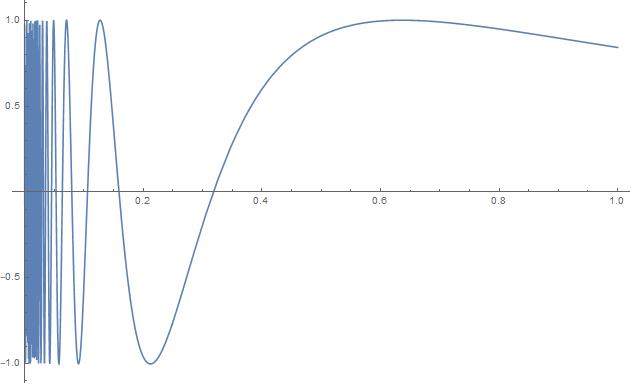
\includegraphics[scale=0.3]{figures/Top_sin.jpg}
    \caption{The topologists' sine curve}
    \label{tsine}
\end{figure}
The set is connected, since every point on the y-axis is a limit point of the curve. However, there is no continuous path connecting the y-axis to the rest of the curve, because $\sin(1/x)$ itself is not continuous.

\begin{xca}
\begin{enumerate}
    \item Show that the $n$-dimensional sphere $\bbS^n$ (defined as the unit sphere in $\bbR^{n+1}$ with the subset topology) is path-connected.
    \item Show that $\mathbb{Q}\subset\bbR $ is not connected.
    \item Show that the product of two path-connected spaces is path-connected.
\end{enumerate}
\end{xca}





\subsubsection{Compactness}

\begin{defn}[Covering/cover]
A collection of subsets of a topological space $X$ is said to cover $X$ if the union of these subsets equals $X$. If the subsets are all open (or closed), the covering (also often called a cover) is said to be open (resp.~closed).
\end{defn}

\begin{defn}[Compact Space]\index{Compact space}
A space $X$ is called compact if every open covering of $X$ contains a finite subcollection that also covers $X$ (\emph{subcovering}).
\end{defn}

\begin{defn}[Compact Subset]
A subset $A\subset X$ is called compact if it is compact in the subspace topology.
\end{defn}

\begin{prop}
If $Y_i\subset X$, $i = 1,\dots, m$ are compact subsets, then their union $\bigcup_{i=1}^m Y_i$ is also compact.
\end{prop}
\begin{proof}
Exercise.
\end{proof}

\begin{prop}[Compactness is a topological invariant]\label{prop f(compact)=compact}
The image $f(X)$ of a compact space $X$ under a continuous map $f\in C(X,Y)$ is compact.
\end{prop}
\begin{proof}
Exercise.
\end{proof}

\begin{xca}
\begin{enumerate}
    \item Show that the product of two connected spaces is connected. \emph{Hint:} first show that the union of any number of pairwise overlapping connected subspaces (i.e.\ subsets endowed with the subspace topology) of a space is also connected; then, write $X\times Y$ as the union of ``crosses'' $(\{x\}\times Y)\cup (X\times \{y\})$ that pairwise overlap and are connected only if $X$ and $Y$ are.
    \item Show that the product of two path-connected spaces is path-connected.
    \item Show that the product of two compact spaces is compact. \emph{Hint:} \cite{compact.proof}.
\end{enumerate}
\end{xca}


\begin{defn}[Classes of continuous maps]\index{Open map}\index{Closed map}\index{Proper map}
A map $f:X\to Y$ (not necessarily continuous) is called
\begin{enumerate}
    \item \emph{open} if the image of every open subset of $X$ is open in $Y$;
    \item \emph{closed} if the image of every closed subset of $X$ is closed in $Y$;
    \item \emph{proper} if it is continuous and the pre-image of any compact subset of $Y$ is compact in $X$;
\end{enumerate}
\end{defn}

\begin{xca}
   Show that the image of any proper map $f:\bbR^m\to\bbR^n$ is closed.
\end{xca}






\subsection{Metric spaces}

\begin{defn}[Metric spaces]\index{Metric space}\index{Metric}
    A \emph{metric space} is a set $X$ with a \emph{metric} $\rho:X\times X\rightarrow \bbR $ that obeys the following conditions for any $x,y,z\in X$
\begin{enumerate}
    \item \emph{Non-negativity}: $\rho(x,y)\ge 0$; \emph{non-degeneracy:} $\rho(x,y)=0$ iff $x=y$.
    \item \emph{Symmetry}: $\rho(x,y) = \rho(y,x)$.
    \item \emph{Triangle Inequality}: $\rho(x,y) + \rho(y,z) \ge \rho(x,z)$.
\end{enumerate}
\end{defn}

\begin{defn}[Metric maps]
    A \emph{metric map} between two metric spaces $(X,\rho_X)$ and $(Y,\rho_Y)$ is a continuous map $f\in C(X,Y)$ such that $\rho_Y (f(x_1),f(x_2))\leq \rho_X (x_1,x_2)$. The category $\mathsf{Met}$ is defined as the category of metric spaces with metric maps for morphisms.
\end{defn}

\begin{defn}[Open Ball]
    An \emph{open ball} $B_r(x)$ of radius $r$ around a point $x$ in a metric space $(X,\rho)$ is defined as
\begin{equation}
    B_r(x) = \{ y\in X ~|~ \rho(y,x)< r \}
\end{equation}
\end{defn}

\begin{defn}[Metric topology]
    The metric topology induced by a metric on a set is the topology generated by basis elements that are open balls $B_r(x)$ for all $x\in X$ and $r>0$. 
\end{defn}
\begin{rem}
    Equivalently, by Proposition \ref{characterization of topology using basis}, a set $M$ is open in the metric topology iff for any $x\in M$ there exists a radius $r>0$ such that $B_r(x)\subset M$. In the metric topology, $\rho:X\times X\to \mathbb R$ is automatically continuous.
\end{rem}
\begin{prop}
    If a metric space $(X,\rho)$ is separable, it has a countable base.
\end{prop}
\begin{proof}
    Exercise. \emph{Hint}: consider balls of rational radii about every point of the dense subset.
\end{proof}

\begin{defn}[Limit of a Sequence]
    A sequence of points $\{x_n\}$ in a metric space $X$ is said to \emph{converge} if there exists a point $x\in X$ such that for any $\epsilon >0$, there exists an $N\in \mathbb{N}$ such that
    \begin{equation}
        \forall ~ n>N,\; \rho(x_n,x) < \epsilon.
    \end{equation}
    The point $x$ is called the limit of the sequence.
\end{defn}
Note that the limit of a sequence is unique by the first axiom of the metric. One can also define the limit point of a subset of a general topological space as follows:
\begin{defn}[Limit Point]
    If $A$ is a subset of a topological space, a point $x\in X$ is said to be a limit point of $A$ if every open neighbourhood of $x$ intersects $A$ in some point other than $x$.
\end{defn}

In metric spaces, limit points are equivalent to limits of sequences, i.e., for every limit point $x$ of a subset $A$, there exists a sequence of points in $A$ that converges to $x$. Conversely, for any convergent sequence of points in $A$, the limit of the sequence is a limit point of $A$.

\begin{prop}
    For a metric space $X$ equipped with the metric topology, the closure $\xoverline{A}$ of a subset $A\subset X$ is equal to the set of limit points of $A$.
\end{prop}
\begin{proof}
    Exercise.
\end{proof}

The following proposition proves the equivalence of the usual ``epsilon-delta definition'' of continuity and the topological one.

\begin{prop}
    For two metric spaces $(X,\rho)$ and $(Y,\rho')$ and a map $f:X\rightarrow Y$ such that $f(x)=y$, the following are equivalent
\begin{enumerate}
    \item $f$ is continuous at $x$.
    \item For any convergent sequence $x_n\rightarrow x$, the image is also convergent with $f(x_n)\rightarrow y$.
    \item For every $\epsilon>0$, there exists $\delta>0$ such that $\rho(x,z)<\delta \implies \rho'(f(x)=y, f(z))<\epsilon$.
\end{enumerate}
\end{prop}
\begin{proof}
    Exercise.
\end{proof}

\begin{defn}[Isometry]\index{Isometry}
    An isometry between two metric spaces is a bijective map $f:X\rightarrow Y$ that preserves distances, i.e.,
\begin{equation}
    \rho_X(x,y) = \rho_Y(f(x), f(y)).
\end{equation}
\end{defn}

\begin{prop}
    If $f:X\rightarrow Y$ is an isometry, it is also a homeomorphism.
\end{prop}
\begin{proof}
    Exercise.
\end{proof}

\begin{defn}[Equivalent metrics]\index{Metric!equivalence of}
    Two metrics $\rho_1,\rho_2$ on a topological space $X$ are called equivalent if for any $x\in X$ and any $r>0$, there exist radii $r',r''>0$ such that $B^{(1)}_{r'}(x)\subset B^{(2)}_{r}(x)$ and $B^{(2)}_{r''}(x)\subset B^{(1)}_{r}(x)$ (here, $B^{(i)}$ denotes an open ball defined by the metric $\rho_i$).
\end{defn}

\begin{thm}
    Two metrics on the same space are equivalent iff they induce the same topology.
\end{thm}
\begin{proof}
    Exercise.
\end{proof}

\begin{defn}[Cauchy sequence]\index{Cauchy sequence}
A sequence $(x_n)$ of points of a metric space $(X,\rho)$ is called a Cauchy sequence if for any $\epsilon>0$ there exists $N\in\mathbb{N}$ such that $\forall n,m\geq N$, $\rho(x_n,x_m)<\epsilon$.
\end{defn}

\begin{prop}
    A metric space is compact iff every sequence in it has a convergent subsequence (i.e.~it is \emph{sequentially compact}).
\end{prop}

\begin{defn}[Completeness]\index{Complete metric space}
A metric space $(X,\rho)$ is called complete if every Cauchy sequence $(x_n)$ in it has a limit $x_\infty\in X$.
\end{defn}


\begin{thm}[Cantor's intersection theorem]\index{Theorem!Cantor's intersection}
Let $(X,\rho)$ be a complete metric space and let $C_n$ be a sequence of closed nested subsets $C_{n+1}\subset C_n$ whose diameters tend to zero, $\mathrm{diam}\,C_n=\sup_{x,y\in C_n} \rho(x,y) \to 0$. Then the intersection $\bigcap_{n=1}^\infty C_n$ consists of exactly one point.
\end{thm}


\begin{prop}
    A metric space is sequentially compact iff every decreasing sequence of closed nonempty subsets (not necessarily tending to zero diameter) has a nonempty intersection.
\end{prop}


\begin{thm}
    A metric space is compact iff it is complete and for every $\epsilon>0$ it can be covered by a finite number of open balls of radius $\epsilon$ (i.e.~it is \emph{totally bounded}).
\end{thm}


\begin{xca}
    Consider $\mathbb{N}$ with the metric $\rho (n,m)=\lvert \frac 1 n-\frac 1 m\rvert$. Construct a sequence of balls $B_{r_k}(x_k)$ in this space such that $r_{k+1}<r_k$, $B_{r_{k+1}}(x_{k+1})\subset B_{r_k}(x_k)$, but the intersection of all these balls is empty.
\end{xca}
\begin{defn}[Normed vector space]\index{Normed vector space}\index{Norm}
    A normed vector space is a vector space $V$ over a subfield of $\mathbb{C}$ with a function (called the norm) $\lVert \cdot \rVert: V\to \mathbb{R}_+$ such that for all $x,y\in V$:
    \begin{enumerate}
        \item $\lVert x\rVert\geq 0$, and $\lVert x\rVert= 0$ iff $x=0$;
        \item $\lVert \alpha  x\rVert=\lvert \alpha \rvert \lVert x\rVert$ for any scalar (element of the structure field) $\alpha$;
        \item $\lVert x+y\rVert\leq \lVert x\rVert+\lVert y\rVert$.
    \end{enumerate}
    Every normed vector space has a naturally induced metric $\rho (x,y)=\lVert x-y\rVert$. In the corresponding induced topology, the norm is automatically continuous.
\end{defn}
\begin{defn}[Equivalent norms]\index{Norm!equivalence of}
    Two norms $\lVert\cdot \rVert_1,\lVert\cdot \rVert_2 $ on a vector space $X$ are called equivalent if there are (universal) constants $\alpha,\beta >0$ such that for all $x\in X$ we have $\alpha \lVert x \rVert_1\leq \lVert x \rVert_2 \leq \beta \lVert x \rVert_1$.
\end{defn}
Notice how this condition is much stronger than just the equivalence of the induced metrics, since $\alpha$ and $\beta$ are required to be universal constants for all $x$.

\begin{thm}
    Two norms on a vector space $X$ are equivalent iff they induce the same topology.
\end{thm}
\begin{proof}
    Exercise.
\end{proof}






\subsection{Separation axioms} \label{Separation Axioms}

We saw that every metric space has a canonical topology associated with it. A natural question to ask is whether the converse is true. Given a topological space, when can we define a metric on it such that the topology coincides with the metric topology? Clearly, a metric space has more structure than a topological space. In order to add more structure to topological spaces, we define the following axioms

\begin{defn}[Separation Axioms]\index{Separation axioms}
    For a topological space $X$ with arbitrary points $x$ and $y$ and arbitrary disjoint closed sets $F$ and $G$, we define the following axioms:
    \begin{enumerate}
        \item $T_1$: There exists an open neighbourhood $U$ of $x$ that doesn't include $y$, and an open neighbourhood $V$ of $y$ that doesn't include $x$, i.e., $x$ and $y$ are \emph{separated}.
        \item $T_2$ (\emph{Hausdorff}): There exist disjoint open neighbourhoods $U$ of $x$ and $V$ of $y$, i.e., $x$ and $y$ are \emph{separated by neighbourhoods}.
        \item $T_3$: There exist disjoint open neighbourhoods $U$ of $x$ and $V$ of $F$.
        \item \emph{Regular}: $X$ is both $T_1$ and $T_3$.
        \item $T_4$: There exist disjoint open neighbourhoods $U$ of $F$ and $V$ of $G$.
        \item \emph{Normal}: $X$ is both $T_1$ and $T_4$.
    \end{enumerate}
\end{defn}

\begin{prop}
    The following results demonstrate how each axiom adds additional structure to the space:
\begin{enumerate}
    \item $T_1 \implies$ All finite sets are closed;
    \item $T_2\implies T_1$;
    \item Regular $\implies$ Hausdorff;
    \item Normal $\implies$ Regular.
\end{enumerate}
\end{prop}

\begin{example}
    The category $\mathsf{Hausd}$ of Hausdorff spaces is a full subcategory of $\mathsf{Top}$.
\end{example}

\begin{thm}[Urysohn Lemma]\index{Lemma!Urysohn}
    A space $X$ is normal iff for any two disjoint closed subsets $A$ and $B$ there exists a continuous function
\begin{equation}
f\in C(X,[0,1]) ~\text{such that}~ \restr{f}{A} = 0, \restr{f}{B} = 1.
\end{equation}
\end{thm}

\begin{thm}
    All metric spaces are normal.
\end{thm}
\begin{proof}
    Exercise.
\end{proof}

\begin{thm}[Urysohn]
    A normal space with a countable base is \emph{metrizable}, i.e., we can construct a canonical metric whose induced topology coincides with the topology of the space.
\end{thm}

\begin{prop}
    If $X$ is Hausdorff, every compact subset of $X$ is closed.
\end{prop}
\begin{proof}
    Exercise. \emph{Hint:} prove that the complement of the compact set is open by using Proposition \ref{open iff contains neighborhoods}.
\end{proof}

\begin{prop}
    Every compact Hausdorff space is normal.
\end{prop}
\begin{proof}
    Exercise.
\end{proof}

\begin{thm}[Heyne-Borel]\index{Theorem!Heyne-Borel}
    In Euclidean space $\bbR^n$, a subset is compact iff it is closed and bounded.
\end{thm}

The following theorem is one of the most fundamental theorems in functional analysis, and it essentially characterizes compact subsets of the set of continuous functions defined on a compact subset of $\bbR^n$. We state it simply as an example of usage of the above topological terminology.
\begin{thm}[Arzel\`a-Ascoli]\index{Theorem!Arzel\`a-Ascoli}
    Let $X$ be a compact Hausdorff space. A subset $F$ of the space $C(X,\bbR )$ of continuous real-valued functions on $X$ is relatively compact (i.e.\ its closure is compact) in the topology given by the sup-norm $\lVert f\rVert=\sup_X \vert f\rvert$ iff it is equicontinuous (i.e.\ all elements $f\in F$ are uniformly continuous functions and the $\delta$ in the definition of uniform continuity is universal for all $f\in F$) and pointwise bounded (i.e.\ for every $x\in X$ the set $\{f(x)\}_{f\in F}$ is bounded).
\end{thm}







\subsection{Homotopy}\label{sec.homotopy}

\begin{defn}[Homotopic maps]\index{Homotopy} 
    Two continuous maps $f_0,f_1\in C(X, Y)$ are called homotopic (we often write $f\sim g$) if there exists a continuous map, called homotopy, $F\in C([0,1]\times X,Y)$ such that $F(0,x)=f_0(x)$ and $F(1,x)=f_1(x)$. Here, $[0,1]$ has the standard topology. For convenience, we will often describe homotopies as \emph{families of maps} $f_t:X\to Y$ defined by $f_t(x)=f(t,x)$.
\end{defn}
\begin{prop}
    Homotopy is an equivalence relation on $C(X,Y)$. (The set of all homotopy classes of continuous maps from $X$ to $Y$ is denoted by $[X,Y]$. This set defines the morphisms in the (naive) homotopy category $\mathsf{hTop}$.)
\end{prop}
\begin{proof}
    Exercise.
\end{proof}

The first argument of $F(t,x)$ is essentially ``time'', and $F(t,\cdot)$ continuously interpolates between $f_0$ and $f_1$ as time goes from 0 to 1. In topology, homotopy is synonymous with the phrase ``continuous deformation''.


\begin{defn}[Contractible space]\index{Contractible space}
    A space $X$ is called contractible if it is homotopy equivalent to the one-point space, i.e.\ there exists a point $x_0\in X$ such that the constant map $f(x)=x_0$ is homotopic to the identity, $f\sim \id_X$. This property is in fact independent of $x_0$.
\end{defn}
\begin{prop}
    Any contractible space is path-connected.
\end{prop}
\begin{proof}
    Exercise. \emph{Hint:} consider paths traced out by $F(t,x)$ for fixed $x$'s.
\end{proof}
\begin{example}
\begin{enumerate}
    \item $\bbR^n$, $B^n$, $(0,1)^n$ are all contractible via, say, $F(t,x)=tx$ (they are also all homeomorphic to each other).
    \item Any two continuous functions $f,g:\bbR \to\bbR $ are homotopic via homotopy $F(t,x)=tg(x)+(1-t)f(x)$.
\end{enumerate}
\end{example}
\begin{xca}
    Show that if $Y$ is contractible, then any two maps $f,g\in C(X,Y)$ are homotopic. This is a generalization of the above example for $X=Y=\bbR $.
\end{xca}
\begin{thm}[Brouwer]
    The sphere $\bbS^n$ is not contractible.
\end{thm}
\begin{proof}
    There is a plethora of different ways to prove this theorem, from pure analytical to algebraic. We will delay the proof until we compute the homology groups of the spheres in Part \ref{Part II} and observe that they differ from those of a contractible space (and homology groups are topological invariants).
\end{proof}
\begin{thm}[Brouwer's fixed point theorem]\index{Theorem!Brouwer's fixed point}\label{thm Brouwer's fixed point}
    Any continuous map $f\in C\left(\xoverline{B^n},\xoverline{B^n}\right)$  from the closed unit ball to itself has at least one fixed point ($x_0$ such that $f(x_0)=x_0$).
\end{thm}
\begin{proof}
    For $n=1$ this is clear. For $n\geq 2$, suppose $f(x)\neq x$ for all $x$. Then we can define $h(x)$ as the point of intersection of the ray $[f(x),x)$ with the boundary of the ball. Then $F(t,x)=h(tx)$ is a contracting homotopy, which contradicts the last theorem.
\end{proof}
\begin{rem}
    These two theorems are in fact equivalent. The fixed point theorem can be proven purely analytically, and the contractibility theorem will follow. The simplest modern proof of non-contractibility of $\bbS^n$ is based on homology.
\end{rem}

\begin{defn}[Retraction, Deformation retraction]\index{Retraction}\index{Deformation!retraction}
    A retraction of a topological space $X$ onto its subspace $A\subset X$ is a continuous map $r:X\to A$ such that $\restr{r}{A}=\mathrm{id}_A$. A deformation retraction is a homotopy from the identity map $\mathrm{id}_X$ to $r$. A \emph{strong} deformation retraction also satisfies $\restr{r_t}{A}=\mathrm{id}_A$ for all $t\in[0,1]$ (this is often included in the definition of a deformation retraction).
\end{defn}

\begin{defn}[Homotopy equivalence of spaces]\index{Homotopy equivalence}
    Two topological spaces $X$ and $Y$ are called homotopy equivalent if there exist two continuous maps $f\in C(X,Y)$, $g\in C(Y,X)$ such that their compositions are homotopic to identity: $g\circ f\sim \id_X$ and $f\circ g\sim \id_Y$. We write $X\simeq Y$.
    In the presence of basepoints, these homotopies are required to leave the basepoints fixed for all values of the deformation parameter $t$.
\end{defn}

\begin{cor}
    \begin{enumerate}
        \item Deformation retractions are homotopy equivalences.
        \item Contractible spaces are homotopy equivalent to a point.
    \end{enumerate}
\end{cor}

\begin{example}
\begin{enumerate}
    \item $\bbS^1\times\bbR \simeq \bbS^1\simeq M$, where $M$ is the M\"obius band.
    \item $\bbR^n\setminus{0}\simeq \bbS^{n-1}$.
    \item More generally, two spaces $X,Y$ are homotopy equivalent iff they are both deformation retracts of the same space $Z$. That is, there needs to exist $A_X\subset Z$ such that $A_x\cong X$ and there exists a continuous map $F\in C([0,1]\times Z,Z)$ such that $F_X(0,z)=z$, $F_X(1,z)\in A$ and $F_X(t,a)=a$ for any $z\in Z$, $t\in [0,1]$ and $a\in A_x$. Similarly, there needs to exist $A_Y\subset Y$ homeomorphic to $Y$ that is a deformation retract of $Z$.
\end{enumerate}
\end{example}






\subsection{Fundamental group}

\begin{defn}[Loops, Pointed homotopy]\index{Loop}
    Let $X$ be a path-connected topological space, pick a ``base point'' $x_0\in X$, and consider the set of all \emph{loops} in $X$ based at $x_0$, i.e.\ paths $\gamma\in C([0,1], X)$ such that $\gamma(0)=\gamma(1)=x_0$. A pointed homotopy between two such loops is a homotopy $F\in C([0,1]\times[0,1],X)$ such that $F(\cdot,0)=F(\cdot,1)=x_0$. Pointed homotopy is an equivalence relation on the set of based loops.
\end{defn}

\begin{defn}[Fundamental/Poincar\'e group]\index{Fundamental group}
    The fundamental group $\pi_1(X,x_0)$ of a path-connected space $X$ with a base point $x_0$ is defined as the set $\{ [\gamma]\}$ of pointed homotopy classes of based loops with the inversion operation given by $[\gamma(t)]^{-1}=[\gamma(1-t)]$ and the multiplication operation 
    \[
    [\gamma_1(t)]\circ [\gamma_2(t)]=\left[ \begin{cases} \gamma_1(2t), & t\in[0,1/2], \\ \gamma_2(2t-1), & t\in(1/2,1] \end{cases}\right].\label{pi1 group op}
    \]
    The unit element is given by the equivalence class of the ``constant loop'' $\gamma(t)\equiv x_0$. If $X$ is not path-connected, then $\pi_1(X,x_0)$ is defined as the fundamental group of the path-connected component containing $x_0$.
\end{defn}

\begin{xca}
    Check that this definition is consistent, i.e.\ the homotopy classes on the right-hand sides don't depend on the choices of representatives of the classes on the left.
\end{xca}
\begin{defn}[Simple-connectedness]\index{Simply connected space}
    A path-connected space $X$ is called simply connected if its fundamental group is trivial, $\pi_1(X,x_0)=\{e\}$.
\end{defn}

\begin{xca}
Show that contractible spaces are simply connected.
\end{xca}

\begin{thm}
    If a space $X$ retracts onto a subspace $A$, then the homomorphism of fundamental groups $i_\ast:\pi_1(A,x_0)\to \pi_1(X,x_0)$ induced by the inclusion $i: A\hookrightarrow X$ is injective. If $A$ is a deformation retract of $X$, then $i_\ast$ is an isomorphism.
\end{thm}
\begin{proof}
    If $r:X\to A$ is a retraction then $r\circ i=\mathrm{id}_A$, hence by functoriality of $\pi_1$, $r_\ast \circ i_\ast=\mathrm{id}_{\pi_1(A,x_0)}$, which implies injectivity. If $r_t$ is a deformation retraction, then for any loop $\gamma$ in $X$ based at $x_0\in A$ the composition $r_t\circ \gamma$ gives a homotopy of $\gamma$ to a loop in $A$, therefore $i_\ast$ is also surjective.
\end{proof}

\begin{defn}[Alternative approach]
    Recall that the category $\mathsf{Top}_\bullet$ consists of ``pointed topological spaces'' with chosen basepoints and morphisms that are continuous maps mapping basepoint to basepoint. Take the circle $\bbS^1$ and pick a point $\bullet$ in it. Then one can redefine based loops as morphisms between two pointed topological spaces $\gamma\in C((\bbS^1,\bullet),(X,x_0))$. Pointed homotopy in the definition of $\pi_1$ can then be replaced by just homotopy of loops as maps defined on $\bbS^1$.   Thus, as a set, $\pi_1(X)=[\bbS^1,X]_\bullet$ (group of homotopy classes of pointed maps).
\end{defn}

\begin{defn}[Suspension]\index{Suspension}
    The suspension of a topological space $X$, is defined as the quotient space $SX=(X\times [0,1])/(X\times \{0\},X\times\{1\})$ (i.e.\ a cylinder over $X$ where each of the two faces is then collapsed into a point -- best visualized as a double cone over $X$). If $X$ is a pointed space with basepoint $x_0$, then the \emph{reduced suspension} is defined as $\Sigma X=(X\times [0,1])/(X\times \{0\},X\times\{1\} ,\{x_0\}\times [0,1]))$, and the new basepoint is the image of $(x_0,0)$ in the quotient. Equivalently, $\Sigma X=X\wedge \bbS^1=X\times \bbS^1/(X\vee \bbS^1)$.
\end{defn}

\begin{xca}
    Verify that $\Sigma$ extends to a functor on the category of pointed spaces. This will follow from the uniqueness of the pointed map at the bottom of the following square that makes it commute:
    \[\begin{tikzcd}[every matrix/.append style={name=m},   
    execute at end picture={\draw [<-] ([xshift=-2.3em,yshift=1mm]m-2-2.north) arc[start angle=-90,delta angle=270,radius=0.25cm];}]
   X \arrow[r,"f"]\arrow[d,swap,"\pi_X"]& Y\arrow[d,"\pi_Y"] \\
   \Sigma X\arrow[r,swap,dashed, "\exists !\,\Sigma(f)"]& \Sigma Y
    \end{tikzcd}\]
    where $\pi_X$ and $\pi_Y$ are the quotient maps that define the suspensions.
\end{xca}

\begin{example}
    From Exercise~\ref{wedge sums} we have $\Sigma \bbS^n\cong \bbS^{n+1}$. This holds even when $n=0$ and $\bbS^0=\{-1,1\}$.
\end{example}

\begin{defn}[Compact-open topology]
    Given two spaces $X,Y$, denote the set of all continuous maps between them by $Y^X=C(X,Y)$. The compact-open topology on $Y^X$ is generated\footnote{The topology generated by a collection of sets is simply the coarsest topology in which all of those sets are open. This topology consists of all unions and all finite intersections of these sets.} by the sets $M(K,U)=\{f\in Y^X\mid f(K)\subset U\}$ where $K\subset X$ is compact and $U\subset Y$ is open.
\end{defn}

\begin{prop}
    If $X,Y$ are Hausdorff and $X$ is locally compact, then $C(X,Y)$ is Hausdorff.
\end{prop}
\begin{proof}
    Let $f,g\in C(X,Y)$ with an $x\in X$ such that $f(x)\neq g(x)$. Since $Y$ is Hausdorff, there exist disjoint open neighborhoods $U_1$ of $f(x)$ and $U_2$ of $g(x)$. Then $f^{-1}(U_1)\cap g^{-1}(U_2)$ is an open neighborhood of $x$, because $f$ and $g$ are continuous. Since $X$ is locally compact, this neighborhood contains a compact neighborhood $K$. Then, $M(K,U_1)$ and $M(K,U_2)$ are neighborhoods of $f$ and $g$, respectively. They are disjoint because $U_1$ and $U_2$ are.
\end{proof}

\begin{prop}
    If $X$ is a locally compact Hausdorff space, then the evaluation map $e:Y^X\times X\to Y$, defined by $e(f,x)=f(x)$, is continuous.
\end{prop}
\begin{proof}
    Let $U$ be an open neighborhood of $f(x)$. Since $f$ is continuous and due to the properties of $X$, there is a compact neighborhood $K$ of $x$ such that $f(K)\subset U$. Thus $f\in M(K,U)$ and $M(K,U)\times K$ is mapped into $U$ by the evaluation map $e$. Finally, $M(K,U)\times K \subset Y^X\times X$ is a neighborhood of $(f,x)$. This proves continuity.
\end{proof}


\begin{thm}\label{compact open continuity}
    Let $X$ be a locally compact Hausdorff space, and $Y$ and $T$ Hausdorff spaces. For any map $f:X\times T\to Y$, denote $f_t(x)=f(x,t)$. Then the continuity of $f$ is equivalent to each $f_t$ being continuous separately and the mapping $t\mapsto f_t$ also being continuous from $T$ into $Y^X$. 
\end{thm}
\begin{proof}
    See \cite[Theorem VII.2.4]{Bredon}.
\end{proof}
This Theorem implies that if $X$ is locally compact, then a homotopy $X\times [0,1]\to Y$ is the same thing as a path $[0,1]\to Y^X$.
\begin{cor}[The Exponential Law]
    Let $X,T$ be locally compact Hausdorff spaces, and $Y$ a Hausdorff space. Then the bijection from Theorem \ref{compact open continuity} is a natural homeomorphism $Y^{X\times T}\cong \left(Y^X\right)^T$ taking $f$ to $f^\ast$ defined as $f^\ast (t)(x)=f(x,t)=f_t(x)$.
\end{cor}
\begin{proof}
    See \cite[Theorem VII.2.5]{Bredon}.
\end{proof}
Similarly, one can show that under similar conditions, one has homeomorphisms $Y^X\times W^X\cong (Y\times W)^X$ (under $f\times g$), $Y^{X\sqcup T}\cong Y^X\times Y^T$ (under $f\sqcup g$), and $Z^Y\times Y^X \cong Z^X$ (under $f\circ g$). For details see \cite[\S VII.2]{Bredon}.
\begin{defn}[Loop space]\index{Loop space}
    The loop space of a pointed space $X$ is the space $\Omega X=X^{\bbS^1}$ that consists of loops based at $x_0$, with the compact-open topology. Its basepoint is the constant loop at $x_0$.
\end{defn}


\begin{prop}\label{suspension maps prop}
    \begin{enumerate}
        \item The set of homotopy classes $[X;\Omega Y]$ is a group under the multiplication induced by the usual multiplication of loops in $Y$;
        \item The set of homotopy classes $[\Sigma X;Y]$ is a group under the multiplication induced by the concatenation of maps along the interval $[0,1]\times\{x_0\}$ in $\Sigma X$ (namely $f(2t,x)$ for $t\leq 1/2$ and $g(2t-1,x)$ after that);
        \item On the set $[\Sigma X;\Omega Y]$, the two multiplications defined above coincide and are abelian.
    \end{enumerate}
\end{prop}
\begin{proof}
    Item 1 is obvious and Item 2 is easily checked by verifying that the concatenation of a map with its time-reversed copy ($f(1-t,x)$) is homotopic to the constant map.

    In item 3, such maps can be denoted $f_{t,s}(x)$, where $t$ is the parameter in $\Sigma X$ and $s$ is the one in $\Omega Y$. The two multiplications differ only in which of these two parameters maps get concatenated along. The idea is then to homotopically deform one into the other. This can be done by using a deformation retract of the square $[0,1]^2$ into a smaller square in the center.  Since we're working with pointed spaces, the whole boundary of the square gets mapped to the basepoint $y_0$. Hence we can replace $f$ and $g$ with their retractions to the smaller square, whereas outside of that square the value is just $y_0$. Now the two different concatenations are clearly homotopic to each other since we can smoothly ``slide'' the domains of $f$ and $g$ around each other, and then undo the original deformation retract. This proves both the equality of the two products and their commutativity. See figure.
    \begin{center}
    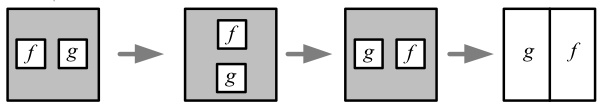
\includegraphics[scale=1]{figures/higher-homotopy.png}
    \end{center}
\end{proof}

\begin{lem}\label{lemma on suspension and loops}
    For any pair of pointed spaces $X,Y$, there is a natural isomorphism of groups $[\Sigma X,Y]\approx [X,\Omega Y]$.
\end{lem}
\begin{proof}
    The isomorphism is induced by the correspondence that identifies $f(t,x)$ with $\gamma(x)(t)=f(t,x)$. One can easily check that this provides a one-to-one correspondence between pointed maps and pointed homotopy on both sides. Furthermore, it is almost obvious that the multiplication on both sides works the same way.
\end{proof}

\begin{defn}[Zeroth degree homotopy set]
    Denote by $\pi_0(X)$ the set of path-connected components of $X$. It can be identified with the set of homotopy equivalence classes of maps from the one-point space into $X$. Note that this set carries no natural structure of a group.
\end{defn}

\begin{rem}
    One of the most useful consequences of the above discussion is that in sufficiently nice topological categories, such as that of topological manifolds, homotopies are just paths in the space of continuous maps. Therefore homotopy classes of maps $[X;Y]$ are nothing but the path-connected components in the space $Y^X$, that is, $\pi_0( Y^X)$. For compact $X$ Lemma~\ref{lemma on suspension and loops} can be shown indirectly using the exponential law, $Y^{\Sigma X}\cong (\Omega Y)^X$. As we've just seen, the multiplications on these spaces correspond, thus we have group homomorphisms $[\Sigma X;Y]= \pi_0(Y^{\Sigma X})\cong \pi_0((\Omega Y)^X)= [X;\Omega Y]$.
\end{rem}
\begin{prop}\label{prop computing pi1}
\begin{enumerate}
    \item $\pi_1$ is a covariant functor $\pi_1:\mathsf{Top}_\bullet\to \mathsf{Gr}$.
    \item For a path-connected space, fundamental groups with different base points are isomorphic (this is why we often abuse the notation by writing $\pi_1(X)$).
    \item For any number of path-connected spaces, $\pi_n(\prod_\alpha X_\alpha)\cong \prod_\alpha \pi_n(X_\alpha)$.
\end{enumerate}
\end{prop}
\begin{proof}
Exercise.
\end{proof}

\begin{lem}\label{lem product of loops}
    If a space $X$ is the union of a collection of path-connected open sets $U_\alpha$ each containing the basepoint $x_0$ and if each intersection $U_{\alpha\beta}$ is path-connected, then every loop in $X$ at $x_0$ is homotopic to a product of loops each of which is contained in a single $U_\alpha$.
\end{lem}
\begin{proof}
    The key is in the compactness of the interval $[0,1]$, which guarantees that the loop can be broken up into a finite number segments each of whose closure is contained inside only one of the $U_\alpha$'s. Call these segments $f_i, i=1,\ldots,n$. Since $x_0$ belongs to each $U_\alpha$, we can then find a path $g_i$ from $x_0$ to the starting point of $f_i$. We can always choose $g_0$ and $g_{n+1}$ to be trivial. The loops we seek are then $g_i\cdot f_i\cdot g_{i+1}^{-1}$. Their product is homotopic to the original loop because all $g_i$'s cancel out.
\end{proof}
\begin{cor}\label{cor pi_1(S^n)=0}
    $\pi_1(\bbS^n)=0$ for $n\geq 2$.
\end{cor}
\begin{proof}
    $\bbS^n$ is the union of the open neighborhoods of two hemispheres, $U_+$ and $U_-$. Each of these is homeomorphic to $\bbR^n$ and $U_+\cap U_-\cong \bbS^{n-1}\times \bbR $. If $n\geq 2$, then $U_+\cap U_-$ is path-connected. By the above lemma, every loop in $\bbS^n$ based at a point $x_0\in U_+\cap U_-$ is a product of two loops within each hemisphere. However both of these loops are trivial since $\pi_1(U_\pm)=0$.
\end{proof}
\begin{cor}
    $\bbR^2$ is not homeomorphic to $\bbR^n$ for $n\neq 2$.
\end{cor}
\begin{proof}
    Assume there is a homeomorphism $f:\bbR^2\to \bbR^n$. The case $n=1$ is easy because $\bbR \setminus\{f(0)\}$ is not connected whereas the supposedly homeomorphic $\bbR^2\setminus\{0\}$ is. 
    When $n>2$, the complement $\bbR^n\setminus\{f(x)\}$ is homeomorphic to $\bbS^{n-1}\times \bbR $, whose fundamental group is $\pi_1(\bbS^{n-1})=0$ by Proposition~\ref{prop computing pi1}. However, for $n>2$ the fundamental group of the complement $\bbR^2\setminus\{x\}$ is $\pi_1(\bbS^1)=\bbZ$. This leads to a contradiction.
\end{proof}

We are now prepared to prove one of the most important theorems about the fundamental group. First let us recall the categorical notion of pushouts (see Definition~\ref{pushouts}). If a path-connected space is represented as a union of two open sets, $X=U\cup V$, then the corresponding set inclusions induce homomorphisms of fundamental groups:
\[
    \begin{tikzcd}[every matrix/.append style={name=m},   
    execute at end picture={\draw [<-] ([xshift=-8.5mm,yshift=1mm]m-2-2.north) arc[start angle=-90,delta angle=270,radius=0.25cm];}]
    X \arrow[r,leftarrow,"l"]\arrow[d,leftarrow,"k"]& V\arrow[d,leftarrow,"j"] \\
    U\arrow[r,,leftarrow,swap,"i"]& U\cap V\\
    \end{tikzcd}
    \quad\quad\quad\quad\quad
    \begin{tikzcd}[every matrix/.append style={name=m},   
    execute at end picture={\draw [<-] ([xshift=-11.5mm,yshift=1mm]m-2-2.north) arc[start angle=-90,delta angle=270,radius=0.25cm];}]
    \pi_1(X) \arrow[r,leftarrow,"l_\ast"]\arrow[d,leftarrow,"k_\ast"]& \pi_1(V)\arrow[d,leftarrow,"j_\ast"] \\
    \pi_1(U)\arrow[r,,leftarrow,swap,"i_\ast"]& \pi_1(U\cap V)\\
    \end{tikzcd}
\]
$X$ itself is in fact the pushout, $X=U\sqcup_{U\cap V}V$. \emph{The Siefert-van~Kampen theorem will show that the functor $\pi_1$ preserves pushouts,} i.e.\ the fundamental group of the union is isomorphic to the amalgamated free product, $\pi_1(X)\cong \pi_1(U) \ast_{\pi_1(U\cap V)} \pi_1(V)$. By the universal property of the free product, there is a unique homomorphism $\Phi$ in the diagram below that makes the external triangles commute.
\[
    \begin{tikzcd}
    \pi_1(U)\ast \pi_1(V)   \arrow[drr,leftarrow, bend left]   \arrow[ddr,leftarrow, bend right]   \arrow[dr,"\exists! \Phi" description] & & \\
        & \pi_1(X) \arrow[r,leftarrow,swap, "l_\ast"] \arrow[d,leftarrow, "k_\ast"]       & \pi_1(V) \arrow[d,leftarrow, "j_\ast"] \\ & \pi_1(U) \arrow[r,leftarrow,swap, "i_\ast"] &\pi_1(U\cap V) 
    \end{tikzcd}
\]
Note, however, that the ``background square'' involving $\pi_1(U\cap V),\pi_1(U),\pi_1(V)$, and $\pi_1(U)\ast \pi_1(V)$ \emph{does not commute}, so the universal property of the pushout \emph{will not} apply in the other direction to give a homomorphism $\pi_1(X)\to \pi_1(U)\ast\pi_1(V)$. Instead, we will compute $\pi_1(X)$ by finding the kernel of $\Phi$ and factoring it out.

\begin{thm}[Siefert-van Kampen]\index{Theorem!Siefert-van~Kampen}
    If $X$ is the union of path-connected open sets $U_\alpha$ each containing the basepoint $x_0\in X$ and if each intersection $U_{\alpha\beta}$ is path-connected, then the homomorphism $\Phi: \ast_\alpha \pi_1(U_\alpha)\to \pi_1(X)$ induced by the inclusions $U_\alpha \hookrightarrow X$ is surjective. 
    
    Denote the inclusion-induced homomorphisms $i_\alpha:\pi_1(U_\alpha)\to \pi_1(X)$ and $i_{\alpha\beta}:\pi_1(U_{\alpha\beta})\to \pi_1(U_\alpha)$. We have $i_\alpha \circ i_{\alpha\beta}=i_{\beta}\circ i_{\beta\alpha}$ since both sides are induced by the inclusion $U_{\alpha\beta}\hookrightarrow X$. Now, if in addition each intersection $U_{\alpha\beta\gamma}$ is path-connected, then the kernel of $\Phi$ is the normal subgroup $N$ generated by all elements of the form $i_{\alpha\beta }(g)i_{\beta\alpha}(g)^{-1}$ for $g\in\pi_1(U_{\alpha\beta})$, and hence $\Phi$ induces a homomorphism $\pi_1(X)\cong \ast_\alpha \pi_1(U_\alpha)/N$.

    In particular, in the case of two sets, $\pi_1(U\cup V)\cong \pi_1(U)\ast_{\pi_1(U\cap V)}\pi_1(V)$.
\end{thm}
\begin{proof}
    The surjectivity of $\Phi$ was already shown in Lemma~\ref{lem product of loops}. 
    
    Now we need to show that the kernel of $\Phi$ is exactly $N$. We already know that $N\subset \ker \Phi$ since $i_\alpha\circ i_{\alpha\beta}=i_\beta\circ i_{\beta\alpha}$. For the reverse inclusion, the idea is to study \emph{factorizations} of loops into ``smaller'' loops $[\gamma_i]$ that are completely contained in one of the $U_\alpha$'s. There are two ``moves'' that, as we would like to show, transform differing factorizations of the same loop into each other. Namely, a substring of the form $[\gamma_i][\gamma_{i+1}]$ can be replaced with $[\gamma_i\cdot \gamma_{i+1}]$, and an element $[\gamma_i]$ viewed as an element of $\pi_1(U_\alpha)$ can be replaced with its analog in $\pi_1(U_\beta)$ if $\gamma_i$ is a loop contained in $U_{\alpha\beta}$. If we can show that all factorizations of a loop can be transformed into each other via a sequence of moves of this kind (or their inverses), that will mean that $\Phi$ induces an \emph{injective} map from the quotient group into $\pi_1(X)$, and thus the kernel of $\Phi$ is exactly $N$.

    The goal is therefore to decompose any homotopy of loops into a sequence of moves like this. A homotopy is a continuous map defined on the unit square, $H:[0,1]\times[0,1]\to X$, whose value on the left and right edges of the square is $x_0$. Now we need to subdivide this square into smaller squares as in the Figure, so that each square is mapped entirely into only one of the open sets $U_\alpha$, and so that the resulting subdivisions of the top and bottom edges of the square are refinements of the subdivisions implied in the two factorizations at hand (that is, each interval of the new subdivision is entirely contained in an interval from the old). Lastly, we can ``perturb'' the squares in the central rows so that each point is contained in at most three squares (this is why triple intersections were required to be path-connected).

    \begin{center}
        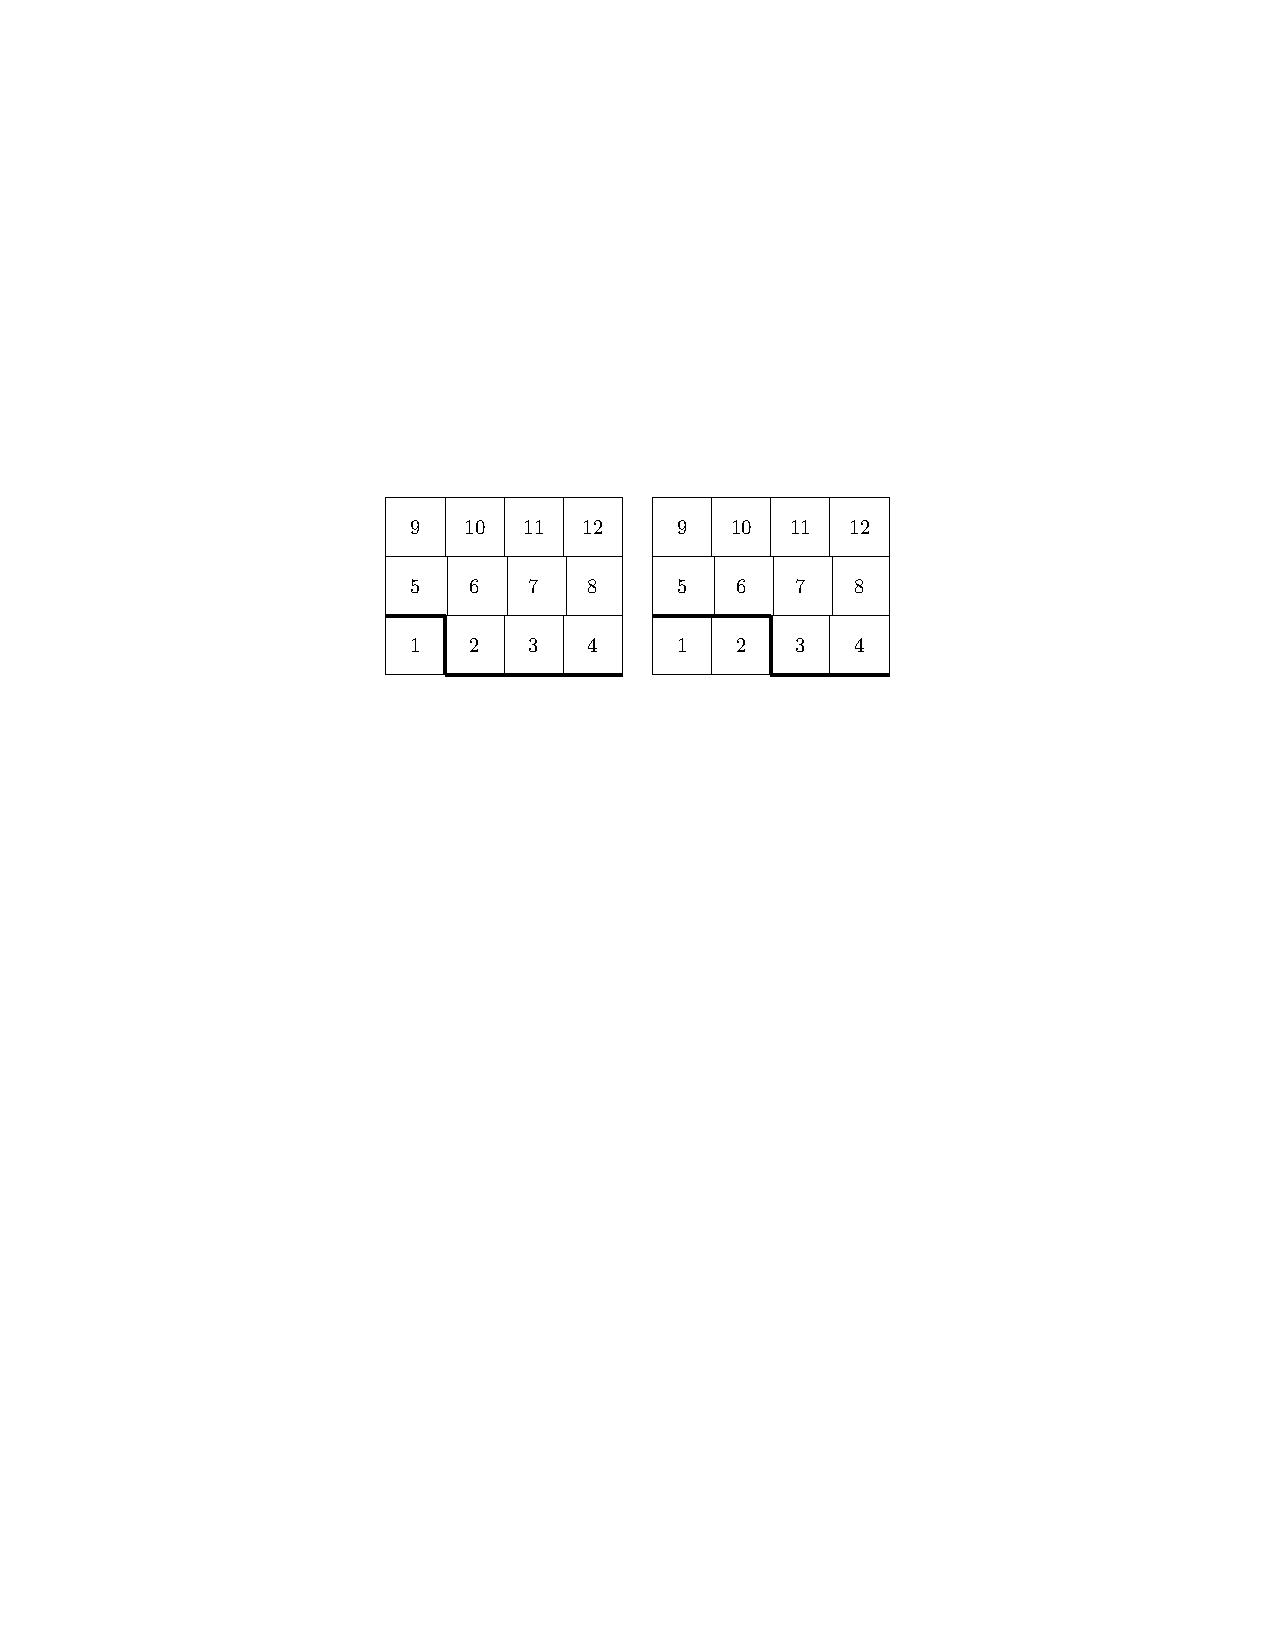
\includegraphics[scale=1]{figures/subdivision.pdf}
    \end{center}

    Now we proceed to define a sequence of paths along the edges of the subdivision from the left to the right side of the square that progressively ``capture'' more and more of the squares. For each segment we need to specify which of the open sets in $X$ its image is supposed to belong to, which is exactly the second move (in other words, $i_{\alpha\beta\ast}([\gamma_i])$ and $i_{\beta\alpha\ast}([\gamma_i])$ belong to the same coset in the quotient group). Further, each successive path is homotopic to the last via a deformation of a loop inside one $U_\alpha$. All together, this proves that any two factorizations of the same loop are equivalent in the sense that they differ only by relations that define the group $N$. The illustration below is from \cite[Chapter 10]{LeeTop}.

    \begin{center}
        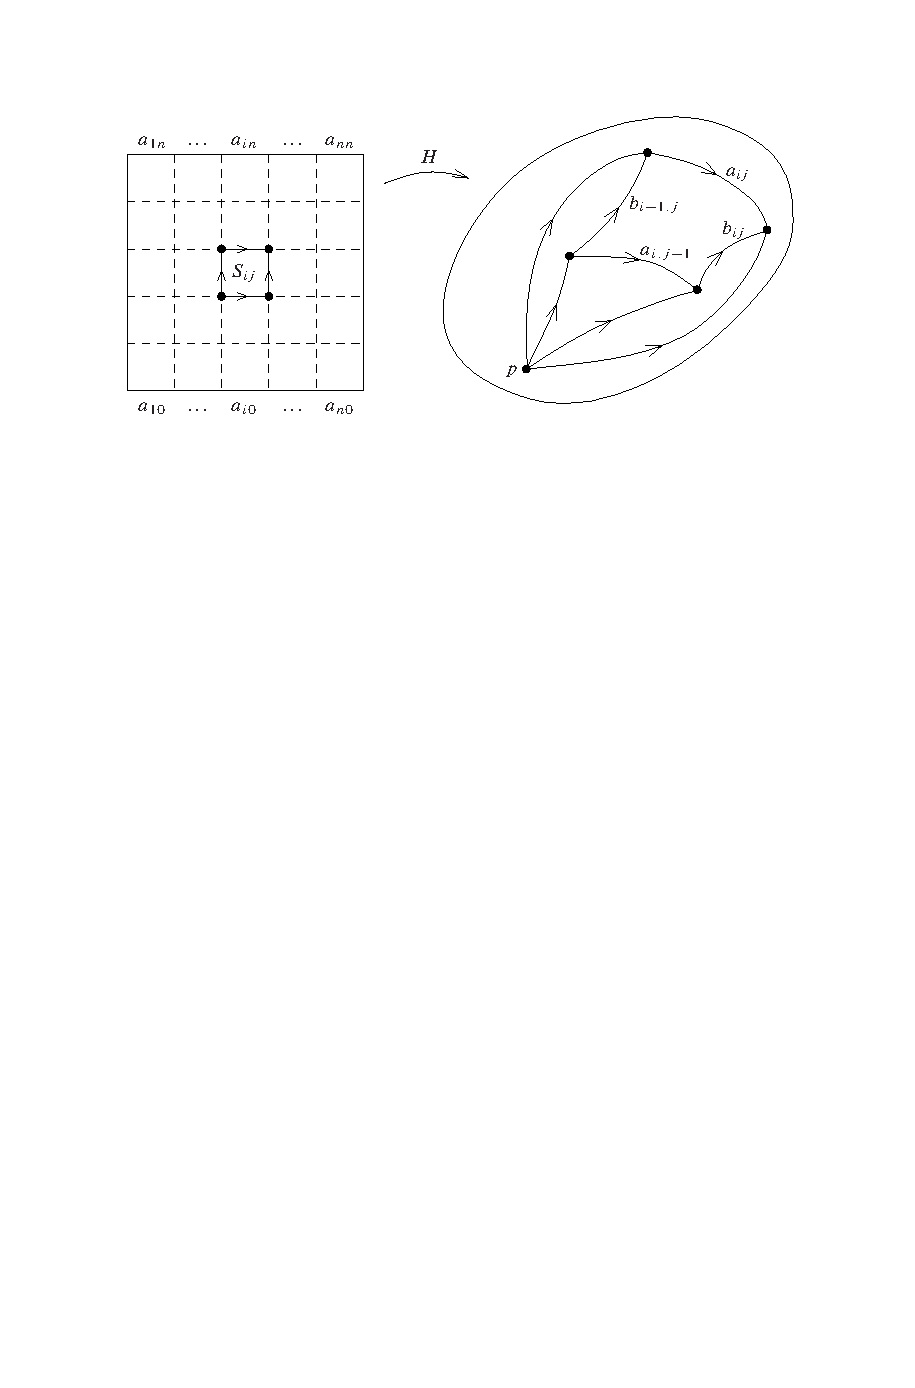
\includegraphics[scale=1]{figures/kernel of Phi.pdf}
    \end{center}
    
    See \cite[Theorem 1.20]{Hatcher} for more details of the proof.
\end{proof}

The conditions on path-connectedness of intersections and on the basepoint seem artificial, and indeed the are. Any open covering of $X$ can be turned into a cover of this kind by taking unions of sets lying along paths connecting them to the original basepoint. The full version of the Seifert-van~Kampen theorem can be stated purely in categorical terms with no extra conditions, however first we will need the notion of the \emph{fundamental groupoid}.

\begin{defn}[Groupoid]\index{Groupoid}
    A groupoid is a set with a unary ``inversion'' map $x\mapsto x^{-1}$ and a partial (i.e.\ not necessarily defined for any pair of elements) associative binary ``multiplication'' operation $(x,y)\mapsto x\bullet y$. It is associative in the sense that if both $x\bullet y$ and $y\bullet z$ exist, then both $(x\bullet y)\bullet z$ and $x\bullet (y\bullet z)$ exist and coincide. It is also required that $x\bullet x^{-1}$ and $x^{-1}\bullet x$ exist, and that, if $x\bullet y$ exists, then $x\bullet y\bullet y^{-1}=x$ and $x^{-1}\bullet x\bullet y=y$.

   As a consequence of these axioms, $(x^{-1})^{-1}=x$ and $(x\bullet y)^{-1}=y^{-1}\bullet x^{-1}$. Intuitively, groupoids can be thought of as groups with many identities, where only elements belonging to the same identity (which is the case if $x\bullet x^{-1}=x\bullet x^{-1}$) can be multiplied. 
    
    An equivalent definition is that a groupoid is a category where all morphisms are invertible (i.e.\ isomorphisms). The objects of this category are the ``identities'' of the groupoid. A group is then simply a groupoid with a single object. The category of groupoids is denoted $\mathsf{Grpd}$.
\end{defn}

Free products of groupoids can be constructed in the same way as for groups -- as strings of ``words'' $g_1^{\epsilon_1} \cdots g_n^{\epsilon_n}$ where each product $g_i^{\epsilon_i}\bullet g_{i+1}^{\epsilon_{i+1}}$ must exist and insertions of substrings of the form $gg^{-1}$ produce an equivalent string. These free products have the same universal property and are therefore the pushouts in $\mathsf{Grpd}$.

\begin{defn}[Fundamental groupoid]\index{Fundamental groupoid}
    Given a topological space $X$, let $\Pi(X)$ (also denoted $\Pi_1(X)$) be the category whose objects are points of $X$ and the morphisms $\mathrm{Mor}(x,y)$ are the homotopy equivalence classes of paths $\gamma:[0,1]\to X$ such that $\gamma(0)=x, \gamma(1)=y$. Since continuous images of homotopic paths are homotopic, we have a functor $\Pi:\mathsf{Top}\to \mathsf{Grpd}$.
\end{defn}
Notice that the set of endomorphisms of any $x\in X$ viewed as an object in $\Pi(X)$ is exactly the group $\pi_1(X,x)$. Moreover, it's not difficult to check that homotopies of continuous maps in $\mathsf{Top}$ induce natural transformations of the corresponding $\Pi$-functors.
\begin{prop}
    For a path-connected space $X$, the inclusion $\pi_1(X,x)\hookrightarrow \Pi(X)$ is an equivalence of categories.
\end{prop}
\begin{proof}
    Indeed, viewed as a category with a single object, $\pi_1(X,x)$ forms a skeleton of $\Pi(X)$, since all objects of $\Pi(X)$ are isomorphic due to path-connectedness.
\end{proof}

\begin{thm}[Seifert-van~Kampen]\index{Theorem!Seifert-van~Kampen}
    Let $\mathscr{U}=\{U_\alpha\}_\alpha$ be an open covering of a space $X$ that is closed under finite intersections. Regard $\mathscr{U}$ as an index category whose morphisms are the inclusions of sets. The functor $\Pi$, restricted to sets and maps in $\mathscr{U}$, produces a diagram of groupoids $\Pi(\mathscr{U})$, i.e.
    \[\restr{\Pi}{\mathscr{U}}: \mathscr{U}\to \mathsf{Grpd}.\]
    Then the groupoid $\Pi(X)$ is the colimit (or pushout) of this diagram (that is, the initial object in the category of cones over $\restr{\Pi}{\mathscr{U}}$, see \S\ref{Limits and colimits}).
\end{thm}
\begin{proof}
    We can verify the universal property. For a groupoid $G$ and a set of groupoid homomorphisms $\eta_\alpha:\Pi(U_\alpha)\to G$ (forming a cone over $\restr{\Pi}{\mathscr{U}}$), we must construct a groupoid homomorphism $\wt{\eta}:\Pi(X)\to G$ (which is nothing but a functor between categories) that restricts to $\eta_\alpha$ on $\Pi(U_\alpha)$ for all $\alpha$. On objects, that is on points of $X$, we have no choice but to define $\wt{\eta}(x)=\eta_\alpha(x)$ for $x\in U_\alpha$. This is independent of the choice of $\alpha$ since the cover is closed under finite intersections.

    Now we must define $\wt{\eta}$ on morphisms in $\Pi(X)$, i.e.\ paths. If a path $\gamma$ connecting $x$ to $y$ lies entirely in a particular $U_\alpha$, we again have only one choice: $\wt{\eta}([\gamma])=\eta_\alpha([\gamma])$. This is consistent (independent of $\alpha$) since $\mathscr{U}$ is closed under finite intersections.

    Now, any path $\gamma$ is the composite of finitely many paths $\gamma_i$, each of which lies in a single $U_{\alpha_i}$. Therefore we must define $\wt{\eta}([\gamma])=\wt{\eta}([\gamma_1])\bullet \cdots \bullet \wt{\eta}([\gamma_n])$. 
    
    Clearly this definition will give the required unique morphism $\wt{\eta}$, provided that it is indeed well defined, i.e.\ respects the equivalence relation between paths. Thus suppose we have two equivalent paths $\gamma_0\sim \gamma_1$. The equivalence is given by a homotopy $\gamma_t$ through paths with the same fixed endpoints. This homotopy is a map defined on the square $[0,1]\times[0,1]$. We may subdivide the square into subsquares, each of which is mapped entirely into one of the $U_\alpha$'s. We may further choose this subdivision so that the resulting subdivision of $[0,1]\times\{0\}$ refines the subdivision used to decompose $\gamma_0$ into segments as above, and similarly for $\gamma_1$ and the resulting decomposition of $[0,1]\times \{1\}$. We see that the relation $[\gamma_0]=[\gamma_1]$ in $\Pi(X)$ is a consequence of a finite number of relations, each of which holds in one of the $\Pi(U_\alpha)$'s. Therefore $\wt{\eta}([\gamma_0])=\wt{\eta}([\gamma_1])$. This confirms that $\wt{\eta}$ is well defined and satisfies the universal property for pushouts.    
\end{proof}
From this, one can use an ``abstract nonsense'' argument to re-derive the original version of the theorem for the functor $\pi_1(-,x_0)$, see~\cite[\S 2.7]{May}.

\begin{cor}[Fundamental group of a wedge sum]
    Suppose $x_\alpha$ is a \emph{nondegenerate basepoint}\index{Nondegenerate basepoint} for $X_\alpha$ (which means that $x_\alpha$ has a neighborhood which admits a strong deformation retraction into $x_\alpha$). Then the basepoint of $\bigvee_{\alpha }X_\alpha$ is nondegenerate and the fundamental group of this wedge sum is isomorphic to the free product $\ast_{\alpha}\pi_\alpha(X_\alpha)$.
\end{cor}
\begin{proof}
    See \cite[Theorem 10.7]{LeeTop}.
\end{proof}

\begin{example}
\begin{enumerate}
    \item The shape $\ominus$ is a deformation retract of the figure 8, which itself is just the wedge sum $\bbS^1\vee \bbS^1$, so their fundamental groups are all $\bbZ\ast\bbZ$.
    \item The last example can be generalized to compute $\pi_1$ of an arbitrary connected graph. The result is just the free group generated by the set of ``elementary'' cycles in the graph. More precisely, the number of generators equals the number of all edges of the graph minus the number of edges in a maximal spanning tree of the graph (i.e.\ a maximal subgraph without cycles).
\end{enumerate}
\end{example}

\begin{xca}{{{\cite[Exercise 10-1]{LeeTop}}}}
    Use the Seifert-van~Kampen theorem to give another proof that $\bbS^n$ is simply connected when $n \geq 2$.
\end{xca}
\begin{xca}{{{\cite[Excercise 10-5]{LeeTop}}}}
    Compute the fundamental group of $\bbR^3$ with the three coordinate axes removed. \emph{Hint:} this space is homotopy equivalent to the 2-sphere with six points removed.
\end{xca}
\begin{xca}[Projective plane]\index{Projective plane}\label{RP2 exercise}
    Show that the projective plane $\RP^2$, constructed out of a disk by identifying the antipodal points on the bounding circle (see Figure~\ref{fig:crosscap}), has the fundamental group $\bbZ_2$.
\end{xca}
\begin{xca}[Crosscap]\index{Crosscap}\label{crosscap exercise}
    Show that the projective plane with a hole (also known as a \emph{crosscap}), constructed out of an annulus by identifying the antipodal points of the outer boundary, is homeomorphic to the M\"obius band, and therefore has the fundamental group $\bbZ$.
\end{xca}
\begin{figure}
    \centering
    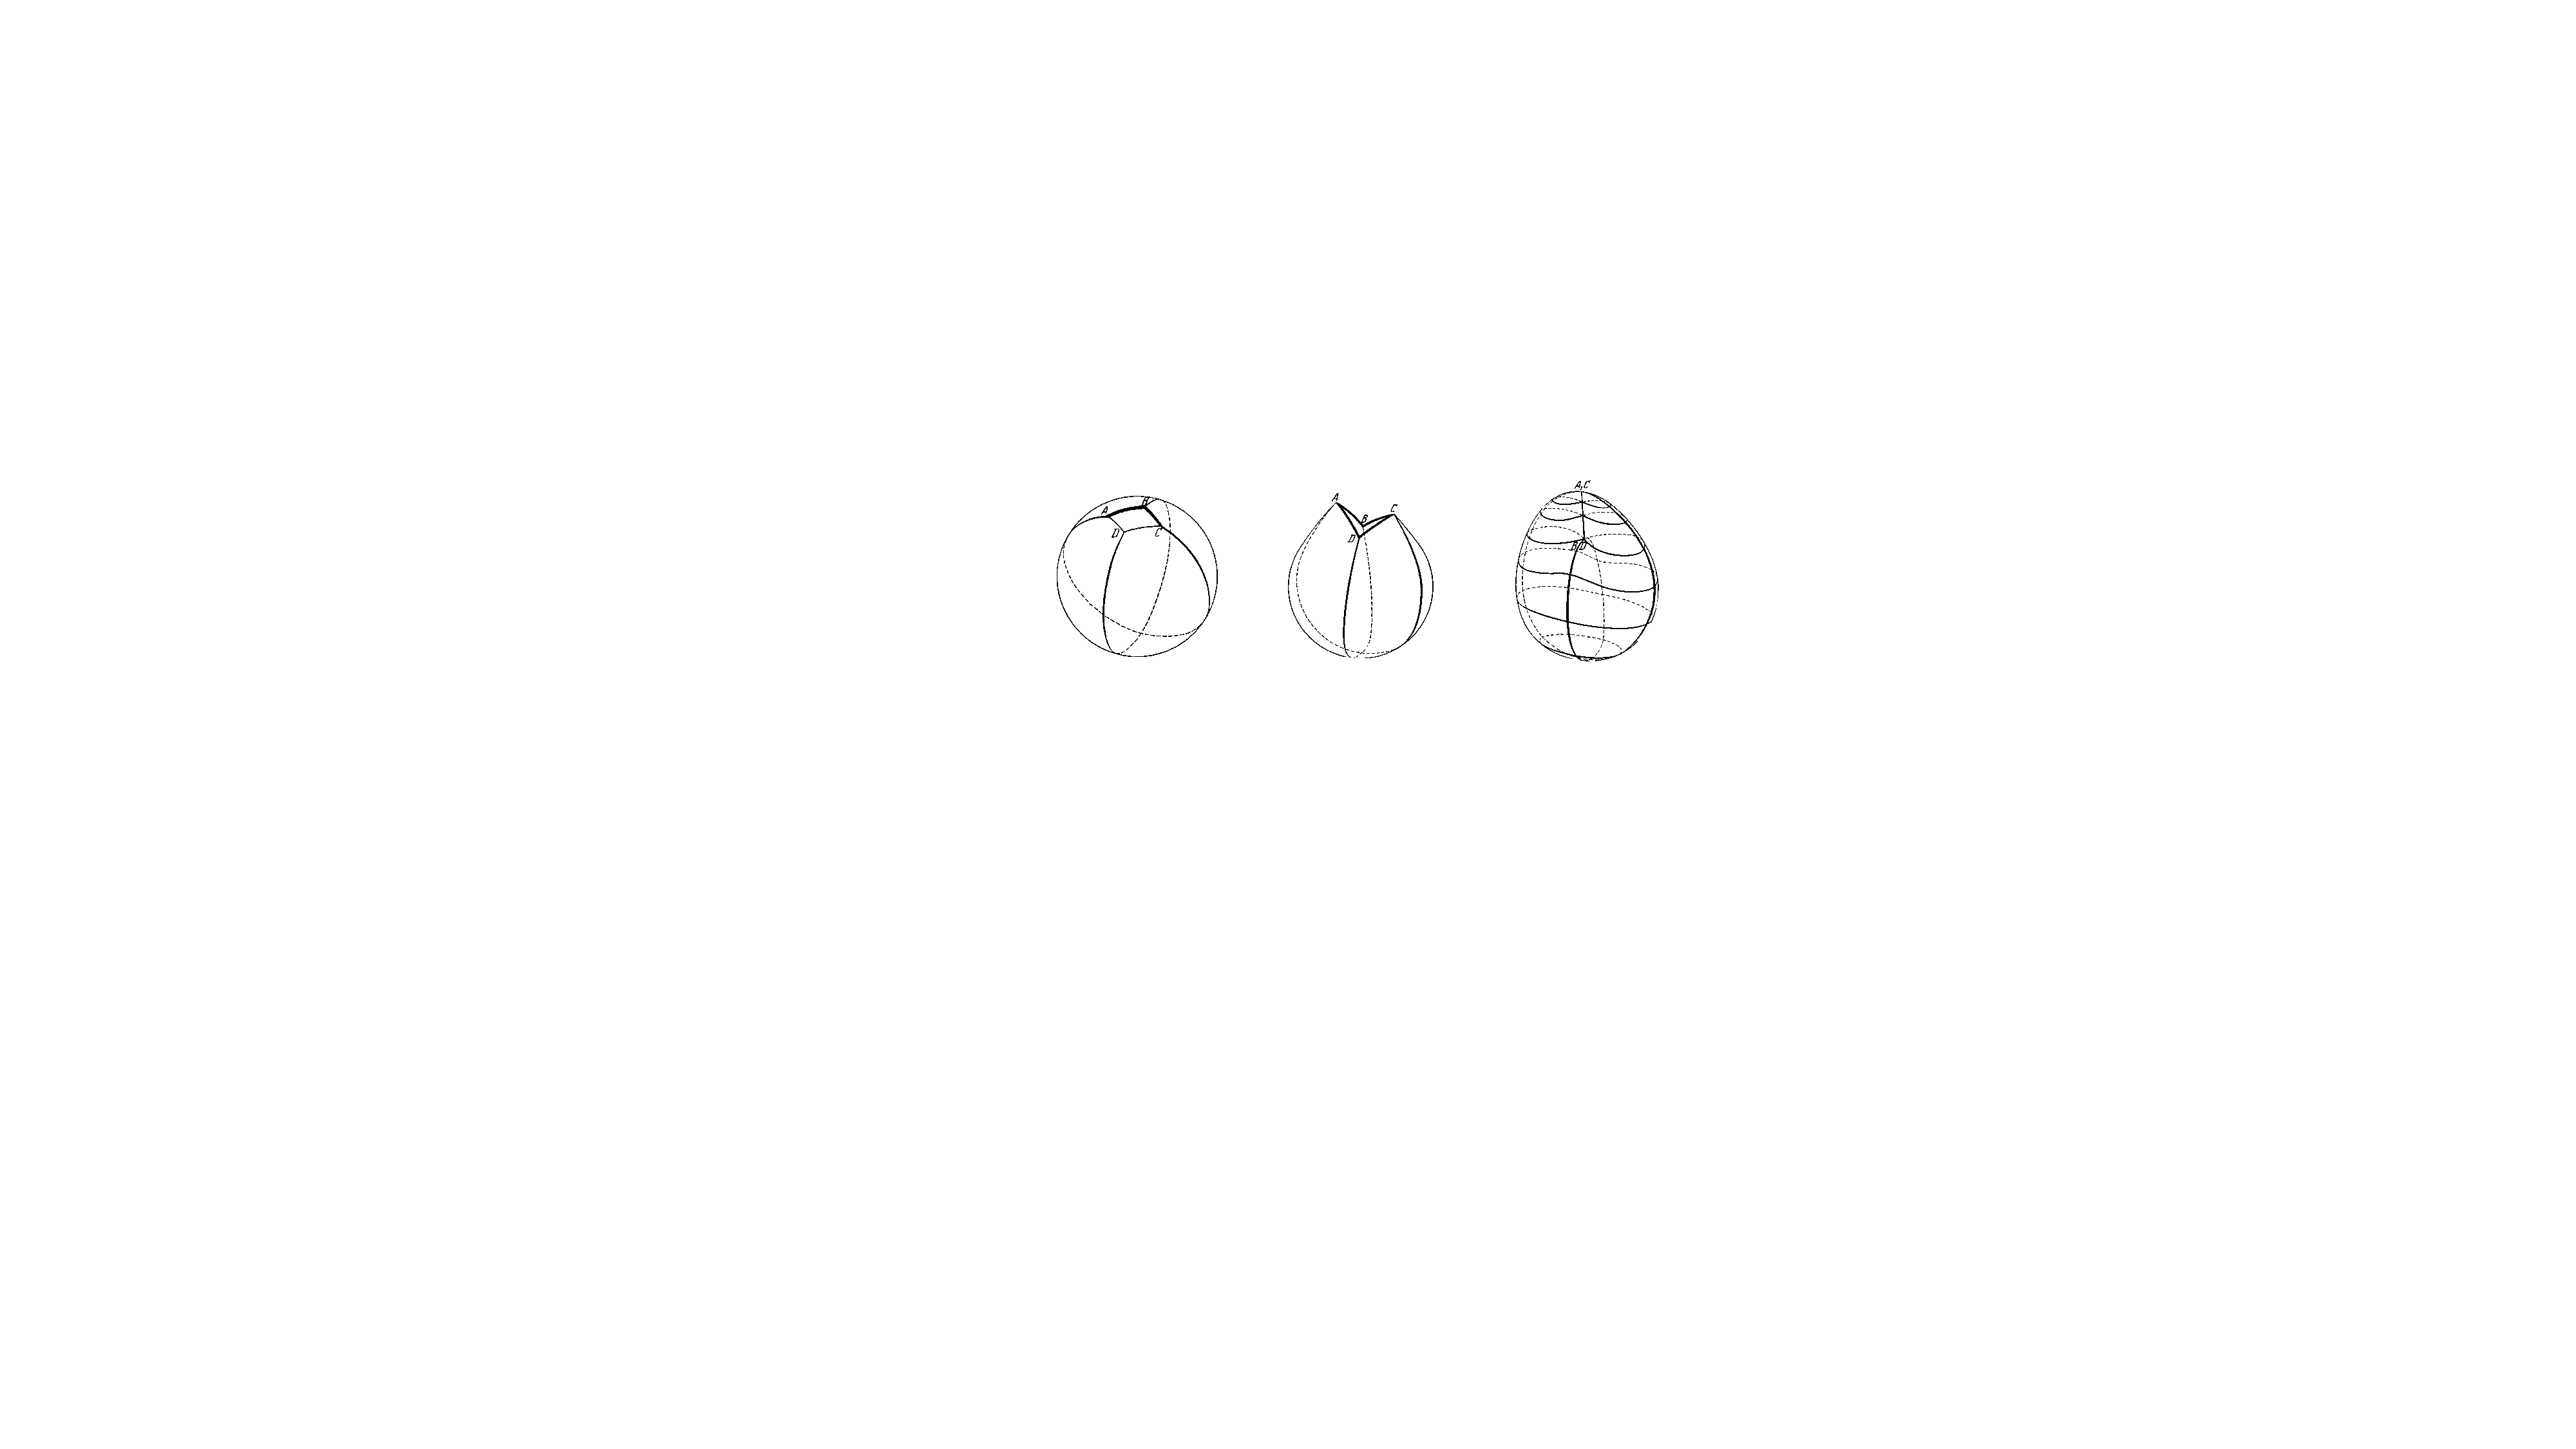
\includegraphics[scale=0.6]{figures/crosscap.pdf}
    \caption{Construction of the projective plane out of a disk. Adding a hole to this surface creates a crosscap, which is homeomorphic to a M\"bius band, see Exercises~\ref{RP2 exercise} and \ref{crosscap exercise}.}
    \label{fig:crosscap}
\end{figure}
\begin{example}{{{\cite[Exercise III.3]{Bredon}}}}
    Consider an annulus. Identify antipodal points on the outer circle. Also identify antipodal points on the inner circle. Calculate the fundamental group of this surface. Is it homeomorphic to any of the orientable compact surfaces? \emph{Hint:} taking $U$ and $V$ to be overlapping annular neighborhoods of the two boundaries of the annulus, the generator of $\pi_1(U\cap V)$ is mapped to the square of the generator in $\pi_1(U)$ and similarly in $\pi_1(V)$; therefore $\pi_1(U\cup V)=\langle a,b\mid a^2=b^2\rangle$.
\end{example}
\begin{xca}[{{\cite[Exercise 1.20]{Hatcher}}}]
    Let $X$ be the subspace of $\bbR^2$ that is the union of the circles $C_n$ of radius $n$ and center $(n, 0)$ for $n = 1, 2, \ldots$. Show that $\pi_1( X )$ is the free group $\ast_n \pi_1( C_n )$, the same as for the infinite wedge sum $\bigvee_{i=1}^\infty \bbS^1$. Show that $X$ and $\bigvee_{i=1}^\infty \bbS^1$ are in fact homotopy equivalent, but not homeomorphic.
\end{xca}

\begin{example}[Hawaiian earring {{\cite[Example 1.25]{Hatcher}}}]\label{hawaiian earring}
    Let $X$ be the subspace of $\bbR^2$ that is the union of the circles $C_n$ of radius $1/n$ and center $(1/n, 0)$ for $n = 1, 2, \ldots$. Initially this space can be mistaken for the infinite wedge sum $\bigvee_{i=1}^\infty \bbS^1$, but in fact it has a much larger fundamental group. This is because in the topology induced from $\bbR^2$ it is possible for a continuous loop $\gamma[0,1]\to X$ to cover an infinite number of circles $C_n$ at once, unlike in the case of the wedge sum. As a result, $\pi_1(X)$ can be mapped surjectively onto the infinite direct product group $\prod_{n=1}^\infty \bbZ$, which is uncountably large. 
\end{example}

\begin{example}[Torus knots {{\cite[Example 1.24]{Hatcher}}}]
    For relatively prime integers $m,n$, the \emph{torus knot}\index{Torus knots}\index{Knot!torus} $K=K_{m,n}\subset \bbR^3$ is the image of the embedding $f:\bbS^1\to \bbS^1\times \bbS^1\cong \bbT^2\subset\bbR^3$ given by $f(z)=(z^m,z^n)$ ($z=\rme^{2\rmi\pi t}$), where the torus $T$ is embedded in space in the standard way. Let us compute $\pi_1(\bbR^3\setminus K)$. First, we can safely replace $\bbR^3$ with its compactification $\bbS^3$ by adding ``a point at infinity''. This isomorphism follows from the Seifert-van~Kampen theorem. Now we may decompose $\bbS^3\setminus \bbT^2$ into two open solid tori $U,V$. Let $C$ be an open tubular neighborhood of $T\setminus K$. Then $U\cup C$ and $V\cup C$ form an open covering of $\bbS^3\setminus K$ with a path connected intersection. The fundamental groups of $U\cup C$, $V\cup C$, and the intersection $C$ are all isomorphic to $\bbZ$ and generated by loops $x,y,z$, respectively. The inclusions of $C$ into $V\cup C$ or $U\cup C$ map $z$ to $x^m$ or $y^n$. Therefore $\pi_1(\bbS^3\setminus K)=\langle x,y\mid x^m=y^n\rangle$. The center of this group is the subgroup generated by the element $x^m=y^n$, and the factor by the center is exactly $\bbZ_m\ast\bbZ_n$. By commuting all powers of $x^m$ through to the left, the elements of this group can be uniquely represented by strings of the form $x^{mk}y^{l_0}x^{k_1}y^{l_1}x^{k_2}y^{l_2}\cdots$ where $k\in\bbZ$, $k_i\in {0,\ldots,m}$ and $l_i\in\{0,\ldots,n\}$.
\end{example}

\begin{example}[Lens spaces {{\cite[Exercise III.10]{Bredon}}}]\label{example Lens space bredon}
    Let $X=(\bbD^2\times \bbS^1)\sqcup_f (\bbD^2\times \bbS^1)$ be the gluing of two solid tori along the map $f:\bbS^1\times \bbS^1\to \bbS^1\times \bbS^1$ induced from the linear map $\bbR^2\to\bbR^2$ given by an integer matrix $\begin{pmatrix}a&b\\c&d\end{pmatrix}$. The fundamental group of a solid torus are generated by one generator, call it $\gamma_1$ and $\gamma_2$ for the two solid tori correspondingly; in addition, the two solid tori overlap by a space that deformation retracts onto a torus $\bbT^2$ whose fundamental group is generated by two simple generators $\alpha$ and $\beta$; assuming $a\neq 0$, by Seifert-van~Kampen, from one inclusion we have the mappings $\alpha\mapsto\gamma_1$ and $\beta\mapsto e$, whereas from the other we get $\alpha\mapsto \gamma_2^d$ and $\beta\mapsto \gamma_2^c$. The resulting identification $\gamma_1\sim \gamma_2^d$ simply allows us to drop $\gamma_1$ from the list of generators. Thus $\pi_1(X)$ is the cyclic group $\langle \gamma_2\mid \gamma_2^c\rangle=\bbZ_c$. Note that the case $a=0$ is special -- in that case $\pi_1(X)=\bbZ$. If the matrix of $f$ is invertible (which is true iff $\det f=\pm1$) and is parametrized as $\begin{pmatrix}q&(qq'-1)/p\\p&q'\end{pmatrix}$, the resulting space is the so called \emph{lens space}\index{Lens spaces} $L(p;q)$ with fundamental group $\bbZ_p$. We have $L(1;0)=\bbS^3$ ($f=\id$) and $L(2;1)=\RP^3$ ($f=-\id$).
\end{example}





\clearpage

\section{Manifolds}

\subsection{Topological manifolds}
\begin{defn}[Locally Euclidean Space]\index{Locally Euclidean Space}
    A topological space $X$ is locally $n$-dimensional Euclidean if every $x\in X$ has an open neighborhood homeomorphic to the open $n$-dimensional ball, $U_x\cong B^n$. 
\end{defn}
\begin{defn}[Second-countability]\index{Second countable space}
    A topological space is called second countable if it has a countable basis of topology.
\end{defn}
\begin{defn}[Paracompactness]\index{Paracompact space}
\begin{enumerate}
    \item A collection of subsets $A_\alpha, \alpha \in I,$ of $X$ is called locally finite if every $x\in X$ has an open neighborhood $U_x$ such that $U_x\cap A_\alpha \neq \varnothing$ only for a finite number of $\alpha$'s. If all $A_\alpha$'s are open, this is the same as $x$ being an element of only finitely many of them.
    \item Given an open covering $\{U_\alpha\}$ (i.e.\ a collection of open sets such that $\bigcup_\alpha U_\alpha=X$), a refinement of it is an open covering $\{V_\beta \}$ such that $\forall \beta \;\exists \alpha: V_\beta \subset U_\alpha $.
    \item $X$ is called paracompact if every open covering of $X$ admits an open, locally finite refinement.
\end{enumerate}
\end{defn}
\begin{defn}[Topological manifold]\index{Manifold!topological}
    A topological manifold is a second countable, Hausdorff, locally Euclidean space.
\end{defn}
The following proposition is the reason why second countability is often substituted with paracompactness in the definition of manifolds.
\begin{prop}
    All topological manifolds are paracompact (and locally compact).
\end{prop}
\begin{proof}
    See \cite[Thm. 1.15]{Lee}
\end{proof}
\begin{defn}[Charts]\index{Chart}
    Let $X$ be an $n$-dimensional topological manifold. A \emph{chart} on it is a pair $(U,\varphi)$, where $U\subset X$ is an open set and $\varphi:U\to \bbR^n$ is a continuous map (called the chart map) that is also a homeomorphism onto its image $\wh{U}=\varphi (U)$, i.e.\ $U\cong \varphi(U)=\wh{U}$. The chart is called a \emph{coordinate ball} if $\wh U$ is a ball in $\bbR^n$. The values $\bf{x}=\varphi(x)\in\bbR^n$ of $\varphi$ are called \emph{coordinates} of the corresponding points on $X$. Hence, sometimes we will write $(U,\bf{x})$ to denote the chart.
\end{defn}
\begin{rem}
    Since $X$ is locally Euclidean, every point $x$ automatically has a chart $(U_x,\varphi)$ around it. In particular, every manifold has an open covering by charts $(U_\alpha,\varphi_\alpha)$.
\end{rem}

\begin{thm} All topological manifolds have the following properties.
\begin{enumerate}[label=(\alph*)]
    \item There is a countable basis consisting of coordinate balls (it can also be made locally finite and every ball can be made precompact)
    \item Local compactness.
    \item Local path-connectedness (i.e.\ every point has a path-connected neighborhood).
    \item At most countably many connected components, each open and a topological manifold of its own.
    \item The fundamental group $\pi_1(X)$ is at most countable.
\end{enumerate}
\end{thm}
\begin{proof}
    (1,2): Pick an open covering by charts $\{U_\alpha\}$. Each $U_\alpha $ can be covered by countably many coordinate balls $V_{\alpha_i}$ because $\wh{U}_\alpha$ can be covered by countably many balls in $\bbR^n$. By second countability, there is a countable subcovering and basis $\{V_\beta\}$. Fixing a chart $U$ and covering it by coordinate balls $V_\alpha$, we have that $\xoverline{V}_\beta$ is compact in $U$ (because it's homeo to a closed ball), therefore closed in $X$ by Hausdorffness. Therefore it's also compact in $X$, i.e.\ $V_\beta$'s are precompact. The covering can also be made locally finite: let $\{K_i\}_{i=1}^\infty$ be an exhaustion of $M$ by compact sets (i.e.\ $\bigcup_i K_i=M$; we will prove the existence in Prop. \ref{prop.exhaustion}). After picking out a finite subcovering of every compact ``stripe'' $K_{i+1}\setminus \Int K_{i}$ by charts that are small enough to fit within the wider open ``stripe'' $\Int K_{i+2}\setminus K_{i-1}$ (possible because all charts still form a basis), we end up with a locally finite covering (since every point of the manifold is contained only in 3 of the open stripes).

    (3) is obvious because it holds for balls. (4) follows because second countability implies countable number of components. The rest is obvious. For (5) See \cite[Thm 1.16]{Lee}.
\end{proof}

\begin{lem}
    Locally path-connected and connected implies path-connected.
\end{lem}
\begin{proof}
    The reverse direction is obvious. In the forward direction, introduce the set $C=\{q:q\text{ is connected with }p\}$  for some fixed $p\in X$. We will prove that $C$ is clopen and therefore equal to $X$.

    $C$ is open because $X$ is locally path-connected.
    $C$ is closed because for any $z\in\xoverline{C}$ there is a path-connected neighborhood $U_z$, thus $U_z\cap C\neq \varnothing$, and $z\in C$. Therefore $\xoverline C=C$. 
    But $X$ is connected, and $C$ is clearly not empty, therefore $C=X$, and lastly $C$ is path-connected by definition.
\end{proof}
\begin{cor}
    For manifolds, connectedness is equivalent to path-connectedness. In particular, connected components of manifolds are path-connected.
\end{cor}

\begin{example}
\begin{enumerate}
    \item Any open set in $\bbR^n$ is a manifold.
    \item $\bbS^n$ is a manifold because it can be covered by finitely many charts $(U_i,\varphi_i)$, where $U_i$ is an open hemisphere whose ``equator'' lies on one of the coordinate hyperplanes, and $\varphi_i$ is simply the orthogonal projection to that hyperplane.
    \item An $n$-dimensional torus $\bbT^n=(\bbS^1)^{\times n}$ is a manifold.
    \item The figure eight, 8, as a subset of $\bbR^2$, is not a manifold, because its center doesn't have a neighborhood homeomorphic to an interval.
    \item Matrices $\Mat(n,\bbR )$ form an $n^2$-dimensional manifold (isomorphic to $\bbR^{n^2}$). So do invertible matrices $\GL(n,\bbR )$ (being an open subset in $\bbR^{n^2}$) and all other classical matrix groups.
\end{enumerate}
\end{example}

\subsection{Smooth structures}
\begin{defn}[Atlas]\index{Atlas!topological}
    An atlas $\mathcal{A}$ for a topological manifold $M$ is a collection of continuous charts $\{(U_\alpha,\varphi_\alpha)\}$, $\varphi_\alpha:U_\alpha\to \wh{U}_\alpha \subset \bbR^n$ such that $\bigcup_\alpha U_\alpha =M$.
\end{defn}
Throughout these notes we also adopt the notation where for any atlas as above, $U_{\alpha\beta}=U_\alpha \cap U_\beta$, $U_{\alpha\beta\gamma}=U_\alpha \cap U_\beta \cap U_\gamma$, etc.

\begin{defn}[Smooth atlas]\index{Atlas!smooth}
    An atlas is called smooth (or of class $C^k$ or $C^\omega$) if all of the \emph{transition functions} $\varphi_{\beta\alpha}=\varphi_\beta\circ\varphi_\alpha^{-1}:\varphi_\alpha(U_{\alpha\beta})\to\varphi_\beta(U_{\alpha\beta})$ are smooth/$C^\infty$ (of class $C^k$, or real analytic, respectively) in the sense of multivariable calculus on $\bbR^n$.
\end{defn}
\begin{defn}[Equivalent atlases]\index{Atlas!equivalence of}
    Two atlases $\mathcal{A}_1$ and $\mathcal{A}_2$ are called equivalent, or compatible, if $\mathcal{A}_1\cup\mathcal{A}_2$ is still an atlas of the same smoothness class.
\end{defn}
\begin{defn}[Differentiable structure]\index{Differentiable structure}\index{Smooth structure}
    A smooth ($C^k$, analytic) structure on a topological manifold $M$ is an equivalence class $[\mathcal{A}]$ of smooth (respectively, $C^k$, $C^\omega$) atlases on it. 
\end{defn}
\begin{defn}[Smooth manifold]\index{Manifold!smooth}
    A smooth manifold is a pair $(M,[\mathcal{A}])$ consisting of a topological manifold and a smooth structure.
\end{defn}

\begin{rem}
    Recall that the second countability of topological manifolds implies their paracompactness (but not vice versa). In the case of differentiable manifolds, these properties turn out to be equivalent, and also equivalent to metrizability, or to the existence of smooth partitions of unity (see next section). This is why the definitions sometimes differ.
\end{rem}

\begin{example}
\begin{enumerate}
    \item Let $\psi:\bbR \to\bbR $ be $\psi(x)=x^3$. Then $\{(\bbR ,\psi)\}$ is an atlas that defines a smooth structure on $\bbR $. It is not smoothly compatible with the standard smooth structure given by the chart map $\varphi(x)=x$, because the transition function $\varphi\circ \psi^{-1}(x)=x^{1/3}$ is not smooth. Therefore $\bbR $ has many (in fact, infinitely many) different smooth structures.
    \item Any real or complex vector space is automatically a smooth manifold.
    \item Spaces of matrices, classical groups, spheres... are all smooth manifolds with their standard structures.
    \item Not every topological manifold admits a smooth structure, although examples are pretty difficult to construct. On the other hand, any $C^1$ manifold admits a compatible (in the $C^1$ sense) smooth structure, which is unique up to diffeomorphism (see below). This is why even mathematicians are mostly happy working with just either topological or immediately smooth/analytic manifolds. Interestingly, all topological manifolds in dimensions 1,2, and 3 admit unique (up to diffeo) smooth structures.
    \item All Lie groups (defined as smooth manifolds with a group structure in which multiplication and inversion are smooth maps) in fact support a unique (up to diffeo) $C^\omega$ structure. This is an immediate consequence of the convergence of the Baker-Campbell-Hausdorff series.
\end{enumerate}
\end{example}

From now on we work only with smooth manifolds, and use the word ``manifold''  to mean ``smooth manifold''.
\begin{defn}[Smooth maps]\index{Smooth map}
    Let $M$ and $N$ be two manifolds with atlases $\{(U_\alpha,\varphi_\alpha)\}$ and $\{(V_\beta,\psi_\beta)\}$, respectively. A map $f:M\to N$ is called smooth if all of its \emph{local representatives} $f_{\beta\alpha}=\psi_\alpha\circ f\circ \varphi_\beta^{-1}:\wh{U}_\beta\to \wh{U}_\alpha$ are smooth. The set of all smooth maps between two manifolds is denoted by $C^\infty (M,N)$. When $N=\bbR $, we write $C^\infty(M)=C^\infty (M,\bbR )$ for the space of ``smooth functions''. The category $\mathsf{Man}^\infty$ is the category of smooth manifolds with smooth maps for morphisms.
\end{defn}
\begin{xca}
    Check that all chart maps in any atlas of a smooth manifold $M$ are smooth as maps from $M$ to the standard $\bbR^n$.
\end{xca}
\begin{rem}
    The above exercise illustrates the general alternative approach to manifolds: instead of defining a smooth structure in terms of charts, we could describe it by specifying \emph{what smooth functions should be} by describing the subsets of the sets of local continuous functions $C(U_\alpha)$ that we want to be smooth (more precisely, one has to pick a subsheaf of the sheaf of continuous functions that is locally isomorphic to the sheaf of smooth functions on $\bbR^n$).
\end{rem}
\begin{defn}[Manifolds with boundaries]\index{Manifold!with boundaries/corners}
    Let $\bbR_+^n$ be the closed upper half-space in $\bbR^n$ (i.e.\ $x^n\geq 0$). An $n$-dimensional manifold with boundaries is defined just like a smooth manifold, only now some of the chart maps can map to $\bbR_+^n$. The smoothness of boundary transitions is characterized as follows: any function $\bbR_+^n\to \bbR_+^n$ is called smooth if it can be extended as a smooth function into an open neighborhood of $\bbR_+^n$. The set of points of $M$ that map to the boundary of $\bbR_+^n\subset \bbR^n$, i.e.\ the hyperplane $x^n=0$, is called the boundary $\partial M$. We also denote the interior by $\mathring M=M\setminus \partial M$.
\end{defn}
\begin{example}
    $\sqrt{y}:\bbR_+\to\bbR $ is not smooth on $\bbR_+$ with the standard smooth structure. However, it can be taken to be the chart map defining a new smooth structure on $\bbR_+$, and in that new structure it'll become smooth, because its local representative will be the identity map.
\end{example}
\begin{rem}
    Similarly, one can define \emph{manifolds with corners} using chart maps that can take values in quadrants, octants, and so on, of $\bbR^n$.
\end{rem}

\begin{defn}[Diffeomorphisms]\index{Diffeomorphism}
    A smooth map $f:M\to N$ between manifolds is a called a diffeomorphism if it has a smooth inverse. They are the isomorphisms in $\mathsf{Man}^\infty$.
\end{defn}
\begin{prop}
\begin{enumerate}
    \item Diffeos are homeo and open.
    \item If $M$ and $N$ have boundaries and $f:M\to N$ is a diffeo, then $f(\partial M)=\partial N$ and $\restr{f}{\mathring M}: \mathring M\to \mathring N$ is a diffeo.
\end{enumerate}
\end{prop}
\begin{example}
\begin{enumerate}
    \item Different smooth structures can be diffeomorphic! Take $\bbR $ with the chart $\psi(x)=x^3$ that we considered earlier. It is diffeomorphic to the standard smooth structure given by the chart $\varphi(x)=x$, and the diffeomorphism is given by $\psi$ itself! Indeed, its local representative in the two charts is $\varphi\circ \psi \circ\psi^{-1}(x)=x$. In this manner one can show that there is only one smooth structure on $\bbR$ up to diffeomorphism.
    \item Historically the first manifolds to be found to support more than one non-diffeomorphic smooth structure were spheres, starting with $\bbS^7$ which has 28 diffeomorphism classes of smooth structures. These smooth structures are now known as Milnor's \emph{exotic spheres}.
    \item $\bbR^n$ has only one smooth structure up to isomorphism for all $n\neq 4$. For $n=4$, it admits \emph{uncountably many} non-diffeomorphic structures. This makes the study of four-dimensional topological manifolds especially sophisticated, and there are still many very fundamental unsolved problems in four-dimensional topology \cite{smooth.structures}.
    \item In every dimension $n\geq 4$ there exist \emph{compact} topological manifolds that don't admit any compatible smooth structure.
\end{enumerate}
\end{example}

\begin{xca}
    Show that $\bbS^1$ supports only one smooth structure up to diffeomorphism.
\end{xca}






\subsection{Partitions of unity}

First we note that on $\bbR^n$ there exist bump functions, i.e.\ for any point $x_0$ and any two radii $0<r_1<r_2$ there is a function $\eta\in C^\infty(\bbR^n)$ such that $\restr{\eta}{B_{r_1}(x_0)}=1$ and $\restr{\eta}{\bbR^n\setminus \overline{B_{r_2}}(x_0)}=0$.
\begin{xca}
    Using the function $\int_a^x \rme^{\frac{1}{(x'-a)(b-x')}} \dd x'$ defined on $(a,b)$, construct a general bump function for $\bbR^n$.
\end{xca}

Now, any manifold $M$ can be covered by a locally finite collection of coordinate balls $(U_\alpha,\varphi_\alpha)$. Let $\eta_\alpha$ be a bump function that equals $0$ outside of the ball $\wh{U}_\alpha\subset \bbR^n$. Then define the smooth functions
\[f_\alpha =\begin{cases} \eta_\alpha\circ\varphi_\alpha, & \text{on }U_\alpha, \\ 0, & \text{on }M\setminus U_\alpha.\end{cases}\]
Finally, we normalize this collection of functions by defining
\[\chi_\alpha(x)=\frac{f_\alpha(x)}{\sum_\alpha f_\alpha (x).}\]
This expression is well-defined because the sum in the denominator is finite for every fixed $x$. These functions have the following properties:
\begin{enumerate}
    \item $\chi_\alpha\in C^\infty(M)$,
    \item $0\leq \chi_\alpha\leq 1$,
    \item $\supp \chi_\alpha\subset U_\alpha$,
    \item $\{\chi_\alpha\}$ is locally finite, i.e.\ only finitely many of them are non-zero at any given point $x\in M$,
    \item $\sum_\alpha \chi_\alpha (x)\equiv 1$.
\end{enumerate}

\begin{defn}[Partition of unity]\index{Partition of unity}
    Any collection of functions satisfying the above list of properties is called a \gls{pou} subordinate to the open covering (not necessarily by coordinate balls) $\{U_\alpha\}$ of $M$.
\end{defn}

\begin{prop}[{{\cite[Thm.~4.85]{LeeTop}}}]
    Any open covering of a paracompact Hausdorff space admits a subordinate \gls{pou}.
\end{prop}

\begin{prop}
    Any open covering of a smooth manifold admits a subordinate partition of unity.
\end{prop}
\begin{proof}
    Any open covering has a locally finite refinement consisting of coordinate balls, which allows us to apply the construction above to the refinement. Notice that second countability is key to the existence of partitions of unity.
\end{proof}
\begin{thm}[Extension lemma]\label{extension lemma}\index{Extension lemma}
    Let $A\subset M $ be a closed subset, and $f\in C^\infty(A,\bbR^k)$. Then for any open $U$ such that $A\subset U$, there exists an extension $\wt{f}\in C^\infty(M,\bbR^k)$: $\restr{\wt{f}}{A}=f$, such that $\supp \wt{f}\subset U$.
\end{thm}
\begin{proof}
    Pick $p\in A$ and neighborhood $U_p\subset U$. Let $\wt{f}_p: U_p\to\bbR^k$ be a smooth extension of $f$ from $U_p\cap A$. It is guaranteed to exist for sufficiently small $U_p$ by definition of smoothness on closed subsets of $\bbR^n$ and smoothness of chart maps.

    Then $\{U_p\}_{p\in A}\cup \{M\setminus A\}$ is an open covering of $M$. Let $\{\chi_p\}\cup\{\chi_0\}$ be a \gls{pou} subordinate to this covering (and $\chi_p=0$ inevitably for almost all $p$ so that the resulting collection is locally finite). Therefore $\chi_p\cdot \wt{f}_p:U_p\to\bbR^k$ are smooth and vanishing at the boundary of $U_p$, which allows us to extend them by zeros to smooth functions on all $M$. Finally, $\wt{f}=\sum_{p\in A} \chi_p \wt{f}_p$ is the extension we seek with support inside $U$.
\end{proof}
\begin{defn}[Exhaustion function]\index{Exhaustion}
    A function $f\in C^\infty(M)$ is called an exhaustion function for $M$ if for every $c\in\bbR $ the pre-image $f^{-1}((-\infty,c])$ is relatively compact (i.e.\ has compact closure in $M$).
\end{defn}
\begin{prop}\label{prop.exhaustion}
    Every smooth manifold has an exhaustion function.
\end{prop}
\begin{proof}
    Let $\{V_\alpha\}$ be a countable open covering by precompact sets and $\{\chi_\i\}_{i=1}^\infty$ a subordinate \gls{pou}. Define $f(x)=\sum_{n=1}^\infty n\cdot \chi_n(x)$. 

    Clearly $f^{-1}((-\infty,c])\subset \bigcup_{i=1}^{[c]+1}\xoverline{V_i}$, which is a compact set.
\end{proof}







\subsection{Sard's theorem}

In $\bbR^n$, a set $A$ is said to have\emph{ zero measure} if for any $\epsilon>0$ it can be covered by a collection of open balls $B_i$ such that the total volume of these balls is less than $\epsilon$.

\begin{defn}[Measure zero]
    Even though there is no canonical way to measure volumes on manifolds, there is still a consistent notion of zero measure. Namely, a set $A\subset M$ has zero measure if all the sets $\varphi_\alpha(A\cap U_\alpha)$ are measure zero in $\bbR^n$ for an atlas $\{(U_\alpha,\varphi_\alpha)\}$.
\end{defn}

\begin{defn}[Rank of a map]\label{def.rank}\index{Rank of a map}
    Let $f\in C^\infty (M^m,N^n)$ (superscripts here indicate the dimensions of the manifolds). We say that the rank of $f$ at $p\in M$ is $\rank_p f=r$ if there exist two local charts, $(U,\varphi)$ around $p \in M$ and $(V,\psi)$ around $f(p)\in N$, such that the local representative of $f$ in these charts is $\psi\circ f\circ\varphi^{-1}(x^1,\ldots,x^m)=(x^1,\ldots,x^r,\underbrace{0,\ldots,0}_{n-r})$.
\end{defn}

\begin{defn}[Critical and regular points/values]\index{Critical points/values}\index{Regular points/values}
    $p\in M$ is said to be a critical point of $f\in C^\infty(M^m,N^n)$ if $\rank_p f<n$, i.e.~if its differential at $p$ is not surjective. In this case, $f(p)\in N$ is called a critical value of $f$. Otherwise, $p$ is a regular point, and a regular value is one all of whose pre-images are regular points.
\end{defn}

The main property of regular values of smooth maps is that they are generic, as demonstrated by the following deep theorem. We will need this result when we talk about transversality in the context of fiber bundles.

\begin{thm}[Sard]\index{Theorem!Sard}\label{thm sard}
    For any $f\in C^\infty(N,M)$ the set of critical values (also known in some contexts as the \emph{caustic}) of $f$ has measure zero in $M$.
\end{thm}
\begin{proof}
    This theorem is essentially entirely local, i.e.\ it suffices to prove it for $N=\bbR^n$ and $M=\bbR^m$. Every manifold can be broken up into a countable number of neighborhoods, and a countable union of sets of measure zero is still measure zero.

    Let $C\subset \bbR^m$ be the set of critical points of $f:\bbR^n\to \bbR^m$ and pick $x_0\in C$. Then, after some rotation of the space, we can assume that its derivative maps $f'_{x_0}(\bbR^n)=\bbR^k\times \{0\}\subset \bbR^m$, where $k\leq n-1$ is the rank of the Jacobi matrix at $x_0$.  If we choose a ball $B_r(x_0)$ of radius $r$ around $x_0$, then
    \[f'_{x_0}(B_r(x_0))\subset (\bbR^k\times \{0\})\cap B_\epsilon(f(x_0)),\quad \epsilon=r\cdot \mathrm{Lip}f,\]
    where $\mathrm{Lip}f$ is the Lipschitz constant of $f$ inside $B_r(x_0)$ (equal to the supremum of all directional derivatives in unit directions). We only need the existence of such an $\epsilon$ and that it goes to zero with $r\to 0$.

    Therefore $f'_{x_0}(B_r(x_0))$ can be covered by $N^k$ cubes of diameter $\epsilon/N$. By differentiability there exists $\delta>0$ such that 
    \[\lvert f(y)-f(x_0)-f'_{x_0}(y-x_0)\rvert\leq \frac{1}{N}|y-x_0|,\quad \text{ for all }y\in B_\delta(x_0).\]
    So $f(y)$ is within $r/N$ distance of the hyperplane $f(x_0)+f'_{x_0}(\bbR^n)$ (provided that $r<\delta$). Therefore the image $f(B_r(x_0))$ itself is contained in a neighborhood of $f'_{x_0}(B_r(x_0))$ of radius $r/N$. Thus we can construct $N^k$ disjoint sets $E_j$ of diameter $\sim r/N$ that cover $f(B_r(x_0))$.

    We repeat the above for every point $x\in C$ and get $r_x>0$ such that $f(B_{r_x}(x))\subset \bigsqcup_{j=1}^{N^k}E_j^x$. By \href{https://en.wikipedia.org/wiki/Vitali_covering_lemma}{Vitali's covering lemma}, there is a countable subcovering, so $C\subset \bigsqcup_{i=1}^\infty B_{r_i}(x_i)$ such that $\{B_{r_i/5}(x_i)\}$ are disjoint and for every $i$ there are sets $E^i{}_j,j=1,\ldots,N^k$ such that $\mathrm{diam}(E^i{}_j)\sim r/N$ and $f(B_{r_i}(x_i))\subset \bigsqcup_{j=1}^{N^k}E^i{}_j$. Thus $f(C)\subset \bigsqcup_{i=1}^\infty\bigcup_{j=1}^{N^k}E_j^i$. We can safely assume that $C\subset [-l,l]^n$ for some $l\in \bbN$ (otherwise it can be broken up into countably many pieces of this kind, which won't upset the result of the theorem). By compactness we can then assume that $r_x<1$ for all $x\in C$. Thus
    \begin{multline}
        \mathrm{volume}(f(C))\leq \sum_{i,j}(\mathrm{diam}(E^i{}_j))^n\leq \sum_{i,j}\left(\frac rN\right)^n\lesssim \sum_{i}N^k\frac{r^n}{N^n}\lesssim \\
        \lesssim 5^nN^{k-n}\sum_i\frac{r^n}{5^n}\lesssim 2\cdot 5^n N^{k-n}\cdot \mathrm{volume}([-l,l]^n),
    \end{multline}
    since $C$ lies inside $[-l,l]^n$ and is covered by balls of radii $r_i\leq 1$ with disjoint sub-balls, so the sum of the volumes of these sub-balls can only exceed the volume of $[-l,l]^n$ by at most a constant factor (coming from pieces that stick out of $[-l,l]^n$), say $2$.

    But now, $k<n$, thus in the limit $N\to \infty$ we find that the volume of $f(C)$ has to be zero. This proof is due to Behnam Esmayli, a more conventional one can be found in \cite[Thm.~6.10]{Lee}.
\end{proof}
\begin{rem}
    The ability to globalize the proof of this theorem depends crucially on second countability. Indeed, we could consider a non-second-countable $1$-dimensional ``manifold'' given by the uncountable disjoint union of lines $M=\bigsqcup_{a\in \bbR} R_a=\bigsqcup_{a\in \bbR} \bbR$ (so called \emph{long line}\index{Long line}), and define a function $f:M\to \bbR$ by $\restr{f}{R_a}=a$. In this case $f$ is smooth and every value $a\in\bbR$ is a critical value, contrary to Sard's theorem. What happened was that we found an uncountable family of local neighborhoods ($R_a$), for each of which the set of critical values has measure zero (one point $a$). But the union of an uncountable number of sets of measure zero can have nonzero measure. Thus, second countability is key to Sard's theorem working on general manifolds.
\end{rem}






\subsection{Inverse \& Implicit Mapping Theorems}

In this section we just recall the statements of two basic theorems in multivariable calculus.
\begin{thm}[\gls{inmt}]\label{InMT}\index{Theorem!Inverse mapping}
    Let $U,V\subset\bbR^n$ be open and $f\in C^\infty(U,V)$. If the Jacobi matrix $\frac{\partial f^i}{\partial x^j} (\bf{a})$ is invertible for some $\bf{a}\in U$, then there are neighborhoods $\bf{a}\in U_{\bf{a}}\subset U$ and $f(\bf{a})\in V_{f(\bf{a})}\subset V$ such that $\restr{f}{U_{\bf{a}}}:U_{\bf{a}}\to V_{f(\bf{a})}$ is a diffeomorphism.
\end{thm}
Meaning: any smooth map whose Jacobi matrix is non-singular at a point is locally a diffeomorphism around that point.

\begin{thm}[\gls{immt}]\label{ImMT}\index{Theorem!Implicit mapping}
    Let $U\subset \bbR^n\times \bbR^k$ be open, $(\bf{x},\bf{y})=(x^1,\ldots,x^n,y^1,\ldots,y^k)\in U$. Let $\Phi\in C^\infty(U,\bbR^k)$ (with components $\Phi^j$) and $\Phi(\bf{x},\bf{y})=\bf{c}$ for all $(\bf{x},\bf{y})\in U$. If the matrix $\left(\frac{\partial\Phi^i}{\partial y^j}(\bf{y},\bf{x})\right)_{i,j=1}^k$  is non-singular, then there are open neighborhoods $\bf{x}\in V_{\bf{x}}\subset \bbR^n$ and $\bf{y}\in W_{\bf{y}}\subset\bbR^k$ and a smooth map $f\in C^\infty (V_{\bf{x}},W_{\bf{y}})$ such that 
\[\forall\,(\bf{v},\bf{w})\in V_{\bf{x}}\times W_{\bf{y}},\;\; \Phi (\bf{v},\bf{w})=\bf{c} \Leftrightarrow \bf{w}=f(\bf{v}).\]
\end{thm}
Meaning: the equation $\Phi(\bf{x},\bf{y})=\bf{c}$ can be locally solved for $\bf{y}=\bf{y}(\bf{x})$ if the matrix $\partial \Phi/\partial\bf{y}$ is invertible.

\begin{comment}
\PRLsep
\begin{center}
  {\red Lecture 5 on 7 Dec 2018 ended here}
\end{center}
\end{comment}

\subsection{Tangent spaces}
    In $\bbR^n$, vectors don't have ``base points'' because they can always be parallel transported to the origin. On a manifold, this is impossible without additional structure, which is why there is a tangent space ``attached'' to every point $p\in M$. 
\begin{defn}[Tangent vector I]\index{Tangent vector}\index{Vector}
    Let $m\in M$. If $m\in \mathring M$, consider all curves $\gamma\in C^\infty((-1,1),M)$ such that $\gamma(0)=m$. If $m\in \partial M$, consider instead all curves with domains $(-1,0]$ or $[0,1)$. Introduce the equivalence relation $\gamma_1\sim \gamma_2$  iff $\restr{\frac{\dd}{\dd t}}{t=0}(\varphi_\alpha\circ \gamma_1)(t)=\restr{\frac{\dd}{\dd t}}{t=0}(\varphi_\alpha\circ \gamma_2)(t)$ for any chart $\varphi_\alpha$ around $p$. A tangent vector at $x$ is an equivalence class $[\gamma]_m$ of curves passing through $m$. The set of all tangent vectors at $m$ is denoted by $\T_m M$.
\end{defn}

\begin{enumerate}
    \item $T_m M$ is imbued with the structure of a real vector space as follows:
    \begin{enumerate}
        \item $\lambda\cdot [\gamma(t)]_m\coloneqq [\gamma(\lambda t)]_m$ for $\lambda\in\bbR $.
        \item $[\gamma_1(t)]_m+[\gamma_2(t)]_m\coloneqq [\varphi_\alpha^{-1}(\varphi_\alpha(\gamma_1(t))+\varphi_\alpha(\gamma_2(t)))]_m.$
    \end{enumerate}
    \item We will show later that $\dim \T_m  M=\dim M$.
\end{enumerate}


\begin{defn}[Tangent vector II]
    $\T_m  M$ can be alternatively defined as the set of all \emph{derivations}\index{Derivation} at $m$, i.e.\ linear functionals $v:C^\infty(M)\to \bbR $ such that $v[f\cdot g]=f(m)v[g]+g(m)v[f]$. This is obviously a vector space. Notably, this definition doesn't need to be modified if $m\in\partial M$.
\end{defn}

\begin{prop}
    The two definitions of tangent spaces given above are isomorphic as vector spaces.
\end{prop}
\begin{proof}
    An explicit linear isomorphism between the two constructions is $[\gamma]_m\mapsto v[f]=\restr{\frac{\dd}{\dd t}}{t=0}f(\gamma(t))$ (this is called the \emph{directional derivative} along the tangent vector $[\gamma]_m$). 

    All derivations on the algebra of smooth functions can be shown to be directional derivatives, which allows us to invert this mapping. Namely, for a chart map $\varphi_\alpha$, the $n$ numbers $v[\varphi_\alpha^i]$ are components of a vector $\wh{v}\in \bbR^n$. Now we can let $\wh{\gamma}(t)=\varphi_\alpha(m)+t\wh{v}$ and $\gamma(t)=\varphi_\alpha^{-1}(\wh{\gamma}(t))$. It is easy to show that this is a linear inverse to the above mapping.
\end{proof}


\begin{xca}
    Check that the definition of a tangent vector and all of the following constructions are consistent, i.e.\ independent of the choices of charts $\varphi_\alpha$ or representatives $\gamma(t)$ of equivalence classes.
    \end{xca}
    \begin{defn}[Differential/push-forward]\index{Push-forward}
    Let $F\in C^\infty(M,N)$ and $p\in M$. The push-forward of $F$ at $m$ is the linear map $D_m F=F_{\ast m}:T_m M\to T_{F(m)} N$ defined via \[F_{\ast m}([\gamma]_m)=[F\circ\gamma]_{F(m)},\] or equivalently \[F_{\ast m}(v)[f]=v[f\circ F]\] for any $f\in C^\infty (N)$.
\end{defn}

\begin{rem}[Coordinate expressions for derivatives]
    In local coordinates (i.e.~replacing $F$ with some function $\wh{F}:\bbR^m\to\bbR^n$,
    \[F_{\ast m}([\gamma]_m)=\restr{\frac{\dd}{\dd t}}{t=0} \wh{F}(\gamma(t)).\label{eq differential in local coordinates}\]
    and 
    \[\wh{F}_{\ast m}(v)[f]=\restr{\frac{\dd}{\dd t}}{t=0}f(F(\gamma(t)).\]
\end{rem}


\begin{thm}\label{prop of push-forwards}
    Consider smooth maps between manifolds $M\overset{f}{\to}N\overset{g}{\to}P$. Then
\begin{enumerate}
    \item $f_{\ast m}:\T_m M\to \T_{f(m)} N$ is linear;
    \item $(g\circ f)_{\ast m}=g_{\ast f(m)}\circ f_{\ast m}$ (chain rule);
    \item $(\id_M)_{\ast m}=\id_{\T_m M}$;
    \item if $f$ is a local diffeo at $x$ then $f_{\ast m}$ is invertible and $(f_{\ast m})^{-1}=(f^{-1})_{\ast m}$ (the converse is also true by \gls{inmt});
    \item In local coordinates, $f_{\ast m}$ is represented by the Jacobi matrix of the local representative $f_{\beta\alpha}$;
    \item $\dim T_m M=\dim M$, even for points on $\partial M$;
    \item \gls{inmt} doesn't hold at the boundary.
\end{enumerate}
\end{thm}
\begin{proof}
    The first few statements are trivial and are left as an exercise.
    6) A local chart map $\varphi_\alpha$ can be viewed as a local diffeo to an open subset of $\bbR^n$. Since $T_{\varphi_\alpha(m)}(\bbR^n)=\bbR^n$ (because we know that equivalence classes of curves at a point of $\bbR^n$ are uniquely characterized by their tangent vectors), we have a linear map $(\varphi_\alpha)_{\ast m}:\T_m M\to \bbR^n$, which is an isomorphism by 4). Therefore the dimensions coincide. Nothing really changes at the boundary.

    7) Consider the inclusion map $i:\bbR^n_+\hookrightarrow \bbR^n$. Clearly $i_{\ast 0}=\id$ is invertible, but $i$ itself is not a local diffeo because $i(B^n\cap \bbR^n_+)$ is the image of an open set that is not open in $\bbR^n$.
\end{proof}

All of this implies that the map $\T_m:(M,m)\mapsto \T_m M$ extends to a covariant functor $\T_m:\mathsf{Man}_\bullet^\infty\to \mathsf{Vect}_\bbR$. It respects morphisms (smooth maps) $f:M\to N$ between pointed\footnote{The requirement that these manifolds be pointed is a mere technicality for the sake of the definition of a functor. Given a map $f:M\to N$ and a point $f\in M$, we can always create the pairs $(M,m)$ and $(N,f(m))$ and treat $f$ as a pointed map.} manifolds because the following diagram commutes:
\[
\begin{tikzcd}[every matrix/.append style={name=m},   
    execute at end picture={\draw [<-] ([xshift=-2.6em,yshift=1mm]m-2-2.north) arc[start angle=-90,delta angle=270,radius=0.25cm];}]
   M \arrow[r,"f"]\arrow[d,swap,"\T_m"]& N\arrow[d,"T_{f(m)}"] \\
   \T_m M\arrow[r,swap, "\T_m  f"]& T_{f(m)}N.
\end{tikzcd}
\]

As we will show later, the tangent space over $m\in M$ in a certain sense ``varies smoothly with $m$'' and together all of the tangent spaces comprise a single object called the \emph{tangent bundle}. A similar thing happens to the functors $\T_m$.

\subsection{Rank}
We have defined rank in Def.~\ref{def.rank}. However, that definition is not practical because it's an existence statement rather than a constructive ``measurement''.

Recall that for a matrix $A\in \Mat(n\times m,\bbR )$ its rank $\rank A$ is defined as the maximal number of linearly independent columns (equivalently, rows) in it. More abstractly, the rank of a linear operator is the dimension of its image, $\rank A=\dim(\im (A))$. The following theorem establishes the equality between the rank of a smooth map and the rank of its differential.

\begin{thm}[Rank theorem]\index{Rank theorem}\label{Rank thm}
    For $f\in C^\infty(M,N)$, $\rank_m f=\rank (f_{\ast m})$.
\end{thm}
\begin{proof}
    This is the \gls{inmt} in disguise. Since this theorem is local, we can safely replace $M$ and $N$ by open $U\subset \bbR^k$ and $V\subset \bbR^n.$

    Assume $\rank(f_{\ast m})=r$. Introduce coordinates $(x^1,\ldots,x^r$, $y^1,\ldots,y^{k-r})$ on $U$ and $(v^1,\ldots,v^r$, $w^1,\ldots,w^{n-r})$ on $V$. In these coordinates, we can write \[f(x,y)=(F(x,y),G(x,y)).\] \Gls{wlog}, $m=0$, $f(m)=0$, and  $F_{\ast (0,0)}$ is a nonsingular square matrix.

    Define $\varphi:U\to\bbR^m$ by $\varphi(x,y)=(F(x,y),y)$. Its differential at $(0,0)$ is nonsingular by assumption, so by the \gls{inmt} we locally have an inverse and by definition of $\varphi$, the composition of $\varphi^{-1}$ with $f$ will have the form 
    \[
    f\circ\varphi^{-1}=(x,\wt{G}(x,y)).
    \]
    Finally, by a trivial change of coordinates $\psi(v,w)=(v,w-\wt{G}(v,0))$ we can bring the local form of $f$ to \[\psi\circ f\circ \varphi^{-1}(x,y)=(x,0),\] which means that $\rank_m f=r$. The converse direction is obvious.
\end{proof}

\begin{prop}\label{domain of maximal rank}
    For any smooth map $f\in C^\infty (M,N)$ the set of points $m\in M$ where the rank is maximal, i.e.\ $\rank_m f=\min(\dim M,\dim N)$, is open in $M$.
\end{prop}
\begin{proof}
    Let $\dim M=k$ and $\dim N=n$. The mapping $D:m\mapsto \wh{f}_{\ast m}$ is a continuous (in fact, smooth) map $U_\alpha\subset M\to \Mat(n\times k,\bbR )$. The subset of all matrices of maximal rank is open in $\Mat(n\times k,\bbR )$ (essentially because small perturbations can't make linearly independent vectors dependent\footnote{The converse is not true, which is why the set of matrices of any fixed non-maximal rank is not open.}). By continuity of $D$, the set of $m$ at which the rank is maximal is also open (in every $U_\alpha$ and thus in all of $M$).
\end{proof}

Therefore we see that maps of maximal rank are of special significance. Moreover, they fall into two categories: if $\dim M\leq \dim N$, then the maximal rank equals $\dim M$; if $\dim M\geq \dim N$, the maximal rank is $\dim N$. In the first case, matrices of maximal rank are exactly the injective ones, whereas in the second case they are the surjective ones.

\begin{defn}[Smooth immersions and submersions]
    Among all maps of \emph{constant rank} we single out two special classes.\index{Immersion!smooth}\index{Submersion!smooth}
\begin{enumerate}
    \item $f\in C^\infty(M,N)$ is called an immersion if $f_{\ast m}:\T_m  M\to T_{f(m)} N$ is injective for all $m$. Equivalently, $f$ is an immersion iff it has everywhere maximal rank and $\dim M\leq \dim N$.
    \item $f\in C^\infty(M,N)$ is called a submersion if $f_{\ast m}:\T_m  M\to T_{f(m)} N$ is surjective for all $m$. Equivalently, $f$ is a submersion iff it has everywhere maximal rank and $\dim M\geq \dim N$.
\end{enumerate}
\end{defn}

\begin{rem}
    As is clear from Theorem \ref{Rank thm}, a submersion is a map that is locally an orthogonal projection onto a subspace (in some coordinates), and an immersion is one that is locally an inclusion as a lower-dimensional subspace. A map that is both a submersion and an immersion is a local diffeomorphism. Note that ``locality'' here is understood both in domain and in range -- we have to pick out open neighborhoods of both $m$ and $f(m)$. An immersion for which this property holds globally on the entire domain (i.e.~locally only in the target manifold) is just an injective immersion. Meanwhile, the attempt to define maps that are ``projections locally in the target'' will lead us to the concept of fiber bundles, and it will not be enough for them to be surjective submersions.
\end{rem}


\begin{thm}[Global rank theorem]\label{Global rank}\index{Rank theorem!global}
Let $f\in C^\infty(M,N)$ have constant rank $r$. Then
\begin{enumerate}
    \item if $f$ is injective, it is an immersion;
    \item if $f$ is surjective, it is a submersion;
    \item if $f$ is bijective, it is a diffeomorphism.
\end{enumerate}
\end{thm}
\begin{proof}
\begin{enumerate}
    \item Suppose it is not an immersion. Then $r<\dim M$, which means that in some coordinates we have $\wh{f}(0,\ldots,0,\epsilon)=(0,\ldots,0)$ for all sufficiently small $\epsilon$. This contradicts injectivity.
    \item Suppose it is not a submersion. Then $r<\dim N$. There exists a (countable) open covering  $\{U_\alpha\}$ of $M$ such that $f(U_\alpha)$ are ball-slices $B^n\cap \{y^{r+1}=y^{r+2}=\cdots=y^n=0\}$. We have $f(M)=\cup_\alpha f(U_\alpha)$, but at the same time $f(U_\alpha)$'s are \emph{nowhere dense} (i.e.\ closure has empty interior). By \href{https://en.wikipedia.org/wiki/Baire_category_theorem}{Baire category theorem}, a countable union of nowhere dense sets has an empty interior, which implies $\Int  f(M)=\varnothing$. This contradicts surjectivity, because $\Int  N\neq\varnothing$.
    \item Obvious (a bijective local diffeo is a diffeo).
\end{enumerate}
\end{proof}



\subsection{Immersions and embeddings}

\begin{figure}
    \centering
    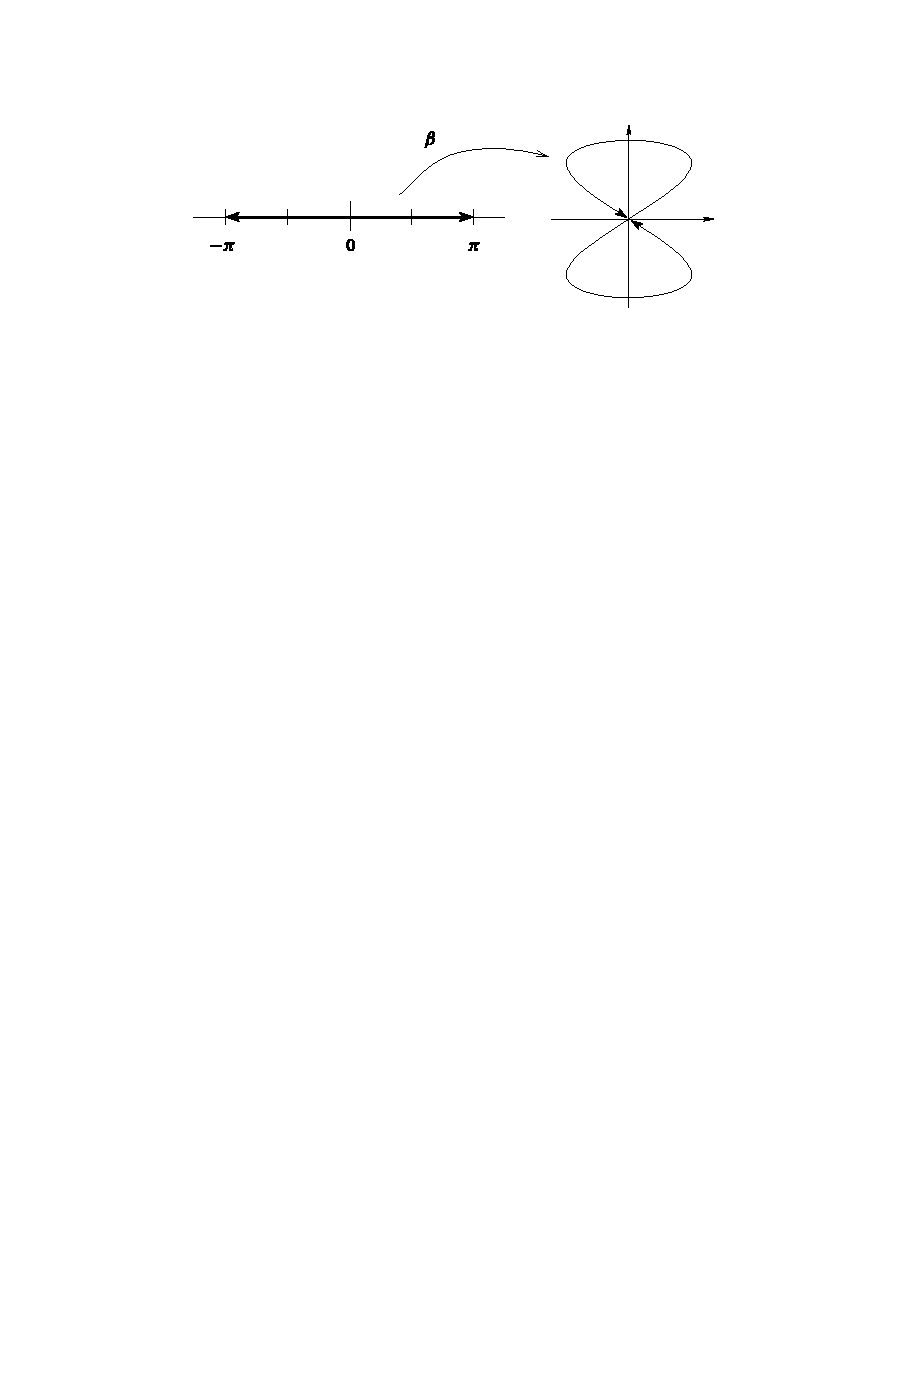
\includegraphics{figures/immersion.pdf}
    \caption{The figure-eight curve $\beta:(-\pi,\pi)\to \bbR^2$ given by $\beta(t)=(\sin 2t,\sin t)$ is an immersion but not an embedding. Its domain is open but its image is closed.}
    \label{fig:immersion}
\end{figure}

As we described above, immersions are maps with injective differentials. Immersions themselves don't need to be injective, and even if they are, their images, as topological subspaces of the codomain, are not even always homeomorphic to the domain. For example, the map in Figure~\ref{fig:immersion} is an immersion whose image is not homeomorphic to the domain. Maps that do respect subspace topology in this way are called embeddings.

In the topological category, the situation is different. A topological immersion is the intuitive analog of the smooth immersion: the injectivity of differentials is replaced by a local homeomorphism property on the domain. 

\begin{defn}[Topological immersion]\index{Immersion!topological}
    A continuous map $f:X\to Y$ is called a topological immersion if for every $x\in X$ there is an open neighborhood $U\subset X$ of $x$ such that $\restr{f}{U}\to f(U)$ is a homeomorphism, where $f(U)$ is taken to have the subspace topology inherited from $Y$.
\end{defn}

A topological embedding then is a global version of a topological immersion: the entire map has to be a homeomorphism onto the image. In particular, it has to be injective.

\begin{defn}[Topological embedding]\index{Embedding!topological}
A topological embedding is a continuous map $f:X\to Y$ that is a homeomorphism onto its image (where the image $f(X)\subset Y$ is taken to have the subspace topology in the target). In other words, it is an injective map such that the topology on the domain must coincide with the initial topology induced by the map.
\end{defn}


In this way the concept of a topological embedding map is dual to that of a topological quotient maps. In the smooth category the picture is a bit different. First, the intuitive smooth version of a quotient map is a smooth submersion that is a topological quotient map. However, as we will see in \S\ref{sec: submersions}, every smooth submersion is automatically a quotient map, so the second requirement can be dropped. On the other hand, smooth immersions are not always topological embeddings (although they are topological immersions). This is why smooth submersions and smooth immersions are not dual concepts, but instead the concept dual to smooth submersions is the following concept of a smooth embedding.

\begin{defn}[Smooth embedding]\index{Embedding!smooth}
A smooth embedding is a smooth immersion that is topological embedding.
\end{defn}

\begin{example}
\begin{enumerate}
    \item Much like the example in Figure~\ref{fig:immersion}, the mapping of $\bbS^1$ onto a figure eight in $\bbR^2$ can be represented by a parametric map $f(t)=(f_x(t),f_y(t))$. It is an immersion provided that $f'(t)$ doesn't vanish anywhere. However, it is not an embedding because the image (figure eight) is not homeomorphic to the circle.
    \item Excluding the one point on the circle that is mapped to the center point of the figure eight in the last example, we obtain a map $f:(0,1)\to \bbR^2$ whose image is still the whole figure eight. This is an injective immersion. However, it is still not an embedding because the image is compact in the subspace topology, whereas the open interval is not a compact space.
    \item $\gamma:\bbR \to \bbT^2$ given by $\gamma(t)=(\rme^{2\pi\rmi t},\rme^{2\pi\rmi \alpha t})$ for $\alpha\in\bbR \setminus\mathbb{Q}$ is an injective immersion. However, its image is dense in the torus, which means that its subspace topology is very different from that of the real line. Namely, there exist convergent sequences of points in the image whose pre-images don't converge on the real line. This means that $\gamma^{-1}$ is not continuous and $\gamma$ is not an embedding.
    \item The map $f(x)=(0,x^3)$ is a topological embedding $\bbR \hookrightarrow\bbR^2$ but not a smooth embedding because its differential has rank zero at $x=0$. Essentially this restriction insures that smooth structures induced via smooth embeddings coincide with the original ones. The smooth structure induced via $(0,x^3)$ from $\bbR^2$ (with the standard structure) would give one of the non-standard smooth structures on $\bbR $.
\end{enumerate}
\end{example}

\begin{prop}
An injective immersion $f\in C^\infty (M,N)$ is a smooth embedding if any of the following hold:
\begin{enumerate}
    \item $f$ is open or closed;
    \item $f$ is proper;
    \item $M$ is compact;
    \item $\partial M=\varnothing$ and $\dim M=\dim N$.
\end{enumerate}
\end{prop}
\begin{proof}
See \cite[Prop 4.22]{Lee}.
\end{proof}

\begin{thm}[Local embedding theorem]\label{thm.local embedding}
$f\in C^\infty (M,N)$ is an immersion iff it is a local embedding (i.e.\ every point in $M$ has a neighborhood on which the restriction of $f$ becomes an embedding). 
\end{thm}
\begin{proof}
See \cite[Thm 4.25]{Lee}.
\end{proof}

\begin{comment}
\PRLsep
\begin{center}
  {\red Lecture 6 on 15 Dec 2018 ended here}
\end{center}
\end{comment}



\subsection{Submanifolds}
Immersions and embeddings give rise to the notions of immersed and embedded submanifolds.

\begin{defn}\index{Submanifold!immersed}\index{Submanifold!embedded}\index{Submanifold!weakly embedded}\index{Submanifold!initial}\index{Submanifold!properly embedded}
Let $S$ and $M$ be smooth manifolds and let $i:S\to M$ be a continuous map. This triple $S\overset{i}{\to}M$ is called:\index{Submanifold}
\begin{enumerate}
    \item an immersed submanifold if $i$ is a smooth immersion. We write $S<M$.
    \item  a weakly embedded submanifold, or \emph{initial}, if it is immersed and every smooth map $f:N\to M$ such that $\im f\subset S$ restricts in the codomain to a smooth map $f:N\to S$.
    \item an embedded submanifold if $i$ is a smooth embedding map. Often $S\subset M$ with the subspace topology. Then $i$ is required to be a only a topological embedding (and a smooth structure on $S$ can be induced via $i$). We write $S\sub M$.
    \item a properly embedded submanifold if $i$ is a proper smooth embedding map. We write $S\sube M$.
\end{enumerate}
The codimension \index{Codimension} of a submanifold is defined as $\codim S=\dim M -\dim S$.
\end{defn}

Note that sometimes immersed ``submanifolds'' are defined as images of arbitrary immersions, but we avoid that definition since such subsets generally don't admit any manifold structure (since they can self-intersect).

\begin{example}\label{example submanifolds}
\begin{enumerate}
    \item Any open subset is a codimension zero embedded submanifold.
    \item If $F:M\to N$ is an embedding, then $F(M)\sub N$ in the subset sense. i.e.\ embedded submanifolds inside $N$ are exactly the images of embedding maps.
    \item If $S\sub M$ as a subset, then $S$ is closed iff $S\sube M$.
    \item If $S\sub M$ and $S$ is compact, then $S\sube M$.
    \item  The figure eight immersion $t\mapsto (\sin 2t,\sin t)$ is a weak embedding but not an embedding.
    \item If $f\in C^\infty(N,M)$, then its graph $\mathrm{graph}(f)\subset N\times M$ is an embedded submanifold.
\end{enumerate}
\end{example}


\begin{prop}[{{\cite[Prop.~5.18]{Lee}}}]\label{prop 5.18 Lee}
    If $F:M\to N$ is an injective smooth immersion, then $F(M)$ has a unique topology and smooth structure such that it is a smooth submanifold of $N$ and such that $F:M\to F(M)$ is a diffeomorphism onto its image.
\end{prop}
\begin{proof}
    The topology and smooth structure on $F(M)$ are induced by $F$ itself (i.e.~$U\subset N$ is open iff $F^{-1}(U)\subset M$ is open, and the charts on $F(M)$ are $(F(U),\varphi\circ F^{-1})$ for every chart $(U,\varphi)$ on $M$), and they obviously turn $F$ into a diffeomorphism onto its image, and these are the only topology and smooth structure with this property. The inclusion $F(M)\hookrightarrow N$ can be written as a composition $F(M)\overset{F^{-1}}{\to}M\overset{F}{\to}N$. As a composition of a diffeomorphism and a smooth immersion, it is a smooth immersion.
\end{proof}


\begin{prop}[Slice charts]\index{Slice chart}
    A subset $S\subset M$ is an embedded submanifold iff every point $m\in S$ has a local \emph{slice chart}, that is, a local chart map $\varphi$ on a neighborhood $U_m\subset M$  such that its image is a slice ball: $\varphi(S\cap U_m)=\{(x^1,\ldots,x^k,0,\ldots,0)\}$, where $k$ is a fixed number called the \emph{dimension} of $S$. In particular, given the existence of slice charts, there is a unique smooth structure on $S$ (given by a codomain restriction of the slice atlas) compatible with the subset topology such that $S\sub M$.
\end{prop}
\begin{proof}
    It suffices to check that slice charts, whose existence was proved above, form a smooth atlas on $S$. This also proves that, given a topologically embedded submanifold $S$ in a smooth manifold $M$, one can induce a smooth structure on $S$, essentially by defining the slice atlas. See all details in \cite[Thm 5.8]{Lee}. 
\end{proof}


\begin{cor}
    $\partial M$ has slice charts by definition, therefore it is an embedded submanifold.
\end{cor}

\begin{prop}
    An embedded submanifold  $S\subset M$ is properly embedded iff it is a closed subset of $M$.
\end{prop}
\begin{proof}
    Exercise.
\end{proof}

\begin{thm}[Level Set Theorem]\index{Theorem!Level set}\label{thm level set submanifold}
    If $f\in C^\infty(M,N)$ has constant rank $r$ then the level set $f^{-1}(q)$ for any $q\in N$ is a properly embedded codimension $r$ submanifold.
\end{thm}
\begin{proof}
    By definition of rank, there are coordinates in which the local representative is $\wh{f}(x^1,\ldots,x^n)=(x^1,\ldots,x^r,0,\ldots,0)$. Therefore, assuming $q$ is the origin of its coordinate system, $f^{-1}(q)=(0,\ldots,0,\underbrace{y^1,\ldots,y^{n-k}}_{\text{arbitrary}})$. This means that $f^{-1}(q)$ is a local ball slice and therefore an embedded submanifold. It is closed as a pre-image of a closed set under a continuous map, and therefore properly embedded.
\end{proof}
\begin{cor}
    Each level set of a smooth submersion $f:M\to N$ is properly embedded and of dimension $\dim N$.
\end{cor}
\begin{cor}[Regular level set theorem]
    Every regular level set (i.e.\ level set of a regular value) of a smooth map $f:M\to N$ is a properly embedded submanifold of codimension $\dim N$.
\end{cor}
\begin{proof}
    Since the set of all regular points, being the set of points where $f_{\ast}$ has maximal rank, is open (Proposition \ref{domain of maximal rank}), the level set is contained in it together with an open neighborhood $U$ of itself: $f^{-1}(q)\subset U\subset M$. Then $\restr{f}{U}$ is a smooth submersion and we can use the last Corollary.
\end{proof}

\begin{prop}
\begin{enumerate}
    \item All embedded submanifolds $S\subset M$ have local defining functions, i.e.\ $\varphi:C^\infty((U\subset M, \bbR )$ such that $\varphi^{-1}(0)=S\cap U$.
    \item An immersion is a local embedding (i.e.\ its restriction to a sufficiently small neighborhood $U\subset S$ of a point $m\in S$ is an embedding\footnote{Not true for sufficiently small neighborhoods $V\subset M$ of $m\in S\subset M$ that the restriction of the immersion to $S\cap V$ becomes an embedding!}).
\end{enumerate}
\end{prop}
\begin{proof}
\begin{enumerate}
    \item Take a local slice chart such that $\restr{S}{U}=\{(x^1,\ldots,x^k,0,\ldots,0)\}$ and define $\varphi=(x^{k+1})^2+\cdots+(x^m)^2$.
    \item By Theorem \ref{thm.local embedding}.
\end{enumerate}
\end{proof}

\begin{thm}[Extensions of functions]
\begin{enumerate}
    \item If $S\sub M$ as a subset, then any $f\in C^\infty(S)$ can be extended to a $\wt f\in C^\infty(U)$ for some open neighborhood $S\subset U\subset M$ (possibly $U=S$).
    \item If in the above, $S\sube M$, then there is extension to the whole $M$.
\end{enumerate}
\end{thm}
\begin{proof}
\begin{enumerate}
    \item These extensions are possible locally because they are possible in $\bbR^n$ (extensions off a coordinate ball slice; no extension needed if the dimension of the slice is $n$). Then we use a \gls{pou} to glue them together around $S$ much like in Theorem \ref{extension lemma}.
    \item In this case we can just refer to the extension lemma \ref{extension lemma} for closed subsets since any properly embedded manifold is a closed subset in $M$.
\end{enumerate}
\end{proof}

\begin{xca}
Show that the two parts of the last theorem are in fact sufficient, i.e.\ they are criteria for $S$ being embedded or properly embedded, respectively.
\end{xca}

\begin{thm}[Restrictions of functions {{\cite[Thms.~5.27-28]{Lee}}}]\label{thm 5.27 Lee}\label{thm restrictions to submfds}
Let $S< M$ as a subset and $f\in C^\infty(M,N)$. Then:
\begin{enumerate}
    \item the restriction $\restr{f}{S}:S\to N$ is smooth;
    \item if $K<N$, $f(M)\subset K$, and $f$ is continuous as a map $M\to K$, then the codomain restriction $\restr{f}{}^{K}:S\to K$ is also smooth.
    \item if $K\sub N$ and $f(S)\subset K$, then the double restriction $\restr{f}{S}^{K}:S\to K$ is also smooth.
\end{enumerate}
\end{thm}
\begin{proof}
The idea is to show that $\restr{f}{S}=f\circ i$, where $i:S\hookrightarrow M$ is the smooth inclusion map. This is smooth by virtue of being a composition of smooth maps.

For the rest, see the proof in \cite[Thms.~5.27-30]{Lee}.
\end{proof}

Note that to be able to restrict a smooth map in range to an immersed manifold $S$, we need it to be continuous as a map to $S$ with respect to the subspace topology on $S$. Immersed submanifolds which allow for restrictions of smooth maps in range without any such restrictions are exactly the weakly embedded ones.

\begin{rem}
    The terminology around submanifolds is quite confusing and generally only the concept of embedded submanifolds is consistent across different authors. Our use of the term `immersed submanifold' (meaning an image of a smooth injective immersion) is consistent with \cite{Lee}. As indicated in Theorem~\ref{thm 5.27 Lee}, a closely related concept is that of weakly embedded (as in \cite{Lee}), or initial (as in \cite{RS1}), submanifolds. The definition of weakly embedded submanifolds can be thought of as a universal property, and as we've shown above, every embedded submanifold is weakly embedded, however the converse is not true. In other words, we have the following strict inclusions:
    \[\text{Proper embeddings}\subset \text{Embeddings}\subset\text{Weak embeddings}\subset\text{Immersions}.\]
\end{rem}

\begin{thm}[{{\cite[Thm.~5.31]{Lee}}}]\label{thm 5.31 Lee}
    If $S\sub M$ is embedded, then the subspace topology on $S$ and the smooth structure defined by slice charts are the only topology and smooth structure with respect to which $S$ is an embedded or even immersed manifold.
\end{thm}

\begin{thm}[{{\cite[Thm.~5.32]{Lee}}}]\label{thm 5.32 Lee}
    If $S< M$ is immersed, then for a given topology on $S$ there is only one smooth structure making $S$ into an immersed submanifold.
\end{thm}

It is certainly possible for a given subset of $M$ to have more than one topology making it into an immersed submanifold. However, for weakly embedded submanifolds we have a stronger uniqueness result.

\begin{thm}[{{\cite[Thm.~5.33]{Lee}}}]\label{thm 5.33 Lee}
    If $S\subset M$ is a weakly embedded submanifold, then $S$ has only one topology and smooth structure with respect to which it is an immersed submanifold.
\end{thm}


\begin{xca}
\begin{enumerate}
    \item Show $\partial f^{-1}(q)=f^{-1}(q)\cap \partial M$ for any $f\in C^\infty(M,N)$ and $q\in N$ that is a regular value for both $f$ and $\restr{f}{\partial M}$.
    \item Give an example of an immersion $S<M$ and a function $f\in C^\infty(M)$ such that the restriction $\restr{f}{S}$ is not smooth.
\end{enumerate}

\end{xca}




\subsection{Submersions}\label{sec: submersions}

Recall that a split epimorphism is an epi that has a ``right inverse'', or a section/coretraction. In the category $\mathsf{Man}^\infty$, epimorphisms are exactly the smooth maps whose images are dense in the target. Split epimorphisms, however, have to be truly surjective.

\begin{defn}[Local section]\index{Section}
A local section of a continuous (or smooth) map $\pi:M\to N$ is a continuous (resp.~smooth) map $\sigma :U\to M$ defined on an open set $U\subset N$ such that $\pi\circ\sigma =\id_U$.
\end{defn}

This allows us to introduce a topological version of submersions. It looks drastically different from the definition in the smooth case.

\begin{defn}[Topological submersion]\index{Submersion!topological}
    A continuous map $f:X\to Y$ is called a topological submersion if for every $x\in X$ there exists an open neighborhood $V\subset Y$ of $f(x)$ and a local section $\sigma_V:V\to X$ of $f$ that contains $x$ in its image, i.e.~$x\in \sigma(V)$ and $f\circ\sigma=\id_V$. 
\end{defn}

An alternative way to define topological submersions would be to read the Rank Theorem~\ref{Rank thm} (also known as the Local Submersion Theorem in the special case of submersions) combined with our definition of rank (Def.~\ref{def.rank}) to write down a topological characterization of submersions: around every point $x\in X$ there is a neighborhood $U\subset X$ of $x$ and a neighborhood $V\subset Y$ of $f(x)$ and a homeomorphism $\phi:U\to V\times Z$ with some space $Z$ such that $f$ is locally equivalent to the projection onto the first component of $V\times Z$, i.e.~$\restr{f}{U}=\pr_1\circ \phi$. This definition turns out to be a special case of the one given above.

We will now show that smooth submersions are the exact analog of topological submersions: a smooth map is a submersion iff each point in the domain admits a smooth local section through it.

\begin{thm}[Local Section Theorem {{\cite[Thm.~4.26]{Lee}}}]\index{Theorem!Local Section}\label{thm: local section}
    $\pi\in C^\infty(M,N)$ is a submersion iff every $m\in M$ lies in the image of a smooth local section of $\pi$.
\end{thm}
\begin{proof}
    For the forward direction, we have in some local coordinates $f_{\alpha\beta}(x^1,\ldots,x^m)=(x^1,\ldots,x^n)$, where we assume that $m$ is the origin of the coordinate system. Therefore the map locally defined by $\sigma_{\alpha\beta}(y^1,\ldots,y^n)=(y^1,\ldots,y^n,0,\ldots,0)$ is indeed a local section and its image passes through $m$.
    
    For the backward direction, let $m\in M$ and find a local section $\sigma$ such that $m\in \sigma(U)$. Then $m=\sigma(q)$ for some $q\in N$ and $\pi\circ\sigma=\id_U$. Therefore, by taking the differential, $\pi_{\ast m} \sigma_{\ast q}=\id_{T_q N}$, which implies that $\pi_\ast$ is surjective.
    \end{proof}
    
    Next we would like to find the smooth analog for the concept of a quotient map. Recall that a \emph{topological quotient map} is a surjective, strongly continuous map (i.e.\ $V$ is open iff $f^{-1}(V)$ is open). Openness implies strong continuity, thus open surjective maps are necessarily quotient maps, but not every topological quotient map is open (e.g.\ the gluing $\bbD^n\slash \partial \bbD^n$ of the boundary of a ball that gives a sphere is not open). In fact, a surjective continuous map $q$ is a quotient map iff it takes open sets that are unions of fibers of $q$ to open sets. However, these subtleties turns out to be irrelevant in the smooth case as the natural smooth analogs of surjective continuous maps, \emph{submersions}, turn out to be open by the following proposition.
    
    \begin{prop}\label{thm submersions are open quotient maps}
    Any smooth surjective submersion is an open topological quotient map.
    \end{prop}
\begin{proof}
Call the map in question $\pi$. Let $W\mathring{\subset} M$ be an open set and $m\in W$. Pick a local section $\sigma $ passing through $m$, and pick a point $y\in \sigma^{-1}(W)$. Then $y=\pi\circ\sigma(y)\in\pi(W)$. Therefore $\sigma^{-1}(W)$ is an open neighborhood of $\pi(m)$ contained inside $\pi(W)$. Since $\pi(m)$ can be any point in $\pi(W)$, this means that $\pi(W)$ is open, making $\pi$ an open map.

We have thus proved that a smooth submersion is open. A surjective submersion is then a topological quotient map.
\end{proof}

This result motivates the definition of quotient maps in the smooth category $\mathsf{Man}^\infty$. Namely, we only need to require the submersion property (i.e.\ ``infinitesimal surjectivity'') on top of simple surjectivity. By the above result, there is no need to require them to be topological quotient maps.

\begin{defn}[Smooth quotient map]\index{Quotient map!in smooth category}
A \emph{smooth} quotient map is a surjective submersion.
\end{defn}

We have shown that smooth submersions are always open (unlike topological ones). Thus, given a smooth submersion $f:M\to N$, we know that $f(M)$ is open in $N$ and thus an embedded submanifold. Hence we can safely restrict $f$ in its range and obtain a smooth quotient map. With this remark, \emph{smooth submersions and smooth quotient maps are functionally the same thing}.

\begin{rem}
    $\pi\in C^\infty(M,N)$ is a smooth quotient map iff it is a topological quotient map and the given topology and smooth structure on $N$ are the unique ones that make $\pi$ into a smooth submersion. See \cite[Problem 4-7]{Lee}.
\end{rem}

What we have learned can be summarized in the following table, with the lower right cell being a teaser of what's to come.

\begin{center}
\begin{tabular}{ccc}
    & \emph{Injective version} & \emph{Surjective version} \\
    \toprule
    \emph{Basic version} & Immersion & Submersion  \\
    \midrule
    \emph{Stronger version}  & Injective Immersion & Surjective Submersion (a.k.a.~Quotient Map) \\
    \midrule
    \emph{Strongest version}  & Embedding & Fiber Bundle \\
    \bottomrule
\end{tabular}
\end{center}
 
 This table also indicates two possible directions a course in differential geometry can take. The theory of embedding maps (including Whitney's and Nash's embedding theorems, among many others) is fairly sophisticated, and so is the theory of fiber bundles. However, we will mostly follow the ``submersion route'' due to its direct physical relevance.



\clearpage

\section{Covering spaces}

\subsection{Homotopy lifting}

A very special type of a submersion is a covering map (which, as we will see, is a special case of a fiber bundle). It turns out that the smooth structure doesn't add anything to the study of these objects, so we will work in the category of topological spaces. The content of this section, with minor additions, is borrowed from the famous book by Bredon \cite{Bredon}, however we can also recommend \cite[Ch. 11]{LeeTop} for a quicker treatment of the case of topological manifolds.


\begin{defn}[Topological covering map]\index{Covering map!topological}
    A continuous map $E\overset{\pi}{\to} M$, where $E$ is called the \emph{total space}\index{Total space}, $M$ the \emph{base space}\index{Base space} and $\pi$ the projection, is a \emph{topological} covering map if it is surjective and every $m\in M$ has an open neighborhood $U$ such that $\pi^{-1}(U)$ consists of at most countably many connected components $\wt{U}_i$ and each restriction $\restr{\pi}{\wt{U}_i}:\wt{U}_i\to U$ is a homeomorphism. Such $U_i$ are called \emph{elementary} or \emph{evenly covered}, and we say that $\pi$ is \emph{trivial} over $U_i$. The pre-image $\pi^{-1}(m)$ of a point in the base is called the \emph{fiber above} $m$\index{Fiber}.
\end{defn}

\begin{defn}[Smooth covering map]\index{Covering map!smooth}
    A smooth map $E\overset{\pi}{\to} M$ between smooth manifolds $E$ and $M$ is a \emph{smooth} covering map if it is a topological covering map and each restriction $\restr{\pi}{\wt{U}_i}$ is a diffeomorphism.
\end{defn}

In other words, the total space $E$ is locally isomorphic to parts of $M$, but the pre-image of an open set in $M$ can consist of countably many copies of itself embedded in $E$.

\begin{prop}The following properties hold for any smooth covering map $\pi$.
\begin{enumerate}
    \item The neighborhood $U$ whose existence is required in the definition has to be connected.
    \item Covering maps are local diffeomorphisms, submersions, open maps, and quotient maps.
    \item If $\pi $ is injective then it is diffeo.
    \item For $m\in \pi^{-1}(q)$ and $U$ a neighborhood of $q$ as in the definition, there is a unique local section $\sigma:U\to E$ of $\pi$ such that $\sigma(q)=m$.
\end{enumerate}
\end{prop}
\begin{proof}
\begin{enumerate}
    \item Obvious because every connected component of the pre-image can't be diffeomorphic to a disconnected $U$.
    \item Obviously a local diffeo. Submersion because local diffeo. Open for the same reason (or because a submersion). Quotient because surjective and submersion.
    \item If $\pi$ is injective, it's an immersion by the Global Rank Theorem \ref{Global rank}. A map that is an immersion and a submersion is a diffeo.
    \item A section is guaranteed by definition. Just let $\wt{U}$ be the connected component of $\pi^{-1}(U)$ that contains $m$. Then $\restr{\pi}{\wt{U}}$ is a diffeomorphism whose inverse is obviously a section passing through $m$ defined on $U$. Now, suppose there is another section $\sigma':U\to E$ with the same properties. Then $\sigma'(U)\subset \wt{U}$ since $U$ is connected and $\sigma'(q)=m$. But then both $\sigma$ and $\sigma'$ are right inverses to the bijective map $\restr{\pi}{\wt{U}}$, so they have to coincide.
\end{enumerate}
\end{proof}

For now we consider arbitrary covering spaces, not just smooth ones.

\begin{lem}[Lebesque Lemma]\index{Lemma!Lebesque}\label{Lebesque lemma}
    Let $X$ be a compact metric space and let $\{U_\alpha\}_\alpha$ be an open covering of $X$. Then there exists a constant $ \delta >0$ such that any subset $A\subset X$ of diameter $\mathrm{diam} (A)<\delta$ is contained in $U_\alpha$ for some $\alpha$.
\end{lem}
\begin{proof}
    For each $x\in X$ there is an $r(x)>0$ such that the ball $B_{2r(x)}(x)$ is contained inside $U_\alpha$ for some $\alpha$. Then by compactness $X$ is covered by a finite number of the balls $B_{r(x)}(x)$, say for $x=x_1,\ldots,x_n$. Define $\delta=\min \{r(x_i)\mid i=1,\ldots,n\}$. Now if $\mathrm{diam} (A)<\delta$, then there is an $i$ such that $\mathrm{dist}(A,x_i)<r(x_i)$. Since $\mathrm{diam}(A)<\delta\leq r(x_i)$, by the triangle inequality $\mathrm{dist}(a,x_i)<2r(x_i)$. Thus $A\subset B_{2r(x_i)}(x_i)\subset U_\alpha$ for some $\alpha$.
\end{proof}
\begin{lem}[{{\cite[Lem.~3.2]{Bredon}}}]\label{Lemma 3.2 Bredon}
    Let $W$ be a topological space and let $\{U_\alpha\}_\alpha$ be an open covering of $W\times I$ (where $I=[0,1]$).  Then for any $w\in W$ there is a neighborhood $N\subset W$ of $w$ and a positive integer $n$ such that $N\times [i/n, (i+1)/n]\subset U_\alpha$ for some $\alpha$, for each $0\leq i <n$.
\end{lem}
\begin{proof}
    $\{w\}\times I$ can be covered by a finite refinement of $\{U_\alpha\}_\alpha$ of the form $\{N_i\times V_i\}_i$ by compactness of $I$. The Lebesque Lemma~\ref{Lebesque lemma} implies the existence of $n$ such that $[i/n,(i+1)/n]$ is contained in one of the $V_j$. Now take $N=\bigcap_i N_i$.
\end{proof}

\begin{thm}[Path Lifting Property]\index{Path lifting property}\label{Path lifting property}\index{Path Lifting Property}
    Consider a topological covering space $E\overset{\pi}{\to}M$ and let $\gamma:[0,1]\to M$ be a path in $M$. Given a point $m$ in the fiber above $\gamma(0)$, there is a unique path $\wt{\gamma}:[0,1]\to E$ such that $\wt{\gamma}(0)=m$ and $\pi\circ\wt{\gamma}=\gamma$. We call $\wt{\gamma}$ the \emph{lift} of $\gamma$ based at $m$.\index{Lift of a path}
\end{thm}
\begin{proof}
    By the Lebesque Lemma, there is an $n$ such that each $\gamma([i/n,(i+1)/n])$ lies in an elementary set. Then we can lift by induction in $i$ on each elementary set using the local homeomorphism. At each stage of the induction, the list is already defined at the left-hand endpoint, leading to uniqueness since it singles out a connected component in the pre-image of the elementary set.
\end{proof}
This property is a characteristic property of covering maps and is key in many applications of this theory, such as complex analysis, where the Riemann surfaces of analytic functions are obtained via analytic continuation along paths in the complex plane. The uniqueness of analytic continuation is what guarantees the existence of such a covering map. In fact, the lifting property can be used to define the notion of a covering map.

Now we show the more general form of the lifting property.
\begin{thm}[Covering Homotopy Property/Homotopy Lifting Property]\index{Homotopy Lifting Property}\index{Covering Homotopy Property}\label{homotopy lifting property}
    Given a covering space $\pi :E\to M$, a locally connected space $W$, a homotopy $F :W\times I\to M$, and a map $\wt{f}_0:W\to E$ lifting $f_0=F(\cdot ,0)$, there exists a unique homotopy $\wt{F}_t: W\times I\to E$ of $\wt{f}_0$ that lifts $F$.
\end{thm}
\begin{proof}
    Define $\wt{F}$ on each $\{w\}\times I$ as the unique lifting of a path from Theorem~\ref{Path lifting property}. Now we need to show continuity in $w$. By Lemma~\ref{Lemma 3.2 Bredon} we can find a connected neighborhood $N$ of $w$ in $W$ and an integer $n$ so that $F(N\times [i/n,(i+1)/n])$ is in some elementary set $U_i$. Assuming that $\wt{F}$ is continuous on $N\times \{i/n\}$ we see that $\wt{F}(N\times\{i/n\})$, being connected, must be contained in a  single connected component, say $V$ of $\pi^{-1}(U_i)$. But then on $N\times[i/n,(i+1)/n]$, the lifting $\wt{F}$ must be $F$ composed with the inverse of the homeomorphism $\restr{\pi}{V}:V\to U_i$ (again using connectivity). But this means that $\wt{F}$ is continuous on all of $N\times [i/n,(i+1)/n]$. A finite induction then shows that $\wt{F}$ is continuous on each $N\times I$, and hence everywhere.
\end{proof}
\begin{rem}
    With a slight improvement of the proof, the condition of local connectedness for $W$ can be dropped.
\end{rem}

The uniqueness part of this property is special to covering spaces. In topology, \emph{fibrations} $\pi: P\to M$ \index{Fibration} are generally defined as maps that have the homotopy lifting property (but without uniqueness).

\begin{defn}[Relative homotopy]\index{Relative homotopy}
    Let $X,Y$ be a topological spaces and $K\subset X$ a subspace of $X$. Two maps $f_0,f_1:X\to Y$ are said to be homotopic \emph{relative} to $A$ if there exists a homotopy $F:X\times I\to Y$ such that $F(a,t)=f_0(a)=f_1(a)$ is constant along $I$ for each $a\in A$. We say that this is a homotopy ``$\rel A$''. In particular, if $A$ is a point, this is pointed homotopy that we used in defining homotopy groups. If $A=\{0,1\}\subset I$, this introduces the notion of \emph{homotopy of paths with fixed endpoints}.
\end{defn}
\begin{cor}[{{\cite[Cor.~3.7]{Bredon}}}]\label{cor 3.5 Bredon}
    If $\gamma_0\sim \gamma_1$ are two paths homotopic in $M$ and $\wt{\gamma}_0$, $\wt{\gamma}_1$ are their respective lifts in the covering space $\pi:E\to M$, then their endpoints coincide, $\wt{\gamma}_0(1)=\wt{\gamma}_1(1)$, and $\wt{\gamma}_0$ and $\wt{\gamma}_1$ are homotopic with fixed endpoints.
\end{cor}
\begin{cor}
    Let $\pi:E\to M$ be a covering map. If $\gamma$ is a trivial loop (i.e.\ homotopic to a constant loop) in $M$ then any lifting of $\gamma$ to a path in $E$ is also a trivial loop.
\end{cor}

All of these properties of covering maps with respect to homotopies allow us to pass instead to equivalence classes of homotopic paths, which will transform the study of covering spaces as topological objects into the study of their algebraic functors, namely the fundamental group. 
\begin{cor}[{{\cite[Cor.~3.7]{Bredon}}}]\label{cor 3.7 Bredon}
    Let $\pi:E\to M$ be a covering map and $\pi(p_0)=x_0$. Then \[\pi_\ast : \pi_1(E,p_0)\to \pi_1(M,x_0)\] is a monomorphism whose image consists of the classes of loops at $x_0$ in $M$ which lift to loops at $p_0$ in $E$.
\end{cor}
\begin{cor}[Monodromy Theorem]\index{Theorem!Monodromy}\index{Monodromy}
    If $\gamma$ is a loop in $M$ based at $x_0$ which lifts to a loop in $E$ based at $p_0$ then any loop homotopic to $\gamma$ with fixed endpoints also lifts to a loop in $E$ based at $p_0$.  That is, lifting to a loop is a property of the class $[\gamma]\in\pi_1(M,x_0)$.
\end{cor}
\begin{cor}[{{\cite[Cor.~3.9]{Bredon}}}]\label{cor 3.9 Bredon}
    If a Hausdorff, path-connected, and locally path-connected space $M$ has a nontrivial covering space (i.e.\ one which is not just a direct product of $M$ with a discrete space) then $\pi_1(M,x_0)\neq 1$.
\end{cor}
\begin{proof}
    Let $p_0,p_1$ be two points in the fiber above $x_0$ and let $\gamma $ be a path between them. The  $\pi\circ \gamma$ is a loop in $M$ which does not lift to a loop in $E$. Then  by Corollary~\ref{cor 3.7 Bredon} it follows that $[\pi\circ \gamma]\in\pi_1(M,x_0)$ is not in the image of $\pi_1(E,p_0)$ and hence it is a nontrivial element.
\end{proof}

As a consequence of Corollary~\ref{cor 3.9 Bredon} we now know several spaces having nontrivial fundamental groups: the circle, the Klein bottle, and the projective plane. Let us start with the circle.

\begin{defn}[Degree on a circle]\index{Degree}
    Consider the covering space of $\bbS^1$ defined by the exponential map $p:\bbR \to \bbS^1$, $p(t)=\rme^{2\pi\rmi t}$. Let $\gamma :I\to \bbS^1$ be a loop based at $1\in \bbS^1$. Let $\wt\gamma :I\to \bbR $ be a lifting of $\gamma$ such that $\wt\gamma(0)=0$. Then $\wt\gamma(1)=n\in p^{-1}(\{1\})=\bbZ$. By Corollary~\ref{cor 3.5 Bredon}, $n$ depends only on the homotopy class $[\gamma]\in\pi_1(\bbS^1)$. This integer $n$ is called the degree of $\gamma$ and we write $n=\mathrm{deg}(f)$.
\end{defn}
\begin{thm}[Fundamental group of the circle]\label{pi_1 of the circle thm}
    $\mathrm{deg}: \pi_1(\bbS^1)\to \bbZ$ is an isomorphism.
\end{thm}
\begin{proof}
    First we show that $\mathrm{deg}$ is a homomorphism. Given two loops $\beta,\gamma:I\to \bbS^1$ and their lifts $\wt \beta,\wt\gamma$ both starting at $0\in\bbR $, we have $\wt{\beta}(1)=\mathrm{deg}(\beta)=n$ and  $\wt{\gamma}(1)=\mathrm{deg}(\gamma)=m$. Define $\wt{\gamma}'(t)=\wt{\gamma}(t)+n$. Then $\wt{\gamma}'(0)=\wt{\beta}(1)$, so $\wt{\beta}\bullet \wt{\gamma}'$ is defined, covers $\beta\bullet\gamma$, and $\wt{\beta}\bullet \wt{\gamma}'(1)=\wt{\gamma}'(1)=\wt{\gamma}(1)+n=m+n$, as claimed.

    Second, $\mathrm{deg}$ is surjective since a path from $0$ to $n$ in $\bbR $ maps to a loop in $\bbS^1$ of degree $n$ by definition.

    Third, we sow that $\mathrm{deg}$ is a monomorphism by showing its kernel is zero. Suppose $\gamma:I\to \bbS^1$ has degree $0$. Then, for a lifting $\wt\gamma$ we have $\wt\gamma(1)=0=\wt\gamma(0)$ so that $\wt\gamma$ is a loop and represents an element $\wt{\gamma}\in\pi_1(\bbR ,0)=1$, since $\bbR $ is contractible. Thus $[\gamma]=p_\ast([\wt\gamma])=p_\ast (1)=1$.
\end{proof}


\begin{rem}\label{covering spaces and connections}
	The Path Lifting Property is our first example of a \emph{connection}\index{Connection}. A connection is a prescription for lifting curves from the base $M$ into the total space. Alternatively, it is a prescription for lifting vector fields in the base to what is called \emph{horizontal} vector fields in the total space. On covering spaces, as we see, the connection is unique due to the fact that the total space is locally diffeomorphic to the base.
	
	The monodromy (how points in the fiber get permuted after a transport over a curve in the base) is also known as \emph{holonomy}\index{Holonomy} in the context of connections.
\end{rem}


\begin{comment}
    \begin{samepage}
        \PRLsep
        \begin{center}
            {\red Lecture 7 on 11 Jan 2019 ended here}
        \end{center}
    \end{samepage}
\end{comment}

\[
\begin{tikzcd}[every matrix/.append style={name=m}, row sep=large, column sep=large,   
execute at end picture={\draw [<-] ([xshift=-5mm,yshift=0mm]m-2-2.north) arc[start angle=-90,delta angle=-270,radius=0.25cm];}]
   & E\arrow[d,"\pi"]\\
   W \arrow[r,"f", swap] \arrow[ur,"\wt f",dashed] & M
\end{tikzcd}
\]
Aside from homotopies, one can try to lift arbitrary mappings into the base space of a fibration. In general the existence of these liftings is difficult to establish. In the case of covering spaces, however, the answer is quite simple: a map from a space $W$ into $M$ can be lifted into the total space of $\pi:E\to M$ iff the images of all nontrivial loops in $W$ are among those loops in $M$ that can be lifted to $E$, and the lifting is unique. This is formalized in the following theorem.

\begin{figure}
    \centering
    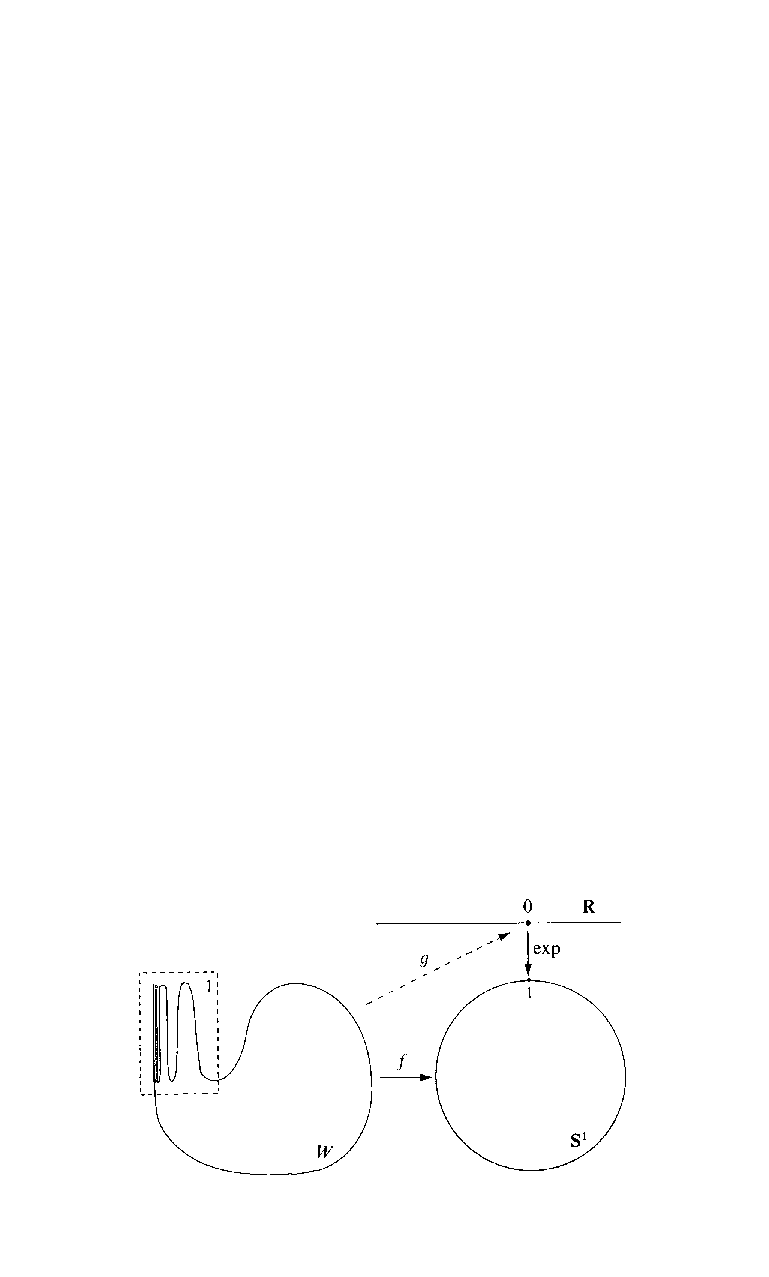
\includegraphics[width=0.7\textwidth]{figures/discont_lift.pdf}
    \caption{The map $f$ here collapses the entire ``$\sin 1/x$'' part of the space on the left into the basepoint $1$ on the circle. If a lifting map $g$ into the real line existed, then the vertical part of the ``$\sin 1/x$'' curve would have to be mapped to $0$, whereas the wiggly part would map to $1$ under $g$, making it discontinuous. From \cite[Fig.~III-6]{Bredon}.}
    \label{fig:discont_lift}
\end{figure}

\begin{thm}[Lifting Theorem]\index{Theorem!Lifting}\label{Lifting Theorem}
    Let $\pi:E\to M$ be a covering map with $\pi (p_0)=x_0$. Assume that $W$ is path-connected and locally path-connected and that $f:W\to M$ is a map with $f(w_0)=x_0$. Then a pointed map $\wt f:(W,w_0)\to (M,x_0)$ such that $\pi\circ\wt{f}=f$ exists iff $f_\ast (\pi_1(W,w_0))\subset \pi_\ast (\pi_1(E,p_0))$. Moreover, $\wt f$ is unique.
\end{thm}
\begin{proof}
    Let us construct $\wt f$ explicitly. Given $w\in W$, let $\lambda:I\to W$ be a path from $w_0$ to $w$. Then $f\circ \lambda$ is a path in $M$. Lift this to a path $\wt\lambda:(I,0)\to (E,x_0)$ and let $\wt{f}(w)=\wt{\lambda}(1)$. Then $\pi\circ \wt{f}(w)=\pi(\wt{\lambda}(1))=f(\lambda(1))=f(w)$.

    To see that $\wt{f}$ is well defined, suppose $\lambda'$ is another path in $W$ from $w_0$ to $w$ and let $\eta=(\lambda ')^{-1}$ be the reverse path from $w$ to $w_0$. Then $\lambda\bullet \eta$ is a loop based at $w_0$, and $(f\circ \lambda)\bullet (f\circ\eta)$ is a loop in $M$ based at $x_0$. Since 
    \[[f\circ\lambda \bullet f\circ\eta]=f_\ast([\lambda\bullet\eta]\in \im(f_\ast)\subset \im(\pi_\ast),\]
    $f\circ\lambda\bullet f\circ\eta$ lifts to a loop in $E$ based at $p_0$. The reverse of the portion of this lifting corresponding to $\eta$ then is a lifting $\wt{\lambda}'$ of $\lambda '$ and $\wt{\lambda}'(1)=\wt{\lambda}(1)$, as required.

    Next, we have to show that $\wt{f}$ is continuous. Let $w\in W$  and put $x=f(w)$. Let $U\subset <$ be an elementary neighborhood of $x$, and by local path-connectedness of $W$ we can let $V$ be a path-connected neighborhood of $w$ such that $f(V)\subset U$. For any point $w'\in V$ we can construct a path from $w_0$ to $w'$ by concatenating a given path $\lambda$ to $w$ with a path $\sigma$ in $V$ from $w$ to $w'$. Since $f(V)$ is contained in an elementary set, the lifting of $f\circ \sigma$ is simply $f\circ\sigma$ composed with the local inverse of $\pi$ that takes $U$ to the component of $\pi^{-1}(U)$ that contains $\wt{f}(w)$. This same component is used for all $w'\in V$ and it follows that $\wt{f}$ is continuous at $w$.

    The converse direction of the theorem follows immediately from $f_\ast=\pi_\ast\circ \wt{f}_\ast$.
\end{proof}
\begin{rem}
    Unlike in the homotopy lifting property (Theorem~\ref{homotopy lifting property}), the condition of local path connectedness for $W$ cannot be dropped here. See an example in Figure~\ref{fig:discont_lift}.
\end{rem}

\begin{cor}[{{\cite[Cor.~4.2]{Bredon}}}]\label{cor 4.2 Bredon}
    Under the conditions of the Lifting Theorem~\ref{Lifting Theorem}, if $W$ is also simply connected, then the lifting $\wt{f}$ always exists and is unique given a basepoint $p_0\in E$.
\end{cor}

\begin{cor}\label{cor homotopy groups of coverings}
    Given a covering space $E\overset{\pi}{\to}M$, there is a natural isomorphism of higher homotopy groups
    \[\pi_n(E,p_0)\cong \pi_n(M,x_0),\; n\geq 2.\]
\end{cor}
\begin{proof}
    Injectivity follows from the uniqueness of the liftings of maps $\bbS^n\to M$ into $E$. Surjectivity follows from the Lifting Theorem~\ref{Lifting Theorem} combined with the fact that $\pi_1(\bbS^n)$ is trivial for $n\geq 2$ (Corollary~\ref{cor pi_1(S^n)=0}).
\end{proof}

\begin{cor}\label{cor: homotopy groups of circle}
    $\pi_n(\bbS^1)=1$ for $n>1$.
\end{cor}
\begin{proof}
    Any map $f:\bbS^n\to \bbS^1$ lifts to $\wt{f}:\bbS^n\to \bbR $ by Corollary~\ref{cor 4.2 Bredon}. But $\wt f$ is homotopically trivial since $\bbR $ is contractible, so $f=\pi\circ\wt{f}$ is also homotopically trivial.
\end{proof}


\subsection{Morphisms of covering spaces}


\begin{defn}[Category of covering spaces]
The category $\mathsf{Cov}_M$ of covering spaces of a given base $M$ (say, topological covering spaces) consists of all covering spaces of $M$. The morphisms between two covering spaces $\pi$ and $\pi'$ are morphisms $f:E\to E'$ that ``map fibers to fibers'', i.e.\ $\pi'\circ f=\pi$, or equivalently if the following triangle commutes:
\[
\begin{tikzcd}[every matrix/.append style={name=m},   
execute at end picture={\draw [<-] ([xshift=0mm,yshift=-2mm]m-2-2.north) arc[start angle=-90,delta angle=-270,radius=0.25cm];}]
   E \arrow[rr,"f"]\arrow[ddr,swap,"\pi"]& & E'\arrow[ddl,"\pi'"]\\
   & \, & \\
   & M & \\
\end{tikzcd}
\]
\end{defn}


\begin{lem}[{{\cite[Lem.~4.4]{Bredon}}}]\label{lem 4.4 Bredon}
    Let $W$ be connected and $E$ be Hausdorff. Let $\pi:E\to M$ be a covering map and $f:W\to M$ a map. Let $\wt{f}_1,\wt{f}_2$ be two liftings of $f$ into $E$. If $\wt{f}_1(w)=\wt{f}_2(w)$ for some point $w\in W$, then $\wt{f}_1\equiv \wt{f}_2$.
\end{lem}
\begin{proof}
    Let $\wt{f}_1(w)=\wt{f}_2(w)=p$. Let $U$ be an elementary open neighborhood of $f(w)$ in $M$. Let $V$ be the component of $\pi^{-1}(U)$ containing $p$. Then $A=\wt{f}_1^{-1}(V)\cap\wt{f}_2^{-1}(V) $ is an open set in $W$ and for $a\in A$ we have $\wt{f}_1(a)=\wt{f}_2(a)$ since the homeomorphism $\pi:V\to U$ maps them both to $f(a)$. This shows that the set $\{w\in W\mid \wt{f}_1(w)=\wt{f}_2(w)\}$ is open. But this set is also closed since it is the inverse image of the diagonal under the map $\wt{f}_1\times \wt{f}_2:W\to E\times E$, and the diagonal is closed since $E$ is Hausdorff. Since $W$ is connected, this set is either empty or all of $W$.
\end{proof}
\begin{cor}[{{\cite[Cor.~4.5]{Bredon}}}]\label{cor 4.5 Bredon}
    Let $\pi_i:E_i\to M$, $i=1,2$, be covering maps such that $E_1$ is simply connected, and let $p_i\in E_i$ be such that $\pi_1(p_1)=\pi_2(p_2)$. Then there is a unique morphism of covering spaces $f:E_1\to E_2$ such that $f(p_1)=p_2$. Moreover, $f$ is a covering map.
\end{cor}
\begin{proof}
    By the Lifting Theorem~\ref{Lifting Theorem}, since $\pi_1(E_1,p_1)=1$, there is a lifting of $\pi_1\to E_1\to M$ to a map $f:E^1\to E^2$ such that $\pi_2\circ f=\pi_1$. It is unique by Lemma~\ref{lem 4.4 Bredon}.  It is an easy exercise to show that $f$ is a covering map.
\end{proof}
\begin{cor}[{{\cite[Cor.~4.6]{Bredon}}}]\label{cor 4.6 Bredon}
    If in Corollary~\ref{cor 4.5 Bredon} both $E_1$ and $E_2$ are simply connected, then the unique map $f$ is a homeomorphism.
\end{cor}
\begin{proof}
    By Corollary~\ref{cor 4.5 Bredon}, in addition to $f$ there is also an analogous map $k:E_2\to E_1$. Then $k\circ f:E_1\to E_1$ covers the identity map at $p_1$. By Lemma~\ref{lem 4.4 Bredon}, it must equal the identity everywhere. Similarly $g\circ k=\mathrm{id}_{E_2}$, hence $k=f^{-1}$.
\end{proof}

This implies that all simply connected covering spaces of a given base space $M$ are isomorphic in the category $\mathsf{Cov}_{\bullet M}$. Such covering spaces are called universal, and are guaranteed to exist under a mild restriction.

\begin{defn}[Locally relatively simply connected space]
    A space $X$ is locally relatively simply connected (or semilocally simply connected) if each point has a neighborhood $U$ such that all loops inside of $U$ are homotopically trivial in $X$ (i.e.\ for any $u\in U$ the homomorphism $\pi_1(U,u)\to \pi_1(X,u)$ is trivial).
\end{defn}


One can show that the existence of a simply connected covering space is equivalent to $M$ being locally relatively simply connected (see~\cite[Theorem~8.4]{Bredon}). Since we are mostly interested in manifolds, we will only prove the existence. Let us only work with connected, locally simply connected spaces (in particular, connected manifolds).

\begin{thm}[Universal cover]\index{Universal cover}
For a given base $M$ that is a connected and \emph{locally relatively simply connected} Hausdorff space, there is a unique (up to homeomorphism) topological covering space $E\overset{\pi}{\to}M$ whose total space $E$ is simply connected. This covering space is denoted by $\wt M$ and is called the \emph{universal cover} of $M$.\index{Universal cover}
\end{thm}
\begin{proof}
See \cite[Thm 11.43]{LeeTop} or \cite[Thm 8.4]{Bredon}. The basic idea is to explicitly construct $\wt M$ as the space of endpoints of all possible paths in $M$ based at a fixed point $m\in M$. Two paths are equivalent if their endpoints coincide and they are homotopic with fixed endpoints. The topology on this set of paths is introduced by considering sets of homotopic paths with endpoints belonging to an open set in $M$ (and the homotopies fix the starting point but can move the endpoint within the open set, see figure). The projection $\pi$ maps a path to its endpoint. It is not difficult to check that this is indeed a topological covering map and the total space is simply connected. Uniqueness will follow from the universal property described below.

\begin{center}
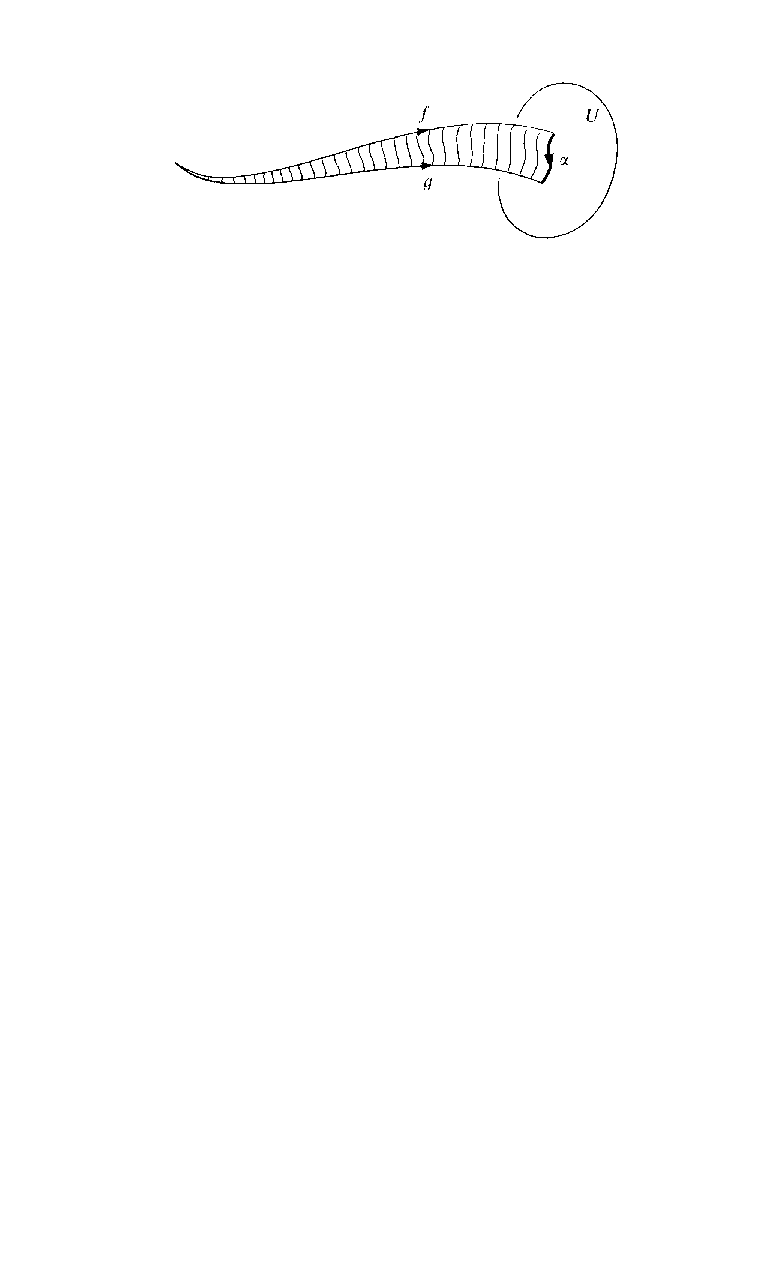
\includegraphics[width=0.5\textwidth]{figures/uni_open_set.pdf}
\end{center}
\end{proof}
\begin{rem}
    By examining the details of the proof one can notice that local simply-connectedness is not actually required, and semilocal simply-connectedness is sufficient. The converse direction is clear: if a loop is in an evenly covered subspace of $M$ then it lifts to $E$, and if $E$ is simply connected, the loop must be trivial in $E$. But then the composition of its homotopy to a constant loop with the covering map $\pi$ shows that the original loop in $M$ must be trivial. Thus we have shown that a connected and locally path-connected $M$ has a universal covering space iff it is locally relatively simply connected.
\end{rem}
\begin{example}
    The Hawaiian earring (Example~\ref{hawaiian earring}), as well as the infinite-dimensional torus $\bbT^\infty=\prod_{i=1}^\infty \bbS^1$, are not locally relatively simply connected, and thus don't have universal coverings.
\end{example}

\begin{thm}
Let $E\overset{\pi}{\to}M$ be a topological covering map and fix a smooth structure on $M$. Then $E$ is a topological manifold that supports a unique smooth structure such that $\pi$ is a smooth covering map with $\pi^{-1}(\partial M)=\partial E$.
\end{thm}
\begin{proof}
See \cite[Prop 4.40]{Lee}.
\end{proof}
This theorem essentially means that in order to classify smooth covering spaces above a smooth base manifold, it suffices to only classify the topological covering spaces, and they are in one-to-one correspondence with the smooth ones. In other words, the theory of covering spaces is an intrinsically topological theory that doesn't gain or lose anything from imposing smooth structures.

\begin{cor}
For a connected smooth manifold $M$, there exists a unique simply connected smooth covering space called the universal covering manifold of $M$.
\end{cor}
From now on we won't really distinguish between smooth and topological covering spaces, although we only care about the smooth case.

Corollaries~\ref{cor 4.5 Bredon} and \ref{cor 4.6 Bredon} can now be restated in terms of morphisms:
\begin{cor}[Universality of the universal cover]\index{Universal property!of universal covers}
    \;
    \begin{enumerate}
       \item Any morphism of covering spaces is itself a covering map;
        \item If $M$ is a topological manifold (or any space that has a universal covering space), then $\wt{M}$ is the initial object in the category $\mathsf{Cov}_{\bullet M}$ of pointed covering spaces of $M$ (i.e.\ objects are $E\overset\pi\to M$ with a basepoint $p_0\in E$ and morphisms must respect the basepoints).
    \end{enumerate}
\end{cor}

In the category of non-pointed covering spaces, the universal cover is not an initial object, but the arrows coming out of it are unique up to automorphisms of the two covering spaces at the ends of the arrow. We now describe the sets of such automorphisms.

\subsection{Deck transformations}

\begin{defn}[Group action]
    An (right/left) action of a group $G$ on a set (or a space, a manifold) $X$ is a map $\Phi: G\times X\to X$, with its partial maps denoted by $\Phi_g=\Phi (g,\_):X\to X$ and $\Phi_x=\Phi(\_,x):G\to X$, such that $\Phi_e=\mathrm{id}_X$ and one of the following:
    \[
        \text{left action}:\quad \Phi_g\circ \Phi_h=\Phi_{gh},\]
        \[\text{right action}: \quad \;\; \Phi_g\circ \Phi_h=\Phi_{hg}.
    \]
    In other words, right actions are the same thing as left actions on the opposite group $G^{\mathrm{op}}$. For this reason right actions are usually written as $x\cdot g=\Phi_g(x)$ and left actions as $g\cdot x=\Phi_g(x)$. The sets $G(x)=\Phi_x(G)$ are called \emph{orbits}.
\end{defn}
In the topological and smooth categories one usually considers continuous or smooth group actions, provided $G$ is a Lie group, but we will delay that discussion until \S\ref{sec: Lie group actions}. For now $G$ will always be a discrete group (i.e.\ a group with discrete topology), so any condition of continuity or smoothness on the action is simply a condition on each $\Phi_g$ individually.

\begin{defn}[$G$-equivariant maps]\index{Equivariant maps}\index{$G$-Set}
    The category of sets (spaces, manifolds) carrying a (left) action of $G$ is called $G\mathsf{-Set}$. Morphisms in this category are maps $f:X\to Y$ such that for all $g\in G$, $f(g\cdot x)=g\cdot f(x)$. These maps are called $G$-equivariant. Similarly, $G\mathsf{-Set}_\bullet$ consists of pointed sets with equivariant maps that respect basepoints. 
\end{defn}
\begin{defn}[Stabilizer]\index{Stabilizer}
    Given a group $G$ acting on a set $X$, and a point $x\in X$, the stabilizer of $x$ is defined as the subgroup $G_x=\{g\in G\mid \Phi(g,x)=x\}$.
\end{defn}
\begin{defn}[Transitive action]
    An action $\Phi$ is called transitive if it has only one orbit, i.e.\ for each pair $x,y\in X$ there is an $g\in G$ such that $\Phi(g,x)=y$.
\end{defn}
\begin{defn}[Simply transitive action]
    An action $\Phi$ is called simply transitive if for each pair $x,y\in X$ there is a \emph{unique} element $g\in G$ such that $\Phi(g,x)=y$.
\end{defn}
\begin{defn}[Faithful action]
    An action $\Phi$ is called faithful if no nontrivial elements of $G$ act trivially: $\Phi_g=\mathrm{id}_X \Leftrightarrow g=e$.
\end{defn}
\begin{defn}[Free action]
    An action $\Phi$ is called free if no nontrivial elements of $G$ have any fixed points: $\exists\,x\in X: \Phi(g,x)=x\Leftrightarrow g=e$. 
\end{defn}
\begin{prop}
    An action is simply transitive iff it is free and transitive.
\end{prop}
\begin{proof}
    Assume a left action for simplicity. For the necessary condition, we only need to show freeness. If $\Phi_g=\mathrm{id}_X$, then $g\cdot x=x=e\cdot x$, therefore by simple transitivity $g=e$.

    For the converse, assume there are two elements such that $g_1\cdot x=g_2\cdot x=y$. Then $g_2^{-1}g_1\cdot x=x$, which means $g_2^{-1}g_1=e$ by freeness.
\end{proof}

Throughout this section let $E\overset{\pi}{\to}M$ be a covering space with a fixed point $x_0\in M$. For simplicity we also denote
\[G=\pi_1(M,x_0),\quad \quad F=\pi^{-1}(x_0).\]
The discrete set $F$ is called the \emph{fiber} of $\pi$ over $x_0$. We are going to describe an action of the group $G$ on $F$ as a group of permutations. 

Let $p\in F$ and let $g\in G$ be an element represented by a loop $\gamma :I\to M$. Lift it to get a map $\wt{\gamma}$ in $E$ with $\wt{\gamma}(0)=p$. Then define
\[\Phi(g,p)=p\cdot g =\tilde{\gamma}(1) \in F.\]
By Corollary~\ref{cor 3.5 Bredon} this does not depend on the choice of $\gamma$ and thus is a well-defined map $\Phi:F\times G\to F$. Now we can check some properties of this function:
\begin{enumerate}
    \item $x\cdot e=x$.
    \item $(x\cdot g)\cdot h=x\cdot (gh)$, i.e.\ it is a right action (because the product of two loops $gh$ corresponds to the application of $\Phi_g$ and then $\Phi_h$).
    \item $E$ is connected iff this action is transitive (i.e.\ there is only one orbit, $p\cdot G=F$). To see this, pick a path in $E$ from $p_0$ to another $p\in F$. This projects onto a loop $\gamma$ in $M$ and $g=[\gamma]$ provides the required element: $p_0\cdot p=p$. Conversely, if $E$ is not connected, the action is obviously not transitive.
    \item The stabilizer of a point is $G_{p_0}=\{g\in G\mid p_0\cdot g=p_0\}$. Then 
    \[
        \boxed{G_{p_0}=\im \pi_\ast=\pi_\ast(\pi_1(E,p_0))}\label{stabilizer}
    \]
    where $\pi_\ast:\pi_1(E,p_0)\to \pi_1(M,x_0)=G$ is the homomorphism induced by $\pi$. This is true because $g\in G_{x_0}$ iff $g=[\gamma]$ and $\gamma$ lifts to a loop at $p_0$, i.e.\ iff $g\in \im p_\ast$.
    \item Assuming $E$ is connected, the map $\phi: \ _{G_{p_0}}\bslash^{G}\to F$ taking the right coset $G_{x_0}g$ to $p_0\cdot (G_{p_0}g)=p_0\cdot g$ is a bijection.
\end{enumerate}
Obviously any covering space decomposes into a disjoint union of connected components, and the action of $\pi_1(M)$ is transitive on the fiber of each component separately. In what follows, we generally assume that $E$ is connected. In summary, we have the following theorem.
\begin{thm}
    Given a connected covering space $\pi:E\to M$, there is a one-to-one correspondence between the set $_{\pi_\ast(\pi_1(E,p_0))}\bslash^{\pi_1(M,x_0)}$ of right cosets, and the fiber $\pi^{-1}(x_0)$. (Note that $\pi_\ast(\pi_1(E,p_0))\cong \pi_1(E,p_0)$ since $\pi_\ast$ is a monomorphism by Corollary~\ref{cor 3.7 Bredon}.)
\end{thm}
\begin{cor}
    The number of sheets of a connected covering space equals the index (number of left or right cosets) of $G_{p_0}=\pi_\ast(\pi_1(E,p_0))$ in $G=\pi_1(M,x_0)$.
\end{cor}
\begin{cor}
    If $\wt\pi:\wt M\to M$ is a universal covering map (i.e.\ $\wt M$ is simply connected), then the number of sheets equals the order (cardinality) of the group $\pi_1(M,p_0)$.
\end{cor}

\begin{example}[Fundamental groups of real projective spaces]
    Since $\bbS^n$ is simply connected for $n>1$ and $\bbS^n$ is a double covering of the real projective space $\RP^n$, it follows that $\pi_1(\RP^n)\cong \bbZ_2$.
\end{example}

\begin{defn}[Deck transformations]\index{Deck transformations}
    For a covering space $E\overset{\pi}{\to}{M}$, consider the group $\Aut(\pi)$ of automorphisms of this covering space in the category $\mathsf{Cov}_M$ (also called \emph{deck transformations}). Its elements are homeomorphisms of $E$ that cover the identity map on $M$. For a given elementary open set $U\subset M$, they permute the connected components $U_i$ of the pre-image $\pi^{-1}(U)$. In other words, the group $\mathrm{Aut}(\pi)$ acts on $E$ via morphisms of covering spaces.
\end{defn}

\begin{prop}[{{\cite[Prop.~6.2]{Bredon}}}]\label{prop 6.2 Bredon}
    If $a\in \Aut(\pi)$ and $g\in\pi_1(M,p_0)$ and $x\in \pi^{-1}(x_0)$ then $a(x)\cdot g=a(x\cdot g)$. In other words, deck transformations are equivariant with respect to the action of $\pi_1(M,x_0)$.
\end{prop}
\begin{proof}
    Let $\gamma$ be a loop at $x_0$ representing $g$ and lift it to a path $\wt\gamma$ starting at $p$. Then $\wt\gamma(1)=p\cdot g$ by definition. Look at the path $a\circ \wt{\gamma}$. It is a lifting of $\gamma$ and starts at $a(p)$. Thus is ends at $a(p)\cdot g$ by definition of the latter. But it also ends at $a(\wt\gamma(1))$, which is $a(p\cdot g)$.
\end{proof}

This proof actually shows that not only automorphisms are $G$-equivariant, but all morphisms in the category $\mathsf{Cov}_M$ are. This means that the action of $\pi_1(M)$ that we've constructed is \emph{natural}. These results can be summarized by the following theorem.
\begin{thm}[Monodromy Action]\index{Monodromy (covering spaces)}
For any covering space $E\overset{\pi}\to M$, 
\begin{enumerate}
    \item there is a natural homomorphism $\pi_1(M)\to \Aut(\pi)$ called the \emph{monodromy action};
    \item $\Aut(\wt \pi)\cong\pi_1(M)$, where $\wt\pi$ is the universal cover.
\end{enumerate}
\end{thm}

\begin{defn}[Normalizer]\index{Normalizer of a subgroup}
For a subset (not necessarily a subgroup) $H\subset G$ of a group $G$, its normalizer is 
\[\rmN_G(H)=\{n\in G\mid nH=Hn\}.\]
A subgroup $H$ is normal in $G$ iff $\rmN_G(H)=G$. Otherwise, $\rmN_G(H)$ is the largest subgroup of $G$ such that $H$ is a normal subgroup of $\rmN_G(H)$.
\end{defn}
\begin{rem}
    If $H$ is a subgroup, then $H\subset \rmN_H(H)$. Moreover, $\rmN_G(g^{-1}Hg)=g^{-1}\rmN_G(H)g$, so the normalizers of conjugate subsets are conjugate.
\end{rem}

The following lemma is the analog of the ``change of coordinates'' formulas in linear algebra: mapping the coordinates of vectors to a new basis is equivalent to conjugating the matrices representing linear operators.
\begin{lem} For any group $G$ acting on a set $X$ from the right,
\[\boxed{G_{p_0\cdot g}=g^{-1}G_{p_0}g.}\label{conjugate stabilizers}\]
Similarly, for left actions, $G_{g\cdot p_0}=gG_{p_0}g^{-1}$.
\end{lem}
\begin{proof}
    \[
        G_{p_0\cdot g}=\{h\mid (p_0\cdot g)\cdot h=p_0\cdot g\}=\{h\mid p_0\cdot ghg^{-1}=p_0\}=\{h\mid ghg^{-1}\in G_{p_0}\},
    \]
\end{proof}

The most important question in the study of deck transformations is: given two points in the fiber, when does there exist a deck transformation mapping one to the other? This is answered in the following theorem.
\begin{thm}[{{\cite[Thm.~6.3]{Bredon}}}]\label{thm 6.3 Bredon}
    Provided $E$ is connected, let $p,p_0\in F=\pi^{-1}(x_0)$, $G=\pi_1(M,x_0)$ and $G_{q}=\pi_\ast(\pi_1(E,q))$ for any $q\in E$. Then \gls{tfae}:
    \begin{enumerate}[label=(\arabic*)]
        \item $\exists\, a\in \mathrm{Aut}(\pi)$ such that $a(p_0)=p$.
        \item $\exists\, g\in \rmN_G(G_{p_0})$ such that $p_0\cdot g=p$.
        \item $G_{p_0}=G_p$.
    \end{enumerate}
\end{thm}
\begin{proof}
    Recall that $G_{p_0}=\pi_\ast(\pi_1(E,p_0))$ and $G_{p}=\pi_\ast(\pi_1(E,p))$. By the Lifting Theorem~\ref{Lifting Theorem} a map $a$ covering the identity and taking $p_0$ to $p$ exists iff $\pi_\ast(\pi_1(E,p_0))\subset \pi_\ast(\pi_1(E,p))$. Similarly, a map $a'$ covering the identity and mapping $p$ to $p_0$ exists iff the opposite inclusion holds. If both exist then $a\circ a'$ covers the identity and has a point in common with the identity, therefore $a\circ a'=\mathrm{id}_E$ by Lemma~\ref{lem 4.4 Bredon}. This proves the equivalence $(1)\Leftrightarrow (3)$.

    Now we can prove $(2)\Rightarrow(3)$: if $p=p_0\cdot g$ and $g\in \rmN_G(G_{p_0})$ then $G_p=G_{p_0\cdot g}=g^{-1}G_{p_0}g=G_{p_0}$ as claimed.

    For $(3)\Rightarrow (2)$, suppose $G_{p_0}=G_p$ and $p=p_0\cdot g$ (such a $g$ exists since $G$ acts transitively on $F$). Then $G_{p_0}=G_p=G_{p_0\cdot g}=g^{-1}G_{p_0}g$, so $g\in \rmN_G(G_{p_0})$.
\end{proof}
From $(2)\Leftrightarrow(1)$ and the last part of the proof we have the following Corollary.
\begin{cor}[{{\cite[Cor.~6.4]{Bredon}}}]\label{cor 6.4 Bredon}
    For a connected covering space, the subgroup $G_{p_0}=\pi_\ast(\pi_1(E,p_0))$ is normal in $G=\pi_1(M,x_0)$ iff the action of $\mathrm{Aut}(\pi)$ is (simply) transitive on $F=\pi^{-1}(x_0)$.
\end{cor}
\begin{cor}[{{\cite[Cor.~6.5]{Bredon}}}]\label{cor 6.5 Bredon}
    In a connected covering space, if $p$ ranges over the fiber $F$ then $G_p$ ranges over all conjugates of $G_{p_0}=\pi_\ast(\pi_1(E,p_0))$.
\end{cor}
\begin{proof}
    This is a consequence of (\ref{conjugate stabilizers}).
\end{proof}

\begin{rem}
    It is worth providing some intuition for normalizers. If two points in a $G$-set belong to the same orbit, i.e.\ they can be mapped into each other by some elements of $G$, then their stabilizers are obviously conjugate subgroups of $G$.

    By definition, conjugation doesn't change a normal subgroup (as a set, not pointwise). Therefore if a stabilizer of a point is normal, then all other points in that orbit have the same exact stabilizer. In particular, this means that the only elements of the group which actually move the points in the orbit are the cosets of the normal stabilizer. Moreover, if you have two group elements from the same coset of this normal stabilizer, then they act on the orbit \emph{in the exact same manner}.
\end{rem}

\begin{defn}[Regular covering map]
    A covering map $\pi$ is called regular if $\mathrm{Aut}(\pi)$ is transitive on the fiber. In the case of a connected total space this is equivalent to $G_{p_0}=\pi_\ast(\pi_1(E,p_0))$ being normal in $\pi_1(M,x_0)$.
\end{defn}

In other words, normal subgroups of $\pi_1(M,x_0)$ correspond to regular connected covering spaces of $M$. A regular covering space is one whose fundamental group ``looks the same'' in terms of the generators of $\pi_1(M,x_0)$ regardless of the choice of the basepoint $p_0$ in the fiber. Such covering spaces have an inherent ``symmetry'' given by the quotient group $G/G_{p_0}$ (which exists because $G_{p_0}$ is normal). Obviously any covering space that is not connected can't be regular. For an example of a connected non-regular covering space, see Figure~\ref{fig:threefold-cover}.

\begin{figure}
    \centering
    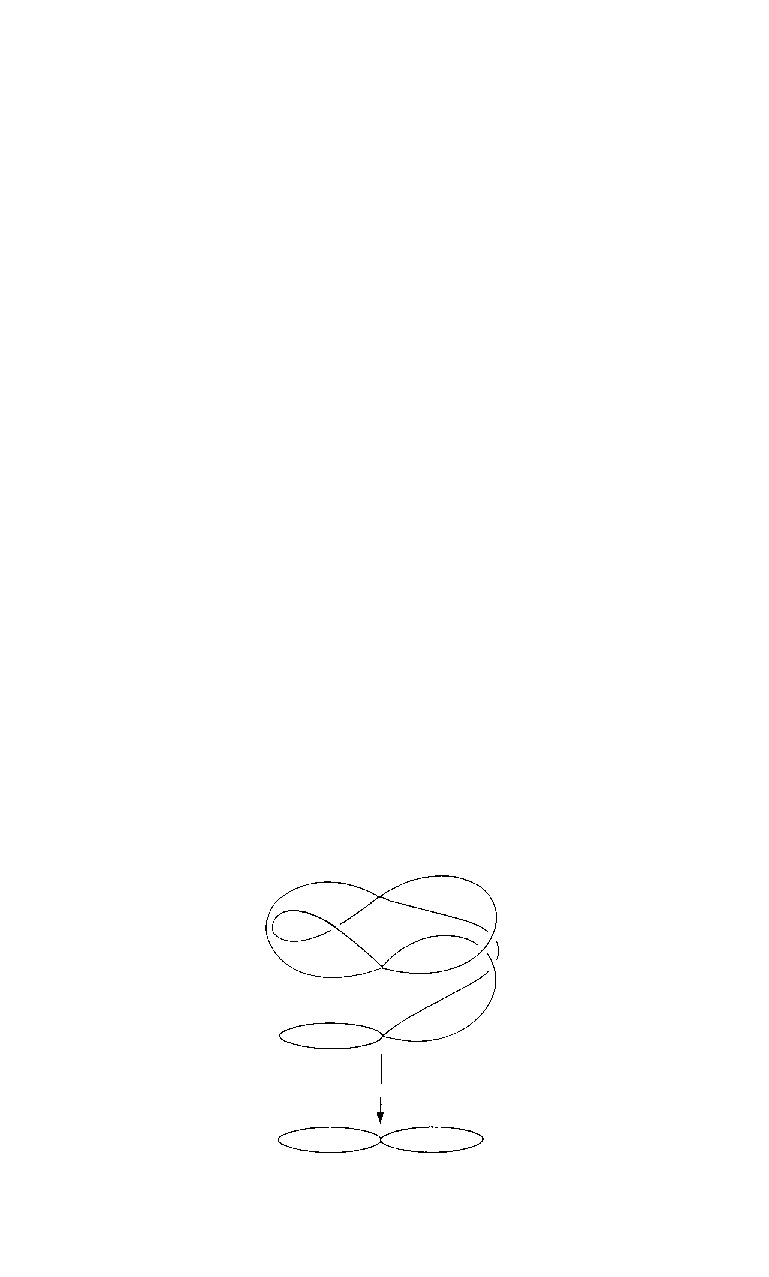
\includegraphics[width=0.4\textwidth]{figures/threefold_cover.pdf}
    \caption{This threefold cover of the figure eight space is not regular. Indeed, its group of automorphisms is trivial.}
    \label{fig:threefold-cover}
\end{figure}

\begin{rem}
    These ideas comprise the powerful \emph{Reidemeister-Schreier method} for finding presentations of subgroups $H\leq G$ given a presentation of $G$. Namely, one constructs a base space whose fundamental group is $G$, then finds a covering space corresponding to $H$ and computes its fundamental group.
\end{rem}

\begin{defn}
    Define the map $\Theta:\rmN_G(G_{p_0})\to \mathrm{Aut}(\pi)$ by $\Theta(g)=a_g$ where $a_g$ is the unique deck transformation such that $a_g(p_0)=p_0\cdot g$.
\end{defn}
\begin{thm}[Classification of Deck Transformations {{\cite[Thm.~6.8]{Bredon}}}]\label{thm 6.8 Bredon}
    $\ker \Theta=G_{p_0}$, and consequently
    \[\mathrm{Aut}(\pi)\cong \rmN_G(G_{p_0})\slash G_{p_0}.\]
\end{thm}
\begin{proof}
    First, 
    \[a_h(a_g(p_0))=a_h(p_0\cdot g)=a_h(p_0)\cdot g=(p_0\cdot h)\cdot g=p_0\cdot (hg)=a_{hg}(p_0).\]
    This proves that $\Theta$ is a homomorphism. Next note that if $a\in \mathrm{Aut}(\pi)$ then there is an $g\in \rmN_G(G_{p_0})$ such that $a(p_0)=p_0\cdot g=a_g(p_0)$. Therefore $a=a_g$, which shows the surjectivity of $\Theta$.

    Finally we compute the kernel of $\Theta$. The result follows from the chain of equivalences
    \[a_g=\mathrm{id}_E \Leftrightarrow p_0\cdot g=p_0\Leftrightarrow g\in G_{p_0}.\]
\end{proof}
\begin{cor}
    If the covering map $E\overset{\pi}{\to} M$ is regular, then 
    \[\mathrm{Aut}(\pi)\cong G/G_{p_0}\]
\end{cor}
\begin{cor}
    If $\wt{M}\overset{\wt\pi}{\to} M$ is a universal covering map then
    \[\mathrm{Aut}(\wt\pi)\cong G=\pi_1(M,x_0).\]
\end{cor}





\subsection{Classification of covering spaces}

Our examination of connected covering spaces allows us to easily prove the following classification of connected covering spaces in terms of subgroups of the fundamental group of the base.

\begin{thm}[Classification of coverings I]
    Let $M$ be path-connected and semilocally simply connected so that it has a universal covering space $\wt{M}$. Then the following \emph{Galois correspondence} holds:
\begin{enumerate}
	\item The isomorphism classes of connected pointed covering spaces of $M$ are in one-to-one correspondence with subgroups of $G=\pi_1(M, x_0)$. 
	\item The isomorphism classes of connected covering spaces of $M$ without basepoints are in one-to-one correspondence with the conjugacy classes of subgroups of $G=\pi_1(M, x_0)$.
    % sets $F$ (finite or countable) with an action of the group $\pi_1(M)$ (a group action on $F$ is an element of $\Hom(\pi_1(M),G)$, where $G$ is the full permutation group of the points of $F$).
\end{enumerate}
The correspondence is given by $E\leftrightarrow \pi_\ast(\pi_1(E,p_0))=G_{p_0}$ where $\pi$ is the covering map.
\end{thm}
\begin{proof}
    The second statement follows from the first combined with Corollary~\ref{cor 6.5 Bredon}. It remains to show that the map taking a covering map with a basepoint, $\pi:(E,p_0)\to (M,x_0)$, into the subgroup $\pi_\ast(\pi_1(E,p_0))$ of $\pi_1(M,x_0)$ is a bijection. It is an injection by the Lifting Theorem~\ref{Lifting Theorem}. 
    
    To see that it is a surjection, suppose that $H\subset \pi_1(M,x_0)=G$ is a subgroup. Since $\wt{M}$ is simply connected, Theorem~\ref{thm 6.8 Bredon} gives the isomorphism $\Theta:G\to \mathrm{Aut}(\pi)$, where $\Theta(g)=a_g$. Under this map, $H$ is mapped to a subgroup $A_H\leq \mathrm{Aut}(\pi)$. Put $E=\wt{M}/A_H$ which projects to $M$ canonically. Let $p_0$ be the image of the basepoint $\wt{p}_0\in\wt{M}$. We wish to identify $\pi_\ast(\pi_1(E,p_0))$. Let $\gamma$ be a loop in $X$ at $p_0$. Lifting this to $\wt{M}$ at $\wt{p}_0$ gives the same path as a lifting of the projection of $\gamma$ to a loop at $x_0$ in $M$. Thus the lifting ends at $a_g(\wt{p}_0)$, where $g\in\pi_1(M,x_0)$ is the homotopy class of the projection of $\gamma$ to $M$. But for $\gamma$ to be a loop in $E=\wt{M}/A_H$, we must have that $\wt{p}_0$ and $a_g(\wt{p}_0)$ are in the same orbit of $A_H$. This is true iff $a_g\in A_H$, and this holds iff $g\in H$. But $g$ is an arbitrary element of $\pi_\ast(\pi_1(E,p_0))$. Thus $H=\pi_\ast(\pi_1(E,p_0))$.
\end{proof}


Now we restate the classification theorem as it was described in Example~\ref{covering category thm}. We consider all, not only connected, coverings. 

Given an action of a group $G$ on a space $X$, the space $X$ decomposes into a disjoint union of orbits of $G$. Let us assume a discrete topology on $G$, in which case a continuous/smooth action is simply one for which the maps $\Phi_g:X\to X$ are continuous/smooth for all $g$. The set of all orbits is denoted by $X\slash G$ and, if imbued with the quotient topology descended from $X$, is called the \emph{orbit space}. Note that the canonical projection $p:X\to X\slash G$ that takes a point to its orbit is open because for an open $U\subset X$, $p^{-1}(p(U))=\bigcup_g (g\cdot U)$, which is a union of open sets.

Every covering map of $M$ gives rise to an action of $G=\pi_1(M,x_0)$ on the fiber $F=F_{x_0}$. Under this action $F$ decomposes into a disjoint union of orbits $F_j$, each of them associated with a conjugacy class of stabilizer subgroups $H_j<G$. This determines a functor from the category $\mathsf{Cov}_M$ of coverings of $M$ to the category $G\mathsf{-Set}$ of sets with a (left) action of $G=\pi_1(M,x_0)$. If $F$ is a $G$-set with a transitive action of $G$, then the stabilizers of any two of its points are conjugate subgroups of $G$. Choosing $p_0\in F$ and denoting $H=G_{p_0}$, we have that $F$ is isomorphic to the set of cosets $G\slash H$, also called a \emph{homogeneous set}. From such a $G$-set $F$ we can easily reconstruct a connected covering space $\pi$ by taking the universal covering space $\wt{M}$ and letting $\pi:\wt{M}\to \wt{M}\slash H$ be the orbit map of the action of $H$ on $\wt{M}$. If $F$ is not homogeneous, then it is a disjoint union of homogeneous sets (orbits), and the corresponding covering space is a disjoint union of the corresponding connected ones. This provides a functor in the opposite direction. It is easy to check that these two functors are each other's quasi-inverses. We thus have the second version of the theorem.

\begin{thm}[Classification of coverings II {{\cite[Thm.~3.3.2]{tomDieck}}}]\label{covering spaces category equivalence thm}
    If $M$ admits a universal covering space, then the category $\mathsf{Cov}_M$ is equivalent to the category $\pi_1(M)\mathsf{-Set}$. The corresponding functor returns the action of $\pi_1(M)$ on the fiber of the covering space and restricts morphisms to the fiber. Its quasi-inverse reconstructs a connected component of a covering space from each orbit of the $\pi_1(M)$-set as the quotient of the universal covering by the action of the stabilizer subgroup. Similarly, $\mathsf{Cov}_{M\bullet}$ is equivalent to $\pi_1(M)\mathsf{-Set}_\bullet$.
\end{thm}

\begin{rem}
    An action of a group $G$ on a set $X$ is really a homomorphism from $G$ into the group $\mathrm{Aut}(X)$ of automorphisms (bijective mappings, a.k.a.~permutations) of $X$. The element of $\Hom(\pi_1(M),\mathrm{Aut}(F))$ representing a given covering space is called the \emph{characteristic class}\index{Characteristic class} of this covering space. Therefore for a given discrete fiber $F$, all covering spaces of $M$ with fiber $F$ are completely classified by a characteristic class that is a contravariant functor from the category $\mathsf{Cov}_M(F)$ of all such covering spaces to the category of $\pi_1(M)$ actions on $F$.
\end{rem}

The next Corollary follows from the fact that the fundamental group $\pi_1$ is a homotopy invariant.
\begin{cor}
    The isomorphism classes of covering spaces of two base manifolds that are homotopy equivalent are in one-to-one correspondence. That is, the set of (isoclasses of) covering spaces is a homotopy invariant. 
\end{cor}


\begin{rem}
    Due to the path lifting property, we have a set-valued \emph{transport functor}\index{Transport functor} $T_\pi:\Pi(M)\to \mathsf{Set}$ on the fundamental groupoid that takes a path $\gamma$ in $M$, say connecting $x\in M$ to $y\in M$, and produces a map $T_\pi[\gamma]:F_x\to F_y$. Thus $T_\pi$ is an element of the category $[\Pi(M),\mathsf{Set}]$ consisting of functors from $\Pi(M)$ to $\mathsf{Set}$ and natural transformations between them. A morphism of covering spaces also induces a natural transformation between their transport functors (covariantly), therefore we have a functor $T:\mathsf{Cov}_M\to [\Pi(M),\mathsf{Set}]$. The classification theorem can be restated in yet another form: if $M$ is path-connected and semilocally simply connected, then $T$ is an equivalence of categories.
\end{rem}


Now we focus on regular coverings and to each such covering associate a functor that produces other (non-regular) coverings, providing another valuable version of the classification theorem. 

\begin{defn}[Properly discontinuous action]\index{properly discontinuous action}
    An action of a group $G$ on a space $X$ is properly discontinuous if each point $x\in X$ has a neighborhood $U$ such that $\exists\, g\cdot U\cap U\neq \varnothing \Leftrightarrow g=e$.
\end{defn}
\begin{rem}
    Any properly discontinuous action is free. Indeed, suppose $g\cdot x=x$ for some $g\in G$ and $x\in X$. Then the neighborhood $U$ of $x$ guaranteed to exist by definition of a properly discontinuous action necessarily satisfies $g\cdot U\cap U\neq\varnothing$, and therefore $g=e$. Hence the action is free.
\end{rem}

\begin{defn}[$G$-principal covering]
    A right $G$-principal covering is a covering map $\pi:E\to B$ with a properly discontinuous action of $G$ on $E$ such that $\pi(p\cdot g)=\pi(p)$ for all $(g,p)\in G\times E$ and such that the induced action on each fiber is transitive.
\end{defn}

\begin{example}
    The orbit map $E\to E\slash G$ of any properly discontinuous action is obviously a $G$-principal bundle. Conversely, every $G$-principal covering $\pi:E\to B$ induces a homeomorphism $\pi':E\slash G\cong B$ given by $p\cdot G\mapsto \pi(p)$. Indeed, since the action is transitive, the fiber $\pi^{-1}(x)$ coincides with the orbit $p\cdot G$ for any $p\in\pi^{-1}(x)$. Hence an inverse to $\pi'$ is given by $x\mapsto \pi^{-1}(x)=p\cdot G$. Its continuity follows from the fact that $\pi$ is a local homeomorphism.
\end{example}

We now examine the relationship between principal and regular coverings. 

\begin{prop}[{{\cite[Prop.~3.1.8]{tomDieck}}}]
    Let $\pi:E\to B$ be a covering map. Then:
    \begin{enumerate}[label=(\arabic*)]
        \item If $E$ is connected, then the action of $\Aut(\pi)$ (an any of its subgroups) is properly discontinuous.
        \item Let $B$ be locally path connected and let $H$ be a subgroup of $\Aut(\pi)$. Then the map $\pi':E\slash H\to B$ induced by $\pi$ is a covering map.
    \end{enumerate}
\end{prop}
\begin{proof}
    (1) Let $p\in E$ and $g\in \Aut(\pi)$. Let $U$ be an evenly covered neighborhood of $\pi(p)$, and let $U_p$ be the sheet over $U$ containing $p$. For $q\in U_p\cap gU_p$ we have $\pi(q)=\pi(g^{-1}q)$, since $g^{-1}$ is an automorphism. Hence $q=g^{-1}q$, since both elements are contained in $U_p$. This shows $g^{-1}=e$, hence $U_p\cap gU_p=\varnothing$ for $g\neq e$, and we see that the action is properly discontinous.

    (2) Let $U\subset B$ be open, path connected, and evenly covered. Let $\pi^{-1}(U)=\bigcup_j U_j$ be the decomposition into sheets over $U$. An element $h\in H$ permutes the sheets, since they are the path components of $\pi^{-1}(U)$. The equivalence classes with respect to $H$ are therefore open in the quotient topology of $E\slash H$ and are mapped bijectively and continuously under $\pi'$. Since $\pi$ is open, so is $\pi'$. Hence $\pi'$ is trivial over $U$. Since $B$ is locally path connected, it has an open covering by such sets $U$.
\end{proof}
\begin{cor}
    A $G$-principal covering $\pi:E\to B$ induces a homeomorphism $E\slash G\cong B$.
\end{cor}

Thus the group $\mathrm{Aut}(\pi)$ of deck transformations of any covering space $E\overset{\pi}{\to}M$ acts properly discontinuously, and if $\pi$ is regular, this action is transitive on each fiber. Therefore 
\begin{center}
    a regular covering $\pi$ is an $\Aut(\pi)$-principal covering.
\end{center}

Now we ask the opposite question: what kind of coverings can properly discontinuous actions give rise to?

\begin{prop}
    If $G$ acts properly discontinuously on a path-connected and locally path-connected Hausdorff space $E$, then the \emph{orbit map} $\pi:E\to E\slash G$ is a regular covering map with deck transformation group $\mathrm{Aut}(\pi)=G$.
\end{prop}
\begin{proof}
    Let $U\subset X$ be a path-connected open set as in the definition of properly discontinuous actions and put $U^\ast =\pi(U)$, which is open as remarked above. Since $U\to U^\ast$ is continuous, $U^\ast$ is path-connected. Also, the sets $g\cdot U$ are the components of $\pi^{-1}(U^\ast)$. The maps $g\cdot U\to U^\ast$ are continuous, open, injective and surjective, and hence homeomorphisms. Thus $\pi$ is a covering map. Elements of $G$ are deck transformations and act transitively on the fiber. There are no other deck transformations by Lemma~\ref{lem 4.4 Bredon}.
\end{proof}
\begin{cor}
    If $X$ is simply connected and locally path-connected and $G$ acts properly discontinuously on $X$, then $\pi_1(X\slash G)\cong G$.
\end{cor}


Now let $\pi$ be a $G$-principal covering, so that $\pi$ induces a homeomorphism $E\slash G\cong B$, and by the above Proposition $\Aut(\pi)\cong G$. Therefore every principal covering is regular. We conclude that 
\begin{center}
    a $G$-principal covering $\pi$ is a regular covering with group of deck transformations $G$.
\end{center}


We now explain how, given a regular (or principal) covering, one can produce other coverings.

\begin{defn}[Associated covering]
    A right $G$-principal covering $\pi:E\to B$ gives rise to associated coverings. Let $F$ be a set with left $G$-action (a \emph{$G$-set}). Denote by $E\times_G F$ the quotient space $E\times F\slash \sim $ under the equivalence relation $(p,f)\sim(p\cdot g^{-1},g\cdot f)$ for $(p,f,g)\in E\times F\times G$. The continuous map $\pi_F:E\times_G F\to B$, $(p,f)\mapsto \pi(p)$ is a covering with fiber $F$.

    A $G$-equivariant map $\psi:F_1\to F_2$ induces a morphism of coverings
    \[\mathrm{id}_E\times_G\psi: \; E\times_G F_1\to E \times_G F_2,\; (p,f)\mapsto (p,\psi(f)).\]
\end{defn}

Thus for every right $G$-principal covering $\pi$ (over some base $B$) we have constructed the ``associated covering functor'' $A(\pi):G\mathsf{-Set}\to \mathsf{Cov}_B$ from the category of left $G$-sets (and equivariant maps) to the category of covering spaces of $B$. 

\begin{defn}[Universal $G$-principal covering]
    We call a $G$-principal covering $\pi$ \textit{universal} (among all $G$-principal coverings over all possible base spaces) if the functor $A(\pi)$ is an equivalence of categories.
\end{defn}

The classification theorem~\ref{covering spaces category equivalence thm} can now be restated as follows.
\begin{thm}[Classification of coverings III]
     If a covering map $\pi:E\to B$ is universal (i.e.\ $E$ is simply connected), then it is also universal $\pi_1(B)$-principal (i.e.\ the functor $A(\pi)$ is an equivalence of categories).
\end{thm}

In this sense, universal coverings are ``classifying objects'' for all other coverings. Now it is natural to ask whether the converse holds, i.e.\ whether every universal $G$-principal covering is the universal covering of some space $B$ such that $\pi_1(B)\cong G$. For this it suffices to show that any universal $G$-principal covering must be simply connected.

\begin{prop}
    Let $B$ be a space which admits a universal covering. If a right $G$-principal covering  $\pi:E\to B$ is universal, then $E$ is simply connected, i.e.\ $\pi$ is a universal covering of $B$.
\end{prop}
\begin{proof}
    First consider the group $G$ acting on itself from the left as a $G$-set. It is clear from the definition that the associated bundle $A(\pi)(G)$ is isomorphic to $\pi$ itself. Now consider any other covering $\pi':E'\to B$. By assumption, $A(\pi):G\mathsf{-Set}\to \mathsf{Cov}_B$ is an equivalence of categories, thus there exists a left $G$-set $F$ such that the covering $A(\pi)(F)$ is isomorphic to $\pi'$. Now pick a point $p_0\in F$. The action $G\acts F$ induces a $G$-equivariant map $g\mapsto g\cdot p_0$. This is a morphism $f:G\to F$ in the category of $G$-sets. Sincce $A(\pi)$ is a functor, $A(\pi)(f)$ is a morphism from $A(\pi)(G)$ to $A(\pi)(F)$. Since $A(\pi)$ is an equivalence of categories, there is a natural transformation that turns this morphism into a morphism from $\pi$ to $\pi'$. Therefore $\pi$ is an initial object in the category $\mathsf{Cov}_B$, and hence isomorphic to the universal covering.
\end{proof}

We thus have the following abstract reformulation of the classification theorem, which will be a useful reference point for when we classify general fiber bundles.

\begin{thm}[Classification of coverings IV {{\cite[Thm.~3.4.3]{tomDieck}}}]
    A covering map $\pi:E\to B$ is universal $G$-principal for some group $G$ iff it is a universal covering map of $B$ and $G\cong \pi_1(B)$.
\end{thm}
Note that for a fixed $G$ there are many non-isomorphic universal $G$-principal coverings: the universal covering of any space $B$ whose fundamental group is $G$ will work. 

\begin{rem}\label{rem: classifying space for discrete G}
    We will later learn to construct, for any discrete group $G$, a space $X_G$ whose fundamental group is isomorphic to $G$ and which admits a universal covering. Therefore for every group $G$ there exists a universal $G$-principal covering, although it is not unique. Once we learn about $CW$-complexes we will be able to define a special universal $G$-principal covering that is unique up to homotopy (namely the universal covering of the first Eilenberg-MacLane space $\rmK(G,1)$, see \S\ref{sec: CW approx}). This fact will eventually have a natural extension to all groups and fiber bundles: for any group $G$ we will construct a so called classifying space $\rmB G$ and a principal $G$-bundle $\rmE G\to \rmB G$ such that $\rmE G$ is contractible. There will hold isomorphisms $\pi_{n+1}(\rmB G)\cong \pi{n}(G)$ for all $n\geq 0$. In the case of discrete $G$ the bundle $\rmE G\to \rmB G$ is obviously a covering space, and the aforementioned space $X_G$ provides a universal covering that is an ``approximation'' of this space, and for which only the first isomorphism $\pi_1(B)\cong \pi_0(G)\cong G$ holds.
\end{rem}

Since every covering space is a disjoint union of its connected components, let us separately address the classification of \emph{connected} covering spaces in terms of equivalence of certain categories. Let $\pi:E\to B$ be a universal right $G$-principal covering. A left $G$-set $A$ is a disjoint sum of its orbits. We thus have a corresponding decomposition of the total space $E\times_G F$ into the sum of $E\times_G C$, where $C$ runs over the orbits of $F$. An orbit is a transitive $G$-set and is isomorphic to a homogeneous set (set of cosets) $G\slash H$ of some subgroup $H<G$. The homeomorphism $E\times_G G\slash H\cong E\slash H$ shows that the summands $E\times_G C$ are path-connected. The action of $H$ on $E$ is properly discontinuous and therefore $E\to E\slash H$ is an $H$-principal covering. Also the induced map $\pi_H:E\slash H\to B$ is a covering.

The category of homogeneous $G$-sets and $G$-equivariant maps is called the \emph{orbit category} $\mathsf{Orb}(G)$. The sets $G\slash K$ and $G\slash L$ are isomorphic iff the subgroups $K$ and $L$ are conjugate in $G$. The stabilizers of points of $G\slash H$ are conjugate to $H$. The inclusion of the subcategory $\mathsf{Orb}(G)$ into the category of transitive $G$-sets is an equivalence.

Let $\wt{\pi}:\wt{E}\to B$ be a universal right $G$-principal covering with simply connected $E$. Then the functor $A(\wt{\pi})$ induces an equivalence of $\mathsf{Orb}(G)$ with the category of connected coverings of $B$. Each connected covering is thus isomorphic to a covering of the form $\pi_H:\wt{E}\slash H\to B$ for a subgroup $H<G$.

Let $\pi:E\to B$ be a connected covering. The subgroup $\pi_\ast(\pi_1(E,p_0))\subset \pi_1(B,x_0)$ is called the characteristic subgroup $C(\pi,p_0)$ of $\pi$ with respect to $p_0$. Different basepoints $p_0$ lead to conjugate characteristic subgroups, and conversely, every subgroup conjugate to $C(\pi,p_0)$ arises this way. We summarize these results in the final version of the classification theorem:

\begin{thm}[Classification V {{\cite[Thm.~3.4.4]{tomDieck}}}]
    If $M$ admits a universal covering space, then the category of connected coverings of $M$ is equivalent to the orbit category $\mathsf{Orb}(\pi_1(M,x_0))$. The isomorphism class of a connected covering $\pi:E\to M$ corresponds under this equivalence to the isomorphism class of $\pi_1(M,x_0)\slash C(\pi,p_0)$ for any $p\in\pi^{-1}(x_0)$. The isomorphism class of a connected covering is determined by the conjugacy class of its characteristic subgroup.
\end{thm}







\subsection{Examples of covering spaces}

\begin{example}[Covers of $\bbS^1$ and $\mathbb{C}^\ast$]
    The example that illustrates all the basic features of this theory is $M=\bbS^1$ (which we will represent by unit complex numbers). The universal cover is clearly $\wt{M}=\bbR $ with $\wt\pi(x)=\rme^{2\pi\rmi x}$. The deck transformations of $\wt M$ consist of integer shifts $x\mapsto x+n$, $n\in \bbZ$, therefore $\Aut(\wt M)=\bbZ$. And indeed, $\pi_1(\bbS^1)=\bbZ$. This universal cover can be interpreted as a slice of the Riemann surface of the complex logarithm $w=\ln z$, since the projection on this Riemann surface is exactly $\rme^w$. In fact, the entire Riemann surface (homeomorphic to $\mathbb{C}$) itself is the universal cover of $\mathbb{C}^\ast=\mathbb{C}\setminus\{0\}$. Since $\mathbb{C}^\ast$ and $\bbS^1$ are homotopy equivalent, their covering spaces are in one-to-one correspondence.

    Furthermore, all subgroups of $\bbZ$ have the form $k\cdot \bbZ$, $k\in\mathbb{N}$. The case $k=0$ gives rise to the simply-connected universal cover with $\pi_1(\wt M)=\{0\}$. Other values of $k$ give rise to total spaces that are homeomorphic to $\bbS^1$ but the covering map is $\pi_k(\rme^{\rmi t})=\rme^{\rmi kt}$. These are the $k$-sheeted covers that can also be interpreted as slices of the Riemann surfaces of the complex roots $z^{1/k}$, since the projections on them are exactly $z^k$.
\end{example}

\begin{example}[Universal covers of graphs]
    Let $M=\Gamma$ be a connected graph with $V$ vertices and $E$ edges, i.e.\ a topological space consisting of $E$ copies of the interval $[0,1]$ some of which are glued to each other at their ends. Such a graph always has a maximal tree, i.e.\ a subgraph of $\Gamma$ that is a tree and is not contained in any other sub-tree of $\Gamma$. One can show that a maximal tree must contain all vertices of $\Gamma$. Since every tree is a contractible topological space, by retracting a maximal tree of $\Gamma$ into one point we identify all vertices of $\Gamma$ into one point. This shows that $\Gamma$ is homotopy equivalent to the wedge sum of some number of circles, each corresponding to a cycle in the graph. Namely, the number $l$ of cycles in $\Gamma$ equals the number of edges in $\Gamma$ minus the number of edges in a maximal tree of $\Gamma$. This is also equal to $1-\chi(\Gamma)$, where $\chi(\Gamma)=V-E$ is the Euler characteristic. Then by Proposition~\ref{prop computing pi1}, $\pi_1(\Gamma)$  is a free group with $l$ generators. Finally, from the above results it is easy to see that $\wt{\Gamma}$ is the \href{https://en.wikipedia.org/wiki/Cayley_graph}{Cayley graph} of this free group, i.e.\ the graph whose vertices are all the elements of the group, and the edges incident to a vertex correspond to the generators of the group and their inverses. The vertex on the other end of an edge is the result of the multiplication of the current vertex by the edge's generator (say, from the right). In the case of a free group with $l$ generators, this is a regular tree whose root represents the identity element and each vertex has valency/degree (number of incident edges) equal to $l$. See Fig.~\ref{Fig. Cayley} for an example of a Cayley graph.
\end{example}
\begin{figure}
    \centering
        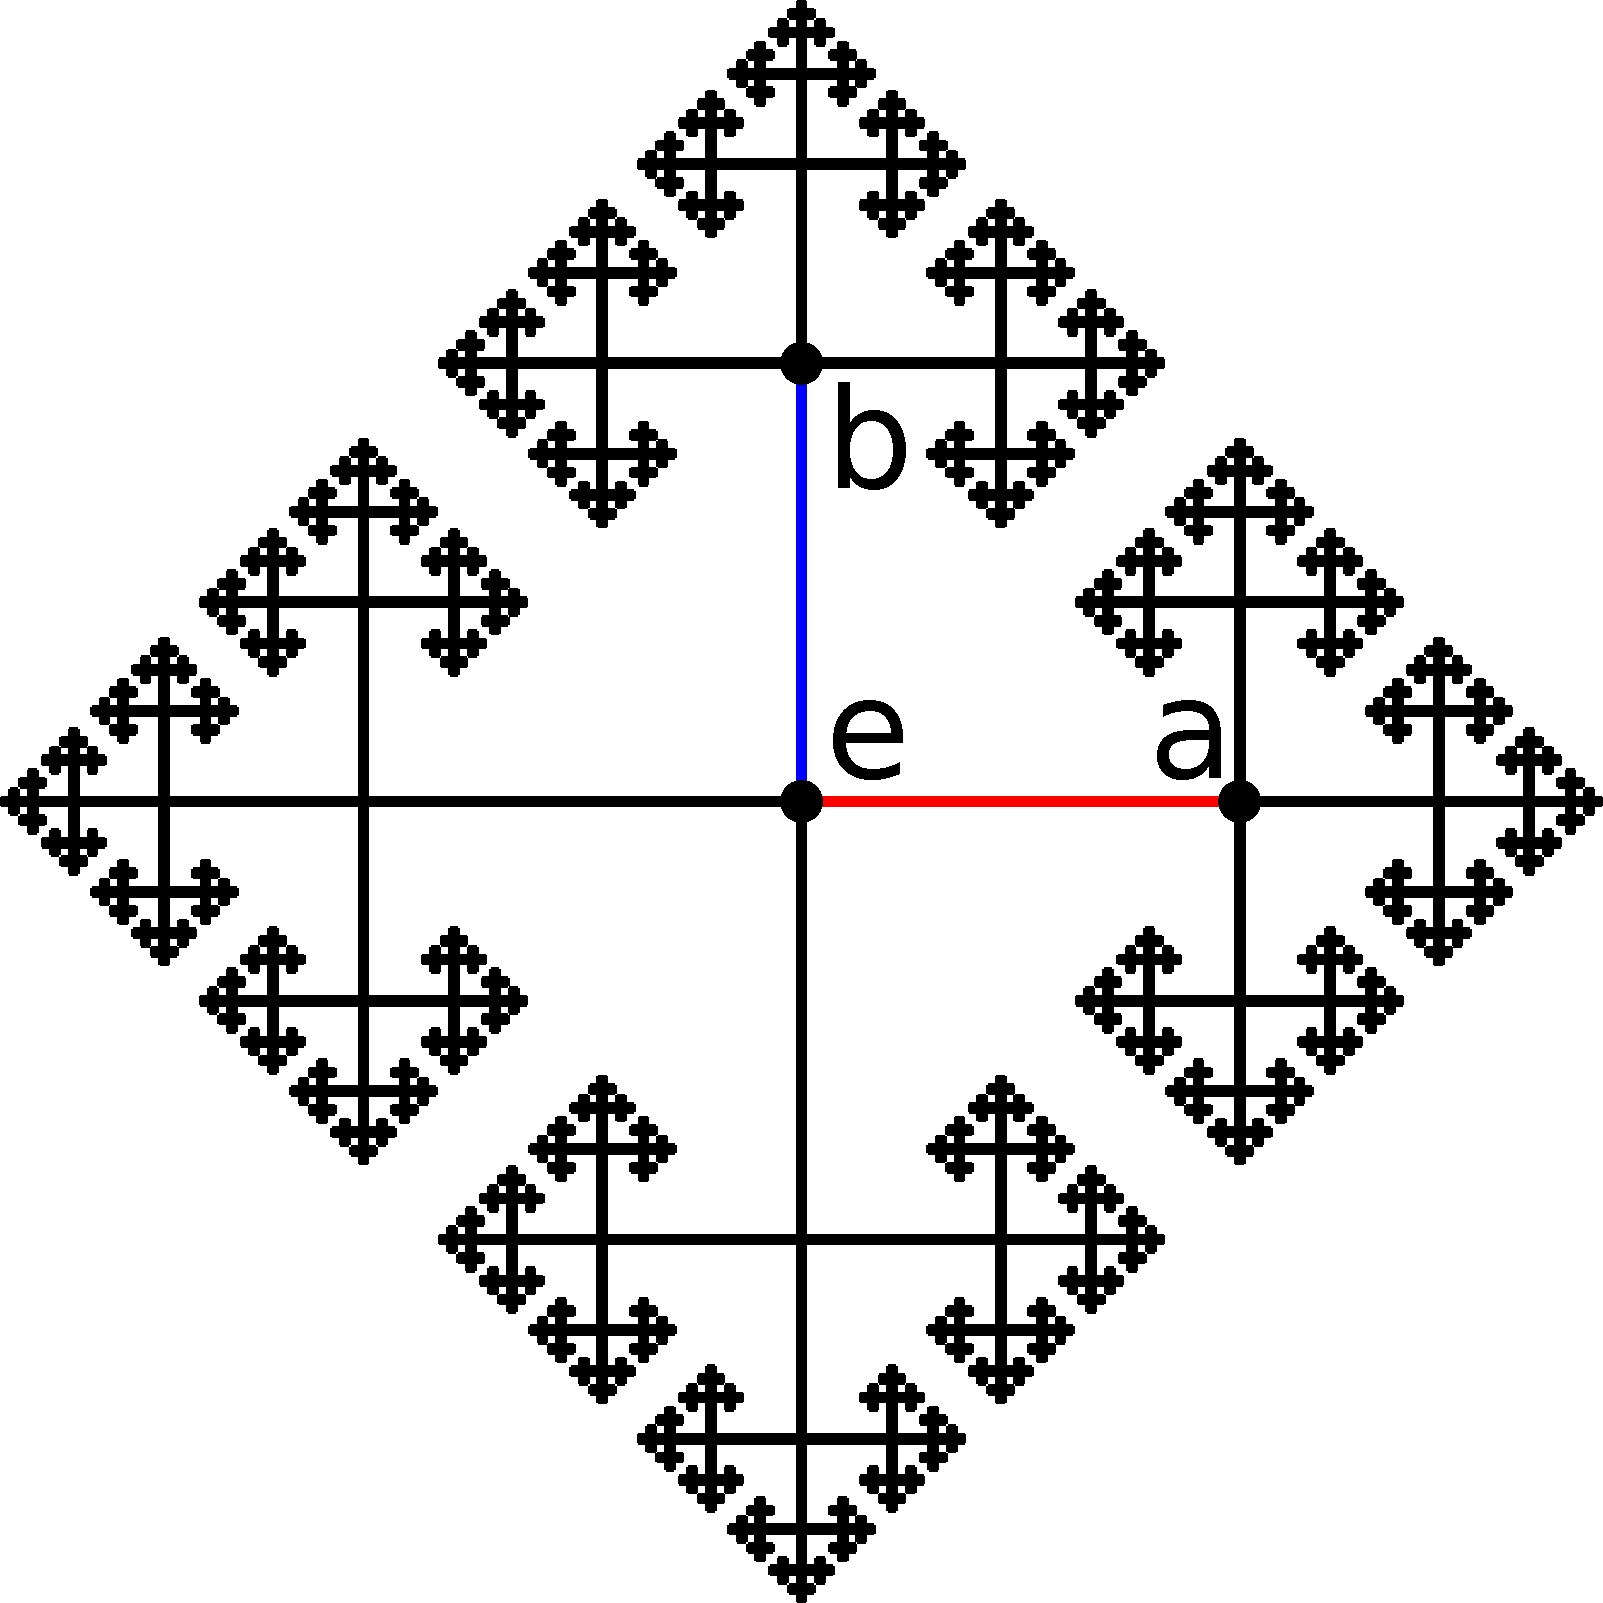
\includegraphics[scale=0.15]{figures/Cayley.pdf}
    \caption{This graph is the universal cover of the figure eight, which is $\Gamma=\bbS^1 \vee \bbS^1$. It is also the Cayley graph of the fundamental group of $\Gamma$, i.e.\ the free group with two generators $a$ and $b$, $\pi_1(\Gamma)=F(\{a,b\})\cong\bbZ\ast\bbZ$. \label{Fig. Cayley}}
\end{figure}

We can now use the theory of covering spaces to prove a very important basic theorem about free groups. 
\begin{thm}[Nielsen-Schreier]\index{Theorem!Nielsen-Schreier}\label{thm Nielsen-Schreier}
    Any subgroup of a free group is free.
\end{thm}
\begin{proof}
    Let $G$ be a free group. As we've seen, it can be realized as the fundamental group of a \emph{bouquet} $M=\bigvee \bbS^1$ of as many circles as there are generators in $G$. Given a subgroup $H\leq G$, there must exist a covering space $E\overset{\pi}{\to}M$ such that $H=\pi_\ast(\pi_1(E,p_0))$ and $\pi_\ast:\pi_1(E,p_0)\to H\subset \pi_1(M,x_0)$ is an isomorphism. However, any covering space of a graph is a graph (indeed,each edge incident with a vertex in the base can be uniquely lifted to the total space, these liftings are homeomorphisms, and doing so for all vertices gives the total space a structure of a graph). In particular, any covering space of a bouquet of circles is a bouquet of circles. This implies that the fundamental group of $E$ is free, and therefore $H$ is free.
\end{proof}
\begin{cor}
    If a subgroup of a free group of finite rank has finite index, then it is also of finite rank.
\end{cor}
\begin{proof}
    Indeed, if $H\leq G$ has finite index, it can be realized as the fundamental group of a finite covering graph of a finite bouquet of circles. But any such graph has a finitely generated fundamental group.
\end{proof}
\begin{thm}[Schreier formula]
    If $G$ is a free group of finite rank $r_G$ and $H \leq G$ is a subgroup of finite index $n$, then $H$ is free of rank $r_H=n(r_G-1)+1$.
\end{thm}
\begin{proof}
    Let $G=F(x_1,\ldots,x_{r_G})$. This follows from examining the covering graph constructed in Theorem~\ref{thm Nielsen-Schreier}. It has one vertex for each right coset $Hg$ and exactly $2r_G$ edges at each vertex ($r_G$ going in and $r_G$ going out) with the outgoing edge going from $Hg$ to $Hgx_i=(Hg)\cdot x_i$ labeled by the generator $x_i$. Therefore this graph has $V=n$ vertices and $E=nr_G$ edges. The fundamental group of this graph $\wt\Gamma$ is isomorphic to $H$ and is generated by $1-\chi(\wt\Gamma)=1-V+E=n(r_G-1)+1$ loops.
\end{proof}
\begin{cor}
    Let $\Gamma$ be a covering graph of $\bigvee_{i=1}^r \bbS^1$ (with $r>1)$ that corresponds to a subgroup generated by $r'>1$ generators. If $n=(r'-1)/(r-1)$ is a positive integer then $\Gamma$ has $n$ sheets, otherwise $\Gamma$ has infinitely many sheets.
\end{cor}
\begin{cor}
    The free group of two generators, $F(a,b)$, contains free subgroups of any integer rank $r_H$. 
\end{cor}
\begin{proof}
    The set of all words whose degree (the sum of the powers of all generators in it) equals $r_H$ is one such subgroup.

    Alternatively, we can simply notice that the space $\bbS^1\vee \bbS^1$ has covering spaces that are homeomorphic to $\bigvee_{i=1}^r \bbS^1$ for any $r$.
\end{proof}

\begin{example}[Covering spaces of $\bbS^1\vee \bbS^1$]
    Consider the ``figure eight'' space $M=\bbS^1\vee \bbS^1$. Its covering spaces are in one-to-one correspondence with conjugacy classes of subgroups of the free group $F(a,b)$ of two generators (one for each circle in $M$). By Theorem~\ref{thm Nielsen-Schreier}, any subgroup of a free group is free, so each covering space of $M$ is uniquely determined by a subset of $F(a,b)$ that contains no relations (e.g.\ the set $\{a^2,b^2,a^2b^2\}$ is redundant and should be replaced with $\{a^2,b^2\}$). The elements of this subset generate the image of $\pi_1(E,p_0)$ under the monomorphism $\pi_\ast$.

    Some examples of these covering spaces are given in Figures~\ref{fig:sixfold covering} and \ref{fig:coverings of 8}. The covering in Figure~\ref{fig:threefold-cover} is another one. It is instructive to observe which of the coverings in Figure~\ref{fig:coverings of 8} are regular, and how the subgroups corresponding to them are normal. It is similarly instructive to verify the Lifting Theorem~\ref{Lifting Theorem}: two different covering spaces of $M$ are covering spaces of each other (say with basepoints) only if the generators of the stabilizer of one of them can be expressed in terms of the generators of the other. For example, (11) is a covering space of (1) because  $b^nab^{-n}=(b^2)^{n/2}a(b^{-2})^{n/2}$ if $n$ is even and $b^nab^{-n}=(b^2)^{(n-1)/2}bab^{-1}(b^{-2})^{(n-1)/2}$ otherwise.

    (1) and (2), up to swapping $a$ and $b$, are all of the existing connected double covers (so there are three in total). (3) and (4) are the same covering space but with different basepoints, and one can see how the corresponding subgroups are conjugates of each other by an element that connects those two points, for example $b$.
\end{example}

\begin{figure}
    \centering
    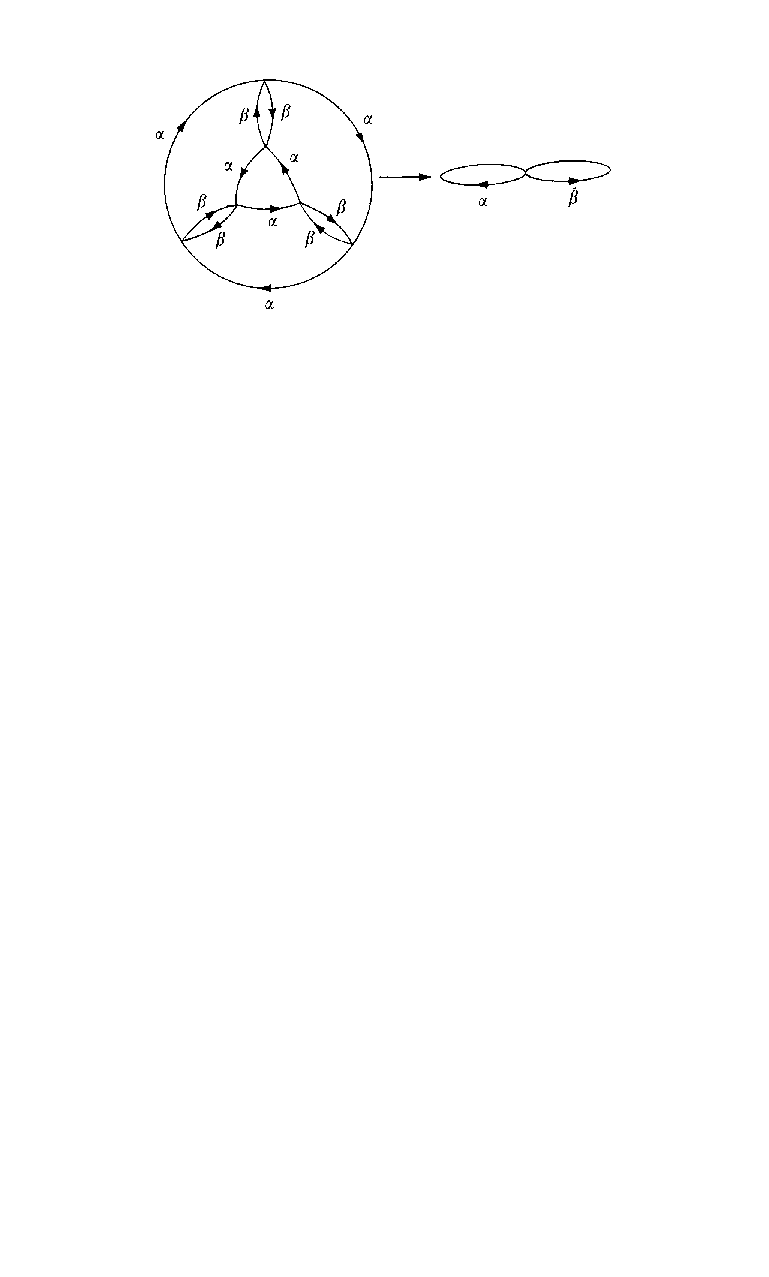
\includegraphics[width=0.6\textwidth]{figures/sixfold.pdf}
    \caption{A sixfold regular covering space of the figure eight. The fundamental group $\pi_1(E,p_0)$ is clearly generated by six loops. This makes it easy to guess that the stabilizer of any vertex is the normal subgroup of the free group $F(\alpha,\beta)$ generated by the six elements $\alpha^3,\beta^2,\left(\alpha\beta^{-1}\right)^2, \left(\alpha^{-1}\beta\right)^2, \alpha\beta^2\alpha^{-1}, \alpha^{-1}\beta^2\alpha$. To find the group of deck transformations, we factor the free group by this normal subgroup, which is equivalent to adding these six generators as relations. It is easy to check that these relations define the permutation group $S_3=\langle a,b\mid a^2,b^2,ababab\rangle$. If we reversed the arrows on the inner triangle of $\alpha$'s, we'd get $\bbZ_2\times \bbZ_3$ instead. From \cite[Fig.~III-7]{Bredon}.}
    \label{fig:sixfold covering}
\end{figure}

\begin{figure}
    \centering
    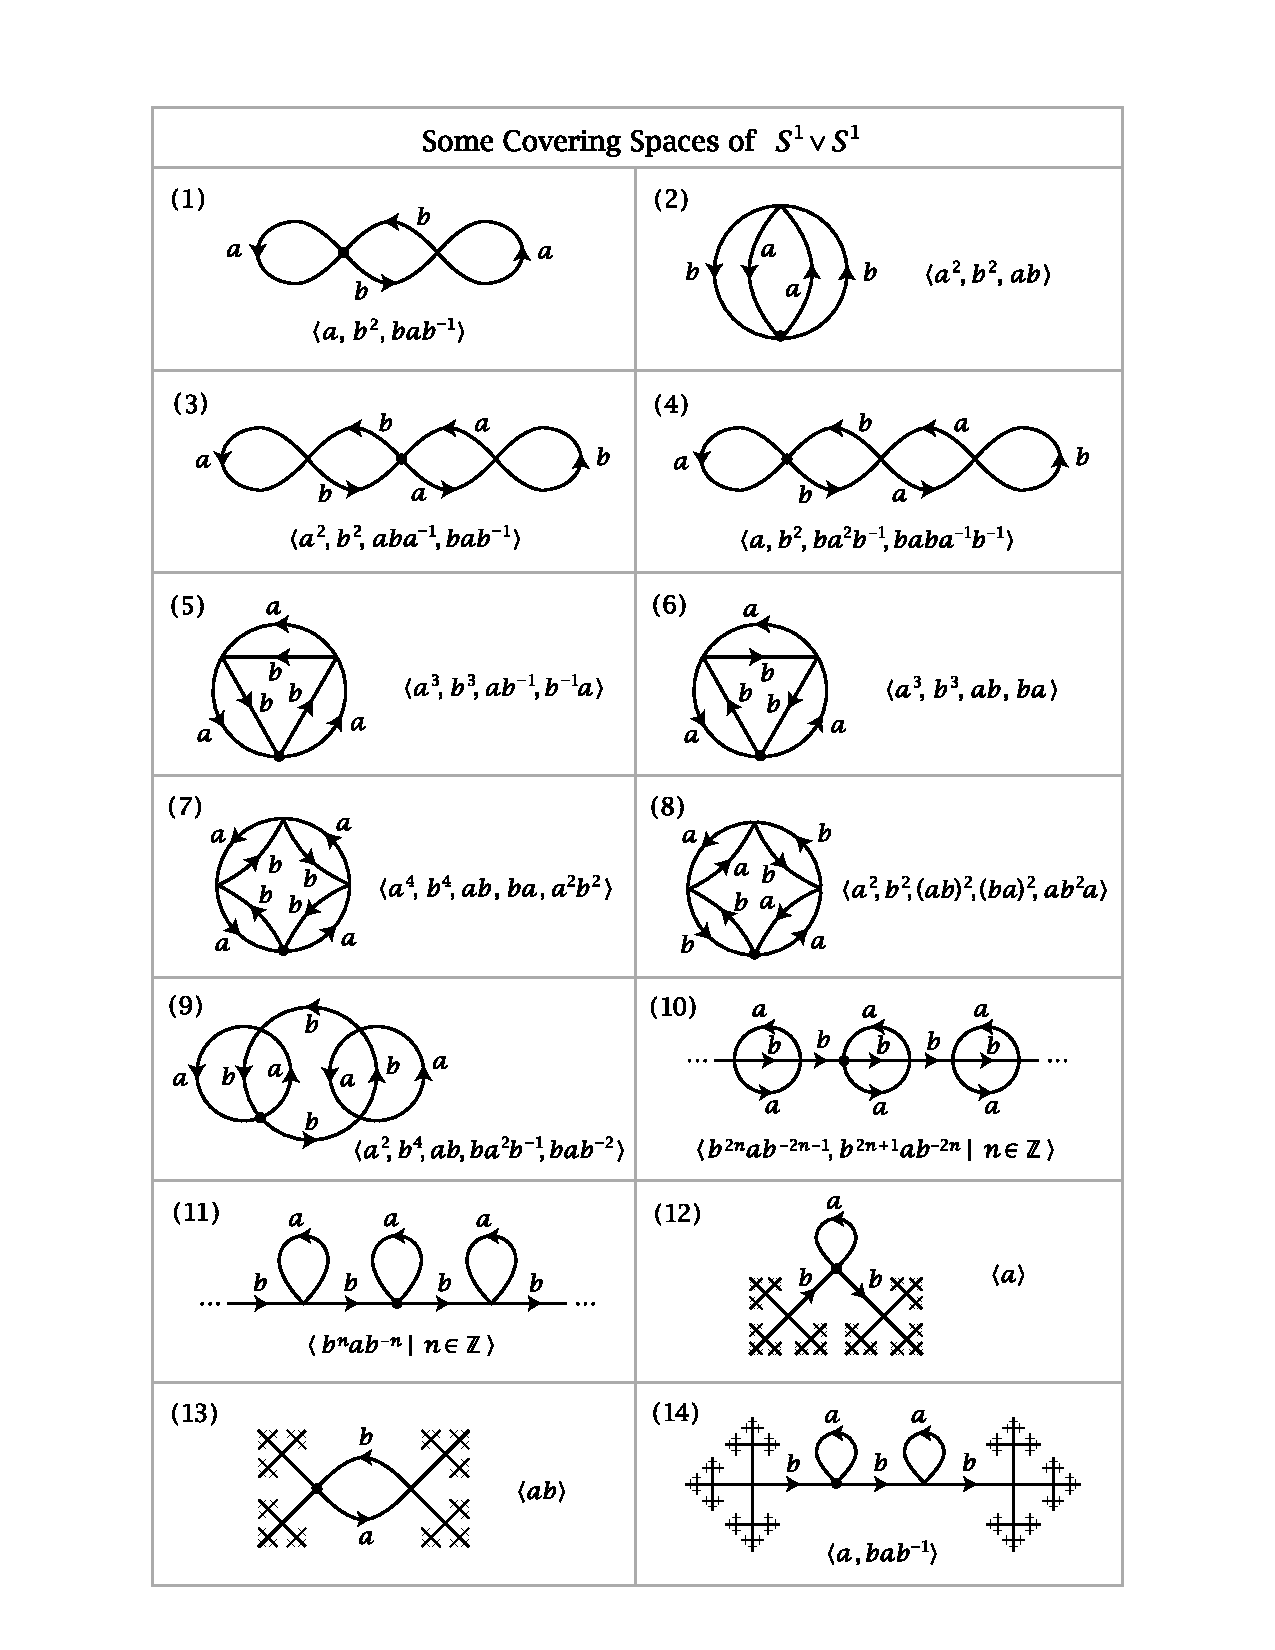
\includegraphics[width=0.67\textwidth]{figures/coverings_8.pdf}
    \caption{Examples of covering spaces of the figure eight space. Each one is a graph with a marked basepoint $p_0$ such that the neighborhood of each vertex locally looks the same as in the base space: two incoming edges (labeled $a,b$) and two outgoing (also labeled $a,b$). The label of an edge indicates which generator of $\pi_1(M)$ it is projected onto by $\pi$. Next to the space is the list of the generators of the local fundamental group $\pi_1(E,p_0)$ expressed in terms of $a,b$, which means that, viewed as part of $\pi_1(M)$, they generate the stabilizer $G_{p_0}=\pi_\ast(\pi_1(E,p_0))$. The number of sheets matches the index of this subgroup. Two vertices are related by a deck transformation iff their stabilizers coincide, otherwise the stabilizers are merely conjugate. For regular coverings (1,2,5,6,7,8,9,11), all stabilizers coincide and therefore are normal. From \cite[p.~58]{Hatcher}.}
    \label{fig:coverings of 8}
\end{figure}


\begin{xca}
    Show that the covering space of the figure eight space $M=\bbS^1\vee \bbS^1$ that corresponds to the normal subgroup generated by $a^2$, $b^2$, and $(ab)^4$ (where $a,b$ are the two generators of the free group $\pi_1(M)$) is regular, and describe what it looks like. \emph{Hint:} this subgroup has index 8, so it's an eight-fold covering.
\end{xca}

\begin{xca}
    Describe the covering space of the figure eight space that corresponds to the commutator subgroup of the free group of two generators. \emph{Hint:} $F(a,b)\slash [F(a,b),F(a,b)]=\bbZ^2$, so this covering space has a $\bbZ^2$-symmetry.
\end{xca}
\begin{xca}
    Identify in $\bbS^1$ the open upper and the open lower semicircle to a point. The resulting space $X$ has four points. Show $\pi_1(X)\cong \bbZ$. Does $X$ have a universal covering?
\end{xca}
\begin{xca}
    Show that the universal cover of $M_1\times M_2$ is $\wt M_1\times \wt M_2$.
\end{xca}
\begin{xca}[{{\cite[Exercise~B.7]{Hatcher}}}]
    If $G$ is a finitely generated free group and $N$ is a nontrivial normal subgroup of infinite index, show, using covering spaces, that $N$ is not finitely generated.
\end{xca}

\begin{example}
    $\widetilde{\bbT^n}=\bbR^n$, $\widetilde{\text{SO}_3}=\text{SU}_2=\bbS^3$, $\widetilde{\text{SO}}_{n>2}=\text{Spin}_n$, $\widetilde{\text{U}_n}=\text{SU}_n\times \bbR $.
\end{example}











\clearpage
\section{Homotopy Theory}

\subsection{Homotopy groups}

\begin{defn}[Homotopy groups]\index{Homotopy groups}
Pick the base points $\bullet\in \bbS^n$ and $x_0\in X$. The set of homotopy classes of maps $\gamma:\bbS^n\to X$ such that $\gamma(\bullet)=x_0$ forms the $n$-th homotopy group $\pi_n(X,x_0)=[\bbS^n;X]_\bullet$. For two such maps, define their product by first mapping $\bbS^n$ onto the wedge sum $\bbS^n\lor \bbS^n$ via contracting an arbitrarily chosen equator (which is homeomorphic to $\bbS^{n-1}$) into one point, then apply $\gamma_1$ and $\gamma_2$ to the two hemispheres respectively, making the equator point the base point for them.

For $n=0$, $\pi_0(X)$ is defined as the set of path-connected components of $X$ (which is also the set of homotopy classes of pointed maps $\bbS^0\to X$) but does not have a natural group structure.
\end{defn}

\begin{xca}
\begin{enumerate}
    \item The above definition is consistent and the resulting homotopy classes don't in fact depend on the choice of an equator. In fact, in natural terms, this group operation is exactly the coproduct on the category of pointed spaces, given by the wedge sum $\gamma_1\lor\gamma_2:\bbS^n\lor \bbS^n\to X$ (a.k.a. \emph{concatenation}).
    \item All homotopy groups for different $x_0$ are isomorphic.
\end{enumerate}
\end{xca}


\begin{prop}[Functoriality of $\pi_n$]
    Any pointed continuous map $f:X\to Y$ induces a homomorphism of the homotopy groups $f_\ast:\pi_n(X,x_0)\to \pi_n(Y,y_0)$, and $(g\circ f)_\ast=g_\ast\circ f_\ast$. In other words, we have a \emph{functor} $\pi_n:\mathsf{Top}_\bullet\to \mathsf{Gr}$.
\end{prop}

\begin{thm}
Homotopy groups $\pi_n$, $n\geq 1$, are homotopy invariants, i.e.\ if $X\simeq Y$ are two homotopy equivalent path connected spaces, then $\pi_n(X,x_0)\cong\pi_n(Y,y_0)$.
\end{thm}
\begin{proof}
Exercise. Also see \cite{Hatcher}.
\end{proof}
\begin{cor}
    $\pi_n$ descends to a functor $\pi_n:\mathsf{hTop}_\bullet\to \mathsf{Gr}$ on the category $\mathsf{hTop}_\bullet$, in which the morphisms are the homotopy classes of pointed continuous maps modulo homotopy relative to the base point. In particular, homotopy equivalent spaces have isomorphic homotopy groups.
\end{cor}

\begin{thm}
For $n\geq 2$, all groups $\pi_n(X,x_0)$ are abelian.
\end{thm}
\begin{proof}
Follows from Proposition \ref{suspension maps prop} and the fact that $\bbS^n=\Sigma\Sigma \bbS^{n-2}$ for $n\geq 2$. We have $[\bbS^n,Y]=[\Sigma\Sigma \bbS^{n-2},Y]=[\Sigma \bbS^{n-2}, \Omega Y]$, which is abelian.
\end{proof}

Another very important connection between homotopy groups and suspension will be discussed when we prove Freudenthal's Suspension Theorem \ref{thm 6.4.7 tomDieck freudenthal}.

\begin{comment}
\PRLsep
\begin{center}
  {\red Lecture 4 on 30 Nov 2018 ended here}
\end{center}
\end{comment}



\subsection{Exact sequence of homotopy groups}

\begin{defn}[Topological triple]
    A triple $(X,A,B)$ is a topological space $X$ with a pair of subspaces $A\subset B\subset X$. When $B=\bullet$ is a point, the triple is also called a pointed pair.
\end{defn}

\begin{defn}[Relative homotopy groups]\index{Relative homotopy groups}\index{Homotopy groups!relative}
        For a pointed pair $(X,A,\bullet)$ and $n\geq 1$ the relative homotopy group $\pi_n(X,A,\bullet)$ is the set of homotopy classes of triples $\pi_n(X,A,\bullet)=[(\bbD^n,\bbS^{n-1},\bullet);(X,A,\bullet)],$
        where $\bbD^n$ is the $n$-disk, $\bbS^{n-1}$ is its boundary, and the homotopies are through pointed maps that take $\bbS^{n-1}$ into $A$. Note that this is \emph{not} the same as homotopies relative to $\bbS^{n-1}$.
\end{defn}
These are groups with the same multiplication operation and they are still abelian for $n\geq 3$ because $[(\Sigma X,\Sigma A);(Y,B)]=[( X, A);(\Omega Y,\Omega B)]$.
\begin{prop}[Compression criterion]\label{prop: compression criterion}
    A map $f:(\bbD^n,\bbS^{n-1},\bullet)\to (X,A,\bullet)$ represents the identity in $\pi_n(X,A,\bullet)$ iff it is homotopic $\rel \partial \bbD^n\cong \bbS^{n-1}$ to a map whose image is contained in $A$.
\end{prop}
\begin{proof}
    For necessity, a map whose image is contained in $A$ can be composed with a deformation retraction of $\bbD^n$ onto the basepoint to give a homotopy to a trivial map. Conversely, if $[f]=e$ via a homotopy $H:\bbD^n\times I\to X$, then by restricting $H$ to a family of $n$-disks in $\bbD^n\times I$ starting with $\bbD^n\times \{0\}$ and ending with the disk $\bbD^n\times\{1\}\cup \bbS^{n-1}\times I$, all the disks in the family having the same boundary, then we get a homotopy from $f$ to a map onto $A$, stationary on $\bbS^{n-1}$. This is a homotopy relative to $A$.
\end{proof}

Any map $f:(X,A,x_0)\to (Y,B,y_0)$ induces maps $f_\ast :\pi_n(X,A,x_0)\to \pi_n(Y,B,x_0)$ which are homomorphisms for $n\geq 2$ and have properties analogous to those in regular homotopy: $(f\circ g)_\ast=f_\ast\circ g_\ast$, $\mathrm{id}_\ast=\mathrm{id}$, and $f_\ast=g_\ast$ if $f\sim g$ through maps of pointed pairs $(X,A,x_0)\to(Y,B,y_0)$.

In particular, the inclusions $i:(A,x_0)\hookrightarrow(X,x_0)$ and $j:(X,x_0,x_0)\hookrightarrow (X,A,x_0)$ induce such homomorphisms. Moreover, there is a third special homomorphisms that connects homotopy groups in adjacent degrees.

\begin{defn}[Boundary operator for homotopy]
    The inclusion of the boundary $\bbS^{n-1}\hookrightarrow \bbD^n$ induces restrictions of maps $f:(\bbD^n,\bbS^{n-1},s_0)\to (X,A,x_0)$ to the boundary, i.e.\ $\partial f=\restr{f}{\partial \bbD^n}$. For $n\geq 2$ this operator defines a homomorphism of relative homotopy groups.
\end{defn}

\begin{defn}[Exact sequence]
    Let $\calC$ be a category in which the notions of kernels and images of morphisms are well-defined. For now we assume that it is a concrete category, so kernels and images are understood as subsets of the domain and codomain, respectively. Next let there be a (finite or infinite) sequence of morphisms
    \[\cdots\to X\overset{f}{\to } Y\overset{g}{\to} Z\to \cdots \]
    We say that this sequence is exact at $Y$ if $\im f=\ker g$.
\end{defn}
\begin{example}
    In the category of pointed sets (or topological spaces etc.), kernels can be defined as the pre-images of the basepoint. Exactness then amounts to $\im f=g^{-1}(*)$.

    Usually we will be concerned with the case $\calC=\mathsf{Gr}$.
\end{example}
\begin{defn}[Short exact sequence]
    A short exact sequence is a sequence of the form
    \[0\to X\overset{f}{\to } Y\overset{g}{\to} Z\to 0,\]
    where $0$ is a zero object in $\calC$.

    The exactness at $X$ is equivalent to $f$ being a monomorphism. Exactness at $Z$ is equivalent to $g$ being an epimorphism. The exactness at $Y$ essentially says that $Z\cong Y\slash \im f=Y\slash \ker g\cong Y\slash X$. In the category of groups this is just the first isomorphism theorem.
\end{defn}

\begin{example}
    If the short exact sequence is even shorter, e.g.
    \[0\to X\overset{f}{\to } Y\to 0,\]
    then its exactness is equivalent to $f$ being an isomorphism.
\end{example}

\begin{thm}[Long exact sequence of homotopy groups]\index{Long exact sequence!of homotopy groups}\label{thm long exact seq of homotopy}
    The sequence of homomorphisms
    \[\cdots \to \pi_n(A,x_0)\overset{i_\ast}{\to}\pi_n(X,x_0)\overset{j_\ast}{\to}\pi_n(X,A,x_0)\overset{\partial}{\to}\pi_{n-1}(A,x_0)\to \cdots \to \pi_0(X,x_0)\]
    is \emph{exact}. Near the end of the sequence, where the group structure is not defined, the ``kernel'' is the path-connected component of $x_0$.
\end{thm}
\begin{proof}
    In fact we will prove the long exact sequence of a pointed triple $(X,A,B,x_0)$ with $x_0\in B\subset A\subset X$:
    \begin{multline}
        \cdots \to \pi_n(A,B,x_0)\overset{i_\ast}{\to}\pi_n(X,B,x_0)\overset{j_\ast}{\to}\pi_n(X,A,x_0)\overset{\partial}{\to}\pi_{n-1}(A,B,x_0)\to \cdots \\ \to \pi_1(X,A,x_0).
    \end{multline}
    The boundary operator for triples is defined as the composition $\partial:\pi_n(X,A)\overset{\partial}{\to} \pi_{n-1}(A)\overset{i_\ast}{\to} \pi_{n-1}(A,B)$ where $i:B\hookrightarrow A$ is the inclusion map. When $B=\{x_0\}$ this reduces to the exact sequence of the pointed pair $(X,A,x_0)$, though the latter sequence continues for two more steps to $\pi_0(X,x_0)$.

    \emph{Exactness at} $\pi_n(X,B,x_0)$: First note that the composition $j_\ast\circ i_\ast$ is trivial since every map $(\bbD^n,\bbS^{n-1},s_0)\to (A,B,x_0)$ represents zero in $\pi_n(X,A,x_0)$ by the compression criterion. To see that $\ker j_\ast \subset \im i_\ast$, let $f:(\bbD^n,\bbS^{n-1},s_0)\to (X,B,x_0)$ represent the trivial element in $\pi_n(X,A,x_0)$. Then by the compression criterion again, $f$ is homotopic $\rel \bbS^{n-1}$ to a map with image in $A$, hence $[f]\in \pi_n(X,B,x_0)$ is in the image of $i_\ast$.

    \emph{Exactness at} $\pi_n(X,A,x_0)$: The composition $\partial\circ j_\ast$ is zero since the restriction of a map $(\bbD^n,\bbS^{n-1},s_0)\to (X,B,x_0)$ to $\bbS^{n-1}$ has image lying in $B$, and hence represents the trivial class in $\pi_{n-1}(A,B,x_0)$. Conversely, suppose the restriction of $f:(\bbD^n,\bbS^{n-1},s_0)\to (X,A,x_0)$ to $\bbS^{n-1}$ represents the trivial element $\pi_{n-1}(A,B,x_0)$. Then $\restr{f}{\bbS^{n-1}}$ is homotopic to a map with image in $B$ via a pointed homotopy $H:\bbS^{n-1}\times I \to A$. We can tack $H$ onto $f$ to get a new map $(\bbD^n,\bbS^{n-1},s_0)\to (X,B,x_0)$ which, as a map $(\bbD^n,\bbS^{n-1},s_0)\to (X,A,x_0)$, is homotopic to $f$ by the homotopy that tacks on increasingly longer initial segments of $H$. So $[f]\in \im j_\ast$.

    \emph{Exactness at} $\pi_n(A,B,x_0)$: The composition $i_\ast \circ \partial$ is trivial since the restriction of a map $f:(\bbD^{n+1},\bbS^n,s_0)\to (X,A,x_0)$ to $\bbS^n$ is homotopic $\rel s_0$ to a constant map via $f$ itself (via a contraction of $\bbS^n$ onto $s_0$ inside $\bbD^n$). The converse is easy if $B$ is a point, since the nullhomotopy $f_t:(\bbD^n,\bbS^{n-1})\to (X,x_0)$ of $f_0:(\bbD^n,\bbS^{n-1})\to (A,x_0)$ gives a map $F:(\bbD^{n+1},\bbS^n,s_0)\to (X,A,x_0)$ with $\partial([F])=[f_0]$. Thus the proof is finished in this case. 
    
    For a general $B$, let $f:(\bbD^{n},\bbS^{n-1},s_0)\to (A,B,x_0)$ be in the kernel of $i_\ast$ and let $F:\bbD^n\times I\to X$ be a corresponding nullhomotopy of $f$ through maps $(\bbD^n,\bbS^{n-1},s_0)\to (X,B,x_0)$. It is then clear that $F$ can be viewed as a map $\bbD^{n+1}\to X$ which restricts to $f$ on $\bbD^n\times \{0\}$, and maps the rest of the boundary into $B\subset A$, which makes $f$ the boundary of some map $(\bbD^{n+1},\bbS^n,s_0)\to (X,A,x_0)$.
\end{proof}



\subsection{\texorpdfstring{$CW$}{CW}-complexes}

\begin{defn}[$CW$-complex]\index{$CW$-complex}\index{Cell complex}
    A cellular structure on a set $X$ is a family $\calF $ of \textit{characteristic mappings} $f_\alpha^n:\bbD^n\to X$, where $n=0,1,2,\ldots$ and $\alpha\in A_n$ (some indexing sets), such that the following conditions hold. Let $X^{(n)}$ denote the union of images of mappings $f_\alpha^k, k\leq n$. Also $X^{(-1)}=\varnothing$.
    \begin{enumerate}
        \item For every $n$, $\bigsqcup_\alpha f_\alpha^n$ maps $\bigsqcup_\alpha \Int \bbD^n$ \emph{injectively} to $X\setminus X^{(n-1)}$. Here, we put $\Int \bbD^0=\bbD^0$.
        \item Every $f_\alpha^n$ maps $\partial \bbD^n$ to $X^{(n-1)}$.
        \item $X=\bigcup_n X^{(n)}$.
    \end{enumerate}
    
    A $CW$-complex is a Hausdorff topological space with a $CW$-structure such that the topology coincides with the final topology defined by $\calF $, also called the \emph{weak topology}\index{Weak topology}: $A\subset X$ is open iff $A\cap X^{(n)}$ is open in $X^{(n)}$ for each $n$.

    The restrictions $\partial f_\alpha^n=\restr{f_\alpha^n}{\partial \bbD^n}$ are called the \textit{attaching maps}. The subsets $X^{(n)}\subset X$ are called the $n$-skeleta of $\calF $. The images $f_\alpha^n(\bbD^n)$ are referred to as the \textit{closed cells} and $f_\alpha^n(\Int  \bbD^n)$ as \textit{open cells} (even though these are actually closed or open only as subspaces of $X^{(n)}$!). A $CW$-complex $(X,\calF )$ is said to be pointed if $X$ is pointed and the basepoint is a $0$-cell. A subcomplex is a subspace $X'\subset X$ endowed with the relative topology, together with a subfamily $\calF '\subset\calF $ such that $(X',\calF ')$ is a $CW$-complex. The highest dimension of a cell in a complex is called its dimension. A $CW$-complex is called finite if it is finite-dimensional and has a finite number of cells.
\end{defn}

We will typically work with finite $CW$-complexes, but infinite-dimensional ones will be useful as well.

\begin{rem}
The acronym $CW$ refers to the following properties.
\begin{enumerate}
    \item Closure-finiteness: every closed cell meets only finitely many open cells, which we will prove in Proposition~\ref{prop 8.1 Bredon}.
    \item Weak topology: $X$ carries the final topology defined by the family $\calF $.
\end{enumerate}
A  more general concept of cellular complexes drops these requirements. Note that, due to the inductive definition of $CW$-complexes as a collection of attaching maps, we get (C) automatically.
\end{rem}

% The following proposition shows that the weak topology induced by any \emph{finite} $CW$-structure consisting of continuous characteristic maps  on a Hausdorff space coincides with the original topology.

% \begin{prop}[{{\cite[Prop.~3.1.9]{RS2}}}]\label{prop 3.1.9 RS2}
%     Let $X$ be a Hausdorff space and let $\calF $ be a finite $CW$-structure on $X$. For $\calF $ to make $X$ into a $CW$-complex it suffices that every $f_\alpha^n\in\calF $ be continuous.
% \end{prop}
% \begin{proof}
%     We show that a subset $A \subset X$ is closed iff $(f_\alpha^n)^{-1}(A)\subset \bbD^n$ is closed for all $n$ and $\alpha$. The `only if' direction is obvious. To prove the `if' direction, assume that $(f_\alpha^n)^{-1}(A)$ is closed for all $n$ and $\alpha$. Since a continuous mapping from a compact space to a Hausdorff space is closed, it follows that $f_\alpha^n((f_\alpha^n)^{-1}(A))\subset X$ is closed for all $n$ and $\alpha$. Since $A$ is the union over all these subsets, and since their number is finite, we conclude that $A$ is closed.
% \end{proof}

Every $CW$-complex therefore can be thought of as a \emph{decomposition} of a Hausdorff space $X$ into a disjoint union of open cells of various dimensions. The space $X$, up to homeomorphism, can be inductively reconstructed from its $CW$-structure as follows. First, $X^{(0)}$ is a discrete set of points. Next, given an $(n-1)$-skeleton $X^{(n-1)}$, we can obtain $X^{(n)}$ by taking a disjoint union of $n$-disks $\sqcup_\alpha \bbD^n$ and identifying their boundaries with points of $X^{(n-1)}$ via the attaching maps $\partial f_\alpha^n:\partial \bbD^n\to X^{(n-1)}$, which are required to be continuous. The space $X$ is then the inductive union of all skeleta with the final topology.


\begin{example}
    \begin{enumerate}
        \item A graph is nothing but a $0$- or $1$-dimensional cell complex.
        \item The infinite bouquet $\bigvee_{i=1}^\infty \bbS^1$ is not a $CW$-complex because the basepoint has to meet infinitely many $1$-cells.
        \item The sphere $\bbS^n$ admits a $CW$-structure with one $0$-cell and one $n$-cell. The characteristic maps can be chosen as 
        \[f^0(*)=e_1,\quad f^n(x)=(2|x|^2-1,2\sqrt{1-|x|^2}x).\]
        Another useful $CW$-structure on the sphere has two cells in each dimension up to $n$. Its characteristic maps are
        \[f^0_\pm (*)=\pm e_1\,\quad f^k_\pm(x)=(x,\pm\sqrt{1-|x|^2},0,\ldots,0).\]
        The two $k$-cells are given by
        \[\{(x_1,\ldots,x_{k+1},0,\ldots,0)\in \bbS^n:\pm x_{k+1}\geq 0\}.\]
        \item The closed $n$-disk $\bbD^n$ has a tautological $CW$-structure with one $n$-cell. It is however sometimes convenient to have the boundary $\bbS^{n-1}$ as a subcomplex. This can be achieved by just adding either one of the two $CW$-structures of $\bbS^{n-1}$ above.
        \item The wedge sum of two $CW$-complexes $(X_1,\calF _1)\vee (X_2,\calF _2)$ carries a natural $CW$-structure $\calF _1\cup \calF _2$.
        \item The direct product $(X_1,\calF _1)\times (X_2,\calF _2)$ has a $CW$-structure with elements $(f_{1i}^n\times f_{2j}^m)\circ p_{n+m}$ where $p_{n+m}:\bbD^{n+m}\to \bbD^n\times \bbD^m$ is some chosen homeomorphism. This makes sense, because, as a homeomorphism, $p_{n+m}$ maps the boundary $\bbS^{n+m-1}$ of $\bbD^{n+m}$ onto the boundary $(\bbS^{n-1}\times \bbD^m)\cup (\bbD^n\times \bbS^{m-1})$ of $\bbD^n\times \bbD^m$. For example, the direct product of two copies of $\bbS^1$ with one cell in dimensions $0$ and $1$ yields a $CW$-structure on the torus $\bbT^2$ with one $0$-cell, one $2$-cell, and two $1$-cells. Note that in general the topology on the product complex need not coincide with the product topology, but it does when the complexes are locally finite (i.e.\ every point has a neighborhood that overlaps only with finitely many open cells -- such spaces are also paracompact).
    \end{enumerate}
\end{example}

\begin{prop}[{{\cite[Prop.~3.1.11]{RS2}}}]\label{prop 3.1.11 RS2}
    Let $(X,\calF )$ be a $CW$-complex, $Y$ a topological space, and $f:X\to Y$ a map. Then $f$ is continuous iff its restrictions $f\circ f_\alpha^n$ to each cell are continuous.
\end{prop}
\begin{proof}
    This is nothing but the universal property of the final topology, but let us walk through the argument. Only the sufficiency is not obvious. Let $V\subset Y$ be open. By assumption, $(f\circ f_\alpha^n)^{-1}(V)$ is open in $\bbD^n$ for all $n$ and $\alpha$. Since $(f\circ f_\alpha^n)^{-1}(V)=(f_\alpha^n)^{-1}(f^{-1}(V))$, then $f^{-1}(V)\subset X$ is open by virtue of being the image of an open set under a quotient map (and all quotient maps are open by definition). 
\end{proof}

% \begin{prop}[{{\cite[Prop.~3.1.12]{RS2}}}]\label{prop 3.1.12 RS2}
%     Let $(X,\calF )$ be a $CW$-complex, $Y$ a topological space, and $f_n:X^{(n)}\to Y,n=0,1,\ldots$ a family of continuous mappings satisfying $\restr{f_{n+1}}{X^{(n)}}=f_n$ for all $n$. Then there exists a unique mapping $f:X\to Y$ that restricts to $f_n$ on $X^{(n)}$ for all $n$, and $f$ is continuous.
% \end{prop}
% \begin{proof}
%     Since the assumption implies that $\restr{f_{m}}{X^{(n)}}=f_n$ for all $m>n$, and since $X$ is the union of $n$-skeleta, we can define $f$ by $\restr{f}{X^{(n)}}=f_n$. Uniqueness is then obvious. To check continuity, observe that for all $n,i$ and $x\in \bbD^n$, we have $f(f_i^n(x))=f_n(f_i^n(x))$. It follows that $f\circ f_i^n$ is continuous for all $n$ and $i$ and hence, by Proposition~\ref{prop 3.1.11 RS2}, that $f$ is continuous.
% \end{proof}

\begin{prop}[{{\cite[Prop.~8.1]{Bredon}}}]\label{prop 8.1 Bredon}
    If $X$ is a $CW$-complex then
    \begin{enumerate}
        \item if $A\subset X$ has no two points in the same open cell, then $A$ is closed and discrete;
        \item if $K\subset X$ is compact then $K$ is contained in a finite union of open cells;
        \item each cell of $X$ is contained in a finite subcomplex of $X$ (i.e.\ the cell complex is \emph{``closure finite''}).
    \end{enumerate}
\end{prop}
\begin{proof}
    We will first show that all three statements are equivalent to each other.
    
    $(1)\Rightarrow (2)$. If $K\subset X$ is compact then let $A\subset K$ be a set of points, one from each open cell touching $K$. By (1) $A$ is closed, hence compact, and discrete. Hence $A$ is finite. But that means $K$ is contained in a finite union of open cells as claimed.

    $(2)\Rightarrow(3)$. In fact, for a cell $\alpha$, we will only use (2) for the set $K$ which is the image of the attaching map $f_{\partial \alpha}:\partial \bbD^n\to X^{(n-1)}$ of that cell, and the images of attaching maps of smaller-dimensional cells. Statement (2) implies that $X_\sigma=f_\sigma(\bbD^n)$ is contained in a finite union of open cells, and by construction all of these are of smaller dimension except for $U_\sigma=f_\sigma(\Int \bbD^n)$ itself. By the same token each of these lower-dimensional closed cells is contained in a finite union of open cells of even lower dimension (except for open the cell itself), and so on. This reasoning obviously must come to an end with $0$-cells in a finite number of steps, and, at that stage, the union of the cells produced a finite subcomplex.

    $(3)\Rightarrow(1)$. Consider the intersection of $A$ with a closed cell. By (3) this is contained in a finite subcomplex. Since $A$ has at most one point in common with any open cell this intersection must be finite, and hence closed. For any point $x\in A$, the set $A\setminus\{x\}$ satisfies the hypothesis for $A$, and so it must also be closed. Hence $\{x\}$ is open in $A$, so $A$ is discrete.

    Finally, we put all this together. Statement (1) clearly holds for $X^{(0)}$ (it must be discrete because it has the final topology of maps of points). Suppose we know (1) for the $n$-skeleton $X^{(n)}$. Then we also have (2) for $X^{(n)}$. In turn, we get (3) for $X^{(n)}$. But the proof of $(2)\Rightarrow(3)$ for a particular $k$-cell only used (2) for subsets of $X^{(k-1)}$. Thus we actually have (3) for $X^{(n+1)}$. Thus we also have (1) for $X^{(n+1)}$. Consequently, we have all three statements for $X^{(n)}$ for all $n$. But any cell is in some $X^{(n)}$, and so we know (3) for $X$ itself, and this implies (1) then (2) for $X$.
\end{proof} 
\begin{cor}
    The boundary of each cell is contained in finitely many closed cells of lower dimensions.
\end{cor}

\begin{thm}[{{\cite[Thm.~8.2]{Bredon}}}]\label{thm 8.2 Bredon}
    A compact subset of a $CW$-complex is contained in a finite subcomplex.
\end{thm}
\begin{proof}
    Let $K\subset X$ be compact. By (2) of Proposition~\ref{prop 8.1 Bredon}, $K$ is contained in a union of a finite number of open cells. By (3) of the same Proposition, each of these is contained in a finite subcomplex. The union of this finite number of finite subcomplexes is a finite subcomplex containing $K$.
\end{proof}

\begin{cor}\label{cor direct limit of pi_n for CW}
    If $X_1\hookrightarrow X_2\hookrightarrow \cdots$ is an infinite sequence of inclusions of $CW$-subcomplexes, then 
    \[\pi_n(\colimit X_i)=\colimit \pi_n(X_i).\]
\end{cor}
\begin{proof}
    Let $X=\colimit X_i=\bigcup X_i$ be the limiting $CW$-complex. Since $\bbS^n$ is compact, its continuous image in $X$ under any representative of an element of $\pi_n(X)$ is compact and thus contained in a finite subcomplex. Therefore every element of $\pi_n(X)$ is contained in $\pi_n(X_k)$ for some $k$ and hence in the directed colimit $\colimit \pi_n(X_i)$. Conversely, every element of this colimit is represented by some element of $\pi_n(X_k)$ for some $k$ by the explicit construction of the colimit.
\end{proof}




\begin{prop}
    A $CW$-complex is locally compact (every point has an open neighborhood contained in a compact set) iff it is locally finite (every point has an open neighborhood contained in a finite union of cells).
\end{prop}
\begin{proof}
    Exercise.
\end{proof}



\begin{defn}[Directed system, Direct limit]\index{Direct limit}
    A directed system of topological spaces consists of a directed set $(A,\leq)$ (a poset such that for all $a,b\in A$ there exists $c\in A$ such that $a\leq c$ and $b\leq c$), a topological space $X_\alpha$ for every $\alpha \in A$ and a continuous mapping $f_{\beta\alpha}:X_\alpha\to X_\beta$ for every pair $\alpha\leq\beta$ such that $f_{\alpha\alpha}=\id_{X_\alpha}$ and $f_{\gamma\beta}\circ f_{\beta\alpha}=f_{\gamma\alpha}$ for all $\alpha\leq\beta\leq \gamma$. The direct limit (\textit{colimit})
    \[X=\colimit X_\alpha\]
    of the directed system $\{X_\alpha,f_{\beta\alpha}\}$ is (up to homeomorphism) the topological quotient of the disjoint union $\bigsqcup_{\alpha\in A} X_\alpha$ with respect to the equivalence relation that $x\in X_\alpha$ is equivalent to $y\in X_\beta$ iff $\gamma\in A: f_{\gamma\alpha}(x)=f_{\gamma\beta} (y)$. Composition of the natural inclusions $X_\alpha\hookrightarrow \bigsqcup_\alpha X_\alpha$ with the quotient map yields continuous mappings
    \[\varphi_\alpha:X_\alpha\to X\]
    and the topology of $X$ coincides with the final topology defined by these maps. That is, a subset of $X$ is open iff its pre-image under $\varphi_\alpha$ is open in $X_\alpha$ for all $\alpha$. In other words, the direct limit space is the set-theoretic direct limit with the final topology for the maps $\varphi_{\alpha}$.
\end{defn}

Direct limits are nothing but a generalization of pushouts to infinite families of objects, and will come up again in a more general categorical setting when we discuss homological algebra.


\begin{prop}[{{\cite[Prop.~3.1.14]{RS2}}}]\label{prop 3.1.14 RS2}
    Let $\{X_\alpha,f_{\beta\alpha}\}$ and $\{Y_\alpha,g_{\beta\alpha}\}$ be directed systems of topological spaces over the same index set $A$ and let $X$ and $Y$, respectively, be the direct limits. Every family of continuous mappings $h_\alpha:X_\alpha\to Y_\alpha$ satisfying $h_\beta \circ f_{\beta\alpha}=g_{\beta\alpha}\circ h_\alpha$ whenever $\alpha\leq \beta$ descends to a continuous mapping $h:X\to Y$.
\end{prop}

\begin{prop}[{{\cite[Prop.~3.1.15]{RS2}}}]\label{prop 3.1.15 RS2}
    Let $\{X_\alpha,f_{\beta\alpha}\}$ be a directed system of topological spaces and let $X$ be the direct limit. If for some $i$ one has $\pi_i(X_\alpha)=0$ for almost all (i.e.\ all but finitely many) $\alpha$, then $\pi_i(X)=0$.
\end{prop}


\begin{thm}[$CW$ Construction Theorem {{\cite[Thm.~5.20]{LeeTop}}}]
    Suppose $X_0\subset X_1\subset\cdots \subset X_{n}\subset $ is a sequence of topological spaces satisfying the following conditions:
    \begin{enumerate}[label=(\roman*)]
        \item $X_0$ is a nonempty discrete space.
        \item For each $n\geq 1$, $X_n$ is obtained from $X_{n-1}$ by attaching a (possibly empty) collection of $n$-cells.
    \end{enumerate}
    Then $X=\bigcup_n X_n$ has a unique topology coherent with the family $\{X_n\}_n$ (i.e.\ it is the final topology for the inclusions $X_n\hookrightarrow X$), and a unique cell decomposition making it into a $CW$-complex whose $n$-skeleton is $X_n$ for each $n$.
\end{thm}
\begin{proof}
    The uniqueness of the topology coherent with $\{X_n\}_n$ and of the cell decomposition is practically obvious. Finally, in the case of infinitely many cells one needs to check that $X$ is closure-finite and has the weak topology. See {{\cite[Thm.~5.20]{LeeTop}}} for full details.
\end{proof}

\begin{cor}
    The family of skeleta $X^{(k)}$ of a $CW$-complex together with the natural inclusion maps $f_{lk}:X^{(k)}\hookrightarrow X^{(l)}$ for $k\leq l$ forms a directed system of spaces. The direct limit of this system is homeomorphic to $X$: 
    \[X\cong \colimit X^{(n)}.\]
\end{cor}


\begin{example}[$\bbR^\infty$]\index{$\bbR^\infty$}\label{R-infty}
    By including $\bbR^n\hookrightarrow \bbR^{\bbN }$ via $x=(x_1,\ldots,x_n)\mapsto (x_1,\ldots,x_n,0,0,\ldots)$, we can take the direct limit
    \[\bbR^\infty=\colimit \bbR^n.\]
    This space consists of sequences of reals with only finitely many nonzero elements. The final topology on this space is strictly finer than the subspace topology inherited on it from the direct product topology on $\bbR^{\mathbb{N}}$.\footnote{The direct product topology on $\prod_\alpha X_\alpha$ is the coarsest topology under which the natural projections $\prod_\alpha X_\alpha\overset{\mathrm{pr}_\alpha}{\to} X_\alpha$ are continuous, and it is generated by sets of the form $\prod_\alpha U_\alpha$ where $U_\alpha\subset X_\alpha$ is open and for almost all $\alpha$, $U_\alpha=X_\alpha$.} In fact, $\bbR^\infty$ itself is not open as a subset of $\bbR^{\mathbb{N}}$.
\end{example}

\begin{example}[$\bbS^\infty$]\index{$\bbS^\infty$}\label{S-infty}
    Since we can obtain $\bbS^n$ from $\bbS^{n-1}$ by attaching two cells, we can take the direct limit
    \[\bbS^\infty=\colimit \bbS^n.\]
    This space includes every sphere $\bbS^n$ as a subcomplex. By the above theorem, $\pi_n(\bbS^\infty)=0$ for all $n$, however let us show the stronger result that $\bbS^\infty$ is contractible.

    The space $\bbR^\infty$ has a norm inherited from Euclidean norms on $\bbR^n$, which is simply $|x|=\sqrt{\sum_{i=1}^\infty x_i^2}$. The unit sphere under this norm is clearly a union of regular finite-dimensional spheres embedded into each other at the equator, which is $\bbS^\infty$. First, define the homotopy $f_t:\bbR^\infty\to \bbR^\infty$ by 
    \[f_t(x)=(1-t)x+tTx,\label{eq contracting homotopy S-inf}\]
    where $T(x_1,x_2,\ldots)=(0,x_1,x_2,\ldots)$ is the shift operator. This $f_t$ takes nonzero vectors to nonzero vectors for all $t\in[0,1]$, therefore $f_t/|f_t|$ restricts to a homotopy from $\id_{\bbS^\infty}$ to $Tx$ on $\bbS^\infty$. Then a homotopy from this map to a constant map is given by $g_t/|g_t|$ where
    \[g_t(x)=(1-t)Tx+te_1,\]
    where $e_1=(1,0,0,\ldots)$ is the basepoint.
\end{example}



\begin{example}[$CW$-structures of projective spaces]\label{example CW structures of projective spaces}
    The projective space $\RP^n$  is defined as the space of all lines through the origin in $\bbR^{n+1}$, i.e.~the topological quotient of
    $\RP^n\setminus \{0\}$ under the identifications $v\sim\lambda v$ for all $v\in \bbR^{n-1}\setminus \{0\}$ and $\lambda\neq 0$. We can restrict to vectors of length $1$, so it becomes the quotient space $\bbS^n\slash(v\sim -v)$. This is equivalent to the quotient of a hemisphere $\bbD^n$ with antipodal points of $\partial \bbD^n$ identified. Since $\partial \bbD^n$ with antipodal points identified is just $\RP^{n-1}$, we see that $\RP^n$ is obtained from $\RP^{n-1}$ by attaching an $n$-cell, with the quotient map $\bbS^{n-1}\to \RP^{n-1}$ as the attaching map. It follows by induction on $n$ that $\RP^n$ has a cell complex structure $e^0\cup e^1\cup \cdots \cup e^n$ with one cell $e^i$ in each dimension $i\leq n$.

    As a consequence, the infinite union $\RP^\infty=\bigcup_n \RP^n$ becomes a cell complex with one cell in each dimension. We can view $\RP^\infty$ as the space of lines through the origin in $\bbR^\infty$.

    Similarly, it is possible to obtain $\CP^n$, the space of complex lines through the origin in $\bbC^{n+1}$, as the quotient of the disk $\bbD^{2n}$ under the identifications $v\sim\lambda v$ for $v\in\partial \bbD^{2n}$ and $|\lambda|=1$, in the following way. The vectors in the unit sphere $\bbS^{2n+1}\subset\bbC^{n+1}$ with last coordinate real and nonnegative are precisely the vectors of the form $(w,\sqrt{1-|w|^2})\in\bbC^n\times \bbC$ with $|w|\leq 1$. Such vectors form the graph of the function $w\mapsto \sqrt{1-|w|^2}$. This is a disk $\bbD^{2n}_+$ bounded by the sphere $\bbS^{2n-1}\subset \bbS^{2n+1}$ consisting of vectors $(w,0)\in\bbC^n\times\bbC$ with $|w|=1$. Each vector in $\bbS^{2n+1}$ is equivalent under the identifications $v\sim\lambda v$ to a vector in $D_+^{2n}$, and the latter vector is unique if its last coordinate is nonzero. If the last coordinate is zero, we have just the identifications $v\sim\lambda v$ for $v\in \bbS^{2n-1}$.

    From the description of $\CP^n$ as the quotient of $\bbD^{2n}_+$ under the identifications $v\sim\lambda v$ for $v\in \bbS^{2n-1}$ it follows that $\CP^n$ is obtained from $\CP^{n-1}$ by attaching a cell $e^{2n}$ via the quotient map $\bbS^{2n-1}\to \CP^{n-1}$. So by induction on $n$ we obtain a cell structure $\CP^n=e^0\cup e^2\cup\cdots \cup e^{2n}$ with cells only in even dimensions. Similarly, $\CP^\infty$ has a cell structure with one cell in each dimension.
\end{example}




\begin{thm}[{{\cite[Thm.~5.22]{LeeTop}}}]
    Every $CW$-complex is paracompact.
\end{thm}
\begin{proof}
    It suffices to show that any open covering $\{U_\alpha\}_\alpha$ of the complex $X$ supports a subordinate \gls{pou} (since part of the definition of a \gls{pou} is that only finitely many of the functions $\chi_\alpha$ have non-zero values at a given point). It can be constructed inductively by extending a \gls{pou} from the $n$-skeleton to the $(n+1)$-skeleton, extending each function cell by cell.
    
    A full proof can be found in \cite[Thm.~5.22]{LeeTop}, but one needs to include the corrections from the book's \href{https://sites.math.washington.edu//~lee/Books/ITM/errata.pdf}{errata list}. 
\end{proof}

\begin{prop}[{{\cite[Prop.~5.23]{LeeTop}}}]
    Suppose $X$ is a $CW$-complex with countably many cells. If $X$ is locally Euclidean, then it is a topological manifold.
\end{prop}
\begin{proof}
    Every $CW$-complex is Hausdorff by definition. Further, $X$ is a quotient of a disjoint union of countably many disks of various dimensions. Such a disjoint union is easily seen to be second countable. One then uses the general fact that quotient maps preserve second countability (it is enough to check the existence of a finite subcover for any cover by coordinate balls, because each coordinate ball is second countable and a union of countably many such sets has to be as well). We conclude that $X$ is second countable, and thus a manifold.
\end{proof}




\subsection{Homotopy extension}

\begin{defn}[Homotopy Extension Property]\index{Homotopy Extension Property}\label{HEP}
    A continuous map $i:A\to X$ is said to have the homotopy extension property with respect to a space $Y$ if any homotopy $F:A\times I\to Y$ of a given map $F_0:A\to Y$ can be extended to a homotopy $\wt{F}:X\times I\to Y$ with any given initial condition $\wt{F}_0$.
    In other words, we are looking for a continuous map $\wt F$ that makes the following diagram commute:
    \[
    \begin{tikzcd}[every matrix/.append style={name=m}, row sep=large, column sep=large]
       Y & X\arrow[l,"\wt F_0",swap]\arrow[dl,"\wt F",dashed,swap]\\
       Y^I \arrow[u,"e_0"]  & A. \arrow[u,"i",swap]\arrow[l,"F"]
    \end{tikzcd} \label{HEP diagram}
    \]
    Here, $e_0$ is the evaluation map $\gamma\in Y^I\mapsto \gamma(0)\in Y$.

    A topological pair $(X,A)$ is said to have the \gls{hep} with respect to $Y$ if the inclusion map $i:A\hookrightarrow X$ does.
\end{defn}

\begin{defn}[Cofibration]
    If a map $i:A\hookrightarrow X$ satisfies the \gls{hep} for any space $Y$, it is called a cofibration.
\end{defn}

Obviously an inclusion $i:A\hookrightarrow X$ satisfies the \gls{hep} if every pair of maps $X\times\{0\}\to Y$ and $A\times I\to Y$ that agree on $A\times \{0\}$ can be extended to a map $X\times I\to Y$.

\begin{lem}
    A pair $(X,A)$ is a cofibration iff $(X\times\{0\})\cup( A\times I)$ is a retract of $X\times I$.
\end{lem}
\begin{proof}
    For one direction, the \gls{hep} for $(X,A)$ implies that the identity map on $(X\times\{0\})\cup (A\times I)$ extends to a map $X\times I\to (X\times\{0\})\cup (A\times I)$, which makes $(X\times\{0\})\cup (A\times I)$ a retract of $X\times I$.

    The converse is equally easy when $A$ is closed in $X$. Indeed, then any two maps $X\times\{0\}\to Y$ and $A\times I\to Y$ that agree on $A\times\{0\}$ combine to give a map $X\times\{0\}\cup A\times I\to Y$ which is continuous since it is continuous on those two closed sets separately. By composing this map with a retraction $X\times I\to X\times\{0\}\cup A\times I$ we get an extension $X\times I\to Y$. 

    The hypothesis that $A$ is closed can be avoided by a more complicated argument, see~\cite[Prop.~A.18]{Hatcher}. For Hausdorff spaces $X$ this is not needed, since if $(X\times\{0\})\cup (A\times I)$ is a retract of $X\times I$ and $X$ is Hausdorff, then $A$ must in fact be closed in $X$. Indeed, if $r:X\times I\to X\times I$ is a retraction onto $(X\times\{0\})\cup (A\times I)$, then the image of $r$ is the set of points $z\in X\times I$ with $r(z)=z$, a closed set if $X$ is Hausdorff, so $(X\times\{0\})\cup (A\times I)$ is closed in $X\times I$ and hence $A$ is closed in $X$.
\end{proof}

The case of Hausdorff $X$ will suffice for our needs, so the above proof is complete as far as we are concerned.

\begin{example}
    A simple example of a pair $(X,A)$ with $A$ closed for which the \gls{hep} fails is the pair $(I,A)$ where $A=\{0,1,\frac12,\frac13,\frac14,\ldots\}$. There is no continuous retraction $I\times I\to (I\times\{0\})\cup (A\times I)$. The breakdown of homotopy extension here can be attributed to the bad structure of the pair near $0$.
\end{example}

\begin{figure}
    \centering
    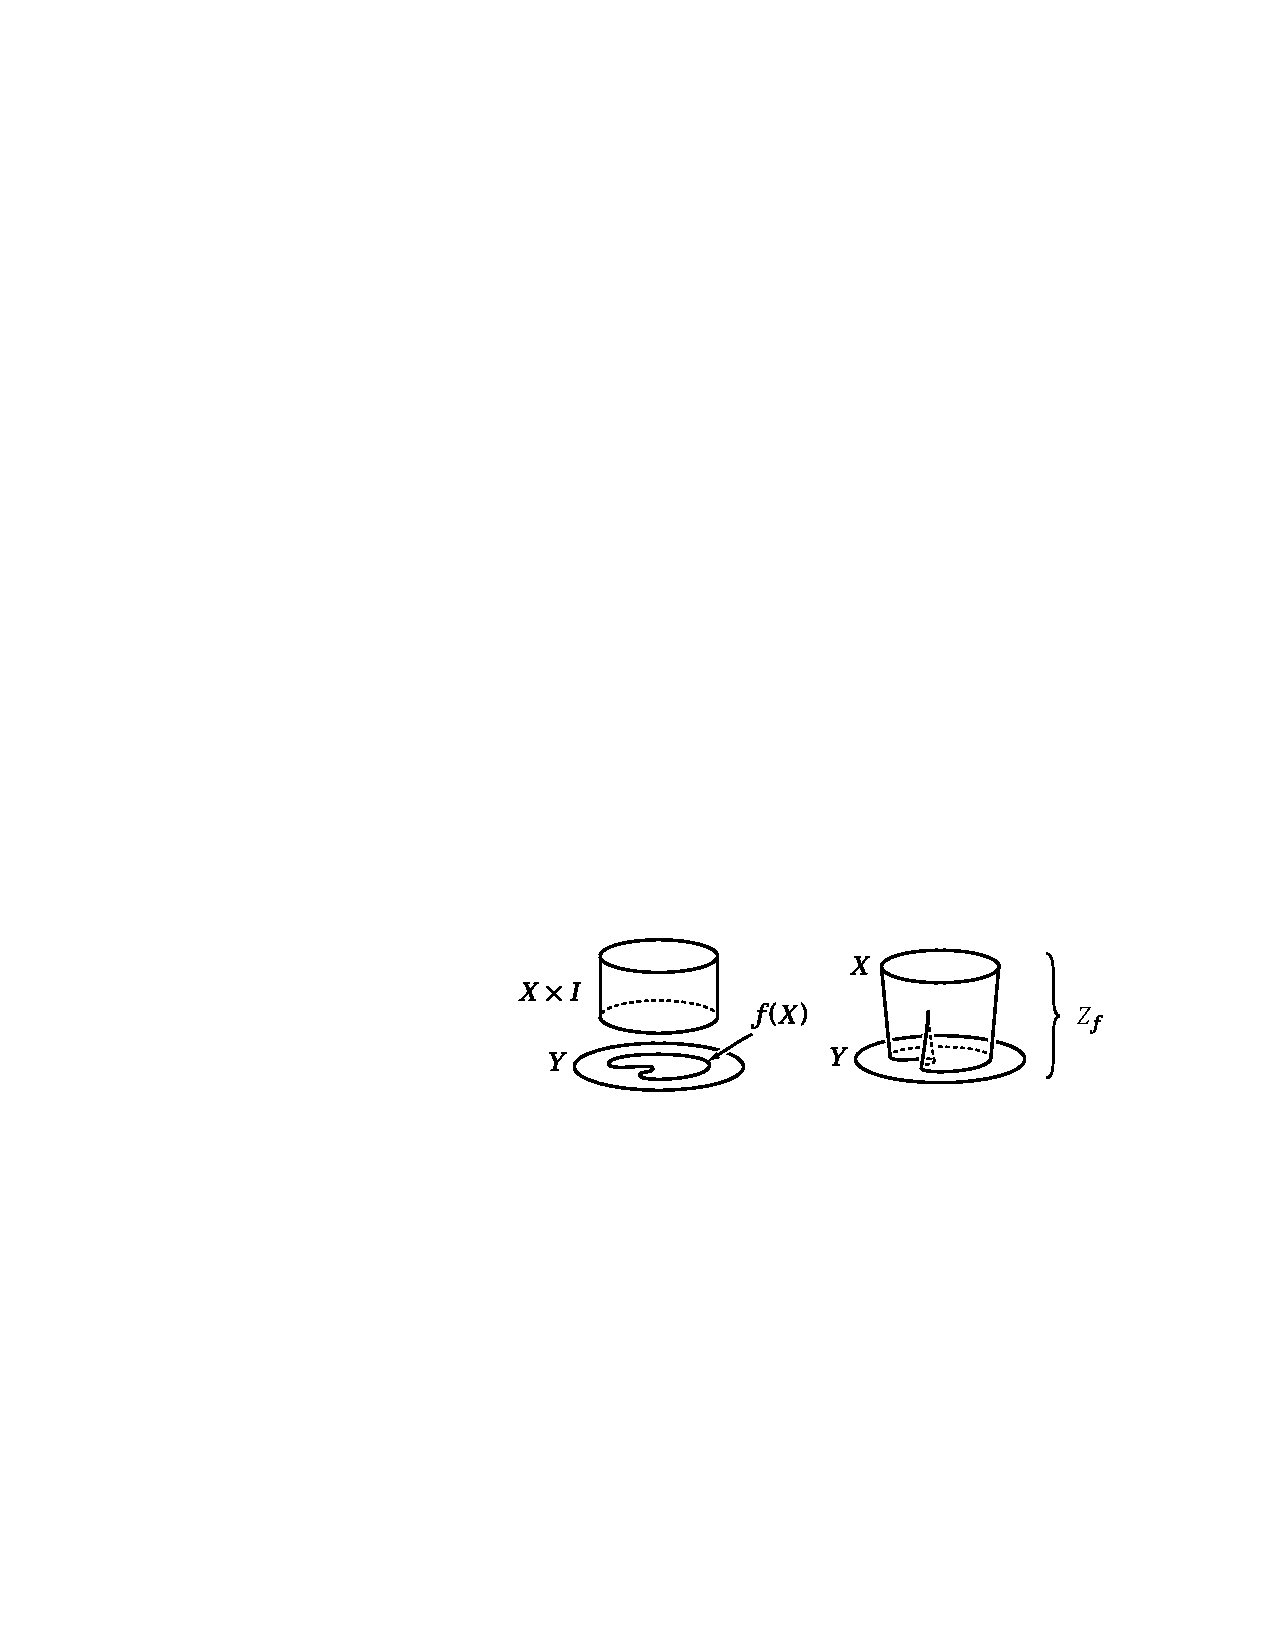
\includegraphics[width=0.5\textwidth]{figures/cylinder.pdf}
    \caption{Mapping cylinder of $f$.}
    \label{fig:mapping cyl}
\end{figure}

\begin{defn}[Mapping cylinder]\index{Mapping cylinder}
    Let $f:X\to Y$ be a map. The mapping cylinder of $f$ is the pushout $Z_f$, see Figure~\ref{fig:mapping cyl}, defined as the quotient of $(X\times I)\sqcup Y$ that identifies $(x,0)\in X\times I$ with $f(x)\in Y$:
    \[
    \begin{tikzcd}[every matrix/.append style={name=m}, row sep=large, column sep=large]
       X \sqcup X\arrow[r,"f\sqcup \mathrm{id}"]\arrow[d,"i_0\sqcup i_1",swap] & Y\sqcup X\arrow[d,"s\sqcup j"]\\
       X\times I \arrow[r,"a", swap] & Z_f
    \end{tikzcd}, \;
    \begin{matrix}
        Z_f=\bigslant{(X\times I)\sqcup Y}{(x,0)\sim f(x)},\\
        s(y)=y,\; j(x)=(x,1), \\ i_0(x)=(x,0),\; i_1(x)=(x,1).
    \end{matrix}
    \]
    We also have the projection $q:Z_f\to Y$, $(x,t)\mapsto f(x)$, $y\mapsto y$.
\end{defn}

The images $q(X\times\{1\})$ and $q(Y)$ are homeomorphic to $X$ and $Y$ respectively. When $X$ and $Y$ are homotopy equivalent, both of these subspaces of $Z_f$ can be shown to be deformation retracts of $Z_f$. Therefore two spaces $X,Y$ are homotopy equivalent iff they are homeomorphic to deformation retracts of some third space $Z$. See e.g.\ \cite[Prop.~7.46]{LeeTop} for a proof. We will also provide a proof in Corollary~\ref{cor 0.21 Hatcher}.


\begin{figure}
    \centering
    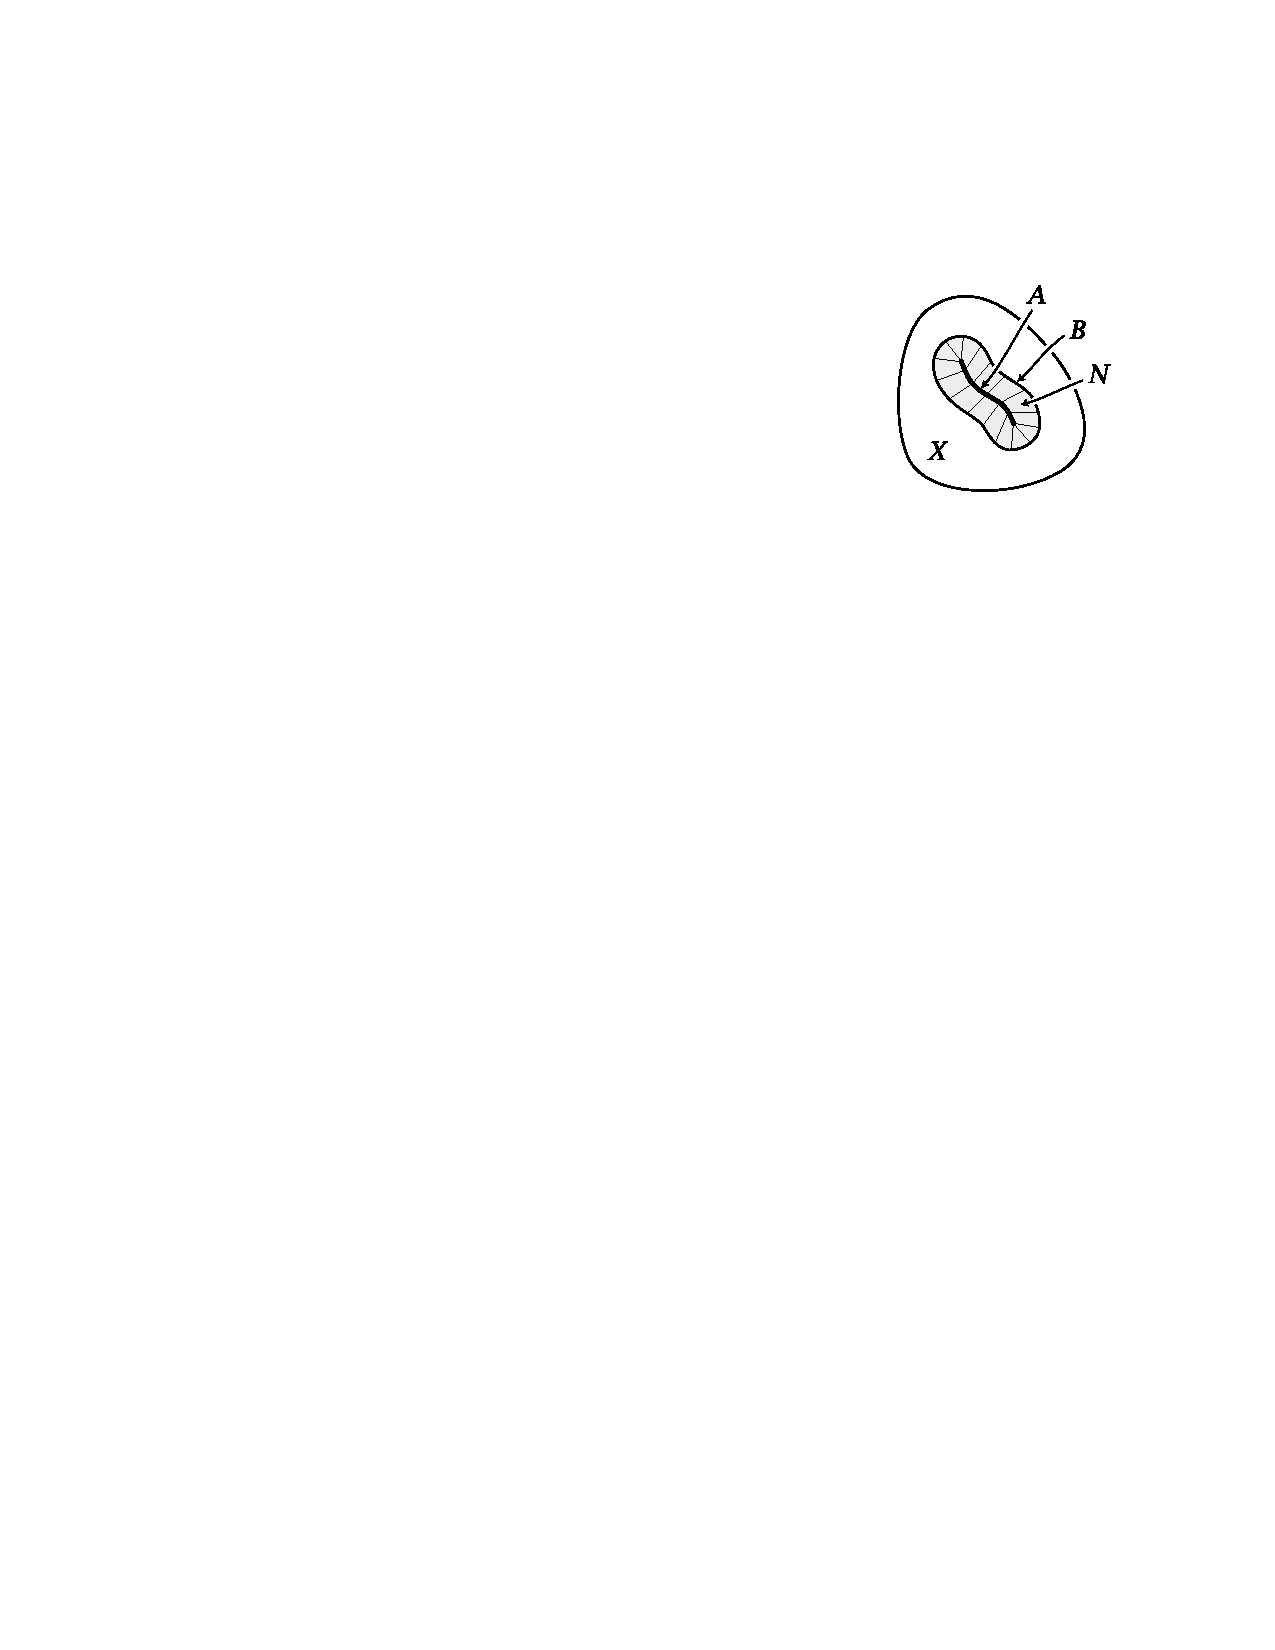
\includegraphics[width=0.3\textwidth]{figures/hep_example.pdf}
    \caption{Mapping cylinder neighborhood from Example~\ref{example Z_f hep}.}
    \label{fig: Z_f hep}
\end{figure}
\begin{example}\label{example Z_f hep}
    A pair $(X,A)$ has the \gls{hep} if $A$ has a mapping cylinder neighborhood of $X$, by which we mean a closed neighborhood $N$ containing a subspace $B$, thought of as the boundary of $N$, with $N\setminus B$ an open neighborhood of $A$, such that there exists a map $f:B\to A$ and a homeomorphism $h:Z_f\to N$ with $\restr{h}{A\cup B}=\id$. Mapping cylinder neighborhoods like this occur fairly often. For example thickened graphs in the plane, see Figure~\ref{fig: Z_f hep}.
\end{example}

\begin{xca}
    Show that the mapping cylinder of the double covering map $\pi$ of the circle $\bbS^1$ ($\pi(z)=z^2$ on the unit circle in $\bbC$) is homeomorphic to a bounded M\"obius band.
\end{xca}


\begin{prop}[{{\cite[Prop.~0.16]{Hatcher}}}]\label{prop 0.16 Hatcher}
    If $(X,A)$ is a $CW$ pair (i.e.~$A$ is a subcomplex of $X$), then $(X\times\{0\})\cup (A\times I)$ is a deformation retract of $X\times I$, hence $(X,A)$ is a cofibration.
\end{prop}
\begin{proof}
    There is a retraction $r:\bbD^n\times I\to (\bbD^n\times\{0\})\cup (\partial \bbD^n\times I)$, for example the radial projection from the point $(0,2)\in \bbD^n\times \bbR$. Then setting $r_t=t\cdot r+(1-t)\id$ gives a deformation retraction of $\bbD^n\times I$ onto $(\bbD^n\times\{0\})\cup (\partial \bbD^n\times I)$. This deformation gives rise to a deformation retraction of $X^{(n)}\times I$ onto $(X^{(n)}\times\{0\})\cup ((X^{(n-1)}\cup A^{(n)})\times I)$ since $X^{(n)}$ is obtained from the latter by attaching copies of $\bbD^n\times I$ along $(\bbD^n\times\{0\})\cup (\partial \bbD^n\times I)$. If we perform this deformation retraction in dimension $n$ during the $t$-interval $[2^{-n-1},2^{-n}]$, this infinite concatenation of homotopies is a deformation retraction of $X\times I$ onto $(X\times\{0\})\cup (A\times I)$. There is no problem with continuity of this deformation at $t=0$ since it is continuous on $X^{(n)}\times I$, being stationary there during the $t$-interval $[0,2^{-n-1}]$, and $CW$-complexes have the weak topology with respect to their skeleta so a map is continuous iff its restriction to each skeleton is continuous.
\end{proof}

\begin{prop}[{{\cite[Prop.~0.17]{Hatcher}}}]
    If the pair $(X,A)$ is a cofibration and $A$ is contractible, then the quotient map $q:X\to X\slash A$ is a homotopy equivalence.
\end{prop}
\begin{proof}
    We can use the \gls{hep} to extend a contraction of $A$ to a homotopy of maps $X\to X$ that map $A$ to $A$. This descends to a homotopy of maps $X\slash A\to X\slash A$. At $t=1$ this homotopy produces a map that maps $A$ to the point to which $A$ was contracted, so this map induces a map $X\slash A\to X$. It is then easy to see that this map is a homotopy inverse of $q$ via the two homotopies constructed above.
\end{proof}

\begin{prop}[{{\cite[Prop.~0.18]{Hatcher}}}]
    If $(X_1,A)$ is a $CW$-pair and we have the attaching maps $f,g:A\to X_0$ that are homotopic, then $X_0\sqcup_f X_1\simeq X_0\sqcup_g X_1 \rel X_0$.
\end{prop}
\begin{proof}
    If $F:A\times I\to X_0$ is the homotopy from $f$ to $g$, then consider the space $X_0\sqcup_F (X_1\times I)$. This contains both spaces in the claim of the theorem as subspaces. A deformation retraction of $X_1\times I$ onto $(X_1\times \{0\})\cup (A\times I)$ as in Proposition~\ref{prop 0.16 Hatcher} induces a deformation retraction of $X_0\sqcup_F (X_1\times I)$ onto $X_0\sqcup_f X_1$. Similarly that space retracts onto $X_0\sqcup_g X_1$. Both of these deformation retractions restrict to the identity map on $X_0$, so they give the necessary homotopy equivalence.
\end{proof}

\begin{prop}[{{\cite[Prop.~0.19]{Hatcher}}}]
    Suppose $(X,A)$ and $(Y,A)$ are cofibrations and $f:X\to Y$ is a homotopy equivalence with $\restr{f}{A}=\id_A$. Then $f$ is a homotopy equivalence $\rel A$.
\end{prop}
\begin{proof}
    We only outline the proof, see \cite[Prop.~0.19]{Hatcher} for the full details. Let $g:Y\to X$ be a homotopy inverse of $f$. The idea is to construct a homotopy from $g$ to a map $g_1$ such that $\restr{g_1}{A}=\id_A$. This is possible by taking the existing homotopy from $g\circ f$ to $\id_X$, restricting it to a homotopy from $\restr{g}{A}$ to $\id_A$, and extending it to a homotopy of maps $Y\to X$. At $t=1$ this homotopy will give the necessary $g_1$. Then we check that $g_1\circ f\simeq \id_X \,\rel A$ and that $f\circ g_1\simeq \id_Y\,\rel A$.  
\end{proof}
By applying the above to the inclusion map we immediately get the next Corollary.
\begin{cor}[{{\cite[Cor.~0.20]{Hatcher}}}]
    If $(X,A)$ is a cofibration and the inclusion $i:A\hookrightarrow X$ is a homotopy equivalence, then $A$ is a deformation retract of $X$.
\end{cor}
\begin{cor}[{{\cite[Cor.~0.21]{Hatcher}}}]\label{cor 0.21 Hatcher}
    A map $f:X\to Y$ is a homotopy equivalence iff $X$ is a deformation retract of the mapping cylinder $Z_f$. Hence, two spaces $X\simeq Y$ iff there is a third space containing both $X$ and $Y$ as deformation retracts.
\end{cor}
\begin{proof}
    We have the inclusions $i:X\hookrightarrow Z_f$ and $j:Y\hookrightarrow Z_f$, and the canonical retraction $r:Z_f\to Y$, so $f=r\circ i$ and $i\simeq j\circ f$. Since $j$ and $r$ are homotopy equivalences (``h.e.''), it follows that $f$ is a h.e.\ iff $i$ is h.e., since the composition of two h.e.'s\ is a h.e.\ and a map homotopic to a h.e.\ is also a h.e. Now we apply the preceding Corollary to the pair $(Z_f,X)$, which is a cofibration by Example~\ref{example Z_f hep} using the neighborhood $X\times [0,\frac12]$ of $X$ in $Z_f$.
\end{proof}





\subsection{Whitehead's theorem}

Let us first adapt the Compression Criterion (Proposition~\ref{prop: compression criterion}) to the context of $CW$-complexes.

\begin{lem}[Compression Lemma]\index{Lemma!compression}
    Let $(X,A)$ be a $CW$ pair (i.e.~$A$ is a subcomplex of $X$) and let $(Y,B)$ be any pair with $B\neq\varnothing$. For each $n$ such that $X\setminus A$ has cells of dimension $n$, assume that $\pi_n(Y,B,y_0)=0$ for all $y_0\in B$. Then every map $f:(X,A)\to (Y,B)$ is homotopic $\rel A$ to a map $X\to B$.

    When $n=0$ the condition $\pi_n(Y,B,y_0)=0$ for all $y_0\in B$ is to be regarded as saying that $(Y,B)$ is connected.
\end{lem}
\begin{proof}
    Assume inductively that $f$ has already been homotoped to take the skeleton $X^{(k-1)}$ to $B$. If $\Phi$ is the characteristic map of a $k$-cell $e^k$ of $X\setminus A$, the composition $f\circ \Phi:(\bbD^k,\partial \bbD^k)\to (Y,B)$ can be homotoped into $B$ $\rel \partial \bbD^k$ in view of the hypothesis that $\pi_k(Y,B,y_0)=0$ if $k>0$, or that $(Y,B)$ is $0$-connected if $k=0$. This homotopy of $f\circ\Phi$ induces a homotopy of $f$ on the quotient space $X^{(k-1)}\cup e^k$ of $X^{(k-1)}\sqcup \bbD^k$, a homotopy $\rel X^{(k-1)}$. Doing this for all $k$-cells of $X\setminus A$ simultaneously, and taking a constant homotopy on $A$, we obtain a homotopy of $\restr{f}{X^{(k)}\cup A}$ to a map into $B$. By the homotopy extension property, this homotopy extends to a homotopy defined on all of $X$, and the induction step is completed.

    Finitely many applications of the induction step finish the proof if the cells of $X\setminus A$ are bounded in dimension. Otherwise, we can perform the homotopy of the induction step during the $t$-interval $[1-2^{-k},1-2^{-k-1}]$. Any finite skeleton $X^{(k)}$ is eventually stationary under these homotopies, hence we have a well-defined homotopy $f_t$, $t\in [0,1]$ with $f_1(X)\subset B$.
\end{proof}


\begin{thm}[Whitehead's Theorem]\index{Theorem!Whitehead}\label{thm whitehead}
    If a map $f:X\to Y$ between connected $CW$-complexes induces isomorphisms $f_\ast :\pi_n(X)\to \pi_n(Y)$ for all $n$, then $f$ is a homotopy equivalence. 
    
    If $f$ is the inclusion map of a subcomplex $X\hookrightarrow Y$, the conclusion is stronger: $X$ is a deformation retract of $Y$.
\end{thm}
\begin{proof}
    In the special case that $f$ is the inclusion of a subcomplex, consider the long exact sequence on all homotopy groups of $(Y,X)$. Since $f$ induces isomorphisms of all homotopy groups, the relative groups $\pi_n(Y,X)$ are zero. Applying the Compression Lemma to the identity map on $(Y,X)$ then yields a deformation retraction of $Y$ onto $X$.

    The general case can be proved using mapping cylinders. Recall that the mapping cylinder $Z_f$ is the quotient space of the disjoint union of $X\times I$ and $Y$ under the identifications $( x, 1 ) \sim f ( x )$. Thus $Z_f$ contains both $X = X\times { 0 }$ and $Y$ as subspaces, and $Z_f$ deformation retracts onto $Y$. The map $f$ becomes the composition of the inclusion $X\hookrightarrow Z_f$ with the retraction $Z_f\to Y$. Since this retraction is a homotopy equivalence, it suffices to show that $Z_f$ deformation retracts onto $X$ if $f$ induces isomorphisms on homotopy groups, or equivalently, if the relative groups $\pi_n(Z_f,X)$ are all trivial.

    If the map $f$ happens to be \emph{cellular}\index{Cellular map}, i.e.~taking $X^{(n)}$ to $Y^{(n)}$, then $(Z_f,X)$ is a $CW$-pair and so we are done by the first paragraph of the proof. If $f$ is not cellular, we can either appeal to the Cellular Approximation Theorem~\ref{thm cell approx} which says that $f$ is homotopic to a cellular map, or use the following argument. First apply the Compression Lemma to obtain a homotopy $\rel X$ of the inclusion $(X\cup Y,X)\hookrightarrow (Z_f,X)$ to a map into $X$. Since the pair $(Z_f,X\cup Y)$ obviously is a cofibration, this homotopy extends to a homotopy from $\id_{Z_f}$ to a map $g:Z_f\to Z_f$ taking $X\cup Y$ into $X$. Then apply the Compression Lemma again to the composition $((X\times I)\sqcup Y,(X\times\partial I)\sqcup Y)\to (Z_f,X\cup Y)\overset{g}{\to} (Z_f,X)$ to finish the construction of a deformation retraction of $Z_f$ onto $X$.
\end{proof}

\begin{rem}
    The Whitehead theorem \emph{does not} say that two complexes with isomorphic homotopy groups are homotopy equivalent -- the existence of a map $f$ that generates those isomorphisms is crucial! For example, $\RP^2$ and $\bbS^2\times \RP^\infty$ both have fundamental group $\bbZ_2$ and trivial higher groups (since their universal covers $\bbS^2$ and $\bbS^2\times \bbS^\infty$ are homotopy equivalent,  $\bbS^\infty$ being contractible). But these two spaces are not homotopy equivalent because they have vastly different homology groups.
\end{rem}

\begin{defn}[Weak homotopy equivalence]
    A map $f:X\to Y$ is called a weak homotopy equivalence if all the induced homomorphisms $f_\ast:\pi_n(X,*)\to \pi_n(Y,*)$, $n\geq 0$, are isomorphisms regardless of the choice of basepoints.
\end{defn}


Whitehead's theorem therefore states that a weak homotopy equivalence between $CW$-complexes is actually a homotopy equivalence.  In general, however, weak homotopy equivalences are a much bigger class of maps. For example, there exist noncontractible spaces whose homotopy groups are all trivial, such as the `quasi-circle'. For such spaces a map to a point is a weak homotopy equivalence that but not a homotopy equivalence. 

One special case where isomorphisms by themselves do imply homotopy equivalence is when all homotopy groups are trivial.

\begin{defn}[Weakly contractible space]\index{Weakly contractible space}
    A space $X$ is called weakly contractible if $\pi_n(X)$ is trivial for all $n\geq 0$.
\end{defn}

\begin{cor}
    A weakly contractible $CW$-complex is contractible.
\end{cor}
\begin{proof}
    The inclusion map of a $0$-cell into the complex induces an isomorphism of the trivial homotopy groups, therefore by Whitehead's theorem there is a homotopy equivalence with a point.
\end{proof}

\begin{lem}[Extension Lemma]\label{lem 4.7 Hatcher}
    Let $(X,A)$ be a $CW$-pair and $Y$ is a path-connected space such that $\pi_{n-1}(Y)=0$ for all $n$ in which $X^{(n)}\setminus A^{(n)}\neq \varnothing$. Then any continuous map $f:A\to Y$ can be extended to a map $\wt f:X\to Y$.
\end{lem}
\begin{proof}
    Assume $f$ was already extended to a map $f^{(n-1)}$ over the $(n-1)$-skeleton. Then an extension over all $n$-cells exists iff the composition of the cell's attaching map $\bbS^{n-1}\to X^{(n-1)}$ with $f^{(n-1)}$ is nullhomotopic.
\end{proof}





\subsection{Cellular approximation}


Recall when we applied the van Kampen theorem to compute $\pi_1(\bbS^n)=0$ for $n\geq 2$, we implicitly used the fact that every loop can be deformed to miss at least one point in $\bbS^n$, and then it can obviously be contracted to a point since $\bbS^n\setminus *$ is contractible. This is not an obvious fact since there exist space-filling loops that are surjective. Similar space-filling maps exist for all pairs $\bbS^m\to \bbS^n$ with $m<n$.

For homotopy theory of $CW$ complexes it turns out to be sufficient to work with maps that map $n$-skeleta to $n$-skeleta, and any other map is homotopic to one of this class.



\begin{lem}[{{\cite[Lem.~4.10]{Hatcher}}}]\label{lem 4.10 hatcher}
    Let $f:Y^n\to Z$ be a map, where $Z$ is obtained from a subspace $W$ by attaching a $k$-cell $e^k$. Then there is a homotopy $f_t:(I^n,f^{-1}(e^k))\to (Z,e^k)$ $\rel f^{-1}(W)$ from $f=f_0$ to a map $f_1$ for which there is a polyhedron $K\subset I^n$ such that:
    \begin{enumerate}[label=(\alph*)]
        \item $f_1(K)\subset e^k$ and $\restr{f_1}{K}$ is piecewise linear (i.e.~linear on each face of $K$) with respect to some identification of $e^k$ with $\bbR^n$.
        \item There exists a nonempty open $U\subset e^k$ such that $f_1^{-1}(U)\subset K$.
    \end{enumerate}
\end{lem}
\begin{proof}
    Identifying $e^k$ with $\bbR^k$, let $B_1,b_2\subset e^k$ be the closed balls of radius $1$ and $2$ at the origin. Since $f^{-1}(B_2)$ is closed and therefore compact in $I^n$, it follows that $f$ is uniformly continuous on $f^{-1}(B_2)$. Thus there exists $\epsilon>0$ such that $|x-y|<\epsilon$ implies $|f(x)-f(y)|<\frac 12$ for all $x,y\in f^{-1}(B_2)$. Subdivide the interval $I$ so that the induced subdivision of $I^n$ into cubes has each cube lying in a ball of diameter less than $\epsilon$. Let $K_1$ be the union of all the cubes meeting $f^{-1}(B_1)$ and let $K_2$ be the union of all cubes meeting $K_1$. We may assume $\epsilon$ is chosen smaller than half the distance between the compact sets $f^{-1}(B_1)$ and $I^n\setminus f^{-1}(\int B_2)$, and then we will have $K_2\subset f^{-1}(B_2)$. See Figure~\ref{fig:cell_approx}.

    Now we subdivide all the cubes of $K_2$ into simplices. This can be done inductively in the dimension by taking the center point of a cube as a new vertex and joining it by a cone to each simplex in boundary of the cube. 

    Let $g:K_2\to e^k=\bbR^k$ be the map that equals $f$ on all vertices of simplices of the subdivision and is linear on each simplex. Let $\varphi:K_2\to [0,1]$ be the map that is linear on simplices and has value $1$ on vertices in $K_1$ and $0$ on vertices of $K_2\setminus K_1$. Thus $\restr{\varphi}{K_1}=1$. Define a homotopy $f_t:K_2\to e^k$ by the formula $(1-t\varphi)\cdot f+(t\varphi)\cdot g$, so $f_0=f$ and $\restr{f_1}{K_1}=\restr{g}{K_1}$. Since $f_t$ is constant in $t$ on simplices in $K_2$ disjoint from $K_1$, and in particular on simplices in the closure $\widebar{I^n\setminus K_2}$, we may extend $f_t$ to be the constant homotopy of $f$ on $I^n\setminus K_2$.

    The map $f_1$ takes the closure $\widebar{I^n\setminus K_1}$ to a compact set $C$ which, we claim, is disjoint from the center $0$ of $B_1$ and hence from a neighborhood $U$ of $0$. This will prove the lemma, with $K=K_1$ since we will have $f_1^{-1}(U)\subset K_1$ with $f_1$ piecewise linear on $K_1$ where it is equal to $g$.

    The verification of the claim has two steps:
    \begin{enumerate}[label=(\arabic*)]
        \item On $I^n\setminus K_2$ we have $f_1=f$, and $f$ takes $I^n\setminus K_2$ outside $B_1$ since $f^{-1}(B)\subset K_2$ by construction.
        \item For a simplex $\sigma$ of $K_2$ not in $K_1$ we have $f(\sigma)$ contained in some ball $B_\sigma$ of radius $\frac 12$ by the choice of $\epsilon$ and the fact that $K_2\subset f^{-1}(B_2)$. Since $B_\sigma$ is convex, we must also have $g(\sigma)\subset B_\sigma$. We know that $g(\sigma)\subset B_\sigma$, hence also $f_t(\sigma)\subset B_\sigma$ for all $t$, and in particular $f_1(\sigma)\subset B_\sigma$. We know that $B_\sigma\cancel{\subset} B_1$ since $\sigma\cancel{\subset}K_1$ and thus $\sigma\cancel{\subset}f^{-1}(B_1)$. The radius of $B_\sigma$ is half that of $B_1$, so it follows that $0\notin B_\sigma$, and hence $0\notin f_1(\sigma)$.
    \end{enumerate}
\end{proof}

\begin{figure}
    \centering
    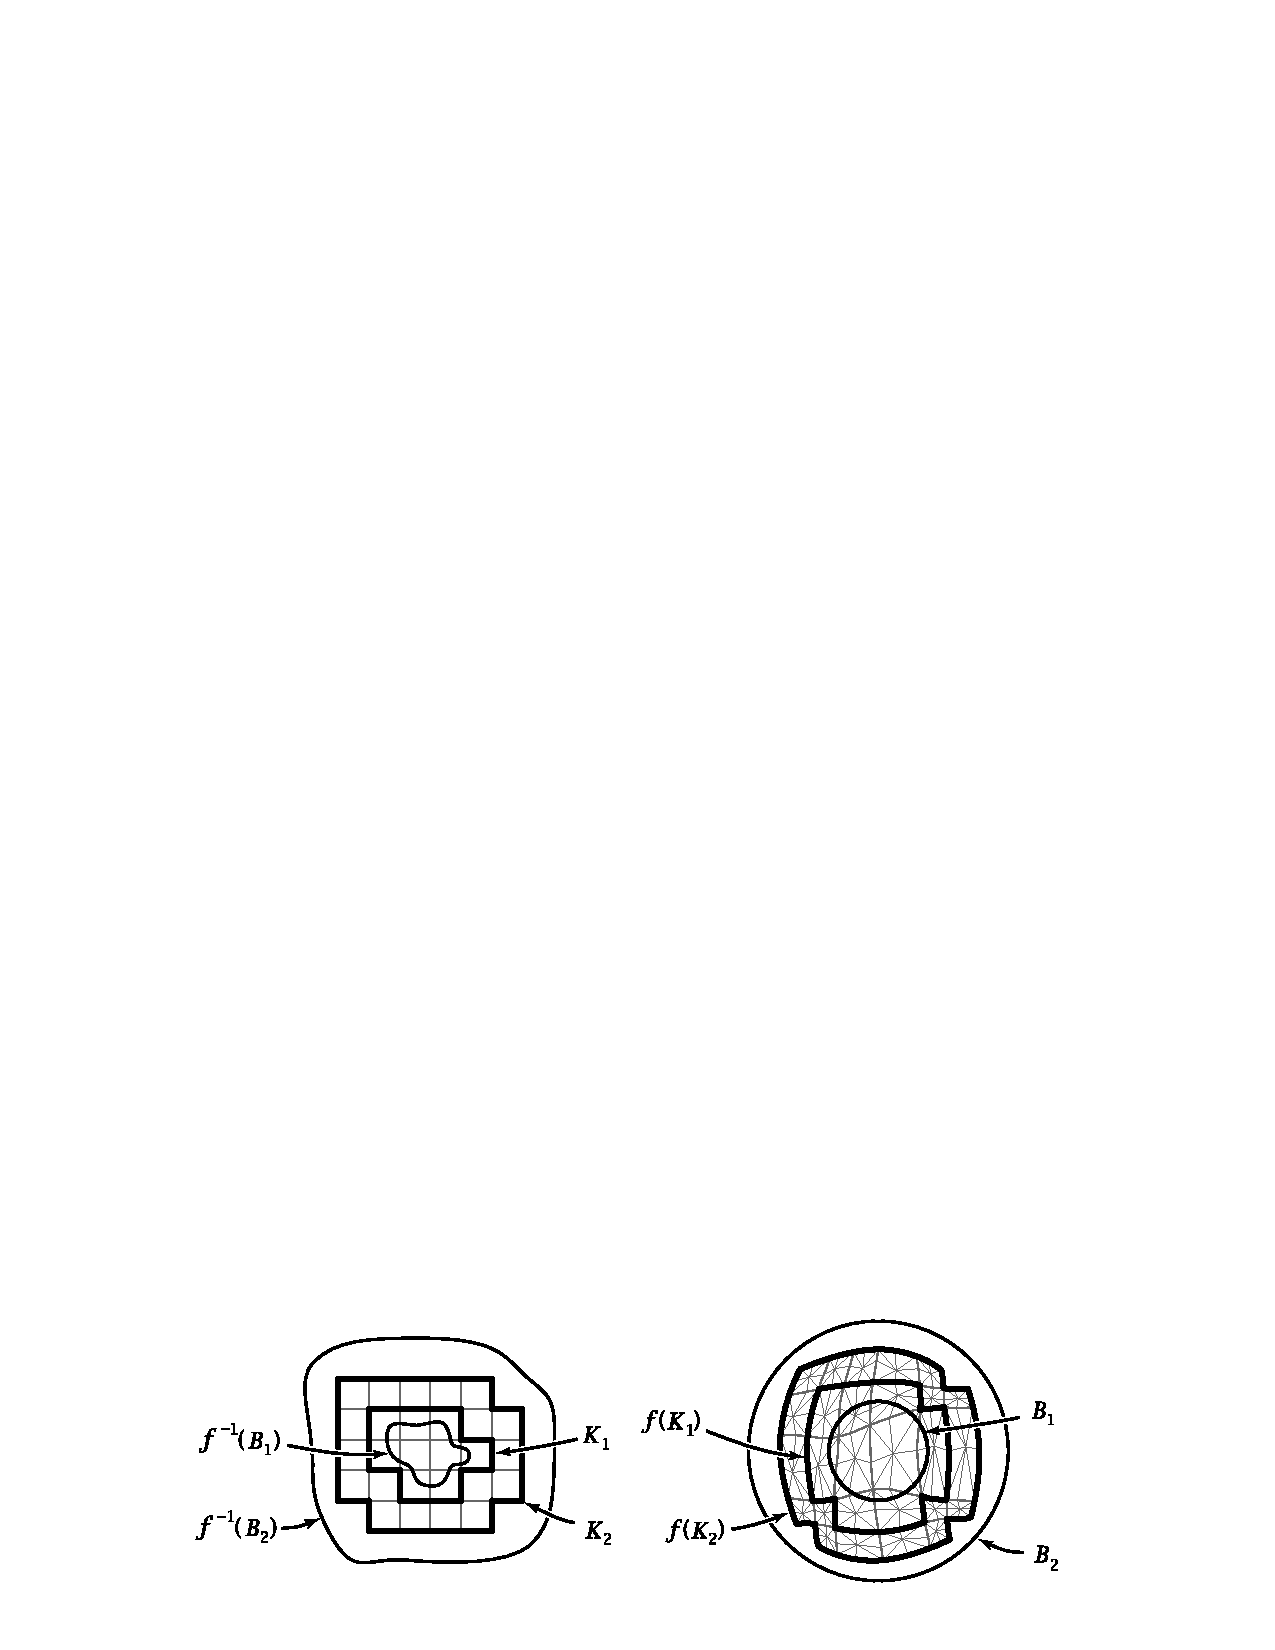
\includegraphics[width=0.7\textwidth]{figures/cell_approx.pdf}
    \caption{Subdivision from the proof of Lemma~\ref{lem 4.10 hatcher}.}
    \label{fig:cell_approx}
\end{figure}


\begin{thm}[Cellular Approximation Theorem]\index{Theorem!Cellular Approximation}\label{thm cell approx}
    Every map $f:X\to Y$ of $CW$-complexes is homotopic to a cellular map. 

    Every map $f:(X,A)\to (Y,B)$ of $CW$-pairs is homotopic $\rel A$ to a cellular map.
\end{thm}
\begin{proof}
    Suppose inductively that $f$ is cellular on $X^{(n-1)}$, and let $e^n$ be an $n$-cell of $X$. The closure of $e^n$ in $X$ is compact, being the image of a characteristic map for $e^n$ (Proposition~\ref{prop f(compact)=compact}), so $f$ takes the closure of $e^n$ to a compact set in $Y$.  Therefore $f(e^n)$ meets finitely many cells of $Y$.  Let $e^k\subset Y$ be a cell of highest dimension meeting $f(e^n)$. We may assume $k>n$, otherwise $f$ is already cellular on $e^n$.

    Now we apply Lemma~\ref{lem 4.10 hatcher} to the composition of $f:X^{(n-1)}\cup e^n\to Y^{(k)}$ with a characteristic map $I^n\to X$ for $e^n$, with $Z=Y^{(k)}$ and $W=Y^{(k)}\setminus e^k$. The homotopy given by the lemma is fixed on $\partial I^n$, hence induces a homotopy $f_t$ of $\restr{f}{X^{(n-1)}\cup e^n}$ fixed on $X^{(n-1)}$. The image of the resulting map $f_1$ intersects the open set $U\subset e^k$ in a set contained in the union of finitely many hyperplanes of dimension at most $n$, so if $n<k$ there will be points $p\in U$ not in the image of $f_1$. 
    
    In summary, it is possible to deform $\restr{f}{X^{(n-1)}\cup e^n}$, staying fixed on $X^{(n-1)}$, so that $f(e^n)$ misses some point $p\in e^k$. Then we can deform $\restr{f}{X^{(n-1)}\cup e^n}$ $\rel X^{(n-1)}$ so that $f(e^n)$ misses the whole cell $e^k$ by composing with a deformation retraction of $Y^{(k)}\setminus \{p\}$ onto $Y^{(k)}\setminus e^k$. By finitely many iterations of this process we eventually make $f(e^k)$ miss all cells of dimension greater than $n$. Doing this for all $n$-cells simultaneously, staying fixed on $n$-cells in $A$ where $f$ is already cellular, we obtain a homotopy of $\restr{f}{X^{(n)}}$ $\rel X^{(n-1)}\cup A^{(n)}$ to a cellular map. 

    The induction step is then completed by appealing to the \gls{hep} in Proposition~\ref{prop 0.16 Hatcher} to extend this homotopy, together with the constant homotopy on $A$, to a homotopy defined on all of $X$. Letting $n$ go to infinity, the resulting possibly infinite sequence of homotopies can be realized as a single homotopy by performing the $n$-th homotopy during the $t$-interval $[1-2^{-n},1-2^{-n-1}]$. This homotopy will eventually be stationary on every $k$-skeleton and hence continuous at $1$.
\end{proof}

\begin{cor}\label{cor pi_n(S^k)=0}
    $\pi_n(\bbS^k)=0$ for $n<k$.
\end{cor}
\begin{proof}
    If $\bbS^n$ and $\bbS^k$ are given $CW$ structures with one $0$-cell (serving as as basepoint) and one $n(k)$-cell, then every pointed map $\bbS^n\to \bbS^k$ can be homotoped, fixing the basepoint, to be cellular, and hence constant if $n<k$.
\end{proof}





\subsection{\texorpdfstring{$CW$}{CW} approximation}\label{sec: CW approx}

Whitehead's theorem obviously holds not just for $CW$-complexes, but also for spaces that are homotopy equivalent to them. We now show that any topological space is \emph{weakly} homotopy equivalent to a $CW$-complex.

\begin{defn}[$CW$ approximation]
    A $CW$ approximation of a topological space $X$ is a $CW$-complex $Z$ with a weak homotopy equivalence $f:Z\to X$.
\end{defn}

\begin{prop}[{{\cite[Prop.~4.13]{Hatcher}}}]
    Every space $X$ has a $CW$ approximation $f:Z\to X$. If $X$ is path-connected, $Z$ can be chosen to have a single $0$-cell, with all other cells attached by pointed maps. Thus every connected $CW$-complex is homotopy equivalent to a $CW$-complex with these additional properties.
\end{prop}
\begin{proof}
    The construction of a $CW$ approximation $f:Z\to X$ for a space $X$ is inductive. Suppose given a $CW$-complex $A$ with a map $f:A\to X$ and suppose we have chosen a basepoint $0$-cell $*$ in each component of $A$. Then for an integer $k\geq 0$ we will attach $k$-cells to $A$ to form a $CW$ complex $B$ with a map $f:B\to X$ extending the given $f$, such that the induced homomorphism $f_\ast:\pi_i(B,*)\to \pi_i(X,f(*))$ is injective for $i=k-1$ and surjective for $i=k$, for all basepoints $*$.

    There are two steps:
    \begin{enumerate}[label=(\arabic*)]
        \item Choose maps $\varphi_\alpha:(\bbS^{k-1},s_0)\to (A,*)$ representing a set of generators for the kernel of $f_\ast:\pi_{k-1}(A,*)\to \pi_{k-1}(X,f(*))$ for all basepoints $*$. We map assume the maps $\varphi_\alpha$ are cellular, where $\bbS^{k-1}$ has its standard $CW$ structure with $s_0$ as the $0$-cell. Attaching cells $e_\alpha^k$ to $A$ via $\varphi_\alpha$ then produces a $CW$ complex, and the map $f$ extends over these cells using nullhomotopies of $f\circ \varphi_\alpha$, which exist by the choice of the $\varphi_\alpha$'s.
        \item Choose maps $f_\beta:\bbS^k\to X$ representing generators for the groups $\pi_k(X,f(*))$, attach cells $e_\beta^k$ to $A$ via the constant maps at the appropriate basepoints $*$, and extend $f$ over the resulting spheres $S_\beta^k$ via the $f_\beta$'s.
    \end{enumerate}

    The surjectivity of $f_\ast$ holds by construction. For the injectivity, an element of the kernel of $f_\ast:\pi_{k-1}(B,*)\to \pi_{k-1}(X,f(*))$ can be represented by a cellular map $h:\bbS^{k-1}\to B$. This has image in $A$, so is in the kernel of $f_\ast:\pi_{k-1}(A,*)\to \pi_{k-1}(X,f(*))$ and hence is homotopic to a linear combination of the $\varphi_\alpha$'s, which are nullhomotopic in $B$, so $h$ is nullhomotopic as well. When $k=1$ there is no group structure on $\pi_{k-1}$ so injectivity on $\pi_0$ does not follow from having a trivial kernel, and we modify the construction by choosing the cells $e_\alpha^1$ to join each pair of basepoints $*$ that map by $f$ to the same path-component of $X$. The map $f$ can then be extended over these $1$-cells $e_\alpha^1$.

    Note that if $f$ happened to be injective or surjective on $\pi_i$ for some $i<k-1$ or $i<k$, respectively, then this remains true after attaching the $k$-cells. This is because attaching $k$-cells does not affect $\pi_i$ if $i<k-1$, by cellular approximation, not does it destroy surjectivity on $\pi_{k-1}$ or indeed any $\pi_i$, obviously.

    Now to construct a $CW$ approximation $f:Z\to X$ one can start with $A$ consisting of one point for each path-component of $X$, with $f:A\to X$ mapping each of them to the corresponding path-component. Having now a bijection on $\pi_0$, attach $1$-cells to $A$ to create a surjection on $\pi_1$  for each path-component, then $2$-cells to improve this to an isomorphism on $\pi_1$ and a surjection on $\pi_2$, and so on for each successive $\pi_i$. After all cells have been attached one has a $CW$-complex $Z$ and a weak homotopy equivalence $f:Z\to X$.
\end{proof}

\begin{rem}
    One can apply this technique to produce $CW$ approximations of pairs $(X,A)$. First construct a $CW$ approximation $f_A:Z_A\to A$, then starting with the composition $Z_A\to A\hookrightarrow X$, attach cells to $Z_A$ to create a weak homotopy equivalence $f:Z\to X$ extending $f_A$. The induced map $f_\ast$ will be an isomorphism of relative homotopy groups  by the five-lemma~\ref{5-lemma} applied to the two sequences of morphisms in relative and absolute homotopy.
\end{rem}


Running ahead, we will be calling a $CW$-pair $(Z,A)$ \emph{$n$-connected} if $\pi_k(Z,A,a)=0$ for $k=1,\ldots n$ and all $a\in A$, and the inclusion-induced map $\pi_0(A)\to \pi_0(Z)$ is surjective. 

\begin{defn}[$n$-connected $CW$ model]
    An $n$-connected $CW$ model for a $CW$ pair $(X,A)$ with a nonempty subcomplex $A$ is an $n$-connected $CW$ pair $(Z,A)$ and a map $f:Z\to X$ with $\restr{f}{A}=\id_A$ such that the induced homomorphism $f_\ast:\pi_i(Z)\to \pi_i(X)$ is an isomorphism for $i>n$ and an injection for $i=n$, for all choices of basepoint.
\end{defn}

One can think of $Z$ as a homotopy-theoretic hybrid of $X$ and $A$. As $n$ increases it looks more and more like $A$, and less like $X$. We have just shown that $n$-connected models always exist, and can be obtained from $A$ by attaching cells in dimensions $>n$ so that by cellular approximation $(Z,A)$ is $n$-connected. Moreover, it is not difficult to show (\cite[Prop.~4.18, Cor.~4.19]{Hatcher}) that these models (and therefore $CW$ approximations as well) are unique up to homotopy equivalence $\rel A$. In particular, $CW$ approximations are unique up to homotopy equivalence.



\begin{example}[Postnikov towers]
    We can use this technique to construct, for each connected $CW$-complex $X$, and each $n\geq 1$, a $CW$-complex $X_n$ containing $X$ as a subcomplex such that:
    \begin{enumerate}[label=(\alph*)]
        \item $\pi_i(X_n)=0$ for $i>n$;
        \item The inclusion $X\hookrightarrow X_n$ induces an isomorphism on $\pi_i$ for $i\leq n$.
    \end{enumerate}
    To do this, apply the general construction to the constant map of $X$ to a point, starting at the stage of attaching cells of dimension $n+2$. Thus we attach $(n+2)$-cells to $X$ using cellular maps $\bbS^{n+1}\to X$ that generate $\pi_{n+1}(X)$ to form a space with trivial $\pi_{n+1}$, then for this space we attach $(n+3)$-cells to make $\pi_{n+2}$ trivial, and so on. The result is a complex $X_n$ with the desired properties.

    The inclusion $X\hookrightarrow X_n$ extends to a map $X_{n+1}\to X_n$ since $X_{n+1}$ is obtained from $X$ by attaching cells of dimension at least $n+3$, and $\pi_i(X_n)=0$ for $i>n$ so we can apply the Extension Lemma~\ref{extension lemma}. Thus we have a commutative diagram called a Postnikov tower for X. One can regard the spaces $X_n$ as truncations of $X$ which provide successively better approximations to $X$ as $n$ increases. There is a weak homotopy equivalence between $X$ and the inverse limit of the Postnikov tower $\limit X_n$, i.e.~$X$ is a $CW$ approximation of $\limit X_n$.
    \[
    \begin{tikzcd}[every matrix/.append style={name=m}]
       & \vdots \arrow[d]\\
       & X_3 \arrow[d]\\
       & X_2 \arrow[d]\\
       X\arrow[r]\arrow[ur]\arrow[uur] & X_1
    \end{tikzcd}
    \]
\end{example}


Now we prove one of the statements announced in Remark~\ref{rem: classifying space for discrete G}. 
\begin{prop}\label{prop X_G}
    For every (discrete) group $G$ there exists a path-connected two-dimensional $CW$-complex $X_G$ such that $\pi_1(X_G)\cong G$.
\end{prop}
\begin{proof}
    Consider a presentation of the group as the quotient of a free group $\<J\>$ by some normal subgroup $\<R\>$ generated by a set of relations $R$. Construct the 1-skeleton $X^{(1)}$ of $X_G$ as a wedge sum of circles $\bigvee_{j\in J}\bbS^1$. Every relation describes a loop in $X^{(1)}$: for example if $ab^{-1}c^2$ is a relation, then the loop is given by going around $a$ once, around $b$ once in the opposite direction, and then twice around $c$. For each relation $r\in R$ take a 2-cell $\bbD^2$ with boundary $\bbS^{1}$ and define an attaching map $\varphi_r:\bbS^1\to X^{(1)}$ so that it represents the loop specified by $r$. The resulting $CW$-complex $X_G=X^{(2)}_G$ is then a 2-dimensional complex whose fundamental group is, by construction, isomorphic to $G$.
\end{proof}
We will eventually incorporate this space $X_G$ as into the so called classifying space $\rmB G$, so $\pi_1(\rmB G)\cong \pi_1(X_G)\cong G$, i.e.\ the inclusion is a weak 1-equivalence. The classifying space $\rmB G$ must have $\pi_{n+1}(\rmB G)\cong \pi_{n}(G)$, so in the case of discrete $G$ this is $\pi_{\geq 2}(\rmB G)\cong 0$. In other words, $\rmB G$ for discrete groups is the first Postnikov truncation of the space $X_G$ we just constructed.


\begin{example}\index{Lens spaces}
    Consider the cyclic group $G=C_n\cong \bbZ\slash n\bbZ$ for some integer $n$. Then $X_G$ is $\RP^2$ for $n=2$, and for higher $n$ it is a subcomplex of the lens space with fundamental group $C_n$.
\end{example}

\begin{defn}[Aspherical space]\index{Aspherical space}
    A space $X$ is called aspherical if $\pi_n(X)=0$ for all $n\geq 2$.
\end{defn}

\begin{defn}[First Eilenberg-MacLane space]\index{Eilenberg-MacLane space}\label{def: K(G,1)}
    For a group $G$, the first Eilenberg-MacLane space for $G$, denoted $\rmK(G,1)$, is defined up to weak homotopy equivalence as an aspherical space whose fundamental group is $G$. It can be realized as the first Postnikov truncation $(X_G)_1$ of the space $X_G$ constructed in Proposition~\ref{prop X_G}, and in the case of discrete $G$ it coincides with the so called classifying space $\rmB G$. Since $\pi_1$ is the only nontrivial homotopy group of $\rmK(G,1)$, its universal covering space is contractible by Whitehead's theorem.
\end{defn}


\begin{rem}
    We will later be able to define Eilenberg-MacLane and classifying spaces so that they are unique up to homotopy equivalence, not just weak homotopy equivalence. Namely they will be required to be quotients of weakly contractible $CW$-complexes by a free group action, and of course weakly contractible $CW$-complexes are actually contractible by Whitehead's theorem, which will induce a homotopy equivalence between the resulting quotients as well.
\end{rem}


\begin{cor}
    For every discrete group $G$ there exists a (unique up to homotopy equivalence) universal $G$-principal covering $\rmE G\to \rmK(G,1)$ with contractible total space $\rmE G$.
\end{cor}

\begin{example}[Lens spaces {{\cite[Example~2.43]{Hatcher}}}]\index{Lens spaces}\label{example Lens spaces}
    Given an integer $m>1$ and integers $l_1,\ldots,l_n$ relatively prime to $m$, define the lens space $L=L_m(l_1,\ldots,l_n)$ as the orbit space $\bbS^{2n-1}\slash \bbZ_m$ of the unit sphere $\bbS^{2n-1}\subset\bbC^n$ with the action of $\bbZ_m$ generated by the rotation $(z_1,\ldots,z_n)\mapsto (e^{2\pi\rmi l_1/m}z_1,\ldots e^{2\pi\rmi l_n/m} z_n)$. In particular, when $m=2$, for any odd $l_i$'s this is the antipodal map and $L=L_2(1,\ldots,1)=\RP^{2n-1}$. In general, the projection $\bbS^{2n-1}\to L$ is a covering space since the action of $\bbZ_m$ is free: each point of $\bbS^{2n-1}$ has at least some coordinate $z_j$ nonzero and then $e^{2\pi\rmi l_j/m}z_j=\neq z_j$ for $0<k<m$ because of the assumption that $l_j$ is relatively prime to $m$.

    One can construct a $CW$-structure on $L$ with one cell in each dimension from $0$ to $2n-1$, see \cite[Example~2.43]{Hatcher}. These structures also induce a $CW$-structure on the infinite lens spaces $L_m(l_1,l_2,\ldots)=\bbS^\infty\slash \bbZ_m$ defined in the same way, which equals the union of the spaces $L_m(l_1,l_2,\ldots,l_n)$ for $n=1,2\ldots$, each of which is a subcomplex of the next. Since the universal covering space $\bbS^\infty$ is contractible, the infinite lens space is an Eilenberg-MacLane space $\rmK(\bbZ_m,1)$.
\end{example}


\begin{xca}\label{xca two definitions of lens spaces}
    Show that the above definition of $L_p(q)$ agrees with the definition of $L(p;q)$ from Example~\ref{example Lens space bredon}. See illustrations \href{https://math.stackexchange.com/a/1186808/31363}{here}. We will give a more direct solution via bundles in Example~\ref{ex monopole bundles}.
\end{xca}










\subsection{Hurewicz fibrations}

\begin{defn}[Hurewicz fibration]\index{Fibration!Hurewicz}
    A continuous map $p:E\to B$ is a (Hurewicz) fibration if it satisfies the \gls{hlp} for \emph{all} spaces $X$. That is, in the diagram (\ref{HLP diagram}) a ``lifted'' homotopy $\wt H$ with initial condition $\wt H(x,0)=\wt H_0(x)$ that makes the diagram commute exists for any space $X$, any homotopy $h:X\times I\to B$, and any continuous $\wt H_0:X\to E$. Here, $i_0$ is the inclusion map $i_0(x)=(x,0)$.
    \[
    \begin{tikzcd}[every matrix/.append style={name=m}, row sep=large, column sep=large]
       X \arrow[r,"\wt H_0"]\arrow[d,"i_0",swap] & E\arrow[d,"p"]\\
       X\times I \arrow[r,"H", swap] \arrow[ur,"\wt H",dashed, swap] & B
    \end{tikzcd} \label{HLP diagram}
    \]
    A morphism between two fibrations $p_1:E_1\to B_2$ and $p_2:E_2\to B_2$ is a pair of continuous maps $f:B_1\to B_2$ and $F:E_1\to E_2$ such that the square formed by them commutes, $p_2\circ F=f\circ p_1$. Such maps are called \emph{fiber-preserving}.
\end{defn}

\begin{example}
    The natural projections in a direct product are fibrations. Indeed, for the projection $\pi:B\times F\to B$ the homotopy lifting problem, defined by a map $f:X\times I\to B$ and an initial condition $\wt{f}_0:X\times\{0\}\to B\times F$, is solved by the map
    \[\wt{f}:X\times I\to B\times F, \quad \wt{f}(x,t)=(f(x,t),\wt{f}_0(x,0)).\]
\end{example}


\begin{lem}\label{lem evaluation fibration}
    The evaluation map $\epsilon=\epsilon_0\times \epsilon_1: B^I\to B\times B$, $\gamma\mapsto (\gamma(0),\gamma(1))$ is a fibration for any space $B$.
\end{lem}
\begin{proof}
    Indeed, any map $X\times I\to B\times B$ can be lifted into $B^I$ because this is equivalent to finding an extension $X\times I\times I\to B$. Here, the ``initial condition'' fixes the values of this extension on three sides of the square $I\times I$, namely on $X\times J^1=(X\times \{0\}\times I)\cup (X\times I\times \{0,1\})$, where the values on the first piece are given by the initial condition of the homotopy lifting problem, and on the second piece by the given map $X\times I\to B\times B$. But this space, $X\times J^1$, is a retract of $X\times I^2$, so we can extend the map simply by precomposing it with the retraction $r:X\times I^2\to X\times J^1$ to get the required extension.
\end{proof}

\begin{defn}[Mapping fibration]
    Let $f:Y\to B$ be any continuous map. Define the space $P_f$, also known as the \emph{mapping path space}, as the fibered product (pullback) \[P_f=B^I\times_B Y=\{(\gamma,y)\in B^I\times Y\mid \gamma(1)=f(y)\}.\] It results from the pullback square
     \[
    \begin{tikzcd}[every matrix/.append style={name=m}]
       P_f \arrow[r]\arrow[d] & Y\arrow[d,"f"]\\
       B^I \arrow[r,"\epsilon_1", swap] & B
    \end{tikzcd}
    \]
     The mapping fibration of $f$ is the map $p_f:P_f\to B$ given by $p_f(\gamma,y)=\gamma(0)$.
\end{defn}
\begin{prop}
    For any map $f:Y\to B$, the mapping fibration $p_f:P_f\to B$ is indeed a fibration.
\end{prop}
\begin{proof}
    Suppose we have a diagram (\ref{HLP diagram}) with $E=P_f$. Denote $\mathrm{pr}_1$ and $\mathrm{pr}_2$ the natural projections onto the factors of the direct product $B^I\times Y$. We can first extend $\mathrm{pr}_2\circ \wt{H}_0$ as in:
    \[
    \begin{tikzcd}[every matrix/.append style={name=m}]
       X \arrow[r,"\mathrm{pr}_2\circ \wt H_0"]\arrow[d,"i_0",swap] & Y\\
       X\times I \arrow[ur,"\wt{h}_0",dashed, swap] & 
    \end{tikzcd}
    \]
    and then use Lemma~\ref{lem evaluation fibration} to find a diagonal mapping as in
    \[
    \begin{tikzcd}[every matrix/.append style={name=m}]
       X \arrow[r,"\mathrm{pr}_1\circ \wt H_0"]\arrow[d,"i_0",swap] & B^I\arrow[d,"\epsilon"]\\
       X\times I \arrow[ur,"\chi",dashed, swap]\arrow[r,"H\times (f\circ \wt{h}_0)",swap] & B\times B 
    \end{tikzcd}
    \]
    We can verify that $\wt H=\chi \times \wt{h}_0:X\times I\to P_f$ is the required lifting. Indeed it lands in $P_f$ because $\epsilon_1\circ\chi=f\circ\wt{h}_0$, and makes the diagram commute because $p\circ \chi=\epsilon_0\circ \chi=H$ and $(\chi\times \wt{h}_0)\circ i_0=(\mathrm{pr}_1\circ \wt H_0)\times (\mathrm{pr}_2\circ \wt H_0)=\wt H_0$. 
\end{proof}
As a consequence, we observe that every continuous map is a fibration up to homotopy equivalence on the domain.
\begin{cor}
    Let $f:Y\to B$ be a continuous map. Denote by $\kappa_b\in B^I$ the constant path $\gamma(t)\equiv b$ for $b\in B$. Then the map $\phi$ in 
    \[
    \begin{tikzcd}[every matrix/.append style={name=m}]
       & P_f\arrow[d,"p_f"]\\
       Y\arrow[ur,"\phi",dashed]\arrow[r,"f",swap] & B
    \end{tikzcd}
    \]
    given by $\phi(y)=(\kappa_{f(y)},y)$ is a homotopy equivalence that makes the diagram commute. 
\end{cor}
\begin{proof}
    The homotopy in question restricts paths $\gamma:I\to B$ to the interval $[t,1]$, so $\gamma\mapsto \restr{\gamma}{[t,1]}$.
\end{proof}

Motivated by this, one defines the \emph{homotopy fiber} of $f$ over $b\in B$:
\[i: p_f^{-1}(b)=\{(\gamma,y)\mid \gamma(0)=b, \gamma(1)=f(y)\}.\]
Note that there is a canonical injection from the fiber of $f$ into the fiber of $p_f$ given by the restriction of $\phi$, namely:
\[f^{-1}(b)\to p_f^{-1}(b),\quad y\mapsto (\kappa_{b},y).\]
Thus the fiber is naturally embedded into the homotopy fiber, which is a `relaxed' version of the fiber: the condition imposed on $y\in Y$ to sit in the fiber over $b$ is that it has to be mapped to $b$ by $f$, whereas a point $(\gamma,y)$ in the homotopy fiber is a point $y\in Y$ together with a path ``witnessing'' that $y$ lies in the fiber $f^{-1}(b)$ ``up to homotopy''.

\begin{prop}[Homotopy theorem for fibrations, {{\cite[Prop.~4.61]{Hatcher}}}]\label{prop 4.61 Hatcher}
    For a fibration $p:E\to B$ the fibers $F_b=p^{-1}(b)$ over each path component of $B$ are all homotopy equivalent.
\end{prop} 
\begin{proof}
    A path $\gamma:I\to B$ gives rise to a homotopy of maps $g_t:F_{\gamma(0)}\to B$ with $g_t(F_{\gamma(0)})=\{\gamma(t)\}$. The inclusion $F_{\gamma(0)}\hookrightarrow E$ provides a lifting $\wt{g}_0$, so by the \gls{hlp} we have a homotopy $\wt{g}_t:F_{\gamma(0)}\to E$ with $\wt{g}_t(F_{\gamma(0)})\subset F_{\gamma(t)}$ for all $t$. In particular, $\wt{g}_1$ gives the map $L_\gamma:F_{\gamma(0)}\to F_{\gamma(1)}$. The association $\gamma\mapsto L_\gamma$ has the following properties which we will prove below:
    \begin{enumerate}[label=(\alph*)]
        \item If $\gamma\simeq \gamma '$ with fixed endpoints, then $L_\gamma\cong L_{\gamma'}$. In particular, the homotopy class of $L_\gamma$ is independent of the choice of the lifting $\wt{g}_t$ of $g_t$;
        \item For a composition of paths $\gamma\bullet \gamma'$, $L_{\gamma\bullet\gamma'}$ is homotopic to the composition $L_{\gamma'}\circ L_\gamma$.
    \end{enumerate}
    From these it follows that $L_\gamma$ is a homotopy equivalence with homotopy inverse $L_{\bar\gamma}$, where $\bar\gamma$ is the inverse path of $\gamma$.

    Note that a fibration has the \gls{hlp} for pairs $(X\times I,X\times\partial I)$ since the pairs $(I\times I,I\times\{0\}\cup \partial I\times I)$ and $(I\times I,I\times\{0\})$ are homeomorphic, hence the same is true after taking products with $X$.

    To prove (a), let $\gamma(s,t)$ be a homotopy from $\gamma(t)$ to $\gamma'(t)$. This determines a family $g_{st}:F_{\gamma(0)}\to B$ with $g_{st}(F_{\gamma(0)})=\{\gamma(s,t)\}$. Let $\wt{g}_{0,t}$ and $\wt{g}_{1,t}$ be liftings defining $L_\gamma$ and $L_\gamma'$, and let $\wt{g}_{s,0}$ be the inclusion $F_{\gamma(0)}\hookrightarrow E$ for all $s$. Using the \gls{hlp} for the pair $F_{\gamma(0)}\times I,F_{\gamma(0)}\times\partial I)$, we can extend these liftings to liftings $\wt{g}_{s,t}$ for all $(s,t)\in I^2$. Restricting to $t=1$ then gives a homotopy $L_\gamma \simeq L_{\gamma'}$.

    Property (b) holds since for liftings $\wt{g}_t$ and $\wt{g}_{t}'$ defining $L_\gamma$ and $L_{\gamma'}$ we obtain a lifting defining $L_{\gamma\bullet\gamma'}$ by taking $\wt{g}_{2t}$ for $0\leq t\leq 1/2$ and $\wt{g}_{2t-1}'$ for $1/2\leq t\leq 1$.
\end{proof}

\begin{defn}[Fiber homotopy equivalence]
    A morphism of two fibrations $f:E_1\to E_2$ is called a fiber homotopy equivalence if there is a morphism $g:E_2\to E_1$ such that both compositions $f\circ g$ and $g\circ f$ are homotopic to the identity through morphisms of fibrations.
\end{defn}

\begin{prop}[{{\cite[Prop.~4.65]{Hatcher}}}]
    For a fibration $p:E\to B$, the inclusion $i:E\hookrightarrow P_p$ is a fiber homotopy equivalence. In particular, each fiber $p^{-1}(b)$ is homotopy equivalent to the corresponding homotopy fiber $p_f^{-1}(b)$.
\end{prop}
\begin{proof}
    This follows from the general fact that two fibrations that are homotopy equivalent via a morphism of fibrations are actually fiber homotopy equivalent. However, let us a give a direct proof here.

    We apply the \gls{hlp} to the homotopy $g_t:P_p\to B$, $g_t(\gamma,e)=\gamma(t)$, with initial lifting $\wt{g}(\gamma,e)=e$. The lifting $\wt{g}_t:P_p\to E$ us then the second coordinate of a homotopy $h_t:P_p\to P_p$ whose first coordinate is the restriction of paths to the interval $[t,1]$. Since the endpoints of the paths $\gamma$ are unchanged, $h_t$ is fiber-preserving. We have $h_0=\mathrm{id}_{P_p}$, $h_1(P_p)\subset E$, and $h_t(E)\subset E$ for all $t$. If we let $i$ denote the inclusion $E\hookrightarrow P_p$ as above, then $i\circ h_1\simeq \mathrm{id}_{P_p}$ via $h_t$, and $h_1\circ i\simeq \mathrm{id}_{P_p}$ via $\restr{h_t}{E}$, so $i$ is a fiber homotopy equivalence.
\end{proof}

\begin{defn}[Pullback fibration]
    Given a fibration $p:E\to B$ and a map $f:X\to B$, the pullback or induced fibration $f^\ast p:f^\ast E\to X$ is defined by setting $f^\ast E=\{(e,x)\in E\times X\mid f(x)=p(e)\}$ with the projections of $f^\ast E$ onto $E$ and $X$ giving a commutative diagram
    \[
    \begin{tikzcd}[every matrix/.append style={name=m}]
       f^\ast E \arrow[d,"f^\ast p",swap]\arrow[r]& E\arrow[d,"p"]\\
       X\arrow[r,"f",swap] & B
    \end{tikzcd}
    \]
    This is indeed a fibration because a homotopy $h:Y\times I\to X$ has the lifting $\wt{H}=(\widetilde{f\circ H})\times H$, where $\widetilde{f\circ H}$ is a lifting of $f\circ H$ which exists since $p$ is a fibration. 
\end{defn}


\begin{prop}[{{\cite[Prop.~4.62]{Hatcher}}}]
    Given a fibration $p:E\to B$ and a homotopy of maps $f_t:X\to B$, the pullback fibrations $f^\ast_0E\to X$ and $f^\ast_1E\to X$ are fiber homotopy equivalent.
\end{prop}
\begin{proof}
    Let $F:X\times I\to B$ be the homotopy. The pullback fibration $F^\ast E\to X\times I$ contains $f^\ast_0E$ and $f^\ast_1E$ over $X\times\{0\}$ and$X\times\{1\}$. So it suffices to prove the following: for a fibration $p:E\to B\times I$, the restricted fibrations $E_s=p^{-1}(B\times\{s\})\to B$ are all fiber homotopy equivalent for $s\in [0,1]$.

    To prove this assertion the idea is to imitate the construction of the homotopy equivalences $L_\gamma$ in the proof of Proposition~\ref{prop 4.61 Hatcher}. A path $\gamma:[0,1]\to I$ gives rise to a fiber-preserving map $L_\gamma:E_{\gamma(0)}\to E_{\gamma(1)}$ by lifting the homotopy $g_t:E_{\gamma(0)}\to B\times I$, $g_t(e)=(p(e),\gamma(t))$, starting with the inclusion $E_{\gamma(0)}\hookrightarrow E$. As before, one shows the two basic properties (a) and (b), nothing that in (a) the homotopy $L_\gamma\simeq  L_{\gamma'}$ is fiber-preserving since it is obtained by lifting a homotopy $h_t:E_{\gamma(0)}\times [0,1]\to B\times I$ of the form $h_t(e,u)=(p(e),-)$. From (a) and (b) it follows that $L_\gamma$ is a fiber homotopy equivalence with inverse $L_{\wb\gamma}$.
\end{proof}
\begin{cor}
    A fibration $E\to B$ over a contractible base $B$ is fiber homotopy equivalent to a product fibration $B\times F\to B$.
\end{cor}
\begin{proof}
    The pullback of $E$ by the identity map $B\to B$ is $E$ itself, while the pullback by a constant map $B\to B$ is a product $B\times F$.
\end{proof}
\begin{cor}\label{cor 4.63 Hatcher}
    A fibration $E\to B$ over a locally contractible base $B$ is locally homotopy equivalent to a trivial fibration $U\times F\to B$.
\end{cor}
\begin{proof}
    This follows because the restriction of a fibration to any subset $A\subset B$ of the base space is itself a fibration and we can use the previous Corollary.
\end{proof}



\subsection{Serre fibrations}

As we have seen in Theorem~\ref{homotopy lifting property}, covering maps are a special case of Hurewicz fibrations, and moreover liftings in them are unique. Hurewicz fibrations are a pretty restrictive class of spaces due to the strong lifting requirement. In practice, when we are mostly interested in computing invariants such as the homotopy groups, we only ever need to lift mappings from simple spaces such as disks or cubes. This motivates the definition of the more general class of Serre fibrations.

\begin{defn}[Serre fibration]\index{Fibration!Serre}
    A continuous map $p:E\to B$ is a Serre fibration if it satisfies the \gls{hlp} for all disks $\bbD^n$, $n\geq 0$ (or cubes $I^n$).
\end{defn}

It is also useful to introduce the notion of the \emph{relative} \gls{hlp} with respect to a pair $(X,A)$, $A\subset X$. Given a lifting diagram as in the definition of \gls{hlp} and a lifting $\wt{H}_A$ already defined on $A\times I$, the lifted homotopy $\wt{H}$ can be taken to agree with $\wt{H}_A$ on $A\times I$. In other words, we have the diagram
    \[
    \begin{tikzcd}[every matrix/.append style={name=m}, row sep=large, column sep=large]
       X\times\{0\}\cup(A\times I) \arrow[r,"\wt H_0\cup \wt{H}_A"]\arrow[d,"i_0\cup i",swap] & E\arrow[d,"p"]\\
       X\times I \arrow[r,"H", swap] \arrow[ur,"\wt H",dashed, swap] & B
    \end{tikzcd} \label{relative HLP diagram}
\]

The following proposition shows that instead of having to prepare spaces in the form $\bbD^n\times I$, we can always lift maps relatively from the pair $(\bbD^{n+1},\bbS^n)$ directly into a Serre fibration.

\begin{prop}[{{\cite[Prop.~3.2.4]{tomDieck}}}]\label{prop 3.2.4 tomDieck}
    A map $p:E\to B$ has the \gls{hlp} for the disk $\bbD^n$ iff it has the relative \gls{hlp} w.r.t.~the pair $(\bbD^{n+1},\bbS^{n})$, i.e.\ for each commutative diagram
    \[
    \begin{tikzcd}[every matrix/.append style={name=m}]
       \bbD^n\times\{0\} \cup \bbS^n\times I \arrow[d,"i",swap]\arrow[r,"h_0"]& E\arrow[d,"p"]\\
       \bbD^{n}\times I\arrow[r,"H",swap]\arrow[ur,"\wt{H}",dashed] & B
    \end{tikzcd}
    \]
    there exists $\wt{H}:\bbD^{n}\times I\to E$ that makes the diagram commute.
\end{prop}
\begin{proof}
    All we need is a reparametrization of $\bbD^{n+1}$ that transforms the ``initial disk'' $\bbD^n\times\{0\}$ into the union of that disk and the sides of the cylinder $\bbD^n\times I$. Indeed, there exists such a homeomorphism $k:(\bbD^n\times I,\bbD^n\times\{0\}\cup \bbS^{n-1}\times I)\to (\bbD^n\times I,\bbD^n\times\{0\})$ of pairs, shown in Figure~\ref{fig:homeomorphism of pairs}.
    \begin{figure}[tp]
        \centering
        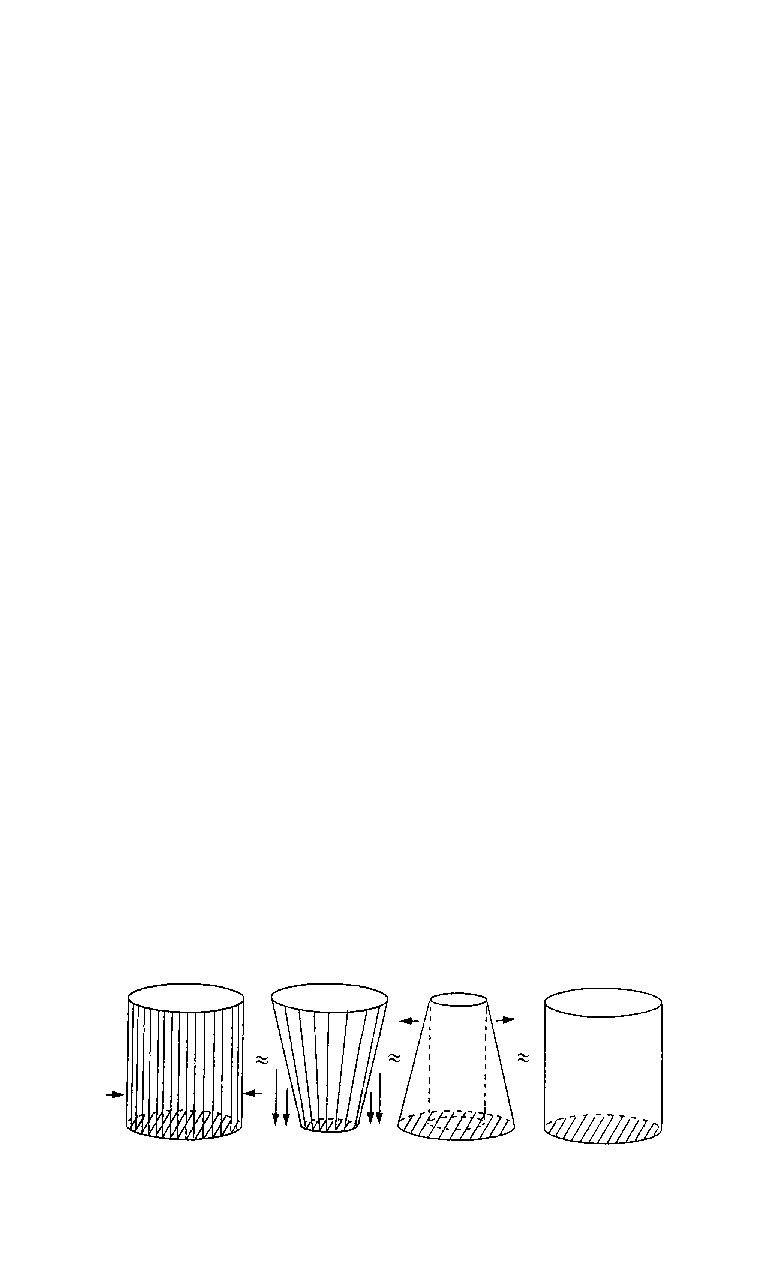
\includegraphics[width=0.5\textwidth]{figures/hom_of_pairs.pdf}
        \caption{Homeomorphism of pairs.}
        \label{fig:homeomorphism of pairs}
    \end{figure}
\end{proof}


The next Theorem shows that a map $E\to B$ that is a Serre fibration locally around each point in $B$ must be a Serre fibration. For Hurewicz fibrations the analogous statement is not generally true, i.e.~a local Hurewicz fibration is not always a Hurewicz fibration, but holds, for example, over paracompact base spaces.

\begin{thm}[{{\cite[Theorem~6.3.3]{tomDieck}}}]\label{thm local fibration}
    Let $p:E\to B$ be a continuous map and $\mathcal{U}$ a collection of subsets whose interiors cover $B$. If for every $U\in\mathcal{U}$ the restriction $p_U:p^{-1}(U)\to U$ is a Serre fibration, then so is $p$.
\end{thm}
\begin{proof}
    Subdivide the cube $I^n$ into cubes of size $\delta$ and enumerate them $I_i$. We can choose $\delta$ so that each cube $I_i\times I$ is mapped inside a $U\in\mathcal{U}$ by the map $H$ that we seek to lift. This is possible by the Lebesque Lemma~\ref{Lebesque lemma}. Let $V^k\subset I^n$ denote the union of the $k$-dimensional faces of the subdivision of $I^n$.

    We have to solve the lifting problem for the space $I^n$ with initial condition $h_0$. We begin by extending $h_0$ over $I^n\times [0,\delta]$ to a lifting of $H$. We solve the lifting problems 
     \[
    \begin{tikzcd}[every matrix/.append style={name=m}]
       I^n\times\{0\} \cup V^{k-1}\times [0,\delta] \arrow[d,"i",swap]\arrow[r,"\wt{H}(k-1)"]& E\arrow[d,"p"]\\
       I^{n}\times \{0\}\cup V^k\times [0,\delta]\arrow[r,"H",swap]\arrow[ur,"\wt{H}(k)",dashed,swap] & B
    \end{tikzcd}
    \]
    for $k=0,\ldots,n$ with $V^{-1}=\varnothing$ and $\wt{H}(-1)=a$ by induction in $k$. Let $W$ be a $k$-dimensional cube and $\partial W$ the union of its $(k-1)$-dimensional faces. We can solve the lifting problems
     \[
    \begin{tikzcd}[every matrix/.append style={name=m}]
       W\times\{0\} \cup \partial W\times [0,\delta] \arrow[d,"i",swap]\arrow[r,"\wt{H}(k-1)"]& p^{-1}(U)\arrow[d,"p_U"]\\
       W\times [0,\delta]\arrow[r,"H",swap]\arrow[ur,"\wt{H}_W",dashed,swap] & U
    \end{tikzcd}
    \]
    by a map $\wt{H}_W$, since $p_U$ is a Serre fibration; here $U\in\mathcal{U}$ was chosen such that $H(W\times [0,\delta])\subset U$.

    The $\wt{H}_W$'s for different $U\in\mathcal{U}$ combine to a continuous map $\wt{H}(k):V^l\times [0,\delta]\to E$ which covers $H$ and extends $\wt{H}(k-1)$. We define $\wt{H}$ on the first layer $I^n\times [0,\delta]$ as $\wt{H}(n)$. We now treat $I^n\times [\delta,2\delta]$ similarly with initial condition given by $\restr{\wt{H}(n)}{I^n\times\{\delta\}}$ and continue in this manner inductively.
\end{proof}

\begin{prop}[{{\cite[Prop.~3.2.3]{RS2}}}]\label{prop 3.2.3 RS2}
    Serre fibrations have the \textit{lifting property} (without homotopy) with respect to all pairs of the form
    \begin{enumerate}
        \item $(K\times I,(K\times \{0\})\cup(L\times I))$, where $K$ is a $CW$-complex and $L$ is a subcomplex. This constitutes a relative \gls{hlp} for the pair $(K,L)$.
        \item $(K,L)$ where $K$ is a $CW$-complex and $L$ is a subcomplex which is a strong deformation retract of $K$.
    \end{enumerate}
\end{prop}
\begin{proof}
    Let $\pi:E\to B$ be a Serre fibration, let $K$ be a $CW$-complex and $L$ a subcomplex of $K$.

    1. Consider the lifting problem defined by some $f:K\times I\to B$ and an initial conditon $\wt{f}_0:(K\times\{0\})\cup(L\times I)\to E$. We prove the assertion by induction on the dimension $k$ of the cells attached to $L$ to build $K$. The case $k=0$ is trivial. Thus, assume we have already constructed a lifting $\wt f$ over the subspace $(K^{(k)}\cup L)\times I\subset K\times I$ for some $k\geq 0$ and consider a $(k+1)$-cell $C$ not contained in $L$ with characteristic map $\chi:\bbD^{k+1}\to K$. Since $C$ is not contained in $L$, we have $C\cap (K^{(k)}\cup L)=C\cap L^{(k)}$. Hence, we wish to extend $\wt{f}$ from 
    \[(C\times\{0\}) \cup((C\cap K^{(k)})\times I)\subset C\times I\]
    to a lifting of $f$ on $C\times I$. Assume that we can extend
    \[\wt{f}\circ \restr{(\chi\times\id_I)}{(\bbD^{k+1}\times\{0\})\cup (\partial \bbD^{k+1}\times I)}\]
    to a lifting of $f\circ (\chi\times\id_I)$ on $\bbD^{k+1}\times I$. Since $\chi $ is injective on $\Int \bbD^{k+1}$, this lifting uniquely determines a lift of $f$ on $C\times I$. By Proposition~\ref{prop 3.1.11 RS2}, applied to the $CW$-complex $C\times I$, the latter is continuous.

    This argument shows that in order to prove that $\wt f$ extends to a lifting of $f$ over $(K^{(k+1)}\cup L)\times I$, it suffices to show that $\pi$ has the relative \gls{hlp} with respect to the pair $(\bbD^{k+1},\bbS^k)$. This holds by Proposition~\ref{prop 3.2.4 tomDieck} since $\pi$ is Serre fibration.

    2. Let $F:K\times I\to K$ be a strong deformation retraction from $K$ to $L$ and consider the lifting problem defined by some $f:K\to X$ and an appropriate initial condition $\wt{f}_0:L\to E$. Define $g:K\times I\to B$ by $g=f\circ F$. Since $F$ maps subsets $K\times\{1\}$ and $L\times I$ to $L$, we can also define
    \[\wt{g}_0:(K\times\{1\})\cup(L\times I)\to E,\quad \wt{g}_0(x,t)=\wt{f}_0(F(x,t)).\]
    A brief calculation shows that $\wt{g}_0$ is a lifting of $g$ over the subset $(K\times\{1\})\cup(L\times I)$. Hence, according to point 1, it can be extended to a lift $\wt{g}$ of $g$. Then, another brief calculation shows that the mapping $\wt f:K\to E$ defined by $\wt{f}(x)=\wt{g}(x,0)$ is a lifting of $f$ through $\pi$ extending $\wt{f}_0$.
\end{proof}

\begin{thm}\label{thm 6.3.1 tomDieck}
    Let $p:E\to B$ be a Serre fibration. For $B_0\subset B$ let $E_0=p^{-1}(B_0)$. Choose basepoints $*\in B_0$ and $* \in p^{-1}(*)$. Then $p$ induces for $n\geq 1$ a bijection $p_\ast:\pi_n(E,E_0,*)\to \pi_n(B,B_0,*)$.
\end{thm}
\begin{proof}
    First we show surjectivity. Let $g \in \pi_n(B,B_0,*)$ be represented by $\gamma:(\bbD^n,\bbS^{n-1},*)\to (B,B_0,*)$.
    By \gls{hlp} there exists a lifting $\wt\gamma:\bbD^n\to E$ with $\wt\gamma(*)=*$ and $p\circ \wt\gamma=\gamma$. We then have $\wt\gamma(\bbS^{n-1})\subset E_0$ and thus $\wt\gamma$ represents a pre-image pf $g$ under $p_\ast$.

    To show injectivity, let $g_0,g_1\in \pi_n(E,E_0,*)$ be represented by $\gamma_0,\gamma_1$ and have the same image under $p_\ast$. Then there exists a homotopy $\phi_t:(\bbD^n,\bbS^{n-1},*)\to (B,B_0,*)$ such that $\phi_0=p\circ \gamma_0$ and $\phi_1=p\circ \gamma_1$. Consider the subspace $T=\bbD^n\times\partial I\cup *\times I$ and define $G:T\to E$ by 
    \[G(x,t)=
        \begin{cases}
            \phi_t(x),& x\in \bbD^n, t\in\{0,1\},\\
            *, & x=*, t\in I.
        \end{cases}
    \]
    The set $T\subset \partial(\bbD^n\times I)$ is transformed into $*$ if one interchanges the last two coordinates. By \gls{hlp} again, there exists a map $H:\bbD^n\times I\to E$ such that $\restr{H}{T}=G$ and $p\circ H=\phi$. We can view $H$ as a homotopy from $\gamma_0$ to $\gamma_1$.
\end{proof}
By taking $B_0$ to be a single point, we get the following corollary, which for $n\geq 2$ is just a generalization of Corollary~\ref{cor homotopy groups of coverings} for covering spaces to all fibrations.
\begin{cor}
    Given a Serre fibration $p:E\to B$ with $F=p^{-1}(*)$, there is an isomorphism of homotopy groups
    \[\pi_n(E,F,*)\cong \pi_n(B,*),\quad n\geq 1.\]
\end{cor}
With the help of this isomorphism, we immediately get a special case of the long exact sequence of a pair (Theorem~\ref{thm long exact seq of homotopy}).
\begin{thm}[Exact sequence of a Serre fibration]
    For a Serre fibration $p:E\to B$ with inclusion $i:F=p^{-1}(b)\subset E$ and $e\in F$ the sequence
    \begin{multline}
        \cdots \to \pi_n(F,e)\overset{i_\ast}{\to}\pi_n(E,e)\overset{p_\ast}{\to}\pi_n(B,b)\overset{\partial}{\to}\pi_{n-1}(F,e)\to\cdots\\ 
        \to \pi_0(E,e)\to \pi_0(B,b)
    \end{multline}
    is exact.
\end{thm}

The boundary map $\partial$ has the following description. Let $f:(I^n,\partial I^n)\to (B,b)$ be given. View $f$ as a map $I^{n-1}\times I\to B$ and lift it to $\wt{f}:I^n\to E$, constant and equal to $e$ on $J^{n-1}=I^{n-1}\times \{0\}\cup \partial I^{n-1}\times I$. Then $\partial[f]$ is represented by $\restr{\wt{f}}{I^{n-1}\times \{1\}}$. In plain language, a ``loop'' representing an element of $\pi_n(B)$ in the base can be lifted to a ``path'' in the total space whose ``endpoints'' lie in the same fiber $F$, and by restricting to $F$ we get a lower-dimensional ``loop'' that represents an element of $\pi_{n-1}(F)$. The very end of the sequence requires a little extra work.

\begin{defn}[Trivialization]
    Let $\pi :E\to B$ be continuous and $U\subset B$ open and contained in the image of $\pi$. A \emph{trivialization} of $\pi$ over $U$ is a homeomorphism $\varphi:\pi^{-1}(U)\to U\times F$ over $U$, i.e.\ a homeomorphism which satisfies $\mathrm{pr}_1\circ \varphi=\pi$ (where $\mathrm{pr}_1$ is the natural projection onto the first component of the direct product). This condition determines $F$ up to a homeomorphism since $\varphi$ induces a homeomorphism of $\pi^{-1}(u)$ with $\{u\}\times F$.
\end{defn}

\begin{defn}[Locally trivial map]
    The map $\pi$ is \emph{locally trivial} if there exists an open covering $\mathcal{U}$ of $B$ such that $\pi$ has a trivialization over each $U_\alpha\in \mathcal{U}$. 
\end{defn}

Note that a locally trivial map is open and hence a topological quotient map.

\begin{example}
    Since a product projection is a fibration, we have by Theorem~\ref{thm local fibration} that any locally trivial map is a Serre fibration.
\end{example}
\begin{example}[Exact sequence of a covering space]
    Let $p:E\to B$ be a covering map with typical fiber $F$. Since each map $\bbD^n\to F$ must be constant because of discreteness of $F$, $\pi_n(F,*)$ is trivial for $n\geq 1$. The exact sequence of $p$ then confirms the isomorphisms $\pi_n(E,f)\cong \pi_n(B,b)$, $n\geq 2$, that we proved in Corollary~\ref{cor homotopy groups of coverings}. Moreover we have the exact sequence (omitting the common basepoint)
    \[1\to \pi_1(E)\overset{p_\ast}{\to} \pi_1(B)\overset{\partial}{\to} \pi_0(F)\overset{i_\ast}{\to} \pi_0(E)\overset{p_\ast}{\to} \pi_0(B)\to 1\]
    with the inclusion $i:F=p^{-1}(*)\subset E$ and $\pi_0(F)=F$. It yields for the universal covering $p:\bbR \to \bbS^1$ the familiar bijection $\partial:\pi_1(\bbS^1)\cong \bbZ$.
\end{example}

\begin{defn}[Hopf fibrations]\label{def: Hopf fibrations}
    Looking slightly ahead, consider $\bbS^{2n-1}\subset \bbC^n$ as a space with a free action of $\bbS^1=U(1)$ induced from scalar multiplication by $\rme^{2\pi\rmi  t}$. Let $U_j$ be the set of points $z=(z_1,\ldots,z_n)\in\bbC^n$ with $z_j\neq 0$. The map $z\mapsto z_j/|z_j|$ shows that $U_j\cong \bbR^{2n-1}\times \bbS^1$ is a trivial $U(1)$-space. The orbit space of this action is exactly $\mathbb{C}P^{n-1}=\bbS^{2n-1}\slash \bbS^1$. The Hopf fibration is defined as the orbit map $p:\bbS^{2n-1}\to \mathbb{C}P^{n-1}$. It is indeed a fibration because it is clearly trivial over $U_j\cap \bbS^{2n-1}$. We will also see a more explicit definition of the most important $n=2$ Hopf fibration later on.
\end{defn}

\begin{example}
    The exact sequence for the Hopf fibration, combined with $\pi_i(\bbS^1)=0$ for $i>1$ (see Corollary~\ref{cor: homotopy groups of circle}), yields the isomorphisms
    \[p_\ast: \pi_i(\bbS^{2n+1})\cong \pi_i(\mathbb{C}P^n),\; i\geq 3;\]
    and in particular $\pi_i(\bbS^3)\cong \pi_i(\bbS^2)$ for $i\geq 3$, since $\mathbb{C}P^1\cong \bbS^2$.
\end{example}

\begin{prop}[{{\cite[Prop.~6.3.8]{tomDieck}}}]\label{prop 6.3.8 tomDieck}
    Let $p:(E_1,E_0)\to B$ be a relative Serre fibration, i.e.\ $p:E_1\to B$ is a Serre fibration and the restriction $\restr{p}{E_0}$ is also a Serre fibration. Let $(F^1_b,F^0_b)$ be the pair of fibers over $p_1(e)=b\in B$. Then:
    \begin{enumerate}
        \item The inclusion induces bijections $\pi_n(F_b^1,F_b^0,e)\cong\pi_n(E_1,E_0,e)$.
        \item $\pi_0(E_0)\to \pi_0(E_1)$ is surjective iff $\pi_0(F_b^0)\to \pi_0(F_b^1)$ is surjective for each $b\in B$.
    \end{enumerate}
\end{prop}
\begin{proof}
    (1) We first prove the claim for $n=1$ and begin with surjectivity. Let $f:(I,\partial I,0)\to (E_1,E_0,e)$ be given. The path $\widebar{p\circ f}:I\to B$ (recall that the bar represents reversing the path) is lifted to $g:I\to E_0$ with initial point $f(1)$. Then $g(1)\in F^0_b$, and $f$ and $f\bullet g$ represent the same element in $\pi_1(E_1,E_0,e)$. The projection $p\circ(f\bullet g)$ is a nullhomotopic loop with basepoint $b$. We lift a nullhomotopy to $E_1$ with initial condition $f\bullet g$ on $I\times\{0\}$ and constant on $\partial I\times I$. The lifting is a homotopy $(I,\partial I,0)\times I\to (E_1,E_0,e)$ from $f\bullet g$ to a map into $(F^1_b,F^0_b,e)$. This proves the surjectivity.

    Suppose $f_0,f_1:(I,\partial I,0)\to (F^1_b,F^0_b,e)$ are given, and let $K:(I,\partial I,0)\times I\to (E_1,E_0,e)$ be a homotopy from $f_0$ to $f_1$. We lift $\widebar{p\circ K}$ to $L:I^2\to E_0$ with initial condition $L(s,0)=K(s,1)$ and $L(0,t)=L(1,t)=e$. The homotopy $p\circ(K\bullet_2 L)$ is a homotopy of loops which is $\rel \partial I^2$ homotopic to the constant map. We lift a homotopy to $E_1$ with initial condition $K\bullet_2 L$ on $I^2\times\{0\}$ and constant on $\partial I^2\times I$. The end is a homotopy from $f_0\bullet \kappa_e$ to $f_1\bullet\kappa_e$ (where $\kappa_e$ is a constant loop at $e$). This proves the injectivity.

    The higher dimensional case is obtained by an application to the relative Serre fibration $(\Omega^n F^1_b,\Omega^n F^0_b)\to (\Omega^n E_1,\Omega^nE_0)\to B$.

    (2) Suppose $\pi_0(E)\to \pi_0(E_1)$ is surjective. The argument above for surjectivity is used to show the surjectivity of $\pi_0(F^0_b)
    to \pi_0(F^1_b)$. The opposite implication is easy.
\end{proof}





\subsection{Higher connectivity}

For many applications it is important to know that the homotopy groups of a space vanish in a certain range. We discuss several reformulations of this fact. In the following $\pi_0(X,x_0)=\pi_0(X)$. The space $\bbD^0$ is a singleton and $\bbS^{-1}=\varnothing$.

\begin{prop}[{{\cite[Prop.~6.7.1]{tomDieck}}}]\label{prop 6.7.1 tomDieck} 
Let $n\geq 0$. \gls{tfae}:
\begin{enumerate}
    \item $\pi_n(X,x)=0$ for each $x\in X$.
    \item Each map $\bbS^n\to X$ has an extension to $\bbD^{n+1}$.
    \item Each map $\partial \bbD^{n+1}\to X$ has an extension to $\bbD^{n+1}$.
\end{enumerate}
\end{prop}
\begin{proof}
    The case $n=0$ is trivial. The equivalence of (2) and (3) is a consequence of the homeomorphism $(\bbD^{n+1},\bbS^n)\cong(I^{n+1},\partial I^{n+1})$. Suppose $f:\bbS^n\to X$ is given. Use $e_1=(1,0,\ldots)\in \bbS^n$ as a base point and think of $f$ as representing an element of $\pi_n(X,x)$. If (1) holds, then $f$ is pointed null homotopic. A null homotopy $\bbS^n\times I\to X$ factors over the quotient map $\bbS^n\times I\to \bbD^{n+1}$, $(x,t)\mapsto (1-t)e_1+tx$ and yields an extension of $f$. Conversely, let an element $\alpha$ of $\pi_n(X,x)$ be represented by a pointed map $f:(\bbS^n,e_1)\to (X,x)$. If this map has an extension $F$ to $\bbD^{n+1}$, then $(F,f)$ represents $\beta\in \pi_n(X,X,x)=0$ with $\partial\beta=\alpha$.
\end{proof}

\begin{prop}[{{\cite[Prop.~6.7.3]{tomDieck}}}]\label{prop 6.7.3 tomDieck}
    Let $n\geq 1$. The following assertions about a topological pair $(X,A)$ are equivalent:
    \begin{enumerate}
        \item $\pi_n(X,A,*)=0$ for each choice of $*\in A$.
        \item Each map $f:(I^n,\partial I^n)\to (X,A)$ is as a map of pairs homotopic to a constant map.
        \item Each map $f:(I^n,\partial I^n)\to (X,A)$ is homotopic $\rel \partial I^n$ to a map into $A$.
    \end{enumerate}
\end{prop}
\begin{proof}
    $(1)\Rightarrow(2)$. Let $f:(I^n,\partial I^n)\to (X,A)$ be given. Since $J^{n-1}$ is contractible, there exists a homotopy of the restriction $f:J^{n-1}\to A$ to a constant map. Since $J^{n-1}\subset \partial I^n$ and $\partial I^n\subset I^n$ are cofibrations, $f$ is as a map of pairs homotopic to $g:(I^n,\partial I^n)\to (X,A)$ such that $g(J^{n-1})=\{a_0\}$. Since $\pi_n(X,A,a_0)=0$, the map $g:(I^n,\partial I^n,J^{n-1})\to (X,A,a_0)$ is nullhomotopic as a map of triples.

    $(2)\Rightarrow(3)$ by the compression criterion (Proposition~\ref{prop: compression criterion}).

    $(3)\Rightarrow (1)$. Let $f:(I^n,\partial I^n,J^{n-1})\to (X,A,*)$ be given. By assumption (3), $[f]$ is contained in the image of $\pi_n(A,A,*)\to \pi_n(X,A,*)$. Now use $\pi_n(A,A,*)=0$.
\end{proof}



\begin{defn}[$n$-compressible pair]\index{$n$-compressible space}
    A topological pair $(X,A)$ is called $n$-compressible if (1)-(3) in Proposition~\ref{prop 6.7.3 tomDieck} hold. More generally, we call a map $f:X\to Y$ $n$-compressible if for each commutative diagram 
    \[
    \begin{tikzcd}[every matrix/.append style={name=m}, row sep=large, column sep=large]
       \partial \bbS^{n-1} \arrow[r,"\varphi"]\arrow[d,"i",swap] & X\arrow[d,"f"]\\
       \bbD^n \arrow[r,"\Phi", swap]\arrow[ur,"\Psi",dashed,swap] & Y
    \end{tikzcd}
    \]
    there exists $\Psi:\bbD^n\to X$ such that $\restr{\Psi}{\partial \bbD^n}=\varphi$ and $f\circ \Psi\simeq \Phi$ $\rel \partial \bbD^n$ (this amounts to (3) of Proposition~\ref{prop 6.7.3 tomDieck}). This notion is invariant under compositions with homotopy equivalences of the target space $Y$.
\end{defn}

\begin{prop}[{{\cite[Prop.~6.7.5]{tomDieck}}}]\label{prop 6.7.5 tomDieck}
    Let $n\geq 0$. The following assertions about a pair $(X,A)$ are equivalent:
    \begin{enumerate}
        \item Each map $f:(\bbD^q,\partial \bbD^q)\to (X,A)$, $q\in (0,\ldots,n)$ is $\rel \partial \bbD^q$ homotopic to a map into $A$.
        \item The inclusion $j:A\hookrightarrow X$ induces for each basepoint $a\in A$ a bijection $j_\ast:\pi_q(A,a)\to \pi_q(X,a)$ for $q<n$ and a surjection for $q=n$.
        \item $\pi_q(X,A,a)=0$ for $q=1,\ldots,n$ and each $a\in A$, and $\pi_0(A)\to \pi_0(X)$ is surjective.
    \end{enumerate}
\end{prop}
\begin{proof}
    $(1)\Leftrightarrow (3)$. The surjectivity of $\pi_0(A)\to \pi_0(X)$ is equivalent to (1) for $q=0$. The other cases follow from Proposition~\ref{prop 6.7.3 tomDieck}.

    $(2)\Leftrightarrow(3)$ follows from the exact sequence of the pair (Theorem~\ref{thm long exact seq of homotopy}).
\end{proof}


\begin{defn}[$n$-connected pair]\index{$n$-connected pair}
    A topological pair $(X,A)$ is called $n$-connected if (1)-(3) in Proposition~\ref{prop 6.7.5 tomDieck} hold. We call $(X,A)$ $\infty$-connected if the pair is $n$-connected for each $n$. A pair is $\infty$-connected iff $j_\ast:\pi_n(A,a)\to \pi_n(X,a)$ is always bijective. If $X\neq\varnothing$ but $A=\varnothing$ we say that $(X,A)$ is $(-1)$-connected, and $(\varnothing,\varnothing)$ is $\infty$-connected.
\end{defn}

\begin{defn}[Cone]\index{Cone}
    Given a space $X$, its cone $CX$ is defined as result of attaching the cylinder $X\times [0,1]$ by its face $X\times\{0\}$ to a point $*$ along the projection $p:X\times \{0\}\to *$.
\end{defn}


\begin{prop}[{{\cite[Prop.~6.7.6]{tomDieck}}}]\label{prop 6.7.6 tomDieck}
    Let $n\geq 0$. The following assertions about a space $X$ are equivalent:
    \begin{enumerate}
        \item $\pi_q(X,x)=0$ for $0\leq q\leq n$ and $x\in X$.
        \item The pair $(CX,X)$ is $(n+1)$-connected.
        \item Each map $f:\partial I^q\to X$, $0\leq q\leq n+1$ has an extension to $I^q$.
    \end{enumerate}
\end{prop}
\begin{proof}
    The cone $CX$ is contractible, therefore $\partial:\pi_{q+1}(CX,X,*)\cong \pi_q(X,*)$. This and Proposition~\ref{prop 6.7.5 tomDieck} shows the equivalence of (1) and (2). The equivalence of (1) and (3) is based on Proposition~\ref{prop 6.7.1 tomDieck}.
\end{proof}

\begin{defn}[$n$-connected space]\index{$n$-connected space}
    A space $X$ is called $n$-connected if (1)-(3) in Proposition~\ref{prop 6.7.6 tomDieck} hold. Note that this is compatible with previous definitions for $n=0$ (path-connected) and $n=1$ (simply-connected).
\end{defn}

\begin{defn}[$n$-equivalence]\index{$n$-equivalence}\index{Weak equivalence}
    Let $f:X\to Y$ be a map and $X\subset Z_f$ the inclusion into the mapping cylinder (recall the definition in Figure~\ref{fig:mapping cyl}). Then $f$ is said to be $n$-connected if $(Z_f,X)$ is $n$-connected. We then also say that $f$ is an $n$-equivalence. Thus $f$ is $n$-connected iff $f_\ast:\pi_q(X,x)\to \pi_q(Y,f(x))$ is for each $x\in X$ bijective for $q<n$ and surjective for $q=n$. If $f$ is an $\infty$-equivalence we also call it a weak (homotopy) equivalence, which happens iff $f_\ast$ is bijective for all $x\in X$ in all degrees.
\end{defn}

\begin{prop}[{{\cite[Prop.~6.7.7]{tomDieck}}}]\label{prop 6.7.7 tomDieck}
    Let $p:(E_1,E_0)\to B$ be a relative Serre fibration (see Proposition~\ref{prop 6.3.8 tomDieck}). Let $(F^1_b,F^0_b)$ be the pair of fibers over $b\in B$. Then the pair $(E_1,E_0)$ is $n$-connected iff the pairs $(F^1_b,F^0_b)$ are $n$-connected for all $b\in B$.
\end{prop}
\begin{proof}
    This is a direct consequence of Proposition~\ref{prop 6.3.8 tomDieck}.
\end{proof}

\begin{thm}[{{\cite[Theorem~6.7.9]{tomDieck}}}]\label{thm 6.7.9 tomDieck}
    Let $\varphi:(X,X_0,X_1)\to (Y,Y_0,Y_1)$ be a map such that the restrictions $\varphi_i:X_i\to Y_i$ are $n$-connected and $\varphi_{01}:X_0\cap X_1\to Y_0\cap Y_1$ is $(n-1)$-connected. Suppose $X=X_0^\circ \cup X_1^\circ$ and $Y=Y_0^\circ \cup Y_1^\circ$ where $\ ^\circ$ denotes interiors. Then $\varphi $ is an $n$-equivalence.
\end{thm}

\begin{cor}[{{\cite[Prop.~6.7.10]{tomDieck}}}]\label{prop 6.7.10 tomDieck}
    Let $f:X\to Y$ be an $n$-connected map between spaces with nondegenerate basepoints. Then the suspension $\Sigma f:\Sigma X\to \Sigma Y$ is $(n+1)$-connected. If $X$ is $n$-connected, then $\Sigma X$ is $(n+1)$-connected. The sphere $\bbS^{k+1}$ is $k$-connected.
\end{cor}
\begin{proof}
    Let $\Sigma 'X$ denote the unpointed suspension of $X$. This is a quotient of $X\times I$ and covered by the open cones $C_0=X\times [0,1)\slash X\times\{0\}$ and $C_1=X\times (0,1]\slash X\times\{1\}$ with intersection $X\times (0,1)$. We can apply Proposition~\ref{prop 6.7.7 tomDieck} directly; the cones are contractible and therefore the induced maps $C_j(X)\to C_j(Y)$ are $\infty$-connected. In the case of a space $X$ with a nondegenerate basepoint the quotient map $\Sigma 'X\to \Sigma X$ is a homotopy equivalence.
\end{proof}

\begin{thm}[{{\cite[Theorem~6.7.11]{tomDieck}}}]\label{thm 6.7.11 tomDieck}
    Let $f:X\to Y$ be a continuous map. Let $\{U_j\}_j$ and $\{V_j\}_j$ be open coverings of $X$ and $Y$ such that $f(U_j)\subset V_j$. Suppose that for each finite subset of indices the induced map $f_J:\bigcap_{j\in J}U_j\to \bigcap_{j\in J}V_j$ is a weak equivalence. Then $f$ is a weak equivalence.
\end{thm}
\begin{proof}
    By passage to the mapping cylinder we can assume that $f$ is an inclusion. Let $h:(I^n,\partial I^n)\to (Y,X)$ be given. We have to deform $h$ $\rel \partial I^n$ into $X$. By compactness of $I^n$ is suffices to work with finite coverings. A simple induction reduces the problem to a covering by only two sets $j=0,1$. Then we apply Theorem~\ref{thm 6.7.9 tomDieck}.
\end{proof}






\subsection{Excision for homotopy groups}

\begin{thm}[Blakers-Massey excision theorem]
    Let $X=U_0\cup U_1$ be covered by two open subspaces $U_0$ and $Y_1$ with non-empty intersection $V=U_0\cap U_1$. Suppose that $(U_0,V)$ is $p$-connected and $(U_1,V)$ is $q$-connected, i.e.
    \[
    \begin{matrix}
        \pi_i(U_0,V,*)=0,\quad 1\leq i\leq p,\; p\geq 0,\\
        \pi_i(U_1,V,*)=0,\quad 1\leq i\leq q,\; q\geq 0
    \end{matrix}
    \]
    for each basepoint $*\in V$. Then the \emph{excision map}, induced by the inclusion,
    \[i_\ast : \pi_n(U_1,V,*)\to \pi_n(X,U_0,*)\]
    is an isomorphism for $1\leq n <p+q$ and surjective for $n=p+q$ (for each $*\in X)$. In the case $p=0$, there is no condition on $\pi_i(U_0,V,*)$.
\end{thm}

\begin{cor}[{{\cite[Prop.~6.4.2]{tomDieck}}}]\label{prop 6.4.2 tomDieck}
    If in the above $(U_1,V)$ is $q$-connected then $(X,U_0)$ is $q$-connected.
\end{cor}
\begin{proof}
    This is a special case of the excision theorem which also directly follows from Theorem~\ref{thm 6.7.9 tomDieck}.
\end{proof}

For the sphere $\bbS^n$, introduce the following hemispheres and punctured spheres
\[\bbD^n_\pm=\{x\in \bbS^n\subset \bbR^{n+1}\mid \pm x_{n+1}\geq 0\}\subset H^n_\pm=\{x\in \bbS^n\mid x\neq \pm e_{n+1}\}.\]
We use the equatorial point $*=-e_1$ as a basepoint.

\begin{lem}[{{\cite[Lemma~6.4.3]{tomDieck}}}]\label{lem 6.4.3 tomDieck}
   There are isomorphisms $\partial:\pi_{i+1}(D_-^{n+1},\bbS^n,*)\to \pi_i(\bbS^n,*)$ for $i\geq 0$, $n\geq 0$ and $\pi_i(\bbS^n,*)\to \pi_i(\bbS^n,D_\pm^n,*)$ for $i\geq 0$, $n\geq 1$.
\end{lem}
\begin{proof}
    In the first case we use the exact sequence of the pair $(\bbD^{n+1}_-,\bbS^n)$. The space $\bbD^{n+1}_-$ is contractible and hence $\pi_i(\bbD^{n+1}_-,*)=0$ for $i\geq 0$ and $n\geq 0$.

    In the second case we consider similarly the exact sequence of $(\bbS^n,\bbD^n_\pm)$. Note that $*=-e_1\in D_\pm^n$ for $n\geq 1$.
\end{proof}

Thus for $n\geq 0$ we have a diagram with the isomorphisms 
\[
    \begin{tikzcd}[every matrix/.append style={name=m}, row sep=large, column sep=large]
       \pi_i(\bbS^n,*) \arrow[r,"E"] & \pi_{i+1}(\bbS^{n+1},*)\arrow[d,"\cong"]\\
       \pi_{i+1}(\bbD^{n+1}_-,\bbS^n,*)\arrow[u,"\overset{\partial}{\cong}",swap] \arrow[r,"i_\ast", swap] & \pi_{i+1}(\bbS^{n+1},D_+^{n+1},*).
    \end{tikzcd}\label{3795}
\]
The morphism $i_\ast$ is induced by the inclusion and $E$ is defined so as to make the diagram commutative. Note that the inductive proof of (1) in the next Theorem uses only Corollary~\ref{prop 6.4.2 tomDieck}.

\begin{thm}[{{\cite[Thm~6.4.4]{tomDieck}}}]\label{thm 6.4.4 tomDieck}
    \begin{enumerate}
        \item $\pi_i(\bbS^n)=0$ for $i<n$ (recall that we already showed this in Corollary~\ref{cor pi_n(S^k)=0}).
        \item The homomorphism $i_\ast$ in diagram (\ref{3795}) is an isomorphism for $i\leq 2n-2$ and an epimorphism for $i=2n-1$. A similar statement holds for $E$.
    \end{enumerate}
\end{thm}
\begin{proof}
    Let $N(n)$ be the statement (1) and $E(n)$ be the statement (2). Obviously $N(1)$ holds. Assume $N(n)$ holds. We then deduce $E(n)$. We apply the excision theorem to $(X,U_0,U_1,V)=(\bbS^{n+1},D_+^{n+1},D_-^{n+1},\bbS^n)$. By $N(n)$ and Lemma~\ref{lem 6.4.3 tomDieck} we have $\pi_i(\bbS^n)\cong \pi_{i+1}(D_\pm^{n+1},\bbS^n)=0$ for $0\leq i <n$. We use the excision theorem for $p=q=n$ and see that $i_\ast$ is surjective for $i+1\leq 2n$ and bijective for $i+1\leq 2n-1$. Finally, $E(n)$ and $N(n)$ imply $N(n+1)$.

    In order to have the correct hypotheses for the excision theorem, we thicken the spaces, replace $D_\pm^n$ by $H^n_\pm$ and note that the inclusions $D_\pm^n\subset H^n_\pm$ and $\bbS^{n-1}\subset H^n_+\cap H^n_-$ are homotopy equivalences.
\end{proof}
\begin{cor}[{{\cite[Prop.~5.11]{Bredon}}}] 
    The pair $(\bbD^{n+1},\bbS^n)$ is $n$-connected.
\end{cor}
\begin{proof}
    This follows from the exact sequence $\pi_r(\bbD^{n+1})\to \pi_r(\bbD^{n+1},\bbS^n)\to \pi_{r-1}(\bbS^n)$ for $r\leq n$, where the two groups on the sides vanish.
\end{proof}


\begin{prop}[{{\cite[Prop.~6.4.5]{tomDieck}}}]\label{prop 6.4.5 tomDieck}
    The homomorphism $\pi_i(\bbD^{n+1},\bbS^n,*)\to \pi_i(\bbD^{n+1}\slash \bbS^n,*)$ induced by the quotient map is an isomorphism for $i\leq 2n-1$ and an epimorphism for $i=2n$.
\end{prop}
\begin{proof}
    Consider the commutative diagram
    \[
    \begin{tikzcd}[every matrix/.append style={name=m}, row sep=large, column sep=large]
       \pi_i(D_-^{n+1},\bbS^n,*) \arrow[r]\arrow[d,"i_\ast",swap] & \pi_i(D_-^{n+1}\slash \bbS^n,*) \arrow[d,"(1)"]\\
       \pi_{i+1}(\bbS^{n+1},\bbD^{n+1}_+,*)\arrow[r,"(2)",swap] & \pi_{i}(\bbS^{n+1}\slash D_+^{n+1},*).
    \end{tikzcd}
    \]
    The map (1) is induced by a homeomorphism and the map (2) by a homotopy equivalence, hence both are isomorphisms. Now apply Theorem~\ref{thm 6.4.4 tomDieck}.
\end{proof}

The homomorphism $E$ is essentially the suspension homomorphism:
\[\Sigma_\ast: \pi_n(X)\underset{\cong}{\overset{\partial}{\leftarrow}}\pi_{n+1}(CX,X)\overset{q_\ast}{\to}\pi_{n+1}(CX\slash X)=\pi_{n+1}(\Sigma X)\]
with the quotient map $q:\bbD^{n+1}\to \bbS^{n+1}=\bbD^{n+1}\slash \bbS^n$. The next result is the famous suspension theorem of Freudenthal.

\begin{thm}[Freudenthal's suspension theorem {{\cite[Theorem~6.4.6]{tomDieck}}}]\label{thm 6.4.6 tomDieck freudenthal}
    The suspension $\Sigma_\ast:\pi_i(\bbS^n)\to \pi_{i+1}(\bbS^{n+1})$ is an isomorphism for $i\leq 2n-2$ and an epimorphism for $i=2n-1$.
\end{thm}
\begin{proof}
    We have to show that $q_\ast:\pi_{i+1}(CX,X)\to \pi_{i+1}(CX\slash X)$ is for $X=\bbS^n$ an isomorphism (epimorphism) in the appropriate range. This follows from Proposition~\ref{prop 6.4.5 tomDieck}; one has to use that  $\bbD^{n+1}_-$ is the (pointed) cone on $\bbS^n$.
\end{proof}

\begin{thm}[{{\cite[Theorem~6.4.7]{tomDieck}}}]\label{thm 6.4.7 tomDieck freudenthal}
    $\pi_n(\bbS^n)\cong \bbZ$ and $\Sigma_\ast:\pi_n(\bbS^n)\to \pi_{n+1}(\bbS^{n+1})$ is an isomorphism ($n\geq 1$). The group $\pi_n(\bbS^n)$ is generated by the identity map of $\bbS^n$.
\end{thm}
\begin{proof}
    From the exact sequence of the Hopf fibration $\pi_2(\bbS^3)\to \pi_2(\bbS^2)\to \pi_1(\bbS^1)\to \pi_1(\bbS^3)$ and $\pi_j(\bbS^3)=0$ for $j=1,2$, we obtain an isomorphism $\partial:\pi_2(\bbS^2)\to \pi_1(\bbS^1)\cong \bbZ$. From Theorem~\ref{thm 6.4.6 tomDieck freudenthal} we obtain a surjection $\Sigma_\ast:\pi_1(\bbS^1)\to \pi_2(\bbS^2)$; this is an isomorphism, since both groups are isomorhic to $\bbZ$. For $n\geq 2$, Theorem~\ref{thm 6.4.6 tomDieck freudenthal} directly gives an isomorphism $\Sigma_\ast$. We know that $\pi_1(\bbS^1)$ is generated by the identity map, and $\Sigma_\ast$ respects the identity.
\end{proof}

This proof clearly extends to two cones over any space $X$, so by using the adjunction $[\Sigma X,Y]\cong[X,\Omega Y]$ we get the more general form of this Theorem.

\begin{thm}[Freudenthal's suspension thereom]\index{Theorem!Freudenthal's suspension}
Let $X$ be an $n$-connected space, i.e.\ $\pi_i(X)=0$ for $0\leq i\leq n$. Then the homomorphism $\pi_k(X)\to \pi_k(\Omega \Sigma X)$ induced by the inclusion $X\hookrightarrow \Omega\Sigma X$ is an isomorphism for $k\leq 2n-2$ and an epimorphism for $k=2n-1$.

Furthermore, since $\pi_{k+1}(\Sigma X)\cong[\bbS^{k+1};\Sigma X]\cong[\bbS^k;\Omega \Sigma X]\cong\pi_k(\Omega \Sigma X)$, for $k\leq 2n-2$ there is an isomorphism $\pi_k(X)\cong \pi_{k+1}(\Sigma X)$.
\end{thm}
\begin{proof}
See \cite[Theorem 6.4.6]{tomDieck}.
\end{proof}

\begin{defn}[Degree on spheres]\index{Degree}
    For a map $f:\bbS^n\to \bbS^n$, its degree $\deg f$ is the integer such that $[f]=[\mathrm{id}_{\bbS^n}]^{\deg f}$ in $\pi_n(\bbS^n)$.
\end{defn}

\begin{example}[Hopf fibrations]\label{example Hopf pi3(S2)}
    We continue the discussion of the Hopf fibrations \ref{def: Hopf fibrations}. The Hopf fibration $\bbS^{2n+1}\to \mathbb{C}P^n$ and $\pi_i(\bbS^{2n+1})=0$ for $i\leq 2n$ yield $\pi_2(\mathbb{C}P^n)\cong \pi_1(\bbS^1)\cong \bbZ$ and $\pi_i(\mathbb{C}P^n)=0$ for $0\leq i \leq 2n$, $i\neq 2$. The inclusion $\bbS^{2n+1}\to \bbS^{2n+3}$, $z\mapsto (z,0)$ induces an embedding $\mathbb{C}P^n\subset \mathbb{C}P^{n+1}$. We compare the corresponding Hopf fibrations and their exact sequences and conclude $\pi_2(\mathbb{C}P^n)\cong \pi_2(\mathbb{C}P^{n+1})$. Let $\mathbb{C}P^\infty =\bigcup_{n\geq 1}\mathbb{C}P^n$ be the colimit (the topology on it is defined as the finest topology under which all inclusions $\mathbb{C}P^n\hookrightarrow \mathbb{C}P^\infty$ are continuous). The inclusions induce $\pi_i(\mathbb{C}P^n)\cong\pi_i(\mathbb{C}P^\infty)$ for $i\leq 2n$. A proof uses the fact that a compact subset of $\mathbb{C}P^\infty$ is contained in some finite $\mathbb{C}P^N$. Therefore $\mathbb{C}P^\infty$ is a space with a single nontrivial homotopy group $\pi_2(\mathbb{C}P^\infty)\cong\bbZ$.

    Particularly notable is the special case 
    \[\pi_3(\bbS^2)\cong \pi_3(\bbS^3)\cong\bbZ.\]
    This is the first of the ``nontrivial'' homotopy groups of spheres $\pi_k(\bbS^n), k>n$, and the only one that can be computed without much more advanced homology theory.

    We have the similar results for real projective spaces. The double coverings $\bbS^n\to \RP^n$ are used to show that $\pi_1(\RP^2)\cong \pi_1(\RP^3)\cong\cdots =\cong \pi_1(\RP^\infty)\cong \bbZ_2$, induced by the inclusions $\RP^n\hookrightarrow\RP^{n+1}$ for $i<n$ and $\pi_i(\RP^n)=0$ for $0\leq i< n$, $i\neq 1$. The space $\RP^\infty$ therefore has a single nontrivial homotopy group $\pi_1(\RP^\infty)\cong\bbZ_2$.
\end{example}


\begin{example}[Lens spaces]\index{Lens spaces}
    Recall the lens space $L=L_m(l_1,\ldots,l_n)$ from Example~\ref{example Lens spaces}. It can be given a structure of a $CW$-complex with one cell in each dimension from $0$ to $2n-1$ so that the degree of the attaching maps alternates between $0$ and $m$ (starting with degree $0$ for the map $\partial \bbD^1\to L^{(0)}$).
\end{example}


\begin{example}[$\pi_3(\bbS^2\vee \bbS^2)\cong \bbZ^3$]
    Let us compute $\pi_3(\bbS^2\vee \bbS^2)$. We have an inclusion $i: \bbS^2\vee \bbS^2\hookrightarrow \bbS^2\times \bbS^2$, because $\bbS^2\times \bbS^2$ can be realized as a $CW$-complex that differs from $\bbS^2\vee \bbS^2$ only by an addition of a 4-cell. Observe that the induced homomorphism on the homotopy groups is surjective:
    \[i_\ast: \quad \pi_n(\bbS^2\vee \bbS^2)\to \pi_n(\bbS^2\times \bbS^2)=\pi_n(\bbS^2)\oplus \pi_n(\bbS^2).\]
    (Here we used the fact that a smash product with $\bbS^k$ is homeomorphic to the iterated reduced suspension $\Sigma^k$, and $\Sigma^k \bbS^n=\cong \bbS^{n+k}$.) This allows us to insert extra zeroes into the long exact sequence for the pair $(\bbS^2\times \bbS^2,\bbS^2\vee \bbS^2)$ without breaking its exactness, which splits it into the short exact sequences
    \[0\to \pi_{n+1}(\bbS^2\times \bbS^2,\bbS^2\vee \bbS^2)\to \pi_n(\bbS^2\vee \bbS^2)\overset{i_\ast}{\to} \pi_n(\bbS^2\times \bbS^2)\to 0.\]
    For $n=3$, since $\bbS^2\vee \bbS^2$ is 1-connected and the remaining 4-cell is 4-connected, we can use the excision theorem to compute
    \[\pi_4(\bbS^2\times \bbS^2,\bbS^2\vee \bbS^2)\cong \pi_4(\bbS^2\times \bbS^2\slash \bbS^2\vee \bbS^2)\cong \pi_4(\bbS^2\wedge \bbS^2) \cong\pi_4(\bbS^4)\cong \bbZ.\]
    At the same time, $\pi_3(\bbS^2\times \bbS^2)=\pi_3(\bbS^2)\oplus \pi_3(\bbS^2)=\bbZ^2$ (generated by the Hopf fibrations from the preceding Example~\ref{example Hopf pi3(S2)}). Thus we have the exact sequence
    \[0\to \bbZ\to \pi_3(\bbS^2\vee \bbS^2)\to \bbZ^2\to 0,\]
    which implies $\pi_3(\bbS^2\vee \bbS^2)=\bbZ^3$ because every short exact sequence of the form $0\to A\overset{i}{\to} B\overset{p}{\to} \bbZ^2\to 0$ splits (the splitting monomorphism $j:\bbZ^2\to B$ can be constructed by defining it on the basis $j(1,0)=b_1$ and $j(0,1)=b_2$, where $b_1,b_2\in B$ are any two elements such that $p(b_1)=(1,0)$ and $p(b_2)=(0,1)$; it is then easy to check that $p\circ j=\id_{\bbZ^2}$ and hence $B\cong A\oplus \bbZ^2$).

    This construction is a special case of the \emph{Whitehead product}\index{Whitehead product} $\pi_k(X)\times\pi_l(X)\to \pi_{k+l-1}(X)$. Given $f:\bbS^k\to X$ and $g:\bbS^l\to X$, their Whitehead product is the homotopy class denoted
    \[[f,g]\in \pi_{k+l-1}(X)\]
    and represented by the composition 
    \[\bbS^{k+l-1}\overset{\chi}{\to} \bbS^k\vee \bbS^l\overset{f\vee g}{\to} X,\]
    where $\chi$ is the attaching map for the single $(k+l)$-cell in the $CW$-complex $\bbS^k\times \bbS^l$ which consists of $\bbS^k\vee \bbS^l$ and that cell ($\chi$ maps the boundary of the $(k+l)$-disk to the $(k+l-1)$-skeleton, which in this case is $\bbS^k\vee \bbS^l$). In the case above, the third ``unexpected'' generator of $\pi_3(\bbS^2\vee \bbS^2)$ is $[i_1,i_2]$, where $i_1,i_2:\bbS^2\to \bbS^2\vee \bbS^2$ are the inclusion maps for the two 2-spheres. 
    
    Another simple Whitehead product is $[\id_{\bbS^2},\id_{\bbS^2}]\in\pi_3(\bbS^2)$. It is represented by the map obtained by gluing $\bbS^2\vee \bbS^2\subset \bbS^3$ onto $\bbS^2$. Since we already know that $\pi_3(\bbS^2)$ is generated by the Hopf fibration $p_{\mathrm{Hopf}}$ and this map clearly has winding number $2$, we find that 
    \[[\id_{\bbS^2},\id_{\bbS^2}]=2[p_{\mathrm{Hopf}}]\]
    (although there might also be a minus sign depending on how one defines the Hopf fibration).
\end{example}

\begin{xca}[{{\cite[Thm.~6.10.5]{tomDieck}}}]
    Let $X$ and $Y$ be well-pointed (i.e.~with non-degenerate basepoints) and assume that $\pi_i(X)=\pi_j(Y)=0$ for $i<p,j<q$ with $p,q\geq 2$. Show that the inclusion $X\vee Y\hookrightarrow X\times Y$ induces an isomorphism of the $\pi_i$-groups for $i\leq p+q-2$. Also show that $\pi_i(X\times Y,X\vee Y)$ and $\pi_i(X\wedge Y)$ vanish for $i\leq p+q-1$.
\end{xca}

\begin{xca}[{{\cite[Exercise 6.11]{tomDieck}}}]
    Extend the above example to determine $\pi_{2n-1}(\bbS^n\vee \bbS^n)$ for $n\geq 2$.
\end{xca}




\clearpage
\part{Fiber Bundles and Calculus on Manifolds}
% !TEX root = ../geom_autistic_intro.tex

\chapter{Fiber Bundles}\label{chap: Fiber bundles}

\section{Bundles}

Recall that by the Rank Theorem~\ref{Rank thm}, all submersions, when restricted to sufficiently small neighborhoods in the domain, look like projections in a direct product. Fiber bundles are a natural special case of this, where the submersion looks like a projection ``locally in the target'', i.e., is a locally trivial map. 

\begin{defn}[Topological fiber bundle]\index{Fiber bundle!topological}
    A topological \gls{fb} is continuous locally trivial map $\pi:E\to B$. The local trivializations $\varphi_\alpha:\pi^{-1}(U_\alpha)\to U_\alpha\times F$ are called \emph{bundle chart maps}. The set of those $b\in B$ for which the \emph{fiber} $\pi^{-1}(b)$ is homeomorphic to a fixed space $F$ is open and closed in $B$. Therefore, it usually suffices to fix the homeomorphism type of the fibers. If all fibers are homeomorphic to $F$, we call $F$ the \emph{typical, or model, fiber}.
\end{defn}

From this definition it is clear that topological covering maps are exactly the topological \gls{fb} with discrete fibers. Also by Theorem~\ref{thm local fibration}, every \gls{fb} is a fibration, which we state as a Corollary. 

\begin{cor}[{{\cite[Cor.~3.2.5]{RS2}}}]
    Topological \glspl{fb} are Serre fibrations.
\end{cor}

This implies that all of our topological results for Serre fibrations will also hold for \glspl{fb}, most importantly, the long exact sequence of homotopy groups. If the base space happens to be paracompact, one has the following stronger result. For a proof we direct the reader to the cited reference.

\begin{cor}[Huebsch and Hurewicz {{\cite[\S13.4]{tomDieck}}}]
    Topological \glspl{fb} over paracompact Hausdorff base spaces are Hurewicz fibrations.
\end{cor}

This will property will obviously survive in the smooth category since all manifolds are paracompact.

\begin{defn}[Smooth fiber bundle]\index{Fiber bundle!smooth}
    A map $\pi\in C^\infty(E,M)$ is called a smooth \gls{fb} if it is a smooth submersion and for any $p\in M$ there is an open neighborhood $U_p$ and a diffeomorphism $\chi_p:\pi^{-1}(U_p)\to U_p\times \pi^{-1}(p)$ (recall that $\pi^{-1}(p)$ is a smooth manifold for submersions) such that the following triangle commutes:
    \[
    \begin{tikzcd}[every matrix/.append style={name=m},   
    execute at end picture={\draw [<-] ([xshift=0mm,yshift=-2mm]m-2-2.north) arc[start angle=-90,delta angle=-270,radius=0.25cm];}]
       \pi^{-1}(U_p) \arrow[rr,"\chi_p"]\arrow[ddr,swap,"\restr{\pi}{\pi^{-1}(U_p)}"]& & U_p\times \pi^{-1}(p)\arrow[ddl,"\pr_1"]\\
       & \, & \\
       & U_p & 
    \end{tikzcd}
    \]
    It is called a \emph{trivial bundle}\index{Trivial bundle} if $U$ can be taken to be all of $M$, i.e., the total space decomposes into a product $E\cong M\times \pi^{-1}(p)$. The maps $\chi_p$ are called \emph{local trivializations}.\index{Trivialization}
    
    Finally, a \gls{fb} can be restricted to an open subset $U\subset M$ by defining $\restr{E}{U}$ as $\pi^{-1}(U)\overset{\pi|_{\pi^{-1}(U)}}{\longrightarrow}M$.
\end{defn}

\begin{xca}
    Suppose $E\overset{\pi}{\to}M$ is a \gls{fb} with fiber $F$. Prove the following:
    \begin{enumerate}[label=(\alph*)]
        \item $\pi$ is an open quotient map.
        \item $E$ is compact iff both $M$ and $F$ are compact.
    \end{enumerate}
\end{xca}


One is tempted to say that the \gls{hlp} property of fibrations automatically applies to smooth \glspl{fb} and stop at that.  However, in the smooth category, we want the liftings of smooth homotopies to also be smooth, and unfortunately the topological versions of these theorems will not suffice for that. This is why we will have to enhance many of the familiar results about fibrations for the smooth case. We start by showing that all fibers in a \gls{fb} are not just homotopy equivalent, but diffeomorphic (similarly, all fibers in a topological \gls{fb} are homeomorphic).

\begin{prop}
    For a \gls{fb} $\pi:E\to M$ with $M$ connected, all fibers $\pi^{-1}(m)$ are diffeomorphic to each other. We call a manifold $F$ that they are all diffeomorphic to ``the typical, or model, fiber of the fibration''.
\end{prop}
\begin{proof}
    A connected manifold is path-connected. By connecting any two points with a path, covering this path by a finite sequence of open sets over which the fibration is trivial (which is possible by compactness of $[0,1]$), and using the chain of local trivializations, we establish a diffeomorphism between the fibers at the endpoints.
\end{proof}
\begin{example}
\begin{enumerate}
    \item The cylinder $E=\bbS^1\times\bbR $ is a trivial \emph{line bundle} (or rather the total space of one) over a circle with $\pi$ the projection onto the first factor. It is also a \emph{circle bundle} over the line under the projection onto the second factor.
    \item The M\"obius band is a non-trivial line bundle over the circle under the projection onto the ``equator'' of the band. It is not trivial because it's not homeomorphic to the trivial line bundle, which is the cylinder.
    \item $\bbR^n\setminus\{0\}$ is a trivial line bundle above the sphere $\bbS^{n-1}$ under $\pi(x)=x/\Vert x\Vert$.
\end{enumerate}
\end{example}


\begin{example}
    Covering spaces of $M$ are exactly the \glspl{fb} over $M$ whose fibers are at most countable sets with discrete topology.
\end{example}

The following fundamental theorem gives us a useful sufficient condition for a map to be a locally trivial fibration. We delay its proof until \S\ref{sec: applications of flows} because it requires some theory of flows of vector fields. Nevertheless, we present it now because it will be useful for constructing specific examples of \glspl{fb}. Recall that a map is proper iff it is closed and its fibers (preimages of points) are compact.

\begin{thm}[Ehresmann Fibration Theorem (1961)]\index{Ehresmann fibration theorem}\label{thm Ehresmann}
    If $\pi:E\to M$ is a \emph{proper} surjective submersion, then $\pi$ is a locally trivial fibration.
\end{thm}

\begin{cor}
    A surjective submersion acting between compact manifolds is a locally trivial fibration.
\end{cor}


\begin{example}[Qubit/Bloch sphere/Hopf fibration]\index{Qubit}\index{Bloch sphere}\index{Hopf fibration}\label{Hopf bundle}
    A qubit is a two-level system described by a pair of complex numbers $(z_1,z_2)\in\mathbb{C}^2$ such that $|z_1|^2+|z_2|^2=1$. The set of such points is the unit sphere $\bbS^3$ in $\mathbb{C}^2\cong\bbR^4$. However, points differing only by a phase correspond to the same physical state: $(\rme^{\rmi\theta}z_1,\rme^{\rmi\theta}z_2)\sim(z_1,z_2)$. It turns out that these equivalence classes are in one-to-one correspondence with points of a two-sphere $\bbS^2$, because the quotient map can be given by
    \[\pi(z_1,z_2)=(\underbrace{2z_1\wb{z}_2}_{\in \mathbb{D}\subset\mathbb{C}},\underbrace{|z_1|^2-|z_2|^2}_{\in [-1,1]})\in \bbS^2\subset\bbR^3\cong \mathbb{C}\times\bbR.\]
    This is obviously a smooth and surjective map, and since the sphere $\bbS^3$ is compact, it is proper. It is also easy to check that its differential is everywhere surjective, therefore, by Ehresmann's theorem $\pi$ is a \gls{fb} with typical fiber $\bbS^1$ (space of phases). This fibration, often written as $\bbS^3\overset{\bbS^1}{\to}\bbS^2$, is called the Hopf fibration, or the Hopf bundle. Since $\bbS^3$ with one point excluded is homeomorphic to $\bbR^3$, the Hopf fibration is often visualized as a fibration of the 3D space by circles plus one straight line (circle of infinite radius). Any two circles in this fibration happen to be linked with each other, see Fig. \ref{Fig.Hopf}.
    
    $\bbS^2$, which represents the set of physical states of a qubit, is the Bloch sphere. One can show that this fibration is not trivial (the easiest way, perhaps, is to compare the fundamental groups $\pi_1(\bbS^2\times \bbS^1)=\pi_1(\bbS^2)\times\pi_1(\bbS^1)=\bbZ$ and $\pi_1(\bbS^3)=\{e\}$).
    
    \begin{minipage}[c]{\textwidth}
        \centering
        \captionsetup{type=figure}
        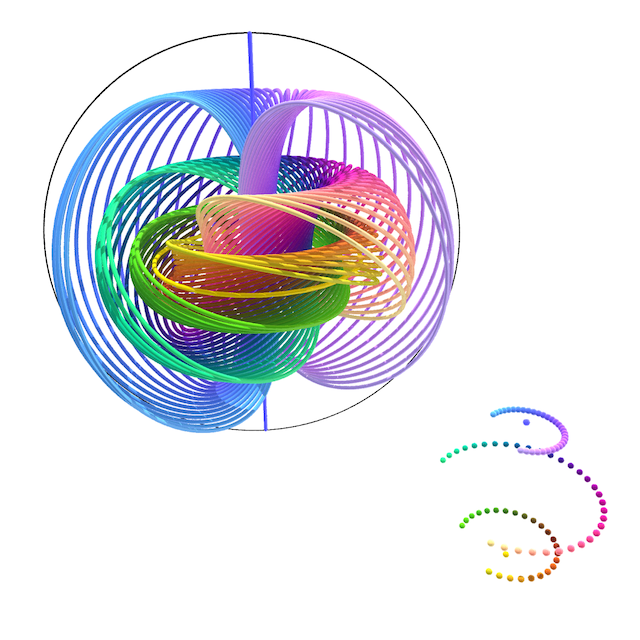
\includegraphics[scale=0.2]{figures/Hopf.png}
        \captionof{figure}{Hopf fibration in stereographic projection, i.e., as a fibration of $\bbR^3$. Each circle is a fiber corresponding to a point on the 2-sphere at the bottom. From \cite{hopf}.}
        \label{Fig.Hopf}
    \end{minipage}
\end{example}

\begin{xca}
    Show that in the Hopf bundle, the preimage of any circle in $\bbS^2$ is a two-torus $\bbT^2$ embedded into $\bbS^3$.
\end{xca}


\begin{defn}[Bundle morphism]\index{Bundle morphism}
    Let $E\overset{\pi}{\to}M$ and $E'\overset{\pi'}{\to}M'$ be two smooth \glspl{fb}. A bundle morphism (a.k.a.\ \emph{bundle map}) between them is a pair of smooth maps $h:E\to E'$ and $\underline{h}:M\to M'$ such that $h$ \emph{covers} $\underline{h}$ in the sense that the following square commutes:
    \[\begin{tikzcd}[every matrix/.append style={name=m},   
    execute at end picture={\draw [<-] ([xshift=-8mm,yshift=1mm]m-2-2.north) arc[start angle=-90,delta angle=270,radius=0.25cm];}]
       E \arrow[r,"h"]\arrow[d,swap,"\pi"]& E'\arrow[d,"\pi'"] \\
       M\arrow[r,swap,"\underline{h}"]& M'
    \end{tikzcd}\]
    We call $\underline{h}$ the \emph{base map}, or the \emph{projection}, of $h$, since it can be uniquely recovered from $h$.\index{Base map}
    This gives rise to the category $\FB^\infty$ of all smooth \glspl{fb}. A full subcategory is the category $\FB^\infty_M$ of all smooth \glspl{fb} over a given base $M$ with $\underline{h}=\id_M$ (note that, in general, there are other bundle morphisms between bundles over $M$ for which $\underline{h}$ is not even a diffeomorphism). Bundle morphisms covering the identity are also called \emph{vertical}.\index{Vertical morphism}
\end{defn}








\section{Structure groups}\label{sec: structure groups}

So far we have only given a purely topological (or geometric in the smooth case) description of \glspl{fb}. The fascinating thing about \glspl{fb}, however, is that the requirement of local triviality gives rise to an alternative \emph{algebraic} description of \glspl{fb}, which will eventually lead us into the realm of cohomology. A similar, albeit more cumbersome, description appears for general topological fibrations as well. We now characterize smooth \glspl{fb} in terms of their systems of local trivializations and identify their transition maps with certain Lie group actions. Note that everything here easily translates to the category of topological \glspl{fb} as well.


\begin{defn}[Bundle atlas]\label{def G-bundle}\index{Atlas!Bundle}\index{Bundle!atlas}\index{Bundle!chart}\index{Bundle!structure}\index{Transition functions}
    Let $E\overset{\pi}{\to}M$ be a smooth \gls{fb} with typical fiber $F$, and let $\{U_\alpha\}_\alpha$ be an open covering of $M$ such that the restrictions $\restr{E}{U_\alpha}$ are trivial. By definition of local triviality, we have some diffeomorphisms $\chi_\alpha: \restr{E}{U_\alpha}\to U_\alpha\times F$, called \emph{local trivializations} or \emph{bundle charts}. Then:
\begin{enumerate}
    \item The collection $\{(U_\alpha,\chi_\alpha)\}$ is called a \emph{\gls{fb} atlas} for $E\overset{\pi}{\to}M$. Two bundle atlases are \emph{equivalent} if their union is still a bundle atlas. A \emph{bundle structure} on $E$ is an equivalence class of bundle atlases, or, alternatively, a \emph{maximal atlas} given by the union of all atlases belonging to an equivalence class.
    \item For any point $(m,f)\in U_{\alpha\beta}\times F$, the transition maps in this atlas have the form \[\chi_\beta\circ\chi_\alpha^{-1} (m,f)=(m, t_{\beta\alpha}(m,f)),\label{eq transition functions}\]
    where for every fixed $m\in M$, the map $t_{\beta\alpha}(m,\_):F\to F$ is a diffeomorphism. One can think of $t_{\beta\alpha}$ as a function on $U_{\alpha\beta}$ that takes values in the group $\Diff(F)$ of all diffeomorphisms of $F$, so $t_{\beta\alpha}$ becomes a map $t_{\beta\alpha}:U_{\alpha\beta}\to \Diff(F)$.\footnote{As we will see in \S\ref{sec: Diff groups}, the group $\Diff(F)$ can be given the structure of an infinite-dimensional Lie group, modeled on the space $\fX(F)$ of vector fields. Unfortunately $t_{\alpha\beta}$ are not always automatically smooth: they are smooth iff their values are contained in the left coset of the open and closed subgroup $\Diff_c(F)$ of diffeomorphisms with compact support. This is in principle true only for bundles which are ``trivial near fiber-wise infinity'' or have ``discrete structure group near fiberwise infinity'' \cite{Michor}. We shall always assume that this is true.}
    These $\Diff(F)$-valued functions are called \emph{bundle transition functions}. They are also sometimes called \emph{clutching functions}, especially when $M$ is a sphere.\index{Clutching functions}\index{Transition functions} We will usually assume that $\Diff(F)$ acts on the typical fiber from the \emph{left} (one can pass to a right action by acting via $t_{\alpha\beta}^{-1}$ instead).
\end{enumerate}
\end{defn}

\begin{defn}[$G$-structure]
    If the bundle structure of $E$ contains a bundle atlas whose transition functions take values in a Lie subgroup $G<\Diff(F)$,\footnote{We will formalize the concept of Lie subgroups in \S\ref{sec: Lie theory iii}. For now all we need to know is that finite-dimensional Lie subgroups $G$ of any (even infinite-dimensional) Lie group are weakly embedded, which means that restricting a smooth map into $\Diff(F)$ whose image lies in $G<\Diff(F)$ in its range produces a smooth map into $G$.} then such an atlas is called a \emph{$G$-atlas} for $E$. Two $G$-atlases are called \emph{$G$-equivalent} if their union is still a $G$-atlas. A $G$-equivalence class of $G$-atlases, or, alternatively, the maximal $G$-atlas equal to their union, is called a \emph{$G$-structure}, denoted $\calG$.\index{$G$-structure} If a $G$-structure is fixed on $E$, we say that $G$ is the \emph{structure group} of the bundle. \index{Structure group} The tuple $(E\overset{\pi}{\to}M,G\acts F,\calG)$ is called a \emph{$G$-bundle}.\index{$G$-bundle}
    
    If $H<G$ is a Lie subgroup and a given $G$-structure on $E$ contains an $H$-atlas, then a choice of an $H$-structure (which is a subset of the given $G$-structure) is called a \emph{reduction of the structure group}, or simply a \emph{bundle reduction}\index{Bundle reduction} from $G$ to $H$.
\end{defn}    

\begin{defn}[Cocycles]
    From the definition \eqref{eq transition functions} it is obvious that the group-valued bundle transition functions satisfy two important conditions:
    \[
    \begin{cases}
    t_{\alpha\alpha}\equiv e, & \text{(identity condition),}\\
    \restr{t_{\alpha\beta}\cdot t_{\beta\gamma}\cdot t_{\gamma\alpha}}{U_{\alpha\beta\gamma}}\equiv e; & \text{(cocycle condition),}
    \end{cases}
    \]
    where the product in $\Diff(F)$ is just the composition of maps. Any collection of such $G$-valued functions $\{t_{\alpha\beta}\}$ associated to an open covering of $M$ is called a \emph{cocycle}\index{Cocycle} on $M$ with structure group $G$.\footnote{More precisely, a cocycle is a certain equivalence class of such collections, which is discussed below.} Note that these two conditions imply $t_{\alpha\beta}t_{\beta\alpha}=e$.
\end{defn}

\begin{rem}\label{rem: faithful action on F 0}
    \begin{enumerate}
        \item One can try writing down higher-order relations on the transition functions, such as $t_{\alpha\beta}t_{\beta\gamma}t_{\gamma\delta}t_{\delta\alpha}=e$, but all of them follow from the identity and the cocycle conditions. On the other hand, replacing the cocycle condition with only $t_{\alpha\beta}t_{\beta\gamma}=e$ would have been insufficient because this does \emph{not} imply the higher-order relations.
        \item $\Diff(F)$ acts on $F$ faithfully by definition, therefore, the induced action of any subgroup $G<\Diff(F)$ is faithful as well. This is why in the following definitions we will assume that the action of the structure group on the model fiber is faithful. We will further elucidate the importance of faithfulness in Remark~\ref{rem: faithfulness of action on F}.
        \item A \gls{fb} $E\to M$ is trivial iff it admits an $\{e\}$-structure. Indeed, if there is a bundle atlas in which all transition functions evaluate to the identity, then all local trivializations agree on the overlaps and hence stitch into a global trivialization. An $\{e\}$-structure is also called an \emph{absolute parallelism}.\index{Parallelism!Absolute}
    \end{enumerate}
\end{rem}


Since the structure group of a bundle acts on its typical fiber $F$, that is, it acts in the local trivializations, it is natural to ask whether this action ``lifts'' to an action on the actual fibers of the bundle itself. Crucially, the answer is no, however, the following restricted concept of a $G$-structure does get naturally translated to the fibers.

\begin{defn}[$G$-fiber]
    Let $F$ be a smooth manifold diffeomorphic to a given manifold $F_0$ and let $G$ be a Lie group acting faithfully from the left on $F_0$, so $G$ can be identified with a Lie subgroup of $\Diff(F_0)$. Two diffeomorphisms $\chi_1,\chi_2:F\to F_0$ are called $G$-equivalent if $\chi_2\circ \chi_1^{-1}\in G$. A $G$-equivalence class $\calG_0$ of such diffeomorphisms, i.e., an orbit of the action of $G$ on $\Diff(F,F_0)$ by compositions $\chi\mapsto g\circ \chi$, is called a \emph{fiber $G$-structure} on $F$.\footnote{This particular terminology is not standard. In common jargon, what is defined here is a $G$-structure on the bundle consisting of one fiber over a single point, $F\overset{\pi}{\to}\ast$.} The tuple $(F,G\acts F_0,\calG_0)$ is called a $G$-fiber modeled on $F_0$. An element of $\calG_0$ is called a \emph{$G$-frame}, or a frame \emph{compatible} with the $G$-structure.\footnote{It would be more appropriate to call the $\chi$ \emph{coframes}, whereas the corresponding frame is $\chi^{-1}$, but we shall ignore this distinction until we focus on affine $G$-structures.} \index{$G$-frame}\index{$G$-structure!Fiber}\index{$G$-fiber}
\end{defn}


\begin{prop}\label{prop G-fibers}
    If $\pi:E\to M$ is a \gls{fb} with structure group $G$ acting on the typical fiber $F$, then each fiber of $E$ naturally carries a fiber $G$-structure and an action of the center $\rmZ(G)$.
\end{prop}
\begin{proof}
    Consider a fiber $E_m=\pi^{-1}(m)$, $m\in M$. The fact that it carries a fiber $G$-structure is obvious because the value of any $G$-valued transition function at a point $m$ is an element of $G$. 
    
    We now show that if $G$ is not abelian, then there is no natural action of $G$ on the fibers, but there is an action of $\rmZ(G)$. By definition of the typical fiber, there is a diffeomorphism $f_\alpha=\restr{\chi_\alpha}{E_m}:E_m\to F$, which is just the restriction of a local trivialization $\chi_\alpha$. By definition of a $G$-structure, there is a smooth (say left) action of $G$ on the typical fiber $F$. Let $f_\beta:E_m\to F$ be the diffeomorphism coming analogously from another compatible local chart. Then $f_\alpha(p)=t^{-1}\cdot f_\beta(p)$ for all $p\in E_m$ for some $t\in G$, and we can compare what the action of an element $g\in G$ translates to in the fiber $E_m$ under these two diffeomorphisms:
    \[f_\alpha^{-1}(g\cdot f_\alpha(p))=f_\beta^{-1}(tgt^{-1} f_\beta(p)).\]
    Since $t$ can range over all of $G$ by varying the charts, these formulas consistently define an action $g\cdot p$ only for $g\in \rmZ(G)$.
\end{proof}

\begin{rem}
    \begin{enumerate}
        \item The intuition behind the definition of $G$-structures is the following. A fiber $G$-structure on $F$ is a choice of a $G$-invariant subset of all diffeomorphisms from $F$ to a ``standard'', or ``model'', space $F_0$, namely an orbit of the action of $G$ on all such diffeomorphisms by compositions. This can be interpreted as $F_0$ having some kind of ``structure'' that is invariant under actions of $G$, and a fiber $G$-structure allows us to transplant this structure to $F$. A $G$-structure on a fiber bundle, then, is a collection of structures on each fiber that, in a sense, vary smoothly with the base point $m\in M$. These structures are defined consistently because all local trivializations belonging to the same $G$-bundle atlas differ from each other by an action of $G$ on $F_0$, hence this additional structure is independent of the local bundle chart. 
        \item Morphisms between bundles with the same structure group are also defined so as to ``respect'' this structure. Thus the smaller the $G$, the more structure the morphisms of this category preserve. We will use this rough idea when introducing vector bundles, orientations, and complex bundles. For example, vector bundles will have structure group $\GL(V)$ for some vector space $V$, and, as we will see, the corresponding fiber $G$-structure is the structure of vector space.
        
        \item There is one extremely special class of $G$-bundles that will be distinguished by the fact that their typical fiber supports \emph{two commuting actions} of $G$, a left one and a right one -- because the typical fiber will be $G$ itself. After using one of them up to define the bundle, we will be able to use the above procedure to lift the other one to a global action of $G$ on $E$. These bundles are called \emph{principal}. In \S\ref{sec: free proper actions} we will show that principal $G$-bundles can be defined without reference to local trivializations, and in \S\ref{sec: principal bundles} that will lead us to a chart-free definition of \emph{all} \glspl{fb}.
    \end{enumerate}
\end{rem}
\begin{example}
    A covering space $E\overset{\pi}{\to} M$ is a topological \gls{fb} with a discrete typical fiber $F$. Its structure group, most generally, is the group $G=\Diff(F)=\mathrm{Bij}(F)$ of all permutations of points of the fiber. As we know, there is a natural $\pi_1(M,x_0)$-action on $F=\pi^{-1}(x_0)$, which produces a homomorphism $\lambda:\pi_1(M,x_0)\to G$. Note that there is no natural action of $\pi_1(M,x_0)$ on \emph{other} fibers of $E$ because there is no natural way to choose the isomorphisms between the groups $\pi_1(M,x_0)$ for different choices of the basepoint $x_0$. The image of $\lambda$ is a subgroup of $G$. Since the covering space can be fully reconstructed from this action, $\lambda(\pi_1(M,x_0))$ can be made the structure group of this bundle. 
    
    One case where there is a global action of the structure group on the whole covering space is when it is a $G$-principal covering space. In this case the fiber is $G$ itself and supports a second (right) action of $G$ which survives the \gls{fb} construction.
\end{example}






\section{Fiber morphisms}\label{sec: fiber morphisms}

Now we examine morphisms (and in particular isomorphisms) between bundles with different structures on them. General bundle morphisms are allowed to be arbitrary smooth maps when restricted to a single fiber, so we will need to find a special subclass of bundle morphisms that ``respects'' given structures in some way. Let us first look at the simpler case of a single fiber. Say we have a $G$-fiber $(F,G\acts F_0,\calG_0)$ and a $G'$-fiber $(F',G'\acts F_0',\calG_0')$. Then any map $h:F\to F'$ can be represented by a map $\wh{h}:F_0\to F_0'$ by using any two diffeomorphisms $\chi\in\calG_0\subset \Diff(F,F_0)$ and $\chi'\in\calG_0'\subset \Diff(F',F_0')$ as follows:
\[\wh{h}=\chi'\circ h\circ \chi^{-1}.\label{eq g-fiber f-hat}\]
Different choices of $\chi$ and $\chi'$ are equivalent to replacing $\wh{h}$ in this formula with $g'\circ \wh{h}\circ g^{-1}$ for some $(g,g')\in G\times G'$. Therefore, we notice the importance of the action of the product group $G\times G'$ on the set $C^\infty(F_0,F_0')$ by compositions:
\[G\times G'\acts C^\infty(F_0,F_0'):\quad ((g,g'),\wh{h})\mapsto g'\circ \wh{h}\circ g^{-1}.\label{eq gg' action}\] 
A choice of a class of morphisms $\wt h$ then corresponds to a choice of a set of orbits of this action. For this we either need $F_0$ and $F_0'$ to carry additional structure (vector spaces, metric spaces, etc.) that provides such a choice in a canonical way, or to just specify the choice manually. If want to make these choices consistently across all possible pairs of model spaces $(F_0,F_0')$, this amounts to forming a category. We detail these methods below:
\begin{enumerate}
    \item Let $\calS$ be a subcategory of the category $\mathsf{Man}^\infty$ of smooth manifolds (it need not include neither all objects nor all morphisms). Then if the model spaces $F_0$ and $F_0'$ are objects of $\calS$, we denote
    \[\calS(F_0,F_0')=\mor_\calS(F_0,F_0').\]
    We think of the category $\calS$ as describing ``additional structure'' on the model spaces. We now define morphisms from $(F,G\acts F_0,\calG_0)$ to $(F',G'\acts F_0',\calG_0')$ as maps $h:F\to F'$ which, under some (and therefore, any) diffeomorphisms $\chi\in\calG_0$ and $\chi'\in\calG_0'$, are represented by maps $\wh{h}:F_0\to F_0'$ belonging to $(G\times G')\cdot \calS(F_0,F_0')$.
    
    \item In the situation of item 1, it is also often the case that $G$ and $G'$ \emph{act by automorphisms}, i.e., by elements of $\Aut_\calS(F_0)$ and $\Aut_\calS(F_0')$, respectively. Then 
    \[(G\times G')\cdot \calS(F_0,F_0')=\calS(F_0,F_0').\]
    This situation comes with an extra benefit. Since $G$ preserves the additional structure on $F_0$, this structure can be ``lifted'' via any $\chi\in \calG_0$ so that $F$ itself naturally becomes an object of $\calS$. Thus, in addition to the action of $\rmZ(G)$, the fiber will inherit some additional structure from the $G$-invariant structure on the model fiber. We will soon see how this works explicitly on the example of vector bundles.
    \item The most common setting is a special sub-case of 2, whereby $G$ and $G'$ are \emph{defined} as the groups of automorphisms of $F_0$ and $F_0'$, respectively, so we don't even need to specify them separately:
    \[G=\Aut_\calS(F_0),\quad G'=\Aut_\calS(F_0').\]
    The actions of $G$ and $G'$ in this case are given canonically, and we can proceed as in 1. In particular, this implies that every representative $\wh{h}$ of every \emph{automorphism} (invertible morphism of a $G$-fiber to itself) $h$ is an element of $G$.
\end{enumerate}

\begin{defn}[Category of $\calS$-fibers]\label{def S-fibers}
    Given a $G$-fiber $(\tuple{F,G\acts F_0,\calG_0})$, a $G'$-fiber $(\tuple{F',G'\acts F_0',\calG_0'})$, and a subset $\calS(F_0,F_0')\subset C^\infty(F_0,F_0')$ determined from a category $\calS$ in one of the ways described above, a morphism between them is a smooth map $h: F\to F'$ such that its representative $\wh{h}$ defined by \eqref{eq g-fiber f-hat} using any $\chi\in\calG_0$ and $\chi'\in\calG_0'$ belongs to the orbit of an element of $\calS(F_0,F_0')$ under the action \eqref{eq gg' action} of $G\times G'$ on $C^\infty(F_0,F_0')$. We say that $h$ \emph{is modeled on} an element of $\calS(F,F')$. We call this category $\calS\mathsf{-Man}^\infty$ and its objects $\calS$-fibers. Note that $\calS$ is not enough to define this category -- one also needs to specify groups $G$ and their actions (unless $G=\Aut(F_0)$ as in case 3 above).

    In particular, two $G$-fibers $(F,G\acts F_0,\calG_0)$ and $(F',F\acts F_0,\calG_0')$ with the same structure group $G$ and model space $F_0$ are isomorphic iff there exists a diffeomorphism $h:F\to F'$ such that the map $\calG_0'\to \calG_0$ given by the composition $\chi'\mapsto h^\ast \chi'=\chi'\circ h$ is a bijection. If $G=\Aut_\calS(F_0)$, then this is equivalent to $\wh{h}\in G$ for all representatives \eqref{eq g-fiber f-hat} of $h$.
\end{defn}

Note that the choice of the category $\calS$ for a given type of structure is not unique. In fact, we mostly need this definition to produce a unique notion of \emph{isomorphism} of $\calS$-fibers and later $\calS$-bundles, whereas we won't really care what the rest of the morphisms look like. We now consider a number of important examples of $\calS$-fiber structures.
\begin{example}[Linear $G$-structures]\label{ex linear G-structures}
    \begin{enumerate}
        \item If $\calS=\mathsf{FinVect}_\bbK$ (finite-dimensional $\bbK$-vector spaces), then we get the category of $\mathsf{FinVect}_\bbK$-fibers with linear maps. Here, if the model space is $V$, then we define $G=\Aut_\calS(V)=\GL(V)$. A $G$-structure $\calG_0$ on $F$ is an equivalence class of diffeomorphisms $F\to V$ that differ by an automorphism of $V$. Since $V$ is a vector space, we can use any of these diffeomorphisms $\chi\in\calG_0$ to induce a vector space structure on $F$ itself: for $\lambda_1,\lambda_2\in\bbK$ and $e_1,e_2\in F$ we define the linear combination
        \[\lambda_1e_1+\lambda_2 e_2\coloneqq \chi^{-1}(\lambda_1\chi(e_1)+\lambda_2\chi(e_2)).\]
        This is well-defined because different $\chi$'s differ by a linear automorphism of $V$. In particular, this defines an action of scalar matrices $\lambda I$, $\lambda\in\bbK$, on $F$, which coincides with the induced natural action of the center $\rmZ(G)$. Note that $\GL(V)$ has no natural action on $F$ because there is no natural isomorphism between $F$ and $V$! Thus the category $\calS\mathsf{-Fib}$ is isomorphic to $\calS$ itself.

        In fact, one can replace the category $\mathsf{FinVect}_\bbK$ with its skeleton $\mathsf{Sk}(\mathsf{FinVect}_\bbK)$, whose objects are \emph{standard} spaces $\bbK^n$, $n=0,1,\ldots$, and the only nontrivial morphisms are inclusions-as or projections-onto the first $n$ components. Indeed, every linear map between vector spaces is represented by one of these standard maps in some appropriately chosen bases of the source and target spaces. In this case an element of $\calG_0$, i.e., a \emph{frame}, determines a basis on $F$ and outputs the components of vectors in that basis.
        
        \item In general, if structure groups $G$ are defined as the automorphism groups $\Aut(F_0)$, then the resulting category $\calS\mathsf{-Fib}$ is equivalent to $\calS$ itself. This allows one to define many classical structures on vector spaces in terms of a countable set of ``standard'' ones. This shows the importance of allowing $G$ to not necessarily act by automorphisms. We proceed in this manner in the next several examples.
        
        \item If $\bbK=\bbR,\bbC,\bbH$, then we can let $\calS$ be the category of finite-dimensional vector spaces with a $\bbK$-valued inner product, or its skeleton consisting of spaces $\bbK^n$ with the standard dot product $\sum_{i=1}^n \wb{x}_i y_i$. For each model space $\bbK^n$ we also take its isometry group $G$, which is $\Or_n,\U_n$, or $\Sp_n$, respectively. Then $\calS$-fibers are vector spaces $F$ with a $G$-structure which allows us to lift the inner product onto $F$. There is a bijective correspondence between $G$-structures and inner products on $F$, so  $\calS\mathsf{-Fib}$ is exactly the category of vector spaces with an inner product and all linear maps. $G$-frames in this context are just orthonormal bases. We can also replace $\calS$ with the category of vector spaces $V$ with an inner product and linear morphisms whose operator norm is at most $1$ (this forces isomorphisms to be isometries), and letting $G=\Aut_\calS(V)$. Then $\calS\mathsf{-Fib}$ has the same objects but fewer morphisms.

        \item If we let $\calS=\mathsf{FinVect}_\bbK$ but redefine the structure group $G$ of a model space $V$ as $G=\GL^+(V)$, i.e., orientation-preserving automorphisms, then $\calS$-fibers are oriented vector spaces with linear maps between them. 

        \item If $\calS$ is again the category of standard real vector spaces $\bbR^n$, $n=0,1,\ldots$, and the structure group of $\bbR^n$ is $\SL_n(\bbR)$, then $\calS$-fibers are vector spaces with a volume form (a totally antisymmetric multilinear form of maximum rank) with linear maps between them. Alternatively we can let $\calS$ consist of $\bbR^n$'s with the standard volume form $\mathsf{v}_n$ and linear maps $f:\bbK^n\to \bbK^m$ such that $f^\ast \mathsf{v}_m=\lambda \mathsf{v}_n$ with $\lambda\in (-1,1]$ (this forces automorphisms to have determinant $1$), and define $G=\Aut_\calS(\bbR^n)\cong \SL_n(\bbR)$. Note that a volume form induces an orientation because $\SL_n(\bbR)\subset \GL_n^+(\bbR)$.

        \item Taking standard model spaces $\bbK^n$ with $G$ defined as the group that leaves the subspace $\bbK^p$ spanned by the first $p$ standard basis vectors, and linear maps that map the first $p$ directions of one space to the first $p$ directions of the other (not necessarily surjectively), we get the category $\calS\mathsf{-Fib}$ of vector spaces with ``$p$-directions''. It is isomorphic to the category of pairs $(V,W)$ where $W$ is a $p$-dimensional subspace of $V$, and morphisms are required to be maps of pairs (i.e., $W$ is mapped inside $W'$). Note that morphisms between standard spaces $\bbR^n\to \bbR^m$ are represented by matrices with the top right $p\times(n-p)$ block filled with zeroes (unless $p>m$, in which case it's just the right $m\times (n-p)$ block).

        \item Consider all free actions of the group $G=\GL_n(\bbZ)$ on $n$-dimensional vector spaces $V$. This means that $G$ is the group of linear automorphisms of $V$ that preserve some rank-$n$ lattice $\varLambda$ spanning $V$ (i.e., $\varLambda=\bbZ v_1+\cdots +\bbZ v_n$ for some basis $v_1,\ldots,v_n$). Then $\calS\mathsf{-Fib}$ is the category of vector spaces with an \emph{integral affine structure}. It is isomorphic to the category of pairs $(V,\varLambda)$ and linear maps mapping lattice to lattice.

        \item $\calS$ be the category of even-dimensional real vector spaces $V$ with a linear isomorphism $\sfJ:V\to V$ such that $\sfJ^2=-\id_V$ (called a \emph{complex structure})\index{Complex structure} and linear maps $h:(V,\sfJ)\to(V',\sfJ')$ such that $h\circ \sfJ=\sfJ'\circ h$ (called \emph{complex linear w.r.t.\ $\sfJ$}). Each $\sfJ$ defines a structure of a $\bbC$-vector space on $V$ via $\rmi v\coloneqq\sfJ(v)$. Then $G=\Aut_\calS(V)$ consists of matrices $A\in\GL(V)$ such that $\sfJ A=A\sfJ$ and is isomorphic to $\GL_n(\bbC)$ (exercise). This group is denoted $\GL(V,\sfJ)$ or simply $\GL_\bbC(V)$. The category $\calS\mathsf{-Fib}$ is isomorphic to $\calS$ itself and is the category of complex structures on real vector spaces with complex-linear maps between them. $\calS$ can also be replaced with its skeleton, which consists of standard complex structures on $\bbR^{2n}$:
        \[\rmJ_{n}=\begin{bmatrix}
            0&-\rmI_n\\
            \rmI_n&0
        \end{bmatrix}\]
        And linear maps $f:\bbR^{2n}\to \bbR^{2m}$ that satisfy $\rmJ_{m}\circ f=f\circ \rmJ_{n}$. In the case $m=n$ such maps are called holomorphic and their matrices have the form 
        \[M=\begin{bmatrix}
            A&B\\
            -B&A
        \end{bmatrix},\label{eq complex matrices}\]
        which can be identified with $A+\rmi B\in \Mat_n(\bbC)$.
        Note that each complex structure also induces an orientation because matrices $A\in \GL_n(\bbC)\subset \GL_{2n}(\bbR)$ have positive determinant over $\bbR$, namely $\det M=|\det(A+\rmi B)|^2>0$.

        \item Consider standard spaces $\bbR^{2n}$ with standard symplectic forms, i.e., antisymmetric nondegenerate bilinear forms $\omega_n:\bbR^{2n}\times \bbR^{2n}\to \bbR$ whose matrix in the standard basis is $\rmJ_{n}$. Let morphisms be all linear maps and let $G=\Sp_{2n}(\bbR)$ be the group of symplectic matrices, i.e., matrices $A\in\GL_{2n}(\bbR)$ such that $A^\sfT\rmJ_{n}A=\rmJ_{n}$. Then $\calS$-fibers are symplectic vector spaces $(V,\omega)$ with all linear maps between them. This can be reduced to just the category of \emph{symplectomorphisms}, i.e., isomorphisms that preserve the symplectic structure.
    \end{enumerate}
\end{example}


\begin{example}[Hermitian structures]\label{ex hermitian structures}
    A Hermitian structure on a complex vector space $V_\bbC$ is just a symmetric sesquilinear form $\sfh:V_\bbC\times V_\bbC\to \bbC$ as introduced in the preceding example, i.e.,
    \[\sfh(v,w)=\widebar{{\sfh}(w,v)},\quad v,w\in V_\bbC,\]
    and $\sfh(v,v)\geq 0$ for all $v\in V_\bbC$ and vanishes iff $v=0$.
    
    An $n$-dimensional complex vector space is naturally isomorphic to a $2n$-dimensional real vector space with a complex structure $V_\bbC\cong (V,\sfJ)$ (defined by $\sfJ(v)\coloneqq \rmi v$), also denoted $V_\sfJ$. Then $\sfh$ can be reinterpreted as a complex-valued $\bbR$-bilinear form on $V_\sfJ$ which in addition satisfies
    \[\sfh(v,\sfJ w)=-\sfh(\sfJ v,w)=\rmi\sfh(v,w),\quad v,w\in V_\sfJ,\]
    and such that $\sfh(v,v)$ is a norm. This also implies that
    \[\sfh(\sfJ v,\sfJ w)=\sfh(v,w).\]
    We can decompose $\sfh$ into its real and imaginary parts, which we suggestively call $\sfg$ and $\omega$:
    \[\sfh(v,w)=\Re \sfh(v,w)+\rmi\Im\sfh(v,w)=\sfg(v,w)+\rmi \omega(v,w).\]
    We have
    \[\sfg(v,w)=\Re \sfh(v,w)=\Re \sfh(w,v)=\sfg(w,v),\]
    and $\sfg(v,v)=\sfh(v,v)$, therefore, $\sfg$ is a nondegenerate symmetric bilinear form that defines an inner product on $V_\sfJ$.
    Furthermore, the sesquilinear condition implies that 
    $\omega(v,w)=\frac12 (\rmi\sfh(w,v)-\rmi\sfh(v,w))=\frac12 (\sfh(w,\sfJ v)-\sfh(v,\sfJ w))$
    is a real antisymmetric bilinear form. 
    Moreover,
    \[\omega(v,\sfJ w)=\frac12 (\sfh(\sfJ w,\sfJ v)+\sfh(v,w))=\frac12 (\sfh(w,v)+\sfh(v,w))=\Re \sfh(v,w)=\sfg(v,w),\]
    therefore, $\omega$ is nondegenerate as well, and hence determines a symplectic structure on $V_\sfJ$. 

    Crucially, fixing a complex structure $\sfJ$, the above formulas relating any two of the three objects $\sfh,\sfg,\omega$ uniquely determine the third. We thus have natural isomorphisms between the following three pairs of structures:
    \begin{enumerate}
        \item Hermitian structures $(\sfJ,\sfh)$ on $V$.
        \item Pairs $(\sfJ,\sfg)$ of a complex structure $\sfJ$ and a metric $\sfg$ that are compatible in the sense that
        \[\sfg(\sfJ v,\sfJ w)=\sfg(v,w),\quad \text{or}\quad \sfg(\sfJ v,w)=-\sfg(v,\sfJ w),\quad v,w\in V.\]
        This compatibility condition is equivalent to the bilinear form $\omega_\sfJ(v,w)=\sfg(\sfJ v,w)$ being a symplectic form, also called the \emph{fundamental form}.
        \item Pairs $(\sfJ,\omega)$ of a complex structure $\sfJ$ and a symplectic structure $\omega$ that are compatible in the sense that
        \[\omega(\sfJ v,\sfJ w)=\omega(v,w),\quad \text{or}\quad \omega(\sfJ v,w)=-\omega(v,\sfJ w),\quad v,w\in V,\]
        and in addition that the resulting form $\sfg_\sfJ(v,w)=\omega(v,\sfJ w)$, which is symmetric because of compatibility, is positive definite (in this case we say that $J$ \emph{tames} $\omega$). These conditions are equivalent to the bilinear form $\sfg_\sfJ$ being a real inner product.
        \item Pairs $(\sfg,\omega)$ of a positive definite metric $\sfg$ and a symplectic form $\omega$. By non-degeneracy of $\sfg$, there exists a unique operator $\sfJ$ such that $\omega(v,w)=\sfg(v,\sfJ w)$, and it follows that $\sfJ$ is a complex structure compatible with both $\sfg$ and $\omega$.
    \end{enumerate}
    Thus the group of isometries of $\sfh$, $\U(V,\sfh)$, coincides with the following double intersections of groups $\Sp(V,\omega)$ (automorphisms preserving $\omega$), $\GL(V_\bbC)$ (automorphisms preserving $\sfJ$), and $\Or(V,\sfg)$ (automorphisms preserving $\sfg$):
    \[\U(V,\sfh)=\Sp(V,\omega)\cap \GL(V_\bbC)=\Or(V,\sfg)\cap \GL(V_\bbC)=\Or(V,\sfg)\cap \Sp(V,\omega).\]
    In particular, for standard model spaces $(\bbR^{2n},\rmJ_{n})$ we get the \emph{``2 out of 3 property of unitary groups''}:
    \[\U_n=\Sp_n(\bbR)\cap \GL_n(\bbC)=\Or_{2n}\cap \GL_n(\bbC)=\Or_{2n}\cap \Sp_n(\bbR),\]
    which is also obvious from the fact that any two of the defining equations $A^\sfT\sfJ A=\sfJ$, $A^{-1}\sfJ A= \sfJ$, $A^\sfT A=\rmI$, imply the third.
    Here, $\GL_n(\bbC)$ is included in $\GL_{2n}(\bbR)$ as the set of invertible matrices of the form \eqref{eq complex matrices} identified with $A+\rmi B\in \GL_n(\bbC)$.
    
    The triple $(\sfJ,\sfg,\omega)$ consisting of compatible complex, metric, and symplectic structures on $V$ can be called a \emph{linear K\"ahler structure}.\index{K\"ahler structure} As we have seen, the set of K\"ahler structure is bijective with the set of Hermitian structures, which is why in the linear case the term K\"ahler structure is redundant.
\end{example}

\begin{xca}
    \begin{enumerate}
        \item Show that the space of metrics on a vector space is convex, i.e., for any two metrics $\sfg_1$ and $\sfg_2$, all bilinear forms $t\sfg_1+(1-t)\sfg_2$, $t\in[0,1]$, are also metrics. Hence it is contractible.
        \item Show that the space of Hermitian forms $\sfh$ is also convex and hence contractible.
        \item Show that the set $\calJ(V,\omega)\subset \GL(V)$ of complex structures compatible with a given symplectic form $\omega$ (but not necessarily taming it) is contractible. See \cite[Prop.~7.5.7]{RS1}.
    \end{enumerate}
\end{xca}







\section{Bundle morphisms}\label{sec: bundle morphisms}

Now we extend our definition of morphisms to arbitrary \glspl{fb}. Consider a morphism $h:E\to E'$ between two arbitrary bundles $E\overset{\pi}{\to}M$ and $E'\overset{\pi'}{\to}M'$ with potentially differing structure groups $G$ and $G'$. Pick local trivializations $\{(U_\alpha,\chi_\alpha)\}_{\alpha\in A}$, $\{(U_a',\chi_a')\}_{a\in A'}$ on the two bundles with corresponding cocycles $\{t_{\alpha\beta}\}$ and $\{t_{ab}'\}$ and denote $U_{\alpha a}=U_\alpha\cap \underline{h}^{-1}(U_a')$. Then the bundle morphism is locally represented by maps
$\wh{h}_{\alpha a}:U_{\alpha a}\times F\to F'$ as follows: 
\[\boxed{h\left(\chi_\alpha^{-1}(m,f)\right)=\chi_a^{\prime-1}\left(\underline{h}(m),\wh{h}_{\alpha a}(m,f)\right).}\label{eq def of hab}\]
By transforming to other local charts $\chi_\beta$ and $\chi_b'$ via formula \eqref{eq transition functions} we have
\[h\left(\chi_\beta^{-1}(m,t_{\beta\alpha}(m)\cdot f)\right)=\chi_b^{\prime-1}\left(\underline{h}(m),t_{ba}'(\underline{h}(m))\cdot\wh{h}_{\alpha a}(m,f)\right).\]
On the other hand, \eqref{eq def of hab} written for $\wh{h}_{\beta b}$ implies
\[h\left(\chi_\beta^{-1}(m,t_{\beta\alpha}(m)\cdot f)\right)=\chi_b^{\prime-1}\left(\underline{h}(m),\wh{h}_{\beta b}\left(m,t_{\beta\alpha}(m)\cdot f\right)\right).\]
By comparing the right hand sides of the last two formulas and using the fact that $\chi_b'$ is a fiberwise diffeomorphism, we conclude that
\[\boxed{\wh{h}_{\beta b}\left(m,t_{\beta\alpha}(m)\cdot f\right)=t_{ba}'(\underline{h}(m))\cdot \wh{h}_{\alpha a}(m,f).}\label{eq transformation of hab}.\]
This is a complicated condition on the collection of maps $\{\wh{h}_{\alpha a}\}$ with respect two different cocycles. Despite this condition these maps can still look like completely arbitrary smooth maps when restricted to a single fiber. However, in many cases we would like to consider only those bundle morphisms which, in some sense, respect the given group structures. To this end, consider the set of smooth maps $C^\infty(F,F')$ (which is an infinite-dimensional smooth manifold) and the left action of $G\times G'$ on it by compositions:
\[(G\times G')\acts C^\infty(F,F'):\quad ((g,g'),\varphi)\mapsto g'\circ \varphi\circ g^{-1}.\]
Then every $\hat{h}_{\alpha a}:U_{\alpha a}\times F\to F'$ can be used to define a fiberwise $G\times G'$-equivariant map
\begin{gather}
    \varPhi_{\alpha a}: U_{\alpha a}\times (G\times G')\to C^\infty(F,F'),\\
    (m,(g,g'))\mapsto \left(f\mapsto g'\cdot \hat{h}_{\alpha a}\left(m,g^{-1}\cdot f\right)\right).\label{def Phiab}
\end{gather}
It is easy to see that this map is $G\times G'$-equivariant (with $G\times G'$ acting on itself from the left). Moreover, every fiberwise $G\times G'$-equivariant map arises this way ($\hat{h}_{\alpha a}$ can be recovered by substituting $g=g'=e$), although the correspondence of course is not bijective.\footnote{Note how the fact that $\varPhi_{\alpha a}$ are defined on sets of the form $U_{\alpha a}\times (G\times G')$ hints that they themselves represent a function defined globally on some \gls{fb} with typical fiber $G\times G'$. We will return to this in our discussion of principal bundles.} The transformation rule \eqref{eq transformation of hab} now becomes
\[\boxed{\varPhi_{\beta b}(m,g,g')=\varPhi_{\alpha a}\left(m,gt_{\beta\alpha}(m),g't_{ba}'(\underline{h}(m))\right).}\label{eq transformation of Phiab}\]
We would like to put some restriction on the values of these maps in $C^\infty(F,F')$ that produces a well-defined class of bundle morphisms $h$ which can be interpreted as ``respecting'' the given $G$- and $G'$-structures. This can be easily done by analogy with how we interpreted the structure of a $G$-fiber:
\begin{equation*}
    \begin{gathered}
        \text{All maps }\{\varPhi_{\alpha a}\}_{\alpha\in A,a\in A'}\text{, at fixed }m\text{, should be required to take values}\\
        \text{in a single orbit of the }G\times G'\text{-action on }C^\infty(F,F').
    \end{gathered}
\end{equation*}
This is a well-defined constraint because, due to the equivariance of $\varPhi_{\alpha a}$, the transformation law \eqref{eq transformation of Phiab} implies that the fiber above $m$ gets mapped to the same orbit regardless of the values of the indices $\alpha,a$.

\begin{defn}[Category ${\calS \mFB}^\infty$]\label{def S-bundle}
    Let the objects of the category $\calS\mFB^\infty$, called $\calS$-bundles, be all possible structured bundles $(E\overset{\pi}{\to}M,G\acts F,\calG)$ with model fibers $F\in\ob(\calS)$ and with sets of maps $\calS(F,F')\subset C^\infty(F,F')$ determined from a category $\calS$. Morphisms from such a bundle to another one, $(E'\overset{\pi'}{\to}M',G'\acts F',\calG')$, are bundle morphisms $h:E\to E'$ such that $\calG$ and $\calG'$ contain some $G$- and $G'$-atlas, respectively, in which $h$ is represented by a collection of $G\times G'$-equivariant maps $\{\varPhi_{\alpha a}\}$ as above which satisfy the compatibility condition \eqref{eq transformation of Phiab} and which, for each fixed $m\in M$, take values in the orbit of a single element of $\calS(F,F')$ under the action of $G\times G'$ on the set $C^\infty(F,F')$. We say that $h_m\coloneqq \restr{h}{E_m}$ \emph{is modeled on} an element of $\calS(F,F')$.

    In addition, ${\calS\mFB}_M^\infty$ is the subcategory of structured bundles over the fixed base manifold $M$ with morphisms covering the identity in $M$, i.e., we assume $h=\id_M$.
\end{defn}

There are a number of other subcategories one may define by additionally either fixing the fiber, the structure group, or both. The most important subcategory for us will be the following.

\begin{defn}[Category $\FB^\sigma$]\label{def FB^sigma}
    The category $\FB^\sigma$ consists of so called $(G,\sigma)$-bundles with a fixed structure group $G$, typical fiber $F$, and faithful action $\sigma:G\times F\to F$. The morphisms are required to be such that their local representatives lie in the orbit of the identity map on $F$. That is, locally morphisms are represented simply by actions of elements of $G$ on $F$.
\end{defn}


\begin{example}
    Consider the cylinder $E=\bbS^1\times\bbR $ as a line bundle over the circle. We can trivialize it with all transition functions being the identity. In the category of all line bundles (with structure group $\Diff(\bbR )$) there is a bundle map $E\to E$ that maps $(p,x)\mapsto (p,-x)$. However, in the category of bundles with the trivial structure group $G=\{e\}$ (i.e., the category of trivial bundles) this is not an allowed bundle map because it does not act trivially on the fiber.
\end{example}


\begin{defn}[Bundle construction]\label{def bundle construction}
    \Glspl{fb} can be alternatively defined by specifying the base manifold $M$, the typical fiber $F$, the structure group $G$ acting on the fiber via a \emph{faithful}\footnote{The importance of faithfulness will be explained in Remark~\ref{rem: faithfulness of action on F}.} smooth left action which can be viewed as an injective homomorphism of Lie groups $\varPhi:G\to \Diff(F)$ (i.e., we will write $g\cdot f=\varPhi(g)(f)=\varPhi_g(p)$ for $g\in G, f\in F$), a countable open covering $\{U_\alpha\}$ of $M$, and a cocycle  $t_{\beta\alpha}\in C^\infty (U_{\alpha\beta}, G)$. Namely, we can define $E$ as a topological space as the quotient $E\coloneqq \bigslant{(\bigsqcup_\alpha U_\alpha \times F)}{\sim}$, where $(m_1,f_1)\sim(m_2,f_2)$ iff $m_1=m_2=m$ and $f_1=t_{\beta\alpha}(m,f_2)$ for some $\alpha,\beta$, and the projection $\pi$ is defined as the descendent of the projections onto the fist component in each summand.\footnote{In categorical terms, this is literally the cofibered product (pushout) of the sets $U_\alpha \times F$ with pairs of maps $\restr{\chi_\alpha^{-1}}{U_{\alpha\beta}\times F}$ and $\restr{\chi_\beta^{-1}}{U_{\alpha\beta}\times F}$. For instance, if there were only two sets $U_1,U_2$, we would have $E=(U_1\times F)\sqcup_Z (U_2\times F)$, where $Z=U_{12}\times F$ and we have two morphisms $\restr{\chi_i^{-1}}{U_{12}\times F}:Z\to U_i\times F$ that are used in the definition of the pushout.}
    Then $E$ has a unique smooth structure that makes $\pi$ a smooth submersion (see \cite[Lem.~10.6]{Lee} for the case of vector bundles, which is easily generalized to all \glspl{fb}).\footnote{Essentially we can take an atlas $\{F_\alpha,\psi_\alpha\}$ of $F$ and an atlas $\varphi_\alpha$ of $M$ (\gls{wlog} subordinate to the covering $\{U_\alpha\}$) to construct a smooth atlas $\{(U_\alpha\times F_\beta,\varphi_\alpha\times\psi_\beta)\}$ of $E$.} This construction is called the \emph{clutching construction} of a \gls{fb}.
\end{defn}


The fact that any $(G,\sigma)$-bundle over $M$ can be uniquely reconstructed from a $G$-valued cocycle on $M$ means that this category doesn't really depend on the fiber $F$ and the action $\sigma$ very much. Namely, for any other faithful $G$-action $\sigma':G\times F'\to F'$ there is an equivalence of categories
\[C_{\sigma',\sigma}:\FB^\sigma\to \FB^{\sigma'}.\label{eq equivalence of bundle categories}\]
The functors going in either direction take a bundle, choose a cocycle for it, and then construct the other bundle using the same cocycle via the other action. Faithfulness of the actions is clearly necessary for this to be an equivalence of categories because only then are the cocycles uniquely defined. The key insight flowing from this equivalence is that, to study arbitrary \glspl{fb}, it will suffice to pick one particular kind of typical fibers and group actions on them which makes computations easy. This computationally convenient class of bundles turns out to be the class of \emph{principal bundles}, where the typical fiber coincides with the structure group. We discuss them in the examples below.



\begin{example}[Linear $G$-structures on manifolds]
    \begin{enumerate}
        \item Regardless of $\calS$, if $G=\{e\}$, then an $\{e\}$-structure is equivalent to a global trivialization of the bundle. In the case of vector bundles, this is called an \emph{absolute parallelism}.\index{Parallelism!Absolute}
        \item $\calS=\mathsf{FinVect}_\bbR$, and the structure group of each vector space $F$ is $\GL(V)$, then $\calS$-bundles are just vector bundles. Each fiber is naturally an $\calS$-fiber, i.e., a vector space, and vector bundle morphisms are exactly fiberwise linear bundle morphisms.
        \item A $\GL_k^+$-structure on a vector bundle of rank $k$ is called an orientation because it selects an orientation on every fiber in a continuous fashion. A vector bundle that admits such a structure is called \emph{orientable}.\index{Orientable vector bundle}
        \item An $\Or_k$-structure on a vector bundle $E$ of rank $k$ is equivalent to a smooth choice of metrics $\sfg_m$ on each fiber $E_m$. In \S\ref{sec: Riemannian mfds} we will see that every real manifold admits such a choice, called a \emph{Riemannian structure}, so every vector bundle admits a (non-unique) reduction of the structure group to an orthogonal group. $\Or_k$-bundles are known as \emph{Riemannian bundles}. This fact is equivalent to the statement that $\GL_k(\bbR)$ deformation retracts onto $\Or_n$. In addition, if the bundle is orientable, the structure group can be reduced to $\SO_n$.
        \item A $\GL_k(\bbC)$-structure on a real vector bundle $E$ of rank $2k$ is equivalent to a smooth choice of complex structures $\sfJ_m$ on each fiber $E_m$. Such bundles are called \emph{complex vector bundles} of rank $k$. Every complex vector bundle is oriented.
        \item A $\Sp_{2k}(\bbR)$-structure on a (real) vector bundle $E$ of rank $2k$ is equivalent to a smooth choice of symplectic forms $\omega_m$ on each fiber $E_m$. If such a choice exists, we get a \emph{symplectic vector bundle}.
        \item A $\U_k(\bbR)$-structure on a rank $k$ complex vector bundle is a smooth choice of a Hermitian inner product on each fiber. As we will see, every complex vector bundle admits such a choice, thus any $\GL_k(\bbC)$-structure can be reduced to a $\U_k$-structure. Note that a further reduction to $\SU_k$ is not always possible, and its existence doesn't have a standard name (we will later see that it is equivalent to the triviality of the determinant line bundle $\det E$, or to the vanishing of the first Chern class, $c_1(E)=0$).
    \end{enumerate}
    Note that every one of these structures, just like in the linear case, defines a canonical choice of frames (bases) in each fiber, and via local trivializations they can be chosen smoothly over an open subset of the base. 
\end{example}

\begin{example}[Non-vector $G$-bundles]\label{ex non-vector G-bundles}
    \begin{enumerate}
        \item If $\calS=\mathsf{LieGr}$ with the structure group acting on each Lie group $G$ being its automorphism group $\Aut(G)$, then $\calS$-bundles are called \emph{group bundles}.\index{Group bundle} Since automorphisms preserve the identity and the rest of the group structure, each fiber of a group bundle carries a natural Lie group structure. In particular, each group bundle has one canonical \emph{identity section} $o:M\to E$ whose value in each fiber is the identity element of that fiber.\index{Identity section} This makes group bundles a natural generalization of \glspl{vb}. 
        
        \item If $\calS=\mathsf{LieGr}$ but with the structure group of a Lie group $G$ being $G$ itself acting by left translations, then we get what are called \emph{principal bundles} and they are so important that we shall put off a detailed discussion of them until \S\ref{sec: principal bundles}. For now we only note the crucial difference between group and principal bundles: the fibers of a principal $G$-bundle, despite being diffeomorphic to $G$, are not Lie groups since left translations don't preserve the identity element.\index{Principal fiber bundle} This is another important example where the group action on the typical fiber falls outside of the set of morphisms allowed by $\calS$.
    \end{enumerate}
\end{example}

The following theorem is one of the most important theorems for the applications of \gls{fb} theory, for example in complex analytic problems of differential equations (where it is known as the Riemann-Hilbert factorization problem).

\begin{thm}\label{bundle isomorphism thm}
Two $G$-bundles $E$ and $E'$ over $M$ are isomorphic iff there exists a covering $\{U_\alpha \}$ of $M$, two corresponding cocycles $\{t_{\alpha\beta}\}$ and $\{t_{\alpha\beta}'\}$, and a set of $G$-valued functions $\lambda_\alpha:U_\alpha\to G$ such that $t_{\alpha\beta}'(p)\equiv \lambda_\alpha (p) t_{\alpha\beta}(p) \lambda_\beta^{-1}(p)$ for all $p\in U_{\alpha\beta}$. In particular, a bundle is trivial iff its transition functions can be factorized as $t_{\alpha\beta}=\lambda_\alpha \lambda_\beta^{-1}$.
\end{thm}
\begin{proof}
Given two bundle atlases over $M$, we can always take all possible pairwise intersections of the sets of the two covers of $M$ to refine the atlases so that they are defined over the same covering of $M$. \gls{wlog}, any isomorphism of bundles over the same base can be assumed be identity on the base itself (e.g. because if the horizontal part of the isomorphism is some diffeomorphism $f:M\to M$, we can replace one of the bundles by the isomorphic pullback bundle along $f$, see Definition~\ref{Pullback bundle}). Then from \eqref{eq transformation of hab} we see that any bundle isomorphism gives rise to the $\lambda_\alpha$'s, and vice versa, $\lambda_\alpha$'s completely describe the bundle isomorphism. 
\end{proof}
\begin{defn}[Equivalent cocycles]
    Two $G$-valued cocycles on $M$ that are related (after being brought over to a common set of charts $\{U_\alpha\}$) by the above formulas for some collection of maps $\lambda_\alpha:U_\alpha\to G$ are called \emph{$G$-equivalent}. The equivalence class $[\{t_{\beta\alpha}\}]$ itself is also called a cocycle.
\end{defn}
\begin{cor}
    Given a manifold $M$ and a faithful smooth action $G\overset{\sigma}{\acts} F$, there is a bijective correspondence between isomorphism classes of $(G,\sigma)$-bundles over $M$ and ($G$-equivalence classes of) $G$-valued cocycles on $M$.
\end{cor}
This correspondence can actually be restated as an equivalence of the category $\FB^\sigma$ and a certain category of cocycles, see \cite{Vakar}.

\begin{rem}\label{rem: faithfulness of action on F}
    Faithfulness of the action is crucial here. As we noted in Remark~\ref{rem: faithful action on F 0}, any structure group defined as a subgroup of $\Diff(F)$ acts on $F$ faithfully. We can see the importance of this property when reconstructing a bundle from a cocycle acting on a model fiber. If, for example, $F$ is a single point, then every group action on $F$ is trivial and there is only one \gls{fb} over $M$ with fiber $F$ regardless of the structure group $G$, whereas there are still many non-equivalent $G$-valued cocycles on $M$. Therefore, faithfulness is needed so that the cocycle is well-defined in this sense. In the future we will run into important situations where, for instance, $F$ is a finite-dimensional vector space with an action of a nonlinear group $G$ (namely some spin groups), so that this action cannot be faithful, and thus the correspondence with (classes of) cocycles will not be one-to-one. In such cases, the concept of $G$-structure is still useful but more subtle.
\end{rem}






\section{Flat bundles}

Now let us try to use this transformation rule for transition functions to ``simplify'' the cocycle and see how far we can go. If we have two charts with a transition function $t_{\alpha\beta}$, then we always find a pair of functions $\lambda_\alpha,\lambda_\beta$ on those charts such that $\lambda_\alpha t_{\alpha\beta}\lambda_\beta^{-1}$ is constant, in fact equal to identity: just pick $\lambda_\alpha=e$ and let $\lambda_\beta$ be an arbitrary smooth extension of $t_{\alpha\beta}$ from $U_{\alpha\beta}$ to all of $U_\beta$. We can try to keep expanding this procedure to more and more charts, but there is no guarantee that we will be able to make all transition functions constant. Thus we single out the following important class of bundles.

\begin{defn}[Flat $G$-structure]\index{Flat!fiber bundle}\index{Flat!$G$-structure}\label{def flat G-bundle}
	A $G$-structure on a \gls{fb} is called \emph{flat} if it contains a bundle atlas with constant (or locally constant) transition functions. Alternatively, a $G$-structure is flat if structure group $G$ can be reduced to a subgroup with a \emph{totally disconnected} topology (one where all connected subsets are one-point sets, e.g., the discrete topology; then the transition functions are forced to be constant by continuity). If the default $\Diff(F)$-structure is flat, then the bundle itself is called flat.
\end{defn}
\begin{rem}
    Note that the flatness of the bundle (w.r.t.\ the default $\Diff(F)$-structure) does not imply that all other $G$-structures on it are flat.
\end{rem}


\begin{example}[Line bundles above $\bbS^1$]\label{line bundles over S1}
    We can use the idea of a bundle atlas and Theorem~\ref{bundle isomorphism thm} to classify all line bundles above the circle up to isomorphisms. It suffices to pick one covering of the circle, so we will pick a covering by the three circular arcs $U_1=(\epsilon,4\pi/3-\epsilon)$, $U_2=(2\pi/3+\epsilon,2\pi-\epsilon)$, and $U_3=(4\pi/3+\epsilon,8\pi/3-\epsilon)$. The transition functions in a line bundle take values in the group $G$ of diffeomorphisms of $\bbR $. Each such diffeomorphism is a smooth function $f:\bbR \to\bbR $ such that $f'$ is never zero. Now, clearly $G$ consists of two path-connected components, one of diffeomorphisms that preserve the orientation, i.e., $f'(x)>0$ for all $x$, and others that reverse it, $f'(x)<0$. We say that these diffeomorphisms have one of two possible \emph{parities}. Let $g_+(x)=\id_{\bbR }(x)=x$ and $g_-(x)=-x$, so that $g_+$ is the identity element of $\Diff(\bbR )$ and $g_-$ is an orientation-reversing involution.

    There are three transition functions, $t_{12}$, $t_{23}$, and $t_{31}$. Any three $G$-valued functions $\lambda_1,\lambda_2,\lambda_3$ provide an isomorphic line bundle. Choose $\lambda_1\equiv g_+$. Furthermore, $t_{12}:U_{12}\to G$ can be extended to a continuous function $\lambda_2: U_2\to G$, $\restr{\lambda_2}{U_{12}}=t_{12}$. Then $t_{12}'=\lambda_1 t_{12}\lambda_2^{-1}\equiv g_+$. By continuity, all values of $\lambda_2$ have the same parity.  Now, we let $\lambda_3$ be a continuous extension to $U_3$ of the function $\lambda_2 t_{23}:U_{23}\to G$. Then $t_{23}'=\lambda_2 t_{23} \lambda_3^{-1}\equiv g_+$. Finally, $t_{31}'=\lambda_3 t_{31} \lambda_1=\lambda_3 t_{31}$.  The parity of the values of $t_{31}'$ by construction is the product of the parities of $t_{12}$, $t_{23}$, and $t_{31}$.

    The values of $\lambda_3$ are already uniquely fixed up to the point $2\pi-\epsilon=-\epsilon$. Due to the path-connectedness of the two components of $G$, $\lambda_3$ can be deformed on $U_3\setminus U_{23}=(-\epsilon,2\pi/3-\epsilon)$ so that it remains smooth and $\restr{\lambda_3}{(\epsilon,2\pi/3-\epsilon)}=g_\pm t_{31}^{-1}$, which leads to $t_{31}'\equiv g_\pm$.

    This means that any line bundle above $\bbS^1$ is isomorphic to one of two bundles, whose transition functions are either all identities, or one of them is a reflection $x\mapsto -x$.  In other words, any line bundle over $\bbS^1$ can be reduced to the structure group $O(1)=\bbZ_2$. The former bundle is trivial, and the latter bundle is homeomorphic to the M\"obius band. There are only two isomorphism classes of line bundles above $\bbS^1$.
\end{example}

\begin{xca}\label{Rk-bundles above circle}
    Show that if $f:\bbR^k\to \bbR^k$ is a diffeomorphism such that $f(0)=0$, then $f_t(x)=f(tx)/t$ is a homotopy from $f$ to an element of $\GL_k(\bbR)$. Use this to argue that the group $\Diff(\bbR^k)$ has only two path-connected components, and that there are only two isomorphism classes of \glspl{fb} with fiber $\bbR^k$  above $\bbS^1$ for any $k$.
\end{xca}
\begin{xca}
    Show that every diffeomorphism of the circle $\bbS^1\subset \bbC$ is homotopic to one of the two maps $z\mapsto z^{\pm 1}$. Using this fact, classify all circle bundles over $\bbS^1$ (i.e., with typical fiber $\bbS^1$). Note that this result can also be obtained from Exercise~\ref{Rk-bundles above circle}.
\end{xca}

\begin{example}
    Staying in the category of topological \glspl{fb}, let us classify two-fold covering spaces of the ``figure eight space'' in the language of \glspl{fb}. The fiber $F$ in this case consists of two points. The base space $M=\bbS^1\vee \bbS^1$ can be covered by three contractible sets: one $\mathsf{x}$ and two intervals. All of their overlaps are contractible, and therefore, by adjusting the transition functions we will always be able to make them constant. This we have four overlaps with four corresponding elements of the structure group $G=\rmS_2$. The bundle will be constructed out of the disjoint union of two copies of each of our three pieces: we need to glue the following six pieces $\begin{matrix}
        |\; \times \;|\\
        |\; \times \;|
    \end{matrix}$. Now note that two of the transition functions, namely one on the left side of the base manifold $\infty$ and one on the right, can be turned into the identity by permuting the two pairs of straight segments to match those two permutations. Thus we end up with two copies of $\infty$, where each loop has been cut at one point, giving us two pairs of cuts to glue back using the two permutations. Since each permutation can only take two values, we get a total of four covering spaces. Two of them happen to be isomorphic if we allow for nontrivial diffeomorphisms of the base (the left-right symmetry of $\infty$), but usually the classification is done without considering such symmetries. One of the \glspl{fb} obtained this way is trivial, and the other three are represented in Figure \ref{fig:coverings of 8}(1,2).
\end{example}

The following example is a preview of the concept of connection, which will be the main subject of \Part~\ref{Part Structured Geom II}. It can be safely skipped without loss of continuity.

\begin{example}[Covering spaces and flat bundles with flat connections]
	Covering spaces are just \glspl{fb} with discrete fibers, therefore, their structure group $G$ is the permutation group of the points of the typical fiber. The classification theorem for covering spaces stated that all bundles over $M$ with the discrete fiber $F$ are classified by all possible homomorphisms $\pi_1(M)\to G$ (up to global conjugation by an element of $G$ corresponding to a shuffling of the points of $F$). Therefore, up to the fact that the action of $\pi_1(M)$ is often not faithful, we can say that the structure group of any covering space over $M$ is $\pi_1(M)$.
	
	Continuing Remark~\ref{covering spaces and connections}, we see that the monodromy, or holonomy, is also nothing but a representation of $\pi_1(M)$ on the fiber. Therefore, bundles with discrete fibers are completely classified by the monodromy/holonomy of the connection on them. Can we generalize these ideas to a larger class of bundles?
	
	First of all, by a simple extension of the argument in Example~\ref{line bundles over S1}, we see  that all bundles with fiber $F$ and structure group $G$ above $\bbS^1$ are classified by homomorphisms $\Hom(\pi_1(M),\allowbreak\pi_0(G))/\sim$, where $\pi_0(G)=G/G_0$ and $G_0$ is the connected component of the identity in $G$ (which is a normal subgroup), so that $\pi_0(G)$ is the group whose elements are the connected components of $G$. The equivalence relation is the global conjugation of all values of the given homomorphism by an arbitrary element of the target group (corresponds to a diffeomorphism on $F$, which of course doesn't change the bundle). For instance, for $F=\bbR $ and $G=\Diff(\bbR )$, we found that $\pi_0(G)=\bbZ_2$. The statement also agrees with the classification theorem for covering spaces.
	
	Recall that a connection is just a prescription for lifting curves from the base into the total space. The lifted curves are called \emph{horizontal}, and the lifting procedure is also known as \emph{parallel transport} (of the starting point in the bundle along the path in the base). If the curve in the base is a loop $\gamma$ such that $\gamma(0)=\gamma(1)=p\in M$, then its lifts with all possible starting points $\wt{\gamma}(0)=e_0\in E_p$ determine the holonomy $e_0\mapsto e_1=\wt{\gamma}(1)=h(\gamma)(e_0)$, where we introduced the map $h:\gamma\mapsto h(\gamma)\in G$. Defined this way, $h(\gamma)$ is an element of the structure group $G$, and moreover $h$ is a homomorphism from the group $L_p(M)$ of all loops based at $p$ to $G$. The image of this homomorphism is a subgroup $\mathrm{Hol}_p<G$ called the \emph{holonomy group} of the bundle based at $p$. If $h$ is restricted only to contractible loops, then the corresponding group is called $\widetilde{\mathrm{Hol}}_p<\mathrm{Hol}_p<G$, the \emph{local holonomy} group at $p$. 
	
	If $\widetilde{\mathrm{Hol}}_p=\{\id\}$ for all $p$, the connection is called \emph{flat}. This is equivalent to the property that the holonomy depends only on the homotopy class of the base loop. In particular, a small simply connected neighborhood $U\subset M$ of $p\in M$ can be uniquely lifted to a local section of $E$ passing through $e_0\in E_p$, which is of course diffeomorphic to $U$. That is, $E$ can be locally fibrated by horizontal sections, each diffeomorphic to $U$. 
	
	Flatness of a connection is sometimes called \emph{integrability}\index{Integrability}, and is exactly what people mean when they speak of integrable systems in physics: the phase space of an integrable system can be fibrated by hypersurfaces that are locally spanned by physical trajectories.
	
	Finally, we notice that the definition of flat \glspl{fb} given above implies the existence of a flat connection. Namely, a loop $\gamma$ in $M$ that passes through charts $U_1,U_2,\ldots,U_n=U_1$ with the starting point $(p,f)\in U_1\times F$ can be lifted as $(\gamma(t),f)$ on $U_1$, $(\gamma(t),\tau_{21}f)$ on $U_2$, $(\gamma(t),\tau_{32}\tau_{21}f)$ on $U_3$, and so on (here $\tau_{ij}\in G$ represent the constant transition functions). These actually stitch together into a continuous path under the identifications in the bundle. Similarly one can lift non-closed curves, which completes the definition of the connection.
	
	Exercise: check that the local holonomy of the connection just described is independent of the choice of a bundle atlas (even though the connection itself does depend on the atlas) and trivial , i.e., the connection is indeed flat.
	
	The non-local part of the holonomy is described by ordered products of transition functions $\prod \tau_{ij}$ along non-contractible loops. Since these are homotopy-invariant, we have a homomorphism $\pi_1(M)\to G$ that completely describes the holonomy of the flat connection. A global conjugation $g\mapsto g_0 g g_0^{-1}$ on the group doesn't affect the connection (it is essentially equivalent to shifting the base point in the definition of $\pi_1(M)$), therefore, all flat connections on bundles with structure group $G$ above $M$ are classified by $\Hom(\pi_1(M),G)/\sim$, where $\sim$ is the conjugation equivalence. Moreover, one can show that every homomorphism of this kind corresponds to a bundle with a connection. This is the generalization of the classification theorem for covering spaces.
	
	Note that a flat bundle with structure group $G$ and a flat connection is the same as a \gls{fb} whose structure group is $G$ with the discrete topology (because in the latter situation the transition functions as well as all deformation parameters $\lambda_\alpha$ are forced to be constant functions, the flat connection is unique and given by the construction above). All this leads us to conclude that flat bundles with a flat connection, or bundles with totally disconnected structure groups, are the natural generalization of covering spaces.
	
	We have shown that bundles over $M$ with a totally disconnected structure group $G$ are precisely classified by the conjugacy classes of homomorphisms $\Hom(\pi_1(M),G)$. The conjugacy class of such homomorphisms corresponding to a bundle $E\overset{\pi}{\to}M$ is called the \emph{characteristic class}\index{Characteristic class} of the bundle. Therefore, for totally disconnected structure groups, a single characteristic class determines the isomorphism class of the bundle.
	
	The main goal for \Part s~\ref{Part Homology} and \ref{Part III} of these lectures will be to develop the machinery necessary for the full classification of \glspl{fb} with arbitrary topological structure groups, in particular by extending the theory of characteristic classes. The characteristic class we have just constructed (acting on one-dimensional cycles, i.e., closed loops) is only the first one in an infinite list of cohomology classes corresponding to a given bundle.
\end{example}





\section{Subbundles, pullbacks}


We've seen that bundles are, in categorical terms, pushouts (i.e., quotients of disjoint unions) of a family of trivial bundles along the trivialization maps. The categorical notion of pullback introduced in Definition \ref{pullbacks} is also very useful in the theory of \glspl{fb}.

\begin{defn}[Pullback bundle]\index{Pullback bundle}\label{Pullback bundle}
    Let $E\overset{\pi}{\to}M$ be a smooth \gls{fb} and $N\overset{f}{\to}M$ a smooth map. We define the \emph{pullback of $E$ along $f$}, or the bundle \emph{induced from $E$ by $f$}, denoted $f^\ast E$, in three ways:
    \begin{itemize}        
        \item $f^\ast E=\{(n,p)\in N\times E\mid f(n)=\pi(p)\}\subset E\times N$ with the subspace topology induced from $E\times N$. Obviously we have two canonical projections onto the two components of the product, $f^\ast E\overset{\wt{f}}{\to}E$ and $f^\ast E\overset{\pi'}{\to}N$. The latter one is the new bundle projection, equal to the restriction of the natural projection $\pr_1$ on $N\times E$. We show below that there is a unique smooth structure on $f^\ast E$ that makes $\pi'$ into a smooth submersion.
        \item If the typical fiber of $E$ is $F$ and we know a set of transition functions $t_{\alpha\beta}:U_{\alpha\beta}\to G$ defining $E$, then $f^\ast E$ can be defined as the bundle with base $N$, same fiber $F$, and transition functions $f^\ast t_{\alpha\beta}:f^{-1}(U_{\alpha\beta})\to G$, where $f^\ast t\coloneqq t\circ f$ is the definition of the \emph{pullback of a function} $t$ on $M$ via $f$.
        \item In categorical terms, it is literally the pullback $N\times_M E$ that uses the maps $E\overset{\pi}{\to}M$ and $N\overset{f}{\to}M$ in its Cartesian square. This object indeed exists because it can be explicitly constructed using either of the next two alternative definitions. The pullback naturally comes with two canonical projections $f^\ast E\overset{\wt{f}}{\to}E$ and $f^\ast E\overset{\pi'}{\to}N$.
    \end{itemize} 
    \[\begin{tikzcd}[every matrix/.append style={name=m},   
    execute at end picture={\draw [<-] ([xshift=-8mm,yshift=1mm]m-2-2.north) arc[start angle=-90,delta angle=270,radius=0.25cm];}]
   f^\ast E \arrow[r,"\wt{f}"]\arrow[d,swap,"\pi'"]& E\arrow[d,"\pi"] \\
   N\arrow[r,swap,"f"]& M
    \end{tikzcd}\label{eq pullback bundle diagram}\]
\end{defn}

\begin{lem}[{{\cite[Prop.~1.7.3, Rem.~1.7.4]{RS1}}}]\label{prop 1.7.3 RS1}
    Let $N$ be a smooth manifold and $M\subset N$ a subset with the relative topology induced from $N$. Consider the following condition.
    \begin{enumerate}[label=(E)]
        \item \begin{enumerate}[label=(E\alph*)]
            \item $M\subset \bigcup_i V_i$,
            \item for every $i$, $V_i\cap M$ admits a smooth structure of dimension $l$ w.r.t.\ which it is an embedded submanifold of $N$.
        \end{enumerate}
    \end{enumerate}
    If condition (E) holds for some $l\in\bbN$, the smooth structures on $V_i\cap M$ induce a smooth structure on $M$, w.r.t.\ which $M$ is an embedded submanifold of $N$. Conversely, if there exists a smooth structure on $M$ which makes it an embedded submanifold of dimension $l$, then (E) holds for this $l$ and the induced smooth structure on $M$ coincides with the original one.
\end{lem}
\begin{proof}
    Pick local slice charts $(V_i,\rho_i)$ on $N$ such that $\rho(V_i\cap M)=\rho_i(V_i)\cap (\bbR^l\times \{0\})$. As a topological subspace of $N$, $M$ is Hausdorff and second countable. For every $i$, $V_i\cap M$ is open in the relative topology. Being the restriction of a homeomorphism onto its image, $\restr{\rho_i}{V_i\cap M}$ is a homeomorphism onto its image. Since by assumption the image is $\rho_i(V_i)\cap (\bbR^l\times\{0\})$ and is hence open in $\bbR^l\times\{0\}$, these data give a local chart on $M$. The transition maps are obtained by restriction of the original local charts on $N$ to subsets of the subspace $\bbR^l\times\{0\}$ which are open by condition (E2). Hence the transition maps are smooth and define a smooth structure. By definition of the relative topology the inclusion is open onto its image, thus $M$ is embedded.
\end{proof}


\begin{prop}[{{\cite[Prop.~2.6.1]{RS1}}}]\label{prop 2.6.1 RS1}
\begin{enumerate}
    \item $f^\ast E$ defined via any of the first two definitions has a unique smooth structure that turns the bundle projection into a smooth submersion.
    \item All three definitions are isomorphic as smooth bundles.
    \item $f^\ast E$, defined as in the first definition, is in fact an embedded submanifold of $N\times E$.
\end{enumerate} 
\end{prop}
\begin{proof}
    We apply Lemma~\ref{prop 1.7.3 RS1}. Choose a typical fiber $F$ and a system of local trivializations $\{(U_\alpha,\chi_\alpha)\}$ for $E$. For every $\alpha$ consider the open subset $V_\alpha=f^{-1}(U_\alpha)$ of $N$ and the mapping  
    \[\psi_\alpha:V_\alpha\times F\to N\times E,\quad \psi_\alpha(m,u)=(m,\chi_\alpha^{-1}(f(m),u)).\]
    Since $\psi_\alpha$ is obtained by composing the diffeomorphism $\chi_\alpha^{-1}$ with the natural inclusion mapping of the graph of $\restr{f}{V_\alpha}:V_\alpha\to U_\alpha$, it is a smooth embedding (see Example~\ref{example submanifolds}). Hence the image $\psi_\alpha(V_\alpha\times F)$ inherits a smooth structure from $V_\alpha\times F$ w.r.t.\ which it is an embedded submanifold of $N\times E$. Since the image is $f^\ast E\cap (V_\alpha\times\pi^{-1}(U_\alpha))$ and since the $V_\alpha\times\pi^{-1}(U_\alpha)$ are open subsets of $N\times E$ covering $f^\ast E$, we conclude that $f^\ast E$ is an embedded submanifold. This proves assertion 3, and Lemma~\ref{prop 1.7.3 RS1} also shows the uniqueness of this smooth structure, proving assertion 1. Assertion 2 is an exercise.
\end{proof}

\begin{xca}[Pullback of a bundle by itself]
    Given the $n$-fold covering of the circle $\bbS^1\overset{\pi}{\to}\bbS^1$, show that the pullback $\pi^\ast \bbS^1=\bbS^1\times_{\bbS^1} \bbS^1$ is a trivial \gls{fb} over $\bbS^1$. As we will see later, this is a general fact about \emph{principal} \glspl{fb}.
\end{xca}

\begin{rem}
\begin{enumerate}
    \item From the proof of Proposition~\ref{prop 2.6.1 RS1}, every local trivialization of $E$ induces a local trivialization of $f^\ast E$. In particular, the pullback of a trivial bundle is trivial. As indicated above, transition functions also get simply pulled back by $f^\ast \tau_{\alpha\beta}=\tau_{\alpha\beta}\circ f$.
    \item A bundle morphism $h:E'\to E$ covering a map $\underline{h}:M'\to M$ naturally decomposes as
    \[E'\overset{h_{\mathrm{ver}}}{\to} \underline{h}^\ast E\overset{h_{\mathrm{hor}}}{\to} E,\label{eq 2.6.2 RS1}\]
    where $h_{\mathrm{ver}}(x)=(\pi'(x),h(x))$, $x\in E'$, and $h_{\mathrm{hor}}=\underline{\wt{h}}$ is the induced vector bundle morphism $\wt{f}$ defined by the pullback diagram \eqref{eq pullback bundle diagram} for $f=\underline{h}$. One can check that $h_{\mathrm{ver}}$ is a vertical bundle morphism.  Using this decomposition, one can give the following characterization of isomorphisms in terms of their projections and fiber mappings: a bundle morphism is an isomorphism iff its projection (the base map) is a diffeomorphism and its fiber mappings are bijective.
\end{enumerate}
\end{rem}


\begin{defn}[Restriction of a bundle]\index{Restriction of a fiber bundle}
    If $S< M$ is a submanifold via an immersion $i:S\to M$ and $E\overset{\pi}{\to}M$ is a smooth \gls{fb}, then we can define the restricted bundle $\restr{E}{S}\coloneqq i^\ast E$. It is a smooth \gls{fb} by the last proposition.
\end{defn}

\begin{defn}[Spaces of sections]\index{Section of a fiber bundle}
    A smooth section of a smooth \gls{fb} $E\overset{\pi}{\to}M$ is a smooth map $\sigma:M\to E$ such that $\pi\circ \sigma=\id_M$. The space of all sections, with the compact-open topology, is denoted $\Gamma^\infty_M(E)$. If $U\subset M$ is an open subset, or more generally an immersed submanifold, then a \emph{local section} over $U$ is a section of the restricted bundle $\restr{E}{U}$, and the space of all local sections over $U$ is denoted $\Gamma^\infty_U(E)=\Gamma^\infty(\restr{E}{U})$.
\end{defn}
\begin{rem}
    It is not in general true that every local section can be realized as a restriction of a global section. For example, the two-fold cover of the circle $\bbS^1\to \bbS^1$ has no global sections at all. More broadly, the properties of bundles that prevent an extension of local structures to global ones are called \emph{obstructions}. The obstructions to the existence of global sections turn out to be of purely algebraic-topological nature and are described by cohomology, as we will see in Part~\ref{Part III}.
\end{rem}


\begin{xca}\label{example 2.7.3 RS1}
\begin{enumerate}
    \item Show that if $E$ is trivial, then $f^\ast E$ is trivial for any $f$. In other words, pullbacks of bundles are always ``at least as trivial'' as the original bundles.
    \item Show that if $(\wt{f},f)$ is a bundle map from $E$ to $E'$ that is also a fiberwise diffeomorphism, then $E\cong f^\ast E'$.
    \item Show that if $S<M$ is immersed, weakly embedded, or embedded, then $\restr{E}{S}$ is respectively an immersed, weakly embedded, or embedded, subbundle of $E$. See \cite[Example~2.7.3]{RS1}.
\end{enumerate}
\end{xca}



\begin{prop}
    Let $E\overset{\pi}{\to}M$ be a smooth \gls{fb} and let $\sigma:M\to E$ be a section (i.e., a smooth map such that $\pi\circ\sigma=\id_M$). Then $(M,\sigma)$ is an embedded submanifold of $E$.
\end{prop}
\begin{proof}
    It suffices to show that there exists an open neighborhood $V$ of $\sigma(m)$ in $E$ such that $(\sigma^{-1}(V),\restr{\sigma}{\sigma^{-1}(V)})$ is an embedded submanifold. Since local trivializations are diffeomorphisms, this follows from the fact that the graph of any smooth map $\psi:M\to N$ is an embedded submanifold of $M\times N$.
\end{proof}



\begin{defn}[Fiber subbundle]\index{Fiber subbundle}
    A (immersed, weakly embedded, or embedded) subbundle of a smooth \gls{fb} $E\overset{\pi}{\to}M$ is a \gls{fb} $E'\overset{\pi'}{\to}M'$ with an injective \gls{fb} morphism $\wt{h}:E'\to E$ which turns $E'$ into an immersed, weakly embedded, or embedded, respectively, submanifold of $E$. If $M=M'$ then we usually assume that $\wt{h}$ covers the identity in the base, and we call such subbundles \emph{vertical}, or \emph{subbundles over $M$}. 
\end{defn}

\begin{prop}[{{\cite[Prop.~2.7.4]{RS1}}}]
    Consider a bundle morphism $H:E'\to E$ covering a map $h:M'\to M$.  \gls{tfae}:
    \begin{enumerate}
        \item $(E',H)$ is a subbundle (resp.~immersed, weakly embedded, embedded) of $E$.
        \item $(M',h)$ is a submanifold (resp.~immersed, weakly embedded, embedded) of $M$ and the fiber maps $H_m:E'_m\to E_m$ are injective for all $m\in M'$.
        \item In the decomposition \eqref{eq 2.6.2 RS1}, $(E',H_{\mathrm{ver}})$ is a vertical subbundle of $h^\ast E$ and $(h^\ast E,H_{\mathrm{hor}})$ is a subbundle (resp.~immersed, weakly embedded, embedded) of $E$.
    \end{enumerate}
\end{prop}
\begin{proof}
    $1\implies 2$ The fiber maps $H_m$ are obviously injective. Since Since all bundles have local sections, let $\sigma':U'\to E'$ be such a local section for $E'$. Then $H\circ\sigma'$ is a smooth local section over the set $h(U')$ (which may not be open) for $E$. Every local section over an open set is an embedding, in particular $\sigma'$, and thus its composition with another submanifold map, $H\circ \sigma'$, defines a submanifold of $E$ of the same type as $H$. This submanifold is the image of a section of $\pi$, and $\pi$ restricted to any section is a diffeomorphism onto the domain of that section. Thus the composition $\pi\circ H\circ \sigma':U'\to h(U')$ is also a submanifold of the same type. Finally, since $\pi$ is locally trivial, this means that every point $m\in M$ has a neighborhood $U$ such that $h(M')\cap U$ coincides with a submanifold of the form we described above. This implies that the entire image $h(M)$ is a submanifold.
    
    $2\implies 3$ Since the $H_m$ are injective, $H_{\mathrm{ver}}$ is injective, hence the assertion on $(E',H_{\mathrm{ver}})$ holds since every vertical subbundle is embedded. The assertion on $(h^\ast E,H_{\mathrm{hor}})$ was proven in Exercise~\ref{example 2.7.3 RS1}.

    $3\implies 1$ Since vertical subbundles are embedded, this follows from transitivity of submanifold properties as earlier in this proof.
\end{proof}




\section{Homotopy invariance}


\begin{thm}[Bundles over $M\times I$ {{\cite[Thm.~3.3.1]{RS2}}}]\label{bundles over MxI}
    Every \gls{fb} $E$ over $M\times I$, where $I=[0,1]$, is isomorphic to $E_0\times I$ where $E_0=\restr{E}{M\times\{0\}}$. The isomorphism can be chosen so that its restriction to $E_0$ is the inclusion $E_0\hookrightarrow E\times I$ as $p_0\mapsto (p_0,0)$.
\end{thm}
\begin{proof}
    First we show that $E$ can be trivialized over a locally finite open covering of the form $\{U_i\times I\}_i$.

    By local triviality, for a fixed $x\in M$ and every $t\in I$, there is an open neighborhood $V_t\subset M$ of $x$ and an open interval $t\in I_t\subset I$ such that $E$ is trivial over $V_t\times I_t$. Therefore, we can construct a countable, locally finite open covering of $M\times I$ with sets of this kind. By compactness, there is a finite set $0<t_1<\cdots<t_k<1$ such that $\bigcup_i I_{t_i}=I$. Let $V_i=V_{t_i}$, $I_i=I_{t_i}$, and define 
    \[
        U_i=\bigcap_{j=1}^i V_j,\quad J_i=\bigcup_{j=1}^i I_j.
    \]
    Obviously $E$ is trivial over $U_1\times J_1$. Let $\chi_1$ be a trivialization of $E$ over $U_1\times J_1$ and $\wt{\chi}_2$ -- one over $V_2\times I_2$. Then $(U_1\times J_1)\cap (V_2\times I_2)=U_2\times (J_1\cap I_2)$. Assuming that $I_2$ intersects $J_1$ non-trivially and one is not contained in the other (otherwise $I_2$ can be dropped from the covering of $I$), consider the transition function $\tau:U_2\times(J_1\cap I_2)\to G$ defined by $\chi_1(p)=\left(\id\times    \tau(\pi(p))\right)\cdot \wt{\chi}_2(p)$. Choose $c\in J_1\cap I_2$ and a continuous function $f:I_2\to J_1\cap I_2$ such that $f(t)=t$ for $t\geq c$ to define 
    \[
        \wt{\tau}:U_2\times I_2\to G,\quad \wt{\tau}(x,t)=\tau(x,f(t)).
    \]
    Clearly $\tau$ and $\wt{\tau}$ coincide on $U_2\times([0,c]\cap I_2)$. Hence the new mapping
    \[
    \chi_2(p)=\begin{cases}
    \chi_1(p), & \pi(p)\in U_2\times[0,c],\\
    (\id\times\wt{\tau}(\pi(p)))\cdot \wt{\chi}_2(p), & \pi(p)\in U_2\times I_2
    \end{cases}
    \]
    defines a trivialization of $E$ over $U_2\times I_2$. By induction, we find that $E$ is trivial over every every $U_i\times I$. 

    We sketch the rest of the proof. Since this construction applies to every $x\in M$, we can extract a locally finite open covering of the entire $M$ of the form $\{U_i\times I\}_i$ such that $E$ is trivial over every set in the covering (this can be done using a \gls{pou}). Let $\chi_i$ be the corresponding local trivializations and $\wh{\chi}_i$ the induced local trivializations of $\restr{E_0}{U_i}\times I$.

    Now we construct a global trivialization inductively in $i$. For $V_1=U_1$, there is already an isomorphism $\varPhi_1:\restr{E}{V_1\times I}\to\restr{E_0}{V_1}\times I$. We can construct a chain of open sets $V_1\subset V_2\subset\cdots$ that eventually covers all of $M$ and $U_i\subset V_i$, and by induction extend the isomorphism to $\varPhi_i:\restr{E}{V_i\times I}\to\restr{E_0}{V_i}\times I$. Via the local trivializations $\chi_i$ and $\wh{\chi}_i$, bundle isomorphisms are represented by $G$-valued functions $g_i:U_{i}\times I\to G$ with $g_i(x,0)=e\in G$. Let $g_1:(V_1\cap U_2)\times I\to G$ be the representative of $\varPhi_1$ in $\chi_2$ and $\wh{\chi}_2$. Then $g_1$ can be smoothly extended to $V_2\times I$ so that it equals $e$ on $(U_2\setminus V_1)\times I$. This represents the isomorphism $\varPhi_2$ that agrees with $\varPhi_1$ on the common domain. Repeating this procedure on $U_3$ and so on, we construct a global isomorphism of the bundles in question. See \cite[Thm.~3.3.1]{RS2} for details.
\end{proof}

\begin{cor}
    Continuous deformations (homotopies) of transition functions within the class of cocycles don't change the isomorphism class of a fiber bundle.
\end{cor}



Therefore, in the most general and abstract sense, the ``full'' characteristic class\index{Characteristic class} of a \gls{fb} (which uniquely classifies the bundle) is the ``conjugacy'' and homotopy equivalence class of cocycles for it.

Now we are ready to prove the smooth version of the \gls{hlp} for \glspl{fb} (a continuous version of it holds automatically since every smooth \gls{fb} is a Hurewicz fibration).

\begin{thm}[Homotopy Lifting Property/Covering Homotopy Theorem]\label{HLP}
    Let $E\overset{\pi}{\to}M$ and $E'\overset{\pi'}{\to}M'$ be smooth \glspl{fb} with the same typical fiber $F$. If $(\wt{H}_0,H_0)$ is a bundle map from $E$ to $E'$ and $H:M\times I\to M'$ is a homotopy of $H_0$, i.e., $H_0=\restr{H}{M\times\{0\}}$, then there exists a bundle map $\wt{H}$ that covers $H$:
    \[\begin{tikzcd}[every matrix/.append style={name=m}, execute at end picture={\draw [<-] ([xshift=-9mm,yshift=1mm]m-2-2.north) arc[start angle=-90,delta angle=270,radius=0.2cm];}]
    E\times I \arrow[r,"\wt{H}"]\arrow[d,swap,"\pi\times\id"]& E'\arrow[d,"\pi'"] \\
    M\times I\arrow[r,swap,"H"]& M'
    \end{tikzcd}\]
\end{thm}
\begin{proof}
    Consider the map
    \[
    \lambda:E\to H_0^\ast E'\subset M\times E',\; \lambda(p)=(\pi(p),\wt{H}_0(p)).
    \]
    This is a bundle isomorphism of two bundles over $M$. Moreover, by Theorem~\ref{bundles over MxI}, there exists a bundle isomorphism 
    \[
    \varPhi:H^\ast E'\to \wt{H}_0^\ast E'\times I
    \]
    of bundles over $M\times I$ satisfying $\varPhi\left((x,0),f\right)=\left((x,f),0\right)$. Together with the natural bundle morphism $\pr_2:H^\ast E'\to E'$, the isomorphisms $\lambda $ and $\varPhi$ combine to a morphism
    \[
    \wt{H}:E\times I\overset{\lambda\times\id_I}{\longrightarrow}H_0^\ast E' \times I\overset{\varPhi^{-1}}{\to}H^\ast E'\overset{\pr_2}{\to}E'
    \]
    that covers $H$. Since 
    \[
    \wt{H}(p,0)=\pr_2\circ\varPhi^{-1}\left(\left(\pi(p),\wt{H}_0(p)\right),0\right)=\pr_2\circ \left(\left(\pi(p),0\right),\wt{H}_0(p)\right)=\wt{H}_0(p),
    \]
    $\wt{H}$ is indeed an extension of $\wt{H}_0$.
\end{proof}


% \begin{rem}
% The Path Lifting Property of covering spaces is a special case of the Homotopy Lifting Property when $M$ consists of one point, but with an extra uniqueness result that doesn't hold for general \glspl{fb}. In topology, \glspl{fb} (called Hurewicz fibrations, or the even more general Serre fibrations) are in fact defined through the Homotopy Lifting Property.
% \end{rem}


\begin{cor}\label{HLP cor}
\begin{enumerate}
    \item If $E'\overset{\pi'}{\to}M'$ is a \gls{fb} and $f,g:M\to M'$ are two smooth maps that are homotopic to each other, then the pullback bundles $f^\ast E'$ and $g^\ast E'$ are isomorphic.
    \item All \glspl{fb} over contractible base spaces are trivial.
\end{enumerate}
\end{cor}

\begin{proof}
\begin{enumerate}
    \item Let $H:M\times I\to M'$ be a homotopy from $f$ to $g$ and consider the bundle $P=H^\ast E'$ over $M\times I$. Let $P_t=\restr{P}{X\times\{t\}}$ viewed as a bundle over $M$. Then $P_0=f^\ast E'$ and $P_1=g^\ast E'$. By the above Theorem, $P$ is isomorphic to $P_0\times I$. By restricting the isomorphism to the subbundle $P_1\subset P$, we get an isomorphism from $P_1$ to $P_0$.
    \item Contractible spaces by definition are homotopy equivalent to a point, and all bundles over a point are trivial with the trivialization given by the pullback of the bundle bundle along the contraction.
\end{enumerate}
\end{proof}


We've established that \glspl{fb} are, roughly speaking, classified by homotopy-plus-conjugacy classes of cocycles. We now present the first elementary example in which this classification can be reduced to familiar algebraic objects.

\begin{cor}[Classification of fiber bundles over spheres]
     Isomorphism classes of \glspl{fb} over the sphere $\bbS^n$, $n\geq 1$, with fiber $F$ and a given faithful action $G\acts F$ of the structure group $G$ are in one-to-one correspondence with the homotopy classes of maps from $\bbS^{n-1}$ to the identity component $G_0$, up to conjugation by the discrete group of connected components of $G$, $G\slash G_0\cong \pi_0(G)$:
    \[
    \mathsf{Sk}\left(\FB_{\bbS^n}(G\acts F)\right)\cong [\bbS^{n-1},G_0]/\pi_0(G)= \pi_{n-1}(G)/\pi_0(G),\label{FB(G) and homotopy(G)}
    \]
    (here the group $\pi_0(G)$ acts on the set $\pi_{n-1}(G)$ by conjugation of the values, which is a well-defined action within homotopy classes). In particular, when $G$ is connected, this set forms a group isomorphic to $\pi_{n-1}(G)$.
\end{cor}
\begin{proof}
    We have already proven this for $n=1$ in Example~\ref{line bundles over S1}. For $n\geq 2$, $\bbS^n$ can be covered by two hemispheres $U_\pm$ that overlap along a neighborhood $U_0$ of the equator. The equator $C$ is diffeomorphic to $\bbS^{n-1}$ and $U_0$ can be chosen so that $U_0\cong \bbS^{n-1}\times (-1,1)$. Then the only transition function in any given bundle $E\overset{\pi}{\to}\bbS^n$ is $\tau:U_0\to G$. It can be chosen so that is maps a given point $x_0\in C$ to $e\in G$. Its restriction to the equator provides the \emph{clutching function}\index{Clutching function} $\theta=\restr{\tau}{C}:\bbS^{n-1}\to G_0$ whose homotopy class will be the one put into correspondence with the bundle. 
     
    To check that this mapping is consistent, we need to show that isomorphic bundles have homotopic clutching functions, up to conjugation by an element of $\pi_0(G)$. Let the two transition functions be $\tau_1$ and $\tau_2$ and consider an isomorphism given by $\tau_2=\lambda_+ \tau_1 \lambda_-^{-1}$, where $\lambda_\pm$ are two $G$-valued functions on $U_\pm$, respectively. Since $\tau_{1,2}(x_0)=e$, we can first consider the case when $\lambda_\pm(x_0)=e$ and therefore, $\lambda_\pm$ take values in the connected component of the identity $G_0\subset G$. Then we can deform $\lambda_\pm$ by a homotopy so that $\lambda_+(P_+)=\lambda_-(P_-)=e\in G$, where $P_\pm$ are the respective poles of the sphere. Since $U_\pm $ are both diffeomorphic to a ball $B^n\in\bbR^n$, we can use the Cartesian coordinate $x$ on the ball to introduce the homotopy $\lambda_+(tx)\tau_1(x) \lambda_-^{-1}(tx)$ from $\tau_1$ to $\tau_2$. 
    
    Another choice for $\lambda_\pm$ is when $\lambda_+(x_0)=\lambda_-(x_0)=g_0$ with $g_0$ in another connected component of $G$ than the identity. Then the same argument leads to clutching functions that are, up to a homotopy, conjugates of each other by $g_0$. Different choices of $g_0$ within its connected component only change the clutching functions by a homotopy, just like above, because each connected component of $G$ is path-connected.
    
    Finally, the map constructed is clearly surjective because every function $\bbS^{n-1}\to G_0$ can be used to construct a fiber bundle. It is also injective because any two homotopic clutching functions $\theta_1\sim\theta_2:\bbS^{n-1}\to G$ can only be restrictions of two homotopic transition functions $\tau_1\sim\tau_2:\bbS^{n-1}\times(-1,1)\to G$ (all up to conjugation by $\pi_0(G)$). This is because every such $\tau(x,t)$ is homotopic to one that is independent of $t$ (and this is because every function on $(-1,1)$ is homotopic to a constant one).
\end{proof}


The above corollary shows the importance of the computation of homotopy groups of at least the classical Lie groups. Interestingly, many of these groups can be computed \emph{using} certain \glspl{fb}. We will begin to do this in \S\ref{sec: flag manifolds}.
\begin{equation*}
    \boxed{\begin{array}{c}
        \text{Our ultimate goal for Part \ref{Part III} will be to extend \eqref{FB(G) and homotopy(G)}}\\
        \text{to arbitrary base manifolds using the theory of characteristic classes.}
    \end{array}}
\end{equation*}



\begin{example}[Vector bundles over $\bbS^1$]
    Now we can easily solve Exercise \ref{Rk-bundles above circle}. Consider only vector bundles of rank $k$ above $\bbS^1$. The structure group is $G=\GL_k(\bbR)$. This group has two connected components distinguished by the sign of the determinant. Therefore, $\pi_0(G)=\bbZ_2$ and there are only two isoclasses of bundles. Equivalently we can classify bundles with a two-point fiber $\bbZ_2$ above $\bbS^1$. We have $G=\Diff(\bbZ_2)=\bbZ_2$ and
    \[
        \FB_{\bbS^1}(\bbZ_2)\cong \pi_{0}\left(\bbZ_2\right)=\bbZ_2.
    \]
    \end{example}
    \begin{example}[Plane bundles over $\bbS^2$]
    Let us classify all $\bbR^2$-bundles over $\bbS^2$. We have by Corollary~\ref{HLP cor} that 
    \[
        \mathsf{Sk}\left(\FB_{\bbS^2}\left(\bbR^2\right)\right)\cong \pi_{1}\left(\GL_2(\bbR )\right)/\pi_0\left(\GL_2(\bbR )\right)=\bbZ/\bbZ_2\cong \bbZ
    \]
    Similarly we can classify circle bundles above the 2-sphere. The structure group of circle bundles is $\Diff(\bbS^1)$, which is homotopy equivalent to $\Or_2\cong \bbS^1\sqcup \bbS^1$. Therefore
    \[
        \mathsf{Sk}\left(\FB_{\bbS^2}\left(\bbS^1,\Or_2\right)\right)\cong \pi_{1}\left(\Or_2\right)/\pi_0\left(\Or_2\right)\cong\bbZ/\bbZ_2\cong\bbZ
    \]
    (because $\bbZ_2$ acts by conjugation, which is a trivial action on the abelian group $\bbZ$). If we were to restrict the structure group to orientation-preserving diffeomorphisms of the circle, we would need to replace $\Or_2$ by $\SO_2=\U_1$, so 
    \[
        \FB_{\bbS^2}(\bbS^1,\U_1)\cong \pi_{1}\left(\bbS^1\right)\cong\bbZ.
    \]
    This implies that every plane bundle over $\bbS^2$ is orientable. The integer number that classifies these (oriented) plane or circle bundles over the 2-sphere is called the \emph{Chern number}\index{Chern number} and represents yet another characteristic class of bundles.
\end{example}

\begin{example}[Hopf bundle revisited]\label{ex hopf bundle atlas}\index{Hopf fibration}
    If we cover $\bbS^2$ by two disks $D_\pm$ overlapping along the equator, the Hopf fibration $\bbS^3\overset\pi\to \bbS^2$ (Example~\ref{Hopf bundle}) restricted to each of them is trivial and diffeomorphic to a solid torus in $\bbR^3$. Therefore, the 3-sphere $\bbS^3$ can be broken up into two disjoint (aside from their boundary) solid tori that are glued to each other along the 2-torus that is their common boundary.The twists of the boundary performed in this process classify the resulting circle bundles over the 2-sphere, so here we will try to understand the case of the Hopf bundle. In terms of the coordinates on the bundle used in Example~\ref{Hopf bundle}, we have 
    \[\restr{E}{D_+}=\{|z_1|\geq|z_2|\},\quad \restr{E}{D_-}=\{|z_1|\leq|z_2|\}.\]
    Note that $D_+=\bbS^2\setminus \{\pi(0,1)\}$ and $D_-=\bbS^2 \setminus \{\pi(1,0)\}$. It is conventional to define $0\coloneqq \pi(1,0)$ and $\infty\coloneqq \pi(0,1)$. Therefore, we can also call these sets $U_0\coloneqq D_+$ and $U_\infty\coloneqq D_-$. The standard complex coordinate on $U_0=D_+$ is $z\coloneqq \frac{z_2}{z_1}$ and on $U_\infty$, $w\coloneqq \frac{z_1}{z_2}$. The transition map is $w(z)=\frac{1}{z}$, which is complex analytic, so this atlas turns $\bbS^2$ into a \emph{complex manifold}, namely the projective complex line $\CP^1$.
    
    Over the equator $C$ we have 
    \[\restr{E}{C}=\left\{|z_1|^2=|z_2|^2=\frac12\right\},\]
    so the restriction of the Hopf bundle to the equator is a 2-torus with two angular coordinates $\varphi,\psi$, where $\varphi$ is the standard azimuthal coordinate on the sphere and $\psi$ is the coordinate in the fiber:
    \[\restr{E}{C}=\left\{(z_1,z_2)=\frac{1}{\sqrt{2}}\left(\rme^{\rmi\varphi/2+\rmi\psi},\rme^{-\rmi\varphi/2+\rmi\psi}\right)\right\}.\]
    Identifying $D_\pm$ with $\mathbb{C}$ via the coordinates $z$ and $w$, respectively , we construct the bundle atlas
    \begin{align}
        \chi_0(z_1,z_2)=\left(\frac{z_2}{z_1},\frac{z_1}{|z_1|}\right)\in \bbC\times \bbS^1,\quad 0\leq|z_2|\leq |z_1|,\\
        \chi_\infty(z_1,z_2)=\left(\frac{z_1}{z_2},\frac{z_2}{|z_2|}\right)\in \bbC\times \bbS^1,\quad 0\leq|z_1|\leq|z_2|.
    \end{align}
    Incidentally, limiting $|z_1|$ and $|z_2|$ to $[0,\frac12]$, this shows once again that the 3-sphere is a union of two solid tori overlapping only at their common $\bbT^2$-boundary. Note that in this atlas, a point over the equator gets mapped to a conjugate pair of points on $\partial\bbD^2$ by $\pr_1\circ \chi_\pm$ (this could be fixed by redefining one of the charts, but that would violate the convenient analytic structure). These trivializations are indeed diffeomorphisms because their inverses are
    \begin{align}
        \chi_0^{-1}(z,\rme^{\rmi\psi})=\left(\frac{\rme^{\rmi\psi}}{{\sqrt{1+|z|^2}}},\frac{z\rme^{\rmi\psi}}{{\sqrt{1+|z|^2}}}\right),\quad (z,\rme^{\rmi\psi})\in \bbC\times \bbS^1,\\
        \chi_\infty^{-1}(z,\rme^{\rmi\psi})=\left(\frac{z\rme^{\rmi\psi}}{{\sqrt{1+|z|^2}}},\frac{\rme^{\rmi\psi}}{{\sqrt{1+|z|^2}}}\right),\quad (z,\rme^{\rmi\psi})\in \bbC\times \bbS^1.
    \end{align}
    We compute the clutching function
    \[\tau_{\infty0}(z)\cdot \rme^{\rmi\psi}=\pr_2\circ \chi_\infty\circ \chi_0^{-1}(z,\rme^{\rmi\psi})=\frac{z}{|z|}\cdot \rme^{\rmi\psi},\]
    in particular, on the equator, $\tau_{\infty0}(\rme^{\rmi\varphi})=\rme^{\rmi\varphi}$. Therefore, following a standard sign convention, the Chern number of this bundle equals $-1$.\footnote{The sign of the Chern number is usually fixed by the complex structure of the corresponding bundle, which induces a specific orientation on the fibers, see more in Example~\ref{ex holomorphic bundle O(k)}.}
\end{example}


\begin{example}[Plane/circle bundles over $\bbS^2$ continued]\label{ex circle bundles over S2}
     \begin{enumerate}
        \item As we saw above, every plane bundle over $\bbS^2$ is orientable. This can be made more general. We will see later that non-orientability of a vector bundle over a manifold $M$ implies the existence of some nontrivial two-fold covering of $M$. Therefore, every vector bundle over a simply connected base is orientable, since such manifolds have no non-trivial covering spaces.
        
        \item Since the transition functions of every circle bundle over $\bbS^2$ can always be reduced to $\U_1$, and $\U_1$ is abelian, every such bundle comes with a natural global free (and fiberwise transitive) action of $\U_1$. This bundle can be trivialized over two hemispheres, thus being decomposed into a gluing of two solid tori $\bbD^2\times \bbS^1$. Recall that the lens space $L(p;1)$ (Example~\ref{example Lens space bredon}) can similarly be decomposed into two solid tori glued along a map acting on the boundary torus $\bbT^2$ of one of them by $(\rme^{2\pi\rmi \varphi},\rme^{2\pi\rmi\psi})\mapsto (e^{2\pi\rmi\varphi},e^{2\pi\rmi(p\varphi+\psi)})$. But this is exactly the identification that produces the circle bundle over $\bbS^2$ with the transition function $\tau_{-+}(\rme^{2\pi\rmi\varphi})=\rme^{2\pi\rmi p\varphi}$. Thus the total space of every $\bbS^1$-bundle over $\bbS^2$ is a lens space. Note that $p=1$, corresponding to the Hopf bundle, gives the correct total space $L(1;1)=L(1;0)=\bbS^3$. Another example is $p=2$, which gives $\RP^3$. \index{Lens spaces}
    \end{enumerate}
\end{example}
   
\begin{rem}
    In the mid-20th century there was a conjecture that any two closed (compact with no boundary) manifolds of the same dimension that are homotopy equivalent must be homeomorphic. 3-dimensional lens spaces were the first counterexample: $L(p;q_1)$ and $L(p;q_2)$ are homotopy equivalent iff $q_1q_2\equiv \pm n^2\pmod{p}$ for some $n\in\bbN$, but homeomorphic only if $q_1\equiv \pm q_2^{\pm 1}\pmod{p}$.

    The enhanced conjecture of Armand Borel asks the same question under the additional constraint that both manifolds are aspherical (trivial homotopy groups $\pi_\geq 2$). The answer to the Borel conjecture is positive in 3 dimensions thanks to Perelman's solution of the Poincar\'e conjecture. It is also known to hold for Riemannian manifolds of negative curvature. It remains an open problem outside of these cases, but is expected to be false in higher dimensions.
\end{rem}


\begin{xca}
    Show that a circle bundle over $\bbS^2$ has a global section only if it is trivial. In particular, the Hopf bundle has no global sections.
\end{xca}





\clearpage
\chapter{Vector Bundles}


\section{Vector bundles}

Vector bundles are nothing but \glspl{fb} whose fibers carry vector space structures such that these structures, in some sense, vary smoothly with the base point. We make this precise by putting a natural restriction on the transition functions using the language of $G$-structures. For this definition we allow the field $\bbK$ be $\bbR,\bbC$, or $\bbH$, but we will mostly deal with real vector bundles until we get to complex geometry.

\begin{defn}[Vector bundle]\index{Vector bundle}
    A \gls{vb} is a $\GL(V,\bbK)$-\gls{fb}, where $V$ is the typical fiber and also a finite-dimensional $\bbK$-vector space. The dimension $k$ of the fiber is called the \emph{rank} of the vector bundle.
\end{defn}

As we discussed in \S\ref{sec: structure groups}, any $G$-structure transplants some kind of data from the model fiber $F$ onto all of the fibers of the bundle. In the case of vector bundles this data is the structure of a vector space. We've already seen this to be true when we discussed $G$-structures, but we provide an explicit proof here.

\begin{prop}
    Every fiber of a vector bundle is naturally a vector space.
\end{prop}
\begin{proof}
    Follows immediately from Proposition~\ref{prop G-fibers}. Alternatively, consider a fiber $E_m=\pi^{-1}(m)$, $m\in M$. By definition of the typical fiber, we have a diffeomorphism $f_\alpha=\restr{\chi_\alpha}{E_m}:E_m\to V$, which is just the restriction of a local trivialization. We can induce a vector space structure on $E_m$ by defining $k\cdot e_1+e_2\coloneqq f_\alpha^{-1}(k\cdot f_\alpha(e_1)+f_\alpha(e_2))$ for $k\in \bbR $ and $e_{1,2}\in E_m$. For any other local trivialization $\chi_\beta$, we have $f_\alpha=\tau_{\alpha\beta}f_\beta$ with $\tau_{\beta\alpha}$ linear on $V$, therefore, 
    \[
    \alpha\cdot e_1+e_2=f_\beta^{-1}\tau_{\alpha\beta}^{-1}(k\cdot \tau_{\alpha\beta}f_\beta(e_1)+\tau_{\alpha\beta}f_\beta(e_2))=f_\beta^{-1}(k\cdot f_\beta(e_1)+f_\beta(e_2)),
    \] 
    which is exactly what we would get if we induced the linear structure via $f_\beta$.
    
    Therefore, by providing a diffeomorphism between a single fiber and $F$ we can extend the vector space structure to all fibers above the connected component of $M$. The resulting linear structure is independent of the choice of local trivializations.
\end{proof}

The notion of morphisms between \glspl{vb} is a special case of our definition of morphisms between $\calS$-bundles, namely they are bundle morphisms modeled on linear maps of vector spaces. We detail it here for clarity.

\begin{defn}[Vector bundle morphism]
    A \gls{vb} morphism is a \gls{fb} morphism that is fiberwise linear, i.e., is a morphism of vector spaces when restricted to any fiber. More explicitly, if we have  local trivializations $\{\chi_\alpha\}$ for $E\overset{\pi}{\to}M$ and $\{\chi_a'\}$ for $E'\overset{\pi}{\to}M'$, then a vector bundle morphism is a \gls{fb} morphism consisting of $h:E\to E'$ and $\underline{h}:M\to M'$ that has the form 
    \[\chi_a '\circ h \circ \chi_\alpha^{-1}(m,v)=(\underline{h}(m),\wh{h}_{\alpha a}(m)\cdot v),\]
    where $(m,v)\in U_\alpha\times F$ and $\wh{h}_{\alpha a}(m)\in \Hom(V,V')$ takes values in linear operators between the vector spaces $V$ and $V'$.

    With this, we have the categories $\VB^\infty $ of all smooth \glspl{vb} and $\VB^\infty_M$ of smooth \glspl{vb} above a given base manifold $M$.
\end{defn}


\begin{example}
The cylinder and the M\"obius band are vector bundles of rank one over $\bbS^1$.
\end{example}

\begin{example}[Holomorphic line bundles over $\CP^1$]\label{ex holomorphic bundle O(k)}
    For $k\in\bbZ$, define the complex line bundle $\calO(k)$ over the Riemann sphere $\CP^1$ with the standard atlas consisting of $(U_0,z)$ and $(U_\infty,w)$ (see Example~\ref{ex hopf bundle atlas}) by the fiber $\bbC$, structure group $\GL_1(\bbC)=\bbC^\times$, and transition function
    \[\tau_{0\infty}(z)=z^k.\]
    This bundle is called \emph{holomorphic}\index{Holomorphic vector bundle} since its transition functions are complex analytic as maps $U_{\alpha\beta}\to G$.
    Note that, since the local coordinates on $U_0$ and $U_\infty$ are related by $w=\frac{1}{z}$, the opposite transition function also reads $\tau_{\infty 0}(w)=w^k$, so the integer $k$ is uniquely defined. In Example~\ref{ex circle bundles over S2} we fully classified all real plane bundles over the sphere by the same integer $k$, therefore, we conclude that every plane bundle over $\bbS^2$ is isomorphic, as real \glspl{vb}, to one of the $\calO(k)$. The number $k$ is called the Chern number of these bundles. Note, however, that there is no canonical isomorphism between $\bbS^2$ and $\CP^1$, so over $\bbS^2$ the Chern number is defined only up to a sign.
    
    As we have seen, the Hopf bundle is the circle bundle of $\calO(-1)$, with its structure group reduced to $\U_1\subset \bbC^\times$.
\end{example}


\begin{rem}
    Pullbacks of \glspl{vb} are \glspl{vb}. Indeed, since pullbacks can be defined via pullbacks of transition functions, this means that the transition functions of the pullback bundle are still $\GL(F)$-valued and hence preserve the vector space structure of the fibers.
\end{rem}


\begin{example}
    Let $M=\bbS^1$ and let $E\to M$ be the M\"obius strip as a line bundle over $\bbS^1$. Realize $\bbS^1$ as the unit circle in $\bbC$ and consider the $n$-fold covering $f_n:\bbS^1\to \bbS^1$ given by $f_n(z)=z^n$. Since every line bundle over $\bbS^1$ is isomorphic either to the cylinder $\bbS^1\times \bbR$ or the M\"obius band, we conclude
    \[f_n^\ast E=\begin{cases}
        E,& n\text{ odd},\\
        \bbS^1\times\bbR,& n\text{ even}.
    \end{cases}\]
\end{example}



\begin{defn}[Space of sections]
    As always, a (global) section of a \gls{fb} $E\overset{\pi}{\to}M$ is a smooth map $\sigma:M\to E$ such that $\pi\circ \sigma=\id_M$, i.e., it picks a single point in every fiber in a smooth fashion. In the case of vector bundles, the set $\Gamma^\infty(E)$, also denoted by $\Omega^0(M,E)$ (not to be confused with the space of all smooth maps from $M$ to $E$), of all sections is a vector space. $\Gamma^\infty(E)$ is naturally a $C^\infty(M)$-module because a section $\sigma\in\Gamma^\infty(E)$ can be multiplied by a scalar function $f\in C^\infty(M)$ point-wise as $(f\cdot\sigma)(p)=f(p)\cdot\sigma(p)$. For an open neighborhood $U\subset M$, the $C^\infty(U)$-module of local sections over $U$ is denoted $\Gamma^\infty_U(E)$.
\end{defn}


\begin{rem}\label{rem zero section, extending section}
\begin{enumerate}
    \item Unlike general \glspl{fb}, \glspl{vb} always have at least one global section. Let $E_0\subset E$ be the set of all points that are neutral elements of their respective fibers as vector spaces (i.e., they are mapped to zero by the second component of any local trivialization). Furthermore, the restricted projection $\restr{\pi}{E_0}:E_0\to M$ is a diffeomorphism because locally it is just the first component of any local trivialization, therefore, a local diffeomorphism, and it is also clearly bijective. $E_0$, and the corresponding map $o:M\to E_0$, are called the \emph{zero section}\index{Zero section} of $E$.
    \item Even on a smooth vector bundle, not every smooth local section can be extended to a global one. Consider for example the trivial bundle $\bbR\times\bbR\to \bbR$ and its local section over $(0,+\infty)$ given by $\sigma(x)=(x,\frac 1x)$. It cannot be extended to all of $\bbR$. 
    \item However, for a smooth local section $\sigma:U\to E$ and every point $p\in U$ there exists an open neighborhood $U_p\subset M$ of $p$ such that $\sigma$ can be extended to a section $\wt{\sigma}:U\cup U_p\to E$.
    \item If $S\emb M$ is an embedded submanifold, then any section $\sigma$ of the restricted \gls{vb} $\restr{E}{S}$ can be extended to an open neighborhood of $S$ (which may be $S$ itself if $S$ is open). This can be done by constructing local frames of $E$ adapted to $S$ at every point $p\in S$, using them to extend the section to some neighborhood $U_p$, and stitching these extensions together using a \gls{pou}.
    \item If $S\emb M$ is a \emph{closed} embedded submanifold, then every section of $\restr{E}{S}$ can be extended to a global section of $E$. This can be done by first extending to some open neighborhood $U$ of $S$, so that $U\setminus S$ is open, and then we can use \gls{pou} to extend $\sigma\in\Gamma^\infty(\restr{E}{S})$ in such a way that it coincides with the zero section outside of some smaller open neighborhood $S\subset V\subset M$ and can thus be extended to all of $M$ by letting it be equal to the zero section on $M\setminus U$.
\end{enumerate}
\end{rem}


\begin{defn}[$h$-relation, transport operator]
    Let $E\to M$, $E'\to M'$ be smooth \glspl{vb}, and let $h:E\to E'$ be a morphism with base map $\underline{h}$. Then sections $s\in\Gamma^\infty(E)$, $s'\in\Gamma^\infty(E')$ are said to be $h$-related if 
    \[h\circ s=s'\circ \underline{h}.\label{eq def transport op}\]
    The following mapping of sections is called the transport operator of $h$:
    \[h_\ast:\Gamma^\infty(E)\to \Gamma^\infty(E'),\quad h_\ast s\coloneqq h\circ s\circ \underline{h}^{-1}.\]
\end{defn}

Note that $\underline{h}^{-1}$ in the definition of $h_\ast$ is necessary to ensure that the result is a section and not just some map $M'\to E'$. The following proposition lists the properties of the transport operator (exercise).

\begin{prop}[{\cite[Prop.~2.3.7]{RS1}}]
    Let $E\to M$, $E'\to M'$ be smooth \glspl{vb}, and let $h:E\to E'$ be a morphism with base map $\underline{h}$. The transport operator $h_\ast$ has the following properties:
    \begin{enumerate}[label=(\alph*)]
        \item $h_\ast$ is linear. If $h$ is a \gls{vb} isomorphism, then $h_\ast$ is an isomorphism of vector spaces and $\left(h^{-1}\right)_\ast=h_\ast^{-1}$.
        \item For every $s\in \Gamma^\infty(E)$, $s$ is $h$-related to $h_\ast s$.
        \item For every $s\in\Gamma^\infty(E)$ and $f\in C^\infty(M)$, there holds $h_\ast(fs)=\left(\left(\underline{h}^{-1}\right)^\ast f\right)h_\ast s$.
        \item If $h':E'\to E''$ is another \gls{vb} morphism whose base map is a diffeomorphism, then $(h'\circ h)_\ast=h'_\ast\circ h_\ast$.
    \end{enumerate}
\end{prop}

\begin{defn}[Extending functors from $\mathsf{FinVect}$ to $\VB$]\label{functors VB}
    Functors acting on vector spaces can be extended to vector bundles. Namely, if we have a functor $\calF :\mathsf{FinVect}\to\mathsf{FinVect}$ that can act at least on isomorphisms and such that its action on morphisms (matrices) is smooth in the standard smooth structure on matrix spaces, then we can construct a new bundle by replacing the typical fiber $V$ with $\calF(C)$ and the transition functions $\tau_{\alpha\beta}:U_{\alpha\beta}\to \GL(V)$ by $\calF\circ \tau_{\alpha\beta}:U_{\alpha\beta}\to \GL(\calF (V))$.
    \begin{enumerate}
        \item The dualization functor $V\mapsto V^\ast$ gives rise to the dual bundle $E^\ast$, whose transition functions are $(\tau_{\alpha\beta}^{-1})^\ast$ (inverse transposed as matrices).
        \item Direct sums of vector spaces give rise to direct sums of vector bundles $E\oplus E'$ with transition functions $\tau_{\alpha\beta}\oplus \tau_{\alpha\beta}'$ (\emph{Whitney sum}).
        \item Similarly we have tensor products of bundles $E\otimes E'$ with transition functions $\tau_{\alpha\beta}\otimes \tau_{\alpha\beta}'$ (\emph{Whitney product}).
        \item For a pair of bundles over a given base manifold, we can construct the bundle $\Hom(E_1,E_2)$, which can be identified with $E_1^\ast\otimes E_2$. We also have $\End(E)=\Hom(E,E)$.
        \item All of the above are in fact functors on $\VB^\infty$.
    \end{enumerate}
\end{defn}


\begin{example}
    Let $E_1,E_2$ be \glspl{vb} over $M$ and let $E_1\times E_2$ be the product bundle over $M\times M$. Let $\Delta:M\to M\times M$ be the diagonal mapping $\Delta(m)=(m,m)$. The pullback $\Delta^\ast(E_1\times E_2)$ is naturally isomorphic to the direct sum $E_1\oplus E_2$.
\end{example}

\begin{xca}
    If $W<V$ is a subspace of the vector space $V$, is there a natural embedding $W^\ast<V^\ast$? In other words, can the dualization functor be extended to pairs $(V,W)$? \emph{Hint:} the dual of the inclusion map $i:W\to V$ is the restriction (pullback) operator $i^\ast:V^\ast\to W^\ast$, $\alpha\mapsto \restr{\alpha}{W}$.
\end{xca}

    
\begin{defn}[Frames]\index{Frame of a vector bundle}
    A local frame on a \gls{vb}  $E\overset{\pi}{\to}M$ of rank $k$ is an open set $U\subset M$ and a collection of local sections $e_i:U\to E,i=1,\ldots,k$ such that for every $m\in U$ the set $\{e_i(m)\}_{i=1}^k$ is a basis of the fiber $E_m$. The frame is called global if $U=M$. Similarly, a local $n$-frame is a collection of $n$ pointwise linearly independent sections.
\end{defn}


The following is an exercise.
\begin{prop}[{{\cite[Prop.~10.15]{Lee}}}]\label{prop 10.15 Lee}
    Suppose $\pi:E\to M$ is a smooth \gls{vb} of rank $k$.
    \begin{enumerate}[label=(\alph*)]
        \item If $\{\sigma_i\}_{i=1}^r$ is a smooth local $r$-frame of $E$ over an open set $U\subset M$, then there exist local sections $\sigma_{r+1},\ldots,\sigma_k$ on some neighborhood $V\subseteq U$ such that $\{\sigma_i\}_{i=1}^k$ is a local frame for $E$ over $V$.
        \item A local frame of $E$ over a closed set $A\subseteq M$ that is smooth in the sense that each of the sections in it can be extended to an open neighborhood of any point in $A$, then it can be extended to a smooth local frame on an open neighborhood of $A$.
    \end{enumerate}
\end{prop}

\begin{example}
    \begin{enumerate}
        \item The trivial product bundle $M\times\bbR^k\to M$ has a global frame given by the constant sections $\wt{e}_i(p)=(p,e_i)$ where $e_i$ are the standard basis vectors of $\bbR^n$.
        \item Each local frame is \emph{associated} with a local trivialization. Given a local trivialization $\chi:\pi^{-1}(U)\to U\times\bbR^k$, we can easily define a local frame by $\sigma_i=\chi^{-1}\circ\wt{e}_i$. The converse will be proven in the next Proposition.
    \end{enumerate}
\end{example}

\begin{prop}[{{\cite[Prop.~10.19]{Lee}}}]\label{prop 10.19 Lee}
    Every smooth local frame of a smooth \gls{vb} is associated with a smooth local trivialization.
\end{prop}
\begin{proof}
    We need to construct a trivialization given a frame. Given a smooth local frame $(\sigma_i)$ define a map $\varPsi:U\times\bbR^k\to \pi^{-1}(U)$ by
    \[\varPsi(m,(v^1,\ldots,v^k))=\sum_{i=1}^k v^i\sigma_i(m).\]
    The fact that $(\sigma_i(m))$ forms a basis of $E_m$ at each $m\in U$ means that $\varPsi$ is bijective, and clearly $\sigma_i=\varPsi\circ \wt{e}_i$.  Thus it remains to show that $\varPsi$ is a diffeomorphism, which will turn it into a local trivialization.

    The reason $\varPsi$ is a diffeomorphism is that we already know that $E$ is a smooth \gls{vb}, so, by shrinking $U$ if necessary, we can assume that it has a local trivializing diffeomorphism $\chi:\pi^{-1}(U)\to U\times\bbR^k$. The maps $\chi\circ \sigma_i:U\to U\times\bbR^k$ are smooth with smooth components $\id_U\times \sigma^j_i(k),j=1,\ldots,k$, and therefore, the map
    \[\chi\circ\varPsi(m,(v^1,\ldots,v^k))=(m,(v^i\sigma^1_i(m),\ldots,v^i\sigma^k_i(m))),\]
    is clearly smooth. The matrix $\sigma_i^j(m)$ is invertible for each $m$, and since inversion is a smooth map on $\GL_n(\bbR)$, its inverse $\tau_i^j$ is also smooth function of $m$. Therefore
    \[(\chi\circ\varPsi)^{-1}(m,(w^1,\ldots,w^k))=(m,(w^i\tau_i^1(m),\ldots,w^i\tau_i^k(m)))\]
    is also smooth, proving that $\varPsi$ is a diffeomorphism.
\end{proof}

\begin{rem}
    Proposition~\ref{prop 10.19 Lee} is the reason why local trivializations of general $\calS$-bundles are called frames (see Definitions~\ref{def S-fibers} and \ref{def S-bundle}).
\end{rem}

\begin{prop}[Sections of tensor products]\label{sections of tensor products}
    Let $E$ and $E'$ be two \glspl{fb} over the same base manifold $M$. Then there is a canonical isomorphism
    \[\Gamma^\infty(E\otimes E')\cong \Gamma^\infty(E)\otimes_{C^\infty(M)}\Gamma^\infty(E').\]
\end{prop}
\begin{proof}
    For brevity we will write $\Gamma$ instead of $\Gamma^\infty$. Consider the map $\alpha:\Gamma(E)\times\Gamma(E')\to\Gamma(E\otimes E')$ defined by $\alpha(\sigma,\sigma')(m)=\sigma(m)\otimes\sigma'(m)$. Since this map is clearly $C^\infty(M)$-bilinear, it can be interpreted as a map on $\Gamma(E)\otimes\Gamma(E')$. We need to show it is an isomorphism.
    
    First if $E$ and $E'$ are trivial, then $\Gamma(E)$ and $\Gamma(E')$ are both free $C^\infty(M)$ modules because every section is a linear combination of a global frame of sections $\{e_i\}$ (or $\{e_i'\}$ for $E'$) with coefficients that are smooth functions on $M$. Then a global frame on $E\otimes E'$ is $e_i\otimes e_j'$ and $\alpha$ is clearly an isomorphism.
    
    Now, if $E$ and $E'$ are still trivial but $E=E_1\oplus E_2$, then we have 
    \begin{multline}
        (\Gamma(E_1)\otimes\Gamma(E'))\oplus(\Gamma(E_2)\otimes\Gamma(E'))\cong (\Gamma(E_1)\oplus\Gamma(E_2))\otimes\Gamma(E')\cong\\ \cong \Gamma(E\otimes E')\cong \Gamma(E_1\otimes E')\oplus\Gamma(E_2\otimes E'),
    \end{multline}
    which implies that the statement holds for $E_1\otimes E'$ and $E_2\otimes E'$ separately. All isomorphisms here remain natural because we use nothing but the natural projections coming with the definitions of direct sums and tensor products.
    
    Finally, we will independently prove in Theorem~\ref{every VB is summand of trivial VB} that every vector bundle is a direct summand of a trivial bundle, which completes the proof. Alternatively, one can trivialize $E$ and $E'$ over an open covering of $M$, decompose sections using a subordinate \gls{pou} and check that $\alpha$ is an isomorphism explicitly.
\end{proof}



\begin{defn}[Vector subbundle]\index{Vector subbundle}
    A (immersed, weakly embedded, or embedded) subbundle of a smooth vector bundle $E\overset{\pi}{\to}M$ is a vector bundle $E'\overset{\pi'}M'$ with an injective \gls{vb} morphism $\wt{h}:E'\to E$ which turns $E'$ into an immersed, weakly embedded, or embedded, respectively, submanifold of $E$. If $M=M'$ then we usually assume that $\wt{h}$ covers the identity in the base, and we call such subbundles \emph{vertical}. 
\end{defn}

\begin{rem}
    Vertical subbundles are always embedded (since injective images of local frames in $E'$ can be extended to a full local frame on $E$ by Proposition~\ref{prop 10.15 Lee}).
\end{rem}

\begin{defn}[Distribution]
    A distribution $D\subset E$ on a vector bundle $E\overset{\pi}{\to}M$ is a choice of a linear subspace $D_m\subset E_m$ for every $m\in M$. (There are no smoothness restrictions, and the dimension of $D_m$ can change arbitrarily with $m$.)
\end{defn}
\begin{thm}\label{subbundles thm}
\begin{enumerate}
    \item A \gls{vb} is trivial iff it has a global frame.
    \item Subbundles are embedded submanifolds.
    \item A distribution $D$ is a subbundle of $E$ iff it has smooth local frames (i.e., collections of pointwise linearly independent local sections of $E$ that span $D$ in every fiber).
    \item For any \gls{vb} morphism $f:E\to E'$ of constant rank on fibers (as a linear map on every fiber), the distributions $\ker f=\sqcup_m \ker f_m\subset E$ and $\Im f=\sqcup_m \Im f_m\subset E'$ are subbundles (here $f_m$ is the restriction to the fiber $E_m$).
    \item Given a subbundle $E'\subset E$,  the quotient space $E/E'$, defined as the disjoint union of fiberwise quotients of vector spaces, is a smooth vector bundle.
\end{enumerate}
\end{thm}
\begin{proof}
    1 and 2 are a simple exercise. 4 and 5 can be shown by explicitly constructing local frames, which is easy because locally all bundles are trivial, see \cite[Thm.~10.34]{Lee}.

    3. By Proposition~\ref{prop 10.15 Lee} we can complete a smooth local frame $\{\sigma_i\}_{i=1}^r$ for $D$ to a smooth local frame $\{\sigma_i\}_{i=1}^k$ for $E$ over some $U\subset M$. This local frame is associated with a smooth local trivialization $\chi$ defined by 
    \[\chi(s^1\sigma_1(m)+\cdots+s^k\sigma_k(m))=(m,(s^1,\ldots,s^k)).\]
    This map takes $D$ locally to the subset $\{(m,(s^1,\ldots,s^m,0,\ldots,0)\}\subset U\times \bbR^k$, which is an embedded submanifold. By composing this map with the projection onto the first $r$ components of $\bbR^k$ we get a smooth local trivialization of $D$, making it a smooth \gls{vb}.
\end{proof}



\begin{lem}[{{\cite[Lem.~10.29]{Lee}}}]
    Let $E\overset{\pi}{\to}M$ and $E'\overset{\pi'}{\to}M$ be smooth \glspl{vb}. A map $\calF:\Gamma^\infty(E)\to \Gamma^\infty(E')$ is linear over $C^\infty(M)$ iff there is a smooth bundle morphism $F:E\to E'$ over $M$ such that $\calF(\sigma)=F\circ\sigma$ for all $\sigma\in\Gamma^\infty(E)$.
\end{lem}
\begin{proof}
    The map on sections induced by a bundle morphism is clearly $C^\infty(M)$-linear. Conversely, given $\calF$, first we show its locality: if a section vanishes locally on an open set $U\subset M$, then its image under $\calF$ does as well. This follows by constructing, for each $m\in U$, a local bump function $\chi_m$ supported in $U$ that equals $1$ at $m\in U$ and using  $\calF(\chi_m\sigma)=\chi_m\calF(\sigma)=0$, which, upon evaluation at $m$, gives $\calF(\sigma)(m)=0$.

    Next we show that $\calF$ is pointwise (\emph{ultralocal}): if $\sigma(m)=0$, then $\calF(\sigma)(m)=0$. This follows by constructing a local frame at $m$, extending it to a collection of global sections $s_i\in\Gamma^\infty(E)$, and replacing $\sigma$ by $\sum_i c^is_i$ with $c^i\in C^\infty(M)$ on a neighborhood of $m$. Then, by the locality property we just proved, $\calF(\sigma)(m)=\sum_i\calF(c^is_i)(m)=\sum_i c^i(m)\calF(s_i)(m)=0$.

    Now we can construct a bundle morphism $F$ corresponding to $\calF$. For any $m\in M$ and $e\in E_p$ let $F(e)=\calF(s)(m)\in E'_m$, where $s\in \Gamma^\infty(E)$ is a global section such that $s(m)=e$. Ultralocality implies that the resulting element of $E_m'$ is independent of the choice of $s$. This map clearly satisfies $\pi'\circ F=\pi$, and is fiberwise linear because of linearity of $\calF$. It also satisfies $F\circ\sigma(m)=\calF(\sigma)(m)$ for all $\sigma\in\Gamma^\infty(E)$ by definition. 

    It remains to show the smoothness of $F$, which can be done locally. Given $m\in M$, let $s_i\in\Gamma^\infty(E)$ be a collection of sections that form a local frame on a neighborhood of $m$. We may also assume that a similar collection $s_i'\in\Gamma^\infty(E')$ exists on the same neighborhood. There exist local smooth functions $A_i^j\in C^\infty(U)$ such that $\restr{\calF(s_i)}{U}=\sum_j A_i^j s_j'$.

    For any $m\in U$ and $e\in E_m$ we can write $e=e^is_i(m)$ for some numbers $e^i\in\bbR$. Then 
    \[F(e^is_i(m))=\calF(e^is_i)(m)=e^i\calF(s_i)(m)=e^i A_i^j(m)s_j'(m).\]
    If $\chi$ and $\chi'$ denote the local trivializations of $E$ and $E'$ associated with the frames $\{s_i\}$ and $\{s_i'\}$, respectively, then the local representative of $F$ w.r.t.\ these trivializations has the form 
    \[\chi'\circ F\circ\chi'(m,(e^1,\ldots,e^k))=(m,(A_i^1(m)e^i,\ldots,A_i^{k'}(m)e^i))\]
    (summations over $i$ implied), which is smooth.
\end{proof}



\begin{defn}[Quotient bundle]
    Let $L\subset E$ be a vertical subbundle of a \gls{vb} $E\overset{\pi}{\to}M$. Let
    \[E\slash L=\bigsqcup_{m\in M}E_m\slash L_m\]
    and let $\pi':E\slash L\to M$ be the natural projection to the index set. By construction the fibers of $\pi'$ are vector spaces. There exists a family of local trivializations $\{(U_\alpha,\chi_\alpha)\}$ of $E$ and a subspace $K\subset F$ of the typical fiber $F$ of $E$ such that the restrictions of $\chi_\alpha$ to $L$ take values in $U_\alpha\times K$. For any such $\chi_\alpha$ define a mapping
    \[\chi_\alpha':(\pi')^{-1}(U_\alpha)\to U_\alpha\times F\slash K,\quad \chi_\alpha'([x])=(\pi(x),[\chi_{\alpha,m}(x)]).\]
    It is an exercise to check the differentiability of the corresponding transition maps. The resulting vector bundle $\pi':E\slash L\to M$ is called the quotient bundle of $E$ by $L$.
\end{defn}
\begin{rem}
    There is a way to avoid having to construct the quotient bundle manually out of fibers. As we will discuss in \S\ref{sec: Riemannian mfds}, every vector bundle admits a bundle metric, i.e., a smoothly varying choice of an inner product on each fiber. Then we can define the orthogonal complement $L^\perp$ in the obvious way, and this will automatically be a smooth \gls{vb} such that $L\oplus L^\perp\cong E$, and up to bundle isomorphism it will be independent of the choice of metric. Then we can define $E\slash L$ up to isomorphism as the bundle $L^\perp$.
\end{rem}


The following is an exercise.
\begin{prop}
    An open covering $\{U_\alpha\}$ of $M$ and a cocycle $\tau_{\alpha\beta}:U_{\alpha\beta}\to\GL_k (\bbR )$ define a unique \gls{vb} up to isomorphism, which can be constructed as the quotient $E\coloneqq \bigslant{(\bigsqcup_\alpha U_\alpha \times \bbR^k)}{\sim}$, where $(m_1,v_1)\sim(m_2,v_2)$ iff $m_1=m_2=m$ and $v_1=\tau_{\beta\alpha}(m)\cdot v_2$ for the corresponding $\alpha,\beta$.
\end{prop}




\begin{example}[Tautological bundles of Grassmannians]\index{Grassmannian (space)}\index{Tautological bundle}
    Let $V$ be a topological vector space and define its \emph{Grassmannian} $\Gr_k(V)$ as the topological space whose points are the $k$-dimensional vector subspaces of $V$. It can be constructed as the quotient of the subset of the direct product $V^{\times k}$ consisting of $k$-tuples of linearly independent elements of $V$ (i.e., $k$-frames in $V$) by the action of $\GL_k$ on it, as we will see in \S\ref{sec: flag manifolds}.
    
    In the case $k=1$ we get the projective space of $V$. When $V=\bbK^n$ for some field $\bbK$, we have the homeomorphisms $\KP^{n-1}\cong \Gr_1(\bbK^n)$.
    
    All Grassmannians of real or complex vector spaces are compact smooth manifolds, because it is easy to construct a finite smooth atlas consisting of precompact sets. This smooth structure will also follow from the quotient manifold theorems of \S\ref{sec: free proper actions}.
    
    The \emph{tautological bundle} over $\Gr_k(V)$ is defined as the rank $k$ vector bundle $\gamma_{k}(V)\overset\pi\to \Gr_k(V)$ in which the fiber above a point $L\in \Gr_k(V)$ is the vector space $L$ itself. In other words, the total space consists of all pairs $(L,v)$ with $L<V$ and $v\in L$. It inherits the subspace topology from $\Gr_k(V)\times V$. The projection map is $\pi:(L,v)\mapsto L$.  For example, the tautological vector bundle $\gamma_1(\bbR^2)\to \RP^1\cong \bbS^1$ is smoothly isomorphic to the M\"obius band bundle. We will revisit these bundles in detail in \S\ref{sec: flag manifolds}.
\end{example}

\begin{xca}
    Check that Grassmannians are smooth manifolds (by giving an atlas) and their tautological bundles are smooth vector bundles (by showing local triviality). See also the solution of Problem 2.22 in \cite{Gadea}. What is the dimension of $\Gr_k(\bbK^n)$? Show that the tautological bundles are smooth \glspl{vb} by constructing local frames.
\end{xca}

\begin{xca}\label{xca hopf complex line bundle}
    The projective complex line $\mathbb{C}P^1$ is diffeomorphic to the sphere $\bbS^2$. Its tautological line bundle is a complex line (or real plane) bundle over the sphere. Show that it is exactly $\calO(-1)$ (Example~\ref{ex holomorphic bundle O(k)}), and thus its circle bundle is exactly the Hopf bundle.
\end{xca}









\section{Tangent bundle}

\begin{defn}[Tangent bundle]\index{Tangent bundle}
    Let $M$ be a manifold with a smooth atlas $\{(U_\alpha,\varphi_\alpha)\}$. Its tangent bundle $\T M$ is defined as the disjoint union of tangent spaces as fibers $\T M=\sqcup_{m\in M} \T_m M$, with the structure of a smooth \gls{vb} specified by the \gls{vb} atlas consisting of the push-forwards $\{(\restr{\T M}{U_\alpha},(\varphi_\alpha)_\ast\}$. Indeed, since $\varphi_\alpha:U_\alpha\to \wh U_\alpha \subset \bbR^m$ are diffeomorphisms, we have diffeomorphisms $(\varphi_\alpha)_\ast:\restr{\T M}{U_\alpha}\to \wh U_\alpha\times \bbR^m$, which are indeed local trivializations for the bundle. The linear structure induced on fibers agrees with the one we have constructed previously on every tangent space.
\end{defn}

Explicitly, a local trivialization represents a tangent vector $(m,v)$ as $((x^1,\ldots,x^m),v^i\partial_i)$, where $v^i\partial_i=\sum_{i=1}^m v^i\frac{\partial}{\partial x^i}$ is understood as an element of $\bbR^m$ in the symbolic basis $\left\{\frac{\partial}{\partial x^i}\right\}_i$ of $\bbR^m$.

A local chart $\varphi_\alpha$ gives rise to a local frame (the pullback of the standard basis/frame on $\bbR^m$) conventionally denoted by partials, 
\[\boxed{\partial_i\coloneqq \varphi_{\alpha\ast}^{-1}\left(\frac{\partial}{\partial x^i}\right).}\label{eq tangent coordinate frame}\]

\begin{rem}[Note of caution]
    We are simultaneously using the symbol $x^i$ to denote the standard coordinates on $\bbR^n$ and the components of a given chart map $\varphi^i$. Depending on the context, this may not be wise. However, as far as all computations with tensor fields go, this abuse of notation is harmless, as we will demonstrate in Remark~\ref{rem 2.5.3 RS1}.
\end{rem}

\begin{rem}
    More explicitly, the derivations 
    \[(\partial_if)(m)\coloneqq \frac{\partial (f\circ\varphi_\alpha^{-1})}{\partial x^i}(\varphi_\alpha(m))\]
    form a basis of $\T_m M$. By construction, the components of a tangent vector $X_m\in \T_m M$ w.r.t.\ this basis are given by the components of the \emph{local representative} $\wh X_m=\varphi_{\alpha\ast m}X_m=(X_m^i)\in \bbR^n$:
    \[X_m=X_m^i \partial_{i,m}.\]
    Moreover, the original definition $X_m^i=\restr{\frac{\dd}{\dd t}}{t=0}\left(x^i\circ\gamma\right)(t)$ (where $x^i(m)=\varphi_\alpha^i(m)$) of the components in terms of a curve tangent to $X_m$ implies that 
    \[X_m^i=X_m(x^i).\]
    If $(U_\beta,\varphi_\beta)$ is another local chart at $m$, then the two bases $\{\partial_{i,m}^\alpha\}$, $\{\partial_{i,m}^\beta\}$ are related by the Jacobi matrix of the transition map $\varphi_{\alpha\beta}=\varphi_\alpha\circ\varphi_\beta^{-1}$:
    \[\partial_{j,m}^\beta=\left[\left(\varphi_{\alpha\beta}\right)_{\ast \varphi_\beta(m)}\right]^i_j \partial_{i,m}^\alpha.\label{eq 1.4.17 RS1}\]
\end{rem}

\begin{xca}
    Prove formula \eqref{eq 1.4.17 RS1}.
\end{xca}

The following follows straightforwardly from the properties of push-forwards from Theorem~\ref{prop of push-forwards} (exercise).

\begin{prop}[{\cite[Prop.~2.2.9]{RS1}}]\label{prop 2.2.9 RS1}
    Let $f\in C^\infty(M,M')$ be a smooth map between two manifolds. Then its derivative $f_\ast=\T f:\T M\to \T M'$ has the following properties.
    \begin{enumerate}
        \item $f_\ast$ is a \gls{vb} morphism with base map $f$.
        \item $(\id_M)_\ast=\id_{\T M}$.
        \item If $N$ is another manifold and $g\in C^\infty(M',N)$, then $(g\circ f)_\ast=g_\ast\circ f_\ast$.
        \item If $f$ is a diffeomorphism, then $f_\ast$ is an isomorphism and $(f_\ast)^{-1}=(f^{-1})_\ast$.
    \end{enumerate}
\end{prop}


\begin{example}[Tangent bundle of $\bbS^2$]\label{ex tangent bundle of S2}
    If we embed $\bbS^2$ into $\bbR^3$ in the standard way, then its tangent bundle can be written as
    \[\T\bbS^2=\{(\bf{x},\bf{v})\in \bbS^2\times\bbR^3\mid \bf{x}\perp\bf{v}\}.\label{eq TS2 in R3}\]
    The easiest way to understand its bundle structure is by using the structure of a complex manifold on $\CP^1$ introduced in Example~\ref{ex hopf bundle atlas}. Since the charts $(U_0,z)$ and $(U_\infty,w)$ are related by $w(z)=\frac{1}{z}$, the transition function on the tangent bundle $\T\CP^1$, which is a complex line bundle, is 
    \[\tau_{0\infty}(z)=\frac{\dd z}{\dd w}=-\frac{1}{w^2}=-z^2.\]
    The sign here can be removed by a rotation of a chart, therefore, this bundle is isomorphic to $\calO(2)$ as defined in Example~\ref{ex holomorphic bundle O(k)}. In particular, they are also isomorphic as real plane bundles.

    Since the structure group $\bbC^\times$ deformation retracts onto $\U_1$ (this necessarily breaks the analytic structure), we should be able to find an atlas with orthogonal transition functions. Representation \eqref{eq TS2 in R3} suggests exactly such an atlas. We express the stereographic coordinates $z,w$ in terms of the spherical angles $(\theta,\varphi)$ on the unit sphere:
    \[z=\tan\frac{\theta}{2}\rme^{\rmi\varphi},\quad w=\cot\frac{\theta}{2}\rme^{-\rmi\varphi}.\]
    Now the Jacobi matrix of the transition map $z(w)$ in these coordinates reads
    \[(\varphi_{0\infty})_\ast=\frac{\partial z}{\partial w}=\frac{\partial z}{\partial (\theta,\varphi)}\cdot\left(\frac{\partial w}{\partial (\theta,\varphi)}\right)^{-1}=-\tan^2\frac{\theta}{2}
    \begin{pmatrix}
        \cos2\varphi&-\sin2\varphi\\
        \sin2\varphi& \cos2\varphi
    \end{pmatrix}.
    \]

    Obviously, this is just the real form of $-z^2$. Let us write out the corresponding bundle charts. Decompose a tangent vector $\bf{v}$ at $(\theta,\varphi)$ in the coordinate basis, $\bf{v}=v^\theta\partial_\theta+v^\varphi\partial_\varphi$, and compute the bundle charts with values in $\T_z\bbC\cong \T_w\bbC\cong\bbC$:
    \begin{gather}
        z_\ast\cdot\begin{pmatrix}
            v^\theta\\v^\varphi
        \end{pmatrix}=z \cdot \left(\frac{v^\theta}{\sin\theta}+\rmi v^\varphi\right)=\frac{\rme^{\rmi\varphi}}{2\cos^2\frac{\theta}{2}}(v^\theta+\rmi\sin\theta v^\varphi),\\
        w_\ast\cdot\begin{pmatrix}
            v^\theta\\v^\varphi
        \end{pmatrix}=-w\cdot \left(\frac{v^\theta}{\sin\theta}+\rmi v^\varphi\right)=-\frac{\rme^{-\rmi\varphi}}{2\sin^2\frac{\theta}{2}}(v^\theta+\rmi\sin\theta v^\varphi).
    \end{gather}

    Note that, despite the spherical coordinates being undefined at the poles, these two formulas can be smoothly extended to cover their respective poles. For example, at the north pole any tangent vector is the limit of vectors $v^\theta\partial_\theta$ as $\theta\to 0$ at fixed $\varphi$. Such a vector is then locally represented by $\frac12 v^\theta \rme^{\rmi\varphi}$, and one can check that this is smooth extension of the bundle chart $z_\ast$.

    It is now clear that to reduce this atlas to an $\SO_2$-structure we only need to rescale these chart maps in each fiber by a factor of $\cos^2\frac{\theta}{2}$ or $-\sin^2\frac{\theta}{2}$, respectively:
    \[\chi_0(\bf{x},\bf{v})\coloneqq \left(z,\frac{\rme^{\rmi\varphi}}{2}(v^\theta+\rmi v^\varphi\sin\theta) \right),\quad \chi_\infty(\bf{x},\bf{v})=\left(w,\frac{\rme^{-\rmi\varphi}}{2}(v^\theta+\rmi v^\varphi\sin\theta )\right).\] 
    These charts still extend smoothly over their respective poles, and the transition function becomes $\rme^{2\rmi\varphi}$. This atlas endows $\T\bbS^2$ with an $\SO_2$-structure, including an orientation.
\end{example}


\begin{defn}[Vector fields]\index{Vector field}
    Vector fields on $M$ are sections of $\T M$. The vector space of all smooth vector fields is denoted $\fX(M)\coloneqq \Gamma^\infty(\T M)$. In a local frame $\{e_i\}$ on $U\mathring{\subset}M$, every vector field can be expanded as $\restr{X}{U}=\sum_i X^i e_i$ with \emph{components} $X^i\in C^\infty(U)$.
\end{defn}

\begin{defn}[Parallelism]\index{Parallelizable manifold}\label{def parallelizable}
    A smooth $n$-dimensional manifold $M$ is called \emph{parallelizable} if $\T M$ is a trivial vector bundle, i.e., if there exist $n$ pointwise linearly independent vector fields on $M$. A specific choice of a global frame is called an \emph{absolute parallelism}\index{Parallelism!Absolute}.
\end{defn}

\begin{rem}
     Each absolute parallelism determines a canonical flat connection, where the parallel transports of any vector leave its components w.r.t.\ the distinguished global frame constant. However, this is not the only connection naturally arising from an absolute parallelism, see Example~\ref{ex absolute parallelism}.
\end{rem}


\begin{prop}[{{\cite[Prop.~2.3.17]{RS1}}}]
    The spheres $\bbS^1,\bbS^3$, and $\bbS^7$ are parallelizable.
\end{prop}
\begin{proof}
    In the case of $\bbS^1$ we identify $\bbR^2$ with $\bbC$, so the Euclidean dot product can be written as $x\cdot y=\Re(\wb{x}y)$ and vector fields on $\bbS^1$ are represented by maps $X:\bbS^1\to \bbC$ satisfying $\Re(\wb{z}X(z))=0$. This condition holds for example for $X(z)=\rmi z$. Since this function is nowhere vanishing, the corresponding vector field forms a global frame for $\T\bbS^1$.

    In the case of $\bbS^3$ we identify $\bbR^4$ with $\bbH$ and the Euclidean norm is again $x\cdot y=\Re(\wb{x}y)$, where $\wb{x}$ now represents quaternionic conjugation. Vector fields on $\bbS^3$ are represented by maps $X:\bbS^3\to\bbH$ such that $\Re(\wb{\bf{q}}X(\bf{q}))=0$. For $l=1,2,3$, define vector fields $X_l:\bbH\to \bbH$ by
    \[X_1(\bf{q})=\bf{q}\bf{i},\quad X_2(\bf{q})=\bf{q}\bf{j},\quad X_3(\bf{q})=\bf{q}\bf{k}.\]
    Then $\Re(\wb{\bf{q}}X_l(\bf{q}))=0$ and $\Re(\widebar[0.8]{X_l(\bf{q})}X_j(\bf{q}))=\delta_{lj}$. Hence the $X_l$ restrict to vector fields on $\bbS^3$ and they are pointwise linearly independent. In the case of $\bbS^7$, the proof is analogous, with quaternions replaced by octonions.
\end{proof}

\begin{rem}
    The proof of the above proposition carries over to the unit spheres of $\bbC^k$, $\bbH^k$ and $\bbO^k$, where $\bbO$ denotes the octonions. Thus, for $r=2,4,8$ and $k=1,2,\ldots$, there exist $r-1$ pointwise linearly independent vector fields on $\bbS^{rk-1}$. In case $k=1$, these vector fields constitute a global frame, whereas in the other cases just a global $(r-1)$-frame. Establishing whether these $(r-1)$-frames extend to full frames on odd-dimensional spheres is non-trivial. On the other hand, on an even-dimensional sphere, every vector field has a zero (Hairy Ball Theorem).

    The question of the parallelizability of the spheres $\bbS^n$ was open until the early 20th century when the Hurwitz-Radon-Eckmann theorem established the following. Let $n\in\mathbb{N}$, then $n$ can be uniquely written in the form $n=k\cdot 2^\nu$ with $k$ odd, $\nu=4b+c$, $0\leq c\leq 3$. Define $\rho(n)=8b+2^c$ (independent of $k$). Then the sphere $\bbS^{n-1}$ has $\rho(n)-1$ linearly independent vector fields and there is no larger global frame. 
    \[\begin{tabular}{|c|c|c|c|c|c|c|c|c|}
    \hline 
    $2^\nu$ & 1 & 2 & 4 & 8 & 16 & 32 & 64 & 128\tabularnewline
    \hline &&&&&&&&\\[-1em]
    $\rho(n)$ &1 & 2 & 4 & 8 & 9 & 10 & 12 & 16\tabularnewline
    \hline 
    \end{tabular}\]
    In particular, this implies that the only parallelizable spheres are the ones that are Lie groups (in fact, all Lie groups are parallelizable), $\bbS^0=\rm{O}(1),\bbS^1=\rm{U}(1),\bbS^3=\rm{SU}(2)$, plus the exceptional $\bbS^7$.\footnote{$\bbS^7$ is not much of an exception once one realizes the connection between unitary groups and real algebras. Namely, if $\bbH $ and $\bbO$ denote the division algebras of quaternions and octonions respectively, and we define for a real normed algebra $A$ the set ${\rm U}(A)$ as the unit sphere in $A$, then $\bbS^0=\rm{U}(\bbR ),\bbS^1=\rm{U}(\bbC),\bbS^3=\rm{U}(\bbH),\bbS^7=\rm{U}(\bbO)$.}
    
    The proof of this theorem involves an explicit construction of the linearly independent vector fields using Clifford algebras and then a difficult proof of the non-existence of a larger set of independent vector fields using K-theory. This proof became the first big success of K-theory.
\end{rem}



\begin{defn}[Tangent functor]
    Define the functor $\T:\mathsf{Man}^\infty \to \VB^\infty$ by $\T:M\mapsto \T M$ and \[\T:C^\infty(M,N)\to C^\infty(\T M,\T N),\; f\mapsto \T f\coloneqq f_\ast.\]
    In local trivializations $\{(\varphi_\alpha)_\ast\}$ and $\{(\psi_\beta)_\ast\}$ of $\T M$ and $\T N$, respectively, we have the local representatives $\widehat{ f_\ast}=(\psi_\beta)_\ast\circ f_\ast \circ (\varphi_\alpha)_\ast^{-1}=(\psi_\beta\circ f\circ\varphi_\alpha^{-1})_\ast=(\wh{f})_\ast$, which are smooth as derivatives of a smooth maps acting $U_\alpha\times \bbR^m\to \bbR^{n}\times\bbR^n$. This is also a \gls{vb} morphism because it is linear on fibers.
\end{defn}

\begin{prop}
    The following properties make sure that $\T$ is a covariant functor.
\begin{enumerate}
    \item Identity property of a functor: $\T\id_M=\id_{\T M}$
    \item $\T$ is a covariant functor, $\T(f\circ g)=\T f\circ \T g$;
    \item For a diffeomorphism $f$, $\T(f^{-1})=(\T f)^{-1}$.
\end{enumerate}
\end{prop}
\begin{proof}
    Follows from Theorem~\ref{prop of push-forwards}.
\end{proof}


\begin{defn}[Lie derivatives]\index{Lie derivative!of a function}
    The Lie derivative of a function $f\in C^\infty(M)$ along a vector field $X\in\fX(M)$ is defined as the function \[\Lie_X f\equiv X\cdot f\coloneqq \dd f (X)\in C^\infty(M),\] where $\dd f=\pr_2\circ f_\ast$ with $f_\ast:\T M\to \T\bbR $ and $\pr_2$ being the projection onto the second factor (the fiber) in $\T\bbR \cong \bbR \times\bbR $. \label{def of Lie derivative}
\end{defn}

\begin{itemize}
    \item Clearly, $(\dd f)(X)(p)=(\dd_p f)(X_p)\in \bbR $ and $\Lie_X f\in C^\infty (M)$ because both $f_\ast$ and $X$ are smooth. In local coordinates $x^i(p)=\varphi_\alpha^i(p)$, if $X=\sum X^i \partial_i$, then 
    \[\Lie_X f(p)=X^i\partial_i f(p)=X^i\Lie_{\partial_i}f(p)=X^i \frac{\partial}{\partial x^i}f(\varphi_\alpha^{-1}(x)),\]
    i.e., just a directional derivative along the vector field.
    \item A \emph{diffeomorphism} $F:M\to N$ gives rise to a diffeomorphism $F_\ast:\T M\to \T N$, and it can act on vector fields as $F_\ast :\fX(M)\to \fX(N)$. Lie derivatives are natural w.r.t.\ push-forwards: 
    \[
    \Lie_{F_\ast X}f=\dd f\circ F_\ast\circ X=\dd (f\circ F)\circ X=\Lie_X (f\circ F)=\Lie_X (F^\ast f).
    \]
    \item $\Lie_X$ is a derivation on the algebra $C^\infty(M)$ of functions and $\Lie_X\cdot 1=0$.
\end{itemize}


\begin{defn}[Cotangent bundle]\index{Cotangent bundle}
    Using the Hom-functor defined in Proposition~\ref{functors VB}, we define the cotangent bundle of a manifold $M$ by 
    \[\T^\ast M=\Hom(\T M,M\times\bbR),\]
    where $\pr_1:M\times\bbR\to M$ is the trivial product bundle. The fiber $\T^\ast_m M$ of the cotangent bundle can be naturally identified with the dual of the corresponding fiber $\T_mM$. If $\tau_{\alpha\beta}$ are the transition functions on $\T M$, then the transition functions on $\T^\ast M$ are the inverse transposes, $\tau_{\alpha\beta}^{-\sfT}$. Elements of the cotangent bundle are called \emph{cotangent vectors}, or simply \emph{covectors} on $M$.
\end{defn}

Since every function $f\in C^\infty(M)$ defines a covector field $\dd f$, we can in particular consider the differentials of the coordinate functions $x^i(m)=\varphi^i(m)$ of a chart $(U,\varphi)=(U_a,\varphi_a)$ and consider their action on a vector $X_m\in \T_m M$:
\[(\dd x^i)_m(X_m)=X_m(x^i)=X_m^i,\label{eq 1.4.21 RS1}\]
where $\wh X_m=(X_m^i) \in \bbR^n$ is the local representative of $X_m$ w.r.t.\ the chart. Thus, $\dd x^i$ are exactly the covectors that evaluate the components of vectors w.r.t.\ the given coordinates. As a consequence, the differentials $(\dd x^1,\ldots,\dd x^n)$ yield a local frame for $\T^\ast M$ which is dual to the coordinate frame \eqref{eq tangent coordinate frame} of $\T M$. In particular, every covector (or covector field) $\alpha_m\in \T^\ast_m M$ can be decomposed in this basis:
\[\alpha_m=\alpha_i(m)(\dd x^i)_m,\quad \alpha_i(m)=\alpha_m(\partial_{i,m}),\label{eq 1.4.22 RS1}\]
and the system of real numbers $(\alpha_1(m),\ldots,\alpha_n(m))$, viewed as an element of $\bbR^{n\ast}$, is called \emph{the local representative} of $\alpha_m$ w.r.t.\ the local chart $(U,\varphi)$.

\begin{rem}
    Building on \eqref{eq 1.4.17 RS1}, if $(U_b,\varphi_b)$ is another chart at $m$, then we can use \eqref{eq 1.4.21 RS1} and \eqref{eq 1.4.22 RS1} to read off the transformation laws for the basis and the components from \eqref{eq 1.4.9 RS1} and \eqref{eq 1.4.17 RS1}, respectively:
    \[\dd \varphi_b^i=\left[\left(\varphi_b\circ\varphi_a^{-1}\right)_{\ast \varphi_a(m)}\right]^i_j \dd \varphi_a^j,\quad \alpha^b_{i,m}=\left[\left(\varphi_a\circ\varphi_b^{-1}\right)_{\ast \varphi_b(m)}\right]^j_i \alpha^a_{j,m}.\label{eq 1.4.23 RS1}\]
\end{rem}

We will return to a more detailed study of the cotangent bundle in \Chap~\ref{ch: differential forms}.

Another important class of bundles, called jet bundles, are a generalization of the tangent and cotangent bundles. Recall that one way of defining tangent vectors was as directional derivatives acting on smooth functions. Similarly, covectors in $\T_p^\ast M$ are linear functionals on vectors, hence they can be identified with differentials $\dd_p f$ of smooth functions. The differential $\dd_p f$ can be identified with the linear term of the Taylor series for $f$ at $p$ in any local coordinate system. Thinking of functions $C^\infty(M)$ as sections of the trivial bundle $M\times\bbR$, we can alternatively describe covectors at $p\in M$ as equivalence classes of (local) sections of this bundle where two sections are considered equivalent if the order $1$ terms in their Taylor expansions at $p\in M$ in any local coordinate chart coincide. Extending this to higher derivatives naturally leads to the following construction.

\begin{defn}[Germs, jet bundles, prolongations]\label{def jet bundles}
    \begin{enumerate}
        \item Given two smooth manifolds $M$, $N$, and a point $m\in M$ define the equivalence relation $\sim_m$ on $C^\infty(M,N)$ by saying that $f\sim_m g$ iff there exists an open neighborhood $U_m\subset M$ of $m$ such that $\restr{f}{U_m}=\restr{g}{U_m}$. The equivalence class of a given map $f$ under this relation is called the germ of $f$ at $m$, denoted $[f]_m$. The space of germs is denoted\index{Germ of maps}
        \[\calC^\infty_m(M,N)=C^\infty(M,N)\slash \sim_m.\]
        If $f_1\in C^\infty(M,N)$ and $f_2\in C^\infty(N,K)$, then we can compose germs as follows:
        \[[f_2]_{f_1(m)}\circ [f_1]_{m}=[f_2\circ f_1]_m.\]
        \item For any $k\in\bbZ_{\geq 0}$, another equivalence relation on $C^\infty(M,N)$ is defined as follows: $f\sim_{m;k}g$ iff in any, hence all, local coordinate charts on $M$ and $N$, the local representatives $\wh{f}$ and $\wh{g}$ have Taylor series that coincide up to and including all terms of order $k$. The equivalence class of a given map $f$ under this relation is called the $k$-jet of $f$ at $m$, denoted $\rmj_m^k f$. The set of all $k$-jets at $m$ is denoted
        \[\rmJ_m^k(M,N)=C^\infty (M,N)\slash \sim_{m;k}.\]
        The composition of germs induces compositions of $k$-jets:
        \[(\rmj_{f_1(m)}^kf_2)\circ (\rmj_m^k f_1)=\rmj_m^k(f_2\circ f_1).\]
        This is well-defined due to the fact that the first $k$ terms of the Taylor series of the composition of two smooth maps depend only on the first $k$ terms of the Taylor series of the maps themselves.
        A jet $\rmj_m^kf\in \rmJ^k_m(M,M)$ is called invertible if there is a jet $\rmj^k_{f(m)}g\in \rmJ^k_{f(m)}(M,M)$ such that $\rmj^k_m(g\circ f)=\rmj^k_m\id_M$ and $\rmj^k_{f(m)}(f\circ g)=\rmj^k_{f(m)}\id_M$. 
        
        On the sets of all $k$-jets $\rmJ^k(M,M')=\bigsqcup_{m\in M}\rmJ^k_m(M,M')$ we can define natural projections
        \begin{align}
            \pi^k_l:\rmJ^k(M,M')\to \rmJ^l(M,M'),&\quad  \rmj_m^l f\mapsto m, 0\leq l<k,\\
            \pi^k_0:\rmJ^k(M,M')\to M\times M',&\quad \rmj_m^k f\mapsto (m,f(m)).
        \end{align}
        The projections $\pi^k_0$ induce a unique smooth structure on $\rmJ^k(M,M')$ that turns both of the projections into smooth \glspl{fb}. The map $\pi^k_0$ is called the \emph{$k$-th jet bundle} of maps from $M$ to $M'$.\index{Jet bundle}
        We set
        \[\rmJ^k_{m}(M,M')_{m'}\coloneqq (\pi^k_0)^{-1}((m,m')).\]
        If $\dim M=n$ and $\dim N=n'$, then the typical fiber of the jet bundle is the manifold $\rmJ^k_{0}(\bbR^n,\bbR^{n'})_0$, which parametrizes the values of Taylor coefficients (above the $0$-th order) of maps in a local chart.
        \item If $\pi:E\to M$ is a smooth \gls{fb}, then the set of $k$-jets of smooth local sections of $E$ is denoted $\rmJ^k(E)$ and is called the \emph{jet bundle of order $k$} of $E$. It turns out to be an embedded submanifold of $\rmJ^k(M,E)$ and a smooth \gls{fb} over $M$. Clearly $\rmJ^k$ is a functor acting on locally invertible bundle morphisms, called the \emph{jet prolongation functor}. Given a local section $\sigma\in \Gamma_U^\infty(E)$ for $U\subset M$, its \emph{$k$-th prolongation} is the induced section $\rmj^k\sigma\in\Gamma_U^\infty(\rmJ^k(E))$ defined by
        \[(\rmj^k\sigma)(m)=\rmj^k_m\sigma,\quad m\in M.\]
        Note that $\rmj^k$ is a differential operator. Local sections of $\rmJ^k(E)$ that have this form for some local section $\sigma\in\Gamma^\infty(E)$ are called \emph{holonomic}.
        \item For every operator $D:\Gamma^\infty(E\to M)\to \Gamma^\infty(E'\to M)$ that is a $k$-th order differential operator in local coordinates, there exists a bundle morphism $\wt D:\rmJ^k(E)\to E'$ such that $D=\wt D\circ \rmj^k$.
        \item An order $k$ \emph{partial differential equation} on $E$ is a closed embedded submanifold $S$ of the jet bundle $\rmJ^k_M(E)$. A solution is a local section $\sigma\in\Gamma_U(\rmJ^k(E))$ that takes values in $S$. 
        \item The structure group of an order $k$-jet bundle of maps on an $n$-dimensional manifold is called the \emph{$k$-th order differential group}, or \emph{jet group}: \index{Jet group}
        \[\GL^k_n(\bbR)\coloneqq \rmJ^k_{0,0}(\bbR^n,\bbR^n)^\times.\]
    \end{enumerate}
\end{defn}

\begin{xca}
    Show that the $r$-th order jet group $\GL^r_n(\bbR)$ admits global coordinates $g\mapsto (p^i_j,p^i_{j_1j_2},\ldots,p^i_{j_1\ldots j_r})$, where all indices range from $1$ to $n$ and the only restriction on the values of these coordinates is that the matrix $(p^i_j)$ be an element of $\GL_n(\bbR)$. Write the group laws in these coordinates. For example, the second-order multiplication law reads 
    \[p^i_{ij}(g\cdot g')=p^i_{k_1k_2}(g)p^{k_1}_{j_1}(g')p^{k_2}_{j_2}(g')+p^{i}_{k}(g)p^k_{j_1j_2}(g').\]
\end{xca}

\begin{example}
    \begin{enumerate}
        \item Consider the trivial bundle $\pr_1:M\times\bbR\to M$. Then there is a bundle isomorphism between $\rmJ^1(\pr_1)\to M$ and the bundle $\T^\ast M\times \bbR\to M$ (whose fibers are $\T^\ast_pM\times\bbR$). Indeed, every section $\sigma:M\to M\times\bbR$ can be identified, by projecting onto the second component, with a smooth function $f:M\to \bbR$. Then $\rmj^1_m\sigma$ can be identified with the element $(\dd f,f(m))\in \T^\ast M\times \bbR$.
        
        \item Similarly, considering the trivial bundle $\pr_2:M\times \bbR\to \bbR$, its first jet bundle $\rmJ^1(\pr_2)$ can be identified with $\T M\times \bbR\to \bbR$. Every section $\sigma:\bbR\to M\times\bbR$ can be identified with a smooth path $\gamma:\bbR\to M$, and a first jet of such paths is a tangent vector by definition, so $\rmj^1_t\sigma$ can be identified with $\dot\gamma(t)\in \T_{\gamma(t)}M$.

        \item In other words, $\T M\cong \rmJ^1_0(\bbR,M)$ and $\T^\ast M\cong \rmJ^1(M,\bbR)_0$. The $k$-th order analog of the tangent bundle is $\rmJ^k_0(\bbR,M)$, whose typical fiber is the set $\rmJ_0^k(\bbR,\bbR^n)$ of the first $k$ derivatives of paths in $\bbR^n$.
    \end{enumerate}
\end{example}







\section{Tensor bundles}


The tangent bundles and other tensor bundles which we will now construct from it comprise a special class of bundles called \emph{natural bundles} of a manifold $M$, because their bundle structure is completely determined by the smooth structure of $M$ itself. In fact, they are defined by a functor that takes smooth manifolds to vector bundles. As we will see in the next two \sect s, this also leads to the existence of special differential operators that have to do with the natural action of diffeomorphisms of $M$ on sections of these bundles (something that's lacking on general vector bundles).


Recall from Example~\ref{Tensor algebra} that the space $\Hom^k(V_1,\ldots,V_k;W)$ of $k$-linear maps $V_1\times \cdots\times V_k\to W$, where $V_i$ and $F$ are vector spaces, can be naturally identified with the space $\Hom(V_1\otimes\cdots\otimes V_k,W)$ of linear maps $V_1\otimes \cdots\otimes V_k\to W$. This hom-functor, as we know from Example~\ref{hom-functor example}, is contravariant w.r.t.\ the $V_i$'s and covariant w.r.t.\ $W$. 

In particular, the dual of a real vector space $V$ is defined as $V^\ast=\Hom(V,\bbR )$, and is a contravariant functor of $V$. If the elements of $V$ are called vectors, then the elements of $V^\ast$ are called \emph{covectors}. Being a functor, dualization acts on linear maps $f\in\Hom(V,W)\mapsto f^\ast\in \Hom(W^\ast,V^\ast)$ as 
\[(f^\ast\alpha)(v)=\alpha(f(v)), \quad v\in V, \alpha\in W^\ast.\] 
Note that for linear maps this is consistent with the concept of pullback: $f^\ast\alpha=\alpha\circ f$.

Moreover, we know from Example~\ref{hom-functor adjoint} that there is a natural isomorphism of vector spaces
\[
\Hom(V_1\otimes\cdots\otimes V_r\otimes\cdots\otimes V_k,W)\cong\Hom\left(V_1\otimes\cdots\otimes V_r,\Hom(V_{r+1}\otimes\cdots\otimes V_k,W)\right).
\]
The particular case of $W=\bbR $ leads to 
\[
(V_1\otimes\cdots\otimes V_r\otimes\cdots\otimes V_k)^\ast\cong\Hom(V_1\otimes\cdots\otimes V_r,V_{r+1}^\ast\otimes\cdots\otimes V_k^\ast).
\]

With this in mind, we first define the tensor vector spaces.

\begin{defn}[Tensors]\index{Tensor!on a vector space}
    For a real vector space $V$, the space of tensors of type $(r,s)$ ($r$ is called the \emph{contravariant rank} and $s$ the \emph{covariant rank}) on $V$ is the space of multilinear functionals of $s$ vectors and $r$ covectors, \[\bbT^r_s(V)=\Hom^{r+s}(\underbrace{V^\ast,\ldots,V^\ast}_{r},\underbrace{V,\ldots,V}_s;\bbR )\cong\Hom \left(\left(V^\ast\right)^{\otimes r}\otimes V^{\otimes s},\bbR \right)\cong V^{\otimes r}\otimes \left(V^\ast\right)^{\otimes s}.\]
\end{defn}

We also have the extra isomorphisms
\[
\bbT^r_s(V)\cong \Hom(V^{\otimes s},V^{\otimes r})\cong \Hom\left(\left(V^\ast\right)^{\otimes r},\left(V^\ast\right)^{\otimes s}\right).
\]
In other words, a tensor of type $(r,s)$ is a multilinear map that takes in $s$ vectors and outputs $r$ ``vectors'' (more precisely, linear combinations of tensor products of $r$ vectors). Alternatively, it takes in $r$ covectors and outputs $s$ covectors.

\begin{defn}[Tensor functors]
    We define the (partial) functors $\bbT^r_s:\mathsf{FinVect_\bbR }\to\mathsf{FinVect}_\bbR $ by their action on linear maps $f:V\to W$. Namely, for a tensor $t\in \bbT^r_s(V)$, we define $(\bbT^r_sf)(t)\in \bbT^r_s(W)$ by
    \[
    (\bbT^r_sf)(t)(\alpha^1,\ldots,\alpha^r;v_1,\ldots,v_s)=t(f^\ast\alpha^1,\ldots,f^\ast\alpha^r;f^{-1}v_1,\ldots,f^{-1}v_s),
    \]
    for any $\alpha_i\in V^\ast,v_j\in V$. We denote $f^r_s\coloneqq \bbT^r_s f$. It is very important to note that this is well-defined only if $t$ is totally contravariant ($s=0$) \emph{or} if $f$ is invertible. Therefore, $\bbT^r_0$ is a true functor on the full category of vector spaces, whereas $\bbT^r_s$ for $s>0$ are functors only on the category of isomorphisms.
\end{defn}

\begin{rem}
    The terminology of co- and contra-variant tensors is unfortunate: $\bbT_0^1$ is a covariant functor but produces the space of ``contravariant'' tensors, etc.
\end{rem}

\begin{example}
\begin{enumerate}
    \item $\bbT_0^1(V)=\Hom(V^\ast,\bbR )=V^{\ast\ast}\cong V$ (for finite-dimensional $V$, which is the only case we consider) -- vectors are contravariant tensors of rank 1; $f^1_0=f$;
    \item $\bbT_1^0(V)=\Hom(V,\bbR )=V^\ast$ -- covectors are covariant tensors of rank 1;
    \item $f^1_0=f$ and $f^0_1=\left(f^{-1}\right)^\ast$. There is no way to compare components of $f$ and $f^\ast$ as matrices in any basis since they don't act on the same vector spaces, but $\sum_j \left(\left(f^{-1}\right)^\ast\right)_i^j \cdot (f)_j^k=\delta_i^k$.
    \item $\bbT^1_1(V)\cong \End(V)$ -- the space of linear operators on $V$, i.e., square matrices are tensors of type $(1,1)$;
    \item $\bbT^0_2(V)\cong\Hom(V,V^\ast)$ -- covariant tensors of rank 2 (examples are moment of inertia tensors, Riemannian metrics, stress tensors). They convert vectors to covectors.
    \item $\bbT^2_0(V)\cong\Hom(V^\ast ,V)$ are tensors that convert covectors to vectors.
\end{enumerate}
\end{example}

\begin{defn}[Components of tensors]\index{Tensor!components}
    Let $\{e_i\}_{i=1}^n$ be a basis of $V$ and $\{\alpha^i\}_{i=1}^n$ the dual basis in $V^\ast$. The components of a tensor $t\in \bbT^r_s V$ in these bases are the set of $n^{r+s}$ numbers defined as
    \[
    t_{i_1\ldots i_s}^{j_1\ldots j_r}=t\left(\alpha^{j_1},\ldots,\alpha^{j_r};e_{i_1},\ldots,e_{i_s}\right).\label{eq def components}
    \]
\end{defn}

If a linear map $f:V\to V'$ in some bases $\{e_i\},\{e_j'\}$ is represented by a matrix $A_i^j=\alpha^{\prime j} (f(e_i))$, then 
\[
\left(\left(\bbT^r_s f\right)(t)\right)^{\bullet\bullet\bullet}_{\bullet\bullet\bullet}=A^\bullet_{j_1}\cdots A_{j_r}^\bullet \left(A^{-1}\right)^{i_1}_\bullet \cdots \left(A^{-1}\right)^{i_s}_\bullet t_{i_1\ldots i_s}^{j_1\ldots j_r},
\]
where we use the Einstein summation convention and $\bullet$ denotes unnamed free indices.


\begin{defn}[Dual morphism]
    Let $h:E\to E'$ be a morphism of \glspl{vb} $E\to M$, $E'\to M'$, whose base map $\underline{h}:M\to M'$ is a diffeomorphism (in particular, it can be a morphism of vector spaces). By the transpose symbol we denote the dual morphism 
    \[h^\sfT:E^{\prime\ast}\to E^\ast,\quad h^\sfT(\xi)(x)\coloneqq \xi(h(x)),\quad x\in m'\in M',\; E_{\underline{h}^{-1}(m')},\; \xi\in E^{\prime\ast}_{m'},\]
    which has the base map $\underline{h}^{-1}$.
\end{defn}

\begin{defn}[Pullback morphism]\label{def pullback morphism}
    Like any morphism, the dual morphism $h^\sfT$ induces its own transport operator $h^\ast\coloneqq h^\sfT_\ast:\Gamma^\infty(E^{\prime\ast})\to \Gamma^\infty(E^\ast)$ via \eqref{eq def transport op}:
    \[\left(h^\sfT_\ast \sigma\right)_m(x)=(h^\sfT\circ \sigma\circ \underline{h})_m(x)=\sigma_{\underline{h}(m)}(h(x)),\quad m\in M,\; x\in E_m.\]
    But now, crucially, we notice that this formula actually does \emph{not} require $\underline{h}$ to be invertible. Thus, for \emph{any morphism} $h:E\to E'$, we define its pullback
    \[h^\ast:\Gamma^\infty(E^{\prime\ast})\to \Gamma^\infty(E^\ast),\quad \left(h^\ast \sigma\right)_m(x)\coloneqq \sigma_{\underline{h}(m)}(h(x)),\quad m\in M,\; x\in E_m.\]
    In the special case when $\underline h$ is a diffeomorphism, we have the coincidence $h^\ast\sigma=h^\sfT\circ \sigma\circ\underline h=h_\ast^\sfT\sigma$.
\end{defn}

Now we can use the procedure in Definition \ref{functors VB} to extend the tensor functors to bundles.

\begin{defn}[Tensor bundles]\index{Tensor!bundles}\index{Tensor!fields}
    Given a vector bundle $E\overset{\pi}{\to}M$, we define its tensor powers $\bbT^r_s (E)$ by applying the $\bbT^r_s$ functor fiberwise. In particular, a \gls{vb} atlas on $\bbT^r_s E$ can be generated as $(\chi_\alpha)^r_s$ from a \gls{vb} atlas of local trivializations $\chi_\alpha$ on $E$.
    We have the \gls{vb} isomorphisms
    \[
    \bbT^r_s (E)\cong E^{\otimes r}\otimes \left(E^\ast\right)^{\otimes s}.
    \]
    In addition, we define tensor bundles of a manifold $M$ as
    \[
    \bbT^r_s M\coloneqq \bbT^r_s (\T M)\cong (\T M)^{\otimes r}\otimes (\T^\ast M)^{\otimes s},\;\; \bbT^\bullet_\bullet M\coloneqq \bigoplus_{r,s=0}^\infty \bbT^r_s M.
    \]
    In particular, $\T^\ast M=\bbT^0_1 M$ is the \emph{cotangent bundle} of $M$. We also define for $f\in C^\infty(M,N)$ 
    \[ \bbT^r_s f\coloneqq \bbT^r_s (f_\ast): \bbT^r_s M\to \bbT^r_s N.\]
    Any local chart $\varphi_\alpha$ on $M$ generates a local trivialization $\bbT^r_s \phi_\alpha$ of the bundle $\bbT^r_s M$.
    The spaces of \emph{tensor fields} on $M$ are 
    \[
    \Gamma^r_s(M)\coloneqq \Gamma^\infty(\bbT^r_s M).
    \]
    In particular, $\fX(M)=\Gamma^1_0(M)$ is the space of vector fields and $\fX^\ast(M)=\Gamma^0_1(M)$ is the space of \emph{covector fields}, also known as \emph{differential $1$-forms}. The spaces of tensor fields are $C^\infty(M)$-modules because we can multiply them by scalar functions fiberwise as
    \[
    (f\cdot t)(p)=f(p)\cdot t(p).
    \]
    Obviously, this is nothing but a special case of the tensor product of tensor fields
    \[t\in\Gamma^{r_1}_{s_1},\;t'\in\Gamma^{r_2}_{s_2}\implies t\otimes t' \in \Gamma^{r_1+r_2}_{s_1+s_2}\] defined also fiberwise. The components of a tensor product of tensors are simply products of the components:
    \[
    (t\otimes t')_{j_1 \ldots j_{s_1+s_2}}^{i_1\ldots i_{r_1+r_2}}=t_{j_1\ldots j_{s_1}}^{i_1\ldots i_{r_1}}\cdot (t')^{i_{r_1+1}\ldots i_{r_1+r_2}}_{j_{s_1+1}\ldots j_{s_1+s_2}}.
    \]
    With this product, the total tensor algebra is 
    \[\Gamma^{\smbullet }_{\smbullet }(M)=\bigoplus_{r,s=0}^\infty \Gamma^r_s(M).\]
\end{defn}


\begin{cor}
    From Example~\ref{hom-functor adjoint} and Proposition~\ref{sections of tensor products}, we have the isomorphism of $C^\infty(M)$-modules
    \[\Gamma^r_s (M)\cong \left(\fX(M)\right)^{\otimes r} \otimes_{C^\infty(M)}\left(\fX^\ast(M)\right)^{\otimes s}.\]
\end{cor}

\begin{rem}
    This corollary reveals, perhaps, the most fundamental reason for why differential geometry involves a radically new level of algebra compared to analysis on $\bbR^n$, where all we need is linear algebra over the field of real numbers. As we see, in geometry we have to work with linear algebra not over a field, but over the ring of functions $C^\infty(M)$ (not to mention that this ring is ``infinite-dimensional''). The structure of the appearing algebraic objects like spaces of tensor fields ends up depending not only on the local structure of the manifold (which is identical to that of $\bbR^n$, where we can get away with just algebra over fields), but also on the global, often topological, properties of the manifold. Eventually this will force us to develop a whole new algebraic formalism that is able to process ring modules instead of vector spaces, called \emph{homological algebra}\index{Homological algebra}. The tools coming with it will let us extract knowledge about the global topology of manifolds and bundles just by studying the structure of the associated algebraic objects.
\end{rem}


\begin{thm}[Tensor characterization]\label{thm tensor characterization}
    There is a natural isomorphism of $C^\infty (M)$-modules
    \[
    \Gamma^r_s(M)\cong \Hom_{C^\infty(M)}\left( \fX^\ast(M)^{\otimes r}\otimes \fX(M)^{\otimes s},C^\infty(M)\right).
    \]
    The right-hand side here is the space of $C^\infty(M)$-valued functionals of a number of vector and covector fields that are multilinear over $C^\infty(M)$. This means that tensors are not just ultralocal functionals (depend only on local values of the input fields), but their values at a point in fact depend only on the values of the input fields at that very point (not on any of their derivatives etc.).
\end{thm}
\begin{proof}
    \gls{wlog}, let $r=0$, $t\in \Gamma^0_s(M)$ and $f\in C^\infty (M)$. Clearly $t$ is a $C^\infty$-linear functional of fields:
    \begin{multline}
         (t(fX_1,\ldots,X_s))(p)=t(p)(f(p)X_1(p),\ldots,X_s(p))=\\=f(p)t(p)(X_1(p),\ldots,X_s(p))=((f\cdot t)(X_1,\ldots,X_s))(p).
    \end{multline}

    Conversely, given such a functional $\mathcal{A}$, we need to show that it defines a covariant tensor. First, $C^\infty(M)$-linearity implies locality: if $\psi$ is a bump function around $p\in M$, then \[\mathcal{A}(\psi\cdot X_1,X_2,\ldots, X_s)(p)=\psi(p)\mathcal{A}(\cdots)(p),\] therefore, the value of $\mathcal{A}(\cdots)$ at $p$ depends only on $X_i(p)$.

    Now let us pick a local frame $\{\partial_i\}$ and arbitrarily extend it to a set of global vector fields $\{E_i\}$ such that $E_i(p)=\partial_i(p)$. Since we have already established locality, it suffices to consider vector fields of the form $X_i=X^j_i E_j$ with $X^j_i\in C^\infty(M)$. Then
    \begin{multline}
        \mathcal{A}(X_1,\ldots,X_s)(p)=X^j_1(p)\mathcal{A}(E_j,X_2,\ldots,X_s)(p)=\cdots\\ \cdots=X_1^{j_1}\cdots X_s^{j_s}(p)\underbrace{\mathcal{A}(E_{j_1},\ldots,E_{j_s})(p)}_{\in\bbR },
    \end{multline}
    which indeed depends only on $X_i^j(p)$. It also implies that if $X_i(p)=Y_i(p)$, then $\mathcal{A}(\{X\})(p)=\mathcal{A}(\{Y\})(p)$.

    Let $t_p (v_1,\ldots,v_s)=\mathcal{A}(X_1,\ldots,X_s)(p)$ with $X_i(p)=v_i$ for each $p\in M$. Furthermore, the components of $t$ locally are $t_{i_1\ldots i_s}=\mathcal{A}(\partial_{i_1},\ldots,\partial_{i_s})$, which are smooth by assumption. This means that $t$ constructed this way is a smooth section of the tensor bundle, i.e., a tensor field.
\end{proof}

\begin{rem}
    This isomorphism is extremely important in proving that various objects which naively look like differential operators, are in fact tensor fields. The Riemann curvature tensor, which is naively a second order differential operator (commutator of two covariant derivatives), is a canonical example of such a tensor, but we will encounter more examples much sooner than that.
\end{rem}


\begin{example}[$\dd f$ is a $1$-form]\label{df is a 1-form}
    For any scalar function $f\in C^\infty(M)$, its differential $\dd f$ defined in Def.\ \eqref{def of Lie derivative} can be viewed as a functional from smooth vector fields to smooth functions because $\dd f(X)=\dd f\circ X\in C^\infty(M)$ for any $X\in\fX(M)$ and it is $C^\infty(M)$-linear as a functional because $\dd f(g\cdot X)=g\cdot \dd f(X)$ for all $g\in C^\infty(M)$. Therefore, $\dd f\in \fX^\ast(M)$ by the above Theorem.
\end{example}

\begin{defn}[Push-forward, Pullback]\index{Push-forward}\index{Pullback (of a tensor)}
    Let $f\in C^\infty(M,N)$ be a \emph{diffeomorphism} and $t\in \Gamma^r_s(M)$. Then we extend the push-forward to all tensors by
    \[
    f_\ast t\coloneqq (\bbT^r_sf)\circ t\circ f^{-1}=(\bbT^r_s f_\ast)\circ t\circ f^{-1}.\label{eq pushforward formula}
    \]
    Similarly, for a tensor field $t\in \Gamma^r_s(N)$ we define the pullback
    \[
    f^\ast t\coloneqq \left(f^{-1}\right)_\ast t=\left(\bbT^r_s f^{-1}_\ast\right)\circ t\circ f.\label{eq pullback formula}
    \]
    Note that both of these definitions use $f^{-1}$, so they cannot be extended to non-diffeomorphisms in general. However, in the case of pullbacks of totally covariant tensors ($r=0$) we can bypass this obstruction. Recall that $\bbT^0_s f=f_\ast^{-1}\otimes\cdots\otimes f_\ast^{-1}$, which means that
    \[
    \text{for covariant }t\in \Gamma^0_s(N):\quad f^\ast t= (f_\ast)^{\otimes s}\circ t\circ f,
    \]
    or in terms of its action on vector fields,
    \[
    (f^\ast t)(X_1,\ldots,X_s)=t(f_\ast X_1,\ldots,f_\ast X_s).
    \]
    Here, $f_\ast X_i$ are the pointwise push-forwards of tangent vectors. Push-forwards of contravariant tensors are always well-defined pointwise, but then only form a global smooth tensor on the target manifold if $f$ is a diffeomorphism.
\end{defn}

\begin{rem}
    From the properties of $\T$-functors, we have 
    \[
    (f\circ g)_\ast=f_\ast\circ g_\ast,\quad (f\circ g)^\ast=g^\ast\circ f^\ast.
    \]
\end{rem}


\PRLsep

Let us examine the coordinate expressions for the transformation rules of tensors. First, if a \gls{vb}  $E\to M$ has a local frame $(e_1,\ldots,e_k)$ over a domain $U\subset M$, then its dual $E^\ast$ has the unique dual local frame $(\alpha^1,\ldots,\alpha^k)$ defined by $\alpha^i(e_j)=\delta^i_j$. Its tensor bundle $\bbT^r_s E$ then has the induced local frame consisting of the $k^{r+s}$ local sections
\[e_{i_1}\otimes\cdots\otimes e_{i_r}\otimes \alpha^{j_1}\otimes\cdots\otimes\alpha^{j_s},\quad i_1,\ldots,i_r,j_1,\ldots,j_s=1,\ldots,k.\]
Every tensor field $t\in \Gamma^\infty(\bbT^r_s E)$ can be decomposed over $U$ as (summation over repeated indices implied as usual)
\[\restr{t}{U}=t^{i_1,\ldots,i_r}_{j_1,\ldots,j_s}e_{i_1}\otimes\cdots\otimes e_{i_r}\otimes\alpha^{j_1}\otimes\cdots\alpha^{j_s},\]
where the component functions $t^{i_1,\ldots,i_r}_{j_1,\ldots,j_s}$ are defined as in \eqref{eq def components}. 

Finally, every \gls{vb} isomorphism $h:E\to E'$ induces isomorphisms 
\[\bbT^r_s h:\bbT^r_s E\to \bbT^r_s E',\quad \bbT^r_s h=h\otimes \overset{r}{\cdots}\otimes h\otimes h^{-\sfT}\otimes\overset{s}{\cdots}\otimes h^{-\sfT},\]
with the same base map $\underline{h}$. As a $(r+s)$-linear mapping, $\bbT^r_s h$ takes the form 
\begin{multline}
    \left(\bbT^r_s h \cdot t\right)(x_1,\ldots,x_s,\xi^1,\ldots,x^r)=\\
    =t\left(h^{-1}(x_1),\ldots,h^{-1}(x_s),h^\sfT(\xi^1),\ldots,h^\sfT(\xi^r)\right)
\end{multline}
for all $t\in \bbT^r_s E_m$, $x_i\in E'_{\underline{h}(m)}$, and $\xi^i\in E^{\prime\ast}_{\underline{h}(m)}$. The corresponding transport operators $\bbT^r_s h_\ast$ (see \eqref{eq def transport op}) satisfy 
\[\bbT^r_s h_\ast(t_1\otimes t_2)=(\bbT^r_s h_\ast \cdot t_1)\otimes(\bbT^r_s h_\ast \cdot t_2)\label{eq 2.4.15 RS1}\]
for all $t_i\in \Gamma^\infty(\bbT^r_s E)$, and 
\begin{multline}
    \left(\bbT^r_s h_\ast \cdot t\right)(u_1,\ldots,u_s,\sigma_1,\ldots,\sigma_r)=\\
    =t\left(h_\ast^{-1}u_1,\ldots,h_\ast^{-1}u_s,h^\ast \sigma_1,\ldots,h^\ast \sigma_r\right)\circ \underline{h}^{-1}
\end{multline}
for all $t\in \Gamma^\infty(\bbT^r_s E)$, $u_i\in\Gamma^\infty(E')$, $\sigma_i\in \Gamma^\infty(E^{\prime\ast})$ (recall Definition~\ref{def pullback morphism} of the pullback $h^\ast$).

Let $(U,\varphi)$ be a local chart on $M$. Recall that the differentials of the coordinate functions $x^i(m)=\varphi^i(m)$ form a local coframe $(\dd x^1,\ldots,\dd x^n)$ dual to the local tangent frame $(\partial_1,\ldots,\partial_n)$, cf.\ \eqref{eq tangent coordinate frame}. The induced local frame in the tensor bundle $\bbT^r_s M$ consists of the local sections 
\[\partial_{j_1}\otimes\cdots\otimes \partial_{j_r}\otimes \dd x^{i_1}\otimes\cdots\otimes \dd x^{i_s},\quad i_1,\ldots,i_r,j_1,\ldots,j_s=1,\ldots,n.\]
Using these local frames, a tensor field $t\in\Gamma^r_s(M)$ can be represented locally as 
\[\restr{t}{U}=t^{i_1,\ldots,i_r}_{j_1,\ldots,j_s}\partial_{i_1}\otimes\cdots\otimes\partial_{i_r}\otimes\dd x^{j_1}\otimes\cdots\otimes\dd x^{j_s},\]
where the component functions are 
\[t^{i_1,\ldots,i_r}_{j_1,\ldots,j_s}=t\left(\partial_{j_1},\ldots,\partial_{j_s},\dd x^{i_1},\ldots,\dd x^{i_r}\right).\label{eq 2.5.3 RS1}\]

We can now determine the transformation laws for the local frames and for the corresponding component functions of tensor fields under a change of local chart. Thus, let $(V,\psi)$ be another local chart on $M$. The following formulas hold over $U\cap V$. From \eqref{eq 1.4.17 RS1} and \eqref{eq 1.4.23 RS1} we read off 
\[\partial_i^\beta=\wt A^j_i \partial^\alpha_j,\quad \dd\varphi_\beta^i=A^i_j\dd\varphi_\alpha^j,\]
where 
\[A^i_j\coloneqq \left[\left(\varphi_{\beta\alpha}\right)_{\ast \varphi_\alpha}\right]^i_j,\quad \wt A^i_j\coloneqq \left[\left(\varphi_{\alpha\beta}\right)_{\ast \varphi_\beta}\right]^i_j,\]
and an according formula for the induced local frames in $\bbT^r_s M$. Then, \eqref{eq 2.5.3 RS1} implies 
\[(t^\beta)^{j_1,\ldots,j_r}_{i_1,\ldots,i_s}=\wt A^{k_1}_{i_1}\cdots \wt A^{k_s}_{i_s}A^{j_1}_{l_1}\cdots A^{j_r}_{l_r}(t^\alpha)^{l_1\ldots l_r}_{k_1\ldots k_s}.\label{eq 2.5.4 RS1}\]
To pass to coefficient functions which depend on the coordinates, denote the elements of $\varphi_\alpha(U_{\alpha\beta})$ by $\bf x$ and the elements of $\varphi_\beta(U_{\alpha\beta})$ by $\bf y$ and write 
\[y^i(\bf x)\coloneqq \varphi_{\beta\alpha}^i(\bf x),\quad x^i(\bf y)\coloneqq \varphi^i_{\alpha\beta}(\bf y).\]
Then, from \eqref{eq 2.5.4 RS1} we read off 
\[(t^\beta)^{j_1\ldots j_r}_{i_1\ldots i_s}\circ\varphi_\beta^{-1}=\frac{\partial x^{k_1}}{\partial y^{i_1}}\cdots \frac{\partial x^{k_s}}{\partial y^{i_s}}\frac{\partial y^{j_1}}{\partial x^{l_1}}\cdots \frac{\partial y^{j_r}}{\partial x^{l_r}}(t^\alpha)^{l_1\ldots l_r}_{k_1\ldots k_s}\circ\varphi_\alpha^{-1}.\label{eq 2.5.5 RS1}\]
This formula is well known from classical tensor analysis. The argument in \eqref{eq 2.5.5 RS1} can be either $\bf x$, in which case $\partial x^{i_a}/\partial y^{k_a}$ and $(t^\beta)^{j_1,\ldots,j_r}_{i_1,\ldots,i_s}\circ\varphi_\beta^{-1}$ have to be evaluated at $\bf y(\bf x)$, or $\bf y$, in which case $\partial y^{l_a}/\partial x^{j_a}$ and $(t^\alpha)^{l_1\ldots l_r}_{k_1\ldots k_s}\circ\varphi_\alpha^{-1}$ have to be evaluated at $\bf x(\bf y)$.

Next, let $f\in C^\infty(M,M')$ be a smooth map. According to Proposition~\ref{prop 2.2.9 RS1}, $f_\ast:\T M\to \T M'$ is a bundle morphism. Clearly, the transport and pullback operators corresponding to this bundle morphism coincide precisely with the push-forward and pullback operators defined above for tensor bundles. Explicitly, we have 
\[(f_\ast t)(X_1,\ldots,X_s,\alpha_1,\ldots,\alpha_r)=t\left(f_\ast^{-1}X_1,\ldots,f_\ast^{-1}X_s,f^\ast\alpha_1,\ldots,f^\ast \alpha_r\right)\circ f^{-1}\]
with $X_i\in\fX(M)$ and $\alpha_i\in\fX^\ast(M)$. Moreover, \eqref{eq 2.4.15 RS1} reads 
\[f_\ast(t_1\otimes t_2)=(f_\ast t_1)\otimes (f_\ast t_2).\]


\begin{rem}\label{rem 2.5.3 RS1}
    \begin{enumerate}
        \item Let $t\in \Gamma^r_s(M)$ and let $f:M\to M'$ be a diffeomorphism. Given local charts $(U,\varphi)$ and $(V,\psi)$ on $M$ and $M'$, respectively, the local formula for the push-forward of $t$ is given by \eqref{eq 2.5.4 RS1}, with $t$ replaced by $f_\ast t$ on the left hand side and by $t\circ f^{-1}$ on the right hand side, with $A$ and $\wt A$ given by (exercise)
        \[A^i_j=\left[\left(\psi\circ f\circ \varphi^{-1}\right)_{\ast \varphi\circ f^{-1}}\right]^i_j,\quad \wt A^i_j=\left[\left(\varphi\circ f^{-1}\circ \psi^{-1}\right)_{\ast \psi}\right]^i_j.\]
        \item Let $(U,\varphi)$ be a local chart on $M$. We compare the corresponding local representative $\varphi_\ast(\restr{t}{U})$ of a tensor field $t\in\Gamma^r_s(M)$ with the local representative of the mapping $t:M\to \bbT^r_s M$ w.r.t.\ the induced bundle chart $\left(\pi_{\bbT^r_s M}^{-1}(U),\bbT^r_s \varphi_\ast\right)$ on $\bbT^r_s M$, given by (exercise)
        \[\bbT^r_s\varphi_\ast\circ \restr{t}{U}\circ \varphi^{-1}:\; \varphi(U)\to \varphi(U)\times\bbT^r_s\bbR^n.\]
        Since 
        \[\varphi_\ast \partial_i=\frac{\partial}{\partial_{x^i}},\quad\quad \varphi^\ast \dd x^i=\dd\varphi^i,\label{eq 2.5.9 RS1}\] 
        we have 
        \[\varphi_\ast\left(\restr{t}{U}\right)=\left(t^{j_1\ldots j_r}_{i_1\ldots i_s}\circ\varphi^{-1}\right)\dd x^{i_1}\otimes\cdots\otimes \frac{\partial}{\partial x^{j_r}}.\]
        On the other hand, 
        \[\left(\bbT^r_s\varphi_\ast\circ \restr{t}{U}\circ\varphi^{-1}\right)(\bf x)=\left(\bf x,\left(t^{j_1\ldots j_r}_{i_1\ldots i_s}\circ \varphi^{-1}(\bf x)\right)\bf e^{\ast i_1}\otimes\cdots\otimes \bf e_{j_r}\right),\]
        where $\bf e_i$ denote the elements of the standard basis of $\bbR^n$ and $\bf e^{\ast i}$ the elements of the dual basis. The relation to $\varphi_\ast(\restr{t}{U})$ us as follows. The natural identifications of the tangent spaces $\T_{\bf x}(\varphi(U))$ with $\bbR^n$ abd of the cotangent spaces $\T_{\bf x}^\ast(\varphi(U))$ with $\bbR^{n\ast }$ induce a natural identification of tensor fields on $\varphi(U)$ with smooth maps $\varphi(U)\to \bbT^r_s\bbR^n$. Since the latter identifies the elements of the global frames $\left\{\frac{\partial}{\partial x^i}\right\}$ in $\T (\varphi(U))$ and $\{\dd x^i\}$ in $\T^\ast(\varphi(U))$ with the constant maps $\bf x\mapsto \bf e_i$ and $\bf x\mapsto \bf e^{\ast i}$, respectively, it identifies $\varphi_{\ast}\left(\restr{t}{U}\right)$ with $\bbT^r_s\varphi_\ast\circ \restr{t}{U}\circ \varphi^{-1}$. Note that for $M=\bbR^n$ and $\varphi=\id$, \eqref{eq 2.5.9 RS1} yields $\partial_i=\frac{\partial}{\partial x^i}$. 
        
        For all of these reasons, as is common in the literature, we will usually not distinguish between $\varphi^i$ and $x^i$, or $\partial_i$ and $\frac{\partial}{\partial x^i}$ (going forward also denoted by $\partial_{x^i}$), or $\dd \varphi^i$ and $\dd x^i$.
    \end{enumerate}
\end{rem}





\section{Whitney approximation and embedding}

In many cases it is helpful to think of abstract manifolds as submanifolds of some Euclidean space of a sufficiently high dimension. The following theorem shows that this is indeed possible for any manifold.

\begin{thm}[Whitney Embedding Theorems]\index{Theorem!Whitney Embedding}\label{thm whitney embedding}
    Any $n$-dimensional smooth manifold $M$ can be
    \begin{enumerate}[label=(\arabic*)]
        \item smoothly embedded into a Euclidean space of a sufficiently high dimension;
        \item smoothly immersed in $\bbR^{2n}$ (sharp version -- into $\bbR^{2n-1}$);
        \item smoothly properly embedded in $\bbR^{2n+1}$ (sharp version -- into $\bbR^{2n}$, but not properly);
    \end{enumerate}
    \end{thm}
\begin{proof}
    The idea of the proof is to use charts to map pieces of $M$ into $\bbR^n$ and then use the extra dimensions to ``bend'' the image of each subsequent chart into a new dimension to avoid self-overlaps. Finally, one needs to reduce the final dimension as much as possible (the hard part).

    Let us only provide a simple proof of (1) in the compact case. If $M$ is compact, it has a finite covering by coordinate balls $\{(B_i,\varphi_i)\}_{i=1}^k$. Constructing bump functions $\chi_i$ that are 1 on $B_i$, we can define
    \[
        F(p)\coloneqq (\chi_1\varphi_1(p),\ldots, \chi_m\varphi_n(p))\in\bbR^{nk}.
    \]
    It is easy to check that this is a smooth immersion and, since $M$ is compact, an embedding.

    See the general proof in \cite[Thm. 6.15]{Lee}.
\end{proof}

Recall that a manifold is said to have a compatible analytic structure if its differentiable structure contains an atlas in which all transition functions are real analytic (i.e., have Taylor series converging in a nonzero radius at every point). Since the standard smooth structure of $\bbR^n$ is obviously analytic, we get the following.

\begin{cor}
    Every smooth manifold has a compatible structure of a real analytic manifold.
\end{cor}
\begin{rem}
    The Whitney Embedding Theorem, in fact, holds for all $C^1$-manifolds (in the compact case the proof we gave above suffices). Thus every $C^1$-manifold can be made analytic. Another sophisticated theorem of Morrey and Grauert shows that the analytic structure on a (paracompact) smooth manifold is actually unique.
\end{rem}

In most applications we will need only the first (the weakest) version of the embedding theorem.


\begin{thm}[Smooth Approximation Theorem {{\cite[Cor.~6.22]{Lee}}}]\label{cor 6.22 Lee}
    Any continuous map $f\in C(M,\bbR^k)$ has a smooth $\delta$-close smooth approximation $\wt{f}\in C^\infty(M,\bbR^k)$ for any $\delta\in C(M,(0,+\infty))$ (meaning $|f(p)-\wt f(p)|<\delta(p)$ for all $p\in M$).
\end{thm}
\begin{proof}
    The idea is to cover the manifold by a countable, locally finite open covering $\{U_i\}$ whose parts are so small that the values of $f$ stay within $\delta(p_i)$ from each other on $U_i$, where $p_i$ is an arbitrarily fixed point in each $U_i$. Then taking a \gls{pou} $\chi_i$ subordinate to the cover, we can define
    \[
        \wt{f}=\sum_i \chi_i\cdot f(p_i).
    \]
    It is obvious that $|f-\wt{f}|<\delta$ everywhere.
\end{proof}

\begin{defn}[Normal bundle]\index{Normal bundle}
    If an $n$-dimensional manifold $M$ is embedded into some $\bbR^k$, we define its normal bundle fiberwise as $\rmN_p M=(\T_p M)^\perp$, where $\perp$ is the orthogonal complement of a subspace taken w.r.t.\ the standard dot product on $\bbR^k$. Then $\rmN M$ is an $k$-dimensional embedded submanifold of $\T\bbR^k$.
\end{defn}

\begin{defn}[Tubular neighborhood]\index{Tubular neighborhood}
    A tubular neighborhood of a manifold $M\emb \bbR^k$ is its open neighborhood $M\subset U$ such that $U$ is diffeomorphic to the normal bundle $\rmN M$.
\end{defn}

\begin{thm}[Tubular neighborhood theorem {{\cite[Thm.~6.24]{Lee}}}]\index{Theorem!Tubular Neighborhood}\label{thm tubular neighb}
    Every embedded $M\emb \bbR^k$ has a tubular neighborhood.
\end{thm}
\begin{proof}
    Thinking of $\rmN M$ as an embedded submanifold of $\T\bbR^k=\bbR^k\times\bbR^k$, we can consider the function $g\in C^\infty(\rmN M,\bbR^k)$ defined as
    \[
        g(m,v)=m+v,\quad (m,v)\in \rmN M.
    \]
    It maps the fiber $\rmN_m M$ to the subspace through $x$ that is orthogonal to $\T_m M$ (the image of $g$ is literally the union of all hyperplanes of dimension $k-\dim M$ orthogonal to $M$).
    The zero section $\rmN M$ is diffeomorphic to $M$, and $g$ can be shown to be a local diffeomorphism on a neighborhood of the zero section. This then implies that there is a neighborhood of the zero section within $\rmN M$ on which $g$ is a diffeomorphism between a neighborhood of $M$ and a neighborhood of a zero section in $\rmN M$. But any neighborhood of a zero section of a vector bundle is diffeomorphic to the entire bundle. See the details of the proof in \cite[Thm.~6.24]{Lee}.
\end{proof}

\begin{rem}
\begin{enumerate}
    \item The Tubular Neighborhood theorem generalizes to embedded submanifolds of arbitrary smooth manifolds, not just $\bbR^k$. Instead of straight lines one then considers geodesics w.r.t.\ an arbitrary Riemannian metric. Alternatively, one can use the Whitney Embedding Theorem. 
    \item When $M$ is non-compact, the ``thickness'' of the tubular neighborhood may have to vary with the point $m\in M$ and may not be bounded from below by a positive constant.
\end{enumerate}
\end{rem}

\begin{thm}
    Any tubular neighborhood $U$ of $M\sub\bbR^k$ can be retracted onto $M$ by a smooth submersion, i.e., $\exists\, \pi:U\to M$ such that $\restr{\pi}{M}=\id_M$ and $\pi$ is a smooth submersion.
\end{thm}
\begin{proof}
    Just define $\pi= \pi_{\rmN M}\circ g^{-1}$ with $\pi_{NM}$ the bundle projection of the normal bundle and $g$ from the last proof.
\end{proof}

\begin{thm}[Whitney Approximation Theorem]\index{Theorem!Whitney Approximation}\label{thm whitney approx}
Any continuous map $f\in C(M',M)$ between two smooth manifolds is homotopic to a smooth map.
\end{thm}
\begin{proof}
Embed $M\emb \bbR^k$, let $U$ be a tubular neighborhood, $\pi:U\to M$ the corresponding retraction and $\delta(m)=\sup \{\epsilon\leq 1\mid B_\epsilon (m)\subset U\}\in C(M,(0,+\infty))$. 

Then $\wt{\delta}=\delta\circ f\in C(M',(0,+\infty))$ and there exists a smooth approximation $\wt{f}\in C^\infty(M',\bbR^k)$ that is $\wt{\delta}$-close to $f$. But now the image of $\wt{f}$ is not in $M$, but in $U$!

We can fix this by defining the homotopy 
\[H(m',t)=\pi\underbrace{\left((1-t)f(m')+t\wt{f}(m')\right)}_{\in U},\quad m'\in M',t\in [0,1].\] This is a homotopy between $f$ and $\pi\circ\wt{f}$.
\end{proof}





\section{Transversality}

\begin{defn}[Transversality]
Let $S,S'\emb M$ be two embedded smooth manifolds. They are said to \emph{intersect transversally} at $p\in M$ if $\T_p M=\T_p S+ \T_p S'$. More generally, a map $f:N\to M$ is said to be \emph{transverse} to $S\emb M$ if $\T_{f(n)}S+f_{\ast n}(\T_n N)=\T_{f(n)}M$. Finally, two maps $f:N\to M$ and $g:N'\to M$ are said to be transverse if $f_{\ast n}(\T_nN)+g_{\ast n'}(\T_{n'}N)=\T_p M$ for every $p\in\im(f)\cap\im(g)$ and $n,n'$ such that $f(n)=g(n')=p$. The notation is $S\pitchfork S'$, $f\pitchfork S$, and $f\pitchfork g$.
\end{defn}
\begin{thm}[{{\cite[Thm. 6.30]{Lee}}}]\label{thm 6.30 Lee}
\begin{enumerate}
    \item If $F\in C^\infty(N,M)$ is a smooth map transverse to an embedded submanifold $S\emb M$, then $F^{-1}(S)$ is an embedded submanifold of $N$ of the same codimension as $S$ in $M$.
    \item If $S,S'\emb M$ intersect only transversally, then $S\cap S'\emb M$ is an embedded submanifold of codimension  $\codim(S\cap S')=\codim S+\codim S'$.
\end{enumerate}
\end{thm}
\begin{proof}
The second statement follows from the first by taking $F$ to be the inclusion $S'\hookrightarrow M$ and noting that a composition of smooth embeddings $S\cap S'\hookrightarrow S\hookrightarrow M$ is again a smooth embedding.

Let $m=\dim M$ and $k=\codim S$. Given $x\in F^{-1}(S)$, we can find a neighborhood $U$ of $F(x)$ in $M$ and a local defining function $\varphi:U\to \bbR^k$ for $S$, so that $S\cap U=\varphi^{-1}(0)$. The theorem will be proven if we show that $0$ is a regular value of $\varphi\circ F$ because $F^{-1}(S)\cap F^{-1}(U)$ is the zero set of $\varphi\circ \restr{F}{F^{-1}(U)}$.

To show that $0$ is a regular value we need to show that the differential of $\varphi\circ F$ is surjective at every point $p\in (\varphi\circ F)^{-1}(0)$. But $\varphi$ is constant along $S$ and $F$ is transverse to it, which means that the rank of $\varphi\circ F$ matches the codimension of $S$, which is $k$, making $p$ a regular point. Thus $F^{-1}(S)$ is an embedded submanifold of codimension $k$.
\end{proof}

For example, in $\bbR^3$, this theorem shows that a smooth curve and a smooth surface intersecting transversely have only isolated points in their intersection, while two smooth surfaces intersect transversely in a smooth curve. Two smooth curves in $\bbR^3$ intersect transversally iff their intersection is empty.

\begin{cor}
    If $F:N\to M$ is a submersion and $S\emb M$ an embedded submanifold, then $F^{-1}(S)$ is an embedded submanifold of the same codimension.
\end{cor}
\begin{proof}
    Every submersion is transverse to every embedded submanifold.
\end{proof}

The key fact about transversely intersecting submanifolds and transverse maps is that they are ``generic'' as we will now show. The key to finding transverse maps is the
following application of Sard's theorem, which gives a simple sufficient condition for
a family of smooth maps to contain at least one map that is transverse to a given submanifold.

\begin{thm}[Parametric Transversality Theorem {{\cite[Thm. 6.35]{Lee}}}]\label{thm 6.35 Lee}
    Let $F:N\times D\to M$ be a smooth family of maps $F_s:N\to M$, $s\in D$ ($D$ is connected), and $S\emb M$ an embedded submanifold. If $F \pitchfork S$, then $F_s\pitchfork S$ for almost every $s\in D$.
\end{thm}
\begin{proof}
    The hypothesis implies that $W=F^{-1}(S)$ is an embedded submanifold of $N\times D$ by Theorem~\ref{thm 6.30 Lee}. Let $\pi:N\times D\to D$ be the projection onto the second factor. What we will show is that if $s\in D$ is a regular value of $\restr{\pi}{W}$, then $F_s\pitchfork S$. Since almost every $s$ is a regular value by Sard's Theorem~\ref{thm sard}, this finishes the proof.

    Suppose $s\in D$ is a regular value of $\restr{\pi}{W}$. Pick a $p\in F_s^{-1}(S)$ and let $q=F_s(p)\in S$. We need to show that $\T_qM=\T_qS+F_{s\ast}(\T_pN)$. By the hypothesis on $F$, we already know that $\T_qM=\T_qS+F_\ast(\T_{(p,s)}(N\times D))$. Since $s$ is a regular value and $(p,s)\in W$, we also know $\T_sD=\pi_\ast(\T_{(p,s)}W)$. Transversality also implies $F_\ast(\T_{(p,s)}W)=\T_qS$. Putting all of this together,
    \begin{multline}
        \T_qM=\T_qS+F_\ast(\T_{(p,s)}(N\times D))=\T_qS+F_\ast(\T_pN\oplus \pi_\ast(\T_{(p,s)}W))=\\=\T_qS+F_{s\ast}\circ\pi_\ast(\T_pN)+F_{p\ast}(\T_{(p,s)}W),
    \end{multline}
    where $F_p(s)=F(p,s)$. But $F_{p\ast}\circ\pi_\ast(\T_{(p,s)}W)$ is merely a restriction of $F_\ast$, so its image is already inside $\T_qS$, thus in fact $\T_qM=\T_qS+F_{s\ast}(\T_pN)$, which proves $F_s\pitchfork S$.
\end{proof}



\begin{thm}[Transversality homotopy theorem {{\cite[Thm. 6.36]{Lee}}}]\label{transverse homotopy thm}
Any map $f\in C^\infty(N,M)$ is homotopic to a $g\in C^\infty(N,M)$ that is transverse to a given embedded submanifold $S\emb M$.
\end{thm}
\begin{proof}
The crux of the proof is constructing a smooth map $F:N\times D\to M$ that is transverse to $S$, where $D$ is the ball $\bbD^k$ for some $k$ and $F_0=f$. It then follows from Theorem~\ref{thm 6.35 Lee} that there is some $s\in D$ such that $F_s:N\to M$ is transverse to $S$, and that $F_s$ is homotopic to $f$ (since $D$ is path-connected).

By the Whitney Embedding Theorem~\ref{thm whitney embedding}, we can assume that $M$ is properly embedded into some $\bbR^k$. Let $U$ be a tubular neighborhood of $M$ in $\bbR^k$ and let $r:U\to M$ be a smooth retraction that is also a smooth submersion. If we define $\delta:M\to \bbR_+$ by $\delta(x)=\sup\{\epsilon\leq 1:B_\epsilon(x)\subset U\}$, as in the Whitney Approximation Theorem~\ref{thm whitney approx}, then Theorem~\ref{cor 6.22 Lee} shows that there exists a smooth function $e:N\to \bbR_+$ that satisfies $0<e(p)<\delta(f(p))$ everywhere. Let $D$ be the unit ball in $\bbR^k$ and define $F:N\times D\to M$ by
\[F(p,s)=r(f(p)+e(p)\cdot s).\]
Clearly  $F$ is smooth and $F_0=f$ because $r$ is a retraction. 

For each $p\in N$, the restriction of $F$ to $\{p\}\times D$ is the composition of the local diffeomorphisms $s\mapsto f(p)+e(p)s$ followed by the smooth submersion $r$, making $F$ a smooth submersion and hence transverse to $S$.
\end{proof}


\begin{thm}[{{\cite[Thm. II.14.2]{Bredon}}}]\label{every VB is summand of trivial VB}
    For any \gls{vb} $E\overset{\pi}{\to} M$ there exists a \gls{vb} $E'\overset{\pi'}{\to} M$ such that $E\oplus E'$ is trivial.
\end{thm}
\begin{proof}
    Embed a neighborhood $U\subset E$ of the zero section of $E$ into $\bbR^n$ by Whitney embedding. Let $\tau_U$ and $\nu_U$ be the tangent and the normal bundles of $U\subset \bbR^n$, respectively. Then $\tau_U\oplus \nu_U$ is trivial over $U$.
    
    Vectors along the fibers of $E$ become tangent vectors to $U$ with nonzero projections onto $(\T_x M)^\perp\subset \T_x U$. This projection provides an isomorphism $E\cong \rmN_U M\subset \T U$ (by $\rmN_U M$ we mean the normal bundle of $M$ as a manifold embedded into $U\subset \bbR^n$, not straight into $\bbR^n$). But $\rmN_U M\oplus (\restr{\nu_U}{M})\cong \nu_M$ (where $\nu_M$ is the normal bundle of $M$ taken in $\bbR^n$). Therefore, $\rmN_U M\oplus (\restr{\nu_U}{M})\oplus \tau_M\cong \nu_M\oplus \tau_M $, which is trivial! We can take $E'=\restr{\nu_U}{M}\oplus \tau_M$.
\end{proof}

\begin{rem}
    The above theorem holds more broadly for continuous vector bundles over base spaces that are homotopy equivalent to a finite-dimensional $CW$-complex. All $CW$-complexes are paracompact, but paracompactness alone is not enough to guarantee this property. For example it fails for $M=\RP^\infty$.
\end{rem}

\begin{thm}[Transverse section theorem {{\cite[Thm. II.15.3]{Bredon}}}]\label{transverse section thm}
Let $E\overset{\pi}{\to}M$ be a smooth vector bundle and $U_0\mathring{\subset}E$ an arbitrary open neighborhood of the zero section $E_0\subset U_0$. Let $M'$ be a smooth manifold and $f\in C^\infty(M',E)$. Then there exists a smooth section $\sigma:M\to E$ whose image lies in $U_0$ such that $f\pitchfork \sigma$.
\end{thm}
\begin{proof}
By Theorem~\ref{every VB is summand of trivial VB}, there is a vector bundle $P{\to} M$ such that $E\oplus P$ is trivial. Then we have the commutative diagram
    \[\begin{tikzcd}[every matrix/.append style={name=m}, execute at end picture={\draw [<-] ([xshift=-11mm,yshift=1mm]m-2-2.north) arc[start angle=-90,delta angle=270,radius=0.2cm];}]
    f^\ast(E\oplus P) \arrow[r,"f'"]\arrow[d,swap,"\pi'"]& E\oplus P\arrow[d,"\varPi"] \\
    M'\arrow[r,swap,"f"]& E
    \end{tikzcd}\]
defining the map $f'$. A global trivialization of $E\oplus P$ provides a diffeomorphism $\phi:M\times\bbR^n\to E\oplus P$. Let $g:E\oplus P\to\bbR^n$ be the resulting projection onto the fiber. Let $z\in\bbR^k$ be a fixed regular value of $g\circ f':f^\ast(E\oplus P)\to\bbR^n$. That is, $g_\ast \circ f'_\ast$ maps the tangent space at any point $v\in f^\ast(E\oplus P)$ with $g\circ f'(v)=z$ onto $\T_z\bbR^n$. This implies that $\im f_\ast '$ spans the complement of $\T_{(f'(v),z)}(M\times\{z\})$ and therefore, $f'$ is transverse to the section $\sigma':M\to E\oplus P$ given in terms of the trivialization by $\sigma'(p)=(p,z)$. Define the section $\sigma:M\to E$ by $\sigma(p)=\varPi\circ \sigma'(p)$, so that the following diagram commutes:
  \[\begin{tikzcd}
    f^\ast(E\oplus P) \arrow[r,"f'"]\arrow[d,swap,"\pi'"]& E\oplus P\arrow[d,"\varPi"]& M\arrow[l,swap,"\sigma'"] \arrow[dl,"\sigma"]\\
    M'\arrow[r,swap,"f"]& E &
    \end{tikzcd}\]
We claim that $f\pitchfork \sigma$. To see this, let $x\in M'$ and $p\in M$ be such that $f(x)=\sigma(p)$. Then $\varPi\circ\sigma'(p)=\sigma(p)=f(x)$. By definition of the pullback bundle, the point $(x,\sigma'(p))\in f^\ast(E\oplus P)$ has $f'((x,\sigma'(p)))=\sigma'(p)$. Since $f'\pitchfork \sigma'$, the images of the differentials $f_{\ast(x,\sigma'(p))} '$ and $\sigma_{\ast p}'$ span the tangent space $\T_{f'((x,\sigma'(p)))=\sigma'(p)}(E\oplus P)$. Since $\varPi$ is a submersion, this must also hold for the images of the differentials $f_{\ast x}$ and $\sigma_{\ast p}$ to the tangent space $\T_{f(x)=\sigma(p)}E$. This precisely means that $f\pitchfork\sigma$.

Clearly $\sigma$ can be made arbitrarily close to the zero section because the neighborhood $U_0$ necessarily contains another neighborhood $E_0\subset U\mathring{\subset} U_0$ such that $E\cong U$ as bundles, and then the proof still applies to $U$ viewed as a bundle, with $f$ restricted to $f:f^{-1}(U)\to U$ (here $f^{-1}(U)$ is a smooth manifold being an open subset of $M'$).
\end{proof}

\begin{cor}[Zeros of generic sections of \glspl{vb}, J.P.~Serre {\cite[Thm.~2]{Atiyah}}]
Let $E\overset{\pi}{\to} M$ be a \gls{vb} of rank $k$, and $\dim M=m$. Then:
\begin{enumerate}
    \item If $k>m$, then there exists a section $\sigma$ that is nowhere zero (doesn't intersect with the zero section). Moreover, by induction there exists a global $(k-m)$-frame, which spans a trivial subbundle of rank $k-m$. We say that a ``generic section'' of this bundle has no zeros.
    \item If $k=m$ (like $E=\T M$), then the generic section turns to zero at most on a discrete subset of $M$ ($\dim(\im(\sigma)\cap E_0)=0$). Any non-generic section can be deformed by an arbitrarily small homotopy into one.
    \item If $k<m$, then the generic section turns to zero along a submanifold of $M$ of dimension at most $m-k$ ($\dim(\im(\sigma)\cap E_0)=m-k$). 
\end{enumerate}
\end{cor}
\begin{proof}
    We prove claim 1, the rest are trivial via a similar argument. Take the zero section $o:M\to E$ and find a   section $\sigma$ transversal to it by Theorem~\ref{transverse section thm}. Then $\codim(\im (\sigma)\cap E_0)=2k>m+k$, which means that this intersection is empty (two submanifolds whose dimensions add up to less than the dimension of the ambient manifold can only be transverse if they are disjoint; e.g., the intersection of two curves in $\bbR^3$ is generically empty).
\end{proof}






\section{K-theory}

The theorems of the last \sect\ imply the existence of an intuitive sort of equivalence relation on \glspl{vb}, whereby two bundles are equivalent if they differ only by an addition of a trivial bundle to one of them. This observation is the basis of K-theory, which is a large topic of its own and is mostly beyond our scope. Thus, we only briefly introduce it here.

We will denote a trivial vector bundle of rank $k$ by $\varepsilon^k$. We only care about its isomorphism class, so we can safely assume the typical fiber is $\bbK^k$. In the following discussion the base manifold $M$ is fixed.

\begin{defn}[Stable isomorphism of \glspl{vb}]
We say that $E'$ and $E''$ are \emph{stably isomorphic}\index{Stable isomorphism} ($E'\underset{\mathrm{s}}{\sim}E''$) if there exists a trivial bundle $\varepsilon^n$ such that $E'\oplus \varepsilon^k \cong E''\oplus\varepsilon^k$. In particular, a bundle is called \emph{stably trivial} iff its direct sum with some trivial bundle is trivial.

Another equivalence relation which we will denote simply $\sim$ is defined by the existence of \emph{two} trivial bundles $\varepsilon^k$ and $\varepsilon^l$ such that $E'\oplus \varepsilon^k\cong E''\oplus \varepsilon^l$.
\end{defn}

\begin{example}
    Stably trivial bundles don't have to be trivial. Consider the (non-trivial) tangent bundle of the sphere, $\T\bbS^n$, and  the normal line bundle $\rmN\bbS^n$ of the embedding $\bbS^n\subset \bbR^{n+1}$. Then $\T\bbS^n$ is stably trivial because the direct sum $\T\bbS^n\oplus \rmN\bbS^n$ is trivial and $\rmN\bbS^n$ is trivial.

    More broadly, one can show that the question of the triviality of the normal bundle of an embedding $M\hookrightarrow \bbR^n$ for sufficiently high $n$ does not depend on the embedding. Thus, if $M$ admits an embedding into an $\bbR^n$ with a trivial normal bundle, there is a well defined equivalence class called a \emph{stably trivial normal bundle}.
\end{example}


\begin{cor}[Existence of $\sim$-inverses]
If for a given \gls{vb} $E$ there are two \glspl{vb} $E'$ and $E''$ such that $E\oplus E'$ and $E\oplus E''$ are both trivial, then 
\[
\underbrace{(E\oplus E')}_{\text{trivial}}\oplus E''\cong \underbrace{(E\oplus E'')}_{\text{trivial}}\oplus E'.\]
Therefore, any two bundles that complete $E$ to a trivial bundle are $\sim$-equivalent. Moreover, if $E',E''$ have the same rank, then they are also stably isomorphic.
\end{cor}

This means that if $E\oplus E'$ is trivial, then $\sim$-equivalence class of $E'$, which exists by Theorem~\ref{every VB is summand of trivial VB}, can be seen as the ``inverse'' of the corresponding class of $E$ in a certain group defined as follows.

\begin{defn}[Reduced K-groups]
The set of $\sim$-equivalence classes of real \glspl{vb} over $M$ forms a group under the Whitney sum $\oplus$.
The inverse is defined as $[E]\oplus [E]^{-1}=[\text{trivial}]$. This group is denoted by $\widetilde{\mathrm{KO}}(M)$ -- the \emph{reduced real K-group}\index{K-group}. K is a functor, and this is the fundamental object of K-theory, and is itself an important topological invariant of manifolds. In the case of complex \glspl{vb} the same definition produces the complex K-group $\wt{\mathrm{K}}(M)$.
\end{defn}

\begin{example}[Bott periodicity]\index{Bott periodicity}
The famous Bott periodicity can be stated in terms of K-groups of spheres:
\[\begin{tabular}{|c|c|c|c|c|c|c|c|c|}
\hline 
$n\,\mathrm{mod}\,8$ & 1 & 2 & 3 & 4 & 5 & 6 & 7 & 8\tabularnewline
\hline &&&&&&&&\\[-1em]
$\widetilde{\mathrm{KO}}(\bbS^{n})$ & $\bbZ_{2}$ & $\bbZ_{2}$ & $0$ & $\bbZ$ & $0$ & $0$ & $0$ & $\bbZ$\tabularnewline
\hline 
\end{tabular}\]
The first column is this table confirms what we've discovered in Example~\ref{line bundles over S1}: up to addition of trivial bundles, there is only one non-trivial vector bundle over a circle -- the M\"obius band ($\GL_n(\bbR)$ has two connected components). However, this also encodes the information that the direct sum of two M\"obius bands is a trivial plane bundle (any plane bundle over the circle is trivial). In general the proof of the Bott periodicity by Corollary~\ref{HLP cor} comes down to the computation of the homotopy groups of the orthogonal matrix groups, $\pi_{n-1}(\Or_k)$ for sufficiently large $k$ (since $\GL_k(\bbR)$ is homotopy equivalent to $\Or_k$). This is a very deep result originally obtained by John Milnor using Morse theory. One finds that $\pi_{n+8}(\Or_\infty)=\pi_n(\Or_\infty)$. More generally, one can show that $\widetilde{\mathrm{KO}}(M)\cong \widetilde{\mathrm{KO}}(\Sigma^8 M)$ where $\Sigma$ is the suspension functor. An even stronger source of this statement is the homotopy equivalence $\Omega^8\Or_\infty\simeq \Or_\infty$, where $\Omega^8$ is the eight-fold loop space functor.

For complex \glspl{vb} Bott periodicity ends up being simpler, with a period of $2$:
\[\begin{tabular}{|c|c|c|}
\hline 
$n\,\mathrm{mod}\,2$ & 1 & 2 \tabularnewline
\hline &&\\[-1em]
$\widetilde{\rmK}(\bbS^{n})$ & $0$ & $\bbZ$ \tabularnewline
\hline 
\end{tabular}\]
which is a special case of the isomorphism $\rmK(M)\cong \rmK(\Sigma^2 M)$, and also follows from the equality $\pi_{n+2}(\U_\infty)=\pi_n(\U_\infty)$, or the homotopy equivalence $\Omega^2 \U_\infty\simeq \U_\infty$.
\end{example}


The stable isomorphism relation $\underset{\mathrm{s}}{\sim}$ doesn't immediately produce a group because it fixes the rank of the bundle, thus so far only the zero element $[\varepsilon^0]$ can have an inverse: $E\oplus E'\underset{\mathrm{s}}{\sim}\varepsilon^0$ implies $E\oplus E'\oplus \varepsilon^n\cong \varepsilon^n$ for some $n$, which can only happen if $E$ and $E'$ have rank $0$. However, even though inverses do not exist, Theorem~\ref{every VB is summand of trivial VB} still gives us the cancellation property of addition:

\begin{cor}[Cancellation property]\label{cor cancellation property}
    If $E\oplus E_1\underset{\mathrm{s}}{\sim} E\oplus E_2$, then $E_1\underset{\mathrm{s}}{\sim}E_2$ (by adding to both sides a bundle $E'$ such that $E\oplus E'$ is trivial).
\end{cor}

Recall that the group $\bbZ$ of integers can be defined as equivalence classes of pairs of natural numbers $(m,n)\in \bbN^2$ under the equivalence relation $(m,n)\sim (m',n')$ iff $m+n'=m'+n$ with neutral element $[(0,0)]$. The inverse of $[(m,n)]$ is $([n,m])$ and therefore, we can identify the equivalence class $[(m,n)]$ with the difference $m-n$. Notably, every element of $\bbN$ can be represented as $m=[(m,0)]$, and every negative integer as $-m=[(0,m)]$. This construction is called the \emph{Grothendieck group} and can be applied to any abelian monoid, such as a cancellative semigroup. Therefore, we can use this to turn the stable isomorphism classes of \glspl{vb} into an honest group by considering pairs, called ``formal differences''.

\begin{defn}[K-groups]
    The abelian groups $\mathrm{K}(M)$ and $\mathrm{KO}(M)$ consist of ``formal differences'' $E-E'$ of complex or real vector bundles over $M$, respectively, which are equivalence classes of pairs $(E,E')$ under the equivalence relation $(E_1,E_1')\sim (E_2,E_2')$ iff $E_1\oplus E_2'\underset{\mathrm{s}}{\sim} E_2\oplus E_1'$. The transitivity of this relation follows from the cancellation property of Corollary~\ref{cor cancellation property}. The addition of pairs is component-wise, the zero element is $[(E,E)]$, and the inverse of $[(E,E')]$ is $[(E',E)]$.
\end{defn}

Let us focus on $\rmK(M)$ for simplicity, although everything below works equally well for real vector bundles as well. Unlike with integers, every element of $\rmK(M)$ can be represented as a difference $E-\varepsilon^n$ since if we start with $E-E'$ we can add to both $E$ and $E'$ a bundle which trivializes $E'$. There is a natural homomorphism $\rmK(M)\to \wt{\rmK}(M)$ sending $E-\varepsilon^n$ to the $\sim$-class of $E$. This is well-defined since if $E-\varepsilon^n=E'-\varepsilon^m$ in $\rmK(M)$, then $E\oplus \varepsilon^m\underset{\mathrm{s}}{\sim} E'\oplus \varepsilon^n$, hence $E\sim E'$. The map $\rmK(M)\to\wt{\rmK}(M)$ is obviously surjective, and its kernel consists of elements $E-\varepsilon^n$ with $E\sim \varepsilon^0$, hence $E\underset{\mathrm{s}}{\sim}\varepsilon^m$ for some $m$, so the kernel consists of elements of the form $\varepsilon^m-\varepsilon^n$. This kernel subgroup of $\rmK(M)$ is isomorphic to $\bbZ$. In fact, restriction of \glspl{vb} to a basepoint $x_0\in M$ defines a homomorphism $\rmK(M)\to \rmK(x_0)\cong \bbZ$ which restricts to an isomorphism on the subgroup $\{\varepsilon^m-\varepsilon^n\}$. Thus we have a non-natural splitting dependent on $x_0$
\[\rmK(M)\cong \wt{\rmK}(M)\oplus \bbZ,\]
which is why $\wt{K}(M)$ is called the reduced group.

In addition to the additive group structure induced by the Whitney (direct) sum, $\rmK(M)$ will also carry a ring structure induced by the Whitney (tensor) product. The product of elements of $\rmK(M)$ is naturally defined as 
\[(E_1-E_1')(E_2-E_2')=E_1\otimes E_2+ E_1'\otimes E_2'-E_1\otimes E_2-E_1'\otimes E_2.\]
It is routine to verify that this is well-defined and turns $\rmK(M)$ into a commutative ring with identity $\varepsilon^1$, the trivial line bundle (or the equivalence class $\varepsilon^1-\varepsilon^0$ to be precise). We can simplify the notation by writing the element $\varepsilon^n\in \rmK(M)$ as just $n$. This is consistent with arithmetic rules, e.g., $nE$ is the sum of $n$ copies of $E$.

If we choose $x_0\in M$, then the map $\rmK(M)\to \rmK(x_0)$ obtained above is a ring homomorphism. Its kernel, which can be identified with $\wt{\rmK}(M)$ as we have seen, is an ideal, hence also a ring in its own right, although not necessarily with an identity.

\begin{defn}[K-rings]
    With the multiplicative structure described above, $\wt{\rmK}$, $\widetilde{\mathrm{KO}}$, $\rmK$, and $\mathrm{KO}$ are contravariant functors into the category of commutative rings, with maps acting via pullbacks of bundles.
\end{defn}

\begin{defn}[External product]
    An external product $\mu:\rmK(M)\otimes \rmK(N)\to \rmK(M\times N)$ can be defined by $\mu(a\otimes b)=\pr_1^\ast(a)\pr_2^\ast(b)$, where $\pr_1,\pr_2$ are the natural projections of $M\times N$. This is a ring homomorphism due to the commutativity of K-rings. This definition works similarly for the other three K-functors.
\end{defn}


We can now easily show one direction of the isomorphism asserted by the complex Bott periodicity theorem. Recall that isomorphism classes of complex line bundles over $\bbS^2=\CP^1$ are classified by a single integer. The tautological line bundle $\gamma_1(\bbC^2)\to \CP^1$ (whose unit circle bundle is the Hopf bundle) generates the rest of line bundles via tensor products. Let us denote this line bundle $H$ (for Hopf). We now show that it satisfies a certain relation as an element of the K-ring of $\CP^1$. As before, we denote the trivial complex line bundle $\varepsilon^1$ by $1$.

\begin{prop}
    The line bundle $H$ over $\CP^1$ satisfies $(H\otimes H)\oplus 1\cong H\oplus H$.
\end{prop}
\begin{proof}
    It suffices to provide a homotopy between the clutching functions. The clutching function of $H$ is $\varphi(z)=z$ (defined in a neighborhood of $\bbS^1\subset \bbC$), thus the clutching functions for $H\oplus H$  and $(H\otimes H)\oplus 1$ respectively are
    \[\varphi_{H\oplus H}(z)=\begin{pmatrix}
        z&0\\0&z
    \end{pmatrix},\quad \varphi_{(H\otimes H)\oplus 1}(z)=\begin{pmatrix}
        z^2&0\\0&1
    \end{pmatrix}.\]
    Now we rely on the fact that $\GL_n(\bbC)$ is path-connected to say that there exists a continuous path $\gamma:[0,1]\to \GL_2(\bbC)$ such that $\gamma(0)=I$ and $\gamma(1)=\begin{pmatrix}
        0&1\\1&0
    \end{pmatrix}.$
    Then a holomorphic homotopy between the two clutching functions written above is given by
    \[g:[0,1]\times\bbS^1\to \GL_2(\bbC),\quad (t,z)\mapsto \begin{pmatrix}
        z&0\\0&1
    \end{pmatrix}\gamma(t)
    \begin{pmatrix}
        1&0\\0&z
    \end{pmatrix}\gamma(t).\]
\end{proof}
The above relation can be written as $H^2+1=2H$, and so $(H-1)^2=0$.
\begin{cor}
    There is a natural ring homomorphism $\bbZ[H]\slash (H-1)^2\to \rmK(\CP^1)$, and thus also a ring homomorphism
    \[\rmK(M)\otimes \bbZ[H]\slash (H-1)^2\to \rmK(M)\otimes \rmK(\CP^1)\overset{\mu}{\to}\rmK(M\times \CP^1).\]
\end{cor}

The bulk of the proof of Bott periodicity for the K-functors then consists of showing that the maps 
\[\mu:\rmK(M)\otimes \rmK(\bbS^2)\to \rmK(M\times \bbS^2),\quad \mu_{\Or}:\mathrm{KO}(M)\otimes \mathrm{KO}(\bbS^8)\to \mathrm{KO}(M\times\bbS^8),\]
are isomorphisms. The following theorem is the main ingredient in complex Bott periodicity, which we state without proof. It can be proven via complex analytic methods, as in Hatcher, or via more general topological arguments, as we will do later. % TODO give this proof

\begin{thm}[Fundamental Product Theorem]
    The homomorphism $\rmK(M)\otimes \bbZ[H]\slash(H-1)^2\to \rmK(M\times\bbS^2)$ is an isomorphism.
\end{thm}


One final homotopy invariant coming from the algebra of vector bundles derives from the obvious fact that a tensor product of two line bundles is still a line bundle, and every line bundle has a natural inverse -- the dual bundle.

\begin{defn}[Picard group]\index{Picard group}
    The set of isomorphism classes of line bundles over a manifold $M$ forms a group under the tensor product $\otimes$. The identity element is the trivial line bundle $M\times\bbK $, and the inverse of a bundle is the dual bundle (because $E\otimes E^\ast$ has transition functions $\tau_{\alpha\beta}\otimes \tau_{\alpha\beta}^{-1}=\tau_{\alpha\beta} \tau_{\alpha\beta}^{-1}=1$ since they are scalars for line bundles).
    This abelian group is called the Picard group of the manifold, $\mathrm{Pic}(M)$.
\end{defn}
\begin{rem}
    The Picard group is especially important for complex manifolds, where it is the group of complex line bundles (with fiber $\mathbb{C}$). For instance, the Picard group of a Riemann surface is a discrete group whose elements are enumerated by their first Chern number\index{Chern number}. More generally, for nice spaces (say, smooth manifolds or CW-complexes) the Picard group is isomorphic to the second integral cohomology group $\rmH^2(M,\bbZ)$, and the isomorphism is provided by the first Chern class\index{Chern class}.
\end{rem}



% \section{(*) Infinite-dimensional vector bundles}

% Use \url{https://www.mathematik.hu-berlin.de/~wendl/Winter2016/DiffGeo1/connections_chapter2.pdf}

% \begin{defn}
%     A real Banach space $V$ is a complete normed real vector space. That is, it has a norm $\lVert \cdot \rVert:V\to \bbR$ and every Cauchy sequence under this norm converges.
% \end{defn}

% For example, the spaces $C^k(M,\bbR)$ with $k<\infty$ are Banach spaces when endowed with suitable norms, e.g., on a compact manifold the sum of supremum norms of all $k$ derivatives. Similarly on any smooth \gls{vb} $E\to M$ over a compact base $M$, the spaces $\Gamma^k(E)$ of $k$ times differentiable sections are Banach spaces.

% Not all linear maps between Banach spaces $V,W$ are continuous. Denoting the set of linear maps by $\calL(V,W)$ we can define the operator norm on it by
% \[\lVert A\rVert_{\calL(V,W)}=\sup_{x\in V\setminus\{0\}}\frac{\lVert Ax\rVert_W}{\lVert x\rVert_V},\]
% and with this norm $\calL(V,W)$ is also a Banach space.

% \begin{defn}
%     Let $V,W$ be real Banach spaces, and $U\subset V$ an open subset. Then a function $F:U\to W$ is called differentiable at $x\in U$ if there exists a continuous linear map $\dd F(x)\in\calL(V,W)$ such that for sufficiently small $h\in V$,
%     \[F(x+h)=F(x)+\dd F(x)h+\lVert h\rVert_V\cdot \eta(h),\]
%     where $\eta$ is a map from a neighborhood of $0\in V$ to $W$ with $\lim_{h\to 0}\eta(h)=0$. The operator $\dd F$ is called the derivative (or linearization) of $F$ at $x$. $F$ is called continuously differentiable on $U$ if $\dd F(x)$ exists for all $x\in U$ and defines a continuous function $\dd F:U\to \calL(V,W)$.
% \end{defn}

% Note that $F$ is automatically continuous on $U$ if it is differentiable there. The above definition can now be iterated to define $k$-differentiable and smooth maps. All standard calculus rules for derivatives are preserved. Moreover, the \ref{inmt} extends to Banach spaces. 

% A Banach manifold is a manifold modeled on a Banach space, as we discussed in \S\ref{sec: inf-dim groups}. 

% \begin{defn}
%     A Banach space bundle $\pi:E\to M$ over a smooth finite-dimensional manifold $M$ is a smooth Banach manifold $E$ with local trivializations that map diffeomorphically to direct products of the form $U_\alpha\times V$ where $\{U_\alpha\}$ is an open covering of $M$ and $V$ is a Banach space, and such the transition functions $g_{\alpha\beta}:U_{\alpha\beta}\to \calL(V,V)$ are smooth.
% \end{defn}
% Note that in the infinite-dimensional case the smoothness of transition functions $g_{\alpha\beta}(m)$ as a function of $m$ is a much stronger statement than the smoothness of $g_{\alpha\beta}(x)v$ as a function of $(m,v)$.







\clearpage
\chapter{Vector Fields and Lie Derivatives}


\section{Vector fields and flows}


\begin{defn}[Integral curves]\index{Integral curve}
Let $M$ be a smooth manifold and $X\in\fX(M)$ a vector field on it. A curve $\gamma:I\to M$ with $I=(a,b)\subset\bbR $ is an integral curve of $X$ if the tangent vectors defined by $\gamma$ on its domain coincide with the values of $X$: 
\[
\dot\gamma(t)=X(\gamma(t)),\;\;t\in I.
\]
In local coordinates, if $\gamma$ is represented by $x^i(t)$, this is a system of (nonlinear) ODE's
\[
\dot x^i(t)=X^i(x(t)).
\]
\end{defn}
\begin{defn}[Flow boxes]\index{Flow box}
Let $X\in\fX(M)$. A flow box of $X$ at $m\in M$ is the triple $(U_0,a,F)$, where $U_0\subset M$ is an open neighborhood of $m$, $a\in \bbR_{>0}\cup\{\infty\}$, and $F:U_0\times I_a\to M$ with $I_a=(-a,a)$ is a smooth mapping, such that:
\begin{enumerate}
    \item For all $p\in U_0$, the map $\gamma_p:I_a\to M$ defined by $\gamma_p(t)=F(p,t)$ is an integral curve for $X$ at $p$;
    \item $F_t:U_0\to M$ defined by $F_t(p)=F(p,t)$ is a diffeomorphism onto its image.
\end{enumerate}
\end{defn}
From this definition, we have the basic properties:
\begin{enumerate}
    \item $F_{t_1+t_2}=F_{t_1}\circ F_{t_2}=F_{t_2}\circ F_{t_1},$ $F_0=\id$,
    \item On the common domain, $F_t^{-1}=F_{-t}$;
    \item Any vector field $X$ has a flow box at every point $p\in \mathring{M}$. This follows from the results on the local solvability of systems of ODE's and smooth dependence of the solutions on the initial conditions. Since this dependence on the initial conditions has the identity Jacobi matrix at $t=0$, $F_t$ is a local diffeomorphism and $F_{-t}$ is the inverse.
    \item If $F_t$ is the flow of $X$, then \[F_{t\ast}X=X,\] i.e., $F_{t\ast}(X(m))=X(F_t(m))$. Moreover, $X$ is the only vector field that satisfies this property for all $(m,t)$ from an open neighborhood of $M\times\{0\}$ in $M\times\bbR $.
\end{enumerate}

\begin{defn}[Flow]\index{Flow of a vector field}
The (maximal) flow of $X\in\fX(M)$ is a map $\Fl^X:\mathcal{D}\to M$ defined on the (automatically open) set $\mathcal{D}\subset M\times \bbR $ that is maximal among all sets such that $(m,t)\in \mathcal{D}$ iff there is an integral curve $\gamma_m$ of $X$ such that $\gamma_m(0)=m$ and $\Fl^X(m,t)=\gamma_m(t)$ for all $t\in\mathcal{D}\cap (\{m\}\times\bbR )$. $\mathcal{D}$ is called the \emph{flow domain}\index{Flow domain} of $X$. We also denote $\mathcal{D}_m=\mathcal{D}\cap (\{m\}\times\bbR )$, $\mathcal{D}_t=\mathcal{D}\cap (M\times\{t\})$, and $\Fl^X_m:\calD_p\to M$ is given by $\Fl^X_m(t)=\Fl^X(m,t)=\gamma_m(t)$.
\end{defn}



\begin{defn}[Complete vector field]
    $X\in\fX(M)$ is called complete if its flow domain is $\mathcal{D}=M\times\bbR $. 
\end{defn}
\begin{example}
\begin{enumerate}
    \item On $M=\bbR^2\setminus\{0\}$, the vector field $X=\partial_x$ is incomplete: points on $\bbR \times\{0\}$ ``fall off'' the manifold in finite time (namely, $(-x,0)$ runs into the non-existent point $(0,0)$ at time $t=x$);
    \item On $M=\bbR $, the flow of the vector field $X=x^2\partial_x$ is also incomplete because it evolves the point $x=1$ according to $\gamma(t)=1/(1-t)$ (solution of the ODE $\dot x(t)=x^2$), which runs away to infinity in finite time.
    \item Complete vector fields don't form a linear space. Consider on $\bbR^2$ two vector fields
    \[X_1(x,y)=f_1(y)\partial_x, \quad X_2(x,y)=f_2(x)\partial_y\]
    with arbitrary smooth functions $f_1,f_2\in C^\infty(\bbR)$. Both of them are complete and have the flows
    \[F^1_t(x,y)=(x+tf_1(y),y),\quad F^2_t(x,y)=(x,y+tf_2(x)).\]
    Choosing $f_1=f_2=s^2/2$, the sum $X_1+X_2$ restricted to the diagonal $\Delta\subset \bbR^2$ defines a vector field on $\Delta$. Using the global coordinate $x$ on $\Delta$, we have $X=x^2\partial_x$, which we have just shown to be not complete. Hence $X_1+X_2$ is not complete.

    We similarly show that commutators of complete vector fields also need not be complete. Choose $f_1(s)=s$ and $f_2(s)=s^2$. Then
    \[[X_1,X_2](x)=-2xy\partial_x+y^2\partial_y.\]
    This vector field is tangent to the $y$-axis $x=0$, and using the global coordinate on it, it restricts to $X=y^2\partial_y$, which again is not complete.
\end{enumerate}
\end{example}


\begin{example}[Linear vector fields]
    Let $V$ be a finite-dimensional real vector space.  Vector fields on $V$ can be naturally represented as smooth maps $X:V\to V$, so the flow equation reads $\dot v=X(v(t))$. A vector field is called linear if the corresponding mapping is linear, i.e., $X(v)=Av$ for some $A\in\End(V)$. In this case, $X$ is said to be generated by $A$. As is well known, the solution with initial condition $v_0$ is $v(t)=\rme^{tA}v_0$ using the matrix exponential. Thus the flow is given by the ``one-parameter group'' of automorphisms $F_t=\rme^{tA}\in \GL(V)$.
\end{example}

\begin{thm}[Fundamental Theorem on Flows {{\cite[Thm.~9.12]{Lee}}}]\label{thm fundamental of flows}\index{Theorem!Fundamental Theorem on Flows}
    For any smooth vector field $X\in\fX(M)$, its maximal flow $\Fl$ exists, is unique and:
    \begin{enumerate}
        \item For each $m\in M$, the curve $t\mapsto \Fl_m(t)$ is the unique maximal integral curve of $X$ starting at $m$;
        \item $\mathcal{D}_{\Fl_t(m)}=\mathcal{D}_m-t$ (subtraction of $t$ means a shift of the set on the real line);
        \item If $t$ is such that $\mathcal{D}_t=M$, then $\Fl_t:M\to M$ is a diffeomorphism.
    \end{enumerate}
\end{thm}
\begin{proof}
    The (local) existence of an integral curve at $m$ follows from regular existence theorems for ODE's on $\bbR^n$. Given two integral curves starting at $m$, the set of points where they coincide must be closed by the Hausdorff property, and also open by the uniqueness of local solutions to ODE's in $\bbR^n$. This means that they must coincide on the entire domain on which they're both defined.

    For each $m\in M$, let $\calD_m$ be the union of all open intervals in $\bbR$ containing $0$ on which an integral curve starting at $m$ is defined. By the uniqueness that we just showed, this obviously defines a unique maximal integral curve at $m$.

    Part (a) is a simple exercise. Part (b) is a bit more involved but essentially follows from the regular ODE theorem stating that the unique solution depends smoothly on the initial condition in some neighborhood of $m$. This can be used to show that $\calD=\bigcup_m \{m\}\times \calD_m$ is open in $M\times\bbR$ (see \cite[Thm.~9.12]{Lee} for details). Then each set $\calD_t$ is open in $M$ and the flow $\Fl_t$ maps $\calD_t$ to $\calD_{-t}$. By uniqueness we then see that $\Fl_t\circ \Fl_{-t}$ and $\Fl_{-t}\circ \Fl_t$ are identity maps on $\calD_t$ and $\calD_{-t}$, respectively, and thus diffeomorphisms.
\end{proof}



\begin{cor}[Naturality of Flows]\label{cor naturality of flows}
    Let $X\in\fX(M)$, let its flow be $\Fl^X$ and $f\in C^\infty(M,N)$. Then if $Y=f_\ast X$ and $\Fl^Y$ is the flow of $Y$, then 
    \[\Fl^Y_t\circ f=f\circ \Fl^X_t.\]
\end{cor}
\begin{proof}
    By definition of push-forwards of tangent vectors, if $\gamma_p(t)=\Fl_t^X(p)$ is an integral curve of $X$, then $f\circ \gamma_p(t)$ is an integral curve of $Y$:
    \[f\circ \gamma_p(t)=\Fl^{f_\ast X}_t(f(p)),\]
    which is equivalent to the claim.
\end{proof}

\begin{thm}[Uniform Time Lemma]\index{Lemma!Uniform time}\label{lem uniform time}
    Let $X\in\fX(M)$ with flow domain $\mathcal{D}$. If $\exists\epsilon>0$ such that $M\times I_\epsilon\subset\mathcal{D}$, then $X$ is complete.
\end{thm}
\begin{proof}
    Suppose $X$ is not complete. Then there exists $m\in M$ such that $\mathcal{D}_m\neq \bbR $. Then $\mathcal{D}_m$ is bounded by some $b\in\bbR $. If we choose $t_0\in(b-\epsilon/3,b)$, then by definition of the flow domain $\Fl_{\epsilon/2}(\Fl_{t_0}(m))$ exists, but at the same time equals $F_{t_0+\epsilon/2}(m)$, whose existence contradicts the definition of $b$.
\end{proof}
\begin{cor}
    If $\supp (X)$ is compact in $M$, then $X$ is complete. If $M$ is compact, then all vector fields on it are complete.
\end{cor}
\begin{proof}
    Let $K=\supp(X)$. Every $m\in K$ we have the flow $\Fl^X$ defined on some $U_m\times I_{\epsilon_m}$. Therefore, we can cover $K$ by a finite collection of such $U_{m_i}$'s. Let $\epsilon=\min_k(\epsilon_{m_k})$. Then $\Fl^X$ is well-defined on $K\times I_\epsilon$. Outside of $K$, the flow is $\restr{\Fl_t}{M\setminus K}=\id$. So the flow is defined on all of $M$ for $t\in I_\epsilon$ and is complete by the Uniform Time Lemma.
\end{proof}

Conversely, as we will see in the Escape Lemma~\ref{lem escape}, if a vector field is not complete, there are integral curves that escape any compact domain in finite time.


\begin{rem}
    In rare cases we will need to use flows of \emph{time-dependent vector fields}\index{Vector field!time-dependent}, which are smooth maps $X:J\times M\to \T M$ with $J\subset\bbR$ such that $X(t,m)\in \T_m M$ for all $(t,m)\in J\times M$. We also write $X_t(m)\coloneqq X(t,m)$. An integral curve $\gamma:I\to M$ with $I\subset J$ is defined by 
    \[\dot\gamma(t)=X(t,\gamma(t)),\quad t\in I.\]
    Maximality and completeness are defined as usual. One can reduce the problem of finding integral curves of $X$ to a time-independent problem by adding an extra dimension:
    \[\wt X_{(t,m)}\coloneqq (\partial_t,X(t,m)),\]
    where we we use the natural identification $\T(J\times M)\cong (J\times\bbR)\times \T M$ and $\partial_t$ is the standard vector field on $J\subset \bbR$. Assume $J=\bbR$ for simplicity and let $\wt F:\wt\calD\to \bbR\times M$ be the flow of $\wt X$. Then it is easy to show that for each $m\in M$ and $t_0\in\bbR$ there is a unique maximal integral curve $\gamma:I\to M$ of $X$ with initial condition $\gamma(t_0)=m$, given explicitly by 
    \[I=\wt{\calD}_{(t_0,m)}+t_0,\quad \gamma(t)=\pr_M\circ \wt{F}_{(t-t_0)}(t_0,m),\]
    where $\pr_M:\bbR\times M\to M$ is the projection onto the second component.
    
    This allows one to define a \emph{time-dependent flow},\index{Flow!time-dependent} which is a smooth map $F:\calD\to M$, where $\calD$ is an open neighborhood of the diagonal set $\Delta_\bbR\times M$ inside $\bbR\times\bbR \times M$.  For $(t_2,t_1,m)\in\bbR\times\bbR\times M$, we denote 
    \[\calD_{t_1,m}\coloneqq \{t_2\in\bbR:(t_2,t_1,m)\in\calD\},\quad \calD_{t_2,t_1}\coloneqq \{m\in M:(t_2,t_1,m)\in\calD\}\]
    and let $F_{t_2,t_1}:\calD_{t_2,t_1}\to M$ be the induced map $F_{t_2,t_1}(m)=F(t_2,t_1,m)$. It has to satisfy the following for all $(t_1,t_2,t_3,m)\in\bbR\times\bbR\times\bbR\times M$:
    \begin{enumerate}
        \item $F_{t_1,t_1}=\id_M$,
        \item if $(t_2,t_1,m),(t_3,t_2,F_{t_2,t_1}(m))\in\calD$, then $(t_3,t_1,m)\in\calD$ and 
        \[F_{t_3,t_2}(F_{t_2,t_1}(m))=F_{t_3,t_1}(m),\]
        \item $\calD_{t_1,m}$ is connected,
        \item $F_{t_2,t_1}(\calD_{t_2,t_1})\subset \calD_{t_1,t_2}$.
    \end{enumerate}
    $F$ is called maximal if it does not admit an extension in the sense of mappings. It is called complete if $\calD=\bbR\times\bbR\times M$. 
    
    Now, for a time-dependent vector field $X$, define 
    \[\calD\coloneqq \left\{(t,t_0,m)\in\bbR\times\bbR\times M:(t-t_0,(t_0,m))\in\wt\calD\right\}\]
    and 
    \[\Fl^X:\calD\to M,\quad \Fl^X_{t,t_0}(m)\coloneqq \pr_M\circ \wt{F}_{t-t_0}((t_0,m)).\]
    By the existence of maximal integral curves indicated above, it easily follows that the assignment $X\mapsto \Fl^X$ defines a bijection between time-dependent vector fields on $M$ and maximal time-dependent flows on $M$. In particular, complete time-dependent vector fields correspond to complete time-dependent flows. For more details see \cite[Sec.~3.4]{RS1}.
\end{rem}













\section{Applications of flows}\label{sec: applications of flows}



\begin{defn}[Invariant vector fields on Lie groups]\index{Invariant vector field}
    Let $G$ be a Lie group. A vector field $X\in\fX(G)$ is called left-invariant (resp.~right-invariant) if for all $g\in G$, if the evaluation map $G\mapsto \T G$ given by $g\mapsto X_g$ is equivariant w.r.t.\ the left (resp.~right) actions of $G$ on itself and on $\T G$. In other words, one of the following formulas must hold for all $h,g\in G$:
    \[(\rmL_g)_{\ast}X_h=X_{gh},\quad \text{or}\; (\rmR_g)_{\ast}X_h=X_{hg}.\]
    We will denote by $\fX(G)^G$ the linear space of all left-invariant vector fields on $G$, and by $\fX(G)^G_\rmR$ the right-invariant analog.
\end{defn}

Note that every invariant vector field is uniquely determined by its value at the identity and is automatically smooth because the left/right action of $G$ on itself is smooth.

\begin{thm}\label{thm invariant fields are complete}
    All invariant vector fields on Lie groups are complete.
\end{thm}
\begin{proof}
    Recall that for a smooth map $f$, the image $f\circ\gamma$ of an integral curve of a vector field $X$ is an integral curve of the transformed field $f_\ast X$. 
    
    Now let $F$ be the flow of a left-invariant field $X\in \fX(G)$, defined on its flow domain $\calD$. Thus for any $g\in G$, $t\mapsto \rmL_g\circ F_t(e)$ is an integral curve of $X$ starting at $g$ and therefore, equal to $F_t(g)$. This means that we can apply the Uniform Time Lemma~\ref{lem uniform time} and conclude completeness.
\end{proof}

\begin{lem}[Escape Lemma]\index{Lemma!Escape}\label{lem escape}
    If an integral curve $\gamma$ of a vector field $X$ cannot be extended to $t>b$, then $\gamma([t_0,b))$ is not contained in any compact subset of $M$ for any $t_0$ in the domain of $\gamma$.
\end{lem}
\begin{proof}
    Assume $b<\infty$ and suppose $\gamma([t_0,b))$ \emph{is} contained in a compact set $K$. Then if $t_i\nearrow b$, by compactness there is a limit $\lim_i\gamma(t_i)=q\in K$. Then there is a neighborhood $U$ of $q$ and an $\epsilon>0$ such that the flow $F$ is defined on $U\times I_\epsilon$. Pick $i$ large enough so that $t_i>b-\epsilon$ and $\gamma(t_i)\in U$. Then 
    \[
        \wt{\gamma}(t)=
        \begin{cases} 
            \gamma(t), & t\in[t_0,b),\\ 
            \Fl^X_{t-t_i}\circ \gamma(t_i), & t\in (t_i-\epsilon,t_i+\epsilon)   
        \end{cases}
    \]
    is a well-defined integral curve because $t-t_i<t_i+\epsilon-t_i=\epsilon$, so $\Fl^X_{t-t_i}$ exists by assumption. Since $t_i+\epsilon>b$, this contradicts the assumption that $\gamma $ cannot be extended beyond $b$.
\end{proof}


Now we are finally ready to prove Ehresmann's Fibration Theorem~\ref{thm Ehresmann}, which states that every proper surjective submersion is a locally trivial fibration.

\begin{proof}[Proof of Ehresmann's Fibration Theorem~\ref{thm Ehresmann}]\label{proof of Ehresmann thm}
    First we note that since the statement is local, it suffices to prove it for $M=\bbR^n$. Locally (both in $E$ and $M$), all submersions are trivial fibrations. We will construct complete vector fields on $E$ whose flows will allow us to map the fibers $\pi^{-1}(\bf{x})$ to the chosen fiber $\pi^{-1}(0)$ in a diffeomorphic way. This will produce a  trivialization of $E$.
    
    Here are the details. Due to the fact that $\pi$ is a submersion, there exist vector fields $X_i\in\fX(E)$ that are $\pi$-related to the coordinate vector fields $\partial_i$ on $M=\bbR^n$, $i=1,\ldots,n$. Indeed, this is obvious locally (both in $E$ and $M$), since there exists a locally finite covering $\{V_\alpha\}$ of $E$ such that on each $V_\alpha$ there are local coordinates on $V_\alpha$ and on $\pi(V_\alpha)$ in which $\pi$ takes the form of an orthogonal projection onto the first $n$ coordinates. Thus we can lift $\partial_i$ to form a vector field $X^\alpha_i$ on $V_\alpha$. Now a collection of such local vector fields $X_i^\alpha$ can be used to define a global vector field $X_i=\sum\chi_\alpha X_i^\alpha$ using a \gls{pou} $\chi_\alpha$ on $E$. It still satisfies $\pi_\ast X_i=\partial_i$.

    We claim that all of the vector fields $X_i$ are complete on $E$. Suppose $e\in E$ and the flow $F^i(t,e)$ of $X^i$ is defined for $t$ in some finite open interval $J\subset \bbR$. Since the flow of $\partial_i$ in the base is given by translations at a constant velocity, the image of this open interval under $\pi\circ F^i(J,e)$ must be contained inside some compact set $K\subset M$. Hence the image of a finite open interval under $F^i(J,e)$ must be contained in $\pi^{-1}(K)$, which is compact because $\pi$ is proper. If $F^i(\_,e)$ were not defined on all of $t$, its values would have to escape any compact subset of $E$, leading to a contradiction. Hence $X_i$ is complete.
    
    Now let $F^i_t$ be the flow of $X_i$ and define $G:\pi^{-1}(\bbR^n)\to \bbR^n\times \pi^{-1}(0)$ by 
    \[G(z)=\left(\pi(z),F^n_{-t_n}\circ \cdots\circ F^1_{-t_1}(z)\right),\quad \text{where }\pi(z)=(t_1,\ldots,t_n).\]
    Clearly $G$ is a diffeomorphism and a trivialization for $\pi$.
\end{proof}

From the above proof, it is clear that the following generalization holds. Note that the only way a non-complete vector field can be mapped by a submersion to a complete one is if some of its integral curves ``escape'' along the fibers of the submersion. In particular, the fibers need to be non-compact.

\begin{cor}[Ehresmann (1961)]\label{thm Ehresmann vector fields}
    Let $\pi:E\to M$ be a submersion of connected manifolds such that, for each $m\in M$, there are complete vector fields on $E$ that project to complete vector fields on $M$ whose values at $m$ span $T_m M$. Then $\pi$ is a smooth fiber bundle.
\end{cor}



\begin{defn}[Flow-outs]\index{Flow-out}
    Let $S\emb M$ as a subset and pick a vector field $X\in\fX(M)$ that is nowhere parallel to $S$, i.e., $X(p)\notin \T S$ for all $p\in S$. If $\mathcal{D}$ is the flow domain of $X$, then $\varPhi=\restr{F}{\mathcal{O}}$ with $\mathcal{O}=(S\times\bbR )\cap \mathcal{D}$ is called a flow-out of $S$.
\end{defn}

\begin{thm}[Flow-out lemma]\index{Lemma!Flow-out}
    With the notation of the above definition,
    \begin{enumerate}
        \item If $\delta:S\to [0,+\infty)$ is chosen so that, when restricted to the set $\mathcal{O}_\delta=\{(p,t)\in\mathcal{O}\mid |t|<\delta(p)\}$, $\varPhi$ is injective, then $\varPhi:\mathcal{O}_\delta\to M$ is an immersion. Moreover, such a $\delta$ always exists;
        \item $\varPhi_\ast (\partial_t)=X$ on $\mathcal{O}$;
        \item If $\codim S=1$, then $\varPhi(\mathcal{O}_\delta)\emb M$.
    \end{enumerate}
\end{thm}
\begin{proof}
    Exercise. The last part follows because the dimension of $\varPhi(\mathcal{O}_\delta)$ coincides with the dimension of $M$, so injectivity and local diffeomorphism implies embedding.
\end{proof}

Let $\partial M$ be non-empty and let $\{U_\alpha\}$ be a family of boundary charts that cover $\partial M$. On each of them, define the local coordinate field $X_\alpha=\partial_n$ that points inward from the boundary. Further, let $\chi_\alpha$ be a subordinate \gls{pou}. Then 
\[N=\sum_\alpha \chi_\alpha X_\alpha\]
is a vector field defined on a neighborhood $U$ of $\partial M$. In the local boundary coordinates, $N^n=\sum \chi_\alpha X_\alpha^n>0$, therefore, $N$ is strictly \emph{inward}.

Since $\codim \partial M=1$, we only need to find a $\delta$ to construct a flow-out of $\partial M$. With $\delta$, we have an embedding $\varPhi:\mathcal{O}_\delta\to M$. Set 
\[\psi:[0,1]\times\partial M\to\mathcal{O}_\delta,\;\; (p,t)\mapsto (p,t\delta(p)).\]
Then $\psi$ is a diffeomorphism and $\varPhi\circ\psi:[0,1]\times\partial M\to \varPhi(\mathcal{O}_p)$ is also a diffeomorphism, so
\[\varPhi(\mathcal{O}_p)\cong [0,1)\times\partial M.\]

\begin{figure}[tp]
    \centering
    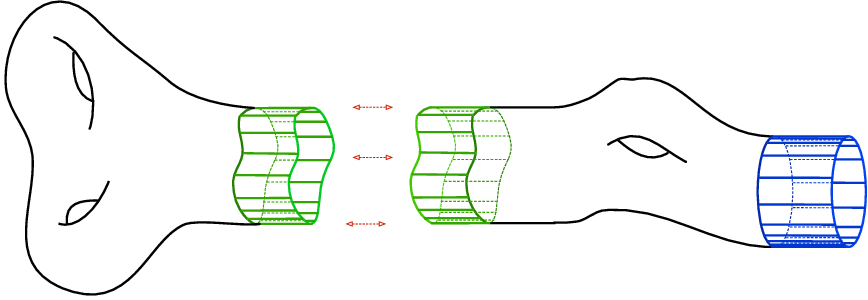
\includegraphics[scale=0.2]{figures/collar.png}
    \caption{Gluing manifolds with collars.}
    \label{fig:collars}
\end{figure}

\begin{defn}[Collar]
    The embedded submanifold $\varPhi(\mathcal{O}_p)$ of a manifold $M$ with a boundary constructed above is called a collar of $M$.
\end{defn}

\begin{cor}
    By varying $t$, we find from the above construction that $M$ is homotopy equivalent to $\mathring{M}$.
\end{cor}

Now, if we have two manifolds $M$ and $N$ with diffeomorphic boundaries, so that
\[h:\partial M\to \partial N\text{ -- diffeomorphism},\]
then we can introduce two collar embeddings (which are also diffeomorphism onto their images)
\[
\alpha:[0,1)\times\partial M\to V\subset M,\quad
\beta:[0,1)\times\partial N\to W\subset N,
\]
and unite them by
\[
\varPhi: V\sqcup W\to \partial M\times (-1,1),\quad \varPhi(x)=
\begin{cases}
(p,-t),& x=\alpha(p,t)\in V,\\
(h(q),t),& x=\beta(q,t)\in W.
\end{cases}
\]
Clearly $\varPhi$  is a topological embedding with a closed image (it's surjective), therefore, $\varPhi$ is a closed mapping.

Now let $\pi:M\sqcup N\to X$ be the quotient map on whose fibers $\varPhi$ is constant. Then $\varPhi$ descends to $\wt{\varPhi}:X\to [-1,1]\times\partial M$. $\varPhi$ is continuous and bijective, $\wt{\varPhi}(K)=\varPhi(\pi^{-1}(K))$ is closed for any compact $K$ (because $\varPhi$ is closed and $\pi$ is continuous), so $\wt{\varPhi}$ is closed too. Therefore, $\wt{\varPhi}$ is a homeomorphism and therefore, a diffeomorphism, and $X$ is a quotient manifold. Alternatively, this follows from the \emph{closed graph theorem}, which states that the graph of any continuous mapping into a Hausdorff space is closed.

\begin{defn}[Gluing of manifolds]
    The construction described above is called the gluing of two manifolds with diffeomorphic boundaries, denoted by $M\cup_h N$. See Figure~\ref{fig:collars}.
\end{defn}

\begin{defn}[Connected sum]\index{Connected sum of manifolds}
    Let $M_i$, $i=1,2$ be two connected manifolds without boundaries and $M_i'=M_i\setminus U_i$, where $U_i$ is a coordinate ball. We can pick two diffeomorphisms $h_i:\partial M_i'\to \bbS^{n-1}$, $i=1,2$. Then we define the connected sum as the gluing along $h_1\circ h_2^{-1}$:
    \[M_1 \# M_2\coloneqq M_1'\cup_{h_1\circ h_2^{-1}}M_2'.\]
\end{defn}
\begin{example}
    $D(M)=M\cup_{\partial M}M$ is called the \emph{double} of a manifold with a boundary.
\end{example}
\begin{example}
    If $X\parallel \partial D$, $D\subset M$, then $\Fl^X$ leaves $D$ invariant.
\end{example}
\begin{cor}
    If $X\parallel \partial M$, then the theorem about the existence of flows applies to $X$.
\end{cor}
\begin{proof}
    Extend $X$ to the double $D(M)$, apply the flow theorem there, then restrict to $M$.
\end{proof}

\begin{thm}[Rectification of vector fields]\index{Theorem!Rectification of vector fields}\label{rectification}
If $X\in\fX(M)$ and $X(p)\neq 0$, then there exists a local chart $(U,\varphi)$ at $p$ such that its slice $S=\{p\in U\mid \varphi^1(p)=0\}$ is diffeomorphic to $\bbD^{n-1}$, $X(p)\notin \T_p S$ and $X=\partial_1$ on $U$.
\end{thm}
\begin{proof}
    Since $S\emb M$, it has a slice neighborhood. We can parametrize $S$ by an embedding map $x:\Omega\to S$ with $\Omega\mathring{\subset}\bbR^{n-1}$. We can take $U$ such that $\restr{X}{U}\cap \T S=\varnothing$. 

    Now we can use a flow-out along $X$ so that the flow $\Fl^X_t(x(s))$ parametrizes $\Fl(x(\Omega))\emb M$. This is a diffeomorphism $\mathcal{O}_\delta\to F(x(\Omega))=x(\Omega)_\delta$ and hence has a smooth inverse. The inverse then gives a local chart $\varphi=\psi^{-1}$, where $\psi(s,t)=\Fl^X_t(x(s))$. Finally, $X=\partial_t=\partial_1$ in this local chart.
\end{proof}

\begin{defn}[Complete integral]\index{Complete integral}\label{def complete integral}
    A complete integral of a vector field $X\in \fX(M)$, $\dim M=n$, is a local function $\varPsi:U\times I_\epsilon\to\bbR^n$ such that $\varPsi^{-1}(\bf{c})$ for every $\bf{c}\in\bbR^n$ in the image of $\varPsi$ is an integral curve of $X$ at a point $m\in U$. The components $\varPsi^i:U\times I_\epsilon\to \bbR$ of this map are called a \emph{complete set of integrals of motion} for $X$.
\end{defn}
\begin{prop}
    Local complete integrals exists for all vector fields.
\end{prop}
\begin{proof}
    First rectify the vector field, then the coordinates $\bf{c}=(\varphi^1(s),\varphi^2(s),\ldots,\varphi^n(s))$ of the point $s$ of intersection of each integral curve with the slice $S$ will be the (constant) value of the diffeomorphism $\varPsi:(s,t)\mapsto \varphi(\Fl_t(s))$ on this whole curve.
\end{proof}




\section{Vector fields as differential operators}

Recall that Lie derivatives of functions satisfy $\Lie_{F_\ast X}F_\ast f=F_\ast\Lie_X f$ for diffeomorphisms $F$. Also, Lie derivatives are local: for any open set $U\subset M$,
\[\Lie_{\restr{X}{U}}\left(\restr{f}{U}\right)=\restr{\left(\Lie_X f\right)}{U}.\]

\begin{defn}[Derivations]\index{Derivation}
    If $A$ is an algebra over a field $\bbK$, then a derivation on $A$ is a $K$-linear map $D:A\to A$ that satisfies the Leibniz rule
    \[D(a\cdot b)=D(a)\cdot b+a\cdot D(b),\;\; a,b\in A.\]
    Is is easy to check that the vector space of all derivations on $A$, denoted by $\mathrm{Der}(A)$, is a Lie algebra under the commutator $[D_1,D_2]=D_1\circ D_2-D_2\circ D_1$.
    An algebra with a distinguished derivation is called a \emph{differential algebra}.\index{Differential algebra}
\end{defn}

Clearly any Lie derivative $\Lie_X, X\in\fX(M)$, is a derivation on the algebra of functions $C^\infty(M)$, because it is a directional derivative in local coordinates.
Moreover, any derivation $D$ on $C^\infty(M)$ satisfies $D(1)=0$, because
\[D(1)=D(1^2)=D(1)\cdot 1+1\cdot D(1)=2\cdot D(1).\]
Finally, the set of all Lie derivatives $\{\Lie_X\}_{X\in\fX(M)}$ is a $C^\infty(M)$-module:
\[f\cdot\Lie_X=\Lie_{f\cdot X}.\]

\begin{prop}[{{\cite[Prop.~2.2.9]{Marsden}}}]\label{prop 2.2.9 Marsden}
    The vector space of Lie derivatives $\{\Lie_X\}_{X\in\fX(M)}$ is isomorphic to $\fX(M)$ as $C^\infty(M)$-modules. In particular, $\Lie_X=0$ iff $X=0$.
\end{prop}
\begin{proof}
    The map $X\mapsto \calL_X$ is clearly $C^\infty(M)$-linear and surjective by definition. To show that it is an isomorphism, we need to show that its kernel is zero. Suppose $\calL_X=0$ and $m\in M$. Then $\dd_m f(X_m)=0$ for all $f\in C^\infty(M)$, and hence $\alpha_m(X_m)=0$ for all $\alpha_m\in \T_m^\ast M$. But then $X_m=0$.
\end{proof}
\begin{prop}[{{\cite[Thm.~2.2.10]{Marsden}}}]\label{lie derivatives and vector fields}
The space of all $\bbR $-linear derivations on the algebra $C^\infty(M)$ is isomorphic to $\fX(M)$ as a vector space. In particular, every derivation $\theta$ coincides with $\Lie_X$ for a unique $X\in\fX(M)$.
\end{prop}
\begin{proof}
    Given $\theta$, we construct the vector field $X$.
    First of all, $\theta$ is local, i.e., if $h$ vanishes on a neighborhood $V\mathring{\subset} M$ of $p\in V$, then $\theta(h)(p)=0$. Indeed, if $\chi$ is a bump function equal to $1$ around $p$ and zero outside of $V$, then $h=(1-\chi)h$ and
    \[\theta(h)(p)=(\theta(1-\chi))\cdot h(p)+\theta(h)\cdot (1-\chi(p))=0.\]

    Pick a local chart at $p$, $\varphi:U\to\wh{U}\subset\bbR^n$. Let $\bf{x}\in\wh{U}$, $\bf{a}=\varphi(p)$, $f\in C^\infty(M)$, then 
    \[(\varphi_\ast f)(\bf{x})=(\varphi_\ast f)(\bf{a})+\sum_{j=1}^n (x^j-a^j)\int_0^1 \frac{\partial(\varphi_\ast f)}{\partial x^j} (\bf{a}+t(\bf{x}-\bf{a}))\dd t\]
    on some neighborhood of $\bf{a}$.
    Therefore, for $u\in U$,
    \[f(u)=f(p)+\sum_{i=1}^n (\varphi^i(u)-a^i)g_i(u),\quad g_i(p)=\frac{\partial(\varphi_\ast f)}{\partial x^i} (\varphi(p)).\] 
    Thus,
    \[(\theta f)(p)=\sum_i g_i(p)\theta(\varphi^i)(p)=\sum \partial_{x^i}(\varphi_\ast f)(\bf{a}) \theta \varphi^i(p),\]
    and this is formula is chart-independent! Now we can define a smooth $X$ by its local representation
    \[X^i(u)\coloneqq \theta\varphi^i(u).\]
    It is easy to check that $X$ is independent of the choice of $\varphi$, which means that it is actually a globally well-defined vector field on $M$. For $f\in C^\infty(M)$, the local representative in $\bf{x}=\varphi(u)\in\wh{U}$ of $\Lie_X f$ is 
    \[(f\circ\varphi^{-1})_{\ast \bf{x}}\circ \wh{X}(\bf{x})=\sum_i \partial_{x^i}(f\circ \varphi^{-1})(x)\cdot \theta \varphi^i (u)=\theta f(u),\]
    hence $\theta=\Lie_X$.
    Uniqueness follows from the obvious statement that $\Lie_X=0$ iff $X=0$.
\end{proof}
\begin{cor}
    If $x^i$ is a local coordinate system, then the local vector fields $\partial_i=\partial_{x^i}$ form a basis of derivations at $p$, therefore, 
    \[(\Lie_X f)(p)=\sum_i \partial_{x^i}(f\circ\varphi^{-1})(\varphi(p))\cdot \underbrace{\Lie_X (\varphi^i)(p)}_{X^i}=\sum_i X^i \partial_{x^i}(\varphi_\ast f)=\sum_i X^i \partial_{i} f.\]
\end{cor}

\begin{prop}
    If $X,Y\in\fX(M)$, then $[\Lie_X,\Lie_Y]=\Lie_X\Lie_Y-\Lie_Y\Lie_X$ is a derivation on $C^\infty(M)$.
\end{prop}
\begin{proof}
    This is a very general property that the commutator of two derivations is always a derivation:
    \begin{multline}
        [D_1,D_2](fg)=D_1((D_2f)g+f(D_2g))-D_2((D_1f)g+f(D_1g))=\\=([D_1,D_2]f)g+f([D_1,D_2]g).
    \end{multline}
\end{proof}

This proposition allows us to define the commutator of vector fields.

\begin{defn}[Lie derivative/bracket of vector fields]\index{Lie derivative!of a vector field}\index{Commutator of vector fields!see {Lie derivative}}
    If $X,Y\in\fX(M)$, then the Lie derivative of $Y$ along $X$ is denoted by 
    \[\Lie_X Y\equiv [X,Y]\] and is defined as the unique vector field such that
    \[\Lie_{[X,Y]}=[\Lie_X,\Lie_Y].\]
    With this bracket, $\fX(M)$ becomes a Lie algebra that is isomorphic to the Lie algebra of derivations on $C^\infty(M)$ (i.e., Lie derivatives).
    In local coordinates (using Einstein summation),
    \[[X,Y]^j=X^i \partial_i Y^j-Y^i \partial_i X^j.\label{eq Lie derivative in components}\]
\end{defn}

\begin{prop}\label{prop properties of Lie derivatives}
\begin{enumerate}
    \item $[X,Y]$ is local and natural w.r.t.\ diffeomorphisms, i.e., \[F_\ast [X,Y]=[F_\ast X,F_\ast Y];\]
    \item $\Lie_X$ is a derivation on the Lie algebra $\fX(M)$, i.e., satisfies the Jacobi identity
    \[\Lie_X [Y,Z]=[\Lie_X Y,Z]+[Y,\Lie_X Z];\]
    \item $\Lie_X$ is also a derivation on $C^\infty(M)\otimes \fX(M)$ i.e., it satisfies the mixed Leibniz rule
    \[\Lie_X(f\otimes Y)=\Lie_X(f\cdot Y)=(\Lie_X f)\cdot Y+f\cdot \Lie_X Y.\]
    Equivalently, 
    \[\Lie_{fX}Y=f\cdot \Lie_X Y+\left(\Lie_X f\right)\cdot Y.\label{Lie derivative not covariant}\]
\end{enumerate}
\end{prop}
\begin{proof}
    \begin{enumerate}
        \item To prove any of these properties, we act with both sides on a function $f$ as a Lie derivative. Then the equality of the two expressions as derivations implies the equality as vector fields by Proposition~\ref{lie derivatives and vector fields}. Therefore, this is just a direct computation using the push-forward property for Lie derivatives acting on functions.
        \item General property of derivations that is easily checked by expanding both sides.
        \item Check 
        \begin{multline}
            [X,fY]g=\Lie_X (\Lie_{fY}g)-\Lie_{fY}\Lie_X g=\Lie_X (f\Lie_Y g)-f\Lie_Y \Lie_X g=\\=(\Lie_X f)\Lie_Y g+f\Lie_X\Lie_Y g-f\Lie_Y\Lie_X g=((\Lie_X f)Y+f[X,Y])g.
        \end{multline}
    \end{enumerate}
\end{proof}


\begin{rem}[Lie derivatives are not covariant derivatives]\label{rem: Lie derivatives not covariant}
    Property \eqref{Lie derivative not covariant} shows that $\Lie_X Y$ doesn't behave like a tensor w.r.t.\ $X$ (or $Y$), since it is not $C^\infty(M)$-linear in it. This is why Lie derivatives are not a special case of \emph{covariant} derivatives.
    
    A covariant derivative (of vector fields) is a map $\nabla:\fX(M)\otimes\fX(M)\to \fX(M)$ denoted by $X,Y\mapsto \nabla_X Y$ such that it satisfies:
    \begin{itemize}
        \item $C^\infty(M)$-linearity in $X$: $\nabla_{fX}Y=f\cdot \nabla_X Y$ for $f\in C^\infty(M)$;
        \item $\bbR $-linearity in $Y$: $\nabla_X (\alpha Y+Z)=\alpha \nabla_XY+\nabla_XZ$ for $\alpha\in\bbR $;
        \item Leibniz rule: $\nabla_X(f\cdot Y)=(\Lie_X f)\cdot Y+f\cdot \nabla_X Y.$
    \end{itemize}
    Therefore, any covariant derivative $\nabla_X Y$ has to be a tensor in $X$, unlike Lie derivatives. In other words, a covariant derivative can be thought of as a map $\nabla:\fX(M)\to \fX^\ast(M)\otimes\fX(M)=\Gamma^1_1(M)$, $Y\mapsto \nabla Y\in\Gamma^1_1(M)$.
\end{rem}

All of this allows us to extend the Lie derivative to tensor fields of any rank by the following theorem.

\begin{defn}[Tensor differential operators]\index{Differential operator on the tensor algebra}
    A differential operator on the tensor algebra $\Gamma^\infty(M)$ is a collection of maps $\mathbb{D}^r_s(U):\Gamma^r_s(U)\to \Gamma^r_s(U)$ for all $r,s\geq 0$ and each open $U\mathring{\subset}M$ (we denote them all by $\mathbb{D}$) such that:
\begin{enumerate}
    \item $\mathbb{D}$ is a tensor derivation (w.r.t.\ $\otimes$);
    \item $\mathbb{D}$ is local, i.e., for $U\subset V$ and $t\in\Gamma^r_s(V)$, $\restr{\mathbb{D}(t)}{U}=\mathbb{D}(\restr{t}{U})$;
    \item $\mathbb{D} \delta=0$, where $\delta\in\Gamma^1_1(M)$ is the Kronecker tensor $\delta=\id_{\T M}$.
\end{enumerate}
\end{defn}

Note that we don't require $\mathbb{D}\circ\varphi_\ast=\varphi_\ast\circ \mathbb{D}$ because this will not hold for covariant derivatives, which we would still like to consider differential operators.

\begin{thm}[Willmore {{\cite[Thm.~2.2.17]{Marsden}}}]\index{Theorem!Willmore}\label{Willmore}
    A collection of local tensor derivations $E_U$ on $C^\infty(U)$ and $F_U$ on $\fX(U)$ (which agree with each other via the mixed rank Leibniz rule) for each $U\mathring{\subset}M$ determines a unique differential operator $\mathbb{D}$ on the tensor algebra $\Gamma^\infty(M)$ that coincides with $E_U$ on $C^\infty$ and with $F_U$ on $\fX$.
\end{thm}
\begin{proof}
    Suppose we know that such a $\mathbb{D}$ exists. In a local frame $\{e_i\}$ and dual frame $\{\alpha^i\}$, we can write
    \[t(u)=\underbrace{t_{j_1\ldots j_s}^{i_1\ldots i_r}(u)}_{\in C^\infty(U)} e_{i_1}\otimes \cdots \otimes e_{i_r}\otimes \alpha^{j_1}\otimes \cdots\otimes \alpha^{j_s}(u).\label{535}\]
    By using the tensorial Leibniz rule for $\mathbb{D}$, we express $\mathbb{D}t(u)$ only in terms of $E_U(t_{j_1\ldots j_s}^{i_1\ldots i_r})$ and $F_U(e_{i_k})$.
    
    Namely, since $\mathbb{D}\delta=0$, and $\delta=e_j\otimes \alpha^j$ (using Einstein summation), we have 
    \[0=\mathbb{D}(e_j\otimes \alpha^j)=(\mathbb{D}e_j)\otimes \alpha^j+e_j\otimes (\mathbb{D}\alpha^j).\]
    Since $\delta^i_j=\alpha^i(e_j)$, if we contract the formula above with $e_i$, we get
    \[0=F_U e_i+(\mathbb{D}\alpha^j)(e_i) e_j,\]
    which completely determines $\mathbb{D}\alpha^j$. Therefore, the action of $\mathbb{D}$ on $\fX^\ast$ is uniquely determined, and the Leibniz rule applied to \ref{535} gives a formula for $\mathbb{D}$ in terms of $E_U$ and $F_U$ on the whole tensor algebra.
    
    The formulas we have derived prove the uniqueness of $\mathbb{D}$. Its existence follows from the fact that these same formulas define a valid differential operator that satisfies all the requirements of the theorem.
\end{proof}
\begin{cor}\label{cor willmore formula}
    A byproduct of the theorem above is the general formula for differential operators on the tensor algebra:

    \begin{multline}
        \mathbb{D}\left(t(\alpha^1,\ldots,\alpha^r,X_1,\ldots,X_s)\right)=(\mathbb{D}t)(\alpha^1,\ldots,\alpha^r,X_1,\ldots,X_s)+\\+\sum_{j=1}^r t\left(\alpha^1,\ldots,\mathbb{D}\alpha^j,\ldots,\alpha^r,X_1,\ldots,X_s\right)+\sum_{k=1}^s t\left(\alpha^1,\ldots,\alpha^r,X_1,\ldots,\mathbb{D}X_k,\ldots,X_s\right).
    \end{multline}
    This formula essentially states that $\mathbb{D}$ ``commutes with contractions''.
\end{cor}

This allows us to extend the definition of the Lie derivative to arbitrary tensor fields. This natural operator was first formalized by \'Elie Cartan around 1920, although he was primarily interested in derivatives of differential forms, which we will study in \Chap~\ref{ch: differential forms}. It was named after Sophus Lie by others in the 1930's.

\begin{defn}[Lie derivatives of tensors]\index{Lie derivative!of a tensor field}
    If $X\in\fX(M)$ then the Lie derivative operator $\Lie_X$ on the tensor algebra $\Gamma^\infty(M)$ is defined as the unique tensor differential operator (established by Willmore's theorem) that coincides with the previously constructed Lie derivative on $C^\infty(M)$ and $\fX(M)$.
\end{defn}

\begin{prop}[Naturality of Lie derivatives]\label{pullbacks of Lie derivatives}
For a diffeomorphism $F$, 
\[\Lie_{F_\ast X}(F_\ast t)=F_\ast (\Lie_X t).\]
\end{prop}
\begin{proof}
    Define an operator $\mathbb{D}$ by $\mathbb{D}t=F^\ast \Lie_{F_\ast t}(F_\ast t)$. We know that $\mathbb{D}$ coincides with $\Lie_X$ on $C^\infty$ and $\fX(M)$. It is also easy to check that $\mathbb{D}$ is a tensor differential operator (exercise). Then, by Willmore's Theorem, is must coincide with $\Lie_X$ on the entire tensor algebra.
\end{proof}





\section{Geometric approach to Lie derivatives}

We now demonstrate a more fundamental geometric definition of Lie derivatives. It has to do with the fact that tensor fields on a manifold $M$, unlike sections of general \glspl{vb} over $M$, can be transformed to other tensor fields by diffeomorphisms of $M$. Thus, infinitesimal diffeomorphisms (i.e., vector fields) produce special differential operators acting on tensor fields.

Let $X\in \fX(M)$ and let $(U,a,F)$ be a flow box of $X$ at $p\in M$. Let $t\in\Gamma^r_s(M)$ and define
\[t_\lambda\coloneqq F_{\lambda}^\ast \left(\restr{t}{U_\lambda}\right)=F_{\lambda\ast}^{-1} \left(\restr{t}{U_\lambda}\right)\in\Gamma^r_s(U),\]
where $F_\lambda :U\to U_\lambda$ is the flow diffeomorphism. Then with fixed $p$, the map $\lambda\mapsto t_\lambda (p) \in \bbT^r_s (\T_p M)$ defines a curve in the vector space of tensors at $p$.
\begin{thm}
    $\lambda\mapsto t_\lambda (p)$ defined above is a curve in the vector space $\bbT^r_s (\T_p M)$ passing through $t(p)$ and its derivative evaluates the Lie derivative of $t$:
    \[\Lie_X t(p)=\restr{\frac{\dd}{\dd \lambda}}{\lambda=0}t_\lambda(p).\]
\end{thm}
\begin{proof}
    We have 
    \[t_\lambda(p)=(\bbT^r_s F_\lambda^{-1})\circ t \circ F_\lambda(p),\] 
    which is clearly smooth.
    Define $\theta_X$ as an operator on $\Gamma^r_s(M)$ by 
    \[\theta_X t(p)=\restr{\frac{\dd}{\dd \lambda}}{\lambda=0} t_\lambda(p).\]
    For $t\in C^\infty(M)$, $t_\lambda(p)$ is smooth, therefore, $\theta_X t(p)=(Tt_\bullet)(\partial_\lambda)\in C^\infty(M)$, where the differential $T$ is w.r.t.\ the variable $\lambda$ (represented by $\bullet$) and  $\partial_\lambda$ is a vector field on the $\bbR $. $\theta_X$ is a linear derivation because its local representatives are. It is defined locally, therefore, it is local. Finally, 
    \[\theta_X\delta=\restr{\frac{\dd}{\dd \lambda}}{\lambda=0} F^\ast_\lambda \delta=\restr{\frac{\dd}{\dd \lambda}}{\lambda=0}\delta=0.\] 
    This proves that $\theta_X$ is a differential operator. It remains to check that $\theta_X=\Lie_X$ on $C^\infty(M)$ and $\fX(M)$. First, for $f\in C^\infty(M)$, 
    $f_\lambda=f\circ F_\lambda$, 
    \[\restr{\frac{\dd}{\dd \lambda}}{\lambda=0}f_\lambda(p)=\dd f\circ \restr{\frac{\dd}{\dd \lambda}}{\lambda=0}F_\lambda=\dd f\circ X=\Lie_X f.\]
    Now, note that for $f\in C^\infty(M)$ there exists a $g_\lambda\in C^\infty(M)$ such that $g_0=\Lie_X f$ and $f\circ F_\lambda=f+\lambda g_\lambda$. Namely, 
    \[\lambda g_\lambda (p)=\int_0^1 \partial_t(f\circ F_{t\lambda}(p))\dd t.\] 
    Then for $Y\in\fX(M)$,
    \begin{align}
        \Lie_{\theta_X Y}f(p)&=\dd f\circ \restr{\frac{\dd}{\dd \lambda}}{\lambda=0} \left((F_{-\lambda})_{\ast p}\circ Y\circ F_\lambda(p)\right)=\\
        &=\restr{\frac{\dd}{\dd \lambda}}{\lambda=0}\left((f\circ F_{-\lambda})_\ast\circ Y\circ F_\lambda(p)\right)=\\
        &=\restr{\frac{\dd}{\dd \lambda}}{\lambda=0} \left((f-\lambda g_{-\lambda})_\ast\circ Y\circ F_\lambda(p)\right)=\\
        &=\restr{\frac{\dd}{\dd \lambda}}{\lambda=0} f_\ast\circ Y\circ F_\lambda (p)-\restr{\left(\frac{\dd}{\dd \lambda}\lambda\right)(g_{-\lambda})_\ast\circ Y\circ F_\lambda(p)}{\lambda=0}=\\
        &=\dd(\underbrace{f_\ast\circ Y}_{\Lie_Yf})\circ \underbrace{\restr{\frac{\dd}{\dd \lambda}}{\lambda=0} F_\lambda(p)}_{X(p)}-(g_0)_\ast \circ Y\circ F_0(p)=\\
        &=\Lie_X\Lie_Y f-\Lie_Y\Lie_X f(p),
    \end{align}
    therefore, $\theta_X Y=[X,Y]$. By Willmore's theorem, $\theta_X=\Lie_X$.
\end{proof}
\begin{cor}
\begin{enumerate}
    \item $\Lie_X t=0$ iff $t$ is constant along the flow of $X$: $F^\ast_\lambda t=t$;
    \item For all $\lambda$ in the flow domain the following equality holds:
    \[\frac{\dd}{\dd \lambda}F^\ast_\lambda t=F^\ast_\lambda \Lie_X t.\]
    In particular, 
    \[\Lie_X t=F^\ast_{-\lambda} \frac{\dd}{\dd \lambda}F^\ast_\lambda t=\restr{\frac{\dd}{\dd\lambda}}{\lambda=0}F^\ast_\lambda t.\]
\end{enumerate}
\end{cor}

\begin{rem}[Push-forwards are not parallel transports]
    Since covariant derivatives are in the exact same relationship with parallel transports as Lie derivatives are with push-forwards, it is tempting to think that Lie derivatives are special cases of covariant derivatives. However, we have already seen this to be wrong in Remark \ref{rem: Lie derivatives not covariant}. This means that push-forwards by flows of vector fields cannot be interpreted as a kind of parallel transport along the integral curves of those vector fields. This is because a parallel transport has to be unambiguously defined for every curve on $M$, whereas there are infinitely many vector fields for which a given curve is integral (and the value of the push-forward will depend on the specific choice of vector field). Transport by push-forwards is often called \emph{Lie transport}\index{Lie transport}. Lie derivatives are just infinitesimal Lie transport.
\end{rem}

\begin{rem}
    We can apply these ideas to PDEs on $\bbR^n$:
    \[\begin{cases}
        \partial_t f(x,t)=\sum _i X^i \partial_i f(x,t),&\\
        f(x,0)=g(x).&
    \end{cases}\]
    Then if $X$ has a complete flow $F_t$, the unique solution of the above Cauchy problem is $f(x,t)=g(F_t(x))$, which can be checked by substitution. This is sometimes called the \emph{method of characteristics}. The ``characteristics'' are the integral curves along which the values of $g(x)$ get propagated.
\end{rem}

\begin{prop}
    Given two vector fields $X,Y$ with complete flows $F_t$ and $G_t$, respectively, \gls{tfae}:
    \begin{enumerate}
        \item $[X,Y]=0$;
        \item $F^\ast_t Y=Y$ (or $G^\ast_t X=X$);
        \item $F_t\circ G_s=G_s\circ F_t$ for all $t,s$. 
    \end{enumerate}
    In particular, the flow of $X+Y$ for commuting $X$ and $Y$ is $F_t\circ G_t$.
\end{prop}
\begin{proof}
    $1\implies 2$. $\frac{\dd}{\dd t}F^\ast_t Y=F^\ast_t \Lie_X Y=0$, therefore, $F^\ast_t Y$ is constant and we know that $F^\ast_0 Y=Y$, so $F^\ast_t Y=Y$.

    $2\implies 3$. Consider the curve $\gamma(t)=G_s\circ F_t(p)$. It starts at $\gamma(0)=G_s(p)$ and its velocity is
    \[\dot\gamma(t)=\frac{\dd}{\dd t} G_s\circ F_t(p)=G_{s\ast}\circ X\circ F_t\overset{(2)}{=}X\circ\gamma(t).\]
    So $\gamma(t)$ is an integral curve of $X$ going through $p$. Therefore, by uniqueness (and definition of the flow of $X$), 
    \[\gamma(t)=F_t\circ G_s(p).\]
    This shows that the flows commute. Finally, we check 
    \[\frac{\dd}{\dd t} F_t\circ G_t(p)=X(F_t(G_t(p)))+\underbrace{F_{t\ast }Y}_{Y\circ F_t}(G_t(p))=(X+Y)(F_t\circ G_t(p)).\]

    $2\implies 1$. $\Lie_X Y=F^\ast_{-t}\frac{\dd}{\dd t}F^\ast_t Y=F^\ast_{-t} \frac{\dd}{\dd t}Y=0$.

    $3\implies 2$. $F_{t\ast}Y=F_{t\ast}\frac{\dd}{\dd s}G_s=F_{t\ast} G_{s\ast} Y=(F_t\circ G_s)_\ast Y=(G_s\circ F_t)_\ast Y=G_{s\ast}F_{t\ast}Y$. But the only vector field invariant under $G_{s\ast}$ is $Y$, therefore, $F_{t\ast}Y=Y$.
\end{proof}

\begin{rem}[Taylor formula on manifolds]\index{Taylor's formula}\label{rem 3.2.9 RS1}
    Successive application of the vector fields $X_1,\ldots,X_r$ to a function $f\in C^\infty(M)$ yields
    \[X_r\cdots X_1 \cdot f=\restr{\frac{\dd}{\dd t_1}}{t_1=0}\cdots \restr{\frac{\dd}{\dd t_r}}{t_r=0}f\circ F^{X_1}_{t_1}\circ \cdots \circ F^{X_r}_{t_r}.\]
    In particular, the Lie bracket can be expressed as
    \[[X,Y]f=\restr{\frac{\dd}{\dd t}}{t=0}\restr{\frac{\dd}{\dd s}}{s=0}\left(f\circ \Fl^Y_s\circ \Fl^X_t-f\circ \Fl^X_s\circ \Fl^Y_t\right).\label{eq Lie bracket in terms of flows}\]
    Furthermore, for any $m\in M$, the Taylor expansion of the smooth function $t\mapsto f\circ \Fl^X_t(m)$ at $t=0$ yields the following \emph{Taylor formula for manifolds}:
    \[f\circ \Fl^X_t(m)=\sum_{k=1}^n\frac{t^k}{k!}\left(X^kf\right)(m)+\calO(t^{n+1}), \quad t\in \calD^X_m,\label{eq:Taylor formula for manifolds}\]
    where $\calO(t^{n+1})$ is a smooth function on $\calD_m^X$ such that $\calO(t^{n+1})/t^{n+1}$ is bounded. By defining the exponential of a differential operator formally as $\rme^{tD}=\sum_{k=0}^\infty \frac{t^k}{k!}D^k$, the above Taylor formula is sometimes written formally as $f\circ \Fl^X_t=\rme^{t X}\cdot f$.

    Repeated application of this formula yields the iterated Taylor formula for manifolds
    \[f\circ \Fl^X_t\circ \Fl^Y_s(m)=\sum_{k,l=1}^n\frac{t^ks^l}{k!l!}\left(Y^lX^kf\right)(m)+\calO(t^{n+1},s^{n+1}),\label{eq: Taylor formula for two fields}\]
    which easily generalizes to any number of vector fields.
\end{rem}


\begin{defn}[Holonomic frame]\index{Holonomic frame}
    A local $k$-frame $\{e_i\}_{i=1}^k$ is called holonomic if $[e_i,e_j]=0$ for all $i,j$.
\end{defn}

The following shows that this definition of holonomic frames agrees with the one indicated in Definition~\ref{def jet bundles}. That is, each holonomic frame arises from some local coordinates.

\begin{thm}[Rectification of frames]\index{Theorem!Rectification of frames}\label{thm rectification}
    Let $\{e_j\}_{j=1}^k$ with $k\leq n=\dim M$ be a holonomic local $k$-frame on $W\mathring{\subset}M$. Assume that $e_j(p)\notin \T_p S$ for all $p\in S$, where $S\emb M$ is a submanifold with $\codim S=k$. Then there exists a local chart of coordinates $(s^1,\ldots,s^n)$ in which $S=\{s^1=\cdots=s^k=0\}$ and for $j\leq k$ we have $\partial_j=e_j$.
\end{thm}
\begin{proof}
    Parametrize $S$ as usual by $x:\varOmega\to S$ with $\varOmega\mathring{\subset}\bbR^{n-k}$, define a chart $\varphi=\psi^{-1}$, where
    \[\psi(s^1,\ldots,s^k,s^{k+1},\ldots,s^n)=F^{e_1}_{s_1}\circ\cdots\circ F^{e_k}_{s_k}(x(s^{k+1},\ldots,s^n)),\]
    and $F^{e_i}$ is the flow of $e_i$. The inverse $\psi^{-1}$ exists locally because the differential at $(0,\ldots,0)$ is identity. Finally we use commutation to compute the partials
    \begin{multline}
        \psi_\ast (\partial_{s^i})\cdot f=\partial_i(f\circ\psi)=\partial_i f(F^{e_1}_{s_1}\cdots F^{e_k}_{s_k} x(0,\ldots,0,s^{k+1},\ldots))=\\=\partial_i f(F^{e_i}_{s_i}\circ\cdots )=\partial_i F^{e_i}_{s_i}(F\cdots F(0,\ldots,0,s^{k+1},\ldots))f=e_i\cdot f=\Lie_{e_i}f,
    \end{multline}
    thus $\partial_i=e_i$.
\end{proof}

\begin{cor}
    A helpful way to reformulate this theorem for $k=\dim M$ is: a given local frame is a coordinate frame for some local coordinates iff it is holonomic.
\end{cor}

The analog of this corollary for $k<\dim M$ is a famous theorem that deserves its own section.





\section{Frobenius theorem I}\label{sec: frobenius i}

\begin{intu*}
    Rectification of vector fields and finding local coordinates generating a given holonomic frame are special instances of a general class of problems in geometry, where one seeks a special set of coordinates that in some sense encode the given geometric structure. Such problems are known as \emph{integrability problems}. The Frobenius Theorem lies at the foundation of the study of integrability, and thus of much of the rest of this book. Even though it may not seem like the search for a set of coordinates is a geometric problem (after all, wasn't the entire theory of manifolds developed to move away from choices of coordinates?), it actually becomes essential in any real-life application where geometric structures ultimately have to be described by particular mappings in particular coordinate systems. One way to think about integrability is as a generalization of the concept of a linearizing diffeomorphism that takes a given nonlinear differential equation to a linear one, thus making it solvable. Once again, we see that the problem of atlases cannot be reduced away from differential geometry.
\end{intu*}

We have just established that in the presence of a local holonomic $r$-frame $\{e_i\}_{i=1}^r$ transversal to a submanifold $S$, each point $m\in S$ admits a $r$-dimensional embedded submanifold $N$ passing through $m$ (defined by holding the values of $s^{r+1},\ldots,s^n$ constant) transversally to $S$ such that $\{e_i\}_{i=1}^r$ is a frame for $\T N$. In this \sect\ we will replace holonomic frames by the subspaces of tangent spaces that they span and derive the corresponding \emph{integrability condition}. Namely, while we can think of vector fields as fields of velocities, let us instead think of them as fields of lines, or directions. Then it is easy to generalize the problem as follows: given a field of hyperplanes (subspaces of tangent spaces), what does it mean for a submanifold to be integral for this field, and what is the condition for this kind of integrability?

\begin{hrem*}
    Note that while this theorem is universally named after Frobenius, his result (1887) was an application of an older result to the context of systems of differential equations. We will discuss that version of the theorem in \S\ref{sec: frobenius ii}. The results discussed in this \sect\ were obtained by Deahna (sufficient condition, 1840) and Clebsch (necessary condition, 1866), among many others involved in this long process.
\end{hrem*}

\begin{figure}[tp]
    \centering
    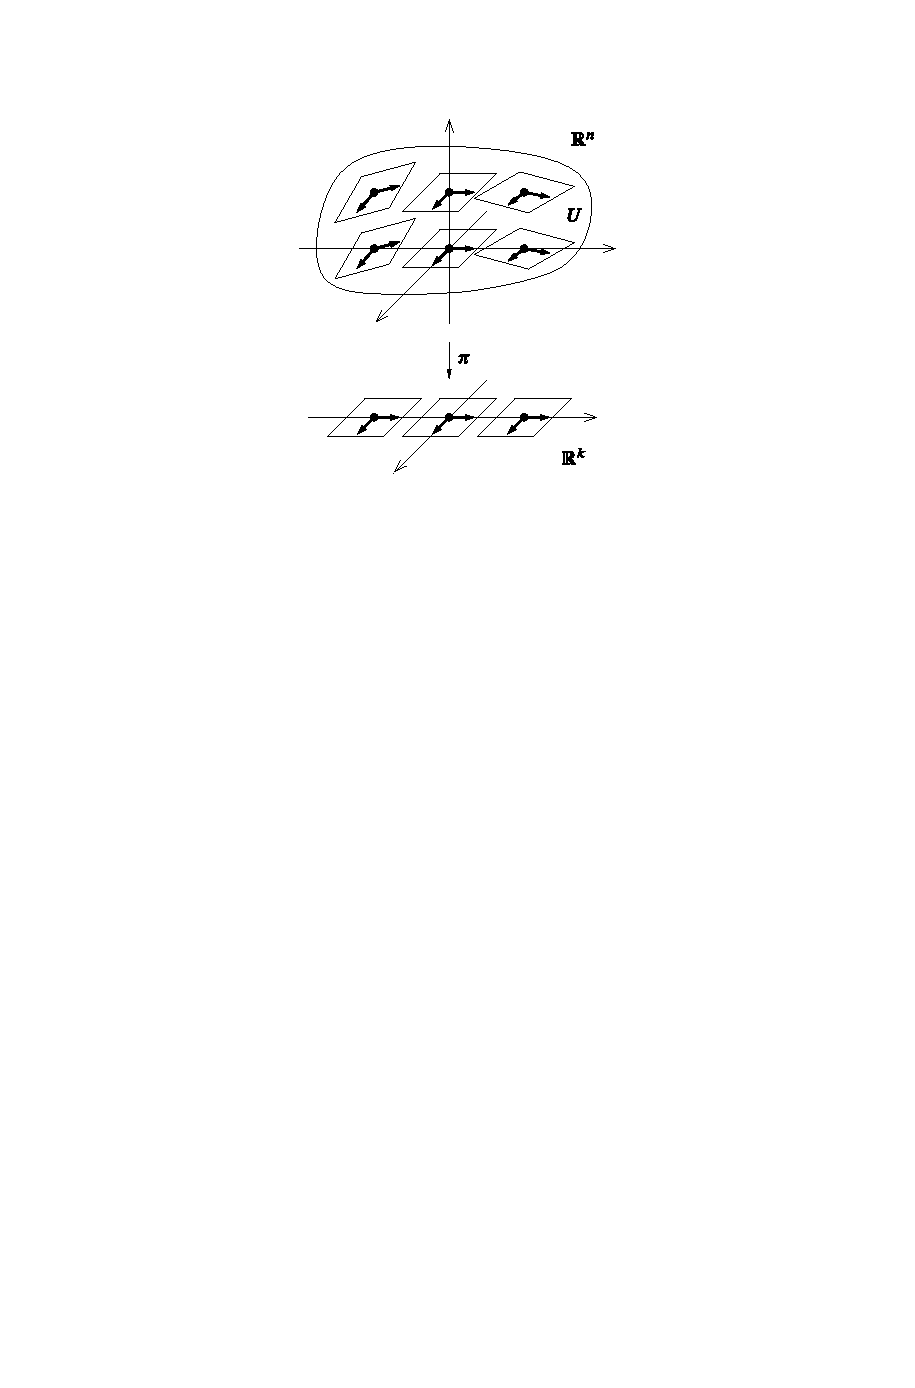
\includegraphics[scale=0.8]{figures/frobenius_1.pdf}
    \caption{Frobenius Theorem. From \cite{Lee}.}
    \label{fig: frobenius1}
\end{figure}

Recall that a distribution $D$ on a manifold is an assignment of a subspace $D_m\subset \T_m M$ for every $m\in M$. If the dimension of $D_m$ is constant and equal to $r$, then $D$ is said to be \emph{regular of rank} $r$. $D$ is called a \emph{smooth distribution} if it is a subbundle of $\T M$.

\begin{defn}[Integral manifolds]\index{Integral manifold}
    Let $D< \T M$ be a smooth distribution (i.e., a subbundle of $\T M$). An immersed submanifold $N<M$ is called an integral manifold of $D$ if $\T_m N=D_m$ for all $m\in N$.
\end{defn}

\begin{defn}[Integrable distribution]\index{Integrable distribution}
    A smooth distribution $D< \T M$ is called (completely) integrable if every $m\in M$ is contained in a (local) integral manifold of $D$.
\end{defn}

\begin{rem}
    Depending on the context, a distribution may also be called integrable if it has integral manifolds of \emph{some} positive dimension at every point. However, we will treat the term ``integrable distribution' as synonymous to ``completely integrable distribution'' unless otherwise specified. Integrability in this broader sense will be properly distinguished from complete integrability in \Chap~\ref{chap: EDSs}.
\end{rem}

\begin{defn}[Involutive distribution]\index{Involutive distribution}
    For a smooth distribution $D< \T M$, denote by $\Gamma^\infty(D)\subset\fX(M)$ the space of $D$-valued vector fields. $D$ is called involutive if $\Gamma^\infty(D)$ is a Lie subalgebra of $\fX(M)$, i.e., $[X,Y]\in\Gamma^\infty(D)$ for all $X,Y\in\Gamma^\infty(D)$.
\end{defn}

\begin{thm}[Frobenius Theorem (Clebsch 1866) {{\cite[Thm.~19.12]{Lee}}}]\index{Theorem!Frobenius}\label{thm frobenius}
    A smooth distribution $D$ is involutive iff it is completely integrable.
\end{thm}
\begin{proof}
    The backwards direction is trivial: if $D$ is integrable, then $D=\T N$ locally, which implies involutivity.
    For the forward direction, it suffices to prove that $D$ is locally spanned by a set of linearly independent commuting fields. Then, by the Rectification Theorem~\ref{thm rectification}, they are coordinate vector fields for a slice chart of an integral manifold.

    Because of the locality of the statement, it also suffices to prove the theorem for $M=U\subset \bbR^n$. Suppose that the rank of $D$ is $r$. Then, at every $m\in M$, we can find a system of Cartesian coordinates such that $D_m$ is complementary to the span $\<\partial_{r+1},\ldots,\partial_m\>$. By continuity, this remains true on some neighborhood of $m$. Therefore, we have a non-singular projection $\pi:\bbR^m\to\bbR^r$ onto the coordinate hyperplane of the coordinates $(x^1,\ldots,x^r)$. Then $\restr{\pi_\ast}{D}$ is a smooth bundle isomorphism, and the vector fields $\pi^\ast(\partial_i)$, $i=1,\ldots,r$, locally span $D$, see Figure~\ref{fig: frobenius1}. By naturality of Lie derivatives, $[\pi^\ast(\partial_i),\pi^\ast(\partial_j)]=\pi^\ast[\partial_i,\partial_j]=0.$
    Thus, $D$ is indeed spanned by a holonomic $r$-frame and therefore, integrable.
\end{proof}

This theorem is of crucial importance in the theory of Lie groups, \glspl{fb}, and even dynamical systems. The entire concept of \emph{integrability} ultimately stems from it. The rest of this \sect\ is devoted to characterizing integral submanifolds and proving a global version of the Frobenius theorem, which will be useful is many applications down the line.

\begin{cor}[{{\cite[Cor.~19.13]{Lee}}}]\label{cor 19.13 Lee}
    Let $D$ be a rank $r$ involutive distribution on $M$. If $S\emb M$ is a codimension $r$ embedded submanifold such that $\T_mS\cap D_m=\{0\}$ for all $m\in S$, then there is a \emph{flat chart}\index{Flat chart} $(U,\{s^i\})$ for $S$ centered at $m$ in which $S\cap U$ is the slice $s^1=\cdots=s^r=0$.
\end{cor}
\begin{proof}
    The proof of Frobenius theorem showed that locally $D$ is spanned by $r$ commuting vector fields, so this corollary follows by the Rectification Theorem~\ref{thm rectification}.
\end{proof}

Note also that $U$ gets decomposed into a disjoint union of integral submanifolds $U_{\bf{c}}$ parametrized by a point $\bf{c}\in S$ with coordinates $(0,\ldots,0,c^1,\ldots,c^{n-r})$ in the flat chart and defined as the slices $s^{r+1}=c^1,\ldots, s^n=c^{n-r}$.

\begin{prop}[{{\cite[Prop~19.16]{Lee}}}]\label{prop 19.16 Lee}
    Let $D$ be an involutive distribution of rank $r$ on a smooth manifold $M$, and let $(U,\{x^i\})$ be a flat chart for $D$. If $N$ is an integral manifold of $D$, then $N\cap U$ is a union of countably many disjoint open subsets of parallel $r$-dimensional slices of $U$, each of which is open in $N$ and embedded in $M$.
\end{prop}
\begin{proof}
    Since the inclusion $i:N\hookrightarrow M$ is continuous, $N\cap U=i^{-1}(U)$ is open in $H$ and this is a countable disjoint union of connected components, each open in $N$.

    Let $V$ be a component of $N\cap U$. Since the chart is flat, the functions $x^{r+1},\ldots,x^n$ are constant along $D$ and therefore, constant on any connected slice like $V$, and $V$ lies in a single slice $U_{\bf{c}}$, see Figure~\ref{fig: frobenius2}.

    Since $U_{\bf{c}}$ is embedded in $M$, the inclusion $V\hookrightarrow M$ also restricts to a smooth map into $U_{\bf{c}}$. The inclusion $V\hookrightarrow U_{\bf{c}}$ is thus an injective smooth immersion between manifolds of the same dimension, and therefore, a local diffeomorphism, an open map, and a homeomorphism onto an open subset of $U_{\bf{c}}$. The inclusion map $V\hookrightarrow M$ is a composition of the smooth embeddings $V\hookrightarrow S\hookrightarrow M$ and thus a smooth embedding.
\end{proof}

Recall now that a weakly embedded submanifold $N<M$ is such that any smooth map into $M$ whose values lie in $N$ restricts to a smooth map into $N$.

\begin{figure}[tp]
    \centering
    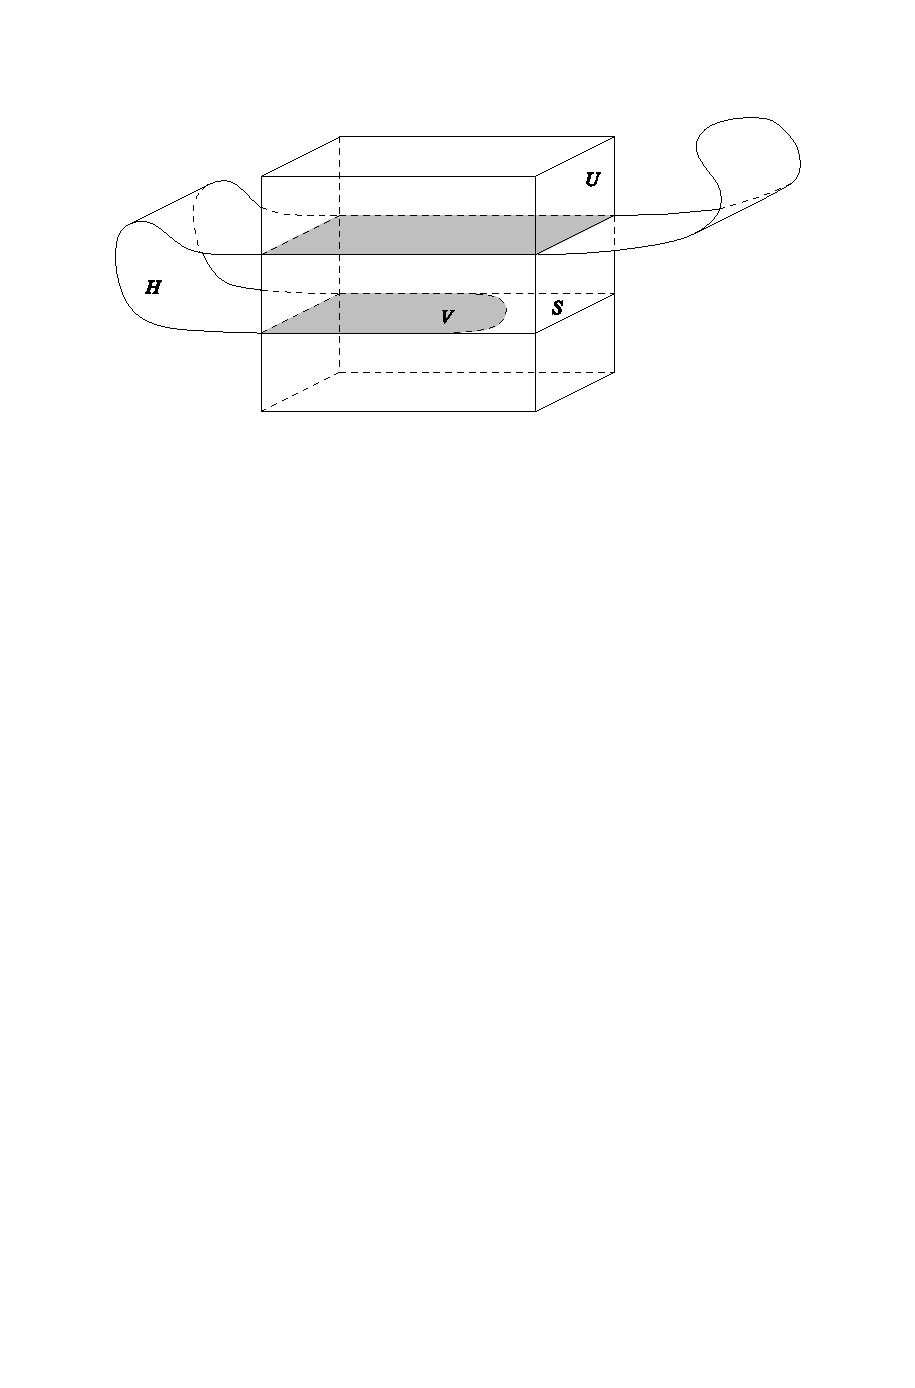
\includegraphics[scale=0.8]{figures/frobenius_2.pdf}
    \caption{Local structure of a leaf in a flat chart. From \cite{Lee}.}
    \label{fig: frobenius2}
\end{figure}


\begin{thm}[{{\cite[Thm.~19.17]{Lee}}} or {{\cite[Prop.~3.5.15]{RS1}}}]\label{thm 19.17 Lee}\label{prop 3.5.15 RS1}
    Every integral manifold of an involutive distribution is weakly embedded.
\end{thm}
\begin{proof}
    Let $N\subset M$ be an integral manifold of an involutive rank-$r$ distribution $D$ on $M$ and let $F:L\to M$ be a smooth map such that $F(L)\subset N$. Choose $p\in L$ and set $m=F(p)\in N$. Let $\{y^i\}_{i=1}^n$ be flat coordinates for $D$ on a neighborhood $U$ of $m$, and let $\{x^i\}$ be smooth coordinates for $L$ on a connected neighborhood $B$ of $p$ such that $F(B)\subset U$. With the coordinate representation of $F$ written as 
    \[y^i=F^i(x),\]
    the fact that $F(B)\subset N\cap U$ means that the functions $F^{r+1},\ldots, F^n$ take on only countably many values. Since $B$ is connected, these coordinate functions are constant, and thus $F(B)$ lies in a single slice $U_{\bf{c}}\subset U$. Because $U_{\bf{c}}\cap N$ is an open subset in $N$ that is embedded in $M$, it follows that $\restr{F}{B}$ is smooth from $B$ into $U_{\bf{c}}\cap N$, and thus by composition, $\restr{F}{B}:B\to U_{\bf{c}}\cap N\hookrightarrow N$ is smooth into $N$.
\end{proof}
\begin{cor}
    Images of the maximal integral curves of a vector field are weakly embedded submanifolds.
\end{cor}




% \begin{rem}
%     The version of the Frobenius theorem proved above is local, i.e., integral submanifolds are guaranteed to exist only in small neighborhoods. However, the full version of the Frobenius theorem is much more powerful as it establishes a bijection between smooth integrable distributions and smooth \emph{foliations} of $M$ by maximal integral submanifolds (analogs of maximal integral curves of vector fields). A foliation is a decomposition of $M$ into a disjoint union of immersed submanifolds, called \emph{leaves}, such that every point has a local chart in which the foliation is flat (i.e., the leaves are just $k$-dimensional hyperplanes of the form $x^{k+1}=c^{k+1},\ldots, x^{n}=c^n$). For a global version of the Frobenius theorem, see \cite[Ch.~19]{Lee} or \cite[\S~3.5]{RS1}.
% \end{rem}


\begin{lem}[{{\cite[Lem.~3.5.14]{RS1}}}]\label{lem 3.5.14 RS1}
    Let $D<\T M$ be a smooth distribution on $M$.
    \begin{enumerate}
        \item Let $N_1,N_2\subset M$ be two integral manifolds of $D$. If $N_1\cap N_2\neq \varnothing$ then $N_1\cap N_2$ is open in $N_1$ and $N_2$ and the smooth structures on it induced from either coincide. There is a unique smooth structure on $N_1\cup N_2$ such that $N_1$ and $N_2$ are open submanifolds. W.r.t.~this structure $N_1\cup N_2$ is an integral manifold of $D$.

        \item Let $N\subset M$ be an integral manifold of $D$, let $m\in M$ such that $\dim D_m=\dim N$ and let $(U,\kappa)$ be a local flat chart for $D$ at $m$. If a slice $U_{\bf{c}}$ of $U$ intersects $N$, then $U_{\bf{c}}$ is an integral manifold of $D$ and $N\cap U_{\bf{c}}$ is open and closed w.r.t.~the topology induced from $N$. In particular, the number of slices of $U$ intersecting $N$ is at most countable.  
    \end{enumerate}
\end{lem}
Note that the number of slices of $U$ intersected by $N$ may, in fact, be countably infinite, as is the case with the ``irrational slope'' vector fields $\partial_x+\lambda\partial_y$, $\lambda\in\bbR\setminus\bbQ$, on the torus $\bbR^2\slash \bbZ^2$.
\begin{proof}
\begin{enumerate}
    \item The assertion on $N_1\cup N_2$ follows from that on $N_1\cap N_2$, so it suffices to prove the latter. Let $\dim N_1=\dim N_2=\rank D=r$. Choose a local $r$-frame $\{X_i\}_{i=1}^r$ for $D$ at $m$. Since these vector fields are tangent to $N_i$, they are also local vector fields on $N_i$. Then the flows of these vector fields together generate a local coordinate system on $N_i$, mapping $(-\epsilon,\epsilon)^r$ into an open subset of $N_i$:
    \[\varPhi^{(i)}:(-\epsilon,\epsilon)^r\to U\cap N_i,\quad \varPhi^{(i)}(\bf{t})\coloneqq \Fl^{X^{(i)}_1}_{t_1}\circ \cdots\circ \Fl^{X^{(i)}_r}_{t_r}(m),\quad i=1,2.\]
    By construction these coordinates will coincide, $\varPhi^{(1)}(\bf{t})=\varPhi^{(2)}(\bf{t})$ (cf.\ Remark~\ref{rem 3.2.9 RS1}), and therefore, their values will cover the same subset $V\subset N_1\cap N_2$ open in both $N_i$'s. W.r.t.~the differentiable structure induced from either $N_i$, $V$ is diffeomorphic to $(-\epsilon,\epsilon)^r$. Since the construction works for any $m\in N_1\cap N_2$, the assertion follows. 

    \item Let $r=\dim N=\dim D_m$. If $N$ intersects a slice $U_{\bf{c}}$, then $U_{\bf{c}}$ contains a point where $\rank D=r$. Then $U_{\bf{c}}$ is an integral manifold of $D$ by dimension-counting. Now assertion 1 implies that $N\cap U_{\bf{c}}$ is open in $N$ and hence in $N\cap U$. Since this holds for all slices intersecting $N$ and since
    \[N\cap U_{\bf{c}}=(N\cap U)\setminus\left(\bigcup_{\bf{c}'\neq \bf{c}}N\cap U_{\bf{c}'}\right),\]
    the intersection $N\cap U_{\bf{c}}$ is also closed in $N\cap U$. It follows that $N\cap U_{\bf{c}}$ is a union of connected components of $N\cap U$. Since the slices are disjoint, this implies that the number of slices which intersect $N$ is at most as large as the number of connected components of $N\cap U$. Since the topology on $N\cap U$ is induced from the manifold $N$, it is second countable, hence the number of connected components is at most countable.
\end{enumerate}
\end{proof}



\begin{thm}[{{\cite[Thm.~3.5.17]{RS1}}}]\label{thm 3.5.17 RS1}
    Let $D$ be an integrable distribution on $M$. For every $m\in M$ there exists a unique integral manifold $N_m$ of $D$ through $m$ which is maximal in the following sense. For every integral manifold $N$ of $D$ such that $N\cap N_m\neq \varnothing$ it holds that $N\subset N_m$, and $N$ is an open submanifold of $N_m$.
\end{thm}
\begin{proof}
    Let $r=\dim D_m$ and define a subset $N_m\subset M$ by taking the union of all integral manifolds of $D$ through $m$. Equip it with the topology generated by the open subsets of these integral manifolds. The onion of all maximal atlases of these manifolds also defines an atlas on $N_m$. By Lemma~\ref{lem 3.5.14 RS1} this atlas is smooth.  One can then show that $N_m$ is second countable (see \cite[Lem.~19.22]{Lee} or \cite[Thm.~1.64]{Warner}). Then $N_m$ is a manifold of dimension $r$. By construction, the local representatives of the inclusion $N_m\hookrightarrow M$ are smooth, hence $N_m$ is a smooth submanifold of $M$. Also by construction, every $\wt{m}\in N_m$ belongs to an integral manifold $N$ through $m$ and $N$ is an open submanifold of $N_m$, so $\T_{\wt m}N_m=\T_{\wt m}N=D_{\wt m}$, and thus $N_m$ is also an integral manifold through $m$. It has the maximality property stated in the theorem because if some integral manifold $N$ of $D$ intersects $N_m$, then $N\cup N_m$ is also integral and thus already contained in $N_m$. It follows that $N\cap N_m=N$ and hence $N$ is an open submanifold of $N_m$. Uniqueness follows because any two maximal integral manifolds through $m$ would coincide as sets by definition and each of them would be an open submanifold of the other, hence they would also coincide as manifolds.
\end{proof}


\begin{defn}[Foliation]\index{Foliation}
    A foliation of an $n$-dimensional smooth manifold $M$ is a family $\mathcal{N}$ of connected submanifolds of $M$, called the \emph{leaves} of the foliation, such that
    \begin{enumerate}
        \item the leaves are disjoint and $\cup_{N\in\mathcal{N}}N=M$,
        \item for every $m\in M$ there exists a local \emph{flat chart} $(U,\kappa)$ of $M$ satisfying
        \begin{enumerate}[label=(\alph*)]
            \item $\kappa(m)=0$ and $\kappa(U)=(-\epsilon,\epsilon)^n$ for some $\epsilon>0$,
            \item the leaves are invariant under the flows of the local coordinate vector fields $\partial_1,\dots,\partial_r$, where $r$ denotes the dimension of the leaf containing $m$, also called the \emph{rank} of $\mathcal{N}$ at $m$.
        \end{enumerate}
    \end{enumerate}
    A foliation is called \emph{regular} if its rank is constant, and singular otherwise.
\end{defn}



\begin{thm}[Global Frobenius Theorem {{\cite[Prop.~3.5.21]{RS1}}} or {{\cite[Thm.~19.21]{Lee}}}]\label{prop 3.5.21 RS1}\index{Theorem!Global Frobenius}
    The collection of all maximal connected integral manifolds of an involutive distribution $D$ on a smooth manifold $M$ forms a foliation of $M$.
    
    The assignment of the family of maximal integral manifolds to an integrable distribution defines a bijection between smooth integrable distributions on $M$ and smooth foliations of $M$. Regular distributions of rank $r$ thereby correspond to regular foliations of rank $r$.
\end{thm}
\begin{proof}
    Theorem~\ref{thm 3.5.17 RS1} implies that condition 1 of the definition of a foliation is satisfied. The invariance of maximal integral manifolds under the flows of local $D$-valued vector fields lets us generate local flat charts via a composition of the flows (as in Rectification Theorem~\ref{rectification}) and hence condition 2 is satisfied as well. 

    Conversely, let $\mathcal{N}$ be a smooth foliation. For $m\in M$, let $D_m$ be the tangent space at $m$ of the leaf containing $m$. This defines a subset $D\subset \T M$. By definition of a foliation, $D_m$ is spanned by the values of local $D$-valued vector fields at $m$. Hence $D$ is a distribution. By construction, every leaf is an integral manifold of $D$. First, this implies that $D$ is integrable. Second, in view of Theorem~\ref{thm 3.5.17 RS1}, this implies that every leaf of $\mathcal{N}$ is contained in an open subset in a maximal integral manifold of $D$. Thus $N$ is a union of leaves. Since the leaves are disjoint and $N$ is connected, $N$ must coincide with a single leaf. This shows that $\mathcal{N}$ is the family of maximal integral manifolds of $D$, and the assignment is bijective, indeed.
\end{proof}



\begin{figure}[tp]
    \centering
    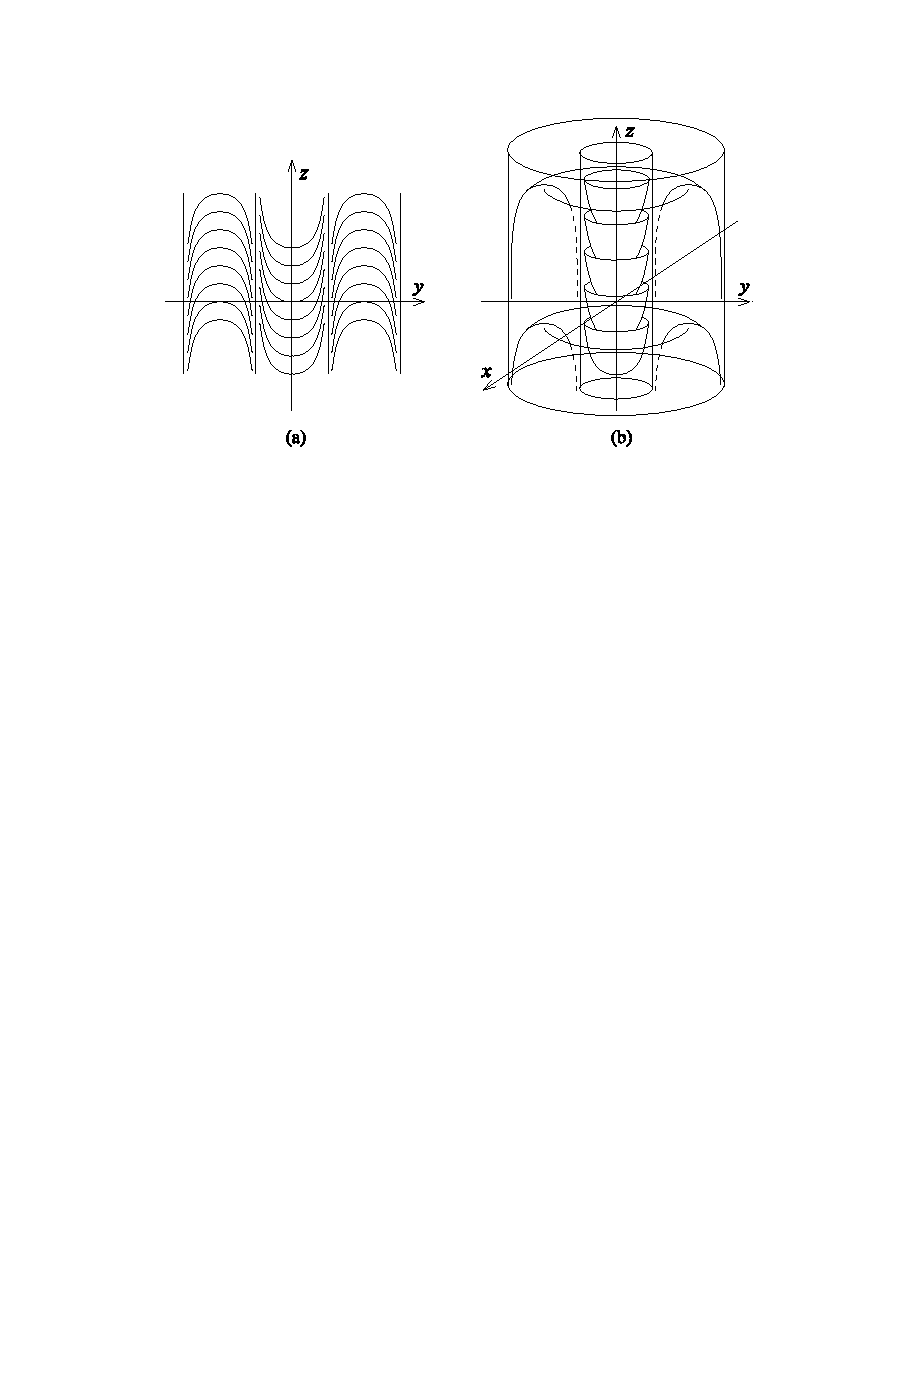
\includegraphics[scale=0.8]{figures/foliations.pdf}
    \caption{Examples of foliations of $\bbR^2$ (a) and $\bbR^3$ (b). From \cite{Lee}.}
    \label{fig:foliations}
\end{figure}

\begin{example}[Linear PDEs]
    Overdetermined systems of linear PDEs are solvable iff the distribution spanned by the differential operators as vector fields is integrable:
    \[\begin{cases}
        X_1\cdot u(x)=f_1(x),&\\
        \cdots &\\
        X_k\cdot u(x)=f_k(x)&
    \end{cases}
    \text{ has solutions iff }\exists\,C^k_{ij}\in C^\infty\text{ s.t.}
    \begin{cases}
        [X_i,X_j]=C^k_{ij}X_k,&\\
        X_i\cdot f_j-X_j\cdot f_i=C^k_{ij}f_k.&
    \end{cases}
    \]
\end{example}

\begin{xca}
    Show that the distribution on $\bbR^3\setminus \{0\}$ generated by the vector fields
    \[X_1=x_2\partial_3-x_3\partial_2,\quad X_2=x_3\partial_1-x_1\partial_3,\quad X_3=x_1\partial_2-x_2\partial_1,\]
    is regular of rank $2$ and involutive. Find the maximal integral manifolds. How are they related to the action of $\SO(3)$ on $\bbR^3$?
\end{xca}


\begin{example}[Zero curvature conditions]\label{ex UV pairs}
    Another important case is the following pair of equations on a function $\bf{y}:\bbR^2\to \bbC^n$ parametrized as $\bf{y}(x,t)$:
    \[\begin{cases}
        \partial_x \bf{y}(x,t)= U(x,t)\bf{y}(x,t),\\
        \partial_t \bf{y}(x,t)= V(x,t)\bf{y}(x,t),
    \end{cases}\label{eq UV pair}\]
    where $U,V:\bbR\times\bbR\to \bbC^{n\times n}$ are given matrix-valued functions. As we will see later, $U$ and $V$ can be seen as the components of a linear connection $U\dd x+V\dd t$ on the product bundle $\bbR^2\times\bbC^n\to \bbR^2$, so that the above equations become $\nabla\bf{y}=0$. The Frobenius integrability condition in this case is easy to obtain by observing that any solution must satisfy $\partial_t(\partial_x \bf{y})=\partial_x(\partial_t \bf{y})$, which expands to 
    \[(\partial_t U+UV)\bf{y}=(\partial_x V+VU)\bf{y},\]
    or (since the initial condition is arbitrary)
    \[\partial_t U-\partial_x V+[U,V]=0.\]
    If this condition holds, then the Frobenius theorem guarantees the unique existence of solutions. This condition is called a \emph{zero curvature condition}, and when a given dynamical system can be expressed in the form of a zero curvature condition, the system~\eqref{eq UV pair} is called a \emph{$UV$-pair}, and the dynamical system is considered \emph{(completely) integrable}.\footnote{Note, however, that this is not the only test for integrability, and a general definition of integrability for dynamical systems is not yet known.} We will see its relation to the Maurer-Cartan equation in \sect\ \ref{subsec: invariant diff forms}.
\end{example}

\begin{example}[Sine-Gordon equation]\label{ex sine-gordon}
    Consider the $UV$-pair (with the variables $x,t$ suppressed)
    \[U(\lambda)=\frac{\rmi}{2}\begin{pmatrix}
        2\lambda & u_x\\
        u_x & -2\lambda
    \end{pmatrix},\quad 
    V(\lambda)=\frac{1}{4\rmi \lambda}\begin{pmatrix}
        \cos u & -\rmi \sin u\\
        \rmi \sin u & -\cos u
    \end{pmatrix},
    \]
    where $u(x,t;\lambda)$ is an $\bbR$-valued function, subscripts stand for partial derivatives of $u$, and $\lambda\neq 0$ is a complex parameter. This $UV$-pair defines a system of equations \eqref{eq UV pair} on the unknown $\bf{y}$. By expanding the zero curvature condition we find that its diagonal components vanish, and both anti-diagonal components impose the \emph{Sine-Gordon equation}\index{Equation!Sine-Gordon} on $u$:
    \[u_{xt}=\sin u.\]
\end{example}

\begin{example}[AKNS, Nonlinear Schr\"odinger equation]
    Consider now the $UV$-pair 
    \[
    U(\lambda)=-\rmi\lambda
    \begin{pmatrix}
        1 & 0\\
        0 & -1
    \end{pmatrix}+\rmi\begin{pmatrix}
        0 & p\\
        -q & 0
    \end{pmatrix},\quad 
    V(\lambda)=
    2\lambda U(\lambda)
    -\rmi\lambda\begin{pmatrix}
        pq & \rmi p_x\\
        \i q_x & -pq
    \end{pmatrix},\label{eq AKNS UV pair}
    \]
    where $p(x,t;\lambda),q(x,t;\lambda)\in\bbC$. The zero curvature condition then leads to the \emph{AKNS system} on $q$ and $p$:
    \[
        \begin{cases}
            \i p_t+p_{xx}-2p^2q= &0,\\
            -\i q_t+q_{xx}-2q^2p= &0.
        \end{cases}    
    \]
    Under the so called self-adjoint reduction $p=-\wb{q}\eqqcolon \psi$ this system turns into the standard \emph{Nonlinear Schr\"odinger} (NLS) equation on $\psi$, of great importance in optics:\index{Equation!Nonlinear Sch\"odinger}\index{Equation!AKNS}
    \[\rmi\psi_t+\psi_{xx}+2|\psi|^2\psi=0.\]
\end{example}

\begin{example}[Lax pairs]\label{ex Lax pairs}\index{Lax pair}
    Another common way of demonstrating the integrability of a dynamical system is by finding a representation in terms of a \emph{Lax pair},\index{Lax pair} which consists of two matrix-valued operators $L,A$, where $L$ is the linear differential operator
    \[L(t)=u_m(x,t)\partial_x^m+\cdots u_1(x,t)\partial_x+u_0(x,t)\]
    with matrix-valued functions $u_i:\bbR^2\to \bbC^{n\times n}$, and $A$ is another matrix-valued differential (only w.r.t.\ $x$) operator such that our dynamical system describing the evolution of $u_i(x,t)$ is expressed as 
    \[L_t=[A,L],\label{eq Lax pair}\]
    where 
    \[L_t=\dot u_m(x,t)\partial_x^m+\cdots \dot u_1(x,t)\partial_x+\dot u_0(x,t),\]
    and $[A,L]$ is computed as the commutator of differential operators acting on smooth functions $\bm{\psi}(x,t)\in\bbC^n$. The core observation here is that the matrices $L(t)$ at different values of $t$ are all similar. That is, $L(t)$ can be written in terms of $L(s)$ as 
    \[L(t)=M(t,s)L(s)M(t,s)^{-1},\]
    where (by plugging into \eqref{eq Lax pair}) $M(t,s)$ satisfies the Cauchy problem 
    \[\partial_t M(t,s)=A(t)M(t,s),\quad M(s,s)=\rmI_n,\]
    where $\rmI_n$ is the identity matrix of size $n\times n$.
    Note that while $M$ will implicitly depend on $x$, the derivatives $\partial_x^j$ contained in $L$ do not act on $M$ in this equation. Therefore, $M$ always exists due to the general solvability of Cauchy problems.

    The main consequence of this is that the eigenvalues of $L(t)$ do not depend on $t$. This is known as the \emph{isospectral property} of Lax pairs. Therefore, to solve the eigenvalue problem $L(t)\bm{\psi}(x,t)=\lambda\bm{\psi}(x,t)$ at time $t$, it suffices to solve it at $t=0$ (where $L$ is usually known better due to the initial condition) and then propagate the solution using the formulas
    \[\begin{cases}
        \lambda(t)=\lambda(0),\\
        L(t)\bm{\psi}=\lambda(t)\bm{\psi},\\
        \partial_t\bm{\psi}=A\bm{\psi}.
    \end{cases}\label{eq Lax pair 2}\]
    Let us now take this system as the starting point and differentiate the second equation w.r.t.\ $t$, getting $\dot L\bm{\psi}+L\dot{\bm{\psi}}=\lambda\dot{\bm{\psi}}=\lambda A\bm{\psi}=A L\bm{\psi}$. Substituting $\dot{\bm{\psi}}=A\bm{\psi}$ into the left hand side as well, we get back the Lax equation $\dot L=[A,L]$. Therefore, the Lax equation is the compatibility (or integrability) condition for \eqref{eq Lax pair 2}.

    To see the connection to zero curvature conditions, suppose $L$ and $A$ have the form 
    \begin{align}
        L=\partial_x^n+\sum_{j=0}^{n-1}u_j(x,t)\partial_x^j,\\
        A=\partial_x^n+\sum_{j=0}^{n-1}v_j(x,t)\partial_x^j.
    \end{align}
    Then the isospectral equation $L\bm{\psi}=\lambda\bm{\psi}$ implies that $x$-derivatives of $\bm{\psi}$ of order $\geq n$ may be expressed as linear combinations of derivatives of orders $<n$. Indeed, we have
    \[\partial_x^n\bm{\psi}=\lambda\bm{\psi}-\sum_{j=0}^{n-1}u_j(x,t)\partial_x^j\bm{\psi},\]
    and further differentiations of this equation w.r.t.\ $x$ give the higher-order derivatives as well. Now, introducing the vector 
    \[\bf{y}=(\bm{\psi},\partial_x\bm{\psi},\ldots,\partial_x^{n-1}\bm{\psi}),\]
    the equation $L\bm{\psi}=\lambda\bm{\psi}$ can be written as 
    \[\partial_x\bf{y}=U\bf{y},\]
    where 
    \[U(x,t;\lambda)=
    \begin{pmatrix}
        0 & 1 & 0 & \cdots & 0\\
        0 & 0 & 1 & \cdots & 0\\
        \vdots & \vdots & \vdots & \ddots & \vdots \\
        0 & 0 & 0 & \cdots & 1\\
        \lambda-u_0 & -u_1 & -u_2 & \cdots & -u_{n-1}
    \end{pmatrix}.
    \]
    Now let us act with $\partial_x^i$ on the equation $\dot{\bm{\psi}}=A\bm{\psi}$ to obtain 
    \[\partial_t(\partial_x^{i-1}\bm{\psi})+\underbrace{\partial_x^{i-1}\left(\sum_{j=0}^{m-1}v_j(x,t)\partial_x^i\bm{\psi}\right)}_{\sum_{j=1}^nV_{ij}(x,t;\lambda)\partial_x^{j-1}\bm{\psi}}=0,\]
    for some $V_{ij}(x,t;\lambda)$ that can be expressed in terms of $v_j$, $u_i$, and their derivatives of orders $<n$ by our above observation. This equation can be written as 
    \[\partial_t \bf{y}=V\bf{y}.\]
    We have shown the equivalence between Lax representations and zero curvature representations:
    \[
    \dot L=[A,L]\Leftrightarrow 
    \begin{cases}
        L\bm{\psi}=\lambda\bm{\psi},\\
        \partial_t\bm{\psi}=A\bm{\psi}
    \end{cases}\Leftrightarrow
    \begin{cases}
        \bf{y}_x=U\bf{y},\\
        \bf{y}_t=V\bf{y}
    \end{cases}\Leftrightarrow
    \partial_t U-\partial_x V+[U,V]=0.
    \]
\end{example}

\begin{example}
    In many famous examples of Lax pairs, $n=1$ and $L$ is the second-order \emph{Sturm-Liouville operator} (in physics a Schr\"odinger operator)
    \[L=-\partial_x^2+u.\]
    The simplest choice of $A$ is $A=-c\partial_x$ with a constant $c$, which leads to the \emph{1D advection equation}
    \[A=-c\partial_x\quad \implies \quad u_t+c u_x=0.\]
    The following choice of $A$ leads to the celebrated solitonic \gls{kdv} equation:\index{Equation!Korteweg-de~Vries}
    \[A=-4\partial_x^3+6u\partial_x+3u_x\quad \implies\quad u_t-6uu_x+u_{xxx}=0.\label{eq kdv}\]
\end{example}










\clearpage
\chapter{Differential Forms and Integration}\label{ch: differential forms}


While symmetric algebras (or even commutative rings), and in particular symmetric tensors, can be identified with polynomials, the dual objects are antisymmetric tensors, which turn out to form an algebra of their own. Following the original invention of this algebra by Grassmann, it became important in the theory of differential equations, and eventually, with \'Elie Cartan, in geometry more broadly.


\section{Exterior algebra}


\begin{defn}[Exterior forms]\index{Exterior form}
    Let $V$ be a $\bbK$-vector space. The alternation and symmetrization maps are defined on the tensor space $\bbT^k V=(V)^{\otimes k}$ respectively as
    \begin{align}
        \Alt t&=\frac{1}{k!}\sum_{\sigma\in \rmS_k} (\sign\sigma)\cdot t^\sigma,\\
        \Sym t&=\frac{1}{k!}\sum_{\sigma\in \rmS_k} t^\sigma,\label{def sym operator}
    \end{align}
    where $\rmS_k$ is the $k$-th permutation group, and the operation $t\mapsto t^\sigma$ is defined on a basis as $(e_{i_1}\otimes\cdots\otimes e_{i_k})^\sigma=e_{\sigma(i_1)}\otimes\cdots\otimes e_{\sigma(i_k)}$ and extended to all of $\bbT^k V$ by linearity. We also denote $\bigwedge\nolimits^k V=\Alt(\bbT^k V)$ and $\bigodot\nolimits^k V\coloneqq \Sym(\bbT^k V)$. Elements of the space $\bigwedge\nolimits^k V^\ast$ are called \emph{exterior forms} of degree $k$ on $V$. 
    
    If $\dim V=n$, then $\dim \bigwedge\nolimits^k V=\binom{n}{k}$. In particular, 
    \[\bigwedge\nolimits^1 V=V,\quad \dim \bigwedge\nolimits^0 V=\dim \bigwedge\nolimits^n V=1,\quad \dim \bigwedge\nolimits^{>n} V=0.\]
    Elements of $\bigwedge\nolimits^n V$ are called \emph{top forms}.\index{Top form}
    Both $\bigwedge\nolimits^k$ and $\bigodot\nolimits^k$ are covariant functors $\mathsf{FinVect}_\bbK\to\mathsf{FinVect}_\bbK$ that act on morphisms by restriction: \[\bigwedge\nolimits^k f=\restr{f^{\otimes k}}{\bigwedge\nolimits^k V},\quad \bigodot\nolimits^k f=\restr{f^{\otimes k}}{\bigodot\nolimits^k V}.\]
\end{defn}

If $V$ has Cartesian coordinates $x^1,\ldots,x^n$, then a basis of $V$ is formed by $\{\partial_{x^i}\}$. The dual basis of $V^\ast$ is conventionally denoted by $\{\dd x^i\}$, so that
\[
    \dd x^i\left(\partial_{x^j}\right)=\delta^i_j.
\]
Then this basis induces a basis of $\bigwedge\nolimits^k V^\ast$ consisting of the $\binom{n}{k}$ elements
\[
\dd x^{i_1}\wedge \cdots \wedge \dd x^{i_k}\coloneqq k!\Alt(\dd x^{i_1}\otimes\cdots\otimes \dd x^{i_k}),\;\;1\leq i_1<i_2<\cdots<i_k\leq n.
\]
Together with the wedge product, the direct sum of all exterior powers of $V$ makes up an algebra, called the exterior, or \emph{Grassmann}, algebra of $V$, of dimension $2^n$:\index{Grassmann algebra}
\[\bigwedge V=\bigoplus_{k=0}^\infty \bigwedge\nolimits^k V.\]



\begin{defn}[Determinant of a linear map]\index{Determinant of a linear map}
Let $V$ be a vector space over a field $\bbK$ with $\dim V=n$ and let $f\in\End(V)$. The determinant of $f$ is defined as 
\[\det f\coloneqq \bigwedge\nolimits^n f\quad \in\bbK.\] 
Being an element of $\Hom(\bigwedge\nolimits^n V,\bigwedge\nolimits^n V)$, which is naturally isomorphic to the field $\bbK$, it is a well-defined scalar. 
\end{defn}
\begin{prop}
\begin{enumerate}
    \item If $\dim V=n$, then for any $t\in\bigwedge\nolimits^n V^\ast$ and any $f\in\End(V)$, 
    \[f^\ast t=\det f\cdot t.\]
    \item If $f\in\End(V)$ is represented by a matrix $f(e_i)=A_i^j e_j$ in some basis $\{e_i\}$ of $V$, then
    \[\det f=\det A=\sum_{\sigma\in \rmS_n}(\sign\sigma)A^1_{\sigma(1)}\cdots A^n_{\sigma(n)}.\]
\end{enumerate}
\end{prop}
\begin{proof}
\begin{enumerate}
    \item By definition of $f^\ast$, if $v\in \bigwedge\nolimits^n V$, then 
    \[(f^\ast t)(v)=t\left(f_\ast(v)\right)=t\left(\left(\bigwedge\nolimits^n f\right)(v)\right)=t(\det f\cdot v)=\det f\cdot t(v).\]
    \item The one-dimensional space $\bigwedge\nolimits^n V$ is spanned by the element $e_1\wedge \cdots \wedge e_n$. Acting on it, $\det f=\bigwedge\nolimits^n f$ gives
    \begin{align}
        \left(\bigwedge\nolimits^n f\right)(e_1\wedge \cdots \wedge e_n)&=k!f^{\otimes n}\circ \Alt (e_1\otimes \cdots \otimes e_n)\notag\\
        &=k!\Alt(f(e_1)\otimes\cdots\otimes f(e_n))=\notag
        \\
        &=k! \Alt (A^{j_1}_1 \cdots A^{j_n}_n \cdot e_{j_1}\otimes\cdots \otimes e_{j_n})=\notag\\
        &=\sum_{\pi\in \rmS_n}(\sign\pi)\cdot A_{\pi(1)}^{j_1}\cdots A_{\pi(n)}^{j_n}\cdot  e_{j_1}\otimes\cdots\otimes e_{j_n}=\notag
        \\
        =\sum_{\sigma,\pi\in \rmS_n}(\sign\sigma\cdot\sign\pi) \cdot &A_{\pi(1)}^1\cdots A_{\pi(n)}^n\cdot e_{\sigma(1)}\otimes\cdots\otimes e_{\sigma(n)}=\notag
        \\
        &=\left(\sum_{\pi\in \rmS_n}(\sign\pi)A^1_{\pi(1)}\cdots A^n_{\pi(n)}\right)\cdot e_1\wedge \cdots \wedge e_n.
    \end{align}
    By item 1, the expression in the brackets is the determinant.
\end{enumerate}
\end{proof}

\begin{defn}[Exterior/wedge product]\index{Exterior product}\index{Wedge product|see {Exterior product}}\label{def exterior and sym product}
    For $\alpha\in V^{\otimes p}$ and $\beta\in V^{\otimes q}$, we define their exterior/wedge product by
    \[\alpha\wedge\beta\coloneqq\frac{(p+q)!}{p!q!}\Alt (\alpha\otimes \beta)\quad \in \bigwedge\nolimits^{p+q}V.\]
    Similarly, we can define the symmetric product of tensors\index{Symmetric product of tensors} 
    \[t\odot t'\coloneqq\Sym(t\otimes t').\]
\end{defn}
Wedge products have the following basic properties (proofs of which are left as exercises):
\begin{enumerate}
    \item $\alpha\wedge\beta=\Alt(\alpha)\wedge\beta=\alpha\wedge\Alt(\beta)$;
    \item $\wedge$ is bilinear and $\alpha\wedge\beta=(-1)^{\deg\alpha\cdot\deg\beta}\beta\wedge\alpha$;
    \item $\alpha\wedge(\beta\wedge\gamma)=(\alpha\wedge\beta)\wedge\gamma$.
    \item The notation for basis elements is consistent with the definition of the wedge product:
    \[(\dd x^{i_1}\wedge\cdots\wedge \dd x^{i_p})\wedge (\dd x^{i_{p+1}}\wedge\cdots\wedge \dd x^{i_{p+q}})=\dd x^{i_1}\wedge\cdots\wedge \dd x^{i_{p+q}}.\]
    \item For $\alpha_i\in V^\ast$, $i=1,\ldots,k$, 
    \begin{multline}
        (\alpha_1\wedge\cdots\wedge\alpha_k)(v_1,\ldots,v_k)=\sum_{\sigma\in \rmS_k}(\sign\sigma)\cdot \alpha_1(v_{\sigma(1)})\cdots\alpha_k(v_{\sigma(k)})=\\
        =\det \begin{pmatrix}
         \alpha_1(v_1) & \cdots & \alpha_1(v_k)  \\
         \vdots & \ddots & \vdots \\
         \alpha_k(v_1) & \cdots & \alpha_k(v_k) 
    \end{pmatrix}.\label{form determinant f-la}
    \end{multline}
    \item $\{\alpha_i\}_{i=1}^k\subset V^\ast$ are linearly dependent iff $\alpha_1\wedge\cdots\wedge\alpha_k=0$.
    \item For $\alpha,\beta\in\bigwedge\nolimits^{\smbullet } V^\ast$ and any linear map $f:V'\to V$,
    \[f^\ast(\alpha\wedge\beta)=(f^\ast\alpha)\wedge(f^\ast\beta).\label{pullbacks of wedges}\]
\end{enumerate}

The degree of an exterior form can be lowered by substituting a given vector as one of its arguments, which we use to define an operator.

\begin{defn}[Interior product]\index{Interior product}
    Let $\alpha\in\bigwedge\nolimits^{p+1}V^\ast, p\geq 0,$ and $v\in V$. The interior product with $v$ is the operator $i_v:\bigwedge\nolimits^{p+1}V^\ast\to \bigwedge\nolimits^p(v)$ defined by 
    \[(i_v \alpha)(v_1,\ldots,v_p)=\alpha(v,v_1,\ldots,v_p),\]
    for $v_1,\ldots,v_p\in V$. We also put $\restr{i_v}{\bigwedge\nolimits^0V^\ast}=0$.
\end{defn}

Note that $i_v$ is a ``\emph{$\wedge$-derivation}'' on the exterior algebra (exercise):
\[i_v(\alpha\wedge\beta)=i_v\alpha\wedge\beta+(-1)^{\deg \alpha}\alpha\wedge i_v\beta.\label{eq interior product derivation}\]


\begin{defn}[Exterior powers of \glspl{vb}]
Following the logic of Definition \ref{functors VB}, we can extend the functors $\bigwedge\nolimits^p$ and $\bigodot\nolimits^p$ to all smooth \glspl{vb}. We focus only on $\bigwedge\nolimits^p$. For a \gls{vb} $E\overset{\pi}{\to} M$, we obtain the exterior powers
\[\bigwedge\nolimits^p E=(E)^{\otimes p}_{\text{asym}}.\]
$p$ is called the \emph{degree} of the elements or sections of $\bigwedge\nolimits^p E$: \[\deg \alpha=p\;\text{ for }\;\alpha\in\Gamma^\infty\left(\bigwedge\nolimits^p E\right).\]
The wedge product $\wedge$ gets extended to sections of these bundles fiberwise.
In particular, if $\rank E=k$, then \[\det E\coloneqq \bigwedge\nolimits^k E\] is called the \emph{determinant (line) bundle}\index{Determinant bundle} of $E$. If the transition functions of $E$ are $\tau_{\alpha\beta}:U_{\alpha\beta}\to \GL_k(\bbR )$, then the transition functions of $\det E$ are $\det \tau_{\alpha\beta}$.

The alternation and symmetrization maps get extended to $\Alt: E^{\otimes p}\to \bigwedge\nolimits^p E$ and $\Sym: E^{\otimes p}\to \bigodot\nolimits^p E$.
\end{defn}

All properties of wedge products listed above immediately generalize to sections of the exterior bundles.

\begin{defn}[Determinant of a \gls{vb} morphism]
If $E\overset\pi\to M$ is a \gls{vb} of rank $k$ and $f:E\to E$ is a bundle map, then we define $\det f=\bigwedge\nolimits^k f$. If $\omega\in\Gamma^\infty(\det E^\ast)$, then $f^\ast \omega=\det f\cdot \omega$.
\end{defn}

\begin{defn}[Exterior/Grassmann algebra]\index{Exterior algebra}\index{Grassmann algebra|see {Exterior algebra}}
For a \gls{vb} $E$, the space $\bigoplus_{p\geq 0}\Gamma^\infty(\bigwedge\nolimits^p E)=\Gamma^\infty\left(\bigoplus_{p\geq 0}\bigwedge\nolimits^p E\right)$ with the product $\wedge$ is called the exterior, or Grassmann, algebra of $E$.
\end{defn}

% \begin{xca}
%     \begin{enumerate}
%         \item Prove formula \ref{form determinant f-la}.
%         \item Show that $k$ $1$-forms (or vectors) $\{\alpha_i\}$ are linearly independent iff $\alpha^1\wedge\cdots\wedge\alpha^k\neq 0$. 
%     \end{enumerate}
% \end{xca}






\section{Cartan's calculus}

We now move from arbitrary vector bundles to manifolds by applying the exterior power functor to the cotangent bundle.

\begin{defn}[Differential forms]\index{Differential form}
    Differential forms of degree $p$ on a smooth manifold $M$ are sections of $\bigwedge\nolimits^p (\T^\ast M)$. The exterior algebra of differential forms is denoted
    \[\Omega^p(M)\coloneqq \Gamma^\infty\left(\bigwedge\nolimits^p(\T^\ast M)\right),\quad 0\leq 0\leq\dim M.\]
    For $p<0$ and $p>\dim M$ we set $\Omega^p(M)=\{0\}$.
    In particular, we have $\Omega^0(M)=C^\infty(M)$, $\Omega^1(M)=\fX^\ast (M)$, and $\Omega^p(M)\cong \bigwedge\nolimits^p \fX^\ast(M)$ by Theorem~\ref{thm tensor characterization}. We also denote the \emph{exterior algebra} of $M$ by
    \[\Omega^{\smbullet}(M)\coloneq\bigoplus_{p=0}^{\dim M} \Omega^p(M).\]
    Note that elements of $\Omega^{\smbullet}(M)$ can have mixed degrees, i.e., contain terms that are differential forms of differing degrees.
\end{defn}


\begin{rem}
    Since differential forms are covariant tensor fields, they can be expanded in local coordinates $(U,\bf{x})$ as combinations of terms of the form $\dd x^{i_1}\otimes\cdots\otimes \dd x^{i_p}$ with coefficients in $C^\infty(U)$. By taking into account the antisymmetry of forms, we conclude that every differential form $\omega\in\Omega^p(M)$ has the following coordinate representation, where $n=\dim M$:
    \[\omega=\sum_{1\leq i_1<\cdots <i_p\leq n}\omega_{i_1 i_2\cdots i_p}\dd x^{i_1}\wedge\cdots\wedge \dd x^{i_p},\quad \omega_{i_1 i_2\cdots i_p}\in C^\infty(U).\label{eq local rep of a p-form}\]
\end{rem}


Recall that for $f\in C^\infty(M)$, $\dd f=\pr_2\circ f_\ast$, where $\pr_2$ is the projection onto the fiber in $\T\bbR =\bbR \times\bbR $. As we have established in Example~\ref{df is a 1-form}, using the tensor characterization theorem, the differential is a $1$-form, $\dd f\in\Omega^1(M)$. We can now verify that our notation for the coframe $\{\dd x^i\}_{i=1}^n$ is consistent with the action of $\dd$ on the coordinate functions $x^i$.

\begin{prop}
    If $x^i\in C^\infty(U),i=1,\ldots,n$ are local coordinate functions on $U\subset M$, then the differentials $\dd (x^i)$ of these functions coincide with the dual coordinate frame $\dd x^i$, i.e.
    \[\dd (x^i)(\partial_j)=\delta^i_j.\]
\end{prop}
\begin{proof}
    Recall that $x^i_\ast$ are exactly the components of the bundle chart for $\T M$. Therefore, $x^i_\ast(\partial_j)=(\partial_j)^i$ and
    \[\dd (x^i)(\partial_{j})=\pr_2\circ x^i_\ast (\partial_{j})=(\partial_j)^i=\delta^i_j.\]
    Equivalently, by definition of the Lie derivative, 
    \[\dd (x^i)(\partial_j)=\Lie_{\partial_j}x^i=\frac{\partial x^i}{\partial x^j}=\delta^i_j.\]
\end{proof}
\begin{cor}
    Locally, the differential $\dd f$ of a function $f\in C^\infty(M)$ is the standard ``total differential'' from multivariate calculus, \[\dd f=\dd f(\partial_i)\cdot\dd x^i=(\partial_i f)\cdot \dd x^i.\]
\end{cor}

\begin{xca}
    On $\bbR^2$ with Cartesian coordinates $(x,y)$, compute $(\dd x\wedge \dd y)(\nabla f,\nabla g)$ for any $f,g\in C^\infty(\bbR^2)$. Compare to $(\dd f\wedge \dd g)(\partial_x,\partial_y)$ and $(\partial_x\wedge\partial_y)(\dd f,\dd g)$ (where we act with vectors on covectors via the canonical pairing between $\T M$ and $\T^\ast M$).
\end{xca}

We now extend $\dd$ to differential forms of all degrees.

\begin{thm}\label{exterior d existence}
    There exists a unique family of differential operators $\wt{\dd}_p(U):\Omega^p(U)\to \Omega^{p+1}(U)$ for every $U\mathring\subset M$, denoted collectively by $\wt\dd$, such that:
\begin{enumerate}
    \item $\wt\dd$ is an $\bbR $-linear $\wedge$-derivation: $\wt\dd(\alpha\wedge\beta)=\wt\dd\alpha\wedge\beta+(-1)^{\deg\alpha}\alpha\wedge\wt\dd\beta$;
    \item $\forall f\in C^\infty(M)$, $\wt\dd f=\dd f$;
    \item $\wt\dd\circ\wt\dd=0$;
    \item $\wt\dd$ is local: $\wt\dd\left(\restr{\alpha}{U}\right)=\restr{\wt\dd\alpha}{U}$.
\end{enumerate}
\end{thm}
\begin{proof}
    Suppose the existence of $\wt\dd$ is established. Then let us consider its action on differential forms of the form $f_0\cdot \dd f_1\wedge \cdots \wedge \dd f_p$ where $f_i\in C^\infty(M)$ (such forms span the entire space $\Omega^p(M)$). Using the properties (1)-(3), we find
    \[\wt\dd (f_0\cdot \dd f_1\wedge \cdots \wedge \dd f_p)\overset{(1),(3)}{=}(\wt\dd f_0) \wedge \dd f_1\wedge \cdots \wedge \dd f_p\overset{(2)}{=}(\partial_i f_0)\cdot \dd x^i\wedge \dd f_1\wedge \cdots \wedge \dd f_p.\]
    This formula, in fact, completely determines the action of $\wt\dd$ on all differential forms! Namely, if locally $\omega$ is expressed as \eqref{eq local rep of a p-form}, then
    \[\wt\dd \omega =\sum_{i_0=1}^n\sum_{1\leq i_1<\cdots <i_p\leq n}\partial_{i_0}\omega_{i_1 i_2\cdots i_p}\cdot \dd x^{i_0}\wedge \dd x^{i_1}\wedge\cdots\wedge \dd x^{i_p}.\label{eq local formula for d}\]
    This formula is easily seen to be coordinate-invariant, and therefore, defines a true differential operator on the algebra of differential forms. All four properties immediately follow (exercise; only property 3 is nontrivial). This proves the existence and uniqueness.
\end{proof}

\begin{defn}[Exterior derivative]\index{Exterior derivative}
    The differential operator whose existence and uniqueness is established in Theorem~\ref{exterior d existence} is called the exterior derivative of differential forms and is denoted just $\dd:\Omega^p(M)\to\Omega^{p+1}(M)$.

    A differential form $\omega\in\Omega^p(M)$ is called \emph{closed} if $\dd\omega=0$ and \emph{exact} if $\omega=\dd\eta$ for some $\eta\in\Omega^{p-1}(M)$. \index{Closed form}\index{Exact form}
\end{defn}

The fundamental reason for why $\dd$ exists is the same as for the existence of Lie derivatives: differential forms are sections of natural bundles, and therefore, can be transformed by diffeomorphisms of $M$. Below we will see that $\dd$ is closely related to the Lie derivative.

The following proposition shows that $\dd$ is natural w.r.t.\ smooth maps. This property is often described as ``differentials are invariant under changes of variables''.

\begin{prop}
    If $F\in C^\infty(M,N)$, then $F^\ast:\Omega^{\smbullet }(N)\to\Omega^{\smbullet }(M)$ is a homomorphism of algebras and
    \[F^\ast \dd\omega=\dd F^\ast\omega.\]
\end{prop}
\begin{proof}
    The homomorphism part follows from \eqref{pullbacks of wedges}. The second part can be checked in local coordinates using the homomorphism property. First, for $f\in C^\infty(N)$, we have $F^\ast f=f\circ F$, and using Proposition~\ref{pullbacks of Lie derivatives} (note that $F$ doesn't have to be a diffeomorphism here because we only need to push $X_m$ at a single point $m\in M$ \emph{forward}), we find
    \[(F^\ast \dd f)(X)(m)=\dd f(F_\ast X_m)=(F^\ast \Lie_{F_\ast X}f)(m)=(\Lie_X F^\ast f)(m)=(\dd F^\ast f)(X)(m),\label{137964}\]
    next we can apply this to every term in a local expansion \eqref{eq local rep of a p-form} of a differential form $\omega\in\Omega^p(N)$:
    \[F^\ast(\dd\omega)=F^\ast(\dd\omega_{i_1\cdots i_p}\wedge \dd x^{i_1}\wedge\cdots \wedge \dd x^{i_p})=(F^\ast\dd\omega_{i_1\cdots i_p})\wedge F^\ast \dd x^{i_1}\wedge\cdots\wedge F^\ast \dd x^{i_p}.\]
    But each instance of $\dd$ in this expression commutes with $F^\ast$ according to \eqref{137964}, so we get $\dd F^\ast\omega$.
\end{proof}

\begin{rem}
    The proof above explains how pullbacks work in practice. If a differential form is expressed in terms of products of the $1$-forms $\dd x^i$, then $F^\ast\dd x^i$ is simply $\dd (x^i\circ F)$, i.e., we merely substitute the values of $F$ into the basic differentials $\dd x^i$.
\end{rem}

\begin{example}
    \begin{enumerate}
        \item If $f\in C^\infty(\bbR)$, written as $y=f(x)$, then $f^\ast \dd y=\dd f(x)=f'(x)\dd x$.
        \item If $F$ is injective, then $F^\ast\omega$ can be viewed as a ``restriction'' of $\omega$ to the image of $F$. For example, if $F:\bbR^2\to \bbR^3$ is an immersion defining a surface $S<\bbR^3$ parametrized via $F(u,v)=(F^1(u,v),F^2(u,v),F^3(u,v))$, then 
        \begin{multline}
            F^\ast(\dd x^1\wedge\dd x^2)=\dd F^1\wedge\dd F^2=(\partial_u F^1\dd u+\partial_v F^1\dd v)\wedge(\partial_u F^2\dd u+\partial_v F^2\dd v)=\\=(\partial_u F^1\partial_vF^2-\partial_uF^2\partial_vF^1)\dd u\wedge\dd v.
        \end{multline}
        Since every vector tangent to $S$ can be expressed as the push-forward by $F$ of some vector in $\bbR^2$, this formula essentially expresses the action of the $2$-form $\dd x^1\wedge\dd x^2\in\Omega^2(\bbR^3)$ on pairs of such vectors in local coordinates $(u,v)$ for the surface. In this sense, this is nothing but the restriction of  $\dd x^1\wedge\dd x^2$ to vectors tangent to this surface.
    \end{enumerate}
\end{example}


\begin{cor}
    $\Omega:\mathsf{Man}^\infty \to\mathsf{Alg}$ is a functor, and in fact it is a functor into the category of graded-commutative differential algebras.\footnote{A graded-commutative algebra is an algebra that can be decomposed as a direct sum of vector spaces, $A=\bigoplus_{p\geq 0}A_p $, such that the product acts as $\wedge:A_p\times A_q\to A_{p+q}$ and $\omega\wedge\eta=(-1)^{\deg\omega\cdot\deg\eta}\eta\wedge\omega$. It is also called differential if there is a distinguished graded $\wedge$-derivation $\dd:A_p\to A_{p+1}$ such that $\dd\circ \dd=0$.}
\end{cor}

\begin{defn}[Interior product]\index{Interior product (differential forms)}
    Let $\omega\in\Omega^{p+1}(M), p\geq 0,$ and $X\in\fX(M)$. The interior product with $X$ is the operator $i_X:\Omega^{p+1}(M)\to \Omega^p(M)$ defined by 
    \[(i_X \omega)(X_1,\ldots,X_p)=\omega(X,X_1,\ldots,X_p).\]
    We also put $\restr{i_X}{\Omega^0(M)}=0$.
\end{defn}


\begin{prop} For any $X\in\fX(M)$ and any $\omega\in\Omega^{\smbullet }(M)$,
\begin{enumerate}
    \item $\dd\Lie_X=\Lie_X\dd$ on $\Omega^{\smbullet }(M)$;
    \item $i_X$ is a $\wedge$-derivation on the exterior algebra;
    \item $i_{f\cdot X}=f\cdot i_X$;
    \item $i_X\dd f=\Lie_X f$ for $f\in \Omega^0(M)$;
    \item $\restr{\Lie_X}{\Omega^p(M)}=i_X\circ\dd+\dd\circ i_X$ (Cartan's magic formula);\index{Equation!Cartan's magic formula}
    \item $\Lie_{fX}\,\omega=f\Lie_X\omega +\dd f\wedge i_X\omega$;
    \item For any diffeomorphism $F$, $F^\ast i_X\omega =i_{F^\ast X}F^\ast\omega$.
\end{enumerate}
\end{prop}
\begin{proof}
\begin{enumerate}
    \item First we check that the Lie derivative of a differential form is a differential form. It suffices to check the property on differential forms of the form $\alpha^1\wedge\cdots\wedge\alpha^p$, $\alpha^i\in\Omega^1(M)$. We know that $\Lie_X$ is a tensor derivation, so 
    \[\Lie_X (\alpha^1\wedge\cdots\wedge\alpha^p)=\sum_{i=1}^p \alpha^1\wedge\cdots\wedge\alpha^{i-1}\wedge(\Lie_X\alpha^i)\wedge\alpha^{i+1}\wedge\cdots\wedge\alpha^p.\label{17932121}\]
    Since $\Omega^1(M)=\fX^\ast(M)$, we know that $\Lie_X \alpha^i$ are also $1$-forms, and thus \eqref{17932121} is a differential form.
    Furthermore, if $F$ denotes the flow of $X$, then $\Lie_X\alpha (p)=\restr{\frac{\dd}{\dd\lambda}}{\lambda=0}F^\ast_\lambda \alpha$. But we already know that $\dd$ commutes with pullbacks $F^\ast_\lambda$, so the result follows;
    \item Follows from \eqref{eq interior product derivation};
    \item Follows from the linearity of $i_X$;
    \item This is just the definition of $\Lie_X$;
    \item We prove by induction in $p=\deg\omega$. The case $p=0$ reduces to part (4). Any $(p+1)$-form can be locally represented as $\sum_i \dd f_i\wedge \omega_i$ with $f_i\in\Omega^0(U), \omega_i\in \Omega^p(U)$. Thus, we need to check the property only for $\dd f\wedge \omega$. Since $\Lie_X$ is a derivation of the tensor algebra, we have
    \[\Lie_X(\dd f\wedge\omega)=\Lie_X \dd f\wedge \omega+\dd f\wedge \Lie_X\omega.\]
    Now, working backwards,
    \begin{multline}
        i_X\dd (\dd f\wedge \omega)+ \dd i_X (\dd f\wedge\omega)=-i_X(\dd f\wedge\dd \omega)+\dd\left(i_X\dd f\wedge\omega-\dd f\wedge i_X\omega\right)\overset{(2)}{=}
        \\
        =\cancel{-i_X\dd f\wedge\dd \omega}+\dd f\wedge i_X\dd\omega +\dd \underbrace{i_X \dd f}_{\Lie_X f}\wedge\omega+\cancel{i_X\dd f\wedge\dd \omega}+\dd f\wedge \dd i_X\omega\overset{\text{induction}}{=}
        \\
        =\dd f\wedge \Lie_X\omega +\dd \Lie_X f\wedge \omega\overset{(4)}{=}\Lie_X(\dd f\wedge\omega).
    \end{multline}
    \item Follows immediately from part 5.
    \item Explicit check using the definitions of $i_X$ and $F^\ast$ by acting with both sides on a set of vector fields.
\end{enumerate}
\end{proof}

Corollary~\ref{cor willmore formula} implies
\[(\Lie_X\omega) (X_1,\ldots,X_p)=\Lie_X(\omega(X_1,\ldots,X_p))-\sum_{i=1}^p\omega(X_1,\ldots,[X,X_i],\ldots,X_p).\label{3170}\]
We use this property in the proof of the following useful formula.

\begin{prop}[{{\cite[Prop.~4.1.6]{RS1}}}]\label{prop 4.1.6 RS1}
    The following explicit coordinate-independent formula for the exterior derivative holds:
    \begin{multline}
        (\dd\omega)(X_0,\ldots,X_{p})=\sum_{i=0}^p \Lie_{X_i}(\omega(X_0,\ldots,\wh{X}_i,\ldots,X_p))+\\+\sum_{0\leq i<j\leq p}(-1)^{i+j}\omega([X_i,X_j],X_0,\ldots,\wh{X}_i,\ldots,\wh{X}_j,\ldots,X_p),\label{eq d in terms of Lie}
    \end{multline}
    where hats indicate that the corresponding vector fields are excluded from the list of arguments. In particular, for $\alpha\in\Omega^1(M)$,
    \[(\dd\alpha)(X_1,X_2)=X_1\cdot \alpha(X_2)-X_2\cdot\alpha(X_1)+\alpha ([X_1,X_2]).\label{eq prop 4.1.6}\]
\end{prop}
\begin{proof}
Proof by induction in $p$. For $p=0$, we have already established this formula, $\dd \omega(X_0)=\Lie_{X_0}\omega$.

For $p>0$, $(\dd\omega)(X_0,\ldots )=(i_{X_0}\dd\omega)(X_1,\ldots)=(\Lie_{X_0}\omega-\dd i_{X_0}\omega)(X_1,\ldots)$, and by the induction step at $p-1$, we can expand $\dd i_{X_0}\omega$ and permute the result and use \eqref{3170} to bring it to the required form.
\end{proof}

\begin{xca}
    \begin{enumerate}
        \item Show that if $f_i\in C^\infty(M),$ $i=1,\ldots,k$ are \emph{functionally dependent}, i.e., there exists a $g\in C^\infty(\bbR^n)$ such that $g(f_1,\ldots,f_k)=0$, then $\dd f_1\wedge\cdots\wedge \dd f_k=0$.
        \item What conditions need to be added to make part 1 hold in the reverse direction?
    \end{enumerate}
\end{xca}

The following classical theorem shows that every closed differential form is locally exact, i.e., on simply connected domains every closed differential form can be written as the derivative of another form.


\begin{thm}[Poincar\'e Lemma]\index{Lemma!Poincar\'e}\label{lem poincare classic}
    Let $\omega\in\Omega^p(M)$ with $\dd\omega=0$. Then every point $m\in M$ has an open neighborhood $U\subset M$ and a differential form $\eta\in\Omega^{p-1}(U)$ such that $\dd\eta=\restr{\omega}{U}$.
\end{thm}
\begin{proof}
    Let $(U,\bf{x})$ be a chart on $M$ centered at $m$ such that $\bf{x}(U)=\bbR^n$. Thus we may just assume that $M=\bbR^n$. Consider the deformation retraction $\alpha:\bbR\times\bbR^n\to \bbR^n$ given by $\alpha(t,\bf{x})=\alpha_t(\bf{x})=t\bf{x}$. Let $I\in \fX(\bbR^n)$ be the linear vector field $I(\bf{x})=\bf{x}$. Then $\alpha(\rme^t,\bf{x})=\Fl^I_t(\bf{x})$, where $F^I_t$ is the flow of $I$. For $t>0$ we have 
    \[\frac{\dd}{\dd t}\alpha_t^\ast\omega=\frac{\dd}{\dd t}(\Fl^I_{\ln t})^\ast\omega=\frac{1}{t}(\Fl^I_{\ln t})^\ast \Lie_{I}\omega=\frac{1}{t}\alpha_t^\ast(i_{I}\dd\omega+\dd i_{I}\omega)=\frac{1}{t}\dd\alpha_t^\ast i_{I}\omega.\]
    Note that $\T_{\bf{x}}\alpha_t=t\rmI_n$, where $\rmI_n$ is the identity matrix. Therefore, for $X_2,\ldots,X_p\in \bbR^n=\T_{\bf{x}}\bbR^n$,
    \begin{multline}
        (\frac{1}{t}\alpha_t^\ast i_{I}\omega)_{\bf{x}}(X_2,\ldots,X_p)=\frac{1}{t}(i_I\omega)_{t\bf{x}}(tX_2,\ldots,tX_p)=\\
        =\frac{1}{t}\omega_{t\bf{x}}(t\bf{x},tX_2,\ldots,tX_p)=\omega_{t\bf{x}}(\bf{x},tX_2,\ldots,tX_p).
    \end{multline}
    So if $p\geq 1$, the $(p-1)$-form $\frac{1}{t}\alpha^\ast_t i_I\omega$ is well-defined and smooth in $(t,\bf{x})$ for all $t\in\bbR$. Clearly $\alpha^\ast_1\omega=\omega$ and $\alpha^\ast_0\omega=0$, so 
    \[\omega=\alpha_1^\ast\omega-\alpha^\ast_0\omega=\int_0^1\frac{\dd}{\dd t}\alpha_t^\ast\omega\dd t=\int_0^1\dd \left(\frac{1}{t}\alpha_t^\ast i_I\omega\right)\dd t=\dd \left(\int_0^1\frac{1}{t}\alpha_t^\ast i_I\omega\dd t\right).\]
\end{proof}

\begin{rem}
    The reason the calculus of differential forms is so fundamental to the study of differential systems (this term broadly refers to geometric structures which are described in local coordinates by differential equations) is that partial derivatives commute, so the complete information about all derivatives of a map is contained in its jets, which are symmetric objects. The dual to the space of jets then has to consist of antisymmetric objects, and it is exactly the algebra of differential forms. The original discovery of exterior algebra is due to Grassmann in the mid-19th century (which is why it is also known as \emph{Grassmann algebra}), but it was \'Elie Cartan who turned it into an essential tool of differential calculus, starting with his description of the exterior derivative in 1899.
\end{rem}


\section{Orientation}

The group $\GL^+_n(\bbR )$ is defined as the connected component of the identity in $\GL_n(\bbR )$, i.e., the group of matrices with a strictly positive determinant. In accordance with our examples of $G$-structures in \S\ref{sec: fiber morphisms}, an orientation is equivalent to a $\GL_n^+(\bbR)$-structure. For a vector space, this means selecting one of the two orbits of the action $\GL_n^+(\bbR)$ on the set of all frames. Below we provide a slightly more traditional, detailed definition.

\begin{defn}[Orientation on a vector space]\index{Orientation!on a vector space}
    Let $V$ be an $n$-dimensional real vector space. Two bases $\{e_i\}$ and $\{e_j'\}$ are said to \emph{fix the same orientation} on $V$ if there exists a matrix $A\in\GL^+_n(\bbR )$ such that $e_i=\sum_{j=1}^n A_i^j e_j'$, $1\leq i\leq n$. The two equivalence classes of like-oriented bases on $V$ form the quotient set $\mathcal{O}(V)$. An orientation on $V$ is a choice of an element $\mu\in\mathcal{O}(V)$. Any basis belonging to the chosen orientation, $\{e_i\}\in\mu$, is called \emph{positively oriented} w.r.t.\ that orientation. Since each basis can be identified with a frame $V\to \bbR^n$, an orientation is equivalent to a $\GL_n^+(\bbR)$-structure on $V$ following Definition~\ref{def S-fibers}.
\end{defn}

Note that even though the set $\calO(V)$ of possible orientations has two elements, there is no way to naturally identify it with the group $\bbZ_2$, because neither of the orientations is distinguished. However, at the level of groups, since $\GL_n(\bbR )\slash\GL^+_n(\bbR )\cong\bbZ_2$, we have a natural group homomorphism $\vartheta:\GL_n(\bbR )\to \{-1,+1\}\cong \bbZ_2$ given explicitly by $\vartheta(A)=\sign (\det A)$. The action of the group $\GL(V)$ on the set of bases on $V$ then induces a natural action of the group $\bbZ_2$ on the set $\mathcal{O}(V)$. Namely, if $A\in\GL(V)$ and $\{e_i\}$ is a basis, then $\{A\cdot e_i\}$ is oriented like $\{e_i\}$ if $\vartheta(A)=1$, and it has the opposite orientation if $\vartheta(A)=-1$. Therefore, the generator of the group $\bbZ_2$ simply swaps the two elements of $\mathcal{O}(V)$.

Note that any \emph{linear isomorphism} $f:V\to V'$ induces a map $\mathcal{O}(f):\mathcal{O}(V)\to\mathcal{O}(V)$, namely $\mathcal{O}(f)(\mu)=\mu'$ if for any basis $\{e_i\}\in\mu$ the basis $\{f(e_i)\}$ belongs to $\mu'$. Therefore, we have constructed a partial covariant functor $\mathcal{O}:\mathsf{FinVect}_\bbR \to\mathsf{2Set}$, where $\mathsf{2Set}$ is the category of two-element sets.

\begin{defn}[Orientation-preserving linear maps]
    Let $(V,\mu)$ and $(V,\mu')$ be two oriented vector spaces of equal dimensions. A linear isomorphism $f:V\to V'$ is called orientation-preserving if it maps any positively oriented basis on $V$ to a positively oriented basis on $V'$, i.e., it is an isomorphism and $\mathcal{O}(f)(\mu)=\mu'$.
\end{defn}


\begin{defn}[Orientation bundle]\index{Orientation!bundle}\label{def orientation bundle}
    Let $E\overset\pi\to M$ be a real vector bundle with the typical fiber $F$. The orientation bundle of $E$ is the double cover $\mathcal{O}(E)\overset{\pi}\to M$ (i.e., a \gls{fb} whose typical fiber consists of two points) obtained by the application of the smooth functor $\mathcal{O}$ fiberwise as in Definition \ref{functors VB}. Namely, if $\tau_{\alpha\beta}:U_{\alpha\beta}\to\GL(F)$ is a cocycle of $E$, then a cocycle of $\mathcal{O}(E)$ is $\vartheta\circ\tau_{\alpha\beta}=\sign\det\tau_{\alpha\beta}:U_{\alpha\beta}\to\bbZ_2$.
\end{defn}

\begin{xca}
    Show that the orientation bundle of the M\"obius band is isomorphic (as a fiber bundle) to the connected double cover of the circle.
\end{xca}

\begin{defn}[Orientation on a bundle, orientation-preserving maps]\index{Orientation!of a bundle}\index{Orientation!of a manifold}\index{Orientation-preserving maps}
    A real vector bundle $E\overset\pi\to M$ is called orientable if its orientation bundle $\mathcal{O}(E)$ is trivial. An orientation on such a bundle is a choice of one of the two connected components of $\mathcal{O}(E)$. A manifold $M$ is called orientable if its tangent bundle $\T M$ is orientable. An orientation on $M$ is an orientation on $\T M$.

    A \gls{vb} morphism $f:E\to E'$ between two oriented bundles, such that $f$ restricted to each fiber of $E$ is a linear isomorphism, is called \emph{orientation-preserving} if it preserves the orientation of every fiber. A local diffeomorphism $f:M\to N$ between manifolds of equal dimension is called orientation-preserving if $f_\ast:\T M\to \T N$ is.
\end{defn}

\begin{prop}\label{prop orientation}
    \gls{tfae}:
    \begin{enumerate}
        \item A real \gls{vb} $E\overset\pi\to M$ is orientable;
        \item There exists a global section of the orientation bundle $\mathcal{O}(E)$;
        \item The determinant line bundle $\det E$ is trivial;
        \item There exists a non-vanishing section of the determinant line bundle $\det E$;
        \item There exists a bundle atlas on $E$ such that the corresponding cocycle $\{\tau_{\alpha\beta}\}$ has $\det\tau_{\alpha\beta}>0$, i.e., if the structure group of $E$ can be reduced to $\GL^+_k(\bbR )$.
    \end{enumerate}
\end{prop}
\begin{proof}
    Exercise.
\end{proof}

\begin{xca}
\begin{enumerate}
    \item Show that the M\"obius band is non-orientable as a line bundle over the circle.
    \item Show that the M\"obius band is non-orientable as a manifold.
\end{enumerate}
\end{xca}

\begin{xca}
\begin{enumerate}
    \item Show that the tangent bundle $\T M$ of \emph{any} manifold is orientable as a manifold.
    \item Show that any parallelizable manifold is orientable.
    \item Show that an orientable \gls{vb} over an orientable base is orientable as a manifold. Give an example of the converse not being true.
\end{enumerate}
\end{xca}

Since $\GL^+_n(\bbR)$ can be deformation retracted onto $\SL_n(\bbR)$, each orientable vector bundle $E$ admits an atlas in which transition functions are unimodular. A choice of such a reduction is equivalent to picking a nowhere vanishing section $\sfv$ of the dual determinant line bundle $\det E^\ast$. Values $\sfv_m$ of this section can be naturally paired with frames $\{e_i\}_{i=1}^k$ on fibers of $E$ to give a nonzero number $\sfv_m(e_1,\ldots,e_k)$. This induces a notion of a signed volume on each fiber, and in particular an orientation: the frame $\{e_i\}_{i=1}^k$ is positively oriented iff $\sfv_m(e_1,\ldots,e_k)>0$.

\begin{defn}[Volume form]\index{Volume form}
    A volume form on a real \gls{vb} $E\overset{\pi}{\to} M$ is a nowhere vanishing section $\sfv$ of the line bundle $\det E^\ast$. 

    Applying this to the tangent bundle, a volume form on an $n$-dimensional manifold $M$ is a nowhere vanishing differential form of the top degree $\sfv\in \Omega^n(M)$. Given an orientation on $M$, $\sfv$ is called \emph{positive} if for any positively oriented local frame $\{e_i\}$ one has $\sfv(e_1,\ldots,e_n)>0$.
\end{defn}

\begin{prop}
\begin{enumerate}
    \item A manifold $M$ is orientable iff there exists a volume form on $M$;
    \item A choice of a volume form naturally induces a choice of an orientation;
    \item Two volume forms $\sfv,\sfv'$ on $M$ fix the same orientation iff there exists $f\in C^\infty(M)$ such that $f>0$ everywhere and $\sfv=f\cdot \sfv'$. 
\end{enumerate}
\end{prop}
\begin{proof}
Exercise.
\end{proof}


\begin{defn}
    Let $M$ and $M'$ be oriented smooth manifolds with chosen volume forms $\sfv$, $\sfv'$, respectively. For a smooth map $f:M\to M'$, we define its determinant w.r.t.\ these volume forms by the equality
    \[f^\ast \sfv'=\left(\det_{\sfv,\sfv'}f\right)\cdot \sfv.\]
    We will usually suppress the dependence on the volume forms. Clearly, $f$ is orientation-preserving iff $\det f>0$ everywhere, and $f$ is a local diffeomorphism iff $\det f\neq 0$.

    This determinant is still multiplicative: $\det_{\sfv,\sfv''}(f\circ g)(p)=(\det_{\sfv,\sfv'} f)(g(p))\cdot \det_{\sfv',\sfv''} g(p)$ for maps $M\overset{f}{\to}M'\overset{g}{\to}M''$.
\end{defn}

Tensor bundles are not the only ``natural bundles'', i.e., bundles whose structure is completely determined by the base manifold $M$. The orientation bundle belongs to this class. The following definition provides a few other common examples.

\begin{defn}[Tensor densities]\label{def tensor densities}
    One can generalize the notion of a tensor field in the following way. Let $w\in\bbZ$ and consider the bundle $(\det M)^{\otimes w}$, where a negative power means $(\det M)^{\ast\otimes |w|}$. Then the sections of the bundle $\bbT^r_s M\otimes (\det M)^{\otimes w}$ (it has the same rank as $\bbT^r_s M$) are called \emph{tensor densities}\index{Tensor!density} of weight $w$. An alternative definition uses the bundle $\left|\det M\right|^{w}$ whose transition functions are $|\det\tau_{\alpha\beta}|^w$ if $\tau_{\alpha\beta}$ are the transition functions of $\T M$, and $w$ in this case can be any real number $w\in\bbR $. In addition, one can introduce ``pseudotensor densities'' whose transition functions are $(\sign\det\tau_{\alpha\beta})\cdot |\det\tau_{\alpha\beta}|^w$.\index{Pseudotensor density}\index{Density}
\end{defn}

\begin{thm}\label{thm orientation via normal vector}
    Let $S<M$ be an immersed submanifold of $\codim S=1$, let $N\in\Gamma^\infty\left(\restr{\T M}{S}\right)$ be a section such that $N\not\parallel S$ everywhere, and let $M$ be oriented. Then there exists a unique orientation on $S$ such that a frame $(e_1,\ldots,e_{n-1})$ is positively oriented in $\T S$ iff $(N,e_1,\ldots,e_{n-1})$ is oriented in $\restr{\T M}{S}$.
\end{thm}
\begin{proof}
    Let $\sfv$ be a positive volume form on $M$. The it is easy to check that $\sfv_S\coloneqq i_N \sfv$ is a volume form on $S$ that defines an orientation as stated.
\end{proof}
\begin{cor}
    Let $M$ be orientable and let a function $f\in C^\infty(M)$ have a regular value $c\in \bbR $. Then the submanifold $S=f^{-1}(c)\emb M$ is orientable.
\end{cor}
\begin{proof}
    Embed $M$ into $\bbR^n$ using the Whitney Embedding Theorem~\ref{thm whitney embedding} and define the vector field $N=\nabla f$. Then $N\perp S$ and $N\neq 0$ on $S$ because $\restr{f}{S}$ is regular. Therefore, $N$ induces an orientation on $S$ by the theorem above.
\end{proof}
\begin{cor}
    The boundary $\partial M$ of any orientable manifold with boundary is orientable. The standard orientation is fixed by outward normals.
\end{cor}
\begin{proof}
    Consider a collar neighborhood of $\partial M$ and the outward vector field $N$ on it. $N$ thus induces an orientation on $\partial M$. This orientation is independent of the choice of $N$ because its $n$-th component at the boundary is necessarily negative and is the only variable between different choices of $N$.
\end{proof}


\begin{defn}[Divergence of a vector field]\index{Divergence}
    Let $\sfv$ be a volume form on $M$ and $X\in \fX(M)$. The divergence of $X$ w.r.t.\ $\sfv$ is the function $\div_\sfv X\in C^\infty(M)$ defined by the equality
    \[\Lie_X\sfv =(\div_{\sfv} X)\cdot \sfv.\label{eq def divergence}\]
    $X$ is called \emph{incompressible}, or \emph{volume-preserving}, if $\div_\sfv X=0$ (or if $(\Fl^X_\lambda)^\ast\sfv=\sfv$ where $\Fl^X$ is the flow of $X$).
\end{defn}


\begin{xca}
    Using formula \eqref{3170}, show that, w.r.t.\ the standard volume form $\sfv_n=\dd x^1\wedge \cdots\wedge\dd x^n$ on $\bbR^n$, the divergence of a vector field $X=\sum_{i=1}^n X^i\partial_i\in\fX(\bbR^n)$ is 
    \[\div_{\sfv_n} X=\sum_{i=1}^n \partial_i X^i.\]
\end{xca}









\section{Integration}

First we define integrals of top forms (i.e., forms of the top degree) on $\bbR^n$.
\begin{defn}
    Let $U\mathring\subset \bbR^n$ and $\omega\in \Omega^n(U)$. This differential form can be written as $\omega=f\cdot \dd x^1\wedge\cdots\wedge\dd x^n $ with $f\in C^\infty(U)$. We define its integral as
    \[\int_U\omega \coloneqq \int_U f \dd x^1\cdots\dd x^n,\]
    where the integral on the right-hand side is the standard Riemann integral of a smooth function. A similar definition is given to integrals of top forms on domains $U\mathring\subset \wb\bbR^n_+$ in the half-space.
\end{defn}

Now we can use local charts and the invariance of differentials to define integrals of top forms on oriented manifolds.

\begin{defn}[Integral of a top form]
    Let $M$ be an oriented $n$-manifold (with or without a boundary) and let $\{U_\alpha,\varphi_\alpha\}$ be a positively oriented atlas for it (i.e., all $\varphi_\alpha$'s are orientation-preserving, where the standard orientation on $\bbR^n$ is assumed). If $\omega\in\Omega^n(M)$ and $\supp\omega\subset U_\alpha$, then we define
    \[\int_M \omega= \int_{U_\alpha}\omega \coloneqq \int_{\varphi_\alpha( U_\alpha)}(\varphi_\alpha)_\ast \omega.\]
    Finally, letting $\{\chi_\alpha\}$ be a \gls{pou} subordinate to the atlas, we define for all $\omega\in\Omega^n(M)$
    \[\int_M \omega\coloneqq \sum_\alpha \int_{U_\alpha}\chi_\alpha\cdot\omega.\]
    Also, if the dimension is zero, $m=0$, we define integrals of functions (zero-forms) on $M$ as $\int_{M^0}f=\sum_{p\in M}(\pm f(p))$, where the sign in front of $f(p)$ depends of on the orientation of the corresponding point.
\end{defn}


\begin{prop}
    The above definition is consistent, i.e., independent of the choice of atlas and of the choice of \gls{pou}.
\end{prop}
\begin{proof}
    The integral is independent of the atlas by invariance of integrals on $\bbR^n$. Namely, if $\psi_\alpha$ is an alternative chart on $U_\alpha$, then
    \[\int_{\varphi_\alpha(U_\alpha)}\varphi_{\alpha\ast}\omega=\int_{\psi_\alpha(U_\alpha)}\psi_{\alpha\ast}\omega\]
    by the standard theorem from calculus: Riemann integrals are invariant under changes of variables (if the orientation is taken into account), in this case $x\mapsto \psi_\alpha\circ\varphi_\alpha^{-1}(x)$.

    Furthermore, if $\xi_\alpha$ is a different \gls{pou} subordinate to the same atlas, then
    \[\sum_\alpha\int_{U_\alpha}\chi_\alpha\omega=\sum_\beta\sum_\alpha\int \xi_\beta\chi_\alpha\omega=\sum_\beta\int_{U_\beta}\xi_\beta\omega,\]
    which proves independence on the \gls{pou}.

    Finally, it is easy to combine the two arguments above to show that the integral is invariant when both the atlas and the \gls{pou} get replaced (exercise).
\end{proof}


\begin{prop}[Invariance of integrals]
    For a diffeomorphism $f:M\to N$ between two oriented manifolds,
    \[\int_M f^\ast \omega=\sign(\det f) \int_N \omega.\]
    The sign of the determinant here is computed w.r.t.\ any two positive volume forms on $M$ and $N$.
\end{prop}
\begin{proof}
Exercise.
\end{proof}

The following is the famous Generalized Stokes Theorem, perhaps more appropriately called the Stokes-Cartan Theorem, and it is a modern form of the classical Kelvin-Stokes ``curl theorem''.

\begin{thm}[Kelvin (1850), Stokes (1854), Volterra-Poincar\'e (1899), Cartan (1945)]\index{Theorem!Stokes-Cartan}\label{thm stokes-cartan}
    Let $M^n$ be an oriented manifold with or without a boundary, let $\omega\in \Omega^{n-1}(M)$ be a form with \emph{compact support}. Let $i:\partial M\hookrightarrow M$ be the embedding inclusion of the boundary. Then $i^\ast\omega\in\Omega^{n-1}(\partial M)$, which can be treated as the restriction of $\omega$  to $\partial M$, satisfies
    \[\int_{\partial M}i^\ast \omega=\int_M \dd \omega,\]
    where the orientation on $\partial M$ is induced from $M$ by the outward normals.
\end{thm}
\begin{proof}
    By coordinate-independence of integrals, it suffices to prove the theorem for $M=U\mathring\subset \wb\bbR^n_+$ and $\omega$ with compact support in $U$. We can write
    \[\omega=\sum_{i=1}^{n-1}\omega_i \dd x^1\wedge\cdots \wedge \widehat{\dd x^i}\wedge \cdots\wedge \dd x^n,\]
    where the hat again indicates omission. Then
    \[\dd \omega=\sum_{i=1}^n (-1)^{i-1}\partial_i\omega_i \dd x^1\wedge\cdots\wedge\dd x^n,\]
    and 
    \[\int_U \dd\omega=\sum_{i=1}^n(-1)^{i-1}\int_U \partial_i\omega_i\dd x^1\cdots\dd x^n.\]
    If $\partial U=\varnothing$, the answer is zero by compactness of support. If $\partial U\neq\varnothing$, then
    \[\int_{\bbR^{n-1}}\left(\int_0^\infty \partial_n\omega_n\dd x^n\right)\dd x^1\cdots\dd x^n=-\int_{\bbR^{n-1}}\omega_n(x^1,\ldots,x^{n-1},0)\dd x^1\cdots\dd x^{n-1},\]
    and therefore, 
    \[\int_U \dd\omega=(-1)^n\int_{\bbR^{n-1}}\omega_n(x^1,\ldots,x^{n-1},0)\dd x^1\cdots\dd x^{n-1}.\]
    On the other hand, 
    \[\int_{\partial U}\omega=\int_{\partial \wb\bbR^n_+}\omega=\int_{\partial \wb\bbR^n_+}\omega(x^1,\ldots,x^{n-1},0)\dd x^1\cdots \dd x^{n-1}\] 
    and the outward normal on $\partial U$ is $-\bf{e}_n=(0,\ldots,0,-1)$, therefore, the induced orientation is 
    \[\det(-\bf{e}_n,\bf{e}_1,\ldots,\bf{e}_{n-1})=(-1)^n,\] 
    so
    \[\int_{\partial U}i^\ast\omega=(-1)^{n}\int_{\bbR^{n-1}}\omega_n(x^1,\ldots,x^{n-1},0)\dd x^1\cdots\dd x^{n-1}=\int_U \dd\omega.\]
\end{proof}
\begin{rem}
    The classical Stokes' Theorem for line integrals in $3$ dimensions is just the special case of this theorem for $1$-forms $\omega$. Similarly, the Gauss-Ostrogradskii theorem (a.k.a.\ ``divergence theorem'', or Gauss law in physics) is the special case for integrals of $2$-forms. In fact, even Cauchy's residue theorem in complex analysis can be obtained as an application of the Stokes-Cartan theorem.\index{Theorem!Gauss-Ostrogradskii}
\end{rem}

\begin{cor}
    If $M$ is a \emph{closed} manifold\index{Closed manifold} (compact and $\partial M=\varnothing$), then for any $\alpha\in\Omega^p(M)$, $\beta\in\Omega^{n-p}(M)$, and $X\in\fX(M)$ the following version of integration by parts holds:
    \[\int_M (\Lie_X \alpha)\wedge\beta=-\int_M \alpha\wedge\Lie_X\beta.\]
\end{cor}
\begin{proof}
    We use the fact that $\Lie_X$ is a derivation and Cartan's magic formula:
    $\int_M (\Lie_X\alpha)\wedge\beta+\alpha\wedge\Lie_X\beta=\int_M \Lie_X (\alpha\wedge\beta)=\int_M (\dd i_X+i_X\dd)(\alpha\wedge\beta)=\int_M i_X \dd(\alpha\wedge\beta).$
    But the exterior derivative of any top form is zero, so $\dd(\alpha\wedge\beta)=0$.
\end{proof}
Applying Cartan's magic formula to a volume form $\sfv\in\Omega^n(M)$, we have $\Lie_X\sfv=\dd i_X\sfv$. Here, $i_X\sfv$ is an $(n-1)$-form, whose restriction to any $(n-1)$-submanifold $S<M$ is a top form on $S$ known as the \emph{flux of $X$ through $S$} (it can be interpreted as a scalar if $S$ carries a volume form as well). Thus we get the following general form of the divergence theorem.
\begin{cor}[Gauss-Ostrogradskii/Divergence theorem/Gauss law]\index{Theorem!Gauss-Ostrigradskii}
    Let $X\in\fX(M)$ be a vector field, $\sfv\in\Omega^n(M)$ a volume form, and $i:\partial M\hookrightarrow M$ the inclusion map for the boundary. Then 
    \[\int_{\partial M}i^\ast(i_X\sfv)=\int_M (\div_{\sfv}X)\sfv.\]
\end{cor}
The next version of integration by parts is an exercise.
\begin{cor}
    Let $M$ be a closed manifold. If $\sfv$ is a volume form on $M$ and $X\in\fX(M)$ is volume-preserving, i.e., $\div_\sfv X=0$, then for any $f,g\in C^\infty(M)$,
    \[\int_M (\Lie_Xf)\cdot g\cdot \sfv=-\int_M f\cdot (\Lie_Xg)\cdot \sfv\]
\end{cor}
\begin{xca}
    Formulate and prove a generalization of the above  integration by parts formula for the case of arbitrary vector field $X$. How does it change if $M$ has a boundary?
\end{xca}

The final application requires some familiarity with complex analysis. Some basic notation is introduced in the following remark.
\begin{rem}[Holomorphic functions and forms on Riemann surfaces]\label{rem holomorphic functions}
    Recall that a smooth complex-valued (or, equivalently, $\bbR^2$-valued) function 
    \[f(x,y)=u(x,y)+\i v(x,y),\text{ where } u=\Re f,v=\Im f,\]
    defined on an open domain $D\subset\bbR^2$ is called \emph{holomorphic}\index{Holomorphic!function} if it satisfies the Cauchy-Riemann equations 
    \[u_x=v_y, \quad u_y=-v_x,\label{eq Cauchy-Riemann}\index{Equation!Cauchy-Riemann}\]
    which simply express the geometric statement that the derivative (Jacobi matrix) of $f$ must be a combination of rotation and scaling, i.e., a \emph{conformal transformation}\index{Conformal transformation} of the plane (or zero). In particular, holomorphic maps locally preserve orientation and angles between tangent vectors. A nontrivial theorem from complex analysis shows that any holomorphic function is automatically \emph{complex analytic}, i.e., admits convergent Taylor series in powers of $z=x+\i y$ within some nonzero radius of every point of $D$, and vice versa. Hence we use the terms ``holomorphic'' and ``complex analytic'' interchangeably (whereas ``conformal'' is a true synonym only in the case of surfaces).

    Using the standard complex coordinate $z=x+\i y$ and its complex conjugate $\wb{z}=x-\i y$, we can define the standard coframe for complex $1$-forms
    \[\dd z=\dd x+\i \dd y,\quad \dd \wb{z}=\dd x-\i \dd y,\]
    and its dual frame for complex vector fields,
    \[\partial= \partial_z\coloneqq\frac{1}{2}(\partial_x-\i \partial_y),\quad \wb\partial= \partial_{\wb{z}}\coloneqq\frac{1}{2}(\partial_x+\i \partial_y)\]
    (it is easy to check that, indeed, $\dd z(\partial)=1$ and $\dd z(\wb\partial)=0$). Then the Cauchy-Riemann equations \eqref{eq Cauchy-Riemann} can be equivalently written as a single complex equation
    \[\wb\partial f=0,\]
    which is why holomorphic functions are often described as ``functions of only $z$ and not $\wb{z}$''.

    Here we will focus only on $1$-dimensional complex manifolds $\varSigma$ (Riemann surfaces),\index{Riemann surface} which means that around every point there is a local complex coordinate $z\in \bbC$ with holomorphic transition maps, and so every complex-valued $1$-form $\omega\in\Omega^1(\varSigma;\bbC)$ can be locally uniquely written as $\omega=\omega_z \dd z+\omega_{\wb{z}} \dd \wb{z}$, where $\omega_z,\omega_{\wb{z}}$ are local smooth complex-valued functions.
    The local formula \eqref{eq local formula for d} for $\dd$ can be rewritten in complex coordinates and ends up working the same way as it would in real coordinates:
    \[\dd\omega=(\partial_{z} \omega_{\wb z}-\partial_{\wb z} \omega_{z})\dd z\wedge \dd \wb{z}.\label{eq d of complex form}\]
    The space of complex $1$-forms that contain only a $\dd z$ term (this property is independent of the choice of the complex chart) is denoted $\Omega^{1,0}(\varSigma)$, and similarly $\Omega^{0,1}(\varSigma)$ is spanned by $\dd \wb{z}$ (over $C^\infty(\varSigma,\bbC)$). A $(1,0)$-form $\omega\in\Omega^{1,0}(\varSigma)$ is called \emph{holomorphic}\index{Holomorphic!$(1,0)$-form} if it is locally of the form $\omega=f\dd z$, where $f$ is a holomorphic function, so $\wb\partial f=0$ (again, this property is independent of the chart).
\end{rem}
\begin{cor}[Cauchy-Goursat Theorem]\index{Theorem!Cauchy-Goursat}
    Let $\varSigma$ be a Riemann surface (complex $1$-dimensional manifold) and let $\omega\in\Omega^{1,0}(\varSigma)$ be a complex $(1,0)$-form. Then the equality
    \[\int_{\gamma_1}\omega=\int_{\gamma_2}\omega\]
    holds for \emph{any} two homotopic paths $\gamma_1,\gamma_2$ with the same endpoints in $\varSigma$ iff $\omega$ is holomorphic.
\end{cor}
\begin{proof}
    Consider $\int_{\gamma_1}\omega-\int_{\gamma_2}\omega=\oint_{\gamma}\omega$, where $\gamma=\gamma_1\bullet \gamma_2^{-1}$ (the integral is well-defined for piecewise smooth paths as well). Then, by the Stokes-Cartan Theorem, 
    \[\oint_\gamma \omega=\iint_D \dd\omega,\]
    where $D$ is the domain enclosed by $\gamma$.
    By \eqref{eq d of complex form}, this vanishes regardless of the contour iff $0=\dd \omega=-\wb\partial\omega_z \dd z\wedge\dd\wb{z}$. The wedge factor is proportional to a volume form:
    \[\dd z\wedge\dd {\wb z}=-2\i \dd x\wedge\dd y,\]
    so this is equivalent to $\wb\partial\omega_z=0$, which is equivalent to $\omega_z$, and hence $\omega$, being holomorphic.
\end{proof}

\begin{rem}
    Another way of deriving the Cauchy-Goursat Theorem for domains in $\bbC$ that avoids complex notation is by interpreting holomorphic maps as pairs of closed $1$-forms (or, by dualizing, curl-free vector fields). Indeed, if $f=u+\i v$ is identified with the $1$-form $\alpha=-u\dd x+v\dd y$, then 
    \[\dd\alpha=(u_y+v_x)\dd x\wedge\dd y.\]
    Similarly, if $\beta=v\dd x+u\dd y$, then $\dd \beta=(u_x-v_y)\dd x\wedge\dd y$. Hence, the Cauchy-Riemann equations are equivalent to both $\alpha$ and $\beta$ being closed. The regular Stokes Theorem for line integrals then shows that 
    \[\oint_\gamma f\dd z=\oint_\gamma\alpha+\i \oint_\gamma \beta=0\] for any closed contour $\gamma$ in $D$.
\end{rem}

\begin{rem}[$\wb\partial$-problem]
    Similarly, one can derive the Cauchy residue theorem by using the \emph{Sokhotski-Plemelj formula}\index{Equation!Sokhotski-Plemelj} 
    \[\wb\partial \frac{1}{z}=\pi \delta(z),\label{eq Sokhotski-Plemelj}\] where $\delta(z)=\delta(x)\delta(y)$ is the regular Dirac delta-function in the plane. Its more general form, which follows directly from \eqref{eq Sokhotski-Plemelj} and the Stokes-Cartan Theorem, is the so called $\wb\partial$-formula:\index{Equation!$\wb\partial$-formula}
    \[f(z_0,\wb{z}_0)=\frac{1}{2\pi \i}\oint_{\partial D}\frac{f(z,\wb{z})\dd z}{z-z_0}+\frac{1}{2\pi\i}\iint_D \frac{\wb\partial f}{z-z_0}\dd z\wedge\dd\wb{z},\label{eq dbar formula}\]
    which holds as long as $f$ is smooth (in fact it only needs to be differentiable) up to the boundary of the domain $D\subset\bbC$, and $z_0\in D$.
    This formula provides the solution to the classical \emph{$\wb\partial$-problem}, which is a boundary value problem for PDEs of the form $\wb\partial f=g$, where $g$ is given and $f$ is unknown.
\end{rem}


\begin{rem}[Integration of $1$-densities]
    Integration can also be defined for $1$-densities (a.k.a.~\emph{pseudo-forms}), i.e., sections of the bundle $|\det|(\T M)$, whose transition functions are $|\det\tau_{\alpha\beta}|$ if $\tau_{\alpha\beta}$ are those on $\T M$ (cf.\ Definition~\ref{def tensor densities}). This bundle can also be identified with $(\det \T M)\otimes \calO(\T M)$, where $\det (\T M)=\bigwedge\nolimits^n \T M$ and $\calO(\T M)$ is the orientation bundle thought of as a space that can ``absorb'' factors of $- 1$: $(-\omega)\otimes \mu=\omega\otimes (-\mu)$. This bundle is always a trivial line bundle, so we can always pick a nowhere-vanishing $1$-density as an analog of a volume form. Thus, $M$ doesn't need to be orientable and $1$-densities can be identified with smooth absolutely continuous measures. On orientable manifolds, each top form $\omega\in\Omega^n(M)$ defines a $1$-density $|\omega|$ by 
    \[|\omega|(X_1,\ldots,X_n)=|\omega(X_1,\ldots,X_n)|.\]
    It is an exercise to check that integration of $1$-densities by analogy with forms is well-defined, and that all of the properties carry over with only a potential sign change. Even the Stokes' Theorem holds for pseudo-forms when properly understood, see T.~Frankel's \emph{Geometry of Physics}.
\end{rem}







\section{Vector bundle-valued differential forms}

Here we define differential forms that take values in a vector space, and more generally in a vector bundle. These objects will be fundamental in the study of Lie groups, and later, connections.

\begin{defn}[Vector-valued and twisted differential forms]\index{Twisted differential forms}
    let $E\overset\pi\to M$ be a \gls{vb} (in particular it can be a trivial bundle $M\times V$ with a vector space $V$). $E$-valued differential forms of degree $p$ are defined as sections of $\bigwedge\nolimits^p\T M\otimes E$:
    \[\Omega^p(M;E)\coloneqq \Gamma^\infty\left(\bigwedge\nolimits^p \T M\otimes E\right).\]
     If $E$ is a line bundle, then we also say that the exterior bundle has been \emph{twisted} by $E$, and its sections are called \emph{twisted differential forms}.
\end{defn}


For example, if we twist $E$ by the line bundle of pseudo-scalar densities (i.e., scalars depending on local orientation), we obtain the bundle of pseudo-forms. Top degree pseudo-forms are called $1$-densities. Similarly, twisting by the determinant line bundle gives ``densitized forms''.

If $\{e_1,\ldots,e_k\}$ is a local frame of $E$, then any $\omega\in\Omega^p(M;E)$ can be expanded as 
\[\omega=\sum_{a=1}^k\sum_{1\leq i_1<\cdots<i_p\leq n}\omega^a_{i_1\cdots i_p}\dd x^{i_1}\wedge\cdots\wedge \dd x^{i_p}\otimes e_a=\sum_{a=1}^k\omega^a\otimes e_a,\quad \omega^a\in\Omega^p(U).\]

The wedge product $\wedge:\Omega^p(M;E_1)\otimes \Omega^q(M;E_2)\to \Omega^{p+q}(M;E_1\otimes E_2)$ is defined as 
\begin{multline}
    (\omega\wedge\eta)(X_1,\ldots,X_{p+q})=\\=\frac{1}{p!q!}\sum_{\pi\in \rmS_{p+q}}(\sign\pi)\omega(X_{\pi(1)},\ldots,X_{\pi(p)})\otimes\eta(X_{\pi(p+1)},\ldots,X_{\pi(p+q)}),
\end{multline}
or locally 
\[\left(\sum_a\omega^a\otimes e_a\right)\wedge \left(\sum_b\eta^b\otimes e_b'\right)=\sum_{a,b}\omega^a\wedge\eta^b\otimes e_a\otimes e_b'.\]
Similarly, one can twist complex differential forms on a complex manifold by a  $\bbC$-vector bundle (the tensor products then being over $\bbC$). Note that, absent some addition structure on $E$, these wedge-products take us outside of the original bundles.

\begin{rem}
    As for the exterior derivative, there is generally no way to define it for vector-valued forms.
    Suppose we attempt to define $\dd$ on $\Omega^p(M;E)$ locally by a formula like $\dd(\omega^a\otimes e_a)=\dd \omega^a\otimes e_a$. Then for a local positive function $f>0\in C^\infty(U)$, we would have 
    \begin{multline}
        \dd(\omega^a\otimes e_a)=\dd(f\omega^a\otimes f^{-1}e_a)=f\dd\omega^a\otimes f^{-1}e_a+(\dd f)\wedge\omega^a\otimes f^{-1}e_a=\\=\dd\omega^a\otimes e_a+\underbrace{\dd(\ln f)\wedge\omega^a\otimes e_a}_{\neq 0},
    \end{multline}
    which is not as much a contradiction as a statement that this definition of the derivative relies on a specific choice of local frames (more precisely, equivalence class of local frames) and thus is not natural. Moreover, to make $\dd$ globally well-defined, we need to have a similar equality with $f$ replaced by the transition functions of $E$. Then for the extra term $\propto \tau_{\alpha\beta}^{-1}\dd\tau_{\alpha\beta}$ to vanish, we must be able to choose constant transition functions $\tau_{\alpha\beta}$, i.e., $E$ needs to be a flat bundle. So, for differential forms valued in a flat bundle with a fixed reduction of the group structure to a discrete group, we can define a consistent exterior derivative that has all the standard properties of $\dd$.
\end{rem}

\begin{example}
    If we're working with vector-valued forms, i.e., $\Omega^{\smbullet }(M;V)$ with $V$ a vector space, then these are simply antisymmetric $r$-linear maps from $(\T M)^{\otimes r}$ to $V$. The bundle of such $r$-forms can be identified with the tensor product of bundles $\bigwedge\nolimits^r \T^\ast M\otimes (M\times V)$ and the space of its sections is isomorphic to $\Omega^r(M;V)\cong \Omega^r(M)\otimes V$. If a basis $\{e_a\}$ of $V$ is chosen, then every $V$-valued $r$-form $\alpha$ can be written as
    \[\alpha=\sum_a \alpha^a\otimes e_a,\]
    where $\alpha^a\in \Omega^r(M)$ are uniquely determined ordinary $r$-forms and $e_a$ can be interpreted as either elements of $V$ or as constant global sections of $M\times V$. As a consequence, w.r.t.\ a local chart $(U,\bf{x})$ the form $\alpha$ has the local representation
    \[\restr{\alpha}{U}=\sum_{a,i_1,\ldots,i_r}\alpha^a_{i_1,\ldots,i_r}\dd x^{i_1}\wedge\cdots\wedge\dd x^{i_r}\otimes e_a.\]
    Since $e_a$ belongs to a distinct vector space, one can sometimes treat the product $\otimes$ in this formula as a commutative product. This is why it's common to see vector-valued forms written without $\otimes$, implying that $e_a$ gets multiplied by the scalar output of the differential form.

    A natural exterior product exists on $\Omega^{\smbullet }(M;V)$ only if $V$ carries an additional structure of an algebra (such as matrix multiplication or a Lie bracket), in which case we can write, denoting the multiplication on $V$ by $\bullet$,
    \begin{multline}
        (\eta_1\wedge\eta_2)(X_1,\ldots,X_{r_1+r_2})\coloneqq \\
        =\frac{1}{r_1!r_2!}\sum_{\pi\in \rmS_{r_1+r_2}}\sign(\pi)\eta_1(X_{\pi(1)},\ldots,X_{\pi(r_1)})\bullet \eta_2(X_{\pi(r_1+1)},\ldots,X_{\pi(r_1+r_2)}).\label{eq 2.4.17 RS1}
    \end{multline}
    This also obviously extends to non-trivial \emph{algebra bundles}.
\end{example}

\begin{example}
    More generally, antisymmetric \gls{vb} morphisms $h:(\T M)^{\otimes r}\to E$ can be identified with elements of $\Omega^r(M;E)$. In particular, all morphisms $h:\T M\to E$ can be naturally thought of as $1$-forms $h\in\Omega^1(M;E)$:
    \[\Gamma^\infty(\T^\ast M\otimes E)\cong \Hom(\T M,E)\cong \Omega^1(M;E).\]
\end{example}


\begin{rem}
    If $E$ is not flat, then the only way to introduce a $\dd$-like operator is to specify a covariant derivative $\nabla$ (it acts on sections of $E$ turning them into $E$-valued $1$-forms, see Remark~\ref{rem: Lie derivatives not covariant}, where $E=\T M$), and then we can define the covariant exterior derivative using the following (graded) tensorial Leibniz rule
    \[\dd^\nabla(\omega^a\otimes e_a)=\dd\omega^a\otimes e_a+(-1)^{\deg \omega}\omega^a\wedge\nabla e_a.\]
    In effect, $\dd^\nabla=\dd +\text{(some 1-form)}$, where (some 1-form) should take values in a bundle such that its local representatives transform by additions of $\tau_{\alpha\beta}^{-1}\dd\tau_{\alpha\beta}$, thus cancelling the contributions coming from $\dd$, giving us a well-defined operator on $E$-valued forms.
    Then $\dd^\nabla$ satisfies the usual Leibniz rule just like $\dd$, however, now $(\dd^\nabla)^2\neq 0$! In fact, $\dd_\nabla^2$ is an $\End(E)$-valued $2$-form, called the \emph{curvature form} $\dd_\nabla^2=\sfR^\nabla\in\Omega^2(M;\End(E))$. If there exists a connection $\nabla$ on $E$ such that $\sfR^\nabla\equiv 0$, then $E$ is in fact a flat bundle, and we go back to the previous case (indeed, a choice of an equivalence class of local frames related by constant transition functions is equivalent to a choice of a flat connection). All of this will be the main subject of Part~\ref{Part Structured Geom II}.
\end{rem}





\section{Frobenius theorem II}\label{sec: frobenius ii}


Consider a PDE on $\bbR^n$ of the form $\partial_i u=f_i$ with some given functions $f_i$. We saw that this equation has solutions iff the Frobenius compatibility condition $\partial_jf_i=\partial_i f_j$ holds. We can put the PDE in terms of differential forms as $\dd u=\theta$, where $\theta=f_i\dd x^i$. Then the compatibility condition becomes $\dd \theta=0$, which is an obvious necessary condition for solvability because $\dd ^2 u=0$ always holds. In this section we will derive a general integrability condition for systems of PDEs written in terms of a set of differential forms. It was actually this version of the theorem that Frobenius obtained in response to Pfaff's original problem.

For a distribution $\Delta\subset \T^\ast M$, let $\Omega^1_\Delta(M)$ denote the set of $1$-forms on $M$ with values in $\Delta$.

\begin{defn}[Pfaffian system]\index{Pfaffian system}
    A Pfaffian system on $M$ is a distribution $\Delta\subset \T^\ast M$ such that for every $\beta\in\Delta_m$ there exists $\alpha\in\Omega^1_\Delta(M)$ such that $\alpha_m=\beta$.
\end{defn}

\begin{defn}[Annihilator]\index{Annihilator}
    Given a vector space $V$, the annihilator of a subspace $W<V$ is the subspace $W^0<V^\ast$ defined as
    \[W^0=\{\alpha\in V^\ast: \restr{\alpha}{W}=0 \}.\]
    Let $E\overset{\pi}{\to}M$ be a \gls{vb} and $F\subset E$ a subbundle. Then
    \[F^0=\bigcup_{m\in M}F_m^0\]
    is a subbundle of $E^\ast$, called the annihilator of $F$ in $E$.
\end{defn}


\begin{rem}
    A Pfaffian system $\Delta$ is regular of rank $r$ iff it is a rank $r$ vector subbundle of $\T^\ast M$. In this case it admits local frames built from local $1$-forms on $M$. Let $\{\theta^i\}_{i=1}^r$ be such a local frame over $U\subset M$. If the local $r$-form $\theta=\theta^1\wedge\cdots\wedge\theta^r$ is closed, the restriction of $\Delta$ to $U$ coincides with the annihilator of the \emph{characteristic distribution}\index{Characteristic distribution} of $\theta$ (its fibers are $D^\theta_m=\ker\theta_m\cap \ker(\dd\theta)_m$).
\end{rem}

\begin{defn}[Integral manifold]
    Let $\Delta$ be a Pfaffian system on $M$. A connected immersed submanifold $(N,i)$ of $M$ (where $i:N\to M$ is the immersion) is called an integral manifold of $\Delta$ through $m\in M$ if $m\in\psi(N)$ and 
    \[i_{\ast p}(\T_pN)=\Delta_{i(p)}^0\]
    for all $p\in N$, where $\Delta_{i(p)}^0\subset \T_{i(p)}M$ denotes the annihilator of $\Delta_{i(p)}$. The Pfaffian system $\Delta$ is said to be \emph{completely integrable} if for every $m\in M$ there exists an integral manifold of $\Delta$ through $m$.
\end{defn}

We note that integral manifolds in this sense are called \emph{complete integrals}, or \emph{complete solutions}. Since there is a unique maximal Frobenius intergal manifold passing through each point, these solutions are completely determined by their values at any one point. While not being the most general type of solution to a Pfaffian system that one may seek (PDEs typically require initial or boundary data specified along a submanifold to guarantee unique solutions), they are the only ones whose existence is characterized by the Frobenius Theorem. The more general kind of solutions will be commented upon in Remark~\ref{rem: complete integrability}.

\begin{rem}
    Assume that $\Delta$ is regular, i.e., a subbundle of $\T^\ast M$. Then its annihilator $\Delta^0\subset \T M$ is a regular distribution of complementary rank. Clearly a regular Pfaffian system is integrable iff so is the distribution $\Delta^0$. In this case, the integral manifolds of $\Delta$ and $\Delta^0$ coincide. Similarly, if $D< \T M$ is a regular distribution, then the annihilator $D^0$ is a regular Pfaffian system.
\end{rem}

\begin{example}
    \begin{enumerate}
        \item Every set of 1-forms $A\subset \Omega^1(M)$ spans a Pfaffian system via $\Delta_m=\<\alpha_m,\alpha\in A\>$, and conversely every Pfaffian system is generated in this way. Note that this does not imply that $\Delta$ is a trivial bundle.
        \item The Pfaffian system on $\bbR^2$ spanned by the 1-forms $\dd x$ and $x\dd y$ is singular because it has rank $1$ on the $y$-axis and rank 2 outside. Similarly, the Pfaffian system spanned by $\dd x$ and $y\dd y$ is singular. The first system is integrable with integral manifolds being the $y$-axis and the single points outside. In contrast, the second system is not integrable.
    \end{enumerate}
\end{example}

Pfaffian systems naturally arise in the theory of PDEs. Consider the first order system
\[\partial_i y^j=f_i^j(x^1,\ldots,x^p,y^1,\ldots,y^{n-p}),\quad 1\leq i\leq p,\,1\leq j\leq n-p,\label{eq 4.7.2 RS1}\]
in the unknowns $y^j\in C^\infty(\bbR^p)$, with $f_i^j\in C^\infty(\bbR^n)$. Since the graph of the combined map $y=(y^1,\ldots,y^{n-p}):\bbR^p\to \bbR^{n-p}$ is a $p$-dimensional embedded submanifold in $\bbR^n$ and since $y$ solves \eqref{eq 4.7.2 RS1} iff
\[\dd y^j-\sum_{i=1}^p f_i^j(x^1,\ldots,x^p,y^1,\ldots,y^{n-p})\dd x^i=0,\quad 1\leq j\leq n-p,\]
solutions of \eqref{eq 4.7.2 RS1} can be interpreted geometrically, by defining $x^{p+j}\coloneqq y^j$ for $j=1,\ldots,n-p$, as integral manifolds of the Pfaffian system $\Delta$ on $\bbR^n$, spanned by the 1-forms
\[\theta^j=\dd x^{p+j}-\sum_{i=1}^p f_i^j(x^1,\ldots,x^n)\dd x^i,\quad 1\leq j\leq n-p.\]
The system of PDEs \eqref{eq 4.7.2 RS1} is the \emph{Pfaffian system of equations} determined by the $1$-forms $\theta^j$.

\begin{rem}[Arbitrary PDEs as Pfaffian systems]\label{rem canonical contact system}
    This is not limited to first-order PDEs. In the presence of second derivatives, say $\partial_i\partial_j y^k$, we can  introduce new variables $p_j^k\coloneqq \partial_j y^k$, and then the system will be written in terms of only first derivatives of the extended set of coordinates $\{x^i,y^j,p^k_l\}$. Recalling Definition~\ref{def jet bundles}, we recognize such a PDE as a Pfaffian equation on the first jet bundle $\rmJ^1(\bbR^p,\bbR^{n-p})$. 
    
    Clearly, the same can be done with higher-order PDEs, writing them as Pfaffian systems on arbitrary jet bundles. Indeed, let $\rmJ^k(M,N)$ have coordinates $(x^i,u^a,p_i^a,p_{ij}^a,\ldots,p_{i_1,\ldots,i_k}^a)$, abbreviated as $(x^i,u^a,p_I^a)$, where $i$ runs over the dimensions of $M$, $a$ runs over the dimensions of $N$, and $I$ is a multi-index \index{Multi-index} of length up to $k$ whose entries range from $1$ to $\dim M$. Then a jet $j_{x_0}^k f\in \rmJ^k(M,N)$ has coordinates 
    \[x^i_0,\; u^a=f^a(x_0),\; p_I^a=\frac{\partial^{\deg(I)}f^a}{\partial x^I}(x_0),\quad 1\leq \deg(I)\leq k,\]
    where $\deg(I)$ is the degree/length of $I$, i.e., $I=(i_1,\ldots,i_{\deg(I)})$, and 
    \begin{align}
        \partial x^I &=\partial x^{i_1}\cdots \partial x^{i_{\deg(I)}},\\
        \partial_I&= \partial_{x^{i_1}}\cdots \partial_{x^{i_{\deg(I)}}}.
    \end{align}
    
    Now we can define a \emph{canonical contact system}, which is a collection of $1$-forms on $\rmJ^k(M,N)$ whose kernels correspond to the relationships between $p_I^a$ for different $I$ on holonomic sections, called \emph{contact forms}:\index{Contact forms}
    \begin{align}
        \theta^a\coloneqq &\dd u^a-p_i^a\dd x^i,\notag\\
        \theta^a_i\coloneqq& \dd p^a_i-p_{ij}^a\dd x^j,\notag\\
        &\vdots \\
        \theta^a_{i_1,\ldots,i_{k-1}}\coloneqq &\dd p^a_{i_1,\ldots,i_{k-1}}-p_{i_1,\ldots,i_k}^a\dd x^{i_k}.\notag
    \end{align}
    (Note the summation on $i_k$.) In abbreviated form, these relations can be written as 
    \[\theta^a_I\coloneqq \dd p_I^a-p^a_{Ij}\dd x^j.\]
    The integral manifolds of the canonical contact system are exactly the $k$-th prolongations $\rmj^k f$ of maps $f:M\to N$ (\emph{$k$-graphs}). Indeed, if such an integral manifold is locally described by $u=u(x^1,\ldots,x^n)$, $p_i^a=p_i^a(x^1,\ldots,x^n)$,  etc., then the vanishing of the contact forms along it implies, for example, that $p_i^a=\partial_{x^i}u^a$, and so on. 

    Given a $k$-th order system of PDEs for maps $f:\bbR^n\to \bbR^s$, 
    \[F^r(x^i,u^a,\partial_I u^a)=0,\quad 1\leq r\leq R,\; 1\leq \deg(I)\leq k,\]
    we define a submanifold $S\subset \rmJ^k$ by the equations $F^r(x^i,u^a,p_I^a)=0$. The $k$-graphs of solutions of the PDE system are precisely such that the pullback of the contact system to them vanishes. Note that usually we only seek $n$-dimensional integral manifolds (graphs of functions of $n$ variables), and $n$ is typically lower than the dimension required by the Frobenius integrability (which would be $s\left(n+\binom{n}{k}\right)-R$). For this reason, one usually specifies a so called \emph{independence condition}\index{Independence condition} $\dd x^1\wedge\cdots\wedge\dd x^n$, which is required to induce a volume form on integral manifolds, thus specifying their dimensionality (see below). Since this setting is outside of the scope of the Frobenius Theorem, we delay its full exploration until \S\ref{chap: EDSs}.
\end{rem}

If the $\{\theta^j\}_{j=1}^r$, $r=n-p$, are linearly independent, $\Delta$ is regular of rank $r$. Then $\Delta$ is integrable iff so is the annihilator $\Delta^0=\ker\theta^1\cap\cdots\cap\ker\theta^{n-r}$. In the special case $r=1$, the Pfaffian system can be viewed as defining a \emph{field of hyperplanes} on $M$, and we obtain the following simple solvability criterion.

\begin{prop}[Pfaff integrability condition {{\cite[Prop.~4.7.6]{RS1}}}]\label{prop 4.7.6 RS1 pfaffian rank 1}
    A regular Pfaffian system $\Delta$ of rank $1$, spanned by $\theta\in\Omega^1(M)$, is integrable iff $\dd\theta(X_1,X_2)=0$ for all $X_1,X_2\in\fX^{\Delta^0}(M)$, or equivalently iff the \emph{Pfaff condition} holds:
    \[\dd\theta\wedge\theta=0.\]
\end{prop}
\begin{proof}
    Proposition~\ref{prop 4.1.6 RS1} implies $\dd\theta(X_1,X_2)=-\theta([X_1,X_2])$. Since $\Delta^0=\ker\theta$, the Frobenius Theorem~\ref{thm frobenius} yields the assertion. 

    To prove the second form of the integrability condition, let $m\in M$, $X_1,X_2\in\ker\theta_m$, and $X_3\in \T_mM$ such that $\theta(X_3)\neq 0$. If $\dd\theta\wedge\theta=0$ holds, then 
    \[0=(\dd\theta\wedge\theta)(X_1,X_2,X_3)=\dd\theta(X_1,X_2)\theta(X_3),\]
    and thus $\dd \theta(X_1,X_2)=0$. Conversely, if $\dd\theta$ vanishes on $\Delta^0$, then $\dd \theta\wedge\theta$ applied to three arbitrary tangent vectors at $m$ will, by decomposing each vector arbitrarily into a sum of an element of $\ker\theta_m$ and an element of the complement, will be equal to $\dd \theta(X_1,X_2)\theta(X_3)$ for some three vectors $X_1,X_2\in \ker\theta_m$ and $X_3\in \T_m M$. This then vanishes by assumption.
\end{proof}

We now introduce a generalization of the concept of a Pfaffian system which is still a subset of the exterior algebra closed under the action of $\dd$, but this time it need not be generated only by $1$-forms. Let us denote the ideal of $\Omega^{\smbullet}(M)$ generated algebraically (via wedge-products with arbitrary forms) by a set of differential forms $\{\theta_i\}_{i=1}^k\subset \Omega^{\smbullet }(M)$ by 
\[\<\theta_1,\ldots,\theta_k\>_{\mathrm{alg}},\]
and the one generated algebraically by both $\{\theta_i\}$ and $\{\dd\theta_i\}$ by 
\[\<\theta_1,\ldots,\theta_k\>_{\mathrm{diff}}\coloneqq \<\theta_1,\ldots,\theta_k,\dd\theta_1,\ldots,\dd\theta_k\>_{\mathrm{alg}}.\]
Also, by $\<\theta_1,\ldots,\theta_k\>$ we will mean, as usual, the span of these forms, but since they are sections of a bundle, the coefficients in the definition of the span are smooth functions, $C^\infty(M)$. For example, 
\begin{align}
    \<\theta^1,\theta^2\>&=\{f\theta^1+g\theta^2\mid f,g\in C^\infty(M)\},\\
    \<\theta^1,\theta^2\>_{\mathrm{alg}}&=\{\alpha\wedge\theta^1+\beta\wedge\theta^2\mid \alpha,\beta\in\Omega^{\smbullet }(M)\}=\Omega^{\smbullet}(M)\wedge\<\theta^1,\theta^2\>,\\
    \<\theta^1,\theta^2\>_{\mathrm{diff}}&=\{\alpha\wedge\theta^1+\beta\wedge\theta^2+\gamma\wedge\dd\theta^1+\delta\wedge\dd\theta^2\mid \alpha,\beta,\gamma,\delta\in\Omega^{\smbullet }(M)\}.
\end{align}
Note that both of these sets are algebraic ideals of $\Omega^{\smbullet }(M)$ but only the latter one is guaranteed to be closed under the action of $\dd$. All of these spans can also be thought of as subbundles. 

\begin{defn}[Exterior differential system]\index{Exterior differential system}
    Given a differential algebra $(A,\dd)$, an (algebraic) ideal $J\subset A$ is called a \emph{differential ideal} if $\dd J\subset J$.\index{Differential ideal}
    A differential ideal $\calJ$ of $\Omega^{\smbullet }(M)$ is called an \gls{eds} on $M$. An \emph{integral manifold} of $\calJ$ is an immersed submanifold $i:S\hookrightarrow M$ such that $i^\ast\alpha=0$ for all $\alpha\in \calJ$. 

    An \gls{eds} with an \emph{independence condition} on $M$ is a pair $(\calJ,\omega)$ where $\calJ$ is an \gls{eds} on $M$ and an $n$-form $\omega\in\Omega^n (M)$ which is \emph{decomposable} as a wedge-product of $n$ $1$-forms $\mod \calJ^n$, and is pointwise not an element of $\calJ$. Integral manifolds of $(\calJ,\omega)$ are integral $n$-manifolds of $\calJ$ such that $i^\ast \omega$ is nowhere-vanishing (i.e., a volume form). By an abuse of notation, we sometimes describe this problem as ``$\theta=0$, $\theta\in \calJ$, and $\omega\neq 0$''.
\end{defn}

Now, we are going to derive Frobenius' integrability criterion for regular Pfaffian systems in the general case. For a Pfaffian system $\Delta$, let $\Omega^{\smbullet }_\Delta(M)$ denote the subspace of $\Omega^{\smbullet }(M)$ spanned by the forms $\alpha\in\Omega^r(M)$, $r\geq 1$, which satisfy $\alpha_m(X_1,\ldots,X_r)=0$ for all $X_1,\ldots,X_r\in \Delta^0_m$ and $m\in M$. $\Omega^{\smbullet }_\Delta(M)$ is an algebraic ideal in the exterior algebra $\Omega^{\smbullet }(M)$.

\begin{thm}[Frobenius Theorem (1877) for Pfaffian systems {{\cite[Thm.~4.7.8]{RS1}}}]\label{thm 4.7.8 RS1}\index{Theorem!Frobenius}
    A regular Pfaffian system $\Delta$ on $M$ is integrable iff $\Omega^{\smbullet }_\Delta(M)$ is an \gls{eds}, i.e., $\dd \left(\Omega^{\smbullet }_\Delta(M)\right)\subset \Omega^{\smbullet }_\Delta(M)$.
\end{thm}
\begin{proof}
    By Frobenius Theorem~\ref{thm frobenius}, we must show that $\dd\Omega^{\smbullet }_\Delta(M)\subset \Omega^{\smbullet }_\Delta(M)$ is a necessary and sufficient condition for $\Delta^0$ to be involutive. That it is necessary follows from Proposition~\ref{prop 4.1.6 RS1}. To see that it is sufficient, let $r$ denote the rank of $\Delta$ and let $m\in M$. Choose $\theta^1,\ldots,\theta^r\in \Omega^1_\Delta(M)$ such that $\{\theta^i_m\}_{i=1}^r$ is a basis in $\Delta_m$. According to Proposition~\ref{prop 4.1.6 RS1}, for $X,Y\in\fX^{\Delta^0}(M)$, 
    \[\left(\dd \theta^j(X,Y)\right)(m)=-\theta^i_m([X,Y]_m),\quad 1\leq i\leq r.\]
    If $\dd\Omega^{\smbullet }_\Delta(M)\subset\Omega^{\smbullet }_\Delta(M)$, the left hand side vanishes, hence $[X,Y]_m\in\Delta_m^0$. Since $m$ was arbitrary, it follows that $\Delta^0$ is involutive.
\end{proof}

\begin{rem}\label{rem: complete integrability}
    A Pfaffian system whose algebraic closure $\Omega^{\smbullet}_\Delta(M)$ is a differential ideal is sometimes called \emph{closed} (referring to the fact that $\Omega^{\smbullet}_\Delta(M)$ is closed under the action of $\dd$).
    The power of the Frobenius Theorem is thus in reducing the question of the existence of \emph{complete solutions} for a system of arbitrary Pfaffian equations to a problem in linear algebra: is a certain subspace of the space of differential forms invariant under the action of the linear operator $\dd$ or not? Problems that have solutions in the Frobenius sense are called \emph{completely integrable}, and the theorem itself states that a system is completely integrable iff it is closed. In the language of dynamical systems, solutions of completely integrable systems can be expressed in terms of a \emph{complete set of conserved quantities} (integrals of motion, cf.\ Definition~\ref{def complete integral}), which are simply the local coordinates in a neighborhood of the integral manifold which are constant along the integral foliation and complementary to the independent variables that parametrize the leaf. By specifying a single point on $M$, parametrized by the independent variables plus the integrals of motion, we get a unique solution. Note that this class of systems does not include systems where the solution depends on arbitrary \emph{functions} as opposed to constants (e.g., $u_x=u_y$ or $u_{xy}=0$). These arbitrary functions parametrize the values of the solution along certain submanifolds (e.g, ``boundary conditions''), thus no single point can fix a unique integral manifold, and so this is clearly not a Frobenius setting.
    
    In summary, the Frobenius Theorem is not sufficient for studying the solvability of arbitrary PDEs because they almost never have complete integrals, and moreover, we are usually content with integral manifolds of dimension lower than the rank of the system. In fact, if there are $n$ independent variables, then an $n$-dimensional integral manifold is all we need. These general problems will require a much more sophisticated machinery (albeit still nothing but linear algebra), developed by Cartan, that we will turn to in \Chap~\ref{chap: EDSs}.
\end{rem}

Next, we derive local criteria for a regular Pfaffian system to be integrable. We need

\begin{lem}[{{\cite[Lem.~4.7.9]{RS1}}}]\label{lem 4.7.9 RS1}
    Let $\Delta$ be a regular Pfaffian system of rank $r$ on $M$, let $m\in M$ and let $\{\theta^i\}_{i=1}^r$ be a local frame in $\Delta$ at $m$. Then $m$ admits an open neighborhood $U$ such that for every $k$-form $\alpha$ in $\Omega^{\smbullet }_\Delta(M)$ there exist local $(k-1)$-forms $\beta_1,\ldots,\beta_r$ over $U$ such that
    \[\restr{\alpha}{U}=\sum_{j=1}^{r}\theta^j\wedge \beta_j.\]
\end{lem}
\begin{proof}
    On some neighborhood $U$ of $m$, the local frame $\{\theta^i\}_{i=1}^r$ in $\Delta$ can be complemented by local $1$-forms $\theta^{r+1}, \ldots,\theta^n$ to a local frame in $\T^\ast M$ at $m$. Let $\{X_1,\ldots,X_n\}$ be the dual local frame in $\T M$. Then, $\{X_{r+1},\ldots,X_n\}$ is a local frame in $\Delta^0$. Expand
    \[\restr{\alpha}{U}=\sum_{i_1<\cdots<i_k} \alpha_{i_1\ldots i_k}\theta^{i_1}\wedge\cdots\wedge \theta^{i_k}.\]
    Since $\alpha\in\Omega^{\smbullet }_\Delta(M)$, we have that $\alpha_{i_1\ldots i_k}=\restr{\alpha}{U}(X_{i_1},\ldots,X_{i_k})=0$ whenever $r<i_1$. Hence $\restr{\alpha}{U}=\sum_{j=1}^r \theta^j\wedge\beta_j$ with $\beta_j=\sum_{j<i_2<\cdots<i_k} \alpha_{ji_2\ldots i_k}\theta^{i_2}\wedge\cdots\wedge \theta^{i_k}$.
\end{proof}

The following local version is a more classical formulation of the Frobenius Theorem.

\begin{thm}[Frobenius Theorem {{\cite[Prop.~4.7.10]{RS1}}}]\label{prop 4.7.10 RS1}
    Let $\Delta$ be a regular Pfaffian system of rank $r$ on $M$. \gls{tfae}:
    \begin{enumerate}
        \item $\Delta$ is integrable.
        \item For every $m\in M$, there exist a local frame $\{\theta^i\}_{i=1}^r$ in $\Delta$ at $m$ and local $1$-forms $\omega_j^i$, $i,j=1,\ldots,r$, such that for all $i=1,\ldots,r$ one has $\dd\theta^i=\sum_{j=1}^r \theta^j\wedge \omega_j^i$.
        \item For every $m\in M$, there exist a local frame $\{\theta^i\}_{i=1}^r$ in $\Delta$ at $m$ such that for all $i=1,\ldots,r$ one has $\dd\theta^i\wedge \theta^1\cdots\wedge\theta^r=0$.
    \end{enumerate}
\end{thm}
\begin{proof}
    $1\implies2$: Choose a local frame $\{\theta^i\}_{i=1}^r$ in $\Delta$ over a neighborhood $U$ of $m$. Since $\Delta$ is integrable, so is the Pfaffian system $\Delta_U=\Delta\cap \T^\ast U$ on $U$. Hence, by Theorem~\ref{thm 4.7.8 RS1}, $\dd\theta^i\in\Omega^{\smbullet }_{\Delta_U}(M)$. Application of Lemma~\ref{lem 4.7.9 RS1} to the manifold $U$ and the Pfaffian system $\Delta_U$ yields the assertion.

    $w\implies1$: According to Theorem~\ref{thm 4.7.8 RS1}, it suffices to show that $\Omega^{\smbullet }_\Delta(M)$ is a differential ideal. Let $\alpha\in\Omega^{\smbullet }_\Delta(M)$ be of degree $k$ and let $m\in M$. Let $\{\theta^i\}_{i=1}^r$ be the local frame in $\Delta$ over a neighborhood $U$ of $m$ and let $\omega^i_j$, $i,j=1,\ldots,r$, be the local $1$-forms over $U$ existing by assumptions. By Lemma~\ref{lem 4.7.9 RS1}, $\restr{\alpha}{U}=\sum_{i=1}^r\theta^i\wedge\beta_i$ for appropriate local $(k-1)$-forms $\beta_i$ on $U$. Then
    \[\dd\left(\restr{\alpha}{U}\right)=\sum_{i,j=1}^r\theta^j\wedge\omega_j^i\wedge \beta_i-\sum_{i=1}^r \theta^i\wedge\dd \beta_i\]
    and hence $(\dd\alpha)_m(X_1,\ldots,X_k)=0$ for all $X_i\in\Delta_m^0$. Since $m$ was arbitrary, we get $\dd\alpha\in\Omega^{\smbullet }_\Delta(M)$.

    $2\implies3$ is obvious. $3\implies2$: We may complement the local frame $\{\theta^i\}_{i=1}^r$ in $\Delta$ by local $1$-forms $\theta^{r+1},\ldots,\theta^n$ to a local frame in $\T^\ast M$ at $m$. Expanding $\dd\theta^i=\sum_{j<k}\alpha^i_{jk}\theta^j\wedge\theta^k$, we obtain
    \[0=\sum_{j<k}\alpha^i_{jk}\theta^j\wedge\theta^k\wedge\theta^1\wedge\cdots\wedge\theta^r.\]
    It follows that $\alpha^i_{jk}=0$ for all $r<j$. Hence, $\dd\theta^i=\sum_{j=1}^r\theta^j\wedge\omega_j^i$ with $\omega^i_j=\sum_{j<k}\alpha^i_{jk}\theta^k$.
\end{proof}


\begin{rem}
    It is common to view the collection of $1$-forms $\omega^i_j$ as a square matrix of $1$-forms, or a matrix-valued $1$-form, acting on the column-vector of $1$-forms $\theta^j$. This point of view is also a foreshadowing of the kinds of formulas we will see in the theory of connections, where $\theta^j$ is most comparable to a soldering form, and $\omega^i_j$ is a connection form.
\end{rem}

For a deep application of the Frobenius Theorem, see \S\ref{sec: theory of surfaces}.

\begin{example}
    Let $M=\bbR^3$ and let $\Delta$ be the Pfaffian system spanned by a nowhere-vanishing $1$-form $\theta$ on $M$. According to Theorem~\ref{prop 4.7.10 RS1}(3), $\Delta$ is integrable iff $\dd\theta\wedge\theta=0$. Writing $\theta=\theta_i\dd x^i$, we have
    \[\dd\theta=(\partial_1\theta_2-\partial_2\theta_1)\dd x^1\wedge\dd x^2+\mathrm{c.p.},\]
    where ``c.p.'' stands for two more terms obtained by cyclic permutations of $(1,2,3)$. Thus $\dd\theta\wedge\theta=0$ is equivalent to
    \[(\partial_2\theta_3-\partial_3\theta_2)\theta_1+(\partial_3\theta_1-\partial_1\theta_3)\theta_2+(\partial_1\theta_2-\partial_2\theta_1)\theta_3=0.\]
    Thus, $\Delta$ is integrable iff the vector field $\sum_i \theta_i\partial_i$ is perpendicular to its curl.
\end{example}


\begin{example}[Wave equation]
    Consider the wave equation $u_{xy}\coloneqq \partial_x\partial_yu=0$ for a function $u(x,y)$. It is known that the general solution of this equation is $u=\xi(x)+\eta(y)$, where $\xi,\eta$ are arbitrary functions of one variable. For this reason alone, we expect this system to not be completely integrable in the Frobenius sense. To represent it as a Pfaffian system we use coordinates $(x,y,z,p,q,r,s,t)$ on the $8$-dimensional jet space $J^2(\bbR^2,\bbR)$, where $z(x,y)$ will be the unknown function, $(p,q)$ correspond to $(z_x,z_y)$, and $(r,s,t)$ correspond to $(z_{xx},z_{xy},z_{yy})$. Then the wave equation $z_{xy}=0$ is equivalent to the canonical contact system restricted to the $7$-dimensional hyperplane $M\emb J^2(\bbR^2,\bbR)$ given by $s=0$:
    \begin{align}
        \theta^1&= \dd z-p\dd x-q\dd y,\\
        \theta^2&= \dd p- r\dd x,\\
        \theta^3&= \dd q- t\dd y.
    \end{align}
    This system is obviously of rank $3$, so a Frobenius integral manifold would have to be $4$-dimensional. To verify that such integral manifolds cannot exist, we compute the exterior derivatives and try to express them as sums of terms containing $\theta^i$'s:
    \begin{align}
        \dd\theta^1&=-\dd p\wedge \dd x-\dd q\wedge\dd y=-\theta^2\wedge\dd x-\theta^3\wedge \dd y,\\
        \dd\theta^2&=-\dd r\wedge\dd x,\\
        \dd\theta^3&=-\dd t\wedge \dd y.
    \end{align}
    It's clear that $\dd\theta^2$ and $\dd\theta^3$ are independent from $\{\theta^i\}$ since $\dd r$ and $\dd t$ are. Thus, this system is not involutive and can't have $4$-dimensional integral manifolds. Modulo $\{\theta^i\}$, these relations can also be written as 
    \[
        \begin{pmatrix}
            \dd\theta^1\\
            \dd\theta^2\\
            \dd\theta^3
        \end{pmatrix}\equiv
        \begin{pmatrix}
            0 & 0 \\
            -\dd r & 0\\
            0 & -\dd t
        \end{pmatrix}\wedge
        \begin{pmatrix}
            \dd x\\
            \dd y
        \end{pmatrix} \pmod{\<\theta^1,\theta^2,\theta^2\>}.
    \]
    All four $1$-forms $\dd r,\dd t,\dd x,\dd y$ involved on the right are linearly independent of $\{\theta^i\}$ (in fact, together these $7$ forms comprise a global coframe). We will be able to reconstruct the general solution using geometric methods in \S\ref{sec: hyperbolic EDS}.
\end{example}


We can now go back to Pfaff's condition from Proposition~\ref{prop 4.7.6 RS1 pfaffian rank 1} and restate it in terms of integrating factors.

\begin{defn}[Integrating factor]\index{Integrating factor}
    Let $\theta\in\Omega^1(M)$. A nowhere-vanishing function $f\in C^\infty(M)$ is called an integrating factor for $\theta$ if the $1$-form $f\theta$ is exact.
\end{defn}

\begin{prop}[{{\cite[Prop.~4.7.13]{RS1}}}]\label{prop 4.7.13 RS1}
    The Pfaffian system $\Delta$ spanned by a single nowhere-vanishing $1$-form $\theta$ on $M$ is integrable iff there exist local integrating factors for $\theta$ everywhere on $M$, i.e., for every $m\in M$ there is an open neighborhood $U\subset M$ and an integrating factor $f\in C^\infty(U)$ for $\restr{\theta}{U}$. For every $g\in C^\infty(U)$ satisfying $f\restr{\theta}{U}=\dd g$, the level set components of $g$ are integral manifolds of $\Delta$.
\end{prop}
\begin{proof}
    First assume that a local integrating factor $f$ exists on $U$. Then 
    \[0=\dd(f\restr{\theta}{U})=\dd f\wedge\restr{\theta}{U}+f\dd\restr{\theta}{U},\]
    hence $\dd\restr{\theta}{U}=\restr{\theta}{U}\wedge \dd f/f$, and Theorem~\ref{prop 4.7.10 RS1}(2) yields that $\Delta$ is integrable. Conversely, if $\Delta$ is integrable, so is the regular distribution $\Delta^0$ of rank $n-1$ on $M$. Hence, according, for example, to \ref{cor 19.13 Lee}, for every $m\in M$ there exists a local chart $(U,\bf{x})$ at $m$ such that $\{\partial^{x_i}\}_{i=1}^{n-1}$ is a local frame in $\Delta^0$ at $m$. Then $\theta=h\dd x^n$ for some $h\in C^\infty(U)$. Since $\theta$ is nowhere-vanishing, so is $h$. Thus $f=h^{-1}$ is an integrating factor for $\restr{\theta}{U}$.

    Next, let $g\in C^\infty(U)$ be such that $f\restr{\theta}{U}=\dd g$ and let $\varSigma$ be a level set component of $g$. Since $\dd g=f\restr{\theta}{U}$ is nowhere-vanishing, every point of $U$ is regular for $g$. Thus $\varSigma$ is an embedded submanifold of dimension $n-1$ of $U$ (and hence of $M$). Let $i:\varSigma\hookrightarrow M$ denote the natural inclusion. Due to
    \[i^\ast\restr{\theta}{U}=\frac{1}{\restr{f}{\varSigma}}i^\ast(f\restr{\theta}{U})=\frac{1}{\restr{f}{\varSigma}}i^\ast(\dd g)=\frac{1}{\restr{f}{\varSigma}}\dd(\restr{g}{\varSigma})=0, \]
    one has $\T_m\varSigma\subset\Delta_m^0$ for all $m\in\varSigma$. By counting dimensions we obtain equality. Hence, $\varSigma$ is an integral manifold of $\Delta$.
\end{proof}


\begin{example}[Caratheodory's axiomatic thermodynamics of an ideal gas]
    Consider a mole of an ideal gas described by the variables $V$ (volume), $T$ (temperature), and $p$ (pressure), which fulfil the thermal equation of state
    \[pV=RT.\label{eq 4.7.4 RS1}\]
    Note that this defines a 2-dimensional surface $M\subset \bbR^3$, which can be parametrized, for example, by $(V,T)$ with $V>0$ and $T>0$. A change of state is represented by a curve in $M$ and the heat exchange $\delta Q$ with the environment, by definition, is obtained by integrating the $1$-form
    \[\theta=c_V\dd T+p(V,T)\dd V\]
    along this curve. Thus, an adiabatic change of state (no heat exchange) corresponds to an integral manifold (curve in this case) of the Pfaffian system $\Delta$ on $M$ spanned by $\theta$. By Proposition~\ref{prop 4.7.6 RS1 pfaffian rank 1}, $\Delta$ is integrable because $\dd\theta\wedge\theta=0$ holds trivially on a 2-dimensional manifold. Then, by Proposition~\ref{prop 4.7.13 RS1}, there exist local integrating factors $f$ for $\theta$. To find them, it suffices to consider the condition $\dd(f\theta)=0$. This yields
    \[0=c_V\frac{\partial f}{\partial V}\dd V\wedge \dd T+\frac{\partial f}{\partial T}p\dd T\wedge \dd V+f\frac{\partial p}{\partial T}\dd T\wedge \dd V,\]
    and with \eqref{eq 4.7.4 RS1} we conclude
    \[c_V\frac{\partial f}{\partial V}-\frac{RT}{V}\frac{\partial f}{\partial T}=\frac RV f.\]
    Any nowhere-vanishing function $f$ which fulfils this differential equation is an integrating factor. Let us consider the following examples:
    \begin{enumerate}
        \item $f(T,V)=V^{R/c_V}$: a potential $g$ of $f\theta$ can be obtained by a simple integration:
        \[g(T,V)=c_V\left(TV^{R/c_V}-T_0V_0^{R/c_V}\right).\]
        The integral manifolds of the Pfaffian system $\Delta$ are given by the level set components of $g$ in $A$, 
        \[TV^{R/c_V}=\mathrm{const}.\]
        \item $f(T,V)=T^{-1}$: the potential $g$ coincides with the entropy
        \[S(T,V)=c_V\ln\frac{T}{T_0}+R\ln\frac{V}{V_0},\]
        and the integral manifolds of $\Delta$ provided by this integrating factor correspond to reversible processes. For the ideal gas, whose internal energy depends only on temperature, $\dd U=c_V\dd T$, we obtain
        \[\dd S=\frac{c_V}{T}\dd T+\frac{R}{V}\dd V=\frac{1}{T}\dd U+\frac{p}{T}\dd V,\]
        that is,
        \[\dd U=T\dd S-p \dd V.\]
        The integrability of the $1$-form $\theta=c_V\dd T+p\dd V$ is equivalent to the second law of thermodynamics or, more precisely, it yields the mathematical foundation of this law for the ideal gas.
    \end{enumerate}
\end{example}




\section{(*) Fr\"olicher-Nijenhuis bracket}\label{sec: Frolicher}


Here we construct a certain natural Lie algebra structure on the space of $\T M$-valued differential forms, following \cite{Kolar}. Throughout this \sect, $M$ is a fixed smooth $n$-manifold and we consider the graded commutative algebra 
\[\Omega\coloneqq \Omega^{\smbullet}(M)=\bigoplus_{p\in\bbZ} \Omega^p(M)\] of differential forms on $M$. We also denote its components of fixed degree by $\Omega^p\coloneqq \Omega^p(M)$. 

\begin{defn}[Derivation of degree $k$]
    We denote by $\Der_k\Omega$ the space of all (graded) derivations of degree $k\in\bbZ$, i.e., linear maps $D:\Omega\to \Omega$ such that $D(\Omega^p)\subset \Omega^{p+k}$ and satisfying the graded Leibniz rule:
    \[D(\alpha\wedge\beta)=(D\alpha)\wedge\beta+(-1)^{pk}\wedge D\beta \;\text{ for all }\;\alpha\in\Omega^p,\beta\in\Omega.\]
    The space of all derivations is $\Der\Omega\coloneqq \bigoplus_{k\in\bbZ} \Der_k\Omega$.
\end{defn}

Just like with derivations on regular algebras, $\Der\Omega$ is also a Lie algebra.

\begin{lem}
    The graded bracket defined by
    \[[D_1,D_2]\coloneqq D_1\circ D_2-(-1)^{k_1k_2}D_2\circ D_1,\quad D_1\in\Der_{k_1}\Omega,D_2\in\Der_{k_2}\Omega,\]
    defines a Lie algebra structure on $\Der\Omega$. In other words, the linear operator $\ad_{D_1}\coloneqq [D_1,\_]:\Omega\to \Omega$ is itself a derivation of degree $k_1$.
\end{lem}
\begin{proof}
    This is proved by direct verification of the Jacobi identity.
\end{proof}

\begin{example}
    For any vector field $X\in\fX(M)$, the Lie derivative $\Lie_X$ is a derivation of degree $0$, $\Lie_X\in\Der_0\Omega$, and the interior product $i_X:\Omega\to \Omega$ is a derivation of degree $-1$, so $i_X\in\Der_{-1}\Omega$. Similarly, $\dd\in\Der_1\Omega$. Cartan's magic formula can be written as 
    \[\Lie_X=\dd i_X+i_X \dd=[i_X,\dd].\]
\end{example}

\begin{defn}[Algebraic derivation]
    A derivation $D\in\Der_k\Omega$ is called algebraic if $D(\Omega^0)=\{0\}$. The graded Leibniz rule then implies $D(f\omega)=fD(\omega)$ for all $f\in \Omega^0$ and $\omega\in \Omega$, so $D$ can be identified with a tensor field by Theorem~\ref{thm tensor characterization}. Therefore, $D$ induces a derivation $D_m\in \Der_k \bigwedge (\T^\ast_m M)$ for each $m\in M$. By Willmore's Theorem~\ref{Willmore}, it is uniquely determined by its action on $1$-forms, $\restr{D}{\Omega^1}:\Omega^1\to \Omega^{k+1}$. This is also $C^\infty(M)$-linear and hence can be identified with a unique vector-valued differential form 
    \[K\in \Gamma^\infty\left(\bigwedge\nolimits^{k+1}\T^\ast M\otimes \T M\right)=\Omega^{k+1}(M;\T M).\]
    Hence $D$ coincides with the algebraic derivation $i_K$ defined uniquely by its action on $1$-forms:
    \[i_K(\omega)\coloneqq \omega\circ K,\quad \omega\in\Omega^1.\]
\end{defn}

The action of $i_K$ on forms of arbitrary degree is computed in the following proposition.

\begin{prop}[Nijenhuis-Richardson bracket]
    \begin{enumerate}[label=(\alph*)]
        \item For $K\in \Omega^{k+1}(M;\T M)$, the formula 
        \begin{multline}
            (i_K\omega)(X_1,\ldots,X_{p+k})=\frac{1}{(k+1)!(p-1)!}\\\sum_{\sigma\in \rmS_{p+k}}\sign(\sigma) \omega(K(X_{\sigma(1)},\ldots,X_{\sigma(k+1)}),X_{\sigma(k+2)},\ldots,X_{\sigma(p+k)})
        \end{multline}
        for $\omega\in\Omega^p$, $X_i\in\fX(M)$, defines an algeraic graded derivation $i_K\in \Der_k\Omega$ and any algebraic derivation is of this form.
        \item The \emph{Nijenhuis-Richardson algebraic bracket} $[\,,\,]^{\wedge}$ on the space $\Omega^{\smbullet +1}(M;\T M)$ of algebraic derivations defined by 
        \[i_{[K,L]^{\wedge}}= [i_K,i_L]\]
        defines a graded Lie algebra structure with the grading as indicated. Moreover, for $K\in\Omega^{k+1}(M;\T M)$ and $L\in\Omega^{l+1}(M;\T M)$, we have 
        \[[K,L]^{\wedge}=i_K L-(-1)^{kl}i_L K,\]
        where the action of $i_K$ on $\T M$-valued differential forms is defined trivially by
        \[i_K(\omega\otimes X)\coloneqq i_K(\omega)\otimes X,\quad X\in\fX(M),\omega\in\Omega.\]
    \end{enumerate}
\end{prop}
\begin{proof}
    Since $\bigwedge \T^\ast_m M$ is the free graded commutative algebra generated by the vector space $\T^\ast_m M$, any $K\in \Omega^{k+1}(M;\T M)$ extends to a graded derivation. By applying it to an exterior product of $1$-forms one can derive the formula in (1). The graded commutator of two algebraic derivations is again algebraic, so the injective map $i_{\_}:\Omega^{\smbullet +1}(M;\T M)\to \Der_{\smbullet}\Omega$ induces a graded Lie bracket on $\Omega^{\smbullet+1}(M;\T M)$ whose form can be seen by applying it to a $1$-form.
\end{proof}


\begin{defn}[Lie derivation]
    For each algebraic derivation $K\in\Omega^k(M;\T M)$, we define the Lie derivation $\Lie_K\in\Der_k\Omega$ by an extension of Cartan's magic formula:
    \[\Lie_K\coloneqq [i_K,\dd]=i_X\dd+\dd i_X.\]
    The mapping $\Omega(M;\T M)\to \Der\Omega$ given by $K\mapsto \Lie_K$ is injective since $\Lie_K f=i_K\dd f=\dd f\circ K$ for $f\in\Omega^0$.
\end{defn}

As we will now show, \emph{every} derivation on the exterior algebra is a unique combination of a Lie derivation and an algebraic derivation.

\begin{thm}[{{\cite[8.3]{Kolar}}}]\label{thm 8.3 Kolar}
    For any graded derivation $D\in\Der_k\Omega$, there are unique $K\in\Omega^k(M;\T M)$ and $L\in\Omega^{k+1}(M;\T M)$ such that 
    \[D=\Lie_K+i_L.\]
    We have $L=0$ iff $[D,\dd]=0$. $D$ is algebraic iff $K=0$.
\end{thm}
\begin{proof}
    Let $X_i\in\fX(M),i=1,\ldots,k,$ be vector fields. Then $f\mapsto (Df)(X_1,\ldots,X_k)$ is a derivation $\Omega^0\to \Omega^0$, so by Proposition~\ref{prop 2.2.9 Marsden}, there is a unique vector field $K(X_1,\ldots,X_k)\in\fX(M)$ such that 
    \[(Df)(X_1,\ldots,X_k)=K(X_1,\ldots,X_k)f=\dd f(K(X_1,\ldots,X_k)).\]
    Clearly $K(X_1,\ldots,X_k)$ is $C^\infty(M)$-linear in each $X_i$ and antisymmetric, so $K$ is tensorial by Theorem~\ref{thm tensor characterization}, $K\in\Omega^k(M;\T M)$.

    The defining equation for $K$ is $Df=\dd f\circ K=i_K\dd f-\Lie_K$ for $f\in\Omega^0$. Thus $D-\Lie_K$ is an algebraic derivation, so $D-\Lie_K=i_L$ for a unique $L\in\Omega^{k+1}(M;\T M)$. Since we have $[\dd,\dd]=2\dd^2=0$, by the graded Jacobi identity we obtain
    \[0=[i_K,[\dd,\dd]]=[[i_K,\dd],\dd]+(-1)^{k-1}[\dd,[i_K,\dd]]=2[\Lie_K,\dd].\]
    The map $K\mapsto [i_K,\dd]=\Lie_K$ is injective, so the remaining assertions follow.
\end{proof}


\begin{rem}
    In particular, the above theorem implies that $\dd$ can be written as a Lie derivation (we know that $L=0$ since $[\dd,\dd]=2\dd^2=0$). Let $I=\id_{\T M}\in\Omega^1(M;\T M)$. Then by acting $i_I$ on a $k$-fold exterior product of $1$-forms we see that $i_I \omega=k\omega$ for $\omega\in\Omega^k$. Thus, $\Lie_{I}\omega=i_I\dd\omega-\dd i_I\omega=(k+1)\dd\omega-k\dd\omega=\dd\omega$. We conclude
    \[\dd=\Lie_{\id_{\T M}}.\]
\end{rem}

\begin{defn}[Fr\"olicher-Nijenhuis bracket]
    Let $K\in\Omega^k(M;\T M)$ and $L\in\Omega^l(M;\T M)$. Then $[[\Lie_K,\Lie_L],\dd]=0$ (all terms cancel upon expanding the Lie derivations), so by Theorem~\ref{thm 8.3 Kolar} there exists a unique element $[K,L]\in \Omega^{k+l}(M;\T M)$ such that 
    \[[\Lie_K,\Lie_L]=\Lie_{[K,L]}.\]
    The vector-valued form $[K,L]$ is called the Fr\"olicher-Nijenhuis bracket of $K$ and $L$.
\end{defn}


\begin{thm}[{{\cite[Thm.~8.5]{Kolar}}}]
    The Fr\"olicher-Nijenhuis bracket defines a structure of a graded Lie algebra on the space $\Omega^{\smbullet}(M;\T M)=\bigoplus_{k=0}^{\dim M}(M;\T M)$ with its usual grading. That is, we have 
    \begin{align}
        [K,L]&=(-1)^{k+l+1}[L,K],\\
        [K_1,[K_2,K_3]]&=[[K_1,K_2],K_3]+(-1)^{k_1k_2}[K_2,[K_1,K_3]].
    \end{align}
    In addition, $\id_{\T M}\in\Omega^1(M;\T M)$ lies in the center of this algebra, i.e., $[K,\id_{\T M}]=0$ for all $K$. Finally, the map $K\mapsto \Lie_K$ is an injective homomorphism of graded Lie algebras. For vector fields the Fr\"olicher-Nijenhuis bracket coincides with the Lie bracket.
\end{thm}
\begin{proof}
    For vector fields $X,Y$ and a function $f$, we have $\dd f\circ [X,Y]=\Lie_{[X,Y]}f=[\Lie_X,\Lie_Y]f$. The rest is clear.
\end{proof}

The following generalizes the commutator of inner products and Lie derivatives for vector fields: $[\Lie_X,i_Y]=i_{[X,Y]}$.
\begin{lem}[{{\cite[Lem.~8.6]{Kolar}}}]\label{lem 8.6 Kolar}
    For $K\in\Omega^k(M;\T M)$ and $L\in\Omega^{l+1}(M;\T M)$ we have 
    \begin{align}
        [\Lie_K,i_L]&=i_{[K,L]}-(-1)^{kl}\Lie_{i_L K}, \text{ or}\\
        [i_L,K_L]&=\Lie_{i_L K}+(-1)^ki_{[L,K]}.
    \end{align}
\end{lem}
\begin{proof}
    For $f\in\Omega^0$, we have $[i_L,\Lie_K]f=i_Li_K\dd f-0=i_L(\dd f\circ K)=\dd f\circ (i_L K)=\Lie_{i_L K} f$. So $[i_L,\Lie_K]-\Lie_{i_L K}$ is an algebraic derivation. Now, 
    \begin{multline}
        [[i_L,\Lie_K],\dd]=[i_L,[\Lie_K,\dd]]-(-1)^{kl}[\Lie_K,[i_L,\dd]]=\\
        =0-(-1)^{kl}\Lie_{[K,L]}=(-1)^k[i_{[L,K]},\dd].
    \end{multline}
    Since $[\_,\dd]$ annihilates Lie derivations and is injective on algebraic derivations, the algebraic part of $[i_K,\Lie_K]$ is $(-1)^k i_{[L,K]}$.
\end{proof}


Note that the space $\Der \Omega$ is a graded $\Omega$-module with the action $(\omega\wedge D)\varphi=\omega\wedge D(\varphi)$, because $\Omega$ is a graded commutative algebra. The following theorem lists the algebraic properties of the brackets we've constructed in relation to this module structure.

\begin{thm}[{{\cite[Thm.~8.7]{Kolar}}}]
    Let $\omega\in\Omega^q$, $\varphi\in\Omega^k$, and $\psi\in\Omega^l$. Let the other degrees be as indicated. Then 
    \begin{enumerate}[label=(\arabic*)]
        \item $[\omega\wedge D_1,D_2]=\omega\wedge [D_1,D_2]-(-1)^{(q+k_1)k_2}D_2(\omega)\wedge D_1$,
        \item $i_{\omega\wedge L}=\omega\wedge i_L$,
        \item $\omega\wedge\Lie_K=\Lie_{\omega\wedge K}+(-1)^{q+k-1}i_{\dd\omega\wedge K}$,
        \item $[\omega\wedge L_1,L_2]^{\wedge}=\omega\wedge [L_1,L_2]^{\wedge}-(-1)^{(q+l_1-1)(l_2-1)}i_{L_2}\omega\wedge L_1$,
        \item $[\omega\wedge K_1,K_2]=\omega\wedge [K_1,K_2]-(-1)^{(q+k_1)k_2}\Lie_{K_2}\omega\wedge K_1+(-1)^{q+k_1}\dd\omega\wedge i_{K_1}K_2$,
        \item \begin{multline}
            [\varphi\otimes X,\psi\otimes Y]=\varphi\wedge \psi\otimes[X,Y]
            -(i_Y\dd\varphi\wedge\psi\otimes X-(-1)^{kl}i_X\dd\psi\wedge\varphi\otimes Y)-\\
            -(\dd(i_Y\varphi\wedge\psi)\otimes X-(-1)^{kl}\dd(i_X\psi\wedge\varphi)\otimes Y)=\\
            =\varphi\wedge\psi\otimes [X,Y]+\varphi\wedge \Lie_X\psi\otimes Y-\Lie_Y\varphi\wedge\psi\otimes X+(-1)^{k}(\dd\varphi\wedge i_X\psi\otimes Y+i_Y\varphi\wedge\dd\psi\otimes X).
        \end{multline}
    \end{enumerate}
\end{thm}
\begin{proof}
    (1), (2), and (3) follow by expanding the definitions. For (4) one computes $i_{[\omega\wedge L_1,L_2]^{\wedge}}$. For (5) one computes $\Lie_{[\omega\wedge K_1,K_2]}$. (6) follows from (5).
\end{proof}

Using these identities, it is easy to obtain explicit formulas for the action of $\Lie_K$ and of $[K,L]$ (analogous to the ones for Lie derivatives), as well as local formulas in terms of components of differential forms. It also follows that $i_K$, $\Lie_K$, and both brackets are natural w.r.t.\ all pullbacks. For these statements we direct the reader to \cite[\S8]{Kolar}. In particular, for $X\in\fX(M)$ and $K\in\Omega^k(M;\T M)$ the Lie derivative coincides with the Fr\"olicher-Nijenhuis bracket:
\[\Lie_X K=[X,K]\]
The most important for us special case applies to the bracket of bundle endomorphisms $K,L\in\Omega^1(M;\T M)$.

\begin{lem}[{{\cite[Cor.~8.9]{Kolar}}}]
    For $K,L\in\Omega^1(M;\T M)$, the Fr\"olicher-Nijenhuis bracket is 
    \begin{multline}
        [K,L](X,Y)=[KX,LY]-[KY,LX]-\\-L([KX,Y]-[KY,X])-K([LX,Y]-[LY,X])+(LK+KL)[X,Y].
    \end{multline}
\end{lem}

\begin{rem}\label{ex frolicher curvature and torsion}
    Two particularly important cases related to the phenomena of curvature and torsion, respectively, are  Fr\"olicher-Nijenhuis brackets of a certain operator with itself:
    \begin{enumerate}
        \item $P\in\Omega^1(M;\T M)$ such that $P\circ P=P$. Then $[P,P]=2R+2\wb{R}$, where $R,\wb{R}\in\Omega^2(M;\T M)$ are given by 
        \[R(X,Y)=P[(I-P)X,(I-P)Y],\quad \wb{R}(X,Y)=(I-P)[PX,PY],\]
        with $I=\id_{\T M}$. In this case it is easy to show the so called \emph{Bianchi identities}:\index{Equation!Bianchi identity} 
        \[[P,R+\wb{R}]=0,\quad [R,P]=\frac14i_{[P,P]}[P,P]=i_R \wb{R}+i_{\wb{R}}R.\]
        \item $J\in\Omega^1(M;\T M)$ such that $J\circ J=-\id_{\T M}$ (i.e., an almost complex structure). Then 
        \[[J,J](X,Y)=2([JX,JY]-[X,Y]-J[X,JY]-J[JX,Y]).\]
        The vector-valued $2$-form $\frac{1}{2}[J,J]$ is called the \emph{Nijenhuis tensor} of $J$. More generally for any $L\in \Omega^1(M;\T M)$, the $2$-form $\mathcal{N}_L\coloneqq \frac12[L,L]$ is called the \emph{Nijenhuis torsion} of $L$.\index{Nijenhuis tensor}\index{Torsion!Nijenhuis}
    \end{enumerate}
\end{rem}


The following final general relation is an immediate consequence of Lemma~\ref{lem 8.6 Kolar}.

\begin{thm}[{{\cite[Thm.~8.11]{Kolar}}}]
    For $K_i\in\Omega^{k_i}(M;\T M)$ and $L_i\in\Omega^{k_i+1}(M;\T M)$ we have 
    \begin{multline}
        [\Lie_{K_1}+i_{L_1},\Lie_{K_2}+i_{L_2}]=\\
        =\Lie_{[K_1,K_2]+i_{L_1}K_2-(-1)^{k_1k_2}i_{L_2}K_1}+
        i_{[L_1,L_2]^{\wedge}+[K_1,L_2]-(-1)^{k_1k_2}[K_2,L_1]}.
    \end{multline}
\end{thm}

\begin{rem}
    Each of the summands in the above formula looks like a semidirect product of graded Lie algebras. However, the maps $i:\Omega^{\smbullet}(M;\T M)\to \End(\Omega^{\smbullet}(M;\T M),[\,,\,])$ and $\ad:\Omega^{\smbullet}(M;\T M)\to \End(\Omega^{\smbullet}(M;\T M),[\,,\,]^{\wedge})$ do not take values in the subspaces of graded derivations. That is, $i_L[K_1,K_2]$ differs from $[i_LK_1,K_2]+(-1)^{k_1l}[K_1,i_LK_2]$, and $[K,[L_1,L_2]^{\wedge}]$ differs from $[[K,L_1],L_2]^{\wedge}+(-1)^{kk_1}[L_1,[K,L_2]]^{\wedge}$. The formulas containing the right correction terms (see \cite[Thm.~8.11]{Kolar}) define a so called \emph{Zappa-Szep product}.
\end{rem}







\clearpage
\part{Lie Groups and their Actions}\label{part Lie group actions}
\chapter{Lie Theory II: Geometric Structure}\label{chap: Lie theory ii}

\begin{hrem*}
    \small
    Congratulations, we have finished defining manifolds! Very little of what we have done so far would be regarded as geometry in the 19th century. In fact the language of fiber bundles was only developed in the mid-20th century, and is largely a topological construction. Vector fields and differential forms at that point were mostly thought of as tools for solving PDEs. In contrast, the geometry of Lie groups, discovered in the late 19th century (ironically, also via PDEs), may be seen as the true start of modern differential geometry. Euclid's postulates had been debated for millenia, but actual non-Euclidean geometries first appeared in the work of Carl Friedrich Gauss in the 1820's. Due to the dominance of the Kantian view that Euclidean geometry is ``the inevitable necessity of thought'' at the time, Gauss kept his ``anti-Euclidean'' work to himself. Over the next few decades, through the work of Bolyai and Lobachevsky, the idea of non-Euclidean geometries steadily gained ground. However, the main obstacle to its widespread acceptance was the lack of \emph{parallelism}: in Euclidean space all vectors can be directly compared with each other regardless of their starting point, because as long as the vector's direction and magnitude remain the same, it can be moved about freely. In non-Euclidean geometries there was no clear way of doing that. More than any other idea, the phenomenon of parallelism distinguishes geometry from other parts of mathematics.
    
    On the way to the discovery of general notions of parallelism, geometry split into two tracks. The first one considered local deformations of Euclidean geometry. In the late 1820's, Gauss was able to work around the lack of parallelism by studying 2-dimensional surfaces embedded in Euclidean space, where vectors can always be transported. Each embedding produced a specific \emph{extrinsic} geometry on the surface, so Gauss then proceeded to deliberately derive quantities that are \emph{intrinsic} to the surface in the sense that they are independent of the embedding (under some constraints), such as geodesics and Gauss curvature. Berhnhard Riemann's extension of Gauss' work to higher dimensions involved the invention of what we now call \emph{$n$-dimensional manifolds}. He defined intrinsic quantities on these manifolds, such as Riemann metrics and curvature. By the early 20th century, in large part thanks to the Italian school of mathematics, this became a vast science now known as Riemannian and pseudo-Riemannian geometry. Nevertheless, the notion of parallelism on Riemannian manifolds remained elusive, and Riemann's philosophical notion of geometry remained largely ignored until after the publication of Einstein's theory of General Relativity in 1915. In the meantime, Riemannian geometry was regarded and developed as an analytical framework. This is why we delay the discussion of Riemannian \emph{geometry} until we develop a more general approach consistent with the second historical track of differential geometry.

    On the other hand, by the second half of the 19th century mathematicians started recognizing that different types of geometries discovered by that point (Euclidean, projective, Lobachevskian, spherical, affine, M\"obius, Lie sphere, Laguerre, etc.), despite each having its own unique set of theorems, could all be characterized by a certain property of \emph{homogeneity}. Namely, each of these spaces supported a set of \emph{distinguished transformations} (homeomorphisms of the space) that acted on the space \emph{transitively}. The ``geometry'' is then obtained by declaring two figures \emph{equal} if they are related by a distinguished transformation. This equality must naturally be an equivalence relation on the set of all figures (subsets of the space), i.e., be reflexive, symmetric, and transitive. This immediately implies that the distinguished transformations must form a \emph{group}. In 1872 Klein published a lecture in which he called for the organization of all geometric knowledge around the study of \emph{groups of transformations}, now known as the \emph{Erlangen program}:
    \begin{quote}
        \small
        \emph{Given a manifoldness and a group of transformations of the same; to investigate the configurations belonging to the manifoldness with regard to such properties as are not altered by the transformation of the group.}
        
        \hfill Felix Klein, 1872.
    \end{quote}
    By 1874, the theory of continuous groups was born largely thanks to the work of Sophus Lie, who closely collaborated with Klein. Since Riemannian geometry is easier to present in the modern language as a subset of a general class of structured geometries on fiber bundles, we devote the next three sections to the study of Lie groups and their actions on manifolds. Of particular importance to us will be the \emph{Maurer-Cartan equation} and its role in encoding the group structure of any Lie group. In particular, we will see that every Lie group has a canonical notion of parallelism, which was the main impetus behind the development of the theory in the first place. The Maurer-Cartan equation, also known as the \emph{structure equation} in Cartan geometry, can thus be seen as the starting point of all modern differential geometry.
    
    Meanwhile, Riemannian geometry remained obviously incompatible with Klein's approach due to the lack of any natural parallelism (outside of the special case of \emph{symmetric spaces}). We will return to the issue of unifying Klein's Erlangen program with Riemannian geometry when we discuss Cartan geometry, which is essentially an infinitesimal version of the Erlangen program much in the same way as Riemannian geometry is an infinitesimal version of Euclidean geometry.
\end{hrem*}









\section{Invariant vector fields}

In this \sect\ we show that the tangent bundle of any Lie group is trivial and has two natural sets of global frames, i.e., \emph{absolute parallelisms}. This makes Lie groups a natural geometric generalization of, say, Euclidean spaces, on which all tangent vectors can be compared to each other via parallel transport to the origin.

\begin{prop}
    Any Lie group $G$ is parallelizable, with the natural global trivialization of $\T G$ given by
    \[\chi_\rmL:\T G\mapsto G\times \frakg,\quad (g,X_g)\mapsto \left(g, \rmL_{g\ast }^{-1}X_g\right),\]
    where $\frakg=\T_e G$ and $X_g\in \T_gG$. Similarly, replacing $\rmL_g$ with $\rmR_g$ gives another global trivialization, $\chi_\rmR$.
\end{prop}
\begin{proof}
    All we need to show is that $\rmL_{g\ast}^{-1}$ is a smooth map that is a fiberwise isomorphism of vector spaces. This is true by virtue of $\rmL_{g\ast}^{-1}$ being the derivative of a diffeomorphism.
\end{proof}

Recall that a left-invariant vector field $X\in\fX(G)^G$ on a Lie group $G$ is defined by the property $(\rmL_g)_\ast X=X$ for all $g$. As we have shown before, all such vector fiends are automatically smooth and complete (Proposition~\ref{thm invariant fields are complete}). We will now show that, under the Lie bracket of vector fields, they comprise a Lie algebra that is naturally isomorphic to our earlier constructions of the Lie algebra of $G$. When $A\in\frakg=\T_eG$, we will often use the notation $A_\rmR$ and $A_\rmL$ to denote the corresponding right- and left-invariant vector fields, respectively:
\[A_\rmL(g)\coloneqq (\rmL_g)_\ast A,\quad A_\rmR(g)\coloneqq (\rmR_g)_\ast A,\]
(and we will often use Latin capital letters to denote Lie algebra elements).

\paragraph{Construction III} Recall that we denote by $\fX(G)^G$ the space of left-invariant vector fields on $G$. As we will now show, the Lie derivative endows this space with a structure of a Lie algebra that is isomorphic to our earlier constructions of $\Lief G$.

\begin{lem}\label{lem 471841}
    If $X\in\fX(G)^G$, then the flow $\Fl^X:G\times \bbR \to G$ is left-invariant, i.e.
    \[g\Fl^X_t(h)=\Fl^X_t(gh).\]
    Moreover, if $\gamma(t)$ is an integral curve of $X$ starting at $e\in G$, then
    \[\Fl^X_t(g)=\rmR_{\gamma(t)}(g)=g\gamma(t).\]
    The analogous formula for right-invariant vector fields is $\Fl^X_t(g)=\rmL_{\gamma(t)}(g)=\gamma(t)g$.
\end{lem}
\begin{proof}
    Since these flows are complete, to show their equality it is sufficient to prove that the vector fields generating them coincide:
    \[\restr{\frac{\dd}{\dd t}}{t=0}\left(g\Fl^X_t(h)\right)=(\rmL_g)_{\ast}X_{h}=X_{gh}=\restr{\frac{\dd}{\dd t}}{t=0} \Fl^X_t(gh).\]
    To prove the second equation, it suffices to show that $g\gamma(t)$ is the integral curve of $X$ starting at $g$, which follows trivially from the above:
    \[g\gamma(t)=g \Fl^X_t(e)=\Fl^X_t(ge)=\Fl^X_t(g).\]
\end{proof}


\begin{lem}
    Both spaces $\fX(G)^G$ and $\fX(G)^G_\rmR$ of invariant vector fields are closed under the Lie bracket of vector fields (i.e.~Lie derivatives).
\end{lem}
\begin{proof}
    It suffices to consider the left-invariant case. We use the naturalness of Lie derivatives (Proposition~\ref{prop properties of Lie derivatives}):
    \[\rmL_{g\ast} \Lie_X Y=\Lie_{\rmL_{g\ast}X}(\rmL_{g\ast} Y)=\Lie_X Y.\]
\end{proof}

\begin{thm}
    The evaluation map $E:(\fX(G)^G,\Lie)\to (\T_eG,\ad)$, $X\mapsto X_e$, is an isomorphism of Lie algebras.
\end{thm}
\begin{proof}
    It is obvious that $E$ is linear. Next we check that it intertwines the two Lie brackets. First note that for any $X\in \fX^G(G)$, we have $X_g=\rmL_{g\ast e}X_e$. Let $\gamma(t)$ be the integral curve of $X$ starting at $e$ and let $F$ be the flow of $X$. We compute, using the definitions of $\Ad_{\gamma(t)}$ and $\ad_X$:
    \begin{multline}
        E\left(\Lie_X Y\right)=E\left(\restr{\frac{\dd}{\dd t}}{t=0} F^\ast_t Y\right)= \restr{\frac{\dd}{\dd t}}{t=0}\rmR_{\gamma(t)}^{\ast}Y_{\gamma(t)}=\\=\restr{\frac{\dd}{\dd t}}{t=0}\left(\rmR_{\gamma(t)}^{-1}\circ \rmL_{\gamma(t)}\right)_{\ast e} Y_{e}=\restr{\frac{\dd}{\dd t}}{t=0}(\Ad_{\gamma(t)}Y_e)=\ad_{X_e} Y_e.
    \end{multline}

    Injectivity follows because each left-invariant vector field is uniquely determined by its value at $e$, and surjectivity follows similarly because each $X_e\in \T_eG$ can be extended to a left-invariant field.
\end{proof}
\begin{cor}
    The space $\fX(G)^G_\rmR$ of right-invariant vector fields, together with the Lie derivative, forms a Lie algebra that is anti-isomorphic to $\Lief G$, with the \emph{anti-isomorphism} given by the same evaluation map $E$:
    \[E\left(\Lie_{X}Y\right)=-\ad_{X_e} Y_e,\quad X,Y\in\fX(G)^G_\rmR.\]
\end{cor}

We will hence use the notation $A_\rmL$ arbitrary left-invariant fields, implying that the value at $e$ is $A$.\footnote{Note that in literature, Lie algebras are often \emph{defined} as the spaces of left-invariant vector fields, so $A_\rmL$ and $A$ can get confused.} In summary, if $A,B\in \T_eG$, then we have the following formulas relating the Lie bracket on the Lie algebra to the Lie bracket of vector fields:
\[[A_\rmL,B_\rmL]=[A,B]_\rmL,\quad [A_\rmR,A_\rmR]=-[A,B]_\rmR.\]


The following is an elementary form of the celebrated Maurer-Cartan equation which we will discuss in depth in the next \sect. On a fundamental level, as we will see, it expresses the existence of a canonical flat affine connection on Lie groups. It is usually formulated in terms of differential forms, but first we provide an elementary version adapted from \cite{Onishchik}.

\begin{prop}[Maurer-Cartan equation]\index{Equation!Maurer-Cartan}\label{prop MC eq xi eta}
    Let $g:[0,1]^2\to G$ be a twice differentiable map $(t,s)\mapsto g(t,s)$. Define the elements $\xi(t,s),\eta(t,s)\in\frakg$ by the equations
    \[(\rmR_{g}^{-1})_{\ast g}\partial_t g=\xi, \quad (\rmR_{g}^{-1})_{\ast g}\partial_s g=\eta.\]
    In simplified notation (which is literal e.g.~in matrix groups) these read $\partial_t g=\xi g$, $\partial_s g=\eta g$. Then 
    \[\partial_t \eta-\partial_s \xi =[\xi,\eta].\label{eq Maurer-Cartan}\]
\end{prop}
\begin{proof}
    In the matrix case this is trivial because we can just differentiate the two equations w.r.t.\ $s$ and $t$, respectively, then notice that $\partial_t\partial_s g=\partial_s\partial_t g$ and get the result.

    In the general abstract case, first let us notice that these equations can be written as
    \[\partial_t g=\xi_\rmR(g),\quad \partial_s g=\eta_\rmR(g).\]
    where $\xi_\rmR$ and $\eta_\rmR$ are the corresponding right-invariant vector fields. Now let $f\in C^\infty(G)$ be a function and let us compute the mixed derivative of $f\circ g$ in two ways:
    \begin{gather}
        \partial_t\partial_s f(g(t,s))=\partial_t (\eta_\rmR\cdot f)(g(t,s))=((\partial_t\eta_\rmR)\cdot f)(g(t,s))+(\xi_\rmR\cdot \eta_\rmR\cdot f)(g(t,s)),\\
        \partial_s\partial_t f(g(t,s))=\partial_s (\xi_\rmR\cdot f)(g(t,s))=((\partial_s\xi_\rmR)\cdot f)(g(t,s))+(\eta_\rmR\cdot \xi_\rmR\cdot f)(g(t,s)).
    \end{gather}
    These two expressions must coincide because mixed derivatives of smooth functions on $\bbR^2$ don't depend on the order of partial derivatives. Since the equality holds for all $f$, we conclude the equality of differential operators $\partial_t\eta_\rmR-\partial_s\xi_\rmR=[\eta_\rmR,\xi_\rmR]$. The claim of the theorem follows by virtue of the homomorphism property of Lie derivatives, $\Lie_{[X,Y]}=[\Lie_X,\Lie_Y]$, the natural isomorphism between Lie derivatives and vector fields, and the natural \emph{anti-isomorphism} between right-invariant vector fields and the Lie algebra (which is why the sign of the commutator changes).
\end{proof}

\begin{rem}
    \begin{enumerate}
        \item The left-invariant version of the Maurer-Cartan equation, where $\xi=\rmL_{g\ast}^{-1}\partial_t g$ and $\eta =\rmL_{g\ast}^{-1}\partial_s g$, differs only in the sign of the Lie bracket: 
        \[\partial_t\eta-\partial_s\xi+[\xi,\eta]=0.\label{eq Maurer-Cartan left xi eta}\]
        \item The Maurer-Cartan equation in the above form for $G=\GL_n(\bbC)$ is obviously equivalent to the zero curvature condition from Example~\ref{ex UV pairs}. As we will see throughout this \partt{} of the book, this rapprochement between the integrability of PDEs (Frobenius Theorem) and group theory is the ultimate key to the unification of geometry of manifolds (e.g., Riemannian geometry), theory of differential equations, and classical geometry (in the form of homogeneous spaces). This culminates in the development of Cartan geometry.
    \end{enumerate}
\end{rem}










\section{Invariant differential forms}\label{subsec: invariant diff forms}

\begin{defn}[Coadjoint representation]
    The duals of the adjoint reprsentations of $G$ and $\frakg$ are called the coadjoint representations of $G$ and $\frakg$ and are denoted by $\Ad^\ast$ and $\ad^\ast$, respectively. By definition,
    \[(\Ad^\ast_g \xi)(B)=\xi\left(\Ad_g^{-1}B\right),\quad  g\in G,\;B\in\frakg,\xi\in\frakg^\ast,\]
    and 
    \[\left(\ad_A^\ast \xi\right)(B)=-\xi\left([A,B]\right),\quad A,B\in\frakg,\xi\in\frakg^\ast.\]
\end{defn}


\begin{defn}[Invariant differential form]
    A differential form $\xi$ on a Lie group $G$ is called left-invariant if $\rmL_g^\ast\xi =\xi $ for all $g\in G$, and right-invariant if $\rmR_g^\ast\xi=\xi$.

    The set of left-invariant differential forms on $G$ is denoted by $\Omega^{\smbullet }(G)^G$. Written pointwise, for $1$-forms, the defining condition reads $\xi_{gh}\circ (\rmL_g)_{\ast h}=\xi_g$ for all $g,h\in G$ or, equivalently,
    \[\xi_g=\xi_e\circ (\rmL_{g}^{-1})_{g\ast}\text{ for all }g\in G.\label{eq 5.5.1 RS1}\]
\end{defn}

\begin{prop}[{{\cite[Prop.~5.5.2]{RS1}}}]\label{prop 5.5.2 RS1}
    Let $G$ be a Lie group with Lie algebra $\frakg$.
    \begin{enumerate}
        \item $\Omega^{\smbullet }(G)^G$ is a differential subalgebra of $\Omega^{\smbullet }(G)$ (i.e.~is closed under exterior products and derivatives).
        \item There exists natural isomorphisms of exterior algebras
        \[\Omega^{\smbullet }(G)^G\cong \bigwedge \T^\ast_e G\cong \bigwedge \frakg^\ast.\]
        The first one is given by $\xi\mapsto \xi_e$. The second one is induced by the isomorphism $\frakg\cong \T_eG$.
        \item For all $\xi\in\Omega^r(G)^G$ and $X_1,\ldots,X_r\in\frakg$, seen as left-invariant vector fields, the function $\xi(X_1,\ldots,X_r)$ on $G$ is constant.
    \end{enumerate}
\end{prop}
\begin{proof}
    \begin{enumerate}
        \item $\Omega^{\smbullet }(G)^G$ is closed under wedge products because wedge products are natural. It is also closed under exterior derivatives because $\dd$ commutes with pullbacks.
        \item It suffices to consider the map $\Omega^{\smbullet }(G)^G\to\bigwedge \T^\ast_e G$, defined by $\xi\mapsto\xi_e$. This mapping is a homomorphism of algebras, which is injective by (\ref{eq 5.5.1 RS1}). To show that it is surjective, it is enough to prove that its image contains $\T^\ast_e G$. Thus, let $\eta\in \T^\ast_e G$. By fixing the second argument of the inverse left trivialization of $\T^\ast G$ ($(\xi_\rmL^T)^{-1}:G\times \T_e^\ast G\to \T^\ast G$) to be $\eta$, one obtains a left-invariant 1-form $\xi$ with $\xi_e=\eta$.
        \item  This is a consequence of the definition of pullback for differential forms.
    \end{enumerate}
\end{proof}

We will thus identify left-invariant differential $r$-forms with elements of $\bigwedge^r\frakg^\ast$ without explicitly stating it. 


\begin{rem}
\begin{enumerate}
    \item Using the general formula from Proposition~\ref{prop 4.1.6 RS1}, the exterior derivative of $\xi\in\bigwedge^r\frakg^\ast$ is
    \[\dd\xi(X_0,\ldots,X_r)=\sum_{i<j}(-1)^{i+j}\left([X_i,X_j],X_0,\ldots,\wh{X}_i,\ldots,\wh{X}_j,\ldots,X_r)\right),\label{eq 5.5.2 RS1}\]
    where $X_0,\ldots,X_r\in\frakg$ and, as usual, hatted arguments are meant to be omitted. The right hand side may be taken as an intrinsic definition of a differential on the exterior algebra $\bigwedge\frakg^\ast$, thus turning the natural isomorphism of algebras $\Omega^{\smbullet }(G)^G\cong\bigwedge\frakg^\ast$ into an isomorphism of differential algebras.
    \item For $\xi\in\frakg^\ast$, (\ref{eq 5.5.2 RS1}) yields
    \[\dd\xi(A,B)=-\xi([A,B]),\quad A,B\in\frakg.\label{eq 5.5.3 RS1}\]
    Let $\{\bf{t}_1,\ldots,\bf{t}_n\}$ be a basis in $\frakg$, let $c^i_{jk}$  be the corresponding structure constants and let $\{\alpha^1,\ldots,\alpha^n\}$ be the dual basis in $\frakg^\ast$. Then (\ref{eq 5.5.3 RS1}) is equivalent to
    \[\dd \alpha^i=-\frac 12 c^i_{jk}\alpha^j\wedge \alpha^k,\quad i=1,\ldots,n.\label{eq 5.5.4 RS1 MC in coords}\]
    This can be seen by evaluating both sides on the basis elements $\bf{t}_i$. This equation is actually another form of the Maurer-Cartan equation \index{Equation!Maurer-Cartan} (\ref{eq Maurer-Cartan left xi eta}), which we will return to in a basis-free form later in this \sect.
    \item In terms of left-invariant 1-forms, the inverse left and right trivializations $(\chi_\rmL^T)^{-1}$ and $(\chi_\rmR^T)^{-1}$ of $\T^\ast G$ read
    \[(\chi_\rmL^T)^{-1}(g,\xi)=\xi_g,\quad (\chi_\rmR^T)^{-1}(g,\xi)=(\Ad_{g}^\ast \xi)_g=\xi_g\circ (\Ad_g)_{\ast g}.\]
    Note that the 1-form $\Ad_g^\ast\xi$ need not be left-invariant.
\end{enumerate}
\end{rem}

Proposition~\ref{prop 5.5.2 RS1} implies, in particular, that the space of left-invariant $n$-forms (where $n=\dim G$) is one-dimensional and is spanned by $\alpha^1\wedge\ldots\wedge\alpha^n$ for any basis $\{\alpha^i\}$ in $\frakg^\ast$. By left-invariance, every nonzero element of this space is a volume form.

\begin{cor}
    On every Lie group there exists a left-invariant volume form $\mathsf{v}_G$.\footnote{Invariant volume forms on Lie groups are also sometimes denoted by $\dd g$, but we will avoid this notation due to its likely confusion with the identity tensor on $\T G$.} This form is unique up to multiplication by a nonzero scalar. 
\end{cor}

\begin{defn}[Haar measure]\index{Haar measure}
    The Lebesgue measure $\dd\mu_\rmL$ associated with a left-invariant volume form on $G$ is called a (left) Haar measure on $G$. Thus, Haar measures on $G$ are left-invariant and unique up to a multiplicative constant.
\end{defn}

\begin{rem}\label{rem biinvariant measures}
    \begin{enumerate}
        \item If $G$ is compact, one way to single out a unique left-invariant volume form is to require that the volume of $G$ be equal to $1$.
        \item Naturally, there is also a right-invariant volume form $\mathsf{w}_G$, unique up to multiplication by a scalar, and a measure $\dd\mu_\rmR$ associated with it. The natural question thus is how the two Haar measures are related. Clearly,
        \[\mathsf{v}_G(g)=\Ad_g^\ast \mathsf{w}_G(g)=\det(\Ad_g)\mathsf{w}_G(g).\]
        Since the adjoint representation is a homomorphism $\Ad:G\to\GL(\frakg)$, the determinant of $\Ad_g$ is always nonzero and is called the \emph{modular quasicharacter}:\index{Modular quasicharacter}
        \[\Delta: G\to \bbK,\quad \Delta(g)\coloneqq\det(\Ad_g).\]
        (Here, $\bbK$ is the underlying field of $G$, i.e., either $\bbR$ or $\bbC$.)
        Therefore, a \emph{bi-invariant} measure on $G$ exists if and only if $|\Delta|\equiv 1$, i.e.~when $\Delta$ is a group character.\footnote{A group character is a homomorphism $\chi:G\to U(1)$, or, more generally, into the group of units of the underlying field. In the case of complex Lie groups, the Haar measure $\dd \mu_\rmL$ is the $1$-density $|\sfv_G|$, so bi-invariance relies only on the absolute value $|\Delta|$.}\index{Group character} Such Lie groups are called \emph{unimodular}.\index{Unimodular group}
        
        If $G$ is a connected real Lie group, then $\Delta>0$ everywhere by continuity (since $\Delta(e)=1$). 
        \item Compact Lie groups are unimodular. Indeed, since $\Delta:G\to \bbK^\ast$ is a homomorphism, $\Delta(G)$ must be a compact subgroup of $\bbK^\ast$, which means its image lies inside $\bbS^1\subset\bbC$.
    \end{enumerate}
\end{rem}



For compact Lie groups, where every smooth function is integrable w.r.t.\ any volume form, the existence of left-invariant volume forms provides the powerful tool of \emph{averaging over the group}. This concept can be used, for example, to construct invariants of representations, e.g.~an invariant inner product.

\begin{prop}[Invariant inner product {{\cite[Prop.~5.5.6]{RS1}}}]\label{prop 5.5.6 RS1}
    Let $G$ be a compact Lie group with a finite-dimensional representation $\rho:G\to \GL(V)$ on a $\bbK$-vector space $V$, where $\bbK=\bbR$ or $\bbC$. The vector space $V$ admits a inner product $\langle\cdot,\cdot\rangle$ such that
    \[\langle\rho(g)v,\rho(g)w\rangle=\langle v,w\rangle\text{ for all }g\in G,\; v,w\in V.\]
    For the induced representation $\rho_{\ast e}$ of $\frakg$ we have
    \[\langle \rho_{\ast}(A)v,w\rangle+\langle v,\rho_\ast (A) w\rangle=0\text{ for all }A\in\frakg,\;v,w\in V.\]
    Thus, every finite-dimensional representation of a compact Lie group may be assumed to be orthogonal (in case $\bbK=\bbR$) or unitary (in case $\bbK=\bbC$).
\end{prop}
\begin{proof}
    Choose an arbitrary inner product $(\cdot,\cdot)$ on $V$, and a left-invariant volume form $\mathsf{v}_G$ on $G$, and define
    \[ \langle v,w\rangle \coloneqq\int_G f_{v,w}\mathsf{v}_G, \quad f_{v,w}(g)=\left(\rho(g^{-1})v,\rho(g^{-1})w\right).\]
    The integral exists because $G$ is compact. The defining properties of a inner product carry over from $(\cdot,\cdot)$ to $\langle\cdot,\cdot\rangle$. Let $g\in G$. A brief computation shows that 
    \[\langle\rho(g)v,\rho(g)w\rangle=\int_G \left(\rmL_{g^{-1}}^\ast f_{v,w}\right)\mathsf{v}_G =\int_G f_{v,w}\mathsf{v}_G=\langle v,w\rangle,\]
    as asserted. The formula for the Lie algebra follows by differentiation.
\end{proof}


\begin{cor}[{{\cite[Cor.~5.5.7]{RS1}}}]\label{cor 5.5.7 RS1}
    For a finite-dimensional $\bbK$-representation $\rho$ of a compact Lie group $G$,
    \begin{enumerate}
        \item The spectrum of $\rho(g)$ lies in $\bbS^1\subset \bbC$, and the spectrum of $\rho_\ast(X)$ lies in $\rmi \bbR$, for all $g\in G$ and $X\in\frakg$.
        \item In case $\bbK=\bbC$, $\rho(g)$ and $\rho_\ast(X)$ are diagonalizable for all $g\in G$ and $X\in \frakg$.
    \end{enumerate}
\end{cor}
\begin{proof}
    1 follows from the properties of orthogonal and antisymmetric matrices (which every representation of a compact group can be reduced to by the preceding Proposition~\ref{prop 5.5.6 RS1}). In the case $\bbK=\bbC$, $\rho(g)$ is unitary and $\rho_\ast(X)$ is anti-Hermitian, hence the second assertion follows from elementary linear algebra as well.
\end{proof}






To conclude this section, we discuss left-invariant $\frakg$-valued forms on $G$, that is, differential forms $\xi\in\Omega^{\smbullet }(G;\frakg)$ such that $L^\ast_g\xi=\xi$. Given a basis $\{e_i\}$ of $\frakg$, every $\xi\in\Omega^r(G;\frakg)$ can be written as
\[\xi=\sum_{i=1}^n\xi^i\otimes e_i\]
with ordinary differential $r$-forms $\xi^i\in\Omega^r(G)$. The form $\xi$ is left-invariant iff so are $\xi^i$. Since $\frakg$ is an algebra, $\Omega^{\smbullet }(G;\frakg)$ carries an exterior product $\Omega^{r_1}(G;\frakg)\times \Omega^{r_2}(G;\frakg)\to \Omega^{r_1+r_2}(G;\frakg)$, given by formula (\ref{eq 2.4.17 RS1}) with $\bullet$ replaced by the Lie bracket:
\begin{multline}
    [\xi_1, \xi_2](Y_1,\ldots,Y_{r_1+r_2})=\\
    =\frac{1}{r_1!r_2!}\sum_{\pi\in \rmS_{r_1+r_2}} \sign(\pi)\left[\xi_1(Y_{\pi(1)},\ldots,Y_{\pi(r_1)}), 
    \xi_2(Y_{\pi(r_1+1)},\ldots,Y_{\pi(r_1+r_2)})\right]\label{eq exterior product of g-valued forms}
\end{multline}


\begin{rem}\label{rem lie alg val forms}
    The notation around Lie algebra-valued forms often gets very confusing because in matrix groups their wedge product can also be defined using the matrix product instead of the commutator, which changes the scalar factor in the front. For example, if $A$ and $B$ are two $\frakgl_n$-valued 1-forms, then it is easy to see that
    \[A\wedge B=\frac12 [A,B],\]
    where the wedge product on the left is defined using (\ref{eq 2.4.17 RS1}) with $\bullet$ standing for the matrix product, whereas on the right $\bullet$ is replaced with the matrix commutator as in (\ref{eq exterior product of g-valued forms}).

    Sometimes the product $[A,B]$ is also denoted $[A\wedge B]$ to remind that these are differential forms. Unfortunately, in physics, where Lie groups are often assumed to consist of matrices, people often use the notation $A\wedge B$ to refer to $[A\wedge B]$, which is the most common source of confusion around various factors of $2$. This gets especially confusing around expressions like $A\wedge A\wedge A$. This confusion is best avoided by writing out the action on tuples of vectors explicitly, e.g., $\frac12[A,A](X,Y)=[A(X),A(Y)]$.
\end{rem}


There holds the following analogue of Proposition~\ref{prop 5.5.2 RS1}.

\begin{prop}[{{\cite[Prop.~5.5.10]{RS1}}}]\label{prop 5.5.10 RS1}
    Let $G$ be a Lie group with Lie algebra $\frakg$ and let $\Omega^{\smbullet }_\rmL(G,\frakg)^G$ denote the space of left-invariant $\frakg$-valued differential forms on $G$.
    \begin{enumerate}
        \item $\Omega^{\smbullet }(G,\frakg)^G$ is a differential subalgebra of $\Omega^{\smbullet }(G,\frakg)$.
        \item There exist natural algebra isomorphisms
        \[\Omega^{\smbullet }(G,\frakg)^G\cong \left(\bigwedge \T^\ast G\right)\otimes\frakg\cong \left(\bigwedge\frakg^\ast\right)\otimes\frakg,\]
        given by $\xi\mapsto \xi_e$ and induced by the usual identification of the Lie algebra with $\T_eG$, respectively.
        \item For all $\xi\in\Omega^{\smbullet }(G,\frakg)^G$ and $X_1,\ldots,X_r\in\frakg$, the $\frakg$-valued functions $\xi(X_1,\ldots,X_r)$ on $G$ is constant.
    \end{enumerate}
\end{prop}
\begin{proof}
    The arguments are completely analogous to those for ordinary left-invariant differential forms in Proposition~\ref{prop 5.5.2 RS1}, except for the surjectivity of the map $\xi\mapsto \xi_e$ because $\Omega^{\smbullet }(G,\frakg)$ need not be generated as an algebra by 1-forms. Thus, let $\eta\in\bigwedge^r \T^\ast_eG\otimes \frakg$. Choose a basis $\{\bf{t}_i\}$ on $\frakg$ and write $\eta=\sum_i\eta^i\otimes \bf{t}_i$ with $\eta^i\in\bigwedge^i\T^\ast_eG$. According to Proposition~\ref{prop 5.5.2 RS1}(1), $\eta^i=\xi^i_e$ for certain left-invariant $\xi^i\in\Omega^r(G)$. Then, $\xi=\sum_i\xi^i\otimes \bf{t}_i$ is a left-invariant differential $r$-form with values in $\frakg$ satisfying $\xi_e=\eta$.
\end{proof}

According to Proposition~\ref{prop 5.5.10 RS1}, left-invariant $\frakg$-valued 1-forms can be identified with linear endomorphisms of $\frakg$. One canonical endomorphism, the identity, gives rise to a very important $1$-form.

\begin{defn}[Maurer-Cartan form]
    The unique left-invariant $\frakg$-valued 1-form on $G$ that restricts to $\id_\frakg$ on $\T_e G$ is called the (left) Maurer-Cartan form of $G$, denoted by $\theta_G$.
\end{defn}

The following remark summarizes the basic properties of the Maurer-Cartan form.

\begin{rem}[Properties of $\theta_G$]
    \begin{enumerate}
        \item By definition,
        \[\theta_G(A_\rmL)(g)=A\text{ for all }A\in\frakg,\; g\in G.\]
        As a consequence, $\theta_G$ assigns to a tangent vector $Y_g$ at $g$ the unique left-invariant vector field $X\in\fX(G)^G$ such that $X_g=Y_g$, and identifies it with an element of $\frakg$ using the canonical left global trivialization:
        \[\theta_G(Y)(g)=\rmL_{g\ast}^{-1}(Y_g)=\pr_2\circ \chi_\rmL(Y_g).\]
        In this way, the Maurer-Cartan form can be identified with the left global trivialization $\chi_\rmL:\T G\to G\times\frakg$.
        \item Given a basis $\{\bf{t}_i\}$ of $\frakg=\T_eG$ and its dual basis $\{\alpha^i\}$ on $\frakg^\ast$, identified with left-invariant $1$-forms $\alpha^i\in\fX^\ast(G)^G$, $\theta_G$ is given by
        \[\theta_G=\sum_i \alpha^i\otimes \bf{t}_i.\]
        It is also called a \emph{tautological form} because, if we replace $\bf{t}_i$ with their corresponding left-invariant vector fields $e_i=(\bf{t}_i)_\rmL$, then $\sum_i \alpha^i\otimes e_i=\id_{\T G}$.
        \item $\theta_G$ is left-invariant, so $\rmL_g^\ast\theta_G=\theta_G$, but under right translations it transforms as follows:
        \[\rmR_g^\ast\theta_G=\Ad_g^{-1}\circ\theta_G.\label{eq 1914}\]
        \item Since right translations are the flows of left-invariant vector fields, (\ref{eq 1914}) has the following infinitesimal version. Let $A\in\frakg$ and $A_\rmL\in\fX(G)^G$ the corresponding left-invariant vector field. Then by differentiating (\ref{eq 1914}) w.r.t.\ $g$ along $A$ at $g=e$, we get 
        \[\Lie_{A_\rmL}\theta_G=-\ad_A\circ\theta_G=-[A,\theta_G].\label{eq 17912}\]
        On the other hand, since $\theta_G(A_\rmL)=A=\const$, we can use Cartan's magic formula to write
        \[\Lie_{A_\rmL}\theta_G=i_{A_\rmL}\dd\theta_G.\label{eq 17913}\]
        Since the $A_\rmL$ with $A$ ranging over $\frakg$ span the tangent spaces, the equality of (\ref{eq 17912}) and (\ref{eq 17913}) for all $A$ implies
        \[\dd\theta_G(X,Y)=-[\theta_G(X),\theta_G(Y)]\quad \text{ for all } X,Y\in\fX(G),\]
        which can also be written as
        \[\boxed{\dd\theta_G +\frac12 [\theta_G,\theta_G]=0.}\label{eq 5.5.10 RS1 maurer-cartan}\]
        This is the Maurer-Cartan equation (\ref{eq 5.5.4 RS1 MC in coords})\index{Equation!Maurer-Cartan} in a basis-free form. It is also equivalent to our original Maurer-Cartan equation (\ref{eq Maurer-Cartan left xi eta}), which is nothing but the pullback of this one along a map $g:[0,1]^2\to G$.
        \item The Maurer-Cartan equation also follows immediately via formula (\ref{eq 5.5.3 RS1}) for the exterior derivative of a Lie algebra-valued form:
        \[\dd\theta_G(X,Y)=-\theta_G([X,Y])=-[\theta_G(X),\theta_G(Y)].\]
        \item Hence, the Maurer-Cartan equation describes how the left-invariant $\theta_G$ transforms under infinitesimal right translations. When thinking of Lie groups as transformation groups (acting from the left on some manifold), left translations can be interpreted as ``active transformations'', whereas right translations are ``passive transformations'' that simply changes coordinates on the manifold. If, by analogy with $\frakso_3$, we call elements of $\frakg$ ``angular velocities'', then the Maurer-Cartan equation expresses the change of these velocities under passive transformations in terms of the Lie bracket.
        \item Hence, the Maurer-Cartan equation relates mixed second-order derivatives ($2$-forms) on a Lie group to first derivatives, and thus, as we will see, allows us to express \emph{all} higher-order derivatives on a Lie group only in terms of the first-order ones. This is the key property of \emph{involutivity} that we will relate to the \emph{integrability} of Lie groups in the next \sect, and which is responsible for the fundamental Baker-Campbell-Hausdorff-Dynkin formula.
    \end{enumerate}
\end{rem}

\begin{xca}
    We have already seen that left translations are the flows of right-invariant vector fields. Thus, the left-invariant Maurer-Cartan form must have vanishing Lie derivatives w.r.t.\ any right-invariant vector field, $\Lie_{A_\rmR}\theta_G=0$. Show that this also follows from the Maurer-Cartan equation via Cartan's magic formula.
\end{xca}


\begin{rem}
    Using the multiplication map $m:G\times G\to G$, define the map $\theta:\T G\times \T G\to \T G$ by the identity
    \[\theta\circ (\pi_\ast\times \pi_\ast)=m_\ast,\]
    where $\pi_\ast\times \pi_\ast$ is the natural isomorphism $T(G\times G)\to \T G\times \T G$. It is easy to check that $\theta$ can be expressed as
    \[\theta\left((g,\xi),(h,\eta)\right)=(gh,\rmR_{h\ast}\xi+\rmL_{g\ast}\eta).\label{eq m_ast}\]
    Then another way to see that $\theta_G$ is a smooth form is to represent it as the composition of smooth maps, using the zero section $o:G\to \T G$ and the inversion map $i:G\to G$:
    \[\underset{(g,\xi)}{\T G}
    \underset{\mapsto}{\overset{\pi\times\id}{\to}}
    \underset{g\times (g,\xi)}{G\times \T G}
    \underset{\mapsto}{\overset{i\times\id}{\to}}
    \underset{g^{-1}\times (g,\xi)}{G\times \T G}
    \underset{\mapsto}{\overset{o\times\id}{\to}}
    \underset{(g^{-1},0)\times (g,\xi)}{\T G\times \T G}
    \underset{\mapsto}{\overset{\theta}{\to}}
    \underset{(e,\rmL_{g\ast}^{-1}\xi)}{\T G}.\label{eq MC form as composition}
    \]
\end{rem}


\begin{rem}
    As mentioned in Remark~\ref{rem lie alg val forms}, in matrix groups it is common to see the Maurer-Cartan equation written as 
    \[\dd\theta_G +\theta_G\wedge\theta_G=0,\]
    and in physics literature there may be a factor of $\frac12$ in front of the wedge product due to the implied commutator.

    We also have $\theta_G(X)(g)=(\rmL_{g}^{-1})_{\ast g}X_g$ for any $g\in G$. Since left-invariant vector fields span all of $\T G$, this means that on matrix groups we can write 
    \[(\theta_G)_g=g^{-1}\dd g,\]
    where $\dd g\in \Omega^1(G;\T G)$ stands for the identity tensor on $\T G$ (i.e.~$\dd g(X_g)=X_g$ at any $g\in G$). This is the most common way of defining $\theta_G$ in physics.
\end{rem}

\begin{rem}\label{rem right MC eq}
    Of course, everything above similarly applies to right-invariant forms, and one can define a right-invariant Maurer-Cartan form $\theta_G^\rmR$, which in matrix groups is simply $\dd g g^{-1}$. Clearly, $(\theta_G^\rmR)_g=\Ad_g\circ(\theta_G)_g$. The corresponding Maurer-Cartan equation reads $\dd\theta_G^\rmR-\frac12[\theta_G^\rmR,\theta_G^\rmR]=0$, cf.\ Proposition~\ref{prop MC eq xi eta}.
\end{rem}

\begin{rem}
    As we have seen  in Theorem~\ref{prop 4.7.10 RS1}, a Pfaffian system spanned by nowhere-vanishing $1$-forms $\theta^i$ (or equivalently the distribution $\bigcap_i\ker\theta^i$) is integrable iff $\dd \theta^i=\xi^i_j\wedge\theta^j$ at least locally for some matrix of $1$-forms $\xi^i_j$. Now let $\pi:\T G\to G$ be the bundle projection and consider the lifted differential form $\pi^\ast\theta_G$. If $\dim G=n$, then the Maurer-Cartan equation, written in the form (\ref{eq 5.5.4 RS1 MC in coords}) or (\ref{eq 5.5.4 RS1 MC in coords}), is also satisfied by $\pi^\ast\theta_G$, and expresses the fact that the $n$ components (in an arbitrary basis of $\frakg$) of $\theta_G$ span a canonical integrable Pfaffian system of rank $n$ on $\T G$. Its maximal integral manifolds are $n$-dimensional and are nothing but the orbits $\chi_\rmL^{-1}(G\times \{A\})$, $A\in\frakg$, each of which is diffeomorphic to $G$ itself. 
    
    The full power of this method will be seen when we apply it to subgroups of $G$. Moreover, as we will see, the Maurer-Cartan equation can be used to derive the unique real-analytic structure on any Lie group. This is our first example of the deep connections between integrability and certain differential-geometric structures.
\end{rem}

\begin{rem}[Finding a Haar measure from the Maurer-Cartan form]
    The Maurer-Cartan form provides an easy way to write down a left-invariant volume form on a Lie group in coordinates. Whatever basis for $\frakg$ we choose, each component of $\theta_G$ in this basis is a nowhere-vanishing $1$-form. Thus, it suffices to compute $\theta_G$ and take the wedge product of all of its components. In the case of matrix groups, one computes the matrix of $1$-forms $g^{-1}\dd g$ and takes the wedge product of all independent components of this matrix (there are necessarily $n$ of them). While this procedure feels very basis-dependent, the result is guaranteed to be unique up to a nonzero scaling factor.
\end{rem}


\begin{example}[Haar measure on $\SO_3$]\label{ex SO3 Haar measure}
    An illustrative example is provided by $\SO_3$. Here we will use the Euler factorization
    \[R:(-\pi,\pi)\times(0,\pi)\times(-\pi,\pi)\to \SO_3,\quad R(\varphi,\theta,\psi)=R_z(\varphi)R_y(\theta)R_z(\psi),\]
    where $R_z$ and $R_y$ are the standard rotation matrices about the $z$ and $y$ axes, respectively. The map $R$ induces a local chart on $\SO_3$ (with the exclusion of a measure zero set where $\theta=0,\pi$). We then compute
    \begin{multline}
        R^{-1}\dd R=R_z(\psi)^{-1}R_y(\theta)^{-1}\left(R_z(\varphi)^{-1}\dd R_z(\varphi)\right)R_y(\theta)R_z(\psi)+\\
        \\+R_z(\psi)^{-1}\left(R_y(\theta)^{-1}\dd R_y(\theta)\right)R_z(\psi)+
        R_z(\psi)^{-1}\dd R_z(\psi).
    \end{multline}
    Each of these terms is centered around a Maurer-Cartan form for an $\SO_2$ subgroup. This should be obvious, but it is also easy to check that the corresponding $\SO_2$-invariant volume forms are simply $\dd\varphi, \dd\theta$, and $\dd\psi$, respectively. Indeed, we have
    \[R_z(\varphi)^{-1}\dd R_z(\varphi)=\begin{pmatrix}
        0&-\dd\varphi&0\\
        \dd\varphi&0&0\\
        0&0&0
    \end{pmatrix}=L_3\dd\varphi,\]
    where $L_3$ is the generator of rotations about the $z$ axis, and  analogous formulas hold for $R_z(\psi)$ and $R_y(\theta)$ (using $L_2$ for the latter). We now perform all of the matrix multiplications and simplify:
    \[R^{-1}\dd R=\begin{pmatrix}
        0& -\cos\theta\dd\varphi-\dd\psi& \cos\psi\dd\theta+\sin\psi\sin\theta\dd\varphi\\
        \ast & 0 & -\sin\psi\dd\theta+\cos\psi\sin\theta\dd\varphi\\
        \ast & \ast & 0
    \end{pmatrix},\]
    where the missing components are recovered by antisymmetry. An invariant volume form on $\SO_3$ is then obtained by taking a wedge product of all three independent components. Before doing so, we notice that the $xz$ and $yz$ components will already give a factor of $\dd\varphi\wedge\dd\theta$, so we only need to take the $\dd\psi$ term from the $xy$ component. Thus we find
    \begin{multline}
        (\cos\psi\sin\theta\dd\varphi-\sin\psi\dd\theta)\wedge (\sin\psi\sin\theta\dd\varphi+\cos\psi\dd\theta)\wedge\dd\psi=\\
        =\sin\theta\dd\varphi\wedge \dd\theta\wedge \dd\psi,
    \end{multline}
    and the corresponding Haar measure is simply $\sin\theta\dd\varphi\dd\theta\dd\psi$. It is bi-invariant because $\SO_3$ is compact. We can compute the volume of the group by evaluating the integral
    \[\iiint \sin\theta\dd\varphi\dd\theta\dd\psi=(2\pi)^2\int_0^\pi\sin\theta\dd\theta=8\pi^2.\]
    Thus, the normalized invariant volume form is
    \[\mathsf{v}_{\SO_3}=\frac{1}{8\pi^2}\sin\theta\dd\varphi\wedge \dd\theta\wedge \dd\psi.\]
\end{example}

\begin{rem}\label{rem killing form}
    Mathematicians often speak of ``the volume of $G$'', which is of course not a well-defined notion until one fixes a volume form. On compact Lie groups whose Lie algebra is \emph{simple} (contains no nontrivial Lie subalgebras) or \emph{semisimple} (is a direct sum of simple subalgebras) one can choose a canonical volume form by taking the natural volume form associated with the invariant Riemannian metric induced by the invariant inner product given by the \emph{Cartan-Killing form}\index{Cartan-Killing form}\index{Killing form|see {Cartan-Killing form}} on $\frakg$: \[\sfK(A,B)\coloneqq \tr(\ad_A\circ \ad_B).\] 
    It is a nontrivial result of the structure theory of Lie algebras that $\sfK$ is nondegenerate iff $\frakg$ is semisimple, and moreover $\sfK$ is \emph{negative definite} whenever $\frakg$ belongs to a compact Lie group. Thus, by translating $-\sfK$ to all points of a compact semisimple Lie group, we get an invariant Riemannian metric $\sfg_G$, and hence a natural invariant volume form.
\end{rem}

\begin{example}[Haar measure on $\Aff_1$]
    Another example is the (identity component of the) affine group of the real line, $G=\Aff^+_1(\bbR)=\bbR\rtimes\GL_1^+(\bbR)$, which is the space $\bbR\times(0,\infty)$ with the product
    \[(a,b)\cdot (x,y)=(a+bx,by),\quad a,x\in\bbR,\;b,y>0,\]
    and has a faithful representation by $2\times 2$ real matrices of the form
    \[g(a,b)=\begin{pmatrix}
        b & a\\ 0&1
    \end{pmatrix}.\]
    We readily confirm that
    \[g^{-1}\dd g=\begin{pmatrix}
        \frac{\dd b}{b} & \frac{\dd a}{b}\\ 0&0
    \end{pmatrix}. \]
    Therefore the form $\mathsf{v}_G=b^{-2}\dd a\wedge \dd b$ is left-invariant, however it is not right-invariant because $G$ is not unimodular. Indeed, the modular quasicharacter can be computed by acting on this form with a right translation:
    \[\rmR_{(x,y)}^\ast \frac{\dd a \wedge \dd b}{b^2}=\frac{\dd (a+bx) \wedge \dd (by)}{(by)^2}=\frac{\dd a\wedge \dd b}{b^2 y},\]
    hence $\Delta(x,y)=y^{-1}$. Thus the form $\mathsf{w}_G=\Delta^{-1}\mathsf{v}_G=b^{-1}\dd a\wedge\dd b$ is a right-invariant volume form on the affine group.
\end{example}


\begin{xca}[Haar measure on $\SU_2$]
    As we already know, $\SU_2$ consists of complex matrices of the form
    \[\begin{pmatrix}
        a&b\\-\wb{b}&\wb{a}
    \end{pmatrix},\quad |a|^2+|b|^2=1.\]
    Thus it is very easy to compute the Maurer-Cartan form
    \[\begin{pmatrix}
        \wb{a}&-b\\\wb{b}&a
    \end{pmatrix} 
    \begin{pmatrix}
        \dd a&\dd b\\-\dd \wb{b}&\dd \wb{a}
    \end{pmatrix}=
    \begin{pmatrix}
        \wb{a}\dd a+b\dd\wb{b} &\wb{a}\dd b-b\dd\wb{a}\\
        \wb{b}\dd a-a\dd\wb{b} & \ast
    \end{pmatrix}
    \]
    and thus, after taking a wedge product of these three matrix components and using the fact that $a\dd\wb{a}+\wb{a}\dd a+b\dd\wb{b}+\wb{b}\dd b=0$ (the differential of the condition $|a|^2+|b|^2=1$), we find that a bi-invariant volume form is given by
    \[\mathsf{v}_{\SU_2}=\frac{\dd a\wedge \dd b\wedge \dd\wb{b}}{a}.\]
\end{xca}

\begin{example}[Haar measure on $\SL_2(\bbC)$]
    $\SL_2(\bbC)$ is not compact but is nevertheless unimodular (obviously). Its components $a,b,c,d\in\bbC$ satisfy $ad-bc=1$, so it's a 6-dimensional real group. An invariant 3-form, similarly to $\SU_2$ above, is given by
    \[\xi=\frac{\dd a\wedge\dd b\wedge \dd c}{a},\]
    and to get an invariant volume form we take its square, $\mathsf{v}_{\SL_2(\bbC)}=\rmi\xi\wedge\wb{\xi}$ (the factor of $i$ makes it real-valued).
\end{example}

\begin{example}[Haar measure on $\GL_n(\bbR)$]
    On $\GL_n(\bbR)$, since it is an open subset of $\bbR^{n^2}$, a (non-invariant) volume form is given by the standard volume $\omega_x=\dd^{n^2} x=\prod_{i,j=1}^n\dd x_{ij}$. An action by a left translation will produce a factor of the Jacobian $l(x)=\det(\rmL_{x\ast})$, and a right translation will give $r(x)=\det(\rmR_{x\ast }^{-1})$. The modular quasicharacter is then $\Delta(x)=\det\Ad_x=l(x)/r(x)$. For $\GL_n(\bbR)$, it is clear that the Jacobian is simply $l(x)=(\det x)^n$ (because it stretches the volume of each column by a factor of $\det x$). Therefore a left-invariant volume form on $\GL_n(\bbR)$ is given by
    \[\mathsf{v}_{\GL_n(\bbR)}(x)=\frac{\dd^{n^2} x}{(\det x)^n}.\]
\end{example}


\begin{xca}
    The Euler angle parametrization of $\SU_2$ is the map
    \[U:(-\pi,\pi)\times(0,\pi)\times(-2\pi,2\pi)\to \SU_2\]
    given by
    \[U(\varphi,\theta,\psi)=
    \begin{pmatrix}
        \rme^{\frac \rmi 2(\psi+\varphi)}\cos\frac{\theta}{2} &  -\rme^{\frac \rmi 2(\psi-\varphi)}\sin\frac{\theta}{2}\\
         \rme^{-\frac \rmi 2(\psi-\varphi)}\sin\frac{\theta}{2} &  \rme^{-\frac \rmi 2(\psi+\varphi)}\cos\frac{\theta}{2}
    \end{pmatrix}.\]
    Write down the left-invariant volume form on $\SU_2$ in these coordinates and normalize it so that the volume of the group is $1$. It is easy to predict the result: it is the same expression as on $\SO_3$, except the normalizing factor will be $16\pi^2$ because the range of $\psi$ is twice as large; this agrees with the fact that $\SU_2$ is a double cover of $\SO_3$.
\end{xca}







\section{Cartan's fundamental theorem}\label{sec: Cartan's fundamental}

The Maurer-Cartan form provides the infinitesimal information about the group structure while the Maurer-Cartan equation gives the only local obstruction to its integrability. The explicit local formulation is contained in the following theorem, which is a consequence of the Frobenius Theorem.

\begin{defn}[Logarithmic derivative of group-valued functions]\index{Logarithmic derivative}
    Let $G$ be a Lie group and $M$ a smooth manifold. For a smooth map $f:M\to G$, its (left) logarithmic derivative $\delta f:\T M\to \frakg$, also called the \emph{Darboux derivative},\index{Darboux derivative|see {Logarithmic derivative}} is defined by
    \[\delta f=f^\ast\theta_G=\theta_G\circ f_\ast=\rmL_{f\ast}^{-1}\circ f_\ast,\]
    where $\theta_G$ is the Maurer-Cartan form of $G$ and $\rmL_{f\ast}^{-1}$ stands for the action of $\rmL_{f(m)\ast}^{-1}$ on $\T_{f(m)}G$.
    
    In particular, $\theta_G=\delta\id_G$.
\end{defn}

For a given $\omega\in \Omega^1(M;\frakg)$, a function such that $\delta f=\omega$ is called a \emph{primitive}.\index{Primitive} The following theorem shows that primitives exist locally iff $\omega$ satisfies an analog of the Maurer-Cartan equation, and become unique if a single value is provided.

\begin{thm}[Cartan's Fundamental Theorem, local version {{\cite[Thm.~6.1]{Sharpe}}}]\label{thm 6.1 Sharpe fundamental local}\index{Theorem!Cartan's Fundamental}
    Let $G$ be a Lie group and $\frakg$ its Lie algebra, and let $\omega\in\Omega^1(M;\frakg)$ be a $\frakg$-valued $1$-form on a smooth manifold $M$. Then for any $x\in M$ there exists an open neighborhood $U\subset M$ of $x$ and a function $f:U\to G$ such that $\delta f=\omega$ iff $\omega$ satisfies \emph{the structure equation}\index{Equation!Structure}
    \[\dd \omega(X,Y)+[\omega(X),\omega(Y)]=0\quad \text{ for all } X,Y\in\fX(M).\]
    If $M$ is connected and $f_1,f_2:M\to G$ satisfy $\delta f_1=\delta f_2$, then there is a unique element $c\in G$ (integration constant) such that $f_2(x)=c\cdot f_1(x)$ for all $x\in M$.
\end{thm}
\begin{proof}
    By explicit expansion using (\ref{eq MC form as composition}), one can verify that the Maurer-Cartan form behaves in the following way w.r.t.\ the multiplication and inversion maps: for $\xi_g\in \T_g G$ and $\eta_h\in \T_hG$,
    \begin{align}
       (\delta m)(\xi_g,\eta_h)&=\Ad_{h}^{-1}\circ \theta_G(\xi_g)+\theta_G(\eta_h),   \label{eq MC form under m}  \\
       (\delta i)(\xi_g)&=-\Ad_g\circ\theta_G(\xi_g). \label{eq MC form under i}
    \end{align}
    Now we prove the uniqueness statement first. Define $h:M\to G$ by $h(x)=f_2(x)f_1(x)^{-1}$. We have to show that $h$ is constant, for which it suffices to show that $\delta h=h^\ast\theta_G=0$ since this implies that $\theta_G\circ h_\ast$ and thus $h_\ast$ is zero. By definition, we have $h=m\circ (\id,i)\circ(f_2,f_1)\circ \Delta$, where $\Delta(x)=(x,x)$ and $i(g)=g^{-1}$ is the inversion map. Using the above formulas we thus compute that for $X\in \T_xM$,
    \begin{multline}
        (\delta h)(X)=(m^\ast \theta_G)(\T_x f_2\cdot X,\T_x(i\circ f_1)\cdot X)=\\
        =\Ad_{f_1(x)}\left(\theta_G(\T_xf_2\cdot X)\right)+(i^\ast\theta_G)(\T_xf_1\cdot X)=\\
        =\Ad_{f_1(x)}\left(\delta f_2(x)(X)-\delta f_1(x)(X)\right)=0.
    \end{multline}
    Concerning existence, $\dd(f^\ast\theta_G)(X,Y)+[f^\ast\theta_G(X),f^\ast\theta_G(Y)]$ clearly vanishes by virtue of being the pullback of the Maurer-Cartan equation. Thus, it suffices to prove that for $\omega\in\Omega^1(M;\frakg)$ satisfying the equation we can find a function $f:M\to G$ such that $\omega=\delta f$. To do this, we (locally) construct the graph of $f$ as a leaf of an integrable distribution on $M\times G$. Consider $\Omega=\pi^\ast_M\omega-\pi^\ast_G \theta_G$, where $\pi_M,\pi_G$ are the natural projections of the direct product $M\times G$. Identifying $\T(M\times G)$ with $\T M\times \T G$, the kernel of $\Omega$ is given by the set of all $(X,Y)$ such that $\omega(X)=\theta_G(Y)$. Since $\theta_G$ restricts to a linear isomorphism on each tangent space, there is a unique solution $Y$ for this equation for any chosen $X$, so the distribution $\ker\Omega$ is regular, its rank equals the dimension of $M$, and $\T\pi_M$ restricts to a linear isomorphism on each fiber of $\ker \Omega$. To check involutivity, we note that by construction
    \[\dd\Omega\left((X_1,Y_1),(X_2,Y_2)\right)=\dd\omega(X_1,X_2)-\dd \theta_G(Y_1,Y_2)=-[\omega(X_1),\omega(X_2)]+[\theta_G(Y_1),\theta_G(Y_2)],\]
    and this obviously vanishes if both $(X_i,Y_i)$ lie in $\ker\Omega$.

    By Proposition~\ref{prop 4.7.6 RS1 pfaffian rank 1}, this implies integrability of the distribution $\ker\Omega$. Given $x\in M$ and $g\in G$, there is a submanifold $N\subset M\times G$ containing $(x,g)$ integral for $\ker\Omega$. We have observed that $\T\pi_M$ restricts to an isomorphism on each fiber of $\ker \Omega$, so $\pi_M:N\to M$ is a local diffeomorphism. Hence, we can find a neighborhood $U\subset M$ of $x$ and a local inverse $j:U\to N$ of this projection. Defining $f\coloneqq \pi_G\circ j$ we obtain a smooth function $f:U\to G$ and for $X\in \T_xM$ we get $j_{\ast x}(X)=(X,\theta_G^{-1}(\omega(X)))$, and thus $\theta_G(f_{\ast x}(X))=\omega(X)$, which means $\omega=f^\ast\theta_G$.
\end{proof}


The local theorem immediately implies its own global version in the case when $M=[0,1]$ because the one-dimensional Maurer-Cartan equation is always true, and the interval is compact, so only a finite number of local reconstructions of $f$ are needed, and they can be stitched together because we can pick the integration constants $c$ to align the values on overlapping segments. This allows us to define the following concept.

\begin{defn}[Development of $\omega$]
    Let $M$ be a manifold and $\omega\in\Omega^1(M;\frakg)$ where $\frakg=\Lief G$ for some Lie group $G$. Given a smooth path $\gamma:[0,1]\to M$, the development of $\omega$ along $\gamma$ starting at $g\in G$ is the unique function $\wt{\gamma}:[0,1]\to G$ such that $\wt{g}(0)=g$ and $\wt{\gamma}^\ast\theta_G=\gamma^\ast\omega$.
\end{defn}

\begin{lem}\label{lem log derivative of homomorphism}
    Let $f:M\to G$ be smooth and let $\Phi:G\to H$ be a Lie group homomorphism with derivative $\Phi_{\ast e}=\phi$. Then 
    \[\delta_H (\Phi\circ f)=\phi\circ\delta_G f.\]
\end{lem}
\begin{proof}
    Let $X\in T_m M$. Then
    \begin{multline}
        \delta(\Phi\circ f)(X)=\rmL_{\Phi\circ f(m)}^{-1}(\Phi\circ f)_\ast(X)=\rmL_{\Phi\circ f(m)}^{-1}(\Phi\circ  \rmL_{f(m)})_\ast\circ  \delta_G f(X)=\\
        =\rmL_{\Phi\circ f(m)}^{-1}(\rmL_{\Phi\circ f(m)}\circ \Phi)_\ast\circ  \delta_G f(X)=\Phi_\ast\delta_G f(X)=\phi\circ \delta_G f(X),
    \end{multline}
    where $\Phi\circ \rmL_{f(m)}=\rmL_{\Phi\circ f(m)}\circ \Phi$ because $\Phi$ is a homomorphism.
\end{proof}

In particular, the adjoint representation $\Ad:G\to \GL(\frakg)$ has logarithmic derivative $\delta \Ad=(\Ad)_{\ast e}\circ \delta\id_G=\ad\circ\theta_G$, which we denote by $\ad_{\theta_G}$. The following corollary follows.

\begin{cor}[{{\cite[Cor.~5.3]{Sharpe}}}]\label{cor 5.3 Sharpe}
    Let $G$ be a Lie group with Lie algebra. Then $\Ad:G\to \GL(\frakg)$ is the unique map $f:G\to \GL(\frakg)$ satisfying
    \[\delta_{\GL} f=\ad_{\theta_G},\quad f(e)=\rmI,\]
    where $\ad:\frakg\to \frakgl(\frakg)$ is the adjoint map, $\ad_{\theta_G}=\ad\circ\theta_G$, and $\rmI=\id_\frakg$. 
    If $\gamma:[0,1]\to G$ is a path starting at $e$, then $\Ad_\gamma:[0,1]\to \GL(\frakg)$ is the development, starting at $e\in\GL(\frakg)$, of $\ad_{\delta_G \gamma}=\gamma^\ast \ad_{\theta_G}\in\Omega^1([0,1];\frakgl(\frakg))$ on $\GL(\frakg)$ along $\gamma$.
\end{cor}
\begin{proof}
    The first statement follows because $\Ad$ satisfies both conditions and is unique by Theorem~\ref{thm 6.1 Sharpe fundamental local}. 
    The second statement follows from Lemma~\ref{lem log derivative of homomorphism} and $\Ad_{\ast e}=\ad$:
    \[\delta_{\GL}\Ad_\gamma=\delta_{\GL}(\Ad\circ \gamma)=\ad\circ \delta_G \gamma=\ad_{\delta_G \gamma}=\ad_{\gamma^\ast\theta_G}.\]
\end{proof}

\begin{thm}[{{\cite[Thm.~7.7]{Sharpe}}}]\label{thm 7.7 Sharpe}
    If $\gamma_0,\gamma_1:[0,1]\to M$ are two smooth homotopic (with fixed ends) paths in a manifold $M$ and $\omega\in \Omega^1(M;\frakg)$ satisfies the structure equation $\dd \omega+\frac 12[\omega,\omega]=0$, then its developments, starting at $g\in G$, along $\gamma_0$ and $\gamma_1$ have the same endpoints.
\end{thm}
\begin{proof}
    Suppose $\gamma_0(1)=\gamma_1(1)=q$. Let $h:I\times I\to M$ be the homotopy from $\gamma_0$ to $\gamma_1$. Now $h^\ast\omega$ is a $\frakg$-valued $1$-form on $I\times I$ that satisfies the structure equation.  By Theorem~\ref{thm 6.1 Sharpe fundamental local} each point of $I\times I$ lies in a neighborhood on which $h^\ast\omega$ is the logarithmic derivative of a map into $G$. By compactness of $I\times I$, finitely many such local maps can be chosen so as to form a smooth global map $H:I\times I\to G$ such that $H(0,0)=g$ and $H^\ast\theta_G=h^\ast\omega$. Since $h(1,s)=q$ is constant for $s\in I$, it follows that $h^\ast\omega=H^\ast\theta_G$ vanishes along the right edge of $I\times I$, and hence $H$ is also constant there. In particular, $H(1,0)=H(1,1)$ and so the developments of $\omega$ along $\gamma_0$ and $\gamma_1$ end at the same point.
\end{proof}

\begin{xca}
    Show that the endpoint $\wt{\gamma}(1)$ of the development of a smooth path is invariant under smooth reparametrizations of the path.
\end{xca}

\begin{rem}
    The Maurer-Cartan form can be thought of as a global way of measuring the velocity of a path in $G$: for a path $\gamma:I\to G$, its velocity is the $\frakg$-valued function $\xi(t)=\theta_G(\dot\gamma(t))$. It is related to the logarithmic derivative by $\xi\dd t=\delta\gamma$. Thus, the development of $\omega$ along $\gamma$ is the unique path $\wt\gamma:I\to G$ such that 
    \[\omega(\dot\gamma)=\theta_G(\dot{\tilde\gamma}).\]
    Since $\theta_G$ defines a bundle isomorphism $\T G\to G\times\frakg$, this means that 
    \[\dot{\tilde\gamma}=\omega^{-1}(\xi(t))(\wt\gamma(t)),\]
    where on the right hand side we have the value of the constant vector field $\omega^{-1}(\xi(t))$ at the point $\wt\gamma(t)$. Since the developed curve is independent of the parametrization of $\gamma$, the geometric interpretation of development is that $G$ is being ``rolled without slipping'' on $M$: the velocity of the contact point between $M$ and $G$ is equal to the velocity of that point in $M$ as it follows $\gamma$ and in $G$ as it follows $\wt\gamma$. See Figure~\ref{fig:development}.
\end{rem}

Thus, each such $1$-form produces a well-defined map from the fundamental group $\pi_1(M,x_0)$ to $G$ by $\Phi([\gamma])=\wt{\gamma}(1)$. We immediately observe that the concatenation of loops in $M$ produces products of corresponding group elements in $G$: $\Phi(\gamma_1\bullet \gamma_2)=(\wt{\gamma}_1\bullet\wt{\gamma}_2)(1)=\Phi(\gamma_1)\wt{\gamma}_2(1)=\Phi(\gamma_1)\Phi(\gamma_2)$. Thus this is a homomorphism.

\begin{defn}[Monodromy representation]\index{Monodromy representation}
    If $\omega\in\Omega^1(M;\frakg)$ satisfies the structure equation, then its developments along closed loops starting at $x_0\in M$ determine a homomorphism $\Phi_\omega:\pi_1(M,x_0)\to G$, called the monodromy representation of $\omega$. The image of $\Phi_\omega$ denoted by $\Gamma\subset G$ is called the \emph{period group}, or the \emph{monodromy group}. Assuming $M$ is path-connected, different choices of $x_0$ lead to conjugate monodromy groups.
\end{defn}

\begin{prop}\label{prop 7.13 Sharpe}
    If $f:M\to G$ is smooth, then the development of $\delta f$ along any path $\gamma:I\to M$ starting at $g=f(\gamma(0))$ ends at $f(\gamma(1))$. In particular, the monodromy representation of $\delta f$ is trivial.
\end{prop}
\begin{proof}
    Let $\omega=\delta f$. Since $(f\circ \gamma)^\ast \theta_G=\gamma^\ast f^\ast\theta_G=\gamma^\ast\omega$, the development of $\omega$ along $\gamma$ is just $f\circ\gamma$.
\end{proof}

The following theorem is the main result of this \sect, and it is remarkable in that it presents the Maurer-Cartan equation, which is generally a (system of) nonlinear PDE, as the integrabiity condition for a certain (system of) linear PDE, and guarantees the existence of \emph{global} solutions under a simple topological condition.

\begin{thm}[Cartan's Fundamental Theorem, global version {{\cite[Thm.~7.14]{Sharpe}}}]\label{thm 7.14 Sharpe fundamental global}
    Let $G$ be a Lie group with Lie algebra $\frakg$. Let $M$ be a smooth connected manifold, let $x_0\in M$, and let $\omega \in\Omega^1(M;\frakg)$. Then there exists a smooth map $f:M\to G$ such that $\delta f=\omega$ iff $\dd\omega+\frac12[\omega,\omega]=0$ and the monodromy representation $\Phi_\omega:\pi_1(M,x_0)\to G$ is trivial. Moreover, if there are two solutions $f_1$ and $f_2$, then $f_1\equiv c\cdot f_2$ for some $c\in G$.
\end{thm}
\begin{proof}
    The uniqueness part was already shown in the local theorem~\ref{thm 6.1 Sharpe fundamental local}. The forward implication  was shown in Proposition~\ref{prop 7.13 Sharpe}.

    Let us verify the backward implication. Define $f(x)$ to be the endpoint of the development of $\omega$ along any path from $x_0$ to $x$. This definition makes $f$ well-defined under homotopies of the path by Theorem~\ref{thm 7.7 Sharpe} and under general changes in the path by the very definition of monodromy. We need to check only that $\omega=\delta f$.

    Note that $f(x)$ can be obtained in two steps as follows. If $y\in M$, choose two paths $x_0\leadsto y\leadsto x$. Then if the development of the first path starts at $e$ and ends at $g_0$, while the development of the second starts at $e$ and ends at $g$, then the development of the composite path will start at $e$ and end at $g_0g$. 
    
    On the other hand, the local existence theorem guarantees that there is a connected neighborhood $U$ of $y$ and a smooth map $f_U:U\to G$ such that $\delta f_U=\omega$. After a left translation of $f_U$ by some element of $G$ we may assume that $f_U(y)=f(y)$. Now the development of $\omega$ starting at $f(y)$ along any curve $y\leadsto x$ ends at $f_U(x)$. 
    
    We conclude that $f_U(x)=f(x)$ for all $x\in U$, thus $\delta f=\delta f_U=\omega$.
\end{proof}

\begin{rem}
    The reason the above theorem is called fundamental is because in the case $M=G=\bbR$ it becomes the Fundamental Theorem of Calculus. If $M$ is an open subset of $\bbR^n$ and $G=\bbR^n$, then it states that a vector field $v^i(x^1,\ldots,x^n)$ (identified with $\omega=\sum_iv^i\dd x^i$) has a potential function iff $\partial_j v^i-\partial_i v^j=0$ for all $1\leq i\leq j\leq n$. This is exactly the Frobenius integrability condition for the equation $\grad \varphi=\bf{v}$.
\end{rem}

\begin{defn}[Lie equations]\index{Lie equation}
    For a curve $A:\bbR\supset I\to \frakg$ in the Lie algebra $\frakg$ of a Lie group $G$, the ODE 
    \[\theta_G(\dot g(t))=A(t)\] 
    for an unknown curve $g:I\to G$ in $G$ is called an equation of Lie type, or simply a Lie equation.
\end{defn}

\begin{cor}
    Every equation of Lie type for a smooth (or even a $\rmL^1_{\mathrm{loc}}$) curve $A:I\to \frakg$ has a unique global solution for any initial condition. Solutions with different initial conditions differ on their common domain of definition only by a left translation in $G$.
\end{cor}

\begin{example}[Linear ODE's of Lie type]\index{Equation!of Lie type}
    If $\dim M=1$, then every $\frakg$-valued $1$-form satisfies the Structure equation because there are no nonzero $2$-forms. Say $M=\bbR$ with coordinate $t$, then $\omega(t)=\xi(t)\dd t$ for some $\xi:\bbR\to \frakg$. The Fundamental Theorem then guarantees unique global solutions of initial value problems for all equations of the form $(f^{-1}f')(t)=\xi(t)$ or $(f'f^{-1})(t)=\xi(t)$. If $G$ is a matrix Lie group, then the latter equation is a linear ODE, called an \emph{equation of Lie type}:
    \[f'(t)=\xi(t)f(t).\]
    In fact, equations of Lie type also can describe trajectories on any manifold $M$ with a smooth action of $G$, not just $M=G$, however uniqueness is guaranteed only if the action is faithful. An important particular case of this situation is the following, where $M=\frakg$. In Example~\ref{ex adjoint group} we will show that the \emph{adjoint group}\index{Adjoint group} $\Ad(G)\subset \GL(\frakg)$ consisting of the operators $\Ad_g,g\in G$, has a natural Lie group structure. Therefore, equations of Lie type also include equations on a function $f:\bbR\to \Ad(G)$ of the form $f^{-1}f'(t)=\ad_{\xi(t)}$, where $\xi:\bbR\to \frakg$ and $\ad_{\xi(t)}\in \frakgl(\frakg)$. Again considering the case of matrix groups and acting with boths sides of this equation on some element $y(0)\in \frakg$, equations of this type can be written using matrix commutators as 
    \[y'(t)=[\xi(t),y(t)],\quad y(0)\in\frakg.\label{394}\]
    By looking for solutions in the form $y(t)=g(t)y(0)g^{-1}(t)$, we find that $y'(t)=[g'g^{-1},y]$, and so if $g(t)$ is the unique solution of $g'(t)=\xi(t)g(t)$, $g(0)=e$, then $y(t)$ is a solution of (\ref{394}). Note that while $y$ is unique, different $y$'s may correspond to the same $f(t)$ if $G$ is not simple (then $G$ has a non-discrete center, and $\Ad(G)$ strongly differs from $G$). Equations of the form (\ref{394}) are also called \emph{isospectral flows} (since the eigenvalues of $y(t)$ are clearly independent of $t$), or Lax equations (cf.\ Example~\ref{ex Lax pairs}).\index{Equation!Lax}\index{Isospectral flow}
\end{example}

The following is an obvious special case of the Fundamental Theorem, but we emphasize it since it is of special significance in differential geometry, and can be seen as our first result of Cartan geometry.

\begin{cor}\label{cor immersions into G}
    Let $f_i:M\to G$, $i=1,2$ be two smooth immersions of a connected manifold $M$ into a Lie group $G$. There exists $c\in G$ such that $f_1=c\cdot f_2$ iff $\delta f_1=\delta f_2$.
\end{cor}





\section{Integrability of Lie groups}\label{sec: existence of homs}


In this \sect\ we apply Cartan's Fundamental Theorem to study to what extent global Lie group structures and morphisms can be recovered from infinitesimal or differential information.


\begin{thm}[Lie II {{\cite[Prop.~7.15]{Sharpe}}}]\label{thm second principle}\index{Theorem!Lie II}
    Let $G$ and $H$ be Lie groups with $G$ simply connected. Then for every homomorphism of Lie algebras $\phi:\frakg\to\frakh$ there is a unique homomorphism of Lie groups $\Phi:G\to H$ such that $\Phi_{\ast e}=\phi$.
\end{thm}
\begin{proof}
    We give a simple proof based on developments of $1$-forms. We will also provide another instructive proof in \S\ref{sec: analytic subgroup theorem} after we cover the exponential map. For yet another proof via group actions, see \cite[Thm.~20.19]{Lee}.

    Consider $\omega=\phi\circ \theta_G\in \Omega^1(G,\frakh)$. This $1$-form satisfies the structure equation because $\phi$ is linear and a Lie algebra homomorphism. Thus there is a unique map $\Phi:(G,e)\to (H,e)$ satisfying $\Phi^\ast \theta_H=\omega$. We claim that $\Phi$ is a homomorphism. To see this, consider $f:(G,e)\to (H,e)$ defined by $f(g)=\Phi(g_0)^{-1}\Phi(g_0g)$ for some fixed $g_0$. Now $f=\rmL_{\Phi(g_0)}^{-1}\circ\Phi\circ \rmL_{g_0}$, and so
    \[f^\ast\theta_H=\rmL_{g_0}^\ast \Phi^\ast \rmL_{\Phi(g_0)}^{\ast-1}\theta_H=\rmL_{g_0}^\ast \Phi^\ast\theta_H=\rmL_{g_0}^\ast \omega=\omega.\]
    Since $f$ and $\Phi$ agree at the identity and have the same logarithmic derivative, it follows that $f=\Phi$ and hence $\Phi(g)=\Phi(g_0)^{-1}\Phi(g_0g)$, that is, $\Phi(g_0)\Phi(g)=\Phi(g_0g)$ for all $g,g_0\in G$.
    % Let $g\in G$ and pick a path $\gamma(t):[0,1]\to G$ with $\gamma(0)=e$ and $\gamma(1)=g$. Denote its Lie algebra-valued velocity vector by
    % \[\xi(t)=\left(\rmL_{\gamma(t)}^{-1}\right)_{\ast}\dot\gamma(t).\]
    % Next, consider the following initial value problem for a path $h(t):[0,1]\to H$:
    % \[\dot h(t)=\phi\cdot \xi(t),\quad h(0)=e.\]
    % In the technical Lemma~\ref{lem invertibility of D} we showed that this equation always has a solution on the entire interval $[0,1]$, so we can define
    % \[\Phi(g)=h(1).\]
    % It remains to verify that this map is well-defined, i.e., that it doesn't depend on the choice of the path $\gamma$, and that it's a differentiable homomorphism. Differentiability follows from the same Lemma~\ref{lem invertibility of D}.

    % Let $\gamma_0$ and $\gamma_1$ be two paths as above. Since $G$ is simply connected, they are homotopic via a differentiable map $\gamma(t,s)$ such that:
    % \[\gamma(t,0)=\gamma_0(t),\quad \gamma(t,1)=\gamma_1(t), \quad \gamma(0,s)=e,\quad \gamma(1,s)=g.\]
    % We will use the Maurer-Cartan equation (\ref{eq Maurer-Cartan}). Using the definition of $\xi$ and $\eta$ from there, we see
    % \[\eta(0,s)=\eta(1,s)=0.\]
    % Next we define a differentiable map $h(t,s)$ from the square into $H$ as the solution (we claim without proof that it exists) of the initial value problem in $t$:
    % \[\partial_th=\left(\rmR_{h}\right)_\ast \phi\cdot \xi,\quad h(0,s)=e.\]
    % This is a deformation of the path $h_0(t)$ into $h_1(t)$. Let $\zeta(t,s)\in\frakh$ be the velocity of this deformation, i.e.
    % \[\partial_s h=\left(\rmR_{h}\right)_\ast \zeta.\]
    % The Maurer-Cartan equation then states
    % \[\partial_t \zeta-\partial_s \phi\cdot \xi=[\phi\cdot\xi,\zeta].\]
    % View the last equality as a differential equation on $\zeta(t,s)$ w.r.t.\ $t$. Applying $\phi$ to the Maurer-Cartan equation for $\gamma(t,s)$, we see that this equation is satisfied by $\phi\cdot \eta$. Since
    % \[\zeta(0,s)=\phi\cdot\eta(0,s)=0,\]
    % we have $\zeta(t,s)=\phi\cdot \eta(t,s)$. In particular, $\zeta(1,s)=\phi\cdot\eta(1,s)=0$. This means that $h(1,s)=\const$ and therefore $h_0(1)=h_1(1)$. This proves that $f$ is well defined.

    % To show that $f$ is a homomorphism, let $\gamma_1,\gamma_2$ be two paths in $G$ connecting $e$ with $g_1$ and $g_2$, respectively, with $\xi_1(t),\xi_2(t)\in\frakg$ as their velocities (defined as in the Maurer-Cartan equation). The path connecting $e$ with $g_1g_2$ can be defined as $\gamma_2(2t)$ for $t\leq 1/2$ and as $\gamma_1(2t-1)g_2$ for $t\geq 1/2$. Its velocity on these two intervals is $2\xi_2(2t)$ and $2\xi_1(2t-1)$, respectively. Consequently, if $h_1(t),h_2(t)$, and $h(t)$ are the paths in $H$ corresponding to $\gamma_1,\gamma_2$, and $\gamma(t)$ by the above construction, then $h(t)=h_2(2t)$  for $t\leq 1/2$ and $h_1(2t-1)h_2$ for $t\geq 1/2$. In particular,
    % \[\Phi(g_1g_2)=h(1)=h_1(1)h_2(1)=\Phi(g_1)\Phi(g_2).\]
    % By a change of the parameter, we obtain that any path $\gamma(t)\in G$ with velocity $\xi(t)$ and initial condition $\gamma(0)=e$ is take by the map $f$ to a path $h(t)\in H$ with velocity $\phi\cdot \xi(t)$ and initial condition $h(0)=e$. Consequently, $\Phi$ is differentiable and $f_{\ast e}=\phi$.

    % Finally, uniqueness follows from the fact that if there is another homomorphism $f'$ satisfying this theorem, then $f'(\gamma(t))$ will have exactly the same velocity $\xi(t)$ for all $t$, and the velocity determines the path uniquely (again by Lemma~\ref{lem invertibility of D}). Thus $f'(\gamma(1))=f(\gamma(1))$. Alternatively, uniqueness follows from the fact that the exponential map (which we will construct later) is a local diffeomorphism and connected groups are generated by any neighborhood of the identity.
\end{proof}
\begin{rem}
    Note that uniqueness actully holds as long as $G$ is connected, and it doesn't need to be simply connected. This is why instead of this single theorem we sometimes speak of two separate principles of Lie theory, the first one claiming uniqueness, and the second claiming existence:

    \textbf{First Principle:} Assuming $G$ is connected, every Lie group homomorphism $\Phi:G\to H$ is uniquely determined by its differential at the identity. (Note that the existence of $\Phi$ is assumed.)

    \textbf{Second Principle:} Assuming $G$ is simply connected, for any homomorphism of Lie algebras $\phi:\Lief G\to \Lief H$ there is a unique Lie group homomorphism $G\to H$ whose differential at the identity is $\phi$.
\end{rem}

\begin{cor}\label{cor generated homomorphism}
    Let $G$ be a connected and simply connected Lie group. For every representation $\phi:\frakg\to \frakgl(V)$ of the Lie algebra $\frakg=\Lief G$ there is a unique representation $\rho:G\to \GL(V)$ such that $\rho_{\ast e}=\phi$.
\end{cor}

This means that the representation theory of simply connected Lie groups such as $\SU_2$ reduces entirely to the representation theory of the corresponding Lie algebras. Meanwhile, the following proposition interprets the monodromy representation in terms of deck transformations of the universal covering acting on $G$.

\begin{prop}[Monodromy and coverings {{\cite[Prop.~8.1]{Sharpe}}}]\label{prop 8.1 Sharpe}\index{Monodromy!of Lie groups}
    Let $\omega\in\Omega^1(M;\frakg)$ satisfy the structure equation. Let $\pi:(\wt{M},p_0)\to (M,x_0)$ be the universal covering map of $M$ and let $\Aut(\pi)\cong \pi_1(M,x_0)$ be its group of deck transformations. The Fundamental Theorem~\ref{thm 7.14 Sharpe fundamental global} applied to the pair $(\wt{M},\pi^\ast\omega)$ gives a unique map $f:\wt{M}\to G$ with $f(p_0)=e$. Then there is a unique homomorphism $\wt{\Phi}: \Aut(\pi)\to G$ satisfying $f\circ a=\wt{\Phi}(a)\cdot f$ for all $a\in\Aut(\pi)$.
\end{prop}
\begin{proof}
    Every deck transformation $a\in \Aut(\pi)$ preserves the form $\pi^\ast\omega$ (since $a^\ast \pi^\ast\omega=(\pi\circ A)^\ast\omega=\pi^\ast\omega$), and so we have
    \[(f\circ a)^\ast\theta_G=a^\ast f^\ast\theta_G=a^\ast \pi^\ast\omega=\pi^\ast\omega=f^\ast\theta_G.\]
    By the Fundamental Theorem, $f\circ a$ and $f$ differ by a left multiplication by a constant element $\wt{\Phi}(a)\in G$, that is, $f\circ a=\wt{\Phi}(a)f$. In particular, $f\circ a(p_0)=\wt{\Phi}(a)f(p_0)=\wt{\Phi}(a)$. To see that $\wt{\Phi}$ is a homomorphism, note that 
    \[\wt{\Phi}(ab)=f(ab(p_0))=\wt{\Phi}(a)f(b(p_0))=\wt{\Phi}(a)\wt{\Phi}(b)f(p_0)=\wt{\Phi}(a)\wt{\Phi}(b).\]
\end{proof}

The final result shows that in a certain sense the Maurer-Cartan form determines the group up to a covering map. (It is this description of a Lie group that will generalize to the notion of a Cartan connection on a principal bundle.)

\begin{defn}[Constant vector fields]\label{def constant vector field}
    Given a vector-valued $1$-form $\eta\in\Omega^1(M;V)$, a vector field $X\in\fX(M)$ such that $\eta(X)=\const=v$ everywhere for some $v\in V$ is called constant. If $\eta_m:\T_x M\to V$ is an isomorphism at each $m\in M$, then the unique constant vector field corresponding to value $v$ is denoted by $\eta^{-1}(v)$.
\end{defn}
\begin{defn}[Complete $1$-form]\label{def complete form}
    A vector-valued $1$-form $\eta\in\Omega^1(M;V)$ is called complete if every constant vector field is complete.
\end{defn}

Note that the Maurer-Cartan form is always complete because its constant vector fields are exactly the left-invariant vector fields on $G$, which are complete by Theorem~\ref{thm invariant fields are complete}. We now prove an important geometric consequence of the Fundamental Theorem, which essentially states that the structure of any simply connected Lie group can be uniquely reconstructed from a Maurer-Cartan-like $1$-form.


\begin{thm}[{{\cite[Thm.~8.7]{Sharpe}}}]\label{thm 8.7 Sharpe}
    Let $M$ be a connected smooth manifold and let $\frakg$ be a Lie algebra. Let $\eta\in\Omega^1(M;\frakg)$ satisfy the conditions
    \begin{enumerate}[label=(\roman*)]
        \item $\dd\eta+\frac12[\eta,\eta]=0$,
        \item $\eta:\T M\to \frakg$ is an isomorphism on each fiber (i.e., is a global trivialization of $\T M$),
        \item $\eta$ is complete.
    \end{enumerate}
    (Such a tuple $(M,\eta)$ is called a \emph{complete flat Cartan geometry}, or a \emph{$\frakg$-Maurer-Cartan system}.)\index{Cartan geometry!Complete flat}\index{Maurer-Cartan system}
    Then
    \begin{enumerate}[label=(\alph*)]
        \item The universal cover of $M$, $\pi:G\to M$, has, for an arbitrary choice $e\in G$, a unique (up to unique isomorphism) structure of a Lie group with identity element $e$ and Lie algebra $\frakg$ whose Maurer-Cartan form is $\pi^\ast\eta$.
        \item The period group $\Gamma=\Phi_\eta(\pi_1(M,x_0))\subset G$ acts by left multiplication on $G$ as the group of deck transformations for $\pi$.
    \end{enumerate}
\end{thm}

Before we prove this, we will need the following generalization of the Fundamental Theorem, which relies on the completeness property of $\eta$. We will only need it in the case of a simply connected $M$, although the general case is easy to state after replacing the monodromy representation with a ``monododromy map''.

\begin{figure}[tp]
    \centering
    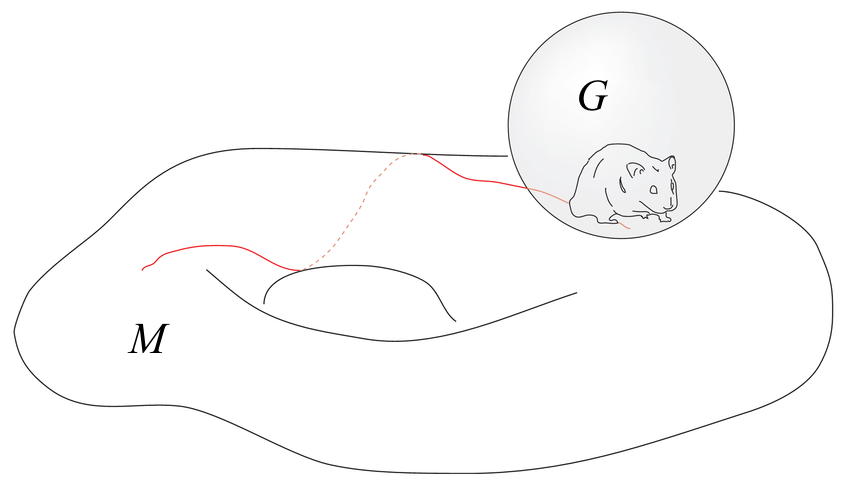
\includegraphics[scale=0.2]{figures/development.png}
    \caption{Development of a path in $(M,\omega)$ to a path in $(G,\theta_G)$. As the mouse follows the path in $M$, the contact point traces out a developed path in $G$.}
    \label{fig:development} 
\end{figure}


\begin{thm}[Generalized Fundamental Theorem]\label{prop generalization of fundamental thm}
    The Fundamental Theorem~\ref{thm 7.14 Sharpe fundamental global} continues to hold for maps $f:M\to G$ if $G$ is replaced with any connected manifold with a $1$-form $\eta$ satisfying all $3$ conditions in Theorem~\ref{thm 8.7 Sharpe}. Namely, let $M$ be connected and simply connected, let $\omega\in\Omega^1(M;\frakg)$, and $x_0\in M$. Then for each $g_0\in G$ there exists a unique smooth map $f:M\to G$ such that $f(x_0)=g_0$ and $f^\ast\eta=\omega$ iff $\omega$ satisfies the structure equation.
\end{thm}
\begin{proof}
    Local solutions exist by the same argument as in the Local Fundamental Theorem~\ref{thm 6.1 Sharpe fundamental local}. The main ingredient leading to global existence is the ability to develop $\omega$ along arbitrary paths (thus lifting those paths to $G$) with the help of the completeness of $\eta$.

    Let $\gamma:I\to M$ be a path and $g_0\in G$ a point. We would like to show that the form $\gamma^\ast \omega\in \Omega^1(I;\frakg)$ can be developed to give a path $\wt\gamma$ in $G$ starting at $g_0$ such that $\eta(\dot{\tilde\gamma}(t))=\omega(\dot\gamma(t))$. The completeness of $\eta$ will be crucial in constructing $\wt\gamma$.

    \emph{Step 1:} construct \emph{exponential maps} on $G$. At every point $g\in G$, we define the exponential map $\exp_g:\frakg\to G$ using the flows of the constant vector fields $\eta^{-1}(A)$, $A\in\frakg$. Let us denote the flow of $\eta^{-1}(A)$ by $F^A_t$, and put 
    \[\exp_g(A)\coloneqq F^A_1(g),\quad g\in G,\;A\in\frakg.\]
    This is well-defined because the flows $F^A_t$ are complete by assumption. This map is smooth by the same exact argument that we will use for the actual exponential map in Proposition~\ref{prop properties of exp}(a). Its differential at the origin is easy to compute. We identify $\T_0\frakg$ with $\frakg$. Let $X_g\in T_g G$ and let $A=\eta(X_g)$ (recall that this correspondence $\T_g G\to \frakg$ is bijective), so that the constant vector field $\eta^{-1}(A)$ has value $X_g$ at $g$. Then 
    \[(\exp_g)_{\ast 0}(A)=\restr{\frac{\dd}{\dd t}}{t=0}F^A_t(g)=\eta^{-1}(A)_g=X_g,\]
    in other words $(\exp_g)_{\ast 0}=\eta^{-1}_g$, which is an isomorphism. Thus, $\exp_g$ is a local diffeomorphism mapping some $0$-neighborhood $U\subset \frakg$ diffeomorphically to an open neighborhood $V\subset G$ of $g$. We will call such sets $V$ \emph{exponential neighborhoods}.

    % \emph{Step 3:} approximate paths in $G$ with ``piecewise-linear'' ones. Consider any path $\wt\gamma:I\to G$ and break it up into a finite (by compactness of $I$) collection of segments each of which is contained in an exponential neighborhood $V_i$ of a point $g_i\in \gamma(I)\subset G$. We can assume that $V_i$ is contractible, so any smooth path $\wt\gamma_i:[a_i,a_{i+1}]\to V_i$ passing through $g_i$ is homotopic, with a fixed value $g_i$, to a path of the form 
    % \[\sigma_i=\exp_{g_i}(A_i t),\quad A_i\in\frakg.\]
    % Then along $\sigma_i$ the value of $\omega$ is constant: $\omega(\dot\sigma_i)=A_i$.  All together, $\wt\gamma$ is homotopic to a piecewise smooth path $\sigma:I\to G$ such that $\sigma(I)\subset \bigcup_i V_i$ and $\omega(\dot\sigma)$ is piecewise-constant. We can also assume that $V_i$ is mapped by $\exp_{g_i}^{-1}$ to a ball of a fixed radius $\epsilon>0$ in $\frakg$. 
    
    % \emph{Step 4:} construct the development of $\sigma$. By assumption, the constant vector fields $\omega^{-1}(A_i)$ are complete and the segments $\sigma_i$ are integral curves for them. Thus, given a starting point $g_0$, we can define the ``development'' $\wt\sigma$ of $\eta$ along $\sigma$ as the path obtained by applying, sequentially, the flows $F^{A_i}_t$ for $t\in [a_i,a_{i+1}]$. 
    
    % \emph{Step 5:} show invariance of the endpoint. Different choices of the approximating path $\sigma$ are homotopic to each other. Let $h:I\times I\to G$ be such a homotopy. The pullback $h^\ast \omega\in \Omega^1(I^2;\frakg)$ still satisfies the structure equation, so by the same argument as in Theorem~\ref{thm 7.7 Sharpe}, the endpoint $\wt\sigma(1)$ is independent of the choice of $\sigma$. Since $\epsilon$ can be made arbitrarily small, by continuity the endpoint also remains stationary during homotopic deformations of $\gamma$ itself (with fixed endpoints).

    \emph{Step 2:} construct ``piecewise-linear'' developments of $1$-forms. Any $1$-form $\xi(t)\dd t\in\Omega^1(I;\frakg)$ can be approximated (under some supremum norm on $\frakg$-valued functions) by a $1$-form $\xi_c(t)\dd t$ such that $\xi_c:I\to \frakg$ is piecewise-constant, $\xi_c(t)=A_i$, $t\in[a_i,a_{i+1}]$. Each constant segment of this $1$-form can be developed to a path in $G$ from any given starting point $g_i$, using the flow $\Fl^{A_i}_t$:
    \[\sigma_i(t)=\exp_{g_i}(A_i t).\]
    We do this inductively, starting with the given $g_0\in G$ and letting $g_{i+1}=\exp_{g_i}(A_i (a_{i+1}-a_i))$, see Figure~\ref{fig:develop}. By refining the approximation we can guarantee that the developed segments stay within exponential neighborhoods of their starting points, and that the images of those neighborhoods in $\frakg$ are balls of fixed radius $\epsilon>0$. This allows us to lift any homotopy that deforms $\xi_c$ into an approximation with even smaller $\epsilon$ to a homotopy $h$ of the developed path in $G$ (by lifting it inside each exponential neighborhood separately). The pullback $h^\ast \eta\in \Omega^1(I^2;\frakg)$ still satisfies the structure equation, so by the same argument as in Theorem~\ref{thm 7.7 Sharpe}, the endpoint $\sigma(1)$ is independent of the choice of approximation.

    \emph{Step 3:} develop $\omega$ along paths in $M$ to paths in $G$. For any path $\gamma:I\to M$, we can develop approximations of the $1$-form $\gamma^\ast \omega$ from any starting point $g_0\in G$, getting a unique endpoint that doesn't depend on the approximation. Since $\omega$ satisfies the structure equation, the endpoint is \emph{also} independent of homotopic deformations of $\gamma$ itself (with fixed endpoints). By replacing the interval $I$ with $[0,t]$, we define not just the endpoint but the whole development $\wt\gamma(t)$ of $\omega$ along $\gamma$. It has to be smooth because $\wt\gamma^\ast \eta$ is uniformly approximated by developable $1$-forms whose limit is $\gamma^\ast\omega$, and local primitives of the latter are smooth by the argument in the local Fundamental Theorem.

    \emph{Step 4:} construct $f$. Now take our $1$-form $\eta$ and define its primitive $f:M\to G$ subject to the condition $f(x_0)=g_0$ as follows. For each $x\in M$, we pick a path $\gamma:x_0\leadsto x$, develop $\gamma^\ast\eta$ to $\wt\gamma$ as above starting at $g_0$ and put $f(x)\coloneqq \wt\sigma(1)$. Since $M$ is simply connected, all choices of $\gamma$ are homotopic to each other, hence their piecewise smooth approximations are also homotopic, and $f(x)$ is independent of these choices. By the same argument as in Theorem~\ref{thm 7.14 Sharpe fundamental global}, locally near $x$, $f(x)$ has to coincide with the unique local primitive, and hence is smooth and $f^\ast\eta=\omega$. Global uniqueness follows from local uniqueness.
\end{proof}

\begin{figure}[tp]
    \def\svgwidth{0.5\linewidth}
    \centering
    \import{figures/}{develop.pdf_tex}
    % 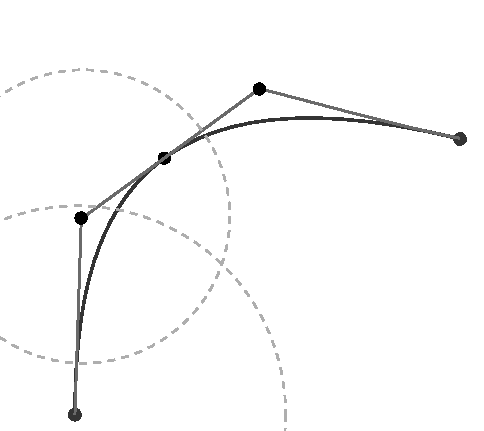
\includegraphics[scale=0.5]{figures/develop.pdf}
    \caption{Piecewise-linear approximations to a development.\label{fig:develop}}
\end{figure}

\begin{proof}[Proof of Theorem~\ref{thm 8.7 Sharpe}]
    First we discuss the case of simply connected $M$, so that $G=M$. This case involves five steps. First we construct a map $f:M\to \GL(\frakg)$ that will eventually be given by $f(g)=\Ad_g$. The second step constructs a map $m:M\times M\to M$ satisfying the conditions $m(e,e)=e$ and $m^\ast \eta=(\pr_2^\ast f)^{-1} \circ \pr_1^\ast\eta+\pr_2^\ast\eta$ (see (\ref{eq MC form under m})). The third step shows that $f$ is a homomorphism w.r.t.\ the multiplication $m$. The fourth shows that $m$ is associative. The fifth step constructs a map $i:M\to M$ and shows that it is the inversion w.r.t.\ $m$.

    \emph{Step 1.} Corollary~\ref{cor 5.3 Sharpe} shows that any map $f:M\to \Aut(\frakg)\subset \GL(\frakg)$ should have logarithmic derivative $\ad_{\eta}\in \frakgl(\frakg)$ and satisfy $f(e)=e$. Thus the form $\eta$ will determine $f$, provided $\omega=\ad_\eta$ is integrable (i.e., satisfies the structure equation). But
    \[\dd\omega+\frac12[\omega,\omega]=\ad_{\dd\eta}+\frac12[\ad_\eta,\ad_\eta]=\ad_{\dd\eta+\frac12[\eta,\eta]}=0,\]
    and since $M$ is simply connected, it follows from the Fundamental Theorem~\ref{thm 7.14 Sharpe fundamental global} that $\eta$ is the logarithmic derivative of a unique map $f:M\to \GL(\frakg)$ satisfying $f(e)=e$. In particular, $\dd f=f\cdot \ad_\eta$, where the product on the right is the composition of elements in $\frakgl(\frakg)$ as linear maps.

    \emph{Step 2.} We construct the multiplication map. Any potential multiplication map $m:M\times M\to M$ should have logarithmic derivative at $(x,y)\in M\times M$ given by the analog of (\ref{eq MC form under m}):
    \[\omega=\pr_1^\ast (f(y)^{-1}\eta)+\pr_2^\ast\eta=(\pr_2^\ast f^{-1})\pr_1^\ast\eta+\pr_2^\ast\eta.\]
    Thus the form $\eta$ will determine $m$, provided $\omega$ is integrable. Now one checks that $\dd\omega+\frac12[\omega,\omega]=0$ by a lengthy direct substitution and using the structure equation on $\eta$, the equality $\dd (f^{-1})=-\ad_\eta\circ f^{-1}$, and the commutativity of the wedge product of $\frakg$-valued $1$-forms. Since $M$ is simply connected, the generalized Fundamental Theorem~\ref{prop generalization of fundamental thm} shows that $\omega$ is the log-derivative of a unique map $m:M\times M\to M$ satisfying $m(e,e)=e$.

    \emph{Step 3.} We show that $f:M\to \GL(\frakg)$ is a homomorphism w.r.t.\ $m$ in the sense that $f(m(x,y))=f(x)f(y)$ for all $x,y\in M$. We shall prove the commutativity of the square consisting of $m,m_{\GL},f$, and $f\times f$:
    \[m_{\GL}\circ (f\times f)=f\circ m.\]
    It is clear that this square commutes at $(e,e)$. Since $M$ is connected it suffices to show that the Maurer-Cartan form $\theta_{\GL}$ on $\GL(\frakg)$ pulls back to the same form on $M\times M$ along the two possible routes. Indeed, $\theta_{\GL(\frakg)}$ trivializes the tangent bundle of $\GL(\frakg)$ and thus its composition with the derivative of any map identifies that derivative, and hence the map itself, up to a constant. Thus, we must show that two logarithmic derivatives coincide:
    \[(f\circ m)^\ast\theta_{\GL}=(m_{\GL}\circ (f\times f))^\ast \theta_{\GL}.\]
    Once again, a lengthy substitution of $m^\ast\eta=\pr_2^\ast(f^{-1}(\pr_1^\ast\eta))+\pr_2^\ast\eta$ and $m_{\GL}^\ast\theta_{\GL}=\pr_2^\ast \Ad^{-1}_{\pr_1^\ast\theta_{\GL}}+\pr_2^\ast \theta_{\GL}$ confirms that the above identity is true.

    \emph{Step 4}. Now we need to show that $m$ is associative. This is equivalent to the commutativity of yet another square:
    \[m\circ (m\times \id)=m\circ (\id\times m).\]
    Again, this diagram clearly commutes at $(e,e,e)$, and since $M$ is connected, it suffices to show that the form $\eta$ on $M$ pulls back to the same form on $M\times M\times M$ along the two possible routes. Another lengthy substitution using the same identities verifies that this holds.

    \emph{Step 5.} Finally we construct an inversion map. Another trivial exercise is to check using (\ref{eq MC form under i}) that any inversion map $i:M\to M$ must have ``log-derivative'' (pullback of $\omega$) given by the prototype of ``$-\Ad_x\circ \eta(X)$'':
    \[\omega_x(X)=-(f\eta)(X),\quad x\in M,X\in \T_x M.\]
    Thus the form $\eta$ will determine $i$, provided we can show that $-f\eta$ is integrable. But since
    \[\dd\omega+\frac12[\omega,\omega]=-(\dd f)\eta -f\dd \eta+\frac12 f[\eta,\eta]=-f\ad_\eta\eta +f[\eta,\eta]=0\]
    and $M$ is simply connected, it folows from the generalized Fundamental Theorem~\ref{prop generalization of fundamental thm} that $\omega$ is the pullback of $\eta$ by a unique map $i:M\to M$ satisfying $i(e)=e$. However, we must still verify that $i$ is the inverse map, i.e., that $m(i(x),x)=e$. This identity can be written as the composition
    \[m\circ(i\times\id)\circ\Delta=e\in M,\]
    where $\Delta:M\to M\times M$ is the diagonal map $\Delta(x)=(x,x)$. Since $M$ is connected, it suffices to show that the form $\eta$ on $M$ pulls back to the same form on $M$ along the two possible routes. Since it obviously pulls back to $0$ via the right hand side, we must show that $(m\circ(i\times\id)\circ\Delta)^\ast\eta=0$. As in the previous steps, a lengthy substitution using the formula for $m^\ast\eta$ verifies this identity. Thus, $i$ is an inverse for $m$.

    \emph{The case $\pi_1(M)\neq 0$.} Here the form $\eta$ on $M$ lifts to the form $\pi^\ast \eta$ on the universal cover $G$. Clearly it satisfies the same three conditions on $G$ that $\eta$ does on $M$. Then our proof applies to the pair $(G,\pi^\ast\eta)$ and we see that for any fixed choice $e\in G$ there is a Lie group structure on $G$ for which $e$ is the identity and $\pi^\ast\eta$ is the Maurer-Cartan form. Its uniqueness follows from Theorem~\ref{thm second principle}: the unique isomorphism between any two group structures on $G$ is provided by the identity map. By Proposition~\ref{prop 8.1 Sharpe}, there is a unique injective homomorphism $\wt{\Phi}:\Aut(\pi)\to G$ satisfying $\wt{\Phi}(A)g=A(g)$ for all deck transformations $A\in \Aut(\pi)$. Thus the group of deck transformations is identified with the period group, a discrete subgroup $\Gamma\subset G$.
\end{proof}

\begin{rem}
    \begin{enumerate}
        \item Dropping the completeness condition (iii) in Theorem~\ref{thm 8.7 Sharpe} still leads to a manifold with a structure of a \emph{local Lie group}, for example, an open subset of a Lie group.
        \item If we drop condition (i) (the structure equation), we are left with what may be regarded as a ``deformation'' of a Lie group. We will later see that this produces a Cartan geometry with nonzero curvature.
        \item Except in special cases, we cannot weaken the isomorphism condition (ii) to $\eta_x$ being merely an injection for all $x\in M$ and still expect to obtain a discrete monodromy group. Therefore, this condition will remain a crucial part of the definition of a Cartan geometry.
    \end{enumerate}
\end{rem}

Theorem~\ref{thm 8.7 Sharpe} provides an easy proof of the existence and uniqueness of universal covering groups (Theorem~\ref{thm 7.7. Lee covering group}).

\begin{proof}[Proof of Theorem~\ref{thm 7.7. Lee covering group}]
    Let the universal covering map be $\pi:\wt{G}\to G$. First note that if a Lie group structure on $\wt{G}$ exists, then the Maurer-Cartan form on $\wt{G}$ is $\pi^\ast \theta_G$. Thus we are led to define $\eta=\pi^\ast\theta_G$ on $\wt{G}$. This form satisfies the structure equation by naturality of exterior derivatives and Lie brackets. Since $\pi$ is a local diffeomorphism, not only is $\eta$ an isomorphism on each fiber, but also $\eta$ is complete, since integral curves for $\theta_G$ on $G$ will lift to integral curves for $\eta$ on $\wt{G}$. By Theorem~\ref{thm 8.7 Sharpe}, given $\wt{e}\in \pi^{-1}(e)$, $\wt{G}$ has a unique Lie group structure with $\wt e$ as the identity and for which $\eta$ is the Maurer-Cartan form. By Theorem~\ref{thm 6.1 Sharpe fundamental local}, $\pi$ is the unique map $(\wt{G},\wt{e})\to (G,e)$ pulling back $\eta$ from $\theta_G$, and then by Theorem~\ref{thm second principle} it must be a homomorphism.
\end{proof}

If one assumes Theorem~\ref{thm 7.7. Lee covering group} to be known (via our original proof), then a much shorter proof of Theorem~\ref{thm 8.7 Sharpe} can be given based on the Ehresmann Fibration Theorem. We have avoided this proof due to the value of the concepts developed over the course of the longer proof.

\begin{proof}[Shorter proof of Theorem~\ref{thm 8.7 Sharpe} {{\cite[Thm.~2.8]{McKayCartan}}}]
    Consider again the Pfaffian system on $M\times G$ spanned by the (components of the) $1$-form $\pr_M^\ast\eta-\pr_G^\ast\theta_G$. By the proof of the local Fundamental Theorem~\ref{thm 6.1 Sharpe fundamental local}, it is integrable and the leaves of the integral foliation are locally graphs of maps $M\to G$. Moreover, since both $\eta$ and $\theta_G$ are fiberwise isomorphisms, these maps are local diffeomorphisms that pull $\theta_G$ back to $\eta$. 
    
    Let $S$ be a leaf of the foliation through some point $(m_0,e)$. Take a constant vector field $\eta^{-1}(A)$ on $G$ for some $A\in\frakg$. The vector field $X\coloneqq (\eta^{-1}(A),A_\rmL)$ on $M\times G$ is tangent to $S$ since $\restr{\pr_M^\ast\eta}{S}=\restr{\pr^\ast_G\theta_G}{S}$. We can simultaneously consider the integral curve $\gamma_M$ of $\eta^{-1}(A)$ through $m_0$ and $\gamma_G$ the integral curve of $A_\rmL$ through $e$. We see that the integral curve $\gamma$ of $X$ through $(m_0,e)\in M\times G$ lies in $S$ and projects onto $\gamma_M$ and $\gamma_G$, respectively. As long as both of the latter curves exist, $\gamma$ exists as well. This means that $\eta^{-1}(A)$ and $A_\rmL$ can be lifted to a unique complete vector field on $S$. Since these vector fields span the tangent bundles, we can now use the Ehresmann Fibration Theorem in the form of Corollary~\ref{thm Ehresmann vector fields} to conclude that $S$ is a fiber bundle over both $M$ and $G$. All three have the same dimension, therefore $S$ is actually a covering space of both $G$ and $M$. 
    
    By an extension of the same lifting argument, we can now replace $S$ with the universal covering space $\wt M$ of $M$. The resulting covering map $D\coloneqq \wt M\to G$ is called a \emph{developing map}. \index{Developing map}
    By Theorem~\ref{thm 7.7. Lee covering group}, $\wt M$ has a unique Lie group structure (for each choice of identity) that turns $D$ into a local Lie group isomorphism. The deck transformations of $\wt M$ preserve the pullback of $\eta$. But the developing map might not be invariant under the deck transformations. Each deck transformation $a\in \Aut(\wt{M})\cong \pi_1(M)$ takes $(m_0,e)$ to some $(m,g)$. By uniqueness of leaves of the foliation, the entire transformation must be simply the left translation $\rmL_g$ acting on the $G$-component, as asserted.
\end{proof}

In this picture, developments of $\eta$ correspond to unique liftings of curves in $M$ to curves in $\wt{M}$ and then projection to $G$ via the developing map.






\section{One-parameter subgroups}


\begin{lem}\label{3972}
    If $G$ is a Lie group and $\frakh\subset \Lief G=\T_e G$ is a Lie subalgebra, then the subset $D_\rmL=\bigcup_g (\rmL_g)_{\ast e}\frakh\subset \T G=G\cdot \frakh$ is a left-invariant involutive distribution. Similarly, $D_\rmR=\frakh\cdot G$ is a right-invariant involutive distribution. 
\end{lem}
\begin{proof}
    It is sufficient to show this for the left-invariant case. Let $D=D_\rmL$. For each $g\in G$, $(\rmL_g)_{\ast e}$ is an isomorphism, therefore $D_g$ is of constant rank $\dim \frakh$ and the distribution is obviously left-invariant. Any basis of left-invariant vector fields on $G$ forms a smooth frame for $D$, so $D$ is smooth. Moreover, $D$ is involutive because such a frame is closed under the Lie bracket.
\end{proof}

The Frobenius theorem now gives us the first the first ``enhancement'' result about Lie subgroups. Even though by definition they are only required to be immersed (which means that their topology can differ drastically from the subspace topology), the following theorem shows that they are in fact weakly embedded (initial).

\begin{thm}[Lie subgroups are weakly embedded {{\cite[Thm.~19.25]{Lee}}}]\label{thm 19.25 Lee}
    Every Lie subgroup is an integral manifold of an involutive distribution, and therefore is a weakly embedded submanifold.
\end{thm}
\begin{proof}
    Let $H\subset G$ be a Lie subgroup. Then $\Lief H$ is canonically isomorphic to the Lie subalgebra $i_\ast(\Lief H)\subset \Lief G$, where $i:H\hookrightarrow G$ is the inclusion. Let $D\subset \T G$ be the left-invariant involutive distribution corresponding to $\frakh$ as in Lemma~\ref{3972}. It follows that $\T_hH=D_h$, so $H$ is an integral manifold of $D$ and is weakly embedded by Theorem~\ref{thm 19.17 Lee}.
\end{proof}

Recall from Theorems~\ref{thm 5.31 Lee} and \ref{thm 5.32 Lee} that while an immersed submanifold can have its topology (and, in a uniquely corresponding way, smooth structure) adjusted in many ways while still remaining immersed, a weakly embedded submanifold has \emph{only one} topology and smooth structure under which it's still immersed. This means that the topology of an immersed Lie subgroup is much more rigid than we originally assumed in the definition.

\begin{rem}
    Note that this does not \emph{yet} allow us to completely drop the assumption of any smooth structure in the definition of a Lie subgroup. A weakly embedded submanifold still needs to be immersed by definition, which presumes a predefined smooth structure on it. We have only shown that this smooth structure is unique. The existence of a smooth structure on an arbitrary path-connected subgroup of a Lie group is a much deeper result which we will demonstrate in \S\ref{sec: Yamabe's theorem}
\end{rem}

\begin{thm}[{{\cite[Thm.~19.26]{Lee}}}] Let $G$ be a Lie group and $\frakg=\Lief G$ its Lie algebra. If $\frakh\subset \frakg$ is a Lie subalgebra, then there is a unique connected immersed Lie subgroup of $G$ whose Lie algebra is $\frakh$.
\end{thm}
\begin{proof}
    Let $D\subset \T G$ be the involutive left-invariant distribution corresponding to $\frakh$. We now use the global Frobenius theorem to introduce the foliation $\calH$ determined by $D$, and for any $g\in G$, let $\calH_g$ be the leaf containing $g$. Since $D$ is left-invariant, it follows that left translations take leaves to leaves: $\rmL_g(\calH_{g'})=\calH_{gg'}$.

    Define $H=\calH_e$. We will show that $H$ is the desired Lie subgroup. First, it is a subgroup because it is left-invariant: $hh'\in \rmL_h(H)=\calH_h=H$ for all $h,h'\in H$, and similarly $h^{-1}\in H$.

    To show that $H$ is a Lie group we need to show that the map $\mu(h,h')=hh^{\prime -1}$ is smooth as a map $H\times H\to H$. Since $H\times H$ is a submanifold of $G\times G$, it is immediate that $\mu:H\times H\to G$ is smooth. Since $H$ is also weakly embedded by Theorem~\ref{thm 19.17 Lee}, $\mu$ is also smooth as a map into $H$.

    The fact that $H$ is a leaf of $\calH$ implies that the Lie algebra of $H$ is $\frakh$, because $\T_eH=D_e=\frakh$. Now suppose there is another subgroup $\wt{H}$ with the same Lie algebra. By maximality of $H=\calH_e$, we have $\wt H\subset H$. On the other hand, in any flat chart for $D$ containing $e$, $\wt H$ must consist of open subsets of slices. Since the slice containing $e$ is an open subset of $H$, this means that $\wt H$ contains a neighborhood of $e$ in $H$. But every neighborhood of $e$ generates the connected Lie group $H$ by Proposition~\ref{prop 7.14 Lee}, therefore $\wt H=H$.
\end{proof}


\begin{defn}
    A \gls{ops} of a Lie group $G$ is a Lie group homomorphism $\gamma:(\bbR,+)\to G$, i.e.~a complete curve such that $\gamma(0)=e$ and $\gamma(t+s)=\gamma(t)\gamma(s)$.
\end{defn}

Note that a \gls{ops} is \emph{not} a Lie subgroup of $G$, but a specific homomorphism. However the images of these homeomorphisms are weakly embedded by Theorem~\ref{thm 19.25 Lee} can be identified with certain Lie subgroups:

\begin{prop}
    Images of \glspl{ops} in $G$ are precisely the connected Lie subgroups of dimension at most 1. Moreover, every such subgroup is either isomorphic to $\bbR$ or $\bbS^1$, or trivial.
\end{prop}
\begin{proof}
    Every connected Lie subgroup of dimension $1$ is automatically abelian and is the integral curve of the left-invariant vector field corresponding to any nonzero tangent vector to the subgroup at $e$. Such an integral curve defines the required \gls{ops}. The isomorphisms hold because any one-dimensional Lie group is a factor of $\bbR$ (the only simply connected one-dimensional Lie group) by a discrete subgroup, and all such subgroups of $\bbR$ are either trivial or isomorphic to $\bbZ$.
\end{proof}


\begin{thm}[Characterization of one-parameter subgroups]
    The \glspl{ops} of a Lie group $G$ are precisely the maximal integral curves of left-invariant vector fields starting at $e\in G$.
\end{thm}
\begin{proof}
    Given a left-invariant vector field, its integral curve at $e$ will automatically be a \gls{ops} due to the general group property of flows and completeness (or alternatively from the uniqueness of maximal integral curves).

    Conversely, every \gls{ops} $\gamma$ is the integral curve of the left-invariant field $A_\rmL$ whose value at the identity is $A=\dot\gamma(0)\in\Lief G$ because 
    \[\dot\gamma(t)=\restr{\frac{\dd}{\dd s}}{s=0}\rmL_{\gamma(t)}\gamma(s)=\rmL_{\gamma(t)\ast e}A=(A_\rmL)_{\gamma(t)}.\]
\end{proof}

This leads us to yet another common way of defining the Lie algebra of a Lie group.

\paragraph{Construction IV} In summary, there is a natural one-to-one correspondence between elements of the Lie algebra and \glspl{ops}
\[A\in \frakg\cong \fX(G)^G\mapsto \gamma_A(t)=F^A_t(e)\coloneqq \Fl^{A_\rmL}_t(e).\]
We say that $\gamma_A$ is \emph{generated} by $A\in\frakg$. The Lie bracket is recovered as the double derivative of the group commutator
\[[A,B]=\restr{\frac{\dd}{\dd t}\frac{\dd}{\dd s}}{t=s=0}\gamma_A(t)\gamma_B(s)\gamma_A(t)^{-1}\gamma_B(s)^{-1}.\]

The following is a well known fact of linear algebra.

\begin{prop}
    For $A\in \mathfrak{gl}_n(\bbK)$, the \gls{ops} generated by it in $\GL_n(\bbK)$ is
    \[\gamma_A(t)=\rme^{tA}=\exp tA.\]
\end{prop}
\begin{cor}
    Uniqueness of integral curves implies that the \glspl{ops} of a Lie subgroup $H< G$ are exactly the ones generated by $\frakh < \frakg$. Therefore in \emph{all} matrix groups the \glspl{ops} are given by exponentials.
\end{cor}

\begin{prop}[{{\cite[Prop.~20.3]{Lee}}}]\label{prop 20.3 Lee}
    If $H< G$ is a Lie subgroup, then the \glspl{ops} of $H$ are precisely those \glspl{ops} of $G$ that are generated by elements of $\frakh=\T_e H$.
\end{prop}
\begin{proof}
    Clearly any \gls{ops} $\gamma:\bbR\to H$ can also be viewed as a \gls{ops} of $G$ (by composing with the inclusion map) which satisfies $\dot\gamma(0)\in \T_e H$.

    Conversely, a \gls{ops} of $G$ generated by an element of $\T_e H$ must coincide with the analogous \gls{ops} of $H$ by uniqueness of maximal integral curves.
\end{proof}







\section{Exponential map}


\begin{defn}[Exponential map]\index{Exponential map}
    Given a Lie group $G$ with Lie algebra $\frakg=\Lief G$, the exponential map $\exp:\frakg\to G$ assigns to each $A\in \frakg$ the group element
    \[\exp A=\gamma_A(1),\]
    where $\gamma_A$ is the \gls{ops} generated by $A$. As a consequence, the \gls{ops} generated by $A$ can be written as \[\gamma_A(t)=\gamma_{tA}(1)=\exp tA=\rme^{tA}.\]
    (While we use the notations $\exp A$ and $\rme^A$ interchangeably, the exponential map is related to the Euler number only in the case of linear Lie groups.)
\end{defn}

When multiple groups are involved, we will sometimes specify the group to which the exponential map belongs by writing, for example, $\exp_G$.

\begin{prop}\label{prop properties of exp} The exponential map $\exp:\frakg\to G$ has the following properties for all $A\in\frakg$.
\begin{enumerate}[label=(\alph*)]
    \item $\exp$ is smooth.
    \item $\rme^{sA}\rme^{tA}=\rme^{(s+t)A}$ for $s,t\in\bbR$.
    \item $\left(\rme^A\right)^{-1}=\rme^{-A}$.
    \item $\left(\rme^A\right)^{n}=\rme^{nA}$ for $n\in \bbZ$.
    \item $\exp_{\ast 0}=\id_\frakg$.
    \item $\exp$ restricts to a diffeomorphism from some neighborhood of $0\in \frakg$ to a neighborhood of $e\in G$. Its inverse is often denoted by $\ln$.
    \item $\exp$ is natural: if $H$ is another Lie group with $\frakh=\Lief H$, and $\Phi:G\to H$ is a Lie group homomorphism, then 
    \[\exp_H\circ\Phi_{\ast e}=\Phi\circ \exp_G.\]
    \item The flow $\Fl^{A_\rmL}$ of a left-invariant vector field $A_\rmL\in \fX(G)^G$, $(A_\rmL)_e=A$, is given by $F_t=\rmR_{\rme^{tA}}$.
\end{enumerate}
\end{prop}
\begin{proof}
    (a) We need to show that the flow $F^A$ of a vector field varies smoothly with $A$. This is a situation not covered by the fundamental theorem of flows, but we can reduce it to that situation by a simple trick. Define a vector field $\Xi\in\fX(G\times\frakg)$ by
    \[\Xi_{(g,A)}=((A_\rmL)_g,0)\in \T_gG\oplus \T_A \frakg.\]
    This is a smooth vector field because it acts on functions by differentiating them along $A_\rmL$. It is easy to verify that the flow $F^\Xi$ is given by
    \[F^\Xi_t(g,A)=\left(\Fl^{A_\rmL}(g,t),A\right).\]
    By the fundamental Theorem~\ref{thm fundamental of flows} of flows, $F^\Xi$ is smooth. Since $\exp A=\pr_1\left(F^\Xi_1(e,A)\right)$, where $\pr_1:G\times\frakg\to G$ is the projection, it follows that $\exp$ is smooth.

    (b-d) follow trivially from the fact that $\exp(tA)$ is a \gls{ops}.
    
    To show (e) we compute
    \[\exp_{\ast 0}A=\restr{\frac{\dd}{\dd t}}{t=0}F_t^{A}(e)=A,\]
    i.e.~$\exp_{\ast 0}$ coincides with the natural isomorphism $\fX(G)^G\cong \T_e G$. Then by the \gls{inmt}, $\exp$ is a local diffeomorphism and (f) follows.

    (g) follows from the naturality of flows of vector fields:
    \[\Fl^{\Phi_\ast A}_t\circ \Phi=\Phi\circ \Fl^{A}_t,\]
    and setting $t=1$ and evaluating at the identity yields (g).

    (h) was already proven in Lemma~\ref{lem 471841}.
\end{proof}

\begin{rem}
    The naturality of $\exp$ implies, in particular, that $g\rme^{tA}g^{-1}=\rme^{t\Ad_g A}$. This confirms the intuitive picture that conjugate subgroups are generated by conjugate elements of the Lie algebra. For example, on $\SO_3$, let $H\cong\SO_2$ be the \gls{ops} of rotations about the $z$-axis. Then if $g$ is a rotation which maps $\bf{e}_3=(0,0,1)$ to some vector $\bf{n}$, then the subgroup of rotations about $\bf{n}$ is $gHg^{-1}$ and is generated by 
    \[A_{\bf{n}}=A_{g\bf{n}}=\Ad_g A_{\bf{e}_3}=gA_{\bf{e}_3} g^{-1},\] 
    where $A_{\bf{e}_3}$ generates rotations about $\bf{e}_3$, cf.\ Example~\ref{example su2 and so3}.
\end{rem}
\begin{cor}
    The identity component $G_0$ is generated by $\exp(U)$ for any neighborhood $U$ of the origin $0\in\frakg$.
\end{cor}
 

\begin{rem}
    The inverse of the exponential map, $\ln$ (logarithm), provides a \emph{canonical local chart} at $e\in G$. This is a special property of Lie groups that we will use to much benefit. We will call this chart the \emph{logarithmic coordinates} on $G$.
\end{rem}


\begin{prop}\label{prop 5.4.5 RS1 ker(Ad) and ker(ad)}
    The kernels of the adjoint representations of $G$ and $\frakg$ are given by the centralizer of the identity component and the center of the Lie algebra, respectively:
    \[\ker \Ad=\rmC_G(G_0),\quad \ker \ad=\frakz(\frakg).\]
    In particular, the \emph{adjoint group of $G$} is \index{Adjoint group}
    \[\Ad(G)\cong G\slash \rmC_G(G_0),\quad \ad(\frakg)\cong \frakg\slash \frakz(\frakg).\]
\end{prop}
\begin{proof}
    The statement $\ker\ad=\frakz(\frakg)$ is obvious. Since for $g\in \rmC_G(G_0)$ there holds $\restr{\Adg_g}{G_0}=\id_{G_0}$ and since $(\id_G)_{\ast e}=\id_\frakg$, we obtain $\rmC_G(G_0)\subset \ker\Ad$. Conversely, if $g\in G$ satisfies $\Ad_g=\id_\frakg$. The naturality of the exponential map implies 
    \[\rme^A=\rme^{\Ad_g A}=\Adg_g(\rme^A)\text{ for all }A\in\frakg.\]
    That is, $g$ commutes with all elements of $\exp(\frakg)$. Since $\exp(\frakg)$ generates $G_0$, we conclude $\ker\Ad\subset \rmC_G(G_0)$.
\end{proof}

Similarly, for the coadjoint representation we have
\[\ker \Ad^\ast=\rmC_G(G_0),\quad \ker\ad^\ast=\frakz(\frakg).\]

\begin{prop}\label{prop 20.9 Lee}
    If $H\subset G$ is a Lie subgroup, then the exponential map of $H$ coincides with the restriction of the exponential map of $G$, and 
    \[\Lief H=\{A\in\Lief G: \exp(tA)\in H \text{ for all } t\in \bbR\}.\]
\end{prop}
\begin{proof}
    The fact that $\exp_H=\restr{\exp_G}{\frakh}$ follows immediately from Proposition~\ref{prop 20.3 Lee}.

    Next assume that $\rme^{tA}\in H$ for all $t$. Since $H$ is weakly embedded in $G$ by Theorem~\ref{thm 19.25 Lee}, it follows that the curve $t\mapsto \rme^{tA}$ is smooth as a map into $H$, and thus $A=\dot\gamma(0)\in \T_eH$. Conversely, if $A\in \T_e H$ then Proposition~\ref{prop 20.3 Lee} implies that $\rme^{tA}\in H$ for all $t$.
\end{proof}


\begin{thm}\label{thm 1.5.2 DK}
    The following formulas hold for all $A\in\frakg,g\in G$:
    \begin{enumerate}[label=(\alph*)]
        \item $\Ad_{\rme^A}=\rme^{\ad_A}$.
        \item $\Adg_g \rme^A=\rme^{\Ad_g A}$.
    \end{enumerate}
\end{thm}
\begin{proof}
    For (a) we apply the naturality of $\exp$ (Proposition~\ref{prop properties of exp} (g)) to the homomorphism $\Ad:G\to \GL(\frakg)$, and for (b) we apply it to the homomorphism $\Ad_g:G\to G$.
\end{proof}



\begin{example}
    Recall Corollary~\ref{cor generated homomorphism}, where we showed that Lie group homomorphisms with a simply connected source group are uniquely determined by their derivatives at the identity. The Lie group $\SU_2$, being homeomorphic to the sphere $\bbS^3$, is simply-connected. Therefore, every homomorphism $\phi:\fraksu_2\to\frakg$ into any other Lie algebra $\frakg$ of some Lie group $G$ determines a unique homomorphism $\Phi:\SU_2\to G$. 
    
    On the other hand, from Example~\ref{example su2 and so3}, the homomorphism $\Ad:\SU_2\to \SO_3(\bbR)$ is a double covering map since $\ker\Ad=\{\pm \rmI\}$, thus $\SO_3(\bbR)$ doesn't satisfy the condition on the domain group for the same theorem, and it must be possible to find a Lie algebra homomorphism $\psi:\frakso_3(\bbR)\to\frakg$ that doesn't extend to a group homomorphism $\Psi:\SO_3(\bbR)\to G$. Namely, the group homomorphism $\Psi$ exists if and only if 
    \[\exp \psi(A_{2\pi \bf{e}_3})=e_G,\text{ where }A_{2\pi \bf{e}_3}=
    \begin{pmatrix}
        0&0&0\\
        0&0&-2\pi\\
        0&2\pi &0
    \end{pmatrix}.
    \]
    To see this, apply the previous statement to $\phi=\psi\circ\ad$, where we view the adjoint as a map $\ad:\fraksu_2\to\frakso_3(\bbR)$. From this homomorphism, $\Psi$ is determined by $\Phi=\Psi\circ \Ad$; therefore such a homomorphism of Lie groups $\Psi$ exists iff $\Phi(-\rmI)=e_G$, which translates to $\Psi\circ \Ad(-\rmI)=e_G$. Since $\Phi\circ\exp=\exp\circ\phi$ and 
    \[\exp(\rmi \pi\sigma_3)=\exp \begin{pmatrix}
        \rmi \pi&0\\0 &-\rmi \pi
    \end{pmatrix}=-\rmI,\]
    the condition that $\Phi(-\rmI)=e_G$ becomes
    \[e_G=\Phi\circ \exp (\rmi\pi\sigma_3)=\exp\circ\phi (\rmi\pi\sigma_3)=\exp\circ\psi( \ad_{\rmi\pi\sigma_3})=\exp\circ\psi (A_{2\pi \bf{e}_3}),\]
    where at the end we used formula (\ref{eq ad: su2->so3}).
    
    This picture generalizes to all Lie groups. For any group $H$ one can specify a finite set of $A_i\in\frakh$ such that any homomorphism of Lie algebras $\phi:\frakh\to\frakg$ generates a homomorphism of Lie groups $\Phi:H\to G$ iff $\exp\phi(A_i)=e_G$ for all $i$.
\end{example}


\begin{prop}\label{prop exp on abelian groups}
    If $A,B\in\frakg$ commute, i.e.~$[A,B]=0$, then
    \[\rme^A\rme^B=\rme^B\rme^A=\rme^{A+B}.\]
    In particular, if $\frakg$ is abelian, $\exp$ is a Lie group homomorphism from the vector group underlying $\frakg$ to $G$.
\end{prop}
\begin{proof}
    It suffices to show that the curve defined by $\gamma(t)=\rme^{tA}\rme^{tB}$ coincides with the integral curve generated by $A+B$. Indeed, $\gamma(0)=e$ and we can use the commutation of the flows of the left-invariant fields $A_\rmL$ and $B_\rmL$ to compute the generator. Here we will need the general product rule that holds for maps $f:M_1\times M_2\to N$:
    \[\T_{(m_1,m_2)}f(A_1,A_2)=\T_{m_1}f_{m_2}(A_1)+\T_{m_2}f_{m_1}(A_2)\]
    where $f_{m_1}:M_2\to N$ and $f_{m_2}:M_1\to N$ are the partial mappings. In particular, if $M_1=M_2\cong \bbR$ then we have the ``product rule'' for derivatives along the diagonal:
    \[\restr{\frac{\dd}{\dd t}}{t}\varphi(t,t)=\restr{\frac{\dd}{\dd s}}{s=t}\varphi(s,t)+\restr{\frac{\dd}{\dd s}}{s=t}\varphi(t,s).\]
    Applying this to $\gamma$ we get (using $F^A$ for the flow of $A_\rmL$)
    \begin{multline}
        \dot\gamma(0)=\restr{\frac{\dd}{\dd t}}{t=0} \Fl^{B}_t\circ \Fl^{A}_t (e)=\restr{\frac{\dd}{\dd s}}{s=0}\Fl^{B}_{s}(e)+\restr{\frac{\dd}{\dd s}}{s=0}\Fl^{A}_{s}(e)=B+A.
    \end{multline}
\end{proof}

When the elements do not commute, the following two propositions provide an approximate formula.

\begin{prop}[{{\cite[Prop.~20.10]{Lee}}}]\label{prop 20.10 Lee}
    For any $A,B\in\frakg=\Lief G$, there is a smooth function $Z:(-\epsilon,\epsilon)\to \frakg$ for some $\epsilon>0$ such that
    \[\rme^{tA}\rme^{tB}=\exp\left(t(A+B)+t^2Z_2(t)\right)\]
    for all $t\in(-\epsilon,\epsilon)$.
\end{prop}
\begin{proof}
    Since $\exp$ is a local diffeomorphism, there exists an $\epsilon>0$ such that on $(-\epsilon,\epsilon)$ we can consider the smooth map
    \[\varphi(t)=\ln\left(\rme^{tA}\rme^{tB}\right).\]
    Obviously $\varphi(0)=0$ and since the differential of the multiplication map is $(\T_{(e,e)}m)(A,B)=A+B$, we have
    \[\varphi'(0)=\ln_{\ast e}(A+B)=A+B.\]
    By Taylor's theorem $\varphi(t)=t(A+B)+t^2Z_2(t)$ for some smooth $Z_2(t)$.
\end{proof}
The following corollary will be useful in the proof of the Closed Subgroup Theorem~\ref{thm closed subgroup}.
\begin{cor}\label{cor 20.11 Lee}
    Under the hypotheses of the preceding proposition,
    \[\lim_{n\to\infty}\left(\exp \frac{tA}{n}\exp \frac{tB}{n}\right)^n=\exp t(A+B).\]
\end{cor}
\begin{proof}
    We have 
    \begin{multline}
        \left(\exp \frac{tA}{n}\exp \frac{tB}{n}\right)^n=\left(\exp\left(\frac{t}{n}(A+B)+\frac{t^2}{n^2}Z_2\left(\frac{t}{n}\right)\right)\right)^n=\\
        =\exp\left(t(A+B)+\frac{t^2}{n^2}Z_2\left(\frac tn\right)\right).
    \end{multline}
    Taking the limit $n\to\infty$ at fixed $t$ gives the result.
\end{proof}

\begin{prop}
    Under the hypotheses of the preceding proposition, 
    \[\rme^{tA}\rme^{tB}=\exp\left(t(A+B)+\frac{t^2}{2}[A,B]+t^3Z_3(t)\right)\]
    for another smooth map $Z_3:(-\epsilon,\epsilon)\to \frakg$.
\end{prop}
\begin{proof}
    For the function $\varphi$ from the proof of Proposition~\ref{prop 20.10 Lee} we have
    \[\varphi(t)=t(A+B)+t^2Z_2(0)+t^3Z_3(t).\]
    To compute the flow of this vector field we can apply the general Taylor formula for manifolds (\ref{eq:Taylor formula for manifolds}). By an abuse of notation we drop the smooth function $f\in C^\infty(G)$ on which this formula is supposed to act:
    \[\rme^{\varphi(t)}=\restr{\Fl^{A+B+\frac{s}{2}Z_2(0)+\calO(s^2)}_t}{s=t}=1+t(A+B)+\frac{t^2}{2}\left((A+B)^2+2Z_2(0)\right)+\calO(t^3).\]
    On the other hand the Taylor formula for two fields (\ref{eq: Taylor formula for two fields}) gives
    \[\rme^{tA}\rme^{tB}=1+t(A+B)+\frac{t^2}{2}(A^2+2AB+B^2)+\calO(t^3).\]
    We read off $Z_2(0)=[A,B]/2$.
\end{proof}

This gives us a new interpretation of the Lie bracket as the  commutator of infinitesimal flows of left-invariant vector fields (closely connected to formula (\ref{30071})).
\begin{cor}
    By a repeated application of the Taylor series obtained above,
    \[\rme^{tA}\rme^{tB}\rme^{-tA}=\rme^{tB+t^2[A,B]+\calO(t^3)}\]
    and
    \[[\rme^{tA},\rme^{tB}]=\rme^{tA}\rme^{tB}\rme^{-tA}\rme^{-tB}=\rme^{t^2[A,B]+\calO(t^3)}.\]
\end{cor}


\begin{rem}
    By continuing the Taylor expansion endlessly, we can obtain the full formal series for $\ln(\rme^A \rme^B)$ known as the \gls{bch}\index{Equation!Baker-Campbell-Hausdorff} formula. Its special property is that it can be written using only Lie brackets (or adjoints). We will derive it in the next \sect.
\end{rem}










\section{Differential of exp}

\begin{thm}[{{\cite[Thm.~1.5.3]{DK}}}]\label{thm differential of exp}
    For any $A\in\frakg$ the linear mapping $\exp_{\ast A}:\frakg\to \T_{\rme^A} G$ is given by
    \[  \exp_{\ast A}=\left(\rmR_{\rme^A}\right)_{\ast e}\circ \int_0^1 \rme^{s\ad_A}\dd s=\left(\rmL_{\rme^A}\right)_{\ast e}\circ \int_0^1 \rme^{-s\ad_A}\dd s.   \label{eq 1.5.1 DK}\]
\end{thm}
\begin{proof}
    We will provide a simple derivation of this from the Maurer-Cartan equation (\ref{eq Maurer-Cartan}). Let us apply it to the map
    \[g(t,s)=\rme^{t(A+sB)}.\]
    Then we find
    \[\xi=\left(\rmR_g^{-1}\right)_\ast \partial_t g=A+sB, \quad \eta=\left(\rmR_g^{-1}\right)_\ast \partial_s g,\]
    and the Maurer-Cartan equation $\partial_t\eta-\partial_s\xi=[\xi,\eta]$ now reads
    \[\partial_t \eta=B+[A,\eta].\]
    By denoting $\gamma(t)=\eta(t,0)$, we get the differential equation at $s=0$
    \[\dot\gamma(t)=B+[A,\gamma].\label{196}\]
    First we notice that the solution of the homogenous equation $\dot\gamma=[A,\gamma]$ is given by the adjoint curves
    \[\gamma_{\mathrm{hom}}=\Ad_{\rme^{tA}}\gamma_0=\rme^{t\ad_A}\gamma_0.\]
    By Lagrange's method of variation of constants, we look for a solution to (\ref{196}) in the form $\gamma(t)=\rme^{t\ad_A}\zeta(t)$. Plugging this ansatz back into the equation gives
    \[\rme^{t\ad_A}\dot\zeta(t)=B.\]
    The solution of this with $\gamma(0)=0$ is obviously given by
    \[\zeta(t)=\int_0^t \rme^{-s\ad_A}B\dd s.\]
    On the other hand, from the definition of $\gamma$,
    \[\gamma(t)=\left(\rmR_{\rme^{tA}}^{-1}\right)_{\ast \rme^{tA}}\circ \exp_{\ast tA}(tB)\]
    and thus
    \[\exp_{\ast tA}(tB)=\left(\rmL_{\rme^{tA}}\right)_{\ast e}\int_0^t\rme^{-s\ad_A}\dd s\,(tB).\]
    By setting $t=1$ we get the claimed formula. The second version is obtained via the substitution $s=1-s'$ in the integral.
\end{proof}


\begin{rem}[Singular points of $\exp$]
    Since the integral derived above is elementary, the (left or right) logarithmic derivative of $\exp$ at $A\in\frakg$ can be given by the formal series
    \begin{align}
        \delta_A\exp= \left(\rmL_{\rme^{-A}}\right)_{\ast e}\circ \exp_{\ast A}&=\sum_{n=0}^\infty \frac{\left(-\ad_{A}\right)^n}{(n+1)!}=\frac{\rmI-\rme^{-\ad_A}}{\ad_A},\\
        \delta^\rmR_A\exp= \left(\rmR_{\rme^{-A}}\right)_{\ast e}\circ \exp_{\ast A}&=\sum_{n=0}^\infty \frac{\left(\ad_{A}\right)^n}{(n+1)!}=\frac{\rme^{\ad_A}-\rmI}{\ad_A},\label{dexp series}
    \end{align}
    where for non-invertible matrices $\ad_A\in\frakgl(\frakg)$ the series should be taken as the \emph{definition} of this latter expression. Indeed, $\ad_A$ is never invertible because it always contains $A$ itself in its kernel, $\ad_A A=0$. By looking at the location of the zeros of the function $f(z)=(\rme^z-1)/z$, we conclude that the differential $\exp_{\ast A}$ is bijective iff no eigenvalue of $\ad_A$ lies in $2\pi \rmi\bbZ\setminus\{0\}$. Conversely, the singular points of the exponential map are precisely those $A\in \frakg$ such that $\ad_A\in \End(V)$ has an eigenvalue of the form $2\pi \rmi k,$ $k\in\bbZ\setminus\{0\}$.
\end{rem}

\begin{example}[Exponential map of $\SO_3(\bbR)$]
    Recall from Example~\ref{example su2 and so3} that the rotation group $G=\SO_3(\bbR)$ can be parametrized by vectors $\bf{n}\in\bbR^3$ as follows:
    \[R_{\bf{n}}=\rmI+\frac{\sin |\bf{n}|}{|\bf{n}|}A_{\bf{n}}+\frac{1-\cos |\bf{n}|}{|\bf{n}|}A_{\bf{n}}^2,\]
    where $|\bf{n}|=\sqrt{n_1^2+n_2^2+n_3^2}$ is the rotation angle and $A_{\bf n}$ is $|\bf n|$ times the generator of rotations about $\bf n$.

    The conjugacy classes of $\SO_3(\bbR)$ are exactly the spheres $C_{|\bf{n}|}$ of equal rotation angle $0\leq |\bf{n}|\leq \pi$ (except $C_0=\{\rmI\}$). Each conjugacy class in the range $0<|\bf{n}|<\pi$ is diffeomorphic to a sphere, whereas $C_\pi$, the conjugacy class of the matrix $\diag(1,-1,-1)$, is diffeomorphic to $\RP^2$.
    
    Then the singular points of the exponential map are the antisymmetric matrices $A_\omega\in \frakso_3(\bbR)$ with $|\omega|=2\pi$. In this case $\rme^{A_\omega}=\rmI\in \SO_3(\bbR)$. 

    The exponential map is a local diffeomorphism from the ball $|\omega|<2\pi$ onto $\SO_3(\bbR)$ which restricts to a two-fold covering from the punctured ball $0<|\omega|<2\pi$ onto $\SO_3(\bbR)\setminus \{\rmI\}$. The ball $|\omega|<\pi$ is the maximal open subset of $\frakso_3(\bbR)$ on which the exponential mapping is injective; it is mapped diffeomorphically onto the complement in $\SO_3(\bbR)$ of the conjugacy class $C_\pi$.
\end{example}


\begin{example}[Exponential map of $\SL_2(\bbC)$ and $\SU_2(\bbC)$]
If $G=\SL_2(\bbC)$, then its Lie algebra $\frakg=\mathfrak{sl}_2(\bbC)$ consists of traceless matrices
\[A=\begin{pmatrix}
    a&b\\c&-a
\end{pmatrix},\quad \quad a,b,c\in\bbC,\]
and any such matrix satisfies the equation
\[A^2=\lambda^2 \rmI,\quad \lambda=\pm \sqrt{a^2+bc},\]
where $\lambda$ are the eigenvalues of $A$. Due to this the exponential series separates into two sums over odd and even powers, and we get
\[\rme^A=\cosh \lambda \cdot \rmI+\frac{\sinh \lambda}{\lambda}A.\]
Observe that the coefficients here are entire analytic functions of $\lambda^2=a^2+bc$ and hence are entire analytic functions on $\mathfrak{sl}_2(\bbC)$. If $\lambda=0$, we recover the result
\[\rme^A=\rmI+A \; \Leftrightarrow \; A\text{ is nilpotent}\]
(because for $2\times 2$ matrices nilpotency is equivalent to the vanishing of the square). If $\lambda=\i t$ with $t\in \bbR$, the exponential becomes
\[\rme^A=\cos t\cdot \rmI+\frac{\sin t}{t}A.\]
This occurs if $a,b,c\in\bbR$ (which is equivalent to $A\in\mathfrak{sl}_2(\bbR)$) and $a^2+bc<0$, i.e., ``$A$ is in the elliptic domain''. The case $\lambda=\i t$, $t\in\bbR$, also occurs for all matrices of the form
\[A=\begin{pmatrix}
    \i\alpha&\beta\\-\wb{\beta}&-\i\alpha
\end{pmatrix}\in\mathfrak{su}_2.\]
In this case $t=\sqrt{\alpha^2+|\beta|^2}$, which is the Euclidean length of $(\alpha,\beta)\in\bbR\times\bbC\cong \bbR^3$. For $A=\begin{pmatrix}
    0&-1\\1&0
\end{pmatrix}$ we recover the usual notation
\[R(t)=\exp \begin{pmatrix}
    0&-t\\t&0
\end{pmatrix}=\begin{pmatrix}
    \cos t&-\sin t\\\sin t&\cos t
\end{pmatrix}\in\SO_2(\bbR).\]
If $A\in\mathfrak{sl}_2(\bbR)$, then $\rme^A$ has eigenvalues equal to $-1$ iff there is a $k\in\bbZ$ such that $A$ has eigenvalues equal to $\pm\rmi \pi(2k+1)$ (with both signs occurring). This implies that $A$ is diagonalizable over $\bbC$, hence $\rme^A$ is as well, so $\rme^A=-\rmI$. It follows that elements $g\in\SL_2(\bbR)$ that have eigenvalues equal to $-1$ without themselves being equal to $-\rmI$, that is, those $g\in\SL_2(\bbR)$ which are conjugate to $\left(\begin{smallmatrix}
    -1&\pm 1\\0&-1
\end{smallmatrix}\right)$, \emph{are not in the image of $\exp:\mathfrak{sl}_2(\bbR)\to \SL_2(\bbR)$} (and only they aren't).

Defining the algebraic variety in $\frakg$
\[\Sigma_1=\left\{A\in\frakg\mid \det\left(\ad_A^\bbC -2\pi\rmi  \rmI\right)=0\right\},\]
the set of all singular points of the exponential map is $\Sigma=\bigcup_{k\in\bbC\setminus\{0\}} k\Sigma_1$. In the case of $\SL_2(\bbC)$,
\[\Sigma_1=\left\{\begin{pmatrix}
    a&b\\c&-a
\end{pmatrix}\in\mathfrak{sl}_2(\bbC)\mid a^2+bc=-\pi^2\right\}.\]
Thus for $G=\SU_2$,
\[\Sigma_1=\left\{\begin{pmatrix}
    \i\alpha&\beta\\-\wb{\beta}&-\i\alpha
\end{pmatrix}\in\mathfrak{su}_2\mid |\alpha|^2+|\beta|^2=\pi^2\right\},\]
which is a sphere $\bbS^2$ in $\mathfrak{su}_2$ of Euclidean radius $\pi$, and $\exp$ maps the ball $|\alpha|^2+|\beta|^2<\pi^2$ diffeomorphically onto $\SU_2\setminus\{-\rmI\}$. On the other hand, for $G=\SL_2(\bbR)$, the set $\Sigma_1$ is the two-sheeted hyperboloid
\[\Sigma_1=\left\{\begin{pmatrix}
    a&b\\c&-a
\end{pmatrix}\in\mathfrak{sl}_2(\bbR)\mid a^2+bc=-\pi^2\right\},\]
mapped to $\{-\rmI\}$ by the exponential. Here $\exp$ is a diffeomorphism from the set $a^2+bc>-\pi^2$ onto the complement in $\SL_2(\bbR)$ of $\{-\rmI\}$ and the conjugacy classes of $\left(\begin{smallmatrix}
    -1&\pm1\\0&-1
\end{smallmatrix}\right)$, the latter being the elements that are not in the image of $\exp:\mathfrak{sl}_2(\bbR)\to \SL_2(\bbR)$ at all. Note that $\exp_{\fraksl_2}(\bbR)$ is neither open in $\SL_2(\bbR)$ ($-\rmI$ belongs to it, but not as an interior point), nor closed.
\end{example}

\begin{xca}
    Show that the exponential map $\exp:\frakgl_n(\bbC)\to \GL_n(\bbC)$ is surjective. \emph{Hint:} apply the Jordan canonical form to write a conjugate of $A\in\GL_n(\bbC)$ as $D(\rmI+U)$ with $D\in\GL_n(\bbC)$ diagonal and $U$ nilpotent, and use $\ln(\rmI+U)=\sum_{k\geq 0} \frac{(-1)^k}{k+1}U^{k+1}$, which is a terminating series.
\end{xca}





\section{Normal subgroups}

Normal subgroups (those that are invariant under conjugation) play a central role in abstract group theory: they are the only subgroups whose quotients have group structures, and the only subgroups that are kernels of group homomorphisms. First we derive a useful criterion for normality.

\begin{lem}[{{\cite[Lem.~20.23]{Lee}}}]\label{lem 20.23 Lee}
    Let $G$ be a connected Lie group and $H<G$ a connected Lie subgroup. Let $\frakg$ and $\frakh$ denote their respective Lie algebras. Then $H$ is normal in $G$ iff
    \[\rme^A \rme^B \rme^{-A}\in H \text{ for all }A\in \frakg,B\in\frakh.\]
\end{lem}
\begin{proof}
    Since $(\rme^A)^{-1}=\rme^{-A}$, if $H$ is normal, the property in question holds automatically. Conversely, choose open neighborhoods $V\subset \frakg$ of the origin and $U\subset G$ of the identity such that $\exp:V\to U$ is a diffeomorphism. Since the exponential map of $H$ is the restriction of that of $G$, after shrinking $V$ if necessary, we may assume that the restriction of $\exp$ to $V\cap \frakh$ is a diffeomorphism from $V\cap \frakh$ to a neighborhood $U_0$ of the identity in $H$. Shrinking $V$ still further, we may assume that $A\in V$ iff $-A\in V$. Then the assumption implies that $ghg^{-1}\in H$ whenever $g\in U$ and $h\in U_0$.

    Since very element of $H$ can be written as a finite product $h=h_1\cdots h_m$ with $h_1,\ldots, h_m\in U_0$ (Proposition~\ref{prop 7.14 Lee}), it follows that for any $g\in U$ and $h\in H$ we have
    \[ghg^{-1}=gh_1\cdots h_m g^{-1}=(gh_1g^{-1})\cdots (gh_m g^{-1})\in H.\]
    Similarly, any $g\in G$ can be written $g=g_1\cdots g_k$ with $g_1,\ldots, g_k\in U$, so it follows by induction on $k$ that $ghg^{-1}\in H$ for all $g\in G,h\in H$.
\end{proof}


We can now establish a relationship between normal subgroups and ideals of the Lie algebra.

\begin{thm}[Ideals and Normal Subgroups{{\cite[Thm.~20.28]{Lee}}}]\label{thm 20.28 Lee}
    Let $G$ be a connected Lie group, and suppose $H<G$ is a connected Lie subgroup. Then $H$ is a normal subgroup of $G$ iff $\Lief H$ is an ideal in $\Lief G$.
\end{thm}
\begin{proof}
    Write $\frakg$ and $\frakh$ for the two Lie algebras, treating $\frakh$ as a subspace of $\frakg$. For any $g\in G$, we have the equality \[\Adg_g\circ \exp=\exp\circ \Ad_g.\label{3179}\]
    Suppose that $\frakh$ is an ideal. Applying this equation to $B\in\frakh$ with $g=\exp A$, we obtain
    \[\exp\left(\Ad_{\rme^B}B\right)=\Adg_{\rme^A}(\rme^B)=\rme^A \rme^B \rme^{-B}.\label{17943}\]
    On the other hand, we also have the equation
    \[\Ad_{\rme^A}=\rme^{\ad_A}=\sum_{k=0}^\infty \frac{1}{k!}(\ad_A)^k.\]
    Whenever $A\in\frakg$ and $B\in\frakh$, we have $\ad_A B=[A,B]\in\frakh$, and by induction $(\ad_A)^k B\in \frakh$ for all $k$. Since finite-dimensional vector spaces are closed, the series converges to an element of $\frakh$ and thus $\Ad_{\rme^A}B\in\frakh$, and (\ref{17943}) implies that $\rme^A \rme^B \rme^{-A}\in \exp (\frakh)\subset H $. By Lemma~\ref{lem 20.23 Lee}, $H$ is normal.

    Conversely, suppose $H$ is normal. Given $A\in\frakg$ and $B\in\frakh$, note that (\ref{3179}) applied to $sB$ with $g=\rme^{tA}$ implies
    \[\exp\left(\Ad_{\rme^{tA}} sB\right)=\rme^{tA}\rme^{sB}\rme^{-tA}\in H.\]
    Since $\Ad_{\rme^{tA}}$ is linear, it follows that
    \[\exp\left(\Ad_{\rme^{tA}}sB\right)=\exp\left(s\Ad_{\rme^{tA}}B\right),\]
    which we have just shown to be in $H$ for all $s$, so $\Ad_{\rme^{tA}}B\in\frakh$ by Proposition~\ref{prop 20.9 Lee}. Since
    \[\restr{\frac{\dd}{\dd t}}{t=0}\Ad_{\rme^{tA}}B=\ad_A B=[A,B],\]
    we conclude that $[A,B]\in\frakh$ and $\frakh$ is an ideal.
\end{proof}









\section{Covering groups}


Lie group isomorphisms induce isomorphisms of Lie algebras. Now we ask to which extent a Lie group is determined by its Lie algebra.

\begin{thm}[{{\cite[Thm.~9.5.13]{HN}}}]
    Two connected Lie groups have isomorphic Lie algebras iff their universal covering groups are isomorphic.
\end{thm}
\begin{proof}
    The backward implication is obvious because the universal covering group has the same Lie algebra as the original group. Conversely, let $G$ and $H$ be the two groups and let $\phi:\frakg\to \frakh$ be an isomorphism of their Lie algebras. Using Theorem~\ref{thm second principle}, we obtain a unique homomorphism $\Phi:\wt{G}\to \wt{H}$ with $\Phi_{\ast e}=\phi$ and also a unique morphism $\Psi:\wt{H}\to \wt{G}$ with $\Psi_{\ast e}=\phi^{-1}$. Then $(\Phi\circ\Psi)_{\ast e}=\id_{\frakg}$ implies  $\Phi\circ\Psi=\id_{\wt H}$ and likewise $\Psi\circ\Phi=\id_{\wt G}$. Therefore $\wt{G}\cong \wt{H}$.
\end{proof}
Combining this with the fact that every Lie group is the quotient of its universal covering group by a discrete normal (and central) subgroup $\Gamma\subset \wt{G}$ (Corollary~\ref{cor G=wt G/Gamma}), we obtain:

\begin{cor}
    Let $G$ be a connected Lie group with universal covering homomorphism $\pi:\wt{G}\to G$. Then for each discrete central subgroup $\Gamma\subset \wt G$, the group $\wt{G}\slash\Gamma$ is a connected Lie group with $\Lief (\wt{G}\slash \Gamma)\cong \frakg$  and, conversely, each Lie group $G'$ with the same Lie algebra as $G$ is isomorphic to some quotient $\wt{G}\slash \Gamma$, so that $\Gamma\cong \pi_1(G')$.
\end{cor}

\begin{example}
    It's important which specific subgroup $\Gamma\subset \wt{G}$ one chooses, not just its isomorphism class.
    We describe a pair of non-isomorphic Lie groups with isomorphic Lie algebras and isomorphic fundamental groups.

    Let $\wt{G}=\SU_2\times \SU_2$ whose center is $\bbZ_2\times\bbZ_2$, and 
    \[G=\wt{G}\slash (\bbZ_2\times \{\rmI\})\cong \SO_3\times \SU_2,\quad H=\wt{G}\slash \{\pm (\rmI,\rmI)\}\cong \SO_4,\]
    where the latter isomorphism was demonstrated in Example~\ref{example universal covering groups of so3 and so4}. Then $\pi_1(G)\cong \pi_1(H)\cong \bbZ_2$, but there is no automorphism of $\wt{G}$ mapping $\pi_1(G)$ to $\pi_1(H)$.

    Indeed, one can show that the two direct factors are the only nontrivial connected normal subgroups of $\wt{G}$, so that each automorphism of $\wt{G}$ either preserves both or exchanges them. Since $\pi_1(H)$ is not contained in any of them, it cannot be mapped to $\pi_1(G)$ by an automorphism of $\wt G$.
\end{example}

\begin{example}
    Here are some examples of pairs of linear Lie groups with isomorphic Lie algebras:
    \begin{enumerate}
        \item $\SO_3$ and $\SU_2$, see Example~\ref{example su2 and so3}.
        \item $\SO^+_{1,2}$ (plus denotes the identity component) and $\SL_2(\bbR)$. Just like in the previous case, there is a covering homomorphism $\Phi:H\to G$ coming from the adjoint representation $\Ad:\SL_2(\bbR)\to \GL(\fraksl_2(\bbR))\cong \GL_3(\bbR)$.
        \item $\SL_2(\bbC)$ and $\SO_{1,3}^+$, see Example~\ref{example so13 and sl2c}.
        \item Lie groups that are homeomorphic as spaces don't have to be isomorphic as groups. As an example, $\SO_4$ is homeomorphic to $\SO_3\times \Sp_1$, whereas the only related isomorphism is $\SO_4\cong \Sp_1\times\Sp_1\slash \{\pm \rmI\}$. Another example is the homeomorphic pair $\U_2$ and $\SU_2\times \U_1$. However, if two Lie groups are homeomorphic and their Lie algebras are isomorphic, then the groups are isomorphic.
    \end{enumerate}
\end{example}

% \begin{example}
%     Let $G=\SL_2(\bbR)$ and $H=(\SO_{2,1})_0$. Since $\fraksl_2(\bbR)\cong\frakso_{2,1}(\bbR)$ (from the last example), we conclude $\wt G\cong \wt H$. We further have $\pi_G(Z(\wt{G}))\subset Z(G)=\{\pm I\}$ and $\pi_1(G)=\ker \pi\subset Z(\wt G)$. Likewise $\pi_H(Z(\wt G))\subset Z(H)=\{I\}$ implies 
%     \[Z(\wt G)\cong \pi_1(H)\cong \pi_1(\Or_2\times \Or_1)\cong\bbZ,\]
%     where the latter follows from the polar decomposition. This implies that $Z(\wt G)\cong \bbZ$, where 
%     \[\pi_1(G)\cong 2\bbZ,\quad \pi_1(H)\cong\bbZ=Z(\wt G).\]
%     Therefore $G$ and $H$ are not isomorphic but have isomorphic Lie algebras and fundamental groups.
% \end{example}

Determining which of the groups $\wt{G}\slash \Gamma$ are linear is in general a very subtle question requiring a detailed study of the structure of finite-dimensional Lie algebras. We now examine two examples of nonlinear Lie groups that demonstrate the nontrivial nature of this phenomenon. The first one is the universal covering of a simple matrix group, and the second is the opposite -- a quotient of a simply connected matrix group.

\begin{example}[$\widetilde{\SL_2(\bbR)}$ is nonlinear]\label{ex SL2R nonlinear}
    Let $G=\widetilde{\SL_2(\bbR)}$ be the universal covering group of $\SL_2(\bbR)$ (recall that $\SL_2(\bbR)$ deformation retracts onto $\SO_2$, so its fundamental group is $\bbZ$). We will show that every continuous homomorphism $\Phi:G\to \GL_n(\bbR)$ satisfies $D\coloneqq \pi_1(\SL_2(\bbR))\subset \ker\Phi$, hence factors through $G\slash D\cong \SL_2(\bbR)$. This implies that a faithful finite-dimensional representation of $G$ doesn't exist.

    Consider the Lie algebra homomorphism $\phi=\Phi_{\ast e}:\fraksl_2(\bbR)\to \frakgl_n(\bbR)$. Then it is easy to see that its complexification 
    \[\phi^\bbC (A+\i B)\coloneqq \phi(A)+\i \phi(B)\]
    defines an extension of $\phi$ to a complex linear Lie algebra homomorphism 
    \[\phi^\bbC:\fraksl_2(\bbC)\to \frakgl_n(\bbC).\]
    Since $\SL_2(\bbC)$ is simply connected (it deformation retracts onto $\SU_2$), there exists a unique group homomorphism $\Psi:\SL_2(\bbC)\to \GL_n(\bbC)$ with $\Psi_{\ast e}=\phi^\bbC$. 

    Let $Q:G\to G\slash D\cong \SL_2(\bbR)\to \SL_2(\bbC)$ be the canonical quotient-then-inclusion homomorphism. Then 
    \[\phi=\phi^\bbC\circ Q_{\ast e}=\Psi_{\ast e}\circ Q_{\ast e}=(\Psi\circ Q)_{\ast e}\]
    implies $\Phi=\Psi\circ Q$. We conclude that $D=\ker Q\subset \ker\Phi$. Therefore, $G$ has no faithful linear representations.
\end{example}


For the second example we need a minor lemma. Recall that a \emph{Banach algebra}\index{Banach algebra} is a complete normed vector space with a structure of an algebra such that $\lVert xy\rVert\leq \lVert x\rVert \lVert y\rVert$. Any finite-dimensional algebra can be represented as a sub-algebra of some matrix algebra $\Mat_n(\bbK)$, and the commutator of any two matrices is traceless. The following is an extension of this statement to general Banach algebras.

\begin{lem}
    If $A$ is a Banach algebra with unit $\bf{1}$ and $p,q\in A$ with $[p,q]=pq-qp=\lambda \bf{1}$, then $\lambda=0$.
\end{lem}
\begin{proof}
    By induction we obtain $[p,q^n]=\lambda nq^{n-1}$ for $n\in\bbN$. Therefore
    \[n|\lambda|\lVert q^{n-1}\rVert\leq 2\lVert p\rVert \lVert q^n\rVert\leq 2\lVert p\rVert \lVert q\rVert \lVert q^{n-1}\rVert,\]
    which leads to
    \[\left(n|\lambda|-2\lVert p\rVert \lVert q\rVert\right)\lVert q^{n-1}\rVert \leq 0.\]
    If $\lambda\neq 0$, then we obtain for sufficiently large $n$ that $q^{n-1}=0$. Thus for $n>1$, we derive that $q^{n-2}=0$. By induction, $q=0$ and hence $\lambda=0$.
\end{proof}


\begin{example}[Nonlinear quotients of the Heisenberg group {{\cite[Ex.~9.5.20]{HN}}}]\index{Heisenberg group}\label{example quantum heisenberg}
    The Heisenberg group from Example~\ref{example Heisenberg group} contains a normal subgroup consisting of matrices of the form
    \[
    \begin{pmatrix}
        1&0&n\hbar\\
        0&1&0\\
        0&0&1
    \end{pmatrix},\quad n\in\bbZ,
    \]
    where $\hbar >0$ is a fixed constant. In fact this is a discrete central subgroup $D\subset \Heis_3$, isomorphic to $\bbZ$, which gives the exact sequence
    \[0\to \bbR\slash \hbar\bbZ\hookrightarrow \Heis_3\slash \hbar\bbZ \overset{p}{\to} \bbR^2\to 0,\]
    where of course $\bbR\slash\hbar\bbZ$ can be identified with the circle group $\U_1$ and $p$ is the homomorphism
    \[p: 
     \begin{pmatrix}
        1&x&z+\hbar\bbZ\\
        0&1&y\\
        0&0&1
    \end{pmatrix}
    \mapsto (x,y)\in\bbR^2
    \]
    Thus, $\Heis_3\slash\hbar \bbZ$ for different $\hbar$ are non-isomorphic \emph{central extensions} of $\bbR^2$ by $\U_1$ (whereas $\Heis_3$ is a central extension by $\bbR$).\index{Central extension} The group $\Heis_3\slash \hbar\bbZ$ appears in the context of quantum mechanics (the Stone-von Neumann theorem describes its unique faithful unitary irreducible representation on a Hilbert space) and it is nonlinear, as we will show now.\index{Theorem!Stone-von Neumann}
    
    Let $G=\Heis_3$. Note that $\exp_G$ is a diffeomorphism whose inverse is given by 
    \[\ln(g)=(g-\rmI)-\frac12(g-\rmI)^2,\]
    see Corollary~\ref{cor 5.16 Sepanski} below. Recall the commutation relations $[X,Y]=Z$, $[Y,Z]=[X,Z]=0$ (Example~\ref{example Heisenberg group}). Therefore, by the above formula,
    \[\exp(\bbR Z)=\rmI+\bbR Z\subset \rmZ(G),\]
    and $D=\exp(\hbar\bbZ Z)$ is a discrete central subgroup of $G$. We claim that $G\slash D$ is nonlinear.

    Consider a homomorphism $\Phi:G\to\GL_n(\bbC)$ with $D\subset \ker\Phi$ (so it induces a finite-dimensional representation of $G\slash D$). Let $\phi=\Phi_{\ast e}:\frakg\to \frakgl_n(\bbC)$, so we obtain matrices
    \[P\coloneqq \phi(X), \quad Q\coloneqq \phi(Y),\quad C\coloneqq \phi(\hbar Z)\]
    with $[P,Q]=C/\hbar$. Now $\rme^{\hbar Z}\in D\subset\ker\Phi$ implies that $\rme^{C}=\Phi(\rme^{\hbar Z})=\rmI$, and hence that $C$ is diagonalizable with all eigenvalues contained in $2\pi\rmi\bbZ$. Let $V_\lambda=\ker (C-\lambda \rmI)$. Since $Z$ is central in $\frakg$, the space $V_\lambda$ is invariant under $G$, hence also under $\frakg$. Therefore the restrictions $P_\lambda=\restr{P}{V_\lambda}$ and $Q_\lambda=\restr{Q}{V_\lambda}$ satisfy $[P_\lambda,Q_\lambda]=\frac{\lambda}{\hbar} \rmI$ in the Banach algebra $\End(V_\lambda)$. In view of the preceding lemma, we have $\lambda=0$. Therefore, the diagonalizability of $C$ entails that $C=0$ and hence that $\bbR Z\subset \ker\phi$. It follows in particular that the group $G\slash D$ has no faithful finite-dimensional linear representations.
\end{example}









\section{(*) Technical lemmas}


Here we provide a slightly longer proof of Theorem~\ref{thm differential of exp} that doesn't use the Maurer-Cartan equation. It is essentially the same proof, but it rederives the basic results on developments of Lie algebra-valued $1$-forms from \S\ref{sec: existence of homs} as statements about the existence of solutions for certain ODE's. First we will need the following technical lemma about ODE's dependent on a parameter.
\begin{lem}[{{\cite[Lem.~B.4, Thm.~B.3]{DK}}}]\label{lem variation formula}
    Consider an ODE of the form $\dot \gamma(t)=f(\gamma(t))$ on some domain in $\bbR^n$ with a differentiable $f$. Fix an initial value $\gamma(0)=x$. As is well known, this problem has a unique solution $\gamma(t,x)$ defined for sufficiently small $t$, $C^1$ in $t$, and of the same smoothness class as $f$ in $x$. If $f$ in addition depends differentiably on a parameter $\epsilon$, then 
    \[\partial_\epsilon \gamma(t,x,\epsilon)=\int_0^t \frac{\partial \gamma}{\partial x}(t-s,\gamma(s,x,\epsilon),\epsilon)\frac{\partial f}{\partial\epsilon}(\gamma(s,x,\epsilon),\epsilon)\dd s.\]

    On a manifold $M$, if $X_\epsilon\in \fX(M)$ is a vector field that smoothly depends on a parameter $\epsilon$, then its flow $F^\epsilon_t$ also depends smoothly on $\epsilon$ and satisfies
    \[\partial_\epsilon F^\epsilon_t(m)=\int_0^t\left(\T_{F^\epsilon_s(m)}F^{\epsilon}_{t-s}\right)\cdot \frac{\partial X_\epsilon}{\partial \epsilon}\left(F^\epsilon_s(m)\right)\dd s\; \in \T_{F^\epsilon_t(m)}M.\label{2702}\]
\end{lem}
\begin{proof}
    First we rewrite the ODE in the form of an integral equation
    \[\gamma(t)=x+\int_0^t f(\gamma(s))\dd s.\]
    Differentiating this w.r.t.\ $\epsilon$ we get
    \[\partial_\epsilon\gamma(t,x,\epsilon)=\int_0^t \left(\partial_x f(\gamma(s,x,\epsilon),\epsilon)\partial_\epsilon\gamma(s,x,\epsilon)+\partial_\epsilon f(\gamma(s,x,\epsilon),\epsilon)\right)\dd s.\]
    Differentiating this w.r.t.\ $t$ we see that $\partial_\epsilon \gamma$ satisfies the inhomogenous linear differential equation
    \[\partial_\epsilon \dot\gamma(t)=\partial_xf(\gamma(t,x,\epsilon),\epsilon)\partial_\epsilon \gamma(t,x,\epsilon)+\partial_\epsilon f(\gamma(t,x,\epsilon),\epsilon),\quad \partial_\epsilon\gamma(0,x,\epsilon)=0.\label{19804}\]
    Meanwhile differentiating the original ODE $\dot\gamma(t)=f(\gamma(t))$ w.r.t.\ $x$ gives
    \[ \partial_x\dot \gamma(t,x,\epsilon)=\partial_xf(\gamma(t,x,\epsilon),\epsilon)\partial_x\gamma(t,x,\epsilon),\]
    and therefore $t\mapsto \partial_x \gamma(t,x,\epsilon)$ is a solution of the homogenous equation associated with (\ref{19804}). The classical variation-of-constants formula of Lagrange yields the claimed formula as the solution of (\ref{19804}).

    The formula on manifolds is just the same formula if $|t|$ is sufficiently small. It extends to the full flow domain of $X_\epsilon$ by ``continuous induction'' in $t$, namely applying the chain rule to the group law of flows, $F^\epsilon_{t+\tau}=F^\epsilon_\tau\circ F^\epsilon_t$. One assumes that the formula already holds for $|t|<\delta$ and then replaces $x$ with $\Fl_t^{X_\epsilon}(x)$ and $t$ with $\tau,|\tau|<\delta$. Unpacking $\partial_\epsilon \Fl_{t+\tau}^{X_\epsilon}$ via a double application of the formula then confirms that the formula extends to $t+\tau$.
\end{proof}

\begin{proof}[Second proof of Theorem~\ref{thm differential of exp}]
    Now we apply formula (\ref{2702}) to $s\mapsto \rmR_{\rme^{s(A+\epsilon B)}}$, which is the flow $\Fl^{X_\epsilon}_s$ of the $\epsilon$-dependent vector field $(A+\epsilon B)_\rmL$ on $G$. Hence:
    \begin{multline}
        \exp_{\ast A}B=\restr{\frac{\dd}{\dd \epsilon}}{\epsilon=0}\exp(A+\epsilon B)=\restr{\frac{\dd}{\dd \epsilon}}{\epsilon=0}\rmR_{\exp(A+\epsilon B)}(e)=\\
        =\int_0^1\T_{\rme^{sA}}\rmR_{\rme^{(1-s)A}}\cdot B_\rmL\left(\rme^{sA}\right)\dd s=
        \int_0^1 \T_e \rmR_{\rme^A}\circ \T_{\rme^{sA}}\rmR_{\rme^{-sA}}\circ \T_e \rmL_{\rme^{sA}}\cdot B \dd s=\\
        =\T_e \rmR_{\rme^A}\circ\int_0^1 \T_e\left(\rmR_{\rme^{-sA}}\circ \rmL_{\rme^{sA}}\right)\dd s \cdot B=
        \T_e \rmR_{\rme^A}\circ \int_0^1 \Ad_{\rme^{sA}}\dd s\cdot B=\\
        =\T_e\rmR_{\rme^A}\circ \int_0^1 \rme^{s\ad_A}\dd s\cdot B.
    \end{multline}
    In the last equality we used Theorem~\ref{thm 1.5.2 DK}. This proves the first identity. The second one follows from:
    \begin{multline}
        \T_e \rmR_{\rme^A}^{-1}\circ \T_e\rmL_{\rme^A}\circ \int_0^1 \rme^{-s\ad_A}\dd s=\\
        =\Ad_{\rme^A}\circ\int_0^1 \rme^{-s\ad_A}\dd s=\int_0^1 \rme^{(1-s)\ad_A}\dd s=\int_0^1 \rme^{u\ad_A}\dd u,
    \end{multline}
    by means of the substitution $1-s=u$.
\end{proof}

The next technical lemma can be used for an alternative proof of Lie's Second Fundamental Theorem~\ref{thm second principle}, and we will refer back to it as a starting point for the proof of Lie's Third Fundamental Theorem in \S\ref{sec: Lie III}.

\begin{defn}[Path space]
    The space of all paths in a smooth manifold $M$ starting at $x_0\in M$ is denoted by $\rmP(M,x_0)$ and is provided with the topology of uniform convergence on $M$. Paths are considered equivalent if they are homotopic with fixed ends.

    The path space $\rmP(\frakg)$ of a Lie algebra $\frakg$ (or any finite-dimensional vector space) is the space of all continuous paths $\delta:[0,1]\to \frakg$ with the topology of uniform convergence defined by the supremum under some norm on $\frakg$ (all choices of norms are equivalent). This space is linear and complete, hence Banach.

    When considering only differentiable paths, e.g.~the set $\rmP(M,x_0)\cap C^1([0,1],M)$, we will simply write $\rmP(M,x_0)\cap C^1$. 
\end{defn}

Recall that the quotient of the path space $\rmP(M,x_0)$ by the equivalence relation between paths homotopic with fixed ends, with the induced quotient topology, is exactly the universal covering space $\wt{M}$.

% \begin{prop}[{{\cite[Prop.~1.13.2]{DK}}}]
%     Let $G$ be a connected Lie group. Then $\rmP(G,e)$ provided with the pointwise multiplication, $(\gamma\cdot\dot\gamma)(t)=\gamma(t)\dot\gamma(t)$ fro $t\in [0,1]$, is a group, called the \emph{path group} of $G$. Furthermore,
%     \[\Lambda(G)=\{\gamma\in \rmP(G,e)\mid \gamma(1)=e\}\]
%     is a normal subgroup of $\rmP(G,e)$ called the \emph{loop group} of $G$, while
%     \[\Lambda(G)^\circ=\{\gamma\in \rmP(G,e)\mid \gamma\sim \underbar{e}\},\]
%     which is the path component of the constant loop $\underbar{e}$, is closed and normal in $\rmP(G,e)$ as well. Now $\gamma\sim\dot\gamma$ in $\rmP(G,e)$ iff $\dot\gamma\in \gamma\Lambda(G)^\circ$, so that the universal covering space
%     \[\wt{G}=\rmP(G,e)\slash\Lambda(G)^\circ,\]
%     becomes a group, which we earlier called the universal covering group.
% \end{prop}

By differentiating w.r.t.\ the time parameter $t$, we now transport the study of $\rmP(G,e)\cap C^1$ to the study of the path space $\rmP(\frakg)$ of the Lie algebra of $G$. The main question here is the following: given a path $\xi(t)$ in $\frakg$, is it always possible to find a path $\gamma(t)$ in $G$ starting at $e\in G$ whose velocity vector is $\xi(t)$, i.e.~$\left(\rmR_{\gamma(t)}^{-1}\right)_{\ast}\dot\gamma(t)=\xi(t)$. We already know that the solution exists by Cartan's Fundamental Theorem~\ref{thm 7.14 Sharpe fundamental global}, but we now show a stronger result that this correspondence establishes a homeomorphism between the two path spaces.

\begin{lem}[{{\cite[Prop.~1.13.4]{DK}}}]\label{lem invertibility of D}
    Let $G$ be a connected Lie group with Lie algebra $\frakg$. Then the (right) logarithmic derivative as a map of paths
    \[\delta=\delta^\rmR:\quad \gamma\mapsto \left(t\mapsto \left(\rmR_{\gamma(t)}^{-1}\right)_\ast\dot\gamma(t)\right)\]
    is a homeomorphism from $\rmP(G,e)\cap C^1$ onto $\rmP(\frakg)$. For $\tau\in \rmP(\frakg)$, let $A_\tau\in C^1([0,1],\Lin(\frakg))$
    be the solution $A$ of the initial value problem
    \[\dot A(t)=\ad_{\tau(t)}\circ A(t),\quad A(0)=\id_{\frakg}.\label{1792}\]
    Then, for all $\gamma,\gamma'\in \rmP(G,e)\cap C^1$ and $t\in [0,1]$:
    \[\delta(\gamma\cdot \gamma')(t)=\delta\gamma(t)+\Ad_{\gamma(t)}\delta \gamma'(t),\label{1794}\]
    and 
    \[\Ad_{\gamma(t)}=A_{\delta \gamma}(t).\]
    Finally, denoting by $\Lambda(G)^\circ$ the space of all nullhomotopic based loops in $G$ (with $e$ being the basepoint)\footnote{This space $\Lambda(G)^\circ$ in fact becomes a topological group under the pointwise multiplication of loops in $G$. It is the identity component, hence a normal subgroup, of the group $\Lambda(G)$ of all loops based at $e$, and the universal covering group is exactly $\wt{G}=\rmP(G,e)\slash\Lambda(G)^\circ$. See \cite[Prop.~1.13.2]{DK}.}, we have $\delta(\Lambda(G)^\circ\cap C^1)=\rmP(\frakg)_0$,
    where $\rmP(\frakg)_0$ is the set of the $\tau\in\rmP(\frakg)$ satisfying the following conditions:
    \begin{gather}
        \exists \text{ smooth mapping: } s\mapsto \tau_s:[0,1]\to \rmP(\frakg)\text{ with: } \tau_0=0,\;\tau_1=\tau,\\
        \int_0^1 A_{\tau_s}(t)^{-1}\partial_s\tau_s(t)\dd t=0\quad (s\in [0,1]).
    \end{gather}
\end{lem}
\begin{proof}
    The statement that $\delta$ is bijective means that for every continuous curve $\tau:[0,1]\to\frakg$ there is a unique $C^1$ solution curve $\gamma:[0,1]\to G$ of the equation
    \[\dot\gamma(t)=(\xi(t))_\rmR(\gamma(t),\]
    where $(\xi(t))_\rmR$ is the right-invariant vector field corresponding to $\xi(t)\in\frakg$. The mapping $t\mapsto (\xi(t))_\rmR$ is continuous from $[0,1]$ to the space of analytic vector fields on $G$. Thus for each $s\in[0,1]$ and $g\in G$, there is a unique maximal solution $\gamma(t,s,g)$ defined on the flow domain $\calD_{(s,g)}\subset [0,1]$ such that $\gamma(s,s,x)=x$ and $s\in \calD_{(s,g)}$. Defining the flow
    \[\Phi^{t,s}:x\mapsto \gamma(t,s,x)\text{ from time }s\text{ to time }t,\text{ on }G^{t,s}=\{x\in G\mid t\in \calD_{(s,g)}\},\]
    we also have the group property $\Phi^{t,s}\circ \Phi^{s,u}\subset \Phi^{t,u}$. Now, if $\gamma$ satisfies the ODE above, then for any $g\in G$:
    \[\partial_t(\gamma(t)g)=\left(\rmR_{g}\right)_{\ast \gamma(t)} \left(\rmR_{\gamma(t)}\right)_{\ast e}\xi(t)=\left(\rmR_{\gamma(t)g}\right)_{\ast}\xi(t).\]
    Hence $t\mapsto \gamma(t)g$ tatisfies the same ODE. This shows that $G^{t,s}=G$ and $\Phi^{t,s}(g)=\Phi^{t,s}(e)g$ for all $g\in G$. The group property implies that the flow $\Phi^{t,s}$, constructed first only for small $|t-s|$, is globally defined on $G$ and all $t,s\in[0,1]$; in particular, the solution $\gamma$ exists for all $s,t\in [0,1]$. The continuous dependence of the solution on the vector fields implies that the inverse $\delta^{-1}$ is continuous, so the first statement of the lemma is proved.

    The product rule for $\delta(\gamma\cdot\gamma')$ is easy to verify:
    \[\partial_t(\gamma(t)\gamma'(t))=\left(\rmR_{\gamma'}\right)_{\ast \gamma}\dot\gamma+ \left(\rmL_{\gamma}\right)_{\ast \gamma'}\dot\gamma',\]
    which then recombines into the claimed equality (\ref{1794}).

    In addition we check 
    \[\partial_t \Ad_{\gamma(t)}=\restr{\frac{\dd}{\dd s}}{s=0}\Ad_{\gamma(t+s)\gamma(t)^{-1}}\Ad_{\gamma(t)}=\ad_{\delta \gamma(t)}\Ad_{\gamma(t)},\quad \Ad_{\gamma(0)}=\Ad_e=\id_\frakg,\]
    and this shows that $A:t\mapsto \Ad_{\gamma(t)}$ satisfies (\ref{1792}) with $\tau=\delta\gamma$.

    If $u\mapsto \gamma_u$ is smooth $[0,1]\to \rmP(G,e)\cap C^1$ then, writing $\Phi^{t,s}_u$ for the flow from times $s$ to time $t$, of the time-dependent vector field $(\delta\gamma_u(t))_\rmR$, we have the variational formula from Lemma~\ref{lem variation formula}:
    \[\partial_u\gamma_u(e)=\int_0^1 \left(\T_{\gamma_u(s)}\Phi^{1,s}_u\right)\left(\partial_u \left(\delta\gamma_u(s)\right)_\rmR\right)\gamma_u(s)\dd s.\]
    Now 
    \begin{multline}
        \T_{\gamma_u(s)}\Phi^{1,s}_u=\T_{\gamma_u(s)}\left(\Phi_u^{1,0}\circ (\Phi^{s,0}_u)^{-1}\right)=\\=\T_{\gamma_u(s)}\Phi_u^{1,0}\circ \left(\T_e\Phi^{s,0}_u\right)^{-1}= \T_{e}\rmL_{\gamma_u(1)}\circ \T_e \rmL_{\gamma_u(s)}^{-1},
    \end{multline}
    using the fact that the flow of a right-invariant field is performed by left translations.  On the other hand,
    \[((\delta \gamma_u)(s))_\rmR(g)=\left(\rmR_g\right)_\ast \delta\gamma_u(s),\]
    so the variational formula takes the form
    \[\partial_u\gamma(1)=\left(\rmL_{\gamma_u(e)}\right)_\ast\circ\int_0^1 \Ad_{\gamma_u(s)}^{-1}\partial_u(\delta\gamma_u)(s)\dd s.\]
    Then $u\mapsto\gamma_u(1)$ is constant iff $\int_0^1\Ad_{\gamma_u(s)}^{-1}\partial_u\delta\gamma_u(s)\dd s=0$. Again using $\Ad_{\gamma_u(s)}=A_{\delta \gamma_u}(s)$, we now obtain the last statement of this Lemma.
\end{proof}















\clearpage
\chapter{Lie Theory III: Analytic Structure}\label{sec: Lie theory iii}

This \chap\ is devoted to the Dynkin/\gls{bch} formulas and their deep implications for the analytic structure of Lie groups. We have previously defined Lie subgroups as immersed subgroups, and in Theorem~\ref{thm 19.25 Lee} we proved that all Lie groups are in fact weakly embedded. The main unanswered question is what topological conditions are sufficient for an arbitrary subgroup to be an immersed Lie subgroup, and in particular an embedded Lie subgroup. The main results of this \chap\ are as follows. The Closed Subgroup Theorem~\ref{thm closed subgroup} says that all closed subgroups are embedded Lie subgroups. It implies, in particular, that every Lie group has a unique structure of a real analytic Lie group, and that all continuous homomorphisms between Lie groups are real analytic. The Analytic Subgroup Theorem~\ref{thm analytic subgroup} states the every Lie subalgebra of the Lie algebra of a Lie group generates a unique immersed Lie subgroup. Yamabe's Theorem~\ref{thm Yamabe} states that every path-connected subgroup of a Lie group is a Lie subgroup.  Finally, the Initial Subgroup Theorem~\ref{thm initial subgroup} states that every subgroup of a Lie group is (or rather can be turned into) a Lie subgroup. Therefore one of the main upshots of this sequence of results is:
\begin{center}
    All subgroups of a Lie group are weakly embedded Lie subgroups.\\
    Closed subgroups are embedded Lie subgroups.
\end{center}
Another fundamental result in this \chap\ is Lie's Third Fundamental Theorem~\ref{thm 1.14.3 DK global Lie's third}, which states that every finite-dimensional Lie algebra corresponds to a unique simply-connected Lie group. We prove only a local version of this theorem.





\section{Logarithmic charts}\label{sec: product in log coordinates}

The exponential map introduces a canonical (logarithmic) coordinate system in a neighborhood of the identity of a Lie group. This implies that the group structure, namely the multiplication map (the inversion map is trivial since $\left(\rme^A\right)^{-1}=\rme^{-A}$), can be expressed in these local coordinates. Namely let us introduce the multiplication map in logarithmic coordinates:
\[\mu(A,B)=\ln(\rme^A\rme^B),\quad A,B\in\frakg.\]
As we will show, $\mu$ has the -- perhaps unsurprising but definitely not obvious -- property that it can be expressed only in terms of repeated Lie brackets of $A$ and $B$, or, in other words, only in terms of the operators $\ad_A$ and $\ad_B$. Explicit expressions for $\mu(A,B)$ in terms of these operators are collectively called the \emph{Baker-Campbell-Hausdorff formula}, although the first complete and explicit version was obtained by Dynkin.

We will later show that every finite-dimensional real Lie algebra is the Lie algebra of some Lie group. Therefore it will be worthwhile to give an independent definition of $\mu(A,B)$ on an abstract Lie algebra. This is a bit tricky because in the absence of a Lie group there is no exponential map. The only object we have access to in the Lie algebra is a Lie bracket, or the adjoint operator $\ad$. Therefore let us proceed in the following roundabout way. 

To define $\mu(A,B)$ without using the exponential map, we recall that the curve $t\mapsto \rme^{tA}\rme^B$ is the integral curve of the right-invariant vector field $A_\rmR$ starting at $\rme^B$. Thus, if we define the analog of $A_\rmR$ in logarithmic coordinates, which is a vector field on (part of) the Lie algebra, then the value of the corresponding integral curve through $B$ at $t=1$ will determine $\mu(A,B)$. Now, on to the details.

As one might suspect, the logarithmic analog of $A_\rmR$ should be defined using the inverse of the logarithmic derivative of $\exp$, cf.\ \ref{dexp series}. For any finite-dimensional Lie algebra $\frakg$, let $\frakg_e$ be the set of $Z\in \frakg$ such that the operator $f(\ad_Z)=(\rme^{\ad_Z}-\rmI)(\ad_Z)^{-1}$ is invertible. The set $\frakg_e$ is an open neighborhood of $0$ in $\frakg$ and, in view of the chain rule, the map
\[Z\mapsto \phi(\ad_Z)\coloneqq (f(\ad_Z))^{-1}=\frac{\ad_Z}{\rme^{\ad_Z}-\rmI}\label{eq 1.6.1 DK}\]
is an analytic mapping $\frakg_e\to \Lin(\frakg)$ (the coefficients of its Taylor series are the Bernoulli numbers $B_k$). For each $A\in \frakg$ this formula defines a vector field $A^\rmR\in C^\infty(\frakg_e,\frakg)$ via
\[A^\rmR:\frakg_e\to \frakg,\quad Z\mapsto \frac{\ad_Z}{\rme^{\ad_Z}-\rmI}(A).\]
Let $\frakg_e^2$ be the set of $(A,B)\in \frakg\times\frakg_e$ such that the integral curve equation
\[\dot Z(t)=A^\rmR(Z(t))=\phi(\ad_{Z(t)})(A),\quad Z(0)=B,\label{eq Z(t)}\]
has a solution $Z(t)$ defined for all $t\in [0,1]$. We now define
\[\mu(A,B)\coloneqq Z(1),\quad (A,B)\in\frakg_e^2 \label{def local mu}\]
and claim that this formula defines an analytic mapping which matches the one obtained from the Lie group.


\begin{thm}[{{\cite[Thm.~1.6.1]{DK}}}]
    The set $\frakg_e^2$ is an open neighborhood of $(0,0)$ in $\frakg^2$ and the map $\mu:\frakg_e^2\to \frakg$ defined above is real-analytic. If $\frakg$ is the Lie algebra of a Lie group $G$, with exponential map $\exp:\frakg\to G$, then
    \[\rme^A \rme^B=\rme^{\mu(A,B)}\quad ((A,B)\in\frakg_e^2).\label{eq 1.6.4 DK}\]
    If $\frakg$ is a complex vector space and $\ad:\frakg^2\to \frakg$ is $\bbC$-bilinear, then $\mu$ is complex analytic.
\end{thm}
\begin{proof}
    The fact that $\frakg_e^2$ is open and $\mu$ is real- (or complex-)analytic on $\frakg_e^2$ follows from the fact that the map $(A,Z)\mapsto (f(\ad_Z))^{-1}(A)$ is real-, or complex-, analytic: $\frakg\times\frakg_e\to \frakg$, respectively, combined with the analytic dependence on initial values and parameters of the flows of analytic vector fields depending analytically on parameters. Now formula (\ref{dexp series}) for the differential of $\exp$ combined with the ODE defining $Z(t)$ gives
    \[\partial_t \rme^{Z(t)}=(\T_{Z(t)}\exp )\dot Z(t)=\left(\T_e \rmR_{\rme^{Z(t)}}\right)(A)=A_\rmR\left(\rme^{Z(t)}\right).\label{eq 1.6.5 DK}\]
    In view of our previous result showing that the flow of a right-invariant vector field is performed by left translations, we have
    \[\rme^{Z(t)}=\rme^{tA}\rme^{Z(0)}=\rme^{tA}\rme^B,\label{8284}\]
    for all $t$ in the interval in the definition of $Z(t)$. Taking $t=1$ gives the result.
\end{proof}

We can now use this result to show that every $C^2$-differentiable Lie group has a unique real-analytic structure compatible with its Lie group structure. To show this, take open $0$-neighborhoods $U$ and $U_0$ in $\frakg$, and an $e$-neighborhood $V\subset G$ such that $\exp:U\to V$ is a diffeomorphism, and for all $A,B,C\in U_0$:
\[(A,-B)\in\frakg_e^2,\quad (\mu(A,-B),C)\in\frakg_e^2,\quad \mu(\mu(A,-B),C)\in U.\]
The existence of such $U,U_0,V$ follows from the invertibility of $\exp_{\ast 0}=\id_\frakg$ and continuity of $\mu$ at $(0,0)$ by the \gls{inmt}. For each $g\in G$, we define a translated diffeomorphism
\[V_0^g\coloneqq \rmL_g(\exp U_0),\quad \kappa^g(h)\coloneqq \ln(g^{-1}h)\in U_0,\quad h\in V^g_0.\]

\begin{thm}[{{\cite[Thm.~1.6.3]{DK}}}]\label{thm 1.6.3 DK}
    The collection of \emph{logarithmic charts} $\{(V_0^g,\kappa^g)\}_{g\in G}$ forms a real-analytic atlas for $G$, making it into a real-analytic Lie group $G_{\mathrm{an}}$ such that $\id_G$ is a $C^2$-diffeomorphism between $G$ and $G_{\mathrm{an}}$. Furthermore, if $\frakg$ is a complex Lie algebra, then this atlas is complex analytic. It makes $G$ into a complex analytic Lie group if in addition $\Ad_g$ is complex-linear for all $g\in G$, i.e., an element of $\GL_\bbC(\frakg)$.\footnote{See Example~\ref{ex linear G-structures}(8) for the definition of the general linear group of a complex vector space.}
\end{thm}
\begin{proof}
    Observe that (\ref{eq 1.5.1 DK}) shows that $A\to \exp_{\ast A}$ is $C^1$-differentiable, hence $\exp$ is $C^2$. It follows that $\kappa^g$ is a $C^2$-diffeomorphism $V^g_0\to U_0$ for each $g\in G$. Now suppose that $V_0^g\cap V^h_0\neq \varnothing$, that is:
    \[g \rme^{A_0}=h\rme^{B_0}\quad \text{ for some }A_0,B_0\in U_0.\]
    Then $B=\kappa^h\circ (\kappa^g)^{-1}(A)$ means that $g\rme^A=h\rme^B$, or $\rme^B=\rme^{B_0}\rme^{-A_0}\rme^A$, which is equivalent to:
    \[B=\mu(\mu(B_0,-A_0),A).\]
    This proves the desired real- or complex analyticity, respectively, of the atlas. To show the analyticity of the group structure, write:
    \[g \rme^A (h\rme^B)^{-1}=g\rme^A\rme^{-B}h^{-1}=(gh^{-1})h\exp(\mu(A,-B))h^{-1}=gh^{-1}\exp(\Ad_h\mu(A,-B)).\]
    This shows that the map 
    \[(A,B)\mapsto \kappa^{gh^{-1}}\left((\kappa^g)^{-1}(A)\left((\kappa^h)^{-1}(B)\right)^{-1}\right)=\Ad_h\mu(A,-B)\]
    is real- or complex analytic, respectively. The proof is complete because the real or complex analyticity, respectively, of $(g,h)\mapsto gh^{-1}$ implies that of both the multiplication and the inversion maps separately.
\end{proof}

\begin{rem}
    Note that in the case of complex Lie groups analyticity is automatic since they're complex manifolds by definition. Nevertheless, the above theorem shows the nontrivial fact that the complex analytic structure can also be recovered from the complex Lie algebra. If $G$ is a complex Lie group, then $\frakg=\T_e G$ is a complex vector space, $\Ad_g$ is $\bbC$-linear for all $g\in G$, and $\Ad:G\to \GL_\bbC(\frakg)$ is complex analytic, so finally $\ad=\Ad_{\ast e}$ is $\bbC$-bilinear. The second part of the theorem provides a converse to these observations.
\end{rem}


\begin{prop}[{{\cite[Prop.~1.9.4]{DK}}}]
    If the Lie algebra $\frakg$ of the Lie group $G$ is a complex Lie algebra, then $G_0$, provided with the logarithmic charts, is a complex Lie group. (Conversely, it is obvious that if $G_0$ is a complex Lie group, then $\ad$ is $\bbC$-bilinear.)
\end{prop}
\begin{proof}
    If $A\in\frakg$ and $\ad_A:\frakg\to \frakg$ is $\bbC$-linear, then $\Ad_{\rme^A}=\rme^{\ad_A}:\frakg\to\frakg$ is $\bbC$-linear. Therefore, if $\ad_A:\frakg\to\frakg$ is $\bbC$-linear for each $A\in\frakg$, then $\Ad_g:\frakg\to\frakg$ is $\bbC$-linear for each $g\in G$ in the subgroup generated by $\exp(\frakg)$, which is exactly $G_0$. Now we apply the last assertion of Theorem~\ref{thm 1.6.3 DK} to the group $G_0$.
\end{proof}

This proposition implies that if $\frakg=\T_e G$ is a complex Lie algebra, then $\Ad_g$ is automatically $\bbC$-linear for all $g\in G_0$. Thus, the last condition of Theorem~\ref{thm 1.6.3 DK} is really only a condition on the action of $G\slash G_0$, the discrete group of connected components of $G$, on the space of complex structures on $\frakg$.

The final proposition expresses the \emph{uniqueness} of the analytic structures of Lie groups with a given Lie algebra.

\begin{prop}[{{\cite[Prop.~1.6.4]{DK}}}]
    If $G$ is a real- or complex analytic Lie group, then the exponential map is real- or complex analytic, respectively. If $G$ is provided with another structure of a real- or complex analytic Lie group $\wt G$ such that the identity maps $\id:G\to \wt{G}$ and $\wt{\id}$ are differentiable (at $e$), then $\id:G\to \wt{G}$ is a real- or complex analytic diffeomorphism, respectively.
\end{prop}
\begin{proof}
    The right-invariant vector field $A_\rmR$ is a real- or complex analytic vector field on $G$, because in logarithmic coordinates it is given by $A^\rmR$ from (\ref{eq Z(t)}), cf.\ (\ref{eq 1.6.5 DK}). It depends in a linear or $\bbC$-linear way on $A$. Further, $\rme^A$ is the solution after time $1$ of $A_\rmR$ starting at $e\in G$. In view of the theorem about analytic dependence on parameters of the flows of analytic vector fields depending analytically on the parameters, the analyticity of the exponential map follows. For the second statement, we observe that the assumption ensures that $G$ and $\wt G$ have the same Lie algebra.
\end{proof}


\begin{rem}
    As we will see throughout the rest of this \chap, the fundamental meaning of this result is that the entire structure of the Lie group, only up to a part of its global topology (namely the fundamental group), is fully encoded in its Lie algebra. This culminates in the Cartan-Lie Theorem~\ref{thm 1.14.3 DK global Lie's third} showing that each Lie algebra corresponds to a unique connected and simply connected Lie group.
\end{rem}


\begin{hrem*}
    The problem of establishing the existence of a universal Lie-polynomial formula (i.e.,  a series using only Lie brackets) for $\mu(A,B)$ was historically known as \emph{Campbell's problem}. Campbell himself (1897) was the first to introduce the Bernoulli series $A^\rmR(Z)$ and notice its relation to $\mu(tA,B)$ at small $t$. Then Poincar\'e (1900) characterized the full solution of the above ODE (however, he failed to observe the universal Lie-polynomial series). The observation that $C^2$ differentiability is sufficient for determinining an analytic structure is originally due to Schur (1890).
\end{hrem*}





\section{Dynkin's formula}

\begin{hrem*}
    The problem of expressing the group product in logarithmic coordinates was first tackled by Lie himself, but he abandoned it due to his inability to prove the convergence of the series. It was Campbell (1897) who first introduced the transcendental function (\ref{eq 1.6.1 DK}) involving the Bernoulli numbers and employed it to construct a recursive approximation to the group product \emph{only in terms of the Lie bracket} (or the adjoint). However, he also lacked a proof of convergence, and it wasn't until the fundamental contributions of Baker (1905) and Hausdorff (1906) that the proof was completed. 40 years later, Dynkin published a completely different algebraic version of the theorem that emphasized its combinatorial features. It is this version that we present now. The major benefit of Dynkin's explicit formula is that its convergence can be shown directly by examining the coefficients of the series. Moreover, since Dynkin's derivation is purely algebraic and starts from the Lie algebra, it can be used to generate \emph{local Lie groups} from abstract Lie algebras, including in some infinite-dimensional cases.
\end{hrem*}

From the definition of $Z(t)$ in the last \sect\ combined with $\Adg\circ \exp=\exp\circ\ad$, we get
\[\rme^{\ad_{Z(t)}}=\rme^{t\ad_A}\circ \rme^{\ad_B}.\]
This can also be verified without reference to the Lie group by applying $\ad$ to the differential equation (\ref{eq Z(t)}) defining $Z(t)$ and then reading (\ref{8284}) with $A,B,$ and $Z$ replaced by $\ad_A,\ad_B$, and $\ad_Z$, respectively (which can always be done by sticking both sides into $\Adg$ and using $\Adg\circ\exp=\exp\circ\ad$). Now:
\begin{multline}
    \dot Z(t)=\sum_{k=0}^\infty \frac{(-1)^k}{k+1}(\rme^{\ad_{Z(t)}}-\rmI)^k(A)=\sum_{k=0}^\infty \frac{(-1)^k}{k+1}(\rme^{t\ad_A}\circ \rme^{\ad_B}-\rmI)^k(A)=\\
    =\sum_{k=0}^\infty \frac{(-1)^k}{k+1}\left(\sum_{l,m\geq 0,l+m>0}t^l\frac{(\ad_A)^l}{l!}\circ \frac{(\ad_B)^m}{m!}\right)^k (A)=\\
    =\sum_{k=0}^\infty \sum t^{l_1+\ldots l_k}
    \left(
    \frac{(\ad_A)^{l_1}}{l_1!}\circ
    \frac{(\ad_B)^{m_1}}{m_1!}\circ\cdots\circ
    \frac{(\ad_A)^{l_k}}{l_k!}\circ
    \frac{(\ad_B)^{m_k}}{m_k!}
    \right)(A),
\end{multline}
where the sum is taken over all $l_1,\ldots,l_k,m_1,\ldots,m_k\geq 0$ such that $l_j+m_j>0$, for all $j$. Integrating this over $t$ from $0$ to $1$ and using $Z(0)=B$, we find \emph{Dynkin's formula}\index{Equation!Dynkin's formula} (1947):
\begin{multline}
    \mu(A,B)=A+B+\\+\sum_{k=1}^\infty \frac{(-1)^k}{k+1}\sum \frac{1}{l_1+\cdots+l_k+1}\left(    
    \frac{(\ad_A)^{l_1}}{l_1!}\circ
    \frac{(\ad_B)^{m_1}}{m_1!}\circ\cdots\circ
    \frac{(\ad_A)^{l_k}}{l_k!}\circ
    \frac{(\ad_B)^{m_k}}{m_k!}\right)(A).
\end{multline}

\begin{rem}
    Although we obtained this series as a formal one, it actually converges on the entire Lie algebra (assuming the Lie algebra is finite-dimensional). This follows from the analyticity of the exponential map, but also can be derived intrinsically from the factorial-speed decay of the coefficients of the series. In fact, the \gls{bch} series is often derived purely algebraically and then used to \emph{define} the analytic structure on the Lie group.
\end{rem}

Dynkin's formula shows why certain classes of Lie algebras are particularly special. For example, \emph{nilpotent Lie algebras} are the algebras whose exponential maps are polynomial, i.e., whose Dynkin's formula terminates after a finite number of terms. The prototypes for all nilpotent Lie algebras are Lie algebras consisting of strictly (upper-)triangular matrices, see Remark~\ref{rem nilpotent Lie alg} below. Recall that an element $a$ of a ring is called \emph{nilpotent}\index{Nilpotent element} if $a^n=0$ for some positive integer $n$ and \emph{unipotent} if $(a-1)$ is nilpotent.\index{Unipotent element}

\begin{cor}[{{\cite[Cor.~5.16]{Sepanski}}}]\label{cor 5.16 Sepanski}
    Let $N$ be a connected Lie subgroup of $\GL_n(\bbC)$ whose Lie algebra $\mathfrak{n}$ lies in the set of \emph{strictly upper triangular matrices}. Then $\exp:\mathfrak{n}\to N$ is bijective. 
\end{cor}
\begin{proof}
    It is a simple exercise to see that 
    \[[A_n,\ldots,A_3,A_2,A_1]\coloneqq [A_n,[\ldots,[A_3,[A_2,A_1]]\cdots ]=0\] 
    for any strictly upper triangular matrices $A,A_i\in \mathfrak{gl}_n(\bbC)$ and that $\rme^A$ is polynomial in $A$ (because all strictly triangular matrices are nilpotent). In particular, for $A,B\in\mathfrak{n}$ near the origin, Dynkin's Formula gives a polynomial expression for $Z\in\mathfrak{n}$ solving $\rme^A\rme^B=\rme^Z$. Since both sides of this expression are polynomials in $A$ and $B$ that agree on a neighborhood, they agree everywhere. Since the formula for $Z$ involves only the Lie algebra structure of $\mathfrak{n}$, $Z$ remains in $\mathfrak{n}$ for any $A,B\in\mathfrak{n}$. In other words, $(\exp\mathfrak{n})^2\subset \exp\mathfrak{n}$. Since $\exp\mathfrak{n}$ generates all of $N$ by Proposition~\ref{prop 7.14 Lee}, this shows that $\exp\mathfrak{n}=N$. This proves surjectivity.

    The image of $\exp$, i.e.~$N$, clearly consists of unipotent matrices: $\rme^A-1$ is a polynomial in $A$ with no constant term, therefore it is nilpotent just when $A$ is. Bijectivity of $\exp$ then follows from the fact that the inverse is given by $a\mapsto \ln (\rmI+(a-\rmI))=(a-\rmI)-\frac{(a-\rmI)^2}{2}+\cdots\in\frakn$, which is also a terminating series due to the fact that $(a-\rmI)$ is nilpotent.
\end{proof}

\begin{rem}[Nilpotent Lie algebras]\label{rem nilpotent Lie alg}
    A Lie algebra is called \emph{nilpotent}\index{Nilpotent!Lie algebra}\index{Nilpotent!Lie group} if there exists an $n\in\bbN$ such that $\ad_{A_1}\ad_{A_2}\cdots \ad_{A_n}=0$ for any sequence $A_1,\ldots,A_n\in\frakg$. In other words, the so called \emph{lower central series} of subalgebras 
    \[\frakg>[\frakg,\frakg]>[\frakg,[\frakg,\frakg]]>[\frakg,[\frakg,[\frakg]]]>\cdots\]
    terminates in zero at some point. A fundamental theorem of Engel\index{Theorem!Engel} states that a finite-dimensional Lie algebra is nilpotent iff each adjoint operator is nilpotent, i.e.~$\ad_A^n=0$ for all $A$. A Lie group $G$ is called nilpotent if $\Adg_{g_1}\cdots \Adg_{g_n}g=e$ for all $g_1\ldots,g_n,g\in G$. Assuming $G$  is connected, this is equivalent to its Lie algebra being nilpotent. 
    
    Crucially, the proof of the invertibility of $\exp$ above relied on the fact that the exponential map in matrix groups coincides with the matrix exponential, allowing us to explicitly write down its inverse. For general nilpotent Lie algebras, $\exp$ is not invertible. The above corollary is then a special case of a general statement that the exponential map is a universal covering map for any \emph{nilpotent} Lie algebra, and thus any connected nilpotent Lie group is diffeomorphic to a quotient of a vector space by a lattice.  \emph{Unipotent linear groups}\index{Unipotent group} are a special class of nilpotent groups defined as matrix groups consisting of unipotent matrices, and we have just proven that all unipotent groups $G$ are diffeomorphic to a vector space, and the exponential map identifies the Lie group structure with $(\frakg,\mu)$, where $\mu$ is the product defined via the \gls{bch} formula.

    Nilpotent Lie algebras and groups are a very important class because all of the group structure is polynomial, making it ``almost abelian''. The next simplest class of Lie groups are solvable Lie groups, which we will study later in the book.
\end{rem}





\section{Geometric \texorpdfstring{\gls{bch}}{BCH} formula}

In this \sect, let $\psi(z)$ be the analytic function defined in the complex plane by
\[\psi(z)=\frac{z\ln z}{z-1},\quad z\in\bbC\setminus(-\infty,0],\]
or by its Taylor series at $z=1$ (which converges in a disk of radius $1$)
\[\psi(1+u)=(1+u)\frac{\ln (1+u)}{u}=1+\frac{u}{2}-\frac{u^2}{6}+\cdots .\]

\begin{thm}
The geometric \gls{bch} formula states that, with $\psi(z)$ defined by the above formal series, the group product in logarithmic coordinates can be expressed as
\begin{multline}
    \mu(A,B) =\ln(\rme^A\rme^B)=
    B+\int_0^1\psi\left(\rme^{-\ad_B}\rme^{-t\ad_A}\right)A\dd t=\\
    =A+\int_0^1\psi\left(\rme^{\ad_A}\rme^{t\ad_B}\right)B\dd t.\label{eq geom BCH}
\end{multline}
\end{thm}
At sufficiently small $A$ and $B$, where the series for $\psi$ converges, this formula can be taken literally. For general $A$ and $B$, it requires us to substitute 
\[u=\rme^{\ad_A}\rme^{t\ad_B}-\rmI\]
into the formal series for $\psi(1+u)$, apply each term to $B$ and then integrate. In doing this, we can ignore all terms where a factor of $\ad_B$ shows up on the right since $\ad_B B=0$. To obtain the expansion through terms of degree three, we need only retain quadratic and lower terms in $u$:
\begin{align}
    u  &=\ad_A+\frac12(\ad_A)^2+t\ad_B+\frac{t^2}{2}(\ad_B)^2+\cdots,\\
    u^2&=(\ad_A)^2+t\ad_B\ad_A+\cdots,\\
    \int_0^1\left(1+\frac u2-\frac{u^2}{6}\right)\dd t&= 1+\frac 12\ad_A+\frac{1}{12}(\ad_A)^2-\frac{1}{12}\ad_B \ad_A+\cdots,
\end{align}
where the dots indicate either higher order terms or terms with $\ad_B$ occurring on the right. So the cubic Taylor expansion of $\mu(A,B)$ reads
\[\mu(A,B)=A+B+\frac12[A,B]+\frac{1}{12}[A,[A,B]]-\frac{1}{12}[B,[A,B]]+\cdots,\]
agreeing with our previous results, including Dynkin's formula.

\begin{proof}
    Our direct aim will be to prove the differential version of the formula:
    \[\frac{\dd}{\dd t}\ln\left(\rme^{tA} \rme^B\right)=\psi\left(\rme^{-\ad_B}\rme^{-t\ad_A}\right)A.\]
    Since $\ln \rme^{tA} \rme^{B}=B$ when $t=0$, integrating the above formula from $0$ to $1$ will prove the geometric \gls{bch} formula. Let us define the curve $\gamma$ by
    \[\gamma(t)=\ln \rme^{tA} \rme^{B}.\]
    Then
    \[\frac{\dd}{\dd t} \rme^{\gamma(t)}=\left(\rmR_{\rme^{\gamma(t)}}\right)_\ast A,\]
    so
    \[\left(\rmR_{\rme^{-\gamma(t)}}\right)_\ast\frac{\dd}{\dd t}\rme^{\gamma(t)}=A.\label{2379}\]
    By applying $\ad$ we also have
    \[\ad_\gamma(t)=\ln\left(\rme^{t\ad_A}\rme^{\ad_{B}}\right).\label{3168}\]
    
    Let us apply the Maurer-Cartan equation (\ref{eq Maurer-Cartan}) to
    \[g(t,s)=\rme^{s\gamma(t)},\]
    and get 
    \[\partial_s \xi-\dot\gamma(t)-[\gamma(t),\xi]=0,\]
    where 
    \[\xi(t,s)=\left(\rmR_{\rme^{-s\gamma(t)}}\right)_\ast\partial_t \rme^{s\gamma(t)}.\]
    For fixed $t$ this is a differential equation in $s$:
    \[\partial_s\xi=\ad_\gamma\xi+\dot\gamma,\quad \xi(0)=0,\]
    where $\gamma=\gamma(t)$ and $\dot\gamma=\dot\gamma(t)$. If we expand $\xi(t,s)$ as a formal power series in $s$,
    \[\xi(t,s)=a_1s+a_2s^2+a_3s^3+\cdots,\]
    and compare coefficients in the differential equation, we find $a_1=\dot\gamma$ and 
    \[na_n=\ad_\gamma a_{n-1},\]
    or 
    \begin{multline}
        \xi(t,s)=s\dot\gamma(t)+\frac{s}{2}\ad_{\gamma(t)}\dot\gamma(t)+\cdots+\frac{s^n}{n!}\ad_{\gamma(t)}^{n-1}\dot\gamma(t)+\cdots=\\=\sum_{n=1}^\infty \frac{s^n}{n!}(\ad_\gamma)^{n-1}\dot\gamma(t).
    \end{multline}
    With the earlier notation $\phi(z)=(\rme^z-1)/z$, we have then at $s=1$
    \[\left(\rmR_{\rme^{-\gamma(t)}}\right)_\ast \partial_t \rme^{\gamma(t)}=\xi(t,1)=\phi(\ad_{\gamma(t)})\dot\gamma(t).\label{1793}\]
    Now to the proof of the \gls{bch} formula. Suppose that $A,B$ are chosen small enough to be within the domain of $\mu$, so that $\gamma(t)=\mu(tA,B)$ is defined for all $|t|\leq 1$. Then, by (\ref{3168}) and (\ref{2379}), (\ref{1793}) becomes
    \[\phi\left(\ln \rme^{t\ad_A}\rme^{\ad_B}\right)\dot\gamma(t)=A.\]
    Now for $|z-1|<1$,
    \[\phi(-\ln z)=\frac{z-1}{z\ln z}=\psi(z)^{-1},\]
    thus
    \[\dot\gamma(t)=\psi\left(\rme^{-\ad_B}\rme^{-t\ad_A}\right)A.\]
    This finishes the proof.
\end{proof}





\section{Closed subgroup theorem}


Embedded submanifolds need not be closed (e.g., an open segment of a line in $\bbR^2$), and closed immersed submanifolds need not be embedded (consider the ``figure eight immersion'' of Figure~\ref{fig:immersion}). As it turns out, being a subgroup of a Lie group imposes supririsngly strong restrictions on the topology and smooth structure. Recall that in Theorem~\ref{thm 7.21 Lee} we stated without proof that a \emph{Lie subgroup} (immersed by definition) is embedded iff it is closed. Here we will use the exponential map to prove a much stronger statement that \emph{any} closed subgroup of a Lie group is actually embedded.


\begin{lem}[{{\cite[Lem.~5.6.7]{RS1}}}]\label{lem 5.6.7 RS1}
    If $\frakg=\frakm_1\oplus\frakm_2$, then there exist open neighborhoods $U_i$ of the origin in $\frakm_i$, $i=1,2$, and $V$ of $e\in G$ such that the mapping
    \[\varphi:\frakm_1\times\frakm_2\to G,\quad (A_1,A_2)\mapsto \rme^{A_1}\rme^{A_2},\]
    restricts to a diffeomorphism $U_1\times U_2\to V$.
\end{lem}
\begin{proof}
    The differential $\varphi_{\ast 0}:\frakm_1\times\frakm_2\to\frakg$ is given by $(A_1,A_2)\mapsto A_1+A_2$. Since $\frakm_1$ and $\frakm_2$ are complementary, it is bijective. Hence, the assertion follows from the \gls{inmt}.
\end{proof}


\begin{thm}[Closed Subgroup Theorem, Cartan (1930) {{\cite[Thm.~5.6.8]{RS1}}}]\index{Theorem!Closed subgroup (Cartan)}\label{thm closed subgroup}
    If $G$ is a Lie group and $H\subset G$ is a subgroup that is also a closed subset of $G$, then $H$ is an embedded Lie subgroup. The corresponding Lie subalgebra of $\frakg=\Lief G$ is 
    \[\frakh=\{A\in\frakg: \rme^{tA}\in H \text{ for all }t\in\bbR\}.\]
\end{thm}
\begin{proof}
    By Proposition~\ref{prop 7.11 Lee} it suffices to show that $H$ is an embedded submanifold. We begin by identifying a subspace of $\Lief G$ with what will turn out to be the Lie algebra of $H$.

    Let $\frakg=\Lief G$ and define $\frakh$ as in the statement of the Theorem. We need to show that $\frakh$ is a linear subspace of $\frakg$. It is obvious from the definition that $\frakh$ is closed under scalar multiplication: if $A\in\frakh$, then $tA\in\frakh$ for all $t\in \bbR$. Suppose $A,B\in\frakh$, and let $t \in\bbR$ be arbitrary. Then $\exp(tA/n)$ and $\exp(tB/n)$ are in $H$ for any $n\in \bbN$, and since $H$ is a closed subgroup, Corollary~\ref{cor 20.11 Lee} implies that $\exp t(A+B)\in H$. Thus $A+B\in\frakh$ and $\frakh$ is a subspace.

    Next equip $H$ with the subspace topology from $G$. Choose a neighborhood $V$ of $e\in G$ such that $\ln=\exp^{-1}:V\to \frakg$ is defined and smooth and hence a local chart. We claim that $V$ can be adjusted so that 
    \[\ln(V\cap H)=\ln(V)\cap \frakh.\label{1983}\]
    If so, then the family consisting of local slice charts $\{(\rmL_h(V),\ln\circ \rmL_{h}^{-1})\}_{h\in H}$ satisfies the definition of a smooth structure on $H$ and turns it into an embedded submanifold of $G$. Then $H$ is also a Lie group because restricting the multiplication and inversion maps in range to an embedded submanifold keeps them smooth. The corresponding Lie subalgebra of $\frakg$ contains $\frakh$ and by (\ref{1983}) has the same dimension as $\frakh$, hence coincides with $\frakh$.

    To show (\ref{1983}) assume, on the contrary, that $V$ cannot be chosen so that (\ref{1983}) holds. Since $\exp(\frakh)\subset H$, this means that $V\cap \exp(\frakh)$ is properly contained in $V\cap H$, for arbitrarily small $V$. Thus there is a sequence $(h_n)\in H$ converging to $e$ sich that $h_n\notin \exp(\frakh)$ for all $n$. Choose a subspace $\frakm\subset\frakg$ complementary to $\frakh$. By Lemma~\ref{lem 5.6.7 RS1}, for large enough $n$, $h_n$ defines unique sequences $(A_n)\in \frakh$ and $(B_n)\in \frakm$ by $h_n=\rme^{A_n}\rme^{B_n}$ and both of these sequences converge to the origin. Since $H$ is a subgroup, we obtain $\rme^{B_n}\in H$. Since $h_n\notin\exp(\frakh)$, we conclude $B_n\neq 0$. Now, choose a norm $\lVert\cdot\rVert$ on $\frakm$. Since the corresponding unit sphere in $\frakm$ is compact, by possibly removing some members we may assume that the sequence $(B_n/\lVert B_n\rVert)$ converges to some $B\in\frakm$ with $\lVert B\rVert=1$. 
    
    Now pick any $t\in \bbR$ and define the sequence of integer parts $k_n=\left\lfloor\frac{t}{\lVert B_n\rVert}\right\rfloor$. Then $k_n\lVert B_n\rVert\to t$ as $n\to\infty$ and hence
    \[\exp tB=\lim_{n\to \infty}\exp\left(k_n\lVert B_n\rVert\cdot \frac{B_n}{\lVert B_n\rVert}\right)=\lim_{n\to\infty}\left(\exp B_n\right)^{k_n}\in H,\]
    as $H$ is closed. This means that $\exp tB\in H$ for all $t\in\bbR$ and hence $B\in\frakh$, which is a contradiction.
\end{proof}

We summarize all results about closed subgroups of Lie groups in the following Corollary.

\begin{cor}
    If $G$ is a Lie group and $H$ is a subgroup of $G$, then \gls{tfae}:
    \begin{enumerate}
        \item $H$ is closed in $G$.
        \item $H$ is an embedded submanifold of $G$.
        \item $H$ is an embedded Lie subgroup of $G$.
    \end{enumerate}
\end{cor}

\begin{example}\label{example kernel Lie subgroup}
    The kernel of any Lie group homomorphism $\Phi:G\to H$ is a subgroup that is closed (by continuity) and hence an embedded Lie subgroup of $G$. From naturality of the exponential map, we easily conclude that the Lie algebra of $\ker \Phi$ is given by $\ker \Phi_{\ast e}$.
\end{example}

\begin{example}
    In view of the Closed Subgroup Theorem, to show that classical groups defined as subsets of $\GL_n(\bbR)$ (which we already know to be a Lie group) are Lie groups it suffices to show that they are closed. This smooth structure will coincide with the one provided by the Level Set Theorem~\ref{thm level set submanifold}.
\end{example}


\begin{cor}[{{\cite[Prop.~1.10.8]{DK}}}]
    Assume $G,H$ are Lie groups and $H$ has only countably many components. Then every homomorphism of groups $\Phi:G\to H$ with a closed graph $\subset G\times H$ is analytic, that is, $\Phi$ is a homomorphism of Lie groups.

    Further, if $\Phi$ is a continuous isomorphism of groups, then it is an isomorphism of Lie groups (i.e.~both $\Phi$ and $\Phi^{-1}$ are analytic).
\end{cor}
\begin{proof}
    Write $F=\graph(\Phi)$. Since $\Phi$ is a homomorphism, $F$ is a subgroup of $G\times H$, and because it is closed, $F$ is a Lie subgroup in view of the Closed Subgroup Theorem. Let $\pi_1,\pi_2$ be the projections $F\to G$ and $F\to H$, respectively. Since the dimension of $\T_f\pi_1$ is constant (as a function of $f\in F$), the mapping $\pi_1$ is, locally in $F$, a fibration with fiber dimension equal to the dimension of $\ker \T_f\pi_1$. However, $\pi_1$ is invertible, so the fibers consist of single points and we conclude that $\pi_1$ is an immersion.

    Because $\Phi\circ \rmL_g=\rmL_{\Phi(g)}\circ\Phi$ for any $g\in G$, it is sufficient to prove analyticity for $\Phi$ is a neighborhood of $e$ in $G$, or in $G_0$, so we may assume that $G$ is connected. It follows that $G\times H$, and therefore $F$, is a countable union of compact subsets, because $F$ is closed in $G\times H$.

    We conclude that if $\dim F<\dim G$ then $\pi_1(F)$ has measure zero in $G$, in contradiction with $\pi_1(F)=G$. So $\dim F\geq \dim G$ and $\pi_1$ is actually a local diffeomorphism, and hence a diffeomorphism because $\pi_1$ is invertible. It finally follows that $\Phi=\pi_2\circ\pi_1^{-1}$ is analytic $G\to H$.

    The result about isomorphisms follows immediately because under this assumption $G$ must also have countably many components and we can apply the above to $\Phi^{-1}$.
\end{proof}

\begin{rem}
    Note that without any assumption on $H $ this corollary is false: take $\dim G>0$ and $H=G$ with discrete topology, and $\Phi=\id_G$. The graph of $\Phi$ is closed because $\Phi^{-1}:H\to G$ is continuous.
\end{rem}


From here, the next corollary is trivial.
\begin{cor}\label{cor automatic smoothness}
    Every continuous homomorphism between Lie groups is analytic.
\end{cor}
\begin{proof}
    A continuous mapping maps the identity component into the identity component, so we may assume both groups to be connected. Also a continuous map to a Hausdorff space has a closed graph.
\end{proof}
\begin{cor}
    A topological group has at most one Lie group structure.
\end{cor}
\begin{proof}
    If there are two Lie group structures, then the identity map provides a continuous and hence analytic isomorphism between them.
\end{proof}

Due to this, we may think of Lie groups as a special class of topological groups. We may therefore ask which subgroups of a Lie group $G$ are Lie groups w.r.t.\ the subspace topology.

\begin{prop}[{{\cite[Prop.~9.3.9]{HN}}}]\label{prop 9.3.9 HN}
    A subgroup $H$ of a Lie group is a Lie group w.r.t.\ the induced topology and smooth structure iff it is closed.
\end{prop}
\begin{proof}
    If $H$ is closed, then the Closed Subgroup Theorem~\ref{thm closed subgroup} implies that $H$ is an embedded Lie subgroup and hence agrees with the induced topology.

    Conversely, suppose that $H$ is a Lie group w.r.t.\ the induced topology and smooth structure. Since the inclusion $i:H\hookrightarrow G$ is continuous, Corollary~\ref{cor automatic smoothness} implies that $i$ is actually smooth, and since it's injective, so is $i_{\ast e}:\frakh\to\frakg$.

    Let $V\subset \frakg$ be an open convex neighborhood of the origin for which $\restr{\exp_G}{V}$ is a diffeomorphism onto an open subset of $G$. Since $i_{\ast e}$ is continuous, there exists a neighborhood of the origin $U\subset \frakh$ such that $\restr{\exp_H}{U}$ is a diffeomorphism onto an open subset of $H$ and $i_{\ast e} U\subset V$. Since $H$ is a topological subgroup of $G$, there exists an open subset $U_\frakg\subset V$ with
    \[\exp_G(U_\frakg)\cap H=i(\exp_H(U))=\exp_G(i_{\ast e} U).\]
    Since $i_\ast(U)$ is locally closed in $\frakg$ (i.e., each point of $i_\ast(U)$ has an open neighborhood in $\frakg$ inside of which $i_\ast(U)$ is closed), it now follows that $H$ is locally closed in $G$, hence closed (by translation).
\end{proof}


\begin{rem}\label{rem structure of Lie subgroups}
    In Theorem~\ref{thm 19.25 Lee} we saw that each immersed Lie subgroup is in fact weakly embedded. By Theorem~\ref{thm 5.32 Lee}, each weakly embedded manifold has a unique topology and smooth structure under which it's still immersed. This implies that, assuming a subset of $G$ admits any structure of an immersed Lie group (this includes a topology, a smooth structure, and a compatible Lie group structure), then that structure is unique (you can also find this stated as a separate elementary lemma e.g.~in \cite[Lem.~9.6.12]{HN}). Proposition~\ref{prop 9.3.9 HN} further shows that if this structure agrees with the one induced from $G$, then the subgroup must be embedded/closed. 
    
    We will finish this Part with another fundamental theorem (Initial Subgroup Theorem~\ref{thm initial subgroup}) stating that \emph{any} subgroup of $G$ can in fact be turned into an immersed, hence weakly embedded, Lie subgroup. This makes the concept of a Lie subgroup indistinguishable from a set-theoretic subgroup and is the reason why some authors only consider closed subgroups to be worthy of the name ``Lie subgroup''.
\end{rem}


\begin{example}
    Let $G=(\bbR,+)$ and $H=\GL(V)$ with $V$ a finite-dimensional vector space. Let $h:G\to H$ be such that:
    \begin{enumerate}[label=(\roman*)]
        \item $h(t+s)=h(t)h(s)$ for all $t,s\in\bbR$;
        \item if $t_n\to 0\in\bbR$ and $h(t_n)\to A\in\GL(V)$, then $A=\rmI$.
    \end{enumerate}
    Together these conditions imply that the image $h(G)$ is a closed subgroup of $H$. The conclusion is that there is some $B\in \End(V)$ such that $h(t)=\rme^{tB}$ for all $t\in \bbR$. The assumption (ii) can even be further weakened because one can show that discontinuous homomorphisms $(\bbR,+)\to \GL(V)$ must behave rather wildly. One of the strongest theorems of this type exists in the realm of unitary operators on Hilbert spaces -- \href{https://en.wikipedia.org/wiki/Stone%27s_theorem_on_one-parameter_unitary_groups}{Stone's theorem on strongly continuous one-parameter unitary groups}.
\end{example}

The following exercise is an example of the power of purely topological data in the theory of Lie groups.

\begin{xca}\label{xca normalizer is closed}
    Prove that the centralizers of sets and the normalizers of closed subgroups are themselves closed subgroups. \emph{Hint:} represent both as intersections of continuous preimages of closed sets (which are thus closed). 
\end{xca}



\section{Lie correspondence}\label{sec: Lie III}

\begin{defn}[Local Lie group]
    A local Lie group is a triple $(U,\mu,\iota)$ where $U$ is an open neighborhood of the origin in a finite-dimensional vector space $\frakg$, and two real-analytic maps $\mu:U\times U\to\frakg$, $\iota:U\to\frakg$ such that for $A,B,Z\in\frakg$ sufficiently close to $0$:
    \begin{gather}
        \mu(A,0)=A=\mu(0,A),\\
        \mu(A,\iota(A))=\mu(\iota(A),A)=0,\quad \mu(\mu(A,B),Z)=\mu(A,\mu(B,Z)).
    \end{gather}
    Two local Lie groups $(U,\mu,\iota)$ and $(U',\mu',\iota')$ are considered isomorphic if there are open neighborhoods $U_{00}\subset U_0\subset U$ of $0$ and a diffeomorphism $\phi:U_0\to U_0'\subset U'$ with $0\in U_0'$ such that for any $A,B\in U_{00}$, $\mu(A,B)\in U_0$, $\phi(\mu(A,B))=\mu'(\phi(A),\phi(B))$ and $\iota(A)\in U_0$, $\phi(\iota(A))=\iota'(\phi(A))$ whenever $A,B\in U_{00}$. An isomorphism class of triples $(U,\mu,\iota)$ is called a \emph{Lie group germ}.
\end{defn}

It is almost obvious that the definition of the exponential map together with its properties have local versions that are valid for any local Lie group. The first big result of this \sect\ will be the converse, known as Lie's Third Fundamental Theorem: every Lie algebra generates a local Lie group. The Lie group can be locally reconstructed as the set of flows of certain vector fields on the Lie algebra. Let us now show, in several steps, that these flows form a local Lie group.

\begin{lem}[{{\cite[Lem.~1.8.2]{DK}}}]\label{lem 1.8.2 DK}
    For each $A\in\frakg$ define the vector field $A^\rmR\in \fX(\frakg_e)$, where $\frakg_e$ was defined in \S\ref{sec: product in log coordinates}:
    \[ A^\rmR(C)=\frac{\ad_C}{\rme^{\ad_C}-\rmI}(A),\quad \quad C\in\frakg_e. \label{def X^R}\]
    Then, for each $A,B\in\frakg$, the map $A\mapsto A^\rmR$ is an injective Lie algebra anti-homomorphism $\frakg\to \fX(\frakg_e)$, i.e., $[A^\rmR,B^\rmR]=-([A,B])^\rmR$.
\end{lem}
\begin{proof}
    Recall from (\ref{eq Lie derivative in components}) that for vector fields $v,w\in\fX(U\subset\bbR^n)$, if we denote their differentials at a point by $\rmD v(\bf x)\in \End(\bbR^n)$, then the Lie bracket is
    \[[v,w](\bf x)=\rmD w(\bf x)\cdot v(\bf x)-\rmD v(\bf x)\cdot w(\bf x).\label{10707}\]
    So in order to compute $[A^\rmR,B^\rmR](C)$, we start by differentiating~(\ref{dexp series}),
    \[\int_0^1 \rme^{t\ad_C}\dd t \left(A^\rmR(C)\right)=A,\quad C\in\frakg_e,\]
   w.r.t.\ $C$ in the direction of $B^\rmR(C)$. We get, using the formula for the derivative of the exponential from Theorem~\ref{thm differential of exp}, 
    \begin{multline}
        \int_0^1 \left(\int_0^1\rme^{st\ad_{\ad_C}} \dd s\circ t\ad_{B^\rmR(C)}\right)\circ \rme^{t\ad_C}\dd t\left(A^\rmR(C)\right)+\\
        +\int_0^1\rme^{t\ad_C}\dd t\circ \rmD A^\rmR(C)\left(B^\rmR(C)\right)=0.\label{09830}
    \end{multline} 
    Since $\ad$ is a Lie algebra homomorphism $\frakg\to\mathfrak{gl}(\frakg)$ (by the Jacobi identity), one has:
    \[\rme^{\ad_{\ad_A}}\circ \ad_B=\ad_{\rme^{\ad_A} B}\quad \quad (A,B\in\frakg).\]
    Reading this with $A$, and $B$, replaced by $stC$, and $B^\rmR(C)$, respectively, and substituting $st=u$, we can recognize the first term in the left hand side of (\ref{09830}) as
    \[\iint_{0\leq u\leq t\leq 1}\left[\rme^{u\ad_C}\left(B^\rmR(C)\right),\rme^{t\ad_C}\left(A^\rmR(C)\right)\right]\dd u\dd t.\]
    Antisymmetrizing this formula over $A$ and $B$  we get, also using the antisymmetry of the Lie bracket, the quantity
    \begin{multline}
        -\int_0^1\int_0^1\left[\rme^{u\ad_C}\left(A^\rmR(C)\right),\rme^{t\ad_C}\left(B^\rmR(C)\right)\right]\dd u\dd t=\\
        =-\left[\int_0^1\rme^{u\ad_C}\dd u\, \left(A^\rmR(C)\right),\int_0^1\rme^{t\ad_C}\dd t\, \left(B^\rmR(C)\right)\right]=-[A,B].
    \end{multline}

    So, if we antisymmetrize (\ref{09830}) over $A$ and $B$, we arrive, using (\ref{10707}) with $v=A^\rmR$, $w=B^\rmR$ and $x=C$, at:
    \[-[A,B]=\int_0^1 \rme^{t\ad_C}\dd t\left([A^\rmR,B^\rmR](C)\right),\]
    which shows that $[A^\rmR,B^\rmR]=-([A,B])^\rmR$ in view of the definition (\ref{def X^R}) applied to $([A,B])^\rmR$. The linearity of the map $A\mapsto A^\rmR$ is obvious from the definition, and its injectivity follows from $A^\rmR(0)=A$.
\end{proof}
\begin{rem}
    Note that if $\frakg$ were known to be the Lie algebra of a Lie group $G$, then we would have $A^\rmR(C)=\left(\rmR_{\rme^{-C}}\right)_{\ast \rme^C} \circ \exp_{\ast C}(C)$, which is nothing but the right-invariant vector field $A_\rmR(g)=\rmR_{g\ast e} A$ written in logarithmic coordinates $g=\rme^C$.

    If all vector fields $A^\rmR$ were complete on $\frakg_e$, their flows would form a Lie group consisting of diffeomorphisms of $\frakg_e$, and we would prove the Cartan-Lie Theorem~\ref{thm 1.14.3 DK global Lie's third}, which states that every Lie algebra has a Lie group that it corresponds to. Unfortunately, these vector fields are not always complete, and the most we can claim at this point is that their flows generate a \emph{local} Lie group.
\end{rem}


\begin{thm}[{{\cite[Thm.~1.8.3]{DK}}}]\label{thm 1.8.3 DK}
    Let $M$ be a $C^2$ manifold and let $\frakg\subset \fX^1(M)$ be a finite-dimensional Lie subalgebra of the algebra of $C^1$ vector fields on $M$. Then, for every relatively compact open subset $V$ of $M$ (i.e., such that the closure $\wb{V}$ is compact), there is an open $0$-neighborhood $U\subset\frakg$ such that:
    \begin{enumerate}[label=(\alph*)]
        \item For every $A\in U$, the set $\calD^A_{1}$, the slice of the flow domain of $A$ at time $t=1$, contains $V$.
        \item If $A,B\in U$, then $\Fl^B_1(V)\subset \calD^A_1$ and $\restr{\left(\Fl^A_1\circ \Fl^B_1\right)}{V}=\restr{\Fl^{\mu(A,B)}_1}{V}$.
        \item $A\mapsto \restr{\Fl^A_1}{V}$ is injective on $U$.
    \end{enumerate}
    In particular, the collection of flows $\{\Fl^A_1\}_{A\in\frakg}$ defines a local Lie group with Lie algebra equal to $\frakg$.
\end{thm}
\begin{proof}
    Since we are only interested in time $t=1$, let us drop the subscript $1$ and just write $\Fl^A,\Fl^B$ and $\calD^A$. Assertion (a) follows from the local existence theorem for solutions of ODE's, combined with the locally uniform estimates for the domains of existence w.r.t.\ the parameters on which the vector fields depend continuously. Similarly we obtain $\Fl^B(V)\subset \calD^A$ for all $A,B\in U$, by sufficiently shrinking $U$.

    In order to prove (b), consider, for $A,B\in\frakg$, the vector field on $M$:
    \[B(t)=(\Fl^{tA})_\ast^{-1}\left(\rme^{t\ad_A}B\right);\label{13794}\]
    here $\rme^{t\ad_A}(B)\in\frakg$ is computed in terms of the finite-dimensional Lie algebra structure of $\frakg$ and $\Fl^{tA}$ is the flow of the vector field $A$ after time $t$. For any local diffeomorphism $F$ and vector field $v$, the vector field $F_\ast v$ is defined by:
    \[(F_\ast v)(F(x))=\T_xF(v(x))\text{ for }x\text{ in domain of }F.\label{78735}\]
    $F_\ast v$ can be interpreted as $\Ad_F v$ if the space of vector fields on $M$ is viewed as the Lie algebra of the group of transformations, and then $\Fl^A$ can be interpreted as $\rme^A$. In order to avoid confusion we don't yet make these identifications here, but the following arguments will provide support for this point of view.

    Differentiating (\ref{13794}) w.r.t.\ $t$, we get
    \[\frac{\dd B}{\dd t}(t)=-[A,B(t)]+\left(\Fl^{tA}\right)_\ast^{-1}[A,\rme^{t\ad_A}B]=-[A,B(t)]+[A,B(t)]=0,\]
    where we used the naturality of Lie brackets and $(\Fl^{tA})_\ast^{-1}A=A$. Because $B(0)=B$, the conclusion is that $B(t)=B$, or:
    \[\left(\Fl^{tA}\right)_\ast B=\rme^{t\ad_A}B\text{ on }V_{tA}.\label{47973}\]
    (This confirms the interpretation above, see Theorem~\ref{thm 1.5.2 DK}(a).) Now consider $Z(t)=\mu(tA,B)$. Then, using (\ref{2702}) for the computation of $\partial_t \Fl^{Z(t)}(x)$, replacing $\epsilon$ and $t$ by $t$ and $1$, respectively, we obtain:
    \begin{multline}
        \frac{\dd}{\dd t}\left(\Fl^{-tA}\circ \Fl^{Z(t)}(x)\right)=-A\left(\Fl^{-tA}\circ \Fl^{Z(t)}(x)\right)+\\
        +\T_{\Fl^{Z(t)}(x)}\Fl^{-tA}\circ \T_x\Fl^{Z(t)}\circ\int_0^1 \left(\Fl^{sZ(t)}\right)_\ast^{-1}\frac{\dd Z}{\dd t}(t)\dd s\,(x).\label{7979}
    \end{multline}
    Now, combining (\ref{47973}) with (\ref{dexp series}) and (\ref{eq Z(t)}), we get:
    \begin{multline}
        \int_0^1\left(\Fl^{sZ(t)}\right)_\ast^{-1}\frac{\dd Z}{\dd t}(t)\dd s
        =\int_0^1 \rme^{-s\ad_{Z(t)}}\dd s \cdot \frac{\dd Z}{\dd t}(t)=\\
        =\rme^{-\ad_{Z(t)}}A=\left(\Fl^{Z(t)}\right)_\ast^{-1} A.
    \end{multline}
    If we apply (\ref{78735}) with $F$ and $v$ replaced by $\Fl^{Z(t)}$ and $A$, respectively, we see that the right hand side in (\ref{7979}) is equal to $0$. Hence $\Fl^{-tA}\circ \Fl^{Z(t)}=\Fl^{Z(0)}=\Fl^B$, or:
    \[\Fl^{Z(t)}=\Fl^{tA}\circ \Fl^B,\]
    which for $t=1$ becomes the required identity in (b).

    The last statement follows by an argument similar to that in the Closed Subgroup Theorem~\ref{thm closed subgroup}, because otherwise we would get sequences $A_j,B_j\in\frakg$ converging to $0$ and sets $V_j\subset M$ such that $A_j\neq B_j$, for all $j$, but $\restr{\Fl^{A_j}}{V_j}=\restr{\Fl^{B_j}}{B_j}$, and such that, for each relatively compact subset $V\subset M$, there is a $j_0$ with $V\subset V_j,j\geq j_0$. Passing to $Z_j=\mu(A_j,-B_j)$, we get a sequence in $\frakg$, converging to $0$, such that $Z_j\neq 0$ and $\restr{\Fl^{Z_j}}{V_j}$ is the identity on $V_j$, for a sequence $V_j$ of subsets of $M$ as above. Passing to a suitable subsequence, we may assume that $Z_j/|Z_j|$ converges in $\frakg$ to, say $Z$. Here $A\mapsto |A|$ denotes a norm in $\frakg$; clearly $|Z|=1$, so in particular $Z\neq 0$. Let $t\geq 0$ and $m_j=\left\lfloor\frac{t}{|Z_j|}\right\rfloor$, the integer part of $t/|M_j|$. Because $|Z_j|\to 0$ we have that $m_j|Z_j|\to t$ as $j\to \infty$, so $m_j Z_j=(m_j|Z_j|)(Z_j/|Z_j|)\to tZ$.

    On the other hand,
    \[\Fl^{m_jZ_j}=\left(\Fl^{Z_j}\right)^{m_j}=\id_{V_j},\]
    and therefore we conclude that $\Fl^{tZ}=\id_{M}$ for all $t\geq 0$. Differentiation w.r.t.\ $t$ at $t=0$ no yields $Z=0$, a contradiciton.
\end{proof}


\begin{thm}[Lie III (1888-93) {{\cite[Thm.~1.8.1]{DK}}}]\label{thm local Lie's third}\index{Theorem!Lie III}
    For every finite-dimensional Lie algebra $\frakg$ there exists a local Lie group whose Lie algebra is $\frakg$. Namely, an open neighborhood of $0$ in $\frakg$ becomes a local Lie group, provided with $\mu$ defined in (\ref{def local mu}) as the local multiplication and $A\mapsto -A$ as the local inversion.
\end{thm}
\begin{proof}
    We apply Theorem~\ref{thm 1.8.3 DK} to the vector fields $\{A^R\mid A\in\frakg\}$, which comprise a Lie subalgebra of $\fX(\frakg_e)$ by Lemma~\ref{lem 1.8.2 DK}. The properties of $\mu$ are easily verified except for the associativity. Associativity follows from the associativity of compositions of flows as well as (b) and (c) of Theorem~\ref{thm 1.8.3 DK}.

    Another proof, based on Cartan's Fundamental Theorem and Cartan-K\"ahler theory, will be given in Example~\ref{example Lie III EDS}. 
\end{proof}

In fact, a global version of this theorem holds, first obtained by \'Elie Cartan. We only provide the statement without proof. The proof relies on the theory of infinite-dimensional Lie groups, and the basic idea is to show that equation (\ref{1794}) defines a group structure on the path space $\rmP(\frakg)$ (of all continuous paths $[0,1]\to \frakg$) which makes it a Banach Lie group, and the identity component $\rmP(\frakg)_0$ into a closed normal subgroup. Then the quotient group $\rmP(\frakg)/\rmP(\frakg)_0$ turns out to be a simply connected Lie group with Lie algebra isomorphic to $\frakg$. Showing that $\rmP(\frakg)_0$ is closed requires either a deep exploration of the topology of Lie groups (one needs to show that $\pi_2(G)=0$ for any Lie group, or at least that the second cohomology group is trivial, as in \cite{DK}), or structure theory of Lie algebras (via Ado's theorem). See Remark~\ref{rem Lie III} below for more comments on the proof.

\begin{thm}[Cartan-Lie (1936)/Global Lie III {{\cite[Thm.~1.14.3]{DK}}}]\label{thm 1.14.3 DK global Lie's third}\index{Theorem!Cartan-Lie (Global Lie III)}
    For every finite-dimensional Lie algebra $\frakg$ there exists a simply connected Lie group $\wt{G}$ whose Lie algebra is isomorphic to $\frakg$. The restriction of the exponential mapping $\exp:\frakg\to\wt{G}$ to the center $\mathfrak{z}=\frakz(\frakg)$ induces an isomorphism from the vector group $(\mathfrak{z},+)$ onto the identity component of the center $\rmZ(\wt{G})$.
\end{thm}

Another global analog of Lie III, more true to Lie's approach, presumes an action of the Lie algebra by \emph{complete} vector fields, which is a hard to verify condition. This can be proven by elementary means or as a corollary of the Cartan-Lie Theorem.

\begin{cor}[Palais (1957) {{\cite[Prop.~1.5.11]{Cap}}}]\label{prop 1.5.11 Cap}\index{Theorem!Palais}
    Let $G\subset \Diff(M)$ be a (set-theoretical) group of diffeomorphisms of a smooth manifold $M$ and let $S\subset \fX(M)$ be the subset of all complete vector fields $X\in\fX(M)$ such that $\Fl^X_t\in G$ for all $t\in \bbR$. If the Lie subalgebra of $\fX(M)$ generated by $S$ is finite-dimensional, then $G$ admits a Lie group structure such that $S$ is the Lie algebra of $G$.
\end{cor}
\begin{proof}
    Let us write $\frakg<\fX(M)$ for the Lie algebra generated by $S$ and consider the connected and simply connected Lie group $\wt G$ with the Lie algebra $\frakg$ (which exists by the Cartan-Lie Theorem~\ref{thm 1.14.3 DK global Lie's third}). By Lie's Second Fundamental Theorem~\ref{thm second principle} (its local form suffices), the inclusion $\frakg\hookrightarrow\fX(M)$ integrates to a local group action, i.e., there is an open neighborhood $U$ of $M\times\{e\}$ in $M\times\wt{G}$ and a local action $\Phi:U\to M$ such that $X_m=\restr{\frac{\dd}{\dd t}}{t=0}\Phi(m,\rme^{tX})$ for all $X\in\frakg$. Of course, this implies that $\Phi(m,\rme^{tX})=\Fl_t^X(m)$ whenever $(m,\rme^{tX})\in U$.

    First we claim that $S$ generates $\frakg$ as a vector space. Denoting the span by $V=\<S\>$, it suffices to prove that $[V,V]\subset V$. Consider $X,Y\in S$ and put $Z=\Ad_{\rme^{X}}Y\in\frakg$. Then $\rme^{tX}=\rme^X\rme^{tY}\rme^{-X}$. Now for $m\in M$ and $s$ small enough the action property implies that locally around $m$ one has $\phi(m',\rme^{sX}g\rme^{-sX})=\Fl_s^X(\Phi(\Fl_{-s}^X(m'),g))$ and using $\rme^X=(\rme^{X/N})^N$  for large $N$, we conclude that $\Phi(m,\rme^{tZ})=(\Fl_t^X\circ\Fl_t^Y\circ \Fl_{-1}^X)(m)$ for $|t|$ small enough. But for small enough $|t|$ we have $\Fl_t^Z=\Phi(m,\rme^{tZ})$ and hence 
    \[\Fl_t^Z=\Fl_t^X\circ \Fl_t^Y\circ \Fl_{-1}^X.\]
    The right hand side is defined for all $t$ and is a \gls{ops} of diffeomorphisms, so we conclude that $\Fl_t^Z$ is defined for all $t$ and thus $Z\in S$. For $X\in S$ and $t\in\bbR$ we have $tX\in S$, so our argument shows that $\Ad_{\rme^{tX}}Y\in S\subset V$ for all $X,Y\in S$. But differentiating this smooth curve at $t=0$, the resulting element must also lie in $V$, so we obtain $[S,S]\subset V$, and since the bracket is bilinear this implies $[V,V]\subset V$.

    Now we claim that $S=\frakg$. Choose a basis $\{\bf{t}_1,\ldots,\bf{t}_k\}$ of $\frakg$ consisting of elements of $S$, and consider the map $\frakg\to \wt{G}$ defined by 
    \[\sum_i c^i \bf{t}_i\mapsto \rme^{c^1\bf{t}_1}\cdots\rme^{c^k\bf{t}_k}.\]
    This restricts to a diffeomorphism from an open neighborhood of zero in $\frakg$ into an open neighborhood of the unit $e\in \wt{G}$. For $Y\in\frakg$ we thus get smooth functions $c^1,\ldots,c^k$, defined for sufficiently small $t$, such that 
    \[\rme^{tY}=\rme^{c^1(t)\bf{t}_1}\cdots\rme^{c^k(t)\bf{t}_k}.\]
    Similarly, as above, we next conclude that for each $m\in M$ we find a neighborhood in $M$ and a bound on $|t|$ up to which we have 
    \[\Phi(m',\rme^{tY})=\left(\Fl_{c^1(t)}^{\bf{t}_1}\circ\cdots\circ \Fl_{c^k(t)}^{\bf{t}_k}\right)(m')\]
    for all $m'$ in the neighborhood. Again, the left hand side coincides with $\Fl_t^Y(m')$, while the right hand side is a \gls{ops} defined for all $t$ for which the $c^i$ are defined. Hence, we conclude that the formula for $\Fl^Y_t$ is valid for all such $t$, so for those $t$ the flow $\Fl^Y_t$ is defined globally on $M$. By the Uniform Time Lemma~\ref{lem uniform time}, this implies that $\Fl_t^Y$ is defined for all $t\in \bbR$, and hence $Y\in S$.

    Now, we know that $S=\frakg$, so, in particular, $S$ is a Lie algebra and thus $G_0\coloneqq \{\Fl_t^X:X\in S,t\in\bbR\}$ is a subgroup of $G$. Moreover, $X\mapsto \Fl_1^X$ can be used to define a local chart from an open $0$-neighborhood in $\frakg$ onto a neighborhood of $\id$ in $G_0$. Transporting this chart around using left translations, we obtain an atlas making $G_0$ into a Lie group. By construction, $G_0$ is connected and since conjugating a \gls{ops} of diffeomorphisms by a fixed diffeomorphism gives rise to another \gls{ops}, we conclude that $G_0$ is a normal subgroup of $G$. Further, it is easy to see that for any $\phi\in G$, conjugation by $\phi$ defines a continuous automorphism of $G_0$. Thus, we may transport the topology from $G_0$ to $G$ using either left or right translations. This makes $G$ into a topological group which contains $G_0$ as an open normal subgroup, so $G_0$ must also be closed and thus the connected component of the identity. Now we can carry over the smooth structure from $G_0$ to the other connected components in the same fashion, thus making $G$ into a Lie group acting smoothly on $M$.
\end{proof}

The following version of this theorem is more common.

\begin{thm}[Lie-Palais (1957) {{\cite[Thm.~10.5.1]{HN}}}]\label{thm Lie-Palais}\index{Theorem!Lie-Palais}
    If $M$ is a connected $C^2$ manifold and a collection of \emph{complete} $C^1$ vector fields forms a finite-dimensional Lie subalgebra $\frakg<\fX^1(M)$, then there exists a connected Lie group with a $C^2$ action on $M$ faithfully inducing the action of $\frakg$, unique up to a unique isomorphism of Lie group actions. In particular, the flows $\{\Fl^{X}_1\}_{X\in \frakg}$ form a finite-dimensional Lie group with Lie algebra $\frakg$.
\end{thm}

This version is weaker because it assumes that $\frakg$ fully consists of complete vector fields as opposed to just being generated by a set of complete vector fields. It follows immediately from the first version by setting $G=\{\Fl_1^X\}_{X\in\frakg}$.

\begin{rem}[Lie correspondence]
    The Cartan-Lie Theorem, combined with Theorem~\ref{thm second principle}, states that the Lie functor provides an equivalence of categories
    \[\Lief:\mathsf{SLieGr}\to \mathsf{LieAlg}_\bbR,\]
    where $\mathsf{SLieGr}$ is the category of simply connected Lie groups. Thus, the only piece of information about a Lie group that's \emph{not} preserved in its Lie algebra is the global topological information, namely the (conjugacy class of the) discrete kernel of its universal covering homomorphism. Notably, the infinite-dimensional analog of this theorem does not hold -- not every infinite-dimensional Lie algebra integrates to even a local Lie group.

    The other two fundamental theorems have already been covered by us. Note that in Lie's time the concept of a global Lie group didn't exist, so Lie's original statements, published in 1888-1893, were all about local Lie groups. In fact, Lie only conceived of continuous groups as collections of invertible transformations acting on some manifold. Following \'Elie Cartan's treatment of Lie theory from the global point of view, we provide modernized global statements.

    \textbf{Lie's First Fundamental Theorem:} If Lie groups $G$ and $H$ are locally isomorphic, then their Lie algebras $\Lief G$ and $\Lief H$ are isomorphic. This was shown in Proposition~\ref{prop 1.1.3 DK}.\index{Theorem!Lie I}

    \textbf{Lie's Second Fundamental Theorem:} If $G$ and $H$ are Lie groups with $G$ simply connected, then any morphism $\frakg\to\frakh$ of their Lie algebras determines a unique homomorphism $G\to H$. This was shown in Theorem~\ref{thm second principle}.\index{Theorem!Lie II}
    
    The final crucial part of the Lie group-Lie algebra correspondence is the following result which will be our main focus in the next \sect.

    \textbf{Subgroups-subalgebras Theorem:} There is a bijective correspondence between Lie subalgebras of $\Lief G$ and connected Lie subgroups of $G$. This will be shown in the Analytic Subgroup Theorem~\ref{thm analytic subgroup}.\index{Theorem!Subgroups-subalgebras}
\end{rem}


\begin{rem}\label{rem Lie III}
    The Cartan-Lie Theorem gives a one-to-one correspondence between local data (Lie algebra) and global nonlinear data (group multiplication). There are several explicit ways of constructing the global Lie group:
    \begin{enumerate}
        \item As a quotient of something simpler -- e.g., the path space considered above. More concretely, given a simply connected Lie group $G$, one can consider the space of all smooth paths from $e$ to $g\in G$ and declare two paths to be equivalent iff there is a pair of functions $\xi(t,s),\eta(t,s)\in\frakg$ such that the Maurer-Cartan equation (\ref{eq Maurer-Cartan}) holds for it, $\partial_t\eta-\partial_s\xi=[\xi,\eta]$, with proper boundary conditions. This equation describes the vanishing of curvature along the surface swept out by the homotopy. Therefore $G$ can be reconstructed as the space of paths in $\frakg$ starting at the origin modulo solutions of this nonlinear equation. Fortunately, the analysis reduces to first-order deformations.

        \item As a subgroup of something simpler. According to Ado's Theorem (1935), each finite-dimensional Lie algebra $\frakg$ can be embedded into a matrix Lie algebra $\mathfrak{gl}_n(\bbK)$. Thus, by the Analytic Subgroup Theorem\ \ref{thm analytic subgroup} from the next \sect, there exists a connected Lie subgroup of $\GL_n(\bbK)$ whose Lie algebra is $\frakg$. This is another very common strategy for proving the Cartan-Lie Theorem.
    \end{enumerate}
\end{rem}


\begin{xca}
    Verify that $U=(-\frac12,\frac12)$ is a local Lie group with (abelian) multiplication and inversion given by, respectively:
    \[\mu(x,y)=\frac{2xy-x-y}{xy-1},\quad \iota(x)=\frac{x}{2x-1}.\]
    Prove $\kappa:(-\infty,1)\to \bbR$ with $\kappa(x)=x/(x-1)$ satisfies $\kappa(x+y)=\mu(\kappa(x),\kappa(y))$ and $\kappa(-x)=\iota(\kappa(x))$ where defined. Deduce that $\mu$ and $\iota$ are the usual addition and inversion on $\bbR$ in a local chart for $\bbR$. 

    Now use Theorem~\ref{thm 1.14.3 DK global Lie's third} to show the following general result. Let $U\subset \frakg$ be a local Lie group with multiplication $\mu$ and inversion $\iota$. Then there exists a simply connected Lie group $G$ and a coordinate chart $\kappa:V\to U$ where $V$ is a neighborhood of $e\in G$, such that:
    \[\kappa(e)=0,\quad \kappa(xy)=\mu(\kappa(x),\kappa(y)),\quad\kappa(x^{-1})=\iota(\kappa(x)),\]
    whenever $x,y\in V$.
\end{xca}






\section{Analytic subgroup theorem}\label{sec: analytic subgroup theorem}

In the Closed Subgroup Theorem~\ref{thm closed subgroup} we characterized embedded Lie subgroups and described their Lie algebras. We now study the connection between general Lie subgroups and Lie subalgebras. Already from the simple example of one-dimensional subgroups of the torus $\bbT^2$ it is clear that the answer will be subtle: some Lie subalgebras will generate embedded subgroups, while generically they're only guaranteed to generate weakly embedded subgroups, that is, subgroups that become Lie groups only after adjusting their topology and smooth structure away from the ones induced from $G$. The connected subgroup generated by a subalgebra $\frakh< \Lief G$ is often called an \emph{analytic subgroup}, and the following important theorem shows that it can always be made into an immersed Lie subgroup, so that ``analytic subgroup'' and ``connected Lie subgroup'' become synonyms.


\begin{thm}[Analytic Subgroup Theorem (Chevalley 1946) {{\cite[Thm.~1.10.3]{DK}}}, {{\cite[Prop.~5.6.5]{RS1}}}, {{\cite[Thm.~9.4.8]{HN}}}]\label{thm analytic subgroup}\index{Theorem!Analytic subgroup}
    For a Lie group $G$ with Lie algebra $\frakg=\Lief G$, there is a one-to-one correspondence between connected immersed Lie subgroups $H<G$ and Lie subalgebras $\frakh<\frakg$ such that $\frakh=\Lief H$. Moreover,
    \[\frakh=\{A\in\frakg: \rme^{tA}\in H\text{ for all }t\in\bbR\}.\]
\end{thm}
\begin{proof}[First proof]
    One proof of the first statement, taken from \cite[Prop.~5.6.5]{RS1}, is based on the Global Frobenius Theorem~\ref{prop 3.5.21 RS1}. The Lie subalgebra of $\fX(G)^G$ that consists of left-invariant vector fields corresponding to elements of $\frakh$ spans an involutive distribution on $G$. Then $H$ can be defined as the maximal integral submanifold through $e\in G$. Now since the distribution is left-invariant, $\rmL_h^{-1}$ for $h\in H$ takes the integral manifold through $h\in H$ to the one through $e$, which is $H$. Therefore $\rmL_h(H)=H$, and thus $H$ is a subgroup. The multiplication on $H$ is smooth by virtue of being the restriction of the smooth multiplication map $m:H\times H\to G$ in range to an weakly embedded submanifold of $G$ (which an integral manifold is by Proposition~\ref{prop 3.5.15 RS1}). The second assertion is proven in the second proof below.
\end{proof}
We also provide a more analytic proof along the lines of the original argument by Claude Chevalley, following \cite[Thm.~1.10.3]{DK}, since it generalizes to infinite-dimensional (namely Banach) Lie groups. Instead of the Frobenius Theorem, it uses the exponential map and the \gls{bch} formula (via the vector fields $A^\rmR$).
\begin{proof}[Second proof]
    For each $A\in\frakh$, the vector field $A^\rmR$ on $\frakg_e$ defined in (\ref{def X^R}) is tangent to $\frakh$ in the sense that $A^\rmR(Z)\in\frakh$ for all $Z\in\frakg_e\cap\frakh$. This follows because $\ad_Z\in\Lin(\frakh)$ if $Z\in\frakh$. Moreover $\frakh$ is a closed subspace of $\frakg$ as a finite-dimensional subspace, hence the power series in the right hand side of (\ref{def X^R}) converges to an element of $\frakh$. (In the case of Banach Lie groups we have to make the additional assumption that $\frakh$ is a closed linear subspace.) If we solve (\ref{eq Z(t)}) with $Z(0)=B\in\frakh$, regarded as an ODE in $\frakg_e\cap\frakh$, the solution will also be in $\frakg_e\cap\frakh$. However, it is also equal to the solution of the same ODE viewed in $\frakg_e$, which is equal to $\ln(\rme^{tA}\rme^B)$. So the conclusion is that $\ln(\rme^A\rme^B)\in\frakh$ if $A,B\in\frakg_e\cap\frakh$. Denote by $H$ the subgroup generated by $\exp(\frakh)$, then the chart maps $\restr{\kappa^h}{H}$, for $h\in H$, with $\kappa^g=\ln\circ \rmL_g^{-1}$), form an atlas for $H$, mapping it into $\frakh$. This can be checked to be an analytic atlas for $H$ (see again \cite[Thm.~1.6.3]{DK}). The inclusion $H\hookrightarrow G$ is an immersion because, in the charts $\kappa^h$, it is equal to the inclusion of open subsets of $\frakh$ into $\frakg$. In view of Proposition~\ref{prop 7.14 Lee}, $H$ is connected, and it is the only connected Lie group of $G$ having $\frakh$ as its Lie algebra. The uniqueness of the structure of a real-analytic group on $H$ with prescribed Lie algebra $\frakh$ is also very easy to show by a standard argument, see \cite[Prop.~1.6.4]{DK}.

    Finally we need to show that if $\rme^{tA}\in H$ for all $t\in\bbR$, then $A\in\frakh$. Let $V\subset\frakg$ be an open convex symmetric neighborhood the origin such that $U_H^{-1}U_H\subset \exp(V\cap \frakh)$ and $\restr{\exp}{V}$ is a diffeomorphism. Given a neighborhood $U_H\subset H$ of the identity in $H$, there exists a sequence $(h_n)\in G$ such that $H=\bigcup_n h_nU_H$. Choose $\epsilon>0$ with $\exp([-2\epsilon,2\epsilon]A)\subseteq \exp(V)$. Since the interval $[0,\epsilon]$ is uncountable, there exists some $n$ for which $\{t\in [0,\epsilon]:\rme^{tA}\in h_nU_H\}$ is uncountable. In particular, there are two such elements $t_1<t_2$ and $u_1,u_2\in U_H$ such that $\rme^{t_1A}=h_nu_1\neq \rme^{t_2A}=h_nu_2$. Then
    \[\rme^{(-t_1+t_2)A}=\rme^{-t_1A}\rme^{t_2A}=u_1^{-1}h_n^{-1}h_nu_2\in U_H^{-1}U_H\subseteq \exp(V\cap\frakh).\]
    In particular, there is a nonzero $B\in V\cap\frakh$ with $\rme^B=\rme^{(-t_1+t_2)A}$. Since $B$ and $(t_2-t_1)A$ are contained in $V$, it follows that $A=\frac{1}{t_2-t_1}B\in\frakh$.
 \end{proof}


\begin{example}
    We can now easily prove the Cartan-Lie Theorem~\ref{thm 1.14.3 DK global Lie's third} in the special case when the Lie algebra has no center, $\frakz(\frakg)=\{0\}$. The adjoint map $\ad:\frakg\to \frakgl(\frakg)$ in this case is injective and is a homomorphism of Lie algebras by the Jacobi identity, so $\frakg$ is a Lie subalgebra of $\frakgl(\frakg)$. By the Analytic Subgroup Theorem~\ref{thm analytic subgroup}, it corresponds to a unique Lie subgroup $G<\GL(\frakg)$ whose Lie algebra is $\frakg$.
\end{example}


\begin{example}[Adjoint group]\label{ex adjoint group}\index{Adjoint group}
    Let $\frakg$ be a finite-dimensional Lie algebra. Since $\ad:\frakg\to \Lin(\frakg)$ is a homomorphism of Lie algebras, $\ad(\frakg)$ is a Lie subalgebra of $\Lin(\frakg)=\frakgl(\frakg)$. According to the Analytic Subgroup Theorem, the subgroup of $\GL(\frakg)$ generated by the $\rme^{\ad_A}, A\in\frakg$, is the unique connected Lie subgroup of $\GL(\frakg)$ with Lie algebra $\ad(\frakg)$. It is called the \emph{adjoint group of $\frakg$}:
    \[\Ad(\frakg)\coloneqq \{\rme^{\ad_A}\mid A\in\frakg\}\emb \GL(\frakg).\]
    Note that it is, in general, different from the \emph{adjoint group of $G$}, which is the image of the adjoint representation $\Ad (G)\emb \GL(\frakg)$.
    
    By differentiating w.r.t.\ $t$ and using the Jacobi identity, it is easy to check that the map $t\mapsto \rme^{-t\ad_A}\left[\rme^{t\ad_A}B,\rme^{t\ad_A}C\right]$ is constant and equal to its value $[B,C]$ at $t=0$, i.e.
    \[\left[\rme^{\ad_A}B,\rme^{\ad_A}C\right]=\rme^{\ad_A}[B,C] \text{ for all }A,B,C\in\frakg;\]
    and this shows that $\rme^{\ad_A}$ is an automorphism of $\frakg$ for any $A\in\frakg$. It follows that $\Ad(\frakg)$ is a subgroup of the group $\Aut(\frakg)$ of all automorphisms of $\frakg$. The elements of $\Ad(\frakg)$ are therefore also called the \emph{inner automorphisms} of $\frakg$.\footnote{Sometimes elements of $\Ad(G)$ are also called inner automorphisms of $\frakg$, but that terminology is problematic since not all such transformations can be obtained from $\frakg$ itself.} It is easy to see from the definition that $\Aut(\frakg)$ is an analytic submanifold, hence a closed Lie subgroup, of $\GL(\frakg)$. Furthermore, the Lie algebra of $\Aut(\frakg)$ is exactly the algebra of derivations
    \[\Der(\frakg)=\{\phi\in \Lin(\frakg)\mid \phi ([A,B])=[\phi(A),B]+[A,\phi(B)]\text{ for all }A,B\in\frakg\}.\]
    Notice that $\ad(\frakg)\subset \Der(\frakg)$. In general $\Ad(\frakg)$ need not be closed in $\Aut(\frakg)$, hence in $\GL(\frakg)$, whereas on the other hand $\Aut(\frakg)$ need not be connected.

    Further it should be observed that \emph{if} $G$ is a Lie group with Lie algebra $\frakg$, then $\Ad$ is a homomorphism of Lie groups $G\to\GL(\frakg)$ with $(\Ad)_{\ast e}=\ad$, so it follows that $\Ad$ actually maps $G_0$ homomorphically onto $\Ad(\frakg)$. The point is that nonisomorphic connected Lie groups with isomorphic Lie algebras do exist; the result above shows that their adjoint groups then are isomorphic and can be defined intrinsically in terms of the Lie algebras.

    In Theorem~\ref{thm 1.5.2 DK}(b) we have seen that $g\rme^A g^{-1}=\rme^{\Ad_g A}$ for any $g\in G,A\in\frakg$. So if $g\in\ker \Ad$, then $ghg^{-1}=h$ for all $h\in \exp(\frakg)$, hence also for all $h\in G_0$ (the subgroup generated by $\exp(\frakg)$). Conversely, this implies that $g\in\ker \Ad$. In particular, $\ker\Ad\cap G_0=\rmZ(G_0)$, the center of $G_0$. From Example~\ref{example kernel subgroup}(1) below we get that $\rmZ(G_0)$ is a closed Lie subgroup of $G_0$ and that the surjection $\Ad:G_0\to \Ad(\frakg)$ induces an isomorphism of Lie groups $G_0\slash \rmZ(G_0)\cong \Ad(\frakg)$. Since the center of a connected Lie group is exactly the kernel of
    the adjoint representation by virtue of Proposition~\ref{prop 5.4.5 RS1 ker(Ad) and ker(ad)}, we have 
    \[\Ad(\frakg)\cong \Ad(G_0).\]
\end{example}



Now we can provide an alternative proof of Theorem~\ref{thm second principle} which stated that every Lie group homomorphism with a simply connected domain is uniquely determined by its differential at the identity.


\begin{proof}[Second proof of Theorem~\ref{thm second principle} {{\cite[Cor.~1.10.5]{DK}}}]
    The condition that $\phi$ is a homomorphism of Lie algebras just means that its graph is a Lie subalgebra of $\frakg\times\frakh$, which is regarded as the Lie algebra of $G\times H$. According to the Analytic Subgroup Theorem there is a connected Lie subgroup $F\subset G\times H$ having the graph of $\phi$ as its Lie algebra.

    Let $\pi_1:F\to G$ be the homomorphism defined as the composition of the inclusion and the projection $F\hookrightarrow G\times H\overset{\pr_1}{\to} G$. Its differential $\T_e \pi_1$ is equal to the projection of $\graph(\phi)\subset \frakg\times\frakh$ onto the first variable, which is invertible. Since the differentials at all points of a Lie group are related to each other by an isomorphism, we get that $\T_f\pi_1$ is invertible for all $f\in F$. So $\pi_1(F)$ is an open subgroup of $G$, and $G$ is connected, thus $\pi_1(F)=G$ by Proposition~\ref{prop 7.14 Lee}. Since $F$ is also connected, $\pi_1$ is a covering homomorphism of Lie groups $F\to G$, and thus by assumption $\pi_1$ is an isomorphism. By the \gls{inmt}, $\pi_1^{-1}$ is analytic, hence a homomorphism of Lie groups $G\to F$. Writing $\pi_2$ for the composition $F\hookrightarrow G\times H\overset{\pr_2}{\to} H$, we get that $\Phi=\pi_2\circ \pi_1^{-1}$ is a homomorphism of Lie groups $G\to H$, having $F$ as its graph, and $\T_e \Phi=\phi$ because $\T_{(e,e)}F=\graph(\phi)$.

    Finally the uniqueness of $\Phi$ follows from the observation that if $\Phi$ is a homomorphism as desired, then its graph is a connected Lie subgroup of $G\times H$ having $\graph(\phi)$ as its tangent space at $(e,e)$, so it follows from the uniqueness in the Analytic Subgroup Theorem that $\graph(\Phi)=F$.
\end{proof}


So far to prove the uniqueness of analytic structures on Lie groups we only had to assume $C^2$ a priori differentiability (enough to define the map $\ad$, which is a second-order derivative of the conjugation map $\Adg$). Now we can weaken analyticity assumptions in Lie groups not only to $C^2$ differentiability, but even to assumptions of purely topological nature, like continuity, still getting the same end results. The following is a typical example of this principle.

\begin{thm}[{{\cite[Thm~1.10.6]{DK}}}]\label{thm 1.10.6 DK}
    Let $H_0$ be a closed subset of $G$ that at the same time is a ``local subgroup'' of $G$ in the sense that $e\in H_0$ and there is a symmetric neighborhood $V$ of $e\in G$ such that $g^{-1}\in H_0$ and $gh\in H_0$ for all $g,h\in V\cap H_0$. Then there is a Lie subalgebra $\frakh<\frakg=\Lief G$ such that $\exp(U)$ is a neighborhood of $e$ in $H_0$ for each sufficiently small neighborhood $U$ of the origin in $\frakh$. In particular, $H_0$ is a neighborhood of $e$ in the connected Lie subgroup $H$ of $G$ whose Lie algebra is $\frakh$.
\end{thm}
\begin{proof}
    Since the statement is totally local, we may restrict ourselves to a logarithmic chart and make use of a norm $|\cdot |$ on $\frakg$.

    Let $\frakh$ be the set of $A\in\frakg$ for which there exist sequences $(h_n)\in H_0$ and $t_n\in[0,\infty)$ such that 
    \[\lim_{n\to\infty} h_n=1\;\text{ in }\;H_0\] and 
    \[\lim_{n\to\infty} t_n \ln h_n=A\;\text{ in }\;\frakg.\]
    We first show that there is a neighborhood $U\subset \frakh$ of $0\in\frakh$ such that $\exp(U)\subset H_0$. By continuity of $\exp$ at $0$, there is an $\delta>0$ such that $\rme^A\in V$ whenever $|A|<\delta$. Choose $0<\epsilon<\delta$ and select $A\in U=\{A\in\frakh\mid |A|\leq \epsilon\}$. Let $h_n,t_n$ be as above. Since $\lim_n \ln h_n=0$, we get $(t_n-\lfloor t_n\rfloor)\ln h_n\to 0$; so $\lfloor t_n\rfloor \ln h_n\to A$. If $0\leq k\leq \lfloor t_n\rfloor -1$, then:
    \begin{multline}
        |k\ln h_n|=\frac{k}{\lfloor t_n\rfloor}|\lfloor t_n\rfloor \ln h_n|\leq 
    \frac{k}{\lfloor t_n\rfloor}(|A|+|\lfloor t_n\rfloor \ln h_n-A|)\leq \\
    \leq \epsilon+|\lfloor t_n\rfloor \ln h_n-A|<\delta,
    \end{multline}
    for sufficiently large $n$. So $h_n^k=\exp(k\ln h_n)\in V$, for $0\leq k\leq \lfloor t_n\rfloor -1$; but now $h_n\in H_0\cap V$ yields that $h_n^{\lfloor t_n\rfloor}\in H_0$ because of the assumptions. Using the continuity of $\exp$, we get that
    \[\exp A=\lim_{n\to \infty}\exp\left(\lfloor t_n\rfloor \ln h_n\right)=\lim_{n\to\infty} h_n^{\lfloor t_n\rfloor},\]
    and the limit belongs to $H_0$ since $H_0$ is closed. Thus proves $\exp(U)\subset H_0$.

    Next we show that $\frakh$ is a linear subspace of $\frakg$. Obviously $tA\in\frakh$ for any $A\in\frakh$ and $t\geq 0$. Also $-A\in\frakh$ because $V\cap H_0$ is symmetric. If now $A,B\in\frakh$ then by the result just proved $\rme^{tA},\rme^{tB}\in H_0\cap V$ for all sufficiently small $t$; hence $\rme^{tA}\rme^{tB}\in H_0$ for small $t$. On the other hand, from the first term of the \gls{bch} formula,
    \[\lim_{t\downarrow 0}\frac{1}{t} \ln \rme^{tA}\rme^{tB}=A+B,\]
    from which we read off that $A+B\in\frakh$.

    Thirdly we prove that for any neighborhood $U\subset\frakh$ of the origin the set $\exp(U)$ contains a neighborhood of the identity in $H_0$. For if not, then there exists a sequence $h_n\in H_0\setminus \exp(U)$ such that $h_n\to e$. Choose a linear subspace $\frakm$ of $\frakg$ such that $\frakg=\frakh\oplus\frakm$. Then $(A,B)\mapsto \rme^A \rme^B$ is a diffeomorphism from a neighborhood of $(0,0)$ in $\frakh\times\frakm$ to a neighborhood of $e\in G$. Hence there exist sequences $A_n\in\frakh, B_n\in\frakm$, both converging to $0$, such that $h_n=\rme^{A_n}\rme^{B_n}$. Note that $B_n\neq 0$ because $h_n\notin \exp(U)$. Since $h_n\in H_0$ and $\rme^{A_n}\in H_0$, it follows that $\rme^{B_n}\in H_0$ for sufficiently large $n$, according to the assumption of the theorem. On the other hand, a subsequence of $B_n/|B_n|$ converges to some $B\in\frakm$ with $|B|=1$. By definition of $\frakh$ we conclude that $B\in\frakh$, a contradiction with $\frakh\cap\frakm=0$.

    Taking $U=U'\cap \frakh$ with $U'$ a sufficiently small open neighborhood of $o$ in $\frakg$ such that $\restr{\exp}{U'}$ is a diffeomorphism from $U'$ onto an open neighborhood $V'\subset G$ of $e\in G$, one obtains that $V=\exp(U)$ is a real-analytic submanifold of $G$ and $\restr{\exp}{U}$ is a real-analytic diffeomorphism from $U$ onto $V$. Because on the other hand $V$ is an open neighborhood of $e$ in $H_0$, it follows that $V$ is a real-analytic local Lie group, with Lie algebra $\frakh$, which apparently is a Lie subalgebra of $\frakg$. If $H$ denotes the group generated by $V$, then $H$ is the connected Lie subgroup of $G$ with Lie algebra equal to $\frakh$ that was introduced in the Analytic Subgroup Theorem~\ref{thm analytic subgroup}.
\end{proof}

We can now prove a slightly relaxed version of the Closed Subgroup Theorem~\ref{thm closed subgroup}.

\begin{cor}[Closed Subgroup Theorem {{\cite[Cor.~1.10.7]{DK}}}]\label{cor 1.10.7 DK}\index{Theorem!Closed Subgroup}
    Let $H$ be a subgroup of a Lie group $G$. Then \gls{tfae}:
    \begin{enumerate}[label=(\roman*)]
        \item For some $h\in H$ there is a closed neighborhood $V$ of $h$ in $G$ such that $H\cap V$ is closed in $G$.
        \item $H$ is a closed Lie subgroup of $G$. The Lie group structure of $H$ is unique if we require that its topology as a Lie group coincide with the relative (subspace) topology induced from $G$.
    \end{enumerate}
\end{cor}
\begin{proof}
    Suppose (i) is valid. Applying the homeomorphism $\rmL_h^{-1}$, we see that we may assume $h=e$ in (i). Now let $g\in G$ be the limit of a sequence $g_n\in G$. Then
    \[\lim_{n,m\to\infty} g_ng_m^{-1}=e\;\implies\; g_ng_m^{-1}\in V\text{ for sufficiently large }n,m.\]
    It follows that
    \[gg_m^{-1}=\lim_{n\to\infty} g_ng_m^{-1}\in H\cap V\text{ for sufficiently large }m.\]
    This implies that $g\in H$ because $g_m\in H$ and $H$ is a group. This shows that $H$ is closed in $G$. From Theorem~\ref{thm 1.10.6 DK} we see that $H$ is a Lie subgroup of $G$; actually the proof of Theorem~\ref{thm 1.10.6 DK} becomes slightly simpler if we assume that $H$ is a closed subgroup of $G$ instead of only a closed local group. Note that in Theorem~\ref{thm 1.10.6 DK} the exponential map is a homeomorphism from $U$ to a neighborhood of $e$ in $H$ w.r.t.\ the relative topology making the Lie group topology of $H$ equal to the relative topology.
\end{proof}

In the final \sect\ we present the extremely powerful result of Yamabe (1950) stating that any path-connected subgroup of a Lie group has a unique structure of a (analytic) Lie subgroup.


% \section{Constructing Lie group structures}

% Follow Hilgert\&Neeb Section 9.4.

% In this subsection, we describe some methods to construct Lie group structures on groups, starting from a manifold structure on some ``identity neighborhood'' for which the group operations are smooth close to $e$.

% \begin{defn}[Filter basis]
%     Let $X$ be a set. A collection $\calF\subseteq 2^X$ of subsets of $X$ is called a filter basis if it is nonempty, all of its elements are nonempty, and for any $A,B\in \calF$ there is a $C\in\calF$ such that $C\subseteq A\cap B$ (this last property is called being \emph{directed downward}).
% \end{defn}

% \begin{lem}[{{\cite[Lem.~9.4.2]{HN}}}]\label{lem 9.4.2 HN}
%     Let $G$ be a group and $\calF$ a filter basis of subsets of $G$ such that $\bigcap \calF=\{e\}$ and for all $U\in\calF$ and $g\in G$ there exists a $V\in \calF$ such that
%     \begin{enumerate}[label=(U\arabic*)]
%         \item $VV\subseteq U$,
%         \item $V^{-1}\subseteq U$,
%         \item $gVg^{-1}\subseteq U$.
%     \end{enumerate}
%     Then there exists a unique topology on $G$ turning it into a topological group such that $\calF$ is a basis of neighborhoods of $e$ in $G$. This topology is given by
%     \[\{U\subseteq G:\;\forall g\in U\;\exists V\in\calF\; gV\subseteq U\}.\]
% \end{lem}

% \begin{lem}[{{\cite[Lem.~9.4.3]{HN}}}]\label{lem 9.4.3 HN}
%     Let $G$ be a group and $U=U^{-1}$ a symmetric subset containing $e\in G$. We further assume that $U$ carries a Hausdorff topology for which
%     \begin{enumerate}[label=(\T\arabic*)]
%         \item the set $D=\{(x,y)\in U\times U: xy\in U\}$ is an open subset of $U\times U$ and the group multiplication $m_U:D\to U$ is continuous,
%         \item the inversion map $i_u:U\to U$ is continuous,
%         \item for each $g\in G$ there exists an open neighborhood $U_g$ of $e$ in $U$ with $\Adg_g(U_g)\subseteq U$ such that the conjugation map $\Adg_g:U_g\to U$ is continuous.
%     \end{enumerate}
%     Then there exists a unique topology on $G$ turning it into a topological group for which the inclusion map $U\hookrightarrow G$ is a homeomorphism onto an open subset of $G$. If, in addition, $U$ generates $G$, then (T1) and (T2) imply (T3).
% \end{lem}


% The following theorem, the smooth version of the preceding lemma, is an important tool to construct Lie group structures on groups. It is an important supplement to the Closed Subgroup Theorem~\ref{thm closed subgroup}.

% \begin{thm}[{{\cite[Thm.~9.4.4]{HN}}}]\label{thm 9.4.4 HN}
%     Let $G$ be a group and $U=U^{-1}$ a symmetric subset containing $e\in G$. We further assume that $U$ is a smooth manifold and that
%     \begin{enumerate}[label=(L\arabic*)]
%         \item the set $D=\{(x,y)\in U\times U: xy\in U\}$ is an open subset of $U\times U$ and the group multiplication $m_U:D\to U$ is smooth,
%         \item the inversion map $i_u:U\to U$ is smooth,
%         \item for each $g\in G$ there exists an open neighborhood $U_g$ of $e$ in $U$ with $\Adg_g(U_g)\subseteq U$ such that the conjugation map $\Adg_g:U_g\to U$ is smooth.
%     \end{enumerate}
%     Then there exists a unique smooth structure on $G$ turning it into a Lie group such that the inclusion map $U\hookrightarrow G$ is a diffeomorphism onto an open subset of $G$. If, in addition, $U$ generates $G$, then (L1) and (L2) imply (L3).
% \end{thm}




\section{Yamabe's theorem}\label{sec: Yamabe's theorem}

The central result of this \sect\ is Yamabe's Theorem, characterizing analytic subgroups of a Lie group by the purely topological property of being path-connected. Groups which are not path-connected can then be dealt with using the concept of initial (weakly embedded) subgroups. As a result, all set-theoretical subgroups of Lie groups are either weakly embedded (if they're not closed) or embedded (if they're closed). This theorem is crucial in many applications, and we will use it for a key result in the theory of connections on fiber bundles. In its statement, we denote by $\<\exp_G \frakh\>$ the subgroup consisting of all finite products of elements of $\exp_G(\frakh)$.


\begin{thm}[Yamabe (1950) {{\cite[Thm.~9.6.1]{HN}}}]\label{thm Yamabe}\index{Theorem!Yamabe}
    A subgroup $H$ of a connected Lie group $G$ is path-connected iff it is an analytic subgroup, i.e.~it is of the form $\<\exp_G\frakh\>$ for the Lie subalgebra $\frakh$ of $\Lief G$ determined by
    \[\frakh=\{X\in\Lief G: \exp_G(\bbR\cdot A)\subset H\}.\]
\end{thm}
\begin{proof}
    We will not present the proof of the strong version of the theorem here. Instead we will prove it under the additional assumption (following \cite[Lem.~1.7.10]{RS2}) that $H$ is \emph{$C^\infty$-pathwise connected}, meaning that any two points in $H$ can be connected by a path inside $H$ that is smooth as a path in $G$.\footnote{For real-analytic paths the theorem was first proved by Freudenthal (1941).} Consider the set
    \[\frakh=\{\dot h(0)\in \T_eG\mid h\in C^\infty(\bbR,G),h(\bbR)\subset H,h(0)=e\}.\]
    It is easy to check that this is a Lie subalgebra of $\frakg$. Let $\wt H$ be the corresponding connected Lie subgroup of $G$ provided by the Analytic Subgroup Theorem~\ref{thm analytic subgroup}. As shown in the proof of that theorem, $\wt H$ is the maximal integral submanifold through $e$ of the distribution $D^\frakh$ generated by $\frakh$. Now, let $h(t)$ be a smooth curve in $G$ such that $h(\bbR)\subset H$ and $h(0)=e$. Clearly,
    \[\rmL_{h(t)\ast}^{-1}\dot h(t)=\restr{\frac{\dd}{\dd s}}{s=0}h(t)^{-1}h(t+s)\in\frakh.\]
    Thus, by left invariance of $D^\frakh$, $t\mapsto h(t)$ lies in $\wt H$. Since, by assumption, every point in $H$ is connected to $e$ by a smooth curve, we conclude $H\subset \wt H$.

    To prove $\wt H\subset H$, choose a basis $(v_1,\ldots,v_n)\in \frakh$ and a family of smooth curves $t\mapsto h_i(t)$ such that $h_i(\bbR)\subset H$, $h_i(0)=e$ and $\dot h_i(0)=v_i$. Consider the mapping
    \[F:\bbR^n\to \bbR,\quad F(\bf{t})\coloneqq h_1(t_1)\cdots h_n(t_n).\]
    Clearly, the derivative $F_{\ast 0}$ maps $\bbR^n$ bijectively onto $\frakh$. Thus, by the \gls{inmt}, $F$ is a local diffeomorphism mapping an open neighborhood of the origin in $\bbR^n$ onto an open $e$-neighborhood in $H$. We conclude that an open $e$-neighborhood in $\wt H$ is contained in $H$, and thus, $\wt H\subset H$.
\end{proof}

The following theorem, based on Yamabe's Theorem, states that \emph{every} (set-theoretic) subgroup of a Lie group is in fact weakly embedded, completely dismantling our definition of an (immersed) Lie subgroup.

\begin{thm}[Initial Subgroup Theorem {{\cite[Thm.~9.6.13]{HN}}}]\label{thm initial subgroup}\index{Theorem!Initial Subgroup}
    Each subgroup $H$ of a Lie group $G$ carries a structure of a weakly embedded (initial) Lie subgroup for which the identity component $H_0$ coincides with the path-component of $H$ w.r.t.\ the subspace topology and
    \[\frakh=\{A\in\Lief G: \exp_G(\bbR\cdot A)\subset H\}.\]
\end{thm}
\begin{proof}
    Let $H_a\subset H$ be the path-component of $H$, viewed as a topological subgroup of $G$. According to Yamabe's Theorem, $H_a$ is an analytic subgroup with Lie algebra
    \[\frakh=\{A\in\frakg:\exp(\bbR\cdot A)\subseteq H\}.\]
    Let $H_a^L$ denote the group $H_a$ endowed with its intrinsic Lie group topology for which $\exp=\restr{\exp_G}{\frakh}:\frakh\to H_a^L$ is a local diffeomorphism at $0$. Then $H\subseteq\{g\in G:\Ad_g\frakh=\frakh\}$ and $\Adg_g\circ \exp=\exp\circ\restr{\Ad_h}{\frakh}$ imply that for each $h\in H$ the conjugation $\Ad_h$ defines a smooth automorphism on $H_a^L$, so that $H$ carries a Lie group structure for which $H_a^L$ is an open subgroup (see \cite[Thm.~9.4.4, Cor.~9.4.5]{HN}). Let $H^L$ denote this Lie group. Now the inclusion map $i:H^L\to G$ is an immersion whose differential at $e$ is the inclusion $\frakh\hookrightarrow\frakg$.

    We claim that $i:H^L\to G$ is a weakly embedded Lie subgroup. In fact, let $f:M\to G$ be a smooth map from the smooth manifold $M$ to $G$ with $f(M)\subseteq H$. We need to show that $f$ is smooth. It suffices to show smoothness at each point $m\in M$ and by replacing $f$ with $f\cdot f(m)^{-1}$ we can assume $f(m)=e$.

    Let $U\subset \frakh$ be an open 0-neighborhood, $\frakm\subseteq\frakg$ be a vector space complement to $\frakh$, and $V\subseteq \frakm$ an open 0-neighborhood for which the map $\Phi:U\times V\to G$ given by $(A,B)\mapsto \rme^A\rme^B$ is a diffeomorphism. Then 
    \[H_a\cap(\exp_G U\exp_G V)=\bigsqcup_{y\in V,\exp_G B\in H_a}\exp_GU \cdot \rme^B,\]
    where the union is disjoint because $\Phi$ is bijective and each set $\exp_GU\cdot \rme^B$ contained in $H_a$ also is an open subset of $H^L$. Since the topology of $H^L_a$ is second countable, the set $\exp^{-1}_G(H_a)\cap V$ is countable. Every smooth path $\gamma:I\to \exp_GU\exp_GV$ is of the form $\gamma(t)=\exp_G\alpha(t)\exp_G\beta(t)$ with smooth arcs $\alpha:I\to U$ and $\beta:I\to V$, and for every smooth path contained in $H_a$, the countability of $\beta(I)$ implies that $\beta$ is constant.

    We conclude that if $W\subseteq M$ is an open connected neighborhood of $m$ with $f(W)\subseteq \exp_GU\exp_GV$, then $f(W)\subseteq \exp_GU$. Then the map $\restr{\exp_G}{U}^{-1}\circ \restr{f}{W}:W\to\frakh$ is smooth, so that the corresponding restriction in range
    \[i^{-1}\circ \restr{f}{W}=\exp_{H^L}\circ \restr{\exp_G}{U}^{-1}\circ \restr{f}{W}:W\to H^L\]
    is also smooth. This proves that the map $i^{-1}\circ f:M\to H^L$ is smooth, and hence that $i:H^L\to G$ is a weakly embedded Lie subgroup of $G$.
\end{proof}

\begin{rem}
    As a summary of the Closed Subgroup, Analytic Subgroup, Yamabe's and Initial Subgroup Theorems, we have the following topological relationships between Lie subgroups (immersed by definition), analytic subgroups (i.e., those generated by the exponential of a Lie subalgebra -- a purely set-theoretic property), and set-theoretic subgroups:
    \begin{enumerate}
        \item A Lie subgroup is either closed, in which case it's embedded, or not closed, in which case it's weakly embedded.
        \item A Lie subgroup is analytic iff it is connected.
        \item Any set-theoretic subgroup of a Lie group uniquely becomes a weakly embedded Lie subgroup, and is analytic iff it is path-connected.
    \end{enumerate}
    The Analytic and Closed Subgroup Theorems demonstrate that the connection between Lie subalgebras and Lie subgroups is subtle. Given a Lie group $G$ with Lie algebra $\frakg$, Lie subalgebras of $\frakg$ generate analytic subgroups of $G$, via integral manifolds or the exponential function, but unless they are closed, these groups are Lie groups only if one changes the topology (that is, they are not embedded but merely weakly embedded). On the other hand,  the Initial Subgroup Theorem shows that any subgroup $H$ can be given a topology that makes it a Lie group whose connected component arises in this way. 
    
    Thus, in defining the concept of a Lie subgroup, one has to decide whether one wants to include the topology into the structure or not. If not, any subgroup is a Lie subgroup and the concept is superfluous. If one makes topology part of the structure, only closed subgroups will be Lie subgroups. Of course, this does not mean that the nonclosed subgroups associated with Lie subgroups are not important. Path-connected subgroups often go, for instance, under the name analytic subgroups. Singling out this class of subgroups is, of course, motivated by Yamabe's Theorem. If one wants to characterize the Lie group structure of general subgroups, in view of the Initial Subgroup Theorem, the initial submanifold property is the crucial one. To avoid confusion, going forward we will always specify whether we're working with a closed Lie subgroup or a general one.
\end{rem}

\begin{rem}
    In all of these results we still have the overarching Lie group $G$ that needs to be at least $C^2$-differentiable for our derivations to result in an analytic structure. A series of even more advanced results that we will not cover here circumvent even this requirement. For example, one can show that any topological group that is also a topological manifold has a unique smooth structure turning it into a Lie group. This is essentially Hilbert's Fifth Problem, which can also be restated as follows: every continuous function $f:V\times V\to U$ between domains $V\subseteq U\subseteq \bbR^n$ that satisfies the group associativity law must be smooth (up to continuous reparametrization). This is a result of Montgomery-Zippin, Gleason, and Yamabe, and a concise proof can be found on \href{https://terrytao.wordpress.com/2011/06/17/hilberts-fifth-problem-and-gleason-metrics/}{Terry Tao's blog}.
\end{rem}

All of these facts reflect the incredible rigidity of Lie group structures, which will also translate into Cartan geometry








\clearpage
\chapter{Group Actions on Manifolds}


\section{Homogeneous spaces}\label{sec: homogeneous spaces}

Recall that every subgroup  $H<G$ defines an equivalence relation on $G$ by $g\prescript{}{H}{\sim}h$ iff $g^{-1}h\in H$. The equivalence classes are the left cosets $gH\subset G$, $g\in G$. Alternatively, there is another equivalence relation $g\sim_H h\Leftrightarrow gh^{-1}\in H$ whose equivalence classes are the right cosets $Hg$, $g\in G$.  By definition of the quotient topology the natural projections
\[\pi_\rmL:G\to G\slash H,\;\pi_\rmL(g)=gH;\quad \pi_\rmR:G\to H\bslash G,\;\pi_\rmR(g)=Hg,\]
are continuous. Left translations descend to left cosets and right translations descend to right cosets via
\[\wh{\rmL}_g:G\slash H\to G\slash H,\; \wh{\rmL}_g(hH)=ghH;\quad \wh{\rmR}_g: H\bslash G\to H\bslash G,\; \wh{\rmR}_g(Hh)=Hhg\]
and satisfy
\[\wh{\rmL}_g\circ \pi_\rmL=\pi_\rmL\circ \rmL_g,\quad \wh{\rmR}_g\circ \pi_\rmR=\pi_\rmR\circ \wh{\rmR}_g.\]
The two quotients coincide only in Abelian groups. The topological structure on the quotient can be quite unpleasant. For example if $G=\bbT^2$ and $H=\{(\rme^{\rmi t},\rme^{\rmi\alpha t}:t\in \bbR\}$ with $\alpha \in\bbR$ irrational, the quotient is not even a Hausdorff space. If, however, $H$ is closed, then the quotient turns out to be a smooth manifold. In this \sect\ we will only consider left cosets, although all results will also hold for right cosets. For this reason we write simply $\pi$ for $\pi_\rmL$.

\begin{lem}[{{\cite[Lem.~5.7.1]{RS1}}}]\label{lem 5.7.1 RS1}
    Let $G$ be a Lie group and $H\subset G$ a (topological) subgroup.
    \begin{enumerate}
        \item The quotient map $\pi:G\to G\slash H$ is open.
        \item The induced mappings $\wh{\rmL}_g$ are homeomorphisms of $G\slash H$.
        \item If $H$ is closed, then $G\slash H$ is Hausdorff.
    \end{enumerate}
\end{lem}
\begin{proof}
    \begin{enumerate}
        \item Let $U\subset G$ be open. Then, by definition of quotient topology, $\pi(U)$ is open iff $\pi^{-1}(\pi(U))$ is open in $G$. The latter holds because $\pi^{-1}(\pi(U))=\bigcup_{g\in H}\rmR_g(U)$ and the $\rmR_g$ are homeomorphisms of $G$.
        \item Since $\wh{\rmL}_g\circ \wh{\rmL}_{g^{-1}}=\id_{G\slash H}$, it suffices to show that $\wh{\rmL}_g$ is open for all $g\in G$. Let $\wh{U}\subset G\slash H$ be open. We have $\wh{\rmL}_g(\wh{U})=\pi\circ \rmL_g(\pi^{-1}(\wh{U}))$. Since $\pi$ is continuous and since $\rmL_g$ and $\pi$ are open, the assertion follows.
        \item Consider the mapping $\varphi:G\times G\to G$  defined by $\varphi(g,h)=g^{-1}h$. We have $\pi(g)=\pi(h)$ iff $(g,h)\in\varphi^{-1}(H)$. Now let $\wh{g}_1\neq \wh{g}_2\in G\slash H$ and choose $g_i\in G$ such that $\pi(g_i)=\wh{g}_i$. Then $(g_1,g_2)\notin \varphi^{-1}(H)$. Since $\varphi^{-1}(H)$ is closed, there exist neighborhoods $V_i$ of $g_i$ in $G$ such that $(V_1\times V_2)\cap \varphi^{-1}(H)=\varnothing$. This implies $\pi(V_1)\cap\pi(V_2)=\varnothing$. Since $\pi$ is open, $\pi(V_i)$ is a neighborhood of $\wh{g}_i$, proving the Hausdorff property.
    \end{enumerate}
\end{proof}


\begin{thm}[Homogeneous space]
    Let $G$ be a Lie group and let $H\emb G$ be a closed subgroup. There exists a unique smooth structure on the quotient $G\slash H$ such that the natural projection $\pi:G\to G\slash H$ is a smooth submersion.
\end{thm}
\begin{proof}
    It suffices to prove existence, because uniqueness holds for any submersion. Choose a subspace $\frakm\subset \frakg$ complementary to $\frakh$. The manifold structure of $G\slash H$ will be modelled on this subspace.

    According to Lemma~\ref{lem 5.6.7 RS1}, there exist open $0$-neighborhoods $W_\frakh\subset\frakh$ and $W_\frakm\subset\frakm$  and an open $e$-neighborhood $V\subset G$ such that the mapping
    \[\varphi:W_\frakm\times W_\frakh\to V,\quad (A,B)\mapsto \rme^A \rme^B,\]
    is a diffeomorphism. Since $H$ is closed and hence embedded, $\exp (W_\frakh)$ is open w.r.t.\ the relative topology on $H$ induced from $G$. As a consequence, $W_\frakm$ may be shrunk so that $(\exp(W_\frakm))^2\cap H\subset \exp(W_\frakh)$. Consider the mapping $\pi\circ \exp:W_\frakm\to G\slash H$. It is
    \begin{enumerate}[label=(\alph*)]
        \item injective: if $A,B\in W_\frakm$ satisfy $\rme^{-A}\rme^B\in H$, then $\rme^{-A}\rme^B=\rme^Z$ for some $Z\in W_\frakh$, hence $\varphi(B,0)=\varphi(A,Z)$ and injectivity of $\varphi$ implies $A=B$ (and $Z=0$);
        \item open: if $U$ is open in $W_\frakm$, then $U\times W_\frakh$ is open in $W_\frakm\times W_\frakh$. Since $\varphi$ and $\pi$ are open, $\pi\circ\exp(U)=\pi\circ\varphi(U\times W_\frakh)$ is open in $G\slash H$.
    \end{enumerate}
    Thus $\pi\circ\exp$ maps $W_\frakm$ homeomorphically onto the subset $\wh{U}=\pi\circ\exp(W_\frakm)\subset G\slash H$ and hence induces a local chart $\wh{\kappa}=(\pi\circ\exp)^{-1}:\wh{U}\to \frakm$ on $G\slash H$. Since the mappings $\wh{\rmL}_g$ are homemomorphisms, the collection
    \[\left\{\left(\wh{\rmL}_g(\wh{U}),\wh{\kappa}\circ \wh{\rmL}_{g^{-1}}\right)\middle| g\in G\right\}\]
    is an atlas on $G\slash H$. The transition maps can be expressed in terms of $\exp,\ln$, left translations, and the projection $\frakg\to\frakm$ defined by the vector space decomposition $\frakg=\frakh\oplus\frakm$. It follows that the atlas so constructed defines a smooth (in fact analytic) structure on $G\slash H$. To see that $\pi$ is a smooth submersion, due to $\pi(\rmL_g(V))=\wh{\rmL}_g(\wh{U})$, it suffices to check that the restriction $\pi:\rmL_g(V)\to \wh{\rmL}_g(\wh{U})$ is a smooth submersion for all $g\in G$. The latter follows from the fact that the mapping $\wh{\kappa}\circ\wh{\rmL}_{g^{-1}}\circ\pi\circ \rmL_g\circ\varphi:W_\frakm\times W_\frakh\to W_\frakm$ coincides with the natural projection of the direct product.
\end{proof}



\begin{rem}
    If $H$ is compact, then $\pi:G\to G\slash H$ is proper and thus, by the Ehresmann Fibration Theorem~\ref{thm Ehresmann}, a locally trivial fibration. The assumption of compactness on $H$ can in fact be dropped, as we will see in \S\ref{sec: free proper actions} and \S\ref{sec: principal bundles}.
\end{rem}

\begin{rem}
    According to Theorem~\ref{thm: local section}, the submersion $\pi$ admits local sections. In the case of $G\slash H$ there is a distinguished class of local sections. For every subspace $\frakm$ complementary to $\frakh$ there exist an open neighborhood $W$ of the origin in $\frakm$ such that $\exp(W)\subset G$ is an embedded submanifold, $\restr{\pi}{\exp(W)}$ is injective and $\wh{U}=\pi\circ\exp(W)$ is open in $G\slash H$. Then $s=\pi^{-1}:\wh{U}\to \exp(W)$ is a local section of $\pi$, and so are $s_g\coloneqq \rmL_g\circ s\circ \wh\rmL_{g^{-1}}:\wh{\rmL}_g(\wh{U})\to G$ for all $g\in G$. This argument also shows that the natural isomorphism $\frakg\cong \T_e G$ descends to an isomorphism 
    \[\frakg\slash \frakh\cong \T_{[e]}(G\slash H).\]
\end{rem}

The existence of local sections of $\pi$ implies that the equality $\wh{\rmL}_g\circ\pi=\pi\circ \rmL_g$ can be solved locally for $\wh{\rmL}_g$. This entails
\begin{cor}
    The mapping $\wh{\rmL}_g$ is a diffeomorphism of $G\slash H$ for all $g\in G$.
\end{cor}

Therefore, each quotient $G\slash H$ by a closed subgroup inherits a smooth action of $G$. It is clear that this action is transitive and the stabilizer group of each point is conjugate to $H$. Conversely, the stabilizer of any point of a manifold $M$ under a transitive action of $G$ is a closed subgroup of $G$, and the stabilizers of different points are conjugates of each other. Therefore there is a one-to-one correspondence between manifolds with transitive actions of $G$ and conjugacy classes of closed subgroups of $G$. These pairs deserve a special name.

\begin{defn}[Homogeneous space]\index{Homogeneous space}\index{Klein geometry}
    \begin{enumerate}
        \item A homogeneous space is a manifold $M$ with a transitive action $G\acts M$ of a Lie group $G$. 
        \item Alternatively, it is a manifold obtained as a (right or left) quotient of a Lie group $G$ by a closed subgroup $H$, together with the canonical (resp.~left or right) $G$-action on it. We call it a \emph{homogeneous space of type} $(G,H)$. Note that $G\slash H$ has a natural basepoint, $[e]=H$.
    \end{enumerate}
\end{defn}

Note that the two definitions of a homogeneous space differ slightly in that the latter one includes a basepoint. If $M$ is a homogeneous $G$-space without a basepoint, then only the conjugacy class $[H]$ of the stabilizer subgroup $H$ is determined. If we pick a basepoint $m_0\in M$, then $M$ becomes a homogeneous space of type $(G,G_{m_0})$. For clarity, we will write $G\slash H$ for a homogeneous space without a basepoint, and $(G,H)$ when we want to preserve the basepoint.

\begin{rem}
    Since homogeneous spaces carry a transitive action of a group, the notion of \emph{translation invariance} makes sense on them. Hence, homogeneous spaces constitute a fairly broad class of manifolds on which convolutions and Fourier transforms of functions can be defined.
\end{rem}

\begin{example}[Principal homogenous spaces, Affine spaces]\label{ex principal hom spaces}
    \begin{enumerate}
        \item Putting $H=\{e\}$, we get that the so called \emph{principal homogeneous space}\index{Principal homogeneous space} $G\slash \{e\}$ is diffeomorphic to $G$ as a manifold, but doesn't carry a group structure. This structure can be defined as a manifold with a \emph{free and transitive} $G$-action. For any two points $x,y\in G\slash \{e\}$ there is a unique $g\in G$ such that $y=g\circ x$. Thus, elements of $G\slash\{e\}$ can be ``divided'' but not multiplied, and there is no identity. Principal homogeneous spaces are also called \emph{$G$-torsors}.\index{$G$-torsor} 
        
        Note that for any choice of basepoint in a $G$-torsor there is a unique Lie group structure on it such that the basepoint is the identity and the multiplication map is given by the $G$-action. Indeed, since every $G$-torsor inherits the Maurer-Cartan form of $G$, Theorem~\ref{thm 8.7 Sharpe} recovers the group structure once an identity is chosen. In this sense, a $G$-torsor is exactly ``a copy of $G$ without a distinguished element''.
        
        \item An \emph{affine space}\index{Affine space} is nothing but the principal homogeneous space $\mathrm{A}(V)\coloneqq V\slash\{0\}$ for a vector space $V$ viewed as an abelian Lie group, i.e., a $V$-torsor. Its elements can be non-canonically identified with $V$: any two points $x,y\in \mathrm{A}(V)$ differ from each other by a vector $v\in V$, i.e., ``$y=x+v$'', but there is no (natural) origin and no structure of a vector space. The affine space $\mathrm{A}(V)$ is also the homogenous space of the affine group\index{Affine group} $\Aff(V)=\GL(V)\ltimes V$ (so $V$ is a normal subgroup) corresponding to the stabilizer subgroup $\GL(V)$.

        \item Every connected manifold is a homogeneous space of its own diffeomorphism group. Indeed, $\Diff(M)$ acts transitively on $M$, thus $M\cong \Diff(M)\slash H$, where $H$ is the subgroup of diffeomorphisms fixing a basepoint $m_0\in M$. While curious, this fact is barely of any use because diffeomorphism groups are extremely complicated.
        
        \item If $G\overset{\sigma}{\acts}F$ is a faithful action and $F'$ is diffeomorphic to $F$, then let $O$ be an orbit in the space $\Diff(F',F)$ under the natural $G$-action $(g\cdot \chi)(p)=g\cdot\chi(p)$, where $g\in G$, $\chi\in\Diff(F',F)$. This action is free since $\sigma$ is faithful, and it's transitive when restricted to $O$. Thus $O$ is a $G$-torsor. In the context of bundles we have called the choice of $O$ a $G$-structure on a fiber, and $O$ itself the set of $G$-frames for that fiber, cf.\ \ref{def S-fibers}.
    \end{enumerate}
\end{example}

Another very important example of homogeneous spaces are Stiefel manifolds, arising from classical Lie groups.

\begin{defn}[Stiefel manifolds]\index{Stiefel manifolds}\label{def stiefel manifolds}
    Let $\bbK=\bbR,\bbC$, or $\bbH$. The Stiefel manifold $\St_k(\bbK^n)$ is defined to be the set of $k$-frames (a $k$-frame is a set of $k$ linearly independent vectors) in $\bbK^n$ which are orthonormal w.r.t.\ the standard inner product. Using the standard basis, $\St_k(\bbK^n)$ can be identified with the set of all matrices $A\in \bbK^{n\times k}$ of size $n\times k$ such that $A^\dagger A=\rmI_k$ (where $\dagger$ stands for transposition, Hermitian conjugation, or quaternionic conjugation, respectively). In the real case, such matrices are called \emph{semi-orthogonal}. \index{Semi-orthogonal matrix}
    
    The actual manifold structure is obtained by identifying $\St_k(\bbK^n)$ with a certain homogeneous space as follows. Any orthonormal $k$-frame in $\bbK^n$ can be obtained from the first $k$ elements of the standard basis in $\bbK^n$ by a linear isometric transformation. This transformation is determined by the given frame only up to its action on the last $n-k$ elements of the standard basis. That is, two transformations produce the same $k$-frame iff they differ by prior application of a block matrix 
    \[\begin{bmatrix}
        \rmI_k&0\\0&a
    \end{bmatrix}, \]
    where $a$ is an isometry of $\bbK^n$. Hence, as sets,
    \begin{align}
        \St_k(\bbR^n)&=\Or_n\slash \Or_{n-k},\\
        \St_k(\bbC^n)&=\U_n\slash \U_{n-k},\\
        \St_k(\bbH^n)&=\Sp_n\slash \Sp_{n-k},
    \end{align}
    and these equalities define the smooth structures of Stiefel manifolds.
\end{defn}
\begin{rem}
    For $k<n$, a possible sign (if $\bbK=\bbR$) or phase (if $\bbK=\bbC$) in the determinant of the isometry producing the desired $k$-frame can be shifted to the irrelevant part which acts on the last $n-k$ standard basis vectors, therefore,
    \[\St_k(\bbR^n)=\SO_n\slash \SO_{n-k},\quad \St_k(\bbC^n)=\SU_n\slash \SU_{n-k}.\label{23794}\]
    An orthonormal 1-frame is just a unit vector, hence
    \[\St_1(\bbK^n)\cong \bbS^{dn-1},\quad d=\dim_\bbR(\bbK).\]
    Moreover, $\St_2(\bbK^n)$ can be identified with the space of unit tangent vectors to $\St_1(\bbK^n)$  since a vector $v$ at the point $x\in \bbS^m$ (where $m=dn-1$) is tangent to $\bbS^m$ iff it is orthogonal to $x$.
    
    Similarly, an orthonormal $n$-frame of $\bbK^n$ can be identified with the columns of a matrix representing an isometry, hence we have the diffeomorphisms of manifolds
    \[\St_n(\bbR^n)\cong \Or_n,\quad \St_n(\bbC^n)\cong\U_n, \quad \St_n(\bbH^n)\cong\Sp_n.\]
    Moreover, $\St_{n-1}(\bbR^n)\cong \SO_n$ and $\St_{n-1}(\bbC^n)\cong \SU_n$ since there is a unique way of extending an orthonormal $(n-1)$-frame to a positively oriented orthonormal $n$-frame. These diffeomorphisms also follow by noticing that (\ref{23794}) become principal homogeneous spaces when $k=n,n-1$.
\end{rem}


When $k<n$, we can use the description of $\St_k(\bbR^n)$ as a coset space to induce a $CW$-structure from the one on $\SO_n$ (described in \S\ref{sec: CW structure of SO(n)}). The cells are the sets of cosets of the form $e^I\SO_{n-k}=e^{i_1}\cdots e^{i_m}\SO_{n-k}$ for $n>i_1>\cdots >i_m\geq n-k$, together with the coset $\SO_{n-k}$ itself as a $0$-cell of $\St_k$. These sets of cosets are unions of cells of $\SO_n$ since $\SO_{n-k}$ consists of the cells $e^J=e^{j_1}\cdots e^{j_l}$ with $n-k>j_1>\cdots >j_l$. This implies that $\St_k(\bbR^n)$ is the disjoint union of its cells, and the boundary of each cell is contained in cells of lower dimension, so we do have a $CW$-structure.


\begin{defn}[Infinite Stiefel spaces]
    The coordinate inclusion maps $\bbK^n\hookrightarrow \bbK^{n+1}$ induce corresponding inclusions $\St_k(\bbK^n)\hookrightarrow \St_k(\bbK^{n+1})$. By taking the direct limit, we get their unions
    \[\St_k(\bbK^\infty)=\bigcup_n \St_k(\bbK^n).\]
    Note that $\St_k(\bbK^\infty)$ can be thought of as a closed subspace of $\bbS^\infty\times\cdots\times \bbS^\infty$ ($k$ factors). It also has a $CW$-structure induced from the finite-dimensional Stiefel spaces.
\end{defn}




\begin{example}[Siegel upper half-space]\index{Siegel upper half-space}\index{Hyperbolic half-plane}\label{ex siegel upper half-space}
    For any integer $g\geq 1$, consider the set of symmetric complex $g\times g$ matrices with positive definite imaginary part:
    \[\calH_g \coloneqq \{Z=X+\i Y\mid X,Y\in \Mat_g(\bbR), X=X^T, Y=Y^T, Y>0\}.\]
    The symplectic group $\Sp_{2g}(\bbR)$ consists of real $2g\times 2g$ matrices of the block form 
    \[S=\begin{pmatrix}
        A & B\\
        C & D
    \end{pmatrix}\in\Sp_{2g}(\bbR),\quad A^T C,B^TD\text{ symmetric}, A^TD-C^TB=\rmI_g,\]
    and acts on $\calH_g$ by \glspl{flt}:
    \[S\cdot Z\coloneqq (AZ+B)(CZ+D)^{-1}.\]
    First one checks two identities:
    \begin{align}
        (AZ+B)^T (CZ+D)-(CZ+D)^T(AZ+B)=Z-Z^T&=0\label{1y94}\\
        (AZ+B)^T (\overline{CZ+D})-(CZ+D)^T(\overline{AZ+B})=Z-\wb{Z}&=2\i Y.\label{13702}
    \end{align}
    Consider a vector $\bf{z}\in\bbC^g$ such that $(CZ+D)\bf{z}=0$. Then 
    \[0=\bf{z}^T (AZ+B)^T(\overline{CZ+D})\wb{\bf{z}}=\bf{z}^T (CZ+D)^T(\overline{AZ+B})\wb{\bf{z}}\]
    and therefore $2\i \bf{z}^T Y \wb{\bf{z}}=0$. But $Y$ is positive definite, so $\bf{z}=0$. Thus $\ker(CZ+D)=\{0\}$ and the action is well-defined.

    Next, we need to check that $S\cdot Z\in \calH_g$. That it is symmetric follows from (\ref{1y94}) combined with the invertibility of $CZ+D$. Its imaginary part can be computed:
    \[\Im (S\cdot Z)=((CZ+D)^T)^{-1}Y(\overline{CZ+D})^{-1},\]
    and it is indeed positive definite if $Y$ is. Finally, we need to establish transitivity. For this one uses the Cholesky decomposition for positive definite symmetric matrices: there exists $U\in\GL_g(\bbR)$ such that $Y=U^TU$, and hence $Z$ can be written as the following symplectic matrix acting on $\i \rmI_g\in \calH_g$:
    \[Z=(\i U^T+XU^{-1})U^{-1}=\begin{pmatrix}
        \rmI_g & X\\
        0 & \rmI_g
    \end{pmatrix}\begin{pmatrix}
        U^T & 0\\
        0 & U^{-1}
    \end{pmatrix}\cdot(\i \rmI_g).\]
    This proves transitivity. The stabilizer of the basepoint $\i \rmI_g$ consists of symplectic matrices that satisfy $\i A+B=-C+\i D$, which is exactly the intersection of $\Sp_{2g}(\bbR)$ with $\Or_{2g}$. But this intersection is naturally identified with the unitary group $\U_g$ (the corresponding unitary matrix is $A+\i B$, cf.\ Example~\ref{ex hermitian structures}). Therefore, we have 
    \[\calH_g \cong \Sp_{2g}(\bbR)\slash \U_g.\]
    In particular, $\Sp_2(\bbR)=\SL_2(\bbR)$ and $\U_1\cong\SO_2$, so the upper half-plane $\bbC^+\cong \calH_1$ can be written as 
    \[\bbC^+\cong\SL_2(\bbR)\slash \SO_2.\]
    In the context of relativistic physics, $\SL_2(\bbR)$ is isomorphic to the Lorentz group $\SO^+_{2,1}$ and the half-plane is identified with the ``unit sphere'', i.e., one sheet of the two-sheeted hyperboloid $t^2-x^2-y^2=1$. The real line corresponds to the ``circle at infinity'' of this hyperboloid. The stabilizer of a point of this hyperboloid (``Wigner's little group'') is isomorphic to $\SO_2$.
\end{example}

\begin{example}[dS and AdS]\index{de Sitter space}\index{anti-de Sitter space}\label{ex dS and AdS}
    The $n$-dimensional de Sitter and anti-de Sitter spaces are defined as the homogeneous spaces 
    \[\mathrm{dS}^n=\Or_{1,n}\slash \Or_{1,n-1},\quad \mathrm{AdS}^n=\Or_{2,n}\slash \Or_{1,n}.\]
    There are homeomorphisms $\mathrm{dS}^n\cong \bbR\times\bbS^{n-1}$ and $\mathrm{AdS}^n\cong \bbS^1\times\bbS^{n-1}$. As we will see, these homogeneous spaces carry natural homogeneous geometries, which in this case are pseudo-Riemannian.
\end{example}

\begin{xca}
    Let $V$ be a $2n$-dimensional real vector space and let $\scrJ(V)=\{\sfJ\in\End(V)\mid \sfJ^2=-\id_V\}$ be the space of all complex structures on $V$. The group $\GL(V)$ naturally acts on $\scrJ(V)$ via the formula $g\cdot \sfJ=g\sfJ g^{-1}$. Show that $\scrJ(V)$ is a manifold and that this action is transitive and almost effective (i.e., the kernel is discrete). The stabilizer of a point $\sfJ$ is $\GL_\bbC(V,\sfJ)\cong \GL_n(\bbC)$. For example, if $V=\bbR^{2n}$, then the stabilizer of the standard complex structure $\rmJ_n$ is $\GL_n(\bbC)\subset\GL_{2n}(\bbR)$. Conclude that
    \[\scrJ(V)\cong \GL_{2n}(\bbR)\slash \GL_n(\bbC).\]
\end{xca}









\section{Quotients by normal subgroups}

Next we investigate the special case where $H$ is a normal subgroup. This means that $aH=Ha$, and thus $G\slash H$ inherits a group structure. 

\begin{prop}[Quotient Lie group {{\cite[Prop.~5.7.8]{RS1}}}]\label{prop quotient group}
    Let $G$ be a Lie group with Lie algebra $\frakg$ and let $H\embsub G$ be a closed normal subgroup with associated ideal $\frakh\sub \frakg$. Then:
    \begin{enumerate}
        \item $G\slash H$ with the induced group structure is a Lie group.
        \item The natural projection $\pi: G\to G\slash H$ is a Lie group homomorphism.
        \item $\ker(\pi_{\ast e})=\frakh$ and $\pi_{\ast e}$ induces an isomorphism $\frakg\slash \frakh\to \Lief (G\slash H)$.
    \end{enumerate}
\end{prop}
\begin{proof}
    \begin{enumerate}
        \item Since $\pi$ is a group homomorphism, the multiplication mappings $m$ of $G$ and $\wh{m}$ of $G\slash H$ satisfy $\wh{m}\circ(\pi\times \pi)=\pi\circ m$. Using pairs of local sections of $\pi$, this equality can be locally solved for $\wh{m}$. Hence $\wh{m}$ is smooth and $G\slash H$ is a Lie group.
        \item This holds by construction.
        \item Since $\ker \pi=H$, and $\pi$ is a Lie group homomorphism, we know that $\ker \pi_{\ast e}=\frakh$ from Example~\ref{example kernel Lie subgroup} and the assertion follows from the homomorphism theorem for algebras.
    \end{enumerate}
\end{proof}

\begin{example}\label{example kernel subgroup}
    \begin{enumerate}
        \item The kernel of any Lie group homomorphism $\Phi:G\to H$ is a closed subgroup and hence $G\slash \ker\Phi$ is a Lie group with Lie algebra $\frakg\slash\ker(\Phi_{\ast e})$.
        \item The identity component $G_0$ is a normal subgroup: $\Adg_g$ is a homeomorphism of $G$ for any $g\in G$, hence $\Adg_g(G_0)$ is a connected component, but it also contains $e\in G$, hence $\Adg_g(G_0)=G_0$. The cosets coincide with the connected components of $G$, hence $G\slash G_0$ is discrete.
    \end{enumerate}
\end{example}



\begin{cor}[Classification of abelian Lie groups]
    If $G$ is a connected abelian real Lie group, then there exist integers $n,k\geq 0$ such that there is a Lie group isomorphism
    \[G\cong \bbR^n\times \bbT^k.\]
\end{cor}
\begin{proof}
    When $G$ is abelian, the exponential map is actually a homomorphism of abelian groups (since $\rme^{A+B}=\rme^A\rme^B$ by Proposition~\ref{prop exp on abelian groups}). Being a homomorphism, it has constant rank (by the Equivariant Rank Theorem~\ref{thm equivariant rank}) equal to $\dim G$, therefore it is a submersion and hence open. Since any neighborhood of the identity generates the entire connected Lie group, any open homomorphism is surjective. Further, the fact that $\exp:\frakg\to G$ is a local homeomorphism means that $\ker(\exp)$ is a discrete subgroup of $\frakg$. By Corollary~\ref{cor discrete subgroups of Rn}, this subgroup is a lattice $\Lambda$ generated by a set of linearly independent vectors $x_1,\ldots,x_k\in\frakg$. Thus
    \[G\cong \frakg\slash \Lambda\cong \bbR^n\times \bbT^k,\]
    where $n=\dim G-k$.
\end{proof}


\begin{prop}[Quotient homomorphism {{\cite[Prop.~5.7.10]{RS1}}}]\label{prop quotient hom}
    Let $G_i$ be Lie groups with Lie algebras $\frakg_i$ and let $H_i\embsub G_i$ be closed normal subgroups with associated ideals $\frakh_i\sub \frakg_i$, $i=1,2$. Let $\varphi:G_1\to G_2$ be a Lie group homomorphism such that $\varphi(H_1)\subset H_2$. Then:
    \begin{enumerate}
        \item There exists a unique mapping $\wh{\varphi}:G_1\slash H_1\to G_2\slash H_2$ such that for the natural projections $\pi_i:G_i\to G_i\slash H_i$, $i=1,2$, there holds $\wh{\varphi}\circ\pi_1=\pi_2\circ \varphi$. This mapping is a Lie group homomorphism.
        \item There holds $\varphi_{\ast e}(\frakh_1)<\frakh_2$ and $\wh{\varphi}_{\ast e}$ is given by the homomorphism $\frakg_1\slash\frakh_1\to \frakg_2\slash\frakh_2$ induced by $\varphi_{\ast e}$ on passing to the quotients.
    \end{enumerate}
\end{prop}
\begin{proof}
    \begin{enumerate}
        \item Due to $\varphi(H_1)\subset H_2$, the map $\wh{\varphi}$ is well-defined. It is obviously unique. A brief calculation, using that $\pi_i$ and $\varphi$ are group homomorphisms, shows that $\wh{\varphi}$ is a homomorphism. Since $\pi_1$ admits local sections, $\wh{\varphi}$ is smooth.
        \item By naturality of differentials (chain rule), we have $\wh{\varphi}_{\ast e}\circ (\pi_1)_{\ast e}=(\pi_2)_{\ast e}\circ (\varphi_{\ast e})$. Since under the identification of the Lie algebras of $G_i\slash H_i$ with the quotients $\frakg_i\slash \frakh_i$, $(\pi_i)_{\ast e}$ corresponds to the natural projection $\frakg_i\to \frakg_i\slash \frakh_i$, this implies the assertion.
    \end{enumerate}
\end{proof}

This leads us to the Lie group analogue of the homomorphism theorem.

\begin{prop}[Homomorphism theorem {{\cite[Prop.~5.7.11]{RS1}}}]
    Let $\Phi:G\to H$ be a Lie group homomorphism, Then $\im\Phi$ is a Lie subgroup of $H$ and the induced mapping $\wh{\Phi}:G\slash \ker \Phi\to \im\Phi$ is a Lie group isomorphism.
\end{prop}
\begin{proof}
    By combining Propositions \ref{prop quotient group} and \ref{prop quotient hom}, we have that $G\slash \ker\Phi$  is a Lie group and the induced mapping $\wh{\Phi}:G\slash\ker\Phi\to H$ is a Lie group homomorphism. By construction, $\wh\Phi$ is injective and hence an immersion by Corollary~\ref{cor 5.3.7 RS1}. Thus $\wh{\Phi}:G\slash \ker\Phi\to H$ defines a Lie subgroup of $H$ and so is its image $\im\Phi$ with  respect to the smooth structure transported by $\wh{\Phi}$.
\end{proof}

\begin{example}
    \begin{enumerate}
        \item The exponential function $t\mapsto \rme^{2\pi\rmi t}$ has kernel $\bbZ$ and image $\U_1$. The induced mapping yields a Lie group isomorphism from $\bbR\slash \bbZ$ onto $\U_1$. This extends to an isomorphism from $\bbR^n\slash\bbZ^n$ onto $\bbT^n$ for any $n$.
        \item The two-fold covering map $\SU_2\to \SO_3(\bbR)$ of Example~\ref{example su2 and so3} is surjective and has the center $\bbZ_2$ of $\SU_2$ as its kernel, hence the induced mapping yields a Lie group isomorphism $\SU_2\slash\bbZ_2\cong \SO_3$. Similarly, Example~\ref{example so13 and sl2c} yields $\SL_2(\bbC)\slash (\bbC^\times \rmI)\cong \SO_{1,3}$.
    \end{enumerate}
\end{example}



\begin{xca}
    Show that any normal connected subgroup $H$ of a simply connected Lie group $G$ is necessarily closed in $G$. \emph{Hint:} let $\frakg$ be the Lie algebra of $G$ and $\frakh\sub\frakg$ the ideal corresponding to $G$; if $B$ is a connected Lie group whose Lie algebra is isomorphic to $\frakg\slash\frakh$, prove that there is a continuous homomorphism $G\to B$ having $H$ for the identity component of its kernel.
\end{xca}

\begin{xca}
    Let $H$ be a \gls{ops} of a Lie group $G$. Show that the closure of $H$ in $G$ is compact and thus a torus, if $H$ is not closed in $G$ (if it is closed, then it's obviously diffeomorphic either to $\bbR$ or $\bbS^1$). \emph{Hint:} use Corollary~\ref{cor 1.10.7 DK} to reduce to the case that $G$ is connected and abelian.
\end{xca}

\begin{xca}
    Let $G$ be a compact connected complex analytic Lie group of dimension $n$. Prove that $G$ is abelian and isomorphic to $\bbC^n\slash\Gamma$, where $\Gamma$ is an integer lattice in $\bbC^n$ with $2n$ generators (over $\bbR$). \emph{Hint:} the adjoint representation $G\to \Ad(G)$ is trivial since complex analytic functions on a compact connected manifold are constant.
\end{xca}









\section{Lie group actions II}

We begin by recalling a few definitions related to actions of Lie groups on manifolds (see \S\ref{sec: Lie group actions}).


\begin{rem}
    If $M$ is endowed with additional structure, one may require the diffeomorphisms $\Phi_g$ to respect this structure. This way one obtains, for example, the notion of Riemannian Lie group actions (by isometries), symplectic actions (by symplectomorphisms), and vector bundle actions (by vector bundle automorphisms).
\end{rem}


\begin{defn}[Properties of Lie group actions]\index{Lie group action}
    Let $(M,G,\Phi)$ be a manifold $M$ with a smooth action $\Phi$ of a Lie group $G$, i.e., a \emph{$G$-manifold}. 
    \begin{enumerate}
        \item Two points $m_1,m_2\in M$ are called conjugate under $\Phi$ if $m_2=\Phi_g(m_1)$ for some $g\in G$. Conjugacy is an equivalence relation and its equivalence classes are called \emph{orbits}\index{Orbit} of $G$ under $\Phi$. The set of equivalence classes, equipped with the quotient topology, is called the \emph{orbit space} of $(M,G,\Phi)$ and is denoted by $M\slash G$ (sometimes left and right actions are distinguished so that a quotient by a left action is denoted $G\bslash M$ and by a right action $M\slash G$).\index{Orbit space}
        \item For $m\in M$, the induced mapping $\Phi^m:G\to M$ is called the orbit map of $m$.
        \item For $m\in M$, the subgroup $G_m=\{g\in G\mid \Phi_g(m)=m\}$ of $G$ is called the \emph{stabilizer}, or the \emph{isotropy group},\index{Isotropy group!see {Stabilizer}}\index{Stabilizer} of $m$.
        \item The kernel of $\Phi$ is the subgroup $\ker\Phi=\{g\in G\mid \Phi_g=\id_M\}$ of $G$.
    \end{enumerate}
\end{defn}

Assuming that $\Phi$ is a left action, the orbit map satisfies $\Phi^m(gh)=\Phi^m(g)$ iff $h\in G_m$, so it induces an injective map
\[\wh{\Phi}^m:G\slash G_m\to M,\quad \wh{\Phi}^m(g G_m)=\Phi^m(g),\label{eq 6.1.8 RS1}\]
where $G\slash G_m$ denotes the homogeneous space of left cosets. Since the natural projection $G\to G\slash G_m$ is a surjective submersion, $\wh{\Phi}^m$ is smooth. Moreover, it is equivariant w.r.t.\ the action of $G$ on $G\slash G_m$ by the induced left translations $\wh{\rmL}_g$ and its image coincides with the orbit of $m$. Similarly, in the case of a right action, $\wh{\Phi}^m$ is defined on the homogeneous space of right cosets and is equivariant w.r.t.\ the induced right translations $\wh{\rmR}_g$. Thus, for every $m$, $\wh{\Phi}^m$ yields an equivariant bijection between $G\slash G_m$ and the orbit through $m$. We will use this bijection to induce a smooth structure on the \emph{orbit} $\scrO_m=\Phi^m(G)=G\cdot m$.

We now begin studying the topology of the orbit space. Some of the statements of the following proposition should already be familiar.

\begin{prop}[{{\cite[Prop.~6.1.5]{RS1}}}]\label{prop 6.1.5 RS1}
    Let $(M,G,\Phi)$ be a Lie group action.
    \begin{enumerate}
        \item The action $\Phi:G\times M\to M$ is an open mapping.
        \item The natural projection $\pi:M\to M\slash G$ is open.
        \item $M\slash G$ is locally compact and second countable.
        \item $G_m$ is a closed subgroup of $G$ for all $m\in M$. The mapping $g\mapsto (\Phi_g)_{\ast m}$ defines a representation of $G_m$ on $\T_mM$, called the \emph{isotropy representation} at $m$.\index{Isotropy representation}
        \item The kernel of $\Phi$ is a closed subgroup of $G$. The mapping
        \[\wh{\Phi}:G\slash \ker \Phi\times M\to M,\quad \wh{\Phi}\circ(\rho\times\id_M)=\phi,\]
        where $\rho:G\to G\slash\ker\Phi$ denotes the natural projection, is an action of $G\slash\ker\Phi$ on $M$ and $(\id_M,\rho)$ is a morphism of Lie group actions.
    \end{enumerate}
\end{prop}
\begin{proof}
    \begin{enumerate}
        \item This follows from $\Phi(V\times U)=\bigcup_{g\in V}\Phi_g(U)$ and the fact that the maps $\Phi_g$ are diffeomorphisms.
        \item Let $U\subset M$ be open. Then, $\Phi_g(U)$ is open for all $g\in G$ and hence $\pi^{-1}(\pi(U))=\bigcup_{g\in G}\Phi_g(U)$ is open. By construction of the quotient topology, then, $\pi(U)$ is open.
        \item Since $M$ is locally compact, every $m\in M$ has a compact neighborhood $U$. Since $\pi$ is open and open maps are also compact, $\pi(U)$ is a neighborhood of $\pi(m)$ in $M\slash G$. Since the image of a compact space under a continuous mapping is compact, $\pi(U)$ is compact. Hence, $M\slash G$ is locally compact. Second countability holds by definition of the quotient topology.
        \item For every $m\in M$, the stabilizer $G_m$ is the preimage of $m$ under the orbit map $\Phi^m$. The rest follows from the general facts that $(\Phi_g)_{\ast}:\T M\to \T M$ is also a Lie group action and that restricting to an initial invariant submanifold (such as $\T_mM$ in this case) also produces a smooth action.
        \item Being the kernel of a group (anti-)homomorphism, $\ker\Phi$ is normal. Being the intersection of the stabilizers of all points of $M$, it is also closed. Hence, by Proposition~\ref{prop quotient group}, $G\slash \ker\Phi$ is a Lie group. Since $\Phi_g=\id_M$ for $g\in\ker\Phi$, $\wh{\Phi}$ is well-defined. Since $\rho$ is a submersion, $\wh{\Phi}$ is smooth by the universal property of submersions (or by an argument via smooth local sections of $\rho$). The rest is obvious.
    \end{enumerate}
\end{proof}

\begin{example}[Non-Hausdorff orbit space]
    Consider the action of ``hyperbolic rotations'' (or boosts) on $\bbR^2$:
    \[G=\left\{\begin{pmatrix}
    \cosh t & \sinh t\\
    \sinh t & \cosh t
    \end{pmatrix}\right\}.\]
    For simplicity, let $M$ be the set of points $(x,y)\in\bbR^2$ such that $y\geq |x|$. There are several kinds of orbits. The orbit of any point with $y>|x|$ is a hyperbola passing through it. The orbit of a point with $y=x$  is the open ray $\{(x,x)\mid x>0\}$ and the orbit of a point with $y=-x$ is the open ray $\{(x,-x)\mid x<0\}$. Finally, the origin $\{0\}$ is its own orbit. The hyperbolas clearly comprise a subset of the orbit space whose topology is that of an open ray $(0,+\infty)$ (parametrized, for example, by the $y$-intercept of the hyperbola). The remaining $3$ orbits are what makes the topology of $M\slash G$ non-Hausdorff: indeed, there is no open subset of the orbit space that contains the origin but does not contain both of the ray orbits, so these last three points can't be separated from each other by disjoint open neighborhoods in the topology of the orbit space.
\end{example}

As the above example shows, the orbit space at this point may not even be Hausdorff. The main goal of this chapter will be to find some sufficient conditions on the group action under which the orbit space is not just locally compact and second countable, but actually a smooth manifold. As we saw in the previous \chap, the analogous condition for the action of a subgroup of Lie group on the Lie group is that the subgroup be closed. In general, the condition will be much more intricate. For example, we will show that for the orbit space to be Hausdorff, it suffices for the action to be \emph{proper} (to be defined in the next \sect). Meanwhile, smoothness will have to do with the following characterization of orbits.

We observe
\[G_{\Phi_g(m)}=gG_mg^{-1}\text{ (left action)}, \quad G_{\Phi_g(m)}=g^{-1}G_mg\text{ (right action)}.\]
That is, the stabilizers of any two points lying on the same orbit are conjugate.


\begin{defn}[Orbit type]\index{Orbit type}
    Let $(M,G,\Phi)$ be a Lie group action. The type of an orbit $\scrO$ is defined to be the conjugacy class of subgroups of $G$ given by $\{G_m:m\in \scrO\}$. The set of conjugacy classes of subgroups of $G$ which appear as types of orbits under $\Phi$ is called the set of orbit types of $(M,G,\Phi)$. For a given orbit type $[H]$, the subset of $M$ of orbit type $[H]$ will be denoted by $M_{[H]}$.
\end{defn}

\begin{defn}
    For a closed subgroup $H\subset G$, define
    \begin{align}
        M_H&=\{m\in M:H=G_m\},\\
        M^H&=\{m\in M:H\subset G_m\}.
    \end{align}
    $M_H$ and $M^H$ are called the subset of isotropy type $H$ and the subset of fixed points under $H$, respectively. By construction,
    \[M_{[H]}=G\cdot M_H.\]
\end{defn}

\begin{xca}
    Show that if $H$ is compact, then $M_H=M^H\cap M_{[H]}$. Find a counterexample for noncompact $H$.
\end{xca}

We also reiterate the definitions of the main algebraic types of group actions.

\begin{defn}[Faithful, free, transitive actions]\index{Lie group action!faithful}\index{Lie group action!effective}\index{Lie group action!transitive}\index{Lie group action!free}
    A Lie group action $\Phi$ is called
    \begin{enumerate}
        \item \emph{faithful}, or \emph{effective}, if $\ker\Phi=\{e\}$,
        \item \emph{free} if all stabilizers are trivial: $G_m=\{e\}$ for all $g\in G$.
        \item \emph{transitive} if it has a single orbit.
    \end{enumerate}
\end{defn}

By the above proposition, by passing to the induced action of $G\slash\ker\Phi$, every action can be replaced by a faithful action with the same orbits. Moreover, it is obvious that free actions and transitive actions have just one single orbit type.

\begin{example}
\begin{enumerate}
    \item  The actions of $G$ on itself by left and right translations are effective, free and transitive. Their restrictions to a proper Lie subgroup $H< G$ are still effective and free but no longer transitive. The ``adjoint action'' of $G$ on itself by inner automorphisms (conjugations $\Adg$) is neither free nor transitive, because the identity is invariant and the kernel is given by the center $\rmZ(G)$. Hence, the adjoint action is effective iff the center is trivial. Its orbits are the conjugacy classes of elements of $G$. The stabilizer of $g\in G$ is the centralizer  $\rmC_G(g)$ of $g\in G$. Therefore, the orbit types are given by the conjugacy classes of those subgroups of $G$ which are centralizers of elements of $G$. The orbit space is usually referred to as the adjoint quotient of $G$.
    \item The action of $G$ on the homogeneous space $G\slash H$, where $H\emb G$ is a nontrivial closed subgroup, by the induced left translations $\wh{\rmL}_g$ is transitive but not free. The stabilizer of a coset $gH$, $g\in G$, is given by $G_{gH}=gHg^{-1}$. Consequently, the kernel of the action is given by $\bigcap_{g\in G}gHg^{-1}$. It lies between $\rmZ(G)\cap H$ and $H$ itself, the latter being the case when $H$ is normal.
    \item For the action of $G=\bbR$ on $M$ defined by the flow $\Fl^X$ of a complete vector field $X\in\fX(M)$, the orbit map of a point $m\in M$ is given by the maximal integral curve $\Fl^X_m$. The stabilizer is $G_m=\bbR$ in the case $X_m=0$, $G_m=\bbZ T$ if the integral curve is periodic with period $T$, and $G_m=\{0\}$ otherwise. Since $G$ is abelian, the orbit types correspond bijectively to the subgroups which appear as stabilizers.
\end{enumerate}
\end{example}

\begin{example}
    As we will see, one of the 
    \begin{enumerate}
        \item Consider a trivial action, $\Phi_g=\id_M$ for all $g\in G$. Then the orbit space $M\slash G=M$ is obviously smooth, even though the action is neither free nor transitive.
    \end{enumerate}
\end{example}




\section{Killing vector fields}\label{sec Killing vectors}

Throughout this section, let $(M,G,\Phi)$ be a Lie group action and let $\frakg$ be the Lie algebra of $G$. For $A\in \frakg$, we have
\[\Phi_{\rme^{tA}}\circ\Phi_{\rme^{sA}}=\Phi_{\rme^{(t+s)A}},\]
hence the assignment $(m,t)\mapsto \Phi_{\rme^{tA}}(m)$ defines a \gls{ops} of diffeomorphisms of $M$, that is, a complete flow.

\begin{defn}[Killing vector field]\index{Killing vector field}
    The vector field on $M$ defined by the flow $\Phi_{\rme^{tA}}$ is called the Killing vector field (or the \emph{fundamental vector field}) generated by $A\in\frakg$. It will be denoted by $A_\ast$. Its value at $m\in M$ may be expressed in several equivalent ways:
    \[(A_\ast)_m=\restr{\frac{\dd}{\dd t}}{t=0}\Phi_{\rme^{tA}}(m)=\restr{\frac{\dd}{\dd t}}{t=0}\Phi^m\left(\rme^{tA}\right)=\Phi^m_{\ast e}\cdot A.\label{eq 6.2.1 RS1}\]
\end{defn}

Note that, by definition, every Killing vector field is complete since its complete flow is given by the action $\Phi_{\rme^{tA}}$. 

\begin{prop}[{{\cite[Prop.~6.2.2]{RS1}}}]\label{prop 6.2.2 RS1}
    \begin{enumerate}
        \item For every $g\in G$ and $A\in\frakg$, there holds $\Phi_{g\ast}A_\ast=(\Ad_g A)_\ast$ in case $\Phi$ is a left action and $\Phi_{g\ast}A_\ast=(\Ad_g^{-1} A)_\ast$ in case $\Phi$ is a right action.
        \item The mapping $\frakg\to \fX(M)$ given by $A\mapsto A_\ast$ is an anti-homomorphism of Lie algebras if $\Phi$ is a left action and a homomorphism if it is a right action. The kernel of this map coincides with the Lie algebra of $\ker\Phi\subset G$. In particular, if $\Phi$ is faithful, the map $A\mapsto A_\ast$ is injective.
        \item For $m\in M$, the Lie algebra of $G_m$ is given by $\frakg_m=\{A\in\frakg:(A_\ast)_m=0\}$. In particular, if $\Phi$ is free, then $A_\ast$ cannot have critical points (zeros).
    \end{enumerate}
\end{prop}
\begin{proof}
    \begin{enumerate}
        \item By naturality of flows w.r.t.\ diffeomorphisms (Corollary~\ref{cor naturality of flows}), the flow of $\Phi_{g\ast}A_\ast$ is $\Phi_g\circ \Phi_{\rme^{tA}}\circ \Phi_{g^{-1}}$, which is equal to $\Phi_{\rme^{t\Ad_g A}}$ if $\Phi$ is a left action and $\Phi_{\rme^{t\Ad_g^{-1} A}}$ if $\Phi$ if it is a right action.
        \item We give the proof for a left action. Linearity is obvious. Next we have
        \[[A_\ast,B_\ast]_m=(\Lie_{A_\ast}B_\ast)_m=\restr{\frac{\dd}{\dd t}}{t=0}\left(\Phi_{\rme^{-tA}\ast}B_\ast\right)_m=\Phi^m_{\ast e}\left(\restr{\frac{\dd}{\dd t}}{t=0}\left(\Ad_{\rme^{-tA}}B\right)\right).\]
        Now, the definition of the differential and the fact that $\Ad_\ast=\ad$ yield $[A_\ast,B_\ast]=-[A,B]_\ast$. Furthermore, $A$ belongs to the Lie algebra of $\ker\phi$ iff $\Phi_{\rme^{tA}}=\id_M$ for all $t$. Since $\Phi_{\rme^{tA}}$ is the flow of $A_\ast$, this is equivalent to $A_\ast=0$.
        \item Let $A\in\frakg$. By the Closed Subgroup Theorem~\ref{thm closed subgroup}, $A$ belongs to the Lie algebra $\frakg_m$ of $G_m$ iff $\Phi_{\rme^{tA}}(m)=m$ for all $t$, that is, iff $m$ is an equilibrium of $A_\ast$: $(A_{\ast})_{m}=0$.
 \end{enumerate}
\end{proof}

\begin{rem}
    According to the above Proposition, $m$ is an equilibrium of $A_\ast$ for all $A\in\frakg_m$. Thus, the representation of $\frakg_m$ on $\T_mM$ induced by the isotropy representation of $G_m$ is given by
    \[\frakg_m\to \End(\T_mM),\quad A\mapsto \restr{\frac{\dd}{\dd t}}{t=0} \left(\Phi_{\rme^{tA}}\right)_{\ast m}=\mathrm{Hess}_m(A_\ast),\]
    i.e.~by the linearized flow (the Hessian) of the Killing vector field. It is referred to as the isotropy representation of $\frakg_m$.
\end{rem}

\begin{prop}[Transformation properties {{\cite[Prop.~6.2.4]{RS1}}}]\label{prop 6.2.4 RS1}
    \begin{enumerate}
        \item Let $(M_i,G_i,\Phi^i)$, $i=1,2$, be Lie group actions and let $\varphi:M_1\to M_2$, $\rho:G_1\to G_2$ define a morphism (i.e.~a commuting square $\Phi^2\circ(\rho\times\varphi)=\varphi\circ\Phi^1$). Then the respective Killing vector fields of $A$ on $M_1$ and of $\rho_{\ast e} A$ on $M_2$ are $\varphi$-related.
        \item Let $(M_i,\Phi^i)$, $i=1,2$, be $G$-manifolds and let $\varphi:M_1\to M_2$ be equivariant. For every $A\in\frakg$, the Killing vector fields $A_\ast^{M_i}$ on $M_i$ generated by $A$ are $\varphi$-related.
    \end{enumerate}
    If $\varphi$ is a diffeomorphism, points 1 and 2 together yield, respectively,
    \[\left(\rho_{\ast e}A\right)_\ast=\varphi_{\ast}A_\ast,\quad A_\ast^{M_2}=\varphi_\ast A_\ast^{M_1}.\]
\end{prop}
\begin{proof}
    By naturality of the exponential map, for $m\in M_1$ we have
    \begin{align}
        (\varphi_{\ast e}\circ A_\ast)(m)&=\restr{\frac{\dd}{\dd t}}{t=0} \varphi\circ \Phi^1_{\exp_1(tA)}(m)=\notag\\
        &=\restr{\frac{\dd}{\dd t}}{t=0} \Phi^2_{\rho(\exp_1(tA))}\circ\varphi(m)=\notag\\
        &=\restr{\frac{\dd}{\dd t}}{t=0}\Phi^2_{\exp_2(t\rho_{\ast e}A)}\circ\varphi(m).
    \end{align}
    This yields the first assertion. The second one follows by letting $G_1=G_2=G$ and $\rho=\id_G$.
\end{proof}

\begin{example}
    \begin{enumerate}
        \item For the left action of $G$ associated with a representation $\rho:G\to \GL(V)$ on a finite-dimensional vector space $V$, the Killing vector field $A_\ast$ is the linear vector field on $V$ corresponding to the endomorphism $\rho_{\ast e}A$. In particular, for the adjoint and coadjoint actions we obtain
        \[A_\ast^{\Ad}=\ad_A,\quad A_\ast^{\Ad^\ast}=\ad^\ast_A,\quad A\in\frakg.\]
        \item For the action of $G$ on itself by right translations we get $A_\ast=A_\rmL$ (the intuitive reason for this is that left and right translations commute). That is, the homomorphism $\frakg\to \fX(G)$ of Proposition~\ref{prop 6.2.2 RS1}(2) coincides with the natural isomorphism between the Lie algebra and the left-invariant vector fields. The statement for left translations is analogous. For the adjoint action $\Adg$, $A_\ast=A_\rmR-A_\rmL$, which agrees with the fact that $A\mapsto A_\ast$ should be an anti-homomorphism.
        \item Let $H\emb G$ be a closed subgroup and let $\pi:G\to G\slash H$ denote the natural projection. For the action of $G$ on the homogeneous space $G\slash H$ by induced left translations, Proposition~\ref{prop 6.2.4 RS1}(2) and the previous result yield $(A_\ast)_{\pi(g)}=\pi_{\ast e}\circ (\rmR_g)_{\ast e}A$ for all $g\in G$ and $A\in\frakg$.
        \item For the action of $G=\bbR$ on $M$ defined by the flow of a complete vector field $X$, under the identification of the Lie algebra of $\bbR$ with $\bbR$ itself, the homomorphism $\frakg=\bbR\to \fX(M)$ is given by $s\mapsto s_\ast=sX$.
    \end{enumerate}
\end{example}


By analogy with Lie group actions and their morphisms one defines their infinitesimal version as follows.

\begin{defn}[Lie algebra action]
    An action of a Lie algebra $\frakg$ on a smooth manifold $M$ is a mapping $\phi:\frakg\to \fX(M)$ which is either an anti-homomorphism  (``left action'') or a homomorphism (``right action'') of Lie algebras. In the former case, the triple $(M,\frakg,\phi)$ is referred to as a Lie algebra action and the pair $(M,\phi)$ as a $\frakg$-manifold.

    A morphism of Lie algebra actions $(M_1,\frakg_1,\phi_1)$ and $(M_2,\frakg_2,\phi_2)$ (both left or both right) consists of a smooth map $\varphi:M_1\to M_2$ and a Lie algebra homomorphism $\rho:\frakg_1\to\frakg_2$ such that the vector fields $\phi_1(A)$ and $\phi_2\circ\rho(A)$ are $\varphi$-related for all $A\in\frakg_1$. If $\frakg_1=\frakg_2=\frakg$ and $\rho=\id$, $\varphi$ is called equivariant, or, equivalently, a morphism of $\frakg$-manifolds.
\end{defn}

Unlike the Killing vector fields of a Lie group action, the vector fields associated with a Lie algebra action need not be complete. In particular, if some of these vector fields are not complete, then the action cannot be lifted to a group action. Conversely, a Lie algebra action by complete vector fields can be lifted to a Lie group action by the Palais Theorem~\ref{thm Lie-Palais}.

Note that the induced mapping $\frakg\times M\to \T M$, $(A,m)\mapsto (\phi(A))_m$ is automatically smooth. Using the notion of Lie algebra action, Propositions~\ref{prop 6.2.2 RS1} and \ref{prop 6.2.4 RS1} may be restated as follows.

\begin{cor}[{{\cite[Cor.~6.2.7]{RS1}}}]
    \begin{enumerate}
        \item The Killing vector fields of a left or right Lie group action $(M,G,\Phi)$ induce a left or right action, respectively, of the Lie algebra $\frakg$ of $G$ on $M$.
        \item if $(\varphi,\rho)$ is a morphism of Lie group actions, then $(\varphi,\rho_{\ast e})$ is a morphism of the corresponding Lie algebra actions. If $\varphi$ is a morphism of $G$-manifolds, then it is also a morphism of the corresponding $\frakg$-manifolds.
    \end{enumerate}
\end{cor}

Our next goal is to show that the topology of the orbits of a smooth Lie group action is very similar to that of Lie subgroups in a Lie group, namely, weakly embedded. Consider the distribution $D^\frakg$ on $M$ spanned by the Killing vector fields, that is,
\[D^\frakg_m=\{(A_\ast)_m\in \T_m M:A\in \frakg\}.\]
According to points 1 and 3 of Proposition~\ref{prop 6.2.2 RS1}, we have
\[D^\frakg_{\Phi_g(m)}=(\Phi_g)_{\ast m}D^\frakg_m\label{eq 6.2.4 RS1}\]
for all $g\in G$, and $\dim D_m^\frakg=\dim G-\dim G_m$, respectively. In particular, $D^\frakg$ need not be regular; this is so, however, if $\Phi$ is free or transitive. We will show that $D^\frakg$ is integrable and that the integral manifolds are given by the orbits. For that purpose, recall the mapping $\wh{\Phi}^m:G\slash G_m\to M$, defined by (\ref{eq 6.1.8 RS1}).

\begin{thm}[Orbit Theorem {{\cite[Thm.~6.2.8]{RS1}}}]\label{thm 6.2.8 RS1 orbit}\index{Theorem!Orbit}
    Let $(M,G,\Phi)$ be a Lie group action. For every $m\in M$, $(G\slash G_m,\wh{\Phi}^m)$ is an injectively weakly embedded (initial) submanifold of $M$ whose connected components are maximal integral manifolds of $D^\frakg$. In particular, $D^\frakg$ is integrable.
\end{thm}
\begin{proof}
    Assume a left action. Let $m\in M$ and let $\pi^G:G\to G\slash G_m$ be the natural projection. First we show that $\wh{\Phi}^m$ is an injective immersion. Injectivity was already noted before. Since $\wh{\Phi}^m\circ \pi^G=\Phi^m$, for $\left(\wh{\Phi}^m\right)_{\ast gG_m}$ to be injective for all $gG_m\in G\slash G_m$ it suffices to show that
    \[\ker \Phi^m_{\ast g}\subset \ker \pi^G_{\ast g}\]
    for all $g\in G$. To see this, let $A\in\frakg$ be such that $\Phi^m_{\ast}\circ A_\rmL(g)=0$. Due to
    \[\Phi^m_{\ast}(A_\rmL)_g=\Phi^m_{\ast}\rmL_{g\ast e}A=\Phi_{g\ast}\Phi^m_{\ast e}A=\Phi_{g\ast}(A_\ast)_m,\label{eq 6.2.5 RS1}\]
    and since $\Phi_{g\ast}$ is bijective, we obtain $(A_\ast)_m=0$ and hence $A\in\frakg_m$ by Proposition~\ref{prop 6.2.2 RS1}(3). Then $\rme^{tA}\in G_m$ for all $t\in\bbR$, and hence
    \[\pi^G_{\ast g}(A_\rmL)_g=\restr{\frac{\dd}{\dd t}}{t=0}\pi^G(g\rme^{tA})=0.\]
    This proves that $\wh{\Phi}^m$ is an injective immersion.

    Secondly, we show that the connected components of $(G\slash G_m,\wh{\Phi}^m)$ are maximal integral manifolds for $D^\frakg$. For simplicity, we may assume that $G$ and hence $G\slash G_m$ are connected. Due to $\pi^G$ being a submersion, for $(G\slash G_m,\wh{\Phi}^m)$ to be an integral manifold of $D^\frakg$ it suffices that $\im(\Phi^m_{\ast g})=D^\frakg_{\Phi_g(m)}$ for all $g\in G$. The latter is true because, using  (\ref{eq 6.2.5 RS1}) and Proposition~\ref{prop 6.2.2 RS1}(1), for $A\in\frakg$ one finds
    \[\Phi^m_{\ast}A_g=\Phi^m_{\ast}(A_\ast)_m=(\Phi_{g\ast}A_\ast)_{\Phi_g(m)}=\left((\Ad_g A)_\ast\right)_{\Phi_g(m)},\]
    and hence $(A_\ast)_{\Phi_g(m)}=\Phi^m_{\ast}\circ\left(\Ad_g^{-1}A\right)_\rmL(g)$. This proves that every element of $D^\frakg_{\Phi_g(m)}$ is in the image of $\Phi^m_{\ast g}$, so our orbits are integral manifolds of $D^\frakg$. Maximality follows from the fact that the images of the connected components of the submanifolds $(G\slash G_m,\wh{\Phi}^m)$, $m\in M$, establish a disjoint decomposition of $M$. Finally, since $m $ is arbitrary, we can conclude that $D^\frakg$ is integrable. Proposition~\ref{prop 3.5.15 RS1} now yields that $(G\slash G_m,\wh{\Phi}^m)$ is weakly embedded.
\end{proof}

As a consequence of the Orbit Theorem and since, by Theorem~\ref{thm 5.33 Lee}, smooth structures of weakly embedded submanifolds are unique, the smooth structures induced on an orbit $\scrO$ by the submanifolds $(G\slash G_m,\wh{\Phi}^m)$, $m\in \scrO$, coincide for all $m$, so that we can view $\scrO$ itself as a submanifold.  

\begin{cor}[{{\cite[Cor.~6.2.9]{RS1}}}]
    The orbits of $\Phi$ are weakly embedded (initial) submanifolds of $M$ whose connected components are maximal integral manifolds of $D^\frakg$.
\end{cor}

\begin{rem}[{{\cite[Rem.~6.2.10]{RS1}}}]\label{rem 6.2.10 RS1}
    \begin{enumerate}
        \item The Orbit Theorem states that any orbit $\scrO$ of orbit type $[H]$ is homeomorphic to the homogeneous space $G\slash H$. In particular, $\dim \scrO=\dim G-\dim H$. As a consequence, \emph{assuming that the orbit space $M\slash G$ is smooth}, its dimension will be 
        \[\dim (M\slash G)=\dim M-\dim G+\dim G_m,\] 
        where $m\in M$ is arbitrary. 
        
        \item Functions on $M$ that are invariant under the action are called \emph{$G$-invariants}. Any choice of local coordinates on $M\slash G$ is called a \emph{locally complete set of $G$-invariants on $M$}. If $M\slash G$ is not connected, then the label of the connected component is a nonlocal $G$-invariant that can be viewed as a function $M\to \pi_0(M\slash G)$ with discrete values (under the assumption of smoothness, it has to be locally constant). Any $G$-invariant can then be locally expressed as a function of a locally complete set of $G$-invariants and the nonlocal one. In general, the problem of finding even an overcomplete set of invariants (not to mention a minimal one) for a given group action is a very difficult problem that is the subject of \emph{invariant theory}.
        
        \item The subspace $\T_m\scrO$ of $\T_mM$ is invariant under the isotropy representation and hence the isotropy representation descends to a representation on $\rmN_m\scrO=\T_mM\slash \T_m\scrO$, which is called the slice representation at $m$. By construction, the natural projection $\T_mM\to \rmN_m\scrO$ intertwines the isotropy representation with the slice representation.

        On the other hand, the isotropy representation restricted to $\T_m\scrO$ can be brought to the following normal form. By the Orbit Theorem~\ref{thm 6.2.8 RS1 orbit}, the map $\Phi^m_{\ast e}:\frakg\to \T_mM$ has image $\T_m\scrO$. By point 3 of Proposition~\ref{prop 6.2.2 RS1} it has kernel $\frakg_m$. Hence, this mapping induces a natural vector space isomorphism
        \[\T_m\scrO\cong \frakg\slash\frakg_m.\]
        In view of (\ref{eq 6.2.1 RS1}), this implies that this isomorphism intertwines the representation of $G_m$ on $\frakg\slash\frakg_m$ induced by the adjoint representation with the isotropy representation on $\T_m\scrO$.
        \item Since $\scrO$ is invariant under $\Phi$ and since it is a weakly embedded submanifold of $M$, $\Phi$ restricts to a transitive action of $G$ on $\scrO$. Since the connected components of $\scrO$ are integral manifolds of $D^\frakg$, (\ref{eq 6.2.4 RS1}) implies that the action of $G$ on $\T M$ induced by $\Phi$ leaves invariant the submanifold $\T \scrO$. The restriction of this action to the invariant submanifold $\restr{(\T M)}{\scrO}$ induces an action $\Phi^\rmN$ of $G$ on the normal bundle $\rmN \scrO=\restr{(\T M)}{\scrO}\slash \T O$ by the vector bundle automorphisms (smoothness follows from the existence of local sections of the submersion $\restr{(\T M)}{\scrO}\to \rmN \scrO$)
        \[\Phi_g^\rmN\left([X]\right)=\left[\Phi_{g\ast}(X)\right],\quad g\in G,X\in \T M.\]
        The natural projections $\restr{(\T M)}{\scrO}\slash \T \scrO\to \rmN \scrO\to \scrO$ are equivariant. Equivariance of the second projection implies that $\Phi^\rmN$ restricts to an action of $G_m$ on $\rmN_m\scrO$ for every $m\in \scrO$. This action coincides with the slice representation at $m$.
        \item A manifold carrying a transitive Lie group action is called homogeneous. The Orbit Theorem~\ref{thm 6.2.8 RS1 orbit} yields that every homogeneous manifold is diffeomorphic to $G\slash H$ for some Lie group $G$ and some closed subgroup $H$ of $G$. The diffeomorphism provided by this theorem is obviously equivariant w.r.t.\ the action of $G$ on $G\slash H$ by the induced translations $\wh{\rmL}_g$ (in the case of a left action) or $\wh{\rmR}_g$ (in the case of a right action). Hence, it is an isomorphism of Lie group actions. In this sense, all the homogeneous spaces discussed in \S\ref{sec: homogeneous spaces} constitute homogeneous manifolds, which explains their name. The notion of homogeneous manifold may be further specialized, e.g.~to that of homogeneous Riemannian manifold (a Riemannian manifold carrying a transitive Lie group action by isometries).
    \end{enumerate}
\end{rem}


\begin{example}
    Consider the standard action of $\Or_n$ on $M_1=\bbR^n\setminus\{0\}$, so the only orbit type is $[\Or_{n-1}]$. It is clear that the length map $\bf{x}\mapsto \lVert \bf{x}\rVert$ is a submersion onto $\bbR_+=(0,+\infty)$, so the orbit space $M_1\slash \Or_n$ is diffeomorphic to $\bbR_+$. Thus, the length of a vector is a complete $\Or_n$-invariant on $M_1$ or, for that matter, on $\bbR^n$: every $\Or_n$-invariant function of $\bf{x}$ is a function of $\lVert \bf{x}\rVert$.

    Now consider the same action extended to \emph{pairs} of vectors, i.e., $\Or_n\acts \bbR^n\times\bbR^n$. Let $M_2\subset \bbR^n\times\bbR^n$ be the open subset consisting of pairs $(\bf{x}_1,\bf{x}_2)$ of vectors which are nonzero and non-collinear. Then the any element of the stabilizer of a point of $M_2$ acts trivially on the plane $\<\bf{x}_1,\bf{x}_2\>$, while on its orthogonal complement it can be identified with an element of $\Or_{n-2}$. Thus,
    \[\dim M_2\slash \Or_n=2n-\dim \Or_n+\dim \Or_{n-2}=2n-\frac{n(n-1)}{2}+\frac{(n-2)(n-3)}{2}=3.\]
    For example, a complete set of $\Or_n$-invariants on $M_2$ is given by $\lVert \bf{x}_1\rVert$, $\lVert \bf{x}_2\rVert$, and $ \bf{x}_1\cdot\bf{x}_2$. 

    Similarly, one can consider the action of $\Or_n$ on $(\bbR^n)^N$. Let $M_N\subset (\bbR^n)^N$ be the open subset of ``generic'' tuples, i.e., linearly independent $N$-tuples for $N\leq n$ and $N$-tuples that span all of $\bbR^n$ for $N\geq n$. It is clear that the stabilizer of a generic $N$-tuple of vectors will keep getting smaller as we increase $N$ up to $n$, and for $N\geq n$ it is trivial, so 
    \[\dim M_N\slash \Or_n=Nn-\dim \Or_n=\frac12\left[(2N+1)n-n^2\right],\quad N\geq n.\]
    As shown by Hermann Weyl in \cite{Weyl}, an overcomplete set of invariants is given by the components of the Gram matrix $\{\bf{x}_i\cdot\bf{x}_j\}_{i,j}$. Due to this, the orbit space $M_N\slash \Or_n$ is connected. Note that actually finding a minimal set of invariants is quite difficult: the Gram matrix is highly constrained by the fact that all of its $(n+1)\times (n+1)$ minors must have zero determinant (because any $n+1$ vectors in $\bbR^n$ are linearly dependent). 

    When the orbit space consists of many connected components, there is an additional nonlocal invariant given by the label of the component. For instance, the orbit space $M_N\slash \SO_n$, in addition to the Gram matrix and its functions, allows extra $\SO_n$-invariants that depend on (the signs of) the $n\times n$ determinants composed of $n$-tuples of vectors $(\bf{x}_{i_1},\ldots,\bf{x}_{i_n})$, $i_1,\ldots,i_n\in \{1,\ldots,N\}$. These signs are not all independent: the true number of connected components of $M_N\slash \SO_n$ grows only factorially with $N$. This nonlocal invariant distinguishes orbits by \emph{parity}, i.e., orbits that are mapped to each other under any fixed reflection of $\bbR^n$, say $P=\diag(1,1,\ldots,1,-1)\in\Or_n$, which is not an element of $\SO_n$. 
    
    Similar overcomplete sets of invariants for many classical groups acting in the standard way on $(\bbR^n)^N$ or $(\bbC^n)^N$ were originally computed in \cite{Weyl}. Minimal sets of invariants are, in most cases, unknown to this day.

    The full space $(\bbR^n)^N$ also includes orbits of linearly dependent tuples of vectors, whose stabilizers are larger than on $M_N$, so the orbits are of lower dimensions. The orbits of the highest dimension, which we considered above, are called \emph{generic orbits}. All other orbits map to ``lower-dimensional'' pieces of the orbit space. Thus, the full orbit space can be visualized as a collection of open (and, as we will see, smooth) \emph{strata} which are the connected components of the space of generic orbits, separated from each other by the set of non-generic orbits. The set of non-generic orbits itself can be further broken up into smooth strata of the highest-dimensional non-generic orbits, and so on. Smooth structures usually exist only on each stratum separately. This will be formalized in Proposition~\ref{prop strata}.
\end{example}

As this example shows, even quite simple Lie group actions can be very difficult to study, primarily due to the complicated topology and the non-smoothness of the orbit space. Since invariant theory is not part of the main scope of this book, the next few \sect s are devoted to describing some sufficient conditions under which these complications are avoided and the orbit space is smooth.






\section{Proper actions}


Proper group actions, which we discuss here, behave especially well. For example, they allow for local models in terms of vector bundles akin to Lemma~\ref{lem 5.6.7 RS1}, which carries important implications for the structure of both the manifold carrying the action and the orbit space. Recall that a proper map in the category of smooth manifolds is a smooth map under which the preimages of compact subsets are compact.

\begin{defn}[Proper action]\index{Lie group action!proper}
    A Lie group action $(M,G,\Phi)$ is called proper if the following map is proper:
    \[\Phi_{\mathrm{ext}}:G\times M\to M\times M,\quad \Phi_{\mathrm{ext}}(g,m)=\left(\Phi_g(m),m\right).\]
\end{defn}

Before proceeding we give two equivalent characterizations of proper maps. Note that since manifolds are metrizable, one may use the criterion that a subset is compact iff every sequence contains a subsequence converging in that subset.

\begin{lem}[{{\cite[Lem.~6.3.2]{RS1}}}]\label{lem 6.3.2 RS1}
    For a continuous mapping $f:M\to N$ between smooth manifolds, \gls{tfae}:
    \begin{enumerate}
        \item $f$ is proper.
        \item Any sequence in $M$ whose image converges in $N$ contains a convergent subsequence.
        \item $f$ is closed and $f^{-1}(p)$ is compact for all $p\in N$.
    \end{enumerate}
\end{lem}
\begin{proof}
    $1\implies2$: Let $(m_n)$ be a sequence in $M$ as assumed. Since $N$ is locally compact, there exists a compact $K\subset N$ such that $f(m_n)\in K$ for sufficiently large $n$. Then $m_n\in f^{-1}(K)$ for large $n$. Since $f$ is proper, $f^{-1}(K)$ is compact, hence $(m_n)$ contains a convergent subsequence.

    $2\implies3$ The map $f$ is closed: let $K\subset M$ be closed. Let $(p_n)$ be a sequence on $f(K)$ that converges to some $p\in N$. For every $n$ there is $m_n\in K$ such that $p_n=f(m_n)$. By assumption, $(m_n)$ contains a subsequence converging to some $m\in M$. Since $K$ is closed, $m\in K$. Then $p=f(m)\in f(K)$/ Thus, $f(K)$ is closed. Compactness of $f^{-1}(p)$ for $p\in N$ is obvious.

    $3\implies1$: Let $K\subset N$ be compact and let $\{U_i\}_{i\in I}$ be an open covering of $f^{-1}(K)$. Let $p\in K$. Since $\{U_i\}$ is an open covering of $f^{-1}(p)$, which is compact, there is a finite subcovering $\{U_i\}_{i\in I_p}$. Let $V_p$ denote the complement in $N$ of the image under $f$ of the complement of $\bigcup_{i\in I_p}U_i$ in $M$. By construction, $p\in V_p$. Since $f$ is closed, $V_p$ is open. Hence $\{V_p\}_{p\in K}$ is an open covering of $K$. Since $K$ is compact, there is a finite subcovering labelled by $p_1,\ldots,p_r$. Then $\{U_i:i\in I_{p_1}\cup \cdots \cup I_{p_r}\}$ is a finite subcovering of $\{U_i\}_{i\in I}$.
\end{proof}

This immediately implies the following characterizations of proper actions.

\begin{cor}[{{\cite[Cor.~6.3.3]{RS1}}}]\label{cor 6.3.3 RS1}
    For a Lie group action $(M,G,\Phi)$, \gls{tfae}:
    \begin{enumerate}
        \item The action is proper.
        \item If $(g_n)\in G$ and $(m_n)\in M$ are sequences such that $(m_n)$ and $(\Phi_{g_n}(m_n))$ converge, then $(g_n)$ contains a convergent subsequence.
        \item The map $\Phi_{\mathrm{ext}}$ is closed and all stabilizers of $\Phi$ are compact.
    \end{enumerate}
\end{cor}

Proper actions have the following elementary topological properties.

\begin{prop}[{{\cite[Prop.~6.3.4]{RS1}}}]\label{prop 6.3.4 RS1}
    If $(M,G,\Phi)$ is a proper Lie group action, then:
    \begin{enumerate}
        \item The restriction of $\Phi$ to the product of a closed subgroup $H\emb G$ with an $H$-invariant weakly embedded (initial) submanifold  of $M$ is proper.
        \item The orbit map $\Phi^m$ is proper for all $m\in M$.
        \item The orbit space $M\slash G$ is Hausdorff.
    \end{enumerate}
\end{prop}
\begin{proof}
    \begin{enumerate}
        \item We apply Corollary~\ref{cor 6.3.3 RS1}(2). $N\subset M$ and $H$-invariant weakly embedded submanifold. Let $(g_n)$ and $(m_n)$ be sequences in $H$ and $N$ such that $(m_n)$ and $(\phi_{g_n}(m_n))$ converge in $N$. Since $N$ is a submanifold, the natural inclusion $N\hookrightarrow M$ is continuous. Therefore $(m_n)$ and $(\Phi_{g_n}(m_n))$ converge in $M$. Since $\Phi $ is proper, $(g_n)$ als contains a subsequence which converges in $G$. Since $H$ is closed, the limit belongs to $H$.
        \item We apply Lemma~\ref{lem 6.3.2 RS1}(2). Let $(g_n)\in G$ be a sequence such that $(\Phi^m(g_n))$ converges. Then the sequences $(a_n)$ and $(m_n=m)$ (constant sequence) satisfy the assumptions of Corollary~\ref{cor 6.3.3 RS1}(2). Since $\Phi$ is proper, it follows that $(g_n)$ contains a convergent subsequence.
        \item The argument is analogous to that for homogeneous spaces (Lemma~\ref{lem 5.7.1 RS1}(3)). Denote the natural projection by $\pi:M\to M\slash G$. Let $m_1,m_2\in M$ be such that $\pi(m_1)\neq \pi(m_2)$. Then $(m_1,m_2)\notin \im(\Phi_{\mathrm{ext}})$. Since $\Phi_{\mathrm{ext}}$ is closed in $M\times M$, there exist open neighborhoods $U_i$ of $m_i$ in $M$ such that $(U_1\times U_2)\cap \im(\Phi_{\mathrm{ext}})=\varnothing$. Then $\pi(U_1)\cap\pi(U_2)=\varnothing$. Since, by Proposition~\ref{prop 6.1.5 RS1}(2), the map $\pi$ is open, $\pi(U_i)$ is a neighborhood of $\pi(m_i)$, $i=1,2$.
    \end{enumerate}
\end{proof}


The Orbit Theorem~\ref{thm 6.2.8 RS1 orbit} and Proposition~\ref{prop 6.3.4 RS1}(2) imply:

\begin{cor}
    The orbits of a proper Lie group action are closed embedded submanifolds.
\end{cor}
\begin{proof}
    Let $m\in M$. By Proposition~\ref{prop 6.3.4 RS1}(2) and Lemma~\ref{lem 6.3.2 RS1}(3), $\Phi^m$ is closed. Hence the image $\Phi^m(G)$ is closed and the induced map  $\wh{\Phi}^m:G\slash G_m\to M$ is closed. Since the latter is bijective onto the orbit $\Phi^m(G)$, it is open onto $\Phi^m(G)$ in the subspace topology induced from $M$.
\end{proof}

Thus, orbits of proper actions are analogous to closed subgroups, and as we will see in the next \sect, this leads to smooth orbit spaces, generalizing our earlier result about the smoothness of homogeneous spaces.

\begin{rem}\label{rem 6.3.6 RS1}
    Let $(M,G,\Phi)$ be a proper Lie group action, let $\scrO$ be an orbit and let $m\in \scrO$. The fact that $G_m$ is compact has the following immediate consequences for the isotropy representation.
    \begin{enumerate}
        \item By Proposition~\ref{prop 5.5.6 RS1}, $\T_mM$ admits a $G_m$-invariant inner product.
        \item The orthogonal complement $(\T_m\scrO)^\perp$ of $\T_m\scrO$  in $\T_mM$ w.r.t.\ this inner product is invariant under the isotropy representation. Hence the isotropy representation decomposes into the direct sum
        \[\T_mM\cong \T_m\scrO\oplus (\T_m\scrO)^\perp.\]
        \item The natural projection $\T_mM\to \rmN_m\scrO$ restricts to an isomorphism $(\T_m\scrO)^\perp\to \rmN_m\scrO$ which intertwines the isotropy representation induced on $(\T_mO)^\perp$ with the slice representation.
        \item Points 2 and 3 imply that there exists a vector space isomorphism $\T_mM\cong \T_m\scrO\oplus \rmN_m\scrO$ intertwining that isotropy representation with the direct sum of the isotropy representation on $\T_m\scrO$ and the slice representation.
    \end{enumerate}
\end{rem}

\begin{rem}\label{rem 6.3.9 RS1}
    Let $(M,\Phi)$ and $(M',\Phi')$ be $G$-manifolds and let $\varphi:M\to M'$ be equivariant. If $\Phi'$ is proper, then $\Phi$ is proper, too: let $(g_n)$ and $(m_n)$ be sequences in $G$ and $M$, respectively, such that $(m_n)$ and $(\Phi_{g_n}(m_n))$ converge. Then $(\varphi(m_n))$ and $\left(\Phi'_{g_n}(\varphi(m_n))\right)$ also converge and thus $(g_n)$ contains a convergent subsequence. This has the following consequences:
    \begin{enumerate}
        \item the direct product of $G$-manifolds is proper if one of the factors is proper;
        \item if an action is proper, then so are the induced actions on the tensor bundles.
    \end{enumerate}
\end{rem}

\begin{xca}\label{xca 6.3.2 RS1}
    Let $(M,G,\Phi)$ be a Lie group action with $G$ compact and let $m\in M$ be a fixed point of $\Phi$, i.e., $G_m=G$. Show that every neighborhood of $m$ contains an invariant open neighborhood.
\end{xca}






\section{Equivariant tubular neighborhoods}

Now we will discuss the equivariant analog of the Tubular Neighborhood Theorem~\ref{thm tubular neighb} for the orbits of a proper Lie group action.

\begin{defn}[$G$-vector bundle]
    For a Lie group $G$, a $G$-vector bundle is a \gls{vb} with an action of $G$ by \gls{vb}-automorphisms. That is, a \gls{vb} $E\overset{\pi}{\to}M$ with a Lie group action $\Phi:G\times E\to E$ such that $\Phi_g$ is a \gls{vb}-morphism for all $g\in G$.
\end{defn}

\begin{defn}[Tubular neighborhood, Slice]\index{Tubular neighborhood}\index{Slice}
    Let $(M,G,\Phi)$ be a Lie group action and let $\scrO\subset M$ be an orbit.
    \begin{enumerate}
        \item A \emph{(equivariant) tubular neighborhood} of $\scrO$ is an equivariant diffeomorphism $\chi:U\to V\subset E$  from an open invariant neighborhood $U$ of $\scrO$ in $M$ onto an open neighborhood $V$ of the zero section $o$ in a $G$-vector bundle $E$ over $\scrO$ such that $\restr{\chi}{\scrO}=o$.
        \item For $m\in \scrO$, the $G_m$-invariant neighborhood $V_m=V\cap E_m$ of the origin in $E_m$ is called the \emph{linear slice} of $\chi$ at $m$ and the $G_m$-invariant embedded submanifold $U_m=\chi^{-1}(V_m)$ of $M$ is called the \emph{slice} of $\chi$ at $m$.
    \end{enumerate}
    One says that the $G$-vector bundle $E$ provides a \emph{local normal form} for $\Phi$ near $\scrO$.
\end{defn}

\begin{rem}\label{rem 6.4.2 RS1}
    \begin{enumerate}
        \item Recall from Remark~\ref{rem 6.2.10 RS1}(2) that $\Phi$ induces an action $\Phi^\rmN$ of $G$ on the total space of the normal bundle $\rmN\scrO$, turning $\rmN\scrO$ into a $G$-vector bundle. We will show below that one may always choose $E=\rmN\scrO$.
        \item Let $m\in \scrO$. Since the orbit map $G\slash G_m\to \scrO$ is an equivariant diffeomorphism, one might as well assume $E$ to be a $G$-vector bundle over $G\slash G_m$. In this case the requirement $\restr{\chi}{\scrO}=o$ reduces to $\chi(m)=\sigma(0)([e])$.
        \item  The slices $U_m$, $m\in M$, of a tubular neighborhood $\chi:U\to E$ of $\scrO$ have the following properties.
        \begin{enumerate}[label=(\alph*)]
            \item $G\cdot U_m=U$ and $U_m$ is closed in $U$.
            \item If $g\in G$ satisfies $\Phi_g(U_m)\cap U_m\neq \varnothing$, then $g\in G_m$.
            \item $U_m$ intersects every orbit in $U$ transversally.
        \end{enumerate}
        The proof consists in showing that the fibers $E_m$ of $E$ have these properties (easy exercise).
    \end{enumerate}
\end{rem}

The rest of this \sect\ is devoted to proving the Equivariant Tubular Neighborhood Theorem.

\begin{thm}[Equivariant Tubular Neighborhood {{\cite[Thm.~6.4.3]{RS1}}}]\label{thm 6.4.3 RS1 equiv tubular neighb}\index{Theorem!Equivariant Tubular Neighborhood}
    Every orbit of a proper Lie group action admits a (equivariant) tubular neighborhood.
\end{thm}

For the proof we will need a few lemmas. To be definite, we will assume that $\Phi$ is a left action. We start by constructing a mapping $\varphi:U_m\to \rmN_m\scrO$. According to Remark~\ref{rem 6.3.6 RS1}(1), we may choose a $G_m$-invariant inner product on $\T_mM$. Let $(\T_m\scrO)^\perp$ denote the corresponding orthogonal complement of $\T_m\scrO$ (although any $G_m$-invariant complement will do).

\begin{lem}[{{\cite[Lem.~6.4.4]{RS1}}}]\label{lem 6.4.4 RS1}
    There exists a $G_m$-invariant embedded submanifold $U_m$ of $M$ containing $m$ such that 
    \[\T_mU_m=(\T_m\scrO)^\perp\]
    and a $G_m$-equivariant diffeomorphism $\varphi$ from $U_m$ onto a $G_m$-invariant open neighborhood of the origin in $\rmN_m\scrO$ such that $\varphi(m)=0$.
\end{lem}
\begin{proof}
    Clearly, there exists a diffeomorphism $\varphi_1$ from an open $m$-neighborhood $W_1\subset M$ onto an open $0$-neighborhood in $\T_m M$ satisfying $\varphi_1(m)=0$ and 
    \[(\varphi_1)_{\ast m}=\id_{\T_m M}.\label{eq 6.4.2 RS1}\] According to Exercise~\ref{xca 6.3.2 RS1}, $W_1$ may be chosen to be $G_m$-invariant. Since $G_m$ is compact, it has a unique invariant volume form $\sfg_{G_m}$ of unit volume by Remark~\ref{rem biinvariant measures}. We can take the average 
    \[\varphi_1^{G_m}:W_1\to \T_m M,\quad \varphi_1^{G_m}(p)\coloneqq \int_{G_m}\left(\Phi_{g\ast m}\circ \varphi_1\circ \Phi_{g}^{-1}(p)\right)\sfv_{G_m}.\]
    Using (\ref{eq 6.4.2 RS1}), for $X\in\T_m M$, we obtain 
    \[\left(\varphi_1^{G_m}\right)_{\ast m}(X)=\int_{G_m}\left(\Phi_{g\ast m}\circ (\varphi_1)_{\ast m}\circ \Phi_{g\ast m}^{-1}(X)\right)\sfv_{G_m}=X.\label{eq 6.4.3 RS1}\]
    Hence, by the \gls{inmt}, $\varphi_1^{G_m}$ restricts to a diffeomorphism from an open $m$-neighborhood $W_2\subset M$ into an open $0$-neighborhood $V_2\subset \rmN_m \scrO$. According to Exercise~\ref{xca 6.3.2 RS1} again, $W_2$ and hence $V_2$ can be chosen to be $G_m$-invariant. We define 
    \[U_m\coloneqq \left(\varphi_1^{G_m}\right)^{-1}(V_2\cap (\T_m \scrO)^{\perp}),\quad \varphi(\wt m)\coloneqq \left[\varphi_1^{G_m}(\wt m)\right],\quad \wt m\in U_m.\]
    Obviously, $U_m$ is $G_m$-invariant and $\varphi(m)=0$. Moreover, using (\ref{eq 6.4.3 RS1}), we calculate 
    \[\T_m U_m=\left(\varphi_1^{G_m}\right)_{\ast m}(\T_m U_m)=\T_0\left(\varphi_1^{G_m}(U_m)\right)=\T_0(\T_m M)^\perp=(\T_m \scrO)^\perp.\]
    Finally, according to Remark~\ref{rem 6.3.6 RS1}(3), the natural projection $\T_m M\to \rmN_m \scrO$ restricts to a $G_m$-equivariant vector space isomorphism $(\T_m \scrO)^\perp\to \rmN_m \scrO$. Hence, $\varphi$ is a $G_m$-equivariant diffeomorphism.
\end{proof}

Next, by restriction, the action $\Phi$ induces the mapping
\[\psi:G\times U_m\to M,\quad \psi(g,\wt{m})=\Phi_g(\wt{m}).\]

\begin{lem}[{{\cite[Lem.~6.4.5]{RS1}}}]\label{lem 6.4.5 RS1}
    $U_m$ can be shrunk so that
    \begin{enumerate}
        \item $\psi$ is a submersion,
        \item If $g_1,g_2\in G$ and $m_1,m_2\in U_m$ satisfy $\psi(g_1,m_1)=\psi(g_2,m_2)$, then $g_2g_1^{-1}\in G_m$ and $m_2=\Phi_{g_2^{-1}g_1}(m_1)$.
    \end{enumerate}
\end{lem}
\begin{proof}
    Since $\psi(g,\wt m)=\Psi_g(\psi(e,\wt m))$ for all $g\in G$ and $\wt m\in U_m$, to prove point 1 it suffices to show that $\psi$ is a submersion at $(e,m)$. Since 
    \[\im \psi_{\ast(e,m)}=\T_m \scrO+\T_m U_m,\]
    this follows from $\T_m U_m=(\T_m \scrO)^\perp$. For point 2, we first observe that $\psi(g_2,m_1)=\psi(g_2,m_2)$ implies $m_2=\Phi_{g_2^{-1}g_1}(m)$. Hence, the point to prove is that the latter implies $g_2^{-1}g_1\in G_m$ if only $m_1$ and $m_2$ are close enough to $m$. Assume, on the contrary, that this is false. Then, there exists a sequence $(m_n)$ in $U_m$ converging to $m$ and a sequence $(a_n)$ in $G\setminus G_m$ such that $\Phi_{g_n}(m_n)\in U_m$ and converges to $m$. We will show that this implies $g_n\in G_m$ for sufficiently large $n$, which is a contradiction.

    By Corollary~\ref{cor 6.3.3 RS1}(2), $(g_n)$ contains a subsequence converging to some $g\in G$. By passing to this subsequence, we can assume that $g_n\to g$. Then $\Phi_{g_n}(m_n)$ converges to $\Phi_g(m)$, so that $\Phi(g)(m)=m$ and hence $g\in G_m$. Using a vector space complement of $\frakg_m$ in $\frakg$ and the exponential map of $G$, we construct a submanifold $N$ of $G$ of dimension $\dim G-\dim G_m$ which intersects $G_m$ transversally at $e$. The \gls{inmt} implies that the map $N\times G_m\to G$ induced by group multiplication of $G$ restricts to a diffeomorphism between open neighborhoods of $(e,e)$ in $N\times G_m$ and of $e$ in $G$, respectively. Thus, for sufficiently large $n$, we can decompose $g_n g^{-1}=h_nk_n$ with $h_n\in N$ and $k_n\in G_m$, where both sequences $(h_n)$ and $(k_n)$ converge to $e$. On the other hand, $\Phi$ restricts to a diffeomorphism from an open neighborhood of $(e,m)$ in $N\times U_m$ onto an open neighborhood of $m$ in $M$. Indeed, since $U_m$ is $G_m$-invariant, we have 
    \[\Phi_{\ast (e,m)}(\T_e N\oplus\T_m U_m)=\Phi_{\ast (e,m)}(\T_e G\oplus \T_m U_m)=\T_m M.\]
    Hence, the restriction of $\Phi_{\ast (e,m)}$ to the subspace $\T_e N\oplus \T_m U_m$ of $\T_e G\oplus \T_m U_m$ is surjective. By counting dimensions one finds that it is also injective. Hence, the assertion follows from the \gls{inmt}. Now, since the sequences $(h_n)$ and $(k_n)$ both converge to $e$, for sufficiently large $n$, $\Phi_{g_ng^{-1}}(m_n)$ is the image of $(h_n,\Phi_{k_n}(m_n))$ under the diffeomorphism just discussed. Since $\Phi_{g_ng^{-1}}(m_n)\in U_m$, we conclude $h_n=e$. It follows that $g_ng^{-1}\in G_m$ and hence $g_n\in G_m$, which is the desired contradiction.
\end{proof}


Finally, by restriction, the action $\Phi^\rmN$ induces the mapping
\[\psi^\rmN:G\times \rmN_m\scrO\to \rmN \scrO,\quad \psi^\rmN(g,[X])=\Phi^\rmN_g([X]).\label{eq 6.4.4 RS1}\]

\begin{lem}[{{\cite[Lem.~6.4.6]{RS1}}}]\label{lem 6.4.6 RS1}
    \begin{enumerate}
        \item The map $\psi^\rmN$ is a surjective submersion.
        \item If $g_1,g_2\in G$ and $[X_1],[X_2]\in \rmN_m\scrO$ satisfy the relation $\psi^\rmN(g_1,[X_1])=\psi^\rmN(g_2,[X_2])$, then $[X_2]=\Phi^\rmN_{g_2^{-1}g_1}([X_1])$ and $g_2^{-1}g_1\in G_m$.
    \end{enumerate}
\end{lem}
\begin{proof}
    1. Surjectivity is due to the fact that $\psi^\rmN$ covers the action of $G$ on $\scrO$, which is transitive. Since $\psi^\rmN(g,[X])=\Phi^\rmN_g(\psi^\rmN(e,[X]))$ and since $\psi^\rmN$ is linear in the second variable, for proving that $\psi^\rmN$ is a submersion it suffices to show it's a submersion at $(e,0)$. The latter follows by observing that w.r.t.\ the decomposition 
    \[\T_{\psi^\rmN(e,0)}\rmN \scrO=\T_m \scrO\oplus \rmN_m \scrO,\]
    provided by Remark~\ref{rem 6.3.6 RS1}(4), the derivative is given by 
    \[\left(\psi^\rmN\right)_{\ast (e,0)}(A,[X])=\left((A_\ast)_m,[X]\right).\]

    2. Since the projection $\rmN \scrO\to \scrO$ is equivariant, $\psi^\rmN(g_1,[X_1])=\psi^\rmN(g_2,[X_2])$ implies $\Phi_{g_1}(m)=\Phi_{g_2}(m)$ and hence $g_2^{-1}g_1\in G_m$. The rest is obvious.
\end{proof}




\begin{proof}[Proof of Theorem~\ref{thm 6.4.3 RS1 equiv tubular neighb}]
    We will construct a tubular neighborhood by means of the normal bundle $\rmN \scrO$ and the action $\Phi^\rmN$. Choose a point $m\in \scrO$. The plan of the proof can be summarized in the following commutative diagram
    \[
    \begin{tikzcd}[every matrix/.append style={name=m}]
       G\times M\arrow[d,"\Phi",swap]\arrow[hookleftarrow]{r} &  G\times U_m \arrow[r,"\id_G\times \varphi"]\arrow[d,"\psi",swap] & G\times \rmN_m\scrO \arrow[d,"\psi^\rmN"]\arrow[hookrightarrow]{r}& G\times \rmN \scrO\arrow[d,"\psi^\rmN"]\\
       M\arrow[hookleftarrow]{r}&  U \arrow[r,"\chi",dashed,swap] & \rmN \scrO \arrow[r,"="]& \rmN \scrO.
    \end{tikzcd}\label{eq 6.4.1 RS1}
    \]
    whose ingredients were constructed step by step in the lemmas above and ultimately define the desired diffeomorphism $\chi$.

    As a consequence of Lemmas~\ref{lem 6.4.5 RS1}(2) and \ref{lem 6.4.6 RS1}(2) and the $G_m$-equivariance of $\varphi$, there exists a unique injective mapping $\chi:U\to \rmN \scrO$ such that the central square in the diagram above commutes. Since $\psi$ is a submersion, $\chi$ is smooth. Since $\psi^\rmN$ is a submersion, $\chi$ has open image $V$ and the inverse mapping is smooth, too. Thus, $\chi$ is a diffeomorphism onto $V$. Since $\psi$ intertwines the action of $G$ on $G\times U_m$ by left translation on the first factor with $\Phi$  and since an analogous statement holds for $\psi^\rmN$, $\chi$ is equivariant. This completes the proof.
\end{proof}

\begin{rem}[Strata]\label{rem strata}
    The Equivariant Tubular Neighborhood Theorem implies that the orbit space $\wh{M}\coloneqq M\slash G$ of a proper action $G\acts M$ admits a disjoint decomposition into smooth manifolds. Namely, $M$ and $\wh{M}$ decompose into orbit type subsets $M_{[H]}$ and $\wh{M}_{[H]}$. The connected components of each orbit type subset $\wh{M}_{[H]}$ are called the \emph{strata of the orbit space $\wh{M}$}.\index{Stratum} Thus, each stratum is described by a conjugacy class $[H]$ of subgroups of $G$ and a label for a connected component of the corresponding orbit type subset. 
    
    Let $\pi:M\to \wh{M}$ be the canonical quotient map. Let $\sigma$ be a label for a stratum $\wh{M}_\sigma$ and let $M_\sigma=\pi^{-1}(\wh{M}_\sigma)$ be the union of the corresponding orbits. Suppose $H\emb G$ is a subgroup representing $\sigma$. Then we can define 
    \[M_{\sigma,H}\coloneqq M_\sigma\cap M_H.\]
    Unless $G$ is connected, $M_\sigma$ and $M_{\sigma,H}$ need not be connected. We have the obvious relations
    \[M_\sigma=G\cdot M_{\sigma,H},\quad M_\sigma\subset M_{[H]},\quad M_{\sigma,H}\subset M_H.\]

    In Proposition~\ref{prop strata}, we will show that the natural inclusion $M_{\sigma,H}\hookrightarrow M_\sigma$ descends to a diffeomorphism 
    \[M_{\sigma,H}\slash \Gamma_H\cong \wh{M}_\sigma.\] 
    This will complete the description of the topology of the orbit space of a proper action in terms of its decomposition into smooth strata.
\end{rem}









\section{Free proper actions}\label{sec: free proper actions}

In case of a free proper action, the tubular neighborhoods constructed in Theorem~\ref{thm 6.4.3 RS1 equiv tubular neighb} give us an atlas on the orbit space by means of local slices.

\begin{cor}[{{\cite[Cor.~6.5.1]{RS1}}}]\label{cor 6.5.1 RS1}
    The orbit space $M\slash G$ of a free proper Lie group action $(M,G,\Phi)$ admits a unique smooth structure such that the natural projection $M\to M\slash G$ is a submersion.
\end{cor}
\begin{proof}
    Uniqueness follows from the universal property of submersions. To prove existence, let $\pi:M\to M\slash G$ denote the natural projection. By Proposition~\ref{prop 6.3.4 RS1}(3), the orbit space $M\slash G$ is Hausdorff. By Proposition~\ref{prop 6.1.5 RS1}(3), it is second countable. Let $m\in M$ and let $\scrO$ be the orbit of $m$. Since the action $\Phi$ is free, Lemma~\ref{lem 6.4.6 RS1} implies that the mapping $\psi_m:G\times \rmN_m \scrO\to \rmN \scrO$, defined by formula (\ref{eq 6.4.4 RS1}), is a diffeomorphism (in fact, it is an isomorphism of $G$-vector bundles, and so $\rmN \scrO$ is globally trivial). Taking a tubular neighborhood $\chi:U\to \rmN \scrO$ of $\scrO$ and composing $\chi$ with $\psi_m^{-1}$, we obtain a $G$-equivariant diffeomorphism $\wt\chi$ from $U$ onto a $G$-invariant neighborhood of $G\times\{0\}$, which by $G$-invariance must have the form $G\times V_m$ for some open neighborhood $V_m$ of the origin in $\rmN_m\scrO$. By embedding $V_m$ as the subset $\{e\}\times V_m$ into $G\times V_m$, we obtain a bijective continuous map
    \[V_m\to G\times V_m\overset{\wt{\chi}^{-1}}{\to}U\overset{\pi}{\to}\wh{U}\coloneqq \pi(U),\]
    where $\wh{U}\coloneqq \pi(U)$ is an open neighborhood of $\pi(m)$ in $M\slash G$. This map is open and hence a homeomorphism, because it maps an open subset $W\subset V_m$ to the open subset $\pi(\wt{\chi}^{-1}(G\times W))\subset \wh{U}$. Thus the invese of this map defines a local chart $(\wh U,\wh \kappa)$ on $M\slash G$ at $\pi(m)$. The transition map between two such local charts is given by
    \begin{gather}
        \wh{\kappa}_2\circ\wh{\kappa}_1^{-1}:\wh{\kappa}_1(\wh{U}_1\cap \wh{U}_2)\to \wh{\kappa}_2(\wh{U}_1\cap \wh{U}_2),\\
        \wh{\kappa}_2\circ\wh{\kappa}_1^{-1}([X])=\pr_2\circ\wt{\chi}_2\circ\wt{\chi}_1^{-1}(e,[X]).
    \end{gather}
    Hence it is smooth. Thus we have constructed a smooth structure on $M\slash G$, w.r.t.\ which $\pi$ is a submersion since via $\chi$ and $\wh\kappa$ it is locally represented by $\pr_2$.
\end{proof}

\begin{rem}
    This result actually holds not only for free proper actions, but for all proper actions with a single orbit type (i.e., such that the stabilizer subgroups of all points are conjugate). For the proof, see Proposition~\ref{prop strata} and the remark following it.
\end{rem}


Accordingly, if $\Phi$ is free and proper, $M\slash G$ will be referred to as the \emph{orbit manifold}\index{Orbit manifold} of $\Phi$. From here, we immediately get:

\begin{cor}[{{\cite[Cor.~6.5.3]{RS1}}}]\label{cor 6.5.3 RS1}
    If $(M,G,\Phi)$ is a free proper Lie group action, then:
    \begin{enumerate}
        \item if $H\embsub G$ is a closed normal subgroup, then $\Phi$ descends to a free proper action of $G\slash H$ on $M\slash H$ and $\id_M$ induces a diffeomorphism between $(M\slash H)\slash (G\slash H)$ and $M\slash G$.
        \item If $N\overset{\varphi}{\to}M$ is a $G$-invariant embedded submanifold, then the induced action of $G$ on $N$ is free and proper and the map $\wh{\varphi}:N\slash G\to M\slash G$, induced by passing to the quotients, defines an embedded submanifold of $M\slash G$.
    \end{enumerate}
\end{cor}

\begin{example}[{{\cite[Example~6.5.4]{RS1}}}]
    \begin{enumerate}
        \item The action of $G=\bbZ$ on $M=\bbR\times (-1,1)$ defined by $\Phi_k(x,t)=(x+k,(-1)^kt)$ is free. It is also proper (recall that a proper action of a discrete group is called properly discontinuous): it is easy to see that if $(x_n,t_n)$ and $\Phi_{k_n}(x_n,t_n)$ both converge as $n\to \infty$, then $k_n$ must become constant at large $n$, hence it converges as well. The quotient manifold coincides with the M\"obius strip (the smooth structure coincides because the natural projection is a smooth submersion w.r.t.\ either definition of the M\"obius strip and submersions have a universal property). Applying Corollary~\ref{cor 6.5.3 RS1} to the closed normal subgroup $H=2\bbZ$ yields that the M\"obius strip is diffeomorphic to the quotient manifold of the free proper action of $G\slash H=\bbZ_2$ on $M\slash H\cong \bbS^1\times (-1,1)$, where the generator of $\bbZ_2$ acts by $(\alpha,t)\mapsto (-\alpha,-t)$, as expected.
        \item Let $\bbK_1$ be the Lie group given by the unit sphere in $\bbK=\bbR,\bbC$, or $\bbH$ (so $\bbR_1=\Or_1$, $\bbC_1=\U_1$, and $\bbH_1=\Sp_1\cong \SU_2$). The action of $\bbK_1$ on $\bbK^n$ is proper because $\bbK_1$ is compact. Since this action is isometric w.r.t.\ the standard dot product, it restricts to an action of $\bbK_1$ on the unit sphere $\bbS^{dn-1}$, where $d=\dim_\bbR\bbK$. The latter action is in addition free. The quotient manifold $\bbS^{dn-1}\slash\bbK_1$ coincides with the projective space $\KP^{n-1}$. In the case of $\U_1$ acting on $\bbC^2$ this construction reproduces exactly the Hopf bundle \index{Hopf fibration} $\bbS^1\hookrightarrow \bbS^3\to \bbS^2$.
    \end{enumerate}
\end{example}


Corollary~\ref{cor 6.5.1 RS1} gives us a very important class of fiber bundles, which we now turn to. The Tubular Neighborhood Theorem guarantees that every free proper action generates equivariant local trivializations of $\pi:M\to M\slash G$ by neighborhoods of the form $U_m\times G$, which makes it a fiber bundle. Conversely, a free action that admits such local trivializations must be proper (note that we now rename $M$ to $P$ and $M\slash G$ to $M$):

\begin{prop}\label{prop equiv local triv pfb}
    Let $(P,G,\Phi)$  be a free action Lie group action and let $\pi:P\to M$ be a smooth map such that for every $m\in M$ there is an equivariant local trivialization at $m$, that is, an open neighborhood $U$ of $m$ and a diffeomorphism $\chi:\pi^{-1}(U)\to U\times G$ such that
    \begin{enumerate}
        \item $\chi$ intertwines $\Phi$ with the $G$-action on $W\times G$ by translations (left or right according to the type of $\Phi$) on the factor $G$,
        \item $\pr_1\circ \chi(p)=\pi(p)$ for all $p\in\pi^{-1}(U)$.
    \end{enumerate}
    Then $\Phi$ is proper, $M$ is diffeomorphic to the orbit manifold $P\slash G$, and $\pi$ corresponds, via this diffeomorphism, to the natural projection $P\to P\slash G$.
\end{prop}

\begin{xca}
    Prove the above proposition.
\end{xca}

Denoting $\kappa=\pr_2\circ\chi :\pi^{-1}(W)\to G$, for a right action $\Phi$, property 1 can be rewritten as 
\[\kappa\left(\Phi_g(p)\right)=\kappa(p)g,\quad p\in\pi^{-1}(W),\; a\in G.\]


\begin{defn}[Principal fiber bundle I]\index{Principal fiber bundle}\label{def pfb}
    A \gls{pfb} is the fiber bundle $\pi:P\to P\slash G$ associated with a free proper Lie group action $(P,G,\Phi)$. 
    
    Equivalently, it is a tuple $(P\overset{\pi}{\to}M,G,\Phi)$, where $(P,G,\Phi)$ is a free Lie group action and $\pi$ is a smooth map that admits equivariant local trivializations at every $m\in M$ in the sense of Proposition~\ref{prop equiv local triv pfb}.

    The group $G$ is called the structure group of $P$, and $P$ is also called a principal $G$-bundle. The existence of local trivializations implies that $\pi$ is a submersion. Hence, the fibers of $P$ are submanifolds, each of them is diffeomorphic to $G$, and in fact is a $G$-torsor.
\end{defn}


\begin{example}[Homogeneous spaces as principal bundles]\label{ex homogeneous principal bundles}
    Every homogeneous space $G\slash H$, where $H\emb G$ is a closed subgroup, is the base of a principal $H$-bundle  $G\to G\slash H$ because the action of $H$ on $G$ is always free and proper: if $\Phi:H\times G\to G$ is the action by right translations, then $\Phi_{\mathrm{ext}}(h,g)=(g,gh)$, which is clearly a closed map, hence proper by Proposition~\ref{cor 6.3.3 RS1}(3). Such bundles are called \emph{homogeneous principal $H$-bundles} and will be examined in detail in \Chap~\ref{chap: Klein geom}.
\end{example}


\begin{example}\label{ex O2 Stiefel bundle}
    Every Stiefel manifold $\St_k(\bbK^n)$ (cf.\ \ref{def stiefel manifolds}) is therefore the base manifold of a $\calO_{n-k}$-bundle with total space $\calO_n$. A particular instance of an orthogonal Stiefel bundle is \[\pi:\SO_3\to \St_1(\bbR^3)\cong \bbS^2.\]
    We can see that this bundle is in fact isomorphic to the \emph{unit circle bundle} of $\T\bbS^2$:\index{Sphere bundle}\index{Unit circle bundle|see {Sphere bundle}}
    \[\bbS(\T\bbS^2)=\{(\bf{x},\bf{v})\in\bbS^2\times\bbS^3\mid \bf{x}\perp\bf{v}\}.\]
    Indeed, to each point $(\bf{x},\bf{v})$ in this bundle we can assign a unique positively oriented orthonormal frame $(\bf{x},\bf{v},\bf{x}\times\bf{v})$, i.e., an element of $\SO_3$. This is an isomorphism of $\SO_3$-torsors $\SO_3\cong \bbS(\T\bbS^2)$, and in particular a vertical isomorphism of fiber bundles over $\bbS^2$.  Therefore the principal $\U_1$-bundle $\SO_3\to \bbS^2$ is isomorphic to the circle bundle of the complex line bundle $\calO(2)$ (see Example~\ref{ex tangent bundle of S2}), and has Chern number $2$.
\end{example}





\section{Example: flag manifolds}\label{sec: flag manifolds}


\begin{defn}[Grassmann manifolds]\index{Grassmann manifolds}
    The Grassmann manifold $\Gr_k(\bbK^n)$ is defined as the set of $k$-dimensional subspaces of $\bbK^n$. As for the Stiefel manifolds (cf.\ Definition~\ref{def stiefel manifolds}), the manifold structure is obtained by identifying it with a homogeneous space. Any $k$-dimensional subspace of $\bbK^n$ can be obtained from the subspace spanned by the first $k$ elements of the standard basis by application of a linear isometry. This transformation is determined by the given subspace up to prior application of a block matrix
    \[\begin{bmatrix}
        a&0\\0&b
    \end{bmatrix},\label{17074}\]
    where $a$ and $b$ are isometries of $\bbK^k$ and $\bbK^{n-k}$, respectively. Hence,
    \begin{align}
        \Gr_k(\bbR^n)&=\Or_n\slash \left(\Or_k\times\Or_{n-k}\right),\\
        \Gr_k(\bbC^n)&=\U_n\slash \left(\U_k\times\U_{n-k}\right),\\
        \Gr_k(\bbR^n)&=\Sp_n\slash \left(\Sp_k\times\Sp_{n-k}\right),
    \end{align}
    where the subgroups consist of block-diagonal matrices of the form (\ref{17074}). The case $k=1$ reproduces the projective spaces $\Gr_1(\bbK^n)=\KP^{n-1}$ (this is just a homeomorphism for now; to show that this is a diffeomorphism we will need to study more general Lie group actions on manifolds and identify $\Gr_k(\bbK^n)$ with the orbit manifold of the action of the group of isometries of $\bbK^{n-k}$ on $\St_k(\bbK^n)$).
\end{defn}


\begin{defn}[Infinite Grassmannians]
    Similarly to the case of infinite (or \emph{stable}) Stiefel spaces above, we can define the direct limits
    \[\Gr_k(\bbK^\infty)=\bigcup_n \Gr_k(\bbK^n).\]
\end{defn}

Let us denote by $\calO_n=\calO_n(\bbK)$ for $\bbK=\bbR,\bbC,\bbH$ the corresponding group of isometries ($\Or_n$, $\U_n$, and $\Sp_n$, respectively). Consider the smooth left action of $\calO_n$ on $\bbK^{n\times k}$ given by left multiplication $(g,A)\mapsto gA$. The orbit of the element $p=(\bf{e}_1,\ldots,\bf{e}_k)$, where $\bf{e}_1,\ldots,\bf{e}_n\in\bbK^n$ is the standard basis, is diffeomorphic to the Stiefel manifold $\St_k(\bbK^n)$. As we have seen, the quotient map $\alpha_n:\calO_n\to \St_k(\bbK^n)$ given by $\alpha_n(g)=(g\bf{e}_1,\ldots,g\bf{e}_k)$ is a locally trivial fiber bundle. The stabilizer of the element $p$ is nothing by the subgroup $\calO_{n-k}\subset \calO_n$ which acts as identity on the first $k$ components of $\bbK^n$. We shall denote this subgroup by $\calO_{,n-k}$. The inclusions $\bbK^n\hookrightarrow \bbK^{n+1}$ induce the compatible inclusions  of Stiefel manifolds $\St_k(\bbK^n)\hookrightarrow \St_k(\bbK^{n+1})$ and the corresponding principal bundles
\[\calO_{n-k}\hookrightarrow \calO_n\to \St_k(\bbK^n),\]
as well as the (topological) principal bundle
\[\calO_{n-k}\hookrightarrow \calO_\infty\to \St_k(\bbK^\infty).\]
over the infinite Stiefel space of $k$-frames in $\bbK^\infty$.

Now, each element of $\St_k(\bbK^n)$ can be identified with a $k$-frame, and thus determines the linear $k$-dimensional subspace $W\subset \bbK^n$ spanned by that frame. Thus we have a quotient map $\St_k(\bbK^n)\to \Gr_k(\bbK^n)$. The fiber of this map above $W$ consists of all orthonormal frames on $W$ and thus is identified with the orbit of the free and proper action of $\calO_k$ on $\St_k(\bbK^n)$. Thus $\St_k(\bbK^n)$ becomes a principal bundle over the Grassmann manifold (we shall call it the \emph{Stiefel bundle}):\index{Stiefel bundle}
\[\calO_k\hookrightarrow \St_k(\bbK^n)\to \Gr_k(\bbK^n),\label{eq Stiefel pfb}\]
and by taking the direct limit w.r.t.\ the inclusions $\bbK^n\hookrightarrow \bbK^{n+1}$ we also get the (topological) principal bundle
\[\calO_k\hookrightarrow \St_k(\bbK^\infty)\to \Gr_k(\bbK^\infty).\]
We thus have the alternative definition of the Grassmann manifolds not as homogeneous spaces, but as quotients of the Stiefel manifolds by a proper free action
\[\Gr_k(\bbK^n)\cong \St_k(\bbK^n)\slash \calO_k, \quad \Gr_k(\bbK^\infty)\cong \St_k(\bbK^\infty)\slash \calO_k\]
(in the infinite case we didn't prove any theorems about quotients by a free group action, but this issue can be circumvented by identifying the quotient with the direct limit of the finite-dimensional smooth ones).

\begin{example}\index{Hopf bundle}
    One complex Stiefel bundle is the Hopf bundle viewed as the principal $\U_1$-bundle\index{Hopf fibration}
    \[\U_1\cong\bbS^1\hookrightarrow \St_1(\bbC^2)\cong \SU_2\cong\bbS^3\to \Gr_1(\bbC^2)=\CP^1.\]
    The quaternionic analog of this bundle is 
    \[\SU_2\cong \bbS^3\hookrightarrow \St_1(\bbH^2)\cong \bbS^7\to \Gr_1(\bbH^2)=\bbH\bbP^1\cong \bbS^4,\]
    and thus is called the \emph{quaternionic Hopf bundle}.
\end{example}

\begin{rem}
   Define the square matrix $\tau=\left[\begin{smallmatrix}
       0&\rmI_k\\\rmI_{n-k}&0
   \end{smallmatrix}\right]$. 
   Then the conjugation $A\mapsto \tau A\tau^T$ on $\calO_n$ takes the subgroup $\calO_k\times\calO_{n-k}$ to $\calO_{n-k}\times\calO_{k}$ and hence induces a diffeomorphism $\Gr_k(\bbK^n)\cong \Gr_{n-k}(\bbK^n)$. Therefore, for the purposes of studying the topology of these spaces, we can always assume $n\geq 2k$.
\end{rem}


\begin{prop}[{{\cite[Thm.~10.9.5]{Shastri}}}]\label{prop 10.9.5 Shastri}
    If $n\geq 2k$, we have
    \[\pi_q(\Gr_k(\bbK^n))\cong \pi_q(\St_k(\bbK^n))\times \pi_{q-1}(\calO_k),\quad q\geq 1.\]
\end{prop}
\begin{proof}
    If $n\geq 2k$, then the homotopy
    \[(a,t)\mapsto \begin{bmatrix}
    a\cos\frac{\pi t}{2}\\
    \rmI_k \sin\frac{\pi t}{2}\\
    0
    \end{bmatrix},\quad a\in\calO_k,\; t\in [0,1],\]
    shows that the inclusion map $\calO_k\hookrightarrow \St_{k}(\bbK^n)$ is nullhomotopic, so the induced homomorphism $i_\ast:\pi_q(\calO_k)\to \pi_q(\St_k(\bbK^n))$ is zero. Then the long exact sequence of homotopy groups (Theorem~\ref{thm long exact sequence of serre fibration}) for the fibration $\calO_k\hookrightarrow \St_k(\bbK^n)\to \Gr_k(\bbK^n)$ breaks up into short exact sequences of the form
    \[0\to \pi_q(\St_k(\bbK^n))\to \pi_q(\Gr_k(\bbK^n))\overset{\partial}{\to} \pi_{q-1}(\calO_k)\to 0.\]
    It remains to show that this sequence splits, i.e., there exists a right inverse of the connecting homomorphism $\partial$ on the right. Given a map $\gamma:\bbS^{q-1}\to \calO_k$ representing an element of $\pi_{q-1}(\calO_k)$, it can be continued via the above homotopy to a map of the disk, $\wt \gamma:\bbD^{q}\to \St_k(\bbK^n)$. Now consider the projection $\pi\circ \wt\gamma:\bbD^n\to \Gr_k(\bbK^n)$, where $\pi:\St_k(\bbK^n)\to \Gr_k(\bbK^n)$ is the bundle projection. Note that $\pi\circ\wt \gamma(\partial\bbD^q)=\{\ast \}$ is a single point, so it represents a map of $\bbS^q$ to $\Gr_k(\bbK^n)$, and so it gives an element of $\pi_n(\Gr_k(\bbK^n))$. It is easy to verify that this produces a well-defined homomorphism $\sigma:\pi_{q-1}(\calO_k)\to \pi_q(\Gr_k(\bbK^n))$ and that it is a splitting: $\partial\circ\sigma=\id$. The result follows.
\end{proof}

Thus, we can compute the homotopy groups of Grassmann manifolds, provided we compute those of Stiefel manifolds and orthogonal groups. 

\begin{prop}[Stable homotopy groups {{\cite[Thm.~10.9.6]{Shastri}}}]\label{prop 10.9.6 Shastri}
    The homomorphism $\pi_q(\calO_n)\to \pi_q(\calO_{n+1})$ induced by the inclusion $\calO_n\hookrightarrow \calO_{n+1}$  is an isomorphism for $q<d(n+1)-2$ and an epimorphism for $q=d(n+1)-2$. Equivalently, the pair $(\calO_{n+1},\calO_n)$ is $(d(n+1)-2)$-connected.
\end{prop}
\begin{proof}
    Let us consider the standard action of $\calO_{n+1}$ on the unit sphere $\bbS^{d(n+1)-1}\subset \bbK^{n+1}$, where $d=\dim_\bbR\bbK$. Given any $v\in \bbS^{d(n+1)-1}$, there exists $a\in\calO_{n+1}$ whose last column is $v$, i.e., $ a\bf{e}_{n+1}=v$. This means that the action is transitive, and clearly the stabilizer of $\bf{e}_{n+1}$ is the subgroup $\calO_n$. This we have the \gls{pfb}
    \[\calO_n\hookrightarrow \calO_{n+1}\to \bbS^{d(n+1)-1}.\]
    The long exact sequence of this fibration combined with the triviality of the homotopy groups of spheres up to $d(n+1)-2$ gives the asserted result.
\end{proof}
\begin{cor}
    The pairs $(\SO_{n+1},\SO_n)$ are $(n-1)$-connected (by using the fibration $\SO_n\hookrightarrow \Or_n\overset{\det}{\to}\{\pm 1\}$).
\end{cor}
\begin{rem}
    Thus fixing an integer $q>0$, we choose $n\geq \lceil (q+2)/d\rceil$. It follows that the homomorphism $\pi_q(\calO_n)\to \pi_q(\calO_\infty)$ is an isomorphism for all such $n$. We say that the homotopy group $\pi_q(\calO_n)$ \emph{stabilizes} after $n=\lceil (q+2)/d\rceil$. This is called the stable range. For example, the stable range for $\pi_q$ of real orthogonal groups is $[q+2,\infty)$.
\end{rem}

In the case of unitary groups we have $d=2$, so the isomorphism proven above holds for $q<2n$. In particular, since we know all of the homotopy groups of $\U_1\cong \bbS^1$ and $\SU_1=\{1\}$, this is enough to compute $\pi_1$ and $\pi_2$ of all unitary groups. Moreover, we know that $\pi_3(\SU_2)=\pi_3(\bbS^3)\cong\bbZ$, and $3<2\cdot 2$, so this lets us compute $\pi_3$ of unitary groups as well. 

\begin{cor}[$\pi_q$ of unitary groups]
    $\pi_1(\SU_n)=0$, $\pi_1(\U_n)\cong \bbZ$, $\pi_2(\SU_n)=\pi_2(\U_n)=0$, $\pi_3(\SU_n)\cong \pi_3(\U_n)\cong\bbZ$.
\end{cor}
\begin{proof}
    Take the last proposition and set $i=1$. This gives an isomorphism $\pi_1(\calO_n)\cong \pi_1(\calO_{n+1})$. Since $\pi_1(\SU_1)=\pi_1(\{1\})=0$ and $\pi_1(\U_1)=\pi_1(\bbS^1)\cong\bbZ$, this proves the first two equalities. 

    The same principle applied to $i=2$ and $\pi_2(\SU_1)=\pi_2(\U_1)=0$ gives $\pi_2(\SU_n)=\pi_2(\U_n)=0$.

    Finally, for $i=3$ we use the fibration $\SU_n\hookrightarrow \U_n\overset{\det}{\to} \bbS^1$ to first conclude that $\pi_1(\SU_n)\cong \pi_q(\U_n)$ for all $q\geq 2$. Thus $\pi_3(\U_2)\cong \pi_3(\SU_2)\cong\bbZ$ and by the same argument as above get the same for all higher unitary groups.
\end{proof}
\begin{rem}
\begin{enumerate}
    \item Note that in fact the determinant fibration used in this proof is trivial: $\U_n\cong \SU_n\times \bbS^1$. Indeed, the trivialization is given by $a\mapsto (\diag(\det a^{-1},1,\ldots,1)\cdot a,\det a)$. Thus instead of the exact sequence we could also use $\pi_q(\U_n)\cong\pi_q(\SU_n)\times \pi_q(\bbS^1)=\pi_q(\SU_n)$ for $q>1$.
    \item We will later prove, using Morse theory, the very deep fact that $\pi_2(G)=0$ for \emph{any} connected Lie group $G$.
\end{enumerate}
\end{rem}



\begin{cor}
    The pair $(\calO_\infty,\calO_n)$ is $(d(n+1)-2)$-connected.
\end{cor}

\begin{cor}
    $\pi_q(\St_r(\bbK^{n+r}))=0$ for $q\leq d(n+1)-2$.
\end{cor}
\begin{proof}
    This follows from the exact sequence of the fibration $\calO_n\hookrightarrow \calO_{n+r}\to \St_{r}(\bbK^{n+r})$ combined with the preceding Proposition.
\end{proof}
\begin{cor}
    By taking the limit $n\to\infty$, we conclude $\pi_i(\St_k(\bbK^\infty))=0$ for all $i$.
\end{cor}

\begin{rem}
    It is in fact possible to provide a $CW$-structure for Stiefel manifolds, including the infinite one, so by Whitehead's Theorem we can conclude that $\St_k(\bbK^\infty)$ is contractible. Below we provide a direct proof. The fact that this gives us a contractible principal $\calO_k$-bundle (over $\Gr_k(\bbK^\infty)$) will be crucial later when we study the classification of principal bundles.
\end{rem}

Let us provide an explicit deformation retraction here, extending the one we constructed for $\bbS^\infty$ (which corresponded to the case $k=1$).
\begin{prop}
    $\St_k(\bbK^\infty)$ is contractible.
\end{prop}
\begin{proof}
    Take the homotopy $h_t:\bbK^\infty\to \bbK^\infty$ defined in (\ref{eq contracting homotopy S-inf}). It is linear for each $t$ and its kernel is trivial. Thus, if we apply $h_t$ to a $k$-frame, we get a $k$-tuple of linearly independent vectors, which can be made orthogonal by the Gram-Schmidt process. Thus we have a deformation retraction of $\St_k(\bbK^\infty)$ onto the subspace of $k$-frames with first coordinate zero. Iterating this $k$ times, we deform into the subspace of $k$-frames with first $k$ coordinates zero. For such a $k$-frame $(v_1,\ldots,v_k)$ define a homotopy
    \[(1-t)(v_1,\ldots,v_k)+t(\bf{e}_1,\ldots,\bf{e}_k)\]
    where $\bf{e}_i$ is the $i$-th standard basis vector in $\bbK^\infty$. Since the first $k$ coordinates of all $v_i$'s vanish, this homotopy preserves linear independence, so after again applying Gram-Schmidt we have a deformation \emph{through} $k$-frames, which finishes the construction of a contraction of $\St_k(\bbK^\infty)$.
\end{proof}
By combining this with Proposition~\ref{prop 10.9.5 Shastri} (or directly from the long exact sequence of the infinite principal bundle), we get:
\begin{cor}
   $\pi_q(\calO_k)\cong \pi_{q+1}(\Gr_k(\bbK^\infty))$, $q\geq 1$.
\end{cor}

The isomorphisms between homotopy groups of the spaces $\calO_n\cong \St_{n}(\bbK^n)$ (Proposition~\ref{prop 10.9.6 Shastri}) also extend to more general Stiefel manifolds. 

\begin{cor}
    Consider the inclusion $j:\St_k(\bbK^n)\hookrightarrow \St_{k+1}(\bbK^{n+1})$ given by $(v_1,\ldots,v_k)\mapsto (v_1,\ldots,v_k,\bf{e}_{n+1})$.
    Then the induced homomorphism $j_\#:\pi_i(\St_k(\bbK^n))\to \pi_i(\St_{k+1}(\bbK^{n+1}))$ is an isomorphism for $i\leq d(n+1)-2$ and an epimorphism for $i=d(n+1)-1$.
\end{cor}
\begin{proof}
    This follows from the fact that $j$ is actually the inclusion of the fiber over $\bf{e}_{n+1}$ in the fibration
    \[\St_k(\bbK^n)\hookrightarrow \St_{k+1}(\bbK^{n+1})\overset{q}{\to} \bbS^{d(n+1)-1}\]
    given by the projection $q$ onto the last coordinate vector. The long exact sequence of homotopy groups combined with the triviality of the homotopy groups of spheres in the specified range gives the result.
\end{proof}

For real orthogonal groups $d=1$ and thus the isomorphism $\pi_q(\Or_n)=\pi_q(\Or_{n-1})$ holds only for $q<n-2$, so the smallest group we can reduce this problem to is $\Or_{q+3}$. Luckily, we already know that there is a homeomorphism $\SO_4\cong \SO_3\times \bbS^3$ (Example~\ref{example universal covering groups of so3 and so4}), and of course $\SO_3\cong \RP^3$. This lets us compute at least the fundamental groups.

\begin{cor}
    $\pi_1(\Or_n)\cong \pi_1(\SO_n)\cong\bbZ_2$ for $n\geq 3$. Also $\pi_2(\SO_n)=\pi_2(\Or_n)=0$ for $n\leq 4$, and $\pi_3(\SO_4)\cong\pi_3(\Or_4)\cong\bbZ^2$.
\end{cor}
\begin{proof}
    First we note that $\Or_n$ consists of two connected components, each diffeomorphic to $\SO_n$, therefore it suffices to compute the homotopy groups $\pi_q(\SO_n)$ for $q>0$. Now we use the homeomorphism $\SO_4\cong\SO_3\times \bbS^3$ (i.e., that the principal $\SU_2$-bundle $\SU_2\hookrightarrow \SO_4\to \SO_3$ described in Example~\ref{example universal covering groups of so3 and so4} is trivial)) to compute
    \[\pi_q(\SO_4)\cong \pi_q(\SO_3\times \bbS^3)\cong \pi_q(\RP^3)\times \pi_q(\bbS^3).\]
    Now we note that $\bbS^3$ is the universal covering space of $\RP^3$, so we have $\pi_1(\RP^3)=\bbZ_2$ and these two spaces have isomorphic higher homotopy groups $\pi_q, q>1$. Thus, using $\pi_1(\bbS^3)=\pi_2(\bbS^3)=0$ and $\pi_3(\bbS^3)\cong \bbZ$, we find the asserted results for $\pi_2(\SO_3)$, $\pi_2(\SO_4)$, and $\pi_3(\SO_4)$. Finally, the iterative isomorphism from above leads to
    \[
        \pi_1(\SO_n)\cong \pi_1(\SO_4)\cong \pi_1(\RP^3)\cong \bbZ_2.
    \]
\end{proof}
\begin{rem}
    As with unitary groups, actually $\pi_2(\SO_n)=0$ for all $n$, but the method we used above lets us reduce this only to the problem of proving $\pi_2(\SO_5)=0$. Similarly, $\pi_3(\SO_n)$ stabilizes starting with $n=6$, so we would need to compute $\pi_3(\SO_6)=\bbZ$ (and in fact $\pi_3(\SO_5)=\bbZ$ as well). We will not attempt this here, but these groups can be computed using the $CW$-structure on $\SO_n$ described in \S\ref{sec: CW structure of SO(n)}.
\end{rem}


Each Stiefel $\calO_k$-bundle $\St_k(\bbK^n)\to \Gr_k(\bbK^n)$ comes with a closely related (we will see how later) vector bundle.

\begin{defn}[Tautological vector bundles]\index{Tautological bundles}\label{def tautological bundles}
    Let $\Gr_k(V)$ be the Grassmann manifold of the vector space $V=\bbK^n$. The tautological vector bundle $\gamma_k(V)\to \Gr_k(V)$ is defined as the following subbundle of the trivial bundle $\Gr_k(V)\times V$:
    \[\gamma_k(V)=\{(W,v)\in \Gr_k(V)\times V: v\in W\},\]
    i.e.~the fiber over $W\in \Gr_k(V)$ is $W$ itself.
\end{defn}

\begin{prop}
    The tautological bundle $\gamma_k(V)$ is a smooth \gls{vb}.
\end{prop}
\begin{proof}
    Since we already know that the Stiefel bundle $\St_k(V)\to \Gr_k(V)$ is a smooth bundle, it has local smooth sections. Consider a neighborhood $U\subset \Gr_k(V)$ that admits such a local section $\sigma:U\to \St_k(V)$. Its value at point $W\in \Gr_k(V)$ is an orthonormal $k$-frame that spans the space $W$. This means that $\sigma(W)$ can be identified with an element of $V^k$. But then by projecting onto one of the $k$ components of $V^k$ we get $k$ smooth local sections of $\Gr_k(V)\times V$ which, at each point $W\in U$, happen to span exactly the space $W$. By Theorem~\ref{subbundles thm}(3) the existence of a smooth frame is equivalent to the existence of a smooth local trivialization.
\end{proof}

Finally, we define an even further generalization of Grassmann manifolds, although it will not be as useful to us.

\begin{defn}[Flags, flag manifolds]
    Let $V$ be a $\bbK$-vector space of dimension $n>1$ and let $0<k_1<\cdots<k_{r-1}<n$ be integers. A flag in $V$ of type $K=(k_1,\ldots,k_{r-1})$ is a nested sequence $V_1< V_2< \cdots < V_{r-1}$ of linear subspaces of $V$ with $\dim V_i=k_i$ for each $i$. The set of all flags of type $K$ in $V$ is denoted by $\mathrm{Flag}_K(V)$. $\GL(V)$ acts transitively on $\mathrm{Flag}_K(V)$. By picking an inner product on $V$, setting $W_1=V_1$ and defining $W_{i+1}$ to be the orthogonal complement of $V_i$ inside $V_{i+1}$, with every flag we can associate a decomposition $V=W_1\oplus \cdots\oplus W_r$ into mutually orthogonal subspaces, and this defines a bijection from $\mathrm{Flag}_K(V)$ onto the set of orthogonal direct sum decompositions of $V$ into subspaces of dimensions $(n_1,\ldots,n_r)$, where $n_1=k_1$, $n_r=n-k_{r-1}$, and $n_{i+1}=k_{i+1}-k_i$ in between. An argument similar to that for the Grassmann manifolds shows that
    \[\mathrm{Flag}_K(V)\cong \calO_n\slash (\calO_{n_1}\times\cdots\times\calO_{n_r}),\]
    where the stabilizer subgroups consist of block-diagonal matrices. As before, these equalities define a smooth structure on $\mathrm{Flag}_K(V)$.
\end{defn}

The case $r=1$ and $n_1=k$ reproduces the Grassmann manifolds, $\mathrm{Flag}_{(k,n-k)}(\bbK^n)\cong \Gr_k(\bbK^n)$. Note also that each type of flags produces a hierarchy of principal bundles in between $\calO_n$ and $\mathrm{Flag}_K(V)$.








\section{Example: projective, conformal, and CR spheres}\label{sec: projective, conformal CR spheres}

The same homogeneous space can arise from different Lie groups $G$. Each of these Lie groups induces a corresponding action on that space, and a certain canonical $G$-invariant structure. For example, as we will see later, last \sect's construction of the sphere $\bbS^n$ corresponds to the invariant Riemannian metric of the ``round sphere'' (unit sphere in $\bbR^{n+1}$) inherited from the standard $\Or_n$-action. In this \sect\ we present a few other ways the sphere can be represented as a homogeneous space with corresponding invariant structures.

\begin{defn}[Projective space and sphere]
    Consider the tautological bundle $\gamma_1(\bbR^{n+1})\to \RP^n$. Its total space can be identified with $\bbR^{n+1}\setminus\{0\}$ and the structure group is $\bbR^\times$. The standard action of $\SL_{n+1}(\bbR)$ on $\bbR^{n+1}$ restricts to an action on $\gamma_1(\bbR^{n+1})$. The resulting diffeomorphisms of $\RP^n$ are exactly the projective transformations. The stabilizer subgroup of the line through $\bf{e}_{n+1}\in\bbR^{n+1}$ is given by
    \[P=\left\{\begin{pmatrix}
        A&\bf{0}_n\\
        \bf{x}^T&\det A^{-1}\end{pmatrix}, A\in\GL_n(\bbR),\bf{x}\in\bbR^{n}\right\}.\]
    This is an example of a parabolic subgroup of the simple Lie group $\SL_{n+1}(\bbR)$. 
    The identity component $P^+$ (with $\det A>0$) is the stabilizer of the ray spanned by $\bf{e}_{n+1}$. The corresponding homogeneous space of rays in $\bbR^{n+1}$ can be identified with $\bbS^n$.
    Thus
    \[\RP^n\cong \SL_{n+1}(\bbR)\slash P,\quad \bbS^n\cong  \SL_{n+1}(\bbR)\slash P^+.\]
\end{defn}

The $\SL_{n+1}(\bbR)$-invariant structure on $\RP^n$ associated with this principal bundle is the family of all projective lines in $\RP^n$ since projective lines are exactly the images under the projection $\bbR^{n+1}\setminus\{0\}\to \RP^n$ of the intersections of planes through the origin with $\bbR^{n+1}\setminus\{0\}$.

The idea of getting a transitive action on $\RP^n$ (resp.~$\bbS^n)$ by viewing it as the space of lines (resp.~rays) in $\bbR^{n+1}$ clearly generalizes to certain subgroups of $\SL_{n+1}(\bbR)$. If we take the sphere and an orthogonal group, then we return to the setting of the previous section, since then the embedding of $\bbS^n$ as the unit sphere is equivariant, so we can view it as a subspace as well. Hence, in the realm of simple groups the main remaining possibility is to consider the group $\Sp_{2n}(\bbR)$ of transformations preserving the standard symplectic form on $\bbR^{2n}$.

\begin{defn}[Contact spheres]
    The linear action of $\Sp_{2n}(\bbR)$ induces transitive actions on $\bbS^{2n-1}$ and $\RP^{2n-1}$. The stabilizer subgroup $P$ of the line through $\bf{e}_1$ again turns out to be a parabolic subgroup of $\Sp_{2n}(\bbR)$, and its identity component $P_0$ is the stabilizer of the ray through $\bf{e}_1$.
\end{defn}


Our next example is certainly the best studied example of a parabolic geometry, namely conformal structures. Consider $\bbR^{n+2}$ endowed with an inner product $\<\cdot,\cdot\>$ of signature $(n+1,1)$, and the \emph{light cone} $C$ of nonzero null vectors, i.e., $C=\{v\in\bbR^{n+2}:v\neq 0,\<v,v\>=0\}$. Taking the standard inner product of this signature, $C$ consists of all nonzero solutions of the equation $x_{n+2}^2=x_1^2+\cdots +x_{n+1}^2$. In particular, any element of $C$ has nonzero last coordinate. Consider the space of lines in $C$, i.e., $C\slash \sim$ where $x\sim y$ iff $x=\lambda y$ for some $\lambda \in \bbR^\times$. Viewing $\bbS^n$ as the unit sphere in the subspace $\bbR^{n+1}\subset \bbR^{n+2}$, the map $x\mapsto (x,1)$ includes $\bbS^n$ into $C$ and thus induces a smooth map to the quotient space $C\slash \sim$. Conversely, for $v=(v_1,\ldots,v_{n+2})\in C$ we get $v_{n+2}\neq 0$ and $\frac{1}{v_{n+2}}(v_1,\ldots,v_{n+1})$ lies in $\bbS^n\subset \bbR^{n+1}$. This defines a smooth map $C\to \bbS^n$ which factors to an inverse $C\slash \sim\to \bbS^n$ of the map $\bbS^n\to C\slash \sim$ above. Hence we may view $\bbS^n$ as the space of null lines in $(\bbR^{n+2},\<\cdot,\cdot\>)$. This immediately suggests another way to make $\bbS^n$ into a homogeneous space.

\begin{defn}[Conformal sphere]
    Consider the standard action of $\Or_{n+1,1}$ on $\bbR^{n+2}$, which leaves the null cone $C$ invariant. Since it acts linearly, it factors to a smooth action on $\bbS^n\cong C\slash \sim$. In fact the action on $C$ is transitive and thus we get a diffeomorphism
    \[\bbS^n\cong \Or_{n+1,1}\slash P,\]
    where $P$ is the stabilizer subgroup of some point of $\bbS^n$. The subgroup $P$ is usually called the Poincar\'e conformal group. For now we just note that $P$ is parabolic and is the semidirect product of the conformal group $\CO_n=\Or_n\times\bbR_+$ with an $n$-dimensional vector group.
\end{defn}

Clearly the Riemannian metric induced on this sphere $\bbS^n$ is only determined up to overall scale, and $\Or_{n+1,1}$ acts on $\bbS^n$ by diffeomorphisms that preserve the standard conformal structure on $\bbS^n$. One may also replace $\Or_{n+1,1}$ with $\SO_{n+1,1}$ or $\Spin_{n+1,1}(\bbR)$. However, there is no analog to the flat Euclidean space, i.e., conformal geometry does not allow a homogeneous model isomorphic to $\bbR^n$. On $\bbR^n$ there are certain local conformal transformations which do not globalize. The geometry of the conformal sphere will be treated in full detail in \S\ref{sec: dS and AdS}.

The final example is the Hermitian analog of the conformal sphere, which is also a parabolic contact structure.

\begin{example}[CR-sphere]
    Consider $\bbC^{n+2}$ with the Hermitian inner product $\<\cdot,\cdot\>$ of signature $(n+1,1)$. Let $C$ be the cone of nonzero null vectors, which is a submanifold of real codimension $1$, and consider the quotient $C\slash \sim$ by the action of $\bbC^\ast$. Similar to the last example, $C\slash \sim$ is diffeomorphic to $\bbS^{2n+1}$. The standard action of $\SU_{n+1,1}$ on $\bbC^{n+2}$ leaves $C$ invariant and descends to a transitive action on $\bbS^{2n+1}$ with the stabilizer of a point isomorphic to a parabolic subgroup $P$. Thus 
    \[\bbS^{2n+1}\cong \SU_{n+1,1}\slash P.\]
\end{example}

The $\SU_{n+1,1}$-invariant structure on the odd-dimensional sphere induced by this construction is the so called \emph{almost CR-structure}, which consists of a Hermitian metric identified only up to a factor $\lambda\in\bbC^\times$ and a complex structure $\sfJ$. It also determines a unique contact structure. CR geometry is the conformal analog of K\"ahler geometry (the latter consists of compatible Riemannian, symplectic, and complex structures) and naturally occurs at the boundary of a complex manifold.








\section{(*) Diffeomorphism groups}\label{sec: Diff groups}


Much of basic differential geometry on manifolds that we've covered translates to the locally convex case: if $M$ is modeled on a locally convex space $V$, then its tangent bundle $\T M$ (with tangent vectors defined as equivalence classes of curves at a point) has smooth local trivializations over $U_\alpha\subset M$ mapping to $U_\alpha\times V$, and the transition maps are smooth as functions of $(m,v)\in U_{\alpha\beta}\times V$. We can construct the tangent functor $\T$ by defining derivatives of smooth maps between locally convex manifolds. Since the pairing between $V$ and $V^\ast$ is usually not very nice, one often finds another vector space $W$ (which can be thought of as a subspace of $V^\ast$) with a nondegenerate pairing $V\times W\to \bbK$. This allows one to define natural adjoints of linear maps and hence a cotangent bundle $\T^\ast M$ with typical fiber $W$. Smooth vector fields can be defined as usual, and $\fX(M)$ is still a Lie algebra with the Lie bracket. The Lie bracket is again natural w.r.t.\ smooth maps. The calculus of differential forms then also extends once we've defined $\T^\ast M$. This \sect\ is a brief summary of parts of \cite{Neeb}.

For integration of differential forms one requires Mackey completeness. Then, e.g., the Stokes theorem for differential forms on manifolds with boundaries holds. The Poincar\'e Lemma holds in the following form.

\begin{lem}[Poincar\'e Lemma {{\cite[Lem.~II.4.11]{Neeb}}}]
    Let $V$ be locally convex, $W$ Mackey complete locally convex, and $U\subset V$ an open star-shaped (w.r.t\ $0$) subset. Let $\omega\in \Omega^{k+1}(U,W)$ be a $W$-valued closed $(k+1)$-form. Then $\omega=\dd \varphi$ for some $\varphi\in \Omega^k(U,W)$ satisfying $\varphi(0)=0$ given by
    \[\varphi(x)(v_1,\ldots,v_k)=\int_0^1 t^k\omega(tx)(x,v_1,\ldots,v_k)\dd t.\]
\end{lem}

To prove further results such as de Rham's Theorem, one usually needs partitions of unity, which don't always exist even on Banach manifolds. Thus a manifold $M$ is called smoothly paracompact if every open covering has a subordinated smooth \gls{pou}. De Rham's Theorem holds on such Frech\'et manifolds. Examples of Banach spaces which are not smoothly paracompact are $C([0,1],\bbR)$ and $\ell^1(\bbN,\bbR)$. On these spaces there exist no nonzero smooth functions supported on the unit ball.


Many familiar results about Lie groups now translate to the locally convex case. The Lie algebra of a locally convex Lie group is obviously locally convex, and the Lie functor $\Lief$ is well-defined. As we will see, every finite-dimensional Lie algebra arises as the Lie algebra of some Lie group. In the general locally convex case this turns out to be a very subtle issue.

\begin{example}[Groups of maps, Loop groups]
    Let $M$ be a smooth manifold and $H$ a Lie group (both potentially infinite-dimensional) with Lie algebra $\frakh$. Then we obtain a natural topology on the group $G=C^\infty(M,H)$ as follows. The tangent bundle $\T H$ is a Lie group because the derivative of the smooth  multiplication map on $H$ defines a smooth multiplication map on $\T H$. By iterating we get Lie group structures on all higher bundles $\T^n H$. For each $n$ we thus obtain a topological group $C(\T^nM,\T^nH)$ by using the topology of uniform convergence on compact subsets of $\T^nM$, which coincides with the compact-open topology. We also observe that for two smooth maps $f_1,f_2:M\to H$ the functoriality of $\T$ yields $\T(f_1\cdot f_2)=\T f_1\cdot \T f_2.$ Therefore the canonical map
    \[C^\infty(M,H)\hookrightarrow \prod_{n}C(\T^nM,\T^nH),\quad f\mapsto (\T^nf)_n\]
    is a group homomorphism, so that the inverse image of the product topology on the right hand side is a group topology on $C^\infty(M,H)$. Therefore $C^\infty(M,H)$ always carries a natural structure of a topological group, even if $M$ and $H$ are infinite-dimensional.

    Now we assume $M$ is compact. Then these topological groups can be turned into Lie groups modeled on the space $\frakg=C^\infty(M,\frakh)$. The charts of $G$ are obtained from those of $H$ as follows. If $\varphi_H:U_H\to \frakh$ is a chart of $H$, then the set $U_G=\{f\in G:f(M)\subset U_H\}$ is an open subset of $G$. Assume, in addition, that $e\in U_H$ and $\varphi_H(e)=0$. Then we use the map 
    \[\varphi_G:U_G\to\frakg,\quad f\mapsto \varphi_H\circ f\]
    is a chart of a $e$-neighborhood of $G$, and by combining it with left translations, we obtain an atlas of $G$ defining a Lie group structure.

    To calculate the Lie algebra of this group, we observe that for $m\in M$ we have the multiplication in local coordinates
    \[(f\ast_G g)(m)=f(m)\ast_H g(m),\]
    which can be expanded as usual in terms of the bilinear form $b(X,Y)$ whose antisymmetric part gives the Lie bracket
    \[[f,g](m)=[f(m),g(m)].\]
    Thus $\Lief C^\infty(M,H)=C^\infty(M,\frakh)$, endowed with the pointwise Lie bracket.
\end{example}

\begin{rem}
    If $M$ is a non-compact finite-dimensional manifold, one cannot expect $C^\infty(M,H)$ to be a Lie group. A typical example arises for $M=\bbN$ (a $0$-dimensional manifold) and $H=\U_1=\bbS^1$. Then $C^\infty(M,H)\cong \bbT^\bbN$ is a topological group for which no $e$-neighborhood is contractible, so that it carries no smooth manifold structure.
\end{rem}

Like with finite-dimensional Lie groups, we also find that the adjoint representation is smooth and that its derivative $\ad$ is the Lie bracket. Now we can move to Lie group actions on manifolds. If $\Phi:G\times M\to M$ is a smooth action, then we find that  $\T\Phi:\T G\times \T M\to \T M$ is a smooth action of $\T G$ on $\T M$ and moreover the assignment of Killing vector fields $X\mapsto X_\ast$ is an (anti-)homomorphism of Lie algebras.

\begin{example}[Diffeomorphism groups]
    Let $M$ be a compact (hence also finite-dimensional) manifold and $\frakg=\fX(M)$ the Lie algebra of smooth vector fields on $M$. We now explain how the group $\Diff(M)$ can be turned into a Lie group modeled on $\frakg$.

    
    As we will see below, although $\Diff(M)$ has a smooth exponential function, it is not a local diffeomorphism of a $0$-neighborhood in $\frakg$ onto a $e$-neighborhood in $G$. Therefore we cannot use it to define charts for $G$. But there is an easy workaround. Let $\sfg$ be a Riemannian metric on $M$ and $\exp:\T M\to m$ be its exponential function, which assigns to $v\in \T_mM$ the point $\gamma(1)$ where $\gamma:[0,1]\to M$ is the geodesic segment with $\gamma(0)=m$ and $\dot\gamma(0)=v$. We then obtain a smooth map
    \[\Phi:\T M\to M\times M,\quad v\mapsto (m,\exp v), \quad v\in \T_mM.\]
    There exists an open neighborhood $U\subset \T M$ of the zero section which $\Phi$ maps diffeomorphically onto an open neighborhood of the diagonal in $M\times M$. Now
    \[U_\frakg\coloneqq \{X\in \fX(M):X(M)\subset U\}\]
    is an open subset of the Fr\'echet space $\fX(M)$, and we define the map
    \[\varphi:U_\frakg\to C^\infty(M,M),\quad \varphi(X)(m)\coloneqq \exp X_m.\]
    It is clear that $\varphi(0)=\id_M$. One can show that after shrinking $U_\frakg$ to a sufficiently small $0$-neighborhood in the $C^1$-topology on $\fX(M)$, we may achieve that $\varphi(U_\frakg)\subset \Diff(M)$. To see that $\Diff(M)$ carries a Lie group structure for which $\varphi$ is a chart, one has to verify that the group operations are smooth in a $0$-neighborhood when transferred to $U_\frakg$ via $\varphi$, so that the standard method gives us a unique Lie group structure via left translations of this chart (see \cite[Thm.~9.4.4]{HN}). 
    
    From the smoothness of the map $U_\frakg\times M\to M$, $(X,m)\mapsto \varphi(X)(m)=\exp X_m$ it follows that the canonical left action $\Psi:\Diff(M)\times M\to M$, $(\varphi,m)\mapsto \varphi(m)$ is smooth on an $e$-neighborhood in $\Diff(M)$, and hence smooth, because it is an action by smooth maps. The corresponding homomorphism of Lie algebras $\Lief(\Diff(M))\to \fX(M)$ is given by
    \[\dot\Psi(X)(m)=-\T\Psi (X,0)=-\T_{0}\restr{\exp}{\T_m M}(X_m)=-X_m,\]
    i.e., $\dot\Psi=-\id_{\fX(M)}$. This leads to
    \[\Lief (\Diff(M))=(\fX(M),-[\cdot,\cdot]).\]
    The difference in sign is caused by the fact that we consider $\Diff(M)$ as acting on $M$ from the left. The tangent bundle of $\Diff(M)$ can be identified with the set
    \[\T\Diff(M)=\{X\in C^\infty(M,\T M):\pi_{\T M}\circ X\in \Diff(M)\},\]
    where $\pi_{\T M}$ is the tangent bundle projection. The multiplication in the group $\T\Diff(M)$ is given by the formula
    \[X\times Y=\pi_{\T^2M}\circ \T X\circ Y,\]
    where $\pi_{\T^2M}:\T^2M\to \T M$ is the bundle projection. Note that $\pi_{\T M}\circ (X\times Y)=\pi_{\T M}\circ X\circ \pi_{\T M}\circ Y$, so $\pi$ is a group homomorphism. Identifying $\varphi\in\Diff(M)$ with the origin in $\T_\varphi\Diff(M)$, we get 
    \[X\cdot \varphi=\pi_{\T^2M}\circ \T X\circ \varphi=X\circ \varphi,\quad \varphi\cdot X=\pi_{\T^2M}\circ \T\varphi\circ X=\T\varphi\circ X.\]
    In particular, the adjoint representation on $\T_e\Diff(M)=\fX(M)$ is given by push-forwards,
    \[\Ad_\varphi X=\T\varphi\circ X\circ \varphi^{-1}=\varphi_\ast (X),\]
    according to (\ref{eq pushforward formula}).
\end{example}


We now briefly review how other structural results extend to the infinite-dimensional case. As alluded to above, the exponential map is not necessarily locally diffeomorphic. For this purpose we define a special class of Lie groups.

\begin{defn}[Regular Lie group]
    A Lie group $G$ is called regular if for each $\xi\in C^\infty([0,1],\frakg)$ the initial value problem
    \[\dot\gamma(t)=\rmL_{\gamma(t)\ast}\xi(t),\quad \gamma(0)=e\]
    has a solution $\gamma_\xi\in C^\infty([0,1],G)$ and the evolution map 
    \[\mathrm{evol}_G:C^\infty([0,1],\frakg)\to G,\quad \xi\mapsto \gamma_\xi(1)\]
    is smooth. For a regular Lie group $G$ we define the exponential map
    \[\exp:\frakg\to G,\quad \exp A=\gamma_A(1)=\mathrm{evol}_G(A),\]
    where $A\in\frakg$ is treated as the constant function $[0,1]\to \frakg$.
\end{defn}
\begin{rem}
    \begin{enumerate}[label=(\alph*)]
        \item As a direct consequence of the existence of solutions to ODE's on open domains of Banach spaces and their smooth dependence on parameters, every Banach-Lie group is regular.
        \item Let $A$ be a unital Banach algebra and $A^\times$ its unit group (group of invertible elements). Since $A$ is a CIA (\emph{continuous inverse algebra}: Hausdorff locally convex unital algebra such that $A^\times$ is open and the inversion map $A^\times\to A$ is continuous), $A^\times$ is a Lie group. For $x\in A$ the corresponding left-invariant vector field on $A^\times$ is given by $x_\rmL(a)=ax$, and the unique solutions of the above initial value problem are given by $\gamma(t)=\exp tx$ given by the convergent exponential Taylor series. This implies that $\exp_A$ is a smooth exponential function of the Lie group $A$. This remains true for each Mackey complete CIA: the exponential series converges and $\exp_A$ defines a smooth exponential map on $A^\times$.
        \item Although it might be hard to verify it in concrete situations, all ``known'' Lie groups modeled on Mackey complete spaces are regular. For example we do not know if all unit groups of Mackey complete CIAs are regular, but we have just seen in (b) that they always have a smooth exponential function. If the model space is not Mackey complete, one can easily obtain non-regular groups. E.g., the unit Lie group of the algebra of rational functions on $[0,1]$ is not regular because $e^f$ is not rational for a rational $f$.
        \item A locally convex space $V$ is a Lie group under the addition operation iff it is Mackey complete. Regularity is then inherited by all abelian Lie groups $V\slash \Gamma$ where $\Gamma$ is a discrete subgroup of $V$.
        \item If $H$ is a Lie group with a smooth exponential map $\exp_H:\frakh\to H$ and $M$is a compact manifold, then we obtain an exponential map of the group $G=C^\infty(M,H)$ by
        \[\exp_G:\frakg=C^\infty(M,\frakh)\to G,\quad \xi\mapsto \exp_H\circ \xi.\]
    \end{enumerate}
\end{rem}

An important theorem states that given an exact sequence of Lie groups $0\to N\to \wh{G}\to G\to 0$ (so $\wh{G}$ is an principal $N$-bundle), $\wh{G}$ is regular iff $G$ and $N$ are regular.

Initial value problems on regular Lie groups of the form
\[\dot\eta(t)=[\eta(t),\xi(t)],\quad \eta(0)=X\]
have a unique solution given by $\eta(t)=\Ad_{\xi(t)}^{-1
}X$ just like in finite-dimensional Lie groups.


\begin{rem}
    Suppose two functions $\xi,\eta:I^2\to \frakg$ (with $I^2$ parametrized by $(t,s)$) satisfy the Maurer-Cartan equation in the form
    \[\partial_s \xi-\partial_t \eta=[\xi,\eta].\]
    Then we define a smooth function $f:I^2\to G$ by
    \[f(t,0)=\gamma_{\xi(\cdot,0)}(t),\quad f(t,s)=f(t,0)\cdot \gamma_{\eta(t,\cdot)}(s).\]
    Since the map $I\to C^\infty(I,\frakg)$, $t\mapsto \eta(t,\_)$ is smooth, $f$ is a smooth function. We have
    \[\rmL_{f\ast}^{-1}f=\wh{\xi}\cdot \dd t+\eta\cdot \dd s,\quad \wh{\xi}(t,0)=\xi(t,0).\]
    The Maurer-Cartan equation for $\rmL_{f\ast}^{-1}f$ reads $\partial_s \wh{\xi}-\partial_t\eta=[\wh{\xi},\eta]$, so subtracting it from the original equation we get
    \[\partial_s(\xi-\wh{\xi})=[\xi-\wh{\xi},\eta].\]
    Since $(\xi-\wh{\xi})(t,0)=0$, the uniqueness of solutions applied to $\eta(t,\cdot)$ implies that $\xi=\wh{\xi}$ on all of $I^2$. Thus $\rmL_{f\ast}^{-1}f=\xi\dd t+\eta\dd s$.
\end{rem}

The following familiar theorem holds for solutions of the Maurer-Cartan equation on regular Lie groups. We call a $1$-form $\alpha\in\Omega^1(M;\frakg)$ integrable if there exists a smooth function $f:M\to G$ such that $\rmL_f^\ast \dd f=\alpha$.

\begin{thm}[Fundamental Theorem for Lie group valued functions]
    Let $M$ be a simply connected manifold and $G$ a regular Lie group. Then $\alpha\in\Omega^1(M;\frakg)$ is integrable iff it satisfies the structure equation
    \[\dd\alpha +\frac12[\alpha,\alpha]=0.\]
\end{thm}

Using this , one then shows, as we did in the finite-dimensional case, that every homomorphism between then Lie algebras of two simply connected Lie groups generates a unique Lie group homomorphism.

\begin{defn}
    A Lie group $G$ is called locally exponential if it has a smooth exponential map $\exp:\frakg\to G$ which is diffeomorphic on some neighborhood of $0\in\frakg$.
\end{defn}

Under the assumption that $G$ is locally exponential, we can recover many of the analytic results that we've shown in the finite-dimensional case: every continuous homomorphism of such groups is actually smooth, and Lie algebra homomorphisms $\frakg\to \frakh$ with $G$ simply connected generate unique Lie group homomorphisms.

\begin{example}[$\Diff(\bbS^1)$ is not locally exponential]
    We will show that every $e$-neighborhood in $\Diff(\bbS^1)$ contains elements which do not lie in a \gls{ops}. Let $G=\Diff_+(\bbS^1)$ be the identity component of $\Diff(\bbS^1)$. Its universal covering group $\wt{G}$ is, as we will show,
    \[\wt{G}=\{\varphi:\Diff(\bbR):\; \forall x\in\bbR\;\;\varphi(x+2\pi)=\varphi(x),\varphi'(x)>0\}.\]
    The covering map $\pi$ is the composition $\varphi\mapsto q\circ \varphi\circ q^{-1}$ with the quotient map $q:\bbR\to \bbS^1=\bbR\slash 2\pi\bbZ$ (this is well-defined by periodicity of $\varphi$). The Lie group structure on $\wt{G}$ can be defined by a single global chart. Denoting by $C^\infty_{2\pi}(\bbR,\bbR)$ the Fr\'echet space of $2\pi$-preiodic smooth functions on $\bbR$, which is a closed subspace of $C^\infty(\bbR,\bbR)$, we have the open convex subset 
    \[U=\{\varphi\in C^\infty_{2\pi}(\bbR,\bbR):\varphi'>-1\}\]
    and the bijective map
    \[\Phi:U\to \wt{G},\quad \Phi(f)(x)=x+f(x).\]
    It's easy to see that $\Phi(f)(x+2\pi)=\Phi(f)(x)+2\pi$ and $\Phi(f)'>0$. The group operations in $\wt{G}$ are defined via this chart by
    \[m(f,g)(x)=f(g(x)+x)-x,\quad i(f)(x)=(f+\id_\bbR)^{-1}(x)-x,\]
    which can be shown directly to be smooth. We thus obtain on $\wt{G}$ the structure of a Lie group such that $\Phi$ is a diffeomorphism. In particular $\wt{G}$ is contractible and therefore simply connected. This proves that $\wt{G}$ is the universal covering group of $G$.

    Now we construct certain elements of $\wt{G}$ which are close to the identity. For $0<\epsilon<\frac 1n$ consider the function
    \[f:\bbR\to\bbR,\quad x\mapsto x+\frac{\pi}{n}+\epsilon \sin^2(nx)\]
    and observe that $f\in\wt{G}$ follows from $f'(x)=1+2\epsilon n\sin(nx)\cos(nx)=1+\epsilon n\sin(2nx)>0$. For large $n$ fixed and $\epsilon\to 0$ we get elements in $\wt{G}$ which are arbitrarily close to $\id_\bbR$.

    $\pi(f)$ has a unique periodic orbit of order $2n$ on $\bbS^1$: under $\pi(f)$ the point $q(0)\in\bbS^1$ is mapped to $\pi/n$ etc., so we obtain the orbit $q(0)\to q(\pi/n)\to \cdots\to q((2n-1)\pi/n)\to q(0)$. For $0<x_0<\pi/n$ we have for $x_1=f(x_0)$:
    \[x_0+\frac \pi n<x_1<\frac{2\pi}{n},\]
    and for $x_n=f(x_{n-1})$ the relations
    \[0<x_0<x_1-\frac\pi n<x_2-\frac{2\pi}{n}<\cdots <\frac\pi n.\]
    Therefore $x_k-x_0\in 2\pi\bbZ$ for each $k\in \bbN$, and hence the orbit of $q(x_0)$ under $\pi9f)$ is not finite. This proves that $\pi(f)$ has a unique periodic orbit and its order is $2n$.

    Now we prove that $\pi(f)\neq g^2$ for all $g\in\Diff(\bbS^1)$. Every periodic orbit of $g$ is a periodic  orbit of $g^2$ and vice versa. If the period of $x$ under $g$ is odd, then its period under $g^2$ is the same. If the period of $x$ is $2m$, then its orbit under $g$ breaks up into two orbits under $g^2$, each of order $m$. Therefore $g^2$ can never have a single periodic orbit of even order, and this proves that $\pi(f)$ has no square root in $\Diff(\bbS^1)$, It follows that $\pi(f)$ doesn't belong to any \gls{ops}.
\end{example}

\begin{rem}
    \begin{enumerate}[label=(\alph*)]
        \item If $M$ is compact, then one can show that the identity component $\Diff(M)_0$ is a simple group. Being normal in $\Diff(M)_0$, the subgroup $\<\exp\fX(M)\>$ coincides with $\Diff(M)_0$. Hence every diffeomorphism homotopic to the identity is a finite product of exponentials.
        \item  Although $\Diff(M)_0$ is a simple Lie group, its Lie algebra $fX(M)$ is far from being simple. For each subset $K\subset M$ the set $\fX_K(M)$ of all vector fields supported in $K$ is a Lie algebra ideal which is proper if $K$ is not dense.
    \end{enumerate}
\end{rem}

Finally, we note that the correspondence between analytic (immersed) Lie subgroups and Lie subalgebras holds for locally exponential groups. This includes the Analytic Subgroup Theorem. However, the Lie's Third Fundamental Theorem does not hold. Lie algebras of vector fields provide a counterexample:
\begin{thm}[Lempert]
    If $M$ is a compact manifold, then the Fr\'echet-Lie algebra $\fX(M)_\bbC$ is not integrable to a regular Lie group.
\end{thm}
Moreover, $\fX(M)$ for non-compact $M$ is not integrable at all.







\clearpage 
\chapter{Principal and Associated Bundles}

    Now that we have comprehensively reviewed the fundamentals of Lie groups and their actions on manifolds, we are finally ready to return to Klein's Erlangen program as described at the beginning of \Chap~\ref{chap: Lie theory ii}. We will do so using the more modern language of principal bundles.

    Principal bundles appeared in the last \chap\ as a natural special case of Lie group actions on manifolds. In this \chap, however, they will acquire a special elevated status in the theory of general fiber bundles. Recall that any fiber bundle that admits a $G$-atlas such that the structure group $G$ acts on the typical fiber $F$ faithfully is completely determined by the cocycle of its transition functions. This led to the equivalence of any two categories of fiber bundles $\FB^\sigma$ and $\FB^{\sigma'}$ for any two faithful $G$-actions $G\overset{\sigma}{\acts}F$ and $G\overset{\sigma'}{\acts}F'$ (see (\ref{eq equivalence of bundle categories})). This means that most natural (functorial) geometric structures on fiber bundles can be defined by providing their description on any one of these equivalent categories. The choice of the category of principal bundles is natural and convenient for two reasons. 
    
    On a fundamental level, principal $G$-bundles are exactly the $G$-bundles whose typical fiber is $G$ itself, and the action $\sigma$ is the action by translations (which is faithful indeed). The definition of this category, therefore, requires no additional information aside from the group $G$ itself. 
    
    On a more practical level, however, the particular convenience of working on principal bundles is due to the fact that Lie groups are parallelizable, so the tangent bundle of a principal $G$-bundle is significantly simpler than the tangent bundle of a generic bundle with structure group $G$. 

    For these reasons, while everything discussed in this \chap\ can equally well be introduced without any preference being given to principal bundles, we will usually start with them due to their unique convenience and simplicity of computations. In specific applications, principal bundles are almost never where the ``physical objects'' live, so this style of exposition should not be viewed as anything more than a slight of hand.



\section{Principal fiber bundles}\label{sec: principal bundles}


In Definition \ref{def pfb}, we defined principal bundles as free and proper Lie group actions. Proposition~\ref{prop equiv local triv pfb} showed that each such action generates a \emph{natural} maximal bundle atlas given by the equivariant tubular neighborhoods. We now make the alternative definition in terms of such an atlas explicit.

\begin{defn}[Principal fiber bundle II]\index{Principal fiber bundle}\label{def pfb 2}
    Let $(P,G,\Phi)$ be a free Lie group action, let $M$ be a manifold and let $\pi:P\to M$ be a smooth mapping. The tuple $(P\overset{\pi}{\to}M,G,\Phi)$ is called a principal $G$-bundle if for every $m\in M$ there exists an open neighborhood $U_m$ of $m$ and a diffeomorphism $\chi:\pi^{-1}(U_m)\to U_m\times G$ such that
    \begin{enumerate}
        \item $\chi$ intertwines $\Phi$ with the $G$-action on $U\times G$ by translations of the second component (left if $\Phi$ is left, resp.\ right if it is right).
        \item $\pr_{U_m}\circ \chi=\pi$ on $\pi^{-1}(U_m)$.
    \end{enumerate}
    For brevity we will often denote principal bundles by $P(G,M)$.
\end{defn}

The existence of local trivializations implies that $\pi$ is a smooth submersion. The fibers of a surjective submersion are embedded submanifolds, all diffeomorphic to the structure group $G$. They are also the orbits of the $G$-action on $P$, hence $G$-torsors. Following convention, we will usually assume that $\Phi$ is a right action and call $P$ a \emph{right} principal $G$-bundle (not to be confused with the left $G$-action on the typical fiber).

\begin{rem}
    \begin{enumerate}
        \item Principal bundles can also be understood in terms of $G$-structures, as defined in \S\ref{sec: structure groups}-\ref{sec: bundle morphisms}. Namely, a $G$-bundle $(P\overset{\pi}{\to}M,G\acts F,\calG)$ is principal iff the action $G\acts F$ is free and transitive, so $F$ is a $G$-torsor. Upon arbitrary choice of identity, $F$ inherits a group structure isomorphic to $G$, and then the right action of $G$ on itself lifts to a free right action on $P$, since it commutes with the left action of the transition functions.
        
        \item Recall that a $G$-invariant structure can be naturally lifted from the typical fiber to the fibers of the $G$-bundle itself. However, the Lie group structure of $G$ is not translation-invariant: e.g., the identity element is not invariant under translations. Therefore, \emph{the fibers of a \gls{pfb} do not carry a natural group structure}. In particular, unlike \glspl{vb}, they have no distinguished elements and therefore no analog of a zero section. Instead, the fibers are merely $G$-torsors (that is, $G\slash \{e\}$).

        \item Another feature that distinguishes \glspl{pfb} from all other $G$-bundles is that the typical fiber $G$ carries \emph{two} commuting actions of $G$. The bundle construction via transition functions has those functions act on $G$, say, from the left, which precludes the existence of a natural left $G$-action on the bundle itself (unless $G$ is abelian). However, the action of $G$ on itself by right translations is left untouched by the bundle construction, and this is the action w.r.t.\ which the trivializations are equivariant in the above definition. Even if $G$ is abelian, then the two actions coincide anyway, so there still won't be two actions on the bundle.
    \end{enumerate}
    Since all of these facts are easier to state explicitly in the definition of a principal bundle, Definition~\ref{def pfb 2} is the most common one in the literature.
\end{rem}




\begin{example}
    \begin{enumerate}
        \item $\pr_M:M\times G\to M$ with the right action of $G$ on the second factor is a trivial $G$-\gls{pfb}.
        \item The direct product $P_1\times P_2$ of two \glspl{pfb} with respective structure groups $G_1,G_2$ over bases $M_1$ and $M_2$, has a natural structure of a principal $G_1\times G_2$-bundle over $M_1\times M_2$.
        \item If $H\emb G$ is a closed subgroup, then $H$ acts on $G$ freely by right translation and this action is proper by Example~\ref{ex homogeneous principal bundles}. Thus, $G\to G\slash H$ is a principal $H$-bundle. We call such bundles \emph{homogeneous principal bundles}.
    \end{enumerate}
\end{example}

\begin{prop}[{{\cite[Prop.~1.1.6]{RS2}}}]\label{prop 1.1.6 RS2}
    Local trivializations of a \gls{pfb} are in bijective correspondence with its local sections. In particular, a \gls{pfb} is trivial iff it admits a global section.
\end{prop}
\begin{proof}
    If $\chi:P\to M\times G$ is a global trivialization, then we set $s(m)=\chi^{-1}(m,e)$, where $e\in G$ is the identity. This is a smooth global section of $P$. Conversely, given a global section $s:M\to P$, for every point $p\in P$ there exists a unique group element $g(p)\in G$ such that $p=\Phi_{g(p)}(s(\pi(p)))$. This defines an equivariant smooth map $g:P\to G$, so that $g(\Phi_h(p))=g(p)h$. Thus $(M,\pi\times g)$ is a global trivialization.

    The statement for local sections follows by considering trivial restrictions of the bundle of the form $\restr{P}{U}$.
\end{proof}


\begin{rem}
    By the above proposition, specifying a bundle atlas $\{(U_\alpha,\chi_\alpha)\}$ for a \gls{pfb} $P\to M$ is equivalent to providing a collection of local sections $\{s_\alpha:U_\alpha\to P\}$. The relationship between the two is 
    \[s_\alpha(m)=\chi_\alpha^{-1}(m,e).\]
    According to (\ref{eq transition functions}), if the transition functions of $P$ are $g_{\beta\alpha}:U_{\alpha\beta}\to G$, then the transformation rule for these local sections, assuming a right \gls{pfb}, reads 
    \[s_\alpha(m)=s_\beta(m)\cdot g_{\beta\alpha}(m)\quad \text{for a right \gls{pfb}},\label{eq transf rule for sections}\]
    where on the right we're using the principal right action. Note that since the $G$-action on the typical fiber is always assumed to be a left one, transition functions in the case of a left principal $G$-bundle should be defined as $t_{\beta\alpha}(m,h)=(m,hg_{\beta\alpha}^{-1})$. This then leads to 
    \[s_\alpha(m)=g_{\alpha\beta}(m) \cdot s_\beta(m) \quad \text{for a left \gls{pfb}},\]
    and it is easy to see that this implies the regular cocycle condition $g_{\alpha\beta}g_{\beta\gamma}g_{\gamma\alpha}=e$.

    Since we will usually work with right principal bundles, we will identify the transition functions with $g_{\beta\alpha}$ and use only the symbol $t_{\beta\alpha}$ for them. To obtain the analogous statements for left principal bundles, one then needs to replace $t_{\beta\alpha}$ multiplying from the left by $t_{\alpha\beta}$ multiplying from the right.
\end{rem}

Now we need to specify the notion of morphism of \glspl{pfb}. Recall that a morphism between $G_1$- and $G_2$-structures is a bundle morphism whose fiberwise representatives lie in $G_1\times G_2$-orbits of some canonically chosen maps between the typical fibers (cf.\ Definition~\ref{def S-bundle}). Since the typical fibers of principal bundles are the Lie groups themselves, it is clear that these canonical maps should be chosen as Lie group homomorphisms. The $G_1\times G_2$-orbits of homomorphisms are exactly the sets of equivariant maps, as we now show. 

\begin{defn}[$\lambda$-equivariant map]
    Let $G_1\acts F_1$ and $G_2\acts F_2$ be two right Lie group actions and let $\lambda:G_1\to G_2$ be a Lie group homomorphism. A smooth map $\varphi:F_1\to F_2$ is called (right) $\lambda$-equivariant if $\varphi(f\cdot g_1)=\varphi(f)\cdot \lambda(g_1)$ for all $f\in F,g_1\in G_1$.
\end{defn}

\begin{prop}
    Let $\lambda:G\to G'$ be a Lie group homomorphism and let $G,G'$ act on themselves by right translations. Then a smooth map $\varphi:G\to G'$ is right $\lambda$-equivariant iff it has the form $\varphi(g)=g'\lambda(g)$ for some $g'\in G'$.
\end{prop}
\begin{proof}
    Let $\varphi$ be right $\lambda$-equivariant. Then
    $\varphi(g)=\varphi(e\cdot g)=\varphi(e)\lambda(g)$,
    so setting $g'=\varphi(e)$ proves the assertion. The other direction is obvious.
\end{proof}

We now use this to ``derive'' a definition of morphisms of \glspl{pfb} from our general Definition~\ref{def S-bundle} of categories of $\calS$-bundles, substituting the category of Lie groups for $\calS$. Readers unfamiliar with that construction can safely jump to the definition. Recall that the maps $\Phi_{\alpha a}:U_{\alpha a}\times (G\times G')\to C^\infty(G,G')$ defined in (\ref{def Phiab}) are equivariant w.r.t.\ the $G\times G'$-action on $C^\infty(G,G')$, so that requiring their values to be in an orbit of a homomorphism $\lambda$ means exactly requiring that these values take the form $h\mapsto h'\lambda (h)$ (strictly speaking it should be $h'\lambda(\wt{h}^{-1}h)$, but we can just redefine $h'$ since $\lambda$ is a homomorphism). Note that $h'$ can be a function of $p$ and the indices $\alpha,a$. Thus, the definition of a $\mathsf{LieGr}$-bundle simply requires that the maps $\Phi_{\alpha a}$ take values in right $\lambda$-equivariant maps $G\to G'$. We thus arrive at the following definition of morphisms of \glspl{pfb} and the final alternative definition of principal bundles as $\mathsf{LieGr}$-bundles.

% must have the same form of a $\lambda$-equivariant map for some homomorphism $\lambda$. 
% We can verify this directly using equivariance by assuming that $\Phi_{\alpha a}(p,e,e)(h_1)$, which is $\wh{h}_{\alpha a}(p,h_1)$, has this form, and computing $\Phi_{\alpha a}(p,g_1,g_2)(h_1)$ by equivariance:
% \[\Phi_{\alpha a}(p,g_1,g_2)(h_1)=g_2\Phi_{\alpha a}(p,e,e)(g_1^{-1}h_1)=g_2h_2(p)\lambda(g_1^{-1}h_1)=\wt{h}_2(p)\lambda(h_1),\]
% where $h_2(p)$ is some $G_2$-valued function and $\wt{h}_2(p)=g_2h_2(p)\lambda(g_1)^{-1}$.

% Equivariance of $\Phi_{\alpha a}$ requires both of these functions to be 
% and have the transformation rule (\ref{eq transformation of Phiab}) take the following form:
% \[\Phi_{\beta b}(p,g,g')=\Phi_{\alpha a}\left(p,t_{\beta\alpha}(p)g,t_{ba}'(h(p))g'\right).\]

\begin{defn}[Morphism of principal bundles]
    A morphism between two (right) \glspl{pfb} $(P\overset{\pi}{\to}M,G,\Phi)$ and $(P'\overset{\pi'}{\to}M',G',\Phi')$ consists of a Lie group homomorphism $\lambda:G\to G'$ and a (right) $\lambda$-equivariant bundle morphism $\vartheta:P\to P'$, i.e., such that for all $g\in G$
    \[\vartheta\circ \Phi_{g}=\Phi'_{\lambda(g)}\circ \vartheta.\]
\end{defn}

\begin{defn}[Principal fiber bundle III]\label{def pfb 3}
    A right (left) \gls{pfb} is a $\mathsf{LieGr}$-bundle in the sense of Definition~\ref{def S-bundle}, using the action of every Lie group on itself by left (right) translations. The resulting category $\mathsf{LieGr}\mFB^\infty$ is denoted $\PFB$ (usually referring to right principal bundles). 
    
    Upon restricting to right \glspl{pfb} with a specific structure group $G$ and morphisms with $\lambda=\id_G$ one gets the category $\PFB^G$, which coincides with the category $\FB^\rmL$ (cf.\ Definition~\ref{def FB^sigma}), where $\rmL$ is the action of $G$ on itself by left translations. Upon further restricting the base to a specific manifold $M$ and morphisms to those covering the identity one gets $\PFB^G_M$ (all morphisms in this category are isomorphisms).
\end{defn}

It might seem that Definition~\ref{def pfb 2} contains more structure in the form of \emph{equivariant} trivializations, however the bundle construction of a $\mathsf{LieGr}$-bundle out of a cocycle (say acting from the left on the typical fiber $G$) allows us to \emph{lift} the right $G$-action to the whole bundle. Right $G$-equivariance of trivializations is therefore automatic under this definition. Moreover, the reconstruction of the principal right $G$-action establishes the equivalence of this definition with Definition~\ref{def pfb}.

\begin{rem}[Special morphisms, bundle reduction]\label{rem 1.1.8 RS2}
    \begin{enumerate}
        \item As in all bundles, $\vartheta$ maps fibers to fibers, thus it induces a map $\theta:M\to M'$ which we will call \emph{the horizontal part} of $\vartheta$. It is smooth by local triviality and if $(\vartheta,\lambda)$ is an isomorphism then it is a diffeomorphism.
        \item We call the morphism vertical if $M=M'$ and $\theta=\id_M$. If $G=G'$ and $\lambda=\id_G$, then $\vartheta$ is called a $G$-morphism. By local triviality, every vertical $G$-morphism is a diffeomorphism and hence an isomorphism.
        \item If $\theta$ and $\lambda$ are injective immersions, then $\vartheta$ is one as well. In this case $P$ is called a \emph{subbundle} of $P'$, and we write $P<P'$.
        \begin{enumerate}
            \item If, additionally, $\theta$ and $\lambda$ are embeddings, then we write $P\emb P'$. In the latter case $P$ may be identified with the image of the morphism $\vartheta$ in $P'$.
            \item If, additionally, $M=M'$ and $\theta=\id_M$, then $P$ is called a \emph{$\lambda$-reduction}\index{Bundle reduction} of $P'$. In this case one says that $G$ is a reduction of the structure group $G'$. Two reductions are said to be equivalent  if they differ by a vertical automorphism of $P$.
        \end{enumerate}
    \end{enumerate}
\end{rem}

\begin{rem}\label{rem 1.1.9 RS2}
    \begin{enumerate}
        \item Let $\vartheta:P\to P'$ be a principal $G$-bundle morphism covering $\theta:M\to M'$. The induced mapping
        \[P\to \theta^\ast P',\quad p\mapsto (\pi(p),\vartheta(p)),\]
        is a vertical isomorphism and $\vartheta$ decomposes into the composition of this isomorphism with the natural principal $G$-bundle morphism $\theta^\ast P'\to P'$.
        \item The following is an important class of pullback bundles. Let $P(M,G)$ and $P'(M,G')$ be principal bundles. Then $P\times P'$ is a principal $(G\times G')$-bundle over $M\times M$. Let $\Delta:M\to M\times M$ be the diagonal embedding. Then $\Delta^\ast(P\times P')$ is a principal $(G\times G')$-bundle over $M$. We shall denote it by $P\times_M P'$ and call it \emph{the fibered product of $P$ and $P'$}, also called a \emph{spliced product} in physics.
    \end{enumerate}
\end{rem}








\section{Associated bundles}\label{sec: assoc bundles}


In our investigation of the consequences of the general bundle construction in the case of principal bundles it remains to examine what the compatibility condition (\ref{eq transformation of Phiab}) means for morphisms of principal bundles. According to the above discussion, the $\Phi_{\alpha a}$ can be written as
\[\Phi_{\alpha a}(p,h,h')(g)=h'\wh{g}'_{\alpha a}(p)\lambda(h^{-1}g),\]
where the functions $\wh{g}'_{\alpha a}:U_{\alpha a}\to G'$ are uniquely determined by this equation.  Together with the homomorphism $\lambda$, these functions completely describe the bundle morphism. Denoting by $\theta:M\to M'$ the horizontal part of the bundle morphism $\vartheta$, the transformation law (\ref{eq transformation of Phiab}) becomes
\[\boxed{\wh{g}'_{\beta b}(m)=t_{ba}'(\theta(m))\wh{g}_{\alpha a}'(m)\lambda(t_{\beta\alpha}(m))^{-1}.}\label{eq trans rule for ghat}\]
This formula suggests viewing the functions $\{\wh{g}'_{\alpha a}\}_{\alpha,a}$ as local representatives of a global section of some bundle with typical fiber $G'$ whose transition functions are $(t_{\beta\alpha},t_{ba}'(\theta(m)))\in G\times G'$ acting on $G'$ as in the formula above. We will return to identifying this bundle in \S\ref{sec: pfb morphisms}, but for that we will need the concept of associated bundles.

Let $(P\overset{\pi}{\to}M,G,\Phi)$ be a right principal bundle and let $(F,G,\sigma)$ be a left Lie group action. We will now formalize the idea of a bundle consisting of ``products'' $p\cdot f$, which are understood as equivalence classes of pairs $(p,f)\sim (p\cdot g,g^{-1}\cdot f)$. This lets us interpret points of $P$ as ``$G$-frames'' for points of the new bundle, so that $p\cdot f$ is the point whose ``coordinates'' in the frame $p$ are $f$. 

Let $\check\sigma$ be the right action associated with $\sigma$:
\[\check\sigma:F\times G\to F,\quad (f,g)\mapsto \check{\sigma}_g(f)\coloneqq \sigma_{g^{-1}}(f).\]
$\sigma$ can also be a right action, in which case we set $\check\sigma=\sigma$. Since the $G$-action $\Phi$ is free, the direct product action $\Phi\times \check\sigma$ is free as well. By Remark~\ref{rem 6.3.9 RS1}, it is proper. Thus, by Corollary~\ref{cor 6.5.1 RS1}, the orbit space $(P\times F)\slash G$ inherits a unique smooth structure. Since the natural projection $P\times F\to P$ is equivariant, it induces a smooth surjective mapping
\[\pi_F:(P\times F)\slash G\to P\slash G=M,\quad \pi_F([(p,f)])=\pi(p).\]
Local triviality of $P$ implies local triviality of this map, so it turns $(P\times F)\slash G \overset{\pi_F}{\to } M$ into a fiber bundle. Indeed, recall from Proposition~\ref{prop 1.1.6 RS2} that local trivializations of $P$ correspond to local sections. Let $s:U\to P$ be a local section of $P$. Then the map
\[U\times F\to \pi_F^{-1}(U),\quad (m,f)\mapsto [(s(m),f)]\]
is a diffeomorphism projecting to the identity on $U$. The inverse map $\xi:\pi_F^{-1}(U)\to U\times F$ yields a local trivialization of $P\times^G F$.

\begin{defn}[Twisted product, associated bundle]
    If $(P\overset{\pi}{\to}M,G,\Phi)$ is a principal bundle and  $(F,G,\sigma)$ a $G$-manifold, then the orbit manifold defined above is called the twisted product of $P$ and $F$ and is denoted by
    \[P\times^G F\coloneqq (P\times F)\slash G.\]
    The map $P\times^G F\overset{\pi_F}{\to } M$ provides it with a natural structure of a fiber bundle. Such a bundle is said to be associated to the principal bundle $P$ and the $G$-manifold $F$.
\end{defn}

More generally the quotient $X\times^G Y=(X\times Y)\slash G$ of the product of a right $G$-space $X$ and a left $G$-space $Y$ as above is called a \emph{balanced product}.\index{Balanced product} In the smooth case, for these products to have well-defined smooth structures, we require the group action on $X\times Y$ to be proper and with one orbit type, so that the orbit manifold is well-defined.

\begin{example}
    \begin{enumerate}
        \item If $X$ is a right $G$-manifold and $G$ acts on itself by left translations, then $X\times^G G\cong X$.
        \item We say that $Y$ is a $(G,H)$-manifold if it carries a left action of $G$ and a right action of $H$, and these two actions commute. Then balanced products are associative up to isomorphism in the sense that if $X$ is a right $G$-manifold, $Y$ is a $(G,H)$-manifold, and $Z$ is a left $H$-manifold, then there is a natural diffeomorphism
        \[(X\times^G Y)\times^H Z\cong X\times^G (Y\times^H Z).\]
        \item If $H\emb G$ is a closed subgroup, then $G$ can be viewed as a $(G,H)$-manifold. Combining the previous two examples, we conclude that the symbol $\times^G G$ (or $G\times^G$) can be cancelled whenever it occurs:
        \[X\times^G G\times^H Y\cong X\times^H Y.\]
        \item Taking $Y$ to be a point in the last example, we have for a right $G$-manifold $X$ and a closed subgroup $H\emb G$ a natural diffeomorphism
        \[X\times^G (G\slash H)\cong X\slash H.\]
        In particular, if $P$ is a principal $G$-bundle, then we can identify $P\slash H$ with the total space of the associated bundle $P\times^G (G\slash H)$.
    \end{enumerate}
\end{example}

The following proposition is an exercise.
\begin{prop}[{{\cite[Prop.~1.2.2]{RS2}}}]\label{prop 1.2.2 RS2}
    Let $P(M,G)$ and $P'(M',G')$ be principal bundles and let $(F,G,\sigma)$ and $(F',G',\sigma')$ be left Lie group actions. Let $(\vartheta,\lambda)$ be a principal bundle morphism $P\to P'$ covering $\theta:M\to M'$ and let $T:F\to F'$ be an equivariant map (morphism of Lie group actions). Then $\vartheta\times T:P\times F\to P'\times F'$ induces a bundle morphism $P\times^G F\to P'\times^{G'} F'$ covering $\theta$.
\end{prop}

This means that we have constructed an ``association functor'' which takes a principal $G$-bundle $P$ and a $G$-action $\sigma$ and produces the associated bundle. We will denote this functor on objects by
\[[]:\PFB^G\times G\mathsf{-Man}^\infty \to \FB^\infty,\quad (P,\sigma)\mapsto P^{[\sigma]}\coloneqq P\times^G F.\]
If $\sigma$ is a faithful action, then this restricts to a functor
$[\sigma]:\PFB^G\to \FB^\sigma$ (see Definition~\ref{def FB^sigma}). We will show below that $[\sigma]$ is an equivalence of categories.

\begin{rem}\label{rem 1.2.3 RS2}
    \begin{enumerate}
        \item The $G$-action $\sigma$ on $F$ need not be faithful. When it isn't, this simply means that the structure group of $P\times^G F$ is not $G$, but the image of $G$ under some homomorphism. This subtlety is important in applications where the associated bundle is constructed using non-faithful representations. For example, spinor bundles are finite-rank \glspl{vb} associated to principal $\Spin$-bundles. Since most spin groups are either nonlinear or their low-dimensional representations are all non-faithful (the smallest faithful representation of $\Spin_{2n}$ is $2^n$-dimensional), the actual structure group of a spinor bundle won't be a spin group.
        \item The local trivialization $\xi:\pi_F^{-1}(U)\to U\times F$ constructed above for $P\times^G F$ can be verified to take the form
        \[\xi([p,f])=(\pi_F([p,f]),\sigma_{\varphi(p)}(f)),\label{eq 1.2.1 RS2}\]
        where $\varphi=\pr_G\circ \xi:U\to G$ is the projection of the local trivialization $\xi:\pi^{-1}(U)\to U\times G$ of $P$ onto the group factor.
        \item The natural quotient map $\iota:P\times F\to P\times^G F$ induces for every $p\in P$ a map 
        \[\iota_p:F\to P\times^G F,\quad  \iota_p(f)=[(p,f)],\label{eq 1.2.2 RS2 def iotap}\]
        whose image is contained in the fiber over $\pi(p)$.  Moreover, $\iota_p$ is equivariant,
        \[\iota_{\Phi_g(p)}=\iota_p\circ \sigma_g.\label{eq 1.2.3 RS2}\]
        Therefore $\iota_p:F\to \pi_F^{-1}(\pi(p))$ is bijective.  From (\ref{eq 1.2.1 RS2}) we read off
        \[\pr_2\circ\xi\circ \iota_p=\sigma_{\varphi(p)},\]
        for any local trivialization $(U,\xi)$ such that $\pi(p)\in U$. Since this is a diffeomorphism of $F$, we conclude that $i_p$ is a diffeomorphism. In other words, the typical fiber of $P\times^G F$ is $F$.
        \item If $t_{\beta\alpha}:U_{\alpha\beta}\to G$ are the transition functions of $P$, then it is easy to see from (\ref{eq 1.2.1 RS2}) that they are also the transition functions of $P\times^G F$: choosing $f\in F$ and $p\in \pi^{-1}(m)$,
        \[\xi_\beta\circ\xi_{\alpha}^{-1}(m,f)=\xi_\beta([(p,\sigma_{\varphi_\alpha(p)}^{-1}(f))])=(m,\sigma_{\varphi_\beta(p)\varphi_\alpha(p)^{-1}}(f))=(m,\sigma_{t_{\beta\alpha(m)}}(f)).\]
        Therefore the easiest way to conceptualize the associated bundle $P\times^G F$ is as a bundle with the same transition functions as $P$ but with the typical fiber replaced by $F$. This is why we usually assume that $\sigma$ is a left action if $\Phi$ is a right one.
    \end{enumerate}
\end{rem}

The following is an exercise.
\begin{prop}\label{prop 1.2.8 RS2}
    Pullbacks and associations commute, i.e., there is a natural bundle isomorphism $f^\ast (P\times^G F)\cong (f^\ast P)\times^G F$. This can also be written as $N\times_M (P\times^G F)\cong (N\times_M P)\times^G F$, but it is important to remember the very different natures of the two products.
\end{prop}



\begin{example}\label{ex 1.2.4 RS2}
    \begin{enumerate}
        \item Let $P(M,G)$ be a \gls{pfb} and let $H\emb G$ be a closed subgroup. Then by the Closed Subgroup Theorem~\ref{thm closed subgroup}, $H$ is an embedded Lie subgroup, and we get the homogeneous space $G\slash H$ with a $G$-action by left translation. Then $P\times^G (G\slash H)$ is an associated bundle over $M$ with typical fiber being a transitive $G$-manifold. One can show the following:
        \begin{enumerate}
            \item As a bundle over $M$, the bundle $P\times^G (G\slash H)$ is isomorphic to the quotient $P\slash H$ endowed with the natural bundle structure induced from $P$.
            \item $P$ may be viewed as a principal $H$-bundle over $P\times^G (G\slash H)$.
        \end{enumerate}
        \item If $P(M,G)$ is a \gls{pfb}, $E=P\times^G F$ is an associated bundle, and $f:N\to M$ a smooth map, then $f^\ast E$ is naturally associated to $f^\ast P$ via the isomorphism
        \[f^\ast E\to f^\ast P\times^G F,\quad (y,[(p,f)])\mapsto [((y,p),f)].\label{eq 1.2.6 RS2}\]
        \item If $E_i=P_i\times^{G_i}V_i,i=1,2$, are \glspl{vb} associated with $P_i(M,G_i)$ via representations $\sigma_i$, respectively, then we can build $(P_1\times P_2)\times^{(G_1\times G_2)}(V_1\otimes V_2)$ over $M\times M$ using the product representation $\sigma_1\otimes \sigma_2$. Then we can take the pullback along the diagonal map $\Delta:M\to M\times M$. Using point 2, we obtain
        \[\Delta^\ast((P_1\times P_2)_{G_1\times G_2}(V_1\otimes V_2))=(P_1\times_M P_2)\times^{(G_1\times G_2)}(V_1\otimes V_2).\]
        It is easy to show that this bundle is isomorphic to the tensor product bundle $E_1\otimes E_2$, that is, $E_1\otimes E_2$ is naturally associated with the fiber product $P_1\times_M P_2$.
    \end{enumerate}
\end{example}


Recall that all categories $\FB^\sigma$ for different \emph{faithful} $G$-actions $\sigma$ are equivalent to each other. Therefore, the category $\PFB^G=\FB^\rmL$ is equivalent to any of the categories $\FB^\sigma$ of $G$-bundles. The functor providing this equivalence is $C_{\sigma \rmL}:\PFB^G\to \FB^\sigma$, and its pseudo-inverse is $C_{\rmL\sigma}$. 

\begin{defn}[Frame bundle]\index{Frame bundle}
    If $(E\overset{\pi}{\to}M,G\overset{\sigma}{\acts}F,\calG)$ is a $G$-bundle (cf.\ Definition~\ref{def G-bundle}), then the principal $G$-bundle 
    \[\Fr(E,\calG)=\Fr_G(E)\coloneqq C_{\rmL \sigma}(E),\] 
    determined up to isomorphism by the maximal cocycle of $E$, is called the $G$-frame bundle of $E$.
\end{defn}

\begin{rem}[Warning on bundle notation]
    When the $G$-structure is fixed, it is common to omit it in the notation for the frame bundle. For example, if $E$ is a \gls{vb} of rank $k$, then $\Fr(E)$ is a $\GL_k(\bbR)$-bundle.

    $E\mapsto \Fr(E)$ is a functor on the category of $G$-bundles, not manifolds, so the more rigorous notation would've been $\Fr(\pi)$, and the same applies to all functors of bundles. However, it is often cumbersome to have to introduce names for all bundle projections, so we will apply functors to the total spaces of bundles when doing so is not confusing. In the rare cases where the same space $E$ is the total space of multiple bundles, we will use the respective bundle projections instead.
\end{rem}

Since we've already established that $P$ and $P^{[\sigma]}$ have the same transition functions, this means that there is a natural isomorphism between the functors $[\sigma]$ and $C_{\sigma \rmL}$. We thus have
\begin{prop}
    If $G\overset{\sigma}{\acts}F$ is a faithful Lie group action, then the association functor $[\sigma]:P\mapsto P^{[\sigma]}$ establishes an equivalence of categories $\PFB^G$ and $\FB^\sigma$. Its pseudoinverse $\Fr_G$ reconstructs the principal $G$-frame bundle.
\end{prop}

\begin{rem}
    The above equivalence is intuitive: with the action $\sigma$ fixed, bundles on both sides of the equivalence are determined up to isomorphism by a $G$-valued cocycle. One crucial implication of this equivalence is:
    \begin{center}
        To classify all fiber bundles it suffices to classify principal bundles.
    \end{center}
    An even deeper implication is the following. Our original definition of fiber bundles intrinsically relied on atlases of local trivializations and corresponding $G$-structures. Meanwhile, principal bundles can be defined purely geometrically as free proper Lie group actions. The association functor is also defined purely geometrically as a quotient of a Lie group action. We thus have
    \begin{center}
        General fiber bundles can be \emph{defined} as quotients of the form $(P\times F)\slash G$.
    \end{center}
    As we will see, this also leads to a coordinate-free definition of $G$-structures. This situation is fundamentally different from the definition of general manifolds, in which the references to local Euclidean structures cannot be circumvented.
\end{rem}

\begin{example}[Covering spaces]
    Recall that for a discrete (and countable) group $G$, principal $G$-bundles are nothing but regular covering maps whose group of deck transformations is $G$. In particular, the universal covering of $M$ is regular with $G=\pi_1(M)$. Any other covering of $M$ has structure group that is the image of $\pi_1(M)$ under some homomorphism $\lambda:\pi_1(M)\to \Diff(F)$. Thus, every covering can be written as $P^{[\lambda]}$ for some regular covering $P$. This is another way to formulate the Classification Theorem~\ref{covering spaces category equivalence thm}. 
\end{example}



An important subclass of associated bundles are associated principal bundles. If $P$ is a principal $G$-bundle and $\lambda:G\to H$ is a Lie group homomorphism, then we can let $G$ on $H$ by left translations via $\lambda$, i.e., $(g,h)\mapsto \lambda(g)h$. The resulting associated bundle is denoted
\[\boxed{P^{[\lambda]}\coloneqq P\times^G H.}\]
Since left and right translations on $H$ commute, the action of $H$ on $P\times H$ by right translations on the second factor descends to a free right action on $P^{[\lambda]}$, which turns $P^{[\lambda]}$ into a principal $H$-bundle over the same base. Its transition functions as an $H$-bundle are the compositions of $\lambda$ with the transition functions of $P$. This operation has the following functorial properties (the proof is left as an exercise):
\begin{prop}[Associated principal bundles {{\cite[Prop.~1.2.5]{RS2}}}]
    Let $\lambda:G\to H$ be a Lie group homomorphism and let $P,P'$ be principal $G$-bundles over, respectively, $M$ and $M'$.
    \begin{enumerate}
        \item A morphism $\vartheta:P\to P'$ of principal $G$-bundles induces a morphism of associated principal $H$-bundles via
        \[P^{[\lambda]}\to P^{\prime[\lambda]},\quad [(p,h)]\mapsto \left[\left(\vartheta(p),h\right)\right].\]
        \item Any $f:N\to M$ smooth map induces a natural vertical isomorphism
        \[f^\ast\left(P^{[\lambda]}\right)\to (f^\ast P)^{[\lambda]},\quad \left(m,[(p,h)]\right)\mapsto \left[\left((m,p),h\right)\right].\]
        \item If $(P_i,G_i,\lambda_i,H_i)$ are two tuples as above, then the rearrangement $(P_1\times P_2)\times(H_1\times H_2)\to (P_1\times H_1)\times(P_2\times H_2)$ induces a vertical isomorphism
        \[\left(P_1\times P_2\right)^{[\lambda_1\times\lambda_2]}\cong P_1^{[\lambda_1]}\times P_2^{[\lambda_2]}.\]
    \end{enumerate}
\end{prop}
Therefore, in this special case, we have a functor of the categories of principal bundles $[\lambda]:\PFB^G\to \PFB^H$. Since this functor ``forgets'' the action of $G$ on $H$ (indeed, the structure group of an $H$-bundle is always $H)$, it is an equivalence of categories only if $\lambda$ is an isomorphism, in which case its inverse is $[\lambda^{-1}]$.


\begin{example}\label{ex associated bundles}
    \begin{enumerate}
        \item If $V$ is a $\bbK$-vector space of dimension $k$, then the space $\Fr(V)$ of linear isomorphisms (frames) $V\to \bbK^k$ is a $\GL_k(\bbK)$-torsor. The space $V$ can be recovered as the associated space
        \[V\cong \Fr(V)\times^{\GL_k(\bbK)} \bbK^k.\]
        In this way one can ``lift'' any natural (that is, $\GL_k(\bbK)$-equivariant) constructions on the standard spaces $\bbK^k$ to abstract vector spaces $V$. For example, $\Fr(V)\times^{\GL_k(\bbK)} \KP^{k-1}$ is the projectivization of $V$, $\Fr(V)\times^{\GL_k(\bbK)}\bigwedge^p(\bbK^k)$ is the exterior algebra of $V$, etc.
        
        \item The $k$-fold covering $\bbS^1\to \bbS^1$ is a principal $\bbZ_k$-bundle.
        
        \item If $K$ is a Lie group on which $G$ acts by automorphisms, then $P\times^G K$ is a group bundle. Taking $K=G$ with $G\overset{\Adg}{\acts}G$ the action by conjugation, one obtains the associated bundle \[\Adg(P)\coloneqq P^{[\Adg]}=P\times^G G\]
        called the \emph{adjoint group bundle} of $P$.

        \item If $P$ is a principal $G$-bundle and $\frakg=\Lief G$ with $G\overset{\Ad}{\acts}\frakg$ being the adjoint representation, then the associated bundle \[\Ad(P)\coloneqq P^{[\Ad]}=P\times^G \frakg\] is called the \emph{adjoint vector bundle} of $P$\index{Adjoint bundle}.
       
        \item Each tensor bundle of a \gls{vb} $E$, as well as its symmetric and exterior powers can be alternatively defined as the \glspl{vb} associated to the frame bundle $\Fr(E)$ via the corresponding tensor representations of $\GL_k(\bbK)$. For example, \[\bigwedge^p E\cong \Fr(E)^{[\bigwedge^p \sigma]}=\Fr(E)\times^{\GL_k(\bbK)} \bigwedge^p \bbK^k,\]
        where $\sigma$ is the defining representation of $\GL_k(\bbK)$ on $\bbK^k$. 
        
        \item Using the same idea for a real \gls{vb} $E$ and $s\in\bbR$, the line bundles of \emph{scalar $s$-densities}\index{Density!Scalar density} can be defined as
        \[\left|\bigwedge\right|^s E\coloneqq \Fr(E)^{\left[|\det \sigma|^{-s}\right]}=\Fr(E)\times^{\GL_k(\bbR)}\bbR,\]
        where the action $|\det \sigma|^{-s}$ multiplies an element of $\bbR$ by the $(-s)$-th power of the absolute value of the determinant of the element of $\GL_k(\bbR)$. In particular, sections of $\left|\bigwedge\right|^{-1/2}E$ are called \emph{half-densities}.\index{Density!Half-density}\index{Density!bundle}
        
        \item The Hopf bundle, which we defined by the free $\U_1$-action on $\bbS^3$, is therefore a principal $\U_1$-bundle. Its associated complex line (or real plane) bundle is the tautological line bundle $\gamma_1(\bbC^2)$ over $\CP^1\cong\bbS^2$ (see Exercise~\ref{xca hopf complex line bundle}).\index{Hopf fibration}
        
        \item The ``antipodal quotient'' of the total space $\bbS^3$ of the Hopf bundle (Chern number $-1$) produces the bundle $\SO_3\to \bbS^2$ (Chern number $-2$), which can be written as $\pi(A)=A_1$, where $A\in\SO_3$ and $A_1\in \bbS^2\subset \bbR^3$ is the first row of $A$ viewed as a unit vector. This bundle is the orthonormal frame bundle of the sphere, $\Fr_{\SO_2}(\T\bbS^2)$.
        
        \item Recall the principal Stiefel $\calO_k$-bundle $\St_k(\bbK^n)\to \Gr_k(\bbK^n)$, cf.\ (\ref{eq Stiefel pfb}). Its projection map takes an orthonormal $k$-frame and produces the $k$-dimensional subspace $W$ of $\bbK^n$ spanned by that $k$-frame. Meanwhile, this very subspace is the fiber above $W\in \Gr_k(\bbK^n)$ in the tautological bundle $\gamma_k(\bbK^n)\to \Gr_k(\bbK^n)$. It is obvious that the transition functions of these two bundles coincide. Therefore, the tautological bundle is associated to the Stiefel principal bundle:\index{Stiefel manifolds}\index{Grassmannian manifolds}
        \[\gamma_k(\bbK^n)=\St_k(\bbK^n)\times^{\calO_k}\bbK^k.\]

        \item The structure group of the tangent bundle $\T\bbS^n$ can be reduced to $\Or_n$, and the corresponding orthonormal frame bundle $\Fr_{\SO_n}(\T\bbS^n)$ is the space of pairs $(x,\underline{v})$ where $x\in\bbS^n\subset\bbR^{n+1}$ and $\underline{v}$ is an orthonormal $n$-frame in $\bbR^{n+1}$ perpendicular to $x$. But this space is nothing but $\St_{n+1}(\bbR^{n+1})=\Or_{n+1}$. This once again confirms that $\bbS^n$ is the homogeneous space $\Or_{n+1}\slash \Or_n$.

        \item The Grassmannian of a rank-$n$ \gls{vb} $E$ can be defined as \index{Grassmann bundle!of a vector bundle}
        \[\Gr_k(E)\coloneqq \Fr(E)\times^{\GL_n(\bbK)} \Gr_k(\bbK^n),\]
        where $\GL_n(\bbK)$ acts on $\Gr_k(\bbK^n)$ in the standard way. It can also be defined by applying the functor $\Gr_k$ to $E$ as in Definition~\ref{functors VB}. The fibers of this bundle are the Grassmannians of the corresponding fibers of $E$, and its sections are nothing but regular distributions on $E$ of rank $k$.  If $E\to M$ and $E'\to M'$ are two \glspl{vb} and $h:E\to E'$ is a bundle morphism of constant rank $k$ (i.e., the image of each fiber is $k$-dimensional), then it induces a unique smooth immersion (Exercise) $\wb{h}:M\to \Gr_k(E')$ given by $\wb{h}(m)=h(E_m)$.
        
        Similarly, the Stiefel principal bundle of $k$-frames of $E$ is\index{Stiefel bundle!of a vector bundle}
        \[\St_k(E)\coloneqq \Fr(E)\times^{\GL_n(\bbK)}\St_k(\bbK^n).\]
    \end{enumerate}
\end{example}

\begin{example}[$k$-th order frame bundle]
    Recall Definition~\ref{def jet bundles} of jet bundles. We can naturally identify the set $\rmJ^1_0(\bbR^n,\bbR^n)_0^\times$ of invertible $1$-jets on $\bbR^n$ with source and target zero with the group $\GL_n(\bbR)$. This leads to an interpretation of the linear frame bundle $\Fr(\T M)$ of an $n$-dimensional manifold $M$ as the space $\rmJ^1_0(\bbR^n,M)^\times$ of invertible $1$-jets from $\bbR^n$ to $M$ with source $0$.

    More generally, the $k$-th order frame bundle $\Fr^n(\T M)$ is defined as $\rmJ^k_0(\bbR^n,M)^\times$, so it consists of $k$-jets of local charts. Its structure group, as before, is the jet group $\GL^k_n(\bbR)$, and the principal right action is given by jet composition from the right. The $k$-th order tangent bundle $\rmJ^k_0(\bbR,M)$ is associated to $\Fr^k(\T M)$ w.r.t.\ the obvious left action of $\GL^k_n(\bbR)$ on $F=\rmJ^k_0(\bbR,\bbR^n)$.
\end{example}


\begin{example}[Tangent bundle of a Lie group, part 1]\label{ex TG, part 1}
    Let $G$ be a real Lie group and let $\pi:P=G\times G\to G$, $\pi(g_1,g_2)=g_1g_2^{-1}$, be the principal $G$-bundle with the ``diagonal'' principal right $G$-action: $\Phi_g(g_1,g_2)=(g_1g,g_2g)$.  It is trivial because there is a global section given by $s:[(g_1,g_2)]\mapsto (g_1g_2^{-1},e)$. The Lie subalgebra corresponding to the $G$-action on $P$ is 
    \[\frakh=\{(A,A)\in \frakg\times\frakg\mid A\in\frakg\}.\]

    Now consider the adjoint representation $G\overset{\Ad}{\acts}\frakg$ and the associated bundle $P^{[\Ad]}=P\times^G \frakg$. Since $P$ is trivial, this bundle is also trivial, and hence isomorphic to the tangent bundle $\T G$. The isomorphism is not unique, but by identifying $\T G$ with $G\times\frakg$ using the left-invariant Maurer-Cartan form, every such isomorphism can be seen as a global trivialization, hence uniquely determined by a global section of $P$. The isomorphism corresponding to the global section $s$ defined above is the following:
    \begin{gather}
    	\vartheta: \T G\to P \times^G \frakg,\quad (g,X)\mapsto [(g,e),\rmL_{g\ast}^{-1}X],\\
    	\vartheta^{-1}: P\times^G \frakg\to \T G,\quad [(g_1,g_2),A]\mapsto \rmL_{g_1\ast}\rmR_{g_2\ast}^{-1}  A.
    \end{gather}
    This example is continued in Example~\ref{ex TG, part 2}.
\end{example}


\begin{defn}[Natural bundle]\label{def natural bundle}\index{Natural bundle}
    A natural bundle $\bf{F}$ on the category $\calM_n$ of $n$-dimensional smooth manifolds and local diffeomorphisms is a functor assigning to any $n$-manifold $N$ a \gls{fb} $\pi_N:\bf{F}(N)\to N$ and to any local diffeomorphism $f:N_1\to N_2$ a bundle morphism $\bf{F}(f):\bf{F}(N_1)\to \bf{F}(N_2)$ with base map $f$, i.e., such that $\pi_{N_2}\circ \bf{F}(f)=f\circ \pi_{N_2}$. 

    One often requires the following extra properties:
    \begin{enumerate}[label=(\alph*)]
        \item $\bf{F}$ is \emph{local}, i.e., for any inclusion $i:U\hookrightarrow N$ of an open subset, $\bf{F}(i)$ is the inclusion $\pi^{-1}_N(U)\hookrightarrow F(N)$.
    
        \item $\bf{F}$ is \emph{regular}, i.e., if $M$ is any smooth manifold and $f:M\times N_1\to N_2$ is smooth such that for each $m\in M$ the map $f_m:N_1\to N_2$ defined by $f_m(n)\coloneqq f(m,n)$ is a local diffeomorphism, then the map $M\times \bf{F}(N_1)\to F(N_2)$ defined by $(m,p)\mapsto \bf{F}(f_m)(p)$ is smooth as well. Thus, regularity means that smoothly parametrized families of local diffeomorphisms are transformed into smoothly parametrized families.
    \end{enumerate}
    It turns out that regularity follows from locality and functoriality.
\end{defn}

For example, all tensor bundle functors $\bbT^r_s$ are local natural bundles. The following intuitive characterization of local natural bundles holds. We omit the proof.

\begin{thm}[{{\cite[Thm.~1.2.8]{Cap}}}]
    Any local natural bundle on $n$-dimensional manifolds can be obtained as an associated bundle to $\Fr^k (\T M)$ for some $k\geq 0$ w.r.t.\ a left action of the jet group $\GL^k_n(\bbR)\acts F$ on a finite-dimensional manifold $F$.
\end{thm}

The lowest possible choice for $k$ in this theorem is called the \emph{order of the local natural bundle}. Notice that the composition of the jet prolongation functor $\rmj^k$ with a $r$-th order natural bundle is the $(k+r)$-th order natural bundle $\rmJ^k \bf{F}$.




We now discuss the relationship between equivariant maps on principal bundles and sections of associated bundles. Let $(P\overset{\pi}{\to}M,G,\Phi)$ be a (right) principal $G$-bundle and $(F,G,\sigma)$ a (left) $G$-manifold. Let $\Hom_G(P,F)$ denote the set of smooth equivariant maps $\varphi:P\to F$, i.e.
\[\varphi\circ \Phi_g=\sigma_{g^{-1}}\circ \varphi.\label{eq 1.2.9 RS2}\]
This definition can be adapted accordingly to the case of a right action $\sigma$ by replacing $\sigma_{g^{-1}}$ with $\sigma_g$. The following proposition, which is one of the basic workhorses of the theory of fiber bundles, shows that there is a natural bijection between such equivariant functions on $P$ and sections of the associated bundle.

\begin{prop}[{{\cite[Prop.~1.2.6]{RS2}}}]\label{prop 1.2.6 RS2}\index{Moving frames}
    For every $\wt{s}\in\Hom_G(P,F)$ there exists a unique section $s\in\Gamma^\infty(P\times^G F)$ such that the following diagram commutes:
    \[\begin{tikzcd}
    P \arrow[r,"\id_P\times \wt{s}"]\arrow[d,swap,"\pi"]& P\times F\arrow[d,"\iota"] \\
    M\arrow[r,swap,"s",dashed]& P\times^G F.
    \end{tikzcd}\]
    The assignment $\wt{s}\mapsto s$ defines a natural bijection 
    \[\Hom_G(P,F)\cong \Gamma^\infty\left(P^{[\sigma]}\right)=\Gamma^\infty(P\times^G F).\]
\end{prop}
\begin{proof}
    For a given equivariant map $\wt{s}$, define
    \[s(m)\coloneqq [(p,\wt{s}(p))]=\iota_p(\wt{s}(p)),\label{eq 1.2.11 RS2}\]
    where $p\in \pi^{-1}(m)$. This is a well-defined section of $P\times^G F$ because the equivariance property (\ref{eq 1.2.9 RS2}) implies
    \[[(\Phi_g(p),\wt{s}(\Phi_g(p)))]=[(\Phi_g(p),\sigma_{g^{-1}}(\wt{s}(p)))]=[(p,\wt{s}(p))]\]
    for all $g\in G$. By definition of $s$, the diagram commutes. Conversely, since $\iota_p$ is a bijection, $\wt{s}$ can be uniquely reconstructed from $s$.
\end{proof}

\begin{rem}
    Since $F$ is the typical fiber and elements of $P$ are frames for the corresponding fiber of $E$ (cf.\ Example~\ref{ex principal hom spaces}(4)), $\wt{s}$ can be thought of as a ``moving frame'' describing the section $s$. For example, if $F=\bbR^n$, then the values of $\wt{s}(p)$ on $P_m$ are literally the coordinates of $s(m)\in E_m$ in every possible frame for $E_m$. The equivariance of $\wt{s}$ describes the transformations of these coordinates under changes of frames.

    More generally, a moving frame (\emph{rep\`ere mobile}) \index{Moving frames} on a $G$-manifold $X$ is any equivariant function $\varphi:X\to G$, where $G$ acts on itself by translations. Moving frames exist locally iff the action is free and \emph{regular}. The latter means that the orbits form a regular foliation: every point has a system of arbitrarily small neighborhoods whose intersection with every orbit is connected. Obviously principal bundles are a special case of this. Cartan geometries will be a natural generalization.
\end{rem}

\begin{example}[Tangent bundle of a Lie group, part 2]\label{ex TG, part 2}
    Continuing Example~\ref{ex TG, part 1}, we expect a correspondence between equivariant $\frakg$-valued functions on $P=G\times G$ and sections of $P\times^G \frakg$, which, via the chosen isomorphism $\vartheta$, can be identified with vector fields on $G$. Let $A\in\frakg$ and consider the function
    \[\wt s_A:G\times G\to \frakg,\quad (g_1,g_2)\mapsto \Ad_{g_2}^{-1}A.\]
    Clearly this function intertwines the right action $\Phi_g(g_1,g_2)=(g_1g,g_2g)$ with the inverse of the adjoint representation on $\frakg$. For any $g\in G$ we can pick $p=(g,e)$ as the point in the fiber $P_g$, so the corresponding section of $P^{[\Ad]}$ is 
    \[s_A(g)=\iota_{(g,e)}(\wt s(g,e))=[(g,e),A].\]
    Under the isomorphism $\vartheta:\T G\to P^{[\Ad]}$, this section is identified with the left-invariant vector field generated by $A$:
    \[\vartheta^{-1}(s_A(g))=\rmL_{g\ast A}=A_\rmL(g).\]
    Note that the symmetry between left and right was broken when we chose the global section $s(g)=(g,e)$ of $P$ and used it to define the isomorphism $\vartheta$. Had we chosen $s(g)=(e,g)$ instead, the same function $\wt s_A$ would have corresponded to the right-invariant vector field $A_\rmR(g)=\Ad_g^{-1} A_\rmL(g)$. We will continue this work in Example~\ref{ex TG, part 3} and use this construction in Example~\ref{ex connections on G, part 1}.
\end{example}





\section{(*) Orbit spaces of proper actions}

As an application of associated bundles, for the next proposition we briefly go back to the discussion of arbitrary proper Lie group actions and their strata as described in Remark~\ref{rem strata}.

\begin{rem}[{{\cite[Rem.~6.5.8]{RS1}}}]\label{rem 6.5.8 RS1}
    Let $(M,G,\Phi)$ be a proper Lie group action, \gls{wlog} assumed to be a left action. Let $\scrO$ be an orbit and let $m\in\scrO$. The action of the stabilizer $G_m$ on $G$ by right translation defines a right \gls{pfb}. After having turned this into a right \gls{pfb}, we can form the associated real \gls{vb} $G\times^{G_m}\rmN_m\scrO$, where $G_m$ acts on $\rmN_m\scrO$ by the slice representation. The action of $G$ on $G\times\rmN_m\scrO$ by left translation on the first factor induces a natural $G$-vector bundle structure on $G\times^{G_m}\rmN_m\scrO$. As a consequence of Lemma~\ref{lem 6.4.6 RS1}, in this structure,  $G\times^{G_m}\rmN_m\scrO$ is isomorhic to $\rmN\scrO$ (exercise). Thus, every orbit admits a tubular neighborhood taking values in $G\times^{G_m}\rmN_m\scrO$.

    More generally, one can prove the following. Let $G_m\acts W$ be a real linear representation of $G_m$ and let $\lambda:W\to \T_m M$ be an equivariant injective linear map onto a subspace complementary to $\T_m\scrO$. Then there exists a tubular neighborhood $\chi:U\to G\times^{G_m}W$ of $\scrO$ such that, under the natural identification 
    \[\T_{[e,0]}(G\times^{G_m}W)\cong \frakg\slash\frakg_m\oplus W,\]
    one has 
    \[\left(\chi^{-1}\right)_{\ast[(e,0)]}\left([A],w\right)=(A_\ast)_m+\lambda(w)\quad\text{for}\quad  [A]\in\frakg\slash\frakg_m,\; w\in W.\]
\end{rem}

Recall that $\Gamma_H=\rmN_G(H)\slash H$ is a Lie group (since the normalizer of a closed subgroup contains that subgroup as a closed normal subgroup) that is also a subset of the homogeneous space $G\slash H$. This group acts naturally from the left on $G\slash H$:
\[\Gamma_H\times (G\slash H)\to G\slash H,\quad (gH,g'H)\mapsto g'g^{-1}H.\]
Since the natural projection $\rmN_G(H)\times G\to \Gamma_H\times (G\slash H)$ is a direct product of submersions, this action is smooth. We now show that the subset $M_{[H]}\subset M$ of points of orbit type $[H]$ can be identified with a bundle with fiber $(G\slash H)$ associated to a certain principal $\Gamma_H$-bundle over $\wh{M}_H=M_H\slash G$.

\begin{prop}[{{\cite[Prop.~6.6.1]{RS1}}}]\label{prop strata}
    Let $(M,G,\Phi)$ be a proper left Lie group action. Let $\sigma$ be the label of a stratum and let $H\emb G$ be a subgroup representing $\sigma$.\index{Stratum}
    \begin{enumerate}
        \item $M_\sigma$ and $M_{\sigma,H}$ are embedded submanifolds of $M$. For $m\in M_{\sigma,H}$, one has 
        \[\T_m M_{\sigma,H}=(\T_m M)^H,\quad \T_m M_\sigma=(\T_m M)^H+\T_m (G\cdot m).\]
        \item $\Phi$ induces a free and proper left action of $\Gamma_H$ on $M_{\sigma,H}$, making it a left principal $\Gamma_H$-bundle over $\wh{M}_{\sigma,H}$.
        \item The twisted product $M_{\sigma,H}\times_{\Gamma_H}(G\slash H)$ carries a left $G$-action given by 
        \[\left(g,\left[(m,g'H)\right]\right)\mapsto \left[(m,gg'H)\right]\]
        and induces a $G$-equivariant diffeomorphism 
        \[\phi:M_{\sigma,H}\times_{\Gamma_H}(G\slash H)\to M_\sigma,\quad \phi\left(\left[(m,gH)\right]\right)\coloneqq \Phi_g(m).\]
        \item There exists a unique smooth structure on $\wh{M}_\sigma$ such that the natural projection $\pi_\sigma:M_\sigma\to \wh{M}_\sigma$ is a submersion. W.r.t.\ this structure, the natural projection $\pi_{\sigma,H}:M_{\sigma,H}\to \wh{M}_{\sigma,H}$ is a submersion, too, and the natural inclusion $M_{\sigma,H}\hookrightarrow M_\sigma$ descends to a diffeomorphism 
        \[M_{\sigma,H}\slash \Gamma_H\cong \wh{M}_\sigma.\]
    \end{enumerate}
\end{prop}
\begin{proof}
    1. To demonstrate an embedding, it suffices to work locally on open subsets of $M$, for example, tubular neighborhoods. By the Equivariant Tubular Neighborhood Theorem~\ref{thm 6.4.3 RS1 equiv tubular neighb} and Remark~\ref{rem 6.5.8 RS1}, it is enough to consider the case $M=G\times^H V$, where $H\overset{\rho}{\acts} V$ is a finite-dimensional real representation of $H$. This is simultaneously a vector bundle over the orbit $G\slash H$ and over the slice $W$. To determine the stabilizers, let $g\in G$ and $v\in V$. One has $\Phi_{g'}\left([g,v]\right)\equiv [(g'g,v)]=[(g,v)]$ iff $g'g=gh^{-1}$ and $v=\rho(h)v$ for some $h\in H$. 
    Hence,  $G_{[(g,v)]}=gH_v g^{-1}$, where $H_v$ is the stabilizer of $v$ under the representation $H\acts V$. This implies 
    \[M_\sigma=G\times^H V^H,\quad M_{\sigma, H}=\rmN_G(H)\times^H V^H,\]
    where $V^H< V$ is the subspace of fixed points under $H\acts V$. That is, $M_\sigma$ is a vertical vector subbundle of $M=G\times^H V$ and $M_{\sigma,H}$ is the restriction of this subbundle to the subset $\Gamma_H\subset G\slash H$, which is easily seen to be an embedded submanifold. Hence, the assertion follows from the fact that vertical subbundles are embedded and from Exercise~\ref{example 2.7.3 RS1}(3). This argument yields, in addition, that the map $G\times M_{\sigma, H}\to M_\sigma$ defined by $\Phi$ is a submersion. This will be needed in the proof of assertion 3. To prove the formulas for the tangent spaces, we write tangent vectors of $G\times^H V$ at a point $[(g,v)]\in \rmN_G(H)\times^H V^H$ in the form $\pr_\ast(\rmL_{g\ast}A,u)$ with $A\in\frakg$ and $u\in V$ and with $\pr:G\times V\to G\times^H V$ denoting the natural projection. One can show that such a tangent vector is invariant under the isotropy representation of $G_{[(g,v)]}=H$ iff $u\in V^H$ and $A\in \Lief\rmN_G(H)$. This yields $\T_m M_{\sigma,H}=(\T_m M)^H$. The formula for $\T_m M_\sigma$ then follows.

    2. Since $M_{\sigma,H}$ is invariant under $\rmN_G(H)$, $\Phi$ induces an action of $\rmN_G(H)$ on $M_{\sigma,H}$. By Proposition~\ref{prop 6.3.4 RS1}(1), the latter is proper. Since it has kernel $H$, by Proposition~\ref{prop 6.1.5 RS1}(5), it induces an action of $\Gamma_H$ on $M_{\sigma, H}$. Using Corollary~\ref{cor 6.3.3 RS1}(2), it is easy to see that the latter remains proper. By construction, it is also free.

    3. According to point 2, we can build the twisted product $M_{\sigma,H}\times^{\Gamma_H} (G\slash H)$. Since the action of $G$ on $M_{\sigma,H}\times(G\slash H)$ by left translations on the second factor commutes with the action of $\Gamma_H$, it descends to an action of $G$ on the twisted product, given by the asserted formula. Now, consider the map $\phi$. It is well-defined: if $[(m_1,g_1H)]=[(m_2,g_2H)]$, then $m_2=\phi(m_1)$ and $g_2=g_1n^{-1}$ for some $n\in\rmN_G(H)$, and hence $\Phi_{g_2}(m_2)=\Phi_{g_1}(m_1)$. Moreover, $\phi$ is $G$-equivariant. By construction, we have the commutative diagram 
    \[\begin{tikzcd}
        M_{\sigma,H}\times G\arrow[r,"\Phi"]\arrow[d] & M_\sigma\\
        M_{\sigma,H}\times^{\Gamma_H} (G\slash H). \arrow[ur,"\phi",swap]
    \end{tikzcd}\]
   Since the vertical arrow is a submersion, $\phi$ is smooth. Since, as noticed under point 1, the horizontal arrow is a submersion, $\phi$ is a submersion, too. For dimensional reasons, it is also an immersion. Hence, it remains to show that $\phi$ is bijective. Surjectivity is obvious. To prove injectivity, let $m_1,m_2\in M_{\sigma,H}$ and $g_1,g_2\in G$ be such that $\Phi_{g_1}(m_1)=\Phi_{g_2}(m_2)$. Then, $n\coloneqq g_2^{-1}g_1\in\rmN_G(H)$, because both $m_1$ and $\Phi_n(m_1)=m_2$ have stabilizer $H$. Thus, $g_2=g_1n^{-1}$ and hence $[(m_1,g_1H)]=[(m_2,g_2H)]$.

    4. The natural inclusion mapping $M_{\sigma,H}\to M_\sigma$ descends to a mapping 
    \[\wh\phi:M_{\sigma,H}\slash\Gamma_H\to \wh{M}_\sigma.\]
    Since two points of $M_{\sigma,H}$ are conjugate under $G$ iff they are conjugate under $\rmN_G(H)$, $\wh\phi$ is a bijection. According to assertion 2 and Corollary~\ref{cor 6.5.1 RS1}, $M_{\sigma,H}\slash \Gamma_H$ carries a unique smooth structure such that the natural projection $M_{\sigma,H}\to M_{\sigma,H}\slash\Gamma_H$ is a submersion. We have the commutative diagram 
    \[\begin{tikzcd}
        M_{\sigma,H}\times^{\Gamma_H}(G\slash H)\arrow[r,"\phi"]\arrow[d,"\pi_{G\slash H}",swap] & M_\sigma \arrow[d,"\pi_\sigma"]\\
        M_{\sigma,H}\slash \Gamma_H \arrow[r,"\wh\phi"] & \wh{M}_\sigma,
    \end{tikzcd}\]
    where $\pi_{G\slash H}$ is the natural projection in the corresponding associated fiber bundle. Thus, it is a submersion, and so it is open. Since $M_\sigma$ is an embedded submanifold, $\pi_\sigma$ is open, too. Thus, since $\phi$ is a homeomorphism, so is $\wh\phi$. We define a smooth structure on $\wh{M}_\sigma$ by requiring $\wh\phi$ to be a diffeomorphism. In view of the above diagram, w.r.t.\ this structure, $\pi_\sigma$ is a smooth submersion, and so is $\pi_{\sigma,H}$. Uniqueness is then obvious.
\end{proof}

\begin{rem}[{{\cite[Rem.~6.6.2]{RS1}}}]
    \begin{enumerate}
        \item The finer decomposition of the orbit type subsets of $\wh{M}$ into connected components is necessary because the latter may have different dimensions.
        \item Since the smooth structure of $\wh{M}_\sigma$ is unique, assertion 4 above implies that the different choices of the subgroup $H\emb G$ representing $\sigma$ lead to diffeomorphic orbit manifolds $M_{\sigma,H}\slash\Gamma_H$. This assertion also generalizes Corollary~\ref{cor 6.5.1 RS1} to the case where the action is not free, but has a single orbit type.
        \item The diffeomorphism $\wh\phi$ turns $M_{\sigma,H}$ into a principal $\Gamma_H$-bundle over $\wh{M}_\sigma$ with projection $\pi_{\sigma,H}$. Similarly, the diffeomorphisms $\phi$ and $\wh\phi$ turn $M_\sigma$ into a locally trivial fiber bundle over $\wh{M}_\sigma$ with typical fiber $G\slash H$ and projection $\pi_\sigma$, associated with that \gls{pfb}.
        \item Since $\pi_\sigma:M_\sigma\to\wh{M}_\sigma$ is a submersion, it admits local sections. Tubular neighborhoods provide a distinguished class of local sections in the following way. Let $m\in M_\sigma$, let $\chi:U\to E$ be a tubular neighborhood of the orbit $G\cdot m$ and let $U_m$ be the corresponding slice at $m$. We have $M_\sigma\cap U_m=M_{\sigma,H}\cap U_m$, where $H=G_m$. Since the subset is mapped under $\chi$ onto $V_m^H=E_m^H\cap V_m$, it is an embedded submanifold of $M$. The standard properties of slices stated in Remark~\ref{rem 6.4.2 RS1}(3) imply that any two distinct points in $M_\sigma\cap U_m$ belong to different orbits. It follows that the restriction of the surjective submersions $\pi_\sigma$ to $M_\sigma\cap U_m$ is injective and hence a diffeomorphism onto an open neighborhood of $\pi(m)$ in $\wh{M}_\sigma$. Then, the inverse of this map yields a local section of $\pi_\sigma$ at $\pi_\sigma(m)$, taking values in $U_m$, and composition of this section with $\chi$ yields a local chart on $\wh{M}_\sigma$ at $\pi_\sigma(m)$, taking values in the open subset $V^H_m$ of the vector space $E_m^H$.
        \item The family $\{\wh{M}_\sigma\}_\sigma$ establishes a disjoint decomposition of $\wh{M}$ into manifolds. This decomposition has several additional properties reflecting how these manifolds fit together. In fact, it is a so-called \emph{Whitney stratification}. A similar statement is true for $M$ and the family $\{M_\sigma\}_\sigma$. If the orbit space $M\slash G$ is connected, there exists an orbit type which is minimal in the sense that one (and hence any) of its representatives is conjugate  to a subgroup of the stabilizer of an arbitrary point. The corresponding orbit type subset of $M\slash G$ is open and dense in $M\slash G$ and connected. It is therefore referred to as the \emph{principal stratum} of $M\slash G$. Correspondingly, all the other strata are called \emph{secondary strata}.
    \end{enumerate}
\end{rem}

Part of the next proposition requires the definition of a Riemannian metric and uses Proposition~\ref{prop 1.3.7 RS1} showing their existence on any manifold.

\begin{prop}[{{\cite[Prop.~6.3.7]{RS1}}}]\label{prop 6.3.7 RS1}
    Let $(M,G,\Phi)$ be a proper Lie group action.
    \begin{enumerate}
        \item The $G$-invariant smooth functions separate the points of $M\slash G$: for any $m_1,m_2\in M$ such that $m_1\notin G\cdot m_2$, there exists a $f\in C^\infty(M)^G$ with $f(m_1)\neq f(m_2)$.
        \item Every covering of $M$ by $G$-invariant open subsets admits a countable subordinate \gls{pou} by $G$-invariant smooth functions.
        \item There exists a $G$-invariant Riemannian metric on $M$.
    \end{enumerate}
\end{prop}
\begin{proof}
    Let $\pi: M\to M\slash G$ be the natural projection.

    1. Let $m_1,m_2\in M$ be such that $\pi(m_1)\neq \pi(m_2)$. Since the orbit $G\cdot m_2$ is closed, using a local chart at $m_1$ one can construct a smooth function $f\geq 0$ with compact support such that $f(m_1)=1$ and $\supp(f)\cap (G\cdot m_2)=\varnothing$. Then, the average satisfies $f^G(m_1)>0$ and $f^G(m_2)=0$.

    2. Let $\{U_j\}$ be an open covering of $M$ by $G$-invariant open sets. Then $\{\pi(U_j)\}$ is an open covering of $M\slash G$. Since, by Propositions~\ref{prop 6.1.5 RS1}(3) and \ref{prop 6.3.4 RS1}(3), $M\slash G$ is locally compact, second countable, and Hausdorff, there exists a countable subordinate open covering $\{V_i:i\in I\subset \bbN\}$ which is locally finite, see \cite[Lem.~1.9]{Warner}. Then $\{\pi^{-1}(V_i):i\in I\}$ is a locally finite covering of $M$ by invariant open subsets, subordinate to $\{U_j\}$. According to Proposition~\ref{prop 1.3.7 RS1}, there exists a \gls{pou} $\{f_{i,\alpha}:(i,\alpha)\in A\subset I\times\bbN\}$ with compact supports such that $\supp(f_{i,\alpha})\subset \pi^{-1}(V_i)$ for all $(i,\alpha)\in A$. By passing to the averages $f_{i,\alpha}^G$ we obtain a family of invariant smooth functions. However, these functions need no longer add up to $1$ and the family of their supports need no longer be locally finite. This can be remedied by an appropriate summation as follows. For $f\in C^\infty(M)$, let $f^{(k)}(m)$ denote the $k$-th order tangent map at $m$, viewed as a $k$-linear map $(\T_m M)^{\times k}\to \bbR$, and let $\lVert f^{(k)}(m)\rVert$ denote the operator norm of this map w.r.t.\ a chosen Riemannian metric on $M$, cf.\ Proposition~\ref{prop 4.4.2 RS1}. Define 
    \[C_{i,\alpha}\coloneqq \sup\left\{\left\lVert f_{i,\alpha}^{(k)}(m)\right\rVert:0\leq k\leq \alpha\right\},\quad f_i(m)\coloneqq \sum_{\alpha=0}^\infty 2^{-\alpha}C_{i,\alpha}^{-1}f_{i,\alpha}^G(m).\]
    The latter series converges absolutely for all $m\in M$, and so do all formal derivatives, hence $f_i$ is well-defined and smooth (in fact, this sequence converges in an appropriate topology on $C^\infty(M)$). By construction, $f_i$ is invariant and $\supp(f_i)\subset\pi^{-1}(V_i)$. In particular, the family $\{\supp(f_i):i\in I\}$ is a locally finite covering of $M$. Hence, $\sum_{i\in I}f_i(m)$ is well-defined for all $m$ and by dividing $f_i(m)$ by this sum one finally obtains the desired \gls{pou}.

    3. Choose a countable atlas $\{(U_\alpha,\varphi_\alpha):\alpha\in A\}$ on $M$ such that the closures of the $U_\alpha$ are compact and carry out the construction of the symmetric rank $(0,2)$ tensor fields $\sfg_\alpha$, $\alpha\in A$, as in the proof of Proposition~\ref{prop 4.4.2 RS1}. Averaging yields invariant tensor fields $\sfg_\alpha^G$. As noted in the proof of point 2, the open covering $\{\pi(\supp(\sfg_\alpha))\}$ of $M\slash G$ admits a subordinate countable, locally finite covering $\{V_j:j\in J\}$. For each $j$, choose $\alpha_j$ so that $V_j\subset \supp(\sfg_{\alpha_j})$ and define $\sfg(m)\coloneqq\sum_{j\in J}\sfg_{\alpha_j}^G(m)$. This is an invariant smooth $(0,2)$-tensor field on $M$. Since on the interior of their supports the $\sfg_\alpha$ are Riemannian metrics, and since averaging does not affect this property, $\sfg$ is a Riemannian metric.
\end{proof}

Next we discuss the concept of a smooth function on the orbit space. Let $(M,G,\Phi)$ be a free proper Lie group action. In this case, $\wh{M}$ is a smooth manifold and $\pi:M\to \wh{M}$ is a principal bundle projection. Since $\pi$ is surjective, the pullback $\pi^\ast:C^\infty(\wh{M})\to C^\infty(M)$ is injective. Its image is contained in the subalgebra $C^\infty(M)^G$ of $G$-invariant functions. Conversely, every $f\in C^\infty(M)^G$ defines a function $\wh{f}$ on $\wh{M}$ by $\pi^\ast\wh{f}=f$. Since $\pi $ is a submersion, $\wh f$ is smooth. This shows that $\pi^\ast$ induces an algebra isomorphism from $C^\infty(\wh M)$ onto $C^\infty(M)^G$. If $(M,G,\Phi)$ is proper but not free, $\wh{M}$ does not inherit a smooth structure from $M$, hence a priori we do not have the concept of a smooth function on $\wh{M}$. However, the above observation and the fact that, due to Proposition~\ref{prop 6.3.7 RS1}(1), $C^\infty(M)^G$ separates the points of $\wh{M}$, motivate the following generalization.


\begin{defn}[Smooth function on $M\slash G$]
    $(M,G,\Phi)$ be a proper Lie group action and let $\wh{M}=M\slash G$ be its orbit space.
    A continuous function $f\in C(\wh{M})$ is said to be smooth if the function $f\circ\pi\in C(M)$ is smooth. The set of smooth functions on $\wh{M}$ is denoted by $C^\infty(\wh{M})$.
\end{defn}

Obviously, $C^\infty(\wh{M})$ is an associative algebra, with operations being defined pointwise. By construction, the pullback $\pi^\ast$ defines an algebra isomorphism from $C^\infty(\wh M)$ onto $C^\infty(M)^G$.

\begin{prop}
    For every $\wh f\in C^\infty(\wh M)$ and every stratum $\sigma$, $\restr{\wh f}{\wh{M}_\sigma}\in C^\infty(\wh{M}_\sigma)$.
\end{prop}
\begin{proof}
    Let $H\emb G$ be a subgroup representing $\sigma$. By assumption, $(\pi^\ast\wh{f})_{M_{\sigma,H}}=\pi^\ast_{\sigma,H}(\restr{\wh{f}}{\wh{M}_\sigma})$ is a smooth function on $M_{\sigma,H}$. Hence, the above argument for proper free actions yields that $\restr{\wh f}{\wh{M}_\sigma}$ is a smooth function on $\wh{M}_\sigma$.
\end{proof}







\section{Principal bundle morphisms}\label{sec: pfb morphisms}


We have previously defined morphisms of principal bundles as bundle morphisms modeled on homomorphisms of Lie groups. In the restricted category $\PFB^G$, these morphisms are modeled on $\id_G$ and therefore are exactly the $G$-equivariant maps. Indeed, orbits are exactly the fibers of a principal bundle, and every $G$-equivariant map $\varphi:P\to P'$ of right principal $G$-bundles must map orbits to orbits and be bijective when restricted to one orbit. This proves that $\Hom_G(P,P')=\mor_{\PFB^G}(P,P')$.

Now, Proposition~\ref{prop 1.2.6 RS2} applies, in particular, to the case where $F=P'$ is another right principal $G$-bundle, and thus yields a bijection between morphisms $\Hom_G(P,P')$ and sections of the associated bundle $P\times^G P'\to M$. This can be further refined to be seen as a bundle over $M\times M'$. The direct product map $\pi\times\pi':P\times P'\to M\times M'$ defined by the bundle projections $\pi:P\to M$ and $\pi':P'\to M'$ descends to a surjective submersion
\[\pi\times^G \pi':P\times^G P'\to M\times M'.\]
This is a \gls{fb} with typical fiber $G$: given local trivializations $(U_\alpha,\chi_\alpha)$ of $P$ and $(U_a',\chi_a')$ of $P'$, one can check that the mapping $\chi_\alpha\times^G \chi_a'$ defined by the commutativity of the square
    \[\begin{tikzcd}
    \pi^{-1}(U_\alpha)\times \pi^{\prime-1}(U_a') \arrow[r,"{(\chi_\alpha,\chi_a')}"]\arrow[d,swap]& U_\alpha\times U_a'\times(G\times G)\arrow[d,"\id_{U_\alpha}\times\id_{U_a'}\times \mu"] \\
    (\pi\times^G\pi ')^{-1}(U_\alpha\times U_a')\arrow[r,swap,"\chi_\alpha\times^G\chi_a'",dashed]& U_\alpha\times U_a'\times G,
    \end{tikzcd}\]
with $\mu(g,h)=gh^{-1}$, is a diffeomorphism. Indeed, elements of $P\times^G P'$ should be invariant under the simultaneous right $G$-action on $P$ and $P'$ and therefore can be thought of as ``ratios'' $p' p^{-1}$ where $p\in P$ and $p'\in P'$.\footnote{In the case of left principal bundles this would be $p^{-1}p'$).} Clearly such formal combinations are invariant under the right $G$-action and thus accurately represent elements of $P\times^G P'$. Moreover, from this representation it is obvious that the transition functions in this bundle are exactly the pairs $t_{\beta\alpha}\times t_{ba}':U_{\alpha\beta}\times U_{ab}'\to G\times G$ acting on the typical fiber $G$ via $\rmL\times \rmR^{-1}$, so that the transformation law for the local representatives $\{\wh{g}_{\alpha a}\}$ of a (local) section of this bundle reads
\[\wh{g}_{\beta b}(m,m')=t_{\beta\alpha}(m)\wh{g}_{\alpha a}(m,m')t_{ba}'(m')^{-1}.\]
Now let us further specialize to the case $M=M'$. We can then restrict this bundle over $M\times M$ to the diagonal by defining
\[\boxed{P\times^G_M P'\coloneqq \Delta^\ast(P\times^G P'),}\]
where $\Delta:M\hookrightarrow M\times M$ is the diagonal embedding map $m\mapsto (m,m)$. Then $P\times^G_M P'$ is an embedded submanifold of $P\times^G P'$ and the induced projection $P\times^G_M P'\to M$ coincides with the restriction of the associated bundle projection $P\times^G P'\to M$ to this submanifold. Thus $P\times^G_M P'$ is an embedded vertical subbundle of the associated bundle $P\times^G P'$. The sections of this new bundle over $M$ have the transformation law 
\[\wh{g}_{\beta b}(m)=t_{\beta\alpha}(m)\wh{g}_{\alpha a}(m)t_{ba}'(m)^{-1}.\]


\begin{rem}
\begin{enumerate}
    \item Note that these bundles aren't principal: the structure group of both $P\times^G P'$ and $P\times^G_MP'$ is $G\times G$ despite the fact that the typical fiber is $G$.
    \item The order in which to quotient by the action of $G$ and restrict to the diagonal doesn't matter, since $P\times^G_MP'=\Delta^\ast((P\times P)\slash G)=(\Delta^\ast(P\times P'))\slash G=P\times^G_M P'$. This is even more obvious from comparing the transition functions.
\end{enumerate}
\end{rem}


We are finally ready to wrap up the discussion from the beginning of \S\ref{sec: assoc bundles}. Recall that we started with a morphism of principal bundles $\vartheta:P\to P'$ with differing structure groups $G,G'$ covering $\theta:M\to M'$ and reduced it to a collection of local $G'$-valued functions $\{\wh{g}_{\alpha a}'\}$ that must satisfy the transformation rule (\ref{eq trans rule for ghat}). By now it should be clear that these functions represent a global section of a bundle whose typical fiber is $G'$ and whose structure group is $G\times G'$ acting on $G$ via $((h,h'),g')\mapsto h'g'\lambda(h)^{-1}$. Its transition functions are pairs $m\mapsto (t_{\beta\alpha}(m),t_{ba}'(\theta(m)))\in G\times G'$. By comparing with the definitions of associated bundles and pullbacks we conclude that the functions $\{\wh{g}_{\alpha a}'\}$ define a global section of the bundle
\[\boxed{P^{[\lambda,\theta]}\coloneqq P^{[\lambda]}\times^{G'}_M(\theta^\ast P')\to M.}\]
This bundle can also be written as an associated bundle $(P\times_M \theta^\ast P')\times^{G\times G'} G'$, or as $(\id_M\times \theta)^\ast(P\times P')\times^{G\times G'}G'$. All of these are easily seen to be isomorphic by comparing the transition functions. The elements of this bundle can be seen informally as ratios $p'\lambda(p)^{-1}$, where $\pi'(p')=\theta(\pi(p))$, which makes the transformation law (\ref{eq trans rule for ghat}) manifest. We thus have
\begin{prop}\label{prop pfb morphisms}
    Let $P(G,M)$ and $P'(G',M')$ be \glspl{pfb}, $\lambda:G\to G'$ a Lie group homomorphism, and $\theta:M\to M'$ a smooth map. Then there is a natural bijection between morphisms $P\to P'$ modeled on $\lambda$ and covering $\theta$ and the set of global sections of the bundle $P^{[\lambda,\theta]}$ and also $G\times G'$-equivariant $G'$-valued maps on $P\times_M (\theta^\ast P')$, where $G\times G'$ acts on $G'$ by $((h,h'),g')\mapsto h'g'\lambda(h)^{-1}$:
    \[\Hom_{\lambda,\theta}(P,P')\cong \Gamma^\infty\left(P^{[\lambda,\theta]}\right)\cong \Hom_{G\times G'}(P\times_M \theta^\ast P,G').\]
\end{prop}

\begin{example}
    The existence of a global section is a pretty strong requirement for a general fiber bundle. Proposition~\ref{prop pfb morphisms} thus shows that there are pretty few morphisms between principal bundles. Let us consider a few common cases.
    \begin{enumerate}
        \item If $P'$ is a bundle over a single point, then it can be identified with a single fiber $G'$ (viewed as a $G$-torsor), so $\theta^\ast P'\cong M\times G'$, and we get $P^{[\lambda,\theta]}\cong P^{[\lambda]}\times^{G'}G'\cong P^{[\lambda]}$, which reproduces Proposition~\ref{prop 1.2.6 RS2} with $F=G'$ acted upon via $\lambda$.
        \item If $G=G'$ and $\lambda=\id_G$, then $P^{[\lambda,\theta]}=P\times^G_M(\theta^\ast P')$. 
        \item If $M=M'$ and $\theta=\id_M$, then $P^{[\lambda,\theta]}=P^{[\lambda]}\times^{G'}_MP'$. 
        \item If both $\lambda=\id_G$ and $\theta=\id_M$, then $P^{[\lambda,\theta]}=P\times^G_MP'$. 
    \end{enumerate}
\end{example}

\begin{cor}[{{\cite[Cor.~1.2.7]{RS2}}}]\label{cor 1.2.7 RS2}
    If $P\overset{\pi}{\to M}$, $P'\overset{\pi'}{\to}M$ are two principal $G$-bundles over $M$, then there is a bijection between vertical morphisms from $P$ to $P'$ and sections of $P\times^G_MP'$. Namely, if $\vartheta:P\to P'$ is a $G$-morphism, the corresponding section is $s_\vartheta(m)=[(p,\vartheta(p))]$ where $p\in\pi^{-1}(m)$.
\end{cor}
This result is very intuitive: $G$-morphisms $P\to P'$ are identified with sections of the ``bundle of ratios $p'p^{-1}$''. Locally, such a section is represented by $G$-valued functions that prescribe how each fiber should be ``twisted''. This also confirms that every $G$-morphism of bundles over the same base is an isomorphism.

\begin{rem}
    Proposition~\ref{prop 1.2.2 RS2} shows that a morphism of principal bundles, together with an equivariant maps of typical fibers, induces a morphism of associated bundles. It is natural to ask whether every bundle morphism can be obtained this way from some principal bundle morphism. Clearly the answer is no because general bundle morphisms need not be modeled on equivariant maps.
    
    Recall that principal bundles are just $\mathsf{LieGr}$-bundles as defined in Definition~\ref{def S-bundle}. One can similarly approach a classification of all morphisms between $\calS$-bundles for arbitrary categories $\calS$ of typical fibers. We notice that the maps $\Phi_{\alpha a}$ with transformation law (\ref{eq transformation of Phiab}) define a $C^\infty(F,F')$-valued $(G\times G')$-equivariant map $\varphi:P\times_M h^\ast P'\to C^\infty(F,F')$, where $P$ and $P'$ are the principal bundles associated to $E$ and $E'$, respectively. The values of this map lie in a $(G\times G')$-orbit of an element of $\calS(F,F')$ (which in the case of principal bundles is the set of homomorphisms $\Hom(G,G')$). Therefore general bundle morphisms can be identified with sections of $(P\times_M h^\ast P')\times^{G\times G'}\calS(F,F')$ (assuming $\calS(F,F')$ carries a sufficiently nice topology). This set is usually very different from the set of morphisms between $P$ and $P'$.
\end{rem}

\begin{defn}[Gauge transformations]\index{Gauge transformation}\index{Gauge group}
    Let $P\overset{\pi}{\to}M$ be a principal $G$-bundle. Its group of automorphisms in the category $\PFB^G_M$, i.e., vertical bundle automorphisms, is denoted 
    \[\Gau(P)\coloneqq \Aut_M(P),\]
    and is called its group of \emph{active local gauge transformations}, or simply the \emph{gauge group}. By Proposition~\ref{prop 1.2.6 RS2} and Corollary~\ref{cor 1.2.7 RS2}, there are natural bijections \[\Gau(P)\cong \Gamma^\infty(P\times^G_MP)\cong \Hom_G(P,G)\cong \Gamma^\infty\left(\Adg(P)\right),\]
    where $\Hom_G(P,G)$ is the group (via pointwise multiplication) of equivariant $G$-valued functions on $P$ intertwining the right $G$-action on $P$ with the action of $G$ on itself by conjugations $\Adg$ (i.e., $\sigma=\Adg$ in (\ref{eq 1.2.9 RS2})).
\end{defn}

Note that in the general category $\PFB^\infty$, the automorphism group $\Aut(P)$ also contains automorphisms that cover nontrivial diffeomorphisms of the base. Thus we have the exact sequence
\[1\to \Gau(P)\to \Aut(P)\to \Diff(M).\]
The last map is generally not surjective. 

\begin{example}[Deck transformations]
    If $P\overset{\pi}{\to} M$ is a regular covering map, then its group of deck transformations $G=\Aut(\pi)$ is exactly the gauge group of $P$ as a principal $G$-bundle.
\end{example}


\begin{rem}
    \begin{enumerate}
        \item It might seem strange that we have identified a group, which has a canonical basepoint, with spaces of sections, because most bundles don't have any distinguished sections. However, since the structure group of the group bundle $P^{[\Adg]}$ acts by conjugation, it preserves the identity of the typical fiber $G$, and thus this bundle does have a natural ``identity section''. Similarly, $P\times^G_MP$ has the same kind of section given by $m\mapsto [(p,p)]$ where $p\in \pi^{-1}(m)$.
        \item In physics, the phrase ``gauge transformation'' usually refers to the local gauge transformations, which are just different choices of a $G$-atlas. By selecting a local frame (section) $s_U:U\to P$ we can identify every global gauge transformation $\varphi\in \Hom_G(P,G)$ with a local $G$-valued  function $\varphi\circ s_U:U\to G$. However, unlike these local functions, the equivariant map $\varphi$ is an intrinsic quantity of the bundle.
    \end{enumerate}
\end{rem}





\section{Bundle reduction}\label{sec: bundle reduction}

First we recall our definition of reductions of principal bundles.

\begin{defn}[Bundle reduction]\index{Bundle reduction}
    A vertical morphism $(\vartheta,\lambda)$ of principal bundles $Q(M,H)$ and $P(M,G)$ is called a $\lambda$-reduction, or simply a reduction of $P$ to $H$, if $Q$ is a subbundle of $P$. That is, if $\theta$ and $\lambda$ are injective immersions. In this case, $P$ is called $\lambda$-reducible to $H$ and $Q$ is called a $\lambda$-reduction of $P$.
\end{defn}

First we characterize bundle reductions in terms of transition functions.

\begin{prop}[{{\cite[Prop.~1.6.1]{RS2}}}]\label{prop 1.6.1 RS2}
    If $\lambda:H\to G$ is an injective Lie group homomorphism, then a principal bundle $P(M,G)$ is $\lambda$-reducible iff it admits a cocycle taking values in $\im(\lambda)$.
\end{prop}
\begin{proof}
    Let $Q(M,H)$ be a $\lambda$-reduction of $P$ and let $(\vartheta,\lambda)$ be the corresponding injective morphism. Let $\{(U_\alpha,\chi_\alpha)\}$ be a bundle atlas of $Q$ with transition functions $\{t_{\beta\alpha}\}$. Since $\vartheta$ maps local sections of $Q$ to local sections of $P$, each $\chi_\alpha$ defines a local trivialization $\chi_\alpha'$ of $P$ over $U_\alpha$. Let $\kappa_\alpha$ and $\kappa_\alpha'$ be the equivariant maps corresponding to $\chi_\alpha$ and $\chi_\alpha'$, respectively. One can check that $\lambda\circ\kappa_\alpha=\kappa_\alpha'\circ\vartheta$. Hence, the transition maps of $\{\chi_\alpha'\}$ are
    \[t_{\beta\alpha}'(m)=\kappa_\beta'(\vartheta(q))\kappa_\alpha'(\vartheta(q))^{-1}=\lambda(\kappa_\beta(q))\lambda(\kappa_\alpha(q))^{-1}=\lambda(t_{\beta\alpha}(m)).\]
    Conversely, if $\{t_{\beta\alpha}'\}$ is a cocycle of $P$ that takes values in $\im(\lambda)$, it defines $H$-valued functions $\{t_{\beta\alpha}\}$ via $t_{\beta\alpha}'=\lambda\circ t_{\beta\alpha}$. Since injective Lie group homomorphisms are immersions, $(H,\lambda)$ is a Lie subgroup. Since Lie subgroups are weakly embedded, $t_{\beta\alpha}$ are smooth. They satisfy the cocycle property and thus determine a principal $H$-bundle $Q$. The morphism $\vartheta$ can be defined via its local representatives $\vartheta_\alpha:\pi_Q^{-1}(U_\alpha)\to \pi_P^{-1}(U_\alpha)$:
    \[\vartheta_\alpha\coloneqq \chi_\alpha^{\prime-1}\circ(\id_{U_\alpha}\times \lambda)\circ \chi_\alpha.\]
    Since $t_{\beta\alpha}'=\lambda\circ t_{\beta\alpha}$, we have $\vartheta_\alpha=\vartheta_\beta$ for any $U_{\alpha\beta}\neq\varnothing$. Thus, the family $\{\vartheta_\alpha\}$ defines an equivariant map $\vartheta:Q\to P$. By construction, $(\vartheta,\lambda)$ is a $\lambda$-reduction.
\end{proof}

The second criterion for reducibility is in terms of equivariant functions.

\begin{prop}[{{\cite[Prop.~1.6.2]{RS2}}}]\label{prop 1.6.2 RS2}
    Let $(P\overset{\pi}{\to}M,G,\Phi)$ be a principal bundle and $G\overset{\sigma}{\acts}F$ a \emph{transitive} Lie group action. Let $f\in F$ and let $G_f\emb G$ be the stabilizer group of $f$ under the action $\sigma$. Then every equivariant map $\varphi\in\Hom_G(P,F)$ defines a reduction of $P$ to an embedded principal $G_f$-subbundle
    \[Q_f\coloneqq \varphi^{-1}(f)=\{p\in P:\varphi(p)=f\}.\]
    Conversely, every such reduction defines an element $\varphi\in \Hom_G(P,F)$.
\end{prop}
\begin{proof}
    Since $\sigma$ is transitive and $\varphi$ is equivariant, $\varphi$ is a submersion. Hence, by the Level Set Theorem~\ref{thm level set submanifold}, $Q_f=\varphi^{-1}(f)$ is an embedded submanifold of $P$ for all $f\in F$. Since for every $q\in Q_f$ and every $g\in G_f$,
    \[\varphi(\Phi_g(q))=\sigma_{g^{-1}}(\varphi(q))=\sigma_{g^{-1}}(f)=f,\]
    $Q_f$ is $G_f$-invariant. Thus $\Phi$ induces a free right $G_f$-action on $Q_f$, denoted by the same symbol. Since $G_f$ is closed (Proposition~\ref{prop 6.1.5 RS1}), the induced action is proper (Proposition~\ref{prop 6.3.4 RS1}). Hence $Q_f$ is a principal $G_f$-bundle over $Q_f\slash G_f$. The natural inclusions $Q_f\hookrightarrow P$ and $G_f\hookrightarrow G$ define a principal bundle morphism. Let $\theta:Q_f\slash G_f\to M$ be the corresponding projection. It remains to show that $\theta$ is a diffeomorphism. By local triviality, it suffices to show bijectivity. For that purpose, we show that $Q_f$ intersects every fiber of $P$ exactly along the $G_f$-orbits. Let $m\in M$ and $p\in\pi^{-1}(m)$. Since $\sigma$ is transitive, there exists a $g\in G$ such that $\varphi(p)=\sigma_g(f)$. Then $\varphi(\Phi_g(p))=\sigma_{g^{-1}}(\varphi(p))=f$, that is, $\Phi_g(p)\in Q_f$, so $Q_f$ intersects with the fiber over $m$. To compute this intersection, let $q_1,q_2\in Q_f$ and $g\in G$ such that $q_2=\Phi_g(q_1)$. Then
    \[f=\varphi(q_2)=\varphi(\Phi_g(q_1))=\sigma_{g^{-1}}(\varphi(q_1))=\sigma_{g^{-1}}(f),\]
    that is, $g\in G_f$. Thus the fiber of $Q_f$ is exactly the $G_f$-orbit, and $Q_f$ is a reduction of $P$ to the subgroup $G_f$.

    Conversely, let $Q<P$ be a reduction of $P$ with structure group $G_f<G$ and with the morphism given by the natural inclusion. Then we take the constant map $\varphi:Q\to F$, $\varphi(q)\coloneqq f$, and extend it to a map $\varphi:P\to F$ by equivariance:
    \[\varphi(\Phi_g(q))=\sigma_{g^{-1}}(f),\quad g\in G,q\in Q.\]
    This map is well-defined: if $\Phi_{g_1}(q_1)=\Phi_{g_2}(q_2)$ for $q_1,q_2\in Q$, then $g_1g_2^{-1}\in G_f$ and thus
    \[\sigma_{g_2^{-1}}(f)=\sigma_{g_1^{-1}}\circ\sigma_{g_1g_2^{-1}}(f)=\sigma_{g_1^{-1}}(f).\]
    By construction, $\varphi$ is smooth a equivariant.
\end{proof}

The element $f$ should be thought of as the ``model $G$-invariant structure'', and $\varphi$ as encoding the particular way of copying that model structure to every fiber of the bundle. This will make more sense in particular examples.

\begin{rem}[{{\cite[Rem.~1.6.3]{RS2}}}]
    The reduction $Q_f$ depends on the choice of $f\in F$ as follows: for every $f'\in F$ there is a $g\in G$ such that $f'=\sigma_g(f)$. Then for every $q\in Q_f$ we have
    \[\varphi(\Phi_{g^{-1}}(q))=\sigma_g(\varphi(q))=\sigma_g(f)=f'.\]
    Thus $Q_{f'}=\Phi_{g^{-1}}(Q)$. Moreover, the corresponding structure group is $G_{f'}=G_{\sigma_g(f)}=gG_fg^{-1}$.
\end{rem}


The following proposition characterizes the isomorphism classes of bundle reductions to a given structure group $G_f$.

\begin{prop}[{{\cite[Prop.~1.6.4]{RS2}}}]\label{prop 1.6.4 RS2}
    Let $\varphi\in \Hom_G(P,F)$ and let $\vartheta\in\Gau(P)$ be a vertical automorphism of $P$. If $\varphi$ defines the bundle reduction $Q_f$, then $\varphi\circ\vartheta$ defines the bundle reduction $\vartheta^{-1}(Q_f)$. In particular, two reductions to the structure group $G_f$ are equivalent iff the defining equivariant maps are related by a vertical automorphism.
\end{prop}
\begin{proof}
    The reduced bundle defined by $\varphi\circ\vartheta$ is
    \[\{p\in P:\varphi\circ\vartheta(p)=f\}=\vartheta^{-1}\left(\{p\in P:\varphi(p)=f\}\right)=\vartheta^{-1}(Q_f).\]
\end{proof}

Proposition~\ref{prop 1.6.2 RS2} implies a useful characterization of reductions of a principal bundle $P(M,G)$ to a given closed subgroup $H$ if $G$. To formulate it, we consider the natural action of $G$ on the homogeneous space $G\slash H$ by left translation and build the associated bundle $P\times^G (G\slash H)$, whose total space is $P\slash H$.

\begin{cor}[{{\cite[Cor.~1.6.5]{RS2}}}]\label{cor 1.6.5 RS2}
    Reductions of a principal $G$-bundle $P$ to a closed subgroup $H\emb G$ are in a natural one-to-one correspondence with smooth sections of the associated bundle $P\times^G (G\slash H)\cong P\slash H$.
\end{cor}
\begin{proof}
    By Proposition~\ref{prop 1.2.6 RS2}, the sections of $P\times^G (G\slash H)$ are in one-to-one correspondence with elements of $\Hom_G(P,G\slash H)$. Since $G\slash H$ is a transitive $G$-manifold, we can apply Proposition~\ref{prop 1.6.2 RS2} with $f=[e]$.
\end{proof}

\begin{example}[{{\cite[Ex.~1.6.6]{RS2}}}]\label{ex 1.6.6 RS2}
    \begin{enumerate}
        \item Let $E$ be a $\bbK$-vector bundle of rank $k$. Recall that $E$ is orientable iff it admits a bundle atlas with transition functions of positive determinant. Equivalently, $E$ is orientable iff it admits a nowhere vanishing section of the determinant line bundle $\det E=\bigwedge^k E^\ast$. Thus, an orientation of $E$ may be viewed as a section of the associated bundle -- the orientation bundle (cf.\ Definition~\ref{def orientation bundle})
        \[\calO(E)=\Fr(E)\times^{\GL_k(\bbK)}(\GL_k(\bbK)\slash \GL^+_k(\bbK)).\]
        Now, Corollary~\ref{cor 1.6.5 RS2} implies that $E$ is orientable iff $\Fr(E)$ is reducible to $\GL_k^+(\bbK)$.

        \item Let $E$ be a $\bbK$-vector bundle of rank $n$ endowed with a fiber metric $\sfh$ (sesquilinear in the cases $\bbK=\bbC,\bbH$). It need not be positive-definite.
        \begin{enumerate}
            \item If $\bbK=\bbR$, then a bundle metric can be viewed as a section of the associated bundle
            \[\Fr(E)\times^{\GL_n(\bbR)} \bigodot^2(\bbR^n)^\ast,\]
            where $\bigodot^2$ denotes the symmetric tensor square. By the Sylvester Theorem, $\GL_n(\bbR)$ acts transitively on the subspace $\bigodot^2_{(k,l)}(\bbR^n)^\ast< \bigodot^2(\bbR^n)^\ast$ consisting of elements of rank $n=k+l$ and signature $(k,l)$ and the stabilizer of the element $\eta=\rmI_k\oplus (-\rmI_l)$ is $\Or_{k,l}$. Thus
            \[\GL_n(\bbR)\slash \Or_{k,l}\cong \bigodot^2_{(k,l)}(\bbR^n)^\ast,\]
            and $E$ admits a fiber metric with signature $(k,l)$ iff $\Fr(E)$ is reducible to a principal $\Or_{k,l}$-bundle. The latter is the bundle of orthonormal frames $\Fr_{\Or_{k,l}}(E,\sfh)$. Note that specifying such a reduction is equivalent to specifying a bundle metric (section of the associated bundle) according to Proposition~\ref{prop 1.6.1 RS2}, or alternatively a metric ($f$ in the language of Proposition~\ref{prop 1.6.2 RS2}) on the model fiber plus an equivariant $\bigodot^2_{(k,l)}(\bbR^n)^\ast$-valued (metric-valued) function on the frame bundle.

            \item If $\bbK=\bbC$, then a fiber metric can be seen as a section of the associated bundle
            \[\Fr(E)\times^{\GL_n(\bbC)} \wb{{(\bbC^n)}}^\ast\odot (\bbC^n)^\ast,\]
            where $\odot$ is the symmetric tensor product. By the Sylvester Theorem, $\GL_n(\bbC)$ acts transitively on the subset of nondegenerate elements in $\wb{{(\bbC^n)}}^\ast\odot(\bbC^n)^\ast$ with stabilizer $\U_n$. Thus $E$ admits a Hermitian fiber metric iff $\Fr(E)$ is reducible to a principal $\U_n$-bundle, which then coincides with the bundle of unitary frames $\Fr_{\U_n}(E)$.
        \end{enumerate}
    \end{enumerate}
\end{example}

The following proposition shows that principal bundle reductions do not change the isomorphism class of associated bundles.

\begin{prop}[{{\cite[Prop.~1.6.7]{RS2}}}]\label{prop 1.6.7 RS2}
    Let $(P\overset{\pi}{\to}M, G,\Phi)$ be a \gls{pfb} and let $G\overset{\sigma}{\acts}F$ be a Lie group action. Let $Q$ be a reduction of $P$ to the structure group $H$ defined by the morphism $(\vartheta,\lambda)$. Let $H\overset{\sigma\circ\lambda}{\acts}F$ be the associated $H$-action. Then the associated \glspl{fb} $P\times^G F$ and $Q\times^H F$ are isomorphic.
\end{prop}
\begin{proof}
    Proposition~\ref{prop 1.6.1 RS2} implies that $P$ has a bundle atlas with transition functions taking values in $\im(\lambda)$. Since $\lambda$ is an immersion, it turns $H$ into a weakly embedded subgroup of $G$, so $P$ and $Q$ can be taken to have the same $H$-valued transition functions, and the action $\sigma\circ\lambda$ is simply the restriction of $\sigma$ to $H$. Hence their associated bundles also have the same transition functions and are therefore isomorphic.
    % Denote the $H$-action on $Q$ by $\Phi^Q$. The canonical projection of $Q$ is $\pi_Q=\pi\circ\vartheta$. Consider the map
    % \[\psi:Q\times^H F\to P\times^G F,\quad \psi([(q,f)])\coloneqq [(\vartheta(q),f)].\]
    % Since for every $h\in H$,
    % \[\psi\left(\left[ (\Phi^Q_h(q),\sigma_{\lambda(h^{-1})}(f)\right]\right) =\left[ \left(\Phi_{\lambda(h)}(\vartheta(q)),\sigma_{\lambda(h)^{-1}}(f)\right)\right] = [(\vartheta(q),f)],\]
    % the map $\psi$ is well-defined. By construction, $\psi$ is fiber-preserving and modeled on $\id_F$. Finally, $\psi$ covers the identity on $M$ and thus is bijective. As a consequence of the \gls{inmt}, the inverse map $\psi^{-1}$ is smooth.
\end{proof}

We have previously defined $G$-structures as equivalence classes of $G$-atlases on a given \gls{fb}. Since every general \gls{fb} (with no structure other than the smooth one) is associated to a principal $\Diff(F)$-bundle $\Fr_{\Diff}(E)$, it is now obvious that a $G$-structure is simply a bundle reduction.

\begin{defn}[$G$-structure]\index{$G$-structure}
    Given a locally trivial \gls{fb} $E\overset{\pi}{\to}M$ with typical fiber $F$, and a faithful action $G\acts F$ (so that $G$ can be seen as a Lie subgroup of $\Diff(F)$), a $G$-structure on $E$ is a (smooth) bundle reduction $Q$ of the associated (topological) principal $\Diff(F)$-bundle $\Fr_{\Diff}(E)$ to $G$, together with the induced isomorphism $E\cong Q\times^G F$.
\end{defn}

As we have shown, every reduction of $\Fr_{\Diff}(E)$ to $G$ can be identified with a section of the bundle $\Fr_{\Diff}(E)\slash G$, which is equivalent to picking a $G$-equivalence class of frames over each point of the base.


Now that we have come full circle and finished defining fiber bundles -- a task that we started in \Chap~\ref{chap: Fiber bundles} -- we are ready to start looking at more sophisticated additional structures on them. These structures, in turn, will help us find quantitative criterions for the existence of particular $G$-structures on a given bundle, and eventually classify all bundles in terms of certain topological invariants.







\clearpage
\part{Geometric Structures I}\label{Part Structured Geom I}
% !TEX root = ../geom_autistic_intro.tex
\chapter{Klein Geometry}\label{chap: Klein geom}

\section{Klein geometry}

Felix Klein saw geometry as the study of invariants under actions of Lie groups. This led him to start the famous Erlangen program for the classification of all ``symmetric'' geometries corresponding to simple Lie groups. He noticed that each interesting symmetric geometry is based on a connected manifold with a \emph{transitive} action of a Lie group $G$ of ``motions'', and moreover, all properties of figures studied in the geometry remain invariant under these motions. For example, in the case of Euclidean geometry, the properties studied are angle and length, and the group is the group of rigid motions. Thus Klein unified a wide range of classical geometries by \emph{defining} a geometry as consisting of a Lie group $G$, a smooth manifold $M$ with a smooth, faithful, and transitive action of $G$. This means that Klein geometries are a special kind of principal bundles. We shall not require faithfulness in our treatment here.

Let $H\emb G$ be a closed Lie subgroup and consider the action $H\acts G$ by right translation. Let $K\sub G$ be the maximal normal subgroup of $G$ lying inside $H$. By the Initial Subgroup Theorem~\ref{thm initial subgroup}, $K$ is a weakly embedded Lie subgroup of $G$. Since $H$ is closed, the closure $\wb{K}$ is also a normal subgroup of $G$ lying inside $H$. By maximality, we conclude that $K$ is closed, and hence embedded, so $K\emb H\emb G$. By Corollary~\ref{cor 6.5.3 RS1}(1), the canonical map $\pi:G\slash K\to G\slash H$ is a \gls{pfb} with fiber $H\slash K$, inducing a diffeomorphism
\[(G\slash K)\slash (H\slash K)\to G\slash H\]
commuting with the canonical left $G\slash K$-actions.

\begin{xca}
    Show that if a homogeneous space $G\slash H$ contains multiple connected components, then each component is a homogeneous space of $G$ with conjugate stabilizer subgroups.
\end{xca}

\begin{defn}[Klein geometry]\index{Klein geometry}
    A Klein geometry is a pair $(G,H)$, where $G$ is a Lie group and $H\emb G$ is a closed subgroup such that the homogeneous space $G\slash H$ is connected. $G$ is called the \emph{principal group} of the geometry. The \emph{kernel} of the Klein geometry is the maximal normal subgroup $K$ of $G$ lying inside $H$, i.e., the set of all elements of $G$ that act trivially on $G\slash H$. The Klein geometry is called \emph{effective} (or faithful) if $K=\{e\}$ and \emph{locally effective} if $K$ is discrete. \index{Klein geometry!Locally effective}\index{Klein geometry!Effective}\index{Kernel of a Klein geometry}
    % A Klein geometry is \emph{geometrically oriented} if $G$ is connected. The homogeneous space $M=G\slash H$ is called the \emph{space of the Klein geometry}. It is called \emph{reductive} if the adjoint representation of $G$, viewed as a $\Ad(H)$-module, decomposes into a direct sum $\frakg=\frakh\oplus \frakm$, where $\frakg$ and $\frakh$ are the Lie algebras of $G$ and $H$, respectively. 
\end{defn}

\begin{rem}
    \begin{enumerate}
        \item The same space $M=G\slash H$ might be the space of multiple Klein geometries, so a Klein geometry is not  just a homogeneous space, but rather a principal bundle of the form $G\to G\slash H$. 
        \item Under this definition, $M=G\slash H$ has a canonical basepoint given by the coset of the identity, $[e]=eH$. An alternative definition of a Klein geometry is as a manifold $M$ with a transitive $G$-action of orbit type $[H]$, in which case the subgroup $H$ is determined only up to conjugacy, and a choice of basepoint is an additional structure. We will follow the first definition out of convenience.
        \item Every Klein geometry is a \emph{tautological principal bundle} in the sense that the fiber over $gH\in G\slash H$ is the coset $gH\subset G$ itself. 
    \end{enumerate}
\end{rem}



If $(G,H)$ is a Klein geometry with kernel $K$, then, for any closed subgroup $N<K$ that is normal in $G$, the pair $(G\slash N,H\slash N)$ is also a Klein geometry with the same space $(G\slash N)\slash(H\slash N)\cong G\slash H$. Of course, these geometries are all ineffective except when $N=K$. This leads to the following.

\begin{defn}[Associated effective Klein geometry]
    if $(G,H)$ is a Klein geometry with kernel $K$, then $(G\slash K,H\slash K)$ is called the associated effective Klein geometry.
\end{defn}

More generally, if $K_0$ is the identity component of $K$, then $(G\slash K_0,H\slash K_0)$ is a locally effective Klein geometry with kernel $K\slash K_0$.

\begin{rem}
    Despite the space of the Klein geometry being ``independent'' of its kernel, ineffective Klein geometries are still important to study, seeing as many important phenomena such as spin can only be described as ineffective geometries. Still, all geometrically important examples of Klein geometries are locally effective. Nevertheless, non-locally effective descriptions still often show up because they are easier to formulate. 
\end{rem}

% The next result shows that every Klein geometry $(G,H)$ determines a geometrically oriented geometry $(G_0,H')$ with the same space but a possibly smaller principal group.

% \begin{prop}[{{\cite[Prop.~3.5]{Sharpe}}}]
%     Let $(G,H)$ be a Klein geometry. Let $G_0$ be the identity component of $G$ and set $H'\coloneqq H\cap G_0$. Then
%     \begin{enumerate}[label=(\roman*)]
%         \item $G=G_0\cdot H$,
%         \item $G\slash H=G_0\slash H'$.
%     \end{enumerate}
% \end{prop}
% \begin{proof}
%     (i) It suffices to show that $G\subset G_0\cdot H$. Let $g\in G$. Since $G\slash H$ is connected, there is a path $gH\leadsto eH$. Since the map $G\to G\slash H$ is a bundle, we can lift this path to a path $g\leadsto h$ where $h\in H$. Thus $gh^{-1}\in G_0$ and $g=(gh^{-1})h\in G_0\cdot H$.

%     (ii) By (i) the map $j:G_0\to G\slash H$ is surjective. Suppose $g_1,g_2\in G_0$. Then $g_2^{-1}g_1\in G_0$ and
%     \[j(g_1)=j(g_2)\Leftrightarrow g_1\in g_2H\Leftrightarrow g_2^{-1}g_1\in H.\]
%     Thus $j$ induces a diffeomorphism $G_0\slash H'\to G\slash H$.
% \end{proof}



Much like with principal bundles, we shall follow up the original geometric definition by a bundle definition. To motivate it, we recall the following natural data associated to a Klein geometry $(G,H)$:
\begin{enumerate}[label=(\alph*)]
    \item the connected homogeneous manifold $M=G\slash H$;
    \item the principal $H$-bundle $G\to G\slash H$;
    \item the Maurer-Cartan form $\theta_G:\T G\to \frakg$ satisfying
    \begin{enumerate}[label=(\roman*)]
        \item $\theta_G$ is a linear isomorphism on each fiber,
        \item $\rmR_h^\ast \theta_G=\Ad_h^{-1}\theta_G$ for all $h\in H$,
        \item $\theta_G(X_\rmL)=X$ for any $X\in \frakh$ and corresponding left-invariant vector field $X_\rmL$. These vector fields should be thought of as $H$-invariant \emph{vertical} (tangent to the fibers) vector fields on the principal bundle.
    \end{enumerate}
\end{enumerate}

The notion of isomorphism of Klein geometries is exactly that of isomorphisms of \glspl{pfb}, with the extra requirement that they be Lie group isomorphisms (which amounts to the preservation of identity).



\begin{defn}[Isomorphic Klein geometries]
    An isomorphism between two Klein geometries $(G,H)$ and $(G',H')$ is a Lie group homomorphism $\vartheta:G\to G'$ such that $\vartheta(H)=H'$.
\end{defn}

In particular, $(G,H)\cong (G,gHg^{-1})$ is an isomorphism that effectively changes the basepoint of the homogeneous space from $[e]$ to $[g]$.

\begin{example}
    \begin{enumerate}
        \item $(\Aff_n(\bbK), \GL_n(\bbK))$ is the affine geometry on $\bbK^n$, and the bundle $\Aff_n(\bbK)\to \bbA(\bbK^n)$ is the frame bundle of the affine space $\bbA(\bbK^n)$. Similarly, $(\Aff_n^+(\bbK), \GL_n^+(\bbK))$ is the affine geometry with an orientation.

        \item $(\SE_n,\SO_n)$ is the Euclidean geometry (``school geometry'') of orientation-preserving congruences, or rigid motions, on $\bbA(\bbR^n)$. The corresponding principal bundle $\SE_n\to \bbA(\bbR^n)$ is the bundle of orthonormal frames at every point of the Euclidean space. This adds a metric to the real affine geometry.

        \item Let $H$ be the subgroup of $\GL_n^+(\bbR)$ consisting of matrices $A$ such that $AA^T=\lambda I$ for some $\lambda>0$. Every such matrix has the form $\sqrt{\lambda}R$ where $R\in\SO_n$ is a rotation matrix, so this is precisely the group of similarity transformations in Euclidean geometry. Then the Klein geometry $(H\ltimes \bbR^n,H)$ can be called the ``geometry of similarity'' on $\bbR^n$.
        
        \item The space of $(\SL_2(\bbR),\SO_2)$ is the \emph{hyperbolic half-plane} $\bbC^+=\{z\in \bbC\mid \Im z>0\}$ from Example~\ref{ex siegel upper half-space} with the transitive action of real \glspl{flt} $\SL_2(\bbR)$ acting by \index{Hyperbolic half-plane}
        \[\begin{pmatrix}
            a&b\\c&d
        \end{pmatrix}\cdot z=\frac{az+b}{cz+d}.\]
        Note that the negative identity $-\rmI_2$ acts on $\bbC^+$ trivially. Thus, to be more precise, the \emph{M\"obius group} is the image of this homomorphism, which is the projective special linear group $\PSL_2(\bbR)=\SL_2(\bbR)\slash \{\pm \rmI_2\}$. It is also isomorphic to $\PGL^+_2(\bbR)=\GL^+_2(\bbR)\slash (\bbR^\times\cdot \rmI_2)$. Thus, the hyperbolic plane is also a homogeneous space of type $(\PGL^+_2(\bbR),\SO_2)=(\PSL_2(\bbR),\SO_2)$. The latter geometry is effective.

        \item Let $H<\GL_{n+1}(\bbR)$ be the subgroup
        \[H=\left\{\begin{pmatrix}
            A& \bf{x}\\ \bf{0}_n^T &\lambda
        \end{pmatrix}
        \middle| A\in\GL_n(\bbR),\bf{x}\in\bbR^n,\lambda\in \bbR^\times \right\}.\]
        Then $(\GL_{n+1}(\bbR),H)$ is the \emph{projective geometry} on $\RP^n$ with the standard action of $\GL_{n+1}(\bbR)$ on lines in $\bbR^{n+1}$. Its effective analog is $(\PGL_{n+1}(\bbR),H\slash \bbR^\times)$.
        
        \item $(\SO_{n+1},\Or_n)$, with $\Or_n$ embedded via
        \[A\mapsto \begin{pmatrix}
            A& \bf{0}_n\\\bf{0}_n^T & (\det A)^{-1}
        \end{pmatrix},\]
        is the \emph{elliptic geometry} on $\RP^n$ (since great circles on the sphere intersect at two points, their images on $\RP^n$ intersect only at one) with Euclidean transformations acting on lines in $\bbR^{n+1}$. This adds a metric to the projective geometry: the distance between two lines is proportional to the angle between them, and is preserved by the symmetry group.

        \item $(\Or_{1,n}^+\ltimes\bbR^n,\Or_{1,n}^+)$ is the \emph{Minkowski geometry} on $\bbR^n$.

        \item Recall that under the standard Minkowski metric of signature $(1,n+1)$ on $\bbR^{n+2}$, the light cone $C=\{x\mid \lVert x\rVert=0\}$ is homogeneous in the sense that if $x\in C$, then $\lambda x\in C$ for all $\lambda\in\bbR$. As we will show in \S\ref{sec: dS and AdS}, the space $C\slash \sim\cong\bbS^n$ of null lines through the origin then inherits a transitive $\Or_{1,n+1}$-action with stabilizers isomorphic to the \emph{Poincar\'e conformal group} $P\cong \CO_n\ltimes \bbR^n$. This is the \emph{conformal geometry} on $\bbS^n$. In the case $n=2$ this is the \emph{M\"obius sphere geometry}.

        \item If $H<G=\Or_{2,2}^+$ (where the metric is $\diag(-1,1,1,-1)$) is the stabilizer of the line spanned by $(1,1,0,0)$, then $Q=G\slash H$ can be identified with the \emph{projective completion} of a one-sheeted hyperboloid in $\bbR^3$ given by $x_1^2+x_2^2-x_3^3=1$, and so is diffeomorphic to the torus $\bbT^2$. This is called the \emph{Lie sphere geometry} on the \emph{Lie quadric} $Q$. In this geometry lines, circles and points are treated on equal footing: lines and points are circles of infinite and zero radius, respectively. The symmetry group can transform points into circles etc. This generalizes to $\Or_{n+2,2}$.

        \item $(\SL_2(\bbC),H)$, where $H$ is the stabilizer of a point of $\CP^1$, then this is the geometry of a complex projective line on $\bbS^2$ and $\SL_2(\bbC)$ is the group of \glspl{flt}.
    \end{enumerate}
\end{example}









\section{Locally Klein geometry}\label{sec: locally Klein geom}


\begin{defn}[Klein manifold]
    A Klein manifold is a triple $(\Gamma,G,H, M)$, where $H\emb G$ is a closed subgroup, $\Gamma\emb G$ is a discrete subgroup, and $M\subset G\slash H$ is an open $\Gamma$-invariant subset such that the action of $\Gamma$ on $M$ obtained by restriction of the action of $G$ on $G\slash H$ is properly discontinuous, and such that the double coset space $\Gamma\bslash G\slash H$ is connected. The pair $(G,H)$ is called the \emph{model geometry} of the Klein manifold. If $M=G\slash H$, the Klein manifold is called \emph{complete}.
\end{defn}

We will usually be interested only in complete Klein manifolds, and so will describe them simply as triples $(\Gamma,G,H)$. Note that we do not require $G\slash H$ to be connected. However, the following exercise shows that we can always replace $(\Gamma,G,H)$ by $(\Gamma',G',H)$ with the same space, for which $(G',H)$ is a Klein geometry.

\begin{xca}
    Let $(\Gamma,G,H)$ be a complete Klein manifold and set $G'=G_0\cdot H$, where $G_0$ is the identity component, and $\Gamma'=G'\cap \Gamma$. Show that $G'$ is a Lie group, $G'\slash H$ is connected, and the inclusion $G'\hookrightarrow G$ induces a diffeomorphism $\Gamma'\bslash G'\to \Gamma\bslash G$.
\end{xca}

Klein manifolds can also be defined as principal bundles. This depends on the following lemma.

\begin{lem}[{{\cite[Lem.~3.3.12]{Sharpe}}}]\label{lem 3.3.12 Sharpe}
    Let $\Gamma$ and $H$ be Lie groups with commuting left and right  (respectively) free proper actions on a smooth manifold $P$. Then the properness of the following two actions is simultaneous: 
    \[(\Gamma\bslash P)\lacts H\text{ is proper}\Leftrightarrow \Gamma\acts (P\slash H)\text{ is proper}.\]
\end{lem}
\begin{proof}
    By symmetry it suffices to prove only the forward implication. 
    
    \emph{Step 1.} The simultaneous action $((\Gamma\times H)\times P\to P$ by $((g,h),p)\mapsto gph^{-1}$ is proper. Let $A,B\subset P$ be compact and let $C=\{(g,h)\in \Gamma\times H\mid gAh\cap B\neq \varnothing\}$. We must show that $C$ is compact, and it suffices to show it is sequentially compact (every sequence has a convergent subsequence).

    Let $(g_i,h_i)\in\Gamma\times H$ be a sequence in $C$. Let $A'$ and $B'$ be the (compact) images of $A$ and $B$, respectively, in $\Gamma\bslash P$. Since the $H$-action on $\Gamma\bslash P$ is proper by assumption, the set $C'=\{h\in H\mid A'h\cap B'\neq \varnothing\}$ is compact. Moreover it is clear that $h_i\in C'$, hence $(h_i)$ has a convergent subsequence. Replacing $(g_i,h_i)\in C$ by the corresponding subsequence, we may assume that 
    \[\lim h_i=h_\infty\in C'.\]
    Since $(g_i,h_i)\in C$ we may choose points $a_i\in A$ and $b_i\in B$ such that $g_ia_ih_i=b_i$. Since $A$ and $B$ are compact, $(a_i)$ and $(b_i)$ have convergent subsequences. Replacing $(g_i,h_i)\in C$ by a corresponding subsequence, we obtain
    \[\lim a_i=a_\infty\in A,\quad \lim b_i=b_\infty\in B.\]
    Now let $K\subset P$ be a compact neighborhood of $a_\infty h_\infty$ so that $a_ih_i\in K$ for sufficiently large $i$. Since $\Gamma\times P\to P$ is a proper action, the set
    \[C''=\{g\in\Gamma\mid b_\infty\in gK \}=\{g\in\Gamma\mid g^{-1}b_\infty\in K\}\]
    is compact. Now $\lim g_i^{-1}b_\infty=\lim g_i^{-1} b_i=\lim a_i h_i=a_\infty h_\infty\in K$. Thus $g_i^{-1}b_\infty\in K$ for sufficiently large $i$. Thus $(g_i)$ has a convergent subsequence, and we may pass to this subsequence to obtain 
    \[\lim g_i=g_\infty \in\Gamma.\]
    It follows that the original sequence $(g_i,h_i)\in\Gamma\times H$ has a convergent subsequence, and hence $C$ is sequentially compact.

    \emph{Step 2.} The action $\Gamma\times (P\slash H)\to P\slash H$ is proper.

    Let $A,B\subset P\slash H$ be compact. We must show that $\{g\in\Gamma\mid gA\cap B\neq \varnothing\}$ is compact. If we write $A=\bigcup_{1\leq i\leq a}A_i$, $B=\bigcup_{1\leq j\leq b}B_j$, with $A_i$ and $B_j$ compact, then it suffices to show that $\{g\in\Gamma\mid gA_i\cap B_j\neq\varnothing\}$ is compact for all $i,j$. Thus it suffices to assume that $A$ and $B$ are small sets (i.e., subordinate to some open covering of $X\slash H$). Since $P\to P\slash H$ is a principal $H$-bundle, there is an open covering of $P\slash H$ over which $P$ is trivialized. We may assume that $A$ and $B$ are subordinate to this cover.

    Applying a local section to $A$ and $B$, we can obtain compact sets $A'$ and $B'$ in $P$ with images $A$ and $B$ in $P\slash H$. Thus, $\{(g,h)\in\Gamma\times H\mid gA' h^{-1}\cap B'\neq \varnothing\}$ is compact. Therefore the image of this set under the canonical projection $\Gamma\times H\to \Gamma$ is also compact; but this image is clearly $\{g\in\Gamma\mid gA\cap B\neq \varnothing\}$.
\end{proof}


This means that if $P$ has two commuting free and proper group actions on it as in the above theorem, we have the following commuting square of principal bundles:
\[\begin{tikzcd}
    P \arrow[r]\arrow[d] & P\slash H\arrow[d]\\
    \Gamma\bslash P\arrow[r] & \Gamma\bslash P\slash H,
\end{tikzcd}\]
where the left and right arrows are principal $\Gamma$-bundles and the top and bottom arrows are principal $H$-bundles.


\begin{cor}[{{\cite[Cor.~3.3.13]{Sharpe}}}]
    If $(\Gamma,G,H)$ is a complete Klein manifold, then the quotient map $\Gamma\bslash G\to \Gamma\bslash G\slash H$ is a principal $H$-bundle.
\end{cor}
\begin{proof}
    Apply Lemma~\ref{lem 3.3.12 Sharpe}, taking $P=G$, and use the left and right translation actions of $\Gamma$ and $H$, respectively. Since $\Gamma$ and $H$ are closed subgroups, these actions are proper. Since $(\Gamma,G,H)$ is a complete Klein manifold, it follows that the action $\Gamma\times(G\slash H)\to G\slash H$ is free and proper. By the preceding lemma, $(\Gamma\bslash G)\times H\to \Gamma\bslash G$ is also free and proper.
\end{proof}

According to the last exercise, the principal bundle $\Gamma\bslash G\to \Gamma\bslash G\slash H$ is the same as the principal bundle $\Gamma'\bslash G'\to \Gamma'\bslash G'\slash H$, where $G'=G_0\cdot H$ and $\Gamma'=G'\cap\Gamma$.

Since the Maurer-Cartan form $\theta_G$ on $G$ is left-invariant, it induces a form $\theta_{\Gamma\bslash G}$ on $\Gamma\bslash G$ with all the same properties. For example, since there is a principal right $H$-action on $\gamma\bslash G$, the \emph{vertical} Killing vector fields $A_\ast$ generated by $A\in\frakh$ correspond to the left-invariant vector fields $A_\rmL$ on $G$, so 
\[\theta_{\Gamma\bslash G}(A_\ast)=A.\]
But more generally, even though there is no $G$-action, left-invariant fields on $G$ project to \emph{constant vector fields} $X_A$ for each $A\in \frakg$ defined by 
\[\theta_{\Gamma\bslash G}(X_A)=A.\]
These vector fields are complete, which is why the form $\theta_{\Gamma\bslash G}$ itself is complete (cf.\ Definition~\ref{def complete form}). Moreover, $\theta_{\Gamma\bslash G}$ establishes a linear isomorphism between each tangent space and $\frakg$, i.e., it defines an absolute parallelism on $\Gamma\bslash G$.  The fact that $\theta_{\Gamma\bslash G}$ satisfies the Maurer-Cartan (structure) equation is equivalent to the statement that $[X_A,X_B]=X_{[A,B]}$, i.e., the map $A\mapsto X_A$ is a Lie algebra homomorphism. This leads to the following generalization of Klein manifolds (however, we will show below that each structure of this kind ends up being a Klein manifold, albeit with a different model geometry).


\begin{defn}[Locally Klein geometry]\index{Locally Klein geometry}
    A locally Klein geometry of type $(G,H)$ is a principal $H$-bundle $\pi:P\to M$ with a $1$-form $\eta\in \Omega^1(P;\frakg)$ such that 
    \begin{enumerate}
        \item $\eta$ is \emph{nondegenerate} in the sense that it defines a bundle isomorphism $\T P\to P\times \frakg$, or an absolute parallelism;
        \item $\eta(A_\ast)=A$ for all $A\in\frakh$, where $A_\ast$ is the Killing vector field generated by $A$ via the principal right action;
        \item satisfies the structure equation $\dd\eta+\frac12[\eta,\eta]=0$.
    \end{enumerate}
    If $\eta$ is complete (i.e., all constant vector fields $\eta^{-1}(A)$ are complete), we call this a \emph{complete locally Klein geometry}.
\end{defn}

\begin{example}
    Restricting the homogeneous principal bundle $G\to G\slash H$ to an open subset $U\subset G\slash H$, we get an incomplete locally Klein geometry.
\end{example}

Note that the group $G$ doesn't directly enter this definition, so we can actually say that the model geometry is $(\frakg,H)$. We will see later that this is exactly the definition of a \emph{flat Cartan geometry}. For now we prove the main theorem of locally Klein geometries, showing that all of them are locally isomorphic to Klein geometries, and in fact the complete ones are coverings of homogeneous spaces.

\begin{thm}[Development/Uniformization Theorem (Ehresmann, 1936)]\label{prop locally klein}
    Given a locally Klein geometry $(P\to M,\eta)$ of type $(G,H)$ on a connected manifold $M$ whose universal cover is $\wt M$, there exist:
    \begin{enumerate}
        \item a local diffeomorphism $\dev: \wt M\to G\slash H$, called the \emph{developing map};
        \item a \emph{monodromy homomorphism} $\hol:\pi_1(M,m)\to G$ that is equivariant: \index{Monodromy!in Klein geometry}
        \[\dev([\gamma]\cdot \wt{m})=\wh{\rmL}_{\hol([\gamma])}\dev(\wt{m}),\quad [\gamma]\in \pi_1(M,m),\wt{m}\in\wt M.\]
    \end{enumerate} 
    The \emph{development pair} $(\dev,\hol)$ is unique up to replacement by $(\wh{\rmL}_g\circ \dev,\Adg_g\circ\hol)$, $g\in G$.

    If $\eta$ is complete, then $\dev$ is a covering map. In particular, if $G\slash H$ is simply connected, then $M\cong \Gamma\bslash G\slash H$, where $\Gamma=\hol(\pi_1(M,m))$.
\end{thm}
\begin{proof}
    Consider the universal cover $\wt\pi:\wt M\to M$ and pull back the bundle to get a bundle over $\wt M$:
    \[\wt P={\wt\pi}^\ast P.\]
    It comes with two natural projections $\pi_{\wt P}:\wt P\to \wt M$ and $\wt{\pi}_P:\wt{P}\to P$. The form $\wt\eta\coloneqq {\wt{\pi}_P}^\ast\eta$ still satisfies the structure equation by naturality. Proposition~\ref{prop 8.1 Sharpe} provides a unique monodromy homomorphism $\hol:\pi_1(\wt{P},p)\to G$ via developments of $\wt\eta$. The long exact sequence of the bundle $\wt P\to \wt M$ (cf.\ Theorem~\ref{thm long exact sequence of serre fibration}) ends with
    \[\pi_1(H,e)\to \pi_1(\wt P,p)\to \pi_1(\wt M,\wt{m})=\{e\},\]
    and by composition with $\hol$ we get the exact sequence 
    \[\{e\}=\hol(\pi_1(H,e))\to \hol(\pi_1(\wt P,p))\to \{e\},\]
    showing that the period group $\hol(\pi_1(\wt P,p))$ of $\wt\eta$ is trivial. Here, $\hol(\pi_1(H,e))=\{e\}$ because $H$, seen as a fiber of $\wt P$, is developed by the identity diffeomorphism to $H\subset G$.

    By the global Cartan's Fundamental Theorem~\ref{thm 7.14 Sharpe fundamental global}, there is a \emph{development map} $F:\wt{P}\to G$ such that $\wt\eta=F^\ast\theta_G$. It is necessarily a local diffeomorphism that preserves the fibers since $\wt\eta$ identifies the tangent space of each fiber with $\frakh$. Therefore, $F$ descends to a smooth developing map 
    \[\dev:\wt{M}\to G\slash H\]
    which is again a local diffeomorphism. The development map is unique up to left translations by elements of $G$.

    Now, the action of $[\gamma]\in \pi_1(M,m)$ on $\wt M$ can be lifted to $\wt P$ by
    \[[\gamma]\cdot (m,p)\coloneqq ([\gamma]\cdot m,p).\]
    Hence, $\wt{\pi}_P\circ [\gamma]=\wt{\pi}_P$. We obtain
    \[\wt\eta={\wt{\pi}_P}^\ast \eta=[\gamma]^\ast {\wt{\pi}_P}^\ast \eta=[\gamma]^\ast\wt\eta.\]
    Since $[\gamma]$ is an automorphism of $\wt P$, it corresponds to a left translation by an element $\hol([\gamma])\in G$. Indeed, for any path $\tau$ based at $p\in\wt P$, the forms $\tau^\ast\wt\eta$ and $\tau^\ast[\gamma]^\ast\wt\eta$ are equal and hence the endpoints of their developments differ by $\hol([\gamma])$ which does not depend on $\tau$. It is easy to check that $\hol:\pi_1(M,m)\to G$ is a homomorphism by concatenating loops. It also equivariant as asserted by Proposition~\ref{prop 8.1 Sharpe}. Changing $\dev\to \wh{\rmL}_g\circ \dev$ clearly leads to $\hol\to \Adg_g\circ\hol$.

    Now suppose $\eta$ is complete. The shortcut way of concluding that $\dev$ is a covering map is to observe that it must be a fiber bundle by Corollary~\ref{thm Ehresmann vector fields}. However, let us also provide a direct argument. The developing map $\dev$ is a covering map iff it has the path lifting property. We check that $\dev$ can uniquely lift any path in $G\slash H$ given a choice of starting points $x\in\wt{M}$ and $\dev(x)\in G\slash H$. Any smooth path $\gamma:[0,1]\to G\slash H$ can be arbitrarily lifted to a path $\wt\gamma:[0,1]\to G$. Then its logarithmic derivative is $\delta\wt\gamma={\wt\gamma}^\ast \theta_G$, and there is a unique path $\alpha:[0,1]\to \wt{P}$ such that $\alpha^\ast \wt\eta=\delta\wt\gamma$ (this is because completeness of $\wt\eta$ guarantees that the universal cover of $\wt P$ is a Lie group by Theorem~\ref{thm 8.7 Sharpe}, so a development exists in that group and can then be projected back onto $\wt P$). The projection of $\alpha$ onto $\wt M$ is a lifting of $\gamma$ by construction. It is unique because developments of curves in Lie groups are unique under given initial conditions (Proposition~\ref{prop 7.13 Sharpe}).

    If $G\slash H$ is simply connected, then by denoting $\Gamma\coloneqq \hol(\pi_1(M,m))$, we conclude that $\dev$ is a diffeomorphism and $M\cong \Gamma\bslash G\slash H$.
\end{proof}

\begin{xca}
    While the choice of the pair $(\dev,\hol)$ is not unique, it is still ``natural'' in the sense that if there is a \emph{morphism of Klein geometries} (see also the next \sect) consisting of a homomorphism $\lambda:G\to G'$ and a base map $\underline{\lambda}:G\slash H\to G'\slash H'$ such that $\underline{\lambda}(g\cdot m)=\lambda(g)\cdot \underline{\lambda}(m)$ for all $m\in G\slash H$, $g\in G$, then $(\underline{\lambda}\circ \dev,\lambda\circ \hol)$ is a valid development pair for $(G',H')$.
\end{xca}

The following lemma shows that the universal cover of a homogeneous space is itself a homogeneous space with the ``big'' group $G$ replaced by its own universal covering group. This space is unsurprisingly called the \emph{universal covering homogeneous space}.\index{Universal covering homogeneous space}

\begin{lem}[Universal covering homogeneous space {{\cite[\S11.1.3]{HN}}}]\label{lem univ cov hom space}
    Let $G\slash H$ be a connected homogeneous space (Klein geometry) of a connected Lie group $G$. Then the universal cover of $G\slash H$ is also a homogeneous space:
    \[\widetilde{G\slash H}\cong \wt{G}\slash H'_0,\]
    where $\wt G$ is the universal covering group of $G$ and $H'_0$ is the identity component of the preimage $H'$ of $H$ in $\wt{G}$.
\end{lem}
\begin{proof}
    First we show that $\wt{G}\slash H'_0$ is simply connected. Indeed, the long exact sequence of the principal $H_0'$-bundle $\wt{G}\to \wt{G}\slash H'_0$ reads, in part,
    \[\{e\}=\pi_1(\wt{G})\to \pi_1(\wt{G}\slash H_0')\to \pi_0(H_0')=\{e\}.\]
    Exactness implies that $\pi_1(\wt{G}\slash H_0')=\{e\}$.

    Now let $K\coloneqq H'\slash H'_0$ be the discrete group of components of $H'$. Using Example~\ref{ex 1.2.4 RS2}(1), we observe that there is a natural diffeomorphism of the following manifolds, which are in fact total spaces of principal $K$-bundles over $\wt{G}\slash H'$:
    \[\wt{G}\times^{H'}K=\wt{G}\times^{H'}(H'\slash H'_0)\cong \wt{G}\slash H'_0.\label{10125}\]
    Finally, letting $\Gamma$ be the kernel of the covering homomorphism $\pi:\wt{G}\to G$, Corollary~\ref{cor 6.5.3 RS1} gives the diffeomorphism
    \[G\slash H=(\wt{G}\slash \Gamma)\slash (H'\slash \Gamma)\cong \wt{G}\slash H'.\]
    Therefore, the quotient of (\ref{10125}) by $K$ reads
    \[G\slash H\cong (\wt{G}\slash H')\slash K,\]
    so $\wt{G}\slash H'$ is exactly the universal cover of $G\slash H$ and $K\cong \pi_1(G\slash H)$.
\end{proof}
\begin{rem}
    It is not difficult to see what the free $K$-action on $\wt{G}\slash H'_0$ implicitly constructed in the proof above  looks like. Let us try to define a left action of $H'$ on $\wt{G}\slash H'_0=\{\wt{g}H'_0\mid \wt{g}\in\wt{G}\}$ as follows:
    \[h\cdot (\wt{g} H'_0)\coloneqq (\wt{g}h^{-1})H'_0,\quad h\in H',\wt{g}\in \wt{G}.\]
    This is well-defined because $H'_0$ is a normal subgroup of $H'$, so the resulting coset is independent of the choice of $\wt{g}$: for any $h_0\in H'_0$,
    \[h\cdot (\wt{g}h_0H'_0)=\wt{g}h_0 h^{-1}H'_0=\wt{g}h_0H'_0h^{-1}=\wt{g}H'_0h^{-1}=\wt{g}h^{-1}H'_0=h\cdot (\wt{g}H'_0).\]
    It is now easy to check that this action induces a free $K$-action.
\end{rem}

The above lemma, combined with Theorem~\ref{prop locally klein}, allows us to conclude that all \emph{complete} locally Klein geometries, in fact, give rise to Klein manifolds, albeit with a different model geometry. In this sense these two notions are almost equivalent (however this is not an equivalence of categories).
\begin{cor}
    If $(P\to M,\eta)$ is a complete locally Klein geometry of type $(G,H)$, then it naturally induces a Klein manifold structure on $M$ of type $(\Gamma,\wt{G},H'_0)$ for some $\Gamma<\wt{G}$ such that $\Gamma\cong\pi_1(M,m)$. In particular, $M\cong \Gamma\bslash \wt{G}\slash H_0'$.
\end{cor}

Now we can try to give a local definition of Klein manifolds. Since $\Gamma\bslash G\slash H$ is locally diffeomorphic to $G\slash H$, and these local diffeomorphisms are unique up to the action of an element of $\Gamma<G$, we can propose the following definition. Unfortunately, it is only equivalent to the previous definition when $(G,H)$ is effective, i.e., when the action of $H$ on $G\slash H$ is faithful. This explains, in part, why Klein's classic definition assumed effectiveness.

\begin{figure}[tp]
    \centering
    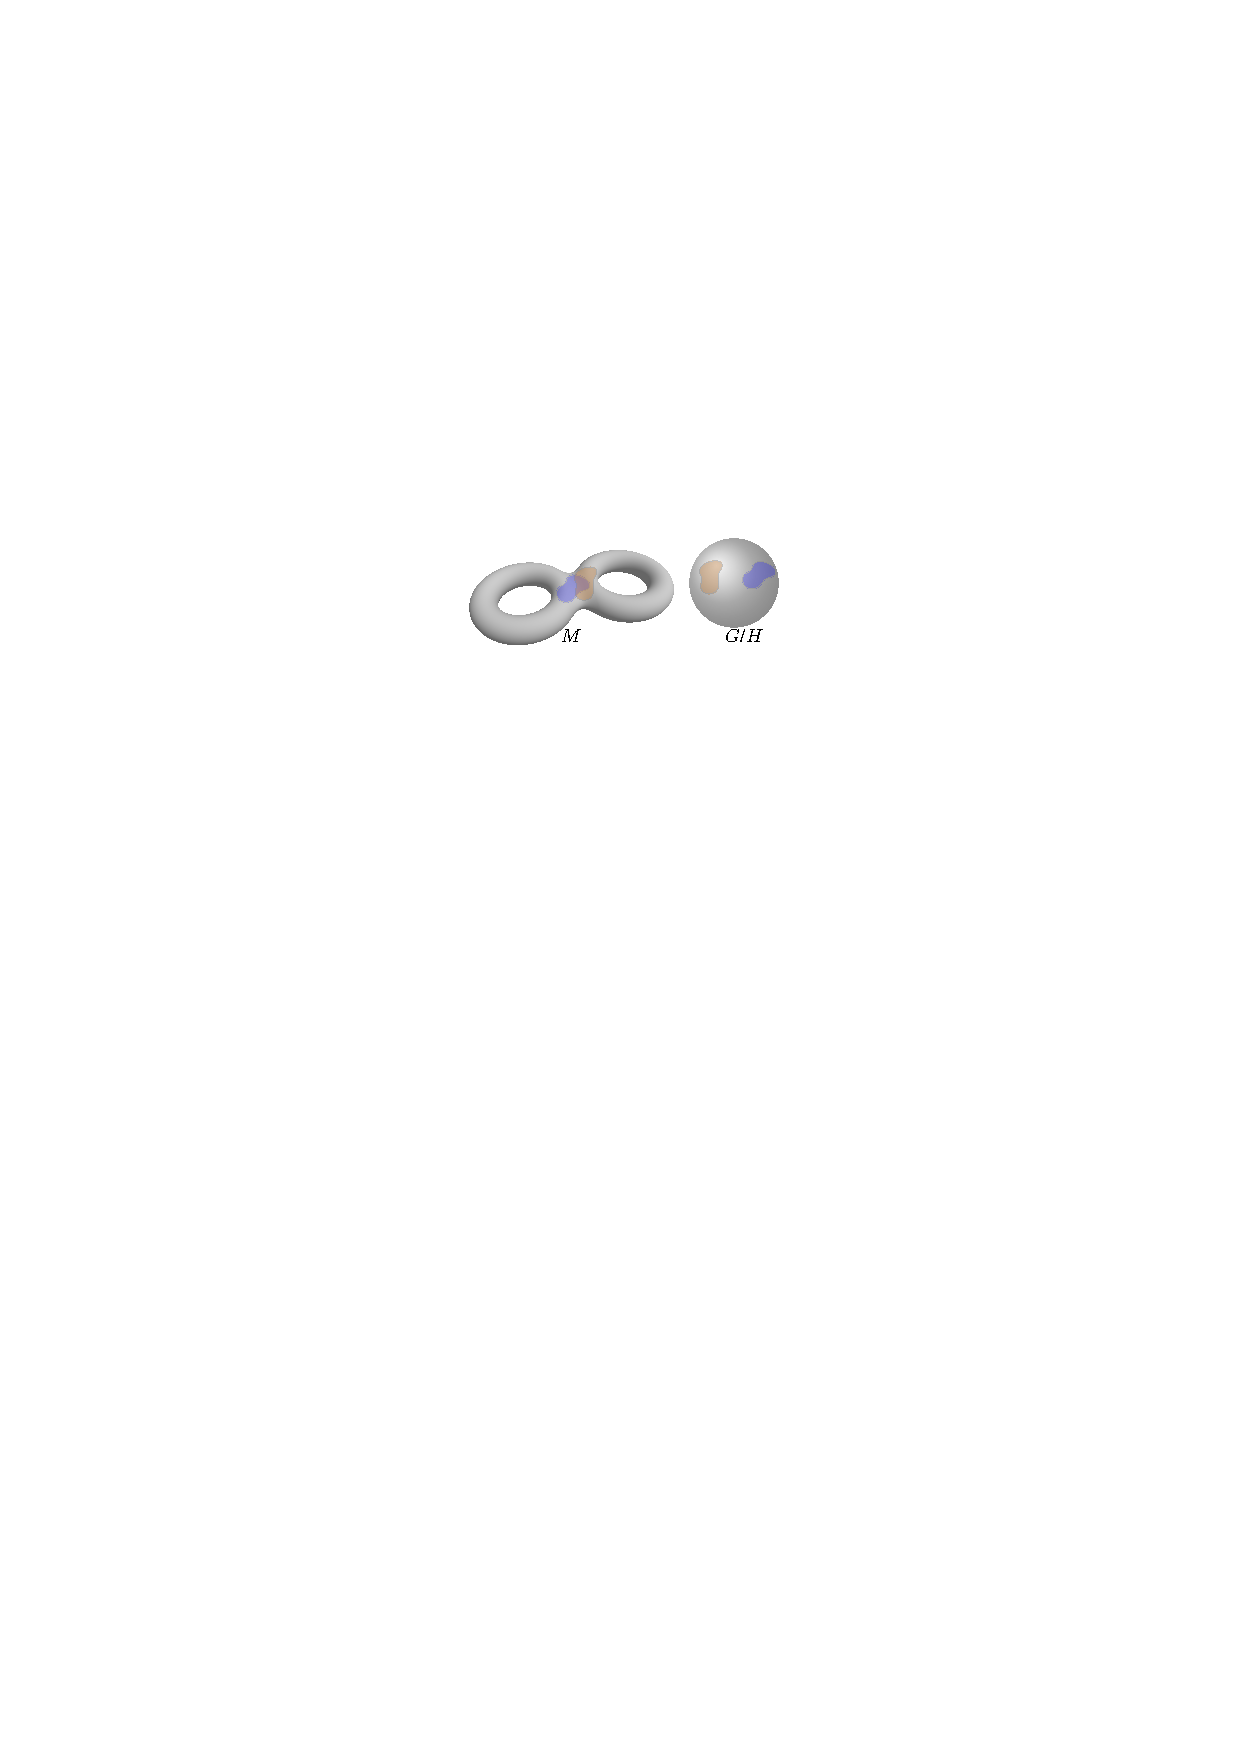
\includegraphics[scale=1.2]{figures/Klein.pdf}
    \caption{Effective locally Klein geometry.}
    \label{fig:klein}
\end{figure}

\begin{defn}[Effective $(G,H)$-structure]\label{def GH-structure}
    A locally homogeneous structure \emph{modeled on} an effective homogeneous space of type $(G,H)$ is a connected manifold $M$ with a \emph{$(G,H)$-atlas} $\{(U_\alpha,\varphi_\alpha)\}_\alpha$, where $\{U_\alpha\}$ is an open covering of $M$ and $\varphi_\alpha:U_\alpha\to \wh{U}_{\alpha}\subset G\slash H$ are diffeomorphisms such that for each non-empty intersection $U_{\alpha\beta}=U_\alpha\cap U_\beta$ there exists $g_{\beta\alpha}\in G$ such that 
    \[\varphi_{\beta}=\wh{\rmL}_{g_{\beta\alpha}}\circ \varphi_\alpha\text{ on }U_{\alpha\beta}.\]
    A \emph{$(G,H)$-structure} on $M$ is a maximal $(G,H)$-atlas $\calA$. The tuple $(M,\calA)$ is called a \emph{$(G,H)$-manifold}.
\end{defn}

\begin{rem}
    We could drop the effectiveness condition in the above definition, but then a $(G,H)$-structure is the same thing as an effective $(G/K,H/K)$-structure, where $K$ is the kernel of the Klein geometry $(G,H)$.
\end{rem}

For a deep exploration of many classical $(G,H)$-structures see the book \cite{Goldman}. We now show that this is indeed a special case of a locally Klein geometry, and that the two definitions of effective locally Klein geometries are equivalent. In light of this, the procedure of development becomes very intuitive: every local chart map is a local diffeomorphism into $G\slash H$, so by stitching them together we get a map from the universal cover to $G\slash H$.

\begin{prop}
    An effective $(G,H)$-structure on $M$ induces a natural locally Klein geometry on $M$.
\end{prop}
\begin{proof}
    Since $(G,H)$ is effective, $\varphi_\alpha=\varphi_\beta$ on overlaps $U_{\alpha\beta}$. Consider the pullback principal $H$-bundles $P_\alpha=\varphi_\alpha^\ast G$. Since the $\varphi_\alpha$ agree on overlaps, the $P_\alpha$ stitch together into a principal $H$-bundle $P\to M$. The Maurer-Cartan form $\theta_G$ also pulls back to a $1$-form $\eta\in\Omega^1(P;\frakg)$ that satisfies all necessary properties.
\end{proof}


We will discuss locally Klein geometries (more commonly known as flat Cartan geometries) in more detail, including many important examples, in \S\ref{sec: uniformization of cartan}. To wrap up this \sect, let us look at what kind of local differential forms can be defined on $M=\Gamma\bslash G\slash H$ using the Maurer-Cartan form. The following holds for Klein and locally Klein geometries.

\begin{prop}[{{\cite[Prop.~4.7.1]{Sharpe}}}]\label{prop 4.7.1 Sharpe}
    If $\chi:\pi^{-1}(U)\to U\times H$ is a local chart for the principal bundle $G\to G\slash H$ corresponding to the local section $ s:U\to G$. Then the local representative of the Maurer-Cartan form $\theta_G$ in this chart at point $(m,h)$ is $\Ad_h^{-1}\circ  s^\ast\theta_G +\pr_2^\ast\theta_H$, that is,
    \[(\chi^{-1})^\ast\theta_G(X_m,Y_h)=\Ad_h^{-1}\theta_G( s_\ast X_m)+\theta_H(Y_h),\quad X_m\in \T_mU,Y_h\in \T_h H.\]
\end{prop}
\begin{proof}
    We have $ s(m)=\chi^{-1}(m,e)$. Also let $i_h:U\to U\times H$ and $j_m:H\to U\times H$ be the inclusions of the slices $m\mapsto (m,h)$ and $h\mapsto (m,h)$, respectively. Then we have
    \[(\chi^{-1\ast}\theta_G)\circ i_{h\ast}=(\chi^{-1}\circ i_h)^\ast \theta_G=(\rmR_h s)^\ast \theta_G= s^\ast \rmR_h^\ast \theta_G= s^\ast(\Ad_h^{-1}\theta_G)=\Ad_h^{-1} s^\ast \theta_G,\]
    and on the other hand, 
    \[(\chi^{-1\ast}\theta_G)\circ j_{m\ast}=(\chi^{-1}\circ j_m)^\ast \theta_G=\rmL_{ s(m)}^\ast\restr{\theta_G}{\T_hH}=\restr{\theta_G}{\T_hH}=\theta_H.\]
\end{proof}

Let $ s_\alpha:U_\alpha\to G$ be a local gauge, that is, a local section of the principal $H$-bundle $G\to G\slash H$ over an open set $U_\alpha\subset G\slash H$. Then $ s_\alpha$ pulls back the Maurer-Cartan form $\theta_G$ to a $\frakg$-valued $1$-form $\theta_\alpha$ on $U_\alpha$: \[\theta_\alpha\coloneqq  s_\alpha^\ast\theta_G.\] 
The Maurer-Cartan equation for $\theta_G$ then yields the structure equation for $\theta_\alpha$:
\[\dd\theta_\alpha+\frac 12[\theta_\alpha,\theta_\alpha]=0.\]
Note that $\theta_\alpha$ \emph{almost} determines $ s_\alpha$ since the Fundamental Theorem~\ref{thm 6.1 Sharpe fundamental local} says that $\theta_\alpha$ determines $ s_\alpha$ up to left multiplication by a fixed element of $G$. Then, for an effective Klein geometry, if $ s$ is a section, then $g s$ is a section iff $g=e$, so in this case $ s_\alpha$ is recovered uniquely.\footnote{If $g s$ is a section, then $u=\pi(g s(u))$ and hence $g\cdot u=u$ for all $u\in U$. Thus $f^{-1}gf\in H$ for all $f\in\pi^{-1}(U)\subset G$. Thus shows that $\{f\in G\mid f^{-1}gf\in H\}$ contains an open subset of $G$. But it is also an analytic subset of $G$, so it must be equal to $G$, at least for connected $G$. Thus $g\in \bigcap_{f\in G}fHf^{-1}$, and this latter is a normal subgroup of $G$ inside $H$ and is therefore trivial.} 
For this reason we may refer to $\theta_\alpha$ as an \emph{infinitesimal gauge}. We have the non-canonical isomorphism at every $m\in U_\alpha$
\[\underline{\theta}_\alpha:\T_mU_\alpha\overset{\theta_\alpha}{\longrightarrow}\frakg\overset{\mod\frakh}{\longrightarrow} \frakg\slash\frakh.\]
The infinitesimal gauge $\theta_\alpha$ can be roughly interpreted as assigning to each tangent vector $X_m\in \T_mM$ an infinitesimal ``motion'' $\theta_\alpha(X_m)\in \frakg$ of $M$ whose Killing vector field at $m$ coincides with $X_m$.

By differentiating the transformation rule $ s_\beta(m)= s_\alpha(m)h_{\alpha\beta}(m)$ (cf.\ (\ref{eq transf rule for sections})) we get
\[ s_\beta^{\ast}\theta_G=\Ad_{h_{\alpha\beta}}^{-1} s_\alpha^\ast\theta_G+h_{\alpha\beta}^\ast\theta_H,\]
that is
\[\theta_\beta=\Ad_{h_{\alpha\beta}}^{-1}\theta_\alpha+h_{\alpha\beta}^\ast\theta_H.\]
This transformation is called an \emph{infinitesimal change of gauge}, and the two infinitesimal gauges are called gauge equivalent.

Since in the effective case the $\theta_\alpha$ let us recover the local sections $s_\alpha$ uniquely, one can give an alternative definition of effective locally Klein geometries in terms of a collection of local $1$-forms on $M$ satisfying the structure equation and the above transformation rule. Up to isomorphism, this allows one to reconstruct the principal bundle of the geometry. Completeness is a little more subtle, so we shall put off this view of locally Klein geometry and until our discussion of flat Cartan geometries in \S\ref{sec: uniformization of cartan}.

% \begin{defn}[Effective locally Klein geometry III]
%     An effective locally Klein geometry \emph{modeled on} an effective Klein geometry $(G,H)$ is a connected manifold $M$ with a collection $\{(U_\alpha,\theta_\alpha)\}_\alpha$, where $\{U_\alpha\}$  is an open covering of $M$ and each $\theta_\alpha\in \Omega^1(U_\alpha;\frakg)$ is a $\frakg$-valued local $1$-form that satisfies the structure equation 
%     \[\dd\theta_\alpha+\frac12 [\theta_\alpha,\theta_\alpha]=0,\]
%     and such that on every intersection $U_{\alpha\beta}$ there exists a smooth function $h_{\alpha\beta}:U_{\alpha\beta}\to G$ such that 
%     \[\theta_\beta=\Ad_{h_{\alpha\beta}}^{-1}\theta_\alpha+{h_{\alpha\beta}}^\ast\theta_H.\]
% \end{defn}




% \begin{example}[Meteor tracking]
%     Suppose we live in a small open set $U\subset M=G\slash H$ and a meteor flashes through $U$. We wish to describe its motion. We formalize the meteor as a point set $X$, and a \emph{configuration} of the meteor is a map $X_0:X\to M$. This is the origin for Cartan's idea of a ``moving frame''.\index{Moving frames}
    
%     We assume the meteor is \emph{rigid} and \emph{sufficiently complicated}. By the term rigid in the given geometry, we mean that for any two of its positions, where it has the configurations $X_0$ and $X_1$ say, there is an element of $G$ carrying $X_0$ to $X_1$. By sufficiently complicated we mean that the subgroup of $G$ that fixes the body pointwise (its stabilizer) is the identity.  It follows that if $X(t)$ is the configuration of its points at time $t$, then there is a unique path $g(t)\in G$ such that $X(t)=g(t)X(0)$. One way to describe the motion would be to specify the path $g(t)$ itself. However, it is more useful, and closer to what is actually observed, to describe the motion differently. We first describe the motion of one of its points $q\in X(0)$, which we take to be $eH$, by a path $q(t)=g(t)H$ on $U$, and then describe the motion of the rest of the body as turning about this one point as it moves along. For this we will need the concept of a gauge.

%     Let us assume that $U$ is small enough to admit a local section $s:U\to G$. Any two such sections $s,s'$ are related by a map $h:U\to H$ by $s'(u)=s(u)h(u)$. A ``choice of gauge'' is a choice of such a local section, and $h(u)$ is called a gauge transformation. A choice of gauge can be regarded as a choice of motions, varying smoothly with $u$, which maps the base point to $u$. The value of a gauge at any point may be called a \emph{frame} at that point and the gauge itself may be called a \emph{moving frame}. From this point of view the principal bundle $G\to G\slash H$ is a bundle of frames.

%     Since both $s(q(t))$ and $g(t)$ lie over $q(t)$, they must differ by an element $k(t)\in H$. Thus, in the presence of a gauge, the motion can be described by giving $q(t)$ and $(k(t)$. The latter describes the way the meteor turns about the point $q(t)$. Crucially, there is no intrinsic geometric meaning attached to the choice of gauge $s$, or the function $k(t)$ alone. Together, however, they complete the description of the motion.
% \end{example}


\begin{example}
    Recall the \emph{hyperbolic upper half-plane} $\bbC^+=\SL_2(\bbR)\slash \SO_2$ from Example~\ref{ex siegel upper half-space}. The Uniformization Theorem of Riemann Surfaces states that any closed (compact with no boundary) orientable \emph{simply connected} surface with its conformal/projective/complex structures is isomorphic to one of three: the Riemann sphere $\CP^1$, the plane $\bbC$, or the upper half-plane $\bbC^+$.

    In the case of $\CP^1$, it is not the covering space of anything else, so every genus $0$ surface is isomorphic to $\CP^1$. In the case of $\bbC$, every properly discontinuous action is determined by a lattice $\Lambda\subset \bbC$, so the quotient $\bbC\slash\Lambda$ has genus $1$, and thus every Riemann surface of genus $1$ is isomorphic to such a quotient. Finally, any oriented surface $\Sigma_g$ of genus $g>1$ is isomorphic to $\Gamma\bslash \bbC^+$ for some choice of discrete subgroup $\Gamma<\SL_2(\bbR)$. Let $\Gamma_g$ be such a subgroup. Then $\Sigma_g\cong \Gamma_g\bslash \bbC^+$ is a locally Klein geometry.
\end{example}

The Uniformization Theorem of Riemann Surfaces itself can be proven by reduction to the Uniformization Theorem of flat Cartan geometries, but the hard part is in fully demonstrating that every Riemann surface carries a \emph{complete} holomorphic projective connection (every such connection is automatically flat because the space is $1$-dimensional). 

\begin{example}[Moduli spaces of algebraic curves]
    An \emph{elliptic curve} is a Riemann surface $\Sigma$ of genus $1$. Per the preceding example, $\Sigma\cong \bbC\slash\Lambda$ for some lattice $\Lambda\subset\bbC$, hence $\Sigma$ is a homogeneous space. Any biholomorphism between elliptic curves arises from a complex affine linear map $\bbC\to\bbC$ matching lattices. We can always arrange by isomorphism that $\Lambda$ is generated by $1,\tau$ for some $\tau\in \bbC^+$. But then $\tau$ is only determined up to \glspl{flt} of $\bbC^+$ with integer coefficients (so that $1$ is a fixed point). Hence, the ``coarse moduli space'' of elliptic curves is a complete Klein manifold $\Gamma\bslash \bbC^+$, where $\Gamma\cong \SL_2(\bbZ)$ is the set of \glspl{flt} with integer coefficients. Similarly, the coarse moduli space of compact Riemann surfaces of genus $g$ is a complete Klein manifold $\Sp_{2g}(\bbZ) \bslash \calH_g$ where $\calH_g$ is the complex hyperbolic space of complex dimension $g(g+1)$ (cf.~\ref{ex siegel upper half-space}).
\end{example}


\begin{example}[Affine elliptic curves]
    Every elliptic curve $E=\bbC\slash\Lambda$ has a complex affine structure, i.e., $G=\bbC^\times\ltimes\bbC$ and $H=\bbC^\times$. The developing map is the identity $\dev^0=\id_\bbC$ and the holonomy homomorphism is 
    \[\hol^0:\Lambda\to G,\quad \lambda\mapsto (1,\lambda).\]
    There are other affine structures on $E$. For every $c\in \bbC^\times$, we can produce an affine structure on $E$ via the developing map $\dev^c:\bbC\to \bbC^\times,$ $z\mapsto \rme^{cz}$, with holonomy morphism 
    \[\hol^c:\Lambda\to G,\quad \lambda\mapsto (\rme^{c\lambda},0).\]
    Since the developing map of an affine structure is unique up to affine transformations, we could just as well use the map $z\mapsto c^{-1}(\rme^{cz}-1)$, which lets us think of $\dev=\id_\bbC$ as the limiting case $c\mapsto 0$.  To forget the chose of affine coordinate $z$, we can identify the moduli space of affine structures on an elliptic curve $E$ with the space of holomorphic $1$-forms on $E$: each $1$-form is expressed in terms of an affine chart as $c\dd z$. The developing map $\dev^c$ is a map to the \emph{linear} geometry on $\bbC\setminus\{0\}$, i.e., $(G',H')=(\bbC^\times,\{e\})$.  The holomorphic $1$-form $\dd\zeta/\zeta$ on $\bbC\setminus\{0\}$, with the standard coordinate $\zeta$, is $G'$-invariant, and pulls back to $c\dd z$ on $\bbC$. Hence, we identify the isomorphism class of the affine structure with this induced holomorphic $1$-form, and take the zero $1$-form as the limit $c\to 0$.  It is well known that every holomorphic affine structure arises uniquely this way. The automorphism group of the affine structure with $c=0$, the one with linear developing map, is the biholomorphism group of the elliptic curve (which is a semidirect product of the translation group $\bbC$ with a finite group of at most $24$ elements). The automorphism group of any of the affine structures with $c\neq 0$ is only the group $\bbC$ of translations.
\end{example}

\begin{example}[Projective structures on Riemann surfaces]\index{Projective structure}\label{ex projective structure}
    A \emph{Riemann surface}\index{Riemann surface}, also called a \emph{complex curve}, is a connected $1$-dimensional complex manifold $\Sigma$, i.e., its atlas consists of $\bbC$-valued maps with complex analytic, or holomorphic, transition maps (in the $1$-dimensional case holomorphic maps are also called conformal, although the equivalence between these terms is nontrivial, cf.\ Remark~\ref{rem holomorphic functions}). Thus, the inverses of the transition maps are also complex analytic, so that the transition maps are \emph{biholomorphic}.\index{Biholomorphism} Now, a \emph{projective structure} $\calP$ on $\Sigma$ is a $(\PSL_2(\bbC),\U_1)$-structure in the sense of Definition\ \ref{def GH-structure}. In particular, the chart maps are \emph{meromorphic} biholomorphisms, i.e., they take values in $\CP^1$ instead of just $\bbC$ (so they are allowed to have simple poles). The pair $(\Sigma,\calP)$ is called a \emph{complex projective surface}.
    
    Every Riemann surface admits many non-equivalent projective structures, but the Uniformization Theorem (stating that there is a unique, up to a \gls{flt}, biholomorphism between the universal cover of $\Sigma$ and one of three standard subsets of $\CP^1$) implies the existence of a \emph{canonical projective structure}.
    Moreover, every affine structure induces a projective structure via the obvious inclusion $\bbC\cong \CP^1\setminus \{\infty\}\to \CP^1$. Among the various affine structures on elliptic curves given above, each induces a distinct projective structure, except for pairs $\{c,-c\}$, which are clearly related by a \gls{flt}, $\rme^{-cz}=\frac{1}{\rme^{cz}}$. It turns out that these are all of the projective structures on $E$: we can identify the moduli space of projective structure on any elliptic curve with the space of quadratic differentials $c^2\dd z^{\otimes 2}$, as we will see. For $c\neq 0$, the developing map is $z\mapsto \rme^{cz}\in \CP^1$ and the holonomy homomorphism is 
    \[\hol^c:\lambda \mapsto \begin{bmatrix}
        \rme^{c\lambda/2} & 0\\
        0 & \rme^{-c\lambda/2}
    \end{bmatrix}\in G.\]
    For $c=0$, the developing map is the inclusion map $\bbC\to \CP^1$ and the holonomy morphism is 
    \[\hol^0:\lambda\to \begin{bmatrix}
        1 & \lambda \\ 0 & 1
    \end{bmatrix}\in G.\]
    The automorphism group of the projective structure at $c=0$ is still the biholomorphism group of the curve. At $c\neq 0$, the automorphism group is $\bbZ_2\ltimes\bbC$, where $\bbZ_2$ acts on $\bbC\slash\Lambda$ by $z\mapsto -z$ and $\bbC$ acts by translations.

    Clearly, $\CP^1$ has an obvious projective structure, being the model geometry. The developing map and the holonomy homomorphism are trivial and the biholomorphism group is $G=\PSL_2(\bbC)$.
\end{example}


\begin{example}[Monopole bundles]\label{ex monopole bundles}\index{Monopole!bundles}\index{Hopf fibration}
    Consider the Hopf bundle $\bbS^3\to \bbS^2$ defined as a $\U_1$-principal bundle, or as a Klein geometry of type $(\SU_2,\U_1)$. Let $m\geq 1$ and $\Gamma=\bbZ_m\subset \U_1$ act on $\bbS^3$ by the restriction of the $\U_1$ action. The space $\Gamma\bslash \bbS^3$ is the loop space $L(m;1)$. We get the principal $\U_1$-bundle
    \[L(m;1)\to L(m;1)\slash \U_1=\bbS^2\]
    (since the induced action of $\U_1$ on $L(m;1)$ is trivial).
    Note that the structure groups here are abelian so right and left actions are indistinguishable.
    
    In the standard atlas consisting of two hemispheres (Example~\ref{ex hopf bundle atlas}), the transition function of this new bundle is $\tau_{-+}(z)=z^{-m}$, i.e., this is exactly the $\U_1$-bundle with Chern number $-m$ from Example~\ref{ex circle bundles over S2}. This proves that the lens space is simultaneously $\bbS^3\slash \bbZ_m$ and the gluing of two solid tori, thus solving Exercise~\ref{xca two definitions of lens spaces}. As principal $\U_1$-bundles, these bundles are known as \emph{monopole bundles}.

    We thus have the surjective vertical morphism of principal bundles $\vartheta:\bbS^3\to L(m;1)$ given by the quotient by the $\bbZ_m$-action and the group homomorphism $\lambda:\U_1\to \U_1$ given by the $m$-fold covering of the circle. Note that these bundles are also defined for $m$ negative as the duals (inverse transition functions), or via the inverse $\U_1$-action on $\bbS^3$.
\end{example}

\begin{example}
    In many cases of interest, a $(G,H)$-structure on $M$ is equivalent to the specification of a $G$-invariant geometric object on $G\slash H$. The most prominent example is a locally homogeneous Riemannian metric. For example, if $X$ is a simply connected Riemannian manifold of constant curvature $K$ and $G$ is its group of isometries with stabilizer $H$, then locally modeling $M$ on $X\cong G\slash H$ is equivalent to giving $M$ a metric of constant curvature $K$.
\end{example}







\section{Morphisms}\label{sec: morphisms of klein geom}

In this \sect\ we discuss changing the models of $(G,H)$-structures via morphisms.

\begin{defn}[Morphism of Klein geometries]
    If $(G,H)$ and $(G',H')$ are two Klein geometries, then a morphism between them is a Lie group homomorphism $\lambda:G\to G'$ such that $\lambda(H)\subset H'$. Equivalently, it is a morphism of the principal bundles $G\to G\slash H$ and $G'\to G'\slash H'$ which is $G$-equivariant via the homomorphism $\lambda$, or whose base map $\underline{\lambda}:G\slash H\to G'\slash H'$ is $G$-equivariant: $\underline{\lambda}([g])=\wh{\rmL}_{\lambda(g)}([e])$.
\end{defn}

\begin{example}
    The double cover $\bbS^n\to \RP^n$ can be realized as a morphism of two Klein geometries $(G,H)\to (G',H')$, where $G$ is the subgroup of $\GL_{n+1}(\bbR)$ consisting of matrices with determinant $\pm 1$, and $G'=\PGL_{n+1}(\bbR)=G\slash \{\pm \rmI\}$. Then $\bbS^n\to \RP^n$ is $G$-equivariant with $\lambda(g)=g/\det g$.
\end{example}

Given a manifold $M$ with a $(G,H)$-structure (with its principal $H$-bundle $P\to M$) and a morphism $\lambda:(G,H)\to (G',H')$ of models, we can induce a $(G',H')$-structure by composing the charts with the $G$-equivariant base map $\underline{\lambda}$. This also gives the new $H'$-bundle $P'\to M$.

Conversely, given a $(G',H')$-structure $(P'\to M,\eta)$, it is interesting to ask whether it is induced from a $(G,H)$-structure $(P\to M,\eta)$. Factoring $(G,H)\to (G',H')$ into two maps 
\[(G,H)\to (\lambda(G),\lambda(H))\to (G',H'),\]
we are able to split the question into two separate problems, where the morphism is surjective in one and injective in the other.

First consider surjective morphisms. First, to be able to reconstruct a $\frakg$-valued form from a $\frakg'$-valued one, we clearly need $\lambda:G\to G'$ to be a covering homomorphism. Then $H\to \lambda(H)$ is also a covering map. If the bundle $P'\to M$ is associated to some smooth principal $H$-bundle $P\to M$ via (the restriction of) a homomorphism $\lambda:G\to G'$ and if $\lambda_{\ast e}:\frakg\to \frakg'$ is an isomorphism, we just let 
\[\eta\coloneqq \lambda^{-1}_{\ast e}\circ \iota_e^\ast \eta',\] where $\iota_e:P\to P'$, $p\mapsto [(p,e)]$, is the canonical covering map. This induces a $(G,H)$-structure on $P\to M$. 

\begin{example}
    \begin{enumerate}
        \item Consider the trivial double cover $(\Aff_n(\bbR),\GL_n(\bbR))\to (\Aff_n^+(\bbR),\GL_n^+(\bbR))$. Thus, any oriented affine manifold can be turned into a regular affine manifold (e.g., by adding reflected chart maps to the atlas).
        \item Consider the nontrivial double cover $(\Spin_n\ltimes\bbR^n,\Spin_n)\to (\SE_n,\SO_n)$. Thus, assuming we are given a corresponding covering bundle morphism $P\to P'$, then we can reconstruct the affine spin structure from the affine Riemannian structure. The assumption of the existence of a covering spin bundle here is crucial because not every Riemannian structure admits one, or may admit multiple.
    \end{enumerate}
\end{example}

In the injective case, not every structure on $P'$ is induced from one on $P$, so this case will be treated via holonomy in Theorem~\ref{thm 16.30 McKay} below.

\begin{example}
    \begin{enumerate}
        \item If $M=\bbS^1$, then (by picking an arbitrary connection) all bundles over $M$ are quotients of the form $P=(\bbR\times H)\slash \sim$, where $(x,h)\sim (x+1,h_0h)$ with $h_0$ (the generator of monodromy) determined up to conjugacy. So every element of $H'$ is conjugate to an element of the image $\lambda(H)\subset H'$ iff all $H'$-bundles arise from $H$-bundles.
        \item If $M$ is contractible, then every $(G',H')$-structure on it lifts to a $(G,H)$-structure since all bundles over $M$ are trivial.
        \item If $M=\bbS^n$, it has a covering by two open sets whose intersection deformation retracts to the equator. So if the induced homomorphism of homotopy groups $\pi_{n-1}(H)\to \pi_{n-1}(H')$ is surjective, we can lift every $H'$-bundle on $\bbS^n$ to an $H$-bundle.
    \end{enumerate}
\end{example}

We return to the problem of how a Klein geometry (i.e., its principal bundle and Maurer-Cartan form) changes under morphisms. We will describe the new principal bundle $P'$ and its associated form $\eta'$ in a language more suited to our ultimate study of Cartan geometries.

\begin{lem}[{{\cite[Lem.~13.2]{McKayCartan}}}]\label{lem 13.2 McKay}
    Let $\lambda:(G,H)\to (G',H')$ be a morphism of Klein geometries (or homogeneous spaces). Denote $M\coloneqq G\slash H$ and $M'\coloneqq G'\slash H'$. Also denote $H''\coloneqq \lambda^{-1}(H')\subset H$ and $M''\coloneqq \underline{\lambda}(M)\subset M'$. Then $G\to M''$ is a principal $H''$-bundle and induces the pullback bundle $G_{H'}=\restr{G'}{M''}\to M''$. 
    
    In more detail, define $\psi:G\times H'\to G'$ by $\psi(g,h')=\lambda(g)h'$. Then, at any point $(g,h')\in G\times H'$, 
    \[\psi^\ast\theta_{G'}=\theta_{H'}+\Ad_{h'}^{-1}\circ\lambda_{\ast e}\circ \theta_G.\] 
    The map $\psi$ is a surjective $H''$-bundle map to $\restr{G'}{M''}$ under the right $H''$-action $(g,h')\cdot h\coloneqq (gh,\lambda(h)^{-1}h')$, $H'$-equivariant under the right $H'$-action $(g,h')\cdot k'\coloneqq (g,h'k')$, and $G$-equivariant under the left $G$-action $a(g,h')\coloneqq (ag,h')$. Quotienting by that right $H''$-action gives an $H'$-bundle isomorphism 
    \[\begin{tikzcd}
        G_{H'}=G\times^{H''}H'\arrow[rr,"\cong"]\arrow[dr] & & \restr{G'}{M''}\arrow[dl]\\
        & M''. &
    \end{tikzcd}\]
\end{lem}
\begin{proof}
    The map $\psi$ is clearly invariant and equivariant in the three stated ways, therefore it descends as stated to a map $G\times^{H''} H'\to G'$. Its image is clearly the pullback $\restr{G'}{M''}$ of $G'\to M'$ to $M''\subset M'$. By $G$-equivariance, $M''$ is a $G$-orbit in $M'$, so a smooth manifold. Two elements $(g,h)$, $(\wt g,\wt h)\in G\times H'$ map to the same point $g'\in G'$ iff $\lambda(g)h=\lambda(\wt g)\wt h$, i.e., $\lambda(g^{-1}\wt g)=h\wt{h}^{-1}$, so $\wt{g}=gk\in \lambda^{-1}(H')=H''$ and $\lambda(k)=h\wt{h}^{-1}$ so $\wt{h}=\lambda(k)^{-1}h$. So the map $\psi$ descends to an injection $G\times^{H''}H'\hookrightarrow G'$. 

    The subgroup $H''=\lambda^{-1}(H')$ is a closed Lie subgroup since $H'\emb G'$ is closed. Hence, it acts on $G$ freely and properly, hence acts on $G\times H'$ freely and properly, so the quotient is a smooth manifold and $G\times H\to G\times^{H''}H'$ is a smooth principal $H''$-bundle, and the map to $G'$ is smooth. The left $G$-action and right $H'$-action on $G\times H'$ are smooth, and invariant under the right $H''$-action, so descend to smooth $\psi$-equivariant actions on the quotient.

    Thus, $G\times^{H''}H'\to \restr{G'}{M''}$ is an equivariant bijection of homogeneous spaces of $G\times H'$, hence a diffeomorphism, and a bundle isomorphism over $M'$ by equivariance. The formula relating the Maurer-Cartan forms is just the differential-geometric version of the matrix identity 
    \[(gh')^{-1}\dd (gh')=(h')^{-1}g^{-1}(g\dd h'+\dd g \cdot h')=(h')^{-1}\dd h'+(h')^{-1}(g^{-1}\dd g)h'.\]
\end{proof}

\begin{cor}
    In the setting of the preceding lemma, let $\underline{\lambda}:G\slash H\to G'\slash H'$ be a local diffeomorphism. Let $(P\to M,\eta)$ be a locally Klein geometry of type $(G,H)$. Then the  geometry of type $(G',H')$ associated to this one via the morphism $\lambda$ has bundle $P'=P\times^{H''}H'$ and its form $\eta'$ pulls back to $P\times H'$ to become (omitting obvious pullbacks)
    \[\eta'=\theta_{H'}+\Ad_{h'}^{-1}\circ\lambda_{\ast e}\circ\eta.\]
\end{cor}
\begin{proof}
    From the preceding lemma, this holds on each of the $H$-invariant open sets in $P$ which are identified by the local bundle charts with $H$-invariant open subsets of $G$. By $G$-equivariance, this description glues together under the transition maps to cover all of $P$ and $P'$.
\end{proof}







\section{Homogeneous bundles}\label{sec: homogeneous bundles}


We now consider the tangent bundle of a Klein geometry. Since it is a locally trivial principal bundle, we have local diffeomorphisms of the form $\T(\pi^{-1}(U))\cong \T(U\times H)\to \T U\times \T H$. Local trivializations of $\T U$ and $\T H$ are given by the Maurer-Cartan forms $\theta_G$ and $\theta_H$, respectively, so the diagram
\[
\begin{tikzcd}
    \T_g(gH)\arrow[r]\arrow[d,"\theta_H","\cong"'] & \T_g G\arrow[r]\arrow[d,"\theta_G","\cong"'] & \T_{m}(G\slash H)\arrow[d,dashed,"\chi_g","\cong"'] \\
    \frakh\arrow[r,hookrightarrow]&\frakg \arrow[r] & \frakg\slash \frakh
\end{tikzcd}
\]
is commutative with exact rows. Since $\frakh$  us only a subalgebra (not an ideal), the quotient $\frakg\slash\frakh$ is merely a vector space. The linear isomorphism $\chi_g$ is the unique map making the diagram commute.

We can identify the tangent space of $G\slash H$ at $m$ with $\frakg\slash\frakh$, but the identification $\chi_g$ depends on the choice of $g\in G$ over $m$. In fact, since $\pi\circ \rmR_h=\pi$, the relation $\rmR_h^\ast \theta_H=\Ad_h^{-1}\theta_H$ implies that $\chi_{gh}=\Ad_h^{-1}\circ \chi_g$. It follows that the identification of $\T_m(G\slash H)$ with $\frakg\slash \frakh$ is determined only up to the adjoint action of $H$ on $\frakg\slash\frakh$. This accounts for the frequent occurrence of the adjoint action in the sequel. 

\begin{prop}[{{\cite[Prop.~4.5.1]{Sharpe}}}]\label{prop 4.5.1 Sharpe}
    $\T(G\slash H)\cong G\times^H \frakg\slash\frakh$ as \glspl{vb} over $G\slash H$.
\end{prop}
\begin{proof}
    Define a map $\varphi:G\times \frakg\to \T(G\slash H)$ by $\varphi(g, X)=(\pi(g),\pi_\ast \circ \rmL_{g\ast}X)$, where $\pi:G\to G\slash H$ is the canonical projection. Clearly $\varphi$ is smooth, surjective, and fiberwise linear. Moreover, for $X\in \T_eH$, $\rmL_{g\ast}X\in \T_g(gH)\in\ker\pi_\ast$. Thus, $\varphi(g, X)=(g,0)$. On the other hand,
    \begin{multline}
        \varphi(gh,\Ad_h^{-1}X)=(\pi(gh),\pi_\ast \rmL_{gh\ast}\Ad_h^{-1}X)=(\pi(g),\pi_\ast(\rmL_{gh\ast}\rmL_{h\ast}^{-1} \rmR_{h\ast}X))=\\
        =(\pi(g),\rmL_{g\ast }\pi_\ast (\rmR_{h\ast}X))=(\pi(g),\rmL_{g\ast}(\pi \rmR_h)_\ast X)
        =(\pi(g),\rmL_{g\ast}(\pi_\ast X))=\varphi(g,X).
    \end{multline}
    Thus $\varphi$ induces a smooth quotient map $\wb\varphi:G\times^H \frakg\slash\frakh\to \T(G\slash H)$. Moreover, this map is injective since $\varphi(g,X)=\varphi(g',X')$ implies $g'=gh$ for some $h\in H$ and $\pi_\ast \rmL_{gh\ast}X'=\pi_\ast \rmL_{g\ast}X$. The latter means that $\pi_\ast \rmL_{h\ast}X'=\pi_\ast X$ and hence that $X'-\Ad_h^{-1}X\in\frakh$. Thus,
    \[[(g',X')]=[(gh,\Ad_h^{-1}X+\frakh)]=[(g,X+\frakh)]\in G\times^H\frakg\slash\frakh.\]
    Thus $\wb\varphi$ is a vertical \gls{vb} isomorphism.
\end{proof}


\begin{example}
    \begin{enumerate}
        \item Taking $\bbS^n=\SO_{n+1}\slash \SO_n$, we get the identification $\T\bbS^n\cong \SO_{n+1}\times^{\SO_n}\bbR^n$, where $\bbR^n$ is the standard (defining) representation of $\SO_n$.
        \item Since the Grassmannian manifolds can be written as $\Gr_k(\bbK^n)\cong \calO_n\slash (\calO_{n-k}\times \calO_{k})$, by comparing transition functions it is easy to see that $\T\Gr_k(\bbK^n)\cong \Hom(\gamma_k(\bbK^n),\gamma_k(\bbK^n)^\perp)$, where $\gamma_k(\bbK^n)$ is the tautological bundle over $\Gr_k(\bbK^n)$ and $\gamma_k(\bbK^n)^\perp$ is its orthogonal complement in $\Gr_k(\bbK^n)\times \bbK^n$.
    \end{enumerate}
\end{example}


Note that the basepoint $[e]=H\in G\slash H$ is preserved by the left action of $H$ via $\wh{\rmL}_h$, $h\in H$, thus it generates an isotropy representation of $H$, which we specify in the following definition.

\begin{defn}[Isotropy representation]
    For a Klein geometry $(G,H)$, identify $\T_{[e]}(G\slash H)$ with $\frakg\slash\frakh$ using the natural isomorphism constructed above. We call the induced representation $\underline{\Ad}:H\to \GL(\frakg\slash\frakh)$ given by $h\mapsto \wh{\rmL}_{h\ast [e]}$, the isotropy representation of the Klein geometry.

    Since $\frakh<\frakg$ is invariant under $\Ad(H)$, the restriction of the adjoint representation to $H$, $\restr{\Ad}{H}:G\to \GL(\frakg)$, which descends to a map $H\to \GL(\frakg\slash h)$, which coincides with $\underline{\Ad}$.
\end{defn}

Since tangent bundles involve only first derivatives, we can make the following rough division of Klein geometries into two types according to whether $H$ is faithfully represented by this action.

\begin{defn}[First order Klein geometry]
    A Klein geometry $(G,H)$ is of first order if the isotropy representation $\underline{\Ad}:H\to \GL(\frakg\slash\frakh)$ is faithful. Otherwise, the geometry is said to have \emph{higher order}.
\end{defn}

\begin{rem}
    First order Klein geometries have a simple intuitive description in terms of $H$-structures. Since $H$ is faithfully represented on $\frakg\slash\frakh$, via the global trivialization of $\T M$ constructed above, it traces out an $H$-orbit in the set of linear frames mapping $\T_mM\to \frakg\slash\frakh$ for each $m\in M$. This was exactly our original definition of an $H$-structure on $\T M$. Equivalently, this describes the principal bundle $G\to M$ as a reduction of the frame bundle $\Fr(\T M)$ to structure group $H$.
\end{rem}

The tangent bundle of a Klein geometry is an example of an important class of bundles that are equivariant w.r.t.\ the natural $G$-action $\wh L$ on the base $G\slash H$ in the following sense.


\begin{defn}[Homogeneous bundle]
    Let $G$ be a Lie group and $H\emb G$ a closed subgroup. A (left) homogeneous, or \emph{equivariant}, \gls{fb} of type $(G,H)$ is a \gls{fb} $E\overset{\pi}{\to}G\slash H$ over the homogeneous space of (left) cosets $G\slash H$ together with a (left) action $G\overset{\wt L}{\acts} E$ that lifts the natural (left) action $\wh L$ on $G\slash H$, i.e., which satisfies \[\pi\circ \wt{L}_g=\wh{\rmL}_g\circ \pi,\text{ for all } g\in G.\] 

    In particular, a homogeneous \gls{vb} is a \gls{vb} which is also a homogeneous \gls{fb} such that the $G$-action is by \gls{vb} morphisms. Similarly, a homogeneous \gls{pfb} is a \gls{pfb} which is also a homogeneous \gls{fb} such that the $G$-action is by \gls{pfb} morphisms, i.e., by maps equivariant w.r.t.\ the (right) action of the structure group.

    A morphism of homogeneous bundles over $G\slash H$ is a vertical $G$-equivariant bundle morphism. The categories of homogeneous \glspl{fb} and \glspl{vb} are denoted $\FB_{(G,H)}$ and $\VB_{(G,H)}$, respectively. 
\end{defn}

\begin{example}
    The principal $H$-bundle $G\to G\slash H$ is obviously homogeneous because the left action $\rmL$ is a lift of $\wh \rmL$.
\end{example}

One common way of producing homogeneous bundles is by applying a natural bundle functor $F$ to $G\slash H$. Since by definition such a functor maps local diffeomorphisms to bundle morphisms, $F(\wh{\rmL}_g)$ is a $G$-action as required in the definition of a homogeneous bundle. Thus, any natural bundle over a homogeneous space is homogeneous. As we will see below, the tangent bundle functor $T$ that we considered in the previous section is an example of this.

Let $E\to G\slash H$ be a homogeneous bundle. Consider the basepoint $[e]=eH\in G\slash H$ and the fiber $E_{[e]}$. The $G$-action on $E$ restricts to an $H$-action on $F$, thus we can build the associated bundle $G\times^H E_{[e]}\to G\slash H$. We now show that this bundle is isomorphic to $E$, thus characterizing all homogeneous bundles as bundles associated to principal bundles of the form $G\to G\slash H$.

\begin{thm}[{{\cite[Prop.~1.4.3]{Cap}}}]\label{prop 1.4.3 Cap}
    The mapping $E\to E_{[e]}$ (and restrictions of morphisms to the fiber) induces equivalences of categories $\FB(G,H)\simeq H\mathsf{-Man}$ and $\VB(G,H)\simeq H\mathsf{-FinVect}$, where $H\mathsf{-FinVect}$ is the category of finite-dimensional representations of $H$.
\end{thm}
\begin{proof}
    Consider the map $G\times E_{[e]}\to E$ given by $(g,f)\mapsto g\times f$, where we use the action of $G$ on $E$. Since the action $H\acts E_{[e]}$ is simply a restriction of this action, this map descends to a map $\varphi:G\times^H E_{[e]}\to E$ which is smooth since the projection $G\times E_{[e]}\to G\times^H E_{[e]}$ is a surjective submersion. Moreover, the definition $\varphi=g\cdot f$ implies that $\varphi$ covers the identity and is also right $G$-equivariant, so it is a morphism of homogeneous bundles.

    Now we build the inverse morphism. If $p\in E$, then by transitivity there exists a $g\in G$ such that $g\cdot \pi_E(p)=[e]$. Then $\pi_E(g\cdot p)=[e]$, so $g\cdot p\in E_{[e]}$, and we may consider $[(g^{-1},g\cdot p)]\in G\times^H E_{[e]}$. This is independent of the choice of $g$, since for another choice $g'\in G$ we must have $(g'g^{-1})\cdot p=p$, thus $g'g^{-1}\in H$, and thus
    \[[(g^{\prime-1},g'\cdot p)]=[(g^{\prime-1}g'g^{-1},gg^{\prime-1}g'\cdot p)]=[(g^{-1},g\cdot p)].\]
    Thus we get a well-defined map $\psi:E\to G\times^H E_{[e]}$. Choosing a local smooth section $s$ of $G\to G\slash H$ we can locally write $\psi(p)=[(s(\pi_e(p))^{-1},s(\pi_E(p))\cdot p)]$, which shows that $\psi$ is smooth. One immediately verifies that $\psi$ and $\varphi$ are mutually inverse bundle isomorphisms.

    To verify functoriality, if $\vartheta:E\to E'$ is a morphism of homogeneous bundles, then $\vartheta(E_{[e]})\subset E_{[e]}'$ and the restriction $\restr{\vartheta}{E_{[e]}}:E_{[e]}\to E_{[e]}'$ is $H$-equivariant. Equivariance of $\vartheta$ implies that for $g\in G$ and $f\in E_{[e]}$, we get $\vartheta(g\cdot f)=g\cdot \vartheta(f)$ which means that $\vartheta(\varphi([(g,f)]))=\varphi'([(g,\restr{\vartheta}{E_{[e]}}(f))])$, so we see that identifying $E$ and $E'$ with $G\times^H E_{[e]}$, respectively, $G\times^H E_{[e]}'$, the map $\vartheta$ is induced by $\id\times \restr{\vartheta}{E_{[e]}}$. Conversely, any $H$-equivariant map $F\to F'$ clearly induces a morphism of associated homogeneous bundles.

    Finally, note that for a homogeneous \gls{vb}, the above construction clearly produces an isomorphism $G\times^H E_{[e]}\to E$ of homogeneous \glspl{vb}, and homogeneous \glspl{vb} correspond to linear $H$-equivariant maps between their typical fibers.
\end{proof}

Thus an alternative definition of homogeneous bundles is simply as bundles associated to principal bundles of the form $G\to G\slash H$. Functoriality implies that these equivalences are compatible with various constructions such as fibered produces, Whitney sums, tensor products, etc. Conversely, for example, a decomposition of a tensor product of representations into a direct some of smaller representations induces a similar decomposition of corresponding Whitney products of homogeneous \glspl{vb}.

\begin{example}\label{ex 1.4.3 Cap}
    The  tangent  bundle $\T(G\slash H)$ that we studied in Proposition~\ref{prop 4.5.1 Sharpe} is clearly homogeneous because the left action $\wh{\rmL}_g$ on $G\slash H$ induces a lifted action $\wh{\rmL}_{g\ast}$ on $\T(G\slash H)$, and it corresponds to the $H$-representation on $\frakg\slash \frakh$ coming from the restriction to $H$ of the adjoint representation of $G$. The isomorphism with $G\times^H (\frakg\slash\frakh)$ established in that proposition is exactly the same as what we would obtain from Proposition~\ref{prop 1.4.3 Cap}. Namely, it maps $X\in \T_{gH}(G\slash H)$ to $[(g^{-1},\omega(Y)+\frakh)]$, where $Y\in \T_g G$ is some lift of $X$, i.e., $\pi_\ast Y=X$.

    By the naturality of the correspondence, the cotangent bundle $\T^\ast(G\slash H)$ corresponds to the dual representation $(\frakg\slash\frakh)^\ast$. Note that the latter is just the annihilator of $\frakh$ in $\frakg^\ast$, so this is a subrepresentation of the restriction of the coadjoint representation of $G$ to $H$. Again, by naturality, the tensor bundle $\T^k_l G\slash H$ corresponds to $\bbT^k_l(\frakg\slash\frakh)=(\frakg\slash\frakh)^{\otimes k}\otimes (\frakg\slash\frakh)^{\ast\otimes l}$.
\end{example}


Finally, we provide a similar classification of principal homogeneous bundles.

\begin{prop}[{{\cite[Lem.~1.4.5]{Cap}}}]
    Let $(G,H)$ be a homogeneous space and $K$ a Lie group. Let $P\to G\slash H$ be a homogeneous principal $K$-bundle of type $(G,H)$. Then there is a smooth homomorphism $\lambda:H\to K$ such that $P\cong G\times^H K=G^{[\lambda]}$, where the action of $H$ on $K$ is $h\cdot k=\lambda(h)k$.

    The bundles corresponding to two homomorphisms $\lambda,\lambda':H\to K$ are (vertically) isomorphic  iff $\lambda$ and $\lambda'$ are conjugate, i.e., $\lambda'(h)=k\lambda(h)k^{-1}$ for some $k\in K$ and all $h\in H$.
\end{prop}
\begin{proof}
    Let $P_{[e]}$ be the fiber of $P$ over $[e]=eH\in G\slash H$. The left $G$-action on $P$ restricts to a left $H$-action on $P_{[e]}$, and $P\cong G\times^H P_{[e]}$ as homogeneous bundles. Fixing a point $p_0\in P_{[e]}$, the map $k\mapsto p_0\cdot g$ is a diffeomorphism $K\to P_{[e]}$, so it remains to describe the $H$-action in this picture.

    For $h\in H$, we have $h\cdot p_0\in P_{[e]}$, so there is a unique element $\lambda(h)\in K$ such that $h\cdot p_0=p_0\cdot \lambda(h)$. By smoothness of the two actions, the map $\lambda:H\to K$ defined this way is smooth, and $\lambda(e)=e$. Since $H$ acts by principal bundle maps, we see that $h\cdot (p_0\cdot k)=(h\cdot p_0)\cdot k=p_0\cdot \lambda(h)k$. From here, $\lambda$ is a homomorphism.

    Suppose that we are given an isomorphism $G\times_\lambda K\to G\times^{\lambda'}K$ of homogeneous \glspl{pfb}/ Then the restriction to the fibers over $[e]$ is a diffeomorphism $\phi:K\to K$ which commutes with the principal right $K$-action and is equivariant for the two left $H$-actions. By the first property, $\phi(k)=k_0k$, where $k_0=\phi(e)$. But then the second property reads as follows:
    \[k_0\lambda(h)k=\phi(\lambda(h)k)=\lambda'(h)\phi(k)=\lambda'(h)k_0k.\]
    In particular, $\lambda'(h)=k_0\lambda(h)k_0^{-1}$. Conversely, if $\lambda$ and $\lambda'$ are conjugate, right multiplication by $k_0$ induces a diffeomorphism with the two required equivariance properties. From Proposition~\ref{prop 1.4.3 Cap} we conclude that this gives rise to an isomorphism of homogeneous principal bundles. 
\end{proof}





\section{Kernels and jets}


Since we will in the future describe the group $G$ of a Klein geometry $(G,H)$ as defining a certain geometric structure on the manifold $G\slash H$, it is important to better understand the induced $G$-action on $G\slash H$, which is not necessarily faithful. In particular, the kernel $K$ acts trivially on $G\slash H$ and hence on the model tangent space $\frakg\slash\frakh$. However, the kernel of the isotropy representation $\underline{\Ad}:\frakh\to \GL(\frakg\slash\frakh)$ does not necessarily coincide with $K$ (it might be larger). In this section we examine how one could nevertheless compute $K$ using only infinitesimal information.

Let $G$ be a Lie group with Lie algebra $\frakg$. To each linear subspace $\frakl<\frakg$ and closed subgroup $H\emb G$, associate the closed subgroup $K_\frakl\emb H\emb G$ defined as follows:
\[K_\frakl\coloneqq \left\{h\in H\mid \forall A\in\frakg\;\; \Ad_h A-A\in \frakl\right\},\]
i.e., $\frakl$ is $K_\frakl$-invariant and the induced action of $\Ad(K_\frakl)$ on $\frakg\slash\frakl$ is also trivial.

\begin{lem}
    If $\frakl<\frakh$ is an $\Ad(H)$-invariant linear subspace then $K_\frakl\emb H$ is a closed normal subgroup.
\end{lem}
\begin{proof}
    For any $h\in H$ and $a\in H_\frakl$, the operator
    \[\Ad_{hah^{-1}}-\id_\frakg=\Ad_h\Ad_a\Ad_h^{-1}-\id_\frakg=\Ad_h(\Ad_a-\id_\frakg)\Ad_h^{-1}\]
    maps $\frakg$ to $\Ad_h (\frakl)=\frakl$ by definition of $K_\frakl$. Thus, $hah^{-1}\in K_\frakl$ and $K_\frakl$ is normal.
\end{proof}

Now let 
\[K_1\coloneqq K_{\frakh},\quad K_{i+1}\coloneqq K_{\frakk_i},\quad i\geq 1.\]
By induction, since $K_i\embsub H$ is normal, $\frakk_i\sub \frakh$ is an ideal, and $K_{i+1}\embsub H$ is also a closed normal subgroup (of $H$).

\begin{lem}
    If $(G,H)$ is a Klein geometry with kernel $K$ and $K_i\embsub H$ is the sequence of normal subgroups of $H$ defined above, then 
    \[K=\bigcap_{i=1}^\infty K_i.\]
\end{lem}
\begin{proof}
    Let $M=G\slash H$. Every element $h\in K$ by definition acts trivially on $M$, hence preserves $\frakh$ and acts trivially on $\frakg\slash\frakh=\T_{[e]}(G\slash H)$, so lies in $K_1=K_{\frakh}$. Thus, $M_1\coloneqq G\slash K_1$ is identified with a $G$-invariant set of linear isomorphisms $\T_m M\to \frakg\slash\frakh$, $m\in M$. Therefore, $K$ acts trivially on $M_1$ as well. By induction, $K\subset \bigcap_i K_i$.

    % Denote by $G_0$ the identity component of $G$. Let $G'<G$ be the subgroup generated by $G_0\cup H$. Let $G''$ be the union of all connected components of $G$ of the coset form $hG_0$, $h\in H$. First, we show that $G''=G'$. Clearly $H\cup G_0\subset G''$ and each component $hG_0$ lies in $G'$, so $G''\subset G'$. On the other hand, for $h,h'\in H$, $hG_0g'G_0=hh'G_0$ because $G_0$ is a normal subgroup of $G$, therefore $G''$ is a subgroup of $G$. Finally, since $G''$ contains both $G_0$ and $H$, it contains the group generated by them, which is $G'$. Hence, $G'=G''$.

    Suppose that $N$ is a normal subgroup of $G$ that lies inside $H$. Then for $g\in G$ and $n\in N$,
    \[n(gH)=(ng)H=gNH=gH,\]
    so $N$ stabilizes every point of $M$, and thus $N<K$. Let $K'\coloneqq \bigcap_i K_i$. This is a closed subgroup by virtue of being the intersection of closed subgroups. Its Lie algebra $\frakk'$ is the smallest of the nested $\frakk_i$. For any $A\in\frakg$ and $k\in K'$, 
    \[\Ad_k A-A\in\frakk'.\]
    Thus, $\Ad_k$ acts trivially on $\frakg\slash\frakk'$. We can exponentiate in $G\slash K'$ to conclude that $\Adg_k$ acts trivially on the identity component $(G\slash K')_0$. In other words, $K'$ commutes with $(G\slash K')_0$, which means that $K'$ is normal in $G_0$ and in $H$, and thus normal in $G$ (which is generated by $G_0$ and $H$ since $G\slash H$ is connected by definition of Klein geometry). Thus, $K'\subset K$.
\end{proof}

As an immediate corollary, we find the following infinitesimal description of the kernel.

\begin{thm}[{{\cite[Thm.~4.4.1]{Sharpe}}}]\label{thm 4.4.1 Sharpe}
    Let $(G,H)$ be a Klein geometry with kernel $K$ and $\frakk=\Lief K$. Then 
    \[K=\{h\in H\mid \Ad_h X-X\in\frakk \text{ for all }X\in\frakg\}.\]
\end{thm}

As a special case, in effective Klein geometries there are no proper subgroups of $H$ whose lie algebra is $\Ad(H)$-invariant.

\begin{cor}[Fundamental property of effective Klein geometries{{\cite[Cor.~4.4.2]{Sharpe}}}]\label{Cor 4.2 Sharpe}
    If $(G,H)$ is an effective Klein geometry, $N$ is a subgroup of $H$, and $\frakn=\Lief N$, then
    \[N=\{h\in H\mid \Ad_h X-X\in\frakn \text{ for all }X\in\frakg\}\implies N=\{e\}.\]
\end{cor}

\begin{example}[Real projective space]\label{ex real projective Klein model}
    Consider the projective space $\RP^n$ as a homogeneous space of type $(G=\SL_{n+1}(\bbR),H)$ with $H$ the stabilizer of the basepoint $[e]=[\bf{e}_{n+1}]$, i.e., the set of unimodular matrices preserving $\bf{e}_{n+1}$ up to a scale. $H$ consists of matrices of the form 
    \[ \begin{pmatrix}
        a & \bf{0}_n \\
        \bf{x}^T & (\det a)^{-1} 
    \end{pmatrix},\quad a\in \GL_n(\bbR),\bf{x}\in\bbR^n.\]
    $H$ acts on $\frakg=\fraksl_{n+1}(\bbR)$ via conjugation. The tangent space $\T_{[e]}(\RP^n)=\frakg\slash\frakp$ then consists of elements of the form 
    $\left(\begin{smallmatrix}
        \ast & \bf{y} \\
        \ast & \ast
    \end{smallmatrix}\right)$, where $\ast$ stands for the entirety of the subspaces of $\frakh$ spanned by the corresponding components of the matrix. The $\Ad(H)$-action on this space reads 
    is acted on via 
    \[\begin{pmatrix}
        a & \bf{0}_n\\
        \bf{x}^T & (\det a)^{-1}
    \end{pmatrix}
    \begin{pmatrix}
        \ast & \bf{y} \\
        \ast & \ast 
    \end{pmatrix}
    \begin{pmatrix}
        a & \bf{0}_n\\
        \bf{x}^T & (\det a)^{-1}
    \end{pmatrix}^{-1}=
    \begin{pmatrix}
        \ast & (\det a) a\bf{y} \\
        \ast & \ast
    \end{pmatrix}.
    \]
    Thus, the elements of $H$ that act trivially on $\T_{[e]}(\RP^n)$ are precisely the subgroup $K_1\subset H$ of matrices with $a\bf{y} (\det a)=\bf{y}$ for all $\bf{y}\in\bbR^n$, i.e., 
    \[K_1=\left\{ 
        \begin{pmatrix}
            \lambda \rmI_n & \bf{0}_n \\
            \bf{x}^T & \lambda
        \end{pmatrix} \middle| \bf{x}\in\bbR^n,\lambda\in\bbR, \lambda^{n+1}=1
    \right\}, \quad \frakk_1=\left\{ 
        \begin{pmatrix}
            \mathrm{0}_{n,n} & \bf{x} \\
            \bf{0}_n^T & 0
        \end{pmatrix} \middle| \bf{x}\in\bbR^n\right\}.\]
    This subgroup $K_1<G$ is precisely the subgroup preserving both $[e]=[\bf{e}_{n+1}]\in\RP^n$ and the standard basis for $\T_{[e]}\RP^n$, so $G\slash K_1\to \RP^n$ is the frame bundle of $\RP^n$, i.e., the set of pairs $(m,u)$ of point $m\in \RP^n$ and linear isomorphism $u:\T_m\RP^n\to \bbR^n$.  To act trivially on $\RP^n$, an element of $G$ must lie in $K_1$, but it must also act trivially on the frame bundle of $\RP^n$, i.e., on $G\slash K_1$. By the same reasoning, it must act trivially on $\T_{u_0}(G\slash K_1)$, where $u_0$ is the standard basis of $\bbR^n$ viewed as a frame on $\RP^n$. But $\T_{u_0}(G\slash K_1)=\frakg\slash\frakk_1$, and we compute that $K_1$ acts on $\frakg\slash\frakk_1$ by 
    \[\begin{pmatrix}
        \lambda\rmI_n & \bf{0}_n\\
        \bf{b}^T & \lambda
    \end{pmatrix}
    \begin{pmatrix}
        A & \bf{y} \\
        \ast& d
    \end{pmatrix}
    \begin{pmatrix}
        \lambda\rmI_n & \bf{0}_n\\
        \bf{b}^T & \lambda
    \end{pmatrix}^{-1}=
    \begin{pmatrix}
        A-\lambda^{-1}\bf{y}\bf{b}^T& \bf{y}\\
        \ast  & d+\lambda^{-1}\bf{b}^T\bf{y}
    \end{pmatrix}.
    \]
    Now, $K_2$ is the set of elements of $K_1$ that act trivially, i.e., $0=\lambda^{-1}\bf{y}\bf{b}^T=\lambda^{-1}\bf{b}^T\bf{y}$ for all vectors $\bf{y}$, hence $\bf{b}=0$. Thus, $K_2$ is 
    \[K_2=\left\{ 
        \begin{pmatrix}
            \lambda \rmI_n & 0 \\
            0 & \lambda
        \end{pmatrix} \middle| \lambda\in\bbR, \lambda^{n+1}=1
    \right\}=\rmZ(\SL_{n+1}(\bbR)).\]
    This is clearly the kernel of this Klein geometry, as these are precisely the elements of $G$ that act trivially on $\RP^n$. As a consequence, the projective model $\RP^n\cong \PSL_{n+1}(\bbR)\slash (H\slash K)$ is effective.
\end{example}


Next, recall that the $r$-jet of a smooth map can be identified, given a particular coordinate chart, with the Taylor series of that map up to and including $r$-th order derivatives. We now show that $K_r$ consists of exactly those elements of $G$ which induce diffeomorphisms of $G\slash H$ with trivial derivatives up to order $r$ (by trivial we mean they coincide with the derivatives of the identity map).

\begin{lem}
    The subgroup $K_r\emb G$ is precisely the set of elements $g\in G$
    such that the $r$-th jet at $[e]$ of the induced action $\wh{\rmL}_g$ on $M=G\slash H$ is the same as that of the identity map:
    \[K_r=\left\{g\in G: \rmj^k_{[e]}\wh{\rmL}_g=\rmj^k_{[e]}\id_{M}\right\}.\]
\end{lem}
\begin{proof}
    For $r=1$, $K_1=K_{\frakh}$ is the set of elements $h\in H$ such that $\underline{\Ad}_h$ is trivial. But, as established above, $\underline{\Ad}$ is exactly the isotropy representation of the action $\wh{\rmL}$, i.e., $\underline{\Ad}_h$ being trivial is equivalent to the first derivative of $\wh{\rmL}_h$ at $[e]$ being the identity.

    Now we prove for $r>1$ by induction. Assume that the statement is known for all $i\leq r-1$. To each $g\in G$ we associate the $r$-th order jet $\rmj^r_{[e]}\wh{\rmL}_g$ (its target is $gH\in M$). This defines a smooth map into the $r$-th jet space (and in particular invertible $r$-jets):
    \[\Phi_r\coloneqq \rmj_{[e]}^r\circ \wh{\rmL}_{\smbullet}: G\to \rmJ^r_{[e]}(M,M)^\times.\]
    By hypothesis, $K_{r-1}$ is exactly the elements of $G$ whose $r$-jets are trivial:
    \[K_{r-1}=\Phi_{r-1}^{-1}\left(e_r\right), \quad \text{ where }e_r\coloneqq \rmj^r_{[e]}\id_M.\]
    Thus, $\Phi_{r-1}$ descends to an \emph{injective immersion} of the quotient manifold
    \[\varphi_{r-1}:G\slash K_{r-1}\hookrightarrow \rmJ^{r-1}_{[e]}(M,M)^\times.\]
    Therefore, we can identify $G\slash K_{r-1}$ with the submanifold $\varphi_{r-1}(G\slash K_{r-1})< \rmJ^{r-1}_{[e]}(M,M)^\times$, and replace the action $\wh{\rmL}_k$, $k\in K_{r-1}$ on $G\slash K_{r-1}$ with the action of $\rmj^{r-1}_{[e]}\wh{\rmL}_k$ on $\rmJ^{r-1}_{[e]}(M,M)^\times$ by pre-composition of jets. This is well-defined because $\wh{\rmL}_k$ preserves the basepoint of $G\slash K_{r-1}$.
    
    By definition, $K_r$ is the subgroup of $K_{r-1}$ acting trivially on the tangent space of $G\slash K_{r-1}$ at the basepoint, i.e., the kernel of the isotropy representation of the Klein geometry $(G,K_{r-1})$. Thus, via the above identification with a submanifold of $\rmJ^{r-1}_{[e]}(M,M)^\times$, the subgroup $K_r$ can be identified with those elements of $K_{r-1}$ whose $1$-jets of the $(r-1)$-jets vanish. But this is the same as the vanishing of the $r$-jets: 
    \[K_r=\left\{k\in K_{r-1}: \rmj^1_{[e]}\circ \rmj^{r-1}_{[e]}\circ\wh{\rmL}_k=e_r\right\}=\left\{g\in G: \rmj^r_{[e]}\circ \wh{\rmL}_g=e_r\right\}.\]
    Indeed, since $\varphi_{r-1}$ is an immersion, the triviality of the derivative of its composition with $\wh{\rmL}_k$ is equivalent to the triviality of the derivative of $\wh{\rmL}_k$ itself. This concludes the induction step.
\end{proof}



\begin{example}[\ref{ex real projective Klein model} continued]
    Consider the projective space $\RP^n$ viewed as a Klein geometry $(G,H)$ with $G=\PGL_{n+1}$. As we saw, $G\slash K_1$ is the frame bundle of $\RP^n$, i.e., all of $\rmJ^1_{[e]}(\RP^n,\RP^n)^\times$. Thus, any linear isomorphism of tangent spaces of $\RP^n$ arises as the first derivative of a projective transformation. Then $K_2$ is trivial, and $G\slash K_2=G=\PGL_{n+1}\subset \rmJ^2_{[e]}(\RP^n,\RP^n)^\times$ is the set of $2$-jets of projective transformations: a projective transformation is determined by its $2$-jet. Moreover, the set of $2$-jets with a given $1$-jet is $K_1\slash K_2=K_1$, the group of projective transformations of the form 
    \[\begin{pmatrix}
        \rmI_n & \bf{0}_n\\
        \bf{x}^T & 1
    \end{pmatrix},\quad \bf{x}\in\bbR^n,\]
    modulo multiplication by $(n+1)$-roots of unity.  So the space of $2$-jets of projective transformations with a given $1$-jet has dimension $n$.
\end{example}

\begin{example}[Complex projective space]
    Similarly, $\CP^n\cong \SL_{n+1}(\bbC)\slash H$, where $H$ is the stabilizer of $[\bf{e}_{n+1}]$. We also note that $\PSL_{n+1}(\bbC)\cong \PGL_{n+1}(\bbC)$ (cf.\ Exercise~\ref{xca psl=pgl}), and everything we found in Example~\ref{ex real projective Klein model} carries over to the complex case with the substitution $\bbR \to \bbC$. We find that the kernel is 
    \[K=K_2=\rmZ(\SL_{n+1}(\bbC))=\{\lambda \rmI_{n+1}\mid \lambda\in\bbC ,\lambda^n=1\}.\]
    As a consequence, the projective model $(\PSL_{n+1}(\bbC),H\slash K)=(\PGL_{n+1}(\bbC),H\slash K)$ is effective. 

    The most important example of course is the Riemann sphere $\CP^1\cong \PGL_2(\bbC)\slash (H\slash K)$, where $\PGL_2(\bbC)$ is the M\"obius group.
\end{example}







\section{Frobenius reciprocity}\label{sec: Frobenius reciprocity}

Consider the set $\Gamma^\infty(E)$ of sections of a homogeneous vector bundle $E\to G\slash H$. There is a natural left $G$-action on $\Gamma^\infty(E)$ defined by
\[g\cdot s\coloneqq \wt{L}_g\circ s\circ\wh{\rmL}^{-1}_g,\]
where $\wt L$ and $\wh L$ are the actions on $E$ and $G\slash H$, respectively. Note that this particular combination of the two actions is required so that sections get mapped to sections, i.e., so that the action preserves the point in the base.

\begin{defn}[Induced representation]\index{Induced representation}
    Let $(G,H)$ be a homogeneous space, $G\acts V$ a finite-dimensional linear representation $G$, and $E=G\times^H V$ be the corresponding homogeneous \gls{vb}. The representation of $G$ on $\Gamma^\infty(E)$ defined above is called the \emph{induced representation} of $G$, denoted $\Ind^G_H(V)$. The association functor for bundles makes this a functor of $V$.

    In addition, we denote by $\Res^G_H(V)$ the representation of $H$ on $G$ obtained by restriction of the representation of $G$. This is also obviously functorial in $V$.
\end{defn}

The correspondence between sections of an associated bundle and equivariant functions on the principal bundle (Proposition~\ref{prop 1.2.6 RS2}) gives rise to another interpretation of the induced action of $G$ on sections. This picture is (in the case of homogeneous \glspl{vb}) frequently used in representation theory. Namely, via the isomorphism $E\cong G\times^H E_{[e]}$ from Proposition~\ref{prop 1.4.3 Cap}, we can identify $\Gamma^\infty(E)$ with $\Gamma\left(G\times^H E_{[e]}\right)$, which in turn by Proposition~\ref{prop 1.2.6 RS2} is in bijective correspondence with the set $\Hom_H(G,E_{[e]})$. Explicitly, the correspondence between a section $s$ and a function $\varphi$ is characterized by $s(gH)=[(g,\varphi(g))]=g\cdot \varphi(g)$ or by $\varphi(g)=g^{-1}\cdot s(gH)$. In the case of a homogeneous vector bundle, this bijection is clearly a linear isomorphism.

To get the action of $G$ on $\Gamma^\infty(E)$ in the picture of equivariant functions, we only have to notice that by definition $(g\cdot  s)(g'H)=g\cdot  s(g^{-1}g'H)$. Consequently, the map $g\cdot f:G\to E_{[e]}$ corresponding to $g\cdot s\in \Gamma^\infty(E)$ is given by none other than the natural action by pullbacks $\rmL_g^\ast$:
\[(g\cdot \varphi)(g')=g^{\prime-1}\cdot(g\cdot s(g^{-1}g'H))=(g^{-1}g')^{-1}\cdot s(g^{-1}g'H)=\varphi(g^{-1}g').\]

The next fundamental result shows that in certain situations one can reduce questions about the infinite-dimensional space $\Gamma^\infty(E)$ to questions about the finite-dimensional manifold $E_{[e]}$. In particular, determining $G$-invariant sections of a homogeneous bundle always reduces to a finite-dimensional problem.

\begin{thm}[Geometric Frobenius reciprocity {{\cite[Thm.~1.4.4]{Cap}}}]\label{thm 1.4.4 Cap}
    Let $E\to G\slash H$ be a homogeneous bundle with standard fiber $E_{[e]}$ (viewed as an $H$-space), and let $X$ be a smooth manifold endowed with a smooth left $G$-action. Then the evaluation at $[e]$ induces a natural bijection between the set of $G$-equivariant maps $X\to \Gamma^\infty(E)$ and the set of $H$-equivariant maps $X\to E_{[e]}$. In particular, there is a natural bijection between the set $\Gamma^\infty(E)^G$ of $G$-invariant sections of $E$ and the set $(E_{[e]})^H$ of $H$-invariant elements of the typical fiber.

    If $E$ is the homogeneous \gls{vb} induced by an $H$-representation $W$, and $V$ is a representation of $G$, then the bijections above are linear and respect the subspaces of linear equivariant maps, so that there is a natural linear isomorphism
    \[\Hom_G\left(V,\Ind^G_H(W)\right)\cong \Hom_H\left(\Res^G_H(V),W\right),\]
    i.e., $\Res^G_H$ and $\Ind^G_H$ are adjoint functors.
\end{thm}
\begin{proof}
    Suppose are given a map $X\to\Gamma^\infty(E)$ written as $x\mapsto  s_x$. This map is $G$-equivariant iff $ s_{g\cdot x}(g'H)=g\cdot s_x(g^{-1}h'H)$. In particular, if we consider the map $X\to E_{[e]}$ defined by $x\mapsto  s_x([e])$, then for $h\in H$, we get $ s_{h\cdot x}([e])=h\cdot  s_x(h^{-1}\cdot[e])=h\cdot s_x([e])$, so this is $H$-equivariant. 
    
    Conversely, if $\varphi:X\to E_{[e]}$ is $H$-equivariant, then for $x\in X$ we define $ s_x:G\slash H\to E$ by $ s_x(gH)=g\cdot \varphi(g^{-1}\cdot x)$. This is well defined since $\varphi(h^{-1}g^{-1}\cdot x)=h^{-1}\cdot \varphi(g^{-1}\cdot x)$, and thus $gh\cdot \varphi(h^{-1}g^{-1}\cdot x)=g\cdot \varphi(g^{-1}\cdot x)$. Moreover, $ s_x([e])=\varphi(x)$ and 
    \[ s_{g\cdot x}(g'H)=g'\cdot \varphi(g^{\prime-1}g\cdot x)=g\cdot g^{-1}g'\cdot \varphi(g^{\prime-1}g\cdot x)=g\cdot s_x(g^{-1}g'H),\]
    so $x\mapsto  s_x$ is $G$-equivariant. Since for any $G$-equivariant map $x\mapsto  s_x$ we must have $ s_x(gH)=g\cdot g^{-1}\cdot  s_x(g^{-1}gH)=g\cdot  s_{g\cdot x}([e])$, the two constructions are inverse bijections between the set of $G$-equivariant maps $X\to \Gamma^\infty(E)$ and the set of $H$-equivariant maps $X\to E_{[e]}$.

    Taking $X=\{*\}$ a single point with the trivial $G$-action, a $G$-equivariant map $X\to \Gamma^\infty(E)$ is just a $G$-invariant section $g\cdot  s_*= s_*$, and a $H$-equivariant map $X\to E_{[e]}$ is an $H$-invariant element in $E_{[e]}$. Thus we get a bijection $\Gamma^\infty(E)^G\to (E_{[e]})^H$.

    Finally, if $E$ is a natural \gls{vb} induced by an $H$-representation $W$ and $X$ is a $G$-representation $V$, then $\Lin(V,\Gamma^\infty(E))$ and $\Lin(V,E_{[e]})$ are vector spaces under the pointwise operations, and the evaluation at $[e]$ induces a linear map $\Lin(V,\Gamma^\infty(E))\to \Lin(V,E_{[e]})$. If we start from a linear map $\varphi:V\to E_{[e]}$, the construction above produces $ s_v(gH)=g\cdot \varphi(g^{-1}\cdot v)$. Since $\varphi$ is linear and $G$ acts by linear maps, this is linear in $v$.
\end{proof}

\begin{example}[Spherical harmonics]
    Looking ahead, we can take $H$ to be a maximal torus subgroup $T\emb G$. Since $T$ is abelian, its irreducible representations (irreps) are one-dimensional and are called \emph{weights}, labeled by $\lambda$. The associated homogeneous line bundles over $G\slash T$ are denoted $L_\lambda$. Further if $V_\gamma$ is an irrep of $G$ (labeled by a highest weight $\gamma$, irrelevant to this statement), then by Schur's Lemma the dimension of the space $\Hom_G(V_k,\Gamma^\infty(L_n))$ is simply counting the multiplicity of $V_k$ in the decomposition of $\Gamma^\infty(L_n)$ into irreps. Therefore the Frobenius reciprocity in the language of representation theory states that the multiplicity of a $G$-irrep $V_\gamma$ in the decomposition of $\Gamma^\infty(L_\lambda)$ is equal to the multiplicity of the weight $\lambda$ in $V_\gamma$. If $G$ is compact, then for any given weight $\lambda$, the induced representation $\Gamma^\infty(L_\lambda)$ will decompose into an infinity of irreducibles (because each is finite-dimensional for compact $G$), namely all those that contain the weight $\lambda$.

    Consider $G=\SU_2$ and $T=\U_1$ the subgroup fixing a vector. Then $G\slash T\cong \bbS^2$. Since $T$ is abelian, all of its representations decompose into sums of one-dimensional (hence irreducible) ones, and the one-dimensional representations are labeled by an integer $n\in\bbZ$ (namely the representation is given by multiplication by $z^n$, where $z\in\U_1\subset \bbC$). Meanwhile the irreducible representations $V_k$ of $\SU_2$ are known to be labeled by non-negative integers $k$, where $k$ is the largest integer that occurs when you restrict $V_k$ to be a $\U_1$ representation. Frobenius reciprocity implies
    \[\dim\Hom_{\SU_2}(V_k,\Gamma^\infty(L_n))=\dim \Hom_{\U_1}(V_k,n)\]
    where $L_n$ is the complex line bundle over $\bbS^2$ corresponding to $n$. The right hand side is the multiplicity of the weight $n$ in $V_k$ (that is, the multiplicity of $n$ in the restriction of the representation on $V_k$ to $T$). Since we know what the weights of $V_k$ are ($-k,-k+2,\ldots,k-2,k$, all with multiplicity one), we can see that the decomposition of $\Gamma^\infty(L_n)$ into irreducibles will include all $V_k$ where $k$ is the same parity as $n$ and $k\geq n$.

    In the case $n=0$, $L_0$ is the trivial $\bbC$-bundle and $\Gamma^\infty(E_0)\cong C^\infty(\bbS^2,\bbC)$ is just the space of complex-valued functions on $\bbS^2$. Only $V_k$ with even $k$ include the weight $0$, therefore $C^\infty(\bbS^2,\bbC)$ decomposes into a sum of such irreps. To compute the multiplicity of each of them, we use Frobenius reciprocity. As stated above, the multiplicity of $n=0$ in $V_{2l}$ is $1$. For analytic reasons that will be clarified in the Peter-Weyl theorem, the direct sum of all the $V_{2l}$, once endowed with a proper topology and completed, is not exactly $C^\infty(\bbS^2)$, but rather the Hilbert space $L^2(\bbS^2)$ of square integrable functions:
    \[L^2(\bbS^2,\bbC)\cong \bigoplus_{l=0}^\infty V_{2l}.\]
    This holds both over reals and complexes. The space $V_{2l}$ is $(2l+1)$-dimensional and a standard basis is given by the spherical harmonics $Y^l_m(\theta,\varphi)$. If we replace $\SU_2$ by $\SO_3$, the only difference is that $V_k$ with odd $k$ disappear from the list of irreps, so the final result for $n=0$ is the same. This is the beginning of the subject of \emph{harmonic analysis} (and in particular Fourier transforms) on Lie groups.
\end{example}








The geometric version of Frobenius reciprocity immediately allows us to reduce questions about the existence of invariant Riemannian metrics and other invariant tensor fields to problems of finite-dimensional representation theory: if $M=G\slash H$ is a homogeneous space, then from Proposition~\ref{prop 1.4.3 Cap} we know that the tensor bundle $\bbT^k_lM$ is associated to $G\to M$ w.r.t.\ the representation $\bbT^k_l(\frakg\slash \frakh)$. By Frobenius reciprocity, $G$-invariant sections of this bundle are in bijective correspondence with $H$-invariant elements in the representation. Since invariant elements are the same as homomorphisms from the trivial representation, this can be rephrased in such a way that the dimension of invariant tensor fields of type $\left(\begin{smallmatrix}k\\l\end{smallmatrix}\right)$
on $G\slash H$ equals the multiplicity of the trivial representation in $\bbT^k_l(\frakg\slash\frakh)$. Moreover, the proof of Theorem~\ref{thm 1.4.4 Cap} gives an explicit construction of the invariant tensor field from the invariant element in the representation. Clearly, the whole construction respects symmetries of any kind, so invariant tensor fields having certain symmetries are in correspondence with invariant elements of the representations having the same symmetries. Finally, if we consider (pointwise) questions of non-degeneracy they clearly reduce to the analogous non-degeneracy properties in the representation. In particular, the set of $G$-invariant Riemannian metrics on $G\slash H$ is in bijective correspondence with the set of $H$-invariant inner products on $\frakg\slash\frakh$. Hence, we get
\begin{cor}
    A homogeneous space $G\slash H$ admits a $G$-invariant Riemannian metric iff the image $H_1=\underline{\Ad}(H)\subset \GL(\frakg\slash\frakh)$ of $H$ under the map induced by the restriction to $H$ of the adjoint representation of $G$ has compact closure in $\GL(\frakg\slash\frakh)$.
\end{cor}
\begin{proof}
    From above we know that existence of an invariant Riemannian metric is equivalent to existence of an $H_1$-invariant positive definite inner product on $\frakg\slash\frakh$. If such an inner product exists, then $H_1$ is contained in the orthogonal group of this  product, which is compact. Hence $H_1$ has compact closure. Conversely, if $K\subset \GL(\frakg\slash\frakh)$ is a compact subgroup containing $H_1$, then averaging any inner product on $\frakg\slash\frakh$ over $K$ (as in Proposition~\ref{prop 5.5.6 RS1}) gives a $K$-invariant and thus a $H_1$-invariant inner product.
\end{proof}

\begin{example}
    \begin{enumerate}
        \item Viewing the sphere $\bbS^n$ as the homogeneous space $\Or_{n+1}\slash \Or_n$, we have $H=\Or_n$ and the $H$-representation $\frakg\slash\frakh\cong\bbR^n$ is just the standard one, so the set of $\Or_{n+1}$-invariant Riemannian metrics on $\bbS^n$ consists exactly of all constant positive multiples of the standard metric (since the same statement holds on $\bbR^{n+1}$).
        \item The description of invariant Riemannian metrics on $\bbR^n$, viewed as a homogeneous space of the Euclidean group $\SE_n$ is exactly the same. 
        \item For the projective sphere we have $H_1=\GL(\frakg\slash\frakh)$, so there is certainly no $\SL_{n+1}(\bbR)$-invariant metric on $\bbS^n$. Similarly, one shows that on the contact, conformal, and CR spheres there are no invariant Riemannian metrics.
    \end{enumerate}
\end{example}









\chapter{Differential Equations and Symmetry \texorpdfstring{\ucmark}{}}


\textbf{Warning on notation:} to avoid clashes, in the context of differential equations, we will denote derivatives of a function $u(x)$ by $u_x$, $u_{xx}$, and so on, and the $k$-order derivative will be $u^{(k)}$. Primes like $u'$ will be reserved for designating alternative sets of variables.




\section{Reduction of order in ODEs}


As an introduction, we will present a symmetry-based method for the reduction of ODEs of an arbitrary order $k$ to order $k-1$. This method is traditionally known as the \emph{method of characteristics} (although it is more commonly applied to first-order PDEs).

Consider first a $k$-order ODE in one independent variable $x$ and one dependent variable $u$:
\[F\left(x,u,u_x,\ldots,u^{(k)}\right)=0.\]
It can be interpreted as defining a hypersurface in the $(k+2)$-dimensional space $\bbR^{k+2}$ with coordinates $x,u,p_1,\ldots,p_k$:
\[F(x,u,p_1,\ldots,p_k)=0.\]
Now we will consider the distribution $\calC<\T^\ast \bbR^{k+2}$ spanned by the contact forms 
\[\theta^0=\dd u-p_1\dd x,\quad \theta^i=\dd p_i-p_{i+1}\dd x,\quad i=1,\ldots,k-1.\]
These forms are everywhere independent, so the rank of $\calC$ is $k$. This distribution is called the \emph{Cartan distribution}.\index{Cartan distribution}

Note that a curve in $\bbR^{k+2}$ is the graph of a function $u=f(x)$ and of its derivatives, $x\mapsto (f(x),f_x(x),\ldots,f^{(k)}(x))$, iff it projects to the $x$-axis without degeneration and is an integral curve of the distribution $\calC$.  

Using $\calC$, one can give a geometric interpretation to the well-known method for integrating of ODEs not containing the independent variable in explicit form. 

\begin{example}
    Consider a second-order equation of the form $F(u,u_x,u_{xx})=0$, or, in other words, a hypersurface $\calE\subset\bbR^4$ defined by $F(u,p_1,p_2)=0$. Restrict the Cartan distribution $\calC=\<\theta^0,\theta^1\>$ to this hypersurface. The resulting distribution is invariant under translations along the $x$-axis. This makes it possible to construct the quotient equation by the variable $x$ of which the equation is independent. More precisely, we will quotient out by the action of the one-parameter group $T\cong \bbR$ of translations $(x,u,p_1,p_2)\mapsto (x+c,u,p_1,p_2)$, $c\in \bbR$. In other words, consider the quotient map 
    \[\pi:\bbR^4\to \bbR^4\slash T,\quad (x,u,p_1,p_2)\mapsto (u,p_1,p_2).\]
    The image of the hypersurface $\calE$ under this map is the hypersurface $\calE\slash T$ in the space $\bbR^4\slash T$ given by the same equation $F(u,p_1,p_2)=0$. The distribution $\calC$ projects without degeneration to the space $\bbR^4\slash T$ and, thus, gives rise to the $2$-dimensional quotient distribution $\calC\slash T$. This distribution can be defined by a single $1$-form on $\bbR^4\slash T$: for example, one can take the following linear combination of $\theta^0,\theta^1$:
    \[\wt\theta=\theta^1-\frac{p_2}{p_1}\theta^0=\dd p_1-\frac{p_2}{p_1}\dd u.\]
    Thus, as a result of the factorization, we obtain the $3$-dimensional space $\bbR^4\slash T$, endowed with the $2$-dimensional distribution given by $\wt\theta=0$, and the $2$-dimensional surface $\calE\slash T\subset \bbR^4\slash T$, i.e., a first-order ODE. Introduce the coordinates 
    \[x'\coloneqq u,\quad u'\coloneqq p_1,\quad p'\coloneqq \frac{p_2}{p_1}\label{eq 2.2 Kras}\]
    on $\bbR^4\slash T$. Then we have $\wt\theta=\dd u'-p'\dd x'$ and the equation $\calE\slash T$ takes the form 
    \[F'(x',u',p')=0,\]
    where $F'(x',u',p')=F(x',u',p'u')$. Thus, the quotient map $\pi$ reduces the initial equation of order $2$ to the first-order equation 
    \[F'(x',u',u'_{x'})=0,\]
    called the \emph{quotient equation}. Therein lies the geometric meaning of the change of coordinates to $(x',u',p')$.
    
    If we were instead to define 
    \[x'\coloneqq \frac{p_1^2}{2},\quad u'\coloneqq u,\quad p'\coloneqq \frac{1}{p_2},\]
    we would have found another equivalent first-order equation with $u'$ serving as the independent variable and $x'$ as the dependent one:
    \[F(u',\pm\sqrt{2x'},x'_{u'})=0.\]
\end{example}


In a similar manner, one can reduce by $1$ the order of any equation not explicitly depending on $x$. Quotienting by the group $T\cong\bbR$ of $x$-translations the space $\bbR^{k+2}$ with coordinates $x,u,p_1,\ldots,p_k$, we obtain the space $\bbR^{k+2}\slash T$ with coordinates $u,p_1,\ldots,p_k$. The image of the Cartan distribution $\calC$ on $\bbR^{k+2}$ under this quotient map is the two-dimensional distribution $\calC\slash T$ on $\bbR^{k+2}\slash T$ given by 
\[
    \wt\theta^{i-2}=\theta^{i-1}-\frac{p_i}{p_1}\theta^0=\dd p_{i-1}-\frac{p_i}{p_1}\dd u,\quad i=2,\ldots,k.
\]
We claim that the coordinates $u,p_1,\ldots,p_k$ in the space $\bbR^{k+2}\slash T$ can be changed for new coordinates $x',u',p_1',\ldots,p_{k-1}'$, such that the quotient distribution $\calC\slash T$ is given by 
\[\wt\theta_0'\coloneqq \dd u'-p_1'\dd x',\ldots,\wt\theta_{k-2}'\coloneqq \dd p_{k-2}'-p_{k-1}'\dd x'.\]
Indeed, define $x'$, $u'$, and $p'=p_1'$ by (\ref{eq 2.2 Kras}). Since 
\[\dd p_1'=\dd \frac{p_2}{p_1}=\frac{1}{p_1}\dd p_2-\frac{p_2}{p_1^2}\dd p_1,\]
we can put 
\[\wt\theta_1'=\frac{1}{p_1}\wt\theta^1-\frac{p_2}{p_1^2}\wt\theta^0=\dd p_1'-\left(\frac{p_3}{p_1^2}-\frac{p_2^2}{p_1^3}\right)\dd u.\]
Therefore, $p_2'=\frac{p_3}{p_1^2}-\frac{p_2^2}{p_1^3}$. Continuing this line of reasoning, we obtain the desired change of variables. If we replace the variables $u,\ldots,p_k$ in the initial $k$-order equation by $x',u',\ldots,p'_{k-1}$
\[F(u,p_1,\ldots,p_k)=0,\]
we get the quotient equation of order $k-1$.

As it was noted above, the restriction $\calC(\calE)$ of the rank-$2$ Cartan distribution on $\bbR^{k+2}$ to the hypersurface $\calE$ is of rank $1$ at all points except for a nowhere dense set of singular points where the tangent plane to $\calE$ contains the fiber of $\calC$. Therefore, the distribution $\calC(\calE)$ can be defined by a single vector field. Let us describe explicitly such a field and establish the conditions distinguishing between singular and nonsingular points.

Let 
\[Y\coloneqq \alpha\partial_x+\beta_0\partial_u+\beta_1\partial_{p_1}+\cdots+\beta_k\partial_{p_k}\]
be a vector field lying in the distribution $\calC$ tangent to the surface $\calE$. Since it belongs to $\calC$, it satisfies 
\[\theta^i(Y)=0,\quad i=0,1,\ldots,k-1,\]
i.e., for all $i$ except for $i=k$ we have $\beta_i=p_{i+1}\alpha$. The requirement that $Y$ be tangent to $\calE$ is equivalent to the condition $\restr{Y\cdot F}{\calE}=0$, i.e., to the existence of a function $\lambda$ such that 
\[\alpha\left(F_x+p_1F_u+p_2F_{p_1}+\cdots+p_k F_{p_{k-1}}\right)+\beta_kF_{p_k}=\lambda F.\label{eq 2.3 Kras}\]
Thus, the desired vector field can be written as 
\[
    Y_F=-F_{p_k}\left(\partial_x+p_1\partial_u+\cdots+p_k\partial_{p_{k-1}}\right)
    +\left(F_x+p_1F_u+\cdots p_kF_{p_{k-1}}\right)\partial_{p_k}.
\]
In particular, for a first-order equation $F(x,u,p)=0$, the field $Y_F$ takes the form 
\[Y_F=-F_p\left(\partial_x+p\partial_u\right)+\left(F_x+pF_u\right)\partial_p.\label{eq 2.4 Kras}\]
If the equation is solved w.r.t.\ the derivative, i.e., $F=-p+f(x,u)$, then $\calE=\{p=f(x,u)\}$ and  
\[Y_F=\partial_x+p\partial_u+\left(f_x+pf_u\right)\partial_p.\]
The projection of this field to the $(x,u)$-plane has the form 
\[\partial_x+f(x,u)\partial_u.\]
The integral curves of $Y_F$ are, as is well known, integral curves of the equation at hand. 

A point $m\in \calE$ is singular if the relation (\ref{eq 2.3 Kras}) at this point holds for all $\alpha$ and $\beta_k$. Since the right-hand side of this relation vanish on $\calE$, the equalities 
\[F=F_x+p_1F_u+\cdots+p_kF_{p_{k-1}}=F_{p_k}=0\]
are necessary and sufficient condition for the point under consideration to be singular. Thus, the singular points of the hypersurface $\calE$ are those where the field $Y_F $ vanishes. 

The vector field $Y_F$ is called a \emph{characteristic vector field} of the equation $\calE$. The projections of its integral curves to the $(x,u)$-plane are the graphs of solutions of this ODE.


\begin{example}\label{ex 2.2 Kras}
    Consider the equation $(3x-2u)u_x=u$. Then $F=(3x-2u)p-u$, and by formula (\ref{eq 2.4 Kras}) we have 
    \begin{multline}
        Y_F=(2u-3x)\partial_x+p(2u-3x)\partial_u+(2p-2p^2)\partial_p=\\
        =(2u-3x)\partial_x-u\partial_u+(2p-2p^2)\partial_p,
    \end{multline}
    where the last equality follows from the ODE itself ($F=0$). Let us take $x$ and $u$ as coordinates on $\calE$ and find the integral curves of $Y_F$ from the system of equations 
    \[\dot x=2u-3x,\quad \dot u=-u.\]
    Solving the system we get $x=C_1\rme^{-t}+C_2\rme^{-3t}$, $u=C_1\rme^{-t}$. Hence, $x=u+au^3$ with $a=\const$. Note that at the point $(x,u,p)=(0,0,0)$, which is a singular point, the uniqueness theorem for solutions of ODEs is not valid.
\end{example}







\section{Symmetries of distributions}


Since solutions of ODEs are integral curves for the corresponding Cartan distributions, we begin the study of symmetries of differential equations with discussing symmetries in a more general context of distributions.

\begin{defn}[Symmetry of a distribution]
    Let $D<\T M$ be a smooth distribution on a manifold $M$. A diffeomorphism $\varphi:M\to M$ is called a (finite) symmetry of the distribution $D$ if it preserves this distribution, i.e., $\varphi_\ast D=D$. The group of all such diffeomorphism is denoted by $\Aut(D)$.
\end{defn}

\begin{example}
    The Cartan distribution $\calC$ on the space $\bbR^3$ with coordinates $x,u,p$ is given by the $1$-form $\theta=\dd u-p\dd x$. It is obviously invariant under translations along $x$ or $u$, i.e., $(x,u,p)\mapsto (x+a,u+b,p)$ is a symmetry of $\calC$ for any $(a,b)\in\bbR^2$. These are not all symmetries. For example, it is easy to check that the so called \emph{Legendre transform} $(x,u,p)\mapsto (p,u-xp,-x)$ \index{Legendre transform} is a symmetry since it preserves $\theta$. The analogous transformation $(x,u,p)\mapsto (p,xp-u,x)$ flips the sign of $\theta$, so is also a symmetry of $\calC$.
\end{example}

Suppose that the distribution $D$ is locally generated by some vector fields $X_1,\ldots,X_l\in\Gamma^\infty(D)$. The definition of a symmetry $\varphi\in\Aut(D)$ is then equivalent to 
\[\varphi_\ast X_i=\sum_{j}\mu_{ij}X_j,\quad i=1,\ldots,l,\]
for some functions $\mu_{ij}$. Assume that the $1$-forms $\theta^1,\ldots,\theta^k$, where $\theta^i\coloneqq \sum_j\theta^{i}_j\dd x^j$ with $\theta^i_{j}\in C^\infty(M)$ in local coordinates $\bf{x}(m)$, generate the distribution $D$ in the sense that they locally span its annihilator, then the definition of a symmetry is equivalent to 
\[\varphi^\ast \theta^i=\sum_j\lambda_{ij}\theta^j,\quad i=1,\ldots,k,\]
for some functions $\lambda_{ij}$ on $M$, or, equivalently, 
\[\sum_{j,s}\theta^{i}_j(\varphi(m))\frac{\partial\varphi_j}{\partial x^s}\dd x^s=\sum_{j,s}\lambda_{ij}(m)\theta^{j}_s(m)\dd x^s,\quad i=1,\ldots,k,\]
where $s=1,\ldots,n=\dim M$. 

Hence, the symmetries $\varphi$ of the distribution at hand can be found from the following system of equations:
\[\sum_j \theta^{i}_j(\varphi(m))\frac{\partial\varphi_j}{\partial x^s}=\sum_j\lambda_{ij}(m)\theta^{j}_s(m),\]
where $\lambda_{ij}$ are arbitrary smooth functions, $i=1,\ldots,k$, $j=1,\ldots,n$. The problem of solving these equations is not easier than the problem of finding the integral manifolds of the distribution. Moreover, the direct attempt to describe the set $\Aut(D)$ of all symmetries is doomed to failure. However, passing to the infinitesimal point of view considerably simplifies the situation.

\begin{defn}[Infinitesimal symmetry of a distribution]
    A vector field $X\in\fX(M)$ is said to be an infinitesimal symmetry of the distribution $D$ if $\Lie_X \Gamma^\infty(D)\subset\Gamma^\infty(D)$. The set of all infinitesimal symmetries is denoted by $\aut(D)$.
\end{defn}

\begin{thm}\label{thm 3.1 Kras}
    Let $D$ be a distribution on $M$. The following conditions are equivalent:
    \begin{enumerate}
        \item $X\in\aut(D)$;
        \item The flow boxes of $X$ take (restrictions of) $D$ to $D$;
        \item If $X_1,\ldots,X_l$ locally span $D$, then there exist smooth functions $\mu_{ij}$ such that $[X,X_i]=\sum_j\mu_{ij}X_j$ for $i=1,\ldots,l$;
        \item If $\theta^1,\ldots,\theta^k$ are $1$-forms locally defining $D$, then there exist smooth functions $\nu_{ij}$ such that $\Lie_X \theta^i=\sum_j\nu_{ij}\theta^j$ for all $i=1,\ldots,k$.
    \end{enumerate}
\end{thm}
\begin{proof}
    The equivalence of 1, 2, and 3 is trivial. Now assume 3 and suppose that $\theta(X_i)=0$ for a $1$-form $\theta$. We then have $(\Lie_X\theta)(X_i)=-\theta([X,X_i])=0$,
    so $\Lie_X\theta$ is also a section of the annihilator.

    Finally, 4 implies 1: since $\theta^j(X_i)=0$ and $(\Lie_X\theta^j)(X_i)=0$, we have 
    \[0=\Lie_X(\theta^j(X_i))=(\Lie_X\theta^j)(X_i)-\theta^j([X,X_i])=-\theta^j([X,X_j]),\]
    which implies that $[X,X_j]$ is a section of $D$.
\end{proof}

Note that infinitesimal symmetries may have incomplete flows, in which case they don't generate finite symmetries of $D$. Thus, even if $\Aut(D)$ is a Lie group, $\aut(D)$ may be larger than its Lie algebra.

\begin{cor}\label{cor 3.2 Kras}
    $\aut(D)$ is a vector space and a Lie subalgebra of $\fX(M)$.
\end{cor}

Theorem~\ref{thm 3.1 Kras} lets us write down coordinate conditions for a vector field $X=X^i\partial_{x^i}$ to be a symmetry of the distribution defined by $1$-forms $\theta^j=\sum_s\theta^{js}\dd x^s$.  We have 
\[\Lie_X\theta^j=\sum_{i,s}\left(X^i\partial_{x^i}\theta^{js}+\partial_{x^s}X^i \theta^{i}_j\right)\dd x^s.\]
This $1$-form is represented as $\sum_i\nu_{ji}\theta^i$, i.e., 
\[\sum_{i}\left(X^i\partial_{x^i}\theta^{j}_s+\partial_{x^s}X^i \theta^{j}_i\right)=\sum_i\nu_{ji}\theta^{i}_s,\quad j=1,\ldots,k,\; s=1,\ldots,n.\]
Notably, this system is linear in the components $X^1,\ldots,X^k$ of $X$. It is called the \emph{system of linear Lie equations} corresponding to the nonlinear system of Lie equations $\varphi^\ast\theta^i=\sum_j\lambda_{ij}\theta^j$.

\begin{example}
    Symmetries of a rank $1$ distribution spanned by a vector field $Y$ are vector fields $X$ such that $[X,Y]=\lambda Y$ for some function $\lambda$.
\end{example}

\begin{example}
    For an \emph{integrable} distribution $D$ at a generic point there exists a coordinate system $(x^1,\ldots,x^l,\ldots,x^n)$ on $M$ such that $D$ is given by $\partial_{x^1},\ldots,\partial_{x^l}$. Then $[X_j,X]=\sum_i \partial_{x^j}X^i\partial_{x^i}$, so that the condition $[X,X_j]\in \Gamma^\infty(D)$, $j=1,\ldots,l$, is equivalent to the equalities $\partial_{x^j}X^i=0$, $j\leq l<i$. The field $X$ splits into the longitudinal component $\sum_{i\leq l}X^i\partial_{x^i}$ and the transversal component $\sum_{i>l}X^i\partial_{x^i}$. Using this decomposition, we can say that $X$ is a symmetry of $D$ iff the coefficients of its transversal component are constant on the leaves of the foliation determined by $D$. The flows of $X$ then permute the leaves.
\end{example}

\begin{example}\label{ex 3.4 Kras}
    Let us find all infinitesimal symmetries of the Cartan distribution $\calC=\<\theta=\dd u-p\dd x\>$ on $\bbR^3$. Let 
    \[X=\alpha\partial_x+\beta\partial_u+\gamma\partial_p\]
    be a symmetry. We have 
    \[\Lie_X\theta=(\beta_x-p\alpha_x-\gamma)\dd x+(\beta_u-p\alpha_u)\dd u+(\beta_p-p\alpha_p)\dd p.\]
    The condition that $\Lie_X\theta$ is proportional to $\theta$ reads 
    \begin{align}
        \beta_p-p\alpha_p&=0,\\
        \beta_x-p\alpha_x-\gamma&=-p(\beta_u-p\alpha_u).
    \end{align}
    This system implies that the symmetries of $\calC$ are parametrized by functions $\alpha,\beta$ related by $\beta_p=p\alpha_p$, and $\gamma$ is expressed by $\gamma=\beta_x+p\beta_u-p\alpha_x-p^2\alpha_u$. Consider the function $f=\beta-p\alpha$. It is clear that $\alpha=-f_p$, $\beta=f-pf_p$, $\gamma=f_x+pf_u$, i.e., 
    \[X=-f_p\partial_x+(f-pf_p)\partial_u+(f_x+pf_u)\partial_p.\label{eq ex 3.4 Kras}\]
    Thus, a symmetry $X$ is uniquely determined by the function $f=f(x,u,p)$ which can be chosen arbitrarily. In other words, the symmetry is completely determined by its projection to the underlying manifold, in this case the $x$-axis.
\end{example}

\begin{defn}[Characteristics]\index{Characteristic vector field}
    For a distribution $D$, elements of the set $\cha(D)\coloneqq \aut(D)\cap \Gamma^\infty(D)$ are called \emph{characteristic vector fields}. Symmetries generated by them are called \emph{trivial}. The integral curves of characteristic vector fields are called \emph{characteristics}.
\end{defn}

\begin{prop}\label{prop 3.3 Kras}
    The set of all characteristic vector fields is an ideal in the Lie algebra $\aut(D)$: 
    \[[\cha(D),\aut(D)]\subset \cha(D).\]
\end{prop}
\begin{proof}
    Suppose $X,Y\in \aut(D)$ with $Y$ characteristic. Let $X_1,\ldots,X_l$ be a local frame for $D$. Suppose that $Y=\sum_i f_i X_i$. By Theorem~\ref{thm 3.1 Kras}, $[X,X_i]=\sum_j\mu_{ij}X_j$. Therefore, 
    \[[X,Y]=\left[X,\sum_i f_i X_i\right]=\sum_i X(f_i)X_i+\sum_{i,j}f_i\mu_{ij}X_j.\]
    Thus, the vector field $[X,Y]$ lies in $D$. By Corollary~\ref{cor 3.2 Kras}, it is a symmetry of $D$.
\end{proof}

Since characteristics form an ideal, they can be quotiented out:

\begin{defn}[Nontrivial symmetries]
    The quotient Lie algebra $\sym(D)\coloneqq \aut(D)\slash\cha(D)$ is called the Lie algebra of nontrivial symmetries of $D$.
\end{defn}

Let us now consider the symmetries of an \emph{integrable} distribution $D$. First of all, in this case $\cha(D)=\Gamma^\infty(D)$. By the Frobenius Theorem, transformations corresponding to a characteristic move every leaf of $D$ along itself. In contrast, nontrivial symmetries permute the leaves. 

These observations can be generalized to nonintegrable distributions. Here by ``integral manifold'' we mean any immersed submanifold $L\subset M$ such that $\T L\subset D$, so not necessarily of the same dimension as the fibers of $D$.

\begin{prop}\label{prop 3.4 Kras}
    A characteristic vector field of a distribution $D$ is tangent to every maximal integral manifold of $D$.
\end{prop}
\begin{proof}
    Assume there is a $X\in\cha(D)$ which is not tangent to an integral manifold $L$. Consider the flow $\Fl^X_t$ of $X$ and the manifold $\wb L=\bigcup_t \Fl^X_t(L)$. Clearly, $L$ is strictly embedded into $\wb L$.

    We claim that the manifold $\wb L$ is an integral manifold for $D$. Indeed, the tangent space to $\wb L$ at a point $m$ spans the vector $X_m$ and the tangent space to $\Fl^X_t(L)$ passing through $m$. Since both lie in $D_m$, the same is true for $\T_m \wb{L}$. Hence, $L$ can't be maximal.
\end{proof}

Thus, every maximal integral manifold of a distribution is composed of its characteristics.

Similar to the case of integrable distributions, transformations corresponding to nontrivial symmetries of a distribution preserve the set of maximal integral manifolds, but, unlike the characteristic symmetries, permute them. Note that the action of elements of $\sym(D)$ on the set of maximal integral manifolds is well-defined, since by Proposition~\ref{prop 3.4 Kras} such a manifold is invariant under the action of a trivial symmetry.

\begin{prop}\label{prop 3.5 Kras}
    For a distribution $D$ on $M$, the Lie algebra $\cha(D)$ is a $C^\infty(M)$-module, hence spans a distribution on $M$.
\end{prop}
\begin{proof}
    Suppose $X\in\cha(D)$ and $f\in C^\infty(M)$. For $Y\in \Gamma^\infty(D)$, we have 
    \[[fX,Y]=f[X,Y]-Y(f)X\in \Gamma^\infty(D).\]
    Hence, $fX\in \aut(D)$. In addition, $fX\in\Gamma^\infty(D)$, so $fX\in\cha(D)$.
\end{proof}

The distribution $\<\cha(D)\><D$ is unsurprisingly called the \emph{characteristic distribution} of $D$.\index{Characteristic ditribution}

\begin{cor}
    The characteristic distribution is integrable.
\end{cor}
\begin{proof}
    By Proposition~\ref{prop 3.3 Kras}, $\<\cha(D)\>$ is involutive. By the Frobenius Theorem, it is integrable.
\end{proof}

Obviously, for any integrable distribution $D$, we have $\<\cha(D)\>=D$.

\begin{example}
    Let $X$ be the characteristic vector field of the Cartan distribution $\calC$ from Example~\ref{ex 3.4 Kras}. Since $X\in\aut(D)$, we have (\ref{eq ex 3.4 Kras}). The fact that $X\in\cha(D)$ implies $\theta(X)=0$. But $\theta(X)=i_X(\dd u-p\dd x)=f$. Therefore, $f=0$, and hence, $X=0$. Thus, in this case the characteristic distribution is trivial.
\end{example}

% \begin{example}
%     Now consider the restriction of $\calC$ from Example~\ref{ex 3.4 Kras} to a first-order equation $\calE$: $u_x=v(x,u)$. It is defined by the $1$-form $\theta_\calE=\dd u-v\dd x$. 
% \end{example}





\section{Integration by quadratures}


By applying flows of characteristic vector fields, we can generate larger integral manifolds starting with an initial one. For example, in the context of ODEs, the integral curves of a characteristic vector field provide solutions for any initial condition. If there are several independent characteristic vector fields, we obtain parametric families of solutions.

\begin{example}
    In Example~\ref{ex 2.2 Kras}, we discussed the equation $(3x-2u)u_x=u$. For the distribution $\calC(\calE)$ given by the form $\theta=\dd u-p\dd x$, the characteristic vector field $Y_F$ was constructed. Its integral curve $(x,u)=((x_0-u_0)\rme^{-3t}+u_0\rme^{-t},u_0\rme^{-t})$ is the solution of the equation with initial condition $(x_0,u_0,p_0)$.
\end{example}

A \emph{quadrature} is simply an integral over one variable. Suppose $Y$ is a symmetry of a single vector field $X$, so $[Y,X]=0$. If we use the Rectification Theorem~\ref{rectification} to find so called \emph{canonical coordinates} \index{Canonical coordinates} $y^1,\ldots,y^n$ in which the symmetry reads $Y=\partial_{y^n}$, then the components of $X$ must be independent of $y^n$. Thus, finding integral curves of $X$ reduces to an $(n-1)$-dimensional dynamical system in $(y^1,\ldots,y^{n-1})$ plus one quadrature to find $y^n(t)$.


\begin{example}
    Consider the $3$-dimensional dynamical system $\dot{\bf{x}}=X(\bf{x})$ given by
    \begin{align}
        \dot x&=t\left(\frac{y^2}{z}+\frac{x^2z}{y^2}\right)+\frac{x^2}{y},\\
        \dot y&=t\frac{xz}{y}+x,\\
        \dot z&=\frac{xz}{y}.
    \end{align}
    The \emph{Euler vector field} $Y=x\partial_x+y\partial_y+z\partial_z$\index{Euler vector field} is a symmetry of this system because the right hand sides of the equations are homogeneous of degree $1$ in $(x,y,z)$. Now choose the new coordinates 
    \[x'\coloneqq \frac{x}{y},\quad y'\coloneqq \frac{y}{z},\quad z'\coloneqq \ln z.\]
    In these coordinates, $Y=\partial_{z'}$, while the dynamical system takes the form 
    \[\dot x'=ty',\quad \dot y'=tx',\quad \dot z'=x'.\]
    It follows that finding the trajectories of the dynamical system reduces to the integration of the two-dimensional system 
    \[\dot x'=t y',\quad \dot y'=tx',\]
    and one quadrature $z'=\int x'(t)\dd t$.
\end{example}

We now turn to the applications of nontrivial symmetries for the integration of distributions. Let $X$ be a symmetry of a distribution $D$ and $\Fl^X_t$ the corresponding flow. As the first application, given an integral manifold $L$ of the distribution $D$, we can construct a whole family $\Fl_t^X(L)$ of such manifolds.

\begin{example}\label{ex 4.4 Kras}
    Consider the equation $(3x-2u)u_x=u$ from Example~\ref{ex 2.2 Kras}. The vector field $X=u^3\partial_x$ obviously commutes with the field $Y_F$ restricted to $\calE$, so $X$ is a symmetry of the rank-$1$ distribution $\calC(\calE)$. Take a solution $L=\{u=x\}$ of the equation under study. Shifts of this solution along the integral curves of $X$ yield all solutions of our equation (except for $u=0$, which is invariant under the flow of $X$). In fact, the shift along the integral curves of $X$ at time $t$ has the form 
    \[x=u_0^3t+x_0,\quad u=u_0.\]
    From these formulas it easily follows that the image of the straight line $L=\{u=x\}$ is the curve $\Fl^X_t(L)=\{tu^3+u=x\}$.
\end{example}

\begin{xca}
    Find a symmetry of the equation from the above example that generates (almost) every solution from the zero solution.
\end{xca}

The second application is integration of equations by quadratures. The point is that if for a completely integrable distribution one knows a \emph{solvable} (defined below) Lie algebra of nontrivial symmetries and the dimension of this algebra equals the corank $\dim M-\rank D$ of the distribution, then the integral manifolds can be found by quadratures.

\begin{defn}[First integral]
    A function $f\in C^\infty(M)$ is called a \emph{first integral (of motion)} of a smooth distribution $D<\T M$ if $X(f)=0$ for any $X\in\Gamma^\infty(D)$.
\end{defn}

It is obvious that if $f$ is a first integral of $D$, then it is constant on every integral manifold, or, in other words, every integral manifold lies inside a level set $f=\const$ of the first integral.

\begin{example}
    \begin{enumerate}
        \item If a completely integrable distribution $D$ is locally spanned by the vector fields $\partial_{x^1},\ldots,\partial{x^l}$, then first integrals must be of the form $f(x_{l+1},\ldots,x_n)$. 
        \item Let $f$ be a first integral of the Cartan distribution $\calC=\<\theta=\dd u-p\dd x\>$. Since the vector fields $\partial_p$ and $\partial_x+p\partial_u$ lie in $\calC$, we have $f_p=f_x+pf_u=0$, and all such functions are constant, $f=\const$. Thus, this distribution has no nontrivial first integrals.
    \end{enumerate}
\end{example}

Assume that we know a nontrivial first integral of a distribution $D$ on $M$. Then the problem of finding all maximal integral manifolds reduces to integration of a distribution on a hypersurface. Namely, the problem amounts to integrating the restriction of $D$ to a level set of the first integral. By induction, if we have $k$ functionally independent first integrals $f_1,\ldots,f_k$, where $k=\dim M-\rank D$, then the annihilator $\Ann(D)$ can be given by the set of exact $1$-forms $\dd f_i$. Therefore, this distribution is completely integrable and its leaves are the mutual level surfaces $\{m\in M\mid f_i(m)=c_i\}$ of the functions $f_1,\ldots,f_k$, where $c_1,\ldots,c_k$ are constant.

The problem of finding a first integral can be locally stated as the problem of finding an exact $1$-form $\theta=\dd f$ vanishing on $D$, since in this case $\theta(X)=X(f)=0$ for all $X\in\Gamma^\infty(D)$. Thus, integrability of $D$ is equivalent to existence of $k=\dim M-\rank D$ such forms $\theta^i$, provided that they are independent (i.e., $\theta^1\wedge\cdots\wedge\theta^k\neq 0$).

\begin{defn}
    A linear subspace $\calY<\sym(D)$ of nontrivial symmetries of a distribution $D$ is called \emph{nondegenerate} if, for any point $m\in M$, 
    \[\calY_m\cap D_m=\{0\},\]
    where $\calY_m=\{Y_m\mid Y\in\calY\}$.
\end{defn}

It follows that 
\[\dim \calY=\dim \calY_m\leq \dim M-\rank D.\]
Let $\theta^1,\ldots,\theta^k$ be a set of forms defining the distribution $D$ and $X_1,\ldots,X_l$ be a basis of a nondegerate subspace $\calY<\sym(D)$. Clearly, $l\leq k$ and the matrix $\{\theta^i(X_j)\}$ has rank $l$ at any point of $M$. If $l=k$, then this matrix is invertible and one can choose another set of forms defining $D$, say $\theta_1',\ldots,\theta_k'$, such that $\theta_i'(X_j)=\delta_{ij}$. To do this, it suffices to multiply the column $(\theta^1,\ldots,\theta^k)^T$ by the matrix inverse of $\{\theta^i(X_j)\}$. Now assume that the space $\calY$ is closed under the Lie bracket, i.e., a Lie subalgebra.

\begin{thm}\label{thm 4.1 Kras}
    Let $D$ be an integrable distribution locally defined by the set of $1$-forms $\theta^1,\ldots,\theta^k$. Let $X_1,\ldots,X_k$ be a basis of a nondegenerate Lie algebra $\calY<\sym(D)$. Suppose that $\theta^i(X_j)=\delta^i_{j}$ and $[X_i,X_j]=\sum_s c^s_{ij}X_s$, where $c^s_{ij}$ are the structure constants of $\calY$. Then there holds the \emph{structure equation}\index{Equation!Structure}
    \[\dd\theta^s=-\frac12\sum_{i,j}c^s_{ij}\theta^i\wedge\theta^j.\]
\end{thm}
\begin{proof}
    By the Frobenius Theorem~\ref{prop 4.7.10 RS1}, there exist $1$-forms $\omega^i_j$ such that 
    \[\dd\theta^s=\sum_i\omega^s_{j}\wedge\theta^j.\]
    Since $X_i\in\sym(D)$, the $1$-forms 
    \[\Lie_{X_i}\theta^s=i_{X_i}\dd\theta^s+\dd(\theta^s(X_i))=i_{X_i}\dd \theta^s,\]
    vanish on vectors from the distribution $D$. The equality
    \[i_{X_i}\dd\theta^s=\sum_j\omega^s_j(X_i)\theta^j-\omega^s_i\]
    implies that the forms $\omega^s_j$ are also zero on vectors from $D$, and thus, $\gamma^s_i=\sum_s a^s_{ij}\theta^j$ for some appropriate functions $a^s_{ij}\in C^\infty(M)$. Hence, 
    \[\dd\theta^s=\sum_{i<j}a^s_{ij}\theta^i\wedge\theta^j.\]
    It follows that 
    \[\dd\theta^s(X_i,X_j)=a^s_{ij},\quad i<j.\]
    On the other hand, 
    \[\dd\theta^s(X_i,X_j)=X_i(\theta^s(X_j))-X_j(\theta^s(X_i))-\theta^s([X_i,X_j])=-\theta^s\left(\sum_t c^t_{ij}X_t\right)=-c^s_{ij},\]
    Therefore, $a^s_{ij}=-c^s_{ij}$ and 
    \[\dd\theta^s=-\sum_{i<j}c^s_{ij}\theta^i\wedge\theta^j=-\frac12\sum_{ij}c^s_{ij}\theta^i\wedge\theta^j.\]
\end{proof}

\begin{cor}\label{cor 4.2 Kras}
    Under the conditions of the preceding theorem, assume that the Lie algebra $\calY$ is abelian. Then all the forms $\theta^i$ are closed, and thus, by the Poincar\'e Lemma~\ref{lem poincare classic}, locally exact: $\theta^i=\dd h^i$ for some smooth functions locally given by $h^i(m)=\int^m\theta^i$.
\end{cor}

In particular, since $k$-order ODEs are identified with rank-$1$ distributions on $(k+1)$-dimensional manifolds, we have the following.

\begin{cor}\label{cor 4.3 Kras}
    If the distribution corresponding to a $k$-order ODE possesses a $k$-dimensional abelian nondegenerate Lie algebra of symmetries, then the ODE is solvable in quadratures.
\end{cor}

\begin{example}
    Consider a first-order equation resolved w.r.t.\ the derivative. Assume that the right hand side does not depend on $x$:
    \[\frac{\dd u}{\dd x}=f(u).\]
    The corresponding distribution is defined on the surface $p=f(u)$ by the $1$-form $\theta=\dd u-p\dd x$. The vector field $X=\partial_x$ is tangent to this surface and is a nontrivial symmetry of the distribution $\calC(\calE)$. By Theorem~\ref{thm 4.1 Kras} and Corollary~\ref{cor 4.2 Kras}, the form $\theta_\calE\slash f$ is exact. Indeed, 
    \[\frac{\theta_\calE}{f}=\frac{1}{f}(\dd u-f\dd x)=\dd\left(\int \frac{\dd u}{f(u)}-x\right).\]
    In multiplication by $1\slash f$, one easily recognizes the well-known method of separation of variables for solving equations of the considered type. Thus, this method essentially amounts to transforming the $1$-forms defining the equation to an exact one.
\end{example}

\begin{xca}
    Show that on the equation in the previous example, the vector field $X$ coincides with the vector field $f\partial_u+f'p\partial_p$.
\end{xca}

The previous example serves to illustrate the following general fact: with a knowledge of one nontrivial symmetry of a completely integrable distribution of corank $1$ (in particular, of a first-order ODE), it is possible to describe leaves of this distribution (in particular, solutions to the ODE) by means of quadratures. If $X$ is a nontrivial symmetry of $D=\Ann(\theta)$ , then the form $f\theta$ with $f=1/\theta(X)$, which also defines the distribution $D$, is closed. In this case, the leaves of $D$ coincide with the level surfaces of the integral of this form. In other words, the symmetry $X$ in this case provides a way of finding the \emph{integrating factor} described in Proposition~\ref{prop 4.7.13 RS1}. \index{Integrating factor}

\begin{example}
    Any homogeneous first-order ODE $\calE$ of the form
    \[u_x=\varphi\left(\frac{u}{x}\right)\]
    has as a symmetry the Euler vector field $X=x\partial_x+u\partial_u$, whose flows are homotheties.\index{Euler vector field}\index{Homothety} Indeed, the Cartan distribution on $\calE$ is given by the form 
    \[\theta_\calE=\dd u-\varphi\left(\frac{u}{x}\right)\dd x.\]
    It can easily be checked that $X(\varphi)=0$ and $\Lie_X\theta_\calE=\theta_\calE$, hence $X$ is a symmetry. For an integrating factor we can thus pick 
    \[f=\frac{1}{\theta_\calE(X)}=\frac{1}{u-x\varphi\left(\frac{u}{x}\right)}.\]
    In particular, for the equation $(3x-2u)u_x=u$ (Example~\ref{ex 2.2 Kras}), which is equivalent to the equation 
    \[u_x=\frac{u}{3x-2u},\]
    everywhere except for the line $3x-2u=0$, we have 
    \[\varphi(\xi)=\frac{\xi}{3-2\xi},\quad f=\frac{3x-2u}{2u(x-u)},\]
    and thus,
    \[\theta_\calE'=\frac{3x-2u}{2u(x-u)}\theta_\calE=\dd\left(\frac12\ln\frac{u^3}{x-u}\right).\]
    As above, this yields the solutions of equation under study: $u^3/(x-u)=c$, $c=\const$.
\end{example}


\begin{example}
    Consider a linear inhomogeneous ODE 
    \[a_ku^{(k)}+\cdots a_1u_x+a_0u=f,\]
    where $a_0,\ldots,a_k$ and $f$ are given functions of $x$. It is easy to prove that the field 
    \[X_\varphi=\varphi\partial_u+\varphi_x\partial_{p_1}+\cdots+\varphi^{(k)}\partial_{p_k},\]
    where $\varphi(x)$ is an arbitrary solution of the corresponding homogeneous equation 
    \[a_ku^{(k)}+\cdots+a_1u_x+a_0u=0,\]
    is a symmetry of the initial equation. Such symmetries comprise a $k$-dimensional abelian Lie algebra, and if one knows its vasis, i.e., a fundamental system of solutions $\varphi_1,\ldots,\varphi_k$ of the homogeneous system, then by Corollary~\ref{cor 4.3 Kras}, the inhomogeneous ODE can be integrated by quadratures. Note that $\theta^i(X_\varphi)=\varphi^{(i)}$, where, as before, $\theta^i=\dd p_i-p_{i+1}\dd x$. Therefore, the matrix $\{\theta^i(X_{\varphi_j})\}$, which in the course of solution must be inverted to find an integrating factor, is nothing but the usual \emph{Wronskian matrix}\index{Wronskian matrix} of the fundamental system $\varphi_1,\ldots,\varphi_k$.
\end{example}

Now, suppose that we know a nondegenerate nonabelian Lie algebra $\calY$ of symmetries of an integrable distribution $D$. Consider its \emph{commutator subalgebra}, also called the \emph{derived Lie algebra}: 
\[[\calY,\calY]=\left\{[X,Y]\mid X,Y\in\calY\right\},\]
and assume that $[\calY,\calY]\neq\calY$. Then one can choose a basis $X_1,\ldots,X_k$ of $\calY$ such that $X_1,\ldots,X_r\notin [\calY,\calY]$ while $X_{r+1},\ldots,X_k\in [\calY,\calY]$. In this case, for any pair $X_i,X_j$, we have $[X_i,X_j]\in[\calY,\calY]$, so that $c^s_{ij}=0$ for all $i,j$ if $s\leq r$. Hence, the forms $\theta^1,\ldots,\theta^r$ are closed, and thus, $\theta^i=\dd h^i$, $i=1,\ldots,r$, in some open domain. The level surfaces 
\[H_{\bf{c}}=\{h_1=c_1,\ldots,h_r=c_r\},\quad \bf{c}\in\bbR^r,\]
are invariant under the derived algebra $[\calY,\calY]$, since $X_j(h^i)=\theta^i(X_j)=0$ if $i\leq r$, $j\geq r+1$.

Let $D_{\bf{c}}\coloneqq D\cap \T H_{\bf{c}}$ be the restriction of the distribution $D$ to the surface $H_{\bf{c}}$. The distribution $D_{\bf{c}}$ is integrable: indeed, the foliation of $M$ whose leaves are maximal integral manifolds of $D$ cuts a foliation of the surface $H_{\bf{c}}$. The same effect can be proven analytically. By Theorem~\ref{thm 4.1 Kras}, 
\[\dd\theta^s=-\frac12\sum_{i,j>r}c^s_{ij}\theta^i\wedge\theta^j,\quad s\geq r+1,\]
The forms $\theta^i$ vanish on $H_{\bf{c}}$ for $i\leq r$. Hence, by the Frobenius Theorem, the distribution $D_{\bf{c}}$ is integrable.

Observe now that $[\calY,\calY]$ is a nondegenerate Lie algebra of symmetries of the distribution $D_{\bf{c}}$. Actually, the flows of any element $X\in [\calY,\calY]$ permute the leaves of $D_{\bf{c}}$. Nondegeneracy follows from the fact that $\{\theta^i(X_j)\}$, $r<i,j\leq k$, is the identity matrix. Because of this, we can subject $[\calY,\calY]$ to the same procedure that was formerly applied to $\calY$. If $[[\calY,\calY],[\calY,\calY]]\neq [\calY,\calY]$, then some of the $1$-forms $\restr{\theta^{r+1}}{\dd H_{\bf{c}}},\ldots,\restr{\theta^k}{\dd H_{\bf{c}}}$ are closed and give rise to local first integrals of $D_{\bf{c}}$. The distribution $D_{\bf{c}}$ can be restricted to the mutual level set of these integrals, etc.

We continue in this fashion obtaining a so called \emph{derived series} of subalgebras 
\[\calY>[\calY,\calY]>[[\calY,\calY],[\calY,\calY]]>[[[\calY,\calY],[\calY,\calY]],[[\calY,\calY],[\calY,\calY]]]>\cdots.\]

\begin{defn}[Solvable Lie algebra]
    A Lie algebra $\calY$ is called solvable if its derived series terminates, i.e., after a finite number of steps the derived algebras become abelian and then zero.
\end{defn}

If $\calY$ is solvable, then we can apply Corollary~\ref{cor 4.3 Kras} to the last nonzero subalgebra in its derived series, and complete the resulting quadratures to integral manifolds of $D$ by specifying the constant $\bf{c}$. In summary, we get the following theorem, which also explains the term ``solvable''.

\begin{thm}\label{thm 4.4 Kras}
    If an integrable distribution $D$ of corank $k$ possesses a $k$-dimensional nondegenerate solvable Lie algebra of symmetries $\calY<\sym(D)$, then $D$ is integrable by quadratures, i.e., one can find a complete set of first integrals for $D$ by integrating closed $1$-forms and solving functional equations.

    If $\dim \calY=r<k$, then the general integral manifold of $D$ can be computed by quadratures from the general $(k-r)$-dimensional integral manifold of the reduced distribution $D\slash \calY$.
\end{thm}

\begin{thm}[Bianchi-Lie]
    If a $k$-order ODE possesses a $k$-dimensional nondegenerate solvable Lie algebra of symmetries, then it is integrable by quadratures. If the algebra is only of dimension $r<k$, then the general solution can be obtained from quadratures from the general solution of an $(k-r)$-order ODE.
\end{thm}

It is these results which caused the concept of solvability, originating from the Galois theory of algebraic equations, to be extended to the theory of Lie groups and algebras. Note also that the Lie groups of symmetries can be used instead of the Lie algebras of infinitesimal symmetries, since one can always pass to the corresponding algebra by considering infinitesimal generators.

\begin{example}
    \begin{enumerate}
        \item Note that any $2$-dimensional Lie algebra is solvable. Indeed, if $X_1,X_2$ is a basis of $\calY$, then the derived algebra is generated by $[X_1,X_2]$, so it is abelian. Thus, any integrable distribution of corank $2$, in particular, any second-order ODE, can be integrated by quadratures, if a $2$-dimensional Lie algebra of symmetries is known.
        \item The simplest non-solvable Lie algebras are $\fraksl_2(\bbR)$ and $\frakso_3$. In fact, the famous \emph{Levi decomposition}\index{Levi decomposition} states that every finite-dimensional real or complex Lie algebra $\frakg$ is the semidirect product of a solvable ideal $\frakr$ and a semisimple subalgebra $\frakh$, so $\frakg=\frakh\ltimes\frakr$. Since the solvable part is an ideal, we can always reduce the symmetry algebra, via a finite sequence of quadratures, to a semisimple one.
        \item The algebra $\fraksl_2(\bbR)$ admits a faithful representation by vector fields on $\bbR^2$ via the basis 
        \[X_1=\partial_x,\quad X_2=x\partial_x,\quad X_3=x^2\partial_x,\]
        with commutation relations $[X_1,X_2]=X_1$, $[X_1,X_2]=2X_2$, $[X_1,X_3]=X_3$.
        \item Similarly, $\frakso_3$ has a faithful representation by vector fields on $\bbR^3$ via the basis 
        \[X_1=(1+x^2)\partial_x+xy\partial_y,\quad X_2=xy\partial_x+(1+y^2)\partial_y,\quad X_3=y\partial_x-x\partial_y,\]
        with commutation relations $[X_i,X_j]=X_k$ for $(i,j,k)$ a cyclic permutation of $(1,2,3)$. In fact, this action can be derived from the stereographic projection of the standard action of $\SO_3$ on $\bbS^2$.
    \end{enumerate}
\end{example}

\begin{example}
    Consider the equation 
    \[au^2u_{xxx}+buu_xu_{xx}+cu_x^3=0.\]
    It possesses a solvable $3$-dimensional nondegenerate algebra of symmetries consisting of $x$-translations $\partial_x$ and two independent scaling transformations, $x\partial_x$ and $u\partial_u$. It is convenient to take 
    \begin{align}
        X_1&=\partial_x,\\
        X_2&=-x\partial_x+u\partial_u+2p_1\partial_{p_1}+3p_2\partial_{p_2}+4p_3\partial_{p_3},\\
        X_3&=u\partial_u+p_1\partial_{p_1}+p_2\partial_{p_2}+p_3\partial_{p_3}
    \end{align} 
    for a basis of the symmetry algebra and follow the above-described scheme to accomplish the integration.
\end{example}

\begin{xca}
    Prove that any Lie algebra consisting of infinitesimal translations and infinitesimal scale transformations is solvable. To this end, check that if $\calY$ is such a Lie algebra, then its derived algebra $[\calY,\calY]$ consists of translations only, and hence, is abelian.
\end{xca}


\begin{example}
    Consider the second-order equation 
    \[u_{xx}=u_x+u^n-\frac{2n+2}{(n+3)^2}u,\]
    where $n\in\bbR\setminus\{-3\}$. The independent variable $x$ does not enter into the equation explicitly, hence $X_1=\partial_x$  is a symmetry. It is not hard to prove that 
    \[X_2=\rme^{kx}\left[\partial_x+\frac{k+1}{2}u\partial_u+\left(\frac{k(k+1)}{2}u+\frac{1-k}{2}p\right)\partial_p\right],\]
    where $k=(1-n)/(n+3)$, is also a symmetry of the equation.

    The geometric image associated with this equation is the hypersurface $\calE\subset\bbR^4$ of the space with coordinates $x,u,p,q$, where $p$ corresponds to $u_x$ and $q$ to $u_{xx}$, defined by 
    \[q=p+u^n-\frac{2n+2}{(n+3)^2}u,\]
    together with the rank-$1$ distribution on $\calE$ given by the forms $\theta^1=\dd u-p\dd x$ and $\theta^2=\dd p-q\dd x$. By computing the matrix $\{\theta^i(X_j)\}$, one can construct the integrating factor for this system and restrict the system to a surface $H_c$ parametrized by a constant $c$ and get a single $1$-form that needs to be integrated on it, giving a solution in quadratures.
\end{example}


\begin{xca}
    Integrate the equation $u_{xx}=u_x+a\rme^{bu}-2/b$ by means of the symmetry algebra with the generators $X_1=\partial_x$, $X_2=\rme^{-x}\left(\partial_x+\frac{2}{b}\partial_u+\left(p-\frac{2}{b}\right)\partial_p\right)$.
\end{xca}







\section{Jet bundles and Cartan distributions}


We will now put the study of differential equations in the language of jet bundles, following \cite[\S3.2]{Kras}. Unfortunately, as we will see, there are many slightly different jet bundles, so the nomenclature can get confusing. Recall that an $r$-jet $\rmj^r_m f$ of a smooth map $f:M\to M'$ at point $m\in M$ is simply the equivalence class of all maps $M\to M'$ whose order $\leq r$ terms of the Taylor series  at $m$ coincide with those of $f$ in any local coordinates around $m$ and $f(m)$. The jet space $\rmJ^r(M,M')$ is the set of all such jets at all points of $m$. For example, $\rmJ^0(M,M')=M\times M'$. If we have a set of local coordinates $\bf{x}=(x^1,\ldots,x^n)$ on $M$ and $\bf{y}=(y^1,\ldots,y^{n'})$ on $M'$, then, much like in the definition of tensor bundles, we can obtain \emph{canonical coordinates} $p^j_I$ on the jet space by 
\[p^j_I\left(\rmj^r_mf\right)\coloneqq \partial^I_{\bf{x}}f^j(\bf{x})=\frac{\partial^{|I|}f^j}{\partial x_1^{i_1}\cdots\partial x_n^{i_n}}(\bf{x}),\quad j=1,\ldots,n',\quad |I|\leq r,\] 
where $I=(i_1,\ldots,i_n)$, $|I|=i_1+\cdots+i_n$, and $f^j(\bf{x})=y^j(f(\bf{x}^{-1}(\bf{x})))$ is a component of a local representative of $f$. These coordinates have smooth transition functions and thus turn $\rmJ^r(M,M')$ into a smooth manifold. There is a set of natural projections $\pi^r_{s}:\rmJ^r(M,N)\to \rmJ^s(M,N)$ for $r>s$ which simply keep only the first $s$ monomials, $|I|\leq s$. From the construction of the canonical coordinates it is clear that these projections are locally trivial submersions, and thus \glspl{vb}.

Recall that the \emph{differential group of order $r$}, or just the \emph{$r$-jet group},  $\GL_n^r(\bbR)$ is defined as the set of $r$-jets at the origin of diffeomorphisms $\bbR^n\to \bbR^n$ that fix the origin. Clearly, under a change of coordinates on $M$, the canonical coordinates transform under an action of the differential group. This makes $\rmJ^r(M,M')$ into a vector bundle over $M\times M'$ with structure group $\GL_n^r(\bbR)$. 

We can describe the Lie algebra of $\GL^r_n(\bbR)$. Consider the set of all vector fields $X\in\fX(\bbR^n)$ on $\bbR^n$ such that $X_0=0$. Denote by $\frakgl^r_n(\bbR)$ the set of all $r$-jets at $0$ of these vector fields. This is a vector space, and there is a natural Lie algebra structure on it, inherited from the Lie bracket of vector fields:
\[[\rmj_0^r X,\rmj_0^r Y]=\rmj^r_0[X,Y].\]
By looking at the flows of these vector fields, it is easy to confirm that this is the Lie algebra of $\GL^r_n(\bbR)$.

For us it will be important to consider jets not of arbitrary maps, but of sections of a vector bundle. Let $\pi:E\to M$ be a \gls{vb} and denote by $\rmJ^rE$ the space of $r$-jets of sections $s:M\to E$. It is easy to see that the space of such jets is still a \gls{vb} over $\rmJ^0(E)=E$ with the same structure group. There are projection maps $\pi^r_s:\rmJ^rE\to \rmJ^s(E)$ for $r>s$, in particular $\pi^r_0:\rmJ^rE\to E$. Moreover, there are projections $\pi^r\coloneqq \pi\circ \pi^r_0:\rmJ^rE\to M$.

For a section $s\in \Gamma^\infty(E)$, its \emph{$r$-prolongation} is the section $\rmj^r s\in \Gamma^\infty(\rmJ^rE\to M)$ defined pointwise as $(\rmj^r s)(m)=\rmj_m^r s$. We will denote the graph of the prolonged section by $\graph^r(s)\subset \rmJ^rE$ and call it the \emph{$r$-graph} of $s$.

\begin{defn}[R-plane]
    Let $E\overset{\pi}{\to}M$ be a \gls{vb} over an $n$-dimensional manifold $M$. Let us call an $n$-dimensional plane in the tangent space $\T_p \rmJ^rE$ an R-plane if it is the tangent space of the graph of the prolongation of some section of $E$.
\end{defn}

Obviously, every R-plane is transversal to the fibers of $\pi^r$. Note that a point $p'\in \rmJ^{r+1}E$ in the fiber over $m\in M$ can be considered as the pair consisting of the point $p=\pi^{r+1}_r(p')\in \rmJ^rE$ and an R-plane $L_{p'}<\T_p \rmJ^rE$ defined as the plane tangent to $\graph^r(s)$ for some section $s\in\Gamma^\infty(E)$ such that $\rmj^{r+1}_m s=p'$. (It is easily seen that this plane is uniquely determined by the jet $\rmj^{r+1}_m s$). In other words, $p'$ is the set of values of derivatives up to order $r+1$ while the plane $L_{p'}<\T_p \rmJ^rE$ is determined by the values of first derivatives of $r$-th derivatives.

Fix a point $p\in \rmJ^rE$ and consider various points $p'\in \rmJ^{r+1}E$ projecting to $p$ under $\pi^{r+1}_r$, i.e., in the fiber $(\rmJ^{r+1}E)_p\coloneqq (\pi^{r+1}_r)^{-1}(p)$. As $p'$ moves in this fiber, the corresponding $n$-plane $L_{p'}<\T_p\rmJ^rE$ rotates somehow around the point $p$, but always remains horizontal with respect to the projection $\pi^r:\rmJ^rE\to M$.

We are ready to define the general Cartan distribution, also called the \emph{contact system}.

\begin{defn}
    Let $E\overset{\pi}{\to} M$ be a \gls{vb} and fix an integer $r>0$. The Cartan distribution $\calC<\T \rmJ^rE$ is defined as follows: for a point $p\in \rmJ^rE$, the fiber $\calC_p$ is defined as the span of all R-planes $L_{p'}$ for $p'\in (\rmJ^{r+1}E)_p$. In other words, $\calC$ is the union of all tangent spaces of $r$-graphs of all sections $s$ such that $\rmj^r_m s=p$.
\end{defn}

Let us give a coordinate description of the distribution. Namely, we will write down a basis of the plane $L_{p'}$ corresponding to the point $p'\in \rmJ^{r+1}E$ in an bundle coordinate system $x^1,\ldots,x^n,u^1,\ldots,u^k$ on $E$, where $u^1,\ldots,u^k$ are the coordinates along the fiber of $E$. The canonical coordinates of the point $p'$ will be denoted by $x^i(p')$, $u^j(p')$ and $p^j_I(p')$.

Let $s$ be a section such that $\rmj^{r+1}_m s=p'$, and let the R-plane $L_{p'}$ be tangent to $\graph^r(s)$. Let us choose a basis in $L_{p'}$ consisting of the vectors $X_1^p,\ldots,X_n^p$ whose projections to $M$ coincide with $\partial_{x^1}(m),\ldots,\partial_{x^n}(m)$. From the definition of the canonical coordinates, it is easy to deduce the formulas for the basis vectors $X^p_i$:
\[X^p_i=\frac{\partial}{\partial x^i}+\sum_{|I|\leq k}\sum_{j=1}^m p^j_{I+1_i}(p')\frac{\partial}{\partial p^j_I}\quad \in L_{p'}<\T_p \rmJ^rE,\]
where $I+1_i$ is the multi-index obtained from $I$ by increasing its $i$-th component by $1$.

It is easily seen that the above sum over $I$ is determined only by the point $p$ and is independent of the choice of $p'$ in the fiber above $p$. Thus, any plane $L_{\wt p'}$ corresponding to another jet $\wt p'\in (\rmJ^{r+1}E)_p$ can be obtained from the given plane $L_{p'}$ by rotating in the ``vertical direction''. More exactly, the position of $L_{\wt p'}$ w.r.t.\ $L_{p'}$ can be determined by the set of $n$ \emph{shift vectors} $\delta_i\coloneqq X^{\wt p'}_i-X^{p'}_i$ which are vertical w.r.t.\ the projection $\pi^r_{r-1}$.

Denote the space of vertical vectors at the point $p$ by 
\[\calV_p\rmJ^rE\coloneqq \T_p\left(\rmJ^rE_{\pi^r_{r-1}(p)}\right)<\T_p \rmJ^rE.\]
The vectors $\partial/\partial p_I^j$, $|I|=r$, form a basis in this space. Note that any vertical tangent vector $X\in \calV_p\rmJ^rE$ can be considered as a shift vector: for a basis vector $\partial/\partial p_I^j$, $|I|=r$, it suffices to take a point $\wt p'\in \rmJ^rE_p$ such that all its coordinates except one coincide with the corresponding coordinates of $p'$, while $p^j_{I+1_i}(\wt p')=p^j_{I+1_i}(p')+1$. Then $\delta_i=X_i^{\wt p'}-X_i^{p'}=\partial/\partial p^j_I$.

We have thus shown that the space of $(r+1)$-jets that project to a given $r$-jet is not a vector space, but rather an affine space. This makes sense because there is no canonical choice of a section with a given $r$-jet at a point, unless this jet is zero (then we can use the zero section). This stands in contrast with the fibers of the jet bundles $\pi^r:\rmJ^rE\to M$ themselves, where the jets of the zero section always provide a natural choice of origin in each fiber. We have the following theorem.

\begin{thm}[{{\cite[Thm.~3.2.1]{Kras}}}]\label{thm 3.2.1 Kras}
    Let $\calC$ be the Cartan distribution on $\rmJ^rE$. Then:
    \begin{enumerate}
        \item The fiber $(\pi^{r+1}_{r})^{-1}(p)$ of $\rmJ^{r+1}E$ over a given $r$-jet $p\in \rmJ^rE$ is naturally an affine space modeled on the vector space $\bigodot^{r+1}\T^\ast_m M\otimes \calV_{\pi^r_0(p)}E$, where $m=\pi^r(p)$. 
        
        Consequently, the bundle $\pi^{r+1}_r:\rmJ^{r+1}E\to \rmJ^rE$ is an \emph{affine bundle} modeled on the \gls{vb} 
        \[\left((\pi^r)^\ast \bigodot^{r+1}(\T^\ast M)\right)\otimes (\pi^r_0)^\ast (\calV E);\]        
        \item The Cartan plane $\calC_p<\T_p \rmJ^rE$ can be written as the direct sum
        \[\calC_p=\calV_p\rmJ^rE\oplus L_{p'},\label{eq 3.2.2 Kras}\]
        where $\calV_p\rmJ^rE$ is the tangent space to the fiber of the projection $\pi^r_{r-1}$ and $L_{p'}$ is the R-plane corresponding to an arbitrary $(r+1)$-jet $p'\in(\pi^{r+1}_r)^{-1}(p)$;
        \item The Cartan plane $\calC_p$ consists of tangent vectors at $p$ that project to $L_p$ under the projection $\pi^r_{r-1}$, i.e.,
        \[\calC_p=\left(\pi^r_{r-1}\right)_\ast^{-1}(L_p).\]
    \end{enumerate}
\end{thm}
\begin{proof}
    The first two statements follow from the above considerations. We only note that in the decomposition (\ref{eq 3.2.2 Kras}), the first summand, unlike the second one, is determined by the point $p$ uniquely.

    To prove the last statement, note that the projection $(\pi^r_{r-1})_\ast$ takes the vertical space $\calV_p\rmJ^rE$ to zero while the plane $L_{p'}$ is taken to $L_p$ bijectively. Therefore, $\calC_p\subset (\pi^r_{r-1})^{-1}_\ast(L_p)$. The inverse embedding follows from the fact that the inverse image of a point $(\pi^r_{r-1})^{-1}_\ast(\wt p')$ coincides with $\calV_p\rmJ^rE\subset\calC_p$.
\end{proof}









\clearpage
\chapter{Exterior Differential Systems}\label{sec: PDEs}


This \chap\ is devoted to the first side of Cartan geometry, namely as a study of geometric structures described by systems of PDEs.
Much like in the Frobenius Theorem, which is the basic special case, the goal is to reduce the problem of the existence of solutions to a certain problem of linear algebra on the $C^\infty(M)$-module of differential forms on $M$. Since linear algebra on modules is exactly what homological algebra studies, it should not come as a surprise that this \chap\ will also see our first encounter with cohomology.

Why, one might ask, would we be interested in existence results for solutions of PDEs when doing geometry? The main question that Cartan's theory answers for a given PDE is \emph{which initial value problems for it are well-posed}. In geometric context, we will think of a PDE with a well-posed initial condition as a \emph{compressed form} of its unique solution. The ``initial values'' will be the \emph{differential invariants} describing certain geometric structures, and the PDE itself will be some form of a \emph{structure equation} (related to the Maurer-Cartan equation). The unique solution then will be a geometric structure on the underlying manifold. Thus, Cartan's analysis of PDEs will allow us to ``distill'' very general geometric structures down to a minimal set of quantities that suffice to describe them (for example, isometric embeddings of Riemannian surfaces are described by two scalar curvatures subject to a certain compatibility condition).

Since this theory will be concerned specifically with \emph{analytic} solutions to differential equations (i.e., those expressed by convergent Taylor series), we start with the most classical setting -- finding the flow of an analytic vector field. The next natural step will be to look for integral manifolds of a system of many analytic vector fields, which is the setting for the Frobenius Theorem. Its analytic version will be subsumed by the Cartan-K\"ahler theory presented below. Unfortunately, there are few quality sources on this topic, so the material in this \chap\ is mainly synthesized from the excellent books \cite{Bryant,Ivey,McKayEDS}. In particular, the book by Bryant, who is an ``academic grandchild'' of \'Elie Cartan, is the most detailed reference on \glspl{eds}.




\section{Cauchy-Kovalevskaya theorem}


For real variables $x^1,x^2,\ldots,x^n\in\bbR$ and integers $k_1,k_2,\ldots,k_n\geq 0$ we use multi-index notation \index{Multi-index}
\begin{align}
    \bm{k}&=(k_1,\ldots,k_n), &\bm{k}!&=k_1!\cdots k_n!,&  |\bm{k}|&=k_1+\cdots+k_n,\\
    \bf{x}&=(x^1,\ldots,x^n), &\bf{x}^{\bm{k}}&=(x^1)^{k_1}\cdots (x^n)^{k_n},& \partial^{\bm k}_{\bf x}=\frac{\partial^{|\bm{k}|}}{\partial\bf{x}^{\bm k}}&=\partial^{k_1}_{x^1}\cdots \partial^{k_n}_{x^n}.
\end{align}

\textbf{Warning on notation:} in the context of PDEs it is conventional to denote partial derivatives by subscripts. When this does not clash with geometric notation, we will do so as well. For example, a function $u(t,x)$ has partial derivatives $u_t=\partial_t u$, $u_{x}=\partial_x u$, $u_{tt}=\partial_t^2 u$, and so on. In addition, contravariant induces like $x^i$ can clash with power exponents. In the context of power series, we will reserve superscripts for exponents. Elements of standard vector spaces such as $\bbR^n$, $\bbR^{r\times s}$, etc., will be denoted by bold symbols, e.g., $\bf{x},\bf{u},\bf{p}$. Matrix-valued derivatives of vector-valued functions w.r.t.\ vector arguments will be written e.g., as $\bf{p}=\bf{u}_{\bf{x}}$.

\begin{defn}[Formal power series]\index{Formal power series}
    A formal power series in $\bf{x}$ centered at $\bf{x}_0\in\bbR^n$ is an expression $\sum_{\bm{k}\in\bbN^n}c_{\bm k}(\bf{x}-\bf{x}_0)$ with real constants $c_{\bm k}$. The set $\bbR\llbracket\bf{x}\rrbracket$ of all formal power series in $\bf{x}$ has an obvious structure of a real vector space isomorphic to $\bbR^{\bbN^n}$. Moreover, it is an algebra under multiplication, and the operator $\partial^{\bf{m}}$ is well-defined. Finally, power series $f$ and $g$ can be composed, $f\circ g$, if $f(0)=0$ (well-defined because each coefficient the series $f\circ g$ depends only on finitely many of the input terms). Each of these operations only adds or multiplies coefficients, so in particular, the set of series with positive coefficients is preserved by all of these operations.
\end{defn}

\begin{defn}[Germ of an analytic function]
    A formal power series that converges within some radius $r>0$ is called a germ of an analytic function.\index{Germ of an analytic function} Germs also form an algebra and can be differentiated and composed (if the outer germ has no constant term).
\end{defn}

\begin{defn}[Majorants]
    A formal power series $f=\sum_{\bm k} b_{\bm k}\bf{x}^{\bm k}$ with non-negative coefficients is said to majorize $g=\sum_{\bm k} c_{\bm{k}}\bf{x}^{\bm k}$ if $b_{\bm k}\geq |c_{\bm k}|$ for all $\bm{k}$. If a convergent series majorizes another, the latter is absolutely convergent. If $f$ majorizes $g$ and $u$ majorizes $v$, then $f\circ u$, $f+u$, $fu$, $\partial^{\bf{m}}f$ majorizes $g\circ v,g+v,gv,\partial^{\bm m}g$, respectively. 
\end{defn}

\begin{example}
    The geometric series $(1-t)^{-1}=\sum_k t^k$ has positive coefficients. Any other series $c_k t^k$ with $|c_k|<1$ is majorized by the geometric series, and hence converges for $|t|<1$.  Rescaling $t$ and the series, we see that if a formal power series is majorized by a geometric series, then it is an analytic germ. Note that $(1-t)\in\bbR\llbracket t\rrbracket$, so the convergence of the geometric series can be understood as the statement of its invertibility in this ring.
\end{example}

\begin{lem}\label{lem 121}
    A formal power series is a germ of an analytic function iff it is majorized by a product of geometric series in one variable each.
\end{lem}
\begin{proof}
    We give the proof for one variable, and the general case is analogous. Take any analytic germ $f(x)=\sum_k c_k x^k$ near the origin. Since it converges absolutely for $x$ near $0$, $\sum_k |c_k| r^k$ converges for $r$ close to $0$, so the terms of this series are bounded. Rescale to get a bound of $1$, i.e., $|c_k|r^k<1$ for all $k$. 
    Therefore $|c_k|\leq r^{-n}$, so $f$ is majorized by $(1-x)^{-1}$.
\end{proof}

\begin{xca}
    \begin{enumerate}
        \item Prove that any two germs of analytic functions centered at the same point that converge to the same analytic function must coincide.
        \item Prove that if $f(\bf{x})=\sum_{\bm k} c_{\bm k} {\bf x}^{\bm k}$ converges for $|\bf x|<r$, then it also has convergent power series centered at any other point $|\bf{x}_0|<r$.
        \item Prove that any two analytic functions defined on a connected open set which agree on any open subset must agree everywhere. This property is called \emph{uniqueness of analytic continuation}. In fact, agreement on a convergent sequence of points suffices.
        \item Notably, if $f_1,f_2$ are analytic on two \emph{different} but overlapping domains $U_1,U_2$, respectively, then their agreement on any one connected component of $U_1\cap U_2$ does \emph{not} imply agreement on others. 
        
        For example, defining the \emph{argument} \index{Argument of a complex number} of a complex number $z=r\rme^{\i \varphi}$ by $\arg(z)=\varphi$ for $\varphi\in (-\pi,\pi]$, we have that $f_1(z)=\sqrt{|z|}\rme^{\i \arg z/2}$ (i.e., the square root with branch cut $(-\infty,0]$) is analytic on $U_1=\bbC\setminus (-\infty,0]$ and $f_2(z)=\sqrt{r}\rme^{\i \varphi/2}$ for $\varphi\in [0,2\pi)$ (the square root with branch cut $[0,+\infty)$), then the overlap $U_1\cap U_2=\bbC^+\cup \bbC^-$ consists of two disjoint open half-planes, and $f_1=\pm f_2$ on $\bbC^\pm$. 
        
        We conclude that a sequence of analytic functions $(f_i)$ defined on connected open domains $U_i\subset\bbC^n$ such that $f_{i+1}=f_i$ on $U_i\cap U_{i+1}$ do not necessarily determine a (single-valued) analytic function on $U=\bigcup_i U_i$. This failure can happen if $U$ allows for loops that cannot be decomposed as products of loops, each of which is homotopic to a loop wholly contained in just one of the $U_i$ (we have to allow the basepoints to move freely as well since not all $U_i$ overlap). Nevertheless, we do get an analytic function on the universal covering space of $U$ (and in fact on a smaller covering space of $U$ if we quotient out $\pi_1(U_i)$), which can also be viewed as a \emph{multi-valued} function on $U$. Thus, the phenomenon of the change in the value of an analytic function after analytic continuation along a loop is known as \emph{monodromy} by analogy with covering spaces.\index{Monodromy!of analytic continuation}
    \end{enumerate}
\end{xca}

By a similar majorization argument, every power series on $\bbR^n$ that converges within open subset $D$, also converges when its argument is replaced with a complex vector $\bf{z}\in\bbC^n$ such that $\Re \bf{z}\in D$ and $\Im\bf{z}$ is sufficiently small. The natural inclusion $\bbR\llbracket\bf{x}\rrbracket\hookrightarrow \bbC\llbracket\bf{z}\rrbracket$ can then be restricted to germs of analytic functions on both sides. 

As a result, every real analytic function on an open subset of $\bbR^n$ can be \emph{analytically continued} to give a complex analytic function on an open subset of $\bbC^n$. By the exercise above, this continuation is unique, and by elementary complex analysis, sums, differences, products and derivatives of analytic functions on an open set are analytic, as are ratios (whenever the denominator doesn't vanish). The analytic Inverse and Implicit Mapping Theorems also hold. 

\begin{xca}
    Show that if $f(z^1,\ldots,z^n)$ is complex analytic within a \emph{polydisk}\index{Polydisk} $D_{\bf{r}}(\bf{z}_0)=D_{r_1}(z_0^1)\times\cdots \times D_{r_n}(z_0^n)$, where $D_r(z_0) \subset \bbC$ is the open disk of radius $r$ centered at $z_0$, then the Taylor series of $f$ centered at $\bf{z}_0$ converges in all of $D_{\bf{r}}(\bf{z}_0)$.
\end{xca}

\begin{example}
    Liouville's Theorem in complex analysis states that every bounded \emph{entire} function (function holomorphic on all of $\bbC$) must be constant.\index{Entire function} An even more general fact is that if $f$ is entire and $|f(z)|$ is bounded by a polynomial $p(|z|)$, then $f$ is a polynomial. Both statements are immediate consequences of Cauchy's Residue Theorem applied either to $f$ or to its derivative of the same order as the degree of $p$.
\end{example}


We can finally move on to differential equations. All of the methods for solving PDEs that we will discuss in this book amount to reducing the original problem to well-posed \emph{initial value problems}, also known as \emph{Cauchy problems}.\index{Cauchy problem}\footnote{Cauchy problems also encompass boundary value problems, but locally every boundary value problem is an initial value problem. We will only be interested in local solutions here.} In geometric terms, a Cauchy problem is nothing more than the problem of constructing the flow of a vector field. 

Consider a simple PDE, $u_t=u_x$. We will view it as the vanishing condition on the Lie derivative of $u$ w.r.t.\ the vector field $X=\partial_t-\partial_x$ in the $xt$-plane. The flow lines of $X$ are the diagonal lines of constant $(x+t)$, so all solutions of our PDE have the form $u(t,x)=u_0(t+x)$ for some function $u_0$, which can be determined from any set of ``initial data'' specified on a curve that intersects each line of constant $(x+t)$ exactly once. 

Note that in the above example, as in the case of equations of the form $X\cdot u=0$ in general, the smoothness (or analyticity) of the initial data is reflected in the smoothness of the solution. For nonlinear equations, however, no degree of smoothness is guaranteed to be preserved. 

Consider an equation of the form 
\[u_t=f(u,u_x)\] 
with initial condition $u(0,x)=u_0(x)$. The PDE then allows us to compute all $t$-derivatives at $t=0$ from the initial condition: $u_{tt}=f\partial_1f+(u_x\partial_1 f+u_{xx}\partial_2f)\partial_2f$, where $\partial_i$ stand for partial derivatives of $f$ w.r.t.\ its arguments, and so on for higher derivatives. Thus, we have a \emph{formal solution} in the form of a formal power series 
\[u(t,x)=\sum_{k\geq 0}t^k u_k(x),\]
where each $u_k$ is some computable expression involving $f$, $u_0(x)$, and their derivatives. This property of being able to compute all higher-order terms given a finite collection of lower-order ones is called \emph{involutivity}. We may also say that the infinite system of recurrence relations resulting from the substitution of the power series ansatz is \emph{closed}.
Crucially, there is no guarantee that this series will converge for any $t\neq 0$ (see example below). Finally, note that this discussion also applies to all \emph{evolution equations} of the form $u_t=f(u,u_x,u_{xx},\ldots)$.\index{Evolution equation}

\begin{example}\label{example heat equation}
    The initial value problem for the heat equation 
    \[u_t=u_{xx},\quad u(0,x)=(1+x^2)^{-1},\] 
    has a unique formal solution given by 
    \[u(t,x)=\sum_{j,k=0}^\infty (-1)^{j+k}(2(j+k))!\frac{t^j}{j!}\frac{x^{2k}}{(2k)!},\]
    which doesn't converge for any $t>0$.
\end{example}

The following classical theorem establishes a sufficient (and, in some general sense, necessary) condition for the convergence of formal solutions to initial value problems of this involutive type.

\begin{thm}[Cauchy-Kovalevskaya (1842, 1874)]
    An analytic system of PDEs of the form $\bf{u}_t=\bf{f}(t,\bf{x},\bf{u},\bf{u}_{\bf x})$, defined in an open set of $(t,\bf{x},\bf{u})\in \bbR\times\bbR^n\times\bbR^s$, with any analytic initial condition $\bf{u}(t_0,\bf{x})=\bf{u}_0(\bf{x})$, has an analytic solution near $t=t_0$. Any two solutions agree near $t=t_0$.
\end{thm}
\begin{proof}
    We will prove the theorem by generalizing from basic special cases. It will be clear that the method works for the general case, and writing down a general proof is only a matter of notation.

    Let us start with a simpler problem, $u_t=f(t,u)$ with initial condition $u(0)=u_0$ (this is an ODE). We can find the Taylor coefficients of the formal solution $\sum_k t^k u_k$ by taking derivatives of the equation:
    \begin{align}
        u_t(0)&=f(0,u_0),\\
        u_{tt}(0)&=f_t(0,u_0)+f_u(0,u_0)u_t=\\
                 &=f_t(0,u_0)+f_u(0,u_0)f(0,u_0),\text{ etc.}
    \end{align}
    If $u_0\geq 0$ and all of the Taylor coefficients of $f$ are non-negative, then inductively all of the Taylor coefficients of $u$ are non-negative. In other words, if $u_0\geq 0$ and $f$ majorizes $0$, then $u$ majorizes $0$.

    By the same reasoning, if we have two equations $u_t=f(t,u)$ and $v_t=g(t,v)$ with initial conditions $u(0)\geq v(0)$, and if $f$ majorizes $g$, then by the same induction, $u$ majorizes $v$. In particular, if the Taylor series of $u$ converges, then so does that of $v$.

    We will now use the \emph{toy equation} 
    \[u_t=\frac{1}{(1-t)(1-u)},\quad u(0)=0,\]
    whose explicit solution is $u(t)=1-\sqrt{1+2\ln(1-t)}$ (the exact form is not important).
    Consider the power series expansion of the right hand side of the toy equation:
    \[
        u_t=\frac{1}{(1-t)(1-u)}=\sum_{jk}t^j u^k.
    \]
    Suitable rescaling of $t$ and $u$ produces any convergent geometric series. By Lemma~\ref{lem 121}, any analytic function $f(t,u)$ is majorized by a geometric series in $t$ and $u$. So the equation $u_t=f(t,u)$ is majorized by the toy equation, after some rescaling of variables. Then the solution $u(t)$ to $u_t=f(t,u)$ with $u(0)=0$ is majorized by the toy solution, so has convergent Taylor series.

    We will now generalize this toy example through a sequence of majorizing equations to get to the general result. The function 
    \[u(t,x)=1-x-\sqrt{(1-x)^2-2t}\label{eq 3179}\]
    satisfies 
    \[u_t=\frac{1+u_x}{1-x},\quad u(0,x)=0.\]
    With suitable rescalings of $x,t,u$, this equation majorizes any equation of the form $u_t=f(x,u)+g(x,u)u_x$ for any analytic $f,g$, with $x,u\in\bbR$ in a suitable open set. Therefore all such equations have local analytic solutions with initial condition $u(0,x)=0$.

    To allow more independent variables ($x$): if $u(t,s)$ is the function (\ref{eq 3179}) and we let $v(t,\bf{x})\coloneqq u(t,s(\bf{x}))$, where $s(\bf{x})\coloneqq \sum_i x^i$ for $\bf{x}\in\bbR^n$, then 
    \[v_t=\frac{1+\frac{1}{n}\sum_i v_{x^i}}{1-\sum_i x^i},\quad v(0,\bf{x})=0.\]
    Again, up to rescaling of variables, this equation majorizes any equation of the form $u_t=f(x,u_t)+g(x,u)u_x$ for any analytic $f,g$ and $t,u\in\bbR$, $\bf{x}\in\bbR^n$ in some open set. Of course the same trick works even if we allow multiple unknown functions, i.e., $\bf{u}\in\bbR^s$ (in this case $f$ is vector-valued and $g$ is matrix-valued). In the remainder of the proof we will continue working with scalar functions of one variable, as the generalization is straightforward.

    To allow $t$ to enter on the right hand side, we add a new equation $v_t=1$ with $v(0)=0$, so we are just forcing $v=t$. Then any system like $u_t=f(t,x,u)+g(t,x,u)u_x$ with $u(0,x)=0$ is equivalent to 
    \begin{align}
        u_t&=f(v,x,u)+g(v,x,u)u_x,\quad &u(0,x)=0,\\
        v_t&=1,\quad &v(0)=0.
    \end{align}
    We have already shown that such systems have solutions near the origin.

    If we want to solve a system of the form $u_t=f(t,x,u,u_x)$, introduce a new variable $v$ and solve instead 
    \begin{align}
        u_t&=f(t,x,u,v),\quad &u(0,x)=0,\\
        v_t&=f_x(t,x,u,v)+f_u(t,x,u,v)v+f_v(t,x,u,v)v_x,\quad &v(0,x)=0,
    \end{align}
    which forces $v=u_x$. Again, we have already shown the existence of an analytic solution.

    Finally, suppose that we want to solve a system $u_t=f(t,x,u,u_x)$ with a general analytic initial condition $u(0,x)=u_0(x)$. Replacing the system with $v_t=f(t,x,v+u_0,v_x+u_0')$ with $v(0,x)=0$, which we already know has an analytic solution, we can reconstruct $u$ by $u(t,x)=v(t,x)+u_0(x)$.
\end{proof}

\begin{rem}
    
\begin{enumerate}
    \item Note that the applications of the Cauchy-Kovalevskaya Theorem are not limited to first-order PDEs. For example, to solve a second-order system of the form 
    \[u_{tt}=f(t,x,u_t,u_x,u_{tx},u_{xx}),\quad u(0,x)=u_0(x),\quad u_x(0,x)=p_0(x),\]
    we can denote $p\cong u_t$ and $q=u_x$. Then the above system is equivalent to 
    \begin{align}
        u_t&=p,\quad &u(0,x)=u_0(x),\\
        p_t&=f(t,x,u,p,q,p_x,q_x),\quad & p(0,x)=p_0(x),\\
        q_t&=p_x,\quad &q(0,x)=u_0'(x).
    \end{align}
    Any solution or formal solution of this system arises from a solution or formal solution of the original system and vice versa. Similarly, any system of PDEs of any order can be reduced to a first-order system by adding more variables. Assuming the resulting first-order system can be brought (at least locally) to the form necessary for the Cauchy-Kovalevskaya theorem, the general solution will then depend on one arbitrary scalar function (``initial data'') for each unknown function in this first-order system. 

    \item The general PDE that the proof allows to reduce to the standard form is 
    \[\partial^{m}_t\bf{u}=\bf{F}(t,x,\partial^j_t\partial^{\bm k}_{\bf x}\bf{u}),\quad j<m,\; |\bm{k}|+j\leq m,\]
    with initial conditions $\partial^j_t\bf{u}(0,\bf{x})=\bf{f}_j(\bf{x})$. In other words, one must be able to express the highest-order derivative w.r.t.\ one variable in terms of only lower-order derivatives. Example~\ref{example heat equation} shows why the condition $|\bm{k}|+j\leq m$ is necessary.

    \item The proof of the Cauchy-Kovalevskaya Theorem reduces a certain class of PDEs to the ODE $\partial_t\bf{u}=\bf{F}(t,\bf{u})$, where $\bf{F}:\bbR\times\bbR^s\to\bbR^s$ is analytic. This is nothing but the problem of finding the flow of an analytic time-dependent vector field on $\bbR^s$, and so it suffices to provide analytic initial values along any analytic surface that's everywhere transversal to $\bf{F}$.
\end{enumerate}
\end{rem}


\begin{example}[Wave equation]\index{Equation!Wave}\label{ex wave eq kovalevskaya}
    Consider the wave equation 
    \[u_{tt}=u_{xx},\quad u(0,x)=u_0(x),\quad u_t(0,x)=p_0(x),\]
    and let 
    \[v(t,x)\coloneqq \int p_0(x)\dd x+\int_0^t u_x(s,x)\dd s,\]
    so that $v_t=u_x$. Differentiating this equation w.r.t.\ $x$, we also find $v_x=u_t$, so $u,v$ satisfy 
    \begin{align}
        u_t&=v_x,\quad & u(0,x)=u_0(x),\\
        v_t&=u_x,\quad & v(0,x)=p_0(x).
    \end{align}
    Conversely, any solution to this system recovers our solution $u$ to the wave equation. Thus, the general solution of the wave equation depends on two arbitrary functions, for example the initial height and velocity.
\end{example}

Crucially, for the Cauchy-Kovalevskaya Theorem to be applicable, the first-order system must first be solved for the derivatives w.r.t.\ \emph{any one} of the independent variables (we've been calling it $t$ so far). If this is not possible, a more general approach is necessary to construct analytic solutions. The following two examples demonstrate how this condition can fail and provide some intuition for our upcoming description of Cartan's analysis of differential equations, which essentially boils down to finding (when possible) the right variables to \emph{adjoin} to our system to bring it to the Cauchy-Kovalevskaya form, i.e., to make it involutive.

\begin{example}
    Consider the equation 
    \[\curl \bf{u}=\bf{f}\]
    for an unknown vector field $\bf{u}\in\fX(\bbR^3)$ given $\bf{f}\in\fX(\bbR^3)$. In components, it reads 
    \[u^3_{x^2}-u^2_{x^3}=f^1,\quad u^1_{x^3}-u^3_{x^1}=f^2,\quad u^2_{x^1}-u^2_{x^1}=f^3,\label{eq 1795}\]
    so $3$ first-order equations for $3$ unknowns. Naively, this should be solvable. However, computing the divergence of both sides reveals $\div \bf{f}=0$. Thus, if $\div\bf{f}\neq 0$, then there are no solutions at all. Otherwise, all smooth solutions are of the form $\bf{u}=\bf{u}_0+\grad \phi$, where $\bf{u}_0$ is a particular solution and $\phi\in C^\infty(\bbR^3)$ is arbitrary. Thus, local solutions depend on one function of $3$ variables, and not on initial data given on a surface. The reason for this failure is that (\ref{eq 1795}) cannot be solved for the derivatives w.r.t.\ any one of the three variables, say $(u^1_{x^1},u^2_{x^1},u^3_{x^1})$, because only two of these enter the system. So this problem cannot be brought to the form required by the Cauchy-Kovalevskaya Theorem. Moreover, this kind of a system requires additional ``compatibility conditions'' (not unlike a generalization of the involutivity condition in the Frobenius Theorem) that are not present in the theorem.
\end{example}

\begin{example}\label{example curl pde}
    Modify the previous example to 
    \[\curl \bf{u}+\bf{u}=\bf{f}.\label{eq 317}\]
    This is still a system of $3$ equations on $3$ unknowns, and once again there is compatibility condition, but this time it is another first-order PDE on $\bf{u}$:
    \[\div\bf{u}=\div\bf{f}.\]
    All together we have $4$ scalar equations. The first one reads 
    \[u^3_{x^2}-u^2_{x^3}=f^1-u^1,\label{eq 1794}\] 
    and it can be solved just in the plane $x^1=0$ using the Cauchy-Kovalevskaya Theorem in the variables $x^2,x^3$, starting with any choice of initial values $u^1(0,x^2,x^3)$, $u^2(0,x^2,x^3)$ on the plane $x^1=0$ and $u^3(0,0,x^3)$ on the line $x^1=x^2=0$. Now we can apply the Cauchy-Kovalevskaya Theorem to the remaining $3$ equations:
    \begin{align}
        u^1_{x^3}-u^3_{x^1}&=f^2-u^2,\\
        u^2_{x^1}-u^1_{x^2}&=f^3-u^3,\\
        u^1_{x^1}+u^2_{x^2}+u^3_{x^3}&=\div\bf{f}.
    \end{align}
    This can be resolved for the $x^1$-derivatives:
    \begin{align}
        u^1_{x^1}&=-u^2_{x^2}-u^3_{x^3}+\div\bf{f},\\
        u^2_{x^1}&=u^1_{x^2}+f^3-u^3,\\
        u^3_{x^1}&=u^1_{x^3}-f^2+u^2,
    \end{align}
    so this system can be solved via the Cauchy-Kovalevskaya Theorem given an initial value $\bf{u}(0,x^2,x^3)$, which is already provided by the solution of the first equation that we've constructed. The tricky question is whether the resulting functions actually solve the original problem. In fact, they do: we have already solved the first equation (\ref{eq 1794}) at $x^1=0$, and it is easy to check that its $x^1$-derivative
    \[(u^3_{x^2}-u^2_{x^3}-f^1+u^1)_{x^1}=0\]
    is satisfied automatically when the other $3$ equations are. We say that the first equation holds identically \emph{modulo} the other three. Thus, the general solution to (\ref{eq 317}) is uniquely determined by $1$ function of $1$ variable and $2$ functions of $2$ variables. Once again, the difference from the Cauchy-Kovalevskaya setting stems from the fact that the original system can't be solved for all three $x^1$-derivatives. We will revisit this problem in Example~\ref{example curl pde 2}.
\end{example}

\begin{example}[Self-dual equations]\label{ex self-dual equations}
    A more interesting problem is to consider the so-called self-dual equations in $4$ dimensions. Recall the Hodge star operator $\ast:\Omega^p(\bbR^n)\to \Omega^{n-p}(\bbR^n)$, which is defined by 
    \[\alpha\wedge(\star \beta)=\<\alpha,\beta\>\dd x^1\wedge\cdots\dd x^n,\]
    where $\<\alpha,\beta\>$ is the Euclidean inner product extended to differential forms (so all the standard basis elements $\dd x^I$ of the same degree are orthonormal, and those of differing degrees are orthogonal). It satisfies 
    \[{\star}{\star}\alpha=(-1)^{p(n-p)}\alpha,\quad \alpha\in\Omega^p(\bbR^n).\]
    In particular, when $n=4$ and $p=2$, the $2$-forms can be split into \emph{self-dual} forms that satisfy $\star\alpha=\alpha$ and \emph{anti-self-dual} forms that satisfy $\star\alpha=-\alpha$. These two spaces are denoted $\Omega^2_\pm(\bbR^4)$, respectively. For example, every $\phi\in\Omega^2_+(\bbR^4)$ is of the form 
    \begin{multline}
        \phi=u^1(\dd x^2\wedge\dd x^3+\dd x^1\wedge\dd x^0)+\\
        +u^2(\dd x^3\wedge\dd x^1+\dd x^2\wedge\dd x^0)+u^3(\dd x^1\wedge\dd x^2+\dd x^3\wedge\dd x^0),
    \end{multline}
    where $(x^0,x^1,x^2,x^3)$ are the standard coordinates on $\bbR^4$. 
    The equation $\dd\phi=0$ (to which vacuum Yang-Mills equations $\dd \phi={\star}{\dd}{\star}\phi=0$ reduce under the assumption that $\phi$ is self-dual or anti-self-dual) then represents four equations for the three unknowns $u^1,u^2,u^3$. Obviously this overdetermined system cannot be put in Cauchy form. This raises the interesting question: how can we describe the space of local solutions of these equations? Explicitly, the equations read 
    \[
        0=\div \bf{u}, \quad \partial_{x^0}\bf{u}=\curl\bf{u},
    \]
    where $\bf{u}=(u^1,u^2,u^3)$, and the divergence and curl are taken w.r.t.~$\bf{x}=(x^1,x^2,x^3)$. Setting aside the first equation, the remaining ones are in Cauchy form and we could solve them, at least near $x^0=0$, for any real-analytic initial conditions 
    \[\bf{u}(\bf{x},0)=\bf{f}(\bf{x}).\]
    The first equation of the system then enforces the following compatibility condition on these data:
    \[0=\div \bf{f},\]
    and only these $\bf{f}$ can generate a solution of the full system. If $\div\bf{f}=0$ is satisfied, then we can check that the resulting $\bf{u}$ \emph{automatically} satisfies the remaining equation. To see this, define the `error' function $E\coloneqq \div\bf{u}$. By the choice of $\bf{f}$, we know $E(\bf{x},0)=0$. Moreover, by the above equations and commuting partials, we have 
    \[\partial_{x^0}E=\partial_{x^0}\div\bf{u}=\div\partial_{x^0}\bf{u}=\div\curl\bf{u}=0.\]
    Thus, $E(\bf{x},x^0)=E(\bf{x},0)=0$, so the first equation on $\bf{u}$ is indeed satisfied.

    Thus, the solutions to the full system are found by choosing initial conditions $\bf{f}$ to be divergence-free. Of course, this can be regarded as an equation in Cauchy form, now underdetermined, for example by splitting off $\partial_{x^3}f^3$. By the Cauchy-Kovalevskaya Theorem, we can solve this uniquely by choosing $f^1(\bf{x})$ and $f^2(\bf{x})$ as arbitrary analytic functions on $\bbR^3$ and then also choosing $f^3(x^1,x^2,0)$ as an analytic function on $\bbR^2$.
\end{example}


Finally, we emphasize the importance of analyticity. Without analyticity, there are numerous surprising ``counterexamples'' of existence:
\begin{enumerate}
    \item The Cauchy-Riemann system admits only analytic solutions, so smooth non-analytic initial data fails to give a solution.
    \item Certain linear \emph{determined} (see next \sect) equations $L\bf{u}=\bf{f}$ for some linear first-order differential operator $L$ with analytic coefficients have no solutions for any smooth $\bf{f}$ unless $\bf{f}$ is analytic (so called \emph{Lewy's example}). In this very general sense, the sufficient condition of analyticity in the Cauchy-Kovalevskaya Theorem is a necessary one.
\end{enumerate}
Uniqueness can also fail without analyticity:
\begin{enumerate}
    \item Some smooth linear determined equations have smooth solutions that agree on one side of a noncharacteristic hypersurface and disagree on the other (example by S.~Alinhac and M.~S.~Baouendi, 1995).
    \item Some analytic nonlinear determined equations have smooth solutions which agree on one side of a noncharacteristic hypersurface and disagree on the other (example by G.~M\'etivier, 1993).
\end{enumerate}

Thus, our assumption of analyticity of solutions automatically discards a lot of the complexity that general PDEs have, and for such questions purely geometric or finite-dimensional algebraic methods will not be sufficient. This is why, for example, the Navier-Stokes problem is so difficult. Nor will our methods be able to address global questions of existence (very few of which can be answered for general nonlinear PDEs anyway). These problems fall outside of the purview of Cartan's methods and we will not concern ourselves with them in this book.









\section{Differential operators}\label{sec: diff operators}


The Cauchy-Kovalevskaya Theorem states that analytic solutions exist if we can resolve our system of PDEs for the highest derivatives in a single variable. If this is not possible right away, it might be possible after a change of variables (both independent and unknown). Thus, we need a coordinate-free description of ``how many derivatives'' are taken in a given direction.

Any linear differential operator 
\[P=\sum_{|\bm{\alpha}|\leq m}c_{\bm{\alpha}}(\bf{x})\partial^{\bm{\alpha}}\]
can be viewed as a polynomial $P=P(\bf{x},\partial)$ in the operators $\partial_{x^i}$ with coefficients that are functions of $\bf{x}$. Note that, when acting on sufficiently smooth functions, partial derivatives commute, so $\partial^{\bm{\alpha}}$ can be interpreted as a section of a symmetric power of the tangent bundle. More generally, differential operators can act on sections of arbitrary \glspl{vb}. This motivates the following definition 

\begin{defn}[Filtered algebra]\index{Filtered algebra}
    A filtration on an algebra $A$ with an increasing (not necessarily strictly) sequence of subspaces 
    \[\{0\}\subset A_0\subset A_1\subset A_2\cdots \]
    such that $A=\bigcup_{i=0}^\infty A_i$ and which is compatible with the multiplication in the sense that $A_i\cdot A_j\subset A_{ij}$.
\end{defn}

\begin{defn}[Linear differential operator]\index{Differential operator (linear)}
    Let $E\overset{\pi}{\to}M$ and $E'\overset{\pi}{\to}M$ be two \glspl{vb} over a manifold $M$. Let $\OP(E,E')=\Hom(\Gamma^\infty(E), \Gamma^\infty(E'))$ be the space of all linear operators between sections of $E$ and $E'$. We give several equivalent definitions of the space of linear differential operators $\PDO(E,E')$.
    \begin{enumerate}
        \item $\PDO(E,E')$ is the subspace of $\OP(E,E')$ consisting of operators that are locally represented by linear partial differential operators with coefficients in (local) vertical \gls{vb} morphisms.
        \item $\PDO(E,E')$ is the subspace of $\OP(E,E')$ consisting of \emph{support non-increasing} operators, i.e., $D\in\OP(E,E')$ such that $\supp Ds\subset \supp s$ for any $s\in\Gamma^\infty(E)$.\footnote{The support of a section $s\in\Gamma^\infty(E)$ is defined as the closure of the set of points $m\in M$ where $s(m)\neq 0$. Recall also that the closure of a set $A$ is the intersection of all open sets containing $A$.}
        \item Recall that the $k$-jet prolongation bundle $\rmJ^k E\to M$ is also a \gls{vb}. Then $\PDO(E,E')$ is the subspace of $\OP(E,E')$ consisting of elements $D$ that factor through $k$-jet prolongations of sections, i.e.,
        \[D(s)(m)=\wt{D}(\rmj^ks)(m),\quad s\in \Gamma^\infty(E),\; m\in M,\]
        for some \gls{vb} morphism $\wt{D}:\rmJ^kE\to E'$.
    \end{enumerate}
\end{defn}
\begin{defn}[Order $k$ operator]
    In particular, if $E'=E$, the set of such operators comprises an algebra $\PDO(E)$ over the ring $\Gamma^\infty(\End(E))$.
    
    Each operator $D\in\PDO(E,E')$ has a well-defined \emph{order}, which is the order of any of its local representations. Composition of operators sums their orders. Therefore there is a natural filtration on this algebra, 
    \[\PDO^0(E,E')\subset \PDO^{\leq 1}(E,E')\subset\PDO^{\leq 2}(E,E')\subset\cdots,\] 
    where $\PDO^{\leq k}(E,E')$ is the subspace of linear differential operators of orders $\leq k$. In particular, $\PDO^0(E)\cong \Gamma^\infty(\End(E))$ is a subalgebra of $\PDO(E)$. We define the set (not a vector space) of \emph{$k$-th order operators}
    \[\PDO^k(E,E')\coloneqq \PDO^{\leq k}(E,E')\setminus \PDO^{\leq k-1}(E,E').\]
\end{defn}

\begin{thm}[Peetre Theorem {{\cite[\S19]{Kolar}}}]
    The above three definitions of linear differential operators are equivalent.
\end{thm}
\begin{proof}
    The statement of the theorem is invariant under local diffeomorphisms, so it suffices to prove it for $M=U$ an open subset of $\bbR^n$ and trivial vector bundles $E=U\times\bbR^s$, $E'=U\times\bbR^r$ over it.

    We need to prove that any linear operator $D:\Gamma^\infty(E)\to \Gamma^\infty(E')$ such that $\supp (Df)\subset \supp f$ necessarily has the form 
    \[(Df)(\bf{x})=\sum_{|\bm{\alpha}|\leq k}a_{\bm{\alpha}}(\bf{x})(\partial^{\bm{\alpha}}f)(\bf{x})\]
    for some functions $a_{\bm\alpha}\in C^\infty(U,\bbR^{s\times r})$.

    First we prove the following lemma.
    \begin{lem}
        Let $D$ be as above and support non-increasing. Then for any $\bf{x}\in U$ and $C>0$, there exists an open neighborhood $V$ of $\bf{x}$ and an integer $k>0$ such that, for any $\bf{y}\in V\setminus\{\bf{x}\}$ and any $s\in\Gamma^\infty(E)$, $(\rmj^ks)(\bf{y})=0$ implies $\lVert (Ds)(\bf{y})\rVert<C$.
    \end{lem}
    \begin{proof}
        Suppose the statement is false. Then there exists a convergent sequence $\bf{x}_k\to \bf{x}$, a sequence of open balls $B_k$ centered at $\bf{x}_k$ which are separated by nonzero distance from each other, and a sequence of local sections $s_k\in\Gamma^\infty(\restr{E}{B_k})$ such that $(\rmj^ks_k)(\bf{x}_k)=0$, and yet $\lVert(Ds_k)(\bf{x}_k)\rVert\geq C>0$.

        Let $\rho(\bf{x})$ be a standard bump function for the unit ball $B_1$ in $\bbR^s$, i.e., a smooth function that equals $1$ for $\lVert\bf{x}\rVert<\frac12$ and $0$ for $\lVert\bf{x}\rVert>1$.

        We will now consider every other section, $s_{2k}$. Since these functions satisfy $(\rmj^{2k}s_{2k})(\bf{x}_[2k])=0$, we can pick a smaller ball $B_{\delta}'(\bf{x}_{2k})$ around $\bf{x}_{2k}$ such that the derivatives up to order $k$ are bounded by an arbitrary constant, for example 
        \[\sum_{|\bm{\alpha}|\leq k} \sup_{B_\delta'(\bf{x}_{2k})}\lVert\partial^{\bm\alpha}s_{2k}\rVert\leq \frac{(\delta/2)^k}{\sum_{|\bm{\alpha}|\leq k}\sup_{B_1} \lVert\partial^{\bm\alpha}\rho\rVert}.\]
        Now let 
        \[\rho_{2k}(\bf{y})\coloneqq \rho\left(\frac{\bf{y}-\bf{x}_{2k}}{\delta}\right)\]
        be the bump function for the ball $B_\delta'(\bf{x}_{2k})$. Then the derivatives of $\rho_{2k}s_{2k}$ are bounded in such a way that 
        \[\max_{|\bf{\alpha}|\leq k}\sup_{B_\delta'(\bf{x}_{2k})}\lVert\partial^{\bm\alpha}(\rho_{2k}s_{2k})\rVert\leq 2^{-k}.\]
        By the uniform convergence lemma of functional analysis, this guarantees that the sum of these local sections converges to another smooth section on $V$,
        \[q\coloneqq \sum_{k=1}^\infty \rho_{2k}s_{2k}.\]
        Since the balls $B_{2k}$ are disjoint, in a neighborhood of each $\bf{x}_{2k}$, this $q$ coincides with $s_{2k}$, therefore, by assumption, 
        \[\lim_{k\to\infty}\lVert(Dq)(\bf{x}_{2k})\rVert\geq C>0.\]
        Since $\bf{x}_{2k}\to\bf{x}$ and $Dq$ is continuous, we have 
        \[\lVert (Dq)(\bf{x})\rVert\geq C>0.\]
        On the other hand, $(Dq)(\bf{x}_{2k+1})=0$ for all $k$ since $q$ vanishes on $B_{2k+1}$ and $D$ is support non-increasing. Taking a limit, this implies that $(Dq)(\bf{x})=0$, which contradicts the above estimate.
    \end{proof}
    Let us now show that, under the assumptions of the lemma, $\lVert (Ds)(\bf{y})\rVert=0$. Pick a $\bf{y}\in V\setminus\{\bf{x}\}$ so that $\rmj^ks(\bf{y})=0$ but $\lVert Ds(\bf{y})\rVert=g>0$. Rescale $s$ by a factor of $2C/g$. Then if $g\neq 0$, by linearity of $D$, $\lVert(Ds)(\bf{y})\rVert=2C>C$, which is impossible by the lemma. This proves the theorem in the punctured neighborhood $V\setminus\{\bf{x}\}$ because it implies that $D$ factors through the $k$-th jet bundle $\rmJ^kE$.

    It remains to extend the result to the central point $\bf{x}$ itself. $D$ is a linear differential operator with smooth coefficients and it sends germs of smooth functions at $\bf{x}$ to germs of smooth functions at $\bf{x}$. Thus the coefficients of $D$ are also smooth at $\bf{x}$.
\end{proof}

\begin{rem}
    \begin{enumerate}
        \item Linearity of the operators is not actually essential to this result. In the case of nonlinear support non-increasing operators, the modified statement is that for any $\epsilon>0$ we can find a neighborhood $V$ of $\bf{x}$ on which the value of $Df$ remains within some ball of radius $\epsilon$ regardless of the choice of $f$ with a fixed $k$-jet $(\rmj^kf)(\bf{x})$. Meanwhile, the assumption of smoothness of the operator (i.e., that it maps smooth sections to smooth sections) is key to establishing that it depends only on finitely many derivatives. As a counterexample, we can consider the continuous operator $C^\infty(\bbR)\to C^0(\bbR)$ given by $f\mapsto \sum_{k\geq 0} 2^{-k}\arctan\circ f^{(k)}$.
        \item There is another natural way of defining differential operators without reference to local representations that uses connections (see \S\ref{sec: koszul lin connections}). Namely, the space of all differential operators is generated by covariant derivatives $\nabla_X$, $X\in\fX(M)$, corresponding to any fixed linear connection $\nabla$ on $E$ (one always exists), with morphism-valued coefficients as above.
    \end{enumerate}
\end{rem}

Locally, every differential operator of order $k$ on a \gls{vb} can be written as 
\[D=\sum_{|\bm{\alpha}|<k}B_{\bm{\alpha}}\partial^{\bm{\alpha}},\]
where each $B_{\bm{\alpha}}$ is a local section of the endomorphism (or vertical morphism) bundle, i.e., in a local frames for $E$ and $E'$ it can be represented by a matrix $(B_{\bm{\alpha}}(m))_i^j$, $m\in M$. Using elementary calculus,  we see that under a change $\bf{x}\mapsto \bf{y}$ of local coordinates on $M$, $\partial^{\bm{\alpha}}_{\bf{x}}$ turns into a linear differential operator of the same order $|\bm{\alpha}|$ in $\bf{y}$, including (generically) terms of all lower orders as well. Hence, $\partial^{\bm{\alpha}}$ is not a tensorial object. Nevertheless, the term of the highest order $k$ \emph{is} tensorial. Writing $\partial^{\bm{\alpha}}_{\bf{x}}$ instead as $\partial_{x^{i_1}}\cdots \partial_{x^{i_k}}$, we have 
\[\partial_{x^{i_1}}\cdots \partial_{x^{i_k}}=\frac{\partial y^{j_1}}{\partial x^{i_1}}\cdots \frac{\partial y^{j_k}}{\partial x^{i_k}}\partial_{y^{j_1}}\cdots \partial_{y^{j_k}}+\cdots ,\]
where $\cdots$ stands for a differential operator of order $k-1$. Thus we see that the leading term transforms as a symmetric contravariant tensor of rank $k$. The rest of this \sect\ is dedicated to formalizing this observation in a coordinate-free language.

We will identify $C^\infty(M)$ with the set of multiplication operators which form the center of $\PDO^0(E)$. Since $\PDO(E)$ is an algebra, it also has a Lie algebra structure with the Lie bracket given by the commutator.
This allows us to give the following, purely algebraic, inductive definition of differential operators (due to Grothendieck). It is also an extremely useful criterion for showing that a given operator is a differential operator, similar to how Theorem~\ref{thm tensor characterization} characterized tensor fields.

\begin{prop}
    If we let $\PDO^{-1}(E,E')\coloneqq \{0\}$, then for any integer $k\geq 0$,
    \[\PDO^{\leq k}(E,E')=\{D\in\OP(E,E')\mid \ad_f D\in\PDO^{\leq k-1}(E,E')\text{ for all }f\in C^\infty(M)\}.\]
\end{prop}
\begin{proof}
    The first equality means that $(D\cdot f)(s)=f D(s)$ for any $f\in C^\infty(M)$ and $s\in\Gamma^\infty(E)$, but this is exactly the characterization of a bundle morphism by Theorem~\ref{thm tensor characterization}. The fact that $\PDO^{\leq k}$ is contained in the second set follows immediately from the local representation of differential operators. To see the opposite inclusion, we show inductively that $\PDO^{\leq k}(E,E')$ defined as in the statement of the proposition consists of support non-increasing operators, hence differential operators.

    Assume that $\PDO^{\leq k-1}(E,E')$, as defined in the proposition, is already known to consist of differential operators (this is also known for $\PDO^0(E,E')$). Let $D$ be such that $\ad_fD\in\PDO^{\leq k-1}(E,E')$ for any smooth function $f$. For a section $s$, let $\rho$ be a bump function such that $\rho\equiv 1$ on $\supp s$ and $\rho\equiv 0$ outside of some open neighborhood $U\supset \supp s$. Then $s=\rho s$ and 
    \[Ds=D(\rho s)=\rho Ds-(\ad_f D)s.\]
    This means that $\supp Ds\subset U$, and $U$ can be an arbitrary neighborhood of the closed set $\supp s$. Thus, $\supp Ds\subset \supp s$ and $D$ is a differential operator.
\end{proof}

In other words, differential operators can be defined using the \emph{inverse of the Leibniz rule}, $Dfs=fDs+[D,f]s$.\footnote{This observation allowed Grothendieck to define differential operators on modules of arbitrary commutative unital algebras (in our case the algebra is $C^\infty(M)$ and the module is $\Gamma^\infty(E)$). This becomes especially interesting when the algebra contains nilpotent elements.} This result is extremely powerful because it essentially translates all of calculus into the language of linear algebra, making available all of the tools of linear algebra for studying differential systems, as we shall do in the rest of this \chap.

\begin{rem}
    A more classical local proof of the validity of this inductive definition is to consider the commutators $P_i\coloneqq [D,x^i]$ with coordinate functions $x^i$, write these operators as regular differential operators by the assumption of the induction step, and then consider $Q=D-x^iP_i$. Noticing that $[Q,x^i]=0$ for all $i$, one can use the ``fundamental lemma of differential operators'' stating that any operator that commutes with all coordinate functions must be a multiplication (zeroth-order) operator, i.e.,  $Q=[Q,1]$. This lemma is the differential analog of the statement that the center of $\GL_n(\bbR)$ is the set of scalar matrices.\index{Lemma!Fundamental Lemma of Differential Operators}
\end{rem}

By induction, for any $D\in\PDO^k(E,E')$ and any $f_1,\ldots,f_k\in C^\infty(M)$, we have the zeroth-order operator
\[\ad_{f_1}\ad_{f_2}\cdots \ad_{f_k} D=[f_1,[f_2,\ldots,[f_k,D]]]\in \PDO^0(E,E').\label{eq 1803}\]

\begin{lem}
    The expression (\ref{eq 1803}) is symmetric under permutations of $(f_1,\ldots,f_k)$.
\end{lem}
\begin{proof}
    Using the Jacobi identity for commutators,
    \[\ad_f\ad_g D=[f,[g,D]]=[[f,g],D]+[g,[f,D]]=[g,[f,D]]=\ad_g\ad_f D.\]
    By induction, (\ref{eq 1803}) is symmetric as well.
\end{proof}

Therefore, the set of bundle morphisms (\ref{eq 1803}) is completely determined by monomials of the form $\ad_f^k D$, $f\in C^\infty(M)$ via the \emph{polarization identity} (which is just an obvious formula for the top derivative of a polynomial or a symmetric multilinear map),\index{Polarization identity}
\[\ad_{f_1}\cdots \ad_{f_k}D=\frac{1}{k!}\frac{\partial^k}{\partial t_1\cdots \partial t_k}\ad_{(t_1f_1+\cdots+t_kf_k)}^k D.\]

\begin{lem}
    Let $D\in\PDO^k(E,E')$, fix a point $m\in M$ and denote the (maximal) ideal 
    \[I_m\coloneqq \{f\in C^\infty(M)\mid f(m)=0\}\sub C^\infty(M).\]
    Then, $(\ad_{f_1}\cdots \ad_{f_k}D)_m=0$ whenever one of the $f_i$ belongs to $I^2_m$.
\end{lem}
\begin{proof}
    From the identity for any $P\in \OP(E,E')$ and $f,g\in C^\infty(M)$,
    \[\ad_{fg}P=fgP-fPg+[f,P]g=(\ad_f P)g+f(\ad gP),\]
    we deduce that if $f_1=gh$ with $g,h\in I_m$, then 
    \[\ad_{f_1}\cdots \ad_{f_k}D=\ad_{gh}\underbrace{\ad_{f_2\cdots f_k}}_{\coloneqq P}D=(\ad_g P)h+g(\ad_h P).\]
    On the other hand, $\ad_h P\in\PDO^0(E,E')$, so $(\ad_g P)h=h\ad_g P$. We conclude 
    \[\ad_{f_1}\cdots \ad_{f_k}D=h\ad_g P+g\ad_h P.\]
    Both $\ad_g P$ and $\ad_h P$ are bundle morphisms and for every section $s\in\Gamma^\infty(E)$ we have 
    \[(\ad_{f_1}\cdots \ad_{f_k}D)s(m)=h(m)(\ad_g P)s(m)+g(m)(\ad_h P)s(m)=0.\]
\end{proof}

This shows that at each point $m\in M$ we have a symmetric, $k$-linear map (also known as a \emph{homogeneous polynomial} of degree $k$)
\begin{align}
    \sigma(D)_m:(I_m\slash I_m^2)^k &\to \Hom(E_m,E_m'),\\
    (\xi_1,\ldots,\xi_k)&\mapsto \frac{(-1)^k}{k!}(\ad_{f_1}\cdots \ad_{f_k}D)_m,\quad f_i\in I_m,\quad f_i\equiv \xi_i\mod I^2_m. \label{eq 104}
\end{align}
Since it's symmetric, this function is uniquely determined by 
\[\sigma(D)(\xi)\coloneqq \sigma(D)(\underbrace{\xi,\ldots,\xi}_k).\]
To obtain a more explicit description of $\sigma(D)$, we need the following classical lemma that identifies $I_m\slash I^2_m$ with the cotangent space $\T^\ast_m M$.

\begin{lem}[Hadamard]\index{Lemma!Hadamard}
    Let $m\in M$. A function $f\in C^\infty(M)$ belongs to $I^2_m$ iff $f(m)=0$ and $(\dd f)_m=0$, so that we have a natural isomorphism of vector spaces 
    \[\T^\ast_m M\cong I_m\slash I^2_m.\]
\end{lem}
\begin{proof}
    The forward implication is immediate by the Leibniz rule for $\dd$. It suffices to prove the converse locally, i.e., for functions on $M=\bbR^n$ and at $m=\bf{x}=0$. We use the Fundamental Theorem of Calculus to write 
    \[f(\bf{x})=\int_0^1 \partial_t f(t\bf{x})\dd t=\int_0^1 \partial_{x^i}f(t\bf{x})x^i\dd t=g_i(\bf{x})x^i,\]
    where the functions $g_i$ are defined by this formula. Each $g_i$ is smooth and vanishes at the origin since $\dd f$ does. Thus, we have represented $f$ as a sum of products of pairs of elements of $I_0$, as required. 
\end{proof}

\begin{defn}[Symbol]\index{Symbol of a differential operator}
    Let $D\in\PDO^k(E,E')$. By Hadamard's Lemma, the map $\sigma(D)$ from (\ref{eq 104}) can be identified with a bundle morphism
    \[(\sigma_D)_m:\bigodot^k \T^\ast_mM\to \Hom(E_m,E_m'),\quad \xi^{\otimes k}\mapsto \frac{(-1)^k}{k!}(\ad_f^k D)_m, \]
    where $f\in C^\infty(M)$ is such that $(\dd f)=\xi$, called the (principal) symbol of $D$. That is, $\sigma_D\in \Gamma^\infty(\bigodot^k(\T^\ast M)\otimes \Hom_M(E,E'))$.
\end{defn}

We can finally connect this definition of the symbol to our original observation that a $k$-th order differential operator, modulo $(k-1)$-st order operators, is identified with a tensorial object.

\begin{defn}[Associated graded algebra]
    For any filtered algebra $A=\bigcup_{i=0}^\infty A_i$, $A_i\subset A_{i+1}$, there is a natural associated graded algebra defined by virtue of the functor 
    \[\gr A= \bigoplus_{i=0}^\infty \gr_i A\coloneqq \bigoplus_{i=0}^\infty A_i\slash A_{i-1},\]
    where we put $A_{-1}=\{0\}$. The quotient map from the filtered algebra $A$ onto $\gr A$ is called the \emph{symbol map}, written as $\sigma$; its component in degree $i$ is the quotient map $\sigma:A_i\to \gr A$ with kernel $A_{i-1}$.
\end{defn}

Since the symbol is determined by its action on symmetric elements of the form $\xi^{\otimes k}$, $\xi\in \T^\ast M$, we can derive a formula for it in terms of one covector. In fact, $\sigma_D(\xi^{\otimes k})$, as a function of $\xi$, can be identified with a section of the pullback bundle $\pi^\ast \Hom_M(E,E')\to \T^\ast M$, where $\pi:\T^\ast M\to M$ is the cotangent bundle projection. Symbols are one-to-one with such sections that are homogeneous polynomials as functions along each fiber of $\T^\ast M$.

\begin{prop}[{{\cite[Prop.~2.1]{Berline}}}]
    The associated graded algebra 
    \[\gr\PDO(E,E')=\bigoplus_{k=0}^{\infty}\PDO^{\leq k}(E,E')\slash\PDO^{k-1}(E,E')\]
    to the filtered algebra of linear differential operators is isomorphic to the space of sections of the bundle $\bigodot(\T M)\otimes\Hom_M(E,E')$. This isomorphism,
    \[\sigma:\gr_k\PDO(E,E')\to \Gamma^\infty\left(M,\bigodot^k(\T M)\otimes\Hom_M(E,E')\right),\quad D\mapsto \sigma_D,\] 
    is induced by the symbol and is given by the following formula: if $D\in\PDO^{\leq k}(E,E')$, then for $m\in M$ and $\xi\in \T^\ast_m M$,
    \[\sigma_D(\xi)=\lim_{t\to\infty}t^{-k}(\rme^{-tf}\cdot D\cdot \rme^{tf})(m)=\frac{(-1)^k}{k!}\ad_f^k D\in\Hom(E_m,E_m'),\label{eq 1249}\]
    where $f$ is any smooth function on $M$ such that $(\dd f)_m=\xi$.
\end{prop}
\begin{proof}
    Let $D$ be a differential operator whose local representative in some coordinates $\bf{x}$ on $M$ is, up to differential operators of lower order, $a \partial_{x^{i_1}}\cdots\partial_{x^{i_k}}$ with some $a\in\Gamma^\infty(\End(E))$. By the Leibniz rule, the operator $e^{-tf}De^{tf}$ is a differential operator depending polynomially on $t$, of the form 
    \[e^{-tf}De^{tf}=t^k a\cdot \xi(X_1)\cdots \xi(X_k)+\calO(t^{k-1}),\quad t\to\infty.\]
    It follows that the leading order is a zeroth-order operator, and that the limit in (\ref{eq 1249}) is independent of the function $f$ as long as $(\dd f)_m=\xi$, and defines a linear isomorphism from $\gr_k\PDO(E)$ to $\Gamma^\infty\left(\bigodot^k(\T M)\otimes \End(E)\right)$.
\end{proof}


\begin{rem}
    \begin{enumerate}
        \item From (\ref{eq 1249}) it is clear that symbols are multiplicative: if $D_i\in\PDO^{k_i}(E)$, $i=1,2$, then 
        \[\sigma_{D_1\cdot D_2}(\xi)=\sigma_{D_1}(\xi)\cdot \sigma_{D_2}(\xi).\]
        \item Let $h:E\to E$ and $h':E'\to E'$ be vertical isomorphisms. Then, for any $D\in\PDO(E,E')$, 
        \[\sigma_{h'Dh}(\xi)=h'\circ \sigma_D(\xi)\circ h.\]
    \end{enumerate}
\end{rem}


\begin{example}\label{ex symbols}
    \begin{enumerate}
        \item Consider a $k$-th order differential operator on $\bbR^n$, $D=\sum_{|\bm{\alpha}|\leq k}a_{\bm{\alpha}}(\bf{x})\partial^{\bm{\alpha}}_{\bf{x}}$. Then its principal symbol is 
        \[\sigma_D(\bf{x},\xi)=\sum_{|\bm{\alpha}|= k}a_{\bm{\alpha}}(\bf{x})\xi^{\bm{\alpha}}.\]
        \item The exterior derivative $\dd:\Omega^p(M)\to \Omega^{p+1}(M)$ is an element of $\PDO^1\left(\bigwedge^p \T M,\bigwedge^{p+1}\T M\right)$. Its symbol is 
        \[\sigma_{\dd}(\dd f)\alpha=[\dd,f]\alpha=\dd f\wedge\alpha,\] so we can write $\sigma_{\dd}(\xi)=\xi\wedge$.
        \item The Lie derivative $\Lie_X$, $X\in \fX(M)$, acting on functions is an element of $\PDO^1(M\times\bbR)$ and its symbol is $\sigma_X(\xi)=\xi(X)\in\bbR$.
        \item The $2$-dimensional heat operator is $Pu=u_t-u_{xx}-u_{yy}$ for a function $u(t,x,y)$, and its symbol is 
        \[\sigma_P(e\dd t+v_x\dd x+v_y\dd y)=-v_x^2-v_y^2.\]
    \end{enumerate}
\end{example}










\section{Characteristics of PDEs}


The goal of this \sect\ is to give a geometric (coordinate-free) formulation of the Cauchy-Kovalevskaya Theorem. For this we will need the fundamental concept of \emph{characteristics}. If the initial submanifold is not chosen in a way that is required by the theorem, solutions may either not exist, or the system may be undetermined with infinitely many solutions. Consider the following elementary example.

\begin{example}\label{ex 5.6.1 Ivey}
    Consider the system 
    \[u_x=v_y,\quad u_y=u_x.\label{eq 5.20 Ivey}\]
    If we pick initial data for $u,v$ along a line through the origin other than $x=\pm y$, then it extends to a unique solution to the system. But if we specify initial data along the line $y=x$, then unless $u-v=\const$, this cannot be extended to a solution. If $u-v=\const$ along $y=x$, then there are an infinite number of local extensions to a solution.
\end{example}

For any $\bbK$-vector space $V$, we denote by $\bbP V$ is projectivization, i.e., the quotient $V\slash \sim$ by the equivalence relation $v\sim w$ iff $v=\lambda w$ for some $\lambda\in\bbK^\times$. If $\bbK=\bbR$ or $\bbC$ and $\dim_\bbK V=n+1$, then $\bbP V$ is a (real or complex, respectively) $n$-manifold. In algebraic geometry, it is common to denote such a manifold simply by $\bbP^n$ (diffeomorphic either to $\RP^n$ or $\CP^n$).

Any nonzero linear function (covector) $\xi\in\Hom(V,\bbK)$ vanishes on a hyperplane in $V$, and this hyperplane determines $\xi$ up to rescaling, and vice versa. Thus, each point $[\xi]\in \bbP V^\ast$ is naturally identified with a hyperplane of $V$.

\begin{defn}[Characteristic variety]\index{Characteristic variety}
    Let $D\in\PDO(E,E')$ be a linear differential operator over a manifold $M$. The characteristic variety of $D$ is defined, for each $m\in M$,\footnote{Varieties are the algebraic geometric analogs of manifolds and have several definitions. An \emph{affine variety}\index{Variety!affine} is the zero locus of a collection $S$ of polynomials on an affine space $V$ over an algebraically closed field $\bbK$ (say $\bbC$), together with the Zariski topology (closed sets are exactly the zero locuses of collections of polynomials). If $\bbK$ is not closed (say $\bbR$), then one first constructs the zero locus of $S$ in $V\otimes_{\bbK} \wb{\bbK}$ and then takes the subset of points that lie in $V$ proper (e.g., real points). A \emph{projective variety}\index{Variety!projective} is the same thing but all polynomials have to be homogeneous, so one can pass to subsets of the projective space $\bbP V$. The analog of a smooth atlas is provided by the \emph{coordinate ring},\index{Coordinate ring} which is the quotient $\bbK[V]\slash I$, where $\bbK[V]=\bigodot V^\ast$ is the ring of all polynomials on $V$ and $I$ is the ideal generated by $S$. The abstract definition of varieties that avoids identifying them with subsets of other spaces is based on the more general concept of \emph{schemes}.\index{Scheme}}
    \[\Xi_{D,m}\coloneqq \{[\xi]\in \bbP \T^\ast_m M\mid \ker\sigma_D(\xi)\neq 0\}.\]
    Let $\T^{\bbC\ast}_m M\coloneqq \T_m^\ast M\otimes\bbC$ be the complexified cotangent space. The symbol can be naturally extended to this space by linearity. Then the \emph{complex characteristic variety} consists of complex lines in a complex vector space:
    \[\Xi_{D,m}^\bbC\coloneqq \{[\xi]\in \bbP \T^{\bbC\ast}_m M\mid \ker\sigma_D(\xi)\neq 0\}.\]
\end{defn}

Thus, $\xi$ is characteristic iff $D$ takes ``exceptionally few'' derivatives in the direction of $\xi$.

\begin{example}
    \begin{enumerate}
        \item For the heat operator from Example~\ref{ex symbols}(4), the characteristic variety is the set of $[e,v_x,v_y]\in\bbP^2$ such that $v_x^2+v_y^2=0$, i.e., the single point $[1,0,0]$, while the complex characteristic variety consists of the complex solutions of the same equation: $[e,v,\pm v]$, i.e., $v_y=\i v$ and $v_y=-\i v$, a union of two complex lines.
        \item Consider the exterior derivative acting on $p$-forms, whose symbol is $\sigma_{\dd}(\xi)=\xi\wedge$ (Example~\ref{ex symbols}(2)), so the characteristic variety is the set of all lines $[\xi]$ spanned by covectors such that $\xi\wedge\omega=0$ for some $p$-form $\omega\neq 0$. If $p=0$, this forces $\xi=0$ and the characteristic variety is empty. If $p>0$, then such an $\omega$ exists for any $\xi$, so the characteristic variety is all of $\bbP \T^\ast_m M$. The same holds for the complex varieties.
        \item For a Lie derivative $\Lie_X$ acting on functions (Example~\ref{ex symbols}(3)), the characteristic variety is the set of $[\xi]$ such that $\xi(X)=0$, i.e., the set of hyperplanes containing the vector $X$.
        \item For the wave operator $Du=u_{tt}-\Delta u$ on $\bbR^n$, where $\Delta=\sum_i \partial_{x^i}^2$ is the Laplace operator, the symbol is $\sigma_D(e,\bf{p})=e^2-\lVert\bf{p}\rVert^2$, where $(e,\bf{p})\in (\bbR\times\bbR^n)^\ast$. By rescaling, we can arrange $e=1$, so the characteristic variety is the sphere $\bbS^{n-1}$ consisting of $[1,\bf{p}]\in \bbP^n$ such that $\lVert\bf{v}\rVert^2=1$. As a family of hyperplanes, this sphere is the set of hyperplanes tangent to the \emph{light cone} $\dd t^2=\lVert\dd \bf{x}\rVert^2$.
    \end{enumerate}
\end{example}


Now we briefly discuss the notion of characteristic varieties for \emph{nonlinear differential operators}, i.e., maps $D:\Gamma^\infty(E)\to \Gamma^\infty(E')$ that factor through jets as $D=\wt{D}\circ \rmj^k$ for some smooth map $\wt{D}:\rmJ^kE\to E'$. For simplicity, let us work with functions $u\in C^\infty(\bbR^n)$ in local coordinates. Consider a nonlinear operator $D[u]=F(\bf{x},u,u_{\bf{x}})$ and any function $u$ such that $D[u]=0$. Then the \emph{linearization} of $D$ about $u$ is the linear differential operator acting on functions $v$ by
\[D'[u]v\coloneqq F_u(\bf{x},u,u_{\bf{x}})v+F_{u_{\bf{x}}}(\bf{x},u,u_{\bf{x}})\cdot v_{\bf{x}},\]
and linearization can be similarly defined for higher order differential operators, as well as vector-valued functions $\bf{u}$ and $\bf{F}$. We can now speak of a \emph{differential equation} $\bf{F}(\bf{x},\bf{u},\bf{u}_{\bf x})=0$, defined for $\bf{x}\in\bbR^n$, $\bf{u}\in\bbR^s$, $\bf{u}_{\bf x}\in\bbR^{n\times s}$ in some open subset of $\bbR^{n+s+n\times s}$, and we implicitly assume that $\bf{F}$ is analytic and that the zero locus of $\bf{F}$ is a manifold such that the projection $(\bf{x},\bf{u},\bf{p})\mapsto (\bf{x},\bf{u})$ onto independent and dependent variables is a submersion (so that the differential equation doesn't, locally, constrain the values of the independent or dependent variables). More broadly, a \emph{differential equation} is any submanifold $S$ of a jet bundle $\rmJ^k E$ whose projection onto $E$ is locally a submersion.

If we are given the values of $\bf{u}$ and $\bf{u}_{\bf{x}}$ at one point $\bf{x}$, then we can calculate $\bf{F}(\bf{x},\bf{u},\bf{u}_{\bf x})$ at $\bf{x}$, and if it vanishes, then we can also calculate the linearization $D'[\bf{u}]$ at $\bf{x}$, or in other words we can calculate the coefficients of the linearization at $\bf{x}$:
\[\bf{F}_{\bf{u}}(\bf{x},\bf{u},\bf{u}_{\bf{x}})\text{ and }\bf{F}_{\bf{u}_{\bf{x}}}(\bf{x},\bf{u},\bf{u}_{\bf{x}}).\]
This allows us to find the characteristic variety $\Xi_{(\bf{x},\bf{u},\bf{u}_{\bf x})}$ of the differential equation, by which we mean that of the linearization at $(\bf{x},\bf{u},\bf{u}_{\bf{x}})$.

\begin{example}
    \begin{enumerate}
        \item Take the nonlinear equation $u_t=u_{xx}u+\sin(u_x)$ and some solution $u(t,x)$. Take an arbitrary smooth function $v(t,x)$ and plug $u+\epsilon v$ into the equation, supposing that it is also a solution, at least to linear order in $\epsilon$:
        \[u_t+\epsilon v_t=u u_{xx}+\sin(u_x)+\epsilon(u_{xx}v+uv_{xx}+\cos(u_x)v_x)+\calO(\epsilon^2).\]
        Since $u$ is already a solution, this requires that 
        \[v_t=u_{xx}v+uv_{xx}+\cos(u_x)v_x,\]
        which is a linear differential equation on $v$ with coefficients dependent on the original solution $u$. This linear equation essentially defines the tangent space to the manifold of solutions of the nonlinear PDE.
        \item The linearization of $u_t=uu_{xx}+u_{yy}+u^2$ is $v_t=u_{xx}v+uv_{xx}+v_{yy}+2uv$, so the characteristic variety at $(t,x,y,u)$ is given by $0=u\xi_x^2+\xi_y^2$, where $\xi=\xi_t \dd t+\xi_x\dd x+\xi_y\dd y$.
    \end{enumerate}
\end{example}

We can finally give a geometric description of the class equations that can be brought to the Cauchy-Kovalevskaya form.

\begin{defn}[Determined equation]
    A differential equation $S<\rmJ^k E$ is called determined if the value  $\sigma(\xi)$ of its symbol (corresponding to linearizations of the equation) is an isomorphism of vector spaces for \emph{some} $\xi\in \T^\ast M$.
\end{defn}

Since every higher-order differential equation can be written as a first-order equation on a prolonged jet bundle, it suffices to prove the following for first-order equations, i.e., submanifolds of $\rmJ^1E$.

\begin{lem}
    A differential equation $\bf{F}(\bf{x},\bf{u},\bf{u}_{\bf x})=0$ can be locally written in the Cauchy-Kovalevskaya form in some coordinates iff it is determined.
\end{lem}
\begin{proof}
    If we linearize the equation around some $1$-jet $(\bf{x},\bf{u},\bf{p})$, we get the linear equation 
    \[\bf{F}_{\bf{u}}(\bf{x},\bf{u},\bf{u}_{\bf x})\bf{v}+\bf{F}_{\bf p}(\bf{x},\bf{u},\bf{u}_{\bf x})\cdot \bf{v}_{\bf x},\]
    with symbol $\sigma(\xi)\bf{v}=(\bf{F}_{\bf p}(\bf{x},\bf{u},\bf{u}_{\bf x})\cdot \xi) \bf{v}$. So if we write coordinates as $x^i,\xi_i,u^a,p^a_i$, then the symbol matrix is 
    \[\sigma(\xi)=\bf{F}_{p_i}\xi_i.\]
    We want to find the condition under which we can smoothly solve, at least locally, the equation $\bf{F}=0$ for some partial $\bf{u}_{x^i}$ as a function of $\bf{x},\bf{u}$ and the other $\bf{u}_{x^j}$. By the \gls{immt}, we can do this just when $\bf{F}_{p_i}$ is an invertible square matrix. Note that 
    \[\sigma(\dd x^i)=\bf{F}_{p_i}.\]
    On the other hand, if $\sigma(\xi)$ is an invertible square matrix for some $\xi$, we can linearly change variables to arrange $\xi=\dd x^i$ and reverse the above steps.
\end{proof}

The problem of specifying initial data for nonlinear equations is much more complicated than for linear ones because admissible initial data don't form a vector space. Take a hypersurface $H\subset\bbR^n$ (of codimension $1$) of the $\bf{x}$-variables and choose maps $\bf{u}(\bf{x})$ and $\bf{p}(\bf{x})$ defined along $H$ so that $\bf{p}\cdot X=X^i\partial_{x^i}\bf{u}$ for any tangent vector $X\in \T H$. The maps $\bf{u},\bf{p}$ are called \emph{noncharacteristic initial data} if $(\bf{x},\bf{u}(\bf{x}),\bf{p}(\bf{x}))\in M$ for each $\bf{x}\in H$ and $\T_{\bf{x}}H$ is noncharacteristic for the linearization of our equations at each point $(\bf{x},\bf{u}(\bf{x}),\bf{p}(\bf{x}))$.

\begin{lem}
    A determined system of equations $\bf{F}(\bf{x},\bf{u},\bf{p})=0$ admits some analytic noncharacteristic initial data through any point $(\bf{x},\bf{u},\bf{p})$.
\end{lem}
\begin{proof}
    Since the symbol matrix is invertible for some hyperplane, the characteristic variety $\Xi_m$ is not all of $\bbP \T^\ast_m M$, where $m=(\bf{x},\bf{u},\bf{p})$ and $M=\rmJ^1(\bbR^n,\bbR^s)$.
\end{proof}

We can finally give a coordinate-free formulation of the Cauchy-Kovalevskaya Theorem.

\begin{thm}[Cauchy-Kovalevskaya]\index{Theorem!Cauchy-Kovalevskaya}
    Consider an initial value problem for a determined system of PDEs with noncharacteristic initial data specified along an embedded hypersurface, all real analytic. Then there is an analytic solution to the problem in some open neighborhood of the initial hypersurface, and any two such solutions agree in any connected open set on which both are defined.
\end{thm}
\begin{proof}
    If we can prove uniqueness of local solutions near local patches of the initial hypersurface, and then we can glue them together to get a unique ``global'' solution. Thus it suffices to prove the result locally. By an analytic change of variables, arrange that our hypersurface  is $t=0$ in some $(t,\bf{x})$ variables. By the \gls{immt}, if we have a smooth map $\bf{F}(t,\bf{x},\bf{u},\bf{p},\bf{q})$ (where $\bf{p},\bf{q}$ correspond to $\bf{u}_t,\bf{u}_{\bf x}$), we are able to locally smoothly solve $\bf{F}=0$ for a variable $\bf{p}$ as a function of the other variables iff $\bf{F}_{\bf{p}}$ is a matrix of full rank. In other words, we can rewrite the PDE $\bf{F}=0$ in the Cauchy-Kovalevskaya form, i.e., solve for $\bf{u}_t$ as a function of the other variables, iff $\bf{F}_{\bf{u}_t}$ is a matrix of full rank, i.e., exactly when the hypersurface $t=0$ is not characteristic for the linearization of the equation. The classical Cauchy-Kovalevskaya Theorem now yields a unique local analytic solution.
\end{proof}
\begin{cor}
    A determined analytic initial value problem has a local analytic solution near every point.
\end{cor}

\begin{example}[Eikonal equation]\index{Equation!Eikonal}
    Consider the $2$-dimensional \emph{eikonal equation} 
    \[u_t^2+u_x^2=1\]
    with initial data $u(0,x)=0$. Thus also $u_x(0,x)=0$. The equation now says that $u_t=\pm 1$ at $t=0$. The linearization at any point is 
    \[2u_t v_t+2u_x v_x=0.\]
    Along our initial data, this becomes $2v_t=0$. The symbol is $\sigma(\xi)=2\xi_t$, which is determined and the line $t=0$ is noncharacteristic. 

    Of course we could've just solved the equation for $u_t$ explicitly, $u_t=\pm \sqrt{1-u_x^2}$, and then any initial data $u(0,x)$ with $-1<u_x(0,x)<1$ would give rise to a unique analytic solution near $t=0$. Notice how initial data is constrained in a complex way due to the nonlinearity.
\end{example}

\begin{example}
    The linear operator $Du=u_{xx}$ has symbol $\sigma_D(\xi)=-\xi^2$. Now consider a first-order operator $Q$ with the same kernel (i.e., it has the same solutions $u$):
    \[Q\begin{pmatrix}
        u\\v
    \end{pmatrix}=
    \begin{pmatrix}
        v_x\\u_x
    \end{pmatrix}=
    \begin{pmatrix}
        0& 1\\1&0
    \end{pmatrix}
    \partial_x
    \begin{pmatrix}
        u\\v
    \end{pmatrix}.
    \]
    The symbol of $Q$ is 
    \[\sigma_Q(\xi)=\begin{pmatrix}
        0&\xi\\\xi&0
    \end{pmatrix}.\]
    The characteristic variety is $\Xi_Q=\{\xi^2=0\}=\Xi_D$.
\end{example}

From the above example we see that replacing a system of PDEs by its equivalent first-order system doesn't change the characteristic variety (not the complex characteristic variety). A particularly ``nice'' class of operators, called \emph{elliptic}, is distinguished by the fact that their real characteristic varieties consist only of $\xi=0$.

\begin{defn}[Elliptic operator]\index{Elliptic!differential operator}
    A differential operator $D\in\PDO^k(E)$ is called elliptic if the values of the symbol $\sigma(D)(\xi)\in\End(E_m)$ are invertible for any nonzero $\xi\in \T^\ast M$. Equivalently, $D$ has no real characteristic directions.
\end{defn}

Hence, initial data for elliptic equations can be specified along arbitrary hypersurfaces. On a geometric level, this is why, for example, the Laplace equation $\Delta u=0$ allows for \emph{boundary value problems}, where initial data is specified on the $(n-1)$-dimensional boundary of some connected open domain.


\begin{xca}\index{Undertermined system}
    Suppose that $\bf{F}(\bf{x},\bf{u},\bf{u}_{\bf x})=0$ is an analytic PDE such that the symbol of its linearization about any point $(\bf{x},\bf{u},\bf{u}_{\bf{x}})$ has a covector $\xi$ for which $\sigma(\xi)$ is a surjective linear map, with kernel of dimension $l>0$ (such systems are called \emph{underdetermined}). Prove that we can locally add $l$ additional equations to make the system determined, and conclude that there are local solutions. What is the correct notion of noncharacteristic data?
\end{xca}


The rest of this \chap\ will be devoted to developing the geometric methods necessary for extending this sort of analysis to arbitrary non-determined (most intriguingly, overdetermined) systems.










\section{Cauchy characteristics}


We now switch from PDEs to the more general context of \glspl{eds}, which are defined as differential ideals in the algebra of differential forms $\Omega^{\smbullet}(M)$ (cf.~\S\ref{sec: frobenius ii}). Integral manifolds were defined as submanifolds of $M$ on which the pullbacks of all of the forms of the ideal vanish. The Frobenius Theorem, as discussed in \S\ref{sec: frobenius i} and \S\ref{sec: frobenius ii}, shows that a completely integrable system takes a very simple form upon a proper choice of local coordinates (in which the leaves of the foliation are slices). Given any \gls{eds}, one can ask the question whether there is a coordinate system in which the system is generated by forms in a smaller number of these coordinates. This is answered by the Cauchy characteristics. Its algebraic basis is the \emph{retraction theorem}, which we do not cover here.

First we introduce the more general concept of infinitesimal symmetries of an \gls{eds}.

\begin{defn}[Killing vector fields]
    Let $\calI$ be an \gls{eds} on $M$. A vector field $X\in\fX(M)$ is an infinitesimal symmetry, or a Killing vector field, of $\calI$ if 
    \[\Lie_X (\calI)\subset \calI.\]
    Since $\Lie_X$ is natural w.r.t.\ wedge products and exterior derivatives, it suffices to show that $\Lie_X \theta^a\in \calI$ for a set $\{\theta^a\}$ of \emph{differential} generators of $\calI$. The set of all Killing vector fields automatically forms a Lie subalgebra of $\fX(M)$.
\end{defn}

Given an integral manifold $N_0$ of an \gls{eds} $\calI$ on $M$, a Killing vector field $X$ can be used to obtain a one-parameter family of integral manifolds: with $\Fl^X_t$ denoting the flow of $X$, put
\[N_t\coloneqq \Fl^X_t(N_0).\label{eq 7.3 Ivey}\]
It is easy to see that, as long as the flow is well-defined, $N_t$ is a smooth integral manifold of $\calI$. 

\begin{rem}
    Cartan initiated the classification of \glspl{eds} whose symmetries depend on arbitrary functions (thus forming infinite-dimensional Lie algebras). Determining the symmetries usually amounts to solving an overdetermined system of differential equations, so most of the time the Lie algebra of symmetries is empty. An interesting exception is the Pfaffian system $\<\dd y-p\dd x,\dd p-q\dd x,\dd z-q^2\dd x\>_{\mathrm{diff}}$ on $\bbR^5$ with coordinates $x,y,z,p,q$. In this case the symmetries form a $14$-dimensional Lie algebra isomorphic to the split form of the exceptional Lie algebra $\frakg_2$. In his famous ``five variables paper'' Cartan proved that this is the largest possible Lie algebra of symmetries for a rank three Pfaffian system with generic derived flag on a 5-dimensional manifold.
\end{rem}

Unfortunately, enumerating the Killing vector fields (also called \emph{Lie point symmetries}, or simply \emph{symmetries}) for a given system of PDEs is usually harder than solving the system itself. We direct the reader to \cite{Olver} for an comprehensive exploration of this subject.

\begin{defn}[Cauchy characteristics]
    Let $\calI$ be an \gls{eds} on $M$. A vector field $X\in\fX(M)$ is a Cauchy characteristic vector field of $\calI$ if 
    \[i_X (\calI)\subset \calI.\]
    Since $i_X$ is a $\wedge$-derivation, it suffices to show that $i_X\theta\in\calI$ for a set $\{\theta^a\}$ of \emph{algebraic} generators of $\calI$. Since Cauchy vector fields are preserved by multiplications by arbitrary scalar function, we can talk of \emph{Cauchy characteristic line fields}. Since $\calI$ is a differential ideal, each Cauchy characteristic vector field is automatically a Killing vector field. Moreover, Cauchy characteristic vector fields also form a Lie subalgebra of $\fX(M)$ (see the exercise below).
\end{defn}

\begin{xca}
    Prove that the set of Cauchy characteristics of an \gls{eds} on $M$ is a Lie subalgebra of $\fX(M)$. \emph{Hint:} use Cartan's magic formula. See \cite[Prop.~2.1]{Bryant}.
\end{xca}

The condition for finding Cauchy characteristics is thus algebraic, which makes them much easier to find than other Killing vector fields. And while Killing vector fields preserve the set of integral manifolds, for Cauchy characteristics a stronger statement holds.

\begin{prop}[{{\cite[Prop.~7.1.8]{Ivey}}}]\label{prop 7.1.8 Ivey}
    Let $N_0$ be an integral $n$-manifold for an \gls{eds} $\calI$ and let $X$ be a Cauchy characteristic vector field transverse to $N_0$. Let $N_t$ be as in (\ref{eq 7.3 Ivey}), and let $S$ be the $(n+1)$-dimensional union of the $N_t$. Then $S$, when smooth, is an integral manifold of $\calI$.
\end{prop}
\begin{proof}
    Assume $\dim N_0=1$, so $N_0$ is an integral curve with $X$ transverse to it. In order for $S$ to be smooth, we must restrict $t$ to an open interval of values for which $X$ is transverse to $N_t$. Let $\omega\in\calI^2$ and let $Y$ be tangent to one of the $N_t$. Then $\omega(X,Y)=(i_X\omega)(Y)=0$ because $i_X\omega\in\calI$.  This easily generalizes to higher dimensionality of $N_0$ by replacing $Y$ with a local frame for $N_t$.
\end{proof}


\begin{example}[A first-order PDE]
    Let $(x^1,x^2,u,p_1,p_2)$ be the usual coordinates on $\rmJ^1(\bbR^2,\bbR)$. The equation 
    \[u_t=u_x\] 
    is equivalent to the \gls{eds} obtained by restricting the canonical contact system to the smooth hypersurface $M$ defined by $p_2=p_1$. We will use $x=x^1,t=x^2,p=p_1$, and $u$ as coordinates on $M$, where the system is generated algebraically by 
    \[\theta\coloneqq \dd u-p(\dd x+\dd t),\quad \dd\theta=-\dd p\wedge(\dd x+\dd t).\]
    Suppose 
    \[X=a\partial_x+b\partial_t+c\partial_p+e\partial_u\]
    is a Cauchy characteristic vector field on $M$. Then $i_X\theta=0$ implies $e=(a+b)p$. Then $i_X\dd \theta\equiv 0$ modulo $\theta$ implies that $c=a+b=0$. Hence,
    \[X=\partial_x-\partial_t\]
    up to a multiple. Integral surfaces of $\calI$ are constructed by translating integral curves along curves where $u,p$, and $x+t$ are constant.
\end{example}

All Cauchy characteristics (vector fields) together span a well-defined distribution $\calA(\calI)< \T M$ given by 
\[\calA(\calI)_m\coloneqq \{X\in \T_mM\mid i_X(\calI)\subset \calI\},\quad m\in M.\]
The rank of $\calA(\calI)$ is upper semicontinuous on $M$ (in an open neighborhood of $m$ it can only decrease), so we can restrict to an open set on which it is constant. The dual of $\calA(\calI)$ is a Pfaffian system that we define next.

\begin{defn}[Retracting space of $\calI$]\index{Retracting space}
    Let $\calI$ be an \gls{eds} on $M$ with characteristic distribution $\calA(\calI)$. The retracting space, or Cartan system, of $\calI$ is the Pfaffian system $\calC(\calI)<\T^\ast M$ defined by 
    \[\calC(\calI)_m\coloneqq \{\theta\in \T^\ast_m M\mid i_X\theta=0 \text{ for all }X\in \calA(\calI)_m\}.\]
\end{defn}

Assume $\calC(\calI)$ is regular, i.e., it has constant rank. Since the space of sections $\Gamma^\infty(\calA(\calI))$ (taken locally) is closed under Lie brackets of vector fields, $\calC(\calI)$ is closed under $\dd$, so it is Frobenius.\footnote{Because $\dd\theta(X,Y)=-\theta([X,Y])$ for $\theta\in\Gamma^\infty(\calC(\calI))$ and $X,Y\in\Gamma^\infty(\calA(\calI))$.} 

\begin{defn}[Cauchy characteristics]
    The leaves of the foliation defined by the distribution $\calA(\calI)$ (assuming it is regular) are called the Cauchy characteristics of $\calI$.
\end{defn}

Now, by the Frobenius Theorem, there exist local coordinates $(x^1,\ldots,x^n,y^1,\ldots,y^s)$ on a neighborhood $U\subset M$ such that $\restr{\calC(\calI)}{U}=\<\dd y^1,\ldots,\dd y^s\>_{C^\infty(U)}$. The following theorem, which we provide without proof, shows that the same holds for $\calI$ itself.

\begin{thm}[{{\cite[Thm.~II.2.2]{Bryant}, \cite[Prop.~7.1.20]{Ivey}}}]\label{thm 2.2 Bryant}
    If $(M,\calI)$ is a finitely generated \gls{eds} whose retracting space $\calC(\calI)$ is regular of rank $s$, and $\dim M=n+s$, then there exists a local chart $(x^1,\ldots,x^n,y^1,\ldots,y^s)$ such that $\calI$ can be locally generated by forms that depend only on $\bf{y}$ and $\dd \bf{y}$.
\end{thm}

Note that for a generic \gls{eds}, $r=0$, because generally there are no nontrivial Cauchy characteristics (i.e., they are points). The above theorem allows us to locally reduce an \gls{eds} to another \gls{eds} (defined on the leaf space, called the \emph{quotient by the Cauchy characteristics}) in which there are no extraneous variables in the sense that all coordinates are needed to express $\calI$ in any coordinate system. The following is a useful application of this result to the study of submersions.

\begin{cor}[{{\cite[Cor.~II.2.3]{Bryant}}}]
    Let $\pi:E\to M$ be a submersion with connected fibers and \emph{vertical distribution} $\calV E\coloneqq \ker\pi_{\ast}<\T E$. Then a differential form $\alpha\in\Omega^{\smbullet}(M)$ is the pullback $\pi^\ast \alpha_M$ iff 
    \[i_X\alpha=i_X\dd\alpha=0\text{ for all }X\in \calV E.\]
\end{cor}
\begin{proof}
    Let $\dim E=N$. By the Rank Theorem, there are local coordinates such that 
    \[\pi(x^1,\ldots,x^p,x^{p+1},\ldots,x^N)=(x^1,\ldots,x^p).\]
    Then $\calV E$ is locally spanned by $\{\partial_{x^{p+1}},\ldots,\partial_{x^N}\}$. Now considering the \gls{eds} $\calI\coloneqq \<\alpha\>_{\mathrm{diff}}$, we see that $\calV\subset\calA(\calI)$. Therefore, by Theorem~\ref{thm 2.2 Bryant}, there is a generator for $\calI$ independent of $(x^{p+1},\ldots,x^N)$, and hence of the form $\pi^\ast \alpha_M'$ with $\alpha_M'\in \Omega^{\smbullet}(M)$. Thus, there is a function $\mu$ such that 
    \[\mu\alpha=\pi^\ast \alpha_M'.\]
    Since 
    \[0=i_X(\dd \mu\wedge\alpha_M'+\mu\dd\alpha_M')=(\Lie_X \mu)\alpha_M'\text{ for all }X\in\calV E,\]
    we see that $\mu$ is independent of $(x^{p+1},\ldots,x^N)$ as well, and hence $\mu=\pi^\ast\lambda=\lambda\circ \pi$ for some function $\lambda$ on $M$. Now $\alpha_M=\alpha_M'/\lambda$ is the required form.
\end{proof}

In what follows we work on a local neighborhood $U\subset M$ where everything above holds and we let $\Omega^{\smbullet}_\Delta$ denote the subalgebra of $\Omega^{\smbullet}(U)$ spanned by wedge products of (local) sections of $\Delta<\T^\ast U$ with each other. The following theorem characterizes the retracting space in a way that explains its name.

\begin{thm}[Retraction Theorem {{\cite[Prop.~7.1.18]{Ivey}},{\cite[Thm.~I.1.3]{Bryant}}}]
    The retracting space $\calC(\calI)<\T^\ast M$ is the smallest Frobenius system such that $\Omega^{\smbullet}_{\calC(\calI)}$ contains a set of algebraic generators of $\calI$.
\end{thm}
\begin{proof}
    Let $D<\T^\ast M$ be a Frobenius system such that there exist a finite collection of forms $\psi_1,\ldots,\psi_k\in \Omega^{\smbullet}_D$ which generate $\calI$ algebraically. Then any $\xi\in \calI$ can be written as
    \[\xi=\sum_{i=1}^k \beta_i\wedge \psi_i.\]
    Let $X$ be a vector field annihilated by $D$. Then $i_X \xi=\sum_i (i_X \beta_i)\wedge\psi_i$, which belongs to $\calI$. Hence $X\in\Gamma^\infty(\calA(\calI))$. Since $X$ and $\xi$ are arbitrary, we conclude that $\calC(\calI)\subset D$.

    Furthermore, the smallest such $D$ cannot be larger than $\calC(\calI)$. For, suppose $\calC(\calI)$ has co-rank $l>0$ within $D$, and let $\pi_1,\ldots,\pi_l$ be linearly independent $D$-valued forms with $\pi_i\notin \calC(\calI)$. Partition the generators for $\calI$ into $\varphi_1,\ldots,\varphi_k\in \Omega^{\smbullet}_{\calC(\calI)}$, plus generators $\psi_1,\ldots,\psi_n$ involving the $\pi_i$. If $X$ is any vector in $\calA(\calI)$, and $\psi_1$ has the lowest degree among the $\psi$, then $i_X\psi_1$ must be expressible in terms of the $\varphi_i$. In particular, any term in $\psi_1$ involving one of the $\pi_i$ may be omitted since that term already is generated by the $\varphi_j$. It follows that we may take all generators to be in $\Omega^{\smbullet}_{\calC(\calI)}$.
\end{proof}

This means that we can calculate the retracting space by finding a minimal set of algebraic generators for the ideal. This theorem has many applications involving finding normal forms of various classes of differential forms, see \cite[\S I.1]{Bryant} for examples.

\begin{xca}
    Consider an \gls{eds} generated by a single $\theta\in\Omega^1(M)$. Show that the rank of $\calC(\calI)$ is $2k+1$, where $k$ is the \emph{Pfaff rank}, i.e., the highest integer such that $\theta\wedge (\dd\theta)^k$ is not identically zero.\index{Pfaff rank}
\end{xca}


\begin{example}[First-order PDEs, method of characteristics]\index{Method of characteristics}
    Let $x^1,\ldots,x^n,u,p_1,\ldots,p_n$ be the usual coordinates on $\rmJ^1(\bbR^n,\bbR)$, and consider the PDE 
    \[F(\bf{x},u,\bf{p})=0.\label{eq 7.4 Ivey}\]
    Let $M\subset  \rmJ^1$ be the subset defined by this equation. To ensure that $M$ is a smooth manifold, and the equation is genuinely of first order, assume that $\partial_{p_i}F\neq 0$ for some $i$ at each point of $M$.

    Let $\theta$ be the pullback to $M$ of the contact form $\dd u-p_1\dd x^1-\cdots-p_n\dd x^n$. The solutions of the PDE are in 1-to-1 correspondence with integral $n$-manifolds $N\subset M$ of the Pfaffian system generated by $\theta$ with the independence condition $\dd x^1\wedge \cdots\wedge\dd x^n\neq 0$.

    Because $\dim M=2n$, $\theta\wedge (\dd\theta)^n=0$. Differentiating (\ref{eq 7.4 Ivey}) gives 
    \[0=\dd F=F_{x^i}\dd x^i+F_{p_j}\dd p_j+F_u\dd u\equiv (F_{x^i}+F_up_i)\dd x^i+F_{p_j}\dd p_j\mod\theta.\]
    It follows that $\theta\wedge (\dd\theta)^{n-1}\neq 0$ at each point (see the exercise below). By the Pfaff normal form, cf.\ Theorem~\ref{thm pfaff normal form}, there are local coordinates on $M$ such that $\theta$ is a nonzero multiple of 
    \[\dd y^1+y^2\dd y^3+\cdots +y^{2n-2}\dd y^{2n-1}.\label{eq 7.5 Ivey}\]
    Thus, $X=\partial_{y^{2n}}$ gives a Cauchy characteristic. In coordinate-free language, it can be described as the unique vector field, up to multiple, such that $i_X(\theta\wedge(\dd\theta)^{n-1})=0$. It is an exercise to check that the integral curves of $X$ are the integral curves of the differential system 
    \[\frac{\dd x^i}{F_{p_i}}=-\frac{\dd p_i}{F_{x^i}+F_u p_i}=\frac{\dd u}{\sum_i p_i F_{p_i}},\label{eq 14 Bryant}\]
    where the subscripts on $F$ indicate partial derivatives.

    This fundamental fact, that first-order PDEs have one-dimensional Cauchy characteristics, $\rank \calA(\calI)=1$, allows us to reduce the PDE to an ODE. We do this by choosing an integral $(n-1)$-manifold $L$ of $\calI$ (corresponding to some initial data), and then using the flow of $X$ to get an integral $n$-manifold. If $F$ may be solved for $p_n$, then $X$ is transverse to the hyperplanes $x^n=\const$. Thus, we obtain a starting manifold $L$ by letting $x^n=C$, $u=f(x^1,\ldots,x^{n-1})$ for an arbitrary function, and $p_i=\partial_{x^i}f$. To obtain a solution to the original PDE we only need to integrate the ODE system defining the flow of $X$.
\end{example}

\begin{xca}
    Relation~\ref{eq 7.5 Ivey} lets us locally solve for one of the $\dd p_i$ in terms of the others, $\dd x^j$, and $\theta$. Using this, compute $\dd\theta\mod \theta$ on $M$ of dimension $2n$ and conclude that $\theta\wedge(\dd\theta)^{n-1}\neq 0$.
\end{xca}


As a final example, we apply the Cauchy characteristics to prove the following important theorem.

\begin{thm}[{{\cite[Thm.~II.2.4]{Bryant}}}]
    On the Euclidean space $\bbE^n=\SE_n\slash \Or_n$ with the standard Euclidean norm $\lVert\cdot\rVert$, consider the eikonal equation \index{Equation!Eikonal}
    \[\sum_i \left(\frac{\partial u}{\partial x^i}\right)^2=1.\]
    If $u(x^1,\ldots,x^n)$ is a solution valid for all $\bf{x}\in \bbE^n$, then $u$ is a linear function, i.e.,
    \[u=\sum_i a_i x^i+b,\]
    where $\bf{a}$ and $b$ are constants satisfying $\lVert a\rVert=1$.
\end{thm}
\begin{proof}
    We will denote by $M$ the space of $(\bf{x},u)$ and identify $\bbE^n$ with the hyperplane $u=0$. The solution can be interpreted as the graph $\Gamma < M$ of a section $\bbE^n\to M$. For the eikonal equation the denominators in the middle of (\ref{eq 14 Bryant}) are zero, so the Cauchy characteristics satisfy 
    \[p_i=\const.\]
    The equations (\ref{eq 14 Bryant}) can be integrated and the Cauchy characteristic curves, when projected to $M$, are the straight lines 
    \[x^i=x^i_0+p_i t,\quad u=u_0+t,\label{eq 16 Bryant}\]
    where $x_0^i,p_i,u_0$ are constants. The graph $\Gamma$ must have the property that it is generated by these ``Cauchy lines'', whose projections to $\bbE^n$ form a foliation of $\bbE^n$.

    Changing the notation, we write the characteristic lines (\ref{eq 16 Bryant}) as 
    \[x^{\ast i}=x^i+\frac{\partial u}{\partial x^i}t,\]
    where $u(\bf{x})$ is a solution of the eikonal equation. For a given $t\in\bbR$  this can be interpreted as a diffeomorphism $f_t:\bbE^n\to \bbE^n$ defined by 
    \[f_t(\bf{x})=\bf{x}^\ast=(x^{\ast 1},\ldots,x^{\ast n}),\quad \bf{x},\bf{x}^\ast\in\bbE^n.\]
    Geometrically it maps $\bf{x}\in\bbE^n$ to the point $\bf{x}^\ast$ at a distance $t$ along the Cauchy line through $\bf{x}$; this makes sense because the Cauchy lines are oriented. Its Jacobian determinant is 
    \[\calJ(t)=\det\left(\delta^i_j+\frac{\partial^2 u}{\partial x^i\partial x^j}t\right)\]
    and is never zero. But this implies $\partial_{x^i}\partial_{x^j}u=0$, and hence that $u$ is linear. Indeed, if this were not true, the matrix $\partial_{x^i}\partial_{x^j}u$ would have a real nonzero eigenvalue $\lambda$, and then $\calJ(-1/\lambda)=0$, a contradiction.
\end{proof}

\begin{rem}
    Note that the above theorem is a global result. For example, the function $u(\bf{x})=\lVert\bf{x}\rVert$ (Euclidean norm) satisfies the eikonal equation except at $\bf{x}=0$. Thus, the hypothesis that the equation holds on all of $\bbE^n$ is crucial.
\end{rem}












\section{Integral elements}


In \S\ref{sec: frobenius ii} we saw that differentiating the forms that generate an \gls{eds} often reveals additional \emph{compatibility conditions} that integral manifolds must satisfy. These conditions are consequences of the fact that mixed partials must commute. What we did not see was a way of telling when one has differentiated enough to find all hidden conditions. In the case of Pfaffian systems, the Frobenius Theorem stated that if the system passes a first-order test, then there are no extra conditions. The general method emerging from this theory is called \emph{Cartan's test}.

Recall from \S\ref{sec: frobenius ii} that an integral manifold (or simply \emph{a solution}) of an EDS $\calI\subset\Omega^{\smbullet }(M)$ with independence condition $\omega\in\Omega^n(M)$ is an immersed $n$-manifold  $i:N\to M$ such that $i^\ast\alpha=0$ for all $\alpha\in \calI$ and $i^\ast \omega\neq 0$ everywhere. The ideal $\calI$ splits into a direct sum 
\[\calI=\calI^1\oplus\cdots\oplus \calI^{\dim M},\quad \calI^p\coloneqq \calI\cap \Omega^p(M),\]
of forms of different degrees. We can also perform \emph{pullbacks} of \glspl{eds} along smooth maps in the obvious way by pulling back all forms. Finally, we say that $\calI$ is \emph{locally generated} by forms with some property if every point has an open neighborhood such that the pullback of $\calI$ to that neighborhood is generated by forms with that property.

We now define ``infinitesimal solutions''. An important concept here will be that of the Grassmann bundle $\Gr_p(E)$ of a \gls{vb} $E\to M$ defined in Example~\ref{ex associated bundles}. The most important case is the tangent Grassmann bundle of a manifold, $\Gr_p(\T M)$.\index{Grassmann bundle!of a manifold}

Consider $E\in\Gr_n(\T_m M)$ and let $\dim M=n+s$. We can choose linear coordinates $(\bf{x},\bf{y})=(x^1,\ldots,x^n;u^1,\ldots,u^s)$ on $\T_m M$ so that the $x^i$ restrict to $E$ to be linear independent. Let $\Gr_n(\T_m M,\bf{x})\subset \Gr_n(\T_m M)$ be the set of points $\wt E\in\Gr_n(\T M)$ on which $\{x^i\}$ are linearly independent. Then there are unique numbers $p_i^a(\wt E)$ so that the defining equations of $\wt E$ are 
\[u^a=p^a_i(\wt E)x^i,\quad a=1,\ldots,s.\label{eq 18014}\]
The manifold structure of $\Gr_n(\T_m M)$  guarantees that the maps $(p^a_i):\Gr_n(\T_m M)\to \bbR^{ns}$ are smooth coordinate charts. 

Now we will allow $m$ to vary as well, so it is clear that $\Gr_n(\T M)$ has dimension $n+s+ns$. Let $(\bf{x},\bf{y}):U\to \bbR^{n+s}$ be a coordinate chart on $M$. Let $\Gr_n(\T U,\bf{x})\subset \Gr_n(\T M)$ denote the set of $n$-planes to which the differentials $\dd x^i$ restrict to be independent. Then each $E\in\Gr_n(\T U,\bf{x})$ satisfies a set of linear relations of the form 
\[\dd u^a=p^a_i(E)\dd x^i,\quad a=1,\ldots,s\]
for some unique smooth functions $p_i^a(E)$. Let $\bf{p}=(p^a_i):\Gr_n(\T U,\bf{x})\to \bbR^{ns}$. Then the map 
\[(\bf{x},\bf{u},\bf{p}):\Gr_n(\T U,\bf{x})\to \bbR^n\times\bbR^s\times\bbR^{ns}\]
embeds $\Gr_n(\T U,\bf{x})$ as an open subset of $\bbR^{n+s+ns}$. The coordinate chart $(\Gr_n(\T U,\bf{x}),(\bf{x},\bf{y},\bf{p}))$ is called the \emph{canonical extension} of $(U,(\bf{x},\bf{y}))$.

Any diffeomorphism $F:M\to M'$ naturally induces a diffeomorphism $F^{(1)}:\Gr_n(\T M)\to \Gr_n(\T M')$ defined by 
\[F^{(1)}(E)=F_\ast(E)\subset \T_{F(\pi(E))}M',\]
where $\pi:\Gr_n(\T M)\to M$ is the Grassmann bundle projection. 

Now $\Gr_n(\T M)$ comes endowed with a canonical \gls{eds} $\calC$ called the \emph{canonical system}. Abstractly, it is defined as follows: 

\begin{defn}[Canonical contact system]\index{Contact system}
    If $M$ is a manifold, there is a canonical rank $(n+ns)$ distribution $C< \T \Gr_n(\T M)$ defined by 
    \[C_E=\pi_\ast^{-1}(E)\subset \T_E\Gr_n(\T M).\]
    Then $\calC\subset\Omega^{\smbullet}(\Gr_n(\T M))$ is the ideal generated by the set of $1$-forms on $\Gr_n(\T M)$ that vanish on $C$. From the canonical nature by definition, it is clear that for any diffeomorphism $F:M\to M'$, the corresponding lift $F^{(1)}$ will identify the two contact systems.
\end{defn}

Why is $\calC$ called a ``contact'' system? Consider an immersion $i:N\to M$ where $N$ has dimension $n$. This has a canonical ``tangential'' lift $i^{(1)}:N\to \Gr_n(\T M)$ defined by 
\[i^{(1)}(p)=i_\ast(\T_p N)\subset \T_{i(p)}M,\quad p\in N.\]
Almost by construction, $i_\ast^{(1)}(\T_p N)\subset C_{i^{(1)}(p)}$, so that $(N,i^{(1)})$ is an integral manifold of $\calC$. Conversely, if $(N,i)$ is an integral manifold of $\calC$ that is transversal to the Grassmann fibration $\pi:\Gr_n(\T M)\to M$, i.e., $\pi\circ i$ is an immersion, then $i=(\pi\circ i)^{(1)}$.

\begin{xca}
    Prove the last statement.
\end{xca}

Thus, the contact system $\calC$ essentially distinguishes the tangential lifts of immersions of $n$-manifolds into $M$ from arbitrary immersions of $n$-manifolds into $\Gr_n(\T M)$. As for the adjective ``contact'', it comes from the interpretation that two different immersions $i,j:N\to M$ will satisfy $i^{(1)}(p)=j^{(1)}(p)$ iff $i(p)=j(p)$ and the two image submanifolds share the same tangent $n$-plane at $p$. Intuitively, the two image submanifolds $i(N), j(N)$ have ``first order contact'' at $p$.

\begin{xca}
    Show that, in canonically extended coordinates $(\bf{x},\bf{u},\bf{p})$ on $\Gr_n(\T M,\bf{x})$, 
    \[\calC_{\Gr_n(\T M,\bf{x})}=\<\dd u^a-p^a_i\dd x^i,a=1,\ldots,s\>,\]
    i.e., $\calC$ is locally generated by the \emph{contact forms} $\theta^a=\dd u^a-p^a_i\dd x^i$, $a=1,\ldots,s$, in any canonically extended coordinate system.
\end{xca}

As a consequence, the integral manifolds of $\calC$ in $\Gr_n(\T M,\bf{x})$ to which $\bf{x}$ restricts to be a coordinate system are described by equations of the form 
\[u^a=f^a(x^1,\ldots,x^n),\quad p^a_i=\partial_{x^i}f^a(x^1,\ldots,x^n)\]
for some smooth functions $f^a$ on an appropriate domain in $\bbR^n$.

Once the construction of the contact system $(\Gr_n(\T M),\calC)$ is in place, it can be used to construct other canonical systems and manifolds. For example, if $\dim M=n$ and $\dim U=s$, we can let $\rmJ^1(M,U)\subset\Gr_n(\T (M\times U))$ denote the open (dense) set of the $n$-planes $E\subset\T_{(m,u)}M\times U$ that are transversal to the subspace $0\oplus \T_u U\subset\T_{(m,u)}(M\times U)$. The graph $(\id,f):M\to M\times U$ of any smooth map $f:M\to U$ then has the property that $\rmj^1 f=(\id,f)^{(1)}$ lifts $M$ into $\rmJ^1(M,U)$. In fact, two maps $f,g:M\to U$ satisfy $\rmj^1 f(m)=\rmj^1 g(m)$ iff $f,g$ have the same $1$-jet at $m$. Thus, $\rmJ^1(M,U)$ is canonically identified with the space of $1$-jets of maps $M\to U$, justifying the notation. The contact system then restricts to $\rmJ^1(M,U)$ to be the usual contact system defined in the theory of jets, cf.\ Remark~\ref{rem canonical contact system}.

If $X$ is a manifold (typically some $\bbR^N$) with its canonical contact system $(\Gr_n(\T X),\calC)$ and one chooses a submanifold $M<\Gr_n(\T X)$ and lets $\calI$ be the differential ideal on $M$ generated by the pullbacks to $M$ of elements of $\calC$, then the integral manifolds of $(M,\calI)$ can be thought of as representing the $n$-dimensional submanifolds of $X$ whose tangent spaces lie in $M$. In other words, $M$ can be thought of as a system of first-order PDEs for submanifolds of $X$. 
 
\begin{defn}[Integral element]\label{def integral element}
    We say that $E\in \Gr_p(\T_m M)$ is an integral element of an \gls{eds} $\calI$ on $M$ if $\restr{\theta}{E}=0$ for all $\theta\in\calI$. We let $\calV(\calI)_m$ denote the set of all integral elements of $\calI$ at $m\in M$. The set of $p$-dimensional integral elements is denoted $\calV^p(\calI)_m=\calV(\calI)_m\cap \Gr_p(\T_m M)$. By varying $m$ we also have $\calV^p(\calI)\subset \Gr_p(\T M)$. $E$ is called \emph{maximal} if it is not contained in any larger integral elements.
\end{defn}

Obviously,  $p$-dimensional integral elements are completely defined by the vanishing of elements of $\calI^p$ only (because any lower degree form that doesn't vanish on $E$ would algebraically generate similar $p$-forms). It follows that $\calV^p(\calI)_m\cap \Gr_p (\T_m M)$ is an algebraic subvariety of $\Gr_p(\T_m M)$. Much of the Cartan-K\"ahler method will be devoted to understanding the structure of this variety by induction on $p$.

Integral elements are the potential tangent spaces to integral manifolds, in the sense that the integral manifolds of an \gls{eds} are the immersed submanifolds $N\subset M$ such that $\T_mN$ is an integral element for all $m\in N$. Our ultimate goal is to answer the question: when is a given integral element tangent to an integral manifold, and ``in how many ways''? As the following example shows, not every integral element is tangent to any integral manifolds at all.

\begin{example}[Non-existence]
    Consider $(M,\calI)=(\bbR,\<x\dd x\>)$. The whole tangent space $\T_0 \bbR$ is clearly a $1$-dimensional integral element of $\calI$, but there can't be any $1$-dimensional integral manifolds of $\calI$.
\end{example}

\begin{xca}\label{xca 3.1 Bryant lec}
    For a more sophisticated example of non-existence, show that on $\bbR^3$ with coordinates $(x,y,z)$ the ideal $\calI_1=\<\dd x\wedge\dd z,\dd y\wedge(\dd z-y\dd x)\>$ has exactly one $2$-dimensional integral element at each point, but that it has no $2$-dimensional integral manifolds. Compare this with the ideal $\calI_2=\<\dd x\wedge\dd z,\dd y\wedge\dd z\>$.
\end{xca}

\begin{example}[{{\cite[Example~1.2]{Bryant}}}]\label{ex 1.2 Bryant}
    Let $M=\bbR^5$ and let $\calI$ be generated by the two $1$-forms $\vartheta^1=\dd x^1+(x^3-x^4x^5)\dd x^4$ and $\vartheta^2=\dd x^2+(x^3+x^4x^5)\dd x^5$. Then $\calI$ os generated algebraically by $\vartheta^1,\vartheta^2,\dd\vartheta^1=\vartheta^3\wedge\dd x^4$ and $\dd\vartheta^2=\vartheta^3\wedge\dd x^5$, where $\vartheta^3\coloneqq \dd x^3+x^5\dd x^4-x^4\dd x^5$. For each $m\in M$, let 
    \[H_m\coloneqq \left\{v\in\T_m \bbR^5\mid \vartheta^1(v)=\vartheta^2(v)=0\right\}\subset \T_m \bbR^5.\]
    Then $H\subset\T\bbR^5$ is a rank $3$ distribution. A $1$-dimensional subspace $E\subset\T_m\bbR^5$ is an integral element of $\calI$ iff $E\subset H_m$. Thus, $\calV^1(\calI)\cong \bbP H$ and it is a smooth $7$-manifold. Now let 
    \[K_m\coloneqq \left\{v\in\T_m \bbR^5\mid \vartheta^1(v)=\vartheta^2(v)=\vartheta^3(v)=0\right\}.\]
    Then $K\subset H$ is a rank $2$ distribution on $\bbR^5$. It is easy to see that for each $m$, $K_m$ is the unique integral plane of $\calI$ at $m$. Thus, $\calV^2(\calI)\cong\bbR^5$. Moreover, $\calI$ has no integral elements of dimension higher than $2$.

    It is not difficult to describe the $1$-dimensional integral manifolds of $\calI$. Let $f(t)=(f^3(t),f^4(t),f^5(t))$ be an arbitrary smooth immersed curve in $\bbR^3$. There exist functions $f^1(t),f^2(t)$ (unique up to a choice of two constants) which satisfy the equations 
    \begin{gather}
        \dot f^1=-(f^3-f^4f^5)\dot f^4,\\
        \dot f^2=-(f^3+f^4f^5)\dot f^5.
    \end{gather}
    Then $F(t)=(f^1(t),f^2(t),f^3(t),f^4(t),f^5(t))$ is an integral manifold of $\calI$. Conversely, every $1$-dimensional integral manifold of $\calI$ is obtained this way. It is now easy to see that there exists an integral $1$-manifold tangent to each element of $\calV^1(\calI)$.

    On the other hand, by our calculation of $\calV^2(\calI)$ above, any integral $2$-manifold (surface) of $\calI$ is an integral manifold of the differential system $\calI_+$ generated by $\vartheta^i$, $i=1,2,3$. Using the fact that $\dd\vartheta^3=-2\dd x^4\wedge\dd x^5$, we see that $\calI_+=\<\vartheta^1,\vartheta^2,\vartheta^3,\dd x^4\wedge\dd x^5\>$. Hence $\calI_+$ has no integral planes, and thus no integral surfaces. Thus, $\calI$ has no integral surfaces either.
\end{example}

The infinitesimal analog of the classical Cauchy problem for extending initial data from an $p$-dimensional manifold to a $p+1$-dimensional one is the extension of a $p$-dimensional integral element $E\subset \T_m M$ to an $(p+1)$-dimensional integral element $E^+\subset \T_m M$. The space of all extensions is a (possibly empty) projective space $\bbP(H(E)\slash E)$ where $H(E)\subset T_m M$ is the \emph{polar space} of $E$, defined below.

\begin{xca}\label{xca 3.3 Bryant lec}
    Describe $\calV^1(\calI)$ and $\calV^2(\calI)$ for 
    \begin{enumerate}
        \item $(M,\calI)=\left(\bbR^4,\<\dd x^1\wedge\dd x^2+\dd x^3\wedge\dd x^4\>\right)$.
        \item $(M,\calI)=\left(\bbR^4,\<\dd x^1\wedge\dd x^2,\dd x^3\wedge\dd x^4\>\right)$.
        \item $(M,\calI)=\left(\bbR^4,\<\dd x^1\wedge\dd x^2+\dd x^3\wedge\dd x^4,\dd x^1\wedge\dd x^2-\dd x^3\wedge\dd x^4\>\right)$.
    \end{enumerate}
\end{xca}

There are some relations among the various $\calV^p(\calI)$. An easy one is that if $E$ belongs to $\calV^n(\calI)$, then every $p$-dimensional subspace of $E$ is also an integral element, i.e., $\Gr_p(E)\subset \calV^p(\calI)$. This follows because $\calI$ is an ideal. The point is that if $E'<E$ were a $p$-dimensional subspace and $\psi\in\calI^p$ did not vanish on $E'$, then there would exist an $(n-p)$-form $\alpha$ such that $\alpha\wedge\psi$ (which belongs to $\calI$ since the latter is an ideal) does not vanish on $E$.

\begin{xca}
    Prove the last statement.
\end{xca}

On the other hand, obviously not every extension of an integral element is an integral element. In fact, from the previous exercise, one can see that the topology of the space of integral elements of a given degree can be surprisingly complicated. However, describing the integral extensions one dimension at a time turns out to be reasonably simple.

\begin{defn}[Polar equations, polar spaces]\index{Polar equations}\index{Polar space}
    Let $E\in\calV(\calI)_m$ be an integral element of an \gls{eds} $\calI$ on $M$ at $m\in M$. The polar equations of $E$ are the linear functions ($1$-forms)
    \[ \theta(\_,e_1,\ldots,e_k): \T_mM\to \bbR,\quad \theta\in\calI^{k+1},\; e_1,\ldots,e_k\in E.\]
    They vanish on a vector $X_m$ just when the span of $E\cup \{X_m\}$ is an integral element. Since the forms of $\calI$ of degrees lower than $p=\dim E$ vanish on $E$, we can safely assume that $k=p$ and $\{e_1,\ldots,e_p\}$ form a basis of $E$. 
    
    The space of polar equations of $E$ is a linear subspace of $\T_m^\ast M$, denoted $\calE_m(E)$. Its annihilator $H_m(E)\coloneqq \Ann(\calE_m(E))<\T_mM$ is called the \emph{polar space},
    \[H_m(E)=\left\{X\in\T_m M\mid \vartheta(X,e_1,\ldots,e_p)=0\text{ for all }\vartheta\in\calI^{p+1}\right\}.\]
\end{defn}

Let $E\in\calV^p(\calI)_m$ and $E^+\in\Gr_{p+1}(\T_m M)$ such that $E<E^+$. The following general properties of polar spaces are easy to verify:
\begin{enumerate}
    \item $E\subset H(E)$.
    \item $E^+\subset H(E)$ iff $E^+\in \calV^{p+1}(\calI)$.
    \item If $X\in H(E)$, then $\restr{(i_X \psi)}{E}=0$ for all $\psi\in\calI$.
    \item If $E^+\in\calV^{p+1}(\calI)$, then $H(E^+)\subset H(E)$: larger integral elements have more polar equations and smaller polar spaces.
    \item If $\{\psi^\alpha\}_\alpha$ is a set of algebraic generators of $\calI$, then $X\in H(E)$ iff $\restr{(i_X\psi^\alpha)}{E}=0$ for all generators $\psi^\alpha$ of degrees $\geq p+1$.
\end{enumerate}

The following proposition explains the usefulness of polar spaces.

\begin{prop}[{{\cite[Prop.~1.6]{Bryant}}}]
    Let $E$ be an integral $p$-plane of $\calI$. Then a $(p+1)$-plane $E^+$ containing $E$ is integral for $\calI$ iff it satisfies $E^+\subset H(E)$.
\end{prop}
\begin{proof}
    Let $e_1,\ldots,e_p$ be a basis for $E$ and $X\in E^+\setminus E$ a complementary vector. $E^+$ is integral iff $\restr{\theta}{E^+}=0$ for all $\theta\in\calI^{p+1}$. By definition, this latter condition holds iff $X\in H(E)$.
\end{proof}

Suppose $E\in\calV^{p-1}(\calI)$. Since every direction in $H(E)\slash E$ corresponds to an extended integral element $E^+$ in which $E$ is a (codimension $1$) hyperplane, one might expect $\dim H(E)$ to be related to the dimensions of $\calV^{p-1}$ at $E$ and of $\calV^p$ at $E^+$. This relationship is made precise in the following lemma. By $\codim_x(X,Y)$ we denote the codimension of $X$ inside $Y$ at point $x\in X$. In the sequel, we will omit $Y$ for brevity.

\begin{lem}[{{\cite[Lem.~8.1.10]{Ivey}}}]\label{lem 8.1.10 Ivey}
    Let $E\in\calV^{p-1}(\calI)_m$ and $E^+\in \calV^p(\calI)_m$ be such that $E<E^+<\T_m M$. Then 
    \[\codim_{E^+}(\calV^p(\calI),\Gr_p(\T M))\geq \codim_E(\calV^{p-1}(\calI),\Gr_{p-1}(\T M))+\codim(H(E),\T_m M).\label{eq codim inequality}\]
\end{lem}
\begin{proof}
    Let $s=\dim M-p$, and take coordinates $(x^1,\ldots,x^p,y^1,\ldots,y^s)$ on $M$ centered at $m$ such that $E^+=\<\partial_{x^1},\ldots,\partial_{x^p}\>$, $\restr{\dd x^p}{E}=0$, and $H(E)$ is annihilated by the forms $\dd y^\alpha$, $1\leq\alpha\leq \codim H(E)$. Then there are linearly independent $p$-forms $\Phi^\alpha$ in $\calI$ such that 
    \[\dd y^\alpha(X)=\Phi^\alpha(X,\partial_{x^1},\ldots,\partial_{x^{p-1}})\text{ for all }X\in\T_m M.\label{eq 8.4 Ivey}\]
    For $\wt{E}^+\in\Gr_p(\T M)$ near $E^+$, define the functions $p^a_i$ by requiring that the vectors 
    \[X_i=\partial_{x^i}+p^a_i\partial_{y^a},\quad 1\leq i\leq p,\]
    form a basis for $\wt{E}^+$ (here we sum over $a=1,\ldots,s$). Similarly, for $\wt E\in\Gr_{p-1}(\T M)$ near $E$, define the functions $q^a_j$ and $u_j$ on $\Gr_{p-1}(\T M)$ by requiring that 
    \[Z_j=\partial_{x^j}+u_j\partial_{x^p}+q^a_j\partial_{y^a},\quad 1\leq j\leq p-1,\]
    span $\wt{E}$. The $p^a_i$ are, in fact, part of the local coordinate system on $\Gr_p(\T M)$, in which $E^+$ is the origin, that we defined before. Similarly, the $q^a_j$ and $u_k$ also complete a local coordinate system on $\Gr_{p-1}(\T M)$ near $E$, in which $E$ is the origin.

    By definition of the codimension, there are forms $\phi^\nu\in\calI^{p-1}$, $\nu=1,\ldots,\codim_E\calV^{p-1}$, such that the functions 
    \[F^\nu=\phi^\nu(Z_1,\ldots,Z_{p-1})\]
    have linearly independent differentials at $E$. Now let 
    \begin{align}
        G^\nu\coloneqq &\phi^\nu\wedge\dd x^p(X_1,\ldots,X_p),\\
        H^\alpha\coloneqq &\Phi^\alpha(X_1,\ldots,X_p).
    \end{align}
    Certainly, $\calV^p(\calI)$ must lie inside the common zero locus of the $\codim_E\calV^{p-1}+\codim H(E)$ functions $\{G^\nu,H^\alpha\}$ near $E^+$. We will show that they have linearly independent differentials at $E^+$.

    Note that $F^\nu$ is a polynomial in the $q^a_j$ and $u^j$ with coefficients depending on $\{x^i,y^a\}$, and $G^\nu$ is a polynomial in the $p^a_i$. In fact $G^\nu(p^a_i)=F^\nu(p^a_j,0)$, i.e., $G^\nu$ is obtained from $F^\nu$ by setting $q^a_j=p^a_j$ and $u_j=0$. (In particular, $G^\nu$ doesn't involve the $p^a_p$.) Furthermore, since any other codimension one subspace of $E^+$ is also in $\calV^{p-1}(\calI)$, $\restr{\dd F^\nu}{E}(\partial_{u^j})=0$. It follows that the $G^\nu$ have $\codim_E \calV^{p-1}(\calI)$ linearly independent differentials at $E^+$.

    Let $\Psi^\alpha=\Phi^\alpha-\dd y^\alpha\wedge\dd x^1\wedge\cdots\wedge\dd x^{p-1}$. Then (\ref{eq 8.4 Ivey}) shows that $\Psi^\alpha$ is a sum of terms that either vanish at $m$, or are wedge products of degree at least $2$ in $\{\dd x^p,\dd y^1,\ldots,\dd y^s\}$. Thus, $\Psi^\alpha(X_1,\ldots,X_p)$ will be a polynomial in the $p^a_i$ consisting of terms that either vanish at $p$, or are of degree two in the $p^a_i$, or, when they are of degree one, do not involve the $p^a_p$. It follows that 
    \[\restr{\dd H^\alpha}{E^+}\equiv \dd p^\alpha_p \pmod{\dd p^a_j,j<p}.\]
    Thus, $G^\nu$ and $H^\alpha$ have linearly independent differentials at $E^+$.
\end{proof}

% \begin{rem}[Overview of Cartan's method]
%     We will call points of a manifold that have some property \emph{generic} if the set on which the property fails is closed and nowhere dense. We will also call submanifolds with a property generic if the property holds for all submanifolds whose tangent spaces avoid some closed, nowhere dense subset of the Grassmann bundle.

%     Cartan's strategy for describing the integral manifolds of a general \gls{eds} is inductive: pick a point, find an integral curve through that point, then an integral surface through that curve, and so on up to some requested dimension. This process fails unless the current integral submanifold is \emph{extendable}. At every step, we will not try to find all integral submanifolds, but only generic ones, i.e., we will only analyze \emph{whether the generic integral curve, surface, etc., is extendable}.

%     The definitions below will formalize the following intuitive concepts. An integral element is called \emph{regular} if its polar equations have locally maximal rank. This is the same as locally constant rank since linearly independent polar equations remain linearly independent under small perturbations. Next, an integral element is called \emph{ordinary} if it contains a regular hyperplane. Regularity and ordinarity are difficult to test directly, so we will prove \emph{Cartan's Test}: an integral element is involutive iff it is ordinary. As a consequence, in each component of the space of integral elements, either none are involutive, or the generic one is involutive.

%     Thus, we should start with finding a regular $0$-dimensional element $E^0$, then look for a regular $1$-dimensional element $E^1$ which contains $E^0$. Then we look for a regular $2$-dimensional element $E^2$ that contains $E^2$, and so on. When we reach a point where no regular $E^p$ exists that contains $E^{p-1}$, Cartan's Test will tell us that there exists a local integral $p$-dimensional manifold tangent to any $E^p$ and $p$ is the highest dimension of such integral manifold. In practice, the dimension $p$ is usually fixed beforehand, so we only need to find a regular $E^{p-1}$.
% \end{rem}


% \begin{xca}
%     Assuming everything in the remark above, prove that an integral plane $E^2$ is ordinary iff for any integral line $E^1<E^2$, any other integral line sufficiently close to $E^1$ is also contained in an integral plane.
% \end{xca}


Now, $\calV^n(\calI)$ is a closed subset of $\Gr_n(\T M)$. To see why, let's see how the elements of $\calI$ can be used to get defining equations for $\calV^n(\calI)$ in local coordinates. Let $(\bf{x},\bf{u}):U\to\bbR^{n+s}$ be any local coordinate chart with the canonical extension $(\bf{x},\bf{u},\bf{p})$. Each $E\in\Gr_n(\T M,\bf{x})$ has a well-defined basis $(X_1(E),\ldots,X_n(E))$ where 
\[X_i(E)=\partial_{x^i}+p^a_i(E)\partial_{u^a}.\]
(This is the basis of $E$ that is dual to the basis $\dd x^1,\ldots,\dd x^n$ of $E^\ast$.) Using this basis, we can define a function $\psi_{\bf{x}}$ on $\Gr_n(\T M,\bf{x})$ associated to any $n$-form $\psi$ by the rule 
\[\psi_{\bf{x}}(E)=\psi(X_1(E),\ldots,X_n(E)).\]
It's not hard to see that $\psi_{\bf{x}}$ will be smooth as long as $\psi$ is smooth. Even more concretely, each $\psi\in\calI^n$ locally has the form 
\[\psi=\sum_{I,J}f_{IJ}(\bf{x},\bf{u})\dd \bf{u}^I\wedge \dd \bf{x}^J,\]
where $I$ and $J$ are multi-indices with components in increasing order, such that $|I|+|J|=n$, and $f_{IJ}$ are smooth functions. If $E\in\calV^n(\calI)$, then, by (\ref{eq 18014}), 
\[\restr{\psi}{\wt E}=\restr{\psi_{\bf x} \dd x^1\wedge\cdots \wedge\dd x^n}{\wt E},\] 
where $\psi_{\bf x}$ is a function polynomial in the $p^a_i$:
\[\restr{\psi}{\wt E}=\sum_{I,J,L}f_{IJ}(\bf{x},\bf{u})p^{i_1}_{l_1}\cdots p^{i_k}_{l_k}\dd \bf{x}^L\wedge \dd \bf{x}^J,\]
and $I=(i_1<\cdots<i_k)$, $L=(l_1<\cdots<l_k)$. Thus, $\calV^n(\calI)$ is locally defined by equations that are polynomial in the $p^a_i$, with coefficients that are local smooth functions on $M$. 

Note the similarity between $\psi_{\bf{x}}$ and the symbol of a differential operator, where $p^a_i$ are analogous to the coordinates on the cotangent spaces. Just like in the Cauchy-Kovalevskaya case, we will reduce the problem to the analysis of a system of algebraic equations.

With this notation, $\calV^n(\calI)\cap \Gr_n(\T M,\bf{x})$ is seen to be the common zero locus of the set of functions $\{\psi_{\bf{x}}\mid \psi\in \calI^n\}$. Thus, $\calV^n(\calI)\cap \Gr_n(\T M,\bf{x})$ is closed. It follows that $\calV^n(\calI)$ is a closed subset of $\Gr_n(\T M)$, as desired.






\section{Regularity of integral elements}

So far, we only have that $\calV^n(\calI)$ is a closed subset of $\Gr_n(\T M)$. We would like to find conditions under which it becomes a smooth submanifold, at least locally.

\begin{defn}[Ordinary zero]\index{Ordinary zero}
    Let $S\subset C^\infty(M)$ be a collection of smooth functions on a manifold $M$. Let the common zero locus be 
    \[Z_S\coloneqq \{m\in M\mid f(m)=0\text{ for all }f\in S\}.\]
    This is a closed set but not always a submanifold, which prompts the following. A point $z\in Z_S$ is called an ordinary zero of $S$ if there is an open $z$-neighborhood $U\subset M$ such that either $U$ is contained in $Z_S$ or else there is a finite set of functions $f_1,\ldots,f_c\in S$ so that $\dd f_1\wedge\cdots\wedge\dd f_c\neq 0$ on $U$\footnote{This means that the differentials $\dd f_i$ are linearly independent, which allows us to treat the $f_i$ as the complementary coordinate functions such that $(\bf{x},\bf{f})$ become slice coordinates.} while $Z_S\cap U=\{y\in U\mid f_1(y)=\cdots =f_c(y)=0\}$. Then by the \gls{immt}, $Z_S\cap U$ is an embedded submanifold of $U$ of codimension $c$. We denote by $Z^{\mathrm{o}}_S\subset Z_S$ the set of ordinary zeros of $S$.
\end{defn}

\begin{xca}
    Show that $Z_S$ and $Z_S^{\mathrm{o}}$ depend only on the ideal generated by $S$ in $C^\infty(M)$. Also show that for $z\in Z_S^{\mathrm{o}}$, the integer $c$ described above is well-defined, so that one can speak without ambiguity of the codimension of $Z_S^{\mathrm{o}}$ at $z$.
\end{xca}

This idea can now be applied to $\calV^n(\calI)$. We call $E\in\calV^n(\calI)$ a \emph{K\"ahler-ordinary} integral element if it is an ordinary zero of the set 
\[\calS_{\bf{x}}=\{\psi_{\bf{x}}\mid \psi\in\calI^n\}\]
for some local coordinate chart $(\bf{x},\bf{u}):U\to \bbR^{n+s}$ with $E\in\Gr_n(\T M,\bf{x})$.

From now on, we will always assume that $\calI$ contains no $0$-forms, otherwise we can immediately restrict to the submanifold $\calVo^0(\calI)$ of ordinary zeros of $\calI^0$. Recall that $\calV^n(\calI)_m\subset \Gr_n(\T_m M)$ denotes the space of $n$-dimensional integral elements in $\T_m M$ and $\calV^n(\calI)\subset \Gr_n(\T M)$ the space of all $n$-dimensional integral elements. 

\begin{xca}
    Explain why any integral element based at a point in $\calVo^0(\calI)$ must be tangent to $\calVo^0(\calI)$.
\end{xca}

To show existence of integral manifolds with tangent space $E$ at $m\in M$, we will need to study integral elements near $E$. We will generally restrict to integral elements that are ``smooth points'' of $\calV^n(\calI)$ in the following sense. The idea is that the differentials $\dd F_\psi$ should hopefully span the complement of $E^\ast$ in the cotangent space of $\calV^n(\calI)$ at $E$.

Now let us put this criterion for smoothness in coordinate-free terms. For $\omega\in\Omega^n(M)$, let $\Gr_n(\T M,\omega)$ be the open set consisting of those $E$ for which $\restr{\omega}{E}$ is non-vanishing (making it the analog of $\dd x^1\wedge\cdots \wedge\dd x^n$ above). If $\psi\in\Omega^n(M)$, we can define the function $\psi_\omega$ (the analog of $\psi_{\bf{x}}$) by $\restr{\psi}{E}=\psi_\omega(E)\restr{\omega}{E}$ for all $E\in\Gr_n(\T M,\omega)$. Then the set $\calV(\calI,\sfv)=\calV^n(\calI)\cap \Gr_n(\T M,\omega)$ is the common zero locus of the set of functions 
\[\calF_\omega(\calI)=\left\{\theta_\omega\mid \theta\in\calI^n\right\}.\]

\begin{defn}[K\"ahler-ordinary integral element]\index{K\"ahler-ordinary element}
    An integral element $E\in\calV^n(\calI)$ is called K\"ahler-ordinary if there exists a $n$-form $\omega\in\Omega^n(M)$ with $\restr{\omega}{E}\neq 0$ with the property that $E$ is an ordinary zero of the set of functions $\calF_\omega(\calI)$. This holds iff $\calV^n(\calI)$ is locally a smooth submanifold of $\Gr_n (\T M)$ near $E$. The subspace of K\"ahler-ordinary points is denoted $\calVo^n(\calI)\subset\calV^n(\calI)$.
\end{defn}

The choice of $\omega$ in this definition is not important. For any other $n$-form $\omega'$, the function $\omega'_{\omega}$ never vanishes on $\Gr_n(\T M,\omega)\cap\Gr_n(\T M,\omega')$, so $E$ is an ordinary zero of $\calF_\omega(\calI)$ iff it is an ordinary zero of $\calF_{\omega'}(\calI)$. Note that $\calVo^n(\calI)$ is an embedded submanifold of $\Gr_n(\T M)$ and is an open subset of $\calV^n(\calI)$. Before moving on, we demonstrate a few examples of smooth and non-smooth integral elements.

%%%%%%%%%%%%%%%%%%%%%

\begin{example}[Linear Pfaffian systems]
    Suppose linearly independent $1$-forms $\theta^a$, $1\leq a\leq s$, generate a Pfaffian system on $M$ with independence condition $\omega^1\wedge\cdots\wedge\omega^p\neq 0$, and satisfy the structure equations 
    \[\dd\theta^a\equiv \pi^a_i\wedge\omega^i\pmod{\theta^1,\ldots,\theta^s}.\]
    Complete $\{\theta^a,\omega^i\}$ to a coframe by adding some $1$-forms $\pi^\lambda$, $1\leq\lambda\leq r$. Then $\pi^a_i=A^a_{i\lambda}\pi^\lambda+C^a_{ij}\omega^j$ for some functions $A^a_{i\lambda}$, $C^a_{ij}$ on $M$.

    On any $p$-plane $E$ satisfying the independence condition, we have $\pi^\lambda=p^\lambda_i\omega^i$ (as above, the $p^\lambda_i$ form part of a local coordinate system on $\Gr_p(\T M)$). If $E$ is an integral element, then the $\theta^a$ must vanish on $E$, and the vanishing of $\dd\theta^a$ reduces to
    \[A^a_{i\lambda}p^\lambda_j-A^a_{j\lambda}p^\lambda_i+C^a_{ij}-C^a_{ji}=0.\label{eq 8.1 Ivey}\]
    Since these equations are linear in the $p^\lambda_i$, $\calV^p(\calI)$ is a smooth submanifold wherever the rank of the linear algebraic system (\ref{eq 8.1 Ivey}) is locally constant. Hence, if one point in $\calV^p$ is smooth, so are all the other points in the same fiber.
\end{example}


Non-smooth points of $\calV^p$ can occur in the fibers over points of $M$ where the generators of $\calI$ vanish or become linearly dependent. However, this is not the only way in which singular points arise, as the following example and exercise show.

\begin{example}
    On $M=\bbR^2$, let $\theta=y^2\dd x-x\dd y$ and let $\calI=\<\theta\>_{\mathrm{diff}}$. Over every point of $M$ except the origin, the fiber of $\calV^1(M)$ is a single point, and $\calV^1$ is smooth. Since $\theta$ vanishes at the origin, the fiber there is $\Gr_1(\bbR^2)=\RP^1\cong \bbS^1$. We can introduce a local fiber coordinate on $\Gr_1(\T M)$ such that $\restr{\dd y-p\dd x}{E}=0$. Then $\calV^1$ is defined by $y^2-xp=0$, and the integral $1$-plane with $p=0$ at the origin is a singular point of $\calV^1$. Although $\calV^1$ is smooth at all the other points in the fiber above the origin, only the directions along the coordinate axes of $\bbR^2$ are tangent to integral curves of $\calI$.
\end{example}

\begin{xca}[A degenerate $1$-form]
    On $M=\bbR^n$, let $\omega^1,\omega^2\in\Omega^1(M)$ be pointwise independent and let $\calI=\<\omega^1\wedge\omega^2\>_{\mathrm{alg}}$. Complete $\omega^1,\omega^2$ to a coframe $\{\omega^i\}_{i=1}^n$ with dual frame $\{e_i\}_{i=1}^n$. Fix a basepoint $m$ and show that $e_3\wedge e_4$ is a singular point of $\calV^2(\calI)_m$. Determine all singular points.
\end{xca}

\begin{rem}[Degenerate forms]
    More generally, we say that a form $\phi\in\Omega^k(M)$, $k\geq 2$, is \emph{degenerate} at $m\in M$ if its annihilator $\Ann(\phi_m)\subset \T_m^ M$ is nonzero. For $\calI=\<\phi\>_{\mathrm{alg}}$, there will be singular points of $\calV^k(\calI)$ in the fiber over every point, consisting of those $E\in\calV^k$ that, as subspaces of $\T_m M$, intersect $\Ann(\phi_m)$ nontransversely.
\end{rem}

%%%%%%%%%%%%%%%%%%%%%%%%%%

Having now passed to the manifold of smooth points, $\calVo^p(\calI)$, we would like to find conditions under which the ability to solve an infinitesimal Cauchy problem (extending $E$ to $E^+$) implies the ability to solve the actual Cauchy problem. It turns out the the local constancy of the dimension of the polar space suffices. We formalize this condition in the following definition.

For a fixed $E\in\calV^{p-1}(\calI)$, the space of those $E^+\in\calV^{p}(\calI)$ which contain $E$ is a real projective space which is canonically isomorphic to $\bbP(H(E)\slash E)$. This motivates us to define a function $r:\calV^p(\calI)\to \bbZ$ by 
\[r(E)\coloneqq \dim H(E)-p,\quad E\in\calV^{p-1}(\calI).\]
Note that $r(E)\geq -1$ with equality holding iff $E$ lies in no $p$-dimensional integral element of $\calI$, i.e., $E$ is maximal. When $r(E)\geq 0$, the set of integral $p$-planes containing $E$ is a real projective space of dimension $r(E)$.

The codimension $c(E)\coloneqq \codim H(E)=\dim M-\dim H(E)$ is \emph{lower semicontinuous} on $\calV^n$ for the same reason the rank of a matrix is: if the codimension of $H(E)$ (i.e., the rank of the polar equations) is $k$, then by continuity of the coefficients of the polynomial equations defining rank, there is a neighborhood of $E$ on which the codimension is at least $k$. We will formalize the intuitive idea that if the codimension is locally constant near $E$, then not only $E$ itself, but actual integral manifolds tangent to $E$ can be extended to produce higher-dimensional integral manifolds.

\begin{defn}[K\"ahler-regular integral element]\index{K\"ahler-regular element}
    If $E$ is K\"ahler-ordinary and the function $r$ (or $c$) is locally constant around $E$ in $\calVo^p(\calI)$, then we call $E$ K\"ahler-regular. The set of all K\"ahler-regular elements is denoted $\calVr^p(\calI)\subset\calVo^p(\calI)$.
\end{defn}

 Since $r$ is an \emph{upper semicontinuous} function on $\calVo^n(\calI)$, $\calVr^n(\calI)$ is an open, dense subset of $\calVo^n(\calI)$:
\[\calVr^n(\calI)\mathring{\subset}\calVo^n(\calI)\emb \Gr_n(\T M).\]


\begin{example}
    Look back at system $\calI_1$ from Exercise~\ref{xca 3.1 Bryant lec}. There, $\calV^1(\calI_1)=\Gr_1(\T \bbR^3)$ because $\calI_1^1=\{0\}$. Now a $1$-dimensional integral element $E$ based at $(x,y,z)$ will be spanned by a nonzero vector $v_1=a\partial_x+b\partial_y+c\partial_z$. Using the definition of the polar space, we see that $v=f\partial_x+g\partial_y+h\partial_z$ lies in $H(E)$ iff 
    \[\dd x\wedge\dd z(v,v_1=(\dd y\wedge(\dd z-y\dd x)))(v,v_1)=0,\] 
    i.e., 
    \[cf-ah=-yb-f-(c-ya)g+bh=0.\]
    These two linear equations for $(f,g,h)$ will be linearly independent, forcing $H(E)=E$ and $r(E)=-1$, unless $c-ya=0$, in which case the two equations are linearly dependent and $\dim H(E)=2$, so $r(E)=0$. We see that the generic integral element has the lowest-dimensional polar space.
\end{example}

\begin{example}[\ref{ex 1.2 Bryant} continued]
    We will show that all integral planes of $\calI$ are K\"ahler-regular. Let $\omega=\dd x^4\wedge\dd x^5$. Then every element $E\in\Gr_2(\T \bbR^5,\omega)$ has a unique basis of the form 
    \begin{align}
        X_4(E)&= \partial_{x^4}+p_4^1(E)\partial_{x^1}+p_4^2(E)\partial_{x^2}+p_4^3(E)\partial_{x^3},\\
        X_5(E)&=\partial_{x^5}+p_5^1(E)\partial_{x^1}+p_5^2(E)\partial_{x^2}+p_5^3(E)\partial_{x^3}.
    \end{align}
    The functions $x^1,\ldots,x^5,p_4^1,\ldots,p_5^3$ form a coordinate system on $\Gr_2(\T \bbR^5,\omega)$. Computation gives 
    \begin{align*}
        (\vartheta^1\wedge\dd x^4)_\omega&=-p_5^1,\\
        (\vartheta^1\wedge\dd x^5)_\omega&=p_4^1+(x^3-x^4x^5),\\
        (\vartheta^2\wedge\dd x^4)_\omega&=-p_5^2-(x^3+x^4x^5),\\
        (\vartheta^2\wedge\dd x^5)_\omega&=p_4^2,\\
        (\vartheta^3\wedge\dd x^4)_\omega&=-p_5^3+x^4,\\
        (\vartheta^3\wedge\dd x^5)_\omega&=p_4^3+x^5.
    \end{align*}
    These $6$ functions are clearly independent on $\Gr_2(\T \bbR^5,\omega)$ and their common zeros are exactly $\calV^2(\calI)$. Thus, every point of $\calV^2(\calI)$ is K\"ahler-ordinary. Since none of these elements have any extension to an integral $3$-plane, it follows that $r(E)=-1$ for all $E\in\calV^2(\calI)$. Thus, every element of $\calV^2(\calI)$ is also K\"ahler-regular.

    Similarly, it is easy to see that every $E\in\calV^1(\calI)$ is K\"ahler-ordinary. However, not every element is K\"ahler-regular. To see this, note that any $E\in\calV^1(\calI)$ on which $\vartheta^3$ does not vanish cannot lie in any integral plane of $\calI$. Thus, $r(E)=-1$ for all $E\in\calV(\calI,\vartheta^3)$. On the other hand, each $E\in\calV^1(\calI)$ on which $\vartheta^3$ does vanish lies in a unique $E^+\in\calV^2(\calI)$ and hence has $r(E)=0$. Since $\calV(\calI,\vartheta^3)$ is clearly dense in $\calV^1(\calI)$, it follows that $\calVr^1(\calI)=\calV(\calI,\vartheta^3)$.
\end{example}

\begin{xca}[\ref{ex self-dual equations} continued]\label{xca self-dual equations 2}
    Back to the self-dual equations. Consider $\bf{u}$ as a free coordinate on $\bbR^3$ so that $(\bf{x},x^4,\bf{u})$ are coordinates on $M=\bbR^4\times\bbR^3$. Define the $3$-form 
    \begin{multline}
        \Phi=\dd u^1\wedge (\dd x^2\wedge\dd x^3+\dd x^1\wedge\dd x^4)+\\
        +\dd u^2\wedge(\dd x^3\wedge\dd x^1+\dd x^2\wedge\dd x^4)+\dd u^3\wedge (\dd x^1\wedge\dd x^2+\dd x^3\wedge\dd x^4).
    \end{multline}
    Explain why the $4$-dimensional integral manifolds in $M$ of $\calI=\<\Phi\>$ on which $\dd x^1\wedge\dd x^2\wedge\dd x^3\wedge\dd x^4\neq 0$ can be thought of locally as representing closed self-dual $2$-forms. Describe $\calV^4(\calI)\cap\Gr_4(\T M,(\bf{x},x^4))$. Are these K\"ahler-ordinary or K\"ahler-regular integral elements? What about $\calV^3(\calI)\cap \Gr_3(\T M,\bf{x})$?
\end{xca}


%%%%%%%%%%%%%%%%%%%%%%%%%

We need to understand the following incidence correspondences:
\begin{align}
    \calV^{p-1,p}(\calI)&=\left\{(E,E^+)\in\calV^{p-1}(\calI)\times\calV^{p}(\calI)\mid E<E^+\right\},\\
    \calVr^{p-1,p}(\calI)&=\left\{(E,E^+)\in\calVr^{p-1}(\calI)\times\calV^{p}(\calI)\mid E<E^+\right\}.
\end{align}
We let $\pi_{p-1}:\calV^{p-1,p}(\calI)\to \calV^{p-1}(\calI)$ and $\pi_{p}:\calV^{p-1,p}(\calI)\to \calV^{p}(\calI)$ denote the projections onto the two respective factors. The fibers of these maps are easy to described. If $E\in\calV^{p-1}(\calI)$ has $r(E)\geq 0$, then $\pi_{p-1}^{-1}(E)\cong \bbP(H(E)\slash E)\cong \RP^{r(E)}$. On the other hand, if $E^+\in\calV^{p}(\calI)$, then $\pi_{p}^{-1}(E^+)\cong\bbP(E^+)^\ast$, the space of hyperplanes in $E^+$. It is helpful to keep in mind the diagram 
\[
    \begin{tikzcd}
       & \calV^{p-1,p}(\calI) \arrow[dl,"\pi_{p-1}"]\arrow[dr,"\pi_{p}",swap] & \\
       \calV^{p-1}(\calI) & & \calV^{p}(\calI).
    \end{tikzcd}
\]
This ``double fibration'' fails, in general, to be surjective or submersive on either base. The next proposition, provided without proof, shows that the picture is better for $\calVr^{p-1,p}(\calI)$. In particular, as discussed above, it shows that near K\"ahler-regular points $\calV^p(\calI)$ is a manifold.

\begin{prop}[{{\cite[Prop.~1.8]{Bryant}}}]
    If $\calVr^{p-1,p}(\calI)$ is not empty, then it is a smooth manifold. Moreover, the image $\pi_{p}(\calVr^{p-1,p}(\calI))$ is an open subset of $\calVo^{p}(\calI)$ and both of the maps $\pi_{p-1}:\calVr^{p-1,p}(\calI)\to \calVr^{p-1}(\calI)$ and $\pi_{p}:\calVr^{p-1,p}(\calI)\to \pi_{p}(\calVr^{p-1,p}(\calI))$ are submersions.
\end{prop}

% The proof has an important corollary: if $(E,E^+)\in\calVr^{p-1,p}(\calI)$, then the inequality in (\ref{eq codim inequality}) is saturated. 
Lemma~\ref{lem 8.1.10 Ivey} gave an upper bound for the dimension of $\calV^p(\calI)$ at $E^+$ in terms of the polar space $H(E)$. The following one shows that this upper bound is achieved if $E$ is K\"ahler-regular.

\begin{lem}[{{\cite[Lem.~8.1.13]{Ivey}}}]\label{lem 8.1.13 Ivey}
    Let $E,E^+$ be as in Lemma~\ref{lem 8.1.10 Ivey}. Assume in addition that $E$ is K\"ahler-regular and let $\phi^\nu\in\calI^{p-1}$, $1\leq \nu\leq \codim_E \calV^{p-1}(\calI)$, be such that the corresponding functions $F^\nu$ on $\Fr_{p-1}(\T M)$ have linearly independent differentials at $E$. Let $\Phi^\alpha\in\calI^p$ be a collection of linearly independent $p$-forms that generate the polar equations for $E$, i.e.,
    \[H(E)=\{X\in\T_m M\mid \restr{i_X\Phi^\alpha}{E}=0\text{ for all }\alpha\}.\]
    Then there are a $1$-form $\theta$ such that each $\wt E^+$ in some neighborhood $U^+$ of $E^+$ in $\Gr_p(\T M)$ is K\"ahler-ordinary iff $\restr{\Phi^\alpha}{\wt E^+}=0$ and $\phi^\nu\wedge\restr{\theta}{\wt E^+}=0$ for all $\alpha,\nu$. Consequently, the inequality in (\ref{eq codim inequality}) is saturated.
\end{lem}
\begin{proof}
    Let $x^1,\ldots,x^p,y^1,\ldots,y^s$, $X_1,\ldots,X_p$, and $p_i^a$ be as in the proof of Lemma~\ref{lem 8.1.10 Ivey}. Let $\theta=\dd x^p$, and let $U^+$ be the neighborhood of $E^+$ in $\Gr_p(\T M)$ where the $p_i^a$ are defined.

    Since $E$ is K\"ahler-ordinary, the forms $\phi^\nu$ span $\calI^{p-1}$ in the vicinity of $m$. Since $E$ is K\"ahler-regular, there is a neighborhood $U$ of $E$ in $\Gr_{p-1}(\T M)$ such that the $\Phi^\alpha$ also generate the polar equations for any $\wt E\in U\cap \calV^{p-1}(\calI)$. If $\restr{\phi^\nu\wedge\theta}{\wt E^+}=0$, then 
    \[\phi^\nu\wedge \theta(X_1,\ldots,X_p)=\phi^\nu(X_1,\ldots,X_{p-1})\label{eq 8.5 Ivey}\]
    shows that the $(p-1)$-plane $\wt E<\wt E^+$ spanned by $X_1,\ldots,X_{n-1}$ is an integral plane. If $\restr{\Phi^\alpha}{\wt E^+}=0$ as well, then $\wt E^+<H(\wt E)$, and so $\wt E^+\in\calV^p(\calI)$.

    Now it is clear that $\codim_{E^+}\calV^p(\calI)\leq \codim_E\calV^{p-1}(\calI)+\codim H(E)$, and this upper bound holds for all nearby integral $p$-planes. Then the lower bound (\ref{eq codim inequality}) and the lower semi-continuity of codimension show that $\wt E^+$ is K\"ahler-ordinary.
\end{proof}





\section{Cartan-K\"ahler theorem}


It is important to note that, much like the Cauchy-Kovalevskaya theorem, the Cartan-K\"ahler theorem and Cartan's Test only apply to systems generated by real-analytic differential forms on an analytic manifold $M$. (However, a version of the theorem in the $C^\infty$ category holds for ``involutive hyperbolic'' systems.)

\begin{thm}[Cartan-K\"ahler I {{\cite[Thm.~8.3.1]{Ivey}}}]\label{thm 8.3.1 Ivey}
    Assume $\calI$ is an analytic \gls{eds} on $M$ and $P^p<M$ is an analytic immersed submanifold whose tangent spaces are K\"ahler-regular integral elements such that, at each $m\in P$, $H(T_m P)$ has dimension $p+1$ (i.e., $r(\T_m P)=0$). Then, for each $m\in P$, there is an open neighborhood $U\subset M$ of $m$ and an $(p+1)$-manifold $N<U$ which is the unique analytic integral manifold containing $P\cap U$ (unique in the sense that any other such integral manifold must match $N$ on an open neighborhood of $P$).
\end{thm}
\begin{proof}
    We will reduce the problem to solving a system using the Cauchy-Kovalevskaya theorem.

    Choose analytic coordinates $x^0,x^1,\ldots,x^p,y^1,\ldots,y^s$ centered at $m$, such that $\T_m P=\<\partial_{x^1},\ldots,\partial_{x^p}\>$ and $\partial_{x^0}\in H(\T_m P)$. As in Lemma~\ref{lem 8.1.13 Ivey}, let $\{\phi^\nu\}$ be a basis for $\calI^p$ near $m$, and let the $(p+1)$-forms $\Phi^\alpha$, $1\leq \alpha\leq s$, generate the polar equations in a neighborhood of $\T_m P$.

    If $N^{p+1}$ is an integral manifold containing $P$, then $\T_m N=H(\T_m P)$, and the $x^i$ serve as local coordinates on $N$. If $N$ is to be defined by $y^\alpha=F^\alpha(x^0,x^1,\ldots,x^p)$, where the functions $F^\alpha$ are to be determined, then $\T N$ will be spanned by $X_0=\partial_{x^0}+\partial_{x^0}F^\alpha\partial_{y^\alpha}$ and the vectors $X_i=\partial_{x^i}+\partial_{x^i}F^\alpha\partial_{y^\alpha}$ for $1\leq i\leq p$. 
    
    We will now show that the $F^\alpha$ satisfy a system of PDEs of Cauchy-Kovalevskaya type. Let $1\leq \alpha,\beta,\gamma\leq s$ and define functions $A^\alpha_\beta(x^i,y^\gamma;p^\gamma_j)$ and $B^\alpha(x^i,y^\gamma;p^\gamma_j)$ by 
    \[\Phi^\alpha(\partial_{x^0}+q^\beta\partial_{y^\beta},\partial_{x^1}+p_1^\beta\partial_{y^\beta},\ldots,\partial_{x^p}+p^\beta_p\partial_{y^\beta})=A^\alpha_\beta q^\beta+B^\alpha.\]
    Since at point $m$, the equations \
    \[\Phi^\alpha(\partial_{x^0}+q^\beta\partial_{y^\beta},\partial_{x^1},\ldots,\partial_{x^p})=0\]
    coincide with the polar equations of $E$, they are of full rank $s$ in the $q^\beta$. Thus, we may assume that near the origin the $A^\alpha_\beta$ are the entries of an invertible matrix. For sufficiently small $p^\beta_j$, we can then define forms $\wt\Phi^\alpha=(A^{-1})^\alpha_\beta\Phi^\beta$. Let $C^\alpha(x^i,y^\beta;p^\beta_j)$ be defined by 
    \[C^\alpha=q^\alpha-\wt\Phi^\alpha(\partial_{x^0}+q^\beta\partial_{y^\beta},\partial_{x^1}+p^\beta_1\partial_{y^\beta},\ldots,\partial_{x^p}+p^\beta_p\partial_{y^\beta}).\]
    Then we construct $N$ by using Cauchy-Kovalevskaya to solve 
    \[\left\{\begin{array}{l}
        \partial_{x^0}F^\alpha=C^\alpha(x^0,x^1,\ldots,x^p,F^1,\ldots,F^s;\partial_{x^j}F^\beta),\\
        F^\alpha(0,x^1,\ldots,x^p)=0.
        \end{array}\right.
    \]
    It remains to be shown that the forms $\phi^\nu\wedge\dd x^0$, which by Lemma~\ref{lem 8.1.13 Ivey} span the rest of the $(p+1)$-forms in $\calI$, pull back to be zero on $N$. By (\ref{eq 8.5 Ivey}), this is equivalent to showing that $\phi^\nu(X_1,\ldots,X_p)=0$. On $N$,
    \[\partial_{x^0}\phi^\nu(X_1,\ldots,X_p)=\dd\phi^\nu(X_0,\ldots,X_p)-\sum_i\partial_{x^i}\left(\dd x^i\wedge \phi^\nu(X_0,\ldots,X_p)\right).\]
    However, since $\dd\phi^\nu\equiv 0$ and $\phi^\nu\wedge\dd x^i\equiv 0$ modulo $\<\Phi^\alpha,\phi^\nu\wedge\dd x^0\>$, the right hand side of this PDE is expressible in terms of analytic functions of the $\phi^\nu(X_1,\ldots,X_p)$ and their $x^i$-derivatives. Since $\phi^\nu(X_1,\ldots,X_p)=0$ along $x^0=0$, by the Cauchy-Kovalevskaya theorem the unique solution to this system of PDEs is $\phi^\nu(X_1,\ldots,X_p)\equiv 0$ for all $\nu$.
\end{proof}

\begin{example}[Importance of K\"ahler-regularity for existence]
    Consider the case of Exercise~\ref{xca 3.1 Bryant lec}. For either of the systems, the line $L$ defined by $x=z=0$ is an integral curve with the property that $r(\T_{\bf{x}} L)=0$ for all $\bf{x}\in L$. However, $\calI_1$ has no integral surfaces while $\calI_2$ has the integral surface $z=0$ containing $L$. In both cases, $L$ is a K\"ahler-ordinary integral manifold but not a K\"ahler-regular one, so the Cartan-K\"ahler Theorem doesn't apply.
\end{example}

\begin{example}[Importance of K\"ahler-regularity for existence]
    Consider the system from Exercise~\ref{xca 3.3 Bryant lec}(2). The line $L$ defined by $x^2=x^3=x^4-0$ is a non-K\"ahler-regular integral curve, and has $r(\T_{\bf{x}}L)=1$ for all $\bf{x}\in L$, with the polar space $H(\T_{\bf{x}}L)$ spanned by $\partial_{x^1},\partial_{x^3},\partial_{x^4}$ for all $\bf{x}\in L$. Taking $R$ to be the $3$-plane defined by $x^3=x^1$, we have that $\dim(\T_{\bf{x}}R\cap H(\T_{\bf{x}}L))=2$ for all $\bf{x}\in L$, but there is no integral surface $N$ of $\calI$ satisfying $L\subset N\subset R$, even though there are integral surfaces of $\calI$ that contain $L$. 
\end{example}


\begin{thm}[Cartan-K\"ahler II {{\cite[Thm.~8.3.2]{Ivey}}}]\label{thm 8.3.2 Ivey}
    Assume $M,\calI$, and the $p$-dimensional $P$ are as in Theorem~\ref{thm 8.3.1 Ivey}, but $H(\T_m P)$ has dimension $p+r+1$ for each $m\in P$ (i.e., $r(\T_m P)=r\geq 0$). Assume that $R<M$ is an analytic submanifold of codimension $r$ containing $P$, such that $\T_m R\pitchfork H(\T_m P)$ (that is, $\T_m R+ H(\T_m P)=\T_m M$). Then there is an open set $U\subset R$ containing $P$, and a $(p+1)$-dimensional submanifold $N<U$ which is the unique analytic integral submanifold in $U$ containing $P$.
\end{thm}
\begin{proof}
    The transversality assumption implies that $\T_m R\cap H(\T_m P)$ has dimension $p+1$. Thus, we can apply the previous version, with $M$ replaced by $R$, at any point $m\in P$. By applying Theorem~\ref{thm 8.3.1 Ivey} at points in $P$, we obtain a collection $\{U_\alpha\}$ of open sets $U_\alpha\subset R$ such that $\{P\cap U_\alpha\}$ is an open covering of $P$, and integral submanifolds $N_\alpha\subset U_\alpha$ with $P\cap N_\alpha\subset N_\alpha$.

    Suppose that $P\cap U_\alpha\cap U_\beta\neq \varnothing$. Then $N_\beta\cap U_\alpha$ is an analytic integral submanifolds with a nonempty intersection with $P\cap U_\alpha$, so by the uniqueness part of the Cauchy-Kovalevskaya theorem, $N_\beta\cap U_\alpha\subset N_\alpha$. We finish by letting $U=\bigcup_\alpha N_\alpha$ and $N=\bigcup_\alpha N_\alpha$.
\end{proof}


\begin{example}[Importance of restraining manifold for uniqueness]
    The manifold $R$ is needed when $r(P)>0$ because, in this case, the extension problem is underdetermined in a certain sense. Let's look at the system from Exercise~\ref{xca 3.3 Bryant lec}(1). There, all of the integral elements $E\in\calV^1(\calI)=\Gr_1(\T \bbR^4)$ are regular, with $r(E)=1$. Thus, every integral element has a $1$-dimensional family of possible extensions to a $2$-dimensional integral element. Suppose, for example, that one starts with the curve $P\subset \bbR^4$ defined by $x^2=x^3=x^4=0$. Then 
    \[H(\T_{\bf{x}}P)=\<\partial_{x^1},\partial_{x^3},\partial_x^4\>,\quad \bf{x}\in P.\]
    In particular, any real analytic hypersurface $R$ given by an equation $x^4=F(x^1,x^2,x^3)$ where $F(x^1,0,0)=0$ will satisfy the hypotheses of Theorem~\ref{thm 8.3.2 Ivey}. Pulling $\calI$ back to this hypersurface and using $x^1,x^2,x^3$ as coordinates on $R$, one finds that the resulting system on $R$ is generated by the single $2$-form 
    \[\dd x^1\wedge\dd x^2+\dd x^3\wedge(F_1\dd x^1+F_2\dd x^2)=(\dd x^1+F_2\dd x^3)\wedge(\dd x^2-F_1\dd x^3),\]
    where $F_i=\partial_{x^i} F$. Of course, this is a closed $2$-form on $R$, and its integral surfaces are swept out by integral curves of the vector field 
    \[X=-F_2\partial_{x^1}+F_1\partial_{x^2}+\partial_{x^3}.\]
    Thus, to get the integral surface $N$, one takes the union of these integral curves that pass through the initial curve $P$. The functions $x^1,x^3$ will be independent coordinates on a neighborhood of $P$ in $N$, so $N$ can be written locally as a graph 
    \[x^2=f(x^1,x^3),\quad x^4=g(x^1,x^2),\]
    where $f,g$ are functions satisfying $f(x^1,0)=g(x^1,0)=0$. The condition that these define an integral surface then turns out to be that there is another function $h$ so that 
    \[x^2=\partial_{x^1}h(x^1,x^3),\quad x^4=\partial_{x^3}h(x^1,x^3).\]
    Conversely, any such function $h$ defines an integral manifold containing $L$ as long as its first partials vanish along the line $x^3=0$. This shows that one doesn't get uniqueness without a restraining manifold.
\end{example}

Thus, the role of the ``restraining manifold'' $R$ is to convert the ``underdetermined'' Cauchy problem one would otherwise encounter in extending $P$ to a $(p+1)$-dimensional integral to a determined problem. The theorem can be applied inductively to obtain an integral manifold with a given integral $p$-plane $E$ as its tangent space. To do this, one needs a flag $0=E^0<E^1<\cdots <E^{p-1}<E^p=E$ of integral elements inside $E$ with $\dim E^k=k$, such that Theorem~\ref{thm 8.3.2 Ivey} can be applied at each step. The proof of the next result gives an idea of how this is done.


\begin{defn}[Integral flag]\index{Integral flag}
    An integral flag of an \gls{eds} $\calI$ on $M$ is a sequence of nested integral elements at a point $m\in M$ of incrementally increasing dimensions up to some dimension $n$:
    \[0=E^0< E^1< E^2< \cdots< E^n,\quad E^p\in\calV^p(\calI)_m.\]
    These subspaces have successively larger spaces of polar equations. The \emph{Cartan characters} $s_0,\ldots,s_n$ of the flag are the increments in dimension of the space of polar equations: $E^p$ has polar equations of rank $s_0+s_1+\cdots s_p$.
\end{defn}

Since the Cartan-K\"ahler Theorem requires the initial (non-extended) integral elements to be K\"ahler-regular, the following notions of regularity for integral flags are natural.

\begin{defn}[Ordinary/regular integral element/flag]\index{Integral element!Ordinary}\index{Integral element!Regular}\index{Flag!Regular}\index{Flag!Ordinary}
    Let $\calI$ be an \gls{eds} on a manifold $M$. An integral element $E\in\calV^n(\calI)$ is called \emph{ordinary} if its basepoint $m\in M$ is an ordinary zero of $\calI^0$ and moreover there exists an integral flag $0=E^0<E^1<\cdots <E^n=E$, where $E^n$ is K\"ahler-regular for $p\leq n-1$. This flag is then called an \emph{ordinary flag}. If $E$ is both ordinary and K\"ahler-regular, then we say that $E$ is \emph{regular} and the flag is a \emph{regular flag}.
\end{defn}

Note that each $E^p$, $p\leq n-1$, in an ordinary $n$-flag is itself regular. As we will see later, an ordinary $E$ is also K\"ahler-ordinary. For integral elements, we have the implications: regular $\implies$ K\"ahler-regular, ordinary $\implies$ K\"ahler-ordinary, and regular $\implies$ ordinary. 


\begin{thm}[Cartan-K\"ahler III {{\cite[Thm.~8.3.3]{Ivey}}}]\label{thm 8.3.3 Ivey}
    Let $E^n$ be an ordinary integral element at $m\in M$ for an analytic \gls{eds} $(M,\calI)$. Then there exists a smooth $n$-dimensional integral manifold $N$ whose tangent space at $m$ is $E^n$.
\end{thm}
\begin{proof}
    Let $0=E^0<\cdots<E^n$ be an ordinary integral flag for $E^n$. Let $c_p=\codim H(E^p)$, $0\leq p\leq n$; note that the $c_p$ are non-decreasing. Let $x^1,\ldots,x^n,y^1,\ldots,y^s$ be local coordinates centered at $m$, defined on an open set $U\subset M$, and chosen so that $E^p=\<\partial_{x^1},\ldots,\partial_{x^p}\>$ for $p\leq n$ and $H(E^p)$ is annihilated by $\dd y^1,\ldots,\dd y^{c_p}$ for $p<n$.

    Let $R_1\subset U$ be the submanifold given by setting $x^2=\cdots =x^n=0$ and $y^a=f_1^a(x^1)$ for $a>c_0$, where $f_1^a$ are some analytic functions with $f_1^a(0)=0$. By Theorem~\ref{thm 8.3.2 Ivey} with $R=R_1$, there exists a unique $1$-dimensional integral manifold $N_1\subset R_1$ tangent to $E^1$ at $m$.

    Next, let $R_2\subset U$ be the manifold given by $x^3=\cdots =x^n=0$ and $y^a=f_2^a(x^1,x^2)$ for $a>c_1$. To arrange that $R_2$ contains $N_1$, we require that $f_2^a(x^1,0)=f_1^a(x^1)$. By Theorem~\ref{thm 8.3.2 Ivey} with $R=R_2$, there exists a unique integral surface $N_2\subset R_2$ tangent to $E^2$ at $m$. (Note, however, that we may have to shrink $U$ to ensure that $H(\T_q N_1)$ is transversal to $\T_q R_2$ at every $q\in N_1$.)

    Proceeding this way, we eventually obtain an $n$-dimensional integral manifold tangent to $E_n$ at $m$. (At the last step, $R_n$ is defined by $y^a=f_n^a(x^1,\ldots,x^n)$ for $a>c_{p-1}$.)
\end{proof}

\begin{rem}\label{rem 8.3.4 Ivey}
    Note that, in constructing the successive restraining manifolds $R_1,R_2,\ldots$, we may choose the functions $f_1^a(x^1)$ for $c_0< a\leq c_1$ (subject to $f_1^a(0)=0$), but functions $f_1^a(x^1)$ are constrained to equal $f_2^a(x^1,0)$ for $a>c_1$. Similarly, functions $f_2^a(x^1,x^2)$ may be freely specified only for $c_1<a\leq c_2$. In this way, an $n$-dimensional integral manifold $N$ containing $m$ is specified by choosing $c_1-c_0$ functions of one variable, $c_2-c_1$ functions of two variables, and so on. (In the next \sect, these differences $c_p-c_{p-1}$ will be identified with the \emph{Cartan characters} of the flag.)
\end{rem}


\begin{rem}
    Relative to the same coordinate system, any `nearby' integral $p$-manifold $\wt N$ will contain a point $\wt m$ where $x^1=\cdots=x^n=0$ and $y^a=f_0^a$ for some constants $f_0^a$. Then $\wt N$ is obtained by successively applying Theorem~\ref{thm 8.3.2 Ivey} with $R_1$ specified by $x^2=\cdots=x^n=0$ and $y^a=f_1^a(x^1)$ for $a>c_0$ (subject to $f_1^a(0)=f_0^a$), then $R^2$ specified by $x^3=\cdots=x^n=0$ and $y^a=f_2^a(x^1,x^2)$ for $a>c_1$ (subject to $f_2^a(x^1,0)=f^a(x^1)$), and so on. Thus, near $N$ the space of integral $p$-manifolds is parametrized by $c_0$ constants, $c_1-c_0$ functions of one variable, and so on up to $s-c_{p-1}$ functions of $p$ variables, where $s=\dim M-p$.
\end{rem}









\section{Cartan's test}


The Cartan-K\"ahler Theorem shows that the ordinarity of an integral element is sufficient for the existence of an integral manifold. However, unlike the Frobenius Theorem, it does not provide a clear computable criterion for this. In fact, it's not even immediately clear how ordinarity arises in the Frobenius case. We also lack an easy algorithm for computing the codimensions of polar spaces. Hence, the true generalization of the Frobenius Theorem will be Cartan's Test, which establishes a relatively simple algebraic criterion (naturally also called \emph{involutivity}) for ordinarity.

Once again, any integral manifold constructed out of an ordinary flag lies in $\calVo^0(\calI)$, so we can, as usual, safely restrict ourselves to that subset and then assume that $\calI$ contains no zero-forms. To any integral flag $F=(E^0<\cdots<E^n)$ there corresponds a \emph{descending flag} of polar spaces
\[\T_m M\geq H(E^0)\geq \cdots \geq H(E^n)\geq E^n.\]
It will be convenient to keep track of the dimensions of these spaces in terms of their codimensions relative to $\T_m M$. For $p<n$, set 
\[c(E^p)\coloneqq \codim H(E^p)=\dim M-\dim H(E^p)=n+s-p-1-r(E^p),\quad p\leq n-1,\]
where $\dim M=n+s$. It works out best to make the special convention $c(E^n)\coloneqq s$. (In practice, it is usually the case that $H(E^n)=E^n$, so this definition of $c(E^n)$ agrees with the general formula if one puts $p=n$.) Since $\dim H(E^p)\geq \dim E^n=n$, we have $c(E^p)\leq s$. Because of the nesting of these spaces, we have 
\[0\leq c(E^0)\leq c(E^1)\leq\cdots \leq c(E^n)= s.\]
We also define $c(E^{-1})\coloneqq 0$ for convenience. 

\begin{defn}[Cartan characters]\index{Cartan characters}
    The Cartan characters of an integral flag $F=(E^0<\cdots<E^n)$ are the numbers 
    \[s_p(F)\coloneqq c(E^p)-c(E^{p-1})\geq 0,\quad p=0,\ldots,n.\]
    Note that $(s_0,\ldots,s_n)$ is an integer partition of $s$.
\end{defn}

The following shows that characters are ``invariant'' in that they are constant on connected components of the space of ordinary integral elements and independent of the choice of an ordinary flag.

\begin{prop}[{{\cite[Props.~III.1.13, III.2.4]{Bryant}}}]\label{prop iii.1.13, 2.4 Bryant}
    Let $\calI\subset \Omega^{\smbullet}(M)$ be an \gls{eds} containing no non-zero $0$-forms. Let $Z\subset\calV^n(\calI)$ be a connected component of the space of ordinary integral elements. Then there exists a unique sequence of codimensions $(c_0,\ldots,c_{n-1})$, and hence one of Cartan characters $(s_0,\ldots,s_{n-1})$, common for all ordinary flags of all integral elements $E^n\in Z$.
\end{prop}
\begin{proof}
    Let $\wt Z\subset \calVr^0(\calI)\times \calVr^1(\calI)\times\cdots\times \calVr^{n-1}(\calI)\times Z$ denote the space of ordinary integral flags $F=(E^0<\cdots<E^n)$ of $\calI$ with $E_n\in Z$. We endow $\wt Z$ with the topology and smooth structure it inherits from this product. Note that even though $Z$ is connected, $\wt Z$ may not be connected. However, if we define $c_p(F)=c(E^p)$, then the functions $c_p$ for $p<n$ are clearly locally constant on $\wt Z$. We must show that they are actually constant on $\wt Z$.

    To do this, suppose that for some $p<n$, $c_p$ is not constant on $\wt Z$. Then there would exist non-empty sets $\wt Z_1$, $\wt Z_2$ such that $c_p\equiv q$ on $\wt Z_1$ and $c_p\neq q$ on $\wt Z_2$. The images $Z_1,Z_2$ of these two sets under the submersion $\wt Z\to Z$ would then be an open covering of $Z$. By the connectedness of $Z$, they would have to intersect non-triviality. In particular, there would exist an $E\in Z$ and two $p$-planes $E_1,E_2\in\calVr^p(\calI)\cap\Gr_p(E)$ for which $e(E_1)=q\neq r(E_2)$.

    We shall now show that this is impossible. Since $E<\T_m M$ is an integral element, it follows that $\Gr_p(E)\subset \calV^p(\calI)$ and hence that $\calVr^p(\calI)\cap\Gr_p(E)$ is an open subset of $\Gr_p(E)$. Moreover, since the function $r$ is locally constant on $\calVr^p(\calI)$, it follows that $\calVr^p(\calI)\cap \Gr_p(E)$ is a subset of the open set $\Gr_p^\ast(E)\subset\Gr_p(E)$ on which $r$ is locally constant. This, it suffices to show that $r$ is constant on $\Gr_p^\ast(E)$.

    Let $\psi^1,\ldots,\psi^q\in\calI^{p+1}$ be such that a $(p+1)$-plane $E^{p+1}<\T_m M$ is an integral element of $\calI$ iff all of the $\psi^k$ vanish on $E^{p+1}$. (Since we are only considering elements based at $m$, such a finite collection of forms exists.) Then for any $E^p\in\Gr_p(E)$ with basis $e_1,\ldots,e_p$,
    \[H(E^p)=\{X\in\T_m M\mid \psi^a(X,e_1,\ldots,e_p)=0\text{ for }a=1,\ldots,q\}.\]
    By the usual argument involving the ranks of linear equations whose coefficients involve parameters, it follows that $\dim H(E^p)$ is locally constant on $\Gr_p(E)$ only on the open set where it reaches its minimum. Thus, $r$ is constant on $\Gr_p^\ast(E)$, as required.
\end{proof}


\begin{defn}[Involutive integral element]\index{Integral element!Involutive}
    Let $(M,\calI)$ be an \gls{eds} and let $Z\subset\calVo^n(\calI)$ be a connected open subset of the space of K\"ahler-ordinary elements. $Z$ is called involutive if every $E\in Z$ is ordinary. A given integral element $E\in\calV^n(\calI)$ is called involutive if it is contained in $\calV^n(\calI)$ along with an involutive open neighborhood, i.e., if $\calV^n(\calI)$ is a smooth manifold near $E$.
\end{defn}

Usually, the component $Z$ must be understood from the context whenever statements such as ``the system $\calI$ has Cartan characters $(s_0,\ldots,s_n)$'' are made. In fact, in most cases of interest, the space of ordinary integral $n$-planes has only one component anyway.

In order to check whether an integral flag is involutive, it seems that we would need to compute not only the dimensions of its polar spaces, but also those of all nearby integral elements. This is avoided by the following test.


\begin{thm}[Cartan's Test for Involutivity {{\cite[Thm.~8.4.1]{Ivey}}}]\label{thm cartan's test}
    If $F=(E^0<\cdots<E^n)$ is an integral flag of $(M,\calI)$ at $m\in M$ and $\dim M=n+s$, then 
    \[\codim_{E^n}\calV^n(\calI)\geq c(F), \quad\text{ or } \quad\dim_{E^n}\calV^n(\calI)\leq \dim M+s(F),\]
    where the \emph{character sums} $c(F),s(F)$ are defined by 
    \begin{align}
        c(F)&\coloneqq  c_0+c_1+\cdots+c_{n-1},\\
        s(F)&\coloneqq ns-c(F)=s_1+2s_2+\cdots+ns_n.
    \end{align}
    Moreover, $\calV^n(\calI)$ is a smooth submanifold of $\Gr_n (\T M)$ of codimension precisely $c(F)$ in a neighborhood of $E^n$ iff $F$ is ordinary. In other words, $E^n$ is involutive iff it is ordinary.
\end{thm}
\begin{proof}
    The inequality follows by successive applications of (\ref{eq codim inequality}). Furthermore, if all the $E^p$ are K\"ahler-regular, successive applications of Lemma~\ref{lem 8.1.13 Ivey} show that $\calV^n(\calI)$ is smooth at $E^n$, with the required codimension.

    Now suppose $\calV^n(\calI)$ is smooth at $E^n$ with the above codimension. We first show that $E^{n-1}$ is K\"ahler-ordinary. One might suspect this is the case because $\calV^n(\calI )$ cannot be so large without $\calV^{n-1}(\calI)$ being large. Consider the following heuristic argument: by the first part of this theorem, $\calV^{n-1}(\calI)$ has codimension at least $c_0+\cdots+c_{n-2}$ at $E^{n-1}$. On the other hand, for every $\wt{E}^n\in\calV^n(\calI)$ near $E^n$, all the hyperplanes inside $\wt{E}^n$ are in $\calV^{n-1}(\calI)$. In fact we may parametrize this set of hyperplanes and get a map from $\calV^n(\calI)\times\bbR^{n-1}$ to a neighborhood of $E^{n-1}$ in $\calV^{n-1}(\calI)$. But for $\wt{E}^{n-1}\in\calV^{n-1}(\calI)$ sufficiently close to $E^{n-1}$, $H(\wt{E}^{n-1})$ has codimension at least $c_{n-1}$. This means the map has fiber of dimension at most $s-c_{n-1}$. (Here we again set $s=\dim M-n$.) Since $\dim \Gr_n(\T M)=n+s+ns$,
    \[\dim \calV^n(\calI)=d=n+s+ns-(c_0+\cdots+c_{n-1}).\]
    So, we expect the image of this map to have dimension at least 
    \[d+n-1-(s-c_{n-1}-1)=n+s+(n-1)(s+1)-(c_0+\cdots+c_{n-2}),\]
    which is exactly the largest dimension it can be. We will now make this argument rigorous.

    Let $x^1,\ldots,x^n,y^1,\ldots,y^s$ be local coordinates such that $E^p=\<\partial_{x^1},\ldots,\partial_{x^p}\>$ and $H(E^p)$ is annihilated by $\dd y^1,\ldots,\dd y^{c_p}$. As in the proof of Lemma~\ref{lem 8.1.10 Ivey}, we define functions $p^0_i$ completing a coordinate system on $U\subset\Gr_n(\T M)$ centered at $E^n$, and also functions $X_i,q^a_j,u_j$ and $Z_j$ as before.  

    Let $F:U\times\bbR^{n-1}\to \Gr_{n-1}(\T M)$ take $(\wt{E}^n,(v_1,\ldots,v_{n-1}))$ to the subspace spanned by the vectors $X_j+v_j+X_n,j=1,\ldots,n-1$. In coordinates, this map is given by $u_j=v_j$ and $q^a_j=p^a_j+v_j p^a_n$. Differentiating these equations shows that the kernel of $F_\ast$ at $(E^n,(0,\ldots,0))$ is spanned by the vectors $\partial_{p^a_n}$.
    
    Let $f$ denote the restriction of $F$ to $(\calV^n(\calI)\cap U)\times\bbR^{n-1}$. We want to show that the rank of $f$ is at least $d-(s-c_{n-1})$ at $(E^n,(0,\ldots,0))$, or equivalently that the intersection of the kernel of $F_\ast$ with $\T_{E^n}\calV^n(\calI)$ has dimension at most $s-c_{n-1}$. Once this is known, the image of $f$ contains a smooth submanifold through $E^{n-1}$ with maximum codimension, and it follows that $E^{n-1}$ is K\"ahler-ordinary; in fact, the image of $f$ fills out $\calV^n(\calI)$ near $E^{n-1}$.

    We will need to look at the equations that cut out $\calV^n(\calI)$ near $E^n$ in coordinates. By the above inequality, $\codim_{E^{n-1}}\calV^{n-1}(\calI)\geq c_0+\cdots+c_{n-2}$. So, let $\phi^\nu,\nu=1,\ldots,c_0+\cdots+c_{n-2}$, and $\Phi^\alpha,\alpha=1,\ldots,c_{n-1}$, be defined as in the proof of Lemma~\ref{lem 8.1.10 Ivey}. We saw then that the $n$-forms $\phi^\nu\wedge\dd x^n$ and $\Phi^\alpha$ give rise to functions $G^\nu$ and $H^\alpha$ on $\Gr_n(\T M)$ with linearly independent differentials at $E^n$. Since $\calV^n(\calI)$ is smooth at $E^n$, and of exactly this codimension, the equations $G^\nu=H^\alpha=0$ define $\calV^n(\calI)$ near $E^n$.

    As before, $G^\nu$ is polynomial in the $p^a_i$ which does not involve the $p^a_n$, and  
    \[\restr{\dd  H^\alpha}{E^n}\equiv \dd p^\alpha_n\pmod{\dd p^a_i,i<n},\quad \alpha=1,\ldots,c_{n-1}.\label{eq 8.8 Ivey}\]
    Now, if some linear combination $\sum_{a=1}^st_a\partial_{p^a_n}$ is tangent to $\calV^n(\calI)$ at $E^n$, (\ref{eq 8.8 Ivey}) shows that $t_a=0,a=1,\ldots,c_{n-1}$. It follows that the kernel of $f_\ast$ at $E^n$ is as small as desired, and the rank of $f$ is as large as desired.

    Now it is easy to show that $E^{n-1}$ is K\"ahler-regular. For, suppose a nearby $\wt{E}^{n-1}\in\calV^{n-1}(\calI)$ has $\codim H(\wt{E}^{n-1})>\codim H(E^{n-1})$. This $\wt{E}^{n-1}$ will be in the image of $f$, and so is contained in an $\wt{E}^n\in \calV^n(\calI)$ near $E^n$. Now (\ref{eq 8.8 Ivey}) implies that the codimension of $\calV^n(\calI )$ at $\wt{E}^n$ is larger than it really is, a contradiction. To finish the proof, it remains to run this argument inductively to conclude that each $E^p$ is K\"ahler -regular.
\end{proof}

\begin{rem}[Generic flags]\index{Flag!generic}
    The characters $s_p$ calculate the increments of the ranks of polar equations: $E^p$ has polar equations of rank $s_0+\cdots+s_p$. A \emph{generic} flag is one with locally maximal rank of polar equations, i.e., with locally maximal $s(F)$. Since $s(F)$ is an upper semicontinuous function of the flag, generic flags form a dense open subset of the space of flags. Thus, before applying Cartan's Test, it is important to choose a generic flag inside $E^n$, otherwise the test will fail. If the test fails even on a generic flag, the system needs to be \emph{prolonged}, which we will discuss in later \sect s.
\end{rem}


This is a powerful result because it allows one to test for the ordinarity of a flag by simple linear algebra, computing the polar spaces $H(E^p)$ for a generic flag in $E^n$ and checking that $\calV^n(\calI)$ is smooth near $E^n$ and of the highest possible dimension, namely the \emph{predicted dimension} $\dim M+s(F)$. Then the Cartan-K\"ahler Theorem~\ref{thm 8.3.3 Ivey} guarantees the existence of an integral $n$-manifold tangent to $E^n$. Moreover, Remark~\ref{rem 8.3.4 Ivey} shows that all integral $n$-manifolds tangent to $E^n$ are parametrized by $s_0$ constants, $s_1$ functions of one variable, $s_2$ functions of two variables, etc. Unlike the Frobenius Theorem, which established a direct link between integrability and involutivity, Cartan's method involves the intermediate concept of ordinarity:
\begin{center}
    Involutive $\overset{\mathrm{C.~Test}}{\Leftrightarrow}$ Ordinary $\overset{\mathrm{C-K\ Thm.}}{\implies}$ Integrable.
\end{center}

% \begin{defn}[Generic flag]
%     Consider all flags inside a given integral element $E^n$. Polar equations remain linearly independent under small perturbations of the flag. A generic flag is one with locally maximal rank polar equations, i.e., locally maximal character sums. Generic flags form a dense open subset of flags, as we will see. The \emph{characters of the integral element} $E^n$ are those of its generic flag. 
% \end{defn}

% All integral elements of maximum possible dimension $p$ of an \gls{eds} $\calI$ on $M$ form a subset of the Grassmann bundle $\Gr_p M$. The fundamental problem in the theory of PDEs is whether this subset is a submanifold, and to predict its dimension $p$.

% \begin{defn}[Involutive integral element]\index{Involutive integral element}
%     An integral flag $E^0<\cdots <E^p$ of integral elements of an \gls{eds} $\calI$ on $M$ \emph{predicts} the dimension $\dim M+s_1+2s_2+\cdots+p s_p$. A maximal integral element \emph{predicts} the dimension predicted by its the generic flag, and it does so \emph{correctly} if the nearby integral elements form a submanifold of the Grassmann bundle of the predicted dimension. (We will see that they always sit in a submanifold of that dimension.) A maximal-dimensional integral element which correctly predicts the dimension is \emph{involutive}. An \gls{eds} is \emph{involutive} if the generic maximal integral element is involutive.
% \end{defn}

The following example explains how we can recover the (analytic version of the) Frobenius Theorem from Cartan's Test and the Cartan-K\"ahler Theorem.

\begin{example}[Frobenius Theorem]
    Let $\dim M=n+s$ and let $\calI$ be generated algebraically by a Pfaffian system $I<\T^\ast M$ (defined as a subbundle) of rank $s$. Then at each $m\in M$, there is a unique integral element of dimension $n$, namely $\Ann(I_m)<\T_m M$. In fact, every integral element at $m$ must be a subspace of $\Ann(I_m)$, since $H(\{0\}_m)=\Ann(I_m)$. Thus, if $0<E^1<\cdots<E^n=\Ann(I_m)$ is an integral flag, then we have $H(E^p)=\Ann(I_m)$ for all $p\leq n$. Thus, $c_p=s$ for all dimensions $p$. It follows by Cartan's Test that $\calV^n(\calI)$ must have codimension at least $ns$ in $\Gr_n(\T M)$. On the other hand, since there is a unique integral element at each point, it follows that $\calV^n(\calI)$ is a smooth manifold of dimension $n+s$ while $\dim\Gr_n(\T M)=n+s+ns$. Thus, $\calV^n(\calI)$ is a smooth submanifold of codimension $ns$ in $\Gr_n(\T M)$. By Cartan's Test, it follows that all of the elements of $\calV^n(\calI)$ are ordinary. If we now assume that $\calI$ is analytic, then the Cartan-K\"ahler Theorem~\ref{thm 8.3.3 Ivey} applies to show that there exists an $n$-dimensional integral manifold passing through each point of $M$. The characters are $(s_0,s_1,\ldots,s_n)=(s,0,\ldots,0)$. Thus, according to Remark~\ref{rem 8.3.4 Ivey}, the local integral $n$-manifolds depend on $s$ constants. This is in accordance with the usual theory of foliations: these $s$ constants locally parametrize the leaf space.
\end{example}

Since it is not obvious whether a given \gls{eds} is a Pfaffian system or not (i.e., whether it can be generated by $1$-forms), we can restate the Frobenius Theorem~\ref{prop 4.7.10 RS1} in the form of a criterion on a general \gls{eds}.

\begin{thm}[Frobenius III]\index{Theorem!Frobenius}\label{thm frobenius iii}
    Suppose $\calI$ is an \gls{eds} on a manifold $M$. \gls{tfae}, and when they hold we call $\calI$ \emph{Frobenius}:
    \begin{enumerate}[label=(\arabic*)]
        \item Every integral element of $\calI$ lies in a unique $p$-dimensional integral element.
        \item There is an integer $s$ such that $\calI$ has an $n$-dimensional integral element at each point of $M$ with characters $(s_0,s_1,\ldots,s_n)=(s,0,\ldots,0)$.
        \item $\calI$ has an involutive $n$-dimensional integral element at each point of $M$ and is locally generated by $\dim M-n$ linearly independent $1$-forms.
        \item $\calI$ is locally generated as an algebraic ideal by $\dim M-n$ linearly independent $1$-forms.
        \item $\calI$ is locally generated by linearly independent $1$-forms $\theta^1,\ldots,\theta^s$ with $\dd\theta^i=\sum_j \gamma_j^i\wedge\theta^j$ for some local $1$-forms $\gamma^i_j$.
        \item $\calI$ is locally generated by linear independent $1$-forms. The vector fields on which all $1$-forms in $\calI$ vanish are closed under Lie bracket and span a $n$-dimensional linear subspace in each tangent space of $M$.
        \item Each point of $M$ has coordinates $x^1,\ldots,x^n,u^1,\ldots,u^s$ so that $\calI$ is locally generated by $\dd u^1,\ldots,\dd u^s$.
        \item The $n$-dimensional $\calI$-integral manifolds form the leaves of a foliation of $M$, and $\calI$ is locally generated by the $1$-forms vanishing along the leaves.
    \end{enumerate}
\end{thm}


We conclude this discussion with a technical proposition which provides an effective method of computing the codimensions $c_p$ and also generalizes the Frobenius Theorem in the form of item (5) above. We use multi-index notation $J=(j_1,\ldots,j_p)$, where $1\leq j_k\leq n$, and define $\sup J$ as the largest of the indices in $J$. For $J=\varnothing$, we put $\sup J\coloneqq 0$.


\begin{prop}[{{\cite[Prop.~III.1.15]{Bryant}}}]\label{prop III.1.15 Bryant}
    Let $\calI\subset\Omega^{\smbullet}(M)$ be an \gls{eds} containing no non-zero $0$-forms. Let $E\in\calV^n(\calI)$ be based at $m\in M$ and $\dim M=n+s$. Let $\omega^1,\ldots,\omega^n,\pi^1,\ldots,\pi^s$ be a coframe on some $m$-neighborhood such that $E=\ker\pi^1\cap\cdots\cap\ker\pi^s$. For each $p\leq n$, define $E^p\coloneqq \ker\omega^{p+1}\cap\cdots\cap \ker\omega^n$. Let $\{\vartheta^\lambda\}_{\lambda=1}^r$ be a set of forms that generate $\calI$ algebraically, and $\deg \vartheta^\lambda=1+d_\lambda$.

    Then, for each $\lambda=1,\ldots,r$, there exists a \emph{structure equation}\index{Equation!Structure}
    \[\vartheta^\lambda=\sum_{|J|=d_\lambda}\pi_J^\lambda\wedge\omega^J+\wt\vartheta^\lambda,\label{eq prop III.1.15 Bryant}\]
    where the $1$-forms $\pi_J^\lambda$ are (pointwise) linear combinations of the $\pi^\lambda$ and the terms in $\wt\vartheta^\lambda$ are of degree $\geq 2$ in the $\pi^\lambda$, or else vanish at $m$.

    Moreover, we have 
    \[H(E^p)=\bigcap_{\begin{smallmatrix}
        \lambda=1,\ldots,r\\
        \sup J\leq p
    \end{smallmatrix}}\ker\vartheta^\lambda.\label{eq flag}\]
    In particular, for the integral flag $F=(E^0<\cdots<E^n)$ of $\calI$, $c_p$ is the number of linearly independent $1$-forms in the set $\{(\pi_J^\lambda)_m\mid \sup J\leq p\}$.
\end{prop}
\begin{proof}
    The existence of the expansion cited for $\vartheta^\lambda$ is an elementary exercise in exterior algebra using the fact that $E$ is an integral element of $\calI$. The `remainder' $\wt\vartheta^\lambda$ has the property that $\wt\vartheta^\lambda(X,e_1,\ldots,e_{d_\lambda})=0$ for all $X\in\T_m M$ and all $\{e_1,\ldots,e_{d_\lambda}\}\subset E$. If $e_1,e_2,\ldots,e_n$ is the basis of $E$ which is dual to the coframing $\omega^1,\ldots,\omega^n$ and $K=(k_1,\ldots,k_{d_\lambda})$ is a multi-index with $\deg K=d_\lambda$, we have the formula $\vartheta^\lambda(X\wedge e_K)=\pi^\lambda_K(X)$. The stated formulas for $H(E^p)$ and $c_p$ follow immediately.
\end{proof}

This result is very handy because it means that we can completely forego thinking about integral flags and computing their polar spaces manually, and instead just decompose the (algebraic) generators of the \gls{eds} w.r.t.\ a chosen coframe and look at the linearly independent components of the ``matrix of $1$-forms'' $\pi^\lambda_J$. In particular, if we scan this matrix starting from lower $p$ up, then $s_p$ is the number of ``new'' linearly-independent $1$-forms appearing in the ``grade'' $\sup J=p$.









\section{Cartan's test in practice}



Note that any $1$-forms among the generators of $\calI$  automatically satisfy an expansion of the form (\ref{eq prop III.1.15 Bryant}) with \emph{no remainder term}, because $\omega^{\varnothing}$ are $0$-forms and indeed, each generator of $\calI^1$ must be a combination of the $\pi^\lambda$. To further simplify, one usually chooses a set of generators $\{\theta^1,\ldots,\theta^{s_0}\}$ for $\calI^1$, so that they can be completed to a coframe $\{\theta^1,\ldots,\theta^{s_0},\omega^1,\ldots,\omega^n,\pi^1,\ldots,\pi^t\}$ in $\T^\ast_m M$. Next, if we apply Cartan' Test via $s(F)$, then we don't need to know $c_0=s_0$, which is simply the number of generators of $\calI^1$. Thus, we can ignore grade $0$ in most of the analysis. 

Moreover, Proposition~\ref{prop III.1.15 Bryant} presumes that the intersection of $\ker\pi^\lambda$ defines an integral element. In practice it takes some work to choose the $\pi^\lambda$ in this way. Thus, usually we proceed by choosing an \emph{arbitrary} coframe, defining a flag via (\ref{eq flag}), and then manually adjusting the coframe until the flag becomes integral, assuming this is possible (otherwise there are no integral $n$-planes). This implies that the expansion (\ref{eq prop III.1.15 Bryant}) may now contain additional terms that don't vanish when the $\pi^\lambda$ vanish, i.e., terms that involve only products of the $\omega^i$. These terms will be named in item 5 below. The procedure becomes as follows:
\begin{enumerate}
    \item Looking for $n$-dimensional integral elements, let $\calI_m=\{\vartheta_m\mid\vartheta\in\calI\}\subset \bigwedge\T^\ast_m M$ and work modulo the ideal $\<\calI^1_m\>_{\mathrm{alg}}\subset \calI_m$.
    \item Pick a basis $\omega^i,\pi^\lambda$ for $\T^\ast_m M\slash\calI^1_m$.
    \item Write a set of algebraic generators of $\calI_m\slash\calI^1_m$ as a column:
    \[\vartheta^{\smbullet}=\begin{pmatrix}
        \vartheta^1\\\vdots \\ \vartheta^r
    \end{pmatrix}.\]
    \item Use multi-index notation $\omega^{ij}=\omega^i\wedge\omega^j$, and so on. Compose all of these into a standard column vector arranged by ``grades'' (the maximum index in the multi-index):
    \[
        \omega^{\smbullet}=\left(\begin{array}{c}
        \omega^1\\ \hline 
        \omega^2 \\
        \omega^{12}\\ \hline 
        \omega^3\\
        \omega^{13}\\
        \omega^{23}\\
        \omega^{123}\\\hline 
        \vdots \\\hline 
        \omega^n \\
        \vdots \\
        \omega^{1\ldots n}
    \end{array}\right).
    \]
    Any entry that doesn't appear in the expansions of the generating set $\vartheta$ in this basis can be dropped.
    \item Write out an expansion (structure equation) 
    \[\vartheta^{\smbullet}=\varpi\wedge\omega^{\smbullet}+\cdots\] 
    for some matrix $\varpi$, called the \emph{tableau}, so that each entry of $\varpi$ is a linear combination of the $\pi^\lambda$, and the $\cdots$ consists of 
    \begin{enumerate}
        \item terms containing no $\pi^\lambda$ (only the $\omega^i$, e.g., $T_{ij}\omega^{ij}$), called the \emph{(apparent) torsion}. To be able to construct an integral flag we will need to choose the $\pi^\lambda$ in such a way that there is no torsion.
        \item terms with at least $2$ of the $\pi^\lambda$ wedged into them, called the \emph{nonlinearity}. This is what we called $\wt\vartheta$ in Proposition~\ref{prop III.1.15 Bryant}.
    \end{enumerate}
    The matrix $\varpi$ is also separated by vertical lines into grades. We assign grade $n$ to the nonlinearity.
    \item A \emph{polar} (equation) is an entry of $\varpi$ that is linearly independent of all entries found in the grades and columns to the left of it (including its own column). Highlight all polars. In practice, we will often arrange the $\pi^\lambda$ in such a way that the each polar is precisely a $\pi^\lambda$.
    \item Choose any basis of $\calI^1_m$ and declare the basis elements to be the polars of grade $0$. A \emph{character} $s_p'$ of the tableau $\varpi$ is the number of polars in grade $p$. (We will show below that under proper conditions the $s'_p$ coincide with the Cartan characters of the system.)
    \item We may call a tableau \emph{adapted} to the flag defined as in Proposition~\ref{prop III.1.15 Bryant}:
    \[E^p=\bigcap_a \ker \theta^a\cap \bigcap_\lambda \ker \pi^{\lambda} \cap \bigcap_{j=p+1}^n\ker \omega^{j}.\]
    (A single flag has many tableaux adapted to it.) This flag is integral iff the torsion vanishes. A \emph{generic} integral flag is such that, for each $p=1,\ldots,n$, $s_p'$ is the greatest among all integral flags with the same $s_1',\ldots,s_{p-1}'$. The \emph{Cartan characters} $\{s_p\}$ of the system are the characters of the generic integral flag. The method for finding a generic integral flag will be described below.
 \end{enumerate}

At the end of this procedure, assuming torsion vanishes, one can perform Cartan's Test. We will discuss what to do with torsion below.

\begin{xca}
    \begin{enumerate}
        \item Prove that the polars defined by a tableau, indeed, form a basis of the polar equations.
        \item Prove that the apparent torsion vanishes iff the flag is integral.
    \end{enumerate}
\end{xca}

\begin{example}
    We begin with a contrived but simple example. Start with a coframe $\{\theta^1,\theta^2,\theta^3,\omega^1,\omega^2,\omega^3,\pi^1,\pi^2,\pi^3\}$ on $\bbR^9$ and consider an \gls{eds} spanned by 
    \begin{align}
        1\text{-forms} &\; \theta^1,\theta^2,\theta^3,\\
        2\text{-forms} &\; \theta^1\wedge\omega^3+\omega^1\wedge\pi^1+\omega^2\wedge\pi^2+\omega^3\wedge\pi^3,\\
        3\text{-forms} &\; \pi^{123}-\omega^{12}\wedge\pi^3+\omega^{13}\wedge\pi^2-\omega^{23}\wedge\pi^1,
    \end{align}
    where we use the multi-index notation as in the proposition above, so $\omega^{12}=\omega^1\wedge\omega^2$, $\pi^{123}=\pi^1\wedge\pi^2\wedge\pi^3$, and so on. Thus, the generators of $\calI\slash\calI^1$ read
    \begin{multline}
        \vartheta^{\smbullet}= \begin{pmatrix}
            \omega^1\wedge\pi^1+\omega^2\wedge\pi^2+\omega^3\wedge\pi^3\\
            -\omega^{12}\wedge\pi^3+\omega^{13}\wedge\pi^2-\omega^{23}\wedge\pi^1+\pi^{123}
        \end{pmatrix}= \\
        = -\left(
            \begin{array}{c|cc|ccc}
                \boxed{\pi^1}& \boxed{\pi^2} & 0 & \pi^3 & 0 & 0\\
                0 & 0 & \boxed{\pi^3} & 0 & -\pi^2 & \pi^1
            \end{array}
        \right)
        \wedge 
        \left(
            \begin{array}{c}
                \omega^1 \\
                \hline \omega^2 \\
                \omega^{12}\\
                \hline \omega^3 \\
                \omega^{13}\\
                \omega^{23}
            \end{array}
        \right)
        +\begin{pmatrix}
            0 \\ \pi^{123}
        \end{pmatrix}.
    \end{multline}
    Here we draw lines to separate the ``grades'' $\sup J$.  The $\pi^\lambda$ in grade $p$ encode the polar equations for $E^p$. The highlighted ones are the new linearly independent polars in each new grade starting from the left.  By counting the highlighted forms in each grade we read off $(s_1,s_2,s_3)=(1,2,0)$.
\end{example}



\begin{example}[Cauchy-Riemann equations]\index{Equation!Cauchy-Riemann}\label{example cauchy-riemann eds}
    Recall from Remark~\ref{rem holomorphic functions} that a holomorphic function $f:\bbC^n\supset U\to\bbC$ is a real-differentiable function satisfying the Cauchy-Riemann equations
    \[f_{x^i}=-\i f_{y^i},\quad i=1,\ldots,n,\]
    where $x^i,y^i$ are the real and imaginary parts of the standard complex coordinate $z^i$ on $\bbC^n$. If $f=u+\i v$ with real $u,v$, then this becomes 
    \[u_{x^i}=v_{y^i},\quad v_{x^i}=-u_{y^i}.\]
    Let $M\coloneqq \bbR^{2n+2+2n}$ be the space parametrized by $(\bf{x},\bf{y},u,v,\bf{p},\bf{q})$ and take the canonical contact system restricted to the manifold defined by these equations:
    \[\theta^1\coloneqq \dd u-p_i\dd x^i-q_k\dd y^j,\quad \theta^2\coloneqq \dd v+q_i\dd x^i-p_j \dd y^j.\]
    The only algebraic generators of degree above $1$ are $\dd\theta^k$, so the structure equation is
    \[
    \begin{pmatrix}
        \dd\theta^1\\\dd \theta^2
    \end{pmatrix}=
    -\begin{pmatrix}
        \boxed{\dd p_1} & \cdots & \boxed{\dd p_n} & \dd q_1 & \cdots & \dd q_n\\
        \boxed{-\dd q_1} & \cdots & \boxed{-\dd q_n} & \dd p_1 & \cdots & \dd p_n
    \end{pmatrix}\wedge 
    \begin{pmatrix}
        \dd x^1\\
        \vdots \\
        \dd x^n\\
        \dd y^1\\
        \vdots \\
        \dd y^n
    \end{pmatrix}.
    \]
    The characters are $(s_1,\ldots,s_n,s_{n+1},\ldots,s_{2n})=(2,\ldots,2,0,\ldots,0)$, and the predicted dimension is 
    \[\dim M+s_1+2 s_2+\cdots +2n s_{2n}=4n+2+n(n+1).\]
    Integral elements at each point $(\bf{x},\bf{y},u,v,\bf{p},\bf{q})$ have 
    \[\begin{pmatrix}
        \dd p_i\\
        \dd q_i
    \end{pmatrix}=\begin{pmatrix}
        r_{ij} & -s_{ij}\\
        s_{ij} & r_{ij}
    \end{pmatrix}
    \begin{pmatrix}
        \dd x^j \\
        \dd y^j
    \end{pmatrix},
    \]
    with $(r_{ij}),(s_{ij})$ symmetric matrices. So the space of integral elements has dimension $4n+2+n(n+1)$ and we conclude involution. The general holomorphic function depends on $2$ functions of $n$ variables. For example, it suffices to provide arbitrary (real analytic) values of the function on an $n$-dimensional analytic submanifold, and then they will have a unique complex analytic continuation to an open neighborhood of that manifold.

    This is even easier in complex notation. Let $\omega^i\coloneqq \dd x^i+\i \dd y^i$, $\theta\coloneqq \theta^1+\i \theta^2$, $\pi_i\coloneqq \dd p_i+\i \dd q_i$ and $\wb\omega^i\coloneqq \dd x^i-\i \dd y^i$. In general, a tableau in complex forms will have terms expressed in wedge products with $\omega^i$ and $\wb\omega^i$. But the Cauchy-Riemann equations give 
    \[\dd\theta=-\begin{pmatrix}
        \boxed{\pi^1} & \cdots &\boxed{\pi^n}
    \end{pmatrix}\wedge 
    \begin{pmatrix}
        \omega^1\\\vdots \\ \omega^n
    \end{pmatrix}\]
    with no $\wb\omega^i$ terms. The characters count complex polars, so we double them to count real and imaginary parts, giving the same characters. Integral elements are described by $\pi_i=p_{ij}\omega^j$ with some complex matrix $p_{ij}=p_{ji}$, which is $n(n+1)/2$ complex numbers or $n(n+1)$ real ones, as before.
\end{example}



\begin{example}[Self-dual equations]\label{example self-dual equations 3}
    Look back to Exercise~\ref{xca self-dual equations 2}. Any integral element $E\in \calV^4(\calI)\cap \Gr_4(\T \bbR^7,\dd^4 x)$ is defined by linear equations of the form 
    \[\pi^a=\dd u^a-p_i^a(E)\dd x^i=0.\]
    In order that $\Phi$ vanish on such a $4$-plane, it suffices that the $p^a_i(E)$ satisfy four equations 
    \[p_1^1+p_2^2+p_3^3=p_4^1-p_3^2+p_2^3=p_4^2-p_1^3+p_3^1=p_4^3-p_2^1+p_1^2=0.\]
    It's clear from this that $\calV^4(\calI)\cap\Gr_4(\T\bbR^7,\dd^4 x)$ is a smooth manifold of codimension $4$ in $\Gr_4(\T\bbR^7)$. On the other hand, if we let the flag subspaces $E^p<E$ be defined by the equation $\dd x^{p+1}=\dd x^{p+2}=\cdots =\dd x^4=0$ for $0\leq p< 4$, then it is easy to observe the following sets of polar equations for this flag:
    \begin{center}
        \begin{tabular}{l r r r} 
         Flag & Polar equations & Codimension & Character \\ [0.5ex] 
         \hline
         $E^0=\{0\}$ & $\{0\}$ & $c_0=0$ & $s_0=0$ \\ 
         $E^1=\<\partial_{x^1}\>$ & $\{0\}$ & $c_1=0$ & $s_1=0$ \\ 
         $E^2=\<\partial_{x^1},\partial_{x^2}\>$ & $\<\pi^3\>$ & $c_2=1$ & $s_2=1$ \\ 
         $E^3=\<\partial_{x^1},\partial_{x^2},\partial_{x^3}\>$ & $\<\pi^1,\pi^2,\pi^3\>$ & $c_3=3$ & $s_3=2$ \\ 
         $E^4=\<\partial_{x^1},\ldots,\partial_{x^4}\>$ & $\<\pi^1,\pi^2,\pi^3\>$ & $c_4=3$ & $s_4=0$ \\ 
         \hline
        \end{tabular}
    \end{center}
    It is even easier to read off these characters from the tableau method described above (note that grade $1$ is empty):
    \[\Phi=
    \left(\begin{array}{|c|cc|ccc}
        \boxed{\dd u^3} & \boxed{\dd u^1} & \boxed{\dd u^2} & \dd u^1 &\dd u^2 & \dd u^3
    \end{array}\right)\wedge
    \left(\begin{array}{c}
        \hline
        \dd x^{12}\\\hline 
        \dd x^{23} \\
        \dd x^{31}\\\hline 
        \dd x^{14}\\
        \dd x^{24}\\
        \dd x^{34}
    \end{array}\right).
    \]
    So we have $c_0=c_1=0$, $c_2=1$, and $c_3=c_4=3$, so $c(F)=1+3=4$, which is indeed the codimension of $\calV^4(\calI)$ in $\Gr_4(\T \bbR^7)$. Cartan's Test is passed and the flag is ordinary, so we conclude involutivity and the solutions depend on $2$ functions of $3$ variables and $1$ function of $2$ variables, as we have already seen in Example~\ref{ex self-dual equations}.
\end{example}



\begin{example}[Lagrangian submanifolds]\index{Largangian submanifold}
    We can use the Cartan-K\"ahler Theorem to prove the existence of Lagrangian submanifolds of the complex Euclidean space $\bbC^n\cong \bbR^{2n}=\{\bf{x}+\i \bf{y}\mid \bf{x},\bf{y}\in\bbR^n\}$, whose K\"ahler form is 
    \[\theta= \dd x^1\wedge \dd y^1+\cdots +\dd x^n\wedge \dd y^n.\]
    Let $\calI$ be the \gls{eds} generated by $\theta$ on $\bbR^{2n}$. Writing spans of vectors in angle brackets, 
    \begin{center}
        \begin{tabular}{l r r} 
         Flag & Polar equations & Character \\ [0.5ex] 
         \hline
         $E^0=\{0\}$ & $\{0\}$ & $s_0=0$ \\ 
         $E^1=\<\partial_{x^1}\>$ & $\<\dd y^1\>$ & $s_1=1$ \\ 
         $\vdots $ & $\vdots $ & $\vdots $ \\ 
         $E^0=\<\partial_{x^1},\ldots,\partial_{x^n}\>$ & $\<\dd y^1,\ldots,\dd y^n\>$ & $s_n=1$ \\ 
         \hline
        \end{tabular}
        \end{center}
        Or, using the tableau method, 
        \[\theta=
            \left(\begin{array}{c|c|c|c}
                \boxed{\dd y^1} & \boxed{\dd y^2} & \cdots &\boxed{\dd y^n}
            \end{array}\right)\wedge 
            \left(\begin{array}{c}
                \dd x^1 \\\hline
                \dd x^2\\ \hline
                \vdots \\ \hline
                \dd x^n
            \end{array}\right).
        \]
        This flag predicts dimension 
        \[\dim \bbR^{2n}+s_1+2s_2+\cdots ns_n=2n+1+2\cdots +n.\]
        The nearby integral elements at a given point of $M$ are parametrized by $\dd \bf{y}=A\dd \bf{x}$, which we plug into $\theta=0$ to see that $A$ can be any symmetric matrix. Therefore the space of integral elements has the correctly predicted dimension
        \[\dim\bbR^{2n}+\frac{n(n+1)}{2}.\]
        The Cartan-K\"ahler Theorem proves the existence of Lagrangian submanifolds of $\bbC^n$, with (at least) one through each point, tangent to each subspace $\dd\bf{y}=A\dd\bf{x}$, for each symmetric real matrix $A$ close to $0$.
\end{example}


We always look for integral manifolds of a particular dimension $n$. For simplicity, we can assume that our \gls{eds} contains all differential forms of degree $n+1$ and higher, which doesn't change the set of $n$-dimensional integral elements. In particular, the $n$-dimensional integral elements are then maximal. The polar equations of any maximal integral element $E^n$ cut out precisely $E^n$, i.e., have rank $\dim M-n$ on $E^n$. We encounter $s_0,\ldots,s_n$ polar equations at each increment, so the rank also equals $s_0+s_1+\cdots +s_n$:
\[s_0+s_1+\cdots s_{n-1}+s_n=\dim M-n.\label{eq final character}\]
This allows us to find $s_n$ from the other characters. For even greater simplicity, we take this as a definition for the final character $s_n$; we only pretend that our \gls{eds} contains all differential forms of degree $n+1$ and higher.

Notably, the same PDE, or the same system of integral manifolds, can arise from different \glspl{eds} on different manifolds, and the Cartan characters will not necessarily be the same. However: 
\begin{nscenter}
    \emph{the top nonzero character is invariant}.
\end{nscenter}

\begin{defn}[Character, Cartan integer]
    If $\kappa=s_l$ is the top (i.e., highest $l$) nonzero Cartan character of a system, then $\kappa$ is called the Cartan integer and $l$ is called the character.
\end{defn}

\begin{example}\label{ex ux=vy 1}
    Consider the simple equation $u_x=v_y$ for two functions $u(x,y)$, $v(x,y)$. By integrating we can put it in the form 
    \[u(x,y)=u(0,y)+\int_0^x v_y(x',y)\dd z'.\]
    Therefore the general solution can be determined from an arbitrary function $v(x,y)$ and an initial condition $u(0,y)$. Let us try to obtain this information from the Cartan-K\"ahler analysis. Let $(x,y,u,v,p_u,q_u,p_v,q_v)$ be the coordinates on $\rmJ^2(\bbR^2,\bbR^2)$. The above equation defines a $7$-dimensional manifold $M<\rmJ^2(\bbR^2,\bbR^2)$ given by $p_u=q_v$. We use this equation to eliminate $q_v$. The canonical contact system restricted to $M$ reads 
    \[\theta^u=\dd u-p_u\dd x-q_u\dd y,\quad \theta^v=\dd v-p_v\dd x-p_u\dd y.\]
    A $1$-dimensional integral element $E^1$ is spanned by a vector $X\in \T M$ such that $\theta^u(X)=\theta^v(X)=0$. The first two characters read 
    \begin{center}
        \begin{tabular}{l r r} 
         Flag & Polar equations & Character \\ [0.5ex] 
         \hline
         $E^0=\{0\}$ & $\<\theta^u,\theta^v\>$ & $s_0=2$ \\ 
         $E^1=\<X\>$ & $\<\theta^u,\theta^v,i_X\dd\theta^u,i_X\theta^v\>$ & $s_1=2$ \\
         \hline
        \end{tabular}
    \end{center}
    Since we're looking for integral surfaces, so $n=2$, the final character is found from $s_0+s_1+s_2=\dim M-n$, which gives $s_2=1$.
    We find that the predicted dimension is $\dim M+s_1+2s_2=8+2+2=12$. 

    An integral plane $E^2$ is such that $\dd\theta_u$ and $\dd\theta_v$ vanish on it and $\dd x\wedge\dd y$ doesn't. Such a plane is described by $5$ linear relations that express each of $\dd u,\dd v,\dd p_u,\dd p_v,\dd q_u$ in terms of $\dd x,\dd y$. The space of solutions to such a linear system at a given point has $10-5=5$ dimensions. Thus, the manifold $\calV^2$ of integral planes has dimension $\dim M+5=12$. This matches the predicted dimension and we conclude involutivity. The solution depends on one function of $2$ variables, which matches the general solution that we've constructed. The lower characters are not invariants, so it is not surprising that $s_1$ doesn't match the number of functions of one variable in our general solution.
\end{example}

\begin{example}\label{ex ux=vy 2}
    Another way to write the equation $u_x=v_y$ as an \gls{eds} of lower dimension is to informally multiply it by $\dd x\wedge\dd y$ and get $\dd u\wedge\dd y-\dd v\wedge\dd x=0$. Thus we have the \gls{eds} $\calI=\<\Psi\>_{\mathrm{diff}}=\<\Psi\>$ on $M=\bbR^2\times\bbR^2$ spanned by a single $2$-form 
    \[\Psi=\dd u\wedge\dd y-\dd v\wedge\dd x.\]
    The characters are easy to read off: 
    \begin{center}
        \begin{tabular}{l r r} 
         Flag & Polar equations & Character \\ [0.5ex] 
         \hline
         $E^0=\{0\}$ & $\{0\}$ & $s_0=0$ \\ 
         $E^1=\<X\>$ & $\<i_X\Psi\>$ & $s_1=1$ \\
         \hline
        \end{tabular}
    \end{center}

    The final character is $s_2=\dim M-2-1=1$. We have the predicted dimension $\dim M+s_1+2s_2=7$. The same characters can be easily obtained from the tableau:
    \[\Psi=
    \begin{pmatrix}
        -\dd v & \dd u
    \end{pmatrix}\wedge 
    \begin{pmatrix}
        \dd x\\ \dd y
    \end{pmatrix}.
    \]
    Meanwhile, the space of integral planes at a single point is parametrized by $3$ parameters (expressing $\dd u,\dd v$ in terms of $\dd x,\dd y$ with a rank $1$ linear constraint $\restr{\Psi}{E^2}=0$), so $\dim\calV^2=\dim M+3=7$. We conclude involutivity again and the top character matches what we found before.
\end{example}


\begin{example}[Laplace equation]
    We will prove the existence of harmonic functions on the plane with given value and first derivatives at a given point. On the jet space $M=\rmJ^1(\bbR^2,\bbR)\cong\bbR^5$ with coordinates $\{x,y,u,p_x,p_y\}$, let $\calI$ be the \gls{eds} generated by 
    \[\theta=\dd u-p_x \dd x-p_y\dd y,\quad \Theta=\dd x\wedge \dd p_y-\dd y\wedge\dd p_x.\]
    Note that 
    \[\dd\theta=\dd x\wedge \dd p_x+\dd y\wedge \dd p_y\]
    must also belong to $\calI$ by definition of an \gls{eds} (and the equation $\dd \theta=0$ expresses the commutation of partials $u_{xy}=u_{yx}$). Any integral surface on which the independence condition $\dd x\wedge\dd y\neq 0$ is satisfied is locally the graph of a harmonic function $u(x,y)$ and its derivatives $u_x,u_y$.

    Each integral plane ($2$-dimensional element) $E^2$ on which $\dd x\wedge\dd y\neq 0$ is given by equations 
    \begin{align}
        \dd p_x=p_{xx}\dd x+p_{xy}\dd y,\\
        \dd p_y=p_{yx}\dd x+p_{yy}\dd y,
    \end{align}
    for a unique choice of constants $p_{xx},p_{xy},p_{yx},p_{yy}$ subject to the two conditions $p_{xy}=p_{yx}$ and $p_{xx}=-p_{yy}$ (these conditions come from substitution into $\Theta=0$). Hence, the space of integral planes at a point has dimension $2$. The space of all integral planes has dimension $\dim M+2=5+2=7$. Each vector inside the above integral plane has the form 
    \[v=\left(v^x,v^y,p_xv^x+p_yv^y,p_{xx}v^x+p_{xy}v^y,p_{yx}v^x+p_{yy}v^y\right).\]
    Each integral line $E^1$ is the span $E^1=\<v\>$ of a nonzero such vector. Compute 
    \[i_v \begin{pmatrix}
        \dd \theta \\
        \Theta
    \end{pmatrix}=
    \begin{pmatrix}
        v^x \dd p_x+v^y\dd p_y-(p_{xx}v^x+p_{xy}v^y)\dd x-(p_{yx}v^x+p_{yy}v^y)\dd y\\
        v^y\dd p_x-v^x\dd p_y+(p_{xx}v^x+p_{xy}v^y)\dd y+(p_{yx}v^x+p_{yy}v^y)\dd x
    \end{pmatrix}.
    \]
   These are the new polar equations in dimension $2$. The characters then read 
    \begin{center}
        \begin{tabular}{l r r} 
         Flag & Polar equations & Character \\ [0.5ex] 
         \hline
         $E^0=\{0\}$ & $\<\theta\>$ & $s_0=1$ \\ 
         $E^1=\<v\>$ & $\<\theta,i_v\dd\theta,i_v\Theta\>$ & $s_1=2$ \\
         \hline
        \end{tabular}
    \end{center}
    We are only interested in integral surfaces, so we set $p=2$ and compute the final character from (\ref{eq final character}). Since $\dim M=5$, the characters are $(s_0,s_1,s_2)=(1,2,0)$ with predicted dimension $\dim M+s_1+2s_2=5+2+2\cdot 0=7$. We conclude involutivity. By the Cartan-K\"ahler Theorem, harmonic functions exist near any point of the plane with prescribed value and first derivatives as that point. Moreover, these characters tell us that the general solution depends on $2$ functions of $1$ variable (e.g., a pair of boundary conditions on the value and the first derivatives).
\end{example}

\begin{example}[Wave equation]\index{Equation!Wave}
    The wave equation $u_{xy}=0$ can be obtained from the same \gls{eds} as the Laplace equation above, with the replacement $\Theta=\dd x\wedge\dd p_x-\dd y\wedge\dd p_y$. The rest of the procedure doesn't qualitatively change, the characters are the same, and we still find involution: solutions to the wave equation depend on $2$ functions of $1$ variable. This is expected from the general solution $u=\xi(x)+\eta(y)$, where $\xi$ and $\eta$ are arbitrary functions (see Example~\ref{ex wave eq kovalevskaya}).
\end{example}

\begin{example}[Complex curves in $\bbC^2$]\index{Complex curve}
    On $M=\bbC^2$ with coordinates $z=x+\i y$ and $w=u+\i v$, consider the \gls{eds} $\calI=\<\Re \phi,\Im \phi\>$, where 
    \[\phi =\dd z\wedge \dd w=(\dd x\wedge \dd u-\dd y\wedge\dd v)+\i (\dd x\wedge\dd v+\dd y\wedge \dd u).\]
    Since $\calI^1=\{0\}$, any \emph{real} curve in $\bbC^2$ is an integral manifold of $\calI$. Now consider an integral surface $N<\bbC^2$. If $\dd x$ and $\dd y$ are linearly independent in $N$, then $N$ can be locally written as a graph $(x,y,u(x,y),v(x,y))$, where $u$ and $v$ satisfy the Cauchy-Riemann system\index{Equation!Cauchy-Riemann}
    \[u_x=v_y,\quad u_y=-v_x.\]
    Thus, $N$ is an integral manifold of $\calI$ iff it is a \emph{complex curve}, i.e., locally a graph of a holomorphic function $f(z)=u+\i v$.
\end{example}


Let us briefly discuss what to do when torsion appears.
Any flag has many tableau adapted to it. Since the choice of the coframe elements $\pi^\lambda$ is up to us, we can add linear combinations of the $\omega^i$ to each $\pi^\lambda$ and potentially get rid of the torsion term. We call this \emph{absorbing} and illustrate the method in the next example.


\begin{example}[Absorbing torsion]\label{example absorbing torsion}
    Consider an \gls{eds} generated (differentially) by two $1$-forms $\theta^1,\theta^2$ with 
    \[\dd \begin{pmatrix}
        \theta^1\\\theta^2
    \end{pmatrix}=-\begin{pmatrix}
        \boxed{\pi^1} & 0\\
        \boxed{\pi^2} & \boxed{\pi^3}
    \end{pmatrix}\wedge 
    \begin{pmatrix}
        \omega^1\\\omega^2
    \end{pmatrix}
    +\begin{pmatrix}
        \omega^{12}\\0
    \end{pmatrix}\pmod{\<\theta^1,\theta^2\>}.
    \]
    Note that $\dd\theta^1,\dd\theta^2$ generate $\calI\slash\calI^1$ algebraically. The term $\omega^{12}$ is the torsion. Let $\pi^{\prime 1}\coloneqq \pi^1+\omega^2$ and rewrite the system 
    \[\dd \begin{pmatrix}
        \theta^1\\\theta^2
    \end{pmatrix}=-\begin{pmatrix}
        \boxed{\pi^{\prime 1}} & 0\\
        \boxed{\pi^2} & \boxed{\pi^3}
    \end{pmatrix}\wedge 
    \begin{pmatrix}
        \omega^1\\\omega^2
    \end{pmatrix}\pmod{\<\theta^1,\theta^2\>}.
    \]
    Therefore we have \emph{absorbed} the torsion by adding a combination of the $\omega^i$ to one of the $\pi^\lambda$. 
\end{example}

A given tableau can only examine integral elements coframed by the $\omega^i$. It is possible to absorb the torsion just when there exists such an integral element. Later, in systems with no integral elements we will identify the parts of torsion that can't be absorbed with \emph{intrinsic torsion}.


\begin{example}[\ref{example curl pde} continued]\label{example curl pde 2}
    Let us examine the equation $\curl \bf{u}+\bf{u}=\bf{f}$ again, this time using the Cartan-K\"ahler theory. As an equation on $\rmJ^1(\bbR^3,\bbR^3)$, it selects the submanifold $M$ given by 
    \[\epsilon^{ki}{}_j p^j_i+u^k=f^k,\quad k=1,2,3,\]
    where $p^j_i$ is the coordinate corresponding to $\partial_i u^j$ and $\epsilon^{ki}{}_j=\pm 1$ is the fully antisymmetric symbol with $\epsilon^{12}{}_3=1$. On $M$, we consider the canonical Pfaffian \gls{eds} generated by the pullbacks of the contact forms 
    \[\theta^\lambda=\dd u^\lambda-p^\lambda_i \dd x^i,\quad \lambda=1,2,3.\]
    We have $\dd\theta^\lambda=-\dd p^\lambda_i\wedge\dd x^i$. To obtain a tableau we need to pick a coframe and consider these equations modulo $I=\<\theta^1,\theta^2,\theta^3\>$. First we note that $M$ is $12$-dimensional and we already have $\theta^\lambda$ and $\dd x^i$, $\lambda,i=1,2,3$, as part of the coframe. We can include the first column of the tableau, $\dd p^1_1,\dd p^2_1,\dd p^3_1$, into the coframe as well. In the second column, the first element is 
    \[\dd p^1_2=\dd p^2_1+\dd u^3-\dd f^3\equiv \dd p^2_1+p^3_i\dd x^i-\dd f^3\pmod{I}.\]
    The last two terms contribute only to torsion and can be absorbed by distributing parts of them into the diagonal elements $\pi^i\coloneqq \dd p^i_i+\cdots$. Thus, this element is not a polar. The remaining two elements of the second column, $\dd p^2_2$ and $\dd p^3_2$, are independent. Finally, in the last column, $\dd p^1_3$ and $\dd p^2_3$ again contribute only to torsion and can be absorbed into the $\pi^i$, whereas $\dd p^3_3$ is also dependent because $\sum_i \dd p^i_i\equiv \dd f^3\pmod{I}$. We have 
    \[
    \begin{pmatrix}
        \dd\theta^1\\\dd\theta^2\\\dd \theta^3
    \end{pmatrix}\equiv -
    \begin{pmatrix}
        \boxed{\pi^1} & \dd p^2_1 & \dd p^3_1\\
        \boxed{\dd p^2_1} & \boxed{\pi^2} & \dd p^3_2\\
        \boxed{\dd p^3_1} & \boxed{\dd p^3_2} & \pi^3
    \end{pmatrix}\wedge\begin{pmatrix}
    \dd x^1\\\dd x^2\\ \dd x^3
    \end{pmatrix}\pmod{I}.
    \]
    The characters are $(s_1',s_2',s_3')=(3,2,0)$ and the predicted dimension of the space of integral elements at a point is $s_1'+2s_2'=7$. On the other hand, this space is parametrized by the $9$ numbers $p^i_j$ (coming from the vanishing of $\theta^\lambda$) subject to the vanishing of $\dd\theta^\lambda \pmod{I}$, which is only 2 extra equations, so the dimension is $7$. We find involution and the solutions depend on $2$ functions of $2$ variables and $3$ functions of $1$ variable (and also $3$ constants because $s_0'=3$). Notably, this is different from the characters we found in Example~\ref{example curl pde}. We see again that the top nonzero character, $s_2=2$, is the same no matter which method we use.
\end{example}

Now we discuss the method for constructing a generic tableau, which is necessary to find the true Cartan characters of the system unless one gets lucky and finds involution on the first try. This is called \emph{borrowing} because it is essentially a strictly triangular change of coframe that pushes (linearly independent) polars as far to the left of the tableau as possible by adding them to the elements already there:
\begin{enumerate}
    \item To construct a generic tableau, take a row which represents a $p$-form. Permuting the $\omega^i$, we can get any polar in that row to appear in grade $p-1$: $\pi^\lambda\wedge \omega^{1\ldots p-1}$. 
    \item If there is another polar in that row, say in grade $q$, add a multiple of $\omega^p$ to $\omega^q$ to \emph{borrow} it to grade $p$. 
    \item Continue this way: for each row representing a $p$-form in $\calI$, arrange polars in successive grades, starting at grade $p-1$, followed by any nonpolar entries in that row.
    \item Write wedge products $\omega^{i_1\ldots i_q}$ with $i_1<\cdots <i_q$. Order any two of them by the last entry (the grade) $i_q$, then by next to last, and so on. Borrow to have polars arising in sorted order before any other entries.
    \item Since this occurs for some linear transformation of the $\omega^i$, it also occurs for all linear transformations of the $\omega^i$ except for those with certain vanishing minors. We can thus borrow simultaneously in all rows by a generic linear transformation.
\end{enumerate}

In the end, polars are ``concentrated'' in the low grades of the tableau as much as it is possible, which guarantees that the flag determined by this tableau is generic, and so the tableau's characters are the Cartan characters, and Cartan's Test can be applied.


\begin{example}[Borrowing to produce a generic flag]
    The tableau 
    \[\left(\begin{array}{|c|c}
        \boxed{\pi^1} & 0 \\
        0 & \pi^1
    \end{array}\right)\wedge 
    \left(\begin{array}{c}
        \hline \omega^{12}\\
        \hline \omega^3
    \end{array}\right)
    \]
    has a polar appearing in grade $2$. Permuting indices $1$ and $3$:
    \[\left(\begin{array}{c|c}
        0 & \pi^1 \\
        \boxed{\pi^1} & 0
    \end{array}\right)\wedge 
    \left(\begin{array}{c}
        \omega^{1}\\
        \hline \omega^{23}
    \end{array}\right)
    \]
    puts it in grade $1$. Now the flag is generic.
\end{example}



\begin{example}[Borrowing]\label{example tableau of orthogonal 3-webs}
    Consider an \gls{eds} generated by $1$-forms $\theta^1,\theta^2,\theta^3$ and $3$-forms 
    \[\omega^{12}\wedge\pi^1,\quad \omega^{31}\wedge\pi^2,\quad \omega^{23}\wedge\pi^3,\]
    with coframe $\theta^a,\omega^i,\pi^\lambda$ (this system actually describes triply orthogonal webs on $3$-dimensional Riemannian manifolds, see Example~\ref{example orthogonal 3-webs}). The tableau is 
    \[
    \left(\begin{array}{|c|cc}
        0 & 0 & \boxed{\pi^1}\\
        0 & \boxed{\pi^2} & 0\\
        \boxed{\pi^3} & 0 & 0
    \end{array}\right)\wedge 
    \left(\begin{array}{c} \hline 
        \omega^{12}\\ \hline
        \omega^{13}\\
        \omega^{23}
    \end{array}\right),
    \]
    which gives $(s_1',s_2',s_3')=(0,1,2)$. It is not obvious whether this flag is generic (however, we will see that a generic flag must always have $s'_1\geq s'_2\geq\cdots\geq s'_n$). Let us try applying Cartan's Test right away. $3$-dimensional integral elements are described by 
    \[\begin{pmatrix}
        \pi^1\\\pi^2\\\pi^3
    \end{pmatrix}
    =\begin{pmatrix}
        0 & p^1_2 & p^1_3\\
        p^2_1 & 0 & p^2_3\\
        p^3_1 & p^3_2 & 0
    \end{pmatrix}
    \begin{pmatrix}
        \omega^1\\\omega^2\\\omega^3
    \end{pmatrix},
    \]
    so it's a $6$-dimensional space at each point. Meanwhile, $s_1'+2s_2'+3s_3'=8>6$, so this is not involutive. 

    It turns out that it is possible to borrow:
    \[\begin{pmatrix}
        \omega^1\\\omega^2\\\omega^3
    \end{pmatrix}=
    \begin{pmatrix}
        \omega^{\prime 1}\\
        \omega^{\prime 2}\\
        \omega^{\prime 1}+\omega^{\prime 2}+ \omega^{\prime 3}
    \end{pmatrix},
    \]
    yielding the new tableau 
    \[
        \left(\begin{array}{|c|cc}
            \boxed{-\pi^1} & 0 & \pi^3\\
            \boxed{-\pi^2} & \pi^2 & 0\\
            \boxed{\pi^3} & 0 & 0
        \end{array}\right)\wedge 
        \left(\begin{array}{c}
            \hline \omega^{\prime 12}\\
            \hline \omega^{\prime 13}\\
            \omega^{\prime 23}
        \end{array}\right).
    \]    
    Now $(s_1',s_2',s_3')=(0,3,0)$ and $s_1'+2s_2'+3s_3'=6$, making the system involutive: there are $3$-dimensional integral manifolds.
\end{example}


Borrowing can generate new torsion. The torsion is absorbable iff there exists an integral element $E$, on which there holds $\pi=P\omega$ with some (rectangular) matrix $P$. We can absorb the torsion by subtracting $P\omega$ from $\pi$. Thus, there is a torsion-free tableau iff there is a generic torsion-free tableau.


\begin{example}[Nonlinearity and borrowing]
    Consider the tableau 
    \[\left(\begin{array}{cc}
        \boxed{\pi^1} & 0 \\
        \boxed{\pi^2} & \boxed{\pi^3}
    \end{array}\right)\wedge 
    \left(\begin{array}{c}
        \omega^1\\
        \omega^2
    \end{array}\right)+
    \left(\begin{array}{c}
        \boxed{\pi^4}\wedge\pi^2\\
        0
    \end{array}\right)
    \]
    with a polar in the nonlinearity (which always belongs to the highest grade, in this case $2$). We can borrow it into the tableau by adding $\omega^2$ to $\pi^2$: $\pi^{\prime 2}\coloneqq \pi^2+\omega^2$ and
    \[\left(\begin{array}{cc}
        \boxed{\pi^1} & \boxed{\pi^4} \\
        \boxed{\pi^{\prime 2}} & \boxed{\pi^3}
    \end{array}\right)\wedge 
    \left(\begin{array}{c}
        \omega^1\\
        \omega^2
    \end{array}\right)-
    \left(\begin{array}{c}
        0\\
        \omega^{12}
    \end{array}\right)+
    \left(\begin{array}{c}
        \pi^4\wedge\pi^{\prime 2}\\
        0
    \end{array}\right).
    \]
    This produces torsion, but we can absorb it by redefining $\pi^1$ as in Example~\ref{example absorbing torsion}.
\end{example}

\begin{example}[Nonlinearity and absorption]
    \[\left(\begin{array}{cc}
        \boxed{\pi^1} & \boxed{\pi^2}     
    \end{array}\right)\wedge 
    \left(\begin{array}{c}
        \omega^1\\
        \omega^2
    \end{array}\right)+\boxed{\pi^3}\wedge\pi^2
    \]
    has a polar in the nonlinearity, but we can absorb it by redefining $\omega^{\prime 2}\coloneqq \omega^2-\pi^3$.

    Some tableaux have non-absorbable polars in the nonlinearity:
    \[\left(\begin{array}{cc}
        \boxed{\pi^1} & \boxed{\pi^2}     
    \end{array}\right)\wedge 
    \left(\begin{array}{c}
        \omega^1\\
        \omega^2
    \end{array}\right)+\boxed{\pi^3}\wedge\boxed{\pi^4}.
    \]
    Any polar in the nonlinearity can be demoted to a new $\omega^i$ $1$-form, but we won't need to do so.
\end{example}


\begin{example}[Integral elements]
    Consider the tableau 
    \[\left(\begin{array}{ccc}
        \boxed{\pi^1} & \boxed{\pi^4} & \boxed{\pi^6} \\
        \boxed{\pi^2} & \boxed{\pi^5} & \pi^1-\pi^5\\
        \boxed{\pi^3} & \pi^2 & \pi^1+\pi^2\\
        \pi^1-\pi^2 & 0 & \pi^3
    \end{array}\right)\wedge 
    \left(\begin{array}{c}
        \omega^1\\
        \omega^2\\
        \omega^3
    \end{array}\right).
    \]
    Take any $3$-dimensional linear tangent subspace $E$ coframed by $\omega^1,\omega^2,\omega^3$ and on which $\theta^a=0$. Then $E$ has some coefficients $\pi^\lambda=p^\lambda_j\omega^j$. Plug in to the tableau to find equations for integral elements. Since $\omega^{ij}=-\omega^{ji}$, each tableau entry in column $i$ has coefficient of $\omega^j$ exactly equal to the tableau entry in column $j$ coefficient of $\omega^i$:
    \begin{align}
        p^1_2 &= p^4_1, & p^1_3&=p^6_1, & p^4_3&=p^6_2,\\
        p^2_2 &= p^5_1, & p^2_3&=p^1_1-p^5_1, & p^5_3&=p^1_2-p^5_2,\\
        p^3_2&=p^2_1, & p^3_3&=p^1_1+p^2_1, & p^2_3&=p^1_2+p^2_2,\\
        p^1_2-p^2_2&=0, & p^1_3-p^2_3&=p^3_1, & 0&=p^3_2.
    \end{align}
\end{example}








\section{Linear \texorpdfstring{\glspl{eds}}{EDSs}}\label{sec: linear eds}


Although the methods demonstrated in the above \sect s may allow one to quickly establish the involutivity of a given system, they have several serious limitations. First of all, Cartan's Test requires us to directly compute the dimension of the space of integral elements, which can be quite difficult. Secondly, Cartan's Test may fail, which does \emph{not} mean that the system is not involutive. It turns out that by \emph{linearizing} a given system, one can define a relatively simple linear-algebraic procedure for addressing both of these issues.

First we bring back the extra ingredient that imposes a transversality condition on integral manifolds, because it will be essential for defining the concept of linearity.

\begin{defn}[Independence condition]
    Recall that an \gls{eds} with an independence condition is a tuple $(M,\calI,\sfv)$, where $(M,\calI)$ is an \gls{eds} and $\sfv$ is a decomposable $n$-form 
    \[\sfv=\omega^1\wedge\cdots\wedge\omega^n,\]
    where $\omega^i$ are $1$-forms (and are typically chosen to be part of the coframe for determining the tableau). We assume that $\sfv_m\notin \calI_m$ for any $m\in M$ and two independence conditions $\sfv,\sfv'$ are considered equivalent if $\sfv\equiv \lambda\sfv'\pmod{\calI}$ for some nonzero function $\lambda$.

    In intrinsic terms, under suitable constant rank assumptions, the degree one piece, $\calI^1$, is given by the sections of a subbundle $I<\T^\ast M$. There should be an additional subbundle $J<\T^\ast M$ with 
    \[\left\{\begin{array}{l}
        I<J<\T^\ast M\\\rank J\slash I=n,
    \end{array}\right.\]
    The $\omega^i$ above give local sections of $J$ that induce a framing of $J\slash I$ and $\sfv$ represents a non-vanishing section of $\bigwedge^n(J\slash I)$. We shall usually work locally and write $\sfv=\omega^1\wedge\cdots\wedge\omega^n$. An integral element for $(\calI,\sfv)$ is an $n$-dimensional integral element for $\calI$ on which $\sfv$ is non-vanishing, and integral manifolds are defined correspondingly. The space of (automatically $n$-dimensional) integral elements is denoted $\calV(\calI,\sfv)\subset\Gr_n(\T M)$. 
\end{defn}

The goal of Cartan's theory is to characterize criteria for involutivity of differential systems, i.e., the existence of ordinary integral elements. 


\begin{example}[A non-involutive system]
    On a $6$-dimensional manifold with coframe $\{\theta^1,\theta^2,\omega^1,\omega^2,\pi^1,\pi^2\}$, we consider a Pfaffian system $\theta^1=\theta^2=0$ with independence condition $\omega^1\wedge\omega^2\neq 0$ and structure equations 
    \begin{align}
        \dd\theta^1\equiv \pi^1\wedge\omega^1 \pmod{\calI},\\
        \dd\theta^2\equiv \pi^1\wedge\omega^2\pmod{\calI}.
    \end{align}
    We will denote the dual frame of vector fields by $\partial_{\theta^i}$ etc. A $1$-dimensional integral element of $\calI$ is a vector of the form 
    \[X=X^0\partial_{\pi^1}+X^1\partial_{\pi^2}+X^2\partial_{\omega^1}+X^3\partial_{\omega^2}.\]
    Using self-evident notation, the polar equations 
    \[\dd\theta^1(X\wedge\wt X)=0=\dd\theta^2(X\wedge\wt X)\]
    of the vector $X$ are 
    \[\left\{\begin{array}{l}
                X^0\wt X^2-X^2 \wt X^0=0,\\
                X^0\wt X^3-X^3 \wt X^0=0.        
    \end{array}\right.\]
    This linear system has rank $2$ if $X^0\neq 0$. The latter is therefore the condition for $E^1=\<X\>$ to be regular.

    On the other hand, any $2$-plane $E^2$ on which $\theta^1=\theta^2=0$ and $\omega^1\wedge\omega^2\neq 0$ is given by linear equations in the tangent space 
    \[\left\{\begin{array}{l}
        \pi^1=p_1^1\omega^1+p^1_2\omega^2,\\
        \pi^2=p^2_1\omega^1+p^2_2\omega^2.        
    \end{array}\right.\]
    The condition that this $2$-plane be integral is $p^1_1=p^1_2=0$. Thus, any $E^1<E^2$ will have a basis vector 
    \[\eta=X^1\partial_{\pi^2}+X^2\partial_{\omega^1}+X^3\partial_{\omega^2}.\]
    Since we found above that $X^0\neq 0$ is required for regularity, we see that $E^2$ contains no regular integral lines, and is therefore not ordinary. 

    This can also be seen more intuitively from the fact that the structure equations imply that on any integral manifold $\pi^1\wedge\omega^1=\pi^1\wedge\omega^2=0$, which, combined with the independence condition, implies $\pi^1=0$. Thus, $\pi^1$ and $\dd\pi^1$ must be added to the list of generators of the system, and integral manifolds must satisfy additional equations which result through differentiations and not just through algebraic operations. This is one of the simplest causes for failure of involution. We can also note that under the independence condition $\pi^1\wedge\pi^2\neq 0$ this system becomes involutive.
\end{example}

\begin{lem}
    On a vector space $V$ with a filtration $I<J<V^\ast$ with $\dim J\slash I=n$, the space of $n$-planes $E\in\Gr_n(V)$ which satisfy $E<\Ann(I)$ and $J\slash I\cong E^\ast$ carries a natural affine structure.
\end{lem}
\begin{proof}
    First let $I=\{0\}$. For this we use coordinates $(\bf{x},\bf{u})$ on $\bbR^{n+s}$ as usual. The $n$-planes on which $\dd x^1\wedge\cdots\wedge\dd x^n\neq 0$, i.e., $n$-planes that project isomorphically onto the $\bbR^n$ factor, are given by equations 
    \[u^\lambda=p^\lambda_i x^i.\]
    Under an invertible linear change 
    \begin{align}
        \wt x^i&=A^i_jx^j,\\
        \wt u^\lambda&=B^\lambda_\mu u^\mu +C^\lambda_ix^i,
    \end{align}
    we have 
    \[\wt p^\lambda_i A^i_j=B^\lambda_\mu p^\mu_j+C^\lambda_j\label{eq 11 Bryant}\]
    or, in matrix notation, $\wt{\bf{p}}=B\bf{p}A^{-1}+CA^{-1}$. It follows that $\bf{p}$ transforms affinely.

    To treat the general case when $I\neq \{0\}$, we consider $\bbR^{n+h+s}$ with coordinates $(\bf{x},\bf{y},\bf{u})$. Then the $n$-planes on which $\dd \bf{y}=0$ holds with the same independence condition are given by linear equations 
    \begin{align}
        y^a&=p^a_ix^i,\\
        u^\lambda&=p^\lambda_ix^i,\\
        p^a_i&=0.
    \end{align}
    Under an invertible linear change 
    \begin{align}
        \wt{\bf{y}}=D\bf{y},\quad \wt{\bf{x}}=A\bf{x}+E\bf{y},\quad \wt{\bf{u}}=B\bf{u}+C\bf{x}+F\bf{y},
    \end{align}
    it is easy to check that the $p^a_i$ and $p^\lambda_i$ transform \emph{quadratically}. However, when we impose the third equation ($p^a_i=0$), the remaining nonzero $p^\lambda_i$ transform by (\ref{eq 11 Bryant}) again. Taking $I$ to be spanned by the $y^a$ and $J\slash I$ by the $x^i$, by virtue of $\bf{y}=0$ on $E$ the restriction map $J\slash I\to E^\ast$ is well-defined and the condition that this be an isomorphism is $\dd x^1\wedge\cdots\wedge\dd x^n\neq 0$ on $E$.
\end{proof}

This implies that the fibers of the space $\Gr_n(\Ann(I),\omega)$ of tangent $n$-planes satisfying $\restr{\calI^1}{E}=\{0\}$ and $\restr{\omega}{E}\neq 0$ (non-vanishing) carry natural affine structures. Systems for which this property holds not just for $\Gr_n(\Ann(I),\omega)$ but for the space $\calV(\calI,\sfv)$ of true integral elements are named by the following definition.

\begin{defn}[Linear \gls{eds}]
    An \gls{eds} with independence condition $(\calI,\sfv)$ on a manifold $M$ is called linear if the fibers of $\calV(\calI,\sfv)\to M$ are affine linear subspaces of the fibers of $\Gr_n(\Ann(I),\sfv)\to M$.
\end{defn}

Crucially, the definition of linearity in this discussion requires an independence condition. For an \gls{eds} on a manifold the concept of linearity only makes sense infinitesimally. The integral elements of $(\calI,\sfv)$ are the infinitesimal solutions and the above definition is the corresponding concept of linear. We will see that many but not all \gls{eds} are linear. Moreover, given any \gls{eds} $\calI$ and an integral element $E$, we will define its linearization $(\calI_E,\sfv_E)$ at $E$, which will correspond to linearizing an arbitrary PDE at a solution. Before doing this we need to develop simpler criteria for linearity. In fact, both these criteria and the linearization are implicit in the above proofs of the results of Cartan-K\"ahler theory, e.g., Proposition~\ref{prop III.1.15 Bryant}.


Let us locally choose a coframe $\theta^1,\ldots,\theta^h;\omega^1,\ldots,\omega^n;\pi^1,\ldots,\pi^s$ adapted to the filtration $I<J<\T^\ast M$. Differential forms on $M$ can then be locally written, using multi-index notation, as 
\[\psi=\psi_{\Lambda KA}\pi^\Lambda\wedge\omega^K\wedge\theta^A.\label{eq iii.14 Bryant}\]

\begin{defn}[Linearly generated \gls{eds}]
    $(M,\calI,\sfv)$ is linearly generated if locally it is algebraically generated by forms $\psi$ which are of combined total degree one in the $\theta^a$ and $\pi^\lambda$. It follows that it is algebraically generated by $\{\theta^a,\psi_{\lambda K}\pi^\lambda\wedge\omega^K\}_{a,\lambda,K}$, and it is clear that this condition is intrinsic.
\end{defn}

Integral elements of this system are then defined by the equations 
\[\left\{
    \begin{array}{l}
        \theta^a=0,\\
        \pi^\lambda=p^\lambda_i\omega^i,\quad \text{where}\\
        \sum_{\lambda,K}\psi_{\lambda K}p^\lambda_i \omega^i\wedge\omega^K=0.
    \end{array}
\right.\]
Since these equations are linear in the $p_i^\lambda$, we conclude that \emph{linearly generated systems are linear}.

The following examples are generated by forms in degrees $p\geq 2$. The very important case of linear Pfaffian systems $(p=1)$ will be treated separately below. In these examples we denote by $\Omega^{\smbullet,1}(M)$ the forms (\ref{eq iii.14 Bryant}) that are  at most linear in the $\pi^\lambda$, i.e., that have $|\Lambda|\leq 1$. The system $(\calI,\sfv)$ is then linearly generated if it is algebraically generated by $\Omega^{\smbullet,1}(M)\cap \calI$.


\begin{example}[Lie III]\label{example Lie III EDS}
    We will now use the Cartan-K\"ahler Theorem to provide another proof of Lie's Third Fundamental Theorem~\ref{thm local Lie's third}. Let $\bbR^n$ be endowed with a Lie algebra structure $[~,~]$. It suffices to show that there exists a $0$-neighborhood  $U\subset\bbR^n$ and an $\bbR^n$-valued $1$-form $\theta$ on $U$ such that $\eta_0:\T_0\bbR^n\to\bbR^n$ is an isomorphism and $\dd \theta+\frac12[\theta,\theta]=0$. Then, Cartan's Fundamental Theorem can be employed to derive a local Lie group structure (by repeating parts of the proof of Theorem~\ref{thm 8.7 Sharpe}).

    Choose a basis $e_1,\ldots,e_n$ in $\bbR^n$ and let $c_{ij}^k$ be the structure constants in this basis. We need to find a $1$-form with components $\theta^i=\theta^i_j(\bf{x})\dd x^j$, with $\theta^i_j(\bf{x})$ an invertible matrix at each $\bf{x}(U)$. We want $\theta$ to satisfy $0=\dd\theta^i+\frac12 c^i_{jk}\theta^j\wedge\theta^k$. Let $M\coloneqq \bbR^n\times\GL_n(\bbR)$ with coordinates $x^i,\theta^i_j$. Take the \gls{eds} $(M,\calI)$ generated by the components $\vartheta^i$ of the form 
    \[\vartheta=\dd(\theta_j\dd x^j)+\frac12[\theta_j\dd x^j,\theta_i\dd x^i].\]
    It is easy to check, using the Jacobi identity, that $\dd\vartheta\equiv 0\pmod{\vartheta}$ is satisfied. This confirms that $\calI$ is a differential ideal. As independence condition, we take $J=\<\dd x^1,\ldots,\dd x^n\>$. Note that $\calI$ is linearly generated: we have $\vartheta^i=\dd p^i_j\wedge\dd x^j+(\text{terms quadratic in }\dd x^i)\in\Omega^{\smbullet,1}(M)$. More explicitly, we may write 
    \[\vartheta^i=\dd p^i_j\wedge\dd x^j+\frac12 T^i_{jk}\dd x^k\wedge\dd x^j=\pi^i_j\wedge\dd x^j,\]
    where $\pi^i_j=\dd\theta^i_j+\frac12 T^i_{jk}\dd x^k$ and $T^i_{jk}$ is some quadratic polynomial expression in the structure constants $c^k_{ij}$. Note that $\{\dd x^i,\pi^i_j\}$ form a coframe on $M$. We have 
    \[
        \begin{pmatrix}
            \vartheta^1\\
            \vdots\\
            \vartheta^n
        \end{pmatrix}=
        \begin{pmatrix}
            \pi^1_1 & \pi^1_2 & \cdots & \pi^1_n\\
            \vdots & & & \vdots \\
            \pi^n_1 & \pi^n_2 & \cdots & \pi^n_n
        \end{pmatrix} \wedge 
        \begin{pmatrix}
            \dd x^1\\ \vdots \\ \dd x^n
        \end{pmatrix}.
    \]
    All of the components of the tableau here are linearly independent, therefore we read off Cartan characters $s_1=\cdots=s_n=n$. The predicted dimension of the space of ordinary integral $n$-planes is thus $\dim M+\sum_p ps_p=\dim M+\frac{n(n+1)}{2}$. To apply Cartan's Test, we need to compute the actual dimension of the space of integral $n$-planes. They are described by the only equation $\pi^i_j=p^i_{jk}\dd x^k$ with $p^i_{jk}=p^i_{kj}$, so they are parametrized by $\dim_M + \frac{n(n+1)}{2}$. We conclude involution and the existence of a local Maurer-Cartan form.
\end{example}

\begin{example}[Closed self-dual forms: \ref{ex self-dual equations} and \ref{example self-dual equations 3} continued]
    Let $(X,\sfg)$ be an oriented Riemannian analytic $4$-manifold. Let $M=\bigwedge^2_+ X$ denote the bundle of self-dual $2$-forms on $X$. Let $\varphi\in\Omega^2(M)$ denote the tautological $2$-form on $M$ which satisfies $\varphi(X_1,X_2)=\alpha(\pi_\ast X_1,\pi_\ast X_2)$, where $X_i\in \T_\alpha M$ and $\pi:M\to X$ is the projection. Thus $\restr{\varphi}{\T_\alpha M}=\pi^\ast(\alpha)$. This form $\varphi$ has the ``reproducing'' property: if $\beta=\star\beta$ is a $2$-form on $X$, then when we regard it as a section of $M\to X$, we have $\beta^\ast\varphi=\beta$. Moreover, $\beta^\ast(\dd\varphi)=\dd\beta$. Let $\calI$ be the system algebraically generated by $\dd\varphi\in\Omega^3(M)$. Clearly $\calI$ is differentially closed. Let $\omega=\pi^\ast\sfv_\sfg$, where $\sfv_\sfg$ is the canonical volume form on $X$. The integrals of $(\calI,\sfv)$ are locally sections of $M\to X$ which are the graphs of local closed self-dual $2$-forms on $X$. 
    
    We claim that $(\calI,\sfv)$ is linearly generated and involutive. To see this, it suffices to work locally, so let $\omega^1,\ldots,\omega^4$ be an oriented orthonormal coframe on $U\subset X$. Of course, $\restr{M}{U}\cong U\times\bbR^3$ and there exist unique linear coordinates $p_2,p_3,p_4$ on the $\bbR^3$ factor so that, on $\restr{M}{U}$, we have 
    \[\varphi=p_2(\omega^{12}+\omega^{34})+p_3(\omega^{13}+\omega^{42})+p_4(\omega^{14}+\omega^{23}).\]
    Now $\omega=\omega^1\wedge\cdots\wedge\omega^4$, and 
    \[\dd\varphi=\dd p_2\wedge(\omega^{12}+\omega^{34})+\dd p_3\wedge(\omega^{13}+\omega^{42})+\dd p_4\wedge(\omega^{14}+\omega^{23})+T,\]
    where $T$ is a $3$-form which is cubic in the $\omega^i$. Clearly $\dd\varphi\in\Omega^{\smbullet,1}(M)$, so $(\calI,\sfv)$ is linearly generated. It is not difficult to show that there exist forms $\pi_2,\pi_3,\pi_4$ on $\restr{M}{U}$ so that 
    \[\dd\varphi=\pi_2\wedge(\omega^{12}+\omega^{34})+\pi_3\wedge(\omega^{13}+\omega^{42})+\pi_4\wedge(\omega^{14}+\omega^{23}),\]
    where $\pi_i\equiv \dd p_i\pmod{\omega^1,\ldots,\omega^4}$. Given this, it is easy to see that the dimension of the space of integral elements at a single point of $M$ is $8$. On the other hand, we easily compute that for any integral flag, the Cartan characters are $s_0=s_1=0$, $s_2=1$, $s_3=2$, $s_4=0$, and so the character sum is $\sum_p ps_p=8$. Thus, Cartan's Test is satisfied and the system is involutive. We conclude that \emph{analytic closed self-dual $2$-forms always exist locally on $(X,\sfg)$ and they are unique if initial data are specified in the form of a closed analytic $2$-form on a hypersurface ($3$-dimensional) $H<X$}.
\end{example}


In order to motivate the notion of linearity, we shall define the \emph{linearization} $\calI_E$ of an arbitrary \gls{eds} $\calI$ at an $n$-dimensional integral element $E<\T_m M$. The linearization will have the following properties:
\begin{enumerate}[label=(\roman*)]
    \item $(\calI_E,\sfv_E)$, where $\sfv_E=\restr{\sfv}{E}$, is an \gls{eds} with independence condition defined on the vector space $M_E\coloneqq E\oplus Q$ with $Q\coloneqq \T_m M\slash E$. 
    \item $(\calI_E,\sfv_E)$ is a \emph{constant coefficient}, linearly generated (and hence linear) \gls{eds}. That is, it is defined on a vector space and generated by translation-invariant forms. In theory we would need to take the resulting differential ideal in the set of all smooth forms, however it turns out that restricting to the translation-invariant ones, i.e., simply exterior forms, is sufficient. In particular, all exterior derivatives vanish.
    \item if $E$ is an ordinary integral element of $\calI$, then $(\calI_E,\sfv_E)$ is involutive and has the same Cartan characters as $E$. (In particular, this means that \emph{all} integral elements of $(\calI_E,\sfv_E)$ have the same Cartan characters.)
\end{enumerate}
An explicit coordinate construction of the linearization will be given below. For now, to define $\calI_E$, we let $\Ann(E)<\T^\ast_m M$ be the space of covectors annihilating $E$ and we denote by $\<\Ann(E)\>_{\mathrm{alg}}\subset \bigwedge\T^\ast_m M$ the exterior ideal generated by them. Then, because $E$ is an integral element, we have $\calI_m\subset \<\Ann(E)\>_{\mathrm{alg}}$. Note the natural isomorphisms $\T^\ast_m M\cong \Ann(E)\oplus E^\ast$ and $\Ann(E)\cong Q^\ast$. There is a canonical short exact sequence 
\[0\to \<\bigwedge^2 \Ann(E)\>_{\mathrm{alg}}\hookrightarrow \<\Ann(E)\>_{\mathrm{alg}}\to \Ann(E)\wedge \bigwedge E^\ast\cong Q^\ast\wedge\bigwedge E^\ast\to 0.\]
This describes the splitting of the space of all forms that contain at least one element of $\Ann(E)$ as a factor into the first space, consisting of forms that are of degree $2$ or more in $\Ann(E)$, and the third one, of forms that are strictly linear in $\Ann(E)$. The latter is exactly the space of ``linearized forms''.

\begin{defn}[Linearized \gls{eds}]\label{def linearized eds}
    We let $P_E\subset Q^\ast\otimes \bigwedge E^\ast\subset \bigwedge(Q^\ast\oplus E^\ast)$ denote the image of $\calI_m$ and define $\calI_E$ to be the ideal in $\bigwedge(Q^\ast\oplus E^\ast)$ generated by $P_E$. Then $\calI_E$ is an ideal of exterior forms on $M_E=E\oplus Q$. We let $\sfv_E$ be a volume form on $E$.
    $(M_E,\calI_E,\sfv_E)$ is the linearization of $\calI$ at $E$.
\end{defn}

When expressed in a set of linear coordinates on $E\oplus Q$, the elements of $\calI_E$ have constant coefficients and hence are closed forms. In order to see that $(\calI_E,\sfv_E)$ is linearly generated, it is instructive to see what this construction means in coordinates. For this we choose a local coframe $\omega^1,\ldots,\omega^n,\pi^1,\ldots,\pi^s$ on $M$ so that $\Ann(E)=\<\pi^1_m,\ldots,\pi^s_m\>$. We then choose linear coordinates $x^1,\ldots,x^n$ on $E$ and $u^1,\ldots,u^s$ on $Q$ such that $\restr{\omega^i_m}{E}=\dd x^i$ and $\restr{\pi^\lambda_m}{Q}=\dd u^\lambda$. Let $\psi\in\calI$ and write locally
\[\psi=f_I\omega^I+f_{\lambda J}\pi^\lambda\wedge\omega^J+f_{\lambda\mu K}\pi^\lambda\wedge\pi^\mu\wedge\omega^K+\cdots.\]
We note that, because $\restr{\psi}{E}=0$, $f_I(m)=0$, and we define 
\[\wb\psi\coloneqq (f_{\lambda J}\dd u^\lambda\wedge\dd x^J)_m\in Q^\ast \otimes \bigwedge E^\ast < \bigwedge(Q^\ast\oplus E^\ast).\label{eq iv.17 Bryant}\]
Intuitively, $\wb\psi$ is obtained by substituting $m$, i.e., by freezing coefficients, and ignoring higher order terms in the $\pi^\lambda$, that is, terms that vanish to second order on $E$. It is clear that 
\[P_E=\{\wb\psi\mid \psi\in\calI\}\label{eq iv.3.18 Bryant}\]
is the above set of algebraic generators of $\calI_E$. Thus, $(\calI_E,\sfv_E)$ is linearly generated. Moreover, the following is an immediate consequence of Proposition~\ref{prop iii.1.13, 2.4 Bryant}.


\begin{prop}[{{\cite[Prop.~IV.2.6]{Bryant}}}]\label{prop iv.2.6 Bryant}
    Let $E$ be an integral element of $\calI$. Let $E^p<E$ be any $p$-plane and let $H(E^p)<\T_m M$ be the polar space of $E^p$ as an integral element of $\calI$. Then, as an integral element of $\calI_E$, the polar space of $E^p$ is $E\oplus (H(E^p)\slash E)<E\oplus Q$.
\end{prop}
In other words, the dimensions of the polar spaces are unchanged by linearization. It remains to establish property (iii) of the linearization, and we will do so in \S\ref{sec: tableau of linearized eds}.








\section{Tableaux}\label{sec tableaux}

The rest of this \chap\ is concerned with understanding the relationship between the linearized system and the original system, as well as with what one should do when involutivity fails. We start by studying the \emph{constant-coefficient} systems obtained upon linearizing at a single point.


Throughout this \chap, $V$ is an $n$-dimensional vector space, and $W$ is an $s$-dimensional space. We use the index ranges $1\leq i,j,k\leq n$, $1\leq a,b,c\leq s$. $V$ has basis $\{v_i\}_{i=1}^n$ and $V^\ast$ the corresponding dual basis $\{v^i\}_{i=1}^k$; $W$ has basis $\{w_a\}_{a=1}^s$ and $W^\ast$ the dual basis $\{w^a\}_{a=1}^s$.
Let $x=x^iv_i$, $u=u^aw_a$ denote elements of $V$ and $W$, respectively. We will consider $\bf{x}=(x^1,\ldots,x^n)$, respectively $\bf{u}=(u^1,\ldots,u^s)$, as coordinate functions on $V$ and $W$ respectively, so that $v^i=\dd x^i$, $v_i=\partial_{x^i}$, and $w^a=\dd u^a$, $w_a=\partial_{u^a}$. Any first-order, constant-coefficient, homogeneous system of PDEs for maps $f:V\to W$ is given in coordinates by equations
\[B_a^{ri}\frac{\partial u^a}{\partial x^i}=0,\quad 1\leq r\leq R,\label{eq 5.1 Ivey}\]
where the $B_a^{ri}$ are constants. 
% For example, the Cauchy-Riemann system $u^1_{x^1}-u^2_{x^2}=0$, $u^1_{x^1}+u^2_{x^1}=0$ has $B_1^{11}=B_2^{21}=B_1^{22}=1$, $B_2^{12}=-1$, $B_1^{12}=B_2^{11}=B_1^{21}=B_2^{22}=0$.
To phrase (\ref{eq 5.1 Ivey}) in a coordinate-free manner, given a map $f:V\to W$, we define its linearization (or ``Gauss map'')
\begin{align}
    \gamma_f:V &\to W\otimes V^\ast\cong \Hom(V,W),\\
    x&\mapsto \frac{\partial f^a(x)}{\partial x^i}v^i\otimes w_a=\frac{\partial f^a(x)}{\partial x^i} \dd x^i\otimes \partial_{u^a},
\end{align}
where we identify $\T_xV\cong V$, $\T_{f(x)}W\cong W$ and translate the differential to the origin. In other words, we identify $\rmJ^1_x(V,W)\slash \rmJ^0_x(V,W)$ with $W\otimes V^\ast$. More generally, we will use the identification
\[\rmJ^k_x(V,W)\slash \rmJ^{k-1}_x(V,W)\cong W\otimes \bigodot^k V^\ast,\]
of the ``highest order terms of $k$-jets'' with the homogeneous $W$-valued polynomials of degree $k$ on $V$. Now, our system may be described as the $R$-dimensional (\gls{wlog} we can assume the equations are independent) subspace
\[B=\<B_a^{ri}\partial_{x^i}\otimes\dd u^a\mid 1\leq r\leq R\> < W^\ast\otimes V.\]
We think of $B$ as the space of equations. A map $f$ is a solution if $B$ annihilates $\gamma_f(x)$ for all $x\in V$, i.e., $b(\gamma_f(x))=0$ for all $x\in V,b\in B$.
$B$ is often called the space of \emph{symbol relations} (it generalizes the \emph{principal symbol} used in standard PDE terminology). We think of $B$'s annihilator $\Ann(B)\subset W\otimes V^\ast$ as the space of admissible first derivatives. In computations we will often use $\Ann(B)$ rather than $B$, so it has a special name.

\begin{defn}[Tableau]\index{Tableau}
    A tableau is a linear subspace $A\subset W\otimes V^\ast$. A tableau $A$ determines a first-order, constant-coefficient, homogeneous system of PDEs for maps $f:V\to W$, namely the system whose solutions are those maps $f$ satisfying $\gamma_f(V)\subset A$.
\end{defn}

Note that systems defined by a tableau always have linear solutions 
\[u(x)=u_0+A_0x,\quad u_0\in W,A_0\in A.\] 
We will be interested in what higher-order terms can appear in the Taylor series of an analytic solution.

\begin{example}
    The equation $u_x=v_y$ with $W=V=\bbR^2$ has symbol relations 
    \[B=\<\dd u\otimes \partial_{x}-\dd v\otimes \partial_{y}\>< W^\ast\otimes V\]
    and tableau 
    \[A=\Ann(B)=\<(\partial_{u}\otimes \dd x+\partial_{v}\otimes\dd y),\partial_{u}\otimes \dd y,\partial_{v}\otimes \dd x\>< W\otimes V^\ast.\label{eq 5.2 Ivey}\]
    Often it will be convenient to identify $V$ with $\bbR^n$ and $W$ with $\bbR^s$ using our fixed bases to write expressions in matrix form. For example, (\ref{eq 5.2 Ivey}) becomes 
    \[A=\left\{
    \begin{pmatrix}
        p_u&q_u\\p_v&-p_u
    \end{pmatrix}\middle| p_u,q_u,p_v\in\bbR
\right\}.\]
\end{example}

\begin{example}[\ref{ex ux=vy 1} continued]
    We revisit the canonical \gls{eds} for $u_x=v_y$. A coframe, aside from $\theta^u,\theta^v$, consists of $\omega^1=\dd x$, $\omega^2=\dd y$, and $\{\pi^\lambda\}=\{\dd p_u,\dd p_v,\dd q_u\}$. We can obtain the tableau by computing the derivatives of the generating $1$-forms $\theta^u,\theta^v$:
    \[\dd \begin{pmatrix}
        \theta^u\\\theta^v
    \end{pmatrix}=
    \begin{pmatrix}
        -\dd p_u & -\dd q_u\\
        -\dd p_v & \dd p_u
    \end{pmatrix}\wedge 
    \begin{pmatrix}
        \dd x\\ \dd y
    \end{pmatrix}.
    \]
    Note that the structure of this tableau matches the one found in the preceding example.
    The first column of the tableau contains $s_1=2$ independent entries, and the second contains $s_2=1$ more independent entry. These characters match our finding in Example~\ref{ex ux=vy 1}.
\end{example}


\begin{example}\label{ex tableau}
    \begin{enumerate}
        \item The Cauchy-Riemann system $u_{x}=v_{y}$, $u_{y}=-v_{x}$ has tableau 
        \begin{multline}
            A=\<(\partial_{u}\otimes\dd x+\partial_{v}\otimes\dd y),(-\partial_{v}\otimes \dd x+\partial_{u}\otimes\dd y)\>\cong\\
            \cong \left\{
                \begin{pmatrix}
                    a& -b\\b&a
                \end{pmatrix}\middle|a,b\in\bbR
            \right\}.
        \end{multline}
        \item  The tableau $A=\{0\}$ corresponds to a Pfaffian system. The equations are $u^a_{x^i}=0$ for all $i,a$. The only solutions to this system are constants. We say that \emph{solutions depend on $s$ constants}.
        \item When $A=W\otimes V^\ast$, there are no equations and any map is a solution. We say that \emph{solutions depend on $s$ functions of $n$ variables}.
        \item Let $L^\ast\subset V^\ast$ be a $k$-dimensional linear subspace and let $A=W\otimes L^\ast$. If $L^\ast=\<\dd x^1,\ldots,\dd x^k\>$, the equations are $u^a_{x^\rho}=0$, $k+1\leq \rho\leq n$, and the solutions are $u^a(x^1,\ldots,x^n)=f^a(x^1,\ldots,x^k)$, where $f^a$ are arbitrary functions. We say that \emph{solutions depend on $s$ functions of $k$ variables}. w.r.t.\ adapted bases we may write elements of $A$ in block form as $\left(\begin{smallmatrix}
            *&0
        \end{smallmatrix}\right)$, where the left block is free and the right block is zero.
        \item Let $A=Y\otimes V^\ast$, where $Y$ is a $p$-dimensional linear subspace of $W$. If $Y$ is spanned by $u^\lambda$, $1\leq \lambda\leq p$, the equations are $u^\xi_{x^i}=0$, where $p+1\leq \xi\leq s$. Solutions are 
        \begin{align}
            u^\lambda(x^1,\ldots,x^n)&=f^\lambda(x^1,\ldots,x^n),\\
            u^\xi(x^1,\ldots,x^n)&=f^\xi_0,
        \end{align}
        where $f^\lambda(x^1,\ldots,x^n)$ are arbitrary functions and the $f_0^\xi$ are constants; so, \emph{solutions depend on $p$ functions of $n$ variables and $s-p$ constants.} One may think of this tableau as a combination of the previous two. w.r.t.\ adapted bases we may write $A$ in block form as $\left(\begin{smallmatrix}
            *\\0
        \end{smallmatrix}\right)$.
    \end{enumerate}
\end{example}


In the rest of this \sect, we will develop a test for a tableau such that if it passes, we will know exactly what initial data one should specify to determine an analytic solution. Given a tableau $A$, we can try to look for an analytic solution in the form of a power series ansatz
\[u^a(x)=p^a+p^a_i x^i+ p^a_{ij}x^ix^j+p^a_{ijk}x^ix^jx^k+\cdots.\]
Since the system is homogeneous with constant coefficients, $u$ is a solution iff each term satisfies the system and the series converges. As we have seen, there is no restriction on the constant terms, and the coefficients of the linear term must satisfy $p^a_i\partial_{u^a}\otimes \dd x^i\in A$. Moving on to the coefficients of the quadratic term in the series, the quadratic term must be such that $\gamma_{p^a_{ij}x^ix^j}(x)\in A$ for all $x\in V$. Thus,
\[p^a_{ij}x^i\partial_{u^a}\otimes \dd x^j \; \in A,\text{ for all }x\in V, \]
so that 
\[p^a_{ij}\partial_{u^a}\otimes \dd x^j\otimes \dd x^i \;\in A\otimes V^\ast.\]
Since mixed partials commute, $p^a_{ij}\partial_{u^a}\otimes \dd x^i\otimes \dd x^j$ is also an element of $W\otimes \bigodot^2 V^\ast$; in indices this means $p^a_{ij}=p^a_{ji}$. Combining these two conditions gives 
\[p^a_{ij}\partial_{u^a}\otimes \dd x^i\otimes \dd x^j \; \in (A\otimes V^\ast)\cap (W\otimes \bigodot^2 V^\ast)\eqqcolon A^{(1)},\]
where the first factor is due to the equations and the second to the commuting derivatives. The space $A^{(1)}$ is called the \emph{(first) prolongation} of $A$. In geometric terms, \emph{$A^{(1)}$ is the space of integral elements at any point of the associated \gls{eds}}. We will later generalize this to all linear Pfaffian systems. Hence, we expect to be able to examine the involutivity of a system by studying its first prolongation. 

Similarly, the condition on the cubic term is 
\[p^a_{ijk}\partial_{u^a}\otimes \dd x^i\otimes\dd x^j\otimes\dd x^k\; \in(A\otimes V^\ast\otimes V^\ast)\cap (W\otimes \bigodot^3 V^\ast)\eqqcolon A^{(2)},\]
and so on for all $l$. In general, we define 

\begin{defn}[Prolongation]\index{Prolongation}
    Let $V,W$ be vector spaces and $A<W\otimes V^\ast$ a subspace (a tableau). The $l$-th prolongation of $A$ is the subspace $A^{(l)}<W\otimes \bigodot^{l+1}V^\ast$ defined as
    \[A^{(l)}\coloneqq (A\otimes V^{\ast\otimes l})\cap (W\otimes \bigodot^{l+1} V^\ast)=(A^{(l-1)}\otimes V^\ast)\cap (W\otimes \bigodot^{l+1} V^\ast).\]
    In terms of constant-coefficient first-order systems of PDEs, $A^{(l)}$ is the set of homogeneous polynomial solutions of degree $l+1$.
\end{defn}

\begin{xca}
    \begin{enumerate}
        \item Show that $A^{(l)}$ is naturally identified with the set of solutions to the system of PDEs defined by $A$ that are homogeneous polynomials of degree $l+1$.
        \item Show that if $A^{(l)}=0$ for some $l$, then solutions depend on a finite number of constants.
    \end{enumerate}
\end{xca}

% \begin{defn}
%     A tableau of order $p$ is a linear subspace $A<W\otimes\bigodot^p V^\ast$. It determines a homogeneous constant-coefficient system of PDEs of order $p$ for $W$-valued functions on $V$. In particular, the $(p-1)$-st prolongation of a tableau (of order one) is a tableau of order $p$. For a tableau $A$ of order $p$, we define its prolongations by $A^{(l)}=(A\otimes V^{\ast \otimes l})\cap (W\otimes \bigodot^{p+1}V^\ast)$.
% \end{defn}

% \begin{example}[Wave equation]
%     The wave equation $u_{xy}=0$ may be encoded as a tableau of order two for $V=\bbR^2=\<\partial_x,\partial_y\>$, $W=\bbR$ as (omitting tensor products again)
%     \[A=\{p_{11}\dd x\dd x+p_{22}\dd y\dd y\mid p_{11},p_{22}\in\bbR\}.\]
%     Then 
%     \[A\otimes\<\dd x,\dd y\>=\<(\dd x)^3,\dd x\dd x\dd y,\dd y\dd y \dd x,(\dd y)^3\>,\]
%     and the symmetric elements of this space are spanned by $(\dd x)^3$ and $(\dd y)^3$, so $\dim A^{(1)}=\dim A=2$. Clearly this continues in the same way for higher prolongations, so $\dim A^{(l)}=2$ for all $l$. This system is not involutive and no number of prolongations make it involutive. Nevertheless, it is known that the general solution is $u=\xi(x)+\eta(y)$, where $\xi$ and $\eta$ are arbitrary functions of one variable. The wave equation belongs to a special class of systems called \emph{Monge-Amp\`ere equations}, and we will need another method, called \emph{Darboux integrability}, to construct its solutions geometrically.
% \end{example}





\begin{example}\label{ex first example Ivey}

Consider the tableau $A=(p_1,0,\ldots,0)$, where $p_1$ an arbitrary column vector (this is Example~\ref{ex tableau}(4) with $\dim L=1$). This tableau corresponds to equations $\partial_{x^p}u^a=0$, $2\leq \rho\leq n$. Its solutions are $u^a(x^1,\ldots,x^n)=f^a(x^1)$. In particular, specifying the values $u^a(x^1,0,\ldots,0)$ uniquely determines a solution, and all solutions are obtained this way.

We generalize to the tableau 
\begin{align}
    A&=\{(p_1^a\dd x^1+C_{2b}^a p_1^b\dd x^2+\cdots +C^a_{nb}p^b_1\dd x^n)\otimes \partial_{u^a}\mid p_1^a\in\bbR,1\leq a\leq s\}= \notag\\
    &= \{(p_1,C_2p_1,\ldots,C_np_1)\mid p_1\in\bbR^s\},\label{eq 5.5 Ivey}
\end{align}
where the $C_\rho$ are fixed $s\times s$ matrices. The symbol relations corresponding to this are 
\[B=\{\dd u^a\otimes \partial_{x^\rho}-C^a_{\rho b}\dd u^b\otimes\partial_{x^1}\mid 2\leq \rho\leq n,1\leq a\leq s\},\]
and the corresponding differential equations are 
\[u^a_{x^\rho}-C^a_{\rho b}u^b_{x^1}=0,\quad \rho=2,\ldots,n.\label{eq 5.6 Ivey}\]
We saw that when $C_\rho= 0$ for all $\rho$, any convergent series with coefficients $p_1^a,p_{11}^a,p^a_{111},\ldots $ determines a solution $u$. The hope is that under some conditions the solutions to (\ref{eq 5.6 Ivey}) can be given in terms of $s$ arbitrary functions of one variable, and we will see that this is the largest space of solutions one could hope for.

Assume we are given constants $p_1^a,p_{11}^a,p^a_{111},\ldots $. Then we may determine the remaining $p^a_I$ for any multi-index $I=(i_1,\ldots,i_k)$ as follows: to have $(p^a_i \partial_{u^a}\otimes \dd x^i)\in A$, the terms $p^a_\rho$ must be given by $p^a_\rho=C^a_{\rho b}p^b_1$. To have $(p^a_{ij}\partial_{u^a}\otimes \dd x^i\dd x^j)\in A^{(1)}$, the other terms are determined by the $p^a_{11}$:
\begin{align}
    p^a_{\rho 1}&=C^a_{\rho b}p^b_{11},\\
    p^a_{\rho\sigma}&=C^a_{\rho b}p^b_{\sigma 1}=C^a_{\rho b}C^b_{\sigma c}p^c_{11},\quad 2\leq \sigma\leq n.
\end{align}
These equations imply $\dim A^{(1)}\leq s$. They may lead to conflicting equations because it is also necessary that $p^a_{\rho\sigma}=p^a_{\sigma\rho}$, i.e., tat $C^a_{\rho b}C^b_{\sigma c}p^c_{11}=C^a_{\sigma b}C^b_{\rho c}p^c_{11}$. In other words, to ensure that no choice of the $p^a_{11}$ leads to a conflict, it is necessary that 
\[[C_\rho,C_\sigma]=0,\quad 2\leq \rho,\sigma\leq n.\]
If these commutators vanish, we are free to specify not only $p^a_{11}$ but in fact any convergent series for $u^a(x^1,0,\ldots,0)$.
\begin{prop}
    If the matrices $C_\rho$ in tableau (\ref{eq 5.5 Ivey}) commute, then there exists a unique solution to the initial value problem 
    \[\gamma_u(x)\in A\]
    with initial condition $u^a(x^1,0,\ldots,0)=f^a(x^1)$ where the $f^a$ are analytic.
\end{prop}
\begin{proof}
    The proof is immediate by majorants: each $k$-th order coefficient in the resulting power series is a product of $k$ matrices from the list $\{C_\rho\}$ and $1/k!$, so the magnitude of the term is bounded by $c^k/k!$ for some constant $c$, leading to convergence.
\end{proof}

In summary, the largest space of solutions one could hope for in a system of this form is that solutions depend on $s$ functions of $1$ variable, and whether or not this is the case can be determined just by computing $A^{(1)}$. One always has $\dim A^{(1)}\leq s$, and solutions depend on $s$ functions of one variable iff $\dim A^{(1)}=s$.
\end{example}

\begin{example}[Model involutive tableau]
    Now suppose that the tableau $A$ consists of matrices of the form 
    \[
        \begin{pmatrix}
            p^1_1  &  p_2^1 & \cdots & p^1_k & 0&\cdots &0\\
            \vdots & \vdots & \vdots & \vdots & 0 & \cdots & 0\\
            \vdots & \vdots & \vdots & p^{s_k}_k & 0 &\cdots & 0\\
            \vdots & \vdots & \vdots & 0 & 0 & \cdots &0\\
            \vdots & p_2^{s_2}& 0    & \vdots & 0 &\cdots & 0\\
            \vdots & 0 & \vdots      & \vdots & 0 &\cdots & 0\\
            p_1^{s_1}& \vdots &\vdots &\vdots &0 &\cdots &0\\
            0& \vdots & \vdots & \vdots  & 0& \cdots & 0\\
            \vdots & \vdots &\vdots &\vdots & 0 &\cdots &0\\
            0& \vdots & \vdots &\vdots & 0 &\vdots & 0
        \end{pmatrix}\label{eq 5.16 Ivey}
    \]
    Then $\dim A^{(1)}=s_1+2s_2+\cdots +ks_k$, since an element of $A^{(1)}$ is determined by a choice of $s_1$ constants $p^1_{11},\ldots,p^{s_1}_{11}$, then $2s_2$ constants $p^1_{12},\ldots,p^{s_2}_{12}, p^1_{22},\ldots,p^{s_2}_{22}$, and so on.

    The general solution of the corresponding system of PDEs is 
    \begin{align*}
        u^a=f^a(x^1,\ldots,x^k),&\quad 1\leq a\leq s_k,\\
        u^a=f^a(x^1,\ldots,x^{k-1}),&\quad 1+s_k\leq a\leq s_{k-1},\\
        \vdots &\\
        u^a=f^a(x^1),&\quad 1+s_2\leq a\leq s_1,\\
        u^a=f^a=\const,&\quad 1+s_1\leq a\leq s,
    \end{align*}
    If we generalize $A$ by inserting  linear combinations of the entries occurring above and to the left of each zero, we obtain a tableau of the same dimensions that satisfies the inequality
    \[\dim A^{(1)}\leq s_1+2s_2+\cdots +ks_k\]
    with equality iff any choice of the $s_1+2s_2+\cdots +ks_k$ constants $p^a_{ij}$ for a point in $A^{(1)}$ determines the other $p^a_{ij}$ without conflict. Moreover, in this case $A^{(k)}$ has its maximum possible dimension for all $k$ as well, i.e., commutation of all second-order derivatives implies commutation of all higher-order derivatives.
\end{example}


These examples motivate the following general definition.

\begin{defn}[Characters]
    Given a tableau $A<W\otimes V^\ast$, each choice of bases $b=(\dd x^1,\ldots,\dd x^n)$ of $V^\ast$ and $q=(\partial_{u^1},\ldots,\partial_{u^s})$ of $W$, determines a (co)flag $F=(F_0>\cdots >F_n)$ of subspaces of $V^\ast$ induced by the basis $b$, which we denote by 
    \[F_j=\Ann\<\partial_{x^1},\ldots,\partial_{x^j}\>=\<\dd x^{j+1},\ldots, \dd x^n\>,\]
    with $F_0=V^\ast$ and $F_n=\{0\}$. This allows us to define the characters of the flag by 
    \begin{align*}
        s'_1(F)&=\; \#\text{ of independent entries in the first column of }A,\\
        s'_1(F)+s'_2(F)&=\; \#\text{ of independent entries in the first 2 columns of }A,\\
        \vdots &\\
        s'_1(F)+\cdots +s'_n(F)&=\; \#\text{ of independent entries in }A=\dim A.\\
    \end{align*}
    Thus, $s'_k(F)$ is the number of new independent variables in the $k$-th column.
\end{defn}

To mimic the original definition of Cartan characters, we will now need to ensure that the flag $F$ is \emph{generic}. We define 
\[A_k(F)\coloneqq (W\otimes F_k)\cap A\]
and observe that 
\[\dim A_k(F)=s'_{k+1}(F)+\cdots s'_n(F).\label{eq 5.17 Ivey}\]
One can visualize $A_k(F)$ as the subspace of matrices in $A$ for which the first $k$ columns are zero, when we use the basis $b$ for $V$. In Example~\ref{ex first example Ivey}, $A_1=\{0\}$.

\begin{defn}[Reduced characters]
    Let $A<W\otimes V^\ast$ be a tableau. Define 
    \[s'_k(A)\coloneqq \max\{s'_k(F)\mid F\text{ flags with }s'_j(F)=s'_j(A),j=1,\ldots,k-1\}.\]
    (The maximization of $s'_k$ ensures that $F$ is generic.) The $s'_k$ are called the \emph{(reduced) characters} of $A$. They are invariants of $A$ w.r.t.\ the action of $\GL(V)\times\GL(W)$. We will call a flag $F$ an \emph{$A$-generic flag} when $s'_k(F)=s'_k(A)$ for all $k$ (it exists by definition). We will write $s_k$ instead of $s'_k(A)$ when there is no risk of confusion. Note that 
    \[\dim W=s\geq s'_1\geq \cdots \geq s'_n\geq 0.\]
\end{defn}

We fix an $A$-generic flag $F$ induced by a basis $b$, and will suppress further reference to it. Given $U< W\otimes \bigodot^d V^\ast$, we define 
\[U_k\coloneqq U\cap (W\otimes \bigodot^{n-k}\<\dd x^{k+1},\ldots,\dd x^n\>).\]
Note that 
\[(A_k)^{(1)}=(A^{(1)})_k.\]

\begin{prop}[{{\cite[Prop.~5.5.3]{Ivey}},\cite[Prop.~IV.3.6]{Bryant}}]\label{prop 5.5.3 Ivey}
    \[\dim A^{(1)}\leq s'_1+2s'_2+3s'_3+\cdots +ns'_n. \label{eq 5.18 Ivey}\]
\end{prop}
\begin{proof}
    We have the exact sequence 
    \[0\to A_k{}^{(1)}\to A_{k-1}{}^{(1)}\to A_{k-1},\]
    in which the last map is $p\mapsto i_{\partial_{x^k}}p$ (contraction with the first component of $\bigodot^{n-k}V^\ast$). Thus, 
    \[\dim A_{k-1}{}^{(1)}-\dim A_k{}^{(1)}\leq \dim A_{k-1}.\]   
    Summing for $1\leq k\leq n$ (and recalling that $A_0=A$), we have 
    \[\dim A^{(1)}\leq \dim A+\dim A_1+\cdots +\dim A_{n-1},\]
    which, along with (\ref{eq 5.17 Ivey}), gives the result.
\end{proof}
\begin{defn}[Involutive tableau]\label{def involutive tableau}
    A tableau $A<W\otimes V^\ast$ is said to be involutive if equality holds in (\ref{eq 5.18 Ivey}).
\end{defn}

\begin{prop}[{{\cite[Prop.~IV.3.8]{Bryant}}}]\label{prop iv.3.8 Bryant}
    The involutivity of the tableau $A$ is equivalent to the involutivity of the PDE system (\ref{eq 5.1 Ivey}) associated to $A$.
\end{prop}
\begin{proof}
    Let us detail the \gls{eds} $(\calI_A,\sfv_A)$ associated to the PDE system (\ref{eq 5.1 Ivey}). In the space $\rmJ^1(V,W)$ we have the submanifold (in fact, linear subspace) $M$ defined by the equations $B^{r i}_ap^a_i=0$. Then $(\calI_A,\sfv_A)$ is the \gls{eds} with independence condition $\sfv_A=\dd x^1\wedge\cdots\wedge\dd x^n$ obtained by restricting the contact system to $M$. Recall that the contact system is generated algebraically by the forms 
    \[\theta^a=\dd u^a-p^a_i\dd x^i,\quad \dd \theta^a=-\dd p^a_i\wedge\dd x^i.\label{eq iv.23 Bryant}\]
    The restriction to $M$ of the $1$-forms $\dd x^i,\theta^a,\dd\theta^a$ span the cotangent spaces and are subject to the relations 
    \[B^{r i}_a \dd p^a_i=0,\quad r=1,\ldots,R\label{eq iv.24 Bryant}\]
    that define $\T_m M <\T_m \rmJ^1(V,W)$ for $m\in M$.

    If $E<\T_m M$ is any integral element of $(\calI_A,\sfv_A)$, then since $\restr{\sfv_A}{E}\neq 0$, it follows that the $\restr{\dd x^i}{E}$ form a basis for $E^\ast$, and consequently $E$ is defined by a set of linear equations 
    \[\theta^a=0,\quad \dd p^a_i=p^a_{ij}\dd x^j\label{eq iv.25 Bryant}\]
    subject to the conditions that $\restr{\dd \theta^a}{E}=0$ and that the linear relations (\ref{eq iv.24 Bryant}) are satisfied on $E$. Substituting these $\dd p^a_i$ into the second equations of (\ref{eq iv.23 Bryant}) gives 
    \[p^a_{ij}=p^a_{ji},\]
    and then the linear relations (\ref{eq iv.24 Bryant}) give 
    \[B^{ri}_a p^a_{ij}=0.\]
    Taken together, these two equations are equivalent to the condition that 
    \[P=p^a_{ij}\partial_{u^a}\otimes \dd x^i\otimes\dd x^j\in A^{(1)}.\]
    This simply confirms the identification of $A^{(1)}$ with the space of integral elements at a point. The space $\calV(\calI_A,\sfv_A)$ of integral elements of $(\calI_A,\sfv_A)$ is a fiber bundle over $M$ with each fiber being a linear space naturally isomorphic to $A^{(1)}$. To apply Cartan's Test~\ref{thm cartan's test} it will thus suffice to work in the space of integral elements lying over the origin in $M$.

    We next set 
    \[\omega^i\coloneqq \restr{\dd x^i}{M},\quad \pi^a_i\coloneqq -\restr{\dd p^a_i}{M}\]
    so that the structure equations (\ref{eq iv.23 Bryant}-\ref{eq iv.24 Bryant}) of $(\calI_A,\sfv_A)$ become 
    \[\dd \theta^a=\pi^a_i\wedge\omega^i,\quad B^{ri}_a\pi^a_i=0.\label{eq iv.34 Bryant}\]
    A substitution 
    \[\pi^a_i\mapsto \pi^a_i-p^a_{ij}\omega^j,\quad p^a_{ij}\partial_{u^a}\otimes \dd x^i\otimes \dd x^j\in A^{(1)}\]
    leaves these structure equations unchanged. By means of such a substitution the integral element (\ref{eq iv.25 Bryant}) in $\calV(\calI_A,\sfv_A)$ is now defined by the equations 
    \[\theta^a=0,\quad \pi^a_i=0,\label{eq iv.35 Bryant}\]
    and is subject to the requirement that the $\dd\theta^a=0$ on this $n$-plane. Calling this $n$-plane $E$, we will determine the circumstances such that $E$ satisfies the conditions of Cartan's Test.

    For this we let $e_1,\ldots,e_n\in\T_0 M$ be the basis for $E$ defined by the equations 
    \[\theta^a(e_k)=\pi^a_i(e_k)=0,\quad \omega^i(e_k)=\delta^i_k.\]
    Then $e_1,\ldots,e_k$ span a subspace $E_k<E$ and we will prove that:
    \begin{gather}
        \text{The rank of the polar equations associated to }E_k \notag\\ 
        \text{is }s+s_1'+\cdots+s_k',\text{ where }s=\dim W.\label{eq iv.36 Bryant}
    \end{gather}
    From here, the proposition is easy to prove: $\dim A=\sum_{i=1}^n s_i'$ and (\ref{eq 5.17 Ivey}) with (\ref{eq iv.36 Bryant}) imply that the inequality in Cartan's Test~\ref{thm cartan's test} is just (\ref{eq 5.18 Ivey}). Moreover, the condition for equality in (\ref{eq 5.18 Ivey}) is just the condition that the integral element defined by (\ref{eq iv.35 Bryant}) be ordinary. In fact the inequality there is $\codim(\calV^n(\calI),\Gr_n(\T M))\geq c_0+\cdots +c_{n-1}$. We have shown that 
    \[c_k=s+s'_1+\cdots+s'_k,\quad \dim A^{(1)}=\dim \calV^n(\calI)_m,\]
    and combining these three relations and unwinding the arithmetic gives (\ref{eq 5.18 Ivey}).

    Now it remains to prove (\ref{eq iv.36 Bryant}). The space $\T_0^\ast M$ is spanned by $\omega^i,\theta^a,\pi^a_i$, and the only relations between them are the second set of equations in (\ref{eq iv.34 Bryant}). We can decompose $\T_0 M=R\oplus S$ by 
    \[R=\bigcap_{a,i}\ker \pi^a_i,\quad S=\bigcap_{i}\ker \omega^i\cap\bigcap_{a}\ker\theta^a. \]
    The mapping $S\to W\otimes V^\ast$ defined by 
    \[v\mapsto \pi^a_i(v)\partial_{u^a}\otimes \dd x^i\]
    is injective, and by the second equation in (\ref{eq iv.34 Bryant}) the image of this mapping is the tableau $A<W\otimes V^\ast$. Thus, we can identify $S$ with $A$ and denote by $S_k<S$ the subspace corresponding to $A_k$:
    \[S_k=\{v\in S\mid \pi^a_i(v)=0,\; i=1,\ldots,k\}.\]
    We will now show that the polar equations for $E_k=\<e_1,\ldots,e_k\>$ are given by 
    \[\theta^a=0,\quad \pi^a_i=0,\quad i=1,\ldots,k.\label{eq iv.38 Bryant}\]
    This is immediate from (\ref{eq iv.34 Bryant}), since for $v\in\T_0 M$ and $i=1,\ldots,k$,
    \[\dd\theta^a(e_i,v)=(\pi^a_j\wedge\omega^j)(e_i,v)=-\pi^a_i(v).\]
    Since the rank of the equations $\pi^a_i(v)=0$ clearly depends only on the projection of $v$ onto $S$, we see that the rank of the equations (\ref{eq iv.38 Bryant}) is given by 
    \[s+\dim(S\slash S_k)=s+\dim A-\dim A_k=s+s'_1+\cdots+s'_k\]
    by definition of the characters. This completes the proof of (\ref{eq iv.36 Bryant}).
\end{proof}


For the ``model'' involutive tableau (\ref{eq 5.16 Ivey}), solutions are uniquely determined by specifying $u^\sigma(x^1,\ldots,x^p,0,\ldots,0)$ for $\sigma\leq s'_p$. This motivates the following.

\begin{defn}[Level]
    Let $s_p'$ be the characters of a tableau. For an integer $\sigma$ in the range $1\leq \sigma\leq s$, define the level of $\sigma$ as the largest $0\leq p\leq n$ such that $\sigma\leq s'_p$. If $\sigma>s'_1$, its level is defined to be $0$.
\end{defn}

For any tableau, the largest set of initial data one could hope to specify is 
\[u^\sigma(x^1,\ldots,x^p,0,\ldots,0),\text{ where }\mathrm{level}(\sigma)=p,\label{eq 5.19 Ivey}\]
with an integral manifold obtained by solving a sequence of Cauchy problems. In fact, since we have shown that the tableau's involutivity guarantees the passage of Cartan's Test, we get the following simple version of the Cartan-K\"ahler Theorem.

\begin{thm}[Cartan-K\"ahler for tableaux {{\cite[Thm.~5.5.7]{Ivey}}}]\label{thm 5.5.7 Ivey}
    Let $A<W\otimes V^\ast$ be a tableau. Choose $A$-generic bases of $V$, $W$ which induce coordinates $x^i$ on $V$ and $u^a$ on $W$. If $A$ is involutive, then any choice of analytic functions (\ref{eq 5.19 Ivey}) determines a unique integral manifold of the system of PDEs represented by $A$ in some neighborhood of the origin.
\end{thm}

According to Theorem~\ref{thm 5.5.7 Ivey}, a solution is determined by specifying 
\begin{align*}
    s'_l &\text{ functions of }l\text{ variables },\\
    s'_{l-1}-s'_l& \text{ functions of }l-1\text{ variables},\\
    \vdots &\\
    s'_1-s'_2&  \text{ functions of }1\text{ variable},\\
    s-s'_1 & \text{ constants.}
\end{align*}

The freedom of the functions of $l$ variables is more significant than all the other choices in the sense that it provides the overwhelming majority of the Taylor coefficients at high orders. Thus we usually say that for an involutive \gls{eds} with character $s_l$ the integral manifolds \emph{depend on $s_l$ functions of $l$ variables}, and ignore the rest.


\begin{example}[Cauchy-Riemann system]
    We already know that the Cauchy-Riemann system is involutive (cf.\ Example~\ref{example cauchy-riemann eds}), but we can nevertheless compute its prolongations our of curiosity. Continuing Example~\ref{ex tableau}(1), we see that the space $A\otimes \bbR^2$ has the basis (omitting tensor products)
    \begin{multline}
        \{\partial_{u^1}\dd x^1\dd x^1+\partial_{u^2}\dd x^2\dd x^1,-\partial_{u^2}\dd x^1\dd x^1+\partial_{u^1}\dd x^2\dd x^1,\\
        \partial_{u^1}\dd x^1\dd x^2+\partial_{u^2}\dd x^2\dd x^2, -\partial_{u^2}\dd x^1\dd x^2+\partial_{u^1}\dd x^2\dd x^2\}.
    \end{multline}
    By collecting terms containing $\partial_{u^1}$ or $\partial_{u^2}$, we can write 
    \begin{multline}
        A\otimes\bbR^2=\{\partial_{u^1}(a\dd x^1\dd x^1+b \dd x^2\dd x^1+c\dd x^1\dd x^2+d\dd x^2\dd x^2)+\\
        +\partial_{u^2}(a\dd x^2\dd x^1-b \dd x^1\dd x^1+c\dd x^2\dd x^2-d\dd x^1\dd x^2)\mid a,b,c,d\in\bbR\}.
    \end{multline}
    To find the prolongation, we need the terms inside the parentheses to be symmetric tensors, i.e., $b=c$ and $a=-d$. Thus,
    \[A^{(1)}\cong \left\{
        \begin{pmatrix}
            a&b\\b&-a
        \end{pmatrix}\middle| a,b\in\bbR
    \right\}.\]
    Since we had $s_1=2$ and $s_2=0$, we conclude involutivity because $\dim A^{(1)}=s_1+2s_2$ holds. Thus, solutions of the Cauchy-Riemann system depend on two functions of one variable. Indeed, in complex analysis an analytic function is determined uniquely by its real and imaginary parts along a smooth curve. Continuing, it is similarly easy to check that the second prolongation is one-dimensional:
    \begin{align}
        A^{(2)}=\<t\>,\text{ where }
        t&=(\partial_{u^1}+\partial_{u^2})(111)+(-\partial_{u^1}+\partial_{u^2})(112)+\\
        &\quad +(-\partial_{u^1}-\partial_{u^2})(122)+(\partial_{u^1}-\partial_{u^2})(222),
    \end{align}
    where $(ijk)$ stands for the sum of $\dd x^i\dd x^j\dd x^k$ over all distinct permutations if $i,j,k$. One more iteration confirms that $A^{(3)}=\{0\}$, so all higher prolongations vanish.
\end{example}






\section{Tableau of the linearization}\label{sec: tableau of linearized eds}

Let $\calI$ be an \gls{eds} on a manifold $M$. Let $E<\T_{m_0}M$ be an $n$-dimensional integral element of $\calI$ and let $Q=\T_{m_0}M\slash E$. We will canonically associate to $E$ a tableau 
\[A_E<\Hom(E,Q)\]
with a number of important properties. 

We use coordinates $x^i,u^a$ on $E,Q$ as in the discussion following Definition~\ref{def linearized eds} of the linearization $(\calI_E,\sfv_E)$. Recall that $\calI_E$ is defined on $M_E=E\oplus Q$ and is algebraically generated by the constant coefficient differential forms 
\[\wb{\psi}=f_{a J}\dd u^a\wedge\dd x^J\]
that are linear in the $\dd u^a$, and that the independence condition is given by $\sfv_E=\dd x^1\wedge\cdots\wedge\dd x^n$. It follows that the integral elements $\wt E$ of $(\calI_E,\sfv_E)$ lying over the origin are given by graphs of linear mappings 
\[p:E\to Q\]
satisfying the following conditions:
\[\left\{
    \begin{array}{l}
        \dd u^a-p^a_i\dd x^i=0,\\
        f_{a J}p^a_i\dd x^i\wedge\dd x^J=0.
    \end{array}
\right.\label{eq iv.4.40 Bryant}\]
Here the first equation expresses $p$ in coordinates, and the second expresses the condition that $\restr{\wb{\psi}}{\wt E}=0$ for all $\wb{\psi}\in P_E$, where $P_E$ given by equation (\ref{eq iv.3.18 Bryant}).

\begin{defn}[Tableau associated to an integral element]
    The tableau $A_E$ associated to $E\in\calV^n(\calI)$ is the linear subspace of $\Hom(E,Q)$ defined by (\ref{eq iv.4.40 Bryant}).
\end{defn}

\begin{rem}
    Recall that the space of integral elements at a point is actually identified with the \emph{prolongation} of the original tableau. In particular, $A_E$ is \emph{not} the tableau of the original system $\calI$, but rather of its prolongation, as we will see in the following \sect s. Thus, its reduced characters should not be confused with those of $\calI$.
\end{rem}

It is clear that $A_E$ is canonically associated to $E$. Our geometric interpretation is that $A_E$ is canonically identified with the set of integral elements lying over the origin of the linearization of $\calI$ at $E$. Another geometric interpretation of $A_E$ is as follows: we consider the $n$-dimensional integral elements of $\calI$ lying over $m_0$ as a subset $\calV^n(\calI)_{m_0}\subset \Gr_n(\T_{m_0} M)$. It is well known that there is a canonical isomorphism 
\[\T_E(\Gr_n(\T_{m_0}M))\cong \Hom(E,Q),\]
and we will show the following.

\begin{prop}[{{\cite[(IV.41)]{Bryant}}}]\label{prop (iv.3.41) Bryant}
    If $E(t)\subset \Gr_n(\T_{m_0} M)$ is a smooth arc of integral elements of $\calI$ lying over $m_0$ with $E(0)=E$, then $\dot E(0)\in A_E$.
\end{prop}
\begin{proof}
    We let $v_i=\partial_{x^i},w_a=\partial_{u^a}$ be the basis of $\T_{m_0}M$ dual to $\dd x^i,\dd u^a$ and we extend the $\partial_{x^i}$ to a smoothly varying basis $v_i(t)$ for $E(t)$. Setting 
    \[\dot v_i(0)=\alpha^j_iv_j+\beta^a_iw_a,\]
    then by definition 
    \[\dot E(0)=\beta^a_i[w_a]\otimes \dd x^i\in Q\otimes E^\ast,\]
    where $[w_a]\in Q$ is the equivalence class defined by $w_a\in\T_{m_0}M$. On the other hand, as in the discussion following the Definition~\ref{def linearized eds} of the linearization, we consider $\psi\in \calI$ of degree $n$ and set 
    \[\psi(m_0)=f_{aJ}\dd u^a\wedge\dd x^J+f_{abK}\dd y^a\wedge\dd y^b\wedge\dd x^K+\cdots.\]
    Then, setting $\sfv_t\coloneqq v_1(t)\wedge\cdots\wedge v_n(t)$ and using that $E(t)\in\calV^n(\calI)_{m_0}$, we have 
    \[
        0=\psi(m_0)(\sfv_t)=f_{aJ}\dd y^a\wedge\dd x^J(\sfv_t)+f_{abK}\dd y^a\wedge\dd y^b\wedge\dd x^K(\sfv_t)+\cdots.
    \]
    Taking the derivative of this equation at $t=0$ gives 
    \[f_{aJ}\beta^a_i\dd x^i\wedge\dd x^J=0,\]
    and comparing with (\ref{eq iv.4.40 Bryant}) gives our assertion.
\end{proof}

When we defined the linearization $(\calI_E,\sfv_E)$ of a \gls{eds} at $E\in\calV^n(\calI)_{m_0}$, we said that $\calI_E$ was obtained by setting $m=m_0$ (freezing coefficients) and by throwing out forms in $\calI$ that vanish to second order or higher on $E$. This is now explained by the proof of the above proposition. From here, we have the following geometric interpretation of the tableau $A_E$:

\begin{cor}[{{\cite[Prop.~IV.4.2]{Bryant}}}]\label{prop iv.4.2 Bryant}
    If the set $\calV^n(\calI)_{m_0}$ of $n$-dimensional integral elements of $\calI$ over $m_0\in M$ is a smooth manifold near $E$, then its tangent space is the tableau $A_E$ associated to $E$.
\end{cor}

In general, $\calV^n(\calI)_{m_0}$ is an algebraic subvariety of $\Gr_n(\T_{m_0}M)$ and $A_E$ is its \emph{Zariski tangent space} at $E$, which is simply the span of the tangent vectors to smooth arcs contained in the variety.

\begin{thm}[{{\cite[Thm.~IV.4.3]{Bryant}}}]\label{thm iv.4.3 Bryant}
    If $E$ is an ordinary integral element of $\calI$, then the linearization $(\calI_E,\sfv_E)$ is involutive and has the same Cartan characters.
\end{thm}
\begin{proof}
    Let $0<E^1<\cdots<E^n=E$ be an ordinary integral flag of $E<\T_{m_0}M$ as an integral element of $\calI$. Let $c_p$ be the codimension of the polar space of $E^p$. By Proposition~\ref{prop iv.2.6 Bryant}, this number is the same whether we regard $E^p$ as an integral element of $\calI$ or $\calI_E$. By the proof of Cartan's Test~\ref{thm cartan's test}, the fact that $E$ is ordinary implies that $\calV^n(\calI)_{m_0}$ is a smooth submanifold of $\Gr_n(\T_{m_0}M)$ of codimension $c_0+\cdots+c_{n-1}$. By Proposition~\ref{prop iv.4.2 Bryant} above, the vector space $\T_E(\calV^n(\calI)_{m_0})$ is isomorphic to $A_E$. Thus, $A_E$ has codimension $c_0+\cdots+c_{n-1}$ in $\T_E(\Gr_n(E\oplus Q))\cong Q\otimes E^\ast$. Since by the argument given above, $\calV(\calI_E,\sfv_E)\cong (E\oplus Q)\times A_E$, it follows that $\calV(\calI_E,\sfv_E)$ is a smooth submanifold of codimension $c_0+\cdots+c_{n-1}$ in the space of all $n$-dimensional tangent planes at points of $E\oplus Q$. By Cartan's Test~\ref{thm cartan's test}, it follows that $E$ is an ordinary integral element of $\calI_E$. The equality of characters is now obvious.
\end{proof}

Another interpretation of the tableau was seen in the previous \sect: $A_E$ is the space of homogeneous $1$-jets of solutions to the associated constant coefficient PDE
\[f_{aJ}\partial_{x^i}u^a(\bf{x})\dd x^i\wedge\dd x^J=0,\]
and the $q$'th prolongation $A_E^{(q)}$ is the space of degree $q+1$ homogeneous polynomial solutions. Now, suppose we clear out the exterior algebra and write this system as a regular PDE
\[B^{\lambda i}_a \partial_{x^i}u^a(\bf{x})=0.\label{eq iv.4.43 Bryant}\]
As we have seen in Proposition~\ref{prop iv.3.8 Bryant}, the condition that the tableau $A_E$ be involutive is that the canonical \gls{eds} in $(\bf{x},\bf{u},\bf{p})$ space given by 
\[\dd u^a-p^a_i\dd x^i=0,\quad B^{\lambda i}_a p^a_i=0,\quad \dd x^1\wedge\cdots\wedge\dd x^n\neq 0\label{eq iv.44 Bryant}\]
associated to (\ref{eq iv.4.43 Bryant}) is involutive. As we have also seen in \S\ref{sec tableaux}, integral elements of this system are identified with elements of $A_E^{(1)}$, i.e., are given by the equations 
\[\dd p^a_i-p^a_{ij}\dd x^j=0,\]
where $p=p^a_{ij}\partial_{u^a}\otimes \dd x^i\otimes \dd x^j\in A^{(1)}_E$. Thus, the following result, which by Theorem~\ref{thm iv.4.3 Bryant} relates a property of the integral elements of $(\calI_E,\sfv_E)$ lying over the origin (these are just $A_E$) to a property of the integral elements of (\ref{eq iv.44 Bryant}) lying over the origin (these are just $A_E^{(1)}$) is by no means obvious:

\begin{thm}[{{\cite[Thm.~IV.4.4]{Bryant}}}]\label{thm iv.4.4 Bryant}
    If $E\in \calV^n(\calI)$ is an ordinary integral element, then the associated tableau $A_E$ is involutive.
\end{thm}
\begin{proof}
    We retain the notations of the preceding two \sect s. We are given that $E$ is an ordinary integral element of $\calI$, and we want to show that equality holds in the inequality for $\dim A_E^{(1)}$ in Proposition~\ref{prop 5.5.3 Ivey}.

    Now, by Theorem~\ref{thm iv.4.3 Bryant}, the condition that $E$ be ordinary for $\calI$ implies that it is ordinary for the linearization $(\calI_E,\sfv_E)$, and we shall prove that 
    \[E\text{ ordinary for }(\calI_E,\sfv_E)\implies \dim A^{(1)}_E=s_1'+2s_2'+\cdots+ns_n'.\]
    This is a purely algebraic statement, and although it is possible to give a purely algebraic argument, here we will use the Cartan-K\"ahler Theorem, which is an analytic result. Recalling that $A^{(1)}_E$ may be identified with the homogeneous $2$-jets of integral manifolds of $(\calI_E,\sfv_E)$, in outline the analytic proof goes as follows:
    \[(\calI_E,\sfv_E)\text{ involutive}\implies \text{``enough'' integral mfds.\ of }(\calI_E,\sfv_E)\implies \text{lower bound on }\dim A^{(1)}_E.\]

    Here is the formal argument. As note above, we may assume that $E\in \calV(\calI_E,\sfv_E)$ is an ordinary integral element of $\calI_E$. For the rest of the proof, we shall work with the \gls{eds} $\calI_E$ on $E\oplus Q$. We may assume that our linear coordinate systems $x^1,\ldots,x^n$ on $E$ and $u^1,\ldots,u^s$ on $Q$ have been chosen so that the subspaces $E^p=\{v\in E\mid \dd x^j(v=0),j>p\}$ form an ordinary flag, and so that $H(E^p)=E\oplus \{w\in Q\mid \dd u^a(w)=0,a>s-c_p\}$ for $p<n$. Here we are using the notations from the proof of Cartan's Test and recall our convention that $c_n=s$ and $c_{-1}=0$.

    By definition, there exist $R$ forms $\varphi^1,\ldots,\varphi^R\in\calI$ so that the forms $\wb{\varphi}^r$, $r=1,\ldots,R$, generate $\calI_E$ algebraically. Here, $\wb{\varphi}^r$ refers to the construction given by (\ref{eq iv.17 Bryant}). These forms have expansions 
    \[\wb{\varphi}^r=\sum_{a,|J|=p_r}f^r_{aJ}\dd u^a\wedge\dd x^J,\quad r=1,\ldots,R,\]
    where $\deg\wb{\varphi}^r=p_r+1$ and $f^r_{aJ}$ are some constants. Clearly, $\calI_E$ is real analytic and moreover, as a differential form on $E\oplus Q$ each $\wb{\varphi}^r$ is closed. By Theorem~\ref{thm iv.4.3 Bryant}, the Cartan-K\"ahler Theorem applies.

    Recall that each character $s_p$ of $\calI$ at $E$ is defined as the number of integers $a$ in the range $1,\ldots,s$ such that $s-c_p\leq a\leq s-c_{p-1}$, and by the Cartan-K\"ahler Theorem, the real analytic integral manifolds of $(\calI_E,\sfv_E)$ are given in a neighborhood of $\bf{x}=0$ by equations of the form $u^a=F^a(x^1,\ldots,x^n)$ where $F^a$ are real analytic and moreover are uniquely specified by knowing the following data:
    \begin{align*}
        &s_0\text{ constants} & f^a&=F^a(0,\ldots,0), & \mathrm{level}(a)=0,\\
        &s_1\text{ functions} & f^a(x^1)&=F^a(x^1,0,\ldots,0), & \mathrm{level}(a)=1,\\
        &s_2\text{ functions} & f^a(x^1,x^2)&=F^a(x^1,x^2,0,\ldots,0), & \mathrm{level}(a)=2,\\
        &\vdots &&\\
        &s_n\text{ functions} & f^a(x^1,\ldots,x^n)&=F^a(x^1,\ldots,x^n), & \mathrm{level}(a)=n.
    \end{align*}

    Note that due to the fact that $\wb{\varphi}^r$ have constant coefficients, it follows that if $u^a=F^a(x^1,\ldots,x^n)$ is a real analytic solution in a  neighborhood of $\bf{x}=0$ and we let $F^a_p$ be the homogeneous term of degree $p$ in the Taylor series of $F^a$, then $u^a=F^a_p$ is also an integral manifold of $\calI_E$. It follows that if the $f^a$ are each chosen to be homogeneous polynomials of degree $p$ in the appropriate variables, then the corresponding $F^a$ will also be homogeneous polynomials of degree $p$. If we regard the collection $F_p=(F^a_p)$ as a $Q$-valued polynomial on $E$, then we see that the subspace $\calS^p<Q\otimes \bigodot^p(E^\ast)$ consisting of those polynomial maps of degree $p$ whose graphs in $E\oplus Q$ are integral manifolds of $\calI_E$ is a vector space whose dimension for $p\geq 1$ is given by the formula expressing the number of Taylor coefficients:
    \[\dim \calS^p=s_1+s_2\binom{p+1}{1}+s_3\binom{p+2}{2}+\cdots +s_n\binom{p+n-1}{n-1}.\]
    Note that $\calS^1=A_E$ by definition. Moreover, we plainly have that $\calS^p=A_E^{(p-1)}$ for all $p\geq 1$.

    We now claim that the characters $s_1,\ldots,s_n$ of $\calI$ in a neighborhood of $E$ and $s'_1,\ldots,s'_n$ of the tableau $A_E$ are related by 
    \[\boxed{s'_k=s_k+s_{k+1}+\cdots+s_n=s-c_{p-1}.}\tag{$\ast$}\]
    Once we establish this we are done, since it follows that the dimension $A_E^{(1)}\cong\calS^2$ is given by 
    \begin{multline}
        s_1+s_2\binom{3}{1}+s_3\binom{4}{2}+\cdots+s_n\binom{n+1}{n-1}=\\
        =(s_1+\cdots+s_n)+2(s_2+\cdots +s_n)+\cdots +ns_n=\\
        =s'_1+2s'_2+\cdots+ns'_n
    \end{multline}
    by ($\ast$). To establish ($\ast$), we have from (\ref{eq 5.17 Ivey})  that 
    \[\dim (A_E)_p=s'_{p+1}+\cdots+s'_n,\]
    and we also have from the definition that $(A_E)_p$ consists of the $Q$-valued linear functions on $E$ that lie in $A_E<Q\otimes E^\ast$ and that do not depend on $x^1,\ldots,x^p$. Thus, $(A_E)_p$ is isomorphic to the space of linear integral manifolds $u^a=F^a(x^{p+1},\ldots,x^n)$ of $(\calI_E,\sfv_E)$ as described above and which do not depend on $x^1,\ldots,x^p$. By the count of the number of such solutions there are (starting from the top)
    \begin{align*}
        &(n-p)s_n &\text{dimensions for linear functions }\notag\\&& f^a(x^{p+1},\ldots,x^n),\;\mathrm{level}(a)=n,\\
        &(n-p-1)s_{n-1} &\text{dimensions for linear functions }\notag\\&&f^a(x^{p+1},\ldots,x^{n-1}),\;\mathrm{level}(a)=n-1,\\
        & &\vdots\notag\\
        &s_{p+1} &\text{dimensions for linear functions }\notag\\&&f^a(x^{p+1}),\;\mathrm{level}(a)=p+1.
    \end{align*}
    Thus, 
    \[\dim(A_E)_p=s_{p+1}+2s_{p+2}+\cdots +(n-p)s_p.\]
    This gives the equations 
    \[s'_{p+1}+\cdots+s'_n=s_{p+1}+2s_{p+2}+\cdots+(n-k)s_n,\quad p=0,\ldots,n-1,\]
    which may then be solved to give ($\ast$).
\end{proof}

Note that since we have found that the characters $s'_p$ of $A_E$ are related to the Cartan characters $s_p$ of the original system by $s_p=s'_p-s'_{p+1}$, the initial data listed above match those listed following Theorem~\ref{thm 5.5.7 Ivey}. As we noted before, these $s'_p$ should not be confused with the characters of the tableau of $\calI$ itself. Rather, they are the characters of the prolongation. In the next \sect\ we will show that the characters of the tableau of a \emph{linear Pfaffian system} (which prolonged systems always are) match its Cartan characters.







\section{Linear Pfaffian systems}\label{sec: lin Pfaffian systems}


In this \sect\ we study \emph{linear Pfaffian systems}, which are generated only by $1$-forms $\{\theta^1,\ldots,\theta^{s_0}\}$ and have the additional property that the variety of integral elements through a point $m\in M$ is an affine space. This class includes all systems of PDEs expressed as \glspl{eds} on jet spaces. One way in which a linear Pfaffian system is simpler than a general \gls{eds} is that an integral element $E\in\calV^n(J,\omega)_m$ passes Cartan's Test iff all integral elements at $m$ do. Meanwhile the general local analytic solvability criteria for the linearization of an arbitrary  nonlinear analytic \gls{eds} coincide with those of the full system by the implicit function theorem, which ultimately justifies the above process of linearization.

Recall that a Pfaffian system is an \gls{eds} on $M$ generated by $1$-forms $\theta^a\in \Omega^1(M)$, $a=1,\ldots,s_0$, i.e., 
\[\calI=\<I\>_{\mathrm{diff}}, I=\<\theta^1,\ldots,\theta^{s_0}\>.\]
We also specify $n$ independent $1$-forms $\{\omega^1,\ldots,\omega^n\}$,  which induce our independence condition $\sfv=\omega^1\wedge\cdots\wedge\omega^n\neq 0$. We describe this problem by the pair 
\[(I,J),\quad J\coloneqq \<I\cup\{\omega^i\}_{i=1}^n\>.\]
We now establish the criterion for when a Pfaffian system is linear in the sense of \S\ref{sec: linear eds}.

\begin{prop}[{{\cite[Prop.~IV.5.2]{Bryant}}}]
    A Pfaffian system $(\calI,\sfv)$ described by $(I,J)$ as above is linear iff 
    \[\dd I\equiv 0\pmod{J},\]
    i.e., $\theta^a$ are closed modulo $\theta^a$ and $\omega^i$. Here, by $\dd I$ we mean the ideal generated by the derivatives of sections of $I$.
\end{prop}
\begin{proof}
    Since $J$ is pointwise linearly independent, it can be locally completed to a local frame for $\T^\ast M$ by a set of $1$-forms $\{\pi^\lambda\}_{\lambda=1}^t$, where $t=\dim M-n-s_0$. Then, modulo $I$ (which is equivalent to the imposition of the Pfaffian equations), $\Omega^2(M)$ is locally spanned by the $2$-forms $\pi^\lambda\wedge \omega^i$, $\omega^i\wedge\omega^j$, and $\pi^\lambda\wedge\pi^\rho$. This means that, locally,
    \[\dd\theta^a\equiv A^a_{\lambda j}\pi^\lambda\wedge\omega^j+T^a_{ij}\omega^i\wedge\omega^j +N^a_{\lambda\rho}\pi^\lambda\wedge\pi^\rho \pmod{I},\label{eq iv.48 Bryant}\]
    for some unique set of smooth local functions $A^a_{\lambda i}$, $T^a_{ij}$ and $N^a_{\lambda\rho}$, where we can suppose that $T^a_{ij}=T^a_{ji}$ and $N^a_{\lambda\rho}=N^a_{\rho\lambda}$. Integral elements are defined by $\theta^a=0$ together with the linear equations 
    \[\pi^\lambda-p^\lambda_i\omega^i=0\]
    where by (\ref{eq iv.48 Bryant})
    \[(A^a_{\lambda i}p^\lambda_j-A^a_{\lambda j}p^\lambda_i)+T^a_{ij}+N^a_{\lambda\rho}(p^\lambda_ip^\rho_j-p^\lambda_jp^\rho_i)=0.\label{eq iv.50 Bryant}\]
    These equations are linear in $p^\lambda_i$ iff $N^a_{\lambda\rho}=0$, which is equivalent to 
    \[\boxed{\dd\theta^a\equiv A^a_{\lambda j}\pi^\lambda\wedge\omega^j+T^a_{ij}\omega^i\wedge\omega^j \pmod{I},}\label{eq def tableau+torsion}\]
    which is exactly the condition that $(\calI,\sfv)$ by linearly generated. This is also exactly $\dd I\equiv 0\pmod{J}$ written out in bases.
\end{proof}


\begin{defn}[Linear Pfaffian system]
    The pair $(I,J)$ is called a linear Pfaffian system if $\dd \theta^a\equiv 0\pmod{J}$ (as an algebraic ideal) for all $a=1,\ldots,s_0$.
\end{defn}

\begin{example}
    Consider the canonical contact system of any PDE, say a second order system
    \[\theta=\dd u-p_i\dd x^i=0,\quad \theta_i=\dd p_i-p_{ij}\dd x^j=0\]
    with independence condition $\dd x^1\wedge\cdots\wedge\dd x^n\neq 0$ in the space $(x^i,u,p_i,p_{ij})$ with $p_{ij}=p_{ji}$. Clearly $\dd\theta$ and $\dd\theta_i$ belong to the algebraic ideal generated by the $\dd x^i,\theta,\theta_i$, so this Pfaffian system is linear. More generally, all contact systems on jet spaces are linear, and the restriction of any linear Pfaffian system to a submanifold (not breaking the independence condition) gives a linear Pfaffian system.
\end{example}


 We will also use the notation 
\[\dd\theta^a\equiv \pi^a_j\wedge\omega^j\pmod{I},\quad \pi^a_j\coloneqq A^a_{\lambda j}\pi^\lambda+T^a_{ij}\omega^i.\]
Importantly, since the coframe $\{\theta^a,\omega^i,\pi^\lambda\}$ is defined up to invertible changes of the form $\theta\mapsto A\theta$, $\omega\mapsto \omega+B\theta$ and $\pi\mapsto \pi+C\omega+D\theta$ (where $A,B,C,D$ are matrices), the forms $\pi^a_j$ are well defined as sections of $\T^\ast M\slash J$. The term with $A^a_{\lambda j}$ determines the \emph{tableau} (see below). The term with $T^a_{ij}$ not containing any of the $\pi^\lambda$ is called \emph{apparent torsion}.\index{Torsion!apparent}

\begin{rem}
    In general nonlinear \glspl{eds} $\calI$, we can perform a similar construction by letting the $\pi^\lambda$ be a pointwise completion of $\{\omega^i\}$ to a basis for $\T_m^\ast M\slash \calI^1_m$. We can also let  $\{\vartheta^q\}_{q=1}^r$  be a set of (algebraic) generators for $\calI_m\slash \calI^1_m$ -- these are necessarily of degree at least $2$. Therefore there exists a decomposition 
    \[\vartheta^q=A^q_{\lambda j}\pi^\lambda\wedge\omega^j+T^q_{ij}\omega^i\wedge\omega^j + A^q_{\lambda\mu j}\pi^\lambda\wedge\pi^\mu\wedge \omega^j + T^q_{ijk}\omega^i\wedge\omega^j\wedge\omega^k+\cdots. \]
    In this case the first term $A^q_{\lambda j}\pi^\lambda$ is the tableau, whereas all the remaining terms break up into \emph{apparent torsion} consisting of terms with none of the $\pi^\lambda$ in them, and \emph{nonlinearity} consisting of terms with two or more $\pi^\lambda$ wedged into them. Since in the Pfaffian case $\calI\slash \calI^1\cong \<\dd\theta^a\>_{\mathrm{alg}}$, we can pick $\vartheta^a=\dd\theta^a$, and then this description agrees with the above definitions.
\end{rem}


\begin{example}\label{ex linear pfaff}
    Let $i:M\hookrightarrow \rmJ^1(V,W)\cong V\oplus W\oplus (W\otimes V^\ast)$ be defined by a constant-coefficient homogeneous system as in the previous \sect. Let $\rmJ^1(V,W)$ have coordinates $(x^i,u^a,p^a_i)$ and let $\theta^a=\dd u^a-p^a_i \dd x^i$, $\omega^i=\dd x^i$. As usual, we omit the pullback $i^\ast$ in notation. The pullback of the contact system to $M$ is still denoted 
    \[I=\<\theta^a\>,\quad J=\<\theta^a,\omega^i\>,\]
    and we have 
    \[\dd\theta^a\equiv -\dd p^a_j\wedge \omega^j\pmod{I}.\label{eq 6.2 Ivey}\]
    However, $\dd p^a_i$ pulled back to $M$ are not all independent. Say we choose forms $\pi^\lambda$, $\lambda=\rank J+1,\ldots,\dim M$, such that $\{\theta^a,\omega^i,\pi^\lambda\}$ are a local coframe for $M$. Since $M$ is defined by homogeneous equations $B^{ri}_a p^a_i=0$, we may choose  $\pi^\lambda$ so that 
    \[\dd p^a_i=-A^a_{\lambda i}\pi^\lambda\]
    for some constants $A^a_{\lambda i}$ such that $B^{ri}_a A^a_{\lambda i}=0$. Thus we may write (\ref{eq 6.2 Ivey}) as 
    \[\dd\theta^a\equiv A^a_{\lambda i}\pi^\lambda\wedge\omega^i \pmod{I}.\]
    Observe that $(J\slash I)_m\cong V^\ast$  and $I_m\cong W^\ast$. When we work with general linear Pfaffian systems, these will be the definitions for $V$ and $W$. The tableau is recovered by taking 
    \[A\coloneqq \<A^a_{\lambda i}\partial_{u^a}\otimes \dd x^i\mid \lambda=\rank J+1,\ldots,\dim M\>< W\otimes V^\ast.\]
    As we saw in the last \sect, if the tableau $A$ is involutive, we have local existence of integral manifolds, roughly depending on $s_l$ functions of $l$ variables, where $l$ is the Cartan integer and $s_l$ is the final character of the tableau. For an arbitrary linear Pfaffian system with no intrinsic torsion, we will define a tableau at a general point $m\in M$, and if this tableau is involutive, we will again have local existence of integral manifolds.
\end{example}


\begin{rem}\label{rem 6.3.1 Ivey}
    We can consider the more general case of \emph{non-homogeneous} constant-coefficient linear systems. Let there be constants $C^r_i$ such that the equations are of the form 
    \[B^{ri}_a p^a_i=C^r_i x^i.\]
    Then we must have $\dd p^a_i=-A^a_{\lambda i}\pi^\lambda+T^a_{ij}\omega^j$, where $A^a_{\lambda i}$ are as before, and $T^a_{ij}$ are constants which satisfy $C^r_i=B_a^{rj}T^a_{ij}$. Now we have nonzero apparent torsion:
    \[\dd\theta^a\equiv A^a_{\lambda i}\pi^\lambda \wedge \omega^i+T^a_{ij}\omega^i\wedge\omega^j\pmod{I}.\]
    It might be possible to modify the $\pi^\lambda$ by adding multiples of the $\omega^j$ to absorb the apparent torsion. We will examine this below.
\end{rem}

\begin{example}[\ref{ex linear pfaff} continued]
    If $A$ is not involutive, we need to examine third-order information. The test will be to compare a naive estimate for the dimension of $\dim A^{(2)}$ with its actual dimension (recall that $A^{(2)}$ can be interpreted as the space of admissible third-order terms in the Taylor series of a solution). 

    We start with a new system, which is the pullback of the tautological linear Pfaffian system on the second order jet space 
    \[\rmJ^2(V,W)\cong V\oplus W\oplus (W\otimes V^\ast)\oplus (W\otimes \bigodot^2 V^\ast)\]
    to $\wt{M}\cong V\oplus W\oplus A\oplus A^{(1)}$. This new system is called the \emph{(first) prolongation} of $(I,J)$ on $M$.

    Recall that, in coordinates $(x^i,u^a,p^a_i,p^a_{ij})$, the contact system on $\rmJ^2(V,W)$ is generated by 
    \[\theta^a=\dd u^a-p^a_i\dd x^i,\quad \theta^a_i=\dd p^a_i-p^a_{ij}\dd x^j.\]
    We omit pullbacks $i^\ast$ along the inclusion $i:\wt{M}\hookrightarrow \rmJ^2(V,W)$ as before. In particular, note that on $\wt{M}$, only $\dim A$ of the forms $\theta^a_i$ are independent. 

    Writing our new system as $I=\<\theta^a,\theta^a_i\>$, we observe that $\dd\theta^a\equiv 0\mod{I}$, so our $(s+\dim A)\times n$ tableau, when represented by a matrix, will always have the first $s\times n$ block zero. We now apply Cartan's test for involutivity to this tableau. If it is involutive, then local integral manifolds exist; if not, then further prolongation is necessary.
\end{example}


Let us return to general definitions. Let $(I,J)$ be a linear Pfaffian system as above with $I=\<\theta^a\>$, $J=\<\theta^a,\omega^i\>$ and $\{\pi^\lambda\}$ such that the tableau and the torsion are defined by (\ref{eq def tableau+torsion}). Let $\Ann(J_m)<\T_m M$ be, as usual, the annihilator of the $\theta^a$ and $\omega^i$. Then the subspaces 
\[A_m\coloneqq \pi^a_i(\Ann(J_m))<I_m^\ast\otimes (J\slash I)_m\] 
are well defined. More precisely, the choice of framing $\theta^a$ for $I$ and $\omega^i$ for $J\slash I$ induce bases $\partial_{u^a}=\theta^a_m$ and $\dd x^i=\omega^i_m$ for $I_m^\ast$ and $J_m\slash I_m$, respectively. Then $A_m$ is spanned by the images of the map
\[\pi:\Ann(J)\to I^\ast\otimes J\slash I,\quad \pi(v)=\pi^a_i(v)\partial_{u^a}\otimes\dd x^i,\quad v\in \Ann(J_m).\label{eq iv.60 Bryant}\]

\begin{defn}[Tableau bundle, reduced characters]
    Assuming $\dim A_m$ is locally constant on $M$, the fibers $A_m$ comprise the tableau bundle $A<I^\ast\otimes J\slash I$. In intrinsic terms, it is the image $\pi(\Ann(J))$. For each $m\in M$, the characters $s'_p(m)$ of $A_m$ are defined, and if they are locally constant, we call them the \emph{reduced characters} of the linear Pfaffian system $(I,J)$.
\end{defn}

\begin{rem}
    The map $\pi:\Ann(J_m)\to I_m^\ast\otimes J_m\slash I_m$ is injective iff there are no nonzero $v$ such that $i_v(\calI_m)\subset \calI_m$, i.e., no Cauchy characteristics in $\Ann(J_m)$. In particular, if $\calI$ has no Cauchy characteristics, then the tableau $A_m$ has as basis the matrices $A_\lambda=(A^a_{\lambda i})$, $\lambda=1,\ldots,t$. In general, they span $A_m$ but may not be a basis.
\end{rem}

Similarly, we can define the \emph{symbol bundle} as the annihilator of $A$: 
\[B=\Ann(A)=\<B^{ri}_a \dd u^a\otimes \partial_{x^i}\>< I\otimes (J\slash I)^\ast.\] 
If $\dd\theta^a\equiv \pi^a_i\wedge \omega^i\pmod{I}$, then the \emph{symbol relations} of $A$ are the equations
\[B^{ri}_a\pi^a_i\equiv C^r_j \omega^j\pmod{I},\quad r=1,\ldots,\codim A.\]


\begin{example}[PDEs]
    Consider a first-order PDE system $F^r(x^i,u^a,u^a_{x^i})=0$ (recall that any PDE system can be represented by a first-order one) as a Pfaffian system 
    \[\theta^a=\dd u^a-p^a_i\dd x^i=0,\quad \omega=\dd x^1\wedge\cdots\wedge\dd x^n\neq 0\label{eq pfaffian pde}\]
    on the submanifold $M$ defined by $F^r(\bf{x},\bf{u},\bf{p})=0$. The structure equations are $\dd \theta^a\equiv \pi^a_i\wedge\omega^i\pmod{I}$, where $\pi^a_i=-\restr{\dd p^a_i}{M}$ and $\omega^i=\restr{\dd x^i}{M}$. From $F^r=0$, the $\pi^a_i$ are subject to the relations 
    \[F^r_{p^a_i}\pi^a_i=0\pmod{J}.\]
    It follows from the above discussion that at each point $m=(\bf{x},\bf{u},\bf{p})$ of $M$ the fiber of the symbol bundle is spanned by the matrices 
    \[B^r=\left(F^r_{p^a_i}(m)\right)_i^a.\]
    Thus, the symbol of the Pfaffian system associated to a PDE agrees with the classical definition of the symbol.

    More generally, it is easy to show that \emph{a linear Pfaffian system is locally equivalent (via a diffeomorphism) to the canonical Pfaffian system (\ref{eq pfaffian pde}) of some PDE system iff the Frobenius condition $\dd J\equiv 0\pmod{J}$ is satisfied}.
\end{example}

As we already know, a PDE system may have compatibility conditions obtained from the equality of mixed partials, and we can find the expression for these conditions for a general linear Pfaffian system. Consider the compatibility conditions for the affine linear system (\ref{eq iv.50 Bryant}),
\[\left(A^a_{\lambda i}(m)p^\lambda_j-A^a_{\lambda j}(m)p^\lambda_i\right)+T^a_{ij}(m)=0\label{eq iv.65 Bryant}\]
whose solutions give the integral elements $\calV(\calI,\sfv)_m$ lying over a point $m\in M$. The compatibility conditions for this system in the $p^\lambda_i$ may lead to relations on the $A^a_{\lambda i}(m)$ and $T^a_{ij}(m)$, called \emph{integrability conditions}. Their presence means that the set $\calV(\calI,\sfv)$ of integral elements of $(\calI,\sfv)$ projects onto a \emph{proper subset} of $M$, and we should restrict our consideration to this subset.

As the following simple example shows, the presence of integrability conditions is an important phenomenon for over-determined systems of PDEs, and usually imposes strong restrictions on the solution.

\begin{example}
    In the $(x,y,z)$-space consider the system 
    \[z_x=A(x,y,z),\quad z_y=B(x,y,z).\]
    This is equivalent to the \gls{eds} $\theta=\dd z-A\dd x-B\dd y=0$ with independence condition $\dd x\wedge\dd y\neq 0$. In the above notation we have $\rank I=1$, $\rank J=3$ and thus $J=\T^\ast M$, and at each point of $M$ there is a unique integral $2$-plane satisfying the independence condition. The condition that this plane be an integral element is that the $2$-form
    \[\dd\theta=-\dd A\wedge\dd x-\dd B\wedge\dd y\]
    restrict to zero on it. Working this out gives 
    \[A_y+A_z B=B_x+B_z A,\label{eq iv.68 Bryant}\]
    which is the usual integrability condition. If it is not identically satisfied, there are two cases: a) relation (\ref{eq iv.68 Bryant}) does not involve $z$ and is therefore a relation between $x,y$, so that the system has no integral manifold satisfying the independence condition; b) relation (\ref{eq iv.68 Bryant}) gives $z$ as a function of $x,y$, which is then the only possible solution, and thus the equation has a solution or not depending on whether it i satisfied or not by this function.
\end{example}

\begin{example}[Poincar\'e's Lemma]
    We approach Poincar\'e's Lemma~\ref{lem poincare classic} for a $2$-form as an \gls{eds}. In an open subset of $\bbR^n,n\geq 2,$ with coordinates $x^1,\ldots,x^n$, we assume given a smooth $2$-form $\varphi=\frac12\varphi_{ij}\dd x^i\wedge\dd x^j$, where $\varphi_{ij}=-\varphi_{ji}$, and consider the equation 
    \[\dd\eta+\varphi=0\]
    for a $1$-form $\eta$. When written as a PDE, it has the form 
    \[\partial_{x^j}\eta_i-\partial_{x^i}\eta_j+\varphi_{ij}=0.\]
    The associated \gls{eds} es defined on the submanifold $M$ of the $(x^i,\eta_i,p_{ij})$ space by the equations 
    \[p_{ij}-p_{ji}+\varphi_{ij}=0,\quad \theta_i=\dd \eta_i-p_{ij}\dd x^j=0,\quad \dd x ^1\wedge\cdots\wedge\dd x^n\neq 0.\]
    We seek an integral element $E<\T_m M$ defined by 
    \[\dd p_{ij}-p_{ijk}\dd x^k=0,\quad \restr{\dd \theta_i}{E}=0,\quad \restr{(\dd p_{ij}-\dd p_{ji}+\dd\varphi_{ij})}{E}=0.\]
    The middle equation gives $p_{ijk}=p_{ikj}$, and the remaining two become 
    \[p_{ijk}-p_{jik}+\partial_{x^k}\varphi_{ij}=0.\]
    This is equivalent to $\dd\varphi=0$. In other words, our Pfaffian system has an integral element over each point iff $\dd\varphi=0$, which of course is exactly Poincar\'e's Lemma.
\end{example}

The above examples illustrate our assertion that the compatibility conditions for the equations (\ref{eq iv.65 Bryant}) are integrability conditions; more precisely, they are \emph{first order integrability conditions}, since these conditions, upon being added to the system, might generate their own (second order) compatibility conditions, and so on. We will now demonstrate how these integrability conditions are reflected in the structure equations of a linear Pfaffian system.

We say that apparent torsion $T^a_{\lambda i}$ is \emph{absorbable} if it can be made zero by a proper choice of frame $\{\pi^\lambda\}$ for $\T^\ast M\slash J$. If this is not possible, we say that there is \emph{intrinsic torsion} $[T]\neq 0$, where $[T]$ is the equivalence class consisting of all possible apparent torsion $1$-forms. Note that $[T]$ depends only on the space spanned by the $\pi^\lambda$ modulo $I$, so this space needs to be changed if one hopes to absorb apparent torsion. In other words, the $\pi^\lambda$ need to be modified by adding multiples of the $\omega^j$.\index{Torsion!intrinsic}

In the presence of intrinsic torsion, it is impossible to choose a complement to $J_m<\T^\ast_mM$ such that the apparent torsion at $m$ vanishes. In this case there are no integral elements at $m$. In fact, an integral element over $m$ exists iff $[T]_m=0$. Let us now compute the space of integral elements over $m$.

For this \sect, we fix a point $m\in M$ and define 
\[V\coloneqq  (J\slash I)_m^\ast,\quad W\coloneqq I_m^\ast.\] 
We will speak of $A<W\otimes V^\ast$ as \emph{the tableau} of $(\calI,\sfv)$ without references to the point $m\in M$.
A change of complement $\wt{\pi}^\lambda-\pi^\lambda=e^\lambda_i \omega^i$, called a \emph{contorsion}, leads to a change in apparent torsion equal to
\[\wt{T}^a_{ij}-T^a_{ij}=\frac12(A^a_{\lambda j}e^\lambda_i-A^a_{\lambda i}e^\lambda_j)\eqqcolon E^a_{ij}.\]
This motivates us to define the antisymmetrization operator
\[\delta:W\otimes V^\ast\otimes V^\ast\to W\otimes \bigwedge^2V^\ast.\]
Given a contorsion, it computes the corresponding change in apparent torsion. Therefore, $\ker\delta$ can be (non-naturally) identified with the set of contorsions that do not change a given apparent torsion. Also note that its kernel is exactly the set of symmetric elements of $A\otimes V^\ast$, which is $A^{(1)}$. This provides a useful method for computing $A^{(1)}$ in practice using the following proposition.

\begin{prop}[{{\cite[Prop.~6.7.1]{Ivey}},{\cite[Prop.~IV.5.7]{Bryant}}}]\label{prop 6.7.1 Ivey}\label{prop iv.5.7 Bryant}
    If $(\calI,\sfv)$ is a linear Pfaffian system with a non-empty set of integral elements over $m\in M$, then $\calV(\calI,\sfv)_m$ is an affine space modeled on the prolongation $A_m^{(1)}$ of the tableau $A_m$.
\end{prop}
\begin{proof}
    First we note that $\calV(\calI,\sfv)_m$ can be identified with the space of all possible sets $\{\pi^\lambda\}\pmod{I}$ of $1$-forms such that $\dd\theta^a\equiv \pi^a_i\wedge\omega^i\pmod{I}$. Indeed, each such set of forms satisfies $\pi^\lambda=p^\lambda_i\omega^i$ for some $p^\lambda_i$ satisfying the affine equations (\ref{eq iv.65 Bryant}) which describe integral elements. It now suffices to show that this space is an affine space modeled on the prolongation $A^{(1)}$. The space of solutions to (\ref{eq iv.65 Bryant}) is obviously an affine space modeled on the space of solutions to the corresponding homogeneous system 
    \[A^a_{\lambda i}p^\lambda_j=A^a_{\lambda j}p^\lambda_i,\]
    but let us now identify this space with $A^{(1)}$ at the level of forms.
    
    The space of integral elements is identified with the space of possible sets of $1$-forms $\{\wt{\pi}_i^\lambda\}$ such that $\dd\theta^a\equiv\wt{\pi}^a_i\wedge \omega^i\pmod{I}$. We need only to identify each element of $\ker\delta$ relative to a given $\{\pi^a_i\}$ with a unique element of $A^{(1)}$. Let $\wt{\pi}^a_i\equiv\pi^a_i+p^a_{ij}\omega^j \pmod{I}$. The $\wt{\pi}^a_i$ must satisfy the symbol relations $B^{ri}_a\wt{\pi}^a_i\equiv 0\pmod{I}$. But 
    \[B^{ri}_a \wt{\pi}^a_i\equiv B^{ri}_a(\pi^a_i+p^a_{ij}\omega^j)\equiv B^{ri}_a(p^a_{ij}\omega^j)\pmod{I},\]
    since $\pi^a_i$ also satisfies the symbol relations. This implies $B^{ri}_ap^a_{ij}=0$ for all $j$, since the $\omega^j$ are independent, so $p^a_{ij}\partial_{u^a}\otimes \dd x^i\otimes \dd x^j\in A\otimes V^\ast$. But we also need 
    \[\wt{\pi}^a_i\wedge \omega^i\equiv \pi^a_i\wedge\omega^j+p^a_{ij}\omega^i\wedge\omega^j\equiv 0\pmod{I}.\] 
    We already have $\pi^a_i\wedge \omega^i\equiv 0\pmod{I}$, so this forces $p^a_{ij}\omega^i\wedge \omega^j=0$, which implies $p^a_{ij}=p^a_{ji}$.
\end{proof}


Since $E\coloneqq E^a_{ij}\partial_{u^a}\otimes \dd x^i\otimes \dd x^j$ lies in $\delta(A\otimes V^\ast)$, the space of all possible apparent torsions attainable from a given one is $\delta(A\otimes V^\ast)$. Then the \emph{intrinsic torsion} of $(I,J)$ at $m$ is defined as the equivalence class of apparent torsions differing by an action of contorsions, i.e., modulo the image of $\delta$:\index{Torsion!intrinsic}
\[[T]_m\coloneqq \left[T^a_{ij}\partial_{u^a}\otimes \dd x^i\otimes \dd x^j\right]\in \coker\delta =\bigslant{\left(W\otimes \bigwedge^2V^\ast\right)}{\delta(A\otimes V^\ast)}.\]
We thus have the defining \emph{kernel-cokernel exact sequence} for $\delta$ restricted to $A\otimes V^\ast<W\otimes V^\ast\otimes V^\ast$:
\[0\to A^{(1)}=\ker\delta \hookrightarrow \underbrace{A\otimes V^\ast}_{\text{contorsions}}\overset{\delta}{\to}\underbrace{W\otimes\bigwedge^2 V^\ast}_{\text{app.\ torsions}}\to \underbrace{\coker\delta}_{\text{int.\ torsions}}\to 0.\]
For future reference, we introduce the notation for the space of intrinsic torsions
\[\rmH^{0,2}(A)\coloneqq \coker\delta.\]
If $[T]_m= 0$, then any apparent torsion terms we have for a specific choice of coframe are absorbable and the set of integral elements at $m$ is an affine copy of $A^{(1)}_m$. For the purposes of Cartan's Test, actually carrying out the absorption is not necessary because the tableau is independent of it. If $[T]_m$ is not identically zero, we need to restrict our system to the subset (hopefully submanifold) $M'\subset M$ on which $[T]\equiv 0$. On this subset we may then obtain new symbol relations resulting from $\dd [T]=0$.

It is possible that $\dd[T]=0$ forces a relation among the $\omega^i$ on an open subset of $M'$. If this happens, we must restrict further to the subset $M''\subset M'$ where the $\omega^i$ are independent. If $M''$ is empty, there are no integral manifolds and we are done. In any event, restricting to $M'$ and $M''$ will in general introduce new (second order) symbol relations, which in turn could introduce more apparent torsion, and so we must repeat the above process. We have almost proven the following.

\begin{thm}[Cartan-K\"ahler for linear Pfaffian systems {{\cite[Thm.~6.5.6]{Ivey}},\cite[Thm.~IV.5.16]{Bryant}}]\label{thm 6.5.6 Ivey}\label{thm iv.5.16 Bryant}
    Let $(I,J)$ be an analytic linear Pfaffian system on a manifold $M$, let $m_0\in M$ have a neighborhood $U$ such that, for all $m\in U$,
    \begin{enumerate}
        \item $[T]_m=0$;
        \item The tableau $A_m$ is involutive.
    \end{enumerate}
    Then solving a series of Cauchy problems yields integral manifolds to $(I,J)$ passing through $m_0$ that depend (in the sense discussed in the last \sect) on $s_l$ functions of $l$ variables, where $s_l$ is the final character of the system.
\end{thm}
It remains only to check that the involutivity of the tableau is equivalent to that of the system itself. Thus, we will have reduced the study of the integral elements of a linear Pfaffian system to its tableau and torsion. In particular, the following proof expresses Cartan's Test for involution in terms of these invariants.
\begin{proof}
    Since the vanishing of torsion means that integral elements exist over $U$, we have 
    \[\dim \calV(\calI,\sfv)=\dim M+\dim A_m^{(1)}.\]
    On the other hand, using the structure equations 
    \[\theta^a=0,\quad \dd\theta^a\equiv \pi^a_i\wedge\omega\pmod{I},\quad B^{\lambda i}_a\pi^a_i\equiv 0\pmod{I},\quad \sfv\neq 0,\]
    we see that the equations 
    \[\theta^a(m)=0,\quad \pi^a_i(m)=0\]
    define an integral element $E<\T_m M$ having a basis $e_i$ where $\omega^j_m(e_i)=\delta_i^j$, and secondly the proof of (\ref{eq iv.36 Bryant}) shows that the rank of the polar equations of $E^p=\<e_1,\ldots,e_p\>$ is given by 
    \[s_0+s'_1+\cdots +s'_p.\label{eq iv.84-1 Bryant}\]
    On the other hand, the Cartan characters $c_p$ and $s_k$ associated to $E$ in terms of $\codim H(E^p)=\dim M-\dim H(E^p)$ are given for $p\geq 0$ by
    \[\codim H(E^p)=c_p,\quad s_p=c_p-c_{p-1}.\]
    By comparing this with (\ref{eq iv.84-1 Bryant}), we find
    \[c_p=s_0+s'_1+\cdots+s'_p,\implies \boxed{s_p=s'_p,\quad p=1,\ldots,n-1.}\]
    Thus, \emph{for any integral element $E$, the characters $s_p=s_p(E)$ are equal to the reduced characters $s'_p$ of the linear Pfaffian system}. In particular, the $s_p$ are the same for all integral elements $E$ over a given point $m\in M$. The inequality in Cartan's Test~\ref{thm cartan's test} is then 
    \[\dim A_m^{(1)}\leq s'_1+2s'_2+\cdots +ns'_n,\]
    and by Definition~\ref{def involutive tableau}, equality holds iff $A_m$ is involutive.
\end{proof}


We interpret the Cartan-K\"ahler Theorem as saying: if there is no obstruction to having an integral element at a general point $m\in M$, then the space of integral manifolds passing through $m$ is of the same dimension as the space of integral manifolds for the corresponding linearized problem. In other words, if the linear algebra works out at the infinitesimal level, it also works out locally.

When a linear Pfaffian system $(I,J)$ satisfies the conditions of Theorem~\ref{thm 6.5.6 Ivey} at $m$, we say it is \emph{involutive} at $m$. Note that if conditions 1 and 2 are satisfied at $m$, then they are automatically satisfied in some neighborhood of $m$.






\section{Prolongation}

Let us formalize the process of prolongation. Let $\calI$ be an arbitrary \gls{eds} on a manifold $M$. Denote the points of the $n$-th Grassmann bundle $\pi:\Gr_n(\T M)\to M$ by $(m,E)$, where $m\in M$ and $E<\T_mM$ is an $n$-dimensional subspace. Much like the contact system on the space of $k$-jets, $\Gr_n(\T M)$ carries a canonical linear Pfaffian system $\calL$ on it, whose integral manifolds are exactly the lifts $\wt{N}$ of immersed $n$-submanifolds $N\subset M$ to $\Gr_n(\T M)$ defined by $\wt{m}=(m,\T_m N)$.

\begin{defn}[Canonical system on $\Gr_n(\T M)$]
    The canonical \gls{eds} $\calL$ on $\Gr_n(\T M)$ is defined as a linear Pfaffian system by the pair
    \[I_{(m,E)}\coloneqq \pi^\ast(\Ann (E)),\quad J_{(m,E)}\coloneqq \pi^\ast(\T_m^\ast M).\]
\end{defn}
Now let $\calV^n(\calI)\subset \Gr_n(\T M)$ be the subset (more precisely, subsheaf) of $n$-dimensional integral elements to $\calI$, whose fiber over a point $m$ is $\calV^n(\calI)_m$ as defined in Definition~\ref{def integral element}.

\begin{defn}[Prolongation of an \gls{eds}]\index{Prolongation!of an \gls{eds}}
    The \emph{prolongation} $\calI^{(1)}$ of an \gls{eds} $\calI$ (for $n$-dimensional integral manifolds) is the restriction of the above canonical system $\calL$ on $\Gr_n(\T M)$ to $\calV^n(\calI)$. If $\calI$ comes with an independence condition $\sfv$, then we define the prolongation $(\calI^{(1)},\sfv)$ to be the restriction of the canonical system $(\calL,\pi^\ast\sfv)$ to $\calV(\calI,\sfv)$.
\end{defn}

In other words, the integral $n$-manifolds of the prolonged system project onto the integral $n$-manifolds of the original system, and the prolonged system has the extra benefit of being a linear Pfaffian system. Let us denote the manifold carrying $\calI^{(1)}$ by $M^{(1)}\coloneqq \calV(\calI,\sfv)$. By induction, we define $\calI^{(q)}$ and $M^{(q)}$ for all $q\geq 1$. The three basic properties of prolongation are informally stated thus:
\begin{enumerate}
    \item The integral manifolds of $(\calI,\sfv)$ and $(\calI^{(1)},\sfv)$ are locally in one-to-one correspondence.
    \item If $(\calI,\sfv)$ is involutive, then so is $(\calI^{(1)},\sfv)$.
    \item (Cartan-Kuranishi Prolongation Theorem) There exists an integer $q_0$ such that for $q\geq q_0$, $(\calI^{(q)},\sfv)$ is involutive (including the possibility that $M^{(q)}=\varnothing$, when there are no integral manifolds).
\end{enumerate}
The second property follows intuitively from Theorem~\ref{thm iv.4.4 Bryant}, but in full generality is proven in \cite[Prop.]{Bryant}. We will not attempt to prove the Prolongation Theorem here, since it is mostly of purely theoretical importance, and we direct the reader to \cite[Thm.~VI.3.2]{Bryant} for details. The first and the last property together imply that \emph{every integral manifold of an \gls{eds} is an integral manifold of an involutive \gls{eds}}.

\begin{rem}
    To see what prolongation looks like in coordinates, we use coordinates $(\bf{x},\bf{u})$ on $M$ as usual so that $\sfv=\dd x^1\wedge\cdots\wedge\dd x^n$. The canonical system $\calL$ is generated (differentially) by the contact forms 
    \[\theta^a=\dd u^a-p^a_i\dd x^i.\]
    Tangent $n$-planes are parametrized by the numbers $p^a_i$, so $(\bf{x},\bf{u},\bf{p})$ give a coordinate system on $\Gr_n(\T M)$. The equations $\restr{\psi}{E}=0$ for $\psi\in \calI$ that define integral elements become 
    \[F_\psi(\bf{x},\bf{u},\bf{p})=0,\quad \restr{\psi}{E}=F_\psi\cdot \sfv.\]
    Our assumption is that these equations regularly define a submanifold in $\Gr_n(\T M)$, and then $(\calI^{(1)},\sfv)$ is the restriction of the canonical system to this submanifold. It is manifest that this system is a linear Pfaffian one.
\end{rem}

\begin{rem}
    If $\psi\in\calI^1$ and $\pi:M^{(1)}\to M$ is the canonical projection, then the condition that $\psi$ vanish on the integral element $\dd u^a=p^a_i\dd x^i$ implies that $\pi^\ast \psi$ is a sum of multiples of $\theta^a$, i.e., $\pi^\ast\psi=f_a\theta^a$. Thus, $\pi^\ast\calI^1\subset\calI^{(1)}$. In particular, if $\calI$ is a Pfaffian system, then $\pi^\ast\calI\subset\calI^{(1)}$. In notation, the pullback $\pi^\ast$ is usually omitted.
\end{rem}

\begin{example}[Prolongation of a linear Pfaffian system {{\cite[Example~IV.6.2]{Bryant}}}]
    Let $(\calI,\sfv)$ be a linear Pfaffian system with no torsion, whose structure equations are
    \[\theta^a=0,\quad \dd\theta^a\equiv \pi^a_i\wedge\omega^i\pmod{I},\quad B^{\lambda i}_a\pi^a_i\equiv 0\pmod{I},\quad \sfv\neq 0\]
    as usual. Integral elements are defined by 
    \[\theta^a=0,\quad \theta^a_i\coloneqq \pi^a_i-p^a_{ij}\omega^j=0,\]
    where $p^a_{ij}=p^a_{ji}$ and $B^{\lambda i}_a(m)p^a_{ij}=0$. By the preceding remark, $\calI^{(1)}$ is generated differentially by the $1$-forms $\theta^a,\theta^a_i$ (recall we are omitting $\pi^\ast$). Let $I^{(1)}=\<\theta^a,\theta^a_i\>$. It is an exercise to prove that the structure equations of $\calI^{(1)}$ are 
    \[\dd\theta^a\equiv 0\pmod{I^{(1)}},\quad \dd\theta^a_i\equiv \pi^a_{ij}\wedge\omega^j\pmod{I^{(1)}},\]
    where 
    \[\pi^a_{ij}\equiv \pi^a_{ji}\pmod{I^{(1)}},\quad B^{\lambda i}_a\pi^a_{ij}\equiv C^\lambda_{jk}\omega^k\pmod{I^{(1)}}.\]
    All six of these equations together are the structure equations for $(\calI^{(1)},\sfv)$. This proves, as expected, that \emph{$(\calI^{(1)},\sfv)$ is a linear Pfaffian system whose tableau over $y\in M^{(1)}$ is the prolongation $A_m^{(1)}$ of the tableau of $(\calI,\sfv)$ over $m=\pi(y)$}.
\end{example}

\begin{example}[Prolongation of a PDE {{\cite[Example~IV.6.3]{Bryant}}}]
    Consider a first-order PDE system $F^r(x^i,u^a,\partial_{x^i}u^a)=\const$ (with unspecified constant). On $M=\rmJ^1(\bbR^n,\bbR^{s_0})$ with coordinates $(x^i,u^a,p^a_i)$ this PDE system corresponds to the \gls{eds} $(\calI,\sfv)$ generated by the $1$-forms 
    \[\dd F^r(\bf{x},\bf{u},\bf{p}),\quad \theta^a=\dd u^a-p^a_i\dd x^i\]
    and with independence condition $\sfv=\dd x^1\wedge\cdots\wedge\dd x^n$. In PDE theory, the prolongation of this PDE is usually defined by introducing new variables $p^a_i$ for $\partial_{x^i}u^a$ and differentiating $F^r=0$. We get the new first-order PDE system for unknown functions $u^a,p^a_i$:
    \[\left\{
        \begin{array}{l}
            p^a_i=\partial_{x^i}u^a,\\ 
            F^r_{x^i}+F^r_{u^a}p^a_i+F^r_{p^a_j}\partial_{x^i}p^a_j=0, \quad i=1,\ldots,n.
        \end{array}
    \right.\]
    Obviously the solutions of the original system and this one are in one-to-one correspondence (this is the reason for the unspecified constant). It is an exercise to check that $(\calI^{(1)},\sfv)$ is exactly the contact system corresponding to the prolonged PDE system.
\end{example}

\begin{xca}
    Carry out the checks in the above two examples.
\end{xca}


\begin{example}
    The following system describes the classical (Newtonian) theory of matter and gravitation:
    \begin{gather}
        \curl \bf{X}=0,\quad \div \bf{X}=-4\pi \rho,\\
        \dot{\bf{u}} +\div(\rho \bf{u})=0,\\
        \dot{\bf{u}}+(\bf{u}\cdot \nabla)\bf{u}=\bf{X},\quad i,j=1,\ldots,3.
    \end{gather} 
    Here, $\bf{x}=(x^1,x^2,x^3)$ are the spatial coordinates, $\dot\rho$ and $\dot{\bf{u}}$ are derivatives w.r.t.\ the time $t$, $\bf{u}$ and $\bf{X}$ are the velocity and acceleration vectors respectively, and $\rho$ is the density of matter. This is a system of $8$ equations in $4$ independent variables and $7$ unknowns, hence it is overdetermined. This system is involutive. 

    For clarity, consider the simpler time-independent system 
    \[\curl \bf{X}=0,\quad \div\bf{X}=-4\pi\rho,\]
    where $\bf{X}$ and $\rho$ are functions of $\bf{x}$ and $\rho$ is given. We will show that this system is involutive. Write it as a Pfaffian system 
    \[\dd X_i=\sum_j X_{ij}\dd x^j,\quad \sum_i X_{ii}=-4\pi \rho,\]
    where $X_{ij}=X_{ji}$ are six new variables. The exterior derivatives give 
    \[\sum_j \dd X_{ij}\wedge\dd x^j=0,\quad \sum_i \dd X_{ii}=-4\pi \dd \rho.\]
    Consider the admissible $3$-dimensional integral elements $E^3$ defined by 
    \[\dd X_{ij}=\sum_k X_{ijk}\dd x^k,\quad X_{ijk}=X_{jik}.\]
    To show the involutivity of the system it suffices to find in $E^3$ a regular integral flag $E^1<E^2<E^3$, such that $E^1$ and $E^2$ are defined respectively by $\dd x^2=\dd x^3=0$ and $\dd x^3=0$. The condition for $E^1$ to be integral is 
    \[\sum_i X_{ii1}=-4\pi \partial_{x^1}\rho.\]
    The conditions for $E^2$ to be integral are, in addition to the above one, 
    \[X_{i12}=X_{i21},\quad \sum_i X_{ii2}=-4\pi \partial_{x^2}\rho ,\quad i=1,\ldots,3.\label{eq iv.141b Bryant}\]
    These equations can be solved in terms of $X_{ij2}$, so that $E^1$ is regular.
    
    To see whether $E^2$ is regular we consider the conditions for $E^3$ to be integral, which are 
    \[X_{i13}=X_{i31}, \quad X_{i23}=X_{i32},\quad \sum_i X_{ii3}=-4\pi \partial_{x^3}\rho.\label{eq iv.141c Bryant}\]
    The first two equations imply 
    \[X_{231}=X_{132}.\]
    But this is the first equation of (\ref{eq iv.141b Bryant}) with $i=3$. Hence it is satisfied, and we see that (\ref{eq iv.141c Bryant}) are compatible as linear equations in $X_{ij3}$. Thus $E^2$ is regular, and so is the integral flag $E^1<E^2<E^3$. This proves the involutivity of the system.

    The proof of the involutivity of the original time-dependent system is exactly the same. It is only suggested that one take as the starting $E^1$ the one defined by $\dd x^1=\dd x^2=\dd x^3=0$ and $\dd t\neq 0$. In 1953 Cartan proved the involutivity of the equations of Einstein's highly overdetermined unified field theory of teleparallelism (1925-1930), which was an early attempt to unify General Relativity with electromagnetism.
\end{example}

One of the main theorems about prolongation is the following strengthening of Theorem~\ref{thm iv.4.4 Bryant}. We provide it without proof.

\begin{thm}[Matsushima (1953) {{\cite[Thm.~VI.2.1]{Bryant}}}]\label{thm vi.2.1 Bryant}
    Let $\calI$ be an \gls{eds} with $\calI^1=\{0\}$. Let $Z\subset\calV^n(\calI)$ be a connected component of the space of ordinary integral elements. Let $(s_p)_{p=0}^n$ be the Cartan characters of $Z$. Then the prolongation $(\calI^{(1)},\sfv)$ is linear and involutive on $Z$. Moreover, the Cartan characters of $\calV^n(\calI^{(1)},\sfv)$ are given by $s_p^{(1)}=s_p+s_{p+1}+\cdots+s_n$ for $p=0,\ldots,n$.
\end{thm}

The full process for describing the integral manifolds of a system is thus summarized by \emph{Cartan's algorithm}, illustrated by the flow chart in Figure~\ref{fig cartan algorithm} for linear Pfaffian systems (it is essentially the same for all systems). 

\begin{figure}[tp]
    \centering
    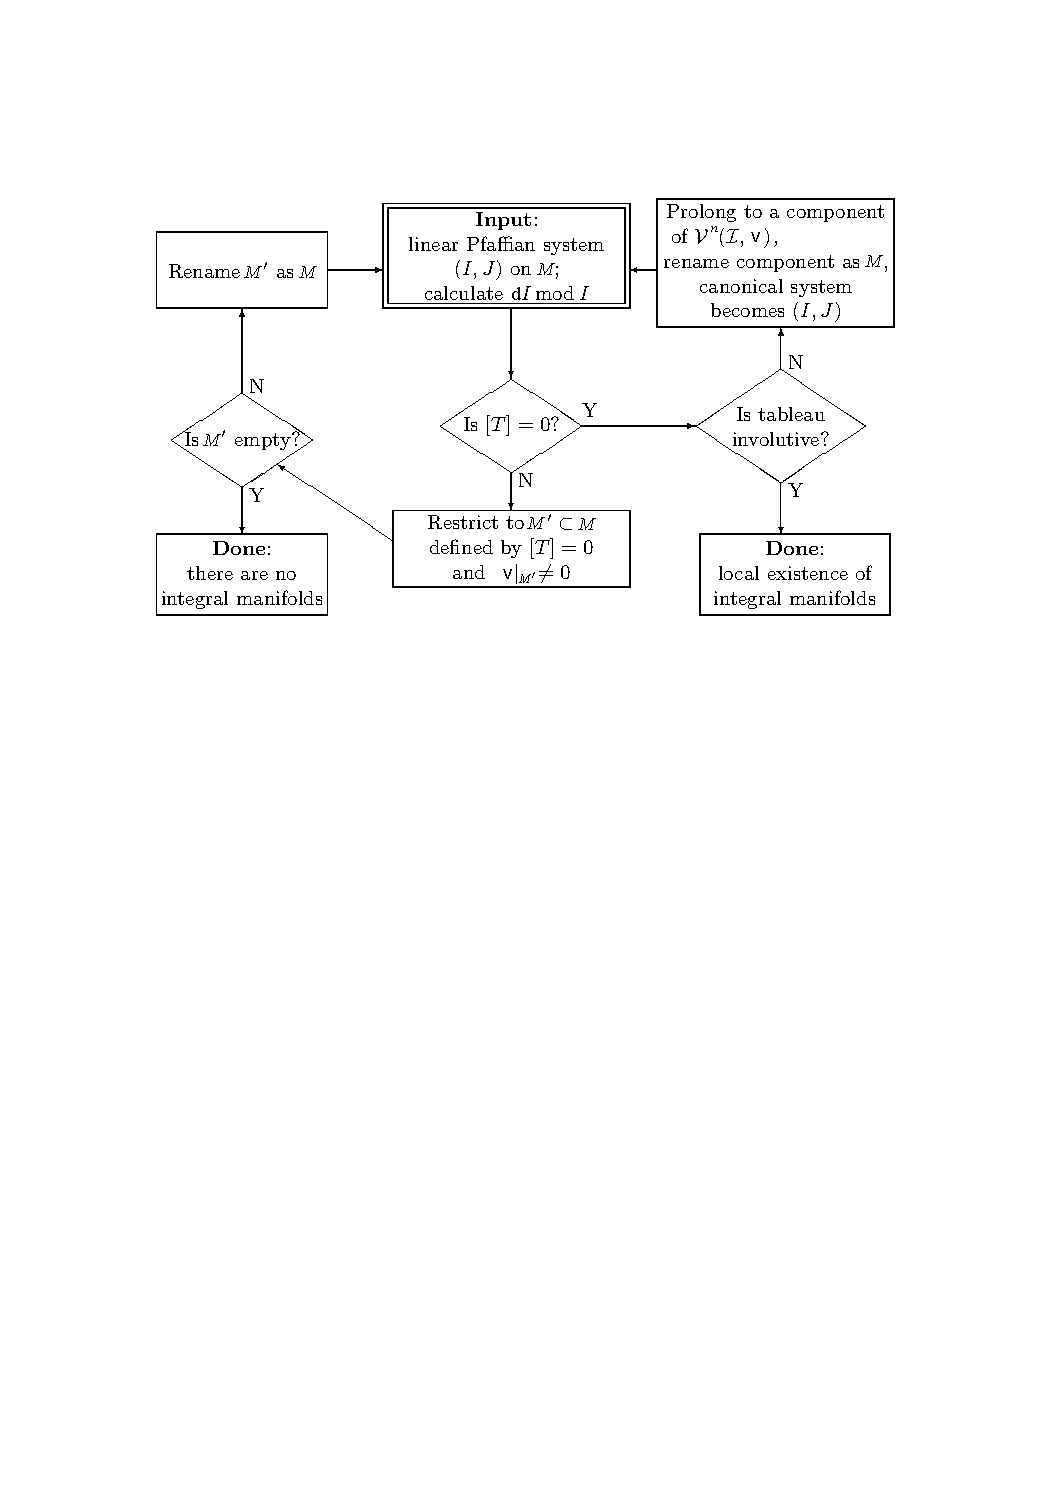
\includegraphics[scale=0.7]{figures/algorithm.pdf}
    \caption{Flow chart of Cartan's algorithm for linear Pfaffian systems. From \cite{Ivey}.}
    \label{fig cartan algorithm}
\end{figure}


\begin{rem}
    \begin{enumerate}
        \item The Cartan algorithm will not necessarily yield all integral manifolds of the original system, only the integral manifolds arising from well-posed Cauchy problems at general points.
        \item Each time one prolongs, there may be many different connected components of $\calV^n(\calI)$ to which one can restrict. To find all possible integral manifolds, one must carry out the algorithm on each component. The Cartan-Kuranishi Prolongation Theorem says in effect that this process terminates eventually, but gives no hint of how long it may take.
        \item How many prolongations it may take for the algorithm to terminate will generally depend on the component one is working with.
    \end{enumerate}
\end{rem}







\section{(*) Cartan-Poincar\'e Lemma}


This \sect\ will be easier to read having some familiarity with homological algebra. First we prove a very basic lemma from exterior algebra, and later generalize it and explain its significance.


\begin{lem}[Cartan]\label{lem cartan}\index{Lemma!Cartan}
    Let $v_1,\ldots,v_k\in V$ be linearly independent elements of a $\bbK$-vector space $V$ and let $w_1,\ldots,w_k\in V$. Then the equation
    \[v_1\wedge w_1+\cdots v_k\wedge w_k=0\]
    holds iff there exists a unique set of scalars $h_{ij}=h_{ji}$, $1\leq i,j\leq k$, such that $w_i=\sum_j h_{ij}v_j$.
\end{lem}
\begin{proof}
    If $V$ is of dimension $n>k$, then let $v_{k+1},\ldots,v_n\in V$ be such that $\{v_i\}_{i=1}^n$ is a basis. Then every $w_j$ can be uniquely written as 
    \[w_i=\sum_{i=1}^n h_{ij}v_j\]
    with some scalars $h_{ij}$, $1\leq i\leq k$, $1\leq j\leq n$. Then, by assumption,
    \[\sum_{i=1}^k\sum_{j=1}^n h_{ij}v_i\wedge v_j=0\]
    By virtue of the antisymmetry of the wedge product, this is equivalent to
    \[\sum_{1\leq i<j\leq k}(h_{ij}-h_{ji})v_i\wedge v_j+\sum_{j=k+1}^n\sum_{i=1}^k h_{ij}v_i\wedge v_j=0.\]
    Since all terms here are linearly independent, this is equivalent to $h_{ij}=0$ for $j>k$, and $h_{ij}=h_{ji}$ for $1\leq i,j\leq k$.
\end{proof}


Let $V,W$ be vector spaces and consider a linear map $\Omega:V\to W$ with dual $\Omega^\ast:W^\ast\to V^\ast$. We set 
\[C^{p,q}\coloneqq \bigodot^p W^\ast\otimes \bigwedge^q V^\ast.\]
In short, $C^{p,q}$ consists of polynomial exterior forms having polynomial degree $p$ and exterior degree $q$. We now define the \emph{boundary operator}
\begin{gather}
    \delta_\Omega:C^{p,q}\to C^{p-1,q+1},\\
    \delta_\Omega(w_1^\ast\otimes\cdots\otimes w_p^\ast\otimes \psi)=\sum_{i=1}^p w_1^\ast\otimes\cdots\otimes \wh{w}_i^\ast\otimes\cdots\otimes w_p^\ast \otimes \Omega^\ast(w_i^\ast)\wedge\psi,
\end{gather}
where $w_i^\ast\in W^\ast$ and $\psi\in \bigwedge^q V^\ast$. As we will see below, this operator is nothing but a the usual exterior derivative which differentiates the $W$-valued coefficients via the map $\Omega$. It is clear that $\delta_\Omega^2=0$, which allows us to define the resulting \emph{cohomology spaces} (quantifying the non-exactness of the sequence) by 
\[\rmH^{p,q}=\bigslant{\ker\left(C^{p,q}\overset{\delta_\Omega}{\to}C^{p-1,q+1}\right)}{\im \left(C^{p+1,q-1}\overset{\delta_\Omega}{\to}C^{p,q}\right)}.\]
The following important result is, as we will see, a generalization of both the Poincar\'e Lemma~\ref{lem poincare classic} and of the Cartan Lemma~\ref{lem cartan}.

\begin{prop}[Cartan-Poincar\'e Lemma {{\cite[Prop.~VIII.2.1]{Bryant}}}]\index{Lemma!Cartan-Poincar\'e}
    There are isomorphisms
    \[\rmH^{p,q}(\Omega)\cong \bigodot^p(\ker \Omega^\ast)\otimes \bigwedge^q(\coker\Omega^\ast).\]
\end{prop}
\begin{proof}
    \emph{Step One.} First suppose that $\Omega$ is an isomorphism and use it to identify $V$ with $W$. If we choose linear coordinates $x^1,\ldots,x^n$ on $V$, the elements in $C^{p,q}$ are 
    \[\varphi=\sum_{i_1<\cdots<i_q}\varphi_{i_1\ldots i_q}\dd x^{i_1}\wedge\cdots\wedge\dd x^{i_q},\]
    where $\varphi_{i_1\ldots i_q}(\bf{x})\in \bigodot^p W^\ast$ is a polynomial of degree $p$. For polynomials, we will simply write $x^i$ instead of $\dd x^i$ because then the commutative product is automatically implied. Thinking of $\Omega$ as the identity map, we have 
    \[\delta_\Omega(x^{j_1}\cdots x^{j_p}\dd x^{i_1}\wedge\cdots\wedge\dd x^{i_q})=\sum_\alpha x^{j_1}\cdots \wh{x}^{j_\alpha}\cdots x^{j_p}\dd x^{j_\alpha}\wedge \dd x^{i_1}\wedge\cdots \wedge\dd x^{i_q}.\]
    This implies that
    \[\delta_\Omega(\varphi)=\dd\varphi\]
    is the usual exterior derivative. We must show that 
    \[\rmH^{p,q}(\Omega)=\begin{cases}
        0, & p+q>0,\\
        \bbR, & p=q=0.
    \end{cases}\label{eq viii.13 Bryant}\]
    Let 
    \[e\coloneqq \sum_i x^i \partial_{x^i}\]
    be the Euler vector field (its flows are homotheties $\bf{x}\mapsto t\bf{x}$).\index{Euler vector field}\index{Homothety} For $\varphi\in C^{p,q}$, Euler's theorem on homogeneous forms implies that 
    \[\Lie_e \varphi=(p+q)\varphi,\]
    where $\Lie_e$ is the Lie derivative along $e$. Combining this with Cartan's magic formula gives the \emph{homotopy formula}
    \[(p+q)\varphi=i_e\dd\varphi+\dd i_e \varphi,\]
    and this implies (\ref{eq viii.13 Bryant}).

    \emph{Step Two.} In the general case, we may choose bases for $V,W$ so that $\Omega$ is a matrix whose top left block is an identity matrix and the rest is zero. Thus, in suitable linear coordinates $(x^i,y^\alpha)$ on $W$ and $(u^\alpha,w^\lambda)$ on $V$ we have 
    \[\Omega^\ast(\dd x^i)=0,\quad \Omega^\ast(\dd y^\alpha)=\dd u^\alpha.\]
    Using multi-index notations, we may write a typical element in $C^{p,q}$ as 
    \[\wt\varphi=\sum_{I,A}\varphi_{IA}(\bf{x},\bf{y})\dd \bf{u}^I\wedge\dd \bf{w}^A,\]
    where $\varphi_{IA}(\bf{x},\bf{y})$ is a polynomial such that $\deg\varphi_{IA}=p$ and $\deg I+\deg A=q$. We shall identify $\wt\varphi$ with the expression 
    \[\varphi=\sum_{I,A}\varphi_{IA}(\bf{x},\bf{y})\dd \bf{y}^I\wedge\dd \bf{w}^A.\]
    When this is done, 
    \[\delta_\Omega(\varphi)=\sum_{I,A}\partial_{y^\alpha}\varphi_{IA}(\bf{x},\bf{y})\dd y^\alpha\wedge\dd \bf{y}^I\wedge\dd \bf{w}^A.\]
    In other words, $\delta_\Omega$ is the exterior derivative w.r.t.\ the $\bf{y}$ variables, treating $\bf{x}$ and $\bf{w}$ as parameters. This suggests that we set 
    \[C^{r,s,\rho,\sigma}\coloneqq \{\varphi\mid \deg_{\bf{x}}\varphi_{IA}=r,\deg_{\bf{y}}\varphi_{IA}=s,\deg I=\rho,\deg A=\sigma\}.\]
    Then $\delta_\Omega:C^{r,s,\rho,\sigma}\to C^{r,s-1,\rho+1,\sigma}$ and with the obvious notation, 
    \[\rmH^{p,q}(\Omega)\cong \bigoplus_{
        \begin{smallmatrix}
            r+s=p\\
            \rho+\sigma=q
        \end{smallmatrix}}\rmH^{r,s,\rho,\sigma}(\Omega).\]
        On the other hand, the proof of Step One gives 
        \[\rmH^{r,s,\rho,\sigma}(\Omega)=\begin{cases}
            0, & \text{unless }s=\rho=0,\\
            C^{r,s,\rho,\sigma}, & \text{when }s=\rho=0.
        \end{cases}\]
        Combining the last two formulas gives the result.
\end{proof}

We will use the Cartan-Poincar\'e Lemma in the following form, which makes it a clear extension of Poincar\'e's Lemma.

\begin{cor}[Cartan-Poincar\'e Lemma {{\cite[Cor.~VIII.2.2]{Bryant}}}]
    Suppose that $\omega^1,\ldots,\omega^n\in V^\ast$ are linearly independent $1$-forms on a vector space $V$ and that $\varphi_{i_1\ldots i_q}\in \bigwedge^r V^\ast$ are $r$-forms ($r>0$) that satisfy the conditions 
    \[\left\{
        \begin{array}{l}
            \varphi_{i_1\ldots i_q} \text{ is symmetric in }i_1,\ldots,i_q,\\
            \sum_i \varphi_{i_1\ldots i_{q-1} i}\wedge \omega^i=0.
        \end{array}
    \right.\]
    Then there exist $\psi_{j_1\ldots j_{q+1}}\in \bigwedge^{r-1}V^\ast$ that satisfy 
    \[\left\{
        \begin{array}{l}
            \psi_{j_1\ldots j_{q+1}} \text{ is symmetric in }j_1,\ldots,j_{q+1},\\
            \sum_i \varphi_{j_1\ldots j_q j}\wedge \omega^j=\varphi_{j_1\ldots j_q}.
        \end{array}
    \right.\]
\end{cor}
\begin{proof}
    In this case $W=\bbR^n$ and $\Omega:V\to W$ is given by $\Omega(v)=(\omega^1(v),\ldots,\omega^n(v))$, which is surjective. In particular, by the Cartan-Poincar\'e Lemma,
    \[\rmH^{q,r}(\Omega)=0,\quad r>0.\label{eq viii.21 Bryant}\]
    The assumptions of the corollary are 
    \[\delta_\Omega(\varphi)=0,\quad \varphi\in \bigodot^q W^\ast\otimes \bigwedge^r V^\ast,\]
    and the assertion is that 
    \[\delta_\Omega (\psi)=\varphi,\quad \psi\in \bigodot^{q+1}W^\ast\otimes \bigwedge^{r-1}V^\ast.\]
    Thus, the corollary is equivalent to (\ref{eq viii.21 Bryant}).
\end{proof}

When $r=q=1$, this corollary is the usual \emph{Cartan Lemma}~\ref{lem cartan}. When $\Omega$ is an isomorphism, it is the Poincar\'e Lemma for polynomial forms.

We now discuss a variant of the lemma relevant to prolongation theory. Let us redefine the spaces $C^{p,q}$ as 
\[C^{p,q}\coloneqq W\otimes \bigodot^k V^\ast\otimes \bigwedge^q V^\ast.\]
Choosing bases $\{w_a\}$ for $W$ and $\{x^i=\dd x^i\}$ for $V^\ast$ we may think of $\varphi\in C^{k,q}$ as a $W$-valued polynomial form 
\[\varphi=\sum_{\deg I=k,\deg J=q}w_a\otimes \varphi^a_{IJ}\bf{x}^I \dd \bf{x}^J.\]
We define $\delta:C^{k,q}\to C^{k-1,q+1}$ to be the usual exterior derivative treating the $w_a$ as constants. Denoting the resulting cohomology by $\rmH^{k,q}$, we have from Cartan-Poincar\'e Lemma, namely (\ref{eq viii.13 Bryant}), 
\[\rmH^{k,q}=\begin{cases}
    W,& k=q=0,\\
    0, & \text{otherwise}.
\end{cases}\]

Now let $A<W\otimes V^\ast$ be a tableau with prolongations $A^{(q)}<W\otimes \bigodot^{p+1}V^\ast$, and define $C^{k,q}(A)<C^{k,q}$ by 
\[C^{k,q}(A)\coloneqq \begin{cases}
    A^{(k-1)}\otimes\bigwedge^q V^\ast,& k\geq 1,\\
    W\otimes\bigwedge^q V^\ast,& k=0.
\end{cases}\]
The defining property of prolongations, which is that the \emph{total prolongation} $\bf{A}=\bigoplus_{k\geq 0} A^{(k)}$ is the largest graded subspace of the maximal ideal $W\otimes \bigodot^{>0}V^\ast$ that is closed under differentiation and satisfies \[\bf{A}\cap (W\otimes \bigodot^{p+1}V^\ast)=A,\quad \bf{A}\cap (W\otimes\bigodot^q V^\ast)=0,\quad q\leq p,\]
implies that $\delta$ maps
\[\delta:C^{k,q}(A)\to C^{k-1,q+1}(A),\]
and we denote by $\rmH^{k,q}(A)$ the resulting \emph{Spencer cohomology}:
\[\rmH^{k,q}(A)\coloneqq \bigslant{\ker\left(C^{k,q}(A)\overset{\delta}{\to}C^{k-1,q+1}(A)\right)}{\im \left(C^{k+1,q-1}(A)\overset{\delta}{\to}C^{k,q}(A)\right)}.\]

\begin{rem}
    More explicitly, the Spencer cohomology groups $\rmH^{i,j}(A)$ of a tableau $A<W\otimes V^\ast$ are defined as follows. Let 
    \[\delta_j:(W\otimes \bigodot^iV^\ast)\otimes \bigwedge^j V^\ast\to W\otimes \bigodot^{i-1}V^\ast\otimes \bigwedge^{j+1}V^\ast\]
    be defined by 
    \[\delta_j(f\otimes \alpha)=\dd f\wedge \alpha,\]
    where, for $f\in W\otimes \bigodot^i V^\ast$, $\alpha\in \bigwedge^j V^\ast$, we define $\dd f$ by considering $f$ as an element of $\Hom(V^{\otimes i},W)$, and extend $\delta_j$ by linearity. In simpler terms, $\delta_j$ takes the last index of $f$ and antisymmetrizes over the union of that index with the indices of $\alpha$. Note that $\delta_j(A^{(i)}\otimes \bigwedge^j V^\ast)\subset A^{(i-1)}\otimes\bigwedge^{j+1}V^\ast$.

    Then 
    \[\rmH^{i,j}(A)= \frac{\ker\restr{\delta_j}{A^{(i-1)}\otimes \bigwedge^jV^\ast}}{\im \restr{\delta_{j-1}}{A^{(i)}\otimes \bigwedge^{j-1}V^\ast}}.\]
\end{rem}

The main theorem about Spencer cohomology and prolongation, whose proof we omit, is the following.

\begin{thm}[{{\cite[Thm.~VIII.2.4]{Bryant}}}]
    A tableau $A$ is involutive iff $\rmH^{k,q}(A)=0$ for $k\geq 1$, $q\geq 0$.
\end{thm}

From here, it is easy to see that the prolongations of an involutive tableau are involutive. Let $\wt W=A\oplus W$. Then $A^{(1)}$ can be considered as a tableau in $\wt W\otimes V^\ast$ with the $W\otimes V^\ast$ block zero. Consider:
\begin{align}
    \rmH^{0,2}(A^{(1)})&= \frac{\wt W\otimes \bigwedge^2 V^\ast}{\delta\left(A^{(1)}\otimes V^\ast\right)}\\
    &= \frac{W\otimes V^\ast\otimes \bigwedge^2 V^\ast}{\delta\left(\left((A\otimes V^\ast)\cap (W\otimes \bigodot^2 V^\ast)\right)\otimes V^\ast\right)}\\
    &=\rmH^{1,2}(A).
\end{align}
Since prolongations can be defined iteratively, this easily implies that 
\[\rmH^{0,2}(A^{(p)})\cong \rmH^{p,2}(A).\]
In fact, the same argument gives more generally that 
\[\rmH^{k,q}(A^{(p)})\cong \rmH^{k+p,q}(A),\quad k\geq 1.\]
The above theorem then implies that prolongations preserve involutivity. This can be immediately used to show that the prolongation of an involutive linear Pfaffian system is involutive. This is based on the facts, established in \S\ref{sec: lin Pfaffian systems}, that the intrinsic torsion of a linear Pfaffian system  $(\calI,\sfv)$ naturally takes values in $\rmH^{0,2}(A_m)$ and the intrinsic torsion of $(\calI^{(1)},\sfv)$ takes values in $\rmH^{0,2}(A_m^{(1)})\cong \rmH^{1,2}(A_m)$, and if the former vanishes, then so does the latter.

\begin{rem}
    The \emph{Cartan-Kuranishi Prolongation Theorem (1957)}, originally conjectured by Cartan based on numerous examples, implies that after a finite number of prolongations a tableau will become involutive (perhaps by becoming empty, in which case there are no integral manifolds). This implies that, for a linear Pfaffian system on an analytic manifold $M$, if $\rmH^{p,2}(A_m)=0$ for all $p$, then there exist integral manifolds through $m$. This statement is the \emph{Goldschmidt version of Cartan-K\"ahler Theorem}. It is useful because sometimes one can show the vanishing of all groups $\rmH^{p,2}$ without having to compute the prolongations.
\end{rem}







\section{Characteristic variety}



In the Cartan-K\"ahler Theorem~\ref{thm 8.3.3 Ivey} we do not necessarily obtain all solutions to an involutive system by a choice of analytic functions as specified in the theorem. We only obtain those that can be obtained by specifying \emph{noncharacteristic} initial data, that is, initial data based on a choice of a \emph{generic} flag. If we choose a nongeneric flag, the corresponding Cauchy problem may not have any solutions or be undetermined, with an infinite number of solutions. In this \sect\ we formalize this connection between generic flags and characteristic varieties.

Let $M$ be a manifold and denote its tautological $n$-plane bundle by $U\coloneqq \gamma_n(\T M)\to \Gr_n(\T M)$ (cf.\ Definition~\ref{def tautological bundles}). We shall consider the projectivization $\bbP U^\ast$ of the dual bundle $U^\ast$. A point in the fiber $\bbP U^\ast_E$ over some $n$-plane $E\in \Gr_n(\T_m M)$ will be written as $[\xi]$, where $\xi\in E^\ast\setminus\{0\}$ is a nonzero covector and $[\xi]=\<\xi\><E^\ast$ is the corresponding line. By projective duality, $[\xi]$ determines a hyperplane $[\xi]^\perp\coloneqq \Ann(\xi)<E$, and geometrically we may think of $\bbP U^\ast_E$ as being the set of hyperplanes in $E<\T_m M$.

Let $\calI$ be an \gls{eds} on $M$ and assume it has no Cauchy characteristics. This assumption is made merely for convenience and will be eliminated below. Associated to each hyperplane $[\xi]^\perp<E$ is the polar space 
\[H(\xi)\coloneqq H([\xi]^\ast)=\{X\in\T_m M\mid \<\{X\}\cup [\xi]^\perp\>\in\calV(\calI)\},\]
which describes all the ways of extending $[\xi]^\perp$ to an integral $n$-plane.

\begin{defn}[Characteristic variety]\index{Characteristic variety}\label{def char variety eds}
    The (real) characteristic variety of an \gls{eds} $(M,\calI)$ is the subset $\Xi\subset \bbP U^\ast$ defined fiberwise by 
    \[\Xi_E=\{[\xi]\in \bbP E^\ast:E\subsetneqq H(\xi)\},\quad E\in\Gr_n(\T M).\label{eq char variety}\]
    Note that this is non-empty only over integral elements $E$. Thus, $\Xi$ consists of all hyperplanes in integral $n$-planes whose extension to an integral $n$-plane fails to be unique. An integral $(n-1)$-plane $E^{n-1}\in\calV^n(\calI)$ is called \emph{non-characteristic} if $\dim H(E^{n-1})=n$, i.e., if its extension to an integral $n$-plane is unique.
\end{defn}

To the extent that we think of integral elements as infinitesimal solutions to an \gls{eds}, the characteristic variety corresponds to non-uniqueness of an initial value problem, in close analogy to the classical notion. However, unlike in the classical context of differential operators, this definition doesn't require linearization. There is a commuting square 
\[\begin{tikzcd}
    \Xi\arrow[r,hookrightarrow]\arrow[d] & \bbP U^\ast\arrow[d] \\
    \calV^n(\calI)\arrow[r,hookrightarrow] & \Gr_n(\T M).
\end{tikzcd}\]
It is easy to see that the fiber $\Xi_E$ is an algebraic subvariety of $\bbP E^\ast$, i.e., it is defined by polynomial equations. This is because the polar equations are linear in $X\in \T_m M$, and $\Xi_E$ consists of hyperplanes $[\xi]^\perp$ for which the ranks of these equations jump suitably; this condition is expressed by homogeneous polynomial equations in $\xi$. This allows us to also define the \emph{complex characteristic variety} $\Xi^\bbC$ as the set of complex solutions to the same equations. Equivalently, one only needs to replace $E$ in (\ref{eq char variety}) with a complex integral element and $[\xi]^\perp$ with a complex hyperplane in $E$, and $\calV(\calI)$ in the definition of $H(\xi)$ with the space of complex integral elements. Of course, it may happen that $\Xi$ is empty but $\Xi^\bbC$ is not.

The reason we assumed no Cauchy characteristics is that $X\in H(\xi)$ for any Cauchy characteristic vector $X$. Thus, the characteristic variety should only be defined for integral elements that contain all Cauchy characteristic vectors. Equivalently, we may consider the \gls{eds} that is the quotient by the Cauchy characteristics and define the characteristic variety of this reduced system. For linear Pfaffian systems this annoyance will be circumvented.

\begin{example}
    \begin{enumerate}
        \item A \emph{Frobenius system} when $\calI$ is generated by $\dd u^1,\ldots,\dd u^s$ in $\bbR^{n+s}$ with coordinates $(x^1,\ldots,x^n,u^1,\ldots,u^s)$. Then $\Xi^\bbC=\varnothing$. A converse of this for involutive systems will be discussed below.
        \item A \emph{Darboux system} when $\calI$ is generated by $\Theta=\sum_i\dd x^i\wedge\dd y^i$ in $\bbR^{2n}$ with coordinates $(x^1,\ldots,x^n,y^1,\ldots,y^n)$. In this case $\Xi_E=\bbP E^\ast$ is everything.
    \end{enumerate}
\end{example}
\begin{rem}
    Given a differential ideal on a $(2n+1)$-dimensional manifold generated by a single $1$-form $\theta$ satisfying $\theta\wedge(\dd\theta)^{\wedge n}\neq 0$, the Pfaff-Darboux local normal form shows that the maximal integral manifolds $N$, called \emph{Legendre manifolds}, are of dimension $n$ and are given by one arbitrary function of $n$ variables. Here we may think of $\theta=\dd u-\sum_i y_i\dd x^i$ and $N$ given by $(\bf{x},\partial_{\bf{x}}u(\bf{x}))$, where $u(\bf{x})$ is an arbitrary function.
\end{rem}


The most important case is that of linear Pfaffian systems, so we will now show how to define the characteristic variety of such systems in terms of the tableau and the symbol. Recall that a linear Pfaffian system is given by a pair of subbundles $I<J<\T^\ast M$ such that 
\[\dd I\subset \<J\>_{\mathrm{alg}}.\]
(Here we are abusing notation by using the same symbol for a bundle and the space of its sections.) We set $L\coloneqq J\slash I$ so that the exterior derivative induces a bundle map 
\[\wb{\delta}:I\to (\T^\ast M\slash J)\otimes L\]
given in the usual coframe $(\theta^a,\omega^i,\pi^\lambda)$ by the tableau:
\[\wb{\delta}(\theta^a)=A^a_{\lambda i}\pi^\lambda\otimes \omega^i,\]
where the $\omega^i$ are viewed as sections of $L$ and the $\pi^\lambda$ are viewed as sections of $\T^\ast M\slash J$.

Dualizing and using that $(\T^\ast M\slash J)^\ast\cong \Ann(J)<\T M$, giving $\wb\delta$ is equivalent to giving the tableau mapping $\pi$ (cf.~\ref{eq iv.60 Bryant}):
\[\pi:\Ann(J)\to I^\ast\otimes L.\]
The relations on its image, i.e., the tableau bundle $A=\im \pi$, are given by the \emph{symbol map} $\sigma$, which is just the induced quotient map 
\[\sigma:I^\ast\otimes L\to (I^\ast\otimes L)\slash A.\]
Now $\im \pi=\ker\sigma$.

We now define the characteristic variety of a linear Pfaffian system.

\begin{defn}[Characteristic variety of a linear Pfaffian system]
    For each $m\in M$ and $\xi\in L_m\setminus\{0\}$ we let $[\xi]\in \bbP L_m$ be the corresponding line and define the \emph{symbol map at $\xi$} by
    \[\sigma_\xi:I^\ast_m \to (I^\ast \otimes L)_m\slash A_m,\quad w\mapsto \sigma(w\otimes \xi).\]
    The characteristic variety $\Xi\subset\bbP L$ is given fiberwise by 
    \[\Xi_m=\{[\xi]\in \bbP L_m\mid \ker \sigma_\xi\neq \{0\}\}.\]
    In other words, $[\xi]$ is characteristic if there exists a nonzero $w\in I^\ast_m$ such that $w\otimes\xi\in A_m$.
\end{defn}

As we have seen, the symbol map in the usual basis is given by the symbol relations $B^{\lambda i}_a$ defined by the dualized structure equations 
\[B^{\lambda i}_a\pi^a_i\equiv 0\pmod{J}.\]
More precisely, for $\xi=\xi_i\omega^i(m)\in L_m$ as above, $\sigma_\xi$ is given by the matrix
\[\sigma_\xi=\left(B^{\lambda i}_a \xi_i\right)\in \Hom(I^\ast_m,(I^\ast \otimes L)_m\slash A_m).\]
Then 
\begin{align}
    \Xi_m&=\{[\xi]:B^{\lambda i}_a(m)\xi_i w^a=0\text{ for some }w\neq 0\}=\\
    &=\{[\xi]:\rank\left(B^{\lambda i}_a \xi_i\right)<s_0\},
\end{align}
where $s_0=\rank I$. It is clear that $\Xi_m$ is defined by homogeneous polynomial equations in the $\xi_i$, so that each fiber $\Xi_m$ is an algebraic variety.

\begin{rem}
    The way to remember this definition is as follows: associated to a PDE system $F^\lambda(x^i,u^a,u^a_{x^i})=0$ is the canonical contact system $I=\<\theta^a=\dd u^a-p^a_i\dd x^i\>$ on the submanifold in the $(\bf{x},\bf{u},\bf{p})$ space given by $F^\lambda(x^i,u^a,p^a_i)=0$. Differentiating the defining equations of $M$ gives the symbol relations 
    \[F^\lambda_{p^a_i}\dd p^a_i\equiv 0\pmod{J},\quad J=\<\theta^a,\dd x^i\>.\]
\end{rem}

\begin{rem}
    To compare this definition to the more general Definition~\ref{def char variety eds}, recall that Cauchy characteristics are the vector fields $X$ satisfying 
    \[i_X \theta^a=0,\quad i_X\dd\theta^a\equiv 0\pmod{\calI}.\]
    If the $1$-forms $\theta^a,\omega^,\pi^a_i$ fail to span $\T^\ast_m M$ for some $m$, then by our constant rank assumption this will be true in a neighborhood and we can find a vector field satisfying $i_X\theta^a=i_X\omega^i=i_X\pi^a_i=0$. By the structure equation $\dd\theta^a\equiv\pi^a_i\wedge\omega^i\pmod{I}$, this vector field will be a Cauchy characteristic. Thus, under the assumption of no Cauchy characteristics we have 
    \[\T^\ast_m M=\<\theta^a,\omega^i,\pi^a_i\>.\]
    For any integral element $E$ at $m$, the independence condition implies that the restriction map $L_m\to E^\ast$ is an isomorphism. It is now not difficult to show that \emph{under this isomorphism, $\Xi_m\subset \bbP L_m$ corresponds exactly to $\Xi_E\subset \bbP E^\ast$}. See \cite[p.~183]{Bryant} for a proof.
\end{rem}

\begin{rem}
    There is a very simple relation between the Cauchy characteristics and the characteristic variety of a linear Pfaffian differential systems. Let $\calA(\calI)<\T M$ denote the Cauchy characteristic subbundle. Since $\calA(\calI)<\Ann(I)$ the map 
    \[\calA(\calI)\to L^\ast,\quad X\to \left(\omega^1(X),\ldots,\omega^n(X)\right)\]
    is well-defined, and we denote its image by $S<L^\ast$. Then $\Ann(S)<L$ and we shall show that 
    \[\Xi \subset\bbP \Ann(S).\label{eq v.19 Bryant}\]
    In particular, if $S\neq 0$ then it follows that the fibers $\Xi_m$ of the characteristic variety lie in the proper linear subspaces $\bbP \Ann(S_m)\subset \bbP L_m$. Clearly, (\ref{eq v.19 Bryant}) also remains valid when we complexify. In the involutive case, there is a converse to the complex version of (\ref{eq v.19 Bryant}), so $\Xi^\bbC=\bbP\Ann(S^\bbC)$ for involutive systems.

    To prove (\ref{eq v.19 Bryant}), choose a basis $\omega^1,\ldots,\omega^n$ for $L$ so that $\omega^1,\ldots,\omega^k$ is a basis for $\Ann(S)$. Then for $\rho=k+1,\ldots,n$ there is a Cauchy characteristic vector $X_\rho$ satisfying 
    \[i_{X_\rho}\omega^\sigma=\delta^\sigma_\rho,\quad \rho,\sigma=k+1,\ldots,n.\]
    From 
    \[i_{X_\rho}\dd\theta^a\equiv 0\pmod{\calI}\]
    we infer that 
    \[\pi^a_i\equiv 0\pmod{J}.\]
    Thus the tableau matrix looks like 
    \[\begin{pmatrix}
        \pi^1_1 & \cdots & \pi^1_k & 0 & \cdots & 0\\
        \vdots & & & \vdots & & \vdots \\
        \pi^{s_0}_1 & \cdots & \pi^{s_0}_k & 0 & \cdots & 0
    \end{pmatrix}\pmod{J}.\label{eq v.20 Bryant}\]
    In particular, among the symbol relations we have 
    \[\pi^a_\rho \equiv 0\pmod{J},\quad \rho=k+1,\ldots,n.\]
    From this it is easy to see that a characteristic vector $\xi=\xi_i\omega^i$ must have $\xi_{k+1}=\cdots=\xi_k=0$. This proves (\ref{eq v.19 Bryant}).

    We remark that whenever we may choose bases so that the tableau matrix has the block form (\ref{eq v.20 Bryant}), then the zeros correspond to the image $S< L^\ast$ of Cauchy characteristics as described above. We also note that the map $\calA(\calI)\to S$ may not be injective; using the structure equations $\dd\theta^a\equiv \pi^a_i\wedge\omega^i\pmod{I}$ it is easy to see that this is the case exactly when $\theta^a,\omega^i,\pi^a_i$ fail to span $\T^\ast M$. Examples of this arise by adding extra dummy variables to any Pfaffian system.
\end{rem}


\begin{example}[\ref{ex 5.6.1 Ivey} continued]
    The tableau of (\ref{eq 5.20 Ivey}) consists of matrices of the form $\left(\begin{smallmatrix}
        a&b\\b&a
    \end{smallmatrix}\right)$. This has characters $s'_1=2=\dim A$ and $s'_2=0$. A line in $V$ spanned by $\left(\begin{smallmatrix}
        x\\ y
    \end{smallmatrix}\right)$ is characteristic iff the system $ax+by=0$, $bx+ay=0$ on $a,b$ has rank below $2$. Of course, this happens only for the two lines $y=\pm x$. Thus $\Xi_A=\{[1:1],[1:-1]\}$. 
\end{example}

\begin{defn}[Elliptic system]\index{Elliptic!linear Pfaffian system}
    A linear Pfaffian system is called elliptic if its real characteristic variety is empty, $\Xi=\varnothing$.
\end{defn}

\begin{example}[Cauchy-Riemann equations]\label{example cauchy-riemann char variety}
    In $\bbR^{2n}=\bbC^n$ consider the Cauchy-Riemann system 
    \[u_{x^i}-v_{y^i}=0,\quad u_{y^i}+v_{x^i}=0,\quad i=1,\ldots,n.\]
    As we have seen, the symbol matrix of the Pfaffian system corresponding to this PDE is given by its symbol matrix as a PDE:
    \[\begin{pmatrix}
        \xi_1 & \xi_2 & \xi_3 & \xi_4 & \cdots & \xi_{2n-1} & \xi_{2n}\\
        -\xi_2 & \xi_1 & -\xi_4 & \xi_3 & \cdots & -\xi_{2n}& \xi_{2n-1} 
    \end{pmatrix}.\]
    The real characteristic variety is, as expected, empty, so this system is elliptic. However, for each $z\in\bbC^n$ the complex characteristic variety $\Xi^\bbC_z$ is given by the vanishing of all $2\times 2$ minors of this matrix. It is easy to the verify that 
    \[\Xi_z^\bbC=\CP_+^{n-1}\cup \CP^{n-1}_-\subset \CP^{2n-1},\]
    where 
    \[\CP^{n-1}_\pm =\{\xi_2=\pm \i \xi_1,\ldots,\xi_{2n}=\pm \i \xi_{2n-1}\}.\]
    For example, when $n=2$, we may picture $\Xi_z^\bbC$ as two purely imaginary conjugate skew lines in $\CP^3$.
\end{example}


\begin{defn}[Determined system]
    A tableau $A<W\otimes V^\ast$ is called determined if $\dim \Ann(A)=\dim W=s$, i.e., the number of equations is the same as the number of unknowns. A linear Pfaffian system is determined if its symbol matrices are square. 
\end{defn}

\begin{prop}[{{\cite[p.~188]{Bryant}}}]
    Suppose the linear Pfaffian system $(I,J)$ is determined. If for some $\xi\in L_m\setminus\{0\}$, $\det\sigma_\xi\neq 0$, i.e., if the complex characteristic variety is not everything, then the system is involutive at $m$.  
\end{prop}
\begin{proof}
    Writing the symbol relations of a determined system as 
    \[B^{bi}_a\pi^a_i\equiv 0\pmod{J},\]
    we may assume that the characteristic direction is along the $n$'th axis, so $\det\left(B^{bn}_a\right)\neq 0$, and then by a change of basis in the space of relations that 
    \[B^{bn}_a=-\delta^b_a.\]
    The symbol relations become 
    \[\pi^a_n\equiv B^{a\rho }_b\pi^b_\rho\pmod{J},\quad \rho,\sigma=1,\ldots,n-1.\]
    It follows that the characters of the tableau matrix are given by 
    \[s'_1=s_0,\;\ldots,\;s'_{n-1}=s_0,\;s'_n=0.\]
    Now write the symbol relations out as 
    \[\pi^a_n\equiv B^{a\rho }_b \pi^b_\rho +B^a_i\omega^i\pmod{I}.\]
    Integral elements are given by linear equations 
    \[\theta^a=0,\quad \pi^a_i-p^a_{ij}\omega^j=0,\]
    where 
    \[p^a_{ij}=p^a_{ji},\quad p^a_{nj}=B^{a\rho}_bp^b_{nj}+B^a_j.\]
    Choose $p^a_{\rho\sigma}=p^a_{\sigma\rho}$ arbitrarily and use the second relation for $j=1,\ldots,n-1$ to determine the $p^a_{n\sigma}=p^a_{\sigma n}$. Then use the same relation for $j=n$ to determine $p^a_{nn}$. It follows that the $s_0n(n-1)/2$  quantities $p^a_{\rho\sigma}$ specify the integral elements uniquely. We find that 
    \[s_0n(n-1)/2=s'_1+2s'_2+\cdots+ns'_n,\]
    so Cartan's Test is satisfied and the system is involutive.
\end{proof}

% \begin{defn}[Symbol mapping, Characteristic variety]\label{def symbol map}
%     Let $A<W\otimes V^\ast$ be a tableau. For $\alpha\in V^\ast$, define the \emph{symbol mapping} at $\alpha$ by 
%     \[\sigma_\alpha:W\to (W\otimes V^\ast)\slash A,\quad w\mapsto w\otimes\alpha + A.\]
%     Define the \emph{characteristic variety} of $A$, $\Xi_A\subset \bbP V^\ast$ (where $\bbP$ stands for the projectivization functor $V\mapsto V\slash \bbK^\times$ for $\bbK$-vector spaces), to be the set of all \emph{characteristic hyperplanes} (codimension $1$ subspaces) in $V$:
%     \[\Xi_A\coloneqq \{[\alpha]\in \bbP V^\ast\mid \ker \sigma_\alpha\neq 0\}.\]
%     We interpret $\Xi_A$ is the set of hyperplanes in $\bbP V$ for which the extension of an $(n-1)$-dimensional integral element to an $n$-dimensional one is not unique, see Theorem~\ref{thm 6.7.7 Ivey}.
% \end{defn}


% Even when we are only interested in real solutions of the underlying PDE, it is useful to consider the \emph{complex characteristic variety}
% \[\Xi^\bbC_A\coloneqq \{[\alpha]\in \bbP (V^\ast)^\bbC\mid \ker \sigma_\alpha^\bbC\neq 0\},\]
% where $\sigma^\bbC_\alpha:W^\bbC\to (W^\bbC\otimes (V^\ast)^\bbC)\slash A^\bbC$ is the complexification of $\sigma_\alpha$ (see Definition~\ref{def complexification}).





\section{Properties of the characteristic variety}

We now discuss some key properties of the characteristic variety. In doing so, we will omit many proofs, referring the reader to \cite[Ch.~V]{Bryant} instead.

\paragraph{(i) The first derived system and $\Xi$.} The first property deals with a natural subsystem that will turn out being irrelevant to the computation of the characteristic variety.

\begin{defn}[Derived system]
    Let $I<\T^\ast M$ be a Pfaffian system of constant rank. The derived system $I_{(1)}$ of $I$ is the subbundle spanned by $I$-valued forms whose exterior derivatives modulo $I$ vanish. More explicitly, let $\delta:\Gamma^\infty(I)\to \Gamma^\infty\left(\bigwedge^2(\T^\ast M\slash I)\right)$ be defined by \[\delta(\theta)=\dd\theta\mod I.\] 
    
    Because $\delta$ is $C^\infty(M)$-linear, it is induced by a \gls{vb} morphism $\delta:I\to \bigwedge^2(\T^\ast M\slash I)$. Since the coefficients of $\delta$, when expressed in matrix form, are smooth, its rank is upper semicontinuous, so we may restrict to an open set in $M$ on which it has constant rank. On this open set, we define $I_{(1)}\coloneqq \ker\delta$. We have the exact sequence 
    \[0\to I_{(1)}\to I\overset{\delta}{\to}\dd I\slash \<I\>_{\mathrm{alg}}\to 0.\]
    
    If $I_{(1)}=I$, then $I$ is Frobenius; otherwise, $I_{(1)}$ is smaller. In that case, we define a sequence of systems iteratively by $I_{(k+1)}=(I_{(k)})_{(1)}$, until $I_{(N)}$ is either Frobenius ($I_{(N+1)}=I_{(N)}$) or rank zero. The \emph{derived flag} is 
    \[I=I_{(0)}> I_{(1)}>\cdots >I_{(N)},\]
    and $N$ is the \emph{derived length}.
\end{defn}

For an adapted basis $(\theta^1,\ldots,\theta^p;\theta^{p+1},\ldots\theta^{s_0})=(\theta^\rho,\theta^\epsilon)$ for $I_{(1)}<I$ (here $\rho,\sigma=1,\ldots,p$ and $\epsilon,\delta=p+1,\ldots,s_0$) we have 
\[\dd \theta^\rho\equiv 0\pmod{I},\quad \dd\theta^\epsilon\equiv \pi^\epsilon_i\wedge\omega^i\pmod{I}.\]
The symbol relations are of the form 
\[\pi^\rho_i\equiv 0\pmod{J},\quad B^{\lambda i}_\epsilon\pi^\epsilon_i\equiv 0\pmod{J},\]
and the tableau matrix is 
\[\begin{bmatrix}
    0\\\pi^\epsilon_i
\end{bmatrix}.\]
In intrinsic terms, we have the dualized exact sequence 
\[0\to (I\slash I_{(1)})^\ast\to I^\ast\to I^\ast_{(1)}\to 0.\]
The tableau corresponding to the above matrix is given by a subbundle $A<I^\ast\otimes L$ with the property that $A$ projects to zero in $I^\ast_{(1)}\otimes L$, i.e.,
\[A<(I\slash I_{(1)})^\ast \otimes L<I^\ast\otimes L.\]
For $\xi\in L\setminus\{0\}$ the symbol map $\sigma_\xi:I^\ast\to (I^\ast\otimes L)\slash A$ restricts to 
\[\sigma_{(1),\xi}:(I\slash I_{(1)})^\ast\to (I^\ast\otimes L)\slash A,\]
and from the definitions it follows that 
\[\ker\sigma_\xi=\ker\sigma_{(1),\xi}.\]
Thus the characteristic variety is the same as if we consider only the bottom non-zero block in the tableau matrix, i.e., we consider only the ``smaller'' symbol matrices $\left(B^{\lambda i}_\epsilon \xi_i\right)$. Informally, 
\begin{quote}
    \emph{In computing the characteristic variety, we can ignore the derived system.}
\end{quote}
This property is a generalization of the fact that the symbol and the characteristic variety of a PDE depend only on its highest order terms.

\paragraph{(ii) Characteristic variety of the prolongation.}

Recall that the first prolongation $(\calI^{(1)},\sfv)$ is defined on the manifold $M^{(1)}$, which is a connected component of the space of ordinary integral elements of $(\calI,\sfv)$, and as a Pfaffian system $I^{(1)}$ is generated by the equations 
\[\theta^a=0,\quad \theta^a_i=\pi^a_i-p^a_{ij}\omega^j=0,\quad B^{\lambda i}_ap^a_{ij}=0.\label{eq v.76 Bryant}\]
The exterior derivatives of these equations give, using the original structure equations, 
\[\dd\theta^a\equiv 0\pmod{I^{(1)}},\quad\dd\theta^a_i\equiv \pi^a_{ij}\wedge\omega^j\pmod{I^{(1)}},\label{eq v.77 Bryant}\]
where locally $\<I^{(1)}\>=\<\theta^a,\theta^a_i\>$ and 
\[\pi^a_{ij}=-\dd p^a_{ij}+(\text{pullbacks of forms on $M$ to }M^{(1)}).\]
Comparing (\ref{eq v.76 Bryant}) and (\ref{eq v.77 Bryant}) we see as before that the original Pfaffian system is contained in the first derived system of the prolongation, and hence, by  property (i), when computing the characteristic variety of $\calI^{(1)}$ we need only consider the tableau $\left(\pi^a_{ij}\right)$. Differentiating the last equation in (\ref{eq v.76 Bryant}) and using that pullbacks of forms on $M$ are spanned by $\<\theta^a,\omega^i,\pi^a_i\>=\<\theta^a,\omega^i,\theta^a_i\>$, it follows that the symbol relations on the $\pi^a_{ij}$ are 
\[\pi^a_{ij}\equiv \pi^a_{ji}\pmod{\theta^b,\theta^b_i,\omega^i},\quad B^{\lambda i}_a\pi^a_{ij}\equiv 0\pmod{\theta^b,\theta^b_i,\omega^i}.\]
Note that the second set of relations is indexed by $(\lambda,j)$. Thus, we should write these relations as 
\[B^{(\lambda,j)ik}_a \pi^a_{ik}\equiv 0 \pmod{\theta^b,\theta^b_a,\omega^i},\]
where 
\[B^{(\lambda,j)ik}_a=\delta^i_k B^{\lambda i}_a.\]
If $\xi=(\xi_i)$ is characteristic for $(\calI^{(1)},\sfv)$, then there exists a $w=(w^a_i)$ satisfying 
\[w^a_i\xi_j=w^a_j\xi_i,\quad B^{(\lambda,j)ik}_aw^a_i\xi_k=0.\]
From the first relation we have $w^a_i=w^a\xi_i$, and from the second $B^{\lambda i}_aw^a\xi_i\xi_j=0$, $j=1,\ldots,n$. It follows that 
\[B^{\lambda i}_aw^a\xi_i=0,\]
which says that $\xi$ is characteristic for $(\calI,\sfv)$. Since the converse is obviously true, we have established that under the projection $\pi:M^{(1)}\to M$,
\[\text{\emph{There is a natural isomorphism }} \Xi^{(1)}_q\cong \Xi_{\pi(q)}\text{ for all } q\in M^{(1)}.\]
In other words, in the absence of integrability conditions (i.e., if the intrinsic torsion is identically zero), the characteristic variety doesn't change upon prolongation. If there are integrability conditions $[T]=0$, then they will contribute additional symbol relations to the prolonged system, so the characteristic variety may get smaller: $\Xi^{(1)}_q\subset \Xi_{\pi(q)}$.


\paragraph{(iii) Characteristic variety and the Cartan-K\"ahler Theorem.} The remaining properties are more substantial and require involutivity. We discuss them briefly without derivation. Recall that if $\kappa=s_l$ is the top nonzero Cartan character of the system, then it integral manifolds depend on $\kappa$ functions of $l$ variables. To an algebraic geometer, $l$ resembles a transcendence degree and $\kappa$ a field extension degree -- this analogy will turn out to be precise. We will state results that express $l,\kappa$ and the condition to be a regular flag in terms of algebro-geometric properties of the complex characteristic variety $\Xi^\bbC$. In practice these theorems usually allow one to determine $l,\kappa$ and regular flags without going through the sometimes laborious procedure of calculating the $s'_p$. 

If $\Xi^\bbC=\bigcup_\alpha \Xi^{\bbC,\alpha}$ is the unique (fiberwise) decomposition of $\Xi^\bbC$ into irreducible components (i.e., each component is defined by an irreducible system of polynomials), then we define 
\[d^\alpha\coloneqq \dim_\bbC\Xi^\bbC_m,\quad \delta^\alpha(m)\coloneqq \deg \Xi_m^{\bbC,\alpha},\quad \mu^\alpha(m)\coloneqq \dim\ker\sigma_{m,\xi},\]
where $[\xi]\in \Xi^\bbC_m$ is a general point. As a consequence of involutivity, all of these integers are independent of $m\in M$. We further define 
\[d\coloneqq \max_\alpha d^\alpha,\quad \delta(m)\coloneqq \sum{}'\delta^\alpha(m),\quad\mu(m)\coloneqq \sum{}'\mu^\alpha(m),\]
where $\sum{}'$ denotes the sum over components of the maximal dimension, $d$. Again, $d$, $\delta$, and $\sum{}'\mu^\alpha(m)\delta^\alpha(m)$ will be independent of $m$. The main result is the following.

\begin{thm}[{{\cite[Thm.~V.3.6]{Bryant}}}]\label{thm v.3.6. Bryant}
    Let $(\calI,\sfv)$ be an involutive Pfaffian system of character $l$ and Cartan integer $\kappa=s_l$. Then, with the above notation, 
    \[l=d+1,\quad \kappa=\sum{}'\mu^\alpha(m)\delta^\alpha(m).\]
\end{thm}

\begin{cor}[{{\cite[Cor.~V.3.7]{Bryant}},{\cite[Thm.~5.6.12]{Ivey}}}]
    Suppose that all $\mu^\alpha(m)=1$ (this is often the case). Then 
    \[l=\dim_\bbC \Xi^\bbC_m+1,\quad \kappa=\deg \Xi^\bbC_m.\]
\end{cor}

If we omit reference to the point $m$, we may rephrase this as 
\begin{quote}
    \emph{The integral manifolds of an involutive, analytic Pfaffian system locally depend on $\deg\Xi^\bbC$ functions of $\dim_\bbC\Xi^\bbC+1$ variables.}
\end{quote}

\begin{example}[\ref{example cauchy-riemann char variety} continued]
    The characteristic variety of the Cauchy-Riemann system has $\delta^1=\delta^1=\mu^1=\mu^2=1$, so 
    \[d=n-1,\quad \kappa=2,\]
    so we get the familiar result that holomorphic maps of $n$ complex variables depend on $2$ functions of $n$ real variables.
\end{example}

\begin{cor}[{{\cite[Cor.~V.3.11]{Bryant}}}]\label{cor v.3.11 Bryant}
    Let $(\calI,\sfv)$ be a smooth involutive linear Pfaffian system whose complex characteristic variety is empty, $\Xi^\bbC=\varnothing$. Then $\calI$ is completely integrable: through each point of $m$ there passes a unique integral manifold of $\calI$.
\end{cor}
\begin{proof}
    By Theorem~\ref{thm v.3.6. Bryant}, $l=1$ and $\kappa=0$, so we have $s_1=\cdots=s_n=0$, and since there are no integrability conditions, the structure equations are $\dd\theta^a\equiv 0\pmod{\theta^b}$. Thus, the Frobenius condition $\dd I\equiv 0\pmod{I}$ is satisfied.
\end{proof}

A final theorem following from this result is the following.

\begin{thm}[{{\cite[Thm.~V.3.12]{Bryant}}}]
    Let $(\calI,\sfv)$ be an \gls{eds} and assume that:
    \begin{enumerate}[label=(\roman*)]
        \item $\Xi^\bbC=\varnothing$;
        \item the process of prolongation is well-behaved: at each stage we get a locally finite union of manifolds (this is automatic for real analytic systems).
    \end{enumerate}
    Then some prolongation of $(\calI,\sfv)$ is either empty or is a Frobenius system. In particular, for a suitable $q$ each connected integral manifold of $(\calI,\sfv)$ is uniquely determined by its $q$-jet at one point.
\end{thm}
\begin{proof}
    Based on Theorem~\ref{thm vi.2.1 Bryant}, a suitable prolongation $(\calI^{(q)},\sfv)$ is either empty or involutive. Since integral manifolds of $(\calI^{(q)},\sfv)$ are in local one-to-one correspondence with those of $(\calI,\sfv)$, we may focus on the involutive case.  Since prolongation preserves the characteristic variety, $\Xi^{\bbC,(q)}$ is empty. By Corollary~\ref{cor v.3.11 Bryant}, $(\calI^{(q)},\sfv)$ is Frobenius and its integral manifolds are uniquely specified by a choice of a single point of $M^{(q)}$, i.e., by the $q$-jet of the corresponding integral manifold of $(\calI,\sfv)$.
\end{proof}

Informally, we may say that \emph{in the case $\Xi^\bbC=\varnothing$ the integral manifolds depend on a finite number of constants}, which is a generalization of the concept of complete integrability.

\paragraph{(iv) Characteristic variety and K\"ahler-singular elements.} We have defined the characteristic variety in terms of the characteristic, or singular, hyperplanes in $n$-dimensional integral elements. On the other hand, if $(\calI,\sfv)$ is an involutive Pfaffian system of character $l$, then the uniqueness of extensions in the Cauchy problem for $n$-dimensional integral manifolds occurs along $l$-dimensional submanifolds. Thus, we may expect that the characteristic variety should consist of singular $l$-dimensional integral elements. In other words, when $l<n-1$ (roughly speaking, this is the \emph{overdetermined case}), there are two possible characteristic varieties, and it is obviously important to relate them.

Recall that an integral element $E\in\calV^n(\calI)$ is K\"ahler-regular if the rank of the polar equations is locally constant near that element in $\calV^n(\calI)$. Otherwise we call it \emph{K\"ahler-singular}. In terms of the characters, singularity is equivalent to being \emph{non-generic}: a $p$-plane $E^p$ is singular if the total number $s(E^p)$ of polars in a tableau adapted to $E^p$ (this number depends only on $E^p$ itself) is strictly less than the character sum (which characterizes the generic integral $p$-plane). We define 
\[\Lambda_p\coloneqq \{E\in \calV^p(\calI)\subset \Gr_p(L^\ast)\mid s(E)<s'_1+\cdots+s'_p\}.\]
If the character of the system is $l$, then $\Lambda\coloneqq \Lambda_l$ is called the \emph{Cartan characteristic variety}. 

If there are no integrability conditions, i.e., the symbol relations may be assumed to be 
\[B^{\lambda i}_a \pi^a_i\equiv 0\pmod{I},\]
then $\Lambda_p$ us the set of integral $p$-planes whose polar equations have lower rank than the generic integral $p$-plane. In particular, in the absence of integrability conditions, $\Lambda_{n-1}=\Xi$.

According to the Cartan-K\"ahler Theorem, the Cartan characteristic variety determines the set of integral elements that are characteristic for the last Cauchy-Kovalevskaya system in which there is any freedom in assigning initial data. It is clear how to define $\Lambda_p^\bbC$ and $\Lambda^\bbC$. The main result relating the Cartan characteristic variety to the usual characteristic variety is the following.

\begin{thm}[{{\cite[Thm.~V.3.15]{Bryant}}}]\label{thm v.3.15 Bryant}
    If $(\calI,\sfv)$ is involutive and of character $l$, then 
    \begin{align}
        \Lambda^\bbC&=\{E\in \Gr_l(L^{\ast,\bbC})\mid E\in [\xi]^\perp \text{ for some characteristic }[\xi]\in\Xi^\bbC\},\\
        \Xi^\bbC&=\{[\xi]\in\bbP L^\bbC\mid E\in \Lambda^\bbC \text{ for all subspaces }E<[\xi]^\perp\}.
    \end{align}
\end{thm}

Note that since we may have $\Xi=\varnothing$ but $\Lambda\neq \varnothing$, the analogous statement is false over $\bbR$. What we can say is that the \emph{real} Cartan characteristic variety $\Lambda$ is given in terms of the \emph{complex} usual characteristic variety by 
\[\Lambda=\{E\in\Gr_l(L^\ast)\mid E<[\xi]^\perp \text{ for some characteristic }[\xi]\in\Xi^\bbC\}.\label{eq v.102 Bryant}\]
Similarly, the second assertion in Theorem~\ref{thm v.3.15 Bryant} gives $\Xi^\bbC$ in terms of $\Lambda^\bbC$ as follows: an $(n-1)$-plane is characteristic iff \emph{every} $l$-plane contained in it is Cartan characteristic.

\begin{example}[\ref{example cauchy-riemann char variety} continued]
    Consider again the Cauchy-Riemann system on $\bbR^{2n}\cong \bbC^n$, now with the standard complex structure $\sfJ:\bbR^{2n}\to \bbR^{2n}$ given by 
    \[\sfJ(\partial_{x^i})=\partial_{y^i},\quad \sfJ(\partial_{y^i})=-\partial_{x^i}.\]
    We've already seen that this system is elliptic, so $\Xi=\varnothing$. To describe the Cartan characteristic variety, since the system is translation invariant it will suffice to describe the fiber $\Lambda_0$ of $\Lambda$ over the origin, and using (\ref{eq v.102 Bryant}) this is given by 
    \[\Lambda_0=\{E\in\Gr_n(\bbR^{2n}):E\cap \sfJ(E)\neq \{0\}\}.\]
    In other words, $\Lambda_0$ consists of real $n$-planes that contain at least one \emph{complex line} (i.e., a \emph{real} $\sfJ$-invariant $2$-plane). 

    It is, of course, well known that real $n$-dimensional submanifolds $Y^n\subset \bbC^n$ such that $\T_y Y\cap \sfJ(\T_y Y)=\{0\}$ for every $y\in Y$ are locally determining sets for holomorphic functions. 

    In general we have 
    \[\Lambda_{p,0}=\{E\in\Gr_p(\bbR^{2n})\mid \dim E\cap \sfJ(E)\geq \max(1,2(p-m)+1)\}.\]
    For instance, $\Lambda_{2m-1,0}=\Gr_{2m-1}(\bbR^{2n})$ contains no information.
\end{example}

\paragraph{(v) Integrability of the characteristic variety.} Let us define the concept of involutivity for the characteristic variety.

\begin{defn}[Eikonal equation I]
    Let $N$ be a manifold and $\Sigma\subset \bbP \T^\ast N$ a subset. The associated eikonal equation $E_\Sigma\subset C^\infty(N)$ is defined as follows: a function $\varphi\in C^\infty(N)$ is a solution of $E_\Sigma$ if $[\dd \varphi(x)]\in \Sigma_x$ for all $x\in N$ such that $\dd \varphi(x)\neq 0$.
\end{defn}

For another description, let $\wt\Sigma\subset\T^\ast N$ be defined by 
\[\wt\Sigma=\pi^{-1}(\Sigma)\cup \{0\}\subset \T^\ast N,\]
where $\pi:\T^\ast N\setminus \{0\}\to \bbP \T^\ast N$ is the projectivization map and $\{0\}\subset \T^\ast N$ denotes the zero section. Then $\wt\Sigma$ is a \emph{conical subvariety} of $\T^\ast N$, i.e., it is invariant under scaling of the fibers. Moreover, any conical subvariety is of this form. Then solutions to the eikonal equation are characterized by $\dd\varphi(x)\in \wt\Sigma$. 

If $x^1,\ldots,x^n$ are local coordinates on $N$ with induced coordinates $(x^i,\xi_i)$ on $\T^\ast N$, then we shall always assume that $\Sigma$ is a subset with the property that $\wt\Sigma$ is defined by equations 
\[F^\lambda(y^i,\xi_i)=0,\quad \lambda=1,\ldots,R,\]
where the $F^\lambda$ are either smooth or analytic depending on the category in which we are working.

\begin{defn}[Eikonal equation II]
    The eikonal differential equation is a PDE for functions $\varphi\in C^\infty(N)$ of the form
    \[F^\lambda\left(\bf{y},\partial_{\bf{y}}\varphi(\bf{y})\right)=0,\quad \lambda=1,\ldots,R.\]
\end{defn}

\begin{rem}
    The functions $F^\lambda$ need only be defined \emph{microlocally}, i.e., in open sets $U\subset \T^\ast N$ invariant under scaling. In the cases of interest to us the fibers $\Sigma_x$ of $\Sigma\to N$ will be algebraic varieties, so that the $F^\lambda(x^i,\xi_i)$ may be chosen to be homogeneous polynomials in the $\xi_i$, whose coefficients are functions of the $x^i$. In this case, the complexifications 
    \[\Sigma^\bbC\subset \bbP \T^{\ast,\bbC}N,\quad \wt{\Sigma}^\bbC\subset \T^{\ast,\bbC}N\]
    are naturally defined, and so the complex eikonal equation makes sense by allowing the function $\varphi$ to have complex values and requiring that $\dd\varphi\in\wt{\Sigma}^\bbC$. We remark that we may have $\Sigma=\varnothing$ but $\Sigma^\bbC\neq\varnothing$. \emph{From now on we assume that the $F^\lambda$ may be chosen to be homogeneous polynomials in the $\xi_i$}.
\end{rem}

\begin{defn}[Involutive conical subvariety]
    The subset $\Sigma^\bbC\subset \bbP \T^{\ast,\bbC}N$ is called involutive in case the eikonal equation $E_{\Sigma^\bbC}$ is involutive.
\end{defn}

To state the main result, we let $\calI$ be a different system on a manifold $M$ with complex characteristic variety $\Xi^\bbC\subset \bbP U^{\ast,\bbC}$ (cf.~the definitions at the start of this \sect). For any integral manifold $i:N\to M$ of $\calI$ there is the \emph{induced characteristic variety}
\[\Xi_N^{\bbC}\subset \bbP \T^{\ast,\bbC}N\]
defined as follows. We have the diagram 
\[\begin{tikzcd}
     & \bbP U^{\ast,\bbC} \arrow[dl,dashed]\arrow[d,"\wt\pi"]\\
     \bbP \T^{\ast,\bbC}N\arrow[d] \arrow[r,"\wh{i}_\ast"] & \Gr_n(\T M)\arrow[d]\\ 
     N\arrow[r,hookrightarrow,"i"] & M,
\end{tikzcd}\]
where 
\[\wh{i}_\ast(x)=i_\ast(\T_x N),\quad \wt{\pi}^{-1}(m,E)=\bbP E^{\ast,\bbC}.\]
The condition that $N$ be an integral manifold of $\calI$ is that 
\[\wt{\pi}^{-1}(\wt{i}_\ast(N))\to \bbP \T^{\ast,\bbC}N.\]
By definition, $\Xi^\bbC_N$ is the image of $\Xi^\bbC\cap \wt{\pi}^{-1}(\wt{i}_\ast(N))$ under this mapping. Informally, $\Xi^\bbC_N$ \emph{is induced from the characteristic variety $\Xi^\bbC$ in each of the integral elements $i_\ast(\T_x N)\in \Gr_n(\T M)$}.

\begin{defn}[Involutive characteristic variety]
    The characteristic variety $\Xi^\bbC$ is called \emph{involutive} if the eikonal equation $E_{\Xi^\bbC_N}$ is involutive for any integral manifold $N$ of $\calI$.
\end{defn}

The following fundamental result essentially states that \emph{if $\calI$ is involutive, then its characteristic variety is involutive}. 

\begin{thm}[Cartan, Guillemin, Quillen, Sternberg, Gabber (1953-1981) {{\cite[Thm.~V.3.20]{Bryant}}}]
    Let $E\in \calV_n(\calI)$ be an ordinary integral element. Then $\Xi^\bbC$ is involutive in an open neighborhood $V$ of $E$.
\end{thm}
What this means is that $\Xi^\bbC_N$ is involutive for all integral manifolds $i:N\to M$ satisfying $\wt{i}_\ast(N)\subset V$.

% Let us now \emph{work over $\bbC$ and drop $\bbC$ from the notation}. We estimate the dimension of $\Xi_A$ and a modification of the degree of $\Xi_A$ in terms of the characters of $A$. We use the convention that the empty set has dimension $-1$, and denote the modified degree defined below by $\widetilde{\deg}$.

% Now suppose $(I,J)$ has no intrinsic torsion and let $E\in\calV^n(I,J)_m$. Let $H<E$ be a hyperplane, i.e., $\dim H=n-1$. We address the following question: under what circumstances is $E$ the only integral $n$-plane that contains $H$?

% \begin{defn}[Characteristic hyperplane]
%     A hyperplane $H<E<\T_mM$ is said to be characteristic if it has more than one extension to an $n$-dimensional integral element.
% \end{defn}

% With notation as above, we may choose the coframe so that 
% \[\restr{\theta^a}{E}=\restr{\pi^a_i}{E}=0.\]
% Assume moreover that $E$ is uniquely defined by these equations, that is, $\{\theta^a,\omega^i,\pi^a_i\}$ span $\T_m^\ast M$ (so there are no Cauchy characteristics).

% We can also choose frames so that $\restr{\omega^n}{H}=0$. Let $e_1,\ldots,e_n$ be a basis for $E$ dual to $\{\omega^i\}$. Then $v\in \T_mM\setminus H$ completes $H$ to an integral $n$-plane iff 
% \[\forall\Phi \in\calI^n\quad \Phi (v,e_1,\ldots,e_{n-1})=0.\label{eq 6.17 Ivey}\]
% In fact, it is sufficient to require that $i_v \theta^i=0$ and to verify (\ref{eq 6.17 Ivey}) for $\Phi=\pi^a_i\wedge \omega^J$, where $J$ is any multi-index of length $n-1$ containing the index $i$. Since $i_{e_i}\pi^\lambda=0$, (\ref{eq 6.17 Ivey}) becomes 
% \[i_v\pi^a_i=0,\quad  \forall a, i=1,\ldots,n-1.\label{eq 6.18 Ivey}\]
% Now recall the symbol mapping from Definition~\ref{def symbol map}, defining the characteristic variety $\Xi_A$ for $A=A_m$. If $\alpha_H\in \bbP E^\ast$ corresponds to $H<E$, then $\alpha_H\in \Xi_A$ iff 
% \[B^{rn}_a w^a=0\]
% for some nonzero $w\in W$. In other words, $\alpha_H\in\Xi_A$ iff the tableau contains a matrix with the first $n-1$ columns zero and the last column nonzero, or equivalently, some linear combination of the $\pi^a_n$ is linearly independent from the forms in the first $n-1$ columns, so that $v$ is not uniquely determined by (\ref{eq 6.18 Ivey}). We have now proved 
% \begin{thm}
%     A hyperplane $H<E<\T_mM$ is characteristic iff the corresponding element $\alpha_H\in\bbP E^\ast$ is in $\Xi_A$.
% \end{thm}








\section{Hyperbolic second-order \texorpdfstring{\glspl{eds}}{EDSs}}\label{sec: hyperbolic EDS}

We wrap up the chapter by considering some special systems, related to second-order PDEs, that we will encounter in the study of surfaces in the next \chap. A general classification of second-order PDEs based on the geometry of their integral manifolds is possible but is quite lengthy, so we direct the reader to \cite[\S VII.1]{Bryant} for that. Instead, we will focus on a specific method developed for \emph{hyperbolic second-order equations}, which are distinguished by the fact that their characteristic variety is given by a quadratic equation with two distinct real roots.

We consider a general second-order PDE for a function of two variables as an \gls{eds}. We use the coordinates $(x,y,z,p,q,r,s,t)$ on $\rmJ^2(\bbR^2,\bbR)$ and contact forms 
\[\theta_0=\dd z-p \dd x-q\dd y,\quad \theta_1=\dd p-r\dd x-s\dd y,\quad \theta_2=\dd q-s\dd x-t\dd y.\]
Suppose the PDE takes the form 
\[F(x,y,z,p,q,r,s,t)=0\label{eq 7.10 Ivey}\]
and that this equation defines a smooth submanifold $M^7<\rmJ^2(\bbR^2,\bbR)$, and that at least one of the partial derivatives $F_r,F_s,F_t$ is nonzero at each point of $M$, and say that $F$ is \emph{regular} when these assumptions hold. Regularity ensures that $\theta_0,\theta_1,\theta_2$ restrict to be linearly independent on $M$, and that the projection $\pi:M\to \rmJ^1(\bbR^2,\bbR)$ is a smooth submersion at each point. 

Let $I$ be the Pfaffian system spanned by the restrictions of $\theta_1,\theta_2,\theta_3$ to $M$. Since $\dd\theta_0\equiv 0\pmod{I}$, the ideal $\calI=\<I\>_{\mathrm{diff}}$ is generated algebraically by $I$ and the $2$-forms 
\[\dd\theta_1=-(\dd r\wedge \dd x+\dd s\wedge \dd y),\quad \dd\theta_2=-(\dd s\wedge\dd x+\dd t\wedge\dd y).\]
We could write down the tableau immediately, but before doing so it is useful to find a coframe in which the symbol relation has the simplest form. Near any point in $M$, one can obtain $1$-forms $\pi_1,\pi_2,\pi_3$ such that 
\begin{align}
    \dd\theta_1& \equiv -(\pi_1\wedge \dd x+\pi_2\wedge\dd y )\pmod{I} \\
    \dd\theta_2& \equiv -(\pi_2\wedge\dd x+\pi_3\wedge\dd y) \pmod{I}
\end{align}
and such that they satisfy the symbol relation 
\[F_r\pi_1+F_s\pi_2+F_t\pi_3\equiv 0\pmod{I}.\label{eq 6.15 Ivey}\]
For example, if $F_r\neq 0$, we may choose 
\begin{align}
    \pi_1&= \dd r+\frac{F_rD_xF-F_sD_yF}{F_r^2}\dd x+\frac{D_y F}{F_r}\dd y,\\
    \pi_2&=\dd s+\frac{D_y F}{F_r}\dd x,\\
    \pi_3&=\dd t.
\end{align}
where $D_xF=F_x+pF_z+rF_p+sF_q$ and $D_yF=F_y+qF_z+sF_p+tF_q$.

Let $u\in M$ and let $E\in \calV^2(\calI)$ be an integral $2$-plane at $u$. If we use the bases $\{\theta_0,\theta_1,\theta_2\}$ for $W^\ast=I_u$ and $\{\dd x,\dd y\}$ for $E^\ast\cong V^\ast=(J\slash I)_u$, then (\ref{eq 6.15 Ivey}) shows that the tableau has the form 
\[A_u=
    \left\{
\begin{pmatrix}
    0 & 0\\
    a & b\\
    b& c
\end{pmatrix}
    \middle| aF_r(u)+bF_s(u)+cF_t(u)=0
    \right\}<W\otimes V^\ast.
\]

Applying Cartan's Test to the tableau shows that such systems are involutive with solutions depending locally on $s_1=2$ functions of one variable. Although there is usually no explicit way to describe the solutions in terms of these functions, we will see several examples where such description exists when we discuss Darboux's method.

A nonzero covector $\xi=\xi_1\dd x+\xi_2\dd y$ belongs to the characteristic variety of $\calI$ iff 
\[ F_r\xi_1^2+F_s\xi_1\xi_2+F_t\xi_2^2=0.\label{eq 7.11 Ivey}\]
Thus, the characteristic directions are the null lines of this quadratic form.

\begin{defn}[Elliptic, hyperbolic, parabolic PDE]
    The PDE (\ref{eq 7.10 Ivey}) is called elliptic, hyperbolic or parabolic according  to whether the determinant $F_rF_t-\frac{1}{4}F_s^2$ of the quadratic form is positive, negative or zero, respectively.
\end{defn}


In this section we assume that $\calI$ is hyperbolic, and the elliptic case can be dealt with similarly by using complex-valued forms. Note that (\ref{eq 7.11 Ivey}) implies that a linear combination of the system's $2$-forms is congruent, modulo $I$, to a decomposable $2$-form with $\xi$ as one of the factors. (A form is called \emph{decomposable} if it is a wedge product of $1$-forms; note that not every form is decomposable even locally.)\index{Decomposable form} Therefore, when the PDE is hyperbolic, there are two linearly independent decomposable $2$-forms in the ideal that are independent of the $\theta^a$. We may choose linearly independent forms $\pi_1,\pi_2,\omega_1,\omega_2$ that are not in $\calI^1$, such that $\pi_1\wedge\omega_1$ and $\pi_2\wedge\omega_2$ are these decomposable forms in $\calI^2$, and $\omega_1\wedge\omega_2\neq 0$ is the independence condition. In order to simplify the tableau, we may also choose new forms $\wt\theta_1,\wt\theta_2$ in $\calI^1$ so that 
\[\dd\wt\theta_1\equiv -\pi_1\wedge\omega_1,\quad \dd\wt\theta_2\equiv -\pi_2\wedge\omega_2\pmod{I}.\label{eq 7.12 Ivey}\]
(However, this is not immediately necessary.)

At each point of an integral surface for $\calI$, the tangent vectors to the surface that are annihilated by $\omega_1$ and $\omega_2$ are characteristic in the sense defined above. Moreover, since each $\pi_i$ pulls back to the surface to be a multiple of $\omega_i$, each such vector is annihilated by all of the forms of one of the following two \emph{characteristic systems}:
\[\calM_1\coloneqq \<\theta_0,\theta_1,\theta_2,\pi_1,\omega_1\>,\quad \calM_2\coloneqq \<\theta_0,\theta_1,\theta_2,\pi_2,\omega_2\>.\]
Each integral surface is foliated by integral curves of $\calM_1$ and by integral curves of $\calM_2$. In order to distinguish them from Cauchy characteristics, these curves are sometimes called \emph{Monge characteristics}.

\begin{rem}
    If $F_r\neq 0$, then $\xi=\dd y-m\dd x$ belongs to the characteristic variety iff $m$ is a root of the quadratic equation 
    \[F_rm^2-F_sm+F_t=0.\label{eq 7.13 Ivey}\]
    Assuming that this has distinct roots $m_1,m_2$, the decomposable $2$-forms in $\calI$ are 
    \[(\dd y-m_1\dd x)\wedge (\pi_2+m_2\pi_3),\quad (\dd y-m_2\dd x)\wedge (\pi_2+m_1\pi_3),\]
    where $\pi_i$ are as above.
    If the PDE (\ref{eq 7.10 Ivey}) is \emph{quasilinear} (i.e., the highest-order derivatives enter linearly), then the equation (\ref{eq 7.13 Ivey}) only involves $x,y,z,p,q$. More generally, we say that a second-order PDE for one function of two variables has \emph{first-order characteristics} if there exists a rank $3$ Pfaffian system on $\rmJ^1(\bbR^2,\bbR)$ whose pullback to $M$ is contained in one of the characteristic systems of $\calI$. This is the case when (\ref{eq 7.10 Ivey}) is a Monge-Amp\`ere equation, which we will consider below. The existence of first-order characteristics is intrinsic to the system, since $\rmJ^1(\bbR^2,\bbR)$ is the quotient of $M$ by the foliation dual to the retracting space of $I$'s first derived system.
\end{rem}
As a final remark, we can generalize the notion of Monge characteristics to systems which have structure equations similar to (\ref{eq 7.12 Ivey}).

\begin{defn}
    An \gls{eds} is hyperbolic of class $k$ if near any point it is algebraically generated by $k$ independent $1$-forms and two decomposable $2$-forms with no common factors.
\end{defn}

Thus, the retracting space of such a system has dimension $k+4$. For this reason, a hyperbolic \gls{eds} of class $k$ may be assumed to be defined on a $(k+4)$-dimensional manifold. This generalization will be useful for studying hyperbolic PDEs because the prolongation of a hyperbolic system of class $k$ is hyperbolic of class $k+2$. Hyperbolic systems of even class arise when we consider PDEs for two functions of two variables.









\section{Darboux's method}

We now turn to \emph{Darboux's method}, which gives a recipe for solving certain second-order PDEs using ODE techniques. If the equation passes a certain test, we may specify two arbitrary functions of one variable, and construct (some) solutions by solving systems of ODE's. The test is carried out by calculating the derived flag for each of the characteristic systems defined above. The dimensions of the spaces in the derived flag are differential invariants that classify Pfaffian systems. These dimensions satisfy certain systems of inequalities, see \cite{Bryant}.

\begin{example}
    On $\bbR^4$ with coordinates $(u,v,x,y)$ let $I$ be spanned by 
    \[\theta_1\coloneqq \dd y-v\dd x,\quad \theta_2\coloneqq \dd v+x\dd u.\]
    Since $\dd\theta_1\equiv x\dd u\wedge \dd x\pmod{I}$ and $\dd\theta_2=\dd x\wedge\dd u$, then $I_{(1)}$ is spanned by 
    \[\omega\coloneqq \theta_1+x\theta_2=\dd y+x\dd v-v \dd x+x^2\dd u.\]
    Since $\dd\omega=2\dd x\wedge\theta_2$, $I_{(1)}$ is not Frobenius. Hence the derived flag terminates in $I_{(2)}=0$.
\end{example}

The generic Pfaffian system of rank $2$ on a $4$-dimensional manifold has derived length $2$. Such systems are said to define an Engel structure. Engel's normal form shows that all such systems are locally diffeomorphic (see \S\ref{sec: monge equations}). By contrast, a generic Pfaffian system of rank $3$ in $5$ variables has derived length two but contains no Frobenius system. Unlike Engel structures, such systems are not all locally diffeomorphic to each other. Their classification was the subject of Cartan's ``five variables'' paper. 

Let $\calI$ be the \gls{eds} we constructed for the PDE (\ref{eq 7.10 Ivey}) for one function of two variables. On any integral surface of $\calI$ satisfying the independence condition, the Monge characteristic curves form two foliations which are transverse at each point of the surface. Suppose one characteristic system $\calM_i$ happens to contain two linearly independent $1$-forms that are exact derivatives:
\[\dd W,\dd X\in\calM_i.\]
Then $W$ and $X$ are both constant along the integral curves of $\calM_i$ (such functions are called \emph{Riemannian invariants} for the PDE). It follows that $W,X$ are functionally dependent on the integral surface. If we suppose that $\<\dd W,\dd X\>\subset \calM_i$ is linearly independent from $I$, we can assume that, say, $\dd X$ restricts to be nonzero on an open set in the integral surface. Then $W$ must be some function of $X$ on the surface. When both characteristic systems have these properties, the functions may be arbitrarily specified and used to construct a solution.


\begin{example}[Hyperbolic Liouville equation]\label{ex 7.3.6 Ivey}
    For the hyperbolic Liouville equation $z_{xy}=\rme^z$ ((\ref{eq liouville general}) with $K=-1$ and $\Delta$ replaced by the wave operator in ``lightcone coordinates'' $(x,y)\mapsto (x+y,x-y)$), the Pfaffian system $I$ is defined by \index{Equation!Liouville}
    \[
    \begin{matrix}
        \theta_0=\dd z-p\dd x-q\dd y,\\
        \theta_1=\dd p-r\dd x-\rme^z\dd y,\\
        \theta_2=\dd q-\rme^z\dd x-t\dd y,
    \end{matrix}    
    \;\;\text{with}\;\;
    \begin{matrix}
        \dd\theta_1\equiv -(\dd r-p\rme^z \dd y)\wedge \dd x\\
        \dd\theta_2\equiv -(\dd t-q\rme^z \dd x)\wedge \dd y
    \end{matrix}\pmod{I}.
    \]
    The characteristic system $\calM_1$ contains two exact derivatives, $\dd x$ and $\dd (r-\frac12 p^2)$, the latter obtained by adding multiples of $\dd x$ and $\theta_1$ to $\dd r-p\rme^z\dd y$. Similarly, $\dd y$ and $\dd(t-\frac12 q^2)$ are in $\calM_2$. Hence, 
    \[r-\frac12 p^2=f(x),\quad t-\frac12 q^2=g(y)\label{eq 7.14 Ivey}\]
    for some functions that depend on the particular solution of Liouville's equation defining our integral surface. Again, we may use these functions to determine the solution. For, if we choose $f$ and $g$ arbitrarily, and then restrict $\calI$ to the codimension-two submanifold defined by (\ref{eq 7.14 Ivey}), then the restriction is a Frobenius system. This means that we can solve for $z(x,y)$ by solving systems of ODE's. In this example, we can solve the system 
    \[z_x=p,\quad p_x=f(x)+\frac12 p^2\label{eq 7.15 Ivey}\]
    and a similar system in the $y$-direction, and be guaranteed by the Frobenius condition that we have generated a solution to the original PDE.
\end{example}

\begin{defn}[Darboux-integrable system]\index{Darboux integrability}
    A hyperbolic \gls{eds} $\calI=\<I\>_{\mathrm{diff}}$ is said to be Darboux-integrable if each characteristic system $\calM_i$ contains a Frobenius system $\Delta_i$ of rank two that is independent from $I$.
\end{defn}

\begin{prop}[{{\cite[Prop.~7.3.8]{Ivey}}}]\label{prop 7.3.8 Ivey}
    Let $\calI$ be a Darboux-integrable \gls{eds} on $M$. Let $W_1,W_2,X_1,X_2$ be functions defined on an open set $U\subset M$ such that $\dd W_i,\dd X_i\in \Delta_i$ for $i=1,2$. Let $f_1,f_2$ ve arbitrary smooth functions and let $N\subset U$ be the codimension-$2$ submanifold defined by $W_i=f_i(X_i)$. Then $\restr{\calI}{N}$ is Frobenius.
\end{prop}
\begin{proof}
    Since $\calM_i=I\oplus\Delta_i$, then on $U$ the image $\delta(I)$ is spanned by $\dd W_1\wedge\dd X_1$ and $\dd W_2\wedge \dd X_2$.
\end{proof}


\begin{example}[\ref{ex 7.3.6 Ivey} continued]
    We saw that the hyperbolic Liouville equation is Darboux-integrable. Now, to obtain a solution, it seems that we must solve Ricatti differential equations (\ref{eq 7.15 Ivey}) for $p$ and $q$. There is no general formula for solutions of Ricatti equations in quadratures. However, since $f(x)$ is arbitrary, we may make convenient choices for the form of $f(x)$. In particular, if we set $f(x)=F'(x)-\frac12 F(x)^2$, then $F(x)$ is another solution of the Ricatti equation that $p$ satisfies. The standard trick is to notice that $v=1/(p-F(x))$ satisfies a linear differential equation. Solving that equation using an integrating factor leads to 
    \[p=\frac{X''}{X'}-\frac{2X'}{X+Y'},\]
    where $X$ and $Y$ are arbitrary functions of $x$ and $y$, respectively, and $F(x)=X''/X'$. Integrating gives 
    \[z=\ln \frac{2X(x)'Y(y)'}{(X(x)+Y(y))^2.}\label{eq Liouville general solution}\]
    This is the general solution to Liouville's equation $z_{xy}=\rme^z$.
\end{example}

Note that the definition of Darboux integrability applies to hyperbolic of arbitrary rank. For example, a second-order PDE for $z(x,y)$ may become Darboux-integrable after prolonging $k$ times. Then, as before, the Pfaffian system becomes a Frobenius system of rank $2k+3$ when restricted to submanifolds of the form $U=f(X)$, $V=g(Y)$, where $\{\dd U,\dd X\}$ and $\{\dd V,\dd Y\}$ are the rank $2$ systems described in the definition. 

The problem of classifying which second-order PDEs become Darboux-integrable after a finite number of prolongations has a long history and is still a subject of current research. One of the earliest results in this area is Lie's proof that the only equations of the form $z_{xy}=f(z)$ that are Darboux-integrable after a finite number of prolongations are those with $f(z)=\exp(az+b)$. Another significant early result was Goursat's classification of quasilinear equations $z_{xy}=f(x,y,z,p,q)$ that are Darboux-integrable without prolongation. 









\section{(*) Theorems of Pfaff and Darboux}\label{sec: pfaff darboux thms}

This \sect\ summarizes, without proof, a few classical results about specific Pfaffian systems which can be seen as a result of the classification of a certain class of systems up to diffeomorphism. Each differential system is described by a set of \emph{differential invariants}, which are quantities that remain invariant under diffeomorphisms (changes of coordinates). Among them are Cartan characters, ranks of derived systems, and so on. If two systems have a differing set of differential invariants, they can't be \emph{equivalent} (i.e., related by a diffeomorphism). By a \emph{normal form} we mean a specific differential system such that any other differential system in the same class (i.e., with the same values of some specified differential invariants) is equivalent to it. \emph{Cartan's problem of equivalence} is, broadly speaking, the problem of finding the differential invariants that describe various classes of differential systems, and explicitly establishing the equivalences between different systems.

In this \sect\ we deal with Pfaffian systems on a manifold $M$ generated by a single $1$-form. The integrability condition from Proposition~\ref{prop 4.7.6 RS1 pfaffian rank 1} in the special case of $\dim M=3$ was first obtained by Euler in 1755. It was Pfaff who posed, in 1814-1815, the general problem of studying PDEs of the form $\theta=0$ for $\theta\in\Omega^1(M)$ in any number of dimensions.

Let $\theta\in\Omega^1(M)$ and consider the $2$-form $\dd\theta\in\Omega^2(M)$. In local coordinates its matrix has a rank which is independent of the choice of coordinates, i.e., it is a differential invariant of the Pfaffian system spanned by $\theta$. First let us assume that this rank is even and equal to $2k$. The integer $k$ is called the \emph{Pfaff rank} of $\theta$. We denote by $(\dd\theta)^l\coloneqq \dd\theta\wedge\cdots\wedge\dd\theta$ the $l$-th exterior power of $\dd\theta$. Then it is easy to see that 
\[\theta\wedge(\dd\theta)^{k}\neq 0,\quad \theta\wedge(\dd\theta)^{k+1}=0,\]
that is, $k$ is the highest integer such that $\theta\wedge(\dd\theta)^{k}$ is not identically zero. 

The integer $2k+1$ is called the \emph{class of the Pfaffian equation} $\theta=0$. Note that it is well-defined as a property of the equation because any form $f\theta$, $f\in C^\infty(M)$, has the same Pfaff rank as $\theta$. Proposition~\ref{prop 4.7.6 RS1 pfaffian rank 1} can then be restated as saying that the Pfaffian equation $\theta=0$ has integral manifolds iff $\theta$ has Pfaff rank $0$.

However, it is still useful to study equations of nonzero Pfaffian rank $k>0$. Darboux showed that instead of having true integral manifolds $S$ with $\T S=\ker\theta$, such a system will have non-unique integral manifolds of dimension at most $n-k-1$ such that $\T S<\ker\theta$. Darboux showed this by bringing any $1$-form to a certain \emph{normal form} (this can be seen as an analog of the Rectification Theorem for $k$-frames). The proofs of the theorems in this \sect{} are rather algebraic and unenlightening, so we direct the reader to \cite{Bryant} for details.

\begin{thm}[Pfaff normal form, odd class, Darboux 1882]
    Let $\dim M=n$ and let $\theta\in\Omega^1(M)$ have Pfaff rank $k\geq 0$. Denote the class of $\theta$ by $p\coloneqq 2k+1$. Then at any point in $M$ where $\theta\wedge(\dd\theta)^k\neq 0$ there exist local coordinates $\{x^1,\ldots,x^n\}$ and a non-vanishing smooth local function $f$ such that in the case $k>0$,
    \[\theta=f\cdot (\dd x^{n-p+1}\underbrace{-x^{n-p+2}\dd x^{n-p+3}-x^{n-p+4}\dd x^{n-p+5}-\cdots -x^{n-1}\dd x^n}_{k\text{ terms}}),\]
    and in the case $k=0$, $\theta=f \dd x^n$. The maximum possible dimension of an integral manifold through $m$ is $(n-k-1)$, and for each such manifold the above coordinates can be adjusted so that it is described by 
    \[x^{n-p+1}=x^{n-p+2}=x^{n-p+4}=\cdots=x^{n-1}=0.\]
\end{thm}

The non-uniqueness of integral manifolds in the case $k>0$ can another significant consequence. Let $S$ be the integral manifold described by $x^{n-p+1}=x^{n-p+2}=x^{n-p+4}=\cdots=x^{n-1}=0$. Then any other integral manifold $S'$ near $S$ on which the $n-k-1$ functions $x^1,\ldots,x^{n-p},x^{n-p+3},x^{n-p+5},\ldots,x^n$ form a coordinate system can be described by equations of the form 
\begin{align}
    x^{n-p+1}&=f(x^{n-p+3},x^{n-p+5},\ldots,x^{n}),\\
    x^{x-p+2l}&=\partial_l f(x^{n-p+3},x^{n-p+5},\ldots,x^{n}),\quad 1\leq l\leq k,
\end{align}
for some suitable function $f(y^1,\ldots,y^k)$, where $\partial_l f$ denotes the partial derivative w.r.t.\ the $l$-th argument. Thus, we can informally say that the integral manifolds of the maximal dimension $n-k-1$ are locally parametrized by arbitrary functions of $k$ variables. This implies, in particular, that there is a continuous family of local diffeomorphisms of $M$ that take integral manifolds to integral manifolds, and thus preserve the Pfaffian equation $\theta=0$ itself. Clearly they must comprise a group, and in fact this is roughly how Lie groups were originally discovered.

It is also possible that the matrix of $\dd\theta$ has odd rank, in which case the normal form is slightly different.

\begin{thm}[Pfaff normal form, even class, Darboux 1882]\label{thm pfaff normal form}
    Let $\dim M=n$ and let $\theta\in\Omega^1(M)$ be such that the class of the Pfaffian equation $\theta=0$ is even and equal to $p=2k>0$. Then at any point $m\in M$ there exist local coordinates $\{x^1,\ldots,x^n\}$ and a non-vanishing smooth local function $f$ such that 
    \[\theta=f\cdot (\underbrace{x^{n-p+2}\dd x^{n-p+3}+x^{n-p+4}\dd x^{n-p+5}+\cdots +x^{n-1}\dd x^n}_{k\text{ terms}}).\]
\end{thm}

Another important theorem by Darboux provides a normal form for \emph{closed $2$-forms}. In fact, it is equivalent to the theorem about the normal (block-diagonal) form of an antisymmetric matrix.

\begin{thm}[Darboux]
    Let $\omega\in\Omega^2(M)$ be closed, $\dd\omega=0$, and let $k$ be the highest integer such that the $k$-the exterior power of $\omega$ is not identically zero:
    \[\omega^k\neq 0,\quad \omega^{k+1}=0.\]
    Then at every point where $\omega^k\neq 0$ there exist local coordinates $\{x^1,\ldots,x^n\}$, $n=\dim M$, such that 
    \[\omega=\dd x^1\wedge \dd x^2+\cdots \dd x^{2k-1}\wedge\dd x^{2k}.\]
\end{thm}

We will later prove the symplectic case of this theorem, which is just the case of $2k=n$, i.e., when $\omega$ is non-degenerate. By combining the three theorems above, one can further simplify the normal form for $\theta$.

\begin{thm}[Darboux]
    Let $\theta\in\Omega^1(M)$ have Pfaff rank $k$ near $m\in M$. Necessarily either $(\dd\theta)^{k+1}$ vanishes at $m$ or it is nonzero near $m$. Then there exist local coordinates $\{w^0,\ldots,w^n\}$ near $m$ such that $\<\theta\>_{\mathrm{diff}}$ is locally generated by 
    \[\wt\theta=\dd w^0+w^{k+1}\dd w^1+\cdots +w^{2k}\dd w^k\]
    (i.e., $\theta$ is locally a nonzero multiple of $\wt\theta$). Moreover, there exist local coordinates $\{x^0,\ldots,x^{n-1}\}$ near $m\in M$ such that
    \begin{align}
        \theta&= x^0 \dd x^1+\cdots +x^{2k}\dd x^{2k+1}, &\text{ if }(\dd\theta)^{k+1}\neq 0\text{ at }m,\\
        \theta&= \dd x^1+ x^2\dd x^3+\cdots +x^{2k} \dd x^{2k+1}, &\text{ if }(\dd\theta)^{k+1}=0 \text{ at }m.
    \end{align}
\end{thm}

Lastly, the following intuitive application of the Pfaffian normal form plays a crucial role in the foundations of thermodynamics, and now in control theory.

\begin{thm}[Caratheodory]
    Let $\theta=0$ be a Pfaffian equation on $M$ of constant Pfaff rank. Then every $m\in M$ has a neighborhood $U$ such that every point $p\in U$ is connected to $m$ by an integral curve of $\theta=0$ iff it is not fully integrable, i.e.,
    \[\theta\wedge\dd\theta\neq 0.\]
\end{thm}






\section{(*) Monge equations}\label{sec: monge equations}

Here we present an application of the derived flag of Pfaffian systems to demonstrate Engel's and Goursat's normal forms for certain PDEs. Consider again a Pfaffian system defined by $I=\<\theta^1,\ldots,\theta^s\>$ (where the $\theta^a$ are pointwise linearly independent) on a $n$-dimensional manifold $M$. If $s=n-1$, then this system is completely integrable. In fact, on the choice of an independent variable, it becomes a system of ODE's describing the integral curves of some vector field (determined up to multiplication by a scalar function).

In this section we study the case $s=n-2$, which is already a rich subject with diverse phenomena. The case $n=5,s=3$ is the content of Cartan's 1910 ``five variables'' paper and the general case has barely been touched.

Let us complete the forms $\theta^a$ to a coframe by adding two $1$-forms $\theta^{n-1},\theta^{n}$ (previously we would name them $\pi^1$ and $\pi^2$). We will assume that the independence condition is $\theta^1\wedge\cdots\wedge\theta^n$. Then the torsion form has only one component for each $a$ and we have 
\[\dd\theta^a\equiv T^a \theta^{n-1}\wedge\theta^n \pmod{I}, \; 1\leq a\leq s.\]
If $T^a=0$, the system is integrable and the derived system is $\calI_{(1)}=\calI$. We discard this case and suppose that torsion is not vanishing. The $\theta^a$ are defined up to the non-singular linear transformation 
\[
\begin{pmatrix}
    \theta^1 \\
    \vdots \\
    \theta^n
\end{pmatrix}\to 
\begin{pmatrix}
    u^1_1 & \cdots & u^1_s & 0 & 0\\
    \vdots & \cdots & & &\\
    u^s_1 & \cdots & u^s_s & 0 & 0\\
    u^{n-1}_1 & \cdots & u^{n-1}_s & u^{n-1}_{n-1}& u^{n-1}_n\\
    u^n_1 & \cdots & u^n_s & u^n_{n-1} & u^n_n
\end{pmatrix}
\begin{pmatrix}
    \theta^1 \\
    \vdots \\
    \theta^n
\end{pmatrix}.
\]
By choosing the above matrix properly, we can suppose that 
\[T^1=\cdots =T^{s-1}=0,\quad T^s=1,\]
so that 
\[\dd \theta^1\equiv \cdots \dd\theta^{s-1}\equiv 0,\quad \dd\theta^s\equiv \theta^{n-1}\wedge\theta^n \pmod{I}.\label{eq 31 Bryant}\]
Under this choice, $\calI_{(1)}$ is generated by $\theta^1,\ldots,\theta^{n-1}$ and $\rank I_{(1)}=s-1$. In the case $s=2,n=4$ we have the theorem:

\begin{thm}[Engel's normal form {{\cite[Thm.~5.1]{Bryant}}}]\label{thm 5.1 Bryant}
    Let $\calI=\<I\>_{\mathrm{diff}}$ be a Pfaffian system of two equations in four variables with derived flag satisfying $\rank I_{(1)}=1, I_{{(2)}}=0$. Then locally there are coordinates $x,u,p_1,p_2$ such that 
    \[I=\<\dd u-p_1\dd x,\dd p_1-p_2\dd x\>.\]
\end{thm}

If the system is put into Engel normal form, then the general solution of this Pfaffian problem with the independence condition $\dd x$ is clearly given by 
\[u=f(x),\quad p_1=f_x(x),\quad p_2=f_{xx}(x),\]
where $f$ is an arbitrary function of one variable.

Engel's normal form is they key tool in the theory of the \emph{Monge equation}\index{Equation!Monge}
\[F(x,u,v,p,q)=0,\quad p=u_x,\quad q=v_x,\label{eq monge}\]
which is an under-determined first order equation for two unknown functions $u,v$ of one variable $x$. (In fact, the general Monge equation on $\bbR^3$ has the form $F(x,y,z,\dd x,\dd y,\dd z)=0$, where the differentials will be replaced by partial derivatives depending on how one chooses independent variables, but it reduces to the above form if the independence condition is just $\dd x$.) The Pfaffian equivalent of this problem is 
\[I=\<\dd u-p \dd x,\dd v-q\dd x\>.\]
The integral manifold in question is a 2-dimensional surface in the $5$-dimensional jet manifold $\rmJ^1(\bbR,\bbR^2)$ parametrized by $(x,u,v,p,q)$. The equation $\dd F=0$ expands to give 
\[F_{p}\dd p+F_q \dd q+F_u(\dd u-p\dd x)+F_v(\dd v-q\dd x)+\frac{\dd F}{\dd x}\dd x=0,\]
where $\frac{\dd F}{\dd x}\coloneqq F_x+F_u p+F_v q$ denotes the ``total derivative''. To achieve the form of (\ref{eq 31 Bryant}), we suppose that 
\[F^2_p +F^2_q\neq 0\]
and set 
\begin{align}
    \theta^1\coloneqq F_p(\dd u-p\dd x)+F_q(\dd v-q \dd x),\\
    \theta^2\coloneqq -F_q(\dd u-p\dd x)+F_p(\dd v-q\dd x).
\end{align}
Then 
\[\dd \theta^1\equiv 0 \pmod{I},\quad \dd\theta^2\equiv (F_q \dd p-F_p \dd q)\not\equiv 0\pmod{I}.\]
Now the conditions of Theorem~\ref{thm 5.1 Bryant} are satisfied and we get the following corollary.

\begin{cor}
    If the Monge equation (\ref{eq monge}) satisfies the condition $F_p^2+F_q^2\neq 0$, it has a general solution depending on one function of one variable (and its first two derivatives).
\end{cor}

\begin{example}
    Consider the eikonal equation
    \[y'^2+z'^2=1.\]
    This can be interpreted either as the equation for unit speed curves in the plane or as null curves in the Lorentzian $3$-dimensional space with metric $\dd x^2-\dd y^2-\dd z^2$. It can be parametrized by 
    \[y'=\sin\varphi ,\quad z'=\cos\varphi,\]
    which leads to the system 
    \[I=\<\dd y-\sin\varphi \dd x,\dd z-\cos\varphi \dd x\>.\]
    The first derived system is given by 
    \[I_{(1)}=\<\dd x-\sin\varphi \dd y-\cos\varphi \dd z\>=\<\dd (x-y\sin\varphi-z\cos\varphi)+(y\cos\varphi-z\sin\varphi)\dd\varphi\>.\]
    Following the general theory we set 
    \begin{align}
        f(\varphi)&\coloneqq x-y\sin\varphi-z\cos\varphi,\\
        f'(\varphi)&=-y\cos\varphi+z\sin\varphi,\\
        f''(\varphi)&=y\sin\varphi+z\cos\varphi
    \end{align} 
    and solve for $x,y,z$ to find the general solution
    \begin{align}
        x&= f''(\varphi)+f(\varphi),\\
        y&= \sin\varphi f''(\varphi)-\cos\varphi f'(\varphi),\\
        z&=\cos\varphi f''(\varphi)+\sin\varphi f'(\varphi),
    \end{align}
    where $f(\varphi)$ is an arbitrary function.
\end{example}

The applications to ODE's of higher order lead to the Pfaffian contact system 
\[\theta_1=\dd u-p\dd x,\quad \theta_2=\dd p-p_1\dd x,\quad\cdots,\quad \theta_{s}=\dd p_{s-1}-p_s\dd x,\]
the jet space being parametrized by $(x,u,p_1,\ldots,p_s)$. This system is of corank two. It satisfies the relations 
\begin{align}
    \dd \theta_i&=-\theta_{i+1}\wedge\dd x,\quad 1\leq i\leq s-1,\\
    \dd \theta_s&\not\equiv 0 \pmod{I}.
\end{align}
It turns out that this system provides the unique normal form for the following class of Pfaffian systems.

\begin{thm}[Goursat normal form {{\cite[Thm.~5.3]{Bryant}}}]\label{thm goursat}
    Let $I=\<\theta^1,\ldots,\theta^s\>$ be a Pfaffian system of corank two on a manifold of dimension $n=s+2$. Suppose there exists a Pfaffian form $\pi\not\equiv 0\pmod{I}$ that satisfies 
    \[\dd\theta^i\equiv -\theta^{i+1}\wedge \pi \pmod{\<\theta^1,\ldots,\theta^i\>},\; 1\leq i\leq s-1,\quad \dd\theta^s\not\equiv 0\pmod{I}.\label{eq 34 Bryant}\]
    Then there is a local coordinate system $(x,u,p_1,\ldots,p_s)$ such that 
    \[I=\<\dd u-p_1 \dd x,\dd p_1-p_2\dd x,\ldots, \dd p_{s-1}-p_s\dd x\>.\]
\end{thm}

To understand the significance of this normal form we return to the general case. Suppose the $\theta^a$ are chosen so that the equations (\ref{eq 31 Bryant}) are satisfied. They are determined up to a transformation of the form
\[
\begin{pmatrix}
    \theta^1 \\
    \vdots \\
    \theta^n
\end{pmatrix}\mapsto 
\begin{pmatrix}
    u^1_1 & \cdots & u^1_{s-1} & 0 & \cdots & 0\\
    \vdots & \cdots & & &\\
    u^{s-1}_1 & \cdots & u^{s-1}_{s-1} & 0 & \cdots & 0\\
    u^s_1 & \cdots & u^s_{s-1} & u^s_s & 0 & 0\\
    u^{n-1}_1 & \cdots & & u^{n-1}_s & u^{n-1}_{n-1}& u^{n-1}_n\\
    u^n_1 & \cdots & & u^n_s & u^n_{n-1} & u^n_n
\end{pmatrix}
\begin{pmatrix}
    \theta^1 \\
    \vdots \\
    \theta^n
\end{pmatrix}.\label{eq 35 Bryant}
\]
Let 
\[\dd\theta^a\equiv R^a \theta^s\wedge\theta^{n-1}+S^a \theta^s\wedge\theta^n \pmod{\<\theta^1,\ldots,\theta^{s-1}\>},\;1\leq a\leq s-1.\]
Under transformation (\ref{eq 35 Bryant}) the rank of the tableau 
\[\begin{pmatrix}
    R^1 & \cdots & R^{s-1}\\
    S^1 & \cdots & S^{s-1}
\end{pmatrix}\label{eq 36 Bryant}
\]
is invariant. In fact, $\rank I_{(2)}=s-2$ or $s-3$ if this rank is $1$ or $2$, respectively. Comparing with (\ref{eq 34 Bryant}), we see that a necessary condition for $I$ to be in the Goursat normal form is $\rank I_{(2)}=s-2$.


\begin{example}[Second order Monge equation]\index{Equation!Monge}
    Consider the second-order Monge equation 
    \[\frac{\dd z}{\dd x}=F(x,y,z,p,q),\; p=y_x, \; q=y_{xx},\quad F_q\neq 0.\label{eq 37 Bryant}\]
    This can be studied as a Pfaffian system of corank two in the space of $(x,y,z,p,q)$ ($s=3,n=5$), namely 
    \[I=\<\dd y-p\dd x,\dd p-q\dd x,\dd z-F\dd x\>.\]
    To achieve equations (\ref{eq 31 Bryant}), we set 
    \begin{align}
        \theta^1=\dd y-p\dd x,\quad \theta^2=\dd z-F\dd x-F_q (\dd p- q\dd x),\\
        \theta^3=\dd p-q\dd x,\quad  \theta^4=\dd x,\quad \theta^5=\dd q.
    \end{align}
    An easy calculation gives 
    \[\dd\theta^1=\dd x\wedge\dd p=\theta^4\wedge\theta^3,\quad \dd\theta^2\equiv c\theta^4\wedge\theta^4+F_{qq}\theta^3\wedge\theta^5\pmod{\<\theta^1,\theta^2\>},\]
    where $c$ is some function. Hence, $I$ can be put in the Goursat normal form iff $F_{qq}=0$, i.e., if $F$ is linear in $q$.
    
    Consider the system $J=\<\beta^1,\beta^2,\beta^3\>$ in the Gousat normal form:
    \[\beta^1=\dd w-w_1\dd t,\beta^2=\dd w_1-w_2\dd t, \beta^3=\dd w_2-w_3\dd t.\]
    If $F_{qq}\neq 0$, there is no local diffeomorphism $(t,w,w_1,w_2,w_3)\mapsto (x,y,z,p,q)$, which maps $I$ into $J$. In other words, the ``general'' solution of $I$ of (\ref{eq 37 Bryant}) cannot be expressed in terms of an arbitrary function $w(t)$ and its derivatives. This was proved by Hilbert for the equation 
    \[\frac{\dd z}{\dd x}=(y_{xx})^2.\]
    On the other hand, for the equation 
    \[\frac{\dd z}{\dd x}=y^m y_{xx},\]
    which is linear in $y_{xx}$, Cartan gave the solution 
    \begin{align}
        x&= -2tf''(t)-f'(t),\\
        y^{m+1}&=(m+1)^2 t^3 f''(t)^2,\\
        z&=(m-1)t^2 f''(t)-mtf'(t)+mf(t),
    \end{align}
    where $f(t)$ is an arbitrary function of $t$. 
\end{example}

We continue with the case $s=3,n=5$ represented by the second-order Monge equation. Its generic situation is when the rank of the tableau (\ref{eq 36 Bryant}) is $2$. Then the $\theta^a$ can be chosen so that (\ref{eq 36 Bryant}) becomes the $2\times 2$ identity matrix, i.e., 
\[\dd\theta^1\equiv \theta^3\wedge\theta^4,\quad\dd\theta^2\equiv \theta^3\wedge\theta^5 \pmod{\<\theta^1,\theta^2\>}.\]
By (\ref{eq 31 Bryant}) we also have 
\[\dd\theta^3\equiv \theta^4\wedge\theta^5 \pmod{\<\theta^1,\theta^2,\theta^3\>}.\]
This generic case is very interesting. A complete system of invariants was found in Cartan's 1910 ``five variables'' paper using his method of equivalence. The fundamental invariant is a ternary quartic (symmetric) differential form. If it vanishes identically, the Pfaffian system is invariant under the exceptional $14$-dimensional Lie group $\rmG_2$. In particular, this means that $\rmJ^1(\bbR^2,\bbR^1)$ is a locally homogeneous space of (the real form of) $\rmG_2$ (the actual homogeneous space is $\bbS^2\times\bbS^3$). This is clearly a very natural way that the split real form of $\rmG_2$ is geometrically realized. The general case, also detailed by Cartan, involves tensorial invariants and consists of sub-cases.













\chapter{Curves and Surfaces}\label{chap curves and surfaces}


This \chap\ is a short introduction into Cartan's \emph{method of moving frames} and will work as motivation for the development of the theory of connections. It can be broadly seen as the application of Cartan's Fundamental Theorem~\ref{thm 6.1 Sharpe fundamental local} to submanifolds of a homogeneous space that carries some group of motions (e.g.,  the Euclidean group on the real affine space). Such submanifolds can be described by a finite collection of \emph{differential invariants} that can be found by pulling back the Maurer-Cartan form along a certain canonically chosen \emph{moving frame}. Conversely, the Fundamental Theorem shows that these differential invariants describe the submanifold (locally) uniquely, up to a global motion of the space. 

Instead of delving into the general theory of submanifolds of homogeneous spaces, we use this \chap\ as an opportunity to introduce the most classical part of Riemannian geometry, namely the theory of surfaces, first developed by Riemann's teacher, Gauss. This approach, better than general theory, demonstrates the sheer diversity of difficult problems that arise even in the simplest cases.

Thus, after outlining the general theory of surfaces in terms of Cartan's moving frames, we will then restate it in terms of \glspl{eds} and apply the Cartan-K\"ahler theory developed in the last \chap\ to solve a number of classical problems. In doing so, we will naturally come across such fundamental objects as complex geometry (Riemann surfaces), completely integrable systems, solitons, and some of the earliest global results in differential geometry and differential topology. Much of our exposition here closely follows \cite{Ivey}.




\section{Curves}

A fundamental problem in Cartan geometry will be the lifting problem for a map into a homogeneous space, which is the problem of finding a map $\wt{f}$ that makes the following diagram commute:
\[\begin{tikzcd}
                                    & G\arrow[d]\\
    S\arrow[r,"f"]\arrow[ur,"\wt{f}",dashed]& G\slash H.
\end{tikzcd}\]
Suppose $f:S\to G\slash H$ is an immersion. Then, in the case of a first-order Klein geometry $(G,H)$, the choice of a lift $\wt{f}:S\to G$ is equivalent to a choice of frames of $G\slash H$ along the submanifold $S$. In specific examples we will demand that these frames be \emph{adapted} to some structure on $S$ to make the lift unique, e.g., that $\T_mS$ get mapped by the corresponding frame to a fixed subspace $V\subset \frakg\slash\frakh$ for all $m\in S$. This is the basis of \emph{Cartan's method of moving frames} (``rep\`ere mobile'').\index{Rep\`ere mobile|see {Moving frames}}\index{Moving frames!Cartan's method of} Its power is in the fact that the frame is determined only by the value $f(s)\in G\slash H$, and not by any specific way the map $f$ is parametrized. Therefore, this method provides an extremely powerful way for finding \emph{intrinsic} geometric quantities of submanifolds, called \emph{differential invariants}.\index{Differential invariant} In this section we demonstrate the method in action in a few elementary examples, and in the next \sect\ we apply it to the classical problem of characterizing surfaces in three-dimensional Euclidean space up to congruence. These examples will be useful to us as motivation for the general theory of connections. The general characterization of submanifolds with structure is a subject of Cartan geometry.

Before diving into the more sophisticated examples, let walk through the classical Galilean principle of relativity in this language, which has to do with affine structures on manifolds.

\begin{example}[Galilean Principle of Relativity]
    Recall that an affine real space of dimension $n$ is a Klein geometry of type $(\Aff_n(\bbR),\GL_n(\bbR))$. Its space is denoted by $\bbA(\bbR^n)$. Now let $M$ be a manifold with an \emph{affine structure},\index{Affine structure} i.e., a maximal atlas $\calA=\{(U_\alpha,\varphi_\alpha)\}$ consisting of maps $\varphi_\alpha:U_\alpha\to \bbA(\bbR^n)$ such that the transition maps $\varphi_{\beta\alpha}=\varphi_\beta\circ\varphi_\alpha^{-1}$ are equivalent to actions on $\bbA(\bbR^n)$ by elements of $\Aff_n(\bbR)$, say $\varphi_{\beta\alpha}=g_{\beta\alpha}\in\Aff_n(\bbR)$. The pair $(M,\calA)$ is called an \emph{affine manifold}. We would like to find all differential invariants characterizing an affine structure on $M$.

    Let $\bf{x},\bf{y}:U\to \bbA(\bbR^n)$ be two (not necessarily affine-related) maps on $U\subset M$. We would like to compute a differential invariant that quantifies the difference between the affine structures induced by these two charts. Denote by $\psi\coloneqq \bf{y}\circ \bf{x}^{-1}$ the transition map. Since it is a diffeomorphism between subsets of $\bbA(\bbR^n)$, its derivative $\psi_\ast$ at any point $\bf{x}$ of its domain is naturally an element of $\GL_n(\bbR^n)$, so we can construct a local \emph{affine frame} corresponding to $\psi$. Following the conventional abuse of notation, we will denote the transition map by $\bf{y}(\bf{x})$, its derivative by $\bf{y}'(\bf{x})$, and define
    \[\frake(\bf{x})\coloneqq \begin{pmatrix}
        \bf{y}'(\bf{x}) & \bf{y}(\bf{x}) \\
        \bf{0}_n^T & 1
    \end{pmatrix}\quad \in \Aff_n(\bbR),\]
    where $\bf{y}'$ is the $n\times n$ Jacobi matrix, $\bf{y}$ is a column-vector, and $\bf{0}_n^T$ is the zero row-vector. We now pull back the Maurer-Cartan form along this frame:
    \begin{multline}
        \frake^{-1}\dd\frake(\bf{x})=\begin{pmatrix}
            \bf{y}'(\bf{x})^{-1} & -\bf{y}'(\bf{x})^{-1}\cdot \bf{y}(\bf{x}) \\
            \bf{0}_n^T & 1
        \end{pmatrix}
        \begin{pmatrix}
            \bf{y}''(\bf{x})\cdot \dd \bf{x} & \bf{y}'(\bf{x})\cdot \dd \bf{x} \\
            \bf{0}_n^T & 0
        \end{pmatrix}=\\=
        \begin{pmatrix}
            \bf{y}'(\bf{x})^{-1}\cdot \bf{y}''(\bf{x})\cdot \dd \bf{x} & \dd \bf{x} \\
            \bf{0}_n^T & 0
        \end{pmatrix}.
    \end{multline}
    We see that the only nontrivial quantity involved here is the $\frakgl_n(\bbR)$-valued $1$-form $(\bf{y}')^{-1} \bf{y}'' \dd \bf{x}$. By Cartan's Fundamental Theorem (or, indeed, by elementary calculus), the map $\bf{y}(\bf{x})$ is determined uniquely up to post-composition with a global affine transformation by $(\bf{y}')^{-1} \bf{y}'' \dd \bf{x}$. In particular, this quantity vanishes iff $\bf{y}$ and $\bf{x}$ induce the same affine structures on $U$. 
    
    Now consider an arbitrary smooth map $f:M\to \bbA(\bbR^n)$. By another abuse of notation, we will denote its local representatives in affine charts $\bf{x}:U\to \bbA(\bbR^n)$ by $f(\bf{x})$. We can then define local $1$-forms $f'(\bf{x})^{-1}\cdot f''(\bf{x})\dd \bf{x}$ and view them as $1$-forms on $U\subset M$ (i.e., a pullback along $\bf{x}$ is implied).  Now let $\bf{y}$ be another local chart and let us compare these $1$-forms defined w.r.t.\ $\bf{x}$ and $\bf{y}$. For simplicity, we take $n=1$ since the higher-dimensional case is analogous:
    \[(\partial_x f(x))^{-1}\partial_x^2 f(x)\dd x=(\partial_y f(x(y)))^{-1}\partial_y^2 f(x(y))\dd y-(\partial_y x(y))^{-1}\partial_y^2 x(y)\dd y.\]
    The last term on the right is exactly the Galilean invariant of $y$ relative to $x$. We conclude that the local $1$-forms induced by $f$ via $x$ and $y$ agree with each other iff $x$ and $y$ differ by an affine transformation. Thus, given an affine structure on $M$, each map $f:M\to \bbA(\bbR^n)$ gives rise to a globally defined $1$-form $G(f)\in \Omega^1(M;\frakgl_n(\bbR))$, whose local representatives in affine charts $\bf{x}$ are $(f')^{-1}f''\dd \bf{x}$. Note that $f$ needs to be an immersion for this object to be well-defined.

    We can also define $G(f)$ for maps $f:M\to \wt{M}$ between any two affine manifolds. For this, we pick local affine charts $\bf{z}$ on $\wt M$ and compute $G(\bf{z}\circ f)$ as above. The result is independent of the choice of $\bf{z}$ by construction, so again it defines a $1$-form $G(f)$ on $M$.

    This allows us to compare different affine structures. Let $\calA$ and $\wt\calA$ be two affine structures on $M$. Then $G(\id_M)$ is a $1$-form that vanishes iff the structures are equivalent. Moreover, each $1$-form $\omega$ of this kind defines a unique deformation of the affine structure: indeed, Cartan's Fundamental Theorem~\ref{thm 6.1 Sharpe fundamental local} guarantees that local representatives of $\omega$ match the Galilean invariants of local diffeomorphisms between subsets of $\bbA(\bbR^n)$ (that is, changes of coordinates on $M$) unique up to global affine transformations. Thus, the set of all affine structures is naturally an affine space modeled on the space $\Omega^1(M;\frakgl_n(\bbR))$.
    
    This is the content of the \emph{Galilean Principle of Relativity}: given an affine structure with local affine coordinate $\bf{x}$, there is a bijection between all affine structures and elements of $\Omega^1(M;\frakgl_n(\bbR))$, where locally a chart $\bf{y}$ is identified with $\bf{y}'(\bf{x})^{-1}\bf{y}''(\bf{x})\dd \bf{x}$. In physics, an affine structure on the spacetime corresponds to a choice of inertial observers at each point, and the Galiliean principal says that two observers are inertial relative to each other iff the coordinate transformation between them is linear. Note that in physics, a Galilean affine structure is usually of type $(\SE_n,\SO_n)$, where $\SE_n=\SO_n\ltimes\bbR^n$ is the Euclidean group, i.e., one deals with orthonormal frames w.r.t.\ a spacetime metric. In fact, the Galilean group is even smaller because it should act trivially on one more vector (the time axis). However, the results are similar after a proper normalization of the derivative $\bf{y}'$ to make it orthogonal (e.g., by rescaling each column).
\end{example}

The next two examples deal with curves in Euclidean space of dimension $2$ and higher.

\begin{example}[Curves in the Euclidean plane]\label{ex curves in E2}
    Consider two parametrized curves $\gamma,\gamma':\bbR\to \bbE^2$, where $\bbE^2=\SE_2\slash\SO_2$ is the Euclidean plane. The basic question of Euclidean geometry (which is a type of Cartan geometry) is: what are the necessary and sufficient conditions for the existence of a Euclidean motion $g\in\SE_2$ such that $\gamma'(\bbR)=g\cdot \gamma(\bbR)$ as sets? Further, when are there $g\in\SE_2$ and $t_0\in\bbR$ such that $\gamma'(t+t_0)=g\cdot \gamma(t)$ for all $t$?

    To solve this problem, we introduce an \emph{adapted frame} along each curve $\gamma$. That is, for each $t$ we pick an orthonormal frame in $\T_{\gamma(t)}\bbE^2$ such that it maps the direction tangent to $\gamma$ to the first axis of $\bbR^2=\frakse_2\slash\frakso_2$. Namely, assuming $\dot\gamma$ is non-vanishing (so $\gamma$ is an immersion), we put 
    \[e_1(t)=\dot\gamma(t)\slash \lVert\dot\gamma(t)\rVert,\] 
    and we let $e_2(t)$ be the unit normal to $\gamma$, namely the unique unit vector such that $\frake(t)\coloneqq (e_1(t),e_2(t))\in\SO_2$. Therefore we have constructed exactly the lift we needed:
    \[\wt{\gamma}:\bbR\to \SE_2,\quad t\mapsto\begin{pmatrix}
        \frake(t)&\gamma(t) \\
        0&  1
    \end{pmatrix}.\]
    By Corollary~\ref{cor immersions into G}, two curves $\gamma,\gamma'$ differ by a global Euclidean transform iff their logarithmic derivatives coincide. Denote the speed by $v(t)\coloneqq \lVert\dot\gamma(t)\rVert$, so that $\dot\gamma(t)=v(t)e_1(t)$. There also exists a function $\lambda(t)\in\bbR$ such that 
    \[\dot e_1(t)=\lambda(t)e_2(t),\quad \dot e_2(t)=-\lambda(t)e_1(t).\]
    This way, the acceleration $\ddot{\gamma}(t)$ decomposes into longitudinal and normal components:
    \[\ddot\gamma=a_{\parallel}e_1+a_{\perp}e_2=\dot ve_1+\lambda ve_2.\]
    Now we compute the logarithmic derivative:
    \[\delta\wt\gamma(t)=\wt\gamma(t)^{-1}\dot{\tilde\gamma}(t)=
    \begin{pmatrix}
        \frake^T & -\frake^T\cdot\gamma\\
        0 & 1
    \end{pmatrix} 
    \begin{pmatrix}
        \dot\frake & \dot\gamma\\
        0 & 0
    \end{pmatrix}
    =
    \begin{pmatrix}
        \lambda\cdot\epsilon & ve_1\\
        0 & 0
    \end{pmatrix},
    \]
    where $\epsilon=\left(\begin{smallmatrix}
        0&-1\\
        1&0
    \end{smallmatrix}\right)$. Therefore, two paths are congruent with fixed parametrizations iff their velocities and normal components of acceleration coincide. 
    
    To compare curves regardless of their parametrization, it suffices to pick natural parametrizations. Namely, we take the unit vector $\partial_t$ on $\bbR$ and require that both $\gamma$ and $\gamma'$ map it to unit vectors in $\T\bbE^2$. This is equivalent to requiring that $t$ coincide with the \emph{arclength parameter} $s$, w.r.t.\ which the speed is $1$, and then $\frac{\dd}{\dd s} \gamma=e_1$. The scalar function $\lambda(s)$ in this case has a special name -- it is called the curvature of the curve:
    \[\frac{\dd}{\dd s}e_1=\frac{\dd^2}{\dd s^2}\gamma=\kappa(s)e_2.\]
    In terms of the original parametrization, we have $\dd s/\dd t=v$ (or $\partial_t=v\partial_s$), therefore 
    \[\kappa=\frac{\lambda}{v}=\frac{a_{\perp}}{v^2}=\frac{\lVert\dot\gamma\times \ddot\gamma\rVert}{\lVert\dot\gamma\rVert^3}.\]
    Thus, two curves are congruent irrespective of their parametrization iff their curvatures coincide up to a shift of the arclength parameter $s\mapsto s+s_0$.
\end{example}

\begin{xca}
    \begin{enumerate}
        \item Show that the circle that most closely approximates a curve $\gamma:\bbR\to \bbE^2$ at a given point has radius $1/\kappa$.
        \item  Show that a curve has constant curvature iff it is a segment of a straight line or a circle.
    \end{enumerate}
\end{xca}

\begin{example}[Curves in $\bbE^n$]\label{ex serret-frenet}
    It is clear how to generalize the description of curves to higher dimensions. To produce a frame of $n$ vectors, we need to construct $n-1$ natural vectors associated with a curve $\gamma$. For this we use its $n$-th jet, i.e., the first $n+1$ terms of the Taylor series. Namely we take the vectors 
    \[\left(\frac{\dd}{\dd s}\gamma,\frac{\dd^2}{\dd s^2}\gamma,\ldots,\frac{\dd^{n-1}}{\dd s^{n-1}}\gamma\right),\] assume that they are linearly independent (such curves are called \emph{regular}) and apply the Gram-Schmidt process to them to get $\{e_1,\ldots,e_{n-1}\}$ (note that the Gram-Schmidt process doesn't change the differential order of these vectors). The final vector is then uniquely defined as $e_n=e_1\times\cdots\times e_{n-1}$. Now we define the \emph{generalized curvatures}
    \[\kappa_i\coloneqq \<\frac{\dd}{\dd s}e_i,e_{i+1}\>,\quad i=1,\ldots,n-1.\] 
    In particular, in three dimensions, $\tau\coloneqq \kappa_2$ is called the \emph{torsion}\index{Torsion!of a curve} of $\gamma$ since it describes the ``twisting'' of the frame around the curve and vanishes iff the curve is planar. The formula for the logarithmic derivative of the frame $\frake:\bbR\to \SO_n$ is given by the \emph{Frenet-Serret equation}\index{Equation!Frenet-Serret}
    \[\frac{\dd}{\dd s}\frake^T=\begin{pmatrix}
        0 & \kappa_1 & &\\
        -\kappa_1 &\ddots & \ddots&\\
         & \ddots &0 &\kappa_{n-1}\\
         0 & &-\kappa_{n-1} & 0
    \end{pmatrix}\cdot \frake^T,\quad 
    \frake^T=\begin{pmatrix}
        e_1 \\e_2 \\ \vdots \\ e_n
    \end{pmatrix}.
    \]
    Therefore, regular curves in $\bbE^n$ are determined by their generalized curvatures $\{\kappa_1,\ldots,\kappa_{n-1}\}$ up to a rigid motion. We say that the generalized curvatures provide a \emph{complete set of differential invariants}.
\end{example}

\begin{example}[Curves in $\bbA^n$]\index{Equi-affine geometry}
    Another interesting example deals with curves in the \emph{equi-affine space} $\bbA^n\coloneqq \SAff_n(\bbR)\slash\SL_n(\bbR)$, where $\SAff_n(\bbR)=\SL_n(\bbR)\ltimes\bbR^n$ is the subgroup of the affine group consisting of unimodular transformations, also called the \emph{equi-affine group}. This is exactly the affine group preserving the standard volume form on $\bbR^n$. Thus, for each curve $\gamma:\bbR\to \bbA^n$ we are looking for a lifting in the form of a unimodular frame $\frake:\bbR\to \SL_n(\bbR)$. Since orthonormality is no longer required, the notion of regularity for these curves needs to be adjusted. Clearly we need to start with the same set of $n$ derivatives
    \[\left(\frac{\dd}{\dd t}\gamma,\frac{\dd^2}{\dd t^2}\gamma,\ldots,\frac{\dd^{n}}{\dd t^{n}}\gamma\right)\]
    and assume that they are linearly independent. This is the new notion of regularity. Now we can define the determinant
    \[d(t)\coloneqq \det\left(\frac{\dd}{\dd t}\gamma,\frac{\dd^2}{\dd t^2}\gamma,\ldots,\frac{\dd^{n}}{\dd t^{n}}\gamma\right).\]
    This function necessarily has the same sign along the entire curve due to regularity. We can now obtain a unimodular frame by 
    \[\frake(t)\coloneqq |d(t)|^{-1/n}\left(\frac{\dd}{\dd t}\gamma,\frac{\dd^2}{\dd t^2}\gamma,\ldots,\frac{\dd^{n-1}}{\dd t^{n-1}},\pm\frac{\dd^{n}}{\dd t^{n}}\gamma\right),\]
    where the sign of the last vector is chosen so that the resulting frame is positively oriented. It is easy to see that this framing is equivariant under the action of $\SAff_n(\bbR)$ on $\bbA^n$. The parameter $s$ for the curve such that $\dd s=|d(t)|^{1/n}\dd t$ is called the \emph{equi-affine arclength}. w.r.t.\ this parameter, we have 
    \[e_1=\frac{\dd}{\dd s}\gamma,\quad e_{k+1}=\frac{\dd^k}{\dd s^k} e_k,\quad k=1,\ldots,n-1.\]
    Since $\det\frake=1$ is constant, differentiating it w.r.t.\ $s$ leads to 
    \[\det\left(e_1,\ldots,e_{n-1},\frac{\dd}{\dd s}e_n\right)=0,\]
    so $e_n$ must satisfy 
    \[\frac{\dd}{\dd s}e_n=\kappa_1 e_1+\kappa_2 e_2+\cdots+\kappa_{n-1}e_{n-1}\]
    for some functions $\kappa_1,\ldots,\kappa_{n-1}$ called the \emph{equi-affine curvatures} of $\gamma$. Thus, the analog of the Frenet-Serret equations is 
    \[\frac{\dd}{\dd s} \begin{pmatrix}
    \gamma \\ e_1 \\ \vdots \\ e_{n-1} \\ e_n
    \end{pmatrix}=\begin{pmatrix}
        0 & 1 & 0 &  & \\
         & 0 & 1 & 0 &     \\
        & &  & \ddots & \\
         & & & 0 & 1\\
        0 & \kappa_1 & \cdots & \kappa_{n-1}& 0
    \end{pmatrix}\begin{pmatrix}
        \gamma \\ e_1 \\ \vdots \\ e_{n-1} \\ e_n
        \end{pmatrix}.\]
\end{example}

The final example is a complex analog of the Galilean principle. It has to do with complex curves and complex projective structures on Riemann surfaces. It has higher-dimensional generalizations, but the one-dimensional case is already sufficiently intricate.

\begin{example}[Projective structures and Schwarzian derivatives {{\cite[\S1.7]{Ivey}}}]
    Here is an example of a study of curves in a less familiar homogeneous space, the complex projective line $\bbC  P^1$. To find differential invariants in such situations, we generally seek a uniquely defined lift that renders the pullback of the Maurer-Cartan form as simple as possible. Then, after finding differential invariants, we interpret them.

    Recall that a \gls{flt} is a map $\CP^1\to \CP^1$ given in terms of the homogeneous coordinates $[z_1:z_2]$ by 
    \[
        \begin{bmatrix}
            z_1\\z_2
        \end{bmatrix}
        \mapsto \left[\begin{pmatrix}
            a & b\\
            c& d
        \end{pmatrix}
        \begin{pmatrix}
            z_1\\z_2
        \end{pmatrix}\right],\quad ad-bc=1.
    \]
    The group of \glspl{flt} is the M\"obius group\index{M\"obius group} $\PSL_2(\bbC)=\SL_2(\bbC)\slash \{\pm \rmI\}$ (cf.\ Example~\ref{ex Lie group representations}), which acts transitively on $\CP^1$.  Thus, $\CP^1$ is a homogeneous space $\PSL_2(\bbC)\slash P$, where 
    \[P=\left[
        \begin{pmatrix}
            a & b \\
            0 & a^{-1}
        \end{pmatrix}
    \right]\in\PSL_2(\bbC)\]
    is the stabilizer of $[1:0]$. Although $\PSL_2(\bbC)$, as presented, is not a matrix group, we may avoid problems by working locally. If $D\subset \bbC\subset\CP^1$ is a (connected open) domain, then $g\in\PSL_2(\bbC)$ acts on maps $f:D\to \bbC$ by composition, $f\mapsto g\circ f$.

    Suppose $f,\wt{f}:D\to \bbC$ are two holomorphic (that is, complex analytic) maps with nonzero first derivatives. When are they locally equivalent up to a \gls{flt}, $\wt{f}=g\circ f$? (One can ask the same question in the real category for analytic maps $(0,1)\to \RP^1$ and the answer will be the same.) Note that in this example the target is of the same dimension as the source of the mapping, so we cannot expect an analog of curvature, but there will be an analog of velocity.

    The coordinate approach to getting invariants would be to use an \gls{flt} to normalize the map at some point $z_0$, say by requiring $f(z_0)=0$, $f'(z_0)=1$ and $f''(z_0)=0$. Since this is exactly the extent of normalization that $\PSL_2(\bbC)$ can achieve, then $f'''(z_0)$ must be an invariant. Of course, this is valid only at the point $z_0$.

    Instead we construct a lift to the group $\PSL_2(\bbC)$ of ``projective frames'', which we will treat as $\SL_2(\bbC)$ in order to work with a matrix Lie group -- just keep in mind that the overall sign of the frames doesn't matter. As an obvious first try, let 
    \[F\coloneqq \begin{pmatrix}
        f&-1\\
        1&0
    \end{pmatrix}.
    \]
    Since the projection to $\CP^1$ is the equivalence class of the fist column, any other lift $\wt F$ of $f$ must be of the form $\wt F(z)=F(z)g(z)$, where 
    \[g(z)=\begin{pmatrix}
        a(z)& b(z)\\
        0 & a(z)^{-1}
    \end{pmatrix},\quad a(z)\neq 0.\]
    We want to pick $a$ and $b$ to obtain a new lift whose Maurer-Cartan form is as simple as possible. We have 
    \begin{multline}
        \wt{F}^{-1}\dd\wt{F}=g^{-1}(F^{-1}\dd F)g+g^{-1}\dd g=\\
        =\left\{
        \begin{pmatrix}
            a^{-1} & -b \\
            0 & a
        \end{pmatrix}
        \begin{pmatrix}
            0 & 0 \\
            -f' & 0
        \end{pmatrix}
        \begin{pmatrix}
            a & b \\
            0 & a^{-1}
        \end{pmatrix}+
        \begin{pmatrix}
            a^{-1} & -b \\
            0 & a
        \end{pmatrix}
        \begin{pmatrix}
            a' & b' \\
            0 & -a'a^{-2}
        \end{pmatrix}
        \right\}\dd z=\\
        =\begin{pmatrix}
            abf'+a^{-1}a' & a^{-2}ba'+a^{-1}b+b^2f' \\
            -a^2f' & -(abf'+a^{-1}a')
        \end{pmatrix}\dd z.
    \end{multline}
    Choose $a(z)=1/\sqrt{f'(z)}$. (This is the analog of setting $f'(z_0)=1$ in the coordinate approach.) The function $b$ is still free. We use it to set the diagonal term in the pullback of the Maurer-Cartan form to zero, i.e., to set $abf'+a^{-1}a'=0$. This implies 
    \[b=-\frac{a'}{a^2f'}=-a'=\frac{f''}{2(f')^{3/2}}.\]
    Now our lift is unique and its pullback of the Maurer-Cartan form is 
    \[
        \wt{F}^{-1}\dd\wt{F}=\begin{pmatrix}
            0 & -\frac12 \calS_f(z)\\
            -1 & 0
        \end{pmatrix}\dd z,
        \]
    where 
    \[\calS_f=\frac{f'''}{f'}-\frac32\left(\frac{f''}{f'}\right)^2=\left(\ln f'\right)''-\frac12\left((\ln f')'\right)^2.\]
    is a differential invariant called the \emph{Schwarzian derivative}.\index{Schwarzian derivative} Another canonical frame that can be used to compute this invariant is the following:
    \[\frake(z)\coloneqq \wt{F}(z)\cdot \begin{pmatrix}
        -\rmi & 0\\
        -\rmi z & \rmi 
    \end{pmatrix}.\]
    It is an exercise to check that $\frake(z)$ represents the unique \gls{flt} whose $2$-jet at $z$ coincides with that of $f$ (that is, $f(z)$, $f'(z)$, and $f''(z)$ determine this frame). Therefore, $\frake$ is the analog of the Frenet frame for ``complex curves'' in $\CP^1$. The pullback of the Maurer-Cartan form along this frame reads 
    \[\frake^{-1}\dd\frake=\frac12 \calS_f(z)\begin{pmatrix}
        -z & 1\\
        -z^2 & z 
    \end{pmatrix}\dd z.\]
\end{example}

\begin{xca}
    \begin{enumerate}
        \item Show that $f$ is an \gls{flt} iff $\calS_f=0$. So, just as the curvature of a curve in $\bbR^2$ measures the failure of the curve to be a line, $\calS_f(z)$ is an infinitesimal measure of the failure of a holomorphic map to be an \gls{flt}. Since \glspl{flt} map circles to circles, $\calS_f$ may be though of as measureing how much circles are distorted under $f$.
        \item Calculate $\calS_f$ for $f(z)=a\rme^{bz}$ and $f(z)=z^n$. How do these compare asymptotically? What does this say about how circles are distorted as one goes out to infinity?
        \item If $h$ is a \gls{flt}, then $\calS_{h\circ f}=\calS_f$. For arbitrary biholomorphisms (locally invertible holomorphic maps) $f,h$, verify that 
        \[\calS_{f\circ h}=(h')^2 \calS_f\circ h+\calS_h.\label{schwarzian composition}\]
    \end{enumerate}
\end{xca}

\begin{rem}[Schwarzian quadratic differential]
    The appearance of $(h')^2$ in the composition law (\ref{schwarzian composition}) indicates that it may be useful to interpret $\calS_f$ as (the local representative of) a \emph{quadratic differential},\index{Quadratic differential} namely 
    \[\calS(f)(z)\coloneqq \calS_f\cdot \dd z^{\otimes 2},\] 
    where $\dd z^{\otimes 2}=\dd z\otimes \dd z$. The above transformation law takes the form 
    \[\calS(f\circ h)=h^\ast \calS(f)+\calS(h).\]
    In particular, it is useful to consider the case when $h$ is a biholomorphic change of coordinate, $w=h(z)$. For this, the Schwarzian derivative of $f$ w.r.t.\ a given local coordinate $z$ is denoted by 
    \[\{f,z\}\coloneqq \calS_f(z).\]
    Then the transformation law becomes 
    \[\{f,z\}\dd z^{\otimes 2}=\{f,w\}\dd w^{\otimes 2}+\{w,z\}\dd z^{\otimes 2}.\]
    Since the second term vanishes for projective changes of coordinates (i.e., when $w=h(z)$ is an \gls{flt}), $\calS(f)$ is a projective invariant. This lets us identify this quadratic differential with a canonical global section $\calS(f)$ of a holomorphic \gls{fb} over the domain of $f$ with typical fiber $\CP^1$, provided a fixed projective structure on that domain. 
    
    Moreover, this allows us to expand the above discussion to arbitrary \emph{meromorphic functions on a complex projective surface $\Sigma$} (see Example~\ref{ex projective structure}). A meromorphic function is simply a holomorphic map $f:\Sigma\to \CP^1$ (commonly represented by analytic functions with poles), so the above construction produces a well-defined quadratic differential $\calS(f)$ over $\Sigma$. Note that, as long as $f$ is not constant, the quadratic differential is well-defined as meromorphic even at (necessarily isolated) points where $f'=0$. Moreover, $\calS(f)$ is holomorphic iff $f$ is an immersion, i.e., $f'\neq 0$.
    \footnote{The treatment of meromorphic functions as holomorphic might appear confusing at first. For example, the function $f(z)=z^{-1}$ has a pole at zero, so it looks like its derivative is not even well-defined. However, when viewing $w=f(z)$ as a local representative, in local coordinate $w\in\bbC=\CP^1\setminus\{\infty\}$, of a map with values in $\CP^1$, we should pick a local coordinate $\zeta$ on $\CP^1$ near $w=\infty$, for example $\zeta=w^{-1}$. In this local coordinate, $f(z)=z$ and $f'(0)=1$. Thus, in a more careful treatment, we would denote $f$ by different symbols depending on which local charts we are using both on the domain and on $\CP^1$. Similar warnings apply to quadratic differentials and other meromorphic objects. For example, the differential $f(z)\dd z$ on $\bbC$, where $f$ is an analytic function, extends to a holomorphic differential on $\CP^1$ iff $f(z)\dd \frac{1}{w}=-z^2 f(z)\dd w$ stays finite as $w\to \infty$. That is, $f$ needs to decay at infinity at least as fast as $z^{-2}$. }
    
    Finally, we can similarly define $\calS(f)$ for arbitrary holomorphic maps between complex projective surfaces, $f:(\Sigma,\calP)\to (\wt\Sigma,\wt\calP)$, by taking projective charts $z$ and $w$ on $\Sigma$ and $\wt\Sigma$, respectively, and defining locally 
    $\calS(f)(z)\coloneqq \{w\circ f,z\}\dd z^{\otimes 2}.$
    Once again, this is clearly a globally defined meromorphic quadratic differential on $\Sigma$, and it vanishes iff $f$ is projective, i.e., if $f$ is a local isomorphism of the projective structures.
\end{rem}

\begin{rem}[Quadratic differentials and projective structures]
    Schwarzian derivatives are useful for quantifying the difference between projective structures on a Riemann surface. Let $\Sigma$ be a Riemann surface and let $\calP,\wt\calP$ be two projective structures on it. Also denote by $\rmQ(\Sigma)$ the vector space of quadratic differentials on $\Sigma$ (i.e., sections of the holomorphic line bundle with local frames given by $(\dd z)^2$). Consider the identity map $\id_\Sigma$ and compute its Schwarzian differential w.r.t.\ the two projective structures:
    \[\calS(\id_\Sigma)\in \rmQ(\Sigma).\]
    As we observed above, this differential vanishes iff $\calP$ and $\wt\calP$ are isomorphic. Moreover, since $\id_\Sigma$ is an immersion, each nonzero holomorphic differential determines a unique deformation of the projective structure: the local representatives of $q\in\rmQ(\Sigma)$ give rise to local biholomorphisms $f(z)$ unique up to an \gls{flt}, and they become the chart maps of the new projective structure. Since the Schwarzian derivative is the only projective invariant, the correspondence between quadratic differentials and changes of the projective structure is bijective. Hence, the difference between two projective structures can be identified with a unique quadratic differential. This proves that the set of all projective structures on $\Sigma$ is an affine space modeled on $\rmQ(\Sigma)$.
\end{rem}










\section{Surfaces}\label{sec: theory of surfaces}

In this \sect\ we will describe a classical application of the Frobenius Theorem in the context of Gauss' theory of surfaces in the three-dimensional Euclidean space $\bbE^3$, defined as a homogeneous space of the Euclidean group $\SE_3$. We use Cartan's method of moving frames in a way similar to Examples~\ref{ex curves in E2} and \ref{ex serret-frenet}. The main difference in the case of surfaces is that the structure equation on a two-dimensional manifold is nonlinear, so the construction of differential invariants is more complicated and, in the language of \glspl{eds}, requires \emph{prolongation}. Moreover, nondegenerate curves can always be parametrized by arclength, providing a set of natural unit vectors for an orthonormal frame, whereas surfaces usually don't admit orthonormal coordinate frames. As a result, the specification of differential invariants alone is insufficient for uniqueness of surfaces up to congruence.


Let $\Sigma$ be an oriented\footnote{The assumption of orientability is not essential because we will mostly focus on local results about surfaces, while global results for non-orientable surfaces can be obtained by passing to a double cover (the orientation bundle).} $2$-dimensional manifold and let $i:\Sigma\hookrightarrow \bbE^3$ be an immersion, where $\bbE^3$ is the affine space $\bbA(\bbR^3)$ with the standard Euclidean structure, i.e., it is the homogeneous space 
\[\bbE^3=\SE_3(\bbR)\slash \SO_3(\bbR).\]
We will often view $\Sigma$ as a subset of $\bbE^3$, and describe this setting as an \emph{immersed surface}, although non-injective immersions are allowed. The standard Euclidean dot product of (tangent) vectors will be denoted by $\<\,,\,\>$. This dot product can be restricted to tangent vectors of $\Sigma$ to produce a metric $\sfg\in\Gamma^\infty(\bigodot^2\T\Sigma)$ on $\T\Sigma$ that has a special name for historic reasons.

\begin{defn}[First Fundamental Form]\index{First Fundamental Form}
    The First Fundamental Form of an immersed surface $i:\Sigma\hookrightarrow \bbR^3$ is the non-degenerate quadratic form $\rmI\in\Gamma^0_2(\Sigma)$ defined by 
    \[\rmI(X_m,Y_m)=\<X_m,Y_m\>,\quad X_m,Y_m\in \T_m \Sigma.\]
    It is obviously positive definite and can be identified with a metric tensor $\sfg\coloneqq i^\ast\rmI$ on $\Sigma$. It is conventional to denote its components in an arbitrary local parametrization $\bf{ x}: \bbR^2\supset U\to\bbE^3$ of $\Sigma$ by a pair of real variables $(u,v)\in U$ as follows:
    \[(\rmI_{ij})=
    \begin{pmatrix}
        \<\partial_1\bf{x},\partial_1\bf{x}\> & \<\partial_1\bf{x},\partial_2\bf{x}\>\\
        \<\partial_2\bf{x},\partial_1\bf{x}\> & \<\partial_2\bf{x},\partial_2\bf{x}\>
    \end{pmatrix}
    =\begin{pmatrix}
        E&F\\
        F& G
    \end{pmatrix}=\begin{pmatrix}
        g_{11}&g_{12}\\
        g_{21}& g_{22}
    \end{pmatrix}=(\sfg_{ij}).\label{eq fff}\]
\end{defn}

Since $\sfg= i^\ast \rmI$ defines a Riemannian metric on $\Sigma$, this makes $(\Sigma,\sfg)$ a \emph{Riemannian (or metric) surface}.\index{Riemannian surface}

\begin{rem}
    At this point it is important to make a distinction between Riemannian surfaces and immersed surfaces. Since an immersion $i:\Sigma\to \bbE^3$ induces a metric $\sfg$ on $\Sigma$, this automatically turns the immersion into an \emph{isometric immersion}, i.e., the inner products of tangent vectors are preserved by it. Thus, from the \emph{intrinsic} point of view, we are can start with a Riemannian surface $(\Sigma,\sfg)$ and study its isometric immersions into $\bbE^3$. Meanwile, from the \emph{extrinsic} point of view, we start with an arbitrary immersed surface $i:\Sigma\to \bbE^3$ and induce a Riemannian structure on it via the immersion. 
    
    All theorems we prove below apply equally to either an immersed surface or an isometric immersion of a Riemannian surface. However, as we will see, some of the theorems will turn out to be completely intrinsic, i.e., they can be stated for $(\Sigma,\sfg)$ with no reference to any immersions.

    Finally, we note that the term ``Riemannian surface'' should not be confused with the term ``Riemann surface'', which is a complex $1$-dimensional manifold.
\end{rem}

Our goal will be to construct a natural orthonormal frame at every point of $\Sigma$, by analogy with the Frenet frame for curves, so as to compute the differential invariants characterizing the surface. A frame $\frake=(e_1,e_2,e_3)$ will be called a \emph{first-order adapted lift} (of the surface) if $e_3(p)\perp \T_p \Sigma$. 
Thus, let $e_3(p)$ for each $p\in\Sigma$ be the unit normal to $\Sigma$, pointing outward in the sense of Theorem~\ref{thm orientation via normal vector}.  If $\Sigma$ is locally parametrized by a function $\bf{ x}: \bbR^2\supset U\to\bbE^3$ of two real parameters $(u,v)\in U$, then 
\[e_3=\frac{\bf{ x}_u\times \bf{x}_v}{\lVert \bf{x}_u\times \bf{x}_v\rVert},\]
where $\bf{x}_u=\partial_u \bf{x}$ and $\bf{x}_v=\partial_v \bf{x}$. It is easy to verify that this vector is independent of the specific parametrization of $\Sigma$. Since $e_3$ is of unit length, we also conclude that $\partial_u e_3$ and $\partial_v e_3$ are tangent to $\Sigma$. Note, however, that these two vectors are, in general, only defined locally on $\Sigma$, so in the rest of this \sect\ we will freely identify $\Sigma$ with only the piece $\bf{x}(U)\subset \Sigma$, keeping in mind that everything below can be repeated on a neighborhood of any point of $\Sigma$.

\begin{defn}[Gauss map]\index{Gauss map}
    Let us view the unit normal vector $e_3$ as an element of the unit sphere $\bbS^2\subset\bbR^3$ by parallel transporting it to the origin. The resulting map $e_3:\Sigma\to \bbS^2$ is called the Gauss map of the surface $\Sigma\subset \bbR^3$.
\end{defn}

The Gauss map is clearly differentiable and thus we have $(e_3)_\ast:\T\Sigma\to \T\bbS^2$. For a given point $p\in\Sigma$, notice that the tangent planes $\T_p\Sigma$ and $\T_{e_3(p)}\bbS^2$ are parallel and thus can be identified with each other by parallel transporting tangent vectors in $\bbR^3$. Therefore we obtain the equivalent map $(\dd e_3)_{p}:\T_p\Sigma\to \T_p\Sigma$ (it can be viewed as a bundle-valued $1$-form), called the \emph{shape operator}, or the \emph{Weingarten map}, of $\Sigma$.\index{Shape operator}\index{Weingarten map|see {Shape operator}}

\begin{lem}
    The shape operator $(\dd e_3)_{p}:\T_p\Sigma\to \T_p\Sigma$, is a self-adjoint linear map, i.e., 
    \[\<(\dd e_3)_{p}X,Y\>=\<X,(\dd e_3)_{p}Y\>,\quad X,Y\in \T_p\Sigma.\]
\end{lem}
\begin{proof}
    Denote $N\coloneqq e_3$ for simplicity. Let $\bf{x}:\bbR^2\supset U\to \bbR^3$ be a local parametrization of $\Sigma$ at $p\in\Sigma$, and let $\{\bf{x}_u, \bf{x}_v\}$ be the corresponding basis of $\T_p\Sigma$. It suffices to prove that $\<N_{\ast p}(\bf{x}_u),\bf{x}_v\>=\<\bf{x}_u,N_{\ast p}(\bf{x}_v)\>$. Let $\gamma(t)=\bf{x}(u(t),v(t))$ be a parametrized curve in $\Sigma$ with $\gamma(0)=p$. We have 
    \[N_{\ast p}\dot\gamma(0)=N_{\ast p}(\bf{x}_u \dot u(0)+\bf{x}_v \dot v(t))=\restr{\frac{\dd}{\dd t}}{t=0}N(u(t),v(t))=N_u \dot u(0)+N_v\dot v(0).\]
    In particular, $N_{\ast p}(\bf{x}_u)=N_u$ and $N_{\ast p}(\bf{x}_v)=N_v$. Therefore we need to prove that 
    \[\<N_u,\bf{x}_v\>=\<\bf{x}_u,N_v\>.\]
    To see this, take the derivatives of $\<N,\bf{x}_u\>=0$ and $\<N,\bf{x}_v\>=0$ relative to $u$ and $v$, repsectively, to obtain 
    \begin{align}
        \<N_v,\bf{x}_u\>+\<N,\bf{x}_{uv}\>&=0,\\
        \<N_u,\bf{x}_v\>+\<N,\bf{x}_{vu}\>&=0.
    \end{align}
    Thus, 
    \[\<N_u,\bf{x}_v\>=-\<N,\bf{x}_{uv}\>=\<N_v,\bf{x}_u\>.\]
\end{proof}

Therefore the shape operator can be viewed as a quadratic form (symmetric tensor of type $(0,2)$) on $\T\Sigma$.

\begin{defn}[Second Fundamental Form]\index{Second Fundamental Form}
    The scalar Second Fundamental Form of a surface $\Sigma\subset\bbR^3$ is the quadratic form $Q\in\Gamma^0_2(\Sigma)$ defined by 
    \[\wt{Q}_p(X,Y)=-\<(\dd e_3)_{p}X,Y\>.\]
    From the above proof, in local parametrization $\bf{x}(u^1,u^2)$ indexed by $\mu,\nu=1,2$, the components of $\wt{Q}$ read 
    \[(\wt{Q}_{\mu\nu})=
    \begin{pmatrix}
        \<\partial^2_{11}\bf{x},e_3\>& \<\partial^2_{12}\bf{x},e_3\>\\
        \<\partial^2_{21}\bf{x},e_3\> & \<\partial^2_{22}\bf{x},e_3\>
    \end{pmatrix}
    \eqqcolon\begin{pmatrix}
        e&f\\
        g&h
    \end{pmatrix}.\label{eq hopf differential components}
    \]
    We thus see that $\frac12\wt{Q}_{\mu\nu}\dd u^\mu \dd u^\nu$ is exactly the quadratic term in the Taylor expansion of $\<e_3(u^\mu),\bf{x}(u^\mu+\dd u^\mu)\>$, so it measures the ``signed height'' of the surface relative to the tangent plane at $\bf{x}$. In other words, knowledge of $\wt{Q}$ lets us approximate $\Sigma$ locally as the graph of a quadratic function (given an orthonormal frame at one point).
\end{defn}

Similarly, the multilinear forms corresponding to higher terms in the Taylor expansion of $\<e_3(u^\mu),\bf{x}(u^\mu+\dd u^\mu)\>$ are the \emph{higher fundamental forms}. As we will see, they do not contain any new information about the immersed surface.


\begin{rem}
    Due to the abundance of equivalent representations, there is a lot of confusion in the standard nomenclature. The shape operator and $\wt{Q}$ differ from each other only by a ``lowering of an index'' via the First Fundamental Form. Moreover, $\wt{Q}$ as defined above is classically identified with the second fundamental form $\rmII$. To be able to appreciate the difference between these objects, we will define the general Second Fundamental Form slightly differently below.
\end{rem}

Since $\wt{Q}$ is a $\rmI$-symmetric quadratic form, it can be diagonalized by an $\rmI$-orthogonal transformation, giving rise to the following important data. Below we will show that these data are independent of the local parametrization $\bf{x}:U\to \bbE^3$ (as long as the image of $\bf{x}(U)$ still remains in $\Sigma$ and contains the chosen point $m\in\Sigma$).

\begin{defn}[Principal data]
    \begin{enumerate}
        \item The eigenvalues $k_1\geq k_2$ of the shape operator $N_\ast$ at $p\in \Sigma$ are called the \emph{principal curvatures}.\index{Principal curvatures}
        \item The unit eigenvectors $v_1,v_2$ of $\dd e_3$ are called the \emph{principal directions}.\index{Principal directions}
        \item The \emph{Gauss curvature} of $\Sigma$ is $K\coloneqq \kappa_1\kappa_2$. It also satisfies the \emph{Gauss equation}\index{Gauss curvature}\index{Equation!Gauss}
        \[K=\det\left(\rmI^{-1}\circ \wt{Q}\right)=\frac{LN-M^2}{EG-F^2}.\]
        \item The \emph{mean curvature}\index{Mean curvature} of $\Sigma$ is $H\coloneqq \frac12(\kappa_1+\kappa_2)=\frac12\tr\left(\rmI^{-1}\circ \wt{Q}\right)$. Note that its sign depends on the orientation of the surface, so it is a \emph{pseudoscalar}. Surfaces with identically vanishing mean curvature are called \emph{minimal}. $\wt{Q}$ can be uniquely decomposed as
        \[\wt{Q}=Q+H\rmI,\]
        where $Q$ is the traceless part of $\wt{Q}$, called the \emph{Hopf differential}.\index{Hopf differential}
    \end{enumerate}
\end{defn}

\begin{xca}
    Show that if $K>0$ at a point $m\in \Sigma\subset \bbE^3$, then $\Sigma$ lies on one side of $\T_m\Sigma$ in some neighborhood of $m$, and if $K<0$, then it doesn't. As a consequence, show that every compact surface in $\bbE^3$ has at least one point where $K,H>0$.
\end{xca}

\begin{rem}
    If $\Sigma$ is locally represented as a graph of a function $z(x,y)$, i.e., $\bf(x)(x,y)=(x,y,z(x,y))$, then we can use (\ref{eq fff}) and (\ref{eq hopf differential components}) to compute $K$ and $H$ in terms of $z(x,y)$. Using the unit normal vector 
    \[e_3=\frac{(-z_x,-z_y,1)}{\sqrt{1+z_x^2+z_y^2}},\]
    we find
    \[(\rmI_{\mu\nu})= \begin{pmatrix}
        1+z_x^2 & z_xz_y\\
        z_y z_x & 1+z_y^2
    \end{pmatrix},\quad 
    (Q_{\mu\nu})=
    \frac{1}{\sqrt{1+z_x^2+z_y^2}}
    \begin{pmatrix}
        z_{xx} & z_{xy}\\
        z_{yx} & z_{yy}
    \end{pmatrix}.\]
    The determinant of the metric is $\det\rmI=1+z_x^2+z_y^2$, therefore,
    \[((\rmI^{-1}\circ \wt{Q})_{\mu\nu})=
    \frac{1}{(1+z_x^2+z_y^2)^{3/2}}
    \begin{pmatrix}
        (1+z_y^2)z_{xx}-z_xz_yz_{xy} & (1+z_y^2)z_{xy}-z_xz_yz_{xy}\\
        (1+z_x^2)z_{yx}-z_xz_yz_{xy} & (1+z_x^2)z_{yy}-z_xz_yz_{xy}
    \end{pmatrix}.
    \]
    The determinant and the half-trace give us $K$ and $H$:
    \[K(x,y)=\frac{z_{xx}z_{yy}-z_{xy}^2}{(1+z_x^2+z_y^2)^2},\quad 
    H(x,y)=\frac{1}{2}\frac{(1+z_y^2)z_{xx}-2z_xz_yz_{xy}+(1+z_x^2)z_{yy}}{(1+z_x^2+z_y^2)^{3/2}}.\label{eq local formulas for K and H}
    \]
    One use of these expressions is that they provide relatively simple PDEs for surfaces with given curvatures. For example, surfaces with $K=1$ are locally given by solutions of 
    \[z_{xx}z_{yy}-z_{xy}^2=(1+z_x^2+z_y^2)^2.\label{eq 1.4 Ivey}\]
\end{rem}


Note that the values of the local integral $\iint \sqrt{\det \sfg}\dd u\dd v$ are invariant under reparametrizations of the surface due to the transformation rule for the metric tensor $\sfg$. In other words, the local formula 
\[\sfv_{\sfg}=\sqrt{\det\sfg}\dd u\wedge\dd v\]
actually defines a global volume form, or \emph{area form}, on $\Sigma$. The following proposition shows how the area of an immersed surface is related to its mean curvature. We will allow the immersion $\bm{x}$ to vary in such a way that the surface $\Sigma\subset\bbE^3$ is deformed, and use a non-orthonormal framing on the deformed surface to see how the area form gets distorted.

\begin{prop}
    An immersed surface $\bf{x}:U\to \bbE^3$ is minimal iff it is a stationary point of the area functional, defined locally in coordinates $(u,v)$ on $U$ in terms of the induced metric $\sfg$ (First Fundamental Form) by
    \[\mathsf{vol}[\bf{x}]\coloneqq \iint \sqrt{EG-F^2}\dd u\dd v=\iint \sqrt{\det\sfg}\dd u\dd v.\]
\end{prop}
\begin{proof}
    The statement is local, so fix an orthonormal framing $(e_1,e_2,e_3)$ along $\bm{x}(U)$ and let $\bf{x}^t(u,v)$ be a deformation of $x$, i.e.~a smooth homotopy of immersions with $t\in (-\epsilon,\epsilon)$ for some $\epsilon>0$ and $\bf{x}^0=\bf{x}$. We assume that the deformation is nontrivial, i.e., $\dot{\bf{x}}$ is not tangent to $\Sigma$. Then for small $t$ we have 
    \[\bf{x}^t(u,v)=\bf{x}(u,v)+t s(u,v)e_3(u,v)+\calO(t^2),\]
    where $s:U\to \bbR$ is a uniquely determined function. At fixed $t$, calculate 
    \begin{multline}
        \dd \bf{x}^t=\dd\bf{x}+te_3\dd s+ts\dd e_3+\calO(t^2)=\\
        =e_1\theta^1+e_2\theta^2+te_3(s_1\theta^1+s_2\theta^2)-ts(e_1\omega_1^3+e_2\omega_2^3)+\calO(t^2).
    \end{multline}
    Using the same $\theta^1,\theta^2$, we may write $\dd\bf{x}^t=e_1^t\theta^1+e_2^t\theta^2$ where 
    \begin{align}
        e_1^t&= (1-tsh_{11})e_1-t(sh_{12}e_2-s_1e_3)+\calO(t^2),\\
        e_2^t&= (1-tsh_{22})e_2-t(sh_{12}e_1-s_2e_3)+\calO(t^2).
    \end{align}
    This framing is no longer orthonormal. The metric now has the form 
    \[\sfg^t=\begin{pmatrix}
        1-2tsh_{11} & -2tsh_{12}\\
        -2tsh_{12} & 1-2tsh_{22}
    \end{pmatrix}+\calO(t^2).\]
    It is easy to see that
    \[\restr{\frac{\dd}{\dd t}}{t=0}\sqrt{\det \sfg^t}=-2s(h_{11}+h_{22})=-2sH.\]
    This formula is known as \emph{the first variation of area}, and can be generalized to submanifolds of arbitrary Riemannian manifolds. The stationary point condition for the area functional $\int \sqrt{\det\sfg^t}\dd u\dd v$ is exactly $H=0$.
\end{proof}
\begin{rem}
    Note that while the metric can be considered intrinsic for the surface, in the above statement we assume that this metric is induced from the standard Euclidean metric via the immersion $\bm{x}$. This why, even though the area functional itself is defined in terms of the intrinsic area form, its variation is extrinsic -- because the variation is w.r.t.\ the immersion. Denoting the first variation of functionals by $\delta$, the intrinsic variation of the area is easy to compute:
    \[\delta \sqrt{\det\sfg}=\tr (\sfg^{-1}\circ \delta \sfg)\sqrt{\det\sfg},\]
    where $\delta\sfg$ is the variation of the metric and $\sfg^{-1}\circ \delta \sfg$ is a section of $\End(\T M)$, so the trace is well-defined. The proposition above effectively computed the variation $\delta\sfg$ corresponding to a deformation of the surface, namely 
    \[\delta\sfg=-sH\sfg\delta t.\]
    As an example, take the round sphere of radius $r$. Taking the standard outward unit normal, the mean curvature is $H=-1/r$. Consider the deformation that simply changes the radius of the sphere, $r\mapsto r+\delta r$. This induces the first variation of the area form equal to $\delta \sfv_{\sfg}=-\tr(sH \rmI_2)\sfv_{\sfg}=\frac{2\delta r}{r}\sfv_{\sfg}$. This obviously agrees with the fact that the area form is proportional to $r^2$.
\end{rem}











\section{Gauss' equation}


Quantities on $\Sigma$ that depend only on the first fundamental form $\rmI$, and not on the choice of the local isometric immersion $\bf{x}:U\to \bbE^3$, are called \emph{intrinsic}. Clearly, $\wt{Q}$ is \emph{extrinsic} because it depends on the construction of a fiber bundle that depends (via the normal vector $e_3$) on the embedding of $\Sigma$ into $\bbR^3$. However, we can obtain intrinsic invariants from $\wt{Q}$. Gauss' most famous result states that $K$ is an intrinsic differential invariant.

\begin{thm}[Gauss' Theorema Egregium, 1827]\label{thm egregium}
    The Gauss curvature $K$ of a surface $\Sigma\subset\bbR^3$ depends only on the first fundamental form $\rmI$, i.e., it is preserved by local isometries.
\end{thm}

Before we attempt proving this theorem, let us rewrite all of the objects we've constructed so far in a more geometric language.
Let us parametrize the Euclidean group of $\bbE^3$ as follows 
\[\SE_3=\SO_3\ltimes\bbR^3=\left\{g=\begin{pmatrix}
    R & \bf{t}\\
    0 & 1
\end{pmatrix}\middle| \bf{t}\in\bbR^3,R\in\SO_3
\right\}.\]
Then the Lie algebra and the Maurer-Cartan form of this group in this representation read
\[ \frakse_3=\left\{\begin{pmatrix}
    0 & -x_1^2 & -x_1^3& x^1\\
    x_1^2 & 0 & -x_2^3 & x^2\\
    x_1^3 & x_2^3 & 0 & x^3\\
    0 & 0& 0& 0
\end{pmatrix}\middle| x^i,x^i_j\in\bbR\right\},
\quad
\theta_{\SE_3}=
    \begin{pmatrix}
        0 & -\omega_1^2 & -\omega_1^3& \theta^1\\
        \omega_1^2 & 0 & -\omega_2^3 & \theta^2\\
        \omega_1^3 & \omega_2^3 & 0 & \theta^3\\
        0 & 0& 0& 0
    \end{pmatrix},
\]
where $\theta^i,\omega^i_j\in\Omega^1(\SE_3)$ form a basis for the space of left-invariant $1$-forms on $\SE_3$. Since $\dd g=g\omega$, the last column implies 
\[\dd \bf{x}=e_i\theta^i.\]
Thus, $\theta^i$ has the geometric interpretation of measuring the infinitesimal motion of the point $\bf{x}$ in the direction of $e_i$. Similarly, $\omega^i_j$ measures the infinitesimal motion of $e_j$ toward $e_i$, i.e., rotations:
\[\dd e_j=e_i\omega^i_j.\label{eq def of omegas}\]
It's obvious that $\theta^i$ are horizontal for the principal bundle $\pi:\SE_3\to\bbE^3$ since the right $\SO_3$-action changes only the rotational components of $g$.

The fact that the frame $\frake:\Sigma\to \SE_3$ is adapted means that, at every point of $\Sigma$,
\[\frake^\ast(\theta^3)=0,\quad \frake^\ast(\theta^1\wedge\theta^2)\neq 0.\label{eq 2.2 Ivey}\]
Let $\pi:P\to \Sigma$ be the bundle whose fiber over $p\in\Sigma$ is the set of oriented orthonormal bases $(e_1,e_2,e_3)\in\SO_3$ of $\T_p \bbE^3$ such that $e_3\perp \T_p\Sigma$. The first-order adapted lifts are exactly the sections of $P$. After fixing a frame at an arbitrarily chosen origin in $\bbE^3$, $\SE_3$ is the total space of the bundle of all oriented orthonormal frames of $\bbE^3$, and $P$ is a subbundle of $\restr{\SE_3}{\Sigma}$.

The Maurer-Cartan equation lets us calculate the derivatives of the left-invariant forms on $\SE_3$ algebraically:
\[\dd \begin{pmatrix}
    0 & -\omega_1^2 & -\omega_1^3& \theta^1\\
    \omega_1^2 & 0 & -\omega_2^3 & \theta^2\\
    \omega_1^3 & \omega_2^3 & 0 & \theta^3\\
    0 & 0& 0& 0
\end{pmatrix}=-\begin{pmatrix}
    0 & -\omega_1^2 & -\omega_1^3& \theta^1\\
    \omega_1^2 & 0 & -\omega_2^3 & \theta^2\\
    \omega_1^3 & \omega_2^3 & 0 & \theta^3\\
    0 & 0& 0& 0
\end{pmatrix}\wedge \begin{pmatrix}
    0 & -\omega_1^2 & -\omega_1^3& \theta^1\\
    \omega_1^2 & 0 & -\omega_2^3 & \theta^2\\
    \omega_1^3 & \omega_2^3 & 0 & \theta^3\\
    0 & 0& 0& 0
\end{pmatrix}.\label{eq structure for surfaces}\]

As a part of this equation, looking only at vectors tangent to $\Sigma$, which is equivalent to working modulo $\theta^3$, we find one of the structure equations (in fact, it is expressing the absence of torsion)
\[\dd \begin{pmatrix}
    \theta^1 \\\theta^2
\end{pmatrix}+ 
\begin{pmatrix}
    0 & -\omega^2_1\\
    \omega^2_1 & 0
\end{pmatrix}
\wedge \begin{pmatrix}
    \theta^1 \\\theta^2
\end{pmatrix}\equiv 0\pmod{\theta^3}.\label{eq torsion-free structure on surfaces}
\]

\begin{rem}
    Since the $\theta^i$ encode the derivative of the immersion, they can be viewed as defining an \gls{eds} whose integral manifolds are immersions differing only by rigid motions, as we will see. Thus, the last column of the above structure equation describes the tableau of this \gls{eds}, i.e., just the $\omega^i_j$ part of the $4\times 4$ matrix. We thus read off Cartan characters $s_1=2$, $s_2=1$, $s_3=0$ and the predicted dimension of $3$-dimensional integral elements at one point is $s_1+2s_2=4$. Meanwhile, on each such integral element the $\omega^i_j$ are linear combinations of the $\theta^k$ such that $\dd\theta^k=0$, which can easily be seen to be a $3$-dimensional space. Since $4>3$, we conclude that this system is \emph{not} involutive and we can't apply the Cartan-K\"ahler Theorem at this point to recover the immersion just from the $\omega^i_j$. To find an involutive system we will have to perform prolongation.
\end{rem}

Write $i_P:P\hookrightarrow \SE_3$ for the inclusion map. By definition of $P$, $i_P^\ast\theta^3=0$, and hence 
\[0=i_P^\ast(\dd\theta^3)=-i_P^\ast(\omega_1^3\wedge\theta^1+\omega_2^3\wedge\theta^2).\label{eq 2.3 Ivey}\]
By (\ref{eq 2.2 Ivey}), $i_P^\ast\theta^1$ and $i_P^\ast\theta^2$ are independent, and we can apply the Cartan Lemma~\ref{lem cartan} to the right hand side of (\ref{eq 2.3 Ivey}). We get 
\[i_P^\ast 
\begin{pmatrix}
    \omega_1^3 \\ \omega_2^3
\end{pmatrix}
=
\begin{pmatrix}
    h_{11} & h_{12}\\ h_{21} & h_{22}
\end{pmatrix}\cdot
i_P^\ast 
\begin{pmatrix}
    \theta^1 \\ \theta^2
\end{pmatrix},\label{def h}
\]
where $h_{ij}=h_{ji}$ are some uniquely determined functions defined on $P$ (they are related to the Hessian of the parametrizing immersion $\bf{x}:U\to \bbE^3$). We view them as components of a symmetric matrix $h$. Given an adapted (local) lift $\frake:\Sigma\to P$, we have 
\[\frake^\ast \begin{pmatrix}
    \omega_1^3 \\ \omega_2^3
\end{pmatrix}=
h_\frake \cdot \frake^\ast \begin{pmatrix}
    \theta^1 \\ \theta^2
\end{pmatrix},\quad h_\frake\coloneqq \frake^\ast h.
\]
We now determine the invariance of $h_\frake$. Since $\frake$ is uniquely defined up to a rotation of the tangent plane to $\Sigma$, all other possible adapted lifts are of the form
\[\wt\frake=\frake\cdot\begin{pmatrix}
    R &&\\
    &1 &\\
    &&1
\end{pmatrix}\eqqcolon \frake\cdot R,\quad R:\Sigma\to \SO_2.
\]
We compare $\wt\frake^\ast \theta_{\SE_3}=\wt\frake^{-1}\dd \wt\frake$ with $\frake^\ast\theta_{\SE_3}=\frake^{-1}\dd\frake$. A direct substitution leads to 
\[\wt\frake^{-1}\dd\wt\frake=
\begin{pmatrix}
    R^{-1} &&\\
    &1 &\\
    &&1
\end{pmatrix}\cdot
\frake^\ast 
\begin{pmatrix}
    0 & -\omega_1^2 & -\omega_1^3& \theta^1\\
    \omega_1^2 & 0 & -\omega_2^3 & \theta^2\\
    \omega_1^3 & \omega_2^3 & 0 & \theta^3\\
    0 & 0& 0& 0
\end{pmatrix}\cdot
\begin{pmatrix}
    R &&\\
    &1 &\\
    &&1
\end{pmatrix}+
\begin{pmatrix}
    R^{-1}\dd R &&\\
    &0 &\\
    &&0
\end{pmatrix}.
\]
In particular, 
\[\wt\frake^\ast \begin{pmatrix}
    \theta^1 \\ \theta^2
\end{pmatrix}=R^{-1}\cdot \frake^\ast \begin{pmatrix}
    \theta^1 \\ \theta^2
\end{pmatrix},
\quad 
\wt\frake^\ast(\omega_1^3,\omega_2^3)=\frake^\ast(\omega_1^3,\omega_2^3)R.
\]
Since $R^{-1}=R^T$, we conclude that 
\[h_{\wt\frake}=R^{-1}h_\frake R.\]
This is exactly the transformation law for a section of $\T^1_1 \Sigma$, therefore $h_{\frake}$ actually represents a globally defined quadratic form $\sfh$ on $\Sigma$. In particular, the properties of $\sfh$ that are invariant under conjugation by a rotation matrix are invariants of the parametrizing map $\bf{x}$. By the spectral theorem for symmetric matrices, the functions $H=\frac12 \tr(h_\frake)$ and $K=\det h_\frake$ generate the ideal of invariant functions of $h_\frake$. They are exactly the mean curvature and the Gauss curvature. We see immediately that any two congruent surfaces must have the same $K$ and $H$ at corresponding points.


We have the following naturally defined horizontal forms on $P$ (here the Kronecker tensor $\delta_{ij}$ is used in place of the standard metric on $\bbR^3$):
\begin{align}
    \wt{\rmI}&\coloneqq \delta_{\mu\nu} \theta^\mu\otimes\theta^\nu &\in\Gamma^\infty(\pi^\ast(\bigodot^2 \T^\ast \Sigma)),\\
    \wt{\rmII}&\coloneqq \omega^3_\mu\otimes\theta^\mu\otimes e_3=
    h_{\mu\nu}\theta^\mu\otimes\theta^\nu\otimes e_3
    &\in \Gamma^\infty(\pi^\ast(\bigodot^2 \T^\ast \Sigma\otimes N\Sigma)).
\end{align}
The first one is clearly just $\pi^\ast\rmI$. Meanwhile the second one gives rise to the next fundamental object. The transformation rules that we established above ensure that $\frake^\ast \wt{\rmII}=\wt{\frake}^\ast \wt{\rmII}$ for any two adapted framings $\frake,\wt{\frake}$. Therefore $\wt{\rmII}$ also descends to a tensor on $\Sigma$. Note that it is customary to omit the tensor product $\otimes$ between differential forms and vectors $e_3$, since it can be treated as an abelian product.

\begin{defn}[Second fundamental form]\index{Second Fundamental Form}
    $\wt{\rmII}$ descends to a well-defined quadratic form on $\Sigma$ with values in the normal bundle $N\Sigma$, called the second fundamental form $\rmII\in\Gamma^\infty(\bigodot^2\T^\ast\Sigma\otimes N\Sigma)$ defined by
    \[\rmII(X,Y)=-\<\dd e_3(X),Y\>e_3=\wt{Q}(X,Y)e_3.\]
\end{defn}

\begin{rem}
    Treat the sphere $\bbS^2$ as the homogeneous space $\SE_3\slash\SE_2$ via the projection $(\bf{x},e_1,e_2,e_3)\mapsto e_3$. As such, the form $\omega_1^3\wedge\omega_2^3$ is the pullback of the area form on the unit sphere $\bbS^2$ (of total area $4\pi$) because $\dd e_3=-(\omega_1^3 e_1+\omega_2^3 e_2)$. Since $\omega_1^3\wedge\omega_2^3=K\theta^1\wedge\theta^2$, we may interpret $K$ as a measure of how much the area of $\Sigma$ is (infinitesimally) distorted under the Gauss map $e_3:\Sigma\to \bbS^2$:
    \[e_3^\ast \sfv_{\bbS^2}=K\sfv_{\sfg},\label{eq gauss map pullback}\]
    were $\sfv_\sfg=\theta^1\wedge\theta^2$ is the volume form on $\Sigma$. This can be viewed as the local version of the Gauss-Bonnet Theorem relating curvature to a smooth mapping to the sphere.\index{Theorem!Gauss-Bonnet}
\end{rem}

Another way to obtain the Gauss curvature is by differentiating $\omega_1^2$. Using the Maurer-Cartan equation, we obtain the \emph{Gauss equation}\index{Equation!Gauss}\index{Formula|see {Equation}}
\[\boxed{\dd\omega_1^2=-K\theta^1\wedge\theta^2.}\label{eq 2.14 Ivey}\]
We will later be able to interpret this equation as an integrability condition (the vanishing of the torsion) for a certain canonical \gls{eds}. In addition, the definition of $\sfh$ (\ref{def h}) immediately implies, by multiplying its two rows by $\theta^2$ and $\theta^1$, respectively, that
\[\omega_1^3\wedge\theta^2+\omega_2^3\wedge\theta^1=2H\theta^1\wedge\theta^2.\]

\begin{rem}[Special coordinate systems on surfaces]
    \begin{enumerate}
        \item Every Riemannian surface admits local \emph{orthogonal coordinates},\index{Orthogonal coordinates} in which the metric $\rmI$ is diagonalized, i.e., $F=0$. 
        Such coordinates can always be found on any surface by taking an arbitrary parametrization $(u,v)$ and replacing $v$ with a new coordinate $w=v+\varphi(u,v)$ such that $E+F\varphi_v=0$. If we require $\varphi(u,0)=0$ then this equation has a unique solution near any point where $F\neq 0$, and it is easy to see that the metric written in $(u,w)$ is diagonalized. Note that orthogonal coordinates do not always exist for Riemannian manifolds of dimension $4$ and higher.
        \item A more special kind of orthogonal coordinates will be found in Lemma~\ref{lem line of curvature coordinates}. In them, both $\rmI$ and $\rmII$ are diagonalized, which is why they are called \emph{line of curvature coordinates}.\index{Line of curvature coordinates}
        \item Finally, the most special orthogonal coordinates that locally exist on any Riemannian surface are \emph{isothermal coordinates}, in which $E=G$ in addition to $F=0$. We will prove their existence in Corollary~\ref{cor isothermal coords}. Note that $\rmII$ need not be diagonal in isothermal coordinates.
    \end{enumerate}
\end{rem}

\begin{example}[$K$ in orthogonal coordinates]\label{ex Gauss curvature in orthogonal coords}
    Let us assume that we have found local orthogonal coordinates $(x,y)$ on $\Sigma$, i.e., such that $\rmI$ (the metric) takes the form $\rmI=\left(\begin{smallmatrix}
        E & 0\\
        0 & G
    \end{smallmatrix}\right)$.
    Now, a local orthonormal frame and coframe is given by (here we imply pullbacks to $\Sigma$ along $\frake$)
    \[e_1=\frac{1}{\sqrt{E}}\partial_x,\quad e_2=\frac{1}{\sqrt{G}}\partial_y,\quad \theta^1=\sqrt{E}\dd x,\quad \theta^2=\sqrt{G}\dd y.\]
    We can find $\omega_1^2$ from the equation $\dd\theta^i(e_1,e_2)=\omega_1^2(e_i)$ (this is part of the structure equation~(\ref{eq structure for surfaces})):
    \[\omega_1^2(e_1)=\dd\theta^1(e_1,e_2)=-\frac{E_y}{2\sqrt{E}\sqrt{EG}},\quad \omega_1^2(e_2)=\dd\theta^2(e_1,e_2)=\frac{E_x}{2\sqrt{G}\sqrt{EG}},\]
    from whcih we conclude 
    \[\omega_1^2=-\frac{E_y}{2\sqrt{EG}}\dd x+\frac{E_x}{2\sqrt{EG}}\dd y.\]
    Now we compute its derivative:
    \[\dd\omega_1^2=\frac12\left(\left(\frac{E_x}{\sqrt{EG}}\right)_x+\left(\frac{E_y}{\sqrt{EG}}\right)_y\right)\dd x\wedge\dd y.\]
    By the Gauss equation, this should coincide with $-K\theta^1\wedge\theta^2=-K\sqrt{EG}\dd x\wedge\dd y$. We thus find that in orthogonal coordinates ($F=0$), 
    \[K=-\frac{1}{2\sqrt{EG}}\left(\left(\frac{E_x}{\sqrt{EG}}\right)_x+\left(\frac{E_y}{\sqrt{EG}}\right)_y\right).\label{eq K in orthogonal coords}\]
\end{example}


\begin{xca}
    Let $\gamma(s):\bbR\to \Sigma$ be a curve on the surface $\Sigma$ such that $\lVert\dot\gamma(s)\rVert=1$ and $\ddot\gamma(s)\perp \T_{\gamma(s)}\Sigma$ for all $s$ (such curves are \emph{geodesics}, as we will see in \S\ref{sec: pseudospherical surfaces}).\index{Geodesic} Show that the curvature $\kappa$ of the curve can then be expressed as
    \[\kappa=\left|\<\rmII(\dot\gamma,\dot\gamma),e_3\>\right|=|\wt{Q}(\dot\gamma,\dot\gamma)|.\]
\end{xca}







\section{Covariant calculus}


This \sect\ connects the above moving frame formalism to the more conventional formalism of Riemannian geometry and can be safely skipped on first reading. We begin by outlining the original, completely non-geometric discovery of connections, which was only recognized as such decades later.


\begin{rem}[Christoffel symbols]
    Much of the history of the concept of a connection can be described as a \emph{pursuit of a second derivative}. On vector spaces, we know how to take arbitrarily many derivatives of vector-valued functions due to the fact that tangent vectors to a vector space can be identified with elements of the vector space itself (by translation to the origin). On general manifolds, we only know how to take one derivative so far -- via the tangent functor $\T$, i.e., by defining tangent vectors. A major natural question is: how can one take derivatives of tangent vector fields, or second derivatives of manifold-valued functions?

    The first step in this direction actually had nothing to do with curved manifolds, and was made by Elwin Bruno Christoffel in 1869. He considered a structure $(V,\sfg)$, where $V$ is a vector space and $\sfg\in \Gamma(\bigodot^2 \T^\ast V)$ is a nondegenerate quadratic form (a pseudo-Riemannian metric). (Christoffel, in fact studied forms of degree higher than $2$ as well.) He then considered a (nonlinear) change of coordinates $\bf{x}'\mapsto \bf{x}$, i.e., a (local) diffeomorphism $f(\bf{x}')=\bf{x}$. The first derivative $\partial\bf{x}\slash \partial\bf{x}'$ is simply the Jacobi matrix of the transformation. Write out the components of $\sfg$ in both coordinate systems and substitute $\bf{x}=\varphi(\bf{x}')$:
    \[\sfg=\sfg_{ij}(\bf{x})\dd x^i\otimes \dd x^j=\sfg_{ij}(f(\bf{x'}))\frac{\partial \varphi^i}{\partial x^{\prime \alpha}}\frac{\partial \varphi^j}{\partial x^{\prime \beta}}\dd x^{\prime\alpha}\otimes \dd x^{\prime\beta}.\label{eq 1215}\]
    Christoffel was interested in a \emph{local equivalence problem}, similar to the one we have been considering for surfaces. Given two metric tensors $\sfg_{ij}(\bf{x})\dd x^i\otimes \dd x^j$ and $\sfg'_{\alpha\beta}(\bf{x}')\dd x^{\prime\alpha}\otimes \dd x^{\prime\beta}$, when is there a diffeomorphism $\bf{x}'\mapsto \bf{x}$ that transforms one tensor to the other? He found that the answer can be given by \emph{adjoining} extra quantities that depend on the first derivatives of the metric tensor. Decades later, geometers realized that this result is equivalent to the ability to express second derivatives in terms of lower order objects. We now demonstrate this.

    The question is whether second partial derivatives of $\bf{x}$ w.r.t.\ $\bf{x}'$ can be expressed in terms of the metric tensor. To isolate a second partial derivative, we can consider the basis vector fields $e_i=\partial_{x^i}=\partial_i$. A second partial derivative $\frac{\partial^2}{\partial x^j\partial x^k}$ can then be identified with $\partial_{j}e_k$. The reason this makes sense is that $e_k$ takes values in a vector space and thus we can differentiate it as if a scalar function.  The resulting vector field can be decomposed in the same basis:
    \[\partial_{k}e_j=\Gamma^i{}_{jk}e_i,\label{eq 12451}\]
    where $\Gamma^i{}_{jk}$ are some smooth functions now known as the \emph{Christoffel symbols}.\index{Christoffel symbols} These functions can be isolated with the help of the metric:
    \[\Gamma_{ijk}\coloneqq\Gamma^l{}_{jk}\sfg_{li}=\<\partial_{k}e_j,e_i\>.\label{eq 1242308}\]
    Since $\sfg_{li}$ is an invertible matrix, we can freely go between $\Gamma_{ijk}$ and $\Gamma^l{}_{jk}$. Since partial derivatives commute, we immediately observe that $\Gamma^l{}_{jk}=\Gamma^l{}_{kj}$. Now, by using the Leibniz rule, one can compute the partial derivative of the metric tensor (\ref{eq 1215}):
    \[\partial_k \sfg_{ij}=\partial_k \<e_i,e_j\>= \<\partial_k e_i,e_j\>+ \<e_i,\partial_k e_j\>=\Gamma_{jik}+\Gamma_{ijk}.\label{eq 180512}\]
    By permuting the indices and using the symmetry of the Christoffel symbols established above, we get three linear equations on three unknowns, giving
    \[\Gamma^i{}_{jk}=\frac{1}{2}\left(\partial_j \sfg_{ik}+\partial_k\sfg_{ij}-\partial_{i}\sfg_{jk}\right).\]
    This is a deeper result than might seem at first: we have established that the ``second derivative'' (\ref{eq 12451}) can be expressed only in terms of first derivatives (basis vector fields) and first derivatives of the metric tensor, and the formulas are \emph{invariant} in the sense that their form is the same in any coordinate system. It is this fact that interested Christoffel -- that there exists an \emph{intrinsic} description of second derivatives in terms of invariants such as the metric. To answer the original question about second derivatives, one uses the transformation rule (\ref{eq 1215}) for the metric tensor to compute the transformation of the Christoffel symbols. The miraculous result is that the second derivative can be once again isolated:
    \[\frac{\partial x^i}{\partial x^{\prime\alpha}\partial x^{\prime\beta}}=\Gamma^{\prime \gamma}{}_{\alpha\beta}\frac{\partial x^i}{\partial x^{\prime \gamma}}-\Gamma^i_{jk}\frac{\partial x^j}{\partial x^{\prime\alpha}}\frac{\partial x^k}{\partial x^{\prime\beta}}.\label{eq christoffel second derivative}\]
    This also shows that the Christoffel symbols are \emph{not} components of a tensor, and in fact this formula is exactly quantifying the violation of the transformation law for a tensor of rank $(1,2)$, identifying it with the second derivative. This error vanishes iff the second derivative is zero, i.e., iff the change of coordinates is affine. The major consequence of this is that while the Christoffel symbols themselves are not tensor fields, the \emph{difference} of the Christoffel symbols of any two metrics is a tensor field. Thus, the Christoffel symbols solve the equivalence problem for metric tensors: a coordinate transformation $\bf{x}'\mapsto \bf{x}$ maps $\sfg$ to $\sfg'$, up to a linear isomorphism of $V$, iff (\ref{eq christoffel second derivative}) is satisfied. In the ``if'' direction, the statement that the transformation is an isometry follows via the Frobenius Theorem, where (\ref{eq christoffel second derivative}) is seen as the compatibility condition on the system 
    \[\sfg_{ij}=\sfg'_{\alpha\beta}\frac{\partial x^i}{\partial x^{\prime\alpha}}\frac{\partial x^j}{\partial x^{\prime\beta}}.\]
    The remaining ambiguity (linear changes of coordinates) can be eliminated if one provides an initial condition, namely that $\sfg$ is mapped to $\sfg'$ at any one point. 
    
    Christoffel went a step further and also examined the compatibility condition on the new system (\ref{eq christoffel second derivative}). This led him to introduce yet another collection of functions, which were eventually recognized as the components of the Riemann curvature tensor $\sfR^{i}{}_{jkl}$, which we will not detail now. He showed that, at least generically, if two sets of such functions are related to each other under some change of coordinates in the same way that the components of a tensor of rank $(1,3)$ would be, then this change of coordinates is an isometry. Thus, the curvature tensor provides an alternative complete set of differential invariants for generic metric structures. Despite it being a second-order object, the practical benefit of using curvature to solve the equivalence problem is that it is a tensor field, unlike the Christoffel symbols.
\end{rem}

\begin{rem}[Covariant derivatives]
    Equation (\ref{eq 180512}) was interpreted by Christoffel as defining a new kind of derivative acting on the metric tensor $\sfg$, which, aside from taking a partial derivative, adds terms where $\sfg$ is contracted with a Christoffel symbol, one term per index. Formula (\ref{eq 180512}) in condensed form is written as $\nabla_k \sfg=0$, where $\nabla_k$ is the \emph{covariant derivative} along $e_k=\partial_{x^k}$.

    One cannot help but notice the similarity between formula (\ref{eq 1242308}) and (\ref{eq def of omegas}), the latter of which can be rewritten as $\omega^j_i=\<\dd e_i,e_j\>$. We may conclude that the components of the $1$-form $\omega^j_i$ are exactly the Christoffel symbols $\Gamma^j{}_{i\alpha}$, $\alpha=1,2$, except this time they are written w.r.t.\ an orthonormal frame as opposed to a holonomic (coordinate) frame. One of the consequences of this is that $\Gamma^j{}_{i\alpha}$ is antisymmetric in the first two indices.
    
    Let us once again consider the problem of defining a ``second partial derivative'', or rather a derivative of one vector field w.r.t.\ another, but this time on an immersed surface $\bf{x}:\Sigma\to \bbE^3$. The Lie derivative doesn't work because it is not tensorial w.r.t.\ either of the vector fields: it differentiates both vector fields, which is not what we expect from a ``partial derivative''. Let $X,Y\in\fX(\Sigma)$. We can use $\bf{x}$ to push both vector fields forward to $\Sigma\subset \bbE^3$. This allows us to view the values of these vector fields as tangent vectors to $\bbE^3$, which are naturally identified with elements of $\bbR^3$. Thus, $\wt{X}\coloneqq \bf{x}_\ast X$ and $\wt{Y}\coloneqq \bf{x}_\ast Y$ are $\bbR^3$-valued \emph{functions} on $\Sigma$. Now we can take a regular Lie derivative of one of them w.r.t.\ the other vector field:
    \[\Lie_X \wt{Y}\in C^\infty(\Sigma,\bbR^3).\]
    This describes the rate at which the direction of $Y$ changes in $\bbR^3$ as one flows along $X$. This does not yet define an intrinsic derivative on $\Sigma$ because the result is not guaranteed to be tangent to $\Sigma\subset \bbE^3$. We would like to find a correction term to the above expression that gives a true vector field $\nabla_X Y$ on $\Sigma$. Moreover, note that $\wt{Y}$ can also be \emph{any} $\bbR^3$-valued function on $\Sigma$, not necessarily one associated with a tangent vector field, and we will define covariant derivatives of such functions as well. It is intuitively clear that we should define $\nabla_X \wt{Y}$ in such a way that the unit normal vector field $e_3$ is \emph{parallel}:
    \[\nabla_X e_3=0.\]
    We also want $\nabla_X$ to satisfy the Leibniz rule $\nabla_X (fY)=(\nabla_X f)Y+f\nabla_X Y$ and $\nabla_X f=\Lie_X f$. This implies that if we locally decompose $\wt{Y}=\wt{Y}^i e_i$, then 
    \[\nabla_X \wt{Y}=\nabla_X\left(\wt{Y}^\alpha e_\alpha\right)+(\Lie_X\wt{Y}^3)e_3,\quad \alpha=1,2.\]
    $\wt{Y}^\alpha e_\alpha$ is tangent to $\Sigma$ and thus can be identified with an intrinsic vector field $Y\in\fX(\Sigma)$. We can now define $\nabla_X\left(\wt{Y}^\alpha e_\alpha\right)$ by identifying it with a $\wt{Z}\in C^\infty(\Sigma,\bbR^3)$. To define this object, the only natural projection that we have is the orthogonal projection onto $\Sigma$:
    \[\wt{Z}\coloneqq \Lie_X \wt{Y}-\<\Lie_X \wt{Y},e_3\>e_3.\]
    This is manifestly tangent to $\Sigma$ and is thus associated with a vector field $Z\in\fX(\Sigma)$ which we call $\nabla_X Y$. Since the Lie derivative is acting on functions, it behaves tensorially w.r.t.\ $X$ as required. Thus, the covariant derivative computes the rate at which $Y$ changes along $X$ as a vector in $\bbR^3$ and then projects the resulting vector orthogonally onto $\Sigma$.

    Let us go back to our adapted orthonormal frame $\{e_i\}$ and compute its covariant derivative:
    \[\nabla e_\alpha=\dd e_\alpha-\<\dd e_\alpha,e_3\>e_3=\omega^i_\alpha e_i-\omega^3_\alpha e_3=\omega^\beta_\alpha e_\beta,\]
    where Greek indices range over $1,2$. Any vector field $X\in\fX(\Sigma)$ can be decomposed as $X=X^\alpha e_\alpha$, so the Leibniz rule implies 
    \[\nabla(X^\alpha e_\alpha)=(\dd X^\alpha)e_\alpha+\omega^\beta_\alpha e_\beta.\]
    Much like in Christoffel's original setting, we get the miraculous result that the covariant derivative is expressed purely intrinsically, i.e., only in terms of tensor fields on $\Sigma$ itself.
    Willmore's Theorem~\ref{Willmore} helps us extend this operator to all tensor fields on $\Sigma$ via the tensorial Leibniz rule, and we see that
    \[\nabla\sfg=\nabla(\theta^\alpha\otimes \theta^\alpha)=(\dd \theta^\alpha-\omega^\alpha_i\wedge \theta^i)\odot \theta^\alpha,\]
    where sums over $\alpha=1,2$ and $i=1,2,3$ are implied. Now we can use $\dd\theta^\alpha=\omega^\alpha_\beta\wedge\theta^\beta$ to conclude that 
    \[\nabla\sfg=-(\omega^\alpha_3\wedge\theta^3)\odot \theta^\alpha=0\]
    by antisymmetry of $\omega^i_j$. This is another form of equation (\ref{eq 180512}) saying that $\sfg$ is parallel.
\end{rem}








\section{Darboux framings}\label{sec: principal framings}

We are now ready to prove that $K$ is an intrisic quantity, i.e., it depends only on the metric $\sfg=i^\ast\rmI$ on $\Sigma$, and not on the particular isometric immersion $i:\Sigma\hookrightarrow \bbE^3$.

\begin{proof}[Proof of Theorema Egregium~\ref{thm egregium}]
    Let $\bf{x}:U\to \bbE^3$ be a local parametrization and let $\frake:U\to P$ be a first-order adapted lift. Let $\eta^j=\frake^\ast\theta^j$. Since $\eta^1\wedge\eta^2$ is nonvanishing, it spans $\bigwedge^2 \T_p^\ast\Sigma$ at each $p\in\Sigma$. Thus, there exist functions $a,b$ such that 
    \[\dd\eta^1=a\eta^1\wedge\eta^2,\quad \dd\eta^2=b\eta^1\wedge \eta^2.\]
    By antisymmetrizing these two formulas, we find that there exists a $1$-form $\alpha$ such that 
    \[\dd\eta^1=-\alpha\wedge\eta^2,\quad \dd\eta^2=\alpha\wedge\eta^1.\]
    Now, if $\wt\frake$ is a different adapted lift with $\wt\eta^j=\wt\frake^\ast\theta^j$, then it is easy to show that $\dd\wt\alpha=\dd\alpha$. Thus the function $\kappa$ uniquely determined by $\dd\alpha=\kappa\eta^1\wedge\eta^2$ is also invariant under the change of the lift, and hence depends only on the Riemannian metric $(\eta^1)^2+(\eta^2)^2$.

    Finally, we check that $\alpha=\frake^\ast\omega_2^1$, so, by (\ref{eq 2.14 Ivey}), $\kappa=\frake^\ast K$.
\end{proof}

Having constructed $h$, we can finally define a natural orthonormal frame. Note that when the eigenvalues $k_1,k_2$ coincide, they may not be differentiable functions of the point of $\Sigma$. Such points, where $k_1=k_2$, are called \emph{umbilic}. For example, all points of the round sphere are umbilic. Away from umbilic points, $k_1$ and $k_2$ are smooth functions, and we may further adapt the frames by diagonalizing $h$. 

\begin{xca}
    \begin{enumerate}
        \item Find all surfaces in $\bbE^3$ for which all points are umbilic.
        \item Let $\gamma\subset\bbE^3$ be a curve defined by intersecting $\Sigma$ with the plane parallel through $e_1,e_3$ are a point $m\in\Sigma$. Show that the curvature of $\gamma$ at $p$ is $|k_1|$.
    \end{enumerate}
\end{xca}


\begin{defn}[Darboux/principal frame]
    A Darboux, or a principal, frame for a surface $\Sigma$ is a local frame $\frake:\Sigma\to \SE_3$ w.r.t.\ which the function $h$ takes the diagonal form 
    \[h_\frake=\begin{pmatrix}
        k_1&0\\
        0& k_2
    \end{pmatrix}\]
    with $k_1>k_2$. It is is guaranteed to exist locally and to be unique away from umbilic points of $\Sigma$.
\end{defn}

\begin{lem}[Line of curvature coordinates]\label{lem line of curvature coordinates}
    Let $\Sigma$ be an immersed surface in $\bbE^3$. Then there exist local coordinates $(x,y)$ for $\Sigma$ centered at any non-umbilic point $m\in\Sigma$ in which both fundamental forms $\rmI$ and $\rmII$ are diagonalized, i.e., $F=L=0$. \index{Line of curvature coordinates}
\end{lem}
\begin{proof}
    Away from umbilic points, local Darboux frames $(e_1,e_2)$ exist. The flows of these two vector fields generate local coordinates via $m=\Fl^{e_1}_x\circ \Fl^{e_2}_y(m_0)$, and by construction the coordinate lines are lines of curvature (i.e., their tangent directions are principal), so $\rmII$ is diagonalized. Since principal directions are orthogonal (because $\rmII$ is symmetric), the coordinate vector fields $\partial_u$ and $\partial_v$ are orthogonal, hence $\rmI$ is also diagonalized.
\end{proof}

Thus, Darboux frames provide the necessary unique lift of $\Sigma$ into $\SE_3$, and $H,K$ become well-defined differential invariants. The main question now is: to what extent do the functions $H$ and $K$ determine the surface? That is, given an open subset $U\subset\bbR^2$ and functions $H,K\in C^\infty(U)$, does there exist (locally) a map $\bf{x}:U\to \bbE^3$ such that $H$ and $K$ are (the pullbacks of) the mean and Gauss curvatures of $\Sigma=\bf{x}(U)$? There are certain inequalities on admissible pairs of functions because $H,K$ are symmetric functions of the principal curvatures (so, e.g., $H=0$ implies $K\leq 0$). However, stronger compatibility conditions are uncovered when one differentiates and checks that mixed partials commute (in the spirit of the Frobenius Theorem). But first, consider the following two examples of surfaces which demonstrate that $H$ and $K$ don't uniquely determine an immersed surface even in the absence of umbilic points.

\begin{figure}[tp]
    \centering
    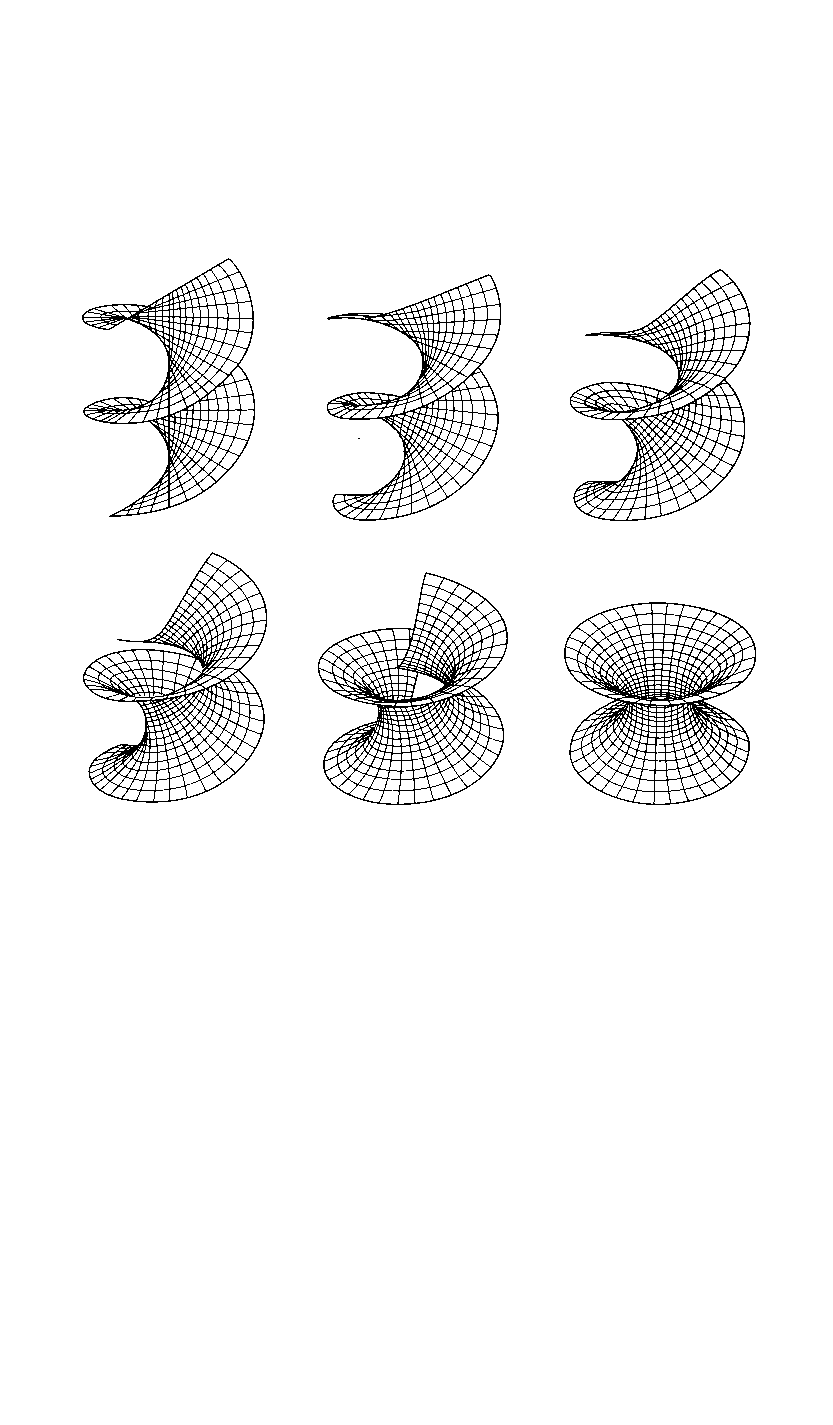
\includegraphics[scale=0.5]{figures/helicoid.pdf}
    \caption{A $1$-parameter family of minimal ($H=0$) isometric immersions of a surface connecting the helicoid (top left) to the catenoid (bottom right). From \cite{Spivak3}.}
    \label{fig:helicoid}
\end{figure}

\begin{example}[Helicoid]\label{ex helicoid}
    Let $a>0$ be a constant and consider the following map $\bf{x}:\bbR^2\to \bbR^3$:
    \[\bf{x}(s,t)=(s\cos t,s\sin t,at).\]
    Its image is called the \emph{helicoid}.\index{Helicoid} Note that the $z$-axis is contained in the surface, as is a horizontal line emanating out of each point on the $z$-axis, and this line rotates as we move up the $z$-axis.
    
    We now compute the first-order adapted frame $\frake:\bbR^2\to \bbE^3$ for the helicoid (as usual, we identify the surface with its domain in $\bbR^2$ under the parametrization). Note that 
    \begin{align}
        \bf{x}_s&=(\cos t,\sin t,0),\\
        \bf{x}_t&=(-s\sin t,s\cos t,a),
    \end{align}
    so $\bf{x}_s\perp \bf{x}_t$ and we may take 
    \begin{align}
        e_1&=\frac{\bf{x}_s}{\lVert\bf{x}_s\rVert}=(\cos t,\sin t,0), \notag\\
        e_2&=\frac{\bf{x}_t}{\lVert\bf{x}_t\rVert}=\frac{1}{\sqrt{s^2+a^2}}(-s\sin t,s\cos t,a),\label{eq 2.7 Ivey}\\
        e_3&=e_1\times e_2=\frac{1}{\sqrt{s^2+a^2}}(a\sin t,-a\cos t,s).\notag
    \end{align}
    Since $\dd\bf{x}=\bf{x}_s\dd s+\bf{x}_t\dd t=\frake^\ast(\theta^1)e_1+\frake^\ast(\theta^2)e_2$, we obtain (omitting $\frake^\ast$ from the notation from now on)
    \[\theta^1=\dd s,\quad \theta^2=\sqrt{s^2+a^2} \dd t.\label{eq 2.8 Ivey}\]
    Next, we calculate the Gauss map:
    \begin{multline}
        \dd e_3=\left(-s\left(s^2+a^2\right)^{-3/2}(a\sin t,-a\cos t,s)+(s^2+a^2)^{-1/2}(0,0,1)\right)\dd s+\\
        +(s^2+a^2)^{-1/2}(a\cos t,a\sin t,0)\dd t.
    \end{multline}
    So, using (\ref{eq 2.7 Ivey}) and (\ref{eq 2.8 Ivey}), we obtain 
    \[\omega_1^3=-a(s^2+a^2)^{-1}\theta^2,\quad \omega_2^3=-a(s^2+a^2)^{-1}\theta^1.\]
    The coefficients in front of $\theta^i$ are the principal curvatures $k_i$. We conclude that $H(s,t)=0$ and $K(s,t)=-\frac{a^2}{(s^2+a^2)^2}$. Thus, the helicoid is a umbilic-free minimal surface.
\end{example}

Being a union of disjoint straight lines, the helicoid is an example of a \emph{ruled} surface.

\begin{defn}[Flat, ruled, tangential developable surfaces]\index{Developable surface!see {Flat surface}}\index{Ruled surface}\index{Tangential surface}\index{Flat surface}
    A surface is called \emph{developable}, or simply \emph{flat}, if its Gauss curvature vanishes everywhere, $K\equiv 0$.

    A surface is called \emph{ruled} if every point of the surface is contained in it along with a segment of a straight line passing through that point, whose ends (if they exist) lie on the boundary of the surface.

    In particular, a surface $\Sigma\subset\bbE^3$ is said to be \emph{tangential developable} if it can be described as (a subset of) the union of tangent rays to a curve. (These surfaces are also called \emph{tangential surfaces}.)
\end{defn}
The following proposition clarifies what tangential surfaces look like.
\begin{prop}
    Let $\gamma:\bbR\to \bbE^3$ be a regular parametrized curve with curvature and torsion $\kappa$ and $\tau$, respectively, and consider the tangential surface $\bf{x}:\bbR\times \bbR_+\to \bbE^3$ defined by 
    \[\bf{x}:(u,v)\mapsto \gamma(u)+v\dot\gamma(u),\quad v>0.\]
    Then this surface has $H(u,v)=\frac{\tau(u)}{2\kappa(u)v}$ and $K\equiv 0$.
\end{prop}
\begin{proof}
    Since 
    \[\dd \bf{x}=(\dot\gamma(u)+v\ddot\gamma(u))\dd u+\dot\gamma(u)\dd v,\]
    we see that $\bf{x}$ is regular, i.e., $\dd f$ is of maximal rank, when $\ddot \gamma(u)$ is linearly independent from $\dot\gamma(u)$ and $v\neq 0$, i.e., exactly when $\gamma$ is regular. Now assume that $\gamma$ is parametrized by arclength. Then $\dot\gamma\perp\ddot\gamma$ and we can take $e_1(u,v)=\dot\gamma(u)$ and $e_2(u,v)=\ddot\gamma(u)/\lVert\ddot\gamma(u)\rVert$. Using $\dd \bf{x}=\theta^1e_1+\theta^2e_2$, we calculate 
    \[\theta^1=\dd u+\dd v,\quad \theta^2=v\kappa(u)\dd u.\]
    Note that this frame coincides with the Frenet frame of $\gamma$, so, following Example~\ref{ex serret-frenet}, we have 
    \[\dd e_3=-\tau(u)e_2\dd u.\]
    Therefore, 
    \[\omega_1^3=0,\quad \omega_2^3=\frac{\tau(u)}{\kappa(u)v}\theta^2,\]
    which leads to the asserted $H$ and $K$.
\end{proof}

\begin{rem}
    Not every ruled surface is flat (consider a single-sheet hyperboloid or the hyperbolic paraboloid $z=xy$ in $\bbR^3$). However, the converse does hold (aside from degenerate cases): if a given immersed surface has $K\equiv 0$, then one of the principal curvatures must be zero. Assume the other one isn't. Since line of curvature coordinates exist (see Example~\ref{ex Gauss curvature in orthogonal coords}), one of these coordinates, say $v$, will generate straight lines in $\Sigma$, making it ruled. The surface has to locally lie on one side of its tangent planes containing the $v$-lines and include the entire segments of these lines up to its boundary, otherwise the ends of the segment would be points of positive curvature. In summary, a surface is ruled iff it is flat. Hence, flat surfaces are identified with (pieces of) ``flat sheets of paper'' arbitrarily bent in $3$-dimensional space without stretching. 
    
    Note that these statements are particular to $3$ dimensions and fail already in $\bbE^4$ where, for example, the flat torus $\bbT^2$ can be isometrically embedded, whereas it is obviously not ruled by virtue of being compact with no boundary.
\end{rem}


\begin{example}[Catenoid]\label{ex catenoid}
    Let $a>0$ be a constant and consider the following map $\bf{x}:\bbR^2\to \bbR^3$:
    \[\bf{x}(u,v)=(a\cosh v\cos u,a\cosh v\sin u,av).\]
    Its image is called the \emph{catenoid}.\index{Catenoid}
    By choosing an adapted frame and differentiating one can compute that $H=0$, so this is a minimal surface. Now consider the map $f:\bbR^2\to \bbR^2$ given by
    \[f: (u,v)\mapsto (s,t)=(a\sinh v,u).\]
    One then shows that $f^\ast(K_{\mathrm{helicoid}})=K_{\mathrm{catenoid}}$, and of course the mean curvatures match as well. But while these two surfaces have the same $H$ and $K$, the helicoid is ruled, whereas the catenoid contains no line segments. Thus, they are not congruent.
\end{example}

Nevertheless, $H$ and $K$ are usually sufficient to determine $\Sigma$ up to congruence. Those surfaces for which this is not the case either have constant $H$ or belong to a finite-dimensional family called \emph{Bonnet surfaces}.

\begin{xca}
    A surface $\Sigma$ is called \emph{flat} if $K\equiv 0$. Show that if $\Sigma$ is flat, there exist local coordinates $x^1,x^2$ on it and an orthonormal frame $(e_1,e_2,e_3)$ such that $\theta^1=\dd x^1$, $\theta^2=\dd x^2$.
\end{xca}





\section{Codazzi equation}

Let us now derive the compatibility condition on $\sfh$ by setting up a Pfaffian system. Treat $\{h_{11},h_{12},h_{22}\}$ as coordinates in $\bigodot^2 \bbR^2\cong\bbR^3$ and define an \gls{eds} $\calI\subset \Omega^{\smbullet }(\SE_3\times \bbR^3)$ by
\[\calI\coloneqq \<\theta^3,\omega_1^3-h_{11}\theta^1-h_{12}\theta^2,\omega_2^3-h_{12}\theta^1-h_{22}\theta^2\>_{\mathrm{diff}}\]
with independence condition $\theta^1\wedge\theta^2\neq 0$.
From our above computations, we know that along the lift of any hypothetical surface $\Sigma$, this entire \gls{eds} must vanish. The independence condition means that $\theta^1\wedge\theta^2$ must produce a volume form after pullback to $\Sigma$. The integral manifolds of this system are graphs of immersions $\restr{P}{U}\to \SE_3$ that are adapted frame bundles of isometric immersions $\bf{x}:U\to \bbE^3$ satisfying $\bf{x}^\ast \rmI=\sfg$ and $\bf{x}^\ast \wt{Q}=\sfh$. By the Frobenius Theorem~\ref{thm 4.7.8 RS1}, the derivatives of the generators of $\calI$ must vanish modulo $\calI$ on $\Sigma$. First, it is easy to check that $\dd\theta^3\equiv 0 \pmod{\calI}$. The differentials of the other two forms can be combined into a column-vector and rewritten modulo $\calI$ using the definition of $\sfh$:
\begin{multline}
    \dd \left\{
        \begin{pmatrix}
            \omega_1^3\\\omega_2^3
        \end{pmatrix}
        -\sfh\cdot 
        \begin{pmatrix}
            \theta^1\\\theta^2
        \end{pmatrix}
    \right\}=\\
    =-\begin{pmatrix}
        0&-\omega_1^2\\
        \omega_1^2& 0
    \end{pmatrix}\wedge 
    \begin{pmatrix}
        \omega_1^3\\\omega_2^3
    \end{pmatrix}
    -\dd \sfh\wedge 
    \begin{pmatrix}
        \theta^1\\\theta^2
    \end{pmatrix}
    +\sfh \cdot\begin{pmatrix}
        0&-\omega_1^2\\
        \omega_1^2& 0
    \end{pmatrix}\wedge 
    \begin{pmatrix}
        \theta^1\\\theta^2
    \end{pmatrix} \equiv 
    \\
    \equiv
    -\begin{pmatrix}
        0&-\omega_1^2\\
        \omega_1^2& 0
    \end{pmatrix}\wedge \sfh\cdot
    \begin{pmatrix}
        \theta^1 \\ \theta^2
    \end{pmatrix}
    -\dd \sfh\wedge 
    \begin{pmatrix}
        \theta^1\\\theta^2
    \end{pmatrix}
    +\sfh\cdot \begin{pmatrix}
        0&-\omega_1^2\\
        \omega_1^2& 0
    \end{pmatrix}\wedge 
    \begin{pmatrix}
        \theta^1\\\theta^2
    \end{pmatrix}\pmod{\calI}.\label{eq I^1_taut structure}
\end{multline}
These derivatives must vanish along the integral manifolds. Thus, $\sfh$ must satisfy the \emph{Codazzi-Mainardi equation},\index{Equation!Codazzi-Mainardi} which we will call the Codazzi equation:
\[\boxed{\left\{\dd \sfh+\left[
\begin{pmatrix}
    0 & -\omega_1^2\\
    \omega_1^2 & 0
\end{pmatrix},\sfh
\right]\right\} \wedge 
\begin{pmatrix}
    \theta^1\\\theta^2
\end{pmatrix}=0,}\label{eq Gauss-Codazzi}
\]
where $[\,,\,]$ is the commutator of matrices. (Note that in this equation a pullback to the adapted frame bundle of a surface is implied, otherwise it holds only modulo $\calI$.)

The proof of Gauss' Theorema Egregium~\ref{thm egregium} showed that, given a metric $\sfg$ on $\Sigma$ and an orthonormal frame $\frake$, $\frake^\ast \omega_1^2$ is uniquely determined. Thus, (\ref{eq Gauss-Codazzi}) is a system of equations for the possible fundamental forms $\rmII=h_{ij}\theta^i\otimes \theta^j\otimes e_3$ for embdeddings of $\Sigma$ into $\bbE^3$ that induce the metric $\sfg$. These equations are well-defined, since (\ref{eq Gauss-Codazzi}) is invariant under changes of the frame $\frake$. Thus, the Frobenius theorem guarantees existence, while uniqueness up to a rigid motion is guaranteed only for a fixed parametrization.

\begin{thm}[Bonnet's Fundamental Theorem of Surfaces]\index{Theorem!Bonnet's Fundamental Theorem}
    Let $U$ be an open domain in $\bbR^2$. Two parametric surfaces $\bf{x},\wt{\bf{x}}:U\to \bbE^3$ are congruent (via an element of $\SE_3$) iff they have the same first and second fundamental forms at corresponding points:
    \[\bf{x}^\ast\rmI=\wt{\bf{x}}^\ast \wt{\rmI},\quad \bf{x}^\ast\rmII=\wt{\bf{x}}^\ast \wt{\rmII}.\] 
    Moreover, if $\sfg$ and $\sfh$ are given quadratic forms on $U$ satisfying the Gauss-Codazzi equations with $\sfg$ positive definite, then there exists an immersion $\bf{x}:U\to \bbE^3$ such that $\bf{x}^\ast  \rmI=\sfg$ and $\bf{x}^\ast  \wt{Q}=\sfh$.
\end{thm}
Note that the immersion $\bf{x}$ needs to be specified to claim uniqueness up to congruence. If only $K$ and $H$ are given, the surface cannot be reconstructed uniquely, as we saw above.
\begin{proof}
    First we show uniqueness. Let $\bf{x}:U\to \bbE^3$ be given. Then, by following the above construction, we define the adapted frame bundle $\pi:P\to U$ consisting of triples $(p,e_1,e_2)$ where $(e_1,e_2)$ are $\rmI$-orthonormal bases for $\T_p U$. There are unique $1$-forms $\theta^1,\theta^2,\omega_1^2$ such that 
    \[\pi_\ast(X)=e_1\theta^1(X)+e_2\theta^2(X),\quad X\in \T_{(p,e_1,e_2)}P,\]
    and
    \[\dd\theta^1=\omega_1^2\wedge \theta^2,\quad \dd\theta^2=-\omega_1^2\wedge\theta^1.\]
    Then 
    \[\pi^\ast\rmI=\sum_{\mu=1}^2\theta^\mu\otimes\theta^\mu,\quad \pi^\ast \wt{Q}=\sum_{\mu,\nu=1}^2 h_{\mu\nu}\theta^\mu\otimes\theta^\nu\]
    with some uniquely determined functions $h_{\mu\nu}$ such that $h_{12}=h_{21}$. Now we define $\omega_1^3\coloneqq h_{11}\theta^1+h_{12}\theta^2$ and $\omega_2^3\coloneqq h_{12}\theta^1+h_{22}\theta^2$. Then, as we saw above, $\frake\coloneqq(\bf{x}_u,\bf{x}_v,\bf{x}_u\times \bf{x}_v)$ must satisfy 
    \[\dd \begin{pmatrix}
        \frake & \bf{x}\\
        0& 1
    \end{pmatrix}=\begin{pmatrix}
        \frake & \bf{x}\\
        0& 1
    \end{pmatrix}
    \begin{pmatrix}
        0 & -\omega_1^2 & -\omega_1^3& \theta^1\\
        \omega_1^2 & 0 & -\omega_2^3 & \theta^2\\
        \omega_1^3 & \omega_2^3 & 0 & 0\\
        0 & 0& 0& 0
    \end{pmatrix}.
    \]
    Then the $4\times 4$ matrix on the right takes values in the Lie algebra $\frakse_3$, and Cartan's Fundamental Theorem~\ref{thm 6.1 Sharpe fundamental local} guarantees the uniqueness of the map $\left(\begin{smallmatrix}
        \frake & \bf{x}\\
        0& 1
    \end{smallmatrix}\right): U\to \SE_3$ up to a left multiplication by an element of $\SE_3$, which is what a congruence is.

    Existence follows from the existence part of Cartan's Fundamental Theorem, since the Gauss-Codazzi equations are equivalent to the structure equation for the function $\left(\begin{smallmatrix}
        \frake & \bf{x}\\
        0& 1
    \end{smallmatrix}\right)$.
\end{proof}

\begin{rem}
    We can put the Gauss-Codazzi equations in an even more suggestive form by splitting up the components of all objects into tangent and normal to $\Sigma$. Let Greek indices range only over tangent directions ($1,2$), and this time we will be careful to put the row (top) index before the column (bottom) index in $\omega^i{}_j$. Then we have the two defining equations on the adapted frame bundle $P$:
    \[\dd e_\mu=e_3\omega^3{}_\mu + e_\nu\omega^\nu{}_\mu,\quad \dd e_3=e_\mu\omega^\mu{}_3.\]
    By definition of $h$ (\ref{def h}), we have $\omega^3_\mu=h_{\mu\nu}\omega^\nu$, and therefore the system becomes 
    \[\dd e_\mu= e_3 h_{\mu\nu}\omega^\nu+ e_\nu\omega^\nu{}_\mu ,\quad \dd e_3=e_\mu\omega^\mu{}_3.\]
    The Frobenius compatibility conditions for these two equations are $\dd^2 e_\mu=0$ and $\dd^2 e_3=0$. We expand the first one, use $\dd e_3=e_\mu\omega^\mu{}_3$, and collect terms containing the same basis vector:
    \[0=\dd^2e_\mu=e_3\left(\dd \omega^3{}_\mu-\omega^\nu{}_\mu\wedge\omega^3{}_\nu\right)
    +e_\nu\left(\dd\omega^\nu{}_\mu+\omega^\nu{}_\lambda\wedge\omega^\lambda{}_\mu+\omega^\nu{}_3\wedge\omega^3{}_\mu\right),
    \]
    which is equivalent to the pair of equations 
    \begin{align}
        \dd\omega^3{}_\mu-\omega^\lambda{}_\mu\wedge\omega^3{}_\lambda&=0,\\
        \dd\omega^\nu{}_\mu-\omega^\lambda{}_\mu\wedge\omega^\nu{}_\lambda&=-\omega^\nu{}_3\wedge \omega^3{}_\mu.
    \end{align}
    It is easy to check that these equations also imply the second compatibility condition, $\dd^2 e_3=0$. 
    
    By putting $b_\mu\coloneqq \omega^3{}_\mu=-\omega^\mu{}_3\eqqcolon-b^\mu$ and $\Gamma^\nu{}_\mu\coloneqq \omega^\nu{}_\mu$, we get the defining equations
    \[\begin{cases}
        \dd e_\mu=b_\mu e_3+\Gamma^\nu{}_\mu e_\nu, &\\
        \dd e_3=b^\mu e_\mu, &\text{(Weingarten)}
    \end{cases}\label{3791}\]
    and the compatibility conditions for them are
    \begin{align}
        \dd b_\mu-\Gamma^\lambda{}_\mu \wedge b_\lambda&=0 &\text{(Codazzi),}\\
        \dd \Gamma^\nu{}_\mu-\Gamma^\lambda{}_\mu\wedge\Gamma^\nu{}_\lambda&=-b^\nu\wedge b_\mu &\text{(Gauss).}
    \end{align}
    Note that the right hand side of the Gauss equation is exactly $K \omega^\nu\wedge\omega^\mu$ since $b_\mu=h_{\mu\nu}\omega^\nu$ and $K=\det h$. Thus, if these Gauss-Codazzi equations are satisfied by the second fundamental form $b_\mu$, then the defining equations (\ref{3791}) can be uniquely solved for $(e_1,e_2,e_3)$ (with some initial condition), providing a map into the orthonormal frame bundle over $\bbE^3$, and hence an isometric immersion into $\bbE^3$. In time we will identify $\Gamma^\nu{}_\mu$ with the components of a (Levi-Civita) connection on the surface and $b_\mu$ with the components of a connection on its normal bundle.
\end{rem}




\section{\texorpdfstring{\gls{eds}}{EDS} for surfaces}


In this \sect\ we put the above discussion in terms of the theory of \glspl{eds} developed in the preceding \chap, and consider some related examples of geometric \glspl{eds}. First let us define the simple \emph{tautological} \gls{eds} for immersed surfaces in $\bbE^3$. This is the Pfaffian system on the orthonormal bundle $\SE_3$ generated by the single form $\theta^3$:
\[\calI_{\mathrm{taut}}=\<\theta^3\>_{\mathrm{diff}}.\]
Any $2$-dimensional integral manifold is locally described by some function $(\bf{x},\frake)$, where $\frake$ is an orthonormal frame at $\bf{x}$. The vanishing of $\theta^3$ along the integral manifolds implies that $\dd \bf{x}=e_1\theta^1+e_2\theta^2$, which is exactly the statement that the image of $(\bf{x},\frake)$ is consists of first-order adapted frames of the surface parametrized by $\bf{x}$. Thus, $3$-dimensional integral manifolds of this system are exactly the bundles of adapted frames of immersed surfaces. The following example establishes that this system is not involutive.

\begin{example}[Involutivity of $\calI_{\mathrm{taut}}$]
    The structure equation is $\dd\theta^3=\omega^3_i\wedge\dd\theta^i$, so $(s_1,s_2,s_3)=(1,0,0)$. A coframe for a bundle of adapted frames is given by $\theta^1,\theta^2,\omega^2_1$, and the remaining directions on $\SE_3$ are $\omega^3_1,\omega^3_2,\theta^3$. Thus, integral elements are parametrized by linear equations of the form 
    \[
    \begin{pmatrix}
        \omega^3_1\\
        \omega^3_2\\
        \theta^3
    \end{pmatrix}=
    \begin{pmatrix}
        a & b & e \\
        c & d & f \\
        0 & 0 & 0
    \end{pmatrix}
    \begin{pmatrix}
        \theta^1\\\theta^2\\\omega^2_1
    \end{pmatrix},
    \]
    subject to $0=\dd\theta^3=(b-c)\theta^1\wedge\theta^2+e\omega^2_1\wedge\theta^1+f\omega^2_1\wedge\theta^2$, so $b=c$ and $e=f=0$. Thus, the space of $3$-dimensional integral elements at a point is of dimension $3$, and $3>s_1+2s_2+3s_3=1$, so the system is not involutive.
\end{example}

Another way to see that this system is not involutive is to notice that it has a Cauchy characteristic that corresponds to locally rotating the tangent frames $(e_1,e_2)$. In other words, the system has an angular ``dummy variable'' whose presence forbids the uniqueness of integral manifolds, necessary for the Cartan-K\"ahler Theorem to work. The following example shows this in detail.

\begin{example}[Cauchy characteristics of $\calI_{\mathrm{taut}}$]\label{ex 7.1.10 Ivey}
    The system $\calI_{\mathrm{taut}}$ admits a Cauchy characteristic vector field as follows.

    Let $\{E_j,E^i_j\}$ be a global frame for $\T P$ dual to the one given by the entries of the Maurer-Cartan form $\{\theta^j,\omega^i_j\}$. Expand $X=X^jE_j+X^j_i E^i_j$. Then $i_X\theta^3=0$ implies that $X_3=0$ and 
    \[i_X \dd\theta^3=i_X(-\omega^3_1\wedge\theta^1-\omega^3_2\wedge\theta^2)=X_1\omega^3_1-X^1_3\theta^1+X_2\omega^3_2-X^2_3\theta^2\]
    implies that $X=X^1_2 E^2_1$. We can pick $X=E^2_1$, which generates rotations of the frame in the $\{e_1,e_2\}$-plane. Now, Proposition~\ref{prop 7.1.8 Ivey} implies that any integral surface for $\calI$ may be ``thickened'' to an integral $3$-manifold using the Cauchy characteristic.

    Now, $\calC(\calI)$ is the Frobenius system on $\SE_3$ spanned by $\theta^1,\theta^2,\theta^3,\omega^3_1,\omega^3_2$. Integral curves of $\calC(\calI)$ form a foliation of $\SE_3$. The leaf space for this foliation is a 5-dimensional homogeneous space which we identify with $\bbS(\T\bbE^3)$, the unit sphere bundle of the tangent bundle of $\bbE^3$, by letting $m$ be the basepoint and $e_3$ the unit vector in $\T_m\bbE^3$.\index{Sphere bundle}
\end{example}

The surface $\Sigma$ can be described by the restrictions of the forms $\theta^1,\theta^2$ to its bundle of adapted frames $P\subset \SE_3$. To find out whether these data are sufficient to recover the shape of $\Sigma$, it makes sense to set up another \gls{eds} $\calI_\Sigma$ on $P\times\SE_3$ that \emph{compares} two different sets of forms, namely the Pfaffian system generated by the $1$-forms 
\[\begin{pmatrix}
    \vartheta_1\\\vartheta_2\\\vartheta_3
\end{pmatrix}\coloneqq 
\begin{pmatrix}
    \wt\theta^1-\theta^1\\
    \wt\theta^2-\theta^2\\
    \wt\theta^3
\end{pmatrix},
\]
where $\wt\theta^i$ are the standard forms on $\SE_3$ and $\theta^i$ are the fixed forms on $P$ (we omit pullbacks of both to $P\times\SE_3$). Along $P$, all of these forms vanish, while the $1$-forms $\theta^1,\theta^2,\omega^2_1$ form a coframe. Conversely, we will eventually prove that all integral manifolds with this coframe are locally frame bundles of isometric immersions of $\Sigma$. For the moment, we concentrate on asking whether we can apply the Cartan-K\"ahler Theorem.

\begin{example}[Cartan's Test for $\calI_\Sigma$]
    First we compute the tableau:
    \[\dd \begin{pmatrix}
        \vartheta_1\\\vartheta_2\\\vartheta_3
    \end{pmatrix}
    =-\begin{pmatrix}
        0 & \wt\omega^2_1-\omega^2_1 & 0\\
        \boxed{-(\wt\omega^2_1-\omega^2_1)} & 0 & 0\\
        \boxed{\wt\omega^3_1} & \boxed{\wt\omega^3_2} & 0
    \end{pmatrix}\wedge 
    \begin{pmatrix}
        \vartheta_1\\\vartheta_2\\\vartheta_3
    \end{pmatrix} \pmod{\vartheta^1,\vartheta^2,\vartheta^3}.
    \]
    We have $(s_1,s_2,s_3)=(2,1,0)$. Each $3$-dimensional integral element has $\wt\theta^i=\theta^i$, so is determined by the linear equations relating $\wt\omega^i_j$ to $\theta^1,\theta^2,\omega^2_1$ such that $\dd\vartheta^i=0$:
    \[\begin{pmatrix}
        \wt\omega^3_1\\
        \wt\omega^3_2\\
        \wt\omega^2_1-\omega^2_1
    \end{pmatrix}=
    \begin{pmatrix}
        \wt h_{11} & \wt h_{12} & 0\\
        \wt h_{12} & \wt h_{22} & 0\\
        0 & 0 & 0
    \end{pmatrix}
    \begin{pmatrix}
        \theta^1\\\theta^2\\\omega^2_1
    \end{pmatrix}.\label{eq 12942}
    \]
    Therefore, there is a $3$-dimensional space of integal elements at each point. But $s_1+2s_2=4>3$, so involution fails and we can't apply the Cartan-K\"aher Theorem, and prolongation is necessary. Another way to see this is to check whether the generic integral line sits in an integral plane. The equations on integral lines are $\wt\theta^1=\theta^1$, $\wt\theta^2=\theta^2$, $\wt\theta^3=0$. On any integral plane $\wt\omega^2_1=\omega^2_1$. The generic integral line does not sit in an integral plane because it doesn't have to satisfy $\wt\omega^2_1=\omega^2_1$.
\end{example}

The procedure in the last \sect\ where we adjoined the Second Fundamental Form to the system as an indepedent variable is in fact exactly the \emph{first prolongation} of $\calI_{\mathrm{taut}}$. We also call the resulting system the tautological system on $\SE_3\times\bbR^3_{h_{ij}}$ for surfaces in $\bbE^3$. The integral manifolds of this system are still the first-order adapted lifts of arbitrary surfaces in $\bbR^3$, together with the components of the second fundamental form $\{h_{ij}\}$, which we view as coordinates of another space $\bbR^3$. This Pfaffian system $\calI^{(1)}_{\mathrm{taut}}=\<I\>_{\mathrm{diff}}$ is generated by 
\[\begin{pmatrix}
    \vartheta^1\\
    \vartheta^2\\
    \vartheta^3
\end{pmatrix}=
\begin{pmatrix}
    \omega^3_1-h_{1\mu}\theta^\mu\\
    \omega^3_2-h_{2\mu}\theta^\mu\\
    \theta^3
\end{pmatrix}.\]
The next example directly verifies, for this particular system, the by now familiar fact that the prolongation of an involutive system is involutive. 

\begin{example}[Involutivity of $\calI^{(1)}_{\mathrm{taut}}$]
    Then (\ref{eq I^1_taut structure}) reads
    \begin{align}
        \dd \begin{pmatrix}
            \vartheta^1\\
            \vartheta^2\\
            \vartheta^3
        \end{pmatrix}
        \equiv& \begin{pmatrix}
            2h_{12}\omega^2_1-\dd h_{11} & (h_{22}-h_{11})\omega^2_1-\dd  h_{11}\\
            (h_{22}-h_{11})\omega^2_1-\dd h_{12} & -2h_{12}\omega^2_1-\dd h_{22}\\
            0 & 0\\
        \end{pmatrix}\wedge 
        \begin{pmatrix}
            \theta^1\\
            \theta^2
        \end{pmatrix}\pmod{I} \notag \\
        \eqqcolon& 
        \begin{pmatrix}
            \pi^1_1 & \pi^1_2\\
            \pi^2_1 & \pi^2_2\\
            \pi^3_1 & \pi^3_2
        \end{pmatrix}\wedge 
        \begin{pmatrix}
            \theta^1\\
            \theta^2
        \end{pmatrix}\pmod{I}.
    \end{align}
    The symbol relations are 
    \[\pi^3_1\equiv \pi^3_2\equiv \pi^2_1-\pi^1_2\equiv 0\pmod{I}.\]
    There is no intrinsic torsion, and $(s_1,s_2)=(2,1)$. Integral elements are given by 
    \begin{align}
        \pi^1_1&=a\theta^1+b\theta^2,\notag\\
        \pi^1_2&=\pi^2_1=b\theta^1+c\theta^2,\notag\\
        \pi^2_2&=c\theta^1+e\theta^2,\notag\\
        \pi^3_1&=\pi^3_2=0,
    \end{align}
    where $a,b,c,e$ are arbitrary. Thus, $\dim A^{(1)}=4=s_1+2s_2$, and the system is involutive. The Cartan-K\"ahler Theorem implies that integral manifolds depend on one function of two variables. This is expected since locally any surface is a graph of a function $z=f(x,y)$. 
    
    Finally, we observe that the Codazzi equation is exactly the structure equation for this system pulled back to an integral surface, and the Gauss equation is similarly the pullback of $\dd\omega^2_1\equiv- K\theta^1\wedge\theta^2\pmod{\calI_{\mathrm{taut}}^{(1)}}$.
\end{example}

Finally, to compute the differential invariants of $\Sigma$, we should prolong $\calI_\Sigma$ and check involutivity. This means that we need to treat $\wt{h}_{ij}$ as new independent variables and turn (\ref{eq 12942}) into the condition for the vanishing of three new generating $1$-forms:
\[
    \begin{pmatrix}
        \vartheta_4\\
        \vartheta_5\\
        \vartheta_6
    \end{pmatrix}\coloneqq 
    \begin{pmatrix}
        \wt\omega^3_1\\
        \wt\omega^3_2\\
        \wt\omega^2_1-\omega^2_1
    \end{pmatrix}=
    \begin{pmatrix}
        \wt h_{11} & \wt h_{12} & 0\\
        \wt h_{12} & \wt h_{22} & 0\\
        0 & 0 & 0
    \end{pmatrix}
    \begin{pmatrix}
        \theta^1\\\theta^2\\\omega^2_1
    \end{pmatrix}.
\]
Note that $\dd\vartheta_i\equiv 0\pmod{\vartheta_4,\vartheta_5,\vartheta_6}$ for $i=1,2,3$, so we can omit them in the analysis. 
\[\dd \begin{pmatrix}
    \vartheta_4\\
    \vartheta_5\\
    \vartheta_6
\end{pmatrix} \equiv 
-\begin{pmatrix}
    \boxed{D\wt{h}_{11}} & D\wt{h}_{12} & 0\\
    \boxed{D\wt{h}_{12}} & \boxed{D\wt{h}_{22}} & 0\\
    0 & 0 & 0
\end{pmatrix}\wedge 
\begin{pmatrix}
    \theta^1\\\theta^2\\\omega^2_1
\end{pmatrix}
+\begin{pmatrix}
    0 \\ 0\\ t\theta^1\wedge\theta^2
\end{pmatrix}\pmod{\vartheta_1,\ldots,\vartheta_6},
\]
where 
\[\begin{pmatrix}
    D\wt{h}_{11}\\
    D\wt{h}_{12}\\
    D\wt{h}_{22}
\end{pmatrix}
\coloneqq 
\begin{pmatrix}
    \dd\wt{h}_{11} +2\wt{h}_{12}\omega^2_1+a \theta^1+b\theta^2\\
    \dd\wt{h}_{12}+(\wt{h}_{11}-\wt{h}_{22})\omega^2_1+b\theta^1+c\theta^2\\
    \dd\wt{h}_{22}+2\wt{h}_{12}\omega^2_1+c\theta^1+d\theta^2
\end{pmatrix},
\]
with $a,b,c,d$ arbitrary, and the torsion is 
\[t\coloneqq \det \wt{h}-\det h=\det\wt h-K.\]
This torsion clearly has to vanish on any $3$-dimensional integral element of $\calI^{(1)}_\Sigma$, i.e., every such element lives over the subset of $M=P\times\SE_3$ on which $K=\det\wt h$. To ensure that this subset is a submanifold, we let $M'\subset M$ be the set of points where this equation is satisfied and at least one of $\wt{h}_{ij}$ is not zero. Clearly $M'\subset M$ is a submanifold, on which we find $D\wt h_{ij}$ linearly independent. On $M'$ we have
\[
    \dd \begin{pmatrix}
        \vartheta_4\\
        \vartheta_5\\
        \vartheta_6
    \end{pmatrix} \equiv 
    -\begin{pmatrix}
        \boxed{D\wt{h}_{11}} & D\wt{h}_{12} & 0\\
        \boxed{D\wt{h}_{12}} & D\wt{h}_{22} & 0\\
        0 & 0 & 0
    \end{pmatrix}\wedge 
    \begin{pmatrix}
        \theta^1\\\theta^2\\\omega^2_1
    \end{pmatrix}\pmod{\vartheta_1,\ldots,\vartheta_6},
\]
so $(s_1,s_2,s_3)=(2,0,0)$. There are $2$ dimensions of integral elements (down from $3$ due to Gauss' equation $K=\det\wt{h}_{ij}$), so we have involution. This confirms again that $\wt{h}$ contains the full set of differential invariants.

The next two examples are adapted from Cartan's 1945 treatise \cite{cartan45}.
\begin{example}[Linear Weingarten surfaces]\label{ex Weingarten surfaces}
    Let $A,B,C\in\bbR$ with $A\neq 0$, and let $AK+2BH+C=0$ be a linear relation between functions $H,K$. We will now set up the space of general integral manifolds for first-order adapted liftings of surfaces in $\bbR^3$, together with the components of the second fundamental form, having Gauss and mean curvatures satisfying this relation.

    This is the system above restricted to a codimension one submanifold $M\subset \SE_3\times \bbR^3_{h_{ij}}$. The submanifold is defined by the equation 
    \[A(h_{11}h_{22}-h_{12}^2)+B(h_{11}+h_{22})+C=0.\]
    The differential of this equation implies that on $M$ we may write 
    \[\dd h_{12}=\alpha d h_{11}+\beta dh_{22}\]
    for some functions $\alpha,\beta$, and thus 
    \[\pi^1_2=\alpha\pi^1_1+\beta\pi^2_2.\]
    We still have no intrinsic torsion and have characters $(s_1,s_2)=(2,0)$.  This is automatically involutive because any tableau with characters $(s_1,\ldots,s_{n-1},s_n)=(s,\ldots,s,0)$, where $s=\dim W$, is involutive. Solutions depend on two functions of one variable. This suggests that an appropriate Cauchy problem for determining such surfaces would be to start out with a space curve (the two functions being its curvature and torsion) and then solve for a unique surface containing the curve. Cartan carries out this construction explicitly in his treatise \emph{Les Syst\`emes Ext\'erieurs et leurs Applications G\'eom\'etriques}.
\end{example} 

\begin{example}[Conformally equivalent surfaces]
    Let $(\Sigma,\sfg)$ and $(\wb\Sigma,\wb \sfg)$ be analytic Riemannian surfaces. We set up and solve the \gls{eds} for maps $\phi:\Sigma\to \wb \Sigma$ that preserve the metric up to (point-dependent) scale, i.e., for \emph{conformal} maps.

    Let $P=\Fr_{\SO_2}(\T^\ast \Sigma)$ denote the orthonormal coframe bundle of $\Sigma$, with coframe $\{\theta^1,\theta^2,\omega^2_1=-\omega^1_2\}$ satisfying $\dd\theta^i=-\omega^i_j\wedge \theta^j$ as usual. Similarly, let $\wb P$ denote the orthonormal coframe bundle of $\wb\Sigma$ with coframe $\{\wb\theta^1,\wb\theta^2,\wb\omega^2_1\}$. The metric on $\Sigma$ is given by the pullback of $(\theta^1)^2+(\theta^2)^2$ (tensor squares) along any section $s:\Sigma\to P$, and that on $\wb P$ by the pullback of $(\wb\theta^1)^2+(\wb\theta^2)^2$. Thus, a conformal map $\phi:\Sigma\to \wb\Sigma$ induces  a map $\Phi:P\to \wb P$ such that $\Phi^\ast \left((\wb\theta^1)^2+(\wb\theta^2)^2\right)=\lambda^2 \left((\theta^1)^2+(\theta^2)^2\right)$ for some positive function $\lambda>0$.

    \gls{wlog}, we may require that $\Phi^\ast\theta^j=\lambda\omega^j$ because we have freedom to rotate in the tangent spaces at each point. So on $M\coloneqq P\times \wb P\times \bbR_\lambda$, $\lambda>0$, let 
    \begin{align}
        I&=\<\vartheta^1\coloneqq \theta^1-\lambda\wb\theta^1,\vartheta^2\coloneqq \theta^2-\lambda\wb\theta^2\>,\\
        J&=\<\vartheta^1,\vartheta^2,\theta^1,\theta^2,\omega^2_1\>=\<\vartheta^1,\vartheta^2,\wb\theta^1,\wb\theta^2,\wb\omega^2_1\>.
    \end{align}
    We compute 
    \begin{align}
        \dd \vartheta^1 &= -\omega^1_2\wedge \theta^2-\dd\lambda\wedge\theta^1+\lambda\wb\omega^1_2\wedge\wb\theta^2,\\
        \dd\vartheta^2&=-\omega^2_1\wedge\theta^1-\dd\lambda\wedge\theta^2+\lambda\wb\omega^2_1\wedge \wb\theta^1.
    \end{align}
    Reducing modulo $I$, we obtain 
    \[\dd\begin{pmatrix}
        \vartheta^1\\
        \vartheta^2
    \end{pmatrix}
    \equiv 
    \begin{pmatrix}
        \boxed{-\lambda^{-1}\dd\lambda} & -(\wb\omega^2-\omega^2_1) & 0\\
        \boxed{\wb\omega^2_1 -\omega^2_1} & -\lambda^{-1}\dd\lambda & 0
    \end{pmatrix}
    \wedge 
    \begin{pmatrix}
        \theta^1\\\theta^2\\\omega^2_1
    \end{pmatrix}.
    \]
    Since $-\lambda^{-1}\dd\lambda$ and $\wb\omega^2_1-\omega^2_1$ are independent modulo $J$, there is no intrinsic torsion, and $(s_1,s_2)=(2,0)$, so the tableau is involutive. Solutions depend on two functions of one variable. We may make this dependence explicit as follows.

    Specify parametrized curves $\gamma:\bbR\to \Sigma$ and $\wb\gamma:\bbR\to \wb\Sigma$ and look for conformal maps $\phi$ such that $\phi\circ \gamma=\wb\gamma$. The claim is that up to constants there is a unique such map. In fact, choose an orthonormal frame $e_1,e_2$ on $\Sigma$ such that $e_1$ is tangent to $\gamma(\bbR)$, and adapt similarly on $\wb\Sigma$. Set $\lambda=\dot{\bar\gamma}/\dot\gamma$, then the map is uniquely determined up to constants.

    Conformal maps are exactly the injective holomorphic and anti-holomorphic maps between surfaces (using the complex structures induced by the metric). These are determined by their restriction to an arc, so picking parametrized arcs determines a holomorphic or anti-holomorphic map. Even without knowing the coincidence of Lie groups $\GL_1(\bbC)\cong\CO_2$, one might have guessed this by observing that the tableau above is the same as that of the Cauchy-Riemann equations, augmented with zeros.
\end{example}

By taking $\wb\Sigma=\bbR^2$ with the standard flat metric in the last example, we get the following statement.

\begin{cor}[Korn-Lichtenstein]\label{cor isothermal coords}\index{Theorem!Korn-Lichtenstein}
    Let $\Sigma$ be a surface with an analytic Riemannian metric $\sfg$ and let $m\in\Sigma$. Then there exist local coordinates $(x,y)$ centered at $m$ such that $\sfg=\lambda^2(\dd x^{\otimes 2}+\dd y^{\otimes 2})$, $\lambda\neq 0$, in some neighborhood of $m$. Such coordinates are called \emph{isothermal} and are unique up to isometry. \index{Isothermal coordinates}
\end{cor}

Isothermal coordinates do not usually exist on Riemannian manifolds of dimension $3$ and higher.
Note that isothermal coordinates allow us to construct canonical parametrizations of $\Sigma$ that are \emph{conformally orthonormal}, i.e., the corresponding coordinate vector fields $\partial_x,\partial_y$ are orthonormal only up to an overall scale. This limitation explains why the Fundamental Theorem of Surfaces required a fixed parametrization to guarantee uniqueness of the immersion: there is no natural orthonormal coordinate system on a curved surface. In contrast, immersed curves always have the unique arclength parameter that produces an orthonormal tangent vector, which removes the freedom of reparametrization.

\begin{defn}[Conformal structure]\index{Conformal structure}
    Two (pseudo-)Riemannian metrics $\sfg,\wt\sfg$ on a manifold $M$ are called \emph{conformally equivalent} if there exists a smooth function $\lambda\neq 0$ such that $\wt\sfg=\lambda^2 \sfg$. A conformal structure on a manifold $M$ is a conformal equivalence class of metrics $[\sfg]$.
\end{defn}

Crucially, the metric $\sfg$ on a surface cannot be recovered just from its conformal factor $\lambda^2$ in isothermal coordinates. In other words, not any two metrics on a surface are locally conformally equivalent. In the next example we characterize the intrisic information contained in $\lambda^2$.

\begin{example}[Liouville equation]\index{Equation!Liouville}
    Surfaces with given Gauss curvature have an especially simple description in isothermal coordinates. If the metric (i.e., First Fundamental Form) is $\sfg=\lambda^2(\dd x^{\otimes 2}+\dd y^{\otimes 2})$, then, by (\ref{eq K in orthogonal coords}) with $E=G=\lambda^2$,
    \[K=-\frac{1}{\lambda^2}\left(\left(\frac{\lambda_x}{\lambda}\right)_x+\left(\frac{\lambda_y}{\lambda}\right)_y \right)=-\frac{1}{\lambda^2}(\partial_x^2+\partial_y^2)\ln\lambda.\label{eq K in isothermal coords}\]
    In particular, when $K$ is constant, the conformal factor $\varphi\coloneqq \ln\lambda$ satisfies the \emph{Liouville equation}:
    \[\Delta_0 \varphi+K\rme^{\varphi}=0,\label{eq liouville general}\]
    where $\Delta_0=\partial_x^2+\partial_y^2$ is the ``flat'' Laplace operator.
\end{example}

Thus, $\lambda^2$ and $K$ contain the same local information about the metric (up to the necessary boundary conditions that guarantee a unique solution of Liouville's equation). The rest of the information about the metric, namely the conformal structure, is contained in the isothermal coordinates themselves. We will later identify this information with a \emph{complex structure} on the surface.

We can also obtain the following useful formula for the mean curvature in isothermal coordinates. Since the mean curvature is not intrinsic, we need to assume a fixed isometric immersion $\bf{x}:\Sigma\to \bbE^3$.
\begin{prop}\label{prop mean curvature laplace}
    Let $\bf{x}=\bf{x}(x,y)$ be a surface parametrized by isothermal coordinates $(x,y)$ such that the metric is $\lambda^2((\dd x)^2+(\dd y)^2)$. Let $e_3$ be the unit normal vector (Gauss map) of $\Sigma$. Then 
    \[H e_3=\frac{1}{\lambda^2}\left(\bf{x}_{xx}+\bf{x}_{yy}\right).\]
\end{prop}
\begin{proof}
    Since $\bf{x}(x,y)$ is isothermal, $\<\bf{x}_x,\bf{x}_x\>=\<\bf{x}_y,\bf{x}_y\>$ and $\<\bf{x}_x,\bf{x}_y\>=0$. By differentiation, 
    \[\<\bf{x}_{xx},\bf{x}_x\>=\<\bf{x}_{yx},\bf{x}_y\>=-\<\bf{x}_x,\bf{x}_{yy}\>.\]
    Thus, 
    \[\<\bf{x}_{xx}+\bf{x}_{yy},\bf{x}_x\>=0.\]
    Similarly, 
    \[\<\bf{x}_{xx}+\bf{x}_{yy},\bf{x}_y\>=0.\]
    It follows that $\bf{x}_{xx}+\bf{x}_{yy}$ is parellel to $e_3$. Since $\bf{x}$ is isothermal, from (\ref{eq hopf differential components})
    \[H=\frac{1}{2}\frac{g+e}{\lambda^2}.\]
    Thus,
    \[2\lambda^2 H=g+e=\<e_3,\bf{x}_{xx}+\bf{x}_{yy}\>,\]
    and the result follows.
\end{proof}


\begin{example}[Minimal surfaces with given curvature]
    For simplicity, assume no umbilic points and use Darboux framings. On the orthonormal frame bundle $P\to \bbE^3$ let $K(\bf{x})$ be a given function which will be the curvature and let $k(\bf{x})=\sqrt{-K(\bf{x})}$ be the positive square root.

    Let $I=\<\theta^3,\theta^3_1,\theta^3_2\>$ and $J=\<\theta^3,\theta^3_1,\theta^3_2,\theta^1,\theta^2\>$, where we set $\theta^3_1=\omega^3_1-k\theta^1$ and $\theta^3_2=\omega^3_2+k\theta^2$. The structure equation modulo $I$ is 
    \[\dd\begin{pmatrix}
        \theta^3\\\theta^3_1\\\theta^3_2
    \end{pmatrix}\equiv 
    \begin{pmatrix}
        0 & 0\\
        -dk & -2k\omega^2_1\\
        -2k\omega^2_1 & dk
    \end{pmatrix}
    \wedge \begin{pmatrix}
        \theta^1\\\theta^2
    \end{pmatrix}.
    \]
    Write $\dd k=k_1\theta^1+k_2\theta^2$. The symbol relations are  (all modulo $I$)
    \begin{align}
        \pi^0_1\equiv \pi^0_2\equiv& 0 \notag\\
        \pi^2_1-\pi^1_2\equiv& 0\notag\\
        \pi^1_1+\pi^2_2\equiv& 0\notag\\
        \pi^1_1\equiv& k_1\theta^1+k_2\theta^2.
    \end{align}
    We can change bases to attempt to absorb the apparent torsion. If we rewrite our equations as 
    \[\dd\begin{pmatrix}
        \theta^3\\\theta^3_1\\\theta^3_2
    \end{pmatrix}\equiv 
    \begin{pmatrix}
        0 & 0\\
        0 & -2k\omega^2_1+k_2\theta^1\\
        -2k\omega^2_1-k_1\theta^2 & 0
    \end{pmatrix}
    \wedge \begin{pmatrix}
        \theta^1\\\theta^2
    \end{pmatrix},
    \]
    the symbol relations become 
    \begin{align}
        \pi^0_1\equiv \pi^0_2&\equiv 0 \notag\\
        \pi^2_1-\pi^1_2&\equiv -k_1\theta^1+k_2\theta^2\notag\\
        \pi^1_1\equiv \pi^2_2&\equiv 0.
    \end{align}
    This still has apparent torsion, but if we instead write 
    \[\dd\begin{pmatrix}
        \theta^3\\\theta^3_1\\\theta^3_2
    \end{pmatrix}\equiv 
    \begin{pmatrix}
        0 & 0\\
        0 & -2k\omega^2_1+k_2\theta^1-k_1\theta^2\\
        -2k\omega^2_1-k_1\theta^2+k_2\theta^1 & 0
    \end{pmatrix}
    \wedge \begin{pmatrix}
        \theta^1\\\theta^2
    \end{pmatrix},
    \]
    the symbol relations become 
    \[\pi^0_1\equiv \pi^0_2\equiv\pi^1_1\equiv\pi^2_2\equiv \pi^2_1-\pi^1_2\equiv 0\pmod{I}.\]
    We see that $(s_1,s_2)=(1,0)$ and $\dim A^{(1)}=0$, so the system is not involutive.

    We can shortcut the prolongation process by realizing that, since the system contains both $\pi^1_2\wedge\theta^1$ and $\pi^1_2\wedge\theta^2$, then $\pi^1_2$ must vanish on all integral manifolds satisfying the independence condition. Thus, we need to add $\pi\coloneqq \pi^1_2=-2k\omega^2_1+k_2\theta^1-k_1\theta^2$ to the system. Call the new system $I^+$. By counting dimensions, we see that $I^+$ will either be Frobenius at $m$ or have no integral manifold passing through $m$. We have $\dd\theta^3\equiv \dd\theta^3_1\equiv \dd\theta^3_2\pmod{I^+}$ and compute 
    \begin{align}
        \dd\pi&=\dd(-2k\omega^2_1+k_2\theta^1-k_1\theta^2)\\
        &\equiv \left(-k_{1,1}-k_{2,2}+\frac{k_1^2+k_2^2}{2k}+2kK\right)\theta^1\wedge\theta^2 \pmod{I^+},
    \end{align}
    where we have written $\dd k_j=k_{j,1}\theta^1+k_{j,2}\theta^2$. The integrability condition we have obtained can be put more simply using the Laplace-Beltrami operator defined in a Darboux frame with principal curvatures $k_1,k_2$ by
    \[\Delta_{\sfg} f \coloneqq f_{11}+f_{22}+\frac{f_1k_{2,1}-f_2k_{1,2}}{k_1-k_2}.\]
    In particular, this implies that
    \[\Delta_{\sfg} \ln(-K)-4K=\frac{2}{k}\left(k_{1,1}+k_{2,2}-\frac{k_1^2+k_2^2}{2k}-2kK\right).\]
    The intergability condition $\dd\pi\equiv 0\pmod{I^+}$ becomes
    \[\Delta_{\sfg}\ln(-K)=4K.\]
\end{example}

In summary:
\begin{thm}[Ricci {{\cite[Thm.~6.8.13]{Ivey}}}]
    Let $(\Sigma,\sfg)$ be a surface with a Riemannian metric. Let $K$ be its curvature function. Away from umbilic points, $\Sigma$ admits a minimal isometric immersion into $\bbE^3$ iff $K<0$ and $\Delta_{\sfg}\ln (-K)=4K$. If $K$ is not constant, then there is a one-parameter family of such immersions, up to congruence.
\end{thm}

Another geometric structure closely related to the \gls{eds} for immersed surfaces if the following.

\begin{example}[Triply orthogonal webs]\index{Web}\label{example orthogonal 3-webs}
    A \emph{triply orthogonal web} is a triple of foliations of the Euclidean space $\bbE^3$ by surfaces whose leaves are pairwise orthogonal. Each leaf is perpendicular to (annihilated by) a unique unit-norm $1$-form $\eta_i$, up to a sign, which satisfies $\eta_i\wedge\dd\eta_i=0$ by the Frobenius Theorem in the form of Proposition~\ref{prop 4.7.6 RS1 pfaffian rank 1}. Let $P=\SE_3$ be the bundle of all orthonormal frames of $\T\bbE^3$, with the usual bundle projection $\pi:P\to \bbE^3$, so that each point of $P$ has the form $p=(m,e_1,e_2,e_3)$ for some $m\in \bbE^3$ and orthonormal basis $\frake=(e_1,e_2,e_3)\in \SO_3$ of $\T_{m}\bbE^3$. The \emph{soldering $1$-form} $\theta\in \Omega^1(P;\bbR^3)$ on $P$ is defined by 
    \[\frake\cdot \theta(X)=\pi_\ast(X),\quad X\in \T P,\]
    i.e., it outputs the components of $\pi_\ast(X)$ in the frame $\frake$. In the above \sect s we encountered its components $\theta^i$, and we also constructed the $1$-forms 
    $\omega^i{}_j=\<\dd e_j,e_i\>,$
    which together comprise a unique $\frakso_3$-valued $1$-form on $P$ that satisfies (part of) the structure equation (\ref{eq structure for surfaces}):
    \[\dd \theta=-\omega\wedge\theta,\]
    where $\omega$ acts on the vector $\theta$ as a matrix. A triply orthogonal web is precisely a global section $\frake:\bbE^3\to P$  on which $0=\theta^i\wedge \dd\theta^i$ for all $i$, hence an integral $3$-manifold of the \gls{eds} $\calI$ on $P$ generated by the closed $3$-forms 
    \[\theta^i\wedge\dd\theta^i,\quad i=1,2,3.\]
    Using the equations above, $\calI$ is also generated by three $3$-forms
    \[\omega^i{}_j\wedge\theta^i\wedge\theta^j,\quad (ij)=(12),(23),(31).\]
    The integral manifolds coframed by $\{\theta^i\}_{i=1}^3$ are locally precisely the triply orthogonal webs. In Example~\ref{example tableau of orthogonal 3-webs} we computed the characters: $(s_1,s_2,s_3)=(0,3,0)$, and the integral elements coframed by $\{\theta^i\}$ form a manifold of dimension $12$ (parametrized by a choice of a point of $P$ and $3\times 2=6$ coefficients determining the values of $\omega^i{}_j$). Again we conclude involution. As a result, triply orthogonal webs exist locally and depend on $3$ functions of $2$ variables (e.g., a system of orthogonal coordinates).
\end{example}

\begin{hrem*}
    The classification of webs is equivalent to Cartan's equivalence problem for certain differential equations. In 1908 he posed the problem of the equivalence of two ODE's:
    \[y_x=f(x,y),\quad \text{ and }\quad Y_X=F(X,Y),\]
    w.r.t.\ coordinate transformations that don't mix the coordinates:
    \[\wh{x}=X(x),\quad \wh{y}=Y(y).\label{6914}\]
    This transformation leaves invariant the coordinate lines $x=a$, $y=b$ in the $xy$-plane as well as the integral lines of the equations. These three families of lines form a $3$-web \emph{in the plane}. Intuitively, the ODE, viewed only up to diffeomorphism, fixes the curvature of the integral curves at all points, which suffices for recovering the curves in two dimensions. Thus, the problem considered by Cartan is equivalent to classifying curvilinear $3$-webs in the plane. He distinguished $3$ classes of ODE's of the above type: those admitting a $3$-parameter group of transformations (\ref{6914}), those admitting a $1$-parameter such group, and those not admitting any such symmetries. This corresponds to $3$ classes of $3$-webs in the plane.
\end{hrem*}







\section{Monge-Amp\`ere systems}


Now we will study a class of second-order PDEs for which one can define an \gls{eds} on a smaller-dimensional manifold than the usual $7$-dimensional jet space of \S\ref{sec: hyperbolic EDS}. It will also be our first example of a non-Pfaffian \gls{eds}, i.e., which is not generated just by $1$-forms. These equations, called \emph{Monge-Amp\`ere equations}, are of the form 
\[Az_{xx}+2Bz_{xy}+Cz_{yy}+D+E(z_{xx}z_{yy}-z_{xy}^2)=0,\label{eq 7.18 Ivey}\]
where $A,B,C,D,E$ are functions of $x,y,z,p=z_x,q=z_y$. As in \S\ref{sec: hyperbolic EDS}, we assume that the partial derivatives of the left hand side w.r.t.\ $z_{xx},z_{xy}$ and $z_{yy}$ are never simultaneously zero. In the next \sect, we will apply this theory to a special class of surfaces that are locally represented by solutions of such systems.

The first observation is that since, in the notation of \S\ref{sec: hyperbolic EDS}, $r=z_{xx}$, $s=z_{xy}$ and $t=z_{yy}$, the determinant $F_rF_t-\frac14 F_s^2$ is exactly $(A+Et)(C+Er)-(B-Es)^2$. Expanding and using the Monge-Amp\`ere equation itself, this determinant is equal to
\[AC-B^2-DE.\]
Thus, the sign of this quantity determines whether (\ref{eq 7.18 Ivey}) is hyperbolic, parabolic, or elliptic.

Let $\theta=\dd z-p\dd x-q\dd y$, the contact form on $\rmJ^1(\bbR^2,\bbR)$. Note that its Pfaff rank is $2$ because $\dd\theta$ consists of two monomials. On an integral surface of $\theta$ satisfying the independence condition $\dd x\wedge\dd y\neq 0$, we have $p=z_x$ and $q=z_y$. Then $z(x,y)$ satisfies (\ref{eq 7.18 Ivey}) iff the surface is also an integral of the $2$-form 
\[
    \Psi\coloneqq A\dd p\wedge \dd y+B(\dd q\wedge \dd y-\dd p\wedge \dd x)-C\dd q\wedge \dd x+D\dd x\wedge\dd y+E\dd p\wedge \dd q.\label{eq 7.19 Ivey}
\]
Therefore, the PDE (\ref{eq 7.18 Ivey}) is equivalent to the \gls{eds} 
\[\calI\coloneqq \<\theta,\Psi\>_{\mathrm{diff}} \text{ on }\rmJ^1(\bbR^2,\bbR).\]
This can be verified by using the relations $p=z_x,q=z_y$ enforced by $\theta=0$, and noting that $\dd p\wedge\dd y=z_{xx}\dd x\wedge \dd y$ and so on. Note that this is not the only possible choice of generators. For example, since $\dd\theta=-(\dd p\wedge\dd x+\dd q\wedge \dd y)$, the $B$-term in $\Psi$ may be replaced by $2B\dd q\wedge \dd y$ or by $-2B\dd p\wedge \dd x$. The prolongation of $\calI$ recovers the usual rank $3$ Pfaffian system on $\rmJ^2(\bbR^2,\bbR)$ described in \S\ref{sec: hyperbolic EDS}.

Thus, the following definition captures the essential features of the Monge-Amp\`ere system on $\rmJ^1(\bbR^2,\bbR)$.

\begin{defn}[Monge-Amp\`ere system]
    A \gls{ma} system on a $5$-dimensional manifold $M$ is an \gls{eds} generated differentially by a $1$-form $\theta$ of Pfaff rank $2$ and a $2$-form $\Psi$ that is linearly independent from $\dd\theta$ modulo $\theta$, i.e., $\Psi-\dd\theta\neq 0\pmod{\theta}$.
\end{defn}

\begin{rem}
    A quasi-linear third-order evolution equation for one function of two variables can also be encoded by an \gls{eds} on a manifold of lower dimension than $\rmJ^3(\bbR^2,\bbR)$.
\end{rem}

\begin{example}\label{ex 7.4.6 Ivey}
    \begin{enumerate}
        \item The Laplace equation $z_{xx}+z_{yy}=0$ is equivalent to the \gls{ma} system on $\rmJ^1(\bbR^2,\bbR)$ generated by $\theta$ and $\Psi=\dd p\wedge\dd y-\dd q\wedge \dd x$.
        \item The \gls{sge} $u_{xy}=\sin u\cos u$ is equivalent to the \gls{ma} system on $\rmJ^1(\bbR^2,\bbR)$ generated by $\theta$ and the decomposable $2$-form $\Psi=(\dd p-\sin u \cos u\dd y)\wedge\dd x$. (The usual version $u_{xy}=\sin u$ of the \gls{sge} is obtained by doubling $u$.) Note that $\Psi+\dd\theta$ is also decomposable.
    \end{enumerate}
\end{example}


It is no accident that these examples can be derived from \gls{ma} equations. In fact, any \gls{ma} system is locally equivalent to one generated by such an equation. The following proposition is an exercise.

\begin{prop}[{{\cite[Prop.~7.4.7]{Ivey}}}]
    Let $M^5$ carry a \gls{ma} system $\calI$. In a neighborhood of any point of $M$, there are local coordinates $x,y,z,p,q$ such that $\calI$ is generated by the form $\theta'=\dd z-p\dd x-q\dd y$ and a $2$-form of the form (\ref{eq 7.19 Ivey}) for some functions $A,B,C,D,E$.
\end{prop}

\begin{example}[Minimal and constant-$K$ surfaces]\label{ex minimal surface EDS}
    Using the coordinate expression (\ref{eq local formulas for K and H}) for the mean curvature of the graph of $z(x,y)$, we see that the \gls{ma} system corresponding to $H=0$ has 
    \[\Psi=(1+q^2)\dd p\wedge \dd y+pq(\dd p\wedge \dd x-\dd q\wedge \dd y)-(1+p^2)\dd q\wedge \dd x.\]
    Similarly, the PDE (\ref{eq 1.4 Ivey}) for graphs with Gauss curvature $K=1$ can be encoded by a \gls{ma} system with 
    \[\Psi=\dd p\wedge \dd q-(1+p^2+q^2)^2\dd x\wedge \dd y.\]
    These conditions on the curvatures $H,K$ of a surface are examples of Weingarten equations, and are naturally modeled by an \gls{eds} on the coframe bundle (see below.)
\end{example}

The characteristic systems for a \gls{ma} equation may be defined in a way similar to \S\ref{sec: hyperbolic EDS}. Namely, suppose $\calI$ is hyperbolic, i.e., there exist two decomposable $2$-forms in $\calI$ which are linearly independent modulo $\theta$, and such that $\calI=\<\theta,\omega_1\wedge\pi_1,\omega_2\wedge\pi_2\>_{\mathrm{alg}}$. Then their respective factors form the two characteristic systems 
\[\calM_i=\<\theta,\omega_i,\pi_i\>.\]
As explained in  \S\ref{sec: hyperbolic EDS}, these pull back to lie in the characteristic system of the prolongation.

\begin{prop}[{{\cite[7.4.11]{Ivey}}}]
    If a hyperbolic \gls{ma} system $(M,\calI)$ is Darboux-integrable, then it is locally equivalent to the system defined by the wave equation $z_{xy}=0$.
\end{prop}
\begin{proof}
    Following the argument in \S\ref{sec: hyperbolic EDS}, around every point in $M$ there is a local coframe $\theta,\omega_1,\omega_2,\pi_1,\pi_2$ such that $\theta\in\calI^1$, $\calM_1^{(1)}=\<\omega_1,\pi_1\>$, $\calM_2^{(1)}=\<\omega_2,\pi_2\>$, and 
    \[\dd\theta\equiv \omega_1\wedge\pi_1 +\omega_2\wedge\pi_2 \pmod{\theta}.\]
    Since $\calI$ is an ideal, there are $1$-forms $\beta_0,\beta_1,\beta_2$ satisfying the structure equations 
    \begin{align}
        \dd\theta&=-\beta_0\wedge\theta +\omega_1\wedge\pi_1+\omega_2\wedge\pi_2,\\
        \dd(\omega_1\wedge\pi_1)&=-\beta_1\wedge\omega_1\wedge\pi_1,\\
        \dd(\omega_2\wedge\pi_2)&=-\beta_2\wedge \omega_2\wedge\pi_2.
    \end{align}
    Note that $\beta_0$ is uniquely determined modulo $\theta$, whereas $\beta_1$ is determined modulo $\omega_1$ and $\pi_1$, and similarly for $\beta_2$. Thus, we can assume that $\beta_i$ contains no $\omega_i,\pi_i$ components for $i=1,2$. By differentiating the first structure equation, we get 
    \[(\beta_0-\beta_1)\wedge\omega_1\wedge\pi_1+(\beta_0-\beta_2)\wedge\omega_2\wedge\pi_2=\dd\beta_0\wedge\theta.\label{3913}\]
    By taking this equation modulo various elements of the coframe, we find that $\beta_0\equiv \beta_1\pmod{\theta,\omega_1,\pi_1}$ and $\beta_0\equiv \beta_2\pmod{\theta,\omega_2,\pi_2}$. Adjusting $\beta_i$, $i=1,2$, so that its $\omega_i,\pi_i$ components match those of $\beta_0$, and adjusting $\beta_0$ by adding some multiple of $\theta$,
    we can assume that 
    \[\beta_0-\beta_1=a\theta,\quad \beta_0-\beta_2=-a\theta\] 
    for some function $a$. Equation~\ref{3913} now implies 
    \[\dd\beta_0=a(\omega_1\wedge\pi_1-\omega_2\wedge\pi_2).\]
    Now observe that $\beta_1=\beta_0-a\theta$ implies that
    \[\dd \beta_1\equiv \dd\beta_0-a\dd \theta=-2a\omega_2\wedge\pi_2\pmod{\theta},\]
    and on the other hand, the derivative of the second structure equation gives 
    \[0=\dd\beta_1\wedge\omega_1\wedge\pi_1.\]
    The only way both of these equalities can hold is if $a=0$ identically, and so 
    \[\beta_0=\beta_1=\beta_2,\quad \dd\beta_0=0.\]
    By Poincar\'e Lemma, on a possibly smaller neighborhood, there exist functions $\lambda,p,q,x,y,z$ such that 
    \begin{align}
        \beta_0&=\dd \lambda, \quad&
        \rme^{\lambda}\omega_1\wedge\pi_1&=\dd x\wedge \dd p,\\
        \rme^\lambda\omega\wedge\pi_2&=\dd y\wedge \dd q, \quad&
        \rme^\lambda\theta&=\dd z-p\dd x-q\dd y.
    \end{align}
    Then $\<e^\lambda\theta,\dd x\wedge\dd p,\dd y\wedge \dd q\>_{\mathrm{diff}}$ is exactly the standard \gls{eds} for the wave equation, because the vanishing of $\dd x\wedge\dd p$ or $\dd y\wedge \dd q$ along $p=z_x,q=z_y$ (which is enforced by $e^\lambda\theta=0$) is equivalent to $z_{xy}=0$.
\end{proof}








\section{Linear Weingarten surfaces}

We now examine a geometrically natural class of surfaces, called \emph{linear Weingarten surfaces}, which are locally equivalent to solutions of a \gls{ma} equation. Recall from Example~\ref{ex Weingarten surfaces} that a linear Weingarten surface is one whose mean and Gauss curvatures $H,K$ satisfy a linear relation $AK+2BH+C=0$. More generally, a \emph{Weingarten surface} is one with $F(H,K)=0$ for some function $F$.

Suppose $\Sigma <\bbE^3$ is a smooth surface satisfying a linear Weingarten equation, and $\frake:\Sigma\to \SE_3$ is a first-order adapted framing along $\Sigma$. Then the framing gives an integral surface for the $1$-form $\theta^3$ on $\SE_3$ and for the $2$-form 
\[\Psi\coloneqq A\omega_1^3 \wedge\omega_2^3+B(\omega_1^3\wedge\theta^2-\omega_2^3\wedge\theta^1)+C\theta^1\wedge\theta^2.\]
This can be seen by verifying that $\frake^\ast \Psi=0$ via (\ref{def h}):
\[\frake^\ast\Psi=(A\det \sfh+B\tr \sfh+C)\theta^1\wedge\theta^2=(AK+2BH+C)\theta^1\wedge\theta^2=0.\]
Thus, the Weingarten equation is equivalent to the \gls{eds} $\calI=\<\theta^3,\Psi,\Theta\>$ on $\SE_3$, where 
\[\Theta\coloneqq -\dd\theta^3=\omega_1^3\wedge\theta^1+\omega_2^3\wedge\theta^2.\]
The \gls{eds} described in Example~\ref{ex Weingarten surfaces}, which encodes the same Weingarten equation, is the prolongation of $\calI$. Note that this system is hyperbolic, elliptic, or parabolic according to the sign of $B^2-AC$.

As in Example~\ref{ex 7.1.10 Ivey}, the retracting space for $\calI$ is spanned by $\{\theta^1,\theta^2,\theta^3,\omega_3^1,\omega_3^2\}$, and the Cauchy characteristic curves are the fibers of the submersion from $\SE_3$ onto the $5$-dimensional unit sphere bundle $E\coloneqq \bbS(\T\bbE^3)$: the projection takes a frame $(e_1,e_2,e_3)$ and returns $e_3$, and the Cauchy vector field generates rotations of the frames about $e_3$.

Thus, $E$ is the leaf space of the Cauchy characteristics of $\calI$, and so there is a reduced \gls{eds} $\wt\calI$ on $E$ that pulls back to $\calI$ and is of \gls{ma} type. In fact, the Maurer-Cartan equation on $\SE_3$ implies that $\theta^3$, $\dd\theta^3$, and all three terms of $\Psi$ are pullbacks of well-defined forms on $E$.

\begin{example}[Parallel surfaces]\label{xca 7.4.15 Ivey}
    A point in $E$ is determined by the basepoint $\bf{x}\in\bbE^3$ and the unit vector $e_3$. Consider the map $F_r:E\to E$ defined by $(\bf{x},e_3)\mapsto (\bf{x}+re_3,e_3)$.

    First we use the fact that $\theta^i=\<e_i,\dd \bf{x}\>$ to compute 
    \[F_r^\ast\theta^3=\<e_3,\dd \bf{x}\>+r\<e_3,\dd e_3\>=\<e_3,\dd\bf{x}\>=\theta^3.\]
    What's important here is that $F_r^\ast\theta^3$ is a multiple of $\theta^3$, so $F_r$ is a \emph{contact transformation} and preserves the set of adapted (\emph{contact}) framings of surfaces. Similarly, we can use $\omega^i_j=\<e_i,\dd e_j\>$ to verify that the $\omega^i_j$ are invariant under $F_r$. Finally, we have 
    \[F_r^\ast\theta^1=\<e_1,\dd\bf{x}+r\dd e_3\>=\theta^1-r\omega^3_1,\quad F_r^\ast\theta^2=\<e_1,\dd\bf{x}+r\dd e_3\>=\theta^2-r\omega^3_2.\]

    Now, let $M< E$ be an integral surface of $\theta^3$ and of $\Psi=\omega_1^3\wedge\omega_2^3-r^{-2}\theta^1\wedge\theta^2$ with the independence condition $\theta^1\wedge\theta^2\neq 0$. Then, according to our \gls{ma} system for linear Weingarten surfaces, $M$ is a lifting of a surface of constant positive Gauss curvature $K=r^{-2}$ in $\bbE^3$.

    Now we consider the translated surface $F_{\pm r}(M)$ and the pullback of the above \gls{eds} to it. $\theta^3$ and $\Theta$ remain unchanged, and we easily compute 
    \[F_{\pm r}^\ast \Psi=\pm r^{-1}(\omega^3_1\wedge\theta^1-\omega^3_2\wedge\theta^2)-r^{-2}\theta^1\wedge\theta^2.\]
    Thus, $F_{\pm r}(M)$ is an integral surface of the \gls{eds} $ \<\theta^3,F_{\pm r}^\ast\Psi,\Theta\>$, which is a Weingarten system for a surface of constant mean curvature $H=\pm 1/(2r)$. Since the distance between parallel tangent planes of $M$ and $F_{\pm r}(M)$ is constant and equal to $r$, such surfaces are called \emph{parallel}, and in this special case we have established that each surface of constant positive $K$ corresponds to two surfaces of constant $H$ of either sign. This theorem was first obtained by Bonnet.
\end{example}


From the above example it follows that solutions of the PDE (\ref{eq 1.4 Ivey}) for surfaces of constant positive Gauss curvature may be obtained by a contact transformation from solutions of the \gls{ma} system for \gls{cmc} surfaces. Moreover, we will see below that any \gls{cmc} surface admits a family of noncongruent isometric deformations, so similar deformations become available for surfaces of constant positive Gauss curvature.








\section{Pseudospherical surfaces}\label{sec: pseudospherical surfaces}

In this section we apply the methods of hyperbolic \gls{eds} to study a special class of surfaces related to the \gls{sge}. But first we need to briefly discuss curves on surfaces.

Let $\gamma(s)$ be a regular curve in $\bbE^3$ parametrized by arclength. Recall that we can adapt the frames so that the Frenet-Serret equations for the Frenet frame, which we will now denote by $(\bf{T},\bf{N},\bf{B})$ (for tangent, normal, and binormal) take the form
\[\dd(\gamma,\bf{T},\bf{N},\bf{B})=(\gamma,\bf{T},\bf{N},\bf{B})\begin{pmatrix}
    0 & 0&0&0\\
    1&0&-\kappa &0\\
    0& \kappa &0 &-\tau \\
    0 & 0& \tau & 0
\end{pmatrix}\dd s,\]
where $\kappa$ is the curvature of $\gamma$ and $\tau$ is the torsion. Now say that $\gamma$ lies on a surface $\Sigma <\bbE^3$. Let $(e_1,e_2,e_3)$ be a first-order adapted framing of $\Sigma$ (so $e_3\perp \T\Sigma$). Let $\varphi$ denote the angle from $e_1$ to $\bf{T}$, and let $\bf{\epsilon}$ be $\bf{T}$ rotated clockwise by $\pi/2$ in the plane $\T_m\Sigma$, so that 
\[\begin{pmatrix}
    \bf{T}\\\bf{\epsilon}
\end{pmatrix}=\begin{pmatrix}
    \cos\varphi & \sin\varphi\\
    -\sin\varphi & \cos\varphi
\end{pmatrix}\begin{pmatrix}
    e_1\\ e_2
\end{pmatrix}.\]
Then the $\{e_3,\bf{\epsilon}\}$-plane is orthogonal to $\bf{T}$. The angle between $\bf{N}$ and $e_3$ is traditionally denoted by $\varpi$ (``var-pi''), so that 
\[\begin{pmatrix}
    \bf{N}\\\bf{B}
\end{pmatrix}=\begin{pmatrix}
    \cos\varpi & \sin\varpi\\
    -\sin\varpi & \cos\varpi
\end{pmatrix}\begin{pmatrix}
    e_3\\ \bf{\epsilon}
\end{pmatrix}.\]
Since $(\bf{T},\bf{\epsilon},e_3)$ gives an orthonormal frame of $\bbE^3$, when we restrict this frame to $\gamma$ we have 
\[\dd (\gamma,\bf{T},\bf{\epsilon},e_3)=(\gamma,\bf{T},\bf{\epsilon},e_3)\begin{pmatrix}
    0&0&0&0\\
    1&0&-\kappa_{\mathrm{g}} &-\kappa_{\mathrm{n}}\\
    0&\kappa_{\mathrm{g}}&0&-\tau_{\mathrm{g}}\\
    0&\kappa_{\mathrm{n}}&\tau_{\mathrm{g}}&0
\end{pmatrix}\dd s\]
for some functions $\kappa_{\mathrm{g}}(s),\kappa_{\mathrm{n}}(s),\tau_{\mathrm{g}}(s)$. To interpret these functions, notice that 
\begin{align}
    \kappa_{\mathrm{g}}&=\kappa\sin\varpi=\<\kappa \bf{N},\bf{\epsilon}\>;\\
    \kappa_{\mathrm{n}}&=\kappa\cos\varpi=\<\kappa \bf{N},e_3\>.\\
\end{align}

\begin{rem}[Covariant derivative and geodesic curvature]\label{rem covariant derivative on surfaces}
    Let $\eta^1,\eta^2\in\Omega^1(\Sigma)$ be a local coframe for $\T^\ast M$ dual to $(e_1,e_2)$. Write $\eta^1_2$ for the form $\alpha$ from the proof of Theorema Egregium in \S\ref{sec: principal framings}, and for convenience $\eta^2_1\coloneqq -\eta^1_2$.

    For $X\in \T_m \Sigma$ and $Y\in\fX(\Sigma)$, write $Y=Y^ie_i$ for some component functions $X^1,X^2$. Define the tangent vector 
    \[\nabla_X Y\coloneqq (\dd Y^1-Y^2\eta^1_2)(X)e_1+(\dd Y^2-Y^1\eta^2_1)(X)e_2.\]
    From the transformation rules for components of vector fields, it is easy to see that this expression is independent of the choice of the orthonormal frames, so $\nabla_X Y$ is well-defined as a tangent vector. The operator $\nabla:\fX(\Sigma)\times \fX(\Sigma)\to \fX(\Sigma)$ given by $(X,Y)\to \nabla_X Y$ is called the \emph{covariant derivative}.\index{Covariant derivative}

    For now, the most important property of $\nabla$ for us is that $Y$ doesn't necessarily have to be defined on an open set of $\Sigma$. Given a smooth curve $\gamma$ on $\Sigma$, we can extend its velocity $\dot \gamma$ to a vector field $Y\in\fX(\Sigma)$ such that $Y\circ\gamma=\dot\gamma$. Then we can consider the object $(\nabla_{\dot\gamma}\dot\gamma)(s)\coloneqq (\nabla_{\dot\gamma}Y)\circ\gamma(s)$ and verify that this is actually independent of the specific choice of the extension $Y$ (indeed, only the components of $\dd Y^i$ along $\dot\gamma$ contribute to the result, and these are simply derivatives of $Y$ along $\gamma$, which don't depend on the extension). 
    
    Curves such that $\nabla_{\dot\gamma}\dot\gamma=0$ are called \emph{geodesics}.\index{Geodesic} The quantity $\kappa_{\mathrm{g}}$, in fact, satisfies 
    \[\kappa_{\mathrm{g}}=\lVert\nabla_{\dot\gamma}\dot\gamma\rVert,\]
    which is why this quantity is called the \emph{geodesic curvature}. \index{Geodesic curvature}
\end{rem}

Note that if $\kappa_{\mathrm{g}}\equiv 0$, then all of the curvature of the curve lies in the normal direction to the surface, and $\bf{\epsilon}\parallel \bf{B}$. Next, the Frenet-Serret equations show that $\kappa_{\mathrm{n}}$ measures the curving of the surface in the direction of $\bf{T}$ (by measuring how the surface normal $e_3$ is turning); it is called the \emph{normal curvature}\index{Normal curvature} of $\Sigma$ along $\gamma$. Since it depends on the pointwise value of $\bf{T}$, it is really an invariant of the surface, independent of the parametrization of $\gamma$. We say $\gamma$ is an \emph{asymptotic line}\index{Asymptotic line} on $\Sigma$ if $\kappa_{\mathrm{n}}\equiv 0$.

Finally, $\tau_{\mathrm{g}}$ measures what the torsion (as a curve in $\bbE^3$) of a geodesic having tangent vector $\bf{T}$ would be; it is called the \emph{geodesic torsion}\index{Geodesic torsion} of $\gamma$. Using the definition of the Second Fundamental Form $\rmII$, it is not hard to see that 
\[\kappa_{\mathrm{n}}=-\<\rmII(\bf{T},\bf{T}),e_3\>,\quad \tau_{\mathrm{g}}=\<\rmII(\bf{\epsilon},\bf{T}),e_3\>,\quad \kappa_{\mathrm{g}}=-(\dd \varphi+\omega^2_1)(\bf{T}).\]

\begin{xca}
    \begin{enumerate}
        \item Show that $\kappa_{\mathrm{g}}\equiv 0$ iff the \emph{osculating plane}\index{Osculating plane} to $\gamma$ spanned by $(\bf{T},\bf{N})$ is perpendicular to $\Sigma$ at each point.
        \item Show that $\kappa_{\mathrm{n}}=0$ (i.e., $\dot\gamma$ is an asymptotic direction) iff the tangent plane $\T_{\gamma}\Sigma$ is an osculating plane of the curve.
        \item Show that $\nabla_{\dot\gamma}\dot\gamma=\kappa_{\mathrm{g}}\bf{\epsilon}$.
        \item Find formulas for $\kappa_{\mathrm{n}},\tau_{\mathrm{g}}$ in terms of the principal curvatures $k_1,k_2$ when our surface is given a principal (Darboux) framing.
        \item Find formulas for $\kappa_{\mathrm{n}},\tau_{\mathrm{g}}$ when our surface is given a framing such that $e_1=\bf{T}$.
        \item Calculate $\tau_{\mathrm{g}}$ of a curve $\gamma$ such that $\dot\gamma$ is a principal direction (i.e., a direction where $\kappa_{\mathrm{n}}$ is a principal curvature) at each point along $\gamma$. Such curves are called \emph{lines of curvature}.\index{Lines of curvature}
    \end{enumerate}
\end{xca}

\begin{figure}[tp]
    \centering
    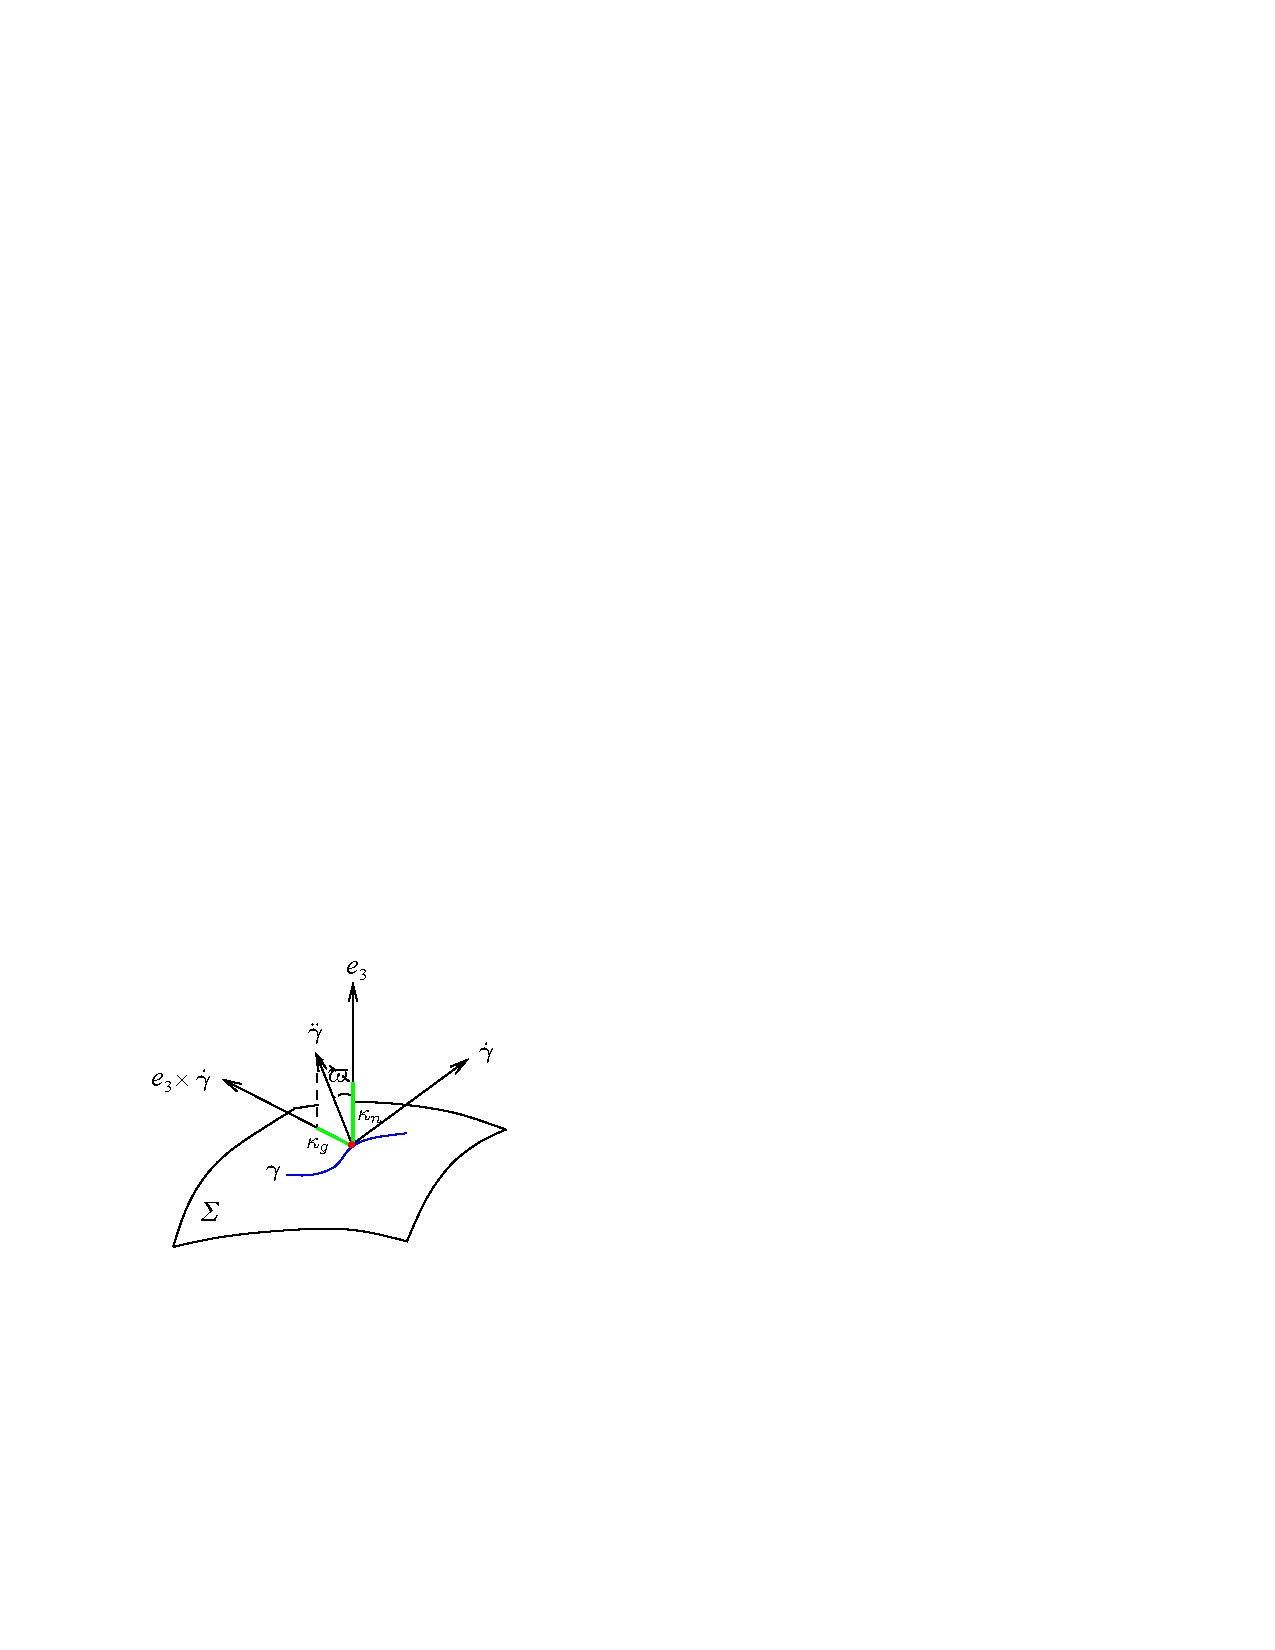
\includegraphics[scale=1]{figures/geodesic.pdf}
    \caption{Geodesic and normal curvatures of a curve on a surface.}
    \label{fig:geodesic curvature}
\end{figure}

A \emph{pseudospherical surface}\index{Pseudospherical surface} is a surface with Gauss curvature $K\equiv -1$. Setting $A=C=-1$ and $B=0$ in the \gls{eds} $\calI$ described in the last \sect. This system is hyperbolic since $B^2-AC=-1<0$, and indeed, the $2$-forms of $\calI$ are spanned by two decomposable forms 
\[\Psi\pm \Theta=(\omega_1^3\mp \theta^2)\wedge(\omega_2^3\pm \theta^1).\]
Moreover, we may use the factors of the decomposable forms to express the second fundamental form as 
\[\rmII =\left[\frac12(\omega_1^3+\theta^2)\odot (\omega_2^3+\theta^1)-\frac12(\omega_1^3-\theta^2)\odot(\omega_2^3-\theta^1)\right]\otimes e_3,\]
where $\odot$ is the symmetric tensor product (cf.\ Definitions~\ref{def sym operator} and \ref{def exterior and sym product}). 
This shows that each characteristic curve projects to be an asymptotic line on $\Sigma$.

On an open subset of a pseudospherical surface that is free of umbilic points, we may choose a Darboux framing. This breaks the Cauchy characteristic symmetry of the \gls{eds}, but allows us to see how pseudospherical surfaces are connected to solutions of \gls{sge} (see Examples~\ref{ex sine-gordon} and \ref{ex 7.4.6 Ivey}).

Since we are using Darboux frames,
\[\begin{pmatrix}
    \omega^3_1\\\omega^3_2
\end{pmatrix}=\begin{pmatrix}
    \tan u & 0\\
    0 & -\cot u
\end{pmatrix}\begin{pmatrix}
    \theta^1\\\theta^2
\end{pmatrix},\]
where $u\in (0,\pi/2)$ is half of the angle between the asymptotic lines. We adjoin $u$ as a new variable, and enlarge our \gls{eds} to a Pfaffian system 
\[I=\<\theta^3,\omega^3_1-(\tan u)\theta^1,\omega^3_2+(\cot u)\theta^2\>\]
on $\SE_3\times \bbR$. Then a Darboux framing along a pseudospherical surface corresponds to an integral surface of $\calI=\<I\>_{\mathrm{diff}}$ satisfying the independence condition $\theta^1\wedge\theta^2\neq 0$, and vice versa.

The vanishing of the exterior derivatives modulo $I$ of the last two $1$-forms generating $I$ implies that $\theta^1/\cos u$ and $\theta^2/\sin u$ pull back to be closed $1$-forms on any integral surface. Hence, there exist local coordinates $(t_1,t_2)$ such that 
\[\theta^1=\cos u\dd t_1,\quad \theta^2=\sin u\dd t_2.\]
Moreover, 
\[x\coloneqq (t_1+ t_2)/2,\quad y\coloneqq (t_1-t_2)/2,\] are exactly the arclength parameters along the asymptotic lines. This implies that asymptotic lines form what is called a \emph{Chebyshev net} on the surface: parallel transport of one of the two families of curves along the other preserves it. In other words, opposite edges of the net quadrilaterals have the same length. Thus you can stretch a flexible ``knitted'' square mesh over this surface. Note also that the asymptotic lines are bisected by the lines of curvature.

Substituting $\dd u=u_x\dd x+u_y\dd y$ into the $2$-forms of the \gls{eds} shows that $\omega_2^1=u_x\dd x-u_y\dd y$ along any integral surface. Then it is easy to see that the structure equation $\dd\omega^1_2=\omega^3_1\wedge\omega^3_2$ (i.e., the Gauss equation) implies that $u$ (or rather $2u$) satisfies \gls{sge}:
\[u_{xy}=\sin u\cos u.\]

Conversely, we may start with a solution of the \gls{sge} and produce a pseudospherical surface by integration. On a fundamental level, note that the First and Second Fundamental Forms of a pseudospherical surface in the asymptotic coordinates $(x,y)$ read 
\[
    \rmI=\begin{pmatrix}
        1 &\cos 2u\\
        \cos 2u & 1
    \end{pmatrix},\quad
    \rmII=\begin{pmatrix}
        0 & \sin 2u\\
        \sin 2u & 0
    \end{pmatrix},
\]
and $2u$ is the angle between the $x$ and $y$-curves. From here it is easy to see that $H=-2\cot(2u)$. \gls{sge} is equivalent to the Gauss-Kodazzi equations on $H$ with $K=-1$, so by the Fundamental Theorem of Surfaces, each solution of \gls{sge} determines a unique immersed surface up to a rigid motion. 

\begin{figure}[tp]
    \centering
    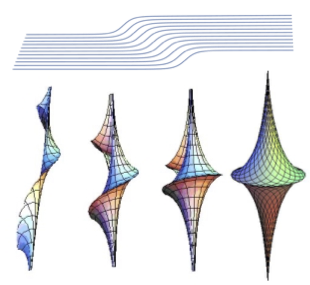
\includegraphics[scale=0.2]{figures/SG1soliton.png}
    \caption{The $1$-soliton solution (\ref{eq SGE 1-soliton}) (with lines of constant $y$) of \gls{sge} and the corresponding pseudospherical surfaces for different values of $\lambda^2$. The first three surfaces have the lines of curvature marked on them. The rightmost is the pseudosphere $\lambda=1$ with the asymptotic lines marked on it. Note the asymptotic lines becoming tangent at the edge of the surface.}
    \label{fig: SGE 1-soliton}
\end{figure}

More explicitly, if we let $\frake=(e_1,e_2,e_3)$, then the structure equations $\dd e_i=e_j\omega_i^j$ imply that 
\[\partial_x\frake=\frake \begin{pmatrix}
    0 & u_x & -\sin u\\
    -u_x & 0 & -\cos u\\
    \sin u& \cos u & 0
\end{pmatrix},\quad 
\partial_y\frake=\frake \begin{pmatrix}
    0 & -u_y & -\sin u\\
    u_y & 0 & \cos u\\
    \sin u& -\cos u & 0
\end{pmatrix}.\label{eq 7.21 Ivey}
\]
This is an overdetermined system for the matrix $\frake(x,y)$, and its Frobenius integrability condition is \gls{sge} for $u$. In fact, the above pair of equations is a $UV$-pair for \gls{sge} (see Example~\ref{ex UV pairs}; in fact, this $UV$-pair is equivalent to the one in Example~\ref{ex sine-gordon} under the isomorphism of Lie algebras $\frakso_3\cong\fraksu_2$). So, given a solution to sine-Gordon, we may obtain the framing $\frake$ by solving linear systems of ODE's, and then solve for the surface $\bf{x}(x,y)\in\bbR^3$ by integrating 
\[\bf{x}_x=e_1\cos u-e_2\sin u,\quad \bf{x}_y=e_1\cos u+e_2\sin u.\label{eq 7.22 Ivey}\]
For example, the famous \emph{1-soliton}\index{soliton} solution (also called a \emph{traveling wave} due to its translational invariance, or in the context of the sine-Gordon, a \emph{kink})
\[u=2\arctan(c\exp(\lambda x+\lambda^{-1}y)),\quad c\neq 0, \lambda\neq 0,\label{eq SGE 1-soliton}\]
gives the standard \emph{pseudosphere} when $\lambda^2=1$ and \emph{Dini's surfaces} when $\lambda^2\neq 1$, see Figure~\ref{fig: SGE 1-soliton}.\index{Pseudosphere}\index{Dini's surface} (Note that $c$ can be assumed to be $1$ after a shift and/or flip of one of the axes.)

\begin{figure}[tp]
    \centering 
    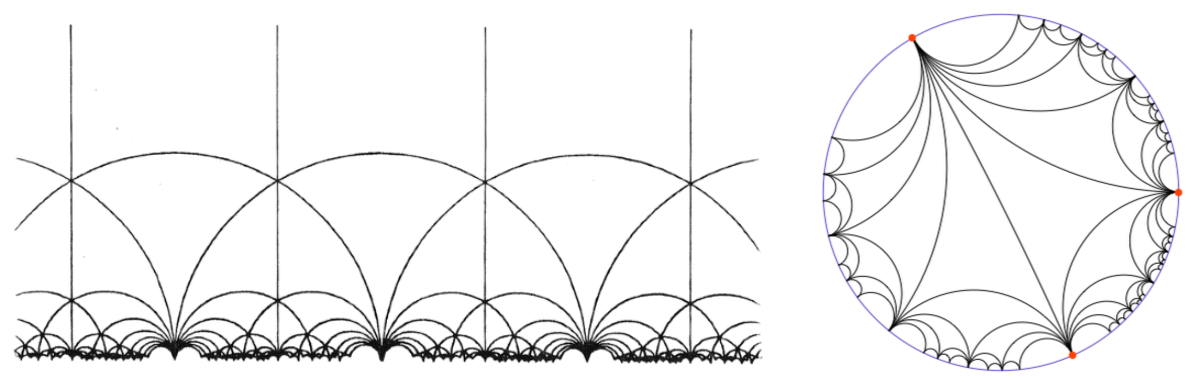
\includegraphics[scale=0.8]{figures/poincare.png}
    \caption{Poincar\'e's hyperbolic half-plane and disk models with some of their geodesics.}
    \label{fig:hyperbolic plane}
\end{figure}

\begin{example}[Hyperbolic plane and disk]\index{Hyperbolic half-plane}\index{Hyperbolic disk}
    The \emph{hyperbolic (half-)plane} is the set $\bbC^+=\{z=x+\i y\in\bbC\mid \Im z>0\}$ with the Riemannian metric 
    \[\sfg=\frac{|\dd z|^2}{(\Im z)^2}=\frac{\dd x^{\otimes 2}+\dd y^{\otimes 2}}{y^2}.\]
    This metric is conformal to the Euclidean one with the conformal factor of $\lambda^2=\frac{1}{y^2}$. The Gauss curvature is found from formula (\ref{eq K in isothermal coords}): $K=\frac12y^2\partial_y^2\ln y=-1$. The geodesics of this surface are semi-circles perpendicular to the $x$-axis and vertical lines.
    
    Another hyperbolic surface of constant negative curvature is the \emph{hyperbolic disk}  $\bbD\coloneqq \{z=x+\i y\in\bbC \mid |z|<1\}$ with the metric 
    \[\sfg=\frac{4|\dd z|^2}{(1-|z|^2)^2}=\frac{4(\dd x^{\otimes 2}+\dd y^{\otimes 2})}{(1-x^2-y^2)^2}.\]
    It is easy to check that $K=-1$ again, and in fact the disk model is isometric to the half-plane one with the isometry given by the biholomorphic \emph{Cayley transform}\index{Cayley transform} 
    \[\bbC^+\to \bbD,\quad z\mapsto \frac{z-\i }{z+\i}.\]
    As a \gls{flt}, it takes circles and lines to circles and lines. As a consequence, the geodesics of the disk model are diametric lines and arcs of circles perpendicular to the bounding circle, see Figure~\ref{fig:hyperbolic plane}.
\end{example}


A Riemannian surface $(\Sigma,\sfg)$ is called \emph{(geodesically) complete} if every geodesic $\gamma(t)$ on it can be extended to all $t\in\bbR$. Equivalently, all vector fields of bounded norm are complete. The following theorem of Hilbert states that pseudospherical surfaces in Euclidean space cannot be complete. This was one of the earliest \emph{global} results in differential geometry. 

\begin{thm}[Hilbert (1901)]\index{Theorem!Hilbert}
    There is no complete immersed surface of constant negative Gauss curvature in $\bbE^3$.
\end{thm}
\begin{proof}
    Hilbert's original proof is a bit lengthy because first one has to establish that the asymptotic lines of any \emph{complete} immersed surface of constant negative curvature can be extended endlessly. Detailed expositions of this proof can be found in \cite[\S5-11]{doCarmo} and \cite[p.~251]{Spivak3}.  We will instead take an advanced shortcut by using the Uniformization Theorem (widely believed to be true since 1882 but first proved by Poincar\'e only in 1907).

    The Uniformization Theorem (in one of its formulations) states that the universal covering of any complete surface $\Sigma$ of constant negative curvature, say $K\equiv -1$, together with the pullback of the metric from $\Sigma$, is isometric to the hyperbolic plane $\bbC^+$.\footnote{This also shows that any non-compact simply connected surface (without boundary) is diffeomorphic to $\bbR^2$.} Now, if we prove that $\bbC^+$ cannot be isometrically immersed into $\bbE^3$, Hilbert's theorem will follow because the universal covering map $\pi:\bbC^+\to \Sigma$ is a local isometry, and so any isometric immersion  $\bf{x}:\Sigma\to \bbE^3$ would allow us to define an isometric immersion $\bf{x}\circ \pi:\bbC^+\to \bbE^3$ (note that we never required the immersions to be injective), leading to a contradiction.

    Now let $2u$ be the solution of \gls{sge} $(2u)_{xy}=\sin 2u$ correspoding to $\bf{x}(\bbC^+)$. Here $(x,y)$ are the asymptotic coordinates on $\bf{x}(\bbC^+)$, not to be confused with the Cartesian coordinates on $\bbC^+$. Since $\bf{x}$ is an immersion, this surface must have linearly independent asymptotic directions at each point, and hence 
    \[0<u(x,y)<\frac{\pi}{2},\quad (x,y)\in \bbC^+.\]
    Now consider a rectangle $R=[a,b]\times [c,d]\subset\bbC^+$ and compute the area of the quadrilateral $\bf{x}(R)$:
    \begin{multline}
        \mathsf{vol}\left[\restr{\bf{x}}{R}\right]=\int_R \sqrt{\det \sfg}\dd x\dd y=\int_R \sin 2 u\dd x\dd y=\int_R (2u)_{xy}\dd x\dd y=\\
        =2(u(b,d)-u(b,c)-u(a,d)+u(a,c))<2\pi.
    \end{multline}
    Since $\bbC^+$ is simply connected and $\bf{x}$ is an immersion, its asymptotic coordinates are globally defined (by stitching together local pieces if necessary), so the rectangle $R$ can be made arbitrarily large. Since the area of the hyperbolic half-plane is infinite, the area of $R$ can become arbitrarily large. This contradicts the above result showing that $\bf{x}(R)$ has bounded area, since $\bf{x}$ is supposed to be an isometry.
\end{proof}


Hence, even if the sine-Gordon solution is defined for all $x$ and $y$, the corresponding surface will become singular. In fact, $\theta^1\wedge\theta^2=\sin 2u \dd x\wedge \dd y$ shows that the surface will be singular whenever $u$ is a multiple of $\pi/2$, i.e., when the asymptotic lines are tangent to each other. This is why the surfaces in Figure~\ref{fig: SGE 1-soliton} have singularities and are made by joining two pseudospherical surfaces along an edge: the values of the $1$-soliton solution always span $(0,\pi)$.

\begin{rem}
    The sine-Gordon has an obvious scaling symmetry given by $x\mapsto \lambda x$, $y\mapsto \lambda^{-1}y$. Hence, each immersion of $\Sigma$ belongs to a one-parameter family of isometric immersions. These deformations of pseudospherical surfaces are called \emph{Lie transformations}. In the next \sect\ we will find a similar one-parameter family of deformations of minimal surfaces (but parametrized by an element of $\U_1$ instead of $\bbR$ because the coresponding system is elliptic).
\end{rem}

\begin{xca}\label{xca 7.4.19 Ivey}
    Note that each of $x+y$ and $x-y$ is constant along one of the two sets of lines of curvature. 
    This observation is useful if we suppose that $\Sigma$ is a pseudospherical surface of revolution (i.e., is spanned by a curve when rotated about a fixed axis). Show that the corresponding sine-Gordon solution can be assumed to be of the form $u=f(x+y)$ (this is easier using the ansatz $u=2\arctan f(x+y)$). Determine all sine-Gordon solutions of this form. 
\end{xca}







\section{Minimal and \texorpdfstring{\gls{cmc}}{CMC} surfaces}

Recall that a minimal surface is an immersed surface $\Sigma<\bbE^3$ with vanishing mean curvature. From Proposition~\ref{prop mean curvature laplace}, an isometric immersion $\bf{x}:\Sigma\to \bbE^3$ is minimal iff it is \emph{harmonic in isothermal coordinates} $(x,y)$:
\[(\partial_x^2+\partial_y^2)\bf{x}=0.\]
In particular, $\bf{x}$ is \emph{conformal}, i.e., it preserves angles between tangent vectors in the $(x,y)$-plane after they're mapped to tangent vectors on $\Sigma$.

Introducing a local isothermal complex coordinate $z\coloneqq x+\i y$ (so that the metric volume form is $\sfv_\sfg=\lambda^2\dd x\wedge\dd y=\lambda^2\frac{\i}{2}\dd z\wedge\dd\wb{z}$), this suggests that there exist $3$ (locally) holomorphic functions of $z$ whose real parts are exactly the Cartesian components of $\bf{x}$. We seek to find this representation now.

Setting $A=C=0$ and $B=1$ in the \gls{eds} for a general linear Weingarten equation shows that the $2$-forms of $\calI$ are spanned 
\[\Theta=-\dd\theta^3,\quad \Psi=\omega^3_2\wedge\theta^1-\omega^3_1\wedge\theta^2.\]
This system is elliptic since $B^2-AC=1>0$, so we will have to adjust our method of characteristics to solve it. We will see below that studying the characteristic systems of $\calI$ leads to the classical \emph{Weierstrass representation} for minimal surfaces, which relates them to complex Riemann surfaces.

When we attempt to form the characteristic systems, we find that the decomposability equation 
\[(\Theta+\lambda\Psi)^{\wedge 2}=0\]
has constant roots $\lambda=\pm\i$. So, we need to introduce complex-valued differential forms. For example,
\[\Theta\pm \i \Psi=(\omega^3_1\mp \i \omega^3_2)\wedge(\theta^1\pm\i \theta^2),\]
and so if we define 
\[\omega\coloneqq \omega^3_1-\i \omega^3_2,\quad \theta\coloneqq \theta^1+\i \theta^2,\]
then the characteristic systems are 
\[\calM=\<\theta^3,\omega,\theta\>,\quad \wb\calM=\<\theta^3,\wb\omega,\wb\theta\>.\]

When we attempt to apply Darboux's method, we find that neither of these systems contains a rank-$2$ integrable subsystem. In fact, $\dd\omega\equiv 0\pmod{\omega}$, but $\dd\theta\equiv \wb\omega\wedge\theta^3\pmod{\theta}$. However, this shows that the distribution
\[\Re\<\omega,\wb\omega\>=\<\omega^3_1,\omega^3_2\>\eqqcolon J\]
is a Frobenius system on $\SE_3$. The quotient of $\SE_3$ by the leaves of the distribution dual to $J$ is a $2$-sphere, and the quotient map $\gamma:\SE_3\to \bbS^2$ is given by the unit vector $e_3$. Thus, the restriction of $\gamma$ to an integral surface $M$ of $\calI$ is just the Gauss map of the minimal surface $\Sigma=\pi(M)$, where $\pi:\SE_3\to \bbE^3$ is the bundle projection.

Since $\omega$ descends, via $\gamma$, to a well-defined (up to multiple) form on $\bbS^2$, we can define a complex structure on the sphere for which $\omega$ spans the \emph{$(1,0)$-forms}, i.e., the subbundle of $\T^\ast \bbS^2$ locally spanned by $\dd w$ for a local complex coordinate $w$. We have shown the following fundamental fact.

\begin{cor}
    The Gauss map of a minimal surface $\Sigma$ is holomorphic w.r.t.\ the complex structure on $\Sigma$ defined by $\theta=\theta^1+\i \theta^2$ (as a $(1,0)$-form).
\end{cor}

Now let us fix a standard complex coordinate on $\bbS^2$. We identify $\bbS^2$ with the null quadric $N\subset \CP^2$ defined by $z_1^2+z_2^2+z_3^2=0$ on $\bbC^3$, by mapping $e_3$ to the vector 
\[\mathsf{z}\coloneqq e_1-\i e_2 \quad \in\bbC^3\cong \bbR^3\otimes\bbC.\]
In fact, this vector can be determined from $e_3$ in a unique way, up to a scale, by the requirement that $e_3\times \mathsf{z}=\i \mathsf{z}$. Note that the equation defining $N$ implies that $\lVert\Re \mathsf{z}\rVert^2=\lVert\Im \mathsf{z}\rVert^2=\frac12\lVert \mathsf{z}\rVert^2$.

We then use the stereographic projection 
\[\mathsf{z}=\begin{pmatrix}
    1-w^2\\ \i(1+w^2)\\ 2w
\end{pmatrix},\quad w\in\bbC,\]
to define a complex local coordinate $w$ on $N$ (this actually agrees with the standard stereographic projection $\bbC\to \CP^1\setminus\{\infty\}$ given by $w\mapsto \frac{1}{1+|w|^2}(2w,1-|w|^2)=(x^1+\i x^2,x^3)$, so the resulting complex structure induced by $\omega$ on $\bbS^2$ is the standard one). Computing $\dd\mathsf{z}$ and comparing with $\dd(e_1-\i e_2)=\i(e_1-\i e_2)\omega^1_2+e_3\omega$ shows that $\gamma^\ast\dd w$ is a multiple of $\omega$.

Now suppose $z$ is a complex coordinate on our minimal surface $\Sigma$. Then $\theta=f(z)\dd z$ for a nonvanishing holomorphic function $f$, and $\gamma^\ast w=g(z)$ for some holomorphic function $g$ (we can think of $g(z)$ as another local complex coordinate). Notice that the point $\bf{x}\in \Sigma$ satisfies 
\[\dd \bf{x}=e_1\theta^1+e_2\theta^2=\Re((e_1-\i e_2)(\theta^1+\i \theta^2))=\Re(\mathsf{z}\theta).\]
As a consequence, the First Fundamental Form $\rmI=\<\dd\bf{x},\dd\bf{x}\>$ reads 
\[\rmI=\frac12\lVert\mathsf{z}\rVert^2 |\theta|^2=\frac14 \left(1+|g|^2\right)^2 |f|^2 |\dd z|^2,\quad |\theta|^2\coloneqq \theta\odot\wb\theta.\]
Thus, $z$ is an isothermal coordinate. Similarly, the Second Fundamental Form is 
\[\rmII=-\<\dd e_3,\dd\bf{x}\>e_3=-\Re(\theta \otimes \dd g)e_3.\]
(This is automatically symmetric because $\theta\wedge\dd g\propto \dd z\wedge\dd z=0$.)
In particular, a vector $X$ is an asymptotic direction iff $\theta(X)\dd g(X)$ is imaginary, and principal iff it is real. The Gauss curvature is easy to compute from the conformal factor since the metric is already diagonalized (here we're using informal notation for dividing tensors; the trickiest part is the sign):
\[K=-\frac{|\theta|^2|\dd g|^2}{\left(\frac12\Vert \mathsf{z}\rVert^2 |\theta|^2\right)^2}=-\left(\frac{4|g'|}{(1+|g|^2)^2|f|}\right)^2.\]

Finally, by substituting the expressions for $\mathsf{z}$ and $\theta$ in terms of $z$, we find the \emph{Weierstrass-Enneper representation} of $\Sigma$:
\[\bf{x}=\Re\int \mathsf{z}\theta=\Re\int 
\begin{pmatrix}
    (1-g^2)f\\ \i (1+g^2)f\\ 2gf
\end{pmatrix}\dd z.\label{eq Weiestrass-Enneper}\]
Here, the integral is a contour integral of a holomorphic $1$-form, taken from an arbitrary basepoint to the given point, and is independent of homotopic deformations of the contour with fixed endpoints. Hence, it produces a well-defined function of the endpoint. 

Note that, generally, $g$ is allowed to be a meromorphic function on a domain with nontrivial topology ($\gamma$ takes values in $\bbS^2=\CP^1$, and thus can have poles), which allows $\Sigma$ to have nontrivial topology as well. Moreover, it is obvious from the formulas that the Weierstrass parametrization is regular as long as the poles of $g$ coincide with (and are at most half of the order of) the zeros of $f$.

\begin{cor}[Weiestrass-Enneper representation]\index{Weierstrass-Enneper representation}
    Each nonplanar minimal surface $\Sigma<\bbE^3$ is determined, up to rigid motions, by its Weierstrass data consisting of a meromorphic function $g:\Sigma\to \CP^1$ and a $1$-form $\theta\in\Omega^1(\Sigma;\bbC)$ that is holomorphic w.r.t.\ the complex structure on $\Sigma$ induced by the metric and orientation. Conversely, every such pair $(g,\theta)$ determines a minimal surface via (\ref{eq Weiestrass-Enneper}) as long as the poles of $g$ overlap with zeros of $\theta$ so that $g^2\theta$ is holomorphic.
\end{cor}

We can immediately observe that multiplying $f$ (or $\theta$) by a unit complex number produces another valid minimal immersion of the same metric surface.

\begin{defn}[Associate family, conjugate surface]\index{Associate family}\index{Conjugate surface}
    Given a minimal surface $\bf{x}:\Sigma\to \bbE^3$ with Weierstrass-Enneper representation $(g,\theta)$, the one-parameter family of isometric minimal surfaces corresponding to $(g,\rme^{\i t}\theta)$, $t\in (0,2\pi)$, is called the associate family of minimal surfaces.
    
    In particular, the conjugate surface to $\Sigma$ is the surface obtained by multiplying $\theta$ by $\rmi$, or equivalently, by replacing $\Re$ with $\Im$ in (\ref{eq Weiestrass-Enneper}).
\end{defn}

\begin{example}[Catenoid and helicoid]
    The Weierstrass-Enneper representation for the catenoid as parametrized in Example~\ref{ex catenoid} (coordinates $(u,v)$ there are, in fact, isothermal) is 
    \[f(z)=-\i \rme^{-\i z/a},\quad g(z)=\rme^{\i z/a},\quad a>0,\]
    and its conjugate surface is the helicoid (although a slight reparametrization will be necessary to bring to the same form as in Example~\ref{ex helicoid}). This agrees with the standard way of picturing the Riemann surface of $z=\ln w$ as a helicoid. The rest of this $1$-parameter family of surfaces is shown in Figure~\ref{fig:helicoid}.
\end{example}


\begin{xca}
    \begin{enumerate}
        \item Identify the surfaces corresponding to $f=1$ and $g$ being one of $0,z,z^{-1},\i z^{-1}$. The surface with $g(z)=z$ is called the \emph{Enneper surface}\index{Enneper surface} and is the only member of its associate family (in particular, conjugate to itself).
        \item Conclude that the surface obtained by using $(f,g)=(\cos^2\frac{z}{2},\tan\frac{z}{2})$ is regular, and identify it with one of the surfaces in item 1. This shows that the Weierstrass representation of a given minimal surface is not unique.
    \end{enumerate}
\end{xca}

Now let us expand the scope to include \gls{cmc} surfaces. Setting $A=0$, $B=1$, and $C=-2H$, with $H$ a given constant, we get a Weingarten \gls{eds} with $2$-forms 
\[\Theta=-\dd\theta^3,\quad \Psi=\omega^3_1\wedge\theta^2+\theta^1\wedge\omega^3_2-2H\theta^1\wedge\theta^2.\]
As with the minimal surface system, the characteristics are complex. The decomposable $2$-forms are 
\[\Theta+ \i \Psi=(\omega-H\wb\theta)\wedge\theta\]
and its complex conjugate. This complex coframe, adapted as it is to the characteristics, leads to a simple basis for the \gls{eds} and a simple description of its prolongation. Namely, we adjoin a complex variable $q$ and define the $1$-form 
\[\tau\coloneqq \omega-H\wb\theta-q\theta.\]
The prolongation is the Pfaffian system $\<\theta^3,\tau,\wb\tau\>$ on $\SE_3\times\bbC$. The system $2$-forms are 
\[\dd\tau\equiv -(\dd q+2iq\omega^1_2)\wedge\theta\pmod{\theta^3,\tau,\wb\tau}\]
and its complex conjugate. Note that $q$ parametrizes the components of the traceless part of the Second Fundamental Form. For, $\tau=0$ implies that 
\[\begin{pmatrix}
    \omega^3_1\\\omega^3_2
\end{pmatrix}=\begin{pmatrix}
    H+q_1 & -q_2\\
    -q_2 & H-q_1
\end{pmatrix}\begin{pmatrix}
    \theta^1\\\theta^2
\end{pmatrix},\]
where $q=q_1+\i q_2$. Thus, the zeros of $q$ are the umbilic points of the surface.

\begin{prop}[{{\cite[Prop.~7.4.25]{Ivey}}}]\label{prop 7.4.25 Ivey}
    Let $\Sigma$ be an oriented surface with a Riemannian metric, and let $P$ be its oriented orthonormal frame bundle, with the canonical forms $\eta^1,\eta^2$ and connection form $\eta^1_2$ (see Remark~\ref{rem covariant derivative on surfaces}). Endow $\Sigma$ with the complex structure which it inherits from the metric and orientation. Suppose $q$ is a complex-valued function on $P$ that satisfies 
    \[(\dd q+2\i q\eta^1_2)\wedge(\eta^1+\i \eta^2)=0.\label{eq 7.28 Ivey}\]
    Then 
    \begin{enumerate}
        \item then
        \[Q\coloneqq q(\eta^1+\i \eta^2)^{\otimes 2}\]
        is a well-defined holomorphic quadratic differential on $\Sigma$.
        \item For any constant $H$, $q$ determines a unique local isometric embedding of $\Sigma$ as a \gls{cmc} surface of mean curvature $H$ into $\bbE^3$ up to rigid motions.
        \item An immersed surface is \gls{cmc} iff its Hopf differential (the traceless part of the $\wt{Q}$ defined in \S\ref{sec: theory of surfaces}) is holomorphic.
    \end{enumerate}
\end{prop}
\begin{proof}
    To see that the differential $Q$ is well-defined, let $X$ be the vector field tangent to the fibers of $P$ that is dual to $\eta^1_2$. Then it is easy to check that $\Lie_X Q=0$. To see that it is holomorphic, let $Q=p\dd z^{\otimes 2}$, where $z$ is a local complex coordinate such that $\dd z$ is a multiple of $\eta^1+\i \eta^2$. Then (\ref{eq 7.28 Ivey}) implies that $\partial_{\wb z}p=0$.

    Any isometric immersion of $\Sigma$ into $\bbE^3$ will induce an immersion from $P$ to $\SE_3$, and the graph of this map will be an integral $3$-manifold of the Pfaffian system on $P\times \SE_3$ generated by 
    \[\<\theta^3,\theta^1-\eta^1,\theta^2-\eta^2,\omega^1_2-\eta^1_2\>.\]
    To this system we adjoin the form $\tau$ and its conjugate, where $q$ is now given. Our hypothesis about $q$ implies that this enlarged system is Frobenius. Thus, there exists a unique integral $3$-manifold through each point, and any two isometric immersions differ by a rigid motion.
\end{proof}

\begin{cor}[Hopf]\index{Theorem!Hopf}
    Any \gls{cmc} immersion of a sphere $\Sigma=\bbS^2$ (with any metric) is a round sphere, i.e.~$K\equiv H^2=\const$.
\end{cor}
\begin{proof}
    It suffices to show that the space of holomorphic quadratic differentials on a sphere is trivial.
    Choose the standard complex structure on the sphere $\CP^1=\bbC\cup \{\infty\}$ given by the complex coordinate $z\in\bbC$. Any \gls{cmc} immersion corresponds to a holomorphic differential $Q=q\dd z^{\otimes 2}$ on $\CP^1$. Then $q$ is a function holomorphic in $\bbC$, and moreover $Q$ needs to be holomrphic at $\infty$, which means that in the local coordinate $w=z^{-1}$, the expression $Q=q(z)w^{-4}\dd w^{\otimes 2}=q(z)z^{4}\dd w^{\otimes 2}$ has to remain regular as $z\to \infty$. Thus $q(z)z^4\to 0$ as $z\to\infty$. But the only holomorphic function in $\bbC$ that has this property is zero, thus $Q=0$ and $K=H^2$.
\end{proof}


\begin{cor}[Bonnet {{\cite[Cor.~7.4.26]{Ivey}}}]
    Any \gls{cmc} surface has a circle's worth of isometric deformations as a \gls{cmc} surface.
\end{cor}
\begin{proof}
    Given $f:\Sigma\to \bbR^3$, let $q$ be the coefficient of the Hopf differential as above and let 
    \[q^t\coloneqq \rme^{\i t}q,\quad t\in(0,2\pi).\label{eq 7.29 Ivey}\]
    Then $q^t$ also satisfies the conditions of Proposition~\ref{prop 7.4.25 Ivey}, and the First Fundamental Form remains unchanged.
\end{proof}

Moreover, if the surface is not totally umbilic, then at most points $q\neq 0$ and the Second Fundamental Form is changed by (\ref{eq 7.29 Ivey}). So, the surface constructed using $q^t$ is, in general, not congruent to the original surface by rigid motions. This is the \gls{cmc} generalization of the isometric deformations of minimal surfaces that we saw above.

\begin{rem}[Bonnet surfaces]
    The above deformations show that there are noncongruent surfaces with the same $K$ and $H$ (in this case, $H$ is the same constant). Bonnet discovered that, besides \gls{cmc} surfaces, there is a finite-dimensional family of surfaces that admit noncongruent isometric deformations preserving $H$. These \emph{Bonnet surfaces} may be characterized by the property that they admit isothermal coordinates (so $q$ is real) and in these coordinates $1/q$ is harmonic, i.e., $(1/q)_{z\wb z}=0$.
\end{rem}










\section{B\"acklund transformations}


Equations which are integrable by the method of Darboux give one example where we can construct integral manifolds of an \gls{eds} by restricting to a submanifold where the system becomes Frobenius. Another example arises when the integrability condition for an overdetermined system of PDEs can be reduced to finding the solution of another PDE. Then any solution of that PDE enables us to construct (using ODE techniques) a solution of the original system.

\begin{example}\label{ex 7.5.1 Ivey}
    For example, the $UV$-pair representation (\ref{eq 7.21 Ivey}) of \gls{sge} enables us to construct a solution to the \gls{ma} system for pseudospherical surfaces by integrating a Frobenius system.
\end{example}

When this transformation works in both directions, the two PDEs are said to be related by a \emph{B\"acklund transformation}, which we will define later in the \sect. First, we formalize the relationship between the systems seen in the above examples.

\begin{defn}
    Let $\calI$ be an \gls{eds} on a manifold $M$, let $\pi:B\to M$ be a submersion, and let $\calE$ be an \gls{eds} on $B$. Then $\calE$ is an integrable extension of $\calI$ if there exists a Pfaffian system $J<\T^\ast B$ such that 
    \[\calE=\<J\cup \pi^\ast\calI\>_{\mathrm{alg}}\label{eq 7.31 Ivey}\]
    and $J$ is transverse to the fibers of $\pi$ (i.e. a frame of $J$ pulls back to form coframes on each fiber of $\pi$).  The \emph{rank} of an integrable extension is the rank of $J$, or the dimension of the fibers of $\pi$.
\end{defn}


The condition that $\calE$, as defined by (\ref{eq 7.31 Ivey}), is a differential ideal is equivalent to 
\[\dd\theta\equiv 0\pmod{J,\pi^\ast\calI}\text{ for any }\theta\in\Gamma^\infty(J).\label{eq 7.32 Ivey}\]


\begin{example}[Laplace equation]\index{Equation!Laplace}\label{ex laplace equation backlund}
    The ``baby version'' of a B\"acklund transformation is the Cauchy-Riemann system, which relates pairs of solutions to the $2$-dimensional Laplace equation. Recall from Example~\ref{ex 7.4.6 Ivey} that the Laplace equation $u_{xx}+u_{yy}=0$ is equivalent to the \gls{ma} system on $\rmJ^1(\bbR^2,\bbR)$ generated (differentially) by $\theta=\dd z-p \dd x-q \dd y$ and $\Psi=\dd p\wedge\dd y-\dd q\wedge \dd x$. We observe that 
    \[\Psi=\dd (p\dd y-q \dd x)\eqqcolon \dd \phi,\]
    so we can extend the system to $\rmJ^1(\bbR^2,\bbR)\times\bbR$ with a new variable $w$ and let the Pfaffian system $J$ be 
    \[J=\<\dd w-\phi\>=\<\dd w+q\dd x-p\dd y\>.\]
    Clearly $J$ satisfies (\ref{eq 7.32 Ivey}) because $\dd (f\phi)\equiv 0\pmod{\<\phi,\Psi\>}$. Meanwhile, the extended system $\calE$ is a Pfaffian system spanned by $\theta$ and $\phi$, which is equivalent to the following pair of equations on two functions $z=u(x,y)$ and $w=v(x,y)$:
    \[u_x=v_y,\quad u_y=-v_x,\]
    i.e., the Cauchy-Riemann system.\index{Equation!Cauchy-Riemann} Whenever $u,v$ satisfy this system, both $u$ and $v$ must be harmonic. The Cauchy-Riemann system allows one to easily compute $v$ from $u$ (up to constants of integration) using ODE methods. Hence, this system can be seen as a method for generating ``new'' harmonic functions from known ones. Such pairs of harmonic functions are called \emph{conjugate}.\index{Conjugate harmonic function}
\end{example}

If $(B,\calE)$ is an integrable extension of rank $k$ and $N\subset M$ is a $p$-dimensional integral manifold of $\calI$, then (\ref{eq 7.32 Ivey}) implies that the pullback of $J$ to $\pi^{-1}(N)$ is Frobenius. In this way, an integral manifold of $\calI$ gives a $k$-parameter family of integral manifolds of $\calE$. In Example~\ref{ex 7.5.1 Ivey}, the $6$-parameter family of surfaces corresponding to a single sine-Gordon solution are congruent under rigid motions of $\bbE^3$.


\begin{example}[\ref{ex 7.5.1 Ivey} continued]
    Let $M=\bbR^5$ and let $\calI$ be the \gls{ma} system for \gls{sge} given in Example~\ref{ex 7.4.6 Ivey}. Let $B=M\times \SE_3$. The equations (\ref{eq 7.21 Ivey}) and (\ref{eq 7.22 Ivey}) show that a Darboux framing for a pseudospherical surface associated to a sine-Gordon solution $u(x,y)$ is an integral surface for the Pfaffian system 
    \begin{multline}
        J\coloneqq \<\theta^1-\cos u(\dd x+\dd y),\theta^2+\sin u(\dd x-\dd y),\omega^1_2-u_x \dd x+u_y\dd y,\right.\\
        \left. {}\omega^3_1-\sin u(\dd x+\dd y),\omega^3_2+\cos u(\dd x-\dd y)\vphantom{|}\>.
    \end{multline}
    The one can check that $J$ satisfies (\ref{eq 7.32 Ivey}).
\end{example}


\begin{rem}\label{rem 7.5.4 Ivey}
    Suppose $\calI$ is a \gls{eds} on a manifold $M$ with a $2$-form $\Phi\in\calI^2$ closed. Then, by the Poincar\'e Lemma~\ref{lem poincare classic}, in some contractible neighborhood of any given point in $M$ there exists a differential form $\phi$ such that $\dd\phi=\Phi$. We may define a rank-$1$ integrable extension of $\calI$ by introducing a new coordinate $y$ and letting the Pfaffian system $J$ on $U\times\bbR$ be spanned by $\dd y-\phi$. This is exactly what we did for the Laplace equation in Example~\ref{ex laplace equation backlund}. Because such forms $\Phi$ are examples of conservations laws for an \gls{eds}, we call this construction an \emph{extension via conservation law}.
\end{rem}


\begin{rem}
    One could trivially produce an integrable extension by choosing $J$ to be Frobenius. Such extensions are called \emph{flat}. More generally, if the derived flag of $J$ terminates in a Frobenius system $K$ of rank $k'$, then $\calE$ defines an intgerable extension when pulled back to any leaf of the foliation dual to $K$. In this case $(B,\calE)$ is called a \emph{$k'$-parameter family} of integrable extensions.
\end{rem}

Parametric families of integrable extensions are frequently encountered in the study of completely integrable PDEs, i.e., \emph{solitonic equations}. 

\begin{example}\label{ex 7.5.6 Ivey}
    We now describe the integrable extensions of the \gls{kdv} equation 
    \[u_t+u_{xxx}+6uu_x=0\label{eq 7.33 Ivey}\]
    (it coincides with (\ref{eq kdv})) after flipping the sign of $u$). Let $M=\bbR^5$ with coordinates $(x,t,u,p,r)$. Let 
    \begin{align}
        \Theta_1\coloneqq &(\dd u-p\dd x)\wedge\dd t,\\
        \Theta_2\coloneqq &(\dd p-r\dd x)\wedge\dd t,\\
        \Theta_3\coloneqq &(\dd r+6u p\dd x)\wedge \dd t-\dd u\wedge\dd x,
    \end{align}
    and let $\calI=\<\Theta_1,\Theta_2,\Theta_3\>_{\mathrm{diff}}$. Then solutions of (\ref{eq 7.33 Ivey}) correspond to integral surfaces of $\calI$ satisfying the independence condition $\dd x\wedge\dd t\neq 0$. (Note that $M$ is a quotient of $\rmJ^2(\bbR^2,\bbR)$, and $p,r$ have their classical meanings as $u_x$ and $u_{xx}$ respectively. One could also use the \gls{eds} obtained by pulling back the standard contact system on $\rmJ^3(\bbR^2,\bbR)$ to the hypersurface defined by (\ref{eq 7.33 Ivey}), but the extra variables are not needed here.)

    On $B=M\times\bbR^2$ with fiber coordinates $(\mu,y)$, let $J=\<\dd \mu,\eta\>$, where 
    \[\eta\coloneqq \dd y-(y^2+u-\mu)\dd x+(r+2py+2(u+2\mu)(y^2+u-\mu))\dd t,\]
    and let $\calE=\<J\cup \calI\>_{\mathrm{alg}}$. It is an exercise to verify that $\calE$ is an integrable extension of $\calI$.

    Since $J$ contains a rank-$1$ Frobenius system, we have a $1$-parameter family of extensions, with $\mu$ as a parameter. Along an integral surface of $\calE$ that satisfies the independence condition, $y(x,t)$ satisfies 
    \[y_y+y_{xxx}+6(\mu-y^2)y_x=0\label{eq 7.34 Ivey}\]
    for some constant $\mu$. This family of equations may be said to be extensions of \gls{kdv}. When $\mu=0$, it is a version of another well-known PDE, the \emph{modified \gls{kdv} equation}, and the passage from $u$ to $y$ is known as the \emph{Miura transformation}.
    % All integrable extensions of \gls{kdv} have been classified, and each of them corresponds to a finite-dimensional representation of a certain infinite-dimensional Lie algebra, known as the \emph{\gls{kdv} prolongation algebra}. Moreover, this algebra has a $1$-parameter family of finite-dimensional quotients, each of which is isomorphic to a semidirect product of $\fraksl_2(\bbR)$ with $\bbR^5$. Representations of the latter algebra allow us to construct $1$-parameter families of \gls{kdv} extensions, the most well-known of which is the AKNS system (\ref{eq AKNS UV pair})
\end{example}


B\"acklund transformations are a particular form of integrable extension which allows a two-way transformation of solutions of a PDE to solutions of another (or the same) PDE. One of the most well-known is the following transformation, which can produce new solutions of the \gls{sge}.

\begin{example}\label{ex 7.5.9 Ivey}
    Consider the system
    \begin{align}
        u_x-\wb{u}_x=\lambda&\sin(u+\wb{u}),\\
        u_y+\wb{u}_y=\frac{1}{\lambda}&\sin(u-\wb{u}).
    \end{align}
    If $u(x,y),\wb{u}(x,y)$ are smooth functions that satisfy this system for some $\lambda\neq 0$, the differentiating and equating mixed partials implies that $u$ and $\wb{u}$ must be solutions of sine-Gordon $u_{xy}=\sin u\cos u$. Conversely, given a solution $u(x,y)$ of sine-Gordon, we can determine $\wb{u}_x$ and $\wb{u}_y$ from the above, and integrate to get the new solution $\wb{u}(x,y)$ (since we are guaranteed that mixed partials commute). Since this can be done for any $\lambda$, and there will be a constant of integration of the first-order ODE, we get a $2$-parameter family of solutions. For example, the kink solution (\ref{eq SGE 1-soliton}) can be produced in this way by starting with $u\equiv 0$. However, the constants of integration amount to translating the solution in the plane, so we can omit them, keeping the translational invariance in mind. Thus, the kink has one parameter $\lambda$. By iterating this procedure, we get a $2$-parameter family of $2$-soliton solutions, a $3$-parameter family of $3$-soliton solutions, and so on. All of them can be obtained by solving simple ODE's and are expressed in terms of trigonometric and exponential functions. For example, the $2$-soliton solution (Figure~\ref{fig:2-soliton}) is 
    \[u=2\arctan \frac{\lambda_1+\lambda_2}{\lambda_1-\lambda_2}\frac{\rme^{\lambda_1x+\lambda_1^{-1}y}-\rme^{\lambda_2 x+\lambda_2^{-1}y}}{1+\rme^{(\lambda_1+\lambda_2)x+(\lambda_1^{-1}+\lambda_2^{-1})y}}.\label{eq sge 2-soliton}\]
    One can also obtain other interesting exact solutions from these formulas. While $\lambda_1$ and $\lambda_2$ are real, we can put $\lambda_1=\rme^{\i t}=-\lambda_2^{-1}$ for $t\in \bbR$, and discover that the formula for the $2$-soliton solution gives another real solution of sine-Gordon, which is periodic in $x-y$ and is called a \emph{breather} (Figure~\ref{fig:breather}).
\end{example}

\begin{figure}[tp]
    \centering
    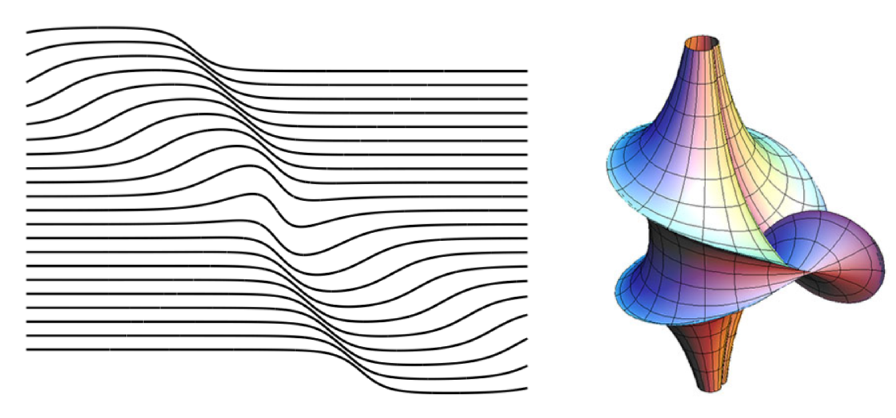
\includegraphics[scale=0.2]{figures/SG2soliton.png}
    \caption{A $2$-soliton solution of \gls{sge} (height profiles at constant $y$ for (\ref{eq sge 2-soliton})) and the corresponding pseudospherical surface.}
    \label{fig:2-soliton}
\end{figure}


\begin{defn}[B\"acklund transformation]
    Let $M_1,M_2$ carry \glspl{eds} $\calI_1$ and $\calI_2$, respectively, and let $B\subset M_1\times M_2$ be a submanifold such that the projections $\pr_i:B\to M_i$, $i=1,2$, give $B$ the structure of a double fiber bundle. Then $(B,\calE)$ defines a B\"acklund transformation between $\calI_1$ and $\calI_2$ if $\calE$ is an \gls{eds} on $B$ that is an integrable extension of both $\calI_1$ and $\calI_2$.
\end{defn}

We will often define B\"acklund transformations by giving a Pfaffian system $J<\T^\ast B$ such that 
\begin{align}
    &\<J\cup \pr_1^\ast \calI_1\>_{\mathrm{alg}}=\<J\cup \pr_2^\ast\calI_2\>_{\mathrm{alg}},\label{eq 7.37a Ivey}\\
    &\calE\coloneqq \<J\cup \pr_1^\ast \calI_1\cup \pr_2^\ast \calI_2\>_{\mathrm{alg}}\text{ is a differential ideal}.\label{eq 7.37b Ivey}
\end{align}
Note that $J$ need not be transverse to the fibers of $\pr_1$ or $\pr_2$.

\begin{example}[\ref{ex 7.5.9 Ivey} continued]
    Let $M_1$ and $M_2$ be two copies of $\rmJ^1(\bbR^2,\bbR)$ where we denote the forms and coordinates on $M_2$ with bars. For $i=1,2$ let the \gls{eds} $\calI_i$ on $M_i$ be a copy of the \gls{ma} system for \gls{sge} from Example~\ref{ex 7.4.6 Ivey}. For any $\lambda\neq 0$, let $B_\lambda<M_1\times M_2$ be defined by $\wb{x}=x$, $\wb{y}=y$ and 
    \begin{align}
        p-\wb{p}&=\lambda\sin(u+\wb{u}),\\
        q+\wb{q}&=\frac{1}{\lambda}\sin(u-\wb{u}).
    \end{align}
    Let $\theta$ be the standard cotact form on $\rmJ^1(\bbR^2,\bbR)$. On $B_\lambda$, let $J=\<\pr_1^\ast\theta,\pr_2^\ast\wb\theta\>$. Then it is easy to check that (\ref{eq 7.37a Ivey}-\ref{eq 7.37b Ivey}) are satisfied.
\end{example}

\begin{figure}[tp]
    \centering
    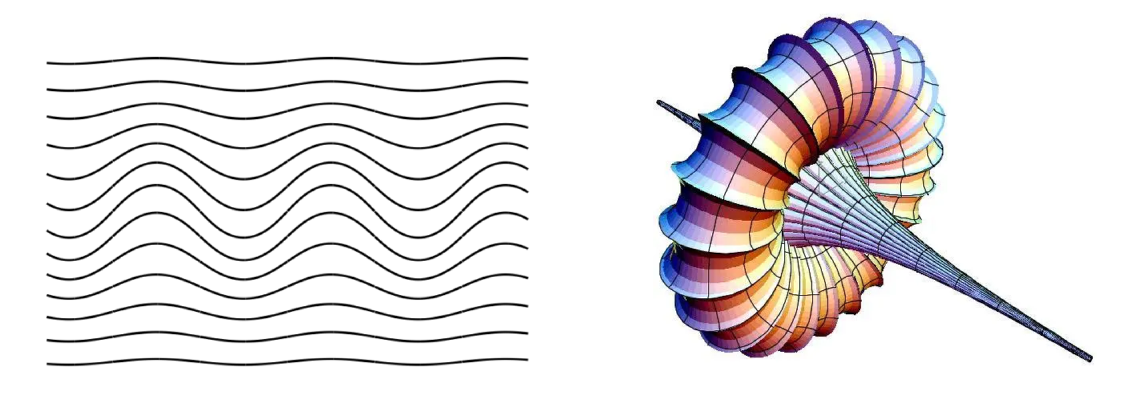
\includegraphics[scale=0.2]{figures/SGbreather.png}
    \caption{A breather wave solution of \gls{sge} (height profiles at constant $x+y$) and the corresponding pseudospherical surface.}
    \label{fig:breather}
\end{figure}


\begin{example}[\ref{ex 7.5.6 Ivey} continued]
    Let $M_1,M_2$ be two copies of $\bbR^5$, each carrying a copy of the \gls{kdv} \gls{eds}. (Again, we use barred coordinates on $M_2$.) Define $B=M_1\times\bbR^2$ as before, and define a submersion $\pr_2:B\to M_2$ by 
    \begin{align}
        \wb{x}&=x,\\
        \wb{y}&=y,\\
        \wb{u}&=2(\mu-y^2)-u,\\
        \wb{p}&=4y(\mu-u-y^2)-p,\\
        \wb{r}&=-4(u+y^2-\mu)(u+3y^2-\mu)-4yp-r.
    \end{align}
    Then $J$, as defined above, gives a B\"acklund transformation between the \gls{kdv} equation and itself. One can check that 
    \[
    \begin{rcases}
        \pr_2^\ast\Theta_1&\equiv -\pr_1^\ast\Theta_1\\
        \pr_2^\ast\Theta_2&\equiv -\pr_1^\ast\Theta_2-4y\pr_1^\ast\Theta_1 \\
        \pr_2^\ast\Theta_3&\equiv -\pr_1^\ast\Theta_3-4y\pr_1^\ast\Theta_2-8(u+2y^2-\mu)\pr_1^\ast\Theta_1
    \end{rcases} \pmod{J}.
    \]
    The presence of an arbitrary parameter in the B\"acklund transformation for \gls{kdv} is central to its complete integrability, both in the sense of inverse scattering and in the Hamiltonian sense.
\end{example}

In many important cases B\"acklund transformations relate two \emph{different} PDEs.

\begin{example}[Wave and Liouville equations]
    Let $M_1\subset \rmJ^2(\bbR^2,\bbR)$ be the submanifold defined by the hyperbolic Liouville equation $z_{xy}=\rme^z$, with the standard contact system $\calI_1$ generated by $\theta_0,\theta_1,\theta_2$ defined in Example~\ref{ex 7.3.6 Ivey}. We use the standard notation $(p,q,r,s,t)$ for the jet coordinates restricted to $M_1$. Then (\ref{eq 7.14 Ivey}) implies that $(r-\frac12p^2)_y=0$ and $(t-\frac12q^2)_x=0$ for any solution. Thus, on $B=M_1\times \bbR$ with coordinate $v$ on the second factor, we may define an extension by letting $J=\<\theta_0,\theta_1,\theta_2,\eta\>$, where 
    \[\eta\coloneqq \dd v-(r-\frac12 p^2)\dd x-(t-\frac12 q^2)\dd y.\]
    Because $\dd\eta\equiv 0\pmod{\calI_1}$, $\calE=\<J\cup\calI_1\>_{\mathrm{alg}}$ is an integrable extension of $\calI_1$.

    Furthermore, let $M_2=\rmJ^2(\bbR^2,\bbR)$ with coordinates $(\wb{x},\wb{y},\wb u,\wb p,\wb q)$ and let $\calI_2$ be the standard \gls{ma} system for the wave equation $\wb{u}_{\wb x\wb y}=0$. Define a submersion $\pr_2:B\to M_2$ by 
    \[\wb{x}=x,\quad\wb{y}=y,\quad \wb{u}=v,\quad \wb{p}=r-\frac12 p^2,\quad \wb{q}=t-\frac12 q^2.\]
    Then $\calE$ is an integrable extension of $\calI_2$ (with the role of the transverse Pfaffian system played by $\<\theta_0,\theta_1,\theta_2\>$). Thus, $(B,\calE)$ defines a B\"acklund transformation between Liouville and wave equations.

    Explicitly, the system $\calE$ is equivalent to the two PDEs
    \begin{align}
        u_x+\wb{u}_x&=2\lambda \exp\frac{u-\wb{u}}{2},\\
        u_y-\wb{u}_y&=\frac{1}{\lambda}\exp \frac{u+\wb{u}}{2}.
    \end{align}
    Whenever this system is satisfied, $u$ must be a solution of the Liouville equation, whereas $\wb{u}$ must be a solution of the wave equation. By taking $\wb{u}$, we can recover $u$ up to a constant of integration, thus producing the general solution of the Liouville equation. Letting  $\wb{u}(x,u)=\xi(x)+\eta(y)$, which is the general solution of the wave equation, we separate variables in the above system to find
    \[\exp\left(-\frac{u}{2}\right)=-\exp\left(\frac{\xi-\eta}{2}\right)\left(\lambda\int \rme^{-\xi(x)}\dd x+\frac{1}{2\lambda}\int \rme^{\eta(y)}\dd y\right).\label{eq 9.31 Clellan}\]
    Setting $X(x)\coloneqq -\lambda\int \rme^{-\xi(x)}\dd x$ and $Y(y)\coloneqq -\frac{1}{2\lambda}\int \rme^{\eta(y)}\dd y$, it is easy to solve (\ref{eq 9.31 Clellan}) and get the general solution (\ref{eq Liouville general solution}), where $X(x)$ and $Y(y)$ are arbitrary functions of a single variable, with the property that $X'$ and $Y'$ are nonzero and have the same sign.
\end{example}



The B\"acklund transformation for pseudospherical surfaces arises naturally in a classical context, the study of \emph{line congruences} in Euclidean space.

\begin{defn}[Line congruence]\index{Line congruence}
    A line congruence in $\bbE^3$ is an immersed surface in $\Gr_1(\bbE^3)$, i.e., a $2$-parameter family of lines $\ell:U\to \Gr_1(\bbE^3)$, where $U\subset\bbR^2$ and each element of $\Gr_1(\bbE^3)$ (a tangent line to $\bbE^3$) is viewed as a line in $\bbE^3$. It can be expressed (non-uniquely) as 
    \[\ell(\bf{u})=[\bf{x}(\bf{u}),e(\bf{u})],\]
    where $\bf{x}(\bf{u})$ is a point on the line $\ell(\bf{u})$ and $e(\bf{u})\in\bbS^2$ is a unit vector parallel to $\ell(\bf{u})$. If $\bf{x}$ is chosen to be smooth, then the surface $\Sigma=\bf{x}(U)$ is called a \emph{surface of reference} for $\ell$. Any other surface of reference $\wb\Sigma=\wb{\bf{x}}(U)$ for $\ell$ can then be parametrized as 
    \[\wb{x}(\bf{u})=\bf{x}(\bf{u})+\lambda(\bf{u})e(\bf{u}),\quad \lambda\in C^\infty(U).\]

    For a generic line congruence $\ell:U\to \Gr_1(\bbE^3)$ there are two distinguished surfaces of reference, $\Sigma=\bf{x}(U)$, $\wb\Sigma=\wb{\bf{x}}(U)$, called \emph{focal surfaces}, to which each line of the congruence is tangent (we omit the detailed construction). Aside from degeneracies, the lines locally give a $1$-to-$1$ correspondence between points of the focal surfaces.
\end{defn}


\begin{defn}[Pseudospherical line congruence]
    Let $\ell:U\to \Gr_1(\bbR^3)$ be a line congruence with focal surfaces $\Sigma,\wb{\Sigma}$ parametrized as above. The congruence is called pseudospherical if 
    \begin{enumerate}[label=(\alph*)]
        \item The distance $r=\lVert\bar{\bf x}(\bf{u})-\bf{x}(\bf{u})\rVert$ is a constant independent of $\bf{u}$,
        \item The angle $\alpha$ (assumed to be nonzero) between the surface normal vectors $e_3(\bf{u})$, $\wb{e}_3(\bf{u})$ to the surfaces $\Sigma,\wb\Sigma$, respectively, is a constant independent of $\bf{u}$.
    \end{enumerate}
\end{defn}

\begin{thm}[B\"acklund]\index{Theorem!B\"acklund}
    If $\ell$ is a pseudospherical line congruence with focal surfaces $\Sigma,\wb{\Sigma}$, then both of them have constant Gauss curvature $K=-\frac{\sin^2\alpha}{r^2}$, where $r,\alpha$ are as above. 
    
    Conversely, given a surface $\Sigma$ with $K=-\frac{\sin^2\alpha}{r^2}$, a point $\bf{x}_0\in\Sigma$ and a unit non-principal tangent vector $e_0\in \T_{\bf{x}_0}\Sigma$, there exists a unique surface $\wb\Sigma$ such that if $\bar{\bf x}_0$ is the point corresponding to $\bf{x}_0$, then $\bar{\bf{x}}-\bf{x}_0=r e_0$ and the angle between the surface normals of $\Sigma$, $\wb\Sigma$ at $\bf{x}_0$, $\bar{\bf x}_0$, respectively, is $\alpha$.
\end{thm}
\begin{proof}
    \gls{wlog}, we can assume $\lambda=\sin \alpha$, so that $K\equiv -1$. The starting point  of the proof is adapting frames $(\bf{x},\frake)$ and $(\bar{\bf{x}},\wb{\frake})$ along the two surfaces so that $e_1=\wb{e}_1$ is tangent to the line connecting corresponding points $\bf{x}$ and $\bar{\bf x}$. For any fixed $\lambda$, the graph of the B\"acklund transformation is a $6$-dimensional submanifold of $\SE_3\times\SE_3$ defined by 
    \begin{align}
        \bar{\bf x}&= \bf{x}+\lambda e_1,\\
        \bar{e}_1 &= e_1,\\
        \bar{e}_2 &= e_2\cos \alpha+e_3\sin\alpha,\\
        \bar{e}_3&=e_3\cos \alpha-e_2\sin\alpha.
    \end{align} 
    However, we will regard this system as defining a $7$-dimensional submanifold $B<\SE_3\times\SE_3\times\bbR$ with $\lambda$ as the extra coordinate. On $B$, let $J=\<\theta^3,\wb\theta^3,\dd\lambda\>$. Then the exercise below verifies that (\ref{eq 7.37a Ivey}-\ref{eq 7.37b Ivey}) are satisfied, and B\"acklund's Theorem follows from the fact that 
    \[\<\omega^3_1\wedge\omega^3_2+\theta^1\wedge\theta^2,\wb\omega^3_1\wedge\wb\omega^3_2+\wb\theta^1\wedge\wb\theta^2\>\equiv \<\dd\theta^3,\dd\wb\theta^3\>\pmod{J}.\]
\end{proof}



\begin{xca}
    \begin{enumerate}
        \item Differentiate the system of equations in the above proof to obtain the following relations between the pullbacks to $B$ of the canonical forms:
        \begin{align}
            \wb\theta^1&=\theta^1+\dd\lambda,\quad \wb\omega^2_3=\omega^2_3-\dd\alpha,\\
            \begin{pmatrix}
                \wb\theta^2\\\wb\theta^3
            \end{pmatrix}&=
            \begin{pmatrix}
                \cos\alpha & \sin\alpha \\
                -\sin\alpha & \cos\alpha
            \end{pmatrix}\begin{pmatrix}
                \theta^2-\lambda\omega^1_2\\
                \theta^3-\lambda\omega^1_3
            \end{pmatrix},\\
            \begin{pmatrix}
                \wb\omega^1_2\\\wb\omega^1_3
            \end{pmatrix}&=
            \begin{pmatrix}
                \cos\alpha & \sin\alpha \\
                -\sin\alpha & \cos\alpha
            \end{pmatrix}\begin{pmatrix}
                \omega^1_2\\
                \omega^1_3
            \end{pmatrix},
        \end{align}
        Using these, verify (\ref{eq 7.37a Ivey}-\ref{eq 7.37b Ivey}).
        \item Show that (\ref{eq 7.37a Ivey}) implies that decomposable $2$-forms in one system are congruent to decomposables for the other modulo the contact forms $\<\theta^3,\wb\theta^3\>$. The asymptotic lines are dual to the factors of these decomposables, therefore the B\"acklund transformation takes asymptotic lines to asymptotic lines.
        \item Show that if two pseudospherical surfaces are related by a B\"acklund transformation, then their corresponding solutions of \gls{sge} are related by a B\"acklund transformation with the same parameter $\lambda$.
        \item Show that B\"acklund transformations are transitive, so the existence of a B\"acklund transformation between two systems is an equivalence relation on \glspl{eds}.
    \end{enumerate}
\end{xca}


As we wrap up our exploration of the geometry of surfaces, we can make some observations about the deep relationship between surfaces and completely integrable systems. As we have seen, many basic problems about surfaces get reduced to integrable systems such as the Liouville equation, \gls{sge}, and the AKNS system. In fact, the \gls{kdv} equation also describes certain classes of surface, and various extensions of these systems appear as well. Aside from geometry of surfaces and dynamical systems, integrable systems appear across all sectors of mathematics: probability and statistics, combinatorics, statistical mechanics, classical analysis, numerical analysis, asymptotic representation theory, algebraic geometry, and so on. While there is no general formal definition of a completely integrable system, all of the following features are considered necessary parts of integrability:
\begin{enumerate}
    \item \emph{A linearizing coordinate transformation}, after which the problem is reduced to linear equations. This property is the most natural extension of the classical notion of integrability (existence of action-angle variables). For example, the Weierstrass representation of minimal surfaces reduced the problem to the linear Cauchy-Riemann system describing holomorphic functions. Similarly, the \gls{kdv} dynamics become linear after being put in terms of the scattering data of the Schr\"odinger equation in which the \gls{kdv} solution acts as the potential. 
    \item \emph{B\"acklund transformations} that allow one to generate solutions of one integrable system using solutions of another.
    \item \emph{A Hamiltonian structure} which describes solutions as Hamiltonian flows on an infinite-dimensional manifold.
    \item \emph{An infinite-dimensional Lie algebra of symmetries}, which generates an infinite number of conserved quantities (analogs of initial data in a Frobenius system).
    \item \emph{Existence of solitonic solutions}, each of which is described by a finite set of parameters related to the conserved quantities. This is another manifestation of the large space of symmetries.
    \item \emph{Well understood function spaces}, such as special functions (elliptic, hypergeometric, Painlev\'e). One a nonlinear coordinate transformation was found that reduces the problem to a linear one, the space of solutions to the linear problem needs to be highly legible. A standard criterion for this property is the Painlev\'e Test, which is related to the classification of ODE's whose solutions have certain natural analytic properties (such as singularities of Fuchsian type whose location is independent of the initial condition), a generalization of the Cauchy-Kovalevskaya Theorem. Solutions to Painlev\'e equations encompass all classical special functions and are currently the broadest well-studied class of special functions related to integrable PDEs.
    \item \emph{Lax pair or zero curvature representations}, which pair the original system with a linear time-dependent operator ($L$ in Example~\ref{ex Lax pairs}) whose dynamics is \emph{isospectral}. The existence of a Lax pair is often conflated with integrability, but it alone does not actually imply the rest of the features listed above.
\end{enumerate} 

For a much more detailed review of the concept of integrable systems, we direct the reader to \cite{deift}. For more on the theory of classical integrable systems, see the books \cite{moser,babelon}.





\section{Gauss-Bonnet and Poincar\'e theorems}\label{sec: gauss-bonnet}

We finish this \chap\ with a classical theorem that is a major early milestone in the history of differential geometry due to being the first \emph{global} result of the theory of surfaces. Moreover, it turns out to relate local geometric data (Gauss curvature) to global topological data, which is indepedent of the choice of metric, thus becoming a harbinger of the more modern results about topological invariants constructed out of geometric data.


Suppose $\frake=(e_1,e_2)$ and $\wt\frake=(\wt e_1,\wt e_2)$ are two local orthonormal frames on a Riemannian surface $(\Sigma,\sfg)$. They are related by $\wt\frake=\frake\cdot R$ for some function $R:\Sigma\to \SO_2$. We have seen that the \emph{local connection form} $\omega\coloneqq\frake^\ast\omega^2_1$ is intrinsic and can be expressed using an isometric immersion of $\Sigma$ into $\bbE^3$ via 
\[e_2\omega=\dd e_1-\<\dd e_1,e_3\>e_3,\] 
where $e_1,e_2,e_3$ are treated as $\bbR^3$-valued functions on $\Sigma$. (One can also obtain an intrinsic formula for $\omega$ in terms of $\sfg$ but we won't need it in this \chap.) From here, the rotation matrix $R$ induces the following transformation of the connection form:
\[\wt\omega =\wt{\frake}^\ast\omega^2_1=\omega+R^{-1}\dd R.\]
The rotation matrix $R$ is of course uniquely identified with a counter-clockwise rotation through some angle $\theta(m)$ dependent on the point $m\in \Sigma$. In terms of this angle, 
\[\wt\omega =\omega+\dd\theta.\label{eq 169}\]

Now consider a curve $\gamma:[0,1]\to \Sigma$ which lies in a region covered by an orthonormal frame $\frake$. Suppose that $X\in\fX(\Sigma)$ is a vector field whose values $X(t)$ along $\gamma$ have unit length. We define a map $\alpha:[0,1]\to \bbS^1\subset \bbR^2$ by letting $\alpha(t)$ be the image of $X(t)$ under the unique linear map $\im(\gamma)\to \bbR^2$ which takes $e_1(\gamma(t))$ to $\bf{e}_1=(1,0)$. We then have a continuous map $\phi:[0,1]\to \bbR$ with $\alpha(t)=(\cos\phi(t),\sin\phi(t))$, and any two such maps differ by a multiple of $2\pi$. We will refer to any such $\phi$ as a continuous choice of the angle between $e_1$ and $X$. It is easy to see that $\phi$ is actually smooth if $X$ and $\gamma$ are. 

By choosing another local frame $\wt\frake$ such that $\wt e_1=X$ along $\gamma$ and using (\ref{eq 169}), it is now easy to see that 
\[\nabla_{\dot\gamma}X=0 \Leftrightarrow \omega(\dot\gamma(t))+\dot\phi(t)=\wt\omega(\dot\gamma(t))=\<\nabla_{\dot\gamma}X,\wt e_2\> =0.\]
We say that $X$ is \emph{parallel} along $\gamma$ when this holds. It follows that the connection form $\omega$ describes the rate at which a vector rotates while being parallel transported along $\gamma$. If $X$ is not parallel along $\gamma$, we get a nonzero quantity. In \S\ref{sec: pseudospherical surfaces} we defined the geodesic curvature and noted that it is intrinsic since $\kappa_{\mathrm{g}}=\lVert\nabla_{\dot\gamma}\dot\gamma\rVert$, or 
\[\kappa_{\mathrm{g}}=\<\nabla_{\dot\gamma}\dot\gamma,\bf{N}\>.\label{eq geodesic curvature}\]
In terms of the angle $\phi$ between $e_1$ and $\dot\gamma(t)$, we have 
\[\kappa_{\mathrm{g}}(t)=\omega(\dot\gamma(t))+\dot\phi(t).\]


\begin{prop}
    Let $(\Sigma,\sfg)$ be a compact oriented Riemannian surface, with connected boundary $\partial \Sigma$, diffeomorphic to a subset of $\bbR^2$. Let its Gaussian curvature be $K$ and its canonical area form $\sfv_\sfg$. Let $s$ be the arclength parameter along $\partial \Sigma$ and let $\kappa_{\mathrm{g}}$ be the signed geodesic curvature of $\partial \Sigma$ (on which the direction is induced by orientation). Then 
    \[\int_\Sigma K\sfv_\sfg=-\oint_{\partial \Sigma}\kappa_{\mathrm{g}}\dd s+2\pi.\]
\end{prop}
\begin{proof}
    Because of our assumptions, we may as well assume that $\Sigma\subset \bbR^2$. On it we define a positively oriented orthonormal frame $(e_1,e_2)$ be requiring $e_1$ to be a positive multiple of $\partial_{x^1}$. Let $\gamma:[0,1]\to \partial \Sigma$ be a closed curve, parametrized by arclength $\sigma$, such that $\dot\gamma(\sigma)$ is positively oriented, and let $\phi$ be a continuous choice of the angle between $e_1$ and $\dot\gamma$. Let $\omega$ be the connection form, which in this case can be defined globally. Then, using the Stokes Theorem and the above formula for $\kappa_{\mathrm{g}}$,
    \begin{align}
        \int_\Sigma K\sfv_\sfg&=\int_\Sigma K\theta^1\wedge\theta^2=-\int_\Sigma \dd \omega=-\int_{\partial \Sigma}\omega=\\
        &=-\int_0^1 \omega(\dot\gamma(\sigma))\dd \sigma=\\
        &=-\int_0^1\kappa_{\mathrm{g}}(\sigma)\dd\sigma+\int_0^1\dot\phi(\sigma)\dd\sigma=\\
        &=-\int_{\partial \Sigma}\kappa_{\mathrm{g}}\dd s+\phi(1)-\phi(0).
    \end{align}
    To complete the proof, we have to show that $\phi(1)-\phi(0)=2\pi$. This is done essentially by reducing it to the flat case via a continuous deformation of the metric.

    \begin{enumerate}[label=(\arabic*)]
        \item The number $\phi(1)-\phi(0)$ is a multiple of $2\pi$ since $\phi(0),\phi(1)$ are both choices of the abgle for $\dot\gamma(0)=\dot\gamma(1)$.
        \item Let $\delta$ be the standard metric on $\bbR^2$ (the Kronecker tensor). It is easy to check that for each $\lambda\in [0,1]$, the tensor 
        \[\sfg^\lambda\coloneqq \lambda\sfg+(1-\lambda)\delta\]
        is also a Riemannian metric. Let $(e_1^\lambda, e_2^\lambda)$ be a positively oriented local frame which is orthonormal w.r.t.\ $\sfg^\lambda$ and for which $e_1^\lambda$ is a positive multiple of $\partial_{x^1}$; then let $\phi^\lambda$ be a continuous choice of the angle between $e_1^\lambda$ and $\dot\gamma/\lVert\dot\gamma\rVert^\lambda$. The choice $\phi^\lambda$ clearly depends continuously on $\lambda$ (if we make $\phi^\lambda(0)$ vary continuously). Consequently, $\phi^\lambda(1)-\phi^\lambda(0)$ varies continuously with $\lambda$. Since it is always a multiple of $2\pi$, it must be constant.
        \item When $\lambda=0$, we have $e_1^\lambda=\partial_{x^1}$ and $e_2^\lambda=\partial_{x^2}$, and consequently $\phi^0$ is just a choice of the angle between the $x$-axis and $\dot\gamma$. 
    \end{enumerate}
    So $\phi^0(1)-\phi^0(0)$ is the \emph{total curvature} of $\gamma$, which is  $2\pi$ by the \emph{Hopf Umlaufsatz}: indeed, curvature is the rate of rotation of the tangent to the curve in $\bbR^2$, and so the total curvature is the total change of that angle. But it is easy to see that replacing the tangent line with the line passing through two different points $\gamma(s_1),\gamma(s_2)$, $s_1\leq s_2$, on the curve gives a homotopy, where the original angle is the value along the diagonal $s_1=s_2$, and the total change from $(s_1,s_2)=(0,0)$ to $(1,1)$ is independent of the path taken within the triangle $0\leq s_1\leq s_2\leq 1$. On the other hand, if $s_1=0$ if fixed and $s_2$ increases to $1$, the change is obviously $\pi$ assuming $\gamma$ is a simple closed curve, and similarly for the segment from $(0,1)$ to $(1,1)$.
\end{proof}


In the next theorem we consider a generalization of this result for \emph{piecewise smooth} curves. Namely, a \emph{polygon} in $\Sigma$ is a simple closed curve which is a smooth embedding on each interval $[t_i,t_{i+1}]$ of some partition $0=t_0<\cdots<t_{n+1}=1$. Thus, the one-sided derivatives $\dot\gamma(t_i\pm 0)$ exist but may not coincide. It is clear how to define the vertices and the edges of the polygon. At each vertex $\gamma(t_i)$ we also define the \emph{interior angle} $\iota_i$ as the oriented angle from $\dot\gamma(t_i+0)$ to $-\dot\gamma(t_i-0)$ (if they point in the same direction, then one defines the angle to be either $0$ or $2\pi$ based on the orientation of the nearby pairs $(\dot\gamma(t_i+\epsilon),-\dot\gamma(t_i-\epsilon))$ for small $\epsilon>0$).

Having defined the interior angle $\iota_i$, we define the \emph{discontinuity} $\delta_i$ of $\dot\gamma$ at $t_i$ by 
\[\delta_i\coloneqq \pi-\iota_i\in [-\pi,\pi].\]
This describes the oriented angle from $\dot\gamma(t_i-0)$ to $\dot\gamma(t_i+0)$.

\begin{thm}[Gauss-Bonnet formula (1827-1848) {{\cite[Thm.~6.6]{Spivak3}}}]\index{Equation!Gauss-Bonnet}
    In the setting of the preceding theorem, let $\partial M$ be a polygon with vertices $t_1,\ldots,t_n$ and discontinuities $\delta_1,\ldots,\delta_n$. Then 
    \[\int_\Sigma K\sfv_\sfg=-\oint_{\partial \Sigma}\kappa_{\mathrm{g}}\dd s-\sum_{i=1}^n\delta_i+2\pi=-\oint_{\partial \Sigma}\kappa_{\mathrm{g}}\dd s+\sum_{i=1}^n\iota_i+(2-n)\pi.\]
\end{thm}
\begin{proof}
    The proof proceeds much like in the previous theorem, except on each interval $[t_i,t_{i+1}]$ separately, leading to the sum $\sum_{i=1}^{n+1}(\phi_i(t_i)-\phi_i(t_{i-1}))$ instead of the single $\phi(1)-\phi(0)$. This equals $-\sum_{i=1}^n\delta_i+[\phi_{n+1}(1)-\phi_1(0)]$, so it remains only to show that the last term is $2\pi$. This is done in an obvious way by generalizing the Hopf Umlaufsatz by approximating the polygon with a smooth curve.
\end{proof}


\begin{cor}[{{\cite[Cor.~6.7]{Spivak3}}}]\label{cor 6.7 Spivak3}
    If the sides of the polygon in the last theorem are geodesics, then 
    \[\int_\Sigma K\sfv_\sfg=-\sum_{i=1}^n\delta_i+2\pi=\sum_{i=1}^n\iota_i+(2-n)\pi.\]
    In particular, for a geodesic triangle, the total Gauss curvature equals $\iota_1+\iota_2+\iota_3-\pi$.
\end{cor}

We are now ready to compute the total curvature of a \emph{closed surface}, i.e., a compact one with no boundary. We do this under the assumption that the surface has a \emph{triangulation}, i.e., a (finite in this case) collection  $\{\sigma_i\}$ of diffeomorphic images of the standard triangle (\emph{2-simplex}) $\Delta_2\coloneqq \{\bf{x}\in\bbR^3:0\leq x^i\leq 1,\; \sum_{i=1}^3 x^i=1\}$ such that if two of them intersect, then the intersection must be an edge or a vertex. It is a difficult theorem that every smooth surface has a triangulation (and an analogous statement holds for all smooth manifolds of any dimensionality). For a given triangulation of $\Sigma$, which we treat as a ``curved'' polyhedron, we let 
\[(V,E,F)\coloneqq \text{number of (vertices, edges, faces)}.\]
One can prove directly that the quantity $V-E+F$ is independent of the triangulation, but we will do so indirectly in the following main theorem.

\begin{thm}[Gauss-Bonnet-von Dyck (1888)]\index{Theorem!Gauss-Bonnet}\label{thm gauss-bonnet}
    If $(\Sigma,\sfg)$ is a closed (compact with no boundary) oriented Riemannian surface with Gaussian curvature $K$, canonical area form $\sfv_\sfg$, and some triangulation with numbers $(V,E,F)$ defined as above, then 
    \[\int_\Sigma K\sfv_\sfg=2\pi (V-E+F).\]
    In particular, the integer $(V-E+F)$ is not dependent neither on the triangulation nor on the metric, and is thus a topological invariant called the \emph{Euler characteristic} $\chi(\Sigma)$. \index{Euler characteristic!of a closed surface}
\end{thm}
\begin{proof}
    Let the triangulation consist of faces $\sigma_1,\ldots,\sigma_F$. Let $A_j,B_j,C_j$ be the three interior angles of $\sigma_j$. Then by Corollary~\ref{cor 6.7 Spivak3}
    \[\int_\Sigma K\sfv_\sfg=\sum_{j=1}^F \oint_{\partial \sigma_i}\kappa_{\mathrm{g}}\dd s+\sum_{j=1}^F(A_j+B_j+C_j)-\sum_{j=1}^F 3\pi +\sum_{j=1}^F 2\pi.\]
    Now we note the following equalities that lead to the asserted result.
    \begin{enumerate}[label=(\arabic*)]
        \item $\sum_j \oint \kappa_{\mathrm{g}}\dd s=0$, because each edge of the triangulation appears twice with opposite orientations.
        \item $\sum_j (A_j+B_j+C_j)=2\pi V$ since the sum of all interior angles occurring at each vertex is $2\pi$.
        \item $-\sum_j 3\pi=-3F\pi$. On the other hand, any triangulation has $3F=2E$ since $3F$ is the total number of edges of all faces, each edge being counted twice as it belongs to two faces. So, $-\sum_j 3\pi =2\pi (-E)$.
        \item $\sum_j 2\pi=2\pi F$.
    \end{enumerate}
\end{proof}

\begin{xca}
    It turns out that $\chi(\Sigma)$ completely classifies closed oriented surface up to homeomorphism. Show that a surface of genus $g$ has $\chi=2-2g$.
\end{xca}

The most immediate implications of this theorem are the connections between the bounds on the values of $K$ and the topology of $\Sigma$. For example, if $\Sigma$ admits a flat metric, then it must be (homeomorphic to) a torus, and if it admits a metric of everywhere positive curvature, then it must be a sphere. If $K$ is everywhere negative, then an upper bound on its values puts a lower bound on the genus $g>0$.

The following corollary has to do with the degree of the Gauss map. If $M$ and $N$ are both compact $n$-manifolds, then the \emph{(Brouwer) degree} of a map $f:M\to N$ is defined by the formula \index{Degree (Brouwer)}
\[\int_M f^\ast \omega=\deg f\cdot \int_N\omega\]
for any $\omega\in\Omega^n(N)$. For non-compact manifolds, the degree can also be defined for proper maps by requiring that $\omega$ have compact support. For now, we will not prove the surprising fact that $\deg f$ is an integer independent of $\omega$. In the case of $M=N=\bbS^n$, the degree is exactly the corresponding element of the homotopy group $\pi_n(\bbS^n)\cong\bbZ$ (where the generator of the group is given by the identity map).

\begin{cor}[{{\cite[Thm.~6.10]{Spivak3}}}]
    Let $\Sigma\subset\bbE^3$ be an embedded oriented closed surface and let $e_3:\Sigma\to \bbS^2$ be its Gauss map (normal vector). Then 
    \[\deg e_3=\frac12 \chi(\Sigma).\]
\end{cor}
\begin{proof}
    By definition of the degree, $\int_\Sigma e_3^\ast \omega=\deg e_3\cdot\int_{\bbS^2}\omega$ for all $\omega\in\Omega^2(\bbS^2)$. Choosing $\omega=\sfv_{\bbS^2}$ to be the standard are form on $\bbS^2$, this means that by (\ref{eq gauss map pullback})
    \[4\pi \deg e_3=\int_\Sigma e_3^\ast \sfv_{\bbS^2}=\int_\Sigma K \sfv_\sfg.\]
    Together with the Gauss-Bonnet Theorem, this yields the assertion.
\end{proof}

This relation between the degree and the Euler characteristic can also be proven directly, and in fact holds for hypersurfaces in $\bbE^n$ for any $n$. This was an important intermediate result on the way to the higher-dimensional generalization of the Gauss-Bonnet Theorem.

The final classical theorem involves the notion of the index of a vector field. For a vector field $X\in\fX(\Sigma)$ on a surface $\Sigma$, let $m_0\in \Sigma$ be an \emph{isolated zero}, i.e., $X\neq 0$ in a punctured open neighborhood $U\setminus\{m_0\}$ of $m_0$. Choose $U$ so that it is diffeomorphic to a disk. Then the \emph{index $\ind_{m_0}X$ of $X$ at $m_0$} is defined as the winding number of the map $\bbS^1\to \bbS^1$ given by \index{Index!of a vector field}
\[\bbS^1\ni p\mapsto X(i(p))/\lVert X(i(p))\rVert\in\bbS^1,\]
where $i:\bbS^1\to \partial U$ is a diffeomorphism and $\lVert\cdot\rVert$ is an arbitrary metric. It is easy to see that all possible choices of $U, i$, or the metric lead to homotopic maps, so the index is a well-defined invariant of $X$ itself. 

On a closed surface $\Sigma$, we will consider vector fields $X$ that have only isolated zeros. In this case there can only be finitely many zeros $m_1,\ldots,m_r$, and we define the \emph{(total) index} of $X$ as 
\[\ind X\coloneqq \sum_{i=1}^r \ind_{m_i}X.\]
One can prove directly that $\ind X=\chi(\Sigma)$ for any admissible $X$, as was first done by Poincar\'e in 1881. The idea is to first show that the index is independent of the particular vector field $X$, and then to associate to every triangulation a standard vector field as in Figure~\ref{fig poincare-hopf} whose index is manifestly $V-E+F$. Instead of detailing this argument, we will obtain the same result indirectly via the following theorem.

\begin{figure}[tp]
    \centering
    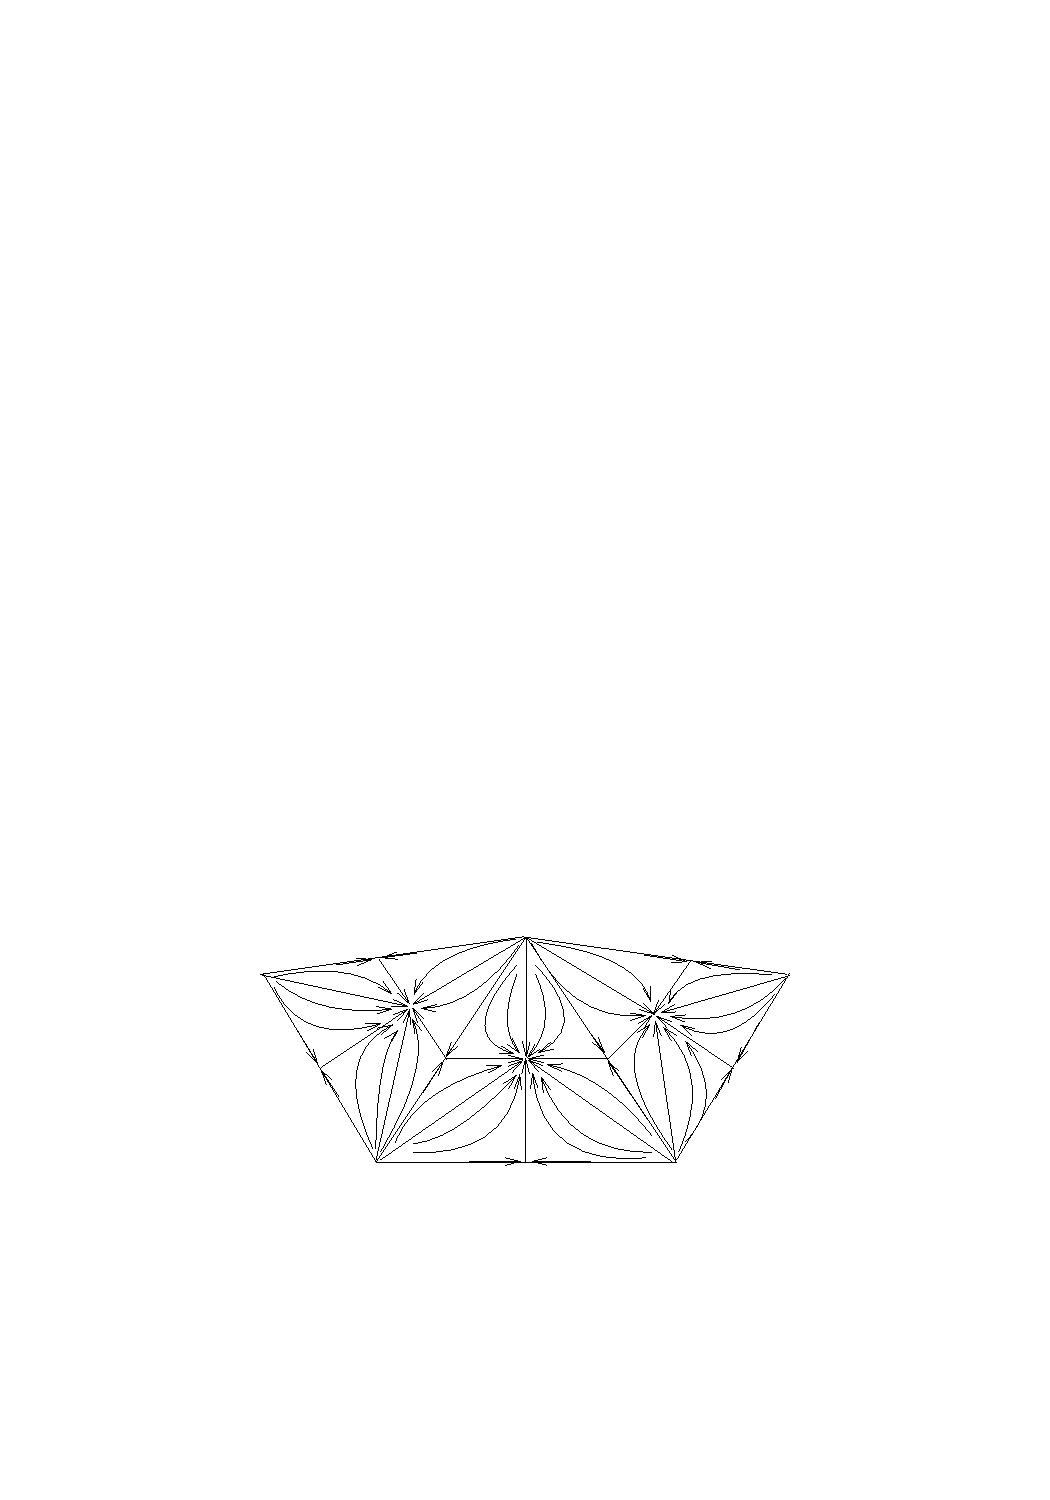
\includegraphics[scale=0.8]{figures/poincare-hopf.pdf}
    \caption{A standard vector field associated to a triangulation in the direct proof of Poincar\'e's Theorem. From \cite{Ivey}. \label{fig poincare-hopf}}
\end{figure}

\begin{thm}[Poincar\'e (1881) {{\cite[Thm.~6.9]{Spivak3}}}]\label{thm poincare-hopf}
    On a closed Riemannian surface $(\Sigma,\sfg)$ with Gaussian curvature $K$ and canonical area form $\sfv_\sfg$, let $X$ be a smooth vector fields with only isolated zeros. Then 
    \[\int_\Sigma K\sfv_\sfg=2\pi \ind X.\]
    In particular, $\ind X$ is independent of $X$ and hence is a topological invariant of $\Sigma$ equal to the Euler characteristic $\chi(\Sigma)$.
\end{thm}
\begin{proof}
    Let $m_1,\ldots,m_r$ be the zeros of $X$, and choose disjoint disks $D_i\subset \Sigma$ containing $m_i$. Each $D_i$ is diffeomorphic to the standard disk $\bbD^2=\{\bf{x}\in\bbR^2\mid \lVert\bf{x}\rVert\leq 1\}$, and we let $D_i(\epsilon)$ denote the set corresponding to $\lVert \bf{x}\rVert\leq \epsilon$. Let 
    \[\Sigma(\epsilon)\coloneqq \Sigma\setminus \left(\bigcup_i \mathring{D}_i(\epsilon)\right).\]
    On $\Sigma(\epsilon)$ there is a positively oriented local frame $(e_1,e_2)$ with $e_1=X/\lVert X\rVert$. Then 
    \[\int_{\Sigma(\epsilon)}K\sfv_\sfg=-\int_{\Sigma(\epsilon)}\dd \omega=-\sum_i \oint_{\partial D_i(\epsilon)} \omega.\]
    Consider one particular $i$. Let $(\wt e_1,\wt e_2)$ be a positively oriented orthonormal frame on $D_i$. On $D_i$ minus a line segment we have a differentiable choice of the angle $\theta$ between $e_1$ and $\wt e_1$, and by (\ref{eq 169}),
    \[-\oint_{\partial D_i(\epsilon)}\omega=\oint_{\partial D_i(\epsilon)} \dd\theta-\oint_{\partial D_i(\epsilon)}\wt\omega=\ind_{m_i}X-\oint_{\partial D_i(\epsilon)}\wt\omega,\]
    where $\wt\omega$ also depends on $i$. Therefore, 
    \[-\lim_{\epsilon\to 0}\oint_{\partial D_i(\epsilon)}\omega=\ind_{m_i}X,\]
    which concludes the proof.
\end{proof}

\begin{rem}
    We have thus proven the equivalence of three different ways of computing the Euler characteristic of a closed oriented surface: via a triangulation, via the index of a generic vector field, and via the total Gaussian curvature:
    \[\ind X=\chi(\Sigma)=\int_\Sigma K\sfv_\sfg.\]
    The generalization of the equality $\ind X=\chi(M)$ to closed manifolds $M$ of arbitrary dimensionality was obtained by Hopf in 1921 and is known as the Poincar\'e-Hopf Theorem. \index{Theorem!Poincar\'e-Hopf} Meanwhile, the generalization of the Gauss-Bonnet Theorem to closed oriented manifolds of arbitrary even dimensionality was completed by Chern in 1944 and is known as the Chern-Gauss-Bonnet Theorem. We will prove both of these generalizations as part of our discussion of characteristic classes.
\end{rem}







\clearpage
\part{Geometric Structures II}\label{Part Structured Geom II}
\chapter{Connections}

Connections are an enormous topic that can be approached from many directions. Their basic practical use is in performing parallel transport and taking derivatives of sections of bundles. However, in geometry and topology they also provide a class of geometric structures that can be used as powerful computational tools for computing quantities that don't inherently depend on the choice of connection (e.g., certain topological invariants of bundles). Our exposition is based on a combination of \cite{Vakar,RS2,Kolar} but is also, in part, structured with an eye towards the study of $G$-structures and Cartan geometry.

\section{General connections}\label{sec general connections}

The Frobenius Theorem~\ref{thm frobenius} states that a distribution $\calH\subset \T M$ is integrable iff it is involutive. However, there is no clear \emph{quantitative measure} of integrability. It turns out that one way to obtain such a quantitative measure is to assume that there is a second distribution, \emph{transverse} to the first one. Namely, let $(\calH,\calV)$ be two distributions on $M$ (subbundles of $\T M$) such that
\[\calH_m\oplus \calV_m=\T_mM \text{ for all }m\in M.\]
This implies that there are globally defined smooth bundle maps (projections), which we denote by the same symbols,
\[\calH:\T M\to \calH,\quad \calV:\T M\to \calV,\quad \calH+\calV=\id_{\T M}.\]
Now we can construct a linear map that measures to what extent $\calH$ fails to be an integrable distribution. Since $\calH$ and $\calV$ are completely interchangeable at this point, we in fact get two maps (the sign choice is conventional):
\begin{align}
    \calR:\fX(M)\times\fX(M)\to \Gamma^\infty(\calV),\quad & \calR(X,Y)=-\calV[\calH X,\calH Y],\\
    \wb{\calR}:\fX(M)\times\fX(M)\to \Gamma^\infty(\calH),\quad & \wb{\calR}(X,Y)=-\calH[\calV X,\calV Y].
\end{align}
Indeed, if $\calR=0$, it means that the Lie bracket of two sections of $\calH$ lies in $\calH$, and therefore $\calH$ is integrable, and similarly $\wb \calR$ detects the integrability of $\calV$. It is obvious that these maps are $C^\infty(M)$-linear and hence are tensors. We call $\calR$ \emph{curvature} and $\wb{\calR}$ \emph{cocurvature}\index{Cocurvature}. Note that the value of $\calR$ depends on the choice of $\calV$, but whether it is zero or not doesn't, so in this sense it's still an objective measure of integrability for $\calH$ (as long as $\calH$ and $\calV$ are everywhere transverse). It turns out that fiber bundles are special in that they come with one canonically defined integrable distribution that we define now. A more sophisticated way of defining the curvature of general connections is as the Fr\"olicher-Nijenhuis bracket $[\calV,\calV]$, see Example~\ref{ex frolicher curvature and torsion}.

\begin{defn}[Vertical bundle]\index{Vertical bundle}
    If $E\overset{\pi}{\to}M$ is a smooth \gls{fb}, then its \emph{vertical subbundle} is the subbundle $\calV E< \T E$ defined as 
    \[\calV E=\ker \pi_\ast\]
    (it is a subbundle by virtue of being the kernel of a bundle morphism). At a point $p\in E$ the fiber is denoted $\calV_pE$. Since each fiber $E_m$, $m\in M$, is an embedded submanifold, and $\calV E$ restricted to $E_m$ coincides with the tangent bundle $\T E_m$ of the fiber, we conclude that $\calV E$ is an integrable distribution. In particular, it is involutive: for any two \emph{vertical vector fields} $X,Y\in \fX_{\mathrm{ver}}(E)\coloneqq\Gamma^\infty(\calV E)$, we have $[X,Y]\in \fX_{\mathrm{ver}}(E)$.
\end{defn}

Therefore cocurvature on fiber bundles always vanishes. Crucially, there is no \emph{natural} ``horizontal'' subbundle $\calH E<\T E$ such that $\calH E\oplus \calV E=\T E$. A connection is, in the broadest sense, a choice of a transverse ``horizontal bundle'' $\calH E$, and its integrability is quantified by the curvature tensor. If it is integrable, then the fiber bundle is not only foliated by its fibers, but also by ``horizontal''  integral submanifolds (locally horizontal sections).

Note that for $m\in M$ and $p\in E$, the sequence
\[0\to \calV_p E=\T_p E_m\overset{\T_p i_m}{\to}\T_p E\overset{\T_p\pi}{\to}\T_mM\to 0\]
is a short exact sequence. Here $m=\pi(p)$ and $E_m\overset{i_m}{\hookrightarrow} E$ is the natural inclusion. This sequence means that we can identify the quotient space $\T_pE\slash \calV_pE$ with $\T_mM$, so we have the following \emph{natural} isomorphism of \glspl{vb} over $E$:
\[\T E\slash \calV E\cong \pi^\ast \T M.\]
A splitting of the above exact sequence is equivalent to choosing a particular subspace $\calH_p E$ in $\T_p E$ complementary to $\calV_p E$ for each $p$, hence specifying a bundle isomorphism between $\pi^\ast \T M$ and the horizontal distribution $\calH E$. But first we will approach this problem from another angle.

As we will see later, determining what the ``horizontal'' directions in a bundle are, in particular, provides one with a \emph{unique} way of lifting paths $\gamma$ in $M$ to paths $\wt\gamma$ in $E$. Doing this for every starting point $p\in E_{\gamma(0)}$, we get a map $E_{\gamma(0)}\to E_{\gamma(1)}$. This map has to be bijective because the lifting clearly respects inverses of paths. Moreover, it will depend only on the \emph{shape} of $\gamma$ and not on how exactly it is parametrized. The next three definitions formalize the concept of \emph{reparametrization invariance} of paths.

\begin{defn}[Sitting instants]
    A path $\gamma:I\to M$ in a topological space $M$ is said to have sitting instants if there is a neighborhood of the points $0,1$ in $I$ on which $\gamma$ is locally constant.
\end{defn}

\begin{defn}[Thin homotopy]
    A thin homotopy between two smooth paths $\gamma_0,\gamma_1:I\to M$ in a smooth manifold $M$ is a smooth homotopy $H:I^2\to M$ between them such that the rank of its derivative $H_\ast:\T(I^2)\to \T M$ is everywhere at most $1$. Equivalently, for any $2$-form $\omega\in\Omega^2(M)$, its pullback must vanish: $H^\ast \omega=0$ on $I^2$.
\end{defn}

\begin{defn}[Path groupoid]
    The path groupoid $\rmP_1(M)$ of a smooth manifold $M$ is the groupoid whose objects are points of $M$ and morphisms $\mor(p,q)$ are the thin homotopy classes of paths $p\leadsto q$ with sitting instants. Composition of paths is defined via concatenation and reparametrization as usual. The quotient by thin homotopies ensures that this is an associative product with inverses for each path.
\end{defn}

This groupoid can in fact be understood as smooth in a certain sense (it is a ``diffeological groupoid''), but we will not go into those details. We can now define a connection as a prescription (a functor) for taking a path $\gamma$ in $M$ and producing a diffeomorphism $E_{\gamma(0)}\to E_{\gamma(1)}$ in such a way that it is independent of reparametrizations of $\gamma$ and consistent, i.e., functorial w.r.t.\ products of paths. In addition, it needs to depend on $\gamma$ smoothly in a proper sense. Finally, if the bundle carries a $G$-structure, we would like this diffeomorphism to be a morphism of $G$-fibers, i.e., be represented in local frames by actions of elements of $G$ on the typical fiber.

\begin{defn}[Connection I: transport functor]\index{Transport functor}
    Let $(E\overset{\pi}{\to}M,G\acts F,\calG)$ be a $G$-bundle, and more specifically an $\calS$-bundle for some category $\calS$. Let $\calS\mathsf{-Man}^\infty$ be the category of $\calS$-fibers (cf.~Definition~\ref{def S-fibers}). A \emph{transport functor} on $E$ is a functor
    \[\tra: \rmP_1(M)\to \calS\mathsf{-Man}^\infty,\]
    such that for any path $\gamma\in\rmP_1(M)$ the map $\tra_\gamma\coloneqq \tra(\gamma)$ is a morphism (hence isomorphism) of the $G$-fibers over the endpoints:
    \[\tra_\gamma:(E_{\gamma(0)},\calG_{\gamma(0)})\to (E_{\gamma(1)},\calG_{\gamma(1)}),\]
    and which is smooth in the following sense. If $\gamma_t$ is a smooth homotopy of paths in $M$ (not necessarily with fixed ends), then, for any $t\in I=[0,1]$, in some local $\calG$-charts of $E$ at $\gamma_t(0)$ and $\gamma_t(1)$, the representatives of the diffeomorphism $\tra_{\gamma_t}:E_{\gamma_t(0)}\to E_{\gamma_t(1)}$ must depend smoothly on $t$ as elements of $\calS(F,F)$. Since any isomorphism of $G$-fibers is represented by $G$-actions in $G$-frames, this can also be stated as there existing a (finite) collection of $\calG$-charts covering the curves traced out by the endpoints $\gamma_t(0)$ and $\gamma_t(1)$ and a smooth path $g:I\to G$ such that the local representatives of $\tra_{\gamma_t}$ in any of those charts are exactly the action of $g(t)$ on $F$. We will call connections with such parallel transport \emph{$G$-connections}.\index{$G$-connection}

    A \emph{morphism of connections} on $E$ is a natural transformation of two such functors.
\end{defn}

Note that in the case of principal bundles the complicated condition on the values of $\tra$ can be replaced by simply saying that it is a functor into the category $G\mathsf{-Tor}$ of $G$-torsors. This definition can be made significantly neater by introducing a few extra functors, but we direct the reader to \cite{schreiber} for that.

\begin{defn}[Flat connection]
    A connection defined via a transport functor $\tra$ on a bundle $E$ is called flat if for any path $\gamma$ in $M$, the map $\tra_\gamma$ is invariant under homotopies of $\gamma$ with fixed endpoints.
\end{defn}


\begin{example}[Absolute parallelism]
    Recall from Definition~\ref{def parallelizable} that if $E\to M$ is a trivial \gls{fb}, then a particular choice of a global trivialization $\chi:E\to M\times F$ is called an \emph{absolute parallelism}\index{Parallelism!Absolute}. Each absolute parallelism naturally determines a unique flat connection. Namely, the parallel transport operator (independent of the path) from fiber $E_m$ to fiber $E_{m'}$ maps $\chi^{-1}(m,f)$ to $\chi^{-1}(m,f')$.
\end{example}

\begin{example}[Canonical flat connections on a Lie group]\label{ex flat connections on G}
    If $G$ is a Lie group, then the tangent bundle $\T G$ admits two obvious flat connections. The first, called the $(-)$-connection, has parallel transport acting by left translations, i.e., $\T_g G$ is mapped to $\T_h G$ by $\rmL_{hg^{-1}\ast}$. The second, so called $(+)$-connection, has parallel transport given by $\rmR_{g^{-1}h\ast}$, instead. Since these transports are independent of the path, these connections are flat. Both of them derive from absolute parallelisms $\T G\to G\times\frakg$ given by the left and right Maurer-Cartan forms, respectively.
\end{example}



\begin{prop}
    A bundle is flat iff it admits a flat connection.
\end{prop}
\begin{proof}
    By Definition~\ref{def flat G-bundle}, a bundle is flat if it  has a $G$-atlas with locally constant transition functions. Then a path $\gamma$ in the base can be turned into a ``horizontal'' path $t\mapsto (\gamma(t),f_\alpha)$ in each local chart $U_\alpha\times F$ overlapping with the image of $\gamma$. The points $f_\alpha$ are chosen so that $f_\beta=g_{\beta\alpha}\cdot f_\alpha$, where $g_{\alpha\beta}\in G$ is the constant transition function on $U_{\alpha\beta}$. This produces a consistently defined path in the bundle because transition functions are constant. By applying this to every starting point, we get a transport map which obviously depends only on the endpoints of $\gamma$, thus defining a flat connection.

    Conversely, given a flat connection $\tra$, we can cover the base manifold with contractible open sets $U_\alpha$, pick a basepoint $x_\alpha$ in each, and use parallel transport along arbitrary paths $x_\alpha\leadsto y_\alpha$ inside $U_\alpha$ to obtain diffeomorphisms $\varphi_{\alpha,y_\alpha}:E_{y_\alpha}\to E_{x_\alpha}$ for all $y_\alpha\in U_\alpha$. Due to flatness these diffeomorphisms depend only on $y_\alpha$. Hence we can define a map $\pi^{-1}(U_\alpha)\to U_\alpha\times E_{x_\alpha}$ by $\chi_\alpha(p)=(\pi(p),\varphi_{\alpha,\pi(p)}(p))$. Further we can choose arbitrary diffeomorphisms compatible with the $G$-structure of the bundle between each $E_{x_\alpha}$ and the typical fiber $F$. This allows us to treat the $\chi_\alpha$ as local trivializations. The transition functions between them are constant because they can be written in terms of these fixed diffeomorphisms and the transport diffeomorphisms $E_{x_\alpha}\to E_{x_\beta}$, which are entirely independent of any other points in the base.
\end{proof}

An obvious consequence of the definition of parallel transport is that it endows the bundle with \emph{unique horizontal path liftings}: given a path $\gamma:I\to M$ and a point $p\in\pi^{-1}(\gamma(0))$, its horizontal lifting is the smooth path $\wt{\gamma}(t)=\tra_{\restr{\gamma}{[0,t]}}(p)$. By doing this for all paths through $m\in M$ and all $p\in E_m$, each parallel transport functor induces a distribution $\calH E<\T E$ consisting of ``horizontal'' vectors. This leads to our second definition of a connection (as we will see, it is a bit more general than Definition I).


\begin{defn}[Connection II: general connection]
    Given a $G$-bundle $(\tuple{E\overset{\pi}{\to}M,G\acts F,\calG})$, an general connection on it is a smooth vector subbundle $\calH E<\T E$ such that $\calH E\oplus \calV E=\T E$. The decomposition $\T_pE=\calH_pE\oplus \calV_pE$ induces the natural projections which we denote by two pairs of symbols:
    \[\T_pE\to \calH_pE\oplus \calV_pE,\quad X_p\mapsto (\hor X_p,\ver X_p).\]
    For any smooth vector field $X\in\fX(E)$, the assignments $p\mapsto \hor X_p$ and $p\mapsto \ver X_p$ are also smooth vector fields, denoted $\hor X$ and $\ver X$, respectively.

    The connection $\calH E$ is called \emph{flat} if it is integrable as a distribution (or, equivalently, by the Frobenius Theorem, if it is involutive).
\end{defn}


\begin{rem}[Connections via jet bundles]\label{rem connections via jets}
    Recall from \S\ref{sec: jets and cartan distr} that a $1$-jet $p'\in \rmJ^1 E$ with $\pi^1_0(p')=p\in E$ is naturally identified with an R-plane $L_{p'}<\T_p E$. R-planes are exactly the possible choices of horizontal subspaces at $p$. Thus, a general connection on $E$ can be identified with a smooth section $\varGamma$ of the \emph{affine} bundle $\pi^1_0:\rmJ^1 E\to E$, and vice versa. This affine bundle is modeled on the \gls{vb} $\pi^\ast(\T^\ast M)\otimes_M \calV E\to E$. If $E$ has local coordinates $(\tuple{x^1,\ldots,x^n,u^1,\ldots,u^k})$ generating canonical fiber coordinates $p^a_i$ on the fibers of $\pi^1_0$, then $\varGamma$ is locally represented by functions $\varGamma^a_i$, $i=1,\ldots,n$, $a=1,\ldots,k$. Under a fiber-preserving change of coordinates $(\bf{x},\bf{u})\mapsto (\bar{\bf{x}},\bar{\bf{u}})$, the components of $\varGamma$ transform according to 
    \[\wb{\varGamma}^a_i=\frac{\partial x^j}{\partial \wb{x}^i}(\partial_{x^j}+\varGamma^b_j\partial_{u^b})\wb{u}^a.\]
\end{rem}

One thing to note immediately is that the map $X\mapsto \ver X$ is  $C^\infty(E)$-linear and can therefore be identified with a $\calV E$-valued $1$-form on $E$. We denote it by $\calV\in\Omega^1(E;\calV E)$. We have $\calH E=\ker \calV$. This leads to the third definition:

\begin{defn}[Connection III: general connection]
    Given a \gls{fb} $E\overset{\pi}{\to}M$, a general connection on it is a smooth $1$-form $\calV\in\Omega^1(E;\calV E)$ with values in the vertical bundle of $E$ such that $\calV\circ\calV=\calV$ and $\im\calV=\calV E$ (so that it is a projection $\T E\to \calV E$). Given a general connection, we define the vertical and horizontal parts of a vector via
    \[\ver X=\calV(X),\quad \hor X=X-\calV(X).\]
\end{defn}

\begin{rem}[\ref{rem connections via jets} continued]\label{rem connections via jets 2}
    In terms of the section $\varGamma$ of the affine jet bundle $\rmJ^1 E\to E$, the vertical projection operator $\calV$ is given by 
    \[\calV=\theta^{(1)}\circ\varGamma,\]
    where $\theta^{(1)}$ is the canonical contact form $\theta^a=\dd u^a-p^a_i\dd x^i$ on $\rmJ^1 E$ extended to an embedding $\theta^{(1)}:\rmJ^1 E\to \T^\ast E\otimes_E \calV E$ given in local coordinates $(\tuple{x^i,u^a,p^a_i})$ by 
    \[\theta^{(1)}=\theta^a\otimes \partial_{u^a}:\quad \rmJ^1 E\hookrightarrow \T^\ast E\otimes_E \calV E.\] 
    Thus, locally we have 
    \[\calV=(\dd u^a-\varGamma^a_i\dd x^i)\otimes \partial_{u^a}:\quad X^i\partial_{x^i}+X^a\partial_{u^a}\mapsto (X^a-\varGamma^a_i X^i)\partial_{u^a}.\]
\end{rem}

\begin{rem}
    Crucially, at this point we are not able to take exterior derivatives of connection forms, since they take values in a vector bundle $\calV E$, and not a vector space. This situation will be remedied on principal bundles, whose vertical bundle is trivial and has a canonical trivialization (the Maurer-Cartan form).
\end{rem}

\begin{xca}
    Show that definitions II and III are equivalent, i.e., there is a one-to-one correspondence between subbundles $\calH E$ and $1$-forms $\calV$.
\end{xca}


\begin{prop}
    Let $\calV$ be a connection on $E\overset{\pi}{\to}M$. For any two horizontal vector fields $X,Y\in\Gamma^\infty(\calH E)$, their ``Lie bracket up to $\calH E$'', i.e., the value of $([X,Y]\mod \calH E)\in \Gamma^\infty(\T E\slash \calH E)$ at a point $p\in E$, is $C^\infty(E)$-linear. In particular, the question of involutivity can be answered pointwise.
\end{prop}
\begin{proof}
    Let $\alpha\in\Omega^1(E)$. The chain rule and Cartan's formula imply
    \[i_{[X,Y]}\alpha=\Lie_Xi_Y \alpha-i_Y \Lie_X\alpha=\Lie_Xi_Y\alpha-i_Y(\dd (i_X\alpha))-i_Yi_X\dd\alpha.\]
    Suppose that for an open $U\subset E$ containing $p\in E$, we can find $\alpha_i\in\Omega^1(\restr{E}{U})$, $1\leq i\leq l$, such that $\restr{\calH E}{U}=\bigcap_i\ker\alpha_i$. Then the fact that $X,Y\subset \calH E$ implies that $i_X\alpha_i=0$, so
    \[\alpha_i([X,Y])=-\dd\alpha_i(X,Y).\]
    The value of the right hand side is $C^\infty(E)$-linear in $X$ and $Y$, and the left hand side uniquely determines $[X,Y]\mod \calH E$, since $\restr{\calH E}{U}=\bigcap_i \ker\alpha_i$. 

    What remains to show is that such $\alpha_i$ can indeed be chosen. Let $\pi':\calV E\to E$ denote the induced projection and let $\chi:\pi^{\prime-1}(U)\to U\times\bbR^k$ be a local trivialization. We let $U$ shrink around $p$ until it is contained in a chart $\kappa:U\to \bbR^n$. Then the components $\{\alpha_i\}_{i=1}^{n+k=l}$ of the map
    \[\T E\supset (\pi'\circ\calV)^{-1}(U)\overset{\alpha\coloneqq (\kappa\times\id_{\bbR^k})\circ\chi\circ \calV}{\longrightarrow}\kappa(U)\times\bbR^k\subset \bbR^{n+k},\]
    where we view the connection form as a map $\calV:\T E\to \calV E$, are precisely what we are looking for.
\end{proof}

We have thus identified the following \emph{tensor field} that quantifies the obstruction to the integrability of the horizontal distribution $\calH E$.

\begin{defn}[General curvature form]\index{Curvature!General}
    Given a general connection $\calV$ on a bundle $E$, the general curvature $2$-form $\calR\in \Omega^2(E;\calV E)$ is defined by
    \[\calR(X,Y)\coloneqq -\calV([\hor X,\hor Y])=-\calV([X-\calV(X),Y-\calV(Y)]).\]
    Its value is the unique representative of $[\hor X,\hor Y]\mod \calH E$ that lies in $\ker(\hor)$. The general connection $\calV$ is called \emph{flat} if $\calR\equiv 0$.
\end{defn}


\begin{xca}
    Show that flatness (integrability) of $\calH E$ is equivalent to flatness of $\calV$ and the existence of a flat general connection is equivalent to the flatness of the bundle $E$.
\end{xca}

It follows from the definition of a connection that the restriction of $\pi_{\ast p}$ to $\calH_pE$ defines a linear isomorphism to $\T_{\pi(p)}M$.
This allows us to lift a vector $X_m\in \T_{\pi(p)}M$, $m=\pi(p)$, to a unique horizontal vector $X_p^h\in \calH_pE$. Applying this pointwise to a vector field $X\in\fX(M)$, we construct the \emph{horizontal lift} $X^h:E\to \calH E\subset \T E$. This is again a smooth vector field since it can be written as the composition
\[E\overset{\id_E\times \pi_{\T M}}{\longrightarrow}E\times M \overset{\id_E\times X}{\longrightarrow}\pi^\ast \T M \overset{i}{\longrightarrow}\calH E\subset \T E,\]
where $i$ is the inclusion, we understand the pullback bundle $\pi^\ast \T M$ to be embedded in $E\times \T M$, and where $\pi_{\T M}:\T M\to M$ is the bundle projection.

\begin{rem}[\ref{rem connections via jets 2} continued]\label{rem connections via jets 3}
    Returning to the description of the connection as a section $\varGamma$ of the affine jet bundle $\rmJ^1 E\to E$, the horizontal lift operator can be written in terms of the canonical lifting $\partial_{x^i}\mapsto D_i$, where $D_i$ is the total derivative operator. This mapping lifts a tangent vector of $M$ to any point above it in $\rmJ^1 E$ and allows us to define the canonical embedding 
    \begin{align}
        \lambda^{(1)}=\dd x^i\otimes D_i:\rmJ^1 E&\hookrightarrow (\pi^\ast\T^\ast) M\otimes_E \T E,\\ 
        (x^i,u^a,p^a_i)&\mapsto \dd x^i\otimes (\partial_{x^i}+p^a_i\partial_{u^a}).
    \end{align}
    Then the horizontal lift operator is given by
    \[\lambda^{(1)}\circ\varGamma=\dd x^i\otimes(\partial_{x^i}+\varGamma^a_i\partial_{u^a}):\quad X^i\partial_{x^i}\mapsto X^i(\partial_{x^i}+\varGamma^a_i\partial_{u^a}).\]
    For more details on this approach to connections, see \cite{Giachetta}.
\end{rem}

How are the flows of $X$ and $X^h$ related? If $\gamma$ is an integral curve of $X^h$, then $\pi\circ\gamma$ is clearly an integral curve of $X$, so we see that 
\[\pi\circ F^{X^h}_t=F^{X}_t\circ \pi.\]
Therefore, for any two $X,Y\in \fX(M)$:
\[\pi_{\ast p}([X^h,Y^h](p))=[X,Y](\pi(p)),\]
and we conclude
\[\calR(X^h,Y^h)=-\calV([X^h,Y^h])=[X,Y]^h-[X^h,Y^h].\]
We have proven the following.

\begin{cor}\label{cor curvature in terms of hor}
    Using the identification $\pi^\ast \T M\overset{i}{\cong}\calH E\subset \T E$, we can view $\calR$ as a map $\pi^\ast\left(\bigwedge\nolimits^2\T M\right)\to \calV E$ given by 
    \[(X_m,Y_m,p)\mapsto (X,Y,p)\mapsto [X^h,Y^h](p)-[X,Y]^h(p),\]
    where $X,Y\in \fX(M)$ are arbitrary vector fields on $M$ such that $X(m)=X_m$ and $Y(m)=Y_m$, and $m=\pi(p)$.
\end{cor}

Let us now take a look at the local representatives of the connection form. Let $(U_\alpha,\chi_\alpha)$ be a local trivialization of our bundle $E\overset{\pi}{\to}M$ around a point $p\in E$, and let $F$ be the typical fiber. Then in this trivialization
\begin{multline}
    (\chi_\alpha)_\ast(\restr{\calH E}{U_\alpha})=(\chi_\alpha)_\ast\circ i(\pi^\ast (\restr{\T M}{U_\alpha}))=\{(\chi_\alpha)_\ast\circ i(X,p)\mid \pi_{\T M}(X)=\pi(p)\}=\\
    =\{(X,-\varGamma^\alpha(X,f))\in \T U_\alpha\times \T F\mid (X,f)\in \restr{\T M}{U_\alpha}\times F\}
\end{multline}
for some smooth map $\varGamma^\alpha:\restr{\T M}{U_\alpha}\times F\to \T F$ known as the \emph{Christoffel form}\index{Christoffel form} for this trivialization. More explicitly,
\[\varGamma^\alpha(X,f)=\pr_2\circ (\chi_\alpha)_\ast\circ \calV\circ (\chi_\alpha)_\ast^{-1}(X,0),\]
where $\pr_2:\T U_\alpha\times \T F\to \T F$ is the projection onto the second component and $0 \in \T_fF$. Then the projection $\calV:\T E\to \calV E$ is locally represented as follows:
\[\wh{\calV}_\alpha=(\chi_\alpha)_\ast\circ \calV\circ (\chi_\alpha)_\ast^{-1}(X,\xi)=\xi+\varGamma^\alpha(X,\pi_{\T F}(\xi)),\quad (X,\xi)\in \T U_\alpha\times \T F.\]

Finally, it is essential to discuss how connections interact with pullbacks of bundles. Recall that categorical pullbacks of smooth fiber bundles exist due to the fact that a fiber bundle is a submersion, and a submersion is transversal to any smooth map (since the topological pullback of a pair of transversal maps $(f,\pi):N\times E\to M$ is a smooth submanifold of $N\times E$).

\begin{prop}[Pullback connection {{\cite[1.2.7]{Vakar}}}]
   Let $E\overset{\pi}{\to}M$ be a \gls{fb} and $f:N\to M$ a smooth map. Let $\pi':f^\ast E\to M$ be the pullback bundle and let $\wt f:f^\ast E\to E$ be its other natural projection. Let $E$ be equipped with a general connection $\calV$. Then the pullback induces a unique connection denoted (confusingly) $f^\ast\calV$ on $f^\ast E$ such that $\wt{f}_\ast\circ (f^\ast \calV)=\calV\circ {\wt f}_\ast$.
\end{prop}
\begin{proof}
    First, why is $f^\ast\calV$ a connection, i.e., a projection $\T(f^\ast E)\to \calV(f^\ast E)$? The main observation is that $\T_q{\wt f}$ restricts to a linear isomorphism 
    \[\calV_q (f^\ast E)=\T_q((f^\ast E)_{\pi'(q)})\to \T_{\wt{f}(q)}(E_{\pi(\wt{f}(q))})=\calV_{\wt{f}(q)}E.\]
    Indeed, $\wt f$ is a diffeomorphism of fibers $(f^\ast E)_{\pi'(q)}\to E_{\pi(\wt{f}(q))}$. This means that the following commuting square uniquely defines $f^\ast\calV$:
    \[(\calV)_{\wt{f}(q)}\circ \wt{f}_{\ast q}=\wt{f}_{\ast q}\circ (f^\ast \calV)_q.\]
    Finally, note that $\wt{f}_{\ast q}\circ (f^\ast\calV)^2_q=\calV_{\wt{f}(q)}\circ \wt{f}_{\ast q}\circ (f^\ast\calV)_q=(\calV)^2_{\wt{f}(q)}\circ \wt{f}_{\ast q}=(\calV)_{\wt{f}(q)}\circ \wt{f}_{\ast q}=\wt{f}_{\ast q}\circ (f^\ast \calV)_q$, and therefore, since $\wt{f}_{\ast q}$ is an isomorphism, $(f^\ast\calV)^2=f^\ast\calV$.
\end{proof}

\begin{rem}
    Given two fiber bundles $E_1,E_2$ over $M$ with fiber product $E_1\overset{\pi^1}{\leftarrow}E_1\times_M E_2\overset{\pi^2}{\to}E_2$, and respective connections $\calV_1$ and $\calV_2$ on them, we can construct a connection $\calV_1\times_V\calV_2\coloneqq \calV=\pi^{1\ast}\calV_1+\pi^{2\ast}\calV_2$ on $E_1\times_M E_2$, called the \emph{product connection}.
\end{rem}


Finally, let us connect general connections to parallel transport, since that is the most intuitive (and, in a way, ``correct'') way of defining a connection. We have seen that each tangent vector on $M$ has a unique horizontal lift $X^h$ under a given general connection. Therefore we can attempt to lift entire curves $\gamma:I\to M$ by lifting each velocity vector $\dot\gamma(t)$ individually and solving the resulting differential equation.


We now examine to what extent a connection $\calV$ determines parallel transports.

\begin{thm}[Parallel transport]\label{prop parallel tra}
    Let $\calH E$ be a general connection on a fiber bundle $E\overset{\pi}{\to}M$ and let $\gamma:(a,b)\to M$ be a smooth path with $0\in(a,b)$. Then there exists an open neighborhood $\calD_\gamma\in E\times I$ of $E_{\gamma(0)}\times\{0\}$ and a smooth map $T_\gamma:\calD_\gamma\to E$ such that for all $(p,t)\in \calD_\gamma$: 
    \begin{enumerate}[label=(\arabic*)]
        \item $\pi(T_\gamma(p,t)=\gamma(t)$;
        \item $\frac{\dd}{\dd t}T_\gamma(p,t)\in \calH E$;
        \item $T$ is reparametrization invariant: if $\phi:(a',b')\to (a,b)$ is smooth with $0\in(a',b')$, then for all $s\in (a',b')$, 
        \[T_\gamma(p,\phi(s))=T_{\gamma\circ\phi}(T_\gamma(p,\phi(0)),s).\]
    \end{enumerate}
\end{thm}
\begin{proof}
    The standard proof is the following. Let $F$ be the typical fiber and let $\chi_\alpha:\pi^{-1}(U_\alpha)\to U_\alpha\times F$ be a local trivialization for $E$ around $\gamma(0)$. Property (2) can equivalently be states as demanding that $\calV(\frac{\dd}{\dd t}T_\gamma(p,t))=0$. In the local chart this condition becomes
    \[\frac{\dd}{\dd t}\Phi_\gamma(p',t)=-\varGamma^\alpha\left(\dot\gamma(t),\Phi_\gamma(p',t)\right),\]
    where $\Phi_\gamma(p',t)=\pr_2\circ \chi_\alpha\circ T_\gamma(\chi_\alpha^{-1}(p'),t)\in F$. Now, the right hand side of this equation is a smooth time-dependent vector field, therefore from general theory of ODE's this equation has a unique maximal integral solution $\Phi_\gamma:U_\gamma'\to U_\alpha\times F$ on some open domain $D_\gamma'\subset U_\alpha\times F\times I$. Since $\chi_\alpha$ is a diffeomorphism, we obtain a map $T_\gamma:\calD_\gamma\to E$ by $T_\gamma(p,t)=\chi_\alpha^{-1}(\gamma(t),\Phi_\gamma(\chi_\alpha(p),t))$.

    Property (3) is also easily checked. Indeed, write $\gamma^h(t)\coloneqq T_\gamma(p,t)$ for a horizontal lift of $\gamma$. Then $\frac{\dd}{\dd s}(\gamma^h\circ \phi(s))=\dot\phi(s)\cdot \gamma^{h\prime}(\phi(s))$, and $\pi\circ\gamma^h\circ\phi=\gamma\circ\phi$, so $\gamma^h\circ\phi$ is a horizontal lift of $\gamma\circ\phi$. Finally, $\gamma^h\circ\phi(0)=T_\gamma(p,\phi(0))$, so the conclusion follows from uniqueness.
\end{proof}


For this to extend to a proper parallel transport functor, we need to be able to lift paths globally. This leads us to the following definition.

\begin{defn}[Connection IV: Ehresmann connection]
    A general connection $\calH E$ on a bundle $E\overset{\pi}{\to}M$ is called an Ehresmann connection if it is \emph{complete} in the sense that the parallel transport $T_\gamma$ for any smooth curve $\gamma:(a,b)\to M$ (with $0\in (a,b)$) is defined on all of $E_{\gamma(0)}\times (a,b)$. 
\end{defn}
We provide the following theorem without proof.
\begin{thm}[{{\cite{Hoyo}}}]
    Every \gls{fb} admits a complete connection.
\end{thm}

Note that the vertical bundle $\calV E$, and hence the concept of general a connection $\calH E$, is well-defined on all surjective submersions $\pi:E\to M$. Then the following generalization of Ehresmann's Fibration Theorem~\ref{thm Ehresmann} is easily established.
\begin{thm}[Ehresmann]\index{Theorem!Ehresmann}
    A surjective submersion $\pi:E\to M$ is a locally trivial fibration iff  each $m\in M$ admits a neighborhood $U\subset M$ and a connection $\calH E$ that is complete whence restricted to $U$.
\end{thm}
\begin{proof}
    We can simply repeat the proof given in \S\ref{proof of Ehresmann thm}, but this time letting $X_i$ be the unique horizontal lifts of $\partial_i$ to the entire trivial pieces $\pi^{-1}(U)$.
\end{proof}

\begin{example}
    Every general connection on a bundle with compact fibers is complete. 
\end{example}


\begin{xca}
    Show that definitions I and IV are equivalent, i.e., there is a one-to-one correspondence between Ehresmann connections and smooth parallel transport functors.
\end{xca}


Note that parallel transport only requires the path $\gamma$ to be $C^1$-differentiable. Let $C(m)$ be the group of piecewise smooth loops starting and ending at $m\in M$. The parallel transport along $\gamma\in C(m)$ yields an automorphism of the fiber $E_m$. For the trivial curve it coincides with identity. Assuming the parallel transport respects the structure group, the resulting map $C(m)\to G$ is called the \emph{holonomy representation}. The image of this homomorphism forms a subgroup of the structure group. Further, let $C^0(m)\subset C(m)$ be the subgroup of nullhomotopic closed curves.

\begin{defn}[Holonomy group]\index{Holonomy group}\index{Holonomy group!Restricted}
    Given an Ehresmann connection $\calH E$ on $E\overset{\pi}{\to}M$, the group of parallel transports along elements of $C(m)$ is called the holonomy group  with basepoint $m$. It will be denoted $\Hol_m(\calH E)$. The \emph{restricted holonomy group} is the subgroup $\Hol^0_m(\calH E)<\Hol_m(\calH E)$ generated by parallel transports along elements of $C^0(m)$.
\end{defn}

\begin{defn}[Monodromy of flat connections]\index{Monodromy!of a flat connection}
    In the special case that $\calH E$ is flat (integrable), parallel transport is homotopy-invariant, and then we also get a representation of the fundamental group $\pi_1(M,m)\to G$ called the \emph{monodromy representation}. Its image is the \emph{monodromy group}, denoted $\Mon_m(\calH E)$.
\end{defn}

Regardless of whether a connection is complete, we can always expect parallel transport to be possible for loops contained in a sufficiently small neighborhood in the base, and a fixed initial condition $p\in E$. This allows us to describe curvature in terms of \emph{infinitesimal holonomy}.

\begin{prop}[Curvature as infinitesimal holonomy]
    Let $E\overset{\pi}{\to}M$ be a \gls{fb} and $\calH E$ a connection with curvature form $\calR\in\Omega^2(E;\calV E)$. If $X,Y\in\fX(M)$ are two commuting vector fields, $[X,Y]=0$, then 
    \[\calR(X,Y)(p)=\restr{\frac{\dd^2}{\dd t\dd s}\left(
    F^{X^h}_{-t}\circ F^{Y^h}_{-s}\circ F^{X^h}_t\circ F^{Y^h}_s(p)
    \right)}{t=s=0}\]
\end{prop}
\begin{proof}
    Using Corollary~\ref{cor curvature in terms of hor}, combined with $[X,Y]=0$, we have 
    \[\calR(X,Y)(p)=-[X^h,Y^h](p).\] 
    The claim then follows from the well-known identity \eqref{eq Lie bracket in terms of flows} for the Lie bracket of vector fields in terms of their flows.
\end{proof}
\begin{cor}
    A general connection is flat iff all of its restricted holonomy groups are trivial.
\end{cor}

\begin{rem}
    Note that definitions II, III, and IV, of general connections fail to incorporate any $G$-structure that $E$ might carry. The easiest workaround is to say that a general connection is \emph{compatible} with a given $G$-structure iff all parallel transport operators induced by it are isomorphisms of $G$-fibers. Clearly, this is an extremely indirect way of defining compatibility. The standard solution to this issue, and the one we shall follow below, is to first define compatible connections on \emph{principal} bundles, where it is easy, and then use them to \emph{induce} compatible connections on associated bundles.
\end{rem}







\section{Horizontal forms}

Before we discuss connections on principal bundles, it will be useful to introduce the concept of horizontal differential forms. The following discussion is independent of any choice of connection and relies only on the vertical bundle.

\begin{defn}[Horizontal forms]\index{Horizontal form}
    Let $(P\to M,G\overset{\Phi}{\acts} P)$ be a (right) principal bundle and let $G\overset{\sigma}{\acts}V$ be a finite-dimensional representation of $G$ whose values we denote by $G\ni g\mapsto \sigma_g\in \GL(V)$. A $V$-valued differential $k$-form $\wt\eta\in\Omega^k(P;V)$ is called \emph{horizontal, or strongly semibasic, of type $\sigma$} if
    \begin{enumerate}
        \item $\restr{\wt\eta}{\calV P}=0$, i.e., it is annihilated by any vertical vector (always true for $k=0$);
        \item $\Phi_g^\ast \wt\eta=\sigma_{g^{-1}}\circ\wt\sigma$ for every $g\in G$ (for a left principal bundle replace $\sigma_{g^{-1}}$ with $\sigma_g$).
    \end{enumerate}
    The vector space of horizontal $k$-forms of type $\sigma$ is denoted by $\Omega^k_{\hor}(P;V)^\sigma$. Correspondingly, the space of ordinary horizontal $k$-forms is denoted $\Omega^k_{\hor}(P)$. 
\end{defn}


\begin{rem}
    \begin{enumerate}
        \item Despite the name, the definition of horizontal forms does not depend on any choice of the horizontal distribution. For this reason, horizontal forms are also sometimes called \emph{strongly semibasic}. The difference between semibasic and strongly semibasic forms is that the kernel of the latter is \emph{exactly} the vertical bundle, and not more.\index{Semibasic form}
        \item Differential forms on a \gls{fb} $E\overset{\pi}{\to} M$ that have the form $\pi^\ast\omega $ for some $\omega\in \Omega^{\smbullet}(M)$ are called \emph{basic}.\index{Basic form}
        \item If $x^1,\ldots,x^n,y^1,\ldots,y^r$ are local coordinates on the bundle $E\to M$ such that $x^1,\ldots,x^n$ project to form local coordinates on $M$, then every semibasic form can be written as $a_I(\bf{x},\bf{y})\dd \bf{x}^I$, where $I=(i_1,\ldots,i_p)$ is a multi-index, so $\dd \bf{x}^I=\dd x^{i_1}\wedge\cdots\wedge\dd x^{i_p}$. Meanwhile, a local basis for basic forms is of the form $a_I(\bf{x})\dd \bf{x}^I$.
    \end{enumerate}
\end{rem}

Now consider the associated bundle $E\coloneqq P^{[\sigma]}=P\times^G V$.

\begin{prop}[{{\cite[Prop.~1.2.12]{RS2}}}]\label{prop 1.2.12 RS2}
    To every element $\wt{\eta}\in \Omega^k_{\hor}(P;V)^\sigma$ there corresponds a unique element $\eta\in \Omega^k(M;E)$ such that the following diagram commutes
    \[\begin{tikzcd}
        \bigwedge\nolimits^k P\arrow[r,"\pr\times\wt\eta"] \arrow[d,"\bigwedge\nolimits^k \pi_\ast",swap]& P\times V\arrow[d,"\iota"]\\
        \bigwedge\nolimits^kM\arrow[r,"\eta"] & E,
    \end{tikzcd}\]
    where $\pr:\bigwedge\nolimits^k P\to P$ denotes the natural projection. The assignment $\wt\eta\mapsto \eta$ defines a vector space isomorphism $\Omega^k_{\hor}(P;V)^\sigma\to \Omega^k(M;E)$.
\end{prop}
\begin{proof}
    Let $m\in M$ and $X_i\in T_mM$, $i=1,\ldots,k$. Choose $p\in P$ fulfilling $\pi(p)=m$ and $Y_i\in T_pP$ such that $\pi_\ast (Y_i)=X_i$. We define
    \[\eta_m(X_1,\ldots,X_k)\coloneqq \iota_p\circ \wt\eta_p(Y_1,\ldots,Y_k).\label{eq 1.2.13 RS2}\]
    We must show that this definition does neither depend on the choice of $p$ nor on the choice of the $Y_i$. Thus, take $p'=\Phi_g(p)$ and tangent vectors $Y_i'$ at $p'$ which also project onto the $X_i$. Then, there exist vertical vectors $Z_i\in \T_{p'}P$ such that $Y_i'=\Phi_{g\ast}(Y_i)+Z_i$ and we obtain
    \begin{multline}
        \iota_{p'}\circ\wt\eta_{p'}(Y_1',\ldots,Y_k')=\iota_{p\cdot g}\circ \wt\eta_{p\cdot g}(\Phi_{g\ast}(Y_1)+Z_1,\ldots,\Phi_{g\ast}(Y_k)+Z_k)=\\
        =\iota_p\circ \sigma_g\circ (\Phi_g^\ast \wt\eta)_p(Y_1,\ldots,Y_k)=\iota_p\circ \wt\eta_p(Y_1,\ldots,Y_k).
    \end{multline}
    Here, we have used $\iota_{p\cdot g}=\iota_p\circ \sigma_g$ together with the horizontality and equivariance of $\wt\eta$. Bijectivity and linearity of the assignment $\wt\eta\mapsto \eta$ follows from the bijectivity and linearity of $\iota_p$.
\end{proof}

Note that, conversely, we have
\[\wt{\eta}_p=\iota_p^{-1}\circ (\pi^\ast\eta)_p.\label{eq 1.2.14 RS2}\]

\begin{rem}\label{rem 1.2.13 RS2}
    Note that elements $\wt\eta\in\Omega^{\smbullet }_{\hor}(P;V)^\sigma$ and $\eta\in \Omega^{\smbullet }(M;E)$ have a well-defined wedge product with any regular form $\beta\in \Omega^{\smbullet }(M)$ on $M$, since $\wt{\beta}\wedge \wt\eta=\widetilde{\beta\wedge\eta}$. Thus both of these spaces are $\Omega^{\smbullet }(M)$-modules.
\end{rem}

Let us also study local representations of horizontal forms. Let $(U_\alpha,\chi_\alpha)$ be a local trivialization of $P$, let $\wt{s}_\alpha:\restr{P}{U_\alpha}\to G$ be the corresponding equivariant map and let $s_\alpha:U\to P$ be the corresponding local section. We define the local representative of $\wt\eta\in\Omega^k_{\hor}(P;V)^\sigma$ by
\[{\wt\eta}_\alpha\coloneqq s_\alpha^\ast\wt\eta.\label{eq 1.2.15 RS2}\]
This is a $V$-valued  $k$-form on $U$. The following proposition shows that a horizontal form of type $\sigma$ may be reconstructed from its local representatives.

\begin{prop}[{{\cite[Prop.~1.2.14]{RS2}}}]
    Let $\wt\eta\in \Omega^k_{\hor}(P;V)^\sigma$ and let $\wt{\eta}_\alpha$ be its representative in a local trivialization $(U_\alpha,\chi_\alpha)$ given by \eqref{eq 1.2.15 RS2}. Then, for every $p\in \restr{P}{U_\alpha}$, we have
    \[\wt{\eta}_p=\sigma_{\wt{s}_\alpha(p)^{-1}}\circ (\pi^\ast \wt{\eta}_\alpha)_p.\label{eq 1.2.16 RS2}\]
\end{prop}
\begin{proof}
    By the equivariance of $\wt\eta$, for every $p\in \pi^{-1}(U)$ and $Y_i\in T_pP$, we obtain
    \begin{multline}
        \sigma_{\wt{s}_\alpha(p)}\circ \wt{\eta}_p(Y_1,\ldots,Y_k)=\left(\Phi_{\wt{s}_\alpha(p)^{-1}}^\ast \wt\eta\right)_p (Y_1,\ldots,Y_k)=\\= \wt{\eta}_{p\cdot \wt{s}_\alpha(p)^{-1}} \left(\Phi_{\wt{s}_\alpha(p)^{-1}\ast}(Y_1),\ldots, \Phi_{\wt{s}_\alpha(p)^{-1}\ast}(Y_k) \right).
    \end{multline}
    Since $p\cdot \wt{s}_\alpha(p)^{-1}=s_\alpha(\pi(p))$, we have $\Phi_{\wt{s}_\alpha(p)^{-1}\ast}(Y_i)\in \T_{s_\alpha(\pi(p))}P$ and
    \[\pi_\ast\left(\Phi_{\wt{s}_\alpha(p)^{-1}\ast}(Y_i)-s_{\alpha\ast}\circ \pi_\ast(Y_i)\right)=0.\]
    Thus, using the horizontality of $\wt\eta$, in the above formula we may replace the tangent vectors $\Phi_{\wt{s}_\alpha(p)^{-1}\ast}(Y_i)$ by $s_{\alpha\ast}\circ\pi_\ast(Y_i)$. This yields
    \begin{multline}
        \sigma_{\wt{s}_\alpha(p)}\circ \wt{\eta}_p(Y_1,\ldots,Y_k)=\wt{\eta}_{s_\alpha(\pi(p))}(s_{\alpha\ast}\circ \pi_\ast(Y_1),\ldots,s_{\alpha\ast}\circ\pi_\ast(Y_k))=\\
        =(\pi^\ast(s_\alpha^\ast \wt{\eta}))_p(Y_1,\ldots,Y_k),
    \end{multline}
    and thus the assertion.
\end{proof}

\begin{rem}\label{rem 1.2.15 RS2}
    \begin{enumerate}
        \item If the transition functions on $P$ are $t_{\beta\alpha}$ on $U_{\alpha\beta}=U_\alpha\cap U_\beta$, then 
        \[\wt{\eta}_m^{\beta}=\sigma_{t_{\beta\alpha}(m)}\left(\wt{\eta}_m^{\alpha}\right). \label{eq transf law for hor forms}\]
        In other words, they satisfy the same transformation law as the sections of $P$ itself. It is easy to show that any system of $k$-forms $\{\wt{\eta}_\alpha\}$ fulfilling these conditions defines a unique element of $\Omega^k_{\hor}(P;V)^\sigma$ with these local representatives.
        
        \item If $\eta\in\Omega^k(M;E)$ corresponds to $\wt\eta$, and $(U_\alpha,\xi_\alpha)$ is the local trivialization of $E$ induced by $(U_\alpha,\chi_\alpha)$ via \eqref{eq 1.2.1 RS2}. We can define the local representative of $\eta$ by
        \[\eta_\alpha=\pr_2\circ\xi_\alpha\circ \restr{\eta}{U}.\]
        Using \eqref{eq 1.2.13 RS2}, \eqref{eq 1.2.16 RS2} and \eqref{eq 1.2.1 RS2}, we compute 
        \[(\eta_\alpha)_m(X_1,\ldots,X_k)=\left[\left(s_\alpha(m),(\wt{\eta}_\alpha)_m(X_1,\ldots,X_k)\right)\right]=\xi_\alpha^{-1}\left(m,(\wt{\eta}_\alpha)_m(X_1,\ldots,X_k)\right)\]
        for $m\in U$ and $X_i\in T_mM$. Thus, $\eta_\alpha=\wt{\eta}_\alpha$ as expected.

        \item In particular, for a section $\rho \in\Gamma^\infty(E)=\Omega^0(M;E)$, its representative $\rho^\alpha=\wt{\rho}^\alpha\in C^\infty(U,V)$ is reconstructed via
        \[\rho(m)=[(s(m),\rho^\alpha(m))],\quad \wt\rho(p)=\sigma_{\wt{s}_\alpha(p)^{-1}}\rho^\alpha(\pi(p)),\quad m\in U,p\in\pi^{-1}(U).\]
    \end{enumerate}
\end{rem}


\begin{example}[Tangent bundle of a Lie group, part 3]\label{ex TG, part 3}
    We pick up Example~\ref{ex TG, part 2}, where we considered the principal bundle $P=G\times G\to G$ given by $\pi(g_1,g_2)=g_1g_2^{-1}$. We have 
    \[\pi_\ast(Y_1+Y_2)=\rmR_{g_2\ast}^{-1}Y_1-\rmL_{g_1g_2^{-1}}\rmR_{g_2\ast}^{-1}Y_2=\rmL_{g_1\ast}\rmR_{g_2\ast}^{-1}\circ(\pr_1^\ast\theta_G-\pr_2^\ast\theta_G)(Y_1+Y_2).\]
    In Example~\ref{ex TG, part 1} we have also defined the isomorphism $\vartheta:\T G\to P\times^G \frakg$, which can be viewed as a $1$-form $\vartheta\in\Omega^1(G;P\times^G \frakg)$. By Proposition~\ref{prop 1.2.12 RS2}, it corresponds to a unique $1$-form $\theta=\wt\vartheta\in\Omega^1_{\hor}(P;\frakg)^{\Ad}$. We now compute it explicitly on a vector $Y\in \T_{(g_1,g_2)}P$, which can be uniquely decomposed as $Y=Y_1+Y_2$ with $(Y_1,Y_2)\in \T_{g_1}G\times \T_{g_2}G$:
    \begin{multline}
        \theta(Y)=\iota_{(g_1,g_2)}^{-1}\circ (\pi^\ast\vartheta)(Y)=\iota_{(g_1,g_2)}^{-1}\circ\vartheta_{(g_1g_2^{-1})}\left(\rmL_{g_1\ast}\rmR_{g_2\ast}^{-1}\left(\rmL_{g_1\ast}^{-1}Y_1-\rmL_{g_2\ast}^{-1}Y_2\right)\right)=\\
        =\iota_{(g_1,g_2)}^{-1}\left[(g_1g_2^{-1},e),\Ad_{g_2}\left(\rmL_{g_1\ast}^{-1}Y_1-\rmL_{g_2\ast}^{-1}Y_2\right)\right]=\\
        =\iota_{(g_1,g_2)}^{-1}\left[(g_1,g_2),\theta_G(Y_1)-\theta_G(Y_2)\right]=\theta_G(Y_1)-\theta_G(Y_2).
    \end{multline}
    Therefore 
    \[\theta=\pr_1^\ast \theta_G-\pr_2^\ast\theta_G.\]
    From the properties of the Maurer-Cartan form it is easy to see that this is indeed a horizontal form of type $\Ad$. We will use it in Example~\ref{ex connections on G, part 3}.
\end{example}








\section{Principal connections}\label{sec principal connections}

Our definition of general connections so far hasn't taken into account any $G$-structure that might exist on the bundle. Only the parallel transport definition of Ehresmann connections was amenable to $G$-structures. It is not clear, however, how to adapt the definition of a general connection in terms of the horizontal bundle to a $G$-structure (other than indirectly via requiring parallel transports to act by morphisms of $G$-structures). To understand how to construct connections adapted to arbitrary $G$-structures, we will first study equivariant connections on principal bundles, and then learn to use them to \emph{induce} $G$-connections on associated bundles.

We start by examining general connections on principal bundles before we narrow down a natural special class of such connections. In this \sect\ we assume that $(P\overset{\pi}{\to}M,G,\Phi)$ is a right principal $G$-bundle with the principal right action $\Phi$. This action induces an action of the Lie algebra $\frakg=\Lief G$, given by the homomorphism $\frakg\to \fX(P)$, $A\mapsto A_\ast$ (see \S\ref{sec Killing vectors}). Recall that the space $\Gamma^\infty(\calV P)$ of vertical vector fields forms a Lie subalgebra of $\fX(P)$. Since the orbits of $\Phi$ are exactly the fibers of $P$, we have actually constructed a Lie algebra homomorphism $\frakg\to \Gamma^\infty(\calV P)$. As we now show, this map actually trivializes $\calV P$, much in the same way as the Maurer-Cartan form trivializes the tangent bundle of a Lie group. The triviality of $\calV P$ is a key property of principal bundles.

\begin{prop}[{{\cite[Lem.~1.3.1]{RS2}}}]\label{lem 1.3.1 RS2}
    The map $\psi:P\times\frakg\to \calV P$ given by $(p,A)\mapsto A_\ast(p)$ is an isomorphism of \glspl{vb} over $P$. Hence, $\psi^{-1}$ is a global trivialization for $\calV P$.
\end{prop}
\begin{proof}
    $\psi$ clearly respects the fibers since $A_\ast(p)\in \calV_pP$, so it covers the identity on $P$. It is also fiberwise linear. Now let $p\in P$ and $(U,\chi)$ be a trivialization of $P$ around $p$. We have $\psi(p,A)=\Phi^p_{\ast}(A)$. Note that $\Phi^p$ is a diffeomorphism $G\to P_p$. Therefore $\Phi^{p}_\ast:\frakg\to \calV_pP$ is an isomorphism of vector spaces. $\psi$ is obviously smooth, as $\psi(p,A)=\Phi^p_\ast(A)=\Phi_\ast(0_p,A)$, where $0_p\in T_pP$ is the origin. Since $\psi$ is a smooth vertical bundle morphism that is a fiberwise diffeomorphism, it is a bundle isomorphism.
\end{proof}


The global trivialization $\psi:P\times\frakg\to \calV P$ constructed above can be used to convert the connection $1$-form $\calV\in\Omega^1(P;VP)$ and the curvature $2$-form $\calR\in \Omega^2(P;\calV P)$ into $\frakg$-valued forms\index{Curvature!of a principal connection}
 \[\omega\coloneqq \psi^{-1}\circ \calV \in\Omega^1(P;\frakg),\quad \Omega^\omega\coloneqq \psi^{-1}\circ \calR\in \Omega^2(P;\frakg).\]
We also note for the future that for horizontal vectors we have
\[\ver([X^h,Y^h])_p=-\Phi^p_\ast(\Omega^\omega(X^h,Y^h)).\label{eq 1.4.5 RS2}\]
Now we find the necessary and sufficient condition for such a $1$-form $\omega$ to correspond to a general connection.

\begin{prop}
    A 1-form $\omega\in\Omega^1(P;\frakg)$ defines a general connection on $P$ iff $\omega(A_\ast)=A$ for any $A\in\frakg$.
\end{prop}
\begin{proof}
    Let $A\in\frakg$ and suppose $\omega(A_\ast)_\ast=\calV(A_\ast)$ (all asterisks here denote taking the corresponding Killing vector field on $P$).  Then $\omega(A_\ast)_\ast=\calV(A_\ast)=A_\ast$. The same claim says that infinitesimal action corresponding to the principal action $\Phi$ defines a linear isomorphism $\frakg\to \calV_pP$ for each $p\in P$, so we conclude that $\omega(A_\ast)=A$. 

    Conversely, note that the post-composition with $\psi$ shows that $\Omega^1(P;\frakg)$ is in one-to-one correspondence with bundle morphisms $\T P\to \calV P$ over $P$. Saying that $\omega\in\Omega^1(P;\frakg)$ then precisely comes down to demanding that $\calV\coloneqq \psi\circ\omega$ is idempotent ($\calV\circ\calV=\calV$). Now, $\omega(A_\ast)=A$ means that $\omega\circ\psi=\id_\frakg$, so the claim follows.
\end{proof}
\begin{cor}\label{cor curvature 2-form}
    $\Omega^\omega(X,Y)=-\omega([\hor X,\hor Y])$.
\end{cor}
\begin{proof}
    Indeed, $-\omega([\hor X,\hor Y])_\ast=-\calV([\hor X,\hor Y])=\calR(X,Y)=\Omega^\omega(X,Y)_\ast$. In particular, $\Omega^\omega$ is horizontal.
\end{proof}

Obviously we are interested not in general connections on $P$, but in \emph{$G$-equivariant} ones -- we want the distribution $\calH P$ to be invariant under the action $\Phi$:
\[\Phi_{g\ast}(\calH_pP)=\calH_{\Phi_g(p)}P,\quad \calV\circ \Phi_{g\ast}=\Phi_{g\ast}\circ \calV.\]
Let us understand this condition in terms of the $1$-form $\omega$.

\begin{prop}
    Let $\omega\in\Omega^1(P;\frakg)$ be such that $\omega(X_\ast)=X$ for all $X\in\frakg$, and let $\calV$ be the corresponding general connection on $P$. Then $\calV$ is $G$-equivariant iff $\omega$ is \emph{adjoint-equivariant} in the sense that 
    \[\Phi_g^\ast\omega=\Ad_{g}^{-1}\circ\omega.\]
    (On a left principal bundle replace $\Ad_g^{-1}$ with $\Ad_g$.)
\end{prop}
\begin{proof}
    We have
    \[\Phi^\ast_g\omega=\Phi^\ast_g\circ\psi^{-1}\circ \calV=\psi^{-1}\circ\calV\circ \Phi_{g\ast}=\psi^{-1}\circ\Phi_{g\ast}\circ\calV=\psi^{-1}\Phi_{g\ast}\psi\circ\omega,\]
    and according to Proposition~\ref{prop 6.2.2 RS1}, for a right action $\Phi$,
    \[\psi^{-1}\Phi_{g\ast}\psi(X)=\Ad_g^{-1}X.\]
\end{proof}


We can thus give the following definition.

\begin{defn}[Principal connection]
    A principal connection on a (right) \gls{pfb} $(P\overset{\pi}{\to}M,G,\Phi)$ is a general connection $\calH P$ that is equivariant in the following sense:
    \[\Phi_{g\ast}(\calH_pP)=\calH_{\Phi_g(p)}P.\]
    A \emph{principal connection form} on $P$ is a $\frakg$-valued $1$-form $\omega\in \Omega^1(P;\frakg)$ such that
    \begin{enumerate}
        \item $\omega(A_\ast)=A$ for all $A\in\frakg$.
        \item $\Phi_g^\ast\omega=\Ad_g^{-1}\circ\omega$ for all $g\in G$ (replace $\Ad_g^{-1}$ with $\Ad_g$ on a left \gls{pfb}).
    \end{enumerate}
    There is a one-to-one correspondence between principal connections and principal connection forms given by
    \[\calH P=\ker \omega.\]
    The space of all principal connection forms is denoted $\calA(P)$ (with topology induced from $\Omega^1(P;\frakg)$).
\end{defn}


\begin{prop}
    Every \gls{pfb} admits a principal connection.
\end{prop}
\begin{proof}
    Choose a countable, locally finite system of local trivializations $\{(U_i,\chi_i)\}$ of $P$ and a subordinate \gls{pou} $\{f_i\}$ on $M$. At every point $p=\chi_i^{-1}(m,e)$, $m\in M$, define
    \[\calH_pP\coloneqq \chi_{i\ast}^{-1} \left(\T_{(m,e)}(U_i\times\{e\})\right).\]
    Clearly, $\calH_pP$ is complementary to $\calV_pP$. If we transport this subspace by $\Phi_{g\ast}$, $g\in G$, to the remaining points of the fiber $P_m$, for every $m\in U_i$, then we obtain a principal connection on the trivial principal bundle $\pi^{-1}(U_i)$. Denote the corresponding connection form by $\wt\omega_i$. We defin the following family of $\frakg$-valued $1$-forms on $P$:
    \[(\omega_i)_p\coloneqq 
    \begin{cases}
        0,&p\notin \pi^{-1}(U_i),\\
        (\pi^\ast f_i)\wt\omega_i, & p\in\pi^{-1}(U_i).
    \end{cases}
    \]
    Since the collection of sets $\{\supp f_i\}$ is locally finite, $\omega\coloneqq\sum_i \omega_i$ is a well-defined smooth $\frakg$-valued $1$-form on $P$. It remains to check the two properties necessary for it to be a principal connection form.

    For $p\in P$ and $A\in\frakg$, we have
    \[\omega_p(A_\ast(p))=\sum_{i\in I_p} (\omega_i)_p(A_\ast(p))=\sum_{i\in I_p} (\omega_i)_p(A_\ast(p)),\]
    where $I_p$ is the set of indices $i$ for which $\pi(p)\in U_i$. Since every $\wt\omega_i$ is a connection form, for $i\in I_p$, we obtain
    \[(\omega_i)_p(A_\ast(p))=f_i(\pi(p))(\wt\omega_i)_p(A_\ast(p))=f_i(\pi(p))A.\]
    Now, $\sum_{i\in I_p} f_i(\pi(p))=1$ implies that $\omega_p(A_\ast(p))=A$.

    For adjoint-equivariance, it suffices to verify it for every $\omega_i$ restricted to $\pi^{-1}(U_i)$. Since  $\Phi_g^\ast((\pi^\ast f_i)\wt\omega_i)=(\pi^\ast f_i)(\Phi_g^\ast \wt\omega_i)$ and all $\wt\omega_i$ are equivariant, the assertion follows.
\end{proof}

\begin{prop}
    Principal connections are complete.
\end{prop}
\begin{proof}
    Let $\omega$ be a principal connection form on $P$ and let $\gamma:I\to M$ be a $C^1$-path. We want to show that parallel transport is defined globally, so, in the notation of \ref{prop parallel tra}, $\calD_\gamma=I\times P$.

    Using local trivializations, it is easy to construct a path $\delta:I\to P$ such that $\pi\circ\delta=\gamma$ and $\delta'(0)=p$, given $p\in P_{\gamma(0)}$. We look for a smooth curve $g:I\to G$ such that $\gamma^h(t)\coloneqq \delta(t)\cdot g(t)$ is a horizontal lift of $\gamma$: $\pi\circ\gamma^h=\gamma$ and $\dot\gamma^h(t)\in \calH P$ for all $t\in I$. 

    We note that the principal right action preserves the fibers of $P$, so the first demand, that $\pi\circ \gamma^h=\gamma$, is immediately satisfied for any choice of $g(t)$. In terms of $\omega$, the second condition on the lift reads
    \[0=\omega\left(\frac{\dd}{\dd t}(\delta(t)\cdot g(t))\right).\label{1924}\]
    Now, by the Leibniz rule, $\frac{\dd}{\dd t}(\delta(t)\cdot g(t))=\Phi_{g(t)\ast}(\dot\delta(t))+\Phi^{\delta(t)}_\ast(\dot g(t))$. By equivariance of $\omega$, $\omega(\Phi_{g(t)\ast}(\dot\delta(t)))=\Ad_{g(t)}^{-1}\omega(\dot\delta(t))$. Moreover, by the first defining property of $\omega$, $\omega(\Phi^{\delta(t)}_\ast(\dot g(t)))=\omega((\dot g(t))_{\ast}(\delta(t)))=\rmL_{g(t)\ast}^{-1}\dot g(t)$. Therefore the condition \eqref{1924} reduces to
    \[\dot g(t)=-\rmR_{g(t)\ast}\omega(\dot\delta(t)).\label{3794}\]
    We claim that this equation has a unique global solution $g:I\to G$, which is the integral curve of a time-dependent right-invariant vector field $X: G\times I\to \T(G\times I)\cong \T G\times I\times \bbR$ given by
    \[(h,s)\mapsto X_s(h)\coloneqq (-\rmR_{h\ast}\omega(\dot\delta(s)),(\partial_t)_s)\in \T_hG\times \T_gI\cong \T_hG\times \bbR.\]
    Here, $\partial_t$ denotes the canonical unit vector field in $\T_sI\cong\bbR$. Moreover, right-invariance is immediate: $X_s(ha)=-\rmR_{ha\ast}\omega(\dot\delta(s))=\rmR_{a\ast}(-\rmR_{h\ast}\omega(\delta(s)))=\rmR_{a\ast}X_s(h)$. Obviously, solutions of \eqref{3794} correspond precisely with integral curves of $X$. The assertion now follows from the fact that invariant vector fields on Lie groups are complete (Proposition~\ref{thm invariant fields are complete}).
\end{proof}

Thus, principal connections are Ehresmann connections and define global parallel transport, which we denote by $\tra^\omega$. We will study it in more detail in \S\ref{sec holonomy}.


\begin{cor}
    If $\omega$ is a principal connection form, then $\Omega^\omega\in \Omega^2_{\hor}(P;\frakg)^\Ad$. Thus, via Proposition~\ref{prop 1.2.12 RS2}, we can identify $\Omega^\omega$ with a bundle-valued $2$-form $\sfR\in\Omega^2(M;\Ad(P))$.
\end{cor}
\begin{proof}
    From Corollary~\ref{cor curvature 2-form} it is obvious that $\Omega^\omega$ is horizontal since $\hor X=\hor Y=0$ if $X,Y$ are vertical. To verify equivariance, recall that $\hor X=X-\calV(X)$ and note that $\calV\circ \Phi_{g\ast}=\Phi_{g\ast}\circ \calV$. Thus 
    \[(\Phi_{g}^\ast\Omega^\omega)(X,Y)=\Omega^\omega(\Phi_{g\ast}X,\Phi_{g\ast}Y)=-\omega(\Phi_{g\ast}[\hor X,\hor Y])=-(\Phi_{g}^\ast\omega)([\hor X,\hor Y]),\]
    so equivariance follows from that of $\omega$.
\end{proof}

\begin{defn}\index{Curvature!bundle-valued $2$-form}
    The curvature $2$-form on the base $M$ is the bundle-valued $2$-form $\sfR\in\Omega^2(M;\Ad(P))$ identified with $\Omega^\omega$ in the above corollary.
\end{defn}

\begin{rem}
    Any principal connection form $\omega\in\Omega^1(P;\frakg)$ is clearly not horizontal because it assigns value $A$ to the vertical Killing vector field $A_\ast$. 
    However, if $\omega$ and $\omega'$ are two arbitrary principal connection forms on $P$, then their difference is horizontal of type $\Ad$:
    \[(\omega-\omega')\in \Omega^1_{\hor}(P;\frakg)^\Ad\cong \Omega^1(M;\Ad(P)).\]
    Conversely, $\omega'$ is a principal connection form iff this is true. The crucial implication of this is that, while there is no natural vector space structure on the set $\calA(P)$ of principal connections on $P$, \emph{it can be identified with an affine space modeled on $\Omega^1_{\hor}(P;\frakg)^\Ad$} (recall that an affine space is nothing but a torsor of a vector space as an abelian group).
\end{rem}


\begin{lem}[{{\cite[Lem.~1.4.2]{RS2}}}]\label{lem 1.4.2 RS2}
    Let $P(M,G)$ be a principal bundle with a connection $\calH P$, let $A_\ast$ be a Killing vector field on $P$, let $X\in\fX(P)$ be horizontal and let $Y\in \fX(M)$. Then $[A_\ast,X]$ is horizontal and $[A_\ast,Y^h]=0$.
\end{lem}
\begin{proof}
    For any $p\in P$, we have
    \[[A_\ast,X]_p=\left(\Lie_{A_\ast}X\right)_p=\restr{\frac{\dd}{\dd t}}{0} \left(\left(\Phi_{\rme^{-tA}}\right)_\ast X\right)_p.\]
    Since $X$ is horizontal, $(\Phi_{\rme^{-tA}})_\ast X$ is horizontal for all $t$. Thus $[A_\ast,X]$ is horizontal, too. To prove the second statement, recall that the horizontal lift $Y^h$ is $G$-invariant, that is, the path $t\mapsto \left((\Phi_{\rme^{-tA}})_\ast Y^h\right)_p$ is constant and equal to $Y^h_p$. This yields the assertion.
\end{proof}


\begin{prop}[Structure equation {{\cite[Prop.~1.4.9]{RS2}}}]\index{Equation!Structure}
    Let $P$ be a principal bundle and $\omega$ a principal connection form on it with curvature form $\Omega^\omega$. Then
    \[\Omega^\omega=\dd\omega+\frac12[\omega,\omega].\label{eq 1.4.9 RS2 structural}\]
\end{prop}
\begin{proof}
    We evaluate both sides on vector fields $X,Y\in\fX(P)$. By the definition of the bracket, we have $\frac12[\omega,\omega](X,Y)=[\omega(X),\omega(Y)]$. Clearly, it is enough to consider the following three cases:
    \begin{enumerate}
        \item $X$ and $Y$ are horizontal. Then, $\omega(X)=\omega(Y)=0$ and
        \[\Omega(X,Y)=\dd\omega(\hor X,\hor Y)=\dd\omega(X,Y).\]
        
        \item $X$ is vertical and $Y$ is horizontal. Then $\omega(Y)=0$ and $\Omega(X,\cdot)=0$, so the right hand side of \eqref{eq 1.4.9 RS2 structural} vanishes. To calculate the left hand side, without loss of generality, we may assume $X=A_\ast$ for some $A\in\frakg$. Then, $\omega(A_\ast)=A$ and we obtain
        \[\dd\omega(A_\ast,Y)=Y(\omega(A_\ast))-A_\ast(\omega(Y))-\omega([A_\ast,Y])=-\omega([A_\ast,Y])=0,\]
        because, according to Lemma~\ref{lem 1.4.2 RS2}, $[A_\ast,Y]$ is horizontal.

        \item $X$ and $Y$ are vertical. Then $\Omega(X,Y)=0$. Taking $X=A_\ast$ and $Y=B_\ast$ for some $A,B\in\frakg$ and using $[A_\ast,B_\ast]=[A,B]_\ast$ (cf.\ Proposition~\ref{prop 6.2.2 RS1}), we calculate
        \[\dd\omega(A_\ast,B_\ast)=-\omega([A_\ast,B_\ast])=-\omega([A,B]_\ast)=-[A,B]=-[\omega(A_\ast),\omega(B_\ast)].\]
    \end{enumerate}
\end{proof}



Now let us look at local representations of connections. Let $s_\alpha\in\Gamma^\infty(\restr{P}{U_\alpha})$ be a local section defining  a local trivialization of $P$. The local representatives of $\omega$ and $\Omega^\omega$ are defined by
\[\scrA_\alpha\coloneqq s_\alpha^\ast\omega,\quad \scrF_\alpha\coloneqq s_\alpha^\ast \Omega^\omega.\]
In gauge theories of physics, $\scrF_\alpha$ is precisely the tensor often called the \emph{field strength}. 

\begin{rem}\label{rem 1.3.10 RS2}
    If $(U,\varphi)$ is a local chart on $M$ defining local coordinates $\{x^\mu\}_{\mu=1}^{\dim M}$ and $\{\bf{t}_a\}$ is a basis in $\frakg$, then a local frame in the bundle of $\frakg$-valued $k$-forms on $M$ is given by
    \[\{\dd x^{\mu_1}\wedge\cdots\wedge \dd x^{\mu_k}\otimes\bf{t}_a\}.\]
    w.r.t.\ this frame, the local representatives $\scrA$ and $\scrF$ take the form (using Einstein notation)
    \[\scrA=\scrA_\mu^a \dd x^\mu \otimes\bf{t}_a.,\quad \scrF=\frac12 \scrF_{\mu\nu}^a \dd x^\mu\wedge\dd x^\nu\otimes \bf{t}_a.\]
    The structure equation in local form reads\index{Equation!Structure}
    \[\scrF=\dd\scrA+ \frac12[\scrA,\scrA],\]
    and in components
    \[\scrF_{\mu\nu}^a=\partial_\mu \scrA_\nu^a-\partial_\nu \scrA_\mu^a+c^a_{bc}\scrA^b_\mu \scrA_\nu^c,\]
    where $c^a_{bc}$ are the structure constants of $\frakg$ w.r.t.\ the basis $\{\bf{t}_a\}$.

    In physics, local gauge potentials $\scrA$ are usually defined in different units, and also so as to be Hermitian as opposed to skew-Hermitian in the case of unitary structure groups, so that for example in electromagnetism $\scrA$ is replaced by $\frac{\rmi e}{\hbar c}\bbA$, where $e,\hbar,c$ are the electron charge, Planck constant, and speed of light, respectively, and $\bbA$ is the physicist's \emph{local gauge potential}. More generally the physicist's connection form is $\scrA=\i g \bbA$, where $g\in\bbR$ is a \emph{coupling constant}.
\end{rem}


We now show how $\omega$ may be reconstructed from $\scrA_\alpha$ locally. For that purpose, recall that a section $s_\alpha$ defines an equivariant mapping $\wt{s}_\alpha:P\to G$ by
\[(s_\alpha\circ\pi(p))\cdot \wt{s}_\alpha(p)=p,\quad p\in P.\label{eq 1.3.13 RS2}\]

\begin{prop}[{{\cite[Prop.~1.3.11]{RS2}}}]
    In the above setting, 
    \[\omega_p=\Ad_{\wt{s}_\alpha(p)}^{-1}(\pi^\ast\scrA_\alpha)_p+(\wt{s}_\alpha^\ast \theta_G)_p,\quad \Omega^\omega_p=\Ad_{\wt{s}_\alpha(p)}^{-1}(\pi^\ast \scrF_\alpha)_p, \label{eq 1.3.14 RS2}\]
    with $\theta_G$ denoting the Maurer-Cartan form on $G$.
\end{prop}
\begin{proof}
    We will omit the index $\alpha$ in the proof. Let $X\in \T_pP$ and let $t\mapsto \gamma(t)$ be a curve representing $X$. Then, using \eqref{eq 1.3.13 RS2}, we compute
    \begin{multline}
        X=\dot\gamma(0)=\restr{\frac{\dd}{\dd t}}{0} \left((s\circ \pi(\gamma(t)))\cdot \wt{s}(\gamma(t))\right)=\\
        =(\Phi_{\wt{s}(p)})_{\ast s(\pi(p))}\circ (s\circ \pi)_{\ast p}(X)+(\Phi_{s(\pi(p))})_{\ast\wt{s}(p)}\circ \wt{s}_{\ast p}(X).
    \end{multline}
    Denoting the first and the second summand by $X^s$ and $X^v$, respectively, we get a decomposition $X=X^s+X^v$, where $X^s$ is tangent to the submanifold $\Phi_{\wt{s}(p)}(s(U))$ and $X^v$ is vertical. We calculate
    \begin{multline}
        \omega_p(X^s)=\left(\Phi_{\wt{s}(p)}^\ast\omega\right))_{s(\pi(p))}\left((s\circ\pi)_{\ast p}(X)\right)=\\
        =\Ad_{\wt{s}(p)}^{-1}(s^\ast \omega)_{\pi(p)}(\pi_\ast(X))=\Ad_{\wt{s}(p)}^{-1}(\pi^\ast\scrA)_p(X).
    \end{multline}
    This yields the first summand in \eqref{eq 1.3.14 RS2}. On the other hand, by the definition of $\omega$, 
    \[\omega_p(X^v)=(\Phi^p_{\ast})^{-1}\circ \left(\Phi^{s(\pi(p))}\right)_{\wt{s}(p)}\circ \wt{s}_{\ast p}(X).\]
    Using the obvious identity $(\Phi^p)^{-1}\circ \Phi^{s(\pi(p))}\circ \rmL_{\wt{s}(p)}=\id_G$, together with
    \[(\wt{s}^\ast \theta_G)_p(X)=\rmL_{\wt{s}(p)^{-1}\ast }\circ\wt{s}_{\ast p}(X),\]
    we obtain $\omega_p(X)=(\wt{s}^\ast\theta_G)_p(X)$.
\end{proof}
The following is immediate from $s_\alpha\cdot t_{\alpha\beta}=s_\beta$  or $\wt{s}_\alpha=t_{\alpha\beta}\wt{s}_\beta$ (cf.\ \eqref{eq transf rule for sections}). The result can be contrasted with the transformation law \eqref{eq transf law for hor forms} for horizontal forms such as curvature.
\begin{cor}[{{\cite[Cor.~1.3.12]{RS2}}}]\label{cor 1.3.12 RS2}
    If the transition functions on $P$ are $\{t_{\beta\alpha}\}$, then the local representatives of $\omega$ are related as follows:
    \[(\scrA_\beta)_m=\Ad_{t_{\alpha\beta}(m)}^{-1}\circ (\scrA_\alpha)_m+(t_{\alpha\beta}(m)^\ast\theta_G)_m,\quad (\scrF_\beta)_m=\Ad_{t_{\alpha\beta}(m)}^{-1}\circ (\scrF_\alpha)_m.\label{eq 1.3.15 RS2}\]
    Conversely, any system of Lie algebra-valued $1$-forms $\{\scrA_\alpha\}$ fulfilling this transformation law defines a unique principal connection form $\omega$ with these local representatives.
\end{cor}

\begin{rem}
    \begin{enumerate}
        \item     In physics, this transformation law is often written as 
        \[\scrA\mapsto g^{-1}\scrA g+g^{-1}\dd g,\]
        where $g(m)$ is the matrix-valued transition function (\emph{passive local gauge transformation}). Meanwhile local curvature transforms by simple conjugation.     
        \item If the structure group is abelian, then all local representatives of $\Omega^\omega$ agree with each other, thus defining a \emph{global} curvature form $\bbF\in\Omega^1(M;\frakg)$ on $M$. This is why, for example, in electrostatics, which is a $\U_1$-gauge theory, the field strength $\scrF$ ($\frac{\rmi e}{\hbar c}$ times the magnetic field 2-form) is defined globally. The Gauss curvature of Riemannian surfaces is well-defined for the same reason.
    \end{enumerate}
\end{rem}
 



\begin{example}[Canonical connection on the product bundle]\label{ex 1.3.18 RS2}
    Consider the trivial product bundle $P=M\times G\overset{\pr_M}{\to}M$. Take the flat principal connection $\calH P$ defined as 
    \[\calH_{(m,g)}P\coloneqq \T_{(m,g)}(M\times \{g\}).\]
    The connection form corresponding to $\calH P$ is
    \[\omega=\pr_G^\ast \theta_G,\]
    where $\pr_G:M\times G\to G$ denotes the canonical projection and $\theta_G$ is the Maurer-Cartan form. The curvature vanishes, as expected, by the structure equation combined with the Maurer-Cartan equation.
\end{example}

\begin{example}[Reductive Klein geometry]\label{ex 1.3.19 RS2}
    Let $(G,H)$ be a Klein geometry (or, more broadly, a homogeneous space). Note that the projection $G\to G\slash H$ as a principal $H$-bundle doesn't carry a natural connection form. The Maurer-Cartan form doesn't satisfy the definition because it is not $\frakh$-valued, where $\frakh=\Lief H$. To find a connection, assume, additionally, that $(G,H)$ is \emph{reductive}, that is, the Lie algebra of $G$ admits a decomposition
    \[\frakg=\frakh\oplus\frakm\]
    as $H$-modules, meaning that $\Ad(H)(\frakm)\subset \frakm$. (If $G$ is semisimple, then $\frakm$ can be chosen to be the orthogonal complement to $\frakh$ in the sense of the Killing form.) In other words, $\frakg$ is a semidirect product.

    Clearly, the vertical subspace at $g\in G$ is given by $\rmL_{g\ast}(\frakh)$. Since for any $g\in G$, we have $\T_gG=\rmL_{g\ast}(\frakh)\oplus \rmL_{g\ast}(\frakm)$, the left invariant distribution $g\mapsto H_gG\coloneqq \rmL_{g\ast}(\frakm)$ on $G$ is complementary to the canonical vertical bundle. Using the reductivity, it is easy to show that $HG$ is $H$-invariant. Thus, $HG$ defines a connection on $G$. The corresponding connection form is given by
    \[\omega^0=\pr_\frakh\circ \theta_G,\]
    where $\pr_\frakh$ is the projection $\frakg\to \frakh$ w.r.t.\ the above decomposition. Therefore the Maurer-Cartan form is decomposed into the sum
    \[\theta_G=\omega^0+\theta^0,\]
    where $\theta^0=\pr_{\frakm}\circ\theta_G$. We can now expand the Maurer-Cartan equation for $\theta_G$:
    \[0=\dd \theta_G+\frac12[\theta_G,\theta_G]=\dd \omega^0+\frac12[\omega^0,\omega^0]+\dd \theta^0+\frac12[\theta^0,\theta^0]+[\omega^0,\theta^0].\]
    Since $\theta^0$ is $\frakm$-valued, by projecting onto $\frakh$ we get the following identity for the curvature $\Omega^0=\dd\omega^0+\frac12[\omega^0,\omega^0]$:
    \[\Omega^0=-\frac12\pr_\frakh[\theta^0,\theta^0]-\pr_\frakh[\omega^0,\theta^0].\]
    In general, this is not zero. However, in the special case that $\frakm$ is an ideal (and thus also a Lie subalgebra), both terms vanish and thus $\omega^0$ is flat. As an example, the canonical connection on the affine space $\bbA(\bbR^n)=\Aff_n(\bbR)\slash \GL_n(\bbR)$ is flat because in the reductive decomposition of the affine Lie algebra $\frakaff_n(\bbR)=\frakgl_n(\bbR)\ltimes \bbR^n$, the second factor is an ideal since the translation subgroup is a normal subgroup of $\Aff_n(\bbR)$.
\end{example}

\begin{example}[Round sphere I]\label{ex round sphere 1}
    The simplest nontrivial case of the situation from Example~\ref{ex 1.3.19 RS2} is the principal $\SO_2$-connection on the round sphere $\bbS^2=\SO_3\slash \SO_2$. Using the parametrization of $\SO_3$ by Euler angles from Example~\ref{ex SO3 Haar measure} and choosing for $H\cong \SO_2$ the subgroup parametrized by the angle $\psi$, we find that $\frakh\cong \frakso_2\cong \bbR$ is the Lie subalgebra spanned by the generator of the $z$-rotation, in other words, the top left $2\times 2$-block of the $3\times 3$ matrices. From the Maurer-Cartan form computed there, we read off the principal connection
    \[\omega=\pr_\frakh\circ(R^{-1}\dd R)=\begin{pmatrix}
        0 & -1\\
        1 & 0
    \end{pmatrix}(\cos\theta\dd\varphi+\dd\psi).\]
    Therefore, horizontal vectors on the principal bundle $\SO_3\to \bbS^2$ are given by the condition $\dd\psi=-\cos\theta\dd\varphi$, which tells us how quickly one needs to be rotating in the fiber while following a given path in the sphere so as to remain horizontal (or parallel). As we will see below, the fact that $\omega$ has no $\dd\theta$ term means that the meridians are geodesics. In addition, denote the remaining two components of the Maurer-Cartan form by
    \[\vartheta=\begin{pmatrix}\theta^1\\\theta^2\end{pmatrix}\coloneqq \begin{pmatrix}
        \cos\psi & \sin\psi \\
        -\sin\psi & \cos\psi 
    \end{pmatrix}
    \begin{pmatrix}
        \dd\theta \\ \sin\theta\dd\varphi
    \end{pmatrix}.
    \]
    Note that $\vartheta$ is horizontal since it doesn't involve $\dd\psi$.
    The part of the Maurer-Cartan equation involving $\dd\vartheta$ reads 
    \[\dd\vartheta+\omega\wedge\vartheta=0,\]
    which is exactly the structure equation \eqref{eq torsion-free structure on surfaces} that we found for Riemannian surfaces. This proves that the connection we have just constructed is exactly the Levi-Civita connection induced from the embedding of $\bbS^2$ into $\bbE^3$ as a unit sphere. Its curvature is 
    \[\dd\omega^2_1=-\sin\theta \dd\theta\wedge\dd\varphi=-\theta^1\wedge\theta^2.\]
    According to the Gauss equation~\ref{eq 2.14 Ivey}, this means that the Gauss curvature of the unit sphere is $K=1$. We will examine the structure that this connection induces on the tangent bundle $\T\bbS^2$ in Example~\ref{ex round sphere 2}.
\end{example}

\begin{example}[Canonical connection on the Stiefel bundle]
    Recall the Stiefel bundles
    \[\St_k(\bbK^n)=\calO_n\slash \calO_{n-k}\to \Gr_k(\bbK^n)=\calO_n\slash (\calO_{n-k}\times\calO_k).\]
    Denote the Lie algbera of the group $\calO_i$ by $\fraku_i$, $i=k,n-k,n$ (it is actually $\frakso_i$, $\fraku_i$, and $\fraksp_i$ in the real, complex, and quaternionice cases, respectively). Since $\calO_{n-k}$ and $\calO_k$ acts in complementary orthogonal subspace of $\bbK^n$, the direct sum of the Lie algebras is a Lie subalgebra of $\fraku_i$ and we have a direct sum decomposition
    \[\fraku_n=\fraku_k\oplus\frakm,\]
    where $\frakm=\fraku_{n-k}\oplus\frakn$ and $\frakn$ is the orthogonal complement of
    \[\fraku_k\oplus\fraku_{n-k}\subset \fraku_n\]
    w.r.t.\ the Killing form. The restriction of the adjoint representation $\Ad(\calO_k)$ acts on $\fraku_{n-k}$ trivially and leaves the subspace $\frakn$ invariant. Thus, the above decomposition is reductive. As in Example~\ref{ex 1.3.19 RS2}, we put
    \[\omega^c\coloneqq \pr_{\fraku_k}\circ\theta_G.\]
    Clearly $\omega^c$ is a $\fraku_k$-valued $1$-form on $\calO_n$. Since $\omega^c$ is invariant under the $\calO_{n-k}$-action on $\calO_n$, it descends to a $\fraku_k$-valued $1$-form on $\St_k(\bbK^n)$ which we denote by the same symbol. We claim that $\omega^c$ is a connection form. To prove this, we have to check the defining properties. To check property 1, note that the Killing vector field of the right $\calO_k$-action on $\calO_n$ generated by $A\in \fraku_k$ coincides with $A$ viewed as a left-invariant vector field,
    \[(A_\ast)g=\restr{\frac{\dd}{\dd t}}{0}(g e^{tA})=gA,\quad g\in\calO_n.\]
    Since the right actions of $\calO_k$ and $\calO_{n-k}$ on $\calO_n$ commute, the Killing vector field of the right $\calO_k$-action on $\St_k(\bbK^n)$ generated by $A\in\fraku_k$ may be identified with $A_\ast$. Now, condition 1 follows from the defining equation of the Maurer-Cartan form, $\theta_G(A_\ast)=A$. Condition 2 follows immediately from the right $\calO_n$-equivariance of $\theta_G$. The connection defined by $\omega^c$ is called the \emph{canonical}, or \emph{universal}, connection of the Stiefel bundle. By the left-invariance of $\theta_G$, the canonical connection is invariant under left translations of $\calO_n$.

    We give an explicit description of $\omega^c$ in terms of matrix-valued functions: let $\{\bf{e}_1,\ldots,\bf{e}_n\}$ be the standard basis in $\bbK^n$. If we choose the $k$-frame $u_0=(\rm{e}_1,\ldots,\rm{e}_k)$, then the subgroups $\calO_k$ and $\calO_{n-k}$ are given in block matrix form by an upper diagonal $(k\times k)$-block and by a lower diagonal $((n-k)\times(n-k))$-block in $\calO_n$, respectively. Let $g\in\calO_n$ and let $a^i_j$ be the corresponding $(n\times n)$-matrix w.r.t.\ the standard basis. Since $a^\dagger a=I$, $\omega^c$ is represented by a $(k\times k)$-valued $1$-form on $\St_k(\bbK^n)$,
    \[(\omega^c)^\alpha_\beta=(a^\dagger)^\alpha{}_j \dd g^j{}_\beta,\]
    where $\alpha,\beta=1,\ldots,k$ and $j=1,\ldots,n$. Denoting by $u$ the matrix-valued function which assigns to the $k$-frame $u_\alpha=g^j_\alpha \bf{e}_j$ the $(n\times k)$-matrix $g^j_\alpha$, we obtain
    \[\omega^c=u^\dagger\dd u.\]
    Since $g^\dagger g=I$, we have $u^\dagger u=I$.
\end{example}

\begin{rem}
    In the above realization, the horizontal vectors of $\omega^c$ at the point $p_0=\left[\begin{smallmatrix}
        I_k\\0
    \end{smallmatrix}\right)\in V_k(\bbK^n)$
    are given by matrices of the form $\left[\begin{smallmatrix}
        0&-T^\dagger\\
        T&0
    \end{smallmatrix}\right]$,
    where $T$ is an arbitrary $((n-k)\times n)$-matrix.
\end{rem}

\begin{example}[Canonical connection on the Hopf bundle]\label{ex connection on Hopf bundle}\index{Hopf fibration}
    Recall that Hopf bundles coincide with the Stiefel bundles $\St_1(\bbK^2)\to \Gr_1(\bbK^2)$, where $\bbK=\bbC$ or $\bbK=\bbH$. First, consider the complex Hopf bundle. In the notation of the above example, we have
    \[u=\begin{bmatrix}
        z_1\\z_2
    \end{bmatrix}
    \in\bbC^2,\quad |z_1|^2+|z_2|^2=1,\]
    and thus the canonical connection is given by
    \[\omega^c=\wb{z}_1\dd z_1+\wb{z}_2\dd z_2.\]
    It takes values in the Lie algebra $\fraku_1=\rmi \bbR$ of $\U_1$. Let us find the local representatives of this connection in terms of the trivializations $\chi_\pm$ given in Example~\ref{ex hopf bundle atlas}. The corresponding local sections $s_\pm=\chi^{-1}_\pm(m,1):\bbD^2\to \bbS^3\subset\bbC^2$ read
    \[s_+=\frac{1}{\sqrt{1+|z|^2}}(1,z),\quad s_-=\frac{1}{\sqrt{1+|z|^2}}(z,1).\]
    By direct substitution we compute
    \[\scrA_+(z)=s_+^\ast \omega^c=\frac12\frac{\wb{z}\dd z-z\dd \wb{z}}{1+|z|^2}=-s_-^\ast\omega^c=-\scrA_-(z).\]
    In particular, on the equator, $z=\rme^{\rmi \varphi}$, and the transition function is $\tau_{+-}(z)=z^{-1}$, therefore
    \[\scrA_-(\rme^{\rmi \varphi})=-\frac12\rmi \dd\varphi=\scrA_+(\rme^{-\rmi \varphi})-\rmi\dd\varphi=\scrA_+(\rme^{-\rmi \varphi})+\tau_{+-}^{-1}\dd\tau_{+-},\]
    which verifies the transformation law \eqref{eq 1.3.15 RS2} (recall that $\rme^{\mp\rmi \varphi}$ represent the same point in charts $U_\pm$, respectively). In spherical coordinates on $\bbS^2$, we have \[z_+=\tan\frac{\theta}{2}\rme^{\rmi\varphi}, \quad z_-=\cot\frac{\theta}{2}\rme^{-\rmi\varphi},\]
    and by direct substitution we compute
    \[\scrA_+=\frac{\rmi}{2}(1-\cos\theta)\dd\varphi,\quad \scrA_-=-\frac{\rmi}{2}(1+\cos\theta)\dd\varphi,\]
    and their exterior derivatives coincide (as expected) and define the global representative of the curvature form on $\bbS^2$
    \[\scrF=-\frac{\dd z_\pm\wedge \dd\wb{z}_\pm}{1+|z_\pm|^2}=\frac{\rmi}{2}\sin\theta \dd\theta\wedge\dd\varphi.\]
    Note that this is proportional the standard area form on $\bbS^2$ induced from $\bbR^3$, as expected from the $\SO_3$-invariance of the canonical connection.
    % It is actually easier to consider an extension of this bundle to a principal $\bbC^\ast$-bundle $\calO^\ast(-1)$ over $\CP^1\cong\bbS^2$ defined over two charts $U_0=\bbC$ and $U_\infty=\wb{\bbC}\setminus \{0\}$, where $\wb{\bbC}=\CP^1=\bbC\cup\{\infty\}$, by the transition function $\tau_{0\infty}(z)=z^{-1}$. In this notation, the local coordinate on $U_\infty$ is $w(z)=\frac{1}{z}$, and we can readily verify that on the overlap
    % \[\scrA_+(z)=\scrA_-(w)+\frac{1}{2}(\frac{1}{w}\dd w-\frac{1}{\wb w}\dd\wb{z})\]
    We will continue exploring connections related to this one in Example~\ref{ex connection on monopole bundles}.

    In contrast with the Hopf bundle, the canonical flat connection on the product bundle $P=\bbS^2\times\U_1$ in the parametrization $z=\rme^{\rmi \psi}$ of $\U_1$ reads $\omega=\dd\psi$.

    In complete analogy, for the quaternionic Hopf bundle, we have
    \[u=\begin{bmatrix}
        \bf{q}_1\\\bf{q}_2
    \end{bmatrix}
    \in\bbH^2, \quad |\bf{q}_1|^2 +|\bf{q}_2|^2=1,\]
    and the canonical connection is given by
    \[\omega^c=\wb{\bf{q}}_1\dd\bf{q}_1+\wb{\bf{q}}_1\dd \bf{q}_2.\]
    It takes values in the Lie algebra $\fraksp_1$ of $\Sp_1\cong \SU(2)$.

\end{example}


\begin{example}[Canonical connections on a Lie group, part 1]\label{ex connections on G, part 1}
    There are two obvious ways of defining a connection on the tangent bundle of a Lie group $\T G$. These connections are induced by the two canonical absolute parallelisms (global trivializations) $\T G\to G\times\frakg$ given either by the left or the right Maurer-Cartan forms. The left-invariant (resp.\ right-invariant) Maurer-Cartan form defines a global frame for $\T G$ consisting of left-invariant (resp.\ right-invariant) vector fields on $G$. Parallel transport of vectors from $g_2$ to $g_1$ can then be defined by left translation $\rmL_{g_1g_2^{-1}\ast}$ (resp.\ $\rmR_{g_1g_2^{-1}\ast}$). Clearly both of these connections are flat because the transport is independent of the path.

    A natural question is how to realize these connections as principal connections, and whether there are other canonical connections on $\T G$. Recall the construction from Examples~\ref{ex TG, part 1} and \ref{ex TG, part 2}, where we constructed an isomorphism $\vartheta:\T G\to P\times^G \frakg$ between the tangent bundle of a Lie group $G$ and the bundle associated to the trivial principal $G$-bundle $P=G\times G$. The principal right $G$-action on $P$ was given by $\Phi_g(g_1,g_2)=(g_1g,g_2g)$. The Lie subalgebra corresponding to this action is
    \[\frakh=\{(A,A)\mid A\in\frakg\}\subset  \frakg\times\frakg.\]
    There is a natural continuous family of reductive complements parametrized by $\lambda\in\bbR:$
    \[\frakm_\lambda=\{((\lambda-1)A,(\lambda+1)A)\mid A\in\frakg\}\subset  \frakg\times\frakg.\] 
    It is easy to see that any reductive complement to $\frakh$ has to be of this form under the assumption that $[\frakg,\frakg]=\frakg$. The corresponding decomposition of a vector $(X,Y)\in\frakg\times\frakg$ reads
    \[(A,B)=\left(\frac{1+\lambda}{2}A+\frac{1-\lambda}{2}B,\frac{1+\lambda}{2}A+\frac{1-\lambda}{2}B\right)+\left(\frac{\lambda-1}{2}(B-A),\frac{1+\lambda}{2}(B-A)\right).\]
    For each $\lambda\in\bbR$ we get a principal connection $\omega^\lambda$ on $P$:
    \[\omega^\lambda=\frac{1+\lambda}{2}\pr_1^\ast \theta_G+\frac{1-\lambda}{2}\pr_2^\ast \theta_G,\]
    where $\pr_1,\pr_2:G\times G\to G$ are the two natural projections. Its curvature is computed using the structure equation and the Maurer-Cartan equation for $\theta_G$:
    \[\Omega^\lambda=\frac{1-\lambda^2}{4}[\pr_1^\ast \theta_G,\pr_2^\ast\theta_G].\]
    The only two flat connections among these are the ones with $\lambda=-1$, and $\lambda=1$, called $\omega^-$ and $\omega^+$, respectively. We can immediately observe that $\omega^-=\pr_2^\ast\theta_G$ and $\omega^+=\pr_1^\ast\theta_G$, so the horizontal distribution for $\omega^-$ integrates to the horizontal submanifolds $G\times\{g_2\}$, $g_2\in G$, and for $\omega^+$ to $\{g_1\}\times G$, $g_1\in G$. In particular, parallel transports are independent of the path and are given by
    \begin{align}
        \tra^-_{g\leadsto h}: (g_1,g_2)\mapsto (hg^{-1}g_1,g_2),\\
        \tra^+_{g\leadsto h}: (g_1,g_2)\mapsto (g_1,hg^{-1}g_2),
    \end{align}
    where $g=g_1g_2^{-1}$. Note that, projected onto the base $G$, these parallel transports acts by left translations under $\omega^-$ and by right translations under $\omega^+$.
    We will continue studying these connections in Example~\ref{ex connections on G, part 2}.
\end{example}









\section{Induced connections}\label{sec: induced connections}


Every principal connection $\calH P$ on a principal bundle $P(M,G)$ induces a connection on any associated bundle $E=P^{[\sigma]}=P\times^G F$. For $f\in F$, we define the smooth (not necessarily surjective) submersion
\[\iota_f:P\to E,\quad p\mapsto [(p,f)].\label{eq 1.3.3 RS2 def iotaf}\]
This mapping satisfies 
\[\iota_f\circ \Phi_g=\iota_{\sigma_g(f)},\quad \pi_F\circ\iota_f=\pi.\]
The horizontal subspace at $e=[(p,f)]\in E$ is defined by
\[\calH_eE\coloneqq (\iota_f)_\ast (\calH_pP).\label{eq 1.3.4 RS2}\]
By \eqref{eq 1.3.3 RS2 def iotaf}, the right hand side of this equation does not depend on the choice of the representative $(p,f)$. Since $p\mapsto \calH_pP$ is a smooth distribution, $e\mapsto \calH_pE$ is smooth, too. We show that this distribution is complementary to the canonical vertical distribution $e\mapsto \calV_eE$. By the second equation in \eqref{eq 1.3.3 RS2 def iotaf}, $(\iota_f)_\ast(\calV_pP)$ is contained in $\calV_eE$ and $\pi_{F\ast}(\calH_eE)=\pi_\ast(\calH_pP)=\T_mM$, where $m=\pi_F(e)$. Thus, we have the direct sum decomposition 
\[\T_eE=\calV_eE\oplus \calH_eE,\]
necessary for $\calH E$ to be a (general) connection. Note that there is generally no guarantee that this connection is complete. Any vector $X\in \T_mM$ has unique horizontal lifts $X_e^h\in \T_eE$ and $X_p^h\in \T_pP$ related by
\[X^h_e=(\iota_f)_\ast(X^h_p).\label{eq 1.3.5 RS2}\]

Now consider the special case where $F=V$ is a linear representation of $G$. Since the map $\iota_p$ is a vector space isomorphism between $V$ and $E_{\pi_V(p)}$, its derivative $(\iota_p)_\ast$ is a linear isomorphism between $\T_vV\cong V$ and $\calV_eE$, where $e=[(p,v)]$. Thus, for any $Z\in \calV_eE$, there exists a vector $v\in V$ such that $Z=(\iota_p)_\ast(v)$. Via $\iota_p$, the vector $v$ may  be identified with the element $[(p,v)]\in E_{\pi_V(p)}$. Thus, the above mentioned identification is given by 
\[\calV_eE\to E,\quad Z\mapsto \iota_p\circ (\iota_p)_\ast^{-1}(Z).\]
We conclude that in the case of an associated \gls{vb} $E$, endowed with an induced connection $\calH E$, we have the induced connection via $\omega^E\in\Omega^1(E;E)$ given by
\[\omega^E:\T E\to E,\quad \omega^E(X)\coloneqq \iota_p\circ (\iota_p)_\ast^{-1}(\calV^E(X)),\label{eq 1.3.9 RS2}\]
where $\calV^E(X)=X-X^h$ is the vertical projection corresponding to the induced connection $\calH E$. Clearly, $\omega^E$ is a \gls{vb} morphism. Using $\iota_v\circ \Phi^p=\iota_p\circ\sigma^v$, we find the following relation between $\omega$ and $\omega^E$:
\[\omega^E\circ (\iota_v)_\ast(X)=\iota_p\circ \sigma_{\ast}(\omega(X))v,\quad X\in \T_pP.\]
Here, $\sigma_{\ast}:\frakg\to \End(V)$ is the representation of the Lie algebra $\frakg$ of $G$ induced from $\sigma$.

Next, let us discuss the transformation properties of connections under principal bundle morphisms.

\begin{prop}[{{\cite[Props.~1.3.13, 1.3.15]{RS2}}}]\label{prop 1.3.13/15 RS2}
    Let $(\vartheta,\lambda)$ be a morphism of the principal bundles $P(M,G)$ and $P'(M',G')$ such that the induced mapping $\theta:M\to M'$ is a diffeomorphism. Let $\calH P$ be a principal connection on $P$ and $\omega$ its connection form.
    \begin{enumerate}
        \item There exists a unique connection $\calH P'$ on $P'$ such that $\vartheta_\ast$ maps $\calH P$ to $\calH P'$.
        \item The connection form $\omega'$ of $\calH P'$ fulfills $\vartheta^\ast\omega'=\lambda_{\ast}\circ \omega$, where $\lambda_\ast:\frakg\to \frakg'$ is the induced homomorphism of Lie algebras. Moreover, $\vartheta^\ast\Omega^{\omega'}=\lambda_\ast\circ\Omega^\omega$.
    \end{enumerate}
    We call $\calH P'$ \emph{the image, or pushforward}, of $\calH P$ under the morphism $(\vartheta,\lambda)$. 

    Conversely, if $(\vartheta,\lambda)$ is an arbitrary morphism such that $\lambda$ is an isomorphism, then a principal connection on $P'$ induces a unique principal connection on $P$ that satisfies the two properties above, called the \emph{pullback connection}.
\end{prop}
\begin{proof}
    1. We define the distribution $\calH P'$ as follows. Since $\theta$ is surjective, for a given $p'\in P'$, we can choose a pair $(p,g)\in P\times G'$ such that $p'=\Phi_g'(\vartheta(p))$ and define
    \[\calH_{p'}P'\coloneqq \Phi_{g\ast}'\circ \vartheta_\ast (\calH_{p}P).\]
    By equivariance of $\vartheta$, this definition is independent of the choice of $(p,g)$. We show that $\calH P'$ is a connection on $P'$. First we calculate
    \[\Phi_{h\ast}'(\calH_{p'}P)=\Phi_{h\ast}'\circ \Phi_{g\ast}'\circ\vartheta_\ast(\calH_p P)=\Phi_{gh\ast}'\circ\vartheta_\ast(\calH_pP)=\calH_{\Phi_h(p')}P',\]
    because $\Phi_h'(p')=\Phi_{gh}'(\vartheta(p))$. Thus, $\calH P'$ is $G'$-equivariant. To prove that it is complementary to $VP'$, it suffices to show that the restriction of $\pi_\ast':\T P'\to \T M'$ to $\calH P'$ yields fiberwise isomorphisms. Thus, consider the map $\pi_\ast':\calH_{p'}P\to \T_{\pi'(p')}M'$. By $G$-equivariance of $\calH P'$, we may assume $p'=\vartheta(p)$. Then, from $\theta\circ\pi-\pi'\circ\vartheta$, we have
    \[\wt\vartheta_{\ast\pi(p)}\circ \pi_{\ast p}=\pi_{\ast p'}\circ\vartheta_{\ast p}.\]
    Since, by assumption, $\theta$ is a diffeomorphism and $\calH P$ is a connection, $\theta_\ast$ and $\pi_\ast$ are both isomorphisms of vector spaces. Thus, $\pi_\ast':\calH_{p'}P'\to \T_{\pi'(p')}M'$ is an isomorphism, too. We conclude that $\calH P'$ is a connection. By construction, it is unique.

    2. The first assertion is equivalent to
    \[\omega'_{\vartheta(p)}(\vartheta_\ast(X))=\lambda_\ast(\omega_p(X)),\]
    for any $p\in P$ and $X\in \T_pP$. Since $\vartheta_\ast$ maps horizontal vectors to horizontal vectors, it is enough to prove this equality for vertical vectors, that is, for values of Killing vector fields. Thus, let $A_\ast$ be the Killing vector field generated by $A\in\frakg$. Since for any $g\in G$,
    \[\omega'_{\vartheta(p)}=\vartheta\circ \Phi_g(p)=\Phi_{\lambda(g)}'\circ\vartheta(p)=\Phi_{\vartheta(p)}'\circ\lambda(g),\]
    we obtain
    \[\omega_{\vartheta(p)}'\left(\vartheta_\ast(A_\ast)_p\right)=\omega_{\vartheta(p)}'\left(\Phi_{\vartheta(p)\ast}'\circ \lambda_\ast(A)\right)=\lambda_\ast(A).\]
    The assertion now follows from the fact that $A=\omega(A_\ast)$. The formula for curvature follows immediately via the structure equation \eqref{eq 1.4.9 RS2 structural}.

    The proof of the statement for pullback connections is very similar.
\end{proof}

\begin{cor}[{{\cite[Cor.~1.3.14]{RS2}}}]\label{cor 1.3.14 RS2}
    For a Lie group homomorphism $\lambda:H\to G$ and a principal $H$-bundle $Q$, let $P\coloneqq Q^{[\lambda]}$. Then any principal connection $\calH Q$ induces a unique connection $\calH P$ on $P$. The corresponding connection forms are related via
    \[\vartheta^\ast\omega^P=\lambda_\ast\circ \omega^Q,\]
    where $\vartheta$ is the corresponding bundle morphism. This induced connection on $P$ is called the \emph{$\lambda$-extension} of $\omega^Q$.
\end{cor}

\begin{cor}[{{\cite[Cor.~1.3.16]{RS2}}}]\label{cor 1.3.16 RS2}
    If $\vartheta:P\to P'$ is a principal bundle morphism, $G=G'$, and $\lambda=\id_G$, then $\omega=\vartheta^\ast\omega'$. Thus means, in particular:
    \begin{enumerate}
        \item The pullback of a principal connection form under an automorphism of a principal bundle is a principal connection form.
        \item For a principal bundle $P(M,G)$ and a map $f:N\to M$, every connection in $P$ induces a connection on the pullback bundle $f^\ast P$.
    \end{enumerate}
\end{cor}


\begin{rem}\label{rem 1.3.17 RS2}
    \begin{enumerate}
        \item Proposition~\ref{prop 1.3.13/15 RS2} for push-forwards remains true even $\theta$ is any surjective submersion of dimensions of equal dimension. Similarly, its version for pullbacks holds for any $\lambda$ such that $\lambda_\ast$ is an isomorphism of Lie algebras.
        \item From the proof of Proposition~\ref{prop 1.3.13/15 RS2}, for \emph{any} morphism $(\vartheta,\lambda):P_1\to P_2$, if $\vartheta^\ast \omega'=\dd\lambda\circ\omega$, then $\vartheta^\ast\Omega^{\omega'}=\lambda_\ast \circ\Omega^\omega$.
        \item Consider the special case of a fiber product $P_1\times_M P_2=\Delta^\ast(P_1\times P_2)$, cf.\ Remark~\ref{rem 1.1.9 RS2}(2). Let $(\pi_i,\lambda_i):P_1\times_M P_2\to P_i$, $i=1,2$, be the natural \gls{pfb} morphisms defined by restriction of the canonical projections $\pr_i:P_1\times P_2\to P_i$ to $P_1\times_M P_2$. The corresponding Lie group homomorphisms $\lambda_i:G_1\times G_2\to G_i$ are given by the canonical projections as well. Let $\omega_i,i=1,2$, be principal connection forms on $P_i$. Then
        \[\omega=\pr_1^\ast\omega_1+\pr_2^\ast\omega_2\]
        is a connection form on $P_1\times P_2$. Now, by Corollary~\ref{cor 1.3.16 RS2}, $\vartheta^\ast\omega$ is the unique connection on $\Delta^\ast(P_1\times P_2)=P_1\times_M P_2$ induced from $\omega$, where $\vartheta:P_1\times_M P_2\to P_1\times P_2$ is the induced morphism. It is given by
        \[\vartheta^\ast\omega=\pi_1^\ast \omega_1+\pi_2^\ast\omega_2.\label{eq 1.3.16 RS2}\]
    \end{enumerate}
\end{rem}



\begin{example}[Canonical connection on monopole bundles]\label{ex connection on monopole bundles}\index{Hopf fibration}
    Recall the monopole bundles $L(m;1)\to \bbS^2$, $m\in\bbZ$, from Example~\ref{ex monopole bundles}. They come with a surjective principal bundle morphism $\vartheta:\bbS^3\to L(m;1)$ and $\lambda:\U_1\to \U_1$, $z\mapsto z^m$. 
    
    Since $\lambda_\ast:\rmi \bbR\to\rmi\bbR$ is just multiplication by $m$, the push-forward connection $\omega^{c,m}$ induced on $L(m;1)$ from the canonical connection $\omega^c$ on the Hopf bundle $\bbS^3$ (defined in Example~\ref{ex connection on Hopf bundle}) via Proposition~\ref{prop 1.3.13/15 RS2} satisfies
    \[\vartheta^\ast \omega^{c,m}=m \omega^c.\]
    In particular, since $\vartheta$ is a vertical morphism, the local representatives of this connection on the $2$-sphere are just $m$ times those of $\omega^c$:
    \[\scrA_+(z)=\frac{m}{2}\frac{z \dd \wb{z}-\wb{z}\dd z}{1+|z|^2},\quad \scrA_-(w)=-\frac{m}{2}\frac{w \dd \wb{w}-\wb{w}\dd w}{1+|w|^2},\]
    and the (globally defined) curvature is
    \[\scrF=-m\frac{\dd z\wedge\dd \wb{z}}{(1+|z|^2)}.\]
    This is $\frac{\rmi m}{2}\mathsf{v}_{\bbS^2}$, where $\mathsf{v}_{\bbS^2}=\sin\theta\dd\theta\wedge\dd\varphi$ is the standard area form on $\bbS^2$. Therefore it is easy to compute the total integral of the curvature:
    \[\int_{\bbS^2} \scrF =2\pi \rmi m.\]
    Since the integer $m$ fully classifies all circle bundles over the sphere, this result is pretty surprising in that it relates local connection-dependent information to a global topological invariant of bundles that is independent of a connection. In fact, it is even stronger. Let $\omega'$ be an arbitrary principal connection on this bundle. Then the difference $\omega'-\omega^{c,m}\in\Omega^1(L(m;1);\frakg)^\Ad$ can be identified with a $1$-form $\eta\in\Omega^1(\bbS^2;\rmi \bbR)$. Therefore, $\scrF'-\scrF=\dd \eta$ and, by the Stokes-Cartan Theorem~\ref{thm stokes-cartan}, \emph{the integral of the curvature is independent of the connection}, and is expressed in terms of the only topological invariant that completely classifies $\U_1$-bundles over $\bbS^2$. This is an electromagnetic version of the Gauss-Bonnet Theorem~\ref{thm gauss-bonnet}. In fact, since in both cases we are dealing with $\U_1$-connections on $2$-dimensional manifolds, we have just given a second proof of the `connection-invariance' part of the Gauss-Bonnet Theorem -- one still needs to compute the actual value of the total curvature, which we have only done for monopole bundles here.\index{Theorem!Gauss-Bonnet}
\end{example}


\begin{example}[Matter fields and Kaluza-Klein electromagnetism]\index{Electromagnetism}\index{Matter fields}\index{Gauge fields}
    In physics, principal connections are known as \emph{gauge fields} and the sections of associated bundles are known as \emph{matter fields}, so the induced connections acting on the latter describe the interactions between gauge fields and matter fields. As an elementary example, consider the theory of electromagnetism, first formulated in the modern language by Kaluza (1921) and Klein (1926). 
    
    Let $M$ be a $4$-dimensional manifold (spacetime) and let $P\to M$ be a principal $\U_1$-bundle over it with a principal connection. The local $\fraku_1$-valued representative $\scrA_\alpha$ of the principal connection is usually rescaled to give rise to the real-valued \emph{local gauge (or vector) potential} $\bbA$ defined by
    \[\scrA_\alpha= \frac{\rmi e}{\hbar c}\bbA_\alpha,\]
    where $\hbar$ and $c$ are the Planck constant and the speed of light, respectively, and $e$ is the electron charge. The overall real coefficient $\frac{e}{\hbar c}$ is called the \emph{coupling constant}. The curvature of this connection is similarly scaled by 
    \[\scrF=\frac{\rmi e}{\hbar c} \bbF.\]
    Note that, since the structure group of electromagnetism is abelian, all local representatives $\bbF_\alpha$ agree with each other, and hence can be stitched into a global \emph{field strength} $\bbF$. By Corollary~\ref{cor 1.3.12 RS2}, a passive local gauge transformation $t_{\alpha\beta}=\exp(\frac{\rmi e}{\hbar c}\varphi_{\alpha\beta})$ corresponds to the change of local gauge potential \[\bbA_\beta=\bbA_\alpha+\dd\varphi_{\alpha\beta},\]
    whereas the field strength is invariant in an abelian theory. In a spacetime with fixed local coordinates $(x^0,\ldots,x^4)=(t,\bf{x})$, the time component of $\bbA$ is called the \emph{electric potential} and the spatial components comprise the \emph{magnetic vector potential}. The above formula for gauge transformations then shows that a time-independent potential $\varphi_{\alpha\beta}(\bf{x})$ leaves the electric potential unchanged, whereas a time-dependent one does change the electric component.


    Let us use this to give a physical interpretation of the result of the preceding example. There, we were working with a static system, so there was no time. We observe that
    \[\bbF =g\sin\theta \dd\theta\wedge\dd\varphi,\quad g=\frac{m\hbar c}{2e}.\]
    Since this is proportional to the area form with coefficient $g$, this is interpreted as the magnetic field of a point source of strength $g$, called a \emph{magnetic monopole of charge $g$},\index{Magnetic monopole} also called a \emph{Dirac monopole}\index{Dirac monopole!see {Magnetic monopole}}. As we showed above, \emph{any} $\U_1$-connection on $\bbS^2$ must have curvature that integrates to $2\pi \rmi q$ for some $q\in \bbZ$, and thus magnetic charges are \emph{quantized}, namely in units of $\hbar=c=1$ we must have $2ge\in\bbZ$. This is our third encounter (following the classification of covering maps and the Gauss-Bonnet Theorem) with \emph{characteristic classes} -- in this case, the Chern number, $-q$, -- whose mathematical role is to classify fiber bundles, and which play the role of ``quantum numbers'' in physics.
\end{example}


Now we consider the very important special case of bundle reductions. Given an injective Lie group homomorphism $\lambda:H\to G$ and a principal $H$-bundle $Q$, we can form the associated principal $G$-bundle $P=Q^{[\lambda]}$. Then, $Q$ is a $\lambda$-reduction of $P$ and $P$ is called a $\lambda$-extension of $Q$. By Corollary~\ref{cor 1.3.14 RS2}, the $\lambda$-extension of a connection always exists. The case of a $\lambda$-reduction is a bit more involved. Let us assume that $(G,H)$ is a reductive homogeneous space. Then, in general, a principal bundle reduction induces a decomposition of a connection form into a pair of geometrical objects.

\begin{prop}[{{\cite[Prop.~1.6.8]{RS2}}}]\label{prop 1.6.8 RS2}
    Let $P(M,G)$ be a principal bundle, $H\emb G$ a closed subgroup and let $Q(M,H)$ be a reduction of $P$ given by a morphism $(\vartheta,i_H)$ with $i_H:H\hookrightarrow G$ being the natural inclusion. Assume that the Lie algebra $\frakg$ of $G$ admits a reductive decomposition of $H$-modules
    $\frakg=\frakh\oplus\frakm$,
    with $\frakh=\Lief H$. Let $\omega$ be a connection form on $P$ and let $\omega_\frakh,\omega_\frakm$ be its $\frakh$- and $\frakm$-components, respectively. Then,
    \begin{enumerate}
        \item $\vartheta^\ast\omega_\frakh$ is a connection form on $Q$,
        \item $\vartheta^\ast\omega_\frakm\in \Omega^1_{\hor}(Q;\frakm)^{\Ad(H)}$.
    \end{enumerate}
\end{prop}
\begin{proof}
    Let $\Phi$ and $\Phi'$ be the $G$- and $H$-actions on $P$ and $Q$, respectively. Then
    \[\vartheta\circ\Phi_h'(q)=\Phi_h\circ \vartheta(q),\label{eq 1.6.3 RS2}\]
    for any $q\in Q$ and $h\in H$.
    
    1. We must check that $\vartheta^\ast\omega_\frakh$ has the properties of a principal connection form. Decomposing $\omega=\omega_\frakh+\omega_\frakm$ on $P$ and using that $\omega$ is a connection form, for any $A\in\frakh$, we have
    \[A=\omega(A_\ast)=\omega_\frakh(A_\ast)+\omega_\frakm(A_\ast),\]
    where $A_\ast\in \fX(P)^G$ denotes the Killing vector field generated by $A$. Thus, $\omega_\frakm(A_\ast)=0$, that is, $\omega_\frakh(A_\ast)=A$. Let $\wt{A}_\ast$ deote the Killing vector field on $Q$ generated by $A$. Then, by \eqref{eq 1.6.3 RS2}, $\vartheta_\ast\circ \wt{A}_\ast=A_\ast\circ\vartheta$ and thus $\vartheta^\ast\omega_\frakh(\wt{A}_\ast)=A$. It remains to show $H$-equivariance. For $h\in H$, we have
    \[\Phi_h^\ast\omega=\Ad_h^{-1}\circ \omega=\Ad_h^{-1}\circ \omega_\frakh+\Ad_h^{-1}\circ\omega_\frakm\]
    and, on the other hand,
    \[\Phi^\ast_h\omega=\Phi^\ast_h\omega_\frakh+\Phi^\ast_h\omega_\frakm.\]
    By reductivity, $\Ad_h^{-1}\circ\omega_\frakm$ takes values in $\frakm$. Hence, $\Phi^\ast_h\omega_\frakh=\Ad_h^{-1}\circ\omega_\frakh$. Then, taking the pullback of this equation under $\vartheta$ and using \eqref{eq 1.6.3 RS2}, we obtain the assertion. Moreover, for later use, note that
    \[\Phi_h^\ast\omega_\frakm=\Ad_h^{-1}\circ\omega_\frakm.\label{eq 1.6.4 RS2}\]

    2. By \eqref{eq 1.6.4 RS2}, $\vartheta^\ast\omega_\frakm$ is an $\frakm$-valued $1$-form of type $\restr{\Ad(H)}{\frakm}$. It remains to show that it is horizontal: for any $A\in\frakh$, using \eqref{eq 1.6.3 RS2}, we calculate
    \[(\vartheta^\ast\omega_\frakm)_q(\wt{A}_\ast)=(\vartheta^\ast\omega)_q(\wt{A}_\ast)-(\vartheta^\ast\omega_\frakh)(\wt{A}_\ast).\]
    The second term yields $-A$. For the first term, we compute
    \[(\vartheta^\ast\omega)_q(\wt{A}_\ast)=\omega_{\vartheta(q)}(\vartheta_\ast\circ \wt{A}_\ast(q))=\omega_{\vartheta(q)}(A_\ast\circ \vartheta(q))=A.\]
\end{proof}


We conclude that only in the case when $\vartheta^\ast\omega$ takes values in $\frakh$, its restriction to $Q$ is a connection form on $Q$. This suggests the following definition.

\begin{defn}[Reducible connection]\index{Connection!reducible}\index{Connection!irreducible}
    Let $P(M,G)$ be a principal $G$-bundle with a principal connection $\calH P$ and connection form $\omega$. Let $Q(M,H)$ be a reduction of $P$ given by the morphism $(\vartheta,i_H)$. Then $\calH P$ is called reducible to $H$ if $\vartheta^\ast\omega$ takes values in $\frakh$. $\calH P$ is called irreducible if $P$ is not reducible to any proper Lie subgroup of $G$.
\end{defn}









\section{Holonomy and reduction}\label{sec holonomy}

In this \sect\ we explore the fundamental relationship between bundle reductions and holonomy. The basic question that we would like to answer is: what is the ``smallest possible'' reduction of a given principal bundle with a principal connection? Recall from \S\ref{sec principal connections} a principal connection $\omega$ defines a global parallel transport functor on the principal bundle $P$ which we denote by $\tra^\omega$. In particular, if $\gamma\in C(m)$ is a loop based at $m\in M$, then $\tra^\omega_\gamma:P_m\to P_m$ is a diffeomorphism. It is equivariant under the principal right $G$-action since if $\gamma^h$ is the horizontal lift of $\gamma$ with starting point $p\in P_m$, then obviously $\gamma^h\cdot g=\Phi_g\circ\gamma^h$ is the horizontal lift starting at $p\cdot g=\Phi_g(p)$, so
\[\tra_\gamma^\omega(p\cdot g)=\tra_\gamma^\omega(p)\cdot g.\label{eq 1.7.4 RS2}\]
In addition, since the $G$-action is free and transitive on $P_m$, there exists a unique $g_\gamma\in G$ such that
\[\tra_\gamma^\omega(p)=\gamma^h(1)=p\cdot g_\gamma.\label{eq 1.7.5 RS2}\]
It is easy to see that
\[\tra_{\gamma}^\omega\circ\tra_{\gamma'}^\omega=\tra_{\gamma\bullet\gamma'}^\omega,\]
so that $\tra^\omega$, given a basepoint $p\in P$, defines an anti-homomorphism $C(m)\to G$ given by $\gamma\mapsto g_\gamma$ (it would have been a homomorphism if the principal action $\Phi$ were a left action). We can therefore also define the holonomy groups based at $p\in P$ as subgroups of $G$:
\[\Hol_p(\omega)\coloneqq \{g_\gamma \mid \gamma\in C(m)\}, \quad \Hol_p^0(\omega)\coloneqq\{g_\gamma \mid \gamma\in C^0(m)\}.\]
Obviously $\Hol_p(\omega)$ and $\Hol_m(\omega)$ are isomorphic as abstract groups, although there is no natural isomorphism since we have to pick a basepoint $p\in P_m$.

\begin{rem}\label{rem 1.7.7 RS2}
    Consider the following equivalence relation on $P$: $p_1\sim p_2$ iff they can be joined by a $\omega$-horizontal curve. Then $\Hol_p(\omega)$ coincides with the subset of elements $g\in G$ such that $p\sim p\cdot g$.
\end{rem}

\begin{example}[Round sphere II, \ref{ex round sphere 1} continued]\label{ex round sphere 2}
    As we saw earlier, on the $\SO_2$-bundle $\SO_3\to \bbS^2$, horizontal directions are characterized by $\dd\psi=-\cos\theta\dd\varphi$. If we construct the horizontal lift of a loop $\gamma=\partial D$ in the sphere, then we will find 
    \[\psi(1)-\psi(0)=-\oint\cos\theta\dd\varphi=\iint_D \sin\theta\dd\theta\wedge\dd\varphi.\] 
    In other words, the rotation accumulated after parallel transport along a loop is equal to the area enclosed by that loop (it doesn't matter which domain one chooses as the interior of $\gamma$ since the difference is a multiple of $2\pi$). Since the area can be made arbitrary, the holonomy group at any point is all of $\SO_2$. We will continue studying this connection in Example~\ref{ex round sphere 3}.
    
    In physics, especially in quantum mechanics (where the $\U_1$ structure group acts on the phases of wave functions and parallel transport corresponds to adiabatic evolution), such holonomy is also known as a \emph{Berry phase}, or \emph{geometric phase}. \index{Berry phase}
\end{example}


\begin{lem}
    For connected $M$, a bundle with principal connection $(P(G,M),\omega)$ is isomorphic to the standard trivial one $(M\times G,\pr_G^\ast\theta_G)$ iff its holonomy is trivial at some (hence any) point.
\end{lem}
\begin{proof}
    Trivial holonomy implies that the endpoints of the horizontal lifts of all paths are completely independent of the paths themselves (given fixed endpoints in the base), thus creating a global trivialization of the bundle.
\end{proof}

\begin{lem}\label{thm 16.6 McKay}
    Let $(P(G,M),\omega)$ be a \gls{pfb} with principal connection. If $\lambda:G\to G'$ is a Lie group homomorphism and $P^{[\lambda]}$ is the associated \gls{pfb}, then the holonomy of the induced connection $\omega'$ on it is the $\lambda$-image of the holonomy of $\omega$.
\end{lem}
\begin{proof}
    This follows immediately from the fact that, by definition, the horizontal distribution of $\omega'$ is the image of the horizontal distribution of $\omega$.
\end{proof}

The following proposition is also trivial.
\begin{prop}[{{\cite[Prop.~1.7.8]{RS2}}}]\label{prop 1.7.8 RS2}
    Let $\omega$ be a principal connection form on a (right) principal bundle $P(M,G)$. 
    \begin{enumerate}
        \item The holonomy groups of $\omega$ with base points $p$ and $p\cdot g$, $g\in G$, are conjugate:
        \[\Hol_{p\cdot g}(\omega)=g^{-1}\Hol_{p}(\omega)g.\]
        (replace $g\to g^{-1}$ on the right in case of a left principal bundle).

        \item If two points in $P$ can be joined by a horizontal curve, then their holonomy groups coincide.
    \end{enumerate}
\end{prop}


If $M$ is connected, then for each pair $p_1,p_2\in P$ there exists a group element $g\in G$ such that $p_1$ and $p_2\cdot g$ can be joined by a horizontal curve. In this case all holonomy groups $\Hol_p(\omega)$, $p\in P$, are conjugate in $G$.

\begin{thm}[{{\cite[Thm.~1.7.9]{RS2}}}]\label{thm 1.7.9 RS2}
    Let $P(M,G)$ be a principal bundle over a connected manifold $M$ and let $\omega$ be a principal connection form on it. Then, for every $p\in P$,
    \begin{enumerate}
        \item $\Hol_p^0(\omega)$ is a connected Lie subgroup of $G$,
        \item $\Hol_p^0(\omega)$ is a normal subgroup of $\Hol_p(\omega)$ and $\Hol_p(\omega)\slash \Hol_p^0(\omega)$ is countable.
    \end{enumerate}
\end{thm}
\begin{proof}
    Recall that we proved Yamabe's Theorem~\ref{thm Yamabe} with the additional assumption that the subgroup is $C^\infty$-path-connected. We now prove that the restricted holonomy group is $C^\infty$-path-connected and apply Yamabe's Theorem.

    Let $m=\pi(p)$, let $[0,1]\ni s\mapsto \gamma(s)\in M$ be an element of $C^0(m)$ and let $\gamma^h$ be its horizontal lift starting at $p$. Choose a smooth homotopy $\tau:[0,1]^2\to M$ written as $\gamma_t$, $t\in[0,1]$, such that
    \[\tau(1,s)=\gamma,\quad \tau(0,s)=\tau(t,0)=\tau(t,1)=m,\]
    for all $(t,s)\in [0,1]^2$.

    By Corollary~\ref{cor 1.3.16 RS2}, the connection $\omega$ induces a connection $\omega^\tau$ on the pullback bundle $\tau^\ast P$. Let $\vartheta:\tau^\ast P\to P$ be the induced morphism projection to $\tau$. Clearly, for every $t\in [0,1]$, the preimage under $\tau$ of the closed curve $s\mapsto \tau(t,s)$ is the line segment $s\mapsto (t,s)$ in $\bbR^2$. Let $F_t$ be the flow of the $\omega^\tau$-horizontal lift of $\partial_s$. Then
    \[t\mapsto \vartheta\circ F_t(1)\]
    is a smooth curve in $P$ starting at $p_0$ and ending at $\gamma^h(1)$. Via \eqref{eq 1.7.5 RS2} , it defines a smooth curve in $G$ starting at the identity and ending at $g_\gamma\in \Hol^0_{p_0}(\omega)$, that is, $\Hol^0_{p_0}(\omega)$ is a $C^\infty$-path-connected subgroup of $G$, and hence a Lie subgroup by Yamabe's Theorem. 

    Now let us prove the second assertion. Clearly, for smooth closed curves $\gamma,\gamma'$ starting at $m_0\in M$, with $\gamma$ nullhomotopic, the curve $\gamma'\bullet\gamma\bullet\gamma^{\prime-1}$ is nullhomotopic, too. Thus $\Hol_p^0(\omega)$ is a normal subgroup of $\Hol_p^0(\omega)$. To prove that the quotient group is countable, we define a homomorphism $F:\pi_1(M,m)\to \Hol_p(\omega)\slash\Hol_p^0(\omega)$ as follows. For a given $\alpha\in\pi_1(M,m)$, let $t\mapsto \gamma(t)$ be a smooth curve representing $\alpha$ (it exists, e.g., by Whitney approximation). We put $F[\alpha]\coloneqq [g_{\gamma}]$. This map is well-defined because a different choice of $\gamma\in [\alpha]$ differs by a nullhomotopic path, this the corresponding $g_\gamma$ will change by a conjugation by an element of $\Hol^0_p(\omega)$. Clearly $F$ is surjective. Thus, $F$ is a (anti-)homomorphism onto $\Hol_p(\omega)\slash \Hol^0_p(\omega)$. Now, countability of this quotient follows from the countability of $\pi_1(M,m)$.\footnote{Indeed, the fundamental group of any second-countable topological manifold is countable: there is an everywhere dense countable subset in $M$, and any path is homotopic to a product of pre-chosen paths connecting arbitrary pairs of points of that countable subset; there are countably many such paths. See also \cite[Prop.~1.16]{Lee}.}
\end{proof}


\begin{rem}
    Thus, $\Hol_p(\omega)$ is a (not necessarily closed) Lie subgroup of $G$ whose identity component is $\Hol_p^0(\omega)$. In particular, if $M$ is simply connected, then $\Hol_p(\omega)$ is connected.
\end{rem}

\begin{thm}[Reduction Theorem {{\cite[Prop.~1.7.12]{RS2}}}]\label{prop 1.7.12 RS2}\index{Theorem!Reduction}
    Let $(P\overset{\pi}{\to}M,G,\Phi)$ be a principal bundle with a connected base $M$ and let $\omega$ be a principal connection form on $P$. Let $p_0\in P$ and let $P_{p_0}(\omega)$ be the subset of points in $P$ which can be joined to $p_0$ by a $\omega$-horizontal path. Then
    \begin{enumerate}
        \item $P_{p_0}(\omega)$ is a reduction of $P$ with structure group $\Hol_{p_0}(\omega)$.
        \item The connection $\omega$ is reducible to a principal connection on $P_{p_0}(\omega)$.
    \end{enumerate}
\end{thm}
\begin{proof}
    1. Since $M$ is connected, the restriction of $\pi$ to $P_{p_0}(\omega)$ is surjective. By Proposition~\ref{prop 1.7.8 RS2} and Remark~\ref{rem 1.7.7 RS2}, $P_{p_0}(\omega)$ is invariant under the right action of $\Hol_{p_0}(\omega)\subset G$ and $P_{p_0}(\omega)$ intersects the fibers of $P$ in $\Hol_{p_0}(\omega)$-orbits.

    Next we show that $P_{p_0}(\omega)$ is a subbundle of $P$. For that purpose, let $p\in P_{p_0}(\omega)$ and let $(U,\kappa)$ be a local chart for $M$ at $m=\pi(p)$ such that $\kappa(U)\subset\bbR^{\dim M}$ is an open ball and $\kappa(m)=0$. For any $\wt m\in U$, let $t\mapsto \gamma(t)$ be the unique curve  $m\leadsto \wt m$ such that $t\mapsto \kappa\circ\gamma(t)$ is the line segment $0\leadsto \kappa(\wt m)$. Define
    \[s:U\to P,\quad s(\wt m)\coloneqq g_{\gamma}(p).\]
    Clearly, $s$ is a smooth local section fulfilling $s(U)\subset P_{p_0}(\omega)$. Now, for every $p\in \pi^{-1}(U)$, there exists a unique $g\in G$ such that $p=s(\pi(p))\cdot g$. Then
    \[\wt\chi:\pi^{-1}(U)\to U\times G,\quad \wt\chi(p)\coloneqq (\pi(p),g)\]
    is a bijective map which induces a bijective map
    \[\chi:P_{p_0}(\omega)\cap\pi^{-1}(U)\to U\times \Hol_{p_0}(\omega).\]
    Constructing in this way a system of bijective mappings $\{(U_\alpha,\kappa_\alpha)\}$ such that $\{U_\alpha\}$ is a covering of $M$ and requiring that the maps $\chi_\alpha$ are diffeomorphisms, we endow $P_{p_0}(\omega)$ with a manifold structure and a system of local trivializations. To see that it is a submanifold of $P$, note that $\{\pi^{-1}(U_\alpha)\}$ is a covering of $P_{p_0}(\omega)$ with open subsets of $P$ such that every subset $P_{p_0}(\omega)\cap\pi^{-1}(U)$ is a submanifold of $P$. This follows from the fact that $\Hol_{p_0}(\omega)$ is a submanifold of $G$ and that the $\chi_\alpha$ are diffeomorphisms.

    We conclude that $P_{p_0}(\omega)$ is a reduction of $P$ with structure group $\Hol_{p_0}(\omega)$ with the corresponding morphism $(\vartheta,\lambda)$ given by the natural inclusion maps $\vartheta:P_{p_0}(\omega)\to P$ and $\lambda:\Hol_{p_0}(\omega)\to G$.

    2. Let $p\in P_{p_0}(\omega)$ and let $X\in\calH_p P$. Then there exists a curve $\gamma$ in $M$ starting at $\pi(p)$ such that the horizontal lift $\gamma^h$ starting at $p$ fulfills $X=\dot\gamma^h(0)$. Since $p$ van be joined to $p_0$ by a horizontal path, the image of $\gamma^h$ is contained in $P_{p_0}(\omega)$ and $X\in \T_p(P_{p_0}(\omega))$. Thus, for every $p\in P_{p_0}(\omega)$, the horizontal subspace $\calH_p P$ is tangent to $P_{p_0}(\omega)$. This means that the connection $\omega$ (or $\calH P$) is reducible to $P_{p_0}(\omega)$ the horizontal subspace at $p\in P_{p_0}(\omega)$ of the reduced connection is given by $\calH_p P$.
\end{proof}

\begin{defn}[Holonomy bundle]\index{Holonomy bundle}
    The subbundle $P_{p_0}(\omega)$ constructed above is called the holonomy bundle of $\omega$ with base point $p_0$.
\end{defn}

Note that $P_{p_0}(\omega)=P_{p_1}(\omega)$ iff $p_0,p_1$ can be joined by a horizontal curve. Thus, for any pair $p_0,p_1\in P$, we have either $P_{p_0}(\omega)=P_{p_1}(\omega)$ or $P_{p_0}(\omega)\cap P_{p_1}(\omega)=\varnothing$, that is, $P$ is \emph{foliated} by disjoint holonomy bundles. One can check that all holonomy bundles of a given connection are isomorphic.

\begin{rem}\label{rem 1.7.14 RS2}
    Let $P(M,G)$ be a principal bundle, let $H<G$ be a Lie subgroup and let $Q(M,H)$ be a reduction of $P$ given by a morphism $(\vartheta,i_H)$ with $i_H:H\hookrightarrow G$ the natural inclusion. Let $\calH P$ be a principal connection on $P$ that is reducible to a principal connection $\calH Q$. Then, by Proposition~\ref{eq 1.3.13 RS2}, $\calH Q$ defines a connection $\wh\calH P$ on $P$ (the image of $\calH Q$ under $\vartheta$). Now, $\wh\calH P$ is either irreducible or not. In the first case, $\vartheta(Q)$ coincides with the holonomy bundle $P_p(\calH P)$, $p\in\vartheta(Q)$, and $\wh\calH P$ coincides with the reduction of $\calH P$ to $P_p(\calH P)$. In the second case, by Theorem~\ref{prop 1.7.12 RS2}, $\wh\calH P$ is reducible to the holonomy bundle. Thus, in this case, for all $p\in\vartheta(Q)$, we have
    \[P_p(\calH P)\subset\vartheta(Q),\quad \restr{\wh\calH P}{P_p(\calH P)}=\restr{\calH P}{P_p(\calH P)}.\]
    \emph{Thus the holonomy bundle is the smallest possible reduction of a principal bundle with connection.} In particular, a principal connection $\calH P$ is irreducible iff $P=P_p(\calH P)$ and $G=\Hol_p(\calH P)$ for all $p\in P$.

    The key consequence of this result is that we have reduced the study of bundle reductions to the study of the affine space of connections $\calA(P)$. In this way the classification of bundles becomes a problem of linear (in fact homological) algebra.
\end{rem} 

The above remark implies, in particular, the following corollary.

\begin{cor}
    A principal $G$-bundle $P(G,M)$ with connected base $M$ admits a reduction to a Lie subgroup $H<G$ iff there exists a principal connection on $P$ whose holonomy group (at any point) lies in $H$.
\end{cor}


\begin{defn}[Holonomy algebra]\index{Holonomy algebra}
    At a point $p\in P$ of a \gls{pfb} $P$, the holonomy algebra $\frakhol_{p}(\omega)$ of a principal connection $\omega$ is the Lie algebra of the holonomy group $\Hol_p(\omega)$.
\end{defn}

\begin{cor}\label{cor 16.18 McKay}
    Under the conditions of the Reduction Theorem~\ref{prop 1.7.12 RS2}, if some $G$-invariant subspace (ideal) $\frakm\sub \frakg$ lies in the holonomy algebra $\frakhol_{p_0}(\omega)$ for \emph{some} $p_0\in P$, then the analytic subgroup $\<\exp\frakm\><G$ generated by that subspace lies in the restricted holonomy group $\Hol_p^0(\omega)$ of \emph{every} point $p\in P$.
\end{cor}
\begin{proof}
    Since $\frakm$ is an ideal, $\Hol_{p_0}(\omega)$ contains the analytic subgroup $\<\exp\frakm\>$. This subgroup is normal since each of its elements is a product of exponentials of elements of the ideal, and these are carried to one another by the adjoint $G$-action. By horizontal invariance, the subgroup $\<\exp\frakm\>$ lies in $\frakhol_p(\omega)$ for any $p\in P_{p_0}(\omega)$. By horizontal invariance, $\<\exp\frakm\>$ belongs to $\Hol_p(\omega)$ for \emph{some} point in each fiber of $P$. Since the action of the structure group conjugates this subgroup, and the subgroup is normal, it actually belongs to the restricted holonomy group of every point.
\end{proof}


\begin{cor}\label{cor 16.19 McKay}
    At each point of any principal bundle with a principal connection, the curvature $2$-form takes values in the holonomy algebra of that point.
\end{cor}

As is, this statement is quite weak. The precise relationship between the holonomy algebra and the values of the curvature form is the subject of the next \sect.






\section{Ambrose-Singer theorem}


The following fundamental theorem characterizes the Lie algebra of the holonomy group of a connection in terms of its curvature. The Lie algebra turns out to consist precisely of the values of the curvature form on horizontal vectors along the holonomy bundle.

\begin{thm}[Ambrose-Singer (1953), Cartan (1926) {{\cite[Thm.~1.7.15]{RS2}}}]\label{thm 1.7.15 RS2 Ambrose-Singer}\index{Theorem!Ambrose-Singer}
    Let $(P\overset{\pi}{\to}M,G,\Phi)$ be a principal bundle with connected base $M$ and let $\calH P$ be a connection on $P$ with connection form $\omega$ and curvature form $\Omega^\omega$. Let $\frakg=\Lief G$ be the Lie algbera of $G$. Then, for any $p_0\in P$, the Lie algebra $\frakhol_{p_0}$ of the holonomy group $\Hol_{p_0}(\omega)=\Hol_{p_0}(\calH P)$ coincides with the subspace of $\frakg$ generated by elements of the form $\Omega_p(X,Y)$, where $p\in P_{p_0}(\omega)$ and $X,Y\in\calH_p P$.
\end{thm}
\begin{proof}
    By Theorem~\ref{prop 1.7.12 RS2}, \gls{wlog} we may assume $\Hol_{p_0}(\omega)=G$ and $P_{p_0}(\omega)=P$. Let
    \[\frakhol\coloneqq \mathrm{span}\left\{\Omega^\omega_p(X,Y)\in\frakg : p\in P_{p_0}(\omega),\, X,Y\in\calH_p P\right\}.\]
    We must show that $\frakhol=\frakg$. First, since $\Omega^\omega$ is a horizontal form of type $\Ad$, the subspace $\frakhol$ is $\Ad(G)$-invariant. Thus $\frakhol$ is an ideal in $\frakg$. Next, consider the distribution
    \[p\mapsto D_p\coloneqq \calH_pP \oplus \Phi^p_\ast(\frakhol).\]
    We show that $D$ is involutive. Since $\calH_p P$ is spanned by horizontal vector fields and $\Phi^p_\ast(\frakhol)$ is spanned by Killing vector fields generated by elements of $\frakhol$, we must consider the following three cases:
    \begin{enumerate}[label=(\alph*)]
        \item Let $A,B\in\frakhol$ and let  $A_\ast,B_\ast$ be the corresponding Killing vector fields. Then $[A,B]\in\frakhol$ and since $[A_\ast,B_\ast]=[A,B]_\ast$, we have $[A_\ast,B_\ast]_p\in \Phi^p_\ast(\frakhol)$.
        \item Let $X$ be a horizontal vector field and let $A\in\frakhol$. Then, by Lemma~\ref{lem 1.4.2 RS2}, $[X,A_\ast]$ is a horizontal vector field.
        \item Let $X$ and $Y$ be horizontal vector fields. Then, by definition of the curvature form,
        \[\calV([X,Y]_p)=-\Phi^p_\ast(\Omega^\omega(X,Y)).\]
    \end{enumerate}
    Now, the Frobenius Theorem~\ref{thm frobenius} and Theorem~\ref{thm 3.5.17 RS1} yield the existence of a maximal connected integral manifold $N$ through $p_0\in P$. A point $p\in P$ belongs to $N$ iff there exists a curve $\gamma:p\leadsto p_0$ such that $\dot\gamma(t)\in D_{\gamma(t)}$ for all $t$. Since $\calH P\subset \T N$, we conclude $P_{p_0}(\omega)=P\subset N$. Thus, $N=P$ and $D=\T P$ and, consequently,
    \[\dim\frakg=\dim P-\dim M=\dim N-\dim M=\dim\frakhol,\]
    that is, $\frakg=\frakhol$.
\end{proof}

\begin{rem}
    \begin{enumerate}
        \item As we saw, $P$ is foliated by holonomy bundles. By the proof of the Ambrose-Singer Theorem, this is exactly the foliation of the distribution $D$.

        \item If the curvature $\Omega^\omega$ vanishes, then $\Hol_p^0(\omega)=\{e\}$ and each holonomy bundle $P_p(\omega)$ is isomorphic to the trivial bundle $M\times G$ and the isomorphism maps $\calH P$ to the canonical connection on $M\times G$, cf.\ Example~\ref{ex 1.3.18 RS2}.

        \item If $\Omega^\omega$ vanishes and if, additionally, $M$ is simply connected, then $P$ is isomorphic to the trivial bundle $M\times G$ and the isomorphism again maps $\calH P$ to the canonical connection on $M\times G$.
        
        \item If $G$ is connected, then $\calH P$ is irreducible iff $\frakhol_{p_0}(\omega)=\frakg$.

        \item Using the Ambrose-Singer Theorem, one can show that every \gls{pfb} over a base $M$ with $\dim M\geq 2$ admits an irreducible principal connection, see below.
    
        \item The main difficulty in using the Ambrose-Singer Theorem is that it requires computing the holonomy bundle, which is usually very difficult due to being a global problem. We will partially circumvent this issue at the end of this \sect, where we describe what information about the holonomy group can be inferred locally.
    \end{enumerate}
\end{rem}



Let us now examine parallel transport on associated bundles. First we note that parallel transport on principal bundles $P(M,G)$ translates over to associated bundles $E=P\times^G F$. The unique lift of a path $\gamma$ in $M$ to the horizontal path $\gamma_E^h$ in $E$ starting at the point $[(p,f)]\in E_{\gamma(0)}$ is  given by
\[\gamma^h_E(t)=\iota_f(\gamma^h(t)),\label{eq 1.7.7 RS2}\]
where $\gamma^h$ is the horizontal lift to $P$ starting at $p$ and $\iota_f:P\to E$ was defined in \eqref{eq 1.3.3 RS2 def iotaf}. The corresponding parallel transport operators along $\gamma$ will be denoted by
\[\tra_\gamma^{\calH E}(t):E_{\gamma(0)}\to E_{\gamma(t)},\]
and in the case $t=1$ we simply write $\tra_\gamma^{\omega^E}$ as usual. For a given lift $\gamma^h$ to $P$, formula \eqref{eq 1.7.4 RS2} implies 
\[\tra_\gamma^{\calH E}(t)=\iota_{\gamma^h(t)}\circ (\iota_{\gamma^h(0)})^{-1}.\label{eq 1.7.8 RS2}\]
It is easy to check that this is indeed the parallel transport functor corresponding to the induced connection $\calH E$. In summary, we have shown
\begin{cor}
    If a general connection $\calH E$ on a bundle $E$ associated to a principal bundle $P$ is induced from a principal connection on $P$, then it is complete. In addition, parallel transport acts by isomorphisms of fiber $G$-structures.
\end{cor}

\begin{rem}
    Recall that it was originally unclear how to define connections on arbitrary bundles in a way that respects any present $G$-structure. The only meaningful definition would have been to say that the local Christoffel forms $\varGamma^\alpha$ take values in the set of Killing vector fields of the $G$-action $\sigma$ on the typical fiber $F$. We have worked around this issue by inducing such connections from principal connections. Such connections automatically turn out to be complete. 
    
    It is easy to see that the converse holds as well. In fact, provided the $G$-action on the typical fiber $F$ is infinitesimally faithful (i.e., $\sigma_{\ast e}:\frakg\to \fX(F)$ is injective), every general connection whose Christoffel symbols are $\sigma_{\ast e}(G)$-valued is induced from a principal connection (see \cite{Kolar}). Indeed, such Christoffel forms uniquely define $\frakg$-valued local forms $\scrA_\alpha\in\Omega^1(U_\alpha;\frakg)$ via $\varGamma^\alpha(X)=\sigma_{\ast e}(\scrA_\alpha(X))$. The transformation law for $\scrA_\alpha$ also follows from that for $\varGamma^\alpha$ and hence we get a uniquely determined principal connection form.
    
    % One naive way of defining connections compatible with a $G$-structure is to require that parallel transports act by isomorphisms of fiber $G$-structures. As it turns out, this is a special class of connections, called torsion-free.

    We have therefore completed the description of the category of connections on bundles with $G$-structures.
\end{rem}

In  particular, for loops in $M$, we can define the holonomy group
\[\Hol_m(\calH E)\coloneqq \left\{\tra_\gamma^{\calH E}:\gamma\in C(m)\right\}\subset \Diff(E_{\gamma(0)}),\]
and, correspondingly, the restricted holonomy group $\Hol_m^0(\calH E)$ obtained via contractible loops. Using \eqref{eq 1.7.7 RS2} it is easy to show that for any $p\in P_m$,
\[\Hol_m(\calH E)=\iota_p\circ \sigma(\Hol_p(\omega))\circ \iota_p^{-1}.\]
In particular, if $\sigma$ is injective (faithful), then $\Hol_m(\calH E)$ and $\Hol_p(\omega)$ are isomorphic.

\begin{defn}[Parallel section]\label{def parallel section}
    A section $s\in\Gamma^\infty(E)$ is called parallel w.r.t.\ a given connection $\calH E$ if $\im(s_{\ast m})\subset \calH_{s(m)}E$ for all $m\in M$.
\end{defn}

\begin{prop}[{{\cite[Prop.~1.5.6]{RS2}}}]\label{prop 1.5.6 RS2 my version}
    Let $s\in\Gamma^\infty(E)$ be a section and $\wt{s}\in\Hom_G(P,F)$ be the associated equivariant function. Then for any $X\in\fX(M)$,
    \[\calV^E(s_\ast(X))=(\iota_p)_\ast\circ X^h(\wt{s}).\]
\end{prop}
\begin{proof}
    By the definition of $\calV^E$, we must decompose $s_\ast(X)$ into its vertical and horizontal parts. For that purpose, let $t\mapsto \gamma(t)$ be an integral curve of $X$ through $m\in M$. Then
    \[s_\ast( X_m)=\restr{\frac{\dd}{\dd t}}{0}s\circ \gamma(t).\]
    Choose a point $p\in P_m$ and take the integral curve $t\mapsto \gamma^h(t)$ through $p$ of the horizontal lift $X^h$ of $X$ to $P$. Then \eqref{eq 1.2.11 RS2} implies
    \[s\circ\gamma(t)=\iota\left(\gamma^h(t),\wt{s}(\gamma^h(t))\right)\]
    and thus
    \begin{multline}
        \restr{\frac{\dd}{\dd t}}{0} s\circ\gamma(t)=\restr{\frac{\dd}{\dd t}}{0} \iota\left(\gamma^h(t),\wt{s}(\gamma^h(t))\right)=\\
        =\restr{\frac{\dd}{\dd t}}{0} \iota_{\wt{s}(p)}(\gamma^h(t))+\restr{\frac{\dd}{\dd t}}{0}\iota_p\left(\wt{s}(\gamma^h(t))\right).
    \end{multline}
    For the first term, using \eqref{eq 1.3.5 RS2}, we have
    \[\restr{\frac{\dd}{\dd t}}{0}\iota_{\wt{s}(p)}(\gamma^h(t))=(\iota_{\wt{s}(p)})_\ast X_p^h=X^h_{s(m)}.\]
    This is the horizontal part of $s_\ast(m)$ at $s(m)$. The second term reads
    \[\restr{\frac{\dd}{\dd t}}{0}\iota_p\left(\wt{s}(\gamma^h(t))\right)= (\iota_p)_p\left(\restr{\frac{\dd}{\dd t}}{0} \wt{s}(\gamma^h(t))\right)=(\iota_p)_\ast(X^h (\wt{s})).\]
    This is the vertical component of $s_\ast(X)\in \T_{s(m)}E$. Thus, by definition of $\calV^E$, the assertion follows.
\end{proof}

\begin{rem}\label{rem absolute derivative}
    From the above proof, $X^h(s(m))$ is the horizontal part of $s_\ast(X)$. Therefore the vertical part can also be written as $\calV^E(s_\ast(X))=s_\ast\circ X-X^h\circ s$. This object quantifies the failure of $s$ to be parallel. We can denote it by a separate symbol:
    \[\nabla_X^{\calV} s\coloneqq s_\ast\circ X-X^h\circ s=\calV^E(s_\ast(X))=(\iota_p)_\ast\circ X^h(\wt{s})\in\Gamma^\infty(\calV E).\]
    This is called the \emph{absolute derivative} of $s$ along $X$. It takes $s\in\Gamma^\infty(E)$ and $X\in\fX(M)$ and produces $\nabla^\calV_X s\in \Gamma^\infty(\calV E)$. The general formula relating Lie derivatives to flows also implies
    \[\nabla_X^{\calV} s=\restr{\frac{\dd}{\dd t}}{0}\left(\Fl^{X^h}_{-t}\circ s\circ \Fl^X_t\right).\]
    At this point this object isn't very useful because it takes values in a bundle that is very different from the original one. The situation is better on principal and vector bundles, where we can replace $\calV^E$ by either $\omega$ or $\omega^E$. We will treat the case of \glspl{vb} later, but on principal bundles we can redefine
    \[\nabla_X^\omega s\coloneqq \omega(s_\ast(X)), \quad s\in\Gamma^\infty(P),X\in\fX(M),\]
    so that $\nabla^\omega s\in\Omega^1(M;\frakg)$.
\end{rem}

\begin{rem}[\ref{rem connections via jets 3} continued]\label{rem connections via jets 4}
    In terms of the section $\varGamma$ of the affine jet bundle $\rmJ^1 E\to E$ describing the connection, the absolute derivative can be written in terms of the canonical morphism 
    \begin{align}
        D^\varGamma=\lambda^{(1)}-\varGamma\circ \pi^1_0:\rmJ^1 E&\to (\pi^\ast\T^\ast M)\otimes_E \calV E,\\ 
        (x^i,u^a,p^a_i)&\mapsto (p^a_i-\Gamma^a_i)\dd x^i\otimes\partial_{u^a}.
    \end{align}
    Then the absolute derivative is exactly the differential operator whose normal form is $D^\varGamma$:
    \begin{align}
        \nabla^\varGamma s&=D^\varGamma\circ \rmj^1 s: X\to (\pi^\ast\T^\ast X)\otimes\calV E,\\
        \nabla^\varGamma s&=(\partial_is^a-\varGamma^a_i\circ s)\dd x^i\otimes\partial_{u^a},
    \end{align}
    and the covariant derivative along a vector field $X\in \fX(M)$ is $\nabla^\varGamma_X=i_X\nabla^\varGamma s$.
\end{rem}


\begin{example}
    We continue Example~\ref{ex 1.3.18 RS2} of the canonical connection $\omega=\pr_G^\ast\theta_G$ on the product bundle $P=M\times G\to M$. In this bundle, sections $s:M\to P$ can be viewed as functions $s:M\to G$, and the absolute derivative $\nabla^\omega s$ coincides with the left logarithmic derivative $\delta s\in\Omega^1(M;\frakg)$.
\end{example}



\begin{cor}\label{cor 1.5.7 RS2 my version}
    In particular, $s$ is parallel w.r.t.\ $\calH E$ iff
    \[X^h(\wt{s})=0\text{ for all }X^h\in\calH P.\]
\end{cor}


Denote the subspace of sections of $E$ that are parallel w.r.t.\ $\calH E$ by $\mathscr{P}(E,\calH E)$.  We now show that the holonomy group of $\omega^E$ can be used to characterize the set $\mathscr{P}(E,\calH E)$ of parallel sections. Given $p\in P$, and element of $F$ is called holonomy-invariant if it is invariant under the restriction of the action $\sigma$ to the holonomy group $\Hol_p(\omega)$.

\begin{prop}[Holonomy principle {{\cite[Prop.~1.7.20]{RS2}}}]\label{prop 1.7.20 RS2 holonomy principle}
    If $M$ is connected, then there is a bijection between $\mathscr{P}(E,\calH E)$ and the space of holonomy-invariant points in $F$.
\end{prop}
\begin{proof}
    Let $m_0\in M$ and $p_0\in P_{m_0}$. By Theorem~\ref{prop 1.7.12 RS2}, $P$ reduces together with $\omega$ to the holonomy bundle $P_{p_0}(\omega)$ and, by Proposition~\ref{prop 1.6.7 RS2}, we have the following isomorphism of associated \glspl{vb}:
    \[E=P\times^G F\cong P_{p_0}(\omega)\times^{\Hol_{p_0}(\omega)}F.\]
    Thus, it is enough to consider sections of the associated bundle on the right hand side which are parallel in the sence of the reduced connection.
    \begin{enumerate}
        \item Let $f\in F$ be holonomy-invariant, that is, $\sigma_h(f)=f$ for all $h\in\Hol_{p_0}(\omega)$. Define
        \[\wt{s}:P_{p_0}(\omega)\to F,\quad \wt{s}(p)\coloneqq f.\]
        Since, for all $h\in \Hol_{p_0}(\omega)$, we have
        \[\wt{s}(p\cdot h)=f=\sigma_{h^{-1}}f=\sigma_{h^{-1}}\wt{s}(p),\]
        $\wt{s}$ is $\Hol_{p_0}(\omega)$-equivariant. Thus, by Proposition~\ref{prop 1.2.6 RS2}, it induces a smooth section $s$ of $E$. Since $\wt{s}$ is constant on $P_{p_0}(\omega)$, we have $X^h(\wt{s})=X^h(f)=0$ for any $X\in\fX(M)$. Then Proposition~\ref{prop 1.5.6 RS2 my version} implies that $s$ is parallel.
        \item Conversely, let $s$ be a parallel section and let $\wt{s}$ be the corresponding equivariant function. By Proposition~\ref{prop 1.5.6 RS2 my version}, we have $X^h(\wt{s})=0$ for every horizontal vector field on $P_{p_0}(\omega)$. Thus $\wt{s}$ is constant along any horizontal curve in $P_{p_0}(\omega)$, that is, $\wt{s}$ is constant on $P_{p_0}(\omega)$. Let $f\coloneqq \wt{s}(p)\in F$ be this constant value. The equivariance of $\wt{s}$ implies the holonomy-invariance of $f$.
    \end{enumerate}
\end{proof}





\begin{example}[\ref{ex connections on G, part 1}  continued]\label{ex connections on G, part 2}
    Clearly $\omega^{\pm}$ are the only two flat canonical connections, so they have trivial holonomy. Conversely, for $\lambda\neq\pm 1$, and assuming $G$ is simple (in particular, $[G,G]=G$), the values of $\Omega^\lambda$ span all of $\frakg$, and therefore, by the Ambrose-Singer Theorem, all holonomy groups are all of $G$, so the connections are irreducible.

    For each $\lambda$ we get an induced linear connection $\nabla^\lambda$ on the associated bundle $Ad(P)=P\times^G \frakg$, where $G$ acts on $\frakg$ via the adjoint representation. Via the isomorphism $\vartheta:\T G\to P\times^G \frakg$ defined in Example~\ref{ex TG, part 1}, we identify $\nabla^\lambda$ with a connection on $\T G$. We would like to characterize parallel vector fields under this connection. Note that, by the Holonomy Principle, such vector fields correspond to holonomy-invariant elements of $\frakg$, and under the assumption that $[G,G]=G$, nonzero holonomy-invariant elements exist only if $\lambda=\pm 1$, when the connection is irreducible. Therefore, we focus on these two connections, called $\nabla^+$ and $\nabla^-$.
    
    If $\lambda=\pm 1$, then the holonomy is trivial, and the holonomy bundle of any point $p_0=(g_1,g_2)\in P$ is either $P^{-}_{p_0}=\{(gg_1,g_2)\mid g\in G\}$ or $P^{+}_{p_0}=\{(g_1,gg_2)\mid g\in G\}$. The reduced connection form on $P_{p_0}^{\pm}$ is the restriction of $\omega^{\pm}$, which is readily confirmed to be $0$, as expected from the fact that the vertical bundle of $P_{p_0}^{\pm}$ has rank $0$. By Proposition~\ref{prop 1.6.7 RS2}, $P_{p_0}^{\pm}$ induces an isomorphism between $P\times^G\frakg$ and $P_{p_0}^{\pm}\times\frakg$, with the latter being the product bundle (since the structure group of $P_{p_0}^{\pm}$ is $\{e\}$). Since $P_{p_0}^{\pm}$ is diffeomorphic to $G$ itself, it is easy to see that these two isomorphisms correspond exactly to the two canonical global trivializations of $\T G$: for $\lambda=-1$, it is the left-invariant trivialization $(g,X)\mapsto (g,\rmL_{g\ast}^{-1}X)$, and for $\lambda=1$ -- the right-invariant one, $(g,X)\mapsto (g,\rmR_{g\ast}^{-1}X)$. 

    By the Holonomy Principle, parallel vector fields are in one-to-one correspondence with elements of $\frakg$, and in particular $A\in \frakg$ corresponds to the constant function on $P_{p_0}^{\pm}$ with value $A$. Under the isomorphisms described above, combined with $\vartheta$, these are exactly the left-invariant vector fields for $\nabla^-$, and the right-invariant ones for $\nabla^+$. This agrees with our finding in Example~\ref{ex connections on G, part 1} that parallel transports under $\omega^-$ are left translations, and under $\omega^+$ right translations. Therefore these two connections on $\T G$ coincide with those we considered in Example~\ref{ex flat connections on G}. We will continue studying these connections in Example~\ref{ex connections on G, part 3}.
\end{example}

\begin{example}[Magnetic fields, charges, Aharonov-Bohm]\index{Magnetic field}
    Let $M$ be a $3$-manifold with principal $\U_1$-bundle $P\to M$ and a principal connection $\omega$ on it. Then in the context of electromagnetism $\omega$ descends to local $1$-forms $\scrA_\alpha=\rmi \bbA_\alpha$, where the real $1$-form $\bbA$ is called a \emph{vector potential} and transforms under transition functions $t_{\alpha\beta}=\rme^{\i\varphi_{\alpha\beta}}$ by $\bbA_\beta=\bbA_\alpha+\dd \varphi_{\alpha\beta}$, which reflects the classical gauge freedom of the vector potential. The curvature $\Omega^\omega$ is invariant under the global $\U_1$-action since the group is abelian, and hence descends to a form $\i \bbF$ on $M$, which is called the \emph{magnetic field}. 
    
    Now consider a setup with zero magnetic field but nontrivial monodromy, i.e., $M$ must have nontrivial fundamental group. In electromagnetism, such monodromy is described as ``flux tubes'' inserted through the holes in $M$. Now $\omega$ is a flat connection, so each local vector potential $\bbA$ is a closed form. A quantum-mechanical particle on $M$ is described by a wave function $\psi\in \Gamma^\infty(E)$, where $E=P\times^{\U_1}\bbC$ is the associated complex line bundle. The wave function has to be, for instance, an eigenvector of some Hermitian Hamiltonian operator. If in the absence of the fluxes (trivial monodromy) the wave function is $\psi=\psi_0$, then upon adding the magnetic field, the new wave function has to satisfy the same Schr\"odinger equation but with momentum $\bf{p}$ replaced by the ``canonical momentum'', which is simply the covariant derivative $\bf{p}=-\i (\dd-\i \bbA)=-\i\nabla^\omega$. It is easy to see that $\psi(m)=\rme^{\i \int_{m_0}^m \bbA }\psi_0$ locally solves the new equation, where the integral is along an arbitrary path from a basepoint $m_0$ to $m$. The value of the integral doesn't depend on the path unless it changes its homotopy class. To make sure that the wave function is globally well defined, the monodromy must be trivial, i.e., we must have $\int_\gamma \bbA\in 2\pi\bbZ$ for any closed loop $\gamma$. This is another form of the \emph{Dirac quantization condition} (cf.\ Example~\ref{ex connection on monopole bundles}). The regular quantization condition on the sphere comes by applying the Stokes-Cartan Theorem to the integral along the equator in both hemispheres and comparing. Note that the bundle $P$ itself need not be trivial. 

    Alternatively, let the magnetic field be nonzero and suppose the Hamiltonian is such that $\psi$ is compactly supported (e.g., it is an infinite potential well). Now treat the location of the potential well as a parameter and imagine continuously transporting this well along a loop $\gamma:[0,1]\to M$. By the Adiabatic Theorem of quantum mechanics, at each moment of this process there is a well-defined wave function $\psi(t)$. At the end of the loop, we must get a wave function that differs from $\psi(0)$ only by a phase factor. From the above, it is easy to see that this factor is exactly $\exp(\i\int_\gamma \bbA)$, called the \emph{Berry phase} or \emph{adiabatic phase} or \emph{geometric phase}.\index{Berry phase}\index{Adiabatic phase!see {Berry phase}}\index{Geometric phase!see {Berry phase}} In particular, if $\gamma$ is contractible, then this phase is equal to $\int_\gamma\bbA=\iint_S \bbF$, the total flux through any surface $S$ with boundary $\gamma$ such that $\gamma$ is contractible within $S$. In this case, there is no quantization condition because this phase describes the dependence of the state on an external parameter, not the existence of the state itself. The ability of the quantum-mechanical charged particle to ``detect'' the presence of magnetic fluxes even away from itself is called the \emph{Aharonov-Bohm effect}\index{Aharonov-Bohm effect} and is the fundamental piece of evidence for the fact that the structure group (``gauge group'') of electromagnetism is not $\bbR$, but $\U_1$ (in an $\bbR$-gauge theory, the adiabatic phase would have to be zero even in the presence of fluxes, which contradicts experiment).

\end{example}

The following lemma shows that a principal connection that is flat around some point can always be deformed over an arbitrarily small compact set in the base away from that point so as to make the resricted holonomy group strictly larger (unless it is already of the maximal dimension). We have to assume that the base is at least $2$-dimensional, otherwise all connections are flat.

\begin{lem}\label{lem 16.23 McKay}
    Let $P(G,M)$ be a principal bundle over a connected manifold $M$ of dimension $\dim M\geq 2$, with a principal connection $\omega$. Let $\omega$ be flat over some open set $\varnothing\neq U\subset M$ and have restricted holonomy group $H=\Hol^0_{p_0}(\omega)$ at some point $p_0\in \restr{P}{U}$. Suppose that $H$ is not the identity component of $G$. Then there exists another principal connection $\omega'$, flat over some open set $\varnothing\neq V\subset U$, which agrees with $\omega$ outside of a compact subset of $U$ and such that $\Hol_{p_0}^0(\omega')$ (1) contains $H$ and (2) is of larger dimension than $H$.
\end{lem}
\begin{proof}
    Take an element $A\in \frakg\setminus\frakh$. Let $m_0\in M$ be the image of $p_0$ in the base. Pick a point $m_1\neq m_0$ and $p_1$ in the fiber of the holonomy bundle $P_{p_0}$ above $m_1$. Near $m_1$, use the flat connection to trivialize the bundle, so that $\omega$ becomes locally the standard flat connection on a product bundle. Denote points of the holonomy $H$-bundle by $p=(m,h)$, and of the $G$-bundle by $p=(m,g)$, over some neighborhood of $m_1\in M$. We can suppose that $p_1=(m_1,e)$. 

    Take a horizontal path $p_0\leadsto p_1$, say $p(t)$, $0\leq t\leq 1$. For $t$ near $1$, this curve is $p(t)=(m(t),e)$. We can suppose that the path $m(t)$ is immersed near $t=1$, and hence in some coordinates is, for $t$ near $1$, given by 
    \[t\mapsto \bf{x}=(1-t,0,\ldots,0).\]
    Let $\varGamma(\bf{x})\coloneqq A x^1f(\bf{x})\dd x^2$, where $f(\bf{x})$ is a bump function equal to $1$ near the origin and zero outside of a compact neighborhood of the origin. Our curve $p(t)$ is still horizontal for the old connection $\omega$, but also remains horizontal for the new connection 
    \[\omega'\coloneqq \omega+\Ad_g^{-1}\varGamma\]
    on the $G$-bundle. The curvature of this connection takes the value $A$ at all points of $P_{p_0}$, in particular at $p_1$. By the Ambrose-Singer Theorem, $\frakhol_{p_0}(\omega')$ contains $A$.

    We claim that $\Hol_{p_0}(\omega)\subset \Hol_{p_0}(\omega')$. Picture a lasso leaving $m_1$, heading back along $m(t)$, away from the open set $U$ to pick up some holonomy, and then going back to $m_1$ along the same path by which it came. 
    \begin{center}
        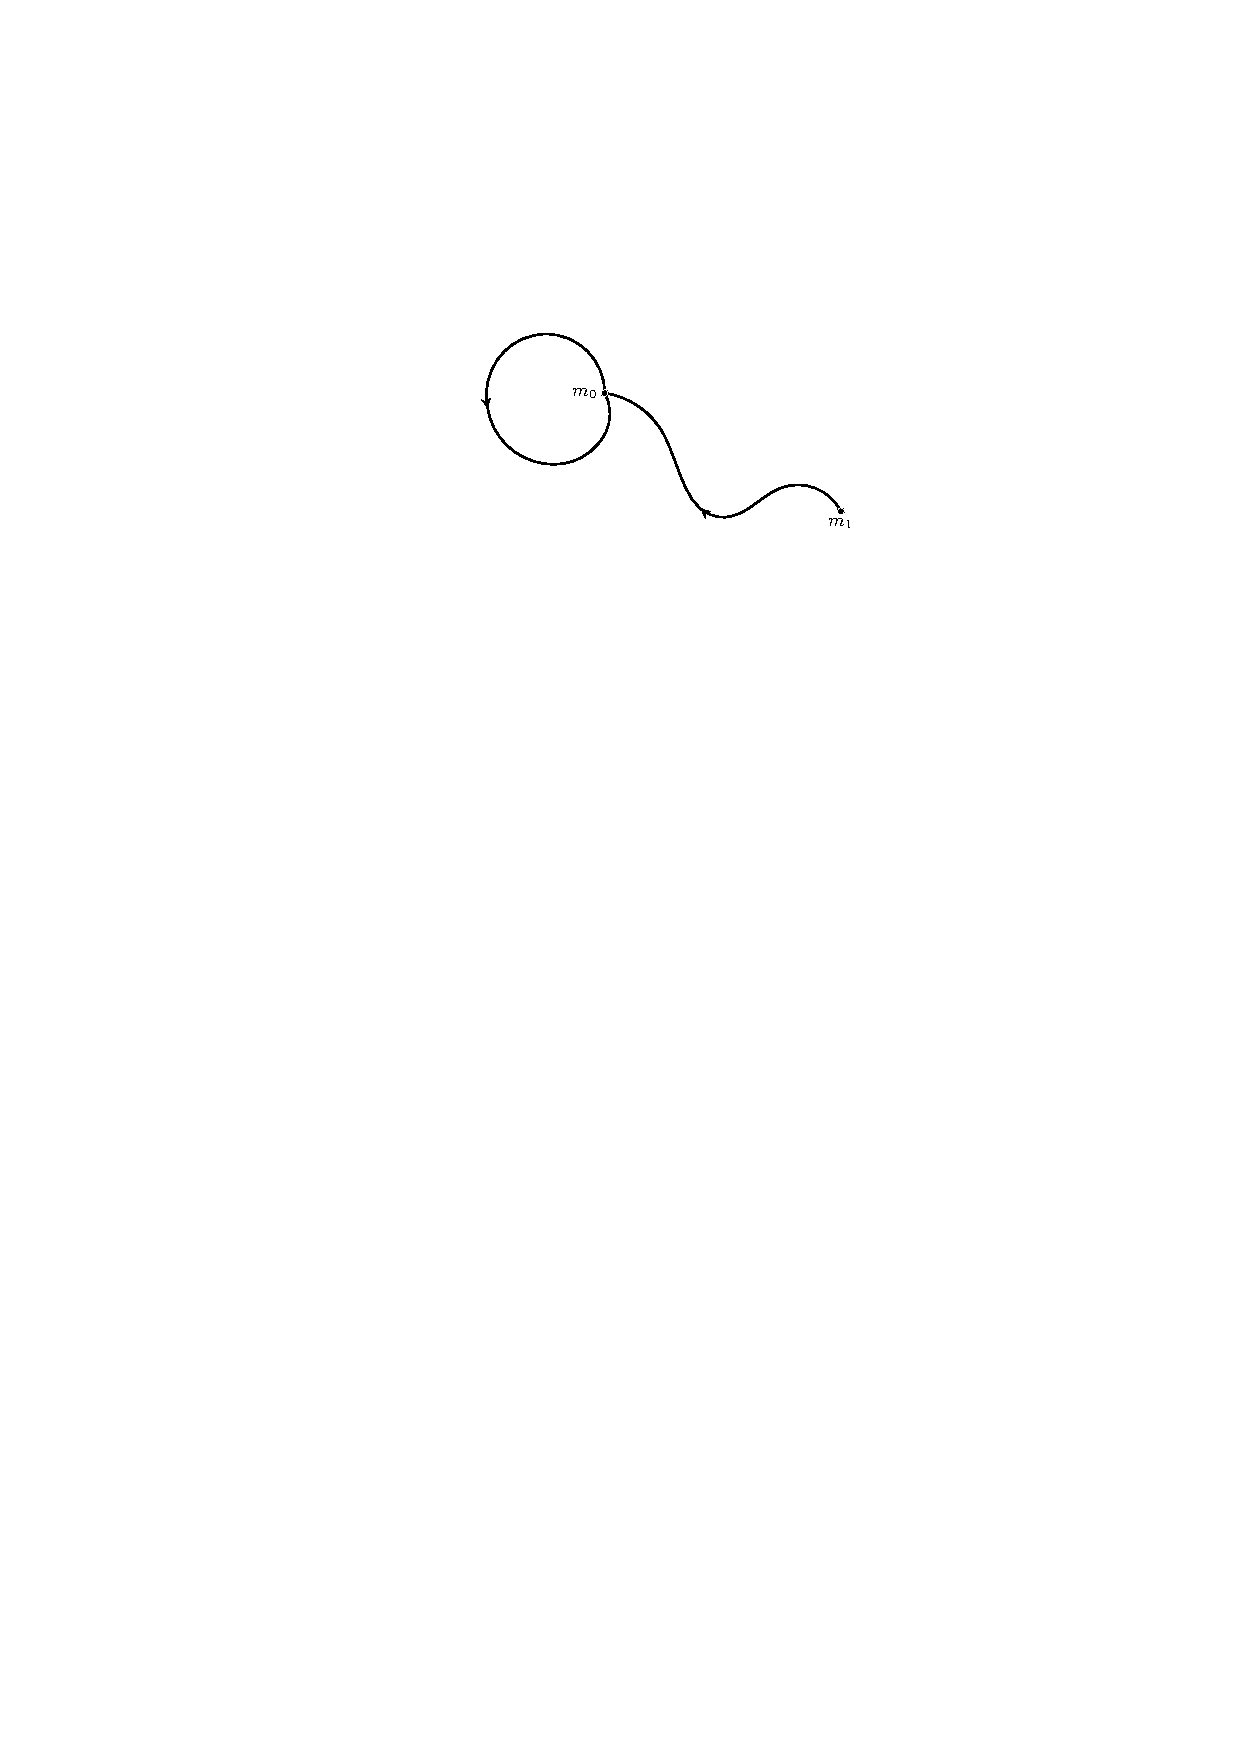
\includegraphics[scale=0.8]{figures/holonomy.pdf}
    \end{center}
    All restricted $\omega$-holonomy at $p_1$ arises in this way. Since $p(t)$ is $\omega$- and $\omega'$-horizontal, the holonomy along the lasso agrees between the two connections.  The new holonomy algebra contains the contributions of these lassos, which are of the same dimension for both connections, so it contains the restricted holonomy of $\omega$.
\end{proof}


Similarly, the next lemma shows that any principal $G$-connection can be deformed on an arbitrarily small compact set so as to make the restricted holonomy group be all of the identity component $G_0$. If $G$ is connected, then this proves the existence of irreducible connections on any principal $G$-bundle.

\begin{lem}\label{lem 16.24 McKay}
    Let $P(G,M)$ be a principal bundle over a connected base $M$ of dimension $\dim M\geq 2$. Then (1) $P$ admits a principal connection whose restricted holonomy group is the identity component $G_0$ and (2) for any principal connection $\omega$ and any open set $\varnothing\neq U\subset M$, there exists a principal connection $\omega'$ whose restricted holonomy group is $G_0$ and which agrees with $\omega$ outside of a compact subset of $U$.
\end{lem}
\begin{proof}
    Suppose that the result is proven for trivial bundles. Then we can choose a $U$ over which the bundle is trivial and the result follows. Thus, it suffices to consider a trivial bundle $P=M\times G$ with the standard flat connection $\omega=\pr_G^\ast\theta_G$.

    If $\frakg=0$, the result is trivial. Otherwose, take $m_1\in M$ and a curvature value $\Omega_1=\Omega_{p_1}$ which takes on a nonzero value $\Omega_1(X,Y)$ for some $X,Y\in\T_{p_1}P$ over $m_1$. Take a relatively compact set $U_1$ around $m_1$ whose closure is not $M$. Pick a connection over $U_1$ whose curvature at $p_1$ is $\Omega_1$. Use a \gls{pou} to glue this connection to $\omega$, so that it agrees with $\omega$ outside of $\restr{P}{U_1}$. Call the resulting connection $\omega'$. The holonomy algebra now has dimension at least $1$.

    After $k$ steps, assume that the holonomy algebra is of dimension at least $k$. Suppose that there is some point at which the holonomy algebra is still not $\frakg$. Then this is true at every point, because the holonomy algebra changes only by adjoint action from point to point. Take some $m_{k+1}\in M$ near which $\omega$ is flat, a point $p_{k+1}\in P_{m_{k+1}}$, and a curvature element $\Omega_{k+1}$ taking on some value $\Omega_{k+1}(X,Y)$ at $p_{k+1}$ outside of the holonomy algebra. Take a relatively compact open set $U_{k+1}$ around $m_{k+1}$ with closure not intersecting any of the closures of the previously chosen open sets $U_i$. Over $U_{k+1}$, pick a connection whose curvature at $p_{k+1}$ is $\Omega_{k+1}$. Use a \gls{pou} to glue this connection to $\omega$, so that it agrees with $\omega$ outside of $\restr{P}{U_{k+1}}$. By induction, we will at some point enlarge the restricted holonomy to the point of being an open subgroup, and hence all of $G_0$.
\end{proof}

It is quite rare that we can explicitly find the holonomy bundle, as it requires solving equations of Lie type. Hence we might not know its tangent spaces, and cannot directly apply the Ambrose-Singer Theorem. Instead, by purely local calculation, we can find the smallest Lie algebra $\frakn< \frakg$ containing all values of the curvature at all points, at least constraining the holonomy algebra. Since the curvature transforms in the adjoint representation, this Lie algebra contains all $G$-adjoint conjugates of the holonomy algebra.

\begin{thm}[Cartan's holonomy envelope (1926)]\label{thm 16.26 McKay}
    Let $P(G,M)$ be a principal bundle over a connected base $M$ with a principal connection $\omega$. Let $\frakn<\frakg$ be the span of the values of the curvature $\Omega$ at all points of $P$. Then 
    \begin{enumerate}
        \item $\frakn\sub \frakg$ is an ideal containing the holonomy algebra. 
        \item Further, suppose that $N\sub G$ is a normal subgroup with Lie algebra $\frakn$. Then the restricted holonomy groups at all points of $P$ lie in $N$, and if the full holonomy group at some point of $P$ lies in $N$, then so does the holonomy group at any point.
        \item The distribution $\omega^{-1}(\frakn)$ is integrable and each leaf of the corresponding foliation contains a holonomy bundle.
    \end{enumerate}
\end{thm}
\begin{proof}
    Let $V_{p}=\<\Omega(X,Y)\mid X,Y\in\T_{p}P\><\frakg$. Then $\frakn$ is the span of the union of the $V_{p}$ over all $p\in P$. The curvature transforms under the adjoint representation, so $V_p$ does as well, and so $\frakn$ is an $\Ad(G)$-invariant subspace, hence also $\ad(\frakg)$-invariant, i.e., an ideal. 

    We assume that $P$ is a right bundle as usual. Under the principal action, holonomy transforms by conjugation, $\Hol_{p\cdot g}(\omega)=\Adg_g^{-1}\Hol_p(\omega)$. By the normality of $N$, the holonomy lies in $N$ at some point iff it lies in $N$ at all points of the same fiber. But then we can follow horizontal curves to get from fiber to fiber, because $M$ is connected. The holonomy doesn't change along horizontal curves, so it lies in $N$ everywhere.

    Consider the $1$-form $\omega+\frakn\in\Omega^1(P;\frakg\slash\frakn)$. From the equation $\Omega=\dd\omega+\frac12[\omega,\omega]$, we see that, modulo $\omega+\frakn$,
    \[\dd\omega+\frakn\equiv \Omega+\frakn\equiv 0\pmod{\omega+\frakn},\]
    since $\Omega$ is valued in $\frakn$ and $[\frakn,\frakn]<\frakn$. By the Frobenius Theorem, $P$ is foliated by submanifolds whose tangent spaces consist of the tangent vectors $X$ on which $\omega(X)\in\frakn$. In particular, the horizontal directions $\ker\omega$ lie tangent to the leaves. Hence, each leaf contains a holonomy bundle.
\end{proof}

\begin{rem}
    Suppose that we wish to determine whether the holonomy group of a principal bundle $P(G,M)$ with principal connection, on a connected and simply connected manifold $M$, is up to conjugacy equal to some subgroup $L<G$. First, for this to hold, at every point of $P$ the curvature values must lie in some conjugate of the Lie algebra $\frakl<\frakg$. Second, if $P'\subset P$ is the subset of points at which the curvature is valued in $\frakl$, then $P'$ must contain a holonomy bundle. To check for this, we can compute $P'$ by a local calculation, without knowing how to compute the holonomy group, just by calculating the curvature. Replace $P'$ by the set of points of $P'$ at which all integral curves of all vector fields $X\in\fX(P)$ with $\omega(X)\in\frakl$ stay, at least for a short time, inside $P'$ (this might be trickier but is still local). Repeat this process of replacing $P'$ by that subset of $P'$. After we repeat infinitely many times, if $P'$ is still not empty, then, as in the proof of the last theorem, the equations $\omega+\frakl=0$ satisfy the requirements of the Frobenius Theorem so that the horizontal directions are tangent to the leaves, so contain a holonomy bundle and the holonomy group lies in $L$, at least locally.
\end{rem}








\section{Gauge transformations}


Let us discuss the connection to the gauge group. The Lie algebra of the group of automorphisms (not only vertical ones) $\Aut(P)$ is the space $\aut(P)=\fX(P)^G$ of $G$-invariant vector fields on $P$, and the Lie algebra of the gauge group (of vertical automorphisms) is the subspace $\gau(P)$ of vertical $G$-invariant vector fields. One has the exact sequence of Lie algebras
\[0\to \gau(P)\to \aut(P)\to \fX(M)\to 0.\]
The surjectivity of the map $\aut(P)\to \fX(M)$ can be proved using a trivializing open covering of $M$ and a $\gls{pou}$ subordinate to that cover. 


For $\varphi\in \Hom_G(P,G)$, the corresponding vertical automorphism is given by
\[\vartheta_\varphi:P\to P,\quad p\mapsto p\cdot \varphi(g).\label{eq 1.8.2 RS2}\]
The equivariance property $\vartheta_\varphi(p\cdot g)=\vartheta_\varphi(p)\cdot g$ is clearly equivalent to $\varphi(p\cdot g)=g^{-1}\varphi(p)g$, which is exactly the defining property of $\Hom_G(P,G)$. It is also easy to check that this correspondence is a group isomorphism (where elements of $\Hom_G(P,G)$ are multiplied pointwise, so $\vartheta_\varphi\circ\vartheta_\psi=\vartheta_{\varphi\cdot\psi}$). Finally, recall from Proposition~\ref{prop 1.2.6 RS2} that the space $\Hom_G(P,G)$ can be identified with the space of sections of the associated group bundle $\Adg(P)=P\times^G G$, where $G$ acts on itself by conjugations. We thus have the isomorphisms
\[\Aut(P)\cong \Hom_G(P,G)\cong \Gamma^\infty(\Adg(P)).\]

It is also obvious that every vertical automorphism $\vartheta_\varphi\in\Gau(P)$ induces a vertical automorphism $\wh\vartheta_\varphi$ of any associated bundle $P^{[\sigma]}=P\times^G F$ given by
\[\wh\vartheta_\varphi([(p,f)])=\left[(p,\sigma_{\varphi(p)}(f))\right].\]
In particular, if $G\overset{\sigma}{\acts}F$ is a linear representation, then $\wh{\vartheta}_\varphi$ is a vertical automorphism of vector bundles.


\begin{prop}[{{\cite[Prop.~1.8.7]{RS2}}}]
    Let $(P\overset{\pi}{\to}M,G,\Phi)$ be a principal bundle and let $\calH P$ be a principal connection. Then, for $\vartheta\in \Gau(P)$ corresponding to $\varphi\in \Hom_G(P,G)$, one has the following transformation laws:
    \begin{enumerate}
        \item If $\omega$ is the connection form of $\calH P$, then $\vartheta^\ast \omega$ is the connection form of $\vartheta_\ast^{-1}(\calH P)$ and 
        \[(\vartheta^\ast\omega)_p=\Ad_{\varphi(p)}^{-1}\circ\omega_p+(\varphi^\ast\theta_G)_p,\label{eq 1.8.7 RS2}\]
        where $\theta_G$ is the Maurer-Cartan form on $G$.

        \item If $\Omega^\omega$ is the curvature $2$-form of $\omega$, then $\vartheta^\ast\Omega^\omega$ is the curvature form of $\vartheta^\ast\omega$ and
        \[(\vartheta^\ast\Omega)_p=\Ad_{\varphi(p)}^{-1}\circ\Omega_p.\label{eq 1.8.8 RS2}\]
    \end{enumerate}
\end{prop}
\begin{proof}
    1. To prove the first equality, we must calculate $\vartheta_\ast(X)$ for $X\in \T_pP$. Let $\gamma$ be a path in $P$ representing $X$.  Using \eqref{eq 1.8.2 RS2}, we have
    \begin{multline}
        \vartheta_{\ast p}(X)=\restr{\frac{\dd}{\dd t}}{0}\vartheta(\gamma(t))=\restr{\frac{\dd}{\dd t}}{0} (\gamma(t)\cdot \varphi(\gamma(t)))=
        \\=\restr{\frac{\dd}{\dd t}}{0}(\gamma(t)\cdot \varphi(p))+\restr{\frac{\dd}{\dd t}}{0}(p,\varphi(\gamma(t))=\Phi_{\varphi(p)\ast}(X)+\Phi_{p\ast}\circ \varphi_{\ast p}(X).
    \end{multline}
    The second term describes a vertical vector in $\vartheta(p)$. Thus, we may write it in the form $\Phi_{\vartheta(p)\ast}(A)$ with $A\in\frakg$. Explicitly, since $\varphi_{\ast p}(X)\in \T_{\varphi(p)}G$, we can write
    \[\Phi_{p\ast}\circ \varphi_{p\ast }(X)=\Phi_{p\ast}\circ \rmL_{\varphi(p)\ast}\circ \rmL_{\varphi(p)\ast}^{-1}\circ \varphi_{\ast p}(X).\]
    Using
    \[\rmL_{\varphi(p)\ast}^{-1}\circ \varphi_{p\ast}(Y)=\theta_G(\varphi_{p\ast}(X))=(\varphi^\ast\theta_G)_p(X)\]
    and $\Phi_p\circ \rmL_{\varphi(p)=\Phi_{\vartheta(p)}}$, we obtain
    \[\vartheta_{p\ast}(X)=\Phi_{\varphi(p)\ast}(X)+\Phi_{\vartheta(p)\ast}(\varphi^\ast\theta_G(X)).\label{eq 1.8.10 RS2}\]
    Using this equation, together with the equivariance of $\omega$, we obtain \eqref{eq 1.8.7 RS2}.

    2. Using the structure equation, we obtain
    \[\vartheta^\ast\Omega=\vartheta^\ast\left(\dd \omega+\frac12[\omega,\omega]\right)=\dd(\vartheta^\ast\omega)+\frac12[\vartheta^\ast\omega,\vartheta^\ast\omega],\]
    that is, $\vartheta^\ast\Omega$ is the curvature form of $\vartheta^\omega$, indeed. To prove \eqref{eq 1.8.8 RS2}, we must calculate $\vartheta^\ast \Omega(X,Y)$ for any $X,Y\in \T_pP$. For that purpose, we use the decomposition \eqref{eq 1.8.10 RS2} for both vectors. Since $\Omega$ is horizontal, only the first terms of this decomposition contribute. Then, using the equivariance of $\Omega$, one immediately obtains \eqref{eq 1.8.8 RS2}.
\end{proof}

\begin{rem}\label{rem 1.8.8 RS2}
    \begin{enumerate}
        \item Sometimes we will use the following short-hand notation for the above transformation laws:
        \[\vartheta^\ast\omega=\Ad_{\varphi}^{-1}\circ\omega+\varphi^\ast\theta_G,\quad \vartheta^\ast \Omega=\Ad_\varphi^{-1}\circ\Omega.\]
        In matrix notation, we have $\varphi^\ast\theta_G=\varphi^{-1}\dd\varphi$, and 
        \[\vartheta^\ast\omega=\varphi^{-1}\omega\varphi+\varphi^{-1}\dd\varphi,\quad \vartheta^\ast\Omega^\omega=\varphi^{-1}\Omega^\omega \varphi.\]
        \item Using the local representative $\rho^\alpha=\varphi\circ s_\alpha$, we read off the following transformation laws for the local representatives of $\omega$ and $\Omega^\omega$:
        \[\scrA'=\Ad_\rho^{-1}\circ\scrA+\rho^\ast\theta_G,\quad \scrF'=\Ad_\rho^{-1}\scrF.\]
        Note that this formula is essentially identical to the transformation law for local representatives from Corollary~\ref{cor 1.3.12 RS2}. We might call the transformation coresponding to a change of local coordinates a \emph{passive gauge transformation}, and a transformation stemming from an actual automorphism of the bundle an \emph{active gauge transformation}.
    \end{enumerate}
\end{rem}


Since we would like to study bundles up to isomorphism, the action of the gauge group $\Gau(P)=\Aut_M(P)$ on the space of connections $\calA(P)$ will be crucial. We will now characterize the infinitesimal version of this action. The gauge algebra $\gau(P)$ can be identified with sections of the adjoint bundle $\Ad(P)$: \index{Adjoint vector bundle}
\[\gau(P)\cong \Omega^0(M;\Ad(P))=\Omega^0_{\hor}(P;\frakg)^\Ad.\]
Indeed, each $G$-invariant vector field $X\in\Gamma^\infty(\calV P)$, by composition with the global trivialization $\psi^{-1}:\calV P\to P\times\frakg$ (cf.\ Lemma~\ref{lem 1.3.1 RS2}), produces an element of $\Omega^0_{\hor}(P;\frakg)^\Ad$.

An automorphism $\vartheta\in\Aut(P)$ acts on $\calA(P)$ by pullbacks along the inverse, $\omega\mapsto \vartheta_\ast\omega$. For the action of the subgroup $\Gau(P)$, there is an alternative formula for this action which we now derive. 

Recall that each vertical automorphism $\vartheta\in \Gau(P)$ corresponds to a unique equivariant function $\varphi:P\to G$ defined by 
\[\varphi\in \Hom_G(P,G),\quad \vartheta(p)=p\cdot \varphi(p)^{-1}.\]
Here, $G$ acts on itself by conjugations, and the equivariance property reads $\varphi(p\cdot g)=g^{-1}\varphi(p)g$ (which immediately follows from $\vartheta(p\cdot g)=\vartheta(p)\cdot g$). Similarly, each invariant vertical vector field $Y\in \gau(P)$ can be identified, via the global trivialization $\psi^{-1}$, with a function 
\[\wt\zeta\coloneqq \psi^{-1}\circ Y\in \Omega^0_{\hor}(P;\frakg)^\Ad.\]
Indeed, it is easy to check that $\Phi_g^\ast \zeta=\Ad_g^{-1}\zeta$. This, in turn, is identified via Proposition~\ref{prop 1.2.12 RS2} with a section of the associated adjoint bundle: \index{Adjoint vector bundle}
\[\zeta\in \Omega^0(M;\Ad(P))=\Gamma^\infty(\Ad(P)).\]
Explicitly, the identification is $\zeta(m)=\iota_p(\wt\zeta(p))=[(p,\wt\zeta(p))]\in P\times^G \frakg$, where $p\in P_m$.
We can write these identifications as isomorphisms
\[\gau(P)\cong \Omega^0_{\hor}(P;\frakg)^\Ad\cong \Gamma^\infty(\Ad(P)).\]
The next proposition computes the action of the gauge group on the Lie algebra of all infinitesimal automorphisms.

\begin{prop}
    Let $\vartheta\in\Gau(P)$ and $\varphi\in \Hom_G(P,G)$ the corresponding equivariant function. For all $X\in\aut(P)=\fX(P)^G$,
    \[\vartheta_\ast X-X\in\gau(P).\]
    The corresponding section $\zeta \in\Gamma^\infty(\Ad(P))$ is represented by the equivariant function
    \[\wt\zeta(p)=\Ad_{\varphi(p)}\circ(\varphi^\ast \theta_G)(X(p)),\quad p\in P.\]
\end{prop}
\begin{proof}
    The vector field $\vartheta_\ast X$ is invariant since $\vartheta$ commutes with the principal $G$-action, and under $\pi_\ast$ projects onto the same vector field as $X$ since $\pi\circ\vartheta=\pi$. This shows that $Y=\vartheta_\ast X-X$ is vertical and $G$-invariant, thus an element of $\gau(P)$. Now we evaluate both sides of \eqref{eq 1.8.7 RS2} on the vector field $X$:
    \[\omega(\vartheta_\ast X)=\Ad_{\varphi}^{-1}\circ \omega(X)+(\varphi^\ast \theta_G)(X),\]
    which is equivalent to
    \[\Ad_\varphi\omega(\vartheta_\ast X)-\omega(X)=\Ad_\varphi\circ (\varphi^\ast \theta_G)(X),\]
    By the equivariance of principal connections, $\Ad_\varphi\omega(\vartheta_\ast X)=\omega(\Phi_{\varphi\ast}^{-1}\vartheta_\ast X)$, and because $\vartheta$ is equivariant and $X$ is invariant, this is just $\omega(\vartheta_\ast X)$. Therefore
    \[\omega(Y)=\Ad_\varphi\circ (\varphi^\ast \theta_G)(X).\]
    The connection form was defined as $\omega=\psi^{-1}\circ\calV$. Since $Y$ is vertical, $\omega(Y)=\psi^{-1}(Y)$. We get the corresponding $\Ad$-equivariant function
    \[\wt{\zeta}=\psi^{-1}\circ Y=\Ad_\varphi\circ (\varphi^\ast\theta_G)(X).\]
\end{proof}

\begin{rem}
    Note that $\Ad_\varphi\circ \varphi^\ast\theta_G$ can also be written as $\varphi^\ast\theta_G^R$, where $\theta_G^R$ is the right-invariant Maurer-Cartan form on $G$. Therefore, in matrix notation we may write $\wt\zeta=(\Lie_X\varphi)\cdot \varphi^{-1}$.
\end{rem}

\begin{prop}\label{prop action of Gau(P) on calA(P)}
    The natural action of $\Gau(P)$ on $\calA(P)$ is given by
    \[\vartheta\cdot\omega\coloneqq (\vartheta^{-1})^\ast\omega=\Ad_\varphi \circ (\omega-\varphi^\ast \theta_G),\quad \omega\in\calA(P),\]
    where $\varphi\in \Hom_G(P,G)$ is the element representing $\vartheta\in \Gau(P)$.
\end{prop}
\begin{proof}
    We will prove the equivalent property $\vartheta^\ast\omega=\Ad_\varphi^{-1}\omega+\varphi^\ast\theta_G$. It suffices to check this on invariant vector fields $X\in \fX(G)^G$. By the last proposition, and since $\varphi^\ast f=\Ad_\varphi^{-1}f$ for all $f\in \Omega^0_{\hor}(P;\frakg)^\Ad$, 
    \[(\vartheta^\ast\omega)(X)=\vartheta^\ast(\omega(\vartheta_\ast X))=\Ad_\varphi^{-1}(\omega(\vartheta_\ast X))=(\Ad_\varphi^{-1}\omega+\varphi^\ast\theta_G)(X).\]
\end{proof}

We can now characterize the stabilizer subgroups $\Gau(P)_\omega$ of gauge transformations that preserve a given connection $\omega$. First consider how gauge transformations affect parallel transport. The following is a simple exercise.

\begin{lem}\label{lem 31794}
    Let $\vartheta\in\Gau(P)$ and $\vartheta_m\coloneqq\restr{\vartheta}{P_m}$. Then for any path $\gamma:[0,1]\to M$, 
    \[\tra_{\gamma}^{\vartheta\cdot\omega}=\vartheta_{\gamma(1)}\circ\tra_\gamma^\omega \circ\vartheta_{\gamma(0)}^{-1}.\]
\end{lem}

Now suppose $M$ is connected and recall the holonomy representation for $m\in M$:
\[\Hol(\omega):C(m)\to \Diff(P_m)^G\cong G,\quad \gamma\mapsto \tra_\gamma^\omega.\]
Its image $\Hol_p(\omega)< G$ is the holonomy group based at $p\in P_m$, and its identity component $\Hol^0_p(\omega)\emb G$ is a closed subgroup of $G$. Recall also that $\Diff(P_m)^G\cong G$ is a natural isomorphism, so we will use these two groups interchangeably.

\begin{prop}\label{prop gauge group of principal connection}
    The restriction map $\Gau(P)_\omega\to \Diff(P_m)^G$, $\vartheta\mapsto \vartheta_m\coloneqq\restr{\vartheta}{P_m}$ is injective and defines an isomorphism of the stabilizer $\Gau(P)_\omega$ with the centralizer in $G$ of the holonomy group:
    \[\Gau(P)_\omega\cong \rmC_G(\Hol_p(\omega)).\]
\end{prop}
\begin{proof}
    A gauge transformation preserves $\omega$ iff it preserves $\calH P$. Equivalently, by Lemma~\ref{lem 31794} (applied to $\vartheta^{-1}$), $\vartheta\in\Gau(P)_\omega$ iff for all paths $\gamma:[0,1]\to M$, $\vartheta$ commutes with parallel transport:
    \[\vartheta(\gamma(1))=\tra_\gamma^\omega\circ \vartheta(\gamma(0))\circ(\tra_\gamma^\omega)^{-1}.\label{18041}\]
    Taking paths with $\gamma(0)=m$, it follows that if $\vartheta_m=\id_{P_m}$, then $\vartheta=\id_P$. That is, the map $\vartheta\mapsto\vartheta_m$ is injective. Taking $\gamma\in C(m)$, \eqref{18041} shows that $\vartheta_m$ centralizes $\Hol_p(\omega)$. Conversely, if $\vartheta_m\in \rmC_G(\Hol_p(\omega))$, then we can define $\vartheta$ fiberwise by putting
    \[\vartheta_{m'}\coloneqq \tra_\gamma^\omega\circ \vartheta_m\circ (\tra_\gamma^\omega)^{-1},\]
    where $\gamma$ is any path $m\leadsto m'$. The condition $\vartheta\in \Gau(P)_\omega$ guarantees that the right hand side does not depend on the choice of $\gamma$ and hence globally defines a smooth automorphism.
\end{proof}

\begin{rem}\label{rem automorphisms of principal connection}
    While this shows that the set of gauge transformations (vertical automorphisms) preserving a principal connection is a Lie group, the same does not hold, in general, for the set of \emph{all} automorphisms that preserve a connection. For example, the canonical flat connection on the product bundle $P=M\times G$ admits an automorphism $(m,g)\mapsto (f(m),g)$, for each diffeomorphism $f$ of $M$ (indeed, it obviously preserves the horizontal distribution). This stands in marked difference from the situation with Cartan connections, whose automorphism groups are always finite-dimensional Lie groups.
\end{rem}

This shows that all stabilizer subgroups are finite-dimensional Lie groups. In particular, for an irreducible connection, the stabilizer of a connection $\omega$ is isomorphic to the center $\rmZ(G)$. This is another way of detecting reducibility, in addition to the Ambrose-Singer Theorem~\ref{thm 1.7.15 RS2 Ambrose-Singer}. Moreover:

\begin{cor}
    The based gauge group $\Gau_m(P)\coloneqq \{\vartheta\in \Gau(P)\mid \vartheta_m=\id_{P_m}\}$ acts freely on $\calA(P)$.
\end{cor}
\begin{cor}
    If $G$ is abelian, every principal connection has stabilizer equal to $G$, viewed as constant gauge transformations in $\Gau(P)\cong \Gamma^\infty(\Adg(P))\cong C^\infty(M,G)$.
\end{cor}

\begin{defn}[Moduli space of connections]\index{Moduli space}
    The (topological) quotient $\calM(P)\coloneqq \calA(P)\slash \Gau(P)$ is called the moduli space of connections. 
\end{defn}

The moduli space consists of classes of gauge-equivalent gauge potentials, the `true' configuration space in gauge theory. One can show that the map 
\[\calA(P)\times\Gau(P)\to \calA(P)\times\calA(P),\quad (\omega,\vartheta)\mapsto (\omega,\vartheta\cdot\omega),\]
is closed and that the stabilizers $\Gau(P)_\omega$ are compact, so that the action of $\Gau(P)\acts\calA(P)$ is proper \cite[Thm.~6.1.7]{RS2}. Hence, the orbits are closed and the moduli space is Hausdorff. This moduli space is still ``infinite-dimensional''. To get nicer moduli spaces one usually restricts to a sub-class of connections such as flat connections or, more generally, Yang-Mills connections.







\section{Covariant exterior derivative}\label{sec: cov ext derivative}



In the previous \sect\ we computed the natural action of the gauge group $\Gau(P)$ on the space of connections $\calA(P)$. As is clear from Proposition~\ref{prop action of Gau(P) on calA(P)}, this is in fact a smooth action of an infinite-dimensional Lie group on an infinite-dimensional smooth manifold. The natural question is then: what is the infinitesimal action, or what are the Killing vector fields corresponding to this action? Since $\calA(P)$ is an affine space modeled on $\Omega^1_{\hor}(P;\frakg)^\Ad$, its tangent spaces are naturally identified with the same space:
\[\T_\omega\calA(P)\cong \Omega^1_{\hor}(P;\frakg)^\Ad.\]
Thus, an infinitesimal gauge transformation $\zeta\in\Omega^0_{\hor}(P;\frakg)^\Ad\cong\gau(P)$ generates a Killing vector field $\zeta_\ast\in \fX(\calA(P))\cong C^\infty(\calA(P),\Omega^1_{\hor}(P;\frakg)^\Ad)$. In other words, the map $(\zeta,\omega)\mapsto\zeta_\ast(\omega)$ is an object that takes a horizontal $0$-form $\zeta$ (of type $\Ad$) and a connection form $\omega$, and produces a horizontal $1$-form (again of type $\Ad$). This is exactly the missing analog of an exterior derivative on these spaces of sections! We now turn to studying this object.

\begin{prop}
    The Killing vector field generated by an ininitesimal gauge transformation $\zeta\in\Gamma^\infty(\Ad(P))\cong\gau(P)$ on $\calA(P)$ is given by
    \[-\zeta_\ast(\omega)=\dd \wt{\zeta}+[\omega,\wt{\zeta}],\quad \omega\in\calA(P),\]
    where $\wt{\zeta}\in \Omega^0_{\hor}(P;\frakg)^\Ad$ is the corresponding equivariant function.
\end{prop}
\begin{proof}
    Let $\gamma:(-\epsilon,\epsilon)\to \Gau(P)$ be a path in $\Gau(P)$ such that $\dot\gamma(0)=\zeta$ (where we think of $\zeta$ as an element of $\gau(P)$ directly). Let $\wt\gamma$ be the corresponding path in $\Omega^0_{\hor}(P;\frakg)^\Ad$. We have $\dot{\tilde{\gamma}}(0)=\wt{\zeta}$. Then, by Proposition~\ref{prop action of Gau(P) on calA(P)},
    \[-\zeta_\ast(\omega)=\restr{\frac{\dd}{\dd t}}{0}(\gamma(-t)\cdot \omega)=\restr{\frac{\dd}{\dd t}}{0}\left(\Ad_{\wt{\gamma}(-t)}(\omega-(\wt{\gamma}(-t))^\ast\theta_G)\right)=[\omega,\wt{\zeta}]+\dd\wt{\zeta},\]
    where the last equality follows from the definition of the Lie bracket on a Lie group and the definition of the Maurer-Cartan form.
\end{proof}


Since the action of the gauge group is a left action, the minus sign above is convenient to make the map to Killing vector fields a homomorphism of Lie algebras. Now observe that due to $\wt{\zeta}$ being of type $\Ad$, we can rewrite the Lie bracket above as a Lie derivative along a Killing vector field $\omega(X_p)_\ast(p)=\psi(\omega(X_p))=\calV(X_p)$ and simplify:
\[(\dd\wt{\zeta}+[\omega,\wt{\zeta}])(X)=
\dd\wt\zeta(X)-\Lie_{\omega(X)_\ast}\wt\zeta=
\dd\wt\zeta(X)-\dd\wt\zeta(\calV(X))=\dd\wt{\zeta}(\hor X).\label{eq 4791793}\]

This, as well as the definition of curvature, suggests the following general definition. Note that at this point we have to specialize to associated \emph{vector} bundles, although slight generalizations are possible.

\begin{defn}[Covariant exterior derivative]
    Let $P$ be a principal bundle with a principal connection $\calH P$ and connection form $\omega$, let $V$ be a finite-dimensional vector space, and let $\alpha\in\Omega^k(P;V)$. The covariant exterior derivative of $\alpha$ w.r.t.\ $\omega$ is defined as
    \[(\rmD^\omega \alpha)(X_0,\ldots,X_k)\coloneqq \dd\alpha(\hor X_0,\ldots,\hor X_k),\quad X_0,\ldots,X_k\in\fX(P).\]
    By definition, $\rmD^\omega$ fulfills the same Leibniz rule (w.r.t.\ $\wedge$) as the ordinary exterior derivative and $\rmD^\omega \alpha$ is horizontal. Moreover, as we will show below, $\rmD^\omega$ preserves the symmetry type of any horizontal form.
\end{defn}

In particular, the curvature form $\Omega^\omega$ satisfies 
\[\Omega^\omega=\rmD^\omega\omega.\]
Now we derive a general formula for the covariant exterior derivative.

\begin{prop}[{{\cite[Prop.~1.4.3]{RS2}}}]\label{prop 1.4.3 RS2}
    Let $P(M,G)$ be a principal bundle, let $G\overset{\sigma}{\acts}V$ be a finite-dimensional linear representation, and let $\omega$ be a principal connection form on $P$.
    \begin{enumerate}
        \item $\rmD^\omega(\Omega^k_{\hor}(P;V)^\sigma)\subset \Omega^{k+1}_{\hor}(P;V)^\sigma$.
        \item Let $\wt\alpha\in\Omega^k_{\hor}(P;V)^\sigma$. Then
        \[\rmD^\omega\wt\alpha=\dd\wt\alpha+\sigma_\ast(\omega)\wedge \wt\alpha,\label{eq 1.4.1 RS2}\]
        where
        \[(\sigma_\ast(\omega)\wedge\wt\alpha)_p(X_0,\ldots,X_k)\coloneqq \sum_{i=0}^k (-1)^i\sigma_\ast(\omega_p(X_i))\left(\wt\alpha_p(X_0,\ldots,\wh{X}_i,\ldots,X_k)\right),\]
        with $p\in P$, $X_0\ldots,X_k\in \T_pP$, and where the hat represents an omitted argument.
    \end{enumerate}
\end{prop}
\begin{proof}
    1. Let $\wt\alpha\in\Omega^k_{\hor}(P,V)^\sigma$. By definition of the covariant exterior derivative, $\rmD^\omega\wt\alpha$ is a $V$-valued horizontal $(k+1)$-form. We now check equivariance:
    \begin{align}
        (\Phi_g^\ast \rmD^\omega\wt\alpha)(X_0,\ldots,X_k)&=\rmD^\omega\wt\alpha(\Phi_{g\ast}X_0,\ldots, \Phi_{g\ast}X_k)=\notag\\
        &=\dd\wt\alpha(\hor\Phi_{g\ast}X_0,\ldots,\hor \Phi_{g\ast}X_k)=\notag\\
        &=\dd\wt\alpha(\Phi_{g\ast}\hor X_0,\ldots,\Phi_{g\ast}\hor X_k)=\notag\\
        &=\dd(\Phi_g^\ast\wt\alpha)(\hor X_0,\ldots,X_k)=\notag\\
        &=\dd(\sigma_{g^{-1}}\circ\wt\alpha)(\hor X_0,\ldots,\hor X_k)=\notag\\
        &=\sigma_{g^{-1}}\circ \rmD^\omega\wt\alpha (X_0,\ldots,X_k).
    \end{align}
    This shows that $\rmD^\omega\wt\alpha$ is of type $\sigma$.

    2. Since each of the vectors $X_0,\ldots,X_k\in \T_pP$ may be decomposed into a vertical and a horizontal part, it is enough to consider the usual cases:
    \begin{enumerate}[label=(\alph*)]
        \item Let all $X_i$ be horizontal. Let $\omega(X_i)=0$ and formula \eqref{eq 1.4.1 RS2} follows from the definition of $\rmD^\omega$.
        \item Let one of the vectors $X_i$, say $X_0$, be vertical and the rest horizontal. Then, there exists an element $A\in\frakg$ such that $X_0=(A_\ast)_p=\Phi^0_\ast(A)$ and a family of vector fields $Y_1,\ldots,Y_k\in\fX(M)$ such that their horizontal lifts $Y_i^h$ at $p$ coincide with the vectors $X_1,\ldots,X_k$. Then
        \[(\rmD^\omega\wt\alpha)(X_0,\ldots,X_k)=0,\; (\sigma_\ast(\omega)\wedge\wt\alpha)(X_0,\ldots,X_k)=\sigma_\ast(A)(\wt\alpha(X_1,\ldots,X_k)).\]
        Using Proposition~\ref{prop 4.1.6 RS1}, Lemma~\ref{lem 1.4.2 RS2}, the horizontality of $\wt\alpha$ and the $G$-invariance of horizontal lifts, we calculate
        \begin{align}
            (\dd\wt\alpha)_p(X_0,\ldots,X_k)&=(A_\ast)_p(\wt\alpha(Y_1^h,\ldots,Y_k^h))=\notag\\
            &=\restr{\frac{\dd}{\dd t}}{0}\wt\alpha_{p\cdot \rme^{tA}}(Y_1^h,\ldots,Y_k^h)=\notag\\
            &=\restr{\frac{\dd}{\dd t}}{0}\wt\alpha_{p\cdot \rme^{tA}}((\Phi_{\rme^{tA}})_\ast X_1^h,\ldots,(\Phi_{\rme^{tA}})_\ast X_k^h)=\notag\\
            &=\restr{\frac{\dd}{\dd t}}{0}\left(\Phi_{\rme^{tA}}^\ast\wt\alpha\right)_p(X_1,\ldots,X_k)=\notag\\
            &=\restr{\frac{\dd}{\dd t}}{0}\sigma_{\rme^{-tA}}\wt\alpha_p(X_1,\ldots,X_k)=\notag\\
            &=-\sigma_\ast(A)(\wt\alpha_p(X_1,\ldots,X_k)).
        \end{align}
        Thus, in this case, the right hand side of \eqref{eq 1.4.1 RS2} also vanishes.
        \item Let as least two vectors $X_i$ be vertical and the rest horizontal. Then
        \[\rmD^\omega\wt\alpha(X_0,\ldots,X_k)=0,\quad (\sigma_\ast(\omega)\wedge \wt\alpha)(X_0,\ldots,X_k)=0,\]
        and it remains to show that $\dd\wt\alpha(X_0,\ldots,X_k)=0$. Since the commutator of vertical vector fields is vertical, the assertion follows from Proposition~\ref{prop 4.1.6 RS1} and the horizontality of $\wt\alpha$.
    \end{enumerate}
\end{proof}


\begin{defn}[Parallel horizontal form]\label{def parallel horizontal form}
    Let $P(M,G)$ be a principal bundle with a principal connection $\omega$, let $G\overset{\sigma}{\acts}V$ and let $E=P\times^G V$ be the associated \gls{vb}. An element $\wt\alpha\in\Omega^k_{\hor}(P,V)^\sigma$ is called parallel w.r.t.\ $\omega$ if $\rmD^\omega\wt\alpha=0$.
\end{defn}

\begin{rem}
    \begin{enumerate}
        \item In particular, for $k=0$, this defines the notion of a parallel section of $E$ via the natural isomorphism $\Omega^0_{\hor}(P;V)^\sigma\cong \Gamma^\infty(E)$. Since for $\wt{s}\in \Omega^0_{\hor}(P;V)^\sigma$, we have $(\rmD^\omega \wt{s})(X)=\dd \wt{s}(\hor X)$ Corollary~\ref{cor 1.5.7 RS2 my version} implies that this agrees with Definition~\ref{def parallel section}.
        \item Since the elements of $P$ are interpreted as $G$-frames on fibers of associated bundles, we may think of parallel local sections of $P$ as local frame fields that are ``constant to first order''. Correspondingly, parallel sections of $E$ are then sections whose ``coordinates'' in such local frame fields have vanishing derivatives. Moreover, by Proposition~\ref{prop 1.5.6 RS2 my version}, specifying local parallel sections is equivalent to specifying the connection.
    \end{enumerate}
\end{rem}


\begin{prop}[Bianchi identity {{\cite[Prop.~1.4.11]{RS2}}}] \label{prop 1.4.11 RS2}
    Let $P$ be a principal bundle and let $\Omega^\omega$ be the curvature form of a principal connection form $\omega$ on $P$. Then $\Omega^\omega$ is parallel w.r.t.\ $\omega$:
    \[\rmD^\omega\Omega^\omega=0.\label{eq 1.4.10 RS2 Bianchi}\]
\end{prop}
\begin{proof}
    It suffices to show that $\dd\Omega^\omega(X,Y,Z)=0$ for horizontal vector fields $X,Y,Z$ on $P$. Using the structure equation and Proposition~\ref{prop 4.1.6 RS1}, we calculate 
    \begin{align}
        \dd\Omega^\omega&(X,Y,Z)=\frac12(\dd[\omega,\omega])(X,Y,Z)=\notag\\
        &=X([\omega(Y),\omega(Z)])-Y([\omega(X),\omega(Z)])+Z([\omega(X),\omega(Y)])-\notag\\
        &-[\omega([X,Y]),\omega(Z)]+[\omega([X,Z]),\omega(Y)]-[\omega([Y,Z]),\omega(X)]=\notag\\
        &=0,
    \end{align}
    because $\omega$ vanishes on horizontal vector fields.
\end{proof}

\begin{rem}
    As a special case, for $\wt\alpha\in\Omega^k_{\hor}(P;\frakg)^\Ad$, since $\ad (\omega)\wedge\wt\alpha=[\omega,\wt\alpha]$, Proposition~\ref{prop 1.4.3 RS2} implies the formula we obtained at the beginning of this \sect:
    \[\rmD^\omega\wt\alpha=\dd\wt\alpha+[\omega,\wt\alpha].\]
    Thus, in particular, $\rmD^\omega\Omega^\omega=\dd\Omega^\omega+[\omega,\Omega^\omega]$, and the Bianchi identity takes the form
    \[\dd\Omega^\omega+[\omega,\Omega^\omega]=0.\label{eq 1.4.11 RS2 Bianchi}\]
\end{rem}


\begin{rem}\label{rem 1.4.4 RS2}
    In particular, the covariant exterior derivative of an equivariant map $\wt{s}\in\Hom_G(P,V)$ is given by
    \[\rmD^\omega\wt{s}=\dd\wt{s}+\sigma_\ast(\omega)\cdot \wt{s}.\label{eq 1.4.2 RS2}\]
    Clearly, this is an immediate consequence of formula \eqref{eq 1.4.1 RS2}. It can also be obtained directly in a way completely analogous to \eqref{eq 4791793}.
\end{rem}

Applying $\rmD^\omega$ to \eqref{eq 1.4.1 RS2}, one finds the following.

\begin{prop}[{{\cite[Prop.~1.4.13]{RS2}}}] \label{prop 1.4.13 RS2}
    $(\rmD^\omega)^2=\Omega^\omega$ in the sense that, for $\wt\alpha\in \Omega^k_{\hor}(P;V)$,
    \[\rmD^\omega\circ \rmD^\omega\wt\alpha=\sigma_\ast(\Omega^\omega)\wedge\wt\alpha.\]
\end{prop}
In particular, the connection is flat iff $(\rmD^\omega)^2=0$.

Now let us provide local descriptions of these objects. For simplicity we will omit the index $\omega$. As usual, the local representatives are defined as
\[(D\wt\alpha)_\alpha=s_\alpha^\ast D\wt\alpha.\]
Let us calculate the right hand side for a $0$-form $\varphi$ explicitly. Formula \eqref{eq 1.4.2 RS2} implies
\[s_\alpha^\ast(D\varphi)=\dd(s_\alpha^\ast\varphi)+s_\alpha^\ast(\sigma_\ast(\omega)\circ\varphi).\]
For the second term, we calculate
\begin{align}
    (s_\alpha^\ast\sigma_\ast(\omega)\varphi)_m(X)&=(\sigma_\ast(\omega)\varphi)_{s_\alpha(m)}(s_{\alpha\ast}X)=\notag\\
    &=\sigma_\ast(\omega_{s_\alpha(m)}(s_{\alpha\ast}X)\varphi(s_\alpha(m)))=\notag\\
    &=\sigma_\ast((s_\alpha^\ast\omega)_m(X))(s_\alpha^\ast\varphi)(m)=\notag\\
    &=\sigma_\ast(\scrA_{\alpha,m}(X))\wh{\varphi}_\alpha(m),
\end{align}
where $\scrA_\alpha=s_\alpha^\ast\omega$ is the local representative of $\omega$ and $X\in \T_mM$. Thus, denoting $(D\varphi)_\alpha=D\wh{\varphi}_\alpha$, we have
\[D\wh{\varphi}_\alpha=\dd\wh{\varphi}_\alpha+\sigma_\ast(\scrA_\alpha)\wh{\varphi}_\alpha.\label{eq 1.4.14 RS2}\]
Here, $\sigma_\ast(\scrA_\ast)$ is a $1$-form on $U$ with values in $\End(V)$. In the following remark, we analyze formula \eqref{eq 1.4.14 RS2} further.

\begin{rem}\label{rem 1.4.14 RS2}
    If $(U_\alpha,x)$ is a local chart, $\{\bf{t}_a\}$ a basis for $\frakg$ and $\{\bf{e}_i\}$ a basis in $V$, we can decompose
    \[\wh\varphi(x)=\varphi^i(x)\bf{e}_i,\quad \scrA_\alpha=\scrA_\mu^a\dd x^\mu\otimes \bf{t}_a,\quad D\wh{\varphi}_\alpha=D_\mu \varphi^i\dd x^\mu\otimes \bf{e}_i.\]
    To determine the coefficient functions $D_\mu\varphi^i$, we compute
    \begin{align}
        \sigma_\ast(\scrA_\alpha)\wh{\varphi}_\alpha&=\sigma_\ast(\scrA_\mu^a\dd x^\mu\otimes\bf{t}_a)\varphi^i\bf{e}_i=\notag\\
        &=(\scrA_\mu^a\varphi^i\dd x^\mu)\otimes(\sigma_\ast(\bf{t}_a)\bf{e}_i)=\notag\\
        &=\scrA_\mu^a\varphi^i\sigma_{ai}{}^j\dd x^\mu\otimes \bf{e}_j,
    \end{align}
    with $\sigma_{ai}{}^j$ representing the endomorphism $\sigma_\ast(\bf{t}_a)$ in the basis $\{\bf{e}_a\}$. Using this and denoting $\scrA_{\mu j}^i=\sigma_{aj}{}^i\scrA_\mu^a$, we obtain 
    \[D_\mu\varphi^i=\partial_\mu\varphi^i+\scrA_{\mu,j}^i \varphi^j.\]
\end{rem}

\begin{rem}
    The local curvature form, expanded in the local basis as in \ref{rem 1.3.10 RS2}, satisfies the structure equation written as\index{Equation!Structure}
    \[\scrF_\alpha=\partial_\mu \scrA_\nu^a-\partial_\nu\scrA_\mu^a+c^a_{bc}\scrA_\mu^b\scrA_\nu^c,\]
    where $c^a_{bc}$ are the structure constants of $\frakg$ w.r.t.\ the basis $\{\bf{t}_a\}$.
\end{rem}

Recall that reductions of $P$ to $H$ are in bijective correspondence with smooth sections of the associated bundle $P\slash H=P\times^G G\slash H$, cf.\ Corollary~\ref{cor 1.6.5 RS2}. Since orbits of Lie group actions are weakly embedded submanifolds, we can carry over Proposition~\ref{prop 1.6.2 RS2} to the case of a general Lie group action $G\overset{\sigma}{\acts}F$ by applying it to elements of $\Hom_G(P,F)$ with values in a single orbit of $\sigma$.

\begin{prop}[{{\cite[Prop.~1.6.10]{RS2}}}]\label{prop 1.6.10 RS2}
    Let $P(M,G)$ be a principal bundle and let $G\overset{\sigma}{\acts}V$ be a representation. Let $\varphi\in\Hom_G(P,V)$ and assume it takes values in a single orbit $O$ of $\sigma$. Let $Q(M,H)$ be the reduction of $P$ defined by $\varphi$ and some element $f\in O$. Then, a connection $\calH P$ is reducible to a connection $\calH Q$ iff $\varphi$ is parallel w.r.t.\ $\calH P$.
\end{prop}
\begin{proof}
    Let $\omega$ be the connection form for $\calH P$ and let $(\vartheta,i_H)$ be the morphism corresponding to the reduction $Q$. Since $Q=\{p\in P:\varphi(p)=f\}$, we have $\vartheta^\ast \varphi=f$ on $Q$. Thus,
    \[\vartheta^\ast(\rmD^\omega\varphi)=\dd (\vartheta^\ast \varphi)+\sigma_\ast(\vartheta^\ast\omega)(\vartheta^\ast\varphi)=\sigma_\ast(\vartheta^\ast\omega)(\vartheta^\ast\varphi)=\sigma_\ast(\vartheta^\ast\omega)\cdot f.\]
    Now, $\calH P$ is reducible iff $\varphi^\ast\omega$ takes values in the Lie algebra $\frakh$ of $H$, that is, iff $\sigma_\ast(\vartheta^\ast\omega)\cdot f=0$ (since the stabilizer of $f$ is exactly $H$), that is, iff $\vartheta^\ast(\rmD^\omega\varphi)=0$. By the $G$-equivariance of $\calH P$ the latter is equivalent to $\rmD^\omega \varphi=0$ on the whole of $P$.
\end{proof}


\begin{defn}[Compatible connection]\index{Connection!compatible}\label{def compatible connection}
    Let $Q(M,H)\subset P(M,G)$ be a principal bundle reduction defined by an element $\varphi\in \Hom_G(P,V)$ taking values in a single orbit $O$ and by a point $f\in O$. A principal connection $\calH P$ on $P$ is called compatible with $\varphi$ if it is reducible to $Q$. By the above proposition, $\calH P$ is compatible with $\varphi\in\Hom_G(P,V)$ iff
    \[\rmD^\omega\varphi=0.\]
\end{defn}

\begin{rem}\label{rem generalized covariant D}
    Note that $\rmD^\omega \varphi$ can be easily defined for equivariant functions that take values in a homogeneous space $G\slash H$ instead of a vector space. In this case $G$ acts on $G\slash H$ via the canonical left action $\sigma=\wh{\rmL}$. We simply use the canonical global trivialization $\chi:\T(G\slash H)\to (G\slash H)\times(\frakg\slash\frakh)$ from Proposition~\ref{prop 4.5.1 Sharpe} to define
    \[(\rmD^\omega{\varphi})(X)\coloneqq \pr_2\circ \chi\circ \varphi_\ast(\hor X)=\dd \varphi(X)+\sigma_\ast(\omega(X))\cdot {\varphi},\]
    where $\dd \varphi\coloneqq \pr_2\circ\chi\circ \varphi_\ast $ and $\frakh$ acts on $\varphi$ via 
    \[\sigma_\ast(A)\cdot \varphi(p)\coloneqq \chi\circ (A_{\ast})_{\varphi(p)},\]
    where $A_\ast\in\fX(G\slash H)$ is the Killing vector field generated by $A\in\frakh$. Then $\rmD^\omega {\varphi}\in \Omega^1(P;\frakg\slash\frakh)$. The above criterion for compatibility continues to hold with $V$ replaced by $G\slash H$ for any $H\emb G$.
\end{rem}






\section{Koszul (linear) connections}\label{sec: koszul lin connections}

Now we show how the covariant exterior derivative induces certain differential operators on the spaces of sections of associated \emph{vector} bundles. As above, let $P(M,G)$ be a principal bundle, $G\overset{\sigma}{\acts}V$ be a Lie group representation and let $E=P\times^G V$ be the associated \gls{vb}. Connections on vector bundles induced from principal connections via linear representations are commonly called \emph{linear connections}\index{Connection!linear}. The corresponding calculus that we develop below is also known as \emph{Koszul calculus}.\index{Koszul calculus}

Recall that a principal connection $\calH P$ induces a connection $\calH E$ and the connection form $\omega$ on $P$ induces a connection form $\omega^E\in \Omega^1(E;E)$. Using the isomorphism between $\Omega^k_{\hor}(P;V)^\sigma$ and $\Omega^k(M;E)$ provided by Proposition~\ref{prop 1.2.12 RS2}, we can carry over the notion of covariant exterior derivative to $\Omega^k(M;E)$.

\begin{defn}
    Let $\alpha\in\Omega^k(M;E)$. The covariant exterior derivative $\dd^\omega\alpha$ is defined to be the image of $\rmD^\omega\wt\alpha$ under the isomorphism $\Omega^{k+1}_{\hor}(P;V)^\sigma\to \Omega^{k+1}(M;E)$, that is,
    \[\widetilde{\dd^\omega\alpha}\coloneqq \rmD^\omega\wt\alpha.\]
\end{defn}

By definition, for $p\in P_m$ and $X_i\in \T_mM$, $Y_i\in \T_pP$ fulfilling $\pi_\ast(Y_i)=X_i$, we have
\[(\dd^\omega\alpha)_m(X_1,\ldots,X_{k+1})=\iota_p\circ(\rmD^\omega\wt\alpha)_p(Y_1,\ldots,Y_{k+1}).\label{eq 1.5.2 RS2}\]
Since $\Omega^0(M;E)=\Gamma^\infty(E)$ and $\Omega^1(M;E)=\Gamma^\infty(\T^\ast M\otimes E)$, $\dd^\omega$ restricted to $0$-forms yields a linear operator from $\Gamma^\infty(E)$ to $\Gamma^\infty(\T^\ast M\otimes E)$.

\begin{defn}[Covariant derivative]
    The linear operator
    \[\nabla^\omega\coloneqq \restr{\dd^\omega}{\Omega^0(M;E)}:\Gamma^\infty(E)\to \Omega^1(M;E)\cong\Gamma^\infty(\T^\ast M\otimes E)\]
    is called the covariant derivative on $E$ induced from $\omega$ (not to be confused with the absolute derivative acting on sections of $P$, cf.\ Remark~\ref{rem absolute derivative}). 
    % By definition, to $s$ corresponds to $\wt s\in \Hom_G(P,G)$, then $\nabla^\omega s(X)$ corresponds to $\Lie_{X^h}\wt s$.
\end{defn}

\begin{xca}
    Verify the following analog of Proposition~\ref{prop 4.1.6 RS1} expressing the covariant exterior derivative in terms of the covariant derivative and the Lie derivative:
        \begin{multline}
            \dd^\omega \alpha(X_0,\ldots,X_k)= \sum_{i=1}^k(-1)^i \nabla_{X_i}(\alpha(X_0,\ldots,\wh{X}_i,\ldots,X_k))+\\+\sum_{i<j}(-1)^{i+j}\alpha([X_i,X_j],X_0,\ldots,\wh{X}_i,\ldots,\wh{X}_j,\ldots,X_k).
        \end{multline}
\end{xca}

By \eqref{eq 1.5.2 RS2} and the definition of $\rmD^\omega$, for any $m\in M$ and any $s\in \Gamma^\infty(E)$, we have
\[(\nabla^\omega s)_m(X)=\iota_p\circ (\rmD^\omega \wt{s})_m(Y)=\iota_p\circ (X_p^h(\wt{s})),\quad p\in P_m,\label{eq 1.5.3 RS2}\]
where $Y\in \T_pP$ fulfilling $\pi_\ast(Y)=X$ and $X^h$ is the horizontal lift of $X$ to $P$. In the sequel, we assume that a connection has been chosen and, for simplicity, write $\nabla$ instead of $\nabla^\omega$.

Formula \eqref{eq 1.5.3 RS2} implies a useful expression for the action of $\nabla$ on the local frames of $E$. To derive it, recall that a local trivialization of $P$ induces one for $E$. Correspondingly, for a chosen basis $\{\bf{e}_i\}$ of the typical fiber $V$, a local section $s_\alpha$ of $P$ induces a local frame $\{e_i\}_{i=1}^p$ of $E$ via
\[e_i(m)=\iota_{s_\alpha(m)}(\bf{e}_i).\label{eq 1.5.4 RS2}\]
Let $\wt{e}_i:P\to V$ be the equivariant mapping corresponding to $e_i$. Then,
\[\wt{e}_i(s_\alpha(m))=\bf{e}_i.\label{eq 1.5.5 RS2}\]

\begin{prop}[{{\cite[Prop.~1.5.3]{RS2}}}]\label{prop 1.5.3 RS2}
    In the above setting,
    \[\nabla e_i=\scrA^j{}_i e_j,\label{eq 1.5.6 RS2}\]
    where $\scrA_\alpha=s_\alpha^\ast\omega$ is the local representative of $\omega$ and $\scrA^j{}_i$ denotes its matrix w.r.t.\ the basis $\{\bf{e}_i\}$ of $V$, cf.\ Remark~\ref{rem 1.4.14 RS2}.
\end{prop}
\begin{proof}
    Consider \eqref{eq 1.5.3 RS2} for a point $m\in M$ belonging to the domain of $s_\alpha$. Since we can take its right hand side at any point in the fiber over $m$, we calculate it at $s_\alpha(m)$ and for $Y$ we take the vector $s_{\alpha\ast}(X)$ tangent to the section $s_\alpha$. Using \eqref{eq 1.4.2 RS2}, \eqref{eq 1.5.4 RS2} and \eqref{eq 1.5.5 RS2}, for any $X\in \T_mM$, we calculate, with $\wt{e}_i$ denoting the corresponding local equivariant functions on $P$,
    \begin{align}
        (\nabla e_i)_m(X)&=\iota_{s_\alpha(m)}((D\wt{e}_i)_{s_\alpha(m)}(s_{\alpha\ast}(X)))=\notag\\
        &=\iota_{s_\alpha(m)}((\dd\wt{e}_i)(s_{\alpha\ast}(X))+\sigma_\ast(\omega(s_{\alpha\ast}(X)))\wt{e}_i(s_\alpha(m)))=\notag\\
        &=\iota_{s_\alpha(m)}(\dd(s_\alpha^\ast\wt{e}_i)(X)+\sigma_\ast(\scrA(X))\bf{e}_i)=\notag\\
        &=\iota_{s_\alpha(m)}(\scrA(X)^j_i\bf{e}_j)=\notag\\
        &=(\scrA(X)^j_i e_j)(m).
    \end{align}
\end{proof}

\begin{prop}[{{\cite[Prop.~1.5.4]{RS2}}}]\label{prop 1.5.4 RS2}
    For any $f\in C^\infty(M)$ and $s\in\Gamma^\infty(E)$, the Leibniz rule holds in the form
    \[\nabla(f s)=\dd f\otimes s+f\nabla s.\label{eq 1.5.7 RS2}\]
\end{prop}
\begin{proof}
    Using Remark~\ref{rem 1.2.13 RS2}, for $m\in M$, $X\in \T_mM$ and $p\in P_m$, we calculate
    \begin{align}
        (\nabla(fs))_m(X)&=\iota_p\circ \dd(\widetilde{fs})_p (X^h)=\notag\\
        &=\iota_p\circ \dd(\wt{f}\wt{s})_p(X^h)=\notag\\
        &=\iota_p\circ ((\dd\wt{f})\wt{s}+\wt{s}(\dd\wt{s}))_p(X^h)=\notag\\
        &=(\dd f)_m(X)s(m)+f(m)(\nabla s)_m(X).
    \end{align}
\end{proof}

\begin{rem}\label{rem 1.5.5 RS2}
    \begin{enumerate}
        \item Combining Propositions~\ref{prop 1.5.3 RS2} and \ref{prop 1.5.4 RS2} with Remark~\ref{rem 1.4.14 RS2}, for a local section $s=s^ie_i$ of $E$, decomposed w.r.t.\ a local frame $e_i$, we obtain
        \[\nabla s=\dd s^i\otimes e_i+\scrA^j{}_i s^i e_j.\label{eq 1.5.8 RS2}\]
        \item We have the following obvious generalization of Proposition~\ref{prop 1.5.4 RS2}. For $\alpha\in\Omega^k(M;E)$ and $\beta\in\Omega^l(M)$,
        \[\dd^\omega(\beta\wedge\alpha)=\dd\beta\wedge\alpha+(-1)^l\beta\wedge\dd^\omega \alpha.\]
        \item Let $E$ be a $\bbK$-vector bundle of rank $k$ over $M$. Then $E$ is associated to the frame bundle $\Fr(E)$ and by definition, a connection on $E$ is a $\bbK$-linear map $\nabla:\Gamma^\infty(E)\to \Gamma^\infty(\T^\ast M\otimes E)$ fulfilling the Leibniz rule \eqref{eq 1.5.7 RS2}. Then, by the above correspondence, connections on $E$ are in one-to-one correspondence with principal connections on $\Fr(E)$. Thereby, the connection $\nabla$ corresponding to the connection form $\omega$ coincides with the covariant derivative defined by $\omega$. Thus, the theory of connections on arbitrary vector bundles boils down to the theory of covariant derivatives on associated vector bundles.
        \item By point 3, Proposition~\ref{prop 1.5.3 RS2} immediately extends to any \gls{vb} $E$ endowed with a connection. Then, $P$ coincides with $\Fr(E)$ and $\sigma$ is the defining representation of $\GL_n(\bbK)$.
    \end{enumerate}
\end{rem}

The following proposition clarifies the relation between the covariant derivative and the connection form $\omega^E$, see \eqref{eq 1.3.9 RS2}.

\begin{prop}[{{\cite[Prop.~1.5.6]{RS2}}}]\label{prop 1.5.6 RS2}
    For $X\in\fX(M)$,
    \[\nabla s(X)=\omega^E(s_\ast(X)).\]
\end{prop}
\begin{proof}
    Combining Proposition~\ref{prop 1.5.6 RS2 my version}, \eqref{eq 1.3.9 RS2} and \eqref{eq 1.5.3 RS2}, we get
    \[\omega^E(s_\ast(X))=\iota_p\circ (\iota_p)_\ast^{-1}(\calV^E(s_\ast(X)))=\iota_p\circ X^h(\wt{s})=\nabla s(X).\]
\end{proof}

\begin{rem}
    This implies that Proposition~\ref{prop 1.5.6 RS2 my version} could be viewed as the definition of a covariant derivative of sections of arbitrary \glspl{fb}, not just \glspl{vb}. However, such an object would take values in $\calV E$ instead of $E$ itself, precluding the existence of any Koszul-like calculus.
\end{rem}

Next recall the notion of parallelity. By \eqref{eq 1.5.3 RS2}, a section $s\in\Gamma^\infty(E)$ is parallel iff $\nabla_X s=0$ for all $X\in \fX(M)$. Proposition~\ref{prop 1.5.6 RS2} implies the following linear version of Corollary~\ref{cor 1.5.7 RS2 my version}.

\begin{cor}[{{\cite[Cor.~1.5.7]{RS2}}}]\label{cor 1.5.7 RS2}
    A section $s\in\Gamma^\infty(E)$ is parallel w.r.t.\ a connection $\calH E$ in the sense of Definition~\ref{def parallel horizontal form} ($\rmD^\omega\wt{s}=0$) iff it is parallel in the sense of Definition~\ref{def parallel section} ($\im(s_{\ast m})\subset \calH_{s(m)}E$  for  all $m\in M$).
\end{cor}

It will often be useful to view the covariant derivative as a differential operator acting on sections: for every $X\in\fX(M)$, the covariant derivative induces a map
\[\nabla_X:\Gamma^\infty(E)\to \Gamma^\infty(E),\quad \nabla_X s\coloneqq \nabla s(X).\]

\begin{rem}
    Since describing parallel sections is equivalent to specifying the horizontal distribution, the operator $\nabla$ itself is often called a \emph{linear connection}.
\end{rem}

\begin{prop}[{{\cite[Prop.~1.5.8]{RS2}}}]\label{prop 1.5.8 RS2}
    For $X,X_1,X_2\in\fX(M)$, $s,s_1,s_2\in\Gamma^\infty(E)$ and $f\in C^\infty(M)$,
    \begin{enumerate}
        \item $\nabla_{X_1+X_2}s=\nabla_{X_1}s+\nabla_{X_2}s$,
        \item $\nabla_X(s_1+s_2)=\nabla_X s_1+\nabla_X s_2$,
        \item $\nabla_{fX}s=f\nabla_X s$,
        \item $\nabla_X(fs)=f\nabla_X s+X(f) s$.
    \end{enumerate}
\end{prop}
\begin{proof}
    Points 1 and 2 are immediate consequences of the definition of $\nabla_X$. Using Remark~\ref{rem 1.2.13 RS2}, together with $(fX)^h=\wt{f}X^h$, we get
    \[(\nabla s)_m(fX)=\iota_p\circ ((fX)^h(\wt{s}))=\iota_p\circ (\wt{f}X^h(\wt{s}))=f(m)(\nabla s)_m(X),\]
    for any $p\in P_m$. This proves point 3. Point 4 follows from Proposition~\ref{prop 1.5.4 RS2}.
\end{proof}


\begin{rem}\label{rem 1.5.9 RS2}
    \begin{enumerate}
        \item By the locality property of Proposition~\ref{prop 1.5.8 RS2}(3), at any $m\in M$ the value of $(\nabla_X s)(m)$ depends only on the value of $X$ at $m$ and the values of $s$ along any smooth curve representing $X_m$. Thus this object is tensorial in $X$ and we obtain a map $\nabla:\T M\times\Gamma^\infty(E)\to E$ defined by
        \[\nabla_{Y_m}s=(\nabla_X s)(m),\]
        where $X$ is an arbitrary extension of the tangent vector $Y_m\in \T_mM$ to a smooth vector field on $M$.
        \item The covariant derivative on $E$ naturally induces covariant derivatives on all tensor bundles over $E$: for the dual bundle $E^\ast$ we define
        \[(\nabla^{E^\ast}_X s^\ast)(s)\coloneqq X(\<s^\ast,s\>)-\<s^\ast,\nabla_X^E s\>,\]
        where $X\in\fX(M)$, $s\in\Gamma^\infty(E)$ and $s^\ast\in\Gamma^\infty(E^\ast)$. Next, we extent $\nabla_X$ to any tensor product built from $E$ and $E^\ast$ by requiring that it be a derivation w.r.t.\ tensor products.
        \item Let $E_1,E_2$ be two \glspl{vb} over $M$ endowed with connections $\nabla^1$ and $\nabla^2$. Then
        \[\nabla(s_1\otimes s_2)\coloneqq (\nabla^1 s_1)\otimes s_2+s_1\otimes (\nabla^2 s_2), \quad s_i\in\Gamma^\infty(E_i),i=1,2\]
        defines the \emph{tensor product connection} $\nabla=\nabla^1\otimes\nabla^2$ on $E_1\otimes E_2$.

        In particular, let $E_1$ and $E_2$ be associated with principal bundles $P_1(M,G_1)$ and $P_2(M,G_2)$, respectively. Then, by Example~\ref{ex 1.2.4 RS2}(3), $E_1\otimes E_2$ is naturally associated with the fiber product $P_1\times_M P_2$, cf.\ \ref{rem 1.1.9 RS2}(2). If $\omega_i$ are principal connection forms on $P_i$, then $P_1\times_M P_2$ is endowed the natural connection form $\vartheta^\ast\omega$ given by \eqref{eq 1.3.16 RS2}. If $\nabla^i,i=1,2$, are the covariant derivatives on $E_i$ induced from $\omega_i$, respectively, then the covariant derivative induced from $\vartheta^\ast\omega$ coincides with the tensor product connection $\nabla^1\otimes \nabla^2$ (exercise).
    \end{enumerate}
\end{rem}

Next recall that, as a consequence of Proposition~\ref{prop 1.4.13 RS2}, the square of the exterior covariant derivative is related to the curvature. Let us find the analog of this in Koszul calculus. Recall that $\Omega^\omega$ is a horizontal $2$-form on $P$ with values in $\frakg$, thus $\sigma_\ast\circ \Omega^\omega$ takes values in $\End(V)$. By Proposition~\ref{prop 1.2.12 RS2}, to $\Omega^\omega$ there corresponds a $2$-form on $M$ with values in the endomorphism bundle $\End(E)=E\otimes E^\ast$:
\[\sfR^\nabla_m(X,Y)\coloneqq \iota_p\circ \sigma_\ast\left(\Omega^\omega\left(X_p^h,Y_p^h\right)\right)\circ\iota_p^{-1},\quad m\in M,p\in P_m,X,Y\in\T_m M,\label{eq def Rnabla}\]
where $X_p^h,Y_p^h$ are the horizontal lifts of $X,Y$ to $p$.

\begin{defn}[Curvature endomorphism]\index{Curvature!endomorphism}\label{def curvature endomorphism}
    The $2$-form $\sfR^\nabla\in\Omega^2(M;\End(E))$ is called the curvature endomorphism form associated with $\Omega^\omega$.
\end{defn}

\begin{prop}[{{\cite[Prop.~1.5.11]{RS2}}}]\label{prop 1.5.11 RS2}
    For any $X,Y\in\fX(M)$,
    \[\sfR^\nabla(X,Y)=\nabla_X\nabla_Y-\nabla_Y\nabla_X-\nabla_{[X,Y]}.\label{eq 1.5.14 RS2}\]
\end{prop}
\begin{proof}
    Let $X^h,Y^h$ be the horizontal lifts to $P$ and let $p\in P$. Let $\wt{s}\in \Hom_G(P,V)$ be an equivariant function and $s\in\Gamma^\infty(E)$ the associated section. Using \eqref{eq 1.4.5 RS2}, \eqref{eq 1.5.3 RS2} and $\hor([X^h,Y^h])=[X,Y]^h$, we calculate
    \begin{align}
        \Phi^p_\ast(\Omega^\omega(X^h,Y^h))\wt{s}(p)&=-\ver([X^h,Y^h])_p(\wt{s})=\notag\\
        &=-[X^h,Y^h]_p(\wt{s})+\hor([X^h,Y^h])_p(\wt{s})=\notag\\
        &=-[X^h,Y^h]_p(\wt{s})+[X,Y]^h_p(\wt{s})=\notag\\
        &=-X^h_p(Y^h(\wt{s}))+Y^h_p(X^h(\wt{s}))+[X,Y]_p^h(\wt{s})=\notag\\
        &=-\iota_p^{-1}\circ (\nabla_X\nabla_Y s-\nabla_Y \nabla_X s-\nabla_{[X,Y]}s)(m).
    \end{align}
    The assertion follows from $\Phi^p_\ast(A)(\wt{s})=-\sigma_\ast(A)\wt{s}(p)$ for all $A\in\frakg$.
\end{proof}


\begin{rem}\label{rem 1.5.12 RS2}
    \begin{enumerate}
        \item Viewing the covariant derivative as a linear map
        \[\nabla:\fX(M)\to \End(\Gamma^\infty(E)),\quad X\mapsto \nabla_X,\]
        we conclude that this map is a Lie algebra homomorphism iff the curvature form $\sfR^\nabla$ vanishes.
        \item Formula \eqref{eq 1.5.14 RS2} extends to sections in arbitrary tensor bundles $\bbT^k_l E$ over $E$, where $\sfR^\nabla$ acts on $\bbT^k_l E$ by the representation induced by $\sigma_\ast$.
    \end{enumerate}
\end{rem}

Recall that, by Proposition~\ref{prop 1.6.10 RS2}, a connection $\omega$ is compatible with $\wt\varphi\in\Hom_G(P,V)$ iff $\rmD^\omega\wt\varphi=0$. In the case of linear connections this amounts to 
\[\nabla^\omega\varphi=0,\label{eq 1.6.6 RS2}\]
where $\varphi\in\Gamma^\infty(P\times^G V)$ is the corresponding section.  The following example analyzes this condition in the case of a bundle metric.

\begin{example}[Connection compatible with a bundle metric]\label{ex 1.6.12 RS2}
    We take up Example~\ref{ex 1.6.6 RS2}(2). For $\bbK=\bbR$ or $\bbC$, let $E$ be a $\bbK$-vector bundle of rank $n$ over $M$ endowed with a bundle metric $\sfh$. Recall that $\sfh$ may be viewed as a section of the associated bundle $\Fr(E)\times^{\GL_n(\bbK)}\scrF$, where $\scrF$ is the space of inner products in $\bbK^n$. In the case $\bbK=\bbC$, $\GL_n(\bbK)$ acts transitively on $\scrF$, whereas in the case $\bbK=\bbR$ it does not. If, in the latter case, we assume that $M$ is connected, then $\sfh$ takes values in a single $\GL_n(\bbR)$-orbit on $\scrF$. Now, by \eqref{eq 1.6.6 RS2}, a connection form $\omega$ on $\Fr(E)$ is compatible with $\sfh$ iff 
    \[\nabla^\omega\sfh=0.\]
    Since $\nabla_X$ is a derivation of the tensor algebra, this condition takes the following form:
    \[X(\sfh(s_1,s_2))=\sfh(\nabla_X s_1,s_2)+\sfh(s_1,\nabla_X s_2),\]
    for any $s_1,s_2\in\Gamma^\infty(E)$ and $X\in\fX(M)$. If $\omega$ is compatible, then it is reducible to the bundle of $\sfh$-orthonormal or $\sfh$-unitary frames of $E$, respectively.
\end{example}

\begin{example}[Round sphere III, \ref{ex round sphere 2} continued]\label{ex round sphere 3}
    Since $\bbS^2=\SO_3\slash\SO_2$ is homogeneous and reductive, $\frakso_3=\frakso_2\oplus\frakm$, its tangent space is naturally modeled on the typical fiber $\frakm\cong\bbR^2$ spanned by the standard generators $L_1,L_2\in\frakm$  of rotations about the $x$ and $y$ axes, respectively. Sections of $\T\bbS^2$ are the identified with $\SO_2$-equivariant $\frakm$-valued functions on $\SO_3$, and the linear connection $\nabla$ induced from $\omega$ corresponds to taking the covariant derivative of these functions: for $X\in\fX(\bbS^2)$,
    \[\widetilde{\nabla X}=\dd \wt{X}+\omega\cdot \wt{X},\]
    where $\omega$ acts on the value of $\wt{X}$ via the reduced adjoint action $\underline{\Ad}:\SO_2\to \GL(\frakm)$. Defining, as above, a local frame $(e_1,e_2)$ by the conditions $\wt{e}_1=L_1$ and $\wt{e}_2=L_2$. This means that the coordinates of any lift of $e_i(m)$ to any point $p\in \SO_3$ in the fiber above $m$ in the frame given by $p$ are $L_i$. Since this evaluation is exactly what $\vartheta$ does, we see that this frame is the standard orthonormal frame
    \[e_1=\partial_\vartheta,\quad e_2=\frac{1}{\sin\theta}\partial_{\varphi}.\]
    This frame, seen as a local section of the bundle $\SO_3\to \bbS^2$, can be called $s$. The local form on $\bbS^2$ representing the connection $\omega^2_1$ is 
    \[\scrA^2_1=-\scrA^1_2=s^\ast \omega^2_1=\cos\theta\dd\varphi.\]
    By Proposition~\ref{prop 1.5.3 RS2},
    \[\nabla e_1=\scrA^2{}_1e_2=\cos\theta\dd\varphi\, e_2,\quad \nabla e_2=\scrA^1{}_2e_1=-\cos\theta\dd\varphi\, e_1.\]
    In particular, 
    \[\nabla_{e_1}e_1=0,\quad \nabla_{e_1}e_2=0,\quad \nabla_{e_2}e_1=\cot\theta \,e_2, \quad \nabla_{e_2}e_2=-\cot\theta \,e_1,\label{eq nablas round sphere}\]
    which allows us to compute covariant derivatives of arbitrary vector and tensor fields on the sphere by combining these formulas with the Leibniz rule. In particular, the dual orthonormal frame is $\alpha^1=\dd\theta$, $\alpha^2=\sin\theta\dd\varphi$, so 
    \[\nabla \alpha^1=-\cot\theta\dd\varphi\,\alpha^2,\quad \nabla\alpha^2=\cot\theta\dd\varphi\,\alpha^1.\]
    The standard metric on $\T\bbS^2$ is defined as
    \[\sfg=\sum_{i=1}^2\alpha^i\otimes\alpha^i,\]
    so its covariant derivative is 
    \[\nabla\sfg=\sum_{i=1}^2 \left(\nabla \alpha^i\otimes\alpha^i+\alpha^i\otimes\nabla\alpha^i\right)=0.\]
    This proves that our connection is compatible with the standard metric of the unit sphere. We will compute the Christoffel symbols of this connection in Example~\ref{ex round sphere 4}.
\end{example}


\begin{example}[\ref{ex connections on G, part 2} continued]\label{ex connections on G, part 3}
    For each $\lambda$ we get an induced linear connection $\nabla^\lambda$ on $P\times^G \frakg$, which we identify with $\T G$ by means of the isomorphism $\vartheta$ described in Example~\ref{ex TG, part 1}. 

    Since left-invariant vector fields form a global frame for $\T G$, it suffices to compute it for left-invariant fields. The derivative of arbitrary vector fields can then be computed by linearity and via the Leibniz rule. Let $A,B\in\frakg$ and let $A_\rmL,B_\rmL\in\fX(G)$ be the corresponding left-invariant vector fields. 
    For each $B\in\frakg$ we then have a unique equivariant function $\wt{B}_\rmL:G\times G\to \frakg$ which we identified in Example~\ref{ex TG, part 2}:
    \[
        \wt{B}_\rmL(g_1,g_2)=\Ad_{g_2}^{-1}B.
    \]
    Now we compute the covariant derivative of this function. We will do so in the direction of a tangent vector $(Y_1+Y_2)\in \T_{g_1}G\times \T_{g_2}G$:
    \[\rmD^\lambda \wt{B}_\rmL(Y_1+Y_2)=(\dd\wt{B}_\rmL+\omega_\lambda \wt{B}_\rmL)(Y_1+Y_2).\]
    We use the fact that $\dd (\Ad_{g_2}^{-1} B)(Y_1+Y_2)=-\left[ \rmL_{g_2}^{-1}Y_2,\Ad_{g_2}^{-1}B\right]$ and that $\omega_\lambda$ acts on $\wt{B}_\rmL$ by adjoint (Lie bracket) to compute
    \[\rmD^\lambda \wt{B}_\rmL(Y)=\frac{1+\lambda}{2}\left[\theta(Y),\Ad_{g_2}^{-1}B\right].\]
    Assuming $\pi_\ast Y=X\in \T G$, we have
    \begin{multline}
        \left( \nabla_X B_\rmL \right)_{g_1g_2^{-1}}=\iota_{(g_1,g_2)}\circ (\rmD^\lambda \wt{B}_\rmL)(Y)=\left[\left( (g_1,g_2),\rmD^\lambda \wt{B}_\rmL(Y) \right)\right]=\\=\left[\left( (g_1g_2^{-1},e),\frac{1+\lambda}{2}\left[\Ad_{g_2}\theta(Y),B\right]\right)\right],
    \end{multline}
    where $\theta$ is the horizontal $1$-form defined in Example~\ref{ex TG, part 3}.
    It is most convenient to pick the lift of $X\in \T_g G$ to $(g,e)\in P\times^G \frakg$ as $Y_1=X$ and $Y_2=0$, so that $\theta(Y)=\rmL_{g\ast}^{-1}X=\theta_G(X)$. Therefore we find, for $X=A_\rmL$, and using again the isomorphism $\vartheta$,
    \[\nabla_{A_\rmL}B_\rmL=\left[\left( (g,e),\frac{1+\lambda}{2}[\rmL_{g\ast}^{-1}A_\rmL,B] \right)\right]=\frac{1+\lambda}{2}[A,B]_\rmL.\]
    By an analogous computation, it is also easy to compute the covariant derivative of right-invariant vector fields $A_\rmR$:
    \[\nabla_{A_\rmR}B_\rmR=\frac{\lambda-1}{2}[A,B]_\rmR,\]
    however note that $[A,B]_\rmR=-[A_\rmR,B_\rmR]$. This agrees with our earlier finding that under $\nabla^-$ left-invariant vector fields are parallel, and under $\nabla^+$ the right-invariant ones are.  
    
    Now it is easy to compute the curvature tensor on invariant vector fields (which, again, is sufficient because they form a global frame) using Proposition~\ref{prop 1.5.11 RS2}:
    \[\sfR^\lambda(A_\rmL,B_\rmL)C_\rmL=-\frac{1-\lambda^2}{4}[[A,B],C]_\rmL,\quad \sfR^\lambda(A_\rmR,B_\rmR)C_\rmR=\frac{1-\lambda^2}{4}[[A,B],C]_\rmR.\]
    For arbitrary vectors $X,Y,Z\in \T_g G$ this can be written as
    \begin{multline}
        \sfR^\lambda(X,Y)Z=\\=-\frac{1-\lambda^2}{4}\rmL_{g\ast}[[\rmL_{g\ast}^{-1}X,\rmL_{g\ast}^{-1}Y],\rmL_{g\ast}^{-1}Z]=\frac{1-\lambda^2}{4}\rmR_{g\ast}[[\rmR_{g\ast}^{-1}X,\rmR_{g\ast}^{-1}Y],\rmR_{g\ast}^{-1}Z].
    \end{multline}
    We will continue studying these connections in Example~\ref{ex connections on G, part 4}.
\end{example}









\section{Parallel transport}


Let us now look in more detail at pullback connections and associated covariant derivatives. Let $P(M,G)$ be a principal bundle, $f:N\to M$ a smooth map, and $f^\ast P$ the pullback bundle. Let $G\overset{\sigma}{\acts}V$ be a Lie group representation and $E=P\times^G V$ the corresponding associated bundle. By Example~\ref{ex 1.2.4 RS2}(2), the pullback bundle $f^\ast E$ is naturally associated with $f^\ast P$ via the \gls{vb} isomorphism
\[f^\ast E\to f^\ast P\times^G V,\quad (y,[(p,f)])\mapsto [((y,p),f)],\]
cf.\ \eqref{eq 1.2.6 RS2}. 
Recall the commuting diagram
\[\begin{tikzcd}
    f^\ast E\arrow[r,"\pi_2"]\arrow[d,"\pi_1"]& E\arrow[d,"\pi_V"]\\
    N\arrow[r,"f"]&M.
\end{tikzcd}\]
By Corollary~\ref{cor 1.3.16 RS2}(2), every principal connection $\omega$ on $P$ induces a connection $\vartheta^\ast\omega$ on $f^\ast P$, where $\vartheta: f^\ast P\to P$ is the induced bundle morphism. The connection $\calH (f^\ast E)$ induced from $\vartheta^\ast\omega$ is given by
\[\calH (f^\ast E)=(\pi_2)_\ast^{-1}(\calH E).\]
Using the obvious identification
\[\T_{(y,e)}f^\ast E\cong (\pi_1)_\ast (\T_{(y,e)}f^\ast E)\oplus (\pi_2)_\ast(\T_{(y,e)}f^\ast E),\]
we obtain
\[\T_{(y,e)}f^\ast E=\{(Y,Z)\in \T_y N\oplus \T_e E:f_{\ast y}(Y)=(\pi_V)_{\ast e}(Z)\}.\]
Thus the decomposition $(Y,Z)\in Y_{(y,e)}f^\ast E$ w.r.t.\ $\calH (f^\ast E)$ is given by
\[(Y,Z)=(0,Z^v)+(Y,Z^h),\label{eq 1.5.15 RS2}\]
with $Z=Z^v+Z^h$ being the decomposition w.r.t.\ $\calH E$. Let us analyze the induced covariant derivative $\nabla^{f\ast \omega}$. For that purpose, it is convenient to view the space of sections of $f^\ast E$ as follows.

\begin{defn}[Section along a map]
    In the above notation, a section of $E$ along $f$ is a map $\phi:N\to E$ fulfilling 
    \[\pi_V\circ \phi=f.\]
    The vector space of sections of $E$ along $f$ is denoted $\Gamma_f^\infty(E)$.
\end{defn}

Clearly $\phi$ is a section of $E$ along $f$ iff $y\mapsto (y,\phi(y))$ is a section of $f^\ast E$, that is, $\Gamma^\infty(f^\ast E)$ is canonically isomorphic to $\Gamma^\infty_f(E)$.

Now, let $s\in\Gamma^\infty(f^\ast E)$ and let $Y\in\fX(N)$. Representing $s$ by a section $\phi\in \Gamma^\infty_f(E)$ and using Proposition~\ref{prop 1.5.6 RS2}, together with \eqref{eq 1.2.6 RS2}, \eqref{eq 1.5.15 RS2} and \eqref{eq 1.3.9 RS2}, we calculate
\begin{align}
    (\nabla^{\vartheta^\ast\omega}s)_{(y,e)}(Y)&=\omega^{f^\ast E}_{(y,e)}(s_\ast(Y))=\notag\\
    &=\omega^{f^\ast E}_{(y,e)}((Y,\phi_\ast(Y))=\notag\\
    &=\iota_{(y,p)}\circ (\iota_{(y,p)})_\ast^{-1}(0,(\phi_\ast(Y))^v)=\notag\\
    &=(y,\iota_p\circ (\iota_p)_\ast^{-1}(\phi_\ast(Y))^v)=\notag\\
    &=(y,\omega^E_e(\phi_\ast(Y))).
\end{align}
We see that, associated with $\nabla^{f^\ast\omega}_Y$, there is an operator
\[\nabla^f_Y:\Gamma^\infty_f(E)\to \Gamma^\infty_f(E),\quad \nabla^f_Y \phi\coloneqq \omega^E(\phi_\ast(Y)).\label{eq 1.5.16 RS2}\]

\begin{defn}
    The operator $\nabla^f$ is called the covariant derivative along the map $f$.
\end{defn}

We have
\[\nabla_Y^{f^\ast\omega}(\id_N\times \phi)=\id_N\times \nabla^f_Y \phi,\]
and, by construction, $\nabla^f_Y$ inherits the properties listed in Proposition~\ref{prop 1.5.8 RS2}. Moreover, it fulfills an obvious chain rule: for another map $q:L\to N$, the composition $\phi\circ q$ is a section along $f\circ q$ and for $X\in \T L$ we have
\[\nabla_X^{f\circ q}(\phi\circ q)=\nabla^f_{q_\ast(X)}\phi.\]


Finally, the following proposition gives a geometric interpretation of the covariant derivative in terms of parallel transport.
  
\begin{prop}[{{\cite[Prop.~1.7.17]{RS2}}}]\label{prop 1.7.17 RS2}
    Let $\omega^E$ be a connection on $E$, let $\nabla$ be its covariant derivative and let $s\in\Gamma^\infty(E)$. Then, for any $m\in M$ and any $X\in\fX(M)$,
    \[\nabla_X s(m)=\restr{\frac{\dd}{\dd t}}{0}\left(\tra_\gamma^{\omega^E}(t)\right)^{-1}\circ s(\gamma(t)),\label{eq 1.7.11 RS2}\]
    where $\gamma:I_\epsilon\to M$ is an integral curve of $X$ through $m=\gamma(0)$ and $I_\epsilon=(-\epsilon,\epsilon)$.
\end{prop}
\begin{proof}
    Let $\gamma^h$ be the horizontal lift of $\gamma$ to $P$ starting at $p\in P_m$. Let $X^h$ be the horizontal lift of $X$ to $P$. Then,
    \[X_p^h(\wt{s})=\restr{\frac{\dd}{\dd t}}{0}\wt{s}\circ \gamma^h(t)=\restr{\frac{\dd}{\dd t}}{0}\left(\iota_{\gamma^h(t)}\right)^{-1}s(\gamma(t))\]
    and, thus, \eqref{eq 1.5.3 RS2}, \eqref{eq 1.7.8 RS2} imply the assertion.
\end{proof}
Rewriting \eqref{eq 1.7.11 RS2} as
\[\nabla_X s(m)=\lim_{t\to 0}\frac{(\tra_{\gamma}^{\omega^E}(t))^{-1}\circ s(\gamma(t))-s(\gamma(0))}{t},\]
we get a geometric interpretation of the covariant derivative. In particular, note that a section $s$ is parallel iff the curve $s\circ \gamma$ in $E$ is horizontal for any integral curve $\gamma$ of $X$.

Now let us consider an arbitrary smooth path $\gamma:I\to M$. By definition, a section of $E$ along $\gamma$ is a map $\phi:I\to E$ such that $\pi_V\circ \phi=\gamma$. We have the canonical isomorphism between $\Gamma_\gamma^\infty(E)$ and $\Gamma^\infty(\gamma^\ast E)$, and there is an associated covariant derivative along $\gamma$. According to \eqref{eq 1.5.16 RS2}, it is given by
\[\nabla_{\dot\gamma}\coloneqq \nabla^\gamma_{\partial_t}:\Gamma^\infty_\gamma(E)\to \Gamma^\infty_\gamma(E),\quad \nabla_{\dot\gamma}\phi=\omega^E\left(\phi_\ast(\partial_t)\right),\label{eq 1.7.13 RS2}\]
where $\partial_t$ is the standard unit vector field on $\bbR$ and $\omega^E$ is the connection form on $E$. Now, clearly, for any $s\in\Gamma^\infty(E)$,
\[\phi=s\circ\gamma\]
is a section of $E$ along $\gamma$ and, for this choice of $\phi$, we get
\[\nabla_{\dot\gamma}(s\circ\gamma)=\omega^E(s_\ast(\dot\gamma))=\omega^E(\partial_t(s\circ \gamma)).\label{eq 1.7.14 RS2}\]
Thus, a section $s\circ\gamma$ of $E$ along $f$ is parallel iff
\[\nabla_{\dot\gamma}(s\circ\gamma)=0.\label{eq 1.7.15 RS2}\]

To summarize, we have the following.
\begin{prop}
    The parallel transport operator $\tra_\gamma^{\omega^E}:E_{\gamma(0)}\to E_{\gamma(1)}$ along a path $\gamma$ is given by the set of solutions of the differential equation \eqref{eq 1.7.15 RS2} with the initial condition $s(\gamma(0))$ spanning the fiber $E_{\gamma(0)}$.
\end{prop}

\begin{rem}
    In particular, if $\gamma$ is an integral curve of a vector field $X\in\fX(M)$, then $\tra_\gamma^{\omega^E}(t)(e)$, $e\in E_{\gamma(0)}$, is an integral curve of the horizontal lift $X^h\in\fX(E)$. We can write this symbolically for the entire flow $F^X$ of $X$ as 
    \[\tra^{\omega^E}_{F^X}(t)=F_t^{X^h}.\]
    % The covariant derivative along $X$ can then be simply expressed as
    % \[\nabla_X s=\restr{\frac{\dd}{\dd t}}{t=0}\tra_{F^X}^{\omega^E}(t)^\ast s.\]
\end{rem}

\begin{rem}[Synchronous framing]\label{rem 1.7.19 RS2}
    For a \gls{vb} $E\to M$ with connection $\nabla$, let $\omega$  be the principal connection form on the frame bundle $\Fr(E)$ and $\Omega^\omega$ its curvature. Denote $\dim M=n$ and consider an open ball $B\subset \bbR^n$ centered at $0$. Let $x^1,\ldots,x^n$ be the standard coordinates on $B$ and let
    \[X^r\coloneqq \sum_i x^i\partial_i\]
    be the radial vector field on $B$. Let $(U,\kappa)$ be a local chart sending $U$ to $B$. Via $\kappa$, parallel transport along rays $t\mapsto t\bf{x}$, $\bf{x}\in B$, provides a local trivialization of $E$ over $B$ by identifying the fibers $E_{\bf{x}}$ with $E_0$. The corresponding local frame is called \emph{synchronous}.

    Let $\bbA=\kappa^\ast\scrA$ be the local representative of $\omega$ on $B$ w.r.t.\ a synchronous frame $\{e_i\}$, viewed as a local section of $\Fr(E)$, and let $\bbF=\kappa^\ast \scrF$ be the corresponding representative of  $\Omega^\omega$. Then \eqref{eq 1.5.6 RS2} implies 
    \[\nabla_{X'}e_i=\bbA^j{}_i(X^r)e_j=0,\]
    that is, $\bbA(X^r)=0$. Thus implies
    \[\Lie_{X'}\bbA=\dd\bbA(X^r)=\bbF(X^r).\]
    We decompose $\bbA=\bbA_i\dd x^i$, $\bbF=\frac12 \bbF_{ij}\dd x^i\wedge \dd x^j$. Then
    \[\Lie_{X'}\bbA=X^r(\bbA_i)\dd x^i+\bbA_i\dd x^i.\]
    Comparing these two formulas, we read off
    \[X^r(\bbA_i)+\bbA_i=-\bbF_{ij}x^j.\]
    This implies
    \[\bbA_i(\bf{x})=-\frac12\bbF_{ij}(0)x^j+\calO(\lVert\bf{x}\rVert^2).\]
    In particular, $\bbA(0)=0$. 
\end{rem}







\chapter{Affine Structures}\label{ch affine structures}


\section{Affine connections}

Up till now, we have been studying connections on arbitrary bundles, and the properties of connections were essentially unrelated to the base manifold $M$. In this \sect\ we consider connections on $\T M$ (and more generally on tensor and jet bundles over $M$), which will allow us to connect certain properties of such connections to intrinsic structures on $M$ itself.

Since the association functor is an equivalence of categories, connections on arbitrary bundles induce principal connections on corresponding principal bundles (provided the structure group is finite-dimensional and the group action on the typical fiber is at least infinitesimally faithful). This is especially easy to see in the case of \glspl{vb}. Recall that a local frame on a vector bundle of rank $k$ consists of $k$ linearly independent local sections. This is in fact equivalent to the definition of a local frame as a local section of $\Fr(E)$: every such section induces a local trivialization of $E$, and picking a basis $\{\bf{e}_i\}_{i=1}^k$, the preimages of these basis vectors under this local trivialization are $k$ linearly independent local sections of $E$. The explicit formula was given in \eqref{eq 1.5.5 RS2}.

Now, since a linear connection on $E$ amounts to a specification of parallel sections, we can define the corresponding principal connection on the frame bundle $\Fr(E)$ by declaring a local frame (local section of $\Fr(E)$) to be parallel iff it consists of $k$ parallel sections. In particular, linear connections on the tangent bundle $\T M$ are in one-to-one correspondence with principal connections on the frame bundle $\Fr(M)$. The latter connections are briefly referred to as \emph{linear, or affine, connections on $M$}. We will use the word \emph{affine} to indicate the focus on the tangent bundle (and other tensor bundles) of the base manifold, but its meaning will become much more precise in the context of Cartan connections.

Let $M$ be and $n$-dimensional manifold and let $\Fr(\T M)$ be its frame bundle. Recall that a linear frame at $m\in M$ is an ordered basis $u=(u_1,\ldots,u_n)$ in $\T_m M$ and that $\pi:\Fr(\T M)\to M$, $\pi(u)=m$, is a principal $\GL_n(\bbR)$-bundle. The free right action of $\GL_n(\bbR)$ on $\Fr(\T M)$ is given by
\[\Phi:\Fr(\T M)\times \GL_n(\bbR)\to \Fr(\T M),\quad (u,g)\mapsto ug=(u_ig^i_1,\ldots,u_ig^i_n).\]
In the sequel, the defining representation of $\GL_n(\bbR)$ on $\bbR^n$ will be denoted by $\sigma^0_n$, so $\sigma^0_n(g)\bf{x}=g\bf{x}$.


Unlike general \glspl{pfb}, the frame bundle of $M$ is naturally associated with the tangent bundle $\T M$, i.e., there is a natural isomorphism between $\T M$ and  $\Fr(\T M)\times^{\GL_n(\bbR)}\bbR^n$, given by
\[\vartheta^{-1}:\Fr(\T M) \times^{\GL_n(\bbR)} \bbR^n\to \T M,\quad \vartheta^{-1}([(u,\bf{x})])\coloneqq x^iu_i,\label{eq 2.1.2 RS2}\]
where $x^i$ are the components of $\bf{x}\in\bbR^n$ in the standard basis $\{\bf{e}_i\}$ of $\bbR^n$. It is easy to see that $\vartheta^{-1}$ is an isomorphism, and via dualization and tensor products it produces corresponding isomorphisms for all tensor bundles: $\T^k_l M\cong \Fr(\T M)\times^{\GL_n(\bbR)}\T^k_l\bbR^n$. The presence of the isomorphism $\vartheta$ allows us to identify each frame $u\in \Fr(\T M)$ with the isomorphism that computes the coordinates of a given tangent vector in $\T M$ in the frame $u$:
\[\iota_u^\vartheta\coloneqq \vartheta^{-1}\circ\iota_u:\bbR^n\to \T_{\pi(u)}M,\quad \bf{x}\mapsto x^i u_i.\]
Note that, by definition of the frame bundle, each isomorphism $\bbR^n\to \T_mM$ determines a unique frame $u\in (\Fr(\T M))_m$, which is why the map $\iota_u^\vartheta$ is often identified in literature with the frame $u$ itself. We stick to this more explicit notation for clarity.

The isomorphism $\vartheta$ can be viewed as a $1$-form on $\T M$ with values in this associated bundle, and by Proposition~\ref{prop 1.2.12 RS2} it corresponds to the following $\bbR^n$-valued horizontal $1$-form on the frame bundle.

\begin{defn}[Soldering on the frame bundle]\index{Soldering form}
    The differential form $\theta\in\Omega^1(\Fr(\T M),\bbR^n)$ defined by
    \[\theta(Y)\coloneqq (\iota_u^\vartheta)^{-1}\circ\pi_{\ast u}(Y),\quad Y\in \T_u\Fr(\T M),\]
    is called the \emph{tautological $\bbR^n$-valued $1$-form} on $\Fr(\T M)$, or the soldering form.
\end{defn}


\begin{prop}[{{\cite[Prop.~2.1.4]{RS2}}}]\label{prop 2.1.4 RS2}
    $\theta$ belongs to $\Omega^1_{\hor}(\Fr(\T M); \bbR^n)^{\sigma_n^0}$.
\end{prop}
\begin{proof}
    By definition, $\theta$ is horizontal. Let $u\in\Fr(\T M)$ and $g\in \GL_n(\bbR)$. If to $u$ there corresponds the map $\iota^\vartheta_u:\bbR^n\to \T_{\pi(u)}M$, then to $\Phi_g(u)=u\cdot g$ there corresponds the map
    \[\iota_u^\vartheta\circ g:\bbR^n\overset{g}{\to} \bbR^n\overset{\iota_u^\vartheta}{\to} \T_{\pi(u)}M.\] 
    Thus, for any $Y\in \T_u \Fr(\T M)$,
    \begin{multline}
        (\Phi^\ast_g \theta)_u(Y)=\theta_{ug}(\Phi_{g\ast}Y)=(\Phi_g(u))^{-1}(\pi_\ast\circ \Phi_{g\ast}(Y))=\\
        =(\iota_u^\vartheta\circ g)^{-1}(\pi_\ast (Y))=g^{-1}\theta_u(Y).
    \end{multline}
\end{proof}

\begin{rem}
    By Proposition~\ref{prop 1.2.12 RS2}, via the isomorphism \eqref{eq 2.1.2 RS2}, to $\theta$ there corresponds a unique $1$-form $\wh\theta\in\Omega^1(M;\T M)$ given by
    \[\wh{\theta}_m(X)=\iota_u^\vartheta\circ \theta(Y)=\iota_u^\vartheta\circ (\iota_u^\vartheta)^{-1}\circ\pi_\ast(Y)=X,\]
    where $\pi(u)=m$, $X\in \T_mM$ and $Y\in \T_u\Fr(\T M)$ fulfilling $\pi_\ast(Y)=X$. Thus, $\wh{\theta}(X)=X$. That is why $\wh\theta$ is usually called the \emph{tautological $1$-form}. Note that it coincides with the identity tensor, $\wh\theta=\id_{\T M}$.\index{Tautological 1-form}
\end{rem}

Thus, more generally, we can define a soldering as a choice of an isomorphism between $\T M$ and a \gls{vb} associated to some \gls{pfb}, and the corresponding horizontal $1$-form on the \gls{pfb}. If $E$ is a \gls{vb} associated to a principal bundle $P$ via $E=P^{[\sigma]}=P\times^G F$, then via Proposition~\ref{prop 1.2.12 RS2}, to $\vartheta$ there corresponds a unique horizontal $1$-form $\theta\in\Omega^1_{\hor}(P;V)^\sigma$. This leads to the following definition of soldering on general principal bundles.

\begin{defn}[Soldering on \glspl{pfb}]\label{def soldering on pfb}
    Let $P$ be a principal $G$-bundle, let $G\overset{\sigma}{\acts}V$ be a linear representation, and let $E=P^{[\sigma]}=P\times^G V$ be the associated \gls{vb}. Then a soldering form on $P$ is a horizontal $1$-form of type $\sigma$, $\theta\in\Omega^1_{\hor}(P;V)^\sigma$, such that the corresponding bundle morphism $\vartheta\in \Omega^1(M;E)=\Hom(\T M,E)$ is an isomorphism. In particular, $\dim V=\dim M$. It corresponds to a unique $\vartheta\in\Omega^1(M; E)$, which defines an isomorphism of \glspl{vb} $\vartheta:\T M\to E$ and is also called a \emph{soldering}.
\end{defn}


\begin{defn}[Torsion form]\index{Torsion form}
    Let $\calH M$ be an affine connection on $M$ and let $\omega$ be its principal connection form. If $\theta\in\Omega^1_{\hor}(\Fr(\T M);\bbR^n)^{\sigma_n^0}$ is the canonical $1$-form on $\Fr(\T M)$, then the $2$-form $\Theta\in\Omega^2_{\hor}(\Fr(\T M),\bbR^n)^{\sigma_n^0}$ defined by
    \[\Theta\coloneqq \rmD^\omega\theta\label{eq 2.1.10 RS2}\]
    is called the torsion form of $\calH M$.
\end{defn}

The structure equation~\ref{eq 1.4.9 RS2 structural} for the curvature is supplemented by a structure equation involving the torsion form.

\begin{prop}[Structure equations {{\cite[Prop.~2.1.11]{RS2}}}]\label{prop 2.1.11 RS2}\index{Equation!Structure}
    Let $\omega,\Omega$ and $\Theta$ be, respectively, the connection, curvature and torsion forms of an affine connection $\calH M$. Then, for any $X,Y\in \T_u \Fr(\T M)$,
    \begin{align}
        \Omega(X,Y)&= \dd\omega(X,Y)+[\omega(X),\omega(Y)],\label{eq 2.1.11 RS2}\\
        \Theta(X,Y)&= \dd\theta(X,Y)+(\omega(X)\theta(Y)-\omega(Y)\theta(X)).\label{eq 2.1.12 RS2}
    \end{align}
\end{prop}
\begin{proof}
    Equation \eqref{eq 2.1.11 RS2} coincides with the general structure equation~\eqref{eq 1.4.9 RS2 structural}. Since $\theta$ is a horizontal form, \eqref{eq 2.1.12 RS2} follows immediately from formula \eqref{eq 1.4.1 RS2} with $\sigma=\sigma_n^0$.
\end{proof}

\begin{rem}
    Using $\omega\wedge\theta(X,Y)=\omega(X)\theta(Y)-\omega(Y)\theta(X)$, the structure equations can also be written as
    \[\dd\omega=-\omega\wedge\omega+\Omega,\quad \dd\theta=-\omega\wedge\theta+\Theta.\]
    If we decompose the above forms w.r.t.\ the standard bases $\{\bf{e}_i\}$ in $\bbR^n$ and $\{E^i{}_j\}$ in $\frakgl_n(\bbR)$,
    \[\theta=\theta^i\bf{e}_i,\quad \Theta=\Theta^i\bf{e}_i,\quad \omega=\omega^i{}_j E^j{}_i,\quad \Omega=\Omega^i{}_j E^j{}_i,\label{eq 2.1.14 RS2}\]
    then we obtain the structure equations in the form
    \[\dd\omega^i{}_j=-\omega^i{}_k\wedge \omega^k_j+\Omega^i{}_j,\quad \dd\theta^i=-\omega^i{}_j\wedge \theta^j+\Theta^i.\label{eq 2.1.15 RS2}\]
\end{rem}

The Bianchi identity for the curvature has a counterpart for the torsion.

\begin{prop}[Bianchi Identites {{\cite[Prop.~2.1.13]{RS2}}}]\label{prop 2.1.13 RS2}
    Let $\omega,\Omega$ and $\Theta$ be, respectively, the connection, curvature and torsion forms of an affine connection $\calH M$. Then,
    \begin{align}
        \rmD^\omega\Omega&=0,\label{eq 2.1.16 RS2}\\
        \rmD^\omega\Theta&=\Omega\wedge\theta.\label{eq 2.1.17 RS2}
    \end{align}
\end{prop}
\begin{proof}
    Equation \eqref{eq 2.1.16 RS2} coincides with the general Bianchi identity \eqref{eq 1.4.10 RS2 Bianchi}. Equation \eqref{eq 2.1.17 RS2} is an immediate consequence of Proposition~\ref{prop 1.4.13 RS2} with $\sigma=\sigma_n^0$. It can also be verified directly by differentiating the first structure equation in the form \eqref{eq 2.1.15 RS2}.
\end{proof}


\begin{rem}\label{rem 2.1.14(1) RS2}
    The $1$-forms $\omega$ and $\theta$  may be combined to make the so called \emph{affine connection}, defined as the semidirect sum (often written as a regular sum)
    \[\eta=\omega+\theta\coloneqq (\omega,\theta)\in \Omega^1(\Fr(\T M),\frakgl_n(\bbR)\ltimes\bbR^n).\]
    Clearly, $\frakaff_n(\bbR)=\frakgl_n(\bbR)\ltimes \bbR^n$ is the Lie algebra of the affine group $\Aff_n(\bbR)$, with the additional commutation relations
    \[[A,\bf{x}]=A\bf{x},\quad [\bf{x},\bf{y}]=0,\quad A\in\frakgl_n(\bbR),\bf{x},\bf{y}\in\bbR^n.\]
    The form $\eta$ is equivariant w.r.t.\ the direct sum representation $\Ad\oplus \sigma_n^0$ of $\GL_n(\bbR)$. Accordingly, we may pass to the principal bundle $\Fr_{\Aff} M$ of \emph{affine frames}. Then $\eta$ is a principal connection on $\Fr_{\Aff}M$. Obviously,
    \[\rmD^\eta\eta=\dd \eta+\frac12[\eta,\eta]=\Omega+\Theta,\]
    that is, curvature and torsion constitute a joint object on $\Fr_{\Aff} M$, namely the curvature of $\eta$. This is the point of view that will be taken in Cartan geometry, of which affine structures are a special example.

    Since $\ker\theta=\calV \Fr(\T M)$ and $\restr{\omega}{\calV \Fr(\T M)}$ is injective, we see that for each $u\in\Fr(\T M)$, the restriction of $\eta$ to $\T_u \Fr(\T M)$ is injective and hence a linear isomorphism. In other words, $\eta$ defines a global trivialization of $\T\Fr(\T M)$, which we will exhibit explicitly in Remark~\ref{rem 2.1.14(2) RS2}.
\end{rem}

Since $\Omega$ and $\Theta$ are horizontal $2$-forms on $\Fr(\T M)$ of type $\Ad$, they uniquely correspond to $2$-forms on $M$ with values in $\Fr(\T M)\times^{\GL_n(\bbR)}\End(\bbR^n)$ and $\Fr(\T M)\times^{\GL_n(\bbR)}\bbR^n$, respectively. Via the soldering isomorphism $\vartheta$ these can be turned into regular $2$-forms on $M$. Recall also that $\theta_{\pi(u)}=\iota_u\circ \vartheta_u$, so $(\dd^\omega \vartheta)_{\pi(u)}=\iota_u\circ (\rmD^\omega\theta)_u$. We thus have the definitions
\begin{align}
    \sfT_m(X_1,X_2)\coloneqq &\iota_u^\vartheta\circ \Theta_u(Y_1,Y_2)=\vartheta^{-1}\circ (\dd^\omega \vartheta)_m(X_1,X_2).\\
    \sfR_m(X_1,X_2)\coloneqq & \iota_u^\vartheta\circ \Omega_u(Y_1,Y_2)\circ (\iota_u^\vartheta)^{-1}=\vartheta^{-1}\circ \sfR^\nabla_m(X_1,X_2)\circ \vartheta,
\end{align}
where $\pi(Y_i)=X_i$, $i=1,2$, and the $2$-form $\sfR^\nabla\in\Omega^2(M;\Fr(\T M)\times^{\GL_n(\bbR)}\bbR^n)$ was defined in \eqref{eq def Rnabla}. Since $\sfT$ takes values in $\T M$ and $\sfR$ in $\T M\otimes \T^\ast M$, they are actually regular tensor fields on $M$.

\begin{defn}[Curvature and torsion tensor fields]
    The $2$-forms $\sfR\in \Gamma_3^1(M)$ and $\sfT\in\Gamma_2^1(M)$ on $M$ defined above are called the curvature and the torsion tensor fields of the affine connection $\omega$, respectively.
\end{defn}


The principal connection $\omega$ on $\Fr(\T M)$ induces a covariant derivative operator $\nabla^\omega$ on sections of $\Fr(\T M)\times^{\GL_n(\bbR)}\bbR^n$. Via the soldering isomorphism $\vartheta$, this turns into a covariant derivative $\nabla^\omega:\Gamma^\infty(\T M)\to \Gamma^\infty(\T^\ast M\otimes \T M)$:
\[(\nabla^\omega Y)_m(X)\coloneqq \iota_u^\vartheta\circ (\rmD^\omega \widetilde{\vartheta\circ Y})_u(X^\ast),\quad \pi(u)=m,\]
where $\widetilde{\vartheta\circ Y}\in\Hom_{\GL_n(\bbR)}(\Fr(\T M),\bbR^n)$ is the usual equivariant function defined equal to $(\iota_u^\vartheta)^{-1}\circ Y(m)$. For each $X\in\fX(M)$ we get the associated operator
\[\nabla_X^\omega:\fX(M)\to \fX(M),\quad \nabla_X^\omega Y\coloneqq (\nabla^\omega Y)(X).\]
Once again, we shall assume that a connection has been chosen and write $\nabla$ instead of $\nabla^\omega$. In fact, the connection can be recovered from the operator $\nabla$ (since $\nabla$ determines which vector fields, and hence frames, are parallel), which is why $\nabla$ itself is often referred to as the ``connection''.

\begin{rem}\label{rem 2.1.17 RS2}
    \begin{enumerate}
        \item By \eqref{eq 1.5.3 RS2}, the formula for $\nabla$ can be rewritten as $(\nabla_X Y)(m)=\iota_u^\vartheta(X_u^h(\widetilde{\vartheta\circ Y}))$, where $X^h$ is the horizontal lift of $X$ to $\Fr(\T M)$. Thus, using $\theta_u(Y^\ast)=(\iota_u^\vartheta)^{-1}\circ\pi_\ast(Y^\ast)=(\iota_u^\vartheta)^{-1}(Y_m)=(\widetilde{\vartheta\circ Y})_u$, we obtain 
        \[(\nabla_X Y)_m=\iota_u^\vartheta(X_u^h(\theta(Y^\ast))).\label{eq 2.1.31 RS2}\]
        \item Clearly $\nabla_X$ has all the properties listed in Proposition~\ref{prop 1.5.8 RS2}. Moreover, it induces covariant derivatives on all tensor bundles $\T^k_l M$. A general formula is easily derived from \eqref{eq 1.4.2 RS2} by taking $\sigma$ for the tensor product representation of $k$ copies of $\sigma_n^0$ and $l$ copies of its dual.
    \end{enumerate}
\end{rem}

The following is a simple exercise, similar to Willmore's Theorem~\ref{Willmore}.
\begin{prop}[{{\cite[Prop.~2.1.18]{RS2}}}]\label{prop 2.1.18 RS2}
    Let $\calH M$ be an affine connection on a manifold $M$ and let $\nabla$ be its covariant derivative on $\T M$. Then the operator $\nabla_X:\Gamma^r_s(M)\to \Gamma^r_s(M)$ on tensor fields of type $(r,s)$ is uniquely determined by the following properties.
    \begin{enumerate}
        \item $\nabla_X f=X(f)$ for $f\in C^\infty(M)$.
        \item $\nabla_X$ is a derivation of the tensor algebra.
        \item $\nabla_X$ commutes with tensor contractions.
    \end{enumerate}
\end{prop}

The curvature tensor is expressed in terms of covariant derivatives as before, but now we can obtain a similar expression for the torsion tensor.

\begin{prop}[{{\cite[Prop.~2.1.19]{RS2}}}]\label{prop 2.1.19 RS2}
    Let $\nabla$ be the covariant derivative of an affine connection $\calH M$ on $M$. Then its curvature and torsion tensor fields are given by 
    \begin{align}
        \sfR(X,Y)&=[\nabla_X,\nabla_Y]-\nabla_{[X,Y]},\\
        \sfT(X,Y)&=\nabla_X Y-\nabla_Y X-[X,Y].\label{eq 2.1.33 RS2}
    \end{align}
\end{prop}
\begin{proof}
    The first formula follows from Proposition~\ref{prop 1.5.11 RS2} as a special case. To prove the second formula, we use the definition of the covariant exterior derivative to write $\Theta(X^h,Y^h)=\dd\theta(X^h,Y^h)$. Using this, together with \eqref{eq 2.1.31 RS2}, and $\pi_\ast([X^h,Y^h])=[X,Y]$, we obtain 
    \begin{align}
        \sfT(X,Y)_m&=\iota_u^\vartheta\circ \Theta_u(X^h,Y^h)=\notag\\
        &= \iota_u^\vartheta\left(X^h_u(\theta(Y^h))-Y^h_u(\theta(X^h))-\theta_u([X^h,Y^h])\right)=\notag\\
        &=(\nabla_X Y-\nabla_Y X-[X,Y])_m.
    \end{align}
\end{proof}

\begin{cor}[Ricci identity]\index{Equation!Ricci identity}
    If the affine connection $\nabla$ is torsion-free, then 
    \[\sfR(X,Y)=[\nabla_X,\nabla_Y]-\nabla_{\nabla_X Y-\nabla_Y X},\]
    or
    \[\sfR(X,Y)\cdot Z=(\nabla\nabla Z)(X,Y)-(\nabla\nabla Z)(Y,X).\]
\end{cor}

\begin{rem}
    In local coordinates, the Ricci identity for a torsion-free connection reads 
    \[\nabla_i \nabla_j Z^k-\nabla_j\nabla_i Z^k=\sfR^k{}_{lij}Z^l.\]
\end{rem}

Finally, $\nabla$ induces parallel transports on all tensor bundles $\bbT^r_s M$, and we obtain corresponding holonomy groups. The Ambrose-Singer Theorem~\ref{thm 1.7.15 RS2 Ambrose-Singer} then provides a deep relation between holonomy and curvature, which has tremendous consequences for the structure theory of (pseudo-)Riemannian manifolds.


\begin{rem}\label{rem 1.3.5 Cap}
    Note that if $H=\GL_n(\bbR)$ is the subgroup of $G=\Aff_n(\bbR)=\GL_n(\bbR)\ltimes \bbR^n$ corresponding to the first factor, then since the second factor $\bbR^n$ is a normal subgroup, $\Ad(H)$ leaves it invariant. Therefore the decomposition of the Lie algebra $\frakaff_n(\bbR)=\frakgl_n(\bbR)\ltimes \bbR^n$ is $\Ad(H)$-invariant. In other words, $(G,H)$ is a reductive Klein geometry on the affine space $\bbA(\bbR^n)$.

    The natural projection $\pi:G\to G\slash H\cong \bbR^n$ is a principal $\GL_n(\bbR)$-bundle that carries the Maurer-Cartan form $\theta_G\in\Omega^1(\Aff_n(\bbR),\frakaff_n(\bbR))$. Now we may split $\theta_G=\omega+\theta$ according to the above reductive decomposition of $\frakaff_n(\bbR)$. Since the splitting is $\GL_n(\bbR)$-invariant, both $\omega$ and $\theta$ are $\GL_n(\bbR)$-equivariant forms. The form $\theta$ associates to each element $g\in \Aff_n(\bbR)$ a linear isomorphism $\T_{\pi(g)}\bbA(\bbR^n)\to \bbR^n$, and thus identifies $\Aff_n(\bbR)$ with the frame bundle $\Fr(\T \bbA(\bbR^n))$. Hence, the component $\omega$ may be viewed as an affine connection on $\bbA(\bbR^n)$ and one immediately sees that this gives the canonical flat connection on $\bbA(\bbR^n)$.
\end{rem}

\begin{rem}\label{rem 1.3.6 Cap}
    Returning to arbitrary manifolds $M$, we may now view the data defining an affine connection on $M$ as an analog of the Klein geometry $\bbA(\bbR^n)$. Indeed, the analog of the principal $\GL_n(\bbR)$-bundle $\Aff_n(\bbR)\to \bbA(\bbR^n)$ is the frame bundle $\Fr(\T M)\to M$. On the other hand, the affine connection form $\eta=\omega+\theta$ may be viewed as an element of $\Omega^1(\Fr(\T M),\frakaff_n(\bbR))$, which is an analog of the Maurer-Cartan form on $\bbA(\bbR^n)$. In fact, we have already noted above that $\eta$ is $\GL_n(\bbR)$-equivariant, reproduces generators of Killing vector fields, and trivializes $\T M$. More formally, we have:
    \begin{enumerate}
        \item $\Phi_g^\ast \eta=\Ad_g^{-1}\circ \eta$, $g\in\GL_n(\bbR)$,
        \item $\eta(A_\ast)=A$ for all $X\in\frakgl_n(\bbR)\subset\frakaff_n(\bbR)$,
        \item $\eta_u:\T_u\Fr(\T M)\to \frakaff_n(\bbR)$ is a linear isomorphism for any $u\in\Fr(\T M)$.
    \end{enumerate}
    These are exactly the strongest analogs of the properties of the Maurer-Cartan form that make sense on a general principal $\GL_n(\bbR)$-bundle.

    To complete this interpretation, observe the if we have an arbitrary principal $\GL_n(\bbR)$-bundle $P\overset{\pi}{\to}M$ with a $1$-form $\eta\in\Omega^1(P,\frakaff_n(\bbR))$ which satisfies the three properties above. It can be uniquely decomposed as a sum $\eta=\omega+\theta$ were $\omega$ is $\frakgl_n(\bbR)$-valued and $\theta$ is $\bbR^n$-valued. Then properties 2 and 3 ensure that $\ker\theta$ is exactly $\calV P$. Hence $\theta_u$ descends to a linear isomorphism $\T_u P\slash \calV_u P\cong \T_{\pi(u)}M\to \bbR^n$, i.e., a frame on $\T_{\pi(u)}M$. This defines a morphism of principal bundles $P\to \Fr(\T M)$, and property 1 then ensures that this is an isomorphism. By construction, the pullback of the soldering form on $\Fr(\T M)$ along this isomorphism is exactly $\theta$. And as before, $\omega$ defines a principal connection on $\Fr(\T M)$.

    This shows that an affine connection on $M$ can be equivalently described as an \emph{affine structure}, i.e., a principal $\GL_n(\bbR)$-bundle $P\to M$ together with a $1$-form $\eta$ which has properties 1-3 from above. The basic features of affine connections on manifolds can be nicely phrased in this picture, which motivates many developments in general Cartan geometries.
\end{rem}



\begin{example}[\ref{ex connections on G, part 3} continued]\label{ex connections on G, part 4}
    We compute the torsion form of $\omega^\lambda$. First, since we are not dealing with a regular frame bundle, we need to pick a soldering form on $P$. This needs to be a $\frakg$-valued horizontal $1$-form of type $\Ad$ whose induced bundle morphism $\T M\to P\times^G \frakg$ is an isomorphism. Luckily we have already constructed exactly such a form $\theta$ in Example~\ref{ex TG, part 3}, given by $\theta=\pr_1^\ast\theta_G-\pr_2^\ast\theta_G$. 
    Using the formula for the covariant exterior derivative from Proposition~\ref{prop 1.4.3 RS2} in conjunction with the expressions we have obtained for $\omega^\lambda$ and $\theta$, and also using the fact that the wedge product of $\frakg$-valued $1$-forms is commutative, we find
    \[\Theta=\rmD^\lambda \theta=\dd \theta+\omega^\lambda\wedge \theta=\lambda[\theta,\theta].\]

    This also agrees with the expression for the torsion tensor on invariant vector fields, which can be obtained from \eqref{eq 2.1.33 RS2}:
    \[\sfT^\lambda(A_\rmL,B_\rmL)=\lambda[A,B]_\rmL,\quad \sfT^\lambda(A_\rmR,B_\rmR)=\lambda [A,B]_\rmR.\]
    Note that the sign doesn't change due to the identity $[A,B]_\rmR=-[A_\rmR,B_\rmR]$, but this is expected since $\sfT$ is a tensor of type $(1,2)$. 
    As a $\T G$-valued $2$-form, this tensor can be written as 
    \[\sfT^\lambda_g=\frac{\lambda}{2} \rmL_{g\ast}[\theta_G,\theta_G].\label{3791731}\]
    Due to these values of the torsion, $\nabla^{+1},\nabla^0$, and $\nabla^{-1}$ are known as (+)-, 0-, and (-)-connections, respectively. 
    Moreover, by the  Bianchi identity for the torsion, $\nabla^{\pm 1}\sfT^{\pm 1}=0$, so the torsion tensor itself is parallel for $\lambda=\pm 1$, i.e., its components in the respective global frame are constant and equal to the structure constants of $G$, up to a sign. As we will see, these data are enough to locally characterize the Lie group structure as a special kind of $G$-structure.

    Explaining the meaning of torsion is especially easy on Lie groups due to the presence of canonical flat $(\pm)$-connections whose torsion is $\sfT(A_\rmL,B_\rmL)=\pm [A,B]_\rmL$. Suppose $\gamma:I\to G$ is a smooth path. Then $t\mapsto \dot\gamma(t)$ is a smooth path in $\T G$. We can use left translations to turn this into a path in $\T_e G=\frakg$, namely the logarithmic derivative of $\gamma$:
    \[\delta \gamma(t)=\rmL_{\gamma(t)\ast}^{-1}\dot\gamma(t)\quad \in \frakg.\]
    Note that left translations coincide with parallel transport under the $(-)$-connection, so $\rmL_{\gamma(t)\ast}^{-1}=\left(\tra^{(-)}_{\gamma}(t)\right)^{-1}$. Now we can integrate $\delta\gamma(t)$ to form another path $\wt\gamma:I\to \T_e G$,
    \[\wt\gamma^-(t)=\iint_0^t \delta\gamma(s)\dd s \quad \in \frakg.\]
    (In the language of \S\ref{sec: existence of homs}, $\wt\gamma$ is the development along $\gamma$ of the tautological $1$-form on $M=\frakg$ given at each $A\in\frakg$ by the identity map $\id_{\frakg}:\frakg\cong \T_A\frakg\to \frakg$.) The natural question now is what $\wt\gamma^-(1)$ is. Suppose $\gamma$ is a loop. Since we can also write $\delta\gamma(t)=\theta_G(\dot\gamma(t))$, we have
    \[\wt\gamma^-(1)=\int_0^1 \theta_G(\dot\gamma(s))\dd s=\oint_\gamma \theta_G.\]
    Now suppose $\gamma$ is nullhomotopic and $S$ is a 2-dimensional submanifold of $G$ such that $\partial S=\im(\gamma)$. Then, using the Stokes' theorem and the Maurer-Cartan equation, we have
    \[\wt\gamma^-(1)=-\frac12\int_S [\theta_G,\theta_G]=\int_S \theta_G\circ \sfT^-.\]
    This formula is also true for $\sfT^+$ if $\wt\gamma^+$ is defined using right translations. Here, $\theta_G$ merely acts so that the values of the integrand belong to one vector space ($\frakg$). In local coordinates, this integral is proportional to the value of $\sfT^-$ at the identity times the area of $S$. This result, in fact, holds for arbitrary affine connections (although in general there is no analog of $\theta_G$ that can transport all values of $\sfT$ to one point, so the general formula can only be written in local coordinates). Therefore, torsion can be interpreted as the ``displacement of the origin'' of a tangent space as it is being \emph{rolled without slipping}\index{Rolling without slipping} along an infinitesimal loop (this is easier to imagine as $M$ rolling on $\bbR^n$ so that the point of contact follows $\gamma$). For this reason the soldering form $\theta$ is also sometimes called the \emph{displacement form}.\index{Displacement form} This interpretation will be clarified and generalized in Cartan geometry. We return to these connections in Example~\ref{ex connections on G, part 5}.
\end{example}







\section{Geodesics}


What distinguishes affine parallel transport from parallel transport on general bundles is that everything happens on the base manifold $M$, so there is a special class of distinguished curves that we discuss now. As before, for any smooth path $\gamma:I_\epsilon\to M$ we have a unique parallel transport of tangent vectors along $\gamma$. Let $\dot\gamma$ be the tangent vector field of $\gamma$:
\[\dot\gamma(t)=\gamma_{\ast t}\left(\restr{\partial_t}{t}\right).\]
Applying the notions developed in the previous section, a vector field $X\in \fX(M)$ is parallel along $\gamma$ iff 
\[\nabla_{\dot\gamma}X\coloneqq \nabla^\gamma_{\partial_t}X=0,\label{eq 2.1.34 RS2}\]
where $\nabla^\gamma$ is the covariant derivative along the map $\gamma$ and $X$ must be viewed as a section of $\T M$ along $\gamma$ (that is, we should really write $X\circ\gamma$ instead of $X$). In particular, since $\dot\gamma$ is a section of $\T M$ along $\gamma$, we may consider the equation 
\[\nabla_{\dot\gamma}\dot\gamma(t)=\nabla^\gamma_{\partial_t}\dot\gamma=0.\label{eq 2.1.35 RS2}\] 

\begin{defn}[Geodesic]\index{Geodesic}
    Let $\calH M$ be an affine connection. A path $\gamma:I_\epsilon\to M$, $t\mapsto \gamma(t)$ is called a geodesic w.r.t.\ $\calH M$ if it fulfills the \emph{geodesic equation} $\nabla_{\dot\gamma}\dot\gamma(t)=0$.
\end{defn}

The following proposition states that the set of geodesics is invariant under affine reparametrizations. This follows immediately from the fact that rescaling the variable $t$ is equivalent to rescaling $\dot\gamma$.
\begin{prop}[{{\cite[Prop.~2.1.21]{RS2}}}]\label{prop 2.1.21 RS2}
    If $\gamma:I_\epsilon\to M$ is a geodesic, then for any $\alpha,\beta\in\bbR$ the curve $t\mapsto \gamma(\alpha t+\beta)$ is a geodesic, too.
\end{prop}


The following vector fields on the frame bundle will turn out to be closely connected to geodesics. Given an affine connection on $M$, corresponding to a principal connection $\omega$ on $\Fr(\T M)$, any $\bf{x}\in\bbR^n$ defines a horizontal vector field $B(\bf{x})$ on $\Fr(\T M)$ by assigning to $u\in\Fr(\T M)$ the unique horizontal lift of $\iota_u^\vartheta(\bf{x})\in \T_{\pi(u)}M$ to the point $u$.

\begin{defn}[Standard vector fields]\index{Standard vector field}
    The vector field $B(\bf{x})_u=\left(\iota_u^\vartheta(\bf{x})\right)_u^h$ is called the horizontal standard vector field defined by $\bf{x}\in\bbR^n$.
\end{defn}

\begin{prop}[{{\cite[Prop.~2.1.7]{RS2}}}]\label{prop 2.1.7 RS2}
    For any $\bf{x}\in\bbR^n$, the horizontal standard vector field satisfies:
    \begin{enumerate}
        \item $\theta(B(\bf{x}))=\bf{x}$,
        \item $\Phi_{g\ast}B(\bf{x})=B(g^{-1}\bf{x})$, $g\in\GL_m(\bbR)$,
        \item if $\bf{x}\neq 0$, then $B(\bf{x})$ vanishes nowhere.
    \end{enumerate}
\end{prop}
\begin{proof}
    1. We calculate
    \[\theta_u(B(\bf{x}))=(\iota_u^\vartheta)^{-1}(\pi_\ast(B(\bf{x})_u))=(\iota_u^\vartheta)^{-1}(\iota_u^\vartheta(\bf{x}))=\bf{x}.\]
    2. By Proposition~\ref{prop 2.1.4 RS2} and point 1, 
    \[\theta(\Phi_{g\ast}B(\bf{x}))=\Phi_g^\ast \theta(B(\bf{x}))=g^{-1}\theta(B(\bf{x}))=g^{-1}\bf{x},\]
    and thus $\pi_\ast(\Phi_{g\ast}B(\bf{x}))=\iota_u^\vartheta(g^{-1}\bf{x})$. Since $\Phi_{g\ast}B(\bf{x})$ is horizontal, the assertion follows from the uniqueness of horizontal lifts.

    3. Clearly, $B(\bf{x})_u=0$ iff $\iota_u^\vartheta(\bf{x})=0$, and thus iff $\bf{x}=0$, since $\iota_u^\vartheta$ is an isomorphism.
\end{proof}

\begin{rem}\label{rem 2.1.8 RS2}
    Let $\{\bf{e}_i\}$ be the standard basis in $\bbR^n$. Then, the horizontal standard vector fields $B_i=B(\bf{e}_i)$ span the horizontal distribution defined by $\calH M$. Moreover, $B(\bf{x})$ is uniquely determined by the conditions
    \[\theta(B(\bf{x}))=\bf{x},\quad \omega(B(\bf{x}))=0.\]
\end{rem}


\begin{lem}[{{\cite[Lem.~2.1.9]{RS2}}}]\label{lem 2.1.9 RS2}
    Let $A_\ast$ be the Killing vector field on $\Fr(\T M)$ generated by $A\in\frakgl_n(\bbR)$ and let $\bf{x}\in\bbR^n$. Then
    \[[A_\ast,B(\bf{x})]=B(A\bf{x}).\]
\end{lem}
\begin{proof}
    Let $g_t=\rme^{tA}$. Using Proposition~\ref{prop 2.1.7 RS2}(2), we obtain
    \[[A_\ast,B(\bf{x})]=(\Lie_{A_\ast}B(\bf{x}))_u=\restr{\frac{\dd}{\dd t}}{0}\left(\Phi_{g_t\ast}^{-1}B(\bf{x})\right)= \restr{\frac{\dd}{\dd t}}{0} B(g_t\bf{x})_u=B(A\bf{x})_u.\]
\end{proof}

\begin{rem}\label{rem 2.1.14(2) RS2}
    In Remark~\ref{rem 2.1.14(1) RS2} we observed that the affine connection form $\eta=\omega+\theta$ trivializes the tangent bundle of $\Fr(\T M)$. Let us now present a natural flobal frame. Let $\{\bf{e}_i\}$ and $\{E^j{}_i\}$ be the standard bases of $\bbR^n$ and $\frakgl_n(\bbR)$, respectively. Let $B_i$ be the horizontal standard vector field w.r.t.\ a chosen connection $\calH E$ generated by $\bf{e}_i$ and let $E^j{}_{i\ast}$ be the Killing vector field generated by $E^j{}_i$. Since $\{E^j{}_{i\ast}\}$ span the vertical subspace $\calV_u \Fr(\T M)$ at every $u\in\Fr(\T M)$, and since $\{B_i\}$ span the horizontal subspace $\calH_u \Fr(\T M)$, these $n^2+n$ vector fields provide a global frame for $\T\Fr(\T M)$, which is, therefore, trivial. Thus the manifold $\Fr(\T M)$ carries a \emph{absolute parallelism} given by these vector fields. Moreover, the vector fields $B_i$, $E^j_{i\ast}$ are dual to the $1$-forms $\theta^i,\omega^i{}_j$:
    \begin{gather}
        \theta^k(B_i)=\delta^k_i,\quad \theta^k(E^j{}_{i\ast})=0,\\
        \omega^k{}_l(B_i)=0,\quad \omega^k{}_l(E^j{}_{i\ast})=\delta^k{}_i\delta^j{}_l.
    \end{gather}
    Thus, the absolute parallelism on $\T^\ast\Fr(\T M)$ is provided by the $1$-forms $\theta^i$, $\omega^i{}_j$. In more abstract terms, the affine connection form $\eta$ induces an absolute parallelism on $\Fr_{\mathrm{aff}}M$. As a consequence, every horizontal $k$-form $\alpha$ on $\Fr(\T M)$ may be expanded w.r.t.\ the $1$-forms $\theta^i$:
    \[\alpha=\frac{1}{k!}\alpha_{i_1\ldots i_k}\theta^{i_1}\wedge \cdots\wedge \theta^{i_k}.\]
    In particular, 
    \[\Omega^i{}_j=\frac12 \Omega^i_{klj}\theta^k\wedge\theta^l,\quad \Theta^i=\frac12\Theta^i_{jk}\theta^j\wedge\theta^k.\label{eq 2.1.20 RS2}\]
\end{rem}

\begin{rem}\label{rem 2.1.16 RS2}
    Since, for any $u\in\Fr(\T M)$, the assignment $\bbR^n\to \calH_u (\Fr(\T M))$, $\bf{x}\mapsto B(\bf{x})$, is an isomorphism of vector spaces, we have an induced isomorphism 
    \[b_u:\bigwedge\nolimits^2\bbR^n\to \bigwedge\nolimits^2 \calH_u(\Fr(\T M)),\quad b_u(\bf{x}\wedge\bf{y})=B(\bf{x})_u\wedge B(\bf{y})_u.\]
    Using this, we get yet another useful presentation of curvature and torsion. We define maps 
    \[\scrR:\Fr(\T M)\to \bigwedge\nolimits^2(\bbR^n)^\ast \otimes\frakgl_n(\bbR),\quad \scrT:\Fr(\T M)\to \bigwedge\nolimits^2(\bbR^n)^\ast\otimes\bbR^n\]
    by 
    \[\scrR(u)\coloneqq \Omega_u\circ b_u,\quad \scrT(u)\coloneqq \Theta_u\circ b_u.\label{eq 2.1.24 RS2}\]
    Since $B(\bf{x})_u=\theta^{-1}(\bf{x})_u$, we can write $b_u^{-1}=\frac12(\theta\wedge\theta)_u$, so 
    \[\Omega=\frac12\scrR\circ \theta\wedge\theta,\quad \Theta=\frac12\scrT\circ\theta\wedge\theta.\label{eq def affine curvature, torsion functions}\]
    In the sequel, $\scrR$ and $\scrT$ will be referred to as the \emph{curvature and torsion functions}.\index{Torsion function}\index{Curvature!Function} Note also that $b_u^{-1}(X_u\wedge Y_u)=\theta_u(X_u)\wedge\theta_u(Y_u)$. Using horizontality of $\Theta$ and $\Omega$, together with \eqref{eq 1.2.3 RS2}, we find:
    \begin{align}
        \scrR(\Phi_g(u))(\bf{x},\bf{y})&=\Ad_g^{-1}\circ (\scrR(u)(g\bf{x},g\bf{y})),\\
        \scrT(\Phi_g(u))(\bf{x},\bf{y})&= g^{-1}\circ (\scrT(u)(g\bf{x},g\bf{y})).
    \end{align}
    By Proposition~\ref{prop 1.2.6 RS2}, to $\scrR$ and $\scrT$, there correspond unique sections of the associated bundles 
    \[\Fr(\T M)\times^{\GL_n(\bbR)}\left(\bigwedge\nolimits^2(\bbR^n)^\ast \otimes \frakgl_n(\bbR)\right),\quad \Fr(\T M)\times^{\GL_n(\bbR)}\left(\bigwedge\nolimits^2(\bbR^n)^\ast \otimes\bbR^n\right),\]
    respectively. By \eqref{eq 2.1.24 RS2}, they are given by 
    \[m\mapsto \iota_u^\vartheta\circ \scrR(u)\circ (\iota_u^\vartheta)^{-1}=\sfR_m\circ\bigwedge\nolimits^2 \iota_u^\vartheta,\quad m\mapsto \iota_u^\vartheta\circ\scrT(u)=\sfT_m\circ \bigwedge\nolimits^2 \iota_u^\vartheta,\]
    where $\bigwedge\nolimits^2 \iota_u^\vartheta:\bbR^n\wedge\bbR^n\to \T_mM\wedge \T_mM$ and $m=\pi(u)$.
\end{rem}


\begin{prop}[{{\cite[Prop.~2.1.22]{RS2}}}]\label{prop 2.1.22 RS2}
    Let $\calH M$ be an affine connection on $M$. Then the projection, under $\pi:\Fr(\T M)\to M$, of any integral curve of a standard vector field is a geodesic. Conversely, every geodesic is obtained this way.
\end{prop}
\begin{proof}
    Let $\bf{x}\in\bbR^n$. By definition, $B(\bf{x})_u$ is the unique $\calH M$-horizontal lift of $\iota_u^\vartheta(\bf{x})\in \T_{\pi(u)}M$ to $u\in\Fr(\T M)$. Let $t\mapsto \wt\gamma(t)$ be an integral curve of $B(\bf{x})$. Define $\gamma\coloneqq \pi\circ\wt\gamma$. Then, using the natural isomorphism $\vartheta:\T M\to \Fr(\T M)\times^{\GL_n(\bbR)}\bbR^n$, and defining $\iota_{\bf{x}}^\vartheta\coloneqq \vartheta^{-1}\circ\iota_{\bf{x}}:\Fr(\T M)\to \T M$,
    \[\dot\gamma(t)=\pi_\ast\circ \dot{\tilde\gamma}(t)=\pi_\ast(B(\bf{x})_{\wt\gamma(t)})=\iota_{\wt\gamma(t)}^\vartheta(\bf{x})=\iota_{\bf{x}}^\vartheta(\wt\gamma(t)).\]
    Thus, by \eqref{eq 1.7.13 RS2} and \eqref{eq 1.3.4 RS2}, we have 
    \[\nabla_{\dot\gamma}\dot\gamma(t)=\omega^E\left((\iota_{\bf{x}}^\vartheta)_\ast \left(\dot{\tilde\gamma}(t)\right)\right)=0.\]
    Conversely, let $\gamma$ be a geodesic and let $u_0\in\Fr(\T M)$ be such that $\pi(u_0)=\gamma(0)$ and let $\bf{x}\coloneqq (\iota_{u_0}^\vartheta)^{-1}(\dot\gamma(0))\in\bbR^n$. Let $t\mapsto \wt\gamma(t)$ be the horizontal lift of $\gamma$ through $u_0$. If $\bf{x}=0$, we are done. Thus, let $\bf{x}\neq 0$. Then there exists a curve $t\mapsto \sigma(t)$ in $\Fr(\T M)$ such that $\dot\gamma(t)=\iota_{\sigma(t)}^\vartheta(\bf{x})$. Hence 
    \[\frac{\dd}{\dd t}\dot\gamma(t)=(\iota^\vartheta_{\bf{x}})_\ast\dot\sigma(t).\] 
    Since $\gamma$ is a geodesic, that is, $\frac{\dd}{\dd t}\dot\gamma(t)\in \T(\T M)$, this formula implies that $t\mapsto \sigma(t)$ is horizontal in $\Fr(\T M)$. Since $\sigma(0)=u_0$ and $\pi\circ \sigma=\gamma$, uniqueness of the horizontal lift implies $\sigma=\wt\gamma$. Thus, $\dot\gamma(t)=\iota_{\wt\gamma(t)}^\vartheta(\bf{x})$ and, since $\wt\gamma$ is horizontal,
    \[\theta(\dot{\tilde\gamma}(t))=(\iota_{\wt\gamma(t)}^\vartheta)^{-1}\circ\pi_\ast\circ\dot{\tilde\gamma}(t)=
    (\iota_{\wt\gamma(t)}^\vartheta)^{-1}(\dot\gamma(t))=\bf{x}.\]
    Thus $t\mapsto \wt\gamma(t)$ is an integral curve of $B(\bf{x})$.
\end{proof}

\begin{cor}[{{\cite[Cor.~2.1.23]{RS2}}}]\label{cor 2.1.23 RS2}
    Let $\calH M$ be an affine connection on $M$. For every $m\in M$ and every $X\in \T_mM$, there exists a unique geodesic $\gamma:I_\epsilon\to M$ with initial conditions $(m,X)$, that is, $\gamma(0)=m$ and $\dot\gamma(0)=X$.
\end{cor}

We say that an affine connection $\calH M$ on $M$ is complete if every geodesic may be extended to $I_\epsilon=\bbR$.

\begin{cor}[{{\cite[Cor.~2.1.24]{RS2}}}]\label{cor 2.1.24 RS2}
    An affine connection on $M$ is complete iff every horizontal standard vector field on $\Fr(\T M)$ is complete.
\end{cor}


\begin{defn}[Exponential map]\index{Exponential map!of an affine connection}
    Let $\calH M$ be a complete linear connection on a manifold $M$. The exponential map $\exp: \T M\to M$ is defined for every $m\in M, X\in \T_mM$ by taking the unique geodesic $\gamma_X$ with initial conditions $\gamma(0)=m$, $\dot\gamma(0)=X$ and putting 
    \[\exp(X)\coloneqq \gamma_X(1).\]
\end{defn}

\begin{rem}
    The exponential map may be well-defined even if the connection is not complete. In this case, $\exp$ is defined on a neighborhood of the zero section in $\T M$. For every $m\in M$, it yields a local diffeomorphism from a $0$-neighborhood in $\T_m M$ onto a neighborhood $U_m$ of $m$ in $M$.
\end{rem}



\begin{prop}[{{\cite[p.~249]{Spivak2}}}]\label{prop geodesics coincide}
    Let $\nabla$ and $\wt\nabla$ be two affine connections on $M$. \gls{tfae}:
    \begin{enumerate}[label=(\alph*)]
        \item $\nabla$ and $\wt\nabla$ have the same geodesics,
        \item $\wt\nabla_X X=\nabla_X X$ for all $X\in\fX(M)$,
        \item $\wt\nabla_X Y+\wt\nabla_Y X=\nabla_X Y+\nabla_Y X$ for all $X,Y\in\fX(M)$.
    \end{enumerate}
\end{prop}
\begin{proof}
    $(a)\implies(b)$: let $X_m\in \T_mM$ be nonzero and let $\gamma_{X_m}$ be the corresponding geodesic. Let $X$ be a vector field in a neighborhood of $m$ that extends $\dot\gamma$ along a part of $\gamma$. Then 
    \[\wt\nabla_{X} X(m)=\wt\nabla_{X_m} X=\wt\nabla_{\dot\gamma(0)}X=\nabla_{\dot\gamma(0)}X=\nabla_X X(m).\]


    $(b)\implies(a)$: Let $\gamma:I_\epsilon\to M$ be a geodesic for $\nabla$ and let $X\in\fX(M)$ be an extension of $\dot\gamma$. Then 
    \[\wt\nabla_{\dot\gamma} X=\nabla_{\dot\gamma}X,\]
    thus $\gamma$ is a geodesic for $\wt\nabla$.

    $(b)\Leftrightarrow(c)$: Define $S(X,Y)=(\wt\nabla_X Y+\wt\nabla_Y X)-(\nabla_X Y+\nabla_Y X)$. Then $S(X,Y)=S(Y,X)$ and therefore $S(X+Y,X+Y)-S(X,X)-S(Y,Y)=2S(X,Y)$, so the vanishing of $S$ on the diagonal, $(b)$, is equivalent to the vanishing of $S$ everywhere, $(c)$.
\end{proof}
\begin{cor}[{{\cite[p.~250]{Spivak2}}}]
    Two affine connections $\nabla$ and $\wt\nabla$ on $M$ coincide iff both their geodesics and torsion tensors coincide.
\end{cor}
\begin{proof}
    Denoting the difference of the antisymmetric parts of the connections 
    \[A(X,Y)=(\wt\nabla_X Y-\wt\nabla_Y X)-(\nabla_X Y-\nabla_Y X),\]
    we have $A(X,Y)=\wt\sfT(X,Y)-\sfT(X,Y)$. By the proposition above, the two connections with the same geodesics coincide iff $A=0$, i.e., $\wt\sfT=\sfT$.
\end{proof}
\begin{cor}[{{\cite[p.~250]{Spivak2}}}]
    For every affine connection $\wt\nabla$ on $M$ there is a unique torsion-free connection $\nabla$ with the same geodesics.
\end{cor}
\begin{proof}
    Uniqueness follows from the previous corollary. For existence, define $\nabla_X Y=\wt\nabla_X Y-\frac12\wt\sfT(X,Y)$, checking easily that $\nabla$ is a connection. Since $\wt\sfT$ is antisymmetric, $\wt\nabla$ and $\nabla$ have the same symmetric parts, i.e., $S=0$, and thus have the same geodesics. Also $\sfT=\wt \sfT-A=0$, so $\nabla$ is torsion-free.
\end{proof}

\begin{rem}
    This statement should not be confused with the existence of Levi-Civita connections. So far we have not imposed any compatibility constraints on the connections. In the presence of such constraints torsion-free connections may not exist at all. In the context of metric connections we will derive the existence of a unique torsion-free metric connection from general theory of $G$-structures in the next \sect.
\end{rem}



\begin{example}[\ref{ex connections on G, part 4} continued]\label{ex connections on G, part 5}
    Recall that the soldering form on $P=G\times G$ was defined as $\theta=\pr_1^\ast\theta_G-\pr_2^\ast\theta_G$. Thus, given $A\in\frakg$, the frame $(g_1,g_2)\in P$ maps $A$ to the tangent vector 
    \[\iota_{(g_1,g_2)}^\vartheta(A)=\vartheta^{-1}\left([(g_1,g_2),A]\right)=\rmL_{g_1g_2^{-1}\ast}\Ad_{g_2}A=\rmL_{g_1\ast}\rmR_{g_2\ast}^{-1}A.\]
    Then the horizontal lift of this vector under the connection $\omega^\lambda$ is 
    \[B^\lambda(A)_{(g_1,g_2)}=(\rmL_{g_1\ast}\rmR_{g_2\ast}^{-1}A)_{(g_1,g_2)}^h=\left(\frac{1-\lambda}{2}\rmL_{g_1\ast}A, \frac{-1-\lambda}{2}\rmL_{g_2\ast}A\right)\]
    as an element of $\T_{g_1}G\times \T_{g_2}G$. Indeed, it is trivial to see that $\omega^\lambda(B^\lambda(A))=0$ and $\theta(B^\lambda(A))=A$. 
    This allows us to solve for geodesics. It is easy to see that the curves 
    \[t\mapsto \left(g_1\left(\exp\frac{1-\lambda}{2}tA\right),\exp\left(\frac{-1-\lambda}{2}tA\right)g_2\right)\] 
    are integral curves of $B^\lambda(A)$ for all $(g_1,g_2)\in P$. In particular, all geodesics starting at the identity have the form $g\rme^{tA}g^{-1}=\rme^{t\Ad_g A}$, i.e., all of them are \glspl{ops}. By Proposition~\ref{prop geodesics coincide}, all of the connections $\nabla^\lambda$ have the same symmetric part and differ only in their torsion. We will examine the only torsion-free connection among them, $\nabla^0$, separately in Example~\ref{ex connections on G, part 6}.
\end{example}



To finish off this \sect, we consider sets of connections that have the same geodesics, but only \emph{up to reparametrization}.


\begin{lem}\label{lem 252 Spivak}
    If $S:V\times V\to V$ is a symmetric bilinear map such that for each $v\in V$ there is a $\lambda_v\in\bbR$ such that $S(v,v)=\lambda_v v$, then there is a unique $\alpha\in V^\ast$ such that $S(v,w)=\alpha(v)w+\alpha(w)v$. If $\dim V=n$, then the explicit formula is
    \[\alpha(v)=\frac{1}{n+1}\tr (S(v,\_)).\]
\end{lem}
\begin{proof}
    If $\alpha$ exists, clearly $\alpha(v)=\lambda_v/2$ for $v\neq 0$. Conversely, if this definition makes $\alpha$ linear we will be done, for then 
    \[S(v,v)+S(w,w)+2S(v,w)=S(v+w,v+w)=\lambda_{v+w}(v+w)=(\lambda_v+\lambda_w)(v+w),\]
    so 
    \[2\alpha(v)v+2\alpha(w)2S(v,w)=2\alpha(v)v+2\alpha(w)w+2\alpha(v)w+2\alpha(w)v,\]
    which yields 
    \[S(v,w)=\alpha(v)w+\alpha(w)v.\]
    We prove that $\alpha$ is linear as follows. From 
    \[\lambda_{v\pm w}(v\pm w)=\lambda_v v+\lambda_ww\pm 2S(v,w)\]
    we obtain 
    \[(\lambda_{v+w}+\lambda_{v-w}-2\lambda_v)v+(\lambda_{v+w}-\lambda_{v-w}-2\lambda_w)w=0.\]
    For linearly independent $v$ and $w$ we thus have 
    \[\lambda_{v+w}+ \lambda_{v-w}-2\lambda_v=0,\quad \lambda_{v+w}- \lambda_{v-w}-2\lambda_w=0,\]
    and hence $\lambda_{v+w}=\lambda_v+\lambda_w$. This is clearly also true if $v$ and $w$ are linearly dependent. Homogeneity is likewise trivial.

    To prove the explicit formula, extend $v$ to a basis $\{v_1=v,v_2,\ldots,v_n\}$ and write
    \[S(v_1,v_j)=\alpha(v_1)v_j+\alpha(v_j)v_1,\]
    so 
    \[\tr (S(v_1,\_))=\sum_{j=1}^n \alpha(v_1)v_j^j+\alpha(v_j)v_1^j=(n+1)\alpha(v_1).\]
\end{proof}




\begin{prop}[Weyl (1921), {{\cite[p.~251]{Spivak2}}}]
    Let $\nabla$ and $\wt\nabla$ be two affine connections on $M$. \gls{tfae}:
    \begin{enumerate}[label=(\alph*)]
        \item $\nabla$ and $\wt\nabla$ have the same geodesics, with possibly different parametrizations,
        \item $\wt\nabla_X X=\nabla_X X+\lambda_X X$ for all $X\in \fX(M)$ and some $\lambda_X\in C^\infty(M)$,
        \item $\wt\nabla_X Y+\wt\nabla_Y X=\nabla_X Y+\nabla_Y X+\omega(X)Y+\omega(Y)X$ for all $X,Y\in\fX(M)$ and a (unique) $1$-form $\omega$.
    \end{enumerate}    
\end{prop}
\begin{proof}
    $(a)\implies(b)$: Given $X_m\in \T M$, let $\gamma$  be the geodesic for $\nabla$ with $\dot\gamma(0)=X_m$, and let $\wt\gamma$ be the reparametrized version of $\gamma$ which makes it a geodesic of $\wt\nabla$. Let $X$ be a vector field that matches $\dot\gamma$ along $\gamma$ and $\wt X$ one that matches $\dot{\tilde\gamma}$. Then along $\gamma$ we have $X=f\wt{X}$ for some $f\in C^\infty(M)$. Thus, along $\gamma$,
    \begin{align}
        \wt\nabla_X X-\nabla_X X&= \wt\nabla_{f\wt{X}}f\wt{X}-0=\notag\\
        &= f\left(\wt{X}(f)\cdot \wt{X}+f\wt{\nabla}_{\wt{X}}\wt{X}\right)=\notag\\
        &= f\wt{X}(f)\cdot \wt{X}=\wt{X}(f)\cdot X.
    \end{align}
    $(b)\implies(c)$: Let $\gamma$ be a geodesic for $\nabla$ and let $X$ be a vector field extending $\dot\gamma$. Then, for $m=\gamma(t)$,
    \[\wt{\nabla}_{X_m}X=(\wt\nabla_{X_m} X-\nabla_{X_m} X)_m+\nabla_{X_m}X=\lambda_{X_m}X_m\eqqcolon g(t)X_m.\label{1 spivak}\]
    Let $f(t)=\rme^{G(t)}\neq 0$, where $G'(t)=g(t)$ so that 
    \[\dot f(t)=g(t)f(t),\label{2 spivak}\] 
    and let $\wt{X}$ be a vector field such that 
    \[\wt{X}_{\gamma(t)}=\frac{1}{f(t)}X_{\gamma(t)}=\frac{1}{f(t)}\dot\gamma(t).\label{3 spivak}\]
    Then 
    \begin{align}
        \wt{\nabla}_{\wt{X}_m}\wt{X}&= \frac{1}{f(t)}\wt{\nabla}_{X_m}\frac{1}{f}X=\notag\\
        &= \frac{1}{f(t)}\left[X_m\left(\frac{1}{f}\right)X_m+\frac{1}{f(t)}\wt{\nabla}_{X_m}X\right]=\notag\\
        &\overset{\text{\eqref{1 spivak}}}{=}\frac{1}{f(t)}\left[-\frac{\dot f(t)}{f(t)^2}X_m+\frac{1}{f(t)}g(t)X_m\right]=\notag\\
        &\overset{\text{\eqref{2 spivak}}}{=} 0.
    \end{align}
    Consequently, $\wt{\gamma}\coloneqq \gamma\circ p^{-1}$ is a geodesic for $\wt\nabla$, where $p$ is chosen so that 
    \[\dot\gamma(t)=\wt{X}_{\wt\gamma(t)},\]
    i.e., so that, by \eqref{3 spivak},
    \[\frac{\dd p^{-1}(t)}{\dd t}\dot\gamma(p^{-1}(t))=\frac{1}{f(p^{-1}(t))}\dot\gamma(p^{-1}(t)).\]
    For this we need $p'(p^{-1}(t))=f(p^{-1}(t))$, or simply $p'(s)=f(s)>0$.

    $(c)\implies (b)$ is clear. $(b)\implies(c)$: we use Lemma~\ref{lem 252 Spivak}. It shows that 
    \[\omega(X)=\frac{1}{n+1}\tr (S(X,\_))\]
    is the desired smooth $1$-form.
\end{proof}

\begin{defn}[Normal projective connection]\index{Projective connection!Normal}
    Two affine connections on a manifold $M$ are called projectively equivalent if they have the same geodesics up to reparametrization. An equivalence class of projectively equivalent affine connections is called a normal projective connection.
\end{defn}

The term $\lambda_X X$ in $(\nabla_X -\wt\nabla_X)X$ is called a \emph{central term} because, when interpreted as a $1$-form with values in $\End(\T M)$, it takes values in the center of the general linear group of the fiber, i.e., in scalar matrices. Thus we can restate the above result, in part, as follows.

\begin{cor}
    Two affine connections are projectively equivalent iff they differ by a central term.
\end{cor}







\section{Local formulas}


Now we describe these structures locally. Let
\[m\mapsto \frake(m)=(e_1(m),\ldots,e_n(m))\]
be a local section of $\Fr(\T M)$, that is, a local frame of $\T M$, and let 
\[m\mapsto \alpha(m)=(\alpha^1(m),\ldots,\alpha^n(m))\]
be its dual coframe. Recall that $\iota^\vartheta_{\frake(m)}(\bf{e}_i)=e_i(m)$, where $\{\bf{e}_i\}$ is the standard basis of $\bbR^n$.

\begin{lem}[{{\cite[Lem.~2.1.26]{RS2}}}]\label{lem 2.1.26 RS2}
    For any local frame $\frake$,
    \[\frake^\ast \theta=\alpha^i\otimes\bf{e}_i.\]
\end{lem}
\begin{proof}
    For any $X\in \T_mM$, we calculate 
    \[(\frake^\ast \theta)_m(X)=\theta_{\frake(m)}(\frake_\ast(X))=(\iota^\vartheta_{\frake(m)})^{-1}(\pi_\ast\circ\frake_\ast(X))=(\iota^\vartheta_{\frake(m)})^{-1}(X).\]
    Thus, decomposing $X=X^ie_i(m)$ and using $\iota^\vartheta_{\frake(m)}(\bf{e}_i)=e_i(m)$, we obtain
    \[(\frake^\ast\theta)_m(X)=X^i(m)\bf{e}_i=\alpha^i_m(X)\bf{e}_i.\]
    Thus, for components of $\theta$ w.r.t.\ the decomposition \eqref{eq 2.1.14 RS2},
    \[\frake^\ast \theta^i=\alpha^i.\]
    Next, the local representative $\scrA=\frake^\ast\omega$ of the principal connection form $\omega$ with values in $\frakgl_n(\bbR)$ may be written as 
    \[\scrA=\scrA^i{}_k E^k{}_l=\varGamma^i{}_{jk}\alpha^j\otimes E^k{}_l.\label{eq 2.1.39 RS2}\]
    The coefficient functions $\varGamma^i{}_{jk}$ are called the \emph{Christoffel symbols}\index{Christoffel symbols} of $\calH M$ in the local frame $\frake$.
\end{proof}

\begin{rem}
    Consider a change $\frake\to \frake'$ of the local frame (a passive gauge transformation). Using \eqref{eq 1.3.15 RS2}, we obtain the following induced transformation formula for the Christoffel symbols 
    \[\varGamma^{\prime l}{}_{mn}=\varGamma^i{}_{jk}\tau^j{}_m \tau^k{}_n(\tau^{-1})^l{}_i+\tau^j{}_m(\partial_j \tau^i{}_n)(\tau^{-1})^l{}_i.\label{eq 2.1.40 RS2}\]
\end{rem}

Let us calculate the local representative of curvature and torsion. For that purpose, take the pullback of \eqref{eq 2.1.20 RS2} along $\frake$,
\[\frake^\ast \Omega^i{}_j=\frac12(\frake^\ast\Omega^i{}_{klj})\alpha^k\wedge\alpha^l,\quad \frake^\ast\Theta^i=\frac12(\frake^\ast\Theta^i_{jk})\alpha^j\wedge\alpha^l,\]
and denote the local coefficient functions as follows 
\[\sfR^i_{klj}=\frake^\ast\Omega^i_{klj},\quad \sfT^i{}_{jk}=\frake^\ast\Theta^i_{jk}.\]
To calculate them we use the structure equations in the form \eqref{eq 2.1.15 RS2}. Taking the pullback of the first equation yields 
\[\frac12\sfR^i{}_{klj}\alpha^k\wedge\alpha^l=\dd\scrA^i{}_j+\scrA^i{}_k\wedge \scrA^k{}_j.\]
Inserting \eqref{eq 2.1.39 RS2} into this equation, we obtain 
\[\sfR^i{}_{jkl}=e_j(\varGamma^i{}_{kl})-e_k(\varGamma^i{}_{jl})+\varGamma^m{}_{kl}\varGamma^i{}_{jm}-\varGamma^m{}_{jl}\varGamma^i{}_{km}-C^m{}_{jk}\varGamma^i{}_{ml},\label{eq 2.1.42 RS2}\]
where $C^i{}_{jk}$ are the structure functions of the local frame $\frake$ defined by 
\[[e_j,e_k]=C^i{}_{jk}e_i.\]
In the same way, taking the pullback of the second equation in \eqref{eq 2.1.15 RS2}, we read off 
\[\sfT^i{}_{jk}=\varGamma^i{}_{jk}-\varGamma^i{}_{kj}-C^i{}_{jk}.\label{eq 2.1.44 RS2}\]

Next, by Proposition~\ref{prop 1.5.3 RS2}, the local version of the Koszul calculus is based upon the following formula. For a local frame $\frake$, we have 
\[\nabla e_j=\varGamma^k{}_{ij}\alpha^i\otimes e_k, \quad \nabla_{e_i}e_j=\varGamma^k{}_{ij}e_k. \label{eq 2.1.45/46 RS2}\]
Next, acting with $\nabla_{e_i}$ on the pairing $\alpha^j(e_k)=\delta^j{}_k$ and using that the covariant derivative is a derivation of the tensor algebra, we obtain 
\[\nabla_{e_i}\alpha^j=-\varGamma^k{}_{ik}\alpha^k,\quad \nabla\alpha^j=-\varGamma^j{}_{ik}\alpha^j\otimes\alpha^k.\label{eq 2.1.47/48 RS2}\]
Now, decomposing an abitrary tensor field w.r.t.\ $\frake$ and $\alpha$ and using these formulas together with the properties of the covariant derivative, one can derive a local formula for the covariant derivative of any tensor field:
\[\nabla_{\partial_k}t_{j_1\ldots j_r}^{i_1\ldots i_s}=\partial_kt_{j_1\ldots j_r}^{i_1\ldots i_s}+\sum_l\varGamma^{i_l}{}_{km}t_{j_1\ldots j_r}^{t_1\ldots t_l=m\ldots i_s}-
\sum_l\varGamma^{m}{}_{kj_l}t_{j_1\ldots j_l=m\ldots  j_r}^{t_1\ldots i_s}.
\]
In particular, for a vector field $X=X^i e_i$ and a $1$-form $\xi=\xi_i\alpha^i$ we obtain 
\begin{align}
    \nabla_{e_i}X&=(e_i(X^k)+\varGamma^k{}_{ij}X^j)e_k,\label{eq 2.1.49 RS2}\\
    \nabla_{e_i}\xi&=(e_i(\xi_j)-\varGamma^k{}_{ij}\xi_k)\alpha^j.\label{eq 2.1.50 RS2}
\end{align}
Using \eqref{eq 1.5.8 RS2}, we get $\nabla X=\alpha^i\otimes\nabla_{e_i}X$ and $\nabla\xi=\alpha^i\otimes\nabla_{e_i}\xi$. Clearly, the covariant derivative of any tensor field $t$ may also be decomposed in this way,
\[\nabla t=\alpha^i\otimes \nabla_{e_i} t,\]
in accordance with the fact that $\nabla t\in\Omega^1(M;\bbT^r_s M)$.

\begin{rem}\label{rem 2.1.28 RS2}
    By Remark~\ref{rem 1.2.15 RS2}(2), it is clear that the local representatives of $\Omega$ and $\sfR$, as well as of $\Theta$ and $\sfT$, coincide. Thus,
    \[\sfR(e_k,e_k)e_l=\sfR^i{}_{jkl}e_i,\quad \sfT(e_j,e_k)=\sfT^i{}_{jk}e_i.\]
\end{rem}

\begin{rem}[Holonomic frames]\label{rem 2.1.29 RS2}
    Let $\{x^i\}_{i=1}^n$ be local coordinates on $M$. Then $\{\partial_j\}$ is the local holonomic frame of $\T M$, and $\{\dd x^i\}$ is the dual coframe of $\T^\ast M$. It is holonomic since $[\partial_i,\partial_j]=0$. In such a frame, the above formulas take the following form 
    \begin{align}
        \scrA&=\varGamma^i{}_{jk}\dd x^j\otimes E^k{}_l,\\
        \sfR^i{}_{jkl}&=\partial_j\varGamma^i{}_{kl}-\partial_k\varGamma^i{}_{jl}+\varGamma^m{}_{kl}\varGamma^i{}_{jm}-\varGamma^m{}_{jl}\varGamma^i{}_{km},\\
        \sfT^i{}_{jk}&=\varGamma^i{}_{jk}-\varGamma^i{}_{kj},\label{eq torsion holonomic}\\
        \nabla\partial_j&=\varGamma^k{}_{ij}\dd x^i\otimes\partial_k.\label{eq christoffel holonomic}
    \end{align}
    The change from one holonomic frame to another is given by the Jacobi matrix of the coordinate transformation. Thus, in this case the transition function is 
    \[x\mapsto \tau(x)=\left(\frac{\partial x^i}{\partial x^{\prime l}}\right)\]
    and the transformation formula \eqref{eq 2.1.40 RS2} reads 
    \[\varGamma^{\prime l}{}_{mn}=
    \varGamma^i{}_{jk}\frac{\partial x^j}{\partial x^{\prime m}}  \frac{\partial x^k}{\partial x^{\prime n}}\cdot \frac{\partial x^{\prime l}}{\partial x^i}+
    \frac{\partial^2 x^i}{\partial x^{\prime m}\partial x^{\prime n}}\frac{\partial x^{\prime l}}{\partial x^i}.
    \]
    This reproduces Christoffel's original formula \eqref{eq christoffel second derivative}, which was obtained outside of the context of connections.
\end{rem}


It remains to analyze equations \eqref{eq 2.1.34 RS2} and \eqref{eq 2.1.35 RS2} in local coordinates. Let $\gamma(t)$ be given by $t\mapsto x^i(t)$ and, correspondingly, $X=X^i\partial_i$ and $\dot\gamma=\dot x^i\partial_i$. Using Proposition~\ref{prop 1.5.8 RS2}(2,3) we calculate:
\[\nabla_{\dot\gamma}X=\nabla_{\dot x^i\partial_i}(X^j\partial_j)=(\dot x^iX^j\varGamma^k{}_{ij}+\partial_i(X^k)\dot x^i)\partial_k,\]
that is, \eqref{eq 2.1.34 RS2} reads 
\[\frac{\dd X^k}{\dd t}+\varGamma^k{}_{ij}\dot x^i X^j=0.\label{eq 2.1.58 RS2}\]
This is a system of first order ODE's, which by standard theorems admits unique local solutions depending smoothly on the initial values $(t_0,X(t_0))$. The solution $t\mapsto X(t)$ proves the parallel transport 
\[\tra_{\gamma}^{\nabla}(t):\T_{\gamma(t_0)}M\to \T_{\gamma(t)}M.\]
Inserting $X^i=\dot x^i$ into \eqref{eq 2.1.58 RS2}, we obtain the local form of the geodesic equation:
\[\frac{\dd^2 x^k}{\dd t^2}+\varGamma^k{}_{ij}\dot x^i\dot x^j=0.\]
This is a system of second order ODE's, which admits unique local solutions depending smoothly on the initial conditions $(t_0,x^i(t_0),\dot x^i(t_0))$.

\begin{rem}\label{rem 2.1.30 RS2}
    \begin{enumerate}
        \item Consider the exponential map of an affine connection $\calH M$. Via $\exp$, any frame $\iota_u^\vartheta:\bbR^n\to \T_m M$ at $m\in M$ provides a local chart on $\T_mM$:
        \[\varphi\coloneqq \exp\circ \iota_u^\vartheta:\bbR^n\to U_m.\]
        This is a local diffeomorphism from a $0$-neighborhood in $\bbR^n$ onto a  neighborhood $U_m\subset M$ of $m$. Taking $\kappa\coloneqq \varphi^{-1}$ we obtain a local chart $(U,\kappa)$ centered at $m$ which is called the \emph{local geodesic chart}.\index{Local geodesic chart} The local coordinates $x^i$ of that chart are called normal coordinates at $m$. In normal coordinates, any geodesic takes the form $x^i(t)=a^i\cdot t$. Thus, at $m$, we obviously have $\varGamma^k{}_{ij}+\varGamma^k{}_{ji}=0$. That is, for vanishing torsion, the Christoffel symbols vanish at $m$.
        \item The parallel transport of a tangent vector along a closed curve yields a geometric interpretation of curvature, which is in accordance with the Ambrose-Singer Theorem. We have 
        \[\Delta X^i=-\frac12 \sfR^i{}_{jkl}x^l\cdot f^{jk},\]
        where $f^{jk}$ is a bivector field characterizing the plane enclosed by $\gamma$ and $\Delta$ is the regular Laplace operator on $\bbR^n$.
        \item The quantity 
        \[a^i\coloneqq \frac{\dd x^i}{\dd t^2}+\varGamma^i{}_{jk}\frac{\dd x^j}{\dd t}\frac{\dd x^k}{\dd t}\]
        is the natural generalization of the notion of acceleration of a point particle to curved space. For $a^i=0$, the particle follows a geodesic.
    \end{enumerate}
\end{rem}

\begin{example}[Round sphere IV, \ref{ex round sphere 3} continued]\label{ex round sphere 4}
    The local connection on the round sphere reads 
    \[\scrA=\begin{pmatrix}
        0 & -\cot\theta\\
        \cot\theta & 0
    \end{pmatrix}\sin\theta\dd\varphi=\begin{pmatrix}
        0 & -\cot\theta\\
        \cot\theta & 0
    \end{pmatrix}\alpha^2,\]
    where $\alpha^2=\sin\theta\dd\varphi$ is the element of the dual orthonormal frame. Thus, from \eqref{eq 2.1.45/46 RS2}, we read off $\varGamma_2=\left(\begin{smallmatrix}
        0 & -\cot\theta\\\cot\theta & 0
    \end{smallmatrix}\right)$, an antisymmetric matrix as we would expect in any orthonormal frame. The only nonzero Christoffel symbols are $\varGamma^2{}_{21}=-\varGamma^1{}_{22}=\cot\theta$. So far we have been working in the orthonormal frame $(e_1,e_2)=(\partial_\theta,\partial_\varphi/\sin\theta)$, as opposed to the more commonly used holonomic frame $(\partial_\theta,\partial_\varphi)$. To obtain the expression in the holonomic frame, we note that 
    \[\nabla\partial_\theta=\nabla e_1,\quad \nabla\partial_\varphi=\nabla(\sin\theta\, e_2)=\cos\theta\dd\theta\, e_2+\nabla e_2,\]
    or, upon substituting \eqref{eq nablas round sphere},
    \[\nabla \partial_\theta=\cot\theta\dd\varphi \, \partial_\varphi,\quad \nabla\partial_\varphi=\cot\theta\dd\theta\, \partial_\varphi-\sin\theta\cos\theta\dd\varphi\,\partial_\theta,\]
    so by \eqref{eq christoffel holonomic} the nonzero Christoffel symbols in the holonomic frame are
    \[\varGamma^\varphi{}_{\theta\varphi}=\varGamma^\varphi{}_{\varphi\theta}=\cot\theta,\quad \varGamma^\theta{}_{\varphi\varphi}=-\sin\theta\cos\theta.\]
    According to \eqref{eq torsion holonomic}, the Christoffel symbols of a torsion-free connection, when written in a holonomic frame, are always symmetric in the bottom two indices. Note that the same doesn't hold in the orthonormal frame. The geodesic equation reads 
    \[\ddot\theta-\sin\theta\cos\theta\dot\varphi^2=0,\quad \ddot\varphi+2\cot\varphi\dot\theta\dot\varphi=0.\]
    It is easy to integrate by noticing that it is the total time derivative of $\dot\theta^2+\sin^2\theta\dot\varphi^2$, which therefore must be a constant. By separating variables in $\dot\theta^2+\sin^2\theta\dot\varphi^2=\const$, one finds that all geodesics are arcs of great circles. This result can also be obtained more directly by noticing that all geodesics are the projections of integral curves of left-invariant vector fields on $\SO_3$ generated by elements of $\frakm$, see also Remark~\ref{rem geodesics of invariant connection}.

    Equation \eqref{eq 2.1.58 RS2} allows one to compute the parallel transport of a vector $X$ along any path in the sphere. However, there is no need to solve this equation directly, since it is easier to employ the logic we used in \S\ref{sec: gauss-bonnet}. Namely, it suffices to make sure that in an arbitrary local frame defined along $\gamma$, say the familiar orthonormal frame $\frake=(e_1,e_2)$, the length of $X$ remains constant and its angle $\phi(t)$ with $e_1$ evolves according to 
    \[\dot\phi(t)=-\scrA(\dot\gamma(t))=\cos\theta \,\dot\varphi(t).\]
    Note that the result is independent of the choice of local frame $\frake$ since in another frame $\wt\frake$ rotated w.r.t.\ $\frake$ through some angle $\psi(t)$, $-\wt\scrA(\dot\gamma(t))$ will change by an addition of $-\dot\psi(t)$, which leads to the same tangent vector $X$. If $\gamma$ is a loop, then by integrating this equation one can once again recover the holonomy equal to the area enclosed by $\gamma$.
    Lastly, we will show that this connection is the only rotationally invariant connection on the sphere in Example~\ref{ex round sphere 5}.
\end{example}





\section{Connections on \texorpdfstring{$G$}{G}-structures}\label{sec: connections on G-structures}

In \S\ref{sec: bundle reduction} we have defined $G$-structures and compatible connections on a \gls{fb} as bundle reductions of the associated principal bundles. We now specialize this to the case of tangent and frame bundles, which is indeed the most common context for studying $G$-structures. In this case we talk simply of \emph{first-order $G$-structures on a manifold}. A natural $r$-th order generalization of this concept involves reductions of the $r$-th frame bundle, but we will only touch on that case in passing here.

\begin{defn}[$G$-structure on a manifold]
    Let $M$ be a smooth manifold of dimension $n$.
    \begin{enumerate}
        \item A (first-order) $G$-structure on $M$ is a bundle reduction $P\subset \Fr(\T M)$ of the frame bundle to a Lie subgroup $G< \GL_n(\bbR)$. Similarly, an $G$-structure of order $r$ is a reduction of the $r$-th order frame bundle $\Fr^r(M)$ to $G<\GL_n^r(\bbR)$.
        \item A $G$-structure $P$ is called \emph{integrable} if for every $m\in M$ there exists a local chart $(U,\kappa)$ with local coordinates $x^i$ such that the induced holonomic frame $\{\partial_i\}$ is a local section of $P$. Such local coordinates are called admissible.
        \item Let $f:M\to M$ be a diffeomorphism. If $f_\ast:\T M\to \T M$ leaves $P$ invariant, then $f$ is called an automorphism of the $G$-structure.
    \end{enumerate}
\end{defn}

Recall that by Corollary~\ref{cor 1.6.5 RS2}, reductions of $\Fr(\T M)$ to $G<\GL_n(\bbR)$ are in one-to-one correspondence with smooth sections of the associated bundle $\Fr(\T M)\times^{\GL_n(\bbR)}(\GL_n(\bbR)\slash G)$, or, equivalently, with elements of $\Hom_{\GL_n(\bbR)}(\Fr(\T M),\GL_n(\bbR)\slash G)$. Thus, the existence of a $G$-structure is a topological problem that can be dealt with by applying methods of obstruction theory, as we will see in the future. In particular, if $\GL_n(\bbR)\slash H$ is contractible, then a $G$-structure certainly exists. Note that, geometrically, a $G$-structure should be viewed as a bundle of distinguished frames on $M$.

\begin{rem}
    Clearly, for a given $G$-structure $P$, we may pull back (or restrict) the soldering form $\theta$ of $\Fr(\T M)$ to $P$, and, thus, for any connection $\omega$ on $P$ we have a torsion $2$-form $\Theta$ on $P$ defined by \eqref{eq 2.1.10 RS2}. Recall from Remark~\ref{rem G-structure as soldering} that a first-order $G$-structure on $M$ can be identified with a tuple $(P\to M,\lambda,\theta)$, where $P$ is a principal $G$-bundle, $\lambda:G\to \GL_n(\bbR^n)$ is a homomorphism, and $\theta\in \Omega^1_{\hor}(P;\bbR^n)^{\sigma_0^n\circ\lambda}$ is a soldering form.
\end{rem}

\begin{rem}
    There is a natural higher-order generalization of the above definition. An \emph{$r$-th order $G$-structure} is a reduction of the $r$-th order frame bundle $\Fr^r(M)$ (whose structure group is the jet group $\GL^r_n(\bbR)$, where $n=\dim M$, see Definition~\ref{def jet bundles}). It is then called integrable if it admits local holonomic sections, i.e., local sections of the form $\rmj^r \varphi_\alpha$, where $(U_\alpha,\varphi_\alpha)$ is some local chart for $M$. In general, a $G$-structure is said to be \emph{integrable to $k$-th order} if its $k$-th order truncation (obtained by the projection $\pi^r_k$ taking $r$-jets to $k$-jets for $k<r$) is integrable.
\end{rem}

\begin{rem}\label{rem higher order Klein geometry}
    As the simplest example of $G$-structures of arbitrary order, recall the description of the tangent bundle of a homogeneous space $G\slash H$ from \S\ref{sec: homogeneous bundles}. There, we found a natural isomorphism between $\T(G\slash H)$ and $G\times^H (\frakg\slash\frakh)$, where $H$ acts on $\frakg\slash\frakh$ via the restriction of the adjoint representation,  $\underline{\Ad}$. We called the Klein geometry $(G,H)$ first-order if this representation was faithful. Let us now explain the motivation for this terminology in terms of $G$-structures.

    The kernel of the representation $\underline{\Ad}:H\to \GL(\frakg\slash\frakh)$ is a closed subgroup $K_1\emb H$, and we may define $H_1\coloneqq H\slash K_1$. Then we may consider the induced Klein geometry $(G\slash K_1,G\slash H)$ whose structure group is $K_1$. Viewing the manifold $G\slash H$ as being modeled on the vector space $\frakg\slash\frakh$, we may interpret the frame bundle $\Fr(\T(G\slash H))$ as the bundle of linear isomorphisms between $\frakg\slash\frakh$ and tangent spaces of $G\slash H$. Now consider $q\circ \theta_G\in \Omega^1(G;\frakg\slash\frakh)$, where $\theta_G$ is the Maurer-Cartan form and $q:\frakg\to\frakg\slash\frakh$ is the quotient map. This $1$-form is $H$-equivariant and its kernel is exactly the vertical bundle $\calV G<\T G$. Hence, there is a unique \gls{pfb} morphism $G\to \Fr(\T(G\slash H))$ such that $q\circ \theta_G$ is the pullback of the soldering form. This morphism factors to a \gls{pfb} morphism $G\slash K_1\to \Fr(\T(G\slash H))$, which defines a first order $H_1$-structure on $G\slash H$.

    There is a natural higher order analog of this construction. We can view $\GL(\frakg\slash\frakh)$ as the group of $1$-jets at $[e]\in G\slash H$ of diffeomorphisms fixing $[e]$. The homomorphism $\underline{\Ad}:H\to \GL(\frakg\slash\frakh)$, can be viewed as the map $h\mapsto \rmj^1_{[e]}\wh{\rmL}_h$ producing the first jet at $[e]$ of the action $\wh{\rmL}_h\in\Diff(G\slash H)$. Thus we can replace $\GL(\frakg\slash\frakh)$ by the group of invertible $r$-jets at $[e]$ of diffeomorphisms fixing $[e]$. This group is clearly isomorphic to the $r$-th jet froup $\GL^r_n(\bbR)$ introduced in Definition~\ref{def jet bundles}, where $n=\dim(G\slash H)$. The map $h\mapsto \rmj^r_{[e]}\wh{\rmL}_h$ then defines a homomorphism $H\to \GL^r(\frakg\slash\frakh)$. Letting $K_r$ be the kernel of this homomorphism, and putting $H_r=H\slash K_r$, we have the Klein geometry $(G\slash K_r,G\slash H)$ with structure group $H_r$. By construction, this can be viewed as a reduction of $\Fr^r(G\slash H)$, i.e., an $r$-th order $G$-structure. As $r$ increases, we expect a progressively smaller kernel $K_r$, thus getting a more and more faithful representation of the original Klein geometry on associated \glspl{vb}.

    Thus, a higher order structure is a sequence of first-order structures, each a bundle over the last. We say that the $H$-structure is of \emph{finite type} if the induced sequence of structure groups $H_r$ terminates, i.e., $H_r=\{e\}$ for some $r$. This means that on $\Fr^r(G\slash H)$ there is an absolute parallelism which, as we will see, constitutes a Cartan geometry.
\end{rem}


Recall that an affine connection on $M$ is called \emph{compatible with}, or \emph{adapted to}, the $G$-structure $P$ if it is reducible to $P$. We now provide a local criterion of compatibility. Recall Proposition~\ref{prop 1.6.10 RS2} characterizing the reducibility of connections in terms of equivariant maps. 


\begin{prop}[{{\cite[Prop.~2.2.3]{RS2}}}]\label{prop 2.2.3 RS2}
    Let $P$ be a $G$-structure on $M$ and let $\wt\varphi:\Fr(\T M)\to \GL_n(\bbR)\slash G$ be the $\GL_n(\bbR)$-equivariant map defining $P$.  Then an affine connection $\omega$ on $\Fr(\T M)$ is compatible with the $G$-structure $P$ iff $\wt\varphi$ is parallel w.r.t.\ $\omega$:
    \[\rmD^\omega\wt\varphi=0.\]
\end{prop}
\begin{proof}
    To use the regular calculus of linear connections, we would need to assume that $\GL_n(\bbR)\slash G$ is embedded into a $\GL_n(\bbR)$-module $V$, i.e., a linear representation $\sigma:\GL_n(\bbR)\to \GL(V)$. But we can drop this assumption by using the generalized definition of the covariant exterior derivative from Remark~\ref{rem generalized covariant D}, working directly with the fiber $\GL_n(\bbR)\slash G$ and using the canonical action $\sigma=\wh{\rmL}$ of $\GL_n(\bbR)$.

    By the proof of Proposition~\ref{prop 1.6.2 RS2}, $P=\{u\in \Fr(\T M):\wt\varphi(u)=[e]\}$. Thus, the restriction of $\rmD^\omega\wt\varphi=0$ to $P$ reads 
    \[\wh{\rmL}_\ast(\omega)\cdot[e]=0,\]
    which holds iff $\omega$ restricted to $P$ takes values in the Lie algebra of $G$ (since the stabilizer of $[e]$ is exactly $G$). This is exactly the definition of reducibility to $P$.
\end{proof}

The function $\wt{\varphi}$ encodes the local information defining the $G$-structure. 

\begin{example}
    Let use the above proposition to give a faster version of Example~\ref{ex 1.6.6 RS2}(2) in the special case of tangent bundles. For Riemannian structures, $\wt\varphi$ takes values in $\GL_n(\bbR)\slash\Or_n$. By virtue of the polar decomposition, every square matrix $A\in \Mat_n(\bbR)$ can be written as $A=PO$, where $P$ is positive semi-definite and $O\in \Or_n$. Thus, the homogeneous space $\GL_n(\bbR)\slash\Or_n$ is exactly the space of the invertible symmetric matrices of pairwise dot products of the rows of the matrix $A\in \GL_n(\bbR)$. The function $\wt\varphi$ then is exactly the equivariant function representing the metric tensor $\sfg$, and the above compatibility condition says that the metric must be parallel, or, in other words, parallel transport of tangent vectors preserves lengths. 
\end{example} 


\begin{prop}[{{\cite[Prop.~2.2.4]{RS2}}}]\label{prop 2.2.4 RS2}
    If $P$ is an integrable $G$-structure on $M$, then it admits a torsion-free connection.
\end{prop}
\begin{proof}
    Let $\pi:P\to M$ be the canonical projection. Let $s$ be an integrable local section of $P$ over $U\subset M$. Taking the tangent bundle of the graph of $s$ and extending it using the right $G$-action to a distribution on $P$, we obtain a connection on $\pi^{-1}(U)\subset P$. Then, integrability implies $s^\ast \dd\theta=0$ (since, in the corresponding coordinates $x^i$, the components of $s$, computed by $\theta$, are constant) and, thus, vanishing of the torsion. Next, we patch together these local connections to a connection on $P$ using a \gls{pou}. Since torsion is additive this yields the assertion.
\end{proof}

\begin{rem}
    Note that the converse is generally not true. Being torsion-free for a $G$-structure is equivalent to being ``integrable to first order''. Notably, in the case of symplectic and complex structures, the vanishing of torsion does lead to integrability. Moreover, in the case of complex structures and Lie group structures, the condition on torsion (vanishing and covariantly constant, respectively) turns out to have only analytic solutions. In contrast, as we will see, for (pseudo-)Riemannian structures the vanishing of torsion is a very weak condition, and integrability is equivalent to flatness. 
    
    Based on the symplectic case, some authors use the term ``integrable $G$-structure'' to mean ``torsion-free $G$-structure'', but it is important to keep in mind that in general there are higher-order obstructions to integrability that are not captured by torsion. These obstructions are measured by the \emph{Spencer cohomology groups} $\rmH^{i,j}(\frakg)$ with $j=2$, of which we have only described the lowest one, $\rmH^{0,2}(\frakg)$. \index{Cohomology!Spencer}

    Let $\frakg$ be realized as a Lie subalgebra of $\frakgl(V)$ for some finite-dimensional vector space $V$ (which is possible for any finite-dimensional Lie algebra by Ado's Theorem). Define the \emph{$k$-th prolongation of $\frakg$} iteratively, starting with $\frakg^{(0)}\coloneqq \frakg$, by
    \[\frakg^{(k)}=\left\{\kappa \in\Lin(V,\frakg^{(k-1)}):\forall v,w\in V\;\; \kappa_v(w)-\kappa_w(v)=0\right\},\]
    where $\kappa_v\in\frakgl(V)$ denotes the image of $v$ under $\kappa$. Note that this makes sense since $\frakg^{(k-1)}\subset \Lin(V,\frakg^{(k-2)})$ by recurrence, thus $\frakg^{(k)}$ is contained in $\frakg$ for $k$ even and in $\frakg^\ast$ for $k$ odd, so all of these sets are represented by matrices from $\frakgl(V)$, which can then act on $v$ and $w$. Finally, one can check that this construction is independent of the representation $V$.
    
    If one restricts to the case of $G$-structures of \emph{finite type}, which simply means that $\frakg^{(k)}=0$ for some finite $k$, then Spencer showed that the question of integrability can be answered in a finite number of steps, i.e., by computing a finite number of obstructions $\rmH^{i,2}(\frakg)$. The program of fully describing integrability conditions for $G$-structures, which is part of \emph{Cartan's equivalence method}, was launched by Cartan himself and greatly advanced by Victor Guillemin and Schlomo Sternberg.\index{Cartan's equivalence method}
\end{rem}

Since any other connection $\omega'$ on $P$ differs from $\omega$ by a horizontal $1$-form $\alpha$ on $P$ with values in $\frakg=\Lief G$,
\[\Theta'=\Theta+\alpha\wedge\theta,\quad\text{ or }\quad (\Theta'-\Theta)(X,Y)=\alpha(X)\theta(Y)-\alpha(Y)\theta(X).\]
By Remark~\ref{rem 2.1.16 RS2}, $\Theta$ and $\alpha$ may be identified with $G$-equivariant functions 
\[\scrT:P\to \bigwedge\nolimits^2(\bbR^n)^\ast\otimes\bbR^n,\quad \wt\alpha:P\to (\bbR^n)^\ast\otimes\frakg,\]
respectively. Since $G\subset\GL_n(\bbR)$, we have a natural inclusion 
\[\iota_\frakg:\frakg\to \End(\bbR^n)\cong (\bbR^n)^\ast\otimes\bbR^n.\]
Thus, under the above identification, $\alpha\wedge\theta$ is a function on $P$ with values in $\bigwedge\nolimits^2(\bbR^n)^\ast\otimes\bbR^n$. We claim that it coincides with the image of $\wt\alpha$ under the map 
\[\delta:(\bbR^n)^\ast\otimes\frakg\to \bigwedge\nolimits^2(\bbR^n)^\ast\otimes\bbR^n,\quad \delta\coloneqq (\Alt\otimes\id_{\bbR^n})\circ(\id_{(\bbR^n)^\ast}\otimes \iota_\frakg),\]
where $\Alt:(\bbR^n)^\ast\otimes (\bbR^n)^\ast\to \bigwedge\nolimits^2(\bbR^n)^\ast$ is the antisymmetrization map. Indeed, using $\wt\alpha(u)(\bf{x})=\alpha(B(\bf{x}))$, we calculate 
\[(\alpha\wedge\theta)_u(B(\bf{x}),B(\bf{y}))=\left(\wt\alpha(u)(\bf{x})\right)\bf{y}-\left(\wt\alpha(u)(\bf{y})\right)\bf{x}=\left(\delta\circ\wt\alpha(u)\right)(\bf{x},\bf{y}).\]
As a result,
\[\scrT'=\scrT+\delta(\wt\alpha).\label{eq 2.2.3 RS2}\]
Let 
\[\pr :\bigwedge\nolimits^2(\bbR^n)^\ast\otimes\bbR^n\to \coker(\delta)=\left(\bigwedge\nolimits^2(\bbR^n)^\ast\otimes\bbR^n\right)\slash\im(\delta)\]
be the natural projection. Then the map 
\[\tau:P\to \coker(\delta),\quad \tau(u)\coloneqq \pr(\scrT(u)),\]
does not depend on the choice of the connection. This motivates the following definition.

\begin{defn}[Intrinsic torsion]\index{Torsion!intrinsic ($G$-structure)}
    The mapping $\tau$ defined above is called the intrinsic torsion of the $G$-structure $P$. Moreover, $P$ is called \emph{torsion-free} if $\tau=0$.
\end{defn}

Clearly, $\tau$ yields the obstruction to the existence of a torsion-free connection on $P$.

\begin{prop}[{{\cite[Prop.~2.2.6]{RS2}}}]\label{prop 2.2.6 RS2}
    Let $P$ be a $G$-structure. Then
    \begin{enumerate}
        \item If $\omega$ and $\omega'$ are torsion-free connections on $P$ and $\omega'-\omega=\alpha\in\Omega^1_{\hor}(P;\frakg)^\Ad$, then $\wt\alpha(u)\in\ker\delta$ for every $u\in P$. In particular, if $\ker\delta=0$, then $P$ admits at most one torsion-free connection.
        \item $P$ has a torsion-free connection iff it is torsion-free.
    \end{enumerate}
\end{prop}
\begin{proof}
    The first assertion follows immediately from \eqref{eq 2.2.3 RS2}. For the second one, if $P$ has a torsion-free connection, the it is clearly torsion-free. We prove the converse: let $\omega$ be a connection with torsion $\Theta$. By assumption, $\tau=0$. Thus $\scrT(u)\in\im\delta$ for all $u\in P$. That is, there exists an equivariant mapping $\wt\alpha:P\to (\bbR^n)^\ast\otimes\frakg$ such that $\scrT=\delta(\wt\alpha)$. Let $\alpha$ be the unique horizontal $1$-form on $P$ corresponding to $\wt\alpha$. Then $\omega'=\omega-\alpha$ is torsion-free.
\end{proof}

In particular, as an immediate consequence that will be relevant in Riemannian geometry, we obtain 
\begin{cor}[{{\cite[Cor.~2.2.7]{RS2}}}]\label{cor 2.2.7 RS2}
    If $\delta$ is bijective, then $P$ admits a unique torsion-free connection.
\end{cor}

\begin{rem}
    If $\tau\neq 0$, then, since $\coker(\delta)$ is a $G$-module (representation), it may contain proper submodules which can be used to define important sub-classes of $G$-structures according to which submodule their intrinsic torsions take values in. In the case of almost symplectic structures, we will perform this classification in Example~\ref{ex almost symplectic structures}.
\end{rem}

In summary, denoting by $V=\bbR^n$ the typical fiber, we have constructed the (obviously) exact sequence of linear maps of vector spaces
\[0\to\frakg^{(1)}\coloneqq\ker\delta\to V^\ast\otimes\frakg\overset{\delta}{\to}\bigwedge\nolimits^2 V^\ast \otimes V\overset{\pr}{\to}\coker\delta\to 0.\]
The space $\frakg^{(1)}=\ker\delta$ is called the first \emph{prolongation} of the subalgebra $\frakg<\frakgl_n(\bbR)$. Since these maps are $G$-equivariant, given a $G$-structure $P$ on a manifold $M$, we get the corresponding exact sequence of morphisms of associated \glspl{vb}. Namely, we simply apply the association functor $P^{[]}$ to each of the vector spaces above as typical fibers and then follow it up with the corresponding bundle isomorphism induced from the soldering map $\vartheta:\T M\to P\times^G \bbR^n$:
\[ 0\to \ker \Delta \to \underset{\text{``Contorsion''}}{\T^\ast M\otimes \Ad(P)}\overset{\Delta}{\to} \underset{\text{``Torsion''}}{\bigwedge\nolimits^2 \T^\ast M\otimes \T M}\to \underset{\text{``Intrinsic torsion''}}{\coker \Delta}\to 0,\]
where $ \T^\ast M\otimes \Ad(P)$ is the bundle whose space of sections is the gauge algebra $\gau(P)=\Omega^1(M;\Ad(P))$ (consisting of differences $\wt\alpha$) and $\Delta$ computes  the corresponding change in the torsion map by $\delta(\wt\alpha)$. Note that torsion maps themselves are sections of the bundle $\bigwedge\nolimits^2 \T^\ast M\otimes \T M$. Then, by exactness, $\scrT$ and $\scrT'$ have the same image in the last bundle, $\coker\Delta$. In other words, any two connections compatible with $P$ have torsions that map to the same section of $\coker\Delta$, and this section is exactly the intrinsic torsion of $P$, independent of the connection. Finally, sections of $\ker\Delta$ are the contorsions whose addition to the connection form doesn't change the torsion.

Note that the map $\delta$ can be written as acting on $\kappa\in\Hom(V,\frakg)$:
\[\delta:\Hom(V,\frakg)\to \Hom\left(\bigwedge\nolimits^2 V,V\right),\quad (\delta\kappa)(v,w)=\kappa(v) w-\kappa(w) v,\quad v,w\in V.\]
This is a special instance  of a \emph{Spencer differential}. We may summarize this discussion as follows.\index{Spencer differential}

\begin{prop}
    Let $P$ be a $G$-structure on $M$, let $\vartheta:\T M\to P\times^G V$ be the soldering map, and let $\omega$ be a principal connection form on $P$ with torsion $2$-form $\Theta\in\Omega^2_{\hor}(P;V)^\sigma$. If $\omega'=\omega+\alpha$ is another principal connection on $P$, then its torsion form is $\Theta'=\Theta+\Delta(\alpha)$, where $\Delta:\Omega^1_{\hor}(P;\frakg)^\Ad\to \Omega^2_{\hor}(P;V)^\sigma$ is induced from the Spencer differential 
    \[\delta:\Hom(V,\frakg)\to \Hom\left(\bigwedge\nolimits^2 V,V\right),\quad (\delta\kappa) (v\wedge w)=\kappa(v)w-\kappa(w)v,\quad v,w\in V.\]
\end{prop}

\begin{rem}
    \begin{enumerate}
        \item Note that for the above construction to go through, it suffices for $\frakg$ to be injectively included into $\frakgl_n(\bbR)$, whereas $G$ itself doesn't need to be a subgroup of $\GL_n(\bbR)$. Thus a more general definition of a $G$-structure on $\T M$ is as a $\lambda$-reduction of the frame bundle via a homomorphism $\lambda:G\to \GL_n(\bbR)$ such that $\lambda_\ast:\frakg\to \frakgl_n(\bbR)$ is injective (cf.\ \S\ref{sec: bundle reduction}). This implies that $G$ serves as a covering group of an analytic subgroup of $\GL_n(\bbR)$. The most prominent example of this situation are spin structures.
        \item We have already established that the intrinsic torsion is independent of the principal connection $\omega$ on $P$. Moreover, unlike torsion, the intrinsic torsion is independent of the choice of the soldering form $\theta$. Therefore it is truly a characteristic of only $P$ and nothing else. The practical implication of this is that in the structure equation 
        \[\dd \theta+\omega\wedge\theta=\Theta=\frac12\scrT\circ (\theta\wedge\theta),\]
        the intrinsic torsion can be identified with the part of $\scrT$ that cannot be absorbed into $\omega\wedge\theta$ by any choice of $1$-form $\omega\in\Omega^1(P;\frakg)$ (pseudo-connection). There is no guarantee of uniqueness because different choices of $\theta$ will lead to different torsion $\scrT$. Thus the second degree of freedom we have is to deform the soldering form $\theta$ so as to absorb as much of $\scrT$ as possible. 
        \item For a review of non-Lorentzian $G$-structures on spacetimes, see \cite{OFarrill}.
    \end{enumerate}
\end{rem}


\begin{example}[Orientation]\index{Orientation}
    Take $G=\GL_n^+(\bbR)$. Then $\GL_n(\bbR)\slash G\cong \bbZ_2$. As we saw in Proposition~\ref{prop orientation}, a section of the associated bundle $\Fr(\T M)\times^{\GL_n(\bbR)}\bbZ^2$ exists iff $M$ is orientable. In this case, the $G$-structure consists of those frames which are compatible with a chosen orientation. Note that this $G$-structure is integrable. Also note that automorphisms of this $G$-structure are exactly the orientation-preserving diffeomorphisms of $M$.
\end{example}

\begin{example}[Volume form]\index{Volume form}
    Now consider $G=\SL_n(\bbR)$. The defining representation of $\GL_n(\bbR)$ on $\bbR^n$ induces the following $\GL_n(\bbR)$-action on $\bigwedge\nolimits^n(\bbR^n)^\ast$: 
    \[\GL_n(\bbR)\times \bigwedge\nolimits^n(\bbR^n)^\ast\to  \bigwedge\nolimits^n(\bbR^n)^\ast,\quad (g,\sfv)\mapsto \det(g)\cdot\sfv.\]
    Restricted to $\bigwedge\nolimits^n(\bbR^n)^\ast\setminus\{0\}$, this action is transitive and has the common stabilizer $\SL_n(\bbR)$. Thus, 
    \[\GL_n(\bbR)\slash G\cong \bigwedge\nolimits^n(\bbR^n)^\ast\setminus\{0\}.\]
    Via the natural isomorphism $\bigwedge\nolimits^n \T^\ast M\cong \Fr(\T M)\times^{\GL_n(\bbR)}\bigwedge\nolimits^n(\bbR^n)^\ast$, the sections of the associated bundle $\Fr(\T M)\times^{\GL_n(\bbR)} \left(\bigwedge\nolimits^n(\bbR^n)^\ast\setminus\{0\}\right)$ are in one-to-one correspondence with volume forms on $M$. The $\SL_n(\bbR)$-structure corresponding to a given volume form $\sfv$ consists of those frames $u$ fulfilling $\sfv=\sfv_0\circ \bigwedge\nolimits^n u$, where $\sfv_0$ is the standard volume form on $\bbR^n$. Since $\GL_n(\bbR)\slash\SL_n(\bbR)$ is homotopy equivalent to $\GL_n(\bbR)\slash \GL_n^+(\bbR)$, $M$ admits an $\SL_n(\bbR)$-structure iff $M$ is orientable. Moreover, it is easy to show that any $\SL_n(\bbR)$-structure is integrable. Finally, note that the automorphisms of this structure are the volume-preserving diffeomorphisms of $M$.
\end{example}
\begin{xca}
    Show that every $\SL_n(\bbR)$-structure is integrable.
\end{xca}

\begin{example}[Pseudo-Riemannian structure]\label{ex pseudo-riemannian structure}\index{Pseudo-Riemannian structure}
    For simplicity let us denote $V=\bbR^n$. Denote the vector space of symmetric covariant tensors of second rank on $V$ by $\bigodot\nolimits^2V^\ast$. Endow $V$ with a pseudo-Euclidean metric $\eta\in \bigodot\nolimits^2V^\ast$ with signature $(k,l)$ where $n=k+l$. The defining representation of $\GL(V)$ induces a $\GL_n(\bbR)$-module structure on $\bigodot\nolimits^2 V$ given by 
    \[\sigma:\GL(V)\to \Aut\left(\bigodot\nolimits^2 V^\ast\right),\quad \sigma(g)\coloneqq (g^{-1})^T\otimes (a^{-1})^T.\label{eq 2.2.21 RS2}\]
    As we have noted before, by the Sylvester Theorem, $\GL_n(\bbR)$ acts transitively on the subspace $\bigodot\nolimits^2_{(k,l)}V^\ast\subset \bigodot\nolimits^2 V^\ast$ consisting of elements with fixed signature, and the stabilizer of $\eta$ is $\Or_{k,l}$, that is,
    \[\GL_n(\bbR)\slash \Or_{k,l}\cong \bigodot\nolimits^2_{(k,l)}V^\ast.\]
    Thus, $\Or_{k,l}$-structures are in one-to-one correspondence with pseudo-Riemannian metrics $\sfg$ on $M$ and the $\Or_{k,l}$-structure corresponding to $\sfg$ coincides with the bundle $\Fr_{\Or_{k,l}}(\T M)$ of orthonormal frames w.r.t.\ $\sfg$. If $(M,\sfg)$ is oriented, then $\Fr_{\Or_{k,l}}M$ further reduces to a principal $\SO_{k,l}$-bundle, denoted by $\Fr^+_{\Or_{k,l}}(\T M)$. 
    
    Note that $\GL_n(\bbR)\slash \Or_n$ is contractible. Thus, an $\Or_n$-structure, that is, a Riemannian metric, always exists. On the contrary, structures with arbitrary signatures $(k,l)$ may note exist. 
    
    Now we show that the corresponding Spencer differential 
    \[\delta: V^\ast\otimes \frakso_{k,l}\to \bigwedge\nolimits^2 V^\ast\otimes V\]
    is an isomorphism. Indeed, the dimensions of these two spaces coincide because there is a canonical isomorphism 
    \[\Phi: \frakso_{k,l}\to \bigwedge\nolimits^2 V,\quad \Phi(A)= \frac14 A(\bf{e}_i)\wedge \eta^{-1}(\alpha^i),\]
    where $\bf{e}_i$ is a $\sfg$-orthonormal basis in $V$ and $\{\eta^i\}$ is the dual basis. Denoting $A_{ij}=\sfg(\bf{e}_i,A\bf{e}_j)$, we obtain 
    \[\Phi(A)=\frac14 \eta^{ij}A(\bf{e}_i)\wedge\bf{e}_j=\frac14 A^{ij}\bf{e}_j\wedge\bf{e}_j.\]
    Now it remains to check that $\ker\delta=0$. Let $\kappa\in \Hom(V,\frakso_{k,l})$. Then, for any $v,w,z\in V$, $\kappa(v)\in\frakso_{k,l}$, therefore 
    \[\eta(\kappa(v)w,z)=-\eta(w,\kappa(v)z)=-\eta(\kappa(v)z,w).\]
    If $\delta\kappa=0$, then, by definition of $\kappa$, we  also have $\eta(\kappa(v)w,z)=\eta(\kappa(w)v,z)$. Thus, letting
    \[T(v,w,z)\coloneqq \eta(\kappa(v)w,z),\]
    $\delta\kappa=0$ becomes equivalent to 
    \[T(v,w,z)=-T(v,z,w)=T(w,v,z),\]
    i.e., $T$ needs to be symmetric in the first two arguments and antisymmetric in the last two. This forces $T=0$. Since $\eta$ is non-degenerate, this implies that $\kappa=0$ and $\ker\delta=0$. 
    
    Let us interpret the consequences of this fact. First, since $\delta$ is an isomorphism, $\coker\delta=0$, and so every metric connection (assuming one exists!) can be modified to be torsion-free. Moreover, since $\ker\delta=0$, by Corollary~\ref{cor 2.2.7 RS2}, any $\Or_{k,l}$-structure admits a \emph{unique} torsion-free connection, called the \emph{Levi-Civita connection}. \index{Levi-Civita connection} In particular, this implies that an $\Or_{k,l}$-structure is always integrable to first order, but it is fully integrable only if it is flat (since a holonomic orthonormal frame determines a local isometry from $M$ to $\bbR^n$).

    Another consequence is that for any $G$-structure with $G<\Or_{k,l}$, we have $\ker\delta=0$, since $\delta$ is the restriction to $\frakg<\frakso_{k,l}$ of the Spencer differential we considered above. Thus the following  sequence is exact 
    \[0\to V^\ast\otimes \frakg\overset{\delta}{\to}\bigwedge\nolimits^2 V^\ast\otimes V\to \coker\delta\to 0\]
    and 
    \[\dim\coker\delta =n\cdot \left(\binom{n}{2}-\dim\frakg\right).\]
    This is the rank of the bundle of metric intrinsic torsions.
\end{example}


\begin{example}[Conformal structure {{\cite[Example~2.2.17]{RS2}}}]\index{Conformal structure}\index{Conformal structure}
    For $n\geq 3$, consider the conformal orthogonal group \index{Conformal orthogonal group}
    \[\CO_n\coloneqq \left\{a\in\GL_n(\bbR):a^Ta=c\rmI_n,\; c>0\right\}.\]
    Clearly, $\CO_n=\Or_n\times\bbR_+$. By the previous example, $\GL_n(\bbR)$ acts transitively on the space $\bigodot\nolimits^2_{k,l}V^\ast$. Thus it also acts transitively on the set of conformal equivalence classes of elements of $\bigodot\nolimits^2_{(k,l)}V^\ast$ defined by the relation $\eta\sim\eta'$ iff $\eta'=c\eta$ for some $c>0$. Clearly, the stabilizer of an element $[\eta]$ is $\CO_n$. Thus, $\CO_n$-structures are in one-to-one correspondence with conformal equivalence classes $[\sfg]$ of metrics on $M$, with the equivalence defined as follows: $\sfg'\sim\sfg$ iff $\sfg'_m=\rme^{\varphi(m)}\sfg_m$ for all $m\in M$ for some $\varphi\in C^\infty(M)$. The $\CO_n$-structure corresponding to class $[\sfg]$ is denoted by $\Fr_{\CO_n}M$ and is referred to as the bundle of conformal frames.
    Since $\CO_n=\Or_n\times\bbR_+$, the representation theory of $\CO_n$ is essentially obtained as an extension of that of $\Or_n$. The irreducible representations of $\bbR_+$ on $\bbR$ are labeled by real numbers $r\in\bbR$ and are given by 
    \[\bbR_+\times\bbR\to \bbR,\quad (t,x)\mapsto t^r x.\]
    The number $r$ is called the \emph{conformal weight} of the representation under consideration. Let us denote this representation by $L^r$. Then a typical $\CO$-module is a tensor product of an $\Or_n$-module with $L^r$. Note that, w.r.t.\ the conformal structure $[\sfg]$, the tangent and the cotangent bundles can no longer be identified, because they correspond to the representations containing factors $L^r$ and $L^{-r}$, respectively. Clearly, at the level of \glspl{vb} over $M$, the additional factors $L^r$ correspond to building the tensor product with an associated line bundle characterized by $r$.

    In a close relation to the previous example, one can show that a conformal structure is integrable iff it is locally conformally flat, that is, iff for every point of $M$ there is a neighborhood $U$ on which the metric is $\sfg=\rme^{\varphi}\sfg_0$, where $\sfg_0$ is the flat Euclidean metric and $\varphi\in C^\infty(U)$. If this condition holds globally, one says that $(M,\sfg)$ is conformally flat, or, equivalently, that $(M,[\sfg])$ is flat. A diffeomorphism $f:M\to M$ is an automorphism of a $\CO_n$-structure iff there exists a function $\varphi\in C^\infty(M)$ such that $f^\ast\sfg=\rme^\varphi \sfg$, where $\sfg$ is a representative of the structure. The automorphism group of a conformal structure $(M,[\sfg])$ is called the conformal group of $(M,[\sfg])$, denoted $\rmC(M,[\sfg])$. The following classical theorem holds: 
    \begin{thm}[Liouville {{\cite{Kobayashi}}}]\label{thm Liouville conformal}
        Let $(M,\sfg)$ be a connection $n$-dimensional Riemannian manifold with $n\geq 3$. The its conformal group $\rmC(M,[\sfg])$ is a Lie group of dimension at most $\frac12(n+1)(n+2)$.
    \end{thm}
\end{example}


\begin{example}[Metric connection {{\cite[Example~2.2.22]{RS2}}}]\index{Metric connection}
    By Example~\ref{ex pseudo-riemannian structure}, pseudo-Riemannian manifolds are in one-to-one correspondence with $\Or_{k,l}$-structures. Thus, let $(M,\sfg)$ be a pseudo-Riemannian manifold and let $\Fr_{\Or_{k,l}} M$ be its $\Or_{k,l}$-structure. In terms of the corresponding equivariant map $\wt\sfg$, 
    \[\Fr_{\Or_{k,l}}M=\{u \in\Fr(\T M):\wt\sfg(u)=\eta\},\]
    where $\eta$ is the standard inner product on $\bbR^n$ with signature $(k,l)$. By Proposition~\ref{prop 2.2.3 RS2}, a linear principal connection $\omega$ on $M$ is compatible with the $\Or_{k,l}$-structure iff $\sfg$ is parallel w.r.t.\ $\omega$. An affine connection fulfilling this condition is called metric. By \eqref{eq 2.2.21 RS2}, the metricity condition $D\wt\sfg=\dd\wt\sfg+\sigma_\ast(\omega)\wt\sfg=0$ reads 
    \[\dd\wt\sfg-\left(\omega^T\otimes \rmI_n+\rmI_n\otimes \omega^T\right)(\wt\sfg)=0.\label{eq 2.2.35 RS2}\]
    More explicitly, decomposing $\omega$ w.r.t.\ the basis $\{E^j{}_i\}$ in $\frakgl_n(\bbR)$ and $\wt\sfg$ w.r.t.\ the basis in $\bigodot\nolimits^2(\bbR^n)^\ast$ induced from the standard basis of $\bbR^n$, \eqref{eq 2.2.35 RS2} takes the form 
    \[\dd \wt\sfg_{jk}-\wt\sfg_{jl}\omega^l{}_k-\wt\sfg_{kl}\omega^l{}_j=0.\]
    But, on $\Fr_{\Or_{k,l}} M$ we have $\wt\sfg_{kl}=\eta_{kl}$, and thus $\dd\wt\sfg_{kl}=0$. This shows that $\omega$ is metric iff its reduction to $\Fr_{\Or_{k,l}}M$ fulfills 
    \[\omega_{jk}+\omega_{kj}=0,\]
    that is, iff the reduction takes values in the Lie algebra $\frakso_{k,l}$ (as expected from general theory). Equivalently, the metricity condition is given by $\nabla\sfg=0$. Since $\nabla_X$ is a derivation of the tensor algebra, the latter is equivalent to 
    \[X(\sfg(Y,Z))=\sfg(\nabla_X Y,Z)+\sfg(Y,\nabla_X Z)\label{eq 2.2.37 RS2}\]
    for all $X,Y,Z\in\fX(M)$. Using this, we can give another classical derivation of the torsion-free Levi-Civita connection. Combining \eqref{eq 2.2.37 RS2} with \eqref{eq 2.1.33 RS2}, 
    \[X(\sfg(Y,Z))=\sfg(\nabla_X Y,Z)+\sfg(Y,\nabla_X Z),\quad 0=\nabla_X Y-\nabla_Y X-[X,Y].\]
    Then, by direct inspection,
    \begin{multline}
        2\sfg(\nabla_X Y,Z)=X(\sfg(Y,Z))+Y(\sfg(X,Z))-Z(\sfg(X,Y))+\\
        +\sfg([X,Y],Z)+\sfg([Z,X],Y)+\sfg([Z,Y],X).\label{eq 2.2.40 RS2}
    \end{multline}
    One easily checks that this defines a torsion-free connection, thus it coincides with the Levi-Civita connection. \index{Levi-Civita connection} As it turns out, each conformal structure also admits at most one torsion-free compatible connection, called a \emph{Weyl connection}\index{Weyl connection}.
\end{example}


\begin{rem}
    We can derive local formulas for the Levi-Civita connection. In contrast to general linear connections, there are two natural types of local frames here: holonomic frames and orthonormal frames. First let $\frake=\{e_i\}$ be an arbitrary local frame. Formulas \eqref{eq 2.1.42 RS2}, \eqref{eq 2.1.44 RS2}, \eqref{eq 1.5.8 RS2} and \eqref{eq 2.1.45/46 RS2}-\eqref{eq 2.1.50 RS2} apply in any frame. By \eqref{eq 2.2.40 RS2},
    \[2\sfg(\nabla_{e_i}e_j,e_k)=e_i(\sfg_{jk})+e_j(\sfg_{ik})-e_k(\sfg_{ij})+C^l{}_{ij}\sfg_{lk}+C^l{}_{ki}\sfg_{lj}+C^l{}_{kj}\sfg_{li},\]
    where $\sfg_{ij}=\sfg(e_i,e_j)$. Thus, 
    \begin{multline}
        \varGamma^m{}_{ij}=\frac12\sfg^{mk}\left(e_i(\sfg_{jk})+e_j(\sfg_{ik})-e_k(\sfg_{ij})\right)+\\
        +\frac12\left(C^m{}_{ij}+\sfg^{km}\sfg_{lj}C^l{}_{ki}+\sfg^{km}\sfg_{li}C^l{}_{kj}\right).\label{eq 2.2.41 RS2}
    \end{multline}
    For the case of a holonomic frame $\frake=\{\partial_i\}$, we have $\sfg_{ij}=\sfg(\partial_i,\partial_j)$ and $C^i{}_{jk}=0$, so 
    \[\varGamma^m{}_{ij}=\frac12\sfg^{mk}(\sfg_{jk,i}+\sfg_{ki,j}-\sfg_{ji,k}),\quad \varGamma^m{}_{ij}=\varGamma^m{}_{ji},\]
    where $\sfg_{ij,k}=\partial_k\sfg_{ij}$. For the case of an orthonormal frame $\frake=\{e_i\}$, we have $\sfg_{ij}=\eta_{ij}$, so 
    \[\varGamma^m{}_{ij}=\frac12\left(C^m{}_{ij}+\eta^{km}\eta_{lj}C^l{}_{ki}+\eta^{km}\eta_{li}C^l{}_{kj}\right).\]
    Thus, $\varGamma_{kij}=\eta_{km}\varGamma^m{}_{ij}=\frac12(C_{kij}+C_{jki}+C_{ikj})$ and, consequently, in this case we have 
    \[\varGamma_{kij}=-\varGamma_{jik},\quad \varGamma^k{}_{ik}=0.\]
    Using \eqref{eq 2.1.45/46 RS2}, we obtain 
    \[\dd\alpha^i(e_j,e_k)=-\alpha^i([e_j,e_k])=\varGamma^i{}_{kj}-\varGamma^i{}_{jk}\]
    and, thus,
    \[\dd\alpha^i=-\varGamma^i{}_{jk}\alpha^j\wedge\alpha^k.\]
    Comparing with \eqref{eq 2.1.45/46 RS2}, we read off 
    \[\dd\alpha^i=\alpha^j\wedge \nabla_{e_j}\alpha^i.\]
    This implies the following useful formula for any $\xi\in\Omega^k(M)$:
    \[\dd\xi=\alpha^j\wedge\nabla_{e_j}\xi.\label{eq 2.2.47 RS2}\]
    Since the operator $\dd$ is intrinsic, this formula is independent of the choice of the frame. It can be rewritten as 
    \[\dd\xi(e_0,\ldots,e_k)=\sum_j (-1)^j\left(\nabla_{e_j}\xi\right)\left(e_0,\ldots,\wh{e}_j,\ldots,e_k\right),\]
    where the hat denotes an omitted argument. By the locality of $\nabla$ and the multilinearity of $\xi$, we conclude 
    \[\dd\xi(X_0,\ldots,X_k)=\sum_j (-1)^j\left(\nabla_{X_j}\xi\right)\left(X_0,\ldots,\wh{X}_j,\ldots,X_k\right)\label{eq 2.2.49 RS2}\]
    for any set of vector fields $X_0,\ldots,X_k\in\fX(M)$.
\end{rem}


\begin{example}[Absolute parallelism]\index{Absolute parallelism}\label{ex absolute parallelism}
    An absolute parallelism, i.e., a global frame $\{e_i\}_{i=1}^n$, is the same thing as an $\{e\}$-structure. Since the Lie algebra is trivial, there exists only one connection $\nabla$ compatible with an absolute parallelism, and it is flat. Namely, if a vector $X\in \T M$ has components $X^i$ w.r.t.\ $\{e_i\}$, then its parallel transport to any other point of $M$ is defined as the vector with the same components. The vector fields $e_i$ are parallel, as well as their dual covector fields $\alpha^i$:
    \[\nabla e_i=\nabla \alpha^j=0.\]
    Since $\{e\}$ is a subgroup of $\SO_n$, an $\{e\}$-structure also induces an orientation and a Riemannian metric, defined by $\sfg(e_i,e_j)=\delta_{ij}$. We have $\sfg=\sum_i \alpha^i\otimes\alpha^i$. Thus $\nabla$ is a metric connection.

    Since $\nabla_{e_i}e_j=0$, the components of torsion are $\sfT(e_i,e_j)=-[e_i,e_j]$. Thus the torsion tensor is
    \[\sfT(X,Y)=-\alpha^i(X)\alpha^j(Y)[e_i,e_j],\]
    and its components in the frame $\{e_i\}$ are 
    \[\sfT^i{}_{jk}=-C^i{}_{jk},\]
    where $C^i{}_{jk}$, as usual, are the structure functions of the frame, $[e_j,e_k]=C^i{}_{jk}e_i$. Note that since $\frakg=\{0\}$, the Spencer differential vanishes, so its cokernel is the entire space of torsions. Thus, $\sfT$ is also the intrinsic torsion.

    As a consequence, there are three more natural (but not compatible) connections associated with a global parallelism:
    \begin{enumerate}
        \item The dual connection $\wt\nabla$ given by $\wt\nabla_X Y\coloneqq \nabla_Y X+[X,Y]$,
        \item The symmetric connection $\wh\nabla$ given by $\wh\nabla_X Y\coloneqq \frac12\left(\nabla_X Y+\nabla_Y Z+[X,Y]\right)$,
        \item The Levi-Civita connection $\mathring{\nabla}$ of the canonical metric $\sfg$.
    \end{enumerate}
    It is then easy to see that 
    \begin{enumerate}
        \item $\wt\nabla_X Y=\nabla_X Y-\sfT(X,Y)$,
        \item $\wh\nabla_X Y=\nabla_X Y-\frac12\sfT(X,Y)=\frac12\left(\nabla_X Y+\wt\nabla_X Y\right)$,
        \item $\wh\nabla$ and $\mathring{\nabla}$ are torsion-free whereas $\nabla$ and $\wt\nabla$ have opposite torsions.
    \end{enumerate}
    In particular, the Christoffel symbols of these four connections in the frame $\{e_i\}$ are 
    \begin{enumerate}
        \item $\varGamma^i{}_{jk}=0$,
        \item $\wt\varGamma^i{}_{jk}=C^i{}_{jk}$,
        \item $\wh\varGamma^i{}_{jk}=\frac12 C^i{}_{jk}$,
        \item $\mathring{\varGamma}^i{}_{jk}=\frac12\left(C^i{}_{jk}+C^j{}_{ik}+C^k{}_{ij}\right)$ (by \eqref{eq 2.2.41 RS2}).
    \end{enumerate}

    Clearly, an absolute parallelism is integrable iff all structure functions vanish, which is then equivalent to the structure of an affine space $\bbA(\bbR^n)$. So, in this case, first-order integrability is also equivalent to integrability. However, as we just found, even this is such a strong constraint that only manifolds diffeomorphic to vector spaces admit an integrable absolute parallelism. The next simplest kind of absolute parallelism, therefore, is one where the structure functions (or torsion) are constant. We turn to this case in the next example.
\end{example}


\begin{example}[Lie group structure]
    Suppose $M$ is a parallelizable connected $n$-dimensional manifold with an absolute parallelism consisting of complete vector fields $\{e_i\}$ whose (intrinsic) torsion tensor is covariantly constant, i.e., its components w.r.t.\ $\{e_i\}$ are just a set of constants
    \[\sfT^i{}_{jk}=C^i_{jk}=c^i_{jk}=\const.\]
    Now consider the dual frame of the parallelism consisting of $1$-forms  $\{\alpha^i\}$. Their exterior derivatives are easily computed using the general formula from Proposition~\ref{prop 4.1.6 RS1}. We do it in the same global frame:
    \[\dd\alpha^i(e_j,e_k)=e_j(\delta^i_k)+e_k(\delta^i_k)-\alpha^i([e_j,e_k])=-c^i{}_{jk}.\]
    By inserting arbitrary vector fields $X=X^j e_j$, $Y=Y^k e_k$, we get 
    \[\dd\alpha^i(X,Y)=-c^i{}_{jk}\alpha^j(X)\alpha^k(Y).\]
    Since $c^i{}_{jk}=-c^i{}_{kj}$, the right hand side can be written as a wedge product $(c^i{}_{jk}\alpha^j\wedge\alpha^k)(X,Y)$. Let $\frakg$ be the $n$-dimensional Lie subalgebra of $\fX(M)$ spanned by the parallelism $\{e_i\}$, so that its structure constants are $c^i{}_{jk}$. Then, introducing the $\frakg$-valued form $\alpha=(\alpha^1,\ldots,\alpha^n)$ and the above equation reads 
    \[\dd\alpha +\frac12[\alpha,\alpha]=0,\]
    where $\frac12[\alpha,\alpha](X,Y)=[\alpha(X),\alpha(Y)]$ as usual, using the Lie bracket in $\frakg$. Since the covariant exterior derivative coincides with $\dd$ here, this equation is nothing but the structure equation for the torsion, identifying $\alpha$ with the soldering form.

    Clearly $\alpha_m:\T_mM\to \bbR^n\cong\frakg$ is an isomorphism at every $m\in M$. Thus $\alpha\in\Omega^1(M;\frakg)$ satisfies the conditions of Theorem~\ref{thm 8.7 Sharpe}, and $M$ must be a quotient of a connected $n$-dimensional Lie group $G$ by a discrete subgroup. $\alpha$ plays the role of the Maurer-Cartan form and $\{e_i\}$ are the left-invariant vector fields. The canonical connection of the parallelism then agrees with the canonical connection $\nabla^-$ on the Lie group (Example~\ref{ex connections on G, part 5}). Thus, Lie groups can be defined as quotients (by a normal discrete subgroup) of simply connected complete absolute parallelisms with covariantly constant torsion, plus an arbitrary choice of the identity. As a powerful consequence, every such structure is automatically real analytic.

    In particular, as we have already seen in the previous example, a torsion-free absolute parallelism is equivalent to a structure of an affine space.
\end{example}

\begin{example}[Almost symplectic structure]\label{ex almost symplectic structures}
    Consider $G=\Sp_{2n}(\bbR)$, which is the group of linear transformations of $\bbR^{2n}$ that preserve the standard symplectic form $\omega_n$, cf.\ Example~\ref{ex linear G-structures}(9). There is a one-to-one correspondence between $\Sp_{2n}(\bbR)$-structures and almost symplectic manifolds, i.e., even-dimensional manifolds $M$ with a non-degenerate $2$-form $\omega\in \Omega^2(M)$. The non-degeneracy condition is equivalent to saying that the $2n$-form $\omega^{\wedge n}=\omega\wedge\cdots\wedge\omega$ is nowhere vanishing.
    % Since for every symplectic matrix there are coordinates in which it takes the form $\sfJ_{2n}$, there always exist local coordinates $(q^1,\ldots,q^n,p_1,\ldots,p_n)$ in which the symplectic form takes the canonical form $\omega=\sum_i \dd q^i\wedge\dd p_i$. 
    Let $V=\bbR^{2n}$, so that the Lie algebra is $\fraksp(V)\cong \bigodot\nolimits^2 V$. It is easy to check that $\ker\delta\cong \bigodot\nolimits^3 V$ by using $\omega_n$ to identify $V$ with $V^\ast$, so the Spencer sequence reads 
    \[0\to \bigodot\nolimits^3 V\to V^\ast \otimes \bigodot\nolimits^2V\to \bigwedge\nolimits^2 V^\ast\otimes V\to \bigwedge\nolimits^3 V^\ast\to 0.\]
    The associated bundle with fiber $\bigwedge\nolimits^3 V^\ast$ is simply $\bigwedge\nolimits^3 \T^\ast M$, so intrinsic torsions are $3$-forms on $M$. The intrinsic torsion is exactly the part of $\nabla\omega$ that doesn't depend on the choice of connection under which $\omega$ is parallel. It is also the fully antisymmetric part of $\nabla\omega$ (since it's a $3$-form), so it coincides with $\dd\omega$.

    If we want to classify almost symplectic structures based on some natural constraint on the intrinsic torsion, then we need to decompose $\bigwedge\nolimits^3 V^\ast$, as a representation of $\Sp_{n}(\bbR)$, into irreducible representations (if possible). Since we can use the non-degenerate form $\omega$ to contract indices, we can use it to reduce a $3$-form to a $1$-form. This operation may be called ``trace''. Thus, $3$-forms that have the form $a\omega_n\wedge\alpha$ with some $a\in\bbR$ and some $\alpha\in V^\ast$ may be called ``diagonal'' (the space of these forms is isomorphic to $V^\ast$ as a representation of $\Sp_n(\bbR)$), and their complement in $\bigwedge\nolimits^3 V^\ast$ consists of traceless forms:
    \[\bigwedge\nolimits^3 V^\ast \cong V^\ast\oplus \left(\bigwedge\nolimits^3 V^\ast\right)_{\mathrm{traceless}}.\]
    These two components can be shown to be irreducible. Now it is easy to classify all choices of sub-representations:
    \begin{enumerate}
        \item The trivial representation $\{0\}$ leads to the torsion-free condition $\dd\omega=0$. Such structures are called \emph{symplectic manifolds}. By Darboux's theorem\index{Theorem!Darboux}, they are integrable -- there are always local coordinates in which $(M,\omega)$ is locally isomorphic to $(\bbR^{2n},\omega_n)$. Thus, first-order integrability is equivalent to integrability for almost symplectic structures. Note the drastic difference with the Riemannian case, where canonical coordinates exist only if the curvature vanishes.
        \item The representation $V^\ast$ leads to the condition $\dd\omega=\omega\wedge \alpha$ for some $\alpha\in\Omega^1(M)$. Since $0=\dd^2\omega=\omega\wedge\dd\alpha$, we also find $\dd\alpha=0$ (assuming $n>1$, otherwise any $\alpha$ works), thus \emph{locally} $\alpha=\dd f$ and $\dd (\rme^{-f}\omega)=0$. Such structures are called \emph{locally conformally symplectic} (l.c.s.) manifolds.
        \item The representation $\left(\bigwedge\nolimits^3 V^\ast\right)_{\mathrm{traceless}}$ is more complicated. First note that for any $f\in C^\infty(M)$ we can consider the \emph{Hamiltonian vector field} $X_f\coloneqq \omega^{-1}(\dd f)$, where $\omega^1:\T^\ast M\to \T M$ is the fiberwise inverse of $\omega$. The condition that the intrinsic torsion takes values in the bundle associated to $\left(\bigwedge\nolimits^3 V^\ast\right)_{\mathrm{traceless}}$ is equivalent to $\Lie_{X_f}\omega^n=0$ for all $f\in C^\infty$ (this condition is known as Liouville's Theorem). It is easy to see that this is equivalent to the condition $\dd\omega^{n-1}=0$. This fact is the basis of so called \emph{symplectic integrators}, which are used in computer simulations where one wants to preserve volume. Such almost symplectic structures are called \emph{balanced}.
        \item If the intrinsic torsion is unconstrained and belongs only to the entire space $\bigwedge\nolimits^3 V^\ast$, we call such an almost symplectic structure \emph{generic}.
    \end{enumerate}
\end{example}


\begin{example}\label{ex 1.3.6 Cap}
    Connections on $G$-structures can be treated in a similar style as the affine picture for linear connections on the tangent bundle (Remark~\ref{rem 1.3.6 Cap}). Indeed, given $\lambda:H\to \GL_n(\bbR)$ such that $\lambda_\ast:\frakh\to \frakgl_n(\bbR)$ is injective, consider the \emph{affine extension} $B\coloneqq \bbR^n\rtimes H$ of $H$. This means that the multiplication is given by $(\bf{x},g)\cdot (\bf{y},h)=(\bf{x}+\lambda(g)(\bf{y}),gh)$. If $H$ is a closed subgroup of $\GL_n(\bbR)$, then $B$ is a closed subgroup of $\Aff_n(\bbR)$, and in general there is an obvious homomorphism $\wt\lambda:B\to \Aff_n(\bbR)$ such that $\wt\lambda_{\ast}$  is injective. Now we can equivalently view connections on $G$-structures with structure group $H$ as principal $H$-bundles $P\to M$ endowed with a $1$-form $\eta\in\Omega^1(M,\frakb)$, where $\frakb=\Lief B$, which satisfy the analogs of properties 1-3 from Remark~\ref{rem 1.3.6 Cap} w.r.t.\ elements $g\in H$. The interpretation of torsion and curvature as well as geodesics and normal coordinates works exactly the same way as for affine connections.

    As in the case of the affine space $\bbA(\bbR^n)$ (Remark~\ref{rem 1.3.5 Cap}), one may look at the homogeneous space $B\slash H\cong\bbR^n$ and view the Maurer-Cartan form on $B$ as a connection on the $H$-structure $B\to\bbR^n$.  Connections on $H$-structures can thus be thought of as ``curved analogs'' of this homogeneous space. In particular, for $H=\Or_n\emb \GL_n(\bbR)$, the affine extension $B$ is exactly the Euclidean group $\SE_n$. From Example~\ref{ex pseudo-riemannian structure} of Riemannian structures above we see that this picture leads to viewing $n$-dimensional Riemannian manifolds as curved analogs of the Euclidean space $\bbE^n=\SE_n\slash\Or_n$. This is one of the motivating examples for the concept of Cartan connections.
\end{example}






% \section{Equivalence problem \texorpdfstring{\ucmark}{}}

% Cartan's \emph{equivalence problem}, generalizing questions posed earlier by Gauss and Riemann, poses the following very general question: given two geometric structures (a pair of Riemannian manifolds, a pair of manifolds with a collection of foliations, a pair of manifolds with certain differential equations on them, etc.), does there exist a diffeomorphism of those two manifolds that induces an isomorphism of the structures? In particular, what are the \emph{differential invariants} of those structures that determine the local existence of such a diffeomorphism? 

% For example, a Riemannian structure is most classically defined by a \emph{distance function} which associates to each curve a number by applying a quadratic form to the tangent vectors of that curve. That quadratic form is exactly the metric tensor $\sfg$. The equivalence problem for Riemannian structures $(M,\sfg)$, $(M',\sfg')$ is thus asking whether there exists a diffeomorphism $\phi:M\to M'$ such that $\phi^\ast\sfg'=\sfg$, i.e., an isometry. This problem is solved and the answer is less than obvious. Roughly: a Riemannian metric in $n$ dimensions is determined up to isometry by its Christoffel symbols $\varGamma^i{}_{jk}$, the Riemann curvature tensor $\sfR^i{}_{jkl}$, and its derivatives up to order $n+1$.





\section{Invariant connections}\label{sec: invariant connections}

The first natural source of easily computable examples of connections, unsurprisingly, are Klein geometries. We will thus study invariant differential operators on a homogeneous space $G\slash H$. A special case of this problem is whether a given homogeneous bundle admits a connection that is compatible with the $G$-action. Since connections can be viewed as section of natural bundles, we could reduce this to the determination of invariant section. First we classify homogeneous principal bundles, as defined in \S\ref{sec: homogeneous bundles}.

\begin{lem}[{{\cite[Lem.~1.4.5]{Cap}}}]\label{lem 1.4.5 Cap}
    Let $G$ and $K$ be Lie groups and let $H\emb G$ be a closed subgroup. Let $P\to G\slash H$ be a homogeneous principal $K$-bundle. Then there is a smooth homomorphism $\lambda:H\to K$ such that $P\cong G^{[\lambda]}=G\times^H K$, where $H$ acts on $K$ by $h\cdot k=\lambda(h)k$, $(h,k)\in H\times K$.

    The bundles corresponding to two homomorphisms $\lambda,\lambda':H\to K$ are vertically isomorphic iff $\lambda$ and $\lambda'$ are conjugate, i.e., $\exists k\in K\;\forall h\in H \; \lambda'(h)=k\lambda(h)k^{-1}$.
\end{lem}
\begin{proof}
    Let $P_{[e]}$ be the fiber of $P$ over the basepoint $[e]=eH\in G\slash H$. As discussed in Proposition~\ref{prop 1.4.3 Cap}, the left action of $G$ on $P$ restricts to a left action of $H$ on $P_{[e]}$, and $P\cong G\times^H P_{[e]}$ as a homogeneous bundle. Fixing a point $u_0\in P_{[e]}$, the orbit map $\Phi^{u_0}:k\mapsto u_0\cdot k$ is a diffeomorphism $K\to P_{[e]}$, so it remains to describe the $H$-action in this picture.

    For $h\in H$, we have $h\cdot u_0\in P_{[e]}$, so there is a unique element $\lambda(h)\in H$ such that $h\cdot u_0=u_0\cdot\lambda(h)$. By smoothness of the two actions, $\lambda:H\to K$ is smooth, and by definition $\lambda(e)=e$. Since $H$ acts by \gls{pfb} morphisms, we see that $h\cdot(u_0\cdot k)=(h\cdot u_0)\cdot k=u_0\cdot \lambda(h)k$. From here, we conclude that $\lambda$ is a homomorphism.

    Suppose that we are given an isomorphism $G^{[\lambda]}\to G^{[\lambda']}$ of homogeneous principal $K$-bundles. Then the restriction to the fibers over $[e]$ is a diffeomorphism $K\to K$ which commutes with the principal right action of $K$ and intertwines the two left actions of $H$. By the first property, $\phi(k)=k_0k$, where $k_0=\phi(e)$. But then the second property reads 
    \[k_0\lambda(h)k=\phi(\lambda(h)k)=\lambda'(k)\phi(k)=\lambda'(h)k_0k.\]
    In particular, $\lambda'(h)=k_0\lambda(h)k_0^{-1}$. Conversely, if $\lambda$ and $\lambda'$ are conjugate, right multiplication by $k_0$ induces a diffeomorphism with the two equivariance properties. From Proposition~\ref{prop 1.4.3 Cap} we conclude that this gives rise to an isomorphism of homogeneous \glspl{pfb}.
\end{proof}

We would like to classify principal connections $\omega\in\Omega^1(P;\frakk)$ on a homogeneous principal $K$-bundle $G\overset{\wt\rmL}{\acts}P$ that are \emph{invariant} in the sense that 
\[\wt{\rmL}_g^\ast\omega=\omega \text{ for all }g\in G.\] 

\begin{thm}[{{\cite[Thm.~1.4.5]{Cap}}}]\label{thm 1.4.5 Cap}
    Let $\lambda:H\to K$ be a homomorphism and consider the corresponding homogeneous bundle $P=G^{[\lambda]}=G\times^H K\to G\slash H$. Then invariant principal connections on $P$ are in one-to-one correspondence with linear maps $\varLambda:\frakg\to \frakk$ such that 
    \begin{enumerate}[label=(\roman*)]
        \item $\restr{\varLambda}{\frakh}=\lambda_\ast:\frakh\to \frakk$, the derivative of $\lambda$,
        \item $\varLambda\circ \Ad_h=\Ad_{\lambda(h)}\circ\varLambda$ for all $h\in H$.
    \end{enumerate}
    Putting $\lambda'(h)=k_0\lambda(h)k_0^{-1}$, then under the isomorphism $G^{[\lambda]}\to G^{[\lambda']}$ from the lemma, the invariant principal connection on $G^{[\lambda]}$ induced by $\varLambda$ corresponds to the one on $G^{[\lambda']}$ induced by $\varLambda'=\Ad_{k_0}\circ\varLambda$.
\end{thm}
\begin{proof}
    Consider the point $u_0=[(e,e)]\in P$. Given an invariant principal connection $\omega$ on $P$, define 
    \[\varLambda:\frakg\to \frakk,\quad A\mapsto \omega_{u_0}\circ (\iota_e)_{\ast e}(A),\]
    where $\iota_k:G\to P$, $k\in K$, is the usual map defined in \eqref{eq 1.3.3 RS2 def iotaf}. Recall also that it is the partial map of $\iota:G\times K\to P$, $\iota(g,k)=[(g,k)]$. First observe that $\iota(e,k)=u_0\cdot k=\Phi_k(u_0)$. Putting $k=\rme^{tB}$ for $B\in\frakk$ and differentiating at $t=0$, we see that $\iota_{\ast(e,e)}\cdot (0,B)=B_{\ast}(u_0)$, where $B_\ast$ is the Killing vector field generated by $B$ on $P$.  This shows that 
    \[\omega_{u_0}\circ \iota_\ast(A,B)=\varLambda(A)+B,\label{4797}\] 
    and hence $\varLambda$ determines $\omega(u_0)$. Equivariance under the principal right action $\Phi_k$ then implies that $\omega_{u_0\cdot k}=\Ad_k^{-1}\circ \omega_{u_0}\circ \Phi_{k\ast}^{-1}$, so $\omega$ is determined along the whole fiber $P_{[e]}$. Further, equivariance under the left action of $G$ implies 
    \[\omega(g\cdot u_0\cdot k)=\Ad_k^{-1}\circ \omega_{u_0}\circ \Phi_{k\ast}^{-1}\circ \wh{\rmL}_{g^{-1}\ast},\label{eq 1.10 Cap}\]
    which shows that $\omega$ is completely determined by $\varLambda$.

    On the other hand, for $h\in H$, we have $\iota(h,e)=\iota(e,\lambda(h))$. Putting $h=\rme^{tC}$ for $C\in\frakh$ and differentiating at $t=0$ we obtain 
    \[\iota_{\ast(e,e)}(C,0)=\iota_{\ast(e,e)}(0,\lambda_\ast(C)),\]
    which shows that $\varLambda(C)=\lambda_\ast(C)$ for $C\in\frakh$.

    For $h\in H$ and $g\in G$, we next have 
    \[\iota(hgh^{-1},e)=\iota(hg,\lambda(h)^{-1})=\wh{\rmL}_g\circ \Phi_{\lambda(h)}^{-1}\circ \iota(g,e).\]
    Choosing $g=\rme^{tA}$ for $A\in\frakg$ and differentiating at $t=0$, we obtain 
    \[\iota_{\ast(e,e)}(\Ad_h(A),0)=\wh{\rmL}_{h\ast}\circ \Phi_{\lambda(h)\ast}^{-1}\circ \iota_{\ast(e,e)}(A,0).\]
    Applying $\omega_{u_0}$ to the left hand side, we obtain $\varLambda(\Ad_h A)$. On the right hand side, we first note that $G$-invariance of $\omega$ implies that $\omega(h\cdot u_0)\circ \wh{\rmL}_{h\ast}=\omega(u_0)$. Then $K$-equivariance implies that composing with $\Phi_{\lambda(h)\ast}^{-1}$, one obtains 
    \[\Ad_{\lambda(h)}\circ \omega(h\cdot u_0\cdot \lambda(h)^{-1})=\Ad_{\lambda(h)}\circ \omega(u_0).\]
    Therefore, the right hand side evaluates to $\Ad_{\lambda(h)}\varLambda(A)$, which proves (ii).

    It remains to conversely construct an invariant connection $\omega$ from a linear map $\varLambda$ with properties (i) and (ii). The obvious way is to require \eqref{4797}. This is well-defined iff $(A,B)\mapsto \varLambda(X)+B$ vanishes on the kernel of $\iota_{\ast(e,e)}$. Since $\iota^{-1}(u_0)=\{(h,\lambda(h)^{-1}):h\in H\}\subset G\times K$, this kernel evidently consists of all elements of the form $(C,-\lambda_\ast(C))$ for $C\in \frakh$. By property (i) we conclude that the above formula uniquely defines $\omega_{u_0}:\T_{u_0}P\to \frakk$. We have seen above that $B_\ast(u_0)=\iota_{\ast(e,e)}(0,B)$, so $\omega_{u_0}(B_\ast(u_0))=B$. Now one extends $\omega$ to the rest of $P$ using \eqref{eq 1.10 Cap}. Since 
    \[\iota(g,k)=g\cdot u_0\cdot k=\wt g\cdot u_0\cdot \wt k=\iota(\wt g,\wt k)\]
    iff $\wt g=gh$ and $\wt k =k\lambda(h)^{-1}k$ for some $h\in H$, one easily verifies that this is well defined using property (i). Next, one immediately concludes that the resulting form $\omega$ is $G$-invariant and $K$-equivariant. Finally, from the definition one verifies that 
    \[B_\ast(g\cdot u_0\cdot k)=\wh{\rmL}_{g\ast}\circ \Phi_{k\ast}\circ (\Ad_k B)_\ast(u_0)\]
    for all $B\in\frakk$. Then $\omega(B_\ast)=B$ follows from the definition, whence $\omega$ is an invariant principal connections.

    For the last statement, observe that the isomorphism $\vartheta:G^{[\lambda]}\to G^{[\lambda']}$ from the proof of the lemma is characterized by $\vartheta(\iota'(g,k))=\iota(g,k_0^{-1}k)$. In particular, 
    \[\vartheta(\iota'(g,e))=\iota(g,k_0^{-1})=\Phi_{k_0}^{-1}(\iota(g,e)).\]
    Choosing $g=\rme^{tA}$ and differentiating at $t=0$, we obtain $(\vartheta\circ \iota')_\ast(A,0)=\Phi_{k_0\ast}^{-1}\circ \iota_{\ast(e,e)}(A,0)$. Using this, we compute 
    \begin{multline}
        \varLambda'(A)=(\vartheta^\ast \omega)(u_0')\circ \iota'_\ast(A,0)=\omega(u_0\cdot k_0^{-1})((\vartheta\circ \iota')_{\ast(e,e)}(A,0))=\\
        =\omega(u_0\cdot k_0^{-1})(\Phi_{k_0\ast}^{-1}\circ \iota_{\ast(e,e)}(A,0))=(\Phi_{k^{-1}}^\ast\omega)(\iota_{\ast(e,e)}(A,0))=\\
        =\Ad_{k_0}(\varLambda(A)).
    \end{multline}
\end{proof}

\begin{rem}
    Notice that in general, a linear map $\varLambda:\frakg\to \frakk$ with properties (i) and (ii) need not exist. If there is one such map, however, then for two such maps, the difference vanishes on $\frakh$, and hence defines a linear map $\wt\varLambda:\frakg\slash\frakh\to \frakk$. By construction, $\wt\varLambda$ intertwines the two actions, $h\cdot (A+\frakg)\coloneqq \Ad_h(A)+\frakh$ on the left hand side and $h\cdot B=\Ad_{\lambda(h)}B$ on the right hand side. Conversely, if we have a map $\varLambda$ with properties (i) and (ii) and an equivariant map $\wt\varLambda$, then $\wh\varLambda(A)\coloneqq \varLambda(A)+\wt\varLambda(A+\frakh)$ also has properties (i) and (ii). Hence, we conclude that if one invariant principal connection exists, then the space of all such connections is an affine space modelled on $\Hom_H(\frakg\slash\frakh,\frakk)$.
\end{rem}

Next we will compute the curvature of invariant principal connections. Recall that the curvature form $\Omega$ can be viewed as a $2$-form on $M=G\slash H$ with values in the adjoint bundle $\Ad(P)$. \index{Adjoint vector bundle} We can identify $\Ad(P)$, whose typical fiber is $\frakk$, with $G\times^H \frakk$, where the action of $H$ on $\frakk$ is given by $h\cdot B\coloneqq \Ad_{\lambda(h)}B$, $h\in H, B\in\frakk$. We also have the natural isomorphism $\T^\ast(G\slash H)\coloneqq G\times^H (\frakg\slash\frakh)^\ast$. Hence, the curvature of any principal connection $\omega$ on $P$ has values in the homogeneous vector bundle corresponding to the representation $\bigwedge\nolimits^2(\frakg\slash\frakh)^\ast\otimes\frakk$, which consists of all antisymmetric bilinear maps $(\frakg\slash\frakh)^2\to\frakk$. 

Suppose further that $\omega$ is invariant, i.e., $\wt{\rmL}_g^\ast \omega=\omega$, $g\in G$. This implies that the $\frakk$-valued curvature form on $P$ is also preserved by $\wh{\rmL}_g$. Hence $\Omega\in\Omega^2(G\slash H;G\times^H \frakk)$ is an invariant section. By Theorem~\ref{thm 1.4.4 Cap}, such a section is equivalent to a bilinear map $(\frakg\slash\frakh)^2\to\frakk$ which is $H$-equivariant. We now identify this map.
\begin{prop}[{{\cite[Prop.~1.4.6]{Cap}}}]\label{prop 1.4.6 Cap}
    Consider a homogeneous space $G\slash H$ and the homogeneous principal $K$-bundle $P=G^{[\lambda]}=G\times^H K\to G\slash H$ corresponding to a homomorphism $\lambda:H\to K$. Let $\omega$ be an invariant principal connection on $P$ and let $\varLambda:\frakg\to \frakk$ be the corresponding linear map as in Theorem~\ref{thm 1.4.5 Cap}. Then the map $\frakg\times\frakg\to\frakk$ defined by 
    \[(A,B)\mapsto [\varLambda(A),\varLambda(B)]-\varLambda([A,B])\]
    descends to an $H$-equivariant map $(\frakg\slash\frakh)\times(\frakg\slash\frakh)\to \frakk$. The corresponding invariant section of the homogeneous bundle $G\times^H \left(\bigwedge\nolimits^2(\frakg\slash\frakh)^\ast\otimes\frakk\right)$ is exactly the curvature of $\omega$.
\end{prop}
\begin{proof}
    Property (ii) of $\varLambda$ from Theorem~\ref{thm 1.4.5 Cap} reads $\varLambda\circ\Ad_h=\Ad_{\lambda(h)}\circ\varLambda$ for all $h\in H$. Using this, we compute 
    \[[\varLambda(\Ad_h A),\varLambda(\Ad_h B)]=[\Ad_{\lambda(h)}\varLambda(A),\Ad_{\lambda(h)}\varLambda B]=\Ad_{\lambda(h)}[\varLambda(A),\varLambda(B)].\]
    In the same way, one verifies that $(A,B)\mapsto \varLambda([A,B])$ is equivariant. Further, for $C\in\frakh$ we can apply the equation $\varLambda\circ \Ad_h=\Ad_{\lambda(h)}\circ \varLambda$ to $h=\rme^{tC}$ and differentiate at $t=0$, to get $\varLambda\circ\ad_C=\ad_{\lambda_\ast(C)}\circ\varLambda$. By property (i) of $\varLambda$, we have $\varLambda(C)=\lambda_\ast(C)$ for $C\in\frakh$, therefore 
    \[[\varLambda(A),\varLambda(B)]-\varLambda([A,B])=\ad_{\lambda_\ast(A)}\varLambda(B)-\varLambda(\ad_A B)=0.\]
    This implies that our bilinear map descends to an $H$-equivariant mapping as required. It remains to verify that the corresponding invariant section is the curvature.

    Let $\iota:G\times K\to P$ be the defining quotient map. Then we can form the pullback $\iota^\ast\omega\in\Omega^1(G\times K,\frakk)$, and from the proof of Theorem~\ref{thm 1.4.5 Cap} we see that $\iota^\ast\omega(A,B)=\varLambda(A)+B$ for $A\in\frakg$ and $B\in\frakk$. Our strategy will be to compute 
    \[\dd\iota^\ast\omega(X,Y)+[\iota^\ast\omega(X),\iota^\ast\omega(Y)](e,e).\label{eq 1.11 Cap}\]
    Now by definition, $\iota(g,kk')=\iota(g,k)\cdot k'$. Taking $C\in\frakk$, putting $k'=\rme^{tC}$ and differentiating at $t=0$, we see that $\iota_\ast$ maps $(0,C_\rmL)$ to the (vertical) fundamental vector field $C_\ast$. Since $\dd\omega(C_\ast,\_)+[C,\omega(\_)]=0$, we conclude that it suffices to compute \eqref{eq 1.11 Cap} for $X=(A_\rmL,0)$ and $Y=(B_\rmL,0)$ with $A,B\in\frakg$.

    By definition $\iota(gg',k)=\wh{\rmL}_g\circ \Phi_k(\iota(g',e))$. Putting $g'=\rme^{tA}$ and differentiating at $t=0$, we see that $\iota_{\ast(g,k)}(A_\rmL,0)=\wh{\rmL}_{g\ast}\circ \Phi_{k\ast}\circ \iota_{\ast(e,e)}(A,0)$. Applying $\omega$ and taking into account $G$-invariance and $K$-equivariance, we conclude that $\iota^\ast\omega(g,k)(A_\rmL,0)=\Ad_k^{-1}(\varLambda(A))$. In particular, this function is independent of $g$, so acting on it with a vector field of the form $(B_\rmL,0)$ we get zero. This shows that
    \begin{multline}
        \dd(\iota^\ast\omega)_{(e,e)}((A_\rmL,0),(B_\rmL,0))=-(\iota^\ast\omega)_{(e,e)}([A_\rmL,B_\rmL],0)=\\
        =-(\iota^\ast \omega)_{(e,e)}([A,B])=-\varLambda([A,B]).
    \end{multline}
    This implies that \eqref{eq 1.11 Cap} is given by $((A,C),(B,D))\mapsto -\varLambda([A,B])+[\varLambda(A),\varLambda(B)]$. Since the composition $G\times K\to P\to G\slash H$ is given by $(g,k)\mapsto gH$, we conclude that $(A,C)$ represents the tangent vector $A+\frakh\in\frakg\slash\frakh\cong \T_{[e]}(G\slash H)$, and the result follows.
\end{proof}

The most basic example of a homogeneous principal bundle is of course the bundle $G\to G\slash H$ itself. As we shall see below, the existence of an invariant principal connection on this bundle has far reaching consequences.

\begin{cor}[{{\cite[Cor.~1.4.6]{Cap}}}]\label{cor 1.4.6 Cap}
    There exists a $G$-invariant principal connection on the principal $H$-bundle $G\to G\slash H$ iff the Klein geometry $(G,H)$ is reductive. If this is the case and we have a chosen $\Ad(H)$-invariant decomposition $\frakg=\frakh\oplus\frakm$, then the set of all such connections is an affine space modeled on the vector space $\Hom_H(\frakm,\frakh)$.

    The curvature of the invariant connection defined by $\frakm$ is induced by the map $\bigwedge\nolimits^2\frakm\to\frakh$ given by $(A,B)\mapsto -\pr_\frakh([A,B])$.
\end{cor}
\begin{proof}
    The bundle $G\to G\slash H$ of course corresponds to $\lambda=\id_H:H\to H$. By Theorem~\ref{thm 1.4.5 Cap} the existence of an invariant principal connection is equivalent to the existence of an $H$-equivariant map $\varLambda:\frakg\to\frakh$ such that $\restr{\varLambda}{\frakh}=\lambda_\ast=\id_\frakh$. Putting $\frakm=\ker\varLambda$ this condition is equivalent to $\frakg=\frakh\oplus \frakm$ as an $H$-module. Fixing the choice of $\varLambda$ (respectively $\frakm$), we have $\frakm\cong \frakg\slash\frakh$ as an $H$-module, and the remaining claims follow from Theorem~\ref{thm 1.4.5 Cap} and Proposition~\ref{prop 1.4.6 Cap}.
\end{proof}


\begin{example}[\ref{ex connections on G, part 5} continued]\label{ex connections on G, part 6}
    Going back all the way to Example~\ref{ex connections on G, part 1}, 
    let us assume that $G$ is a simple Lie group and classify all invariant connections on $P=G\times G\to G$. This corresponds to the above theorem with the substitutions $G\to G\times G$, $H\to G$, $K\to G$, and $\lambda\to\id_G$. Thus, we are looking for maps  $\varLambda:\frakg\times\frakg\to\frakg$, such that $\varLambda(A,A)=A$ for all $A\in\frakg$ and 
    \[\varLambda(\Ad_{g} A,\Ad_{g}B)=\Ad_g\varLambda(A,B)\]
    for all $A,B\in\frakg$. In particular, $\varLambda(\Ad_g A,0)=\Ad_g \varLambda(A,0)$. Since $G$ is simple, its adjoint representation is irreducible and by Schur's Lemma the only equivariant maps on it are multiplications by a scalar. The same applies to $\varLambda(0,B)$. Since $\varLambda(A,A)=\varLambda(A,0)+\varLambda(0,A)$ must equal $A$, we conclude that there is a $\lambda\in\bbR$ such that 
    \[\varLambda(A,B)=\frac{1-\lambda}{2}A+\frac{1+\lambda}{2}B.\]
    Clearly the corresponding principal connections are exactly the canonical connections $\nabla^\lambda$.
    % it remains to examine the last special canonical connection on $G$, $\nabla^0$. We have already established that it is torsion-free. The natural question is whether it is a metric connection for some metric.

    % First of all, it is obvious that left-invariant metrics  on $G$, i.e., such that $L_g^\ast\sfg=\sfg$, are in one-to-one correspondence with metrics on $\frakg$. Further, it is easy to see that bi-invariant metrics, i.e., such that, in addition $\rmR_g^\ast\sfg=\sfg$, are in correspondence with $\Ad$-invariant metrics on $\frakg$. By definition, w.r.t.\ every such metric on $\frakg$, every adjoint operator $\Ad_g$, $g\in G$, is orthogonal. 
\end{example}



\begin{example}\label{ex 1.4.6 Cap}
    Suppose that the subgroup $H\emb G$ is compact. Then by averaging any positive definite inner product on $\frakg$ over $H$, we obtain and $H$-invariant positive inner product on $\frakg$. Now, the orthogonal projection onto $\frakh$ w.r.t.\ such an inner product is $H$-equivariant, thus giving a $G$-invariant principal connection on $G\to G\slash H$. The complementary subset $\frakm$ is $\frakh^\perp$.

    In particular, consider the case where $H=\Or_n$ and $\frakg\slash\frakh\cong \frakm\cong \bbR^n$ as an $H$-module, which occurs both in the case of the Riemann sphere (with $G=\Or_{n+1}$) and the Euclidean space (with $G=\SE_n$). In both cases, we not only have a $G$-invariant principal connection on $G\to G\slash H$ but it is also uniquely determined. This is due to the fact that both $\frakm\cong\bbR^n$ and $\frakh\cong \frakso_n$ are irreducible $\Or_n$-modules and thus the zero map is the only $H$-homomorphism $\frakm\to \frakh$. In the case of the Euclidean space, the complement $\frakm$ is an abelian subalgebra, so $[\frakm,\frakm]=\{0\}$ and the principal connection is flat.

    On the other hand, in the case of the Riemann sphere, the decomposition $\frakg=\frakh\oplus\frakm$ is the unique $H$-invariant decomposition, and one immediately verifies that $[\frakm,\frakm]\subset\frakh$, but the bracket of two elements of $\frakm$ is nonzero in general, so we get nonzero curvature. More precisely, one easily computes that the curvature is induced by the map $\bbR^n\times\bbR^n\to \frakso_n$ defined $(\bf{x},\bf{y})\mapsto \bf{x}\bf{y}^T-\bf{y}\bf{x}^T$. Otherwise put, identifying $\frakso_n$ with $\bigwedge\nolimits^2\bbR^n$, the curvature is simply induced by $(\bf{x},\bf{y})\mapsto \bf{x}\wedge \bf{y}$. Notice that up to scale this is the unique invariant tensor of this type.
 \end{example}

 \begin{example}[Round sphere V, \ref{ex round sphere 4} continued]\label{ex round sphere 5}
    As a special case of the preceding example, the round sphere geometry $\SO_3\to \bbS^2$, where $\SO_2$ acts by $z$-rotations, has a unique reductive decomposition $\frakso_3=\frakso_2\oplus\frakm$, where $\frakm$ is spanned by the generators $L_1$ and $L_2$. Therefore, it has a unique invariant connection since $\frakm\cong \bbR^2$, $\frakh\cong \bbR$, and the only $\SO_2$-equivariant map from the former to the latter is zero. This is the connection we've constructed earlier.
\end{example}


\begin{example}\label{ex 1.4.6(2) Cap}
    Consider the example of the projective sphere from \S\ref{sec: projective, conformal CR spheres}. In this case $G=\SL_{n+1}(\bbR)$, and $H$ is the stabilizer of the line through the first basis vector. The subalgebra $\frakh< \frakg$ is given by 
    \[\frakh=\left\{\begin{pmatrix}A & 0\\ \alpha & -\tr A\end{pmatrix}\middle| A\in\frakgl_n(\bbR),\alpha\in(\bbR^n)^\ast\right\}.\]
    If there were an $H$-invariant complement $\frakm$ to $\frakh$ in $\frakg$, then, in particular, $[\frakh,\frakm]\subset\frakm$. On the other hand, in order to be a vector space complement, for any $\bf{x}\in\bbR^n$, $\frakm$ would have to contain a unique element of the form $\left(\begin{smallmatrix}
        \ast &\bf{x}\\0&\ast
    \end{smallmatrix}\right)$. In particular, the zero matrix would be the only element of $\frakm$, whose entry in the left lower block is zero. But one immediately computes that for $\alpha,\beta\in(\bbR^n)^\ast$, $\bf{x}\in\bbR^n$ and $A\in\frakgl_n(\bbR)$, we get 
    \[\left[\begin{pmatrix}
        0&0\\\alpha&0
    \end{pmatrix},
    \begin{pmatrix}
        A&\bf{x}\\
        \beta&-\tr A
    \end{pmatrix}
    \right]
    =
    \begin{pmatrix}
        \bf{x}\cdot \alpha& 0\\
        \alpha\cdot (A-\tr A\cdot \rmI)& \alpha(\bf{x})
    \end{pmatrix}.
    \]
    This is clearly incompatible with the existence of an $H$-invariant complement $\frakm$. In particular, for the case of the projective sphere, there is no $\SL_{n+1}(\bbR)$-invariant connection on the $H$-principal bundle $\SL_{n+1}(\bbR)\to \bbS^n$. Similarly, one can show that for the examples of the projective contact sphere, the conformal sphere and the CR-sphere there never exists a $G$-invariant principal connection.
\end{example}






We now discuss induced invariant connections on associated homogeneous vector bundles. General homogeneous fiber bundles can be dealt with similarly. As usual, we let $P=G^{[\lambda]}=G\times^H K\to G\slash H$ be a homogeneous principal $K$-bundle, $\sigma:K\to \GL(V)$ a linear representation, and $E=P^{[\sigma\circ\lambda]}=P\times^K V\cong G\times^H V$ the associated bundle, where $H$ acts on $V$ via $\sigma\circ\lambda$. Conversely, the frame bundle of a homogeneous vector bundle is a homogeneous principal bundle. 

By functoriality, an invariant principal connection on the principal $H$-bundle $G\to G\slash H$ induces an invariant linear connection on every homogeneous vector bundle $E\to G\slash H$. Conversely, an invariant linear connection on a homogeneous \gls{vb} induces a unique principal connection on the frame bundle, which is invariant, too. This, we see that there is a bijective correspondence between invariant linear and principal connections. Using this, we can now give a complete classification of invariant linear connections.

\begin{thm}[{{\cite[Thm.~1.4.7]{Cap}}}]\label{thm 1.4.7 Cap}
    Let $G$ be a Lie group, $H\emb G$ a closed subgroup, $\sigma:H\to \GL(V)$ a representation, and consider the corresponding homogeneous \gls{vb} $E=G\times^H V\to G\slash H$.

    Then $G$-invariant linear connections on $E$ are in one-to-one correspondence with linear maps $\varLambda:\frakg\to \End(V)$ such that 
    \begin{enumerate}[label=(\roman*)]
        \item $\restr{\varLambda}{\frakh}=\sigma_\ast$, the derivative of the representation at $e\in H$,
        \item $\varLambda(\Ad_h A)=\sigma(h)\circ\varLambda(A)\circ \sigma(h)^{-1}$ for all $A\in\frakg$ and $h\in H$.
    \end{enumerate}
    In particular, if there is one such connection, then the space of all of them is an affine space modeled on the vector space $\Hom_H(\frakg\slash\frakh,\End(V))$.

    The curvature of the invariant linear connection corresponding to $\varLambda$ is the invariant section of $\Omega^2(G\slash H,\End(E))$ induced by the map $\bigwedge\nolimits^2(\frakg\slash\frakh)\to \End(V)$ defined by 
    \[(A+\frakh,B+\frakh)\mapsto [\varLambda(A),\varLambda(B)]-\varLambda([A,B]),\]
    where the former bracket is the commutator.
\end{thm}
\begin{proof}
    From above we know that we have to determine all invariant principal connections on the principal $\GL(V)$-bundle $G^{[\sigma]}=G\times^H \GL(V)$. The Lie algebra of $\GL(V)$ is $\End(V)$ with the commutator algebra. Moreover, the adjoint action of $\GL(V)$ on $\End(V)$ is just given by conjugation. Now all the claims follow from Theorem~\ref{thm 1.4.5 Cap}, Proposition~\ref{prop 1.4.6 Cap}, and the fact that the curvature of an induced connection is induced by the principal curvature.
\end{proof}


Having solved the problem of existence of invariant linear connections, we want to describe them by an explicit formula. We do this in terms of equivariant functions. A linear connection on a vector bundle $E\to G\slash H$ can be described as an operator $\nabla:\Gamma^\infty(E)\to \Gamma^\infty(\T^\ast(G\slash H)\otimes E)$. If $E$ is the homogeneous \gls{vb} corresponding to a representation $V$ of $H$, the the target bundle corresponds to $\Lin(\frakg\slash\frakh,V)$. Using the correspondence between sections and equivariant functions, we can therefore view $\nabla$ as an operator $\Hom_H(G,V)\to \Hom_H(G,\Lin(\frakg\slash\frakh,V))$. In these terms, there are useful descriptions.

\begin{prop}[{{\cite[Prop.~1.4.7]{Cap}}}]\label{prop 1.4.7 Cap}
    Let $E\to G\slash H$ be the homogeneous \gls{vb} corresponding to a representation $H\overset{\sigma}{\acts}V$, and let $\nabla$ be the invariant linear connection on $E$ corresponding to a linear map $\varLambda:\frakg\to \End(V)$ as in Theorem~\ref{thm 1.4.7 Cap}. Let $s\in\Gamma^\infty(E)$ be a section and let $\wt s:G\to V$ be the corresponding equivariant function.

    \begin{enumerate}[label=(\arabic*)]
        \item The equivariant function $\widetilde{\nabla s}:G\to \Lin(\frakg\slash\frakh,V)$ is explicitly given by 
        \[\widetilde{\nabla s}(g)(A+\frakh)=(A_\rmL\cdot \wt s)(g)+\varLambda(A)(\wt s(g))\]
        for $A\in\frakg$ with corresponding left-invariant vector field $A_\rmL$ and $g\in G$.
        \item For a vector field $X\in\fX(G\slash H)$ let $Y$ be a local lift to a vector field on $G$ and let $\theta_G$ be the Maurer-Cartan form of $G$. Then on the domain of $Y$ the equivariant function $\widetilde{\nabla_X s}:G\to V$ is given by 
        \[g\mapsto (Y\cdot \wt s)(g)+\varLambda(\theta_G(Y)(g))(\wt s(g)).\]
    \end{enumerate}
\end{prop}
\begin{proof}
    (1) First note that $\widetilde{\nabla s}(g)$ is well-defined, since for $A\in\frakh$, equivariance of $\wt s$ implies that $A_\rmL\cdot \wt s=-\sigma_\ast(A)\circ \wt s$ while $\varLambda(A)=\sigma_\ast(A)$ by assumption on $\varLambda$. Let $P=G^{[\sigma]}=G\times^H \GL(V)$ be the frame bundle of $E$ and let $\iota:G\to \GL(V)\to P$ be the natural quotient map. Recall that we can identify $E$ either with $G\times^H V$ or with $P\times^{\GL(V)}V$. The isomorphism between these two bundles is given by 
    \[P\times^{\GL(V)} V\ni [([(g,a)],v)]\mapsto [(g,a(v))]\in G\times^H V.\]
    This immediately implies that if $\varphi:P\to V$ is the equivariant function representing a section $s\in\Gamma^\infty(E)$, then $\wt s(g)=\varphi(\iota(g,e))$ is the one representing it on $G$.

    In the proof of Proposition~\ref{prop 1.4.6 Cap}, we have verified that for the principal connection $\omega$ determined by $\varLambda$, $A\in\frakg$  and the left-invariant vector field $A_\rmL$, we have $\omega(\iota_{\ast(g,e)}(A_\rmL,0))=\varLambda(A)$. Denoting by $\pi:G\to G\slash H$ the projection, this implies that taking the horizontal lift of $\pi_{\ast g}(A_\rmL)\in \T_{gH}(G\slash H)$ and using it to differentiate the equivariant function $\varphi$, we obtain 
    \[(\iota_{\ast(g,e)}(A_\rmL,0))\cdot\varphi+\varLambda(A)(\varphi(\iota(g,e)))=(A_\rmL\cdot \wt s)(g)+\varLambda(A)(\wt s(g)).\]
    Using the left action $\wh{\rmL}_g^{-1}$ to transport $\pi_{\ast g}(A_\rmL)$ back to $[e]$, we see that this vector corresponds to $A+\frakh\in\frakg\slash\frakh$. Together with the description of the covariant derivative induced by a principal connection, this shows that the above formula computes $\widetilde{\nabla s}(g)(A+\frakh)$.

    (2) As we saw in Example~\ref{ex 1.4.3 Cap}, $X(gH)=[(g,\theta_G(Y(g))_\frakh)]$. This implies that the equivariant function $G\to \frakg\slash \frakh$ corresponding to $X$ is given by $g\mapsto \theta_G(Y(g))+\frakh$. On the other hand, it says that $Y(g)=(\theta_G(Y)(g))_\rmL(g)$, and this projects onto $X(gH)$. Now the result follows from part (1).
\end{proof}

If we consider the tangent bundle $\T(G\slash H)\cong G\times^{H}(\frakg\slash\frakh)$,  then we can use the fact that 
\[\Hom_H(\frakg\slash\frakh,\End(\frakg\slash\frakh))=\Hom_H((\frakg\slash\frakh)\otimes (\frakg\slash\frakh),\frakg\slash\frakh)\]
to get the following classical theorem.

\begin{cor}[Wang (1958)]
    Invariant affine connections $\nabla$ on the space $G\slash H$ of a reductive Klein geometry $(G,H)$, with a fixed reductive decomposition $\frakg=\frakh\oplus\frakm$, are in one-to-one correspondence with $\Ad(H)$-equivariant bilinear maps $\nu:\frakm\otimes\frakm\to \frakm$ given by $\nu(A,B)=(\nabla_{A_\ast}B_\ast)_{[e]}$, where $A_\ast$ is the Killing vector field generated on $G\slash H$ by $A\in\frakm\subset\frakg$ via the $G$-action $\wh{\rmL}$. The map $\nu$ is called the Nomizu map. The corresponding torsion and curvature tensors are induced by their values at the basepoint $[e]$:
    \begin{align}
        \sfT^\nu(A,B)&=\nu(A,B)-\nu(B,A)-\pr_{\frakm}([A,B]),\\
        \sfR^\nu(A,B)C&=\nu(A,\nu(B,C))-\nu(B,\nu(A,C))-\notag\\
        &-\nu(\pr_\frakm([A,B]),C)-\pr_\frakh([A,B])C,\label{eq nomizu curvature}
    \end{align}
    where $A,B,C\in\frakm$ are identified with tangent vectors at $[e]\in G\slash H$, and $\frakh$ acts on them via the isotropy representation $\frakh\to\End(\frakg\slash\frakh)$. The connection $\nabla^\frakm$ with $\nu=0$ is called \emph{canonical} for $\frakm$ and satisfies 
    \[\sfT^\frakm(A,B)=-\pr_\frakm([A,B]),\quad \sfR^\frakm(A,B)=-\pr_\frakh([A,B]).\]
    Since invariant connections are in bijective correspondence with reductive decompositions (Corollary~\ref{cor 1.4.6 Cap}), each invariant connection coincides with $\nabla^\frakm$ for some $\frakm$.
\end{cor}


\begin{example}[Invariant connections on an affine space]
    Invariant connections on the affine space $\bbA(\bbR^n)=\Aff_n(\bbR)\slash \GL_n(\bbR)$, using the canonical reductive decomposition $\frakaff_n=\frakgl_n\ltimes \bbR^n$, correspond to elements of $\Hom(\bbR^n\otimes \bbR^n,\bbR^n)$, i.e., tensors of rank $(1,2)$. Clearly this is just the constant Christoffel tensor $\varGamma^i{}_{jk}$. The Lie brackets of elements of $\frakm=\bbR^n$ vanish, so torsion and curvature are 
    \[\sfT^i{}_{jk}=\varGamma^i{}_{jk}-\varGamma^i{}_{kj},\quad \sfR^i{}_{jkl}=\varGamma^m{}_{kl}\varGamma^i{}_{jm}-\varGamma^m{}_{jl}\varGamma^i{}_{km}.\] 
    Note that this curvature tensor is not zero even though the connection appears ``flat'' in the sense of being constant across space. The fact that it's not flat has to do with the inexistence of parallel sections. The condition for this metric to be compatible with an invariant metric $\sfg$ (constant in space) is $\varGamma_{ijk}+\varGamma_{kji}=0$. If, in addition, it is torsion-free, then $\varGamma_{ijk}=\varGamma_{ikj}$ (here, following Einstein's convention, $\varGamma_{ijk}\coloneqq \sfg_{il}\varGamma^l{}_{jk}$). Even these two formulas do not yet imply that the curvature tensor vanishes. However, to be not just compatible with a metric, but an actual metric connection, the Christoffel form $\varGamma$ needs to be $\frakso_n$-valued, i.e., antisymmetric in the first two indices: $\varGamma_{ijk}+\varGamma_{jik}=0$. Thus, compatibility and orthogonality imply that Christoffel symbols are antisymmetric under the index permutations $(13)$ and $(12)$, respectively, whereas the torsion-free condition makes them symmetric under $(23)$. Together, these conditions force every invariant Levi-Civita connection on the affine space to be trivial, $\varGamma_{ijk}=0$.

    In summary, we have established the counter-intuitive fact of the existence of translation-invariant torsion-free non-flat connections, and the reason they are hard to visualize is that they are not metric connections.
\end{example}

If we want to study left-invariant connections on a Lie group $G$, then we take $H=\{e\}$, and the above result puts no restriction on the Nomizu map $\nu$.

\begin{cor}
    Left-invariant affine connections on a Lie group $G$ are in bijective correspondence with arbitrary bilinear maps $\nu:\frakg\otimes\frakg\to \frakg$.
\end{cor}

In practice, of course, we are usually more interested in bi-invariant connections on $G$, if they exist. A bi-invariant connection is the same as a connection invariant under the action of $G\times G$ on $G$ via $((g_1,g_2),g)\mapsto g_1gg_2^{-1}$. This means that we are viewing $G$ as the homogeneous space $(G\times G)\slash G$ w.r.t.\ the action $g\cdot (g_1,g_2)\coloneqq (g_1g,g_2g)$. The corresponding subgroup $\frakh\subset\frakg\times\frakg$ consists of elements of the form $(A,A)$, $A\in\frakg$. If we pick the obvious reductive complement $\frakm=\{(A,-A)\mid A\in\frakg\}$, then both $\frakh$ and $\frakm$ are isomorphic to $\frakg$ as $H=G$-modules. We immediately get the following classification of bi-invariant connections on $G$.

\begin{cor}
    The set of bi-invariant affine connections on a connected Lie group $G$ is in bijective correspondence with the space $\Hom_G(\frakg\otimes\frakg,\frakg)$ of bilinear maps $\nu:\frakg\otimes\frakg\to \frakg$ such that 
    \[\nu(\Ad_g A,\Ad_g B)=\Ad_g \nu(A,B).\]
\end{cor}

The most basic example deals with \emph{simple} Lie groups $G$. In this case $\frakg$ is irreducible as a representation of $G$, and by Schur's Lemma the dimension of the space $\Hom_G(\frakg\otimes\frakg,\frakg)$ is equal to the multiplicity of $\frakg$ in $\frakg\otimes\frakg$. It can be shown that, among compact simple Lie groups, only for $\SU_n$ with $n\geq 3$ does this multiplicity exceed $1$ \cite{Laquer}. Therefore, with this exception, the Nomizu map has to be a multiple of the Lie bracket: $\nu(A,B)=\lambda[A,B]$, $\lambda\in\bbR$. Corresponding connections are exactly the canonical connections $\nabla^\lambda$ that we have been studying in Examples~\ref{ex connections on G, part 1} through \ref{ex connections on G, part 6}.







\section{Distinguished curves}


The question of existence of invariant linear connections is particularly important in the case of the tangent bundle $\T(G\slash H)$. From Example~\ref{ex 1.4.3 Cap} we know that this bundle corresponds to the representation $\underline{\Ad}:H\to \GL(\frakg\slash\frakh)$ induced by the adjoint representation. By Theorem~\ref{thm 1.4.7 Cap}, invariant affine connections on $\T(G\slash H)$ correspond to linear maps $\varLambda:\frakg\to \End(\frakg\slash\frakh)$ such that $\restr{\varLambda}{\frakh}=\underline{\ad}$ and $\varLambda(\Ad_h A)=\underline{\Ad}_h\circ\varLambda(A)\circ \underline{\Ad}_h^{-1}$ for all $A\in\frakg$ and $h\in H$.

Theorem~\ref{thm 1.4.7 Cap} also describes the map $\bigwedge\nolimits^2(\frakg\slash\frakh)\to \End(\frakg\slash\frakh)$ which induces the curvature. For affine connections we have another invariant, the torsion. Recall that this is a bundle morphism $\sfT:\bigwedge\nolimits^2 \T(G\slash H)\to \T(G\slash H)$ characterized by \eqref{eq 2.1.33 RS2}. For an invariant affine connection $\nabla$, the torsion is an invariant section, so it corresponds to an $H$-equivariant map $\bigwedge\nolimits^2(\frakg\slash\frakh)\to \frakg\slash\frakh$. We can easily determine this map explicitly.

\begin{prop}[{{\cite[Prop.~1.4.8]{Cap}}}]\label{prop 1.4.8 Cap}
    Let $\nabla$ be the affine connection on $\T(G\slash H)$ determined by a linear map $\varLambda:\frakg\to\End(\frakg\slash\frakh)$. Then the map $\wt\varXi:\bigwedge\nolimits^2\frakg\to \frakg\slash\frakh$ defined by 
    \[\wt\varXi(A,B)\coloneqq \varLambda(A)(Y+\frakh)-\varLambda(B)(A+\frakh)-[A,B]+\frakh\]
    descends to an $H$-invariant map $\varXi:\bigwedge\nolimits^2(\frakg\slash\frakh)\to \frakg\slash\frakh$. The corresponding section of $\Omega^2(M;\T M)$ is the torsion tensor of $\nabla$.
\end{prop}
\begin{proof}
    From the equivariance of $\varLambda$ it follows that $\wt\varXi$ is $H$-equivariant. For $C\in\frakh$ we have $\varLambda(C)=\underline{\ad}_C$, which immediately implies that $\wt\varXi(C,B)=0$ for all $B\in\frakh$. Hence $\wt\varXi$ descents to an $H$-equivariant map $\varXi$ as claimed. For $X,Y\in\fX(G\slash H)$ choose local lifts $X^\ast$ and $Y^\ast$ on $G$ defined around $e$. Then locally the function $G\to \frakg\slash\frakh$ representing $\nabla_X Y$ is given by $X^\ast\cdot\theta_G(Y^\ast)+\frakh+\varLambda(\theta_G(X^\ast))(\theta_G(Y^\ast)+\frakh)$. Since $[X^\ast,Y^\ast]$ is a local lift of $[X,Y]$, the function describing this Lie bracket is, locally around $e$, given by $\theta_G([X^\ast,Y^\ast])+\frakh$. By definition of the exterior derivative, the section $\nabla_X Y-\nabla_Y X-[X,Y]$ corresponds to the function 
    \[\varLambda(\theta_G(X^\ast))(\theta_G(Y^\ast)+\frakh)-\varLambda(\theta_G(Y^\ast))(\theta_G(X^\ast)+\frakh)+\dd\theta_G(X^\ast,Y^\ast)+\frakh.\]
    Expressing $\dd\theta_G$ via the Maurer-Cartan equation, we obtain $\wt\varXi(\theta_G(X^\ast),\theta_G(Y^\ast))$.
\end{proof}

Even more special, suppose that the invariant affine connection on $\T(G\slash H)$ is induced by the invariant principal connection on $G\to G\slash H$, corresponding to an $H$-equivariant projection $\pr_\frakh:\frakg\to\frakh$, cf.\ Corollary~\ref{cor 1.4.6 Cap}. Then the corresponding map $\varLambda:\frakg\to \End(\frakg\slash\frakh)$ is simply $\varLambda(A)=\underline{\ad}_{\pr_\frakh(A)}$. Hence, $\varLambda(A)=0$ for $A\in \frakm\coloneqq \ker\pr_\frakh$. Identifying $\frakg\slash\frakh$ with $\frakm$, the formulas for curvature and torsion simplify considerably. The curvature is induced by the map 
\[\bigwedge\nolimits^2\frakm\to \frakh,\quad (A,B)\mapsto -\pr_\frakh([A,B]),\]
and the torsion is induced by  
\[\varXi:\bigwedge\nolimits^2\frakm\to \frakm,\quad (A,B)\mapsto \pr_\frakh([A,B])-[A,B]=-\pr_\frakm([A,B])\in\frakm.\]
Hence, the curvature and the torsion are induced by the $\frakh$-component and the $\frakm$-component, respectively, of the negative of the Lie bracket $\bigwedge\nolimits^2\frakm\to \frakg$.

\begin{example}\label{ex 1.4.8 Cap}
    We show that in general there is no invariant affine connection on a homogeneous space. Consider the projective sphere from \S\ref{sec: projective, conformal CR spheres}. We know that for $\alpha\in (\bbR^n)^\ast$, the element $h\coloneqq \left(\begin{smallmatrix}
        1&\alpha \\ 0& \rmI_n
    \end{smallmatrix}\right)$
    lies in $H$, where $\rmI_n$ is the $n\times n$ identity matrix. For $\bf{x}\in\bbR^n$ one gets 
    \[\Ad_h \begin{pmatrix}
        0&0\\ \bf{x}&0
    \end{pmatrix}=
    \begin{pmatrix}
        \alpha(\bf{x})&-\alpha(\bf{x})\alpha\\
        \bf{x}&-\bf{x}\otimes\alpha 
    \end{pmatrix}.
    \]
    But in view of the presentation of the Lie algebras in Example~\ref{ex 1.4.6(2) Cap}, this also implies that $\underline{\Ad}_h=\id_{\frakg\slash\frakh}$. In particular, if $\varLambda:\frakg\to \End(\frakg\slash\frakh)$ is $H$-equivariant, we obtain 
    \[\varLambda \begin{pmatrix}
        0&0\\\bf{x}&0
    \end{pmatrix}=
    \varLambda \begin{pmatrix}
        \alpha(\bf{x})&-\alpha(\bf{x})\alpha\\
        \bf{x}&-\bf{x}\otimes\alpha 
    \end{pmatrix}.\]
    But if $\varLambda$ corresponds to an invariant connection, then the difference of these two elements must be $\underline{\ad}\left(\begin{smallmatrix}
        \alpha(\bf{x})&-\alpha(\bf{x})\alpha\\
        0& -\bf{x}\otimes\alpha
    \end{smallmatrix}\right)$. If $\bf{y}\in\bbR^n$ is another element, then 
    \[\left[
    \begin{pmatrix}
        \alpha(\bf{x})&-\alpha(\bf{x})\alpha\\
        0& -\bf{x}\otimes\alpha
    \end{pmatrix},
    \begin{pmatrix}
        0&0\\\bf{y}&0
    \end{pmatrix}
    \right]=
    \begin{pmatrix}
        -\alpha(\bf{x})\alpha(\bf{y})&0\\
        -\alpha(\bf{y})\bf{x}-\alpha(\bf{x})\bf{y}&\alpha(\bf{x})\bf{y}\otimes\alpha
    \end{pmatrix}.
    \]
    This shows that the difference is nonzero, which contradicts the existence of a $\SL_{n+1}(\bbR)$-invariant affine connection on $\bbS^n$. The same holds for projective contact, conformal, and CR-spheres, which are all parabolic geometries.
\end{example}


The final notion that we want to discuss in relation to invariant connections are preferred families of curves, which lead to analogs of geodesics and normal coordinates. Depending on the choice of homogenous space, there may be various interesting families of distinguished curves. We will always require that a family of distinguished curves on $G\slash H$ is stable under the $G$-action. This implies that the whole family is determined by the curves through the origin $[e]=eH$. For this \sect, we will restrict to a specific concept of distinguished curves which is always available.

\begin{rem}\label{rem geodesics of invariant connection}
    As motivation, suppose that there is an invariant principal connection on the bundle $\pi:G\to G\slash H$. The we get an induced linear connection on $\T(G\slash H)$ and we can use the geodesics of this linear connection as the distinguished curves. The principal connection on $G\slash H$ is determined by the choice of an $H$-invariant complement $\frakm$ to $\frakh$ in $\frakg$, cf.\ Corollary~\ref{cor 1.4.6 Cap}. Now, for $A\in\frakm$ we can consider the curve $t\mapsto \pi(\rme^{tA})$ in $G\slash H$. By definition $t\mapsto \rme^{tA}$ is a lift of this curve on which the Maurer-Cartan form is constant with value in $\frakm$, so our curve is a geodesic through $[e]$.
\end{rem}

The above remark suggests a generalization. Assume that we have fixed a complement $\frakm$ of $\frakh$ in $\frakg$. For any $g\in G$ we then have the notion of horizontal tangent vectors at $g$, namely $X\in \T_g G$ is horizontal iff $\theta_G(X)=\rmL_{g\ast}^{-1}X\in\frakm$. In particular, for $A\in\frakm$ we have the left-invariant vector field $A_\rmL\in\fX(G)$ which is horizontal, and such fields span the horizontal distribution $\calH G$. The projections of the flow lines of these fields are then the basic distinguished curves.

\begin{defn}[Distinguished curve]
    Let $\pi:G\to G\slash H$ be a homogeneous principal $H$-bundle with a chosen complement $\frakm$ of $\frakh$ in $\frakg$. A smooth path $\gamma:I_\epsilon\to G\slash H$ defined on an open interval $I_\epsilon=(-\epsilon,\epsilon)\subset \bbR$ is called a distinguished curve if there are $g\in G$ and $A\in\frakm$ such that $\gamma(0)=\pi(g)=gH$ and 
    \[\gamma(t)=\pi\circ \Fl^{A_\rmL}_t(g)=\pi(g\rme^{tA}),\quad t\in I_\epsilon.\]
    Note that since left-invariant vector fields are complete, any distinguished curve can be canonically extended to all $t\in \bbR$. Then, by the flow property, all reparametrized curves $t\mapsto \gamma(t-t_0)$, $t_0\in\bbR$, are also distinguished.
\end{defn}



\begin{prop}[{{\cite[Prop.~1.4.11]{Cap}}}]\label{prop 1.4.11 Cap}
    In the above setting, we have: 
    \begin{enumerate}[label=(\arabic*)]
        \item If $\gamma$ is a distinguished curve and $g\in G$, then $\wh{\rmL}_g\circ\gamma$ is also distinguished.
        \item For any $m\in G\slash H$ and any $X\in \T_m(G\slash H)$, there is at least one distinguished curve $\gamma:\bbR\to G\slash H$ such that $\gamma(0)=m$ and $\dot\gamma(0)=X$.
        \item If the complement $\frakm$ is $H$-invariant, then the curve $\gamma$ in (2) is unique. It coincides with the geodesic of the affine connection on $\T(G\slash H)$ induced by $\frakm$.
        \item For any $g\in G$, the map $\frakm\to G\slash H$, $A\mapsto \pi(g\rme^A)$ defines local coordinates around $\pi(g)$ in which the straight lines through the origin in $\frakm$ map to distinguished curves through $\pi(g)$.
    \end{enumerate}
\end{prop}
\begin{proof}
    (1) By definition, $\gamma(t)=\pi(g_0\rme^{tA})$ for some $g_0\in G$, $A\in\frakm$. Then by definition of $\wh \rmL_g$, we get $\wh \rmL_g(\gamma(t))=\pi(gg_0\rme^{tA})$, which is also distinguished.

    (2) By (1) it suffices to consider the case $m=[e]$. As above, take $A\in\frakm$ such that $\pi_{\ast e}A=X$. Then $\pi(\rme^{tA})$ is the required curve.

    (3) Again, we may assume $m=[e]$. As above, take $A\in\frakm$ such that $\pi_{\ast e}A=X$. Since $\pi^{-1}([e])=H$, any other distinguished curve through $[e]$ in direction $X$ is of the form $\pi(h\rme^{tB})$ for $h\in H$, with $B\in\frakm$ being the unique element such that $\pi_{\ast h}(B_\rmL(h))=X$. But then 
    \[X=\pi_{\ast h}\circ \rmL_{h\ast e}(B)=\pi_{\ast e}\circ \rmR_{h\ast}^{-1}\circ \rmL_{h\ast e}(B)=\pi_{\ast e}(\Ad_h B).\]
    Thus $A-\Ad_h B\in\frakh$, but since $\frakm$ is $H$-invariant, we have $\Ad_h B\in\frakm$ and thus $B=\Ad_h^{-1}A$. But then $h\exp(t\Ad_{h}^{-1}A)=hh^{-1}\exp(tA)$, so $\pi(h\rme^{tB})=\pi(\rme^{tA})$.

    (4) is obvious from the definitions.
\end{proof}

\begin{rem}
    We may equivalently define the distinguished curves by $H$-invariant data at the origin $[e]\in G\slash H$. The distinguished curves $\gamma$ with $\gamma(0)=[e]$ form an $H$-invariant set, and the entire set of distinguished curves is obtained from them by left translations.

    More generally, we may fix any $H$-invariant set $S$ of curves $\gamma(t)$ with $\gamma(0)=[e]$ and define $S$-distinguished curves as all curves of the form $\wh{\rmL}_g\circ\gamma$ for $g\in G$ and $\gamma\in S$. In particular, each choice of an $H$-invariant subspace $\fraka\subset\frakm$ leads to a subclass of distinguished curves emanating in directions contained in the distribution $D\subset \T(G\slash H)$ defined by the subspaces $\wh{\rmL}_{g\ast}\fraka$.
\end{rem}








\section{Example: dS, AdS, and null quadrics}\label{sec: dS and AdS}


We now work out in full detail the de Sitter and anti-de Sitter geometries, which are the pseudo-Riemannian homogeneous spaces last discussed in Example~\ref{ex dS and AdS 2}.

We denote by $\bbR^{p,q}$ the space $\bbR^{p+q}$ with coordinates $(x^1,\ldots,x^p,y^1,\ldots,y^q)$ and the inner product given by the metric tensor 
\[\sfg=(\dd x^1)^{\otimes 2}+\cdots +(\dd x^p)^{\otimes 2}-(\dd y^1)^{\otimes 2}-\cdots -(\dd y^q)^{\otimes 2}.\]
Let $\bf{e}_1^+,\ldots,\bf{e}_p^+,\bf{e}_1^-,\ldots,\bf{e}_q^-$ be the standard basis. 

Sylvester's Theorem from linear algebra states that every $(p+q)$-dimensional space $V$ with an inner product of signature $(p,q)$ is isometric to $\bbR^{p,q}$. In particular, every orthonormal basis (a basis consisting of vectors of norm $\pm 1$) of such a space can be mapped by an element of the isometry group $\Or_V\cong \Or_{p,q}$ to any other orthonormal basis. Vectors $v$ of zero norm, $\<v,v\>=0$, are called \emph{null} or \emph{lightlike}. Vectors with $\<v,v\><0$ are called \emph{spacelike}, and those with $\<v,v\>>0$ are called \emph{timelike}. \index{Null vector}\index{Timelike vector}\index{Spacelike vector} Every non-null vector can be rescaled to be of norm $\pm 1$, and then lies in some orthonormal basis.

A \emph{space and time splitting} is a direct sum decomposition $V=V^+\oplus V^-$, where $V^+,V^-$ are maximal-dimensional timelike and spacelike subspaces, respectively. For example, if $(e_i^+,e_j^-)$ is an orthonormal basis as above, then $V^+$ can be the span of $e_i^+$ and $V^-$ the span of $e_j^-$.

Thus, $\Or_V$ acts transitively on the sets of null, timelike, and spacelike vectors, separately. We let $Y_+$ be the hyperboloid of timelike unit vectors, similarly $Y_-$ the hyperboloid of spacelike unit vectors, and $Y_0$ the \emph{light cone} of nonzero null vectors. Note that $Y_+,Y_-$ are affine quadric hypersurfaces, while $Y_0$ is a quadratic cone punctured at the origin, and $\Or_V$ acts transitively on each of these sets, so they are smooth manifolds. 

We also let $\CO_V=\Or_V\times\bbR_+$ be the conformal orthogonal group consisting of linear transformations of $V$ that are isometries up to overall positive scaling. Then $\CO_V$ acts only on $Y_0$ but now on $Y_\pm$. Nevertheless, it acts transitively on the open sets $U_+,U_-\subset V$ of timelike and spacelike vectors (we have $U_+\cup Y_0\cup U_-=V$). Each element of $U_\pm$ becomes an element of $Y_\pm$ under a unique positive rescaling, so $U_\pm\cong Y_\pm\times\bbR_+$.

Let $X_+\subset \bbP V$ be the set of timelike lines, $X_+\subset \bbP V$ the set of spacelike lines, and $X_0\subset \bbP V$ the set of null lines, called the \emph{null quadric}. Clearly, $\CO_V$ acts on lines through the origin with orbits $X_+,X_-,X_0,\{0\}$. Note that every smooth quadratic hypersurface in real projective space arises as $X_0$ for some quadratic form on $V$. A element of $\CO_V$ that acts trivially on $X_+$ preserves all timelike lines, so has all timelike vectors as eigenvectors, hence more than a basis of eigenvectors, and thus must be a multiple of identity. The same holds for $X_-$ and even $X_0$, so all three sets of lines are acted upon trivially precisely by the scalar matrices $\lambda\rmI\in\CO_V$, $\lambda\in\bbR^\times$. The \emph{projective orthogonal group} is 
\[G\coloneqq \CO_V\slash \bbR^\times=\Or_V\slash \{\pm \rmI\}.\]
Clearly, $X_+,X_-\subset \bbP V$ are open sets. Being an orbit of a Lie group action of $G$ on $\bbP V$, $X_0$ is a smooth manifold, closed since it is locally the zero locus of a quadratic form in affine charts.

\begin{lem}\label{lem null quadric isometries}
    If $p\neq q$, then an inner product space $V$ of signature $(p,q)$ has a nonzero null vector iff the subgroup of $\PGL(V)$ preserving the null quadric $X_0$ is exactly the projective conformal orthogonal group $G=\Or_V\slash\{\pm \rmI\}$. 

    If $p=q$ (\emph{split signature}), then the subgroup of $\PGL(V)$ preserving the null quadric $X_0$ is precisely the group $G\ltimes \{\rmI,T\}$, where $G$ is as above and $T\in \PGL(V)$ is an involutive ($T^2=\rmI$) projective linear transformation interchanging the connected components of the complement $\bbP V\setminus X_0$ of the null quadric. 
\end{lem}
\begin{proof}
    Every element of $G$ arises from a conformal linear transformation. Conversely, suppose $g$ is a projective transformation preserving $X_0$, and that there is a nonzero null vector, i.e., $X_0\neq \varnothing$. So $g$ is the image in $\PGL(V)$ of some $\wt{g}\in\GL(V)$ preserving the null vectors. Then $\wt{g}$ either takes timelike to timelike or swaps spacelike and timelike.
    
    Suppose $\wt{g}$ swaps spacelike and timelike. Then the signature must be split, $p=q$. Compose $\wt{g}$ with a linear transformation interchanging the spacelike and timelike elements of some orthonormal basis, thus preserving the null quadric. So we can arrange that $\wt{g}$ takes timelike to timelike.

    Pick some spacelike $x\in V$ and timelike $y\in V$; rescale so that $x+y$ is null. Then $\wt{g}(x+y)$ is also null, so $\<\wt{g}x,\wt{g}x\>=\<\wt{g}y,\wt{g}y\>$. Hence, the scale factor $\<\wt{g}x,\wt{g}x\>/\<x,x\>$ for spacelike and timelike $x,y$ is the same. Modifying the choice of spacelike $x$, but keeping the same timelike vector, and vice versa, we conclude that the scale factor is the same for all vectors. Composing with a rescaling by this factor, $\wt{g}$ becomes orthogonal.
\end{proof}

\begin{figure}[tp]
    \centering
    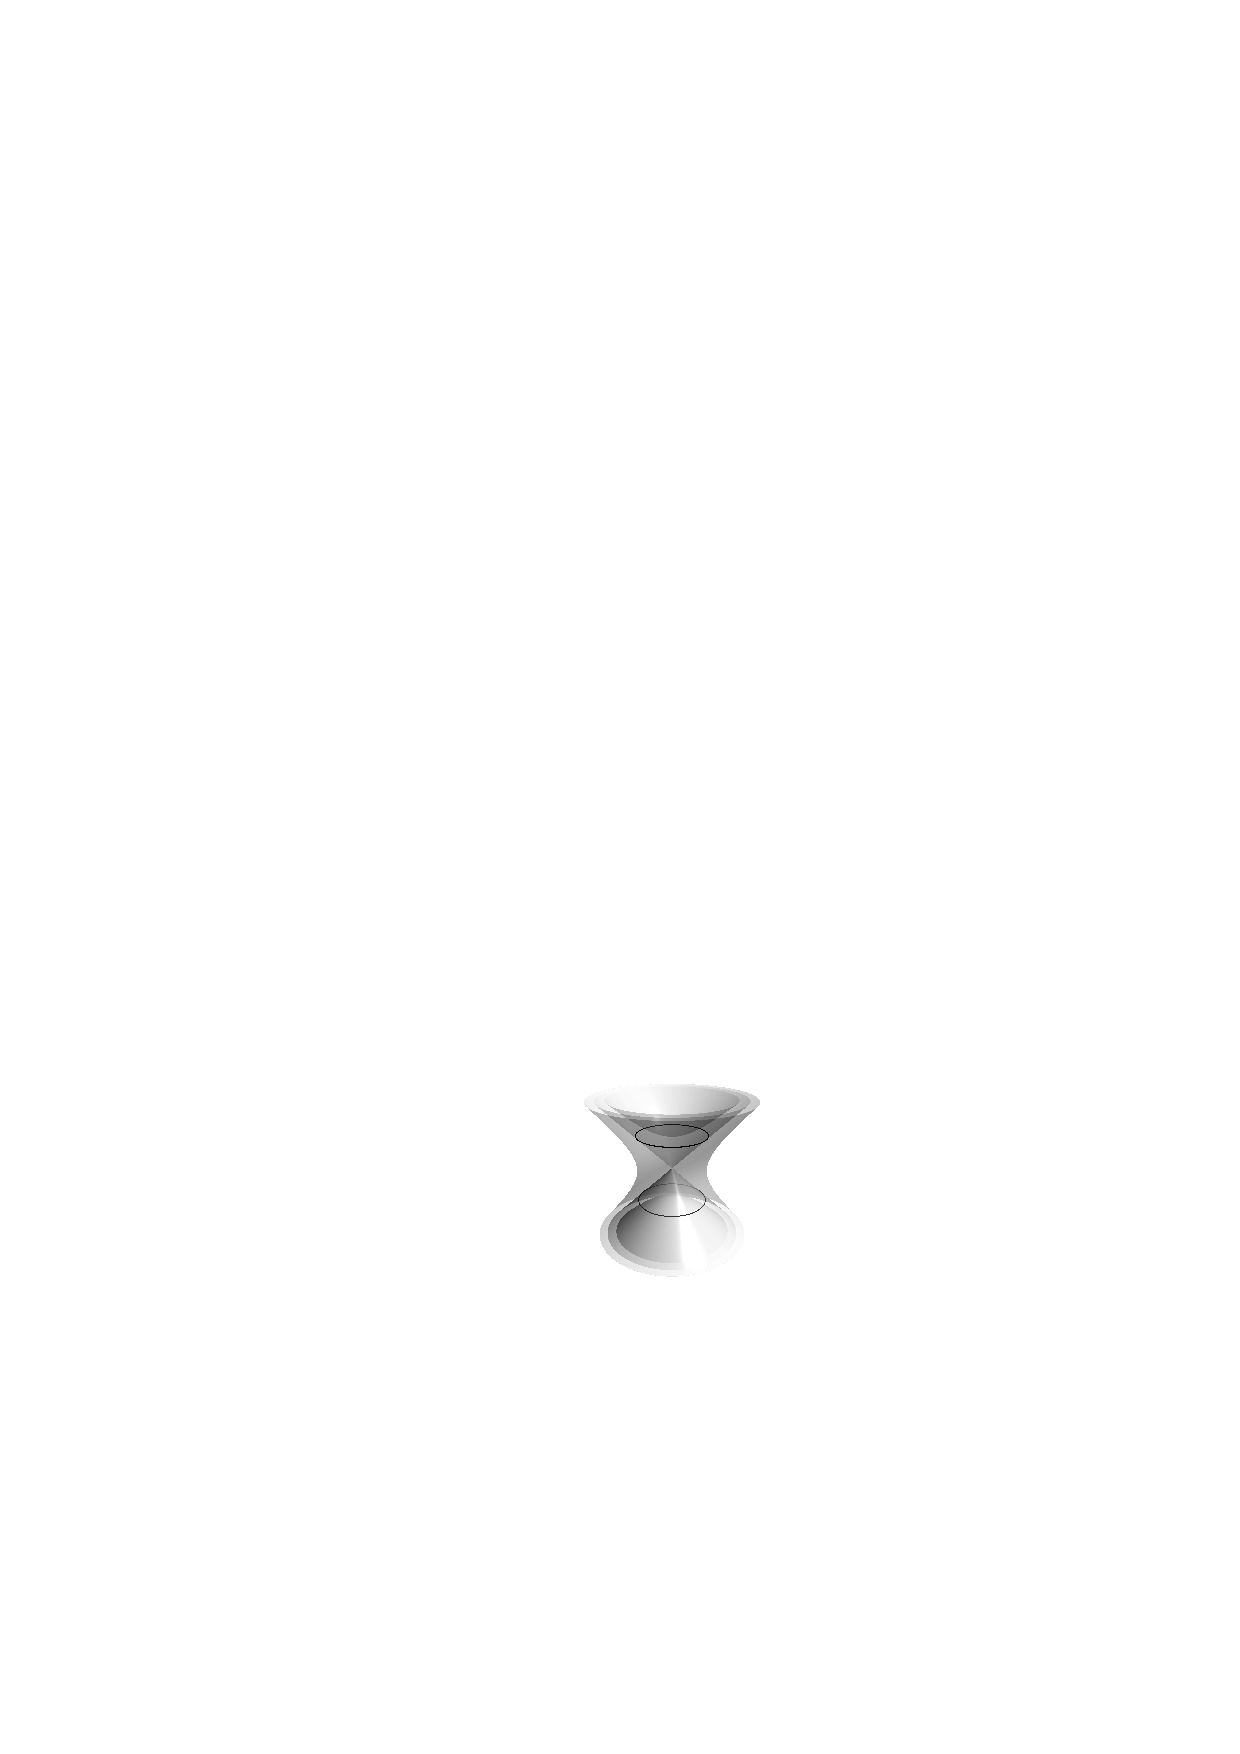
\includegraphics[scale=0.8]{figures/null cone.pdf}
    \caption{The set of unit null vectors within the null cone in signature $(1,2)$ (the $1$ corresponding to the vertical axis). \label{fig null cone}}
\end{figure}

We have the following obvious $\Or_V$-equivariant fiber bundles (the first two are covering maps)
\[\{\pm 1\}\hookrightarrow Y_\pm\to X_\pm,\quad \bbR^\times\hookrightarrow Y_0\to X_0,\]
while the following are $\CO_V$-equivariant fiber bundles:
\[\bbR^\times\hookrightarrow U_\pm\to X_\pm,\quad \bbR^\times\hookrightarrow Y_0\to X_0.\]
To see the diffeomorphism types of these manifolds, pick a space time splitting $V=V^+\oplus V^-$. Let $|x|=\sqrt{|\<x,x\>|}$ for $x\in V^+\cup V^-$. Let $S_+\subset V^+$, $S_-\subset V^-$ be the unit ``spheres'' $\lVert x\rVert =1$. Then each nonzero vector is uniquely decomposed as $x+y$ with $x\in V^+$, $y\in V^-$ and being null is equivalent to $|x|=|y|$. Scale the null vector to have $|x|=|y|=1$ and call it a \emph{unit null vector} (however, this is not a natural concept as it depends on the splitting). Then the set of unit null vectors is precisely $S_+\times S_-\subset Y_0$, see Figure~\ref{fig null cone}. Every nonzero null vector $x+y$ scales to a unit null vector, so 
\[Y_0\cong R_+\times S_+\times S_-,\]
and there is a double covering map 
\[\{\pm 1\}\hookrightarrow S_+\times S_-\to X_0\]
taking $x+y$ to the line spanned by $x+y$, so the null quadric $X_0$ is the quotient of the unit null vectors by the double antipodal map $x+y\mapsto (-x)+(-y)$. Note that $S_+\times S_-\subset V$ is not invariant under $\Or_V$ since it depends on the choice of splitting $V=V^+\oplus V^-$.

Every element of $Y_+$ splits uniquely into a sum $x+y$ with $x\in V^+$, $y\in V^-$ with $|x|^2=1+|y|^2>0$. There is a map 
\[Y_+\to S_+\times V^-,\quad x+y\mapsto (x/|x|,y),\]
and it can be inverted:
\[S_+\times V^-\to Y_+,\quad  (u,y)\mapsto \sqrt{1+|y|^2}u+y,\]
hence we have diffeomorphisms
\[Y_+\cong S_+\times V^-,\quad Y_-\cong V^+\times S_-.\]
Similarly, 
\[U_+\to \bbR^+\times S_+\times V^-,\quad x+y\mapsto (|x|,x/|x|,y)\]
is a diffeomorphism. 

As we will see later, every Lie group with finitely many components smoothly retracts to its maximal compact subgroup, and so every homogeneous space of that group retracts to the orbit of that maximal compact subgroup. So $\Or_{p,q}$ retracts to $\Or_p\times\Or_q$. In particular, $\Or_{p,q}$ has one component if $p=q=0$, two components if one of $p,q$ is zero, and four components otherwise.  As above, each of $Y_+,Y_-,Y_0$ retracts  $\Or_p\times\ \Or_q$-equivariantly to the orbits of $e_1^+,e_1^-,e_1^++e_1^-$, respectively, i.e., to $\bbS^{p-1}$, $\bbS^{q-1}$, $\bbS^{p-1}\times\bbS^{q-1}$. Here we note that $\bbS^{0}=\{\pm 1\}$ and $\bbS^{-1}=\varnothing$.

\textbf{Tangent spaces.} We can finally move on to describing the actual geometry. By differentiating the constant inner product we find that the tangent spaces of $Y_+,Y_-,Y_0$ at a point $x$ are identified with the hyperplane $x^\perp$ orthogonal to $x$:
\[\T_x Y=x^\perp\quad \text{for }x\in Y,\; Y=Y_+,Y_-,Y_0\]
Denote by $e^+_{2\ldots p}$ the list of vectors $e_2^+,\ldots,e^+_p$, etc. The various tangent spaces and stabilizers $H\coloneqq G_{x_0}$ are:
\begin{center}
    \begin{tabular}{l c c c r} 
     $Y$ & Basepoint $x_0$ & $\T_{x_0}Y$ & Signature of $Y$ & $H$\\ [0.5ex] 
     \hline
     $Y_+$ & $e_1^+$ & $\<e^+_{2\ldots p},e^-_{1\ldots q}\>$ & $(p-1,q)$ & $\Or_{p-1,q}$\\ 
     $Y_-$ & $e_1^-$ & $\<e^+_{1\ldots p},e^-_{2\ldots q}\>$ & $(p,q-1)$ & $\Or_{p,q-1}$\\ 
     $Y_0$ & $e_1^++e_1^-$ & $\<e^+_1-e^-_1,e^+_{2\ldots p},e^-_{2\ldots q}\>$ & $(p-1,q-1)$ & $\Or_{p-1,q-1}\times \bbR^\times$.\\
     \hline
    \end{tabular}
\end{center}

On each $\Or_{p,q}$-orbit, by $\Or_{p,q}$-invariance of the inner product, the signature of the restriction of the inner product to the orbit is the same at all points. Note that on $Y_0$, the inner product has a null direction, precisely the rescaling direction. Under the rescalings, the inner product recales, so $X_0$ inherits only a \emph{conformal metric} of signature $(p-1,q-1)$. When we quotient $Y_+,Y_-$ by $\pm\rmI$, we swap the choice of preimage of the resulting point in $X_+,X_-$, but we apply an orthogonal transformation which identifies the tangent spaces at the two points, so the resulting metric is defined on $X_+,X_-$. So $X_+$ has a smooth metric of signature $(p-1,q)$, while $X_-$ has a smooth metric of signature $(p,q-1)$, and $X_0$ has a smooth conformal structure of signature $(p-1,q-1)$. The orthogonal groups serve as stabilizers for $X_+,X_-$, so these metrics are invariant under automorphisms which act transitively on points and orthonormal frames, i.e., on orthonormal frame bundles. The stabilizers acting on $X_+,X_-$, as subgroups of $\CO_V=\Or_V\slash\{\pm\rmI\}$, are the isomorphic images of $\Or_{v^\perp}$ with $v=e_1^+,e_1^-$, respectively, as we can lift each transformation uniquely to have it fix $v$.

\textbf{Levi-Civita connection.} Each point $x\in Y=Y_\pm $ has normal space the span of $x$, and hence an orthogonal decomposition into tangent and normal spaces, $\T_x V=\T_x Y\oplus \rmN_x Y$ with $\rmN_x Y\coloneqq (\T_x Y)^\perp <\T_x V$. Given a curve $x(t)\in Y_\pm$, any vector field $v(x(t))\in V$ defined ``along the curve'' decomposes into tangent and normal parts. The derivative $\dot v(t)$ in the usual Euclidean sense splits into tangent and normal parts as well. If $v$ is everywhere tangent (normal), define $\nabla_{\dot x}v$ (resp., $\nabla_{\dot x}^\perp v$) to be the tangent (resp., normal) part of $\frac{\dd}{\dd t} v(x(t))$:
\[\frac{\dd}{\dd t} v(x(t))=\underbrace{\nabla_{\dot x}v}_{\T Y}+\underbrace{\nabla_{\dot x}^\perp v}_{\rmN Y}.\]  
Clearly, this definition is invariant under the orthogonal group. The value of $\nabla_{\dot x}v$, $\nabla_{\dot x}^\perp v$ at a point $t=t_0$ depends only on the vector $\dot x(t_0)$, the tangent vector $v(x(t_0))$, and its first derivative $\frac{\dd}{\dd t} v(x(t_0))$. Thus, they extend uniquely (via Willmore's Theorem as usual) to affine connections $\nabla,\nabla^\perp$ on $\T Y$ and $\rmN Y$, respectively.

\begin{xca}
    Show that the connection $\nabla$ is torsion-free and compatible with the metric $\sfg_\pm$ on $Y_\pm$ induced from the inner product on $V$, i.e., $\nabla\sfg_\pm=0$. Consequently, it is the Levi-Civita connection.
\end{xca}

By invariance under the orthogonal group, these connections also descend to $X_\pm$, and $\nabla$ is the Levi-Civita connection on $X_\pm$, too. Take a tangent vector $v\in \T_x Y_+$, which implies $v\perp x$. Let $P\coloneqq \<x,v\><V$ be the $2$-dimensional subspace through $x$ and $v$.  By applying an orthogonal transformation we can arrange that $x=e_1^+$ and $v$ is a multiple of either $e_2^+$ (if timelike) or $e_1^-$ (if spacelike). Hence, we can construct the linear reflection map fixing $x$ and $v$ and changing the signs of all other vectors in an orthonormal basis, i.e., a reflection fixing all points in $P$ and changing the signs of all points in $P^\perp$. The geodesic curvature of the curve $Y_+\cap P$, defined as the norm of the tangent component of its acceleration vector (cf.\ \ref{eq geodesic curvature}) is thus invariant under this reflection since the curve itself is, but at the same time lies in $P^\perp$ and hence must change sign. Thus, the curvature is zero and $Y_+\cap P$ is actually a geodesic. Similarly, if $v$ is null, we can arrange $v=e_2^++e_2^-$, and a change of the basis $e_2^+, e_2^-$ by a hyperbolic rotation $\left(\begin{smallmatrix}
    \cosh t & \sinh t\\\sinh t & \cosh t
\end{smallmatrix}\right)\in\Or_{1,1}$ (which are the only orthogonal transformations preserving $\<e_2^+, e_2^-\>$) scales $v$ by $\rme^t$ and the other null line in the plane $\<e_2^+, e_2^-\>$  by $\rme^{-t}$. Hence, the curvature is invariant and thus vanishes -- a geodesic. Similarly for $Y_-$. 

This gives one geodesic in each direction, so we have all of the geodesics: a curve on $Y_\pm$ is a geodesic iff, at some point, it is the intersection with a plane containing the normal vector at that point. Mapping to projective space, the geodesics on $X_\pm$ are its intersection with projective lines.

\begin{example}
    In $\bbR^{1,2}$, the surface $Y_+$ is the two-sheeted hyperboloid $x^2+y^2+1=z^2$ with a Riemannian metric invariant under the orthogonal (Lorentz) group $\Or_{1,2}$. The vertical plane through $\bf{e}_1^+$ intersects the cone at two points, so the geodesic is the hyperbola in between. All the geodesics in $Y_+$ are carried to one another by isometries, so the action on geodesics in $Y_+$ is transitive.

    The surface $Y_-$ is the one-sheeted hyperboloid $x^2+y^2=1+z^2$. Every point $\bf{x}\in Y_-$ can be brought to the point $\bf{e}_1^-$ by an orthogonal transformation. The horizontal $(x,y)$-plane $\<\bf{e}_1^-,\bf{e}_2^-\>$ intersects $Y_-$ along a spacelike geodesic circle. The planes $\<\bf{e}_1^-,\pm \bf{e}_1^++\bf{e}_1^-\>$ intersect $Y_-$ along null geodesics -- the lines $x=\pm 1$. All pointed geodesics are carried to one of these by orthogonal transformations, so there are two orbits on the space of geodesics in $Y_-$.
\end{example}

\textbf{dS and AdS.} We now name and describe the isometry groups of the three geometries $X_+,X_-,X_0$, starting with the first two.

\begin{defn}\index{de Sitter space}\index{anti-de Sitter space}\index{dS!see {de Sitter space}}\index{AdS!see {Anti-de Sitter space}}
    The de Sitter space $\mathrm{dS}^{p-1,q}$ and the anti-de Sitter space $\mathrm{dS}^{p,q-1}$ of dimension $p+q-1$ are defined as the projective images $X_+$ and $X_-$ in $\RP^{p+q}$, respectively, of the unit hyperboloids $Y_+,Y_-$ inside $\bbR^{p,q}$, with their induced pseudo-Riemannian structures, as described above.
\end{defn}

\begin{thm}
    The group of pseudo-Riemannian isometries of the de Sitter space $X_+$ and anti-de Sitter space $X_-$ is precisely the projective orthogonal group $G=\Or_{p,q}\slash\{\pm \rmI\}$.
\end{thm}
\begin{proof}
    The projective orthogonal group acts transitively. Consider the stabilizer of a point. Looking at our description of tangent spaces above, the stabilizer of a point acts transitively on orthogonal frames at that point, i.e., as the orthogonal group of that tangent space. Take any isometry. Composing it with an element of $G$, we can arrange that it fixes a given point $x_0$, and a frame at that point, i.e., acts trivially on the tangent space  $\T_{x_0} X$ at that point. Since any isometry takes geodesics to geodesics, this map commutes with the exponential map $\exp_{x_0}:\T_{x_0} X\to X$ (defined as the value at time $t=1$ of the geodesic starting at $x_0$ with given velocity). We will later see that $\exp_{x_0}$ is a local diffeomorphism and hence our isometry fixes an entire open neighborhood. By analyticity and connectivity (uniqueness of analytic continuation), this isometry must be the identity map.
\end{proof}

We thus have the description of dS and AdS as the following homogeneous spaces (we add the signatures to the notation for clarity):
\begin{gather}
    \{\pm 1\}\hookrightarrow Y_+^{p-1,q}\cong \bbS^{p-1}\times\bbR^q\cong \Or_{p,q}\slash \Or_{p-1,q}\to X_+^{p-1,q},\\
    \{\pm 1\}\hookrightarrow Y_-^{p,q-1}\cong \bbR^p\times \bbS^{q-1}\cong \Or_{p,q}\slash \Or_{p,q-1}\to X_-^{p,q-1},
\end{gather}
where the last covering map in both cases is the quotient map by the antipodal identification $x\sim -x$. In the standard physics terminology, $\mathrm{dS}^n=X_-^{1,n-1}$ and $\mathrm{AdS}^n=X_+^{1,n-1}$. Note that the space $\bbS^1\times\bbR$ corresponding to $n=2$ carries simultaneously a de Sitter and an anti-de Sitter geometry (the same more generally holds for $\bbS^p\times\bbR^p$). 

\textbf{Null quadric.} The description of the stabilizer of a point of the null quadric $X_0$ is more complicated. First let us change the variables of our standard example to get the axes of the first and last coordinates to be null, so $V=\bbR\oplus V'\oplus \bbR$ with $V'$ of signature $(p-1,q-1)$. If we denote these two so called \emph{light cone coordinates} by $x^+$ and $x^-$ (in no particular order) then this means that the metric contains the term $x^+x^-$. We would like to describe the isometries of $V$ that stabilize a given point of $X_0$, and these obviously map to some subgroups of the groups described in Lemma~\ref{lem null quadric isometries}.

First we can eliminate one complication related to the split case. If the signature is split, then so is that of $V'$; in the split case, take a conformal transformation $T'\in\CO_{V'}$ changing the sign of the inner product (this exists by induction starting with $(x^1,x^2)\mapsto (x^2,x^1)$ for $p=q=1$) and let 
\[T\coloneqq \begin{pmatrix}
    1 & 0 & 0\\
    0 & T' & 0\\
    0 & 0 & -1
\end{pmatrix},\]
so that $T$ changes the sign of the inner product and fixes the standard basis vector $\bf{e}_1$. This $T$ is exactly the $T$ that generates the extra components of the split isometry groups of the null quadric in Lemma~\ref{lem null quadric isometries}. Since it stabilizes $\bf{e}_1$, it will be included in the stabilizer and thus can be effectively ignored in the description of $X_0$ as a homogeneous space.

It remains to describe the isometric part of the stabilizer of $\<\bf{e}_1\>\in X_0$. Let $P_O\subset \Or_V$ and  $P_C\subset \CO_V$ be, respectively, the groups of orthogonal and conformal transformations which stabilize the null line $\<\bf{e}_1\>$ in these coordinates.

\begin{lem}
    In the above basis, the group $P_O$ consists precisely of the matrices of the form 
    \[g=\begin{pmatrix}
        a & av^\flat h & \frac{a}{2}\<v,v\>\\
        0 & h & v \\
        0 & 0 & a^{-1}
    \end{pmatrix},\]
    where $a\in \bbR^\times$, $v\in V'$, $h\in \Or_{V'}$, $v^\flat\coloneqq \sfg(v)\in (V')^\ast$ the dual covector w.r.t.\ the inner product $\sfg\in \Hom(V,V^\ast)$.  The group $P_C$ consists of matrices of the form $\lambda g$, where $\lambda>0$ and $g\in P_O$.
\end{lem}
\begin{proof}
    We assume a basis as above. After a positive scaling, these conformal transformations are orthogonal transformations. So assume that $g$ is orthogonal and preserves the line spanned by the null vector $\bf{e}_1$, and so preserves the perpendicular space of that vector, which is the span of the entire standard basis minus the \emph{last} vector $\bf{e}_{p+q}$. Hence, $g$ has the form 
    \[g=\begin{pmatrix}
        a & \xi & t\\
        0 & h & v\\
        0 & 0 & b
    \end{pmatrix}\]
    for some $a,b\in \bbR^\times$, $h\in \GL_{V'}$, $v\in V'$, $\xi\in (V')^\ast$.

    Write the inner product on $V'$ as $\<v,w\>=\<v,\eta w\>_{\mathrm{Euc}}$, where $\<\,,\,\>_{\mathrm{Euc}}$ is the regular dot product on $\bbR^{p+q-2}$ in our fixed basis, and $\eta$ is some symmetric matrix of signature $(p-1,q-1)$. Let 
    \[S\coloneqq \begin{pmatrix}
        0 & 0 & -1\\
        0 & \eta & 0 \\
        -1 & 0 & 0
    \end{pmatrix}.\]
    Since $g$ is an isometry and $S$ is nothing but the metric tensor written in the basis where $\bf{e}_1,\bf{e}_{p+q}$ were replaced by $\bf{e}_1\pm \bf{e}_{p+q}$, we must have $g^T Sg=S$, which forces $g$ to have the asserted form.
\end{proof}

Thus, $X_0^{p-1,q-1}\coloneqq X_0$ is a conformal manifold of signature $(p-1,q-1)$ obtained as the homogeneous space 
\[\{\pm 1\}\hookrightarrow \bbS^p\times\bbS^q\to X_0^{p-1,q-1}=\CO_{p,q}\slash P_C=\Or_{p,q}\slash P_O.\]
Lastly, we note the obvious isomorphisms under swapping the sign of the entire metric on $V$: $X_+^{p,q}\cong X_-^{q,p}$ and $X_0^{p,q}\cong X_0^{q,p}$.










\chapter{Cartan Geometry \texorpdfstring{\ucmark}{}}\label{ch: cartan geom}


Our encounter with geometric structures on manifolds started with Lie groups, in which we saw that the Maurer-Cartan equation provided the basis for the entire Lie group structure, and hence the theory of Lie groups. Then, separately, we developed the theory of principal connections and saw that the structure equation for the curvature is very reminiscent of the Maurer-Cartan equation, thus suggesting that all connections are, in some way, ``deformations'' of canonical geometries on Lie groups and their homogeneous spaces. Nevertheless, the Maurer-Cartan form itself couldn't exactly be interpreted as neither a connection form nor a soldering form. It is very close to being a soldering form in its relation to the torsion of canonical flat connections (Example~\ref{ex connections on G, part 6}), whereas the only way to turn it into a principal connection is to project it onto a Lie subalgebra in a reductive Klein geometry (Example~\ref{ex 1.3.19 RS2}). Cartan geometry will finally unify these approaches, allow us to intepret the Maurer-Cartan form as a fundamental example of a general geometric structure, and all other geometric structures that we've seen so far as ``deformations'' of the ``model structures'' of Klein geometries. In this picture, we may succinctly describe all of modern differential geometry as a vast generalization of the Maurer-Cartan equation.






\section{Cartan connections}

Any Cartan geometry is derived from a homogeneous space, called the homogeneous model of the geometry. The interplay between this homogeneous model and general Cartan geometries of the given type is one of the main general features of Cartan geometries and an important topic for this section.


\begin{defn}[Cartan geometry I]\index{Cartan geometry}\index{Connection!Cartan}\label{def cartan geometry I}
    Then a \emph{Cartan geometry of type $(G,H)$ on a manifold $M$} is a tuple $(P\overset{\pi}{\to}M,G,H,\Phi,\eta)$, where $(G,H)$ is a Klein geometry (i.e., $H\emb G$ is a closed subgroup of a Lie group $G$ such that $G\slash H$ is connected),
    $(P\overset{\pi}{\to}M,H,\Phi)$ a principal $H$-bundle, and $\eta\in\Omega^1(P;\frakg)$ is a $\frakg$-valued $1$-form, called the \emph{Cartan connection}, which is required to be $H$-equivariant, to reproduce the generators of Killing vector fields, and to define an absolute parallelism on $P$. More formally,
    \begin{enumerate}
        \item $\Phi_h^\ast \eta=\Ad_h^{-1}\circ \eta$ for all $h\in H$;
        \item $\eta(A_\ast(p))=A$ for all $A\in\frakh$ and $p\in P$;
        \item (Cartan condition) $\ker\eta_p=0$ (hence $\eta_p$ is a linear isomorphism) for all $p\in P$, i.e., $\eta$ determines an absolute parallelism presented by the bundle isomorphism $\eta:\T P\to P\times\frakg$.
    \end{enumerate}
    The \emph{homogeneous model} for Cartan geometries of type $(G,H)$ is the canonical Klein geometry (homogeneous principal $H$-bundle) $G\to G\slash H$ endowed with the left Maurer-Cartan form $\theta_G\in\Omega^1(G;\frakg)$.

    Given a Cartan geometry, the \emph{constant vector fields} are $\eta^{-1}(A)\in\fX(P)$ defined for all $A\in\frakg$ by $\eta(\eta^{-1}(A)_p)=A$ at any $p\in P$. Projections of integral curves of constant vector fields to $M$ are called \emph{spirals}, \emph{generalized circles}, or \emph{canonical curves}. The Cartan connection $\eta$ is called \emph{complete} if all of its constant vector fields are complete.
\end{defn}

We will often use the simplified notation $p\cdot h$ for $\Phi_h(p)$. By equivariance of $\eta$, we get the transformation rule for constant vector fields
\[\eta^{-1}(A)_{p\cdot h}=\Phi_{h\ast}\circ \eta^{-1}(\Ad_h A)_p,\quad \text{for all}\quad h\in H.\]


\begin{example}
    In the case of the homogeneous model, the constant vector field $\theta_G^{-1}(A)$ is the left-invariant vector field $A_\rmL$. Moreover, the pullback of $\eta$ along the orbit map $\Phi^p:H\to P_{\pi(p)}$ (which is a diffeomorphism) is exactly the Maurer-Cartan form $\theta_H$. Restrictions of the homogeneous model to an open subset $U\subset G\slash H$ are also flat Cartan geometries. If $U$ is not simply connected, then all of its covering spaces also carry an induced flat Cartan structure.
    % These forms define a global $1$-form on the vertical bundle, $\theta_H:\calV P\to \frakh$, which can be viewed as a global trivialization $\calV P\to P\times\frakh$.
     Thus, general Cartan geometries of type $(G,H)$ are seen as ``curved analogs'' of the Klein geometry $(G,H)$, with the Maurer-Cartan form $\theta_G$ replaced by the Cartan connection form.
\end{example}

\begin{example}
    The next simplest examples are locally Klein geometries $G\to \varGamma\bslash G\slash H$, where $\varGamma<G$ is a discrete subgroup that acts on $G\slash H$ by left translations. Then $\varGamma$ acts on $G$ by deck transformations and hence isomorphisms of the Cartan geometry. Since $G\to \varGamma\bslash G$ is a covering map, it is a local diffeomorphism, and we can push the Cartan structure forward to the $H$-bundle $\varGamma\bslash G \to \varGamma\bslash G\slash H$. This is still a flat Cartan geometry.
\end{example}


\begin{defn}[Curvature form of a Cartan geometry]\index{Curvature!of a Cartan geometry}
    The curvature form $\Omega\in\Omega^2(P;\frakg)$ of a Cartan geometry $(P\to M,G,H,\Phi,\eta)$ is defined by the structure equation 
    \[\Omega(X,Y)\coloneqq \dd\eta(X,Y)+[\eta(X),\eta(Y)].\]
\end{defn}


\begin{example}
    \begin{enumerate}
        \item The Maurer-Cartan equation implies that Klein geometries $(G,H)$ with their \emph{canonical Cartan connections} given by the Maurer-Cartan form are always flat. This is why the homogeneous model is often referred to as the flat model, although we avoid this terminology due to the likely confusion with flat principal connections. Indeed, by dimension counting, a Cartan connection is a principal connection only in the case of the trivial Klein geometry $(G,G)$ consisting of a single fiber.
        \item Cartan geometries, therefore, are \emph{not} a generalization of principal connections. And although Cartan connections can be viewed as a special class of principal connections by changing the underlying bundle (see the next \sect), in fact, these concepts are almost orthogonal in a sense that will be clarified below.
        \item If $\eta$ is a Cartan connection of type $(G,H)$ on $P$ and $B\emb H$ is a closed subgroup, then $\eta$ defines a Cartan connection of type $(G,B)$ on $P\to P\slash B= P\times^H (H\slash B)$.\label{xca V.3.6 Sharpe}
    \end{enumerate}
\end{example}


Since the Cartan conection $\eta$ trivializes $\T P$, any differential form on $P$ is determined by its values on the constant vector fields $\eta^{-1}(A)$. Thus, the complete information about $\Omega$ is contained in the \emph{curvature function}\index{Curvature!Function} $\scrK:P\to \bigwedge\nolimits^2\frakg^\ast\otimes\frakg$ defined by 
\[\scrK_p(A,B)=\Omega_p\left(\eta^{-1}(A),\eta^{-1}(B)\right),\]
and then the standard formula for the exterior derivative yields 
\[\scrK_p(A,B)=[A,B]-\eta_p\left(\left[\eta^{-1}(A),\eta^{-1}(B)\right]\right).\]
In other words, curvature measures the failure of the assignment of the constant vector fields $A\mapsto \eta^{-1}(A)$ to be a homomorphism of Lie algebras $\frakg\to \fX(P)$.

\begin{lem}[{{\cite[Lem.~1.5.1]{Cap}}}]\label{lem 1.5.1 Cap}
    The curvature form $\Omega\in\Omega^2(P;\frakg)$ is horizontal, so the curvature function may be viewed as $\scrK:P\to \bigwedge\nolimits^2(\frakg\slash\frakh)^\ast\otimes\frakg$. Moreover, $\Omega$ is \emph{of type $\Ad$ w.r.t.\ $H$} in the sense that 
    \begin{align}
        \Phi_h^\ast \Omega&=\Ad_h^{-1}\circ \Omega,\\
        \Phi_h^\ast\scrK&=\lambda(h)^{-1}\circ\scrK,
    \end{align}
    where $\lambda$ is the tensor product of the actions $\bigwedge\nolimits^2 \underline{\Ad}^\ast$ on $\bigwedge\nolimits^2(\frakg\slash\frakh)^\ast$ and $\Ad$ on $\frakg$.
\end{lem}
\begin{proof}
    By definition of $\eta$, if $A\in\frakh$, then $\eta^{-1}(A)=A_\ast$, the Killing vector field. Equivariance of $\eta$ implies that $\Lie_{A_\ast}\eta=i_{A_\ast}\dd\eta=-\ad_A\circ\eta$. This gives 
    \[\dd\eta(\eta^{-1}(A),Y)+[A,\eta(Y)]=-\ad_{A}\eta(Y)+[A,\eta(Y)]=0\]
    for all $A\in\frakh$ and all $Y\in \T P$. Since the Killing vector fields span the vertical bundle, we conclude that $\Omega$ is horizontal, and that each $\scrK_p$ descends to $\bigwedge\nolimits^2(\frakg\slash\frakh)$.
    
    The equivariance property of $\Omega$ follows directly from the definition and the naturality of $\dd$ w.r.t.\ pullbacks. To prove the property for $\scrK$, we have to compute $\scrK_{p\cdot h}(X,Y)$. By definition, we find 
    \begin{align}
        \Omega\left(\eta_{p\cdot h}^{-1}(A),\eta_{p\cdot h}^{-1}(B)\right)&=\Omega\left(\Phi_{h\ast}\eta^{-1}_p(\Ad_h A),\Phi_{h\ast}\eta^{-1}_p(\Ad_h B)\right)=\notag\\
        &=(\Phi_h^\ast \Omega)_p \left(\eta^{-1}(\Ad_h A),\eta^{-1}(\Ad_h B)\right)=\notag\\
        &=\Ad_h^{-1}\scrK_p(\Ad_h A,\Ad_h B).
    \end{align}
    Passing from $\frakg$ to $\frakg\slash\frakh$, the two occurrences of $\Ad_h$ inside of $\scrK_p$ are replaced by $\underline{\Ad}_h$, and we obtain the asserted formula.
\end{proof}



\begin{example}\label{ex 1.5.1 Cap}
    \begin{enumerate}[label=(\roman*)]
        \item Let $\Aff_n(\bbR)$ be the affine group in dimension $n$. We have seen in Remark~\ref{rem 1.3.6 Cap} that a Cartan geometry of type $(\Aff_n(\bbR),\GL_n(\bbR))$ on an $n$-dimensional manifold $M$ is equivalent to a linear (affine) connection $\omega$ on the frame bundle $\Fr(\T M)$. Moreover, the curvature $\Omega$ coincides with the sum $\Omega+\Theta$ of the curvature and the torsion of that linear connection. The Cartan connection is $\eta=\omega+\theta$, where $\theta$ is the soldering form.
        \item For a Lie group $H$ and an infinitesimally injective homomorphism $H\to \GL_n(\bbR)$ consider the affine extension $B=\bbR^n\rtimes H$. In  we saw that a Cartan geometry of type $(B,H)$ is equivalent to a first-order $G$-structure with structure group $H$ endowed with a connection. The curvature of the Cartan connection can again be interpreted as the direct sum of the curvature and torsion of the induced affine connection on the tangent bundle.
        \item More specifically, consider $H=\Or_n\emb \GL_n(\bbR)$. Then the affine extension $\bbR^n\rtimes H$ is the Euclidean group $\SE_n$. By Example~\ref{ex pseudo-riemannian structure} an $\Or_n$-structure is equivalent to a Riemannian metric $\sfg$ on $M$. From (ii) we thus conclude that a Cartan geometry of type $(\SE_n,\Or_n)$ is equivalent to a connection on the orthonormal frame bundle for $\sfg$ and hence to a unique metric affine connection on $\T M$. The Levi-Civita connection then gives a canonical Cartan geometry of type $(\SE_n,\Or_n)$ on each Riemannian manifold. The curvature then effectively coincides with the usual Riemann curvature, since the torsion vanishes.
        
        This is a prototypical example for a Cartan geometry which is determined by an underlying structure. The interpretation of Riemannian structures as Cartan geometries is one of the motivating examples for the concept. 
        \item There is no difference between Cartan geometries of the types $(\Or_{n+1},\Or_n)$, $(\SE_n,\Or_n)$, and $(\Or_{1,n},\Or_n)$. This is because $\frako_{n+1}$, $\frakse_{n}$, and $\frako_{1,n}$ are all isomorphic as $\Or_n$-modules. However, the notion of curvature is different for these three types of geometries, since the homogeneous models $\bbS^n$ (Riemann sphere) and $H^n$ (hyperbolic space) of the first and last types have (nonzero) constant curvature unlike the second type. This is an example of model \emph{mutation}, which we will discuss in detail below.
    \end{enumerate}
\end{example}

\begin{example}[Product of Cartan geometries]
    On the product of two unit $2$-spheres, $M=\bbS^2\times\bbS^2$, the Cartan geometry obtained as the bundle product $P\times P\to M$ of their respective Riemannian geometries is \emph{not} the product Riemannian geomery. The Cartan geometry keeps track of the order of the product and has structure group $\Or_2\times\Or_2$, while the Riemannian geometry has the permutation of the factors as an isometry and has structure group $\Or_4$.
\end{example}

\begin{example}[\ref{ex dS and AdS} continued]\label{ex dS and AdS 2}
    Recall that the de Sitter and anti-de Sitter spaces are, respectively, $\mathrm{dS}^n=\Or_{1,n}\slash \Or_{1,n-1}$ and $\mathrm{AdS}^n=\Or_{2,n-1}\slash \Or_{1,n-1}$. This means that the isometry groups of these spaces are $\Or_{1,n}$ and $\Or_{2,n-1}$, respectively, whereas the structure group is $\Or_{1,n-1}$, so both geometries are \emph{Lorentz manifolds} \index{Lorentz manifold} (that is, pseudo-Riemannian manifolds of signature containing only one minus). In cosmology, the $4$-dimensional $\mathrm{dS}^4$ and $\mathrm{AdS}^4$ are the basic models for the global geometry of the ``static universe.''

    In the case of $\mathrm{dS}^3$, one can extend the symmetry group to $G=\SL_2(\bbC)\cong\Spin_{1,3}$, which is the universal covering group of the Lorentz group $\SO^+_{1,3}$ (the identity component of $\Or_{1,3}$). Then the stabilizer of a point is $\SL_2(\bbR)\cong \Spin_{1,2}$, so 
    \[\mathrm{dS}^3\cong \SL_2(\bbC)\slash\SL_2(\bbR)\cong \Spin_{1,3}\slash \Spin_{1,2}.\]
    Similarly, one can identify $\mathrm{AdS}^n\cong \Spin^+_{2,n-1}\slash \Spin^+_{1,n-1}$.
\end{example}

\begin{example}
    All common types of differential geometries are covered by Cartan geometry. Projective geometries are geometries modeled on $\RP^n$ or $\CP^n$ with $G$ their respective projective linear group $\PSL_{n+1}(\bbR)$ or $\PSL_{n+1}(\bbC)$, and projective connections are Cartan connections of this type (which can be also required to be holomorphic in the complex case). A spin connection is a Cartan geometry of type $(\Spin_n\ltimes\bbR^n,\Spin_n)$. A symplectic connection is a Cartan geometry of type $(\Sp_n(\bbR)\ltimes\bbR^n,\Sp_n(\bbR))$ (these arise naturally in formal deformation quantization). A conformal connection is a Cartan geometry modeled on the conformal sphere. A CR structure is a Cartan geometry modeled on the CR sphere with $G=\PSU_{p+1,q+1}$.
\end{example}

\begin{defn}[Morphism of Cartan geometries]
    A morphism between two Cartan geometries $(P\to M,G,H,\Phi,\eta)$ and $(P'\to M',G,H,\Phi',\eta') $ of type $(G,H)$ is a principal bundle morphism $\vartheta:P\to P'$ such that $\vartheta^\ast\eta '=\eta$. Notice that compatibility with the Cartan connection implies that any tangent map of $\vartheta$ is a linear isomorphism, so $\vartheta$ and its base map are local diffeomorphisms. The resulting category of Cartan geometries of type $(G,H)$ is denoted $\Car_{(G,H)}$.
\end{defn}

\begin{lem}[{{\cite[Lem.~1.5.2]{Cap}}}]\label{lem 1.5.2 Cap}
    Let $\vartheta:P\to P'$ be a morphism of \glspl{pfb} which is a local diffeomorphism. If $\eta'$ is a Cartan connection on $P'$, then $\eta=\vartheta^\ast\eta'$ is a Cartan connection on $P$. If $\eta'$ and $\eta$ are fixed Cartan connections on $P$ and $P'$, then $\vartheta$ is a morphism of Cartan geometries iff it preserves the constant vector fields, i.e., $\vartheta_\ast\circ \eta^{-1}(A)=\eta^{\prime-1}(A)\circ\vartheta$. In this case the curvature forms $\Omega$ and $\Omega'$ (or $\scrK$ and $\scrK'$) are $\vartheta^\ast$-related.
\end{lem}
\begin{proof}
    The Killing vector fields are given by $A_\ast(p)=\restr{\frac{\dd}{\dd t}}{0}p\cdot \rme^{tA}$, so equivariance of $\vartheta$ implies that $\vartheta^\ast \eta'$ reproduces the generators of Killing fields. Similarly, equivariance of $\vartheta$ and $\eta'$ implies equivariance of $\vartheta^\ast\eta'$. Since $\vartheta$ is a local diffeomorphism, $\vartheta^\ast\eta'=\eta'\circ \vartheta_\ast$ restricts to a linear isomorphism on each tangent space, so we have verified that $\vartheta^\ast\eta'$ is a Cartan connection.

    The pullback $\vartheta^\ast\eta'$ evaluates on a constant field as 
    \[\vartheta^\ast\eta'(\eta^{-1}(A)_p)=\eta'(\vartheta(p))\left(\vartheta_{\ast p}\eta^{-1}(A)_p\right)\]
    and the right hand side equals $A$ iff $\vartheta_\ast\circ \eta^{-1}(A)_p=\eta^{\prime-1}(A)(\vartheta(p))$. Thus, morphisms morphisms are characterized by the fact that they preserve the constant fields. The relatedness of the curvature forms follows immediately from their definition via the structure equation. Finally, the relation between $\Omega$ and $\Omega'$ implies 
    \begin{align}
        \scrK_p(A,B)&=\Omega_p\left(\eta^{-1}(A),\eta^{-1}(B)\right)=\Omega'_{\vartheta(p)}\left(\eta^{\prime-1}(A),\eta^{\prime-1}(B)\right)=\notag
        \\&=\scrK'_{\vartheta(p)}(A,B)
    \end{align}
    for all $p\in P, A,B\in\frakg$.
\end{proof}


Various useful subcategories in $\Car_{(G,H)}$ can be defined by restrictions on curvature. Such restrictions are usually necessary to characterize Cartan geometries that are equivalent to simpler structures. The simplest way to restrict curvatures is by requiring the curvature function $\scrK$ to have values in a fixed subspace $\frakM\subset \bigwedge\nolimits^2(\frakg\slash\frakh)^\ast\otimes\frakg$. The simple transformation law $\scrK=\scrK'\circ \vartheta$ immediately implies that this specifies a full subcategory in $\Car_{(G,H)}$. However, as we have seen, $\scrK(p\cdot g)=g^{-1}\cdot \scrK(p)$, so the values of $\scrK$ always span an $H$-invariant subset in $\bigwedge\nolimits^2(\frakg\slash\frakh)^2\otimes\frakg$. Thus, it is natural to require that $\frakM$ is an $H$-submodule. 

\begin{defn}[$\Car_{(G,H)}^\frakM$]\label{def category of cartan geom}
    Consider the category $\Car_{(G,H)}$. If $\frakM\subset \bigwedge\nolimits^2(\frakg\slash\frakh)^\ast\otimes\frakg$ is an $H$-submodule, then we denote the full subcategory of Cartan geometries whose curvature functions take values in $\frakM$ by $\Car_{(G,H)}^\frakM$.

    In particular, if $\frakM=0$, such Cartan geometries are called \emph{locally flat}, and if $\frakM=\bigwedge\nolimits^2(\frakg\slash\frakh)^\ast\otimes\frakh$, then they are called \emph{torsion-free}. Finally, if $\frakM=\Hom_\frakh(\bigwedge\nolimits^2(\frakg\slash\frakh), \frakh)$, i.e., the set of $\ad(\frakh)$-invariants, then we say the geometry has \emph{constant curvature}.
\end{defn}

More generally, the \emph{torsion} of a Cartan geometry is the composition of its curvature function with the quotient map $\frakg\to \frakg\slash\frakh$. Only in reductive geometries, where there is a chosen decomposition of $H$-modules $\frakg=\frakh\oplus\frakm$, torsion can be seen as a literal ``component'' of curvature.

\begin{example}
    When $H$ is compact, it is known from representation theory of Lie groups that $(\frakg\slash\frakh)^\ast\otimes\frakh$ decomposes into a direct sum of irreducible representations of $H$. Each irreducible component defines ``a component of curvature''. For example, in the Riemannian case it splits into three components, corresponding to the scalar, the Ricci, and the Weyl curvatures.\index{Curvature!Weyl}\index{Curvature!Ricci} In dimension $4$, the Weyl curvature further splits into a self-dual and an anti-self-dual part. If $H$ is noncompact, then a decomposition into irreducibles may not be possible, but it may still contain submodules worth examining. For example, the composite mapping 
    \begin{align}
        \bigwedge\nolimits^2(\frakg\slash\frakh)^\ast\otimes\frakh\overset{\id\otimes \ad}{\to}&\bigwedge\nolimits^2(\frakg\slash\frakh)^\ast\otimes\End(\frakg\slash\frakh)\cong \notag\\
        \cong &\underset{t^\ast\wedge u^\ast\otimes v\otimes w^\ast}{\bigwedge\nolimits^2(\frakg\slash\frakh)^\ast\otimes(\frakg\slash\frakh)\otimes (\frakg\slash\frakh)^\ast}
        \underset{\mapsto}{\to} \underset{(t^\ast(v)u^\ast-u^\ast(v)t^\ast)\otimes w^\ast}{(\frakg\slash\frakh)^\ast\otimes (\frakg\slash\frakh)^\ast}
    \end{align}
    is $H$-equivariant, and hence its kernel is an $H$-submodule, called the \emph{normal submodule}. It is indirectly related to normal Cartan geometries, which are defined so that the Cartan geometry is uniquely determined by a set of geometric data that at the outset have no necessary relation to Cartan geometry, but determine one via Cartan's method of equivalence.
\end{example}

The reason for the naming of torsion-free geometries should be self-evident based on the examples of connections on $G$-structures that we saw. The name for locally flat geometries will be explained after the next proposition.

Since the homogeneous model $(G,H)$ will usually be fixed, we will often abbreviate the notation for a Cartan geometry $(P\overset{\pi}{\to} M,G,H,\Phi,\eta)$ by writing $(P\to M,\eta)$. Note that for any Cartan geometry $(P\to M,\eta)$ and an open subset $U\subset M$ there is a canonical Cartan geometry $\left(\restr{P}{U}\to U,\restr{\eta}{P|_U}\right)$, so one may restrict Cartan geometries to open subsets. We also reiterate two related statements about Klein geometries proven earlier.

\begin{prop}[{{\cite[Prop.~1.5.2]{Cap}}}]\label{prop 1.5.2 Cap}
    \begin{enumerate}[label=(\arabic*)]
        \item The curvature of a Cartan geometry $(P\to M,\eta)$ of type $(G,H)$ vanishes identically iff every $m\in M$ has an open neighborhood $U$ such that its restriction to $U$ is isomorphic to the restriction of the homogeneous model $(G\to G\slash H,\theta_G)$ to an open neighborhood of $[e]$.
        \item If $G\slash H$ is connected, then the automorphisms of the homogeneous Cartan geometry $(G\to G\slash H,\theta_G)$ are exactly the left translations $\rmL_g$, $g\in G$.
        \item (Liouville Theorem) Suppose that $G\slash H$ is connected. Then any isomorphism between two restrictions of $(G\to G\slash H,\theta_G)$ to connected open subsets of $G\slash H$ uniquely extends to an automorphism of the homogeneous model.
    \end{enumerate}
\end{prop}
\begin{proof}
    (1) Assume that the curvature vanishes. Then the Fundamental Theorem~\ref{thm 6.1 Sharpe fundamental local} implies that for each $p\in P$, there is a neighborhood $V$ of $p$ in $P$ and a unique map $\varphi:V\to G$ such that $\varphi(p)=e$ and $\varphi^\ast\theta_G=\eta$. In particular, $\varphi$ respects the constant fields restricted to $V$. This implies that for each $q\in V$, $\varphi(q\cdot \rme^{A})=\varphi(q)\cdot \rme^{A}$ on a $0$-neighborhood in $\frakg$, and so $\varphi$ can be extended uniquely to a \gls{pfb} morphism over a neighborhood $U$ of $\pi(p)$. By equivariance we still have $\varphi^\ast\theta_G=\eta$ on the entire domain of $\varphi$. The other implication is obvious.

    (2) and (3) were proven in Propositions~\ref{prop 1.5.2 Cap 1} and \ref{prop 1.5.2 Cap 2}.
\end{proof}

\begin{rem}\label{rem 1.5.2 Cap}
    \begin{enumerate}
        \item Part (2) of this proposition shows that the homogeneous Cartan geometry $(G,H)$ is a geometric structure which has precisely $G$ as its automorphism group.
        \item While the proof of the Liouville Theorem of part (3) is very simple, this is a rather impressive general result. It becomes particularly powerful for Cartan geometries determined by some underlying structure. A simple example is the Euclidean space. In this case the Cartan geometry is determined by the Riemannian structure, and we obtain the result that any isometry between open subsets of Euclidean space is the restriction of a unique Euclidean motion. The classical Liouville Theorem~\ref{thm Liouville conformal} is the version of this result for the conformal sphere. Of course, the hard part of deducing this from the proposition above is in showing that conformal structures are equivalent to a Cartan geometry, which we shall do below.
        
        \item Parts (1) and (3) of the proposition can be used to obtain an alternative description of locally flat Cartan geometries of type $(G,H)$. If $P\to M$ is such a geometry, we can use part (1) to obtain an open covering $\{U_\alpha\}$ of $M$ and isomorphisms from $\restr{P}{U_\alpha}$ onto restrictions of $G\to G\slash H$. The base maps of these isomorphisms are maps $\varphi_\alpha:U_\alpha\to G\slash H$ that are diffeomorphisms onto their images. Viewing $\{(U_\alpha,\varphi_\alpha)\}$ as an atlas, the transition maps are the restrictions of left actions $\wh{\rmL}_g$ of $G$ by part (3) of Proposition~\ref{prop 1.5.2 Cap}:
        \[\varphi_{\beta\alpha}=\wh{\rmL}_{g_{\beta\alpha}},\quad g_{\beta\alpha}\in G.\]
        
        Conversely, suppose we are given an atlas for a manifold $M$ with these properties. Then we can pull back the appropriate restrictions of $G\to G\slash H$ to the domains of the charts and glue them via the isomorphisms provided by left translations $\rmL_{g_{\beta\alpha}}$ to a principal $H$-bundle over $M$. The pullbacks of the Maurer-Cartan form to these pieces can be glued together to a Cartan connection on this $H$-bundle. The resulting Cartan geometry is by construction locally isomorphic to $G\to G\slash H$ and hence locally flat. Note that, just like the Klein geometries $G\to G\slash H$ themselves, locally flat Cartan geometries are not actually flat as principal $H$-bundles.

        This construction is particularly transparent in the case that the Cartan geometry is actually equivalent to some underlying structure. For example, an atlas on $M$ with images in $\bbR^n$ such that the transition maps are conformal isometries for the flat metric on $\bbR^n$ evidently gives rise to a locally flat conformal structure on $M$.
    \end{enumerate}
\end{rem}







\section{Induced principal connection}



We will now examine the connection between Cartan connections and principal connections. Recall that, by Theorem~\ref{thm 1.4.5 Cap}, invariant principal connections on induced principal bundles $G^{[\lambda]}\to G\slash H$, where $\lambda:H\to K$ is a homomorphism, are in correspondence with linear maps $\varLambda:\frakg\to\frakk$ that satisfy two conditions. Given such a map, we can construct a functor from the category $\Car_{(G,H)}$ of Cartan geometries to the category of principal bundles with principal connections. First observe that there is the canonical map $\iota_e:P\to P^{[\lambda]}$ given, as usual, by $\iota_e(p)=[(p,e)]$, where $e\in K$ is the identity. 


\begin{thm}[{{\cite[Thm.~1.5.6]{Cap}}}]\label{thm 1.5.6 Cap}
    Let $(G,H)$ be a Klein geometry, let $\lambda:H\to K$ be a Lie group homomorphism and $\varLambda:\frakg\to \frakk$ a linear map satisfying (i)-(ii) from Theorem~\ref{thm 1.4.5 Cap}. Then:
    \begin{enumerate}[label=(\arabic*)]
        \item For any Cartan geometry $(P\overset{\pi}{\to} M,\eta)$ of type $(G,H)$ there is a unique principal connection $\omega_\varLambda$ on $P^{[\lambda]}=P\times^H K$ such that $\iota_e^\ast \omega_\varLambda=\varLambda\circ \eta\in\Omega^1({P;\frakk})$.
        \item The assignment from (1) is functorial, i.e., any morphism of Cartan geometries induces a morphism of principal bundles which is compatible with the principal connections.
    \end{enumerate}
\end{thm}
\begin{proof}
    (1) Note that $(\iota_e,\lambda)$ is a vertical morphism of principal bundles. Let $\pi':P^{[\lambda]}\to M$ be the bundle projection. Since $\pi'\circ \iota_e=\pi$ we see that for a point $p\in P$ the tangent space $\T_{\iota_e(p)}P^{[\lambda]}$ is spanned by vertical vectors and elements of $(\iota_e)_p(\T_p P)$. Hence, there is only one possible definition for $(\omega_\varLambda)_{\iota_e(p)}$:
    \[(\omega_\varLambda)_{\iota_e(p)}\left((\iota_e)_{\ast p}(X)+(B_\ast)_{\iota_e(p)}\right)\coloneqq \varLambda\circ \eta_p (X)+B,\quad X\in \T_p P,B\in\frakk,\label{eq 1.22 Cap}\]
    where $B_\ast\in\fX(P^{[\lambda]})$ is the Killing vector generated by $B$.  If $(\iota_e)_{\ast p}(X)$ is vertical, then $\pi'_\ast\circ (\iota_e)_\ast (X)=\pi_\ast(X)=0$, so $X=C_\ast(p)$ for some $C\in\frakh$. By definition of $\iota_e$, we have $\iota_e(p\cdot h)=\iota_e(p)\cdot \lambda(h)$. Putting $h=\rme^{tC}$ and differentiating at $t=0$, we see that $(\iota_e)_{\ast p}(C_\ast(p))=\left((\lambda_\ast(C))_\ast\right)_{\iota_e(p)}$. Since $\varLambda(C)=\lambda_\ast(C)$ for $C\in\frakh$ by property (i), we see that \eqref{eq 1.22 Cap} uniquely defines a linear map $\T_{\iota_e(p)}P^{[\lambda]}\to\frakk$.

    From the definition, $(\omega_\varLambda)_{\iota_e(p)}$ reproduces the generators of Killing vector fields. To ensure equivariance, we next have to define 
    \[(\omega_\varLambda)_{\iota_e(p)\cdot k}(Y)\coloneqq \Ad_k^{-1}\circ (\omega_\varLambda)_{\iota_e(p)}\left(\Phi_{k\ast}^{-1} Y\right).\label{eq 1.23 Cap}\]
    To verify that this is well-defined, suppose $\iota_e(p)\cdot k=\iota(p')\cdot k'$. Projecting to $G\slash H$, we get $p'=p\cdot h$ for some $h\in H$. Then $\iota(p')\cdot k'=\iota_e(p)\cdot(\lambda(h)k')$, so $k'=\lambda(h)^{-1}k$. Writing the right hand side of \eqref{eq 1.23 Cap} in terms of $p'$ and $k'$, we get 
    \[\Ad_k^{-1}\Ad_{\lambda(h)}\left((\omega_\varLambda)_{\iota_e(p\cdot h)}\left(\Phi_{\lambda(h)\ast}\circ \Phi_{k\ast}^{-1}Y\right)\right).\] 
    Now we just need to check that for all $Y\in \T_{\iota_e(p)}P^{[\lambda]}$ we have 
    \[(\omega_\varLambda)_{\iota_e(p\cdot h)}\left(\Phi_{\lambda(h)\ast}Y\right)=\Ad_{\lambda(h)}^{-1}\circ \eta_{p\cdot h}(Y).\]
    If $Y=(C_\ast)_{\iota_e(p)}$ for some $C\in\frakk$, then this immediately follows from the equivariance of Killing fields. On the other hand, if $Y=(\iota_e)_\ast X$ for some $X\in \T_p P$, then $\Phi_{\lambda(h)\ast \iota_e(p)}\circ (\iota_e)_{\ast p}X=(\iota_e)_{\ast p\cdot h}\circ \Phi_{h\ast p}X$, and $\eta_{p\cdot h}\left(\Phi_{h\ast p}X\right)=\Ad_h^{-1}(\eta_p(X))$, and the result follows from the equivariance property (ii) of $\varLambda$.

    (2) We construct the necessary functor $F$ explicitly. Let $\vartheta:(P\to M,\eta)\to (P'\to M',\eta')$ be a morphism of Cartan geometries. Then by definition $\vartheta:P\to P'$ is a \gls{pfb} morphism. Hence, $\vartheta\times\id_K:P\times K\to P'\times K$ induces a \gls{pfb} morphism $F(\vartheta):P^{[\lambda]}\to P^{\prime[\lambda]}$. Denoting again the natural map $\iota_e':P'\to P^{\prime[\lambda]}$, we have $F(\vartheta)\circ\iota_e=\iota_e'\circ \vartheta$. Denoting by $\omega_\varLambda'$ the connection on $P^{\prime[\lambda]}$ constructed according to (1), we can form the pullback $F(\vartheta)^\ast \omega_\varLambda'$. Since $F(\vartheta)$ is a \gls{pfb} morphism, this is a principal connection on $P^{\prime[\lambda]}$. Now we compute 
    \[\iota_e^\ast F(\vartheta)^\ast\omega_\varLambda'=\vartheta^\ast\iota_e^{\prime\ast}\omega_\varLambda'=\vartheta^\ast(\varLambda\circ\eta')=\varLambda\circ\vartheta^\ast\eta'=\varLambda\circ\eta.\]
    But by part (1), $\omega_\varLambda$ is the unique principal connection which is pulled back to $\varLambda\circ\eta$ along $\iota_e$, so $F(\vartheta)^\ast \omega_\varLambda'=\omega_\varLambda$.
\end{proof}


The first immediate consequence is that for any Cartan geometry $(P\to M,G,H,\Phi,\eta)$ we can let $K=G$, let $\lambda=i_H:H\hookrightarrow G$ be the inclusion, and let $\varLambda=\id_\frakg:\frakg\to\frakg$ be the identity map. Then $\wt{P}=P^{[i_H]}$ is a $G$-bundle such that $\iota_e:P\to \wt{P}$ turns $P$ into a vertical subbundle of $\wt{P}$. By Theorem~\ref{thm 1.5.6 Cap}, $\eta$ induces a unique principal connection $\wt\eta$ on $\wt{P}$ that restricts to $\eta$. We call $\wt{P}$ the \emph{extended ($G$-)bundle of the Cartan geometry}.\index{Extended bundle of a Cartan geometry}

\begin{example}[Extended bundle of the model geometry]
    Consider the model geometry $(G\to G\slash H,\theta_G)$. The extended bundle is the trivial bundle $G\times^H G\cong (G\slash H)\times G$, and the principal connection is the standard connection on the product, $\pr_G^\ast\theta_G$, which is of course flat.
\end{example}

Conversely, every bundle reduction $P$ of $\wt P$ to $H$ turns any principal connection $\wt\eta$ that satisfies the Cartan condition into a Cartan connection on $P$. Note that the Cartan condition is equivalent to $\calH_p \wt{P}\cap \T_p P=\ker(\wt\eta_p)\cap \T_pP=0$. Since $\dim \calH_p \wt{P}=\dim M=\dim G-\dim H$, $\dim P=\dim G$ and $\dim \wt{P}=2\dim G-\dim H$, this actually means that we have a complementary (transversal) decomposition 
\[\calH_p \wt{P}\dotplus \T_p P=\T_p\wt{P}.\] Thus we have a natural bijection 
\begin{center}
    $\{$Principal connections on $\wt{P}$  transversal to $P\}\cong \{$ Cartan connections on $P\}$.
\end{center}
This leads to the following alternative definition of Cartan geometries, describing them as a special class of principal connections.

\begin{defn}[Cartan geometry II]\label{def cartan geometry II}
    Let $(G,H)$ be a Klein geometry. A Cartan geometry of type $(G,H)$ is a tuple $(\wt{P}\overset{\pi}{\to}M,G,H,\Phi,P,\wt{\eta})$, where:
    \begin{enumerate}
        \item $(\wt P\overset{\pi}{\to}M,G,\Phi)$ is a principal $G$-bundle,
        \item $P\subset \wt P$ is a vertical principal $H$-subbundle (i.e., a reduction of the structure group to $H$)
        \item $\wt\eta\in\Omega^1(\wt P;\frakg)$ is a principal connection on $\wt P$ such that $\calH_p \wt{P}\cap \T_pP=0$ for all $p\in P$, i.e., $\wt\eta$ takes nonzero values on all vectors tangent to $P$.
    \end{enumerate}
\end{defn}

This immediately implies that the Bianchi identity carries over from the theory of principal connections.

\begin{cor}[Bianchi identity]\index{Equation!Bianchi identity}\index{Identity!see {Equation}}
    The curvature $\Omega$ of a Cartan connection $\eta$ satisfies 
    \[\dd \Omega+[\eta,\Omega]=0.\]
\end{cor}

\begin{rem}
    Despite this description of Cartan connections as principal connections with a special bundle reduction, it is important to remember that $\wt\eta$ is not a principal connection \emph{on} $P$. Theorem~\ref{thm 1.5.6 Cap} is very reminiscent of Proposition~\ref{prop 1.3.13/15 RS2} about principal connections induced by morphisms of \glspl{pfb}. However, it is crucial to observe that these two results are independent of each other. To this end, let us observe the major difference between the definition of a principal connection compatible with (or reducible to) the bundle reduction $P\hookrightarrow \wt P$, and the definition of a Cartan connection on $P$. While a principal connection reducible to $P$ has to take values in the reduced Lie algebra $\frakh<\frakg$, a principal connection that defines a Cartan connection on $P$ needs to define an absolute parallelism $\T P\to P\times\frakg$, which implies that the values of $\eta$ need to span all of $\frakg$. Therefore, the only time a Cartan connection can be interpreted as a reduced principal connection is when $\dim\frakh=\dim\frakg$, i.e., $H$ is an open subgroup of $G$. But in this case $\dim M=0$, so all involved structures are essentially trivial anyway. In this sense, Cartan connections on $P$ and principal connections on $P$ are orthogonal concepts.
\end{rem}






\section{Soldering}


In \S\ref{sec: homogeneous bundles}, we saw that the tangent bundle of a homogeneous space $G\slash H$ is naturally isomorphic to the \gls{vb} $G\times^H (\frakg\slash\frakh)$ via the representation $\underline{\Ad}:H\to \End(\frakg\slash\frakh)$. This relationship continues to hold for Cartan geometries.

\begin{thm}[{{\cite[Thm.~5.3.15]{Sharpe}}}]\label{thm 5.3.15 Sharpe}
    Let $(P\to M,\eta)$ be a Cartan geometry of type $(G,H)$. Then there is a natural bundle isomorphism $\T M\cong P\times^H (\frakg\slash \frakh)$. Moreover, for each $m\in M$ and $p\in P_m$, there is a linear isomorphism $\chi_p:\T_m M\to \frakg\slash\frakh$ such that $\chi_{p\cdot h}=\Ad_h^{-1}\circ\chi_p$ for any $h\in H$.
\end{thm}
\begin{proof}
    Consider the following diagram consisting of two short exact rows
    \[
    \begin{tikzcd}
        \T_p(P_m)\arrow[r,hookrightarrow]\arrow[d,"\theta_H","\cong"'] & \T_p P\arrow[r,"\pi_\ast"]\arrow[d,"\eta","\cong"'] & \T_{m}M\arrow[d,dashed,"\chi_p","\cong"'] \\
        \frakh\arrow[r,hookrightarrow]&\frakg \arrow[r] & \frakg\slash \frakh.
    \end{tikzcd}
    \]
    Here, $\theta_H$ stands for the $1$-form induced on $P_m$ from the Maurer-Cartan form on $H$ by the orbit map $\Phi^p:H\to P_m$. The columns are natural isomorphisms, therefore this diagram defines a unique natural isomorphism $\chi_p$ that makes it commute. Moreover, if $X\in \T_mM$, we may write $X=\pi_{\ast p}(X^\ast)=\pi_{\ast p\cdot h}(\Phi_{h\ast}X^\ast)$ for some $X^\ast\in \T_pP$. Thus, 
    \begin{align}
        \chi_{p\cdot h}(X)&=\chi_{p\cdot h}(\pi_{\ast p\cdot h}(\Phi_{h\ast}X^\ast))=\eta_{p\cdot h}(\Phi_{h\ast}X^\ast))+\frakh=\Ad_h^{-1}\circ \eta_p(X^\ast)+\frakh=\notag\\
        &=\Ad_h^{-1}(\eta_p(X^\ast)+\frakh)=\Ad_h^{-1}(\chi_p(\pi_{\ast p}X^\ast))=\Ad_h^{-1}\chi_p(X).
    \end{align}
    It follows that we may define a smooth bundle map $q:P\times\frakg\to \T M$ by 
    \[q:(p,A)\mapsto \left(\pi(p),\chi_p^{-1}(A+\frakh)\right).\]
    Note that 
    \begin{align}
        q(p\cdot h,\Ad_h^{-1}A)&=\left(\pi(p\cdot h),\chi_{p\cdot h}^{-1}(\Ad_h^{-1}A+\frakh)\right)=\notag\\
        &=\left(\pi(p),\left(\Ad_h\circ \chi_{p\cdot h}\right)^{-1}(A+\frakh)\right)=\notag\\
        &=\left(\pi(p),\chi_p^{-1}(A+\frakh)\right)=q(p,A).
    \end{align}
    Thus, we get a natural smooth vertical isomorphism of bundles $\wb{q}:P\times^H (\frakg\slash \frakh)\to \T M$. Its inverse is $\chi$.
\end{proof}
As one immediate consequence, by Proposition~\ref{prop 1.2.6 RS2}, vector fields on $M$ are identified with certain equivariant functions on $P$.
\begin{cor}
    Let $(P\to M,\eta)$ be a Cartan geometry of type $(G,H)$. Then vector fields $X\in \fX(M)$ are in bijective correspondence with equivariant functions $\varphi\in\Hom_H(P,\frakg\slash\frakh)$, where $H$ acts on $\frakg\slash\frakh$ via $\underline{\Ad}$.
\end{cor}

\begin{defn}[First-order Cartan geometry]
    A Cartan geometry $(P\to M,\eta)$ of type $(G,H)$ is called a first-order geometry if $\underline{\Ad}:H\to \GL(\frakg\slash\frakh)$ is injective (faithful). Otherwise, it is a \emph{higher-order} geometry.
\end{defn}

More importantly, since $\wt\eta$ is a principal connection, it induces a connection on any bundle associated to $\wt P$. In particular, the bundle 
\[E=\wt P\slash H=\wt P\times^G (G\slash H)\to M\] gets a connection $\calH E$, which we identify with the vertical projection operator $\calV^E:\T E\to \calV E$, following \S\ref{sec: induced connections}. 
Note also that, since $P$ is a reduction of $\wt{P}$, we also have the isomorphism $E\cong P\times^H (G\slash H)$ by Proposition~\ref{prop 1.6.7 RS2}.

Now, the reduction $P$ of the structure group to $H$ is determined by a unique section $o:M\to E$ (cf.\ Corollary~\ref{cor 1.6.5 RS2}). We then have the following sequence of maps for each $m\in M$:
\[\T_mM\overset{o_{\ast}}{\to}\T_{o(m)}E\overset{\calV^E}{\to}\calV_{o(m)}E.\]
We will show below that this composition is an isomorphism. Since the tangent space at every point of $G\slash H$ is isomorphic to $\frakg\slash\frakh$, the vertical bundle at $o(m)$ consists of fibers $\calV_{o(m)}E\cong \frakg\slash\frakh$.  Recalling that in the case of affine connections $\frakg\slash\frakh\cong\bbR^n$ was the space on which $M$ was modeled, and $\calV_{o(m)}E$ was naturally isomorphic to $E_m$, we recognize a choice of isomorphism $\T_mM\to \calV^E_{o(m)}$ for each $m$ as a generalized form of soldering.

\begin{defn}[Soldering on arbitrary bundles]\index{Soldering!on general bundles}\label{def soldering of E to M}
    Let $(E\overset{\pi}{\to}M,G\acts F,\calG)$ be a \gls{fb} with a $G$-structure such that the $G$-action on $F$ is transitive and $\dim F=\dim M$. Then a soldering of $E$ to $M$ is a tuple $(o,\vartheta)$, where
    \begin{enumerate}
        \item $o$ is a distinguished section $o\in\Gamma^\infty(E)$.
        \item $\vartheta:\T M\to o^\ast\calV E$ is a \gls{vb} isomorphism, which can also be viewed as a $1$-form $\vartheta\in \Omega^1(M;o^\ast \calV E)$. In particular, it induces a linear isomorphism $\vartheta_m:\T_m M\to \calV_{o(m)}E$ for every $m\in M$.
    \end{enumerate}
\end{defn}

Thus, a soldering of $E$ to $M$ ``attaches'' a copy of $G\slash H$ to each point of $M$, identifying their tangent spaces. In Cartan geometry, $E$ literally replaces $\T M$. As with soldering on frame bundles (Definition~\ref{def soldering on pfb}), we can also introduce a soldering form on $P$.


\begin{defn}[Soldering on principal bundles]
    Let $P\to M$ be a principal $G$-bundle, let $G\overset{\sigma}{\acts}F$ be a transitive action with the stabilizer of some basepoint equal to $H\emb G$, so that $F=G\slash H$. A soldering form on $P$ is a horizontal $1$-form $\theta\in\Omega^1_{\hor}(P;\frakg\slash\frakh)^{\underline{\Ad}}$ such that the corresponding \gls{vb} morphism $\wt\theta:\T M\to P\times^H(\frakg\slash\frakh)$ (via Proposition~\ref{prop 1.2.12 RS2}) is an isomorphism.
\end{defn}


\begin{prop}
    Let $(\wt{P}\to M,G,H,P,\wt{\eta})$ be a Cartan geometry of type $(G,H)$ in the sense of Definition~\ref{def cartan geometry II}, and let $E=\wt{P}\times^G (G\slash H)$ be the associated bundle considered above. Let $o\in\Gamma^\infty(E)$ be the section that defines $P$. Then the maps
    \begin{align}
        \vartheta: \T M\to o^\ast\calV E,\quad &X\mapsto \calV^E\circ o_\ast(X),\\
        \theta:\T P\to \frakg\slash\frakh, \quad &X\mapsto \eta(X)+\frakh,
    \end{align}
    are a soldering of $E$ to $M$ and a soldering form on $P$, respectively.
\end{prop}
\begin{proof}
    By Corollary~\ref{cor 1.6.5 RS2}, the reduction $P$ of $\wt{P}$ is exactly the level set of points $p\in\wt{P}$ on which $\wt{o}(p)=[e]$. Equivalently, $o(m)=\iota_{[e]}(p)=[(p,[e])]$ for any $p\in P_m$. By \eqref{eq 1.3.4 RS2}, the induced connection $\calH E$ satisfies 
    \[\calH_{o(m)}E=\left(\iota_{[e]}\right)_\ast\left(\calH_p \wt{P}\right),\quad p\in P_m.\]
    Let $X\in \T_mM$ and let $X^h_p\in \calH_p \wt{P}$ be its unique horizontal lift at $p$. Since $\calH \wt{P}$ is transversal to $P$ by the Cartan condition, $X^h_p\notin \T_p P$. Since $\iota_{[e]}(P_m)=\{o(m)\}$ and $\iota_{[e]}$ is a submersion, we conclude by dimension counting that $\left(\iota_{[e]}\right)_{\ast p}:\T_p\wt{P}\to \T_{o(m)}E$ vanishes only along the fibers of $P$ (of dimension $\dim H$):
    \[\ker\left(\left(\iota_{[e]}\right)_{\ast p}\right)=\calV_p P.\]
    Therefore, $o_\ast(X)=(\iota_{[e]})_{\ast p}(X_p^h)\notin \calH_{o(m)}E$ and is nonzero, so $\calV^E\circ o_\ast(X)\neq 0$. As a result, $\vartheta$ is injective and, by dimension counting, an isomorphism. This proves the assertion for $\vartheta$.

    Now consider the map $\wt\theta$ defined by 
    \[\wt\theta:\T M\to P\times^H (\frakg\slash\frakh),\quad X\mapsto \left[\left(p,\eta_p(X^\ast_p)+\frakh\right)\right],\]
    where $p\in P_m$ and $X^\ast_p\in \T_p\wt{P}$ is an arbitrary lift of $X$ to $p$ (i.e., $\pi_\ast(X^\ast_p)=X$). This is well-defined because $\eta_{p\cdot h}=\Ad_h^{-1}\circ\eta_p$ and because the values of $\eta_p$ on vertical vectors lie in $\frakh$, so $\eta_p(X^\ast_p)+\frakh$ is independent of the choice of the lift. By the Cartan condition on $\eta$, $\wt\theta$ is injective and hence an isomorphism of \glspl{vb}. Since $P$ is a reduction of $\wt{P}$, by Proposition~\ref{prop 1.6.7 RS2} $\wt\theta$ can also be viewed as an isomorphism $\T M\to \wt{P}\times^G (\frakg\slash\frakh)$. Thus $\wt\theta\in\Omega^1(M;\wt{P}\times^G (\frakg\slash\frakh))$. It is clear that the 1-form $\theta$ defined in the statement is exactly the one corresponding to $\wt\theta$ via the bijection of Proposition~\ref{prop 1.2.12 RS2} (and pulled back to $P\subset \wt{P}$). Therefore it is a soldering form.
\end{proof}

Note that $\theta$, in principle, is well-defined on all of $\wt{P}$, but becomes horizontal and $H$-equivariant only after restriction to $P$. Also, as seen in the proof, $o$ is everywhere transversal to the horizontal distribution $\calH E$, so under parallel transport the points $o(m)$ necessarily move. This is another drastic difference from principal $H$-connections: for example, on \glspl{vb} a linear connection must always preserve the zero section $o$.

Now, in the special case of an \emph{effective} model $(G,H)$, the $G$-action on $G\slash H$ is faithful, and therefore the principal $G$-bundle $\wt{P}$ can be reconstructed from $E$ along with the principal connection $\wt\eta$. Therefore, we have the following alternative definition of effective Cartan geometries (which includes the affine case).

\begin{defn}[Effective Cartan geometry III]\label{def cartan geom iii}
    If $(G,H)$ is an effective Klein geometry, then a Cartan geometry of type $(G,H)$ is a tuple $(E\overset{\pi'}{\to}M,o,\calH E)$, where: 
    \begin{enumerate}
        \item $E\overset{\pi'}{\to}M$ is a bundle with typical fiber $G\slash H$, 
        \item $o\in\Gamma^\infty(E)$ is a section,
        \item $\calH E$ is a $G$-connection on $E$,
    \end{enumerate}
    such that $(o,\calV^E\circ o_\ast)$ is a soldering of $E$ to $M$ in the sense of Definition~\ref{def soldering of E to M}.
\end{defn}


\begin{rem}[Soldering in reductive geometries]
    Note that under the new definition of soldering, $\T M$ is identified with $o^\ast \calV E$. In the case of \glspl{vb} there was a canonical distinguished section (the zero section) and hence a canonical isomorphism $o^\ast\calV E\cong E\cong P\times^H (\frakg\slash\frakh)$. This time, the isomorphism between the first and the last bundle come only via the two isomorphisms we've constructed above and depends on the Cartan connection:
    \[P\times^H(\frakg\slash\frakh)\overset{{\wt\theta}^{-1}}{\to}\T M\overset{\vartheta}{\to}o^\ast\calV E.\]
    In the affine case, $\frakg\slash\frakh=\bbR^n$ and both of these maps are associated with the canonical soldering form. 
    
    More generally, in any reductive Cartan geometry with reductive decomposition $\frakg=\frakh\oplus\frakm$, the Cartan connection uniquely decomposes into a sum $\eta=\eta_\frakh+\eta_\frakm$ so that, by the above proposition, the soldering form on $P$ is exactly $\theta\coloneqq \eta_\frakm$, and $\omega\coloneqq \eta_\frakh$ is a principal $H$-connection. This is why the study of reductive Cartan geometries can be reduced to regular principal connections.
\end{rem}

\begin{rem}[Torsion in reductive geometries]\label{rem torsion in reductive geom}
    If the Cartan geometry is reductive, and there is a chosen reductive decomposition $\frakg=\frakh\oplus\frakm$ of $H$-modules, then we decompose $\eta=\omega+\theta$ as above and expand the curvature 
    \[
        \Omega^\eta=\dd (\omega+\theta)+\frac12[\omega+\theta,\omega+\theta]=\Omega^\omega+\Theta+\theta\wedge\theta,\label{eq curvature of reductive}
    \]
    where $\Omega^\omega=\dd\omega+\frac12[\omega,\omega]$ is the curvature of the principal connection and $\Theta=\dd\theta+\omega\wedge\theta$ is the torsion. We write $\theta\wedge\theta$ instead of $\frac12[\theta,\theta]$ because in the affine case this is the more natural notation. Decomposing this equation again into $\frakh$- and $\frakm$-components, and using the fact that $[\frakh,\frakm]\subset \frakm$, we get the following expressions for the curvature and torsion of the induced affine connection:
    \begin{align}
        \Omega^\omega&=\Omega^\eta_\frakh-(\theta\wedge\theta)_{\frakh},\\
        \Theta&=\Omega^\eta_\frakm-(\theta\wedge\theta)_\frakm.
    \end{align}
    In particular, if $[\frakm,\frakm]\subset\frakm$, i.e., $\frakm$ is a subalgebra, then the curvature is exactly the $\frakm$-component of the Cartan curvature. Moreover, if $\frakm$ is an abelian subalgebra, then $\Omega^\omega=\Omega^\eta_\frakh$ and $\Theta=\Omega^\eta_\frakm$. This happens in the affine case, e.g., for Riemannian structures, see Example~\ref{ex Riemannian cartan geom} below.
\end{rem}

\begin{rem}
    By definition of the curvature function, $\Omega=\frac12\scrK\circ \eta\wedge\eta$, where the value of $\scrK$ acts on the value of $\eta\wedge\eta$, which lies in $\bigwedge\nolimits^2\frakg$. But since the curvature form is horizontal, $\eta$ can be replaced with $\eta+\frakh$, which is the soldering form:
    \[\Omega=\frac12\scrK \circ \theta\wedge\theta.\]

    The curvature function $\scrK:P\to \bigwedge\nolimits^2(\frakg\slash\frakh)^\ast\otimes\frakg$ is $H$-equivariant by Lemma~\ref{lem 1.5.1 Cap}, and therefore can be identified with a section of the associated bundle $P\times^H \bigwedge\nolimits^2(\frakg\slash\frakh)^\ast\otimes\frakg$ via Proposition~\ref{prop 1.2.6 RS2}. By using the soldering isomorphism $\wt\theta:\T M\to P\times^H(\frakg\slash\frakh)$, this section can then be converted to a section of $\bigwedge\nolimits^2\T^\ast M\otimes (P\times^H\frakg)$, i.e., an bundle-valued $2$-form 
    \[\sfK\in \Omega^2(M;P\times^H\frakg).\] 
    This is another useful way of viewing $\Omega$. In contrast with principal $H$-connections whose curvature form $\sfR$ took values in the adjoint bundle $\Ad(P)=P\times^H \frakh$, the Cartan curvature takes values in the larger associated bundle $P\times^H \frakg$.
\end{rem}



\begin{example}\label{ex Riemannian cartan geom}
    Any pseudo-Rimennian manifold can be described as a reductive Cartan geometry of type $(G,H)=(\rmE_n,\Or_n)$ with Cartan connection 
    \[\eta=\begin{pmatrix}
        \omega & \theta\\
        0 & 0
    \end{pmatrix}\in \frakg,\]
    where we represent Euclidean transformations by matrices of the form $\left(\begin{smallmatrix}
        g & \bf{x}\\
        0 & 1
    \end{smallmatrix}\right)$, $g\in\Or_n$, $\bf{x}\in\bbR^n$. The curvature is then 
    \[\Omega^\eta=\begin{pmatrix}
        \dd\omega+\frac12[\omega,\omega] & \dd\theta+\omega\wedge\theta\\
        0 & 0
    \end{pmatrix}=\begin{pmatrix}
        \Omega^\omega & \Theta\\
        0 & 0
    \end{pmatrix}=\begin{pmatrix}
        \frac12 \scrR\circ \theta\wedge\theta & \frac12\scrT\circ \theta\wedge\theta\\
        0 & 0
    \end{pmatrix},\]
    where $\scrR, \scrT$ are the curvature and torsion functions of the affine connection defined in \eqref{eq def affine curvature, torsion functions}. Therefore, the Cartan curvature function, as one might expect, reads
    \[\scrK=\begin{pmatrix}
        \scrR & \scrT\\
        0 & 0
    \end{pmatrix}.\]
\end{example}


\begin{example}[Hyperbolic half-plane]\index{Hyperbolic half-plane}
    Recall the hyperbolic half-plane $\calH_1=\bbC^+$ from Example~\ref{ex siegel upper half-space}. We will now describe the natural Cartan connection on it and later establish that it is, in fact, hyperbolic. The model here is $(G,H)=(\PSL_2(\bbR),\SO_2)$ with basepoint $z=\i$. The action of $H$ on the tangent space $\T_\i \bbC^+$ is computed by expanding the original action by \gls{flt} into Taylor series:
    \begin{align}
        \begin{bmatrix}
            \cos\theta & -\sin\theta\\
            \sin\theta & \cos\theta
        \end{bmatrix}\cdot (\i +\epsilon)=
        \frac{\cos\theta(\i +\epsilon)-\sin\theta}{\sin\theta(\i +\epsilon)+\cos\theta}\simeq \i +\rme^{2\i\theta}\epsilon+\calO(\epsilon^2),
    \end{align}
    so the isotropy action on $\epsilon\in \T_\i \bbC^+\cong \bbC$ is 
    \[\begin{bmatrix}
        \cos\theta & -\sin\theta\\
        \sin\theta & \cos\theta
    \end{bmatrix}\cdot \epsilon = \rme^{2\i\theta}\epsilon.\]
    Thus, the stabilizer is exactly the group of transformations that preserve the orientation and the Euclidean metric on the tangent space $\T_\i \bbC^+$. Using $G$ to transport this action to any other point of $\bbC^+$, we find that it is an oriented Riemannian surface and $G$ is a group of orientation preserving isometries. Since $G$ acts transitively, this metric is complete with constant curvature. Moreover, since the action of $H$ is effective, $G$ acts effectively (and transitively) on the bundle of orthonormal frames of $\bbC^+$. In other words, $\bbC^+$ is a Riemannian surface whose circle bundle of unit tangent vectors is isomorphic to $\PSL_2(\bbR)$.  

    In $\SL_2(\bbR)$, use the coordinates $g=\left(\begin{smallmatrix}
        a & b\\ c& d
    \end{smallmatrix}\right)$, under the constraint $ad-bc=1$, which also forces 
    \[a\dd d-c\dd b=-(d\dd a-b\dd c).\]
    With this, the Maurer-Cartan form of $\SL_2(\bbR)$ reads 
    \[g^{-1}\dd g=\begin{pmatrix}
        d\dd a -b\dd c & d\dd b-b\dd d\\
        -c\dd a+a\dd c & -c\dd b+a\dd d
    \end{pmatrix}=
    \begin{pmatrix}
        d\dd a-b\dd c & d\dd b-b\dd d\\
        -c\dd a+a\dd c & -(d\dd a-b\dd c)
    \end{pmatrix}.
    \]
    On $H$, we have $c=-b$ and $d=a$, so 
    \[h^{-1}\dd h=(a\dd b-b\dd a)\begin{pmatrix}
        0 & 1\\
        -1 & 0
    \end{pmatrix}.\]
    All of this obviously descends to $G=\SL_2(\bbR)\slash \{\pm \rmI\}$. The transpose operation on $\frakg=\fraksl_{2}(\bbR)$ is $H$-invariant, so we can $H$-equivariantly split any element $A\in\frakg$ into its symmetric and antisymmetric parts:
    \[A=A_-+A_+,\quad A_\pm=\frac12(A\pm A^T).\]
    This defines a reductive decomposition $\frakg=\frakh\oplus\frakm$, where $\frakh$ consists of antisymmetric traceless matrices, and $\frakm$ consists of symmetric traceless matrices. In particular, this means that the tangent spaces of $\bbC^+$ are modeled on the space of symmetric traceless matrices (as $\SO_2$-modules). Moreover, since $\frakm$ is a subalgebra, by Remark~\ref{rem torsion in reductive geom} we expect the resulting affine connection to be torsion-free.

    To get a principal connection on the oriented orthonormal frame bundle of $\bbC^+$, we apply to $\theta_G=g^{-1}\dd g$ the $H$-invariant projection $\pr_\frakh:\frakg\to\frakh$ w.r.t.\ the above decomposition, getting the antisymmetric part of the Maurer-Cartan form: 
    \[\pr_\frakh\circ \theta_G=\frac{\omega}{2}\begin{pmatrix}
        0 & -1\\1 & 0
    \end{pmatrix},\quad \omega=-d\dd b+b\dd d-c\dd a+a\dd c.\]
    (We define $\omega$ this way so that it's a scalar $1$-form, as is customary for $\SO_2$-connections.) The other component of the Cartan connection $\theta_G$ is the soldering form $\theta_G+\frakh$, which we can identify with the $\frakm$-projection, that is, the symmetric part:
    \[\pr_\frakm\circ \theta_G=\frac12\begin{pmatrix}
        \theta^1 & \theta^2 \\
        \theta^2 & -\theta^1
    \end{pmatrix},\]
    where 
    \[\theta^1=2(d\dd a-b\dd c),\quad \theta^2=d\dd b-b\dd d+a\dd c-c\dd a.\]
    The Maurer-Cartan equation $\dd\theta_G=-\theta_G\wedge\theta_G$ now reads 
    \[\dd\begin{pmatrix}
        \theta^1 & \theta^2-\omega \\
        \theta^2+\omega & -\theta^1
    \end{pmatrix}=-\frac{1}{4}\begin{pmatrix}
        \theta^1 & \theta^2-\omega \\
        \theta^2+\omega & -\theta^1
    \end{pmatrix}\wedge \begin{pmatrix}
        \theta^1 & \theta^2-\omega \\
        \theta^2+\omega & -\theta^1
    \end{pmatrix},\]
    which expands to give the structure equations
    \[\dd\theta^1=\omega\wedge\theta^2,\quad \dd\theta^2=-\omega\wedge\theta^1,\quad \dd\omega=\theta^1\wedge\theta^2.\]
    As we already know from \Chap~\ref{chap curves and surfaces}, including the Gauss equation \eqref{eq 2.14 Ivey}, this means that $\omega=\omega^2_1$ is exactly the Levi-Civita connection of a surface of constant Gauss curvature $K=-1$.

    Let us now explicitly compute the metric tensor of this Riemannian structure. It is easy to guess from general considerations, since we are looking for an $\SL_2(\bbR)$-invariant metric. The Killing form $\sfK(A,B)\coloneqq \tr(\ad_A\circ \ad_B)$ (a canonical $\Ad(G)$-invariant quadratic form on any Lie algebra, cf.\ \ref{rem killing form}) on $\frakg=\fraksl_{2}(\bbR)$ is $4$ times the trace squared:
    \[\tr \theta_G^2=2((\theta^1)^{\otimes 2}+(\theta^2)^{\otimes 2}-\omega^{\otimes 2}).\]
    Thus, on $H$, $-2\omega^{\otimes 2}$ is the Killing form, while on the horizontal space we get $2((\theta^1)^{\otimes 2}+(\theta^2)^{\otimes 2})$. In particular, $\sfg\coloneqq (\theta^1)^{\otimes 2}+(\theta^2)^{\otimes 2}$ is an invariant quadratic form defined on $G$, vanishing precisely on the fibers of $G\to \bbC^+$, hence descending to a $G$-invariant Riemannian metric on $\bbC^+$. Note that the $G$-invariant metric on $\bbC^+$ is unique up to a positive constant scaling. It is easy to check that the Gauss curvature of $\sfg$ is indeed $-1$, so it must be exactly the metric corresponding to $\omega$.

    The Uniformization Theorem of Riemann surfaces states, in particular, that every oriented complete Riemannian surface of constant Gauss curvature $-1$ has as universal cover the hyperbolic half-plane $\bbC^+$. Thus, every such surface is isometric to a quotient $\varGamma\bslash \bbC^+$, where $\varGamma\subset  G$ is a discrete group  acting freely and properly on $\bbC^+$, determined uniquely up to conjugation. The Levi-Civita connection of any such surface pulls back to $\omega$. Thus, we have provided an explicit description of the pullback $(\PSL_2(\bbR),\SO_2)$-structure and the Levi-Civita connection of any complete oriented surface of constant Gauss curvature $-1$.
\end{example}


\begin{example}[Twistor theory {{\cite{McKayCartan}}}]\index{Twistor theory}
    Penrose's original construction of twistor theory (1976), in the setting of Riemannian $4$-manifolds, starts by assuming we have a \emph{spin structure}, i.e., a Cartan geometry of type $(G,H')=(\Spin_4\ltimes\bbR^4,\Spin_4)$, so $H'=\Spin_4\cong \SU_2\times\SU_2$ (cf.\ Example~\ref{example universal covering groups of so3 and so4}), acting on the typical tangent space $\frakg\slash\frakh'\cong\bbR^4\cong \bbH$ via left and right multiplications by unit quaternions: we write $H'=\SU_2^\ell\times\SU_2^r$. This representation of $H'$ is a real one, i.e., it preserves neither a complex vector space structure nor a quaternionic one on $\frakg\slash\frakh'$. Consider the subgroup $H=\SU_2^\ell\times\U_1^r\emb H'$ with $\U_1^r$ acting via the right multiplication by unit complex numbers. Now $G\slash H\to G\slash H'$ is a sphere bundle with typical fiber $H'\slash H=\SU_2^r\slash \U_1^r\cong\bbS^2$. The action of $H$ on the typical tangent space 
    \[\frakg\slash\frakh=(\fraksu_2^r\slash\fraku_1^r)\oplus\bbR^4=\bbC\oplus\bbC^2,\]
    is that of left multiplication of $\U_1^r$ on the first factor, and left multiplication by $\SU_2^\ell$ and complex scaling by $\U_1^r$ on the second. So this is a complex representation. Hence, if $M'$ is a Riemannian $4$-manifold with a spin structure $P\to M'$, then the manifold $M\coloneqq P\slash H$ (which is itself a sphere bundle over $M$) has an almost complex structure $\sfJ$. This becomes an actual complex manifold iff this almost complex structure is intergable, so there is an integrability condition on the curvature of the Cartan connection. But the Cartan connection is the same for both $P\to M$ and $P\to M'$, so some condition on the curvature of a Riemannian manifold $M'$ makes the sphere bundle $M\to M'$ into a complex $3$-manifold. We can make this explicit: for $P\to M'$,
    $\dd\eta+\frac{1}{2}[\eta,\eta]=\frac12\scrK\circ\theta\wedge\theta$,
    which  expands out in terms of $\omega=\omega^\ell+\omega^r$ and $\theta$ to become 
    \begin{align}
        \dd\theta&=-\rmL_{\omega^\ell}\wedge\theta + \rmR_{\omega^r}\wedge\theta,\\
        \dd\omega^\ell & =-\frac12[\omega^\ell,\omega^\ell]+\scrR^\ell\circ\theta\wedge\theta,\\
        \dd\omega^r &= -\frac12[\omega^r,\omega^r]+\scrR^r\circ\theta\wedge\theta,
    \end{align}
    in terms of left and right multiplications by quaternions and various linear combinations $\scrR^\ell,\scrR^r$ of the entries of the Riemann curvature tensor. Think of $\bbR^4$ as quaternions, so $\theta=\theta_0+\bf{i} \theta_1+\bf{j}\theta_2+\bf{k}\theta_3$. The three complex soldering forms of the Cartan geometry $P\to M$ are 
    \[\theta^1\coloneqq \theta_0+\i\theta_1, \quad \theta^1\coloneqq \theta_2-\i\theta_3, \quad\theta^1\coloneqq \omega^r_2-\i\omega_3^r.\] 
    Compute 
    \[\dd\begin{pmatrix}
        \theta^1\\\theta^2\\\theta^3
    \end{pmatrix}=
    -\begin{pmatrix}
        \i (\omega^\ell_1+\omega^r_1) & -\omega^\ell_2-\i\omega^\ell_3 & 0\\
        \omega^\ell_2-\i \omega^\ell_3 & \i(\omega^\ell_1-\omega^r_1) & 0\\
        0 & 0 & 2\i \omega^r_1
    \end{pmatrix}\wedge 
    \begin{pmatrix}
        \theta^1\\\theta^2\\\theta^3
    \end{pmatrix}
    +\begin{pmatrix}
        \theta^3\wedge \wb{\theta}^1\\
        -\theta^3\wedge\wb{\theta}^2\\
        \tau
    \end{pmatrix},
    \]
    where $\tau=a\theta^1\wedge \theta^2+b\wb{\theta}^1\wedge\wb{\theta}^2+c_{pq}\theta^p\wedge\wb{\theta}^q$ for some complex numbers $a,b,c_{pq}$, $p,q=1,2$. By the Newlander-Nirenberg Theorem, the almost complex structure is integrable iff there are no $(0,2)$ terms in the exterior derivatives of the $(1,0)$-forms, i.e., just when $b=0$. A computation with constant-coefficient combinations of curvature components shows that $b$ is a component of the anti-self-dual Weyl curvature $\mathsf{W}^-$, defined as the orthogonal projection of the Riemann curvature $\sfR\in \bigodot\nolimits^2\Omega^2$ into the trace-free symmetric square $\bigodot\nolimits^2_0\Omega^2_-$ of the bundle $\Omega^2_-$ of anti-self-dual $2$-forms (cf.\ Example~\ref{ex self-dual equations}). The vanishing of $b$, by $H$-invariance, is equivalent to the vanishing of some irreducible component of the curvature, hence of the entire anti-self-dual Weyl curvature. Moreover, $H\emb H'$ is the largest group for which $\frakg\slash\frakh$ is a complex representation. 
    
    Note that the distinction between self-dual and anti-self-dual Riemannian structures here is superficial -- one is turned into the other upon switching the orientation -- so, anti-self-dual metrics correspond to anti-holomorphic structures. Also note that (anti-)self-duality is a property of the whole conformal class, not just a particular metric, so the correspondence really is with self-dual conformal structures. The resulting \emph{twistor correspondence} (due to Atiyah, Hitchin, and Singer, 1978) allows one to fully reconstruct the self-dual conformal structure of $M'$ from the complex structure of the \emph{twistor correspondence space} $M$.\index{Twistor correspondence}\index{Correspondence space} A classic example is the standard Riemannian structure on $\bbS^4$, which is conformally flat and hence both self-dual and anti-self dual, and corresponding to it is the standard complex structure of $\CP^3$.
\end{example}






\section{Natural bundles}\label{sec: natural bundles}



If the Cartan geometry is not effective, then one cannot reconstruct the principal Cartan bundle from its associated bundles. However, every Cartan geometry has a family of bundles (and certain structures on them akin to soldering) naturally associated with it, which we now turn to. Recall our discussion of natural bundles following Definition~\ref{def natural bundle}. We showed that all natural bundles on the category of smooth manifolds are associated to an $r$-th order frame bundle. Now, in the context of the category $\Car_{(G,H)}$ of Cartan geometries, the most general definition of a natural bundle is a functor $\bf{F}:\Car_{(G,H)}\to \FB^\infty$, known as a \emph{gauge natural bundle}. 

This definition can be made much more concrete. Given a gauge natural bundle $\bf{F}$ on $\Car_{(G,H)}$, we can apply it to the homogeneous model $(G\overset{\pi}{\to} G\slash H,\theta_G)$. Since the left translations $\rmL_g,g\in G$, are exactly the automorphisms of this Cartan geometry, $\bf{F}$ turns them into automorphisms of $\bf{F}(G)$, turning it into a \emph{homogeneous bundle} (as discussed in \S\ref{sec: homogeneous bundles}). By Proposition~\ref{prop 1.4.3 Cap}, we get an $H$-action $\sigma$ on the fiber $F\coloneqq \bf{F}(G)_{[e]}$, which determines the homogeneous bundle $\bf{F}(G)$ up to isomorphism. This allows us to reconstruct the entire functor $\bf{F}$ as the association functor for the action $\sigma$, which we denote as usual by $[\sigma]$. In other words, there is an equivalence between gauge natural bundles and functors of the form $[\sigma]:(P\to M,\eta)\mapsto P^{[\sigma]}=P\times^H F$. This leads to the following definition.

\begin{defn}[Natural bundle of Cartan geometries]
    Given a Cartan geometry $(P\to M,\eta)$ of type $(G,H)$ and an $H$-action $H\overset{\sigma}{\acts}F$, the associated bundle $P^{[\sigma]}=P\times^H F$ is called a \emph{natural bundle associated to the Cartan bundle} $P$. By functoriality of associated bundles, each $\sigma$ determines a natural bundle $[\sigma]:\Car_{(G,H)}\to \FB^\infty$. Its action on objects and morphisms will be denoted $P\mapsto P^{[\sigma]}$ and $\vartheta\mapsto \vartheta^{[\sigma]}$, respectively.
\end{defn}

Thus, natural bundles are to Cartan geometries exactly what homogeneous bundles were to Klein geometries. In this definition, $[\sigma](P\overset{\pi}{\to} M,\eta)=[\sigma](P\overset{\pi}{\to} M)$ doesn't depend on the Cartan connection $\eta$. However, as we have seen above, $\eta$ is necessary to produce soldering-like isomorphisms that allow us to identify natural bundles of $P$ with certain natural bundles of $M$, such as the tensor bundles. In particular, using the isomorphism $\wt\theta:\T M\to P\times^H(\frakg\slash\frakh)$, we can identify $\T^\ast M$ with $P\times^H(\frakg\slash\frakh)^\ast$, and similarly for all higher tensor bundles. Thus, a more precise definition of natural bundles would include these $\eta$-induced structures in the value of the functor. The following remark describes what these structures are in a general setting.

\begin{rem}
    As in the case of the homogeneous model (cf.\ Remark~\ref{rem higher order Klein geometry}), we can describe natural bundles in terms of an underlying $G$-structure. Consider the familiar isotropy action $\underline{\Ad}:H\to \GL(\frakg\slash\frakh)$ and, as before, let $K_1=\ker \underline{\Ad}$ and $H_1=H\slash K_1$. Then the space $P_1\coloneqq P\slash K_1$ is naturally a principal $H_1$-bundle over $M$. There is an evident projection $\pi_1:P\to P_1$. Now define $\theta_1\in\Omega^1(P_1,\frakg\slash\frakh)$ as follows. For $p_0\in P_1$ and $X\in \T_{p_0}P_1$, choose $p\in P$ such that $\pi_0(p)=p_0$ and $X^\ast\in \T_p P$ such that $\pi_{0\ast}(X^\ast)=X$. With this, put 
    \[\theta_1(X)\coloneqq \eta(X^\ast)+\frakh.\]
    Clearly this is independent of the choice of $X^\ast$. Moreover, all other choices of $p$ have the form $p\cdot k$ with $k\in K_1$, so we may choose $\Phi_{k\ast}X^\ast$ as the lift of $X$. Equivariance of $\eta$ then implies $\eta(\Phi_{k\ast }X^\ast)=\Ad_k^{-1}\circ \eta(X^\ast)$, and since $k\in K_1=\ker \underline{\Ad}$, the form $\theta_1$ is strictly horizontal. It is also easy to verify that $\theta_1$ is $H_1$-equivariant and smooth. Thus, $(P_1\to M,\underline{\Ad},\theta_1)$ determines a first-order $H_1$-structure according to Remark~\ref{rem G-structure as soldering}. Left actions of $H_1$ are the same thing as left actions of $H$ such that $K_1$ acts trivially, and the former correspond to natural bundles for $H_1$-structures. Via the Cartan connection $\eta$ one can view any such bundle as a natural bundle for Cartan geometries of type $(G,H)$.
\end{rem}

\begin{defn}[Natural section]
    Let $[\sigma]:\Car_{(G,H)}\to \FB^\infty$ be a natural bundle on Cartan geometries $(P\overset{\pi}{\to}M,\eta)$ of type $(G,H)$. Then a natural section of $[\sigma]$ is a family of smooth sections $s_{P}:M\to P^{[\sigma]}$ such that for any morphism $\vartheta:(P\overset{\pi}{\to} M,\eta)\to (P'\overset{\pi'}{\to} M',\eta')$ covering $\underline{\vartheta}:M\to M'$ we have $\vartheta^{[\sigma]}\circ s_P=s_{P'}\circ \underline{\vartheta}$, i.e., the following diagram commutes:
    \[
    \begin{tikzcd}
        P^{[\sigma]}\arrow[r,"\vartheta^{[\sigma]}"] & P^{\prime[\sigma]}\\
        M\arrow[u,"s_P"]\arrow[r,swap,"\underline{\vartheta}"]& M'.\arrow[u,swap,"s_{P'}"]
    \end{tikzcd}
    \]
\end{defn}

The correspondence between natural bundles and typical fibers $F$ extends to natural sections as follows.

\begin{prop}\label{prop natural sections}
    Given a natural bundle $[\sigma]$ on $\Car_{(G,H)}$ determined by an action $H\overset{\sigma}{\acts}F$, there is a natural one-to-one correspondence between natural sections of $[\sigma]$ and $H$-invariant elements of $F$.
\end{prop}
\begin{proof}
    Considering automorphisms of the homogeneous model $G\to G\slash H$, we see that for any natural section $s$, the section $s_G$ must be a $G$-invariant section of the homogeneous bundle $G^{[\sigma]}$ as introduced in \S\ref{sec: Frobenius reciprocity}. By the Frobenius Reciprocity Theorem~\ref{thm 1.4.4 Cap}, such sections are in bijective correspondence with $H$-invariant elements of the fiber $F=G^{[\sigma]}_{[e]}$.
    But for any $H$-invariant element $f_0\in F$ and any Cartan geometry $(P\overset{\pi}{\to}M,\eta)$ of type $(G,H)$ we may define a smooth section $s_\pi:M\to P\times^H F$ by 
    \[s_P(m)\coloneqq [(p,f_0)],\quad p\in P_m,\]
    since this is independent of the choice of $p$.  This clearly defines a natural section, and is obviously the inverse to the map $s\mapsto f_0$.
\end{proof}

\begin{example}[Natural Riemannian metrics]
    Natural Riemannian metrics are natural sections of the natural bundle that takes $(P\to M,\eta)$ to $\bigodot\nolimits^2 \T^\ast M$, where the latter is identified with $P\times^H \bigodot\nolimits^2(\bbR^n)^\ast$ via the soldering. Thus, there exists a natural Riemannian metric on Cartan geometries of type $(G,H)$ iff there is a $G$-invariant Riemannian metric on $G\slash H$, and any choice of a $G$-invariant metric on $G\slash H$ canonically extends to a natural Riemannian metric.
\end{example}


Finally, similar to natural sections, we can define \emph{natural connections}. Just like natural sections, they end up being classified in terms of invariant connections on the homogeneous model. In particular, they exist only for reductive Cartan geometries.

\begin{prop}
    Given a natural bundle $[\sigma]$ on $\Car_{(G,H)}$, there is a natural one-to-one correspondence between natural connections on $[\sigma]$ and reductive ($H$-invariant) decompositions $\frakg=\frakh\oplus\frakm$.
\end{prop}
\begin{proof}
    Again, in the case of the homogeneous model $G\to G\slash H$, any natural connection on the resulting bundle $G^{[\sigma]}$ over $G\slash H$ must be $G$-invariant. 
    In \S\ref{sec: homogeneous bundles}, we showed that such a connection exists iff $(G,H)$ is reductive and corresponds to a unique reductive decomposition $\frakg=\frakh\oplus\frakm$.  
    
    Now, any Cartan connection $\eta\in\Omega^1(P;\frakg)$ splits as $\eta=\eta_\frakh+\eta_\frakm$ and it follows immediately from the definition that $\eta_\frakh$ is a principal $H$-connection on $P$. In fact, it is a reduction of $\wt\eta$ to $H$. Forming induced connections, we see that any invariant connection on the homogeneous bundle $G\to G\slash H$ extends to a natural connection on the corresponding natural bundle of Cartan geometries of type $(G,H)$.
\end{proof}


Let us retrace this construction in detail for the special case of natural \glspl{vb}. Given a homogeneous \gls{vb} $E\to G\slash H$, let $E_{[e]}$ be the fiber over the basepoint $[e]=eH$. Then, as we saw in \S\ref{sec: homogeneous bundles}, we obtain a representation $\sigma:H\to \GL(E_{[e]})$ so that $E\cong G^{[\sigma]}=G\times^H E_{[e]}$. The frame bundle of $E$ is naturally isomorphic to $G\times^H \GL(E_{[e]})$, and in \S\ref{sec: invariant connections} we saw that homogeneous linear connections on $E$ correspond to homogeneous principal connections on the frame bundle.  For a Cartan geometry $(P\overset{\pi}{\to} M,\eta)$ of type $(G,H)$, we evidently have, by the associativity of fibered products and by the usual cancellation property of the symbol $G\times^G $ for any group $G$,
\[\left(P\times^H\GL\left(E_{[e]}\right)\right)\times^{\GL(E_{[e]})}E_{[e]}\cong P\times^H E_{[e]}.\]
Starting from an invariant linear connection on $E$, Theorem~\ref{thm 1.5.6 Cap} gives us a natural principal connection on the principal bundle $P\times^H \GL(E_{[e]})$, and hence a linear connection on its associated bundle $P\times^H E_{[e]}$. Naturality of this connection follows from functoriality of the construction of associated bundles.






\section{Fundamental derivative}\label{sec: fundamental derivative}


Fix a Cartan geometry $(P\to M,\eta)$. Suppose $V$ is a vector space and $f\in \Omega^0(P;V)$ is a function. We will now define the analog in Cartan geometry of the covariant exterior derivative which was defined for principal connections in \S\ref{sec: cov ext derivative}. However, instead of raising the degree of the form it acts on, which would be equivalent to adding a factor of $\T^\ast P$ to the bundle in which the resulting form takes values, it will simply add a factor of $\frakg^\ast$ to the output, owing to the fact that the Cartan connection provides a global trivialization $\T P\cong P\times\frakg$. Thus, the fundamental derivative $\rmD^\eta$ will be, roughly speaking, just the derivative w.r.t.\ the $\eta$-constant vector fields. More precisely, if $A\in\frakg$, then 
\[\rmD^\eta_A f=\eta^{-1}(A)\cdot f,\quad \text{so }\rmD^\eta_A:\Omega^0(P;V)\to \Omega^0(P;V).\]
Since this expression is linear in $A$, we may regard $\rmD^\eta$ itself as the operator 
\[\rmD^\eta:\Omega^0(P;V)\to \Omega^0(P;V\otimes\frakg^\ast)\text{ defined by }i_{A}(\rmD^\eta f)=\rmD^\eta_A f,\]
where $i_A:V\times\frakg^\ast\to V$ is the interior product operator inserting $A$ into the $\frakg$ slot.

The fundamental derivative gives rise to all ``geometric'' differential operators in a Cartan geometry. For example, it gives rise to the usual covariant derivative if the geometry is reductive. Other classical operators (divergence, curl, Cauchy-Riemann derivative) arise from it via representation theory.

For any representation $\sigma:H\to \GL(V)$, we denote by 
$\Omega^p(P;V)^\sigma$ the spaces of equivariant $V$-valued forms of type $\sigma$. Then it is easy to see that the fundamental derivative acts 
\[\rmD^\eta:\Omega^0(P;V)^\sigma\to \Omega^0(P;V\otimes\frakg^\ast)^{\sigma\otimes\Ad^\ast}.\]
Since there is a canonical isomorphism 
\[\Omega^p(P;V)^\sigma\cong \Hom_H (P;V\otimes \frakg^{\ast\otimes p})=\Omega^0(P;V\otimes \frakg^{\ast\otimes p})^{\sigma\otimes\Ad^{\ast\otimes p}},\] we can immediately extend the derivative to forms of any degree.

\begin{defn}[Fundamental derivative]
    $\rmD^\eta:\Omega^p(P;V)^\sigma\to \Omega^p(P;V\otimes\frakg^\ast)^{\sigma\otimes\Ad^\ast}$ is the unique operator which acts on $0$-forms of any representation type as above.
\end{defn}

Note that since $V\otimes\frakg^\ast$ may not be an irreducible representation, we may be able to decompose $\rmD^\eta$ into a direct sum of several geometric operators. This is how, for example, divergence, curl, and the Cauchy-Riemann derivative can be obtained.

\begin{xca}
    Show that for $\alpha\in\Omega^p(P;V)^\sigma$, the condition $\rmD^\eta\alpha=0$ is equivalent to $\alpha$ being expressed as a linear combination, with constant coefficients, of exterior products of the components of the Cartan connection w.r.t.\ some basis of $\frakg$.
\end{xca}

Since all bundle-valued $p$-forms can be viewed as $0$-forms taking values in a larger bundle, we will mostly be interested in the derivatives of $0$-forms and of the corresponding sections of associated bundles.

\begin{lem}[$\rmD^\eta$ in the vertical directions]
For $A\in\frakh$ and $f\in \Omega^0(P;V)^\sigma$, we have 
\[\rmD^\eta_Af=-\sigma_{\ast e}(A)f.\]
\end{lem}
\begin{proof}
    \begin{align}
        (\rmD^\eta_Af)(p)&=\eta^{-1}_p(A)\cdot f =f_\ast(\eta^{-1}_p(A))=\\
        &=\restr{\frac{\dd}{\dd t}}{t=0}f\left(p\cdot \rme^{tA}\right)=\restr{\frac{\dd}{\dd t}}{t=0}\sigma\left(\rme^{-tA}\right)f(p)=-\sigma_{\ast e}(A)f(p).
    \end{align}
\end{proof}

Because of the canonical isomorphism $\Omega^0(P;V)^\sigma\cong \Omega^0(M;E)$, where $E=P^{[\sigma]}=P\times^H V$ is the associated \gls{vb}, the fundamental derivative associated to $\sigma$ may be equivalently regarded as a linear first-order differential operator 
\[\dd^\eta:\Omega^p(M;E)\to \Omega^p\left(M;E\otimes P^{[\Ad^\ast]}\right).\]
Here, $P^{[\Ad^\ast]}=P\times^H\frakg^\ast$ is the dual of what we will name in \S\ref{sec: tractor bundles} the \emph{adjoint tractor bundle} $\calT M\coloneqq P\times^H\frakg$, which is, roughly speaking, an extension of the tangent bundle $\T M\cong P\times^H (\frakg\slash\frakh)$ by the adjoint bundle $\Ad(P)=P\times^H\frakh$. In particular, $0$-forms with values in $E$ are just sections of $E$, so we can also view the derivative on them as 
\[\rmD^\eta:\Gamma^\infty(\calT M)\times \Gamma^\infty(E)\to \Gamma^\infty(E).\]
Since $\eta:\T P\to P\times\frakg$ is an isomorphism and $\calT M= (P\times \frakg)\slash H$, the sections of $\calT M$ can be naturally identified with $H$-invariant vector fields on $P$. Thus, we may say that $\rmD^\eta$ gives the derivatives of a section of $E$ not in a direction given by a tangent vector of $M$, but in a direction given by a tangent vector of $P$. Another way to say this is that to describe how a section changes from point to point it is not enough to give two nearby points in $M$; we must give two nearby \emph{frames} over $M$.

\begin{xca}
    Show that, if $P$ is connected, then $\ker\left(\restr{\rmD^\eta}{\Omega^0(M;E)}\right)\cong V^H$, the set of $H$-invariant elements of $V$. Hence, apart from constant functions taking values in $V^H$, there are no tensors on $M$ that are ``parallel'' w.r.t.\ this covariant derivative.
\end{xca}

Lastly, let us consider the special case of reductive geometries. Suppose we have a decomposition of $H$-modules $\frakg=\frakh\oplus\frakm$. Then any $\frakg$-valued form decomposes into two components. In particular, writing $\eta=\eta_\frakh+\eta_\frakm$ we can immediately observe that $\eta_\frakh$ satisfies all of the properties of a principal $H$-connection on $P$. 

\begin{defn}[Principal connection of a reductive geometry]
    On a reductive Cartan geometry $(P\to M,\eta)$ with reductive decomposition $\frakg=\frakh\oplus\frakm$, the corresponding  principal connection form is 
    \[\omega^\frakm\coloneqq \eta_\frakh\in\Omega^1(P;\frakh)^\Ad.\]
    The corresponding horizontal distribution is $\calH^\frakm P=\ker\omega^\frakm=\ker\eta_\frakh=\eta^{-1}(\frakm)$.
\end{defn}

Similarly, the fundamental derivative decomposes into 
\[\rmD^\eta_A=\rmD^\eta_{A_\frakh}+\rmD^\eta_{A_\frakm},\quad \rmD^\eta=\rmD^\eta_\frakh+\rmD^\eta_\frakm.\] 
By the above lemma,
\[\rmD^\eta_\frakh=-\sigma_{\ast e}.\]
That is, $\rmD^\eta_\frakh$ merely tells us how an equivariant function $f$ transforms under the $H$-action along the fibers, which we already know from equivariance, so this component is not very interesting. The component $\rmD^\eta_\frakm$, on the other hand, contains a lot of information. Every tangent vector in $\calT M$ has a unique horizontal lift to any point in the fiber of $P$ over it, and the derivative of an equivariant function w.r.t.\ such a lift is independent of the point in the fiber. Thus, $\rmD^\eta_\frakm$ can be treated as a derivative w.r.t.\ genuine tangent vectors in $M$.

\begin{defn}[Covariant derivative of a reductive geometry]
    In a reductive geometry with reductive decomposition $\frakg=\frakh\oplus\frakm$, the covariant derivative is the operator 
    \[\nabla^\frakm:\quad \Gamma^\infty(E)\to \Gamma^\infty(\T^\ast M\otimes E)\]
    obtained from $\rmD^\eta_\frakm$ via the natural identification of sections of associated bundles with equivariant functions on $P$ and by arbitary horizontal lifts of elements of $\T M$ to $\calH^\frakm P=\eta^{-1}(\frakm)<\calT M$. Explicitly,
    \[\widetilde{\nabla^\frakm_X s}=\rmD^\eta_{X^h}\wt{s}, \quad \text{for }X\in\fX(M),s\in\Gamma^\infty(E).\]
    A section $s\in\Gamma^\infty(E)$ and the corresponding equivariant function $\wt{s}\in\Hom_H(P;V)$ are called \emph{parallel} if $\nabla^\frakm s=0$.
\end{defn}

Retracing the definition of linear connections from \S\ref{sec: koszul lin connections}, we see that \emph{the derivative $\nabla^\frakm$ on $E$ is exactly the covariant derivative associated with the principal connection $\omega^\frakm$ on $P$}.
Thus, a function is parallel iff it is constant in the horizontal directions, as expected. 

Therefore, in the case of reductive Cartan geometries all of covariant calculus is reduced to the standard Koszul calculus developed in \S\ref{sec: koszul lin connections}.










\section{Development of paths}

Fix a Cartan geometry $(P\to M,\eta)$. Recall from \S\ref{sec: Cartan's fundamental} that paths in $P$ can be developed into paths in the group $G$ by matching up their velocities using the Cartan connection $\eta$. It turns out that the projections of paths in $P$ to $M$ can be similarly developed into paths in $G\slash H$. This requires showing that the development thus defined is independent of the lift of the path in $M$ to $P$. The following natural bundle will be useful for describing this procedure in abstract terms.


\begin{defn}[Cartan's space $\calS$]
    For a Cartan geometry $(P\to M,\eta)$ of type $(G,H)$, Cartan's space $\calS$ is the natural bundle $\calS(P)$ defined as the associated bundle $P\times^H (G\slash H)$ with fiber $G\slash H$, with $H$ acting on $G\slash H$ by the restriction of the natural $G$-action.
\end{defn}

The first remarkable fact about $\calS$ is that $m\mapsto o(m)\coloneqq [p,[e]]\in \cal(P)$ defines a natural section $o$ of $\calS(P)\to M$ (the choice of $p\in P_m$ doesn't matter since $H$ is the stabilizer of $[e]$). Moreover, along $o$, the vertical subbundle of $\calS(P)\to M$ is the associated bundle $P\times^H \T_{[e]}(G\slash H)\cong P\times^H (\frakg\slash\frakh)$, which is thus naturally identified with the tangent bundle $\T M$ (via soldering). Thus, we may view Cartan's space $\calS$ as a nonlinear version of the tangent bundle in which the geometry in question is encoded by means of the parallel transport of the induced connection. As we have seen in Definition~\ref{def cartan geom iii}, in the effective case $\calS(P)$ preserves complete information about the Cartan geometry.

The parallelism on this space provides a powerful way of describing the development of paths. Fix $m\in M$ and consider a smooth curve $\gamma:I\to M$ defined on some open interval $I\subset\bbR$ such that $0\in I$ and $\gamma(0)=m$. The development $\dev_\gamma$ of $\gamma$ around $m=\gamma(0)$ is then a smooth curve in the fiber $\calS(P)_m$, which is defined locally around zero and maps $0$ to $o(m)$. To obtain $\dev_\gamma(t)$, follow the curve $\gamma$ up to time $t$. Then consider the unique horizontal (parallel) path in $\calS(P)$ which lies over $\gamma$ and goes through the point $o(\gamma(t))$. Follow this curve back to $t=0$, to obtain a unique point $\dev_\gamma(t)\in\calS(P)_{\gamma(0)}=\calS(P)_m$. More formally:


\begin{defn}[Development of paths in $M$]
    Given $\gamma:I\to M$, define smooth paths $\gamma_t(s)\coloneqq \gamma(t+s)$. Denote by $s\mapsto \tra_{\gamma}(p,s)$ the horizontal curve in $\calS(P)$ lying over $s\mapsto \gamma(s)$ starting at point $p\in \calS(P)_{\gamma(0)}$. Then \[\dev_\gamma(t)\coloneqq\tra_{\gamma_t}(o(\gamma(t)),-t).\]
    For small enough $|t|$ this produces a smooth curve in $\calS(P)_{\gamma(0)}$.
\end{defn}

Note that if $t\mapsto s(t)$ is a reparametrization of the real line, then the development of $\gamma\circ s$ is exactly the reparametrized development $\dev_\gamma\circ s$  of $\gamma$, so it is valid to speak of \emph{developments of curves} as opposed to paths (by curves we understand the images of paths, forgetting the parametrization). 

For a more explicit description of the development, consider the extended bundle $\wt P=P\times^H G$. Then $\calS(P)\cong \wt{P}\times^G (G\slash H)$, and we write $\iota:P\times (G\slash H)\to \calS(P)$ and $\wt \iota:\wt{P}\times(G\slash H)\to \calS(P)$ for the corresponding quotient maps. They are related by $\iota=\wt{\iota}\circ (\iota_e\times\id)$, where $\iota_e:P\to \wt{P}$ is the natural inclusion. As we know, the Cartan connection $\eta$ on $P$ induces a principal connection $\wt \eta$ on $\wt P$ characterized by $\iota_e^\ast\wt\eta=\eta$.

Now take our curve $\gamma$ in $M$ and choose a point $p\in P_m$ and consider the horizontal lift $\gamma^h$ of $\gamma$ to $\wt P$ with initial point $\iota_e(p)$, which is defined locally around $0$. Choosing an arbitrary lift $\wt \gamma:I\to P$ of $\gamma$, the curve $\gamma^h$ can be written as $\iota_e(\wt{\gamma}(t))\cdot g(t)$ for some smooth $G$-valued function $g$. Any other choice of lift can be written as $\wt\gamma(t)\cdot h(t)$ for some smooth $H$-valued function $h$, and then the function $g$ gets replaced by $h(t)^{-1}g(t)$. Using this we now formulate:

\begin{thm}[{{\cite[Thm.~1.5.17]{Cap}}}]
    Let $\gamma:I\to M$ be a smooth curve with $\gamma(0)=m$, let $p\in P_m$ and let $g$ be a smooth $G$-valued function defined locally around $t=0$ such that $g(0)=e$.
    \begin{enumerate}[label=(\arabic*)]
        \item Locally around $t=0$, $\dev_\gamma(t)=\iota(p,g(t)^{-1}\cdot [e])$ iff there is a lift $\wt\gamma:I\to P$ of $\gamma$ with $\wt\gamma(0)=p$ such that the curve $\iota_e(\wt\gamma(t))\cdot g(t)$ in $\wt P$ is horizontal locally around $t=0$.
        \item Mapping $\gamma$ to $\dev_\gamma$ defines a bijection between germs of smooth curves through $m\in M$ and germs of smooth curves through $[e]\in G\slash H$. This bijection is compatible with having contact to some order, i.e., two curves have contact of order $r$ at $m$ iff their developments have contact of order $r$ at $[e]$.
    \end{enumerate}
\end{thm}
\begin{proof}
    (1) Assume first that we have chosen a lift $\wt{\gamma}:I\to P$ such that $\iota_e(\wt{\gamma}(t))\cdot g(t)$ is a horizontal curve in $\wt{P}$, and we denote by $J\subset \bbR$ its domain of definition. If we fix some point $y\in G\slash H$, then by definition of an induced connection, the curve $\alpha(t\coloneqq \wt{\iota}(\iota_e(\wt{\gamma}(t)))\cdot g(t),y)$ is horizontal in $\calS(P)$. Of course, it is a lift of $\gamma:J\to M$. Now for some $t_0\in J$ put $y=g(t_0)^{-1}\cdot [e]$. Then 
    \[\alpha(t_0)=\wt{\iota}(\iota_e(\wt{\gamma}(t_0))\cdot g(t_0),g(t_0)^{-1}\cdot [e])=\wt{\iota}(\iota_e(\wt{\gamma}(t_0)),[e])=o(\gamma(t_0)).\]
    Reading this backwards in time, we see that $\tra_{\gamma_{t_0}}(o(\gamma(t)),s)=\alpha(t_0-s)$ for all $s$ such that $t_0-s\in J$. In particular, $\dev_\gamma(t_0)=\alpha(0)=\wt{\iota}(\iota_e(\wt{\gamma}(0)),g(t_0)^{-1}\cdot [e])$. Putting $p=\wt{\gamma}(0)$, we get $\dev_\gamma(t)=\iota(p,g(t)^{-1}\cdot [e])$ as required.

    Conversely, assume that $\dev_\gamma(t)=\iota(p,g(t)^{-1}\cdot [e])$ holds near $t=0$. Define the smooth $\frakg$-valued function $\phi(t)=\coloneqq -\Ad_{g(t)}\delta g(t)$, where $\delta$ is the left logarithmic derivative. Now $\eta(\dot{\tilde{\gamma}})=\phi(t)$ is a time-dependent first-order ODE on $P$, so locally around $t=0$ we find a unique solution $\wt{\gamma}$ such that $\wt{\gamma}(0)=p$. Now consider $\wt{\eta}(\partial_t(\iota_e(\wt{\gamma}(t))\cdot g(t)))$. As in the proof of Proposition~\ref{prop 1.5.3 RS2} we see that this is given by 
    \[\wt{\eta}\left(\Phi_{g(t)\ast }(\iota_e)_\ast \dot{\tilde{\gamma}}(t)+(\delta g(t))_\ast\right)=\Ad_{g(t)}^{-1}(\eta(\dot{\tilde{\gamma}}(t)))+\delta g(t),\]
    which vanishes by construction. Hence, locally around $t=0$, we have constructed a horizontal lift of $\gamma$ as required.

    (2) The second part of the proof of (1) actually gives a construction of a curve with given development, at least on the level of germs. Suppose we have given a curve $\tau$ through $o(m)$ in $\calS(P)_m$. Fixing $p\in P$, we can find a smooth $G$-valued function $g$ such that $\tau(t)=\iota(p,g(t)^{-1}\cdot [e])$. As in the proof of (1), we construct a local curve $\wt{\gamma}$ on $P$, and then we can project it down to a curve $\gamma$ through $m\in M$. By construction, $\iota_e(\wt{\gamma}(t))\cdot g(t)$ is the horizontal lift of $\gamma$ starting at $p$, so $\tau=\dev_\gamma$ locally around zero.

    To prove bijectivity, it remains to show that the resulting curve $\gamma$ is independent of the choices made in its construction. Keeping the point $p$ fixed, any other choice for the function $g$ has the form $h(t)g(t)$ for a smooth $H$-valued function $h$. Now the product rule for the logarithmic derivative reads 
    \[\delta(h(t)g(t))=\Ad_{g(t)}^{-1}(\delta h(t))+\delta g(t).\]
    Consequently, upon replacing $g(t)$ by $h(t)g(t)$, the function $\phi(t)=-\Ad_{g(t)}(\delta g(t))$ gets replaced by 
    \[-\Ad_{h(t)}^{-1}(\delta h(t)-\phi(t))=\Ad_{i\circ h(t)}(\phi(t))+\delta(i\circ h)(t),\]
    where $i:H\to H$ denotes the inversion map and we have used $\delta(i\circ h)(t)=\Ad_{h(t)}(\delta h(t))$. But now suppose that $\wt\gamma$ is a local solution of the ODE $\eta(\dot{\tilde{\gamma}}(t))=\phi(t)$. Then as above, we find that 
    \[\eta\left(\partial_t(\wt{\gamma}(t)\cdot h(t)^{-1})\right)=\Ad_{h(t)}^{-1}(\phi(t))+\delta(i\circ h)(t),\]
    so we have found the solution for the modified function. But this clearly projects onto the same curve $\gamma$.

    Now, replacing $p$ by $p\cdot h$ for some fixed $h\in H$, we can replace $g(t)$ by $h^{-1}g(t)h$. Then the logarithmic derivative is given by $\delta(h^{-1}g(t)h)=\Ad_{h}^{-1}(\delta g(t))$, so our function $\phi(t)$ gets replaced by $\Ad_h^{-1}\phi(t)$. But if $\wt\gamma$ is the solution of $\eta(\dot{\tilde{\gamma}}(t))=\phi(t)$ with initial value $p$, then evidently $\wt\gamma(t)\cdot h$ is the solition for $\Ad_h^{-1}\phi(t)$ with initial value $p\cdot h$. Again, this projects to the same curve as $\wt\gamma$, so we have established bijectivity of the development.

    Finally, suppose that $\gamma_1,\gamma_2$ are smooth local curves that have order $k$ contact at $\iota_e(p)$. Further, we can choose lifts $\wt\gamma_i$ of the curves through $p\in P$, which have order $k$ contact at $p$. But then writing horizontal lifts as $\iota_e(\wt\gamma_i(t))\cdot g_i(t)$, we see that the resulting functions $g_i,i=1,2$, have order $k$ contact at $e$. Hence, also the developments $\iota(p,g_i(t)^{-1}\cdot [e]),i=1,2$, have order $k$ contact at $[e]$.
    
    Conversely, if the developments have order $k$ contact at $[e]$, then we can realize them as $\iota(p,g_i(t)^{-1}\cdot [e])$ for $G$-valued functions $g_i,i=1,2$, which have order $k$ contact at $p$. Then the associated $\frakg$-valued functions $\phi_i$ are given in terms of the logarithmic derivative and hence have order $(k-1)$ contact at $0$. But then the solutions of the associated first-order ODEs with initial value $p$ have order $k$ contact at $p$, and projecting onto $M$ preserves the order $k$ contact.
 \end{proof}

\begin{rem}[Development as parallel transport]\label{rem lem 10.3 McKay}
    The above theorem shows that the canonical map $\iota:P\times G\to \wt{P}$ identifies the development lift $t\mapsto (\wt{\gamma}(t),g(t))$ of each curve $\gamma$ in $M$ with the horizontal lift of that curve under the Cartan connection viewed as a principal connection $\wt\eta$ on $\wt P$. This allows one to view development as parallel transport. We will now give a direct demonstration of this by describing two different ways of pulling back the principal connection $\wt{\eta}$ on $\wt{P}=P\times^H G$ to the product bundle $P\times G$.

     Let $\pi':P\times G\to \wt{P}=P\times^H G$ be the defining quotient map of the bundle $\wt{P}$, where we may recall that the equivalence relation comes from the right $H$-action $(p,g)\sim (ph,h^{-1}g)$. On the other hand, let $\pi:P\times G\to (P\times G)\slash H$ be the quotient map for the alternative right action $(p,g)\sim (p h,g h)$. The inversion map on $P\times G$
    \[i:(p,g)\mapsto (p,g^{-1})\]
    thus descends to a diffeomorphism $i:(P\times G)\slash H\to \wt{P}$ that fits into the commuting square 
    \[\begin{tikzcd}
        P\times G\arrow[r,"i"]\arrow[d,"\pi"] & P\times G\arrow[d,"\pi'"]\\
        (P\times G)\slash H \arrow[r,"i"] & \wt{P}=P\times^H G.
    \end{tikzcd}\]
    and intertwines the left $G$-translations with the right ones by 
    \[i\circ \rmL_g=\rmR_g^{-1}\circ i.\]
    It is now easy to check that (omitting obvious pullbacks to $P\times G$ as usual)
    \begin{align}
        (i\circ \pi)^\ast \wt{\eta}&=\theta_G+\Ad_g^{-1}\circ \eta,\\
        (\pi'\circ i)^\ast \wt{\eta}&=\Ad_g\circ (\eta-\theta_G).
    \end{align}
    Now suppose we are developing a path in $M$ to the model geometry $P'=G$ over $M$. Applying the map $i$, the vectors $\eta^{-1}(A)+\theta_G^{-1}(A)$ are the vectors on which $(\pi'\circ i)^\ast\wt{\eta}$ vanishes, so are mapped by $i$ precisely to the $\wt{\eta}$-horizontal vectors on the $G$-bundle $\wt{P}$. Hence, the diffeomorphism $i:(P\times G)\slash H\to \wt{P}$ identifies the development lift of each curve on $M$ with the horizontal lift of that curve according to the associated principal connection $\wt{\eta}$.
\end{rem}
\begin{rem}[Development as rolling]
    Another very intuitive view of development is as \emph{rolling without slipping or twisting}. First imagine taking $G\slash H$ as if a billiard ball and ``rolling'' it on $M$ as if a curved billiard table without slipping, which means that the velocity of the point of contact both in $M$ and in $G\slash H$ is ``the same'' up to $\frakh$ as measured by the respective Cartan connections applied to arbitrary lifts of the velocity vectors (``adapted frames'') into the respective bundles. The no twisting condition means further that the velocity vector as an element of $\T(G\slash H)$ traces out a horizontal path, which can be imagined as ``the acceleration has no $H$-component''. In the picture of a billiard ball, the acceleration is literally normal to both surfaces, so it has no instantaneous $\SO_2$-component. Note that this description works only for effective geometries, since in higher-order geometries more derivatives would have to be monitored to prevent twisting.
\end{rem}

Thus, development locally identifies curves in $M$ with curves in $G\slash H$. Provided a choice of a $G$-invariant and time translation-invariant family of paths in $G\slash H$, this allows one to define \emph{distinguished curves} in $M$ as those paths whose developments belong to the given family. 

\begin{example}
    The model space of Riemannian geometry is the Euclidean space $\bbE^n$, the special paths in the latter are straight lines with constant velocities, and the corresponding distinguished curves of any Riemannian geometry are exactly the geodesics. Not entirely coincidentally, geodesics are also the projections of integral curves of constant vector fields, which are more generally known in Cartan geometry as \emph{generalized circles}.
\end{example}

\begin{rem}
    It should be clear from the above discussion that curves in $M$ can be developed not only into the model geometry $G\slash H$, but into \emph{any} Cartan geometry of the same type. All of the interpretations remain intact. In particular, one can reverse the procedure and develop curves from $G\slash H$ into $M$. This allows one to introduce the concept of a \emph{developable} Cartan geometry, into which all curves in the model $G\slash H$, and in fact in any Cartan geometry of the same type, can be developed not just locally, but \emph{in their entirety}. For example, a Riemannian manifold is developable exactly when it is geodesically complete (not to be confused with the concept of a developable surface). For more details see \cite{McKayCartan}. 
\end{rem}

In the case of a flat Cartan geometry, the endpoints of developments become invariant under homotopic deformations of the path in $M$, allowing us to construct entire development \emph{maps}, which are local diffeomorphisms from open neighborhoods in $M$ into $G\slash H$. This is the subject of the next \sect.







\section{Uniformization of flat Cartan geometries}\label{sec: uniformization of cartan}

% Let $(P\to M,\eta)$ be a Cartan geometry of type $(G,H)$. 
% Recall that $\ad_\eta\coloneqq \ad\circ\eta$ takes values in the Lie algebra $\frakgl(\frakg)$ of $\GL(\frakg)$.

% \begin{lem}
%     Let $\gamma$ be a path in $P$ and let: (i) $\wt\gamma:(I=[0,1],0)\to (G,e)$ be the development of $\gamma$ via $\eta$; (ii) $\wh\gamma:(I,0)\to (\GL(\frakg),e)$ be the development of $\gamma$ via $\ad\circ\eta$. Then $\wh{\gamma}(t)=\Ad\circ \wt{\gamma}(t)$ for $t\in I$.
% \end{lem}
% \begin{proof}
%     Since $\Ad^\ast\theta_{\GL(\frakg)}=\Ad_{\ast e}\circ \theta_G$, it follows that 
%     \begin{align}
%         \Ad_{\wt\gamma}^\ast \theta_{\GL(\frakg)}&=\wt\gamma^\ast\Ad^\ast\theta_{\GL(\frakg)}=\wt{\gamma}^\ast\Ad_{\ast e}\theta_G=\Ad_{\ast e}(\wt{\gamma}^\ast\theta_G)=\\
%         &=\Ad_{\ast e}(\gamma^\ast\eta)=\gamma^\ast\Ad_{\ast e}\circ \eta=\gamma^\ast\ad\circ\eta=\wh{\gamma}^\ast\theta_{\GL(\frakg)}.
%     \end{align}
%     Since $\wh{\gamma}(0)=e=\Ad_{\wt{\gamma}(0)}$, it follows that $\Ad_{\wt\gamma}=\wh{\gamma}$.
% \end{proof}

% The Cartan geometry is called \emph{geometrically oriented} if $G$ is connected. 

% \begin{defn}
%     Fix a basepoint $p_0\in P$. An element $h\in H$ is called \emph{geometrically orientation preserving} w.r.t.\ $p_0$ if there is a path $\gamma:p_0\leadsto p_0h$ whose development, via $\ad\circ\eta$, yields a path $\wh\gamma:e\leadsto \Ad_h$ in $\GL(\frakg)$. The set of such elements of $H$ is denoted by $H_{\mathrm{or}}$.
% \end{defn}

% To show that for connected Cartan bundles $H_{\mathrm{or}}$ is independent of the choice of $p_0$, we will need the following lemma.

% \begin{lem}[{{\cite[Lem.~5.4.3]{Sharpe}}}]
%     Let $\sigma:p\leadsto q$ be a path in $P$, and $\wh\sigma:(I,0)\to (\GL(\frakg),e)$ its development, via $\ad\circ \eta$, in $\GL(\frakg)$. Then, for any $h\in H$, the analogous development of $\sigma\cdot h$  is the composition 
%     \[(I,0)\overset{\wh\sigma}{\longrightarrow}(\GL(\frakg),e)\underset{g\mapsto \Ad_h^{-1}g\Ad_h}{\overset{\Adg\circ \Ad_h^{-1}}{\longrightarrow}}(\GL(\frakg),e).\]
% \end{lem}


Looking back at the definition of locally Klein geometry from \S\ref{sec: locally Klein geom}, one notices that it's exactly the definition of a \emph{flat} Cartan geometry. Thus, we can round up the discussion started in that \sect. The following rephrasing of the Development Theorem~\ref{prop locally klein} can be seen as a generalization of our characterization of Lie groups as Cartan geometries (with trivial $H$) from Theorem~\ref{thm 8.7 Sharpe}.

\begin{thm}[Development/Uniformization Theorem {{\cite[Thm.~14.20]{McKayCartan}}}]\label{thm development flat cartan}\index{Theorem!Development (Uniformization)}
    Let $(P\to M,\eta)$ be a \emph{flat} Cartan geometry modeled on an \emph{effective} Klein geometry $(G,H)$ (in particular, $G\slash H$ is connected). Let $\wt\pi:\wt M\to M$ be the universal covering map of $M$. Then there exists a \emph{developing map} $\dev:\wt{M}\to G\slash H$ equivariant w.r.t.\ deck transformations for a \emph{monodromy homomorphism} $\hol:\pi_1(M)\to G$, so that the developing map lifts to a local diffeomorphism between the pulled back Cartan bundles $\widetilde{\dev}:\wt{\pi}^\ast P\to \dev^\ast G$:
    \[
    \begin{tikzcd}
        \wt{\pi}^\ast P \arrow[r,"\widetilde{\dev}"]\arrow[d] & \dev^\ast G\arrow[d]\\
        \wt{M}\arrow[r,"\dev"] & G\slash H.
    \end{tikzcd}
    \]
    The pair $(\dev,\hol)$ is unique up to replacing by $(\rmL_g\circ \dev,\Adg_g\circ \hol)$.
\end{thm}
We give another proof of the Development Theorem similar to the second proof of Theorem~\ref{thm 8.7 Sharpe} given in \S\ref{sec: existence of homs}, i.e., based on the Frobenius Theorem.
\begin{proof}
    The flatness of the geometry ensures that the kernel of the $1$-form $\pr_P^\ast\eta-\pr_G^\ast\theta_G\in\Omega^1(P\times G)$ is a $G$-invariant subbundle of $\T(P\times G)$ (recall that the curvature measures the extent to which $\eta$ fails to be a Lie algebra homomorphism).  By the Frobenius Theorem combined with equivariance, $P\times G$ carries an $H$-invariant foliation. The $H$-orbit of any one leaf is called an \emph{$H$-folio}. Since the distribution was already $H$-invariant, the dimension of the folios is the same as that of the leaves, namely $\dim P=\dim G$, they just need not be connected. Let $P'$ be one such folio. By Ehresmann's Theorem in the form of Corollary~\ref{thm Ehresmann vector fields}, the projection $P'\to P$ is a bundle map, as is the corresponding base map $M'\coloneqq P'\slash H\to M$. Since both are local diffeomorphisms (by the isomorphism property of $\eta$ and $\theta_G$), they are covering maps. We can pull back the original Cartan geometry over $M$ to its universal cover $\wt{M}$, obtaining a bundle $\wt{\pi}^\ast P\to \wt{M}$. The projection $\pr_G:P'\to G$ then lifts to a unique bundle map $\widetilde{\dev}:\wt{\pi}^\ast P\to G$ with base map $\dev:\wt{M}\to G\slash H$, both local diffeomorphisms.

    The deck transformations of $\wt{M}$ act as bundle automorphisms on $\wt{P}$ since this bundle is pulled back from $M$. Similarly, these transformations preserve $\wt\eta$ and the $H$-action. But the developing map might not be invariant under the deck transformations. Locally, each deck transformation $A\in\pi_1(M)$ acts by an automorphism, i.e., some element $g=\hol(A)\in G$. By the connectivity of $M$, this element is unique. The construction is unique up to the choice of folio $P'$. If we pick the leaf through some point $(p_0,g_0)\in P\times G$, changing our choice to $(p_0,gg_0)$ alters the developing map $\dev$ and monodromy morphism $\hol$ as described. But every leaf maps to $p_0$ since it covers $P$. The folios are $H$-bundles on which $\eta=\theta_G$ (pullbacks implied), so isomorphic as Cartan geometries.
\end{proof}

\begin{rem}
    This theorem trivially generalizes to the case of immersed submanifolds of Cartan geometries along which the curvature vanishes. Namely, $\eta$ need not be flat, but if $i:S\to M$ is an immersion such that $(i^\ast P\to S,i^\ast\eta)$ is flat, then the developing map acts $\dev:\wt{S}\to G\slash H$ and is also an immersion (as is $\widetilde{\dev}:\wt{\pi}^\ast P_S\to \dev^\ast G$).
\end{rem}

The fact that $\widetilde{\dev}$ is a local diffeomorphism relating the Cartan connections implies the following simple corollary that can be viewed as an alternative definition of flat Cartan geometries.

\begin{cor}
    A Cartan geometry is flat iff it is locally isomorphic to its model Klein geometry.
\end{cor}

\begin{example}
    \begin{enumerate}
        \item The model geometry $(G,H)$, viewed as a flat Cartan geometry itself, has for a developing map its own universal covering map, and the monodromy is trivial.
        \item The sphere $\bbS^n$, viewed as a double cover of the real projective space $\RP^n$, carries a pulled back $(\SL_{n+1}(\bbR),P)$-structure. The developing map is the double covering map $\bbS^n\to \RP^n$, and the monodromy is trivial.
        \item Euclidean space can be mapped conformally diffeomorphically to the punctured sphere, by stereographic projection. This must be the developing map of the $(\SO_{n+1},\SO_n)$-structure on the space. Thus, any open subset of the sphere conformal to Euclidean space is the sphere punctured once.
        \item One can quotient out the kernel of the monodromy homomorphism. The developing map becomes a map $\wh{M}\to G\slash H$, where $\wh{M}=(\ker\hol)\bslash \wt{M}$. For example, for the model geometry on $G\slash H$ itself, the resulting developing map is the identity map $\id_{G\slash H}$.
        \item On a sphere $\bbS^n,n\geq 2$, there is no flat affine structure: its developing map would be a local diffeomorphism $\bbS^n\to \bbR^n$, and such a map simply doesn't exist. More generally, if a connected compact manifold $M$ with finite fundamental group admits a flat Cartan geometry, the model is compact with the same universal covering space as $M$ -- the  universal covering homogeneous space (cf.\ Lemma~\ref{lem univ cov hom space}), so $M\cong \varGamma\bslash \widetilde{G\slash H}$ for some finite subgroup $\varGamma\subset \wt{G}$.
    \end{enumerate}
\end{example}

\begin{xca}
    Prove that $M=\bbR$ admits three affine structures (up to isomorphism), i.e., Cartan geometries modeled on $(\Aff_1(\bbR),\GL_1(\bbR))$. \emph{Answer}: each such structure on $\bbR$ is isomorphic to the standard one on one of the three manifolds $\bbR,\bbR_+,(0,1)$.
\end{xca}

In dimension $\leq 2$ it is possible to fully classify connected and simply connected effective homogeneous spaces $G\slash H$ of that dimension with $G$ connected. The classification in two dimensions is especially lengthy, but the following two examples show how the developing map addresses this problem in one dimension. Recall that a connected $1$-dimensional manifold is diffeomorphic either to $\bbR$ (\emph{open curve}) or $\bbS^1$ (\emph{closed curve}).

\begin{example}[Uniformization of open curves]
    As an example, we can classify Cartan geometries on $M=\bbR$ (they are automatically flat since there are no nonzero $2$-forms).  Suppose $G\slash H$ is a connected effective homogeneous curve ($1$-dimensional manifold). The concept of an $(G,H)$-structure remains unchanged if we replace $G\slash H$ by its universal covering homogeneous space, so we can assume that $G\slash H$ is a connected and simply connected curve, i.e., $G\slash H\cong \bbR$.

    Now consider $(G,H)$-geometries on $M=\bbR$. As we will now show, the developing map provides an isomorphism between this geometry and one of a standardized list of possible $(G,H)$-geometries. This process is called \emph{uniformization}. To be concise, below we will use the symbol $\cong$ to denote isomorphisms of Cartan geometries on manifolds (e.g., $M\cong (a,b)$), not just of the manifolds themselves.
    
    We have a developing map $\bbR\cong M\to G\slash H\cong \bbR$ which is a local diffeomorphism, hence a strictly monotonous map, and a diffeomorphism onto its image. Thus, $M$ ends up being an embedded submanifold of $\bbR$, i.e., just some interval $M\cong (a,b)\subset\bbR$, where $a$ and $b$ can be infinite. The fundamental group is trivial, so the monodromy is trivial, too. Hence, the developing map is uniquely determined up to an action of an element of $G$. Thus, the \emph{moduli space} (set of isoclasses) of $(G,H)$-geometries on $M=\bbR$ is the set of all intervals $(a,b)\subset\bbR\cong  G\slash H$ (including infinite intervals) modulo the $G$-action. The automorphism group of any one geometry then consists of the elements of $G$ preserving the corresponding interval (by Proposition~\ref{prop 1.5.2 Cap}(3)). 

    \begin{enumerate}
        \item In paricular, $M=\bbR=G\slash H$ iff the geometry is isomorphic to the model. 
        \item If $b=\infty$ and $a$ is finite, then by transitivity of the $G$-action on $G\slash H$ we can arrange $a=0$ and $M\cong (0,\infty)=\bbR_+$, and the symmetry group of the Cartan geometry is the subgroup of $G$ consisting of orientation preserving maps fixing the origin.
        \item Similarly, if $a=-\infty$ and $b$ is finite, we can arrange $M=(-\infty,0)$. But now there is the question of whether $G$ always preserves the orientation of $G\slash H\cong\bbR$, i.e., acts by monotonically increasing maps, in which case we can only arrange $M=(-\infty,0)$ and the automorphism group consists of monotonically increasing maps fixing the origin. Otherwise, if $G$ contains an orientation reversing map, we return to the case $M=(0,\infty)$.
        \item The classification of $(G,H)$-geometries on $M=(a,b)$ with both $a$ and $b$ finite is reduced to the classification of ordered pairs of distinct points in $G\slash H$ up to the $G$-action.
    \end{enumerate} 

    Let us consider a couple special cases. First, a $1$-dimensional Euclidean structure. Let $G=\rmE_1\cong \bbR\times\bbZ_2$ be the Euclidean group, generated by translations and the reflection of $\bbR$. We have $H\cong \bbZ_2$, and $G$ contains an orientation-reversing map, thus the uniformization maps the curve $M\cong\bbR$ either to $\bbR$, $(0,\infty)$, or $(a,b)$. $G$ acts on pairs of distinct points preserving their distance, but transitively on pairs of points of the same distance, so the latter case reduces to $(0,L)$ with $L>0$ arbitrary. 
    \[
    \begin{array}{lr}
        M & \Aut(M)  \\\hline
        (0,L) & \{\id,x\mapsto L-x\}\\
        \bbR_+ & \id\\
        \bbR & G=\rmE_1.
    \end{array}
    \]

    Another case is a general affine structure, i.e., $(G,H)=(\Aff_1(\bbR),\GL_1(\bbR))$. The only difference from the Euclidean case is that $G$ acts on ordered pairs of distinct points of $\bbR$ transitively, so we can always arrange $(a,b)=(-1,1)$ for bounded $M$.
    \[\begin{array}{lr}
        M & \Aut(M)  \\\hline
        (-1,1) & \{\id,x\mapsto -x\}\\
        \bbR_+ & \{x\mapsto \lambda x\mid \lambda>0\}\\
        \bbR & G=\Aff_1(\bbR).
    \end{array}\]
\end{example}

\begin{example}[Uniformization of closed curves]\label{ex uniformization of closed curves}
    Now consider $M=\bbS^1$ and $G\slash H\cong \bbR$. Then $\wt{M}\cong\bbR$ carries a pullback Cartan geometry classified in the preceding example, and we only need to quotient it by some monodromy generator. This generator acts on $\wt M$ with no fixed points, so in particular it must be orientation-preserving. Thus, the classification is that of $(G,H)$-structures on open curves $\wt{M}$ together with the classification, up to conjugation by an automorphism, of the automorphisms that act on $\wt M$ with no fixed points.

    First, the Euclidean case, $G=\rmE_1$. Then $\wt{M}$ is isomorphic to $(0,L)$, $\bbR_+$, or $\bbR$. The automorphisms acting with no fixed points are 
    \[\begin{array}{lr}
        \wt{M} & g  \\\hline
        (0,L) & \text{None}\\
        \bbR_+ & \text{None}\\
        \bbR & x\mapsto x+r,r\neq 0.
    \end{array}\]
    The first two options are dead ends, so any Euclidean structure on a circle has the form $M\cong \bbR\slash (x\mapsto x+r)$ for some $r>0$, since we can conjugate by automorphism to get a translation to be by a positive difference. Its automorphism group is 
    \[\{x\mapsto x+b\}\slash (b\sim b+r)\sqcup \{x\mapsto -x+b\}\slash (b\sim b+r)\cong \SO_2\times \bbZ_2,\]
    a pair of circles. Thus, $M$ is a circle of circumference $r$, and the set of all Euclidean structures on $\bbS^1$ is parametrized by the parameter $r>0$.

    Now the affine case, $G=\Aff_1(\bbR)$. As in the last example, $\wt{M}$ is either $(-1,1)$, $\bbR_+$, or $\bbR$. The automorphisms $g$ acting with no fixed points are 
    \[\begin{array}{lr}
        \wt{M} & g  \\\hline
        (-1,1) & \text{None}\\
        (0,\infty) & \{x\mapsto \lambda x\mid \lambda>1\}\\
        \bbR & x\mapsto x+r,r\neq 0.
    \end{array}\]
    The first option is a dead end, so the classification is: \emph{the Hopf circle} $M\cong (0,\infty)\slash (x\mapsto \lambda x)$ for some $\lambda>1$; or the \emph{Euclidean circle} $M\cong \bbR\slash (x\mapsto x+2\pi)$ (after conjugation). Note that each value of $\lambda$ produces a unique affine structure. The map $x\mapsto 2\pi \ln x\slash \ln\lambda$ descends to a canonical diffeomorphism from the Hopf circle to the Euclidean circle, identifying their automorphisms, but is not an isomorphism of affine structures, as it does not lift to an affine transformation of $G\slash H \cong\bbR$.
    \[\begin{array}{llr}
        M & \text{Monodromy} & \Aut(M)\\\hline
        \text{Hopf circle } \bbR_+\slash (x\sim \lambda x),\lambda>1 & \<x\mapsto \lambda x\> & \{x\mapsto \mu x\},\mu>0 \\
        \text{Euclidean circle } \bbR\slash 2\pi \bbZ & \<x\mapsto x+2\pi\> & \{x\mapsto \pm x+b\}, b\in \bbR\slash 2\pi.
    \end{array}\]
\end{example}

In the last corollary we answer the question \emph{when is a connected Cartan geometry a Klein manifold}? Locally, the only obstruction is the obvious one -- the curvature. For the corresponding global statement, flatness is not enough. For example, an open subset of a Klein geometry is flat but is not isomorphic to a Klein geometry. The missing ingredient here is \emph{completeness}.

\begin{cor}[Complete flat Cartan geometries {\cite[Thm.~5.3]{Sharpe},\cite[Cor.~14.11]{McKayCartan}}]\label{cor uniformization of complete flat cartan}
    If $(P\to M,\eta)$ is a complete flat Cartan geometry of type $(G,H)$ on a manifold $M$, then it is isomorphic to a Klein manifold $(\varGamma\bslash G\to \varGamma\bslash \widetilde{G\slash H},\theta_{\varGamma\bslash \wt G})$ of the universal covering homogeneous model $\widetilde{G\slash H}$ (cf.\ Lemma~\ref{lem univ cov hom space}). Moreover, $\varGamma=\ker\hol$, where $\hol:\pi_1(M)\to G$ is the monodromy homomorphism.
\end{cor}
\begin{proof}
    First we note that this corollary has already been proven in Corollary~\ref{cor complete loc klein geom}. However, let us give a slightly different argument via the developing map. Since the lifted developing map $\widetilde{\dev}:\wt{\pi}^\ast P\to \dev^\ast G$ takes the constant vector fields, which are complete, to the complete constant vector fields on the model geometry, we can once again use Corollary~\ref{thm Ehresmann vector fields} to conclude that this map is a covering map. Thus, $(P,\eta)$ is isomorphic to a quotient of the model geometry by some discrete subgroup $\varGamma\subset G$, and it's easy to see that $\varGamma$ must be exactly the kernel of the monodromy homomorphism.
\end{proof}

\begin{rem}
    The moduli space of complete flat Cartan geometries with a given connected model $(G,H)$ is thus the set of conjugacy classes of discrete subgroups $\varGamma\subset G$ acting freely and properly on $G\slash H$. Under continuous variations of $\varGamma$, its group structure does not vary, so each component of the moduli space is an open subset of $\Hom(\varGamma,G)\slash G$, where the quotient is by conjugation. For more see \cite[p.~165]{Goldman}.
\end{rem}

\begin{example}[Flat conformal structures]\label{ex flat conformal structures}
    Take a flat conformal structure (the model is a $(\Or_{n+1,1},P)$-type geometry on $\bbS^n$) on a manifold of dimension $\geq 3$, with infinite fundamental group, for example, a flat torus. Its developing map is from the non-compact universal covering space to the sphere, so it can't be a covering map of the sphere. This contradicts the corollary above unless the original conformal geometry is not complete. Thus, complete flat conformal geometries must have finite fundamental groups.
\end{example}

\begin{example}[Flat projective structures]\label{ex flat projective structures}
    The developing map of a flat projective connection ($G=\PSL_n(\bbR)$) on $\bbR^n$ is the obvious embedding $\bbR^n\to \RP^n$ as $\bbR^n\cong \RP^n\setminus \RP^{n-1}$, an affine chart. So the projective connection is not complete. Projective space has universal covering space $\bbS^n$ if $n\geq 2$. So the punctured sphere is diffeomorphic to $\bbR^n$ but has a different flat projective structure than the one on the affine chart, with geodesics closed iff they don't pass through the origin. Similarly, we can slice $\RP^2$ along various closed intervals of $\RP^1$, to get various flat projective connections on the plane.

    More generally, on every connected manifold whose universal covering space is not compact, every flat projective connection is incomplete. A flat projective geometry on a connected manifold with finite fundamental group has the form $M=\varGamma\bslash \bbS^n$, where $\varGamma\subset \SL_{n+1}(\bbR)$ is a finite subgroup acting freely. Since $\SO_{n+1}\subset\SL_{n+1}(\bbR)$ is a maximal compact subgroup, up to isomorphism, we can arrange that $\varGamma\subset\SO_{n+1}$, i.e., $M$ is a quotient of the sphere by a finite group of rotations acting freely.
\end{example}

\begin{example}[{{\cite{McKayCartan}}}]
    Consider holomorphic effective Cartan geometries on $M=\CP^1$. Since $M$ is $1$-dimensional as a complex manifold, the curvature of any complex Cartan geometry on $M$ vanishes, and the geometry is flat. Since $M$ is simply connected, the geometry arises by pullback along a local biholomorphism $M\to G\slash H$ to the model. But since $M$ is compact, so is the covering map. Note that $G\slash H$ is also a $1$-dimensional complex manifold, so an oriented surface. By the classification of oriented surfaces, $G\slash H\cong M=\CP^1$, so the geometry is that of the model. By the classification of complex homogeneous spaces in dimension one, $G=\PSL_2$ (McKay, 2011). In summary, there is a unique holomorphic effective Cartan geometry on $\CP^1$ -- the standard projective one.
\end{example}

\begin{example}[Hessian manifolds]\index{Hessian manifold}
    Some geometric structures are described by a combination of several Cartan geometries. A \emph{Hessian manifold} is a Riemannian manifold $(M,\sfg)$, whose Levi-Civita connection we'll denote by $\nabla$, with an extra \emph{flat} and torsion-free affine connection $\wb\nabla$ (in other words, a structure of an affine, or $(\Aff_n(\bbR),\GL_n(\bbR))$-, manifold), such that around every point there exist local smooth functions $\varphi:M\supset U\to \bbR$ satisfying
    \[\sfg=\wb{\nabla}\dd\varphi.\]
    In local affine coordinates $\bf{x}$, $\sfg_{ij}=\partial_{x^i}\partial_{x^j}\varphi$, and this formula is clearly invariant under changes of the affine chart. Note that, if $M$ is simply connected, then $\varphi$ may be chosen globally. Metrics that that satisfy this condition are called Hessian. Note that, in dimension $n\geq 3$, the generic metric is not Hessian. In the analytic case this can be established via Cartan's Test, but essentially follows from the fact that metrics locally depend on $n(n+1)/2$ functions of $n$ variables (namely the $\sfg_{ij}$, $i\leq j$), whereas Hessian structures depend only on $n+1$ functions of $n$ variables (namely the $x^i$ and $\varphi$).

    It turns out that Hessian manifolds can be defined invariantly. Denote the difference tensor between the Levi-Civita connection and the flat connection by $\gamma\coloneqq \nabla-\wb\nabla\in \Gamma^1_2(M)$, or 
    \[\gamma_X Y=\nabla_X Y-\wb\nabla_X Y.\] 
    Since both connections are torsion-free, we have 
    $\gamma_X Y=\gamma_Y X$.
    The components $\gamma^i{}_{jk}$ of $\gamma$ coincide with the Christoffel symbols $\varGamma^i{}_{jk}$ of $\nabla$ in the local affine coordinates. The condition for $\sfg$ to be Hessian is, in fact, equivalent to the coordinate-free \emph{Codazzi equation} \index{Equation!Codazzi}
    \[(\wb\nabla_X\sfg)(Y,Z)=(\wb\nabla_Y\sfg)(X,Z),\quad \text{or}\quad \sfg(\gamma_X Y,Z)=\sfg(Y,\gamma_X Z),\]
    which in local affine coordinates $\bf{x}$, with $\partial_i\coloneqq \partial_{x^i}$, takes the form 
    \[\partial_{k}\sfg_{ij}=\partial_{i}\sfg_{kj},\quad \text{or}\quad \gamma_{ijk}=\gamma_{jik}.\]
    Indeed, setting $h_j\coloneqq \sfg_{ij}\dd x^i$, we have $\dd h_j=(\partial_k\sfg_{ij}-\partial_i\sfg_{kj})\dd x^k\wedge\dd x^i$, so, by the Poincar\'e Lemma, the Codazzi equation $\dd h_j=0$ is equivalent to the existence of local functions $\varphi_j$ such that $h_j=\dd\varphi_j$. Putting $h\coloneqq \varphi_j\dd x^j$ and noticing that $\dd h=\dd\varphi_j\wedge\dd x^j=\sfg_{ij}\dd x^i\wedge\dd x^j=0$, we can apply the Poincar\'e Lemma again to conclude that there exists a local function $\varphi$ such that $h=\dd\varphi$. Thus $\varphi_j=\partial_{j}\varphi$ and $\partial_{i}\partial_{j}\varphi=\partial_{i}\varphi_j=\sfg_{ij}$. The second form of the Codazzi equation in terms of $\gamma$ follows from the local formulas for Christoffel symbols, which, combined with $\partial_{k}\sfg_{ij}=\partial_{i}\sfg_{kj}$, imply that 
    \[\gamma^i{}_{jk}=\frac12\sfg^{ir}\partial_k\sfg_{rj}.\]
    Note that 
    \[\sfg(\gamma_X Y,Z)=\frac12(\wb\nabla_X\sfg)(Y,Z).\]
    From here, it is also easy to see that the Riemann curvature tensor of a Hessian metric $\sfg$ (i.e., of its Levi-Civita connection $\nabla$) is 
    \[\sfR(X,Y)=-[\gamma_X,\gamma_Y],\quad\text{or}\quad \sfR^i{}_{jkl}=\gamma^i{}_{lr}\gamma^r{}_{jk}-\gamma^i{}_{kr}\gamma^r{}_{jl}.\]
    While we have $\wb\nabla=\nabla-\gamma$, we can define a \emph{dual affine structure} by 
    \[\wb\nabla'\coloneqq \nabla+\gamma=2\nabla-\wb\nabla,\quad \text{or}\quad \sfg(\wb\nabla_X Y,Z)=\sfg(Y,\wb\nabla_X'Z).\]
    Then the Codazzi equation is equivalent to 
    \[\Lie_X(\sfg(Y,Z))=\sfg(\wb\nabla_X Y,Z)+\sfg(Y,\wb\nabla'_X Z)\label{eq 1385}\]
    which is also an alternative definition of $\wb\nabla'$.
    $\wb\nabla'$ is still flat and torsion-free, and it can be shown (see \cite{Shima}) that the local functions $x_i'\coloneqq \partial_{x^i}\varphi$ define local affine charts for $\wb\nabla'$. Moreover, 
    \[\sfg\left(\partial_{x_i'},\partial_{x^j}\right)=\delta^i_j,\quad \sfg\left(\partial_{x_i'},\partial_{x_j'}\right)=\sfg^{ij},\]
    where $\delta^i_j$ is the Kronecker symbol and $\sfg^{ij}$ are the components of the dual metric $\sfg^{-1}$. The second equation means that $(\sfg,\wb{\nabla}')$ is also a Hessian structure, called the \emph{dual Hessian structure} of $(\sfg,\wb\nabla)$. One can further show that the local potential $\varphi'$ for the dual structure is related to the local potential $\varphi$ by the \emph{Legendre transform}:
    \[\varphi'=x^i\partial_{x^i}\varphi-\varphi.\]
    With this, the alternative definition of a Hessian structure is as a pair of flat affine connections $(\wb\nabla,\wb\nabla')$ that are \emph{$\sfg$-dual} in the sense that $\wb\nabla+\wb\nabla'=2\nabla$. In other words, a Hessian manifold is a tuple $(M,\sfg,\wb\nabla,\wb\nabla')$ consisting of a Riemannian structure and a pair of $\sfg$-dual flat and torsion-free affine connections -- three related Cartan geometries. Moreover, the Codazzi equation for $\wb\nabla$ is equivalent to $\wb\nabla'$ being torsion-free, so a $(\sfg,\wb\nabla)$ with $\wb\nabla$ flat and torsion-free is a Hessian structure iff it satisfies the Codazzi equation. More generally, for $\wb\nabla$ torsion-free but not necessarily flat, such structures $(\sfg,\wb\nabla)$ are called \emph{Codazzi structures} and possess \emph{dual Codazzi structures} $(\sfg,\wb\nabla')$ defined by \eqref{eq 1385}.

    If $M$ is simply connected and the Riemannian structure $(M,\sfg)$ is complete, then the developing map $M\to \bbR^n$ of the affine structure establishes a diffeomorphism of $M$ with an open domain $\Omega\subset \bbR^n$ on which there is a global function $\varphi\in C^\infty(\Omega)$ such that $\sfg^0\coloneqq \partial_{x^i}\partial_{x^j}\varphi$ is a Riemannian metric on $\Omega$ and $(\Omega,\sfg^0,\nabla^0)$ is isomorphic to $(M,\sfg,\wb\nabla)$, where $\nabla^0$ is the standard flat connection on $\bbR^n$. In \cite{Shima95} it is shown that if the Riemannian metric on the simply connected $M$ is complete, then its affine development $\Omega\subset\bbR^n$ must be convex. Other simple examples of complete Hessian manifolds include the $n$-torus ($\varphi$ can be chosen on $\bbR^n$ so that its Hessian is periodic w.r.t.\ the lattice defining the torus), and the Hopf circle $S=\bbR^+\slash (x\sim \lambda x)$ (cf.\ Example~\ref{ex uniformization of closed curves}) with potential $\varphi=-\ln x$ defined on the affine universal cover $\bbR\to S$.

    Hessian geometry is closely related to K\"ahler and symplectic geometry, since every K\"ahler metric has local real-valued \emph{K\"ahler potentials}: $\sfh=\partial_{z^i}\partial_{\wb{z}^j}\varphi \dd z^i\otimes\dd\wb{z}^j$. Hessian manifolds play an important role in information geometry, and via K\"ahler geometry, in string theory. Manifolds with a Codazzi structure are also called \emph{statistical manifolds},\index{Statistical manifold} because such structures arise naturally in probability theory via the \emph{Fisher-Rao metric}\index{Fisher-Rao metric} $\sfg_{\mathrm{FR}}$ defined for any (sufficiently non-degenerate) smooth parametric family $\{p_\theta\mid \theta\in M\}$ of probability measures on a measurable space $(X,\varSigma)$ (where $\varSigma$ is a fixed $\sigma$-algebra on $X$):
    \[\sfg_{\mathrm{FR}}(\partial_{\theta^i},\partial_{\theta^j})\coloneqq \bbE_\theta\left(\frac{\partial_{\theta^i} p_\theta}{p_\theta} \frac{\partial_{\theta^j} p_\theta}{p_\theta}\right)=\bbE_\theta\left[\partial_{\theta^i} \partial_{\theta^j}(-\ln p_\theta)\right],\]
    where $\bbE_\theta$ stands for the expectation w.r.t.\ $p_\theta$. The first integral should really be seen as the expectation of the product of the Radon-Nikodym derivatives of the two tangent vectors to the space of probability measures w.r.t.\ to the current measure $\mu_\theta$ (both derivatives are measurable, so their product is, too): for $\sigma_1,\sigma_2\in \T_\theta M$, 
    \[\sfg_{\mathrm{FR}}(\sigma_1,\sigma_2)=\int_X \frac{\dd \sigma_1}{\dd \mu_\theta}\frac{\dd \sigma_2}{\dd \mu_\theta}\dd \mu_\theta.\] 
    If this tensor is non-degenerate, it is the Fisher-Rao metric, which may be pseudo-Riemannian. For each $\alpha\in\bbR$, one can also define a torsion-free affine connection $\wb\nabla^{(\alpha)}=\nabla^{\mathrm{FR}}-\gamma^{(\alpha)}$ on $M$ by
    \[\gamma_{ij,k}^{(\alpha)}\coloneqq \bbE_\theta \left[\left(\partial_{\theta^i}\partial_{\theta^j}(-\ln p_\theta)+\frac{1-\alpha}{2}\partial_{\theta^i}(-\ln p_\theta)\partial_{\theta^j}(-\ln p_\theta)\right)\partial_k(-\ln p_\theta)\right].\]
    It is obvious that $\wb\nabla^{(0)}=\nabla^{\mathrm{FR}}$ and it is easy to check that $\wb\nabla^{(\alpha)\prime}=\wb{\nabla}^{(-\alpha)}$. In addition, $\wb\nabla^{(\pm\alpha)}\sfg$ are totally symmetric, so this defines a Codazzi structure on the parametric family. 
    
    As an example, \emph{exponential families} (i.e., where $p_\theta(x)\propto \exp(-\theta^iF_i(x))$) turn out to produce flat connections $\wb\nabla^{(\pm 1)}$, thus Hessian manifolds. The dual affine coordinate system is given by $f_i(\theta)\coloneqq \bbE_\theta(F_i)$, which is well known to be related to $\theta$ by the Legendre transform.
\end{example}





\section{Infinitesimal models and mutations}


We now consider how we can use morphisms of Klein geometries (cf.\ \S\ref{sec: morphisms of klein geom}) to induce Cartan geometries of new types. We want to leave the base manifold the same, so the dimension of the homogeneous model must be preserved. Take a morphism $\lambda:(G,H)\to (G',H')$ of homogeneous spaces. By equivariance, the base map $\underline{\lambda}$ is a local diffeomorphism and a covering map to its image iff its differential at any one point is an isomorphism. If so, then every $(G,H)$-geometry $(P\to M,\eta)$ induces a $(G',H')$-geometry $(P'\to M,\eta')$ on the bundle $P'\coloneqq P\times^H H'$ with $\eta'$ the form which pulls back to $P\times H'$ to be, at each point $(p,h')\in P\times H'$, 
\[\eta'=\theta_{H'}+\Ad_{h'}^{-1}\circ\lambda_{\ast e}\circ \eta.\]
Note that this is much like what we did with locally Klein structures in Lemma~\ref{lem 13.2 McKay}, but not quite, because there we quotiented by $\lambda^{-1}(H')$. We can't do that here, since $\lambda^{-1}(H')\subset G$ doesn't have an action on the $H$-bundle $P$. Since $G\slash H\to G'\slash H'$ is a covering map, the typical fiber $\lambda^{-1}(H')\slash H$ is discrete. So quotienting by $H$ in place of $\lambda^{-1}(H')$ changes very little in the theory of locally Klein structures, and is the best we can do in the theory of Cartan geometries.


For the rest of this \sect, we discuss an infinitesimal (in fact first-order) analog of a Klein geometry which will serve as a useful alternative source of models of Cartan geometries that allows for a more flexible set of morphisms. Recall that the definition of a Cartan connection, in fact, requires only the pair $(\frakg,H)$, and is agnostic about the Lie group $G$. Thus, the following definition is valid.

\begin{defn}[Infinitesimal model]
    An infinitesimal model of for Cartan geometries is a pair $(\frakg,H)$, where $H$ is a Lie group with Lie algebra $\frakh$ and $\frakg$ is a Lie algebra which is also an $H$-module containing $\frakh$ such that $H$ acts by Lie algebra automorphisms extending its adjoint action on $\frakh$. 
\end{defn}

The definition of a \emph{Cartan geometry infinitesimally modeled on $(\frakg,H)$} is exactly the same as the original definition of a Cartan geometry, except with the group $G$ forgotten.

\begin{xca}
    Find an infinitesimal model $(\frakg,H)$ which is \emph{not} the infinitesimal model of any Klein geometry $(G,H)$.
\end{xca}

Naturally, $(\frakg,H)$ is called \emph{reductive} if $\frakg$ has a reductive splitting $\frakg=\frakh\oplus\frakm$ into a sum of $H$-modules. For each reductive infinitesimal model with a chosen reductive decomposition, there \emph{is} a natural model Klein geometry, which we define now.

\begin{defn}[Sharpe space]\index{Sharpe space}
    If $(\frakg,H)$ is a reductive infinitesimal model with reductive decomposition $\frakg=\frakh\oplus\frakm$, then its Sharpe space is the homogeneous model (Klein geometry) $(G,H)$ with $G\coloneqq H\ltimes\frakm$.
\end{defn}

\begin{example}
    \begin{enumerate}
        \item If $H$ is compact or semisimple, then every infinitesimal model $(\frakg,H)$ is reductive (since every $H$-representation decomposes into a direct sum), so it always has a reductive homogeneous model.
        \item The Sharpe space of hyperbolic space $(\Or_{1,n},\Or_n)$ is the Euclidean space $(\Or_{n}\ltimes\bbR^n,\Or_n)$.
        \item The Sharpe space of a smooth affine quadric $M=\{a\in \fraksl_{2}(\bbC)\mid \det a=1\}$ under its group of regular algebraic automorphisms $G=\PSL_2(\bbC)$ is $M'=\bbC^3$ with $G'=\bbC^\times\times\bbC^2$, i.e., the affine space acted upon by rescaling and translations.
    \end{enumerate}
\end{example}


With this, a useful notion for the next \sect is that of \emph{mutation} of Cartan geometries, which preserves only its infinitesimal model but changes its homogeneous model. While an isomorphism is a pair of Lie group homomorphisms $(\vartheta,\lambda)$ where $\lambda=\restr{\vartheta}{H}$, a mutation replaces $\vartheta$ with a linear isomorphism of Lie algebras as vector spaces which agrees with $\lambda$ in a natural way.  In the following definition, we consider a pair of models $(\frakg,H)$, $(\frakg',H)$, where it is implied that the Lie algebra $\frakh$ of $H$ is embedded into $\frakg$ and $\frakg'$ so that we can treat it as a subspace of both (this way, the isomorphism between these two copies of $\frakh$ can be replaced with the identity map).

\begin{defn}[Mutation]\index{Mutation}
    Let $(\frakg,H)$ and $(\frakg',H')$ be two infinitesimal models. A \emph{mutation map} is a local Lie group isomorphism $\lambda:H\to H'$ and a vector space isomorphism $\varLambda:\frakg\to \frakg'$ satisfying 
    \begin{enumerate}
        \item $\restr{\varLambda}{\frakh}=\restr{\lambda_{\ast e}}{\frakh}$,
        \item $\lambda$-equivariant: $\varLambda(h\cdot B)=\lambda(h)\cdot \varLambda(B)$ for $h\in H$, $B\in \frakg$, where the actions $H\acts \frakg$ and $H'\acts \frakg'$ are the restricted adjoint actions.
        \item homomorphism modulo $\frakh$, i.e., $[\lambda(A),\lambda(B)]\equiv \lambda([A,B])\pmod{\frakh}$ for all $A,B\in\frakg$.
    \end{enumerate}
    We say that the model $(\frakg',H')$ is a \emph{mutant} of $(\frakg,H)$.
\end{defn}

\begin{rem}
    \begin{enumerate}
        \item If $H=H'$ and $\lambda=\id_H$, then condition 2 simply says that $\varLambda$ is an $H$-module isomorphism.
        \item There is a more general notion of infinitesimal model, whereby an infinitesimal model is a pair $(\texttt{g},H)$ with $\texttt{g}$ not a Lie algebra, but merely an $H$-module that contains $\frakh$ as a submodule. Correspondingly, condition 3 in the definition of mutation is dropped. 
    \end{enumerate}
\end{rem}


\begin{rem}
    It is notable that, in the case when the identity component $H_0$ is maximal among proper connected closed subgroups of $G$ (such geometries are called \emph{primitive}), mutation is entirely a first-order phenomenon (De Paepe, 1996) in the sense that $\varLambda$ has to be an isomorphism if the geometry is higher-order (that is, if the isotropy representation $\underline{\Ad}:H\to \GL(\frakg\slash\frakh)$ is not injective).
\end{rem}

\begin{example}
    Take $H=\SO_n$. Now define $\frakg^-,\frakg^0,\frakg^+$ as follows:
    \[\frakg^\epsilon=\left\{
        \begin{pmatrix}
            A & \bf{x}\\
            -\epsilon\bf{x}^T & 0
        \end{pmatrix}\middle| \bf{x}\in\bbR^n,A\in\frakh
    \right\},\quad \epsilon\in \{-1,0,1\}.\]
    These algebras are $\frakg^+=\frakso_{n+1},\frakg^0=\frakse_n,\frakg^-=\frakso_{1,n}$. The models $(\frakg^\epsilon,H)$ are all mutants of each other since we may define 
    \[\varLambda^\epsilon:\frakg^0\to \frakg^\epsilon,\quad 
    \begin{pmatrix}
        A & \bf{x}\\
        0 & 0
\end{pmatrix}\mapsto 
\begin{pmatrix}
    A & \bf{x}\\
    -\epsilon\bf{x}^T & 0
\end{pmatrix},\quad \epsilon\in\{-1,1\}.
    \]
    It is easy to check that these are mutation maps. Thus, the Klein geometries $(\SE_n,\SO_n)$, $(\SO_{n+1},\SO_n)$, and $(\SO_{1,n},\SO_n)$ are all mutants of each other (they are Euclidean geometry $\bbE^n$, spherical geometry $\bbS^n$, and hyperbolic geometry $H^n\cong\bbR^n$, respectively).
\end{example}

\begin{example}
    Spin geometry $(\Spin_{n}\ltimes\bbR^n,\Spin_n)$ mutates into Riemannian geometry via the double cover $\lambda:\Spin_n\to \SO_n$.
\end{example}


Mutation of models gives rise to mutation of geometries.

\begin{prop}[{{\cite[Prop.~5.6.3]{Sharpe}}}]
    Let $(P\to M,\eta)$ be a Cartan geometry of type $(\frakg,H)$. Let $\varLambda:\frakg\to\frakg'$ be a mutation and let $\eta'\coloneqq \varLambda\circ\eta$. Then $(P\to M,\eta')$ is a Cartan geometry of type $(\frakg',H)$. Moreover, 
    \begin{enumerate}[label=(\roman*)]
        \item the curvatures of these geometries are related by 
        \[\Omega'=\varLambda\circ \Omega+\frac12\left([\eta',\eta']-\varLambda\circ [\eta,\eta]\right),\]
        \item the geometry $\eta'$ is complete iff $\eta$ is complete.
    \end{enumerate}
    Under the additional hypothesis that $\eta$ is torsion-free, we have 
    \begin{enumerate}[resume,label=(\roman*)]
        \item $\eta'$ is torsion-free,
        \item $\varLambda$ induces a bijection 
        \[\{\text{subalgebras } \frakl<\frakg\mid \frakh<\frakl\}\leftrightarrow \{\text{subalgebras } \frakl<\frakg'\mid \frakh<\frakl\}.\]
    \end{enumerate}
\end{prop}
\begin{proof}
    First, $\eta'$ is a Cartan connection because $\varLambda$ is invertible and an $H$-module morphism, and on vertical vector fields it still produces the right values because $\restr{\varLambda}{\frakh}=\id_\frakh$. (i) Now we compute the curvature:
    \begin{align}
        \Omega'&=\dd\eta'+\frac12[\eta',\eta']=\varLambda\circ \dd\eta+\frac12[\eta',\eta']=\notag\\
        &=\varLambda\circ \Omega+\frac12\left([\eta',\eta']-\varLambda\circ [\eta,\eta]\right).
    \end{align}
    (ii) The equivalence of the completeness of the two geometries is a consequence of the fact that the constant vector fields are the same for $\eta$ and $\eta'$. (iii) By the definition of mutation, $\frac12\left([\eta',\eta']-\varLambda\circ [\eta,\eta]\right)\in\frakh$. Thus, $\Omega\in \frakh\Leftrightarrow \varLambda\circ \Omega\in \frakh\Leftrightarrow \Omega'\in\frakh$. 

    (iv) Suppose $\frakh<\frakl<\frakg $ for some Lie subalgebra $\frakl$ different from $\frakh$ and $\frakg$. Then $\eta^{-1}(\frakl)<\T P$ is an integrable distribution on $P$ (because the correction term to the homomorphism formula is exactly $\Omega$, and it still takes values in $\frakh<\frakl$). But 
    \[(\eta')^{-1}(\varLambda(\frakl))=(\varLambda\circ \eta)^{-1}(\varLambda(\frakl))=\eta^{-1}(\frakl),\]
    so the same integrable distribution may be described as $(\eta')^{-1}(\varLambda(\frakl))$. Then $\frakh<\varLambda(\frakl)<\frakg'$, and the involutivity of the distribution implies that $\varLambda(\frakl)$ is a subalgebra. Since $\varLambda$ is a linear isomorphism, it induces the asserted bijection.
\end{proof}

Note that no information is lost during mutation: we may read the mutation data ``backwards'' and recover the original geometry. One may say that mutant geometries are the same geometry with different presentations. The usefulness of mutation is in the possibility of \emph{simplifying curvature}.

\begin{rem}
    Any reductive infinitesimal model has a Sharpe space, a canonical reductive homogeneous model. Hence all Cartan geometries with reductive infinitesimal model are naturally viewed by mutation as Cartan geometries modelled on their Sharpe spaces. For example, any Cartan geometry modelled on complex projective space, under its group of biholomorphic isometries, is naturally also modelled on its Sharpe space -- complex Euclidean space under the group generated by translations and unitary linear transformations.
\end{rem}

As an aside, reductive geometries are special in that each reductive decomposition defines a special canonical mutation.

\begin{lem}[{{\cite[Lem.~5.6.4]{Sharpe}}}]
    Let $(\frakg,H)$ be a reductive model with a chosen $H$-module decomposition $\frakg=\frakh\oplus\frakm$. Then there is, up to isomorphism, a unique mutant $(\frakg',H)$ with reductive decomposition $\frakg'=\frakh\oplus\frakm'$ such that $[\frakm',\frakm']=0$.
\end{lem}
\begin{proof}
    Set $\frakm'=\frakm$ as an $H$-module but with the trivial (zero) bracket. It is easy to verify that $\frakg'=\frakh\oplus\frakm'$ is a Lie algebra and that the canonical (identity) map $\frakg\to\frakg'$ is a mutation. The uniqueness part is obvious.
\end{proof}

Thus, since mutation is reversible, for reductive geometries we can always assume that $[\frakm,\frakm]=0$.  This allows one to completely forget about the larger Lie algebra $\frakg$ and replace the model with just the pair $(\frakm,H)$, where $\frakm$ is an $H$-module.

If, in addition to being reductive, the geometry is first-order ($\underline{\Ad}$ is faithful), we may use the isomorphism $\varphi:\T M\to \frakg\slash\frakh\cong\frakm$ to reinterpret the bundle $P$ as a frame bundle with group $H\emb \GL_n(\bbR)$, and we can forget about $\frakm$ too. This gets us back to the regular notion of a principal connection.







\section{Cartan space forms}


Having classified flat Cartan geometries, we now study Cartan geometries of constant curvature (the classic example are \emph{symmetric spaces} in Riemannian geometry). The existence of non-flat examples of these is governed by the $H$-module $\Hom_H\left(\bigwedge\nolimits^2(\frakg\slash\frakh),\frakh\right)$, which depends only on the model geometry. Recall that the torsion of a Cartan geometry is the projection of the values of its curvature function $\scrK$ to $\frakg\slash\frakh$, so a Cartan geometry is torsion-free exactly when $\scrK$, which normally takes values in $\Hom_H\left(\bigwedge\nolimits^2(\frakg\slash\frakh),\frakg\right)$, actually takes values in the smaller module $\Hom_H\left(\bigwedge\nolimits^2(\frakg\slash\frakh),\frakh\right)$.

\begin{defn}[Cartan space form]\index{Space form!Cartan}
    A Cartan space form is a complete, torsion-free, constant-curvature Cartan geometry. In particular, the curvature function $\scrK:P\to \Hom_H\left(\bigwedge\nolimits^2(\frakg\slash\frakh),\frakg\right)$ has a constant value $\scrK\in \Hom_H\left(\bigwedge\nolimits^2(\frakg\slash\frakh),\frakh\right)$.
\end{defn}

The main result, another uniformization theorem, will be that these geometries are all complete Klein manifolds of the form $\varGamma\bslash G'\slash H$, where the Lie algebra of $G'$ may \emph{not} be the model algebra $\frakg$. As in the last \sect, we will thing of the pair $(\frakg,H)$ as the model, leaving the group $G$ determined only up to local isomorphism.

Note that if we write $\Omega=\sum_{ij a}c_{ij}^a\eta^i\wedge\eta^j \bf{t}_a$, where $\eta=\sum_i \eta^i \bf{t}_i$ and $\{\bf{t}_i\}$ is a basis of $\frakg$ such that $\{\bf{t}_a\}\subset\{\bf{t}_i\}$ is a basis of $\frakh$, then the constant-curvature condition is equivalent to the functions $c_{ij}^a=-c_{ji}^a:P\to \bbR$ being constant. 

The following exercise shows that the existence of non-flat Cartan space forms modeled on an infinitesimal model $(\frakg,H)$ depends on the nontriviality of $\Hom_H\left(\bigwedge\nolimits^2(\frakg\slash\frakh),\frakh\right)$.

\begin{xca}
    Suppose that $\Hom_H\left(\bigwedge\nolimits^2(\frakg\slash\frakh),\frakh\right)$ is trivial and that $\scrK$ is constant along each fiber of $P$. Deduce that the geometry is flat.
\end{xca}

The fundamental fact about constant-cruvature Cartan geometries is that, at least locally, \emph{they are mutations of flat geometries}. The first step toward proving this is to find the appropriate mutation of $\frakg$.

\begin{prop}[{{\cite[Prop.~5.6.8]{Sharpe}}}]\label{prop 5.6.8 Sharpe}
    Let $\scrK\in \Hom_H\left(\bigwedge\nolimits^2(\frakg\slash\frakh),\frakh\right)$ be the value of the curvature function of a torsion-free, constant-curvature Cartan geometry. Let $\frakg'$ be $\frakg$ equipped with the \emph{curvature-deformed bracket}\index{Curvature-deformed bracket} defined by 
    \[[A,B]'\coloneqq [A,B]-\scrK(A,B).\label{eq deformed bracket}\] 
    Then $\frakg'$ is a Lie algebra and $[\Ad_h A,\Ad_h B]'=\Ad_h [A,B]'$ for all $A,B\in \frakg$, $h\in H$.
\end{prop}
\begin{proof}
    We will need the general fact that $\scrK(\frakg,\frakh)=0$, stemming from the fact that $\Omega$ is horizontal and $\frakh$ corresponds to vertical vector fields.

    First we verify the Jacobi identity for the new bracket. Its Jacobi identity differs from the one for $[\,,\,]$ by a symmetrization of $-[\scrK(A,B),C]-\scrK([A,B],C)+\scrK(\scrK(A,B),C)$. The terms $\scrK(\scrK(A,B),C)$ are of the form $\scrK(\frakg,\frakh)$ and thus vanish. The remaining is the symmetrization of $-[\scrK(A,B),C]-\scrK([A,B],C)$. We show that this is a consequence of the Bianchi identity $\dd \Omega+[\eta,\Omega]=0$. Indeed, if $X,Y,Z$ are three $\eta$-constant vector fields, then the Bianchi identity reads 
    \[\cyclic(\Omega([\_,\_],\_)+[\Omega(\_,\_),\eta(\_)])=0.\label{eq 5.6.11 Sharpe}\]
    If $\eta(X)=A$, $\eta(Y)=B$, and $\eta(Z)=C$, then $\dd\eta(X,Y)=-\eta([X,Y])$, and so 
    \[\scrK(A,B)=\Omega(X,Y)=\dd\eta(X,Y)+[\eta(X),\eta(Y)]=-\eta([X,Y])+[A,B].\]
    Thus, $\Omega([X,Y],Z)=\scrK(\eta([X,Y]),\eta(C))=\Omega([A,B]-\scrK(A,B),C)=\Omega([A,B],C)$. This identity allows us to rewrite \eqref{eq 5.6.11 Sharpe} as 
    \[\cyclic(\scrK([\_,\_],\_)+[\scrK(\_,\_),\_])=0,\]
    which is exactly what we needed.

    Finally, we show the $H$-equivariance property. Recall that the curvature is a horizontal form of type $\Ad(H)$, so $\scrK(\Ad_h A,\Ad_h B)=\Ad_h \scrK(A,B)$. Then 
    \begin{align}
        [\Ad_h A,\Ad_h B]'&=[\Ad_h A,\Ad_h B]-\scrK(\Ad_h A,\Ad_h B)\notag\\
        &=\Ad_h [A,B]-\Ad_h \scrK(A,B)=\Ad_h[A,B]'.
    \end{align}
\end{proof}


The following result describes all Cartan space forms with a given connected model group $H$.

\begin{thm}[Uniformization of Cartan space forms {{\cite[Thm.~5.6.12]{Sharpe}}}]\label{thm uniformization of cartan space forms}
    Let $(P\to M,\eta)$ be a Cartan space form of type $(\frakg,H)$. 
    Then the geometry on $M$ is a mutation of a complete Klein manifold structure, $M\cong \varGamma \bslash G'\slash H$, where $G'$ has Lie algebra $\frakg'$ as described in Proposition~\ref{prop 5.6.8 Sharpe}.
\end{thm}
\begin{proof}
    The ``identity'' map $\iota:\frakg\to \frakg'$ is a linear isomorphism. Since $\scrK(\frakg,\frakh)=0$, the restriction $\restr{\iota}{\frakh}$ is an isomorphism of Lie algebras. This same identity also ensures that $[A,B]'=[A,B]$ whenever $A\in \frakh$. It follows that the identity map $\iota$ commutes with the adjoint action of the identity component $H_0$. By model mutation we may regard $M$ as equipped with the geometry of vanishing curvature modeled on $(\frakg',H)$. Corollary~\ref{cor uniformization of complete flat cartan} classifying complete flat Cartan geometries applies to tell us that $M$ is a Klein manifold of the asserted type.
\end{proof}

The classical concept of locally symmetric spaces in Riemannian geometry has the following natural generalization to all reductive Cartan geometries.

\begin{defn}[Locally symmetric Cartan geometry]\index{Locally symmetric!Cartan geometry}
    Let $(P\to M,\eta)$ be a reductive Cartan geometry modeled on $(\frakg,H)$ with a reductive decomposition $\frakg=\frakh\oplus\frakm$. The geometry is called locally symmetric if the curvature function $\scrK$ is covariantly constant, or parallel: $\rmD^\eta_\frakm \scrK=0$.
\end{defn}

The following shows that locally symmetric spaces are bundle extensions of constant-curvature geometries.

\begin{prop}[{{\cite[Prop.~5.7.2]{Sharpe}}}]
    Let $(P\to M,\eta)$ be a locally symmetric Cartan geometry modeled on $(\frakg,H)$ with reductive decomposition $\frakg=\frakh\oplus\frakm$. Then there is a reduction of the bundle $P$ to a connected principal bundle $P_1$ with structure group $H_1<H$ such that $(P_1\to M,\eta_1=\restr{\eta}{P_1})$ is a constant-curvature Cartan geometry modeled on $(\frakh_1\oplus\frakm,H_1)$. 
    
    Moreover, if $\eta$ is complete, then so is $\eta_1$, and $M\cong \varGamma\bslash G'\slash H_1$ by Theorem~\ref{thm uniformization of cartan space forms}.
\end{prop}
\begin{proof}
    Fix $p_0\in P$, let $P_0=\{p\in P\mid \scrK(p)=\scrK(p_0)\}$, and let $H_0=\{h\in H\mid h\cdot \scrK(p_0)=\scrK(p_0)\}$. Then $H_0$ is a closed subgroup of $H$. Let $\frakh_0$ be its Lie algebra. Since $\scrK$ is constant along horizontal paths in $P$ (tangent to $\eta^{-1}(\frakm)$) and horizontal paths can join any point to any fiber, the function $\scrK$ takes on the value $\scrK(p_0)$ on each fiber. Since $\scrK(p\cdot h)=h^{-1}\cdot \scrK(p)$, $\scrK$ is equivariant. Thus, by Proposition~\ref{prop 1.6.2 RS2}, $P_0$ is a principal $H_0$-subbundle of $P$. The fact that $\scrK$ is constant along paths in $P$ tangent to $\eta^{-1}(\frakm)$ implies that, for each $p\in P$, we have $\frakm\subset \eta_p(\T_p P_0)$. Since $P_0$ is an $H_0$-bundle, we also have $\frakh_0\subset \eta_p(\T_p P_0)$. The equality $\dim P_0=\dim M+\dim H_0$ implies $\eta_p(\T_p P_0)=\frakh_0\oplus\frakm$. Thus, $\eta_0\coloneqq \restr{\eta}{P_0}$ is an $(\frakh_0\oplus \frakm)$-valued $1$-form on $P_0$. The properties defining the Cartan connection $\eta$ get inherited by $\eta_0$, and so it is a Cartan connection on $P_0$. Its curvature is 
    \[\Omega_0=\dd \eta_0+\frac12[\eta_0,\eta_0]=\restr{\left(\dd\eta+\frac12[\eta,\eta]\right)}{P_0}=\restr{\Omega}{P_0}.\]
    Since the curvature function $\scrK_0=\restr{\scrK}{P_0}=\const$, the geometry $(P_0\to M,\eta_0)$ has constant curvature.

    Finally, fix a connected component $P_1$ of $P_0$ and an element $p_1\in P_1$, and set $H_1=\{h\in H\mid p_1\cdot h\in P_1\}$. Then $H_1$ is an open subgroup of $H$ and $P_1$ is a principal $H_1$-bundle. Setting $\eta_1\coloneqq\restr{\eta_0}{P_1}$, we see that $(P_1\to M,\eta_1)$ is a connected, constant-curvature Cartan geometry modeled on $(\frakh_1\oplus\frakm,H_1)$.

    The completeness of $\eta$ implies the completenss of $\eta_0$ since the $\eta_0$-constant vector fields on $P_0$ are the restrictios of $\eta$-constant vector fields on $P$.
\end{proof}







\section{Holonomy of Cartan geometries}


We now discuss the special features of the holonomy of Cartan geometries. Suppose $(P\to M,\eta)$ is a Cartan geometry of type $(G,H)$ and $\wt{P}=P\times^H G$ is its extended $G$-bundle with the corresponding principal connection $\wt{\eta}$. Recall that development is parallel transport in $\wt{P}$, so the horizontal lift of a curve in $M$ to a curve in $\wt{P}$ is the projection of a curve in $P\times G$ on which the Cartan connection agrees with the Maurer-Cartan form. The holonomy group $\Hol_{p_0}(\wt{\eta})$ is the group of endpoints $g$ of paths $e\leadsto g$ in $G$ that are the developments of paths $p_0\leadsto p$ in $P$ that project to loops in $M$. We will identify the holonomy of $\eta$ with the holonomy of its associated principal connection:
\[\Hol_{p_0}(\eta)\coloneqq \Hol_{p_0}(\wt{\eta}).\]

\begin{example}
    The holonomy of the model Klein geometry is trivial since the Maurer-Cartan is a flat Cartan connection.
\end{example}

The Reduction Theorem~\ref{prop 1.7.12 RS2} applied to the extended bundles of Cartan geometries can be reformulated as follows.

\begin{thm}\label{thm 16.30 McKay}
    Let $(G,H)\to (G',H')$ be a morphism of Klein geometries with the homomorphism $\Phi:G\to G'$ injective. Then an $(G',H')$-geometry can be induced from a $(G,H)$-geometry just when there is some point of the total space at which the holonomy lies in the image of $\Phi$.
\end{thm}

For each point $p_0\in P$, let $\calO\subset P\times G$ be the set of points $(p,g)$ which occur as the endpoints of developments of paths with $p(0)=p_0$, $g(0)=e$, i.e., paths in $P\times G$ along which $\eta=\theta_G$. Note that the holonomy bundle $P_{p_0}$ is exactly the $H$-quotient 
\[P_{p_0}=\calO\slash H\subset \wt{P}=P\times^H G.\]

\begin{example}
    Suppose that $(P\to M,\eta)$ is a flat Cartan geometry modeled on $(G,H)$. Pick a point $m_0\in M$. Let $\wt\pi:(\wt{M},\wt{m}_0)\to (M,m_0)$ be the universal covering space. Denote the pullback Cartan geometry on $\wt{M}$ by $P'\coloneqq \wt{\pi}^\ast P$, with its pullback Cartan connection. Since the connection is flat, it is locally isomorphic to the standard flat connection, and then globally on $\wt{M}$ due to being simply connected: the extended bundle is trivial, $\wt{P}'=\wt{M}\times G$. Every Cartan geometry on $\wt{M}$ whose associated $G$-bundle is $\wt{P}'$ and whose Cartan connection is the standard flat connection is given precisely by a reduction of the structure group to $H<G$ which is nowhere tangent to the horizontal space $\T_{\wt{m}}\wt{M}\oplus 0$. A reduction of structure group to $H$ is an $H$-invariant submanifold of $\wt{P}'$ whose every fiber is precisely a single $H$-orbit, hence of the form $gH$ for some $g\in G$. So a reduction of structure group to $H$ is precisely a smooth map $\wt{M}\to G\slash H$. This reduction is a Cartan geometry iff it is nowhere tangent to the horizontal distribution, i.e., iff its tangent spaces map by linear isometry to tangent spaces of $G\slash H$, i.e., iff it is a local diffeomorphism $\wt{M}\to G\slash H$, a developing map. It then quotients to $M$ under the fundamental group $\pi_1(M)$ iff $\pi_1(M)$ acts by automorphisms, i.e., when the developing map is equivariant for a homomorphism $\hol:\pi_1(M)\to G$. We have once again proved the Development Theorem~\ref{thm development flat cartan}, but we have also found that the monodromy group is the image of $\hol$.
\end{example}

\begin{rem}
    Recall that for any Cartan geometry $(P\to M,\eta)$, any principal $H$-subbundle $P'\subset \wt{P}$ which is nowhere tangent to the horizontal distribution also also defines a Cartan geometry with the same connection on $\wt{P}$, so the same holonomy bundle through each point of $\wt{P}$. So we can't guarantee that $P$ intersects a holonomy bundle reduction $\wt{P}_{p_0}$ at more than one point, in general, or that the intersection is smooth. The two subbundles $P,\wt{P}_{p_0}\subset \wt{P}$ are, roughly speaking, unrelated given by independent reductions of the structure group and the Cartan connection, which are related only by the requirement they be nowhere horizontal for the Cartan connection.
\end{rem}

We now show that every connected subgroup of $G$ can be realized as the holonomy of a Cartan conection on $P$, provided $P$ is a flat bundle.

\begin{thm}\label{thm 16.31 McKay}
    Let $(P\to M,\eta)$ be a flat Cartan geometry over a connected base $M$ of type $(G,H)$. Then every connected Lie subgroup of $G$ is the restricted holonomy group of some Cartan connection on $P\to M$, and hence also the holonomy group of a Cartan geometry on some covering space of $M$.
\end{thm}
\begin{proof}
    Pick a connected subgroup $L<G$. Recall our construction of a principal connection with restricted holonomy $L$ from Lemma~\ref{lem 16.23 McKay}: we started with any flat connection $\wt\eta$ on $\wt P$. We picked an open set $U\subset M$ over which the bundle is trivialized by the flat connection. Trivialize over $U$ and write points of $\restr{\wt{P}}{U}$ as $p=(m,g)$, $m\in U$ for some $g\in G$. We constructed a new connection $\wt\eta'$ of the form $\wt\eta'=\wt\eta+\Ad_g^{-1}\varGamma$, where $\varGamma$ is a $1$-form on $M$ valued in $\frakl=\Lie L$ and supported on a compact subset of $M$.

    The generic choice of $\varGamma$ will have restricted holonomy $L$, once we have seen that there is some $\varGamma$ that does. Looking back at the construction, we could just as well have used $\epsilon\varGamma$ for any function $\epsilon\neq 0$. In other words, the set of choices of $\varGamma$ is an open cone, dense in the topology of uniform convergence on compact sets with any number of derivatives. In particular, we can arrange that $\varGamma$ is as close to zero as we like, uniformly in any number of derivatives. Hence, we can suppose that the horizontal spaces of $\wt\eta'$ are uniformly as close as we like to those of $\wt\eta$, and in particular never tangent to $P\subset \wt{P}$. Thus, $\eta'=\restr{\wt\eta}{P}$ is still a Cartan connection for the $H$-bundle $P$.
\end{proof}

\begin{thm}\label{thm 16.33 McKay}
    Let $(P\to M,\eta)$ be a flat Cartan geometry over a connected base $M$ of type $(G,H)$. Suppose that there is a connected open set $U\subset P$ on which the holonomy group contains some subset $S\subset G$. Let $G'< G$ be the smallest subgroup containing $S$ and normalized by the identity component of $G$. Then the holonomy group of every point in the path component of $U$ contains $G'$.
\end{thm}
\begin{proof}
    Let $K=\<S\>$ be the subgroup generated by $S$. Pick a point $p_0\in P$ and $g_1\in G$ close enough to $e$ so that there is a path $p(t)$ starting at $p_0$ and developing to a path $g(t):e\leadsto g_1$ in $G$. (To see that such a path exists, developing along radial lines in some coordinates on $P$ centered at $p_0$, we get curves in $G$ with arbitrary velocities, so cover an open set in $G$.) The holonomy groups are conjugate: $\Hol_{p_0}(\eta)=g_1^{-1}\Hol_{p_1}(\eta)g_1$, so contains $g_1^{-1}Kg_1$. This holds for all $g_1$ near $e$, and thus for all $g_1$ in the identity component $G_0$.
\end{proof}

From Lemma~\ref{thm 16.6 McKay}:

\begin{thm}
    Recall that the Cartan connection of any reductive geometry splits into an affine connection and the soldering form. Then the holonomy of the Cartan connection maps to the holonomy of the affine connection.
\end{thm}
\begin{proof}
    We can always mutate the model to the Sharpe space, so we may as well assume that the model has the form $(G,H)=(H\ltimes V,H)$. Then the quotient map $\wt{P}\to P=\wt{P}\slash V$ takes connection to connection. The result now follows from Lemma~\ref{thm 16.6 McKay}.
\end{proof}


Finally, we provide a hyperlocal way of finding at least part of the holonomy algebra, i.e., constraining the holonomy algebra ``from below''. Let $\wt{\Omega}$ be the curvature of the associated principal connection $\wt\eta$ on $\wt{P}=P\times^H G$. As we saw in Remark~\ref{rem lem 10.3 McKay}, on the orbit $\calO$ the connection form on $\wt{P}$ pulls back to 
\[\wb\eta\coloneqq (\pi'\circ i)^\ast \wt{\eta}= \Ad_g(\eta-\theta_G) \quad \in \Omega^1(\wt{P};\frakg)\]
under the map we called $\pi'\circ i$. Taking an exterior derivative on $\calO$, the curvatures are thus related by 
\[\wb{\Omega}=\Ad_g \Omega.\]
Writing $\Omega=\frac12\scrK \theta\wedge\theta$, where $\theta=\eta+\frakh$ is the soldering form as usual, we have $\Ad_g \scrK\in\frakhol \otimes\bigwedge\nolimits^2(\frakg\slash\frakh)^\ast$ at every point $(p,g)\in \calO\subset P\times G$.

\begin{lem}\label{lem 16.35 McKay}
    Let $(P\to M,\eta)$ be a Cartan geometry of type $(G,H)$, let $\sigma:G\acts V$ be a linear representation of $G$, and $s\in\varGamma^\infty\left(P^{[\sigma]}\right)$ a section of the associated bundle. Pick a point $p_0\in P$ and let $\wb{G}\coloneqq \Hol_{p_0}(\eta)$. Suppose $\wb{V}<V$ is a $\wb{G}$-submodule and that $gs$ takes values in $\wb{V}$ at every point $(p,g)$ of the orbit $\calO\subset P\times G$ of the holonomy bundle (recall that $\calO\slash H=P_{p_0}$). On $P$ write the covariant derivative of the corresponding equivariant function $\wt{s}\in \Hom_G(P,V)$ as (cf.\ \eqref{eq 1.4.2 RS2})
    \[\rmD^{\wt\eta} \wt{s}=\dd \wt{s}+(\sigma_{\ast e}\circ\eta)\cdot \wt{s}\eqqcolon s'\circ \theta,\]
    $\theta=\eta+\frakh$ is the soldering form and $s'\in \Hom_G(P,V\otimes (\frakg\slash\frakh))$ is thus defined. Then the value $s'(p_0)$ lies in the subspace $\wb{V}\otimes(\frakg\slash\frakh)^\ast$.
\end{lem}

Thus, treating the curvature function $\scrK$ as such a section, its derivatives $\scrK',\scrK'',$ etc., take values in $\frakg\otimes (\frakg\slash \frakh)^{\ast\otimes k}$. 

\begin{defn}[Curvature algebra]\index{Curvature!Algebra}
    The curvature algebra of a Cartan geometry $(P\to M,\eta)$ at a point $p_0\in P$ is the set of all values of all covariant derivatives of the curvature function,
    \[\scrK(v_1,v_2),\scrK'(v_1,v_2,v_3),\ldots\quad \in \frakg,\]
    produced by all choices of $v_1,v_2,\ldots \in\frakg\slash\frakh$.    
\end{defn}

\begin{cor}
    The curvature algebra of any Cartan geometry lies in the holonomy algebra.
\end{cor}

In other words, the less ``covariantly constant'' the curvature is, the larger the holonomy group has to be.






\section{Example: Riemannian surfaces}


A surface ($2$-manifold) $\varSigma$ with a Riemannian metric $\sfg$ can be thought of as Cartan geometries modeled on the Euclidean plane $\bbE^2$, so $(G,H)=(\SE_2,\SO_2)$. Development is rolling of the surface on the plane, and the holonomy group equals all of $G=\SE_2$ precisely when we can roll the surface on the plane in such a way as to get to any point of the surface. We will see that this is possible iff the surface is not flat.

It will be convenient to identify $\bbR^2$ with $\bbC$  and $\SO_2$ with $\U_1$. Then each isometry $g\in G$ can be written as a $2\times 2$ complex matrix 
\[g=\begin{pmatrix}
    \rme^{\i\varphi} & z\\
    0 & 1
\end{pmatrix},\quad \varphi\in [0,2\pi],\; z\in\bbC.\]
Let $P\to \varSigma$ be the orthonormal frame bundle of $\varSigma$, i.e.\ the Riemannian geometry. We will prove that the restricted holonomy is either trivial or $\SE_2$. The Cartan connection is 
\[\eta=\begin{pmatrix}
    -\i\omega & \theta\\
    0 & 0
\end{pmatrix},\]
and the structure equations read 
\[\dd \theta-\i\omega\wedge\theta=0,\quad \dd\omega=K\sfv,\]
where $\sfv=\theta^1\wedge\theta^2=\frac{\i}{2}\theta\wedge\wb{\theta}$ is the standard volume form and $K$ is the Gauss curvature. The restricted holonomy is trivial just when the surface develops to the Euclidean plane isometrically without holonomy, so $\varSigma$ has an isometric immersion to the plane and thus $K=0$.

The curvature of the Cartan connection and the curvature function are 
\[\Omega=\dd\eta+\eta\wedge\eta=\begin{pmatrix}
    -\i & 0\\0 & 0
\end{pmatrix}K\sfv,\quad \scrK=\begin{pmatrix}
    -\i & 0\\0& 0
\end{pmatrix}K.\]
Hence, the curvature algebra at every point where $K\neq 0$ is spanned by the single element $\left(\begin{smallmatrix}
    \i & 0\\0 & 0
\end{smallmatrix}\right)$. The holonomy algebra contains the curvature algebra and the holonomy group contains the exponentials of the holonomy algebra. So at points where $K\neq 0$ the holonomy group contains the $\U_1$ subgroup $\left(\begin{smallmatrix}
    \rme^{\i\varphi} & 0\\0 & 1
\end{smallmatrix}\right)$, $\varphi\in[0,2\pi]$. By Theorem~\ref{thm 16.33 McKay}, the holonomy group at every point also contains all conjugates of this subgroup:
\[\Ad_g \begin{pmatrix}
    \rme^{\i\varphi} & 0\\0 & 1
\end{pmatrix}=\begin{pmatrix}
    \rme^{\i\varphi} &(1-\rme^{\i\varphi})z\\0 & 1
\end{pmatrix}.\]
Being real $3$-dimensional, this is already an open subset of $\SE_2$, which is connected, so the holonomy group is all of $\SE_2$.

Here is an alternative proof. The curvature on the extended bundle $\wt{P}=P\times^H G$ pulls back to $P\times G$ to become (omitting obvious pullbacks)
\[
    \wt\Omega=\Ad_g\Omega=\begin{pmatrix}
        -\i & \i z \\ 0 & 0
    \end{pmatrix}K\sfv.
\]
Notice that nonzero Gauss curvature generates both the rotational and the translational components of the curvature on $\wt{P}$, which we did not see on the $H$-bundle $P$.

Consider the basepoint $(p_0,e)$ and let $\calO \subset P\times G$ be its development orbit as in the last \sect, i.e., the set of points accessible via pairs of paths in $P$ starting at $p_0$ and their developments in $G$. In particular, there is no constraint on the possible velocities of $g$ at any point of $\calO$ in the tangent space $\T_g G$. Hence, we can move $g$ to any point of $G$, i.e., make the group parameters $\varphi$ and $z$ move independently and reach any values while staying inside $\calO$.

At each point of $\calO$, $\wt\Omega$ takes values in $\frakhol$. The holonomy algebra contains the span of $\left(\begin{smallmatrix}
    -\i & -\i z \\ 0 & 0
\end{smallmatrix}\right)$ for each point $(p,g)\in \calO$ whenever $K(p)\neq 0$. Since any point $g\in G$ arises from some point $(p,g)\in \calO$, the holonomy algebra contains an open set of elements of this form and thus contains their span, which is all of $\frakg$.




\section{Example: complex affine curves}

Now consider complex affine curves, which are complex $1$-dimensional manifolds (Riemann surfaces) with an affine structure. The model is $(G,H)=(\Aff_1(\bbC),\GL_1(\bbC))$, where $\GL_1(\bbC)=\bbC^\times\cong \SO_2\times \bbR$ and $\Aff_1(\bbC)\cong \bbC^\times\ltimes\bbC$. We can write each element $g\in G$ as 
\[g=\begin{pmatrix}
    a & b\\ 0 & 1
\end{pmatrix},\quad a\in\bbC^\times,\; b\in\bbC.\]
Every oriented surface with a Riemannian metric has an induced affine geometry, so we have a large collection of examples, with holonomy contained in the isometry group $\SE_2<\Aff_2(\bbR)$ of the oriented Euclidean plane. The Cartan connection has the form 
\[\eta=\begin{pmatrix}
    \omega & \theta \\ 0 & 0
\end{pmatrix},\]
where $\omega,\theta\in\Omega^1(\varSigma;\bbC)$ are some complex $1$-forms. The curvature is 
\[\Omega=\dd\eta+\eta\wedge\eta=\begin{pmatrix}
    A & \wb{B} \\ 0 & 0
\end{pmatrix}\frac{\i}{2}\theta\wedge\wb{\theta}\]
for some complex functions $A,B\in C^\infty(P,\bbC)$. We can expand this as 
\[\dd\omega =A\frac{\i}{2}\theta\wedge\wb{\theta},\quad \dd\theta+\omega\wedge\theta=\wb{B}\frac{\i}{2}\theta\wedge\wb\theta.\]
Note that $B$ is the torsion. We see that this geometry is complex analytic (i.e., has no $\wb{\theta}$ terms) iff it is flat.

By expanding out the transformation rule under the right principal $H$-action $\Phi$, which is $\Phi_h^\ast \eta=\Ad_h^{-1}\eta$, $\Phi_h^\ast \Omega=\Ad_h^{-1}\Omega$ for $h=\left(\begin{smallmatrix}
    a & 0 \\ 0 & 1
\end{smallmatrix}\right)\in H$, we find that 
\[\Phi_h^\ast\omega=\omega,\quad \Phi_h^\ast\theta=a^{-1}\theta,\quad \Phi_h^\ast A=|a^2|A,\quad \Phi_h^\ast B=aB.\]
In particular, the $1$-form $\tau\coloneqq B\theta$ descends to a holomorphic $1$-form on the Riemann surface $\varSigma$, and we can think of it as the torsion form.

\textbf{Flat case.} Clearly $A=B=0$ only for flat geometries, which we know are given by developing maps. Equivalently, they are holomorphic affine connections on Riemann surfaces. For example, there are no flat affine geometries on the sphere, since there is no local diffeomorphism to the complex affine line $\bbC$. Moreover,  by the Gauss-Bonnet Theorem, there are none on compact surfaces other than the torus. On the torus, we have previously classified all flat affine structures as quotients of $\bbC$ by a lattice.

\textbf{Torsion-only case.} At every point of the orbit $\calO\subset P\times G$ (all points accessible by paths from $(p_0,e)$ that are developments, i.e., $\eta=\theta_G$ along them), 
\[\wt\Omega=\Ad_g \begin{pmatrix}
    A & \wb{B} \\ 0 & 0
\end{pmatrix}=
\begin{pmatrix}
    A & a\wb{B}-bA\\ 0 & 0
\end{pmatrix}.
\]
Now let us consider the case of torsion with no regular curvature, i.e., $A=0$ but $B\neq 0$ at some point of $P$. Throughout the orbit, we find the values of curvature $\left(\begin{smallmatrix}
    0 & a\wb{B} \\ 0 & 0
\end{smallmatrix}\right)$ spanning the algebra of the restricted holonomy group $\left(\begin{smallmatrix}
    1 & b\\ 0 & 1
\end{smallmatrix}\right)$, $b\in \bbC$, i.e., the group of translations. Once again, this confirms the interpretation of torsion as translation after ``rolling'' around a loop.

It is possible to locally solve for all such ``torsion only'' surfaces. Note that $\dd\omega=0$. By the Poincar\'e Lemma, we can locally construct a complex valued function $Z$ so that $\omega=Z^{-1}\dd Z$. Compute 
\[\dd (Z\theta)=Z^{-1}\dd Z\wedge Z\theta+Z \dd\theta=\frac{\i \wb{B}}{2\wb{Z}}(Z\theta)\wedge(\wb{Z}\wb{\theta}).\]
So $Z\theta$ is basic (pullback of a form on $\varSigma$), say $Z\theta=w(z)\dd z$ for some local complex coordinate $z$ on $\varSigma$, so 
\[\theta=\frac{w}{Z}\dd z,\]
and we compute 
\[\tau=B\theta=-\frac{2\i}{\bar{w}}\wb{\partial_{\wb z}w}\dd z.\]
Conversely, take any $(1,0)$-form $\tau$ on a Riemann surface $\varSigma$ and in any local coordinate $z$ write it as $\tau =F(z)\dd z$ with some sooth complex valued (not necessarily analytic) function $F$. By the Cauchy-Pompeiu formula~\ref{eq dbar formula}, if we take a relatively compact domain (disk) $D$ with piecewise $C^1$ boundary inside the domain of the coordinate $z$ and let 
\[W(z)\coloneqq h(z)-\frac{1}{4\pi}\int_D \frac{\dd \zeta}{\zeta-z}\wedge\wb{\tau},\]
where $h(z)$ can be any holomorphic function in $D$, then $W$ solves the equation 
\[\partial_{\wb{z}}W=-\frac{\i}{2} \wb{F} \quad \text{in }D.\]
Let $w\coloneqq \rme^W$, then the above integral formula solves the linear elliptic PDE 
\[\partial_{\wb{z}}w=-\frac{\i}{2}w\wb{F}\]
for the unknown $w(z)\neq 0$.

Let $P\coloneq D\times\bbC^\times$ with coordinates $(z,Z)$ and forms 
\[\omega\coloneqq Z^{-1}\dd Z,\quad \theta\coloneqq \frac{w}{Z}\dd z.\]
We have found all local forms of affine torsion-only geometries, and they have holonomy group being a subgroup of $\bbC$ modulo the problem of local solvability of a PDE. The restricted holonomy group is exactly $\bbC$ unless $\tau=0$ everywhere. Note that the zero locus of $\tau$ on the surface $\varSigma$ is an invariant of the geometry, so there are clearly infinitely many examples which are not locally isomorphic.

\begin{xca}
    Check that $\omega'\coloneqq \omega+\frac{\i}{2}\wb{\tau}-\frac{\i}{2}\tau$, is always a torsion-free connection with real valued curvature.
\end{xca}


\textbf{Torsion-free case.} Now suppose $B=0$ everywhere and $A\neq 0$ at some point $p_0$, so $A_0\coloneqq A(p_0)\neq 0$. As above, the holonomy algebra at that point contains $\left(\begin{smallmatrix}
    A_0 & b\\ 0 & 0
\end{smallmatrix}\right)$ for any $b\in \bbC$. So the restricted holonomy group consists of matrices of the form $\left(\begin{smallmatrix}
    \rme^{tA_0} & B\\ 0 & 1
\end{smallmatrix}\right)$, where $t\in\bbR$ and $B\in\bbC$. The subgroup with $B=0$ is a normal subgroup and thus lies inside the holonomy group. But then if some point $p_1$ has curvature $A_1\coloneqq A(p_1)$ not a real multiple of $A_0$, the holonomy algebra at $p_1$ contains both $\left(\begin{smallmatrix}
    A_0 & 0\\ 0 & 0
\end{smallmatrix}\right)$ and $\left(\begin{smallmatrix}
    A_1 & 0\\ 0 & 0
\end{smallmatrix}\right)$ and hence their span. By the same argument, so do all points, so the holonomy is all of $G$. 

Hence an interesting subclass to consider is when $B=0$ and $A(p_1)$ is a real multiple of $A(p_0)$. When this multiple $r$ is positive and the holonomy group is not all of $G$, such a geometry is called \emph{nondegenerate}. Every such geometry is nondegenerate at least on a nonempty open set. So $A=r\rme^{\i \alpha_0}$ for a real constant $\alpha_0$ and a smooth function $r>0$ on $P$. Under the principal $H$-action, one can check that 
\[\Phi_h^\ast r=|a|^2 r.\]
Therefore, the equality $r=1$ holds on a circle of points in each fiber of $P$ -- the orbit of the unit circle $\U_1\subset H=\bbC^\times$. Differentiate $\dd\omega=r\rme^{\i\alpha_0}\frac{\i}{2}\theta\wedge\wb{\theta}$ to find that 
\[0=(\dd r-r(\omega+\wb{\omega}))\wedge\theta\wedge\wb{\theta},\]
so by Cartan's Lemma~\ref{lem cartan},
\[\dd r=r(\omega+\wb{\omega})-2\i s\theta+2\i \wb{s}\wb{\theta}\]
for some complex function $s$. Therefore, the set of points with $r=1$ is a smooth principal $\U_1$-bundle $P_0\subset P$. On that fundle, write $\omega=\alpha-\i \beta$ with real and imaginary parts $\alpha,\beta$. Compute 
\[\omega+\wb{\omega}=2\i s\theta-2\i \wb{s}\wb{\theta},\]
so that $\alpha=\i s\theta-\i \wb{s}\wb{\theta}$. Let 
\[\beta'\coloneqq \beta+s\theta+\wb{s}\wb{\theta}\]
and check that 
\[\dd\theta=\i\beta'\wedge\theta.\]
So $\beta'$ is the Levi-Civita connection of an oriented Riemannian metric on $\varSigma$ lying within the conformal class of the original affine structure. Introduce the volume form of the metric $\sfv\coloneqq \frac{\i}{2}\theta\wedge\wb{\theta}$. Note that 
\[\dd\omega=\rme^{\i \alpha_0}\frac{\i}{2}\theta\wedge\wb{\theta}=\rme^{\i\alpha_0}\sfv=\dd\alpha-\i\dd\beta,\]
so 
\[\dd\alpha=\cos(\alpha_0)\sfv,\quad \dd\beta=-\sin(\alpha_0)\sfv.\]
On the other hand, we can differentiate $\alpha=\i s\theta-\i\wb{s}\wb{\theta}$ to find that 
\[\dd\alpha=\i(\dd s+\i s\beta')\wedge\theta-\i(\dd\wb{s}-\i\wb{s}\wb{\beta}')\wedge\wb{\theta}.\]
Thus, $\dd s+\i s\beta'$ is horizontal. It is convenient to write it, for some complex $p,q$, as 
\[\dd s+\i s\beta'=p\theta-\frac{q}{4}\wb{\theta}\]
(since $\theta,\wb\theta$ comprise a basis of horizontal forms at a point). 
By comparing the two expressions for $\dd\alpha$ we find $\Re q=\cos\alpha_0$. Note that $\xi\coloneqq s\theta$ is a horizontal $(1,0)$-form, i.e., a complex linear form, with 
\[\dd\xi=\dd(s\theta)=\dd\ s\wedge\theta+s\dd\theta=\frac{q}{4}\theta\wedge\wb{\theta}=-\frac{\i q}{2}\sfv.\]
In particular, $\xi$ is basic, and this so is $q$. 

Note that $\beta'=\beta+\xi+\wb{\xi}$. The curvature of the metric associated with $\beta'$ is 
\[\dd\beta'=\dd\beta+\dd\xi+\dd\wb{\xi}=(-\sin\alpha_0+\Im q)\sfv.\]
So the Gauss curvature is $K=\Im q-\sin\alpha_0$.  

\begin{rem}
    The choice of $r=1$ is completely arbitrary. We could equally well choose another positive function $r>0$, and each such choice produces a different Riemannian metric. This makes sense because the difference between a complex affine structure (equivalent to a conformal one on surfaces) and a Riemannian one is exactly in the choice of scale at every point of $\varSigma$.
\end{rem}

Suppose we start with any oriented Riemannian surface $(\varSigma,\sfg)$. Denote its oriented orthonormal bundle by $P_0\to M$. Write its structure equations as 
\[\dd\theta'=\i\beta'\wedge\theta',\quad \dd\beta'=K'\sfv,\]
where again $\sfv=\frac{\i}{2}\theta'\wedge\wb{\theta}'$. Pick any unit complex number $\rme^{\i \alpha_0}$. Suppose we can find a $(1,0)$-form $\xi$ on $\varSigma$ such that 
\[\dd\xi=\frac{1}{2}\left(K'-\i\rme^{\i\alpha_0}\right)\sfv.\]
Consider the bundle $G\coloneqq P_0\times\bbR_+$ with $r$ the coordinate on the $\bbR_+$. On this bundle, we let 
\[\alpha\coloneqq r^{-1}\dd r+\i(\xi-\wb{\xi}),\quad \beta\coloneqq \beta'-\xi-\wb{\xi},\quad \omega\coloneqq \alpha-\i\beta,\quad \theta\coloneqq r\theta'.\]
Tracing back our steps, we see that we have constructed the torsion-free affine geometry with restricted holonomy group  precisely the set of matrices 
\[\begin{pmatrix}
    \rme^{t\rme^{\i\alpha_0}} & B\\ 0 & 1
\end{pmatrix},\quad t\in\bbR,\; B\in\bbC.\]
So the construction of all torsion-free affine geometries reduces to solving the equation 
\[2\dd\xi=\left(K'-\i\rme^{\i\alpha_0}\right)\sfv.\]
Locally, this has a solution $\xi$ by the $\wb\partial$-Poincar\'e Lemma. But consider the global version of this problem when $\varSigma$ is compact. We can assume that $\varSigma$ is connected. Integration gives, via the Gauss-Bonnet Theorem,
\[0=2\pi \chi(\varSigma)-\i \rme^{\i\alpha_0}\vol(\varSigma).\]
In particular, the Euler characteristic can't vanish for any compact nondegenerate affine geometry. Note that $\rme^{\i \alpha_0}=\pm \i$, say $\rme^{\i\alpha_0}=(-1)^\epsilon \i$ where $\epsilon\in \{0,1\}$. The Euler characteristic is 
\[\chi(M)=\frac{(-1)^{1+\epsilon}}{2\pi}\vol(\varSigma).\]
If $\chi(\varSigma)=2g_\varSigma-2$, so $g_\varSigma$ is the genus, then 
\[g_\varSigma=1+\frac{(-1)^\epsilon}{2\pi}.\]
So if $\varSigma$ is a sphere, $\epsilon=1$, then $\vol(\varSigma)=4\pi$, while if it has genus $2$ or higher, then $\vol(\varSigma)=4\pi(g_\varSigma-1)$. The holonomy group for $g_\varSigma=0$ or $g_\varSigma>1$ then consists of $\left(\begin{smallmatrix}
    \rme^{\i t} & b\\ 0 & 1
\end{smallmatrix}\right)$ for $t\in \bbR$, $b\in\bbC$.


Conversely, take any oriented compact surface with Riemannian metric, and with genus $0$ and area $4\pi$, or genus at least $2$ and area $4\pi (g_\varSigma-1)$. Denote its Gauss curvature by $K'$. Recall that on $(1,0)$-forms on a Riemann surface, $\dd=\wb{\partial}$. By the Hodge isomorphism and the computation of Dolbeault cohomology, there exists a $(1,0)$-form $\xi$ such that $2\wb\partial\xi=(K'+(-1)^\epsilon)\sfv$, where $\epsilon=0$ for a sphere and $1$ for genus $2$ or higher. Moreover, this $\xi$ is unique on the sphere, and unique up to adding a holomorphic $1$-form on surfaces of higher genus. One can build explicit homogeneous examples by taking constant-curvature oriented surfaces, scaled to have suitable area, with $\xi=0$.



\section{Method of moving frames}


In this \sect\ we will describe how to use moving frames to find differential invariants of \emph{submanifolds} of (the base of) a Cartan geometry. If we view the fibers of the Cartan bundle as frames, then each tangent space of the submanifold is given by a linear equation in each frame, which changes equivariantly with the frame. The trick is to find a wise choice of frame at each point in which the equation takes on some normal form; this normal form will be achieved only for certain frames, forming a subbundle of the original Cartan bundle with a reduced structure group.

\begin{defn}[Gauss map]\index{Gauss map}
    Let $M$ be a manifold and $0\leq k\leq \dim M$ an integer. Then the Gauss map of an immersed $k$-submanifold $i_S:S\to M$ is the map 
    \[\gamma_S:S\to \Gr_k (\T M),\quad s\mapsto \T_s S.\]
\end{defn}

Now let $(P\to M,\eta)$ be a Cartan geometry with model $(G,H)$. We let $(P_S\coloneqq i_S^\ast M\to S,\eta_S\coloneqq i_S^\ast\eta)$ be the pullback geometry, so $P_S\to P$ is also an immersion with $\dim P_S=\dim S+\dim H$ and we have a commuting square 
\[\begin{tikzcd}
    P_S\arrow[r]\arrow[d] & P \arrow[d]\\
    S\arrow[r,"i_S"]  & M.
\end{tikzcd}\]
Each frame $p\in P_m$, together with the soldering form, gives the identification $\iota_p^\vartheta:\T_{[e]}(G\slash H)=\frakg\slash\frakh\to \T_{m} M$. Similarly, the soldering form also gives the isomorphism $\pi^\ast\Gr_k(\T M)\cong P\times \Gr_k(\frakg\slash\frakh)$ which descends to $\Gr_k(\T M)\cong P\times^H \Gr_k(\frakg\slash\frakh)$, so the Gauss map lifts to form the commuting square 
\[\begin{tikzcd}
    P_S\arrow[r,"\wt{\gamma}_S"]\arrow[d] & P\times \Gr_k(\frakg\slash\frakh) \arrow[d]\\
    S\arrow[r,"\gamma_S"]  & \Gr_k(\T M).
\end{tikzcd}\]
Recall that $\theta$ vanishes along the fibers of $P_S\to S$ and thus has rank $k$, so $\theta(\T_p P)\subset \frakg\slash\frakh$ is a $k$-dimensional subspace, and our lifted Gauss map on $P_S$ is 
\[\wt\gamma_S: P_S\ni p\mapsto \theta(\T_p P)\in \Gr_k(\frakg\slash\frakh).\]

\begin{defn}[Equation on submanifolds]
    Let $(G,H)$ be a Klein geometry. An invariant first-order differential equation on $k$-submanifolds (or \emph{equation} for short) is an immersed submanifold $(E,i_E:E\to \Gr_k(\frakg\slash\frakh))$ of $\Gr_k(\frakg\slash\frakh)$ whose immersion $i_E$ is equivariant w.r.t.\ a given smooth action $H\acts E$ and the isotropy representation $\underline{\Ad}$ acting on subspaces of $\frakg\slash\frakh$. We thus have a vertical immersion of bundles 
    \[\wt{i}_E:P\times^H E\to \Gr_k(\T M).\]
    An \emph{$E$-submanifold} is an immersion $S\to M$ whose Gauss map factors into 
    \[\gamma_S:S\to P\times^H E\overset{\wt{i}_E}{\to} \Gr_k(\T M).\]
\end{defn}

Hence, the Gauss map lifts to an $H$-equivariant commuting diagram 
\[\begin{tikzcd}
    P_S \arrow[r]\arrow[d]& P\times E \arrow[r]\arrow[d] & P\times \Gr_k(\frakg\slash\frakh)\arrow[d]\\
    S\arrow[r] & P\times^H E \arrow[r] & \Gr_k(\T M).
\end{tikzcd}\]

If $E$ is an embedded submanifold of $\Gr_k(\frakg\slash\frakh)$ then an $E$-submanifold is precisely an immersion $S\to M$ whose Gauss map has image in the embedded submanifold $P\times^H E\subset \Gr_k(\T M)$. Note that everything discussed here is purely a first-order phenomenon since we will not go beyond the tangent bundle.

Since the equation $E$ is $H$-invariant, it maps to many elements of $\Gr_k(\frakg\slash\frakh)$ which are equivalent under the $H$-action. We want to pick out one element (or perhaps a discrete set of elements) from each $H$-orbit, which we thing of as an element of $E$ in ``normal form''. To be precise, we want to normalize not the elements of $E$ but their $H$-stabilizers. For each point $V\in\Gr_k(\frakg\slash\frakh)$, its $H$-stabilizer $H_V\emb H$ is the closed subgroup consisting of the elements of $H$ that leave the subspace $V<\frakg\slash\frakh$ invariant. 

\begin{defn}[$H'$-slice]
    Suppose that $H'\emb H$ is a closed subgroup. An $H'$-slice of an equation $E<\Gr_k(\frakg\slash\frakh)$ is an immersed submanifold $(\varSigma,i_\varSigma:\varSigma\to E)$ such that 
    \begin{enumerate}
        \item every point of $E$ lies on the $H$-orbit of (the image of) $\varSigma$;
        \item every point of $E$ in (the image of) $\varSigma$ has $H$-stabilizer $H'$;
        \item $\varSigma$ is complementary to the $H$-orbits in $E$, i.e., their tangent spaces are complementary linear subspaces in $\T E$.
    \end{enumerate}
\end{defn}

\begin{example}
    In the example of immersed surfaces in the Euclidean space $\bbE^3$, we had $E=\Gr_2(\frakg\slash\frakh)=\Gr_2(\bbR^3)$, so the tangent planes were not constrained. We also had $H=\SO_3$ and $H'=\SO_2$. Since every plane can be obtained by an $\SO_3$ rotation from any other plane, an $H'$-slice can be a single point of $\Gr_2(\bbR^3)$, say the $(x,y)$-plane. 
\end{example}

We now describe the \emph{bundle of normalized (first-order adapted) frames} corresponding to a slice. Take an $E$-submanifold $i_S:S\to M$ and let $P_{S'}$ be the set of all $(s,p,x)\in S\times P\times \varSigma$ such that $(s,p)\in P_S$ and $i_\varSigma(x)=\wt{\gamma}_S(p)$, i.e., the following square commutes:
\[\begin{tikzcd}
    P_{S'}\arrow[r]\arrow[d] & P_S\arrow[d]\\
    P\times\varSigma \arrow[r] & P\times E.
\end{tikzcd}\]
Get $H'$ to act on $P_{S'}$ on the right by 
\[(s,p,x)\cdot h\coloneqq (s,p\cdot h,x).\]
With this action, let $S'\coloneqq P_{S'}\slash H'$ and $M'\coloneqq P\slash H'$. The map 
\[(s,p,x)\in P_{S'}\mapsto pH'\in M'\]
descends to a map $S'\to M'$ (we will show it to be an immersion below). We have the composite map
\[P_{S'}\to S'\to M',\]
where the elements of $P_{S'}$ are all possible frames over $S$
The bundle $P_{S'}\to S'$ is exactly the bundle of adapted frames.

\begin{example}
    Continuing the example of surfaces in $\bbE^3$, we see that $P_{S'}$ consists of exactly the frames over $S$ which map the corresponding tangent spaces of $S$ to the $(x,y)$-plane in $\bbR^3$. In other words, this is the bundle of first-order adapted frames, in which one of the basis vectors is orthogonal to $S$. Since there are exactly two such frames at each point, $S'$ ends up being a double cover of $S$. Meanwhile, $M'$ is the bundle of unit spheres over $\bbE^3$. The immersion $S'\to M'$ simply evaluates the two unit normal vectors at every point of $S$. 
    
    This addresses the issue of the ambiguity of the choice of unit normal vector on non-oriented surfaces: one simply passes to the orientation bundle, $S'$, which is immersed into $M'$. If $S$ is oriented, then $S'$ can be replaced with $S$. But in general, as we show below, $S'$ may be a covering space of $S$, so that there is a discrete set of frames in normal form at every point.
\end{example}


The choice of the stabilizer $H'$, as usual, matters only up to conjugation. Let $N=\rmN_H(H')$ be the normalizer of $H'$ in $H$, i.e., the largest subgroup of $H$ inside of which $H'$ is normal. Let $\wb{N}\coloneqq N\slash H'$ be the quotient group.

\begin{lem}
    The quotient group $\wb{N}=N\slash H'$ is a Lie group and the quotient $N\to \wb{N}$ is a surjective Lie group homomorphism with kernel $H'$.
\end{lem}
\begin{proof}
    The group $H'\emb H$ is assumed closed, while any normalizer $N\emb H$ is also closed (cf.\ Exercise~\ref{xca normalizer is closed}), so $H'\emb N$ is a closed normal subgroup of a Lie group. Thus, the quotient is smooth and a Lie group.
\end{proof}

\begin{lem}
    Let $\varSigma'$ be the set of triples $(x_0,x_1,n)\in \varSigma\times\varSigma\times \wb{N}$ such that $i_\varSigma(x_0)=n i_\varSigma(x_1)$. Then the set $\varSigma'$ is a closed embedded submanifold of $\varSigma\times\varSigma\times \wb{N}$. The canonical projections $\pr_1,\pr_2:\varSigma'\to \varSigma$ are local diffeomorphisms.
\end{lem}
\begin{proof}
    The immersions $i_\varSigma:\varSigma\to E$ and $\varSigma\times H\ni (x,h)\mapsto hx\in E$ are transversal, so by Theorem~\ref{thm 6.30 Lee} the set of points $(x_0,x_1,h)$ with $i_\varSigma(x_0)=hi_\varSigma(x_1)$ is a closed embedded submanifold, and an $H'$-fibration over an open subset of $\varSigma$. Every point of that submanifold has $h\in N$, so the quotient by $H'$ is smooth by the preceding lemma and is exactly $\varSigma'$.
\end{proof}

Being a local diffeomorphism is not enough to make the map $\varSigma'\to \varSigma$ a covering map. Thus, we define the following class of slices.

\begin{defn}[Nice slice]
    An $H'$-slice $\varSigma$ of an equation $E$ is a nice slice if the local diffeomorphism $\varSigma'\to \varSigma$ is a covering map.
\end{defn}

Let $E'\subset \varSigma\times\Gr_k(\frakg\slash\frakh')$ be the set of all pairs $(x,V)$ such that $V+\frakh=i_E\circ i_\varSigma(x)$. We have the canonical projection $\pr_{\Gr}:E'\to \Gr_k(\frakg\slash\frakh')$.

\begin{thm}[{{\cite{McKayCartan}}}]
    Let $(P\to M,\eta)$ be a Cartan geometry of type $(G,H)$, let $0\leq k\leq \dim M$ be an integer, $i_E:E\to \Gr_k(\frakg\slash\frakh)$ an equation, $H'\emb H$ a closed subgroup, $i_\varSigma:\varSigma\to E$ an $H'$-slice, and $i_S:S\to M$ a $k$-dimensional immersed $E$-submanifold of $M$. As above, construct $M',S',P_{S'},E'$. Then 
    \begin{enumerate}
        \item the immersion $S\to M$ lifts to the immersion $i_{S'}:S'\to M'$ which is an $E'$-submanifold with associated $H'$-bundle $P_{S'}\to S'$;
        \item  $S'\to S$ is a local diffeomorphism;
        \item if $i_E\circ i_\varSigma$ and $i_S$ are injective, then so is $i_{S'}$;
        \item if $\varSigma$ is a nice slice, then $S'\to S$ is a covering map with the same number of sheets as $\varSigma'\to \varSigma$.
    \end{enumerate}
\end{thm}
\begin{proof}
    Since $\varSigma$ is complementary to the $H$-orbits in $E$, by transversality, the equation $i_\varSigma(x)=\wt{\gamma}_S(p)$ cuts out a smooth closed embedded submanifold $P_{S'}\subset P_S\times\varSigma$, which is $H'$-invariant. The $H'$-action is smooth, free and proper on $P_S$ and thus on $P_{S'}$. Then $S'=P_{S'}\slash H'$ is a smooth manifold and $P_{S'}\to S'$ is a smooth principal $H'$-bundle. The composition 
    \[P_{S'}\to P_S\times\varSigma\to P_S\to P\to M'\]
    is $H'$-invariant, so descends to a smooth map $S'\to M'$. The composition $P_{S'}\to P_S\to S$ is $H'$-invariant and descends to a smooth map $S'\to S$.

    The kernel of the differential of $P_{S'}\to S$ is the set of vectors $(X,Z)\in T_p P_S\oplus \T_x \varSigma$ such that $(i_E\circ i_\varSigma)_\ast Z=(\wt{\gamma}_S)_\ast X$ with $X$ vertical for $P_S\to S$. So $X=A_\ast$ is a Killing vector field on $P_S$ for some $A\in\frakh$, i.e., $X$ lies tangent to an $H$-orbit. But $Z$ doesn't, so $Z=0$. Let 
    \[V\coloneqq i_E\circ i_\varSigma(x)=\wt{\gamma}_S(p)\in\Gr_k(\frakg\slash\frakh).\] 
    Then $0=(\wt{\gamma}_S)_\ast X=A_\ast(V)$, where $A_\ast$ is the Killing vector field on $\Gr_k(\frakg\slash\frakh)$. Thus, $A\in\frakh'$, and the kernel of the differential of $P_{S'}\to S$ is precisely the $H'$-orbit, and so $S'=P_{S'}\slash H'\to S$ is an immersion. By construction, $S'\to S$ is onto, so a local diffeomorphism.

    Suppose that $i_\varSigma$ and $i_S$ are injective. Take two points of $S'$ mapped to the same point of $M$. They arise from two points of $P_{S'}$ in different $H'$-orbits, mapping to the same point of $M$, i.e., mapping to the same $H$-orvit in $P$. So those two points have the form $(s,p,x),(s',p',x')\in P_{S'}$ with $p'=p\cdot h$ for some $h\in H$. This means that $s,s'\in S$, $p,p'\in P$, $x,x'\in \varSigma$ satisfy 
    \[i_E\circ i_\varSigma(x)=\wt\gamma_S(p),\quad i_E\circ i_\varSigma(x')=\wt\gamma_S(p')=\wt\gamma_S(p\cdot h)=\wt\gamma_S(p)\cdot h.\]
    So $x=x'$ and $h\in H'$. Note that $s,s'\in S$ map to $m,m'\in M$ given by 
    \[m=pH,\quad m'=p'H=pH=m.\]
    By injectivity of $i_S$, $s=s'$, so $(s',p',x')=(s,p\cdot h,x)$ and in the $H'$-quotient $S'$ these are the same point, proving the injectivity of $i_{S'}$.

    Suppose $\varSigma$ is a nice slice. Let $P'$ be the set of all $(s,p,x_0,x_1,n)\in S\times P\times \varSigma'$ such that $(s,p,x_0)\in P_{S'}$ and $(x_0,x_1,n)\in \varSigma'$, i.e., the pullback 
    \[\begin{tikzcd}
        P'\arrow[r]\arrow[d] & P_{S'}\arrow[d]\\
        \varSigma' \arrow[r] & \varSigma.
    \end{tikzcd}\]
    We have two covering maps 
    \[\underset{(s,p,x_0)}{P_{S'}}\longleftarrow \underset{(s,p,x_0,x_1,n)}{P'}\longrightarrow \underset{(s,p,x_1)}{P_{S'}}.\]
    Quotienting by $H'$ gives covering maps $S'\leftarrow P'\slash H'\to S'$ that only interchange sheets over $S$.
\end{proof}

\begin{cor}
    The automorphisms of the Cartan geometry on $S$ lift to act on the geometry on $S'$: $\Aut(P_S)=\Aut(P_{S'})$, and $\dim \Aut(P_S)\leq \dim S+\dim \frakh'$.
\end{cor}

In other words, one doesn't lose anything by passing to the ``moving frame'' $S'$ whose geometry is simpler due to having structure group $H'$.






\section{Example: curves in Riemannian $3$-manifolds}

First consider curves in $\bbE^3$ under the action of the Euclidean group $G=\rmE_3$ with stabilizer $H=\Or_3$. We put no restriction on the curves, so our equation is $E=\Gr_1(\frakg\slash\frakh)=\Gr_1(\bbR^3)=\RP^2$. The action of $H$ on $E$ is rotation of the real projective plane, which acts transitively. We can take as slice any one point, say $\varSigma=\{\bf{e}_1\}$, where $\bf{e}_1=\left[\begin{smallmatrix}
    1 \\ 0\\0
\end{smallmatrix}\right]$. The stabilizer $H'\emb H$ is the set of orthogonal matrices of the form 
\[H'=\left\{\begin{pmatrix}
\pm 1 & 0\\
0 & R
\end{pmatrix}\middle| R\in \Or_2\right\},\]
so we can write $R=\left(\begin{smallmatrix}
    \cos \theta & \mp\sin\theta\\ \sin\theta & \pm\cos\theta
\end{smallmatrix}\right)$. Write each element of $\frakg$ as 
\[\begin{pmatrix}
    0 & -a & -b & x \\
    a & 0 & -c & y\\
    b & c & 0 & z\\
    0 & 0 & 0 & 0
\end{pmatrix}\in\frakg.\]
Then the elements of $\frakh'$ are of the form 
\[\begin{pmatrix}
    0 & 0 & 0 & x \\
    0 & 0 & -c & y\\
    0 & c & 0 & z\\
    0 & 0 & 0 & 0
\end{pmatrix}\in\frakh'.\]
The quotient $\frakg\slash\frakh'$ is now the space of matrices of the form 
\[\begin{pmatrix}
    0 & -a & -b & x \\
    a & 0 & \ast & y\\
    b & \ast & 0 & z\\
    0 & 0 & 0 & 0
\end{pmatrix}\in\frakg\slash\frakh',\]
and this projects to $\frakg\slash\frakh$ to become 
\[\begin{pmatrix}
    0 & \ast & \ast & x \\
    \ast & 0 & \ast & y\\
    \ast & \ast & 0 & z\\
    0 & 0 & 0 & 0
\end{pmatrix}\in\frakg\slash\frakh.\]
Therefore, $E'\subset \Gr_1(\frakg\slash\frakh')$ is the set of lines each spanned by some nonzero matrix of the form 
\[\begin{pmatrix}
    0 & -a & -b & 1 \\
    a & 0 & \ast & 0\\
    b & \ast & 0 & 0\\
    0 & 0 & 0 & 0
\end{pmatrix}\in\frakg\slash\frakh'.\]
Under the $H'$-action, this transforms according to the action of the rotation matrix $R$ on the vector $\left(\begin{smallmatrix}
    a\\b
\end{smallmatrix}\right)$. There are now going to be two equations that we need to consider:
\[E_1'=(a=b=0)\subset E',\quad E_2'=((a,b)\neq 0)\subset E'\]
We split up out study into those curves which satisfy $E_1'$ everywhere, and those that satisfy $E_2'$ everywhere. For $E_1'$-curves, the stabilizer of the only point of $E_1'$ is all of $H'$, so there is no further reduction. For $E_2'$-curves, we can take a slice $(a>0,b=0)$ which is an $H''$-slice for the group 
\[H''\ni \begin{pmatrix}
    \pm 1 & 0 & 0\\
    0 & 1 & 0\\
    0 & 0 & \pm 1
\end{pmatrix}.\]

Now let's apply this to curves in any Riemannian $3$-manifold $M$. If $S$ is a curve and $S'$ its lift for the first reductions (note that $S'$ is $S$ as a curve), and $S'$ maps by its Gauss map to some elements $\frakg\slash\frakh'$ which have nonzero coefficient of $(a,b)$, then we have a second reduction $S''$ (and again note that $S''$ is $S$ as a curve), which has structure group $H''=\{\pm 1\}^2$, so $P_{S''}\to S$ is at most a $4$-sheeted covering. Hence, a curve (not necessarily oriented) with nonzero curvature, in a Riemannian $3$-manifold (not necessarily oriented) has automorphism group at most of dimension $1$, with stabilizer a subgroup of $H''=\{\pm 1\}^2$. So for a curve in a Riemannian $3$-manifold, if the dimension of the automorphism group exceeds $1$, then the curve is a geodesic: as we will see, the case $E_1'$ is that of vanishing geodesic curvature.

Consider this story more explicitly in the Cartan geometry of a Riemannian $3$-manifold. We have Cartan connection 
\[\eta=\begin{pmatrix}
    0 & -\omega^2_1 & -\omega^3_1 & \theta^1\\
    \omega^2_1 & 0 & -\omega^3_2 & \theta^2\\
    \omega^3_1 & \omega^3_2 & 0 & \theta^3\\
    0 & 0 & 0 & 0
\end{pmatrix}.\]
For any curve $S$ ,$P_S$ has the same $1$-forms but has $\theta^1,\theta^2,\theta^3$ vanishing along the fibers, so of rank $1$. So two of these are some multiples of the third. Note that $\theta$ transforms under the $H$-action in the obvious representation $\Phi_h^\ast\theta=h^{-1}\theta$.
Hence, we can find points of $P_S$ where $0=\theta^2=\theta^3$ cuts ot the relations between the components of $\theta$. This occurs on an $H'$-subbundle $P_{S'}$, since $H'$ stabilizes this equation on components of $\theta$. Hence, on $P_{S'}$, we have $0=\theta^2=\theta^3$. But now the structure group is reduced to $H'$, so the three differential forms $\omega^2_1,\omega^3_1,\omega^3_2$ are no longer linearly independent. Indeed, looking at the matrices in $H'$, we see that $\omega^2_1,\omega^3_1$ vanish on the fibers, so multiples of $\theta^1$, say 
\[\begin{pmatrix}
    \omega^2_1\\ \omega^3_1
\end{pmatrix}=\begin{pmatrix}
    k^2 \\ k^3
\end{pmatrix}\theta^1.\]
Writing the frame on $M$ dual to $(\theta^1,\theta^2,\theta^3)$ as $(e_1,e_2,e_3)$, the reader can see that $k_2e_2+k_3e_3$ descends to become the curvature $1$-form of the space curve $S$. In case $E_1'$, those multiples vanish everywhere, i.e., our equations are now 
\[\theta^2=\theta^3=\omega^2_1=\omega^2_3=0,\]
giving us 
\[\eta=\begin{pmatrix}
    0 & 0 & 0 & \theta^1 \\
    0 & 0 & -\omega^3_2 & 0\\
    0 & \omega^3_2 & 0 & 0\\
    0 & 0 & 0 & 0
\end{pmatrix}\quad (\text{case }E_1'),\]
which is the equation of a geodesic. Note that it has only $2$ independent $1$-forms, so the automorphism group is of dimension at most $2$.

On the other hand, in case $E_2'$, under $H'$-action we can move $(k_2,k_3)\neq 0$ by an orthogonal matrix as we did $(a,b)$ above, so we can arrange $k_2>0,k_3=0$ using our $H''$-slice, writing $k_2$ as $\kappa$ for simplicity. We reduce to 
\[\theta^2=\theta^3=\omega^2_1-\kappa\theta^1=\omega^3_1,\]
leaving $\omega^2_3$ now vanishing on the fibers (which are $8$ points since $H''$ is a group of $4$ elements). So now 
\[\omega^2_3=\tau\theta^1\]
for a unique function $\tau$ on $S''$:
\[\eta=\begin{pmatrix}
    0 & -\kappa & 0 & 1\\
    \kappa & 0 & -\tau & 0\\
    0 & \tau & 0 & 0\\
    0 & 0 & 0 & 0
\end{pmatrix}\theta^1 \quad (\text{case }E_2').\]
The quantities $\kappa>0,\tau$ are exactly the curvature and the torsion of the curve.

\begin{xca}
    How do $\kappa,\tau$ transform under the $H''$-action on $P_{S''}$?
\end{xca}

In summary, we have proven 

\begin{thm}
    A connected immersed curve in a Riemannian $3$-manifold has automorphism group of dimension at most $2$, and if equal to $2$, the curve is a geodesic. A nongeodesic connected immersed curve has automorphism group of dimension at most $1$, and if equal to $1$, the curve has constant curvature and torsion.
\end{thm}

Since $\dd\theta^1=0$, at least locally $\theta^1=\dd s$ for a unique function $s$ on $S$ -- the arclength parameter. Hence, our eight copies of our curves are integral curves of 
\[\eta=\begin{pmatrix}
    0 & -\kappa & 0 & 1\\
    \kappa & 0 & -\tau & 0\\
    0 & \tau & 0 & 0\\
    0 & 0 & 0 & 0
\end{pmatrix}\dd s \quad (\text{case }E_2').\]
Locally such curves always exist, but there are global existence results, as in the next exercise. 

\begin{xca}
    For any \emph{bounded} smooth functions $\kappa>0,\tau$ on $\bbR$, prove that there is an immersed curve in $\bbE^3$ with curvature $\kappa$ and torsion $\tau$.
\end{xca}

Results like this one in the model geometry translate to non-flat Cartan geometries. Any \emph{complete} Riemannian $3$-manifold $M$ contains a development of such a curve (development from $\bbE^3$ into $M$), hence $M$ also has a curve with the given bounded curvature and torsion.




\section{Example: projective connections}

We now consider the real projective space $\RP^n$ with Klein model $(\PGL_{n+1}(\bbR),H)$, where the stabilizer $H$ will be descibed below. Consider $k$-dimensional submanifolds of a manifold with projective connection (that is, submanifolds of a Cartan geometry with this model). It is convenient to write points of $\RP^n$ as nonzero vectors with entries defined up to rescaling, divided into vectors of size $1,k,n-k$:
\[x=\begin{bmatrix}
    x^0\\
    x^a\\
    x^A
\end{bmatrix}.\]
Write elements of $G=\PGL_{n+1}(\bbR)$ as invertible matrices with entries defined up to rescaling. It is convenient to split each matrix into $9$ blocks of the same sizes as 
\[g=\begin{bmatrix}
    g_0^0 & g^0_b & g^0_B\\
    g^a_0 & g^a_b & g^a_B\\
    g^A_0 & g^A_b & g^A_B
\end{bmatrix}.\]
The stabilizer $H$ of a point of $\RP^n$ consists of the matrices 
\[h=\begin{bmatrix}
    h^0_0 & h^0_b & h^0_B\\
    0 & h^a_b & h^a_B\\
    0 & h^A_b & h^A_B
\end{bmatrix}.\]
The quotient $\frakg\slash\frakh\cong \bbR^n$ consists of the matrices 
\[\begin{bmatrix}
     * & *\\
     A^a_0\eqqcolon x^a & \ast\\
     A^A_0\eqqcolon x^A & \ast
\end{bmatrix} \in \frakg\slash\frakh,\quad \bf{x}\in \bbR^n.\]
The action of $H$ on this quotient is 
\[h \begin{pmatrix}
    x^a\\x^A
\end{pmatrix}=\frac{1}{h^0_0}\begin{pmatrix}
    h^a_b & h^a_B\\ h^A_b & h^A_B
\end{pmatrix}\begin{pmatrix}
    x^a \\ x^A
\end{pmatrix}.\]
These are arbitrary linear transformations: the projective transformation fixing a point of projective space act on its tangent space by arbitrary linear transformations. 

We can see this geometrically: the linear transformations acting on a vector space $V$ act on its projectivization, with rescalings acting trivially. The tangent space to the projective space is 
\[\T_{[e]}\RP^n\cong \T_{[e_0]}\bbP V=[e_0]^\ast\otimes(V\slash [e_0]),\]
acted on by any invertible linear transformations that gixes the vector $e_0$ up to rescaling, so it can induce any invertible linear transformation on the quotient $V\slash [e_0]$.

We take as equation the whole space $E=\Gr_k(\frakg\slash\frakh)=\Gr_k(\T_{[e]}\RP^n)$ and as slice a single point $\varSigma=\{\<\bf{e}_0,\bf{e}_1,\ldots,\bf{e}_k\>\slash [\bf{e}_0]\}$, in the standard basis $\bf{e}_1,\ldots,\bf{e}_n$, that is, so that $x^A=0$ (meaning $A^A_0=0$). The group $H'\emb H$ stabilizing this linear subspace is the group of invertible matrices of the form 
\[h=\begin{bmatrix}
    h^0_0 & h^0_b & h^0_B\\
    0 & h^a_b & h^a_B\\
    0 & 0 & h^A_B
\end{bmatrix}.\]
So the quotient $\frakg\slash\frakh'$ consists of matrices of the form 
\[\begin{bmatrix}
    \ast & \ast & \ast \\
    A^a_0 & \ast & \ast \\
    A^A_0 & A^A_b & \ast
\end{bmatrix}\in \frakg\slash\frakh'.\]
In the equation $E'$, our matrices map to have $A^A_0=0$:
\[A=\begin{bmatrix}
    \ast & \ast & \ast \\
    A^a_0 & \ast & \ast \\
    0 & A^A_b & \ast
\end{bmatrix}.\]
Under the adjoint action, $H'$ acts on these matrices by 
\[hAh^{-1}=\begin{bmatrix}
    \ast & \ast & \ast\\
    h^a_c A^c_0/h^0_0 & \ast & \ast \\
    0 & h^A_C A^C_d(h^{-1})^d_b & \ast
\end{bmatrix}.\]
So, in the Grassmannian, our equation $E'$ consists of the linear subspaces of such matrices which project to have arbitrary components $A^a_0$, i.e., project to a $k$-dimensional subspace in $\frakg\slash\frakh$, with $A^A_0=0$. Hence, on any such subspace, the coefficients $A^A_b$ are linear functions of these $A^a_0$, i.e., 
\[A^A_b=a^A_{bc}A^c_0\]
for some unique coefficients $a^A_{bc}$. Hence, $E'$ consists of such matrices. 

In fact, we can see that we can do a bit better. Take a projective connection on a manifold $M$, which we write as 
\[\eta=\begin{bmatrix}
    \omega^0_0 & \omega^0_b & \omega^0_B\\
    \theta^a_0 & \omega^a_b & \omega^a_B\\
    \theta^A_0 & \omega^A_b & \omega^A_B
\end{bmatrix},\]
where, as above, the soldering form is $\theta=\left(\begin{smallmatrix}
    \theta^a_0\\\theta^A_0
\end{smallmatrix}\right)$. Take an immersed submanifold $i_S:S\to M$, our reduction $S'$ to the slice $\varSigma$ has its soldering form in the span of $\bf{e}_1,\ldots,\bf{e}_k$, so has $\theta^A_0=0$. Differentiate to find the structure equation
\[0=\dd\theta^A_0=-\omega^A_b\wedge\theta^b_0+\frac12 k^A_{0ab}\theta^a_0\wedge\theta^b_0,\]
hence 
\[\omega^A_b=a^A_{ab}\theta^b_0,\]
where we can write $a^A_{ab}=-\frac12 k^A_{ab}+s^A_{ab}$ for some symmetric coefficients $s^A_{ab}=s^A_{ba}$.

The reader may check that, if $e_1,\ldots,e_n$ is the basis of $\T_m M$ dual to the coframing given by $\theta^a_0$, then 
\[\wt\rmII\coloneqq s^A_{ab}\theta^a_0\otimes \theta^b_0 e_A\]
is the pullback to $P_{S'}$ of a unique tensor, \emph{the shape operator} $\rmII$, which is a symmetric $2$-tensor on $S$ valued in the normal bundle $\T_s M\slash \T_s S$.

Consider the special case of $S$ a hypersurface in $M$, i.e., $k=\dim S=n-1$, so the shape operator is a quadratic form valued in the normal line bundle, and the capital indices take only the value $n$. Suppose that the shape operator is everywhere positive definite. Then it imposes a conformal Riemannian metric on the hypersurface $S$. Under the action of $H'$, we can arrange as slice that we require $a^A_{ab}$ to be the identity matrix. This condition is preserved by the subgroup $H''\emb H'$ of matrices 
\[h=\begin{bmatrix}
    h^0_0 & h^0_b & h^0_n\\
    0 & h^a_b & h^a_n\\
    0 & 0 & h^n_n
\end{bmatrix}\]
with $h^d_bh^d_c=h^n_n\delta_{bc}$. Then on $S''$, $\omega^n_a=\theta^a_0$, which we differentiate to find 
\[\omega^a_b+\omega^b_a-\delta_{ab}(\omega^0_0+\omega^n_n)=\left(s_{abc}+\frac12(k^n_{abc}-k^a_{0bc})\right)\theta^c_0\]
for some totally symmetric tensor $s_{abc}$. The reader may again check that 
\[\widetilde{\mathrm{III}}\coloneqq s_{abc}\theta^a_0\otimes\theta^b_a\otimes\theta^c_0\otimes e_n\]
is a cubic form valued in the normal bundle. For example, if $S$ is a surface and $\widetilde{\mathrm{III}}$ is nowhere zero, the automorphism group has to preserve the zero lines of the cubic form, so has finite stabilizer of each point, hence dimension at most $2$, and thus the Lie algebra is either abelian of the unique nonabelian $2$-dimensional Lie algebra (cf. \S\ref{sec: low-dim lie algebras}).







\section{Automorphisms of Cartan geometries}

The group of automorphisms of a principal bundle preserving a principal connection, as we saw in Remark~\ref{rem automorphisms of principal connection}, can be very large and not a Lie group, since the values of a principal connection don't keep track of directions along the base manifold (horizontal spaces are their kernels). In contrast, as we will see in this \sect, since a Cartan connection provides a linear isomorphism on each tangent space of the bundle, the automorphism group of a Cartan geometry is forced to be a finite-dimensional Lie group. This and other related properties are often referred to as the \emph{rigidity of Cartan geometries}.

In Proposition~\ref{prop 1.5.2 Cap} we saw that the automorphisms of the model Klein geometry $(G\to G\slash H,\theta_G)$ are exactly given by left translations by elements of $G$. The aim of this \sect\ is to show that the group of automorphisms of any Cartan geometry $(P\to M,\eta)$ is still a Lie group (which may have uncountably many connected components) and the dimension of this group as at most $\dim G$. The main ingredient we need is the Palais Theorem~\ref{thm 1.5.11 Cap}. It should be noted that the group of flows in that theorem is not necessarily second countable since it may have uncountably many connected components. However, examples of this actually occurring are not known. 

\begin{defn}[Automorphisms, infinitesimal automorphisms]\index{Automorphism!Infinitesimal}
    An automorphism of a Cartan geometry $(P\to M,\eta)$ of type $(G,H)$ is a \gls{pfb} automorphism $F:P\to P$ such that $F^\ast\eta=\eta$. The group of all automorphisms is denoted by $\Aut(P,\eta)$. 
    
    An infinitesimal automorphism is an $H$-invariant vector field $X\in\fX(P)$ such that $\Lie_X \eta=0$. These vector fields comprise a Lie algebra denoted by $\aut(P,\eta)$.
\end{defn}


\begin{thm}[Cartan (1910, 1937) {{\cite[Thm.~15.6]{McKayCartan}}}]
    Any local isomorphism of Cartan geometries $(P\to M,\eta)\to (P'\to M',\eta')$ over a connected manifold $M$ is determined by its value at any one point of $P$.
\end{thm}
\begin{proof}
    Say the geometries are of type $(G,H)$. The map $P\to P'$ is $H$-equivariant and takes constant vector fields to constant vector fields, so takes their integral curves to one another. The constant vector fields span every tangent space of $P$ and $P'$, so their flows move our one point of $P$ through the entire connected component of $P$; $H$-equivariance then also takes us to all other components above $M$.
\end{proof}
\begin{cor}
    If $(P\to M,\eta)$ is a Cartan geometry over a connected manifold $M$, then $\Aut(P,\eta)$ acts freely on $P$.
\end{cor}

\begin{example}
    Since a Klein geometry by definition has a connected base, the above result agrees with the familiar fact that the automorphism group of a Klein geometry $(G\to G\slash H,\theta_G)$ is exactly $G$. Also, $\aut(G,\theta_G)=\fX(G)^G_\rmR$, the space of right-invariant vector fields.
\end{example}

\begin{example}
    Let $M=\GL_n(\bbR)\subset \bbR^{n\times n}$ carry the standard flat affine geometry pulled back from the affine space $\bbA(\bbR^{n\times n})$. The automorphism group of this geometry on $M$ is the group of affine transformations of $\bbR^{n\times n}$ preserving $M$. Clearly it includes $\GL_n(\bbR)$ acting by left translation, and also by right translation, and also the transposition map $A\mapsto A^T$. Thus, $M$ is a homogeneous space under its automorphism group.
\end{example}

\begin{xca}
    Find the full affine automorphism group of the example above. For the answer, see \cite{Dieudonne}.
\end{xca}

If the geometry is not effective, then it is natural to ask how many derivatives of the base map one needs to take to uniquely determine the automorphism.

\begin{thm}[{{\cite[Prop.~15.31]{McKayCartan}}}]
    Let $(P\to M,\eta)$ be a Cartan geometry with kernel $K$. Pick a point $p_i\in \restr{P}{M_i}$ and an element $k_i\in K$ for each connected component $M_i\subset M$. Then there is at most one vertical automorphism that maps $p_i\mapsto p_i\cdot k_i$ for all $i$, and every vertical automorphism is represented by an element $(k_i)\in K^{\pi_0(M)}$.
\end{thm}
\begin{proof}
    Let $F:P\to P$ be a vertical automorphism. Since on each fiber the principal $H$-action is free and transitive, we can write $F(p)=p\cdot h(p)$ for some unique map $h:P\to H$. This map must be equivariant: $h(p\cdot g)=g^{-1}h(p)g$ for any $g\in H$. The Cartan connection, computed on a constant vector field $\eta^{-1}(A)$, $A\in\frakg$, pulls back to 
    \[(F^\ast \eta)(\eta^{-1}_p(A))=\eta(F_\ast(p)\cdot \eta^{-1}_p(A)).\]
    It is easy to see that this implies
    \[F^\ast\eta=\Ad_h^{-1}\eta+h^\ast \theta_H,\]
    where $\theta_H$ is the Maurer-Cartan form of $H$. Thus, a smooth vertical bundle morphism $F:P\to P$ is an automorphism iff $\eta=\Ad_h^{-1}\eta+h^\ast\theta_H$, where $F(p)=p\cdot h(p)$. This is equivalent to demanding that 
    \[(\Ad_h-\rmI)(\frakg)<\frakh,\]
    as in Theorem~\ref{thm 4.4.1 Sharpe}. Proceeding by induction as there, we conclude that $h$ is valued in the kernel $K$, so we write $k\coloneqq h$. 

    Let us use this to reconstruct the set of vertical automorphisms. Pick any $k_0\in K$ and define $k:P\to K$ by three conditions: $k(p_0)=k_0$ at some point $p_0$, $k(p_0\cdot g)=g^{-1}k(p_0)g$ for any $g\in H$, and 
    \[k^\ast\theta_K=\eta-\Ad_k^{-1}\circ\eta.\]
    On the manifold $P\times K$ with points written as $(p,k)$, this equation is satisfied by the integral manifolds of $\vartheta\coloneqq \theta_K-\eta+\Ad_k^{-1}\circ \eta$. Note that $\vartheta$ is a linear submersion from each tangent space of $P\times K$ to $\frakk$ (just looking at the $\theta_K $ term), so its kernel consists of linear subspaces of dimension equal to the dimension of $P$. In particular, by the Frobenius Theorem, if $\dd\vartheta\neq 0$ on each subspace, there is no local integral manifold, i.e., this value of $k\in K$ does not arise from a vertical automorphism. Even if $\dd\vartheta=0$ on some such subspace, there is at most one integral manifold through each point.
\end{proof}


\begin{cor}
    \begin{enumerate}
        \item Two isomorphisms of Cartan geometries $F,F':(P\to M,\eta)\to (P'\to M,\eta')$ that agree on $M$ agree up to a vertical automorphism.
        \item If every element of $K^{\pi_0(M)}$ arises from an vertical automorphism, then the curvature function takes values in $\bigwedge\nolimits^2(\frakg\slash\frakh)^\ast\otimes\frakg^K$.
        \item Conversely, if the curvature function takes values in $\bigwedge\nolimits^2(\frakg\slash\frakh)^\ast\otimes\frakg^K$, then there is a homomorphism $\prod_i \pi_1(M_i)\to K$ such that, on the covering space $\wh{M}\to M$ whose deck transformations are given by the kernel of this morphism, $K^{\pi_0(M)}$ is exactly the group of vertical automorphism of the pullback geometry on $\wh{M}$.
    \end{enumerate}
\end{cor}
\begin{proof}
    The first statement is trivial. Now suppose we find a linear subspace of a tangent space of $P\times K $  on which $\vartheta=0$. Compute on that subspace 
    \[\dd\vartheta=\frac12(\Ad_k^{-1}-\rmI)\circ \scrK\circ \theta\wedge\theta.\]
    Since $k$ is valued in the kernel $K$, $(\Ad_k-\rmI)$ is valued in $\frakk$. Thus, $\dd\vartheta$ is valed in $\bigwedge\nolimits^2(\frakg\slash\frakh)^\ast\otimes\frakk$. Clearly, $\dd\vartheta=0$ on $\ker\vartheta$ iff the curvature $2$-form is $\frakg^K$-valued. Apply the Frobenius Theorem: the curvature $2$-form is $\frakg^K$-valued iff there is a unique foliation of $P\times K$ by graphs of local solutions $k:P\supset U\to K$. The solutions extend globally to graphs of components of $P$ because, just as we have global solvability of equations of Lie type, the equation $\vartheta=0$ is linear in any infinitesimally faithful representation of $K$, so is globally solvable along curves in $P$ with any initial condition. The solutions are defined on a covering space of $P$. Each local solution is a local section of the bundle $P\times^H K\to M$ (under the $H$-conjugation on $K$). So monodromy occurs on $M$, not on $P$ --  a homomorphism $\pi_1(M)\to K$.
\end{proof}

Clearly, every infinitesimal automorphism $X\in\aut(P,\eta)$ commutes with every constant vector field. But then $X$ is invariant under the flow of every constant vector field. Since the constant vector fields point in all directions, $X$ is carried by them through an open set of $P$.

\begin{prop}[Kobayashi (1957)]
    Every infinitesimal automorphism of a complete Cartan geometry is a complete vector field.
\end{prop}
\begin{proof}
    At each point, consider the time for which the flow of an infinitesimal automorphism $X$ is defined (forward or backward in time). This time remains constant along the flow of the constant vector fields, so is constant on their orbits. But if finite, that time diminishes along the flow of $X$. Hence, that time is infinite.
\end{proof}

If $X\in\aut(P,\eta)$ is complete, then its flows $\Fl^X_t$ are automorphisms. Thus, the complete elements of $\aut(P,\eta)$ certainly lie in the Lie algebra of $\Aut(P,\eta)$. Crucially, however, the Lie algebra of $\Aut(P,\eta)$ might be strictly smaller than $\aut(P,\eta)$.

\begin{thm}[Amores I (1980) {{\cite[Thm.~1.5.11]{Cap}}}]\label{thm 1.5.11 Cap}
    Let $(P\to M,\eta)$ be a Cartan geometry of type $(G,H)$ over a connected manifold $M$. Then the group $\Aut(P,\eta)$ of all automorphisms of $(P\to M,\eta)$ is a Lie group of dimension at most $\dim G$. If two infinitesimal automorphisms agree at one point, they agree everywhere.
\end{thm}
\begin{proof}
    $\aut(P,\eta)$ is a Lie subalgebra of $\fX(P)$. For $X\in\fX(P)$ and $A\in\frakg$ we get $(\Lie_X\eta)(\eta^{-1}(A))=0-\eta([X,\eta^{-1}(A)])$. Thus, $X\in\aut(P,\eta)$ iff $X$ commutes with all constant vector fields $\eta^{-1}(A),A\in\frakg$.

    For $A\in\frakg$, the condition that $[X,\eta^{-1}(A)]=0$ implies that the flows of the two fields commute, and thus, in particular, $X\left(\Fl_t^{\eta^{-1}(A)}(p)\right)=\left(\Fl_t^{\eta^{-1}(A)}\right)_\ast (X_p)$ whenever the flow is defined. But for $p\in P$ the map $A\mapsto \Fl_1^{\eta^{-1}(A)}(p)$ defines a diffeomorphism from an open $0$-neighborhood in $\frakg$ onto an open $p$-neighborhood in $P$. This shows that the value of $X$ at $p$ determines $X$ locally around $p$, which together with the $H$-invariance of $X$ and connectedness of $M$ implies that $X$ is uniquely determined by $X_p$ globally. In particular, we have proved that the evaluation map $\aut(P,\eta)\to \T_p P$ is injective and hence $\dim\aut(P,\eta)\leq \dim\frakg$.

    Next, let $S\subset\aut(P,\eta)$ be the subset of those infinitesimal automorphisms whose flow is complete. By construction, the set $S$ and the group $\Aut(P,\eta)$ consisting of diffeomorphisms of $P$ satisfy the assumptions of the Palais Theorem~\ref{thm 1.5.11 Cap}. Of course, $\dim S\leq\dim \aut(P,\eta)\leq\dim \frakg$.
\end{proof}

The above property of Cartan geometries -- that their symmetry groups are ``small'' -- is generally referred to as their \emph{rigidity}.\index{Rigidity}

\begin{example}
    \begin{enumerate}
        \item Connectedness of $M$ here is crucial, otherwise one may get products of groups of dimension up to $G$. The Riemannian geometry of a countably infinite disjoint union of circles, all of the same circumference, has automorphism group extending the group of permutations of the circle by the product of the group of rotations and reflections of each circle -- an infinite-dimensional automorphism group with uncountably many components. If instead all of the circles have different sizes, the automorphism group is still infinite-dimensional. If the automorphism group is to be a Lie group, we must restrict to manifolds with finitely many components. Even if we have just two circles of different sizes, the automorphism group is a product, not acting freely on the circles.
        \item There exist complete Riemannian geometries on surfaces whose automorphism group is one-dimensional with infinitely many components, or is discrete with infinitely many components.
    \end{enumerate}
\end{example}

\begin{example}
    Let $M$ be a manifold with finitely many connected components. The automorphism group of any Cartan geometry is the obvious extension of the product of the automorphism groups of the individual components by the permutations of those components which are isomorphic. Henceforth, we only consider Cartan geometries on connected manifolds.
\end{example}

\begin{example}
    Affine transformation preserve centroids (centers of mass). Take the affine model $\bbA(\bbR^n)=(G,H)=(\Aff_n(\bbR),\GL_n(\bbR))$ and suppose a manifold $M$ carries an affine structure (equivalently, a flat affine connection) whose developing map has bounded image $M'\subset\bbA(\bbR^n)$. The automorphism group preserves the centroid of $M'$ inside $\bbA(\bbR^n)$, which we can arrange by isomorphism to be the origin. We can thus write $M'\subset \bbR^n$. Pick a translation-invariant volume form $\sfv$ on $\bbR^n$. For any covectors $\alpha,\beta\in (\bbR^n)^\ast$, define 
    \[\<\alpha,\beta\>\coloneqq (n+2)\frac{\int_{\bf{x}\in M'}\alpha(\bf{x})\beta(\bf{x})\sfv}{\int_{M'}\sfv},\]
    a positive-definite inner product, so with a dual positive-definite inner product on $\bbR^n$. The volume form $\sfv$ is arbitrary and unique up to rescaling, which does not change the inner product. This natural inner product is the \emph{Binet-Legendre inner product} \cite{Matveev}. \index{Binet-Legendre inner product} (The constant factor is chosen so that if $M'$ is the unit ball associated with some inner product, we recover that inner product.) Hence, the automorphism group of $M$ maps to the orthogonal group of this inner product, preserving the intersections of $M'$ with spheres around the origin. In particular, any homogeneous flat affine geometry has unbounded developing map (since in a homogeneous geometry the automorphism group has to act transitively).
\end{example}


The infinitesimal automorphisms of any Klein geometry, or even locally Klein geometry, are clearly the (restrictions of the) right-invariant vector fields of $G$. The actual Lie algebra of the automorphism group, meanwhile, consists only of those right-invariant vector fields that are complete. Let us compute explicitly the automorphism groups of complete Klein manifolds.

\begin{thm}[{{\cite[Thm.~15.3]{McKayCartan}}}]
    Let $M=\varGamma\bslash \wt M$ be a Klein manifold of type $(G,H)$ (so $\wt M\subset G\slash H$ is an open $\varGamma$-invariant subset such that the action of $\varGamma$ on $\wt M$ is properly discontinuous). Let $\rmN_G(\varGamma)$ be the normalizer of $\varGamma$ in $G$ and let $N\subset \rmN_G(\varGamma)$ be the subgroup of elements that leave $\wt M$ invariant. Clearly, $\varGamma$ is a normal subgroup of $N$. Then the automorphism group of (the geometry on) $M$ is exactly the quotient group
    \[\Aut_M=N\slash \varGamma.\]
    The identity component of $N$ is the identity component of the centralizer $\rmZ_G(\varGamma)$ of $\varGamma$ in $G$. The Lie algebra of infinitesimal automorphisms is thus the Lie algebra centralizer 
    \[\frakz_\frakg(\varGamma)=\{A\in\frakg\mid \Ad_g A=A\text{ for all }g\in\varGamma\}.\]
    The monodromy homomorphism $\hol:\pi_1(M)\to G$ factors through the inclusion maps $\varGamma\hookrightarrow N\hookrightarrow G$:
    \[\pi_1(M)\to \varGamma\cong \pi_1(M)\slash \pi_1(G\slash H)\to N\to G.\] 
\end{thm}
\begin{proof}
    Recall that only discrete groups can act properly discontinuously. By definition of properly discontinuous action, each point $x\in G\slash H$ has a neighborhood $U_x$ such that any of its translates $\gamma\cdot U_x$, $\gamma\in\varGamma$, intersects with $U_x$ only if $\gamma=e$. Then for arbitrary $g\in G$, $gU_x$ is clearly such a neighborhood of $gx\in G\slash H$ for the group $g\varGamma g^{-1}$. Hence, for $g$ normalizing $\varGamma$, the \emph{free regular set} \index{Free regular set} consisting of all points allowing such neighborhoods is $g$-invariant. The identity component of $\rmN_G(\varGamma)$ fixes every component of the free regular set, so fixes $\wt M$, so belongs to $N$. 

    Every automorphism $f\in \Aut_M$ lifts to a diffeomorphism of $G\slash H$ which is an automorphism of the model $(G,H)$-structure. By Proposition~\ref{prop 1.5.2 Cap}, the latter automorphism is given by a unique element $g\in G$. Any two such lifts agree up to a deck transformation by an element replacing $g$ with $\gamma g$ for some $\gamma\in\varGamma$. Let $P\subset G$ be the preimage of $U$ under the quotient map $G\to G\slash H$. The lifted automorphism $g$ acts by bundle morphisms on $P\to \varGamma\bslash P$, which means $g\cdot (\varGamma g_0)=\varGamma (gg_0)$ for any $g_0\in P$, i.e., $g\varGamma=\varGamma g$, i.e., $g$ normalizes $\varGamma$ in $G$. The lifted automorphism also fixes $U$, so belongs to $N$.

    Since $N$ is a closed subgroup of $\rmN_G(\varGamma)$ containing the identity component, it is a union of components. Hence it has the same Lie algebra. Take a smooth path $g(t)\in \rmN_G(\varGamma)$ with $g(0)=e$. So $g(t)\in N$. For any fixed $\gamma\in\varGamma$, $g(t)\gamma g(t)^{-1}\in\varGamma$ is a continuous path in $G$, hence a constant and equal to $\gamma$ since $\varGamma$ is discrete. Hence, the identity component of $\rmN_G(\varGamma)$ is the identity component of the centralizer $\rmZ_G(\varGamma)$.
\end{proof}

\begin{cor}
    The automorphism group of a Cartan space form $M$ which is a mutation of a complete flat Cartan geometry of type $(\varGamma,G',H)$ as in Theorem~\ref{thm uniformization of cartan space forms} is 
    \[\Aut_M=\rmN_{G'}(\varGamma)\slash\varGamma.\]
\end{cor}

\begin{example}
    The group $\varGamma\coloneqq \PSL_{2}(\bbC)\subset G\coloneqq \PSL_2(\bbC)$ is generated by two (projective classes of) matrices 
    \[\begin{bmatrix}
        0 & -1\\
        1 & 0
    \end{bmatrix},\quad \begin{bmatrix}
        1 & 1\\0 & 1
    \end{bmatrix}.\]
    They act on the complex projective line $\CP^1=G\slash \U_1$ by $z\mapsto -1/z$ and $z\mapsto z+1$. On the real number line, their orbit through any real number is dense. Hence, if we want to find a connected subset on which $\varGamma$ acts properly discontinuously, then it must lie in the upper half-plane $\bbC^+$. It turns out that $\bbC^+$ is such a set. The subgroup of $G$ that preserves $\bbC^+$ is precisely $\PSL_2(\bbR)$. Hence, the automorphism group of the complex projective structure on $\bbC^+$ is precisely $\PSL_2(\bbR)$, which is the group of orientation-preserving isometries of the hyperbolic metric $\sfg=y^{-2}(\dd x^{\otimes 2}+\dd y^{\otimes 2})$ on $\bbC^+$. So, $\varGamma$ also preserves the orientation and the metric. The action of $\varGamma$ is properly discontinuous and hence the quotient map $\bbC^+\to \varGamma\bslash\bbC^+$ is a smooth covering map. A suitable \emph{fundamental domain} (a subset which contains exactly one point from each orbit) of the $\varGamma$-action is illustrated in Figure~\ref{fig fund domain} and is mapped by iterated applications of $z\mapsto -1/z$ and $z\mapsto z+1$ to form the depicted tiling.

    Take a real $2\times 2$ traceless matrix $A$. To commute with all of $\varGamma$, it must commute with the two matrices above, which the reader can easily check forces it to vanish. More generally, suppose we take some group $\varGamma\emb G$ whose free regular set is $\bbC^+$ and such that the only traceless matrix $A$ commuting with all elements of $\varGamma$ is $0$. Hence, the centralizer Lie algebra is trivial. Consider the Riemann surface $\varSigma\coloneqq \varGamma\bslash \bbC^+$. The automorphism group of the complex projective structure on the Riemann surface $\varSigma$ is a discrete group of orientation-preserving hyperbolic isometries. If $\varSigma$ is compact, then this group is finite, as the isometries of a compact Riemann manifold form a compact Lie group (by Corollary~\ref{cor compact isometry group} below).
\end{example}

\begin{figure}[tp]
    \centering
    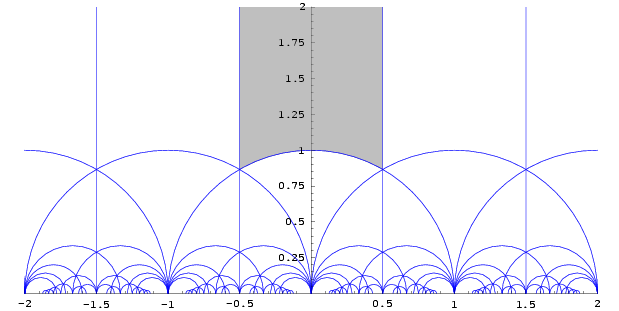
\includegraphics[scale=0.4]{figures/fundamental-domain.png}
    \caption{A fundamental domain (shaded) of the $\PSL_2(\bbZ)$-action on the upper half-plane $\bbC^+$ by \glspl{flt}, and the tiling formed by its orbit.\label{fig fund domain}}
\end{figure}



\begin{defn}\index{Automorphism!Local infinitesimal}
    A \emph{local infinitesimal automorphism} of a Cartan geometry $(P\to M,\eta)$ is an infinitesimal automorphism of the restriction $(\restr{P}{U},\restr{\eta}{U})$ to an open subset $U\subset M$.
\end{defn}

The following lemma establishes a simpler criterion for being a local automorphism.

\begin{lem}[Microlocal is local {{\cite[Lem.~15.6]{McKayCartan}}}]\index{Automorphism!Microlocal infinitesimal}
    Let $(P\overset{\pi}{\to} M,\eta)$ be a Cartan geometry of type $(G,H)$. Let $\varphi:V\to W$ be a (set-theoretic) bijection of open sets $V,W\subset P$ which commutes with the flows of constant vector fields where defined. In addition, assume that for any $m\in \pi(V)$ and connected components $V_0,V_1$ of $P_m\cap V$ there are $p\in V_0$ and $h\in H$ such that $\varphi(p\cdot h)=\varphi(p)\cdot h$ (such a $\varphi$ is called a ``microlocal automorphism''). Then $\varphi$ extends to a unique local automorphism on $\pi^{-1}(\pi(V))$. 

    Similarly, if $X\in\fX(V)$ is a vector field whose flow commutes with the flows of constant vector fields where defined and such that, as above, $X(p\cdot h)=\Phi_{h\ast p}\cdot X(p)$ (a ``microlocal infinitesimal automorphism''), it extends uniquely to a local infinitesimal automorphism on $\pi^{-1}(\pi(V))$. 
\end{lem}
\begin{proof}
    By definition, a microlocal automorphism commutes with the flows up the fibers $P_m$, $m\in M$, of $P$, which are $H$-torsors, so is locally a left translation from one fiber to the other in any principal bundle chart. Hence, it extends globally to such a translation iff we can get it to agree from one component of $V\cap P_m$ to the other on which element it translates by. Hence, it extends to be $H$-invariant. Similarly for the microlocal infinitesimal automorphism.
\end{proof}

\begin{cor}
    If the automorphisms of a Cartan geometry $(P\to M,\eta)$ permute the components of $M$ and the (local) inifinitesimal automorphisms span the tangent space of some point (a dense set of points) of $P$, then the curvature function is constant and its value is an $H$-invariant element of $\frakg\otimes \bigwedge\nolimits^2(\frakg\slash\frakh)^\ast$.
\end{cor}
\begin{proof}
    The preceding lemma allows us to work locally at a point. Since the curvature function must have zero Lie derivative w.r.t.\ any infinitesimal automorphism, if they span the whole tangent space, then the function must be constant. Since it is always $H$-equivariant, its constant value must then be $H$-invariant.
\end{proof}

In particular, if the geometry is torsion-free and complete, then this leads to a Cartan space form. In other words, Cartan space forms are exactly those torsion-free complete Cartan geometries whose infinitesimal automorphisms span the tangent bundle.

\begin{example}
    \begin{enumerate}
        \item For a conformal structure, i.e., one modeled on the conformal sphere $\bbS^n$ with $G=\bbP \Or_{n+1,1}$, it is not difficult to check that $\left(\frakg\otimes \bigwedge\nolimits^2(\frakg\slash\frakh)^\ast\right)^H=0$, so if $\dim \aut=\dim G$, the geometry must be flat.
        \item For a Riemannian geometry, $(G,H)=(\rmE_n,\Or_n)$, and it is easy to check that the space 
        \[\left(\frakg\otimes \bigwedge\nolimits^2(\frakg\slash\frakh)^\ast\right)^H\cong \Hom_{\Or_n}(\bbR^n\times\bbR^n,\frakg)\] 
        is $1$-dimensional, spanned by $(\bf{x},\bf{y})\mapsto \bf{x}\wedge\bf{y}\in\frako_n<\frakg$ (this element generates the rotations in the plane spanned by $\bf{x}$ and $\bf{y}$), cf.\ Example~\ref{ex 1.4.6 Cap}. Hence, if $\dim \aut=\dim G$, then there is a local isometry with either the Euclidean space, the round sphere, or the hyperbolic space.
    \end{enumerate}
\end{example}

\begin{xca}
    Find the infinitesimal automorphisms of the conformal geometry on $\bbS^n$ and on $\RP^n$ for $n\geq 3$.
\end{xca}


While Theorem~\ref{thm 1.5.11 Cap} states that an infinitesimal automorphism is uniquely determined by its value at a single point, there is no guarantee that a given microlocal infinitesimal automorphism can be extended to become global. Each infinitesimal automorphism projects to $M$ to give a vector field that has zeroes arizing from points of $P$ where it is vertical. Outside of such points, there is a dense $H$-invariant open subset of $P$ on which the linear projection of the subspace spanned by $\aut(P,\eta)_p$ achieves maximal rank. Quotienting by $H$, there is a dense open subset of $M$ over which the integral manifolds of $\aut(P,\eta)$ form a foliation. In fact, without going into too much detail, these integral manifolds are smooth even away from that subset. Thus, the leaves of this foliation are covering spaces $\wh{M}\to M$. If these covering spaces are multi-sheeted, we say that the infinitesimal automorphisms are \emph{multivalued}.\index{Automorphism!Multivalued infinitesimal} The group of deck transformations of the covering space is called the \emph{holonomy group of infinitesimal automorphisms}.\index{Holonomy!of infinitesimal automorphisms}

\begin{thm}[Amores II (1980) {{\cite[Thm.~15.8]{McKayCartan}}}]
    Let $(P\to M,\eta)$ be a real analytic Cartan geometry on a connected manifold $M$. Let $X\in \fX(V)$ be a microlocal infinitesimal automorphism defined on a connected open set $V\subset P$. If $M$ is simply connected, then $X$ extends uniquely to an infinitesimal automorphism over $M$. If $M$ is not simply connected, $X$ extends over the universal covering space of $M$, and it descends to an infinitesimal automorphism over $M$ iff $X$ is invariant under the holonomy of infinitesimal automorphisms.
\end{thm}
\begin{proof}
    We can suppose that $M$ is simply connected. Moving by flows of constant vector fields and by the principal $H$-action, we cover $P$ in open sets on each of which we have defined a vector field. Analyticity ensures that, since $X$ is invariant under all constant vector fields initially, and this is an analytic differential equation, this remains true as we extend the domain of $X$. Microlocality is similarly preserved by analyticity and permutation of the constant vector fields under the $H$-action. Hence, each vector field extends uniquely to a local infinitesimal automorphism. At each step in the process, by invariance under the flows, these local infinitesimal automorphisms agree on overlaps. Our vector field $X$ remains $H$-equivariant as we extend it, again by analyticity, so is a section of $\T P\slash H\to M$, a vector bundle over a simply connected manifold, so it does not become multivalued.
\end{proof}

Recall that the soldering form of a Cartan connection $\eta$ is $\theta=\eta+\frakh$. Let us denote it by $\underline{\eta}$ instead, and similarly we use this notation for the quotient of any $\frakg$-valued map by $\frakh$. By Cartan's magic formula, it is easy to see that for a smooth function $f:P\to \frakg$, the associated vector field $X=\eta^{-1}\circ f\in \fX(P)$ preserves the Cartan connection (in particular, is $\frakh$-invariant in the sense that it commutes with $\eta^{-1}(\frakh)$) iff 
\[\dd f+[\eta,f]=\scrK\circ \underline{f}\wedge\underline{\eta}.\]
(The right hand side is nothing but $i_X \Omega^\eta$.) Furthermore, $X$ is an infinitesimal automorphism iff $f$ in addition satisfies $\Phi_h^\ast f=\Ad_h^{-1}f$ for at least one $h$ in each path component of $H$, where $\Phi$ is the principal $H$-action.

This tells us once again that $X$ is determined by its value at a point since we have a total differential equation for $f$. Any $H$-equivariant vector field $X$ on $P$ descends to a vector field $\underline{X}=\pi_\ast X$ on $M$. Just as $X$ is associated to $f$ by $f=\eta(X)$, $\underline{X}$ is associated to $\underline{f}$.

Take two infinitesimal automorphisms $X,Y\in\aut(P,\eta)$ with associated functions $\eta(X),\eta(Y)$. Consider the function $\eta([X,Y])$ corresponding to the bracket $[X,Y]\in \aut(P,\eta)$. The general formula \eqref{eq prop 4.1.6} for the exterior derivative expands to 
\[\eta([X,Y])=[\eta(X),\eta(Y)]-\scrK(\underline{\eta}(X),\underline{\eta}(Y))+\Lie_X (\eta(Y))-\Lie_{Y}(\eta(X)),\]
\index{Curvature-deformed bracket} so the Lie bracket of $\aut(P,\eta)$ is given exactly by the \emph{curvature-deformed bracket} from \eqref{eq deformed bracket}, with the extra terms appearing since $A=\eta(X),B=\eta(Y)$ are no longer constant. From this, the underlying vector field on $M$ is represented by the function
\[\underline{\eta}([X,Y])=\underline{[\eta(X),\eta(Y)]}-\underline{\scrK}(\underline{\eta}(X),\underline{\eta}(Y))+\Lie_X (\underline{\eta}(Y))-\Lie_Y (\underline{\eta}(X)).\]

\begin{prop}[{{\cite[Prop.~15.9]{McKayCartan}}}]
    For a flat Cartan geometry $(P\to M,\eta)$ of type $(G,H)$ on a connected manifold $M$, the Lie algebra $\aut(P,\eta)$ is identified by the developing map with the holonomy-invariant Lie subalgebra of $\frakg$.
\end{prop}
\begin{proof}
    Lift the infinitesimal automorphism to the geometry over the universal cover $\wt M\overset{\wt\pi}{\to}M$, whose bundle is $\wt{P}=\wt{\pi}^\ast P$. Locally, this is identified by the developing map $\dev:\wt{M}\to G\slash H$ with an infinitesimal automorphism of the model geometry, i.e., some element of $\frakg$. Once we match our infinitesimal automorphism with some element of $\frakg$ near some point of $\wt P$, we continue to match in open sets by flowing along constant vector fields. These open sets eventually cover the entire connected component of that point. By $H$-invariance we can extend to all components. So the infinitesimal automorphisms form a Lie subalgebra of $\frakg$ that is invariant under the action of the fundamental group $\pi_1(M)$. The converse is clear.
\end{proof}

\begin{example}
    The conformal geometry of a flat torus $\bbE^n\slash \bbZ^n$ of dimension $\geq 3$ has developing map identifying Euclidean space with a punctured sphere. Infinitesimal automorphisms are vector fields on the sphere vanishing at the puncture and invariant under deck transformations that is, the \emph{cocompact group action} (i.e., the orbit space is compact)\index{Cocompact group action} of the fundamental group of the torus. But the model is algebraic, so these vector fields are invariant under the Zariski closure of the cocompact group action, i.e., under the translations of Euclidean space, hence are themselves translations. The torus has conformal group precisely the torus acting on itself by translation. 
\end{example}

Finally, let us discuss the circumstances under which infinitesimal automorphisms can be recovered from their action on the base manifold. Recall that the kernel $K$ of a Klein geometry $(G,H)$ is the largest normal subgroup of $G$ contained in $H$. Its Lie algebra $\frakk$ is the largest ideal of $\frakg$ contained in $\frakh$, trivial iff $(G,H)$ is locally effective (i.e., $K$ is discrete).

\begin{prop}[Sharpe {{\cite{Sharpe}}}]
    Every infinitesimal automorphism of a Cartan geometry with locally effective model is determined by its projection to the base.
\end{prop}
\begin{proof}
    If $X,Y\in\aut(P,\eta)$ have the same projection, then $Z\coloneqq X-Y\in\aut(P,\eta)$ is tangent to the fibers of $P$. Let $A\coloneqq \eta(Z)$; tangency to the fibers is precisely the statement that $A\in \frakh$, so $\underline{A}=\underline{\eta}(X)=0$. Since $Z$ is an infinitesimal automorphism, we have 
    \[\dd A+[\eta,A]=\scrK\circ \underline{A}\wedge \underline{\eta}=0.\]
    But $A$ is valued in $\frakh$, so $\dd A$ is $\frakh$-valued, while $\eta$ is onto $\frakg$. Hence, $[A,\frakg]\subset \frakh$, so $A$ is valued in the subalgebra of $\frakh$ satisfying this equation. The argument of the last two sentences can be iterated, eventually forcing $A$ to be valued in the largest ideal of $\frakg$ contained in $\frakh$. For a locally effective model, this is zero, so $Z=0$.
\end{proof}






\section{Action of the automorphism group}

Automorphisms commute with the flows of constant vector fields and with the principal action of the structure group. These flows need not be complete, but if defined for some time at some point, they are defined for the same time throughout the orbit of the automorphism group (\emph{automorphism orbit} for short) through that point. Hence, the orbits of the automorphism group are taken to one another by these flows, and by the structure group. Over a connected manifold, this action on the set of orbits is thereby transitive.

\begin{thm}[Kobayashi (1957) {{\cite[Thm.~15.18]{McKayCartan}}}]
    The automorphism orbits of any Cartan geometry $(P\to M,\eta)$ are closed.
\end{thm}
\begin{proof}
    Take a point $p\in P$ in the closure of an automorphism orbit, say $p=\lim_{i\to\infty} g_i(p_0)$ for some $p_0\in P$ and $g_i\in \Aut(P,\eta)$. Define a map $\varphi$ on some neighborhood of $p_0$ by demanding that $\varphi(p_0)=p$ and that $\varphi$ commute with the constant vector fields, i.e., 
    \[\varphi\left(\Fl_t^{\eta^{-1}(A)}(p_0)\right)=\Fl_t^{\eta^{-1}(A)}(p),\quad A\in\frakg;\]
    this uniquely determines $\varphi$ near $p_0$, but we still have to see why it is a local automorphism. Commuting with constant vector fields, convergence of $g_i(p_0)\to p$ in $P$ implies the uniform convergence of $g_i$ with all derivatives as maps $P\to P$. Thus, $\varphi=\lim_i g_i$ near $p_0$. Repeating the construction, $\varphi$ extends smoothly to all of $P$. By the same construction, define a limit for $g_i^{-1}$, thus $\varphi$ is a diffeomorphism and an automorphism, so $p$ lies in the orbit of $p_0$.
\end{proof}


Since we do not yet know that the automorphism orbits are smooth, we define a provisional concept of tangent spaces of subsets of $P$.

\begin{defn}
    Let $(P\to M,\eta)$ be a Cartan geometry. For a subset $S\subset P$, a \emph{tangent vector} at a point $p_0\in S$ is a vector $X\in \T_{p_0}P$ such that, for some sequences $\lambda_i\to\infty$ in $\bbR$ and $A_i\to 0$ in $\frakg$, 
    \[\Fl^{\eta^{-1}(A_i)}_1(p_0)\in S \quad\text{and}\quad \lambda_iA_i\underset{i\to\infty}{\to} \eta(X).\]
    The \emph{tangent space} $\T_{p_0}S$ is the set of tangent vectors to $S$ at $p_0$. This need not be a vector space.
\end{defn}

The tangent spaces of each automorphism orbit are taken to one another by the automorphism group. Automorphisms preserve every constant vector field, so the tangent spaces to each automorphism orbit $\scrO$ consist of the values of the same constant vector fields at all points of $\scrO$. 

In the following, we assume a fixed Cartan geometry $(P\to M,\eta)$ of type $(G,H)$ and do not specify it every time. To each $A\in\frakg$ we also assign the flow of its constant vector field at time $1$:
\[F^A\coloneqq \Fl^{\eta^{-1}(A)}_1\quad\text{for}\quad  A\in\frakg.\]

\begin{lem}[{{\cite[Lem.~15.19]{McKayCartan}}}]\label{lem 12.19 McKay}
    Let $X_i\in \T_{p_0}P$ be a sequence of vectors with $X_i\to 0$ and let $A_i\coloneqq \eta(X_i)\in\frakg$. Suppose that infinitely many among $F^{A_i}(p_0)$ are in the automorphism orbit $\scrO$ of a point $p_0\in P$. After perhaps replacing $(X_i)$ by a subsequence, the lines spanned by the vectors $X_i$ converge to a line tangent to $\scrO$. A constant vector field is somewhere tangent to an orbit iff it is everywhere tangent to that orbit, which occurs iff its flow preserves that orbit.
\end{lem}
\begin{proof}
    Suppose that $F^{A_i}(p_0)=g_i(p_0)$ for some $A_i\to 0$ and $g_i\in \Aut(P,\eta)$. Pick $\lambda_i>0$ such that $\lambda_i A_i$ stays bounded and stays outside of some neighborhood of the origin in $\frakg$. Choosing a subsequence, we can arrange that $\lambda_i A_i$ converges, say $\lambda_i A_i\to A\in\frakg$. Pick a $t\in \bbR$ and let $n_i\coloneqq \lfloor t\lambda_i\rfloor\in\bbN$. But $A_i\to 0$, so $t\lambda_i A_i-n_i A_i\to 0$, i.e., $n_i A_i\to tA$. But $F^{n_iA_i}(p_0)=g_i^{n_i}(p_0)\in\scrO$ while $F^{n_iA_i}(p_0)\to F^{tA}(p_0)$. Since the orbit is closed as a subset of $P$, $F^{tA}(p_0)\in\scrO$ for all $t$. In particular, if $A=\eta(X)$ for a vector $X$ tangent to $\scrO$, then the flow of $A$ preserves $\scrO$.
\end{proof}

\begin{lem}[{{\cite[Lem.~15.20]{McKayCartan}}}]
    The tangent spaces of each automorphism orbit $\scrO\subset P$ are closed cones, i.e., closed subsets of the tangent spaces of $P$ invariant under rescalings by real numbers (including zero and negatives).
\end{lem}
\begin{proof}
    Pick a convergent sequence $X_i\in \T_{p_0}\scrO$. Take sequences $\frakg\ni A_{ij}\underset{j\to 0}{\to} 0$ and sequences $\bbR\ni\lambda_{ij}\underset{j\to 0}{\to} 0$ such that $F^{A_{ij}}(p_0)\in\scrO$ and $\lambda_{ij}A_{ij}\underset{j\to 0}{\to} \eta(X_i)$. Let $A_i\coloneqq A_{ii}$, $\lambda_i\coloneqq \lambda_{ii}$ and apply Lemma~\ref{lem 12.19 McKay}.
\end{proof}

Differentiating the flows of constant vector fields, 
\[F^{tB}\circ F^{tA}=F^{t(A+B)}+\calO(t^2)\]
for any $A,B\in\frakg$ close enough to zero (how close to zero may need to vary with the point of $P$). Recall the curvature-deformed bracket \eqref{eq deformed bracket},
\[[A,B]_p'=[A,B]-\scrK_p(A,B),\quad A,B\in\frakg,\]
defined by the value of the curvature at each point $p\in P$. Taking brackets by commutators of flows,
\begin{align}
    F^{-tB}\circ F^{-sA}\circ F^{tB}\circ F^{sA}&=\Fl^{st[\eta^{-1}(A),\eta^{-1}(B)]}_1+\calO(s,t)^3=\notag\\
    &= \Fl_1^{st\eta^{-1}([A,B]-\scrK(A,B))}+\calO(s,t)^3=\notag\\
    &=F^{st[A,B]'}+\calO(s,t)^3
\end{align}
for any $A,B\in\frakg$ close enough to zero. (Continuing in the same vein, Melnick discovered a \gls{bch}-type formula \cite{Melnick}.)

The next lemma shows that the tangent spaces are actually vector spaces and explains the appearance of the curvature-deformed bracket in our earlier study of Cartan space forms, where the automorphism groups acted transitively on $P$, so $\T \scrO=\T P$.


\begin{lem}[{{\cite[Lem.~15.21]{McKayCartan}}}]
    The tangent spaces of each automorphism orbit in $P$ are linear subspaces of the tangent spaces of $P$, and Lie algebras under the curvature-deformed bracket.
\end{lem}
\begin{proof}
    Take tangent vectors $X,X'\in\T_{p_0}\scrO$. Let $A\coloneqq \eta(X)$, $A'\coloneqq \eta(X')$, so there are sequences $\lambda_i,\lambda_i'\underset{i\to\infty}{\to}\infty$ and $A_i,A_i'\to 0$ for which 
    \[F^{A_i}(p_0),F^{A_i'}(p_0)\in\scrO,\]
    say 
    \[g_i(p_0)=F^{A_i}(p_0),\quad g_i'(p_0)=F^{A_i'}(p_0)\]
    for some $g_i,g_i'\in\Aut(P,\eta)$ and $\lambda_iA_i\to A$ and $\lambda_i'A_i'\to A'$.

    Pick any sequence $t_i\to \infty$ of positive numbers. Replacing $\lambda_i,\lambda_i'$ by subsequences, we can assume that both grow faster than $t_i$: $\frac{\lambda_i}{t_i},\frac{\lambda_i'}{t_i}\to \infty$. Let $n_i=\lfloor\frac{\lambda_i}{t_i}\rfloor $ and $n_i'=\lfloor\frac{\lambda_i'}{t_i}\rfloor$, so $\frac{\lambda_i}{n_i},\frac{\lambda_i'}{n_i'}\approx t_i\to \infty$. Take new $A_i$, $A_i'$, $\lambda_i$, $\lambda_i'$ equal to the old $n_iA_i$, $n_i'A_i'$, $\frac{\lambda_i}{n_i}$, $\frac{\lambda_i'}{n_i'}$ so that we can assume that $\lambda_i/\lambda_i'\to 1$. We have 
    \[g_i'\circ g_i(p_0) = g_i'\circ F^{A_i}(p_0)=F^{A_i}\circ g_i'(p_0)=F^{A_i}\circ F^{A_i'}(p_0)=F^{A_i+A_i'+\cdots}(p_0)\]
    and 
    \[\lambda_i(A_i+A_i'+\cdots )=\lambda_i A_i+\frac{\lambda_i}{\lambda_i'}\lambda_i'A_i'+\cdots\to A+A'.\]
    By Lemma~\ref{lem 12.19 McKay}, the lines spanned by $A_i+A_i'$ converge to a tangent line to the orbit, the span of $A+A'$. By the same argument, using the bracket by commutators of flows, $[A,B]'_p$ is also in the tangent space, so it's a Lie algebra.
\end{proof}

Now that we know that the tangent spaces have the same dimension, we can use them to construct slices for the action of the automorphism group, which will imply that the orbits are smooth. Let $p_0\in P$ and let $\scrO$ be its automorphism orbit. As usual, a \emph{slice} at $p_0$ is a smooth embedding $\varphi:U\to P$ of an open $0$-neighborhood $U\subset V$ in a finite-dimensional vector space $V$ such that $\varphi(0)=p_0$, $\varphi^{-1}(\scrO)=\{0\}$, and the image is transversal to the orbit at $p_0$: 
\[\varphi_{\ast 0}(V)\oplus\T_{p_0}\scrO=\T_p P.\]

\begin{lem}[{{\cite[Lem.~15.22]{McKayCartan}}}]\label{lem 12.22 McKay}
    Let $V<\T_{p_0}P$ be a subspace complementary to $\T_{p_0}\scrO$. Then there is an open $0$-neighborhood $U\subset V$ such that the following map is a slice:
    \[\varphi:U\to P,\quad  v\mapsto F^{\eta(v)}(p_0).\]
\end{lem}
\begin{proof}
    Let $V'\coloneqq \eta(V)<\frakg$, which is a subspace complementary to $T'\coloneqq \eta(\T_{p_0}\scrO)$. If there is a sequence of elements $A_i\to 0$ with $A_i\in V'$ and with $F^{A_i}(p_0)\in \scrO$, then as above we can find a convergent subsequence such that the lines spanned by $A_i$ converge in $\T_{p_0}P$ to some line spanned by some $A\neq 0$. Since $V'<\frakg$ is a subspace, it is a closed subset, so $A_i\in V'$ implies $A\in V'$. By definition of tangent spaces, $A\in T'$, so $A\in T'$. Since $T'\cap V'=\{0\}$, we conclude $A=0$, a contradiction. Thus, there is no such sequence, i.e., there is an open $0$-neighborhood $U'\subset V'$ in which no point $A$ has $F^A(p_0)\in \scrO$. Take the associated set $U=\eta^{-1}_{p_0}(U')\subset V$. By shrinking $U$, we can arrange that $A\mapsto F^A(p_0)$ is defined on $U$ and is an embedding.
\end{proof}

The following lemma constructs slice charts for the orbit, turning it into an embedded submanifold.

\begin{lem}[{{\cite[Lem.~15.23]{McKayCartan}}}]\label{lem 12.23 McKay}
    Let $V<\T_{p_0}\scrO$ be a subspace complementary to $\T_{p_0}\scrO$. Pick $0$-neighborhoods $U\subset V$ and $W\subset \T_{p_0}\scrO$. If the open sets are small enough then the map 
    \[\varphi:V\times W\to P,\quad (v,w)\mapsto F^{\eta(v)}\circ F^{\eta(w)}(p_0)\]
    is a diffeomorphism to an open subset of $P$ an a slice for any fixed $w$.
\end{lem}
\begin{proof}
    By the \gls{inmt}, we can pick small enough open sets $U,W$ to ensure that $\varphi$ is a diffeomorphism to its image, an open set $U_P\subset P$. For any $w$, $\varphi(0,w)\in\scrO$ by Lemma~\ref{lem 12.19 McKay}. We can pick $U$ small enough to ensure that $v\mapsto \varphi(v,0)$ is a slice by Lemma~\ref{lem 12.22 McKay}, so stays outside $\scrO$ except at $v=0$. Let $U'\coloneqq \eta_{p_0}(U)\subset \frakg$ and $W'\coloneqq \eta_p(W)\subset \frakg$. If $\varphi(v,w)\in\scrO$ then we have 
    \[F^{\eta(v)}\circ F^{\eta(w)}(p_0)=g(p_0),\]
    for some automorphism $g\in\Aut(P,\eta)$. Thus, $F^{-\eta(v)}(p_0)=g^{-1}(\circ ^{\eta(w)}(p_0)$ lies in $\scrO$, and $\eta_p(v)=0$, so $v=0$.
\end{proof}

\begin{cor}
    Every automorphism orbit of a Cartan geometry is a closed embedded submanifold.
\end{cor}

\begin{cor}[{{\cite[Cor.~15.25]{McKayCartan}}}]
    Let $M$ be connected, and pick an automorphism orbit $\scrO$ through a point $p_0\in P$. The orbit is a closed embedded submanifold, and the action of automorphisms is free, so we can endow the group $\Aut(P,\eta)$ with the smooth structue diffeomorphic to that of $\scrO$ via the map $g\mapsto g(p_0)$. Then 
    \begin{enumerate}
        \item this smooth structure turns the group $\Aut(P,\eta)$ into a Lie group;
        \item upon changing the point of $p_0$, the Lie group structure undergoes an isomorphism given by the flows of constant vector fields and the principal action of the structure group;
        \item $\Aut(P,\eta)$ acts smoothly on $P$ and $M$.
    \end{enumerate}
\end{cor}
\begin{proof}
    Take $g,h\in\Aut(P,\eta)$. We want to prove that $gh$ is a smooth function of $g,h$, i.e., that $g\circ h(p_0)$ is a smooth function of $g(p_0)$ and $h(p_0)$. We need only vary $g,h$ by flows $F^A$, $F^B$, since these flows provide local coordinates $A,B\in V<\frakg$ on the orbit near each point. Thus, we need to prove that $F^A\circ g\circ F^B\circ h(p_0)$
    depends smoothly on $A$ and $B$, which is obvious. The same expression demonstrates the smoothness of the action.
\end{proof}

Finally, now that we have a free Lie group action of $\Aut(P,\eta)$ on $P$, we can ask whether this action is proper, so that $P$ can be treated as a principal $\Aut(P,\eta)$-bundle. Recall that an action $(g,m)\mapsto g\cdot m$ is called proper when the map $(g,m)\mapsto (g\cdot m,m)$ is proper. 

\begin{cor}[{{\cite[Cor.~15.26]{McKayCartan}}}]
    If $M$ is connected, then the Lie group action of $\Aut(P,\eta)$ on $P$ is free and proper.
\end{cor}
\begin{proof}
    By Corollary~\ref{cor 6.3.3 RS1}(2), the action is proper iff for any sequences $g_i\in \Aut(P,\eta)$ and $p_i\in P$, if both $(g_i(p_i))$ and $(p_i)$ converge in $P$, then some subsequence $(g_{i_j})$ converges in the group.

    The topology of $\Aut(P,\eta)$ is that of the orbit through any one point $p$, so $g_i(p)\to g(p)$ iff $g_i\to g$. After taking a subsequence $p_i\coloneqq F^{A_i}\circ F^{B_i}(p)$ for some $A_i,B_i\to 0$ as in Lemma~\ref{lem 12.23 McKay}. Similarly, after taking another subsequence, we can write $g_i(p_i)=F^{C_i}\circ F^{D_i}(q)$ for some $C_i,D_i\to 0$ and $q\in P$. Combining these two formulas, we see that
    \[g_i(p)=F^{-B_i}\circ F^{-A_i}\circ F^{C_i}\circ F^{D_i}(q)\]
    approaches $q$ by continuity of the flows of the constant vector fields. Since orbits are closed, $q=g(p)$ for some $g\in \Aut(P,\eta)$, so $g_i(p)\to g(p)$ and thus $g_i\to g$, as required.
\end{proof}

By Corollary~\ref{cor 6.5.1 RS1}, the quotient by a free and proper Lie group action is a smooth manifold, and the quotient map is a \gls{pfb}. The action of automorphisms is a left action, so this will be a left quotient. We summarize our results on automorphisms in the following main theorem.

\begin{thm}[{{\cite[Thm.~15.13]{McKayCartan}}}]\label{thm 12.13 McKay}
    If $(P\to M,\eta)$ is a Cartan geometry of type $(G,H)$ on a connected manifold $M$. Then:
    \begin{enumerate}
        \item The automorphism group $\Aut(P,\eta)$ admits a unique Lie group structure (up to isomorphism) for which the quotient map $P\to \Aut(P,\eta)\bslash P$ is a smooth principal bundle;
        \item The Lie algebra of $\Aut(P,\eta)$ is the set of complete infinitesimal automorphisms. 
        \item The constant vector fields descend to smooth vector fields on $\Aut(P,\eta)\bslash P$ spanning every tangent space.
        \item The principal $H$-action descends to a smooth $H$-action on $\Aut(P,\eta)\bslash P$.
    \end{enumerate} 
\end{thm}
\begin{proof}
    Only items 2-4 are yet unproven. Complete infinitesimal automorphisms generate automorphic flows lying in the identity component of $\Aut(P,\eta)$. By the Analytic Subgroup Theorem~\ref{thm analytic subgroup}, they belong to the Lie algebra of $\Aut(P,\eta)$. Conversely, consider an automorphism orbit with basepoint $p_0$ as a copy of the Lie group $\Aut(P,\eta)$ and consider a right-invariant vector field on it. The flows of constant vector fields and the action of the structure group push this vector field all around $P$ to produce a global infinitesimal automorphism. It is complete because it is a right-invariant vector field for the Lie group structure of each automorphism orbit.

    3 is obvious since constant vector fields are $\Aut(P,\eta)$-invariant. 4 follows from the fact that $H$ acts by bundle morphisms on the bundle $P\to \Aut(P,\eta)\bslash P$. 
\end{proof}

Sometimes a generalization of this result to disconnected base manifolds is useful. This is shown in the following exercise and theorem.

\begin{xca}
    Let $(P\to M,\eta)$ be a Cartan geometry over a connected $M$. Prove that the topology of the automorphism group determined by identifying it with an orbit in $P$ is the topology of pointwise convergece, but is also the compact-open topology on it as a collection of maps of $P$, and is also the topology of uniform convergence on compact sets with all derivatives.
\end{xca}

\begin{thm}[{{\cite[Thm.~15.28]{McKayCartan}}}]\label{lem thm 12.28 McKay}
    Suppose $\varGamma$ is a group consisting of some automorphisms of a Cartan geometry $(P\to M,\eta)$, closed in the topology of uniform convergence on compact sets with all derivatives. Suppose that, for every connected component $M'\subset M$, the only element of $\varGamma$ that fixes every point of $P$ above $M'$ is the identity. Then $\varGamma$ is a Lie group acting smoothly on $P$ and $M$ and the quotient map $P\to \varGamma\bslash P$ is a principal $\varGamma$-bundle. There is a finite set of smooth $\varGamma$-invariant functions on $P$ that distinguish $\varGamma$-orbits.
\end{thm}
\begin{proof}
    Suppose that $\varGamma$ fixes a point of $P$. Commuting with the $H$-action and constant vector fields, $\varGamma$ fixes every element of $P$ above some component $M'\subset M$, so is the identity. Hence, $\varGamma$ acts freely. The rest of the proof is identical to the original proof of the properness of the action of automorphism groups. The topology of $\varGamma$ is almost irrelevant by the preceding exercise. As the quotient $\varGamma\bslash P$ is a manifold, it admits an embedding into some $\bbR^s$ by the Whitney Embedding Theorem~\ref{thm whitney embedding}. Take the coordinate functions of such an embedding as out finite set of smooth functions.
\end{proof}

All automorphisms that fix a point in the base are vertical automorphisms given by some principal right actions (note that generic principal actions are usually not automorphisms, even in Klein geometries):

\begin{lem}[{{\cite[Lem.~15.27]{McKayCartan}}}]
    Let $(P\to M,\eta)$ be a Cartan geometry. For a point $m\in M$, its stabilizer $\Aut(P,\eta)_m$ is a closed subgroup of $\Aut(P,\eta)$ contained inside $H\cap \Aut(P,\eta)$, where by $H$ we mean the set of principal right $H$-actions.
\end{lem}
\begin{proof}
    We can assume that $M$ is connected, \gls{wlog}. Let $G'\coloneqq \Aut(P,\eta)$ and $H'\coloneqq \Aut(P,\eta)_m$. Pick a point $p\in P_m$. Embed $G'\to P$ by the orbit map $g\mapsto g(p)$. Each $k\in H'$ moves $p$ to a point of the same fiber, which is an $H$-torsor, so $k(p)=p\cdot \wb{k}$ for some $\wb k\in H$. But since $H'(p)=G'(p)\cap (p\cdot H)$, the image of $\phi:k\mapsto \wb{k}$ is a closed embedded submanifold. $\phi$ is also injective because the $H$-action is free, and clearly an anti-homomorphism, so its image is a closed subgroup.
\end{proof}

In particular, if $H$ is compact, the stabilizers of all points of $M$ are also compact. By applying Corollary~\ref{cor 6.3.3 RS1}(3), we get the following important result.

\begin{cor}
    If $M$ is compact, then any Cartan geometry with a compact structure group $H$ has a compact automorphism group.
\end{cor}

\begin{cor}\label{cor compact isometry group}\index{Isometry group}
    The isometry group of any compact Riemannian manifold is a compact Lie group.
\end{cor}

\begin{xca}
    Suppose that the model is $(G,H)$ and $\Aut(P,\eta)$ acts transitively on $P$, so $P$ is a torsor for this group. Let $\fraka$ be the Lie algebra of $\Aut(P,\eta)$. Prove that the Cartan connection has the form $\varLambda\circ\theta_{\Aut}$ for some constant linear map $\varLambda\in\frakg\otimes\fraka^\ast$, where $\theta_{\Aut}$ is the Maurer-Cartan form of $\Aut(P,\eta)\cong P$.
\end{xca}


\begin{cor}[{{\cite[Cor.~15.29]{McKayCartan}}}]
    Let $(P\to M,\eta)$ be a Cartan geometry on a connected manifold $M$. Then, along each automorphism orbit $\scrO$, the constant vector fields which are tangent to $\scrO$ are exactly the left-invariant vector fields of $\scrO$ as a $\Aut(P,\eta)$-torsor. In particular, the Lie bracket of the Lie algebra of $\Aut(P,\eta)$ is identified, via $\eta$, with the curvature-deformed bracket on $\frakg$.
\end{cor}
\begin{proof}
    Automorphisms take tangent vectors of $\scrO$ to tangent vectors of $\scrO$ and constant vector fields to constant vector fields. Hence, the constant vector fields tangent to $\scrO$ at a point are everywhere tangent to $\scrO$, and hence are the left-invariant vector fields. By dimension counting, this covers all left-invariant vector fields. Their bracket is the curvature-deformed bracket, as we saw above.
\end{proof}


\PRLsep


In the remainder of this \sect, we discuss \emph{automorphisms of submanifolds}.


\begin{defn}
    Let $(P\to M,\eta)$ be a Cartan geometry of type $(G,H)$ and let $i:S\hookrightarrow M$ be an immersed submanifold of $M$. An \emph{automorphism of $S$} is an automorphism of the Cartan geometry whose base map commutes with $i$ (i.e., takes $S$ to itself). The group of all automorphisms of $S$ is denoted by $\Aut_S(P,\eta)$ and is by definition a subgroup of $\Aut(P,\eta)=\Aut_M(P,\eta)$.
\end{defn}


\begin{example}
    \begin{enumerate}
        \item An automorphism of an immersed surface $\varSigma\hookrightarrow\bbE^3$ is a diffeomorphism of $\varSigma$ and a rigid motion of Euclidean space which matches the diffeomorphism along $\varSigma$.
        \item If $S$ is a closed embedded submanifold of $M$, then its automorphisms form a closed subgroup of $\Aut(P,\eta)$, cf.\ \cite[p.~44]{Mimura}.
        \item  Consider an immersed surface $\varSigma$ consisting of several disjoint connected components mapped to the same surface in $\bbE^3$. The automorphism group is not a subgroup of the rigid motions. Pick a dense subset of each component surface so that the two subsets are carried by the diffeomorphism to disjoint sets in $\bbE^3$; our immersion is injective on the union of those subsets, a dense subset of $\varSigma$. If we take a countable collection of connected surfaces, we find an automorphism group with uncountably many components.
        \item Now suppose that the immersed surface $\varSigma$ consists of all planes parallel to and at a rational distance from a given plane. The automorphism group acts properly on $\varSigma$ as a Lie group, but does not act properly on $\bbE^3$, even though $\varSigma$ is injectively immersed.
        \item  In the previous example with $\varSigma$ consisting of the same planes, equip $\bbE^3$ with its standard flat conformal geometry. Suppose that the origin belongs to $\varSigma$. Rescalings of $\bbE^3$ by rational numbers act on $\varSigma$ as automorphisms. A sequence of such automorphisms by rational numbers converging to an irrational one acts as automorphisms on the plane through the origin, but has no limit in $\varSigma$ on any of the other planes. Therefore, we want a topology on the automorphism group of $\varSigma$ so that this sequence won't converge; in this example, we want the discrete topology on those rational rescalings.
        \item Consider a dense (irrational slope) line in the flat affine torus, $\bbR\hookrightarrow\bbT^2$, so the model is $(\U_1\times\U_1,\{e\})$. The automorphisms are the translations of $\bbT^2$, acting as a subgroup of $\bbT^2$, hence a Lie group $\bbR$ mapping $\bbR\hookrightarrow \bbT^2$ as an immersed subgroup. 
        \item Take a homogeneous space $M=G\slash H$. Let $M_\delta$ be $M$ with the discrete topology, let $H_\delta$ be the same as $H$, and let $G_\delta$ be $G$ with the topology whose open sets are unions of translates $gU$ of open sets $U\subset H$. The identity map $M_\delta\to M$ is equivariant for the identity map $G_\delta\to G$, so an equivariant immersion with automorphism group $G_\delta$. If $\dim M>0$, this automorphism group is an immersed but not embedded subgroup of $G$.
        \item Consider the map $S=\bbR\to \bbC=M$ given by $x\mapsto \rme^{\i x}$. For each real $c\in \bbR$, the map $x\mapsto x+c$ on $\bbR$ and the rotation of $\bbC$ around the origin by angle $x$ commute, and these are the Euclidean automorphisms of this immersion. So the automorphism group of $S$ is $\bbR$ equipped with a non-injective immersion $\bbR\to \SO_2\ltimes\bbR$.
    \end{enumerate}
\end{example}

Let $P_S\coloneqq i^\ast P$. Then $P_S\to P$ is an immersed subbundle with $\dim P_S=\dim S+\dim H$ and we have a commuting diagram 
\[\begin{tikzcd}
    P_S\arrow[r]\arrow[d] & P\arrow[d]\\
    S \arrow[r] & M.
\end{tikzcd}\]

For the proof of the next theorem, the following enrichment of the notion of a Cartan geometry will be useful. It is a direct analog of the notion of extended coframe from Definition~\ref{def extended coframe} if one thinks of a Cartan connection as a coframe.

\begin{defn}\index{Decorated Cartan geometry}
    A decorated Cartan geometry is a Cartan geometry $(P\to M,\eta)$ equipped with a collection (perhaps infinite) of smooth maps $f_\alpha:P\to M_\alpha$ to some smooth manifolds $M_\alpha$. Each $f_\alpha$ is called a \emph{decoration}.
\end{defn}

\begin{example}
    Any vector field $X\in\fX(M)$ is naturally identified with an $H$-equivariant map $\wt X=\theta(\pi^\ast X):P\to \frakg\slash\frakh$. Thus, any tensor field on $M$ is a decoration. In particular, an action of a finite-dimensional Lie algebra is a decoration.
\end{example}

Clearly, the automorphism group of a decorated Cartan geometry is a closed subgroup of the automorphism group of the undecorated geometry. Thus, all of our results about the action of the automorphism group extend trivially to decorated geometries.

\begin{thm}[{{\cite[Thm.~15.33]{McKayCartan}}}]
    Let $(P\to M,\eta)$ be a Cartan geometry on a connected manifold $M$. Let $(S,i:S\to M)$ be an immersed submanifold such that $i$ is injective on a dense subset of $S$. Then the automorphisms of $S$ form a finite-dimensional Lie group for a unique Lie group structure such that the quotient map 
    \[P_S\to \Aut_S(P,\eta)\bslash P_S\]
    is a smooth principal $\Aut_S(P,\eta)$-bundle. This Lie group acts smoothly on $P_S$, $S$, $P$, and $M$. The Lie group homomorphism $\Aut_S(P,\eta)\to \Aut(P,\eta)$ is an immersion.
\end{thm}
\begin{proof}
    Let $\varGamma$ be the group of diffeomorphisms of $P_S$ preserving $\restr{\eta}{P_S}$ and commuting with the principal $H$-action, with the topology of uniform convergence on compact sets with all derivatives. Then $\Aut_S(P,\eta)$ is a subgroup of $\varGamma\times \Aut(P,\eta)$. Take a linear surjection $\pi:\frakg\to \frakg'$ to a vector space $\frakg'$ of dimension $\dim P_S$. Let $\eta'\coloneqq \pi\circ\eta$. Let $P'\subset P_S$ be the open subset consisting of all points at which $\eta'$ is a linear isomorphism on the tangent spaces. By varying the map $\pi$, we cover $P_S$ is these open sets $P'$. On each $P'$, $\eta'$ is a coframing, so a Cartan connection with trivial infinitesimal model $(\frakg',0)$ and base space $P'$ (not $S$). Since $\eta'$ is a linear isomorphism on each tangent space of $P'$, $\eta=a\circ \eta'$ for a unique smooth map 
    \[a:P_S\to \frakg\otimes(\frakg')^\ast.\]
    Thus, $\eta$ is determined by the decorated Cartan geometry of $P'$ with decoration $a$. Add the composition $P'\hookrightarrow P_S\hookrightarrow P\to P\slash \Aut(P,\eta)$
    as another decoration to $P'$. Inside the automorphism group of this decorated Cartan geometry, $\Aut_S(P,\eta)$ is the closed subgroup commuting with the $H$-action.

    If some autoorphism in $\Aut_S(P,\eta)$ fixes a point of $P_S$, then it fixes the image of that point in $P$, so acts on $P$ trivially, so acts on $M$ trivially. It then fixes every point of the dense open subset of $S$ on whicn $i$ is injective, so it fixes every point of $S$ and of $P$ and hence of $P_S\subset S\times P$. In particular, $\Aut_S(P,\eta)$ acts freely on $P_S$, and thus on $P'$. Apply Theorem~\ref{lem thm 12.28 McKay} to find that $P'\to \Aut_S(P,\eta)\bslash P'$ is a principal bundle, for each of the $\Aut_S(P,\eta)$-invariant open subsets $P'\subset P_S$. If $\Aut_S(P,\eta)\to \Aut(P,\eta)$ maps some vector to zero, it maps some infinitesimal automorphism on $P_S$ to zero in $P$, which contradicts the fact that $P_S\to P$ is an immersion. 
\end{proof}

% \begin{cor}
%     Let $(P\to M,\eta)$ be a Cartan geometry over a manifold $M$ with finitely many connected components. Let $(S,i:S\to M)$ be an immersed submanifold such that $i$ is injective on a dense subset of $S$. Then $\Aut_S(P,\eta)$ is a finite-dimensional Lie group acting smoothly on $P_S$, $P$, $P$, and $M$, and an immersed Lie subgroup of $\Aut(P,\eta)$.
% \end{cor}


\section{Homogeneous Cartan geometries}

We now take a brief look at a class of Cartan geometries that are a generalization of the concept of Cartan space forms. Recall that all Cartan space forms ended up being mutations of complete flat Cartan geometries. This actually has to do with the fact that a complete flat Cartan geometry has only one automorphism orbit, and that orbit lifts to a Lie group. In practice, however, it is more likely that the action is transitive only on the base manifold, and the completeness condition is also overly restrictive.


\begin{defn}[Homogeneous Cartan geometry]\index{Homogeneous Cartan geometry}
    A Cartan geometry $(P\to M,\eta)$ is called homogeneous if its automorphism group acts transitively on $M$.
\end{defn}

The following example shows that homogeneous geometries can indeed be incomplete.

\begin{example}
    The flat torus has a flat Riemannian geometry invariant under translations, hence a homogeneous projective connection. However, this geometry is incomplete by Example~\ref{ex flat projective structures}. Similarly, the conformal geometry of the flat torus of dimension $3$ or more is homogeneous but not complete by Example~\ref{ex flat conformal structures}.
\end{example}

The question for this \sect\ is: \emph{can we find homogeneous Cartan geometries with a given model, and perhaps even classify all such geometries?} Suppose $(P\to M,\eta)$ is a homogeneous Cartan geometry with model $(G,H)$. By Theorem~\ref{thm 12.13 McKay}, the automorphism group embeds into the total space $P$ as an automorphism orbit. Since the Cartan geometry is invariant under automorphisms, the curvature function $\scrK$ is constant along each automorphism orbit $\scrO$. Meanwhile, along the fibers it transforms under the usual representation of $H$ on the curvature module $\bigwedge\nolimits^2(\frakg\slash\frakh)^\ast\otimes\frakg$. 

To classify homogeneous geometries of this type, we can use the structure group $H$ to being the curvature to some normal form, say some fixed value $\scrK_0$. Let $H_1\emb H$ be the stabilizer of $\scrK_0$ and let $P_1\subset P$ be the set on which $\scrK=\scrK_0$. Then $P_1\to M$ is a right principal $H_1$-bundle. Our automorphism orbit $\scrO$ is contained inside $P_1$. On $\scrO$, the structure equation 
\[\dd\eta+\frac12[\eta,\eta]=\frac12\scrK_0\circ \theta\wedge\theta\label{eq 12469}\]
differentiates to expand out into expressions involving only $\dd\eta$ and $\dd\theta$. But $\theta=\eta+\frakh$, so everything expands in terms of $\dd\eta$, which the structure equation turns back into an expression in $\eta$ and $\scrK_0$. This could give additional algebraic compatibility conditions on $\scrK_0$.

There is another source of relations. On $P_1$, the Cartan connection $\eta$ may no longer be a global coframe. Rather, if $H_1\emb H$ has positive codimension, then $\eta+\frakh_1$ is horizontal, say 
\[\eta+\frakh_1=a\circ\theta\]
for some $H_1$-equivariant $a:P_1\to (\frakg\slash\frakh_1)\otimes(\frakg\slash\frakh)^\ast$. Clearly, $a$ is also invariant under the automorphism group, hence constant on our orbit. Repeating the process, pick some constant value $a_0$ for $a$, let $H_2\emb H$ be its stabilizer, and let $P_2\subset P_1$ be the set on which $a=a_0$, so it is a principal $H_2$-bundle. Again, when differentiating the structure equations on $\scrO\subset P_2$, they expand out to equations in the components of $\eta,a_0,\scrK_0$. These equations may force more algebraic relations among $a_0,\scrK_0$.

On $P_2$, we may write 
\[\eta+\frakh_2=b\circ \theta\]
for a unique $H_2$-equivariant $b:P_2\to (\frakg\slash\frakh_2)\otimes(\frakg\slash\frakh)^\ast$, which projects to $a_0$ under the obvious quotient map $\frakg\slash\frakh_2\to\frakg\slash\frakh_1$.

Continue this way until we find that $\dim H_{k+1}=\dim H_k$, so we don't get any new invariants. (In particular, if some $H_j$ is a linear algebraic group, then all subsequent $H_{j+1}$ etc.\ are linear algebraic, each contained in the previous. By the ascending chain condition, the sequence eventually stabilizes, say all equal to some $H_0\emb H$.) Eventually, $\eta+\frakh_0=c_0\circ\theta$ is a constant, and plugging into the structure equations \eqref{eq 12469} yields algebraic equations on $c_0,\scrK_0$ which are satisfied by our initial choice of $c_0,\scrK_0$. These equations then determine structure constants for the remaining linearly independent components $\eta^i$ of $\eta$. By our discussion above, these are the structure equations of a Lie group. Of course, this way we only find a Lie algebra and the embedding of various subalgebras. It remains to determine the actual Lie group of automorphisms of the corresponding homogeneous geometry, assuming it even exists. There is still a possibility that the resulting structure equations are those of a Lie group for which the Lie algebra of $H_0$ does not exponentiate to a closed subgroup. Moreover, it may not be clear how to find a more explicit geometric description of this Lie algebra.







\section{Example: homogeneous affine surfaces}


Consider how we might classify homogeneous surfaces $\varSigma$ modeled on the affine plane $\bbA(\bbR^2)=\Aff_2(\bbR)\slash \GL_2(\bbR)$ with an affine connection invariant under a group of automorphisms acting transitively on the surface. The automorphisms preserve the affine connection, and thus, in particular, preserve the torsion tensor and the torsion-free affine connection obtained by subtracting off the torsion. Hence, we may assume that the connection is torsion-free.

As usual, we write affine transformations as $\left(\begin{smallmatrix}
    g & \bf{x}\\ 0 & 1
\end{smallmatrix}\right)$, so the Cartan connection reads $\eta=\left(\begin{smallmatrix}
    \omega & \theta\\ 0 & 0
\end{smallmatrix}\right)$. The torsion-free condition is exactly $\dd\theta+\omega\wedge\theta=0$, and the curvature is given by 
\[\dd\omega+\omega\wedge\omega=K \theta^1\wedge\theta^2,\label{eq 129521}\]
where $K\in\frakgl_2(\bbR)$ is represented by a $2\times 2$ matrix multiplying the scalar $2$-form $\theta^1\wedge\theta^2$.

\textbf{Flat surfaces.} In the case $K=0$, the affine connection  is flat, so the affine Cartan geometry is flat, thus locally isomorphic to the model. If it is not globally isomorphic to the model, then it develops to the model via the developing map which is a local isomorphism. Assuming $\varSigma$ is connected, each automorphism then extends uniquely to an automorphism of the affine plane. So, $\varSigma$ is a covering space of an open set in the plane, homogeneous under a subgroup of the affine group. 

A homogeneous Cartan geometry $(P\to M,\eta)$ is called \emph{subordinate} to another $(P'\to M',\eta')$, with the same model $(G,H)$, if there is an $H$-equivariant local diffeomorphism $P\to P'$ that is also equivariant under some homomorphism of the automorphism groups. For example, the hyperbolic half-plane $\bbC^+$ has a projective connection induced from its Riemannian geometry, and is equivariantly embedded into the projective plane, hence subordinate to the model projective geometry. 

We would like to find the maximal homogeneous affine surfaces, ordered by subordinacy. We leave it to the reader to classify non-maximal homogeneous affine surfaces subordinate to these. From now on, we can suppose that $K\neq 0$.

\textbf{Normalizing curvature.} Any matrix $K=(K^i_j)$ could, in principle, show up in some homogeneous affine surface. But on any given automorphism orbit $K$ is constant. The automorphism group commutes with the $H$-action, so the $H$-action permutes the automorphism orbits while transforming $K$ in the usual way. Take the structure equations \eqref{eq 129521} and apply the right action $\Phi_h$ by an element $h\in H$, so in matrix notation, $\Phi_h^\ast\omega=h^{-1}\cdot \omega\cdot h$ and $\Phi_h^\ast\theta=h^{-1}\cdot\theta$. We get 
\begin{align}
    0&=h^{-1}(\dd\omega+\omega\wedge\omega)h-(\Phi^\ast_h K)\det h^{-1}\theta^1\wedge\theta^2=\notag\\
    &=(h^{-1} K h-\det h^{-1}\Phi_h^\ast K)\theta^1\wedge\theta^2,
\end{align}
which implies 
\[\Phi_h^\ast K=(\det h)h^{-1} K h.\]
Thus, by choosing the right $h$, we can move to an orbit where $ K$ is in its real Jordan normal form up to a scale factor, constant on the orbit. By picking $h=\lambda\rmI$ for any $\lambda\neq 0$, we can then move to an orbit with value of $ K$ scaled by $\lambda^2$. Thus, we can assume that $\det K\in \{-1,0,1\}$. \textbf{If $ K$ is real diagonalizable}, we can swap the order of the two eigenvalues using $h=\left(\begin{smallmatrix}
    0 & 1\\ -1 & 0
\end{smallmatrix}\right)$, and $h=\left(\begin{smallmatrix}
    1 & 0\\ 0 & -1
\end{smallmatrix}\right)$ can swap the signs of both eigenvalues. Thus, we can assume that the eigenvalues are in order, i.e., either 
\[ K=\begin{pmatrix}
    r & 0 \\ 0 & \pm 1/r
\end{pmatrix},\quad r\geq 1\]
or 
\[ K=\begin{pmatrix}
    1 & 0 \\ 0 & 0
\end{pmatrix},\]
or $ K=0$. \textbf{If $ K$ is not real diagonalizable but complex diagonalizable} (so, two coinciding complex eigenvalues), then $\det K>0$ and so we can assume $\det K=1$, so, viewed as a unit complex number,
\[K=\rme^{\i\alpha},\quad \theta\in (-\pi,\pi)\setminus\{0\}.\]
Finally, \textbf{if $ K$ is not complex diagonalizable}, then it has a generalized eigenspace, so a double eigenvalue, nonnegative determinant, so either $\det K=0$ or $\det K=1$. In terms of the complex Jordan normal form, we have three options:
\[ K=\begin{pmatrix}
    1 & \pm 1\\
    0 & 1
\end{pmatrix} \quad \text{or}\quad \begin{pmatrix}
    0 & 1\\
    0 & 0
\end{pmatrix} \quad \text{or}\quad \begin{pmatrix}
    0 & -1\\
    0 & 0
\end{pmatrix}.\]
Let $H_0\emb H$ be the subgroup preserving the normal form of $ K$, i.e. 
\[H_0\coloneqq \{h\in H\mid (\det h)  K h=h K\}.\]
The set of points $P_0\subset P$ at which $ K$ takes on this normal form is a principal $H_0$-bundle.

If $\det K\neq 0$, so $\det K=\pm 1$, taking a determinant tells us that the elements of $H_0$ have determinant $\pm 1$ and those with determinant $1$ are precisely those that commute with $K$, while those with determinant $-1$ anticommute with $K$. The possible groups $H_0$, of dimensions up to $4$, are:
\begin{center}
    \begin{tabular}{r l} 
     $K$ & $H_0$ \\ [0.5ex] 
     \hline
     $0$ & $\GL_2(\bbR)$\\
     $\rmI$ & $\SL_2(\bbR)$\\
     $\pm\i$ & $\bbC^\times\sqcup \wb\bbC^\times$\\
     $\rme^{\i\alpha}$ & $\bbC^\times$\\

     $\left(\begin{smallmatrix}
        1 & 0\\0 & -1
     \end{smallmatrix}\right)$ & $\left\{\left(\begin{smallmatrix}
        a & 0\\0 & a^{-1}
     \end{smallmatrix}\right),a\in\bbR^\times\right\}\sqcup \left\{\left(\begin{smallmatrix}
        0 & b\\b^{-1} & 0
     \end{smallmatrix}\right),b\in\bbR^\times\right\}$\\
     $\left(\begin{smallmatrix}
        1 & 0\\0 & 0
     \end{smallmatrix}\right)$ & $\left\{\left(\begin{smallmatrix}
        a & 0\\0 & a^{-1}
     \end{smallmatrix}\right),a\in\bbR^\times\right\}$\\
     $\left(\begin{smallmatrix}
        1 & \pm 1\\0 & 1
     \end{smallmatrix}\right)$ & $\left\{\pm\left(\begin{smallmatrix}
        1 & b\\0 & 1
     \end{smallmatrix}\right),b\in\bbR^\times\right\}$\\
     $\left(\begin{smallmatrix}
        0 & \pm 1\\0 & 0
     \end{smallmatrix}\right)$ & $\left\{\pm\left(\begin{smallmatrix}
        a & b\\0 & \pm 1
     \end{smallmatrix}\right),a,b\in\bbR^\times\right\}$\\
     $\left(\begin{smallmatrix}
        r & 0\\0 & \pm r^{-1}
     \end{smallmatrix}\right)$ & $\left\{\pm\left(\begin{smallmatrix}
        a & 0\\0 & a^{-1}
     \end{smallmatrix}\right),a\in\bbR^\times\right\}$,\\ [0.5ex]
     \hline
    \end{tabular}
\end{center}
where $r>1$ and $\alpha\in (-\pi/2,\pi/2)\setminus\{0\}$.

This may not yet be the final classification because there might be extra compatibility conditions we haven't taken into account. On the orbit, let us differentiate the structure equations, taking into account that $K$ is constant:
\[0=(K\omega-\omega K+K(\omega^1_1+\omega^2_2))\wedge\theta^1\wedge\theta^2.\]
Depending on the value of $K$, these equations will lead to a different set of relations and different resulting structure equations, so every case has to be considered individually. \textbf{Let us only consider the first non-flat normal form that we found: $K=\rmI$.} The above equation simplifies to $0=(\omega^1_1+\omega^2_2)\wedge\theta^1\wedge\theta^2$ which, by Cartan's Lemma~\ref{lem cartan}, implies that 
\[\omega^1_1+\omega^2_2=a_1\theta^1+a_2\theta^2\]
for some scalar functions $a_1,a_2$. By invariance of the Cartan connection under automorphisms, these matrices are constant on every automorphism orbit. Differentiate the last equation to find 
\[0=2\theta^1\wedge\theta^2+a_i\omega^i_j\wedge\theta^j.\]
But $\theta^1,\theta^2$ are linearly independent on the orbit because the orbit projects submersively to the homogeneous affine surface $\varSigma$, so at most one of these $a_i$ can vanish.

Let us see how the $a_i$ transform under the $H_0$-action. By invariance of the trace of a matrix under conjugation, we have $\Phi_h^\ast \omega^i_i=\omega^i_i$, so 
\[
    0=\Phi^\ast_h(\omega^i_i-a_i\theta^i)=\omega^i_i-(\Phi^\ast_h a_i)(h^{-1})^i_j\theta^j=(a_j-(\Phi^\ast_ha_i)(h^{-1})^i_j)\theta^j.
\]
By homogeneity of the automorphism group on the manifold $\varSigma$, these $\theta^j$ remain linearly independent on the automorphism orbit in $P$. Hence, 
\[\Phi_h^\ast a_i=a_jh^j_i.\]
Since $H_0=\SL_2(\bbR)$, we can transform these $a_i$ by any unimodular matrix. Since at least one of them is nonzero, we can arrange by $H_0$-action that $a_1=1$ and $a_2=0$ on some automorphism orbit. The subgroup $H_1\emb H_0$ on which the equations $(a_1,a_2)=(1,0)$ are preserved is precisely the group 
\[H_1=\left\{\begin{pmatrix}
1 & 0\\ c& 1
\end{pmatrix}\middle| c\in\bbR\right\}.\label{eq 10015}\]
The set of points $P-1\subset  P_0\subset P$ at which $(a_1,a_2)=(1,0)$ is therefore a principal $H_1$-bundle. 

Recall that the automorphism group embeds into $P$ as its orbit. At this stage, we can say that if the curvature $K$ is a multiple of the identity on a non-flat homogeneous affine surface, then the automorphism group has dimension at most $3$, since we have reduced the bundle $P$ to a bundle $P_1$ with a $1$-dimensional structure group $H_1$. 

On the orbit, $\omega^i_i=\theta^1$, and we can plug this into the above to find 
\[0=(\omega^1_1-\theta^2)\wedge\theta^1+(\omega^1_2+\theta^1)\wedge\theta^2.\]
Again by Cartan's Lemma, we conclude that 
\begin{align}
    \omega^1_1&=a_{11}\theta^1+(a_{12}+1)\theta^2,\\
    \omega^1_2&=(a_{21}-1)\theta^1+a_{22}\theta^2,\\
    \omega^2_2&=(1-a_{11})\theta^1-(a_{12}+1)\theta^2
\end{align}
for unique functions $a_{ij}=a_{ji}$. As before, these are constant on automorphism orbits.

The procedure continues again by taking a derivative of these three equations and seeing what additional constraints on $a_{ij}$ are imposed. After some linear algebra, the resulting structure equations are:
\begin{align}
    \dd\theta^1&=2\theta^1\wedge\theta^2,\\
    \dd\theta^2&=-\omega^2_1\wedge\theta^1-\frac12\theta^1\wedge\theta^2,\\
    \dd\omega^2_1&=-\omega^2_1\wedge\left(\frac13\theta^1+2\theta^2\right).
\end{align}
Having found structure equations with no parameters, we would like to claim that we have found an example of a surface. But to actually identify this example, we need to find a $3$-dimensional Lie group with these structure equations. We will first demonstrate its existence and then identify the group.

\textbf{Existence of a Lie group.} Imagine that the variables $\theta^1,\theta^2,\omega^2_1$ are just abstract symbols and consider the associative algebra they generate (as if they are non-commuting matrices). Write the multiplication of that algebra as wedge product, but treat it as a formal antisymmetric multiplication operation (i.e., we quotient out the ideal generated by symbols of the form $x\wedge y+y\wedge x$). Add abstract symbols $\dd\theta^1,\dd\theta^2,\dd\omega^2_1$ to the list of generators. Impose that these new generators commute with each other and with $\theta^1,\theta^2,\omega^2_1$. The resulting algebra is spanned by all nonzero formal wedge products of these six symbols, which can contain only at most one copy of each of $\theta^1,\theta^2,\omega^2_1$, and arbitrarily many copies of the other three generators. Thus, the algebra is infinite-dimensional.

Construct an abstract linear map $\dd$ on this algebra by demanding $\dd(\theta^1)=\dd\theta^1$, and so on, and that it satisfy the Leibniz rule. This uniquely determined the map. The above structure equations are encoded in the algebraic ideal 
\[I=\<\dd\theta^1-2\theta^1\wedge\theta^2, 
\dd\theta^2+\omega^2_1\wedge\theta^1+\frac12\theta^1\wedge\theta^2,
\dd\omega^2_1+\omega^2_1\wedge\left(\frac13\theta^1+2\theta^2\right)\>_{\mathrm{alg}}.
\]
Taking exterior derivatives and working modulo $I$, we can check that $\dd I\equiv 0\pmod{I}$, so $I$ is a \emph{differential ideal} (the general algebraic analog of an \gls{eds}). In other words, the structure equations can be rewritten on symbols $\theta^1,\theta^2,\theta^3\coloneqq \omega^2_1$ in the form 
\[\dd\theta^i=c^i_{jk}\theta^k\wedge\theta^k\]
for some constant coefficients $c^i_{jk}=-c^i_{kj}$. These constants determine a unique Lie algebra which corresponds to a unique simply connected Lie group by the Cartan-Lie Theorem~\ref{thm 1.14.3 DK global Lie's third}. As we have seen in Example~\ref{example Lie III EDS}, the above structure equations coincide with the Maurer-Cartan equation of that Lie group. 

\textbf{Recognizing the Lie group.} Now that we know that a Lie group with these structure equations exists, we would like to identify it find the surface on which at acts as the homogeneous automorphism group. The third structure equation $\dd\omega^2_1=-\omega^2_1\wedge\left(\frac13\theta^1+2\theta^2\right)$ suggests that we can simplify the equations if we replace $\theta^2$ in our basis with
\[\zeta\coloneqq \theta^2+\frac16\theta^1.\]
The structure equations become 
\[\dd\theta^1=-2\zeta\wedge \theta^1,\quad \dd\zeta=-\theta^1\wedge\omega^2_1,\quad \dd\omega^2_1=2\zeta\wedge\omega^2_1.\]
By composing the $\fraksl_2(\bbR)$-valued matrix 
\[\theta_{\SL_2}\coloneqq \begin{pmatrix}
    \zeta & \theta^1\\
    \omega^2_1 & -\zeta
\end{pmatrix},\]
it is easy to check that the structure equations are equivalent to the Maurer-Cartan equation $\dd\theta_{\SL_2}+\theta_{\SL_2}\wedge \theta_{\SL_2}=0$ for $\SL_2(\bbR)$. Thus, our homogeneous affine surface has automorphism group whose identity component's universal covering group is the same as that of $\SL_2(\bbR)$. Our reduced structure group $H_1$ is embedded into this $\SL_2(\bbR)$ as the set \eqref{eq 10015}. 

Thus, one such homogeneous affine surface is $\varSigma=\SL_2(\bbR)\slash H_1\cong \bbR^2\setminus\{0\}$ with automorphism group $\SL_2(\bbR)$. Note that this particular affine geometry is not flat even though $\varSigma$ does admit a flat affine geometry inherited from $\bbR^2$. The bundle $\SL_2(\bbR)\to \varSigma$ is a principal right $H_1$-bundle, and $\SL_2(\bbR)$ embeds into $P_1$ as each of its own orbits. But $P_1\to \varSigma$ is also a principal $H_1$-bundle, hence $P_1\cong \SL_2(\bbR)$: the automorphism group of the affine geometry on $\varSigma$ is precisely $\Aut_\varSigma=\SL_2(\bbR)$.

If we find another connected homogeneous affine surface $\varSigma'$ with curvature a nonzero multiple of the identity, then its structure equations will be the same and some point of $\varSigma'$ will have the same stabilizer $H_1$. Up to covering, $\varSigma'$ must be simply connected, so assume it is. The group $H_1$ is contractible, so $\Aut_{\varSigma'}$ is connected and simply connected. Thus, $\Aut_{\varSigma'}$ is the universal covering group of $\SL_2(\bbR)$ and $\varSigma'$ is the universal covering surface of $\varSigma$. The connected homogeneous affine surface with curvature a nonzero multiple of the identity is thus unique up to covering.





\section{(*) Tractor bundles}\label{sec: tractor bundles}

\textbf{NB!} The rest of this \chap\ goes into some more advanced and abstract topics of Cartan geometry, following the book \cite{Cap}. Most of this information will not be referenced in later \chap s.

We now consider another important class of natural bundles, which essentially correspond to the case $\varLambda=\id_\frakg$, whereby Theorem~\ref{thm 1.5.6 Cap} gives a natural principal connection $\wt\eta$ on the extended principal bundle $\wt P=P\times^H G$. Correspondingly, there are natural connections on all natural bundles associated to the Cartan bundle w.r.t.\ an action of $H$ that is the restriction of an action of $G$. Since these bundles are not generally trivial, the existence of such natural connections is already a nontrivial fact.

\begin{defn}[Tractor bundles]\index{Tractor bundles}
    For a Cartan geometry $(P\to M,\eta)$ of type $(G,H)$, a tractor bundle induced by a representation $\sigma:G\to \GL(V)$ is the associated \gls{vb} $E=P^{[\sigma|_H]}=P\times^H V$ with the induced $G$-connection $\omega^E$. In particular, the \emph{adjoint tractor bundle} is $\calT M\coloneqq P\times^H \frakg\cong \Ad(\wt{P})$, where $H$ acts by restriction of the adjoint representation.
\end{defn}

The short exact sequence $0\to\frakh\to\frakg\to\frakg\slash\frakh\to 0$ of $H$-modules gives rise to the short exact sequence 
\[0\to\Ad(P)\to \calT M\cong \Ad(\wt{P})\overset{\varPi}{\to} \T M\to 0,\]
where we have identified $\T M$ with $P\times^H (\frakg\slash\frakh)$ using the canonical soldering isomorphism $\wt\theta$ induced by the Cartan connection. Thus, we can view $\calT M$ as an extension of the tangent bundle. Note that every fiber of $\calT M$ carries a natural structure of a Lie algebra, whose bracket will be denoted by $\{\,,\,\}$. Then, the adjoint tractor bundle can act on elements (and sections) of all other tractor bundles via an action that will be denoted by $\bullet$. Finally, the space of sections $\varGamma^\infty(\calT M)$ admits another Lie bracket induced from the Lie derivative in the base. The following proposition describes these operations in detail.

\begin{prop}[{{\cite[Prop.~1.5.7]{Cap}}}]\label{prop 1.5.7 Cap}
    Let $(P\to M,\eta)$ be a Cartan geometry of type $(G,H)$, $\calT M\to M$ its adjoint tractor bundle and $\varPi:\calT M\to \T M$ the natural projection defined above. Let $E=P\times^H V$ be the tractor bundle coresponding to a representation $\sigma:G\to\GL(V)$. Then:
    \begin{enumerate}[label=(\arabic*)]
        \item The curvature function $\scrK$ of $\eta$ can be naturally viewed as an element of $\Omega^2(M;\calT M)$.
        \item There is a natural bundle morphism $\{\,,\,\}:\calT M\oplus\calT M\to \calT M$, called the \emph{algebraic bracket of adjoint tractors}, which makes each fiber $\calT_m M$, $m\in M$, into a Lie algebra isomorphic to $\frakg$.
        \item There is an isomorphism between $\Gamma^\infty(\calT M)$ and the space $\fX(P)^H$ of invariant vector fields on $P$. This induces a \emph{Lie bracket of adjoint tractors}, denoted $[\,,\,]$, on $\Gamma^\infty(\calT M)$. For $s_1,s_2\in\Gamma^\infty(\calT M)$, one has $\varPi([s_1,s_2])=[\varPi(s_1),\varPi(s_2)]$, using the Lie derivative on the right hand side.
        \item There is a natural bundle morphism $\bullet:\calT\oplus E\to E$. For each $m\in M$, this makes the fiber $E_m$ into a module over the Lie algebra $\calT_m M$. In particular, for $s_1,s_2\in\Gamma^\infty(\calT M)$ and $\psi\in \Gamma^\infty(E)$, 
        \[\{s_1,s_2\}\bullet t=s_1\bullet(s_2\bullet \psi)-s_2\bullet(s_1\bullet \psi).\]
        \item The operation introduced in (4) is parallel for the canonical tractor connections. Denoting them by $\nabla^\calT$ and $\nabla^E$, we get 
        \begin{align}
            \nabla^\calT_X\{s_1,s_2\}&=\{\nabla^\calT_X s_1,s_2\}+\{s_1,\nabla^\calT_X s_2\},\\
            \nabla^E_X(s\bullet \psi)&=(\nabla^\calT_X s)\bullet \psi+s\bullet (\nabla^E_X \psi)
        \end{align}
        for $s_1,s_2,s\in\Gamma^\infty(\calT M)$, $\psi\in\Gamma^\infty(E)$, and $X\in\fX(M)$.
    \end{enumerate}
\end{prop}
\begin{proof}
    \begin{enumerate}[label=(\arabic*)]
        \item The curvature function $\scrK:P\to \bigwedge\nolimits^2(\frakg\slash\frakh)^\ast\otimes\frakg$ was shown to be $H$-equivariant in Lemma~\ref{lem 1.5.1 Cap}, thus it corresponds to a smooth section of the associated bundle, which by definition is isomorphic (via $\eta$, or, more precisely, the soldering morphism $\wt\theta$) to $\bigwedge\nolimits^2\T^\ast M\otimes\calT M$.
        \item $\{\,,\,\}$ is simply the morphism between associated bundles induced by the Lie bracket of $\frakg$, which is $H$-equivariant.
        \item Since $\calT M=P\times^H\frakg$, sections of the adjoint tractor bundle are in bijective correspondence with equivariant functions $\varphi\in\Hom_H(P,\frakg)$. On the other hand, since $\eta$ trivializes $\T P$, the map $X\mapsto \eta(X)$ defines a linear isomorphism between $\fX(P)$ and $C^\infty(P,\frakg)$. A vector field $X$ corresponds to an $H$-equivariant function exactly when it is invariant since
        \[\eta(X_{p\cdot h})=\Ad_h^{-1}\eta(X_p)=\eta_{p\cdot h}(\Phi_{h\ast}X_p),\]
        and the actions of $\eta$ on both sides are linear isomorphisms.

        Naturality of the Lie bracket implies that $\Phi_h^\ast([X,Y])=[\Phi_h^\ast X,\Phi_h^\ast Y]$. Therefore, $\fX(P)^H$ is a Lie subalgebra in $\fX(P)$, and we can pull back the Lie bracket via the isomorphism to $\Gamma^\infty(\calT M)$. Right invariant vector fields on $P$ are projectable. From the soldering isomorphism $\wt\theta:\T M\to P\times^H (\frakg\slash\frakh)$ we see that $\varPi:\calT M\to \T M$ corresponds to projecting right invariant vector fields. Thus, by naturality of the Lie derivative, $\varPi([s_1,s_2])=[\varPi(s_1),\varPi(s_2)]$.
        \item By the naturality properties of Lie group actions, for $g\in G$ and $A\in\frakg$, we have
        \[\sigma_\ast(\Ad_g A)\circ \sigma(g)=\sigma(g)\circ \sigma_\ast(A).\]
        This means that the bilinear map $\frakg\times V\to V$ induced by $\sigma_\ast$ is $G$-equivariant and hence $H$-equivariant, and thus induced a natural map $\bullet:\calT M\oplus E\to E$ on associated bundles.
        \item The operations in (2) and (4) are actually induced by $G$-equivariant maps on the corresponding representations. Hence, we can also view them as being induced on bundles associated to $\wt{P}$. But then the tractor connections are all induced from $\wt\eta$. Maps between associated bundles coming from equivariant maps between the inducing representations are clearly parallel for these connections. Expanding this leads to the claimed formulas.
    \end{enumerate}
\end{proof}


\begin{defn}[Torsion tensor]
    Let $\sfK\in\Omega^2(M;\calT M)$ be the curvature of a Cartan geometry. Then $\sfT\coloneqq \varPi\circ\sfK\in\Omega^2(M;\T M)$ is called the torsion tensor of the Cartan geometry.

    The torsion tensor vanishes iff the Cartan geometry is torsion-free in the sense of Definition~\ref{def category of cartan geom}, and then its Cartan curvature takes values in the bundle $\Ad(P)=P\times^H \frakh$.
\end{defn}

Using the interpretation of $\scrK$ as a form with values in $\calT M$, we can give a general description of the curvatures of natural principal connections. For a Cartan geometry $(P\to M,\eta)$ of type $(G,H)$, and a Lie group homomorphism $\lambda:H\to K$, consider again the bundle $P^{[\lambda]}=P\times^H K$. Consider now a principal connection form $\omega_\varLambda$ on $P^{[\lambda]}$ determined by a map $\varLambda:\frakg\to\frakk$ via Theorem~\ref{thm 1.5.6 Cap}. This connection then has a curvature form $\Omega_\varLambda=\rmD^{\omega_\varLambda}\omega_\varLambda\in\Omega^2\left(M;\Ad\left(P^{[\lambda]}\right)\right)$.

On the other hand, by Proposition~\ref{prop 1.4.6 Cap}, the map $(A,B)\mapsto [\varLambda(A),\varLambda(B)]-\varLambda([A,B])$ descends to an $H$-equivariant map $\bigwedge\nolimits^2(\frakg\slash\frakh)\to \frakk$, which can be viewed as an $H$-invariant element of $S=\bigwedge\nolimits^2(\frakg\slash\frakh)^\ast\otimes\frakk$. In view of Proposition~\ref{prop natural sections}, this gives rise to a natural section of the associated natural bundle, which is then identified with a natural element $\Omega^0_\varLambda\in\Omega^2(M;P\times^H \frakk)$ via the natural soldering isomorphism $\T M\to P\times^H(\frakg\slash\frakh)$.  Using the obvious isomorphism between $P\times^H \frakk$ and $\Ad(P^{[\lambda]})=(P\times^H K)\times^K\frakk$ given by 
\[P\times^H \frakk\to \Ad\left(P^{[\lambda]}\right),\quad [(p,A)]\mapsto [(\iota_e(p),A)],\]
where $\iota_e(p)=[(p,e)]\in P\times^H K$ is the canonical map $P\to P^{[\lambda]}$, we can view $\Omega^0_\varLambda$ as an element of $\Omega^2\left(M;\Ad\left(P^{[\lambda]}\right)\right)$ as well.

We now establish the relationship between $\Omega^0_\varLambda$ and $\Omega_\varLambda$. First note that $\varLambda:\frakg\to \frakk$ is $H$-equivariant, so it induces a morphism of the corresponding associated bundles $\calT M$ and $\Ad(P^{[\lambda]})$, which we denote by the same symbol:
\[\varLambda: \calT M=P\times^H\frakg\to P\times^H \frakk =P^{[\Ad\circ \lambda]}\cong \Ad\left(P^{[\lambda]}\right).\]


% \begin{defn}[Natural curvature endomorphism]
%     The $2$-form $\sfR^0_\varLambda\in\Omega^2(M;P\times^H \frakk)$ defined above is called the curvature endomorphism for the natural principal connection on the bundle $P^{[\lambda]}=P\times^H K$ associated to a Cartan geometry $(P\to M,\eta)$ of type $(G,H)$ via a homomorphism $\lambda:H\to K$, and a linear map $\varLambda:\frakg\to\frakk$ satisfying properties (i)-(ii) of Theorem~\ref{thm 1.4.5 Cap}.
% \end{defn}

\begin{cor}[{{\cite[Cor.~1.5.7]{Cap}}}]\label{cor 1.5.7 Cap}
    Let $\omega_\varLambda\in\Omega^1(P^{[\lambda]},\frakk)$ be the natural principal connection associated to the Cartan geometry $(P\to M,\eta)$ via the map $\varLambda:\frakg\to\frakk$ as in Theorem~\ref{thm 1.5.6 Cap}. Then its curvature form $\Omega_\varLambda\in\Omega^2(M;\Ad(P^{[\lambda]}))$ satisfies 
    \[\Omega_\varLambda=\varLambda\circ\scrK+\Omega^0_\varLambda,\]
    where $\scrK\in\Omega^2(M;\calT M)$ is the Cartan curvature of $\eta$.

    In particular, if $E=P^{[\sigma]}=P\times^H V$ is a tractor bundle, then the curvature endomorphism $\sfR^E\in\Omega^2(M;\End(E))$ (see Definition~\ref{def curvature endomorphism}) of the canonical tractor connection $\omega^E$ is given by 
    \[\sfR^E(X,Y)\psi=\scrK(X,Y)\bullet \psi,\quad X,Y\in\fX(M),\psi\in\Gamma^\infty(E).\]
\end{cor}
\begin{proof}
    Let $\iota_e:P\to P^{[\lambda]}$ be the canonical map $\iota_e(p)=[(p,e)]$ as usual, so the connection satisfies $\iota_e^\ast\omega_\varLambda=\varLambda\circ\eta$. In particular,
    \[[\iota_e^\ast\omega_\varLambda(X),\iota_e^\ast\omega_\varLambda(Y)]=[\varLambda\circ\eta(X),\varLambda\circ\eta(Y)].\]
    On the other hand, we also get $\iota_e^\ast\dd\omega_\varLambda=\varLambda\circ\dd\eta$, and inserting the definition of Cartan curvature we obtain 
    \[\iota_e^\ast\dd\omega_\varLambda(X,Y)=\varLambda\circ\scrK(\eta(X),\eta(Y))-\varLambda([\eta(X),\eta(Y)]).\]
    Summing with the first formula above, we obtain the pullback of the curvature form $\Omega_\varLambda=\rmD^{\omega_\varLambda}\omega_\varLambda\in \Omega^2(P^{[\lambda]},\frakk)$.

    In the case of a tractor bundle $\varLambda=\id_\frakg$, so $\Omega^0_\varLambda=0$, and we are left with $\iota_e^\ast\Omega_\varLambda=\scrK$. To convert to the curvature endomorphism of the induced connection, we need to interpret the values of $\scrK$ as acting on $E$ via $\sigma_\ast$, i.e., $\sfR_\varLambda=\sigma_\ast\circ \Omega_\varLambda$. But this is exactly the definition of $\bullet$ in Proposition~\ref{prop 1.5.7 Cap}.
\end{proof}

\begin{rem}
    In the special case of the extended bundle $\wt{P}=P\times^H G$, $\Omega^0_\lambda=0$ since $\varLambda=\id_\frakg$, and the induced principal connection is $\wt\eta$ with curvature $\wt\Omega=\rmD^{\wt\eta}\wt\eta$. Therefore $\wt\Omega=\scrK$. Here, we are implicitly using the isomorphism between $P\times^H\frakg$ and $\Ad(\wt P)$ to build the chain of isomorphisms
    \[\Omega^2_{\hor}(\wt{P},\frakg)^{\Ad}\to \Omega^2(M;\wt{P}\times^G \frakg)\to \Omega^2(M;P\times^H\frakg)\to \Omega^2_{\hor}(P,\frakg)^{\Ad}.\]
    Thus, more precisely, $\scrK$ is the pullback of $\wt\Omega\in\Omega^2(\wt{P},\frakg)$ to $P$.
\end{rem}







\section{(*) Bianchi and Ricci identities}\label{sec: bianchi and ricci}


Differentiating $H$-equivariant smooth functions w.r.t.\ $H$-invariant vector fields, one obtaines $H$-equivariant functions. This observation implies the existence of natural differential operators on arbitrary natural bundles, all based on the fundamental derivative defined in \S\ref{sec: fundamental derivative}. We focus on natural \emph{vector} bundles here, and only sketch out the case of general natural bundles.

First we rephrase the definition of the fundamental derivative. Let $E$ be a natural \gls{vb} associated to the Cartan bundle via a representation $\sigma:H\to \GL(V)$. A section $s\in\Gamma^\infty(\calT M)$ (treating $\calT M\eqqcolon \calT(P)$ as a natural bundle as well) corresponds to an $H$-invariant vector field $X\in\fX(P)^H$, while a section $\psi\in\Gamma^\infty(E(P))$ corresponds to an $H$-equivariant function $\wt{\psi}\in\Hom_H(P,V)$. Now for the function $X\cdot \wt{\psi}:P\to V$ we compute 
\[X_{p\cdot h}\cdot \wt{\psi}=(\Phi_{h\ast} X_p)\cdot \wt{\psi}=X_p\cdot (\wt{\psi}\circ \Phi_h)=\sigma(h)^{-1}(X_p\cdot \wt{\psi}).\]
Hence, $X\cdot\wt{\psi}$ is $H$-equivariant, so it corresponds to a unique smooth section denoted by $\D_s \psi\in\Gamma^\infty(E(M))$.


\begin{defn}[Fundamental derivative]\index{Fundamental derivative}
    For a given natural \gls{vb} $E$ on Cartan geometries of type $(G,H)$, we define the fundamental derivative $\D:\Gamma^\infty(\calT M)\times\Gamma^\infty(E(P))\to \Gamma^\infty(E(P))$ as the map $(s,\psi)\mapsto \D_s \psi$ described above.  By construction, this operator is bilinear and tensorial, and thus $C^\infty(M)$-linear in $s$.
\end{defn}

We next establish some basic properties of the fundamental derivative. Consider the derivative $\sigma_{\ast e}:\frakh\to \Lin(V)$ of the representation $\sigma$ inducing $E$. In the proof of Proposition~\ref{prop 1.5.7 Cap}(4) we have seen that the corresponding bilinear map $\frakh\times V\to V$ is $H$-equivariant. Hence, we obtain a natural bundle map $\bullet:\Ad(P)\times E\to E$. In the case of tractor bundles, this is just the restriction of the bundle map from Proposition~\ref{prop 1.5.7 Cap}(4).

\begin{prop}[{{\cite[Prop.~1.5.8]{Cap}}}]\label{prop 1.5.8 Cap}
    \begin{enumerate}[label=(\arabic*)]
        \item For a smooth function $f\in C^\infty(M)$ and $s\in \Gamma^\infty(\calT M)$, 
        \[\D_s f=\varPi(s)\cdot f.\]
        \item If $s$ is a section of the subbundle $P\times^H\frakh<\calT M$, then 
        \[\D_s \psi=-s\bullet\psi\quad \text{ for any }\psi\in \Gamma^\infty(E).\]
        \item The fundamental derivative is compatible with all natural bundle maps coming from $H$-equivariant maps between the inducing representations. In particular, for natural \glspl{vb} $E$ and $F$, the dual $E^\ast$ of $E$, and sections $\psi\in\Gamma^\infty(E)$, $\tau\in\Gamma^\infty(F)$ and $\beta\in\Gamma^\infty(E^\ast)$, we get 
        \begin{align}
            \D_s(f\psi)&=(\varPi(s)\cdot f)\psi+f\D_s\psi,\\
            \D_s(\psi\otimes\tau)&=(\D_s \psi)\otimes\tau +\psi\otimes\D_s\tau,\\
            \varPi(s)\cdot(\beta(\psi))&=(\D_s\beta)(\psi)+\beta(\D_s\psi).
        \end{align}
    \end{enumerate}
\end{prop}
\begin{proof}
    (1) Writing $\pi:P\to M$ for the projection, the equivariant function on $P$ corresponding to $f$ is simply $\pi^\ast f=f\circ \pi$. But then for $X\in\fX(P)$ we get $X\cdot (f\circ \pi)=(\pi_\ast\cdot X)\cdot f$, and the result follows.

    (2) If $s$ is a section of the subbundle $P\times^H\frakh$, then the corresponding vector field $X$ has the property that $\eta(X)$ takes values in $\frakh$. Thus, $X_p=\eta(X_p)_\ast(p)$. Let $\wt s:P\to V$ be the equivariant function corresponding to $s$. Applying $\wt{s}(p\cdot h)=\sigma(h)\cdot \wt{s}(p)$ (where $\sigma:H\to \GL(V)$ is the representation inducing $E$) for $h=\rme^{tA}$, $A\in\frakh$, and differentiating at $t=0$, we get $A_\ast\cdot \wt{s}(p)=-\sigma_{\ast e}(A)\cdot \wt{s}(p)$, and the claim follows. 

    (3) In the picture of equivariant functions, all the operations act only on the values of functions. The natural bundle maps  are give by applying linear and multilinear maps to the values of the functions. Of course, this is compatible in the appropriate sense with differentiation. The three claimed formulas are evident examples of this situation.
\end{proof}

Except for the fact that the tangent bundle has been replaced by the adjoint tractor bundle, the fundamental derivative looks very similar to the family of covariant derivatives given by the Levi-Civita connection on a Riemannian manifold. The naturality properties of the fundamental derivative justify the use of the same symbol $\D$ to denote all fundamental derivatives.

Of course, we may also leave the algebraic slot of $\D$ free, and view $s\mapsto \D_s \psi$ as a section $\D \psi$ of $\calT^\ast M\otimes E$, and thus the fundamental derivative as a differential operator $\Gamma^\infty(E)\to \Gamma^\infty(\calT^\ast M\otimes E)$. In this version, the fundamental derivative can be iterated, i.e., for $\psi\in\Gamma^\infty(E)$ and $k\in\bbN$ we obtain $\D^k\psi\in\Gamma^\infty(\calT^{\ast\otimes k} M\otimes E)$.

Now we can use the fundamental derivative to derive a formula for homogeneous connections from Proposition~\ref{prop 1.4.7 Cap}. As above, let $E$ be a natural \gls{vb} corresponding to a representation $\sigma:H\to \GL(V)$. By Theorem~\ref{thm 1.4.7 Cap}, a homogeneous linear connection on $E(G)$ (here $G$ is viewed as a principal $H$-bundle over $G\slash H$) is induced by a linear map $\varLambda:\frakg\to \Lin(V)$ such that 
\begin{enumerate}[label=(\roman*)]
    \item $\restr{\varLambda}{\frakh}=\sigma_{\ast e}$, the derivative of the representation $\sigma$,
    \item $\varLambda(\Ad_h A)=\sigma(h)\circ \varLambda(A)\circ \sigma(h)^{-1}$ for all $A\in\frakg$ and $h\in H$.
\end{enumerate}
 In \S\ref{sec: natural bundles} we have noted that, via principal and induced connections, one obtains from $\varLambda$ a natural connection on $E$. Now property (ii) says that $\varLambda$, and hence the corresponding bilinear map $\frakg\times V\to V$ is $H$-equivariant. Thus, it induces a natural bundle map $\calT M\times E\to \calT M$ which we also denote by $\varLambda$.

 \begin{thm}[{{\cite[Thm.~1.5.8]{Cap}}}]\label{thm 1.5.8 Cap}
    Consider the operation $\Gamma^\infty(\calT M)\times\Gamma^\infty(E)\to \Gamma^\infty(E)$ defined by $(s,\psi)\mapsto \D_s\psi+\varLambda(s,\psi)$. This vanishes identically if $s$ is a section of the subbundle $\Ad(P)=P\times^H\frakh<\calT M$. Hence, it descends to an operator $\fX(M)\times \Gamma^\infty(E)\to \Gamma^\infty(E)$ which is exactly the covariant derivative w.r.t.\ the natural linear connection induced by $\varLambda$. In particular, if $E$ is a tractor bundle, then the tractor connection $\nabla^E$ is given by 
    \[\nabla^E_{\varPi(s)}\psi =\D_s \psi+s\bullet \psi \quad \text{ for }s\in\Gamma^\infty(\calT M),\psi\in\Gamma^\infty(E).\]
 \end{thm}
 \begin{proof}
    Put $K\coloneqq \GL(V)$, let $P\times^\sigma K$ be the frame bundle of $E$, and let $\iota_e:P\to P\times^\sigma K$ be the natural map, as usual, given by $\iota_e(p)=[(p,e)]$. Then the natural principal connection $\omega_\varLambda$ on the frame bundle corresponding to $\varLambda$ is characterized by $\iota_e^\ast\omega_\varLambda=\varLambda\circ\eta$. Now take a tangent vector $X\in \T_p P$. Then the horizontal lift of $\pi_{\ast p}(X)$ in the point $\iota_e(p)$ by definition is $(\iota_e)_{\ast p}(X)-(\varLambda(\eta(X)))_\ast(p)$. If $\wt\psi:P\times^\sigma K\to V$ is the equivariant map corresponding to $\psi\in\Gamma^\infty(E)$, then its derivative w.r.t.\ this horizontal lift is 
    \[(\iota_e)_{\ast p}(X)\cdot \phi+\sigma_{\ast e}(\varLambda(\eta(X)))\cdot \phi(\iota_e(u)).\]
    The first summand can be written as $X\cdot (\phi\circ\iota_e)$. Viewing $E$ as $P\times^H V$, the equivariant map corresponding to $\psi$ is $\phi\circ \iota_e$. Taking $X$ to be the right invariant vector field corresponding to $s$, the formula follows.

    In the case of a tractor bundle, we start with a representation $\sigma:G\to \GL(V)$, and the map $\varLambda:\frakg\to \Lin(V)$ simply becomes the derivative $\sigma_{\ast e}$.
 \end{proof}

 We can now use these results to compute the Lie bracket on adjoint tractor fields.

 \begin{cor}[{{\cite[Cor.~1.5.8]{Cap}}}]\label{cor 1.5.8 Cap}
    For $s_1,s_2\in\Gamma^\infty(\calT M)$, the Lie bracket is given by 
    \begin{align}
        [s_1,s_2]&=\D_{s_1}s_2-\D_{s_2}s_1 -\scrK\left(\varPi(s_1),\varPi(s_2)\right)+\{s_1,s_2\}\\
        &=\nabla^{\calT}_{\varPi(s_1)}s_2-\nabla^\calT_{\varPi(s_2)}s_1-\{s_1,s_2\}-\scrK\left(\varPi(s_1),\varPi(s_2)\right).
    \end{align}
 \end{cor}
 \begin{proof}
    For $i=1,2$ let $X_i\in\fX(P)^H$ be the vector field corresponding to $s_i$. By definition, the equivariant function $P\to\frakg$ corresponding to the Lie bracket $[s_1,s_2]$ is $\eta([X_1,X_2])$. Inserting the definition of the exterior derivative and of the curvature form, this reads as 
    \[X_1\cdot\eta(X_2)-X_2\cdot\eta(X_1)-\Omega(X_1,X_2)+[\eta(X_1),\eta(X_2)].\]
    Now inserting the definitions of $\D$, $\scrK$, and $\{\,,\,\}$ this is exactly the first claimed formula. To get the second formula, we just have to note that for the adjoint tractor bundle, the formula for the tractor connection from the theorem reads as $\nabla_{\varPi(s_1)}s_2=\D_{s_1}s_2+\{s_1,s_2\}$ and likewise for the other term.
 \end{proof}

 \begin{rem}
    There also is a nonlinear analog of the fundamental derivative. Let $S$ be a smooth manifold with a left $H$-action and let $F$ be the corresponding natural bundle. As above, smooth sections of $F(P)$ may be identified with smooth $H$-equivariant functions $P\to S$, but hitting this with a vector field $X$ the resulting function $X\cdot f$ now has values in $\T S$ and is a lift of $f$. Nevertheless, if $X\in\fX(P)^H\cong \Gamma^\infty(\calT M)$, then the same argument as above shows that $X\cdot f$ is equivariant and hence defines a smooth section of $P\times^{H} \T S$ which may be identified with the vertical tangent bundle $\calV F(P)<\T (F(P))$. Hence, we get a fundamental derivative $\D:\Gamma(\calT M)\times\Gamma^\infty(F(P))\to \Gamma^\infty(\calV F(P))$ which is linear and tensorial in the first argument. Moreover, for $s\in\Gamma^\infty(\calT M)$ and $\psi\in \Gamma^\infty(F(P))$ the section $\D_s\psi$ of $\calV F(P)$ is a lift of $\psi$.
 \end{rem}

 We next derive the basic differential identities for the curvature and describe iterated fundamental derivatives. Above we saw that for any natural bundle $E$ there is a sequence of differential operators $\D^k:\Gamma^\infty(E)\to \Gamma^\infty(\calT^{\ast\otimes k}\otimes E)$. Moreover, there is a natural projection $\varPi:\calT\to \T M$, so any adjoint tractor field has an underlying vector field. Dually, we get an inclusion $\T M\hookrightarrow \calT^\ast$, which means that any differential form canonically extends to taking adjoint tractor fields as input. Otherwise put, we insert adjoint tractor fields into differential forms by first projecting to the underlying vector fields. We will thus often suppress the projection $\varPi$.

\begin{prop}[{{\cite[Prop.~1.5.9]{Cap}}}]\label{prop 1.5.9 Cap}
    Let $(P\overset{\pi}{\to}M,\eta)$ be a Cartan geometry of type $(G,H)$ with curvature $\scrK\in\Omega^2(M,\calT M)$, let $\nabla^\calT$ be the adjoint tractor connection and $\{\,,\,\}$ the algebraic bracket on $\calT M$.
    \begin{enumerate}[label=(\arabic*)]
        \item (Bianchi identity) The curvature $\scrK$ satisfies 
        \[\cyclic \left(\nabla^\calT_{\_}\left(\scrK(\_,\_)\right)-\scrK([\_,\_],\_)\right)=0,\label{eq 1.24 Cap}\]
        where $\cyclic$ is the cyclic sum over the three vector field arguments living in $\fX(M)$. Equivalently, 
        \[\cyclic\left(\{\_,\scrK(\_,\_)\}-\scrK(\{\_,\_\},\_)+\scrK(\scrK(\_,\_),\_)+(\D_{\_}\scrK)(\_,\_)\right)=0\label{eq 1.25 Cap}\]
        for arguments from $\Gamma^\infty(\calT M)$.
        \item (Ricci identity) For any natural \gls{vb} $E$ and any section $\psi\in\Gamma^\infty(E)$ the alternation of the square of the fundamental derivative is given by 
        \[(\D^2\psi)(s_1,s_2)-(\D^2\psi)(s_2,s_1)=-\D_{\scrK(s_1,s_2)}\psi+\D_{\{s_1,s_2\}}\psi.\]
    \end{enumerate}
\end{prop}
\begin{proof}
    (1) Let us first prove the equivalence of the two asserted formulas. In view of the fact that $\varPi([s_1,s_2])=[\varPi(s_1),\varPi(s_2)]$, we may equivalently replace the vector field arguments $X_i$ in \eqref{eq 1.24 Cap} by adjoint tractor fields $s_i$. Then the formula for the adjoint tractor connection from Theorem~\ref{thm 1.5.8 Cap} shows that 
    \[\nabla^\calT_{s_1}(\scrK(s_1,s_2))=\D_{s_1}(\scrK(s_2,s_3))+\{s_1,\scrK(s_2,s_3)\},\]
    while the formula for the Lie bracket of adjoint tractors from Corollary~\ref{cor 1.5.8 Cap} gives 
    \[-\scrK([s_1,s_2],s_3)=-\scrK(\D_{s_1}s_2,s_3)+\scrK(\D_{s_2}s_1,s_3)+\scrK(\scrK(s_1,s_2),s_3)-\scrK(\{s_1,s_2\},s_3).\]
    On the other hand, naturality of the fundamental derivative implies 
    \[(\D_{s_1}\scrK)(s_2,s_3)=\D_{s_1}(\scrK(s_2,s_3))-\scrK(\D_{s_1}s_2,s_3)-\scrK(s_2,\D_{s_1}s_3).\]
    Inserting this, we see that, replacing $X_i$ by $s_i$ in \eqref{eq 1.24 Cap} we obtain the cyclic sum of 
    \begin{multline}
        \{s_1,\scrK(s_2,s_3)\}+(\D_{s_1}\scrK)(s_2,s_3)+\scrK(\scrK(s_1,s_2),s_3)-\\
        -\scrK(\{s_1,s_2\},s_3)+\scrK(s_2,\D_{s_1}s_3)+\scrK(\D_{s_2}s_1,s_3).
    \end{multline}
    Forming the cyclic sum, the last two terms cancel by the antisymmetry of $\scrK$, and we obtain \eqref{eq 1.25 Cap}.

    Now, \eqref{eq 1.25 Cap} is visibly linear over smooth functions in all arguments $s_i$, so it can be verified at a point. We may view $\scrK$ as the curvature function $P\to \Lin\left(\bigwedge\nolimits^2 \frakg,\frakg\right)$ (recalling that the result vanishes if one entry is from $\frakh$). In these terms, the claimed identity has the form 
    \[0=\cyclic_{A,B,C}\left(\left[\scrK(A,B),C\right]+\scrK([A,B],C)-\scrK(\scrK(A,B),C)-\eta^{-1}(C)\cdot \scrK(A,B)\right)\]
    for all $A,B,C\in\frakg$. (Observe that since evaluation on $(A,B)$ is a linear map, there is no difference between $(\eta^{-1}(C)\cdot\scrK)(A,B)$ and $\eta^{-1}(C)\cdot (\scrK(A,B))$.) Let us evaluate the structure equation on the vector fields $[X,Y]$ and $Z$, where $\wt X=\eta^{-1}(A)$, $\wt Y=\eta^{-1}(B)$, $\wt Z=\eta^{-1}(C)$. Remember, in particular, $\scrK(A,B)=\Omega(X,Y)$ and $\eta([X,Y])=-\scrK(A,B)+[A,B]$. Thus, 
    \begin{multline}
        \Omega([X,Y],Z)=-Z\cdot \eta([X,Y])-\eta([[X,Y],Z])+[\eta([X,Y]),C]=\\
        =Z\cdot (\scrK(A,B))-\eta([[X,Y],Z])+[[A,B],C]-[\scrK(A,B),C]
    \end{multline}
    and the left hand size equals $\scrK([A,B],C)-\scrK(\scrK(A,B),C)$. Now, let us perform the symmetrization over $A,B,C$. Leaving out the two terms which vanish by vertue of the Jacobi identity for vector fields and the Lie algebra $\frakg$, while collecting all remaining terms on one side, we obtain exactly \eqref{eq 1.25 Cap}.

    (2) To prove the Ricci identity, note first that for sections $s_i\in\Gamma^\infty(\calT M)$ corresponding to $X_i\in\fX(P)^H$ the definition of the fundamental derivative immediately implies that $\D_{s_1}(\D_{s_2}\psi)-\D_{s_2}(\D_{s_1}\psi)=\D_{[s_1,s_2]}\psi$, where on the right hand side we have the Lie bracket of adjoint tractor fields. Naturality of the fundamental derivative implies $(\D^2\psi)(s_1,s_2)=\D_{s_1}(\D_{s_2}\psi)-\D_{\D_{s_1}s_2}\psi$. Alternating this, we see that 
    \[(\D^2\psi)(s_1,s_2)-(\D^2\psi)(s_2,s_1)=\D_{[s_1,s_2]-D_{s_1}s_2+\D_{s_2}s_1}\psi,\]
    and the Ricci identity immediately follows from the formula for $[s_1,s_2]$ in Corollary~\ref{cor 1.5.8 Cap}.
\end{proof}

\begin{rem}
    \begin{enumerate}[label=(\arabic*)]
        \item The first form of the Bianchi identity matches the classical Bianchi identity for a linear connection on a \gls{vb} which says that the covariant exterior derivative of the curvature vanishes, and in fact this leads to an alternative proof of that identity.
        \item Since $\scrK$ does not depend on adjoint tractor fields inserted but only on the underlying vector fields, it follows that the term $\scrK(\scrK(s_1,s_2),s_3)$ depends only on the torsion $\sfT$, the projection to $\T M$ of the values of $\scrK$; see \S\ref{sec: tractor bundles}. In particular, this term vanishes for torsion-free Cartan geometries.
    \end{enumerate}
\end{rem}

To get the classical versions of the Bianchi and Ricci identities, let us specialize to Cartan geometries modeled on a reductive Klein geometry $(G,H)$. Thus, we have to assume that there is a distinguished $H$-invariant decomposition  $\frakg=\frakh\oplus\frakm$ as vector spaces.  Since we will be mainly interested in the non-reductive case below, we only give a rough treatment of this case, leaving some details to the reader.

\begin{cor}[{{\cite[Cor.~1.5.9]{Cap}}}]\label{cor 1.5.9 Cap}
    Let $(P\to M,\eta)$ be a Cartan geometry of type $(G,H)$, where $(G,H)$ is a reductive Klein geometry with $H$-invariant decomposition $\frakg=\frakh\oplus\frakn$. Let $\sfR$ be the curvature of te natural principal connection on $P$ and let $\sfT$ be the torsion of the induced connection on $\T M$. Denoting by $\nabla$ the natural covariant derivatives we have: 
    \begin{enumerate}[label=(\arabic*)]
        \item The algebraic Bianchi identity for $X_i\in\fX(M)$:
        \[\cyclic\left(\sfR(\_,\_)(\_)+\sfT(\sfT(\_,\_),\_)+(\nabla_{\_}\sfT)(\_,\_)\right)=0.\]
        \item The differential Bianchi identity 
        \[\cyclic\left((\nabla_{\_}\sfR)(\_,\_)+\sfR(\sfT(\_,\_),\_)\right)=0.\]
        \item The Ricci identity for a section $\psi$ of an arbitrary natural \gls{vb} and $X,Y\in\fX(M)$,
        \[(\nabla^2\psi)(X,Y)-(\nabla^2\psi)(Y,X)=\sfR(X,Y)(\psi)-\nabla_{\sfT(X,Y)}\psi.\]
    \end{enumerate}
\end{cor}
\begin{proof}
    For any Cartan geometry $(P\to M,\eta)$ of type $(G,H)$, the $H$-invariant decomposition $\frakg=\frakh\oplus\frakm$ induces a splitting $\calT M=(P\times^H\frakh)\oplus(P\times^H \frakn)$, and the second summand is isomorphic to $\T M$. According to this, we will write sections of $\calT M$ as column vectors with a vector field as lower row and a section of $P\times^H \frakh$ as upper row.

    In the setting of Theorem~\ref{thm 1.5.8 Cap}, we have to set $\varLambda(s,\psi)=s_\frakh\bullet \psi$, where $s_\frakh$ is the $\frakh$-component of $s$ w.r.t.\ the given decomposition. Hence, viewing $X\in\fX(M)$ as an adjoint tractor, $\D_X \psi=\nabla_X\psi$ by Theorem~\ref{thm 1.5.8 Cap}. Via the splitting of $\calT M$, also the Bianchi and Ricci identities split into components. 

    The assumptions on $\frakh$ and $\frakm$ imply that $[\frakh,\frakh]<\frakh$ and $[\frakh,\frakm]<\frakm$, and we may split the remaining bracket $\bigwedge\nolimits^2\frakn\to \frakg$ according to the reductive decomposition. From Theorem~\ref{thm 1.4.7 Cap} we know that the $\frakm$-component of the bracket corresponds to $-\sfT_0$, where $\sfT_0$ is the torsion of the invariant connection on $\T(G\slash H)$ induced by $\frakm$, while the $\frakh$-component corresponds to $-\sfR_0$, where $\sfR_0$ is the curvature of the invariant principal connection on $G\to G\slash H$.

    Taking into account that $\varLambda:\frakg\to \frakh$ is the projection along $\frakm$, Corollary~\ref{cor 1.5.7 Cap} shows that the Cartan curvature is given by 
    \[\scrK(X,Y)=\begin{pmatrix}
        (\sfR-\sfR_0)(X,Y)\\
        (\sfT-\sfT_0)(X,Y)
    \end{pmatrix}\quad\text{ for all }X,Y\in\fX(M).\]
    We can also split the algebraic bracket on $\calT M$ according to the decomposition of the bracket on $\frakg$. To obtain the two Bianchi identities (i) and (ii), we shall apply formula \eqref{eq 1.25 Cap} to $X_1,X_2,X_3\in\fX(M)<\Gamma^\infty(\calT M)$. For the first summand $\{X_1,\scrK(X_2,X_3)\}$ we get 
    \[\left\{\begin{pmatrix}
        0\\X_1
    \end{pmatrix},
    \begin{pmatrix}
        (\sfR-\sfR_0)(X_2,X_3)\\
        (\sfT-\sfT_0)(X_2,X_3)
    \end{pmatrix}
    \right\}=
    \begin{pmatrix}
        -\sfR_0(X_1,(\sfT-\sfT_0)(X_2,X_3))\\
        -(\sfR-\sfR_0)(X_2,X_3)(X_1)-\sfT_0(X_1,(\sfT-\sfT_0)(X_2,X_3))
    \end{pmatrix},
    \]
    and after passing to the cyclic sym, the right hand side can be replaced by 
    \[\begin{pmatrix}
        \sfR_0((\sfT-\sfT_0)(X_1,X_2),X_3)\\
        -(\sfR-\sfR_0)(X_2,X_3)(X_1)+\sfT_0((\sfT-\sfT_0)(X_1,X_2),X_3)
    \end{pmatrix}. \]
    For the next two summands $-\scrK(\{X_1,X_2\},X_3)+\scrK(\scrK(X_1,X_2),X_3)$, we use that by construction the $\T M$-component of $\scrK(X_1,X_2)-\{X_1,X_2\}$ is given by $\sfT(X_1,X_2)$ to conclude that these two summands contribute 
    \[\begin{pmatrix}
        (\sfR-\sfR_0)(\sfT(X_1,X_2),X_3)\\
        (\sfT-\sfT_0)(\sfT(X_1,X_2),X_3)
    \end{pmatrix}. \]
    For the last summand, we directly get the contribution 
    \[\begin{pmatrix}
        (\nabla_{X_1}(\sfR-\sfR_0))(X_2,X_3)\\
        (\nabla_{X_1}(\sfT-\sfT_0))(X_2,X_3)
    \end{pmatrix}.\]
    Collecting the $P\times^H\frakg$-components, we see that the terms containing $\sfR_0$ and $\sfT$ cancel, and we conclude that vanishing of this component is equivalent to 
    \[\cyclic\left((\nabla_{\_}\sfR)(\_,\_)+\sfR(\sfT(\_,\_),\_)\right)=\cyclic\left((\nabla_{\_}\sfR_0)(\_,\_)+\sfR_0(\sfT_0(\_,\_),\_)\right).\]
    Similarly, collecting the $\T M$-components we see that the terms mixing $\sfT$ and $\sfT_0$ cancel and vanishing of the $\T M$-component is equivalent to 
    \begin{multline}
        \cyclic\left(-\sfR(\_,\_)(\_)+\sfT(\sfT(\_,\_),\_)+(\nabla_{\_}\sfT)(\_,\_)\right)=\\
        \cyclic\left(-\sfR_0(\_,\_)(\_)+\sfT_0(\sfT_0(\_,\_),\_)+(\nabla_{\_}\sfT_0)(\_,\_)\right).
    \end{multline}
    To complete the proof, it suffices to show that the right hand sides of these two equations vanish automatically. But this can be easily concluded as follows. Define a new Lie algebra structure on $\frakh\oplus\frakm$ by keeping the brackets $\frakh\times\frakh\to\frakh$ and $\frakh\times\frakm\to\frakm$ and declaring the bracket to be zero on $\frakm\times\frakm$. One immediately verifies that this defines a Lie algebra $\wt\frakg$, and $\wt\frakg\cong \frakg$ as $\frakh$-modules. Taking as a Lie group $\wt G$ with this Lie algebra the affine extension of $H$, we may view $(G\to G\slash H,\theta_G)$ as a (non-flat) Cartan geometry of type $(\wt G,H)$. Now the curvature and torsion of this geometry is by construction given by $\sfR_0$ and $\sfT_0$ from before, while for the new geometry the canonical connection of the homogeneous model is torsion-free and flat, so the result follows by using the above formulas in this case.

    (iii) Here we just have to observe that for $X_1,X_2\in \fX(M)<\Gamma^\infty(\calT M)$, the expression $\scrK(X_1,X_2)-\{X_1,X_2\}$ has components $\sfR(X_1,X_2)$ and $\sfT(X_1,X_2)$. The claimed identity now immediately follows from Proposition~\ref{prop 1.5.9 Cap}(2) applied to $X_i\in\fX(M)<\Gamma^\infty(\calT M)$.
\end{proof}


Finally, let us revisit the Lie algebra $\aut(P,\eta)$ of infinitesimal automorphisms introduced in the proof of Theorem~\ref{thm 1.5.11 Cap}. Since $\aut(P,\eta)<\fX(P)^H\cong\Gamma^\infty(\calT M)$, infinitesimal automorphisms can be viewed as sections of the adjoint tractor bundle. In the above proof, we have seen that the Lie algebra of $\Aut(P,\eta)$ consists exactly of those elements of $\aut(P,\eta)$ that are complete as vector fields. Now we can easily characterize $\aut(P,\eta)<\Gamma^\infty(\calT M)$ and as the same time determine the Lie algebra structure on $\aut(P,\eta)$ in this picture. By definition, $\Lie_X \eta=0$ is equivalent to $0=X\cdot(\eta(Y))-\eta([X,Y])$ for all $Y\in\fX(P)$. Of course, it suffices to have this property for $Y\in \fX(P)^H\cong \Gamma^\infty(\calT M)$. Hence, we see that $s\in\Gamma^\infty(\calT M)$ corresponds to an infinitesimal automorphism iff $0=\D_s t-[s,t]$ for all $t\in\Gamma^\infty(\calT M)$. Using the formulas derived in \S\ref{sec: bianchi and ricci}, this equation can be equivalently written as 
\begin{align}
    0&=\D_s t-(\D_s t-\D_t s+\{s,t\}-\scrK(s,t))=\D_t s+\{t,s\}+\scrK(s,t)=\\
    &=\nabla^\calT_{\varPi(t)}s+\scrK(s,t),
\end{align}
where $\nabla^\calT$ is the adjoint tractor connection. Thus, we have proved 

\begin{lem}[{{\cite[Lem.~1.5.12]{Cap}}}]\label{lem 1.5.12 Cap}
    Let $(P\to M,\eta)$ be a Cartan geometry of type $(G,H)$. Then for an adjoint tractor field $s\in\Gamma^\infty(\calT M)$ the following four conditions are equivalent:
    \begin{enumerate}[label=(\arabic*)]
        \item The vector field $X\in\fX(P)^H$ corresponding to $s$ is an infinitesimal automorphism, $X\in\aut(P,\eta)$.
        \item $\D_s t=[s,t]$ for all $t\in\Gamma^\infty(\calT M)$.
        \item $\D_t s=-\{t,s\}+\scrK(t,s)$ for all $t\in\Gamma^\infty(\calT M)$.
        \item $\nabla^\calT s=-i_{\varPi(s)}\scrK$.
    \end{enumerate}
\end{lem}

Viewing formula (4) as a differential equation defining infinitesimal automorphisms, one observes that this actually means that the infinitesimal automorphisms are exactly the parallel sections for the connection $\wh\nabla$ on the \gls{vb} $\calT M$ which is defined as \[\wh{\nabla}_X s\coloneqq \nabla^\calT_X s-\scrK(X,\varPi(s)).\]

\begin{cor}[{{\cite[Cor.~1.5.12]{Cap}}}]
    $\aut(P,\eta)$ is isomorphic to the space of smooth sections of $\calT M$ that are parallel for the linear connection $\wh\nabla$.
\end{cor}

This provides an alternative proof for the fact that any infinitesimal automorphism is determined by its value at a single point, which implies the bound on the dimension of the automorphism group. This lemma also describes the Lie algebra structure on $\aut(P,\eta)$, which is by definition induced by the Lie bracket of vector fields on $P$ and thus be the Lie bracket of adjoint tractors. Indeed, using (2) and (3) we see that for $s,t\in\aut(P,\eta)<\Gamma^\infty(\calT M)$ we have $[s,t]=\scrK(s,t)-\{s,t\}$. Notice that $\varPi(s)(p)=0$ exactly means that the corresponding vector field $X$ is vertical at $p$, so the underlying point $m\in M$ is a fixed point of the base map of the infinitesimal automorphism. If one of the two infinitesimal automorphisms involved has this property, then the bracket is simply the negative of the algebraic bracket on $\calT M$, while in general one gets a curvature correction.






\section{(*) Invariant differential operators}

Consider a homogeneous space $G\slash H$ and two homogeneous \glspl{vb} $E,F$ over $G\slash H$. From \S\ref{sec: homogeneous bundles} we get $G$-actions on the spaces $\Gamma^\infty(E)$ and $\Gamma^\infty(F)$ of sections, and an \emph{invariant differential operator} is a differential operator (as defined in \S\ref{sec: diff operators}) $D:\Gamma^\infty(E)\to \Gamma^\infty(F)$ which is $G$-equivariant, i.e., 
\[D(g\cdot s)=g\cdot D(s)\quad \text{ for all }s\in\Gamma^\infty(E),g\in G.\]

The first step towards an algebraic description of invariant differential operators is to pass to jet prolongations. If $M$ is a smooth manifold and $E\to M$ is a \gls{vb}, then for $k\in \bbN$ we have the $k$-jet bundle $\rmJ^k E$. The fiber of $\rmJ^k E$ at $m\in M$ is the vector space of all $k$-jets at $m$ of sections of $E$. If $F$ is another \gls{vb} over $M$, then, as explained in \S\ref{sec: homogeneous bundles}, a differential operator $D:\Gamma^\infty(E)\to \Gamma^\infty(F)$ is of order $\leq k$ iff for any two sections $s,t\in \Gamma^\infty(E)$ and any $m\in M$ the equation $\rmj^k_m s=\rmj^k_m t$ implies $D(s)(m)=D(t)(m)$. If $D$ is such an operator, then we get an induced vertical bundle map $\wt D:\rmJ^k E\to F$, defined by 
\[\wt{D}(\rmj^k_m s)\coloneqq D(s)(m).\]
Conversely, this formula associates to any such bundle map $\wt D$ a differential operator $D$. Clearly $D$ is linear iff $\wt D$ is a morphism of \glspl{vb}.

In the special case of a homogeneous \gls{vb} $E\to G\slash H$, functoriality of the construction of jets immediately implies that each $\rmJ^k E$ is again a homogeneous \gls{vb}. More precisely, the action is 
\[g\cdot (\rmj^k_m s)\coloneqq \rmj^k_m(g\cdot s).\]
By construction, a differential operator $D$ corresponding to the bundle map $\wt D:\rmJ^k E\to F$ is invariant iff $\wt D$ is a morphism of homogeneous bundles, i.e., $G$-equivariant. Hence, the problem of finding invariant differential operators is reduced to finding equivariant morphisms between corresponding homogeneous jet bundles. Since a morphism $\rmJ^k E\to F$ of homogeneous \glspl{vb} is the same thing as a $G$-invariant section of the homogeneous \gls{vb} $\End(\rmJ^k E,F)$, this reduced to representation theory of $H$ by Theorem~\ref{thm 1.4.4 Cap}.

The problem with this is that even if the $H$-representation $V$ which induces the homogeneous bundle $E$ is very simple, the representations inducing $\rmJ^k E$ tend to become very complicated, thus making the problem unmanageable. In any case, there is one possible simple step, namely look at the symbol of the operator. Recall that the symbol of an operator $D$ of order $\leq k$ is the restriction of the corresponding bundle morphism $\wt D$ to the kernel of the natural projection $\pi^k_{k-1}:\rmJ^k E\to \rmJ^{k-1}E$, which is isomorphic to $\bigodot\nolimits^l \T^\ast M\otimes E$.

There is a nice description in terms of linear connections. Take a linear connection $\nabla$ on $E$. For a section $s\in\Gamma^\infty(E)$, consider $\nabla s(m)\in\T^\ast_m M\otimes E_m$. This functional depends only on $\rmj^1_m s$ and if, in addition, $s(m)=0$, then it is independent of $\nabla$. Hence, it identifies $\ker \pi^1_0$ with $\T^\ast M\otimes E$. The identification of $\ker \pi^k_{k-1}$ for $k>1$ admits a similar description in terms of arbitrary linear connections on $E$ and on the tangent bundle $\T M$. Given these, one can define the $k$-fold covariant derivative $\nabla^k s$. The value $\nabla^k s(m)$ depends only on $\rmj^k_m s$, and if $\rmj^{k-1}_m s=0$, then $\nabla^k s(m)$ is totally symmetric and independent of $\nabla$. Hence, it induces the required isomorphism.

If $F\to M$ is another \gls{vb} and $D:\PDO^{\leq k}(E,F)$ is a differential operator corresponding to a bundle map $\wt D:\rmJ^k E\to F$, then the $k$-th order symbol of $D$ is the vector bundle map $\sigma_D:\bigodot\nolimits^k \T^\ast M\otimes E\to F$ given by the restriction of $\wt D$ to the kernel of $\pi^k_{k-1}$.

Returning to the case of a homogeneous \gls{vb} $E\to G\slash H$, the projections $\pi^k_l$ are by construction morphisms of homogeneous \glspl{vb}, and the inclusions $\bigodot\nolimits^k\T^\ast M\otimes E\hookrightarrow \rmJ^k E$ are as well. In particular, for any invariant linear differential operator $D$ the symbol $\sigma_D$ is a morphism of homogeneneous \glspl{vb}. Hence, it corresponds to a $G$-invariant section of the bundle $\End(\bigodot\nolimits^k T^\ast M\otimes E,F)$, which we know to be a very restricted set. It is crucial that the representation corresponding to this bundle is as manageable as $\frakg\slash\frakh$ and the representations $V$ and $W$ inducing $E$ and $F$. If there exist invariant linear connections on $E$ and $\T (G\slash H)$, things become easy:

\begin{prop}[{{\cite[Prop.~1.4.9]{Cap}}}]\label{prop 1.4.9 Cap}
    Let $E$ and $F$ be homogeneous \glspl{vb} over a homogeneous space $G\slash H$, and suppose that there exist $G$-invariant linear connections on $E$ and $\T(G\slash H)$. Fixing such connections, we can construct for each invariant bundle map $\Phi:\bigodot\nolimits^k\T^\ast M\otimes E\to F$ a canonical invariant differential operator $D_\Phi:\Gamma^\infty(E)\to \Gamma^\infty(F)$ with symbol $\sigma_{D_{\Phi}}=\Phi$. Any $G$-invariant differential operator $D:\Gamma^\infty(E)\to \Gamma^\infty(F)$ can be written as a finite sum of operators obtained in this way.
\end{prop}
\begin{proof}
    Let us denote the invariant linear connections on $E$ and $\T (G\slash H)$ by $\nabla$. Then for each $k\geq 0$ we get an induced invariant linear connection on the bundle $\bbT^0_k(G\slash H)\otimes E$, so we can define interated covariant derivatives $\nabla^k s\in\Gamma^\infty(\bbT^0_k (G\slash H)\otimes E)$. We can then symmetrize this section to obtain a section $\nabla^{(k)}s\in \Gamma^\infty(\bigodot\nolimits^k \T^\ast (G\slash H)\otimes E)$.

    By construction, $s\mapsto \nabla^{(k)}s$ is an invariant differential operator. Given a morphism $\Phi:\bigodot\nolimits^k\T^\ast (G\slash H)\otimes E\to F$ of homogeneous \glspl{vb} we put $D_\Phi(s)\coloneqq \Phi(\nabla^{(k)}s)$. By construction, this is an invariant differential operator with symbol $\sigma_{D_\Phi}=\Phi$.

    Given a general invariant differential oeprator $D$ of order $k$, putting $\Phi=\varSigma_D$ we see that $D-D_\Phi$ has vanishing $k$-th order symbol and thus is of order $\leq k-1$. The result follows by induction.
\end{proof}


In the presence of invariant linear connections of $E$ and $\T(G\slash H)$ we see that each invariant symbol is realized as the symbol of an invariant differential operator. The proposition also reduces the problem of finding invariant differential operators to the description of possible symbols, which is as manageable as the representations $\frakg\slash\frakh,V,W$. Note that the required invariant connections always exist for reductive Klein geomeries. More generally, they also exist if there exists an invariant affine connection on $G\slash H$ and $E$ is a tensor bundle.

Let us now discuss the case of $E$ which does not admit an invariant lienar connection. Then the considerations above show that the $H$-representations inducing $\rmJ^k E$ will be complicated, and this already occurs for $k=1$: a linear connection $\nabla$ on $E$ is equivalent to a splitting $\rmJ^1 E\cong E\oplus (\T^\ast (G\slash H)\otimes E)$ via $\rmj^1_m s\mapsto (s(m),\nabla s(m))$. The connection $\nabla$ is invariant iff this is an isomorphism of homogeneous \glspl{vb}. Passing to the corresponding representations, let $V,W$ be the representations inducing $E$ and $\rmJ^1 E$. Then $\pi^1_0$ corresponds to an $H$-equivariant surjection $W\to V$ whose kernel is isomorphic to $(\frakg\slash\frakh)^\ast \otimes V$. If this $H$-invariant subspace would admit an $H$-invariant complement, this would give an isomorphism $W\cong V\oplus (\frakg\slash\frakh)^\ast\otimes V$ of $H$-modules. From above we know that this would give rise to an invariant linear connection on $E$. In Example~\ref{ex 1.4.8 Cap} we have seen that in some cases there are very simple representations $V$ for which there is no invariant linear connection on the corresponding associated bundle, so in these cases $W$ cannot be completely reducible.

There is still a way to reduce the classification of linear invariant differential operators to an algebraic problem, which can be solved in some cases. The starting point is to look at the universal enveloping algebra $\calU(\frakg)$ of the Lie algebra $\frakg$. It is defined by its universal property that any morphism $\frakg\to A$ of associative algebras factors through a unique morphism $\calU(\frakg)\to A$. The standard explicit construction is $\calU(\frakg)\cong \bbT(\frakg)\slash \left(\{a\otimes b-b\otimes a-[a,b]\}\right)$, so it is basically just the quotient of the tensor algebra of $\frakg$ obtained by taking into account the Lie bracket. This is a unital associative algebra endowed with an inclusion $i:\frakg\to \calU(\frakg)$ such that $i([X,Y])=i(X)i(Y)-i(Y)i(X)$. It turns out that representations of $\frakg$ are equivalent to representations of $\calU(\frakg)$. The universal enveloping algebra of a sublagebra $\frakh<\frakg$ naturally is a subalgebra of $\calU(\frakg)$. In particular, $\calU(\frakg)$ is naturally a right $\calU(\frakh)$-module.

Given a representation of $\frakh$ on a vector space $V$, this space is a left $\calU(\frakh)$-module, and one can form the \emph{induced module} $\calU(\frakg)\otimes_{\calU(\frakh)}V$, which is a $\calU(\frakg)$-module under multiplication from the left, and thus a (infinite-dimensional) representation of $\frakg$. If one wants to take into account the group $H$, one may consider the induced module as a $(\frakg,H)$-module.

The relation to differential operators comes from looking at infinite jets. Given a homogeneous \gls{vb} $E\to G\slash H$, one looks at the infinite prolongation $\rmJ^\infty E$, which is defined as the colimit indexed by the directed system $\cdots\to \rmJ^k E\to \rmJ^{k-1}E\to \cdots$. By construction, this is an infinite-dimensional homogeneous \gls{vb}, so we are naturally led to consider its fiber $\rmJ^\infty E_{[e]}$ as an $H$-module. The advantage of passing to infinite jetts is that there is a canonical action of $\frakg$ on this fiber, which comes from differentiation by right invariant vector fields. This makes $\rmJ^\infty E_{[e]}$ into a $(\frakg,H)$-module.

Next, the identification of $\frakg$ as left-invariant vector fields on $G$ induces an identification of $\calU(\frakg)$ with the space of left-invariant differential operators on $C^\infty(G)$. This gives rise to a pairing between $\rmJ^\infty_e(G,\bbR)$ and $\calU(\frakg)$ induced by applying a left-invariant differential operator to the representative of an infinite jet and evaluating the result in $e$. One shows that this induces a linear isomorphism between $\calU(\frakg)$ and the set of those linear maps $\rmJ^\infty_e(G,\bbR)\to \bbR$ which factor over some $\rmJ^k_e(G,\bbR)$.

More generally, looking at functions with values in a finite-dimensional vector space $V$, one gets an identification of $\calU(\frakg)\otimes V^\ast$ and the space of those maps $\rmJ^\infty_e(G,V)\to \bbR$ that factor over some $\rmJ^k_e(G,V)$. Analyzing the action on jets of equivariant maps, one finally obtains an identification between the induced module $\calU(\frakg)\otimes_{\calU(\frakh)}V^\ast$ and the space of those linear maps $\rmJ^\infty_{[e]}E\to \bbR$ which factor over some $\rmJ^k_{[e]}E$. One verifies directly that this pairing is compatible with the $(\frakg,H)$-module structures on both spaces.

Now consider two homogeneous \glspl{vb} $E,F$ corresponding to $H$-representations $V,W$. From the discussion above we conclude that the space of all linear invariant differential operators $\PDO(E,F)^G$ is isomorphic to the space of all morphisms of $H$-modules $\rmJ^\infty_{[e]}E\to F$ which factor over some $\rmJ^k_{[e]}E$. Using the above pairing, such maps may be interpreted as $H$-invariant elements in $(\calU(\frakg)\otimes_{\calU(\frakh)}V^\ast)\otimes W$, or equivalently as $H$-module morphisms $W^\ast\to \calU(\frakg)\otimes_{\calU(\frakh)}V^\ast$. This also works the other way around, so one gets an isomorphism between invariant linear differential operators and $H$-module morphisms of the above type. 
 
The final ingredient is an algebraic version of Frobenius reciprocity, which we don't prove at this point. It leads to a bijective correspondence between $H$-morphisms $W^\ast\to \calU(\frakg)\otimes_{\calU(\frakh)}V^\ast$ and $(\frakg,H)$-module morphisms $\calU(\frakg)\otimes_{\calU(\frakh)}W^\ast\to \calU(\frakg)\otimes_{\calU(\frakh)}V^\ast$. Thus, we get the following description of linear invariant differential operators:

\begin{thm}[{{\cite[Thm.~1.4.10]{Cap}}}]\label{thm 1.4.10 Cap}
    Let $G$ be a Lie group, $H\emb G$ a closed subgroup, and $V,W$ finite-dimensional representations of $H$. Let $E,F$ be the homogeneous \glspl{vb} $G\times^H V$  and $G\times^H W$, respectively. Then the space of invariant linear differential operators $\Gamma^\infty(E)\to \Gamma^\infty(F)$ is isomorphic to the following space of morphisms of $(\frakg,H)$-modules:
    \[\PDO(E,F)^G\cong \Hom_{(\frakg,H)}\left(\calU(\frakg)\otimes_{\calU(\frakh)}W^\ast,\calU(\frakg)\otimes_{\calU(\frakh)}V^\ast\right).\] 
\end{thm}

In the case of a semisimple Lie algebra $\frakg$ and a parabolic subalgebra $\frakh$ the induced modules in question are called \emph{generalized Verma modules}, and they have been extensively studied in representation theory. In the even more special case of a Borel subalgebra $\frakh$, one obtains \emph{Verma modules}, and there is a complete classification of morphisms between such modules.


Moving on to the case of general (non-flat) Cartan geometries of type $(G,H)$, let us first observe the simplest case in the presence of invariant connections. All the ingredients above generalize. The bundles $E,F$ give rise to natural bundles on the category $\Car_{(G,H)}$, and there are natural connections on $E$ and on $\T M$. An invariant bundle map $\Phi:\bigodot\nolimits^k \T^\ast(G\slash H)\otimes E\to F$ is induced by a $G$-equivariant map on $\Car_{(G,H)}$. Applying this bundle map to symmetrized iterated covariant derivatives as in the proof of Proposition~\ref{prop 1.4.9 Cap} we obtain a natural differential operator whose symbol is given by the natural bundle map from above. Thus, we see that in the presence of invariant connections \emph{any invariant differential operator of homogenenous \glspl{vb} canonically extends to a natural differential operator on the category $\Car_{(G,H)}$}.

In the case of a general homogeneous \gls{vb}, the jet bundles $\rmJ^r E$ again give rise to natural \glspl{vb} on $\Car_{(G,H)}$ and the $H$-module morphism gives rise to a natural bundle map. Hence, it may seem that invariant differential operators would still automatically extend to natural operators on $\Car_{(G,H)}$. However, this is not true. The issue is that while the homogeneous model $\rmJ^r(G\times^H E_{[e]})$ is isomorphic to $G\times^H \rmJ^r E_{[e]}$, it is not true for a general Cartan geometry $(P\to M,\eta)$ of type $(G,H)$ that $P\times^H \rmJ^r E_{[e]}$ is naturally isomorphic to $\rmJ^r(P\times^H E_{e})$. Already for conformal geometry there are examples of invariant differential operators on the homogeneous model which do not extend to the category of all conformal structures (the simplest case where this occurs has $r=6$ and a one-dimensional representation $E_{[e]}$). It is this partial breakdown of the correspondence between Klein and Cartan geometries that makes the theory of invariant differential operators difficult and interesting. For a more detailed discussion of how representation theory can nevertheless be used to tackle this problem, see \cite[Thm.~1.5.10]{Cap}.






\section{(*) Correspondence spaces}

Let $G$ be a Lie group and let $K\emb H\emb G$ be closed subgroups. Then there is an obvious $G$-equivariant projection $G\slash K\to G\slash H$. The fiber of this projection over $[e]=eH\in G\slash H$ is simply $H\slash K$. Left multiplication by elements of $G$ evidently makes $G\slash K\to G\slash H$ into a homogenenous bundle, and $G\slash K\cong G\times^H (H\slash K)$. In terms of Klein geometries, we conclude that the total space $G\times^H (H\slash K)$ carries the Klein geometry $(G,K)$.

This simple observation carries over to Cartan geometries, leading to a general construction for natural geometries on the total spaces of certain natural bundles. These are then referred to as \emph{correspondence spaces}, since the concept was first formalized in the context of twistor correspondences. 

\begin{defn}[Correspondence space]
    Let $G$ be a Lie group and $K\emb H\emb G$ closed subgroups. Let $(P\to M,\eta)$ be a Cartan geometry of type $(G,H)$. Then we define the correspondence space $\calC(P)$ of $M$ for $K\emb H$ to be the quotient space $P\slash K$.
\end{defn}

At the level of Lie algebras, we have an obvious projection $\frakg\slash\frakk\to \frakg\slash\frakh$.

\begin{prop}[{{\cite[Prop.~1.5.13]{Cap}}}]
    For a closed subgroup $K\emb H$, let $\calC(P)$ be the correspondence space of a Cartan geometry $(P\to M,\eta)$ of type $(G,H)$. Then we have:
    \begin{enumerate}[label=(\arabic*)]
        \item $\calC(P)$ is the total space of a natural fiber bundle over $M$ with fiber $H\slash K$, and it carries a canonical Cartan geometry $(P\to \calC(P),\eta)$ of type $(G,K)$.
        \item The curvature functions $\scrK^M$ of $(P\to M,\eta)$ and $\scrK^{\calC(P)}$ of $(P\to \calC(P),\eta)$ are related as follows. For $p\in P$ and $A,B\in\frakg$ we have 
        \[\scrK^{\calC(P)}(p)(A+\frakk,B+\frakk)=\scrK^M(p)(A+\frakh,B+\frakh),\]
        so $\scrK^M$ and $\scrK^{\calC(P)}$ are induced by the same function $P\to \Lin(\bigwedge\nolimits^2\frakg,\frakg)$. In particular, $(P\to \calC(P),\eta)$ is locally flat iff $(P\to M,\eta)$ is locally flat.
        \item The subspace $\frakh\slash\frakk< \frakg\slash \frakk$ is a $K$-submodule, which gives rise to a distribution $\calV\calC(P)<\T \calC(P)$. This is exactly the vertical subbundle of the projection $\calC(P)\to M$. The Cartan curvature $\scrK^{\calC(P)}$ has the property that $i_X \scrK^{\calC(P)}=0$ for any $X\in\Gamma^\infty(\calV\calC(P))<\fX(\calC(P))$.
        \item The construction of correspondence spaces defines a functor $\Car_{(G,H)}\to \Car_{(G,K)}$. If $H\slash K$ is connected, then this is an equivalence onto a subcategory, i.e., any morphism between two correspondence spaces comes from a morphism of the original geometries.
    \end{enumerate}
\end{prop}
\begin{proof}
    (1) Evidently, $\calC(P)=P\slash K\cong P\times^H (H\slash K)$, so the first claim follows. Since $H$ acts freely on $P$, the same is true for $K$. Thus, the natural projection $P\to \calC(P)$ is a $K$-\gls{pfb}. By definition the Cartan connection $\eta\in\Omega^1(P,\frakg)$ is a trivialization of the tangent bundle $\T P$, it is $H$-equivariant, and $\eta(A_\ast)=A$ for $A\in\frakh$. But then, of course, $\eta$ is $K$-equivariant and $\eta(A_\ast)=A$ for $A\in\frakk$, and hence defines a Cartan connection on $P\to \calC(P)$.

    (2) The curvature form $K\in \Omega^2(P,\frakg)$ by construction is the same for both geometries. Then the claim about the curvature functions follows from the definition. Since local flatness is equivalent to vanishing of the curvature function, the last statement is evident as well.

    (3) Since $K\emb H$, we get $\Ad_k(\frakh)<\frakh$ for all $k\in K$. Hence, $\frakh\slash\frakk<\frakg\slash\frakk$ is $K$-invariant and $P\times^K (\frakg\slash \frakk)<P\times^K (\frakg\slash\frakk)$. Since $\eta$ defines a Cartan connection on $P\to \calC(P)$, we know that the latter bundle is isomorphic to $\T\calC(P)$. Explicitly, the isomorphism is induced from the map $P\times (\frakg\slash\frakk)\to \T\calC(P)$ defined by $(p,A+\frakk)\to \pi_{\ast p}\left(\eta_p^{-1}(A)\right)$. Since the identification of $\T M$ with $P\times^H(\frakg\slash\frakh)$ is also obtained using $\eta$, we see that the derivative of the projection $\calC(P)\to M$ corresponds to the canonical projection $\frakg\slash\frakk\to \frakg\slash\frakh$. Hence, the vertical subbundle of $\calC(P)\to M$ corresponds to the kernel $\frakh\slash\frakk$ of $\frakg\slash\frakk\to \frakg\slash\frakh$. The statement on the curvatures follows immediately from the description of the curvature functions in part (2).

    \item A morphism $(P\to M,\eta)\to (P'\to M',\eta')$ is by definition a \gls{pfb} morphism $F:P\to P'$ such that $F^\ast \eta'=\eta$. Since $F$ is $H$-equivariant, it is also $K$-equivariant. Hence, it induces a smooth map $\calC(P)=P\slash K\to P'\slash K=\calC(P')$ and defines a \gls{pfb} morphism $(P\to \calC(P))\to (P'\to \calC(P'))$. Since $F^\ast\eta'=\eta$ by assumption, it is a morphism in $\Car_{(G,K)}$.
    
    Conversely, a morphism $F:(P\to \calC(P),\eta)\to (P'\to\calC(P'),\eta')$ is a $K$-equivariant map $P\to P'$ which is compatible with the Cartan connection. This also defines a morphism $(P\to M,\eta)\to (P'\to M',\eta')$ iff $F$ is also $H$-equivariant. Now observe that since $\eta'$ is a Cartan connection on $P'\to M'$, the Killing vector field generated by $A\in\frakh$ equals $(\eta')^{-1}(A)$. Compatibility of $F$ with the Cartan connections thus implies that $F$ pulls back Killing vector fields on $P'\to M'$ to Killing vector fields with the same generator on $P\to M$.

    Therefore, $F$ commutes with the flows of Killing vector fields. But the flow of $A_\ast$ is by the principal right action by $\rme^{tA}$, so $F$ commutes with the principal right actions of elements of the form $\rme^A,A\in\frakh$. Connectdness of $H\slash K$ implies that $K$ meets each connected component of $H$, so elements of $K$ together with elements of the form $\rme^A$ generate the group $H$. Under this assumption $F$ is therefore automatically $H$-equivariant, which completes the proof.
\end{proof}

\begin{example}
    Consider a Riemannian manifold $M$ of dimension $n$. By Example~\ref{ex 1.5.1 Cap}(iii), $M$ carries a canonical Cartan geometry of type $(\rmE_n,\Or_n)$ on the orthonormal frame bundle $P=\Fr_{\Or}(\T M)$. Now take the subgroup $\Or_{n-1}<\Or_n$ and consider the associated correspondence space $\calC(P)$. We can realize $\Or_{n-1}$ as the stabilizer of a unit vector in $\bbR^n$ and identify the homogeneous space $\Or_n\slash \Or_{n-1}$ with the unit sphere $\bbS^{n-1}\subset \bbR^n$. The associated bundle $P\times^{\Or_n}\bbR^n$ is identified with the tangent bundle $\T M$ (via soldering). Hence, $\calC(P)\cong P\times^{\Or_n}\bbS^{n-1}$ can be identified with the \emph{unit sphere bundle} $\bbS(\T M)\subset \T M$ of all tangent vectors of unit length.\index{Sphere bundle}

    By the proposition, we obtain a natural Cartan geometry $P\to \bbS(\T M)$ of type $(\rmE_n,\Or_{n-1})$ on the unit sphere bundle. Realizing $\rmE_n$ as a matrix group in the standard way and $\Or_{n-1}<\Or_n$ as the stabilizer of the last standard basis vector in $\bbR^n$, we get a decomposition of the Euclidean algebra
    \[\frakse_n\cong \bbR\oplus\bbR^{n-1}\oplus\bbR^{n-1}\oplus \frakso_{n-1}\] 
    as $\Or_{n-1}$-modules, with $\frakso_n$ corresponding to the last two summands. The first three summands provide us with an $\Or_{n-1}$-invariant complement $\frakm$ to $\frakso_{n-1}<\frakse_n$.

    Using the standard inner product on these three summands, we obtain an $\Or_{n-1}$-invariant inner product on $\frakm$, which induces a canonical Riemannian meric on $\bbS(\T M)$. By construction, $\T \bbS(\T M)$ decomposes into the direct sum of three subbundles. By part (3) of the proposition, the last summand is the vertical bundle of $\bbS(\T M)\to M$. The other two summands constitute the horizontal subbundle for the Levi-Civita connection (with the lifted metric). This decomposes further into the line subbundle formed by multiples of the footpoint and its orthogonal complement.
\end{example}





\clearpage
\part{Classical Geometries \texorpdfstring{\ucmark}{}}\label{Part Classical Geom}

\clearpage
\chapter{Riemannian Geometry \texorpdfstring{\ucmark}{}}

\section{Riemannian manifolds}\label{sec: Riemannian mfds}


\begin{defn}[Riemannian metric on a \gls{vb}]\index{Metric!on a bundle}
Let $E\overset\pi\to M$ be a real \gls{vb}. A (Riemannian) bundle metric on $E$ is a covariant tensor field $h\in\Gamma^\infty(\T^0_2 E)$ such that
\begin{enumerate}
    \item $h$ is symmetric, i.e., $h\in\Gamma^\infty(\Sigma^2 E^\ast)$;
    \item $h$ is non-degenerate, i.e., when viewed as a morphism $h\in\Hom(E,E^\ast)$, it is an isomorphism;
    \item $h$ is positive: $h(e,e)\geq 0$ and $h(e,e)=0$ iff $e=0$. This in fact implies Property 2.
\end{enumerate}
For $e,e'\in E_p$, we denote $\langle e,e'\rangle_g=g_p(e,e')$.
\end{defn}

Given a bundle metric on $E$, all tensor bundles $E^r_s$ inherit natural bundle metrics as well.

\begin{prop}
The space of all bundle metrics on $E$ is convex, i.e., if $h_1$ and $h_2$ are two metrics on $E$, then all tensors $h_t=t \cdot h_1+(1-t)\cdot h_2$, $t\in[0,1]$, are metrics.
\end{prop}
\begin{proof}
Only non-degeneracy is not obvious. If $h_t$ is degenerate, then there exists an $e\in E\setminus E_0$ such that $h_t(e,e)=0$. Then by positivity, $h_1(e,e)=h_2(e,e)=0$, which leads to a contradiction.
\end{proof}

\begin{thm}[Existence of bundle metrics]\label{prop 4.4.2 RS1}
Every \gls{vb} $E\overset\pi\to M$ admits a bundle metric. 
\end{thm}
\begin{proof}
Choose a bundle atlas consisting of local trivializations $\chi_\alpha:\restr{E}{U_\alpha}\to U_\alpha\times\bbR^k$, and on the trivial bundles $U_\alpha\times\bbR^k$ define a metric $h_{\text{stand}}$ using the standard metric on $\bbR^k$. Then $\restr{h_\alpha}{U_\alpha}\coloneqq \chi_\alpha^\ast h_{\text{stand}}$ and 
\[h\coloneqq \sum_\alpha \xi_\alpha \cdot h_\alpha,\]
where $\xi_\alpha$ is a \gls{pou} on $M$ subordinate to the atlas. This is obviously a metric on $E$.
\end{proof}
\begin{cor}
With the help of a metric, any \gls{vb} has local \emph{orthonormal frames}. The local trivializations induced by such frames have transition functions that preserve distances, i.e., the cocycle takes values in the orthogonal group, $\tau_{\alpha\beta}:U_{\alpha\beta}\to \Or_k$. In other words, the structure group of any real \gls{vb} can be reduced from $\GL_k(\bbR )$ to $\Or_k$. Furthermore, if the bundle is orientable iff the structure group can be further reduced to $\mathrm{SO}_k$.
\end{cor}

\begin{prop}
Let $h$ a bundle metric on $E\overset\pi\to M$ and let $D< E$ be a subbundle. Define
\[D^\perp \coloneqq \{v\in E\mid h(v,e)=0 \text{ for all }e\in D\}=\ker (\pr_D),\]
where $\pr_D$ is the fiberwise orthogonal projection onto $D$. Then $D^\perp$ is a subbundle of $E$.
\end{prop}
\begin{proof}
Let $\{E_1,\ldots,E_k\}$ be a local orthonormal frame such that $D=\<E_1,\ldots,E_m\>$ for some $m\leq k$ (such local frames exist by the standard Gram-Schmidt orthogonalization procedure). Then the orthogonal projection is locally written as
\[\pr_D \left(\sum_{j=1}^k s^j E_j\right)=\sum_{j=1}^m s^j E_j.\]
This definition is in fact basis independent, i.e., defines a global bundle morphism $\pr_D:E\to E$. Therefore $D^\perp =\ker (\pr_D)$ and is a subbundle by Theorem \ref{subbundles thm}.
\end{proof}


\begin{defn}[Riemannian manifold]\index{Riemannian manifold}
A Riemannian manifold is a pair $(M,g)$, where $M$ is a smooth manifold and $g\in\Gamma^0_2(M)$ is a metric on the tangent bundle $\T M$.
\end{defn}


\begin{defn}[Isometry]\index{Isometry}
A smooth map between two Riemannian manifolds $f:(M,g)\to(M',g')$ is called an isometry if $f^\ast g'=g$.
\end{defn}

\begin{cor}[Normal bundle]
Let $(M^m,g)$ be a Riemannian manifold and $S\emb M$ with $\dim S=k$. Define $D=\T S$ and consider the normal bundle $\rmN S\coloneqq D^\perp<\restr{\T M}{S}$. Since this is a subbundle of $\T M$, we can find local orthonormal $(m-k)$-frames for $\rmN S$. If $\codim S=1$, then $\rmN S=\<N\>$, where $N$ is a locally defined vector field. $N$ can be extended to a global section of $\restr{\T M}{S}$ iff $S$ is orientable, and given an orientation on $M$, the direction of $N$ induces an orientation on $S$.
\end{cor}


\begin{defn}[Flat Riemannian manifold]
A Riemannian manifold $(M,g)$ is called flat if it is locally isometric to $(\bbR^m,g_{\text{stand}})$.
\end{defn}


\begin{thm}
Let $f\in C^\infty(M,N)$ and let $g$ be a metric on $N$. Then $f^\ast g$ is a metric on $M$ iff $f$ is an immersion. In particular, one can always induce metrics on submanifolds.
\end{thm}
\begin{proof}
Exercise.
\end{proof}

\begin{thm}
For a Riemannian manifold $(M,g)$,  \gls{tfae}:
\begin{enumerate}
    \item $(M,g)$ is flat;
    \item Everywhere on $M$ there exist local coordinates such that $g=\delta_{ij} \dd x^i\otimes \dd x^j$;
    \item Everywhere on $M$ there exist local holonomic orthonormal frames.
\end{enumerate}
\end{thm}
\begin{proof}
Exercise.
\end{proof}
\begin{cor}
All one-dimensional Riemannian manifolds are flat.
\end{cor}


\begin{defn}[Distances induced by a Riemannian metric]
    For any (piecewise smooth) path $\gamma:[0,1]\to M$ define the length of $\gamma$ w.r.t.\ a metric $g$ as
    \[\rmL_g[\gamma]\coloneqq \int_0^1 \sqrt{g(\dot\gamma(t),\dot\gamma(t))}\dd t \equiv \int_0^1 \lVert\dot\gamma(t)\rVert \dd t.\]
    Moreover, we define the distance between two points $p,q\in M$ as 
    \[d_g(p,q)\coloneqq \inf \{\rmL_g[\gamma]\mid \gamma:p\leadsto q\}.\]
\end{defn}

The length functional has an important property called \emph{reparametrization invariance}: if $\varkappa:[a,b]\to[0,1]$ is any diffeomorphism, then 
\[\rmL_g[\gamma\circ\varkappa]=\int_a^b  \lVert\dot\gamma(\varkappa(t))\rVert \varkappa' (t)\dd t=\int_0^1 \lVert\dot\gamma(\varkappa)\rVert \dd \varkappa = \rmL_g[\gamma].\]


\begin{thm}
    The distance function $d_g$ on $M$ defined above turns $M$ into a metric space, and its metric topology coincides with the original one.
\end{thm}
\begin{proof}
    See \cite[Thm. 13.29]{Lee}, \cite[Lem. 6.2]{LieRiem} or \cite[Lem. 1.4.1]{Jost}.
\end{proof}


\begin{defn}[Conformal metrics]\index{Conformal metric}
    Let $g$ and $\wt{g}$ be two metric on a manifold $M$. They are called conformal iff there exists a positive function $\Omega\in C^\infty(M)$, $\Omega>0$, such that $\wt{g}=\Omega\cdot g$.
\end{defn}

\begin{thm}[Nomizu-Ozeki conformal completion theorem]
    Any Riemannian metric $g$ on a manifold $M$ is conformal to a complete metric $\wt{g}$ (i.e., a metric that makes $M$ into a complete metric space). In particular, every manifold supports a complete metric.
\end{thm}
\begin{proof}
    We claim that there exists a conformal factor $\Omega>0$ such that all $\wt{g}$-bounded sets are precompact.

    First let us show that this claim implies the theorem. Let $(x_n)$ be a Cauchy sequence w.r.t.\ $d_{\wt{g}}$. Then $(x_n)$ is $\wt{g}$-bounded and precompact, i.e., contains a convergent subsequence. But then $(x_n)$ itself must converge to the same limit, proving completeness.

    Now we prove the claim. Let $f$ be an exhaustion function and $V_j=f^{-1}((-\infty,j))$ be the family of precompact sets that exhaust $M$. Let $K_j=\widebar{V_j}$ be the corresponding compact sets and define the distances $\delta_j=\mathrm{dist}_g(\partial K_j,\partial K_{j+1})$ between their boundaries. Choosing a \gls{pou} $\{\chi_j\}$ subordinate to the covering $\{V_{j}\setminus K_{j-1}\}$, define $\Omega=\sum_j \frac{1}{j\cdot \delta_j} \chi_j$. Now it is easy to check that if a set $A$ has finite diameter in the metric $\wt{g}=\Omega\cdot g$, i.e., $\mathrm{diam}_{\wt{g}} A<\infty$, then $\restr{f}{A}$ is bounded. Namely, if $(x_n)$ is a sequence that is not contained in any compact set, i.e., such that $\forall\,j \;\exists\, N:\;\forall n>N \;x_n\notin K_j$, then $x_n\in K_{k(n)}\setminus K_{k(n)-1}$ with $k(n)\to\infty$ and  $d_{\wt{g}}(x_1,x_n)\geq\sum_{j=1}^{k(n)} \frac{1}{j}\to\infty$. The contrapositive of this statement is that every $\wt{g}$-bounded sequence is contained in a compact set. This implies that all $\wt{g}$-bounded sets are precompact, which makes $d_{\wt{g}}$ a complete metric.
\end{proof}
\begin{rem}
    In physics, particularly AdS/CFT, the space $(M,\wt{g})$ is often referred to as ``conformal compactification'' (this terminology was introduced by Roger Penrose). However, the choice of a metric doesn't modify the topology of $M$ in any sense, so it can't make a non-compact manifold compact. Therefore a proper name for this procedure is conformal completion.
\end{rem}

\begin{prop}
    If $(M,g)$ is complete and $S\emb M$, then $(S,\restr{g}{S})$ is also complete.
\end{prop}
\begin{proof}
    Exercise. The idea is to show first that $d_M(p,q)\leq d_S(p,q)$ for any $p,q\in S$, where $d_M$ and $d_S$ are the distance functions induced by $g$ on $M$ and $S$, respectively. Then any Cauchy sequence in $S$ is also a Cauchy sequence in $M$ and therefore converges. The limit of the sequence must belong to $S$ because $S$ is embedded (i.e., closed as a subset of $M$).
\end{proof}

\begin{defn}[Musical isomorphisms]
    Recall that a Riemannian metric $g\in\Gamma^0_2(M)$ can be viewed as an isomorphism $\flat\coloneqq g\in\Hom(\T M,\T^\ast M)$. Similarly, $\sharp\coloneqq g^{-1}\in\Gamma_0^2(M)$ is an isomorphism $g^{-1}\in\Hom(\T^\ast M,\T M)$. We write 
    \[\alpha^\sharp=g^{-1}(\alpha),\quad v^\flat=g(v),\quad \alpha\in \T^\ast M,\;v\in \T M.\]
    In local coordinates,
    \[(\alpha^\sharp)^i=g^{ij}\alpha_j,\quad (v^\flat)_i=g_{ij}v^j,\]
    where $g^{ij}$ is a conventional notation for the components of $g^{-1}$ (as a matrix it is literally the inverse of $g_{ij}$ in any local coordinates). The mnemonic behind the names is that $\sharp$ ``raises indices'', i.e., converts $1$-forms into vectors, and $\flat$ ``lowers indices''.
    
    As a result, on a Riemannian manifold $(M,g)$ there is a \emph{natural isomorphism} $\T M\cong \T^\ast M$, which is absent without an additional structure like a metric.
\end{defn}


A Riemannian metric on an orientable manifold naturally induces a volume form as follows.


\begin{thm}
    Let $(M^m,g)$ be an orientable Riemannian manifold. Then there exists a unique volume form $\mu_g\in\Omega^m(M)$ such that for any positively oriented local orthonormal frame $\{e_i\}_{i=1}^m$ on $M$, one has $\mu_g(e_1,\ldots,e_m)=1$.
\end{thm}
\begin{proof}
    Fix a positively oriented \emph{orthonormal} frame $\{e_i\}$ and define the dual local orthonormal frame by $\alpha^i=(e_i)^\flat$ (indeed, $\alpha^i(e_j)=g(e_i,e_j)=\delta_{ij}$). Consider the local volume form
    \[\mu_g=\alpha^1\wedge \cdots\wedge \alpha^m.\]
    We check that this differential form is in fact independent of the choice of the orthonormal frame. Indeed, any other positively oriented orthonormal frame is obtained from $\{e_i\}$ by the application of a transition function $\varphi_{\alpha\beta}$ with $\varphi_{\alpha\beta\ast}:U_{\alpha\beta}\to \mathrm{SO}(m)$ (and the entire atlas can be chosen this way due to orientability), and then the local volume form defined w.r.t.\ the new frame is
    \[\varphi_{\alpha\beta}^\ast\alpha^1\wedge\cdots\wedge\varphi_{\alpha\beta}^\ast\alpha^m=\varphi_{\alpha\beta}^\ast \mu_g=\underbrace{\det(\varphi_{\alpha\beta})}_{+1}\cdot\mu_g=\mu_g.\]
    Therefore, the above local definition of $\mu_g$ stitches together to a global volume form.
\end{proof}

Note that the above ``Riemannian'' volume form is natural in the category of oriented Riemannian manifolds, i.e., it is invariant under orientation-preserving isometries.

In local (positively ordered) coordinates, \[\mu_g=\sqrt{\det(g_{ij})}\dd x^1\wedge\cdots\wedge \dd x^m.\]

\begin{defn}[Levi-Civita tensor]\index{Levi-Civita tensor}
    The volume form $\mu_g$ viewed as a totally antisymmetric tensor $\epsilon=\mu_g\in\Gamma^0_m(M)$ is called the Levi-Civita tensor. In local (positively ordered) coordinates,
    \[\epsilon_{i_1\cdots i_m}=\sqrt g\varepsilon_{i_1\cdots i_m},\quad \sqrt g\coloneqq\sqrt{\det(g_{ij})},\]
    where $\varepsilon_{i_1\cdots i_m}=\pm 1$ is the ordinary Levi-Civita symbol.\footnote{Note how the Levi-Civita symbol, unlike its tensor counterpart, is a pseudo-tensor. Its components don't change sign under changes of orientation, e.g. $\varepsilon_{12}$ is $+1$ independently of the orientation.}
\end{defn}

\begin{xca}
    Show that the locally defined quantity $\dd x^1\wedge\cdots \wedge\dd x^m$ is in fact a globally well-defined scalar density of weight $+1$, and similarly  $\sqrt{g}$ is a scalar tensor density of weight $-1$.
\end{xca}

\begin{prop}
    Let $(M,g)$ be a Riemannian manifold and $S\emb M$ an orientable submanifold embedded via $i:S\hookrightarrow M$ with a chosen unit normal vector field $N$. Then:
    \begin{enumerate}
        \item $\mu_{\wt{g}}=i^\ast (i_N \mu_g)$, where $\wt{g}=i^\ast g$ is the induced metric on $S$;
        \item given another vector field $X\in\Gamma^\infty(\restr{\T M}{S})$, we have 
        \[i^\ast(i_X\mu_g)=\langle X,N\rangle_g \cdot \mu_{\wt{g}}.\]
    \end{enumerate}
\end{prop}
\begin{proof}
        1. Assuming that the result is true, we have $\mu_{\wt{g}}(E_1,\ldots,E_{m-1})=\mu_g(N,E_1,\ldots,E_{m-1})$, and this equals $\pm 1$, but since the direction of $N$ is induced from the orientation on $M$, this in fact equals $+1$. Therefore this is indeed rhe right volume form on $S$.
        
        2. Decompose $X=\underbrace{\langle X,N\rangle N}_{X^\perp}+\underbrace{(X-X^\perp)}_{X^\top}$,
        then 
        \[i^\ast(i_{X^\top}\mu_g)(\underbrace{X_1,\ldots,X_{m-1}}_{\in \T S})=\mu_g(\underbrace{X^\top,X_1,\ldots,X_{m-1}}_{\text{lin. dependent}})=0.\]
        Thus 
        \[i^\ast(i_X\mu_g)=i^\ast(i_{X^\top}\mu_g)=\langle X,N \rangle i^\ast (i_N \mu_g)=\langle X,N\rangle \mu_{\wt{g}}.\]
\end{proof}

\begin{cor}
    \begin{enumerate}
        \item Define the divergence of a vector field w.r.t.\ a metric $g$ as 
        \[(\div_g X)\mu_g=\Lie_X \mu_g.\]
        Then by Cartan's magic formula
        \[(\div_g X)\mu_g=\dd i_X \mu_g,\quad \div_g X=\frac{1}{\sqrt g}\partial_i(\sqrt g X^i).\label{divergence in components}\]
        \item The Gauss theorem holds in the form 
        \[\int_M (\div_g X)\mu_g=\int_M \dd i_x \mu_g=\int_{\partial M}i_X \mu_g=\int_{\partial M}\langle X,N\rangle_g \mu_{\restr{g}{\partial M}}.\]
    \end{enumerate}
\end{cor}

\begin{defn}
    Given a Riemannian manifold $(M,g)$, define the gradient \index{Gradient operator} of a function $f\in C^\infty(M)$ as 
    \[\grad_g f=(\dd f)^\sharp.\]
    Define the Laplace-Beltrami operator \index{Laplace-Beltrami operator} on $C^\infty(M)$ as
    \[\nabla^2_g f \coloneqq \div_g \grad_g f.\]
\end{defn}
\begin{defn}[Killing vector field]\index{Killing vector field}
    A vector field $X\in\fX(M)$ on a Riemannian manifold $(M,g)$ is called a Killing vector field if its flow consists of isometries, i.e., $\Lie_X g=0$, which is equivalent to the Killing equation\index{Killing equation} in components:
    \[X^k\partial_k g_{ij}+\partial_i X^k g_{jk}+\partial_j X^k g_{ik}=0.\]
\end{defn}

\begin{cor}
    \begin{enumerate}
        \item In components, the Laplace-Beltrami operator reads 
        \[\nabla^2_g f=\frac{1}{\sqrt g}\partial_k (g^{ik}\sqrt g \partial_i f);\label{laplacian in components}\]
        \item Killing vector fields form a Lie subalgebra of $\fX(M)$, i.e., the Lie bracket of two Killing vector fields is a Killing vector field.
    \end{enumerate}
\end{cor}
\begin{proof}
    Exercise.
\end{proof}

\begin{rem}
    Notice that traditionally in multivariable calculus the components of vector fields are defined w.r.t.\ to an orthonormal frame as $X=\sum_i \wh{X}^i \wh{e}_i$, where $\wh{e}_i=\frac{\partial_i}{\lVert \partial_i\lVert}=\frac{\partial_i}{\sqrt{g_{ii}}}$, but in differential geometry we use the components defined regardless of the metric, $X=\sum_i X^i \partial_i$. Thus there is a discrepancy between the formulas found on, say, Wikipedia, with the ones in differential geometry textbooks (like \eqref{divergence in components} and \eqref{laplacian in components}), given by $\wh{X}^i=X^i\cdot \sqrt{g_{ii}}$ (of course, this only makes sense as long as we use orthogonal coordinates, in which the metric is diagonal). In a general framework where coordinates can't always be assumed to be orthogonal, the basis of the $\partial_i$ is preferred.
\end{rem}

\begin{xca}
    Using \eqref{divergence in components} and \eqref{laplacian in components}, derive the standard expressions for the divergence and the Laplace-Beltrami operator in polar, cylindrical, and spherical  coordinates. 
\end{xca}




\section{Properties of geodesics}


The general references for this \sect\ are \cite{Jost,Milnor}.

As we have already pointed out, the length functional $\rmL_g[\gamma]$ is reparametrization invariant. One of the ``disadvantages'' of this is that it has ``too many'' exterma. For instance, in Euclidean space, the length functional would be minimized (with fixed boundary conditions $\gamma(0)=p,\gamma(1)=q$) by any path whose image is the segment of the straight line going through $p$ and $q$, and there are infinitely many such paths corresponding to all possible parametrizations.

Because of this inconvenience, we prefer to work with a functional that is not reparametrization invariant.

\begin{defn}[Energy functional]
    For a path $\gamma:[a,b]\to M$ on a Riemannian manifold $(M,g)$, we define its ``kinetic energy functional'' as
    \[E_g[\gamma]\coloneqq \frac12 \int_a^b \lVert \dot\gamma(t)\rVert^2\dd t=\frac12 \int_a^b g(\dot\gamma(t),\dot\gamma(t))\dd t.\]
\end{defn}

\begin{lem}\label{length<energy lemma}
For any path $\gamma:[a,b]\to M$, 
\[\rmL_g[\gamma]^2\leq 2(b-a)E_g[\gamma].\] The equality holds iff $\lVert \dot\gamma \rVert =\const$.
\end{lem}
\begin{proof}
    By the H\"older inequality, $\int_a^b \lVert \dot\gamma(t)\rVert \dd t\leq \sqrt{b-a} \left(\int_a^b \lVert \dot\gamma(t)\rVert^2\dd t\right)^{1/2}$.
\end{proof}

\begin{lem}[Geodesic equation]
    The Euler-Lagrange equations for the energy functional $E_g$ on $(M^m,g)$ read in local coordinates 
    \[\ddot x^i(t)+\Gamma^i_{jk}(x(t))\dot x^j(t)\dot x^k(t)=0,\; i=1,\ldots,m,\]
    where $\Gamma^i_{jk}=\frac 12 g^{il}(\partial_k g_{jl}+\partial_jg_{kl}-\partial_l g_{jk})$ are the so-called Christoffel symbols. This differential equation is called the geodesic equation.
\end{lem}
\begin{proof}
    The Lagrangian is $\Lie=\frac12 g_{ij}(x(t))\dot x^i(t)\dot x^j(t)$, so $\frac{\dd}{\dd t}\frac{\partial\Lie}{\partial \dot x^i}-\frac{\partial \Lie}{\partial x^i}=0$ becomes 
    \[g_{ik}\ddot x^k+g_{ji}\ddot x^j+\partial_l g_{ik}\dot x^l\dot x^k+\partial_l g_{ji}\dot x^l\dot x^j-\partial_i g_{jk}\dot x^j\dot x^k=0.\]
    Using the symmetry of $g$ and acting by $g^{-1}$ on the whole equation, we can bring it to the necessary form.
\end{proof}

\begin{defn}[Geodesic]\index{Geodesic}
    A path $\gamma:[a,b]\to M$ on a Riemannian manifold $(M,g)$ is called a geodesic if in (any) local coordinates it solves the geodesic equation (above), i.e., if it is a critical point of the energy functional $E_g$.
\end{defn}

It is easy to check that if $\gamma(t)$ is a geodesic, then 
\[\frac{\dd}{\dd t}\lVert \dot\gamma(t)\rVert^2=0,\]
which means the parametrization of a geodesic is proportional to its length. In other words, motion along a geodesic happens with a constant speed. This is the natural generalization of the notion of ``inertial motion'' on a curved space (at least in the Newtonian context).


\begin{lem}
    Let $(M,g)$ be a Riemannian manifold, $p\in M$, and $v\in \T_p M$. Then there exist an $\varepsilon>0$ and a unique geodesic $\gamma_v:[0,\varepsilon]\to M$ with initial conditions $\gamma(0)=p$, $\dot\gamma(0)=v$. Moreover, $\gamma $ depends smoothly on $p$ and $v$.
\end{lem}
\begin{proof}
    This is just a direct application of the general local solvability theorem for ODE's.
\end{proof}
\begin{cor}
    If $\gamma[0,\varepsilon]\to M$ is a geodesic, then $\gamma^\lambda(t)\coloneqq \gamma(\lambda t):[0,\varepsilon/\lambda]\to M$ is also a geodesic with $\dot\gamma^\lambda(0)=\lambda\dot\gamma(0)$. Since $\gamma_v$ depends smoothly on $v$ and the unit sphere $S=\{v\in \T_pM\mid \lVert v\rVert=1\}$ is compact, $\exists\,\varepsilon_0>0$ such that the domain of $\gamma_v$ for all $v\in S$ contains $[0,\varepsilon_0]$. Then for all $\lVert v\rVert\leq \varepsilon_0$, the geodesics $\gamma_v$ are defined on $[0,1]$.
\end{cor}
\begin{defn}[Exponential mapping]\index{Exponential mapping}
    Consider the set $V_p=\{v\in \T_p M\mid \gamma_v \text{ exists on }\allowbreak [0,1]\}$. This set is non-empty and is an open neighborhood of the origin in $\T_p M$ by the local solvability of the geodesic equation. We define the exponential mapping of the Riemannian manifold $(M,g)$ as
    \[\exp_p :V_p\to M,\quad v\mapsto \gamma_v(1).\]
\end{defn}

\begin{thm}
    $\exp_p$ maps a neighborhood of $0\in \T_pM$ diffeomorphically onto a neighborhood of $p\in M$.
\end{thm}
\begin{proof}
    Compute the differential of $\exp_p$ at zero:
    \[\exp_{p\ast0}(v)=\restr{\frac{\dd}{\dd t}\gamma_{t\cdot v}(1)}{t=0}=\restr{\frac{\dd}{\dd t}\gamma_{v}(t)}{t=0}=v,\]
    therefore $\exp_{p\ast}=\id_{\T_p M}$ and by the \gls{inmt} \ref{InMT}, $\exp_p$ is a local diffeomorphism.
\end{proof}

\begin{defn}[Riemann normal coordinates]\index{Riemann normal coordinates}
    If $\T_p M$ is identified with $\bbR^n$ by a choice of an orthonormal frame at $p$, then $\exp_p^{-1}:U_p\to \T_p M\cong\bbR^n$ defines a local chart around $p$ whose components are called Riemann normal coordinates.
\end{defn}

\begin{prop}
    In Riemann normal coordinates at $p\in M$, $g_{ij}(p)=\delta_{ij}$ and $\Gamma^i_{jk}(p)=0$ (moreover, $\partial_k g_{ij}(p)=0$).
\end{prop}
\begin{proof}
    $g_{ij}(p)=\delta_{ij}$ by construction (because we specified an orthonormal frame to introduce the normal coordinates).
    
    Straight lines in normal coordinates are geodesic because the line $tv$, $t\in\bbR $, $v\in\bbR^n$ becomes under the exponential mapping $\gamma_{tv}(1)=\gamma_v(t)$. Thus, in these coordinates for $x(t)=tv$, one has $\Gamma^i_{jk}(tv)v^jv^k=0$ since $\ddot x=0$. Since this holds for all $v$ in a neighborhood of the origin, we have $\Gamma^i_{jk}(p)=0$. 
    
    Finally, this implies that $\partial_m g_{kj}+\partial_k g_{mj}-\partial_j g_{km}(p)=0$ and thus $\partial_k g_{jm}(p)=0$.
\end{proof}

\begin{comment}
    \begin{samepage}
        \PRLsep
        \begin{center}
            {\red Lecture 17 on 5 Apr 2019 ended here}
        \end{center}
    \end{samepage}
\end{comment}


\begin{defn}[Riemann polar coordinates]
    Introducing polar coordinates $(\tuple{r,\varphi^1,\ldots,\varphi^{n-1}})$ on $\bbR^n$ identified locally with a neighborhood of $p\in M$ via the exponential mapping, we have $g_{rr}=1$, $\partial_r g_{r\varphi}=0$, and thus $g_{r\varphi}\equiv 0$ on the entire chart (here $\varphi$ denotes all polar angles collectively). Then the metric takes the canonical form $g=(\dd r)^2+g_{\varphi\varphi}$ on the entire neighborhood, where $g_{\varphi\varphi}$ denotes the angular part of the metric, which itself has to be positive-definite. These are the Riemann polar coordinates.
\end{defn}

\begin{cor}
    For $p\in M$ there exists $r_0>0$ such that the Riemann normal coordinates exist on the open ball $B_{r_0}(p)$ (in the metric $d_g$). Moreover, for any $q\in \partial B_{r_0}(p)$ there exists a unique geodesic of shortest length (equal to $r_0$) from $p$ to $q$, and in the Riemann polar coordinates it is the straight line.
\end{cor}
\begin{proof}
    The existence of the ball is clear. Now we need to choose $r_0$ sufficiently small to satisfy the remaining conditions.
    
    For any curve $c(t)$ from $p$ to $q$, let $t_0$ be the earliest time when $c(t_0)\in \partial B_{r_0}(p)$. Then
    \[\rmL_g\left[\restr{c}{[0,t_0]}\right]=\int_0^{t_0} \left(g_{ij}\dot c^i\dot c^j\right)^{1/2}\dd t\geq \int (g_{rr}(c(t))\dot r\dot r)^{1/2}\dd t,\]
    where the inequality follows from $g_{r\varphi}=0$ and the fact that the angular part of the metric $g_{\varphi\varphi}$ is positive-definite. Furthermore, $g_{rr}\equiv1$, so
    \[\rmL_g\left[\restr{c}{[0,t_0]}\right]=\int_0^{t_0}\lvert \dot r\rvert\dd t\geq \int_0^{t_0}\dot r\dd t=r(t_0)=r_0.\]
    Moreover, the equality in this relation holds if and only if $g_{\varphi\varphi}(\dot\varphi,\dot\varphi)=0$, i.e., exactly when $c(t)$ is a straight line. This proves the existence and uniqueness of the minimizing geodesic and that it's a straight line in these coordinates.
\end{proof}

\begin{defn}[Geodesically convex sets]
    An open subset of a Riemannian manifold is called geodesically convex if any two points $p,q$ in it can be connected by a geodesic of the minimum length $d_g(p,q)$ that is entirely contained in this set.
\end{defn}

\begin{cor}
    If $(M,g)$ is compact, there exists $r_0>0$ such that any two points $p,q\in M$ with $d_g(p,q)\leq r_0$ can be connected by exactly one geodesic of length $d_g(p,q)$. This geodesic depends smoothly on $p$ and $q$. In particular, $M$ can be covered by geodesically convex balls of radius $r_0$.
\end{cor}

\begin{thm}\label{geodesically convex nbhds thm}
    On a Riemannian manifold, geodesically convex neighborhoods:
    \begin{enumerate}
        \item Always exist (locally at every point);
        \item Can be chosen contractible;
        \item Are intersection-invariant, i.e., the intersection of any two geodesically convex sets is geodesically convex.
    \end{enumerate}
\end{thm}
\begin{proof}
    \begin{enumerate}
        \item We claim that the neighborhood $U_p=\exp_p(B_\varepsilon(0))$ of $p$ constructed above is a convex neighborhood. Indeed, with a bit of work one can check that any two points (not just when one of them is $p$, which is the case considered before) in it are connected by a unique minimizing geodesic that is contained in $U_p$.
        \item Obvious because we chose them diffeomorphic to a ball;
        \item Obvious.
    \end{enumerate}
\end{proof}


\begin{defn}
    A Riemannian manifold $(M,g)$ is called geodesically complete if $\exp_p$ is defined on all of $\T_pM$ for every $p\in M$, i.e., if all geodesics extend to arbitrarily long times.
\end{defn}

\begin{thm}[Hopf-Rinow]\index{Theorem!Hopf-Rinow}
    \gls{tfae}:
    \begin{enumerate}
        \item $(M,g)$ is geodesically complete;
        \item $(M,d_g)$ is a complete metric space;
        \item $d_g$-bounded closed sets in $M$ are compact;
        \item There exists at least one $p\in M$ such that $\exp_p$ is defined on all of $\T_p M$.
    \end{enumerate}
    Moreover, if $(M,g)$ is geodesically complete, then any two points $p,q\in M$ are connected by at least one geodesic of length $d_g(p,q)$.
\end{thm}
\begin{proof}
    See \cite[Thm. 1.7.1]{Jost} or \cite[Thm. 10.9]{Milnor}.
\end{proof}



\section{Riemannian connections}



\section{Geometry of submanifolds}



\section{Morse theory}

Use RS1, Shen (review). 







\clearpage
\chapter{Complex Geometry \texorpdfstring{\ucmark}{}}


\section{Complex and Hermitian structures}

\begin{defn}[Complex structure on a vector space]
    If $V$ is a real vector space, then a complex structure on $V$ is an endomorphism $\sfJ\in \GL(V)$ such that 
    \[\sfJ^2=-\id_V.\]
    With a chosen complex structure, $(V,\sfJ)$ gains a natural structure of a complex vector space where the multiplication by the imaginary unit is defined as
    \[\rmi\cdot v\coloneqq \sfJ(v).\]
    Conversely, every complex vector space has a unique $\sfJ$. Clearly for a complex structure to exist, $V$ has to be even-dimensional. If $\dim V=2n$, then we can choose a basis on it of the form $\{e_1,\ldots,e_n,\rmi e_1,\ldots,\rmi e_n\}$.
    
    The category $\mathsf{Vect}_{\mathbb{C}}$ consists of complex vector spaces and the morphisms are $\mathbb{C}$-linear maps $f:V\to V'$, i.e., $f(\sfJ v)=J' f(v)$ or $f(v+\rmi w)=f(v)+\rmi f(w)$.
\end{defn}

Note that the only eigenvalue of $\sfJ$ on $V$ is $\rmi$.

\begin{defn}[Complexification]\index{Complexification}\label{def complexification}
    Let $V$ be a real vector space. The complexification of $V$ is defined as $V^\mathbb{C}\coloneqq V\otimes_\bbR \mathbb{C}$, i.e., $\dim_\bbR V^\mathbb{C}=2\dim_\bbR V$. If $V$ already has a chosen complex structure $\sfJ$, then it induces a complex structure on $V^\mathbb{C}$ given by $\sfJ(v\otimes z)=\sfJ(v)\otimes z$. If not, we define $\sfJ(v\otimes z)\coloneqq v\otimes \rmi z$. In any case, $J$ has only two eigenvalues $\pm \rmi$.
    
    Thus $V\mapsto V^{\mathbb{C}}$ is a covariant functor $\mathsf{Vect}_\bbR \to \mathsf{Vect}_\mathbb{C}$.
    
    We also define two subspaces $V^\pm=\ker(\sfJ\mp \rmi\cdot\id_V)=\frac12(\id\mp \rmi \sfJ)(V^\mathbb{C})$, i.e., the eigenspaces of $\sfJ$ corresponding to its two eigenvalues $\pm \rmi$ on $V^\mathbb{C}$.
\end{defn}

The complexification is naturally isomorphic to $V\oplus V$ as a real vector space. The two components of the sum are the real and the imaginary part: $\sfJ(v,w)=(-w,v)$ (assuming $V$ didn't already have a complex structure, otherwise $\sfJ(v,w)=(\sfJ(w),\sfJ(w))$).


\begin{defn}[Realification]\index{Realification}
    The realification of a complex vector space is the forgetful functor $\mathsf{Vect}_\mathbb{C}\to\mathsf{Vect}_\bbR $ given by $(V,\sfJ)\to V$. In particular, it preserves the real dimension $\dim_\bbR V^\bbR =\dim_\bbR V$.
\end{defn}

Therefore if we first complexify and then realify a vector space, we end up with twice the dimensions, $\dim_\bbR \left(\left(V^\mathbb{C}\right)^\bbR \right)=2\dim_\bbR V$.


Continue following Huybrechts, Complex Geometry 1.2.







\section{Complex manifolds}

\begin{defn}[Complex structure on a \gls{vb}]\index{Complex vector bundle}
    Let $E\overset\pi\to M$ be a real \gls{vb}. A \emph{complex structure} on $E$ is a smooth tensor field $\sfJ\in\Gamma^1_1(E)$ such that $\sfJ^2=-\id_E$.
    
    Alternatively, $E\overset\pi\to M$ is a complex bundle if its local trivializations are $\chi_\alpha:\restr{E}{U_\alpha}\to U_\alpha\times \mathbb{C}^k$ such that the transition functions are $\mathbb{C}$-linear, i.e., $\tau_{\alpha\beta}:U_{\alpha\beta}\in \GL_k(\bbR )$. In other words, it is a real vector bundle of rank $2k$ whose structure group was reduced from $\GL_{2k}(\bbR )$ to a subgroup $\GL_k(\mathbb{C})<\GL_{2k}(\bbR )$ (how exactly this subgroup is embedded depends on the choice of the complex structure).
\end{defn}

\begin{defn}[Complex manifold]\index{Complex manifold}
    A complex $n$-dimensional manifold is a $2n$-dimensional smooth manifold $M$ with local charts $\varphi_\alpha:U_\alpha\to\wh{U}_\alpha\mathring\subset\mathbb{C}^n$ and transition maps $\varphi_{\alpha\beta}:\varphi_\beta(U_{\alpha\beta})\to\varphi_\alpha(U_{\alpha\beta})$ that are \emph{holomorphic}. Morphisms between complex manifolds are holomorphic maps (i.e., smooth maps whose local representatives in the holomorphic charts are holomorphic).
\end{defn}


\begin{defn}[Holomorphic \gls{vb}]\index{Holomorphic vector bundle}
    A complex bundle $E\overset\pi\to M$ over a complex manifold $M$ is called holomorphic if its transition functions are holomorphic as maps $\tau_{\alpha\beta}:U_{\alpha\beta}\to \GL_k(\mathbb{C})$, where $\GL_k(\mathbb{C})$ is viewed as a complex manifold with the standard complex structure (as an open subset of $\mathbb{C}^{k^2}$). Morphisms between complex bundles are smooth vector bundle maps that are holomorphic in the base and $\mathbb{C}$-linear in the fibers.
\end{defn}

If $M$ is a complex manifold, then $\T M$ (the tangent bundle of $M$ as a real manifold) is naturally a complex bundle, because the multiplication by the imaginary unit can be induced from the local trivializations mapping to $\mathbb{C}^n$.

However, when can a real manifold be turned into a complex one?

\begin{defn}[Almost complex structure]\index{Almost complex manifold}
    Let $M$ be a real manifold. An almost complex structure on $M$ is a complex structure on $\T M$.
\end{defn}

\begin{defn}[Integrable almost complex structure]
    An almost complex structure $\sfJ$ on a real manifold $M$ is called integrable if there is a structure of a complex manifold on $M$ that induces the complex structure $\sfJ$ on $\T M$ as described above.
\end{defn}

Let $(x^1,\ldots,x^n,y^1,\ldots,y^n)$ be the standard coordinates on $\mathbb{C}^n$ (i.e., $z^j=x^j+iy^j$) representing a local chart on a complex manifold $M$. We have $\T M=\<\partial_{x^j},\partial_{y^j}\>_{j=1}^n$. Then the induced complex structure on $\T M$ reads 
\[J(\partial_{x^k})=\partial_{y^k},\quad J(\partial_{y^k})=-\partial_{x^k}.\]

\begin{defn}[Holomorphic tangent bundle]\index{Holomorphic tangent bundle}
    Let $M$ be a real manifold. Define the complexification of its tangent bundle as $\T^\mathbb{C} M\coloneqq \T M\otimes_\bbR \mathbb{C}$ (tensor product with the trivial bundle $M\times \mathbb{C}$). If $M$ was already a complex manifold, we extend $J$ to $\T^\mathbb{C} M$ by $\mathbb{C}$-linearity. Otherwise we define $J(v\otimes z)=v\otimes iz$.
    
    Furthermore, define the two eigen-subbundles of $\T^\mathbb{C}$
    \[\T^{1,0}M\coloneqq \ker(J-i\cdot \id),\quad \T^{0,1}M\coloneqq\ker(J+i\cdot\id).\]
    If $M$ was a complex manifold and $(x^1,\ldots,x^n,y^1,\ldots,y^n)$ are coordinates on it as described above, then 
    \[\T^{1,0}M=\<\partial_{z^j}\equiv \frac12(\partial_{x^j}-i\partial_{y^j})\>_\bbC,\quad \T^{0,1}M=\widebar{\T^{1,0}M}=\<\partial_{\wb z^j}\equiv \frac12(\partial_{x^j}+i\partial_{y^j})\>_\bbC.\]
    The subbundles are called the holomorphic and anti-holomorphic tangent bundles, respectively.
\end{defn}

\begin{prop}
    $\T^\mathbb{C}M=\T^{1,0}M\oplus \T^{0,1}M$ and 
    \[\T^{1,0}M=\{v-i\sfJ\cdot v\mid v\in \T M \}, \quad \T^{0,1}M=\{v+i\sfJ\cdot v\mid v\in \T M \}.\]
\end{prop}
\begin{proof}
    Check that $\sfJ(v-\rmi\sfJ v)=\sfJ v-\rmi\sfJ^2v=\sfJ v+\rmi v=\rmi(v-\rmi\sfJ v)$, therefore the space of vectors $v-\rmi\sfJ V$ is the eigenspace of $\sfJ$ corresponding to the eigenvalue $\rmi$, i.e., exactly $\T^{1,0}$.
\end{proof}

Specifying the subbundle $\T^{1,0}M<\T^\mathbb{C}M$ is equivalent to specifying an almost complex structure $\sfJ$.

There is a natural isomorphism $\T^{1,0}M\cong \T M$ given by $v\in \T^{1,0}M\mapsto v^\bbR =v+\wb v\in \T M\subset \T^\mathbb{C} M$. Its inverse is $v\in \T M\mapsto v^\mathbb{C}=\frac12(v-\rmi\sfJ v)$. In particular,
\[(\partial_{z^j})^\bbR =(\partial_{\wb z^j})^\bbR =\partial_{x^k},\quad (i\partial_{z^j})^\bbR =\partial_{y^k}.\]

If $M$ is a complex manifold, then $\T^{1,0}M$ has a naturally induced structure of a holomorphic bundle because its transition functions are $(\tau_{\alpha\beta})^j_k=\frac{\partial z_\beta^j}{\partial z_\alpha^k}$, which are holomorphic as complex derivatives of homolorphic maps (namely of the transition maps on $M$).

But when is the converse true, i.e., what conditions on the almost complex structure $\sfJ$ are sufficient for it to come from a structure of a complex manifold (i.e., to be integrable)? The following famous theorem answers this question in a manner very similar to the Frobenius theorem.

\begin{thm}[Newlander-Nirenberg]\index{Theorem!Newlander-Nirenberg}
    Let $M$ be a smooth real manifold and $\sfJ$ and almost complex structure on it. $\sfJ$ is integrable iff the corresponding complex bundle $\T^{0,1}M$ is integrable, i.e., $[\T^{0,1}M,\T^{0,1}M]\subset \T^{0,1}M$.
    
    This is also equivalent to $N_\sfJ=0$, where $N_\sfJ$ is the \emph{Nijenhuis tensor}, which is a tensor of type $(1,2)$ defined as a section of $\Hom(\T^2M,\T M)$ by the formula
    \[N_\sfJ(X,Y)=\underbrace{-\sfJ^2}_{+1}[X,Y]+\sfJ([\sfJ X,Y]+[X,\sfJ Y])-[\sfJ X,\sfJ Y].\]
\end{thm}
\begin{proof}
    See also proof via Cartan's first structure equation  in \url{https://math.berkeley.edu/~bmcmilla/Talks/Newlander-Nirenberg%20Theorem.pdf}.
    
    This is a difficult theorem in analysis. The integrability of $\T^{0,1}M$ implies the existence of a convergent Taylor series at every point for all charts of an atlas on $M$. The theorem is easy to prove if it is already known that $M$ is a real analytic manifold: by Frobenius theorem, $\T^{0,1}M$ integrates to local submanifolds of $M$ which by dimension counting are open subsets, therefore the vector fields $\partial_{\wb z^j}\coloneqq\frac12(\partial_{x^j}+\i\partial_{y^j})$ actually come from holomorphic local coordinates.
\end{proof}

\begin{rem}
    In the case $n=1$ (one-dimensional complex manifolds, a.k.a.\ Riemann surfaces), one identically has $N_\sfJ=0$ because of extra symmetries, so all almost complex structures on surfaces are integrable.
\end{rem}





\section{Complex differential forms}

Since $\T^\mathbb{C}M=\T^{1,0}\oplus \T^{0,1}M$, we have
\begin{gather}
    (\T^\mathbb{C}M)^\ast=(\T^{1,0}M)^\ast \oplus (\T^{0,1}M)^\ast=\T^\ast_{0,1}M\oplus \T^\ast_{1,0}M,\\ \T^\ast_{0,1}M=\<\dd z^j\>_\bbC,\;\; \T^\ast_{1,0}M=\<\dd\wb z^j\>_\bbC.
\end{gather}
Indeed, $\dd z^j(\partial_{z^k})=\delta^j_k$ and $\dd \wb z^j (\partial_{\wb z^k})=\delta^j_k$.
Finally, 
\begin{align}
    \T^\ast_{1,0}M=\{\alpha\in \T^{0,1}_{\mathbb{C}}M\mid \forall v\in \T^{0,1}M,\; \alpha(v)=0\}=\{\alpha-\rmi\sfJ^\ast\alpha\mid \alpha\in \T^\ast M\},\\
    \T^\ast_{0,1}M=\{\alpha\in \T^{1,0}_{\mathbb{C}}M\mid \forall v\in \T^{0,1}M,\; \alpha(v)=0\}=\{\alpha+\rmi\sfJ^\ast\alpha\mid \alpha\in \T^\ast M\}.
\end{align}

We define the corresponding exterior bundles.

\begin{defn}
    The complex exterior bundles $\bigwedge^{p,q}M$ are defined by the equalities \[\bigwedge^k(\T^\ast_\mathbb{C}M)=\bigwedge^k(\T^\ast_{1,0}M\oplus \T^\ast_{0,1}M)=\bigoplus_{p+q=k}\bigwedge^p(\T^\ast_{1,0}M)\otimes \bigwedge^q(\T^\ast_{0,1}M)\equiv \bigoplus_{p+q=k}\bigwedge^{p,q}M.\]
    Furthermore, we define the spaces of complex differential forms of degree $(p,q)$, denoted by $\Omega^{p,q}(M)$, as the sections of these bundles:
    \[\Omega^{p,q}(M)=\Gamma^\infty(\bigwedge^{p,q}M).\]
    If $\omega\in\Omega^{p,q}(M)$, then in local coordinates it has the form
    \[\omega=\sum_{I,J}\underbrace{\omega_{i_1\cdots i_pj_1\cdots j_q}}_{\omega_{I,J}}\underbrace{\dd z^i\wedge\cdots\wedge \dd z^{i_p}\wedge\dd \wb z^{j_1}\wedge\cdots\wedge \dd\wb z^{j_q}}_{\dd z^I\wedge \dd\wb z^J},\]
    where the sum is over all multi-indices, e.g. $I=(i_1,\ldots,i_p)$, $1\leq i_1<i_2\cdots<i_p\leq n$. Here, the coefficients are $\omega_{I,J}\in C^\infty (U,\mathbb{C})$.
\end{defn}

 The exterior derivative is extended by $\mathbb{C}$-linearity:
    \[\dd \omega=\sum_{I,J}\dd\omega_{I,J}\wedge\dd z^I\wedge\dd \wb z^J\in\Omega^{p+q+1}_\mathbb{C}(M).\]
Clearly $\dd\omega$ is uniquely represented as a sum of an element of $\Omega^{p+1,q}(M)$ and an element of $\Omega^{p,q+1}(M)$, i.e.
\[\dd(\Omega^{p,q}(M))\subset \Omega^{p+1,q}(M)\oplus\Omega^{p,q+1}(M).\]

\begin{defn}[Dolbeault operators]\index{Dolbeault operators}
    The Dolbeault operators $\partial:\Omega^{p,q}(M)\to\Omega^{p+1,q}(M)$ and $\wb\partial:\Omega^{p,q}(M)\to\Omega^{p,q+1}(M)$ uniquely defined by the formula
    \[\dd\omega=\partial\omega+\wb\partial\omega.\]
    Locally, we have 
    \begin{align}
        \partial\omega=\sum_{k,I,J}\partial_{z^k}\omega_{I,J}\dd z^k\wedge\dd z^I\wedge \dd\wb z^J,\\
        \wb\partial\omega=\sum_{k,I,J}\partial_{\wb z^k}\omega_{I,J}\dd z^k\wedge\dd z^I\wedge \dd\wb z^J.
    \end{align}
\end{defn}

These derivatives have the following basic properties:
\begin{enumerate}
    \item $\partial(\alpha\wedge\beta)=\partial\alpha\wedge\beta+(-1)^{\deg\alpha}\alpha\wedge\partial\beta$, and the same for $\wb\partial$;
    \item $\widebar{\wb\partial\wb\alpha}=\partial\alpha$;
    \item $\partial^2=\wb\partial^2=\partial\wb\partial+\wb\partial\partial=0.$
\end{enumerate}
The last property follows from the decomposition \[0=\dd^2=(\partial+\wb\partial)^2=\underbrace{\partial^2}_{p\to p+2}+\underbrace{\wb\partial^2}_{q\to q+2}+\underbrace{\partial\wb\partial+\wb\partial\partial}_{(p,q)\to(p+1,q+1)}.\]


\begin{defn}[Holomorphic differential forms]\index{Holomorphic differential form}
    A form $\omega\in\Omega^{p,0}(M)$ is called holomorphic if $\wb\partial\omega=0$, i.e., if all of its components $\omega_I$ are holomorphic functions. (For elements of $\Omega^{p,q}(M)$ this property is called ``$\wb\partial$-closed''.)
\end{defn}

\begin{defn}[Canonical line bundle]\index{Canonical bundle}
    The canonical bundle of a complex manifold $M$ (where $\dim_\mathbb{C} M=n$) is defined as $K_M\coloneqq \bigwedge^{n,0}M$, i.e., the determinant bundle of the holomorphic cotangent bundle. Its fiber is $\mathbb{C}$, so it is a complex line bundle. The dual bundle $K^\ast_M$ is called the anti-canonical bundle (note that $K^\ast_M\cong \bigwedge^n(\T^{1,0}M)$, not $\bigwedge^{0,n}M$).
\end{defn}



\section{Maurer-Cartan equation}

Huybrechts 6.1 or Voisin. There's a factor of 1/2 in the MC equation missing in huybrechts because of the way he defines wedge products.




\chapter{Symplectic geometry \texorpdfstring{\ucmark}{}}

Lagrangian submanifolds, Hamiltonian and Lagrangian systems, caustics, Maslov classes, symmetries and conservation laws, momentum maps.

Use Bryant's ``Exterior Differential Systems and Euler-Lagrange Partial Differential Equations''.









\chapter{Applications in Lie Groups \texorpdfstring{\ucmark}{}}


\section{Geometry of Lie groups}
Haar integral, geodesics, curvature, symmetric spaces, Morse theory, approximation of the loop space $\Omega G$ by broken geodesics, proof that $\pi_2(G)=0$.


\section{Symmetric spaces}

Theorem (Cartan). A compact group of isometries of a nonpositively curved complete simply-connected Riemannian manifold has a fixed point (Helgason p.~75).

Theorem (Cartan-Hadamard). Criterion for being non-positively curved. The exponential map is then a diffeomorphism.


\section{Maximal compact subgroups}

Using the above theorem of Cartan, prove uniqueness of the maximal compact subgroup up to conjugation (this proof will apply only to semisimple $G$). See \url{https://mathoverflow.net/a/68184/22773}.
--
Theorem (Cartan). A connected real Lie group $G$ is diffeomorphic (as a manifold) to $K\times\mathbb{R}^n$ where $K$ is a maximal compact subgroup of $G$.


\section{Bott periodicity}





\clearpage
\part{Homology and Cohomology}\label{Part Homology}
% !TEX root = ../geom_autistic_intro.tex
\chapter{Category Theory II}
\section{Limits and colimits}\label{Limits and colimits}

Recall the notions of products and coproducts, see \S\ref{Sec.Products}. We now generalize their construction to define limits and colimits of $\calJ$-shaped diagrams.

\begin{defn}[Limits and colimits]\index{Limit of a functor}\index{Colimit of a functor}
    Let $\calJ $ be an index category and $F$ a functor into any category $\calC $, $F:\calJ \to \calC $, thus representing a $J$-shaped diagram in $\calC $ (see Def. \ref{categories of diagrams}). Then the limit
    \[\limit (F)\]
    is defined as the \emph{terminal object in the category of commutative cones} over the diagram $F(\calJ )$, see Fig.\ \ref{fig:limits}. That is, it is an object  $L\in\ob(\calC)$ together with a collection of morphisms $L\overset{\psi_i}{\to}F(i)$ for each $i\in\ob(\calJ)$ such that each triangle 
    \[\begin{tikzcd}[every matrix/.append style={name=m},   
        execute at end picture={\draw [<-] ([xshift=13mm,yshift=0mm]m-2-2.north) arc[start angle=-90,delta angle=-270,radius=0.25cm];}]
        & L\arrow[dl,swap,"\psi_i" ]\arrow[dr,"\psi_j"] & \\
        F(i) \arrow[rr,swap,"f_{ij}"]& & F(j)
    \end{tikzcd}\]
    commutes and for any other object $A\in\ob(\calC )$ with a similar collection of morphisms $A\overset{\phi_i}\to F(i)$ there exists a unique morphism $A\to \limit (F)$ such that the entire diagram including $F(\calJ )$, $\{\psi_i\}$, and $\{\phi_i\}$, commutes.
    
    Similarly, the colimit
    \[\colimit (F)\]
    is an initial co-cone (i.e., with morphisms pointing towards $L$) over $F(\calJ )$. Like all universal objects, limits and colimits are defined uniquely up to a unique isomorphism (if they exist at all).
\end{defn}

\begin{figure}[tp]
    \centering
    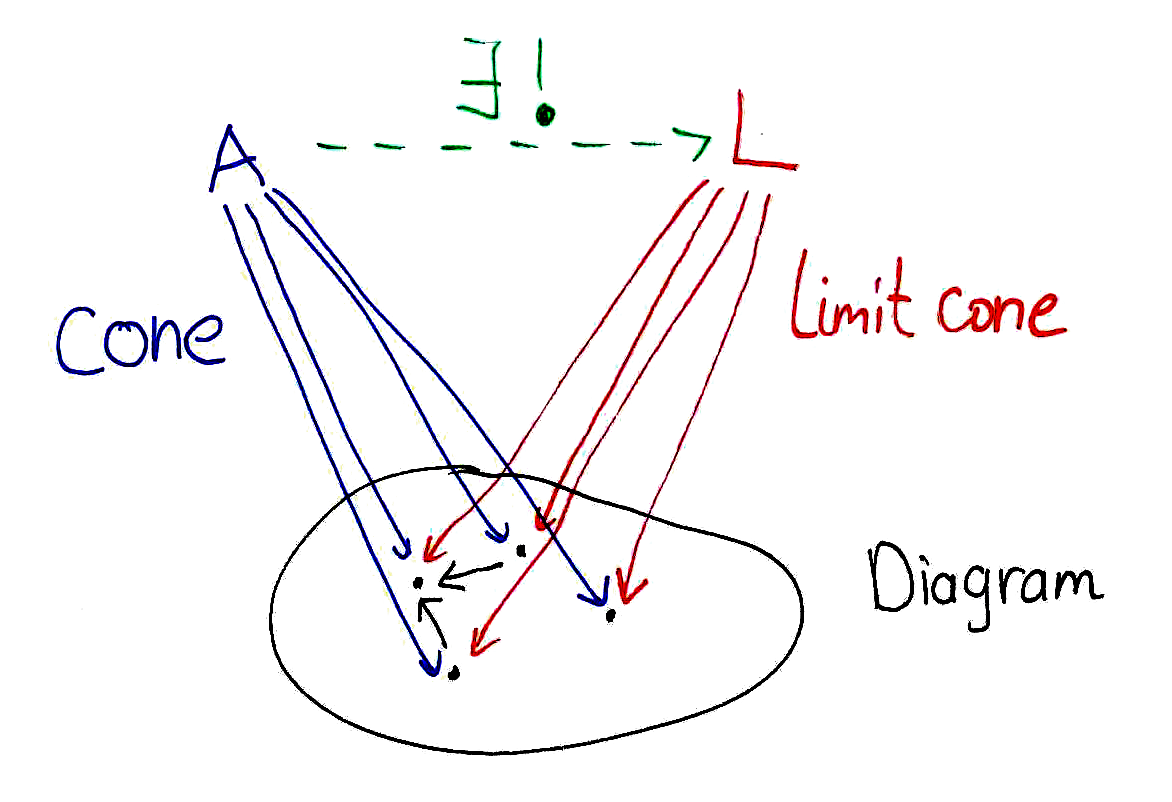
\includegraphics[scale=0.15]{figures/limits.png}
    \caption{Limit as the terminal cone over a diagram.}
    \label{fig:limits}
\end{figure}
    
\begin{example}
\begin{enumerate}
    \item $\calJ=\varnothing$ and $F$ is the empty functor into $\calC$. Then $\limit(F)$ is a terminal object in $\calC$ and $\colimit(F)$ is an initial object in $\calC$.
    \item $\calJ=(\bullet\quad\bullet)$ (discrete category with two objects). Then $\limit(F)=F(1)\times F(2)$ and $\colimit(F)=F(1)\sqcup F(2)$.
    \item $\calJ=(A\bullet\to \bullet_D\longleftarrow \bullet B)$, then $\limit(F)=A\times_D B$.
    \item $F(\calJ)=(A\bullet\to \bullet B)$, then $\limit(F)=A$ and $\colimit{F}=B$.
    \item $F(\calJ)=(A\bullet\toto[\alpha]{\beta}\bullet B)$. Then $\limit(F)=\mathrm{eq}(\alpha,\beta)=\{a\mid \alpha(a)=\beta(a)\}$ is the equalizer and $\colimit(F)=\mathrm{coeq}(\alpha,\beta)=B/(\alpha(a)\sim \beta(a))$ is the coequalizer.

\end{enumerate}
\end{example} 

\begin{defn}[Preservation of limits]
    A covariant functor $G:\calC \to\calD $ is said to preserve the limits of the functor $F:\calJ \to \calC $ if $\limit(G\circ F)=G \limit(F)$. Recall that a limit consists of an object and a set of morphisms from that object that make up the limit cone, so $G$ also acts on these morphisms. Preservation of colimits is defined analogously.

    $G$ is said to preserve all $\calJ$-shaped (co)limits if it preserves the (co)limits of all functors $F:\calJ\to \calC $. 

    Note that for contravariant functors the analogous concepts would be functors that take limits to colimits, or colimits to limits.
\end{defn}    
\begin{defn}[Continuous functors]\index{Continuous functor}
    A functor is called (co)continuous if it preserves all \emph{small (co)limits} (that is, $\calJ$-shaped (co)limits for all categories $\calJ$ such that $\mathrm{Ob}(\calJ)$ is a set and not a proper class).
\end{defn}
\begin{thm}[Continuity of hom-functors]
    Covariant hom-functors $h^A:B\mapsto\allowbreak \mathrm{Hom}_{\calC }(A,B)$ preserve all limits. Similarly, contravariant hom-functors take colimits to limits.
\end{thm}
\begin{rem}
     Note that the same is not generally true for colimits, -- e.g., $h^A(B\sqcup C)\neq h^A(B)\sqcup h^A(C)$ in $\mathsf{Set}$.
\end{rem}
\begin{cor}
    Combining the above theorem with Yoneda's Lemma~\ref{Yoneda}, we conclude that all representable covariant functors preserve all limits. Similarly, representable contravariant functors map all colimits to limits.
\end{cor}
\begin{thm}\label{thm diagonal functor adjoint to limit}
    Recall that $\calC ^\calJ $ is the category of $J$-shaped diagrams in $\calC $, i.e., covariant functors from $\calJ $ to $\calC $ (see Example~\ref{categories of diagrams}). Suppose that for each functor $F:\calJ \to\calC $ the limit $\limit F$ exists in $\calC $. Then the \emph{diagonal functor} which assigns to each object $A$ the \emph{constant diagram} $\underline A\in \calC ^\calJ $ (i.e., all objects of $\calJ $ are mapped to $A$ and all morphisms to $\mathrm{id}_A$),
    \[\Delta: \calC \to \calC ^{\calJ };\; A\mapsto \underline{A},\]
    is left adjoint to the limit functor
    \[\limit: \calC ^\calJ \to \calC ;\; F\mapsto \limit F\]
    (this functor forgets the morphisms associated with the limiting object).
\end{thm}
\begin{proof}
    For the bijection 
    \[
        \Hom_{\calC ^\calJ }(\underline{A},F)\cong \Hom_{\calC }(A,\limit F),\label{limit functor bijection}
    \]
    note that a natural transformation $\tau: \underline{A}\Longrightarrow F$ (which is what morphisms in $\calC ^\calJ $ are) with component morphisms $\tau_j:A\to F(j)$ ($j$ ranges over all objects in $\calJ $) corresponds to a unique morphism $\limit \tau: A\to \limit F$ in $\calC $. Conversely, a morphism $l:A\to \limit F$ determines a unique natural transformation $\tau:\underline{A}\Longrightarrow F$ such that $l=\limit \tau$, namely its components are $\tau_j=l\pi_j$ given the morphisms $\pi_j$ included in the definition of $\limit F$. It is easy to check that this bijection is natural in $A$.
\end{proof}
\begin{cor}\label{corollary on limits}
    The natural bijection \eqref{limit functor bijection} (with some object $L$ from $\calC $ instead of $\limit F$ to avoid confusion) holds for each object $A$ in $\calC $ iff the functor $F$ has a limit.
\end{cor}
\begin{proof}
    The existence of the limit is equivalent to the existence of a unique morphism $\limit \tau: A\to L$ for each natural transformation $\tau:\underline{A}\to F$.
\end{proof}
\begin{rem}
    Since a morphism (natural transformation) $\underline{A}\Longrightarrow F$ in the category $\calC ^\calJ $ is the same as a cone from $A$ to $F$, the limit $\limit F$ can be defined as the universal natural transformation $\Delta \Longrightarrow F$. Similarly, colimits are the universal natural transformations $F\Longrightarrow \Delta$.
\end{rem}
\begin{thm}[Continuity of adjoint functors]\label{continuity of adjoints thm}
    Every functor that has a left adjoint (and therefore is a right adjoint) is continuous. The dual statement is that every functor that has a right adjoint (and therefore is a left adjoint) is cocontinuous.
\end{thm}
\begin{proof}
    Let $R:\calC \to \calD $ be the right adjoint to $L:\calD \to\calC $. Suppose that $\limit F$ exists in $\calC $. For each object $A$ in $\calC $, a natural bijection
    \[\Hom_{\calC ^\calJ }(\underline{L(A)},F)\cong \Hom_{\calD ^\calJ }(\underline{A},R\circ F) \label{adjunction bijeciton}\]
    is provided by the natural adjunction bijection
    \[\Hom_{\calC }(L(A),F(j))\cong \Hom_{\calD }(A,R(F(j))\]
    for each object $j$ in $\calJ $, sending the component $h_j$ of an element of the l.h.s.~of \eqref{adjunction bijeciton} to the corresponding component of the natural transformation on the right. Now consider the string of natural bijections
    \begin{multline}
        \Hom_{\calD ^\calJ }(\underline{A},R\circ F)\cong \Hom_{\calC ^\calJ }(\underline{L(A)},F)\cong \\ 
        \cong \Hom_{\calC }(L(A),\limit F)\cong \Hom_{\calD }(A,R(\limit F))
    \end{multline}
    coming respectively from \eqref{adjunction bijeciton}, \eqref{limit functor bijection}, and the adjunction. By Corollary~\ref{corollary on limits} combined with the uniqueness of adjoints (Proposition~\ref{uniqueness of adjoints prop}), we have $\limit(R\circ F)= R(\limit F)$ as required.
    % Let $G:\calD \to\calC $ be a left adjoint, i.e., $G^\ast$ exists. Then for a colimit $\colimit(F)$ of $F:\calJ \to \calD $, by continuity of hom-functors, we have
    % \begin{multline}
    %     \Hom_{\calC }(G\colimit F,B)\cong \Hom_{\calD }(\colimit F,G^\ast(B))\cong \limit \Hom_{\calD }(F,G^\ast(B)) \cong \\\cong \limit \Hom_{\calC }(G\circ F,B)\cong \mathrm{Cocones}(G\circ F,B),
    % \end{multline}
    % and these bijections are natural in $B$. However, the existence of a natural bijection with the set of cones from $G\circ F$ is exactly the characteristic property of a colimit (see definition).
\end{proof}
\begin{cor}
    Limits commute with limits (assuming all limits of the necessary shapes exist). Colimits commute with colimits.
\end{cor}
\begin{proof}
    Viewing the limit is a functor  $\limit:\calC^\calJ\to \calC$, we have just shown that it is right adjoint to the diagonal functor (a.k.a.~the constant diagram functor). Therefore it is continuous, i.e., commutes with limits. 
\end{proof}

Note that limits and colimits typically do not commute.

\begin{example}[Seifert-van Kampen theorem redux]\index{Theorem!Seifert-van~Kampen}
    We've learned by now that contravariant representable (or hom-) functors map colimits to limits, so they're not the functors that preserve colimits. It is the left adjoints that do. Seifert-van~Kampen theorem essentially states that the fundamental functors $\pi_1$ or $\Pi$ preserve \emph{some} colimits (namely pushouts). 
    
    While not a proof, one categorical source of intuition for this is that both of these functors are left adjoints. The reason $\pi_1$ preserves only pushouts, and not all colimits, is that the functor that maps the category $\mathsf{Top}$ into the homotopy category $\mathsf{hTop}$ doesn't preserve colimits, so $\pi_1$ doesn't either. However, the descended version of this functor, $\pi_1:\mathsf{hTop}\to \mathsf{Gr}$ happens to be the left adjoint of a certain functor that constructs a topological space given a group. Looking far ahead, this is the functor $\rmB:G\mapsto \rmB G$ that constructs the classifying space of $G$. It is so called because $\rmB G$ is the base space of a universal principal $G$-bundle such that any other $G$-bundle is a pullback along some continuous map into $\rmB G$. For example, universal covering spaces are exactly the classifying spaces for the fundamental groups of their base, -- e.g., $B\bbZ=\bbS^1$ and $\rmB(\bbZ\ast \bbZ)=\bbS^1\vee \bbS^1$ etc. $\rmB G$ is in fact the unique (up to ``weak'' homotopy equivalence) space whose fundamental group is $G$ and all other homotopy groups are trivial (which also identifies it with the first  Eilenberg-MacLane space $\rmK(G,1)$).

    So, by a happy coincidence, pushouts in the homotopy category lined up with pushouts in the original topological category.
\end{example}

The most common examples of infinite limits and colimits are ones where $\calJ $ can be indexed by integers.

\begin{defn}[Directed colimits, codirected limits]\index{Inverse limit!see {Codirected limit}}\index{Direct limit!see {Directed colimit}}\index{Directed colimit}\index{Directed colimit}
    If $\calJ$ is a directed system (cf.\ Definition~\ref{def directed system}) and $F:\calJ\to \calC$ a functor, then $\colimit(F)$ is called a directed colimit (historically \emph{direct limit}, or \emph{inductive limit}). \index{Inductive limit!see {Directed colimit}} It is also often written as $\colimit A_j$, where $A_j=F(j)$. \index{Inductive limit!see {Directed colimit}}
    
    If $\calJ$ is a \emph{codirected system} \index{Codirected system} (i.e., $\calJ^{\mathrm{op}}$ is a directed system), then $\limit(F)$ is called a codirected limit (historically \emph{inverse limit}, or \emph{projective limit}). \index{Projective limit!see {Codirected limit}}
    
    More generally, if $\calJ$ is a poset category (see Example~\ref{poset example}), then it is said to be directed to the right (left) if $\forall i,j\in \ob(\calJ)$ $\exists k\in \ob(\calJ)$ such that $i,j\leq k$ (respectively, $k\leq i,j$). Then one can define directed colimits of diagrams directed to the right and codirected limits of diagrams directed to the left.
\end{defn}


\begin{example}
\begin{enumerate}
    \item In $\colimit$, most commonly all arrows are monomorphisms. For example, consider the category $\mathsf{Gr}$ of groups and the sequence $\rmS_n$ of symmetric groups with the embeddings $\rmS_n\hookrightarrow \rmS_m$ for every $n<m$ defined as permutations of the first $n$ symbols. Then $\colimit(\rmS_n)=\rmS_\infty$, which is the group of all permutations of $\mathbb{N}$ of finite support.
    
    Alternatively, we can define another partial order on the set of symmetric groups $\rmS_n$. Namely, define $n\preccurlyeq m\Leftrightarrow n\mid m$ and the inclusion $\rmS_n\hookrightarrow \rmS_m$ by $m/n$ copies of the permutation. Then $\colimit (\rmS_n)$ is a different group.
    \item For any unital ring $R$, the directed colimit of the general linear matrix groups over $R$ (where matrices of size $n$ are embedded into groups of larger matrices by filling in the diagonal with ones) is $\colimit(\GL(n,R))=\GL(R)$, the \emph{quite general linear group} of $R$.
    \item In $\mathsf{Set}$, directed colimits are simply infinite unions factored by identifying elements with coincident ``descendants'', i.e. $\colimit A_i=\bigsqcup_i A_i/\sim$, where $x\in A_i$ is equivalent to $y\in A_j$ iff $\exists f_{jk},f_{jk}$ such that $f_{ik}(x)=f_{jk}(y)$. The codirected limit is the set of infinite sequences of descendants $\limit (A_i)=\{(a_i)\mid a_i\in A_i,\forall i\leq j, f_{ij}(a_i)=a_j\}$.
    \item Consider the polynomial ring $K[t]$ over a field $K$ and its factor rings $K[t]/t^n$ of truncated polynomials. Then we have the sequence of epimorphisms 
    \[\cdots \to K[t]/t^3\to K[t]/t^2\to K,\]
    and the codirected limit is $\limit(K[t]/t^n)=K[[t]]$, which is the ring of \emph{all} formal power series $\sum_{i\geq 0}a_i t^i$. This illustrates the more general fact that projective limits are generally enormous, so much so that the cardinality of the limit is often higher than of any object in the sequence.
    \item Let $p$ be a prime integer and consider the sequence of groups
    \[\cdots\to \bbZ/p^3 \bbZ\overset{\mod p^2}\to \bbZ/p^2\bbZ\overset{\mod p}\to \bbZ/p\bbZ.\]
    Then $\limit(\bbZ/p^n\bbZ)=\bbZ_p$ is the group of $p$-adic integers (it has the cardinality of continuum!).
    \item Consider the poset diagram directed to the left consisting of group epimorphisms $\bbZ/m\bbZ\overset{\mod n}\to \bbZ/n\bbZ$ for $n\mid m$. Then 
    $\limit (\bbZ/n\bbZ)=\hat{\bbZ}$ is the \emph{profinite completion of $\bbZ$}.
    \item The monomorphism sequence $\bbZ/p^n\bbZ\overset{\cdot p}\to \bbZ/p^{n+1}\bbZ$ gives the directed colimit $\colimit(\mathbb{Z}/p^n\bbZ)\allowbreak=\bbZ(p^\infty)$, which is called a Pr\"ufer group (it can be realized as the group of all roots of unity of the form $\exp(2\pi\rmi \cdot m/p^n)$).
    \item In topological and geometric categories, directed colimits are similar to unions (when they exist). For instance, the $n$-sphere can be embedded $\bbS^n\hookrightarrow \bbS^{n+1}$ as the equator, and the directed colimit gives $\bbS^\infty=\colimit \bbS^n$.
\end{enumerate}
\end{example}





\section{Sub-objects and quotient objects}

\begin{defn}
    Let $X,U,V\in\ob(\calC)$ and consider a diagram
    \[\begin{tikzcd}[every matrix/.append style={name=m},   
        execute at end picture={\draw [<-] ([xshift=-2mm,yshift=-12mm]m-1-2.north) arc[start angle=-90,delta angle=-270,radius=0.25cm];}]
        U \arrow[dr,tail,"u\text{, mono}"]& \\
        & X\\
        V\arrow[uu,tail,dashed,"\exists h"]\arrow[ur,tail,swap,"v\text{, mono}"]& 
\end{tikzcd}\]
    We say that $v\leq u$ if there exists a morphism $h$ such that $v=u\circ h$ ($h$ has to be a monomorphism for this to hold).
\end{defn}

Here are the properties of this relation:
\begin{enumerate}
    \item $u\leq u$;
    \item $u\leq v,v\leq w\implies u\leq w$;
    \item $u\leq v,v\leq u\implies U\overset{f}{\cong} V$, where $u=v\circ f$ and $v=u\circ f^{-1}$.
    \begin{proof}
        We have $V\overset{h}{\to}U$ and $U\overset{g}{\to}V$.
        
        On the one hand, $v=u\circ h=v\circ g\circ h\implies g\circ h=1_V$ since $v$ is mono.
        
        On the other hand, $u=u\circ(h\circ g)\implies h\circ g=1_U$ since $u$ is mono.
    \end{proof}
\end{enumerate}

\begin{defn}[Sub-objects]\index{Sub-object}
    Introduce an equivalence relation on monomorphisms: $u\sim v$ iff $u\leq v$ and $v\leq u$. Then a sub-object of $X$ is an equivalence class of pairs $(U,u)$, where $u:U\to X$ is a mono.
\end{defn}

\begin{example}
    $\bbZ\overset{\cdot n}\to \bbZ$ is mono and defines the group $n\bbZ$ as a sub-object of $\bbZ$.
\end{example}

\begin{defn}[Quotient objects]\index{Quotient object}
    For epimorphisms, we define the relation $y\geq z$ if in the diagram 
    \[\begin{tikzcd}[every matrix/.append style={name=m},   
        execute at end picture={\draw [<-] ([xshift=-6mm,yshift=-5mm]m-2-2.north) arc[start angle=-90,delta angle=-270,radius=0.25cm];}]
        & Y \arrow[dd,two heads,dashed,"\exists h"] \\
        X\arrow[dr,two heads,swap,"z\text{, epi}"]\arrow[ur,two heads,"y\text{, epi}"] &\\
        & Z 
    \end{tikzcd}\]
    there exists such a morphism $h$ that $z=h\circ y$ (it has to be epi).
    Then a quotient object of $X$ is an equivalence class of pairs $(Y,y)$, where $y:X\to Y$ is epi.
\end{defn}

\begin{example}
    There are many different epimorphisms $\bbZ^2\to\bbZ$. They define many non-equivalent quotient objects of $\bbZ^2$, each isomorphic to $\bbZ$.
\end{example}



\section{Abelian categories}

Abelian categories are, roughly speaking, categories where objects and morphisms form abelian groups themselves, and where the First Isomorphism Theorem holds. Examples include $\mathsf{Ab}$, $\mathsf{Vect}_K$, $R-\mathsf{Mod}$ or $\mathsf{Mod}-R$, $\mathsf{SheafAb}$. Notably, $\mathsf{TopAb}$ is not abelian because the First Isomorphism Theorem generally doesn't hold for topological groups (instead, this category is \emph{pre-abelian}).

\begin{defn}[Abelian categories]\index{Abelian category}
    A category $\calC$ is called abelian if:
    \begin{enumerate}
        \item Every morphism set $\mor(A,B)$ has the structure of an abelian group, i.e. morphisms can be added and subtracted.
        \item There exists a zero object $0\in\ob(\calC)$.
        \item The product and coproduct of any two objects exist and are isomorphic. The result is denoted by the direct sum: $A\times B\cong A\sqcup B \equiv A\oplus B$.
        \item All equalizers and coequalizers exist. In particular, using the abelian property, we define
        \[\ker (\varphi)\coloneqq\mathrm{eq}(\varphi,0),\quad \coker(\varphi)\coloneqq\mathrm{coeq}(\varphi,0).\]
        \item The image and coimage of any morphism coincide, $\im (\varphi)=\coim(\varphi)$. These will be defined below.
    \end{enumerate}
\end{defn}

We can give alternative definition of kernels and cokernels.
\begin{defn}[Kernel]\index{Kernel}
    Let $X\overset\varphi\to Y$ be a morphism in an abelian category. Then $\ker\varphi$ is the sub-object $(K,k)$ of $X$ such that $\varphi\circ k=0$ and it is universal with this property:
    \[\begin{tikzcd}[every matrix/.append style={name=m},   
        execute at end picture={\draw [<-] ([xshift=-10mm,yshift=-8mm]m-1-2.north) arc[start angle=-90,delta angle=-270,radius=0.15cm];}]
        K \arrow[r,tail,"k"]& X\arrow[r,"\varphi"] & Y\\
        Z\arrow[u,dashed,"\exists! h"]\arrow[ur,swap,"\forall\psi:\,\varphi\circ\psi=0"]& & 
    \end{tikzcd}\]
    (such a $h$ is automatically unique for every $\psi$ because $k$ is mono).
\end{defn}

\begin{defn}[Cokernel]\index{Cokernel}
    Let $X\overset\varphi\to Y$ be a morphism in an abelian category. Then $\coker\varphi$ is the quotient object $(C,c)$ of $Y$ such that $c\circ\varphi=0$ and it is universal with this property:
    \[\begin{tikzcd}[every matrix/.append style={name=m},   
        execute at end picture={\draw [<-] ([xshift=-4mm,yshift=-8mm]m-1-3.north) arc[start angle=-90,delta angle=-270,radius=0.15cm];}]
        X\arrow[r,"\varphi"] & Y \arrow[r,two heads,"c"]\arrow[dr,swap,"\forall\psi:\,\psi\circ\varphi=0"]  & C\arrow[d,dashed,"\exists! h"] \\
        & & Z
    \end{tikzcd}\]
    (such a $h$ is automatically unique for every $\psi$ because $c$ is epi).
\end{defn}

\begin{example}
    It is easy to check that in the category $\mathsf{Ab}$ of abelian groups, $\coker\varphi=H/\varphi(G)$ for $\varphi:G\to H$. Thus the last axiom of abelian categories is equivalent to the First Isomorphism Theorem in this case. Note that this factor doesn't exist neither in $\mathsf{Gr}$ nor in $\mathsf{TopAb}$.
    
    The same formula holds for all ring modules. In $\mathsf{Gr}$ (which is not an abelian category, but in which kernels and cokernels can be similarly defined), the cokernel is the quotient by the normal closure of the image.
\end{example}

This allows us to define images and coimages.

\begin{defn}[Image, coimage]\index{Image of a morphism}\index{Coimage of a morphism}
    In abelian categories, $\im\varphi$ for a morphism $\varphi:X\to Y$ is the sub-object of $Y$ defined as
    \[\im(\varphi)=\ker(\coker\varphi),\quad\quad K\overset k \rightarrowtail X\overset\varphi\to Y\overset c\twoheadrightarrow C.\]
    Similarly, $\coim\varphi$ is the quotient object of $X$ defined as 
    \[\coim(\varphi)=\coker(\ker\varphi).\]
\end{defn}

Note that
\[\ker(\coim\varphi)=\ker(\coker(\ker\varphi)))=\im(\ker\varphi).\]
Thus in general pre-abelian categories (i.e., without the last axiom) by the universal properties of images and coimages we have a factorization of any morphism $\varphi:X\to Y$ into the sequence
\[\ker\varphi\rightarrowtail X\underbrace{\overset{\text{epi}}\twoheadrightarrow\coim\varphi\overset{\text{bi}}\to\im\varphi\overset{\text{mono}}\rightarrowtail}_\varphi Y\twoheadrightarrow\coker\varphi \]
The last axiom of abelian categories states that $\coim\varphi = \im\varphi$, which is equivalent to the statement:
\[\boxed{\text{5. All bimorphisms are isomorphisms.}}\]
\begin{xca}
    Prove that the last axiom of abelian categories is indeed equivalent to the boxed statement.
\end{xca}
Therefore in abelian categories we have the shortened decomposition
\[\ker\varphi\rightarrowtail X \overset{j}\twoheadrightarrow\im\varphi\overset{i}\rightarrowtail Y\twoheadrightarrow \coker\varphi,\]
where
\[\text{factorization property}:\quad \varphi=i\circ j,\quad i\text{ -- mono}, j\text{ -- epi}.\]

\begin{defn}[Additive functor]\index{Additive functor}
    A functor $F:\calC\to\calD$ between two abelian categories is called additive if for any $A,B\in\ob(\calC)$, the map $F_{A,B}:\Hom_\calC(A,B)\to \Hom_\calD(F(A),F(B))$ defined by $\varphi\mapsto F_{A,B}(\varphi)=F(\varphi)$ is a homomorphism of abelian groups.
\end{defn}

The following theorem is the main general result about abelian categories and effectively states that all abelian categories can be realized as (almost arbitrarily nice) full subcategories of categories of ring modules. It is essentially a much stronger version of the Yoneda Lemma~\ref{Yoneda} for abelian categories.

\begin{thm}[Freyd-Mitchell]\label{Theorem!Freyd-Mitchell}
    For any abelian category $\calC$ there exists a ring $R$ and a functor $F:\calC\to R\text{-}\mathsf{Mod}$ that is: additive, full and faithful (surjective and injective on sets of morphisms for each pair of objects), preserves kernels, cokernels, products and coproducts, is exact (preserves exact sequences, see below)...
\end{thm}
The ellipsis indicates that one can keep requiring various extra properties of the functor without violating the theorem. This theorem justifies all diagrammatic methods that we will develop in the next two sections: since $R\text{-}\mathsf{Mod}$ is a concrete category, its objects are sets. Therefore, by the Freyd-Mitchell theorem, it suffices to prove any general statement about abelian categories only for categories of ring modules, which allows us to refer to \emph{elements} of objects as sets, and apply morphisms as \emph{functions} to those elements! It is a way to completely side-step so called ``abstract nonsense'' proofs that deliberately avoid talking about elements of objects as if they are sets.






\clearpage
\chapter{Homological Algebra I: Exactness}

\section{Exact sequences and functors}

From now on in this \partt\ we work only with abelian categories. In fact, homological algebra can be viewed as the extension of linear algebra to all abelian categories (most importantly, ring modules). As we have already seen, it arises inevitably in geometric problems, where the spaces of functions, differential forms, etc., form modules over the ring of smooth functions, and so the classic tools of the linear algebra of fields and vector spaces do not suffice.

\begin{defn}[Exact sequences]\index{Exact sequence}
    A sequence of morphisms in an abelian category 
    \[\cdots \to A_{i-1}\overset{\alpha}\to A_i\overset{\beta}\to A_{i+1}\to \cdots\]
    is called exact in $A_i$ if 
    \[\im\alpha=\ker\beta.\]
    A sequence is just called exact if it is exact in every object in it.
\end{defn}

\begin{prop}
    \begin{enumerate}
        \item A sequence $0\to A\overset f\to B$ is exact iff $f$ is mono;
        \item A sequence $A\overset f\to B\to 0$ is exact iff $f$ is epi;
        \item A sequence $0\to A\overset f\to B\to 0$ is exact iff $f$ is an isomorphism;
        \item A sequence $0\to A\to B\overset f\to C\to D\to 0$ is exact iff $A=\ker f$ and $D=\coker f$.
    \end{enumerate}
\end{prop}
\begin{proof}
    Exercise.
\end{proof}

\begin{defn}[Short exact sequences]\index{Exact sequence!short}
 A short exact sequence is an exact sequence of the form
 \[0\to A\overset f\rightarrowtail B\overset g \twoheadrightarrow C\to 0.\]
 Such a sequence (and the object $B$ in particular) is also called an \emph{extension} of $A$ by $C$. The exactness of this sequence is equivalent to $f$ being mono, $g$ being epi, and $\im f=\ker g$.
\end{defn}

\begin{prop}[First isomorphism Theorem]
    If $0\to A\overset f\to B\overset g \to C\to 0$ is a short exact sequence, then 
    \[A\cong \im f,\quad C\cong B/\im f.\]
\end{prop}
\begin{proof}
    The first isomorphism is known in concrete categories, which is sufficient by the Freyd-Mitchell Theorem. It states that $B/\ker g\cong \im g$, and by exactness $\ker g=\im f$ and $\im g=C$, thus $B/\im f\cong C$.
\end{proof}

\begin{defn}[Split sequence]\index{Split sequence}
    A short exact sequence $0\to A\overset i\to B\overset p \to C\to 0$ is called split if there exists a morphism $j:C\to B$ with $p\circ j=1_C$, i.e. if $p$ is a split epi.
\end{defn}

\begin{prop}[Rank-nullity theorem]\index{Theorem!Rank-nullity}
    If a short exact sequence $0\to A\overset i\to B\overset p \to C\to 0$ is split, then $B\cong A\oplus C$.
\end{prop}
\begin{proof}
    We show that $B\cong \im i\oplus \im j$, where $j$ is a section for $p$. We perform a simple \emph{diagram chasing} by considering an element $b\in B$:
    \begin{multline}
        b\in B\implies p(b-j\circ p(b))=p(b)-\underbrace{p\circ j}_{1_C}(p(b))=\\=0\implies b-j\circ p(b)\in\ker p\overset{\text{exact}}{\implies}\exists a\in A: i(a)=b-j\circ p(b).
    \end{multline}
    This proves that $B=\im i+\im j$. To prove that $\im i\cap \im j=\{0\}$, suppose $x=i(a)=j(c)$. Then $p(x)=p(i(a))=0$ since $p\circ i=0$, and at the same time $p(x)=p(j(c))=c$ since $p\circ j=1_C$. Thus $c=0$, $x=j(c)=0$, and $B\cong A\oplus C$.
\end{proof}

\begin{prop}[Rank-nullity for vector spaces]\label{gen rank-nullity}
    If $0\to A_1\overset{f_1}\to A_2 \overset{f_2}\to\cdots A_n\to 0$ is an exact sequence of finite-dimensional vector spaces, then
    \[\sum_{i=1}^n(-1)^i \dim A_i=0.\]
\end{prop}
\begin{proof}
    By the standard rank-nullity theorem, the l.h.s.\ equals \[\sum_{i=1}^{n-1}(-1)^i\dim \ker f_i+\sum_{i=1}^{n-1}(-1)^i\dim \im f_i.\] By exactness, this sum vanishes.
\end{proof}


\begin{defn}[Exact functors]\index{Exact functor}
    A functor $F:\calC\to\calD$ is called exact if it maps every exact sequence into an exact sequence.
\end{defn}

\begin{prop}
    For an additive functor $F$ to be exact it suffices to be exact on short sequences.
\end{prop}
\begin{proof}
    The idea of the proof is to expand any segment of an exact sequence $A\to B\to C$ into a combination of short exact sequences (this method is generally called ``splicing'' of short sequences). \index{Splicing (of short sequences)} Namely, we have the following \emph{commutative} diagram with exact diagonals:
    \[\adjustbox{scale=0.8,center}{\begin{tikzcd}
        0 \arrow[dr]& & & & 0 \arrow[dr]& & 0 & & \\ 
        & \ker f \arrow[dr]&&&& \im g \arrow[dr]\arrow[ur]&&&\\
        && A \arrow[rr,"f"]\arrow[dr]&& B \arrow[rr,"g"]\arrow[ur] && C \arrow[dr] &&\\
        &&& \im f\arrow[dr]\arrow[ur] &&&& \coker g\arrow[dr]&\\
        && 0 \arrow[ur] && 0 &&&& 0
    \end{tikzcd}}\]
    Applying $F$, we get the \emph{commutative} diagram
    \[\adjustbox{scale=0.8,center}{\begin{tikzcd}[row sep=normal, column sep = small]
        0 \arrow[dr]& & & & 0 \arrow[dr]& & 0 & & \\ 
        & F(\ker f) \arrow[dr]&&&& F(\im g) \arrow[dr]\arrow[ur]&&&\\
        && F(A) \arrow[rr,"F(f)"]\arrow[dr]&& F(B) \arrow[rr,"F(g)"]\arrow[ur] && F(C) \arrow[dr] &&\\
        &&& F(\im f)\arrow[dr]\arrow[ur] &&&& F(\coker g)\arrow[dr]&\\
        && 0 \arrow[ur] && 0 &&&& 0
    \end{tikzcd}}\]
    with exact diagonals. Now we notice
    \begin{multline}
        \im F(f)=\im\left(F(A)\to F(\im f)\to F(B)\right)=\im(F(\im f)\to F(B))=\\
        =\ker (F(B)\to F(\im g))=\ker (F(B)\to F(\im g)\to F(C))=\ker F(g),
    \end{multline}
    where the second equality follows from $F(A)\to F(\im f)$ being epi and the next to last equality holds since $F(\im g)\to F(C)$ is mono. Therefore $F(A)\to F(B)\to F(C)$ is exact.
\end{proof}

There are in fact very few exact functors. Here are a few relevant examples.

\begin{example}
    \begin{enumerate}
        \item Let $G\text{-}\mathsf{Ab}$ be the category of abelian groups with a $G$-action (morphisms in it are equivariant homomorphisms $f(g\cdot a)=g\cdot f(a)$). Then we can define the functor that for every group $A$ with a $G$-action produces its subgroup of invariants $A^G$:
        \[A^G=\{a\in A\mid \forall g\in G,\; g\cdot a=a\}.\]
        (The action on morphisms is trivial.) This is a functor $G\text{-}\mathsf{Ab}\to\mathsf{Ab}$. Now let us consider a short exact sequence
        \[0\to A\to B\to B/A\to 0.\]
        Its image is clearly not exact on the right:
        \[0\to A^G\to B^G\to (B/A)^G \cancel{\to} 0.\]
        Indeed, $(B/A)^G$ are $G$-invariant only up to addition of elements of $A$, whereas $B^G/A^G$ (which is what we would have in a short exact sequence) is a totally different group consisting of classes of truly $G$-invariant elements. We say that this functor is only \emph{left exact}.
        \item The representable (hom-)functors $\Hom_{R\text{-}\mathsf{Mod}}(\_,\_)$ acting $R\text{-}\mathsf{Mod}\times R\text{-}\mathsf{Mod}\to \mathsf{Ab}$ with either argument fixed can act on a short exact sequence 
        \[0\to A\to B\to C\to 0\]
        to give two exact sequences
        \begin{eqnarray}
            0\to \Hom(X,A)\to \Hom(X,B)\to \Hom(X,C),\\
            0\to \Hom(C,Y)\to \Hom(B,Y)\to \Hom(A,Y).
        \end{eqnarray}
        Therefore Hom-functors are also only left exact. Indeed, right exactness for them would mean that every morphism $X\to C$ or $A\to Y$ can be factored through $B$, which we know to be false. For example, consider
        \[\begin{tikzcd}
        0\arrow[r]& A=\bbZ\arrow[r,"\text{incl.}"]\arrow[d,
        "\id"]& B=\frac{1}{n}\bbZ\arrow[dl,dashed,"?"] \\
         &Y=\bbZ &
        \end{tikzcd}\]
        For right exactness, $\id:A\to Y$ would need to factor through $B$, which is clearly impossible here.
        
        An analogous example for the first line is
        \[\begin{tikzcd}
        B=\bbZ\arrow[r,"\mod n"] & C=\bbZ/n\bbZ\arrow[r] & 0 \\
         &X=\bbZ/n\bbZ\arrow[ul,dashed,"?"]\arrow[u,
        "\id"] &
        \end{tikzcd}\]
        If this functor were to be surjective on Hom-sets, every map $X\to C$ would have to come from a map $X\to B$, which is clearly false in this case.
        \item The tensor product functor $\_\otimes\_:\mathsf{Mod}\text{-}R\times R\text{-}\mathsf{Mod}\to \mathsf{Ab}$ is also not exact. In fact it is only \emph{right exact}: for every short exact sequence
        \[0\to A\to B\to C\to 0\]
        it gives two exact sequences (in fact they are the same because $X\otimes Y$ is naturally isomorphic to $Y\otimes X$)
        \begin{eqnarray} 
        X\otimes A\to X\otimes B\to X\otimes C\to 0,\\
        A\otimes Y\to B\otimes Y\to C\otimes Y\to 0.
        \end{eqnarray}
        We will give an example that shows that this functor is not left exact in Example~\ref{non-flat module example}.
    \end{enumerate}
\end{example}


\begin{defn}[Projective and injective objects]\index{Projective object}\index{Injective object}
    If the functor $\Hom(X,\_)$ is exact, $X$ is called a projective object (i.e., all morphisms $X\to C$ factor through $B$ in any exact sequence $B\to C\to 0$). If $\Hom(\_,Y)$ is exact, $Y$ is called an injective object (all morphisms $A\to Y$ factor through $B$ in any exact sequence $0\to A\to B$).
\end{defn}

\begin{defn}[Flat module]\index{Flat module}
    An object $X$ is called \emph{flat} if the functor $X\otimes\_$ (or equivalently $\_\otimes X$) is left exact.
\end{defn}

\begin{example}\label{non-flat module example}
    Consider in the category of $\bbZ$-modules the sequence on the left and its image under a tensor product with $\bbZ/n\bbZ$
    \[0\to \bbZ\overset{\cdot n}\to \bbZ \quad \overset{\otimes\bbZ/n\bbZ}\rightsquigarrow \quad \bbZ\otimes \bbZ/n\bbZ\overset{\cdot n}\to\bbZ\otimes \bbZ/n\bbZ.\]
    The arrow on the right is obviously not mono (it is the zero morphism), therefore $\bbZ/n\bbZ$ is not a flat $\bbZ$-module.
\end{example}

The moral of these examples is that whereas in categories of vector spaces $\mathsf{Vect}_K$ everything would be exact, exactness is generically broken as soon as we pass to structures over rings. The study of ring modules is a natural extension of linear (matrix) algebra over fields, and largely reduces to homological algebra.
\[
    \boxed{\begin{array}{c}
    \text{The goal of homological algebra is:}\\
    \text{to characterize the obstructions to the exactness of certain additive functors}\\ \text{(these obstructions are called derived functors).}
    \end{array}}
\]
Given a non-exact functor, the values of its derived functors need to be added into the image of a short exact sequence to produce a fully exact (albeit potentially infinitely long) sequence. For example, in the case of the invariants functor, every short exact sequence $0\to A\to B\to B/A\to 0$ becomes a \emph{long exact sequence of group cohomology} \index{Long exact sequence!of group cohomology}
\[
    \scriptstyle
    0\to A^G\to B^G\to (B/A)^G\to \rmH^1(G,A)\to \rmH^1(G,B)\to \rmH^1(G,B/A)\to \rmH^2(G,A)\to\cdots
\]
For the Hom functor, the obstruction to right exactness is evaluated by the Ext-functors (the name comes from ``extension''):
\begin{gather}
    \scriptstyle
    0\to \Hom(X,A)\to \Hom(X,B)\to\Hom(X,C)\to \Ext^1(X,A)\to \Ext^1(X,B)\to\Ext^1(X,C)\to\cdots,\\
    \scriptstyle
    0\to \Hom(C,Y)\to \Hom(B,Y)\to\Hom(A,Y)\to \Ext^1(C,Y)\to \Ext^1(B,Y)\to\Ext^1(A,Y)\to\cdots
\end{gather}
Finally, for the tensor functor, the obstruction to left exactness is evaluated by the Tor-functors (``torsion''):
\[
    \scriptstyle
    \cdots\to \Tor_2(C,X)\to \Tor_1(A,X)\to \Tor_1(B,X)\to\Tor_1(C,X)\to A\otimes X\to B\otimes X\to C\otimes X\to 0.
\]
All of them are examples of (co)homology theories. We will return to a proper discussion of these objects later. The takeaway so far should be: since on manifolds we are studying spaces of sections of vector bundles, which are really $C^\infty(M)$-modules, we need homological algebra to deal with the linear algebra over the ring of functions, and the (co)homology groups will measure the non-exactness of certain constructions.






\section{Directed colimits and exactness}

\begin{defn}[Complete category]\index{Complete category}
    A category $\calC$ is called complete if all limits in $\calC$ with a small index category (i.e., $\ob(\calJ)$ is a proper set and not a class) exist. $\calC$ is called cocomplete if all small colimits in $\calC$ exist.
\end{defn}

\begin{prop}[{{\cite[Prop.~5.23]{Rotman}}}]\label{prop abelian complete and cocomplete}
    Abelian categories are complete and cocomplete.
\end{prop}
\begin{proof}
    By the Freyd-Mitchell Theorem, it suffices to consider the categories of $R$-modules. 
    
    Given a $J$-shaped diagram $\{F(i)=A_i,f_{ji}=F(i\to j)\}$ of modules, let $\lambda_i$ be the natural inclusion of $A_i$ into $\bigoplus_i A_i$. 
    
    First we construct the colimit module. Define
    \[D=\left(\bigoplus_i A_i\right)\slash S,\]
    where $S$ is the submodule generated by all elements $\lambda_j\circ f_{ji}(a_i)-\lambda_i(a_i)$ with $a_i\in A_i$ and $i\to j$ an arrow in $\calJ$. The maps $\lambda_i$ induce inclusions $\alpha_i: A_i\to D$ by $a_i\mapsto \lambda_a(a_i)+S$. It is an exercise to check that $D$ satisfies the universal property, so that $D\cong \colimit F$.

    Similarly, the limit module can be constructed as the submodule of $\bigoplus_i A_i$ consisting of tuples $\{a_i\}_{i}$ such that if $i\to j$ is an arrow in $\calJ$ then $a_j=f_{ji}(a_i)$. It is easy to check that this module satisfies the universal property for $\limit F$.
\end{proof}
\begin{rem}
    More generally, a category is complete iff all products of any number of objects exist and all equalizers exist, and cocomplete iff all coproducts and all coequalizers exist. In abelian categories both products and coproducts are direct sums and obviously exist, whereas equalizers are $\ker(f-g)$ and coequalizers are $\coker(f-g)$.
\end{rem}

In abelian categories, kernels are limits (namely equalizers), and cokernels are colimits. Therefore exactness can be rephrased in terms of preservation of kernels and cokernels. The following proposition is obvious.

\begin{prop}[{{\cite[Prop.~5.25]{Rotman}}}]
    Let $F$ be a covariant functor between abelian categories. Then $F$ preserves kernels iff it is left exact, and it preserves cokernels iff it is right exact.
\end{prop}

\begin{prop}
    In an abelian category $\calC$, the colimit functor $\colimit$ is right exact. That is, if $J$ is small ($\ob(\calJ)$ is a proper set) and $F,G,H:\calJ\to \calC$ are functors with natural transformations $F\overset{\alpha}{\Longrightarrow}G\overset{\beta}{\Longrightarrow}H$ such that the sequence 
    \[0\to F(i)\overset{\alpha_i}{\to} G(i)\overset{\beta_i}{\to} H(i)\to 0\] is exact for all $i\in\ob(\calJ)$, then the sequence
    \[\colimit F\overset{\colimit \alpha_i}{\to}\colimit G\overset{\colimit \beta_i}{\to}\colimit H\to 0\]
    is exact. Similarly, the limit functor $\limit$ is left exact.
\end{prop}
\begin{proof}
    We make use of the fact that $\colimit F$ can be constructed concretely as the quotient of $\bigoplus_i F_i$ by all $a_i-F(i\to j)(a_i)$ where $i\to j$ is any arrow coming out of $i$ in $\calJ$, $a_i\in F_i$, and $F(i\to j)(a_i)\in F_j$ are identified with their images in $\bigoplus F_i$.

    With this description, clearly the map $\colimit G(i)\to \colimit H(i)$ is surjective. Also, composing $\colimit F(i)\to \colimit G(i)\to\colimit H(i)$ is the zero map thus $\im(\colimit \alpha_i)\subset \ker(\colimit \beta_i)$.

    Conversely, let $x\in \bigoplus_i G(i)$ represent an element of $\ker(\colimit \beta)$. Let us define the maps $A=\bigoplus_i \alpha_i$ and $B=\bigoplus_i \beta_i$. Thus $B(x)\in \bigoplus H(i)$ is a finite sum of elements of the form $p_i-G(i\to j)(p_i)$. Since $\beta_i$ is surjective, we can write such a term as 
    \[\beta_i(a_i')-H(i\to j)(\beta_i(a_i'))=\beta_i(a_i')-\beta_j(G(i\to j)(a_i'))=B(m_i'-G(i\to j)(a_i'))\]
    for some $a_i'\in F(i)$. Since $B(x)$ is a finite sum of $B(a_i'-G(i\to j)$, we can replace $x$ by another representative such that $B(x)=0$. Then $x=A(y)$ for some $y\in \bigoplus_i F(i)$.
\end{proof}

Therefore neither limits nor colimits preserve exactness on both sides, in general. For example pushouts in abelian categories do not preserve exactness. As we will now show, directed colimits in abelian categories \emph{are} exact. However, a dual statement for \emph{codirected limits} does not hold.

\begin{prop}\label{prop direct limits preserve exactness}
    Directed colimits preserve exactness in abelian categories.
\end{prop}
\begin{proof}
    It suffices to prove this for directed colimits by duality. Right exactness holds for all colimits, so we only need to check left exactness.
    
    Suppose we take a directed colimit of modules $A_i$. Every element of the colimit is represented by some $a_i\in A_i$ for some $i$. This is because any element of the colimit is represented by some sum of elements $a_j\in A_j$ for various $j$, and we can pick an index $i$ dominating all of these $j$'s and take $a_i$ to be the sum of the images of $a_j$'s in $A_i$.

    Now suppose we have exact sequences $0\to A_i\to B_i\to C_i\to 0$ over the same directed system. We want to show that $\colimit A_i\to \colimit B_i$ is injective. Pick $a\in\colimit A_i$ and let it be represented by $a_i\in A_i$ as above. Now suppose $a_i$ has image $0$ in $\colimit B_i$. If $b_i$ is the image of $s_i$, then $b_i=0$ in the colimit. So for some $j$, the image of $b_i$ in $B_j$ is $0$. So if $a_j$ is the image of $a_i$ in $A_j$, then $a_j$ has image $0$. Then $a_j=0$, which makes $A_j\to B_j=0$, and so $s_j=0$ in the colimit.
\end{proof}
\begin{rem}
    Elements of codirected limits aren't represented by finite combinations of elements in the $A_i$'s, therefore the analogous attempt at a proof for codirected limits breaks down. However, codirected limits still sometimes preserve exactness, in particular when the $A_i$'s satisfy the \emph{Mittag-Leffler condition}\index{Mittag-Leffler condition}: for any $k\in \ob(\calJ)$ there must exist $i\geq k$ such that for all $j\geq i\geq k$, the two images must coincide, $\im(A_i\to A_k)\simeq \im(A_j\to A_k)$. This is satisfied, for example, if all morphisms in the codirected system are surjective.
\end{rem}




\section{Diagram chasing lemmas}

All of the following lemmas hold in arbitrary abelian categories. Moreover, for every general diagrammatic statement in an abelian category, its dual holds as well (i.e., the diagram with all arrows reversed), since we can always pass to the dual category, which is also abelian.

\begin{lem}\label{lem first chasing lemma}
    If the square 
    \[\begin{tikzcd}[every matrix/.append style={name=m},   
        execute at end picture={\draw [<-] ([xshift=-7mm,yshift=-10mm]m-1-2.north) arc[start angle=-90,delta angle=-270,radius=0.25cm];}]
        A_1 \arrow[r,"\phi"]\arrow[d,"\pi"] & B_1\arrow[d,"\rho"] \\
        A_2\arrow[r,"\psi"] &B_2 
    \end{tikzcd}\]
    commutes, then there exist two morphisms $\eta:\ker\pi\to\ker\rho $ and $\theta:\coker\pi\to\coker\rho$ such that
    \[\begin{tikzcd}[every matrix/.append style={name=m},   
        execute at end picture={\draw [<-] ([xshift=-11mm,yshift=1mm]m-2-2.north) arc[start angle=-90,delta angle=-270,radius=0.25cm];
        \draw [<-] ([xshift=-11mm,yshift=1mm]m-3-2.north) arc[start angle=-90,delta angle=-270,radius=0.25cm];
        \draw [<-] ([xshift=-11mm,yshift=1mm]m-4-2.north) arc[start angle=-90,delta angle=-270,radius=0.25cm];}]
        \ker\pi \arrow[r,"\eta"]\arrow[d] & \ker\rho \arrow[d] \\
        A_1\arrow[r,"\phi"]\arrow[d,"\pi"] &B_1\arrow[d,"\rho"]\\
        A_2\arrow[r,"\psi"]\arrow[d] &B_2\arrow[d]\\
        \coker\pi \arrow[r,"\theta"] & \coker\rho
    \end{tikzcd}\]
    in this diagram the columns, formed by the factorizations of $\pi$ and $\rho$, are exact (in fact, exact even after being augmented with zeros on both ends).
\end{lem}
\begin{proof}
    As usual, we only prove this for $R\text{-}\mathrm{Mod}$. Let $x\in \ker\pi\subset A_1$. Then $\rho(\phi(x))=\psi(\pi(x))=0$, so $\phi(x)\in\ker\rho$. Thus we define $\eta(x)\coloneqq\phi(x)$.
    
    For $\theta$, it is in fact enough to pass to the dual category, in which the existence of $\theta$ reduces to the above construction of $\eta$.
    
    Alternatively, let $x\in A_2/\im\pi$. Define the map \[A_2/\im\pi\to B_2/\im\rho,\quad x+\im\pi\mapsto \psi(x)+\im\rho,\]
    which is valid since $\im(\psi\circ\pi)=\im(\rho\circ\phi)\subset \im\rho$. 
    
    The commutativity of the resulting diagrams follows from the definitions.
\end{proof}

\begin{lem}[3-lemma]
    If the rows of the commutative diagram 
    \[\begin{tikzcd}[every matrix/.append style={name=m},   
        execute at end picture={\draw [<-] ([xshift=-7mm,yshift=-10mm]m-1-2.north) arc[start angle=-90,delta angle=-270,radius=0.2cm];
        \draw [<-] ([xshift=-7mm,yshift=-10mm]m-1-3.north) arc[start angle=-90,delta angle=-270,radius=0.2cm];}]
        A_1 \arrow[r,"f_1"]\arrow[d,"\pi"] & B_1\arrow[d,"\rho"]\arrow[r,"g_1"] & C_1\arrow[d,"\sigma"] \\
        A_2\arrow[r,"f_2"] &B_2 \arrow[r,"g_2"] &C_2 
    \end{tikzcd}\]
    are exact, then:
    \begin{enumerate}
        \item if $\sigma$ is mono, then $\im\rho\cap\im f_2=\im(f_2\circ \pi)=\im(\rho\circ f_1)$;
        \item if $\pi$ is epi, then $\ker\rho+\im f_1=\ker(g_2\circ\rho)=\ker(\sigma\circ g_1)$.
    \end{enumerate}
\end{lem}
\begin{proof}
    \begin{enumerate}
        \item The inclusion $\im(f_2\circ\pi)\subset \im\rho\cap \im(f_2)$ is obvious. Now let $x\in \im(\rho)\cap(\im(f_2)=\ker g_2)$. Then $\exists y\in B_1: \rho(y)=x$. Since $\im f_2=\ker g_2$, we have $g_2(\rho(y))=0=y\sigma(g_1(y))$, so $g_1(y)=0$ because $\sigma$ is mono. By the exactness of the top row, $y\in\im f_1$, therefore $\exists z\in A_1:f_1(z)=y$, thus $x=\rho(f_1(z))$ and $x\in\im(\rho\circ f_1)$.
        \item Pass to the dual category and reduce to the first part. Alternatively, the inclusion $\ker\rho+\im f_1\subset \ker(g_2\circ\rho)$ is obvious. Now assume $x\in \ker g_2\circ\rho$. By exactness, $\exists y\in A_2:f_2(y)=\rho(x)$. Since $\pi$ is epi, $\exists z\in A_1:y=\pi(z)$. Then $\rho(f_1(z))=f_2(\pi(z))=f_2(y)=\rho(x)$, which means that $f_1(z)$ and $x$ differ by an element of $\ker\rho$, which is what we sought to prove.
    \end{enumerate}
\end{proof}

\begin{lem}[5-lemma]\label{5-lemma}
    If the rows of the commutative diagram
    \[\begin{tikzcd}[every matrix/.append style={name=m},   
        execute at end picture={\draw [<-] ([xshift=-8mm,yshift=-10mm]m-1-2.north) arc[start angle=-90,delta angle=-270,radius=0.2cm];
        \draw [<-] ([xshift=-8mm,yshift=-10mm]m-1-3.north) arc[start angle=-90,delta angle=-270,radius=0.2cm];
        \draw [<-] ([xshift=-8mm,yshift=-10mm]m-1-4.north) arc[start angle=-90,delta angle=-270,radius=0.2cm];
        \draw [<-] ([xshift=-8mm,yshift=-10mm]m-1-5.north) arc[start angle=-90,delta angle=-270,radius=0.2cm];}]
        A_{-2}\arrow[r,"f_{-2}"]\arrow[d,"\pi_{-2}"] & A_{-1}\arrow[r,"f_{-1}"]\arrow[d,"\pi_{-1}"] & A_0 \arrow[r,"f_0"]\arrow[d,"\pi_0"] & A_1\arrow[d,"\pi_1"]\arrow[r,"f_1"] & A_2\arrow[d,"\pi_2"] \\
       B_{-2}\arrow[r,"g_{-2}"] & B_{-1}\arrow[r,"g_{-1}"] & B_0\arrow[r,"g_0"] &B_1 \arrow[r,"g_1"] &B_2 
    \end{tikzcd}\]
    are exact, then:
    \begin{enumerate}
        \item if $\pi_{-2}$ is epi and $\pi_{\pm 1}$ are mono, then $\pi_0$ is mono;
        \item if $\pi_2$ is mono and $\pi_{\pm 1}$ are epi, then $\pi_0$ is epi.
    \end{enumerate}
\end{lem}
\begin{proof}
    Let $x\in A_0$ be such that $\pi_0(x)=0$. We need to show that $x=0$. By commutativity, $g_0(\pi_0(x))=\pi_1(f_0(x))=0$, so $f_0(x)=0$ because $\pi_1$ is mono. By exactness, $\exists y\in A_{-1}:f_{-1}(y)=x$, and $g_{-1}(\pi_{-1}(y))=\pi_0(f_{-1}(y))=\pi_0(x)=0$. Then by exactness $\exists z\in B_{-2}:g_{-2}(z)=\pi_{-1}(y)$. Since $\pi_{-2}$ is epi, $\exists w\in A_{-2}:\pi_{-2}(w)=z$. Now 
    \[\pi_{-1}(y)=g_{-2}(\pi_{-2}(w))=\pi_{-1}(f_{-2}(w))\implies y=f_{-2}(w)\in\im f_{-2}=\ker f_{-1},\]
    since $\pi_{-1}$ is mono. Therefore $x=f_{-1}(y)=0$ by exactness.
\end{proof}
\begin{cor}
    \begin{enumerate}
        \item If $\pi_{-2}$ is epi, $\pi_2$ is mono, and $\pi_{\pm 1}$ are iso, then $\pi_0$ is iso;
        \item If the diagram
        \[\begin{tikzcd}[every matrix/.append style={name=m},   
        execute at end picture={\draw [<-] ([xshift=-8mm,yshift=-10mm]m-1-3.north) arc[start angle=-90,delta angle=-270,radius=0.2cm];
        \draw [<-] ([xshift=-8mm,yshift=-10mm]m-1-4.north) arc[start angle=-90,delta angle=-270,radius=0.2cm];}]
        0\arrow[r] & \bullet\arrow[r]\arrow[d,swap,"\pi_{-1}"] & \bullet \arrow[r]\arrow[d,swap,"\pi_0"] & \bullet\arrow[d,"\pi_1"]\arrow[r] & 0 \\
       0\arrow[r] & \bullet\arrow[r] & \bullet\arrow[r] &\bullet \arrow[r] &0
    \end{tikzcd}\]
    has exact rows and $\pi_{\pm 1}$ are both epi (mono), then $\pi_0$ is epi (respectively, mono).
    \end{enumerate}
\end{cor}

\begin{example}
    For any morphism $f:X\to Y$ we have the commutative diagram
    \[\begin{tikzcd}[every matrix/.append style={name=m},   
        execute at end picture={\draw [<-] ([xshift=-8mm,yshift=-10mm]m-1-3.north) arc[start angle=-90,delta angle=-270,radius=0.2cm];
        \draw [<-] ([xshift=-8mm,yshift=-10mm]m-1-4.north) arc[start angle=-90,delta angle=-270,radius=0.2cm];}]
        0\arrow[r] & \ker f \arrow[r]\arrow[d,swap,"0"] & X \arrow[r]\arrow[d,swap,"f"] & \coim f\arrow[d,"0"]\arrow[r] & 0 \\
       0\arrow[r] & \im f\arrow[r] & Y\arrow[r] &\coker f \arrow[r] &0
    \end{tikzcd}\]
    and its rows are exact by the definitions of (co)images and (co)kernels. The two zero morphisms $\ker f\overset{0}{\to} \im f$ and $\coim f\overset{0}{\to} \coker f$ are mono (epi) iff $f$ itself is mono (epi, respectively), which can be seen as an application of the 5-lemma.
\end{example}

\begin{lem}[4-lemma]
    If the rows of the commutative diagram
    \[\begin{tikzcd}[every matrix/.append style={name=m},   
        execute at end picture={\draw [<-] ([xshift=-8mm,yshift=-10mm]m-1-2.north) arc[start angle=-90,delta angle=-270,radius=0.2cm];
        \draw [<-] ([xshift=-8mm,yshift=-10mm]m-1-3.north) arc[start angle=-90,delta angle=-270,radius=0.2cm];
        \draw [<-] ([xshift=-8mm,yshift=-10mm]m-1-4.north) arc[start angle=-90,delta angle=-270,radius=0.2cm];}]
        A_1\arrow[r]\arrow[d,two heads,"\pi_1"] & A_2\arrow[r,"f"]\arrow[d,"\pi_2"] & A_3 \arrow[r]\arrow[d,"\pi_3"] & A_4\arrow[d,tail,"\pi_4"] \\
       B_1\arrow[r] & B_2\arrow[r,"g"] & B_3\arrow[r] &B_4
    \end{tikzcd}\]
    are exact, $\pi_1$ is epi, and $\pi_4$ is mono, then:
    \[\ker\pi_3=f(\ker\pi_2),\quad \im\pi_2=g^{-1}(\im \pi_3).\]
\end{lem}
\begin{proof}
    Exercise.
\end{proof}
\begin{cor}[Weak 4-lemma]
    In the above diagram, in addition:
    \begin{enumerate}
        \item if $\pi_3$ is epi, then so is $\pi_2$;
        \item if $\pi_2$ is mono, then so is $\pi_3$.
    \end{enumerate}
\end{cor}

\begin{lem}[Snake lemma/Connecting homomorphism lemma]\index{Snake lemma}\index{Connecting homomorphism}\label{snake lemma}
    Let the rows of the commutative diagram
    \[\begin{tikzcd}[every matrix/.append style={name=m},   
        execute at end picture={\draw [<-] ([xshift=-8mm,yshift=-10mm]m-1-3.north) arc[start angle=-90,delta angle=-270,radius=0.2cm];
        \draw [<-] ([xshift=-8mm,yshift=-10mm]m-1-4.north) arc[start angle=-90,delta angle=-270,radius=0.2cm];}]
        & A_0\arrow[r,"f_0"]\arrow[d,"\pi_0"] & A_1 \arrow[r,"f_1"]\arrow[d,"\pi_1"] & A_2\arrow[d,"\pi_2"]\arrow[r] & 0\\
       0\arrow[r] & B_0\arrow[r,"g_0"] & B_1\arrow[r,"g_1"] &B_2 & 
    \end{tikzcd}\]
    be exact. Then with the following diagram
    \[\begin{tikzcd}[background color=gray!20,every matrix/.append style={name=m},   
        execute at end picture={\draw [<-] ([xshift=-11mm,yshift=1mm]m-2-4.north) arc[start angle=-90,delta angle=-270,radius=0.25cm];
        \draw [<-] ([xshift=-11mm,yshift=-3mm]m-3-4.north) arc[start angle=-90,delta angle=-270,radius=0.25cm];
        \draw [<-] ([xshift=-11mm,yshift=1mm]m-5-4.north) arc[start angle=-90,delta angle=-270,radius=0.25cm];
        \draw [<-] ([xshift=-11mm,yshift=1mm]m-2-5.north) arc[start angle=-90,delta angle=-270,radius=0.25cm];
        \draw [<-] ([xshift=-11mm,yshift=3mm]m-4-5.north) arc[start angle=-90,delta angle=-270,radius=0.25cm];
        \draw [<-] ([xshift=-11mm,yshift=1mm]m-5-5.north) arc[start angle=-90,delta angle=-270,radius=0.25cm];}]
        & & \ker \pi_0 \ar{r}{\eta_0} \ar{d} & \ker \pi_1\ar{r}{\eta_1} \ar{d} &  \ker \pi_2 \ar{d}   %\arrow[ddll,"\delta",rounded corners
        & & \\
        &  &  A_0 \ar{r}{f_0} \ar{dd}[near start]{\pi_0} & A_1 \ar{r}{f_1} \ar{dd}[near start]{\pi_1} &  A_2\ar{r}\ar{dd}[near start]{\pi_2} & 0 &  ~\\[-1mm]
        & & &  ~ & & \ar[r, phantom, ""{coordinate, name=Y}] & ~\\[-3mm]
        ~&  \ar[l, phantom, ""{coordinate, name=Z}] 0 \ar{r} &  B_0 \ar{r}{g_0} \ar{d} &  B_1 \ar{r}{g_1} \ar{d} &  B_2 \ar{d} & &  \\
              & &  \ar[from=uuuurr, "\delta", dashed,crossing over, rounded corners,
                      to path=
                              { -- ([xshift=2ex]\tikztostart.east)
                              -| (Y) [near end]\tikztonodes
                              -| (Z) [near end]\tikztonodes
                              |- ([xshift=-2ex]\tikztotarget.west)
                               -- (\tikztotarget)}
                    ] \coker \pi_0\ar{r}{\theta_0}
               &  \coker \pi_1 \ar{r}{\theta_1}
               &  \coker \pi_2
               & 
               & 
    \end{tikzcd}\]
    there exists a unique \emph{connecting morphism}\index{Connecting morphism} $\delta$ shown in the diagram above which makes the kernel-cokernel sequence exact:
    \[\ker\pi_0 \to \ker\pi_1\to\ker\pi_2 \overset\delta\longrightarrow \coker\pi_0\to \coker\pi_1\to\coker\pi_2.\]

\end{lem}
\begin{proof}
    First one checks the exactness of the top and bottom rows of the large diagram using the 3-lemma.
    
    Next we construct $\delta$. Take $x\in \ker\pi_2\subset A_2$. Then $\exists y\in A_1:f_1(y)=x$ since $f_1$ is epi. By commutativity, $\pi_1(y)\in\ker g_1$, and by exactness, $\exists z\in B_0:g_0(z)=\pi_1(y)$. We define
    \[\delta(x)=z+\im \pi_0=[g_0^{-1}\circ\pi_1\circ f_1^{-1}(x)]\quad \in B_0/\im\pi_0=\coker\pi_0.\]
    Note that $z$ is uniquely determined by $y$ because $g_0$ is mono.
    
    Next we need to check correctness: given another $y': f_1(y')=x$, we have a unique $z':g_0(z')=\pi_1(y')$. One then shows that $z-z'\in \im\pi_0$.
    
    Moreover, we need to check that $\delta$ is a homomorphism (this is not completely obvious since the construction was not just a composition of homomorphisms). Finally, one checks the exactness of the resulting long sequence (in two terms, $\ker\pi_2$ and $\coker\pi_0$). We leave all of these checks to the reader as an exercise.
\end{proof}


\begin{lem}[$3\times 3$-lemma]\label{3x3-lemma}
    Let the rows of the commutative diagram
    \[\begin{tikzcd}[every matrix/.append style={name=m},   
        execute at end picture={\draw [<-] ([xshift=-7mm,yshift=-9mm]m-2-3.north) arc[start angle=-90,delta angle=-270,radius=0.2cm];
        \draw [<-] ([xshift=-7mm,yshift=-9mm]m-2-4.north) arc[start angle=-90,delta angle=-270,radius=0.2cm];
        \draw [<-] ([xshift=-7mm,yshift=-9mm]m-3-3.north) arc[start angle=-90,delta angle=-270,radius=0.2cm];
        \draw [<-] ([xshift=-7mm,yshift=-9mm]m-3-4.north) arc[start angle=-90,delta angle=-270,radius=0.2cm];}]
        &0\arrow[d]&0\arrow[d]&0\arrow[d]&\\
        0\arrow[r]& \bullet \arrow[r]\arrow[d] & \bullet\arrow[r]\arrow[d,"f"] & \bullet \arrow[r]\arrow[d] & 0\\
        0\arrow[r]& \bullet \arrow[r]\arrow[d] & \bullet\arrow[r]\arrow[d,"g"] & \bullet \arrow[r]\arrow[d] & 0\\
       0\arrow[r]& \bullet\arrow[r]\arrow[d] & \bullet\arrow[r]\arrow[d] & \bullet\arrow[r]\arrow[d] &0\\
       &0&0&0&
    \end{tikzcd}\]
    be exact. Then:
    \begin{enumerate}
        \item if the central and one of the side columns are exact, then the remaining column is exact too;
        \item if the two side columns are exact and the middle one is a \emph{complex}\index{Complex}, i.e., $g\circ f=0$, then the middle column is exact.
    \end{enumerate}
\end{lem}
\begin{proof}
    Exercise.
\end{proof}







\clearpage
\chapter{Cohomologies of Differential Forms \texorpdfstring{\ucmark}{}}

\section{De Rham cohomology}


\begin{defn}[de Rham cohomology]\index{Cohomology!de Rham}
    For a smooth manifold $M$, consider the sequence of vector spaces of differential forms, called the \emph{de Rham (cochain) complex},
    \[0\to\Omega^0(M)\overset\dd\to\Omega^1(M)\overset\dd\to\Omega^2(M)\to\cdots\]
    and define the spaces of closed forms, exact forms, and de Rham cohomology groups (in fact they are real vector spaces) respectively as
    \[Z^p=\ker\left(\restr{\dd}{\Omega^p(M)}\right),\quad B^p=\im\left(\restr{\dd}{\Omega^{p-1}(M)}\right),\quad \rmH_{\rm dR}^p(M)=Z^p/B^p.\]
    This is possible because $\dd^2=0$, i.e., $B^p\subset Z^p$.
    Thus the sequence above is exact iff all de Rham cohomologies vanish.
\end{defn}
Thus de Rham cohomology counts non-exact closed differential forms. The following proposition computes the trivial de Rham cohomologies.

\begin{prop}\label{prop zeroth cohomology}
    \begin{enumerate}
    \item If $M$ consists of $l$ connected components, then $\rmH_{\rm dR}^0(M)=Z^0(M)=\bbR^l$.
    \item If $\dim M=n$, then $\rmH_{\rm dR}^{> n}(M)=0$.
\end{enumerate}
\end{prop}
\begin{proof}
    Exercise.
\end{proof}

The non-trivial de Rham cohomologies are computed with the help of Poincar\'e's Lemma~\ref{lem poincare classic}, which we prove again in a different form.

\begin{thm}[Poincar\'e Lemma {{\cite[Prop.~4.1.1]{BottTu}}}]\label{Poincare lem}
    $\rmH^p_{\rm dR}(\bbR^{n})=\rmH^{p}_{\rm dR}(\bbR^{n-1})$. By induction, $\rmH^p_{\rm dR}(\bbR^{n})=0$ for $p>0$. More generally, for any manifold $M$,
    \[\rmH^{\smbullet }_{\rm dR}(M\times\bbR)=\rmH^{\bullet}_{\rm dR}(M).\]
\end{thm}
\begin{proof}
    We present a proof that uses the general ideas of homotopy operators that will be useful to us later. Let $\pi:M\times\bbR \to M$ be the projection on the first factor and $s:M\to M\times\bbR^1$ the zero section (or in fact any section). Then we have the corresponding pullback maps on differential forms:
    \[\pi^\ast:\Omega^{\smbullet }(M)\to \Omega^{\smbullet }(M\times\bbR^1),\quad s^\ast: \Omega^{\smbullet }(M\times\bbR^1)\to \Omega^{\smbullet }(M).\]
    Note that $\pi\circ s=1$ and thus $s^\ast\circ\pi^\ast=1$. Also, both $s$ and $\pi$ send closed forms to closed forms, which means that they induce well-defined maps on corresponding cohomology groups, which we will denote by the same symbols.
    
    Let $x$ denote the points of $M$ and $t$ the points of $\bbR^1$. Every differential form on $M\times\bbR^1$ can be uniquely decomposed into a sub of the following types of forms:
    \[f(x,t)\cdot (\pi^\ast\omega),\quad f(x,t)\cdot(\pi^\ast\omega)\wedge\dd t,\]
    where $\omega$ is a form on $M$ and $f(x,t)$ is a real-valued function on $M\times\bbR$ with $x\in M$.
    
    Define the operator $K:\Omega^p(M\times\bbR^1)\to \Omega^{p-1}(M\times\bbR^1)$ by its action on the two kinds of forms from above,
    \[f\cdot \pi^\ast \omega\mapsto 0,\quad f\cdot\pi^\ast \omega \wedge\dd t\mapsto (\pi^\ast\omega)\int_0^t f.\]
    In other words, this operator integrates indefinitely over $\dd t$.
    
    Let us now show that $K$ is a \emph{homotopy operator} between $\pi^\ast\circ s^\ast$ and the identity, which means that
    \[\id-\pi^\ast\circ s^\ast=\pm (\dd K\pm K \dd),\]
    where the precise arrangements of signs is irrelevant.
    
    First let $\alpha=f(x,t)\cdot (\pi^\ast\omega)$ with $\deg \omega=p$ and compute
    \[(1-\pi^\ast s^\ast)\alpha=f(x,t)\pi^\ast\omega-f(x,0)\pi^\ast\omega,\]
    \begin{multline}
        (\dd K-K \dd)\alpha=-K\dd\alpha=-K(f\dd\pi^\ast\omega+(-1)^p\dd f\wedge\pi^\ast\omega=\\=(-1)^{p-1}\int_0^t\frac{\partial f}{\partial t}\pi^\ast\omega=(-1)^{p-1}(f(x,t)-f(x,0))\pi^\ast\omega.
    \end{multline}
    Therefore $(1-\pi^\ast s^\ast)\alpha=(-1)^{p-1}(\dd K-K \dd)\alpha$.
    
    Now, for forms of the second type, $\alpha=f(x,t)\cdot(\pi^\ast\omega)\wedge\dd t$, we have
    \[\dd\alpha=f\pi^\ast\dd\omega\wedge\dd t+(-1)^{p-1}\partial_x f\pi^\ast\omega\wedge\dd x\wedge\dd t,\]
    \[s^\ast\dd t=0\rightarrow (1-\pi^\ast s^\ast)\alpha=\alpha,\]
    \[K\dd \alpha=\left(\int_0^t f\right)\pi^\ast\dd\omega+(-1)^{p-1}\left(\int_0^t\partial_x f\right)\pi^\ast\omega\wedge\dd x,\]
    \[\dd K\alpha=\left(\int_0^t f\right)\pi^\ast\dd\omega+(-1)^{p-1}\left(\int_0^t\partial_x f\right)\pi^\ast\omega\wedge\dd x+(-1)^{p-1}f\pi^\ast\omega\wedge\dd t,\]
    so that $(\dd K-K \dd)\alpha=(-1)^{p-1}\alpha$.
    In all cases we find
    \[1-\pi^\ast\circ s^\ast=(-1)^{p-1}(\dd K\pm K \dd) \text{ on }\Omega^p(M\times\bbR).\]
    It turns out that having a homotopy operator immediately allows us to relate cohomologies of different degrees to each other. Indeed, $\dd K\pm K\dd$ maps closed forms to exact forms and therefore induces zero in cohomology (i.e., maps all cohomology equivalence classes to the trivial ones).
    In other words, the existence of such $K$ implies that 
    $\pi^\ast\circ s^\ast=1 \text{ in }\rmH^p_{\rm dR}(M)$.
    Therefore $\pi^\ast$ and $s^\ast$ are inverses of each other on cohomology:
    \[\rmH^p_{\rm dR}(M\times\bbR)\cong \rmH^p_{\rm dR}(M).\]
\end{proof}

\begin{cor}
    De Rham cohomology is a homotopy invariant. In other words, if two smooth maps $f,g:M\to N$ are homotopic, then their actions in cohomology coincide:
    \[f\sim g\implies f^\ast_{\rm dR}=g^\ast_{\rm dR}.\]
\end{cor}
\begin{proof}
    We have the homotopy $H:M\times[0,1]\to N$. Let $s_{0,1}:M\to M\times [0,1]$ be two constant sections given by $s_i(m)=(m,i),\;i=0,1$. Then $f=H\circ s_0$ and $g=H\circ s_1$. Their pullback actions are thus
    \[f^\ast=s_0^\ast H^\ast,\quad g^\ast=s_1^\ast H^\ast.\]
    However, we have shown in the proof of Poincar\'e lemma that $s_i^\ast=(\pi^\ast)^{-1}$ in de Rham cohomology (where $\pi:M\times [0,1]\to M$ is the projection), regardless of the specific section. Thus
    \[s_0^\ast=s_1^\ast\implies f^\ast=g^\ast \text{ in }\rmH^{\smbullet }_{\rm dR}.\]
\end{proof}


\section{Mayer-Vietoris sequence}
\index{Sequence!Mayer-Vietoris}

In this \sect\ we introduce the commutative analog of the Seifert-van~Kampen Theorem~\ref{thm seifert-van kampen}. As we will see later, it applies not just to de Rham cohomology, but to all homology theories of topological spaces. Suppose a manifold $M$ is decomposed as a union $M=U\cup V$ with $U,V$ open. We have the natural inclusion maps
\[U\cap V\toto[i_V]{i_U}U\sqcup V\to M. \]
Applying the contravariant functor $\Omega^{\smbullet }$, we get the sequence of restrictions of forms
\[\Omega^{\smbullet }(M)\to \Omega^{\smbullet }(U)\oplus\Omega^{\smbullet }(V)\toto[i_V^\ast]{i_U^\ast}\Omega^{\smbullet }(U\cap V).\]
By taking the difference of the last two maps, we obtain the \emph{\gls{mv} sequence}\index{Mayer-Vietoris sequence}
\[0\to\Omega^{\smbullet } (M)\to\Omega^{\smbullet }(U)\oplus\Omega^{\smbullet }(V)\overset{\text{difference}}\longrightarrow\Omega^{\smbullet } (U\cap V)\to 0.\]

\begin{prop}
    The \gls{mv} sequence is commutative (i.e., the horizontal maps introduced above commute with applications of $\dd$) and exact.
\end{prop}
\begin{proof}
    Commutativity is clear because $\dd$ is local and thus commutes with restrictions. The only nontrivial part is the surjectivity of the difference map. Consider a \gls{pou} $\{\chi_U,\chi_V\}$ subordinate to the open covering $\{U,V\}$ of $M$. Then any differential form $\omega\in\Omega^{\smbullet }(U\cap V)$ can be decomposed as 
    \[\omega=\underbrace{\chi_U\omega}_{\Omega^{\smbullet }(V)}-\underbrace{(-\chi_V)\omega}_{\Omega^{\smbullet }(U)},\]
    which proves surjectivity.
\end{proof}

Consider a general exact sequence of differential complexes \[0\to A^{\smbullet }\to B^{\smbullet }\to C^{\smbullet } \to 0,\] which is simply a shortened notation for the \emph{commutative} diagram
\[\begin{tikzcd}
        \; & \; & \; &\; &\; \\
        0 \arrow[r]& A^{p+1}\arrow[r,"f"]\arrow[u] &B^{p+1}\arrow[u]\arrow[r,"g"]& C^{p+1}\arrow[r]\arrow[u]& 0\\
       0\arrow[r] & A^p\arrow[r,"f"]\arrow[u,"\dd"] &B^p\arrow[u,"\dd"]\arrow[r,"g"]&C^p\arrow[u,"\dd"]\arrow[r]&0 \\
        &\arrow[u] & \arrow[u]& \arrow[u] &
\end{tikzcd}\]
in which every row is exact and $\dd^2=0$ in every column. The cohomology groups of each complex are again defined as $\ker \dd_{p}/\im \dd_{p-1}$. 

Essentially by the snake lemma \ref{snake lemma}, this induces a long exact sequence of cohomology groups:
\[
\scriptstyle
\cdots\to \rmH^p(A)\overset{f^\ast}\to \rmH^p(B)\overset{g^\ast}\to \rmH^p(C)\overset\delta\to \rmH^{p+1}(A)\to \rmH^{p+1}(B)\to \rmH^{p+1}(C)\overset\delta\to \rmH^{p+2}(A)\to \cdots
\]
Namely, by surjectivity of $g$, for every closed $c\in C^p$, there exists a $b\in B^p$ such that $g(b)=c$. Using commutativity,  $g(\dd b)=\dd (gb)=\dd c=0$, and by exactness, there exists an $a\in A^{p+1}$ such that $\dd b=f(a)$. This $a$ is easily checked to be closed $\dd a=0$. Then we define $\delta([c])=[a]\in \rmH^{p+1}(A)$. Some diagram chasing shows that this definition is independent of the choices made. We will discuss this sequence in detail later.

Applying this to the short \gls{mv} sequence, we obtain the \emph{long exact \gls{mv} sequence}
\[
\scriptstyle
\cdots\to \rmH^p(M)\to \rmH^p(U)\oplus \rmH^p(M)\to \rmH^p(U\cap V)\to \rmH^{p+1}(M)\to \rmH^{p+1}(U)\oplus \rmH^{p+1}(V)\to \rmH^{p+1}(U\cap V)\to \cdots
\]
Retracing the construction of the connecting homomorphism, we find that 
\[\delta^\ast([\omega])=
    \begin{cases}
        [-\dd (\chi_V \omega)],& \text{ on }U,\\
        [\dd (\chi_U \omega)],& \text{ on }V.
    \end{cases}
\]

\begin{example}[de Rham cohomology of $\bbS^1$]\label{de Rham of circle}
    Let $M=\bbS^1$ and let $U,V$ be a covering of the circle by two overlapping open arcs. Then we have the exact sequence
    \[0\to H^0(\bbS^1)\overset\psi\to H^0(U\sqcup V)\overset\partial\to H^0(U\cap V)\overset\delta\to \rmH^1(\bbS^1)\to \rmH^1(U\sqcup V)\to \cdots \]
    in which by Proposition~\ref{prop zeroth cohomology} and Poincar\'e Lemma \ref{Poincare lem}
    \[H^0(\bbS^1)=\bbR,\quad H^0(U\sqcup V)=\bbR^2,\quad H^0(U\cap V)=\bbR^2,\quad \rmH^1(U\sqcup V)=0,\]
    thus we get the exact sequence
    \[0\to \bbR\overset\psi\to \bbR^2\overset{\partial}\to \bbR^2\overset\delta\to \rmH^1(\bbS^1)\to 0,\]
    where
    \[\partial(a,b)=(a-b,a-b).\]
    Therefore by the rank-nullity theorem \ref{gen rank-nullity},
    \[1-2+2-\dim \rmH^1(\bbS^1)=0\implies \rmH^1(\bbS^1)=\bbR.\]
    Alternatively, we can compute it as follows
    \begin{multline}
        \dim \rmH^1(\bbS^1)=\dim \im \delta=\dim \bbR^2-\dim\ker\delta=\\=2-\dim\im \partial=2-(2-\dim\ker\partial))=\dim\ker\partial=\dim\im\psi =1
    \end{multline}
    since $\delta$ is surjective and $\psi$ is injective.
\end{example}


\begin{xca}
    Using the \gls{mv} sequence and homotopy invariance, show that $\rmH_{\rm dR}^k(\bbS^n)=\rmH_{\rm dR}^{k-1}(\bbS^{n-1})$ for $k\geq 2$, and by induction compute all de Rham cohomologies of any sphere $\bbS^n$:
    \[n>0:\; \rmH_p(\bbS^n)=\begin{cases} \bbZ\,, & m=0,n\\ 0, & \text{otherwise.}\end{cases}\]
\end{xca}


\begin{xca}
    Using the homotopy invariance of de Rham cohomology, we can compute for example
    \[\rmH^p_{\rm dR}(\bbR^n\setminus\{0\})=\rmH^p_{\rm dR}(\bbS^{n-1}),\]
    \[\rmH^1_{\rm dR}(\text{M\"obius band})=\rmH^1_{\rm dR}(\bbS^1)=\bbZ.\]
\end{xca}

\section{De Rham cohomology with compact support}

\begin{defn}[de Rham cohomology with compact support]\index{Cohomology!with compact support}
    Define $\Omega_c^{\smbullet }(M)$ as the complex of differential forms with compact support on $M$. Then the cohomology groups $H_c^{\smbullet }(M)$ of differential forms with compact support are defined just like before.
\end{defn}

\begin{prop}
    $\Omega_c^{\smbullet }$ is not a functor w.r.t.\ arbitrary smooth maps because pullbacks need not preserve compact supports. However:
    \begin{enumerate}
        \item $\Omega_c^{\smbullet }$ is a contravariant functor under proper maps;
        \item $\Omega_c^{\smbullet }$ is a covariant functor under inclusions of open sets. Namely, if $i:U\hookrightarrow M$ is an inclusion of an open set, then $i_\ast:\Omega_c^{\smbullet }(U)\hookrightarrow\Omega_c^{\smbullet }(M)$ is the map that extends forms with compact support in $U$ by zero to all of $M$.
    \end{enumerate}
\end{prop}
Usually we will interpret $\Omega_c^{\smbullet }$ as its \emph{covariant} version. Then a covering by two sets $U,V$ with maps 
\[U\cap V\toto[i_V]{i_U}U\sqcup V\to M \]
as before gives rise to a sequence of forms with compact support:
\[\Omega_c^{\smbullet }(U\cap V)\overset{j}{\to} \Omega_c^{\smbullet }(U)\oplus\Omega_c^{\smbullet }(V)\overset{\text{sum}}\to \Omega_c^{\smbullet} (M) ,\]
where $j$ is the ``signed inclusion'' $\omega\mapsto \left(-(i_U)_\ast \omega,(i_V)_\ast\omega\right)$.

\begin{prop}
    The \gls{mv} sequence of forms with compact support
    \[0\to \Omega_c^{\smbullet }(U\cap V)\to \Omega_c^{\smbullet }(U)\oplus\Omega_c^{\smbullet }(V)\to \Omega_c^{\smbullet }(M)\to 0\]
    is exact.
\end{prop}
\begin{proof}
    The least trivial step is the last one. Let $\omega\in\Omega_c^{\smbullet }(M)$. Then $\omega$ is the image of $(\chi_U\omega,\chi_V\omega)$. The form $\chi_U\omega$ indeed has compact support in $U$, therefore the map $\Omega_c^{\smbullet }(U)\oplus\Omega_c^{\smbullet }(V)\to \Omega_c^{\smbullet }(M)$ is surjective. Note that unlike in the previous \gls{mv} sequence, here we multiply by $\chi_U$ to get a form on $U$.
\end{proof}

This sequence, just like the last one, produces a long exact sequence in cohomology:
\[
\scriptstyle
\cdots\to H_c^p(U\cap V)\to H_c^p(U)\oplus H_c^p(V)\to H_c^p(M)\to H_c^{p+1}(U\cap V)\to H_c^{p+1}(U)\oplus H_c^{p+1}(V)\to H_c^{p+1}(M)\to \cdots
\]

Obviously, for compact manifolds $\rmH^{\smbullet }_c=\rmH^{\smbullet }_{\rm dR}$, so in this case we have two \gls{mv} sequences in both directions!

\begin{xca}
    Use this exact sequence to show again that $H_c^0(\bbS^1)=H_c^1(\bbS^1)=\bbR$.
\end{xca}

\begin{thm}[Poincar\'e lemma for compact supports]\index{Poincar\'e lemma with compact support}
    For any manifold $M$, 
    \[H_c^{\smbullet }(M\times \bbR)\cong H_c^{\bullet-1}(M).\] 
    In particular $H_c^p(\bbR^n)=0$ for $p\neq n$ and $H_c^n(\bbR^n)\cong\bbR$.
\end{thm}
\begin{proof}
    We will use the same ideas and notation as in the first Poincar\'e lemma \ref{Poincare lem}. Consider again the projection $\pi:M\times \bbR\to M$. The pullback $\pi^\ast$ does not map nonzero forms into forms with compact support on $M\times\bbR$, however there is a push-forward map $\pi_\ast:\Omega_c^{\smbullet }(M\times\bbR)\to \Omega_c^{\bullet-1}(M)$ called \emph{integration along the fiber}. We define it separately on the two kinds of forms:
    \begin{equation}
        \pi_\ast: \quad\quad f(x,t)\pi^\ast\omega\mapsto  0,\quad\quad f(x,t)\pi^\ast \omega \wedge \dd t\mapsto  \omega\cdot\int_\bbR f(x,t)\dd t. 
    \end{equation}
    One can check that $\dd\pi_\ast=\pi_\ast \dd$, therefore we have an induced map in cohomology $\pi_\ast:H_c^{\smbullet }\to H_c^{\bullet-1}$.
    
    To define a map in the reverse direction, choose $e=e(t)\dd t$ to be any form on $\bbR$ of total integral $1$ and define
    \[e_\ast: \; \Omega_c^{\smbullet }(M)\to \Omega_c^{\bullet+1}(M\times\bbR),\quad \omega\mapsto (\pi^\ast \omega)\wedge e.\]
    This map clearly commutes with $\dd$ and thus also descends to cohomology. From the definition is also follows that 
    \[\pi_\ast\circ e_\ast=1 \text{ on }\Omega_c^{\smbullet }(M).\]
    To prove that $e_\ast\circ \pi_\ast=1$ in cohomology as well, we introduce the new homotopy operator $K:\Omega_c^{\smbullet }(M\times\bbR)\to \Omega_c^{\bullet-1}(M\times \bbR)$ by
    \begin{equation}
        K: \quad f\cdot\omega\mapsto 0,    \quad f\cdot \omega\wedge\dd t\mapsto  \omega\cdot\int_\bbR f-\omega\cdot E(t)\int_\bbR f,\quad \text{where } E(t)=\int_{-\infty}^t e.
    \end{equation}
    Now it remains to show that 
    \[1-e_\ast\pi_\ast=(-1)^{p-1}(\dd K-K\dd)\text{ on }\Omega_c^p(M\times\bbR).\]
    For forms of the first kind, $\alpha=f\cdot\omega$, we have
    \[(1-e_\ast\pi_\ast)f\cdot\omega=f\cdot\omega\]
    and
    \begin{multline}
        (\dd K-K \dd)\alpha=-K(f\dd\omega+(-1)^p\partial_x f \omega\wedge\dd x+(-1)^p \partial_t f \omega\wedge\dd t)
        =\\=(-1)^{p-1}\left(\omega\cdot \int_{-\infty}^t \partial_t f-\omega\cdot E(t) \underbrace{\int_\bbR \partial_t f}_0\right)=(-1)^{p-1}\alpha.
    \end{multline}
    For forms of the second type, $\alpha=f\pi^\ast \omega \wedge \dd t$, we have
    \[(1-e_\ast\pi_\ast)\alpha=f\omega\wedge\dd t- \omega\wedge e\cdot \int_\bbR f,\]
    \begin{multline}
        \dd K(f\omega\wedge\dd t)=\dd\omega\cdot \int_{-\infty}^t f+(-1)^{p-1}\int_{-\infty}^t \partial_x f\omega \wedge \dd x+\\+(-1)^{p-1}f\omega\wedge\dd t-E(t)\int_\bbR f\cdot \dd\omega-(-1)^{p-1}\omega \left[e\int_\bbR f+\dd x\cdot E(t)\int_\bbR \partial_x f\right],
    \end{multline}
    \begin{multline}
        K\dd (f\omega\wedge\dd t)=K\left(f\dd \omega\wedge\dd t+(-1)^{p-1}\partial_x f \omega\wedge\dd x\wedge\dd t\right)=\\=\int^t f\dd\omega-\dd\omega E(t)\int_\bbR f+(-1)^{p-1}\omega\wedge\dd x\left[ \int^t\partial_x f- \int_\bbR \partial_x f\right].
    \end{multline}
    Therefore
    \[(\dd K-K \dd )f\omega\wedge\dd t=(-1)^{p-1}\left[f\omega\wedge\dd t -\omega\wedge e\cdot\int_\bbR f\right],\]
    which proves the needed identity. The existence of a homotopy operator proves that the maps $\pi_\ast$ and $e_\ast$ provide an isomorphism
    $H_c^{\smbullet }(M\times\bbR)\cong H_c^{\bullet -1}(M)$. Finally, 
    $H_c^n(\bbR^n)\cong \bbR$ by iteration since $H_c^0(\text{point})=\rmH_{\rm dR}^0(\text{point})=\bbR$.
\end{proof}
\begin{rem}
    This theorem shows that cohomology with compact supports is \emph{not} a homotopy invariant (the fiber $\bbR$ in $M\times\bbR$ can be retracted by a homotopy), unlike the usual de Rham cohomology.
\end{rem}





\section{Finite dimensionality of de Rham cohomology}\label{finite dim de rham}

We have already seen that the \gls{mv} sequence combined with the Poincar\'e lemma is a powerful tool that is sufficient to compute cohomologies of nontrivial manifolds like spheres. Now we will show that these two tools are in fact sufficient for arbitrary manifolds, as a long as we choose the right open covering.

\begin{defn}[Good covers]\index{Good cover}
    An open covering $\calU=\{U_\alpha\}_\alpha$ of an $n$-dimensional smooth manifold $M$ is called a good cover if all nonempty finite intersections $U_{\alpha_1\cdots\alpha_k}=U_{\alpha_1}\cap \cdots\cap U_{\alpha_k}$ are diffeomorphic to $\bbR^n$ (i.e., are contractible).
\end{defn}

\begin{prop}
    Every smooth manifold has a good cover.
\end{prop}
\begin{proof}
     We have shown earlier that every manifold admits a Riemannian metric, and every Riemannian manifold can be covered by geodesically convex neighborhoods whose intersections are also geodesically convex (Theorem~\ref{geodesically convex nbhds thm}). Therefore such a cover is a good cover.
\end{proof}

Recall that an open covering $\calV=\{V_\beta\}_\beta$ is a \emph{refinement} of $\calU$ if every $V_\beta$ is contained in some $U_\alpha$, and we write $\calU\leq \calV$.

\begin{cor}
    Every open covering of a manifold has a good refinement.
\end{cor}

\begin{defn}[Directed and cofinal sets]\index{Directed set}
    A directed set is a set $I$ with a relation $\leq $ satisfying:
    \begin{enumerate}
        \item (reflexivity) $a\leq a$ for all $a$;
        \item (transitivity) $a\leq b$, $b\leq c$ implies $a\leq c$;
        \item (upper bound) $\forall a,b\in I$, $\exists c\in I: a\leq c$ and $b\leq c$.
    \end{enumerate}
    A subset $J\subset I$ is \emph{cofinal}\index{Cofinal set} in $I$ if  $\forall i\in I\; \exists j\in J:\; i\leq j$. Such a $J$ is automatically a directed set too.
\end{defn}

Note that $\lnot (a\leq b)$ here does not imply $b\leq a$. So, even though the relation is defined for all pairs $(a,b)$, it is not true that at least one of $a\leq b$ or $b\leq a$ always holds.
    
The set of all open coverings of $M$ is a directed set with the refinement relation, since any two covers have a common refinement. With this, we can restate the last corollary as follows.

\begin{cor}
    The set of all good covers is cofinal in the set of all open coverings of $M$.
\end{cor}

\begin{prop}\index{Cofinality of good covers}
    If a smooth manifold $M$ has a finite good cover, then its de Rham cohomology (with compact supports or not) is finite-dimensional. In particular this holds for all compact manifolds.
\end{prop}
\begin{proof}
     From the \gls{mv} sequence 
     \[\cdots\to \rmH^{q-1}_{\rm dR}(U\cap V)\overset{\delta}\to \rmH^q(U\cap V)\overset{r}\to \rmH^q(U)\oplus \rmH^q(V)\to\cdots\]
     we have by the rank-nullity theorem
     \[\rmH^q_{\rm dR}(U\cup V)\cong \ker r\oplus\im r\cong \im \delta\oplus\im r.\]
     Thus if $\rmH^q(U), \rmH^q(V)$ and $\rmH^{q-1}(U\cap V)$ are finite-dimensional, then so is $\rmH^q(U\cup V)$.
     We proceed by induction in the size of the good cover. The base of induction holds by the Poincar\'e lemma. Suppose that the cohomology of any manifold having a good cover with at most $p$ elements is finite-dimensional. Consider a manifold with a good cover $\{U_0,\ldots,U_{p}\}$. Now $(U_0\cup \cdots \cup U_{p-1})\cap U_{p}$ has a good cover with $p$ elements, namely $\{U_{0p},U_{1p},\ldots,U_{p-1,p}\}$. Thus by hypothesis, the $q$'th cohomology of $(U_0\cup \cdots \cup U_{p-1})$, $U_p$ and $(U_0\cup \cdots \cup U_{p-1})\cap U_{p}$ are finite-dimensional. Using the above result for a union of two open sets, we conclude that so is the cohomology of $U_0\cup \cdots\cup U_p$.
\end{proof}


\section{Hodge theory}


\section{Cohomology of Lie groups}


\section{Dolbeault cohomology}

Similar to de Rham cohomology, we can define cohomology of complex differential forms.

\begin{defn}[Dolbeault cohomology]\index{Dolbeault cohomology}
    For $M$ a complex manifold, define the Dolbeault cohomology consisting of $\bar\partial$-closed forms:
    \[\rmH^{p,q}(M)=\frac{\ker \restr{\bar\partial}{\Omega^{p,q}(M)}}{\restr{\im\bar\partial}{\Omega^{p,q-1}(M)}}.\]
\end{defn}

There is also an analog of the Poincar\'e lemma for $\bar\partial$, but at first only over one-dimensional complex manifolds.

\begin{lem}[$\bar\partial$-Poincar\'e lemma in one variable]
    Let $D=\{z\in\bbC\mid |z|<\epsilon\}$ and $U\mathring\subset \bbC$ such that $\wb{D}\subset U$. Let $\omega\in \Omega^{0,1}(U)$. Then $\omega$ is $\bar\partial$-exact:
    \[\omega=\bar\partial g,\quad g(z)=\frac{1}{2\pi\rmi }\int_{D}\frac{\dd\xi\wedge \omega(\xi)}{\xi-z}.\]
\end{lem}
\begin{proof}
    Let $\omega=f\dd\bar z$ with $f\in C^\infty(U,\bbC)$ and $z_0\in D$. Let $\chi:D\to\bbR$ be a bump with compact support around $z_0$ and inside $D$: $\restr{\chi}{V}=1$ for $z_0\in V\mathring\subset D$. Set
    \[f_1=\chi\cdot f,\quad f_2=f-\chi\cdot f,\]
    so that $f=f_1+f_2$. Consider the integrals
    \[g_i(z)=\frac{1}{2\pi\rmi }\int_{D}\frac{f_i(\xi)\dd\xi\wedge \dd\bar\xi}{\xi-z},\; i=1,2.\]
    Since $\restr{f_2}{V}=0$, $g_2$ is obviously well defined for $z\in V$. $g_1$ is also well defined because the $1/(z-\xi)$ singularity is summable in two dimensions. Now we compute $\bar\partial g$. Since $1/(z-\xi)$ is holomorphic on the support of $f_2$, we have
    \[\bar\partial g_2=0.\]
    On the other hand, $f_1$ has compact support and thus we can treat $1/(\xi-z)$ as a distribution acting on the test function $f_1$. From the general $\bar\partial$-formula (which is nothing but an application of the Stokes-Cartan theorem)
    \[f(z)=\frac{1}{2\pi\rmi }\oint_{\partial D}\frac{f(\xi)\dd\xi}{\xi-z}+\frac{1}{2\pi\rmi }\int_D\frac{\bar\partial f(\xi)\dd\xi\wedge\dd\bar \xi}{\xi-z},\]
    we know the distributional identity
    \[\bar\partial_z \frac{1}{z-\xi}=\pi\delta(z-\xi).\]
    Thus 
    \[\bar\partial g_1=-\frac{1}{2 i}\int_D f_1(\xi)\delta(\xi-z)\cdot (-2i)\dd V(\xi)=f_1(z)=f(z).\]
    $g=g_1+g_2$ is independent of $\chi$ and satisfies the theorem.
\end{proof}

\begin{thm}[$\bar\partial$-Poincar\'e lemma in several variables                     
    (Dolbeault-Grothendieck)] Let $D$ be a polydisc $D\subset \bbC^n$ (a polydisc is a direct product of any $n$ open discs in $\bbC$, including $\bbC$ itself). If $\omega\in\Omega^{p,q}(D)$ is $\bar\partial$-closed and $q>0$, then it is $\bar\partial$-exact:
    \[\omega=\bar\partial\eta,\quad \eta\in\Omega^{p,q-1}(D).\]
    In other words, $\rmH^{p,q}(D)=0$ for $q>0$.
\end{thm}
\begin{proof}
    For bounded polydiscs this can be reduced to an inductive application of the one-dimensional lemma. In the unbounded case the proof requires some more careful analysis, see, e.g., \cite[Prop.\ 1.3.8 and Cor.\ 1.3.9]{Huybrechts}.
\end{proof}

The following proposition is obvious based on its de Rham analog.

\begin{prop}
    If $\dim_\bbC M=n$ and $p+q>2n$, then $\rmH^{p,q}(M)=0$.
\end{prop}

Notably, it is not true that $\rmH^{0,0}(M)$ simply counts connected components of $M$, since there may be non-constant holomorphic functions on $M$.

Computing Dolbeault cohomology in general requires more sophisticated tools than de Rham cohomology, since there is no analog of the \gls{mv} sequence here (we can't multiply by bump functions and still have $\bar\partial$-closed forms). The most efficient way of studying these groups is through sheaf cohomology.


\begin{example}[Dolbeault cohomology of the Riemann sphere]
    Here we compute the Dolbeault cohomology of the Riemann sphere $\CP^1=\bbS^2$.
    \begin{enumerate}
        \item $\rmH^{0,0}(\CP^1)=\bbC$ (the only holomorphic functions on the entire sphere are the constant functions, by the Liouville theorem);
        \item $\rmH^{0,1}(\CP^1)$ consists of 1-forms $f\dd\bar z$ (all of which are $\bar\partial$-closed for any $f\in C^\infty(\CP^1,\bbC)$) that are not exact, i.e., $f\neq \partial_{\bar z} g$ for any $g\in C^\infty(\CP^1,\bbC)$. Every such $f$ can be identified with a function on $\bbC$ such that the limit of $f \bar z^2$ as $z\to\infty$ exists. By Poincar\'e lemma there exists a $g$ such that $f=\partial_{\bar z} g$ and clearly it follows that $\lim_{z\to\infty}(\bar zg)$ exists, which makes $g$ a well-defined function on the sphere. Therefore $\rmH^{0,1}(\CP^1)=0$;
        \item $\rmH^{1,0}(\CP^1)$ consists of \emph{holomorphic} 1-forms $f\dd z$, which means that $f$ has to be holomorphic such that $\lim_{z\to\infty}z^2f$ exists. However, the only holomorphic function with such a limit is zero. Therefore $\rmH^{1,0}(\CP^1)=0$;
        \item $\rmH^{1,1}(\CP^1)$ consists of 2-forms $f\dd z\wedge\dd\bar z$. Such a form is exact iff $\int_{\CP^1}f\dd z\wedge\dd \bar z=0$. This is exactly one linear constraint, which means that $\rmH^{1,1}(\CP^1)=\bbC$.
    \end{enumerate}
    With more tools, one can show that $\rmH^{p,q}(\CP^n)$ is in general zero for $p\neq q$ and $\rmH^{p,p}(\CP^n)=\bbC$ for $p=0,\ldots,n$.
\end{example}




\clearpage
\chapter{Homology of Topological Spaces}


\section{Simplicial homology}

Simplicial homology is the simplest homology theory in that it can be formulated entirely within basic set theory, despite the fact that in the applications interesting to us the elements these sets will usually have a topological or geometric interpretation. More details on simplicial complexes can be found in \cite{tomDieck}.

\begin{defn}[Simplicial complexes]\index{Simplex}\index{Complex!simplicial}
    Let $E$ be a set. A finite subset $s=\{ p_0,\ldots,p_n\}$ of $E$ is called an $n$-simplex (or an $n$-dimensional simplex). Subsets of $s$ are called its \emph{faces}. A \emph{simplicial complex} is a pair $K=(E,S)$ where $S$ is a collection of simplices in $E$ such that:
    \begin{enumerate}
        \item $\forall e\in E, \{e\}\in S$ (every 0-simplex is in the complex);
        \item If $s\in S$ and $s'\subset s$ is non-empty, then $s'\in S$ (all faces of a simplex are also in the complex).
    \end{enumerate}
    0-simplices are called \emph{vertices} of $K$, 1-simplices are called \emph{edges}. The complex is called $n$-dimensional if it contains an $n$-simplex but no $(n+1)$-simplices. A \emph{subcomplex} $L\subset K$ is a subset of its simplices which contains with each simplex also its faces.
    
    A 1-dimensional complex is called a graph. $K=(E,S)$ is called \emph{finite} if $E$ is finite and \emph{locally finite} if each vertex is contained in finitely many simplices.
    
    The sub-complex $K^n=(E,S^n)$ of $K$ with $S^n=\{s\in S\mid \dim s\leq n\}$ is called the \emph{$n$-skeleton} of $K$.
\end{defn}

\begin{example}
    \begin{enumerate}
        \item Let $\calU=\{U_i\}_{i\in J}$ be a covering of a set $X$ by non-empty subsets. For a finite subset $E\subset J$ let $U_E=\bigcap_{j\in E}U_j$ and let $E(J)=\{E\subset J\mid U_E\neq\varnothing\}$. Then $(J,E(J))$ is a simplicial complex called the \emph{nerve}\index{Nerve of a covering} $N(\calU)$ of the covering $\calU$.
        \item Let $(P,\leq)$ be a poset. The simplicial complex $(P,S_P)$ associated to a poset has as simplices the totally ordered finite subsets of $P$.
        \item If $K=(E,S)$ is a simplicial complex, define the inclusion partial order on $S$. The simplicial complex $K'$ associated to the poset $(S,\subset)$ is called the \emph{barycentric subdivision} of $K$. We will visualize this in the next example.
    \end{enumerate}
\end{example}

\begin{defn}[Barycentric coordinates]\index{Barycentric coordinates}
    Let $K=(E,S)$ be a simplicial complex. Denote by $|K|$ the set of functions $\alpha:E\to [0,1]$ such that:
    \begin{enumerate}
        \item $\{e\in E\mid\alpha(e)>0\}$ is a simplex of $K$;
        \item $\sum_{e\in E}\alpha(e)=1$.
    \end{enumerate}
    Therefore $|K|\subset [0,1]^E$ and induces a topology from the product topology. We denote this topological space by $|K|_p$. The values $\{\alpha(e)\}_{e\in E}$ are called \emph{barycentric coordinates} of $\alpha$.
    
    For $s\in S$, the set $\Delta(s)=\{\alpha\in |K|\mid \forall e\notin s,\; \alpha(e)=0\}\subset [0,1]^E$ is called a \emph{standard simplex}. Then $|K|$ is the union of all $\Delta(s)$ and we write $|K|_c$ for $|K|$ with the quotient topology induced from $\left([0,1]^E\right)^S$ by the canonical map $\bigsqcup_{s\in S}\Delta(s)\to |K|$.
\end{defn}

\begin{example}
    The space of barycentric coordinates for a 2-simplex $\langle A,B,C\rangle$ can be represented by the triangle in Fig.~\ref{fig. simplex}. Its barycentric subdivision is a complex whose simplices are the inclusion-ordered sets of subsets of $\{A,B,C\}$. For instance, the simplex $\langle P\rangle=\{\{A,B,C\}\}$ is a $0$-simplex represented by the center of the triangle; the simplex $\langle A,P\rangle=\{\{A\},\{A,B,C\}\}$ is the 1-simplex connecting $A$ to the center, and $\langle A,F\rangle=\{\{A\},\{A,B\}\}$ is the 1-simplex connecting $A$ to $F$; the 2-simplex $\langle A,F,P \rangle=\{\{A\},\{A,B\},\{A,B,C\}\}$ is the triangle whose vertices are $A$, $F$, and the center $P$. There are six 2-simplices in this subdivision, for instance $\langle A,E,P\rangle=\{\{A\},\{A,C\},\{A,B,C\}\}$.
\end{example}


\begin{prop}
    The identity map $|K|_c\to |K|_p$ is a homotopy equivalence.
\end{prop}
\begin{proof}
    See \cite[Prop. 8.1.4 and 13.2.2]{tomDieck}.
\end{proof}

\begin{figure}[tp]
    \centering
    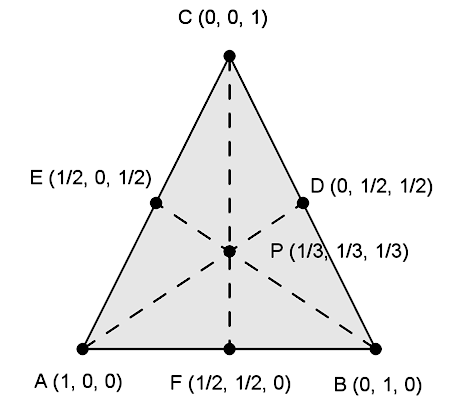
\includegraphics[scale=0.3]{figures/barycentric.png}
    \caption{Barycentric coordinates of a 2-simplex. Here, the simplex is $s=\langle A,B,C\rangle$ and the triples of numbers next to each point $\alpha\in |s|$ in this triangle correspond to the list of values $(\alpha(A),\alpha(B),\alpha(C))$. The values of $\alpha$ thus represent the proportions in which $A,B,C$ have to be ``mixed'' to get a point inside this geometric realization of the simplex.\label{fig. simplex}}
\end{figure}


In the future we write $|K|=|K|_c$ and call this space the \emph{geometric realization} of $K$. For a simplex $s$ we define the \emph{closed simplex} $|s|\subset |K|$ as $|s|=\{\alpha\in|K|\mid \alpha(e)\neq 0\implies e\in s\}$ and the \emph{open simplex} as $\langle s\rangle=\{\alpha\in |K|\mid \alpha(e)\neq 0\Leftrightarrow e\in s\}$. The \emph{combinatorial boundary} of $|s|$ is $\partial|s|=|s|\setminus\langle s\rangle$.

\begin{defn}[Standard simplices in $\bbR^k$]
    Let $x_0,\ldots,x_n$ be affinely independent (i.e., $\sum_i\alpha_i x_i=0$ and $\sum_i\alpha_i=0$ imply $\alpha_j=0$). Then the simplex spanned by them is \[\langle x_0,\ldots,x_n\rangle=\left\{\sum_i \alpha_i x_i\mid \alpha_i\geq 0,\sum_i \alpha_i=1\right\}.\]
\end{defn}
\begin{defn}
    If $K=(E,S)$ is a simplicial complex and $\{x_e\mid e\in E\}$ a set of points in $\bbR^k$, and if a map
    \[f:|K|\to \bbR^k,\quad \alpha\mapsto \sum_{e\in E}\alpha(e)x_e\]
    is an embedding (say, topological), then $f(|K|)$ is called a simplicial polyhedron in $\bbR^k$ of type $K$, or a polyhedral realization of $K$ in $\bbR^k$.
\end{defn}
\begin{defn}[Triangulation]\index{Triangulation}
    Let $X$ be a topological space. A triangulation of $X$ is a triple $(X,K,f)$ where $K$ is a simplicial complex $K$ such that there is a homeomorphism $f:X\to |K|$.
\end{defn}

It is known that all differentiable manifolds can be triangulated, and the triangulation can be chosen so that on each simplex it is a smooth embedding.

\begin{defn}[Simplicial homology]\index{Homology!simplicial}
    For a simplicial complex $K=(E,S)$ define the group $C^\Delta_p(K)$ of \emph{simplicial $p$-chains} as the free abelian group generated by the set of all $p$-simplices in $K$. That is, elements of $C^\Delta_p(K)$ are formal sums $\sum_{s} c_s s$, where $s$ runs over all $p$-simplices in $K$, and only a finite number of coefficients $c_s\in \bbZ$ are nonzero at once.
    
    Define the \emph{boundary operator}\index{Boundary operator}
    \[\partial:\; C^\Delta_p(K)\to C^\Delta_{p-1}(K),\quad \partial\langle e_0,\ldots,e_p\rangle=\sum_{i=0}^p(-1)^p\langle e_0,\ldots,\wh{e}_i,\ldots,e_p\rangle,\]
    where the hat means skipping a vertex. It is easy to check that $\partial^2=0$, therefore we have the \emph{chain complex}\index{Complex!of simplicial chains}
    \[\cdots\to C^\Delta_2(K)\overset\partial\to C^\Delta_1(K)\overset\partial\to C^\Delta_0(K)\to 0.\]
    The group of $p$-cycles is $Z_p=\ker \restr{\partial}{C^\Delta_p(M)}$ and the group of $p$-boundaries is $B_p=\restr{\im\partial}{C^\Delta_{p+1}(M)}$. The \emph{simplicial homology groups} of $K$ are defined as
    \[H^\Delta_p(K)=Z_p/B_p.\]
\end{defn}

Intuitively, $H^\Delta_p$ detects the ``$p$-dimensional holes'' in the complex, because it consists of cycles that are not boundaries of anything $p+1$-dimensional.

\begin{defn}[Orientations on simplices and complexes]\index{Orientation!on simplicial complexes}
    An orientation on an $n$-simplex $s$ is an ordering of its elements into an $(n+1)$-tuple written as \[s=\langle e_0,\ldots,e_n\rangle.\]
    Orientations are considered to be equivalent if they differ by an even permutation of the vertices, i.e., we identify positively reordered tuples with each other. 
    
    In simplicial $p$-chains, sometimes the chain $-s$ is identified with $s$ oriented the opposite way.
    
    An orientation on a complex $K=(E,S)$ is a partial order on $E$ that induces an orientation on each simplex of $K$ (i.e., orientations of faces of a simplex can be induced from the orientation of the simplex). Orientations are considered to be equivalent if they induce equivalent orientations on all simplices.
\end{defn}

\begin{example}[Simplicial homology of $\bbS^1$]
    A circle $\bbS^1$ can be triangulated by a regular $n$-gon with vertices  $e_0,\ldots,e_{n-1}$ and oriented simplices $s_i=\langle e_i,e_{i+1}\rangle$, $0\leq i\leq n-1$ with the identification $e_n=e_0$. 
    Clearly 
    \[Z_0=C^\Delta_0=\bbZ^n,\quad C^\Delta_1=\left\{\sum_i c_i s_i \mid c_i\in \bbZ\right\}\cong \bbZ^n,\quad B_1=0.\]
    The chain complex is described by 
    \[\partial\langle e_i,e_{i+1}\rangle=\langle e_i\rangle-\langle e_{i+1}\rangle .\]
    $B_0$ consists of 0-chains $\sum c_i \langle e_i\rangle$ such that $\sum c_i=0$, thus $B_0\cong \bbZ^{n-1}$.
    Finally, $Z_1$ consists of 1-chains $\sum_i c_i s_i$ such that $c_i-c_{i+1}=0$ for all $i$, which means that $Z_1\cong \bbZ$ generated by the cycle $\sum_i s_i$. In the end, we have
    \[H^\Delta_0\cong \bbZ^n/\bbZ^{n-1}\cong \bbZ,\quad H^\Delta_1=Z_1\cong \bbZ. \]
    We notice that the ranks of these homology groups coincide with the dimensions of the corresponding de Rham cohomologies, see Example~\ref{de Rham of circle}. We will later prove this as a general fact for all manifolds: the de Rham cohomology is isomorphic to the simplicial homology with real coefficients.
\end{example}


\begin{xca}
    If $K$ is the tetrahedron (with 2-dimensional faces included), i.e., a triangulation of $\bbS^2$, compute its homology groups:
    \[H^\Delta_0=\bbZ,\quad H^\Delta_1=0,\quad H^\Delta_2=\bbZ.\]
\end{xca}
\begin{xca}
    Triangulate the M\"obius band as in the figure.
    \begin{center}
        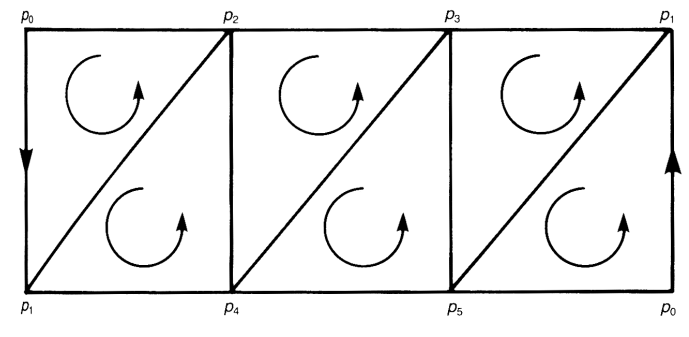
\includegraphics[scale=0.2]{figures/mobius.png}
    \end{center}
    Show that $H^\Delta_2(K)=0$ and $H^\Delta_1(K)=\bbZ$. In fact, the generator of $H^\Delta_1$ is the loop going from the bottom left to the top right corner in the diagram above.
\end{xca}

\begin{xca}
    Triangulate the real projective plane $\RP^2$ (which is homeomorphic to a disk whose antipodal boundary points have been identified) as in the figure.
    \begin{center}
        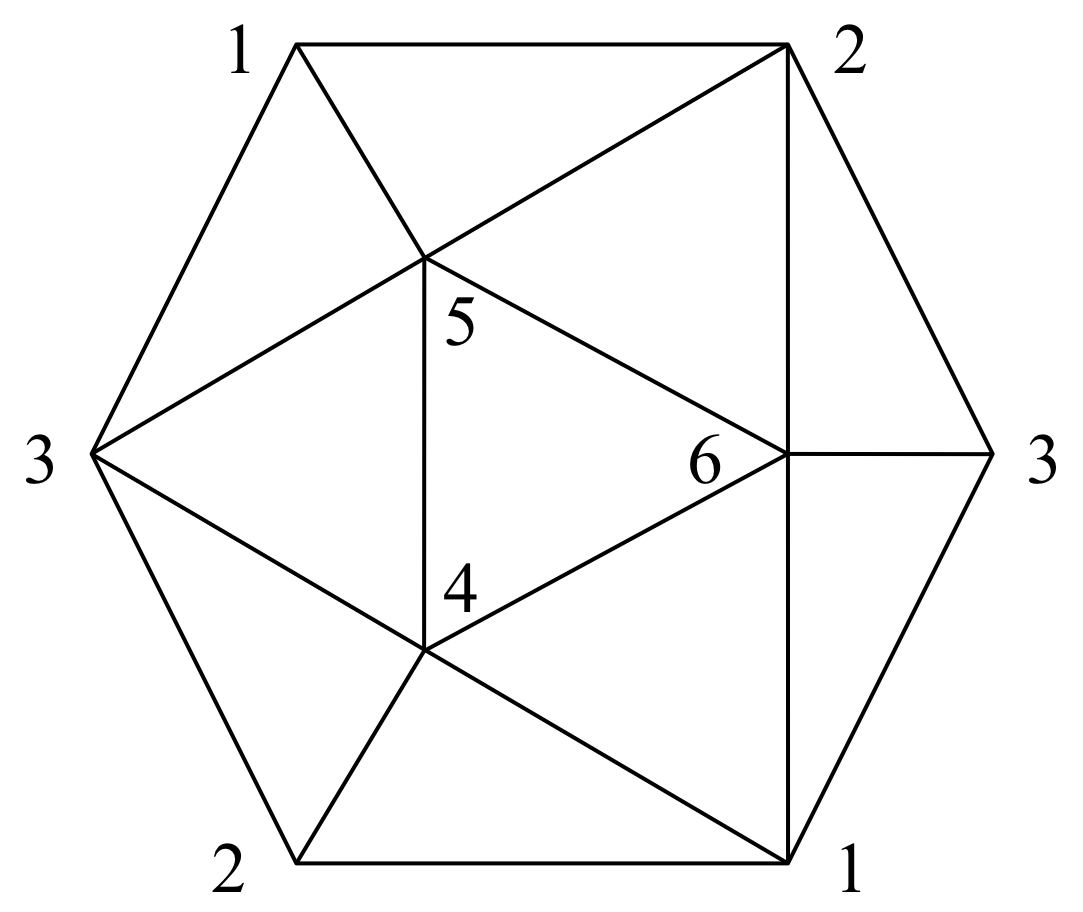
\includegraphics[scale=0.2]{figures/projectiveplane.png}
    \end{center}
    Show that $H^\Delta_2(K)=0$ and $H^\Delta_1(K)=\bbZ_2=\bbZ/2\bbZ$.
\end{xca}
\begin{xca}
    Triangulate the Klein bottle and show that $H^\Delta_1(K)=\bbZ\oplus\bbZ_2$.
\end{xca}

% \begin{defn}[Betti numbers]\index{Betti numbers}
%     Let $K$ be a finite simplicial complex. By the fundamental theorem of finitely generated abelian groups, each homology group of $K$ can be decomposed as
%     \[\rmH_p(K)=\underbrace{\bbZ^{b_p(K)}}_{\text{free part}}\oplus \underbrace{\bbZ_{m_1}\oplus \cdots \oplus \bbZ_{m_k}}_{\text{torsion part}},\]
%     where $b_p(K)\geq 0$ are called \emph{Betti numbers}. 
%     Since the torsion part disappears when tensor multiplied by a field containing the rationals $\bbQ$ (the tensor product is understood to be over the ring $\bbZ$ because abelian groups are $\bbZ$-modules; then, say, $Z_m\otimes \bbQ$ consists of $a\otimes r=ma\otimes (r/m)=0$), we have
%     \[\rmH_p(K)\otimes \bbQ=\bbQ^{b_p(K)}.\]
%     If $K$ is a triangulation of a smooth manifold $M$, then we will also show that $b_p(K)=\dim \rmH_{\rm dR}^p(M)$.
% \end{defn}

% \begin{defn}[Euler characteristic]\index{Euler characteristic}
%     If $K$ is a finite $n$-dimensional simplicial complex, then there are two definitions of the Euler characteristic $\chi(K)$:
%     \begin{itemize}
%         \item $\chi(K)=\sum_{p=0}^n (-1)^p n_p(K)$, where $n_p(K)$ is the number of $p$-simplices in $K$ (``combinatorial Euler characteristic'');
%         \item $\chi(K)=\sum_{i=0}^n (-1)^p b_p(K)$, where $b_p(K)$ are the Betti numbers (``homological Euler characteristic'').
%     \end{itemize}
% \end{defn}

% \begin{thm}[Euler-Poincar\'e]
%     The two definitions of the Euler characteristic for finite simplicial complexes are equivalent. In particular, since the Betti numbers are homotopy invariants (because so is homology itself, which we will show later), so is the Euler characteristic.
% \end{thm}
% \begin{proof}
%     Consider chain groups with rational coefficients (i.e., the free parts of the usual groups),
%     \[C_p(K,\bbQ)\coloneqq C_p(K)\otimes\bbQ.\]
%     Now the boundary operator $\partial_p:C_p(K,\bbQ)\to C_{p-1}(K,\bbQ)$ is a linear operator on $\bbQ$-vector spaces and by the rank-nullity theorem
%     \[n_p(K)=\dim C_p(K,\bbQ)=\dim\ker\partial_p+\dim\im\partial_p.\]
%     On the other hand,
%     \[b_p(K)=\dim Z_p(K,\bbQ)/B_p(K,\bbQ)=\dim\ker\partial_p-\dim\im\partial_{p+1}.\]
%     When taking alternating sums of these over $p$, we will get the same answer in both cases.
% \end{proof}




\section{Homological algebra II: complexes}

\begin{defn}[(Co)chain complexes]\index{Complex!of chains}\index{Complex!of cochains}
    A chain complex $(\bm{C},d)$ in an abelian category $\calC$ is a sequence  of morphisms 
    \[\cdots\to C_{n+1}\overset{d_{n+1}}\to C_n\overset{d_n}\to C_{n-1}\to\cdots\]
    indexed by $n\in \bbZ$, such that $d_n\circ d_{n+1}=0$.
    
    Similarly, a cochain complex is a sequence
    \[\cdots\to C^{n-1}\overset{d^{n-1}}\to C^n\overset{d^n}\to C^{n+1}\to\cdots\]
    such that $d^{n+1}\circ d^n=0$.
\end{defn}

Note that there is no actual difference between chain and cochain complexes, since simply changing the enumeration $n\mapsto -n$ turns one into the other. Therefore all general results need to be proven only for chain complexes.

\begin{defn}[(Co)cycles, (co)boundaries, (co)homologies of complexes]\index{Homology!of a chain complex}\index{Cohomology!of a cochain complex}
    For a chain complex $(\bm{C},d)$, $n$-cycles, $n$-boundaries, and homologies are defined as 
    \[Z_n(\bm{C},d)=\ker d_n,\quad\quad B_n(\bm{C},d)=\im d_{n+1},\quad\quad \rmH_n(\bm{C},d)=Z_n(\bm{C},d)/B_n(\bm{C},d).\]
    
    Similarly, for a cochain complex $(C^{\smbullet },d)$, we have cocycles, coboundaries, and cohomologies:
    \[Z^n(C^{\smbullet },d)=\ker d_n,\quad\quad B^n(C^{\smbullet },d)=\im d^{n-1},\quad\quad \rmH^n(C^{\smbullet },d)=Z^n(C^{\smbullet },d)/B^n(C^{\smbullet },d).\]
\end{defn}

\begin{defn}[Chain map]
    If $(\bm{B},\delta )$ and $(\bm{C},d)$ are two chain complexes, then a chain map $f:\bm{B}\to \bm{C}$ is a sequence of maps $f_n:B_n\to C_n$ such that $d_n\circ f_n=f_{n-1}\circ \delta_n$, i.e., such that the full diagram commutes:
    \[\begin{tikzcd}[every matrix/.append style={name=m},
        execute at end picture={\draw [<-] ([xshift=-8mm,yshift=-10mm]m-1-3.north) arc[start angle=-90,delta angle=-270,radius=0.2cm];
        \draw [<-] ([xshift=-8mm,yshift=-10mm]m-1-4.north) arc[start angle=-90,delta angle=-270,radius=0.2cm];}]
        \cdots\arrow[r] & B_{n+1}\arrow[r]\arrow[d,swap,"f_{n+1}"] & B_{n} \arrow[r]\arrow[d,swap,"f_n"] & B_{n-1}\arrow[d,"f_{n-1}"]\arrow[r] & \cdots \\
       \cdots\arrow[r] & C_{n+1}\arrow[r] & C_n\arrow[r] &C_{n-1} \arrow[r] &\cdots
    \end{tikzcd}\]
    Similarly one defines cochain maps between cochain complexes.
\end{defn}

\begin{prop}
    All chain complexes in an abelian category $\calC$ with chain maps between them comprise an abelian category called $\mathsf{Comp}(\calC)$.
\end{prop}
\begin{proof}
    By the Freyd-Mitchell theorem, we only need to prove this for $\calC=R\text{-}\mathsf{Mod}$. For such a category it is obvious what the structure of an abelian category on complexes is: the zero object is the zero complex; direct sums are defined by summing in each degree; the kernel and cokernel of $f$ are the complexes consisting of $\ker f_n$ and $\coker f_n$; images and coimages coincide because they do so in $\calC$.
\end{proof}

\begin{defn}[Positive complexes]
    A chain complex $\bm{C}$ is called positive if $C_n=0,n<0$. All positive complexes form the full subcategory $\mathsf{Comp}_{\geq 0} (\calC)$ of $\mathsf{Comp}(\calC)$:
    \[\cdots\to C_n\to C_{n-1}\to\cdots\to \to C_1\to C_0\to 0.\]
    
    A negative chain complex
    \[0\to C_0\to C_{-1}\to \cdots \to C_{-n}\to C_{-n-1}\to\cdots\]
    is identified with a positive cochain complex 
    \[0\to C^0\to C^{1}\to \cdots \to C^{n}\to C^{n+1}\to\cdots\]
    by setting $C^n=C_{-n}$ and $d^n=d_{-n}$.
\end{defn}

\begin{prop}
    If $\calC$ is an abelian category, then the $n$-th homology $\rmH_n:\mathsf{Comp}(\calC)\to \calC$ is an additive (covariant) functor for all $n\in \bbZ$.
\end{prop}
\begin{proof}
    Given a chain map $f:\bm{A}t\to \bm{B}$, we need to construct a morphism $\rmH_n(f):\rmH_n(\bm{A})\to \rmH_n(\bm{B})$. Since $\rmH_n(\bm{A})=Z_n(\bm{A})/B_n(\bm{A})$, we can try to take a $z$ such that
    \[f_n:Z_n(\bm{A})\to B_n,\quad z\mapsto f_n(z)\]
    and define
    \[\rmH_n(f):\rmH_n(\bm{A})\to \rmH_n(\bm{B}),\quad [z]\to \left[f_n(z)\right],\]
    where equivalence classes are taken w.r.t.\ to the quotients by $B_n(\bm{A})$ and $B_n(\bm{B})$ respectively.
    
    First we need to check that $f_n(z)\in Z_n(\bm{B})$. We will use the same symbol $d_n$ for morphisms in both complexes. By the definition of a chain map, $d_n(f_n(z))=f_{n-1}(d_n(z))=0$ since $z\in B_n(\bm{A})$.
    
    Next we need to check correctness, i.e., independence of $\rmH_n(f)([z])$ of the choice of representative. Let $z,z'\in Z_n(\bm{A}):[z]=[z']\Leftrightarrow z-z'\in B_n(\bm{A})$, then
    \[\exists y\in A_{n+1}: d_{n+1}(y)=z-z'\implies d_{n+1}(f_{n+1}(y))=f_n(z)-f_n(z'),\]
    which means that $f_n(z)-f_n(z')$ is a boundary, proving what we wanted.
    
    To check functoriality, say we have two chain maps
    \[\bm{A}\overset f\to \bm{B}\overset g\to \bm{C}.\]
    We need to show the commutativity of the triangle
    \[
    \begin{tikzcd}
        \rmH_n(\bm{A}) \arrow[rr,"\rmH_n(f)"]\arrow[dr,swap,"\rmH_n(g\circ f)"]&& \rmH_n(\bm{B})\arrow[dl,"\rmH_n(g)"]\\
        & \rmH_n(\bm{C}) &
    \end{tikzcd}
    \]
    We have 
    \begin{multline}
        \rmH_n(g\circ f)([z])=\left[(g\circ f)_n(z)\right]=\left[g_n\circ f_n(z)\right]=\rmH_n(g)\left(\left[f_n(z)\right]\right)=\\=\rmH_n(g)\left(\rmH_n(f)[z]\right)=\rmH_n(g)\rmH_n(f)([z]).
    \end{multline}
    
    Finally, additivity is trivial since $f_n$ are homomorphisms:
    \[\rmH_n(f+f')=\rmH_n(f)+\rmH_n(g').\]
\end{proof}

\begin{rem}
    On cochain complexes, this functor is of course contravariant.
\end{rem}

From now on we write
\[f_\ast=\rmH_n(f),\quad\quad g^\ast=\rmH^n(g)\]
for the descendants of maps in (co)homology.

\begin{lem}
    Exact additive covariant functors preserve homology: $H_\ast(F(\bm{C}))\cong F(H_\ast(\bm{C}))$.
\end{lem}
\begin{proof}
    This follows from the fact that exact additive functors preserve kernels and quotients (and all functors preserve images).
\end{proof}

\begin{prop}
    The directed colimit of the homology groups of a directed system of chain complexes $\bm{C}^i$ is the homology group  of the directed colimit:
    \[\colimit_i \rmH_n(\bm{C}^i)\cong \rmH_n(\colimit_i \bm{C}^i).\]
\end{prop}
\begin{proof}
    This follows immediately from the preceding lemma and the fact that directed colimits preserve exactness in abelian categories (Proposition~\ref{prop direct limits preserve exactness}).
\end{proof}
\begin{rem}
    Note that the analogous statement for homotopy groups $\pi_n$ was proven by us only for sequences of $CW$ subcomplexes (Corollary~\ref{cor direct limit of pi_n for CW}) and does not hold in general even for $\pi_1$.
\end{rem}



\begin{thm}[Connecting homomorphism lemma]\label{connecting hom in homology}
    Let 
    \[0\to \bm{A}\overset i\to \bm{B}\overset\pi\to \bm{C}\to 0 \]
    be a short exact sequence of chain complexes. Then for each $n$ there is a \emph{connecting homomorphism}
    \[\delta=\delta_n:\rmH_n(\bm{C})\to \rmH_{n-1}(\bm{A}),\quad [z]\to \left[i_{n-1}^{-1} d_n\pi_n^{-1}(z)\right].\]
\end{thm}
\begin{proof}
    Several checks need to be done. First, why does $d_n\pi_n^{-1}(z)\in\im i_{n-1}$? Let $y:\pi_n(y)=z$, then $d_n(y)\in B_{n-1}$. Since $z\in Z_n(\bm{C})$ we have $\pi_{n-1}(d_n(y))=d_n(\pi_n(y))=d_n(z)=0$. Therefore $\exists ! x\in A_{n-1}:i_{n-1}(x)=d_n(y)$, and we have a well defined map
    \[z\mapsto x.\]
    
    Next, we need to verify that $d_{n-1}(x)=0$ and the class $[x]\in \rmH_{n-1}(\bm{A})$ is independent of the choice of $y$.
    Moreover, one needs to check that if $[z]=[z']$, then $[x]=[x']$. Lastly, we need to check that $\delta$ is a homomorphism. These checks are left as an exercise.
\end{proof}

\begin{thm}[Zig-zag lemma/Long exact sequence in homology]\label{thm long exact seq in homology} \index{Long exact sequence!of homology}
    For any short exact sequence of complexes 
    \[0\to \bm{A}\overset i\to \bm{B}\overset\pi\to \bm{C}\to 0 ,\]
    the induced sequence in homology
    \[\cdots \to \rmH_{n+1}(\bm{C})\overset{\delta_{n+1}}\to \rmH_n(\bm{A})\overset{i_\ast}\to \rmH_n(\bm{B})\overset{\pi_\ast}\to \rmH_n(\bm{C})\overset{\delta_n}\to \rmH_{n-1}(\bm{A})\to \cdots \]
    is exact.
\end{thm}
\begin{proof}
    It is easy to see that for any complex $\bm{C}$ the two \emph{``fundamental sequences''}
    \[0\to Z_n(\bm{C})\to C_n\overset{d_n}\to B_{n-1}(\bm{C})\to 0,\]
    \[0\to B_n(\bm{C})\to Z_n(\bm{C})\to \rmH_n(\bm{C})\to 0\]
    are short exact.
    This one is also obviously exact:
    \[0\to B_n(\bm{C})\to C_n\to C_n/B_n(\bm{C})\to 0.\]
    Using the exactness of the first sequence, we also have the exactness of this one:
    \[0\to \rmH_n(\bm{C})\to C_n/B_n(\bm{C})\to \underbrace{B_{n-1}(\bm{C})}_{\cong C_n/Z_n(\bm{C})}\to 0.\]
    
    Putting it all together, we conclude the exactness of this sequence:
    \[0\to \rmH_n(\bm{C})\to C_n/B_n(\bm{C})\to Z_{n-1}(\bm{C})\to \rmH_{n-1}(\bm{C})\to 0.\]
    Now let us use this sequence for the columns of one large diagram:
    \[\begin{tikzcd}
        && 0\ar{d}& 0\ar{d} &0\ar{d} &&\\
        & & \rmH_n(\bm{A}) \ar{r} \ar{d} & \rmH_n(\bm{B})\ar{r} \ar{d} &  \rmH_n(\bm{C}) \ar{d}   %\arrow[ddll,"\delta",rounded corners
        & & \\
        &  &  A_n/B_n(\bm{A}) \ar{r} & B_n/B_n(\bm{B}) \ar{r} \ar{dd} &  C_n/B_n(\bm{C})\ar{r}\ar{dd} & 0 &  ~\\[-10pt]
        & & &  ~ & & \ar[r, phantom, ""{coordinate, name=Y}] & ~\\[-10pt]
        ~&  \ar[l, phantom, ""{coordinate, name=Z}] 0 \ar{r} &  Z_{n-1}(\bm{A}) \ar[uu,leftarrow,crossing over]\ar{r} \ar{d} &  Z_{n-1}(\bm{B}) \ar{r} \ar{d} &  Z_{n-1}(\bm{C}) \ar{d} & &  \\
              & &  \ar[from=uuuurr, "\delta_n", dashed,crossing over, rounded corners,
                      to path=
                              { -- ([xshift=2ex]\tikztostart.east)
                              -| (Y) [near end]\tikztonodes
                              -| (Z) [near end]\tikztonodes
                              |- ([xshift=-2ex]\tikztotarget.west)
                               -- (\tikztotarget)}
                    ] \rmH_{n-1}(\bm{A})\ar{r}\ar{d}
               &  \rmH_{n-1}(\bm{B}) \ar{r}\ar{d}
               &  \rmH_{n-1}(\bm{C})\ar{d}
               & 
               & \\
        && 0& 0 &0 &&\\
    \end{tikzcd}\]
    The exactness of the rows can be checked directly using the exactness of $\bm{A}\to \bm{B}\to\bm{C}$. Then this is in fact exactly the type of diagram for which we can apply the Snake Lemma~\ref{snake lemma} and establish the existence of $\delta_n$. It only remains to check that the construction of $\delta_n$ in the Snake Lemma exactly coincides with the one in Proposition~\ref{connecting hom in homology}.
\end{proof}
\begin{cor}
    The Snake lemma is equivalent to the Zig-zag lemma.
\end{cor}
\begin{proof}
     The proof of Theorem~\ref{thm long exact seq in homology} shows that the Snake Lemma implies the long exact sequence in homology. The converse also trivially holds since we can apply the Zig-zag lemma to a short exact sequence of complexes concentrated in just two degrees of the form $0\to \ker\pi \to \im\pi \to 0$ (let the two other complexes have $\rho $ and $\sigma$ instead of $\pi$) and obtain the long exact sequence of homologies, which reads
    \[0\to \ker\pi \to \ker\rho\to \ker\sigma\to \coker\pi\to \coker\rho\to\coker\sigma\to 0, \]
    which is exactly the Snake Lemma \ref{snake lemma}.
\end{proof}


\begin{prop}[Naturality of the connecting homomorphism\footnote{Tape worm lemma?}]\label{naturality of connecting hom}
    Given a commutative diagram with exact rows in the category $\mathsf{Comp}(\calC)$
    \[\begin{tikzcd}
        0\arrow[r] & \bm{A}\arrow[r,"i"]\arrow[d,swap,"f"] & \bm{B} \arrow[r,"p"]\arrow[d,swap,"g"] & \bm{C}\arrow[d,"h"]\arrow[r] & 0 \\
       0\arrow[r] & \bm{A}'\arrow[r,"j"] & \bm{B}'\arrow[r,"q"] &\bm{C}' \arrow[r] &0
    \end{tikzcd}\]
    there is a commutative diagram in $\calC$ with exact rows
    \[\begin{tikzcd}
        ~\arrow[r]& \rmH_n(\bm{A})\arrow[r,"i_\ast"]\arrow[d,"f_\ast"] & \rmH_n(\bm{B}) \arrow[r,"p_\ast"]\arrow[d,"g_\ast"] & \rmH_n(\bm{C})\arrow[d,"h_\ast"]\arrow[r,"\delta"] & \rmH_{n-1}(\bm{A})\arrow[d,"f_\ast"]\arrow[r]&~ \\
       ~\arrow[r] & \rmH_n(\bm{A}')\arrow[r,"j_\ast"] & \rmH_n(\bm{B}')\arrow[r,"q_\ast"] &\rmH_n(\bm{C}') \arrow[r,"\delta'"] &\rmH_{n-1}(\bm{A}')\arrow[r]&~ 
    \end{tikzcd}\]
    In other words, morphisms between exact sequences of complexes naturally induce morphisms between the exact sequences in homology, i.e., the connecting homomorphism $\delta$ is natural w.r.t.\ such morphisms.
\end{prop}
\begin{proof}
     The exactness of the rows is the content of the theorem about the long exact sequence. The commutativity of the first two squares follows from the functoriality of $\rmH_n$. Checking the commutativity of the square $\delta'\circ h_\ast=f_\ast\circ \delta$ requires expanding the first commutative diagram in $\mathsf{Comp}(\calC)$ into a 3-dimensional diagram in $\calC$.
     \[
     \begin{tikzcd}[column sep={35,between origins}]
        &
        0 
        \ar{rr}
        & &
        A_n
        \ar{dl}[swap, sloped, near start]{d}
        \ar{rr}{i}
        \ar[]{dd}[near start]{f_\ast}
        & & B_n
        \ar{dd}[near start]{g_\ast}
        \ar{rr}{p}
        \ar{dl}[swap, sloped, near start]{d}
        & & C_n
        \ar{dd}[near start]{h_\ast}
        \ar{dl}[swap, sloped, near start]{d}
        \ar{rr}
        & &
        0
        \\
        0
        \ar{rr}
        & &
        A_{n-1}
        \ar[crossing over]{rr}[near end]{i}
        & & B_{n-1}
        \ar[crossing over]{rr}[near end]{p}
        & & C_{n-1}
        \ar[crossing over]{rr}
        & &
        0
        \\
        &
        0
        \ar{rr}
        & &
        A_n'
        \ar[near start]{rr}{j}
        \ar[sloped, swap]{dl}{d}
        & & B_n'
        \ar[near start]{rr}{q}
        \ar[sloped, swap]{dl}{d}
        & & C_n'
        \ar[sloped, swap]{dl}{d}
        \ar{rr}
        & &
        0
        \\
        0
        \ar{rr}
        & &
        A_{n-1}'
        \ar{rr}{j}
        \ar[crossing over, leftarrow, near start]{uu}{f_\ast}
        & & B_{n-1}'
        \ar{rr}{q}
        \ar[crossing over, leftarrow, near start]{uu}{g_\ast}
        & & C_n'
        \ar[crossing over, leftarrow, near start]{uu}{h_\ast}
        \ar{rr}
        & &
        0
        \end{tikzcd}
     \]
     Taking $[c]\in \rmH_n(\bm{C})$, we must show that $f_\ast\delta [c]=\delta ' h_\ast [c]$. Let $b\in B_n$ be such that $p(b)=c$. Then $\delta [c]=[a]$, where $i(a)=d(b)$. Hence $f_\ast \delta [c]=[f(a)]$. 
     
     On the other hand, since $h$ is a chain map, $q(g(b))=h(p(b))=h(c)$. Hence we can use $g(b)$ as the preimage of $h(c)$ in $B_n'$, so by construction of the connecting homomorphism, $\delta '[h(c)]=[a']$ where $j(a')=d(g(b))$. But $j(f(a))=g(i(a))=g(d(b))=d(g(b))=j(a')$ and so $f(a)=a'$ because $j$ is injective. Therefore $\delta'h_\ast [c]=[a']=[f(a)]$, which coincides with the l.h.s.\ computed above.
\end{proof}

Naturality is instrumental in many arguments involving long exact sequences because it means that we can apply sequences of chain maps to long exact sequences and preserve the commutativity of diagrams.

\begin{prop}[Algebraic Mayer-Vietoris sequence]\label{prop algebraic MV}
    If in the setting of Theorem~\ref{naturality of connecting hom}, $h_\ast$ is also an isomorphism in homology, then one has the long exact sequence
    \[\cdots \to \rmH_{n+1}(\bm{B}')\overset\Delta\to \rmH_n(\bm{A})\overset{(f_\ast,i_\ast)}\longrightarrow \rmH_n(\bm{A}')\oplus \rmH_n(\bm{B})\overset{j_\ast- g_\ast}\longrightarrow \rmH_n(\bm{B}')\overset{\Delta}\to \rmH_{n-1}(\bm{A})\to \cdots\]
    where $\Delta=\delta \circ h_\ast^{-1}\circ q_\ast$.
\end{prop}
\begin{proof}
     This is an exercise in diagram chasing.
\end{proof}

The relation of this proposition to the \gls{mv} sequence in de Rham cohomology will become clear when we get to relative (co)homology and the excision property. The isomorphism $h_\ast$ in question is $\rmH_n(U,U\cap V)\cong \rmH_n(M,V)$ for $M=U\cup V$. A rough visualization of $\rmH_n(X,Y)$ with $Y\subset X$ is the homology of the space obtained from $X$ by contracting $Y$ into one point. Then it is clear that contracting $V$ inside $M$ has the ``same'' result as contracting $U\cap V$ inside $U$. 


\begin{defn}[Maps of degree $p$]
    Let $\bm{C}$ and $\bm{D}$ be two chain complexes in $\calC$. A map of degree $p$ between them, denoted $s:\bm{C}\to \bm{D}$, is a collection of maps $s_n:C_n\to D_{n+p}$. Note that no commutativity is required here!
\end{defn}


Now that we know that $\rmH_n$ is a functor, it is natural to ask how much $\rmH_n(f)$ actually depends on $f$. It turns out that $\rmH_n(f)$ is invariant under homotopies of $f$ defined in the following categorical sense.


\begin{defn}
    Let $f,g:\bm{B}\to \bm{C}$ be two chain maps. They are called homotopic ($f\sim g$) if there is a map of degree $+1$ denoted $s:\bm{B}\to \bm{C}$ such that 
    \[\forall n,\quad f_n-g_n=d_{n+1}s_n+s_{n-1}d_n.\]
    (As usual, we use $d_n$ to denote the differentials in all complexes at once).
    This can be visualized by the following \emph{non-commutative} diagram:
     \[\begin{tikzcd}
        \cdots\ar[r] & B_{n+1}\ar[r]\ar[dd,swap, xshift=-.75ex,"f_{n+1}"]\ar[dd,xshift=.75ex,"g_{n+1}"] & B_{n} \arrow[r]\ar[dd,swap,xshift=-.75ex,"f_n"]\ar[dd,xshift=.75ex,"g_n"]\ar[ddl,sloped, near start,"s_n"] & B_{n-1}\ar[dd,swap,xshift=-.75ex,"f_{n-1}"]\ar[dd,xshift=.75ex,"g_{n-1}"]\ar[r]\ar[ddl, near start,sloped,"s_{n-1}"] & \cdots \\
        &&&&\\
       \cdots\ar[r] & C_{n+1}\ar[r] & C_n\ar[r] &C_{n-1} \ar[r] &\cdots
    \end{tikzcd}\]
\end{defn}

\begin{thm}
    Homotopic chain maps induce the same morphism in homology.
\end{thm}
\begin{proof}
     Let $s:\bm{B}\to\bm{C}$ be the homotopy. If $z$ is an $n$-cycle, dropping subscripts, $d z=0$, then
     \[f(z)-g(z)=d(s(z))+s(d(z))=d(s(z)),\]
     i.e., $f(z)-g(z)\in B_n(\bm{C})$ and $f_\ast=g_\ast$.
\end{proof}

\begin{defn}[Acyclic, contractible complexes]\index{Acyclic complex}\index{Contractible complex}
    A complex is called acyclic if all its (co)homologies are trivial. A complex $\bm{C}$ is called contractible if there exists a homotopy $1_{\bm{C}}\sim 0_{\bm{C}}$. 
    All contractible complexes are acyclic since contractibility implies $1_{\rmH_n(\bm{C})}=0_{\rmH_n(\bm{C})}$.
\end{defn}

\begin{defn}[Quasi-isomorphisms]\index{Quasi-isomorphism}
    Two complexes $\bm{A},\bm{B}$ are called quasi-isomorphic (or \emph{weakly equivalent}) if there is a chain map $f:\bm{A}\to \bm{B}$ such that $f_\ast=\rmH_n(f):\rmH_n(\bm{A})\to \rmH_n(\bm{B})$ is an isomorphism for all $n$.
\end{defn}

\begin{defn}[Homotopy equivalence]\index{Homotopy equivalence}
    Two complexes $\bm{A},\bm{B}$ are called homotopy equivalent if there are two chain maps $f:\bm{A}\to \bm{B}$ and $g:\bm{B}\to\bm{A}$ such that
    \[f\circ g\sim 1_{\bm{B}},\quad g\circ f\sim 1_{\bm{A}}.\]
    Clearly homotopy equivalent complexes are quasi-isomorphic.
\end{defn}


\begin{xca}\label{Lie derivative homotopy operator}
    Check that a Lie derivative $\Lie_X$ is a cochain map on the de Rham complex. Furthermore, show that applying a Lie derivative $\Lie_X$ to a differential form doesn't change its class in de Rham cohomology. For this, find the homotopy operator between $\Lie_X$ and the zero morphism.
\end{xca}







\section{Singular homology}

de Rham cohomology is defined only for smooth manifolds, and simplicial homology is defined only for triangulable spaces. The type of homology we define now works for all topological spaces, but proving its properties for nicer spaces (like manifolds) requires extra work. The idea is, instead of trying to break up our topological space into simplices, to study the set of all continuous maps from simplices to our space.

\begin{defn}[Singular simplices]\index{Simplex!singular}
    We denote by $\Delta^n$ the standard $n$-simplex $\Delta^n=\{\sum_{i=0}^{n} \alpha_i e_i\mid \sum_i\alpha_i=1\}$, where $\{e_i\}_{i=0}^{n}$ is the standard basis in $\bbR^{n+1}$. Let $X$ be a topological space. A singular $n$-simplex in $X$ is a continuous map $\sigma\in C(\Delta^n, X)$ (no other constraints, hence ``singular''). The group $C_n(X)$ of singular $n$-chains is the free abelian group generated by the set $C(\Delta^n,X)$. Sometimes we will write $C^{\text{sing}}_n(X)$ to distinguish from other kinds of chain groups.
\end{defn}
\begin{defn}[Singular homology]\index{Homology!singular}
    The boundary map $\partial_n:C_n(X)\to C_{n-1}(X)$ is defined as before:
    \[\partial_n\sigma=\sum_i (-1)^i\restr{\sigma}{\langle e_0,\ldots,\wh{e}_i,\ldots,e_n\rangle},\]
    where we implicitly identify the faces of $\Delta^n$ with $\Delta^{n-1}$ while preserving the order of vertices, so that $\restr{\sigma}{\langle e_0,\ldots,\wh{e}_i,\ldots,e_n\rangle}$ is a singular $(n-1)$-simplex.
    
    Singular homology groups are defined as
    \[\rmH_n(X)=\ker\partial_n/\im\partial_{n+1}.\]
\end{defn}

Unlike with simplicial homology, here it is immediately obvious that homeomorphic spaces have isomorphic singular homologies. The price we pay for this is that the rank of $C^{\text{sing}}_n(X)$ is uncountably large, so it is not clear at a glance whether singular homologies of spaces that have finitely generated simplicial homologies are also finitely generated. 

\begin{prop}
    If $X$ consists of $l$ path-connected components, then $\rmH_0(X)\cong \bbZ^l$.
\end{prop}
\begin{proof}
     It suffices to prove this for $l=1$, i.e., a path-connected $X$. We have $\rmH_0(X)=C_0(X)/\im\partial_1$. A singular 0-chain in $X$ is just a finite sum $\sum_i n_i p_i$ where $p_i$ are points in $X$ and $n_i\in\bbZ$. Define the homomorphism $\epsilon:C_0(X)\to \bbZ$, called the \emph{augmentation map}\index{Augmentation map}, by
     \[\epsilon\left(\sum_i n_i p_i\right)=\sum_i n_i.\]
     It is surjective as long as $X\neq\varnothing$. The claim is that $\ker\epsilon\cong\im\partial_1$ if $X$ is path-connected, so $\epsilon $ induces an isomorphism $\rmH_0(X)\cong \bbZ$.
     
     First, it is clear by definition of $\partial$ that $\im\partial_1\subset\ker\epsilon$. For the reverse inclusion, suppose $\epsilon(\sum_i n_i p_i)=0$. Choose a path $\gamma_i$ connecting a base point $x_0$ to $p_i$. We can view $\gamma_i$ as a singular 1-simplex and have $\partial\gamma_i=p_i-x_0$. Hence $\partial(\sum_i n_i\gamma_i)=\sum_i n_i p_i$ since $\sum_i n_i=0$. Therefore $\sum n_i p_i$ is a boundary, which shows $\ker\epsilon\subset\im\partial_1$.
\end{proof}

\begin{prop}
    If $X$ consists of a single point, then $\rmH_n(X)=0$ for $n>0$ and $\rmH_0(X)\cong \bbZ$.
\end{prop}
\begin{proof}
     In this case there is a unique singular $n$-simplex $\sigma_n$ for each $n$ and 
     \[\partial\sigma_n=\sum_{i=0}^n(-1)^i\sigma_{n-1}=\begin{cases}
     0,& n\text{ odd},\\
     \sigma_{n-1},& n\text{ even}.
     \end{cases}\]
     This the singular chain complex reads
     \[\cdots\to \bbZ\overset\cong\to \bbZ\overset 0\to \bbZ\overset\cong\to\bbZ\overset 0\to\bbZ\to 0.\]
     The homology of this complex is trivial except for $\rmH_0\cong \bbZ $.
\end{proof}

Sometimes it is very helpful to work with a slightly modified homology that vanishes entirely for a point. The following definition achieves this.

\begin{defn}[Reduced homology]\index{Homology!reduced}
    The reduced homology groups $\wt{H}_n(X)$ are the homology groups of the \emph{augmented chain complex}
    \[\cdots C_1(X)\overset{\partial_1}\to C_0(X)\overset{\epsilon}\to \bbZ\to 0.\]
\end{defn}

The reduced homology of a point is trivial in all degrees. Also $\rmH_n(X)\cong \wt{H}_n(X)$ for all $n>0$ and $\rmH_0(X)=\wt{H}_0(X)\oplus \bbZ$ since $\epsilon$ induces a map $\rmH_0(X)\to \bbZ$ with kernel $\wt{H}_0(X)$.




\section{Homotopy invariance}

Here we show that singular homology is homotopy invariant.

\begin{figure}[tp]
    \begin{center}
        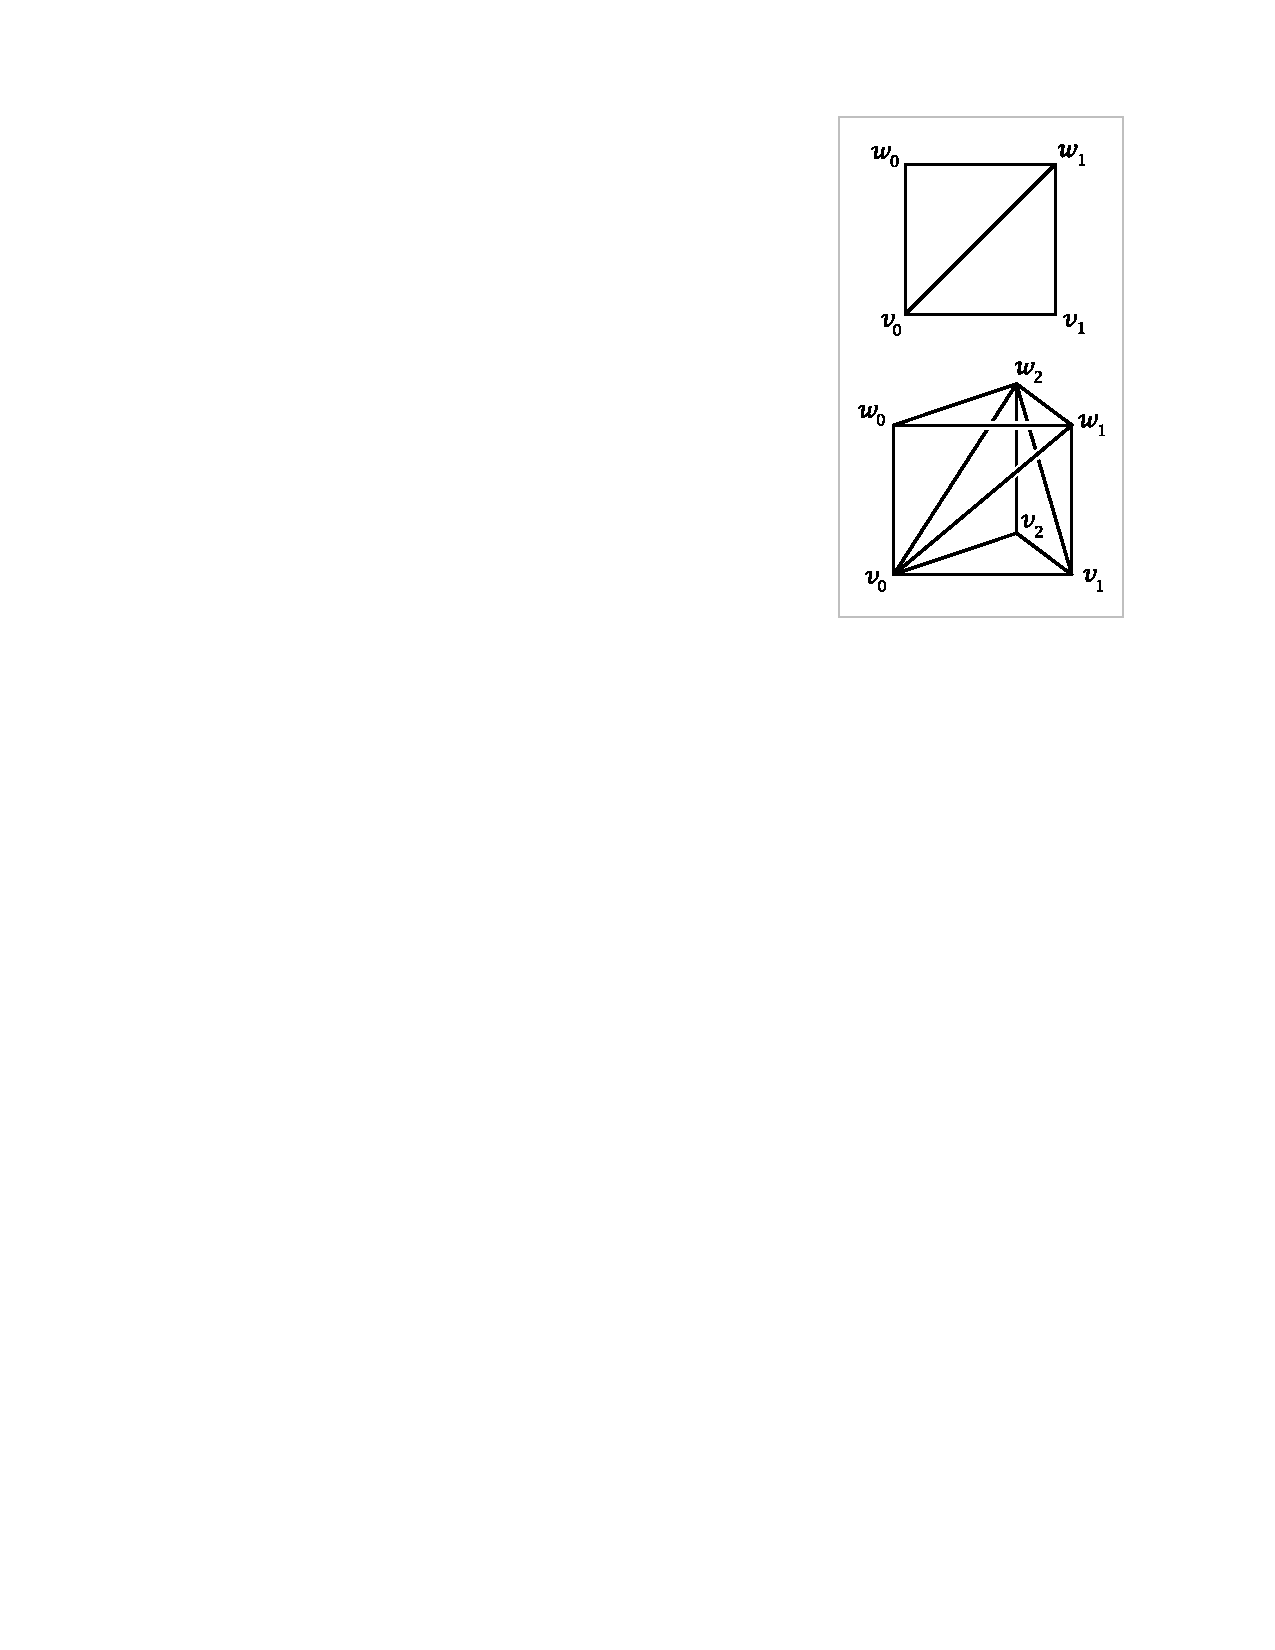
\includegraphics[width=0.2\textwidth]{figures/prism.pdf}
    \end{center}
    \caption{Triangulation of a prism, see Proposition~\ref{thm 2.10 Hatcher}.\label{Prism fig}}
\end{figure}
\begin{prop}[{{\cite[Thm. 2.10]{Hatcher}}}]\label{thm 2.10 Hatcher}
    If two maps $f,g\in C(X,Y)$ between topological spaces $X,Y$ are homotopic, then they induce the same homomorphism in homology
    \[f_\ast=g_\ast :\rmH_n(X)\to \rmH_n(Y)\]
    for all $n$. In particular, homotopy equivalent spaces have isomorphic homology groups.
\end{prop}
\begin{proof}
     The key is learning to subdivide the prism $\Delta^n\times I$ (where $I=[0,1]$) into simplices. If $\langle v_0,\ldots,v_n\rangle$ is the copy of $\Delta^n$ at the bottom of the prism and $\langle w_0,\ldots,w_n\rangle$ is the one at the top, then it is easy to check that the prism is triangulated by the $(n+1)$-simplices $\langle v_0,\ldots,v_i,w_i,\ldots,w_n\rangle$, each intersecting the next in an $n$-simplex face. The cases $n=1,2$ are shown in figure~\ref{Prism fig}.
     
     Given a homotopy $F:X\times I\to Y$ from $f$ to $g$ and a singular simplex $\sigma:\Delta^n\to X$, we form the composition $F\circ(\sigma\times \id):\Delta^n\times I\to X\times I\to Y$. Using this, we define the \emph{prism operators}
     \[P:C_n(X)\to C_{n+1}(Y),\quad P(\sigma)=\sum_i(-1)^i F\circ (\sigma\times\id)\langle x_0,\ldots,v_i,w_i,\ldots,w_n\rangle.\]
     We claim that $P$ is a homotopy operator between these two chain complexes, namely
     \[g_\ast-f_\ast=\partial P+P\partial.\]
     The geometric meaning of $\partial P=g_\ast-f_\ast-P\partial$ is that the boundary of the prism equals its top $\Delta^n\times\{1\}$, minus its bottom $\Delta^n\times\{0\}$, and plus the sides $\partial\Delta^n\times I$ (compare this with Cartan's magic formula and its cohomological meaning, which is nothing but a dual to this geometric statement, see Exercise~\ref{Lie derivative homotopy operator}).
     
     The verification of this identity follows easily by direct expansion and use of the definition of the homotopy $F$ and $g\circ\sigma=g_\ast(\sigma)$ (see \cite[Thm.~2.10]{Hatcher} for full details).
\end{proof}
\begin{cor}
    If $X$ is contractible, then $\wt{H}_n(X)=0$ for any $n$.
\end{cor}


Continuous maps induce homomorphisms in reduced homology as well since the augmentation map $\epsilon$ commutes with $f_\ast$. Then the same theorem holds for reduced homologies with the same proof.




\section{Relative homology and excision}

Relative homology generalizes the idea behind the \gls{mv} sequence in de Rham cohomology. Given a subset $A\subset X$ in a topological space, we ask how similar the groups $\rmH_n(X/A)$ and $\rmH_n(X)/\rmH_n(A)$ are. The difference, in a sense, is measured by the relative homology.

\begin{defn}
    Let $X$ be a topological space and $A\subset X$ a topological subspace (i.e., a subset with the induced subset topology). The group of singular chains $C_n(A)$ can be treated as a subgroup of $C_n(X)$. Define the relative singular chain groups as $C_n(X,A)=C_n(X)/C_n(A)$. The boundary operator $\partial$ descends to these groups because $\partial(C_n(A))\subset C_{n-1}(A)$. The homology of the resulting chain complex is called the relative homology of the pair $(X,A)$.
\end{defn}

Relative homology is a covariant functor on the category of topological pairs, $\rmH_n:\mathsf{TopPair}\to \mathsf{Ab}$.

\begin{prop}[Exact sequence of a pair]\label{exact seq of a pair}
    The exact sequence of relative chain groups
    \[0\to C_\bullet(A)\to C_\bullet (X)\to C_\bullet(X,A)\to 0 \]
    induces a long exact sequence in relative homology
    \[\cdots \to \rmH_n(A)\to \rmH_n(X)\to \rmH_n(X,A)\to \rmH_{n-1}(A)\to \rmH_{n-1}(X)\to \rmH_{n-1}(X,A)\to \cdots\]
\end{prop}
\begin{proof}
     The first exact sequence is the definition of relative homology and the second one is an application of the Zig-zag lemma.
\end{proof}

The same sequence exists in reduced homology. This exact sequence has a natural geometric interpretation: elements of $\rmH_n(X,A)$ can be thought of as $n$-chains in $X$ that differ from an actual cycle in $X$ only by a chain in $A$, and the connecting homomorphism maps such a cycle into an $(n-1)$-cycle in $A$ by simply computing the boundary.

\begin{cor}
    \begin{enumerate}
        \item $\rmH_n(X,
        \{x_0\})\cong\wt{H}_n(X)$ for all $n$.
        \item If $A$ is contractible, then $\rmH_n(X,A)\cong \wt{H}_n(X)$ for all $n$;
        \item if $X$ is contractible, then $\rmH_{n+1}(X,A)\cong \wt{H}_n(A)$ for all $n$.
    \end{enumerate}
\end{cor}

\begin{example}[Homology of a bouquet of circles]
    Consider $X=\bbR$ and $A\subset \bbR$ a finite subset of size $(k+1)$. Then $X/A$ is homotopy equivalent to a wedge sum of $k$ circles (a.k.a.\ a bouquet of circles). We will later show that $\rmH_1(X,A)\cong \wt{H}_1(X/A)= \rmH_1(X/A)$, so we have $\rmH_1(\bigvee_{i=1}^{k}\bbS^1)=\wt{H}_0(A)=\bbZ^{k}$. We also see that all higher homologies of the bouquet vanish. Another way to obtain this result will be from the Hurewicz theorem.
\end{example}



\begin{prop}[Exact sequence of a triple]\label{exact sequence of a triple}
    For a triple $(X,A,B)$ where $B\subset A\subset X$, the exact sequence of relative chain complexes
    \[0\to C_\bullet(A,B)\to C_\bullet (X,B)\to C_\bullet(X,A)\to 0 \]
    induces a long exact sequence in relative homology
    \[\scriptstyle
    \cdots \to \rmH_n(A,B)\to \rmH_n(X,B)\to \rmH_n(X,A)\to \rmH_{n-1}(A,B)\to \rmH_{n-1}(X,B)\to \rmH_{n-1}(X,A)\to \cdots
    \]
\end{prop}
\begin{proof}
     Exercise.
\end{proof}


\begin{prop}[Homotopy property for relative homology]
    If two maps $f,g:(X,A)\to (Y,B)$ in the category of topological pairs are homotopic also through maps of pairs, then they induce the same homomorphism $f_\ast=g_\ast:\rmH_n(X,A)\to \rmH_n(Y,B)$.
\end{prop}
\begin{proof}
     The prism operator constructed in the proof of the homotopy property induces a relative prism operator $P:C_n(X,A)\to C_{n+1}(Y,B)$. Since we are passing to quotient groups, the formula $\partial P+P\partial=g_\ast-f_\ast$ still holds and $f_\ast,g_\ast$ are chain homotopic on relative chain groups. 
\end{proof}


For a space $X$, let $\calU=\{U_\alpha\}_\alpha$ be a collection of subspaces of $X$ whose interiors cover $X$ and let $C_n^\calU(X)$ be the subgroup of $C_n(X)$ generated by simplices whose images lie inside one of the sets in the cover. The boundary operator $\partial$ maps $C^\calU_n(X)$ to $C^\calU_{n-1}(X)$ and therefore we have a chain complex $C_\bullet^\calU(X)$ with homology groups denoted $H^\calU_n(X)$.


\begin{prop}[{{\cite[Thm. 2.21]{Hatcher}}}]\label{thm 2.21 Hatcher}
    With the notation just described, the inclusion $i:C_n^\calU(X)\hookrightarrow C_n(X)$ is a chain homotopy equivalence and hence induces isomorphisms
    \[\rmH_n^\calU(X)\cong \rmH_n(X),\quad n\geq 0.\]
\end{prop}
\begin{proof}
     The proof is fairly tedious with multiple technical steps and we refer the reader to \cite[Thm. 2.21]{Hatcher} for all the details. The idea is to perform iterated barycentric subdivision of all simplices to construct a quasi-inverse (chain homotopy inverse) to $i$. 
     
     \begin{enumerate}
         \item \emph{Barycenric subdivision of simplices.} Denote the barycenter of an $n$-simplex $\sigma=\langle v_0,\ldots,v_n\rangle$ by  $b=\sum_i v_i/(n+1)$. The barycentric subdivision consists of $n$-simplices $\langle b,w_0,\ldots,w_{n-1}
         \rangle$ where iteratively $\langle w_0,\ldots,w_{n-1}\rangle$ is an $(n-1)$-simplex in the barycentric subdivision of a face $\langle v_0,\ldots,\wh{v}_i,\ldots,v_n\rangle$.
         
         To us it is important that the diameter of any simplex in the barycentric subdivision of $\sigma$ is bounded by $\frac{n}{n+1}\cdot \text{diam}(\sigma)$. Since $\frac{n}{n+1}<1$, iterating the subdivision creates simplices uniformly and arbitrarily small in size.
         
         \item \emph{Barycenric subdivision of linear chains.} For a convex set $Y$ in a Euclidean space, all linear maps $\Delta^n\to Y$ generate a subgroup of $C_n(Y)$ that we denote by $\rmL_n(Y)$, the linear chains. They form a chain complex with the same boundary operator. Each such linear simplex can be identified with a regular simplex in $Y$ itself.  For convenience we augment the complex with $\rmL_{-1}(Y)=\bbZ$ generated by the empty simplex $\langle \varnothing \rangle$ with $\partial \sigma=\langle \varnothing \rangle$ for all $\sigma\in \rmL_1(Y)$.
         
         Each point $b\in Y$ determines a homomorphism $b:\rmL_n(Y)\to L_{n+1}(Y)$ defined on simplices by $b(\langle w_0,\ldots,w_n\rangle)=\langle b,w_0,\ldots,w_n\rangle$ (a ``cone operator''). It is easy to check that $\partial b+b\partial =\id$, so $b$ is a chain homotopy between the identity and zero on the augmented chain complex $L_\bullet(Y)$.
         
         Define the subdivision homomorphism $S:\rmL_n(Y)\to \rmL_n(Y)$ by induction in the degree. Denoting by $b_\lambda$ the image of the barycenter in a linear singular simplex $\lambda:\Delta^n\to Y$. Then the inductive formula for $S$ is $S(\lambda)=b_\lambda(S\partial\lambda)$, where $b_\lambda$ was defined above.
         
         Then one checks that $\partial S=S\partial$ so that $S$ provides a chain map from $L_\bullet(Y)$ to itself. Next we build a chain homotopy $T:\rmL_n(Y)\to L_{n+1}(Y)$ between $S$ and the identity. It is defined inductively by $T_{n=-1}=0$ and $T(\lambda)=b_\lambda(\lambda-T\partial\lambda)$ for $n\geq 0$. The geometric interpretation of this formula is that we inductively subdivide $\Delta^n\times I$ by joining all simplices in the bottom and side faces of the prism to the barycenter of the top face, and $T$ takes the image of this subdivision under the projection $\Delta^n\times I\to \Delta^n$. Finally one verifies that $\partial T+T\partial=\id-S$.
         
         \item \emph{Barycentric subdivision of general chains.} Define $S:C_n(X)\to C_n(X)$ by setting $S\sigma=\sigma_\ast S(\Delta^n)$. It follows easily that it is a chain map, $\partial S=S\partial$. Then in a similar fashion we define $T:C_n(X)\to C_{n+1}(X)$ by $T(\sigma)=\sigma_\ast T(\Delta^n)$, and we also have $\partial T+T\partial =\id -S$.
         
         \item \emph{Iterated barycentric subdivision.} We can construct a chain homotopy between $\id$ and the iterated subdivision $\bbS^m$, given by $D_m=\sum _{0\leq i<m}T\bbS^i$ (easy check that $\partial D_m+D_m\partial=\id -\bbS^m$). 
         
         For any given simplex $\sigma$ there exists a number $m(\sigma)$ such that $\bbS^{m(\sigma)}(\sigma)$ lies in $C^\calU_n(X)$ (because the diameter of the simplices in $\bbS^m(\Delta^n)$ will be less than the strictly positive Lebesgue number of the cover of the compact metric space $\Delta^n$ by the open sets $\sigma^{-1}(\Int U_\alpha)$ for large $m$, and by definition a set of diameter less than the Lebesgue number is contained in one of the sets in the cover). Now we define $D:C_n(X)\to C_{n+1}(X)$ by  $D(\sigma)=D_{m(\sigma)}(\sigma)$. For this operator we need to find a chain map $\rho:C_n(X)\to C_n(X)$ such that $\partial D+D\partial=\id-\rho$. This formula itself hints that $\rho(\sigma)=\bbS^{m(\sigma)}(\sigma)+D_{m(\sigma)}(\partial\sigma)-D(\partial\sigma)$ does the job. Viewing $\rho$ as a map $C_n(X)\to C_n^\calU(X)$, we have $\partial D+D\partial=\id-i\circ\rho$. We also know $\rho\circ i=\id$ since $D$ is identically zero and $m(\sigma)=0$ on $C_n^\calU(X)$. Therefore $\rho$ is a chain homotopy inverse for $i$.
     \end{enumerate}
\end{proof}

\begin{thm}[Excision in homology]\index{Theorem!Excision (homology)}\label{thm excision homology}
    Given subspaces $Z\subset A\subset X$ such that $\wb{Z}\subset \Int A$, the inclusion $(X\setminus Z,A\setminus Z)\hookrightarrow (X,A)$ induces isomorphisms 
    \[\rmH_n(X\setminus Z,A\setminus Z)\cong \rmH_n(X,A)\]
    for all $n$. Equivalently, for subspaces $A,B\subset X$ that cover $X$, the inclusion $(B,A\cap B)\hookrightarrow (X,A)$ induces isomorphisms
    \[\rmH_n(B,A\cap B)\cong \rmH_n(X,A)\]
    for all $n$ (by setting $B=X\setminus Z$, $Z=X\setminus B$, in which case $A\cap B=A\setminus Z$ and the condition $\wb{Z}\subset \Int A$ is equivalent to $X=\Int A\cup\Int B$ since $X-\Int B=\wb{Z}$).
\end{thm}
\begin{proof}
     We prove the version with $X=A\cup B$. For the cover $\calU=\{A,B\}$ we have the chain groups $C_n^\calU(X)$ consisting of sums of chains in $A$ and chains in $B$. At the end of the preceding proof we established $\partial D+D\partial=\id-i\circ\rho$ and $\rho\circ i=\id$. All maps here take chains in $A$ to chains in $A$, so they induce  quotient maps when we factor out chains in $A$. These quotient maps automatically satisfy the same formulas, so the inclusion $C^\calU_n(X)/C_n(A)\hookrightarrow C_n(X)/C_n(A)$ induces an isomorphism on homology. The map $C_n(B)/C_n(A\cap B)\to C_n^\calU(X)/C_n(A)$ induced by the inclusion is obviously an isomorphism since both quotient groups are free generated by the singular $n$-simplices in $B$ that do not lie in $A$. Hence we obtain the desired isomorphism $\rmH_n(B,A\cap B)\cong \rmH_n(X,A)$, induced by inclusion.
\end{proof}
\begin{cor}[Mayer-Vietoris Sequence]\label{cor MV sequence in singular homology}
    If $X=U\cup V$ where $U,V$ are open, then the Mayer-Vietoris sequence in singular homology is exact:
    \[\cdots \to \rmH_n(U\cap V)\overset{j_{U\ast}\oplus j_{V\ast}}{\longrightarrow} \rmH_n(U)\oplus \rmH_n(V)\overset{i_{U\ast}-i_{V\ast}}{\longrightarrow} \rmH_n(X)\overset{\Delta_n}{\to} \rmH_{n-1}(A\cap V)\to \cdots .\]
\end{cor}
\begin{proof}
    We have the commutative square of inclusions
    \[\begin{tikzcd}
        U\cap V\arrow[r,"j_U"]\arrow[d,"j_V",swap] & U\arrow[d,"i_U"]\\
        V\arrow[r,"i_V"]& X.
    \end{tikzcd}\]
    The naturality of the long exact sequence in homology w.r.t.\ morphisms of pairs implies the following commutative ladder with exact rows:
    \[\begin{tikzcd}[column sep=small]
        ~\arrow[r]& \rmH_{n+1}(U,U\cap V)\arrow[r,"\delta_{n+1}"]\arrow[d,"\iota_\ast","\cong"'] & \rmH_n(U\cap V) \arrow[r,"j_{U\ast}"]\arrow[d,"j_{V\ast}"] & \rmH_n(U)\arrow[d,"i_{U\ast}"]\arrow[r] & \rmH_{n}(\U,U\cap V)\arrow[d,"\iota_\ast","\cong"']\arrow[r]&~ \\
       ~\arrow[r] & \rmH_{n+1}(X,V)\arrow[r,"\delta_{n+1}'"] & \rmH_n(V)\arrow[r,"i_{V\ast}"] &\rmH_n(X) \arrow[r] &\rmH_{n}(X,V)\arrow[r]&~
    \end{tikzcd}\]
    Since we are in the situation of the Excision Theorem~\ref{thm excision homology}, all the induced maps $\iota_\ast$ are isomorphisms. Thus, if we denote by $\Delta_n:\rmH_n(X)\to \rmH_{n-1}(U\cap V)$ the homomorphism
    \[\Delta_n:\;\rmH_n(X)\to \rmH_n(X,V)\overset{\iota_\ast^{-1}}{\to }\rmH_n(U,U\cap V)\to \rmH_{n-1}(U\cap V),\]
    then the algebraic \gls{mv} sequence (Theorem~\ref{prop algebraic MV}) produces exactly the asserted sequence.
\end{proof}

The \gls{mv} sequence, and excision more generally, allows for inductive computations of homology groups. For example, one can easily compute the homology groups of spheres in a way similar to how we did it using excision in homotopy theory. However, the same result will follow more easily from other general theorems we will prove in the following sections.

\begin{xca}
    Compute the singular homology groups of the sphere $\bbS^n$ using the \gls{mv} sequence.
\end{xca}


\begin{defn}[Good pair]\index{Good pair}
    $(X,A)$ is called a good pair if $A$ is a deformation retract of an open subset in $X$. That is, there is an open set $U$ such that $A\subset U\subset X$ and a map $F\in C(U\times[0,1],X)$ such that $F(x,0)=x$, $F(x,1)\in A$ for all $x\in U$ and also $F(x,t)=x$ for all $x\in A$ and $t\in [0,1]$.
\end{defn}

\begin{prop}
    For good pairs $(X,A)$ the quotient map $q:(X,A)\to (X/A,A/A)$ induces isomorphisms \[\rmH_n(X,A)\overset{q_\ast}\cong \rmH_n(X/A,A/A)\cong \wt{H}_n(X/A),\quad n\geq 0.\]
\end{prop}
\begin{proof}
     Let $U$ be a neighborhood of $A$ in $X$ that deformation retracts onto $A$. We have the commutative diagram (the commutativity is easy to check)
      \[\begin{tikzcd}
        \rmH_n(X,A) \arrow[r,"h"]\arrow[d,"q_\ast"] & \rmH_n(X,U)\arrow[d,"q_\ast"]\ar[r,leftarrow,"p"] & \rmH_n(X\setminus A,U\setminus A)\arrow[d,"q_\ast"] \\
        \rmH_n(X/ A,A/A)\arrow[r,"r"] &\rmH_n(X/A,U/A) \ar[r,leftarrow,"k"] &\rmH_n((X/A)\setminus (A/A),(U/A)\setminus(A/A))
    \end{tikzcd}\]
    Here $h$ is an isomorphism since in the long exact sequence of the triple $(X,U,A)$ (Proposition~\ref{exact sequence of a triple}) the groups $\rmH_n(U,A)$ are zero for all $n$ because the deformation retraction gives a homotopy equivalence of pairs $(U,A)\simeq (A,A)$ and $\rmH_n(A,A)=0$. The same retraction induces a deformation retraction of $U/A$ onto $A/A$, so the same argument shows that $r$ is an isomorphism as well. The maps $p,k$ are isomorphisms directly by excision. The rightmost map $q_\ast$ is an isomorphism since $q$ restricts to a homeomorphism on $X\setminus A$. From the commutativity of the diagram, the leftmost $q_\ast$ is also an isomorphism.
\end{proof}

\begin{thm}
    If $(X,A)$ is a good pair, then there is an exact sequence
    \[\cdots \wt{H}_n(A)\overset{i_\ast}\to \wt{H}_n(X)\overset{\pi_\ast}\to \wt{H}_n(X/A)\overset\partial\to \wt{H}_{n-1}(A)\to \wt{H}_{n-1}(X)\to \cdots \to \wt{H}_0(X/A)\to 0,\]
    where $i:A\hookrightarrow X$ is the inclusion and $\pi:X\to X/A$ is the quotient map.
\end{thm}
\begin{proof}
     Simply combine the exact sequence of a pair (Proposition~\ref{exact seq of a pair}) with the preceding proposition.
\end{proof}


\begin{cor}[Suspension Theorem]\index{Theorem!Suspension}
    If $\Sigma X$ is the suspension of $X$, then $\wt{H}_n(X)\cong \wt{H}_{n+1}(\Sigma X)$.
\end{cor}
\begin{proof}
    Let $\pi:X\times [-1,1]\to \Sigma X$ be the quotient map defining $\Sigma X$. Let $\Sigma_+ X=\pi(X\times [-\frac 14,1])$, $\Sigma_-X=\pi(X\times [-1,\frac14])$, $S=\pi(X\times \{-1\})$, and $N=\pi(X\times\{1\})$. Then we have the following chain of equalities
    \begin{enumerate}
        \item $\wt{H}_i(\Sigma X)\cong H_i(\Sigma X,S)$.
        \item $H_i(\Sigma X,S)\cong \rmH_0(\Sigma X,\Sigma_-X)$ because $\Sigma_-X$ deformation retracts onto $S$ (or alternatively from the exact sequence of the triple $(\Sigma X,\Sigma_- X,S)$ combined with $H_i(\Sigma_-X,S)=0$).
        \item $H_i(\Sigma X,\Sigma_-X)\cong H_i(\Sigma_+X,X)$ be excising $\Int(\Sigma_-X)$ and by homotopy invariance.
        \item $H_i(\Sigma_+X,X)\cong \wt{H}_{i-1}(X)$ by the long exact sequence of reduced homology for the pair $(\Sigma_+X,X)$ combined with contractibility of $\Sigma_+X$.
    \end{enumerate}
    Combining all four isomorphisms we get the asserted claim.
\end{proof}



\begin{cor}\label{reduced homology of spheres}
    $\wt{H}_m(\bbS^n)=\wt{H}_{m-1}(\bbS^{n-1})$ and by induction the only nonzero reduced homology of a sphere is $\wt{H}_n(\bbS^n)\cong \bbZ$.
\end{cor}
\begin{proof}
     We use induction in the dimension of the sphere. $\wt{H}_0(\bbS^0)\cong\bbZ$ since $\bbS^0$ is two points. For $m>0$ we have $\wt{H}_m(\bbS^0)=H_i(\bbS^0)\cong H_i(\ast)\oplus H_i(\ast)=0$. This proves the statement for $n=0$. Now to go from $n$ to $n+1$, we first note that $\wt{H}_0(\bbS^{n+1})=0$ because $\bbS^{n+1}$ is connected, and for $m>0$, $\wt{H}_{m}(\bbS^{n+1})=\wt{H}_{m-1}(\bbS^n)$ by the Suspension Theorem. By induction, if $m=n+1$, then this is isomorphic to $\bbZ$, otherwise zero.
\end{proof}

\begin{cor}[Brouwer's fixed point theorem]\index{Theorem!Brouwer's fixed point}
    $\partial \bbD^n$ is not a retract of $\bbD^n$ (i.e., no continuous map $\bbD^n\to \partial \bbD^n$ that restricts to identity on the boundary). Hence every map $f:\bbD^n\to \bbD^n$ has a fixed point.
\end{cor}
\begin{proof}
     If $r:\bbD^n\to \partial \bbD^n$ is a retraction, then $r\circ i=\id$ for $i:\partial \bbD^n\hookrightarrow \bbD^n$ the inclusion map. The composition $\wt{H}_{n-1}(\partial \bbD^n)\overset{i_\ast}\to \wt{H}_{n-1}(\bbD^n)\overset{r_\ast}\to \wt{H}_{n-1}(\partial \bbD^n)$ is then the identity on $\wt{H}_{n-1}(\partial \bbD^n)\cong \bbZ$. But $i_\ast$ and $r_\ast$ are both zero since $\wt{H}_{n-1}(\bbD^n)=0$, which leads to a contradiction.
     
     An existence of a map $f:\bbD^n\to \bbD^n$ with no fixed points would let us construct a retraction by drawing the straight ray from $f(x)$ to $x$ for all $x$ in the ball and picking its intersection with the boundary as the image of $x$ (this acts as the identity on the boundary).
\end{proof}



\begin{cor}
    For a wedge sum of pointed spaces $\bigvee_{\alpha}X_\alpha$, the inclusions $i_\alpha:X_\alpha\hookrightarrow \bigvee_{\alpha}X_\alpha$ induce an isomorphism 
    \[\bigoplus_\alpha i_{\alpha\ast}:\bigoplus_\alpha\wt{H}_n(X_\alpha)\to \wt{H}_n\left(\bigvee_{\alpha}X_\alpha\right),\]
    provided that the base points $x_\alpha\in X_\alpha$ are such that the pairs $(X_\alpha,\{x_\alpha\})$ are good.
\end{cor}
\begin{proof}
     Reduced homology is the same as homology relative to a base point, so the result follows from the long exact sequence for $(X,A)=\left(\bigsqcup_\alpha X_\alpha, \bigsqcup_\alpha \{x_\alpha\}\right)$.
\end{proof}

\begin{cor}[Invariance of dimension]
    If nonempty open sets $U\subset \bbR^m$ and $V\subset \bbR^n$ are homeomorphic, then $m=n$.
\end{cor}
\begin{proof}
     For $x\in U$, we have $\rmH_k(U,U\setminus \{x\})\cong \rmH_k(\bbR^m,\bbR^m\setminus \{x\})$ by excision. From the long exact sequence for the pair $(\bbR^m,\bbR^m\setminus\{x\})$ we get $\rmH_k(\bbR^m,\bbR^m\setminus\{x\})\cong \wt{H}_{k-1}(\bbR^m\setminus\{x\})$. Since $\bbR^m\setminus\{x\}$ deformation retracts onto the sphere $\bbS^{m-1}$, we have $\rmH_k(U,U\setminus\{x\})$ is $\bbZ$ for $k=m$ and zero otherwise. By the same reasoning $\rmH_k(V,V\setminus\{y\})$ is $\bbZ$ for $k=n$ and zero otherwise. A homeomorphism must induce an isomorphism between these homologies (where $y$ is the image of $x$), therefore $m=n$.
\end{proof}





\section{Local homology, orientation}

\begin{defn}[Local homology]\index{Homology!Local}
    For a topological space $X$ and a point $x\in X$, the local homology groups of $X$ at $x$ are defined to be $\rmH_n(X,X\setminus\{x\})$, also equal by excision to $\rmH_n(U_x,U_x\setminus\{x\})$ for any open neighborhood $U_x$ of $x$.
\end{defn}

\begin{rem}
    Local homology is one of the ways to detect dimensions by purely topological means. For instance, we might say that $X$ has dimension $n$ at a point $x$ if $\rmH_k(X,X\setminus\{x\})$ is $\bbZ$ for $k=n$ and zero otherwise.
    
    Choosing a generator $\mu_x\in \rmH_n(X,X\setminus\{x\}) $ of local homology of an $n$-dimensional space is equivalent to choosing a local orientation. We might even construct an orientation bundle $\Theta$ whose fiber above $x\in X$ is $\Theta_x\coloneqq \rmH_n(X,X\setminus\{x\})$. The typical fiber for topological manifolds $X$ is $\bbZ$ and a choice of a global section $\mu\in\Gamma(\Theta)$ is equivalent to an orientation. This is the easiest way to circumvent any smoothness requirements in defining orientations.
\end{rem}

TODO: Use Hatcher Prop 3.26-29 and  to fill this out.





\section{Degree}

\begin{defn}[Degree on spheres]\label{Degree}\index{Degree}
    For a map $f:\bbS^n\to \bbS^n$, the induced map $f_\ast:\wt{H}_n(\bbS^n)\to \wt{H}_n(\bbS^n)$ is a homomorphism that must be of the form $f_\ast(\alpha)=d\cdot \alpha$ for some integer $d\in\bbZ$. This number, denoted $\deg f=d$, is called the degree of $f$.
\end{defn}
Here are some properties of the degree:
\begin{enumerate}
    \item $\deg\id=1$;
    \item if $f$ is not surjective, then $\deg f=0$ (because $\bbS^n\setminus\{x_0\}$ is contractible and thus $f$ is homotopic to a constant map);
    \item if $f\sim g$, then $\deg f=\deg g$. In fact, the Hopf theorem states that the converse is also true;
    \item $\deg f\circ g=\deg f\deg g$ since $(f\circ g)_\ast=f_\ast g_\ast $;
    \item a reflection in any coordinate plane has degree $-1$;
    \item the antipodal map ($x\mapsto -x$) on $\bbS^n$ has degree $(-1)^{n+1}$ by virtue of being a composition of $n+1$ reflections;
    \item if $f:\bbS^n\to \bbS^n$ has no fixed points, then $\deg f=(-1)^{n+1}$.
\end{enumerate}


\begin{defn}[Local degree]\index{Degree!Local}
    Let $f:M\to N$ be a continuous map between two connected and oriented $n$-dimensional topological manifolds (orientation here means a choice of a generator of the top homology group). It is said to have local degree $d$ at point $x\in M$ (with $y=f(x)$) if the induced map in local homology $f_\ast:\rmH_n(M,M\setminus\{x\})\to \rmH_n(N,N\setminus\{y\})$ is equivalent to multiplication by $d$ (where $d=+1$ is the degree of an orientation-preserving local homeomorphism). We write $\deg_x f$.
\end{defn}

\begin{prop}[Local degree formula]\label{prop local degree formula}
    Suppose that for a map $f:\bbS^n\to \bbS^n$, there is a point $y$ such that the preimage $f^{-1}(y)$ is finite, say $\{x_1,\ldots,x_m\}$. Then \[\deg f=\sum_{i=1}^m \deg_{x_i} f.\]
\end{prop}
\begin{proof}
     Exercise.
\end{proof}

\begin{cor}[Fundamental theorem of algebra]
    If $p(z)$ is a complex polynomial of positive degree then $p(z)$ has a zero.
\end{cor}
\begin{proof}
     One can think of $p(z)$ as a map on the Riemann sphere $\bbS^2\to \bbS^2$ with a fixed point at infinity, $p(\infty)=\infty$. The critical points of this map are those where $p'(z)=0$ (because this is equivalent to the Jacobian of a holomorphic function vanishing). Clearly there are only finitely many such points because $p'$ is a polynomial. Thus there are only finitely many points that are not regular values. The image of $p$ is connected and $p$ is not constant, therefore there is a regular value in the image. However, the Jacobian of a holomorphic function is always positive, so the local degree at a point mapping into a regular value must be 1. Hence the degree of $p$ is strictly positive by the last Proposition, and hence $p$ is not homotopic to a constant map, and its image must be all of $\bbS^2$, including zero.
\end{proof}



\section{Hurewicz theorem}

We have seen previously that $\rmH_0(X)$ is free and generated by the path-connected components of $X$, just like $\pi_0(X)$. Computing $\rmH_1(X)$ is a more formidable task and is the subject of the Hurewicz theorem.\footnote{Pronounced ``Hoo-rhe-vich''}

We assume \gls{wlog} that $X$ is path-connected and fix a base point $x_0$. For any point $x$ we denote by $\gamma_x$ any path from $x_0$ to $x$ (and $\gamma_{x_0}$ is the constant path).

We denote by $\gamma_1\cdot \gamma_2$ the product of paths such that $\gamma_1(1)=\gamma_2(0)$, defined as the path that traverses first $\gamma_1$ and then $\gamma_2$ at double the speed.

\begin{lem}
    If $\gamma_1$ and $\gamma_2$ are paths in $X$ such that $\gamma_1(1)=\gamma_2(0)$, then the 1-chain $\gamma_1\cdot\gamma_2-\gamma_1-\gamma_2$ is a boundary.
\end{lem}
\begin{proof}
     Define a piecewise map on the boundary of the standard 2-simplex $\Delta^2$ by putting $\gamma_2$ on the edge $\{e_0,e_1\}$ and $\gamma_2$ on $\{e_1,e_2\}$. Then define a singular 2-simplex $\sigma$ to be constant on the lines perpendicular to the edge $\{e_0,e_2\}$. This results in the path $\gamma_1\cdot\gamma_2$ being on the edge $\{e_0,e_2\}$. Thus $\partial\sigma=\gamma_2-\gamma_1\cdot\gamma_2+\gamma_1$.
\end{proof}

Thus in homology $[\gamma_1+\gamma_2]=[\gamma_1\cdot\gamma_2]$. Already we notice that when restricted to loops, the product is commutative in homology, unlike in homotopy!

\begin{lem}
    If $\gamma$ is a path in $X$, then $\gamma+\gamma^{-1}$ is a boundary. Also the constant path is a boundary.
\end{lem}
\begin{proof}
     The constant path is the boundary of a constant 2-simplex. The rest follows from the last Lemma.
\end{proof}

\begin{lem}
    If $\gamma_1$ and $\gamma_2$ are paths homotopic $\rel \partial I$ (i.e., with fixed ends), then they are homologous.
\end{lem}
\begin{proof}
     If $F:I\times I\to X$ is the homotopy, then since the edge $\{0\}\times I$ maps to a single point, $F$ factors through the map $I\times I\to \Delta^2$ which collapses that edge to the vertex $e_0$. This provides a 2-simplex $\sigma$ which is $\gamma_1$ on $\{e_0,e_1\}$ and $\gamma_2$ on $\{e_0,e_2\}$ and constant on $\{e_1,e_2\}$. Then $\partial\sigma=\gamma_1-\gamma_2+\text{const}$. Since a constant is a boundary, so is $\gamma_1-\gamma_2$.
\end{proof}

\begin{thm}[Hurewicz]
    Denote by $\wt{\pi}_1(X,x_0)$ the abelianized fundamental group of a path-connected space $X$. By the last Lemma, we have a homomorphism
    \[\phi: \wt{\pi}_1(X,x_0)\to \rmH_1(X).\]
    We claim that $\phi $ is an isomorphism.
\end{thm}
\begin{proof}
     For a path $\gamma$, put $\wh{\gamma}=\gamma_{\gamma(0)}\cdot \gamma \cdot \gamma_{\gamma(1)}^{-1}$, which is a loop based at $x_0$. Define $\psi(\gamma)=[\wh{\gamma}]\in \wt{\pi}_1(X)$. This extends to a homomorphism (because $\wt{\pi}_1$ is abelian)
     \[\psi:C_1(X)\to \wt{\pi}_1(X).\]
     It remains to show that $\psi$ takes $B_1(X)$ into $0\in\wt{\pi}_1(X)$, so that it descends to a homomorphism $\psi_\ast$ on $\rmH_1(X)$, and that $\phi_\ast\circ\psi_\ast=1$.
     
     Let $\sigma$ be a singular 2-simplex. Then one checks by direct computation that $\psi(\partial\sigma)=[\text{const}]=0$ because the product of the paths making up the boundary of $\sigma$ is homotopic to a point. This proves that $\restr{\psi}{B_1(X)}=0$.
     
     Clearly $\psi_\ast \circ \phi_\ast=1$ because for a loop $\gamma$, we have $\psi_\ast \circ \phi_\ast[\gamma]=[\gamma_{x_0}\cdot \gamma\cdot \gamma_{x_0}^{-1}]=[\gamma]$ by commutativity.
     
     Finally, let $\sigma$ be a 1-simplex. Then $\phi_\ast \circ \psi(\sigma)=[\gamma_{\sigma(0)}\cdot \sigma\cdot \gamma_{\sigma(1)^{-1}}]=[\sigma+\gamma_{\sigma(0)}-\gamma_{\sigma(1)}]$, using the previous Lemmas. Therefore if $c$ is a 1-chain, we have $\phi_\ast\circ \psi(c)=[c-\gamma_{\partial c}]\in \rmH_1$ (where $\gamma_{\partial c}$ is the sum of the paths going from $x_0$ to vertices in $\partial_c$, respecting the signs). Lastly, if $c$ is a 1-cycle, then $\phi_\ast \circ\psi(c)=[c]\in \rmH_1$, proving the theorem.
\end{proof}

Similarly we can construct a Hurewicz homomorphism for higher homotopy groups:
\[h_n:\pi_n(X,x_0)\to \rmH_n(X).\]
One can check that this is indeed a homomorphism, and we have the following generalization of the above theorem.

\begin{thm}[Hurewicz]
    Let $X$ be a path-connected space that is also $(n-1)$-connected, $n\geq 2$ (that is, $\pi_k(X)$ is trivial for $k=1,\ldots,n-1$). Then $\rmH_k(X)=0$ for all $k<n$ and the Hurewicz map $h_n$ is an isomorphism:
    \[h_n:\quad \pi_n(X,x_0)\cong \rmH_n(X).\]
\end{thm}
\begin{proof}
     See \cite[Thm.\ VII.10.7]{Bredon}.
\end{proof}




\section{Singular vs.~simplicial homology}

We show now that simplicial and singular homology groups of triangulable spaces are always isomorphic, including the relative case. Let $X$ be a triangulated space with $A\subset X$ a subcomplex, i.e., a union of simplices in $X$. Relative groups $\rmH^{\Delta}_n(X,A)$ are defined in the same way as for singular homology, via relative chains $C^\Delta_n(X)=C^\Delta_n(X)/C^\Delta_n(A)$, and we also have the same long exact sequence of the pair $(X,A)$. Now we shall show that there is a canonical isomorphism $H^\Delta_n(X,A)\to \rmH_n(X,A)$, induced by the chain map $C_n^\Delta(X,A)\to C_n(X,A)$ given by the triangulation embedding map of every simplex. 

\begin{thm}
    The homomorphisms $H^\Delta_n(X,A)\to \rmH_n(X,A)$ are isomorphisms for all $n$ and all pairs of simplicial complexes $(X,A)$.
\end{thm}
\begin{proof}
     First let $X$ be finite-dimensional and $A$ empty. Denoting by $X^k$ the $k$-skeleton of $X$ (union of all simplices of dimension at most $k$), we have a commutative diagram of exact sequences:
     \[\begin{tikzcd}[column sep={70, between origins}]
        H^\Delta_{n+1}(X^k,X^{k-1})\arrow[r]\arrow[d] & H^\Delta_{n}(X^{k-1})\arrow[r]\arrow[d] & H^\Delta_{n}(X^k) \arrow[r]\arrow[d] & H^\Delta_{n}(X^k,X^{k-1})\arrow[d]\arrow[r] & H^\Delta_{n-1}(X^{k-1})\arrow[d] \\
       \rmH_{n+1}(X^k,X^{k-1})\arrow[r] & \rmH_{n}(X^{k-1})\arrow[r] & \rmH_n(X^k)\arrow[r] &\rmH_n(X^k,X^{k-1}) \arrow[r] &\rmH_{n-1}(X^{k-1}) 
    \end{tikzcd}\]
    Let us show that the first and the fourth vertical maps are isomorphisms for all $n$. The group $C_n^\Delta(X^k,X^{k-1})$ is zero for $n\neq k$ and is free abelian with basis the $k$-simplices of $X$ when $n=k$. Hence $\rmH_n^\Delta(X^k,X^{k-1})$ is exactly the same group. The corresponding singular homology $\rmH_n(X^k,X^{k-1})$ can be computed by considering the map
    \[\varPhi:\bigsqcup_\alpha (\Delta_\alpha^k,\partial\Delta_\alpha^k)\to (X^k,X^{k-1})\]
    formed by the embedding maps $\Delta^k\to X$ for all the $k$-simplices $\Delta_\alpha^k$ in $X$. Since $\varPhi$ induced a homeomorphism of the quotient spaces $\bigsqcup_\alpha \Delta^k_\alpha/\bigsqcup_\alpha \partial\Delta_\alpha^k\cong X^k/X^{k-1}$, it induces isomorphisms on all singular homology groups. Thus $\rmH_n(X^k,X^{k-1})$ is zero for $k\neq n$ and for $n=k$ it is free abelian with basis represented by the relative cycles given by the embedding maps of all the $k$-simplices of $X$, in view of the fact that $\rmH_k(\Delta^k,\partial\Delta^k)$ is generated by the identity map $\Delta^k\to \Delta^k$ (see Corollary~\ref{reduced homology of spheres}).
    
    Thus the map $ \rmH_{n+1}^\Delta(X^k,X^{k-1})\to  \rmH_{n+1}(X^k,X^{k-1})$ is an isomorphism. By induction of this entire proof in $k$, we can also assume that the second and the fifth vertical maps are isomorphisms. Then by the 5-lemma \ref{5-lemma} the middle map is an isomorphism, proving the induction step and the whole theorem for finite-dimensional $X$ and $A=\varnothing$.
    
    This proof is easily extended to the infinite-dimensional case due to the fact that a compact subset of $X$ can intersect only finitely many of its simplices. This is used to show that the map $H^\Delta_n(X)\to \rmH_n(X)$ is surjective. Namely one argues that every singular $n$-cycle is by definition a linear combination of finitely many singular simplices with compact images, which meet finitely many open simplices of $X$, and is thus contained in $X^k$ for some finite $k$, where the isomorphism $H^\Delta_n(X^k)\to \rmH_n(X^k)$ is already established. Thus the singular cycle is homologous (in $X^k$ and thus in $X$) to a simplicial cycle. Injectivity is similar: if a simplicial $n$-cycle $z$ is the boundary of a singular chain (i.e., its image under the map in question vanishes), then this singular chain has compact image and thus lies in some $X^k$, in which case by injectivity of the map $H^\Delta_n(X^k)\to \rmH_n(X^k)$, $z$ must be a simplicial boundary in $X^k$ and this in $X$, so $[z]=0$. 
    
    The case $A\neq\varnothing$ follows by combining the result for the absolute homology of $X$ with an application of the 5-lemma to the analogous segment of two long exact sequences of pairs $(X,A)$.
\end{proof}

\begin{cor}
    If a space $X$ can be triangulated by a finite simplicial complex, then all its singular homology groups are finitely generated.
\end{cor}

This corollary is analogous to the theorem about the finite-dimensionality of de Rham cohomology for manifolds of finite type (with finite good cover). It also means that we have already effectively computed the singular homology groups of examples like the torus, the M\"obius band, and the projective plane, by computing the simplicial homologies of their triangulations. This illustrates the value of having multiple types of equivalent homology theories on the same space: singular homology is very general and provides powerful theoretical results but is very hard to compute directly, whereas simplicial homology can be very easy to compute in specific applications.







\section{Axioms for homology}

Based on the properties of singular homology, one can formulate a reasonable list of ``axioms'' for a more general homology theory of topological spaces. These axioms are known as Eilenberg-Steenrod axioms.

\begin{defn}[Homology theory]
    A homology theory for pairs of spaces consists of a family of covariant functors $h_n:\mathsf{TopPair}\to R\text{-Mod}$, $n\in\bbZ$, and a family of natural transformations $\partial_n:h_n\to h_{n-1}\circ\kappa$, where $\kappa$ is the functor acting on objects as $\kappa(X,A)=(A,\varnothing)$ and on maps $f:(X,A)\to (Y,B)$ as $\kappa(f)=\restr{f}{A}^B:(A,\varnothing)\to (B,\varnothing)$. We also write $h_n(X)$ for $h_n(X,\varnothing)$. These data must satisfy the Eilenberg-Steenrod axioms listed below.
\end{defn}

The first three axioms are always required:
\begin{enumerate}
    \item (Homotopy invariance.) For each homotopy $F_t$ in $\mathsf{TopPair}$ we have $h_n(F_0)=h_n(F_1)$.
    \item (Exact sequence.) For each pair $(X,A)$ there is an exact sequence
    \[\cdots\to h_{n+1}(X,A)\overset{\partial}\to h_n(A,\varnothing)\to h_n(X,\varnothing)\to h_n(X,A)\overset\partial\to\cdots\]
    \item (Excision.) Let $(X,A)$ be a pair and $B\subset A$ such that $\wb{B}\subset \Int A$. Then the inclusion $(X\setminus U,A\setminus U)\to (X,A)$ must induce an excision isomorphism $h_n(X\setminus U,A\setminus U)\cong h_n(X,A)$.
\end{enumerate}

There are further optional axioms that may or may not be satisfied by specific homology theories:
\begin{enumerate}
    \setcounter{enumi}{3}
    \item (Dimension axiom.) $h_n(\text{point})=0$ for $n\neq 0$. Such a theory is called \emph{ordinary} or classical, and otherwise the theory is called \emph{extraordinary} (e.g., K-theory and cobordisms). The theory is also called \emph{reduced} if $h_n(\text{point})=0$ for all $n$.
    \item (Additivity.) $h_n$ of a topological sum (disjoint union) of pairs is isomorphic to the direct sum of $h_n$'s of the pairs.
\end{enumerate}
Singular homology has two further properties that one may require:
\begin{enumerate}
    \setcounter{enumi}{5}
     \item (Weak equivalence.) A weak equivalence $f:X\to Y$ (i.e., a map that induces isomorphisms on homotopy groups $\pi_n(X)\cong \pi_n(Y)$) induces isomorphisms $f_\ast:h_\bullet(X)\cong h_\bullet(Y)$.
    \item (Compact support.)  For each $c\in h_n(X,A)$ there exists a map $f:(K,L)\to (X,A)$ from a pair $(K,L)$ of compact Hausdorff spaces and $z\in h_n(K,L)$ with $f_\ast(z)=c$.
\end{enumerate}   

The last axiom holds trivially for singular homology because singular simplices are exactly such maps from the compact standard simplices into $X$.


\begin{thm}[Eilenberg-Steenrod]
    If two sequences of covariant functors $\rmH_n,G_n:\mathsf{TopPair}\to \mathsf{Ab}, n\geq 0$ and natural maps $\partial_n,\partial_n '$ satisfy the Eilenberg-Steenrod axioms 1--4, then $G_n\cong \rmH_n$ for all $n\geq 0$ (are naturally isomorphic).
\end{thm}

 This theorem implies, for example, that the singular and simplicial homologies of a simplicial complex coincide. It should be note that some important ``homology theories'' do not satisfy even the first three axioms. ``\v Cech homology'' doesn't satisfy exactness, and ``bordism theories'' don't satisfy the dimension axiom.


\section{Cellular homology}

Let us now study singular homology of $CW$-complexes.


\begin{prop}[{{\cite[Lem.~39.1]{Munkres}}}]\label{lem 39.1 munkres}
    If the $CW$-complex $X$ is obtained from a subcomplex $A$ by attaching one $n$-cell along $\chi:\partial \bbD^n\to A$, so $X=A\cup_\chi \bbD^n$, then the characteristic map $f:\bbD^n\to X$ of this cell induces isomorphisms in relative homology: $\rmH_k(X,A)\cong \rmH_k(\bbD^n,\partial \bbD^n)$, i.e., $\bbZ$ when $k=n$ and $0$ otherwise. Moreover, the attaching map applied to any generator of $\rmH_n(\bbD^n,\partial \bbD^n)$ gives a generator of $\rmH_n(X,A)$.
\end{prop}
\begin{proof}
    Denote the $n$-cell $e^n=f(\bbD^n)$ and let $N\subset e^n$ be a small open neighborhood of the boundary (e.g, the image of $\partial \bbD^n\times (1-\epsilon,1]$ under $f$). By gradually shrinking $N$ back to the boundary we obtain a homotopy equivalence $(X,A)\simeq (X,A\cup N)$ and hence isomorphisms $\rmH_k(X,A)\cong \rmH_k(X,A\cup N)$ by homotopy invariance. But $A$ is in the interior of $A\cup N$, so by excision the map induced by the inclusion in homology is an isomorphism:
    \[\rmH_k(X\setminus A,N\setminus A)\cong \rmH_k(X,A\cup N).\]
    Now $X\setminus A$ is an open ball of dimension $n$ and $N\setminus A$ is a collar, so clearly by collapsing this collar to a sphere we obtain an additional homotopy equivalence $(X\setminus A,N\setminus A)\simeq (e^n,\partial e^n)\simeq (\bbD^n,\partial \bbD^n)$ (the latter equivalence is induced by the attaching map $f$), and hence isomorphisms in homology:
    \[\rmH_k(X\setminus A,N\setminus A)\cong \rmH_k(\bbD^n,\partial \bbD^n).\]
    Finally, since this isomorphism is induced by the attaching map, it maps generators to generators.
\end{proof}

\begin{prop}
    For a $CW$-complex $X$, $\rmH_k(X^{(n)},X^{(n-1)})=0$ for $k\neq n$ and is free abelian for $k=n$, generated by the $n$-cells.
\end{prop}
\begin{proof}
    This follows from Lemma~\ref{lem 39.1 munkres}. By applying it to all $n$-cells at once (which is easy because open cells are disjoint), the ``total'' characteristic map $f:X^{(n-1)}\cup \bigsqcup_{\alpha\in A_n} \bbD^n\to X^{(n)}$ induces homology isomorphisms
    \[\rmH_k(X^{(n)},X^{(n-1)})\cong \rmH_n\left(\bigsqcup_\alpha \bbD^n,\bigsqcup_\alpha \partial \bbD^n\right).\]
    
    Notice that if $k\neq n$, $\rmH_k(\bbD^n,\partial \bbD^n)=0$, so $\rmH_k(\bigsqcup_\alpha \bbD^n,\bigsqcup_\alpha \partial \bbD^n)=0$ for $k\neq n$ (the chain complex of a disjoint union is the direct sum of the respective chain complexes, and recall that the homology functors commute with directed colimits), thus $\rmH_k(X^{(n)},X^{(n-1)})=0$.

    For the case $k=n$, we know from singular homology that $\rmH_n(\bigsqcup_\alpha \bbD^n,\bigsqcup_\alpha \partial \bbD^n)$ is free abelian and is isomorphic to a subgroup of $\bbZ^{A_n}$ (where $A_n$ is the indexing set for $n$-cells), hence so is $\rmH_n(X^{(n)},X^{(n-1)})$, with exactly one basis element for each $n$-cell.
\end{proof}

We thus have, for example, that if $X$ has $k<\infty$ $n$-cells, then $\rmH_n(X^{(n)},X^{(n-1)})\cong \bbZ^k$. More generally, if the indexing set of $n$-cells is $A_n$, then $\rmH_n(X^{(n)},X^{(n-1)})\cong\bbZ^{A_n}$.

\begin{prop}
    If $X$ is a $CW$-complex, then $\rmH_k(X^{(n)})=0$ for $k>n$, and the inclusions $X^{(n)}\hookrightarrow X$ induce isomorphisms $\rmH_k(X^{(n)})\cong \rmH_k(X)$ for $k<n$.
\end{prop}
\begin{proof}
    Consider the long exact sequence of the pair $(X^{(n)},X^{(n-1)})$:
    \[cdots\to [\rmH_{k+1}(X^{(n)},X^{(n-1)})\to \rmH_k(X^{(n-1)})\to \rmH_k(X^{(n)})\to \rmH_k(X^{(n)},X^{(n-1)})\to\cdots \]
    When $k>n$, we have $k+1\neq n$ and $k\neq n$, and by the preceding proposition, the two terms at the edges vanish and the remaining two must be isomorphic: $\rmH_k(X^{(n-1)})=H_(X^{(n)})$. By iteration we get $\rmH_k(X^{(n-1)})=\rmH_k(X^{(0)})=0$.
    
    Now do the same for the pair $(X^{(n+1)},X^{(n)})$:
    \[\cdots\to \rmH_{k+1}(X^{(n+1)},X^{(n)})\to \rmH_k(X^{(n)})\to \rmH_k(X^{(n+1)})\to \rmH_k(X^{(n+1)},X^{(n)})\to\cdots \]
    Since for $k<n$ we have $k+1\neq n+1$ and $k\neq n+1$, by the preceding proposition, the two terms at the edges vanish, thus the remaining two are isomorphic: $\rmH_k(X^{(n)})\cong \rmH_k(X^{(n+1)})$. Since $X=\limit X^{(n)}$ and homology commutes with directed colimits, we get $\rmH_k(X)=\rmH_k(X^{(n)})$.
\end{proof}

It remains to find out how the boundary operator acts on singular chains $C_n(X)$. Since $\rmH_k(X^{(n)},X^{(n-1)})$ is generated by $n$-cells, it is natural to try to relate the singular boundary operator $\partial$ and the attaching maps. However the image of the attaching map lies in $X^{(n-1)}$, which is still a complicated space, unless we excise $X^{(n-2)}$. We thus consider the following composition of operators
\[\partial^{\mathrm{CW}}_n:\quad \rmH_n(X^{(n)},X^{(n-1)})\overset{\delta_n}{\to}\rmH_{n-1}(X^{(n-1)})\overset{j_{n-1}}{\to} \rmH_{n-1}(X^{(n-1)},X^{(n-2)}),\]
where $\partial_n$ is the connecting homomorphism of the pair $(X^{(n)},X^{(n-1)})$ (descended from the singular boundary operator, which use the same notation), and the $j_{n-1}$ is the map map induced by ``pinching out'' $X^{(n-2)}$ from the same long exact sequence (but from degree $n-1$):
\[\rmH_n(X^{(n-1)})=0\to \rmH_n(X^{(n)})\overset{j_n}{\to}\rmH_n(X^{(n)},X^{(n-1)})\overset{\partial_n}{\to}\rmH_{n-1}(X^{(n-1)}).\]
Since the first term vanishes, we conclude that $j_n$ is injective. We also have
\[\partial^{\mathrm{CW}}_n\circ \partial^{\mathrm{CW}}_{n+1}=j_{n-1}\circ \partial_n\circ j_n\circ \partial_{n+1}=0,\]
since $\partial_n\circ j_n=0$ is a composition of two consecutive maps in an exact sequence. We are now ready to define the cellular chain complex.

\begin{defn}[Cellular homology]
    For a $CW$-complex $X$, its cellular chain complex is $(\bm{C}^{\mathrm{CW}},\partial^{\mathrm{CW}})$, where $C_n^{\mathrm{CW}}=\rmH_n(X^{(n)},X^{(n-1)})$ and $\partial^{\mathrm{CW}}_n=j_{n-1}\circ \partial_n$ as introduced above. The homology groups of this complex are denoted $\rmH_n^{\mathrm{CW}}(X)$ and are called the cellular homology groups of $X$.
\end{defn}

\begin{thm}
    The cellular homology of a $CW$-complex $X$ coincides with the singular homology:
    \[\rmH_n^{\mathrm{CW}}(X)\cong \rmH_n(X).\]
\end{thm}
\begin{proof}
    First we notice that $j_{n}$ and $j_{n-1}$ are injective, therefore by exactness
    \[\ker\partial_n^{\mathrm{CW}}=\ker (j_{n-1}\circ\partial_n)=\ker\partial_{n}\cong \im j_{n}=\rmH_n(X^{(n)}).\]
    On the other hand, since $j_{n}$ is injective,
    \[\im \partial_{n+1}^{\mathrm{CW}}=\im (j_n\circ\partial_{n+1})\cong \im \partial_{n+1}. \]

    Finally, the other nontrivial exact segment that we haven't used yet comes from the long exact sequence of the pair $(X^{(n+1)},X^{(n)})$:
    \[\rmH_{n+1}(X^{(n+1)},X^{(n)})\overset{\partial_{n+1}}{\to} \rmH_n(X^{(n)})\overset{i_n}{\to}\rmH_n(X^{(n+1)})\cong \rmH_n(X)\to \rmH_{n}(X^{(n+1)},X^{(n)})=0,\]
    and since the last term vanishes, $i_n$ is surjective and the First Isomorphism Theorem says
    \[\rmH_n(X)\cong X_n(X^{(n)})\slash \ker i_m\cong \rmH_n(X^{(n)})\slash \im \partial_{n+1}^{\mathrm{CW}},\]
    where the second equality holds by exactness.
    
    Altogether we have
    \[\rmH_n^{\mathrm{CW}}(X)=\ker \partial_n^{\mathrm{CW}}\slash \im \partial_{n+1}^{\mathrm{CW}}\cong \rmH_n(X^{(n)})\slash \im \partial_{n+1}\cong \rmH_n(X).\]
\end{proof}

\begin{rem}
    We get several immediate consequences helpful in computations:
    \begin{enumerate}
        \item If $X$ has no $n$-cells, then $\rmH_n(X)=0$. Indeed, in this case $C^{\mathrm{CW}}_n=\rmH_n(X^{(n)},X^{(n-1)})=0$, so $\rmH_n^{\mathrm{CW}}=0$.
        \item If $X$ is connected and has a single $0$-cell then $\partial_1^{\mathrm{CW}}=0$. Indeed, since $X$ has only one $0$-cell, $C^{\mathrm{CW}}_0\cong \bbZ$. Also, since $X$ is connected, $\rmH_0(X)=\bbZ$. So by the theorem above $\bbZ\cong \rmH_0(X)=\ker \partial_0^{\mathrm{CW}}\slash \im\partial_1^{\mathrm{CW}}=\bbZ\slash \im\partial_1^{\mathrm{CW}}$. This implies that $\im \partial_1^{\mathrm{CW}}=0$ as claimed.
        \item If $X$ has no two cells in adjacent dimensions then $\partial_n^{\mathrm{CW}}=0$ for all $n$ and $\rmH_n(X)\cong \bbZ^{A_n}$ for all $n$ (where $A_n$ is the index set for $n$-cells). Indeed, in this case $\partial_n^{\mathrm{CW}}=0$ for all $n$, so $\rmH_n^{\mathrm{CW}}(X)\cong C_n^{\mathrm{CW}}\cong \bbZ^{A_n}$.
    \end{enumerate}
\end{rem}

\begin{example}
    Recall that $\CP^n$ has one cell in each dimension $0,2,4,\ldots,2n$. So $\CP^n$ has no two cells in two dimensions, and we can apply the above remark:
    \[H_i(\CP^n)=\begin{cases}
        \bbZ, i=0,2,4,\ldots,2n,\\
        0,&\text{otherwise}.
    \end{cases}\]
\end{example}
\begin{example}
    When $n>1$, $\bbS^n\times \bbS^n$ has one $0$-cell, two $n$-cells, and one $2n$-cell. Since $n>1$, these cells are not in adjacent dimensions and we again use the above remark to compute
    \[H_i(\bbS^n\times \bbS^n)=\begin{cases}
        \bbZ,& i=0,2n,\\
        \bbZ^2,&i=n,\\
        0,&\text{otherwise}.
    \end{cases}\]
\end{example}


The rest of the section is devoted to explicitly computing the cellular boundary operator in terms of the cells. Since $\partial_n^{\mathrm{CW}}:C_n^{\mathrm{CW}}(X)\to C_{n-1}^{\mathrm{CW}}(X)$ acts between two free groups generated by the sets of cells $\{e^n_\alpha\}_\alpha$ and $\{e^{n-1}_\beta\}_\beta$, we can expand it in these bases:
\[\boxed{\partial_n^{\mathrm{CW}}(e_\alpha^n)=\sum_\beta d_{\alpha\beta}e_\beta^{n-1},\quad d_{\alpha\beta}\in\bbZ.}\]
The following result provides a way of computing the coefficients.

\begin{thm}
    The coefficient $d_{\alpha\beta}$ is equal to the degree of the map $\Delta_{\alpha\beta}:\bbS^{n-1}\to \bbS^{n-1}$ defined by the composition
    \[\bbS^{n-1}=\partial \bbD^n\overset{\varphi_\alpha^n}{\to}X^{(n-1)}\longrightarrow X^{n-1}\slash\left(X^{(n-2)}\sqcup \bigsqcup_{\gamma\neq\beta}e_\gamma^{(n-1)}\right)=\bbS^{n-1},\]
    where $\varphi_\alpha^n$ is the attaching map of $e^n_\alpha$ and the second arrow is the quotient map that collapses everything in $X^{(n-1)}$ except for the open cell $e^n_\beta$ to a point.
\end{thm}
\begin{proof}
    We will proceed with the proof by chasing on the following diagram:
    \[
    \begin{tikzcd}[column sep=small] 
    \rmH_n(\bbD^n,\bbS^{n-1})\arrow[r,"\partial","\cong"']\arrow[d,"(f^n_\alpha)_\ast"]& \wt{H}_{n-1}(\bbS^{n-1})\arrow[r,"(\Delta_{\alpha\beta})_\ast"]\arrow[d,"(\varphi^n_\alpha)_\ast"]& \wt{H}_{n-1}(\bbS^{n-1})\\
    \rmH_n(X^{(n)},X^{(n-1)})\arrow[r,"\partial_n"]\arrow[dr,"\partial_n^{\mathrm{CW}}"]& \wt{H}_{n-1}(X^{(n-1)})\arrow[r,"q_\ast"]\arrow[d,"j_{n-1}"]&\wt{H}_{n-1}(X^{(n-1)}\slash X^{(n-2)})\arrow[d,"\cong"]\arrow[u,"q_{\beta\ast}"]\\
    & \wt{H}_{n-1}(X^{(n-1)}\slash X^{(n-2)})\arrow[r,"\cong"]& \rmH_n\left(\frac{X^{(n-1)}}{X^{(n-2)}},\frac{X^{(n-2)}}{X^{(n-2)}}\right),
    \end{tikzcd}
    \]
    where 
    \begin{enumerate}
         \item $f_\alpha^n$ is the characteristic map (so $\partial f_\alpha^n=\varphi_\alpha^n$); 
         \item $q_\ast:\wt{H}_{n-1}(X^{(n-1)})\to \wt{H}_{n-1}(X^{(n-1)}\slash X^{(n-2)})=\bigoplus_\beta \wt{H}_{n-1}(\bbD^{n-1}\slash \partial \bbD^{n-1})$ is induced by the quotient map $q:X^{(n-1)}\to X^{(n-1)}\slash X^{(n-2)}$; 
         \item $q_\beta:X^{(n-1)}\slash X^{(n-2)}\to \bbS^{(n-1)}$ collapses the complement of the cell $e^{n-1}_\beta$ to a point, the resulting quotient sphere being identified with $\bbS^{n-1}$ via the characteristic map $f^{n-1}_\beta$;
         \item $\Delta_{\alpha\beta}:\bbS^{n-1}\to \bbS^{n-1}$ is the composition $q_\beta\circ q\circ \varphi^n_\alpha$, i.e., the attaching map of $e^n_\alpha$ followed by the quotient map $X^{(n-1)}\to \bbS^{n-1}$ collapsing the complement of $e^{n-1}_\beta$ in $X^{n-1}$ to a point.
    \end{enumerate}
    Note that $(\Delta_{\alpha\beta})_\ast$ is defined so that the top right square commutes. The upper left square is natural and therefore commutes (it is induced by the characteristic map of a cell), while the lower left triangle is part of the exact diagram defining the chain complex $C_\bullet^{\mathrm{CW}}$ and is defined to commute as well. The map $(f_\alpha^n)_\ast$ takes the generator $[\bbD^n]\in \rmH_n(\bbD^n,\bbS^{n-1})$ to a generator of the $\bbZ$-summand of $\rmH_n(X^{(n)},X^{(n-1)})$ corresponding to $e^n_\alpha$, i.e., 
    \[(f^n_\alpha)_\ast([\bbD^n])=[e^n_\alpha].\]
    Since the top left square and the bottom left triangle commute, his gives that 
    \[\partial_n^{\mathrm{CW}}(e^n_\alpha)=\partial_n^{\mathrm{CW}}\circ (f^n_\alpha)_\ast([\bbD^n])=j_{n-1}\circ (\varphi_\alpha^n)_\ast\circ \partial_n([\bbD^n]).\]
    Looking to the bottom right square, recall that since $X$ is a $CW$-complex, $(X^{(n)},X^{(n-1)})$ is a good pair. This gives the isomorphism $\rmH_{n-1}(X^{(n-1)},X^{(n-2)})\cong \wt{H}_{n-1}(X^{(n-1)}\slash X^{(n-2)})$. Moreover, we also have that $\wt{H}_{n-1}(X^{(n-1)}\slash X^{(n-2)})\cong \rmH_{n-1}(X^{(n-1)}\slash X^{(n-2)},X^{(n-2)}\slash\allowbreak X^{(n-2)})$. The bottom right square commutes by definition of $j_{n-1}$ and $q_\ast$, which combined with the commutativity of the top left square yields that
    \[\partial_n^{\mathrm{CW}}(e^n_\alpha)=q_\ast\circ \partial_n\circ (f_\alpha^n)_\ast([\bbD^n])=q_\ast\circ (\varphi^n_\alpha)_\ast\circ \partial_n([\bbD^n]),\]
    where formally we should precompose on the left hand side with the isomorphism $\rmH_{n-1}(X^{(n-1)},\allowbreak X^{(n-2)})\cong \wt{H}_{n-1}(X^{(n-1)},X^{(n-2)})$. This last map takes the generator $[\bbD^n]$ to a linear combination of generators in $\bigoplus_\beta \wt{H}_{n-1}(\bbD^{n-1}\slash \partial \bbD^{n-1})$. To see which generators it maps to, we project down to the respective $\beta$ summands to obtain
    \[\partial_n^{\mathrm{CW}}(e^n_\alpha)=\sum_\beta q_{\beta\ast}\circ q_\ast\circ (\varphi^n_\alpha)_\ast\circ \partial_n([\bbD^n]).\]
    As noted before, we have defined $(\Delta_{\alpha\beta})_\ast=q_{\beta\ast}\circ q_\ast\circ (\varphi^n_\alpha)_\ast$. So writing
    \[\partial_n^{\mathrm{CW}}(e^n_\alpha)=\sum_\beta (\Delta_{\alpha\beta})_\ast \circ \partial_n([\bbD^n]),\]
    we see from the definition of the above maps and the fact that $\partial_n([\bbD^n])$ is a generator of $\wt{H}_{n-1}(\bbS^{n-1})$, that $(\Delta_{\alpha\beta})_\ast$ is multiplication by $d_{\alpha\beta}$.
\end{proof}


From now on we will drop the superscript in the name of the cellular boundary operator and just call it $\partial_n$ whenever it doesn't collide with other notation.


\begin{example}
    Let $M_g$ be the closed oriented surface of genus $g$, with its standard $CW$-structure: one $0$-cell, $2g$ $1$-cells $\{a_1,b_1,\ldots,a_g,b_g\}$, and one $2$-cell attached by the product of commutators $[a_1,b_1]\cdot[a_2,b_2]\cdots [a_g,b_g]$. The associated cellular chain complex of $M_g$ is:
    \[0\to \bbZ \overset{\partial_2}{\to}\bbZ^{2g}\overset{\partial_1}{\to}\bbZ \to 0.\]
    Since $M_g$ is connected and has only one $0$-cell, we get that $\partial_1=0$. We claim that $\partial_2=0$ as well. Let $e$ be the one $2$-cell, so we need to compute the coefficients $d_{ea_i}$ and $d_{eb_i}$ in our degree formula. As the attaching map sends the generator to $a_1b_1a_1^{-1}b_1^{-1}\cdots a_gb_ga_g^{-1}b_g^{-1}$, when we collapse all $1$-cells (except $a_i$, resp.~$b_i$) to a point, the word defining the attaching map reduces to $a_ia_i^{-1}$ and resp.~$b_ib_i^{-1}$. Hence $d_{ea_i}=1-1=0$. Similarly, $d_{eb_i}=1-1=0$, for each $i$. Altogether,
    \[\partial_2(e)=a_1+b_1-a_1-b_1+\cdots +a_g+b_g-a_g-b_g=0.\]
    Thus the homology groups of $M_g$ are
    \[\rmH_n(M_g)=\begin{cases}
        \bbZ, &i=0,2,\\
        \bbZ^{2g}.& i=1,\\
        0,&\text{otherwise}.
    \end{cases}\]
\end{example}

\begin{example}
    Let $N_g$ be the closed nonorientable surface of genus $g$, with its cell structure consisting of one $0$-cell, $g$ $1$-cells $\{a_1,\ldots,a_g\}$, and one $2$-cell $e$ attached along the word $a_1^2\cdots a_g^2$. The cellular chain complex of $N_g$ is given by
    \[0\to\bbZ \overset{\partial_2}{\to}\bbZ^g\overset{\partial_1}{\to}\bbZ \to 0.\]
    As before, $\partial_1=0$ since $N_g$ is connected and there is only one $0$-cell. To compute $\partial_2:\bbZ\to \bbZ^g$ we again apply the cellular boundary formula, and get 
    \[\partial_2(1)=(2,2,\ldots,2)\]
    since each $a_1$ appears in the attaching word with total exponent $2$, which means that each map $\Delta_{\alpha\beta}$ is homotopic to the map $z\mapsto z^2$ on $\bbS^1$ of degree $2$. In particular, $\partial_2$ is injective, hence $\rmH_2(N_g)=0$. We finally have
    \[\rmH_1(N_g)\cong \bbZ^g\slash\im \partial_2\cong \bbZ^g\slash 2\bbZ\cong \bbZ^{g-1}\oplus \bbZ_2.\]
    Altogether,
    \[\rmH_n(N_g)=\begin{cases}
        \bbZ,&i=0,\\
        \bbZ^{g-1}\oplus\bbZ_2,&i=1,\\
        0,&\text{otherwise}.
    \end{cases}\]
\end{example}

\begin{example}
    Recall that $\RP^n$ has a $CW$-structure with one cell $e^k$ in each dimension $0\leq k\leq n$. Moreover, the attaching map of $e^k$ in $\RP^n$ is the two-fold cover projection $\varphi:\bbS^{k-1}\to \RP^{k-1}$. The cellular chain complex for $\RP^n$ is
    \[0\to \bbZ\overset{\partial_n}{\to}\cdots \overset{\partial_1}{\to}\bbZ\to 0.\]
    To compute the differential $\partial_k$, we need to compute the degree of the composite map
    \[\Delta:\bbS^{k-1}\overset{\varphi}{\to}\RP^{k-1}\overset{q}{\to}\RP^{k-1}\slash \RP^{k-2}=\bbS^{k-1}.\]
    The map $\Delta$ is a homomorphism when restricted to each component of $\bbS^{k-1}\setminus \bbS^{k-2}$, and these homeomorphisms are obtained from each other by precomposing with the antipodal map $a$ of $\bbS^{k-1}$, which has degree $(-1)^k$. Hence, by our local degree formula (Proposition~\ref{prop local degree formula}), we get that:
    \[\deg \Delta=\deg\id+\deg a=1+(-1)^k.\label{eq degree of cells in RPn}\]
    In particular,
    \[\partial_k=\begin{cases}
        0,& k=0\mod 2,\\
        2,& k=1\mod 2,
    \end{cases}\]
    and therefore we obtain that
    \[
        \rmH_k(\RP^n)=
        \begin{cases}
            \bbZ_2,& k\text{ odd}, 0<k<n,\\
            \bbZ,& k=0, \text{ or }k=n \text{ odd},\\
            0,&\text{otherwise}.
        \end{cases}
    \]
    Finally, note that an equivalent definition of the above map $\Delta$ is obtained by first collapsing the equatorial $\bbS^{k-2}$ to get $\bbS^{k-1}\vee \bbS^{k-1}$, and then mapping the two copies of $\bbS^{k-1}$ onto $\bbS^{k-1}$, the first one by the identity map, and the second by the antipodal map.

    In summary, in real projective spaces, odd cells create new generators, even cells (except for the 0-cell) create torsion in the previous dimension.
\end{example}





\section{Euler characteristic}

In this section we will study $CW$-complexes of \emph{finite type}, i.e., those which contain only a finite number of cells in each dimension (but they can still be infinite-dimensional). In this case each homology group is finitely generated, and from Theorem~\ref{thm classification of finitely generated abelian gr} we know that each finitely generated abelian group $A$ has the form
\[A\cong \bbZ^r\oplus T(A),\quad r=\rank(A),\]
where $T(A)$ is the torsion subgroup that can be brought to the form
\[T(A)\cong \bbZ/n_1\oplus \bbZ/n_2\oplus \cdots \oplus \bbZ/n_t,\quad n_1|n_2|\cdots |n_t,\]
so that the invariant factors $n_1,n_2,\ldots,n_t$ are determined uniquely. We also call them \emph{torsion coefficients}.\index{Torsion coefficients} The following lemma follows immediately from the First Isomorphism Theorem.

\begin{lem}
    If $0\to A\to B\to C\to 0$ is a short exact sequence of finitely generated abelian groups, then
    \[\rank A-\rank B+\rank C=0.\]
\end{lem}

This is a hint that the following homological invariant is interesting.

\begin{defn}[Euler characteristic]\index{Euler characteristic}
    For a chain complex $(\bm{C},d)$ such that each homology group $\rmH_n(\bm{C})$ is finitely generated and only finitely many of the groups $\rmH_n(\bm{C})$ are nontrivial, its Euler characteristic is the natural number
    \[\chi(\bm{C})=\sum_{k=0}^\infty (-1)^k \rank \rmH_k(\bm{C}).\]
    The numbers $\beta_k=\rank \rmH_k(\bm{C})$ are called \emph{Betti numbers}.\index{Betti numbers}
    If $X$ is a topological space then its Euler characteristic $\chi(X)$ is defined as the Euler characteristic of its singular chain complex. If $X$ is homotopy equivalent to a simplicial or cellular complex, then the isomorphisms between singular, simplicial, and cellular homology imply that it also matches the Euler characteristic of any of the corresponding complexes.
\end{defn}

The following simple theorem shows that in finitely generated cases the Euler characteristic can be computed directly without having to compute any homologies.

\begin{thm}
    If $(\bm{C},d)$ is a chain complex consisting of finitely generated abelian groups $C_n$, then
    \[\chi(\bm{C})=\sum_{k=0}^\infty (-1)^k\rank C_k.\]
\end{thm}
\begin{proof}
    Recall that we have two exact sequences for any complex (denoting the cycles by $Z_k$ and the boundaries by $B_k$)
    \[0\to Z_k\to C_k\to B_k\to 0,\quad\quad 0\to B_k\to Z_k\to \rmH_k\to 0,\]
    so by inserting $\sum_k (\rank B_k-\rank B_k)$ and using the preceding lemma twice we find
    \begin{multline}
        \chi(X)=\sum_k(-1)^k(\rank B_k+\rank \rmH_k+\rank B_{k-1})=\\
        =\sum_k(-1)^k(\rank Z_k+\rank B_{k-1})=\sum_k (-1)^k\rank C_k.
    \end{multline}
\end{proof}
\begin{cor}[Euler-Poincar\'e]
    If $X$ is homotopy equivalent to a finite $CW$-complex (or simplicial complex), then
    \[\chi(X)=\sum_{k=0}^\infty (-1)r_k,\]
    where $r_k$ is the number of $k$-cells ($k$-simplices, respectively) in $X$.
\end{cor}
\begin{proof}
    This follows from the theorem above combined with the homotopy invariance of singular homology and the isomorphisms between singular, simplicial, and cellular homology groups.
\end{proof}


\begin{xca}
    Compute the Euler characteristic of a finite graph consisting of several connected components each of which is a tree. Now what if there are loops but the graph is planar and we triangulate the loops and include them as 2-dimensional faces?
\end{xca}

\begin{xca}
    Compute the Euler characteristics of the simplicial complexes triangulating the circle, the sphere, and the torus. Compare the Euler characteristic of a sphere to that of a planar graph whose external ``face'' (the one containing the infinity in the plane) is also included.
\end{xca}



Let us finish by briefly revisiting the Cellular Approximation Theorem~\ref{thm cell approx}. Given a $CW$-complex $X$ of finite type, can we give a lower bound on the number of $k$-cells in terms of the homology of $X$? As discussed above, every homology group of $X$ can be written in the form
\[\rmH_k(X)=\bbZ^{\beta_k}\oplus \bigoplus_{i=1}^{\tau_k}\bbZ\slash n_{i,k},\quad n_{1,k}|n_{2,k}|\cdots |n_{\tau_k,k}.\]
Here $\beta_i$ are the Betti number of $X$ and $\tau_k$ are called the torsion numbers (counting the number of generators of the torsion subgroup). The minimal chain complex with homology of rank $\beta_k$ in dimension $k$ and zero elsewhere is just the complex that has $\bbZ^{\beta_k}$ in degree $k$ and zero everywhere else. The minimal chain complex \emph{of free abelian groups} with homology $\bbZ\slash n$ in degree $k$ and zero elsewhere is the chain complex that vanishes outside of degrees $k$ and $k+1$ with $\bbZ\overset{\cdot n}{\to}\bbZ$ in those degrees. Such complexes are called \emph{elementary chain complexes}. This implies that a lower bound on the number of $k$-cells is
\[\beta_k+\tau_k+\tau_{k-1},\]
where the first two terms comprise the generators of $\rmH_k$ and the last sets the relations for $\rmH_{k-1}$.

These elementary complexes can be realized as the reduced cellular chains of $CW$-complexes (at least if $k>0$). A bouquet of $\beta_k$ copies of $\bbS^k$ has a $CW$ structure with one $0$-cell and $r$ $k$-cells, so it has homology $\bbZ^{\beta_k}$ in exactly one degree. To construct a complex with cellular chain complex given by $\bbZ\overset{\cdot n}{\to}\bbZ$, start with $\bbS^k$ as the $k$-skeleton and attach a $(k+1)$-cell by a map of degree $n$. For example, when $k=1$ and $n=2$, we get $\RP^2$. These $CW$-complexes are called ``Moore spaces''\index{Moore space} $M(G,k)$, where in our case $G=\bbZ$ or $\bbZ\slash n$.

The maximally efficient construction of a $CW$-complex for a space that is homotopy equivalent to a $CW$-complex of finite type can in fact be achieved, at least in the simply-connected case:

\begin{thm}[C.T.C.~Wall]
    Let $X$ be a simply connected $CW$-complex of finite type. Then there exists a $CW$-complex $Y$ with $\beta_k+\tau_k+\tau_{k-1}$ $k$-cells, for all $k$, and a homotopy equivalence $Y\to X$.
\end{thm}


\begin{prop}
    For any sequence of abelian groups $A_k,k\geq 0$ with $A_0=0$, there exists a $CW$-complex with $\wt{H}_k(X)=A_k$ for all $k\geq 0$.
\end{prop}
\begin{proof}
    Let $A$ be any abelian group. Pick generators for $A$. They determine a surjection from a free abelian group $F_0$. The kernel $F_1$ of that surjection is free, being a subgroup of a free group. Write $G_0$ for a minimal set of generators of $F_0$, and $G_1$ for a minimal set of generators of $F_1$.

    Let $k\geq 1$. Define $X_k$ to be the wedge sum of $|G_0|$ copies of $\bbS^k$, so $\rmH_k(X_k)=\bbZ[G_0]$. Now define an attaching map
    \[\varphi:\;\bigsqcup_{b\in G_1}\bbS^k\to X_k\]
    by specifying it on each summand $\bbS^k$. The generator $b\in G_1$ is given by a linear combination of generators of $F_0$, say $b=\sum_{i=1}^s n_i a_i$. We want to mimic this in topology. To do this, first map $\bbS^k\to \bigwedge\nolimits^s \bbS^k$ by pinching $(s-1)$ tangent circles to points. In homology, this map takes a generator of $\rmH_k(\bbS^k)$ to the sum of the generators of the $k$-th homology of the various spheres in the bouquet. Map the $i$-th sphere in the bouquet to the one corresponding to $a_i$ in $X_k$ by a map of degree $n_i$. The map on the summand $\bbS^k$ corresponding to $b$ then is the composite of these two maps
    \[\bbS^k\to \bigwedge\nolimits^s \bbS^k\to \bigwedge_{a_i\in G_0}=X_k.\]
    Altogether we get a map $\varphi$ that realizes $F_1\to F_0$ in $\rmH_k$. So using it as an attaching map produces a $CW$-complex $X$ with $\wt{H}_k(X)=A$ and $0$ in other degrees. This space is called a Moore space of type $(A,k)$, denoted $M(A,k)$.

    Finally, given a full sequence of groups $A_k$, we only need to take a wedge sum of all spaces $M(A_k,k)$ over $k$.
\end{proof}

\begin{rem}
    The notation for Moore spaces is misleading because $M(G,k)$ cannot be extended to a functor $\mathsf{Ab}\to \mathsf{hTop}$ (the latter being the category of topological spaces with homotopy classes of continuous maps for morphisms).
\end{rem}




\clearpage
\chapter{Homological Algebra III: Derived Functors}

In this section we develop more advanced tools of homological algebra necessary for dealing with cohomology with coefficients.

\section{Injective and projective resolutions}


Recall that an  $R$-module $P$ is called projective if the functor $\hom_R(P,_)$ is right-exact (it is always left-exact), i.e., if for every surjective map $A\to B$, any map $P\to B$ can be (not uniquely) factored through (lifted to) a map $P\to A$. This is a generalization of the concept of a free $R$-module (for free modules the lifting is unique by definition).

\begin{prop}
    A left $R$-module $P$ is projective iff every short exact sequence $0\to A\to B\to P\to 0$ splits, i.e., $P\cong B/A$ implies $B\cong A\oplus P$.
\end{prop}

\begin{thm}
    \begin{enumerate}
        \item A left $R$-module is projective iff it is a direct summand of a free left $R$-module.
        \item A finitely generated $R$-module  is projective iff it is a direct summand of $R^n$ for some $n$.
        \item The direct sum of any number of projective $R$-modules is projective.
    \end{enumerate}
\end{thm}

For $R$ a field or a principal ideal domain (say, $\bbZ$), every projective module is free (in the former case all modules are free, and in the latter all submodules of free modules are free).


Similarly, an $R$-module $E$ is called injective if the functor $\hom_R(_,E)$ is right exact (it is always left exact), i.e., if every morphism from a submodule $A<B$ into $E$ can always be extended (not uniquely) to a morphism $B\to E$. This is a generalization of the properties of $\bbQ$ as a $\bbZ$-module (abelian group).

\begin{prop}
    If a left $R$-module $E$ is injective, then every short exact sequence $0\to E\to B\to C\to 0$ splits, i.e., if $E$ is a submodule of a module, then it is also a direct summand in it.
\end{prop}

\begin{prop}
    \begin{enumerate}
        \item The product of any number of injective modules is injective.
        \item Every direct summand of an injective module is injective.
    \end{enumerate}
\end{prop}

\begin{thm}[Baer criterion]
    An $R$-module $E$ is injective iff every morphism $I\to E$, where $I$ is an ideal in $R$, can be extended to a morphism $R\to E$.
\end{thm}


\begin{defn}[Enough projectives/injectives]
    We say that an abelian category $\calC$ has enough projectives if every object is a quotient-object of a projective one. Similarly, it has enough injectives if every object is a subobject of an injective one.
\end{defn}

\begin{prop}
    $R\text{-}\mathsf{Mod}$ has enough projectives and enough injectives. 
\end{prop}
\begin{proof}
     Indeed, every module $M$ is a factor of the free module generated by all elements of $M$. This proves that there are enough projectives. 
     
     It requires more work to show that there are enough injectives, e.g., every module has an ``injective hull'' (see \cite[Thm. 3.38]{Rotman}).
\end{proof}

\begin{defn}[Projective resolution]
    A projective resolution of an object $A$ is an exact sequence
    \[\bm{P}=\cdots \to P_2\to P_1\to P_0\overset\epsilon\to A\to 0,\]
    where all $P_i$ are projective. A special case is a free resolution, and a generalization is a flat resolution, where $P_i$ are free or flat, respectively.
    
    If $\bm{P}$ is a projective resolution of $A$, then its \emph{deleted resolution} is the complex
    \[\bm{P}_A=\cdots\to P_2\to P_1\overset{d_1}\to P_0\to 0.\]
    Note that the operation of deleting is reversible since $A\cong \coker d_1$.
\end{defn}


\begin{prop}
    Every $R$-module $A$ has a projective (in fact, free) resolution. 
\end{prop}
\begin{proof}
     There is a free module $F_0$ with an exact sequence
     \[0\to K_1\to F_0\overset\epsilon\to A\to 0.\]
     Here, $K_1$ is the module of \emph{relations} on $A$. Similarly there is a free $F_1$ with an exact sequence
     \[0\to K_2\to F_1\overset{\epsilon_1}\to K_1\to 0.\]
     These higher $K_n$'s are called \emph{syzygies}\index{Syzygy} of $A$ (relations on relations etc.).
     Define $d_1=i_1\circ\epsilon_1$. Then clearly $\im d_1=K_1=\ker\epsilon$ and $\ker d_1=K_2$, giving a spliced exact sequence
     \[F_1\overset{d_1}\to F_0\overset\epsilon\to A\to 0.\]
     Iterating this construction, we get a free resolution (which is also projective and flat).
\end{proof}
\begin{cor}
    In a category with enough projectives, every object has a projective resolution (by repeating the same proof).
\end{cor}

\begin{rem}
    While this result is useful for general theory, the size of the objects in a free resolution is so huge as to make free resolutions completely impractical. Thus, a significant part of the actual practice of homological algebra is about the art of choosing a ``nice'' resolution. We will see examples of such resolutions in group homology.
\end{rem}

\begin{defn}[Injective resolution]
    An injective resolution of an object $A$ is an exact sequence
    \[\bm{E}=0\to A\overset\eta\to E^0\to E^1\to E^2\to \cdots\]
    in which all $E^i$ are injective.
    
    We also have the \emph{deleted injective resolution}, which is the complex
    \[\bm{E}^A=0\to E^0\overset{d^0}\to E^1\to E^2\to \cdots\]
    Again, $A\cong\ker d^0$, so a deleted resolution contains the same information as the full one.
\end{defn}

\begin{prop}
    Every $R$-module $A$ has an injective resolution.
\end{prop}
\begin{proof}
     Relying on the fact that there are enough injectives in $R\text{-}\mathsf{Mod}$ (\cite[Thm. 3.38]{Rotman}), we can repeat a dualized version of the same proof as in the last Proposition. The analogs of syzygies here are called \emph{cosyzygies}.
\end{proof}
\begin{cor}
    In a category with enough injectives, every object has an injective resolution.
\end{cor}

\begin{thm}[Comparison theorem for projective resolutions]\label{thm comparison for projectives}
    Let $f:A\to A'$ be a morphism in a category with enough projectives and consider a diagram
    \[\begin{tikzcd}
        \cdots\arrow[r] & P_1\arrow[r,"d_1"] & P_0 \arrow[r,"\epsilon"] & A\arrow[d,"f"]\arrow[r] & 0 \\
       \cdots\arrow[r] & X_1\arrow[r,"d_1'"] & X_0\arrow[r,"\epsilon'"] &A' \arrow[r] &0
    \end{tikzcd}\]
    where the top row is a complex with all $P_i$ projective, and the bottom row is exact. Then there exists a chain map between the rows extending $f$, and it is unique up to homotopy:
    \[\begin{tikzcd}
        \cdots\arrow[r] & P_1\arrow[r]\arrow[d,dashed,"f_1"] & P_0 \arrow[r]\arrow[d,dashed,"f_0"] & A\arrow[d,"f"]\arrow[r] & 0 \\
       \cdots\arrow[r] & X_1\arrow[r] & X_0\arrow[r] &A' \arrow[r] &0
    \end{tikzcd}\]
\end{thm}
\begin{proof}
     We prove the existence of $f_n$ by induction in $n$. For the base step consider the diagram
     \[\begin{tikzcd}
        P_0 \ar[d,dashed,swap,"f_0"]\ar[dr,"f\circ\epsilon"] & &\\
        X_0' \ar[r,swap,"\epsilon'"]& A'\ar[r] & 0
     \end{tikzcd}\]
     Since $\epsilon'$ is surjective and $P_0$ is projective, there is a $f_0$.
     
     For the inductive step, we first notice that $\im (f_n\circ d_{n+1})\subset \im d_{n+1}'$ (by exactness of the bottom row this follows from $d_n'f_n d_{n+1}=f_{n-1}d_nd_{n+1}=0$), so that we have the diagram
     \[\begin{tikzcd}
        P_{n+1} \ar[d,dashed,swap,"f_{n+1}"]\ar[dr,"f_n\circ d_{n+1}"] & &\\
        X_{n+1} \ar[r,swap,"d_{n+1}'"]& \im d_{n+1}'\ar[r] & 0
     \end{tikzcd}\]
     and then projectivity of $P_{n+1}$ guarantees a map $f_{n+1}$.
     
     Finally, given another chain map $h:\bm{P}_A\to \bm{P}_{A'}'$ with $\epsilon '\circ h_0=f\circ\epsilon$, one can construct maps $s_n:P_n\to P_{n+1}'$ such that
     \[h_n-f_n=d_{n+1}'s_n+s_{n-1}d_n.\]
     See \cite[Thm. 6.16]{Rotman} for the details of this construction.
\end{proof}


\begin{cor}
    Any two projective resolutions of an object are homotopy equivalent.
\end{cor}
\begin{proof}
     Since now $\bm X$ is also a projective resolution, and $A=A'$ so that $f=\id$ is an isomorphism, we have chain maps $f_\bullet$ and $g_\bullet$ in both directions. Taking compositions, we get chain maps $fg:\bm{X}\to \bm{X}$ and $gf:\bm{P}\to \bm{P}$. However, by the last theorem these are unique up to homotopy, and clearly the identity chain maps also work. Thus both $fg$ and $gf$ are homotopic to identities.
\end{proof}

\begin{cor}[Comparison theorem for injective resolutions]\label{thm comparison for injectives}
    A dual statement holds for injective resolutions (then the top row is exact and the bottom row is a complex of injectives).
\end{cor}

\begin{defn}[Chain map over a morphism]
    We say that the chain map between two deleted resolutions $f_\bullet:\bm{P}_A\to \bm{P}_{A'}'$ is \emph{over} the morphism $f:A\to A'$ if $f\circ \epsilon=\epsilon '\circ f_0$. We have established that for every $f$ and two given deleted resolutions there is a chain map over $f$, and it is unique up to homotopy.
\end{defn}


\section{Left derived covariant functors}

As we already know, short exact sequences under the action of a particular functor do not, in general, remain exact. Many relevant functors (say, covariant for now) preserve exactness only on the left (``left-exact functor'') or the right (``left-exact functor'') sides of the sequences. We are now ready to define the objects that measure the non-exactness of a given functor (e.g., a hom-functor or a tensor product functor).

\begin{defn}[Left derived functors]
    Let $F:\calC\to \calD$ be an additive covariant functor between abelian categories and let $\calC$ have enough projectives. For an object $A\in \ob(\calC)$ choose an arbitrary deleted projective resolution $\bm{P}_A$:
    \[\cdots \to P_2\to P_1\to P_0 \to 0.\]
    Then $F(\bm{P}_A)$ is a complex in $\calD$. We define the left derived functors $\rmL_nF$ by 
    \[(\rmL_n F) (A)=\rmH_n(F(\bm{P}_A)), \; n\geq 0.\]
    Their (covariant) actions on morphisms $f:A\to B$ are defined using the chain maps from the comparison theorem, \[(\rmL_n F)(f)=\rmH_n(F(f_n))=F(f)_{\ast n}.\]
\end{defn}

\begin{prop}
    $\rmL_n F$ is indeed a functor for each $n\geq 0$, which is moreover additive and covariant. In addition, alternative choices of resolutions of all objects lead to different but naturally isomorphic functors $\rmL_n F$.
\end{prop}
\begin{proof}
     The first statement is the functoriality of $\rmL_n F$ when a resolution is fixed for each object in the category. For this, we recall that for every morphism $f:A\to A'$, the chain map over it is unique up to homotopy, therefore $\rmH_n(F f)$ is independent of the choice of this chain map. Additivity is a simple exercise.
     
     For the second statement, we need to show that a different choice of resolutions for all objects of the category produces another functor $\wt{L}_n F$ that is naturally isomorphic to the original $\rmL_n F$. The crucial step is the uniqueness of the projective resolution up to homotopy equivalence which guarantees that the homology groups for different choices of resolutions are isomorphic. The rest is checking that the squares formed by these isomorphisms commute, see also \cite[Prop.~6.20]{Rotman}.
\end{proof}


The trick in practice therefore is finding the resolution that simplifies the computations the most.


\begin{lem}
    If the additive covariant functor $F$ is right exact, then $\rmL_0 F\cong F$ (naturally isomorphic functors).
\end{lem}
\begin{proof}
     Let $\bm{P}$ be a projective resolution of $A$ which under the action of $F$ maps to a right exact sequence $\cdots\to F(P_1)\overset{d_1}\to F(P_0)\to F(A)\to 0$. Therefore $F(A)\cong F(P_0)/\im F(d_1)$. On the other hand, $(\rmL_0 F)(A)=\rmH_0(F(\bm{P}_A))=\ker F(d_0)/\im F(d_1)=F(P_0)/\im F(d_1)\cong F(A)$. Therefore the objects produced by $F$ and $\rmL_0F$ are isomorphic. It is trivial to check that squares produced by these isomorphisms commute, which means that the two functors are naturally isomorphic.
\end{proof}


We already know that an exact sequence of complexes gives rise to an exact sequence in homology. However, what we really want is an exact sequence of objects in the original category. Therefore we need to find a way to produce a long exact sequence.

\begin{lem}[Horseshoe lemma]
    Given a diagram in an abelian category with enough projectives
    \[\begin{tikzcd}
        & P_1'\ar[d] && P_1''\ar[d]& \\
        & P_0'\ar[d,"\epsilon'"] && P_0''\ar[d,"\epsilon ''"]& \\
       0\arrow[r] & A'\arrow[r,"i"] & A\arrow[r,"q"] & A'' \arrow[r] &0,
    \end{tikzcd}\]
    where the columns are projective resolutions, if the bottom row is exact, then there is a projective resolution of $A$ and horizontal chain maps such that the three columns form an exact sequence of complexes.
    
    The dual version with injective resolutions holds as well.
\end{lem}
\begin{proof}
     Define $Q_0=P_0'\oplus P_0''$. It is projective because $P_0'$ and $P_0''$ are. Define $i_0:P_0'\to Q_0$ by $x\mapsto (x',0)$ and $q_0:Q_0\to P_0''$ by $(x',x'')\mapsto x''$. Clearly the sequence
     \[0\to P_0'\overset{i_0}\to Q_0\overset{q_0}\to P_0''\to 0\]
     is exact. Since $P_0''$ is projective, there is a map $\sigma:P_0''\to A$ with $q\sigma=\epsilon''$. Now define $\epsilon:Q_0\to A$ by $(x',x'')\mapsto i\epsilon '(x')+\sigma(x'')$. This ensures that the square 
     \[\begin{tikzcd}
     Q_0\ar[r,"q_0"]\ar[d,"\epsilon"] & P_0'\ar[d,"\epsilon''"]\ar[dl,dashed,"\sigma"] \\
     A\ar[r,"q"]& A''
     \end{tikzcd}\]
     commutes. The surjectivity of $\epsilon$ follows from the 5-lemma. Now we define $V_0=\ker \epsilon$, $K_0'=\ker \epsilon '$ and $K_0''=\ker\epsilon''$, and establish the existence of maps $K_0'\to V_0\to K_0''$ such that the resulting $3\times 3$ diagram commutes:
     \[\begin{tikzcd}
        &0\arrow[d]&0\arrow[d]&0\arrow[d]&\\
        0\arrow[r]& K_0' \arrow[r]\arrow[d,""] & V_0\arrow[r]\arrow[d] & K_0'' \arrow[r]\arrow[d] & 0\\
        0\arrow[r]& P_0' \arrow[r,"i_0"]\arrow[d,"\epsilon'"] & Q_0\arrow[r,"q_0"]\arrow[d,"\epsilon"] & P_0'' \arrow[r]\arrow[d,"\epsilon''"] & 0\\
       0\arrow[r]& A'\arrow[r,"i"]\arrow[d] & A\arrow[r,"q"]\arrow[d] & A''\arrow[r]\arrow[d] &0\\
       &0&0&0&
    \end{tikzcd}\]
    Furthermore, by the $3\times 3$-lemma \ref{3x3-lemma}, the top row is exact. Thus we have constructed the first row $0\to P_0'\to Q_0\to P_0''\to 0$ of the desired diagram.
    
    Now we extend this construction upwards by induction. Assuming the bottom $n$ rows have been constructed (with vertical maps $d_n',\delta_n$ and $d_n''$ respectively), let $V_n=\ker (Q_n\to Q_{n-1})$, $K_n'=\ker d_n'$ and $K_n''=\ker d_n''$. As in the base step, we have a commuting diagram with exact rows and columns
    \[\begin{tikzcd}
        &0\arrow[d]&0\arrow[d]&0\arrow[d]&\\
        0\arrow[r]& K_{n+1}' \arrow[r]\arrow[d,""] & V_{n+1}\arrow[r]\arrow[d] & K_{n+1}'' \arrow[r]\arrow[d] & 0\\
        0\arrow[r]& P_{n+1}' \arrow[r,"i_{n+1}"]\arrow[d,"d_n'"] & Q_{n+1}\arrow[r,"q_{n+1}"]\arrow[d,"\delta_{n+1}"] & P_{n+1}'' \arrow[r]\arrow[d,"d_{n+1}''"] & 0\\
       0\arrow[r]& K_n'\arrow[r]\arrow[d] & V_n\arrow[r]\arrow[d] & K_n''\arrow[r]\arrow[d] &0\\
       &0&0&0&
    \end{tikzcd}\]
    Defining $\delta_{n+1}:Q_{n+1}\to Q_n$ as the composition $Q_{n+1}\to V_n\to Q_n$, we splice this diagram into the existing one to produce the next row.
\end{proof}
\begin{rem}
    Note that while every row of the resulting diagram splits by projectivity of $P_n''$, the splitting maps $P_n''\to P_n$ don't form a chain map, i.e., the final sequence of complexes itself does not necessarily split.
\end{rem}

The next theorem finally explains in what sense derived functors of $F$ measure the non-exactness of $F$. Namely, their values is what needs to be put on the left of the image of a short exact sequence under $F$ to make it exact again.

\begin{thm}[Long exact sequence of left derived functors]
    Given a covariant additive functor $F:\calC\to\calD$ as above, for every short exact sequence in $\calC$
    \[0\to A\to B\to C\to 0\]
    there is a long exact sequence of left derived functors \index{Long exact sequence!of left derived functors}
    \[
    \cdots \to (\rmL_1 F)(C)\overset{\delta_1}\to (\rmL_0 F)(A)\to (\rmL_0 F)(B)\to (\rmL_0 F)(C)\to 0.
    \]
\end{thm}
\begin{proof}
     Let $\bm{P}'$ and $\bm{P}''$ be the chosen projective resolutions of $A$ and $C$ (the ones used in defining $\rmL_nF$). By the Horseshoe Lemma, there is a projective resolution $\wt{\bm{P}}$ of $B$ (not necessarily coinciding with the chosen resolution, hence the tilde) giving an exact sequence of complexes
     \[0\to \bm{P}'_{A}\overset j\to \wt{\bm{P}}_B \overset q\to \bm{P}''_{C}\to 0.\]
     Here $j$ is a chain map over $i$ and $q$ over $p$. Applying $F$ gives a sequence of complexes 
     \[0\to F\bm{P}'_{A}\overset {Fj}\to F\wt{\bm{P}}_B \overset {Fq}\to F\bm{P}''_{C}\to 0.\]
     Since each row $0\to P_n' \to \wt{P}_n\to P_n''\to 0$ is a split exact sequence (by projectivity of $P_{n}''$), and additive functors preserve split short exact sequences, the sequence above is also exact. Therefore we have a long exact sequence
     \[\cdots\to \rmH_n(F\bm{P}'_{A})\overset{(Fj)_\ast}\to \rmH_n(F\wt{\bm{P}}_B) \overset {(Fq)_\ast}\to \rmH_n(F\bm{P}''_{C})\overset{\delta_n}\to \rmH_{n-1}(F\bm{P}'_{A})\to \cdots,\]
     which translates to
     \[\cdots\to (\rmL_nF)(A)\overset{(Fj)_\ast}\to (\rmL_n F)(B)\overset{(Fq)_\ast}\to (\rmL_nF)(C)\overset{\delta_n}\to (L_{n-1}F)(A)\to \cdots. \]
     This sequence indeed terminates with $0$ because $\rmL_{-1}F$ is zero by construction.
     
     Using the homotopy invariance property of derived functors, one can replace $\wt{L}_n$ here by $\rmL_n$ without breaking the exactness of the sequence, see \cite[Thm. 6.27]{Rotman} for details.
\end{proof}

\begin{prop}[Naturality of $\delta$]
    The long exact sequence of left derived functors (in particular the connecting homomorphism $\delta$) is natural w.r.t.\ morphisms between short exact sequences of objects.
\end{prop}
\begin{proof}
    This is just a version of Theorem~\ref{naturality of connecting hom}.
\end{proof}




\section{Left derived contravariant functors}


This case will not come up in practice, so we quickly go over it for completeness.

\begin{defn}[Left derived contravariant functors]
    Let $F:\calC\to \calD$ be an additive contravariant functor between abelian categories and let $\calC$ have enough injectives. For an object $A\in\ob(\calC)$, choose an arbitrary deleted injective resolution $\bm{E}^A$:
    \[0\to E^0\to E^1\to E^2\to\cdots.\]
    Then $F(\bm{E}^A)$ is a complex in $\calD$. We define the left derived contravariant functors $\rmL_nF$ by
    \[(\rmL_nF)(A)=\rmH_n(F(\bm{E}^A)),\; n\geq 0.\]
    Their (contravariant) actions on morphisms $f:A\to B$ are defined using the chain maps from the comparison theorem,
    \[(\rmL_nF)(f)=\rmH_n(F(f_n))=F(f)_{\ast n}.\]
\end{defn}

By repeating the derivations from the covariant case we get the following properties.

\begin{thm}
    Given a contravariant additive functor $F$, 
    \begin{enumerate}
        \item $\rmL_nF$ is a contravariant additive functor for each $n\geq 0$, and different choices of the injective resolution lead to naturally isomorphic functors $\rmL_nF$.
        \item If $F$ is right exact, there is a natural isomorphism $\rmL_0F\cong F$.
        \item A short exact sequence of objects $0\to A\to B\to C\to 0$ gives rise to a long exact sequence
        \[\cdots (\rmL_1F)(A)\overset{\delta_1}{\to} (\rmL_0F)(C)\to (\rmL_0F)(B)\to (\rmL_0F)(A)\to 0.\]
        \item The long exact sequence above is functorial w.r.t.\ morphisms between short exact sequences.
    \end{enumerate}
\end{thm}






\section{Right derived functors}

\begin{defn}[Right derived covariant functors]
    Let $F:\calC\to \calD$ be an additive covariant functor between abelian categories and let $\calC$ have enough injectives. For an object $A\in\ob(\calC)$, choose an arbitrary deleted injective resolution $\bm{E}^A$:
    \[0\to E^0\to E^1\to E^2\to\cdots.\]
    Then $F(\bm{E}^A)$ is a complex in $\calD$. We define the right derived covariant functors $\rmR_nF$ by
    \[(\rmR^nF(A)=\rmH^n(F(\bm{E}^A)),\; n\geq 0.\]
    Their (contravariant) actions on morphisms $f:A\to B$ are defined using the chain maps from the comparison theorem,
    \[(\rmR^nF)(f)=\rmH^n(F(f_n))=F(f)^{\ast n}.\]
\end{defn}

\begin{thm}
    Given a covariant additive functor $F$, 
    \begin{enumerate}
        \item $\rmR^nF$ is a covariant additive functor for each $n\geq 0$, and different choices of the injective resolution lead to naturally isomorphic functors $\rmR^nF$.
        \item If $F$ is left exact, there is a natural isomorphism $\rmR^0F\cong F$.
        \item A short exact sequence of objects $0\to A\to B\to C\to 0$ gives rise to a long exact sequence \index{Long exact sequence!of right derived functors}
        \[0\to (\rmR^0F)(A)\to (\rmR^0F)(B)\to (\rmR^0F)(C)\overset{\delta^0}{\to} (\rmR^1F)(A)\to \cdots.\]
        \item The long exact sequence above is functorial w.r.t.\ morphisms between short exact sequences.
    \end{enumerate}
\end{thm}

\begin{defn}[Right derived contravariant functors]
    Let $F:\calC\to \calD$ be an additive covariant functor between abelian categories and let $\calC$ have enough projectives. For an object $A\in \ob(\calC)$ choose an arbitrary deleted projective resolution $\bm{P}_A$:
    \[\cdots \to P_2\to P_1\to P_0 \to 0.\]
    Then $F(\bm{P}_A)$ is a complex in $\calD$. We define the right derived functors $\rmR^nF$ by 
    \[(\rmR^n F) (A)=\rmH^n(F(\bm{P}_A)), \; n\geq 0.\]
    Their (contravariant) actions on morphisms $f:A\to B$ are defined using the chain maps from the comparison theorem, \[(\rmR^n F)(f)=\rmH^n(F(f_n))=F(f)^{\ast n}.\]
\end{defn}

\begin{thm}
    Given a contravariant additive functor $F$, 
    \begin{enumerate}
        \item $\rmR^nF$ is a contravariant additive functor for each $n\geq 0$, and different choices of the projective resolution lead to naturally isomorphic functors $\rmR^nF$.
        \item If $F$ is left exact, there is a natural isomorphism $\rmR^0F\cong F$.
        \item A short exact sequence of objects $0\to A\to B\to C\to 0$ gives rise to a long exact sequence
        \[0\to (\rmR^0F)(C)\to (\rmR^0F)(B)\to (\rmR^0F)(A)\overset{\delta^0}{\to} (\rmR^1F)(C)\to \cdots.\]
        \item The long exact sequence above is functorial w.r.t.\ morphisms between short exact sequences.
    \end{enumerate}
\end{thm}




\section{Tor functors}

By far the most common application of derived functors is to the functors $\Hom_R$ and $\otimes_R$. These are, generally speaking, functors of two arguments, and it is possible to define their derived functors w.r.t.\ both arguments at once. However, it is easier to apply the existing construction to the functors obtained by fixing one of the arguments. The natural isomorphism of these two approaches is proven e.g, in \cite{Rotman}.

Recall that the tensor product $A\otimes_R B \in \mathsf{Ab}$ of a right $R$-module $A$ and a left $R$-module $B$ can be defined by the universal property that any $R$-bilinear map $f:A\times B\to G$ (these are properly called \emph{$R$-balanced products}: they have to be additive in both arguments and also satisfy $f(a\cdot r,b)=f(a,r\cdot b)$ for all $a\in A,b\in B,r\in R$) into any abelian group $G$ uniquely factors through $A\otimes_R B$. Alternatively, the tensor product can be defined as the adjoint of the hom-functor (here we use the fact that $\bbZ$-modules are the same thing as abelian groups, so we can write $\Hom_\bbZ$ to denote the morphism sets in $\mathsf{Ab})$:
\[\Hom_\bbZ(A\otimes_R B,G)\cong \Hom_R(A,\Hom_\bbZ(B,G)).\]

If $R$ is commutative (and hence right and left $R$-modules are isomorphic), then $A\otimes_R B$ can be given a natural structure of an $R$-module as well by defining $r\cdot(a\otimes b)=(r\cdot a)\otimes b=a\otimes (r\cdot b)$ (and the universal property can be adjusted by replacing abelian groups $G$ with $R$-modules).  In particular, if $R=\bbZ$, then we get the tensor product of abelian groups $\otimes:\mathsf{Ab}\times \mathsf{Ab}\to \mathsf{Ab}$.

\begin{example}\label{ex properties of ideals}
    \begin{enumerate}
        \item If $G$ is an torsion abelian group, i.e., every element has finite order, then $\bbQ\otimes_\bbZ G=0$. Indeed, every element of this group can be written as $\sum_i q_i\otimes g_i$, and assuming $n_i\cdot g_i=0$, this is the same as $\sum_i (q_i/n_i)\otimes n_ig_i=0$.
        \item $\bbZ_m\otimes_\bbZ \bbZ_n\cong \bbZ_{\gcd(m,n)}$. More generally, for any pair of ideals $I,J\sub R$, we have
         \[R\slash I\otimes_R R\slash J=\frac{R\slash J}{I(R\slash J)}=\frac{R\slash J}{(I+J)/J}=R\slash(I+J).\]
        \item Tensor products with the cyclic groups can be used to control the order of elements of groups. If $G$ is an abelian group, then $G\otimes_\bbZ \bbZ_n=G\slash nG$. All multiples of $n$ in this group are zero.
        \item $\bbQ\otimes_\bbZ\bbQ=\bbQ\otimes_\bbQ\bbQ$. 
    \end{enumerate}
\end{example}


\begin{defn}[Left Tor functor]
    Let $B$ be a left $R$-module and consider the right exact functor $\_\otimes_R B:\mathsf{Mod-}R\to \mathsf{Ab}$, and define
    \[\Tor_n^R(\_,B)=\rmL_n(\_\otimes_R B).\]
    Thus, if $\bm{P}=\cdots\to P_2\overset{d_2}{\to}P_1\overset{d_1}{\to}P_0\overset{\epsilon}{\to}A\to 0$ is a projective resolution of a right $R$-module $A$, then
    \[\Tor_n^R(A,B)=\rmH_n(\bm{P}_A\otimes_R B)=\frac{\ker(d_n\otimes 1_B)}{\im(d_{n+1}\otimes 1_B)}.\]
\end{defn}

Applying the general properties of left derived covariant functors, we get the following theorem.

\begin{thm}\label{thm Tor properties}
    The left $\Tor$ functor $\Tor_n^R(\_,M)$ has the following properties:
    \begin{enumerate}
        \item There is a natural isomorphism $\Tor_0^R(A,M)\cong A\otimes_R M$.
        \item A short exact sequence $0\to A\to B\to C\to 0$ of right $R$-modules gives rise to a long exact sequence \index{Long exact sequence!of Tor functors}
        \[\cdots\to \Tor_1^R(B,M)\to \Tor_1^R(C,M)\overset{\delta_1}{\to} A\otimes_R M\to B\otimes_R M\to C\otimes_R M\to 0,\]
        and the connecting homomorphisms $\delta_i$ are natural.
        \item If $A$ is projective (i.e., $0\to A\overset{1}{\to} A\to 0$ is a projective resolution), then $\Tor_n^R(A,M)=0$, $n\geq 1$.
    \end{enumerate}
\end{thm}

\begin{thm}
    Fixing a left $R$-module $M$, and a sequence of covariant functors $F_n:\mathsf{Mod-}R\to \mathsf{Ab}$, $n\geq 0$, which satisfy the properties of $\Tor_n^R$ established in Theorem~\ref{thm Tor properties}, there are natural isomorphisms $F_n\cong \Tor_n^R(\_,M)$.
\end{thm}
\begin{proof}
    Induction in $n$. The base $n=0$ holds by property 1. Now let us look at the induction step to $n=1$. Consider a short exact sequence 
    \[0\to B\to P\to A\to 0\]
    with a projective $P$. We have two long exact sequences
    \[\begin{tikzcd}[column sep=small]
        F_1(P)=0\arrow[r]\arrow[d,"0"] & F_1(A)\arrow[r]\arrow[d,dashed] & B\otimes_R M \arrow[r]\arrow[d,"1"] & P\otimes_R M\arrow[d,"1"]\arrow[r] & \cdots \\
        \Tor_1^R(P,M)=0\arrow[r] & \Tor_1^R(A,M)\arrow[r] & B\otimes_R M \arrow[r] & P\otimes_R M \arrow[r] &\cdots 
    \end{tikzcd}\]
    with a commutative square on the right. Note that $F_1(A)$ is the kernel of the morphism coming out of it, and $\Tor_1^R(B,M)$ is also the kernel of the rightward morphism from it. By Lemma~\ref{lem first chasing lemma}, there is a corresponding morphism $F_1(A)\to \Tor_1^R(B,M)$ that makes the left square commute. Moreover, since the two vertical morphisms that we have are isomorphisms, this new morphism is also an isomorphism by the 5-lemma~\ref{5-lemma}.

    Now assume we have an isomorphism in degree $n-1$. We will apply a trick called \emph{dimension shifting}. We consider the two corresponding segments of the above long sequences:
    \[\begin{tikzcd}[column sep=small]
        F_n(P)=0\arrow[r]\arrow[d,"0"] & F_n(A)\arrow[r]\arrow[d,dashed] & F_{n-1}(B) \arrow[r]\arrow[d] & F_{n-1}(P)\arrow[d,"0"]=0 \\
        \Tor_n^R(P,M)=0\arrow[r] & \Tor_n^R(A,M)\arrow[r] & \Tor_{n-1}^R(B,M) \arrow[r] & \Tor_{n-1}^R(P,M)=0.
    \end{tikzcd}\]
    The nonzero solid vertical morphism here is an isomorphism by the induction assumption, and the morphisms $F_n(A)\to F_{n-1}(B)$ and $\Tor^R_n(A,M)\to \Tor_{n-1}^R(B,M)$ are isomorphisms as well, therefore there exists a morphism $F_n(A)\to \Tor_n^R(A,M)$ that makes the diagram commute and it is an isomorphism.
\end{proof}


\begin{defn}[Right Tor functor]
    Let $A$ be a right $R$-module and consider the right exact functor $A\otimes_R \_:R\mathsf{-Mod}\to \mathsf{Ab}$, and define
    \[\tor_n^R(A,\_)=\rmL_n(A\otimes_R \_).\]
    Thus, if $\bm{Q}=\cdots\to Q_2\overset{d_2}{\to}Q_1\overset{d_1}{\to}Q_0\overset{\epsilon}{\to}B\to 0$ is a projective resolution of a right $R$-module $B$, then
    \[\tor_n^R(A,B)=\rmH_n(A\otimes_R\bm{Q}_B)=\frac{\ker(1_A\otimes d_n)}{\im(1_A\otimes d_{n+1})}.\]
\end{defn}

\begin{thm}\label{thm Tor=tor}
    If $\bm{P}_A$ and $\bm{Q}_B$ are deleted projective resolutions of $A$ and $B$, respectively, then there are natural isomorphisms
    \[\rmH_n(\bm{P}_A\otimes_R B)\cong \rmH_n(A\otimes_R \bm{Q}_B)\]
    as functors of $A$ and $B$. In particular,
    \[\Tor_n^R(A,B)\cong \tor_n^R(A,B).\]
\end{thm}
\begin{proof}
    Any proof of this theorem is quite tedious, but the most intuitive way of proving it is by considering the $\bbZ$-graded product of the two complexes (a \emph{double complex}), $(A\otimes B)_n=\oplus_{p+q=n}A_p\otimes B_q$. The differential here can be defined via operators $D_{p,q}:A_p\otimes B_q\to (A\otimes B)_{n-1}$ that act by
    \[X\otimes Y\mapsto d_pX\otimes Y+(-1)^pX\otimes d_qY.\]
    Then $D_n=\oplus_{p+q=n}D_{p,q}$. It is easy to check that $D^2=0$, since for $x\in A_p,y\in B_q$,
    \[D^2(x\otimes y)=d^2x\otimes y+(-1)^pdx\otimes dy+(-1)^{p-1}dx\otimes dy+x\otimes d^2y=0,\]
    so we have a complex and can define homology groups. $\rmH_n(A\otimes B)$ thus ends up being explicitly expressed in terms of the homologies of the resolutions of $A$ and $B$. Then one proves separate isomorphisms between each of the two homology groups above and $\rmH_n(\bm{P}_A\otimes \bm{Q}_B)$. We omit the details.

    For a detailed proof that avoids this construction see \cite[Thm.~6.32]{Rotman}.
\end{proof}


\begin{cor}
    There is a natural isomorphism $\Tor_n^R(A,B)\cong \Tor_n^{R^\circ}(B,A)$.
\end{cor}
\begin{proof}
    View the left hand side is a left Tor, and the right hand side as right Tor. They both satisfy the characteristic properties of the Tor functor and are thus isomorphic.
\end{proof}

\begin{cor}
    If $R$ is abelian, then $\Tor_n^R(A,B)\cong \Tor_n^R(B,A)$.
\end{cor}

Therefore in the abelian case all properties of Tor are symmetric and need to be checked only for one of the arguments.

Recall that a module is called flat if the functor of the tensor product with it is exact on the corresponding side.  One direction of the following theorem becomes obvious, and the converse can be proven by dimension shifting.

\begin{thm}
    A right $R$-module $F$ is flat iff $\Tor_n^R(F,\_)=0$ for all $n\geq 1$.
\end{thm}

\begin{xca}
    \begin{enumerate}
        \item Let $M=\prod_{i\in\bbN}\bbZ$ be the $\bbZ$-module of integral sequences, and $e^n$ be the standard basis. Let $f\in \Hom_\bbC(M,\bbZ)$. Show that $f(e^n)=0$ for almost all $n\in \bbN$, and that if $f(e^n)=0$ for all $n$, then $f=0$.
        \item Show that the $\bbZ$-module $\Hom_\bbZ(M,\bbZ)$ is free, and is isomorphic to $\oplus_{i\in \bbN}\bbZ$.
        \item Use the exercises above to show that the $\bbZ$-module $M$ is not free, and conclude that the product of free modules need not be free.
        \item Show that the $\bbZ$-module $\bbQ$ is flat.
        \item Show that the $\bbZ$-module $\bbQ$ is not projective, and hence not free.
        \item Show that the $\bbZ$-modules $\bbQ\slash\bbZ$ and $\bbZ_2$ are both not flat.
        \item Let $R$ be a principal ideal domain (that is, a ring in which every ideal is generated by a single element; every element of a PID has a unique prime factorization, and any two elements gave a GCD), and let $M$ be an $R$-module. Show that $M$ is injective iff $M$ is divisible (i.e., multiplication by any $r\in R$ that is not a zero divisor is a surjective map on $M$). Conclude that the $\bbZ$-modules $\bbQ$ and $\bbQ\slash\bbZ$ are injective.
        \item Verify that the functor $\Hom(\_,\bbZ)$ is not exact by applying it to the short exact sequence $0\to \bbZ\overset{\times 2}{\to}\bbZ\to \bbZ_2\to 0$.
        \item Show that 
            \[\Tor_k^\bbZ(\bbZ_m,\bbZ_n)=
                \begin{cases}
                \bbZ_{\gcd(n,m)},&k=0,1,\\
                0,& k\geq 2.
                \end{cases}
            \]
    \end{enumerate}
\end{xca}


\begin{example}\label{example Tor with R=Z[t]/(tn-1)}
    Let $R=\bbZ[t]\slash(t^n-1)$ and view $\bbZ$ as an $\bbR$-module where $t$ acts as multiplication on $\bbZ$ by $1$. Show that
        \[\Tor_k^R(\bbZ,\bbZ)=\begin{cases}
            \bbZ,&k=0,\\
            \bbZ\slash n\bbZ,&k\text{ odd},\\
            0,& k\text{ even}.
        \end{cases}\]

    First we show that there is a free resolution
    \[\cdots\to R\overset{d_1}{\to}R\to \overset{d_0}{\to}R \overset{\pi}{\to}\bbZ\to 0,\]
    where $d_n$ is multiplication by $(t-1)$ when $n>0$ is even and by $(t^n-1)/(t-1)$ when $n$ is odd. Finally, $\pi(r)=r\cdot 1$. The key to finding this resolution is the realization that $R$ is isomorphic to the set of polynomials of degree no higher than $n-1$. Indeed, any higher monomial $t^d, d>n$ can be uniquely rewritten as $t^{d-n}\cdot (t^n-1)$ plus lower terms, and so in the quotient $\bbZ[t]/(t^n-1)$ any power $d\geq n$ will vanish. Moreover this representation of each polynomial is unique, so $\ker\pi =(t-1)R$ and this suggests that we can take $d_0(p)=(t-1)p$. But then obviously $(t^n-1)/(t-1)\cdot R\subset \ker d_0$ and conversely every polynomial in $\ker d_0$ can be uniquely represented as a product of another polynomial with $(t^n-1)/(t-1)$. Thus $\ker d_0=(t^n-1)/(t-1)\cdot R$. This in turn suggests $d_1(p)=(t-1)p$ so that $\im d_1=\ker d_0$. Similarly one verifies that $\ker d_1=(t-1)R$ and thus we can choose $d_2=d_0$ and repeat this forever.

    Since $R\otimes_R M\cong M$ for any $R$-module $M$, when we apply the functor $\_\otimes_R \bbZ$ to this resolution (dropping the last term) we get:
    \[\cdots\to \bbZ \overset{\delta_n}{\to}\cdots \to \bbZ\overset{\delta_0}{\to}\bbZ,\]
    where $\delta_k=d_k\otimes 1_\bbZ: R\otimes_R\bbZ\to R\otimes_R\bbZ$. Under the isomorphism $\bbZ\to R\otimes_R\bbZ$ which is given by $k\mapsto 1\otimes k$, $\delta_k:\bbZ\to \bbZ$  becomes the map $k\mapsto (t-1)\cdot k=k-k=0$ for even $k>0$ and $k\mapsto (t^n-1)/(t-1)\cdot k=(t^{n-1}+t^{n-2}+\cdots +1)\cdot k=nk$ for odd $k$. So we can rewrite the complex as
    \[\cdots\to \bbZ\overset{0}{\to}\bbZ\overset{\cdot n}{\to}\bbZ\overset{0}{\to}\bbZ.\]
    So for even $k>0$ we have $\Tor_k^R(\bbZ,\bbZ)=\ker\delta_k\slash\im\delta_{k+1}=\ker\delta_k=0$ since multiplication by $n$ is injective. Meanwhile for odd $k$, we have $\ker\delta_{k+1}=n\bbZ$ and $\ker \delta_k=\bbZ$, so $\Tor^R_k(\bbZ,\bbZ)=\bbZ\slash n\bbZ$. For $k=0$, we have as expected $\Tor_0^R(\bbZ,\bbZ)=\bbZ\slash \im\delta_1=\bbZ$.
\end{example}


\section{Ext functors}

Unlike the Tor functor, which is entirely symmetric w.r.t.\ its two arguments, the two versions of the Ext functor will behave in very different (dual) ways. Here one can work equivalently with the category of left or right modules.

\begin{defn}[Covariant Ext functor]
    Let $A$ be a left (or right) $R$-module and consider the left exact functor $\Hom_R(A,\_):R\mathsf{-Mod}\to \mathsf{Ab}$, and define
    \[\Ext_R^n(A,\_)=\rmR^n(\Hom_R(A,\_)).\]
    Thus if $\bm{E}=0\to B\to E^0\overset{d^0}{\to} E^1\overset{d^1}{\to}\cdots$ is an injective resolution of another left (resp.~right) $R$-module $B$, then
    \[\Ext_R^n(A,B)=\rmH^n(\Hom(A,\bm{E}^B))=\frac{\ker d_\ast^n}{\im d_\ast^{n-1}},\]
    where $d_\ast^n:\Hom_R(A,E^n)\to \Hom_R(A,E^{n+1})$ is defined, as usual, by $d_\ast^n:f\mapsto d^n\circ f$.
\end{defn}

The following characterization theorem for these functors can once again be obtained via inductive dimension shifting.

\begin{thm}
    Fix an $R$-module $M$. The following three properties define the covariant Ext functors $\Ext_R^n(M,\_)$ uniquely up to natural isomorphism:
    \begin{enumerate}
        \item $\Ext^0_R(M,\_)\cong\Hom_R(M,\_)$.
        \item Every short exact sequence $0\to A\to B\to C\to 0$ gives rise to a long exact sequence
        \[0\to \Hom_R(M,A)\to \Hom_R(M,B)\to \Hom_R(M,C)\overset{\delta^0}{\to} \Ext^1_R(M,A)\to\cdots \]
        \item If $B$ is injective, then $\Ext_R^n(M,B)=0$, $n\geq 1$.
    \end{enumerate}
\end{thm}


\begin{defn}[Contravariant Ext functor]
    Let $B$ be a left (or right) $R$-module and consider the left exact functor $\Hom_R(\_,B):R\mathsf{-Mod}\to \mathsf{Ab}$, and define
    \[\ext_R^n(\_,B)=\rmR^n(\Hom_R(\_,B)).\]
    Thus if $\bm{P}=\cdots\to P_2\overset{d_2}\to P_1\overset{d_1}{\to} P_0 \overset{\epsilon}{\to}A\to 0$ is a projective resolution of another left (resp.~right) $R$-module $B$, then
    \[\Ext_R^n(A,B)=\rmH^n(\Hom(\bm{P}_A,B))=\frac{\ker d_n^{\ast}}{\im d_{n-1}^\ast},\]
    where $d_n^{\ast}:\Hom_R(P_{n-1},B)\to \Hom_R(P_n,B)$ is defined, as usual, by $d_n^{\ast}:f\mapsto f\circ d_n$.
\end{defn}

Similarly, we have the following axiomatic characterization.

\begin{thm}
    Fix an $R$-module $M$. The following three properties define the contravariant Ext functors $\ext_R^n(\_,M)$ uniquely up to natural isomorphism: 
    \begin{enumerate}
        \item $\ext^0_R(\_,M)\cong\Hom_R(\_,M)$.
        \item Every short exact sequence $0\to A\to B\to C\to 0$ gives rise to a long exact sequence \index{Long exact sequence!of Ext functors}
        \[0\to \Hom_R(C,M)\to \Hom_R(B,M)\to \Hom_R(A,M)\overset{\delta^0}{\to} \ext^1_R(C,M)\to\cdots \]
        \item If $A$ is projective, then $\ext_R^n(A,M)=0$, $n\geq 1$.
    \end{enumerate}
\end{thm}

By the same Theorem~\ref{thm Tor=tor}, we conclude the natural isomorphisms
\[\Ext^n_R(A,B)\cong \ext^n_R(A,B),\]
which means that from now on we can simplify the notation by always writing $\Ext_R^n$ regardless of whether we view it as a covariant or contravariant functor. Nevertheless, it is important to remember the duality between these two functors, e.g, when writing out their long exact sequences.


\begin{example}[Continuation of Example~\ref{example Tor with R=Z[t]/(tn-1)}]
    Let $R=\bbZ[t]\slash(t^n-1)$ and view $\bbZ$ as an $\bbR$-module where $t$ acts as multiplication on $\bbZ$ by $1$. We will now show that
        \[\Ext_k^R(\bbZ,\bbZ)=\begin{cases}
            \bbZ,&k=0,\\
            \bbZ\slash n\bbZ,&k>0\text{ even},\\
            0,& k\text{ odd}.
        \end{cases}\]

    We again take the same free resolution
    \[\cdots\to R\overset{d_1}{\to}R\to \overset{d_0}{\to}R \overset{\pi}{\to}\bbZ\to 0,\]
    where $d_n$ is multiplication by $(t-1)$ when $n>0$ is even and by $(t^n-1)/(t-1)$ when $n$ is odd. Applying the contravariant functor $\Hom_R(\_,\bbZ)$ to it and using the fact that $\Hom_R(R,M)\cong M$ for any $R$-module $M$, we get
    \[\bbZ\overset{\delta^1}{\to}\bbZ \overset{\delta^2}{\to}\bbZ\to\cdots .\]
    Via the natural isomorphism $\Hom_R(R,M)\to M$ sending $f$ to $f(1)$, the maps $\delta^k:\bbZ\mapsto f\circ d_n$ once again become $\delta^k=0$ for odd $k$ and $\delta^k=n\cdot$ for even $n$. So the complex becomes
    \[\bbZ\overset{0}{\to}\bbZ\overset{\cdot n}{\to}\bbZ\overset{0}{\to}\cdots.\]
    When $k>0$ is even, we have $\Ext_k^R(\bbZ,\bbZ)=\ker \delta^{k+1}\slash \im\delta^k=\bbZ\slash n\bbZ$. When $k$ is odd, we get zero, and when $k=0$, we have $\Ext^R_k(\bbZ,\bbZ)=\ker \delta^1=\bbZ$. 
\end{example}


\chapter{Homological Algebra IV: Applications \texorpdfstring{\ucmark}{}}


\section{Extensions}

Unlike with Tor functors, it is much easier to give an explicit interpretation of the Ext functors. In fact, what we describe below is the original definition of the first Ext functor.

\begin{defn}[Extension]
    A short exact sequence of $R$-modules 
    \[0\to B\overset{i}{\to} E\overset{\pi}{\to} A\to 0\] 
    is called an extension of $A$ by $B$.

    An extension is called \emph{trivial} if it splits:
    \[0\to B
    \underset{\pi_2}{\overset{i_2}{\leftrightarrow}}
    A\oplus B
    \underset{i_1}{\overset{\pi_1}{\leftrightarrow}}
    A\to 0.
    \]

    A morphism between two extensions of $A$ by $B$ is a morphism in the category of such short exact sequences. Since $A$ and $B$ are fixed, by the 5-lemma every morphism of extensions is an isomorphism. Such extensions are called \emph{equivalent}. The set of equivalence classes of extensions of $A$ by $B$ is denoted $\Ext(A,B)$.
\end{defn}

We will now show that $\Ext(A,B)$ in fact coincides with $\Ext^1_R(A,B)$. We do this in two steps: first proving functoriality, and then establishing an isomorphism of these two objects as abelian groups.

\begin{thm}
    The set $\Ext(A,B)$ of equivalence classes of extensions is functorial: contravariant in $A$ and covariant in $B$.
\end{thm}
\begin{proof}
    For morphisms $f:C\to A$ and $g:B\to D$, we want to guarantee the existence of morphisms $\Ext(A,B)\to \Ext(C,B)$ and $\Ext(A,B)\to \Ext(A,D)$ that make the corresponding squares commute. In other words, we want to fill in the following diagram
    \[\begin{tikzcd}
        0\arrow[r] & B\arrow[r]\arrow[d,"g"] & E \arrow[r] & A\arrow[r] & 0 \\
        0\arrow[r] & D\arrow[r,dashed]       & ?  \arrow[r,dashed]    & C\arrow[r] \arrow[u,"f"] & 0
    \end{tikzcd}\]
    in such a way that the bottom row is an extension whose equivalence class depends only on the equivalence class of the top extension (this condition is represented by a 3D diagram).

    We will split this task into two parts, building an extension of $C$ by $B$ to show functoriality w.r.t.\ $A$, and then similarly for the other side. Therefore we want to build  a morphism $\Ext(A,B)\to \Ext(C,B)$ which will be called $\Ext(f,1_B)$. Recall from basic category theory that functoriality w.r.t.\ the first argument is often related to pullbacks (fibered products). Therefore the following diagram commutes
    \[\begin{tikzcd}
        0\arrow[r] & B\arrow[r,"i"] & E \arrow[r] & A\arrow[r] & 0 \\
        0\arrow[r] & B\arrow[r,"i\times 0"]\arrow[u,"="]       & E\times_A C  \arrow[r,"\pi_2"]\arrow[u,"\pi_1"]    & C\arrow[r] \arrow[u,"f"] & 0
    \end{tikzcd}\]
    and it is easy to verify that the bottom row is exact and hence an extension. To check functoriality w.r.t.\ the second argument, we apply a dual argument turning the left part of the diagram into the pushout square for $E\sqcup_B D$:
    \[\begin{tikzcd}
        0\arrow[r] & B\arrow[r]\arrow[d,"g"] & E \arrow[r,"\pi"]\arrow[d,"i_1"] & A\arrow[r]\arrow[d,"="] & 0 \\
        0\arrow[r] & D\arrow[r,"i_2"]      & E\sqcup_B D  \arrow[r,"\pi\sqcup 0"] & A\arrow[r] & 0.
    \end{tikzcd}\]
    Finally, one checks that equivalent extensions in the top row give rise to equivalent extensions in the bottom row by drawing the corresponding 3D diagrams and verifying their commutativity.
\end{proof}

Our next goal is to find a natural group structure on $\Ext(A,B)$. Obviously we can take direct sums of two different extensions of $A$ by $B$ in the form $0\to B\oplus B\to E_1\oplus E_2\to A\oplus A\to 0$, but what we need is an extension $0\to B\to E_1\oplus E_2\to A\to 0$. The natural way to obtain an extension of this form would be to apply the $\Ext$ functor which we just established to some two natural morphisms $A\to A\oplus A$ and $B\oplus B\to B$. This will let us fill in this diagram:
    \[\begin{tikzcd}
        0\arrow[r] & B\oplus B\arrow[r]\arrow[d,"\nabla_B"] & E_1\oplus E_2 \arrow[r] & A\oplus A\arrow[r] & 0 \\
        0\arrow[r] & B\arrow[r,dashed]       & ?  \arrow[r,dashed]    & A\arrow[r] \arrow[u,"\Delta_A"] & 0.
    \end{tikzcd}\]

It is easy to guess which two maps to take:
\begin{align}
    \nabla_B:&B\oplus B\to B,  &(b_1,b_2)&\mapsto b_1+b_2\\
    \Delta_A:&A\to A\oplus A,  &a&\mapsto (a,a).
\end{align}

\begin{defn}[Baire sum]
    The sum of two extensions $E_1$ and $E_2$ of $A$ by $B$ is defined as
    \[E_1+E_2=\Ext(\Delta_A,\nabla_B)(E_1\oplus E_2).\]
\end{defn}

This definition of course is too abstract, so let us unpack this construction explicitly.
First we build the following commuting diagram to get rid of $A\oplus A$:
\[\begin{tikzcd}
    0\arrow[r] & B\oplus B\arrow[r,"i_1\oplus i_2"]\arrow[d,"="] & E_1\oplus E_2 \arrow[r,"\pi_1\oplus \pi_2"] & A\oplus A\arrow[r] & 0 \\
    0\arrow[r] & B\oplus B\arrow[r]       & (E_1\oplus E_2)\times_{A\oplus A}A  \arrow[r] \arrow[u]   & A\arrow[r] \arrow[u,"\Delta_A"] & 0,
\end{tikzcd}\]
where
\begin{multline}
    (E_1\oplus E_2)\times_{A\oplus A}A=\{((e_1,e_2),a)\mid \pi_1(e_1)=\pi_2(e_2)=a\} =\\
    =\{(e_1,e_2)\mid\pi_1(e_1)=\pi_2(e_2)\}=E_1\times_A E_2
\end{multline}
since labeling the value of $a$ is redundant after we run over all possible values of $a\in A$.

Now we continue by attaching a third row at the bottom to similarly get rid of $B\oplus B$:
\[\begin{tikzcd}
    0\arrow[r] & B\oplus B\arrow[r] \arrow[d,"\nabla_B"]   & E_1\times_A E_2\arrow[d]  \arrow[r]  & A\arrow[r]\arrow[d,"="] & 0\\
    0\arrow[r] & B \arrow[r] & (E_1\times_A E_2)\sqcup_{B\oplus B}B\arrow[r] & A\arrow[r]&0,
\end{tikzcd}\]
where now 
\[(E_1\times_A E_2)\sqcup_{B\oplus B}B=\{(e_1,e_2)\mid \pi_1(e_1)=\pi_2(e_2)\}\slash\{i_1(b)-i_2(b)\mid b\in B\}.\]


The following becomes a very long exercise in diagram chasing.
\begin{prop}[Baire sum defines a group]
    The equivalence class of $E_1+E_2$ depends only on the equivalence classes of $E_1$ and $E_2$ and thus defines a binary operation on $\Ext(A,B)$. Further, the Baire sum is commutative, associative, every equivalence class has an inverse w.r.t.\ it, and the class of trivial extensions is the neutral element.
\end{prop}

Thus $\Ext(A,B)$ is indeed an abelian group, and we can finally establish its isomorphism with $\Ext_R^1(A,B)$.

\begin{thm}
    There is a natural isomorphism $\Ext(\_,\_)\cong\Ext^1_R(\_,\_)$.
\end{thm}
\begin{proof}
    Recall that $\Ext^1_R(A,B)=\rmH^1(\Hom_R(\bm{P}_A,B))$. Therefore we have a diagram
    \[\begin{tikzcd}
        \cdots \arrow[r]&P_2\arrow[r,"d_2"]\arrow[d,"0"] & P_1\arrow[r,"d_1"]\arrow[d,dashed,"\sigma_1"] & P_0 \arrow[r]\arrow[d,dashed] & A\arrow[r]\arrow[d,"="] & 0 \\
        & 0\arrow[r] & B\arrow[r] & E \arrow[r] & A\arrow[r] & 0.
    \end{tikzcd}\]
    By the Comparison Theorem~\ref{thm comparison for projectives}, the identity morphism on $A$ extends to a pair of dashed morphisms on $P_0$ and $P_1$ that make this diagram commute. Note that these extensions are not unique. 

    We need to check two properties to identify $\sigma_1$ with an element of $\rmH^1(\Hom_R(\bm{P}_A,B))$. First, due to the commutativity of the square on the left, $d_2^\ast(\sigma_1)=\sigma_1\circ d_2=0$, so $\sigma_1$ is a cocycle. 

    Next, we need to check that $\sigma_1$ is unique up to coboundaries. Let there be two different extensions by the Comparison Theorem. We know that any two such extensions are homotopic via some homotopy $h_0:P_0\to B$:
    \[\sigma_1-\wt{\sigma}_1=h_0\circ d_1=d_1^\ast(h_0),\]
    which means that $\sigma_1-\wt{\sigma}_1$ is a coboundary and the class $[\sigma_1]$ is well defined.

    We claim that the map $E\mapsto [\sigma_1]$ is the required isomorphism. Thus we need to check that $[\sigma_1]$ depends only on the equivalence class $[E]$. Indeed, if we've constructed an extension of $1_A$ to all of $\bm{P}_A$ that corresponds to $E_1$, then the same extension will be valid for any isomorphic extension $E_2$, and conversely any two extensions are homotopic, so they will produce the same class $[\sigma_1]$.

    Finally, we need to check that $[E]\mapsto [\sigma_1]$ is an homomorphism of abelian groups, i.e., $[E_1+E_2]$ gets mapped to the sum of the images of $[E_1]$ and $[E_2]$. This an exercise in chasing on a 3D diagram.

    Now we need to construct an inverse homomorphism. This is a construction via functoriality. Since the resolution $\bm{P}$ is exact, $\im d_2=\ker d_1$ and so we can quotient $P_1$ by this image, obtaining a short exact sequence $0\to \bigslant{P_1}{\ker d_1} \to P_0\to A\to 0$. We end up with the diagram
    \[\begin{tikzcd}
        0\arrow[r] & \bigslant{P_1}{d_2(P_2)}\arrow[r]\arrow[d] & P_0 \arrow[r]\arrow[d,dashed] & A\arrow[r]\arrow[d,"="] & 0 \\
        0\arrow[r] & B\arrow[r,dashed] & ? \arrow[r,dashed] & A\arrow[r] & 0.
    \end{tikzcd}\]
    The missing part of this diagram can get recovered by applying the functor $\Ext$, obtaining a pushout object in the bottom row. We then need to check that the equivalence class of the resulting extension depends only on the cohomology class of the vertical dashed morphism, that it's a homomorphism, and that it is the inverse of the first homomorphism on both sides.
\end{proof}




\section{(*) Higher extensions}

\begin{defn}[Extension of length $n$]
    An extension of $A$ by $B$ of length $n$ is an exact sequence of the form
    \[0\to B\to X_n\to X_{n-1}\to \cdots \to X_2\to X_1\to A\to 0.\]

    A morphism between two extensions of $A$ by $B$ of length $n>1$ is a morphism in the category of these sequences with $1_A$ and $1_B$ acting at the edges. Since these diagrams are too long for the 5-lemma, these morphisms are not always isomorphisms, and are called \emph{elementary equivalences of extensions}.
\end{defn}


\begin{defn}[Yoneda equivalence of extensions]\index{Yoneda equivalence}
    The Yoneda equivalence of extensions of $A$ by $B$ of length $n$ is the coarsest (smallest) symmetric equivalence relation that extends the elementary equivalences.
\end{defn}

This means that, naively speaking, two extensions $X$ and $Y$ are Yoneda equivalent iff there is a finite chain of elementary equivalences of the following shape (each dot is an extension)
    \[\begin{tikzcd}[column sep=small,row sep=small]
                 & \bullet\arrow[dl]\arrow[dr]&         & \bullet\arrow[dl]\arrow[dr] &         &  \bullet\arrow[dl]\arrow[dr] \\
        X  &                             &\bullet &                             &\cdots &                             &Y 
    \end{tikzcd}\]
The nontrivial fact about extensions is that two extensions are Yoneda equivalent  if and only if there exists a single third extension that admits elementary equivalences into them, i.e., the following diagram is all one needs to look for:
    \[\begin{tikzcd}[column sep=small,row sep=small]
                 & \bullet\arrow[dl]\arrow[dr]&         \\
        X  &                                & Y
    \end{tikzcd}\]


\begin{xca}
    Prove the above characterization of Yoneda equivalence.
\end{xca}

\begin{defn}
    The set of equivalence classes of extensions of $A$ by $B$ of length $n$ under the Yoneda equivalence is called $\Ext^n(A,B)$.
\end{defn}

\begin{defn}[Yoneda sum]
    The Yoneda sum of two extensions $0\to B\to X_n\to\cdots \to X_1\to A\to 0$ and $0\to B\to Y_n\to \cdots Y_1\to A\to 0$ is 
    \[0\to B\to X_n\sqcup_B Y_n\to X_{n-1}\oplus Y_{n-1}\to \cdots \to X_2\oplus Y_2\to X_1\times_A Y_1\to A\to 0.\]
\end{defn}

This is clearly well defined as an extension because we don't need to worry about anything more than one arrow away from $A$ and $B$. More difficult is checking that the Yoneda sum respects Yoneda equivalences. We state the following without proof.

\begin{thm}
    The Yoneda sum turns $\Ext^n(A,B)$ into an abelian group that is naturally isomorphic to $\Ext^n_R(A,B)$.
\end{thm}


\begin{defn}[Yoneda product]
    The Yoneda product is a binary operation acting $\Ext^m_R(B,C)\times \Ext^n_R(A,B)\to \Ext^{m+n}_R(A,C)$ defined for two extensions $[X]\in \Ext^m_R(B,C)$ and $[Y]\in \Ext^n_R(A,B)$ as their concatenation
    \[0\to C\to X_m\to \cdots \to X_1\to B\to Y_n\to \cdots\to Y_1\to A\to 0.\]
\end{defn}

One can check that this product is in fact well defined on equivalence classes of extensions, and it is obviously associative.


\section{Elementary examples}

Let $R=\bbZ$, i.e., we are working with abelian groups. We will thus omit $\bbZ$ in the notation for the functors. Let $A$ be an abelian group. We can simultaneously compute $\Tor_1(\bbZ_n,A)$ and $\Hom(\bbZ_n,A)$. First we note that in the exact sequence
\[0\to \bbZ\overset{\cdot n}{\to}\bbZ\to \bbZ\slash n\bbZ \to 0,\]
the first $\bbZ$ is free, and hence projective and flat, which makes this a projective resolution. We can thus write the ``long'' exact sequence in homology:
\[\Tor_1(\bbZ,A)=0\to \Tor_1(\bbZ_n,A)\to \bbZ\otimes A\overset{\cdot n}{\to} \bbZ\otimes A\to \bbZ_n\otimes A\to 0.\]
We have canonically $\bbZ\otimes A=A$. The kernel of the multiplication by $n$ is the $n$-torsion subgroup $A[n]=\{x\in A\mid nx=0\}$. We have thus computed
\[\boxed{\bbZ_n\otimes A=A\slash nA,\quad \Tor_1(\bbZ_n,A)=A[n].}\]

Similarly for Ext, we have the long exact sequence
\[\Hom(\bbZ_n,A)\to \Hom(\bbZ,A)\to \Hom(\bbZ,A)\to \Ext^1_\bbZ(\bbZ_n,A)\to \Ext^1_\bbZ(\bbZ,A)=0,\]
where we have the canonical identification $\Hom(\bbZ,A)=A$, and the arrow between these two copies of $A$ is still multiplication by $n$. The kernel of this map is $A\slash nA$, hence we get the dual result
\[\boxed{\Hom(\bbZ_n,A)=A[n],\quad \Ext^1(\bbZ_n,A)=A\slash nA.}\]
    
\begin{cor}
    $\bbZ_m\otimes \bbZ_n=\bbZ_{\gcd(m,n)}$ and $\Tor_1(\bbZ_m,\bbZ_n)=\bbZ_{\gcd(m,n)}$. More generally, for two ideals $I,J\sub R$, we have
    \[R\slash I\otimes_R R\slash J=R\slash(I+J),\quad \Tor_1^R(R\slash I,R\slash J)=I\cap J\slash (IJ).\]
    The former follows from the latter because $\lcm(m,n)\cdot\gcd(m,n)=mn$.
\end{cor}

This allows us to compute Tor functors for all finitely generated groups.

\begin{thm}
    For abelian groups,
    \[\Tor_n(\oplus_i A_i,B)=\oplus_i \Tor_n(A_i,B)\]
    and similarly w.r.t.\ the second argument.
\end{thm}
\begin{proof}
    We prove by dimension shifting. Let $n=0$, then the result is obvious since tensor products naturally distribute over direct sums.
     Next, representing $A_i$ as a quotient of a projective module
     \[0\to C_i\to P_i\to A_i\to 0,\]
     we have the exact sequence
     \[0\to \oplus_i C_i\to \oplus_i P_i\to \oplus_i A_i\to 0.\]
     Applying Tor to this, we get the long exact sequence
     \[\Tor_1(\oplus_i P_i,B)=0\to\Tor_1(\oplus_i A_i,B)\to (\oplus_i C_i)\otimes B\to (\oplus_i P_i)\otimes B\to (\oplus_i A_i)\otimes B\to 0,\]
     where the first term vanishes since $\oplus_i P_i$ is projective. The kernel of the central arrow $\oplus_i C_i\otimes B\to \oplus_i P_i\otimes B$ is the direct sum of the kernels on each term, which is $\oplus_i\Tor_1(A_i,B)$.

     For $n\geq 2$, we will have the later segments of the exact sequence
     \[\Tor_n\oplus_i P_i,B)=0\to \Tor_n(\oplus_iA_i,B)\to \Tor_{n-1}(\oplus_iC_i,B)\to \Tor_{n-1}(\oplus_i P_i,B)=0,\]
     therefore the central arrow is an isomorphism and since we assume by induction that $\Tor_{n-1}(\oplus_iC_i,B)\cong\oplus_i\Tor_{n-1}(C_i,B)$, the same property holds for $\Tor_n$.
\end{proof}
\begin{cor}
    For any abelian group $B$,
    \[\Tor_1(\bbZ,B)=0,\quad \Tor_1(\bbZ_n,B)=B[n],\quad \Tor_n(\bbZ,B)=\Tor_n(\bbZ_n,B)=0,\]
    and hence for any finitely generated abelian group $A$ we can apply the above theorem to find $\Tor_n(A,B)$ (vanishing for $n\geq 2$).
\end{cor}
\begin{proof}
    $0\to \bbZ\to \bbZ\to \bbZ\slash n\bbZ \to 0$ is a projective resolution concentrated in degrees $0$ and $1$ and hence the homologies will be concentrated in those degrees as well. $\Tor_1$ is already computed.
\end{proof}

The only extra fact we used in proving that $\Tor_n(A,B)=0$ for $A$ finitely generated and $n\geq 2$ was that $\oplus_i P_i$ is projective and hence $\Tor_n(\oplus_i P_i,B)=0$. However for this to hold it is sufficient for $\oplus_i P_i$ to be flat. Since directed colimits of flat modules are flat, we can replace direct sums with arbitrary directed colimits.

\begin{thm} In the category of abelian groups,
    $\Tor_n(\colimit A_i,B)=\colimit \Tor_n(A_i,B)$.
\end{thm}
Any abelian group is an inductive limit of finitely generated ones, hence:
\begin{cor}
    For abelian groups $A$ and $B$,
    \[\Tor_n(A,B)=0,\quad n\geq 2.\]
\end{cor}
\begin{cor}
    Given a short exact sequence of abelian groups $0\to A\to B\to C\to 0$, there is an exact sequence
    \[0\to\Tor_1(A,D)\to \Tor_1(B,D)\to \Tor_1(C,D)\to A\otimes D\to B\otimes D\to C\otimes D\to 0.\]
\end{cor}

This fact was unsurprisingly discovered long before the functors $\Tor_n^R$ were invented, so in the theory of abelian groups the notation is simply $\Tor=\Tor_1$, and can be explicitly realized via the following presentation:
\begin{multline}
    \Tor(A,B)=\\
    =\left\langle \langle a,n,b\rangle\in A\times \bbZ\times B,\text{ s.t. } an=nb=0 
    \middle|
    \begin{matrix}
    \langle a_1+a_2,n,b\rangle= \langle a_1,n,b\rangle+\langle a_2,n,b\rangle,\\
    \langle a,n,b_1+b_2\rangle=\langle a,n,b_1\rangle+\langle a,n,b_2\rangle,\\
    \langle a,mn,b\rangle=\langle am,n,b\rangle \text{ if }nb=0,\\
    \langle a,mn,b\rangle=\langle a,m,nb\rangle \text{ if }am=0
    \end{matrix}
    \right\rangle.
\end{multline}




\section{Torsion submodules}

Recall that an element $a\in A$ of an $R$-module is called a torsion element if $n\cdot a=0$ for some $n$. If $R$ is abelian, then the set of all torsion elements forms a submodule of $A$, denoted $T(A)$ and called the torsion submodule\index{Torsion submodule}. Now let $R$ be an integral domain (a commutative ring where the product of nonzero elements is always nonzero) and let $K=Q(R)$ be its field of fractions. In this case $A\slash T(A)$ is a torsion-free submodule. Any torsion-free $R$-module can be embedded in a $K$-vector space:
\[0\to A\to A\otimes_R K\to B\to 0,\quad B=T(B),\]
where $B$ is a torsion module.

\begin{thm}\label{thm torsion}
    Let $R$ be an integral domain. Then for any $R$-module $A$, $T(A)\cong \Tor_1(K\slash R,A)$.
\end{thm}
For the proof we will use the following three lemmas.
\begin{lem}\label{lem 1 vavilov}
    If $T(A)=A$, then $\Tor_1(K\slash R,A)\cong A$.
\end{lem}
\begin{proof}
    Consider the exact sequence
    \[0\to  R\to K\to K\slash R\to 0\]
    and look at the end of the corresponding Tor sequence:
    \[\Tor_1(K,A)\to \Tor_1(K\slash R,A)\to A\otimes_R R=A\to A\otimes_R K.\]
    Now we notice that $K$ is a flat $R$-module (as is any localization of a ring), so $\Tor_1(K,A)=0$. Moreover, $K$ is divisible, which means that $K\otimes_R A=0$ (we can always write $k\otimes a=\frac kn\otimes na=0$ if $na=0$). The exactness of the sequence then implies the asserted isomorphism.
\end{proof}

\begin{lem}\label{lem 2 vavilov}
    $\Tor_n(K\slash R,A)=0$ for all $n\geq 2$.
\end{lem}
\begin{proof}
    This time we have the exact segment at $n\geq 2$:
    \[\Tor_n(K,A)\to \Tor_n(K\slash R,A)\overset{\delta}{\to}\Tor_{n-1}(R,A).\]
    Here we notice that $R$ is projective and hence $\Tor_{n-1}(R,A)=0$, whereas $K$ is flat and thus $\Tor_n(K,A)=0$. Exactness implies the assertion.
\end{proof}

\begin{lem}\label{lem 3 vavilov}
    If $T(A)=0$, then $\Tor_1(K\slash R,A)=0$.
\end{lem}
\begin{proof}
    Finally we have the remaining exact segment
    \[\Tor_2(K\slash R,B)\to\Tor_1(K\slash R,A)\to \Tor_1(K\slash R,A\otimes_R K).\]
    Here we notice that $A\otimes_R K$ is flat (a vector space) since $K$ is flat, hence $\Tor_1(K\slash R,A\otimes_R K)=0$. Also $\Tor_2(K\slash R,B)=0$ by Lemma~\ref{lem 2 vavilov} since $B$ is a torsion module.
\end{proof}

\begin{proof}[Proof of Theorem~\ref{thm torsion}]
    We have the long exact sequence of Tor functors:
    \[\Tor_2(K\slash R,A\slash T(A))\to \Tor_1(K\slash R,T(A))\to \Tor_1(K\slash R,A)\to \Tor_1(K\slash R,A\slash T(A)).\]
    The two groups at the edges are trivial by Lemma~\ref{lem 2 vavilov} and Lemma~\ref{lem 3 vavilov}, respectively. Moreover $\Tor_1(K\slash R,T(A))=T(A)$ by Lemma~\ref{lem 1 vavilov}. The exactness then implies the asserted isomorphism.
\end{proof}

Higher Tor functors don't have such a simple interpretation, but we can at least show that all of them are still torsion modules.

\begin{thm}
    Let $R$ be an integral domain, let $n\geq 1$, and let $A,B$ be $R$-modules. Then $\Tor_n(A,B)$ is a torsion module.
\end{thm}
\begin{proof}
    First we prove the special case when $B$ is a torsion module, i.e.,  $B=T(B)$, and in this case we can even allow $n=0$: for $n=0$ we get $A\otimes B$, which is a torsion module because $n(a\otimes b)=a\otimes nb$. For $n\geq 1$, we can perform dimension shifting. Let $P$ be a projective module giving an exact sequence of the form (e.g, it can be the free module generated by the generators of $A$)
    \[0\to C\to P\to A\to 0.\]
    Now we have the exact segment
    \[\Tor_n(P,B)\to \Tor_n(A,B)\to \Tor_{n-1}(C,B).\]
    The left end vanishes because $P$ is projective. Moreover, $\Tor_{n-1}(C,B)$ is a torsion module by the assumption of the induction step. Therefore $\Tor_n(A,B)$ is embedded into a torsion module and hence must be a torsion module itself.

    Now we consider another special case where $B$ is torsion-free, i.e., $T(B)=0$. We can build another exact sequence of the form
    \[0\to B\to B\otimes_R K\to C\to 0,\]
    and thus its exact sequence reads, in part,
    \[\Tor_{n+1}(A,C)\to \Tor_n(A,B)\to \Tor_1(A,B\otimes_R K).\]
    But the right end vanishes because $B\otimes_R K$ is flat (a vector space) and $\Tor_{n+1}(A,C)$ is a torsion module since $C$ is. Therefore $ \Tor_n(A,B)$ is the image of a torsion module and hence must be a torsion module itself.

    Now we can deal with the general case. We consider the exact sequence
    \[0\to T(B)\to B\to B\slash T(B)\to 0\]
    and get the corresponding exact sequence
    \[\Tor_n(A,T(B))\to \Tor_n(A,B)\to \Tor_n(A,B\slash T(B)).\]
    We have just shown that the left and right ends of this sequence are torsion modules, hence $\Tor_n(A,B)$ is as well (by virtue of being an extension of a torsion module by another torsion module).
\end{proof}




\section{(*) Application in class field theory}

Obviously $\Ext^1_\bbZ(\bbZ,\bbQ)=0$ (either because $\bbZ$ is projective or because $\bbQ$ is injective) but after reversing the arguments the result becomes highly nontrivial, and in fact the cardinality of continuum.

\begin{thm} Ext functors respect the following direct sums (coproducts) and direct products for finite \emph{and} infinite index sets:
    \[\Ext_R^n(\oplus_i A_i,B)=\prod_i\Ext_R^n(A_i,B),\quad \Ext_R^n(A,\prod_i B_i)=\prod_i \Ext_R^n(A,B_i).\]
\end{thm}
\begin{proof}
    Similar proof by dimension shifting, using the fact that direct sums of projectives are projective and products of injectives are injective.
\end{proof}

However we quickly start to run into issues because, unlike direct sums (which are an example of a directed colimit), other directed colimits of injective modules are not always injective. Generally, limits of injectives/projectives are not injective/projective, so $\Tor$ and $\Ext$ functors commute only with finite  limits. If they did commute with infinite limits, since $\bbQ=\colimit \frac{1}{n}\bbZ$, we would get a trivial $\Ext^1(\bbQ,\bbZ)$ since $\Ext^1(\bbZ,\bbZ)=0$. We present this computation purely ``for fun'', but it is actually foundational in several areas of modern mathematics, such as the Langlands program and the theory of algebraic groups.

\begin{defn}[Group of adeles]
    Recall that the $p$-adic integers can be defined as $\bbZ_p=\limit \bbZ\slash p^n\bbZ$. Denote their field of fractions by $\bbQ_p=Q(\bbZ_p)$. The additive group of finite ad\`eles of $\bbQ$ is defined as the \emph{restricted} product of $\bbQ_p$ over all prime numbers $p$, i.e., almost all components must land in $\bbZ_p$:
    \[\bbA_f(\bbQ)={\prod_{p}}^\prime_{\bbZ_p}\bbQ_p=\{(x_2,x_3,x_5,\ldots)\mid x_p\in\bbQ_p \text{ and almost all }x_p\in\bbZ_p \}.\]
\end{defn}

\begin{thm}
    $\Ext_\bbZ^1(\bbQ,\bbZ)\cong \bbA_f(\bbQ)\slash\bbQ$.
\end{thm}
\begin{proof}
    The foundation of this fact is the short exact sequence
    \[0\to \bbZ\to \bbQ\to \bbQ\slash\bbZ\to 0,\]
    which is at once a flat resolution of $\bbQ\slash\bbZ$ and an injective resolution of $\bbZ$. We can take the corresponding long exact sequence for the functor $\Ext(\bbQ,\_)$:
    \[0\to \Hom(\bbQ,\bbZ)\to \Hom(\bbQ,\bbQ)\to \Hom(\bbQ,\bbQ\slash \bbZ)\to \Ext^1(\bbQ,\bbZ)\to \Ext^1(\bbQ,\bbQ).\]
    We know that $\Ext^1(\bbQ,\bbQ)=0$ since $\bbQ$ is an injective $\bbZ$-module. Now, $\Hom(\bbQ,\bbZ)=0$: if $q\in \bbQ$, then we can write $q=nq'$ for any $n$, so if $f\in\Hom(\bbQ,\bbZ)$ then $f(q)=nf(q')$, i.e., $f(q)$ is divisible by $n$ for all $n$, which is possible only if $f=0$. We also know $\Hom(\bbQ,\bbQ)\cong\bbQ$ since any $\bbZ$-linear map from $\bbQ$ to $\bbQ$ is just multiplication by an element of $\bbQ$. So the exact sequence implies the isomorphism
    \[\Ext^1(\bbQ,\bbZ)\cong \Hom(\bbQ,\bbQ\slash \bbZ)\slash \bbQ.\]
    Thus it suffices to describe the group $\Hom(\bbQ,\bbQ\slash \bbZ)$.

    Let's start by describing the structure of $\bbQ\slash\bbZ$. For any prime $p$, there is the subgroup $\bbZ\slash p^\infty\bbZ=\bbZ[p^{-1}]\slash\bbZ$, called the (additive) Pr\"ufer group\footnote{It is isomorphic to (multiplicative) cyclic group of roots of unity $C_{p^\infty}=\bigcup_{n\geq 0}C_{p^n}\cong\{\epsilon\in\bbC^k\mid \exists n\in\bbN: \epsilon^{p^n}=1\}$. Here, $\bbZ[p^{-1}]$ is the additive group of all rational numbers whose denominators are powers of $p$.}\index{Pr\"ufer group}, consisting of elements of the form $a/p^k$ with $p\nmid a$ and $0\leq a\leq p^k$. Putting all these subgroups together, we get a map from $\bigoplus_p\bbZ[p^{-1}]\slash\bbZ=\bigoplus_p\left(\bbZ[p^{-1}]\slash\bbZ\right)$ into $\bbQ\slash\bbZ$. This map is injective: if $\frac am+\frac bn=\frac{an+bm}{nm}=0$ in $\bbQ\slash\bbZ$ with $n,m$ coprime, then $\frac{an+bm}{nm}\in\bbZ$, i.e., $nm\mid an+bm$, so $n\mid bm$ and $m\mid an$. But since $n,m$ are coprime, this means $m\mid a$ and $n\mid b$. Thus $\frac am$ and $\frac bn$ are in $\bbZ$, so they are $0$ in $\bbQ\slash\bbZ$. Now, we can write an element of $\bigoplus_p\bbZ[p^{-1}]\slash\bbZ$ as:
    \[\frac{a_1}{p_1^{k_1}}+\cdots +\frac{a_n}{p_n^{k_n}}=\frac{N}{p_1^{k_1}\cdots p_{n-1}^{k_{n-1}}}+\frac{a_n}{p_n^{k_n}}.\]
    Thus, the above argument shows that $\frac{a_n}{p_n^{k_n}}\in\bbZ$, so we may perform induction on $n$ to show that the whole sum is in $\bbZ$ and therefore vanishes in the quotient $\bigoplus_p\bbZ[p^{-1}]\slash\bbZ$.

    Now let us show that this map is also surjective. To do this, let $\frac aq\in\bbQ$ with $q=q_1q_2$ coprime. Then we may write $1=aq_1+bq_2$ for some $a,b\in\bbZ$ (e.g, by the Chinese Remainder Theorem, or by the fact that $\bbZ$ is a principal integral domain, so the ideal $(q_1,q_2)$ is $(\gcd(q_1,q_2))=(1)$). Then we can take the ``partial fraction'' decomposition:
    \[\frac{1}{q_1q_2}=\frac{aq_1+bq_2}{q_1q_2}=\frac{a}{q_2}+\frac{b}{q_1}.\]
    By breaking $q$ into its prime factorization and repeatedly using this identity, we may write $q$ as an element of the image of $\bigoplus_p \bbZ[p^{-1}]\slash\bbZ$. This proves the isomorphism 
    \[\bbQ\slash \bbZ\cong \bigoplus_{p\in\bbP}\bbZ[p^{-1}]\slash\bbZ.\]
    As an aside, we can notice that 
    \[\bbZ[p^{-1}]\slash\bbZ\cong \bbZ\slash p^\infty\bbZ=\colimit \bbZ\slash p^n\bbZ,\]
    where the directed colimit is w.r.t.\ the embeddings $\bbZ\slash p^n\bbZ\overset{\cdot n}{\to} \bbZ\slash p^{n+1}\bbZ$. This is contrasted with the $p$-adic integers $\bbZ_p=\limit \bbZ\slash p^n\bbZ$, which is a projective limit taken w.r.t.\ the epimorphisms given by $\bbZ\slash p^n\bbZ\overset{\mod p^{n-1}}{\to} \bbZ\slash p^{n-1}\bbZ$. The fundamental difference between these two limits is that $\mod n$ is a homomorphism of rings with unity, whereas $\cdot n$ is not. This means that the projective limit defining $\bbZ_p$ will preserve the multiplicative structure of a ring, whereas $\bbZ\slash p^\infty\bbZ$ supports only an additive structure.

    A direct sum $\bigoplus_i G_i$ of an infinite sequence of groups $G_i$ consists of sequences $(g_i)$ which are almost everywhere identity. This is strictly a subset of the direct product $\prod_i G_i$, which consists of all possible sequences $(g_i)$. By the universal property of products, a map to the product is the same as a tuple of maps to each factor, i.e., 
    \[\Hom\left(\bbQ,\prod_p \bbZ\slash p^\infty\bbZ\right)=\prod_p \Hom\left(\bbQ,\bbZ\slash p^\infty\bbZ\right).\]
    We will deal with the difference between products and sums later. For now the next step is to compute $\Hom(\bbQ,\bbZ\slash p^{\infty}\bbZ)$.  Such homomorphisms of course restrict to homomorphisms from $\bbZ[p^{-1}]$ to $\bbZ[p^{-1}]\slash \bbZ$, and in fact any such homomorphism extends \emph{uniquely} to $\bbQ$. To see this, we will use the following claims.

    \textbf{Claim 1.} The group $G=\bbZ\slash p^\infty \bbZ$ is \emph{uniquely divisible} by numbers coprime to $p$: for any $\alpha\in G$ and $n\in\bbN$ with $p\nmid n$, there is a unique $\alpha'\in G$ such that $n\cdot \alpha'=0$.
    \begin{proof}[Proof of Claim 1]
        We can write $\alpha=\frac{a}{p^k}+\bbZ$ with $p\nmid a$, $0\leq a<p^k$. Since $p\nmid n$, $n$ and $p^k$ are coprime, so there are $b,c\in\bbZ$ with $bp^k+cn=1$, so $abp^k+acn=a$. Thus we can write $\alpha$ as
        \[\alpha=\frac{a}{p^k}+\bbZ=\frac{abp^k}{p^k}+\frac{acn}{p^k}+\bbZ=n\cdot\frac{ac}{p^k}+\bbZ.\]
        So we may take $\alpha'=\frac{ac}{p^k}+\bbZ$. We need to show that $\alpha'$ is unique, so let $\beta'$ be an element of $G$ with $n\beta'=\alpha$. Then $n(\beta'-\alpha')=0$, so it suffices to show that multiplication by $n$ is injective on $G$. Now, let $\gamma=\frac{m}{p^l}+\bbZ\in G$. If $n\gamma=0$ then $\frac{nm}{p^l}\in\bbZ$, so $p^l\mid nm$. Since $p\nmid n$, this implies $p^l\mid m$, so $\gamma =0$. 
    \end{proof}
    Now, let $f\in \Hom(\bbZ[p^{-1}],G)$. We want to show that it extends uniquely to $\wt{f}\in\Hom(\bbQ,G)$. Write any element of $\bbQ$ uniquely as $\frac{a}{p^k m}$ with $p\nmid m$, $\gcd(p^km,a)=1$, and $m>0$. Let $\alpha=f\left(\frac{a}{p^k}\right)$, which is defined since $a\in \bbZ[p^{-1}]$. We can define $\wt{f}\left(\frac{a}{p^km}\right)$ as the unique element $\alpha'$ such that $m\cdot \alpha'=\alpha$. This gives a well-defined function from $\bbQ$ to $G=\bbZ[p^{-1}]\slash\bbZ$, and it is easy to see that it is additive and extends $f$. Moreover, it is unique since we must have $m\cdot\wt{f}\left(\frac{a}{p^km}\right)=f\left(\frac{a}{p^k}\right)$.

    Thus we need to determine $\Hom(\bbZ[p^{-1}],\bbZ[p^{-1}]/\slash \bbZ)$. Keeping the notation $G=\bbZ[p^{-1}]/\slash \bbZ$, let $f_0$ be such a homomorphism and consider $\alpha=f_0(1)\in G$. We have $\alpha=\frac{a}{p^n}$ for some $n\geq 0$ with $p\nmid a$, so $p^n\cdot \alpha=a=0$ and $p^ma\neq 0$ for $m<n$. Define $f=p^nf_0$, so $f(1)=0$. Then define a sequence $m_n=f\left(\frac{1}{p^n}\right)$ for $n\geq 1$. We have $p\cdot m_n=m_{n-1}$, and $p^n m_n=f(1)=0$ for all $n$. On the other hand, given any sequence $(m_n)$ with $m_n\in G$ with these two properties, we can define a homomorphism $f:\bbZ[p^{-1}]\to G$ such that $m_n=f\left(\frac{1}{p^n}\right)$  and $f(1)=0$. To do this, define $f\left(\frac{a}{p^n}\right)=am_n$ with $a\in\bbZ$. If we rewrite $\frac{a}{p^n}$ as $\frac{ap}{p^{n+1}}$, then since $apm_{n+1}=am_n$, these definitions agree. This allows us to check that $f$ is additive:
    \[f\left(\frac{a}{p^n}+\frac{b}{p^k}\right)=f\left(\frac{ap^k+bp^n}{p^{n+k}}\right)=ap^km_{k+n}+bp^nm_{k+n}=am_n+bm_k=f\left(\frac{a}{p^n}\right)+f\left(\frac{b}{p^k}\right).\]
    Therefore, to describe the set $\Hom(\bbZ[p^{-1}],G)$, it suffices describe the set of sequences $(m_n)\in G$ with the two properties $p\cdot m_n=m_{n-1}$ and $p^nm_n=0$. The second property says that $m_n=\frac{a}{p^n}$ for some $a$ (perhaps not coprime with $p$). Since $a$ is only defined $\mod p^n$, we can think of $m_n$ as an element of $\bbZ\slash p^n\bbZ$ instead. Then $pm_n=\frac{pa}{p^{n+1}}=\frac{a}{p^{n-1}}$, so the first property can be rephrased as saying that $m_n=m_{n-1}\mod p^{n-1}$ in $\bbZ\slash p^n\bbZ$. Thus the subgroup of $\Hom(\bbZ[p^{-1}],G)$ consisting of maps $f$ with $f(1)=0$ is isomorphic to the group of sequences $(m_n)$ with $m_n\in\bbZ\slash p^n\bbZ$ such that $\pi_{n,n-1}(m_n)=m_{n-1}$, where $\pi_{n,n-1}(x)=x\mod p^{n-1}$. This group is exactly the group of $p$-adic integers $\bbZ_p$.\footnote{For an abelian group $M$, note that $d\mid n$ implies $nM<dM$, so there is a quotient map $\pi_n^d:M\slash mM\to M\slash dM$ (it descends to identity on $M$, so in symbols it's just $\wb{m}\mapsto \wb{m}$). Now define the submodule $\mathrm{consist}(M)$ of $\prod_{n\in\bbN}M\slash nM$ by $\mathrm{consist}(M)=\{(m_n\in M\slash nM)_{n\in\bbN}\mid d|n\implies \pi_n^d(m_n)=m_d\}$. Then $\bbZ_p=\mathrm{consist}\left(\bbZ[p^{-1}]\right)$, where  since $p^km\cdot\bbZ[p^{-1}]=p^k\bbZ[p^{-1}]$ for $p\nmid m$.}

    Now, for any $f\in\Hom(\bbZ[p^{-1}],G)$ an any $n$, there is a unique $f_0\in\Hom(\bbZ[p^{-1}],G)$ with $p^nf_0=f$: we can take $f_0(x)=f\left(\frac{x}{p^n}\right)$, and this is unique since multiplication by $p^n$ is injective on $\bbZ[p^{-1}]$. Thus, $\Hom(\bbZ[p^{-1}],G)$ has a unique structure of a $\bbZ[p^{-1}]$-module. Since for any $f\in \Hom(\bbZ[p^{-1}],G)$, there is some $n$ such that $p^nf(1)=0$, we can write $f$ as $f1/p^n$  with $f_1(1)=0$. This shows that $\Hom(\bbZ[p^{-1}],G)\cong \bbZ_p[p^{-1}]=\bbQ_p$, the \emph{$p$-adic numbers} as an abelian group.
    
    Another way of seeing this is to notice
    \[\Hom(G,G)=\End\left(G\right)=\End\left(\limit \bbZ\slash p^n\bbZ \right)=\limit \End\left(\bbZ\slash p^n\bbZ \right)=\limit \bbZ\slash p^n\bbZ=\bbZ_p,\]
    where we used the fact that $\End(C_k)=C_k$ for any cyclic group $C_k$. Next, any $f\Hom(\bbZ[p^{-1}],G)$ must satisfy $p^nf(1)=0$ \emph{for some $n$}, so $f$ becomes an element of $\Hom(G,G)$ after being multiplied by some power of $p$, and is thus identified with an element of $\bbZ_p$. Therefore
    \[\Hom(\bbZ[p^{-1}],G)=\colimit p^{-n}\bbZ_p=\bbZ_p[p^{-1}]=\bbQ_p.\]

    In summary, we have
    \[\Hom(\bbQ,\bbQ\slash\bbZ)\cong \Hom\left(\bbQ,\bigoplus_p \bbZ[p^{-1}]\slash \bbZ\right)< \Hom\left(\bbQ,\prod_p \bbZ[p^{-1}]\slash \bbZ\right)\cong \prod_p \bbQ_p.\]
    The difference between the direct sum and the direct product is that in the direct sum, almost all components must be identity, so in the $\Hom$-sets this turns into the condition that the homomorphism is represented by a sequence of maps $(f_p)$ such that $f_p(x)=0$ for almost all prime $p$. We claim that this is exactly the subgroup of $\prod_p\bbQ_p$ consisting of sequences $(a_p)$ such that $a_p\in\bbZ_p$ for almost all $p$. To see this, let $x=\frac mn$. For all $p\nmid nm$, $f_p(x)=a\cdot f_p(1)$ for some $a\in\bbZ$ with $\gcd(a,p)=1$, by definition of the isomorphism $\Hom(\bbZ[p^{-1}],\bbZ[p^{-1}]\slash \bbZ)\cong \Hom(\bbQ,\bbZ[p^{-1}]\slash\bbZ)$ and the proof of Claim 1. Thus $f_p(x)=0$ iff $f_p(1)=0$. Therefore a sequence $(f_p)$ satisfies the condition that for all $x$, $f_p(x)=0$ for almost all $p$ if and only if $f_p(1)=0$ for almost all $p$, which is equivalent to requiring that the corresponding elements $a_p\in \bbQ_p$ belong to $\bbZ_p\subset \bbQ_p$ for almost all $p$. We obtain the group
    \[\bbA_f(\bbQ)=\prod_{\bbZ_p}^\prime \bbQ_p,\]
    where $\prod^\prime_{\bbZ_p}$ stands for ``restricted product'' and indicates the subset of the direct product where almost all entries are in $\bbZ_p$. This group has a natural ring structure by component-wise multiplication and is called the \emph{finite ad\`ele ring of $\bbQ$}.\footnote{The full ad\`ele ring $\bbA(\bbQ)$ is $\bbA_f(\bbQ)\times \bbR$: sometimes it is useful to think of $\bbR$ as ``the prime at infinity''. This ring has a locally compact topology coming from the locally compact topologies on $\bbR$ and $\bbQ_p$, and many important results in number theory can be reformulated in terms of this topological ring.}
    
    Finally, we see that $\Ext^1(\bbQ,\bbZ)\cong \bbA_f(\bbQ)\slash \bbQ$, where the map $\bbQ\to \bbF$ is given by sending $q\in\bbQ$ to the maps $(f_p):\bbQ\to \bbZ[p^{-1}]\slash\bbZ$ defined as multiplication by $q$ for each $p$. This corresponds to an element $(\iota_p(q)) \in \bbA_f(\bbQ)$ with $\iota_p:\bbQ\to \bbQ_p$ defined by sending $\frac{a}{p^k m}$ with $p\nmid a,m$ to $\frac{1}{p^k}\left(m^{-1}\cdot a(\mod p)^n\right)_n$ (where $m^{-1}$ is an inverse to $a \mod p^n$, which exists for each $n$ but depends on $n$). Since the denominator of $q$ is only divisible by finitely many primes, we see that $\iota_p(q)\in\bbZ_p$ for almost all $p$, so this in fact lands in $\bbA_f(\bbQ)$. 
\end{proof}





\section{Homology with coefficients}

Suppose that we are given integer homology (e.g, singular homology) $H_\ast(X)$. Clearly instead of having the coefficients of simplices in chains be integers, they could be elements of any ring $R$. This way we can define $H_\ast(X;R)$. It satisfies all Eilenberg-Steenrod axioms with the only change that the zeroth homology of a singleton space is $\rmH_0(\{\ast\};R)=R$. Consider, for example, $H_\ast(\RP^n;\bbZ_2)$. The cellular chain complex has $C_k(\RP^n;\bbZ_2)=\bbZ_2$ for $0\leq k\neq n$, and the boundary operator alternates between multiplication by $2$ and by $0$ (see formula~\ref{eq degree of cells in RPn}). But in $\bbZ_2$, $2=0$, therefore $\partial=0$ and the homology mimics the chain complex itself:
\[\rmH_k(\RP^n;\bbZ_2)=\begin{cases}
    \bbZ_2,& 0\leq k\leq n,\\
    0, & k>n.
\end{cases}\]
On the other hand, suppose $R$ is a ring in which $2$ is invertible, such as $F_p$ for $p$ odd. This time $\partial_{2k+1}=0$ and $\partial_{2k}$ is an isomorphism if $n$ is even, and vice versa if $n$ is odd. Therefore 
\[\rmH_k(\RP^{2n};R)=\begin{cases}
    R,&k=0,\\
    0,&k\neq 0,
\end{cases}\quad
\rmH_k(\RP^{2n+1};R)=\begin{cases}
    R,&k=0,n,\\
    0,&k\neq 0,n.
\end{cases}
\]
We get a much simpler result: away from $2$, projective spaces look like points, and odd projective spaces look like spheres.

To pose a more general question: knowing $H_\ast(X)=H_\ast(X;\bbZ)$, can we compute, for example, $H_\ast(X;\bbZ_2)$? One could be tempted to find a map of topological spaces that induces an isomorphism of these homologies. Consider the map $\RP^2\to \bbS^2$ that pinches $\RP^1\subset \RP^2$ to a point. Since $\rmH_2(\RP^2;\bbZ)=0$, this map induces a zero map in $\rmH_2$. But in $\bbZ_2$-coefficients, in dimension 2, this map induces an isomorphism. This shows that there is no \emph{natural} (functorial) determination of $H_\ast(X;\bbZ_2)$ in terms of $H_\ast(X;\bbZ)$: the effect of a map in integer homology does not determine its effect in homology mod $2$. 

Even more generally, given $H_\ast(X;R)$ for some ring $R$, can be compute $H_\ast(X;M)$ for some $R$-module $M$? For this we will need to first define the latter object.


We will now restrict to the case when $R$ is a principal ideal domain (PID), although there are generalizations for other rings as well. Let $(\bm{C},d)$ be a chain complex of $R$-modules.  Given another $R$-module $G$, we can construct the chain complex $\bm{C}\otimes G=(C_n\otimes_R G,d_n\otimes 1)$. First we compute the homologies of this complex in the case of free modules. 

\begin{defn}[Homology with coefficients]
    Given a complex of $R$-modules $(\bm{C},d)$ and an $R$-module $G$, the homology groups of $\bm{C}$ with coefficients in $G$, denoted $\rmH_n(\bm{C},G)$, are the homology groups of the complex $C_\bullet\otimes G$.
\end{defn}

The universal coefficients theorem states that the homology with coefficients in any $G$ are completely determined by integer homology (which is why it's called universal).

\begin{prop}[Universal coefficients in homology {{\cite[Prop.~11.9.1]{tomDieck}}}]\label{prop 11.9.1 tomDieck}
    Let $(\bm{C},d)$ be a chain complex of free modules. Then there exists an exact sequence
    \[0\to \rmH_n(\bm{C})\otimes G\overset{\alpha}{\to}\rmH_n(\bm{C}, G)\overset{\partial}{\to}\Tor(\rmH_{n-1}(\bm{C}),G)\to 0.\]
    The sequence is natural in $\bm{C}$ and $G$ and splits, thereby identifying $\rmH_n(\bm{C},G)$ with a direct sum. The homomorphism $\alpha$ sends $[z]\otimes g$ for a cycle $z$ to the homology class $[z\otimes g]$.
\end{prop}
\begin{proof}
    The sequence $0\to Z_n\to C_n\overset{d_n}{\to}B_{n-1}\to 0$ is exact; $B_{n-1}$ is a submodule of $C_{n-1}$ and hence free. Therefore the sequence splits, making $Z_n\to C_n$ a split monomorphism, and the induced sequence
    \[0\to Z_n\otimes G\to C_n\otimes G\to B_{n-1}\otimes G\to 0\]
    is again a split exact sequence, making $Z_n\otimes G\to C_n\otimes G$ a split monomorphism. The rest of the work is to show that this induces a splitting of $\alpha$ in homology.
    
    We consider the totality of these sequences as an exact sequence of chain complexes, where the $Z$- and the $B$-complex have trivial boundary operators. Associated to this short exact sequence of chain complexes is a long exact sequence in homology
    \[B_n\otimes G\overset{i\otimes 1}{\to} Z_n\otimes G\to \rmH_n(\bm{C}\otimes G)\to B_{n-1}\otimes G\overset{i\otimes 1}{\to }Z_{n-1}\otimes G.\]
    One verifies that the connecting homomorphism is exactly $i\otimes 1$, where $i:B_n\hookrightarrow Z_n$. The sequence $B_n\otimes G\to Z_n\otimes G\to \rmH_n\otimes G\to 0$ is exact, hence the cokernel of $i\otimes 1$ is $\rmH_n(\bm{C})\otimes G$, and the resulting map $\rmH_n(\bm{C})\otimes G\to \rmH_n(\bm{C}\otimes G)$ is $\alpha$. The kernel of $B_{n-1}\otimes G\to Z_{n-1}\otimes G$ is $\Tor(\rmH_{n-1}(\bm{C}),G)$, because $0\to B_{n-1}\to Z_{n-1}\to \rmH_{n-1}(\bm{C})\to 0$ is a free resolution. Let $r:C_n\to Z_n$ be a splitting of $Z_n\hookrightarrow C_n$. Then
    \[Z_n(\bm{C}\otimes G)\hookrightarrow C_n\otimes G\overset{r\otimes 1}{\to}Z_n\otimes G\to \rmH_n(\bm{C})\otimes G\]
    maps $B_n(\bm{C}\otimes G)$ to zero and induces $\rho:\rmH_n(\bm{C}\otimes G)\to \rmH_n(\bm{C})\otimes G$ with $\rho\circ\alpha=1$, i.e., a splitting of the universal coefficient sequence.
\end{proof}


A dual result exists for cohomology. This definition shows that this is the point where homology and cohomology really diverge. Even though cohomology is simply homology of complexes in negative degrees, adding coefficients severs this simple connection. Although homology and cohomology are still formally dual, cohomology theories have many common tools (like ring structures) whose duals in homology are very poorly understood or are simply unconventional.

\begin{defn}[Cohomology with coefficients]
    Given a complex of $R$-modules $(\bm{C},d)$ and an $R$-module $G$, the cohomology groups of $\bm{C}$ with coefficients in $G$, denoted $\rmH^n(\bm{C},G)$, are the cohomology groups of the cocomplex $\Hom(C_\bullet,G)$.
\end{defn}


\begin{prop}[Universal coefficients in cohomology {{\cite[Prop.~11.9.2]{tomDieck}}}]\label{prop 11.9.2 tomDieck}
    Let $(\bm{C},d)$ be a chain complex of free modules. There exists an exact sequence
    \[0\to \Ext(\rmH_{n-1}(\bm{C}),G)\to \rmH^n(\bm{C},G)\overset{\alpha}{\to}\Hom(\rmH_n(\bm{C}),G)\to 0.\]
    The map $\alpha$ sends the cohomology class of the cocycle $\varphi:C_n\to G$ to the homomorphism $\rmH_n(\bm{C})\to G$, $[c]\mapsto \varphi(c)$. The sequence is natural w.r.t.\ chain maps acting on $\bm{C}$ and homomorphisms acting on $G$. It splits, therefore identifying $\rmH^n(\bm{C},G)$ with a direct sum, and the splitting is natural in $G$ but not in $\bm{C}$. 
\end{prop}
\begin{proof}
    Again we start with the split exact sequence $0\to Z_n\to C_n\to B_{n-1}\to 0$ and the induced exact sequence
    \[0\to \Hom(B_{n-1},G)\to \Hom(C_n,G)\to \Hom(Z_n,G)\to 0.\]
    We consider the totality of these sequences as an exact sequence of cochain complexes with the $Z$- and $B$-complex having trivial coboundary operators. Associated to this short exact sequence of cochain complexes is a long exact sequence in cohomology
    \[\cdots\to \Hom(B_{n-1},G)\to \rmH^n(\bm{C},G)\to \Hom(Z_n,G)\overset{d^n}{\to}\Hom(B_n,G)\to \cdots\]
    which induces a short exact sequence
    \[0\to \coker d^{n-1}\to \rmH^n(\bm{C},G)\overset{\alpha}{\to }\ker d^n\to 0.\]
    The rest of the proof is similar to the homological case, except we first need to verify that the connecting homomorphism $d^n$ is in fact induced by the inclusion $i:B_n\hookrightarrow Z_n$ so that it splits, which we show in the next lemma.

    \begin{lem}[{{\cite[Lem.~11.9.3]{tomDieck}}}]\label{lem 11.9.3 tomDieck}
        The formal coboundary operator $d^n$ (without the additional sign introduced earlier!) is the homomorphism induced by $i:B_n\hookrightarrow Z_n$.
    \end{lem}
    \begin{proof}
        Let $\varphi:Z_n\to G$ be given. Then $d^n(\varphi)$ is obtained as follows: extend $\varphi$ to $\wt{\varphi}:C_n\to G$. Apply $\delta$ and find a preimage of $\delta(\wt{\varphi})=\wt{\varphi}\circ d_{n+1}$ in $\Hom(B_n,G)$. One verifies that $\varphi\circ i$ is such a preimage.
    \end{proof}

    From the exact sequence $0\to B_n\to Z_n\to \rmH_n(\bm{C})\to 0$ we obtain the exact sequence
    \[0\to \Hom(\rmH_n(\bm{C}),G)\to \Hom(Z_n,G)\overset{i^\ast}{\to}\Hom(B_n,G).\]
    We use it to get the isomorphism $\ker i^\ast \cong \Hom(\rmH_n(\bm{C}),G)$. One verifies that $\alpha$ is as claimed. From the free resolution and the definition of $\Ext$ we thus obtain the claimed exact sequence. The naturality of this sequence is a consequence of the construction. It remains to verify the splitting. Pick a splitting $r:C_n\to Z_n$ of the inclusion $Z_n\hookrightarrow C_n$ and consider the diagram
    \[
    \begin{tikzcd}[column sep=small] 
    0 \arrow[r] & Z^n(\Hom(\bm{C},G))\arrow[hookrightarrow]{r} & \Hom(C_n,G)\arrow[r,"\delta"]& \Hom(C_{n+1},G) \arrow[d]\\
    0 \arrow[r]& \Hom(\rmH_n(\bm{C}),G)\arrow[r]\arrow[u,dashed]& \Hom(Z_n,G)\arrow[r,"i^\ast"]\arrow[u,"r^\ast"]& \Hom(B_n,G).
    \end{tikzcd}
    \]
    If $\varphi\in\ker i^\ast$, then $r^\ast(\varphi)=\varphi\circ r\in\ker\delta$. The splitting (dashed arrow) is then induced by the morphism $\ker i^\ast\to Z^n(\Hom(\bm{C},G))$ given by $\varphi\mapsto \varphi\circ t$.
\end{proof}





\section{K\"unneth formula}



\clearpage
\chapter{Homological Algebra V: Spectral Sequences \texorpdfstring{\ucmark}{}}

% Use Meinrenken as guide, also Bott-Tu, etc. They will be used to prove the De Rham theorem.



\clearpage
\chapter{Cohomology of Topological Spaces \texorpdfstring{\ucmark}{}}


\section{Eilenberg-Zilber maps}

\section{Singular cohomology}

\section{de Rham theorem}


\section{de Rham currents}

\section{Borsuk-Ulam theorem}

% Follow Bredon.

\section{Fiber sequences}

\section{Simplicial sets, classifying spaces}

% Yin's notes. Also May's book and Miller's notes.

\section{Eilenberg-MacLane spaces}

% Use May's book and Miller's notes, Fushida-Hardy notes.


\section{Postnikov, Whitehead towers}


\section{Representability of cohomology}






\clearpage
\chapter{Group (Co)Homology}

\section{Definition}


\begin{defn}[Group ring]
    Let $G$ be a group and $R$ a ring. The group ring $R[G]$ is defined as the set of maps $f:G\to R$ with finite support. Pointwise addition and convolution of these maps turn $R[G]$ into a ring. The elements of $R[G]$ can be represented by formal linear combinations of the form $\sum_{g\in G} r_g\cdot g$, $r_g\in R$, with finitely many nonzero terms.
\end{defn}

To study group (co)homology we will need $G$ to act on an abelian group $A$ so that $A$ becomes a $\bbZ[G]$-module. In the most classical situations, $A=\bbZ$ and the action of $G$ on $A$ is trivial. For simplicity we will assume that the action is a left action, but as usual everything works for right actions too. Some of the first group (co)homologies ($\rmH^1$) were introduced by Hilbert and I.~Schur at the dawn of the 20th century, extended by O.~Schreier and R.~Brauer in the 1920s ($\rmH^2$). The first general definition of $\rmH_n(G,\bbZ)$ was given by W.~Hurewicz in the 1930s. In 1940 O.~Teichm\"uller introduced $\rmH^3(G,A)$, and over the course of the 1940s two parallel teams, Eilenberg and MacLane in the US, along with D.~Faddeev in the USSR, discovered the general theory of group (co)homologies.

\begin{defn}[$G$-module]
    Let $A$ be an abelian group and $G$ an arbitrary group. The structure of a $G$-module on $A$ is a \emph{linear} action of $G$ on $A$ (which can be seen as a representation of $G$ over $\bbZ$). Linearity of this action is equivalent to saying that $A$ is a $\bbZ[G]$-module.

    Note that $\bbZ$ is canonically a $\bbZ[G]$-module with the trivial action of $G$.
\end{defn}

\begin{defn}[Group cohomology]
    Let $A$ be an abelian group and $G$ an arbitrary group acting on $A$ from the left, $G\acts A$. The $n$-th cohomology group of $G$ with coefficients in $A$ is
    \[\rmH^n(G,A)=\Ext_{\bbZ[G]}^n(\bbZ,A).\]
    Note that this functor is covariant w.r.t.\ $A$ but contravariant w.r.t.\ $G$ (leading to some suggestions that the names of group homologies and cohomologies should have been reversed). 
\end{defn}

To interpret this object let us return to the axiomatic characterization of Ext functors.

\begin{enumerate}
    \item $H^0(G,A)=\Ext^0_{\bbZ[G]}(\bbZ,A)=\Hom_{\bbZ G}(\bbZ,A)$, i.e., the set of $G$-equivariant morphisms $f:\bbZ\to A$. But the action on $\bbZ$ is trivial, so the condition reduces to $f(1)=f(g\cdot 1)=g\cdot f(1)$. Therefore each such $f$ can be identified with an element of the \emph{module of $G$-invariants}
    \[A^G=\{a\in A:g\cdot a=a\text{ for all }g\in G\}.\]
    We need to confirm that $(G,A)\mapsto A^G$ is in fact a functor contravariant in $G$ and covariant in $A$ (acting $\mathsf{Gr}\times G\mathsf{-Mod}\to \mathsf{Gr}$, and in fact into $G$-modules).

    Let $f:A\to B$ be a homomorphism of $G$-modules, i.e., an equivariant linear map. Then we claim that $f(A^G)\leq B^G$. Let $a\in A^G, g\in G$, and write
    \[g\cdot f(a)=f(g\cdot a)=f(a).\]
    This means that to each $f:A\to B$ corresponds a $f_\ast :A^G\to B^G$. This confirms that $A^G$ is covariant w.r.t.\ $A$.

    Now let $\phi:H\to G$ be a group homomorphism. Any $G$-module $A$ can be made into a $H$-module as follows. Let $h\in H$, $a\in A$, and define $h\cdot a=\phi(h)\cdot a$. We have $A^G\leq A^H$ because $A^H=A^{\phi(H)}$ and $\phi(H)$ is a subset of $G$, so it allows no fewer invariants. This confirms contravariance w.r.t.\ $G$. 
    
    Thus $A^G$ is a true functor. It's easy to check that this functor is left exact: given a short exact sequence of $G$-modules $0\to A\to B\to C\to 0$, the sequence
    \[0\to A^G\to B^G\to C^G\]
    is also exact. We have
    \[\boxed{H^0(G,A)=A^G.}\]
    
    \item Given a short exact sequence of $G$-modules $0\to A\to B\to C\to 0$, there are connecting homomorphisms that make the following long sequence exact:
    \[0\to A^G\to B^G\to C^G\to \rmH^1(G,A)\to \rmH^1(G,B)\to \rmH^1(G,C)\overset{\delta}{\to}\rmH^2(G,A)\to\cdots \]

    \item $\rmH^n(G,P)=0, n\geq 1$, if $P$ is a projective $\bbZ[G]$-module .
\end{enumerate}


\begin{defn}[Group homology]
    Let $A$ be an abelian group and $G$ an arbitrary group acting on $A$ from the left, $G\acts A$. The $n$-th homology group of $G$ with coefficients in $A$ is
    \[\rmH_n(G,A)=\Tor^{\bbZ[G]}_n(\bbZ,A).\]
    Note that this functor is covariant w.r.t.\ $A$ and covariant w.r.t.\ $G$.
\end{defn}

Now we interpret $\rmH_0(G,A)=\bbZ\otimes_{\bbZ[G]}A$. Since $\bbZ$ is embedded in $\bbZ[G]$, all integer numbers can be absorbed into $A$  and thus this set is generated by elements of the form $1\otimes_{\bbZ[G]} a$, $a\in A$. Now, keeping in mind that the tensor product is over $\bbZ[G]$, so we can swap the action of $G$ between the two factors, we note that
\[g\cdot (1\otimes a)=1\otimes g\cdot a=g\cdot 1\otimes a=1\otimes a.\]
Defining the augmentation map $\eta:\bbZ[G]\to \bbZ$ by $\eta(g)=1$ for all $g\in G$ (i.e., it simply counts the number of nonzero terms in the element of the group ring), we have the exact sequence
\[0\to I_G\to \bbZ[G]\overset{\eta}{\to} \bbZ\to 0,\]
where $I_G=\ker \eta$ is the \emph{augmentation ideal}. This generates the long exact sequence
\[\cdots\to I_G\otimes_{\bbZ[G]}A\to A\to \bbZ\otimes_{\bbZ[G]}A\to 0,\]
where we used $\bbZ[G]\otimes_{\bbZ[G]}A=A$. Therefore $\bbZ\otimes_{\bbZ[G]}A$ is identified with the \emph{module of coinvariants}
\[A_G=A\slash \langle ga-a\mid g\in G,a\in A\rangle=A\slash (I_G\cdot A).\]
We have
\[\boxed{\rmH_0(G,A)=A_G.}\]

The other two axioms defining higher $\rmH_n$'s are analogous and we don't spell them out.

To compute (co)homologies we will need to construct projective (in fact free) of $\bbZ$ as a $\bbZ[G]$-module. The beginning of the resolution is naturally given by the augmentation map $\eta$.

\begin{thm}
    $I_G$ is a free $\bbZ$-module generated by $g-1$ with $g\in G^+=G\setminus\{1\}$.
\end{thm}
\begin{proof}
    $\eta$ is a ring homomorphism and $\eta(g-1)=1-1=0$, thus any $\bbZ$-linear combination of elements of the form $g-1$ belongs to $I_G=\ker \eta$.

    Conversely, if $z\in I_G$, then $z=\sum_g n_g g$ with $\sum_g n_g=0$. Thus 
    \[0=\sum_g n_g g=\sum_g n_hg-\left(\sum_g n_gg\right)\cdot 1=\sum_g n_g(g-1),\]
    where we used the definition of the group ring operations. Obviously all elements of the form $g-1, g\in G^+$, are linearly independent over $\bbZ$.
\end{proof}

There is one special case when $I_G$ is not just a $\bbZ$-module, but a $\bbZ[G]$-module (which requires us to be able to find a much smaller basis).

\begin{thm}
    If $G=F=F(X)$ is a free group freely generated by a set $X$, then $I_F$ is a free $\bbZ[F]$-module generated by elements of the form $x-1$, $x\in X$.
\end{thm}
\begin{proof}
    For any $g,h\in G$, $gh-1=gh-g+g-1=g(h-1)+(g-1)$ and $g^{-1}-1=-g^{-1}(g-1)$. This shows that, if $G$ is generated by $X$ (not even freely), then $I_G$ is generated by $\{x-1\}_{x\in X}$ over $\bbZ[G]$.

    The converse will require more work. Given a map $X\to A$, we need to find the unique $F$-equivariant map $I_F\to A$ through which the given map factors (where the embedding $X\hookrightarrow I_F$ is $x\mapsto x-1$). Uniqueness follows from the fact that $\{x-1\}_x$ is a generating set. These maps are called \emph{crossed homomorphisms}, or 1-cocycles.
\end{proof}

This leads to the free resolution of free groups being very short.
\begin{cor}
    For a free group $F$, the sequence
    \[0\to I_F\hookrightarrow \bbZ[F]\overset{\eta}{\to} \bbZ\to 0\]
    is a free resolution. In particular, $\rmH^n(F,A)=\rmH_n(F,A)=0$ for $n\geq 2$ (in degree $n=1$ they may still be nontrivial, as we will see below).
\end{cor}





\section{Cyclic groups}


Let $G=C_m$ be a cyclic group of order $m<\infty$ generated by an element $x$. Then there exists a ``periodic resolution''. Let $D=x-1$ and $N=1+x+\cdots +x^{m-1}\in\bbZ[G]$. We have $DN=ND=0$.

\begin{thm}
    The complex
    \[\cdots\to \bbZ[G]\overset{D}{\to} \bbZ[G]\overset{N}{\to}\bbZ[G]\overset{D}{\to}\bbZ[G]\overset{N}{\to}\bbZ[G]\overset{D}{\to}\bbZ[G]\overset{\eta}{\to}\bbZ\to 0,\]
    where $N,D$ denote multiplications by the elements $N$ and $D$ (which are $G$-equivariant maps since $G$ is abelian), is a free resolution of $\bbZ[G]$-modules.
\end{thm}
\begin{proof}
    Exactness in the last $\bbZ[G]$ is already known because it is generated by the image of $D$ as we have just seen (because $x^i-1$ is generated and is a multiple of $(x-1)$). Further we need to show that $\ker D\subset \Im N$ and $\ker N\subset \Im D$. 

    Let $z=\sum_{i=0}^{m-1}a_ix^i\in\ker D$. Then $0=\sum_{i=0}^{m-1}(a_{i+1}-a_i)x^i$, which means $a_0=a_1=\cdots=a_{m-1}$ and $z=a_0 N$, hence $z\in \Im N$.

    Now suppose $z\in \ker N$, which means $0=\eta(Nz)=\eta(N)\eta(z)=m\eta(z)$, thus $\eta(z)=0$ and we can find a preimage:
    \[z=D(-a_0-(a_0+a_1)x-(a_0+a_1+a_2)x^2-\cdots -(a_0+\cdots +a_{m-1})x^{m-1}),\]
    where the last term actually vanishes. This proves $z\in \Im D$.
\end{proof}
\begin{cor}
    Denote
    \[\prescript{}{N}{A}=\{a\in A\mid Na=0\}.\]
    If $G=C_m$, then $H^0(G,A)=0$, and for $n\geq 1$, $\rmH^{2n-1}(G,A)=\prescript{}{N}{A}\slash DA$ and $\rmH^{2n}(G,A)=A^G\slash NA$.
\end{cor}
\begin{cor}
    If $G=C_m$, then $\rmH_0(G,A)=A_G=A\slash (I_G\cdot A)$, $\rmH_{2n-1}(G,A)=A^G\slash NA$ and $\rmH_{2n}(G,A)=\prescript{}{N}{A}\slash DA$ for $n\geq 1$.

    In other words, for $n\geq 1$,
    \[\rmH_{2n-1}(G,A)=\rmH^{2n}(G,A),\quad \rmH_{2n}(G,A)=\rmH^{2n-1}(G,A).\]
\end{cor}
\begin{rem}
    The periodocity of (co)homologies are quite rare, however the fact that homologies and cohomologies can be expressed in terms of each other is a more general fact that is called ``Tate cohomology'', where both homologies and cohomologies fall into a single exact sequence (after some adjustment of $H^0$ and $\rmH_0$ for finite groups and a more complicated story for infinite groups). 
\end{rem}


\section{Two resolutions}

Now we will construct two especially convenient resolutions for an arbitrary group $G$. 

\begin{defn}[Homogeneous/Standard resolution]
    The following complex is called the homogeneous (or \emph{standard}) resolution of a group $G$. For $n\geq 0$, let $F_n$ be the $\bbZ$-module generated by the basis of $n$-tuples $(g_0,g_1,\ldots g_n)\in G^{n+1}$. We give $F_n$ the structure of a $G$-module by
    \[g(g_0,\ldots,g_n)=(gg_0,\ldots,gg_n).\]
    We have $F_0\cong \bbZ[G]$ and the augmentation map $\eta:F_0\to \bbZ$, $(g_0)\mapsto 1$. The boundary operator $\partial_n:F_n\to F_{n-1}$ is defined as in simplicial complexes:
    \[\partial_n(g_0,\ldots,g_n)=\sum_{i=0}^n(-1)^i(g_0,\ldots,\wh{g}_i,\ldots,g_n),\]
    where the hat denotes an omitted argument. Just like in simplices, we get $\partial_{n-1}\circ \partial_n=0$, which confirms that the above is a complex. Exactness is verified below.
\end{defn}

To show that the homogeneous resolution is exact (or acyclic) it suffices to show that it is contractible. We will construct the corresponding homotopy from the identity map to the zero map. We define
\[s_{n-1}:F_{n-1}\to F_n,\quad (g_0,\ldots,g_{n-1})\mapsto (1,g_0,\ldots,g_{n-1}).\]
Now it is trivial to check that
\[(\partial_{n+1}s_n+s_{n-1}\partial_n)(g_0,\ldots,g_n)=(g_0,\ldots,g_n).\]


The second resolution will have a much smaller basis because it's freely generated over $\bbZ[G]$ instead of $\bbZ$, but the price is that proving its exactness is much harder.
\begin{defn}[Inhomogeneous/Bar resolution]
    The following complex is called the inhomogenous (or bar) resolution of a group $G$. For $n\geq 0$, let $B_n$ be the $\bbZ[G]$-modules freely generated (over $\bbZ[G]$!) by tuples $[g_1\mid g_2\mid\cdots \mid g_n]\in G^n$. In particular $B_0$ is generated by the empty tuple $[]=1$. We also have the augmentation map $\eta:B_0\to\bbZ$ defined by $\eta(1)=1$. The boundary operators $d_n:B_n\to B_{n-1}$ are defined by
    \begin{multline}
        d_n[g_1\mid\cdots\mid g_n]=g_1[g_2\mid\cdots|g_n]+\sum_{i=2}^{i-1}(-1)^i[g_1\mid\cdots\mid g_{i-1}\mid g_ig_{i+1}\mid\cdots\mid g_n]+\\+(-1)^n[g_1\mid\cdots\mid g_{n-1}].
    \end{multline}
\end{defn}

\begin{xca}
    Check that $d_{n-1}\circ d_n=0$.
\end{xca}

The result of this exercise will also follow from the following theorem, which is actually easier that doing it directly.

\begin{thm}
    The homogeneous and the inhomogeneous resolutions are isomorphic. In particular, the latter is indeed a resolution.
\end{thm}
\begin{proof}
    As a sanity check, let us apply the first few $\partial_n$'s to the bar resolution:
    \[\partial_0([])=1,\; \partial_1([g])=g[]-[]=g-1,\; \partial_2([h\mid g])=h[g]-[hg]+[h],\] 
    and finally
    \[\partial_3([f\mid g\mid h])=f[g\mid h]-[fg\mid h]+[f\mid gh]-[f\mid g],\]
    and these are exactly the right expressions to generate $F_0,F_1,F_2$, and $F_3$, respectively.

    Now we construct the isomorphism by providing two quasi-inverse chain maps:
    \[F_n\to B_n,\quad (g_0,\ldots,g_n)\mapsto g_0[g_0^{-1}g_1\mid\cdots\mid g_{n-1}^{-1}g_n],\]
    and 
    \[B_n\to F_n,\quad [g_1\mid\cdots\mid g_n]\mapsto (1,g_1,g_1g_2,g_1g_2g_3,\ldots,g_1g_2\cdots g_n).\]
    It is an exercise to check that these are morphisms of chain complexes (the difficult part) and that they are mutually inverse (the easy part).
\end{proof}

\begin{defn}[Normalized resolutions]
    Denoting by $F$ either the homogeneous or the inhomogeneous resolution of $G$, let $\wb{F}_\ast=F_\ast\slash D_\ast$, where $D_n$ in the homogeneous case is generated by elements of the form $(g_0,\ldots,g_n)$ where $g_i=g_{i+1}$ for some $i\in\{0,1,\ldots,n-1\}$; and in the inhomogeneous case it's generated by $[g_1\mid\cdots\mid g_n]$ with $g_i=1$ for some $i\in\{1,\ldots,n\}$.
\end{defn}
\begin{thm}
    $\wb{F}_\ast$ is a free resolution of $\bbZ$ over $\bbZ[G]$.
\end{thm}
\begin{proof}
    It suffices to prove the theorem for the homogeneous resolution, and the other will follow because it's isomorphic to the first and the two versions of $D_\ast$ are mapped exactly to each other by the isomorphism of resolutions. Note that $D_\ast$ is a subcomplex of $F_\ast$ (exercise) that is mapped into itself by the contracting homotopy (inserting an extra $1$ into the tuples doesn't break the defining properties of $D_\ast$ in either case). Therefore the contracting homotopy on $F_\ast$, which we defined in the homogeneous case, will descend to $\wb{F}_\ast$, proving its contractibility.
\end{proof}





\section{\texorpdfstring{$\rmH_1$}{H1} and \texorpdfstring{$\rmH^1$}{H1}}

\begin{thm}
    $\rmH_1(G,\bbZ)\cong G^{\mathrm{ab}}=G\slash [G,G]$. Consequently, if the action $G\acts A$ is trivial, then $\rmH_1(G,A)\cong G^{\mathrm{ab}}\otimes_\bbZ A$.
\end{thm}
\begin{proof}
 Consider the sequence $0\to I_G\to \bbZ[G]\overset{\eta}{\to}\bbZ\to 0$ and its derived sequence in homology:
 \[0=\rmH_1(G,\bbZ[G])\to \rmH_1(G,\bbZ)\overset{\delta}{\to}\rmH_0(G,I_G)\to \rmH_0(G,\bbZ[G])\to \rmH_0(G,\bbZ)\to 0,\]
 where the leftmost term vanishes because $\bbZ[G]$ is a projective $\bbZ[G]$-module. Now, coinvariants are the largest quotient module on which $G$ acts trivially. But the action on $\bbZ$ is already trivial, thus $\rmH_0(G,\bbZ)=\bbZ$. The largest quotient module of $\bbZ[G]$ on which $G$ acts trivially is also $\bbZ$: $\rmH_0(G,\bbZ[G])=\bbZ[G]\slash (I_G\cdot \bbZ[G])=\bbZ[G]\slash I_G=\bbZ$ (where we used the fact that $I_G$ is an ideal so $I_G\bbZ[G]=\bbZ[G]$). This means that $\eta$ descends to a surjective (by exactness) map $\eta_\ast:\bbZ\to \bbZ$, but all such maps are isomorphisms. Thus we have
 \[0\to \rmH_1(G,\bbZ)\overset{\delta}{\to}\rmH_0(G,I_G)\to \bbZ \overset{\cong}{\to}\bbZ\to 0.\]
 The exactness of this sequence implies that $\delta$ is an isomorphism:
 \[\rmH_1(G,\bbZ)\cong \rmH_0(G,I_G)=(I_G)_G=I_G\slash I_G^2.\]

 It remains to prove that $I_G\slash I_G^2\cong G\slash[G,G]$. This isomorphism is given by the two mutually inverse maps:
 \[\alpha:G\to I_G\slash I_G^2,\quad g\mapsto (g-1)+I_G^2.\]
 We check the homomorphism property:
 \[\alpha(hg)=(hg-1)+I_G^2=(h-1)(g-1)+(h-1)+(g-1)+I_G^2=(h-1)+(g-1)+I_G^2=\alpha(h)+\alpha(g).\label{47024}\]
 Since $I_G\slash I_G^2$ is abelian, this also proves that $[G,G]\leq \ker\alpha$, so we can view this as a homomorphism $\alpha:G\slash [G,G]\to I_G\slash I_G^2$. Its inverse can be given by
 \[\beta:I_G\to G\slash [G,G],\quad (g-1)\mapsto g[G,G].\]
 We notice that $\beta(I_G^2)=0$ thus this descends to 
\[\beta:I_G\slash I_G^2\to G\slash [G,G],\quad (g-1)+I_G^2\mapsto g[G,G].\]
The same chain of equalities  \eqref{47024} confirms that this definition of $\beta$ is consistent. It also shows that $\beta$ is a homomorphism. It should be obvious that $\alpha$ and $\beta$ are mutual inverses, proving the theorem.
\end{proof}

Now we move on to $\rmH^1(G,A)$ in the general case. Given a left action $G\acts A$, we have the trivial extension of $G$ by $A$, called the semidirect product:
\[\{e\}\to A\to A\rtimes G \to G\to \{e\}.\]
The group $A\rtimes G$ can be realized as the Cartesian product of sets $A\times G$ with the multiplication law $(a,h)(b,g)=(a+(h\cdot b),hg)$. The intuition for this definition is clear in multiplicative notation, where the action is $h\cdot b=hbh^{-1}$ and the pairs should be read as products, so we have $(ah)(bg)=(ahbh^{-1})(hg)=ahbg$ as expected; the conjugation arises from ``commuting'' $h$  and $b$ to write the result in the same form.

Now imagine we pick a subgroup of $A\rtimes G$ which is projected onto $G$, that is, pick a splitting map $G\to A\rtimes G$ for the above exact sequence. Of course there is one canonical splitting given by $g\mapsto (1,g)$. Is it true that any slitting is conjugate to the canonical one? Let the splitting be $g\mapsto (a_g,g)$. For this to be a homomorphism we need
\[ (a_{hg},hg)=(a_h,h)(a_g,g)=(a_h +h\cdot a_g,hg),\]
which means
\[a_{hg}=a_h + h\cdot a_g.\]

\begin{defn}[Crossed homomorphism]
    Given an linear action $G\acts A$ of a group $G$ on a $G$-module $A$, a crossed homomorphism is a map $\varphi:G\to A$ such that 
    \[\varphi(hg)=h\cdot \varphi(g)+\varphi(h).\]
    The set of all such maps is denoted $\Der(G,A)$ and is an abelian group.
\end{defn}
\begin{defn}[Principal crossed homomorphism]
    A special class of crossed homomorphisms, called principal, is parametrized by an element $a\in A$ and acts by $g\mapsto g\cdot a-a$. It is easy to check that these are crossed homomorphisms for any $a\in A$.
\end{defn}

Therefore each splitting of a semidirect product determines a crossed homomorphism. The natural question now is: when do two different crossed homomorphisms generate two conjugate splittings? In other words, how many crossed homomorphism up to conjugation of the splittings are there?

\begin{thm}
$\rmH^1(G,A)\cong \Der(G,A)\slash \{\text{principal crossed homs}\}$.
\end{thm}
\begin{proof}
    A 1-cocycle is a 1-chain $f$ such that $d^1f=0$. We have, using the bar resolution, that this condition selects exactly the set of crossed homomorphisms:
    \[0=(d^1f)(h,g)=h\cdot f(g)-f(g)+f(h).\]
    A 1-coboundary is an image of $d^0$, which has exactly the form $(g-1)\cdot a$, which is a principal crossed homomorphism. The assertion follows by definition of the cohomology group.
\end{proof}


\begin{cor}
    The set of sections $G\to A\rtimes G$ up to conjugation in $A\rtimes G$ is naturally isomorphic to $\rmH^1(G,A)$.
\end{cor}
\begin{proof}
    Conjugation by an element of $G$ doesn't change a section (which is a crossed homomorphism), whereas a conjugation by an element of $A$ corresponds exactly to adding a principal crossed homomorphism.
\end{proof}

\begin{example}
    Consider the defining representation $\SL_n(K)\acts K^n$ by $(g,u)\mapsto gu$ (for some field $K$). Then we can ask whether $\rmH^1(\SL_n(K),K^n)$ is trivial, which is equivalent to asking whether the following representation is completely reducible:
    \[\begin{pmatrix}
        A&v\\
        0&1
    \end{pmatrix},\quad A\in \SL_n(K),v\in K^n.\]
    In other words, is it true that every subgroup of the set of such matrices that is isomorphic to $\SL_n(K)$ conjugate to the canonical subgroup with $v=0$? Surprisingly, for several finite fields the answer turns out to be no, e.g, $\rmH^1(\SL_4(\bbF_2),\bbF_2^4)\neq 0$. All such cases were classified by I.~Schur and Higman.
\end{example}

\begin{defn}
    $\Der(G,A)\cong \Hom_G(I_G,A)$.
\end{defn}
\begin{proof}
    The homomorphism $\Der(G,A)\to \Hom_G(I_G,A)$ is
    \[\phi\mapsto ((g-1)\mapsto \phi(g)),\]
    and its inverse is
    \[f\mapsto (g\mapsto f(g-1)).\]
    It is an exercise to check that these are mutually inverse. We have already used this computation for proving the short free resolution of $\bbZ$ in the case of a free group $G=F_X$, and hence all homologies of free groups in degrees at least $2$ vanish.
\end{proof}

\section{\texorpdfstring{$\rmH_2$}{H2} and \texorpdfstring{$\rmH^2$}{H2}}


\begin{defn}[Schur multiplier]
    The Schur multiplier of a group $G$ is $M(G)=\rmH_2(G,\bbZ)$.
\end{defn}

It is non-canonically isomorphic to the following object.

\begin{thm}[Hopf {{\cite[Thm.~9.63]{Rotman}}}]
    Let the group $G$ have a given presentation, so that $G\cong F\slash R$, where $F$ is a free group and $R$ is a normal (free) subgroup generated by a set of relations. Then $\rmH_2(G,\bbZ)\cong (R\cap [F,F])\slash [R,F]$.
\end{thm}
\begin{proof}
    Exercise. On a more fundamental level this arises from the fact that $\{e\}\to R\to F\to G\to \{e\}$ is an exact sequence, and we could develop yet another set of derived functors w.r.t.\ this group argument, as opposed to the module argument ($A$). This leads to the concepts of restriction, corestriction (transfer), inflation, and coinflation.
\end{proof}

Historically Schur was interested in projective representations of groups, i.e., homomorphisms $\varphi:G\to \PGL_n(K)$. This is equivalent to replacing the homomorphism law for regular linear representations with
\[\varphi_{gh}=\lambda_{h,g}\varphi_g\varphi_h,\quad\lambda_{h,g}\in K^\times.\]
Associativity then forces $\lambda$ to be a cocycle. Schur was studying when a projective representation can be lifted to a regular one. 

A group $G$ is called \emph{perfect} if $G=[G,G]$, i.e., $\rmH^1(G,\bbZ)=0$. Topologically this is a requirement that $G$ be ``connected''. The Schur multiplier then explains the algebraic analog of being simply connected. 

\begin{defn}[Central extension]
    A group epimorphism $\pi:E\to G$ is called a \emph{central extension} if $\ker\pi\leq Z(E)$.  Morphisms of central extensions are homomorphisms $E_1\to E_2$ that create commuting triangles. A \emph{trivial central extension} is one isomorphic to $\pr_1:G\times C\to G$, where $C$ is an abelian group. $G$ is called \emph{centrally closed} if it has no nontrivial central extensions. A central extension is called \emph{universal} if it is the terminal object in the category of central extensions of $G$.
\end{defn}

\begin{thm}[Schur]
    If $G$ is perfect, then it has a universal central extension $E\overset{\pi}{\to} G$ which is a centrally closed group, and $\ker\pi =M(G)$.
\end{thm}

This is the discrete analog of the existence of universal covering groups and $M(G)$ is the analog of $\pi_1(G)$.

\begin{thm}[Schur]
    The groups $\SL_n(\bbF_q),n\geq 5$, are centrally closed (i.e., have trivial Schur multipliers).
\end{thm}

Moving on to cohomology, Schreier theory deals with extensions by abelian groups.

\begin{defn}[Extension with abelian kernel]
    Let $G$ be a group. An extension of $G$ with an \emph{abelian kernel} $A$ is an exact sequence
    \[\{e\}\to A\to X\to G\to \{e\}.\]
\end{defn}

In an extension by an abelian kernel, any two preimages of a point $g\in G$ differ from each other by an element of $G$. This means that every such extension defines a consistent action of $G$ on $A$ by $g\cdot a=x_g ax_g^{-1}$ where $x_g\in X$ is an arbitrary preimage of $g$. Schreier theory classifies all extensions that generate the same action.

\begin{thm}[Schreier]
    Extensions of $G$ with an abelian kernel $A$ with a fixed action $G\acts A$, up to isomorphism, can be identified with elements of $\rmH^2(G,A)$. This bijection can be turned into an isomorphism of groups.
\end{thm}
\begin{proof}
    Choosing an arbitrary set of preimages $x_g$, we have $x_hx_h=\sigma(h,g)x_{hg}$, where $\sigma:G\times G\to X$ is called a \emph{factor set}. Now expand the associativity law $(x_fx_h)x_g=x_f(x_hx_g)$ and conclude that 
    \[\sigma(f,h)\sigma(fh,g)=f\sigma(h,g)f^{-1}\sigma(f,hg).\]
    In the additive notation this reads
    \[f\cdot\sigma(h,g)-\sigma(fh,g)+\sigma(f,hg)-\sigma(f,h)=0.\]
    The is the defining equation of a 2-cocycle in the bar resolution, i.e., $d^2\sigma=0$.

    The second part of the theorem is showing that two different factor sets define the same extension iff they differ by a coboundary. If $y_g$ is another system of preimages with a corresponding factor set $\tau$, then $y_g=a_gx_g$ for some $a_g\in A$. We now write $y_hy_g=a_hx_ha_gx_g$ and expand both sides using the factors. This leads to
    \[\tau(h,g)a_{hg}=a_h (ha_gh^{-1})\sigma(h,g),\]
    which, after being put in additive notation, is exactly the statement that $\tau$ and $\sigma$ differ by a coboundary.

    It remains to check that this is an isomorphism of groups, which we omit (it is an easy exercise given that we have explicit equations for the bijection).
\end{proof}

In summary, $\rmH^1$ describes the conjugacy classes of embeddings of $G$ into a semidirect product, whereas $\rmH^2$ describes extensions with a given action that differ from a semidirect product (i.e., the semidirect product corresponds to the zero element of $\rmH^2$ because its factors are everywhere equal to $1$, i.e., the cocycle is trivial).

\section{Relation to topology}

Now we will consider an action of a (discrete) group $G$
 on a topological space $X$ by homeomorphisms.

\begin{prop}[{{\cite[Prop.~9.44]{Rotman}}}]
    If a group $G$ acts on a topological space $X$, then the singular chain complex $C_\bullet(X)$ is a complex of $G$-modules. Moreover, if the action of $G$ is free, then each $C_n(X)$ is a free $G$-module.
\end{prop}
\begin{proof}
    That $C_n(X)$ is a $G$-module is obvious. Also the action of $G$ maps faces of a singular simplex to the corresponding faces of the image simplex, therefore $\partial$ is a $G$-equivariant map.

    Pick a subset $X_0\subset X$ that overlaps each orbit of the $G$-action in exactly one point. Next one considers the set of all basic simplices, which are singular simplices whose $0$-th vertex is mapped into $X_0$. Basic $n$-simplices generate all of $C_n(X)$ because each $\sigma\in C_n(X)$ can be written as $g(g^{-1}\sigma)$ for some $g$ such that $g^{-1}\sigma$ is basic. 
    
    In the case of a free action it remains to check that the set of all basic $n$-simplices is a basis of $C_n(X)$ as a $G$-module: if $g\sigma_1=h\sigma_2$ with $\sigma_1,\sigma_2$ basic, then $g=h$ and $\sigma_1=\sigma_2$. Indeed, the  former equality implies that the $0$-th vertices of $\sigma_1$ and $\sigma_2$ coincide since they lie in the same orbit and at the same time in $X_0$. But then, since the action is free, $g=h$, and since $G$ acts by homeomorphisms, $\sigma_1=\sigma_2$. Finally, if $\sum_j\alpha_j\sigma_j=0$ with distinct $\sigma_j$ and $\alpha_j=\sum_km_{jk}g_k\in \bbZ[G]$ with distinct $g_k\in G$, then $\sum_{j,k}m_{jk}(g_k \sigma_j)=0$. Hence all simplices $g_k\sigma_j$ are distinct, so each $m_{jk}=0$ and thus $\alpha_j=0$.
\end{proof}

\begin{defn}[Acyclic space]
    A space $X$ is called acyclic if $\rmH_0(X)\cong \bbZ$ and $\rmH_n(X)=0$ for all $n\geq 1$.
\end{defn}

\begin{thm}[{{\cite[Prop.~9.44]{Rotman}}}]\label{thm 9.45 Rotman}
    If a group $G$ acts freely on an acyclic space $X$, then the singular chain complex $C_\bullet(X)$ is a deleted $G$-free resolution of the $G$-trivial module $\bbZ$.
\end{thm}
\begin{proof}
    We know that $C_\bullet(X)$ is a complex of $G$-free modules. That $X$ is acyclic says that $\to C_2(X)\overset{\partial_2}{\to}C_1(X)\overset{\partial_1}{\to}C_0(X)\to 0$ is exact at each $n\geq 1$, hence $\to C_2(X)\overset{\partial_2}{\to}C_1(X)\to \coker \partial_1\to 0$ is exact. But, since $X$ is acyclic, $\coker \partial_1=\rmH_0(X)\cong \bbZ$.
\end{proof}

Now let $A$ be a $G$-module. $\rmH^{\smbullet }(X,A)$ is defined as the homology of the complex $\Hom_G(C_\bullet(X),A)$. If $X$ is acyclic and $G$ acts freely, then $\rmH^{\smbullet }(G,A)$ is the homology of $\Hom_G(S_\bullet(X),A)$ by Theorem~\ref{thm 9.45 Rotman}. 

Now suppose, in addition, that the action $G\acts X$ is properly discontinuous (in the context of topological actions this is just called proper). Then there is an isomorphism of complexes (see MacLane, ``Homology'', pp.~135-136)
\[\Hom_\bbZ(C_\bullet(X\slash G),A)\cong \Hom_G(C_\bullet(X),A)\]
whenever $A$ is $G$-trivial and $X\slash G$ is the orbit space of $X$. But isomorphic complexes have isomorphic homology:
\[\rmH^n(X\slash G,A)\cong \rmH^n(G,A).\label{eq 2 rotman}\]

The next step is to exhibit a space $X$ satisfying all the conditions above. First we state, without proof for now, the existence of a space whose fundamental group is $G$ and all other homotopy groups vanish.

\begin{defn}[Eilenberg-MacLane space]\index{Eilenberg-MacLane space}
    Given a group $G$, there exists an Eilenberg-MacLane space $\rmK(G,1)$ that is path-connected, aspherical ($\pi_n(\rmK(G,1))=0$ for $n\geq 1$), and whose fundamental group is $\pi_1(\rmK(G,1))\cong G$.
\end{defn}

The desired space $X$ is then the following object.

\begin{defn}[Classifying space]
    The universal covering space of $\rmK(G,1)$ is called the classifying space of $G$, denoted $\bf{B}G$. It is acyclic, $G$ acts properly on $\bf{B}G$, and $\bf{B}G\slash G\cong \rmK(G,1)$.
\end{defn}

It follows from \eqref{eq 2 rotman} that if $A$ is a $G$-trivial module, then
\[\rmH^n(\rmK(G,1),A)\cong \rmH^n(G,A);\]
the cohomology of an abstract group $G$ coincides with the cohomology of its first Eilenberg-MacLane space.



\chapter{Lie Algebra (Co)Homology \texorpdfstring{\ucmark}{}}


%  Use Wiebel




\chapter{Sheaf Cohomology \texorpdfstring{\ucmark}{}}
\section{Presheaves}

\section{Sheaves}

\section{Resolutions of sheaves}

\section{Sheaf cohomology}




\chapter{\v Cech Cohomology \texorpdfstring{\ucmark}{}}

\section{Orientability and cohomology}

\section{\v Cech cohomology and its applications}

\section{\v Cech  vs.\ sheaf vs.\ de Rham cohomology}

\section{\v Cech vs.\ singular cohomology}




\chapter{Applications \texorpdfstring{\ucmark}{}}

\section{Poincar\'e duality}

\section{Thom isomorphism}

\section{Intersection theory}

% Use Bott \& Tu.


\section{Thom class and degrees}

\section{Euler class and Lefschetz numbers}





\clearpage
\part{Lie Theory \texorpdfstring{\ucmark}{}}\label{part Lie Theory}
% !TEX root = ../geom_intro.tex

0. Prove Cartan's theorem that any compact group of isometries of a non-positively curved complete simply-connected Riemannian manifold has a fixed point.

1. Prove that every Lie group deformation retracts onto a maximal compact subgroup.

2. For a compact group, prove that $G/T$ has a complex structure.

3. Prove that $G/T$ and is a $CW$-complex consisting of only even-dimensional cells. E.g. via Morse theory or Bruhat decompositions (see Brocker-tom Dieck).

3. Prove that $\pi_2(G)=0$ and $\rmH_{\mathrm dR}(G)=0$. See also \url{https://mathoverflow.net/a/9008/22773}.

4. From here, derive the Cartan-Lie Theorem via Cartan's reconstruction theorem~\ref{thm 8.7 Sharpe} as in \url{https://ivv5hpp.uni-muenster.de/u/jeber_02/talks/lieIII.pdf}. 

5. Also re-derive Cartan-Lie Theorem~\ref{thm 1.14.3 DK global Lie's third} from Lie II~\ref{thm second principle} by using the fact that every Lie algebra is a semidirect product of a solvable and a semisimple algebra. This is done in \cite[Rem.~9.5.12]{HN} and \cite{Borcherds}.






\clearpage
\part{Gauge Theory \texorpdfstring{\ucmark}{}}\label{Part III}
% !TEX root = ../geom_autistic_intro.tex
\section{Fiber Sequences}

% Follow Miller

\section{Classification of Principal Fiber Bundles}

\section{Characteristic Classes}

\section{Chern-Weil Theory}
\section{Clifford Algebras and Dirac Operators}
\section{Index Theorems}




\clearpage
\phantomsection
% % !TEX root = ../geom_autistic_intro.tex
\begin{thebibliography}{}
    \bibitem{GelMan}S.I.~Gelfand and Y.I.~Manin, ``Homological algebra'', 2nd Ed., Springer, 2003.
    \bibitem{CTCS} B.~Milewski, ``\href{https://github.com/hmemcpy/milewski-ctfp-pdf/}{Category Theory for Programmers}''.
    \bibitem{JetNest} Jet Nestruev, ``Smooth Manifolds and Observables'', Springer, 2003.
    \bibitem{Connes} Connes and Marcolli, ``Noncommutative Geometry, Quantum Fields and Motives''.
    \bibitem{compact.proof} \url{https://proofwiki.org/wiki/Topological_Product_of_Compact_Spaces}.
    \bibitem{Schuller} \href{https://www.youtube.com/playlist?list=PLPH7f_7ZlzxTi6kS4vCmv4ZKm9u8g5yic}{F. Schuller's video lectures on Differential Geometry and Physics}.
    
    \bibitem{Lee}J.M.~Lee, ``Introduction to Smooth Manifolds'', Springer, 2nd Ed., 2013.
    
    \bibitem{LeeTop}J.M.~Lee, ``Introduction to Topological Manifolds'', Springer, 2nd Ed., 2011. 
    
    \bibitem{Gadea} P.M.~Gadea et al., ``Analysis and Algebra on Differentiable Manifolds: A Workbook for Students and Teachers'', Springer, 2nd Ed., 2013.
    
    \bibitem{LieRiem}J.M.~Lie, ``Riemannian manifolds'', Springer, 1st Ed., 1997.
    
    \bibitem{Jost} J.~Jost, ``Riemannian Geometry and Geometric Analysis'', Springer, 6th Ed., 2011.
    
    
    \bibitem{smooth.structures} \url{https://mathoverflow.net/questions/47569/what-makes-four-dimensions-special}.
    
    \bibitem{Aguilar} Marcelo A.~Aguilar and Carlos Prieto, \href{https://paginas.matem.unam.mx/cprieto/phocadownloadpap/fiber%20bundles.pdf}{``Fiber Bundles''}, 2010.
    \bibitem{Dundas} Bj{\o}rn Ian Dundas, \href{https://citeseerx.ist.psu.edu/document?repid=rep1&type=pdf&doi=0603e3854c4dc13a2a283072ef834b05e8eec607}{``Differential Topology''}, 2013.
    \bibitem{hopf} Hopf fibration visualization, \url{https://www.youtube.com/watch?v=AKotMPGFJYk}.
    \bibitem{RS1} G.~Rudolph and M.~Schmidt, ``Differential Geometry and Mathematical Physics, Part I'', Springer, 2013.
    \bibitem{RS2} G.~Rudolph and M.~Schmidt, ``Differential Geometry and Mathematical Physics, Part II'', Springer, 2017.
    \bibitem{Atiyah} M.F.~Atiyah, ``Vector Bundles over an Elliptic Curve'', Proc.London Math. Soc. \textbf{3} 7, 1957, 414-452.
    
    \bibitem{Bredon} Glen E.~Bredon, ``Topology and Geometry'', 1993.
    
    
    \bibitem{Milnor}J.~Milnor, ``Morse Theory'', Princeton University Press, 1973.
    
    \bibitem{Munk}J. R.~Munkres, ``Topology''.
    
    \bibitem{Hatcher} A.~Hatcher, ``Algebraic Topology'', 2002.
    \bibitem{HatcherVB} A.~Hatcher, \href{https://pi.math.cornell.edu/~hatcher/VBKT/VB.pdf}{``Vector Bundles and K-Theory''}, draft.
    \bibitem{Huybrechts} D.~Huybrechts, ``Complex Geometry: An Introduction'', Springer, 2005.
    \bibitem{BottTu} R.~Bott and L.W.~Tu, ``Differential Forms in Algebraic Topology'', Springer, 1982.
    \bibitem{tomDieck} T.~tom Dieck, ``Algebraic Topology'', AMS, 2008.
    \bibitem{Rotman} J.J.~Rotman, ``An introduction to Homological Algebra'', 2nd Ed., Springer, 2009.
    \bibitem{Bergman} G.M.~Bergman, \href{https://math.berkeley.edu/~gbergman/245/}{``An Invitation to General Algebra and Universal Constructions''}, 2020 (also published by Springer).
    \bibitem{Leinster} T.~Leinster, \href{https://arxiv.org/abs/1612.09375}{``Basic Category Theory''}, 2016.
    \bibitem{Perrone} P.~Perrone, \href{https://arxiv.org/abs/1912.10642}{``Notes on Category Theory with examples from basic mathematics''}, 2019.
    \bibitem{May} J.P.~May, \href{https://www.math.uchicago.edu/~may/CONCISE/ConciseRevised.pdf}{``A Concise Course in Algebraic Topology''}, 1999.
    \bibitem{Spanier} E.H.~Spanier, ``Algebraic Topology''. Springer, New York, 1994.
    \bibitem{DK} J.J.~Duistermaat and J.A.C.~Kolk, ``Lie Groups'', Springer, Berlin, 2000.
    \bibitem{Neeb} K.-H.~Neeb, \href{https://cel.hal.science/cel-00391789}{``Infinite-Dimensional Lie Groups''}, HAL, 2009.
    \bibitem{Warner} F.-W.~Warner, ``Foundations of Differentiable Manifolds and Lie Groups'', Springer, 1971.
    \bibitem{Onishchik} A.L.~Onishchik and E.B.~Vinberg, ``Lie Groups and Lie Algebras I'', Springer, 1993.
    \bibitem{Sepanski} M.R.~Sepanski, ``Compact Lie Groups'', Springer, 2007.
    \bibitem{Munkres} J.R.~Munkres, ``Elements of algebraic topology'', 1984, Taylor\&Francis Group.
    \bibitem{Shastri} A.R.~Shastri, ``Basic algebraic topology'', 2014, CRC Press.
    \bibitem{HN} J.~Hilgert, K.H.~Neeb, ``Structure and Geometry of Lie Groups'', Springer, 2010.
    \bibitem{Sharpe}  R.W.~Sharpe, S.S.~Chern, ``Differential Geometry: Cartan's Generalization of Klein's Erlangen Program'', 1997.
    \bibitem{Cap} A.~Cap, J.~Slov\'ak, ``Parabolic Geometries I'', 2009.
    \bibitem{Kolar} I.~Kol\'a\v{r}, P.W.~Michor, J.~Slov\'ak, ``Natural operations in differential geometry'', 1993.
    \bibitem{Vakar} M.~V\'ak\'ar, ``Principal Bundles and Gauge Theories'', 2011.
    \bibitem{Hoyo} M.~del~Hoyo, \href{https://arxiv.org/abs/1512.03847}{``Complete connections on fiber bundles''}, Indagationes Mathematicae (\textbf{27} 4), 2015.
    \bibitem{Kobayashi} S.~Kobayashi, ``Differential Geometry of Complex Vector Bundles'', Princeton University Press, Princeton, 1987.
    \bibitem{Spivak2} M.~Spivak, ``A comprehensive introduction to differential geometry'', vol.~2, 1999.
    \bibitem{OFarrill} J.~Figueroa-O'Farrill, \href{https://arxiv.org/abs/2009.01948v1}{``On the intrinsic torsion of spacetime structures''}, 2020.
    \bibitem{Laquer} H.~Turner~Laquer, \href{https://doi.org/10.2307/2154126}{``Invariant Affine Connections on Lie Groups''}, Trans.~AMS.~\textbf{331} (1992), no.2, 541-551.
    \bibitem{Marsden} R.~Abraham and J.~E.~Marsden, ``Foundations of Mechanics'', 2nd ed., 1978, Addison-Wesley.
    \bibitem{Bryant} R.L.~Bryant, S.S.~Chern, R.B.~Gardner, H.H.~Goldschmidt, P.A.~Griffiths, ``Exterior Differential Systems'', Springer, 2011.
    \bibitem{Ivey} T.A.~Ivey, J.M.~Landsberg, ``Cartan for Beginners'', AMS, 2016.
    \bibitem{Olver} P.~Olver, ``Applications of Lie Groups to Differential Equations'', 2nd ed., Springer, 1993.
    \bibitem{Bryant} R.L.~Bryant, S.S.~Chern, R.B.~Gardner et.~al., ``
    Exterior Differential Systems'', Springer, 1991.

    
\end{thebibliography}


\setlength\bibhang{0pt} % remove left margin in citations
\setlength\bibitemsep{2pt} %set empty space between bib items
%\raggedright %release right end of bib entries
%\vspace*{-3em}
\setstretch{0.9} %reduce line spacing
\setquotestyle{english}
\printbibliography[heading=bibintoc]
\setstretch{1} %restore line spacing

\printindex



\end{document}